\graphicspath{{./MKL/img/}}
\chapter{Multiple Kernels}
\label{C:MKL}
In this chapter we introduce a framework for two-sample testing
of heterogeneous data via multiple kernel learning (MKL).

\section{Introduction}
Given a set of kernels, it is possible to combine them in order to produce new
kernels.  This is a starting point for heterogeneous data analysis: we
can define a kernel $K_i$ for each data domain and develop a kernel $K$ that operates
on the union of the domains.  We typically shall produce a parametrized
family of kernels $K_{{\boldsymbol \theta}}$ and seek the ``best'' choice of
parameters ${\boldsymbol \theta}$.

For example, the class of kernel functions on $\mathcal{X}$ is closed under pointwise products
(also known as Schur products) of kernels,
\begin{equation*}
  K({\mathbf x},{\mathbf x}') = (K_1K_2)({\mathbf x},{\mathbf x}')=K_1({\mathbf x},{\mathbf x}')K_2({\mathbf x},{\mathbf x}'),
\end{equation*}
tensor products of kernels,
\begin{equation*}
 K({\mathbf x}, {\mathbf x}') = (K_1 \otimes  K_2)({\mathbf x}_1,{\mathbf x}_2,{\mathbf x}_1',{\mathbf x}_2')=K_1({\mathbf x}_1,{\mathbf x}_1')K_2({\mathbf x}_2,{\mathbf x}_2'),
\end{equation*}
and conic combinations of kernels,
\begin{equation*}
  K_{{\boldsymbol \theta}}({\mathbf x}, {\mathbf x}') = (\theta_1 K_1 + \ldots + \theta_m K_m)({\mathbf x},{\mathbf x}')=
  \theta_1 K_1({\mathbf x},{\mathbf x}') + \ldots + \theta_m K_m({\mathbf x},{\mathbf x}').
\end{equation*}

An unweighted sum of kernels is equivalent to concatenating the individual
feature spaces.

\section{Multiple Kernel Learning}
In a landmark paper, Lanckriet et al.\ \cite{lanckriet2004learning} showed
that for various SVM objective functions, the problem of finding the optimal
conic combination of kernels could be posed as a convex optimization problem.
Although the initial approach involved solving a computationally expensive
semidefinite program, this sparked a flurry of research on similar convex
approaches to MKL.

Kloft et al.\ \cite{kloft2011lp} conceived a general $\ell_p$-norm approach
to MKL, unifying many special cases and further proposed a highly efficient
algorithm.  This can be seen as generalizing Problem~(\ref{eq:hinge-svm})
of Chapter~\ref{C:friedman-test}.

Let $L: \mathbb{R} \times \mathbb{R} \to \mathbb{R}$ be a loss function,
$\Omega : \mathcal{H} \to \mathbb{R}$ be a regularizer, and $\lambda > 0$
be a tradeoff parameter.

Kloft et al.\ consider linear models of the form
\begin{equation*}
  h_{\tilde{w},b,\theta}({\mathbf x}) = \sum_{i=1}^M \sqrt{\theta_m} \langle \tilde{w}_m, \phi_m ({\mathbf x}) \rangle_{\mathcal{H}_m} + b
  = \langle \tilde{w}, \phi_{\theta}({\mathbf x}) \rangle_{\mathcal{H}} + b,
\end{equation*}
where $\tilde{w} = [\tilde{w}_1^T,\ldots,\tilde{w}_m^T]^T$ and
$\phi_{\theta} = \sqrt{\theta_1} \phi_1 \times \ldots \times \sqrt{\theta_m} \phi_m$.

The regularized risk minimization problem is the following:
\begin{equation}
  \label{eq:mkl-rrm-1}
  \min_{\tilde{w}, b, \theta : \theta \succeq 0} \frac{1}{n} \sum_{i=1}^n L \left (
  \sum_{m=1}^M \sqrt{\theta_m} \langle \tilde{w}_m, \phi_m({\mathbf x}_i) \rangle_{\mathcal{H}_m} + b, y_i
  \right) + \frac{\lambda}{2}\sum_{m=1}^M \norm{\tilde{w}_m}_{\mathcal{H}_m}^2 +
  \tilde{\mu} \tilde{\Omega}(\theta),
\end{equation}
for $\tilde{\mu} > 0$.

Problem~(\ref{eq:mkl-rrm-1}) is not convex but can be transformed into a convex
problem via the substitution
\begin{equation*}
  w_m \leftarrow \sqrt{\theta_m} \tilde{w}_m.
\end{equation*}

Decoupling the regularization parameter from the sample size by letting
$\tilde{C} = \frac{1}{n \lambda}$ and $\mu \leftarrow \frac{\tilde{\mu}}{\lambda}$,
and using convex regularizers of the form $\tilde{\Omega}(\theta) = \norm{\theta}_p^2$,
we get
\begin{equation}
  \label{eq:mkl-rrm-2}
  \min_{w, b, \theta : \theta \succeq 0} \tilde{C} \sum_{i=1}^n L \left (
  \sum_{m=1}^M \langle w_m, \phi_m({\mathbf x}_i) \rangle_{\mathcal{H}_m} + b, y_i
  \right) + \frac{1}{2} \sum_{m=1}^M \frac{\norm{w_m}_{\mathcal{H}_m}^2}{\theta_m} +
  \mu\norm{\theta}_p^2,
\end{equation}
where $\frac{t}{0} = 0$ if $t=0$ and $\infty$ otherwise.

Kloft et al.\ proved that the Tikhonov-regularized Problem (\ref{eq:mkl-rrm-2})
with two parameters is in fact equivalent to the following Ivanov-regularized
formulation with one regularization parameter, $C$:
\begin{equation}
\label{eq:mkl-ivanov}
\begin{aligned}
& \underset{w, b, \theta : \theta \succeq 0}{\text{minimize}}
& & C \sum_{i=1}^n L \left (\sum_{m=1}^M \langle w_m, \phi_m({\mathbf x}_i) \rangle_{\mathcal{H}_m} + b, y_i
\right) + \frac{1}{2} \sum_{m=1}^M \frac{\norm{w_m}_{\mathcal{H}_m}^2}{\theta_m} \\
& \text{subject to}
& & \norm{\theta}_p^2 \leq 1.
\end{aligned}
\end{equation}

We use Problem~(\ref{eq:mkl-ivanov}) as implemented in SHOGUN \cite{sonnenburg2010shogun}.

\section{Simulation}
We generate heterogeneous data triplets $(\mathbf{x}_i, s_i, y_i)$, where
$\mathbf{x}_i \in \mathbb{R}^2$, $s_i \in \mathcal{S}$, the set of finite
length sequences of \{A, C, T, G\}, and $y_i \in \{-1, 1\}$.
$\mathbf{x}_i$ are drawn independently from the star example from \cite{sonnenburg2006large}.
\begin{figure}
  \begin{center}
    \resizebox{14.0cm}{!}{
      % Created by tikzDevice version 0.6.2-92-0ad2792 on 2013-03-12 19:50:20
% !TEX encoding = UTF-8 Unicode
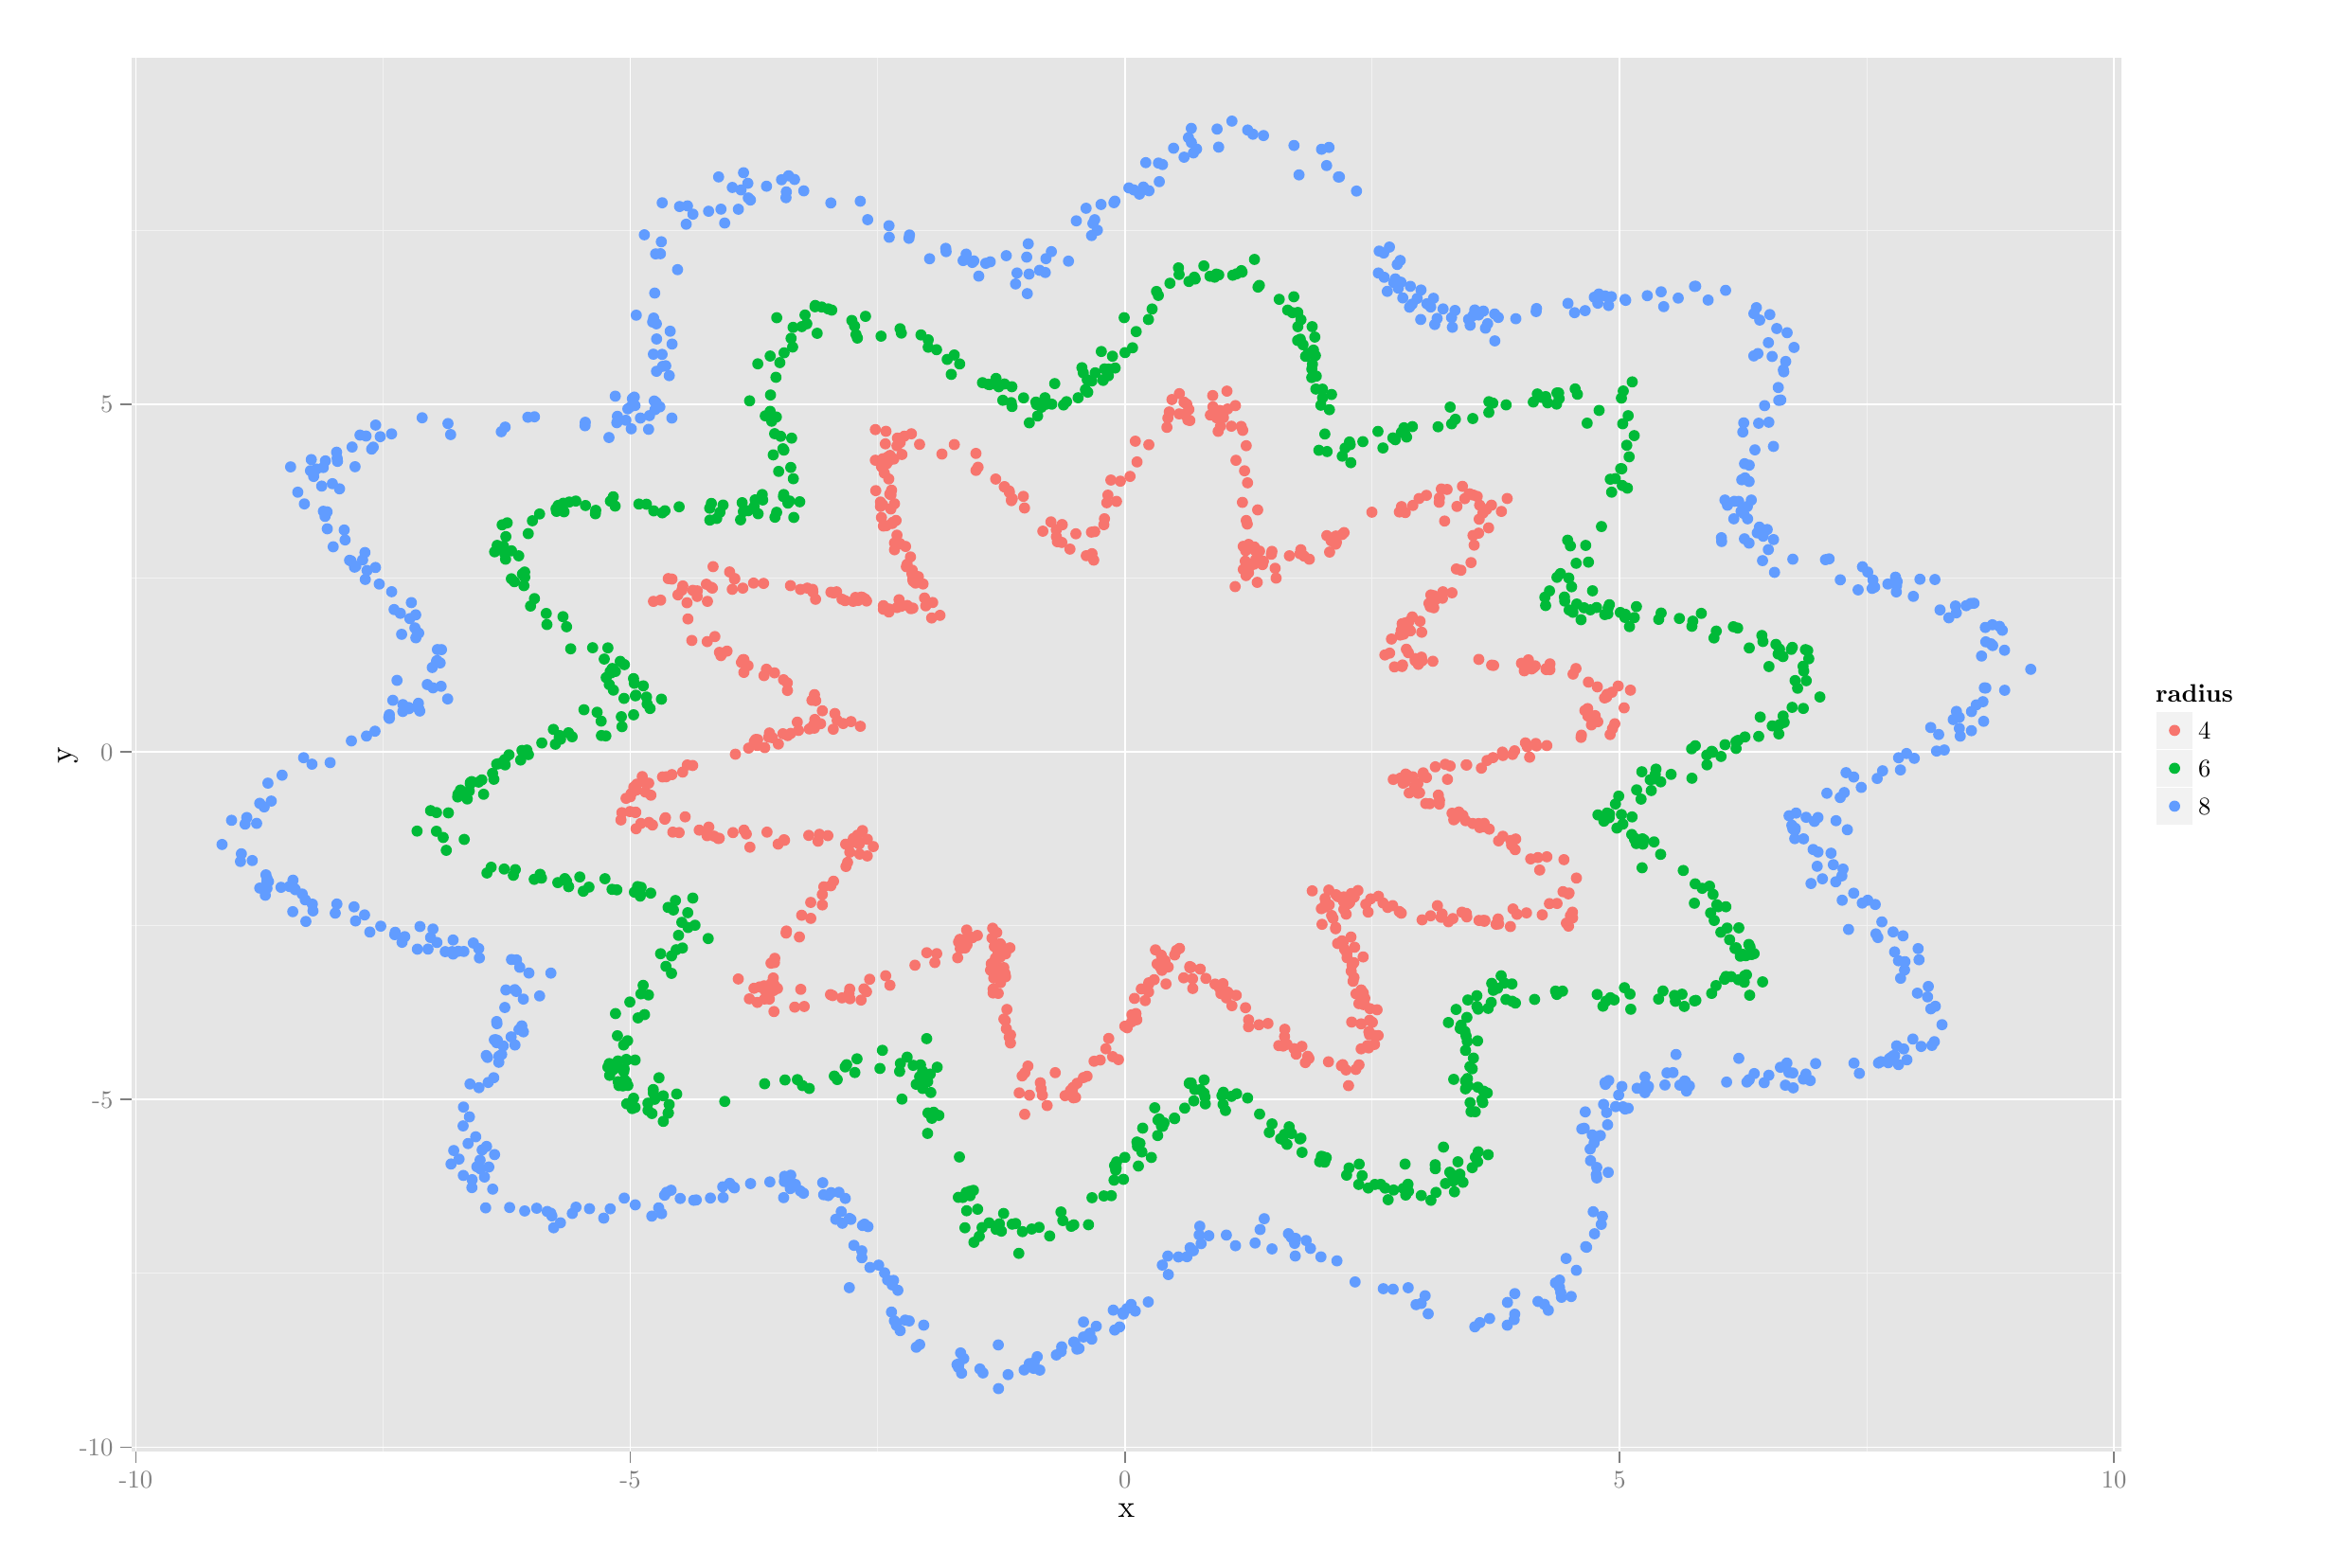
\begin{tikzpicture}[x=1pt,y=1pt]
\definecolor[named]{fillColor}{rgb}{1.00,1.00,1.00}
\path[use as bounding box,fill=fillColor,fill opacity=0.00] (0,0) rectangle (867.24,578.16);
\begin{scope}
\path[clip] (  0.00,  0.00) rectangle (867.24,578.16);
\definecolor[named]{drawColor}{rgb}{1.00,1.00,1.00}
\definecolor[named]{fillColor}{rgb}{1.00,1.00,1.00}

\path[draw=drawColor,line width= 0.6pt,line join=round,line cap=round,fill=fillColor] (  0.00, -0.00) rectangle (867.24,578.16);
\end{scope}
\begin{scope}
\path[clip] ( 40.22, 34.03) rectangle (799.33,566.12);
\definecolor[named]{fillColor}{rgb}{0.90,0.90,0.90}

\path[fill=fillColor] ( 40.22, 34.03) rectangle (799.33,566.12);
\definecolor[named]{drawColor}{rgb}{0.95,0.95,0.95}

\path[draw=drawColor,line width= 0.3pt,line join=round] ( 40.22,102.20) --
	(799.33,102.20);

\path[draw=drawColor,line width= 0.3pt,line join=round] ( 40.22,234.89) --
	(799.33,234.89);

\path[draw=drawColor,line width= 0.3pt,line join=round] ( 40.22,367.58) --
	(799.33,367.58);

\path[draw=drawColor,line width= 0.3pt,line join=round] ( 40.22,500.27) --
	(799.33,500.27);

\path[draw=drawColor,line width= 0.3pt,line join=round] (136.16, 34.03) --
	(136.16,566.12);

\path[draw=drawColor,line width= 0.3pt,line join=round] (324.85, 34.03) --
	(324.85,566.12);

\path[draw=drawColor,line width= 0.3pt,line join=round] (513.54, 34.03) --
	(513.54,566.12);

\path[draw=drawColor,line width= 0.3pt,line join=round] (702.23, 34.03) --
	(702.23,566.12);
\definecolor[named]{drawColor}{rgb}{1.00,1.00,1.00}

\path[draw=drawColor,line width= 0.6pt,line join=round] ( 40.22, 35.86) --
	(799.33, 35.86);

\path[draw=drawColor,line width= 0.6pt,line join=round] ( 40.22,168.55) --
	(799.33,168.55);

\path[draw=drawColor,line width= 0.6pt,line join=round] ( 40.22,301.24) --
	(799.33,301.24);

\path[draw=drawColor,line width= 0.6pt,line join=round] ( 40.22,433.93) --
	(799.33,433.93);

\path[draw=drawColor,line width= 0.6pt,line join=round] ( 41.81, 34.03) --
	( 41.81,566.12);

\path[draw=drawColor,line width= 0.6pt,line join=round] (230.50, 34.03) --
	(230.50,566.12);

\path[draw=drawColor,line width= 0.6pt,line join=round] (419.19, 34.03) --
	(419.19,566.12);

\path[draw=drawColor,line width= 0.6pt,line join=round] (607.88, 34.03) --
	(607.88,566.12);

\path[draw=drawColor,line width= 0.6pt,line join=round] (796.57, 34.03) --
	(796.57,566.12);
\definecolor[named]{fillColor}{rgb}{0.97,0.46,0.43}

\path[fill=fillColor] (275.63,302.64) circle (  2.13);

\path[fill=fillColor] (443.60,431.88) circle (  2.13);

\path[fill=fillColor] (476.52,371.28) circle (  2.13);

\path[fill=fillColor] (531.80,351.06) circle (  2.13);

\path[fill=fillColor] (330.41,388.37) circle (  2.13);

\path[fill=fillColor] (593.23,306.75) circle (  2.13);

\path[fill=fillColor] (506.69,245.83) circle (  2.13);

\path[fill=fillColor] (395.13,381.13) circle (  2.13);

\path[fill=fillColor] (329.60,414.35) circle (  2.13);

\path[fill=fillColor] (274.74,269.88) circle (  2.13);

\path[fill=fillColor] (368.91,209.20) circle (  2.13);

\path[fill=fillColor] (345.86,358.22) circle (  2.13);

\path[fill=fillColor] (559.63,299.03) circle (  2.13);

\path[fill=fillColor] (477.91,189.13) circle (  2.13);

\path[fill=fillColor] (345.47,352.31) circle (  2.13);

\path[fill=fillColor] (495.67,243.28) circle (  2.13);

\path[fill=fillColor] (507.38,208.89) circle (  2.13);

\path[fill=fillColor] (369.40,226.91) circle (  2.13);

\path[fill=fillColor] (526.18,392.55) circle (  2.13);

\path[fill=fillColor] (311.27,359.47) circle (  2.13);

\path[fill=fillColor] (331.02,412.97) circle (  2.13);

\path[fill=fillColor] (309.43,313.23) circle (  2.13);

\path[fill=fillColor] (256.79,271.36) circle (  2.13);

\path[fill=fillColor] (513.61,198.01) circle (  2.13);

\path[fill=fillColor] (552.13,399.23) circle (  2.13);

\path[fill=fillColor] (312.66,265.99) circle (  2.13);

\path[fill=fillColor] (324.15,400.91) circle (  2.13);

\path[fill=fillColor] (285.61,222.43) circle (  2.13);

\path[fill=fillColor] (468.47,372.86) circle (  2.13);

\path[fill=fillColor] (450.09,214.77) circle (  2.13);

\path[fill=fillColor] (329.49,399.62) circle (  2.13);

\path[fill=fillColor] (503.52,243.16) circle (  2.13);

\path[fill=fillColor] (549.63,296.21) circle (  2.13);

\path[fill=fillColor] (466.35,369.53) circle (  2.13);

\path[fill=fillColor] (373.97,195.56) circle (  2.13);

\path[fill=fillColor] (473.78,197.57) circle (  2.13);

\path[fill=fillColor] (375.33,226.43) circle (  2.13);

\path[fill=fillColor] (329.96,399.31) circle (  2.13);

\path[fill=fillColor] (532.36,337.36) circle (  2.13);

\path[fill=fillColor] (282.65,270.60) circle (  2.13);

\path[fill=fillColor] (318.00,262.21) circle (  2.13);

\path[fill=fillColor] (313.93,208.97) circle (  2.13);

\path[fill=fillColor] (285.30,202.12) circle (  2.13);

\path[fill=fillColor] (527.58,350.94) circle (  2.13);

\path[fill=fillColor] (475.29,377.74) circle (  2.13);

\path[fill=fillColor] (438.19,223.72) circle (  2.13);

\path[fill=fillColor] (536.70,335.80) circle (  2.13);

\path[fill=fillColor] (455.30,211.12) circle (  2.13);

\path[fill=fillColor] (273.83,336.43) circle (  2.13);

\path[fill=fillColor] (526.33,292.76) circle (  2.13);

\path[fill=fillColor] (338.14,369.85) circle (  2.13);

\path[fill=fillColor] (337.72,422.61) circle (  2.13);

\path[fill=fillColor] (549.65,238.24) circle (  2.13);

\path[fill=fillColor] (285.49,220.79) circle (  2.13);

\path[fill=fillColor] (535.84,238.66) circle (  2.13);

\path[fill=fillColor] (288.95,328.75) circle (  2.13);

\path[fill=fillColor] (407.43,183.15) circle (  2.13);

\path[fill=fillColor] (458.43,209.54) circle (  2.13);

\path[fill=fillColor] (373.03,199.27) circle (  2.13);

\path[fill=fillColor] (340.40,368.08) circle (  2.13);

\path[fill=fillColor] (540.23,239.35) circle (  2.13);

\path[fill=fillColor] (526.26,289.85) circle (  2.13);

\path[fill=fillColor] (286.98,304.21) circle (  2.13);

\path[fill=fillColor] (575.75,334.04) circle (  2.13);

\path[fill=fillColor] (326.80,395.51) circle (  2.13);

\path[fill=fillColor] (318.54,206.50) circle (  2.13);

\path[fill=fillColor] (375.05,192.35) circle (  2.13);

\path[fill=fillColor] (265.07,337.94) circle (  2.13);

\path[fill=fillColor] (554.37,390.02) circle (  2.13);

\path[fill=fillColor] (537.76,359.37) circle (  2.13);

\path[fill=fillColor] (603.13,323.19) circle (  2.13);

\path[fill=fillColor] (481.04,189.61) circle (  2.13);

\path[fill=fillColor] (504.43,243.26) circle (  2.13);

\path[fill=fillColor] (273.86,271.36) circle (  2.13);

\path[fill=fillColor] (508.11,248.31) circle (  2.13);

\path[fill=fillColor] (544.32,237.60) circle (  2.13);

\path[fill=fillColor] (568.09,263.90) circle (  2.13);

\path[fill=fillColor] (392.62,178.80) circle (  2.13);

\path[fill=fillColor] (329.15,354.60) circle (  2.13);

\path[fill=fillColor] (314.71,312.77) circle (  2.13);

\path[fill=fillColor] (558.21,271.73) circle (  2.13);

\path[fill=fillColor] (556.29,273.94) circle (  2.13);

\path[fill=fillColor] (529.96,335.98) circle (  2.13);

\path[fill=fillColor] (561.77,267.26) circle (  2.13);

\path[fill=fillColor] (433.32,217.84) circle (  2.13);

\path[fill=fillColor] (551.94,273.87) circle (  2.13);

\path[fill=fillColor] (430.36,214.27) circle (  2.13);

\path[fill=fillColor] (494.15,241.37) circle (  2.13);

\path[fill=fillColor] (537.15,360.80) circle (  2.13);

\path[fill=fillColor] (497.87,381.80) circle (  2.13);

\path[fill=fillColor] (254.28,296.02) circle (  2.13);

\path[fill=fillColor] (333.02,359.29) circle (  2.13);

\path[fill=fillColor] (277.52,365.63) circle (  2.13);

\path[fill=fillColor] (598.28,314.41) circle (  2.13);

\path[fill=fillColor] (501.80,181.41) circle (  2.13);

\path[fill=fillColor] (423.18,419.78) circle (  2.13);

\path[fill=fillColor] (428.33,418.43) circle (  2.13);

\path[fill=fillColor] (300.03,363.25) circle (  2.13);

\path[fill=fillColor] (332.25,356.29) circle (  2.13);

\path[fill=fillColor] (451.82,429.76) circle (  2.13);

\path[fill=fillColor] (574.39,332.87) circle (  2.13);

\path[fill=fillColor] (338.05,370.55) circle (  2.13);

\path[fill=fillColor] (404.75,177.43) circle (  2.13);

\path[fill=fillColor] (356.39,226.14) circle (  2.13);

\path[fill=fillColor] (555.21,295.01) circle (  2.13);

\path[fill=fillColor] (607.41,326.36) circle (  2.13);

\path[fill=fillColor] (398.23,378.60) circle (  2.13);

\path[fill=fillColor] (557.96,386.71) circle (  2.13);

\path[fill=fillColor] (327.41,407.62) circle (  2.13);

\path[fill=fillColor] (515.94,246.12) circle (  2.13);

\path[fill=fillColor] (499.63,234.26) circle (  2.13);

\path[fill=fillColor] (369.90,405.33) circle (  2.13);

\path[fill=fillColor] (303.74,246.78) circle (  2.13);

\path[fill=fillColor] (358.97,227.61) circle (  2.13);

\path[fill=fillColor] (238.94,273.31) circle (  2.13);

\path[fill=fillColor] (480.11,192.58) circle (  2.13);

\path[fill=fillColor] (524.92,333.80) circle (  2.13);

\path[fill=fillColor] (327.05,387.40) circle (  2.13);

\path[fill=fillColor] (315.52,358.67) circle (  2.13);

\path[fill=fillColor] (276.12,264.84) circle (  2.13);

\path[fill=fillColor] (320.62,209.70) circle (  2.13);

\path[fill=fillColor] (551.26,373.46) circle (  2.13);

\path[fill=fillColor] (469.94,374.52) circle (  2.13);

\path[fill=fillColor] (369.81,222.51) circle (  2.13);

\path[fill=fillColor] (362.36,415.12) circle (  2.13);

\path[fill=fillColor] (319.05,360.17) circle (  2.13);

\path[fill=fillColor] (455.83,208.96) circle (  2.13);

\path[fill=fillColor] (510.23,204.78) circle (  2.13);

\path[fill=fillColor] (330.16,401.09) circle (  2.13);

\path[fill=fillColor] (237.51,289.28) circle (  2.13);

\path[fill=fillColor] (338.27,367.03) circle (  2.13);

\path[fill=fillColor] (465.44,368.50) circle (  2.13);

\path[fill=fillColor] (539.47,360.21) circle (  2.13);

\path[fill=fillColor] (419.18,196.52) circle (  2.13);

\path[fill=fillColor] (283.54,206.88) circle (  2.13);

\path[fill=fillColor] (317.41,359.00) circle (  2.13);

\path[fill=fillColor] (307.69,208.20) circle (  2.13);

\path[fill=fillColor] (414.52,184.91) circle (  2.13);

\path[fill=fillColor] (561.60,237.46) circle (  2.13);

\path[fill=fillColor] (316.71,267.09) circle (  2.13);

\path[fill=fillColor] (301.24,320.77) circle (  2.13);

\path[fill=fillColor] (486.33,378.36) circle (  2.13);

\path[fill=fillColor] (354.12,418.50) circle (  2.13);

\path[fill=fillColor] (284.17,220.59) circle (  2.13);

\path[fill=fillColor] (284.22,212.78) circle (  2.13);

\path[fill=fillColor] (581.35,332.60) circle (  2.13);

\path[fill=fillColor] (560.82,235.44) circle (  2.13);

\path[fill=fillColor] (308.03,251.85) circle (  2.13);

\path[fill=fillColor] (524.65,239.67) circle (  2.13);

\path[fill=fillColor] (573.14,336.33) circle (  2.13);

\path[fill=fillColor] (588.46,234.72) circle (  2.13);

\path[fill=fillColor] (529.92,336.83) circle (  2.13);

\path[fill=fillColor] (465.49,418.06) circle (  2.13);

\path[fill=fillColor] (539.17,281.29) circle (  2.13);

\path[fill=fillColor] (290.45,324.66) circle (  2.13);

\path[fill=fillColor] (597.20,311.51) circle (  2.13);

\path[fill=fillColor] (505.45,230.56) circle (  2.13);

\path[fill=fillColor] (509.32,197.42) circle (  2.13);

\path[fill=fillColor] (368.48,230.14) circle (  2.13);

\path[fill=fillColor] (464.04,396.43) circle (  2.13);

\path[fill=fillColor] (563.42,269.02) circle (  2.13);

\path[fill=fillColor] (253.96,343.74) circle (  2.13);

\path[fill=fillColor] (327.80,418.77) circle (  2.13);

\path[fill=fillColor] (371.61,228.01) circle (  2.13);

\path[fill=fillColor] (542.64,236.37) circle (  2.13);

\path[fill=fillColor] (503.89,224.35) circle (  2.13);

\path[fill=fillColor] (268.38,369.88) circle (  2.13);

\path[fill=fillColor] (285.51,331.37) circle (  2.13);

\path[fill=fillColor] (395.29,387.90) circle (  2.13);

\path[fill=fillColor] (375.56,193.22) circle (  2.13);

\path[fill=fillColor] (496.87,182.95) circle (  2.13);

\path[fill=fillColor] (468.57,379.42) circle (  2.13);

\path[fill=fillColor] (508.48,205.15) circle (  2.13);

\path[fill=fillColor] (273.42,363.71) circle (  2.13);

\path[fill=fillColor] (284.72,210.15) circle (  2.13);

\path[fill=fillColor] (594.70,316.99) circle (  2.13);

\path[fill=fillColor] (568.79,239.23) circle (  2.13);

\path[fill=fillColor] (308.13,361.85) circle (  2.13);

\path[fill=fillColor] (281.50,330.32) circle (  2.13);

\path[fill=fillColor] (347.40,224.22) circle (  2.13);

\path[fill=fillColor] (319.63,210.77) circle (  2.13);

\path[fill=fillColor] (252.12,358.12) circle (  2.13);

\path[fill=fillColor] (300.76,323.07) circle (  2.13);

\path[fill=fillColor] (499.59,233.72) circle (  2.13);

\path[fill=fillColor] (573.62,299.18) circle (  2.13);

\path[fill=fillColor] (454.78,423.54) circle (  2.13);

\path[fill=fillColor] (605.24,310.09) circle (  2.13);

\path[fill=fillColor] (380.45,398.72) circle (  2.13);

\path[fill=fillColor] (294.20,312.56) circle (  2.13);

\path[fill=fillColor] (333.80,356.76) circle (  2.13);

\path[fill=fillColor] (443.96,219.28) circle (  2.13);

\path[fill=fillColor] (541.18,389.31) circle (  2.13);

\path[fill=fillColor] (549.20,274.94) circle (  2.13);

\path[fill=fillColor] (368.91,210.67) circle (  2.13);

\path[fill=fillColor] (279.06,305.91) circle (  2.13);

\path[fill=fillColor] (438.89,225.45) circle (  2.13);

\path[fill=fillColor] (291.60,364.66) circle (  2.13);

\path[fill=fillColor] (506.85,226.67) circle (  2.13);

\path[fill=fillColor] (250.47,293.51) circle (  2.13);

\path[fill=fillColor] (456.26,429.51) circle (  2.13);

\path[fill=fillColor] (330.60,388.80) circle (  2.13);

\path[fill=fillColor] (463.56,425.41) circle (  2.13);

\path[fill=fillColor] (441.97,430.05) circle (  2.13);

\path[fill=fillColor] (466.41,380.40) circle (  2.13);

\path[fill=fillColor] (395.17,387.91) circle (  2.13);

\path[fill=fillColor] (525.64,349.57) circle (  2.13);

\path[fill=fillColor] (252.24,296.21) circle (  2.13);

\path[fill=fillColor] (298.02,363.71) circle (  2.13);

\path[fill=fillColor] (283.57,308.44) circle (  2.13);

\path[fill=fillColor] (260.44,272.52) circle (  2.13);

\path[fill=fillColor] (371.56,222.82) circle (  2.13);

\path[fill=fillColor] (230.51,284.11) circle (  2.13);

\path[fill=fillColor] (235.04,291.80) circle (  2.13);

\path[fill=fillColor] (319.07,271.19) circle (  2.13);

\path[fill=fillColor] (554.54,395.36) circle (  2.13);

\path[fill=fillColor] (455.37,431.54) circle (  2.13);

\path[fill=fillColor] (421.86,200.92) circle (  2.13);

\path[fill=fillColor] (540.53,362.30) circle (  2.13);

\path[fill=fillColor] (506.25,213.67) circle (  2.13);

\path[fill=fillColor] (505.54,217.54) circle (  2.13);

\path[fill=fillColor] (314.32,207.01) circle (  2.13);

\path[fill=fillColor] (262.42,269.07) circle (  2.13);

\path[fill=fillColor] (546.61,278.28) circle (  2.13);

\path[fill=fillColor] (278.89,303.66) circle (  2.13);

\path[fill=fillColor] (387.23,172.66) circle (  2.13);

\path[fill=fillColor] (417.47,404.52) circle (  2.13);

\path[fill=fillColor] (425.46,210.76) circle (  2.13);

\path[fill=fillColor] (282.43,332.76) circle (  2.13);

\path[fill=fillColor] (498.07,238.78) circle (  2.13);

\path[fill=fillColor] (326.29,410.20) circle (  2.13);

\path[fill=fillColor] (435.23,425.07) circle (  2.13);

\path[fill=fillColor] (270.23,367.19) circle (  2.13);

\path[fill=fillColor] (584.07,243.37) circle (  2.13);

\path[fill=fillColor] (358.83,233.23) circle (  2.13);

\path[fill=fillColor] (442.81,433.88) circle (  2.13);

\path[fill=fillColor] (232.56,278.21) circle (  2.13);

\path[fill=fillColor] (312.43,358.93) circle (  2.13);

\path[fill=fillColor] (295.87,238.87) circle (  2.13);

\path[fill=fillColor] (311.26,207.34) circle (  2.13);

\path[fill=fillColor] (500.47,245.96) circle (  2.13);

\path[fill=fillColor] (531.63,285.61) circle (  2.13);

\path[fill=fillColor] (390.98,388.99) circle (  2.13);

\path[fill=fillColor] (403.38,176.92) circle (  2.13);

\path[fill=fillColor] (327.02,355.66) circle (  2.13);

\path[fill=fillColor] (535.70,356.60) circle (  2.13);

\path[fill=fillColor] (526.60,291.89) circle (  2.13);

\path[fill=fillColor] (407.69,385.28) circle (  2.13);

\path[fill=fillColor] (428.30,213.09) circle (  2.13);

\path[fill=fillColor] (522.03,333.65) circle (  2.13);

\path[fill=fillColor] (407.31,374.39) circle (  2.13);

\path[fill=fillColor] (375.90,397.10) circle (  2.13);

\path[fill=fillColor] (325.94,394.88) circle (  2.13);

\path[fill=fillColor] (524.73,394.82) circle (  2.13);

\path[fill=fillColor] (452.70,437.19) circle (  2.13);

\path[fill=fillColor] (532.56,335.95) circle (  2.13);

\path[fill=fillColor] (230.77,285.26) circle (  2.13);

\path[fill=fillColor] (262.75,345.22) circle (  2.13);

\path[fill=fillColor] (339.09,219.81) circle (  2.13);

\path[fill=fillColor] (355.39,222.65) circle (  2.13);

\path[fill=fillColor] (464.16,423.93) circle (  2.13);

\path[fill=fillColor] (382.78,170.19) circle (  2.13);

\path[fill=fillColor] (567.27,241.26) circle (  2.13);

\path[fill=fillColor] (581.18,243.31) circle (  2.13);

\path[fill=fillColor] (562.86,392.98) circle (  2.13);

\path[fill=fillColor] (460.03,204.36) circle (  2.13);

\path[fill=fillColor] (471.71,372.69) circle (  2.13);

\path[fill=fillColor] (521.35,242.56) circle (  2.13);

\path[fill=fillColor] (504.96,243.70) circle (  2.13);

\path[fill=fillColor] (475.07,376.64) circle (  2.13);

\path[fill=fillColor] (514.44,189.59) circle (  2.13);

\path[fill=fillColor] (511.99,240.08) circle (  2.13);

\path[fill=fillColor] (433.07,223.64) circle (  2.13);

\path[fill=fillColor] (284.69,306.64) circle (  2.13);

\path[fill=fillColor] (554.58,272.33) circle (  2.13);

\path[fill=fillColor] (572.73,303.17) circle (  2.13);

\path[fill=fillColor] (273.82,331.55) circle (  2.13);

\path[fill=fillColor] (327.93,215.77) circle (  2.13);

\path[fill=fillColor] (261.37,364.03) circle (  2.13);

\path[fill=fillColor] (542.27,290.74) circle (  2.13);

\path[fill=fillColor] (497.15,242.83) circle (  2.13);

\path[fill=fillColor] (572.02,304.64) circle (  2.13);

\path[fill=fillColor] (300.14,362.26) circle (  2.13);

\path[fill=fillColor] (561.80,235.56) circle (  2.13);

\path[fill=fillColor] (270.35,367.35) circle (  2.13);

\path[fill=fillColor] (461.57,412.49) circle (  2.13);

\path[fill=fillColor] (559.89,334.22) circle (  2.13);

\path[fill=fillColor] (580.18,303.63) circle (  2.13);

\path[fill=fillColor] (443.22,427.90) circle (  2.13);

\path[fill=fillColor] (455.89,211.56) circle (  2.13);

\path[fill=fillColor] (556.32,236.56) circle (  2.13);

\path[fill=fillColor] (484.55,185.87) circle (  2.13);

\path[fill=fillColor] (544.67,275.28) circle (  2.13);

\path[fill=fillColor] (340.85,418.57) circle (  2.13);

\path[fill=fillColor] (232.69,271.89) circle (  2.13);

\path[fill=fillColor] (387.89,385.44) circle (  2.13);

\path[fill=fillColor] (358.21,226.37) circle (  2.13);

\path[fill=fillColor] (264.42,268.23) circle (  2.13);

\path[fill=fillColor] (242.78,291.66) circle (  2.13);

\path[fill=fillColor] (318.26,310.98) circle (  2.13);

\path[fill=fillColor] (578.43,239.04) circle (  2.13);

\path[fill=fillColor] (495.55,242.01) circle (  2.13);

\path[fill=fillColor] (524.97,350.12) circle (  2.13);

\path[fill=fillColor] (285.18,210.15) circle (  2.13);

\path[fill=fillColor] (246.39,367.16) circle (  2.13);

\path[fill=fillColor] (567.11,300.25) circle (  2.13);

\path[fill=fillColor] (524.62,347.59) circle (  2.13);

\path[fill=fillColor] (426.95,206.29) circle (  2.13);

\path[fill=fillColor] (570.51,335.03) circle (  2.13);

\path[fill=fillColor] (370.65,217.79) circle (  2.13);

\path[fill=fillColor] (529.68,286.85) circle (  2.13);

\path[fill=fillColor] (598.62,315.04) circle (  2.13);

\path[fill=fillColor] (455.67,425.49) circle (  2.13);

\path[fill=fillColor] (300.89,313.59) circle (  2.13);

\path[fill=fillColor] (512.54,198.80) circle (  2.13);

\path[fill=fillColor] (515.82,192.97) circle (  2.13);

\path[fill=fillColor] (399.27,170.83) circle (  2.13);

\path[fill=fillColor] (271.69,214.55) circle (  2.13);

\path[fill=fillColor] (605.01,323.98) circle (  2.13);

\path[fill=fillColor] (531.16,334.62) circle (  2.13);

\path[fill=fillColor] (452.79,432.89) circle (  2.13);

\path[fill=fillColor] (304.33,249.72) circle (  2.13);

\path[fill=fillColor] (575.98,304.43) circle (  2.13);

\path[fill=fillColor] (453.58,212.60) circle (  2.13);

\path[fill=fillColor] (303.76,242.81) circle (  2.13);

\path[fill=fillColor] (466.83,371.98) circle (  2.13);

\path[fill=fillColor] (528.83,352.72) circle (  2.13);

\path[fill=fillColor] (278.34,305.95) circle (  2.13);

\path[fill=fillColor] (502.31,181.87) circle (  2.13);

\path[fill=fillColor] (423.74,199.00) circle (  2.13);

\path[fill=fillColor] (332.42,420.96) circle (  2.13);

\path[fill=fillColor] (439.91,430.20) circle (  2.13);

\path[fill=fillColor] (440.03,226.21) circle (  2.13);

\path[fill=fillColor] (306.87,208.59) circle (  2.13);

\path[fill=fillColor] (556.62,272.58) circle (  2.13);

\path[fill=fillColor] (539.11,396.49) circle (  2.13);

\path[fill=fillColor] (563.23,301.13) circle (  2.13);

\path[fill=fillColor] (250.17,362.93) circle (  2.13);

\path[fill=fillColor] (456.47,430.11) circle (  2.13);

\path[fill=fillColor] (328.25,411.15) circle (  2.13);

\path[fill=fillColor] (393.43,381.41) circle (  2.13);

\path[fill=fillColor] (333.45,419.25) circle (  2.13);

\path[fill=fillColor] (575.23,333.48) circle (  2.13);

\path[fill=fillColor] (323.19,265.08) circle (  2.13);

\path[fill=fillColor] (328.04,423.56) circle (  2.13);

\path[fill=fillColor] (526.59,340.39) circle (  2.13);

\path[fill=fillColor] (317.82,266.02) circle (  2.13);

\path[fill=fillColor] (295.53,210.60) circle (  2.13);

\path[fill=fillColor] (259.83,343.30) circle (  2.13);

\path[fill=fillColor] (445.08,210.92) circle (  2.13);

\path[fill=fillColor] (539.24,282.72) circle (  2.13);

\path[fill=fillColor] (312.77,257.49) circle (  2.13);

\path[fill=fillColor] (399.38,173.12) circle (  2.13);

\path[fill=fillColor] (244.97,367.35) circle (  2.13);

\path[fill=fillColor] (290.54,307.43) circle (  2.13);

\path[fill=fillColor] (599.62,312.73) circle (  2.13);

\path[fill=fillColor] (444.41,219.04) circle (  2.13);

\path[fill=fillColor] (505.57,247.15) circle (  2.13);

\path[fill=fillColor] (323.99,424.21) circle (  2.13);

\path[fill=fillColor] (497.30,377.47) circle (  2.13);

\path[fill=fillColor] (320.63,358.80) circle (  2.13);

\path[fill=fillColor] (302.64,269.76) circle (  2.13);

\path[fill=fillColor] (512.33,194.21) circle (  2.13);

\path[fill=fillColor] (318.59,360.29) circle (  2.13);

\path[fill=fillColor] (554.22,336.51) circle (  2.13);

\path[fill=fillColor] (444.01,218.83) circle (  2.13);

\path[fill=fillColor] (373.29,402.39) circle (  2.13);

\path[fill=fillColor] (534.24,399.12) circle (  2.13);

\path[fill=fillColor] (502.04,229.09) circle (  2.13);

\path[fill=fillColor] (456.61,212.77) circle (  2.13);

\path[fill=fillColor] (550.49,399.58) circle (  2.13);

\path[fill=fillColor] (506.53,220.76) circle (  2.13);

\path[fill=fillColor] (489.56,374.74) circle (  2.13);

\path[fill=fillColor] (302.11,267.14) circle (  2.13);

\path[fill=fillColor] (411.17,387.92) circle (  2.13);

\path[fill=fillColor] (359.35,231.17) circle (  2.13);

\path[fill=fillColor] (289.33,267.45) circle (  2.13);

\path[fill=fillColor] (291.68,308.27) circle (  2.13);

\path[fill=fillColor] (289.93,232.08) circle (  2.13);

\path[fill=fillColor] (370.01,221.49) circle (  2.13);

\path[fill=fillColor] (510.39,205.21) circle (  2.13);

\path[fill=fillColor] (521.59,290.70) circle (  2.13);

\path[fill=fillColor] (537.64,295.52) circle (  2.13);

\path[fill=fillColor] (513.44,392.69) circle (  2.13);

\path[fill=fillColor] (512.33,194.47) circle (  2.13);

\path[fill=fillColor] (612.09,324.77) circle (  2.13);

\path[fill=fillColor] (314.20,210.71) circle (  2.13);

\path[fill=fillColor] (404.47,376.08) circle (  2.13);

\path[fill=fillColor] (236.25,285.90) circle (  2.13);

\path[fill=fillColor] (288.72,308.13) circle (  2.13);

\path[fill=fillColor] (518.39,338.20) circle (  2.13);

\path[fill=fillColor] (281.33,365.52) circle (  2.13);

\path[fill=fillColor] (434.49,221.53) circle (  2.13);

\path[fill=fillColor] (422.85,207.14) circle (  2.13);

\path[fill=fillColor] (286.90,266.03) circle (  2.13);

\path[fill=fillColor] (326.83,413.09) circle (  2.13);

\path[fill=fillColor] (586.70,260.08) circle (  2.13);

\path[fill=fillColor] (285.03,214.92) circle (  2.13);

\path[fill=fillColor] (421.80,198.21) circle (  2.13);

\path[fill=fillColor] (242.07,359.13) circle (  2.13);

\path[fill=fillColor] (348.64,353.32) circle (  2.13);

\path[fill=fillColor] (456.28,209.61) circle (  2.13);

\path[fill=fillColor] (368.74,233.92) circle (  2.13);

\path[fill=fillColor] (337.55,355.86) circle (  2.13);

\path[fill=fillColor] (502.73,241.13) circle (  2.13);

\path[fill=fillColor] (376.00,397.72) circle (  2.13);

\path[fill=fillColor] (436.12,430.94) circle (  2.13);

\path[fill=fillColor] (539.21,398.15) circle (  2.13);

\path[fill=fillColor] (543.28,295.83) circle (  2.13);

\path[fill=fillColor] (428.25,209.60) circle (  2.13);

\path[fill=fillColor] (332.22,418.01) circle (  2.13);

\path[fill=fillColor] (281.70,206.91) circle (  2.13);

\path[fill=fillColor] (472.04,373.96) circle (  2.13);

\path[fill=fillColor] (421.16,406.35) circle (  2.13);

\path[fill=fillColor] (517.68,243.57) circle (  2.13);

\path[fill=fillColor] (329.10,405.37) circle (  2.13);

\path[fill=fillColor] (527.67,285.56) circle (  2.13);

\path[fill=fillColor] (329.20,355.77) circle (  2.13);

\path[fill=fillColor] (296.85,204.05) circle (  2.13);

\path[fill=fillColor] (278.97,205.61) circle (  2.13);

\path[fill=fillColor] (373.69,215.41) circle (  2.13);

\path[fill=fillColor] (489.41,184.21) circle (  2.13);

\path[fill=fillColor] (539.93,401.55) circle (  2.13);

\path[fill=fillColor] (375.53,190.11) circle (  2.13);

\path[fill=fillColor] (264.00,268.16) circle (  2.13);

\path[fill=fillColor] (495.90,242.91) circle (  2.13);

\path[fill=fillColor] (515.41,202.80) circle (  2.13);

\path[fill=fillColor] (342.18,365.29) circle (  2.13);

\path[fill=fillColor] (285.39,212.27) circle (  2.13);

\path[fill=fillColor] (371.98,227.36) circle (  2.13);

\path[fill=fillColor] (571.57,332.14) circle (  2.13);

\path[fill=fillColor] (299.79,320.91) circle (  2.13);

\path[fill=fillColor] (576.25,303.49) circle (  2.13);

\path[fill=fillColor] (557.37,297.94) circle (  2.13);

\path[fill=fillColor] (554.15,384.69) circle (  2.13);

\path[fill=fillColor] (275.41,334.11) circle (  2.13);

\path[fill=fillColor] (430.86,225.66) circle (  2.13);

\path[fill=fillColor] (362.90,231.17) circle (  2.13);

\path[fill=fillColor] (506.60,215.12) circle (  2.13);

\path[fill=fillColor] (337.95,369.16) circle (  2.13);

\path[fill=fillColor] (447.95,218.31) circle (  2.13);

\path[fill=fillColor] (376.24,397.80) circle (  2.13);

\path[fill=fillColor] (512.54,193.25) circle (  2.13);

\path[fill=fillColor] (588.66,247.35) circle (  2.13);

\path[fill=fillColor] (507.30,180.03) circle (  2.13);

\path[fill=fillColor] (596.05,327.84) circle (  2.13);

\path[fill=fillColor] (441.63,214.99) circle (  2.13);

\path[fill=fillColor] (374.17,202.92) circle (  2.13);

\path[fill=fillColor] (299.35,237.68) circle (  2.13);

\path[fill=fillColor] (589.94,240.04) circle (  2.13);

\path[fill=fillColor] (466.38,196.32) circle (  2.13);

\path[fill=fillColor] (532.58,237.11) circle (  2.13);

\path[fill=fillColor] (544.02,277.80) circle (  2.13);

\path[fill=fillColor] (445.00,214.63) circle (  2.13);

\path[fill=fillColor] (543.99,361.93) circle (  2.13);

\path[fill=fillColor] (500.36,228.09) circle (  2.13);

\path[fill=fillColor] (435.59,428.61) circle (  2.13);

\path[fill=fillColor] (298.81,309.96) circle (  2.13);

\path[fill=fillColor] (307.03,362.15) circle (  2.13);

\path[fill=fillColor] (331.29,380.96) circle (  2.13);

\path[fill=fillColor] (387.72,170.20) circle (  2.13);

\path[fill=fillColor] (465.88,388.16) circle (  2.13);

\path[fill=fillColor] (548.16,276.96) circle (  2.13);

\path[fill=fillColor] (293.22,203.80) circle (  2.13);

\path[fill=fillColor] (412.72,399.19) circle (  2.13);

\path[fill=fillColor] (261.80,363.72) circle (  2.13);

\path[fill=fillColor] (441.74,434.69) circle (  2.13);

\path[fill=fillColor] (389.52,166.25) circle (  2.13);

\path[fill=fillColor] (524.27,291.17) circle (  2.13);

\path[fill=fillColor] (380.90,394.29) circle (  2.13);

\path[fill=fillColor] (469.45,374.07) circle (  2.13);

\path[fill=fillColor] (527.04,292.18) circle (  2.13);

\path[fill=fillColor] (480.21,195.35) circle (  2.13);

\path[fill=fillColor] (531.43,397.91) circle (  2.13);

\path[fill=fillColor] (380.97,162.91) circle (  2.13);

\path[fill=fillColor] (566.74,265.60) circle (  2.13);

\path[fill=fillColor] (602.99,322.17) circle (  2.13);

\path[fill=fillColor] (469.86,393.57) circle (  2.13);

\path[fill=fillColor] (599.45,326.02) circle (  2.13);

\path[fill=fillColor] (479.56,188.95) circle (  2.13);

\path[fill=fillColor] (303.07,311.96) circle (  2.13);

\path[fill=fillColor] (523.91,392.77) circle (  2.13);

\path[fill=fillColor] (334.12,414.71) circle (  2.13);

\path[fill=fillColor] (428.22,212.50) circle (  2.13);

\path[fill=fillColor] (539.85,238.07) circle (  2.13);

\path[fill=fillColor] (256.01,360.54) circle (  2.13);

\path[fill=fillColor] (527.34,339.08) circle (  2.13);

\path[fill=fillColor] (326.24,395.56) circle (  2.13);

\path[fill=fillColor] (537.04,356.21) circle (  2.13);

\path[fill=fillColor] (535.93,361.11) circle (  2.13);

\path[fill=fillColor] (294.66,309.41) circle (  2.13);

\path[fill=fillColor] (465.99,403.90) circle (  2.13);

\path[fill=fillColor] (305.86,269.25) circle (  2.13);

\path[fill=fillColor] (586.35,247.87) circle (  2.13);

\path[fill=fillColor] (336.18,357.08) circle (  2.13);

\path[fill=fillColor] (416.74,183.77) circle (  2.13);

\path[fill=fillColor] (338.30,356.08) circle (  2.13);

\path[fill=fillColor] (393.03,385.94) circle (  2.13);

\path[fill=fillColor] (252.47,351.95) circle (  2.13);

\path[fill=fillColor] (606.11,311.95) circle (  2.13);

\path[fill=fillColor] (555.95,236.90) circle (  2.13);

\path[fill=fillColor] (511.68,189.09) circle (  2.13);

\path[fill=fillColor] (498.60,237.72) circle (  2.13);

\path[fill=fillColor] (567.89,301.61) circle (  2.13);

\path[fill=fillColor] (466.39,198.95) circle (  2.13);

\path[fill=fillColor] (547.41,370.53) circle (  2.13);

\path[fill=fillColor] (434.88,212.66) circle (  2.13);

\path[fill=fillColor] (524.22,345.80) circle (  2.13);

\path[fill=fillColor] (487.57,375.93) circle (  2.13);

\path[fill=fillColor] (512.68,203.23) circle (  2.13);

\path[fill=fillColor] (486.73,188.83) circle (  2.13);

\path[fill=fillColor] (503.97,222.66) circle (  2.13);

\path[fill=fillColor] (327.03,357.01) circle (  2.13);

\path[fill=fillColor] (470.57,377.82) circle (  2.13);

\path[fill=fillColor] (290.38,327.54) circle (  2.13);

\path[fill=fillColor] (579.95,332.62) circle (  2.13);

\path[fill=fillColor] (336.11,372.82) circle (  2.13);

\path[fill=fillColor] (559.13,334.32) circle (  2.13);

\path[fill=fillColor] (382.19,181.31) circle (  2.13);

\path[fill=fillColor] (534.26,291.42) circle (  2.13);

\path[fill=fillColor] (510.09,222.96) circle (  2.13);

\path[fill=fillColor] (326.59,409.76) circle (  2.13);

\path[fill=fillColor] (423.83,411.87) circle (  2.13);

\path[fill=fillColor] (373.56,198.66) circle (  2.13);

\path[fill=fillColor] (465.50,389.51) circle (  2.13);

\path[fill=fillColor] (581.38,334.80) circle (  2.13);

\path[fill=fillColor] (411.40,390.17) circle (  2.13);

\path[fill=fillColor] (360.96,230.27) circle (  2.13);

\path[fill=fillColor] (331.89,389.53) circle (  2.13);

\path[fill=fillColor] (411.93,187.91) circle (  2.13);

\path[fill=fillColor] (393.06,383.35) circle (  2.13);

\path[fill=fillColor] (232.45,278.08) circle (  2.13);

\path[fill=fillColor] (277.82,305.24) circle (  2.13);

\path[fill=fillColor] (227.28,278.01) circle (  2.13);

\path[fill=fillColor] (277.68,211.00) circle (  2.13);

\path[fill=fillColor] (499.63,380.51) circle (  2.13);

\path[fill=fillColor] (321.81,214.44) circle (  2.13);

\path[fill=fillColor] (300.52,311.66) circle (  2.13);

\path[fill=fillColor] (591.47,253.06) circle (  2.13);

\path[fill=fillColor] (469.69,365.91) circle (  2.13);

\path[fill=fillColor] (490.67,248.18) circle (  2.13);

\path[fill=fillColor] (289.14,267.68) circle (  2.13);

\path[fill=fillColor] (465.52,371.09) circle (  2.13);

\path[fill=fillColor] (508.52,181.78) circle (  2.13);

\path[fill=fillColor] (295.41,363.22) circle (  2.13);

\path[fill=fillColor] (320.90,261.50) circle (  2.13);

\path[fill=fillColor] (272.89,335.37) circle (  2.13);

\path[fill=fillColor] (496.24,383.74) circle (  2.13);

\path[fill=fillColor] (456.32,431.18) circle (  2.13);

\path[fill=fillColor] (409.77,183.61) circle (  2.13);

\path[fill=fillColor] (553.62,398.70) circle (  2.13);

\path[fill=fillColor] (339.29,365.64) circle (  2.13);

\path[fill=fillColor] (483.74,187.95) circle (  2.13);

\path[fill=fillColor] (300.73,310.27) circle (  2.13);

\path[fill=fillColor] (299.33,243.77) circle (  2.13);

\path[fill=fillColor] (465.11,374.00) circle (  2.13);

\path[fill=fillColor] (375.02,400.80) circle (  2.13);

\path[fill=fillColor] (267.39,339.67) circle (  2.13);

\path[fill=fillColor] (331.28,395.92) circle (  2.13);

\path[fill=fillColor] (555.79,392.34) circle (  2.13);

\path[fill=fillColor] (239.32,358.65) circle (  2.13);

\path[fill=fillColor] (469.12,374.63) circle (  2.13);

\path[fill=fillColor] (556.57,236.87) circle (  2.13);

\path[fill=fillColor] (519.46,241.85) circle (  2.13);

\path[fill=fillColor] (552.45,380.11) circle (  2.13);

\path[fill=fillColor] (228.87,283.48) circle (  2.13);

\path[fill=fillColor] (262.07,371.91) circle (  2.13);

\path[fill=fillColor] (499.72,383.60) circle (  2.13);

\path[fill=fillColor] (371.61,217.09) circle (  2.13);

\path[fill=fillColor] (461.26,364.29) circle (  2.13);

\path[fill=fillColor] (372.99,218.88) circle (  2.13);

\path[fill=fillColor] (566.48,267.38) circle (  2.13);

\path[fill=fillColor] (502.47,228.57) circle (  2.13);

\path[fill=fillColor] (234.51,273.91) circle (  2.13);

\path[fill=fillColor] (580.20,261.18) circle (  2.13);

\path[fill=fillColor] (559.06,395.37) circle (  2.13);

\path[fill=fillColor] (550.74,399.70) circle (  2.13);

\path[fill=fillColor] (505.73,198.11) circle (  2.13);

\path[fill=fillColor] (502.09,384.19) circle (  2.13);

\path[fill=fillColor] (511.10,243.06) circle (  2.13);

\path[fill=fillColor] (459.81,425.50) circle (  2.13);

\path[fill=fillColor] (458.38,432.06) circle (  2.13);

\path[fill=fillColor] (373.68,224.14) circle (  2.13);

\path[fill=fillColor] (315.10,266.59) circle (  2.13);

\path[fill=fillColor] (315.57,268.15) circle (  2.13);

\path[fill=fillColor] (590.00,237.84) circle (  2.13);

\path[fill=fillColor] (343.21,356.95) circle (  2.13);

\path[fill=fillColor] (535.50,281.44) circle (  2.13);

\path[fill=fillColor] (563.44,299.83) circle (  2.13);

\path[fill=fillColor] (386.92,174.94) circle (  2.13);

\path[fill=fillColor] (545.66,371.01) circle (  2.13);

\path[fill=fillColor] (538.44,242.53) circle (  2.13);

\path[fill=fillColor] (485.99,376.85) circle (  2.13);

\path[fill=fillColor] (246.71,270.59) circle (  2.13);

\path[fill=fillColor] (244.12,291.71) circle (  2.13);

\path[fill=fillColor] (270.58,300.33) circle (  2.13);

\path[fill=fillColor] (277.86,304.21) circle (  2.13);

\path[fill=fillColor] (329.90,393.91) circle (  2.13);

\path[fill=fillColor] (496.99,248.48) circle (  2.13);

\path[fill=fillColor] (328.14,387.53) circle (  2.13);

\path[fill=fillColor] (465.27,378.02) circle (  2.13);

\path[fill=fillColor] (281.56,211.94) circle (  2.13);

\path[fill=fillColor] (465.21,203.58) circle (  2.13);

\path[fill=fillColor] (295.01,230.58) circle (  2.13);

\path[fill=fillColor] (301.17,359.45) circle (  2.13);

\path[fill=fillColor] (299.77,310.56) circle (  2.13);

\path[fill=fillColor] (468.79,378.15) circle (  2.13);

\path[fill=fillColor] (337.39,375.61) circle (  2.13);

\path[fill=fillColor] (461.37,433.36) circle (  2.13);

\path[fill=fillColor] (587.64,235.86) circle (  2.13);

\path[fill=fillColor] (557.17,393.75) circle (  2.13);

\path[fill=fillColor] (232.75,286.61) circle (  2.13);

\path[fill=fillColor] (527.73,347.79) circle (  2.13);

\path[fill=fillColor] (520.90,344.27) circle (  2.13);

\path[fill=fillColor] (349.39,414.87) circle (  2.13);

\path[fill=fillColor] (338.43,366.33) circle (  2.13);

\path[fill=fillColor] (456.80,428.78) circle (  2.13);

\path[fill=fillColor] (259.51,365.21) circle (  2.13);

\path[fill=fillColor] (251.41,276.42) circle (  2.13);

\path[fill=fillColor] (400.94,174.73) circle (  2.13);

\path[fill=fillColor] (325.94,396.57) circle (  2.13);

\path[fill=fillColor] (532.44,346.87) circle (  2.13);

\path[fill=fillColor] (298.57,269.35) circle (  2.13);

\path[fill=fillColor] (238.34,284.69) circle (  2.13);

\path[fill=fillColor] (281.72,210.45) circle (  2.13);

\path[fill=fillColor] (464.37,370.84) circle (  2.13);

\path[fill=fillColor] (331.29,378.35) circle (  2.13);

\path[fill=fillColor] (246.35,292.54) circle (  2.13);

\path[fill=fillColor] (504.52,173.84) circle (  2.13);

\path[fill=fillColor] (481.96,376.05) circle (  2.13);

\path[fill=fillColor] (505.85,219.89) circle (  2.13);

\path[fill=fillColor] (342.75,359.94) circle (  2.13);

\path[fill=fillColor] (273.47,336.39) circle (  2.13);

\path[fill=fillColor] (499.76,246.70) circle (  2.13);

\path[fill=fillColor] (510.73,207.18) circle (  2.13);

\path[fill=fillColor] (502.69,245.87) circle (  2.13);

\path[fill=fillColor] (609.67,318.01) circle (  2.13);

\path[fill=fillColor] (533.97,281.51) circle (  2.13);

\path[fill=fillColor] (476.89,367.53) circle (  2.13);

\path[fill=fillColor] (552.01,383.80) circle (  2.13);

\path[fill=fillColor] (549.48,239.57) circle (  2.13);

\path[fill=fillColor] (549.40,296.25) circle (  2.13);

\path[fill=fillColor] (329.55,212.16) circle (  2.13);

\path[fill=fillColor] (554.30,236.89) circle (  2.13);

\path[fill=fillColor] (503.01,225.86) circle (  2.13);

\path[fill=fillColor] (540.35,359.85) circle (  2.13);

\path[fill=fillColor] (309.21,362.29) circle (  2.13);

\path[fill=fillColor] (283.31,306.81) circle (  2.13);

\path[fill=fillColor] (378.87,171.08) circle (  2.13);

\path[fill=fillColor] (399.57,169.18) circle (  2.13);

\path[fill=fillColor] (416.00,396.81) circle (  2.13);

\path[fill=fillColor] (373.46,216.68) circle (  2.13);

\path[fill=fillColor] (574.03,260.37) circle (  2.13);

\path[fill=fillColor] (230.35,278.44) circle (  2.13);

\path[fill=fillColor] (523.87,240.30) circle (  2.13);

\path[fill=fillColor] (237.62,274.30) circle (  2.13);

\path[fill=fillColor] (308.55,315.85) circle (  2.13);

\path[fill=fillColor] (400.49,384.45) circle (  2.13);

\path[fill=fillColor] (420.06,196.65) circle (  2.13);

\path[fill=fillColor] (591.30,333.02) circle (  2.13);

\path[fill=fillColor] (464.85,408.48) circle (  2.13);

\path[fill=fillColor] (453.93,429.75) circle (  2.13);

\path[fill=fillColor] (547.98,402.55) circle (  2.13);

\path[fill=fillColor] (406.43,385.07) circle (  2.13);

\path[fill=fillColor] (286.64,210.92) circle (  2.13);

\path[fill=fillColor] (396.37,170.01) circle (  2.13);

\path[fill=fillColor] (545.88,394.89) circle (  2.13);

\path[fill=fillColor] (248.67,361.13) circle (  2.13);

\path[fill=fillColor] (343.61,224.57) circle (  2.13);

\path[fill=fillColor] (528.13,347.39) circle (  2.13);

\path[fill=fillColor] (443.97,427.68) circle (  2.13);

\path[fill=fillColor] (573.91,334.36) circle (  2.13);

\path[fill=fillColor] (554.14,273.87) circle (  2.13);

\path[fill=fillColor] (362.38,408.64) circle (  2.13);

\path[fill=fillColor] (412.30,396.29) circle (  2.13);

\path[fill=fillColor] (595.86,314.89) circle (  2.13);

\path[fill=fillColor] (529.06,291.71) circle (  2.13);

\path[fill=fillColor] (529.05,395.26) circle (  2.13);

\path[fill=fillColor] (254.34,362.86) circle (  2.13);

\path[fill=fillColor] (461.67,208.32) circle (  2.13);

\path[fill=fillColor] (456.31,211.40) circle (  2.13);

\path[fill=fillColor] (368.21,220.37) circle (  2.13);

\path[fill=fillColor] (333.34,380.74) circle (  2.13);

\path[fill=fillColor] (431.50,220.29) circle (  2.13);

\path[fill=fillColor] (512.20,188.25) circle (  2.13);

\path[fill=fillColor] (370.30,232.27) circle (  2.13);

\path[fill=fillColor] (259.92,358.66) circle (  2.13);

\path[fill=fillColor] (316.39,360.16) circle (  2.13);

\path[fill=fillColor] (328.75,413.78) circle (  2.13);

\path[fill=fillColor] (413.02,191.85) circle (  2.13);

\path[fill=fillColor] (307.00,250.12) circle (  2.13);

\path[fill=fillColor] (541.43,296.48) circle (  2.13);

\path[fill=fillColor] (329.05,412.23) circle (  2.13);

\path[fill=fillColor] (269.39,363.25) circle (  2.13);

\path[fill=fillColor] (269.66,270.41) circle (  2.13);

\path[fill=fillColor] (335.02,421.68) circle (  2.13);

\path[fill=fillColor] (279.79,211.51) circle (  2.13);

\path[fill=fillColor] (226.92,275.24) circle (  2.13);

\path[fill=fillColor] (379.99,177.56) circle (  2.13);

\path[fill=fillColor] (264.51,339.19) circle (  2.13);

\path[fill=fillColor] (413.85,404.95) circle (  2.13);

\path[fill=fillColor] (602.20,321.81) circle (  2.13);

\path[fill=fillColor] (375.12,400.22) circle (  2.13);

\path[fill=fillColor] (589.18,238.72) circle (  2.13);

\path[fill=fillColor] (457.92,207.33) circle (  2.13);

\path[fill=fillColor] (320.09,359.53) circle (  2.13);

\path[fill=fillColor] (458.14,438.89) circle (  2.13);

\path[fill=fillColor] (520.19,338.90) circle (  2.13);

\path[fill=fillColor] (525.33,289.29) circle (  2.13);

\path[fill=fillColor] (317.14,269.42) circle (  2.13);

\path[fill=fillColor] (510.17,209.20) circle (  2.13);

\path[fill=fillColor] (568.30,267.97) circle (  2.13);

\path[fill=fillColor] (232.96,288.90) circle (  2.13);

\path[fill=fillColor] (370.80,224.70) circle (  2.13);

\path[fill=fillColor] (579.86,332.95) circle (  2.13);

\path[fill=fillColor] (420.08,195.92) circle (  2.13);

\path[fill=fillColor] (464.35,379.64) circle (  2.13);

\path[fill=fillColor] (437.15,435.68) circle (  2.13);

\path[fill=fillColor] (502.64,244.11) circle (  2.13);

\path[fill=fillColor] (525.38,347.13) circle (  2.13);

\path[fill=fillColor] (593.38,307.61) circle (  2.13);

\path[fill=fillColor] (509.33,187.88) circle (  2.13);

\path[fill=fillColor] (369.17,214.89) circle (  2.13);

\path[fill=fillColor] (381.03,178.77) circle (  2.13);

\path[fill=fillColor] (499.90,381.21) circle (  2.13);

\path[fill=fillColor] (514.58,192.97) circle (  2.13);

\path[fill=fillColor] (356.22,229.68) circle (  2.13);

\path[fill=fillColor] (406.64,376.85) circle (  2.13);

\path[fill=fillColor] (502.81,384.91) circle (  2.13);

\path[fill=fillColor] (370.60,214.99) circle (  2.13);

\path[fill=fillColor] (439.98,437.92) circle (  2.13);

\path[fill=fillColor] (512.98,245.13) circle (  2.13);

\path[fill=fillColor] (250.52,364.55) circle (  2.13);

\path[fill=fillColor] (488.97,185.03) circle (  2.13);

\path[fill=fillColor] (231.83,287.77) circle (  2.13);

\path[fill=fillColor] (604.33,307.84) circle (  2.13);

\path[fill=fillColor] (290.05,232.87) circle (  2.13);

\path[fill=fillColor] (588.38,247.03) circle (  2.13);

\path[fill=fillColor] (572.43,239.77) circle (  2.13);

\path[fill=fillColor] (400.37,169.35) circle (  2.13);

\path[fill=fillColor] (281.77,302.84) circle (  2.13);

\path[fill=fillColor] (303.76,316.90) circle (  2.13);

\path[fill=fillColor] (423.41,201.36) circle (  2.13);

\path[fill=fillColor] (535.21,357.89) circle (  2.13);

\path[fill=fillColor] (538.79,284.72) circle (  2.13);

\path[fill=fillColor] (545.39,275.96) circle (  2.13);

\path[fill=fillColor] (311.71,312.04) circle (  2.13);

\path[fill=fillColor] (526.20,350.45) circle (  2.13);

\path[fill=fillColor] (530.95,289.10) circle (  2.13);

\path[fill=fillColor] (565.06,397.91) circle (  2.13);

\path[fill=fillColor] (249.11,270.42) circle (  2.13);

\path[fill=fillColor] (595.76,317.74) circle (  2.13);

\path[fill=fillColor] (256.05,362.67) circle (  2.13);

\path[fill=fillColor] (371.75,213.16) circle (  2.13);

\path[fill=fillColor] (597.61,312.89) circle (  2.13);

\path[fill=fillColor] (363.17,409.85) circle (  2.13);

\path[fill=fillColor] (577.46,256.12) circle (  2.13);

\path[fill=fillColor] (525.12,334.38) circle (  2.13);

\path[fill=fillColor] (346.68,220.82) circle (  2.13);

\path[fill=fillColor] (367.93,217.90) circle (  2.13);

\path[fill=fillColor] (398.42,171.97) circle (  2.13);

\path[fill=fillColor] (542.12,401.37) circle (  2.13);

\path[fill=fillColor] (307.93,309.86) circle (  2.13);

\path[fill=fillColor] (435.71,219.13) circle (  2.13);

\path[fill=fillColor] (456.14,429.67) circle (  2.13);

\path[fill=fillColor] (323.98,412.52) circle (  2.13);

\path[fill=fillColor] (525.54,346.13) circle (  2.13);

\path[fill=fillColor] (494.41,235.41) circle (  2.13);

\path[fill=fillColor] (533.02,293.21) circle (  2.13);

\path[fill=fillColor] (470.34,197.07) circle (  2.13);

\path[fill=fillColor] (533.09,291.96) circle (  2.13);

\path[fill=fillColor] (566.28,234.56) circle (  2.13);

\path[fill=fillColor] (503.56,179.84) circle (  2.13);

\path[fill=fillColor] (373.17,402.39) circle (  2.13);

\path[fill=fillColor] (548.88,397.85) circle (  2.13);

\path[fill=fillColor] (529.83,288.08) circle (  2.13);

\path[fill=fillColor] (314.23,262.93) circle (  2.13);

\path[fill=fillColor] (432.77,218.95) circle (  2.13);

\path[fill=fillColor] (313.38,259.04) circle (  2.13);

\path[fill=fillColor] (509.34,210.36) circle (  2.13);

\path[fill=fillColor] (370.86,209.06) circle (  2.13);

\path[fill=fillColor] (332.23,383.92) circle (  2.13);

\path[fill=fillColor] (454.19,428.72) circle (  2.13);

\path[fill=fillColor] (590.19,330.90) circle (  2.13);

\path[fill=fillColor] (335.82,371.89) circle (  2.13);

\path[fill=fillColor] (235.95,289.48) circle (  2.13);

\path[fill=fillColor] (243.66,275.52) circle (  2.13);

\path[fill=fillColor] (355.73,228.65) circle (  2.13);

\path[fill=fillColor] (335.51,379.61) circle (  2.13);

\path[fill=fillColor] (531.03,285.44) circle (  2.13);

\path[fill=fillColor] (495.56,245.25) circle (  2.13);

\path[fill=fillColor] (503.61,239.30) circle (  2.13);

\path[fill=fillColor] (326.31,390.66) circle (  2.13);

\path[fill=fillColor] (466.01,372.82) circle (  2.13);

\path[fill=fillColor] (243.90,276.08) circle (  2.13);

\path[fill=fillColor] (275.92,206.97) circle (  2.13);

\path[fill=fillColor] (547.79,240.04) circle (  2.13);

\path[fill=fillColor] (320.93,267.87) circle (  2.13);

\path[fill=fillColor] (488.05,182.65) circle (  2.13);

\path[fill=fillColor] (259.79,269.23) circle (  2.13);

\path[fill=fillColor] (576.78,260.90) circle (  2.13);
\definecolor[named]{fillColor}{rgb}{0.00,0.73,0.22}

\path[fill=fillColor] (308.33,177.50) circle (  2.13);

\path[fill=fillColor] (547.13,195.65) circle (  2.13);

\path[fill=fillColor] (289.04,399.43) circle (  2.13);

\path[fill=fillColor] (377.52,121.23) circle (  2.13);

\path[fill=fillColor] (445.50,168.02) circle (  2.13);

\path[fill=fillColor] (387.34,432.73) circle (  2.13);

\path[fill=fillColor] (481.30,469.82) circle (  2.13);

\path[fill=fillColor] (245.00,163.46) circle (  2.13);

\path[fill=fillColor] (454.07,483.56) circle (  2.13);

\path[fill=fillColor] (367.56,441.35) circle (  2.13);

\path[fill=fillColor] (481.03,151.43) circle (  2.13);

\path[fill=fillColor] (315.01,465.86) circle (  2.13);

\path[fill=fillColor] (648.48,242.11) circle (  2.13);

\path[fill=fillColor] (662.63,343.34) circle (  2.13);

\path[fill=fillColor] (612.21,203.00) circle (  2.13);

\path[fill=fillColor] (233.26,249.81) circle (  2.13);

\path[fill=fillColor] (424.94,151.82) circle (  2.13);

\path[fill=fillColor] (589.63,364.22) circle (  2.13);

\path[fill=fillColor] (652.39,302.53) circle (  2.13);

\path[fill=fillColor] (312.47,180.99) circle (  2.13);

\path[fill=fillColor] (340.89,177.26) circle (  2.13);

\path[fill=fillColor] (461.82,170.74) circle (  2.13);

\path[fill=fillColor] (611.59,413.83) circle (  2.13);

\path[fill=fillColor] (233.44,199.70) circle (  2.13);

\path[fill=fillColor] (165.68,286.66) circle (  2.13);

\path[fill=fillColor] (284.43,427.40) circle (  2.13);

\path[fill=fillColor] (347.34,454.70) circle (  2.13);

\path[fill=fillColor] (254.33,245.43) circle (  2.13);

\path[fill=fillColor] (264.69,392.66) circle (  2.13);

\path[fill=fillColor] (636.83,303.55) circle (  2.13);

\path[fill=fillColor] (543.82,139.99) circle (  2.13);

\path[fill=fillColor] (666.19,311.13) circle (  2.13);

\path[fill=fillColor] (453.43,482.38) circle (  2.13);

\path[fill=fillColor] (575.02,434.73) circle (  2.13);

\path[fill=fillColor] (217.82,316.34) circle (  2.13);

\path[fill=fillColor] (373.23,441.62) circle (  2.13);

\path[fill=fillColor] (673.45,340.34) circle (  2.13);

\path[fill=fillColor] (229.56,173.91) circle (  2.13);

\path[fill=fillColor] (541.52,136.49) circle (  2.13);

\path[fill=fillColor] (235.39,212.12) circle (  2.13);

\path[fill=fillColor] (607.61,284.33) circle (  2.13);

\path[fill=fillColor] (611.91,208.79) circle (  2.13);

\path[fill=fillColor] (358.16,119.60) circle (  2.13);

\path[fill=fillColor] (234.55,208.87) circle (  2.13);

\path[fill=fillColor] (486.11,458.73) circle (  2.13);

\path[fill=fillColor] (191.55,384.51) circle (  2.13);

\path[fill=fillColor] (661.02,307.13) circle (  2.13);

\path[fill=fillColor] (522.36,420.34) circle (  2.13);

\path[fill=fillColor] (295.92,463.51) circle (  2.13);

\path[fill=fillColor] (641.27,296.27) circle (  2.13);

\path[fill=fillColor] (161.08,277.94) circle (  2.13);

\path[fill=fillColor] (212.81,317.29) circle (  2.13);

\path[fill=fillColor] (474.29,155.99) circle (  2.13);

\path[fill=fillColor] (559.57,434.32) circle (  2.13);

\path[fill=fillColor] (223.52,248.75) circle (  2.13);

\path[fill=fillColor] (228.95,183.85) circle (  2.13);

\path[fill=fillColor] (220.82,252.81) circle (  2.13);

\path[fill=fillColor] (191.01,301.92) circle (  2.13);

\path[fill=fillColor] (230.31,205.76) circle (  2.13);

\path[fill=fillColor] (185.12,367.27) circle (  2.13);

\path[fill=fillColor] (402.79,447.82) circle (  2.13);

\path[fill=fillColor] (225.35,248.57) circle (  2.13);

\path[fill=fillColor] (360.12,131.83) circle (  2.13);

\path[fill=fillColor] (635.55,291.16) circle (  2.13);

\path[fill=fillColor] (563.96,213.01) circle (  2.13);

\path[fill=fillColor] (195.87,392.01) circle (  2.13);

\path[fill=fillColor] (478.08,473.92) circle (  2.13);

\path[fill=fillColor] (297.15,467.93) circle (  2.13);

\path[fill=fillColor] (521.71,134.00) circle (  2.13);

\path[fill=fillColor] (246.94,240.89) circle (  2.13);

\path[fill=fillColor] (549.17,187.30) circle (  2.13);

\path[fill=fillColor] (519.63,130.32) circle (  2.13);

\path[fill=fillColor] (603.96,276.09) circle (  2.13);

\path[fill=fillColor] (235.92,200.95) circle (  2.13);

\path[fill=fillColor] (635.42,302.38) circle (  2.13);

\path[fill=fillColor] (189.15,301.76) circle (  2.13);

\path[fill=fillColor] (616.53,256.99) circle (  2.13);

\path[fill=fillColor] (652.35,305.11) circle (  2.13);

\path[fill=fillColor] (596.79,355.44) circle (  2.13);

\path[fill=fillColor] (538.67,425.28) circle (  2.13);

\path[fill=fillColor] (275.47,393.24) circle (  2.13);

\path[fill=fillColor] (505.39,411.58) circle (  2.13);

\path[fill=fillColor] (190.18,369.85) circle (  2.13);

\path[fill=fillColor] (583.90,433.94) circle (  2.13);

\path[fill=fillColor] (559.76,210.23) circle (  2.13);

\path[fill=fillColor] (614.44,286.73) circle (  2.13);

\path[fill=fillColor] (636.78,250.86) circle (  2.13);

\path[fill=fillColor] (243.71,393.24) circle (  2.13);

\path[fill=fillColor] (596.06,373.63) circle (  2.13);

\path[fill=fillColor] (223.25,331.38) circle (  2.13);

\path[fill=fillColor] (459.84,169.76) circle (  2.13);

\path[fill=fillColor] (584.70,438.18) circle (  2.13);

\path[fill=fillColor] (670.28,337.59) circle (  2.13);

\path[fill=fillColor] (608.21,354.42) circle (  2.13);

\path[fill=fillColor] (478.61,153.59) circle (  2.13);

\path[fill=fillColor] (385.50,433.79) circle (  2.13);

\path[fill=fillColor] (230.75,166.50) circle (  2.13);

\path[fill=fillColor] (643.42,301.07) circle (  2.13);

\path[fill=fillColor] (246.21,216.70) circle (  2.13);

\path[fill=fillColor] (241.43,176.85) circle (  2.13);

\path[fill=fillColor] (483.13,468.82) circle (  2.13);

\path[fill=fillColor] (549.89,176.56) circle (  2.13);

\path[fill=fillColor] (222.61,177.77) circle (  2.13);

\path[fill=fillColor] (252.51,234.19) circle (  2.13);

\path[fill=fillColor] (466.00,169.13) circle (  2.13);

\path[fill=fillColor] (568.20,205.36) circle (  2.13);

\path[fill=fillColor] (228.15,180.23) circle (  2.13);

\path[fill=fillColor] (168.28,283.24) circle (  2.13);

\path[fill=fillColor] (553.48,208.16) circle (  2.13);

\path[fill=fillColor] (201.90,304.14) circle (  2.13);

\path[fill=fillColor] (273.63,392.93) circle (  2.13);

\path[fill=fillColor] (343.92,155.62) circle (  2.13);

\path[fill=fillColor] (678.85,340.24) circle (  2.13);

\path[fill=fillColor] (236.65,395.73) circle (  2.13);

\path[fill=fillColor] (486.00,153.51) circle (  2.13);

\path[fill=fillColor] (504.89,419.49) circle (  2.13);

\path[fill=fillColor] (525.93,422.82) circle (  2.13);

\path[fill=fillColor] (544.45,137.40) circle (  2.13);

\path[fill=fillColor] (342.34,177.08) circle (  2.13);

\path[fill=fillColor] (431.26,476.92) circle (  2.13);

\path[fill=fillColor] (333.25,179.28) circle (  2.13);

\path[fill=fillColor] (611.72,349.03) circle (  2.13);

\path[fill=fillColor] (236.68,322.14) circle (  2.13);

\path[fill=fillColor] (619.62,290.56) circle (  2.13);

\path[fill=fillColor] (654.61,224.04) circle (  2.13);

\path[fill=fillColor] (566.87,212.66) circle (  2.13);

\path[fill=fillColor] (411.43,447.37) circle (  2.13);

\path[fill=fillColor] (449.42,176.02) circle (  2.13);

\path[fill=fillColor] (442.02,165.26) circle (  2.13);

\path[fill=fillColor] (248.19,170.64) circle (  2.13);

\path[fill=fillColor] (221.94,340.91) circle (  2.13);

\path[fill=fillColor] (606.92,272.14) circle (  2.13);

\path[fill=fillColor] (564.65,433.64) circle (  2.13);

\path[fill=fillColor] (497.23,431.80) circle (  2.13);

\path[fill=fillColor] (443.76,174.69) circle (  2.13);

\path[fill=fillColor] (385.24,434.69) circle (  2.13);

\path[fill=fillColor] (438.13,161.46) circle (  2.13);

\path[fill=fillColor] (578.09,436.52) circle (  2.13);

\path[fill=fillColor] (584.06,367.83) circle (  2.13);

\path[fill=fillColor] (624.50,209.97) circle (  2.13);

\path[fill=fillColor] (291.83,459.05) circle (  2.13);

\path[fill=fillColor] (179.51,296.55) circle (  2.13);

\path[fill=fillColor] (187.92,376.03) circle (  2.13);

\path[fill=fillColor] (601.60,204.17) circle (  2.13);

\path[fill=fillColor] (281.00,397.36) circle (  2.13);

\path[fill=fillColor] (679.16,328.38) circle (  2.13);

\path[fill=fillColor] (292.42,455.72) circle (  2.13);

\path[fill=fillColor] (643.96,344.69) circle (  2.13);

\path[fill=fillColor] (508.42,136.14) circle (  2.13);

\path[fill=fillColor] (433.15,158.42) circle (  2.13);

\path[fill=fillColor] (296.18,173.86) circle (  2.13);

\path[fill=fillColor] (485.18,463.49) circle (  2.13);

\path[fill=fillColor] (248.00,225.70) circle (  2.13);

\path[fill=fillColor] (203.60,307.43) circle (  2.13);

\path[fill=fillColor] (639.47,249.16) circle (  2.13);

\path[fill=fillColor] (389.06,433.88) circle (  2.13);

\path[fill=fillColor] (295.14,396.66) circle (  2.13);

\path[fill=fillColor] (351.40,450.99) circle (  2.13);

\path[fill=fillColor] (585.38,369.26) circle (  2.13);

\path[fill=fillColor] (193.92,359.71) circle (  2.13);

\path[fill=fillColor] (668.97,311.62) circle (  2.13);

\path[fill=fillColor] (228.97,175.32) circle (  2.13);

\path[fill=fillColor] (611.21,429.51) circle (  2.13);

\path[fill=fillColor] (461.80,483.65) circle (  2.13);

\path[fill=fillColor] (614.37,356.65) circle (  2.13);

\path[fill=fillColor] (616.83,266.01) circle (  2.13);

\path[fill=fillColor] (224.42,180.74) circle (  2.13);

\path[fill=fillColor] (664.94,333.78) circle (  2.13);

\path[fill=fillColor] (363.00,126.69) circle (  2.13);

\path[fill=fillColor] (493.97,433.52) circle (  2.13);

\path[fill=fillColor] (206.91,308.50) circle (  2.13);

\path[fill=fillColor] (223.98,398.57) circle (  2.13);

\path[fill=fillColor] (317.14,459.14) circle (  2.13);

\path[fill=fillColor] (495.41,144.66) circle (  2.13);

\path[fill=fillColor] (249.12,394.75) circle (  2.13);

\path[fill=fillColor] (182.58,298.28) circle (  2.13);

\path[fill=fillColor] (588.70,355.39) circle (  2.13);

\path[fill=fillColor] (272.56,389.78) circle (  2.13);

\path[fill=fillColor] (356.06,146.61) circle (  2.13);

\path[fill=fillColor] (341.21,181.78) circle (  2.13);

\path[fill=fillColor] (239.25,172.35) circle (  2.13);

\path[fill=fillColor] (635.53,349.15) circle (  2.13);

\path[fill=fillColor] (316.60,460.49) circle (  2.13);

\path[fill=fillColor] (182.37,256.51) circle (  2.13);

\path[fill=fillColor] (410.82,443.25) circle (  2.13);

\path[fill=fillColor] (388.70,436.36) circle (  2.13);

\path[fill=fillColor] (231.73,169.04) circle (  2.13);

\path[fill=fillColor] (434.14,159.64) circle (  2.13);

\path[fill=fillColor] (575.51,206.75) circle (  2.13);

\path[fill=fillColor] (396.93,434.86) circle (  2.13);

\path[fill=fillColor] (622.87,351.79) circle (  2.13);

\path[fill=fillColor] (447.99,172.31) circle (  2.13);

\path[fill=fillColor] (608.97,402.87) circle (  2.13);

\path[fill=fillColor] (493.21,416.32) circle (  2.13);

\path[fill=fillColor] (524.70,423.16) circle (  2.13);

\path[fill=fillColor] (549.15,175.64) circle (  2.13);

\path[fill=fillColor] (492.21,444.61) circle (  2.13);

\path[fill=fillColor] (443.87,174.87) circle (  2.13);

\path[fill=fillColor] (566.95,206.06) circle (  2.13);

\path[fill=fillColor] (463.90,484.31) circle (  2.13);

\path[fill=fillColor] (555.40,168.43) circle (  2.13);

\path[fill=fillColor] (336.11,184.73) circle (  2.13);

\path[fill=fillColor] (289.52,176.01) circle (  2.13);

\path[fill=fillColor] (648.98,233.98) circle (  2.13);

\path[fill=fillColor] (169.44,288.98) circle (  2.13);

\path[fill=fillColor] (433.61,158.33) circle (  2.13);

\path[fill=fillColor] (620.03,286.46) circle (  2.13);

\path[fill=fillColor] (584.04,438.19) circle (  2.13);

\path[fill=fillColor] (549.68,199.89) circle (  2.13);

\path[fill=fillColor] (667.59,342.23) circle (  2.13);

\path[fill=fillColor] (632.24,255.95) circle (  2.13);

\path[fill=fillColor] (291.71,409.76) circle (  2.13);

\path[fill=fillColor] (252.40,239.84) circle (  2.13);

\path[fill=fillColor] (579.74,436.80) circle (  2.13);

\path[fill=fillColor] (652.43,226.46) circle (  2.13);

\path[fill=fillColor] (395.77,433.61) circle (  2.13);

\path[fill=fillColor] (404.84,443.22) circle (  2.13);

\path[fill=fillColor] (232.31,165.51) circle (  2.13);

\path[fill=fillColor] (354.09,452.67) circle (  2.13);

\path[fill=fillColor] (586.90,360.31) circle (  2.13);

\path[fill=fillColor] (266.52,167.82) circle (  2.13);

\path[fill=fillColor] (604.08,277.53) circle (  2.13);

\path[fill=fillColor] (556.09,171.73) circle (  2.13);

\path[fill=fillColor] (494.60,439.64) circle (  2.13);

\path[fill=fillColor] (167.12,267.81) circle (  2.13);

\path[fill=fillColor] (678.21,332.07) circle (  2.13);

\path[fill=fillColor] (246.21,223.34) circle (  2.13);

\path[fill=fillColor] (233.77,395.80) circle (  2.13);

\path[fill=fillColor] (239.44,393.18) circle (  2.13);

\path[fill=fillColor] (423.78,152.33) circle (  2.13);

\path[fill=fillColor] (449.87,166.88) circle (  2.13);

\path[fill=fillColor] (188.66,298.11) circle (  2.13);

\path[fill=fillColor] (617.27,267.59) circle (  2.13);

\path[fill=fillColor] (610.10,353.71) circle (  2.13);

\path[fill=fillColor] (366.99,441.51) circle (  2.13);

\path[fill=fillColor] (648.55,215.51) circle (  2.13);

\path[fill=fillColor] (544.94,133.34) circle (  2.13);

\path[fill=fillColor] (460.35,483.12) circle (  2.13);

\path[fill=fillColor] (451.67,482.75) circle (  2.13);

\path[fill=fillColor] (509.99,419.61) circle (  2.13);

\path[fill=fillColor] (243.08,160.21) circle (  2.13);

\path[fill=fillColor] (289.08,416.38) circle (  2.13);

\path[fill=fillColor] (386.45,119.77) circle (  2.13);

\path[fill=fillColor] (616.14,283.18) circle (  2.13);

\path[fill=fillColor] (344.15,455.64) circle (  2.13);

\path[fill=fillColor] (491.66,459.52) circle (  2.13);

\path[fill=fillColor] (576.56,437.81) circle (  2.13);

\path[fill=fillColor] (548.91,194.51) circle (  2.13);

\path[fill=fillColor] (286.21,429.01) circle (  2.13);

\path[fill=fillColor] (423.50,461.61) circle (  2.13);

\path[fill=fillColor] (372.61,435.40) circle (  2.13);

\path[fill=fillColor] (367.37,121.48) circle (  2.13);

\path[fill=fillColor] (178.72,377.56) circle (  2.13);

\path[fill=fillColor] (325.74,180.40) circle (  2.13);

\path[fill=fillColor] (217.30,393.39) circle (  2.13);

\path[fill=fillColor] (352.95,445.28) circle (  2.13);

\path[fill=fillColor] (591.85,437.71) circle (  2.13);

\path[fill=fillColor] (206.15,251.89) circle (  2.13);

\path[fill=fillColor] (487.17,456.59) circle (  2.13);

\path[fill=fillColor] (228.24,176.03) circle (  2.13);

\path[fill=fillColor] (645.59,242.12) circle (  2.13);

\path[fill=fillColor] (242.05,224.19) circle (  2.13);

\path[fill=fillColor] (341.50,175.45) circle (  2.13);

\path[fill=fillColor] (588.12,382.00) circle (  2.13);

\path[fill=fillColor] (232.43,322.61) circle (  2.13);

\path[fill=fillColor] (579.43,360.22) circle (  2.13);

\path[fill=fillColor] (496.02,146.35) circle (  2.13);

\path[fill=fillColor] (668.69,308.08) circle (  2.13);

\path[fill=fillColor] (439.64,485.92) circle (  2.13);

\path[fill=fillColor] (528.88,425.34) circle (  2.13);

\path[fill=fillColor] (279.25,392.09) circle (  2.13);

\path[fill=fillColor] (601.03,387.21) circle (  2.13);

\path[fill=fillColor] (658.32,223.88) circle (  2.13);

\path[fill=fillColor] (630.76,352.13) circle (  2.13);

\path[fill=fillColor] (494.16,146.88) circle (  2.13);

\path[fill=fillColor] (526.35,132.10) circle (  2.13);

\path[fill=fillColor] (183.00,383.37) circle (  2.13);

\path[fill=fillColor] (657.42,340.88) circle (  2.13);

\path[fill=fillColor] (186.25,366.16) circle (  2.13);

\path[fill=fillColor] (214.72,249.60) circle (  2.13);

\path[fill=fillColor] (231.21,165.10) circle (  2.13);

\path[fill=fillColor] (292.04,420.95) circle (  2.13);

\path[fill=fillColor] (550.91,167.37) circle (  2.13);

\path[fill=fillColor] (219.36,312.95) circle (  2.13);

\path[fill=fillColor] (358.82,126.10) circle (  2.13);

\path[fill=fillColor] (657.57,208.35) circle (  2.13);

\path[fill=fillColor] (490.48,444.06) circle (  2.13);

\path[fill=fillColor] (292.60,463.22) circle (  2.13);

\path[fill=fillColor] (457.57,164.36) circle (  2.13);

\path[fill=fillColor] (292.69,405.45) circle (  2.13);

\path[fill=fillColor] (333.90,461.04) circle (  2.13);

\path[fill=fillColor] (564.58,206.73) circle (  2.13);

\path[fill=fillColor] (206.96,249.78) circle (  2.13);

\path[fill=fillColor] (489.13,453.30) circle (  2.13);

\path[fill=fillColor] (182.14,297.59) circle (  2.13);

\path[fill=fillColor] (221.30,329.56) circle (  2.13);

\path[fill=fillColor] (606.31,405.50) circle (  2.13);

\path[fill=fillColor] (182.87,377.79) circle (  2.13);

\path[fill=fillColor] (514.60,136.14) circle (  2.13);

\path[fill=fillColor] (415.25,143.35) circle (  2.13);

\path[fill=fillColor] (228.22,334.51) circle (  2.13);

\path[fill=fillColor] (605.87,206.56) circle (  2.13);

\path[fill=fillColor] (613.63,267.84) circle (  2.13);

\path[fill=fillColor] (614.31,266.23) circle (  2.13);

\path[fill=fillColor] (286.32,392.64) circle (  2.13);

\path[fill=fillColor] (411.17,131.75) circle (  2.13);

\path[fill=fillColor] (232.63,322.85) circle (  2.13);

\path[fill=fillColor] (238.74,163.20) circle (  2.13);

\path[fill=fillColor] (231.72,329.18) circle (  2.13);

\path[fill=fillColor] (250.15,236.16) circle (  2.13);

\path[fill=fillColor] (222.81,331.89) circle (  2.13);

\path[fill=fillColor] (525.42,134.61) circle (  2.13);

\path[fill=fillColor] (597.62,362.68) circle (  2.13);

\path[fill=fillColor] (429.57,470.23) circle (  2.13);

\path[fill=fillColor] (390.50,116.47) circle (  2.13);

\path[fill=fillColor] (394.81,125.63) circle (  2.13);

\path[fill=fillColor] (608.36,409.29) circle (  2.13);

\path[fill=fillColor] (182.71,296.25) circle (  2.13);

\path[fill=fillColor] (558.07,434.86) circle (  2.13);

\path[fill=fillColor] (535.96,130.08) circle (  2.13);

\path[fill=fillColor] (229.13,166.92) circle (  2.13);

\path[fill=fillColor] (208.29,306.98) circle (  2.13);

\path[fill=fillColor] (550.83,181.10) circle (  2.13);

\path[fill=fillColor] (316.16,178.85) circle (  2.13);

\path[fill=fillColor] (173.84,290.53) circle (  2.13);

\path[fill=fillColor] (551.71,142.54) circle (  2.13);

\path[fill=fillColor] (169.46,289.52) circle (  2.13);

\path[fill=fillColor] (485.16,468.91) circle (  2.13);

\path[fill=fillColor] (678.04,317.80) circle (  2.13);

\path[fill=fillColor] (595.57,426.67) circle (  2.13);

\path[fill=fillColor] (492.05,439.68) circle (  2.13);

\path[fill=fillColor] (650.50,215.44) circle (  2.13);

\path[fill=fillColor] (392.43,441.76) circle (  2.13);

\path[fill=fillColor] (291.28,396.96) circle (  2.13);

\path[fill=fillColor] (243.06,169.95) circle (  2.13);

\path[fill=fillColor] (486.79,148.38) circle (  2.13);

\path[fill=fillColor] (653.43,234.06) circle (  2.13);

\path[fill=fillColor] (201.15,309.79) circle (  2.13);

\path[fill=fillColor] (238.03,317.77) circle (  2.13);

\path[fill=fillColor] (503.79,139.68) circle (  2.13);

\path[fill=fillColor] (237.41,208.45) circle (  2.13);

\path[fill=fillColor] (613.53,421.91) circle (  2.13);

\path[fill=fillColor] (491.88,452.45) circle (  2.13);

\path[fill=fillColor] (475.32,159.24) circle (  2.13);

\path[fill=fillColor] (554.00,148.60) circle (  2.13);

\path[fill=fillColor] (558.05,430.77) circle (  2.13);

\path[fill=fillColor] (355.65,131.21) circle (  2.13);

\path[fill=fillColor] (260.78,394.21) circle (  2.13);

\path[fill=fillColor] (609.13,426.42) circle (  2.13);

\path[fill=fillColor] (595.02,380.01) circle (  2.13);

\path[fill=fillColor] (553.86,173.26) circle (  2.13);

\path[fill=fillColor] (486.37,466.14) circle (  2.13);

\path[fill=fillColor] (290.64,396.16) circle (  2.13);

\path[fill=fillColor] (609.79,211.22) circle (  2.13);

\path[fill=fillColor] (380.10,118.13) circle (  2.13);

\path[fill=fillColor] (620.98,290.89) circle (  2.13);

\path[fill=fillColor] (234.27,246.17) circle (  2.13);

\path[fill=fillColor] (307.35,469.80) circle (  2.13);

\path[fill=fillColor] (673.85,341.09) circle (  2.13);

\path[fill=fillColor] (165.72,284.96) circle (  2.13);

\path[fill=fillColor] (343.57,191.78) circle (  2.13);

\path[fill=fillColor] (488.15,452.16) circle (  2.13);

\path[fill=fillColor] (399.70,120.72) circle (  2.13);

\path[fill=fillColor] (156.52,270.92) circle (  2.13);

\path[fill=fillColor] (608.79,409.23) circle (  2.13);

\path[fill=fillColor] (679.72,339.89) circle (  2.13);

\path[fill=fillColor] (364.85,442.12) circle (  2.13);

\path[fill=fillColor] (643.11,301.44) circle (  2.13);

\path[fill=fillColor] (613.81,268.21) circle (  2.13);

\path[fill=fillColor] (558.97,205.60) circle (  2.13);

\path[fill=fillColor] (550.18,173.80) circle (  2.13);

\path[fill=fillColor] (583.51,209.91) circle (  2.13);

\path[fill=fillColor] (233.96,249.20) circle (  2.13);

\path[fill=fillColor] (428.18,466.23) circle (  2.13);

\path[fill=fillColor] (639.12,354.07) circle (  2.13);

\path[fill=fillColor] (604.05,357.38) circle (  2.13);

\path[fill=fillColor] (363.64,116.32) circle (  2.13);

\path[fill=fillColor] (221.16,307.31) circle (  2.13);

\path[fill=fillColor] (250.38,226.38) circle (  2.13);

\path[fill=fillColor] (212.55,248.03) circle (  2.13);

\path[fill=fillColor] (502.13,414.07) circle (  2.13);

\path[fill=fillColor] (641.20,300.00) circle (  2.13);

\path[fill=fillColor] (231.75,315.36) circle (  2.13);

\path[fill=fillColor] (516.80,136.17) circle (  2.13);

\path[fill=fillColor] (281.74,174.55) circle (  2.13);

\path[fill=fillColor] (356.16,449.27) circle (  2.13);

\path[fill=fillColor] (280.83,399.42) circle (  2.13);

\path[fill=fillColor] (419.25,453.59) circle (  2.13);

\path[fill=fillColor] (470.50,479.24) circle (  2.13);

\path[fill=fillColor] (203.36,306.81) circle (  2.13);

\path[fill=fillColor] (232.32,183.61) circle (  2.13);

\path[fill=fillColor] (222.46,182.27) circle (  2.13);

\path[fill=fillColor] (609.18,273.65) circle (  2.13);

\path[fill=fillColor] (283.84,431.18) circle (  2.13);

\path[fill=fillColor] (297.83,464.59) circle (  2.13);

\path[fill=fillColor] (248.89,231.20) circle (  2.13);

\path[fill=fillColor] (498.04,437.61) circle (  2.13);

\path[fill=fillColor] (608.64,436.22) circle (  2.13);

\path[fill=fillColor] (635.87,351.10) circle (  2.13);

\path[fill=fillColor] (542.63,197.93) circle (  2.13);

\path[fill=fillColor] (278.12,397.40) circle (  2.13);

\path[fill=fillColor] (557.80,147.48) circle (  2.13);

\path[fill=fillColor] (589.18,379.83) circle (  2.13);

\path[fill=fillColor] (631.75,208.75) circle (  2.13);

\path[fill=fillColor] (456.22,170.01) circle (  2.13);

\path[fill=fillColor] (675.86,325.51) circle (  2.13);

\path[fill=fillColor] (668.97,340.42) circle (  2.13);

\path[fill=fillColor] (177.93,293.02) circle (  2.13);

\path[fill=fillColor] (490.75,449.16) circle (  2.13);

\path[fill=fillColor] (555.75,167.37) circle (  2.13);

\path[fill=fillColor] (192.42,356.87) circle (  2.13);

\path[fill=fillColor] (479.48,153.35) circle (  2.13);

\path[fill=fillColor] (344.07,163.42) circle (  2.13);

\path[fill=fillColor] (540.75,150.39) circle (  2.13);

\path[fill=fillColor] (537.88,133.10) circle (  2.13);

\path[fill=fillColor] (602.28,353.63) circle (  2.13);

\path[fill=fillColor] (621.55,292.64) circle (  2.13);

\path[fill=fillColor] (608.64,277.31) circle (  2.13);

\path[fill=fillColor] (525.67,424.91) circle (  2.13);

\path[fill=fillColor] (646.64,299.47) circle (  2.13);

\path[fill=fillColor] (415.68,141.58) circle (  2.13);

\path[fill=fillColor] (629.23,206.04) circle (  2.13);

\path[fill=fillColor] (183.52,388.62) circle (  2.13);

\path[fill=fillColor] (181.60,387.86) circle (  2.13);

\path[fill=fillColor] (537.63,142.14) circle (  2.13);

\path[fill=fillColor] (376.07,440.56) circle (  2.13);

\path[fill=fillColor] (470.59,162.99) circle (  2.13);

\path[fill=fillColor] (414.02,131.85) circle (  2.13);

\path[fill=fillColor] (657.72,226.73) circle (  2.13);

\path[fill=fillColor] (228.09,321.62) circle (  2.13);

\path[fill=fillColor] (532.27,131.91) circle (  2.13);

\path[fill=fillColor] (372.07,118.32) circle (  2.13);

\path[fill=fillColor] (495.49,422.53) circle (  2.13);

\path[fill=fillColor] (599.68,277.15) circle (  2.13);

\path[fill=fillColor] (661.60,314.51) circle (  2.13);

\path[fill=fillColor] (220.55,336.64) circle (  2.13);

\path[fill=fillColor] (235.45,326.41) circle (  2.13);

\path[fill=fillColor] (375.81,434.51) circle (  2.13);

\path[fill=fillColor] (580.48,434.42) circle (  2.13);

\path[fill=fillColor] (621.83,294.63) circle (  2.13);

\path[fill=fillColor] (196.72,304.62) circle (  2.13);

\path[fill=fillColor] (645.06,242.88) circle (  2.13);

\path[fill=fillColor] (603.15,277.87) circle (  2.13);

\path[fill=fillColor] (544.66,176.24) circle (  2.13);

\path[fill=fillColor] (652.98,348.47) circle (  2.13);

\path[fill=fillColor] (537.58,143.66) circle (  2.13);

\path[fill=fillColor] (406.58,442.76) circle (  2.13);

\path[fill=fillColor] (480.05,155.24) circle (  2.13);

\path[fill=fillColor] (644.83,347.31) circle (  2.13);

\path[fill=fillColor] (333.54,182.31) circle (  2.13);

\path[fill=fillColor] (156.55,278.06) circle (  2.13);

\path[fill=fillColor] (593.23,351.65) circle (  2.13);

\path[fill=fillColor] (209.71,396.94) circle (  2.13);

\path[fill=fillColor] (326.68,187.32) circle (  2.13);

\path[fill=fillColor] (361.59,114.06) circle (  2.13);

\path[fill=fillColor] (179.71,380.01) circle (  2.13);

\path[fill=fillColor] (229.15,183.58) circle (  2.13);

\path[fill=fillColor] (490.64,463.49) circle (  2.13);

\path[fill=fillColor] (587.00,358.76) circle (  2.13);

\path[fill=fillColor] (584.87,436.04) circle (  2.13);

\path[fill=fillColor] (445.85,172.36) circle (  2.13);

\path[fill=fillColor] (547.48,196.93) circle (  2.13);

\path[fill=fillColor] (301.78,460.96) circle (  2.13);

\path[fill=fillColor] (495.53,145.48) circle (  2.13);

\path[fill=fillColor] (418.65,138.09) circle (  2.13);

\path[fill=fillColor] (387.08,433.17) circle (  2.13);

\path[fill=fillColor] (491.14,454.55) circle (  2.13);

\path[fill=fillColor] (623.65,289.78) circle (  2.13);

\path[fill=fillColor] (517.65,417.20) circle (  2.13);

\path[fill=fillColor] (236.92,319.50) circle (  2.13);

\path[fill=fillColor] (410.20,454.01) circle (  2.13);

\path[fill=fillColor] (407.86,445.88) circle (  2.13);

\path[fill=fillColor] (276.01,435.18) circle (  2.13);

\path[fill=fillColor] (273.16,396.31) circle (  2.13);

\path[fill=fillColor] (288.93,398.63) circle (  2.13);

\path[fill=fillColor] (526.67,421.36) circle (  2.13);

\path[fill=fillColor] (636.51,206.20) circle (  2.13);

\path[fill=fillColor] (481.87,158.14) circle (  2.13);

\path[fill=fillColor] (164.76,285.08) circle (  2.13);

\path[fill=fillColor] (261.42,396.03) circle (  2.13);

\path[fill=fillColor] (217.17,392.08) circle (  2.13);

\path[fill=fillColor] (244.08,219.37) circle (  2.13);

\path[fill=fillColor] (505.16,418.46) circle (  2.13);

\path[fill=fillColor] (648.17,303.96) circle (  2.13);

\path[fill=fillColor] (404.14,439.48) circle (  2.13);

\path[fill=fillColor] (655.76,306.91) circle (  2.13);

\path[fill=fillColor] (527.20,136.21) circle (  2.13);

\path[fill=fillColor] (207.75,340.55) circle (  2.13);

\path[fill=fillColor] (182.11,379.70) circle (  2.13);

\path[fill=fillColor] (609.34,438.93) circle (  2.13);

\path[fill=fillColor] (518.49,134.74) circle (  2.13);

\path[fill=fillColor] (414.45,452.21) circle (  2.13);

\path[fill=fillColor] (339.57,174.37) circle (  2.13);

\path[fill=fillColor] (486.36,153.78) circle (  2.13);

\path[fill=fillColor] (646.58,232.38) circle (  2.13);

\path[fill=fillColor] (371.31,121.11) circle (  2.13);

\path[fill=fillColor] (224.70,395.02) circle (  2.13);

\path[fill=fillColor] (553.77,144.83) circle (  2.13);

\path[fill=fillColor] (225.87,175.37) circle (  2.13);

\path[fill=fillColor] (553.76,190.93) circle (  2.13);

\path[fill=fillColor] (515.75,423.52) circle (  2.13);

\path[fill=fillColor] (204.80,352.82) circle (  2.13);

\path[fill=fillColor] (345.15,171.21) circle (  2.13);

\path[fill=fillColor] (603.47,353.92) circle (  2.13);

\path[fill=fillColor] (205.21,392.83) circle (  2.13);

\path[fill=fillColor] (662.51,213.44) circle (  2.13);

\path[fill=fillColor] (344.92,178.26) circle (  2.13);

\path[fill=fillColor] (526.10,143.92) circle (  2.13);

\path[fill=fillColor] (551.92,428.43) circle (  2.13);

\path[fill=fillColor] (281.99,429.46) circle (  2.13);

\path[fill=fillColor] (651.36,348.97) circle (  2.13);

\path[fill=fillColor] (260.21,229.98) circle (  2.13);

\path[fill=fillColor] (193.83,252.57) circle (  2.13);

\path[fill=fillColor] (223.95,179.95) circle (  2.13);

\path[fill=fillColor] (300.96,471.08) circle (  2.13);

\path[fill=fillColor] (677.95,333.87) circle (  2.13);

\path[fill=fillColor] (674.90,328.43) circle (  2.13);

\path[fill=fillColor] (149.13,270.99) circle (  2.13);

\path[fill=fillColor] (341.40,460.34) circle (  2.13);

\path[fill=fillColor] (247.71,244.50) circle (  2.13);

\path[fill=fillColor] (599.16,356.30) circle (  2.13);

\path[fill=fillColor] (503.20,417.15) circle (  2.13);

\path[fill=fillColor] (406.65,131.07) circle (  2.13);

\path[fill=fillColor] (621.08,266.85) circle (  2.13);

\path[fill=fillColor] (662.22,345.64) circle (  2.13);

\path[fill=fillColor] (190.21,367.84) circle (  2.13);

\path[fill=fillColor] (659.26,224.23) circle (  2.13);

\path[fill=fillColor] (372.93,125.07) circle (  2.13);

\path[fill=fillColor] (416.03,144.75) circle (  2.13);

\path[fill=fillColor] (609.96,352.54) circle (  2.13);

\path[fill=fillColor] (494.63,436.38) circle (  2.13);

\path[fill=fillColor] (612.58,269.69) circle (  2.13);

\path[fill=fillColor] (485.10,458.22) circle (  2.13);

\path[fill=fillColor] (227.66,173.74) circle (  2.13);

\path[fill=fillColor] (405.30,120.76) circle (  2.13);

\path[fill=fillColor] (223.61,333.03) circle (  2.13);

\path[fill=fillColor] (298.77,172.77) circle (  2.13);

\path[fill=fillColor] (260.84,389.67) circle (  2.13);

\path[fill=fillColor] (509.71,139.49) circle (  2.13);

\path[fill=fillColor] (468.64,489.15) circle (  2.13);

\path[fill=fillColor] (410.89,442.98) circle (  2.13);

\path[fill=fillColor] (655.62,215.73) circle (  2.13);

\path[fill=fillColor] (398.74,120.17) circle (  2.13);

\path[fill=fillColor] (424.00,150.68) circle (  2.13);

\path[fill=fillColor] (673.77,318.21) circle (  2.13);

\path[fill=fillColor] (668.43,338.57) circle (  2.13);

\path[fill=fillColor] (191.61,300.19) circle (  2.13);

\path[fill=fillColor] (369.71,441.60) circle (  2.13);

\path[fill=fillColor] (154.29,278.80) circle (  2.13);

\path[fill=fillColor] (632.62,204.08) circle (  2.13);

\path[fill=fillColor] (301.05,471.58) circle (  2.13);

\path[fill=fillColor] (286.36,466.90) circle (  2.13);

\path[fill=fillColor] (225.58,192.88) circle (  2.13);

\path[fill=fillColor] (376.13,433.02) circle (  2.13);

\path[fill=fillColor] (361.41,133.88) circle (  2.13);

\path[fill=fillColor] (182.90,374.74) circle (  2.13);

\path[fill=fillColor] (370.02,443.73) circle (  2.13);

\path[fill=fillColor] (591.61,357.63) circle (  2.13);

\path[fill=fillColor] (343.96,175.38) circle (  2.13);

\path[fill=fillColor] (543.87,426.41) circle (  2.13);

\path[fill=fillColor] (551.71,180.28) circle (  2.13);

\path[fill=fillColor] (496.34,415.83) circle (  2.13);

\path[fill=fillColor] (438.16,161.24) circle (  2.13);

\path[fill=fillColor] (227.94,189.36) circle (  2.13);

\path[fill=fillColor] (604.39,405.27) circle (  2.13);

\path[fill=fillColor] (551.26,163.94) circle (  2.13);

\path[fill=fillColor] (178.43,290.76) circle (  2.13);

\path[fill=fillColor] (656.11,223.42) circle (  2.13);

\path[fill=fillColor] (182.58,376.90) circle (  2.13);

\path[fill=fillColor] (550.05,206.54) circle (  2.13);

\path[fill=fillColor] (418.92,466.92) circle (  2.13);

\path[fill=fillColor] (227.98,179.26) circle (  2.13);

\path[fill=fillColor] (364.70,119.69) circle (  2.13);

\path[fill=fillColor] (401.35,436.35) circle (  2.13);

\path[fill=fillColor] (627.59,292.64) circle (  2.13);

\path[fill=fillColor] (655.50,213.31) circle (  2.13);

\path[fill=fillColor] (644.74,212.02) circle (  2.13);

\path[fill=fillColor] (313.03,181.84) circle (  2.13);

\path[fill=fillColor] (348.22,162.48) circle (  2.13);

\path[fill=fillColor] (289.18,453.51) circle (  2.13);

\path[fill=fillColor] (552.17,184.37) circle (  2.13);

\path[fill=fillColor] (546.26,144.78) circle (  2.13);

\path[fill=fillColor] (292.87,390.68) circle (  2.13);

\path[fill=fillColor] (521.46,421.03) circle (  2.13);

\path[fill=fillColor] (316.05,463.74) circle (  2.13);

\path[fill=fillColor] (229.46,190.98) circle (  2.13);

\path[fill=fillColor] (255.17,235.06) circle (  2.13);

\path[fill=fillColor] (424.35,143.16) circle (  2.13);

\path[fill=fillColor] (202.16,394.02) circle (  2.13);

\path[fill=fillColor] (206.17,348.97) circle (  2.13);

\path[fill=fillColor] (590.14,354.49) circle (  2.13);

\path[fill=fillColor] (180.42,296.75) circle (  2.13);

\path[fill=fillColor] (651.99,226.17) circle (  2.13);

\path[fill=fillColor] (552.92,146.56) circle (  2.13);

\path[fill=fillColor] (224.81,331.93) circle (  2.13);

\path[fill=fillColor] (601.97,274.78) circle (  2.13);

\path[fill=fillColor] (612.76,442.41) circle (  2.13);

\path[fill=fillColor] (309.44,176.17) circle (  2.13);

\path[fill=fillColor] (636.48,243.46) circle (  2.13);

\path[fill=fillColor] (207.18,396.57) circle (  2.13);

\path[fill=fillColor] (545.57,202.93) circle (  2.13);

\path[fill=fillColor] (654.00,223.25) circle (  2.13);

\path[fill=fillColor] (604.91,400.33) circle (  2.13);

\path[fill=fillColor] (449.75,169.50) circle (  2.13);

\path[fill=fillColor] (175.79,255.00) circle (  2.13);

\path[fill=fillColor] (649.92,229.53) circle (  2.13);

\path[fill=fillColor] (642.26,249.96) circle (  2.13);

\path[fill=fillColor] (395.51,122.35) circle (  2.13);

\path[fill=fillColor] (277.74,394.87) circle (  2.13);

\path[fill=fillColor] (204.94,396.12) circle (  2.13);

\path[fill=fillColor] (469.98,478.60) circle (  2.13);

\path[fill=fillColor] (347.58,180.88) circle (  2.13);

\path[fill=fillColor] (294.24,176.14) circle (  2.13);

\path[fill=fillColor] (224.84,201.35) circle (  2.13);

\path[fill=fillColor] (227.32,310.84) circle (  2.13);

\path[fill=fillColor] (358.63,133.07) circle (  2.13);

\path[fill=fillColor] (412.89,444.76) circle (  2.13);

\path[fill=fillColor] (562.75,215.77) circle (  2.13);

\path[fill=fillColor] (202.83,251.33) circle (  2.13);

\path[fill=fillColor] (415.47,447.71) circle (  2.13);

\path[fill=fillColor] (303.49,470.99) circle (  2.13);

\path[fill=fillColor] (446.01,481.68) circle (  2.13);

\path[fill=fillColor] (165.89,284.77) circle (  2.13);

\path[fill=fillColor] (164.62,284.02) circle (  2.13);

\path[fill=fillColor] (463.64,484.87) circle (  2.13);

\path[fill=fillColor] (504.71,142.43) circle (  2.13);

\path[fill=fillColor] (228.87,174.92) circle (  2.13);

\path[fill=fillColor] (360.03,133.54) circle (  2.13);

\path[fill=fillColor] (237.21,167.15) circle (  2.13);

\path[fill=fillColor] (444.49,174.85) circle (  2.13);

\path[fill=fillColor] (549.15,172.62) circle (  2.13);

\path[fill=fillColor] (196.07,254.50) circle (  2.13);

\path[fill=fillColor] (326.16,459.86) circle (  2.13);

\path[fill=fillColor] (612.70,276.40) circle (  2.13);

\path[fill=fillColor] (344.16,458.46) circle (  2.13);

\path[fill=fillColor] (285.56,422.65) circle (  2.13);

\path[fill=fillColor] (549.82,190.73) circle (  2.13);

\path[fill=fillColor] (172.63,289.69) circle (  2.13);

\path[fill=fillColor] (160.28,263.66) circle (  2.13);

\path[fill=fillColor] (334.13,168.71) circle (  2.13);

\path[fill=fillColor] (237.25,164.43) circle (  2.13);

\path[fill=fillColor] (189.90,364.65) circle (  2.13);

\path[fill=fillColor] (232.06,247.69) circle (  2.13);

\path[fill=fillColor] (493.51,144.82) circle (  2.13);

\path[fill=fillColor] (610.92,401.86) circle (  2.13);

\path[fill=fillColor] (657.26,227.73) circle (  2.13);

\path[fill=fillColor] (242.68,392.43) circle (  2.13);

\path[fill=fillColor] (670.74,312.47) circle (  2.13);

\path[fill=fillColor] (382.73,426.79) circle (  2.13);

\path[fill=fillColor] (586.17,209.91) circle (  2.13);

\path[fill=fillColor] (430.58,165.39) circle (  2.13);

\path[fill=fillColor] (342.03,172.77) circle (  2.13);

\path[fill=fillColor] (159.10,268.55) circle (  2.13);

\path[fill=fillColor] (581.20,362.65) circle (  2.13);

\path[fill=fillColor] (239.81,168.65) circle (  2.13);

\path[fill=fillColor] (263.45,390.28) circle (  2.13);

\path[fill=fillColor] (286.06,444.17) circle (  2.13);

\path[fill=fillColor] (623.79,354.20) circle (  2.13);

\path[fill=fillColor] (189.32,369.07) circle (  2.13);

\path[fill=fillColor] (184.20,300.10) circle (  2.13);

\path[fill=fillColor] (602.75,206.08) circle (  2.13);

\path[fill=fillColor] (588.56,367.57) circle (  2.13);

\path[fill=fillColor] (557.79,203.33) circle (  2.13);

\path[fill=fillColor] (431.82,160.68) circle (  2.13);

\path[fill=fillColor] (285.68,390.77) circle (  2.13);

\path[fill=fillColor] (552.87,163.88) circle (  2.13);

\path[fill=fillColor] (222.47,326.89) circle (  2.13);

\path[fill=fillColor] (227.07,314.63) circle (  2.13);

\path[fill=fillColor] (234.62,249.52) circle (  2.13);

\path[fill=fillColor] (600.13,431.53) circle (  2.13);

\path[fill=fillColor] (559.15,212.88) circle (  2.13);

\path[fill=fillColor] (494.79,146.68) circle (  2.13);

\path[fill=fillColor] (684.37,322.16) circle (  2.13);

\path[fill=fillColor] (643.07,209.06) circle (  2.13);

\path[fill=fillColor] (449.32,486.67) circle (  2.13);

\path[fill=fillColor] (432.28,161.15) circle (  2.13);

\path[fill=fillColor] (653.13,305.59) circle (  2.13);

\path[fill=fillColor] (590.99,439.73) circle (  2.13);

\path[fill=fillColor] (277.67,394.22) circle (  2.13);

\path[fill=fillColor] (283.99,437.42) circle (  2.13);

\path[fill=fillColor] (283.85,452.28) circle (  2.13);

\path[fill=fillColor] (512.05,134.78) circle (  2.13);

\path[fill=fillColor] (405.03,438.49) circle (  2.13);

\path[fill=fillColor] (221.94,180.90) circle (  2.13);

\path[fill=fillColor] (616.44,293.62) circle (  2.13);

\path[fill=fillColor] (232.02,327.39) circle (  2.13);

\path[fill=fillColor] (185.87,254.12) circle (  2.13);

\path[fill=fillColor] (653.30,214.24) circle (  2.13);

\path[fill=fillColor] (604.43,207.39) circle (  2.13);

\path[fill=fillColor] (553.50,204.08) circle (  2.13);

\path[fill=fillColor] (419.17,146.47) circle (  2.13);

\path[fill=fillColor] (185.16,377.94) circle (  2.13);

\path[fill=fillColor] (429.29,146.44) circle (  2.13);

\path[fill=fillColor] (431.96,475.41) circle (  2.13);

\path[fill=fillColor] (383.64,119.12) circle (  2.13);

\path[fill=fillColor] (616.64,268.03) circle (  2.13);

\path[fill=fillColor] (557.45,171.04) circle (  2.13);

\path[fill=fillColor] (610.68,418.23) circle (  2.13);

\path[fill=fillColor] (216.11,340.96) circle (  2.13);

\path[fill=fillColor] (186.61,256.29) circle (  2.13);

\path[fill=fillColor] (371.08,440.54) circle (  2.13);

\path[fill=fillColor] (445.69,482.37) circle (  2.13);

\path[fill=fillColor] (583.99,208.66) circle (  2.13);

\path[fill=fillColor] (316.99,184.08) circle (  2.13);

\path[fill=fillColor] (456.76,171.31) circle (  2.13);

\path[fill=fillColor] (490.51,447.29) circle (  2.13);

\path[fill=fillColor] (591.37,373.19) circle (  2.13);

\path[fill=fillColor] (205.50,252.84) circle (  2.13);

\path[fill=fillColor] (203.88,306.04) circle (  2.13);

\path[fill=fillColor] (198.68,349.81) circle (  2.13);

\path[fill=fillColor] (213.39,395.23) circle (  2.13);

\path[fill=fillColor] (508.59,143.90) circle (  2.13);

\path[fill=fillColor] (222.90,396.91) circle (  2.13);

\path[fill=fillColor] (244.93,163.34) circle (  2.13);

\path[fill=fillColor] (285.03,414.55) circle (  2.13);

\path[fill=fillColor] (482.79,155.58) circle (  2.13);

\path[fill=fillColor] (456.65,166.67) circle (  2.13);

\path[fill=fillColor] (225.63,180.79) circle (  2.13);

\path[fill=fillColor] (425.68,148.53) circle (  2.13);

\path[fill=fillColor] (543.15,140.81) circle (  2.13);

\path[fill=fillColor] (287.85,421.65) circle (  2.13);

\path[fill=fillColor] (242.36,321.34) circle (  2.13);

\path[fill=fillColor] (234.35,247.00) circle (  2.13);

\path[fill=fillColor] (613.55,352.47) circle (  2.13);

\path[fill=fillColor] (455.00,483.25) circle (  2.13);

\path[fill=fillColor] (549.36,192.81) circle (  2.13);

\path[fill=fillColor] (599.39,208.65) circle (  2.13);

\path[fill=fillColor] (287.09,408.26) circle (  2.13);

\path[fill=fillColor] (202.99,395.28) circle (  2.13);

\path[fill=fillColor] (680.13,336.75) circle (  2.13);

\path[fill=fillColor] (431.70,154.80) circle (  2.13);

\path[fill=fillColor] (219.47,307.45) circle (  2.13);

\path[fill=fillColor] (287.54,449.76) circle (  2.13);

\path[fill=fillColor] (425.99,157.63) circle (  2.13);

\path[fill=fillColor] (198.42,354.04) circle (  2.13);

\path[fill=fillColor] (224.04,324.78) circle (  2.13);

\path[fill=fillColor] (245.32,166.66) circle (  2.13);

\path[fill=fillColor] (606.37,281.33) circle (  2.13);

\path[fill=fillColor] (265.88,395.40) circle (  2.13);

\path[fill=fillColor] (174.52,285.04) circle (  2.13);

\path[fill=fillColor] (527.39,133.53) circle (  2.13);

\path[fill=fillColor] (443.63,480.73) circle (  2.13);

\path[fill=fillColor] (594.39,356.21) circle (  2.13);

\path[fill=fillColor] (290.74,396.50) circle (  2.13);

\path[fill=fillColor] (169.03,286.27) circle (  2.13);

\path[fill=fillColor] (357.36,131.18) circle (  2.13);

\path[fill=fillColor] (333.41,462.69) circle (  2.13);

\path[fill=fillColor] (415.05,137.78) circle (  2.13);

\path[fill=fillColor] (342.01,179.34) circle (  2.13);

\path[fill=fillColor] (320.23,467.43) circle (  2.13);

\path[fill=fillColor] (193.14,389.41) circle (  2.13);

\path[fill=fillColor] (196.61,253.05) circle (  2.13);

\path[fill=fillColor] (670.34,314.90) circle (  2.13);

\path[fill=fillColor] (642.67,239.74) circle (  2.13);

\path[fill=fillColor] (391.30,433.91) circle (  2.13);

\path[fill=fillColor] (643.61,246.83) circle (  2.13);

\path[fill=fillColor] (226.65,335.76) circle (  2.13);

\path[fill=fillColor] (622.82,206.89) circle (  2.13);

\path[fill=fillColor] (169.96,289.88) circle (  2.13);

\path[fill=fillColor] (656.35,216.12) circle (  2.13);

\path[fill=fillColor] (547.01,140.07) circle (  2.13);

\path[fill=fillColor] (226.15,173.88) circle (  2.13);

\path[fill=fillColor] (439.88,483.40) circle (  2.13);

\path[fill=fillColor] (548.19,136.96) circle (  2.13);

\path[fill=fillColor] (202.33,393.01) circle (  2.13);

\path[fill=fillColor] (603.57,356.13) circle (  2.13);

\path[fill=fillColor] (579.72,357.06) circle (  2.13);

\path[fill=fillColor] (422.11,455.43) circle (  2.13);

\path[fill=fillColor] (225.77,183.26) circle (  2.13);

\path[fill=fillColor] (545.28,428.14) circle (  2.13);

\path[fill=fillColor] (436.38,480.06) circle (  2.13);

\path[fill=fillColor] (370.07,119.00) circle (  2.13);

\path[fill=fillColor] (647.99,214.44) circle (  2.13);

\path[fill=fillColor] (211.21,253.48) circle (  2.13);

\path[fill=fillColor] (637.04,206.38) circle (  2.13);

\path[fill=fillColor] (415.88,142.35) circle (  2.13);

\path[fill=fillColor] (288.72,416.89) circle (  2.13);

\path[fill=fillColor] (385.90,429.40) circle (  2.13);

\path[fill=fillColor] (413.05,447.29) circle (  2.13);

\path[fill=fillColor] (279.13,449.31) circle (  2.13);

\path[fill=fillColor] (543.29,432.79) circle (  2.13);

\path[fill=fillColor] (449.40,170.95) circle (  2.13);

\path[fill=fillColor] (238.28,247.32) circle (  2.13);

\path[fill=fillColor] (561.37,211.00) circle (  2.13);

\path[fill=fillColor] (177.40,257.19) circle (  2.13);

\path[fill=fillColor] (644.05,236.89) circle (  2.13);

\path[fill=fillColor] (483.65,474.89) circle (  2.13);

\path[fill=fillColor] (239.29,171.01) circle (  2.13);

\path[fill=fillColor] (623.60,262.11) circle (  2.13);

\path[fill=fillColor] (380.54,436.31) circle (  2.13);

\path[fill=fillColor] (305.99,470.27) circle (  2.13);

\path[fill=fillColor] (338.41,181.60) circle (  2.13);

\path[fill=fillColor] (376.21,120.98) circle (  2.13);

\path[fill=fillColor] (244.90,241.86) circle (  2.13);

\path[fill=fillColor] (628.88,208.28) circle (  2.13);

\path[fill=fillColor] (553.99,203.04) circle (  2.13);

\path[fill=fillColor] (378.72,109.84) circle (  2.13);

\path[fill=fillColor] (403.32,445.86) circle (  2.13);

\path[fill=fillColor] (345.53,161.39) circle (  2.13);

\path[fill=fillColor] (346.23,163.68) circle (  2.13);
\definecolor[named]{fillColor}{rgb}{0.38,0.61,1.00}

\path[fill=fillColor] (699.42,178.52) circle (  2.13);

\path[fill=fillColor] (291.40,135.91) circle (  2.13);

\path[fill=fillColor] (603.00,163.60) circle (  2.13);

\path[fill=fillColor] (614.63,172.84) circle (  2.13);

\path[fill=fillColor] (357.48,488.71) circle (  2.13);

\path[fill=fillColor] (737.91,307.22) circle (  2.13);

\path[fill=fillColor] (171.95,142.90) circle (  2.13);

\path[fill=fillColor] (689.50,258.17) circle (  2.13);

\path[fill=fillColor] (683.34,257.56) circle (  2.13);

\path[fill=fillColor] (439.63,108.47) circle (  2.13);

\path[fill=fillColor] (154.29,230.39) circle (  2.13);

\path[fill=fillColor] (668.66,435.35) circle (  2.13);

\path[fill=fillColor] (725.44,207.71) circle (  2.13);

\path[fill=fillColor] (551.98,467.66) circle (  2.13);

\path[fill=fillColor] (698.95,363.04) circle (  2.13);

\path[fill=fillColor] (674.05,271.82) circle (  2.13);

\path[fill=fillColor] (384.33, 65.96) circle (  2.13);

\path[fill=fillColor] (103.62,400.32) circle (  2.13);

\path[fill=fillColor] (109.17,243.12) circle (  2.13);

\path[fill=fillColor] (242.43,125.01) circle (  2.13);

\path[fill=fillColor] (485.63,521.41) circle (  2.13);

\path[fill=fillColor] (312.51,130.80) circle (  2.13);

\path[fill=fillColor] (618.96,173.53) circle (  2.13);

\path[fill=fillColor] (160.81,321.42) circle (  2.13);

\path[fill=fillColor] (659.57,416.47) circle (  2.13);

\path[fill=fillColor] (254.38,506.42) circle (  2.13);

\path[fill=fillColor] (113.38,393.03) circle (  2.13);

\path[fill=fillColor] (522.37,481.71) circle (  2.13);

\path[fill=fillColor] (728.03,190.62) circle (  2.13);

\path[fill=fillColor] (235.85,498.55) circle (  2.13);

\path[fill=fillColor] (161.94,422.31) circle (  2.13);

\path[fill=fillColor] ( 89.10,281.59) circle (  2.13);

\path[fill=fillColor] (239.39,466.75) circle (  2.13);

\path[fill=fillColor] (270.21,134.83) circle (  2.13);

\path[fill=fillColor] (319.09,120.47) circle (  2.13);

\path[fill=fillColor] (303.91,136.81) circle (  2.13);

\path[fill=fillColor] (441.77,528.16) circle (  2.13);

\path[fill=fillColor] (710.80,184.05) circle (  2.13);

\path[fill=fillColor] (702.63,244.60) circle (  2.13);

\path[fill=fillColor] (710.30,365.27) circle (  2.13);

\path[fill=fillColor] (674.19,173.00) circle (  2.13);

\path[fill=fillColor] (403.41, 83.66) circle (  2.13);

\path[fill=fillColor] (382.32,495.11) circle (  2.13);

\path[fill=fillColor] ( 91.23,246.51) circle (  2.13);

\path[fill=fillColor] (764.82,332.73) circle (  2.13);

\path[fill=fillColor] (254.69,130.09) circle (  2.13);

\path[fill=fillColor] (560.34,458.06) circle (  2.13);

\path[fill=fillColor] (335.37, 84.37) circle (  2.13);

\path[fill=fillColor] (415.38,511.39) circle (  2.13);

\path[fill=fillColor] (400.09, 75.72) circle (  2.13);

\path[fill=fillColor] (248.52,485.25) circle (  2.13);

\path[fill=fillColor] (715.09,294.33) circle (  2.13);

\path[fill=fillColor] (682.74,182.28) circle (  2.13);

\path[fill=fillColor] (500.66,520.60) circle (  2.13);

\path[fill=fillColor] ( 91.47,254.28) circle (  2.13);

\path[fill=fillColor] (693.19,256.49) circle (  2.13);

\path[fill=fillColor] (113.34,409.73) circle (  2.13);

\path[fill=fillColor] (332.57, 95.74) circle (  2.13);

\path[fill=fillColor] (424.40,514.90) circle (  2.13);

\path[fill=fillColor] (731.83,301.94) circle (  2.13);

\path[fill=fillColor] (269.89,135.11) circle (  2.13);

\path[fill=fillColor] (666.67,382.23) circle (  2.13);

\path[fill=fillColor] (118.64,413.25) circle (  2.13);

\path[fill=fillColor] (308.88,122.83) circle (  2.13);

\path[fill=fillColor] (428.11, 91.30) circle (  2.13);

\path[fill=fillColor] (143.69,316.64) circle (  2.13);

\path[fill=fillColor] (657.36,404.40) circle (  2.13);

\path[fill=fillColor] (239.80,476.31) circle (  2.13);

\path[fill=fillColor] (265.91,131.13) circle (  2.13);

\path[fill=fillColor] (661.00,426.63) circle (  2.13);

\path[fill=fillColor] (361.55,488.58) circle (  2.13);

\path[fill=fillColor] (655.31,426.77) circle (  2.13);

\path[fill=fillColor] (241.32,127.20) circle (  2.13);

\path[fill=fillColor] (187.00,209.79) circle (  2.13);

\path[fill=fillColor] (567.71, 84.56) circle (  2.13);

\path[fill=fillColor] (406.56, 77.11) circle (  2.13);

\path[fill=fillColor] (740.17,357.00) circle (  2.13);

\path[fill=fillColor] (116.82,403.57) circle (  2.13);

\path[fill=fillColor] (560.28,468.32) circle (  2.13);

\path[fill=fillColor] (654.96,423.29) circle (  2.13);

\path[fill=fillColor] (330.93, 99.51) circle (  2.13);

\path[fill=fillColor] (433.54,525.36) circle (  2.13);

\path[fill=fillColor] (109.03,296.53) circle (  2.13);

\path[fill=fillColor] (408.69,500.31) circle (  2.13);

\path[fill=fillColor] (252.30,509.59) circle (  2.13);

\path[fill=fillColor] (468.04,536.93) circle (  2.13);

\path[fill=fillColor] (636.52,478.86) circle (  2.13);

\path[fill=fillColor] (163.12,149.09) circle (  2.13);

\path[fill=fillColor] (630.95,174.04) circle (  2.13);

\path[fill=fillColor] (532.26, 90.72) circle (  2.13);

\path[fill=fillColor] (484.31,115.56) circle (  2.13);

\path[fill=fillColor] (415.01,510.81) circle (  2.13);

\path[fill=fillColor] (200.15,125.17) circle (  2.13);

\path[fill=fillColor] (530.72,474.28) circle (  2.13);

\path[fill=fillColor] (617.64,177.20) circle (  2.13);

\path[fill=fillColor] (400.66,503.87) circle (  2.13);

\path[fill=fillColor] (422.60,515.68) circle (  2.13);

\path[fill=fillColor] (729.69,307.85) circle (  2.13);

\path[fill=fillColor] (524.51,480.45) circle (  2.13);

\path[fill=fillColor] (150.24,234.57) circle (  2.13);

\path[fill=fillColor] (667.06,369.73) circle (  2.13);

\path[fill=fillColor] (720.37,298.75) circle (  2.13);

\path[fill=fillColor] (149.75,346.54) circle (  2.13);

\path[fill=fillColor] ( 74.72,265.88) circle (  2.13);

\path[fill=fillColor] (355.14, 67.38) circle (  2.13);

\path[fill=fillColor] (558.35, 84.98) circle (  2.13);

\path[fill=fillColor] (178.62,191.33) circle (  2.13);

\path[fill=fillColor] (443.45,535.62) circle (  2.13);

\path[fill=fillColor] (135.08,421.50) circle (  2.13);

\path[fill=fillColor] (710.44,182.59) circle (  2.13);

\path[fill=fillColor] (318.84,108.16) circle (  2.13);

\path[fill=fillColor] (171.50,154.32) circle (  2.13);

\path[fill=fillColor] (427.16,526.09) circle (  2.13);

\path[fill=fillColor] (648.14,397.32) circle (  2.13);

\path[fill=fillColor] (118.42,415.57) circle (  2.13);

\path[fill=fillColor] (155.21,325.65) circle (  2.13);

\path[fill=fillColor] (600.96,120.90) circle (  2.13);

\path[fill=fillColor] (404.39,508.68) circle (  2.13);

\path[fill=fillColor] (648.39,477.35) circle (  2.13);

\path[fill=fillColor] (188.02,195.25) circle (  2.13);

\path[fill=fillColor] (307.01,510.70) circle (  2.13);

\path[fill=fillColor] (328.67, 99.67) circle (  2.13);

\path[fill=fillColor] (723.00,188.80) circle (  2.13);

\path[fill=fillColor] (435.57,108.81) circle (  2.13);

\path[fill=fillColor] (239.90,431.83) circle (  2.13);

\path[fill=fillColor] (428.38,515.35) circle (  2.13);

\path[fill=fillColor] (599.27,154.29) circle (  2.13);

\path[fill=fillColor] (435.77,101.76) circle (  2.13);

\path[fill=fillColor] (454.37,538.90) circle (  2.13);

\path[fill=fillColor] (151.07,428.72) circle (  2.13);

\path[fill=fillColor] (228.17,130.93) circle (  2.13);

\path[fill=fillColor] (646.79,382.95) circle (  2.13);

\path[fill=fillColor] (534.44,472.23) circle (  2.13);

\path[fill=fillColor] ( 97.23,249.53) circle (  2.13);

\path[fill=fillColor] (700.53,243.52) circle (  2.13);

\path[fill=fillColor] (656.53,175.21) circle (  2.13);

\path[fill=fillColor] (629.48,185.73) circle (  2.13);

\path[fill=fillColor] (516.22,492.34) circle (  2.13);

\path[fill=fillColor] (658.18,397.32) circle (  2.13);

\path[fill=fillColor] (554.62, 83.40) circle (  2.13);

\path[fill=fillColor] (527.80,470.93) circle (  2.13);

\path[fill=fillColor] (610.03,164.93) circle (  2.13);

\path[fill=fillColor] (708.01,236.33) circle (  2.13);

\path[fill=fillColor] (336.80,497.21) circle (  2.13);

\path[fill=fillColor] (664.27,386.08) circle (  2.13);

\path[fill=fillColor] (266.50,503.04) circle (  2.13);

\path[fill=fillColor] (448.27,113.55) circle (  2.13);

\path[fill=fillColor] (293.49,136.13) circle (  2.13);

\path[fill=fillColor] (240.31,434.56) circle (  2.13);

\path[fill=fillColor] (208.36,125.07) circle (  2.13);

\path[fill=fillColor] (105.31,246.97) circle (  2.13);

\path[fill=fillColor] (209.77,127.46) circle (  2.13);

\path[fill=fillColor] (153.31,225.96) circle (  2.13);

\path[fill=fillColor] (705.76,231.75) circle (  2.13);

\path[fill=fillColor] (657.38,176.09) circle (  2.13);

\path[fill=fillColor] (669.44,435.50) circle (  2.13);

\path[fill=fillColor] ( 89.11,249.23) circle (  2.13);

\path[fill=fillColor] (200.57,124.12) circle (  2.13);

\path[fill=fillColor] (200.19,216.79) circle (  2.13);

\path[fill=fillColor] (721.57,209.13) circle (  2.13);

\path[fill=fillColor] (481.58,117.34) circle (  2.13);

\path[fill=fillColor] (716.33,187.85) circle (  2.13);

\path[fill=fillColor] (408.28, 82.01) circle (  2.13);

\path[fill=fillColor] (100.88,409.98) circle (  2.13);

\path[fill=fillColor] (460.04,541.93) circle (  2.13);

\path[fill=fillColor] (668.49,440.27) circle (  2.13);

\path[fill=fillColor] (213.30,426.99) circle (  2.13);

\path[fill=fillColor] (501.04,520.64) circle (  2.13);

\path[fill=fillColor] (330.42, 97.81) circle (  2.13);

\path[fill=fillColor] (447.77,120.19) circle (  2.13);

\path[fill=fillColor] (601.38,123.95) circle (  2.13);

\path[fill=fillColor] (741.93,357.86) circle (  2.13);

\path[fill=fillColor] (342.45, 82.44) circle (  2.13);

\path[fill=fillColor] (664.72,457.38) circle (  2.13);

\path[fill=fillColor] (290.88,521.07) circle (  2.13);

\path[fill=fillColor] (423.15, 87.81) circle (  2.13);

\path[fill=fillColor] (333.44, 80.35) circle (  2.13);

\path[fill=fillColor] (355.68, 66.34) circle (  2.13);

\path[fill=fillColor] (595.02,112.39) circle (  2.13);

\path[fill=fillColor] (240.48,446.46) circle (  2.13);

\path[fill=fillColor] (336.89, 84.05) circle (  2.13);

\path[fill=fillColor] (241.98,491.33) circle (  2.13);

\path[fill=fillColor] (289.89,512.71) circle (  2.13);

\path[fill=fillColor] (213.22,425.68) circle (  2.13);

\path[fill=fillColor] (599.05,139.86) circle (  2.13);

\path[fill=fillColor] (692.76,253.91) circle (  2.13);

\path[fill=fillColor] (367.81,488.23) circle (  2.13);

\path[fill=fillColor] (265.08,508.33) circle (  2.13);

\path[fill=fillColor] (556.76,462.91) circle (  2.13);

\path[fill=fillColor] (114.01,391.09) circle (  2.13);

\path[fill=fillColor] (712.90,185.30) circle (  2.13);

\path[fill=fillColor] (695.30,233.45) circle (  2.13);

\path[fill=fillColor] (681.79,263.96) circle (  2.13);

\path[fill=fillColor] (296.68,515.31) circle (  2.13);

\path[fill=fillColor] (712.87,224.88) circle (  2.13);

\path[fill=fillColor] (251.82,502.59) circle (  2.13);

\path[fill=fillColor] (378.05,483.97) circle (  2.13);

\path[fill=fillColor] (552.67,469.86) circle (  2.13);

\path[fill=fillColor] (129.10,239.00) circle (  2.13);

\path[fill=fillColor] (155.19,233.61) circle (  2.13);

\path[fill=fillColor] (567.94, 86.63) circle (  2.13);

\path[fill=fillColor] (692.12,283.80) circle (  2.13);

\path[fill=fillColor] (660.47,384.80) circle (  2.13);

\path[fill=fillColor] (244.32,133.15) circle (  2.13);

\path[fill=fillColor] (148.30,348.54) circle (  2.13);

\path[fill=fillColor] (178.38,176.86) circle (  2.13);

\path[fill=fillColor] (332.02, 82.38) circle (  2.13);

\path[fill=fillColor] (590.76,468.82) circle (  2.13);

\path[fill=fillColor] (618.68,172.86) circle (  2.13);

\path[fill=fillColor] (483.71,532.63) circle (  2.13);

\path[fill=fillColor] (289.26,137.28) circle (  2.13);

\path[fill=fillColor] (273.69,522.24) circle (  2.13);

\path[fill=fillColor] (166.84,165.67) circle (  2.13);

\path[fill=fillColor] (174.84,138.98) circle (  2.13);

\path[fill=fillColor] (165.14,145.81) circle (  2.13);

\path[fill=fillColor] (175.64,150.65) circle (  2.13);

\path[fill=fillColor] (565.17, 91.11) circle (  2.13);

\path[fill=fillColor] (753.96,347.63) circle (  2.13);

\path[fill=fillColor] (132.40,417.53) circle (  2.13);

\path[fill=fillColor] (168.59,151.75) circle (  2.13);

\path[fill=fillColor] (186.48,189.36) circle (  2.13);

\path[fill=fillColor] (694.34,293.29) circle (  2.13);

\path[fill=fillColor] (295.36,133.66) circle (  2.13);

\path[fill=fillColor] (651.75,396.85) circle (  2.13);

\path[fill=fillColor] (123.38,374.32) circle (  2.13);

\path[fill=fillColor] (232.77,467.87) circle (  2.13);

\path[fill=fillColor] (707.60,182.99) circle (  2.13);

\path[fill=fillColor] (189.09,196.65) circle (  2.13);

\path[fill=fillColor] (156.71,228.48) circle (  2.13);

\path[fill=fillColor] (444.53,539.15) circle (  2.13);

\path[fill=fillColor] (240.15,491.26) circle (  2.13);

\path[fill=fillColor] (589.47, 93.37) circle (  2.13);

\path[fill=fillColor] (157.93,335.16) circle (  2.13);

\path[fill=fillColor] (327.51,102.40) circle (  2.13);

\path[fill=fillColor] (670.43,447.04) circle (  2.13);

\path[fill=fillColor] (271.72,508.30) circle (  2.13);

\path[fill=fillColor] (239.62,435.12) circle (  2.13);

\path[fill=fillColor] (169.32,174.48) circle (  2.13);

\path[fill=fillColor] (601.83,166.71) circle (  2.13);

\path[fill=fillColor] (242.81,448.34) circle (  2.13);

\path[fill=fillColor] (180.32,182.76) circle (  2.13);

\path[fill=fillColor] (415.31, 80.58) circle (  2.13);

\path[fill=fillColor] (181.41,185.74) circle (  2.13);

\path[fill=fillColor] (716.67,217.98) circle (  2.13);

\path[fill=fillColor] (447.54,116.88) circle (  2.13);

\path[fill=fillColor] (706.49,230.36) circle (  2.13);

\path[fill=fillColor] (599.24,142.61) circle (  2.13);

\path[fill=fillColor] (179.51,198.30) circle (  2.13);

\path[fill=fillColor] (384.59, 68.19) circle (  2.13);

\path[fill=fillColor] (693.65,285.69) circle (  2.13);

\path[fill=fillColor] (350.98,492.13) circle (  2.13);

\path[fill=fillColor] (664.89,177.81) circle (  2.13);

\path[fill=fillColor] (445.30,110.84) circle (  2.13);

\path[fill=fillColor] (146.95,358.19) circle (  2.13);

\path[fill=fillColor] (117.91,239.68) circle (  2.13);

\path[fill=fillColor] (162.09,143.94) circle (  2.13);

\path[fill=fillColor] (690.42,251.63) circle (  2.13);

\path[fill=fillColor] (600.03,475.95) circle (  2.13);

\path[fill=fillColor] (182.61,203.67) circle (  2.13);

\path[fill=fillColor] (149.25,225.93) circle (  2.13);

\path[fill=fillColor] (246.06,133.93) circle (  2.13);

\path[fill=fillColor] (382.73, 67.76) circle (  2.13);

\path[fill=fillColor] (189.70,194.38) circle (  2.13);

\path[fill=fillColor] ( 84.17,276.17) circle (  2.13);

\path[fill=fillColor] (330.14, 87.44) circle (  2.13);

\path[fill=fillColor] (306.00,131.89) circle (  2.13);

\path[fill=fillColor] (722.19,221.88) circle (  2.13);

\path[fill=fillColor] (318.23,511.36) circle (  2.13);

\path[fill=fillColor] (138.55,315.40) circle (  2.13);

\path[fill=fillColor] (554.16,467.95) circle (  2.13);

\path[fill=fillColor] (131.11,232.46) circle (  2.13);

\path[fill=fillColor] (675.27,277.87) circle (  2.13);

\path[fill=fillColor] (634.58,173.72) circle (  2.13);

\path[fill=fillColor] (520.13,493.86) circle (  2.13);

\path[fill=fillColor] (246.42,456.85) circle (  2.13);

\path[fill=fillColor] (472.36,123.06) circle (  2.13);

\path[fill=fillColor] (288.99,131.10) circle (  2.13);

\path[fill=fillColor] (496.16,524.97) circle (  2.13);

\path[fill=fillColor] (311.39,121.33) circle (  2.13);

\path[fill=fillColor] (187.08,221.83) circle (  2.13);

\path[fill=fillColor] (641.73,473.64) circle (  2.13);

\path[fill=fillColor] (735.24,313.54) circle (  2.13);

\path[fill=fillColor] (426.25,516.76) circle (  2.13);

\path[fill=fillColor] (654.55,405.05) circle (  2.13);

\path[fill=fillColor] (321.17,120.04) circle (  2.13);

\path[fill=fillColor] (129.24,377.29) circle (  2.13);

\path[fill=fillColor] (524.24,488.76) circle (  2.13);

\path[fill=fillColor] (697.38,182.43) circle (  2.13);

\path[fill=fillColor] (125.47,410.04) circle (  2.13);

\path[fill=fillColor] (493.99,108.50) circle (  2.13);

\path[fill=fillColor] (214.93,126.88) circle (  2.13);

\path[fill=fillColor] (528.11,478.88) circle (  2.13);

\path[fill=fillColor] (106.13,395.85) circle (  2.13);

\path[fill=fillColor] (166.99,225.05) circle (  2.13);

\path[fill=fillColor] (686.50,374.57) circle (  2.13);

\path[fill=fillColor] (532.06,466.23) circle (  2.13);

\path[fill=fillColor] (172.75,173.07) circle (  2.13);

\path[fill=fillColor] (602.56,174.33) circle (  2.13);

\path[fill=fillColor] (156.57,335.88) circle (  2.13);

\path[fill=fillColor] ( 97.63,292.32) circle (  2.13);

\path[fill=fillColor] (175.52,185.34) circle (  2.13);

\path[fill=fillColor] (730.96,197.11) circle (  2.13);

\path[fill=fillColor] (632.77,175.63) circle (  2.13);

\path[fill=fillColor] (521.80,480.32) circle (  2.13);

\path[fill=fillColor] (393.03, 71.06) circle (  2.13);

\path[fill=fillColor] (655.58,382.52) circle (  2.13);

\path[fill=fillColor] (602.43,475.22) circle (  2.13);

\path[fill=fillColor] (544.14,463.26) circle (  2.13);

\path[fill=fillColor] (536.93,474.31) circle (  2.13);

\path[fill=fillColor] (636.97,478.91) circle (  2.13);

\path[fill=fillColor] (115.96,297.12) circle (  2.13);

\path[fill=fillColor] (744.03,319.15) circle (  2.13);

\path[fill=fillColor] (344.68,489.41) circle (  2.13);

\path[fill=fillColor] (118.54,243.16) circle (  2.13);

\path[fill=fillColor] (331.24, 84.09) circle (  2.13);

\path[fill=fillColor] (191.80,216.82) circle (  2.13);

\path[fill=fillColor] (282.46,517.09) circle (  2.13);

\path[fill=fillColor] (232.01,436.61) circle (  2.13);

\path[fill=fillColor] (407.68,504.30) circle (  2.13);

\path[fill=fillColor] (418.56, 86.64) circle (  2.13);

\path[fill=fillColor] (225.72,427.61) circle (  2.13);

\path[fill=fillColor] (555.97,469.43) circle (  2.13);

\path[fill=fillColor] (706.73,182.47) circle (  2.13);

\path[fill=fillColor] (203.83,121.50) circle (  2.13);

\path[fill=fillColor] (515.90,483.96) circle (  2.13);

\path[fill=fillColor] (321.05,504.32) circle (  2.13);

\path[fill=fillColor] (656.68,394.86) circle (  2.13);

\path[fill=fillColor] (133.33,425.93) circle (  2.13);

\path[fill=fillColor] (596.71,149.65) circle (  2.13);

\path[fill=fillColor] (664.89,427.01) circle (  2.13);

\path[fill=fillColor] (603.80,175.79) circle (  2.13);

\path[fill=fillColor] (288.19,519.56) circle (  2.13);

\path[fill=fillColor] (679.03,178.28) circle (  2.13);

\path[fill=fillColor] (716.07,231.02) circle (  2.13);

\path[fill=fillColor] (143.40,228.55) circle (  2.13);

\path[fill=fillColor] (714.35,221.50) circle (  2.13);

\path[fill=fillColor] (135.27,234.70) circle (  2.13);

\path[fill=fillColor] (736.42,354.28) circle (  2.13);

\path[fill=fillColor] (540.59,470.26) circle (  2.13);

\path[fill=fillColor] (145.96,318.15) circle (  2.13);

\path[fill=fillColor] (180.34,185.01) circle (  2.13);

\path[fill=fillColor] (576.24,470.40) circle (  2.13);

\path[fill=fillColor] (490.00,111.73) circle (  2.13);

\path[fill=fillColor] (497.07,531.90) circle (  2.13);

\path[fill=fillColor] (666.65,417.79) circle (  2.13);

\path[fill=fillColor] (726.65,310.51) circle (  2.13);

\path[fill=fillColor] ( 91.82,251.65) circle (  2.13);

\path[fill=fillColor] (296.55,132.79) circle (  2.13);

\path[fill=fillColor] (105.85,298.99) circle (  2.13);

\path[fill=fillColor] (659.31,178.45) circle (  2.13);

\path[fill=fillColor] (304.27,132.21) circle (  2.13);

\path[fill=fillColor] (507.03, 98.93) circle (  2.13);

\path[fill=fillColor] (179.75,191.11) circle (  2.13);

\path[fill=fillColor] (687.87,374.87) circle (  2.13);

\path[fill=fillColor] (418.44, 87.21) circle (  2.13);

\path[fill=fillColor] (185.02,192.45) circle (  2.13);

\path[fill=fillColor] (421.58, 90.35) circle (  2.13);

\path[fill=fillColor] (175.30,127.20) circle (  2.13);

\path[fill=fillColor] (521.54, 96.15) circle (  2.13);

\path[fill=fillColor] (484.19,108.82) circle (  2.13);

\path[fill=fillColor] (743.16,357.93) circle (  2.13);

\path[fill=fillColor] (108.46,408.51) circle (  2.13);

\path[fill=fillColor] (170.05,134.94) circle (  2.13);

\path[fill=fillColor] (222.35,421.19) circle (  2.13);

\path[fill=fillColor] (357.72, 69.70) circle (  2.13);

\path[fill=fillColor] (172.91,222.58) circle (  2.13);

\path[fill=fillColor] ( 91.87,249.17) circle (  2.13);

\path[fill=fillColor] (457.91,116.82) circle (  2.13);

\path[fill=fillColor] (310.97,125.76) circle (  2.13);

\path[fill=fillColor] (736.46,316.66) circle (  2.13);

\path[fill=fillColor] (747.11,325.64) circle (  2.13);

\path[fill=fillColor] (679.11,276.25) circle (  2.13);

\path[fill=fillColor] (179.61,197.48) circle (  2.13);

\path[fill=fillColor] (403.41, 77.92) circle (  2.13);

\path[fill=fillColor] (394.88, 72.36) circle (  2.13);

\path[fill=fillColor] (752.89,349.12) circle (  2.13);

\path[fill=fillColor] (370.96, 58.22) circle (  2.13);

\path[fill=fillColor] (140.62,231.47) circle (  2.13);

\path[fill=fillColor] (736.09,356.89) circle (  2.13);

\path[fill=fillColor] (653.43,184.27) circle (  2.13);

\path[fill=fillColor] (162.49,224.98) circle (  2.13);

\path[fill=fillColor] (276.32,511.82) circle (  2.13);

\path[fill=fillColor] (391.14,492.13) circle (  2.13);

\path[fill=fillColor] (170.14,137.96) circle (  2.13);

\path[fill=fillColor] (673.66,273.20) circle (  2.13);

\path[fill=fillColor] (123.95,374.10) circle (  2.13);

\path[fill=fillColor] (140.36,355.54) circle (  2.13);

\path[fill=fillColor] (268.41,136.56) circle (  2.13);

\path[fill=fillColor] (602.40,174.99) circle (  2.13);

\path[fill=fillColor] (754.81,340.00) circle (  2.13);

\path[fill=fillColor] (246.34,428.61) circle (  2.13);

\path[fill=fillColor] (138.32,314.43) circle (  2.13);

\path[fill=fillColor] (149.82,317.61) circle (  2.13);

\path[fill=fillColor] (454.96,532.01) circle (  2.13);

\path[fill=fillColor] (747.67,343.21) circle (  2.13);

\path[fill=fillColor] (610.27,473.54) circle (  2.13);

\path[fill=fillColor] (388.82,484.16) circle (  2.13);

\path[fill=fillColor] (472.08,536.43) circle (  2.13);

\path[fill=fillColor] (166.78,139.58) circle (  2.13);

\path[fill=fillColor] (669.30,180.85) circle (  2.13);

\path[fill=fillColor] (189.68,206.87) circle (  2.13);

\path[fill=fillColor] (149.64,319.76) circle (  2.13);

\path[fill=fillColor] (664.70,378.42) circle (  2.13);

\path[fill=fillColor] (420.71,516.45) circle (  2.13);

\path[fill=fillColor] (101.70,240.23) circle (  2.13);

\path[fill=fillColor] (659.15,452.32) circle (  2.13);

\path[fill=fillColor] (307.12,133.01) circle (  2.13);

\path[fill=fillColor] (594.45,157.58) circle (  2.13);

\path[fill=fillColor] (470.78,118.93) circle (  2.13);

\path[fill=fillColor] (597.50,155.04) circle (  2.13);

\path[fill=fillColor] (507.56,515.24) circle (  2.13);

\path[fill=fillColor] (704.60,366.80) circle (  2.13);

\path[fill=fillColor] (366.09,487.66) circle (  2.13);

\path[fill=fillColor] (100.44,249.84) circle (  2.13);

\path[fill=fillColor] (360.98,488.00) circle (  2.13);

\path[fill=fillColor] (688.61,262.55) circle (  2.13);

\path[fill=fillColor] (410.09,510.12) circle (  2.13);

\path[fill=fillColor] (475.32,111.54) circle (  2.13);

\path[fill=fillColor] ( 78.35,275.11) circle (  2.13);

\path[fill=fillColor] (385.75, 70.39) circle (  2.13);

\path[fill=fillColor] (365.04, 64.21) circle (  2.13);

\path[fill=fillColor] (101.78,252.25) circle (  2.13);

\path[fill=fillColor] (173.18,145.42) circle (  2.13);

\path[fill=fillColor] (667.91,462.78) circle (  2.13);

\path[fill=fillColor] (674.84,271.33) circle (  2.13);

\path[fill=fillColor] (198.78,125.83) circle (  2.13);

\path[fill=fillColor] (742.21,316.60) circle (  2.13);

\path[fill=fillColor] (713.53,362.26) circle (  2.13);

\path[fill=fillColor] (127.35,422.11) circle (  2.13);

\path[fill=fillColor] (451.21,116.58) circle (  2.13);

\path[fill=fillColor] (661.29,386.99) circle (  2.13);

\path[fill=fillColor] (124.07,305.41) circle (  2.13);

\path[fill=fillColor] (110.76,409.16) circle (  2.13);

\path[fill=fillColor] (603.60,140.74) circle (  2.13);

\path[fill=fillColor] (374.62, 63.56) circle (  2.13);

\path[fill=fillColor] (670.59,446.26) circle (  2.13);

\path[fill=fillColor] (603.75,471.57) circle (  2.13);

\path[fill=fillColor] (406.48,498.26) circle (  2.13);

\path[fill=fillColor] (232.38,128.35) circle (  2.13);

\path[fill=fillColor] (594.85,163.83) circle (  2.13);

\path[fill=fillColor] (117.12,379.48) circle (  2.13);

\path[fill=fillColor] (705.25,364.09) circle (  2.13);

\path[fill=fillColor] (598.29,474.72) circle (  2.13);

\path[fill=fillColor] (697.28,291.62) circle (  2.13);

\path[fill=fillColor] (700.61,371.85) circle (  2.13);

\path[fill=fillColor] (244.01,448.57) circle (  2.13);

\path[fill=fillColor] (606.43,165.84) circle (  2.13);

\path[fill=fillColor] (146.38,352.08) circle (  2.13);

\path[fill=fillColor] (737.54,314.40) circle (  2.13);

\path[fill=fillColor] (400.90, 73.28) circle (  2.13);

\path[fill=fillColor] (148.62,353.52) circle (  2.13);

\path[fill=fillColor] (356.51, 71.84) circle (  2.13);

\path[fill=fillColor] (125.09,242.08) circle (  2.13);

\path[fill=fillColor] (291.71,139.67) circle (  2.13);

\path[fill=fillColor] (222.83,126.84) circle (  2.13);

\path[fill=fillColor] (534.92, 86.78) circle (  2.13);

\path[fill=fillColor] (141.48,328.51) circle (  2.13);

\path[fill=fillColor] (466.04,538.53) circle (  2.13);

\path[fill=fillColor] (329.19,502.01) circle (  2.13);

\path[fill=fillColor] (617.62,171.17) circle (  2.13);

\path[fill=fillColor] (674.04,178.68) circle (  2.13);

\path[fill=fillColor] (728.25,367.00) circle (  2.13);

\path[fill=fillColor] (750.28,341.79) circle (  2.13);

\path[fill=fillColor] (674.77,268.11) circle (  2.13);

\path[fill=fillColor] (663.12,174.98) circle (  2.13);

\path[fill=fillColor] (119.55,401.60) circle (  2.13);

\path[fill=fillColor] (609.21,165.76) circle (  2.13);

\path[fill=fillColor] ( 92.23,289.29) circle (  2.13);

\path[fill=fillColor] (657.27,176.05) circle (  2.13);

\path[fill=fillColor] (370.89, 74.90) circle (  2.13);

\path[fill=fillColor] (702.62,369.84) circle (  2.13);

\path[fill=fillColor] (713.62,364.65) circle (  2.13);

\path[fill=fillColor] (674.04,374.75) circle (  2.13);

\path[fill=fillColor] (672.60,276.84) circle (  2.13);

\path[fill=fillColor] (712.41,185.27) circle (  2.13);

\path[fill=fillColor] (321.92,104.46) circle (  2.13);

\path[fill=fillColor] (630.31,474.39) circle (  2.13);

\path[fill=fillColor] (156.79,336.04) circle (  2.13);

\path[fill=fillColor] (583.48, 98.56) circle (  2.13);

\path[fill=fillColor] (121.67,382.10) circle (  2.13);

\path[fill=fillColor] (552.71, 81.81) circle (  2.13);

\path[fill=fillColor] (340.89, 75.05) circle (  2.13);

\path[fill=fillColor] (662.48,374.20) circle (  2.13);

\path[fill=fillColor] ( 93.50,282.44) circle (  2.13);

\path[fill=fillColor] (156.90,340.26) circle (  2.13);

\path[fill=fillColor] (121.33,385.89) circle (  2.13);

\path[fill=fillColor] (671.19,174.01) circle (  2.13);

\path[fill=fillColor] (537.41,464.32) circle (  2.13);

\path[fill=fillColor] (716.82,221.15) circle (  2.13);

\path[fill=fillColor] (678.12,268.03) circle (  2.13);

\path[fill=fillColor] (405.81, 79.37) circle (  2.13);

\path[fill=fillColor] (184.44,127.34) circle (  2.13);

\path[fill=fillColor] (628.32,178.83) circle (  2.13);

\path[fill=fillColor] (125.66,236.70) circle (  2.13);

\path[fill=fillColor] ( 92.44,251.73) circle (  2.13);

\path[fill=fillColor] (607.59,170.23) circle (  2.13);

\path[fill=fillColor] (713.85,366.23) circle (  2.13);

\path[fill=fillColor] (533.74, 93.66) circle (  2.13);

\path[fill=fillColor] (237.47,424.32) circle (  2.13);

\path[fill=fillColor] (355.86, 67.70) circle (  2.13);

\path[fill=fillColor] (238.69,124.05) circle (  2.13);

\path[fill=fillColor] (694.85,271.50) circle (  2.13);

\path[fill=fillColor] (144.43,230.69) circle (  2.13);

\path[fill=fillColor] (363.44,482.78) circle (  2.13);

\path[fill=fillColor] (746.58,320.37) circle (  2.13);

\path[fill=fillColor] (234.35,428.61) circle (  2.13);

\path[fill=fillColor] (672.55,178.86) circle (  2.13);

\path[fill=fillColor] (106.47,244.74) circle (  2.13);

\path[fill=fillColor] (228.80,427.77) circle (  2.13);

\path[fill=fillColor] (517.79, 96.35) circle (  2.13);

\path[fill=fillColor] (179.17,191.36) circle (  2.13);

\path[fill=fillColor] (424.74,514.07) circle (  2.13);

\path[fill=fillColor] (692.15,366.88) circle (  2.13);

\path[fill=fillColor] (177.99,134.35) circle (  2.13);

\path[fill=fillColor] (678.05,176.34) circle (  2.13);

\path[fill=fillColor] (432.32,518.83) circle (  2.13);

\path[fill=fillColor] (719.84,191.63) circle (  2.13);

\path[fill=fillColor] (665.26,468.11) circle (  2.13);

\path[fill=fillColor] (649.10,395.35) circle (  2.13);

\path[fill=fillColor] (314.06, 96.75) circle (  2.13);

\path[fill=fillColor] (386.63,485.01) circle (  2.13);

\path[fill=fillColor] (682.27,274.69) circle (  2.13);

\path[fill=fillColor] (442.86,108.56) circle (  2.13);

\path[fill=fillColor] (245.35,444.80) circle (  2.13);

\path[fill=fillColor] (535.87,470.99) circle (  2.13);

\path[fill=fillColor] (381.73,490.03) circle (  2.13);

\path[fill=fillColor] (419.98, 88.73) circle (  2.13);

\path[fill=fillColor] (230.80,433.08) circle (  2.13);

\path[fill=fillColor] (291.53,134.55) circle (  2.13);

\path[fill=fillColor] (241.76,432.88) circle (  2.13);

\path[fill=fillColor] (130.04,370.44) circle (  2.13);

\path[fill=fillColor] (240.43,464.58) circle (  2.13);

\path[fill=fillColor] (289.35,139.25) circle (  2.13);

\path[fill=fillColor] (706.23,291.08) circle (  2.13);

\path[fill=fillColor] (585.02, 96.83) circle (  2.13);

\path[fill=fillColor] (114.79,392.81) circle (  2.13);

\path[fill=fillColor] (585.76, 93.08) circle (  2.13);

\path[fill=fillColor] (445.34,529.79) circle (  2.13);

\path[fill=fillColor] (380.75, 65.33) circle (  2.13);

\path[fill=fillColor] (550.32,466.28) circle (  2.13);

\path[fill=fillColor] (173.33,142.03) circle (  2.13);

\path[fill=fillColor] (185.16,221.97) circle (  2.13);

\path[fill=fillColor] (749.61,342.46) circle (  2.13);

\path[fill=fillColor] (730.21,355.38) circle (  2.13);

\path[fill=fillColor] (657.40,410.63) circle (  2.13);

\path[fill=fillColor] (717.57,183.70) circle (  2.13);

\path[fill=fillColor] (576.10,469.26) circle (  2.13);

\path[fill=fillColor] ( 91.92,252.79) circle (  2.13);

\path[fill=fillColor] (680.68,175.79) circle (  2.13);

\path[fill=fillColor] (591.46,103.37) circle (  2.13);

\path[fill=fillColor] (182.00,188.99) circle (  2.13);

\path[fill=fillColor] (517.95,491.61) circle (  2.13);

\path[fill=fillColor] (659.19,468.49) circle (  2.13);

\path[fill=fillColor] (593.52,157.34) circle (  2.13);

\path[fill=fillColor] (377.49,479.79) circle (  2.13);

\path[fill=fillColor] (711.39,184.52) circle (  2.13);

\path[fill=fillColor] ( 83.51,273.66) circle (  2.13);

\path[fill=fillColor] ( 81.75,259.39) circle (  2.13);

\path[fill=fillColor] (518.12,482.33) circle (  2.13);

\path[fill=fillColor] (742.18,309.30) circle (  2.13);

\path[fill=fillColor] (468.87,113.79) circle (  2.13);

\path[fill=fillColor] (142.75,354.09) circle (  2.13);

\path[fill=fillColor] (128.36,374.48) circle (  2.13);

\path[fill=fillColor] (337.01,498.48) circle (  2.13);

\path[fill=fillColor] (604.80,474.93) circle (  2.13);

\path[fill=fillColor] (138.57,314.00) circle (  2.13);

\path[fill=fillColor] (240.52,458.79) circle (  2.13);

\path[fill=fillColor] (260.36,507.54) circle (  2.13);

\path[fill=fillColor] (580.75, 88.12) circle (  2.13);

\path[fill=fillColor] (483.96,113.66) circle (  2.13);

\path[fill=fillColor] (576.82, 91.48) circle (  2.13);

\path[fill=fillColor] (726.70,203.15) circle (  2.13);

\path[fill=fillColor] ( 87.92,273.94) circle (  2.13);

\path[fill=fillColor] (158.30,326.24) circle (  2.13);

\path[fill=fillColor] (125.77,372.05) circle (  2.13);

\path[fill=fillColor] (108.77,412.77) circle (  2.13);

\path[fill=fillColor] (363.88, 65.72) circle (  2.13);

\path[fill=fillColor] (106.71,236.50) circle (  2.13);

\path[fill=fillColor] (133.08,309.11) circle (  2.13);

\path[fill=fillColor] (565.09, 82.43) circle (  2.13);

\path[fill=fillColor] (329.28,497.60) circle (  2.13);

\path[fill=fillColor] (532.17,477.48) circle (  2.13);

\path[fill=fillColor] (685.33,252.78) circle (  2.13);

\path[fill=fillColor] (314.06,123.16) circle (  2.13);

\path[fill=fillColor] (610.03,473.88) circle (  2.13);

\path[fill=fillColor] (176.51,142.79) circle (  2.13);

\path[fill=fillColor] (662.73,383.53) circle (  2.13);

\path[fill=fillColor] (661.40,466.01) circle (  2.13);

\path[fill=fillColor] (538.33,466.62) circle (  2.13);

\path[fill=fillColor] (188.30,219.00) circle (  2.13);

\path[fill=fillColor] (225.57,429.27) circle (  2.13);

\path[fill=fillColor] (310.10,133.14) circle (  2.13);

\path[fill=fillColor] (109.68,406.33) circle (  2.13);

\path[fill=fillColor] (186.41,210.48) circle (  2.13);

\path[fill=fillColor] (728.41,204.13) circle (  2.13);

\path[fill=fillColor] (683.65,263.00) circle (  2.13);

\path[fill=fillColor] (611.21,165.22) circle (  2.13);

\path[fill=fillColor] (261.06,130.95) circle (  2.13);

\path[fill=fillColor] (437.77,531.59) circle (  2.13);

\path[fill=fillColor] (528.77,472.09) circle (  2.13);

\path[fill=fillColor] (585.50, 94.89) circle (  2.13);

\path[fill=fillColor] (655.62,411.19) circle (  2.13);

\path[fill=fillColor] (737.57,310.19) circle (  2.13);

\path[fill=fillColor] (399.68, 75.99) circle (  2.13);

\path[fill=fillColor] (683.64,276.17) circle (  2.13);

\path[fill=fillColor] (722.54,367.11) circle (  2.13);

\path[fill=fillColor] (623.79,476.79) circle (  2.13);

\path[fill=fillColor] (545.15,469.67) circle (  2.13);

\path[fill=fillColor] (149.23,346.48) circle (  2.13);

\path[fill=fillColor] (146.03,317.69) circle (  2.13);

\path[fill=fillColor] (697.26,247.29) circle (  2.13);

\path[fill=fillColor] ( 86.25,259.75) circle (  2.13);

\path[fill=fillColor] (401.68, 73.53) circle (  2.13);

\path[fill=fillColor] (162.86,224.05) circle (  2.13);

\path[fill=fillColor] (397.67,488.50) circle (  2.13);

\path[fill=fillColor] (594.80,469.61) circle (  2.13);

\path[fill=fillColor] (567.96, 94.47) circle (  2.13);

\path[fill=fillColor] (674.49,455.56) circle (  2.13);

\path[fill=fillColor] (276.37,136.46) circle (  2.13);

\path[fill=fillColor] (717.44,300.59) circle (  2.13);

\path[fill=fillColor] (232.27,433.40) circle (  2.13);

\path[fill=fillColor] (690.52,274.95) circle (  2.13);

\path[fill=fillColor] (134.71,365.27) circle (  2.13);

\path[fill=fillColor] (176.27,175.06) circle (  2.13);

\path[fill=fillColor] (600.59,154.81) circle (  2.13);

\path[fill=fillColor] (444.56,533.74) circle (  2.13);

\path[fill=fillColor] (530.28, 90.26) circle (  2.13);

\path[fill=fillColor] (237.80,429.54) circle (  2.13);

\path[fill=fillColor] (705.48,242.99) circle (  2.13);

\path[fill=fillColor] (704.30,363.61) circle (  2.13);

\path[fill=fillColor] (633.47,171.79) circle (  2.13);

\path[fill=fillColor] (625.24,174.09) circle (  2.13);

\path[fill=fillColor] (239.30,452.98) circle (  2.13);

\path[fill=fillColor] (624.78,471.13) circle (  2.13);

\path[fill=fillColor] (671.86,461.18) circle (  2.13);

\path[fill=fillColor] (139.44,362.34) circle (  2.13);

\path[fill=fillColor] (543.84,466.95) circle (  2.13);

\path[fill=fillColor] (654.29,393.05) circle (  2.13);

\path[fill=fillColor] (587.54,107.89) circle (  2.13);

\path[fill=fillColor] (315.81,112.90) circle (  2.13);

\path[fill=fillColor] (356.88, 64.12) circle (  2.13);

\path[fill=fillColor] (166.69,158.48) circle (  2.13);

\path[fill=fillColor] (159.88,224.98) circle (  2.13);

\path[fill=fillColor] (272.74,515.67) circle (  2.13);

\path[fill=fillColor] (527.28, 96.72) circle (  2.13);

\path[fill=fillColor] (131.80,416.77) circle (  2.13);

\path[fill=fillColor] (109.41,240.53) circle (  2.13);

\path[fill=fillColor] (663.27,433.35) circle (  2.13);

\path[fill=fillColor] (102.39,249.07) circle (  2.13);

\path[fill=fillColor] (264.18,520.63) circle (  2.13);

\path[fill=fillColor] (154.92,333.42) circle (  2.13);

\path[fill=fillColor] (139.89,320.90) circle (  2.13);

\path[fill=fillColor] ( 90.79,280.22) circle (  2.13);

\path[fill=fillColor] (275.50,512.62) circle (  2.13);

\path[fill=fillColor] (599.23,138.63) circle (  2.13);

\path[fill=fillColor] (657.33,380.88) circle (  2.13);

\path[fill=fillColor] (114.87,386.35) circle (  2.13);

\path[fill=fillColor] (653.39,396.81) circle (  2.13);

\path[fill=fillColor] (239.01,465.26) circle (  2.13);

\path[fill=fillColor] (225.34,426.84) circle (  2.13);

\path[fill=fillColor] (112.73,402.65) circle (  2.13);

\path[fill=fillColor] (598.20,151.96) circle (  2.13);

\path[fill=fillColor] (747.48,348.70) circle (  2.13);

\path[fill=fillColor] (579.24, 90.39) circle (  2.13);

\path[fill=fillColor] (666.14,452.12) circle (  2.13);

\path[fill=fillColor] (129.83,307.26) circle (  2.13);

\path[fill=fillColor] (692.87,244.60) circle (  2.13);

\path[fill=fillColor] (728.87,301.53) circle (  2.13);

\path[fill=fillColor] (293.15,519.66) circle (  2.13);

\path[fill=fillColor] (231.28,435.98) circle (  2.13);

\path[fill=fillColor] (129.37,367.03) circle (  2.13);

\path[fill=fillColor] (733.57,352.38) circle (  2.13);

\path[fill=fillColor] (162.87,229.43) circle (  2.13);

\path[fill=fillColor] (160.92,426.52) circle (  2.13);

\path[fill=fillColor] (671.78,182.46) circle (  2.13);

\path[fill=fillColor] (598.38,117.32) circle (  2.13);

\path[fill=fillColor] (245.71,461.75) circle (  2.13);

\path[fill=fillColor] (597.88,125.73) circle (  2.13);

\path[fill=fillColor] (170.60,228.27) circle (  2.13);

\path[fill=fillColor] (655.27,392.23) circle (  2.13);

\path[fill=fillColor] (182.73,425.15) circle (  2.13);

\path[fill=fillColor] (220.36,123.28) circle (  2.13);

\path[fill=fillColor] (290.02,514.92) circle (  2.13);

\path[fill=fillColor] (651.52,390.16) circle (  2.13);

\path[fill=fillColor] ( 82.09,262.32) circle (  2.13);

\path[fill=fillColor] (603.37,158.92) circle (  2.13);

\path[fill=fillColor] (102.69,248.62) circle (  2.13);

\path[fill=fillColor] (626.02,178.71) circle (  2.13);

\path[fill=fillColor] (713.21,367.89) circle (  2.13);

\path[fill=fillColor] (708.29,293.99) circle (  2.13);

\path[fill=fillColor] (389.07,489.44) circle (  2.13);

\path[fill=fillColor] (183.01,210.36) circle (  2.13);

\path[fill=fillColor] (444.08,111.98) circle (  2.13);

\path[fill=fillColor] (525.23,474.45) circle (  2.13);

\path[fill=fillColor] (181.27,423.40) circle (  2.13);

\path[fill=fillColor] (195.88,208.08) circle (  2.13);

\path[fill=fillColor] (319.86,120.99) circle (  2.13);

\path[fill=fillColor] (275.33,518.19) circle (  2.13);

\path[fill=fillColor] (656.78,390.16) circle (  2.13);

\path[fill=fillColor] (230.85,424.51) circle (  2.13);

\path[fill=fillColor] (318.80,110.79) circle (  2.13);

\path[fill=fillColor] (114.16,412.27) circle (  2.13);

\path[fill=fillColor] (608.82,173.52) circle (  2.13);

\path[fill=fillColor] (407.00,502.90) circle (  2.13);

\path[fill=fillColor] (519.31,476.96) circle (  2.13);

\path[fill=fillColor] (242.32,495.89) circle (  2.13);

\path[fill=fillColor] (269.41,516.62) circle (  2.13);

\path[fill=fillColor] (595.35,112.17) circle (  2.13);

\path[fill=fillColor] (588.25,472.38) circle (  2.13);

\path[fill=fillColor] (224.75,436.97) circle (  2.13);

\path[fill=fillColor] (746.84,312.88) circle (  2.13);

\path[fill=fillColor] (715.16,214.82) circle (  2.13);

\path[fill=fillColor] (674.97,272.04) circle (  2.13);

\path[fill=fillColor] (143.24,346.08) circle (  2.13);

\path[fill=fillColor] (721.85,226.13) circle (  2.13);

\path[fill=fillColor] (325.24,105.36) circle (  2.13);

\path[fill=fillColor] (169.10,161.93) circle (  2.13);

\path[fill=fillColor] (158.44,340.24) circle (  2.13);

\path[fill=fillColor] (249.28,509.34) circle (  2.13);

\path[fill=fillColor] (173.97,149.32) circle (  2.13);

\path[fill=fillColor] (118.77,412.08) circle (  2.13);

\path[fill=fillColor] (249.55,130.78) circle (  2.13);

\path[fill=fillColor] (143.71,319.26) circle (  2.13);

\path[fill=fillColor] (660.71,453.23) circle (  2.13);

\path[fill=fillColor] (229.56,432.12) circle (  2.13);

\path[fill=fillColor] (153.02,326.91) circle (  2.13);

\path[fill=fillColor] (150.16,316.81) circle (  2.13);

\path[fill=fillColor] (446.54,531.27) circle (  2.13);

\path[fill=fillColor] (381.96,476.10) circle (  2.13);

\path[fill=fillColor] (395.08, 74.18) circle (  2.13);

\path[fill=fillColor] (190.20,126.02) circle (  2.13);

\path[fill=fillColor] (500.10,106.98) circle (  2.13);

\path[fill=fillColor] (618.51,475.31) circle (  2.13);

\path[fill=fillColor] (176.00,184.61) circle (  2.13);

\path[fill=fillColor] (382.63,483.56) circle (  2.13);

\path[fill=fillColor] (373.94,490.58) circle (  2.13);

\path[fill=fillColor] (139.41,422.58) circle (  2.13);

\path[fill=fillColor] (714.37,181.88) circle (  2.13);

\path[fill=fillColor] (596.86,145.21) circle (  2.13);

\path[fill=fillColor] (358.63,491.18) circle (  2.13);

\path[fill=fillColor] (133.26,371.59) circle (  2.13);

\path[fill=fillColor] (633.06,175.35) circle (  2.13);

\path[fill=fillColor] (242.66,510.76) circle (  2.13);

\path[fill=fillColor] (350.85,493.37) circle (  2.13);

\path[fill=fillColor] (148.67,344.74) circle (  2.13);

\path[fill=fillColor] (655.80,405.77) circle (  2.13);

\path[fill=fillColor] (243.56,132.04) circle (  2.13);

\path[fill=fillColor] (179.50,190.24) circle (  2.13);

\path[fill=fillColor] (687.04,285.43) circle (  2.13);

\path[fill=fillColor] (523.11,487.23) circle (  2.13);

\path[fill=fillColor] (125.26,371.72) circle (  2.13);

\path[fill=fillColor] (414.76, 88.18) circle (  2.13);

\path[fill=fillColor] (417.18, 81.76) circle (  2.13);

\path[fill=fillColor] (201.26,119.60) circle (  2.13);

\path[fill=fillColor] (680.98,250.99) circle (  2.13);

\path[fill=fillColor] (283.73,137.11) circle (  2.13);

\path[fill=fillColor] (164.83,225.12) circle (  2.13);

\path[fill=fillColor] (700.16,287.66) circle (  2.13);

\path[fill=fillColor] (194.77,127.06) circle (  2.13);

\path[fill=fillColor] (494.22,531.18) circle (  2.13);

\path[fill=fillColor] (172.65,226.15) circle (  2.13);

\path[fill=fillColor] (561.66,467.00) circle (  2.13);

\path[fill=fillColor] (557.60,464.63) circle (  2.13);

\path[fill=fillColor] (129.66,421.74) circle (  2.13);

\path[fill=fillColor] (727.10,189.21) circle (  2.13);

\path[fill=fillColor] (646.88,381.50) circle (  2.13);

\path[fill=fillColor] (433.48,105.36) circle (  2.13);

\path[fill=fillColor] (191.39,428.92) circle (  2.13);

\path[fill=fillColor] (550.92,464.04) circle (  2.13);

\path[fill=fillColor] (314.66,122.81) circle (  2.13);

\path[fill=fillColor] (124.35,417.56) circle (  2.13);

\path[fill=fillColor] (568.35,466.52) circle (  2.13);

\path[fill=fillColor] (599.63,472.45) circle (  2.13);

\path[fill=fillColor] (178.70,147.54) circle (  2.13);

\path[fill=fillColor] (712.30,232.51) circle (  2.13);

\path[fill=fillColor] (386.72, 65.28) circle (  2.13);

\path[fill=fillColor] (432.00,525.92) circle (  2.13);

\path[fill=fillColor] (140.78,232.36) circle (  2.13);

\path[fill=fillColor] (255.66,130.22) circle (  2.13);

\path[fill=fillColor] (714.39,298.97) circle (  2.13);

\path[fill=fillColor] (754.87,324.73) circle (  2.13);

\path[fill=fillColor] (720.02,360.56) circle (  2.13);

\path[fill=fillColor] (750.17,349.73) circle (  2.13);

\path[fill=fillColor] (725.73,211.69) circle (  2.13);

\path[fill=fillColor] (461.40,112.75) circle (  2.13);

\path[fill=fillColor] (523.49,478.17) circle (  2.13);

\path[fill=fillColor] (265.75,135.25) circle (  2.13);

\path[fill=fillColor] (747.68,325.59) circle (  2.13);

\path[fill=fillColor] (482.67,115.95) circle (  2.13);

\path[fill=fillColor] (617.84,174.26) circle (  2.13);

\path[fill=fillColor] (339.60, 74.02) circle (  2.13);

\path[fill=fillColor] (648.77,175.21) circle (  2.13);

\path[fill=fillColor] (488.36,114.74) circle (  2.13);

\path[fill=fillColor] (660.14,470.74) circle (  2.13);

\path[fill=fillColor] (242.61,452.92) circle (  2.13);

\path[fill=fillColor] (193.92,429.09) circle (  2.13);

\path[fill=fillColor] (713.65,189.03) circle (  2.13);

\path[fill=fillColor] (585.04, 99.62) circle (  2.13);

\path[fill=fillColor] (671.32,450.21) circle (  2.13);

\path[fill=fillColor] (746.04,337.79) circle (  2.13);
\end{scope}
\begin{scope}
\path[clip] (  0.00,  0.00) rectangle (867.24,578.16);
\definecolor[named]{drawColor}{rgb}{0.50,0.50,0.50}

\node[text=drawColor,anchor=base east,inner sep=0pt, outer sep=0pt, scale=  0.96] at ( 33.11, 32.55) {-10};

\node[text=drawColor,anchor=base east,inner sep=0pt, outer sep=0pt, scale=  0.96] at ( 33.11,165.24) {-5};

\node[text=drawColor,anchor=base east,inner sep=0pt, outer sep=0pt, scale=  0.96] at ( 33.11,297.93) {0};

\node[text=drawColor,anchor=base east,inner sep=0pt, outer sep=0pt, scale=  0.96] at ( 33.11,430.62) {5};
\end{scope}
\begin{scope}
\path[clip] (  0.00,  0.00) rectangle (867.24,578.16);
\definecolor[named]{drawColor}{rgb}{0.50,0.50,0.50}

\path[draw=drawColor,line width= 0.6pt,line join=round] ( 35.95, 35.86) --
	( 40.22, 35.86);

\path[draw=drawColor,line width= 0.6pt,line join=round] ( 35.95,168.55) --
	( 40.22,168.55);

\path[draw=drawColor,line width= 0.6pt,line join=round] ( 35.95,301.24) --
	( 40.22,301.24);

\path[draw=drawColor,line width= 0.6pt,line join=round] ( 35.95,433.93) --
	( 40.22,433.93);
\end{scope}
\begin{scope}
\path[clip] (  0.00,  0.00) rectangle (867.24,578.16);
\definecolor[named]{drawColor}{rgb}{0.50,0.50,0.50}

\path[draw=drawColor,line width= 0.6pt,line join=round] ( 41.81, 29.77) --
	( 41.81, 34.03);

\path[draw=drawColor,line width= 0.6pt,line join=round] (230.50, 29.77) --
	(230.50, 34.03);

\path[draw=drawColor,line width= 0.6pt,line join=round] (419.19, 29.77) --
	(419.19, 34.03);

\path[draw=drawColor,line width= 0.6pt,line join=round] (607.88, 29.77) --
	(607.88, 34.03);

\path[draw=drawColor,line width= 0.6pt,line join=round] (796.57, 29.77) --
	(796.57, 34.03);
\end{scope}
\begin{scope}
\path[clip] (  0.00,  0.00) rectangle (867.24,578.16);
\definecolor[named]{drawColor}{rgb}{0.50,0.50,0.50}

\node[text=drawColor,anchor=base,inner sep=0pt, outer sep=0pt, scale=  0.96] at ( 41.81, 20.31) {-10};

\node[text=drawColor,anchor=base,inner sep=0pt, outer sep=0pt, scale=  0.96] at (230.50, 20.31) {-5};

\node[text=drawColor,anchor=base,inner sep=0pt, outer sep=0pt, scale=  0.96] at (419.19, 20.31) {0};

\node[text=drawColor,anchor=base,inner sep=0pt, outer sep=0pt, scale=  0.96] at (607.88, 20.31) {5};

\node[text=drawColor,anchor=base,inner sep=0pt, outer sep=0pt, scale=  0.96] at (796.57, 20.31) {10};
\end{scope}
\begin{scope}
\path[clip] (  0.00,  0.00) rectangle (867.24,578.16);
\definecolor[named]{drawColor}{rgb}{0.00,0.00,0.00}

\node[text=drawColor,anchor=base,inner sep=0pt, outer sep=0pt, scale=  1.20] at (419.77,  9.03) {x};
\end{scope}
\begin{scope}
\path[clip] (  0.00,  0.00) rectangle (867.24,578.16);
\definecolor[named]{drawColor}{rgb}{0.00,0.00,0.00}

\node[text=drawColor,rotate= 90.00,anchor=base,inner sep=0pt, outer sep=0pt, scale=  1.20] at ( 17.30,300.07) {y};
\end{scope}
\begin{scope}
\path[clip] (  0.00,  0.00) rectangle (867.24,578.16);
\definecolor[named]{fillColor}{rgb}{1.00,1.00,1.00}

\path[fill=fillColor] (808.20,269.01) rectangle (846.33,331.14);
\end{scope}
\begin{scope}
\path[clip] (  0.00,  0.00) rectangle (867.24,578.16);
\definecolor[named]{drawColor}{rgb}{0.00,0.00,0.00}

\node[text=drawColor,anchor=base west,inner sep=0pt, outer sep=0pt, scale=  0.96] at (812.47,320.25) {\bfseries radius};
\end{scope}
\begin{scope}
\path[clip] (  0.00,  0.00) rectangle (867.24,578.16);
\definecolor[named]{drawColor}{rgb}{1.00,1.00,1.00}
\definecolor[named]{fillColor}{rgb}{0.95,0.95,0.95}

\path[draw=drawColor,line width= 0.6pt,line join=round,line cap=round,fill=fillColor] (812.47,302.18) rectangle (826.92,316.64);
\end{scope}
\begin{scope}
\path[clip] (  0.00,  0.00) rectangle (867.24,578.16);
\definecolor[named]{fillColor}{rgb}{0.97,0.46,0.43}

\path[fill=fillColor] (819.69,309.41) circle (  2.13);
\end{scope}
\begin{scope}
\path[clip] (  0.00,  0.00) rectangle (867.24,578.16);
\definecolor[named]{drawColor}{rgb}{1.00,1.00,1.00}
\definecolor[named]{fillColor}{rgb}{0.95,0.95,0.95}

\path[draw=drawColor,line width= 0.6pt,line join=round,line cap=round,fill=fillColor] (812.47,287.73) rectangle (826.92,302.18);
\end{scope}
\begin{scope}
\path[clip] (  0.00,  0.00) rectangle (867.24,578.16);
\definecolor[named]{fillColor}{rgb}{0.00,0.73,0.22}

\path[fill=fillColor] (819.69,294.96) circle (  2.13);
\end{scope}
\begin{scope}
\path[clip] (  0.00,  0.00) rectangle (867.24,578.16);
\definecolor[named]{drawColor}{rgb}{1.00,1.00,1.00}
\definecolor[named]{fillColor}{rgb}{0.95,0.95,0.95}

\path[draw=drawColor,line width= 0.6pt,line join=round,line cap=round,fill=fillColor] (812.47,273.27) rectangle (826.92,287.73);
\end{scope}
\begin{scope}
\path[clip] (  0.00,  0.00) rectangle (867.24,578.16);
\definecolor[named]{fillColor}{rgb}{0.38,0.61,1.00}

\path[fill=fillColor] (819.69,280.50) circle (  2.13);
\end{scope}
\begin{scope}
\path[clip] (  0.00,  0.00) rectangle (867.24,578.16);
\definecolor[named]{drawColor}{rgb}{0.00,0.00,0.00}

\node[text=drawColor,anchor=base west,inner sep=0pt, outer sep=0pt, scale=  0.96] at (828.73,306.10) {4};
\end{scope}
\begin{scope}
\path[clip] (  0.00,  0.00) rectangle (867.24,578.16);
\definecolor[named]{drawColor}{rgb}{0.00,0.00,0.00}

\node[text=drawColor,anchor=base west,inner sep=0pt, outer sep=0pt, scale=  0.96] at (828.73,291.65) {6};
\end{scope}
\begin{scope}
\path[clip] (  0.00,  0.00) rectangle (867.24,578.16);
\definecolor[named]{drawColor}{rgb}{0.00,0.00,0.00}

\node[text=drawColor,anchor=base west,inner sep=0pt, outer sep=0pt, scale=  0.96] at (828.73,277.20) {8};
\end{scope}
\end{tikzpicture}

    }
  \end{center}
\caption{Star Distribution: radius 4 versus radius > 4.}
\label{fig:star}
\end{figure}

The star has a single radius parameter, $r$.  $p_{\mathbb{R}^2}$ takes
$r = 4$, and $q_{\mathbb{R}^2}$ takes $r > 4$.  Each $s_i$ has
independent length $N \sim \text{Pois}(100)$ and is generated via a
Markov chain.  The start of the sequence is drawn from the stationary
distribution $[.25, .25, .25, .25]$, and the following $N-1$ elements
are drawn according to the transition probabilities
\begin{equation*}
  M(p^{\star}) = \bordermatrix{
    ~ & A & C & T & G \cr
    A & \frac{1-p^{\star}}{3} & p^{\star} & \frac{1-p^{\star}}{3} & \frac{1-p^{\star}}{3} \cr
    C & \frac{1-p^{\star}}{3} & \frac{1-p^{\star}}{3} & p^{\star} & \frac{1-p^{\star}}{3} \cr
    T & \frac{1-p^{\star}}{3} & \frac{1-p^{\star}}{3} & \frac{1-p^{\star}}{3} & p^{\star} \cr
    G & p^{\star} & \frac{1-p^{\star}}{3} & \frac{1-p^{\star}}{3} & \frac{1-p^{\star}}{3} \cr
  }
\end{equation*}

$p_{\mathcal{S}}$ takes $p_{\mathcal{S}}^{\star} = .25$ and
$q_{\mathcal{S}}$ takes $p_{\mathcal{S}}^{\star} > .25$.  Note that
$p_{\mathcal{S}}$ and $q_{\mathcal{S}}$ generate similar numbers of
$1$-mers, but $q_{\mathcal{S}}$ can generate more AC, CT, TG, GA
$2$-mers.

\section{Kernel Normalization}
Kernel normalization can have a large effect on the performance of kernel- and MKL-based
algorithms.  In the regularized regression setting, it is common to standardize variables to have
mean zero and unit variance so that the results are invariant to differences in
the unit of measurement.  Normalization plays a similar role in MKL.  For instance,
the Gaussian RBF kernel has $K({\mathbf x}, {\mathbf x}) = 1$.  When considering long strings, it is
common for the $k$-spectrum kernel to take on large values.

We pre-process all kernels used in MKL by ensuring that the vectors in the feature
space lie on the unit hypersphere:
\begin{equation*}
  K_i({\mathbf x}, {\mathbf x}') \leftarrow \frac{K_i({\mathbf x}, {\mathbf x}')}{\sqrt{K_i({\mathbf x}, {\mathbf x})}\sqrt{K_i({\mathbf x}', {\mathbf x}')}}
\end{equation*}

\section{MKL Weights}
Typically, two-sample tests provide a single bit of information: accept or reject the null hypothesis
that the two samples arose from the same distribution.
The MKL algorithm--or any other learning procedure that generates interpretable
weights--provides useful ancillary information in the kernel weights.  Here we
investigate the degree to which MKL is able to learn the structure of the data
and identify the data domains with the highest signal in discrimininating between
the two samples.

We include 4 Gaussian RBF kernels with widths $\{3.2, 10, 31.6, 100\}$ and $1$- and
$2$-spectrum kernels.  By design, only the $2$-spectrum kernel should be discriminatory
on the DNA string data.  We perform both $1$- and $2$- norm MKL.

In Figure~\ref{fig:mkl_weights1}, we fix the radius of the inner star to be $r = 4$
and the outer star to be $r = 4.5$.  We draw 200 samples from each distribution and
vary the signal on the DNA string data by letting $p^{\star}$ vary in $\{.25, .3, .35, .4\}$.
We fix the regularization parameter $C = 0.1$, and perform 100 permutations of the labels.
The unpermuted weights are shown as red points, and the permuted labels give rise to
boxplots of weights for both the $1$-norm and $2$-norm MKL.

We see that as we increase the difference between $p_{\mathcal{S}}$ and $q_{\mathcal{S}}$,
more weight is being assigned to the $2$-spectrum kernel.  $1$-norm MKL yields sparse weight
vectors.
\begin{figure}
  \begin{center}
    \resizebox{14.0cm}{!}{
      % Created by tikzDevice version 0.6.2-92-0ad2792 on 2013-03-06 20:14:42
% !TEX encoding = UTF-8 Unicode
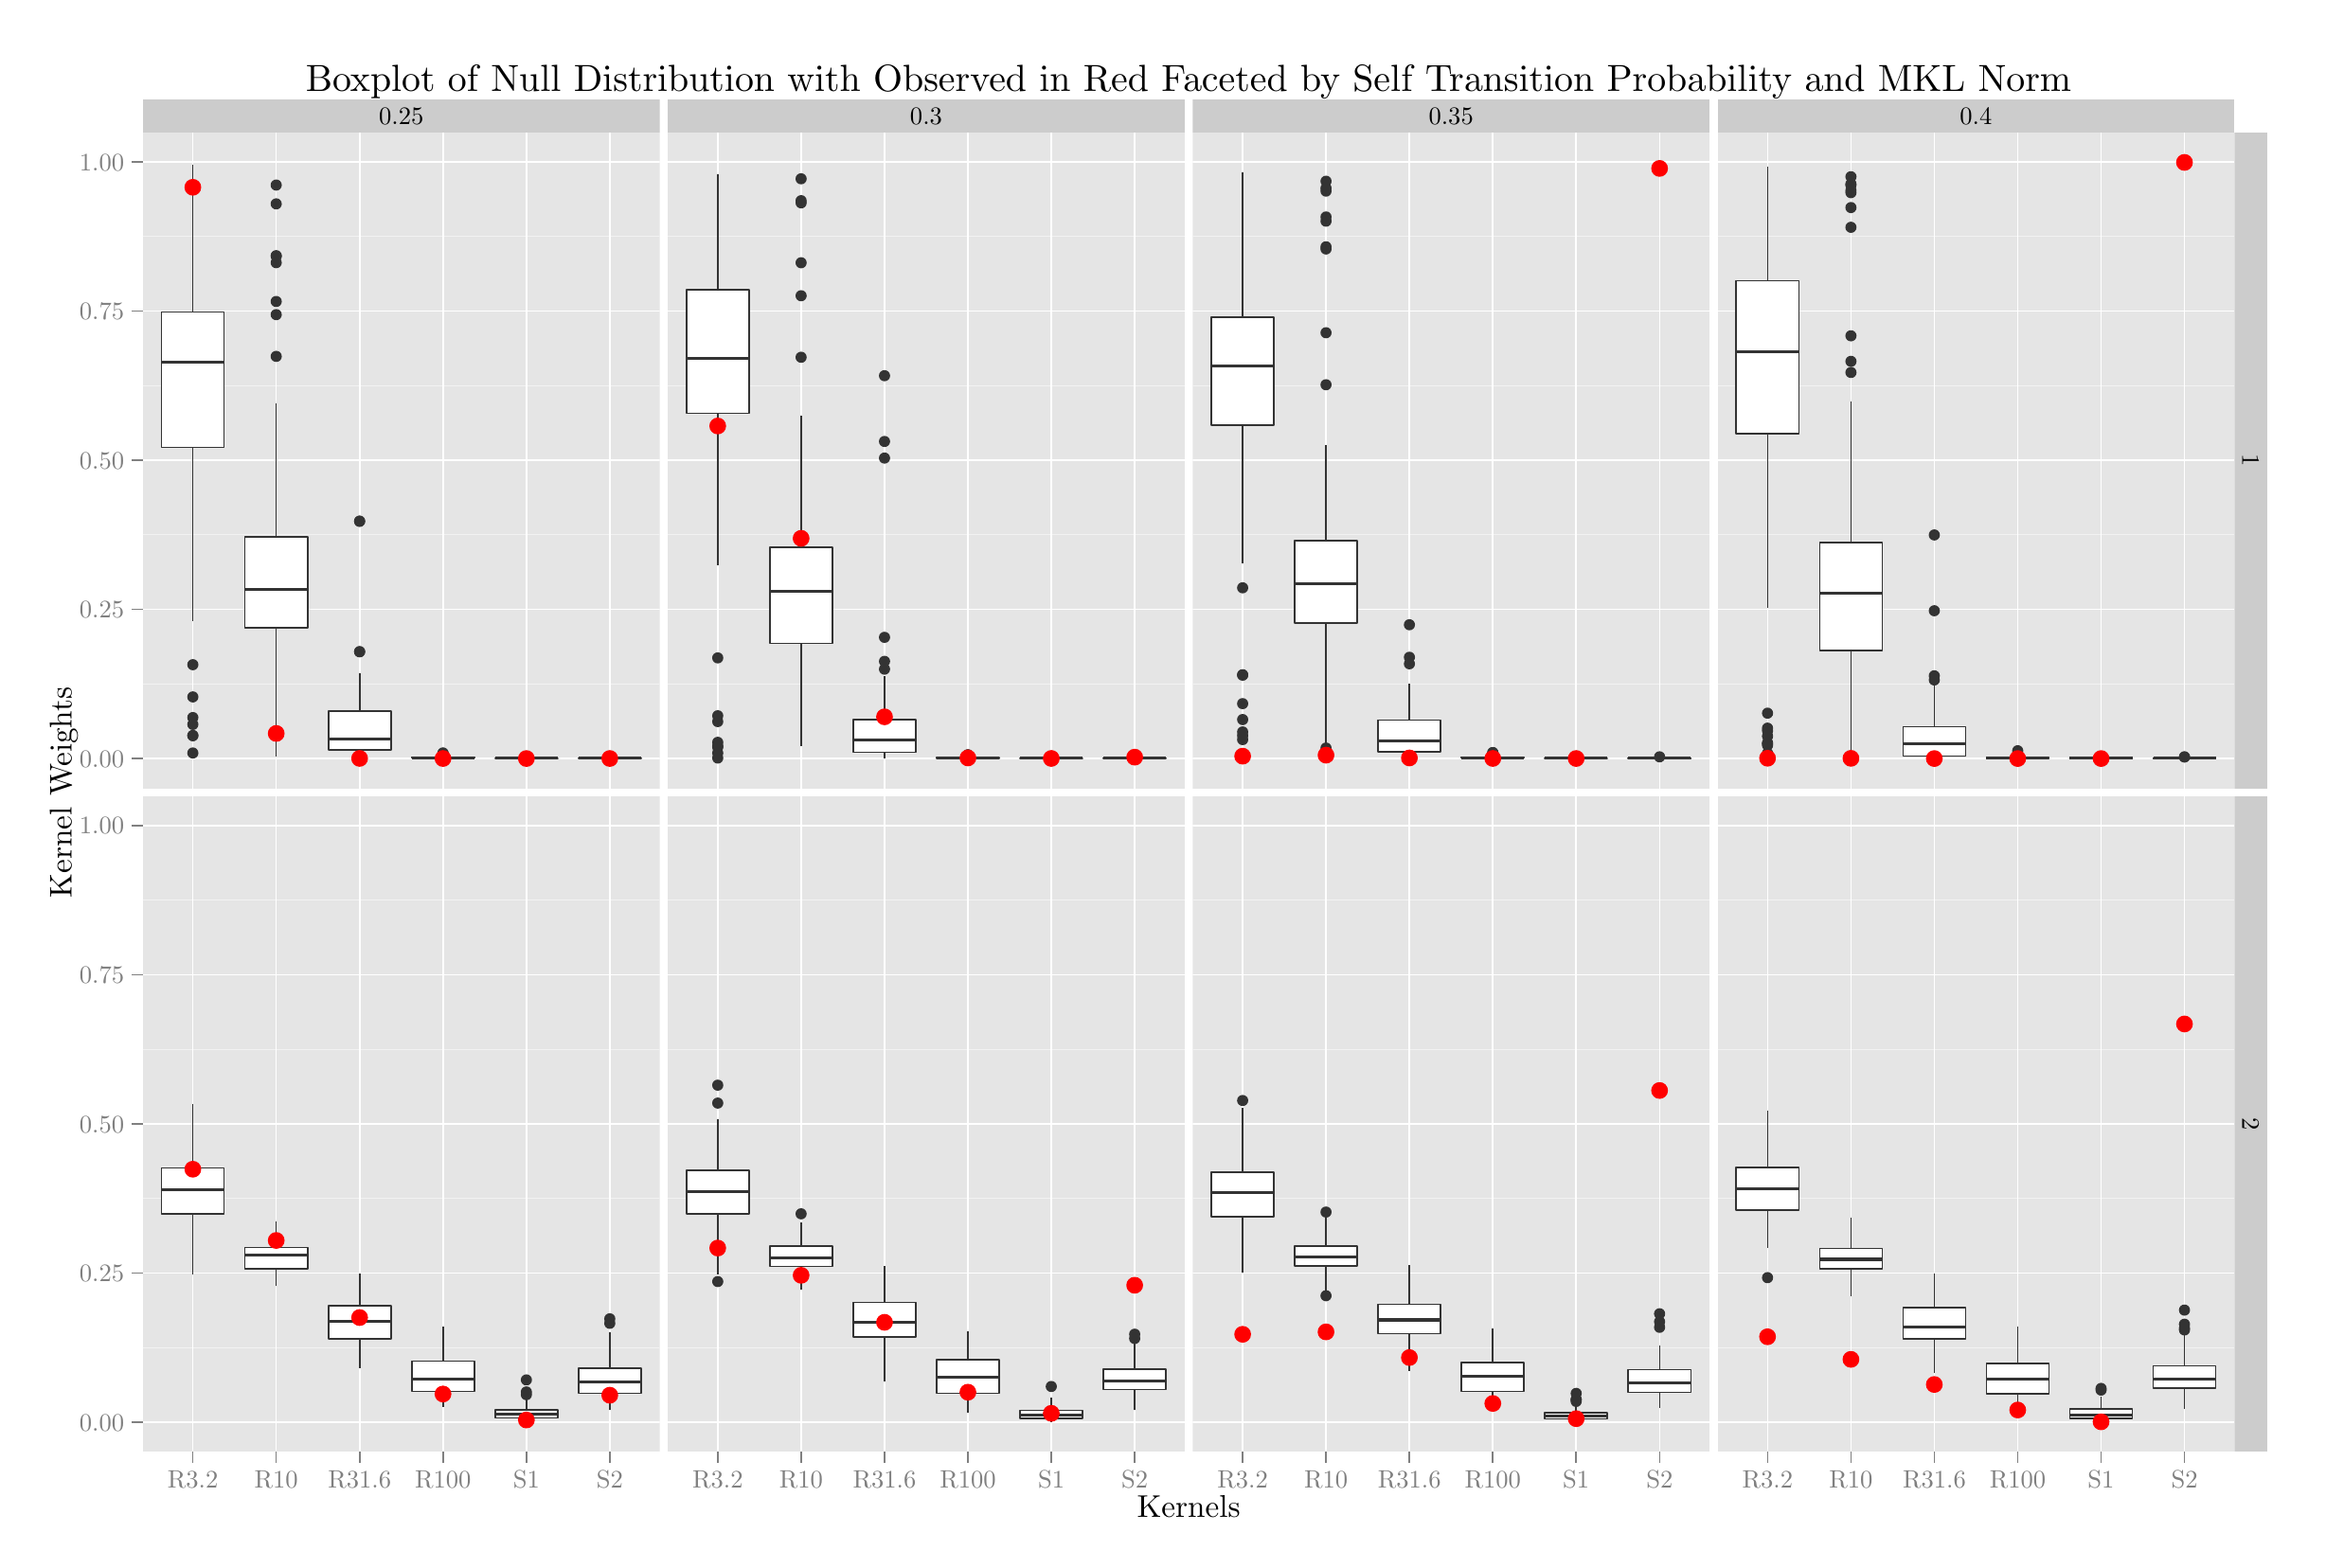
\begin{tikzpicture}[x=1pt,y=1pt]
\definecolor[named]{fillColor}{rgb}{1.00,1.00,1.00}
\path[use as bounding box,fill=fillColor,fill opacity=0.00] (0,0) rectangle (867.24,578.16);
\begin{scope}
\path[clip] (  0.00,  0.00) rectangle (867.24,578.16);
\definecolor[named]{drawColor}{rgb}{1.00,1.00,1.00}
\definecolor[named]{fillColor}{rgb}{1.00,1.00,1.00}

\path[draw=drawColor,line width= 0.6pt,line join=round,line cap=round,fill=fillColor] ( -0.00,  0.00) rectangle (867.24,578.16);
\end{scope}
\begin{scope}
\path[clip] ( 44.49,537.54) rectangle (241.75,550.17);
\definecolor[named]{fillColor}{rgb}{0.80,0.80,0.80}

\path[fill=fillColor] ( 44.49,537.54) rectangle (241.75,550.17);
\definecolor[named]{drawColor}{rgb}{0.00,0.00,0.00}

\node[text=drawColor,anchor=base,inner sep=0pt, outer sep=0pt, scale=  0.96] at (143.12,540.55) {0.25};
\end{scope}
\begin{scope}
\path[clip] (244.76,537.54) rectangle (442.02,550.17);
\definecolor[named]{fillColor}{rgb}{0.80,0.80,0.80}

\path[fill=fillColor] (244.76,537.54) rectangle (442.02,550.17);
\definecolor[named]{drawColor}{rgb}{0.00,0.00,0.00}

\node[text=drawColor,anchor=base,inner sep=0pt, outer sep=0pt, scale=  0.96] at (343.39,540.55) {0.3};
\end{scope}
\begin{scope}
\path[clip] (445.03,537.54) rectangle (642.29,550.17);
\definecolor[named]{fillColor}{rgb}{0.80,0.80,0.80}

\path[fill=fillColor] (445.03,537.54) rectangle (642.29,550.17);
\definecolor[named]{drawColor}{rgb}{0.00,0.00,0.00}

\node[text=drawColor,anchor=base,inner sep=0pt, outer sep=0pt, scale=  0.96] at (543.66,540.55) {0.35};
\end{scope}
\begin{scope}
\path[clip] (645.30,537.54) rectangle (842.56,550.17);
\definecolor[named]{fillColor}{rgb}{0.80,0.80,0.80}

\path[fill=fillColor] (645.30,537.54) rectangle (842.56,550.17);
\definecolor[named]{drawColor}{rgb}{0.00,0.00,0.00}

\node[text=drawColor,anchor=base,inner sep=0pt, outer sep=0pt, scale=  0.96] at (743.93,540.55) {0.4};
\end{scope}
\begin{scope}
\path[clip] ( 44.49,287.29) rectangle (241.75,537.54);
\definecolor[named]{fillColor}{rgb}{0.90,0.90,0.90}

\path[fill=fillColor] ( 44.49,287.29) rectangle (241.75,537.54);
\definecolor[named]{drawColor}{rgb}{0.95,0.95,0.95}

\path[draw=drawColor,line width= 0.3pt,line join=round] ( 44.49,327.13) --
	(241.75,327.13);

\path[draw=drawColor,line width= 0.3pt,line join=round] ( 44.49,384.06) --
	(241.75,384.06);

\path[draw=drawColor,line width= 0.3pt,line join=round] ( 44.49,440.99) --
	(241.75,440.99);

\path[draw=drawColor,line width= 0.3pt,line join=round] ( 44.49,497.92) --
	(241.75,497.92);
\definecolor[named]{drawColor}{rgb}{1.00,1.00,1.00}

\path[draw=drawColor,line width= 0.6pt,line join=round] ( 44.49,298.67) --
	(241.75,298.67);

\path[draw=drawColor,line width= 0.6pt,line join=round] ( 44.49,355.60) --
	(241.75,355.60);

\path[draw=drawColor,line width= 0.6pt,line join=round] ( 44.49,412.52) --
	(241.75,412.52);

\path[draw=drawColor,line width= 0.6pt,line join=round] ( 44.49,469.45) --
	(241.75,469.45);

\path[draw=drawColor,line width= 0.6pt,line join=round] ( 44.49,526.38) --
	(241.75,526.38);

\path[draw=drawColor,line width= 0.6pt,line join=round] ( 63.58,287.29) --
	( 63.58,537.54);

\path[draw=drawColor,line width= 0.6pt,line join=round] ( 95.39,287.29) --
	( 95.39,537.54);

\path[draw=drawColor,line width= 0.6pt,line join=round] (127.21,287.29) --
	(127.21,537.54);

\path[draw=drawColor,line width= 0.6pt,line join=round] (159.02,287.29) --
	(159.02,537.54);

\path[draw=drawColor,line width= 0.6pt,line join=round] (190.84,287.29) --
	(190.84,537.54);

\path[draw=drawColor,line width= 0.6pt,line join=round] (222.66,287.29) --
	(222.66,537.54);
\definecolor[named]{fillColor}{rgb}{0.20,0.20,0.20}

\path[fill=fillColor] ( 63.58,307.38) circle (  2.13);

\path[fill=fillColor] ( 63.58,314.31) circle (  2.13);

\path[fill=fillColor] ( 63.58,307.48) circle (  2.13);

\path[fill=fillColor] ( 63.58,300.79) circle (  2.13);

\path[fill=fillColor] ( 63.58,334.49) circle (  2.13);

\path[fill=fillColor] ( 63.58,311.70) circle (  2.13);

\path[fill=fillColor] ( 63.58,322.19) circle (  2.13);
\definecolor[named]{drawColor}{rgb}{0.20,0.20,0.20}

\path[draw=drawColor,line width= 0.6pt,line join=round,fill=fillColor] ( 63.58,469.10) -- ( 63.58,525.42);

\path[draw=drawColor,line width= 0.6pt,line join=round,fill=fillColor] ( 63.58,417.47) -- ( 63.58,351.27);
\definecolor[named]{fillColor}{rgb}{1.00,1.00,1.00}

\path[draw=drawColor,line width= 0.6pt,line join=round,line cap=round,fill=fillColor] ( 51.64,469.10) --
	( 51.64,417.47) --
	( 75.51,417.47) --
	( 75.51,469.10) --
	( 51.64,469.10) --
	cycle;
\definecolor[named]{fillColor}{rgb}{0.20,0.20,0.20}

\path[draw=drawColor,line width= 1.1pt,line join=round,fill=fillColor] ( 51.64,449.89) -- ( 75.51,449.89);

\path[fill=fillColor] ( 95.39,517.53) circle (  2.13);

\path[fill=fillColor] ( 95.39,510.35) circle (  2.13);

\path[fill=fillColor] ( 95.39,490.57) circle (  2.13);

\path[fill=fillColor] ( 95.39,473.10) circle (  2.13);

\path[fill=fillColor] ( 95.39,468.08) circle (  2.13);

\path[fill=fillColor] ( 95.39,490.38) circle (  2.13);

\path[fill=fillColor] ( 95.39,452.15) circle (  2.13);

\path[fill=fillColor] ( 95.39,487.91) circle (  2.13);

\path[draw=drawColor,line width= 0.6pt,line join=round,fill=fillColor] ( 95.39,383.34) -- ( 95.39,434.24);

\path[draw=drawColor,line width= 0.6pt,line join=round,fill=fillColor] ( 95.39,348.56) -- ( 95.39,299.60);
\definecolor[named]{fillColor}{rgb}{1.00,1.00,1.00}

\path[draw=drawColor,line width= 0.6pt,line join=round,line cap=round,fill=fillColor] ( 83.46,383.34) --
	( 83.46,348.56) --
	(107.32,348.56) --
	(107.32,383.34) --
	( 83.46,383.34) --
	cycle;
\definecolor[named]{fillColor}{rgb}{0.20,0.20,0.20}

\path[draw=drawColor,line width= 1.1pt,line join=round,fill=fillColor] ( 83.46,363.31) -- (107.32,363.31);

\path[fill=fillColor] (127.21,389.19) circle (  2.13);

\path[fill=fillColor] (127.21,339.46) circle (  2.13);

\path[fill=fillColor] (127.21,389.29) circle (  2.13);

\path[fill=fillColor] (127.21,339.43) circle (  2.13);

\path[draw=drawColor,line width= 0.6pt,line join=round,fill=fillColor] (127.21,316.88) -- (127.21,331.41);

\path[draw=drawColor,line width= 0.6pt,line join=round,fill=fillColor] (127.21,301.99) -- (127.21,298.68);
\definecolor[named]{fillColor}{rgb}{1.00,1.00,1.00}

\path[draw=drawColor,line width= 0.6pt,line join=round,line cap=round,fill=fillColor] (115.28,316.88) --
	(115.28,301.99) --
	(139.14,301.99) --
	(139.14,316.88) --
	(115.28,316.88) --
	cycle;
\definecolor[named]{fillColor}{rgb}{0.20,0.20,0.20}

\path[draw=drawColor,line width= 1.1pt,line join=round,fill=fillColor] (115.28,306.04) -- (139.14,306.04);

\path[fill=fillColor] (159.02,300.36) circle (  2.13);

\path[fill=fillColor] (159.02,300.29) circle (  2.13);

\path[fill=fillColor] (159.02,299.94) circle (  2.13);

\path[fill=fillColor] (159.02,300.17) circle (  2.13);

\path[fill=fillColor] (159.02,300.68) circle (  2.13);

\path[fill=fillColor] (159.02,300.80) circle (  2.13);

\path[fill=fillColor] (159.02,300.49) circle (  2.13);

\path[fill=fillColor] (159.02,299.97) circle (  2.13);

\path[fill=fillColor] (159.02,300.05) circle (  2.13);

\path[draw=drawColor,line width= 0.6pt,line join=round,fill=fillColor] (159.02,299.29) -- (159.02,299.82);

\path[draw=drawColor,line width= 0.6pt,line join=round,fill=fillColor] (159.02,298.86) -- (159.02,298.67);
\definecolor[named]{fillColor}{rgb}{1.00,1.00,1.00}

\path[draw=drawColor,line width= 0.6pt,line join=round,line cap=round,fill=fillColor] (147.09,299.29) --
	(147.09,298.86) --
	(170.95,298.86) --
	(170.95,299.29) --
	(147.09,299.29) --
	cycle;
\definecolor[named]{fillColor}{rgb}{0.20,0.20,0.20}

\path[draw=drawColor,line width= 1.1pt,line join=round,fill=fillColor] (147.09,298.99) -- (170.95,298.99);

\path[draw=drawColor,line width= 0.6pt,line join=round,fill=fillColor] (190.84,298.83) -- (190.84,298.97);

\path[draw=drawColor,line width= 0.6pt,line join=round,fill=fillColor] (190.84,298.71) -- (190.84,298.67);
\definecolor[named]{fillColor}{rgb}{1.00,1.00,1.00}

\path[draw=drawColor,line width= 0.6pt,line join=round,line cap=round,fill=fillColor] (178.91,298.83) --
	(178.91,298.71) --
	(202.77,298.71) --
	(202.77,298.83) --
	(178.91,298.83) --
	cycle;
\definecolor[named]{fillColor}{rgb}{0.20,0.20,0.20}

\path[draw=drawColor,line width= 1.1pt,line join=round,fill=fillColor] (178.91,298.78) -- (202.77,298.78);

\path[fill=fillColor] (222.66,299.26) circle (  2.13);

\path[draw=drawColor,line width= 0.6pt,line join=round,fill=fillColor] (222.66,298.94) -- (222.66,299.16);

\path[draw=drawColor,line width= 0.6pt,line join=round,fill=fillColor] (222.66,298.73) -- (222.66,298.67);
\definecolor[named]{fillColor}{rgb}{1.00,1.00,1.00}

\path[draw=drawColor,line width= 0.6pt,line join=round,line cap=round,fill=fillColor] (210.73,298.94) --
	(210.73,298.73) --
	(234.59,298.73) --
	(234.59,298.94) --
	(210.73,298.94) --
	cycle;
\definecolor[named]{fillColor}{rgb}{0.20,0.20,0.20}

\path[draw=drawColor,line width= 1.1pt,line join=round,fill=fillColor] (210.73,298.86) -- (234.59,298.86);
\definecolor[named]{fillColor}{rgb}{1.00,0.00,0.00}

\path[fill=fillColor] ( 63.58,516.68) circle (  3.20);

\path[fill=fillColor] ( 95.39,308.25) circle (  3.20);

\path[fill=fillColor] (127.21,298.73) circle (  3.20);

\path[fill=fillColor] (159.02,298.69) circle (  3.20);

\path[fill=fillColor] (190.84,298.68) circle (  3.20);

\path[fill=fillColor] (222.66,298.69) circle (  3.20);
\end{scope}
\begin{scope}
\path[clip] ( 44.49, 34.03) rectangle (241.75,284.28);
\definecolor[named]{fillColor}{rgb}{0.90,0.90,0.90}

\path[fill=fillColor] ( 44.49, 34.03) rectangle (241.75,284.28);
\definecolor[named]{drawColor}{rgb}{0.95,0.95,0.95}

\path[draw=drawColor,line width= 0.3pt,line join=round] ( 44.49, 73.87) --
	(241.75, 73.87);

\path[draw=drawColor,line width= 0.3pt,line join=round] ( 44.49,130.80) --
	(241.75,130.80);

\path[draw=drawColor,line width= 0.3pt,line join=round] ( 44.49,187.73) --
	(241.75,187.73);

\path[draw=drawColor,line width= 0.3pt,line join=round] ( 44.49,244.66) --
	(241.75,244.66);
\definecolor[named]{drawColor}{rgb}{1.00,1.00,1.00}

\path[draw=drawColor,line width= 0.6pt,line join=round] ( 44.49, 45.41) --
	(241.75, 45.41);

\path[draw=drawColor,line width= 0.6pt,line join=round] ( 44.49,102.34) --
	(241.75,102.34);

\path[draw=drawColor,line width= 0.6pt,line join=round] ( 44.49,159.26) --
	(241.75,159.26);

\path[draw=drawColor,line width= 0.6pt,line join=round] ( 44.49,216.19) --
	(241.75,216.19);

\path[draw=drawColor,line width= 0.6pt,line join=round] ( 44.49,273.12) --
	(241.75,273.12);

\path[draw=drawColor,line width= 0.6pt,line join=round] ( 63.58, 34.03) --
	( 63.58,284.28);

\path[draw=drawColor,line width= 0.6pt,line join=round] ( 95.39, 34.03) --
	( 95.39,284.28);

\path[draw=drawColor,line width= 0.6pt,line join=round] (127.21, 34.03) --
	(127.21,284.28);

\path[draw=drawColor,line width= 0.6pt,line join=round] (159.02, 34.03) --
	(159.02,284.28);

\path[draw=drawColor,line width= 0.6pt,line join=round] (190.84, 34.03) --
	(190.84,284.28);

\path[draw=drawColor,line width= 0.6pt,line join=round] (222.66, 34.03) --
	(222.66,284.28);
\definecolor[named]{drawColor}{rgb}{0.20,0.20,0.20}
\definecolor[named]{fillColor}{rgb}{0.20,0.20,0.20}

\path[draw=drawColor,line width= 0.6pt,line join=round,fill=fillColor] ( 63.58,142.43) -- ( 63.58,166.88);

\path[draw=drawColor,line width= 0.6pt,line join=round,fill=fillColor] ( 63.58,124.91) -- ( 63.58,101.89);
\definecolor[named]{fillColor}{rgb}{1.00,1.00,1.00}

\path[draw=drawColor,line width= 0.6pt,line join=round,line cap=round,fill=fillColor] ( 51.64,142.43) --
	( 51.64,124.91) --
	( 75.51,124.91) --
	( 75.51,142.43) --
	( 51.64,142.43) --
	cycle;
\definecolor[named]{fillColor}{rgb}{0.20,0.20,0.20}

\path[draw=drawColor,line width= 1.1pt,line join=round,fill=fillColor] ( 51.64,134.06) -- ( 75.51,134.06);

\path[draw=drawColor,line width= 0.6pt,line join=round,fill=fillColor] ( 95.39,112.12) -- ( 95.39,122.17);

\path[draw=drawColor,line width= 0.6pt,line join=round,fill=fillColor] ( 95.39,104.05) -- ( 95.39, 97.30);
\definecolor[named]{fillColor}{rgb}{1.00,1.00,1.00}

\path[draw=drawColor,line width= 0.6pt,line join=round,line cap=round,fill=fillColor] ( 83.46,112.12) --
	( 83.46,104.05) --
	(107.32,104.05) --
	(107.32,112.12) --
	( 83.46,112.12) --
	cycle;
\definecolor[named]{fillColor}{rgb}{0.20,0.20,0.20}

\path[draw=drawColor,line width= 1.1pt,line join=round,fill=fillColor] ( 83.46,109.03) -- (107.32,109.03);

\path[draw=drawColor,line width= 0.6pt,line join=round,fill=fillColor] (127.21, 89.76) -- (127.21,101.99);

\path[draw=drawColor,line width= 0.6pt,line join=round,fill=fillColor] (127.21, 77.13) -- (127.21, 66.07);
\definecolor[named]{fillColor}{rgb}{1.00,1.00,1.00}

\path[draw=drawColor,line width= 0.6pt,line join=round,line cap=round,fill=fillColor] (115.28, 89.76) --
	(115.28, 77.13) --
	(139.14, 77.13) --
	(139.14, 89.76) --
	(115.28, 89.76) --
	cycle;
\definecolor[named]{fillColor}{rgb}{0.20,0.20,0.20}

\path[draw=drawColor,line width= 1.1pt,line join=round,fill=fillColor] (115.28, 83.75) -- (139.14, 83.75);

\path[draw=drawColor,line width= 0.6pt,line join=round,fill=fillColor] (159.02, 68.66) -- (159.02, 81.78);

\path[draw=drawColor,line width= 0.6pt,line join=round,fill=fillColor] (159.02, 57.13) -- (159.02, 51.25);
\definecolor[named]{fillColor}{rgb}{1.00,1.00,1.00}

\path[draw=drawColor,line width= 0.6pt,line join=round,line cap=round,fill=fillColor] (147.09, 68.66) --
	(147.09, 57.13) --
	(170.95, 57.13) --
	(170.95, 68.66) --
	(147.09, 68.66) --
	cycle;
\definecolor[named]{fillColor}{rgb}{0.20,0.20,0.20}

\path[draw=drawColor,line width= 1.1pt,line join=round,fill=fillColor] (147.09, 61.99) -- (170.95, 61.99);

\path[fill=fillColor] (190.84, 55.91) circle (  2.13);

\path[fill=fillColor] (190.84, 61.55) circle (  2.13);

\path[fill=fillColor] (190.84, 56.96) circle (  2.13);

\path[draw=drawColor,line width= 0.6pt,line join=round,fill=fillColor] (190.84, 50.14) -- (190.84, 54.71);

\path[draw=drawColor,line width= 0.6pt,line join=round,fill=fillColor] (190.84, 47.08) -- (190.84, 45.57);
\definecolor[named]{fillColor}{rgb}{1.00,1.00,1.00}

\path[draw=drawColor,line width= 0.6pt,line join=round,line cap=round,fill=fillColor] (178.91, 50.14) --
	(178.91, 47.08) --
	(202.77, 47.08) --
	(202.77, 50.14) --
	(178.91, 50.14) --
	cycle;
\definecolor[named]{fillColor}{rgb}{0.20,0.20,0.20}

\path[draw=drawColor,line width= 1.1pt,line join=round,fill=fillColor] (178.91, 48.41) -- (202.77, 48.41);

\path[fill=fillColor] (222.66, 84.85) circle (  2.13);

\path[fill=fillColor] (222.66, 83.13) circle (  2.13);

\path[draw=drawColor,line width= 0.6pt,line join=round,fill=fillColor] (222.66, 65.95) -- (222.66, 79.86);

\path[draw=drawColor,line width= 0.6pt,line join=round,fill=fillColor] (222.66, 56.46) -- (222.66, 49.93);
\definecolor[named]{fillColor}{rgb}{1.00,1.00,1.00}

\path[draw=drawColor,line width= 0.6pt,line join=round,line cap=round,fill=fillColor] (210.73, 65.95) --
	(210.73, 56.46) --
	(234.59, 56.46) --
	(234.59, 65.95) --
	(210.73, 65.95) --
	cycle;
\definecolor[named]{fillColor}{rgb}{0.20,0.20,0.20}

\path[draw=drawColor,line width= 1.1pt,line join=round,fill=fillColor] (210.73, 60.61) -- (234.59, 60.61);
\definecolor[named]{fillColor}{rgb}{1.00,0.00,0.00}

\path[fill=fillColor] ( 63.58,141.95) circle (  3.20);

\path[fill=fillColor] ( 95.39,114.76) circle (  3.20);

\path[fill=fillColor] (127.21, 85.34) circle (  3.20);

\path[fill=fillColor] (159.02, 56.16) circle (  3.20);

\path[fill=fillColor] (190.84, 46.25) circle (  3.20);

\path[fill=fillColor] (222.66, 55.70) circle (  3.20);
\end{scope}
\begin{scope}
\path[clip] (244.76,287.29) rectangle (442.02,537.54);
\definecolor[named]{fillColor}{rgb}{0.90,0.90,0.90}

\path[fill=fillColor] (244.76,287.29) rectangle (442.02,537.54);
\definecolor[named]{drawColor}{rgb}{0.95,0.95,0.95}

\path[draw=drawColor,line width= 0.3pt,line join=round] (244.76,327.13) --
	(442.02,327.13);

\path[draw=drawColor,line width= 0.3pt,line join=round] (244.76,384.06) --
	(442.02,384.06);

\path[draw=drawColor,line width= 0.3pt,line join=round] (244.76,440.99) --
	(442.02,440.99);

\path[draw=drawColor,line width= 0.3pt,line join=round] (244.76,497.92) --
	(442.02,497.92);
\definecolor[named]{drawColor}{rgb}{1.00,1.00,1.00}

\path[draw=drawColor,line width= 0.6pt,line join=round] (244.76,298.67) --
	(442.02,298.67);

\path[draw=drawColor,line width= 0.6pt,line join=round] (244.76,355.60) --
	(442.02,355.60);

\path[draw=drawColor,line width= 0.6pt,line join=round] (244.76,412.52) --
	(442.02,412.52);

\path[draw=drawColor,line width= 0.6pt,line join=round] (244.76,469.45) --
	(442.02,469.45);

\path[draw=drawColor,line width= 0.6pt,line join=round] (244.76,526.38) --
	(442.02,526.38);

\path[draw=drawColor,line width= 0.6pt,line join=round] (263.85,287.29) --
	(263.85,537.54);

\path[draw=drawColor,line width= 0.6pt,line join=round] (295.66,287.29) --
	(295.66,537.54);

\path[draw=drawColor,line width= 0.6pt,line join=round] (327.48,287.29) --
	(327.48,537.54);

\path[draw=drawColor,line width= 0.6pt,line join=round] (359.30,287.29) --
	(359.30,537.54);

\path[draw=drawColor,line width= 0.6pt,line join=round] (391.11,287.29) --
	(391.11,537.54);

\path[draw=drawColor,line width= 0.6pt,line join=round] (422.93,287.29) --
	(422.93,537.54);
\definecolor[named]{fillColor}{rgb}{0.20,0.20,0.20}

\path[fill=fillColor] (263.85,312.78) circle (  2.13);

\path[fill=fillColor] (263.85,303.05) circle (  2.13);

\path[fill=fillColor] (263.85,298.86) circle (  2.13);

\path[fill=fillColor] (263.85,315.00) circle (  2.13);

\path[fill=fillColor] (263.85,300.79) circle (  2.13);

\path[fill=fillColor] (263.85,304.86) circle (  2.13);

\path[fill=fillColor] (263.85,337.08) circle (  2.13);

\path[fill=fillColor] (263.85,303.44) circle (  2.13);
\definecolor[named]{drawColor}{rgb}{0.20,0.20,0.20}

\path[draw=drawColor,line width= 0.6pt,line join=round,fill=fillColor] (263.85,477.54) -- (263.85,521.61);

\path[draw=drawColor,line width= 0.6pt,line join=round,fill=fillColor] (263.85,430.46) -- (263.85,372.39);
\definecolor[named]{fillColor}{rgb}{1.00,1.00,1.00}

\path[draw=drawColor,line width= 0.6pt,line join=round,line cap=round,fill=fillColor] (251.92,477.54) --
	(251.92,430.46) --
	(275.78,430.46) --
	(275.78,477.54) --
	(251.92,477.54) --
	cycle;
\definecolor[named]{fillColor}{rgb}{0.20,0.20,0.20}

\path[draw=drawColor,line width= 1.1pt,line join=round,fill=fillColor] (251.92,451.30) -- (275.78,451.30);

\path[fill=fillColor] (295.66,511.56) circle (  2.13);

\path[fill=fillColor] (295.66,451.82) circle (  2.13);

\path[fill=fillColor] (295.66,510.74) circle (  2.13);

\path[fill=fillColor] (295.66,519.92) circle (  2.13);

\path[fill=fillColor] (295.66,487.88) circle (  2.13);

\path[fill=fillColor] (295.66,475.29) circle (  2.13);

\path[draw=drawColor,line width= 0.6pt,line join=round,fill=fillColor] (295.66,379.19) -- (295.66,429.63);

\path[draw=drawColor,line width= 0.6pt,line join=round,fill=fillColor] (295.66,342.57) -- (295.66,303.36);
\definecolor[named]{fillColor}{rgb}{1.00,1.00,1.00}

\path[draw=drawColor,line width= 0.6pt,line join=round,line cap=round,fill=fillColor] (283.73,379.19) --
	(283.73,342.57) --
	(307.59,342.57) --
	(307.59,379.19) --
	(283.73,379.19) --
	cycle;
\definecolor[named]{fillColor}{rgb}{0.20,0.20,0.20}

\path[draw=drawColor,line width= 1.1pt,line join=round,fill=fillColor] (283.73,362.49) -- (307.59,362.49);

\path[fill=fillColor] (327.48,335.76) circle (  2.13);

\path[fill=fillColor] (327.48,444.77) circle (  2.13);

\path[fill=fillColor] (327.48,332.78) circle (  2.13);

\path[fill=fillColor] (327.48,419.68) circle (  2.13);

\path[fill=fillColor] (327.48,413.34) circle (  2.13);

\path[fill=fillColor] (327.48,344.93) circle (  2.13);

\path[draw=drawColor,line width= 0.6pt,line join=round,fill=fillColor] (327.48,313.54) -- (327.48,330.05);

\path[draw=drawColor,line width= 0.6pt,line join=round,fill=fillColor] (327.48,301.08) -- (327.48,298.70);
\definecolor[named]{fillColor}{rgb}{1.00,1.00,1.00}

\path[draw=drawColor,line width= 0.6pt,line join=round,line cap=round,fill=fillColor] (315.55,313.54) --
	(315.55,301.08) --
	(339.41,301.08) --
	(339.41,313.54) --
	(315.55,313.54) --
	cycle;
\definecolor[named]{fillColor}{rgb}{0.20,0.20,0.20}

\path[draw=drawColor,line width= 1.1pt,line join=round,fill=fillColor] (315.55,305.87) -- (339.41,305.87);

\path[fill=fillColor] (359.30,300.05) circle (  2.13);

\path[fill=fillColor] (359.30,300.11) circle (  2.13);

\path[fill=fillColor] (359.30,299.86) circle (  2.13);

\path[fill=fillColor] (359.30,299.72) circle (  2.13);

\path[fill=fillColor] (359.30,299.80) circle (  2.13);

\path[fill=fillColor] (359.30,299.71) circle (  2.13);

\path[draw=drawColor,line width= 0.6pt,line join=round,fill=fillColor] (359.30,299.16) -- (359.30,299.67);

\path[draw=drawColor,line width= 0.6pt,line join=round,fill=fillColor] (359.30,298.81) -- (359.30,298.68);
\definecolor[named]{fillColor}{rgb}{1.00,1.00,1.00}

\path[draw=drawColor,line width= 0.6pt,line join=round,line cap=round,fill=fillColor] (347.36,299.16) --
	(347.36,298.81) --
	(371.23,298.81) --
	(371.23,299.16) --
	(347.36,299.16) --
	cycle;
\definecolor[named]{fillColor}{rgb}{0.20,0.20,0.20}

\path[draw=drawColor,line width= 1.1pt,line join=round,fill=fillColor] (347.36,298.96) -- (371.23,298.96);

\path[fill=fillColor] (391.11,299.17) circle (  2.13);

\path[fill=fillColor] (391.11,299.08) circle (  2.13);

\path[draw=drawColor,line width= 0.6pt,line join=round,fill=fillColor] (391.11,298.82) -- (391.11,298.97);

\path[draw=drawColor,line width= 0.6pt,line join=round,fill=fillColor] (391.11,298.71) -- (391.11,298.67);
\definecolor[named]{fillColor}{rgb}{1.00,1.00,1.00}

\path[draw=drawColor,line width= 0.6pt,line join=round,line cap=round,fill=fillColor] (379.18,298.82) --
	(379.18,298.71) --
	(403.04,298.71) --
	(403.04,298.82) --
	(379.18,298.82) --
	cycle;
\definecolor[named]{fillColor}{rgb}{0.20,0.20,0.20}

\path[draw=drawColor,line width= 1.1pt,line join=round,fill=fillColor] (379.18,298.77) -- (403.04,298.77);

\path[fill=fillColor] (422.93,299.90) circle (  2.13);

\path[fill=fillColor] (422.93,299.36) circle (  2.13);

\path[fill=fillColor] (422.93,299.32) circle (  2.13);

\path[fill=fillColor] (422.93,299.61) circle (  2.13);

\path[draw=drawColor,line width= 0.6pt,line join=round,fill=fillColor] (422.93,298.90) -- (422.93,299.07);

\path[draw=drawColor,line width= 0.6pt,line join=round,fill=fillColor] (422.93,298.74) -- (422.93,298.67);
\definecolor[named]{fillColor}{rgb}{1.00,1.00,1.00}

\path[draw=drawColor,line width= 0.6pt,line join=round,line cap=round,fill=fillColor] (411.00,298.90) --
	(411.00,298.74) --
	(434.86,298.74) --
	(434.86,298.90) --
	(411.00,298.90) --
	cycle;
\definecolor[named]{fillColor}{rgb}{0.20,0.20,0.20}

\path[draw=drawColor,line width= 1.1pt,line join=round,fill=fillColor] (411.00,298.84) -- (434.86,298.84);
\definecolor[named]{fillColor}{rgb}{1.00,0.00,0.00}

\path[fill=fillColor] (263.85,425.59) circle (  3.20);

\path[fill=fillColor] (295.66,382.71) circle (  3.20);

\path[fill=fillColor] (327.48,314.59) circle (  3.20);

\path[fill=fillColor] (359.30,298.91) circle (  3.20);

\path[fill=fillColor] (391.11,298.71) circle (  3.20);

\path[fill=fillColor] (422.93,299.20) circle (  3.20);
\end{scope}
\begin{scope}
\path[clip] (244.76, 34.03) rectangle (442.02,284.28);
\definecolor[named]{fillColor}{rgb}{0.90,0.90,0.90}

\path[fill=fillColor] (244.76, 34.03) rectangle (442.02,284.28);
\definecolor[named]{drawColor}{rgb}{0.95,0.95,0.95}

\path[draw=drawColor,line width= 0.3pt,line join=round] (244.76, 73.87) --
	(442.02, 73.87);

\path[draw=drawColor,line width= 0.3pt,line join=round] (244.76,130.80) --
	(442.02,130.80);

\path[draw=drawColor,line width= 0.3pt,line join=round] (244.76,187.73) --
	(442.02,187.73);

\path[draw=drawColor,line width= 0.3pt,line join=round] (244.76,244.66) --
	(442.02,244.66);
\definecolor[named]{drawColor}{rgb}{1.00,1.00,1.00}

\path[draw=drawColor,line width= 0.6pt,line join=round] (244.76, 45.41) --
	(442.02, 45.41);

\path[draw=drawColor,line width= 0.6pt,line join=round] (244.76,102.34) --
	(442.02,102.34);

\path[draw=drawColor,line width= 0.6pt,line join=round] (244.76,159.26) --
	(442.02,159.26);

\path[draw=drawColor,line width= 0.6pt,line join=round] (244.76,216.19) --
	(442.02,216.19);

\path[draw=drawColor,line width= 0.6pt,line join=round] (244.76,273.12) --
	(442.02,273.12);

\path[draw=drawColor,line width= 0.6pt,line join=round] (263.85, 34.03) --
	(263.85,284.28);

\path[draw=drawColor,line width= 0.6pt,line join=round] (295.66, 34.03) --
	(295.66,284.28);

\path[draw=drawColor,line width= 0.6pt,line join=round] (327.48, 34.03) --
	(327.48,284.28);

\path[draw=drawColor,line width= 0.6pt,line join=round] (359.30, 34.03) --
	(359.30,284.28);

\path[draw=drawColor,line width= 0.6pt,line join=round] (391.11, 34.03) --
	(391.11,284.28);

\path[draw=drawColor,line width= 0.6pt,line join=round] (422.93, 34.03) --
	(422.93,284.28);
\definecolor[named]{fillColor}{rgb}{0.20,0.20,0.20}

\path[fill=fillColor] (263.85,174.02) circle (  2.13);

\path[fill=fillColor] (263.85,167.19) circle (  2.13);

\path[fill=fillColor] (263.85, 99.08) circle (  2.13);
\definecolor[named]{drawColor}{rgb}{0.20,0.20,0.20}

\path[draw=drawColor,line width= 0.6pt,line join=round,fill=fillColor] (263.85,141.42) -- (263.85,161.04);

\path[draw=drawColor,line width= 0.6pt,line join=round,fill=fillColor] (263.85,125.00) -- (263.85,101.89);
\definecolor[named]{fillColor}{rgb}{1.00,1.00,1.00}

\path[draw=drawColor,line width= 0.6pt,line join=round,line cap=round,fill=fillColor] (251.92,141.42) --
	(251.92,125.00) --
	(275.78,125.00) --
	(275.78,141.42) --
	(251.92,141.42) --
	cycle;
\definecolor[named]{fillColor}{rgb}{0.20,0.20,0.20}

\path[draw=drawColor,line width= 1.1pt,line join=round,fill=fillColor] (251.92,133.50) -- (275.78,133.50);

\path[fill=fillColor] (295.66,124.93) circle (  2.13);

\path[draw=drawColor,line width= 0.6pt,line join=round,fill=fillColor] (295.66,112.62) -- (295.66,121.75);

\path[draw=drawColor,line width= 0.6pt,line join=round,fill=fillColor] (295.66,104.82) -- (295.66, 95.83);
\definecolor[named]{fillColor}{rgb}{1.00,1.00,1.00}

\path[draw=drawColor,line width= 0.6pt,line join=round,line cap=round,fill=fillColor] (283.73,112.62) --
	(283.73,104.82) --
	(307.59,104.82) --
	(307.59,112.62) --
	(283.73,112.62) --
	cycle;
\definecolor[named]{fillColor}{rgb}{0.20,0.20,0.20}

\path[draw=drawColor,line width= 1.1pt,line join=round,fill=fillColor] (283.73,108.02) -- (307.59,108.02);

\path[draw=drawColor,line width= 0.6pt,line join=round,fill=fillColor] (327.48, 91.06) -- (327.48,104.98);

\path[draw=drawColor,line width= 0.6pt,line join=round,fill=fillColor] (327.48, 77.82) -- (327.48, 61.03);
\definecolor[named]{fillColor}{rgb}{1.00,1.00,1.00}

\path[draw=drawColor,line width= 0.6pt,line join=round,line cap=round,fill=fillColor] (315.55, 91.06) --
	(315.55, 77.82) --
	(339.41, 77.82) --
	(339.41, 91.06) --
	(315.55, 91.06) --
	cycle;
\definecolor[named]{fillColor}{rgb}{0.20,0.20,0.20}

\path[draw=drawColor,line width= 1.1pt,line join=round,fill=fillColor] (315.55, 83.58) -- (339.41, 83.58);

\path[draw=drawColor,line width= 0.6pt,line join=round,fill=fillColor] (359.30, 69.18) -- (359.30, 80.17);

\path[draw=drawColor,line width= 0.6pt,line join=round,fill=fillColor] (359.30, 56.38) -- (359.30, 48.93);
\definecolor[named]{fillColor}{rgb}{1.00,1.00,1.00}

\path[draw=drawColor,line width= 0.6pt,line join=round,line cap=round,fill=fillColor] (347.36, 69.18) --
	(347.36, 56.38) --
	(371.23, 56.38) --
	(371.23, 69.18) --
	(347.36, 69.18) --
	cycle;
\definecolor[named]{fillColor}{rgb}{0.20,0.20,0.20}

\path[draw=drawColor,line width= 1.1pt,line join=round,fill=fillColor] (347.36, 62.45) -- (371.23, 62.45);

\path[fill=fillColor] (391.11, 59.03) circle (  2.13);

\path[draw=drawColor,line width= 0.6pt,line join=round,fill=fillColor] (391.11, 49.97) -- (391.11, 54.75);

\path[draw=drawColor,line width= 0.6pt,line join=round,fill=fillColor] (391.11, 46.78) -- (391.11, 45.54);
\definecolor[named]{fillColor}{rgb}{1.00,1.00,1.00}

\path[draw=drawColor,line width= 0.6pt,line join=round,line cap=round,fill=fillColor] (379.18, 49.97) --
	(379.18, 46.78) --
	(403.04, 46.78) --
	(403.04, 49.97) --
	(379.18, 49.97) --
	cycle;
\definecolor[named]{fillColor}{rgb}{0.20,0.20,0.20}

\path[draw=drawColor,line width= 1.1pt,line join=round,fill=fillColor] (379.18, 48.23) -- (403.04, 48.23);

\path[fill=fillColor] (422.93, 77.34) circle (  2.13);

\path[fill=fillColor] (422.93, 78.99) circle (  2.13);

\path[draw=drawColor,line width= 0.6pt,line join=round,fill=fillColor] (422.93, 65.57) -- (422.93, 76.98);

\path[draw=drawColor,line width= 0.6pt,line join=round,fill=fillColor] (422.93, 57.90) -- (422.93, 50.19);
\definecolor[named]{fillColor}{rgb}{1.00,1.00,1.00}

\path[draw=drawColor,line width= 0.6pt,line join=round,line cap=round,fill=fillColor] (411.00, 65.57) --
	(411.00, 57.90) --
	(434.86, 57.90) --
	(434.86, 65.57) --
	(411.00, 65.57) --
	cycle;
\definecolor[named]{fillColor}{rgb}{0.20,0.20,0.20}

\path[draw=drawColor,line width= 1.1pt,line join=round,fill=fillColor] (411.00, 61.22) -- (434.86, 61.22);
\definecolor[named]{fillColor}{rgb}{1.00,0.00,0.00}

\path[fill=fillColor] (263.85,111.87) circle (  3.20);

\path[fill=fillColor] (295.66,101.46) circle (  3.20);

\path[fill=fillColor] (327.48, 83.52) circle (  3.20);

\path[fill=fillColor] (359.30, 56.85) circle (  3.20);

\path[fill=fillColor] (391.11, 48.79) circle (  3.20);

\path[fill=fillColor] (422.93, 97.67) circle (  3.20);
\end{scope}
\begin{scope}
\path[clip] (445.03,287.29) rectangle (642.29,537.54);
\definecolor[named]{fillColor}{rgb}{0.90,0.90,0.90}

\path[fill=fillColor] (445.03,287.29) rectangle (642.29,537.54);
\definecolor[named]{drawColor}{rgb}{0.95,0.95,0.95}

\path[draw=drawColor,line width= 0.3pt,line join=round] (445.03,327.13) --
	(642.29,327.13);

\path[draw=drawColor,line width= 0.3pt,line join=round] (445.03,384.06) --
	(642.29,384.06);

\path[draw=drawColor,line width= 0.3pt,line join=round] (445.03,440.99) --
	(642.29,440.99);

\path[draw=drawColor,line width= 0.3pt,line join=round] (445.03,497.92) --
	(642.29,497.92);
\definecolor[named]{drawColor}{rgb}{1.00,1.00,1.00}

\path[draw=drawColor,line width= 0.6pt,line join=round] (445.03,298.67) --
	(642.29,298.67);

\path[draw=drawColor,line width= 0.6pt,line join=round] (445.03,355.60) --
	(642.29,355.60);

\path[draw=drawColor,line width= 0.6pt,line join=round] (445.03,412.52) --
	(642.29,412.52);

\path[draw=drawColor,line width= 0.6pt,line join=round] (445.03,469.45) --
	(642.29,469.45);

\path[draw=drawColor,line width= 0.6pt,line join=round] (445.03,526.38) --
	(642.29,526.38);

\path[draw=drawColor,line width= 0.6pt,line join=round] (464.12,287.29) --
	(464.12,537.54);

\path[draw=drawColor,line width= 0.6pt,line join=round] (495.93,287.29) --
	(495.93,537.54);

\path[draw=drawColor,line width= 0.6pt,line join=round] (527.75,287.29) --
	(527.75,537.54);

\path[draw=drawColor,line width= 0.6pt,line join=round] (559.57,287.29) --
	(559.57,537.54);

\path[draw=drawColor,line width= 0.6pt,line join=round] (591.38,287.29) --
	(591.38,537.54);

\path[draw=drawColor,line width= 0.6pt,line join=round] (623.20,287.29) --
	(623.20,537.54);
\definecolor[named]{fillColor}{rgb}{0.20,0.20,0.20}

\path[fill=fillColor] (464.12,313.55) circle (  2.13);

\path[fill=fillColor] (464.12,305.91) circle (  2.13);

\path[fill=fillColor] (464.12,307.44) circle (  2.13);

\path[fill=fillColor] (464.12,330.66) circle (  2.13);

\path[fill=fillColor] (464.12,363.83) circle (  2.13);

\path[fill=fillColor] (464.12,330.49) circle (  2.13);

\path[fill=fillColor] (464.12,319.63) circle (  2.13);

\path[fill=fillColor] (464.12,308.84) circle (  2.13);
\definecolor[named]{drawColor}{rgb}{0.20,0.20,0.20}

\path[draw=drawColor,line width= 0.6pt,line join=round,fill=fillColor] (464.12,467.04) -- (464.12,522.31);

\path[draw=drawColor,line width= 0.6pt,line join=round,fill=fillColor] (464.12,425.93) -- (464.12,373.24);
\definecolor[named]{fillColor}{rgb}{1.00,1.00,1.00}

\path[draw=drawColor,line width= 0.6pt,line join=round,line cap=round,fill=fillColor] (452.19,467.04) --
	(452.19,425.93) --
	(476.05,425.93) --
	(476.05,467.04) --
	(452.19,467.04) --
	cycle;
\definecolor[named]{fillColor}{rgb}{0.20,0.20,0.20}

\path[draw=drawColor,line width= 1.1pt,line join=round,fill=fillColor] (452.19,448.59) -- (476.05,448.59);

\path[fill=fillColor] (495.93,503.74) circle (  2.13);

\path[fill=fillColor] (495.93,519.00) circle (  2.13);

\path[fill=fillColor] (495.93,516.34) circle (  2.13);

\path[fill=fillColor] (495.93,302.68) circle (  2.13);

\path[fill=fillColor] (495.93,493.14) circle (  2.13);

\path[fill=fillColor] (495.93,461.18) circle (  2.13);

\path[fill=fillColor] (495.93,441.32) circle (  2.13);

\path[fill=fillColor] (495.93,493.96) circle (  2.13);

\path[fill=fillColor] (495.93,505.36) circle (  2.13);

\path[fill=fillColor] (495.93,515.22) circle (  2.13);

\path[draw=drawColor,line width= 0.6pt,line join=round,fill=fillColor] (495.93,381.71) -- (495.93,418.31);

\path[draw=drawColor,line width= 0.6pt,line join=round,fill=fillColor] (495.93,350.49) -- (495.93,303.69);
\definecolor[named]{fillColor}{rgb}{1.00,1.00,1.00}

\path[draw=drawColor,line width= 0.6pt,line join=round,line cap=round,fill=fillColor] (484.00,381.71) --
	(484.00,350.49) --
	(507.87,350.49) --
	(507.87,381.71) --
	(484.00,381.71) --
	cycle;
\definecolor[named]{fillColor}{rgb}{0.20,0.20,0.20}

\path[draw=drawColor,line width= 1.1pt,line join=round,fill=fillColor] (484.00,365.46) -- (507.87,365.46);

\path[fill=fillColor] (527.75,349.73) circle (  2.13);

\path[fill=fillColor] (527.75,334.83) circle (  2.13);

\path[fill=fillColor] (527.75,337.33) circle (  2.13);

\path[draw=drawColor,line width= 0.6pt,line join=round,fill=fillColor] (527.75,313.40) -- (527.75,327.13);

\path[draw=drawColor,line width= 0.6pt,line join=round,fill=fillColor] (527.75,301.22) -- (527.75,298.69);
\definecolor[named]{fillColor}{rgb}{1.00,1.00,1.00}

\path[draw=drawColor,line width= 0.6pt,line join=round,line cap=round,fill=fillColor] (515.82,313.40) --
	(515.82,301.22) --
	(539.68,301.22) --
	(539.68,313.40) --
	(515.82,313.40) --
	cycle;
\definecolor[named]{fillColor}{rgb}{0.20,0.20,0.20}

\path[draw=drawColor,line width= 1.1pt,line join=round,fill=fillColor] (515.82,305.49) -- (539.68,305.49);

\path[fill=fillColor] (559.57,299.99) circle (  2.13);

\path[fill=fillColor] (559.57,300.96) circle (  2.13);

\path[fill=fillColor] (559.57,300.90) circle (  2.13);

\path[fill=fillColor] (559.57,299.85) circle (  2.13);

\path[fill=fillColor] (559.57,300.60) circle (  2.13);

\path[draw=drawColor,line width= 0.6pt,line join=round,fill=fillColor] (559.57,299.22) -- (559.57,299.79);

\path[draw=drawColor,line width= 0.6pt,line join=round,fill=fillColor] (559.57,298.84) -- (559.57,298.67);
\definecolor[named]{fillColor}{rgb}{1.00,1.00,1.00}

\path[draw=drawColor,line width= 0.6pt,line join=round,line cap=round,fill=fillColor] (547.64,299.22) --
	(547.64,298.84) --
	(571.50,298.84) --
	(571.50,299.22) --
	(547.64,299.22) --
	cycle;
\definecolor[named]{fillColor}{rgb}{0.20,0.20,0.20}

\path[draw=drawColor,line width= 1.1pt,line join=round,fill=fillColor] (547.64,298.99) -- (571.50,298.99);

\path[fill=fillColor] (591.38,299.08) circle (  2.13);

\path[draw=drawColor,line width= 0.6pt,line join=round,fill=fillColor] (591.38,298.82) -- (591.38,298.97);

\path[draw=drawColor,line width= 0.6pt,line join=round,fill=fillColor] (591.38,298.71) -- (591.38,298.67);
\definecolor[named]{fillColor}{rgb}{1.00,1.00,1.00}

\path[draw=drawColor,line width= 0.6pt,line join=round,line cap=round,fill=fillColor] (579.45,298.82) --
	(579.45,298.71) --
	(603.31,298.71) --
	(603.31,298.82) --
	(579.45,298.82) --
	cycle;
\definecolor[named]{fillColor}{rgb}{0.20,0.20,0.20}

\path[draw=drawColor,line width= 1.1pt,line join=round,fill=fillColor] (579.45,298.78) -- (603.31,298.78);

\path[fill=fillColor] (623.20,299.33) circle (  2.13);

\path[draw=drawColor,line width= 0.6pt,line join=round,fill=fillColor] (623.20,298.92) -- (623.20,299.11);

\path[draw=drawColor,line width= 0.6pt,line join=round,fill=fillColor] (623.20,298.74) -- (623.20,298.67);
\definecolor[named]{fillColor}{rgb}{1.00,1.00,1.00}

\path[draw=drawColor,line width= 0.6pt,line join=round,line cap=round,fill=fillColor] (611.27,298.92) --
	(611.27,298.74) --
	(635.13,298.74) --
	(635.13,298.92) --
	(611.27,298.92) --
	cycle;
\definecolor[named]{fillColor}{rgb}{0.20,0.20,0.20}

\path[draw=drawColor,line width= 1.1pt,line join=round,fill=fillColor] (611.27,298.83) -- (635.13,298.83);
\definecolor[named]{fillColor}{rgb}{1.00,0.00,0.00}

\path[fill=fillColor] (464.12,299.58) circle (  3.20);

\path[fill=fillColor] (495.93,299.97) circle (  3.20);

\path[fill=fillColor] (527.75,298.90) circle (  3.20);

\path[fill=fillColor] (559.57,298.70) circle (  3.20);

\path[fill=fillColor] (591.38,298.69) circle (  3.20);

\path[fill=fillColor] (623.20,523.88) circle (  3.20);
\end{scope}
\begin{scope}
\path[clip] (445.03, 34.03) rectangle (642.29,284.28);
\definecolor[named]{fillColor}{rgb}{0.90,0.90,0.90}

\path[fill=fillColor] (445.03, 34.03) rectangle (642.29,284.28);
\definecolor[named]{drawColor}{rgb}{0.95,0.95,0.95}

\path[draw=drawColor,line width= 0.3pt,line join=round] (445.03, 73.87) --
	(642.29, 73.87);

\path[draw=drawColor,line width= 0.3pt,line join=round] (445.03,130.80) --
	(642.29,130.80);

\path[draw=drawColor,line width= 0.3pt,line join=round] (445.03,187.73) --
	(642.29,187.73);

\path[draw=drawColor,line width= 0.3pt,line join=round] (445.03,244.66) --
	(642.29,244.66);
\definecolor[named]{drawColor}{rgb}{1.00,1.00,1.00}

\path[draw=drawColor,line width= 0.6pt,line join=round] (445.03, 45.41) --
	(642.29, 45.41);

\path[draw=drawColor,line width= 0.6pt,line join=round] (445.03,102.34) --
	(642.29,102.34);

\path[draw=drawColor,line width= 0.6pt,line join=round] (445.03,159.26) --
	(642.29,159.26);

\path[draw=drawColor,line width= 0.6pt,line join=round] (445.03,216.19) --
	(642.29,216.19);

\path[draw=drawColor,line width= 0.6pt,line join=round] (445.03,273.12) --
	(642.29,273.12);

\path[draw=drawColor,line width= 0.6pt,line join=round] (464.12, 34.03) --
	(464.12,284.28);

\path[draw=drawColor,line width= 0.6pt,line join=round] (495.93, 34.03) --
	(495.93,284.28);

\path[draw=drawColor,line width= 0.6pt,line join=round] (527.75, 34.03) --
	(527.75,284.28);

\path[draw=drawColor,line width= 0.6pt,line join=round] (559.57, 34.03) --
	(559.57,284.28);

\path[draw=drawColor,line width= 0.6pt,line join=round] (591.38, 34.03) --
	(591.38,284.28);

\path[draw=drawColor,line width= 0.6pt,line join=round] (623.20, 34.03) --
	(623.20,284.28);
\definecolor[named]{fillColor}{rgb}{0.20,0.20,0.20}

\path[fill=fillColor] (464.12,168.17) circle (  2.13);
\definecolor[named]{drawColor}{rgb}{0.20,0.20,0.20}

\path[draw=drawColor,line width= 0.6pt,line join=round,fill=fillColor] (464.12,140.78) -- (464.12,165.29);

\path[draw=drawColor,line width= 0.6pt,line join=round,fill=fillColor] (464.12,123.79) -- (464.12,102.65);
\definecolor[named]{fillColor}{rgb}{1.00,1.00,1.00}

\path[draw=drawColor,line width= 0.6pt,line join=round,line cap=round,fill=fillColor] (452.19,140.78) --
	(452.19,123.79) --
	(476.05,123.79) --
	(476.05,140.78) --
	(452.19,140.78) --
	cycle;
\definecolor[named]{fillColor}{rgb}{0.20,0.20,0.20}

\path[draw=drawColor,line width= 1.1pt,line join=round,fill=fillColor] (452.19,133.03) -- (476.05,133.03);

\path[fill=fillColor] (495.93, 93.67) circle (  2.13);

\path[fill=fillColor] (495.93,125.60) circle (  2.13);

\path[draw=drawColor,line width= 0.6pt,line join=round,fill=fillColor] (495.93,112.53) -- (495.93,123.43);

\path[draw=drawColor,line width= 0.6pt,line join=round,fill=fillColor] (495.93,104.99) -- (495.93, 95.54);
\definecolor[named]{fillColor}{rgb}{1.00,1.00,1.00}

\path[draw=drawColor,line width= 0.6pt,line join=round,line cap=round,fill=fillColor] (484.00,112.53) --
	(484.00,104.99) --
	(507.87,104.99) --
	(507.87,112.53) --
	(484.00,112.53) --
	cycle;
\definecolor[named]{fillColor}{rgb}{0.20,0.20,0.20}

\path[draw=drawColor,line width= 1.1pt,line join=round,fill=fillColor] (484.00,108.50) -- (507.87,108.50);

\path[draw=drawColor,line width= 0.6pt,line join=round,fill=fillColor] (527.75, 90.35) -- (527.75,105.30);

\path[draw=drawColor,line width= 0.6pt,line join=round,fill=fillColor] (527.75, 79.20) -- (527.75, 64.87);
\definecolor[named]{fillColor}{rgb}{1.00,1.00,1.00}

\path[draw=drawColor,line width= 0.6pt,line join=round,line cap=round,fill=fillColor] (515.82, 90.35) --
	(515.82, 79.20) --
	(539.68, 79.20) --
	(539.68, 90.35) --
	(515.82, 90.35) --
	cycle;
\definecolor[named]{fillColor}{rgb}{0.20,0.20,0.20}

\path[draw=drawColor,line width= 1.1pt,line join=round,fill=fillColor] (515.82, 84.43) -- (539.68, 84.43);

\path[draw=drawColor,line width= 0.6pt,line join=round,fill=fillColor] (559.57, 68.17) -- (559.57, 81.02);

\path[draw=drawColor,line width= 0.6pt,line join=round,fill=fillColor] (559.57, 57.17) -- (559.57, 50.66);
\definecolor[named]{fillColor}{rgb}{1.00,1.00,1.00}

\path[draw=drawColor,line width= 0.6pt,line join=round,line cap=round,fill=fillColor] (547.64, 68.17) --
	(547.64, 57.17) --
	(571.50, 57.17) --
	(571.50, 68.17) --
	(547.64, 68.17) --
	cycle;
\definecolor[named]{fillColor}{rgb}{0.20,0.20,0.20}

\path[draw=drawColor,line width= 1.1pt,line join=round,fill=fillColor] (547.64, 63.10) -- (571.50, 63.10);

\path[fill=fillColor] (591.38, 54.07) circle (  2.13);

\path[fill=fillColor] (591.38, 53.33) circle (  2.13);

\path[fill=fillColor] (591.38, 56.40) circle (  2.13);

\path[fill=fillColor] (591.38, 54.04) circle (  2.13);

\path[draw=drawColor,line width= 0.6pt,line join=round,fill=fillColor] (591.38, 48.95) -- (591.38, 52.31);

\path[draw=drawColor,line width= 0.6pt,line join=round,fill=fillColor] (591.38, 46.64) -- (591.38, 45.45);
\definecolor[named]{fillColor}{rgb}{1.00,1.00,1.00}

\path[draw=drawColor,line width= 0.6pt,line join=round,line cap=round,fill=fillColor] (579.45, 48.95) --
	(579.45, 46.64) --
	(603.31, 46.64) --
	(603.31, 48.95) --
	(579.45, 48.95) --
	cycle;
\definecolor[named]{fillColor}{rgb}{0.20,0.20,0.20}

\path[draw=drawColor,line width= 1.1pt,line join=round,fill=fillColor] (579.45, 47.86) -- (603.31, 47.86);

\path[fill=fillColor] (623.20, 83.75) circle (  2.13);

\path[fill=fillColor] (623.20, 86.79) circle (  2.13);

\path[fill=fillColor] (623.20, 81.62) circle (  2.13);

\path[draw=drawColor,line width= 0.6pt,line join=round,fill=fillColor] (623.20, 65.42) -- (623.20, 74.77);

\path[draw=drawColor,line width= 0.6pt,line join=round,fill=fillColor] (623.20, 56.83) -- (623.20, 50.85);
\definecolor[named]{fillColor}{rgb}{1.00,1.00,1.00}

\path[draw=drawColor,line width= 0.6pt,line join=round,line cap=round,fill=fillColor] (611.27, 65.42) --
	(611.27, 56.83) --
	(635.13, 56.83) --
	(635.13, 65.42) --
	(611.27, 65.42) --
	cycle;
\definecolor[named]{fillColor}{rgb}{0.20,0.20,0.20}

\path[draw=drawColor,line width= 1.1pt,line join=round,fill=fillColor] (611.27, 60.34) -- (635.13, 60.34);
\definecolor[named]{fillColor}{rgb}{1.00,0.00,0.00}

\path[fill=fillColor] (464.12, 78.95) circle (  3.20);

\path[fill=fillColor] (495.93, 79.86) circle (  3.20);

\path[fill=fillColor] (527.75, 70.07) circle (  3.20);

\path[fill=fillColor] (559.57, 52.55) circle (  3.20);

\path[fill=fillColor] (591.38, 46.75) circle (  3.20);

\path[fill=fillColor] (623.20,171.99) circle (  3.20);
\end{scope}
\begin{scope}
\path[clip] (645.30,287.29) rectangle (842.56,537.54);
\definecolor[named]{fillColor}{rgb}{0.90,0.90,0.90}

\path[fill=fillColor] (645.30,287.29) rectangle (842.56,537.54);
\definecolor[named]{drawColor}{rgb}{0.95,0.95,0.95}

\path[draw=drawColor,line width= 0.3pt,line join=round] (645.30,327.13) --
	(842.56,327.13);

\path[draw=drawColor,line width= 0.3pt,line join=round] (645.30,384.06) --
	(842.56,384.06);

\path[draw=drawColor,line width= 0.3pt,line join=round] (645.30,440.99) --
	(842.56,440.99);

\path[draw=drawColor,line width= 0.3pt,line join=round] (645.30,497.92) --
	(842.56,497.92);
\definecolor[named]{drawColor}{rgb}{1.00,1.00,1.00}

\path[draw=drawColor,line width= 0.6pt,line join=round] (645.30,298.67) --
	(842.56,298.67);

\path[draw=drawColor,line width= 0.6pt,line join=round] (645.30,355.60) --
	(842.56,355.60);

\path[draw=drawColor,line width= 0.6pt,line join=round] (645.30,412.52) --
	(842.56,412.52);

\path[draw=drawColor,line width= 0.6pt,line join=round] (645.30,469.45) --
	(842.56,469.45);

\path[draw=drawColor,line width= 0.6pt,line join=round] (645.30,526.38) --
	(842.56,526.38);

\path[draw=drawColor,line width= 0.6pt,line join=round] (664.39,287.29) --
	(664.39,537.54);

\path[draw=drawColor,line width= 0.6pt,line join=round] (696.21,287.29) --
	(696.21,537.54);

\path[draw=drawColor,line width= 0.6pt,line join=round] (728.02,287.29) --
	(728.02,537.54);

\path[draw=drawColor,line width= 0.6pt,line join=round] (759.84,287.29) --
	(759.84,537.54);

\path[draw=drawColor,line width= 0.6pt,line join=round] (791.65,287.29) --
	(791.65,537.54);

\path[draw=drawColor,line width= 0.6pt,line join=round] (823.47,287.29) --
	(823.47,537.54);
\definecolor[named]{fillColor}{rgb}{0.20,0.20,0.20}

\path[fill=fillColor] (664.39,310.27) circle (  2.13);

\path[fill=fillColor] (664.39,307.22) circle (  2.13);

\path[fill=fillColor] (664.39,304.31) circle (  2.13);

\path[fill=fillColor] (664.39,304.67) circle (  2.13);

\path[fill=fillColor] (664.39,303.72) circle (  2.13);

\path[fill=fillColor] (664.39,315.99) circle (  2.13);

\path[fill=fillColor] (664.39,309.29) circle (  2.13);

\path[fill=fillColor] (664.39,300.73) circle (  2.13);
\definecolor[named]{drawColor}{rgb}{0.20,0.20,0.20}

\path[draw=drawColor,line width= 0.6pt,line join=round,fill=fillColor] (664.39,481.06) -- (664.39,524.39);

\path[draw=drawColor,line width= 0.6pt,line join=round,fill=fillColor] (664.39,422.59) -- (664.39,356.27);
\definecolor[named]{fillColor}{rgb}{1.00,1.00,1.00}

\path[draw=drawColor,line width= 0.6pt,line join=round,line cap=round,fill=fillColor] (652.46,481.06) --
	(652.46,422.59) --
	(676.32,422.59) --
	(676.32,481.06) --
	(652.46,481.06) --
	cycle;
\definecolor[named]{fillColor}{rgb}{0.20,0.20,0.20}

\path[draw=drawColor,line width= 1.1pt,line join=round,fill=fillColor] (652.46,453.80) -- (676.32,453.80);

\path[fill=fillColor] (696.21,450.25) circle (  2.13);

\path[fill=fillColor] (696.21,460.00) circle (  2.13);

\path[fill=fillColor] (696.21,514.62) circle (  2.13);

\path[fill=fillColor] (696.21,517.51) circle (  2.13);

\path[fill=fillColor] (696.21,517.96) circle (  2.13);

\path[fill=fillColor] (696.21,520.71) circle (  2.13);

\path[fill=fillColor] (696.21,508.94) circle (  2.13);

\path[fill=fillColor] (696.21,515.50) circle (  2.13);

\path[fill=fillColor] (696.21,501.41) circle (  2.13);

\path[fill=fillColor] (696.21,446.01) circle (  2.13);

\path[draw=drawColor,line width= 0.6pt,line join=round,fill=fillColor] (696.21,381.20) -- (696.21,435.02);

\path[draw=drawColor,line width= 0.6pt,line join=round,fill=fillColor] (696.21,339.91) -- (696.21,300.59);
\definecolor[named]{fillColor}{rgb}{1.00,1.00,1.00}

\path[draw=drawColor,line width= 0.6pt,line join=round,line cap=round,fill=fillColor] (684.28,381.20) --
	(684.28,339.91) --
	(708.14,339.91) --
	(708.14,381.20) --
	(684.28,381.20) --
	cycle;
\definecolor[named]{fillColor}{rgb}{0.20,0.20,0.20}

\path[draw=drawColor,line width= 1.1pt,line join=round,fill=fillColor] (684.28,361.68) -- (708.14,361.68);

\path[fill=fillColor] (728.02,355.08) circle (  2.13);

\path[fill=fillColor] (728.02,384.00) circle (  2.13);

\path[fill=fillColor] (728.02,330.24) circle (  2.13);

\path[fill=fillColor] (728.02,328.67) circle (  2.13);

\path[draw=drawColor,line width= 0.6pt,line join=round,fill=fillColor] (728.02,310.80) -- (728.02,326.94);

\path[draw=drawColor,line width= 0.6pt,line join=round,fill=fillColor] (728.02,299.65) -- (728.02,298.69);
\definecolor[named]{fillColor}{rgb}{1.00,1.00,1.00}

\path[draw=drawColor,line width= 0.6pt,line join=round,line cap=round,fill=fillColor] (716.09,310.80) --
	(716.09,299.65) --
	(739.95,299.65) --
	(739.95,310.80) --
	(716.09,310.80) --
	cycle;
\definecolor[named]{fillColor}{rgb}{0.20,0.20,0.20}

\path[draw=drawColor,line width= 1.1pt,line join=round,fill=fillColor] (716.09,304.29) -- (739.95,304.29);

\path[fill=fillColor] (759.84,299.78) circle (  2.13);

\path[fill=fillColor] (759.84,301.65) circle (  2.13);

\path[fill=fillColor] (759.84,300.28) circle (  2.13);

\path[fill=fillColor] (759.84,299.85) circle (  2.13);

\path[draw=drawColor,line width= 0.6pt,line join=round,fill=fillColor] (759.84,299.16) -- (759.84,299.72);

\path[draw=drawColor,line width= 0.6pt,line join=round,fill=fillColor] (759.84,298.76) -- (759.84,298.68);
\definecolor[named]{fillColor}{rgb}{1.00,1.00,1.00}

\path[draw=drawColor,line width= 0.6pt,line join=round,line cap=round,fill=fillColor] (747.91,299.16) --
	(747.91,298.76) --
	(771.77,298.76) --
	(771.77,299.16) --
	(747.91,299.16) --
	cycle;
\definecolor[named]{fillColor}{rgb}{0.20,0.20,0.20}

\path[draw=drawColor,line width= 1.1pt,line join=round,fill=fillColor] (747.91,298.93) -- (771.77,298.93);

\path[draw=drawColor,line width= 0.6pt,line join=round,fill=fillColor] (791.65,298.81) -- (791.65,298.93);

\path[draw=drawColor,line width= 0.6pt,line join=round,fill=fillColor] (791.65,298.69) -- (791.65,298.67);
\definecolor[named]{fillColor}{rgb}{1.00,1.00,1.00}

\path[draw=drawColor,line width= 0.6pt,line join=round,line cap=round,fill=fillColor] (779.72,298.81) --
	(779.72,298.69) --
	(803.59,298.69) --
	(803.59,298.81) --
	(779.72,298.81) --
	cycle;
\definecolor[named]{fillColor}{rgb}{0.20,0.20,0.20}

\path[draw=drawColor,line width= 1.1pt,line join=round,fill=fillColor] (779.72,298.76) -- (803.59,298.76);

\path[fill=fillColor] (823.47,299.31) circle (  2.13);

\path[fill=fillColor] (823.47,299.27) circle (  2.13);

\path[draw=drawColor,line width= 0.6pt,line join=round,fill=fillColor] (823.47,298.89) -- (823.47,299.15);

\path[draw=drawColor,line width= 0.6pt,line join=round,fill=fillColor] (823.47,298.71) -- (823.47,298.67);
\definecolor[named]{fillColor}{rgb}{1.00,1.00,1.00}

\path[draw=drawColor,line width= 0.6pt,line join=round,line cap=round,fill=fillColor] (811.54,298.89) --
	(811.54,298.71) --
	(835.40,298.71) --
	(835.40,298.89) --
	(811.54,298.89) --
	cycle;
\definecolor[named]{fillColor}{rgb}{0.20,0.20,0.20}

\path[draw=drawColor,line width= 1.1pt,line join=round,fill=fillColor] (811.54,298.82) -- (835.40,298.82);
\definecolor[named]{fillColor}{rgb}{1.00,0.00,0.00}

\path[fill=fillColor] (664.39,298.79) circle (  3.20);

\path[fill=fillColor] (696.21,298.75) circle (  3.20);

\path[fill=fillColor] (728.02,298.67) circle (  3.20);

\path[fill=fillColor] (759.84,298.67) circle (  3.20);

\path[fill=fillColor] (791.65,298.67) circle (  3.20);

\path[fill=fillColor] (823.47,526.17) circle (  3.20);
\end{scope}
\begin{scope}
\path[clip] (645.30, 34.03) rectangle (842.56,284.28);
\definecolor[named]{fillColor}{rgb}{0.90,0.90,0.90}

\path[fill=fillColor] (645.30, 34.03) rectangle (842.56,284.28);
\definecolor[named]{drawColor}{rgb}{0.95,0.95,0.95}

\path[draw=drawColor,line width= 0.3pt,line join=round] (645.30, 73.87) --
	(842.56, 73.87);

\path[draw=drawColor,line width= 0.3pt,line join=round] (645.30,130.80) --
	(842.56,130.80);

\path[draw=drawColor,line width= 0.3pt,line join=round] (645.30,187.73) --
	(842.56,187.73);

\path[draw=drawColor,line width= 0.3pt,line join=round] (645.30,244.66) --
	(842.56,244.66);
\definecolor[named]{drawColor}{rgb}{1.00,1.00,1.00}

\path[draw=drawColor,line width= 0.6pt,line join=round] (645.30, 45.41) --
	(842.56, 45.41);

\path[draw=drawColor,line width= 0.6pt,line join=round] (645.30,102.34) --
	(842.56,102.34);

\path[draw=drawColor,line width= 0.6pt,line join=round] (645.30,159.26) --
	(842.56,159.26);

\path[draw=drawColor,line width= 0.6pt,line join=round] (645.30,216.19) --
	(842.56,216.19);

\path[draw=drawColor,line width= 0.6pt,line join=round] (645.30,273.12) --
	(842.56,273.12);

\path[draw=drawColor,line width= 0.6pt,line join=round] (664.39, 34.03) --
	(664.39,284.28);

\path[draw=drawColor,line width= 0.6pt,line join=round] (696.21, 34.03) --
	(696.21,284.28);

\path[draw=drawColor,line width= 0.6pt,line join=round] (728.02, 34.03) --
	(728.02,284.28);

\path[draw=drawColor,line width= 0.6pt,line join=round] (759.84, 34.03) --
	(759.84,284.28);

\path[draw=drawColor,line width= 0.6pt,line join=round] (791.65, 34.03) --
	(791.65,284.28);

\path[draw=drawColor,line width= 0.6pt,line join=round] (823.47, 34.03) --
	(823.47,284.28);
\definecolor[named]{fillColor}{rgb}{0.20,0.20,0.20}

\path[fill=fillColor] (664.39,100.57) circle (  2.13);
\definecolor[named]{drawColor}{rgb}{0.20,0.20,0.20}

\path[draw=drawColor,line width= 0.6pt,line join=round,fill=fillColor] (664.39,142.56) -- (664.39,164.33);

\path[draw=drawColor,line width= 0.6pt,line join=round,fill=fillColor] (664.39,126.43) -- (664.39,112.04);
\definecolor[named]{fillColor}{rgb}{1.00,1.00,1.00}

\path[draw=drawColor,line width= 0.6pt,line join=round,line cap=round,fill=fillColor] (652.46,142.56) --
	(652.46,126.43) --
	(676.32,126.43) --
	(676.32,142.56) --
	(652.46,142.56) --
	cycle;
\definecolor[named]{fillColor}{rgb}{0.20,0.20,0.20}

\path[draw=drawColor,line width= 1.1pt,line join=round,fill=fillColor] (652.46,134.44) -- (676.32,134.44);

\path[draw=drawColor,line width= 0.6pt,line join=round,fill=fillColor] (696.21,111.67) -- (696.21,123.34);

\path[draw=drawColor,line width= 0.6pt,line join=round,fill=fillColor] (696.21,103.85) -- (696.21, 93.39);
\definecolor[named]{fillColor}{rgb}{1.00,1.00,1.00}

\path[draw=drawColor,line width= 0.6pt,line join=round,line cap=round,fill=fillColor] (684.28,111.67) --
	(684.28,103.85) --
	(708.14,103.85) --
	(708.14,111.67) --
	(684.28,111.67) --
	cycle;
\definecolor[named]{fillColor}{rgb}{0.20,0.20,0.20}

\path[draw=drawColor,line width= 1.1pt,line join=round,fill=fillColor] (684.28,107.56) -- (708.14,107.56);

\path[draw=drawColor,line width= 0.6pt,line join=round,fill=fillColor] (728.02, 89.19) -- (728.02,102.25);

\path[draw=drawColor,line width= 0.6pt,line join=round,fill=fillColor] (728.02, 77.16) -- (728.02, 64.27);
\definecolor[named]{fillColor}{rgb}{1.00,1.00,1.00}

\path[draw=drawColor,line width= 0.6pt,line join=round,line cap=round,fill=fillColor] (716.09, 89.19) --
	(716.09, 77.16) --
	(739.95, 77.16) --
	(739.95, 89.19) --
	(716.09, 89.19) --
	cycle;
\definecolor[named]{fillColor}{rgb}{0.20,0.20,0.20}

\path[draw=drawColor,line width= 1.1pt,line join=round,fill=fillColor] (716.09, 81.71) -- (739.95, 81.71);

\path[draw=drawColor,line width= 0.6pt,line join=round,fill=fillColor] (759.84, 67.71) -- (759.84, 81.79);

\path[draw=drawColor,line width= 0.6pt,line join=round,fill=fillColor] (759.84, 56.19) -- (759.84, 50.35);
\definecolor[named]{fillColor}{rgb}{1.00,1.00,1.00}

\path[draw=drawColor,line width= 0.6pt,line join=round,line cap=round,fill=fillColor] (747.91, 67.71) --
	(747.91, 56.19) --
	(771.77, 56.19) --
	(771.77, 67.71) --
	(747.91, 67.71) --
	cycle;
\definecolor[named]{fillColor}{rgb}{0.20,0.20,0.20}

\path[draw=drawColor,line width= 1.1pt,line join=round,fill=fillColor] (747.91, 61.98) -- (771.77, 61.98);

\path[fill=fillColor] (791.65, 58.30) circle (  2.13);

\path[fill=fillColor] (791.65, 57.66) circle (  2.13);

\path[draw=drawColor,line width= 0.6pt,line join=round,fill=fillColor] (791.65, 50.58) -- (791.65, 55.02);

\path[draw=drawColor,line width= 0.6pt,line join=round,fill=fillColor] (791.65, 46.89) -- (791.65, 45.55);
\definecolor[named]{fillColor}{rgb}{1.00,1.00,1.00}

\path[draw=drawColor,line width= 0.6pt,line join=round,line cap=round,fill=fillColor] (779.72, 50.58) --
	(779.72, 46.89) --
	(803.59, 46.89) --
	(803.59, 50.58) --
	(779.72, 50.58) --
	cycle;
\definecolor[named]{fillColor}{rgb}{0.20,0.20,0.20}

\path[draw=drawColor,line width= 1.1pt,line join=round,fill=fillColor] (779.72, 48.04) -- (803.59, 48.04);

\path[fill=fillColor] (823.47, 82.79) circle (  2.13);

\path[fill=fillColor] (823.47, 81.28) circle (  2.13);

\path[fill=fillColor] (823.47, 80.61) circle (  2.13);

\path[fill=fillColor] (823.47, 88.18) circle (  2.13);

\path[draw=drawColor,line width= 0.6pt,line join=round,fill=fillColor] (823.47, 66.93) -- (823.47, 79.34);

\path[draw=drawColor,line width= 0.6pt,line join=round,fill=fillColor] (823.47, 58.32) -- (823.47, 50.32);
\definecolor[named]{fillColor}{rgb}{1.00,1.00,1.00}

\path[draw=drawColor,line width= 0.6pt,line join=round,line cap=round,fill=fillColor] (811.54, 66.93) --
	(811.54, 58.32) --
	(835.40, 58.32) --
	(835.40, 66.93) --
	(811.54, 66.93) --
	cycle;
\definecolor[named]{fillColor}{rgb}{0.20,0.20,0.20}

\path[draw=drawColor,line width= 1.1pt,line join=round,fill=fillColor] (811.54, 61.81) -- (835.40, 61.81);
\definecolor[named]{fillColor}{rgb}{1.00,0.00,0.00}

\path[fill=fillColor] (664.39, 78.01) circle (  3.20);

\path[fill=fillColor] (696.21, 69.38) circle (  3.20);

\path[fill=fillColor] (728.02, 59.79) circle (  3.20);

\path[fill=fillColor] (759.84, 50.06) circle (  3.20);

\path[fill=fillColor] (791.65, 45.55) circle (  3.20);

\path[fill=fillColor] (823.47,197.38) circle (  3.20);
\end{scope}
\begin{scope}
\path[clip] (  0.00,  0.00) rectangle (867.24,578.16);
\definecolor[named]{drawColor}{rgb}{0.50,0.50,0.50}

\node[text=drawColor,anchor=base east,inner sep=0pt, outer sep=0pt, scale=  0.96] at ( 37.37,295.36) {0.00};

\node[text=drawColor,anchor=base east,inner sep=0pt, outer sep=0pt, scale=  0.96] at ( 37.37,352.29) {0.25};

\node[text=drawColor,anchor=base east,inner sep=0pt, outer sep=0pt, scale=  0.96] at ( 37.37,409.22) {0.50};

\node[text=drawColor,anchor=base east,inner sep=0pt, outer sep=0pt, scale=  0.96] at ( 37.37,466.15) {0.75};

\node[text=drawColor,anchor=base east,inner sep=0pt, outer sep=0pt, scale=  0.96] at ( 37.37,523.07) {1.00};
\end{scope}
\begin{scope}
\path[clip] (  0.00,  0.00) rectangle (867.24,578.16);
\definecolor[named]{drawColor}{rgb}{0.50,0.50,0.50}

\path[draw=drawColor,line width= 0.6pt,line join=round] ( 40.22,298.67) --
	( 44.49,298.67);

\path[draw=drawColor,line width= 0.6pt,line join=round] ( 40.22,355.60) --
	( 44.49,355.60);

\path[draw=drawColor,line width= 0.6pt,line join=round] ( 40.22,412.52) --
	( 44.49,412.52);

\path[draw=drawColor,line width= 0.6pt,line join=round] ( 40.22,469.45) --
	( 44.49,469.45);

\path[draw=drawColor,line width= 0.6pt,line join=round] ( 40.22,526.38) --
	( 44.49,526.38);
\end{scope}
\begin{scope}
\path[clip] (  0.00,  0.00) rectangle (867.24,578.16);
\definecolor[named]{drawColor}{rgb}{0.50,0.50,0.50}

\node[text=drawColor,anchor=base east,inner sep=0pt, outer sep=0pt, scale=  0.96] at ( 37.37, 42.10) {0.00};

\node[text=drawColor,anchor=base east,inner sep=0pt, outer sep=0pt, scale=  0.96] at ( 37.37, 99.03) {0.25};

\node[text=drawColor,anchor=base east,inner sep=0pt, outer sep=0pt, scale=  0.96] at ( 37.37,155.96) {0.50};

\node[text=drawColor,anchor=base east,inner sep=0pt, outer sep=0pt, scale=  0.96] at ( 37.37,212.89) {0.75};

\node[text=drawColor,anchor=base east,inner sep=0pt, outer sep=0pt, scale=  0.96] at ( 37.37,269.81) {1.00};
\end{scope}
\begin{scope}
\path[clip] (  0.00,  0.00) rectangle (867.24,578.16);
\definecolor[named]{drawColor}{rgb}{0.50,0.50,0.50}

\path[draw=drawColor,line width= 0.6pt,line join=round] ( 40.22, 45.41) --
	( 44.49, 45.41);

\path[draw=drawColor,line width= 0.6pt,line join=round] ( 40.22,102.34) --
	( 44.49,102.34);

\path[draw=drawColor,line width= 0.6pt,line join=round] ( 40.22,159.26) --
	( 44.49,159.26);

\path[draw=drawColor,line width= 0.6pt,line join=round] ( 40.22,216.19) --
	( 44.49,216.19);

\path[draw=drawColor,line width= 0.6pt,line join=round] ( 40.22,273.12) --
	( 44.49,273.12);
\end{scope}
\begin{scope}
\path[clip] (842.56,287.29) rectangle (855.19,537.54);
\definecolor[named]{fillColor}{rgb}{0.80,0.80,0.80}

\path[fill=fillColor] (842.56,287.29) rectangle (855.19,537.54);
\definecolor[named]{drawColor}{rgb}{0.00,0.00,0.00}

\node[text=drawColor,rotate=270.00,anchor=base,inner sep=0pt, outer sep=0pt, scale=  0.96] at (845.57,412.42) {1};
\end{scope}
\begin{scope}
\path[clip] (842.56, 34.03) rectangle (855.19,284.28);
\definecolor[named]{fillColor}{rgb}{0.80,0.80,0.80}

\path[fill=fillColor] (842.56, 34.03) rectangle (855.19,284.28);
\definecolor[named]{drawColor}{rgb}{0.00,0.00,0.00}

\node[text=drawColor,rotate=270.00,anchor=base,inner sep=0pt, outer sep=0pt, scale=  0.96] at (845.57,159.16) {2};
\end{scope}
\begin{scope}
\path[clip] (  0.00,  0.00) rectangle (867.24,578.16);
\definecolor[named]{drawColor}{rgb}{0.50,0.50,0.50}

\path[draw=drawColor,line width= 0.6pt,line join=round] ( 63.58, 29.77) --
	( 63.58, 34.03);

\path[draw=drawColor,line width= 0.6pt,line join=round] ( 95.39, 29.77) --
	( 95.39, 34.03);

\path[draw=drawColor,line width= 0.6pt,line join=round] (127.21, 29.77) --
	(127.21, 34.03);

\path[draw=drawColor,line width= 0.6pt,line join=round] (159.02, 29.77) --
	(159.02, 34.03);

\path[draw=drawColor,line width= 0.6pt,line join=round] (190.84, 29.77) --
	(190.84, 34.03);

\path[draw=drawColor,line width= 0.6pt,line join=round] (222.66, 29.77) --
	(222.66, 34.03);
\end{scope}
\begin{scope}
\path[clip] (  0.00,  0.00) rectangle (867.24,578.16);
\definecolor[named]{drawColor}{rgb}{0.50,0.50,0.50}

\node[text=drawColor,anchor=base,inner sep=0pt, outer sep=0pt, scale=  0.96] at ( 63.58, 20.31) {R3.2};

\node[text=drawColor,anchor=base,inner sep=0pt, outer sep=0pt, scale=  0.96] at ( 95.39, 20.31) {R10};

\node[text=drawColor,anchor=base,inner sep=0pt, outer sep=0pt, scale=  0.96] at (127.21, 20.31) {R31.6};

\node[text=drawColor,anchor=base,inner sep=0pt, outer sep=0pt, scale=  0.96] at (159.02, 20.31) {R100};

\node[text=drawColor,anchor=base,inner sep=0pt, outer sep=0pt, scale=  0.96] at (190.84, 20.31) {S1};

\node[text=drawColor,anchor=base,inner sep=0pt, outer sep=0pt, scale=  0.96] at (222.66, 20.31) {S2};
\end{scope}
\begin{scope}
\path[clip] (  0.00,  0.00) rectangle (867.24,578.16);
\definecolor[named]{drawColor}{rgb}{0.50,0.50,0.50}

\path[draw=drawColor,line width= 0.6pt,line join=round] (263.85, 29.77) --
	(263.85, 34.03);

\path[draw=drawColor,line width= 0.6pt,line join=round] (295.66, 29.77) --
	(295.66, 34.03);

\path[draw=drawColor,line width= 0.6pt,line join=round] (327.48, 29.77) --
	(327.48, 34.03);

\path[draw=drawColor,line width= 0.6pt,line join=round] (359.30, 29.77) --
	(359.30, 34.03);

\path[draw=drawColor,line width= 0.6pt,line join=round] (391.11, 29.77) --
	(391.11, 34.03);

\path[draw=drawColor,line width= 0.6pt,line join=round] (422.93, 29.77) --
	(422.93, 34.03);
\end{scope}
\begin{scope}
\path[clip] (  0.00,  0.00) rectangle (867.24,578.16);
\definecolor[named]{drawColor}{rgb}{0.50,0.50,0.50}

\node[text=drawColor,anchor=base,inner sep=0pt, outer sep=0pt, scale=  0.96] at (263.85, 20.31) {R3.2};

\node[text=drawColor,anchor=base,inner sep=0pt, outer sep=0pt, scale=  0.96] at (295.66, 20.31) {R10};

\node[text=drawColor,anchor=base,inner sep=0pt, outer sep=0pt, scale=  0.96] at (327.48, 20.31) {R31.6};

\node[text=drawColor,anchor=base,inner sep=0pt, outer sep=0pt, scale=  0.96] at (359.30, 20.31) {R100};

\node[text=drawColor,anchor=base,inner sep=0pt, outer sep=0pt, scale=  0.96] at (391.11, 20.31) {S1};

\node[text=drawColor,anchor=base,inner sep=0pt, outer sep=0pt, scale=  0.96] at (422.93, 20.31) {S2};
\end{scope}
\begin{scope}
\path[clip] (  0.00,  0.00) rectangle (867.24,578.16);
\definecolor[named]{drawColor}{rgb}{0.50,0.50,0.50}

\path[draw=drawColor,line width= 0.6pt,line join=round] (464.12, 29.77) --
	(464.12, 34.03);

\path[draw=drawColor,line width= 0.6pt,line join=round] (495.93, 29.77) --
	(495.93, 34.03);

\path[draw=drawColor,line width= 0.6pt,line join=round] (527.75, 29.77) --
	(527.75, 34.03);

\path[draw=drawColor,line width= 0.6pt,line join=round] (559.57, 29.77) --
	(559.57, 34.03);

\path[draw=drawColor,line width= 0.6pt,line join=round] (591.38, 29.77) --
	(591.38, 34.03);

\path[draw=drawColor,line width= 0.6pt,line join=round] (623.20, 29.77) --
	(623.20, 34.03);
\end{scope}
\begin{scope}
\path[clip] (  0.00,  0.00) rectangle (867.24,578.16);
\definecolor[named]{drawColor}{rgb}{0.50,0.50,0.50}

\node[text=drawColor,anchor=base,inner sep=0pt, outer sep=0pt, scale=  0.96] at (464.12, 20.31) {R3.2};

\node[text=drawColor,anchor=base,inner sep=0pt, outer sep=0pt, scale=  0.96] at (495.93, 20.31) {R10};

\node[text=drawColor,anchor=base,inner sep=0pt, outer sep=0pt, scale=  0.96] at (527.75, 20.31) {R31.6};

\node[text=drawColor,anchor=base,inner sep=0pt, outer sep=0pt, scale=  0.96] at (559.57, 20.31) {R100};

\node[text=drawColor,anchor=base,inner sep=0pt, outer sep=0pt, scale=  0.96] at (591.38, 20.31) {S1};

\node[text=drawColor,anchor=base,inner sep=0pt, outer sep=0pt, scale=  0.96] at (623.20, 20.31) {S2};
\end{scope}
\begin{scope}
\path[clip] (  0.00,  0.00) rectangle (867.24,578.16);
\definecolor[named]{drawColor}{rgb}{0.50,0.50,0.50}

\path[draw=drawColor,line width= 0.6pt,line join=round] (664.39, 29.77) --
	(664.39, 34.03);

\path[draw=drawColor,line width= 0.6pt,line join=round] (696.21, 29.77) --
	(696.21, 34.03);

\path[draw=drawColor,line width= 0.6pt,line join=round] (728.02, 29.77) --
	(728.02, 34.03);

\path[draw=drawColor,line width= 0.6pt,line join=round] (759.84, 29.77) --
	(759.84, 34.03);

\path[draw=drawColor,line width= 0.6pt,line join=round] (791.65, 29.77) --
	(791.65, 34.03);

\path[draw=drawColor,line width= 0.6pt,line join=round] (823.47, 29.77) --
	(823.47, 34.03);
\end{scope}
\begin{scope}
\path[clip] (  0.00,  0.00) rectangle (867.24,578.16);
\definecolor[named]{drawColor}{rgb}{0.50,0.50,0.50}

\node[text=drawColor,anchor=base,inner sep=0pt, outer sep=0pt, scale=  0.96] at (664.39, 20.31) {R3.2};

\node[text=drawColor,anchor=base,inner sep=0pt, outer sep=0pt, scale=  0.96] at (696.21, 20.31) {R10};

\node[text=drawColor,anchor=base,inner sep=0pt, outer sep=0pt, scale=  0.96] at (728.02, 20.31) {R31.6};

\node[text=drawColor,anchor=base,inner sep=0pt, outer sep=0pt, scale=  0.96] at (759.84, 20.31) {R100};

\node[text=drawColor,anchor=base,inner sep=0pt, outer sep=0pt, scale=  0.96] at (791.65, 20.31) {S1};

\node[text=drawColor,anchor=base,inner sep=0pt, outer sep=0pt, scale=  0.96] at (823.47, 20.31) {S2};
\end{scope}
\begin{scope}
\path[clip] (  0.00,  0.00) rectangle (867.24,578.16);
\definecolor[named]{drawColor}{rgb}{0.00,0.00,0.00}

\node[text=drawColor,anchor=base,inner sep=0pt, outer sep=0pt, scale=  1.20] at (443.52,  9.03) {Kernels};
\end{scope}
\begin{scope}
\path[clip] (  0.00,  0.00) rectangle (867.24,578.16);
\definecolor[named]{drawColor}{rgb}{0.00,0.00,0.00}

\node[text=drawColor,rotate= 90.00,anchor=base,inner sep=0pt, outer sep=0pt, scale=  1.20] at ( 17.30,285.79) {Kernel Weights};
\end{scope}
\begin{scope}
\path[clip] (  0.00,  0.00) rectangle (867.24,578.16);
\definecolor[named]{drawColor}{rgb}{0.00,0.00,0.00}

\node[text=drawColor,anchor=base,inner sep=0pt, outer sep=0pt, scale=  1.44] at (443.52,553.19) {Boxplot of Null Distribution with Observed in Red Faceted by Self Transition Probability and MKL Norm};
\end{scope}
\end{tikzpicture}

    }
  \end{center}
\caption{The MKL weights in the 1- (upper row) and 2-norm (lower row) cases shift progressively more to
  the $2$-spectrum kernel as the DNA signal is increased.}
\label{fig:mkl_weights1}
\end{figure}

In Figure~\ref{fig:mkl_weights2} we vary the radius of the outer star in $\{4, 7, 10, 13, 16\}$,
while fixing the radius of the inner star to be $4$ and the transition probability $p^{\star} = .3$.
We see the dominant weight for the unpermuted case shift to higher-width kernels as we increase
the radius of the outer star.
\begin{figure}
  \begin{center}
    \resizebox{14.0cm}{!}{
      % Created by tikzDevice version 0.6.2-92-0ad2792 on 2013-03-06 20:16:19
% !TEX encoding = UTF-8 Unicode
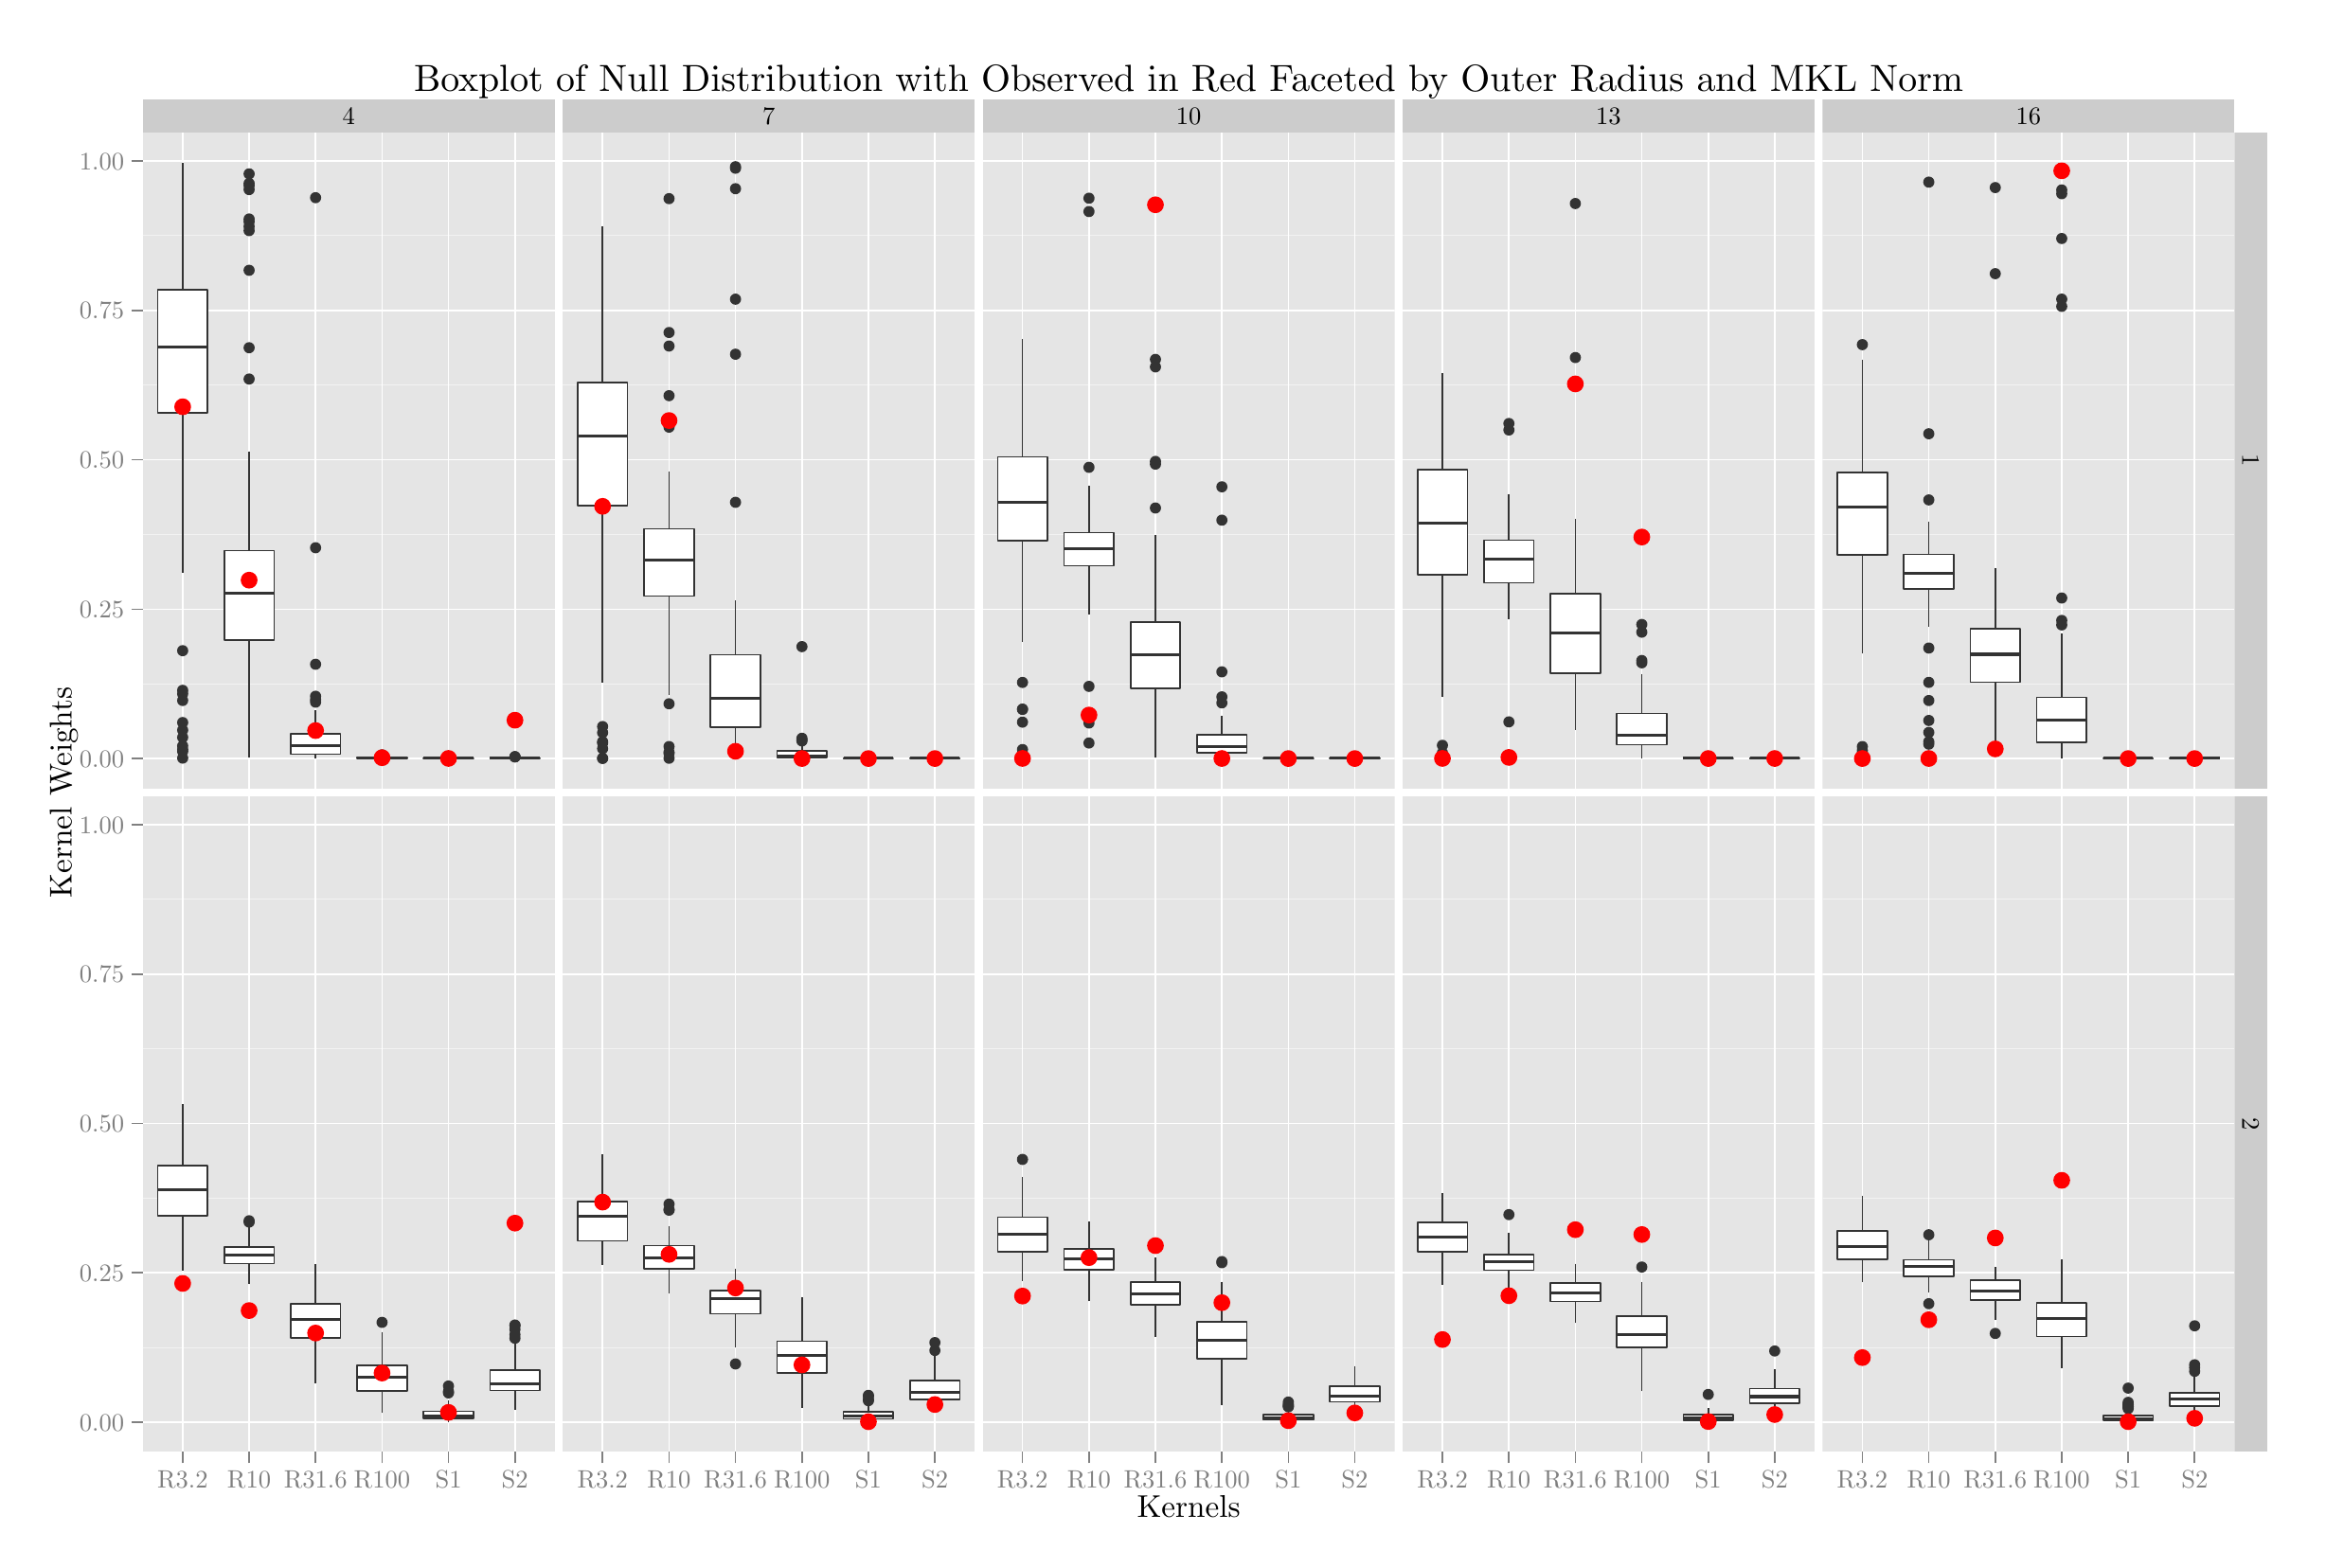
\begin{tikzpicture}[x=1pt,y=1pt]
\definecolor[named]{fillColor}{rgb}{1.00,1.00,1.00}
\path[use as bounding box,fill=fillColor,fill opacity=0.00] (0,0) rectangle (867.24,578.16);
\begin{scope}
\path[clip] (  0.00,  0.00) rectangle (867.24,578.16);
\definecolor[named]{drawColor}{rgb}{1.00,1.00,1.00}
\definecolor[named]{fillColor}{rgb}{1.00,1.00,1.00}

\path[draw=drawColor,line width= 0.6pt,line join=round,line cap=round,fill=fillColor] ( -0.00,  0.00) rectangle (867.24,578.16);
\end{scope}
\begin{scope}
\path[clip] ( 44.49,537.54) rectangle (201.69,550.17);
\definecolor[named]{fillColor}{rgb}{0.80,0.80,0.80}

\path[fill=fillColor] ( 44.49,537.54) rectangle (201.69,550.17);
\definecolor[named]{drawColor}{rgb}{0.00,0.00,0.00}

\node[text=drawColor,anchor=base,inner sep=0pt, outer sep=0pt, scale=  0.96] at (123.09,540.55) {4};
\end{scope}
\begin{scope}
\path[clip] (204.70,537.54) rectangle (361.91,550.17);
\definecolor[named]{fillColor}{rgb}{0.80,0.80,0.80}

\path[fill=fillColor] (204.70,537.54) rectangle (361.91,550.17);
\definecolor[named]{drawColor}{rgb}{0.00,0.00,0.00}

\node[text=drawColor,anchor=base,inner sep=0pt, outer sep=0pt, scale=  0.96] at (283.31,540.55) {7};
\end{scope}
\begin{scope}
\path[clip] (364.92,537.54) rectangle (522.13,550.17);
\definecolor[named]{fillColor}{rgb}{0.80,0.80,0.80}

\path[fill=fillColor] (364.92,537.54) rectangle (522.13,550.17);
\definecolor[named]{drawColor}{rgb}{0.00,0.00,0.00}

\node[text=drawColor,anchor=base,inner sep=0pt, outer sep=0pt, scale=  0.96] at (443.52,540.55) {10};
\end{scope}
\begin{scope}
\path[clip] (525.14,537.54) rectangle (682.34,550.17);
\definecolor[named]{fillColor}{rgb}{0.80,0.80,0.80}

\path[fill=fillColor] (525.14,537.54) rectangle (682.34,550.17);
\definecolor[named]{drawColor}{rgb}{0.00,0.00,0.00}

\node[text=drawColor,anchor=base,inner sep=0pt, outer sep=0pt, scale=  0.96] at (603.74,540.55) {13};
\end{scope}
\begin{scope}
\path[clip] (685.35,537.54) rectangle (842.56,550.17);
\definecolor[named]{fillColor}{rgb}{0.80,0.80,0.80}

\path[fill=fillColor] (685.35,537.54) rectangle (842.56,550.17);
\definecolor[named]{drawColor}{rgb}{0.00,0.00,0.00}

\node[text=drawColor,anchor=base,inner sep=0pt, outer sep=0pt, scale=  0.96] at (763.96,540.55) {16};
\end{scope}
\begin{scope}
\path[clip] ( 44.49,287.29) rectangle (201.69,537.54);
\definecolor[named]{fillColor}{rgb}{0.90,0.90,0.90}

\path[fill=fillColor] ( 44.49,287.29) rectangle (201.69,537.54);
\definecolor[named]{drawColor}{rgb}{0.95,0.95,0.95}

\path[draw=drawColor,line width= 0.3pt,line join=round] ( 44.49,327.17) --
	(201.69,327.17);

\path[draw=drawColor,line width= 0.3pt,line join=round] ( 44.49,384.18) --
	(201.69,384.18);

\path[draw=drawColor,line width= 0.3pt,line join=round] ( 44.49,441.20) --
	(201.69,441.20);

\path[draw=drawColor,line width= 0.3pt,line join=round] ( 44.49,498.21) --
	(201.69,498.21);
\definecolor[named]{drawColor}{rgb}{1.00,1.00,1.00}

\path[draw=drawColor,line width= 0.6pt,line join=round] ( 44.49,298.67) --
	(201.69,298.67);

\path[draw=drawColor,line width= 0.6pt,line join=round] ( 44.49,355.68) --
	(201.69,355.68);

\path[draw=drawColor,line width= 0.6pt,line join=round] ( 44.49,412.69) --
	(201.69,412.69);

\path[draw=drawColor,line width= 0.6pt,line join=round] ( 44.49,469.70) --
	(201.69,469.70);

\path[draw=drawColor,line width= 0.6pt,line join=round] ( 44.49,526.72) --
	(201.69,526.72);

\path[draw=drawColor,line width= 0.6pt,line join=round] ( 59.70,287.29) --
	( 59.70,537.54);

\path[draw=drawColor,line width= 0.6pt,line join=round] ( 85.05,287.29) --
	( 85.05,537.54);

\path[draw=drawColor,line width= 0.6pt,line join=round] (110.41,287.29) --
	(110.41,537.54);

\path[draw=drawColor,line width= 0.6pt,line join=round] (135.77,287.29) --
	(135.77,537.54);

\path[draw=drawColor,line width= 0.6pt,line join=round] (161.12,287.29) --
	(161.12,537.54);

\path[draw=drawColor,line width= 0.6pt,line join=round] (186.48,287.29) --
	(186.48,537.54);
\definecolor[named]{fillColor}{rgb}{0.20,0.20,0.20}

\path[fill=fillColor] ( 59.70,301.39) circle (  2.13);

\path[fill=fillColor] ( 59.70,320.83) circle (  2.13);

\path[fill=fillColor] ( 59.70,309.52) circle (  2.13);

\path[fill=fillColor] ( 59.70,312.41) circle (  2.13);

\path[fill=fillColor] ( 59.70,324.70) circle (  2.13);

\path[fill=fillColor] ( 59.70,303.50) circle (  2.13);

\path[fill=fillColor] ( 59.70,302.12) circle (  2.13);

\path[fill=fillColor] ( 59.70,323.35) circle (  2.13);

\path[fill=fillColor] ( 59.70,339.84) circle (  2.13);

\path[fill=fillColor] ( 59.70,306.75) circle (  2.13);

\path[fill=fillColor] ( 59.70,298.84) circle (  2.13);
\definecolor[named]{drawColor}{rgb}{0.20,0.20,0.20}

\path[draw=drawColor,line width= 0.6pt,line join=round,fill=fillColor] ( 59.70,477.67) -- ( 59.70,526.17);

\path[draw=drawColor,line width= 0.6pt,line join=round,fill=fillColor] ( 59.70,430.69) -- ( 59.70,369.63);
\definecolor[named]{fillColor}{rgb}{1.00,1.00,1.00}

\path[draw=drawColor,line width= 0.6pt,line join=round,line cap=round,fill=fillColor] ( 50.19,477.67) --
	( 50.19,430.69) --
	( 69.21,430.69) --
	( 69.21,477.67) --
	( 50.19,477.67) --
	cycle;
\definecolor[named]{fillColor}{rgb}{0.20,0.20,0.20}

\path[draw=drawColor,line width= 1.1pt,line join=round,fill=fillColor] ( 50.19,455.68) -- ( 69.21,455.68);

\path[fill=fillColor] ( 85.05,443.51) circle (  2.13);

\path[fill=fillColor] ( 85.05,503.57) circle (  2.13);

\path[fill=fillColor] ( 85.05,515.80) circle (  2.13);

\path[fill=fillColor] ( 85.05,504.58) circle (  2.13);

\path[fill=fillColor] ( 85.05,500.14) circle (  2.13);

\path[fill=fillColor] ( 85.05,521.79) circle (  2.13);

\path[fill=fillColor] ( 85.05,517.38) circle (  2.13);

\path[fill=fillColor] ( 85.05,501.71) circle (  2.13);

\path[fill=fillColor] ( 85.05,485.00) circle (  2.13);

\path[fill=fillColor] ( 85.05,518.17) circle (  2.13);

\path[fill=fillColor] ( 85.05,455.45) circle (  2.13);

\path[draw=drawColor,line width= 0.6pt,line join=round,fill=fillColor] ( 85.05,378.02) -- ( 85.05,415.89);

\path[draw=drawColor,line width= 0.6pt,line join=round,fill=fillColor] ( 85.05,343.91) -- ( 85.05,299.20);
\definecolor[named]{fillColor}{rgb}{1.00,1.00,1.00}

\path[draw=drawColor,line width= 0.6pt,line join=round,line cap=round,fill=fillColor] ( 75.55,378.02) --
	( 75.55,343.91) --
	( 94.56,343.91) --
	( 94.56,378.02) --
	( 75.55,378.02) --
	cycle;
\definecolor[named]{fillColor}{rgb}{0.20,0.20,0.20}

\path[draw=drawColor,line width= 1.1pt,line join=round,fill=fillColor] ( 75.55,361.64) -- ( 94.56,361.64);

\path[fill=fillColor] (110.41,320.19) circle (  2.13);

\path[fill=fillColor] (110.41,379.12) circle (  2.13);

\path[fill=fillColor] (110.41,322.45) circle (  2.13);

\path[fill=fillColor] (110.41,321.11) circle (  2.13);

\path[fill=fillColor] (110.41,512.71) circle (  2.13);

\path[fill=fillColor] (110.41,334.65) circle (  2.13);

\path[draw=drawColor,line width= 0.6pt,line join=round,fill=fillColor] (110.41,308.03) -- (110.41,317.12);

\path[draw=drawColor,line width= 0.6pt,line join=round,fill=fillColor] (110.41,300.34) -- (110.41,298.67);
\definecolor[named]{fillColor}{rgb}{1.00,1.00,1.00}

\path[draw=drawColor,line width= 0.6pt,line join=round,line cap=round,fill=fillColor] (100.90,308.03) --
	(100.90,300.34) --
	(119.92,300.34) --
	(119.92,308.03) --
	(100.90,308.03) --
	cycle;
\definecolor[named]{fillColor}{rgb}{0.20,0.20,0.20}

\path[draw=drawColor,line width= 1.1pt,line join=round,fill=fillColor] (100.90,303.42) -- (119.92,303.42);

\path[fill=fillColor] (135.77,299.50) circle (  2.13);

\path[fill=fillColor] (135.77,299.57) circle (  2.13);

\path[fill=fillColor] (135.77,299.61) circle (  2.13);

\path[fill=fillColor] (135.77,299.49) circle (  2.13);

\path[fill=fillColor] (135.77,300.09) circle (  2.13);

\path[draw=drawColor,line width= 0.6pt,line join=round,fill=fillColor] (135.77,299.02) -- (135.77,299.42);

\path[draw=drawColor,line width= 0.6pt,line join=round,fill=fillColor] (135.77,298.75) -- (135.77,298.67);
\definecolor[named]{fillColor}{rgb}{1.00,1.00,1.00}

\path[draw=drawColor,line width= 0.6pt,line join=round,line cap=round,fill=fillColor] (126.26,299.02) --
	(126.26,298.75) --
	(145.27,298.75) --
	(145.27,299.02) --
	(126.26,299.02) --
	cycle;
\definecolor[named]{fillColor}{rgb}{0.20,0.20,0.20}

\path[draw=drawColor,line width= 1.1pt,line join=round,fill=fillColor] (126.26,298.89) -- (145.27,298.89);

\path[fill=fillColor] (161.12,299.03) circle (  2.13);

\path[draw=drawColor,line width= 0.6pt,line join=round,fill=fillColor] (161.12,298.82) -- (161.12,298.97);

\path[draw=drawColor,line width= 0.6pt,line join=round,fill=fillColor] (161.12,298.69) -- (161.12,298.67);
\definecolor[named]{fillColor}{rgb}{1.00,1.00,1.00}

\path[draw=drawColor,line width= 0.6pt,line join=round,line cap=round,fill=fillColor] (151.61,298.82) --
	(151.61,298.69) --
	(170.63,298.69) --
	(170.63,298.82) --
	(151.61,298.82) --
	cycle;
\definecolor[named]{fillColor}{rgb}{0.20,0.20,0.20}

\path[draw=drawColor,line width= 1.1pt,line join=round,fill=fillColor] (151.61,298.75) -- (170.63,298.75);

\path[fill=fillColor] (186.48,299.30) circle (  2.13);

\path[fill=fillColor] (186.48,299.32) circle (  2.13);

\path[fill=fillColor] (186.48,299.41) circle (  2.13);

\path[draw=drawColor,line width= 0.6pt,line join=round,fill=fillColor] (186.48,298.92) -- (186.48,299.24);

\path[draw=drawColor,line width= 0.6pt,line join=round,fill=fillColor] (186.48,298.70) -- (186.48,298.67);
\definecolor[named]{fillColor}{rgb}{1.00,1.00,1.00}

\path[draw=drawColor,line width= 0.6pt,line join=round,line cap=round,fill=fillColor] (176.97,298.92) --
	(176.97,298.70) --
	(195.99,298.70) --
	(195.99,298.92) --
	(176.97,298.92) --
	cycle;
\definecolor[named]{fillColor}{rgb}{0.20,0.20,0.20}

\path[draw=drawColor,line width= 1.1pt,line join=round,fill=fillColor] (176.97,298.83) -- (195.99,298.83);
\definecolor[named]{fillColor}{rgb}{1.00,0.00,0.00}

\path[fill=fillColor] ( 59.70,432.91) circle (  3.20);

\path[fill=fillColor] ( 85.05,366.75) circle (  3.20);

\path[fill=fillColor] (110.41,309.35) circle (  3.20);

\path[fill=fillColor] (135.77,298.99) circle (  3.20);

\path[fill=fillColor] (161.12,298.72) circle (  3.20);

\path[fill=fillColor] (186.48,313.31) circle (  3.20);
\end{scope}
\begin{scope}
\path[clip] ( 44.49, 34.03) rectangle (201.69,284.28);
\definecolor[named]{fillColor}{rgb}{0.90,0.90,0.90}

\path[fill=fillColor] ( 44.49, 34.03) rectangle (201.69,284.28);
\definecolor[named]{drawColor}{rgb}{0.95,0.95,0.95}

\path[draw=drawColor,line width= 0.3pt,line join=round] ( 44.49, 73.91) --
	(201.69, 73.91);

\path[draw=drawColor,line width= 0.3pt,line join=round] ( 44.49,130.93) --
	(201.69,130.93);

\path[draw=drawColor,line width= 0.3pt,line join=round] ( 44.49,187.94) --
	(201.69,187.94);

\path[draw=drawColor,line width= 0.3pt,line join=round] ( 44.49,244.95) --
	(201.69,244.95);
\definecolor[named]{drawColor}{rgb}{1.00,1.00,1.00}

\path[draw=drawColor,line width= 0.6pt,line join=round] ( 44.49, 45.41) --
	(201.69, 45.41);

\path[draw=drawColor,line width= 0.6pt,line join=round] ( 44.49,102.42) --
	(201.69,102.42);

\path[draw=drawColor,line width= 0.6pt,line join=round] ( 44.49,159.43) --
	(201.69,159.43);

\path[draw=drawColor,line width= 0.6pt,line join=round] ( 44.49,216.44) --
	(201.69,216.44);

\path[draw=drawColor,line width= 0.6pt,line join=round] ( 44.49,273.46) --
	(201.69,273.46);

\path[draw=drawColor,line width= 0.6pt,line join=round] ( 59.70, 34.03) --
	( 59.70,284.28);

\path[draw=drawColor,line width= 0.6pt,line join=round] ( 85.05, 34.03) --
	( 85.05,284.28);

\path[draw=drawColor,line width= 0.6pt,line join=round] (110.41, 34.03) --
	(110.41,284.28);

\path[draw=drawColor,line width= 0.6pt,line join=round] (135.77, 34.03) --
	(135.77,284.28);

\path[draw=drawColor,line width= 0.6pt,line join=round] (161.12, 34.03) --
	(161.12,284.28);

\path[draw=drawColor,line width= 0.6pt,line join=round] (186.48, 34.03) --
	(186.48,284.28);
\definecolor[named]{drawColor}{rgb}{0.20,0.20,0.20}
\definecolor[named]{fillColor}{rgb}{0.20,0.20,0.20}

\path[draw=drawColor,line width= 0.6pt,line join=round,fill=fillColor] ( 59.70,143.26) -- ( 59.70,166.78);

\path[draw=drawColor,line width= 0.6pt,line join=round,fill=fillColor] ( 59.70,124.07) -- ( 59.70,103.19);
\definecolor[named]{fillColor}{rgb}{1.00,1.00,1.00}

\path[draw=drawColor,line width= 0.6pt,line join=round,line cap=round,fill=fillColor] ( 50.19,143.26) --
	( 50.19,124.07) --
	( 69.21,124.07) --
	( 69.21,143.26) --
	( 50.19,143.26) --
	cycle;
\definecolor[named]{fillColor}{rgb}{0.20,0.20,0.20}

\path[draw=drawColor,line width= 1.1pt,line join=round,fill=fillColor] ( 50.19,133.95) -- ( 69.21,133.95);

\path[fill=fillColor] ( 85.05,121.78) circle (  2.13);

\path[fill=fillColor] ( 85.05,122.28) circle (  2.13);

\path[draw=drawColor,line width= 0.6pt,line join=round,fill=fillColor] ( 85.05,112.19) -- ( 85.05,121.48);

\path[draw=drawColor,line width= 0.6pt,line join=round,fill=fillColor] ( 85.05,105.96) -- ( 85.05, 97.99);
\definecolor[named]{fillColor}{rgb}{1.00,1.00,1.00}

\path[draw=drawColor,line width= 0.6pt,line join=round,line cap=round,fill=fillColor] ( 75.55,112.19) --
	( 75.55,105.96) --
	( 94.56,105.96) --
	( 94.56,112.19) --
	( 75.55,112.19) --
	cycle;
\definecolor[named]{fillColor}{rgb}{0.20,0.20,0.20}

\path[draw=drawColor,line width= 1.1pt,line join=round,fill=fillColor] ( 75.55,109.29) -- ( 94.56,109.29);

\path[draw=drawColor,line width= 0.6pt,line join=round,fill=fillColor] (110.41, 90.46) -- (110.41,105.75);

\path[draw=drawColor,line width= 0.6pt,line join=round,fill=fillColor] (110.41, 77.48) -- (110.41, 60.37);
\definecolor[named]{fillColor}{rgb}{1.00,1.00,1.00}

\path[draw=drawColor,line width= 0.6pt,line join=round,line cap=round,fill=fillColor] (100.90, 90.46) --
	(100.90, 77.48) --
	(119.92, 77.48) --
	(119.92, 90.46) --
	(100.90, 90.46) --
	cycle;
\definecolor[named]{fillColor}{rgb}{0.20,0.20,0.20}

\path[draw=drawColor,line width= 1.1pt,line join=round,fill=fillColor] (100.90, 84.46) -- (119.92, 84.46);

\path[fill=fillColor] (135.77, 83.50) circle (  2.13);

\path[draw=drawColor,line width= 0.6pt,line join=round,fill=fillColor] (135.77, 67.15) -- (135.77, 79.90);

\path[draw=drawColor,line width= 0.6pt,line join=round,fill=fillColor] (135.77, 57.32) -- (135.77, 48.89);
\definecolor[named]{fillColor}{rgb}{1.00,1.00,1.00}

\path[draw=drawColor,line width= 0.6pt,line join=round,line cap=round,fill=fillColor] (126.26, 67.15) --
	(126.26, 57.32) --
	(145.27, 57.32) --
	(145.27, 67.15) --
	(126.26, 67.15) --
	cycle;
\definecolor[named]{fillColor}{rgb}{0.20,0.20,0.20}

\path[draw=drawColor,line width= 1.1pt,line join=round,fill=fillColor] (126.26, 62.69) -- (145.27, 62.69);

\path[fill=fillColor] (161.12, 59.21) circle (  2.13);

\path[fill=fillColor] (161.12, 56.58) circle (  2.13);

\path[fill=fillColor] (161.12, 57.09) circle (  2.13);

\path[draw=drawColor,line width= 0.6pt,line join=round,fill=fillColor] (161.12, 49.62) -- (161.12, 53.58);

\path[draw=drawColor,line width= 0.6pt,line join=round,fill=fillColor] (161.12, 46.75) -- (161.12, 45.54);
\definecolor[named]{fillColor}{rgb}{1.00,1.00,1.00}

\path[draw=drawColor,line width= 0.6pt,line join=round,line cap=round,fill=fillColor] (151.61, 49.62) --
	(151.61, 46.75) --
	(170.63, 46.75) --
	(170.63, 49.62) --
	(151.61, 49.62) --
	cycle;
\definecolor[named]{fillColor}{rgb}{0.20,0.20,0.20}

\path[draw=drawColor,line width= 1.1pt,line join=round,fill=fillColor] (151.61, 47.93) -- (170.63, 47.93);

\path[fill=fillColor] (186.48, 80.82) circle (  2.13);

\path[fill=fillColor] (186.48, 77.44) circle (  2.13);

\path[fill=fillColor] (186.48, 82.32) circle (  2.13);

\path[fill=fillColor] (186.48, 82.49) circle (  2.13);

\path[fill=fillColor] (186.48, 78.84) circle (  2.13);

\path[draw=drawColor,line width= 0.6pt,line join=round,fill=fillColor] (186.48, 65.40) -- (186.48, 76.86);

\path[draw=drawColor,line width= 0.6pt,line join=round,fill=fillColor] (186.48, 57.52) -- (186.48, 50.20);
\definecolor[named]{fillColor}{rgb}{1.00,1.00,1.00}

\path[draw=drawColor,line width= 0.6pt,line join=round,line cap=round,fill=fillColor] (176.97, 65.40) --
	(176.97, 57.52) --
	(195.99, 57.52) --
	(195.99, 65.40) --
	(176.97, 65.40) --
	cycle;
\definecolor[named]{fillColor}{rgb}{0.20,0.20,0.20}

\path[draw=drawColor,line width= 1.1pt,line join=round,fill=fillColor] (176.97, 59.91) -- (195.99, 59.91);
\definecolor[named]{fillColor}{rgb}{1.00,0.00,0.00}

\path[fill=fillColor] ( 59.70, 98.36) circle (  3.20);

\path[fill=fillColor] ( 85.05, 88.01) circle (  3.20);

\path[fill=fillColor] (110.41, 79.43) circle (  3.20);

\path[fill=fillColor] (135.77, 64.16) circle (  3.20);

\path[fill=fillColor] (161.12, 49.14) circle (  3.20);

\path[fill=fillColor] (186.48,121.38) circle (  3.20);
\end{scope}
\begin{scope}
\path[clip] (204.70,287.29) rectangle (361.91,537.54);
\definecolor[named]{fillColor}{rgb}{0.90,0.90,0.90}

\path[fill=fillColor] (204.70,287.29) rectangle (361.91,537.54);
\definecolor[named]{drawColor}{rgb}{0.95,0.95,0.95}

\path[draw=drawColor,line width= 0.3pt,line join=round] (204.70,327.17) --
	(361.91,327.17);

\path[draw=drawColor,line width= 0.3pt,line join=round] (204.70,384.18) --
	(361.91,384.18);

\path[draw=drawColor,line width= 0.3pt,line join=round] (204.70,441.20) --
	(361.91,441.20);

\path[draw=drawColor,line width= 0.3pt,line join=round] (204.70,498.21) --
	(361.91,498.21);
\definecolor[named]{drawColor}{rgb}{1.00,1.00,1.00}

\path[draw=drawColor,line width= 0.6pt,line join=round] (204.70,298.67) --
	(361.91,298.67);

\path[draw=drawColor,line width= 0.6pt,line join=round] (204.70,355.68) --
	(361.91,355.68);

\path[draw=drawColor,line width= 0.6pt,line join=round] (204.70,412.69) --
	(361.91,412.69);

\path[draw=drawColor,line width= 0.6pt,line join=round] (204.70,469.70) --
	(361.91,469.70);

\path[draw=drawColor,line width= 0.6pt,line join=round] (204.70,526.72) --
	(361.91,526.72);

\path[draw=drawColor,line width= 0.6pt,line join=round] (219.92,287.29) --
	(219.92,537.54);

\path[draw=drawColor,line width= 0.6pt,line join=round] (245.27,287.29) --
	(245.27,537.54);

\path[draw=drawColor,line width= 0.6pt,line join=round] (270.63,287.29) --
	(270.63,537.54);

\path[draw=drawColor,line width= 0.6pt,line join=round] (295.98,287.29) --
	(295.98,537.54);

\path[draw=drawColor,line width= 0.6pt,line join=round] (321.34,287.29) --
	(321.34,537.54);

\path[draw=drawColor,line width= 0.6pt,line join=round] (346.70,287.29) --
	(346.70,537.54);
\definecolor[named]{fillColor}{rgb}{0.20,0.20,0.20}

\path[fill=fillColor] (219.92,310.88) circle (  2.13);

\path[fill=fillColor] (219.92,305.11) circle (  2.13);

\path[fill=fillColor] (219.92,298.74) circle (  2.13);

\path[fill=fillColor] (219.92,302.43) circle (  2.13);

\path[fill=fillColor] (219.92,298.76) circle (  2.13);

\path[fill=fillColor] (219.92,304.61) circle (  2.13);

\path[fill=fillColor] (219.92,308.55) circle (  2.13);
\definecolor[named]{drawColor}{rgb}{0.20,0.20,0.20}

\path[draw=drawColor,line width= 0.6pt,line join=round,fill=fillColor] (219.92,442.18) -- (219.92,501.86);

\path[draw=drawColor,line width= 0.6pt,line join=round,fill=fillColor] (219.92,395.30) -- (219.92,327.80);
\definecolor[named]{fillColor}{rgb}{1.00,1.00,1.00}

\path[draw=drawColor,line width= 0.6pt,line join=round,line cap=round,fill=fillColor] (210.41,442.18) --
	(210.41,395.30) --
	(229.42,395.30) --
	(229.42,442.18) --
	(210.41,442.18) --
	cycle;
\definecolor[named]{fillColor}{rgb}{0.20,0.20,0.20}

\path[draw=drawColor,line width= 1.1pt,line join=round,fill=fillColor] (210.41,421.58) -- (229.42,421.58);

\path[fill=fillColor] (245.27,512.35) circle (  2.13);

\path[fill=fillColor] (245.27,456.09) circle (  2.13);

\path[fill=fillColor] (245.27,437.15) circle (  2.13);

\path[fill=fillColor] (245.27,461.26) circle (  2.13);

\path[fill=fillColor] (245.27,300.63) circle (  2.13);

\path[fill=fillColor] (245.27,425.13) circle (  2.13);

\path[fill=fillColor] (245.27,301.08) circle (  2.13);

\path[fill=fillColor] (245.27,319.57) circle (  2.13);

\path[fill=fillColor] (245.27,303.25) circle (  2.13);

\path[fill=fillColor] (245.27,298.78) circle (  2.13);

\path[draw=drawColor,line width= 0.6pt,line join=round,fill=fillColor] (245.27,386.32) -- (245.27,408.28);

\path[draw=drawColor,line width= 0.6pt,line join=round,fill=fillColor] (245.27,360.73) -- (245.27,322.89);
\definecolor[named]{fillColor}{rgb}{1.00,1.00,1.00}

\path[draw=drawColor,line width= 0.6pt,line join=round,line cap=round,fill=fillColor] (235.76,386.32) --
	(235.76,360.73) --
	(254.78,360.73) --
	(254.78,386.32) --
	(235.76,386.32) --
	cycle;
\definecolor[named]{fillColor}{rgb}{0.20,0.20,0.20}

\path[draw=drawColor,line width= 1.1pt,line join=round,fill=fillColor] (235.76,374.57) -- (254.78,374.57);

\path[fill=fillColor] (270.63,524.53) circle (  2.13);

\path[fill=fillColor] (270.63,396.46) circle (  2.13);

\path[fill=fillColor] (270.63,452.97) circle (  2.13);

\path[fill=fillColor] (270.63,523.95) circle (  2.13);

\path[fill=fillColor] (270.63,516.14) circle (  2.13);

\path[fill=fillColor] (270.63,473.98) circle (  2.13);

\path[draw=drawColor,line width= 0.6pt,line join=round,fill=fillColor] (270.63,338.31) -- (270.63,359.02);

\path[draw=drawColor,line width= 0.6pt,line join=round,fill=fillColor] (270.63,310.55) -- (270.63,298.70);
\definecolor[named]{fillColor}{rgb}{1.00,1.00,1.00}

\path[draw=drawColor,line width= 0.6pt,line join=round,line cap=round,fill=fillColor] (261.12,338.31) --
	(261.12,310.55) --
	(280.14,310.55) --
	(280.14,338.31) --
	(261.12,338.31) --
	cycle;
\definecolor[named]{fillColor}{rgb}{0.20,0.20,0.20}

\path[draw=drawColor,line width= 1.1pt,line join=round,fill=fillColor] (261.12,321.70) -- (280.14,321.70);

\path[fill=fillColor] (295.98,305.39) circle (  2.13);

\path[fill=fillColor] (295.98,306.41) circle (  2.13);

\path[fill=fillColor] (295.98,305.75) circle (  2.13);

\path[fill=fillColor] (295.98,341.38) circle (  2.13);

\path[draw=drawColor,line width= 0.6pt,line join=round,fill=fillColor] (295.98,301.49) -- (295.98,304.49);

\path[draw=drawColor,line width= 0.6pt,line join=round,fill=fillColor] (295.98,299.16) -- (295.98,298.68);
\definecolor[named]{fillColor}{rgb}{1.00,1.00,1.00}

\path[draw=drawColor,line width= 0.6pt,line join=round,line cap=round,fill=fillColor] (286.48,301.49) --
	(286.48,299.16) --
	(305.49,299.16) --
	(305.49,301.49) --
	(286.48,301.49) --
	cycle;
\definecolor[named]{fillColor}{rgb}{0.20,0.20,0.20}

\path[draw=drawColor,line width= 1.1pt,line join=round,fill=fillColor] (286.48,299.63) -- (305.49,299.63);

\path[draw=drawColor,line width= 0.6pt,line join=round,fill=fillColor] (321.34,298.81) -- (321.34,298.89);

\path[draw=drawColor,line width= 0.6pt,line join=round,fill=fillColor] (321.34,298.72) -- (321.34,298.67);
\definecolor[named]{fillColor}{rgb}{1.00,1.00,1.00}

\path[draw=drawColor,line width= 0.6pt,line join=round,line cap=round,fill=fillColor] (311.83,298.81) --
	(311.83,298.72) --
	(330.85,298.72) --
	(330.85,298.81) --
	(311.83,298.81) --
	cycle;
\definecolor[named]{fillColor}{rgb}{0.20,0.20,0.20}

\path[draw=drawColor,line width= 1.1pt,line join=round,fill=fillColor] (311.83,298.77) -- (330.85,298.77);

\path[fill=fillColor] (346.70,299.11) circle (  2.13);

\path[draw=drawColor,line width= 0.6pt,line join=round,fill=fillColor] (346.70,298.89) -- (346.70,299.02);

\path[draw=drawColor,line width= 0.6pt,line join=round,fill=fillColor] (346.70,298.77) -- (346.70,298.67);
\definecolor[named]{fillColor}{rgb}{1.00,1.00,1.00}

\path[draw=drawColor,line width= 0.6pt,line join=round,line cap=round,fill=fillColor] (337.19,298.89) --
	(337.19,298.77) --
	(356.20,298.77) --
	(356.20,298.89) --
	(337.19,298.89) --
	cycle;
\definecolor[named]{fillColor}{rgb}{0.20,0.20,0.20}

\path[draw=drawColor,line width= 1.1pt,line join=round,fill=fillColor] (337.19,298.84) -- (356.20,298.84);
\definecolor[named]{fillColor}{rgb}{1.00,0.00,0.00}

\path[fill=fillColor] (219.92,394.92) circle (  3.20);

\path[fill=fillColor] (245.27,427.67) circle (  3.20);

\path[fill=fillColor] (270.63,301.44) circle (  3.20);

\path[fill=fillColor] (295.98,298.68) circle (  3.20);

\path[fill=fillColor] (321.34,298.67) circle (  3.20);

\path[fill=fillColor] (346.70,298.67) circle (  3.20);
\end{scope}
\begin{scope}
\path[clip] (204.70, 34.03) rectangle (361.91,284.28);
\definecolor[named]{fillColor}{rgb}{0.90,0.90,0.90}

\path[fill=fillColor] (204.70, 34.03) rectangle (361.91,284.28);
\definecolor[named]{drawColor}{rgb}{0.95,0.95,0.95}

\path[draw=drawColor,line width= 0.3pt,line join=round] (204.70, 73.91) --
	(361.91, 73.91);

\path[draw=drawColor,line width= 0.3pt,line join=round] (204.70,130.93) --
	(361.91,130.93);

\path[draw=drawColor,line width= 0.3pt,line join=round] (204.70,187.94) --
	(361.91,187.94);

\path[draw=drawColor,line width= 0.3pt,line join=round] (204.70,244.95) --
	(361.91,244.95);
\definecolor[named]{drawColor}{rgb}{1.00,1.00,1.00}

\path[draw=drawColor,line width= 0.6pt,line join=round] (204.70, 45.41) --
	(361.91, 45.41);

\path[draw=drawColor,line width= 0.6pt,line join=round] (204.70,102.42) --
	(361.91,102.42);

\path[draw=drawColor,line width= 0.6pt,line join=round] (204.70,159.43) --
	(361.91,159.43);

\path[draw=drawColor,line width= 0.6pt,line join=round] (204.70,216.44) --
	(361.91,216.44);

\path[draw=drawColor,line width= 0.6pt,line join=round] (204.70,273.46) --
	(361.91,273.46);

\path[draw=drawColor,line width= 0.6pt,line join=round] (219.92, 34.03) --
	(219.92,284.28);

\path[draw=drawColor,line width= 0.6pt,line join=round] (245.27, 34.03) --
	(245.27,284.28);

\path[draw=drawColor,line width= 0.6pt,line join=round] (270.63, 34.03) --
	(270.63,284.28);

\path[draw=drawColor,line width= 0.6pt,line join=round] (295.98, 34.03) --
	(295.98,284.28);

\path[draw=drawColor,line width= 0.6pt,line join=round] (321.34, 34.03) --
	(321.34,284.28);

\path[draw=drawColor,line width= 0.6pt,line join=round] (346.70, 34.03) --
	(346.70,284.28);
\definecolor[named]{drawColor}{rgb}{0.20,0.20,0.20}
\definecolor[named]{fillColor}{rgb}{0.20,0.20,0.20}

\path[draw=drawColor,line width= 0.6pt,line join=round,fill=fillColor] (219.92,129.62) -- (219.92,147.65);

\path[draw=drawColor,line width= 0.6pt,line join=round,fill=fillColor] (219.92,114.63) -- (219.92,105.55);
\definecolor[named]{fillColor}{rgb}{1.00,1.00,1.00}

\path[draw=drawColor,line width= 0.6pt,line join=round,line cap=round,fill=fillColor] (210.41,129.62) --
	(210.41,114.63) --
	(229.42,114.63) --
	(229.42,129.62) --
	(210.41,129.62) --
	cycle;
\definecolor[named]{fillColor}{rgb}{0.20,0.20,0.20}

\path[draw=drawColor,line width= 1.1pt,line join=round,fill=fillColor] (210.41,124.05) -- (229.42,124.05);

\path[fill=fillColor] (245.27,128.65) circle (  2.13);

\path[fill=fillColor] (245.27,126.31) circle (  2.13);

\path[fill=fillColor] (245.27,126.56) circle (  2.13);

\path[draw=drawColor,line width= 0.6pt,line join=round,fill=fillColor] (245.27,112.84) -- (245.27,120.26);

\path[draw=drawColor,line width= 0.6pt,line join=round,fill=fillColor] (245.27,104.02) -- (245.27, 94.45);
\definecolor[named]{fillColor}{rgb}{1.00,1.00,1.00}

\path[draw=drawColor,line width= 0.6pt,line join=round,line cap=round,fill=fillColor] (235.76,112.84) --
	(235.76,104.02) --
	(254.78,104.02) --
	(254.78,112.84) --
	(235.76,112.84) --
	cycle;
\definecolor[named]{fillColor}{rgb}{0.20,0.20,0.20}

\path[draw=drawColor,line width= 1.1pt,line join=round,fill=fillColor] (235.76,108.24) -- (254.78,108.24);

\path[fill=fillColor] (270.63, 67.64) circle (  2.13);

\path[draw=drawColor,line width= 0.6pt,line join=round,fill=fillColor] (270.63, 95.56) -- (270.63,103.93);

\path[draw=drawColor,line width= 0.6pt,line join=round,fill=fillColor] (270.63, 86.79) -- (270.63, 73.82);
\definecolor[named]{fillColor}{rgb}{1.00,1.00,1.00}

\path[draw=drawColor,line width= 0.6pt,line join=round,line cap=round,fill=fillColor] (261.12, 95.56) --
	(261.12, 86.79) --
	(280.14, 86.79) --
	(280.14, 95.56) --
	(261.12, 95.56) --
	cycle;
\definecolor[named]{fillColor}{rgb}{0.20,0.20,0.20}

\path[draw=drawColor,line width= 1.1pt,line join=round,fill=fillColor] (261.12, 92.55) -- (280.14, 92.55);

\path[draw=drawColor,line width= 0.6pt,line join=round,fill=fillColor] (295.98, 76.27) -- (295.98, 93.15);

\path[draw=drawColor,line width= 0.6pt,line join=round,fill=fillColor] (295.98, 64.23) -- (295.98, 50.99);
\definecolor[named]{fillColor}{rgb}{1.00,1.00,1.00}

\path[draw=drawColor,line width= 0.6pt,line join=round,line cap=round,fill=fillColor] (286.48, 76.27) --
	(286.48, 64.23) --
	(305.49, 64.23) --
	(305.49, 76.27) --
	(286.48, 76.27) --
	cycle;
\definecolor[named]{fillColor}{rgb}{0.20,0.20,0.20}

\path[draw=drawColor,line width= 1.1pt,line join=round,fill=fillColor] (286.48, 70.75) -- (305.49, 70.75);

\path[fill=fillColor] (321.34, 55.65) circle (  2.13);

\path[fill=fillColor] (321.34, 54.04) circle (  2.13);

\path[fill=fillColor] (321.34, 53.61) circle (  2.13);

\path[fill=fillColor] (321.34, 55.33) circle (  2.13);

\path[draw=drawColor,line width= 0.6pt,line join=round,fill=fillColor] (321.34, 49.42) -- (321.34, 52.88);

\path[draw=drawColor,line width= 0.6pt,line join=round,fill=fillColor] (321.34, 46.68) -- (321.34, 45.44);
\definecolor[named]{fillColor}{rgb}{1.00,1.00,1.00}

\path[draw=drawColor,line width= 0.6pt,line join=round,line cap=round,fill=fillColor] (311.83, 49.42) --
	(311.83, 46.68) --
	(330.85, 46.68) --
	(330.85, 49.42) --
	(311.83, 49.42) --
	cycle;
\definecolor[named]{fillColor}{rgb}{0.20,0.20,0.20}

\path[draw=drawColor,line width= 1.1pt,line join=round,fill=fillColor] (311.83, 47.72) -- (330.85, 47.72);

\path[fill=fillColor] (346.70, 75.79) circle (  2.13);

\path[fill=fillColor] (346.70, 72.78) circle (  2.13);

\path[draw=drawColor,line width= 0.6pt,line join=round,fill=fillColor] (346.70, 61.33) -- (346.70, 71.75);

\path[draw=drawColor,line width= 0.6pt,line join=round,fill=fillColor] (346.70, 54.11) -- (346.70, 50.73);
\definecolor[named]{fillColor}{rgb}{1.00,1.00,1.00}

\path[draw=drawColor,line width= 0.6pt,line join=round,line cap=round,fill=fillColor] (337.19, 61.33) --
	(337.19, 54.11) --
	(356.20, 54.11) --
	(356.20, 61.33) --
	(337.19, 61.33) --
	cycle;
\definecolor[named]{fillColor}{rgb}{0.20,0.20,0.20}

\path[draw=drawColor,line width= 1.1pt,line join=round,fill=fillColor] (337.19, 56.88) -- (356.20, 56.88);
\definecolor[named]{fillColor}{rgb}{1.00,0.00,0.00}

\path[fill=fillColor] (219.92,129.40) circle (  3.20);

\path[fill=fillColor] (245.27,109.45) circle (  3.20);

\path[fill=fillColor] (270.63, 96.62) circle (  3.20);

\path[fill=fillColor] (295.98, 67.28) circle (  3.20);

\path[fill=fillColor] (321.34, 45.59) circle (  3.20);

\path[fill=fillColor] (346.70, 52.15) circle (  3.20);
\end{scope}
\begin{scope}
\path[clip] (364.92,287.29) rectangle (522.13,537.54);
\definecolor[named]{fillColor}{rgb}{0.90,0.90,0.90}

\path[fill=fillColor] (364.92,287.29) rectangle (522.13,537.54);
\definecolor[named]{drawColor}{rgb}{0.95,0.95,0.95}

\path[draw=drawColor,line width= 0.3pt,line join=round] (364.92,327.17) --
	(522.13,327.17);

\path[draw=drawColor,line width= 0.3pt,line join=round] (364.92,384.18) --
	(522.13,384.18);

\path[draw=drawColor,line width= 0.3pt,line join=round] (364.92,441.20) --
	(522.13,441.20);

\path[draw=drawColor,line width= 0.3pt,line join=round] (364.92,498.21) --
	(522.13,498.21);
\definecolor[named]{drawColor}{rgb}{1.00,1.00,1.00}

\path[draw=drawColor,line width= 0.6pt,line join=round] (364.92,298.67) --
	(522.13,298.67);

\path[draw=drawColor,line width= 0.6pt,line join=round] (364.92,355.68) --
	(522.13,355.68);

\path[draw=drawColor,line width= 0.6pt,line join=round] (364.92,412.69) --
	(522.13,412.69);

\path[draw=drawColor,line width= 0.6pt,line join=round] (364.92,469.70) --
	(522.13,469.70);

\path[draw=drawColor,line width= 0.6pt,line join=round] (364.92,526.72) --
	(522.13,526.72);

\path[draw=drawColor,line width= 0.6pt,line join=round] (380.13,287.29) --
	(380.13,537.54);

\path[draw=drawColor,line width= 0.6pt,line join=round] (405.49,287.29) --
	(405.49,537.54);

\path[draw=drawColor,line width= 0.6pt,line join=round] (430.85,287.29) --
	(430.85,537.54);

\path[draw=drawColor,line width= 0.6pt,line join=round] (456.20,287.29) --
	(456.20,537.54);

\path[draw=drawColor,line width= 0.6pt,line join=round] (481.56,287.29) --
	(481.56,537.54);

\path[draw=drawColor,line width= 0.6pt,line join=round] (506.91,287.29) --
	(506.91,537.54);
\definecolor[named]{fillColor}{rgb}{0.20,0.20,0.20}

\path[fill=fillColor] (380.13,312.56) circle (  2.13);

\path[fill=fillColor] (380.13,317.53) circle (  2.13);

\path[fill=fillColor] (380.13,299.78) circle (  2.13);

\path[fill=fillColor] (380.13,317.43) circle (  2.13);

\path[fill=fillColor] (380.13,299.84) circle (  2.13);

\path[fill=fillColor] (380.13,327.72) circle (  2.13);

\path[fill=fillColor] (380.13,302.10) circle (  2.13);
\definecolor[named]{drawColor}{rgb}{0.20,0.20,0.20}

\path[draw=drawColor,line width= 0.6pt,line join=round,fill=fillColor] (380.13,413.78) -- (380.13,458.80);

\path[draw=drawColor,line width= 0.6pt,line join=round,fill=fillColor] (380.13,381.86) -- (380.13,343.15);
\definecolor[named]{fillColor}{rgb}{1.00,1.00,1.00}

\path[draw=drawColor,line width= 0.6pt,line join=round,line cap=round,fill=fillColor] (370.63,413.78) --
	(370.63,381.86) --
	(389.64,381.86) --
	(389.64,413.78) --
	(370.63,413.78) --
	cycle;
\definecolor[named]{fillColor}{rgb}{0.20,0.20,0.20}

\path[draw=drawColor,line width= 1.1pt,line join=round,fill=fillColor] (370.63,396.55) -- (389.64,396.55);

\path[fill=fillColor] (405.49,512.51) circle (  2.13);

\path[fill=fillColor] (405.49,507.42) circle (  2.13);

\path[fill=fillColor] (405.49,304.60) circle (  2.13);

\path[fill=fillColor] (405.49,326.21) circle (  2.13);

\path[fill=fillColor] (405.49,312.23) circle (  2.13);

\path[fill=fillColor] (405.49,409.81) circle (  2.13);

\path[draw=drawColor,line width= 0.6pt,line join=round,fill=fillColor] (405.49,384.91) -- (405.49,402.82);

\path[draw=drawColor,line width= 0.6pt,line join=round,fill=fillColor] (405.49,372.25) -- (405.49,353.63);
\definecolor[named]{fillColor}{rgb}{1.00,1.00,1.00}

\path[draw=drawColor,line width= 0.6pt,line join=round,line cap=round,fill=fillColor] (395.98,384.91) --
	(395.98,372.25) --
	(415.00,372.25) --
	(415.00,384.91) --
	(395.98,384.91) --
	cycle;
\definecolor[named]{fillColor}{rgb}{0.20,0.20,0.20}

\path[draw=drawColor,line width= 1.1pt,line join=round,fill=fillColor] (395.98,378.69) -- (415.00,378.69);

\path[fill=fillColor] (430.85,448.14) circle (  2.13);

\path[fill=fillColor] (430.85,411.03) circle (  2.13);

\path[fill=fillColor] (430.85,394.29) circle (  2.13);

\path[fill=fillColor] (430.85,450.99) circle (  2.13);

\path[fill=fillColor] (430.85,412.07) circle (  2.13);

\path[draw=drawColor,line width= 0.6pt,line join=round,fill=fillColor] (430.85,350.84) -- (430.85,383.84);

\path[draw=drawColor,line width= 0.6pt,line join=round,fill=fillColor] (430.85,325.39) -- (430.85,298.93);
\definecolor[named]{fillColor}{rgb}{1.00,1.00,1.00}

\path[draw=drawColor,line width= 0.6pt,line join=round,line cap=round,fill=fillColor] (421.34,350.84) --
	(421.34,325.39) --
	(440.35,325.39) --
	(440.35,350.84) --
	(421.34,350.84) --
	cycle;
\definecolor[named]{fillColor}{rgb}{0.20,0.20,0.20}

\path[draw=drawColor,line width= 1.1pt,line join=round,fill=fillColor] (421.34,338.24) -- (440.35,338.24);

\path[fill=fillColor] (456.20,322.21) circle (  2.13);

\path[fill=fillColor] (456.20,389.65) circle (  2.13);

\path[fill=fillColor] (456.20,402.37) circle (  2.13);

\path[fill=fillColor] (456.20,331.76) circle (  2.13);

\path[fill=fillColor] (456.20,319.91) circle (  2.13);

\path[draw=drawColor,line width= 0.6pt,line join=round,fill=fillColor] (456.20,307.64) -- (456.20,315.06);

\path[draw=drawColor,line width= 0.6pt,line join=round,fill=fillColor] (456.20,301.00) -- (456.20,298.69);
\definecolor[named]{fillColor}{rgb}{1.00,1.00,1.00}

\path[draw=drawColor,line width= 0.6pt,line join=round,line cap=round,fill=fillColor] (446.69,307.64) --
	(446.69,301.00) --
	(465.71,301.00) --
	(465.71,307.64) --
	(446.69,307.64) --
	cycle;
\definecolor[named]{fillColor}{rgb}{0.20,0.20,0.20}

\path[draw=drawColor,line width= 1.1pt,line join=round,fill=fillColor] (446.69,303.09) -- (465.71,303.09);

\path[draw=drawColor,line width= 0.6pt,line join=round,fill=fillColor] (481.56,298.78) -- (481.56,298.87);

\path[draw=drawColor,line width= 0.6pt,line join=round,fill=fillColor] (481.56,298.71) -- (481.56,298.67);
\definecolor[named]{fillColor}{rgb}{1.00,1.00,1.00}

\path[draw=drawColor,line width= 0.6pt,line join=round,line cap=round,fill=fillColor] (472.05,298.78) --
	(472.05,298.71) --
	(491.07,298.71) --
	(491.07,298.78) --
	(472.05,298.78) --
	cycle;
\definecolor[named]{fillColor}{rgb}{0.20,0.20,0.20}

\path[draw=drawColor,line width= 1.1pt,line join=round,fill=fillColor] (472.05,298.74) -- (491.07,298.74);

\path[draw=drawColor,line width= 0.6pt,line join=round,fill=fillColor] (506.91,298.84) -- (506.91,298.97);

\path[draw=drawColor,line width= 0.6pt,line join=round,fill=fillColor] (506.91,298.74) -- (506.91,298.67);
\definecolor[named]{fillColor}{rgb}{1.00,1.00,1.00}

\path[draw=drawColor,line width= 0.6pt,line join=round,line cap=round,fill=fillColor] (497.40,298.84) --
	(497.40,298.74) --
	(516.42,298.74) --
	(516.42,298.84) --
	(497.40,298.84) --
	cycle;
\definecolor[named]{fillColor}{rgb}{0.20,0.20,0.20}

\path[draw=drawColor,line width= 1.1pt,line join=round,fill=fillColor] (497.40,298.80) -- (516.42,298.80);
\definecolor[named]{fillColor}{rgb}{1.00,0.00,0.00}

\path[fill=fillColor] (380.13,298.72) circle (  3.20);

\path[fill=fillColor] (405.49,315.27) circle (  3.20);

\path[fill=fillColor] (430.85,510.00) circle (  3.20);

\path[fill=fillColor] (456.20,298.70) circle (  3.20);

\path[fill=fillColor] (481.56,298.67) circle (  3.20);

\path[fill=fillColor] (506.91,298.67) circle (  3.20);
\end{scope}
\begin{scope}
\path[clip] (364.92, 34.03) rectangle (522.13,284.28);
\definecolor[named]{fillColor}{rgb}{0.90,0.90,0.90}

\path[fill=fillColor] (364.92, 34.03) rectangle (522.13,284.28);
\definecolor[named]{drawColor}{rgb}{0.95,0.95,0.95}

\path[draw=drawColor,line width= 0.3pt,line join=round] (364.92, 73.91) --
	(522.13, 73.91);

\path[draw=drawColor,line width= 0.3pt,line join=round] (364.92,130.93) --
	(522.13,130.93);

\path[draw=drawColor,line width= 0.3pt,line join=round] (364.92,187.94) --
	(522.13,187.94);

\path[draw=drawColor,line width= 0.3pt,line join=round] (364.92,244.95) --
	(522.13,244.95);
\definecolor[named]{drawColor}{rgb}{1.00,1.00,1.00}

\path[draw=drawColor,line width= 0.6pt,line join=round] (364.92, 45.41) --
	(522.13, 45.41);

\path[draw=drawColor,line width= 0.6pt,line join=round] (364.92,102.42) --
	(522.13,102.42);

\path[draw=drawColor,line width= 0.6pt,line join=round] (364.92,159.43) --
	(522.13,159.43);

\path[draw=drawColor,line width= 0.6pt,line join=round] (364.92,216.44) --
	(522.13,216.44);

\path[draw=drawColor,line width= 0.6pt,line join=round] (364.92,273.46) --
	(522.13,273.46);

\path[draw=drawColor,line width= 0.6pt,line join=round] (380.13, 34.03) --
	(380.13,284.28);

\path[draw=drawColor,line width= 0.6pt,line join=round] (405.49, 34.03) --
	(405.49,284.28);

\path[draw=drawColor,line width= 0.6pt,line join=round] (430.85, 34.03) --
	(430.85,284.28);

\path[draw=drawColor,line width= 0.6pt,line join=round] (456.20, 34.03) --
	(456.20,284.28);

\path[draw=drawColor,line width= 0.6pt,line join=round] (481.56, 34.03) --
	(481.56,284.28);

\path[draw=drawColor,line width= 0.6pt,line join=round] (506.91, 34.03) --
	(506.91,284.28);
\definecolor[named]{fillColor}{rgb}{0.20,0.20,0.20}

\path[fill=fillColor] (380.13,145.69) circle (  2.13);
\definecolor[named]{drawColor}{rgb}{0.20,0.20,0.20}

\path[draw=drawColor,line width= 0.6pt,line join=round,fill=fillColor] (380.13,123.62) -- (380.13,138.96);

\path[draw=drawColor,line width= 0.6pt,line join=round,fill=fillColor] (380.13,110.35) -- (380.13, 99.34);
\definecolor[named]{fillColor}{rgb}{1.00,1.00,1.00}

\path[draw=drawColor,line width= 0.6pt,line join=round,line cap=round,fill=fillColor] (370.63,123.62) --
	(370.63,110.35) --
	(389.64,110.35) --
	(389.64,123.62) --
	(370.63,123.62) --
	cycle;
\definecolor[named]{fillColor}{rgb}{0.20,0.20,0.20}

\path[draw=drawColor,line width= 1.1pt,line join=round,fill=fillColor] (370.63,117.07) -- (389.64,117.07);

\path[draw=drawColor,line width= 0.6pt,line join=round,fill=fillColor] (405.49,111.58) -- (405.49,121.90);

\path[draw=drawColor,line width= 0.6pt,line join=round,fill=fillColor] (405.49,103.51) -- (405.49, 91.56);
\definecolor[named]{fillColor}{rgb}{1.00,1.00,1.00}

\path[draw=drawColor,line width= 0.6pt,line join=round,line cap=round,fill=fillColor] (395.98,111.58) --
	(395.98,103.51) --
	(415.00,103.51) --
	(415.00,111.58) --
	(395.98,111.58) --
	cycle;
\definecolor[named]{fillColor}{rgb}{0.20,0.20,0.20}

\path[draw=drawColor,line width= 1.1pt,line join=round,fill=fillColor] (395.98,107.71) -- (415.00,107.71);

\path[draw=drawColor,line width= 0.6pt,line join=round,fill=fillColor] (430.85, 98.83) -- (430.85,108.28);

\path[draw=drawColor,line width= 0.6pt,line join=round,fill=fillColor] (430.85, 90.29) -- (430.85, 78.10);
\definecolor[named]{fillColor}{rgb}{1.00,1.00,1.00}

\path[draw=drawColor,line width= 0.6pt,line join=round,line cap=round,fill=fillColor] (421.34, 98.83) --
	(421.34, 90.29) --
	(440.35, 90.29) --
	(440.35, 98.83) --
	(421.34, 98.83) --
	cycle;
\definecolor[named]{fillColor}{rgb}{0.20,0.20,0.20}

\path[draw=drawColor,line width= 1.1pt,line join=round,fill=fillColor] (421.34, 94.48) -- (440.35, 94.48);

\path[fill=fillColor] (456.20,106.71) circle (  2.13);

\path[fill=fillColor] (456.20,106.27) circle (  2.13);

\path[draw=drawColor,line width= 0.6pt,line join=round,fill=fillColor] (456.20, 83.75) -- (456.20, 99.07);

\path[draw=drawColor,line width= 0.6pt,line join=round,fill=fillColor] (456.20, 69.72) -- (456.20, 51.86);
\definecolor[named]{fillColor}{rgb}{1.00,1.00,1.00}

\path[draw=drawColor,line width= 0.6pt,line join=round,line cap=round,fill=fillColor] (446.69, 83.75) --
	(446.69, 69.72) --
	(465.71, 69.72) --
	(465.71, 83.75) --
	(446.69, 83.75) --
	cycle;
\definecolor[named]{fillColor}{rgb}{0.20,0.20,0.20}

\path[draw=drawColor,line width= 1.1pt,line join=round,fill=fillColor] (446.69, 76.78) -- (465.71, 76.78);

\path[fill=fillColor] (481.56, 51.84) circle (  2.13);

\path[fill=fillColor] (481.56, 52.27) circle (  2.13);

\path[fill=fillColor] (481.56, 51.47) circle (  2.13);

\path[fill=fillColor] (481.56, 51.27) circle (  2.13);

\path[fill=fillColor] (481.56, 53.09) circle (  2.13);

\path[draw=drawColor,line width= 0.6pt,line join=round,fill=fillColor] (481.56, 48.28) -- (481.56, 51.13);

\path[draw=drawColor,line width= 0.6pt,line join=round,fill=fillColor] (481.56, 46.33) -- (481.56, 45.51);
\definecolor[named]{fillColor}{rgb}{1.00,1.00,1.00}

\path[draw=drawColor,line width= 0.6pt,line join=round,line cap=round,fill=fillColor] (472.05, 48.28) --
	(472.05, 46.33) --
	(491.07, 46.33) --
	(491.07, 48.28) --
	(472.05, 48.28) --
	cycle;
\definecolor[named]{fillColor}{rgb}{0.20,0.20,0.20}

\path[draw=drawColor,line width= 1.1pt,line join=round,fill=fillColor] (472.05, 47.11) -- (491.07, 47.11);

\path[draw=drawColor,line width= 0.6pt,line join=round,fill=fillColor] (506.91, 59.17) -- (506.91, 66.89);

\path[draw=drawColor,line width= 0.6pt,line join=round,fill=fillColor] (506.91, 53.13) -- (506.91, 48.59);
\definecolor[named]{fillColor}{rgb}{1.00,1.00,1.00}

\path[draw=drawColor,line width= 0.6pt,line join=round,line cap=round,fill=fillColor] (497.40, 59.17) --
	(497.40, 53.13) --
	(516.42, 53.13) --
	(516.42, 59.17) --
	(497.40, 59.17) --
	cycle;
\definecolor[named]{fillColor}{rgb}{0.20,0.20,0.20}

\path[draw=drawColor,line width= 1.1pt,line join=round,fill=fillColor] (497.40, 55.47) -- (516.42, 55.47);
\definecolor[named]{fillColor}{rgb}{1.00,0.00,0.00}

\path[fill=fillColor] (380.13, 93.55) circle (  3.20);

\path[fill=fillColor] (405.49,108.21) circle (  3.20);

\path[fill=fillColor] (430.85,112.79) circle (  3.20);

\path[fill=fillColor] (456.20, 91.01) circle (  3.20);

\path[fill=fillColor] (481.56, 45.99) circle (  3.20);

\path[fill=fillColor] (506.91, 48.94) circle (  3.20);
\end{scope}
\begin{scope}
\path[clip] (525.14,287.29) rectangle (682.34,537.54);
\definecolor[named]{fillColor}{rgb}{0.90,0.90,0.90}

\path[fill=fillColor] (525.14,287.29) rectangle (682.34,537.54);
\definecolor[named]{drawColor}{rgb}{0.95,0.95,0.95}

\path[draw=drawColor,line width= 0.3pt,line join=round] (525.14,327.17) --
	(682.34,327.17);

\path[draw=drawColor,line width= 0.3pt,line join=round] (525.14,384.18) --
	(682.34,384.18);

\path[draw=drawColor,line width= 0.3pt,line join=round] (525.14,441.20) --
	(682.34,441.20);

\path[draw=drawColor,line width= 0.3pt,line join=round] (525.14,498.21) --
	(682.34,498.21);
\definecolor[named]{drawColor}{rgb}{1.00,1.00,1.00}

\path[draw=drawColor,line width= 0.6pt,line join=round] (525.14,298.67) --
	(682.34,298.67);

\path[draw=drawColor,line width= 0.6pt,line join=round] (525.14,355.68) --
	(682.34,355.68);

\path[draw=drawColor,line width= 0.6pt,line join=round] (525.14,412.69) --
	(682.34,412.69);

\path[draw=drawColor,line width= 0.6pt,line join=round] (525.14,469.70) --
	(682.34,469.70);

\path[draw=drawColor,line width= 0.6pt,line join=round] (525.14,526.72) --
	(682.34,526.72);

\path[draw=drawColor,line width= 0.6pt,line join=round] (540.35,287.29) --
	(540.35,537.54);

\path[draw=drawColor,line width= 0.6pt,line join=round] (565.71,287.29) --
	(565.71,537.54);

\path[draw=drawColor,line width= 0.6pt,line join=round] (591.06,287.29) --
	(591.06,537.54);

\path[draw=drawColor,line width= 0.6pt,line join=round] (616.42,287.29) --
	(616.42,537.54);

\path[draw=drawColor,line width= 0.6pt,line join=round] (641.77,287.29) --
	(641.77,537.54);

\path[draw=drawColor,line width= 0.6pt,line join=round] (667.13,287.29) --
	(667.13,537.54);
\definecolor[named]{fillColor}{rgb}{0.20,0.20,0.20}

\path[fill=fillColor] (540.35,300.85) circle (  2.13);

\path[fill=fillColor] (540.35,303.72) circle (  2.13);
\definecolor[named]{drawColor}{rgb}{0.20,0.20,0.20}

\path[draw=drawColor,line width= 0.6pt,line join=round,fill=fillColor] (540.35,408.81) -- (540.35,445.64);

\path[draw=drawColor,line width= 0.6pt,line join=round,fill=fillColor] (540.35,368.78) -- (540.35,322.08);
\definecolor[named]{fillColor}{rgb}{1.00,1.00,1.00}

\path[draw=drawColor,line width= 0.6pt,line join=round,line cap=round,fill=fillColor] (530.84,408.81) --
	(530.84,368.78) --
	(549.86,368.78) --
	(549.86,408.81) --
	(530.84,408.81) --
	cycle;
\definecolor[named]{fillColor}{rgb}{0.20,0.20,0.20}

\path[draw=drawColor,line width= 1.1pt,line join=round,fill=fillColor] (530.84,388.67) -- (549.86,388.67);

\path[fill=fillColor] (565.71,312.67) circle (  2.13);

\path[fill=fillColor] (565.71,424.05) circle (  2.13);

\path[fill=fillColor] (565.71,426.54) circle (  2.13);

\path[draw=drawColor,line width= 0.6pt,line join=round,fill=fillColor] (565.71,382.06) -- (565.71,399.70);

\path[draw=drawColor,line width= 0.6pt,line join=round,fill=fillColor] (565.71,365.76) -- (565.71,351.72);
\definecolor[named]{fillColor}{rgb}{1.00,1.00,1.00}

\path[draw=drawColor,line width= 0.6pt,line join=round,line cap=round,fill=fillColor] (556.20,382.06) --
	(556.20,365.76) --
	(575.22,365.76) --
	(575.22,382.06) --
	(556.20,382.06) --
	cycle;
\definecolor[named]{fillColor}{rgb}{0.20,0.20,0.20}

\path[draw=drawColor,line width= 1.1pt,line join=round,fill=fillColor] (556.20,374.78) -- (575.22,374.78);

\path[fill=fillColor] (591.06,510.48) circle (  2.13);

\path[fill=fillColor] (591.06,451.70) circle (  2.13);

\path[draw=drawColor,line width= 0.6pt,line join=round,fill=fillColor] (591.06,361.70) -- (591.06,390.02);

\path[draw=drawColor,line width= 0.6pt,line join=round,fill=fillColor] (591.06,331.34) -- (591.06,309.71);
\definecolor[named]{fillColor}{rgb}{1.00,1.00,1.00}

\path[draw=drawColor,line width= 0.6pt,line join=round,line cap=round,fill=fillColor] (581.55,361.70) --
	(581.55,331.34) --
	(600.57,331.34) --
	(600.57,361.70) --
	(581.55,361.70) --
	cycle;
\definecolor[named]{fillColor}{rgb}{0.20,0.20,0.20}

\path[draw=drawColor,line width= 1.1pt,line join=round,fill=fillColor] (581.55,346.45) -- (600.57,346.45);

\path[fill=fillColor] (616.42,335.21) circle (  2.13);

\path[fill=fillColor] (616.42,346.90) circle (  2.13);

\path[fill=fillColor] (616.42,336.08) circle (  2.13);

\path[fill=fillColor] (616.42,349.84) circle (  2.13);

\path[draw=drawColor,line width= 0.6pt,line join=round,fill=fillColor] (616.42,315.92) -- (616.42,330.93);

\path[draw=drawColor,line width= 0.6pt,line join=round,fill=fillColor] (616.42,303.98) -- (616.42,298.70);
\definecolor[named]{fillColor}{rgb}{1.00,1.00,1.00}

\path[draw=drawColor,line width= 0.6pt,line join=round,line cap=round,fill=fillColor] (606.91,315.92) --
	(606.91,303.98) --
	(625.93,303.98) --
	(625.93,315.92) --
	(606.91,315.92) --
	cycle;
\definecolor[named]{fillColor}{rgb}{0.20,0.20,0.20}

\path[draw=drawColor,line width= 1.1pt,line join=round,fill=fillColor] (606.91,307.60) -- (625.93,307.60);

\path[fill=fillColor] (641.77,298.88) circle (  2.13);

\path[fill=fillColor] (641.77,298.90) circle (  2.13);

\path[fill=fillColor] (641.77,298.90) circle (  2.13);

\path[draw=drawColor,line width= 0.6pt,line join=round,fill=fillColor] (641.77,298.78) -- (641.77,298.86);

\path[draw=drawColor,line width= 0.6pt,line join=round,fill=fillColor] (641.77,298.72) -- (641.77,298.67);
\definecolor[named]{fillColor}{rgb}{1.00,1.00,1.00}

\path[draw=drawColor,line width= 0.6pt,line join=round,line cap=round,fill=fillColor] (632.27,298.78) --
	(632.27,298.72) --
	(651.28,298.72) --
	(651.28,298.78) --
	(632.27,298.78) --
	cycle;
\definecolor[named]{fillColor}{rgb}{0.20,0.20,0.20}

\path[draw=drawColor,line width= 1.1pt,line join=round,fill=fillColor] (632.27,298.74) -- (651.28,298.74);

\path[fill=fillColor] (667.13,299.06) circle (  2.13);

\path[fill=fillColor] (667.13,299.16) circle (  2.13);

\path[fill=fillColor] (667.13,298.99) circle (  2.13);

\path[fill=fillColor] (667.13,299.02) circle (  2.13);

\path[fill=fillColor] (667.13,299.12) circle (  2.13);

\path[fill=fillColor] (667.13,299.06) circle (  2.13);

\path[draw=drawColor,line width= 0.6pt,line join=round,fill=fillColor] (667.13,298.84) -- (667.13,298.95);

\path[draw=drawColor,line width= 0.6pt,line join=round,fill=fillColor] (667.13,298.76) -- (667.13,298.67);
\definecolor[named]{fillColor}{rgb}{1.00,1.00,1.00}

\path[draw=drawColor,line width= 0.6pt,line join=round,line cap=round,fill=fillColor] (657.62,298.84) --
	(657.62,298.76) --
	(676.64,298.76) --
	(676.64,298.84) --
	(657.62,298.84) --
	cycle;
\definecolor[named]{fillColor}{rgb}{0.20,0.20,0.20}

\path[draw=drawColor,line width= 1.1pt,line join=round,fill=fillColor] (657.62,298.79) -- (676.64,298.79);
\definecolor[named]{fillColor}{rgb}{1.00,0.00,0.00}

\path[fill=fillColor] (540.35,298.72) circle (  3.20);

\path[fill=fillColor] (565.71,299.11) circle (  3.20);

\path[fill=fillColor] (591.06,441.64) circle (  3.20);

\path[fill=fillColor] (616.42,383.20) circle (  3.20);

\path[fill=fillColor] (641.77,298.68) circle (  3.20);

\path[fill=fillColor] (667.13,298.69) circle (  3.20);
\end{scope}
\begin{scope}
\path[clip] (525.14, 34.03) rectangle (682.34,284.28);
\definecolor[named]{fillColor}{rgb}{0.90,0.90,0.90}

\path[fill=fillColor] (525.14, 34.03) rectangle (682.34,284.28);
\definecolor[named]{drawColor}{rgb}{0.95,0.95,0.95}

\path[draw=drawColor,line width= 0.3pt,line join=round] (525.14, 73.91) --
	(682.34, 73.91);

\path[draw=drawColor,line width= 0.3pt,line join=round] (525.14,130.93) --
	(682.34,130.93);

\path[draw=drawColor,line width= 0.3pt,line join=round] (525.14,187.94) --
	(682.34,187.94);

\path[draw=drawColor,line width= 0.3pt,line join=round] (525.14,244.95) --
	(682.34,244.95);
\definecolor[named]{drawColor}{rgb}{1.00,1.00,1.00}

\path[draw=drawColor,line width= 0.6pt,line join=round] (525.14, 45.41) --
	(682.34, 45.41);

\path[draw=drawColor,line width= 0.6pt,line join=round] (525.14,102.42) --
	(682.34,102.42);

\path[draw=drawColor,line width= 0.6pt,line join=round] (525.14,159.43) --
	(682.34,159.43);

\path[draw=drawColor,line width= 0.6pt,line join=round] (525.14,216.44) --
	(682.34,216.44);

\path[draw=drawColor,line width= 0.6pt,line join=round] (525.14,273.46) --
	(682.34,273.46);

\path[draw=drawColor,line width= 0.6pt,line join=round] (540.35, 34.03) --
	(540.35,284.28);

\path[draw=drawColor,line width= 0.6pt,line join=round] (565.71, 34.03) --
	(565.71,284.28);

\path[draw=drawColor,line width= 0.6pt,line join=round] (591.06, 34.03) --
	(591.06,284.28);

\path[draw=drawColor,line width= 0.6pt,line join=round] (616.42, 34.03) --
	(616.42,284.28);

\path[draw=drawColor,line width= 0.6pt,line join=round] (641.77, 34.03) --
	(641.77,284.28);

\path[draw=drawColor,line width= 0.6pt,line join=round] (667.13, 34.03) --
	(667.13,284.28);
\definecolor[named]{drawColor}{rgb}{0.20,0.20,0.20}
\definecolor[named]{fillColor}{rgb}{0.20,0.20,0.20}

\path[draw=drawColor,line width= 0.6pt,line join=round,fill=fillColor] (540.35,121.62) -- (540.35,132.78);

\path[draw=drawColor,line width= 0.6pt,line join=round,fill=fillColor] (540.35,110.53) -- (540.35, 97.97);
\definecolor[named]{fillColor}{rgb}{1.00,1.00,1.00}

\path[draw=drawColor,line width= 0.6pt,line join=round,line cap=round,fill=fillColor] (530.84,121.62) --
	(530.84,110.53) --
	(549.86,110.53) --
	(549.86,121.62) --
	(530.84,121.62) --
	cycle;
\definecolor[named]{fillColor}{rgb}{0.20,0.20,0.20}

\path[draw=drawColor,line width= 1.1pt,line join=round,fill=fillColor] (530.84,115.91) -- (549.86,115.91);

\path[fill=fillColor] (565.71, 94.21) circle (  2.13);

\path[fill=fillColor] (565.71,124.63) circle (  2.13);

\path[fill=fillColor] (565.71, 94.22) circle (  2.13);

\path[draw=drawColor,line width= 0.6pt,line join=round,fill=fillColor] (565.71,109.34) -- (565.71,117.74);

\path[draw=drawColor,line width= 0.6pt,line join=round,fill=fillColor] (565.71,103.40) -- (565.71, 96.39);
\definecolor[named]{fillColor}{rgb}{1.00,1.00,1.00}

\path[draw=drawColor,line width= 0.6pt,line join=round,line cap=round,fill=fillColor] (556.20,109.34) --
	(556.20,103.40) --
	(575.22,103.40) --
	(575.22,109.34) --
	(556.20,109.34) --
	cycle;
\definecolor[named]{fillColor}{rgb}{0.20,0.20,0.20}

\path[draw=drawColor,line width= 1.1pt,line join=round,fill=fillColor] (556.20,106.77) -- (575.22,106.77);

\path[draw=drawColor,line width= 0.6pt,line join=round,fill=fillColor] (591.06, 98.51) -- (591.06,105.88);

\path[draw=drawColor,line width= 0.6pt,line join=round,fill=fillColor] (591.06, 91.50) -- (591.06, 83.21);
\definecolor[named]{fillColor}{rgb}{1.00,1.00,1.00}

\path[draw=drawColor,line width= 0.6pt,line join=round,line cap=round,fill=fillColor] (581.55, 98.51) --
	(581.55, 91.50) --
	(600.57, 91.50) --
	(600.57, 98.51) --
	(581.55, 98.51) --
	cycle;
\definecolor[named]{fillColor}{rgb}{0.20,0.20,0.20}

\path[draw=drawColor,line width= 1.1pt,line join=round,fill=fillColor] (581.55, 94.77) -- (600.57, 94.77);

\path[fill=fillColor] (616.42,104.62) circle (  2.13);

\path[draw=drawColor,line width= 0.6pt,line join=round,fill=fillColor] (616.42, 85.81) -- (616.42, 98.92);

\path[draw=drawColor,line width= 0.6pt,line join=round,fill=fillColor] (616.42, 74.03) -- (616.42, 57.18);
\definecolor[named]{fillColor}{rgb}{1.00,1.00,1.00}

\path[draw=drawColor,line width= 0.6pt,line join=round,line cap=round,fill=fillColor] (606.91, 85.81) --
	(606.91, 74.03) --
	(625.93, 74.03) --
	(625.93, 85.81) --
	(606.91, 85.81) --
	cycle;
\definecolor[named]{fillColor}{rgb}{0.20,0.20,0.20}

\path[draw=drawColor,line width= 1.1pt,line join=round,fill=fillColor] (606.91, 78.91) -- (625.93, 78.91);

\path[fill=fillColor] (641.77, 56.00) circle (  2.13);

\path[draw=drawColor,line width= 0.6pt,line join=round,fill=fillColor] (641.77, 48.22) -- (641.77, 50.76);

\path[draw=drawColor,line width= 0.6pt,line join=round,fill=fillColor] (641.77, 46.25) -- (641.77, 45.42);
\definecolor[named]{fillColor}{rgb}{1.00,1.00,1.00}

\path[draw=drawColor,line width= 0.6pt,line join=round,line cap=round,fill=fillColor] (632.27, 48.22) --
	(632.27, 46.25) --
	(651.28, 46.25) --
	(651.28, 48.22) --
	(632.27, 48.22) --
	cycle;
\definecolor[named]{fillColor}{rgb}{0.20,0.20,0.20}

\path[draw=drawColor,line width= 1.1pt,line join=round,fill=fillColor] (632.27, 47.15) -- (651.28, 47.15);

\path[fill=fillColor] (667.13, 72.58) circle (  2.13);

\path[draw=drawColor,line width= 0.6pt,line join=round,fill=fillColor] (667.13, 58.19) -- (667.13, 65.59);

\path[draw=drawColor,line width= 0.6pt,line join=round,fill=fillColor] (667.13, 52.68) -- (667.13, 47.26);
\definecolor[named]{fillColor}{rgb}{1.00,1.00,1.00}

\path[draw=drawColor,line width= 0.6pt,line join=round,line cap=round,fill=fillColor] (657.62, 58.19) --
	(657.62, 52.68) --
	(676.64, 52.68) --
	(676.64, 58.19) --
	(657.62, 58.19) --
	cycle;
\definecolor[named]{fillColor}{rgb}{0.20,0.20,0.20}

\path[draw=drawColor,line width= 1.1pt,line join=round,fill=fillColor] (657.62, 55.17) -- (676.64, 55.17);
\definecolor[named]{fillColor}{rgb}{1.00,0.00,0.00}

\path[fill=fillColor] (540.35, 76.96) circle (  3.20);

\path[fill=fillColor] (565.71, 93.67) circle (  3.20);

\path[fill=fillColor] (591.06,118.87) circle (  3.20);

\path[fill=fillColor] (616.42,117.03) circle (  3.20);

\path[fill=fillColor] (641.77, 45.65) circle (  3.20);

\path[fill=fillColor] (667.13, 48.32) circle (  3.20);
\end{scope}
\begin{scope}
\path[clip] (685.35,287.29) rectangle (842.56,537.54);
\definecolor[named]{fillColor}{rgb}{0.90,0.90,0.90}

\path[fill=fillColor] (685.35,287.29) rectangle (842.56,537.54);
\definecolor[named]{drawColor}{rgb}{0.95,0.95,0.95}

\path[draw=drawColor,line width= 0.3pt,line join=round] (685.35,327.17) --
	(842.56,327.17);

\path[draw=drawColor,line width= 0.3pt,line join=round] (685.35,384.18) --
	(842.56,384.18);

\path[draw=drawColor,line width= 0.3pt,line join=round] (685.35,441.20) --
	(842.56,441.20);

\path[draw=drawColor,line width= 0.3pt,line join=round] (685.35,498.21) --
	(842.56,498.21);
\definecolor[named]{drawColor}{rgb}{1.00,1.00,1.00}

\path[draw=drawColor,line width= 0.6pt,line join=round] (685.35,298.67) --
	(842.56,298.67);

\path[draw=drawColor,line width= 0.6pt,line join=round] (685.35,355.68) --
	(842.56,355.68);

\path[draw=drawColor,line width= 0.6pt,line join=round] (685.35,412.69) --
	(842.56,412.69);

\path[draw=drawColor,line width= 0.6pt,line join=round] (685.35,469.70) --
	(842.56,469.70);

\path[draw=drawColor,line width= 0.6pt,line join=round] (685.35,526.72) --
	(842.56,526.72);

\path[draw=drawColor,line width= 0.6pt,line join=round] (700.57,287.29) --
	(700.57,537.54);

\path[draw=drawColor,line width= 0.6pt,line join=round] (725.92,287.29) --
	(725.92,537.54);

\path[draw=drawColor,line width= 0.6pt,line join=round] (751.28,287.29) --
	(751.28,537.54);

\path[draw=drawColor,line width= 0.6pt,line join=round] (776.64,287.29) --
	(776.64,537.54);

\path[draw=drawColor,line width= 0.6pt,line join=round] (801.99,287.29) --
	(801.99,537.54);

\path[draw=drawColor,line width= 0.6pt,line join=round] (827.35,287.29) --
	(827.35,537.54);
\definecolor[named]{fillColor}{rgb}{0.20,0.20,0.20}

\path[fill=fillColor] (700.57,300.53) circle (  2.13);

\path[fill=fillColor] (700.57,300.62) circle (  2.13);

\path[fill=fillColor] (700.57,298.74) circle (  2.13);

\path[fill=fillColor] (700.57,303.23) circle (  2.13);

\path[fill=fillColor] (700.57,301.76) circle (  2.13);

\path[fill=fillColor] (700.57,456.63) circle (  2.13);

\path[fill=fillColor] (700.57,299.64) circle (  2.13);

\path[fill=fillColor] (700.57,299.33) circle (  2.13);
\definecolor[named]{drawColor}{rgb}{0.20,0.20,0.20}

\path[draw=drawColor,line width= 0.6pt,line join=round,fill=fillColor] (700.57,407.75) -- (700.57,450.85);

\path[draw=drawColor,line width= 0.6pt,line join=round,fill=fillColor] (700.57,376.44) -- (700.57,338.65);
\definecolor[named]{fillColor}{rgb}{1.00,1.00,1.00}

\path[draw=drawColor,line width= 0.6pt,line join=round,line cap=round,fill=fillColor] (691.06,407.75) --
	(691.06,376.44) --
	(710.08,376.44) --
	(710.08,407.75) --
	(691.06,407.75) --
	cycle;
\definecolor[named]{fillColor}{rgb}{0.20,0.20,0.20}

\path[draw=drawColor,line width= 1.1pt,line join=round,fill=fillColor] (691.06,394.60) -- (710.08,394.60);

\path[fill=fillColor] (725.92,313.20) circle (  2.13);

\path[fill=fillColor] (725.92,299.03) circle (  2.13);

\path[fill=fillColor] (725.92,308.62) circle (  2.13);

\path[fill=fillColor] (725.92,422.62) circle (  2.13);

\path[fill=fillColor] (725.92,304.17) circle (  2.13);

\path[fill=fillColor] (725.92,327.74) circle (  2.13);

\path[fill=fillColor] (725.92,518.65) circle (  2.13);

\path[fill=fillColor] (725.92,320.81) circle (  2.13);

\path[fill=fillColor] (725.92,397.37) circle (  2.13);

\path[fill=fillColor] (725.92,305.12) circle (  2.13);

\path[fill=fillColor] (725.92,340.84) circle (  2.13);

\path[draw=drawColor,line width= 0.6pt,line join=round,fill=fillColor] (725.92,376.54) -- (725.92,388.96);

\path[draw=drawColor,line width= 0.6pt,line join=round,fill=fillColor] (725.92,363.44) -- (725.92,349.08);
\definecolor[named]{fillColor}{rgb}{1.00,1.00,1.00}

\path[draw=drawColor,line width= 0.6pt,line join=round,line cap=round,fill=fillColor] (716.42,376.54) --
	(716.42,363.44) --
	(735.43,363.44) --
	(735.43,376.54) --
	(716.42,376.54) --
	cycle;
\definecolor[named]{fillColor}{rgb}{0.20,0.20,0.20}

\path[draw=drawColor,line width= 1.1pt,line join=round,fill=fillColor] (716.42,369.50) -- (735.43,369.50);

\path[fill=fillColor] (751.28,483.72) circle (  2.13);

\path[fill=fillColor] (751.28,516.57) circle (  2.13);

\path[draw=drawColor,line width= 0.6pt,line join=round,fill=fillColor] (751.28,348.28) -- (751.28,371.47);

\path[draw=drawColor,line width= 0.6pt,line join=round,fill=fillColor] (751.28,327.80) -- (751.28,302.59);
\definecolor[named]{fillColor}{rgb}{1.00,1.00,1.00}

\path[draw=drawColor,line width= 0.6pt,line join=round,line cap=round,fill=fillColor] (741.77,348.28) --
	(741.77,327.80) --
	(760.79,327.80) --
	(760.79,348.28) --
	(741.77,348.28) --
	cycle;
\definecolor[named]{fillColor}{rgb}{0.20,0.20,0.20}

\path[draw=drawColor,line width= 1.1pt,line join=round,fill=fillColor] (741.77,338.46) -- (760.79,338.46);

\path[fill=fillColor] (776.64,514.22) circle (  2.13);

\path[fill=fillColor] (776.64,471.22) circle (  2.13);

\path[fill=fillColor] (776.64,473.99) circle (  2.13);

\path[fill=fillColor] (776.64,497.13) circle (  2.13);

\path[fill=fillColor] (776.64,349.67) circle (  2.13);

\path[fill=fillColor] (776.64,515.66) circle (  2.13);

\path[fill=fillColor] (776.64,351.38) circle (  2.13);

\path[fill=fillColor] (776.64,359.93) circle (  2.13);

\path[draw=drawColor,line width= 0.6pt,line join=round,fill=fillColor] (776.64,321.99) -- (776.64,346.51);

\path[draw=drawColor,line width= 0.6pt,line join=round,fill=fillColor] (776.64,304.84) -- (776.64,298.69);
\definecolor[named]{fillColor}{rgb}{1.00,1.00,1.00}

\path[draw=drawColor,line width= 0.6pt,line join=round,line cap=round,fill=fillColor] (767.13,321.99) --
	(767.13,304.84) --
	(786.14,304.84) --
	(786.14,321.99) --
	(767.13,321.99) --
	cycle;
\definecolor[named]{fillColor}{rgb}{0.20,0.20,0.20}

\path[draw=drawColor,line width= 1.1pt,line join=round,fill=fillColor] (767.13,313.19) -- (786.14,313.19);

\path[draw=drawColor,line width= 0.6pt,line join=round,fill=fillColor] (801.99,298.79) -- (801.99,298.88);

\path[draw=drawColor,line width= 0.6pt,line join=round,fill=fillColor] (801.99,298.71) -- (801.99,298.67);
\definecolor[named]{fillColor}{rgb}{1.00,1.00,1.00}

\path[draw=drawColor,line width= 0.6pt,line join=round,line cap=round,fill=fillColor] (792.48,298.79) --
	(792.48,298.71) --
	(811.50,298.71) --
	(811.50,298.79) --
	(792.48,298.79) --
	cycle;
\definecolor[named]{fillColor}{rgb}{0.20,0.20,0.20}

\path[draw=drawColor,line width= 1.1pt,line join=round,fill=fillColor] (792.48,298.75) -- (811.50,298.75);

\path[fill=fillColor] (827.35,299.06) circle (  2.13);

\path[fill=fillColor] (827.35,299.02) circle (  2.13);

\path[draw=drawColor,line width= 0.6pt,line join=round,fill=fillColor] (827.35,298.86) -- (827.35,298.99);

\path[draw=drawColor,line width= 0.6pt,line join=round,fill=fillColor] (827.35,298.76) -- (827.35,298.67);
\definecolor[named]{fillColor}{rgb}{1.00,1.00,1.00}

\path[draw=drawColor,line width= 0.6pt,line join=round,line cap=round,fill=fillColor] (817.84,298.86) --
	(817.84,298.76) --
	(836.86,298.76) --
	(836.86,298.86) --
	(817.84,298.86) --
	cycle;
\definecolor[named]{fillColor}{rgb}{0.20,0.20,0.20}

\path[draw=drawColor,line width= 1.1pt,line join=round,fill=fillColor] (817.84,298.81) -- (836.86,298.81);
\definecolor[named]{fillColor}{rgb}{1.00,0.00,0.00}

\path[fill=fillColor] (700.57,298.68) circle (  3.20);

\path[fill=fillColor] (725.92,298.70) circle (  3.20);

\path[fill=fillColor] (751.28,302.35) circle (  3.20);

\path[fill=fillColor] (776.64,522.97) circle (  3.20);

\path[fill=fillColor] (801.99,298.67) circle (  3.20);

\path[fill=fillColor] (827.35,298.67) circle (  3.20);
\end{scope}
\begin{scope}
\path[clip] (685.35, 34.03) rectangle (842.56,284.28);
\definecolor[named]{fillColor}{rgb}{0.90,0.90,0.90}

\path[fill=fillColor] (685.35, 34.03) rectangle (842.56,284.28);
\definecolor[named]{drawColor}{rgb}{0.95,0.95,0.95}

\path[draw=drawColor,line width= 0.3pt,line join=round] (685.35, 73.91) --
	(842.56, 73.91);

\path[draw=drawColor,line width= 0.3pt,line join=round] (685.35,130.93) --
	(842.56,130.93);

\path[draw=drawColor,line width= 0.3pt,line join=round] (685.35,187.94) --
	(842.56,187.94);

\path[draw=drawColor,line width= 0.3pt,line join=round] (685.35,244.95) --
	(842.56,244.95);
\definecolor[named]{drawColor}{rgb}{1.00,1.00,1.00}

\path[draw=drawColor,line width= 0.6pt,line join=round] (685.35, 45.41) --
	(842.56, 45.41);

\path[draw=drawColor,line width= 0.6pt,line join=round] (685.35,102.42) --
	(842.56,102.42);

\path[draw=drawColor,line width= 0.6pt,line join=round] (685.35,159.43) --
	(842.56,159.43);

\path[draw=drawColor,line width= 0.6pt,line join=round] (685.35,216.44) --
	(842.56,216.44);

\path[draw=drawColor,line width= 0.6pt,line join=round] (685.35,273.46) --
	(842.56,273.46);

\path[draw=drawColor,line width= 0.6pt,line join=round] (700.57, 34.03) --
	(700.57,284.28);

\path[draw=drawColor,line width= 0.6pt,line join=round] (725.92, 34.03) --
	(725.92,284.28);

\path[draw=drawColor,line width= 0.6pt,line join=round] (751.28, 34.03) --
	(751.28,284.28);

\path[draw=drawColor,line width= 0.6pt,line join=round] (776.64, 34.03) --
	(776.64,284.28);

\path[draw=drawColor,line width= 0.6pt,line join=round] (801.99, 34.03) --
	(801.99,284.28);

\path[draw=drawColor,line width= 0.6pt,line join=round] (827.35, 34.03) --
	(827.35,284.28);
\definecolor[named]{drawColor}{rgb}{0.20,0.20,0.20}
\definecolor[named]{fillColor}{rgb}{0.20,0.20,0.20}

\path[draw=drawColor,line width= 0.6pt,line join=round,fill=fillColor] (700.57,118.31) -- (700.57,131.72);

\path[draw=drawColor,line width= 0.6pt,line join=round,fill=fillColor] (700.57,107.65) -- (700.57, 98.71);
\definecolor[named]{fillColor}{rgb}{1.00,1.00,1.00}

\path[draw=drawColor,line width= 0.6pt,line join=round,line cap=round,fill=fillColor] (691.06,118.31) --
	(691.06,107.65) --
	(710.08,107.65) --
	(710.08,118.31) --
	(691.06,118.31) --
	cycle;
\definecolor[named]{fillColor}{rgb}{0.20,0.20,0.20}

\path[draw=drawColor,line width= 1.1pt,line join=round,fill=fillColor] (691.06,112.41) -- (710.08,112.41);

\path[fill=fillColor] (725.92,116.94) circle (  2.13);

\path[fill=fillColor] (725.92, 90.63) circle (  2.13);

\path[draw=drawColor,line width= 0.6pt,line join=round,fill=fillColor] (725.92,107.34) -- (725.92,115.12);

\path[draw=drawColor,line width= 0.6pt,line join=round,fill=fillColor] (725.92,101.17) -- (725.92, 94.91);
\definecolor[named]{fillColor}{rgb}{1.00,1.00,1.00}

\path[draw=drawColor,line width= 0.6pt,line join=round,line cap=round,fill=fillColor] (716.42,107.34) --
	(716.42,101.17) --
	(735.43,101.17) --
	(735.43,107.34) --
	(716.42,107.34) --
	cycle;
\definecolor[named]{fillColor}{rgb}{0.20,0.20,0.20}

\path[draw=drawColor,line width= 1.1pt,line join=round,fill=fillColor] (716.42,104.74) -- (735.43,104.74);

\path[fill=fillColor] (751.28, 79.28) circle (  2.13);

\path[draw=drawColor,line width= 0.6pt,line join=round,fill=fillColor] (751.28, 99.70) -- (751.28,104.50);

\path[draw=drawColor,line width= 0.6pt,line join=round,fill=fillColor] (751.28, 91.96) -- (751.28, 84.44);
\definecolor[named]{fillColor}{rgb}{1.00,1.00,1.00}

\path[draw=drawColor,line width= 0.6pt,line join=round,line cap=round,fill=fillColor] (741.77, 99.70) --
	(741.77, 91.96) --
	(760.79, 91.96) --
	(760.79, 99.70) --
	(741.77, 99.70) --
	cycle;
\definecolor[named]{fillColor}{rgb}{0.20,0.20,0.20}

\path[draw=drawColor,line width= 1.1pt,line join=round,fill=fillColor] (741.77, 95.43) -- (760.79, 95.43);

\path[draw=drawColor,line width= 0.6pt,line join=round,fill=fillColor] (776.64, 90.99) -- (776.64,107.47);

\path[draw=drawColor,line width= 0.6pt,line join=round,fill=fillColor] (776.64, 78.06) -- (776.64, 65.95);
\definecolor[named]{fillColor}{rgb}{1.00,1.00,1.00}

\path[draw=drawColor,line width= 0.6pt,line join=round,line cap=round,fill=fillColor] (767.13, 90.99) --
	(767.13, 78.06) --
	(786.14, 78.06) --
	(786.14, 90.99) --
	(767.13, 90.99) --
	cycle;
\definecolor[named]{fillColor}{rgb}{0.20,0.20,0.20}

\path[draw=drawColor,line width= 1.1pt,line join=round,fill=fillColor] (767.13, 85.08) -- (786.14, 85.08);

\path[fill=fillColor] (801.99, 51.27) circle (  2.13);

\path[fill=fillColor] (801.99, 52.98) circle (  2.13);

\path[fill=fillColor] (801.99, 52.28) circle (  2.13);

\path[fill=fillColor] (801.99, 50.59) circle (  2.13);

\path[fill=fillColor] (801.99, 51.17) circle (  2.13);

\path[fill=fillColor] (801.99, 51.46) circle (  2.13);

\path[fill=fillColor] (801.99, 52.16) circle (  2.13);

\path[fill=fillColor] (801.99, 51.93) circle (  2.13);

\path[fill=fillColor] (801.99, 58.41) circle (  2.13);

\path[draw=drawColor,line width= 0.6pt,line join=round,fill=fillColor] (801.99, 47.90) -- (801.99, 49.87);

\path[draw=drawColor,line width= 0.6pt,line join=round,fill=fillColor] (801.99, 46.15) -- (801.99, 45.44);
\definecolor[named]{fillColor}{rgb}{1.00,1.00,1.00}

\path[draw=drawColor,line width= 0.6pt,line join=round,line cap=round,fill=fillColor] (792.48, 47.90) --
	(792.48, 46.15) --
	(811.50, 46.15) --
	(811.50, 47.90) --
	(792.48, 47.90) --
	cycle;
\definecolor[named]{fillColor}{rgb}{0.20,0.20,0.20}

\path[draw=drawColor,line width= 1.1pt,line join=round,fill=fillColor] (792.48, 46.84) -- (811.50, 46.84);

\path[fill=fillColor] (827.35, 66.20) circle (  2.13);

\path[fill=fillColor] (827.35, 67.33) circle (  2.13);

\path[fill=fillColor] (827.35, 64.83) circle (  2.13);

\path[fill=fillColor] (827.35, 82.18) circle (  2.13);

\path[draw=drawColor,line width= 0.6pt,line join=round,fill=fillColor] (827.35, 56.56) -- (827.35, 63.80);

\path[draw=drawColor,line width= 0.6pt,line join=round,fill=fillColor] (827.35, 51.50) -- (827.35, 48.02);
\definecolor[named]{fillColor}{rgb}{1.00,1.00,1.00}

\path[draw=drawColor,line width= 0.6pt,line join=round,line cap=round,fill=fillColor] (817.84, 56.56) --
	(817.84, 51.50) --
	(836.86, 51.50) --
	(836.86, 56.56) --
	(817.84, 56.56) --
	cycle;
\definecolor[named]{fillColor}{rgb}{0.20,0.20,0.20}

\path[draw=drawColor,line width= 1.1pt,line join=round,fill=fillColor] (817.84, 54.16) -- (836.86, 54.16);
\definecolor[named]{fillColor}{rgb}{1.00,0.00,0.00}

\path[fill=fillColor] (700.57, 70.06) circle (  3.20);

\path[fill=fillColor] (725.92, 84.50) circle (  3.20);

\path[fill=fillColor] (751.28,115.71) circle (  3.20);

\path[fill=fillColor] (776.64,137.71) circle (  3.20);

\path[fill=fillColor] (801.99, 45.61) circle (  3.20);

\path[fill=fillColor] (827.35, 46.89) circle (  3.20);
\end{scope}
\begin{scope}
\path[clip] (  0.00,  0.00) rectangle (867.24,578.16);
\definecolor[named]{drawColor}{rgb}{0.50,0.50,0.50}

\node[text=drawColor,anchor=base east,inner sep=0pt, outer sep=0pt, scale=  0.96] at ( 37.37,295.36) {0.00};

\node[text=drawColor,anchor=base east,inner sep=0pt, outer sep=0pt, scale=  0.96] at ( 37.37,352.37) {0.25};

\node[text=drawColor,anchor=base east,inner sep=0pt, outer sep=0pt, scale=  0.96] at ( 37.37,409.38) {0.50};

\node[text=drawColor,anchor=base east,inner sep=0pt, outer sep=0pt, scale=  0.96] at ( 37.37,466.40) {0.75};

\node[text=drawColor,anchor=base east,inner sep=0pt, outer sep=0pt, scale=  0.96] at ( 37.37,523.41) {1.00};
\end{scope}
\begin{scope}
\path[clip] (  0.00,  0.00) rectangle (867.24,578.16);
\definecolor[named]{drawColor}{rgb}{0.50,0.50,0.50}

\path[draw=drawColor,line width= 0.6pt,line join=round] ( 40.22,298.67) --
	( 44.49,298.67);

\path[draw=drawColor,line width= 0.6pt,line join=round] ( 40.22,355.68) --
	( 44.49,355.68);

\path[draw=drawColor,line width= 0.6pt,line join=round] ( 40.22,412.69) --
	( 44.49,412.69);

\path[draw=drawColor,line width= 0.6pt,line join=round] ( 40.22,469.70) --
	( 44.49,469.70);

\path[draw=drawColor,line width= 0.6pt,line join=round] ( 40.22,526.72) --
	( 44.49,526.72);
\end{scope}
\begin{scope}
\path[clip] (  0.00,  0.00) rectangle (867.24,578.16);
\definecolor[named]{drawColor}{rgb}{0.50,0.50,0.50}

\node[text=drawColor,anchor=base east,inner sep=0pt, outer sep=0pt, scale=  0.96] at ( 37.37, 42.10) {0.00};

\node[text=drawColor,anchor=base east,inner sep=0pt, outer sep=0pt, scale=  0.96] at ( 37.37, 99.11) {0.25};

\node[text=drawColor,anchor=base east,inner sep=0pt, outer sep=0pt, scale=  0.96] at ( 37.37,156.13) {0.50};

\node[text=drawColor,anchor=base east,inner sep=0pt, outer sep=0pt, scale=  0.96] at ( 37.37,213.14) {0.75};

\node[text=drawColor,anchor=base east,inner sep=0pt, outer sep=0pt, scale=  0.96] at ( 37.37,270.15) {1.00};
\end{scope}
\begin{scope}
\path[clip] (  0.00,  0.00) rectangle (867.24,578.16);
\definecolor[named]{drawColor}{rgb}{0.50,0.50,0.50}

\path[draw=drawColor,line width= 0.6pt,line join=round] ( 40.22, 45.41) --
	( 44.49, 45.41);

\path[draw=drawColor,line width= 0.6pt,line join=round] ( 40.22,102.42) --
	( 44.49,102.42);

\path[draw=drawColor,line width= 0.6pt,line join=round] ( 40.22,159.43) --
	( 44.49,159.43);

\path[draw=drawColor,line width= 0.6pt,line join=round] ( 40.22,216.44) --
	( 44.49,216.44);

\path[draw=drawColor,line width= 0.6pt,line join=round] ( 40.22,273.46) --
	( 44.49,273.46);
\end{scope}
\begin{scope}
\path[clip] (842.56,287.29) rectangle (855.19,537.54);
\definecolor[named]{fillColor}{rgb}{0.80,0.80,0.80}

\path[fill=fillColor] (842.56,287.29) rectangle (855.19,537.54);
\definecolor[named]{drawColor}{rgb}{0.00,0.00,0.00}

\node[text=drawColor,rotate=270.00,anchor=base,inner sep=0pt, outer sep=0pt, scale=  0.96] at (845.57,412.42) {1};
\end{scope}
\begin{scope}
\path[clip] (842.56, 34.03) rectangle (855.19,284.28);
\definecolor[named]{fillColor}{rgb}{0.80,0.80,0.80}

\path[fill=fillColor] (842.56, 34.03) rectangle (855.19,284.28);
\definecolor[named]{drawColor}{rgb}{0.00,0.00,0.00}

\node[text=drawColor,rotate=270.00,anchor=base,inner sep=0pt, outer sep=0pt, scale=  0.96] at (845.57,159.16) {2};
\end{scope}
\begin{scope}
\path[clip] (  0.00,  0.00) rectangle (867.24,578.16);
\definecolor[named]{drawColor}{rgb}{0.50,0.50,0.50}

\path[draw=drawColor,line width= 0.6pt,line join=round] ( 59.70, 29.77) --
	( 59.70, 34.03);

\path[draw=drawColor,line width= 0.6pt,line join=round] ( 85.05, 29.77) --
	( 85.05, 34.03);

\path[draw=drawColor,line width= 0.6pt,line join=round] (110.41, 29.77) --
	(110.41, 34.03);

\path[draw=drawColor,line width= 0.6pt,line join=round] (135.77, 29.77) --
	(135.77, 34.03);

\path[draw=drawColor,line width= 0.6pt,line join=round] (161.12, 29.77) --
	(161.12, 34.03);

\path[draw=drawColor,line width= 0.6pt,line join=round] (186.48, 29.77) --
	(186.48, 34.03);
\end{scope}
\begin{scope}
\path[clip] (  0.00,  0.00) rectangle (867.24,578.16);
\definecolor[named]{drawColor}{rgb}{0.50,0.50,0.50}

\node[text=drawColor,anchor=base,inner sep=0pt, outer sep=0pt, scale=  0.96] at ( 59.70, 20.31) {R3.2};

\node[text=drawColor,anchor=base,inner sep=0pt, outer sep=0pt, scale=  0.96] at ( 85.05, 20.31) {R10};

\node[text=drawColor,anchor=base,inner sep=0pt, outer sep=0pt, scale=  0.96] at (110.41, 20.31) {R31.6};

\node[text=drawColor,anchor=base,inner sep=0pt, outer sep=0pt, scale=  0.96] at (135.77, 20.31) {R100};

\node[text=drawColor,anchor=base,inner sep=0pt, outer sep=0pt, scale=  0.96] at (161.12, 20.31) {S1};

\node[text=drawColor,anchor=base,inner sep=0pt, outer sep=0pt, scale=  0.96] at (186.48, 20.31) {S2};
\end{scope}
\begin{scope}
\path[clip] (  0.00,  0.00) rectangle (867.24,578.16);
\definecolor[named]{drawColor}{rgb}{0.50,0.50,0.50}

\path[draw=drawColor,line width= 0.6pt,line join=round] (219.92, 29.77) --
	(219.92, 34.03);

\path[draw=drawColor,line width= 0.6pt,line join=round] (245.27, 29.77) --
	(245.27, 34.03);

\path[draw=drawColor,line width= 0.6pt,line join=round] (270.63, 29.77) --
	(270.63, 34.03);

\path[draw=drawColor,line width= 0.6pt,line join=round] (295.98, 29.77) --
	(295.98, 34.03);

\path[draw=drawColor,line width= 0.6pt,line join=round] (321.34, 29.77) --
	(321.34, 34.03);

\path[draw=drawColor,line width= 0.6pt,line join=round] (346.70, 29.77) --
	(346.70, 34.03);
\end{scope}
\begin{scope}
\path[clip] (  0.00,  0.00) rectangle (867.24,578.16);
\definecolor[named]{drawColor}{rgb}{0.50,0.50,0.50}

\node[text=drawColor,anchor=base,inner sep=0pt, outer sep=0pt, scale=  0.96] at (219.92, 20.31) {R3.2};

\node[text=drawColor,anchor=base,inner sep=0pt, outer sep=0pt, scale=  0.96] at (245.27, 20.31) {R10};

\node[text=drawColor,anchor=base,inner sep=0pt, outer sep=0pt, scale=  0.96] at (270.63, 20.31) {R31.6};

\node[text=drawColor,anchor=base,inner sep=0pt, outer sep=0pt, scale=  0.96] at (295.98, 20.31) {R100};

\node[text=drawColor,anchor=base,inner sep=0pt, outer sep=0pt, scale=  0.96] at (321.34, 20.31) {S1};

\node[text=drawColor,anchor=base,inner sep=0pt, outer sep=0pt, scale=  0.96] at (346.70, 20.31) {S2};
\end{scope}
\begin{scope}
\path[clip] (  0.00,  0.00) rectangle (867.24,578.16);
\definecolor[named]{drawColor}{rgb}{0.50,0.50,0.50}

\path[draw=drawColor,line width= 0.6pt,line join=round] (380.13, 29.77) --
	(380.13, 34.03);

\path[draw=drawColor,line width= 0.6pt,line join=round] (405.49, 29.77) --
	(405.49, 34.03);

\path[draw=drawColor,line width= 0.6pt,line join=round] (430.85, 29.77) --
	(430.85, 34.03);

\path[draw=drawColor,line width= 0.6pt,line join=round] (456.20, 29.77) --
	(456.20, 34.03);

\path[draw=drawColor,line width= 0.6pt,line join=round] (481.56, 29.77) --
	(481.56, 34.03);

\path[draw=drawColor,line width= 0.6pt,line join=round] (506.91, 29.77) --
	(506.91, 34.03);
\end{scope}
\begin{scope}
\path[clip] (  0.00,  0.00) rectangle (867.24,578.16);
\definecolor[named]{drawColor}{rgb}{0.50,0.50,0.50}

\node[text=drawColor,anchor=base,inner sep=0pt, outer sep=0pt, scale=  0.96] at (380.13, 20.31) {R3.2};

\node[text=drawColor,anchor=base,inner sep=0pt, outer sep=0pt, scale=  0.96] at (405.49, 20.31) {R10};

\node[text=drawColor,anchor=base,inner sep=0pt, outer sep=0pt, scale=  0.96] at (430.85, 20.31) {R31.6};

\node[text=drawColor,anchor=base,inner sep=0pt, outer sep=0pt, scale=  0.96] at (456.20, 20.31) {R100};

\node[text=drawColor,anchor=base,inner sep=0pt, outer sep=0pt, scale=  0.96] at (481.56, 20.31) {S1};

\node[text=drawColor,anchor=base,inner sep=0pt, outer sep=0pt, scale=  0.96] at (506.91, 20.31) {S2};
\end{scope}
\begin{scope}
\path[clip] (  0.00,  0.00) rectangle (867.24,578.16);
\definecolor[named]{drawColor}{rgb}{0.50,0.50,0.50}

\path[draw=drawColor,line width= 0.6pt,line join=round] (540.35, 29.77) --
	(540.35, 34.03);

\path[draw=drawColor,line width= 0.6pt,line join=round] (565.71, 29.77) --
	(565.71, 34.03);

\path[draw=drawColor,line width= 0.6pt,line join=round] (591.06, 29.77) --
	(591.06, 34.03);

\path[draw=drawColor,line width= 0.6pt,line join=round] (616.42, 29.77) --
	(616.42, 34.03);

\path[draw=drawColor,line width= 0.6pt,line join=round] (641.77, 29.77) --
	(641.77, 34.03);

\path[draw=drawColor,line width= 0.6pt,line join=round] (667.13, 29.77) --
	(667.13, 34.03);
\end{scope}
\begin{scope}
\path[clip] (  0.00,  0.00) rectangle (867.24,578.16);
\definecolor[named]{drawColor}{rgb}{0.50,0.50,0.50}

\node[text=drawColor,anchor=base,inner sep=0pt, outer sep=0pt, scale=  0.96] at (540.35, 20.31) {R3.2};

\node[text=drawColor,anchor=base,inner sep=0pt, outer sep=0pt, scale=  0.96] at (565.71, 20.31) {R10};

\node[text=drawColor,anchor=base,inner sep=0pt, outer sep=0pt, scale=  0.96] at (591.06, 20.31) {R31.6};

\node[text=drawColor,anchor=base,inner sep=0pt, outer sep=0pt, scale=  0.96] at (616.42, 20.31) {R100};

\node[text=drawColor,anchor=base,inner sep=0pt, outer sep=0pt, scale=  0.96] at (641.77, 20.31) {S1};

\node[text=drawColor,anchor=base,inner sep=0pt, outer sep=0pt, scale=  0.96] at (667.13, 20.31) {S2};
\end{scope}
\begin{scope}
\path[clip] (  0.00,  0.00) rectangle (867.24,578.16);
\definecolor[named]{drawColor}{rgb}{0.50,0.50,0.50}

\path[draw=drawColor,line width= 0.6pt,line join=round] (700.57, 29.77) --
	(700.57, 34.03);

\path[draw=drawColor,line width= 0.6pt,line join=round] (725.92, 29.77) --
	(725.92, 34.03);

\path[draw=drawColor,line width= 0.6pt,line join=round] (751.28, 29.77) --
	(751.28, 34.03);

\path[draw=drawColor,line width= 0.6pt,line join=round] (776.64, 29.77) --
	(776.64, 34.03);

\path[draw=drawColor,line width= 0.6pt,line join=round] (801.99, 29.77) --
	(801.99, 34.03);

\path[draw=drawColor,line width= 0.6pt,line join=round] (827.35, 29.77) --
	(827.35, 34.03);
\end{scope}
\begin{scope}
\path[clip] (  0.00,  0.00) rectangle (867.24,578.16);
\definecolor[named]{drawColor}{rgb}{0.50,0.50,0.50}

\node[text=drawColor,anchor=base,inner sep=0pt, outer sep=0pt, scale=  0.96] at (700.57, 20.31) {R3.2};

\node[text=drawColor,anchor=base,inner sep=0pt, outer sep=0pt, scale=  0.96] at (725.92, 20.31) {R10};

\node[text=drawColor,anchor=base,inner sep=0pt, outer sep=0pt, scale=  0.96] at (751.28, 20.31) {R31.6};

\node[text=drawColor,anchor=base,inner sep=0pt, outer sep=0pt, scale=  0.96] at (776.64, 20.31) {R100};

\node[text=drawColor,anchor=base,inner sep=0pt, outer sep=0pt, scale=  0.96] at (801.99, 20.31) {S1};

\node[text=drawColor,anchor=base,inner sep=0pt, outer sep=0pt, scale=  0.96] at (827.35, 20.31) {S2};
\end{scope}
\begin{scope}
\path[clip] (  0.00,  0.00) rectangle (867.24,578.16);
\definecolor[named]{drawColor}{rgb}{0.00,0.00,0.00}

\node[text=drawColor,anchor=base,inner sep=0pt, outer sep=0pt, scale=  1.20] at (443.52,  9.03) {Kernels};
\end{scope}
\begin{scope}
\path[clip] (  0.00,  0.00) rectangle (867.24,578.16);
\definecolor[named]{drawColor}{rgb}{0.00,0.00,0.00}

\node[text=drawColor,rotate= 90.00,anchor=base,inner sep=0pt, outer sep=0pt, scale=  1.20] at ( 17.30,285.79) {Kernel Weights};
\end{scope}
\begin{scope}
\path[clip] (  0.00,  0.00) rectangle (867.24,578.16);
\definecolor[named]{drawColor}{rgb}{0.00,0.00,0.00}

\node[text=drawColor,anchor=base,inner sep=0pt, outer sep=0pt, scale=  1.44] at (443.52,553.19) {Boxplot of Null Distribution with Observed in Red Faceted by Outer Radius and MKL Norm};
\end{scope}
\end{tikzpicture}

    }
  \end{center}
\caption{The MKL weights in the 1- (upper row) and 2-norm (lower row) cases shift progressively more to
  the higher-width RBF kernels as we increase the distance between the two stars.}
\label{fig:mkl_weights2}
\end{figure}

\section{Power}
Given that we have successfully learned the structure of the data, we now
investigate the statistical power of these methods.  For each simulation, we take
$50$ samples from each distribution and fix $C = 1$.

In Figure~\ref{fig:mkl_power} we vary the radius of the outer star in the rows of the plot,
taking values in $\{4, 4.3, 4.6\}$, and the $x$-axis sees the transition probability
take values in $\{.25, .3, .35, .4, .45\}$.  We compare the power of three RBF kernels
with widths 5, 10, and 100, the $1$- and $2$-spectrum kernels, and $1$- and $2$-norm MKL
taking convex combinations of these five kernels.

We see that for a radius of 4 and transition probability of .25, $p=q$, and the power
is equal to the level of the test, $\alpha = .05$.  The MKL-based tests consistently
perform second best, just behind the top-performing kernel in each setting.  It appears
that there is a minor penalty in performance to be paid for selecting the kernel
weights versus a priori placing all weight on the best kernel for the job.
\begin{figure}
  \begin{center}
    \resizebox{14.0cm}{!}{
      % Created by tikzDevice version 0.6.2-92-0ad2792 on 2013-03-06 19:58:12
% !TEX encoding = UTF-8 Unicode
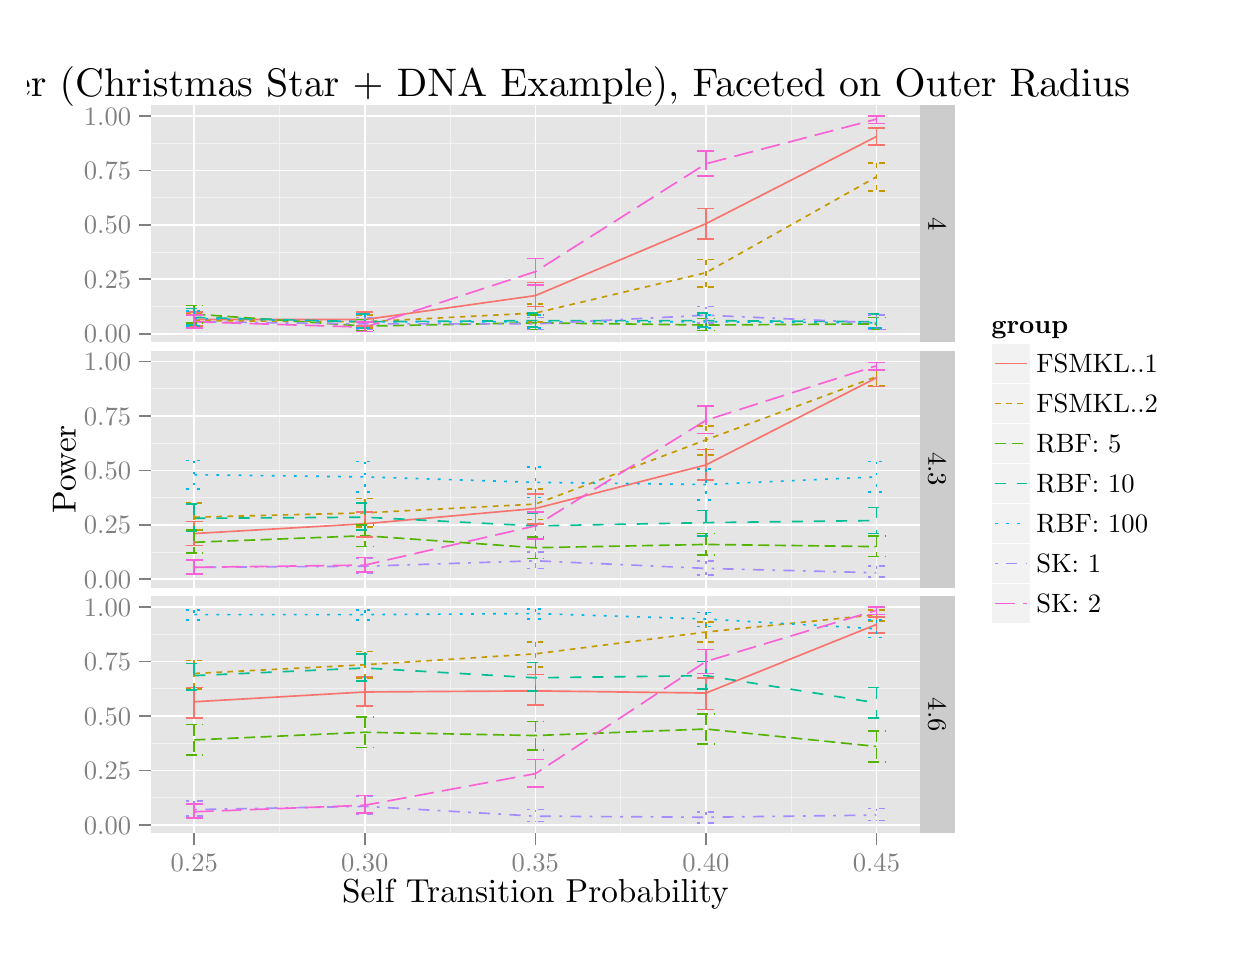
\begin{tikzpicture}[x=1pt,y=1pt]
\definecolor[named]{fillColor}{rgb}{1.00,1.00,1.00}
\path[use as bounding box,fill=fillColor,fill opacity=0.00] (0,0) rectangle (433.62,325.21);
\begin{scope}
\path[clip] (  0.00,  0.00) rectangle (433.62,325.21);
\definecolor[named]{drawColor}{rgb}{1.00,1.00,1.00}
\definecolor[named]{fillColor}{rgb}{1.00,1.00,1.00}

\path[draw=drawColor,line width= 0.6pt,line join=round,line cap=round,fill=fillColor] (  0.00,  0.00) rectangle (433.62,325.21);
\end{scope}
\begin{scope}
\path[clip] ( 44.49,211.51) rectangle (322.42,297.23);
\definecolor[named]{fillColor}{rgb}{0.90,0.90,0.90}

\path[fill=fillColor] ( 44.49,211.51) rectangle (322.42,297.23);
\definecolor[named]{drawColor}{rgb}{0.95,0.95,0.95}

\path[draw=drawColor,line width= 0.3pt,line join=round] ( 44.49,224.45) --
	(322.42,224.45);

\path[draw=drawColor,line width= 0.3pt,line join=round] ( 44.49,244.13) --
	(322.42,244.13);

\path[draw=drawColor,line width= 0.3pt,line join=round] ( 44.49,263.81) --
	(322.42,263.81);

\path[draw=drawColor,line width= 0.3pt,line join=round] ( 44.49,283.49) --
	(322.42,283.49);

\path[draw=drawColor,line width= 0.3pt,line join=round] ( 91.01,211.51) --
	( 91.01,297.23);

\path[draw=drawColor,line width= 0.3pt,line join=round] (152.64,211.51) --
	(152.64,297.23);

\path[draw=drawColor,line width= 0.3pt,line join=round] (214.27,211.51) --
	(214.27,297.23);

\path[draw=drawColor,line width= 0.3pt,line join=round] (275.89,211.51) --
	(275.89,297.23);
\definecolor[named]{drawColor}{rgb}{1.00,1.00,1.00}

\path[draw=drawColor,line width= 0.6pt,line join=round] ( 44.49,214.62) --
	(322.42,214.62);

\path[draw=drawColor,line width= 0.6pt,line join=round] ( 44.49,234.29) --
	(322.42,234.29);

\path[draw=drawColor,line width= 0.6pt,line join=round] ( 44.49,253.97) --
	(322.42,253.97);

\path[draw=drawColor,line width= 0.6pt,line join=round] ( 44.49,273.65) --
	(322.42,273.65);

\path[draw=drawColor,line width= 0.6pt,line join=round] ( 44.49,293.33) --
	(322.42,293.33);

\path[draw=drawColor,line width= 0.6pt,line join=round] ( 60.20,211.51) --
	( 60.20,297.23);

\path[draw=drawColor,line width= 0.6pt,line join=round] (121.83,211.51) --
	(121.83,297.23);

\path[draw=drawColor,line width= 0.6pt,line join=round] (183.45,211.51) --
	(183.45,297.23);

\path[draw=drawColor,line width= 0.6pt,line join=round] (245.08,211.51) --
	(245.08,297.23);

\path[draw=drawColor,line width= 0.6pt,line join=round] (306.70,211.51) --
	(306.70,297.23);
\definecolor[named]{drawColor}{rgb}{0.97,0.46,0.43}

\path[draw=drawColor,line width= 0.6pt,line join=round] ( 60.20,219.73) --
	(121.83,219.73) --
	(183.45,228.39) --
	(245.08,254.37) --
	(306.70,285.86);
\definecolor[named]{drawColor}{rgb}{0.77,0.60,0.00}

\path[draw=drawColor,line width= 0.6pt,dash pattern=on 2pt off 2pt ,line join=round] ( 60.20,219.34) --
	(121.83,218.94) --
	(183.45,222.09) --
	(245.08,236.66) --
	(306.70,271.29);
\definecolor[named]{drawColor}{rgb}{0.33,0.71,0.00}

\path[draw=drawColor,line width= 0.6pt,dash pattern=on 4pt off 2pt ,line join=round] ( 60.20,221.70) --
	(121.83,217.37) --
	(183.45,218.55) --
	(245.08,217.76) --
	(306.70,218.16);
\definecolor[named]{drawColor}{rgb}{0.00,0.75,0.58}

\path[draw=drawColor,line width= 0.6pt,dash pattern=on 4pt off 4pt ,line join=round] ( 60.20,220.52) --
	(121.83,218.94) --
	(183.45,219.34) --
	(245.08,219.34) --
	(306.70,218.94);
\definecolor[named]{drawColor}{rgb}{0.00,0.71,0.92}

\path[draw=drawColor,line width= 0.6pt,dash pattern=on 1pt off 3pt ,line join=round] ( 60.20,220.13) --
	(121.83,218.94) --
	(183.45,218.94) --
	(245.08,218.94) --
	(306.70,218.55);
\definecolor[named]{drawColor}{rgb}{0.65,0.54,1.00}

\path[draw=drawColor,line width= 0.6pt,dash pattern=on 1pt off 3pt on 4pt off 3pt ,line join=round] ( 60.20,218.94) --
	(121.83,218.16) --
	(183.45,218.16) --
	(245.08,221.31) --
	(306.70,218.55);
\definecolor[named]{drawColor}{rgb}{0.98,0.38,0.84}

\path[draw=drawColor,line width= 0.6pt,dash pattern=on 7pt off 3pt ,line join=round] ( 60.20,218.94) --
	(121.83,216.98) --
	(183.45,237.05) --
	(245.08,276.02) --
	(306.70,292.15);
\definecolor[named]{drawColor}{rgb}{0.97,0.46,0.43}

\path[draw=drawColor,line width= 0.6pt,line join=round] ( 57.12,222.49) --
	( 63.28,222.49);

\path[draw=drawColor,line width= 0.6pt,line join=round] ( 60.20,222.49) --
	( 60.20,217.36);

\path[draw=drawColor,line width= 0.6pt,line join=round] ( 57.12,217.36) --
	( 63.28,217.36);

\path[draw=drawColor,line width= 0.6pt,line join=round] (118.74,222.49) --
	(124.91,222.49);

\path[draw=drawColor,line width= 0.6pt,line join=round] (121.83,222.49) --
	(121.83,217.37);

\path[draw=drawColor,line width= 0.6pt,line join=round] (118.74,217.37) --
	(124.91,217.37);

\path[draw=drawColor,line width= 0.6pt,line join=round] (180.37,233.11) --
	(186.53,233.11);

\path[draw=drawColor,line width= 0.6pt,line join=round] (183.45,233.11) --
	(183.45,224.45);

\path[draw=drawColor,line width= 0.6pt,line join=round] (180.37,224.45) --
	(186.53,224.45);

\path[draw=drawColor,line width= 0.6pt,line join=round] (242.00,259.88) --
	(248.16,259.88);

\path[draw=drawColor,line width= 0.6pt,line join=round] (245.08,259.88) --
	(245.08,248.86);

\path[draw=drawColor,line width= 0.6pt,line join=round] (242.00,248.86) --
	(248.16,248.86);

\path[draw=drawColor,line width= 0.6pt,line join=round] (303.62,289.00) --
	(309.79,289.00);

\path[draw=drawColor,line width= 0.6pt,line join=round] (306.70,289.00) --
	(306.70,282.71);

\path[draw=drawColor,line width= 0.6pt,line join=round] (303.62,282.71) --
	(309.79,282.71);
\definecolor[named]{drawColor}{rgb}{0.77,0.60,0.00}

\path[draw=drawColor,line width= 0.6pt,dash pattern=on 2pt off 2pt ,line join=round] ( 57.12,221.70) --
	( 63.28,221.70);

\path[draw=drawColor,line width= 0.6pt,dash pattern=on 2pt off 2pt ,line join=round] ( 60.20,221.70) --
	( 60.20,216.98);

\path[draw=drawColor,line width= 0.6pt,dash pattern=on 2pt off 2pt ,line join=round] ( 57.12,216.98) --
	( 63.28,216.98);

\path[draw=drawColor,line width= 0.6pt,dash pattern=on 2pt off 2pt ,line join=round] (118.74,221.32) --
	(124.91,221.32);

\path[draw=drawColor,line width= 0.6pt,dash pattern=on 2pt off 2pt ,line join=round] (121.83,221.32) --
	(121.83,216.58);

\path[draw=drawColor,line width= 0.6pt,dash pattern=on 2pt off 2pt ,line join=round] (118.74,216.58) --
	(124.91,216.58);

\path[draw=drawColor,line width= 0.6pt,dash pattern=on 2pt off 2pt ,line join=round] (180.37,225.25) --
	(186.53,225.25);

\path[draw=drawColor,line width= 0.6pt,dash pattern=on 2pt off 2pt ,line join=round] (183.45,225.25) --
	(183.45,218.94);

\path[draw=drawColor,line width= 0.6pt,dash pattern=on 2pt off 2pt ,line join=round] (180.37,218.94) --
	(186.53,218.94);

\path[draw=drawColor,line width= 0.6pt,dash pattern=on 2pt off 2pt ,line join=round] (242.00,241.38) --
	(248.16,241.38);

\path[draw=drawColor,line width= 0.6pt,dash pattern=on 2pt off 2pt ,line join=round] (245.08,241.38) --
	(245.08,231.54);

\path[draw=drawColor,line width= 0.6pt,dash pattern=on 2pt off 2pt ,line join=round] (242.00,231.54) --
	(248.16,231.54);

\path[draw=drawColor,line width= 0.6pt,dash pattern=on 2pt off 2pt ,line join=round] (303.62,276.41) --
	(309.79,276.41);

\path[draw=drawColor,line width= 0.6pt,dash pattern=on 2pt off 2pt ,line join=round] (306.70,276.41) --
	(306.70,266.17);

\path[draw=drawColor,line width= 0.6pt,dash pattern=on 2pt off 2pt ,line join=round] (303.62,266.17) --
	(309.79,266.17);
\definecolor[named]{drawColor}{rgb}{0.33,0.71,0.00}

\path[draw=drawColor,line width= 0.6pt,dash pattern=on 4pt off 2pt ,line join=round] ( 57.12,224.85) --
	( 63.28,224.85);

\path[draw=drawColor,line width= 0.6pt,dash pattern=on 4pt off 2pt ,line join=round] ( 60.20,224.85) --
	( 60.20,218.55);

\path[draw=drawColor,line width= 0.6pt,dash pattern=on 4pt off 2pt ,line join=round] ( 57.12,218.55) --
	( 63.28,218.55);

\path[draw=drawColor,line width= 0.6pt,dash pattern=on 4pt off 2pt ,line join=round] (118.74,219.73) --
	(124.91,219.73);

\path[draw=drawColor,line width= 0.6pt,dash pattern=on 4pt off 2pt ,line join=round] (121.83,219.73) --
	(121.83,215.80);

\path[draw=drawColor,line width= 0.6pt,dash pattern=on 4pt off 2pt ,line join=round] (118.74,215.80) --
	(124.91,215.80);

\path[draw=drawColor,line width= 0.6pt,dash pattern=on 4pt off 2pt ,line join=round] (180.37,221.31) --
	(186.53,221.31);

\path[draw=drawColor,line width= 0.6pt,dash pattern=on 4pt off 2pt ,line join=round] (183.45,221.31) --
	(183.45,216.19);

\path[draw=drawColor,line width= 0.6pt,dash pattern=on 4pt off 2pt ,line join=round] (180.37,216.19) --
	(186.53,216.19);

\path[draw=drawColor,line width= 0.6pt,dash pattern=on 4pt off 2pt ,line join=round] (242.00,220.13) --
	(248.16,220.13);

\path[draw=drawColor,line width= 0.6pt,dash pattern=on 4pt off 2pt ,line join=round] (245.08,220.13) --
	(245.08,215.80);

\path[draw=drawColor,line width= 0.6pt,dash pattern=on 4pt off 2pt ,line join=round] (242.00,215.80) --
	(248.16,215.80);

\path[draw=drawColor,line width= 0.6pt,dash pattern=on 4pt off 2pt ,line join=round] (303.62,220.52) --
	(309.79,220.52);

\path[draw=drawColor,line width= 0.6pt,dash pattern=on 4pt off 2pt ,line join=round] (306.70,220.52) --
	(306.70,216.19);

\path[draw=drawColor,line width= 0.6pt,dash pattern=on 4pt off 2pt ,line join=round] (303.62,216.19) --
	(309.79,216.19);
\definecolor[named]{drawColor}{rgb}{0.00,0.75,0.58}

\path[draw=drawColor,line width= 0.6pt,dash pattern=on 4pt off 4pt ,line join=round] ( 57.12,223.67) --
	( 63.28,223.67);

\path[draw=drawColor,line width= 0.6pt,dash pattern=on 4pt off 4pt ,line join=round] ( 60.20,223.67) --
	( 60.20,217.76);

\path[draw=drawColor,line width= 0.6pt,dash pattern=on 4pt off 4pt ,line join=round] ( 57.12,217.76) --
	( 63.28,217.76);

\path[draw=drawColor,line width= 0.6pt,dash pattern=on 4pt off 4pt ,line join=round] (118.74,221.70) --
	(124.91,221.70);

\path[draw=drawColor,line width= 0.6pt,dash pattern=on 4pt off 4pt ,line join=round] (121.83,221.70) --
	(121.83,216.58);

\path[draw=drawColor,line width= 0.6pt,dash pattern=on 4pt off 4pt ,line join=round] (118.74,216.58) --
	(124.91,216.58);

\path[draw=drawColor,line width= 0.6pt,dash pattern=on 4pt off 4pt ,line join=round] (180.37,222.09) --
	(186.53,222.09);

\path[draw=drawColor,line width= 0.6pt,dash pattern=on 4pt off 4pt ,line join=round] (183.45,222.09) --
	(183.45,216.98);

\path[draw=drawColor,line width= 0.6pt,dash pattern=on 4pt off 4pt ,line join=round] (180.37,216.98) --
	(186.53,216.98);

\path[draw=drawColor,line width= 0.6pt,dash pattern=on 4pt off 4pt ,line join=round] (242.00,222.09) --
	(248.16,222.09);

\path[draw=drawColor,line width= 0.6pt,dash pattern=on 4pt off 4pt ,line join=round] (245.08,222.09) --
	(245.08,216.98);

\path[draw=drawColor,line width= 0.6pt,dash pattern=on 4pt off 4pt ,line join=round] (242.00,216.98) --
	(248.16,216.98);

\path[draw=drawColor,line width= 0.6pt,dash pattern=on 4pt off 4pt ,line join=round] (303.62,221.70) --
	(309.79,221.70);

\path[draw=drawColor,line width= 0.6pt,dash pattern=on 4pt off 4pt ,line join=round] (306.70,221.70) --
	(306.70,216.58);

\path[draw=drawColor,line width= 0.6pt,dash pattern=on 4pt off 4pt ,line join=round] (303.62,216.58) --
	(309.79,216.58);
\definecolor[named]{drawColor}{rgb}{0.00,0.71,0.92}

\path[draw=drawColor,line width= 0.6pt,dash pattern=on 1pt off 3pt ,line join=round] ( 57.12,222.88) --
	( 63.28,222.88);

\path[draw=drawColor,line width= 0.6pt,dash pattern=on 1pt off 3pt ,line join=round] ( 60.20,222.88) --
	( 60.20,217.37);

\path[draw=drawColor,line width= 0.6pt,dash pattern=on 1pt off 3pt ,line join=round] ( 57.12,217.37) --
	( 63.28,217.37);

\path[draw=drawColor,line width= 0.6pt,dash pattern=on 1pt off 3pt ,line join=round] (118.74,221.70) --
	(124.91,221.70);

\path[draw=drawColor,line width= 0.6pt,dash pattern=on 1pt off 3pt ,line join=round] (121.83,221.70) --
	(121.83,216.58);

\path[draw=drawColor,line width= 0.6pt,dash pattern=on 1pt off 3pt ,line join=round] (118.74,216.58) --
	(124.91,216.58);

\path[draw=drawColor,line width= 0.6pt,dash pattern=on 1pt off 3pt ,line join=round] (180.37,221.31) --
	(186.53,221.31);

\path[draw=drawColor,line width= 0.6pt,dash pattern=on 1pt off 3pt ,line join=round] (183.45,221.31) --
	(183.45,216.58);

\path[draw=drawColor,line width= 0.6pt,dash pattern=on 1pt off 3pt ,line join=round] (180.37,216.58) --
	(186.53,216.58);

\path[draw=drawColor,line width= 0.6pt,dash pattern=on 1pt off 3pt ,line join=round] (242.00,221.32) --
	(248.16,221.32);

\path[draw=drawColor,line width= 0.6pt,dash pattern=on 1pt off 3pt ,line join=round] (245.08,221.32) --
	(245.08,216.58);

\path[draw=drawColor,line width= 0.6pt,dash pattern=on 1pt off 3pt ,line join=round] (242.00,216.58) --
	(248.16,216.58);

\path[draw=drawColor,line width= 0.6pt,dash pattern=on 1pt off 3pt ,line join=round] (303.62,221.31) --
	(309.79,221.31);

\path[draw=drawColor,line width= 0.6pt,dash pattern=on 1pt off 3pt ,line join=round] (306.70,221.31) --
	(306.70,216.57);

\path[draw=drawColor,line width= 0.6pt,dash pattern=on 1pt off 3pt ,line join=round] (303.62,216.57) --
	(309.79,216.57);
\definecolor[named]{drawColor}{rgb}{0.65,0.54,1.00}

\path[draw=drawColor,line width= 0.6pt,dash pattern=on 1pt off 3pt on 4pt off 3pt ,line join=round] ( 57.12,221.32) --
	( 63.28,221.32);

\path[draw=drawColor,line width= 0.6pt,dash pattern=on 1pt off 3pt on 4pt off 3pt ,line join=round] ( 60.20,221.32) --
	( 60.20,216.58);

\path[draw=drawColor,line width= 0.6pt,dash pattern=on 1pt off 3pt on 4pt off 3pt ,line join=round] ( 57.12,216.58) --
	( 63.28,216.58);

\path[draw=drawColor,line width= 0.6pt,dash pattern=on 1pt off 3pt on 4pt off 3pt ,line join=round] (118.74,220.52) --
	(124.91,220.52);

\path[draw=drawColor,line width= 0.6pt,dash pattern=on 1pt off 3pt on 4pt off 3pt ,line join=round] (121.83,220.52) --
	(121.83,216.19);

\path[draw=drawColor,line width= 0.6pt,dash pattern=on 1pt off 3pt on 4pt off 3pt ,line join=round] (118.74,216.19) --
	(124.91,216.19);

\path[draw=drawColor,line width= 0.6pt,dash pattern=on 1pt off 3pt on 4pt off 3pt ,line join=round] (180.37,220.52) --
	(186.53,220.52);

\path[draw=drawColor,line width= 0.6pt,dash pattern=on 1pt off 3pt on 4pt off 3pt ,line join=round] (183.45,220.52) --
	(183.45,216.19);

\path[draw=drawColor,line width= 0.6pt,dash pattern=on 1pt off 3pt on 4pt off 3pt ,line join=round] (180.37,216.19) --
	(186.53,216.19);

\path[draw=drawColor,line width= 0.6pt,dash pattern=on 1pt off 3pt on 4pt off 3pt ,line join=round] (242.00,224.45) --
	(248.16,224.45);

\path[draw=drawColor,line width= 0.6pt,dash pattern=on 1pt off 3pt on 4pt off 3pt ,line join=round] (245.08,224.45) --
	(245.08,218.55);

\path[draw=drawColor,line width= 0.6pt,dash pattern=on 1pt off 3pt on 4pt off 3pt ,line join=round] (242.00,218.55) --
	(248.16,218.55);

\path[draw=drawColor,line width= 0.6pt,dash pattern=on 1pt off 3pt on 4pt off 3pt ,line join=round] (303.62,221.31) --
	(309.79,221.31);

\path[draw=drawColor,line width= 0.6pt,dash pattern=on 1pt off 3pt on 4pt off 3pt ,line join=round] (306.70,221.31) --
	(306.70,216.19);

\path[draw=drawColor,line width= 0.6pt,dash pattern=on 1pt off 3pt on 4pt off 3pt ,line join=round] (303.62,216.19) --
	(309.79,216.19);
\definecolor[named]{drawColor}{rgb}{0.98,0.38,0.84}

\path[draw=drawColor,line width= 0.6pt,dash pattern=on 7pt off 3pt ,line join=round] ( 57.12,221.31) --
	( 63.28,221.31);

\path[draw=drawColor,line width= 0.6pt,dash pattern=on 7pt off 3pt ,line join=round] ( 60.20,221.31) --
	( 60.20,216.58);

\path[draw=drawColor,line width= 0.6pt,dash pattern=on 7pt off 3pt ,line join=round] ( 57.12,216.58) --
	( 63.28,216.58);

\path[draw=drawColor,line width= 0.6pt,dash pattern=on 7pt off 3pt ,line join=round] (118.74,218.94) --
	(124.91,218.94);

\path[draw=drawColor,line width= 0.6pt,dash pattern=on 7pt off 3pt ,line join=round] (121.83,218.94) --
	(121.83,215.40);

\path[draw=drawColor,line width= 0.6pt,dash pattern=on 7pt off 3pt ,line join=round] (118.74,215.40) --
	(124.91,215.40);

\path[draw=drawColor,line width= 0.6pt,dash pattern=on 7pt off 3pt ,line join=round] (180.37,241.77) --
	(186.53,241.77);

\path[draw=drawColor,line width= 0.6pt,dash pattern=on 7pt off 3pt ,line join=round] (183.45,241.77) --
	(183.45,232.33);

\path[draw=drawColor,line width= 0.6pt,dash pattern=on 7pt off 3pt ,line join=round] (180.37,232.33) --
	(186.53,232.33);

\path[draw=drawColor,line width= 0.6pt,dash pattern=on 7pt off 3pt ,line join=round] (242.00,280.74) --
	(248.16,280.74);

\path[draw=drawColor,line width= 0.6pt,dash pattern=on 7pt off 3pt ,line join=round] (245.08,280.74) --
	(245.08,271.69);

\path[draw=drawColor,line width= 0.6pt,dash pattern=on 7pt off 3pt ,line join=round] (242.00,271.69) --
	(248.16,271.69);

\path[draw=drawColor,line width= 0.6pt,dash pattern=on 7pt off 3pt ,line join=round] (303.62,293.33) --
	(309.79,293.33);

\path[draw=drawColor,line width= 0.6pt,dash pattern=on 7pt off 3pt ,line join=round] (306.70,293.33) --
	(306.70,290.58);

\path[draw=drawColor,line width= 0.6pt,dash pattern=on 7pt off 3pt ,line join=round] (303.62,290.58) --
	(309.79,290.58);
\end{scope}
\begin{scope}
\path[clip] ( 44.49,122.77) rectangle (322.42,208.49);
\definecolor[named]{fillColor}{rgb}{0.90,0.90,0.90}

\path[fill=fillColor] ( 44.49,122.77) rectangle (322.42,208.49);
\definecolor[named]{drawColor}{rgb}{0.95,0.95,0.95}

\path[draw=drawColor,line width= 0.3pt,line join=round] ( 44.49,135.72) --
	(322.42,135.72);

\path[draw=drawColor,line width= 0.3pt,line join=round] ( 44.49,155.40) --
	(322.42,155.40);

\path[draw=drawColor,line width= 0.3pt,line join=round] ( 44.49,175.08) --
	(322.42,175.08);

\path[draw=drawColor,line width= 0.3pt,line join=round] ( 44.49,194.76) --
	(322.42,194.76);

\path[draw=drawColor,line width= 0.3pt,line join=round] ( 91.01,122.77) --
	( 91.01,208.49);

\path[draw=drawColor,line width= 0.3pt,line join=round] (152.64,122.77) --
	(152.64,208.49);

\path[draw=drawColor,line width= 0.3pt,line join=round] (214.27,122.77) --
	(214.27,208.49);

\path[draw=drawColor,line width= 0.3pt,line join=round] (275.89,122.77) --
	(275.89,208.49);
\definecolor[named]{drawColor}{rgb}{1.00,1.00,1.00}

\path[draw=drawColor,line width= 0.6pt,line join=round] ( 44.49,125.88) --
	(322.42,125.88);

\path[draw=drawColor,line width= 0.6pt,line join=round] ( 44.49,145.56) --
	(322.42,145.56);

\path[draw=drawColor,line width= 0.6pt,line join=round] ( 44.49,165.24) --
	(322.42,165.24);

\path[draw=drawColor,line width= 0.6pt,line join=round] ( 44.49,184.92) --
	(322.42,184.92);

\path[draw=drawColor,line width= 0.6pt,line join=round] ( 44.49,204.60) --
	(322.42,204.60);

\path[draw=drawColor,line width= 0.6pt,line join=round] ( 60.20,122.77) --
	( 60.20,208.49);

\path[draw=drawColor,line width= 0.6pt,line join=round] (121.83,122.77) --
	(121.83,208.49);

\path[draw=drawColor,line width= 0.6pt,line join=round] (183.45,122.77) --
	(183.45,208.49);

\path[draw=drawColor,line width= 0.6pt,line join=round] (245.08,122.77) --
	(245.08,208.49);

\path[draw=drawColor,line width= 0.6pt,line join=round] (306.70,122.77) --
	(306.70,208.49);
\definecolor[named]{drawColor}{rgb}{0.97,0.46,0.43}

\path[draw=drawColor,line width= 0.6pt,line join=round] ( 60.20,142.41) --
	(121.83,145.95) --
	(183.45,151.46) --
	(245.08,167.21) --
	(306.70,198.69);
\definecolor[named]{drawColor}{rgb}{0.77,0.60,0.00}

\path[draw=drawColor,line width= 0.6pt,dash pattern=on 2pt off 2pt ,line join=round] ( 60.20,148.31) --
	(121.83,149.89) --
	(183.45,153.04) --
	(245.08,176.26) --
	(306.70,199.09);
\definecolor[named]{drawColor}{rgb}{0.33,0.71,0.00}

\path[draw=drawColor,line width= 0.6pt,dash pattern=on 4pt off 2pt ,line join=round] ( 60.20,139.26) --
	(121.83,141.62) --
	(183.45,137.29) --
	(245.08,138.47) --
	(306.70,137.69);
\definecolor[named]{drawColor}{rgb}{0.00,0.75,0.58}

\path[draw=drawColor,line width= 0.6pt,dash pattern=on 4pt off 4pt ,line join=round] ( 60.20,147.92) --
	(121.83,148.31) --
	(183.45,145.17) --
	(245.08,146.35) --
	(306.70,147.13);
\definecolor[named]{drawColor}{rgb}{0.00,0.71,0.92}

\path[draw=drawColor,line width= 0.6pt,dash pattern=on 1pt off 3pt ,line join=round] ( 60.20,163.66) --
	(121.83,162.88) --
	(183.45,160.91) --
	(245.08,160.12) --
	(306.70,162.88);
\definecolor[named]{drawColor}{rgb}{0.65,0.54,1.00}

\path[draw=drawColor,line width= 0.6pt,dash pattern=on 1pt off 3pt on 4pt off 3pt ,line join=round] ( 60.20,130.21) --
	(121.83,130.60) --
	(183.45,132.57) --
	(245.08,129.82) --
	(306.70,128.24);
\definecolor[named]{drawColor}{rgb}{0.98,0.38,0.84}

\path[draw=drawColor,line width= 0.6pt,dash pattern=on 7pt off 3pt ,line join=round] ( 60.20,130.21) --
	(121.83,131.00) --
	(183.45,145.17) --
	(245.08,183.34) --
	(306.70,203.02);
\definecolor[named]{drawColor}{rgb}{0.97,0.46,0.43}

\path[draw=drawColor,line width= 0.6pt,line join=round] ( 57.12,146.74) --
	( 63.28,146.74);

\path[draw=drawColor,line width= 0.6pt,line join=round] ( 60.20,146.74) --
	( 60.20,138.08);

\path[draw=drawColor,line width= 0.6pt,line join=round] ( 57.12,138.08) --
	( 63.28,138.08);

\path[draw=drawColor,line width= 0.6pt,line join=round] (118.74,150.28) --
	(124.91,150.28);

\path[draw=drawColor,line width= 0.6pt,line join=round] (121.83,150.28) --
	(121.83,141.23);

\path[draw=drawColor,line width= 0.6pt,line join=round] (118.74,141.23) --
	(124.91,141.23);

\path[draw=drawColor,line width= 0.6pt,line join=round] (180.37,156.59) --
	(186.53,156.59);

\path[draw=drawColor,line width= 0.6pt,line join=round] (183.45,156.59) --
	(183.45,145.95);

\path[draw=drawColor,line width= 0.6pt,line join=round] (180.37,145.95) --
	(186.53,145.95);

\path[draw=drawColor,line width= 0.6pt,line join=round] (242.00,172.73) --
	(248.16,172.73);

\path[draw=drawColor,line width= 0.6pt,line join=round] (245.08,172.73) --
	(245.08,161.69);

\path[draw=drawColor,line width= 0.6pt,line join=round] (242.00,161.69) --
	(248.16,161.69);

\path[draw=drawColor,line width= 0.6pt,line join=round] (303.62,201.45) --
	(309.79,201.45);

\path[draw=drawColor,line width= 0.6pt,line join=round] (306.70,201.45) --
	(306.70,195.55);

\path[draw=drawColor,line width= 0.6pt,line join=round] (303.62,195.55) --
	(309.79,195.55);
\definecolor[named]{drawColor}{rgb}{0.77,0.60,0.00}

\path[draw=drawColor,line width= 0.6pt,dash pattern=on 2pt off 2pt ,line join=round] ( 57.12,153.43) --
	( 63.28,153.43);

\path[draw=drawColor,line width= 0.6pt,dash pattern=on 2pt off 2pt ,line join=round] ( 60.20,153.43) --
	( 60.20,143.59);

\path[draw=drawColor,line width= 0.6pt,dash pattern=on 2pt off 2pt ,line join=round] ( 57.12,143.59) --
	( 63.28,143.59);

\path[draw=drawColor,line width= 0.6pt,dash pattern=on 2pt off 2pt ,line join=round] (118.74,155.02) --
	(124.91,155.02);

\path[draw=drawColor,line width= 0.6pt,dash pattern=on 2pt off 2pt ,line join=round] (121.83,155.02) --
	(121.83,144.77);

\path[draw=drawColor,line width= 0.6pt,dash pattern=on 2pt off 2pt ,line join=round] (118.74,144.77) --
	(124.91,144.77);

\path[draw=drawColor,line width= 0.6pt,dash pattern=on 2pt off 2pt ,line join=round] (180.37,158.55) --
	(186.53,158.55);

\path[draw=drawColor,line width= 0.6pt,dash pattern=on 2pt off 2pt ,line join=round] (183.45,158.55) --
	(183.45,147.53);

\path[draw=drawColor,line width= 0.6pt,dash pattern=on 2pt off 2pt ,line join=round] (180.37,147.53) --
	(186.53,147.53);

\path[draw=drawColor,line width= 0.6pt,dash pattern=on 2pt off 2pt ,line join=round] (242.00,181.38) --
	(248.16,181.38);

\path[draw=drawColor,line width= 0.6pt,dash pattern=on 2pt off 2pt ,line join=round] (245.08,181.38) --
	(245.08,170.75);

\path[draw=drawColor,line width= 0.6pt,dash pattern=on 2pt off 2pt ,line join=round] (242.00,170.75) --
	(248.16,170.75);

\path[draw=drawColor,line width= 0.6pt,dash pattern=on 2pt off 2pt ,line join=round] (303.62,201.45) --
	(309.79,201.45);

\path[draw=drawColor,line width= 0.6pt,dash pattern=on 2pt off 2pt ,line join=round] (306.70,201.45) --
	(306.70,195.94);

\path[draw=drawColor,line width= 0.6pt,dash pattern=on 2pt off 2pt ,line join=round] (303.62,195.94) --
	(309.79,195.94);
\definecolor[named]{drawColor}{rgb}{0.33,0.71,0.00}

\path[draw=drawColor,line width= 0.6pt,dash pattern=on 4pt off 2pt ,line join=round] ( 57.12,143.59) --
	( 63.28,143.59);

\path[draw=drawColor,line width= 0.6pt,dash pattern=on 4pt off 2pt ,line join=round] ( 60.20,143.59) --
	( 60.20,135.33);

\path[draw=drawColor,line width= 0.6pt,dash pattern=on 4pt off 2pt ,line join=round] ( 57.12,135.33) --
	( 63.28,135.33);

\path[draw=drawColor,line width= 0.6pt,dash pattern=on 4pt off 2pt ,line join=round] (118.74,145.57) --
	(124.91,145.57);

\path[draw=drawColor,line width= 0.6pt,dash pattern=on 4pt off 2pt ,line join=round] (121.83,145.57) --
	(121.83,137.69);

\path[draw=drawColor,line width= 0.6pt,dash pattern=on 4pt off 2pt ,line join=round] (118.74,137.69) --
	(124.91,137.69);

\path[draw=drawColor,line width= 0.6pt,dash pattern=on 4pt off 2pt ,line join=round] (180.37,141.23) --
	(186.53,141.23);

\path[draw=drawColor,line width= 0.6pt,dash pattern=on 4pt off 2pt ,line join=round] (183.45,141.23) --
	(183.45,133.36);

\path[draw=drawColor,line width= 0.6pt,dash pattern=on 4pt off 2pt ,line join=round] (180.37,133.36) --
	(186.53,133.36);

\path[draw=drawColor,line width= 0.6pt,dash pattern=on 4pt off 2pt ,line join=round] (242.00,142.42) --
	(248.16,142.42);

\path[draw=drawColor,line width= 0.6pt,dash pattern=on 4pt off 2pt ,line join=round] (245.08,142.42) --
	(245.08,134.54);

\path[draw=drawColor,line width= 0.6pt,dash pattern=on 4pt off 2pt ,line join=round] (242.00,134.54) --
	(248.16,134.54);

\path[draw=drawColor,line width= 0.6pt,dash pattern=on 4pt off 2pt ,line join=round] (303.62,141.62) --
	(309.79,141.62);

\path[draw=drawColor,line width= 0.6pt,dash pattern=on 4pt off 2pt ,line join=round] (306.70,141.62) --
	(306.70,134.14);

\path[draw=drawColor,line width= 0.6pt,dash pattern=on 4pt off 2pt ,line join=round] (303.62,134.14) --
	(309.79,134.14);
\definecolor[named]{drawColor}{rgb}{0.00,0.75,0.58}

\path[draw=drawColor,line width= 0.6pt,dash pattern=on 4pt off 4pt ,line join=round] ( 57.12,153.04) --
	( 63.28,153.04);

\path[draw=drawColor,line width= 0.6pt,dash pattern=on 4pt off 4pt ,line join=round] ( 60.20,153.04) --
	( 60.20,143.20);

\path[draw=drawColor,line width= 0.6pt,dash pattern=on 4pt off 4pt ,line join=round] ( 57.12,143.20) --
	( 63.28,143.20);

\path[draw=drawColor,line width= 0.6pt,dash pattern=on 4pt off 4pt ,line join=round] (118.74,153.43) --
	(124.91,153.43);

\path[draw=drawColor,line width= 0.6pt,dash pattern=on 4pt off 4pt ,line join=round] (121.83,153.43) --
	(121.83,143.59);

\path[draw=drawColor,line width= 0.6pt,dash pattern=on 4pt off 4pt ,line join=round] (118.74,143.59) --
	(124.91,143.59);

\path[draw=drawColor,line width= 0.6pt,dash pattern=on 4pt off 4pt ,line join=round] (180.37,149.89) --
	(186.53,149.89);

\path[draw=drawColor,line width= 0.6pt,dash pattern=on 4pt off 4pt ,line join=round] (183.45,149.89) --
	(183.45,140.44);

\path[draw=drawColor,line width= 0.6pt,dash pattern=on 4pt off 4pt ,line join=round] (180.37,140.44) --
	(186.53,140.44);

\path[draw=drawColor,line width= 0.6pt,dash pattern=on 4pt off 4pt ,line join=round] (242.00,150.68) --
	(248.16,150.68);

\path[draw=drawColor,line width= 0.6pt,dash pattern=on 4pt off 4pt ,line join=round] (245.08,150.68) --
	(245.08,141.62);

\path[draw=drawColor,line width= 0.6pt,dash pattern=on 4pt off 4pt ,line join=round] (242.00,141.62) --
	(248.16,141.62);

\path[draw=drawColor,line width= 0.6pt,dash pattern=on 4pt off 4pt ,line join=round] (303.62,151.86) --
	(309.79,151.86);

\path[draw=drawColor,line width= 0.6pt,dash pattern=on 4pt off 4pt ,line join=round] (306.70,151.86) --
	(306.70,142.40);

\path[draw=drawColor,line width= 0.6pt,dash pattern=on 4pt off 4pt ,line join=round] (303.62,142.40) --
	(309.79,142.40);
\definecolor[named]{drawColor}{rgb}{0.00,0.71,0.92}

\path[draw=drawColor,line width= 0.6pt,dash pattern=on 1pt off 3pt ,line join=round] ( 57.12,168.78) --
	( 63.28,168.78);

\path[draw=drawColor,line width= 0.6pt,dash pattern=on 1pt off 3pt ,line join=round] ( 60.20,168.78) --
	( 60.20,158.54);

\path[draw=drawColor,line width= 0.6pt,dash pattern=on 1pt off 3pt ,line join=round] ( 57.12,158.54) --
	( 63.28,158.54);

\path[draw=drawColor,line width= 0.6pt,dash pattern=on 1pt off 3pt ,line join=round] (118.74,168.39) --
	(124.91,168.39);

\path[draw=drawColor,line width= 0.6pt,dash pattern=on 1pt off 3pt ,line join=round] (121.83,168.39) --
	(121.83,157.37);

\path[draw=drawColor,line width= 0.6pt,dash pattern=on 1pt off 3pt ,line join=round] (118.74,157.37) --
	(124.91,157.37);

\path[draw=drawColor,line width= 0.6pt,dash pattern=on 1pt off 3pt ,line join=round] (180.37,166.42) --
	(186.53,166.42);

\path[draw=drawColor,line width= 0.6pt,dash pattern=on 1pt off 3pt ,line join=round] (183.45,166.42) --
	(183.45,155.40);

\path[draw=drawColor,line width= 0.6pt,dash pattern=on 1pt off 3pt ,line join=round] (180.37,155.40) --
	(186.53,155.40);

\path[draw=drawColor,line width= 0.6pt,dash pattern=on 1pt off 3pt ,line join=round] (242.00,165.63) --
	(248.16,165.63);

\path[draw=drawColor,line width= 0.6pt,dash pattern=on 1pt off 3pt ,line join=round] (245.08,165.63) --
	(245.08,154.61);

\path[draw=drawColor,line width= 0.6pt,dash pattern=on 1pt off 3pt ,line join=round] (242.00,154.61) --
	(248.16,154.61);

\path[draw=drawColor,line width= 0.6pt,dash pattern=on 1pt off 3pt ,line join=round] (303.62,168.39) --
	(309.79,168.39);

\path[draw=drawColor,line width= 0.6pt,dash pattern=on 1pt off 3pt ,line join=round] (306.70,168.39) --
	(306.70,157.37);

\path[draw=drawColor,line width= 0.6pt,dash pattern=on 1pt off 3pt ,line join=round] (303.62,157.37) --
	(309.79,157.37);
\definecolor[named]{drawColor}{rgb}{0.65,0.54,1.00}

\path[draw=drawColor,line width= 0.6pt,dash pattern=on 1pt off 3pt on 4pt off 3pt ,line join=round] ( 57.12,132.96) --
	( 63.28,132.96);

\path[draw=drawColor,line width= 0.6pt,dash pattern=on 1pt off 3pt on 4pt off 3pt ,line join=round] ( 60.20,132.96) --
	( 60.20,127.85);

\path[draw=drawColor,line width= 0.6pt,dash pattern=on 1pt off 3pt on 4pt off 3pt ,line join=round] ( 57.12,127.85) --
	( 63.28,127.85);

\path[draw=drawColor,line width= 0.6pt,dash pattern=on 1pt off 3pt on 4pt off 3pt ,line join=round] (118.74,133.36) --
	(124.91,133.36);

\path[draw=drawColor,line width= 0.6pt,dash pattern=on 1pt off 3pt on 4pt off 3pt ,line join=round] (121.83,133.36) --
	(121.83,128.24);

\path[draw=drawColor,line width= 0.6pt,dash pattern=on 1pt off 3pt on 4pt off 3pt ,line join=round] (118.74,128.24) --
	(124.91,128.24);

\path[draw=drawColor,line width= 0.6pt,dash pattern=on 1pt off 3pt on 4pt off 3pt ,line join=round] (180.37,135.72) --
	(186.53,135.72);

\path[draw=drawColor,line width= 0.6pt,dash pattern=on 1pt off 3pt on 4pt off 3pt ,line join=round] (183.45,135.72) --
	(183.45,129.82);

\path[draw=drawColor,line width= 0.6pt,dash pattern=on 1pt off 3pt on 4pt off 3pt ,line join=round] (180.37,129.82) --
	(186.53,129.82);

\path[draw=drawColor,line width= 0.6pt,dash pattern=on 1pt off 3pt on 4pt off 3pt ,line join=round] (242.00,132.57) --
	(248.16,132.57);

\path[draw=drawColor,line width= 0.6pt,dash pattern=on 1pt off 3pt on 4pt off 3pt ,line join=round] (245.08,132.57) --
	(245.08,127.45);

\path[draw=drawColor,line width= 0.6pt,dash pattern=on 1pt off 3pt on 4pt off 3pt ,line join=round] (242.00,127.45) --
	(248.16,127.45);

\path[draw=drawColor,line width= 0.6pt,dash pattern=on 1pt off 3pt on 4pt off 3pt ,line join=round] (303.62,130.60) --
	(309.79,130.60);

\path[draw=drawColor,line width= 0.6pt,dash pattern=on 1pt off 3pt on 4pt off 3pt ,line join=round] (306.70,130.60) --
	(306.70,126.67);

\path[draw=drawColor,line width= 0.6pt,dash pattern=on 1pt off 3pt on 4pt off 3pt ,line join=round] (303.62,126.67) --
	(309.79,126.67);
\definecolor[named]{drawColor}{rgb}{0.98,0.38,0.84}

\path[draw=drawColor,line width= 0.6pt,dash pattern=on 7pt off 3pt ,line join=round] ( 57.12,132.96) --
	( 63.28,132.96);

\path[draw=drawColor,line width= 0.6pt,dash pattern=on 7pt off 3pt ,line join=round] ( 60.20,132.96) --
	( 60.20,127.85);

\path[draw=drawColor,line width= 0.6pt,dash pattern=on 7pt off 3pt ,line join=round] ( 57.12,127.85) --
	( 63.28,127.85);

\path[draw=drawColor,line width= 0.6pt,dash pattern=on 7pt off 3pt ,line join=round] (118.74,133.75) --
	(124.91,133.75);

\path[draw=drawColor,line width= 0.6pt,dash pattern=on 7pt off 3pt ,line join=round] (121.83,133.75) --
	(121.83,128.62);

\path[draw=drawColor,line width= 0.6pt,dash pattern=on 7pt off 3pt ,line join=round] (118.74,128.62) --
	(124.91,128.62);

\path[draw=drawColor,line width= 0.6pt,dash pattern=on 7pt off 3pt ,line join=round] (180.37,150.28) --
	(186.53,150.28);

\path[draw=drawColor,line width= 0.6pt,dash pattern=on 7pt off 3pt ,line join=round] (183.45,150.28) --
	(183.45,140.44);

\path[draw=drawColor,line width= 0.6pt,dash pattern=on 7pt off 3pt ,line join=round] (180.37,140.44) --
	(186.53,140.44);

\path[draw=drawColor,line width= 0.6pt,dash pattern=on 7pt off 3pt ,line join=round] (242.00,188.46) --
	(248.16,188.46);

\path[draw=drawColor,line width= 0.6pt,dash pattern=on 7pt off 3pt ,line join=round] (245.08,188.46) --
	(245.08,178.62);

\path[draw=drawColor,line width= 0.6pt,dash pattern=on 7pt off 3pt ,line join=round] (242.00,178.62) --
	(248.16,178.62);

\path[draw=drawColor,line width= 0.6pt,dash pattern=on 7pt off 3pt ,line join=round] (303.62,204.20) --
	(309.79,204.20);

\path[draw=drawColor,line width= 0.6pt,dash pattern=on 7pt off 3pt ,line join=round] (306.70,204.20) --
	(306.70,201.45);

\path[draw=drawColor,line width= 0.6pt,dash pattern=on 7pt off 3pt ,line join=round] (303.62,201.45) --
	(309.79,201.45);
\end{scope}
\begin{scope}
\path[clip] ( 44.49, 34.03) rectangle (322.42,119.76);
\definecolor[named]{fillColor}{rgb}{0.90,0.90,0.90}

\path[fill=fillColor] ( 44.49, 34.03) rectangle (322.42,119.76);
\definecolor[named]{drawColor}{rgb}{0.95,0.95,0.95}

\path[draw=drawColor,line width= 0.3pt,line join=round] ( 44.49, 46.98) --
	(322.42, 46.98);

\path[draw=drawColor,line width= 0.3pt,line join=round] ( 44.49, 66.66) --
	(322.42, 66.66);

\path[draw=drawColor,line width= 0.3pt,line join=round] ( 44.49, 86.34) --
	(322.42, 86.34);

\path[draw=drawColor,line width= 0.3pt,line join=round] ( 44.49,106.02) --
	(322.42,106.02);

\path[draw=drawColor,line width= 0.3pt,line join=round] ( 91.01, 34.03) --
	( 91.01,119.76);

\path[draw=drawColor,line width= 0.3pt,line join=round] (152.64, 34.03) --
	(152.64,119.76);

\path[draw=drawColor,line width= 0.3pt,line join=round] (214.27, 34.03) --
	(214.27,119.76);

\path[draw=drawColor,line width= 0.3pt,line join=round] (275.89, 34.03) --
	(275.89,119.76);
\definecolor[named]{drawColor}{rgb}{1.00,1.00,1.00}

\path[draw=drawColor,line width= 0.6pt,line join=round] ( 44.49, 37.14) --
	(322.42, 37.14);

\path[draw=drawColor,line width= 0.6pt,line join=round] ( 44.49, 56.82) --
	(322.42, 56.82);

\path[draw=drawColor,line width= 0.6pt,line join=round] ( 44.49, 76.50) --
	(322.42, 76.50);

\path[draw=drawColor,line width= 0.6pt,line join=round] ( 44.49, 96.18) --
	(322.42, 96.18);

\path[draw=drawColor,line width= 0.6pt,line join=round] ( 44.49,115.86) --
	(322.42,115.86);

\path[draw=drawColor,line width= 0.6pt,line join=round] ( 60.20, 34.03) --
	( 60.20,119.76);

\path[draw=drawColor,line width= 0.6pt,line join=round] (121.83, 34.03) --
	(121.83,119.76);

\path[draw=drawColor,line width= 0.6pt,line join=round] (183.45, 34.03) --
	(183.45,119.76);

\path[draw=drawColor,line width= 0.6pt,line join=round] (245.08, 34.03) --
	(245.08,119.76);

\path[draw=drawColor,line width= 0.6pt,line join=round] (306.70, 34.03) --
	(306.70,119.76);
\definecolor[named]{drawColor}{rgb}{0.97,0.46,0.43}

\path[draw=drawColor,line width= 0.6pt,line join=round] ( 60.20, 81.62) --
	(121.83, 85.16) --
	(183.45, 85.56) --
	(245.08, 84.77) --
	(306.70,109.56);
\definecolor[named]{drawColor}{rgb}{0.77,0.60,0.00}

\path[draw=drawColor,line width= 0.6pt,dash pattern=on 2pt off 2pt ,line join=round] ( 60.20, 91.85) --
	(121.83, 95.00) --
	(183.45, 98.94) --
	(245.08,106.81) --
	(306.70,113.11);
\definecolor[named]{drawColor}{rgb}{0.33,0.71,0.00}

\path[draw=drawColor,line width= 0.6pt,dash pattern=on 4pt off 2pt ,line join=round] ( 60.20, 67.84) --
	(121.83, 70.60) --
	(183.45, 69.42) --
	(245.08, 71.78) --
	(306.70, 65.48);
\definecolor[named]{drawColor}{rgb}{0.00,0.75,0.58}

\path[draw=drawColor,line width= 0.6pt,dash pattern=on 4pt off 4pt ,line join=round] ( 60.20, 91.07) --
	(121.83, 93.82) --
	(183.45, 90.28) --
	(245.08, 91.07) --
	(306.70, 81.23);
\definecolor[named]{drawColor}{rgb}{0.00,0.71,0.92}

\path[draw=drawColor,line width= 0.6pt,dash pattern=on 1pt off 3pt ,line join=round] ( 60.20,113.11) --
	(121.83,113.11) --
	(183.45,113.50) --
	(245.08,111.53) --
	(306.70,107.99);
\definecolor[named]{drawColor}{rgb}{0.65,0.54,1.00}

\path[draw=drawColor,line width= 0.6pt,dash pattern=on 1pt off 3pt on 4pt off 3pt ,line join=round] ( 60.20, 42.65) --
	(121.83, 43.84) --
	(183.45, 40.29) --
	(245.08, 39.90) --
	(306.70, 40.69);
\definecolor[named]{drawColor}{rgb}{0.98,0.38,0.84}

\path[draw=drawColor,line width= 0.6pt,dash pattern=on 7pt off 3pt ,line join=round] ( 60.20, 41.87) --
	(121.83, 44.23) --
	(183.45, 55.64) --
	(245.08, 96.18) --
	(306.70,114.68);
\definecolor[named]{drawColor}{rgb}{0.97,0.46,0.43}

\path[draw=drawColor,line width= 0.6pt,line join=round] ( 57.12, 86.74) --
	( 63.28, 86.74);

\path[draw=drawColor,line width= 0.6pt,line join=round] ( 60.20, 86.74) --
	( 60.20, 75.72);

\path[draw=drawColor,line width= 0.6pt,line join=round] ( 57.12, 75.72) --
	( 63.28, 75.72);

\path[draw=drawColor,line width= 0.6pt,line join=round] (118.74, 90.67) --
	(124.91, 90.67);

\path[draw=drawColor,line width= 0.6pt,line join=round] (121.83, 90.67) --
	(121.83, 80.05);

\path[draw=drawColor,line width= 0.6pt,line join=round] (118.74, 80.05) --
	(124.91, 80.05);

\path[draw=drawColor,line width= 0.6pt,line join=round] (180.37, 91.46) --
	(186.53, 91.46);

\path[draw=drawColor,line width= 0.6pt,line join=round] (183.45, 91.46) --
	(183.45, 80.44);

\path[draw=drawColor,line width= 0.6pt,line join=round] (180.37, 80.44) --
	(186.53, 80.44);

\path[draw=drawColor,line width= 0.6pt,line join=round] (242.00, 90.28) --
	(248.16, 90.28);

\path[draw=drawColor,line width= 0.6pt,line join=round] (245.08, 90.28) --
	(245.08, 78.86);

\path[draw=drawColor,line width= 0.6pt,line join=round] (242.00, 78.86) --
	(248.16, 78.86);

\path[draw=drawColor,line width= 0.6pt,line join=round] (303.62,112.32) --
	(309.79,112.32);

\path[draw=drawColor,line width= 0.6pt,line join=round] (306.70,112.32) --
	(306.70,106.42);

\path[draw=drawColor,line width= 0.6pt,line join=round] (303.62,106.42) --
	(309.79,106.42);
\definecolor[named]{drawColor}{rgb}{0.77,0.60,0.00}

\path[draw=drawColor,line width= 0.6pt,dash pattern=on 2pt off 2pt ,line join=round] ( 57.12, 96.58) --
	( 63.28, 96.58);

\path[draw=drawColor,line width= 0.6pt,dash pattern=on 2pt off 2pt ,line join=round] ( 60.20, 96.58) --
	( 60.20, 86.34);

\path[draw=drawColor,line width= 0.6pt,dash pattern=on 2pt off 2pt ,line join=round] ( 57.12, 86.34) --
	( 63.28, 86.34);

\path[draw=drawColor,line width= 0.6pt,dash pattern=on 2pt off 2pt ,line join=round] (118.74, 99.73) --
	(124.91, 99.73);

\path[draw=drawColor,line width= 0.6pt,dash pattern=on 2pt off 2pt ,line join=round] (121.83, 99.73) --
	(121.83, 90.28);

\path[draw=drawColor,line width= 0.6pt,dash pattern=on 2pt off 2pt ,line join=round] (118.74, 90.28) --
	(124.91, 90.28);

\path[draw=drawColor,line width= 0.6pt,dash pattern=on 2pt off 2pt ,line join=round] (180.37,103.27) --
	(186.53,103.27);

\path[draw=drawColor,line width= 0.6pt,dash pattern=on 2pt off 2pt ,line join=round] (183.45,103.27) --
	(183.45, 94.21);

\path[draw=drawColor,line width= 0.6pt,dash pattern=on 2pt off 2pt ,line join=round] (180.37, 94.21) --
	(186.53, 94.21);

\path[draw=drawColor,line width= 0.6pt,dash pattern=on 2pt off 2pt ,line join=round] (242.00,110.35) --
	(248.16,110.35);

\path[draw=drawColor,line width= 0.6pt,dash pattern=on 2pt off 2pt ,line join=round] (245.08,110.35) --
	(245.08,103.27);

\path[draw=drawColor,line width= 0.6pt,dash pattern=on 2pt off 2pt ,line join=round] (242.00,103.27) --
	(248.16,103.27);

\path[draw=drawColor,line width= 0.6pt,dash pattern=on 2pt off 2pt ,line join=round] (303.62,114.68) --
	(309.79,114.68);

\path[draw=drawColor,line width= 0.6pt,dash pattern=on 2pt off 2pt ,line join=round] (306.70,114.68) --
	(306.70,110.75);

\path[draw=drawColor,line width= 0.6pt,dash pattern=on 2pt off 2pt ,line join=round] (303.62,110.75) --
	(309.79,110.75);
\definecolor[named]{drawColor}{rgb}{0.33,0.71,0.00}

\path[draw=drawColor,line width= 0.6pt,dash pattern=on 4pt off 2pt ,line join=round] ( 57.12, 73.35) --
	( 63.28, 73.35);

\path[draw=drawColor,line width= 0.6pt,dash pattern=on 4pt off 2pt ,line join=round] ( 60.20, 73.35) --
	( 60.20, 62.33);

\path[draw=drawColor,line width= 0.6pt,dash pattern=on 4pt off 2pt ,line join=round] ( 57.12, 62.33) --
	( 63.28, 62.33);

\path[draw=drawColor,line width= 0.6pt,dash pattern=on 4pt off 2pt ,line join=round] (118.74, 76.11) --
	(124.91, 76.11);

\path[draw=drawColor,line width= 0.6pt,dash pattern=on 4pt off 2pt ,line join=round] (121.83, 76.11) --
	(121.83, 65.09);

\path[draw=drawColor,line width= 0.6pt,dash pattern=on 4pt off 2pt ,line join=round] (118.74, 65.09) --
	(124.91, 65.09);

\path[draw=drawColor,line width= 0.6pt,dash pattern=on 4pt off 2pt ,line join=round] (180.37, 74.54) --
	(186.53, 74.54);

\path[draw=drawColor,line width= 0.6pt,dash pattern=on 4pt off 2pt ,line join=round] (183.45, 74.54) --
	(183.45, 64.30);

\path[draw=drawColor,line width= 0.6pt,dash pattern=on 4pt off 2pt ,line join=round] (180.37, 64.30) --
	(186.53, 64.30);

\path[draw=drawColor,line width= 0.6pt,dash pattern=on 4pt off 2pt ,line join=round] (242.00, 77.29) --
	(248.16, 77.29);

\path[draw=drawColor,line width= 0.6pt,dash pattern=on 4pt off 2pt ,line join=round] (245.08, 77.29) --
	(245.08, 66.27);

\path[draw=drawColor,line width= 0.6pt,dash pattern=on 4pt off 2pt ,line join=round] (242.00, 66.27) --
	(248.16, 66.27);

\path[draw=drawColor,line width= 0.6pt,dash pattern=on 4pt off 2pt ,line join=round] (303.62, 70.99) --
	(309.79, 70.99);

\path[draw=drawColor,line width= 0.6pt,dash pattern=on 4pt off 2pt ,line join=round] (306.70, 70.99) --
	(306.70, 59.97);

\path[draw=drawColor,line width= 0.6pt,dash pattern=on 4pt off 2pt ,line join=round] (303.62, 59.97) --
	(309.79, 59.97);
\definecolor[named]{drawColor}{rgb}{0.00,0.75,0.58}

\path[draw=drawColor,line width= 0.6pt,dash pattern=on 4pt off 4pt ,line join=round] ( 57.12, 95.41) --
	( 63.28, 95.41);

\path[draw=drawColor,line width= 0.6pt,dash pattern=on 4pt off 4pt ,line join=round] ( 60.20, 95.41) --
	( 60.20, 85.95);

\path[draw=drawColor,line width= 0.6pt,dash pattern=on 4pt off 4pt ,line join=round] ( 57.12, 85.95) --
	( 63.28, 85.95);

\path[draw=drawColor,line width= 0.6pt,dash pattern=on 4pt off 4pt ,line join=round] (118.74, 98.94) --
	(124.91, 98.94);

\path[draw=drawColor,line width= 0.6pt,dash pattern=on 4pt off 4pt ,line join=round] (121.83, 98.94) --
	(121.83, 89.10);

\path[draw=drawColor,line width= 0.6pt,dash pattern=on 4pt off 4pt ,line join=round] (118.74, 89.10) --
	(124.91, 89.10);

\path[draw=drawColor,line width= 0.6pt,dash pattern=on 4pt off 4pt ,line join=round] (180.37, 95.79) --
	(186.53, 95.79);

\path[draw=drawColor,line width= 0.6pt,dash pattern=on 4pt off 4pt ,line join=round] (183.45, 95.79) --
	(183.45, 85.56);

\path[draw=drawColor,line width= 0.6pt,dash pattern=on 4pt off 4pt ,line join=round] (180.37, 85.56) --
	(186.53, 85.56);

\path[draw=drawColor,line width= 0.6pt,dash pattern=on 4pt off 4pt ,line join=round] (242.00, 96.18) --
	(248.16, 96.18);

\path[draw=drawColor,line width= 0.6pt,dash pattern=on 4pt off 4pt ,line join=round] (245.08, 96.18) --
	(245.08, 86.34);

\path[draw=drawColor,line width= 0.6pt,dash pattern=on 4pt off 4pt ,line join=round] (242.00, 86.34) --
	(248.16, 86.34);

\path[draw=drawColor,line width= 0.6pt,dash pattern=on 4pt off 4pt ,line join=round] (303.62, 86.74) --
	(309.79, 86.74);

\path[draw=drawColor,line width= 0.6pt,dash pattern=on 4pt off 4pt ,line join=round] (306.70, 86.74) --
	(306.70, 75.72);

\path[draw=drawColor,line width= 0.6pt,dash pattern=on 4pt off 4pt ,line join=round] (303.62, 75.72) --
	(309.79, 75.72);
\definecolor[named]{drawColor}{rgb}{0.00,0.71,0.92}

\path[draw=drawColor,line width= 0.6pt,dash pattern=on 1pt off 3pt ,line join=round] ( 57.12,114.68) --
	( 63.28,114.68);

\path[draw=drawColor,line width= 0.6pt,dash pattern=on 1pt off 3pt ,line join=round] ( 60.20,114.68) --
	( 60.20,111.14);

\path[draw=drawColor,line width= 0.6pt,dash pattern=on 1pt off 3pt ,line join=round] ( 57.12,111.14) --
	( 63.28,111.14);

\path[draw=drawColor,line width= 0.6pt,dash pattern=on 1pt off 3pt ,line join=round] (118.74,114.69) --
	(124.91,114.69);

\path[draw=drawColor,line width= 0.6pt,dash pattern=on 1pt off 3pt ,line join=round] (121.83,114.69) --
	(121.83,111.14);

\path[draw=drawColor,line width= 0.6pt,dash pattern=on 1pt off 3pt ,line join=round] (118.74,111.14) --
	(124.91,111.14);

\path[draw=drawColor,line width= 0.6pt,dash pattern=on 1pt off 3pt ,line join=round] (180.37,115.08) --
	(186.53,115.08);

\path[draw=drawColor,line width= 0.6pt,dash pattern=on 1pt off 3pt ,line join=round] (183.45,115.08) --
	(183.45,111.53);

\path[draw=drawColor,line width= 0.6pt,dash pattern=on 1pt off 3pt ,line join=round] (180.37,111.53) --
	(186.53,111.53);

\path[draw=drawColor,line width= 0.6pt,dash pattern=on 1pt off 3pt ,line join=round] (242.00,113.89) --
	(248.16,113.89);

\path[draw=drawColor,line width= 0.6pt,dash pattern=on 1pt off 3pt ,line join=round] (245.08,113.89) --
	(245.08,108.78);

\path[draw=drawColor,line width= 0.6pt,dash pattern=on 1pt off 3pt ,line join=round] (242.00,108.78) --
	(248.16,108.78);

\path[draw=drawColor,line width= 0.6pt,dash pattern=on 1pt off 3pt ,line join=round] (303.62,111.14) --
	(309.79,111.14);

\path[draw=drawColor,line width= 0.6pt,dash pattern=on 1pt off 3pt ,line join=round] (306.70,111.14) --
	(306.70,104.84);

\path[draw=drawColor,line width= 0.6pt,dash pattern=on 1pt off 3pt ,line join=round] (303.62,104.84) --
	(309.79,104.84);
\definecolor[named]{drawColor}{rgb}{0.65,0.54,1.00}

\path[draw=drawColor,line width= 0.6pt,dash pattern=on 1pt off 3pt on 4pt off 3pt ,line join=round] ( 57.12, 45.80) --
	( 63.28, 45.80);

\path[draw=drawColor,line width= 0.6pt,dash pattern=on 1pt off 3pt on 4pt off 3pt ,line join=round] ( 60.20, 45.80) --
	( 60.20, 40.29);

\path[draw=drawColor,line width= 0.6pt,dash pattern=on 1pt off 3pt on 4pt off 3pt ,line join=round] ( 57.12, 40.29) --
	( 63.28, 40.29);

\path[draw=drawColor,line width= 0.6pt,dash pattern=on 1pt off 3pt on 4pt off 3pt ,line join=round] (118.74, 47.38) --
	(124.91, 47.38);

\path[draw=drawColor,line width= 0.6pt,dash pattern=on 1pt off 3pt on 4pt off 3pt ,line join=round] (121.83, 47.38) --
	(121.83, 41.08);

\path[draw=drawColor,line width= 0.6pt,dash pattern=on 1pt off 3pt on 4pt off 3pt ,line join=round] (118.74, 41.08) --
	(124.91, 41.08);

\path[draw=drawColor,line width= 0.6pt,dash pattern=on 1pt off 3pt on 4pt off 3pt ,line join=round] (180.37, 42.65) --
	(186.53, 42.65);

\path[draw=drawColor,line width= 0.6pt,dash pattern=on 1pt off 3pt on 4pt off 3pt ,line join=round] (183.45, 42.65) --
	(183.45, 38.32);

\path[draw=drawColor,line width= 0.6pt,dash pattern=on 1pt off 3pt on 4pt off 3pt ,line join=round] (180.37, 38.32) --
	(186.53, 38.32);

\path[draw=drawColor,line width= 0.6pt,dash pattern=on 1pt off 3pt on 4pt off 3pt ,line join=round] (242.00, 41.87) --
	(248.16, 41.87);

\path[draw=drawColor,line width= 0.6pt,dash pattern=on 1pt off 3pt on 4pt off 3pt ,line join=round] (245.08, 41.87) --
	(245.08, 37.93);

\path[draw=drawColor,line width= 0.6pt,dash pattern=on 1pt off 3pt on 4pt off 3pt ,line join=round] (242.00, 37.93) --
	(248.16, 37.93);

\path[draw=drawColor,line width= 0.6pt,dash pattern=on 1pt off 3pt on 4pt off 3pt ,line join=round] (303.62, 43.05) --
	(309.79, 43.05);

\path[draw=drawColor,line width= 0.6pt,dash pattern=on 1pt off 3pt on 4pt off 3pt ,line join=round] (306.70, 43.05) --
	(306.70, 38.72);

\path[draw=drawColor,line width= 0.6pt,dash pattern=on 1pt off 3pt on 4pt off 3pt ,line join=round] (303.62, 38.72) --
	(309.79, 38.72);
\definecolor[named]{drawColor}{rgb}{0.98,0.38,0.84}

\path[draw=drawColor,line width= 0.6pt,dash pattern=on 7pt off 3pt ,line join=round] ( 57.12, 44.62) --
	( 63.28, 44.62);

\path[draw=drawColor,line width= 0.6pt,dash pattern=on 7pt off 3pt ,line join=round] ( 60.20, 44.62) --
	( 60.20, 39.51);

\path[draw=drawColor,line width= 0.6pt,dash pattern=on 7pt off 3pt ,line join=round] ( 57.12, 39.51) --
	( 63.28, 39.51);

\path[draw=drawColor,line width= 0.6pt,dash pattern=on 7pt off 3pt ,line join=round] (118.74, 47.77) --
	(124.91, 47.77);

\path[draw=drawColor,line width= 0.6pt,dash pattern=on 7pt off 3pt ,line join=round] (121.83, 47.77) --
	(121.83, 41.47);

\path[draw=drawColor,line width= 0.6pt,dash pattern=on 7pt off 3pt ,line join=round] (118.74, 41.47) --
	(124.91, 41.47);

\path[draw=drawColor,line width= 0.6pt,dash pattern=on 7pt off 3pt ,line join=round] (180.37, 60.76) --
	(186.53, 60.76);

\path[draw=drawColor,line width= 0.6pt,dash pattern=on 7pt off 3pt ,line join=round] (183.45, 60.76) --
	(183.45, 50.92);

\path[draw=drawColor,line width= 0.6pt,dash pattern=on 7pt off 3pt ,line join=round] (180.37, 50.92) --
	(186.53, 50.92);

\path[draw=drawColor,line width= 0.6pt,dash pattern=on 7pt off 3pt ,line join=round] (242.00,100.51) --
	(248.16,100.51);

\path[draw=drawColor,line width= 0.6pt,dash pattern=on 7pt off 3pt ,line join=round] (245.08,100.51) --
	(245.08, 91.85);

\path[draw=drawColor,line width= 0.6pt,dash pattern=on 7pt off 3pt ,line join=round] (242.00, 91.85) --
	(248.16, 91.85);

\path[draw=drawColor,line width= 0.6pt,dash pattern=on 7pt off 3pt ,line join=round] (303.62,115.86) --
	(309.79,115.86);

\path[draw=drawColor,line width= 0.6pt,dash pattern=on 7pt off 3pt ,line join=round] (306.70,115.86) --
	(306.70,113.11);

\path[draw=drawColor,line width= 0.6pt,dash pattern=on 7pt off 3pt ,line join=round] (303.62,113.11) --
	(309.79,113.11);
\end{scope}
\begin{scope}
\path[clip] (  0.00,  0.00) rectangle (433.62,325.21);
\definecolor[named]{drawColor}{rgb}{0.50,0.50,0.50}

\node[text=drawColor,anchor=base east,inner sep=0pt, outer sep=0pt, scale=  0.96] at ( 37.37,211.31) {0.00};

\node[text=drawColor,anchor=base east,inner sep=0pt, outer sep=0pt, scale=  0.96] at ( 37.37,230.99) {0.25};

\node[text=drawColor,anchor=base east,inner sep=0pt, outer sep=0pt, scale=  0.96] at ( 37.37,250.67) {0.50};

\node[text=drawColor,anchor=base east,inner sep=0pt, outer sep=0pt, scale=  0.96] at ( 37.37,270.35) {0.75};

\node[text=drawColor,anchor=base east,inner sep=0pt, outer sep=0pt, scale=  0.96] at ( 37.37,290.03) {1.00};
\end{scope}
\begin{scope}
\path[clip] (  0.00,  0.00) rectangle (433.62,325.21);
\definecolor[named]{drawColor}{rgb}{0.50,0.50,0.50}

\path[draw=drawColor,line width= 0.6pt,line join=round] ( 40.22,214.62) --
	( 44.49,214.62);

\path[draw=drawColor,line width= 0.6pt,line join=round] ( 40.22,234.29) --
	( 44.49,234.29);

\path[draw=drawColor,line width= 0.6pt,line join=round] ( 40.22,253.97) --
	( 44.49,253.97);

\path[draw=drawColor,line width= 0.6pt,line join=round] ( 40.22,273.65) --
	( 44.49,273.65);

\path[draw=drawColor,line width= 0.6pt,line join=round] ( 40.22,293.33) --
	( 44.49,293.33);
\end{scope}
\begin{scope}
\path[clip] (  0.00,  0.00) rectangle (433.62,325.21);
\definecolor[named]{drawColor}{rgb}{0.50,0.50,0.50}

\node[text=drawColor,anchor=base east,inner sep=0pt, outer sep=0pt, scale=  0.96] at ( 37.37,122.57) {0.00};

\node[text=drawColor,anchor=base east,inner sep=0pt, outer sep=0pt, scale=  0.96] at ( 37.37,142.25) {0.25};

\node[text=drawColor,anchor=base east,inner sep=0pt, outer sep=0pt, scale=  0.96] at ( 37.37,161.93) {0.50};

\node[text=drawColor,anchor=base east,inner sep=0pt, outer sep=0pt, scale=  0.96] at ( 37.37,181.61) {0.75};

\node[text=drawColor,anchor=base east,inner sep=0pt, outer sep=0pt, scale=  0.96] at ( 37.37,201.29) {1.00};
\end{scope}
\begin{scope}
\path[clip] (  0.00,  0.00) rectangle (433.62,325.21);
\definecolor[named]{drawColor}{rgb}{0.50,0.50,0.50}

\path[draw=drawColor,line width= 0.6pt,line join=round] ( 40.22,125.88) --
	( 44.49,125.88);

\path[draw=drawColor,line width= 0.6pt,line join=round] ( 40.22,145.56) --
	( 44.49,145.56);

\path[draw=drawColor,line width= 0.6pt,line join=round] ( 40.22,165.24) --
	( 44.49,165.24);

\path[draw=drawColor,line width= 0.6pt,line join=round] ( 40.22,184.92) --
	( 44.49,184.92);

\path[draw=drawColor,line width= 0.6pt,line join=round] ( 40.22,204.60) --
	( 44.49,204.60);
\end{scope}
\begin{scope}
\path[clip] (  0.00,  0.00) rectangle (433.62,325.21);
\definecolor[named]{drawColor}{rgb}{0.50,0.50,0.50}

\node[text=drawColor,anchor=base east,inner sep=0pt, outer sep=0pt, scale=  0.96] at ( 37.37, 33.84) {0.00};

\node[text=drawColor,anchor=base east,inner sep=0pt, outer sep=0pt, scale=  0.96] at ( 37.37, 53.52) {0.25};

\node[text=drawColor,anchor=base east,inner sep=0pt, outer sep=0pt, scale=  0.96] at ( 37.37, 73.20) {0.50};

\node[text=drawColor,anchor=base east,inner sep=0pt, outer sep=0pt, scale=  0.96] at ( 37.37, 92.88) {0.75};

\node[text=drawColor,anchor=base east,inner sep=0pt, outer sep=0pt, scale=  0.96] at ( 37.37,112.56) {1.00};
\end{scope}
\begin{scope}
\path[clip] (  0.00,  0.00) rectangle (433.62,325.21);
\definecolor[named]{drawColor}{rgb}{0.50,0.50,0.50}

\path[draw=drawColor,line width= 0.6pt,line join=round] ( 40.22, 37.14) --
	( 44.49, 37.14);

\path[draw=drawColor,line width= 0.6pt,line join=round] ( 40.22, 56.82) --
	( 44.49, 56.82);

\path[draw=drawColor,line width= 0.6pt,line join=round] ( 40.22, 76.50) --
	( 44.49, 76.50);

\path[draw=drawColor,line width= 0.6pt,line join=round] ( 40.22, 96.18) --
	( 44.49, 96.18);

\path[draw=drawColor,line width= 0.6pt,line join=round] ( 40.22,115.86) --
	( 44.49,115.86);
\end{scope}
\begin{scope}
\path[clip] (322.42,211.51) rectangle (335.05,297.23);
\definecolor[named]{fillColor}{rgb}{0.80,0.80,0.80}

\path[fill=fillColor] (322.42,211.51) rectangle (335.05,297.23);
\definecolor[named]{drawColor}{rgb}{0.00,0.00,0.00}

\node[text=drawColor,rotate=270.00,anchor=base,inner sep=0pt, outer sep=0pt, scale=  0.96] at (325.43,254.37) {4};
\end{scope}
\begin{scope}
\path[clip] (322.42,122.77) rectangle (335.05,208.49);
\definecolor[named]{fillColor}{rgb}{0.80,0.80,0.80}

\path[fill=fillColor] (322.42,122.77) rectangle (335.05,208.49);
\definecolor[named]{drawColor}{rgb}{0.00,0.00,0.00}

\node[text=drawColor,rotate=270.00,anchor=base,inner sep=0pt, outer sep=0pt, scale=  0.96] at (325.43,165.63) {4.3};
\end{scope}
\begin{scope}
\path[clip] (322.42, 34.03) rectangle (335.05,119.76);
\definecolor[named]{fillColor}{rgb}{0.80,0.80,0.80}

\path[fill=fillColor] (322.42, 34.03) rectangle (335.05,119.76);
\definecolor[named]{drawColor}{rgb}{0.00,0.00,0.00}

\node[text=drawColor,rotate=270.00,anchor=base,inner sep=0pt, outer sep=0pt, scale=  0.96] at (325.43, 76.90) {4.6};
\end{scope}
\begin{scope}
\path[clip] (  0.00,  0.00) rectangle (433.62,325.21);
\definecolor[named]{drawColor}{rgb}{0.50,0.50,0.50}

\path[draw=drawColor,line width= 0.6pt,line join=round] ( 60.20, 29.77) --
	( 60.20, 34.03);

\path[draw=drawColor,line width= 0.6pt,line join=round] (121.83, 29.77) --
	(121.83, 34.03);

\path[draw=drawColor,line width= 0.6pt,line join=round] (183.45, 29.77) --
	(183.45, 34.03);

\path[draw=drawColor,line width= 0.6pt,line join=round] (245.08, 29.77) --
	(245.08, 34.03);

\path[draw=drawColor,line width= 0.6pt,line join=round] (306.70, 29.77) --
	(306.70, 34.03);
\end{scope}
\begin{scope}
\path[clip] (  0.00,  0.00) rectangle (433.62,325.21);
\definecolor[named]{drawColor}{rgb}{0.50,0.50,0.50}

\node[text=drawColor,anchor=base,inner sep=0pt, outer sep=0pt, scale=  0.96] at ( 60.20, 20.31) {0.25};

\node[text=drawColor,anchor=base,inner sep=0pt, outer sep=0pt, scale=  0.96] at (121.83, 20.31) {0.30};

\node[text=drawColor,anchor=base,inner sep=0pt, outer sep=0pt, scale=  0.96] at (183.45, 20.31) {0.35};

\node[text=drawColor,anchor=base,inner sep=0pt, outer sep=0pt, scale=  0.96] at (245.08, 20.31) {0.40};

\node[text=drawColor,anchor=base,inner sep=0pt, outer sep=0pt, scale=  0.96] at (306.70, 20.31) {0.45};
\end{scope}
\begin{scope}
\path[clip] (  0.00,  0.00) rectangle (433.62,325.21);
\definecolor[named]{drawColor}{rgb}{0.00,0.00,0.00}

\node[text=drawColor,anchor=base,inner sep=0pt, outer sep=0pt, scale=  1.20] at (183.45,  9.03) {Self Transition Probability};
\end{scope}
\begin{scope}
\path[clip] (  0.00,  0.00) rectangle (433.62,325.21);
\definecolor[named]{drawColor}{rgb}{0.00,0.00,0.00}

\node[text=drawColor,rotate= 90.00,anchor=base,inner sep=0pt, outer sep=0pt, scale=  1.20] at ( 17.30,165.63) {Power};
\end{scope}
\begin{scope}
\path[clip] (  0.00,  0.00) rectangle (433.62,325.21);
\definecolor[named]{fillColor}{rgb}{1.00,1.00,1.00}

\path[fill=fillColor] (343.92,105.66) rectangle (412.71,225.61);
\end{scope}
\begin{scope}
\path[clip] (  0.00,  0.00) rectangle (433.62,325.21);
\definecolor[named]{drawColor}{rgb}{0.00,0.00,0.00}

\node[text=drawColor,anchor=base west,inner sep=0pt, outer sep=0pt, scale=  0.96] at (348.19,214.72) {\bfseries group};
\end{scope}
\begin{scope}
\path[clip] (  0.00,  0.00) rectangle (433.62,325.21);
\definecolor[named]{drawColor}{rgb}{1.00,1.00,1.00}
\definecolor[named]{fillColor}{rgb}{0.95,0.95,0.95}

\path[draw=drawColor,line width= 0.6pt,line join=round,line cap=round,fill=fillColor] (348.19,196.65) rectangle (362.64,211.10);
\end{scope}
\begin{scope}
\path[clip] (  0.00,  0.00) rectangle (433.62,325.21);
\definecolor[named]{drawColor}{rgb}{0.97,0.46,0.43}

\path[draw=drawColor,line width= 0.6pt,line join=round] (349.63,203.87) -- (361.20,203.87);
\end{scope}
\begin{scope}
\path[clip] (  0.00,  0.00) rectangle (433.62,325.21);
\definecolor[named]{drawColor}{rgb}{0.97,0.46,0.43}

\path[draw=drawColor,line width= 0.6pt,line join=round] (349.63,203.87) -- (361.20,203.87);
\end{scope}
\begin{scope}
\path[clip] (  0.00,  0.00) rectangle (433.62,325.21);
\definecolor[named]{drawColor}{rgb}{1.00,1.00,1.00}
\definecolor[named]{fillColor}{rgb}{0.95,0.95,0.95}

\path[draw=drawColor,line width= 0.6pt,line join=round,line cap=round,fill=fillColor] (348.19,182.19) rectangle (362.64,196.65);
\end{scope}
\begin{scope}
\path[clip] (  0.00,  0.00) rectangle (433.62,325.21);
\definecolor[named]{drawColor}{rgb}{0.77,0.60,0.00}

\path[draw=drawColor,line width= 0.6pt,dash pattern=on 2pt off 2pt ,line join=round] (349.63,189.42) -- (361.20,189.42);
\end{scope}
\begin{scope}
\path[clip] (  0.00,  0.00) rectangle (433.62,325.21);
\definecolor[named]{drawColor}{rgb}{0.77,0.60,0.00}

\path[draw=drawColor,line width= 0.6pt,dash pattern=on 2pt off 2pt ,line join=round] (349.63,189.42) -- (361.20,189.42);
\end{scope}
\begin{scope}
\path[clip] (  0.00,  0.00) rectangle (433.62,325.21);
\definecolor[named]{drawColor}{rgb}{1.00,1.00,1.00}
\definecolor[named]{fillColor}{rgb}{0.95,0.95,0.95}

\path[draw=drawColor,line width= 0.6pt,line join=round,line cap=round,fill=fillColor] (348.19,167.74) rectangle (362.64,182.19);
\end{scope}
\begin{scope}
\path[clip] (  0.00,  0.00) rectangle (433.62,325.21);
\definecolor[named]{drawColor}{rgb}{0.33,0.71,0.00}

\path[draw=drawColor,line width= 0.6pt,dash pattern=on 4pt off 2pt ,line join=round] (349.63,174.97) -- (361.20,174.97);
\end{scope}
\begin{scope}
\path[clip] (  0.00,  0.00) rectangle (433.62,325.21);
\definecolor[named]{drawColor}{rgb}{0.33,0.71,0.00}

\path[draw=drawColor,line width= 0.6pt,dash pattern=on 4pt off 2pt ,line join=round] (349.63,174.97) -- (361.20,174.97);
\end{scope}
\begin{scope}
\path[clip] (  0.00,  0.00) rectangle (433.62,325.21);
\definecolor[named]{drawColor}{rgb}{1.00,1.00,1.00}
\definecolor[named]{fillColor}{rgb}{0.95,0.95,0.95}

\path[draw=drawColor,line width= 0.6pt,line join=round,line cap=round,fill=fillColor] (348.19,153.29) rectangle (362.64,167.74);
\end{scope}
\begin{scope}
\path[clip] (  0.00,  0.00) rectangle (433.62,325.21);
\definecolor[named]{drawColor}{rgb}{0.00,0.75,0.58}

\path[draw=drawColor,line width= 0.6pt,dash pattern=on 4pt off 4pt ,line join=round] (349.63,160.51) -- (361.20,160.51);
\end{scope}
\begin{scope}
\path[clip] (  0.00,  0.00) rectangle (433.62,325.21);
\definecolor[named]{drawColor}{rgb}{0.00,0.75,0.58}

\path[draw=drawColor,line width= 0.6pt,dash pattern=on 4pt off 4pt ,line join=round] (349.63,160.51) -- (361.20,160.51);
\end{scope}
\begin{scope}
\path[clip] (  0.00,  0.00) rectangle (433.62,325.21);
\definecolor[named]{drawColor}{rgb}{1.00,1.00,1.00}
\definecolor[named]{fillColor}{rgb}{0.95,0.95,0.95}

\path[draw=drawColor,line width= 0.6pt,line join=round,line cap=round,fill=fillColor] (348.19,138.83) rectangle (362.64,153.29);
\end{scope}
\begin{scope}
\path[clip] (  0.00,  0.00) rectangle (433.62,325.21);
\definecolor[named]{drawColor}{rgb}{0.00,0.71,0.92}

\path[draw=drawColor,line width= 0.6pt,dash pattern=on 1pt off 3pt ,line join=round] (349.63,146.06) -- (361.20,146.06);
\end{scope}
\begin{scope}
\path[clip] (  0.00,  0.00) rectangle (433.62,325.21);
\definecolor[named]{drawColor}{rgb}{0.00,0.71,0.92}

\path[draw=drawColor,line width= 0.6pt,dash pattern=on 1pt off 3pt ,line join=round] (349.63,146.06) -- (361.20,146.06);
\end{scope}
\begin{scope}
\path[clip] (  0.00,  0.00) rectangle (433.62,325.21);
\definecolor[named]{drawColor}{rgb}{1.00,1.00,1.00}
\definecolor[named]{fillColor}{rgb}{0.95,0.95,0.95}

\path[draw=drawColor,line width= 0.6pt,line join=round,line cap=round,fill=fillColor] (348.19,124.38) rectangle (362.64,138.83);
\end{scope}
\begin{scope}
\path[clip] (  0.00,  0.00) rectangle (433.62,325.21);
\definecolor[named]{drawColor}{rgb}{0.65,0.54,1.00}

\path[draw=drawColor,line width= 0.6pt,dash pattern=on 1pt off 3pt on 4pt off 3pt ,line join=round] (349.63,131.60) -- (361.20,131.60);
\end{scope}
\begin{scope}
\path[clip] (  0.00,  0.00) rectangle (433.62,325.21);
\definecolor[named]{drawColor}{rgb}{0.65,0.54,1.00}

\path[draw=drawColor,line width= 0.6pt,dash pattern=on 1pt off 3pt on 4pt off 3pt ,line join=round] (349.63,131.60) -- (361.20,131.60);
\end{scope}
\begin{scope}
\path[clip] (  0.00,  0.00) rectangle (433.62,325.21);
\definecolor[named]{drawColor}{rgb}{1.00,1.00,1.00}
\definecolor[named]{fillColor}{rgb}{0.95,0.95,0.95}

\path[draw=drawColor,line width= 0.6pt,line join=round,line cap=round,fill=fillColor] (348.19,109.92) rectangle (362.64,124.38);
\end{scope}
\begin{scope}
\path[clip] (  0.00,  0.00) rectangle (433.62,325.21);
\definecolor[named]{drawColor}{rgb}{0.98,0.38,0.84}

\path[draw=drawColor,line width= 0.6pt,dash pattern=on 7pt off 3pt ,line join=round] (349.63,117.15) -- (361.20,117.15);
\end{scope}
\begin{scope}
\path[clip] (  0.00,  0.00) rectangle (433.62,325.21);
\definecolor[named]{drawColor}{rgb}{0.98,0.38,0.84}

\path[draw=drawColor,line width= 0.6pt,dash pattern=on 7pt off 3pt ,line join=round] (349.63,117.15) -- (361.20,117.15);
\end{scope}
\begin{scope}
\path[clip] (  0.00,  0.00) rectangle (433.62,325.21);
\definecolor[named]{drawColor}{rgb}{0.00,0.00,0.00}

\node[text=drawColor,anchor=base west,inner sep=0pt, outer sep=0pt, scale=  0.96] at (364.45,200.57) {FSMKL..1};
\end{scope}
\begin{scope}
\path[clip] (  0.00,  0.00) rectangle (433.62,325.21);
\definecolor[named]{drawColor}{rgb}{0.00,0.00,0.00}

\node[text=drawColor,anchor=base west,inner sep=0pt, outer sep=0pt, scale=  0.96] at (364.45,186.12) {FSMKL..2};
\end{scope}
\begin{scope}
\path[clip] (  0.00,  0.00) rectangle (433.62,325.21);
\definecolor[named]{drawColor}{rgb}{0.00,0.00,0.00}

\node[text=drawColor,anchor=base west,inner sep=0pt, outer sep=0pt, scale=  0.96] at (364.45,171.66) {RBF: 5};
\end{scope}
\begin{scope}
\path[clip] (  0.00,  0.00) rectangle (433.62,325.21);
\definecolor[named]{drawColor}{rgb}{0.00,0.00,0.00}

\node[text=drawColor,anchor=base west,inner sep=0pt, outer sep=0pt, scale=  0.96] at (364.45,157.21) {RBF: 10};
\end{scope}
\begin{scope}
\path[clip] (  0.00,  0.00) rectangle (433.62,325.21);
\definecolor[named]{drawColor}{rgb}{0.00,0.00,0.00}

\node[text=drawColor,anchor=base west,inner sep=0pt, outer sep=0pt, scale=  0.96] at (364.45,142.75) {RBF: 100};
\end{scope}
\begin{scope}
\path[clip] (  0.00,  0.00) rectangle (433.62,325.21);
\definecolor[named]{drawColor}{rgb}{0.00,0.00,0.00}

\node[text=drawColor,anchor=base west,inner sep=0pt, outer sep=0pt, scale=  0.96] at (364.45,128.30) {SK: 1};
\end{scope}
\begin{scope}
\path[clip] (  0.00,  0.00) rectangle (433.62,325.21);
\definecolor[named]{drawColor}{rgb}{0.00,0.00,0.00}

\node[text=drawColor,anchor=base west,inner sep=0pt, outer sep=0pt, scale=  0.96] at (364.45,113.85) {SK: 2};
\end{scope}
\begin{scope}
\path[clip] (  0.00,  0.00) rectangle (433.62,325.21);
\definecolor[named]{drawColor}{rgb}{0.00,0.00,0.00}

\node[text=drawColor,anchor=base,inner sep=0pt, outer sep=0pt, scale=  1.44] at (183.45,300.24) {Power (Christmas Star + DNA Example), Faceted on Outer Radius};
\end{scope}
\end{tikzpicture}

    }
  \end{center}
\caption{Increasing signal on the vectorial data down the rows and
  increasing signal on the string data across the x-axis.}
\label{fig:mkl_power}
\end{figure}

\section{Null Distribution}
Permutation-based tests exact an onerous computational burden, requiring computation
proportional to the number of permutations in order to conduct meaningful statistical
inference.  Thus, distributional approximations to these discrete, permutation null
distributions are of great interest.

Here we compare the null distributions over 2000 permutations of the
labels in each scenario, adjusting the regularization parameter $C \in
\{.1, 1, 10\}$.  We report $p$-values from the Anderson--Darling test
for normality in Figure~\ref{fig:mkl_null} along with density plots.
In Figure~\ref{fig:mkl_null_qq}, we display the same data in normal
$Q$--$Q$ plots.  Except for the situation with the highest emphasis on
the loss function ($C=10$), the permutation null samples are
consistent with the standard normal distribution for all kernels and
MKL statistics.
\begin{figure}
  \begin{center}
    \resizebox{14.0cm}{!}{
      % Created by tikzDevice version 0.6.2-92-0ad2792 on 2013-03-31 13:01:53
% !TEX encoding = UTF-8 Unicode
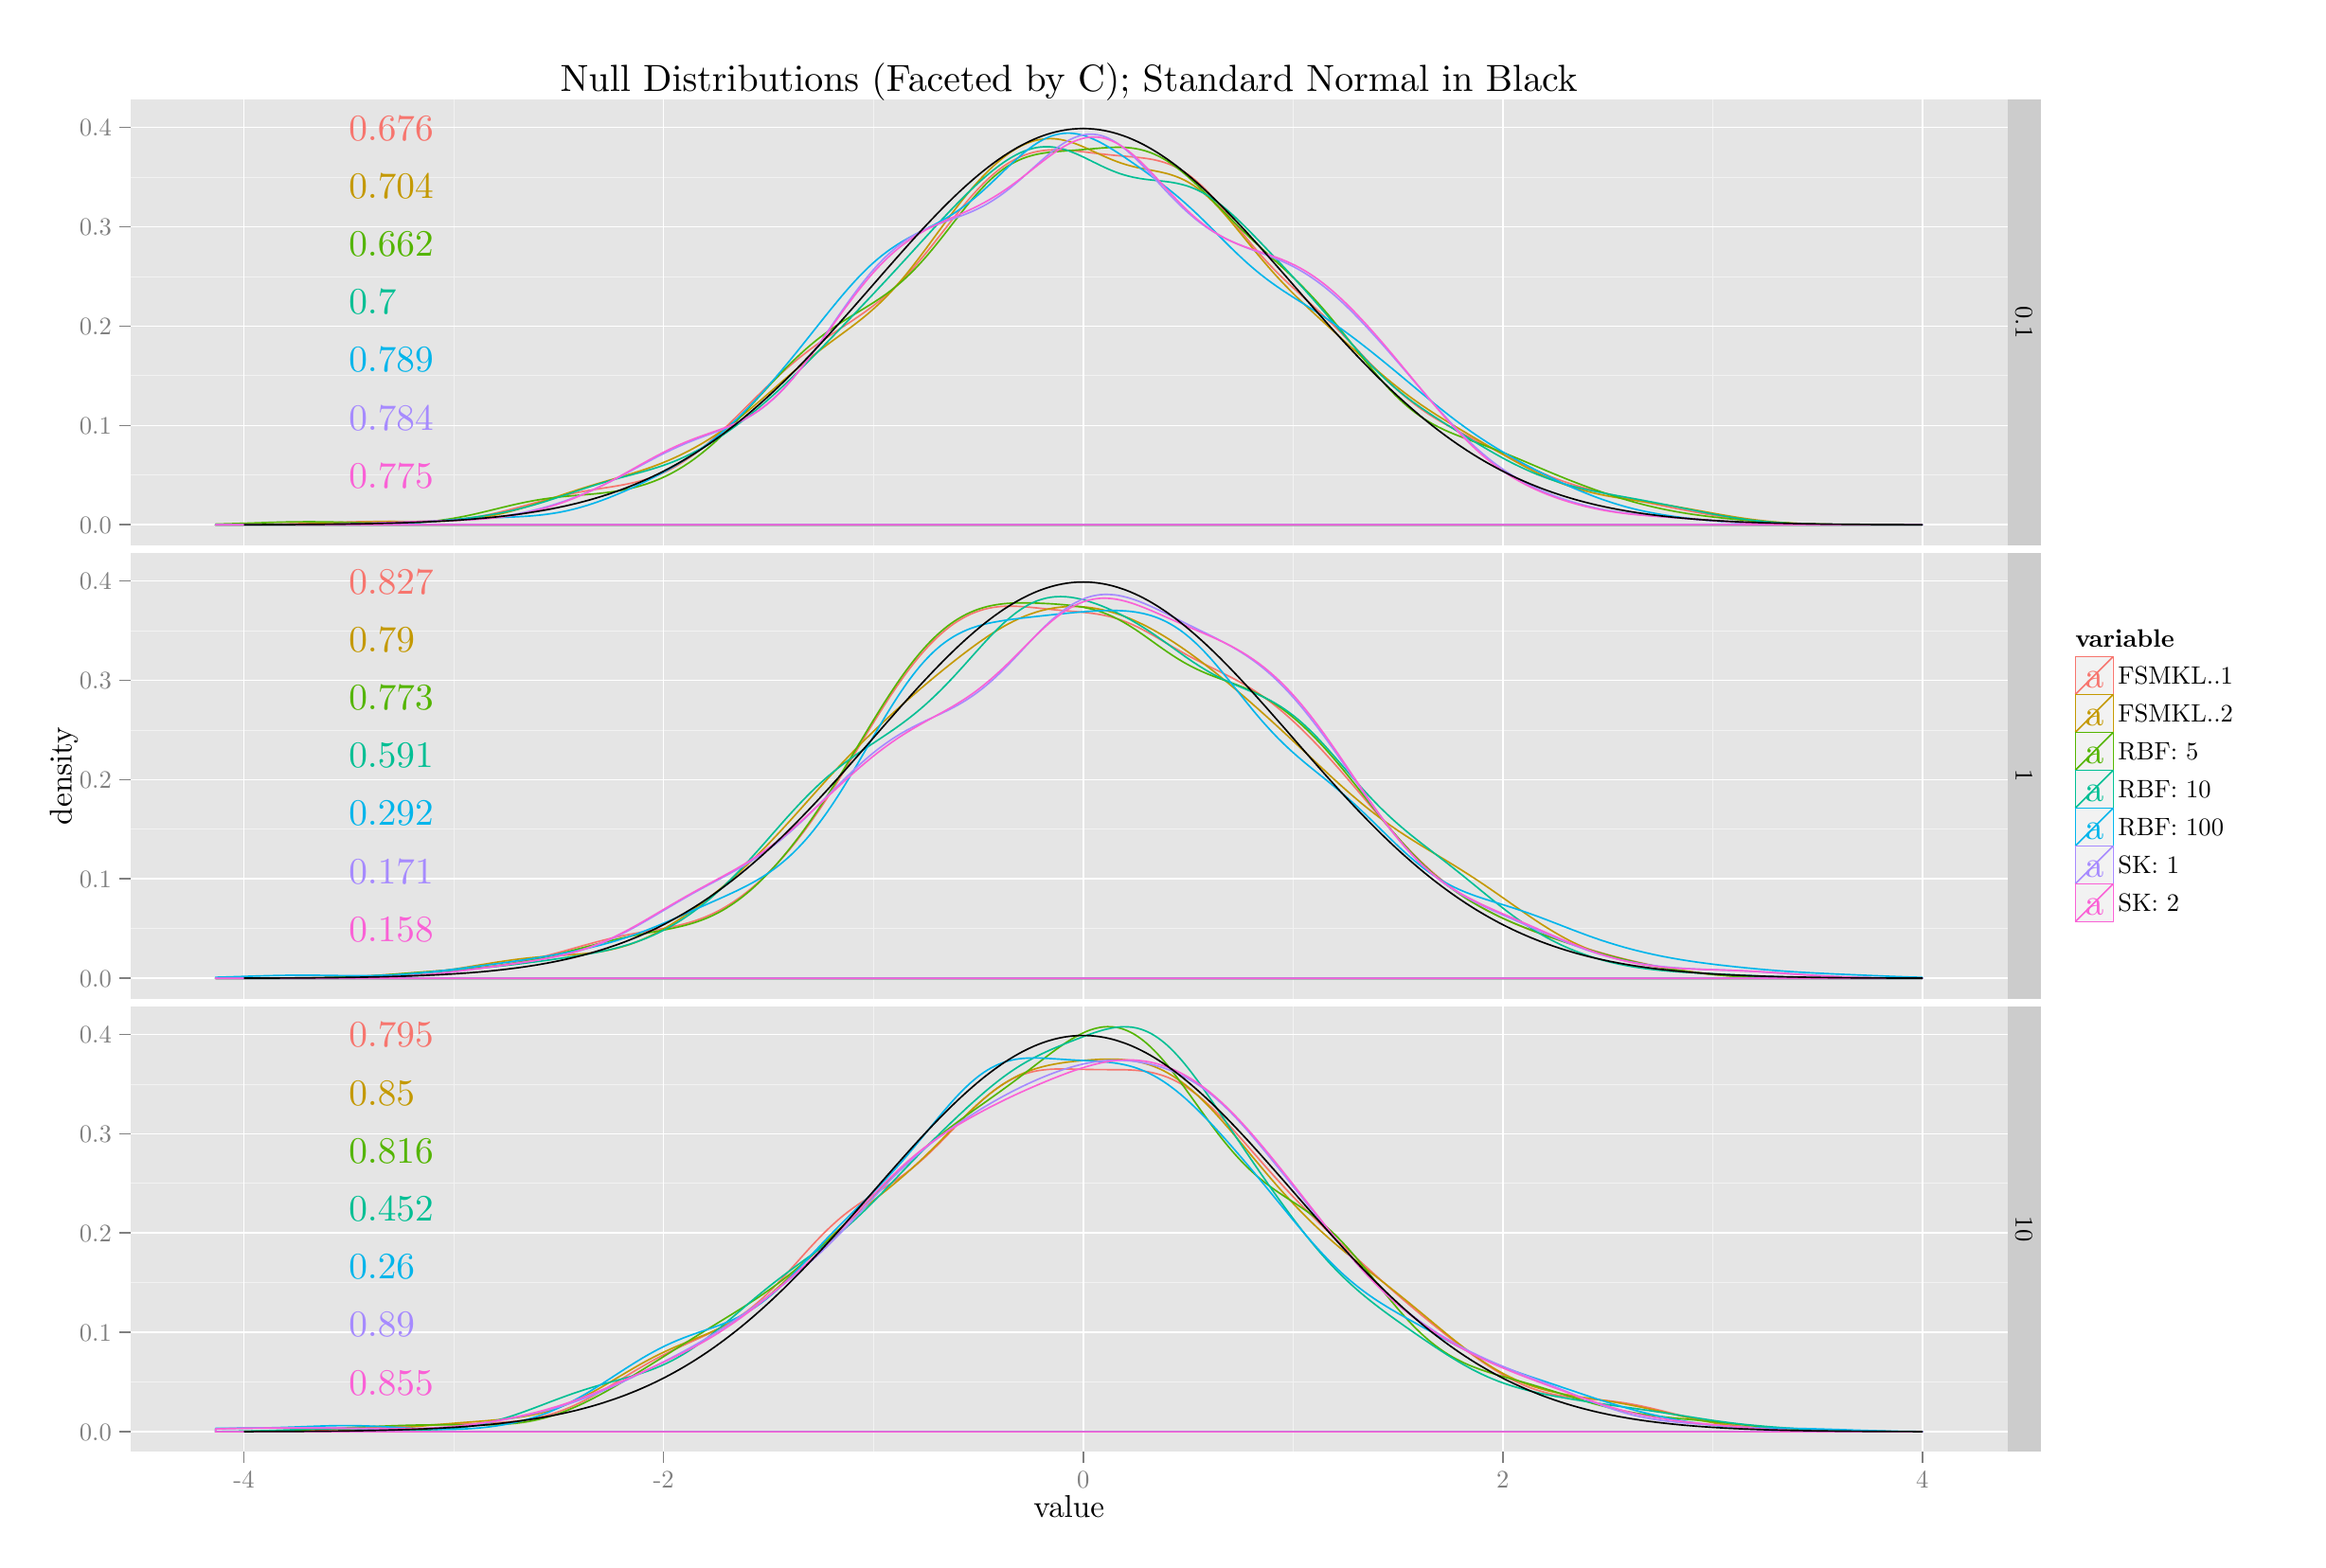
\begin{tikzpicture}[x=1pt,y=1pt]
\definecolor[named]{fillColor}{rgb}{1.00,1.00,1.00}
\path[use as bounding box,fill=fillColor,fill opacity=0.00] (0,0) rectangle (867.24,578.16);
\begin{scope}
\path[clip] (  0.00,  0.00) rectangle (867.24,578.16);
\definecolor[named]{drawColor}{rgb}{1.00,1.00,1.00}
\definecolor[named]{fillColor}{rgb}{1.00,1.00,1.00}

\path[draw=drawColor,line width= 0.6pt,line join=round,line cap=round,fill=fillColor] (  0.00, -0.00) rectangle (867.24,578.16);
\end{scope}
\begin{scope}
\path[clip] ( 39.69,380.14) rectangle (756.04,550.17);
\definecolor[named]{fillColor}{rgb}{0.90,0.90,0.90}

\path[fill=fillColor] ( 39.69,380.14) rectangle (756.04,550.17);
\definecolor[named]{drawColor}{rgb}{0.95,0.95,0.95}

\path[draw=drawColor,line width= 0.3pt,line join=round] ( 39.69,406.82) --
	(756.04,406.82);

\path[draw=drawColor,line width= 0.3pt,line join=round] ( 39.69,444.73) --
	(756.04,444.73);

\path[draw=drawColor,line width= 0.3pt,line join=round] ( 39.69,482.63) --
	(756.04,482.63);

\path[draw=drawColor,line width= 0.3pt,line join=round] ( 39.69,520.54) --
	(756.04,520.54);

\path[draw=drawColor,line width= 0.3pt,line join=round] (163.10,380.14) --
	(163.10,550.17);

\path[draw=drawColor,line width= 0.3pt,line join=round] (323.21,380.14) --
	(323.21,550.17);

\path[draw=drawColor,line width= 0.3pt,line join=round] (483.32,380.14) --
	(483.32,550.17);

\path[draw=drawColor,line width= 0.3pt,line join=round] (643.42,380.14) --
	(643.42,550.17);
\definecolor[named]{drawColor}{rgb}{1.00,1.00,1.00}

\path[draw=drawColor,line width= 0.6pt,line join=round] ( 39.69,387.86) --
	(756.04,387.86);

\path[draw=drawColor,line width= 0.6pt,line join=round] ( 39.69,425.77) --
	(756.04,425.77);

\path[draw=drawColor,line width= 0.6pt,line join=round] ( 39.69,463.68) --
	(756.04,463.68);

\path[draw=drawColor,line width= 0.6pt,line join=round] ( 39.69,501.59) --
	(756.04,501.59);

\path[draw=drawColor,line width= 0.6pt,line join=round] ( 39.69,539.50) --
	(756.04,539.50);

\path[draw=drawColor,line width= 0.6pt,line join=round] ( 83.05,380.14) --
	( 83.05,550.17);

\path[draw=drawColor,line width= 0.6pt,line join=round] (243.16,380.14) --
	(243.16,550.17);

\path[draw=drawColor,line width= 0.6pt,line join=round] (403.26,380.14) --
	(403.26,550.17);

\path[draw=drawColor,line width= 0.6pt,line join=round] (563.37,380.14) --
	(563.37,550.17);

\path[draw=drawColor,line width= 0.6pt,line join=round] (723.48,380.14) --
	(723.48,550.17);
\definecolor[named]{drawColor}{rgb}{0.97,0.46,0.43}

\path[draw=drawColor,line width= 0.6pt,line join=round,line cap=round] ( 72.25,387.88) --
	( 73.52,387.88) --
	( 74.80,387.88) --
	( 76.07,387.89) --
	( 77.35,387.89) --
	( 78.62,387.90) --
	( 79.89,387.90) --
	( 81.17,387.91) --
	( 82.44,387.92) --
	( 83.72,387.93) --
	( 84.99,387.94) --
	( 86.27,387.95) --
	( 87.54,387.96) --
	( 88.82,387.98) --
	( 90.09,388.00) --
	( 91.36,388.01) --
	( 92.64,388.03) --
	( 93.91,388.06) --
	( 95.19,388.08) --
	( 96.46,388.11) --
	( 97.74,388.14) --
	( 99.01,388.17) --
	(100.29,388.20) --
	(101.56,388.24) --
	(102.83,388.27) --
	(104.11,388.31) --
	(105.38,388.35) --
	(106.66,388.39) --
	(107.93,388.44) --
	(109.21,388.48) --
	(110.48,388.53) --
	(111.76,388.58) --
	(113.03,388.62) --
	(114.30,388.67) --
	(115.58,388.71) --
	(116.85,388.76) --
	(118.13,388.80) --
	(119.40,388.85) --
	(120.68,388.89) --
	(121.95,388.92) --
	(123.22,388.96) --
	(124.50,388.99) --
	(125.77,389.02) --
	(127.05,389.05) --
	(128.32,389.07) --
	(129.60,389.09) --
	(130.87,389.10) --
	(132.15,389.11) --
	(133.42,389.12) --
	(134.69,389.12) --
	(135.97,389.12) --
	(137.24,389.12) --
	(138.52,389.12) --
	(139.79,389.12) --
	(141.07,389.11) --
	(142.34,389.10) --
	(143.62,389.10) --
	(144.89,389.09) --
	(146.16,389.09) --
	(147.44,389.09) --
	(148.71,389.10) --
	(149.99,389.11) --
	(151.26,389.13) --
	(152.54,389.15) --
	(153.81,389.18) --
	(155.09,389.22) --
	(156.36,389.27) --
	(157.63,389.33) --
	(158.91,389.40) --
	(160.18,389.48) --
	(161.46,389.58) --
	(162.73,389.69) --
	(164.01,389.81) --
	(165.28,389.95) --
	(166.56,390.10) --
	(167.83,390.26) --
	(169.10,390.44) --
	(170.38,390.64) --
	(171.65,390.85) --
	(172.93,391.07) --
	(174.20,391.31) --
	(175.48,391.56) --
	(176.75,391.82) --
	(178.03,392.10) --
	(179.30,392.38) --
	(180.57,392.68) --
	(181.85,392.99) --
	(183.12,393.31) --
	(184.40,393.64) --
	(185.67,393.97) --
	(186.95,394.31) --
	(188.22,394.65) --
	(189.49,395.00) --
	(190.77,395.35) --
	(192.04,395.70) --
	(193.32,396.05) --
	(194.59,396.40) --
	(195.87,396.75) --
	(197.14,397.09) --
	(198.42,397.43) --
	(199.69,397.76) --
	(200.96,398.08) --
	(202.24,398.40) --
	(203.51,398.71) --
	(204.79,399.01) --
	(206.06,399.29) --
	(207.34,399.57) --
	(208.61,399.84) --
	(209.89,400.10) --
	(211.16,400.35) --
	(212.43,400.59) --
	(213.71,400.81) --
	(214.98,401.03) --
	(216.26,401.25) --
	(217.53,401.46) --
	(218.81,401.66) --
	(220.08,401.86) --
	(221.36,402.06) --
	(222.63,402.26) --
	(223.90,402.47) --
	(225.18,402.68) --
	(226.45,402.90) --
	(227.73,403.13) --
	(229.00,403.37) --
	(230.28,403.63) --
	(231.55,403.92) --
	(232.83,404.22) --
	(234.10,404.55) --
	(235.37,404.90) --
	(236.65,405.28) --
	(237.92,405.69) --
	(239.20,406.14) --
	(240.47,406.63) --
	(241.75,407.14) --
	(243.02,407.70) --
	(244.29,408.29) --
	(245.57,408.93) --
	(246.84,409.61) --
	(248.12,410.33) --
	(249.39,411.08) --
	(250.67,411.88) --
	(251.94,412.73) --
	(253.22,413.60) --
	(254.49,414.52) --
	(255.76,415.47) --
	(257.04,416.47) --
	(258.31,417.49) --
	(259.59,418.55) --
	(260.86,419.64) --
	(262.14,420.76) --
	(263.41,421.90) --
	(264.69,423.07) --
	(265.96,424.26) --
	(267.23,425.47) --
	(268.51,426.70) --
	(269.78,427.94) --
	(271.06,429.19) --
	(272.33,430.45) --
	(273.61,431.71) --
	(274.88,432.98) --
	(276.16,434.25) --
	(277.43,435.51) --
	(278.70,436.77) --
	(279.98,438.03) --
	(281.25,439.27) --
	(282.53,440.50) --
	(283.80,441.72) --
	(285.08,442.92) --
	(286.35,444.11) --
	(287.63,445.28) --
	(288.90,446.42) --
	(290.17,447.55) --
	(291.45,448.65) --
	(292.72,449.73) --
	(294.00,450.79) --
	(295.27,451.82) --
	(296.55,452.83) --
	(297.82,453.82) --
	(299.10,454.79) --
	(300.37,455.73) --
	(301.64,456.66) --
	(302.92,457.56) --
	(304.19,458.45) --
	(305.47,459.33) --
	(306.74,460.19) --
	(308.02,461.05) --
	(309.29,461.89) --
	(310.56,462.73) --
	(311.84,463.57) --
	(313.11,464.41) --
	(314.39,465.25) --
	(315.66,466.10) --
	(316.94,466.97) --
	(318.21,467.85) --
	(319.49,468.74) --
	(320.76,469.65) --
	(322.03,470.60) --
	(323.31,471.57) --
	(324.58,472.57) --
	(325.86,473.59) --
	(327.13,474.66) --
	(328.41,475.76) --
	(329.68,476.91) --
	(330.96,478.09) --
	(332.23,479.31) --
	(333.50,480.57) --
	(334.78,481.88) --
	(336.05,483.23) --
	(337.33,484.62) --
	(338.60,486.04) --
	(339.88,487.50) --
	(341.15,489.00) --
	(342.43,490.53) --
	(343.70,492.09) --
	(344.97,493.67) --
	(346.25,495.27) --
	(347.52,496.89) --
	(348.80,498.52) --
	(350.07,500.15) --
	(351.35,501.79) --
	(352.62,503.42) --
	(353.90,505.04) --
	(355.17,506.64) --
	(356.44,508.23) --
	(357.72,509.78) --
	(358.99,511.31) --
	(360.27,512.80) --
	(361.54,514.24) --
	(362.82,515.64) --
	(364.09,516.99) --
	(365.37,518.29) --
	(366.64,519.53) --
	(367.91,520.70) --
	(369.19,521.82) --
	(370.46,522.87) --
	(371.74,523.86) --
	(373.01,524.77) --
	(374.29,525.62) --
	(375.56,526.40) --
	(376.83,527.11) --
	(378.11,527.77) --
	(379.38,528.34) --
	(380.66,528.85) --
	(381.93,529.31) --
	(383.21,529.70) --
	(384.48,530.04) --
	(385.76,530.31) --
	(387.03,530.53) --
	(388.30,530.71) --
	(389.58,530.84) --
	(390.85,530.93) --
	(392.13,530.97) --
	(393.40,530.98) --
	(394.68,530.96) --
	(395.95,530.90) --
	(397.23,530.83) --
	(398.50,530.73) --
	(399.77,530.61) --
	(401.05,530.48) --
	(402.32,530.34) --
	(403.60,530.19) --
	(404.87,530.04) --
	(406.15,529.88) --
	(407.42,529.73) --
	(408.70,529.57) --
	(409.97,529.43) --
	(411.24,529.28) --
	(412.52,529.15) --
	(413.79,529.02) --
	(415.07,528.89) --
	(416.34,528.77) --
	(417.62,528.66) --
	(418.89,528.55) --
	(420.17,528.44) --
	(421.44,528.33) --
	(422.71,528.22) --
	(423.99,528.10) --
	(425.26,527.95) --
	(426.54,527.80) --
	(427.81,527.62) --
	(429.09,527.41) --
	(430.36,527.17) --
	(431.63,526.88) --
	(432.91,526.55) --
	(434.18,526.17) --
	(435.46,525.73) --
	(436.73,525.24) --
	(438.01,524.67) --
	(439.28,524.03) --
	(440.56,523.33) --
	(441.83,522.56) --
	(443.10,521.71) --
	(444.38,520.77) --
	(445.65,519.76) --
	(446.93,518.67) --
	(448.20,517.52) --
	(449.48,516.31) --
	(450.75,515.01) --
	(452.03,513.65) --
	(453.30,512.25) --
	(454.57,510.80) --
	(455.85,509.31) --
	(457.12,507.77) --
	(458.40,506.21) --
	(459.67,504.64) --
	(460.95,503.05) --
	(462.22,501.46) --
	(463.50,499.87) --
	(464.77,498.29) --
	(466.04,496.72) --
	(467.32,495.18) --
	(468.59,493.65) --
	(469.87,492.16) --
	(471.14,490.71) --
	(472.42,489.28) --
	(473.69,487.89) --
	(474.97,486.53) --
	(476.24,485.21) --
	(477.51,483.92) --
	(478.79,482.66) --
	(480.06,481.43) --
	(481.34,480.22) --
	(482.61,479.03) --
	(483.89,477.86) --
	(485.16,476.70) --
	(486.44,475.55) --
	(487.71,474.39) --
	(488.98,473.24) --
	(490.26,472.09) --
	(491.53,470.92) --
	(492.81,469.74) --
	(494.08,468.56) --
	(495.36,467.35) --
	(496.63,466.12) --
	(497.90,464.88) --
	(499.18,463.63) --
	(500.45,462.35) --
	(501.73,461.06) --
	(503.00,459.75) --
	(504.28,458.43) --
	(505.55,457.10) --
	(506.83,455.76) --
	(508.10,454.42) --
	(509.37,453.07) --
	(510.65,451.73) --
	(511.92,450.39) --
	(513.20,449.06) --
	(514.47,447.74) --
	(515.75,446.44) --
	(517.02,445.16) --
	(518.30,443.90) --
	(519.57,442.66) --
	(520.84,441.45) --
	(522.12,440.27) --
	(523.39,439.12) --
	(524.67,438.00) --
	(525.94,436.92) --
	(527.22,435.86) --
	(528.49,434.85) --
	(529.77,433.87) --
	(531.04,432.92) --
	(532.31,432.00) --
	(533.59,431.12) --
	(534.86,430.26) --
	(536.14,429.44) --
	(537.41,428.64) --
	(538.69,427.86) --
	(539.96,427.11) --
	(541.24,426.38) --
	(542.51,425.67) --
	(543.78,424.97) --
	(545.06,424.28) --
	(546.33,423.60) --
	(547.61,422.94) --
	(548.88,422.28) --
	(550.16,421.62) --
	(551.43,420.97) --
	(552.71,420.32) --
	(553.98,419.67) --
	(555.25,419.02) --
	(556.53,418.36) --
	(557.80,417.71) --
	(559.08,417.06) --
	(560.35,416.41) --
	(561.63,415.75) --
	(562.90,415.10) --
	(564.17,414.45) --
	(565.45,413.80) --
	(566.72,413.15) --
	(568.00,412.51) --
	(569.27,411.88) --
	(570.55,411.25) --
	(571.82,410.63) --
	(573.10,410.02) --
	(574.37,409.42) --
	(575.64,408.84) --
	(576.92,408.27) --
	(578.19,407.71) --
	(579.47,407.17) --
	(580.74,406.64) --
	(582.02,406.13) --
	(583.29,405.64) --
	(584.57,405.16) --
	(585.84,404.70) --
	(587.11,404.25) --
	(588.39,403.82) --
	(589.66,403.40) --
	(590.94,403.00) --
	(592.21,402.62) --
	(593.49,402.24) --
	(594.76,401.88) --
	(596.04,401.53) --
	(597.31,401.19) --
	(598.58,400.85) --
	(599.86,400.53) --
	(601.13,400.21) --
	(602.41,399.90) --
	(603.68,399.60) --
	(604.96,399.30) --
	(606.23,399.00) --
	(607.51,398.71) --
	(608.78,398.43) --
	(610.05,398.14) --
	(611.33,397.86) --
	(612.60,397.59) --
	(613.88,397.31) --
	(615.15,397.04) --
	(616.43,396.76) --
	(617.70,396.49) --
	(618.97,396.23) --
	(620.25,395.96) --
	(621.52,395.70) --
	(622.80,395.44) --
	(624.07,395.18) --
	(625.35,394.92) --
	(626.62,394.67) --
	(627.90,394.41) --
	(629.17,394.16) --
	(630.44,393.92) --
	(631.72,393.67) --
	(632.99,393.43) --
	(634.27,393.19) --
	(635.54,392.95) --
	(636.82,392.72) --
	(638.09,392.48) --
	(639.37,392.26) --
	(640.64,392.03) --
	(641.91,391.81) --
	(643.19,391.60) --
	(644.46,391.39) --
	(645.74,391.18) --
	(647.01,390.98) --
	(648.29,390.78) --
	(649.56,390.59) --
	(650.84,390.41) --
	(652.11,390.23) --
	(653.38,390.06) --
	(654.66,389.90) --
	(655.93,389.74) --
	(657.21,389.59) --
	(658.48,389.45) --
	(659.76,389.31) --
	(661.03,389.18) --
	(662.31,389.06) --
	(663.58,388.95) --
	(664.85,388.85) --
	(666.13,388.75) --
	(667.40,388.66) --
	(668.68,388.57) --
	(669.95,388.50) --
	(671.23,388.43) --
	(672.50,388.36) --
	(673.78,388.30) --
	(675.05,388.25) --
	(676.32,388.20) --
	(677.60,388.16) --
	(678.87,388.12) --
	(680.15,388.09) --
	(681.42,388.06) --
	(682.70,388.03) --
	(683.97,388.01) --
	(685.24,387.98) --
	(686.52,387.97) --
	(687.79,387.95) --
	(689.07,387.94) --
	(690.34,387.93) --
	(691.62,387.92) --
	(692.89,387.91) --
	(694.17,387.90) --
	(695.44,387.89) --
	(696.71,387.89) --
	(697.99,387.88) --
	(699.26,387.88) --
	(700.54,387.88) --
	(701.81,387.88) --
	(703.09,387.87) --
	(704.36,387.87) --
	(705.64,387.87) --
	(706.91,387.87) --
	(708.18,387.87) --
	(709.46,387.87) --
	(710.73,387.87) --
	(712.01,387.87) --
	(713.28,387.87) --
	(714.56,387.87) --
	(715.83,387.87) --
	(717.11,387.87) --
	(718.38,387.87) --
	(719.65,387.87) --
	(720.93,387.86) --
	(722.20,387.86) --
	(723.48,387.86) --
	(723.48,387.86) --
	(722.20,387.86) --
	(720.93,387.86) --
	(719.65,387.86) --
	(718.38,387.86) --
	(717.11,387.86) --
	(715.83,387.86) --
	(714.56,387.86) --
	(713.28,387.86) --
	(712.01,387.86) --
	(710.73,387.86) --
	(709.46,387.86) --
	(708.18,387.86) --
	(706.91,387.86) --
	(705.64,387.86) --
	(704.36,387.86) --
	(703.09,387.86) --
	(701.81,387.86) --
	(700.54,387.86) --
	(699.26,387.86) --
	(697.99,387.86) --
	(696.71,387.86) --
	(695.44,387.86) --
	(694.17,387.86) --
	(692.89,387.86) --
	(691.62,387.86) --
	(690.34,387.86) --
	(689.07,387.86) --
	(687.79,387.86) --
	(686.52,387.86) --
	(685.24,387.86) --
	(683.97,387.86) --
	(682.70,387.86) --
	(681.42,387.86) --
	(680.15,387.86) --
	(678.87,387.86) --
	(677.60,387.86) --
	(676.32,387.86) --
	(675.05,387.86) --
	(673.78,387.86) --
	(672.50,387.86) --
	(671.23,387.86) --
	(669.95,387.86) --
	(668.68,387.86) --
	(667.40,387.86) --
	(666.13,387.86) --
	(664.85,387.86) --
	(663.58,387.86) --
	(662.31,387.86) --
	(661.03,387.86) --
	(659.76,387.86) --
	(658.48,387.86) --
	(657.21,387.86) --
	(655.93,387.86) --
	(654.66,387.86) --
	(653.38,387.86) --
	(652.11,387.86) --
	(650.84,387.86) --
	(649.56,387.86) --
	(648.29,387.86) --
	(647.01,387.86) --
	(645.74,387.86) --
	(644.46,387.86) --
	(643.19,387.86) --
	(641.91,387.86) --
	(640.64,387.86) --
	(639.37,387.86) --
	(638.09,387.86) --
	(636.82,387.86) --
	(635.54,387.86) --
	(634.27,387.86) --
	(632.99,387.86) --
	(631.72,387.86) --
	(630.44,387.86) --
	(629.17,387.86) --
	(627.90,387.86) --
	(626.62,387.86) --
	(625.35,387.86) --
	(624.07,387.86) --
	(622.80,387.86) --
	(621.52,387.86) --
	(620.25,387.86) --
	(618.97,387.86) --
	(617.70,387.86) --
	(616.43,387.86) --
	(615.15,387.86) --
	(613.88,387.86) --
	(612.60,387.86) --
	(611.33,387.86) --
	(610.05,387.86) --
	(608.78,387.86) --
	(607.51,387.86) --
	(606.23,387.86) --
	(604.96,387.86) --
	(603.68,387.86) --
	(602.41,387.86) --
	(601.13,387.86) --
	(599.86,387.86) --
	(598.58,387.86) --
	(597.31,387.86) --
	(596.04,387.86) --
	(594.76,387.86) --
	(593.49,387.86) --
	(592.21,387.86) --
	(590.94,387.86) --
	(589.66,387.86) --
	(588.39,387.86) --
	(587.11,387.86) --
	(585.84,387.86) --
	(584.57,387.86) --
	(583.29,387.86) --
	(582.02,387.86) --
	(580.74,387.86) --
	(579.47,387.86) --
	(578.19,387.86) --
	(576.92,387.86) --
	(575.64,387.86) --
	(574.37,387.86) --
	(573.10,387.86) --
	(571.82,387.86) --
	(570.55,387.86) --
	(569.27,387.86) --
	(568.00,387.86) --
	(566.72,387.86) --
	(565.45,387.86) --
	(564.17,387.86) --
	(562.90,387.86) --
	(561.63,387.86) --
	(560.35,387.86) --
	(559.08,387.86) --
	(557.80,387.86) --
	(556.53,387.86) --
	(555.25,387.86) --
	(553.98,387.86) --
	(552.71,387.86) --
	(551.43,387.86) --
	(550.16,387.86) --
	(548.88,387.86) --
	(547.61,387.86) --
	(546.33,387.86) --
	(545.06,387.86) --
	(543.78,387.86) --
	(542.51,387.86) --
	(541.24,387.86) --
	(539.96,387.86) --
	(538.69,387.86) --
	(537.41,387.86) --
	(536.14,387.86) --
	(534.86,387.86) --
	(533.59,387.86) --
	(532.31,387.86) --
	(531.04,387.86) --
	(529.77,387.86) --
	(528.49,387.86) --
	(527.22,387.86) --
	(525.94,387.86) --
	(524.67,387.86) --
	(523.39,387.86) --
	(522.12,387.86) --
	(520.84,387.86) --
	(519.57,387.86) --
	(518.30,387.86) --
	(517.02,387.86) --
	(515.75,387.86) --
	(514.47,387.86) --
	(513.20,387.86) --
	(511.92,387.86) --
	(510.65,387.86) --
	(509.37,387.86) --
	(508.10,387.86) --
	(506.83,387.86) --
	(505.55,387.86) --
	(504.28,387.86) --
	(503.00,387.86) --
	(501.73,387.86) --
	(500.45,387.86) --
	(499.18,387.86) --
	(497.90,387.86) --
	(496.63,387.86) --
	(495.36,387.86) --
	(494.08,387.86) --
	(492.81,387.86) --
	(491.53,387.86) --
	(490.26,387.86) --
	(488.98,387.86) --
	(487.71,387.86) --
	(486.44,387.86) --
	(485.16,387.86) --
	(483.89,387.86) --
	(482.61,387.86) --
	(481.34,387.86) --
	(480.06,387.86) --
	(478.79,387.86) --
	(477.51,387.86) --
	(476.24,387.86) --
	(474.97,387.86) --
	(473.69,387.86) --
	(472.42,387.86) --
	(471.14,387.86) --
	(469.87,387.86) --
	(468.59,387.86) --
	(467.32,387.86) --
	(466.04,387.86) --
	(464.77,387.86) --
	(463.50,387.86) --
	(462.22,387.86) --
	(460.95,387.86) --
	(459.67,387.86) --
	(458.40,387.86) --
	(457.12,387.86) --
	(455.85,387.86) --
	(454.57,387.86) --
	(453.30,387.86) --
	(452.03,387.86) --
	(450.75,387.86) --
	(449.48,387.86) --
	(448.20,387.86) --
	(446.93,387.86) --
	(445.65,387.86) --
	(444.38,387.86) --
	(443.10,387.86) --
	(441.83,387.86) --
	(440.56,387.86) --
	(439.28,387.86) --
	(438.01,387.86) --
	(436.73,387.86) --
	(435.46,387.86) --
	(434.18,387.86) --
	(432.91,387.86) --
	(431.63,387.86) --
	(430.36,387.86) --
	(429.09,387.86) --
	(427.81,387.86) --
	(426.54,387.86) --
	(425.26,387.86) --
	(423.99,387.86) --
	(422.71,387.86) --
	(421.44,387.86) --
	(420.17,387.86) --
	(418.89,387.86) --
	(417.62,387.86) --
	(416.34,387.86) --
	(415.07,387.86) --
	(413.79,387.86) --
	(412.52,387.86) --
	(411.24,387.86) --
	(409.97,387.86) --
	(408.70,387.86) --
	(407.42,387.86) --
	(406.15,387.86) --
	(404.87,387.86) --
	(403.60,387.86) --
	(402.32,387.86) --
	(401.05,387.86) --
	(399.77,387.86) --
	(398.50,387.86) --
	(397.23,387.86) --
	(395.95,387.86) --
	(394.68,387.86) --
	(393.40,387.86) --
	(392.13,387.86) --
	(390.85,387.86) --
	(389.58,387.86) --
	(388.30,387.86) --
	(387.03,387.86) --
	(385.76,387.86) --
	(384.48,387.86) --
	(383.21,387.86) --
	(381.93,387.86) --
	(380.66,387.86) --
	(379.38,387.86) --
	(378.11,387.86) --
	(376.83,387.86) --
	(375.56,387.86) --
	(374.29,387.86) --
	(373.01,387.86) --
	(371.74,387.86) --
	(370.46,387.86) --
	(369.19,387.86) --
	(367.91,387.86) --
	(366.64,387.86) --
	(365.37,387.86) --
	(364.09,387.86) --
	(362.82,387.86) --
	(361.54,387.86) --
	(360.27,387.86) --
	(358.99,387.86) --
	(357.72,387.86) --
	(356.44,387.86) --
	(355.17,387.86) --
	(353.90,387.86) --
	(352.62,387.86) --
	(351.35,387.86) --
	(350.07,387.86) --
	(348.80,387.86) --
	(347.52,387.86) --
	(346.25,387.86) --
	(344.97,387.86) --
	(343.70,387.86) --
	(342.43,387.86) --
	(341.15,387.86) --
	(339.88,387.86) --
	(338.60,387.86) --
	(337.33,387.86) --
	(336.05,387.86) --
	(334.78,387.86) --
	(333.50,387.86) --
	(332.23,387.86) --
	(330.96,387.86) --
	(329.68,387.86) --
	(328.41,387.86) --
	(327.13,387.86) --
	(325.86,387.86) --
	(324.58,387.86) --
	(323.31,387.86) --
	(322.03,387.86) --
	(320.76,387.86) --
	(319.49,387.86) --
	(318.21,387.86) --
	(316.94,387.86) --
	(315.66,387.86) --
	(314.39,387.86) --
	(313.11,387.86) --
	(311.84,387.86) --
	(310.56,387.86) --
	(309.29,387.86) --
	(308.02,387.86) --
	(306.74,387.86) --
	(305.47,387.86) --
	(304.19,387.86) --
	(302.92,387.86) --
	(301.64,387.86) --
	(300.37,387.86) --
	(299.10,387.86) --
	(297.82,387.86) --
	(296.55,387.86) --
	(295.27,387.86) --
	(294.00,387.86) --
	(292.72,387.86) --
	(291.45,387.86) --
	(290.17,387.86) --
	(288.90,387.86) --
	(287.63,387.86) --
	(286.35,387.86) --
	(285.08,387.86) --
	(283.80,387.86) --
	(282.53,387.86) --
	(281.25,387.86) --
	(279.98,387.86) --
	(278.70,387.86) --
	(277.43,387.86) --
	(276.16,387.86) --
	(274.88,387.86) --
	(273.61,387.86) --
	(272.33,387.86) --
	(271.06,387.86) --
	(269.78,387.86) --
	(268.51,387.86) --
	(267.23,387.86) --
	(265.96,387.86) --
	(264.69,387.86) --
	(263.41,387.86) --
	(262.14,387.86) --
	(260.86,387.86) --
	(259.59,387.86) --
	(258.31,387.86) --
	(257.04,387.86) --
	(255.76,387.86) --
	(254.49,387.86) --
	(253.22,387.86) --
	(251.94,387.86) --
	(250.67,387.86) --
	(249.39,387.86) --
	(248.12,387.86) --
	(246.84,387.86) --
	(245.57,387.86) --
	(244.29,387.86) --
	(243.02,387.86) --
	(241.75,387.86) --
	(240.47,387.86) --
	(239.20,387.86) --
	(237.92,387.86) --
	(236.65,387.86) --
	(235.37,387.86) --
	(234.10,387.86) --
	(232.83,387.86) --
	(231.55,387.86) --
	(230.28,387.86) --
	(229.00,387.86) --
	(227.73,387.86) --
	(226.45,387.86) --
	(225.18,387.86) --
	(223.90,387.86) --
	(222.63,387.86) --
	(221.36,387.86) --
	(220.08,387.86) --
	(218.81,387.86) --
	(217.53,387.86) --
	(216.26,387.86) --
	(214.98,387.86) --
	(213.71,387.86) --
	(212.43,387.86) --
	(211.16,387.86) --
	(209.89,387.86) --
	(208.61,387.86) --
	(207.34,387.86) --
	(206.06,387.86) --
	(204.79,387.86) --
	(203.51,387.86) --
	(202.24,387.86) --
	(200.96,387.86) --
	(199.69,387.86) --
	(198.42,387.86) --
	(197.14,387.86) --
	(195.87,387.86) --
	(194.59,387.86) --
	(193.32,387.86) --
	(192.04,387.86) --
	(190.77,387.86) --
	(189.49,387.86) --
	(188.22,387.86) --
	(186.95,387.86) --
	(185.67,387.86) --
	(184.40,387.86) --
	(183.12,387.86) --
	(181.85,387.86) --
	(180.57,387.86) --
	(179.30,387.86) --
	(178.03,387.86) --
	(176.75,387.86) --
	(175.48,387.86) --
	(174.20,387.86) --
	(172.93,387.86) --
	(171.65,387.86) --
	(170.38,387.86) --
	(169.10,387.86) --
	(167.83,387.86) --
	(166.56,387.86) --
	(165.28,387.86) --
	(164.01,387.86) --
	(162.73,387.86) --
	(161.46,387.86) --
	(160.18,387.86) --
	(158.91,387.86) --
	(157.63,387.86) --
	(156.36,387.86) --
	(155.09,387.86) --
	(153.81,387.86) --
	(152.54,387.86) --
	(151.26,387.86) --
	(149.99,387.86) --
	(148.71,387.86) --
	(147.44,387.86) --
	(146.16,387.86) --
	(144.89,387.86) --
	(143.62,387.86) --
	(142.34,387.86) --
	(141.07,387.86) --
	(139.79,387.86) --
	(138.52,387.86) --
	(137.24,387.86) --
	(135.97,387.86) --
	(134.69,387.86) --
	(133.42,387.86) --
	(132.15,387.86) --
	(130.87,387.86) --
	(129.60,387.86) --
	(128.32,387.86) --
	(127.05,387.86) --
	(125.77,387.86) --
	(124.50,387.86) --
	(123.22,387.86) --
	(121.95,387.86) --
	(120.68,387.86) --
	(119.40,387.86) --
	(118.13,387.86) --
	(116.85,387.86) --
	(115.58,387.86) --
	(114.30,387.86) --
	(113.03,387.86) --
	(111.76,387.86) --
	(110.48,387.86) --
	(109.21,387.86) --
	(107.93,387.86) --
	(106.66,387.86) --
	(105.38,387.86) --
	(104.11,387.86) --
	(102.83,387.86) --
	(101.56,387.86) --
	(100.29,387.86) --
	( 99.01,387.86) --
	( 97.74,387.86) --
	( 96.46,387.86) --
	( 95.19,387.86) --
	( 93.91,387.86) --
	( 92.64,387.86) --
	( 91.36,387.86) --
	( 90.09,387.86) --
	( 88.82,387.86) --
	( 87.54,387.86) --
	( 86.27,387.86) --
	( 84.99,387.86) --
	( 83.72,387.86) --
	( 82.44,387.86) --
	( 81.17,387.86) --
	( 79.89,387.86) --
	( 78.62,387.86) --
	( 77.35,387.86) --
	( 76.07,387.86) --
	( 74.80,387.86) --
	( 73.52,387.86) --
	( 72.25,387.86) --
	( 72.25,387.88);
\definecolor[named]{drawColor}{rgb}{0.77,0.60,0.00}

\path[draw=drawColor,line width= 0.6pt,line join=round,line cap=round] ( 72.25,387.87) --
	( 73.52,387.87) --
	( 74.80,387.87) --
	( 76.07,387.87) --
	( 77.35,387.87) --
	( 78.62,387.88) --
	( 79.89,387.88) --
	( 81.17,387.88) --
	( 82.44,387.89) --
	( 83.72,387.89) --
	( 84.99,387.90) --
	( 86.27,387.90) --
	( 87.54,387.91) --
	( 88.82,387.91) --
	( 90.09,387.92) --
	( 91.36,387.93) --
	( 92.64,387.94) --
	( 93.91,387.96) --
	( 95.19,387.97) --
	( 96.46,387.99) --
	( 97.74,388.00) --
	( 99.01,388.02) --
	(100.29,388.04) --
	(101.56,388.07) --
	(102.83,388.09) --
	(104.11,388.12) --
	(105.38,388.15) --
	(106.66,388.18) --
	(107.93,388.21) --
	(109.21,388.25) --
	(110.48,388.28) --
	(111.76,388.32) --
	(113.03,388.37) --
	(114.30,388.41) --
	(115.58,388.45) --
	(116.85,388.50) --
	(118.13,388.54) --
	(119.40,388.59) --
	(120.68,388.63) --
	(121.95,388.68) --
	(123.22,388.73) --
	(124.50,388.77) --
	(125.77,388.81) --
	(127.05,388.86) --
	(128.32,388.90) --
	(129.60,388.93) --
	(130.87,388.97) --
	(132.15,389.00) --
	(133.42,389.03) --
	(134.69,389.06) --
	(135.97,389.08) --
	(137.24,389.10) --
	(138.52,389.12) --
	(139.79,389.13) --
	(141.07,389.14) --
	(142.34,389.15) --
	(143.62,389.15) --
	(144.89,389.16) --
	(146.16,389.16) --
	(147.44,389.17) --
	(148.71,389.17) --
	(149.99,389.17) --
	(151.26,389.18) --
	(152.54,389.19) --
	(153.81,389.20) --
	(155.09,389.22) --
	(156.36,389.25) --
	(157.63,389.28) --
	(158.91,389.31) --
	(160.18,389.36) --
	(161.46,389.42) --
	(162.73,389.49) --
	(164.01,389.57) --
	(165.28,389.66) --
	(166.56,389.76) --
	(167.83,389.88) --
	(169.10,390.02) --
	(170.38,390.17) --
	(171.65,390.33) --
	(172.93,390.51) --
	(174.20,390.71) --
	(175.48,390.93) --
	(176.75,391.16) --
	(178.03,391.41) --
	(179.30,391.67) --
	(180.57,391.96) --
	(181.85,392.26) --
	(183.12,392.57) --
	(184.40,392.90) --
	(185.67,393.24) --
	(186.95,393.60) --
	(188.22,393.96) --
	(189.49,394.35) --
	(190.77,394.74) --
	(192.04,395.13) --
	(193.32,395.54) --
	(194.59,395.96) --
	(195.87,396.38) --
	(197.14,396.80) --
	(198.42,397.23) --
	(199.69,397.66) --
	(200.96,398.10) --
	(202.24,398.53) --
	(203.51,398.96) --
	(204.79,399.39) --
	(206.06,399.81) --
	(207.34,400.24) --
	(208.61,400.65) --
	(209.89,401.07) --
	(211.16,401.48) --
	(212.43,401.88) --
	(213.71,402.27) --
	(214.98,402.67) --
	(216.26,403.05) --
	(217.53,403.44) --
	(218.81,403.81) --
	(220.08,404.19) --
	(221.36,404.56) --
	(222.63,404.93) --
	(223.90,405.30) --
	(225.18,405.67) --
	(226.45,406.04) --
	(227.73,406.42) --
	(229.00,406.80) --
	(230.28,407.18) --
	(231.55,407.58) --
	(232.83,407.98) --
	(234.10,408.39) --
	(235.37,408.81) --
	(236.65,409.24) --
	(237.92,409.68) --
	(239.20,410.14) --
	(240.47,410.62) --
	(241.75,411.10) --
	(243.02,411.61) --
	(244.29,412.13) --
	(245.57,412.67) --
	(246.84,413.23) --
	(248.12,413.81) --
	(249.39,414.41) --
	(250.67,415.03) --
	(251.94,415.67) --
	(253.22,416.33) --
	(254.49,417.01) --
	(255.76,417.71) --
	(257.04,418.43) --
	(258.31,419.18) --
	(259.59,419.96) --
	(260.86,420.75) --
	(262.14,421.56) --
	(263.41,422.40) --
	(264.69,423.26) --
	(265.96,424.15) --
	(267.23,425.05) --
	(268.51,425.98) --
	(269.78,426.92) --
	(271.06,427.90) --
	(272.33,428.89) --
	(273.61,429.90) --
	(274.88,430.93) --
	(276.16,431.97) --
	(277.43,433.03) --
	(278.70,434.11) --
	(279.98,435.20) --
	(281.25,436.29) --
	(282.53,437.40) --
	(283.80,438.51) --
	(285.08,439.63) --
	(286.35,440.74) --
	(287.63,441.86) --
	(288.90,442.97) --
	(290.17,444.08) --
	(291.45,445.18) --
	(292.72,446.28) --
	(294.00,447.36) --
	(295.27,448.43) --
	(296.55,449.49) --
	(297.82,450.53) --
	(299.10,451.56) --
	(300.37,452.57) --
	(301.64,453.57) --
	(302.92,454.55) --
	(304.19,455.52) --
	(305.47,456.48) --
	(306.74,457.43) --
	(308.02,458.37) --
	(309.29,459.31) --
	(310.56,460.24) --
	(311.84,461.18) --
	(313.11,462.12) --
	(314.39,463.07) --
	(315.66,464.03) --
	(316.94,465.01) --
	(318.21,466.01) --
	(319.49,467.03) --
	(320.76,468.08) --
	(322.03,469.17) --
	(323.31,470.30) --
	(324.58,471.46) --
	(325.86,472.65) --
	(327.13,473.89) --
	(328.41,475.18) --
	(329.68,476.52) --
	(330.96,477.90) --
	(332.23,479.32) --
	(333.50,480.78) --
	(334.78,482.29) --
	(336.05,483.85) --
	(337.33,485.44) --
	(338.60,487.06) --
	(339.88,488.71) --
	(341.15,490.39) --
	(342.43,492.09) --
	(343.70,493.81) --
	(344.97,495.54) --
	(346.25,497.28) --
	(347.52,499.02) --
	(348.80,500.76) --
	(350.07,502.49) --
	(351.35,504.21) --
	(352.62,505.92) --
	(353.90,507.60) --
	(355.17,509.25) --
	(356.44,510.88) --
	(357.72,512.48) --
	(358.99,514.04) --
	(360.27,515.56) --
	(361.54,517.04) --
	(362.82,518.48) --
	(364.09,519.87) --
	(365.37,521.22) --
	(366.64,522.51) --
	(367.91,523.75) --
	(369.19,524.94) --
	(370.46,526.07) --
	(371.74,527.16) --
	(373.01,528.17) --
	(374.29,529.13) --
	(375.56,530.02) --
	(376.83,530.85) --
	(378.11,531.62) --
	(379.38,532.32) --
	(380.66,532.94) --
	(381.93,533.49) --
	(383.21,533.97) --
	(384.48,534.38) --
	(385.76,534.71) --
	(387.03,534.95) --
	(388.30,535.13) --
	(389.58,535.23) --
	(390.85,535.26) --
	(392.13,535.21) --
	(393.40,535.08) --
	(394.68,534.89) --
	(395.95,534.63) --
	(397.23,534.32) --
	(398.50,533.95) --
	(399.77,533.52) --
	(401.05,533.04) --
	(402.32,532.54) --
	(403.60,532.00) --
	(404.87,531.44) --
	(406.15,530.85) --
	(407.42,530.26) --
	(408.70,529.67) --
	(409.97,529.08) --
	(411.24,528.51) --
	(412.52,527.95) --
	(413.79,527.41) --
	(415.07,526.90) --
	(416.34,526.41) --
	(417.62,525.96) --
	(418.89,525.55) --
	(420.17,525.17) --
	(421.44,524.82) --
	(422.71,524.50) --
	(423.99,524.20) --
	(425.26,523.94) --
	(426.54,523.69) --
	(427.81,523.45) --
	(429.09,523.21) --
	(430.36,522.98) --
	(431.63,522.73) --
	(432.91,522.46) --
	(434.18,522.17) --
	(435.46,521.85) --
	(436.73,521.48) --
	(438.01,521.06) --
	(439.28,520.58) --
	(440.56,520.04) --
	(441.83,519.45) --
	(443.10,518.78) --
	(444.38,518.02) --
	(445.65,517.19) --
	(446.93,516.29) --
	(448.20,515.31) --
	(449.48,514.26) --
	(450.75,513.13) --
	(452.03,511.92) --
	(453.30,510.66) --
	(454.57,509.34) --
	(455.85,507.96) --
	(457.12,506.53) --
	(458.40,505.06) --
	(459.67,503.56) --
	(460.95,502.02) --
	(462.22,500.47) --
	(463.50,498.90) --
	(464.77,497.33) --
	(466.04,495.75) --
	(467.32,494.18) --
	(468.59,492.62) --
	(469.87,491.07) --
	(471.14,489.55) --
	(472.42,488.04) --
	(473.69,486.56) --
	(474.97,485.10) --
	(476.24,483.68) --
	(477.51,482.28) --
	(478.79,480.90) --
	(480.06,479.56) --
	(481.34,478.24) --
	(482.61,476.94) --
	(483.89,475.67) --
	(485.16,474.42) --
	(486.44,473.19) --
	(487.71,471.97) --
	(488.98,470.77) --
	(490.26,469.58) --
	(491.53,468.40) --
	(492.81,467.22) --
	(494.08,466.05) --
	(495.36,464.89) --
	(496.63,463.73) --
	(497.90,462.57) --
	(499.18,461.41) --
	(500.45,460.25) --
	(501.73,459.09) --
	(503.00,457.93) --
	(504.28,456.77) --
	(505.55,455.61) --
	(506.83,454.46) --
	(508.10,453.31) --
	(509.37,452.16) --
	(510.65,451.02) --
	(511.92,449.88) --
	(513.20,448.75) --
	(514.47,447.64) --
	(515.75,446.53) --
	(517.02,445.44) --
	(518.30,444.36) --
	(519.57,443.29) --
	(520.84,442.25) --
	(522.12,441.22) --
	(523.39,440.20) --
	(524.67,439.21) --
	(525.94,438.23) --
	(527.22,437.27) --
	(528.49,436.33) --
	(529.77,435.41) --
	(531.04,434.51) --
	(532.31,433.62) --
	(533.59,432.76) --
	(534.86,431.90) --
	(536.14,431.07) --
	(537.41,430.24) --
	(538.69,429.43) --
	(539.96,428.63) --
	(541.24,427.84) --
	(542.51,427.06) --
	(543.78,426.29) --
	(545.06,425.52) --
	(546.33,424.76) --
	(547.61,424.00) --
	(548.88,423.25) --
	(550.16,422.49) --
	(551.43,421.74) --
	(552.71,420.99) --
	(553.98,420.25) --
	(555.25,419.50) --
	(556.53,418.75) --
	(557.80,418.01) --
	(559.08,417.26) --
	(560.35,416.52) --
	(561.63,415.78) --
	(562.90,415.05) --
	(564.17,414.32) --
	(565.45,413.59) --
	(566.72,412.87) --
	(568.00,412.16) --
	(569.27,411.46) --
	(570.55,410.77) --
	(571.82,410.09) --
	(573.10,409.42) --
	(574.37,408.77) --
	(575.64,408.13) --
	(576.92,407.50) --
	(578.19,406.90) --
	(579.47,406.31) --
	(580.74,405.74) --
	(582.02,405.19) --
	(583.29,404.66) --
	(584.57,404.15) --
	(585.84,403.67) --
	(587.11,403.20) --
	(588.39,402.75) --
	(589.66,402.32) --
	(590.94,401.91) --
	(592.21,401.53) --
	(593.49,401.16) --
	(594.76,400.81) --
	(596.04,400.48) --
	(597.31,400.16) --
	(598.58,399.87) --
	(599.86,399.58) --
	(601.13,399.32) --
	(602.41,399.06) --
	(603.68,398.82) --
	(604.96,398.59) --
	(606.23,398.37) --
	(607.51,398.16) --
	(608.78,397.95) --
	(610.05,397.75) --
	(611.33,397.56) --
	(612.60,397.37) --
	(613.88,397.19) --
	(615.15,397.00) --
	(616.43,396.82) --
	(617.70,396.63) --
	(618.97,396.45) --
	(620.25,396.26) --
	(621.52,396.07) --
	(622.80,395.88) --
	(624.07,395.69) --
	(625.35,395.49) --
	(626.62,395.29) --
	(627.90,395.08) --
	(629.17,394.87) --
	(630.44,394.65) --
	(631.72,394.43) --
	(632.99,394.21) --
	(634.27,393.99) --
	(635.54,393.76) --
	(636.82,393.53) --
	(638.09,393.30) --
	(639.37,393.07) --
	(640.64,392.83) --
	(641.91,392.60) --
	(643.19,392.37) --
	(644.46,392.14) --
	(645.74,391.91) --
	(647.01,391.69) --
	(648.29,391.47) --
	(649.56,391.26) --
	(650.84,391.05) --
	(652.11,390.84) --
	(653.38,390.64) --
	(654.66,390.45) --
	(655.93,390.27) --
	(657.21,390.09) --
	(658.48,389.92) --
	(659.76,389.76) --
	(661.03,389.60) --
	(662.31,389.46) --
	(663.58,389.32) --
	(664.85,389.19) --
	(666.13,389.07) --
	(667.40,388.95) --
	(668.68,388.85) --
	(669.95,388.75) --
	(671.23,388.66) --
	(672.50,388.57) --
	(673.78,388.50) --
	(675.05,388.43) --
	(676.32,388.36) --
	(677.60,388.31) --
	(678.87,388.25) --
	(680.15,388.20) --
	(681.42,388.16) --
	(682.70,388.12) --
	(683.97,388.09) --
	(685.24,388.06) --
	(686.52,388.03) --
	(687.79,388.01) --
	(689.07,387.99) --
	(690.34,387.97) --
	(691.62,387.96) --
	(692.89,387.94) --
	(694.17,387.93) --
	(695.44,387.92) --
	(696.71,387.91) --
	(697.99,387.90) --
	(699.26,387.90) --
	(700.54,387.89) --
	(701.81,387.89) --
	(703.09,387.88) --
	(704.36,387.88) --
	(705.64,387.88) --
	(706.91,387.87) --
	(708.18,387.87) --
	(709.46,387.87) --
	(710.73,387.87) --
	(712.01,387.87) --
	(713.28,387.87) --
	(714.56,387.87) --
	(715.83,387.87) --
	(717.11,387.87) --
	(718.38,387.87) --
	(719.65,387.87) --
	(720.93,387.87) --
	(722.20,387.87) --
	(723.48,387.87) --
	(723.48,387.86) --
	(722.20,387.86) --
	(720.93,387.86) --
	(719.65,387.86) --
	(718.38,387.86) --
	(717.11,387.86) --
	(715.83,387.86) --
	(714.56,387.86) --
	(713.28,387.86) --
	(712.01,387.86) --
	(710.73,387.86) --
	(709.46,387.86) --
	(708.18,387.86) --
	(706.91,387.86) --
	(705.64,387.86) --
	(704.36,387.86) --
	(703.09,387.86) --
	(701.81,387.86) --
	(700.54,387.86) --
	(699.26,387.86) --
	(697.99,387.86) --
	(696.71,387.86) --
	(695.44,387.86) --
	(694.17,387.86) --
	(692.89,387.86) --
	(691.62,387.86) --
	(690.34,387.86) --
	(689.07,387.86) --
	(687.79,387.86) --
	(686.52,387.86) --
	(685.24,387.86) --
	(683.97,387.86) --
	(682.70,387.86) --
	(681.42,387.86) --
	(680.15,387.86) --
	(678.87,387.86) --
	(677.60,387.86) --
	(676.32,387.86) --
	(675.05,387.86) --
	(673.78,387.86) --
	(672.50,387.86) --
	(671.23,387.86) --
	(669.95,387.86) --
	(668.68,387.86) --
	(667.40,387.86) --
	(666.13,387.86) --
	(664.85,387.86) --
	(663.58,387.86) --
	(662.31,387.86) --
	(661.03,387.86) --
	(659.76,387.86) --
	(658.48,387.86) --
	(657.21,387.86) --
	(655.93,387.86) --
	(654.66,387.86) --
	(653.38,387.86) --
	(652.11,387.86) --
	(650.84,387.86) --
	(649.56,387.86) --
	(648.29,387.86) --
	(647.01,387.86) --
	(645.74,387.86) --
	(644.46,387.86) --
	(643.19,387.86) --
	(641.91,387.86) --
	(640.64,387.86) --
	(639.37,387.86) --
	(638.09,387.86) --
	(636.82,387.86) --
	(635.54,387.86) --
	(634.27,387.86) --
	(632.99,387.86) --
	(631.72,387.86) --
	(630.44,387.86) --
	(629.17,387.86) --
	(627.90,387.86) --
	(626.62,387.86) --
	(625.35,387.86) --
	(624.07,387.86) --
	(622.80,387.86) --
	(621.52,387.86) --
	(620.25,387.86) --
	(618.97,387.86) --
	(617.70,387.86) --
	(616.43,387.86) --
	(615.15,387.86) --
	(613.88,387.86) --
	(612.60,387.86) --
	(611.33,387.86) --
	(610.05,387.86) --
	(608.78,387.86) --
	(607.51,387.86) --
	(606.23,387.86) --
	(604.96,387.86) --
	(603.68,387.86) --
	(602.41,387.86) --
	(601.13,387.86) --
	(599.86,387.86) --
	(598.58,387.86) --
	(597.31,387.86) --
	(596.04,387.86) --
	(594.76,387.86) --
	(593.49,387.86) --
	(592.21,387.86) --
	(590.94,387.86) --
	(589.66,387.86) --
	(588.39,387.86) --
	(587.11,387.86) --
	(585.84,387.86) --
	(584.57,387.86) --
	(583.29,387.86) --
	(582.02,387.86) --
	(580.74,387.86) --
	(579.47,387.86) --
	(578.19,387.86) --
	(576.92,387.86) --
	(575.64,387.86) --
	(574.37,387.86) --
	(573.10,387.86) --
	(571.82,387.86) --
	(570.55,387.86) --
	(569.27,387.86) --
	(568.00,387.86) --
	(566.72,387.86) --
	(565.45,387.86) --
	(564.17,387.86) --
	(562.90,387.86) --
	(561.63,387.86) --
	(560.35,387.86) --
	(559.08,387.86) --
	(557.80,387.86) --
	(556.53,387.86) --
	(555.25,387.86) --
	(553.98,387.86) --
	(552.71,387.86) --
	(551.43,387.86) --
	(550.16,387.86) --
	(548.88,387.86) --
	(547.61,387.86) --
	(546.33,387.86) --
	(545.06,387.86) --
	(543.78,387.86) --
	(542.51,387.86) --
	(541.24,387.86) --
	(539.96,387.86) --
	(538.69,387.86) --
	(537.41,387.86) --
	(536.14,387.86) --
	(534.86,387.86) --
	(533.59,387.86) --
	(532.31,387.86) --
	(531.04,387.86) --
	(529.77,387.86) --
	(528.49,387.86) --
	(527.22,387.86) --
	(525.94,387.86) --
	(524.67,387.86) --
	(523.39,387.86) --
	(522.12,387.86) --
	(520.84,387.86) --
	(519.57,387.86) --
	(518.30,387.86) --
	(517.02,387.86) --
	(515.75,387.86) --
	(514.47,387.86) --
	(513.20,387.86) --
	(511.92,387.86) --
	(510.65,387.86) --
	(509.37,387.86) --
	(508.10,387.86) --
	(506.83,387.86) --
	(505.55,387.86) --
	(504.28,387.86) --
	(503.00,387.86) --
	(501.73,387.86) --
	(500.45,387.86) --
	(499.18,387.86) --
	(497.90,387.86) --
	(496.63,387.86) --
	(495.36,387.86) --
	(494.08,387.86) --
	(492.81,387.86) --
	(491.53,387.86) --
	(490.26,387.86) --
	(488.98,387.86) --
	(487.71,387.86) --
	(486.44,387.86) --
	(485.16,387.86) --
	(483.89,387.86) --
	(482.61,387.86) --
	(481.34,387.86) --
	(480.06,387.86) --
	(478.79,387.86) --
	(477.51,387.86) --
	(476.24,387.86) --
	(474.97,387.86) --
	(473.69,387.86) --
	(472.42,387.86) --
	(471.14,387.86) --
	(469.87,387.86) --
	(468.59,387.86) --
	(467.32,387.86) --
	(466.04,387.86) --
	(464.77,387.86) --
	(463.50,387.86) --
	(462.22,387.86) --
	(460.95,387.86) --
	(459.67,387.86) --
	(458.40,387.86) --
	(457.12,387.86) --
	(455.85,387.86) --
	(454.57,387.86) --
	(453.30,387.86) --
	(452.03,387.86) --
	(450.75,387.86) --
	(449.48,387.86) --
	(448.20,387.86) --
	(446.93,387.86) --
	(445.65,387.86) --
	(444.38,387.86) --
	(443.10,387.86) --
	(441.83,387.86) --
	(440.56,387.86) --
	(439.28,387.86) --
	(438.01,387.86) --
	(436.73,387.86) --
	(435.46,387.86) --
	(434.18,387.86) --
	(432.91,387.86) --
	(431.63,387.86) --
	(430.36,387.86) --
	(429.09,387.86) --
	(427.81,387.86) --
	(426.54,387.86) --
	(425.26,387.86) --
	(423.99,387.86) --
	(422.71,387.86) --
	(421.44,387.86) --
	(420.17,387.86) --
	(418.89,387.86) --
	(417.62,387.86) --
	(416.34,387.86) --
	(415.07,387.86) --
	(413.79,387.86) --
	(412.52,387.86) --
	(411.24,387.86) --
	(409.97,387.86) --
	(408.70,387.86) --
	(407.42,387.86) --
	(406.15,387.86) --
	(404.87,387.86) --
	(403.60,387.86) --
	(402.32,387.86) --
	(401.05,387.86) --
	(399.77,387.86) --
	(398.50,387.86) --
	(397.23,387.86) --
	(395.95,387.86) --
	(394.68,387.86) --
	(393.40,387.86) --
	(392.13,387.86) --
	(390.85,387.86) --
	(389.58,387.86) --
	(388.30,387.86) --
	(387.03,387.86) --
	(385.76,387.86) --
	(384.48,387.86) --
	(383.21,387.86) --
	(381.93,387.86) --
	(380.66,387.86) --
	(379.38,387.86) --
	(378.11,387.86) --
	(376.83,387.86) --
	(375.56,387.86) --
	(374.29,387.86) --
	(373.01,387.86) --
	(371.74,387.86) --
	(370.46,387.86) --
	(369.19,387.86) --
	(367.91,387.86) --
	(366.64,387.86) --
	(365.37,387.86) --
	(364.09,387.86) --
	(362.82,387.86) --
	(361.54,387.86) --
	(360.27,387.86) --
	(358.99,387.86) --
	(357.72,387.86) --
	(356.44,387.86) --
	(355.17,387.86) --
	(353.90,387.86) --
	(352.62,387.86) --
	(351.35,387.86) --
	(350.07,387.86) --
	(348.80,387.86) --
	(347.52,387.86) --
	(346.25,387.86) --
	(344.97,387.86) --
	(343.70,387.86) --
	(342.43,387.86) --
	(341.15,387.86) --
	(339.88,387.86) --
	(338.60,387.86) --
	(337.33,387.86) --
	(336.05,387.86) --
	(334.78,387.86) --
	(333.50,387.86) --
	(332.23,387.86) --
	(330.96,387.86) --
	(329.68,387.86) --
	(328.41,387.86) --
	(327.13,387.86) --
	(325.86,387.86) --
	(324.58,387.86) --
	(323.31,387.86) --
	(322.03,387.86) --
	(320.76,387.86) --
	(319.49,387.86) --
	(318.21,387.86) --
	(316.94,387.86) --
	(315.66,387.86) --
	(314.39,387.86) --
	(313.11,387.86) --
	(311.84,387.86) --
	(310.56,387.86) --
	(309.29,387.86) --
	(308.02,387.86) --
	(306.74,387.86) --
	(305.47,387.86) --
	(304.19,387.86) --
	(302.92,387.86) --
	(301.64,387.86) --
	(300.37,387.86) --
	(299.10,387.86) --
	(297.82,387.86) --
	(296.55,387.86) --
	(295.27,387.86) --
	(294.00,387.86) --
	(292.72,387.86) --
	(291.45,387.86) --
	(290.17,387.86) --
	(288.90,387.86) --
	(287.63,387.86) --
	(286.35,387.86) --
	(285.08,387.86) --
	(283.80,387.86) --
	(282.53,387.86) --
	(281.25,387.86) --
	(279.98,387.86) --
	(278.70,387.86) --
	(277.43,387.86) --
	(276.16,387.86) --
	(274.88,387.86) --
	(273.61,387.86) --
	(272.33,387.86) --
	(271.06,387.86) --
	(269.78,387.86) --
	(268.51,387.86) --
	(267.23,387.86) --
	(265.96,387.86) --
	(264.69,387.86) --
	(263.41,387.86) --
	(262.14,387.86) --
	(260.86,387.86) --
	(259.59,387.86) --
	(258.31,387.86) --
	(257.04,387.86) --
	(255.76,387.86) --
	(254.49,387.86) --
	(253.22,387.86) --
	(251.94,387.86) --
	(250.67,387.86) --
	(249.39,387.86) --
	(248.12,387.86) --
	(246.84,387.86) --
	(245.57,387.86) --
	(244.29,387.86) --
	(243.02,387.86) --
	(241.75,387.86) --
	(240.47,387.86) --
	(239.20,387.86) --
	(237.92,387.86) --
	(236.65,387.86) --
	(235.37,387.86) --
	(234.10,387.86) --
	(232.83,387.86) --
	(231.55,387.86) --
	(230.28,387.86) --
	(229.00,387.86) --
	(227.73,387.86) --
	(226.45,387.86) --
	(225.18,387.86) --
	(223.90,387.86) --
	(222.63,387.86) --
	(221.36,387.86) --
	(220.08,387.86) --
	(218.81,387.86) --
	(217.53,387.86) --
	(216.26,387.86) --
	(214.98,387.86) --
	(213.71,387.86) --
	(212.43,387.86) --
	(211.16,387.86) --
	(209.89,387.86) --
	(208.61,387.86) --
	(207.34,387.86) --
	(206.06,387.86) --
	(204.79,387.86) --
	(203.51,387.86) --
	(202.24,387.86) --
	(200.96,387.86) --
	(199.69,387.86) --
	(198.42,387.86) --
	(197.14,387.86) --
	(195.87,387.86) --
	(194.59,387.86) --
	(193.32,387.86) --
	(192.04,387.86) --
	(190.77,387.86) --
	(189.49,387.86) --
	(188.22,387.86) --
	(186.95,387.86) --
	(185.67,387.86) --
	(184.40,387.86) --
	(183.12,387.86) --
	(181.85,387.86) --
	(180.57,387.86) --
	(179.30,387.86) --
	(178.03,387.86) --
	(176.75,387.86) --
	(175.48,387.86) --
	(174.20,387.86) --
	(172.93,387.86) --
	(171.65,387.86) --
	(170.38,387.86) --
	(169.10,387.86) --
	(167.83,387.86) --
	(166.56,387.86) --
	(165.28,387.86) --
	(164.01,387.86) --
	(162.73,387.86) --
	(161.46,387.86) --
	(160.18,387.86) --
	(158.91,387.86) --
	(157.63,387.86) --
	(156.36,387.86) --
	(155.09,387.86) --
	(153.81,387.86) --
	(152.54,387.86) --
	(151.26,387.86) --
	(149.99,387.86) --
	(148.71,387.86) --
	(147.44,387.86) --
	(146.16,387.86) --
	(144.89,387.86) --
	(143.62,387.86) --
	(142.34,387.86) --
	(141.07,387.86) --
	(139.79,387.86) --
	(138.52,387.86) --
	(137.24,387.86) --
	(135.97,387.86) --
	(134.69,387.86) --
	(133.42,387.86) --
	(132.15,387.86) --
	(130.87,387.86) --
	(129.60,387.86) --
	(128.32,387.86) --
	(127.05,387.86) --
	(125.77,387.86) --
	(124.50,387.86) --
	(123.22,387.86) --
	(121.95,387.86) --
	(120.68,387.86) --
	(119.40,387.86) --
	(118.13,387.86) --
	(116.85,387.86) --
	(115.58,387.86) --
	(114.30,387.86) --
	(113.03,387.86) --
	(111.76,387.86) --
	(110.48,387.86) --
	(109.21,387.86) --
	(107.93,387.86) --
	(106.66,387.86) --
	(105.38,387.86) --
	(104.11,387.86) --
	(102.83,387.86) --
	(101.56,387.86) --
	(100.29,387.86) --
	( 99.01,387.86) --
	( 97.74,387.86) --
	( 96.46,387.86) --
	( 95.19,387.86) --
	( 93.91,387.86) --
	( 92.64,387.86) --
	( 91.36,387.86) --
	( 90.09,387.86) --
	( 88.82,387.86) --
	( 87.54,387.86) --
	( 86.27,387.86) --
	( 84.99,387.86) --
	( 83.72,387.86) --
	( 82.44,387.86) --
	( 81.17,387.86) --
	( 79.89,387.86) --
	( 78.62,387.86) --
	( 77.35,387.86) --
	( 76.07,387.86) --
	( 74.80,387.86) --
	( 73.52,387.86) --
	( 72.25,387.86) --
	( 72.25,387.87);
\definecolor[named]{drawColor}{rgb}{0.33,0.71,0.00}

\path[draw=drawColor,line width= 0.6pt,line join=round,line cap=round] ( 72.25,388.13) --
	( 73.52,388.16) --
	( 74.80,388.19) --
	( 76.07,388.23) --
	( 77.35,388.26) --
	( 78.62,388.30) --
	( 79.89,388.34) --
	( 81.17,388.38) --
	( 82.44,388.42) --
	( 83.72,388.46) --
	( 84.99,388.50) --
	( 86.27,388.54) --
	( 87.54,388.59) --
	( 88.82,388.63) --
	( 90.09,388.67) --
	( 91.36,388.71) --
	( 92.64,388.76) --
	( 93.91,388.79) --
	( 95.19,388.83) --
	( 96.46,388.87) --
	( 97.74,388.90) --
	( 99.01,388.93) --
	(100.29,388.95) --
	(101.56,388.98) --
	(102.83,389.00) --
	(104.11,389.01) --
	(105.38,389.02) --
	(106.66,389.03) --
	(107.93,389.03) --
	(109.21,389.03) --
	(110.48,389.02) --
	(111.76,389.01) --
	(113.03,389.00) --
	(114.30,388.98) --
	(115.58,388.96) --
	(116.85,388.94) --
	(118.13,388.91) --
	(119.40,388.88) --
	(120.68,388.85) --
	(121.95,388.81) --
	(123.22,388.78) --
	(124.50,388.75) --
	(125.77,388.71) --
	(127.05,388.68) --
	(128.32,388.65) --
	(129.60,388.61) --
	(130.87,388.59) --
	(132.15,388.56) --
	(133.42,388.54) --
	(134.69,388.52) --
	(135.97,388.51) --
	(137.24,388.50) --
	(138.52,388.50) --
	(139.79,388.50) --
	(141.07,388.51) --
	(142.34,388.53) --
	(143.62,388.56) --
	(144.89,388.60) --
	(146.16,388.64) --
	(147.44,388.70) --
	(148.71,388.77) --
	(149.99,388.84) --
	(151.26,388.93) --
	(152.54,389.03) --
	(153.81,389.15) --
	(155.09,389.27) --
	(156.36,389.41) --
	(157.63,389.57) --
	(158.91,389.73) --
	(160.18,389.91) --
	(161.46,390.11) --
	(162.73,390.31) --
	(164.01,390.53) --
	(165.28,390.76) --
	(166.56,391.01) --
	(167.83,391.26) --
	(169.10,391.53) --
	(170.38,391.81) --
	(171.65,392.09) --
	(172.93,392.39) --
	(174.20,392.69) --
	(175.48,392.99) --
	(176.75,393.30) --
	(178.03,393.61) --
	(179.30,393.92) --
	(180.57,394.24) --
	(181.85,394.55) --
	(183.12,394.85) --
	(184.40,395.16) --
	(185.67,395.45) --
	(186.95,395.74) --
	(188.22,396.02) --
	(189.49,396.29) --
	(190.77,396.56) --
	(192.04,396.80) --
	(193.32,397.04) --
	(194.59,397.27) --
	(195.87,397.48) --
	(197.14,397.68) --
	(198.42,397.86) --
	(199.69,398.04) --
	(200.96,398.20) --
	(202.24,398.35) --
	(203.51,398.50) --
	(204.79,398.63) --
	(206.06,398.75) --
	(207.34,398.87) --
	(208.61,398.98) --
	(209.89,399.09) --
	(211.16,399.19) --
	(212.43,399.30) --
	(213.71,399.41) --
	(214.98,399.52) --
	(216.26,399.63) --
	(217.53,399.75) --
	(218.81,399.88) --
	(220.08,400.02) --
	(221.36,400.17) --
	(222.63,400.33) --
	(223.90,400.51) --
	(225.18,400.71) --
	(226.45,400.92) --
	(227.73,401.16) --
	(229.00,401.41) --
	(230.28,401.69) --
	(231.55,401.99) --
	(232.83,402.32) --
	(234.10,402.67) --
	(235.37,403.05) --
	(236.65,403.46) --
	(237.92,403.90) --
	(239.20,404.37) --
	(240.47,404.87) --
	(241.75,405.40) --
	(243.02,405.97) --
	(244.29,406.57) --
	(245.57,407.21) --
	(246.84,407.88) --
	(248.12,408.59) --
	(249.39,409.34) --
	(250.67,410.12) --
	(251.94,410.95) --
	(253.22,411.80) --
	(254.49,412.70) --
	(255.76,413.64) --
	(257.04,414.61) --
	(258.31,415.62) --
	(259.59,416.67) --
	(260.86,417.75) --
	(262.14,418.87) --
	(263.41,420.03) --
	(264.69,421.21) --
	(265.96,422.42) --
	(267.23,423.67) --
	(268.51,424.94) --
	(269.78,426.24) --
	(271.06,427.55) --
	(272.33,428.89) --
	(273.61,430.25) --
	(274.88,431.62) --
	(276.16,433.00) --
	(277.43,434.38) --
	(278.70,435.77) --
	(279.98,437.17) --
	(281.25,438.56) --
	(282.53,439.95) --
	(283.80,441.33) --
	(285.08,442.70) --
	(286.35,444.05) --
	(287.63,445.39) --
	(288.90,446.71) --
	(290.17,448.01) --
	(291.45,449.29) --
	(292.72,450.53) --
	(294.00,451.75) --
	(295.27,452.94) --
	(296.55,454.11) --
	(297.82,455.24) --
	(299.10,456.34) --
	(300.37,457.40) --
	(301.64,458.43) --
	(302.92,459.44) --
	(304.19,460.41) --
	(305.47,461.35) --
	(306.74,462.26) --
	(308.02,463.14) --
	(309.29,464.01) --
	(310.56,464.84) --
	(311.84,465.66) --
	(313.11,466.46) --
	(314.39,467.24) --
	(315.66,468.02) --
	(316.94,468.79) --
	(318.21,469.56) --
	(319.49,470.33) --
	(320.76,471.11) --
	(322.03,471.90) --
	(323.31,472.70) --
	(324.58,473.53) --
	(325.86,474.38) --
	(327.13,475.26) --
	(328.41,476.17) --
	(329.68,477.12) --
	(330.96,478.11) --
	(332.23,479.14) --
	(333.50,480.22) --
	(334.78,481.34) --
	(336.05,482.52) --
	(337.33,483.75) --
	(338.60,485.02) --
	(339.88,486.34) --
	(341.15,487.71) --
	(342.43,489.13) --
	(343.70,490.60) --
	(344.97,492.10) --
	(346.25,493.63) --
	(347.52,495.20) --
	(348.80,496.80) --
	(350.07,498.42) --
	(351.35,500.05) --
	(352.62,501.69) --
	(353.90,503.33) --
	(355.17,504.97) --
	(356.44,506.59) --
	(357.72,508.20) --
	(358.99,509.78) --
	(360.27,511.33) --
	(361.54,512.83) --
	(362.82,514.28) --
	(364.09,515.69) --
	(365.37,517.04) --
	(366.64,518.34) --
	(367.91,519.56) --
	(369.19,520.71) --
	(370.46,521.79) --
	(371.74,522.81) --
	(373.01,523.75) --
	(374.29,524.60) --
	(375.56,525.38) --
	(376.83,526.10) --
	(378.11,526.75) --
	(379.38,527.32) --
	(380.66,527.83) --
	(381.93,528.27) --
	(383.21,528.66) --
	(384.48,529.00) --
	(385.76,529.30) --
	(387.03,529.54) --
	(388.30,529.75) --
	(389.58,529.93) --
	(390.85,530.09) --
	(392.13,530.22) --
	(393.40,530.33) --
	(394.68,530.44) --
	(395.95,530.53) --
	(397.23,530.63) --
	(398.50,530.72) --
	(399.77,530.81) --
	(401.05,530.90) --
	(402.32,531.00) --
	(403.60,531.10) --
	(404.87,531.21) --
	(406.15,531.32) --
	(407.42,531.43) --
	(408.70,531.53) --
	(409.97,531.64) --
	(411.24,531.73) --
	(412.52,531.81) --
	(413.79,531.88) --
	(415.07,531.93) --
	(416.34,531.95) --
	(417.62,531.94) --
	(418.89,531.90) --
	(420.17,531.82) --
	(421.44,531.70) --
	(422.71,531.53) --
	(423.99,531.31) --
	(425.26,531.03) --
	(426.54,530.70) --
	(427.81,530.31) --
	(429.09,529.86) --
	(430.36,529.34) --
	(431.63,528.75) --
	(432.91,528.11) --
	(434.18,527.40) --
	(435.46,526.64) --
	(436.73,525.80) --
	(438.01,524.91) --
	(439.28,523.97) --
	(440.56,522.97) --
	(441.83,521.93) --
	(443.10,520.84) --
	(444.38,519.70) --
	(445.65,518.53) --
	(446.93,517.33) --
	(448.20,516.11) --
	(449.48,514.85) --
	(450.75,513.58) --
	(452.03,512.30) --
	(453.30,511.01) --
	(454.57,509.71) --
	(455.85,508.41) --
	(457.12,507.12) --
	(458.40,505.83) --
	(459.67,504.54) --
	(460.95,503.27) --
	(462.22,502.01) --
	(463.50,500.76) --
	(464.77,499.53) --
	(466.04,498.30) --
	(467.32,497.09) --
	(468.59,495.90) --
	(469.87,494.72) --
	(471.14,493.54) --
	(472.42,492.38) --
	(473.69,491.22) --
	(474.97,490.06) --
	(476.24,488.91) --
	(477.51,487.75) --
	(478.79,486.58) --
	(480.06,485.41) --
	(481.34,484.22) --
	(482.61,483.02) --
	(483.89,481.80) --
	(485.16,480.57) --
	(486.44,479.30) --
	(487.71,478.01) --
	(488.98,476.70) --
	(490.26,475.36) --
	(491.53,473.99) --
	(492.81,472.58) --
	(494.08,471.15) --
	(495.36,469.69) --
	(496.63,468.20) --
	(497.90,466.69) --
	(499.18,465.15) --
	(500.45,463.59) --
	(501.73,462.01) --
	(503.00,460.41) --
	(504.28,458.81) --
	(505.55,457.19) --
	(506.83,455.57) --
	(508.10,453.96) --
	(509.37,452.34) --
	(510.65,450.74) --
	(511.92,449.16) --
	(513.20,447.60) --
	(514.47,446.06) --
	(515.75,444.55) --
	(517.02,443.07) --
	(518.30,441.64) --
	(519.57,440.24) --
	(520.84,438.89) --
	(522.12,437.58) --
	(523.39,436.32) --
	(524.67,435.12) --
	(525.94,433.97) --
	(527.22,432.88) --
	(528.49,431.83) --
	(529.77,430.83) --
	(531.04,429.90) --
	(532.31,429.01) --
	(533.59,428.17) --
	(534.86,427.38) --
	(536.14,426.63) --
	(537.41,425.93) --
	(538.69,425.26) --
	(539.96,424.63) --
	(541.24,424.03) --
	(542.51,423.46) --
	(543.78,422.92) --
	(545.06,422.39) --
	(546.33,421.89) --
	(547.61,421.39) --
	(548.88,420.91) --
	(550.16,420.44) --
	(551.43,419.97) --
	(552.71,419.51) --
	(553.98,419.04) --
	(555.25,418.58) --
	(556.53,418.11) --
	(557.80,417.63) --
	(559.08,417.16) --
	(560.35,416.67) --
	(561.63,416.18) --
	(562.90,415.68) --
	(564.17,415.17) --
	(565.45,414.66) --
	(566.72,414.14) --
	(568.00,413.61) --
	(569.27,413.08) --
	(570.55,412.55) --
	(571.82,412.01) --
	(573.10,411.47) --
	(574.37,410.92) --
	(575.64,410.38) --
	(576.92,409.84) --
	(578.19,409.30) --
	(579.47,408.76) --
	(580.74,408.22) --
	(582.02,407.69) --
	(583.29,407.16) --
	(584.57,406.64) --
	(585.84,406.12) --
	(587.11,405.60) --
	(588.39,405.09) --
	(589.66,404.59) --
	(590.94,404.10) --
	(592.21,403.61) --
	(593.49,403.12) --
	(594.76,402.65) --
	(596.04,402.18) --
	(597.31,401.72) --
	(598.58,401.26) --
	(599.86,400.82) --
	(601.13,400.38) --
	(602.41,399.95) --
	(603.68,399.52) --
	(604.96,399.11) --
	(606.23,398.70) --
	(607.51,398.30) --
	(608.78,397.91) --
	(610.05,397.53) --
	(611.33,397.15) --
	(612.60,396.79) --
	(613.88,396.44) --
	(615.15,396.09) --
	(616.43,395.76) --
	(617.70,395.43) --
	(618.97,395.12) --
	(620.25,394.82) --
	(621.52,394.52) --
	(622.80,394.24) --
	(624.07,393.96) --
	(625.35,393.70) --
	(626.62,393.44) --
	(627.90,393.20) --
	(629.17,392.96) --
	(630.44,392.74) --
	(631.72,392.52) --
	(632.99,392.31) --
	(634.27,392.11) --
	(635.54,391.91) --
	(636.82,391.73) --
	(638.09,391.55) --
	(639.37,391.38) --
	(640.64,391.21) --
	(641.91,391.05) --
	(643.19,390.90) --
	(644.46,390.75) --
	(645.74,390.61) --
	(647.01,390.47) --
	(648.29,390.33) --
	(649.56,390.20) --
	(650.84,390.08) --
	(652.11,389.96) --
	(653.38,389.84) --
	(654.66,389.72) --
	(655.93,389.61) --
	(657.21,389.51) --
	(658.48,389.40) --
	(659.76,389.31) --
	(661.03,389.21) --
	(662.31,389.12) --
	(663.58,389.03) --
	(664.85,388.95) --
	(666.13,388.86) --
	(667.40,388.79) --
	(668.68,388.71) --
	(669.95,388.65) --
	(671.23,388.58) --
	(672.50,388.52) --
	(673.78,388.46) --
	(675.05,388.41) --
	(676.32,388.35) --
	(677.60,388.31) --
	(678.87,388.26) --
	(680.15,388.22) --
	(681.42,388.18) --
	(682.70,388.15) --
	(683.97,388.12) --
	(685.24,388.09) --
	(686.52,388.06) --
	(687.79,388.04) --
	(689.07,388.02) --
	(690.34,388.00) --
	(691.62,387.98) --
	(692.89,387.97) --
	(694.17,387.95) --
	(695.44,387.94) --
	(696.71,387.93) --
	(697.99,387.92) --
	(699.26,387.91) --
	(700.54,387.91) --
	(701.81,387.90) --
	(703.09,387.89) --
	(704.36,387.89) --
	(705.64,387.89) --
	(706.91,387.88) --
	(708.18,387.88) --
	(709.46,387.88) --
	(710.73,387.87) --
	(712.01,387.87) --
	(713.28,387.87) --
	(714.56,387.87) --
	(715.83,387.87) --
	(717.11,387.87) --
	(718.38,387.87) --
	(719.65,387.87) --
	(720.93,387.87) --
	(722.20,387.87) --
	(723.48,387.87) --
	(723.48,387.86) --
	(722.20,387.86) --
	(720.93,387.86) --
	(719.65,387.86) --
	(718.38,387.86) --
	(717.11,387.86) --
	(715.83,387.86) --
	(714.56,387.86) --
	(713.28,387.86) --
	(712.01,387.86) --
	(710.73,387.86) --
	(709.46,387.86) --
	(708.18,387.86) --
	(706.91,387.86) --
	(705.64,387.86) --
	(704.36,387.86) --
	(703.09,387.86) --
	(701.81,387.86) --
	(700.54,387.86) --
	(699.26,387.86) --
	(697.99,387.86) --
	(696.71,387.86) --
	(695.44,387.86) --
	(694.17,387.86) --
	(692.89,387.86) --
	(691.62,387.86) --
	(690.34,387.86) --
	(689.07,387.86) --
	(687.79,387.86) --
	(686.52,387.86) --
	(685.24,387.86) --
	(683.97,387.86) --
	(682.70,387.86) --
	(681.42,387.86) --
	(680.15,387.86) --
	(678.87,387.86) --
	(677.60,387.86) --
	(676.32,387.86) --
	(675.05,387.86) --
	(673.78,387.86) --
	(672.50,387.86) --
	(671.23,387.86) --
	(669.95,387.86) --
	(668.68,387.86) --
	(667.40,387.86) --
	(666.13,387.86) --
	(664.85,387.86) --
	(663.58,387.86) --
	(662.31,387.86) --
	(661.03,387.86) --
	(659.76,387.86) --
	(658.48,387.86) --
	(657.21,387.86) --
	(655.93,387.86) --
	(654.66,387.86) --
	(653.38,387.86) --
	(652.11,387.86) --
	(650.84,387.86) --
	(649.56,387.86) --
	(648.29,387.86) --
	(647.01,387.86) --
	(645.74,387.86) --
	(644.46,387.86) --
	(643.19,387.86) --
	(641.91,387.86) --
	(640.64,387.86) --
	(639.37,387.86) --
	(638.09,387.86) --
	(636.82,387.86) --
	(635.54,387.86) --
	(634.27,387.86) --
	(632.99,387.86) --
	(631.72,387.86) --
	(630.44,387.86) --
	(629.17,387.86) --
	(627.90,387.86) --
	(626.62,387.86) --
	(625.35,387.86) --
	(624.07,387.86) --
	(622.80,387.86) --
	(621.52,387.86) --
	(620.25,387.86) --
	(618.97,387.86) --
	(617.70,387.86) --
	(616.43,387.86) --
	(615.15,387.86) --
	(613.88,387.86) --
	(612.60,387.86) --
	(611.33,387.86) --
	(610.05,387.86) --
	(608.78,387.86) --
	(607.51,387.86) --
	(606.23,387.86) --
	(604.96,387.86) --
	(603.68,387.86) --
	(602.41,387.86) --
	(601.13,387.86) --
	(599.86,387.86) --
	(598.58,387.86) --
	(597.31,387.86) --
	(596.04,387.86) --
	(594.76,387.86) --
	(593.49,387.86) --
	(592.21,387.86) --
	(590.94,387.86) --
	(589.66,387.86) --
	(588.39,387.86) --
	(587.11,387.86) --
	(585.84,387.86) --
	(584.57,387.86) --
	(583.29,387.86) --
	(582.02,387.86) --
	(580.74,387.86) --
	(579.47,387.86) --
	(578.19,387.86) --
	(576.92,387.86) --
	(575.64,387.86) --
	(574.37,387.86) --
	(573.10,387.86) --
	(571.82,387.86) --
	(570.55,387.86) --
	(569.27,387.86) --
	(568.00,387.86) --
	(566.72,387.86) --
	(565.45,387.86) --
	(564.17,387.86) --
	(562.90,387.86) --
	(561.63,387.86) --
	(560.35,387.86) --
	(559.08,387.86) --
	(557.80,387.86) --
	(556.53,387.86) --
	(555.25,387.86) --
	(553.98,387.86) --
	(552.71,387.86) --
	(551.43,387.86) --
	(550.16,387.86) --
	(548.88,387.86) --
	(547.61,387.86) --
	(546.33,387.86) --
	(545.06,387.86) --
	(543.78,387.86) --
	(542.51,387.86) --
	(541.24,387.86) --
	(539.96,387.86) --
	(538.69,387.86) --
	(537.41,387.86) --
	(536.14,387.86) --
	(534.86,387.86) --
	(533.59,387.86) --
	(532.31,387.86) --
	(531.04,387.86) --
	(529.77,387.86) --
	(528.49,387.86) --
	(527.22,387.86) --
	(525.94,387.86) --
	(524.67,387.86) --
	(523.39,387.86) --
	(522.12,387.86) --
	(520.84,387.86) --
	(519.57,387.86) --
	(518.30,387.86) --
	(517.02,387.86) --
	(515.75,387.86) --
	(514.47,387.86) --
	(513.20,387.86) --
	(511.92,387.86) --
	(510.65,387.86) --
	(509.37,387.86) --
	(508.10,387.86) --
	(506.83,387.86) --
	(505.55,387.86) --
	(504.28,387.86) --
	(503.00,387.86) --
	(501.73,387.86) --
	(500.45,387.86) --
	(499.18,387.86) --
	(497.90,387.86) --
	(496.63,387.86) --
	(495.36,387.86) --
	(494.08,387.86) --
	(492.81,387.86) --
	(491.53,387.86) --
	(490.26,387.86) --
	(488.98,387.86) --
	(487.71,387.86) --
	(486.44,387.86) --
	(485.16,387.86) --
	(483.89,387.86) --
	(482.61,387.86) --
	(481.34,387.86) --
	(480.06,387.86) --
	(478.79,387.86) --
	(477.51,387.86) --
	(476.24,387.86) --
	(474.97,387.86) --
	(473.69,387.86) --
	(472.42,387.86) --
	(471.14,387.86) --
	(469.87,387.86) --
	(468.59,387.86) --
	(467.32,387.86) --
	(466.04,387.86) --
	(464.77,387.86) --
	(463.50,387.86) --
	(462.22,387.86) --
	(460.95,387.86) --
	(459.67,387.86) --
	(458.40,387.86) --
	(457.12,387.86) --
	(455.85,387.86) --
	(454.57,387.86) --
	(453.30,387.86) --
	(452.03,387.86) --
	(450.75,387.86) --
	(449.48,387.86) --
	(448.20,387.86) --
	(446.93,387.86) --
	(445.65,387.86) --
	(444.38,387.86) --
	(443.10,387.86) --
	(441.83,387.86) --
	(440.56,387.86) --
	(439.28,387.86) --
	(438.01,387.86) --
	(436.73,387.86) --
	(435.46,387.86) --
	(434.18,387.86) --
	(432.91,387.86) --
	(431.63,387.86) --
	(430.36,387.86) --
	(429.09,387.86) --
	(427.81,387.86) --
	(426.54,387.86) --
	(425.26,387.86) --
	(423.99,387.86) --
	(422.71,387.86) --
	(421.44,387.86) --
	(420.17,387.86) --
	(418.89,387.86) --
	(417.62,387.86) --
	(416.34,387.86) --
	(415.07,387.86) --
	(413.79,387.86) --
	(412.52,387.86) --
	(411.24,387.86) --
	(409.97,387.86) --
	(408.70,387.86) --
	(407.42,387.86) --
	(406.15,387.86) --
	(404.87,387.86) --
	(403.60,387.86) --
	(402.32,387.86) --
	(401.05,387.86) --
	(399.77,387.86) --
	(398.50,387.86) --
	(397.23,387.86) --
	(395.95,387.86) --
	(394.68,387.86) --
	(393.40,387.86) --
	(392.13,387.86) --
	(390.85,387.86) --
	(389.58,387.86) --
	(388.30,387.86) --
	(387.03,387.86) --
	(385.76,387.86) --
	(384.48,387.86) --
	(383.21,387.86) --
	(381.93,387.86) --
	(380.66,387.86) --
	(379.38,387.86) --
	(378.11,387.86) --
	(376.83,387.86) --
	(375.56,387.86) --
	(374.29,387.86) --
	(373.01,387.86) --
	(371.74,387.86) --
	(370.46,387.86) --
	(369.19,387.86) --
	(367.91,387.86) --
	(366.64,387.86) --
	(365.37,387.86) --
	(364.09,387.86) --
	(362.82,387.86) --
	(361.54,387.86) --
	(360.27,387.86) --
	(358.99,387.86) --
	(357.72,387.86) --
	(356.44,387.86) --
	(355.17,387.86) --
	(353.90,387.86) --
	(352.62,387.86) --
	(351.35,387.86) --
	(350.07,387.86) --
	(348.80,387.86) --
	(347.52,387.86) --
	(346.25,387.86) --
	(344.97,387.86) --
	(343.70,387.86) --
	(342.43,387.86) --
	(341.15,387.86) --
	(339.88,387.86) --
	(338.60,387.86) --
	(337.33,387.86) --
	(336.05,387.86) --
	(334.78,387.86) --
	(333.50,387.86) --
	(332.23,387.86) --
	(330.96,387.86) --
	(329.68,387.86) --
	(328.41,387.86) --
	(327.13,387.86) --
	(325.86,387.86) --
	(324.58,387.86) --
	(323.31,387.86) --
	(322.03,387.86) --
	(320.76,387.86) --
	(319.49,387.86) --
	(318.21,387.86) --
	(316.94,387.86) --
	(315.66,387.86) --
	(314.39,387.86) --
	(313.11,387.86) --
	(311.84,387.86) --
	(310.56,387.86) --
	(309.29,387.86) --
	(308.02,387.86) --
	(306.74,387.86) --
	(305.47,387.86) --
	(304.19,387.86) --
	(302.92,387.86) --
	(301.64,387.86) --
	(300.37,387.86) --
	(299.10,387.86) --
	(297.82,387.86) --
	(296.55,387.86) --
	(295.27,387.86) --
	(294.00,387.86) --
	(292.72,387.86) --
	(291.45,387.86) --
	(290.17,387.86) --
	(288.90,387.86) --
	(287.63,387.86) --
	(286.35,387.86) --
	(285.08,387.86) --
	(283.80,387.86) --
	(282.53,387.86) --
	(281.25,387.86) --
	(279.98,387.86) --
	(278.70,387.86) --
	(277.43,387.86) --
	(276.16,387.86) --
	(274.88,387.86) --
	(273.61,387.86) --
	(272.33,387.86) --
	(271.06,387.86) --
	(269.78,387.86) --
	(268.51,387.86) --
	(267.23,387.86) --
	(265.96,387.86) --
	(264.69,387.86) --
	(263.41,387.86) --
	(262.14,387.86) --
	(260.86,387.86) --
	(259.59,387.86) --
	(258.31,387.86) --
	(257.04,387.86) --
	(255.76,387.86) --
	(254.49,387.86) --
	(253.22,387.86) --
	(251.94,387.86) --
	(250.67,387.86) --
	(249.39,387.86) --
	(248.12,387.86) --
	(246.84,387.86) --
	(245.57,387.86) --
	(244.29,387.86) --
	(243.02,387.86) --
	(241.75,387.86) --
	(240.47,387.86) --
	(239.20,387.86) --
	(237.92,387.86) --
	(236.65,387.86) --
	(235.37,387.86) --
	(234.10,387.86) --
	(232.83,387.86) --
	(231.55,387.86) --
	(230.28,387.86) --
	(229.00,387.86) --
	(227.73,387.86) --
	(226.45,387.86) --
	(225.18,387.86) --
	(223.90,387.86) --
	(222.63,387.86) --
	(221.36,387.86) --
	(220.08,387.86) --
	(218.81,387.86) --
	(217.53,387.86) --
	(216.26,387.86) --
	(214.98,387.86) --
	(213.71,387.86) --
	(212.43,387.86) --
	(211.16,387.86) --
	(209.89,387.86) --
	(208.61,387.86) --
	(207.34,387.86) --
	(206.06,387.86) --
	(204.79,387.86) --
	(203.51,387.86) --
	(202.24,387.86) --
	(200.96,387.86) --
	(199.69,387.86) --
	(198.42,387.86) --
	(197.14,387.86) --
	(195.87,387.86) --
	(194.59,387.86) --
	(193.32,387.86) --
	(192.04,387.86) --
	(190.77,387.86) --
	(189.49,387.86) --
	(188.22,387.86) --
	(186.95,387.86) --
	(185.67,387.86) --
	(184.40,387.86) --
	(183.12,387.86) --
	(181.85,387.86) --
	(180.57,387.86) --
	(179.30,387.86) --
	(178.03,387.86) --
	(176.75,387.86) --
	(175.48,387.86) --
	(174.20,387.86) --
	(172.93,387.86) --
	(171.65,387.86) --
	(170.38,387.86) --
	(169.10,387.86) --
	(167.83,387.86) --
	(166.56,387.86) --
	(165.28,387.86) --
	(164.01,387.86) --
	(162.73,387.86) --
	(161.46,387.86) --
	(160.18,387.86) --
	(158.91,387.86) --
	(157.63,387.86) --
	(156.36,387.86) --
	(155.09,387.86) --
	(153.81,387.86) --
	(152.54,387.86) --
	(151.26,387.86) --
	(149.99,387.86) --
	(148.71,387.86) --
	(147.44,387.86) --
	(146.16,387.86) --
	(144.89,387.86) --
	(143.62,387.86) --
	(142.34,387.86) --
	(141.07,387.86) --
	(139.79,387.86) --
	(138.52,387.86) --
	(137.24,387.86) --
	(135.97,387.86) --
	(134.69,387.86) --
	(133.42,387.86) --
	(132.15,387.86) --
	(130.87,387.86) --
	(129.60,387.86) --
	(128.32,387.86) --
	(127.05,387.86) --
	(125.77,387.86) --
	(124.50,387.86) --
	(123.22,387.86) --
	(121.95,387.86) --
	(120.68,387.86) --
	(119.40,387.86) --
	(118.13,387.86) --
	(116.85,387.86) --
	(115.58,387.86) --
	(114.30,387.86) --
	(113.03,387.86) --
	(111.76,387.86) --
	(110.48,387.86) --
	(109.21,387.86) --
	(107.93,387.86) --
	(106.66,387.86) --
	(105.38,387.86) --
	(104.11,387.86) --
	(102.83,387.86) --
	(101.56,387.86) --
	(100.29,387.86) --
	( 99.01,387.86) --
	( 97.74,387.86) --
	( 96.46,387.86) --
	( 95.19,387.86) --
	( 93.91,387.86) --
	( 92.64,387.86) --
	( 91.36,387.86) --
	( 90.09,387.86) --
	( 88.82,387.86) --
	( 87.54,387.86) --
	( 86.27,387.86) --
	( 84.99,387.86) --
	( 83.72,387.86) --
	( 82.44,387.86) --
	( 81.17,387.86) --
	( 79.89,387.86) --
	( 78.62,387.86) --
	( 77.35,387.86) --
	( 76.07,387.86) --
	( 74.80,387.86) --
	( 73.52,387.86) --
	( 72.25,387.86) --
	( 72.25,388.13);
\definecolor[named]{drawColor}{rgb}{0.00,0.75,0.58}

\path[draw=drawColor,line width= 0.6pt,line join=round,line cap=round] ( 72.25,387.86) --
	( 73.52,387.86) --
	( 74.80,387.86) --
	( 76.07,387.86) --
	( 77.35,387.86) --
	( 78.62,387.86) --
	( 79.89,387.86) --
	( 81.17,387.86) --
	( 82.44,387.86) --
	( 83.72,387.86) --
	( 84.99,387.86) --
	( 86.27,387.86) --
	( 87.54,387.86) --
	( 88.82,387.87) --
	( 90.09,387.87) --
	( 91.36,387.87) --
	( 92.64,387.87) --
	( 93.91,387.87) --
	( 95.19,387.87) --
	( 96.46,387.87) --
	( 97.74,387.87) --
	( 99.01,387.87) --
	(100.29,387.87) --
	(101.56,387.87) --
	(102.83,387.87) --
	(104.11,387.87) --
	(105.38,387.87) --
	(106.66,387.87) --
	(107.93,387.88) --
	(109.21,387.88) --
	(110.48,387.88) --
	(111.76,387.88) --
	(113.03,387.89) --
	(114.30,387.89) --
	(115.58,387.90) --
	(116.85,387.90) --
	(118.13,387.91) --
	(119.40,387.92) --
	(120.68,387.93) --
	(121.95,387.94) --
	(123.22,387.95) --
	(124.50,387.96) --
	(125.77,387.97) --
	(127.05,387.99) --
	(128.32,388.01) --
	(129.60,388.03) --
	(130.87,388.05) --
	(132.15,388.08) --
	(133.42,388.11) --
	(134.69,388.14) --
	(135.97,388.17) --
	(137.24,388.21) --
	(138.52,388.25) --
	(139.79,388.30) --
	(141.07,388.34) --
	(142.34,388.40) --
	(143.62,388.45) --
	(144.89,388.51) --
	(146.16,388.57) --
	(147.44,388.64) --
	(148.71,388.71) --
	(149.99,388.79) --
	(151.26,388.87) --
	(152.54,388.96) --
	(153.81,389.05) --
	(155.09,389.14) --
	(156.36,389.24) --
	(157.63,389.35) --
	(158.91,389.46) --
	(160.18,389.57) --
	(161.46,389.69) --
	(162.73,389.82) --
	(164.01,389.95) --
	(165.28,390.09) --
	(166.56,390.23) --
	(167.83,390.38) --
	(169.10,390.54) --
	(170.38,390.70) --
	(171.65,390.88) --
	(172.93,391.06) --
	(174.20,391.25) --
	(175.48,391.44) --
	(176.75,391.65) --
	(178.03,391.87) --
	(179.30,392.10) --
	(180.57,392.34) --
	(181.85,392.58) --
	(183.12,392.84) --
	(184.40,393.12) --
	(185.67,393.40) --
	(186.95,393.70) --
	(188.22,394.01) --
	(189.49,394.33) --
	(190.77,394.66) --
	(192.04,395.01) --
	(193.32,395.36) --
	(194.59,395.73) --
	(195.87,396.11) --
	(197.14,396.50) --
	(198.42,396.89) --
	(199.69,397.30) --
	(200.96,397.71) --
	(202.24,398.13) --
	(203.51,398.55) --
	(204.79,398.98) --
	(206.06,399.41) --
	(207.34,399.84) --
	(208.61,400.27) --
	(209.89,400.70) --
	(211.16,401.13) --
	(212.43,401.55) --
	(213.71,401.97) --
	(214.98,402.38) --
	(216.26,402.78) --
	(217.53,403.18) --
	(218.81,403.57) --
	(220.08,403.95) --
	(221.36,404.33) --
	(222.63,404.69) --
	(223.90,405.05) --
	(225.18,405.41) --
	(226.45,405.76) --
	(227.73,406.10) --
	(229.00,406.44) --
	(230.28,406.78) --
	(231.55,407.12) --
	(232.83,407.46) --
	(234.10,407.81) --
	(235.37,408.16) --
	(236.65,408.53) --
	(237.92,408.90) --
	(239.20,409.28) --
	(240.47,409.68) --
	(241.75,410.09) --
	(243.02,410.52) --
	(244.29,410.97) --
	(245.57,411.44) --
	(246.84,411.94) --
	(248.12,412.45) --
	(249.39,412.99) --
	(250.67,413.56) --
	(251.94,414.14) --
	(253.22,414.76) --
	(254.49,415.40) --
	(255.76,416.07) --
	(257.04,416.76) --
	(258.31,417.47) --
	(259.59,418.21) --
	(260.86,418.97) --
	(262.14,419.76) --
	(263.41,420.57) --
	(264.69,421.40) --
	(265.96,422.25) --
	(267.23,423.13) --
	(268.51,424.02) --
	(269.78,424.94) --
	(271.06,425.87) --
	(272.33,426.83) --
	(273.61,427.81) --
	(274.88,428.80) --
	(276.16,429.82) --
	(277.43,430.85) --
	(278.70,431.90) --
	(279.98,432.97) --
	(281.25,434.05) --
	(282.53,435.16) --
	(283.80,436.28) --
	(285.08,437.42) --
	(286.35,438.57) --
	(287.63,439.75) --
	(288.90,440.93) --
	(290.17,442.13) --
	(291.45,443.35) --
	(292.72,444.58) --
	(294.00,445.82) --
	(295.27,447.07) --
	(296.55,448.34) --
	(297.82,449.61) --
	(299.10,450.89) --
	(300.37,452.18) --
	(301.64,453.48) --
	(302.92,454.78) --
	(304.19,456.09) --
	(305.47,457.41) --
	(306.74,458.72) --
	(308.02,460.05) --
	(309.29,461.37) --
	(310.56,462.70) --
	(311.84,464.03) --
	(313.11,465.36) --
	(314.39,466.69) --
	(315.66,468.03) --
	(316.94,469.36) --
	(318.21,470.71) --
	(319.49,472.05) --
	(320.76,473.40) --
	(322.03,474.74) --
	(323.31,476.10) --
	(324.58,477.46) --
	(325.86,478.82) --
	(327.13,480.18) --
	(328.41,481.55) --
	(329.68,482.93) --
	(330.96,484.31) --
	(332.23,485.69) --
	(333.50,487.08) --
	(334.78,488.47) --
	(336.05,489.86) --
	(337.33,491.26) --
	(338.60,492.65) --
	(339.88,494.05) --
	(341.15,495.45) --
	(342.43,496.84) --
	(343.70,498.23) --
	(344.97,499.62) --
	(346.25,501.01) --
	(347.52,502.38) --
	(348.80,503.75) --
	(350.07,505.11) --
	(351.35,506.46) --
	(352.62,507.80) --
	(353.90,509.13) --
	(355.17,510.44) --
	(356.44,511.73) --
	(357.72,513.01) --
	(358.99,514.27) --
	(360.27,515.50) --
	(361.54,516.71) --
	(362.82,517.90) --
	(364.09,519.06) --
	(365.37,520.20) --
	(366.64,521.30) --
	(367.91,522.36) --
	(369.19,523.39) --
	(370.46,524.37) --
	(371.74,525.32) --
	(373.01,526.22) --
	(374.29,527.06) --
	(375.56,527.86) --
	(376.83,528.59) --
	(378.11,529.27) --
	(379.38,529.89) --
	(380.66,530.43) --
	(381.93,530.90) --
	(383.21,531.30) --
	(384.48,531.63) --
	(385.76,531.89) --
	(387.03,532.05) --
	(388.30,532.14) --
	(389.58,532.16) --
	(390.85,532.11) --
	(392.13,531.98) --
	(393.40,531.77) --
	(394.68,531.49) --
	(395.95,531.16) --
	(397.23,530.76) --
	(398.50,530.31) --
	(399.77,529.81) --
	(401.05,529.27) --
	(402.32,528.69) --
	(403.60,528.10) --
	(404.87,527.48) --
	(406.15,526.85) --
	(407.42,526.21) --
	(408.70,525.59) --
	(409.97,524.97) --
	(411.24,524.37) --
	(412.52,523.79) --
	(413.79,523.24) --
	(415.07,522.73) --
	(416.34,522.24) --
	(417.62,521.80) --
	(418.89,521.41) --
	(420.17,521.05) --
	(421.44,520.73) --
	(422.71,520.44) --
	(423.99,520.20) --
	(425.26,519.98) --
	(426.54,519.80) --
	(427.81,519.63) --
	(429.09,519.49) --
	(430.36,519.35) --
	(431.63,519.22) --
	(432.91,519.09) --
	(434.18,518.95) --
	(435.46,518.79) --
	(436.73,518.61) --
	(438.01,518.39) --
	(439.28,518.14) --
	(440.56,517.85) --
	(441.83,517.52) --
	(443.10,517.13) --
	(444.38,516.68) --
	(445.65,516.17) --
	(446.93,515.61) --
	(448.20,514.99) --
	(449.48,514.30) --
	(450.75,513.54) --
	(452.03,512.73) --
	(453.30,511.86) --
	(454.57,510.94) --
	(455.85,509.96) --
	(457.12,508.92) --
	(458.40,507.85) --
	(459.67,506.73) --
	(460.95,505.57) --
	(462.22,504.38) --
	(463.50,503.15) --
	(464.77,501.91) --
	(466.04,500.64) --
	(467.32,499.35) --
	(468.59,498.05) --
	(469.87,496.73) --
	(471.14,495.41) --
	(472.42,494.07) --
	(473.69,492.74) --
	(474.97,491.39) --
	(476.24,490.04) --
	(477.51,488.69) --
	(478.79,487.33) --
	(480.06,485.97) --
	(481.34,484.60) --
	(482.61,483.22) --
	(483.89,481.84) --
	(485.16,480.45) --
	(486.44,479.05) --
	(487.71,477.64) --
	(488.98,476.22) --
	(490.26,474.80) --
	(491.53,473.36) --
	(492.81,471.91) --
	(494.08,470.45) --
	(495.36,468.98) --
	(496.63,467.50) --
	(497.90,466.02) --
	(499.18,464.53) --
	(500.45,463.05) --
	(501.73,461.56) --
	(503.00,460.08) --
	(504.28,458.61) --
	(505.55,457.15) --
	(506.83,455.70) --
	(508.10,454.27) --
	(509.37,452.85) --
	(510.65,451.46) --
	(511.92,450.09) --
	(513.20,448.76) --
	(514.47,447.45) --
	(515.75,446.18) --
	(517.02,444.93) --
	(518.30,443.72) --
	(519.57,442.54) --
	(520.84,441.40) --
	(522.12,440.29) --
	(523.39,439.21) --
	(524.67,438.16) --
	(525.94,437.15) --
	(527.22,436.17) --
	(528.49,435.21) --
	(529.77,434.27) --
	(531.04,433.36) --
	(532.31,432.46) --
	(533.59,431.59) --
	(534.86,430.73) --
	(536.14,429.88) --
	(537.41,429.05) --
	(538.69,428.23) --
	(539.96,427.41) --
	(541.24,426.60) --
	(542.51,425.80) --
	(543.78,425.00) --
	(545.06,424.20) --
	(546.33,423.41) --
	(547.61,422.62) --
	(548.88,421.84) --
	(550.16,421.06) --
	(551.43,420.28) --
	(552.71,419.51) --
	(553.98,418.75) --
	(555.25,417.99) --
	(556.53,417.24) --
	(557.80,416.49) --
	(559.08,415.76) --
	(560.35,415.03) --
	(561.63,414.32) --
	(562.90,413.62) --
	(564.17,412.93) --
	(565.45,412.26) --
	(566.72,411.60) --
	(568.00,410.96) --
	(569.27,410.33) --
	(570.55,409.73) --
	(571.82,409.13) --
	(573.10,408.56) --
	(574.37,408.00) --
	(575.64,407.46) --
	(576.92,406.95) --
	(578.19,406.45) --
	(579.47,405.96) --
	(580.74,405.50) --
	(582.02,405.05) --
	(583.29,404.62) --
	(584.57,404.21) --
	(585.84,403.81) --
	(587.11,403.43) --
	(588.39,403.07) --
	(589.66,402.72) --
	(590.94,402.38) --
	(592.21,402.06) --
	(593.49,401.75) --
	(594.76,401.45) --
	(596.04,401.17) --
	(597.31,400.89) --
	(598.58,400.62) --
	(599.86,400.36) --
	(601.13,400.11) --
	(602.41,399.86) --
	(603.68,399.62) --
	(604.96,399.38) --
	(606.23,399.14) --
	(607.51,398.91) --
	(608.78,398.68) --
	(610.05,398.45) --
	(611.33,398.22) --
	(612.60,397.99) --
	(613.88,397.76) --
	(615.15,397.53) --
	(616.43,397.29) --
	(617.70,397.06) --
	(618.97,396.82) --
	(620.25,396.58) --
	(621.52,396.33) --
	(622.80,396.09) --
	(624.07,395.84) --
	(625.35,395.59) --
	(626.62,395.34) --
	(627.90,395.08) --
	(629.17,394.83) --
	(630.44,394.57) --
	(631.72,394.31) --
	(632.99,394.05) --
	(634.27,393.80) --
	(635.54,393.54) --
	(636.82,393.28) --
	(638.09,393.03) --
	(639.37,392.78) --
	(640.64,392.53) --
	(641.91,392.28) --
	(643.19,392.04) --
	(644.46,391.81) --
	(645.74,391.57) --
	(647.01,391.35) --
	(648.29,391.13) --
	(649.56,390.92) --
	(650.84,390.71) --
	(652.11,390.51) --
	(653.38,390.32) --
	(654.66,390.14) --
	(655.93,389.96) --
	(657.21,389.80) --
	(658.48,389.64) --
	(659.76,389.49) --
	(661.03,389.35) --
	(662.31,389.22) --
	(663.58,389.09) --
	(664.85,388.98) --
	(666.13,388.87) --
	(667.40,388.77) --
	(668.68,388.67) --
	(669.95,388.59) --
	(671.23,388.51) --
	(672.50,388.44) --
	(673.78,388.37) --
	(675.05,388.31) --
	(676.32,388.26) --
	(677.60,388.21) --
	(678.87,388.17) --
	(680.15,388.13) --
	(681.42,388.10) --
	(682.70,388.06) --
	(683.97,388.04) --
	(685.24,388.01) --
	(686.52,387.99) --
	(687.79,387.97) --
	(689.07,387.96) --
	(690.34,387.94) --
	(691.62,387.93) --
	(692.89,387.92) --
	(694.17,387.91) --
	(695.44,387.90) --
	(696.71,387.90) --
	(697.99,387.89) --
	(699.26,387.89) --
	(700.54,387.88) --
	(701.81,387.88) --
	(703.09,387.88) --
	(704.36,387.88) --
	(705.64,387.87) --
	(706.91,387.87) --
	(708.18,387.87) --
	(709.46,387.87) --
	(710.73,387.87) --
	(712.01,387.87) --
	(713.28,387.87) --
	(714.56,387.87) --
	(715.83,387.87) --
	(717.11,387.87) --
	(718.38,387.87) --
	(719.65,387.87) --
	(720.93,387.87) --
	(722.20,387.87) --
	(723.48,387.87) --
	(723.48,387.86) --
	(722.20,387.86) --
	(720.93,387.86) --
	(719.65,387.86) --
	(718.38,387.86) --
	(717.11,387.86) --
	(715.83,387.86) --
	(714.56,387.86) --
	(713.28,387.86) --
	(712.01,387.86) --
	(710.73,387.86) --
	(709.46,387.86) --
	(708.18,387.86) --
	(706.91,387.86) --
	(705.64,387.86) --
	(704.36,387.86) --
	(703.09,387.86) --
	(701.81,387.86) --
	(700.54,387.86) --
	(699.26,387.86) --
	(697.99,387.86) --
	(696.71,387.86) --
	(695.44,387.86) --
	(694.17,387.86) --
	(692.89,387.86) --
	(691.62,387.86) --
	(690.34,387.86) --
	(689.07,387.86) --
	(687.79,387.86) --
	(686.52,387.86) --
	(685.24,387.86) --
	(683.97,387.86) --
	(682.70,387.86) --
	(681.42,387.86) --
	(680.15,387.86) --
	(678.87,387.86) --
	(677.60,387.86) --
	(676.32,387.86) --
	(675.05,387.86) --
	(673.78,387.86) --
	(672.50,387.86) --
	(671.23,387.86) --
	(669.95,387.86) --
	(668.68,387.86) --
	(667.40,387.86) --
	(666.13,387.86) --
	(664.85,387.86) --
	(663.58,387.86) --
	(662.31,387.86) --
	(661.03,387.86) --
	(659.76,387.86) --
	(658.48,387.86) --
	(657.21,387.86) --
	(655.93,387.86) --
	(654.66,387.86) --
	(653.38,387.86) --
	(652.11,387.86) --
	(650.84,387.86) --
	(649.56,387.86) --
	(648.29,387.86) --
	(647.01,387.86) --
	(645.74,387.86) --
	(644.46,387.86) --
	(643.19,387.86) --
	(641.91,387.86) --
	(640.64,387.86) --
	(639.37,387.86) --
	(638.09,387.86) --
	(636.82,387.86) --
	(635.54,387.86) --
	(634.27,387.86) --
	(632.99,387.86) --
	(631.72,387.86) --
	(630.44,387.86) --
	(629.17,387.86) --
	(627.90,387.86) --
	(626.62,387.86) --
	(625.35,387.86) --
	(624.07,387.86) --
	(622.80,387.86) --
	(621.52,387.86) --
	(620.25,387.86) --
	(618.97,387.86) --
	(617.70,387.86) --
	(616.43,387.86) --
	(615.15,387.86) --
	(613.88,387.86) --
	(612.60,387.86) --
	(611.33,387.86) --
	(610.05,387.86) --
	(608.78,387.86) --
	(607.51,387.86) --
	(606.23,387.86) --
	(604.96,387.86) --
	(603.68,387.86) --
	(602.41,387.86) --
	(601.13,387.86) --
	(599.86,387.86) --
	(598.58,387.86) --
	(597.31,387.86) --
	(596.04,387.86) --
	(594.76,387.86) --
	(593.49,387.86) --
	(592.21,387.86) --
	(590.94,387.86) --
	(589.66,387.86) --
	(588.39,387.86) --
	(587.11,387.86) --
	(585.84,387.86) --
	(584.57,387.86) --
	(583.29,387.86) --
	(582.02,387.86) --
	(580.74,387.86) --
	(579.47,387.86) --
	(578.19,387.86) --
	(576.92,387.86) --
	(575.64,387.86) --
	(574.37,387.86) --
	(573.10,387.86) --
	(571.82,387.86) --
	(570.55,387.86) --
	(569.27,387.86) --
	(568.00,387.86) --
	(566.72,387.86) --
	(565.45,387.86) --
	(564.17,387.86) --
	(562.90,387.86) --
	(561.63,387.86) --
	(560.35,387.86) --
	(559.08,387.86) --
	(557.80,387.86) --
	(556.53,387.86) --
	(555.25,387.86) --
	(553.98,387.86) --
	(552.71,387.86) --
	(551.43,387.86) --
	(550.16,387.86) --
	(548.88,387.86) --
	(547.61,387.86) --
	(546.33,387.86) --
	(545.06,387.86) --
	(543.78,387.86) --
	(542.51,387.86) --
	(541.24,387.86) --
	(539.96,387.86) --
	(538.69,387.86) --
	(537.41,387.86) --
	(536.14,387.86) --
	(534.86,387.86) --
	(533.59,387.86) --
	(532.31,387.86) --
	(531.04,387.86) --
	(529.77,387.86) --
	(528.49,387.86) --
	(527.22,387.86) --
	(525.94,387.86) --
	(524.67,387.86) --
	(523.39,387.86) --
	(522.12,387.86) --
	(520.84,387.86) --
	(519.57,387.86) --
	(518.30,387.86) --
	(517.02,387.86) --
	(515.75,387.86) --
	(514.47,387.86) --
	(513.20,387.86) --
	(511.92,387.86) --
	(510.65,387.86) --
	(509.37,387.86) --
	(508.10,387.86) --
	(506.83,387.86) --
	(505.55,387.86) --
	(504.28,387.86) --
	(503.00,387.86) --
	(501.73,387.86) --
	(500.45,387.86) --
	(499.18,387.86) --
	(497.90,387.86) --
	(496.63,387.86) --
	(495.36,387.86) --
	(494.08,387.86) --
	(492.81,387.86) --
	(491.53,387.86) --
	(490.26,387.86) --
	(488.98,387.86) --
	(487.71,387.86) --
	(486.44,387.86) --
	(485.16,387.86) --
	(483.89,387.86) --
	(482.61,387.86) --
	(481.34,387.86) --
	(480.06,387.86) --
	(478.79,387.86) --
	(477.51,387.86) --
	(476.24,387.86) --
	(474.97,387.86) --
	(473.69,387.86) --
	(472.42,387.86) --
	(471.14,387.86) --
	(469.87,387.86) --
	(468.59,387.86) --
	(467.32,387.86) --
	(466.04,387.86) --
	(464.77,387.86) --
	(463.50,387.86) --
	(462.22,387.86) --
	(460.95,387.86) --
	(459.67,387.86) --
	(458.40,387.86) --
	(457.12,387.86) --
	(455.85,387.86) --
	(454.57,387.86) --
	(453.30,387.86) --
	(452.03,387.86) --
	(450.75,387.86) --
	(449.48,387.86) --
	(448.20,387.86) --
	(446.93,387.86) --
	(445.65,387.86) --
	(444.38,387.86) --
	(443.10,387.86) --
	(441.83,387.86) --
	(440.56,387.86) --
	(439.28,387.86) --
	(438.01,387.86) --
	(436.73,387.86) --
	(435.46,387.86) --
	(434.18,387.86) --
	(432.91,387.86) --
	(431.63,387.86) --
	(430.36,387.86) --
	(429.09,387.86) --
	(427.81,387.86) --
	(426.54,387.86) --
	(425.26,387.86) --
	(423.99,387.86) --
	(422.71,387.86) --
	(421.44,387.86) --
	(420.17,387.86) --
	(418.89,387.86) --
	(417.62,387.86) --
	(416.34,387.86) --
	(415.07,387.86) --
	(413.79,387.86) --
	(412.52,387.86) --
	(411.24,387.86) --
	(409.97,387.86) --
	(408.70,387.86) --
	(407.42,387.86) --
	(406.15,387.86) --
	(404.87,387.86) --
	(403.60,387.86) --
	(402.32,387.86) --
	(401.05,387.86) --
	(399.77,387.86) --
	(398.50,387.86) --
	(397.23,387.86) --
	(395.95,387.86) --
	(394.68,387.86) --
	(393.40,387.86) --
	(392.13,387.86) --
	(390.85,387.86) --
	(389.58,387.86) --
	(388.30,387.86) --
	(387.03,387.86) --
	(385.76,387.86) --
	(384.48,387.86) --
	(383.21,387.86) --
	(381.93,387.86) --
	(380.66,387.86) --
	(379.38,387.86) --
	(378.11,387.86) --
	(376.83,387.86) --
	(375.56,387.86) --
	(374.29,387.86) --
	(373.01,387.86) --
	(371.74,387.86) --
	(370.46,387.86) --
	(369.19,387.86) --
	(367.91,387.86) --
	(366.64,387.86) --
	(365.37,387.86) --
	(364.09,387.86) --
	(362.82,387.86) --
	(361.54,387.86) --
	(360.27,387.86) --
	(358.99,387.86) --
	(357.72,387.86) --
	(356.44,387.86) --
	(355.17,387.86) --
	(353.90,387.86) --
	(352.62,387.86) --
	(351.35,387.86) --
	(350.07,387.86) --
	(348.80,387.86) --
	(347.52,387.86) --
	(346.25,387.86) --
	(344.97,387.86) --
	(343.70,387.86) --
	(342.43,387.86) --
	(341.15,387.86) --
	(339.88,387.86) --
	(338.60,387.86) --
	(337.33,387.86) --
	(336.05,387.86) --
	(334.78,387.86) --
	(333.50,387.86) --
	(332.23,387.86) --
	(330.96,387.86) --
	(329.68,387.86) --
	(328.41,387.86) --
	(327.13,387.86) --
	(325.86,387.86) --
	(324.58,387.86) --
	(323.31,387.86) --
	(322.03,387.86) --
	(320.76,387.86) --
	(319.49,387.86) --
	(318.21,387.86) --
	(316.94,387.86) --
	(315.66,387.86) --
	(314.39,387.86) --
	(313.11,387.86) --
	(311.84,387.86) --
	(310.56,387.86) --
	(309.29,387.86) --
	(308.02,387.86) --
	(306.74,387.86) --
	(305.47,387.86) --
	(304.19,387.86) --
	(302.92,387.86) --
	(301.64,387.86) --
	(300.37,387.86) --
	(299.10,387.86) --
	(297.82,387.86) --
	(296.55,387.86) --
	(295.27,387.86) --
	(294.00,387.86) --
	(292.72,387.86) --
	(291.45,387.86) --
	(290.17,387.86) --
	(288.90,387.86) --
	(287.63,387.86) --
	(286.35,387.86) --
	(285.08,387.86) --
	(283.80,387.86) --
	(282.53,387.86) --
	(281.25,387.86) --
	(279.98,387.86) --
	(278.70,387.86) --
	(277.43,387.86) --
	(276.16,387.86) --
	(274.88,387.86) --
	(273.61,387.86) --
	(272.33,387.86) --
	(271.06,387.86) --
	(269.78,387.86) --
	(268.51,387.86) --
	(267.23,387.86) --
	(265.96,387.86) --
	(264.69,387.86) --
	(263.41,387.86) --
	(262.14,387.86) --
	(260.86,387.86) --
	(259.59,387.86) --
	(258.31,387.86) --
	(257.04,387.86) --
	(255.76,387.86) --
	(254.49,387.86) --
	(253.22,387.86) --
	(251.94,387.86) --
	(250.67,387.86) --
	(249.39,387.86) --
	(248.12,387.86) --
	(246.84,387.86) --
	(245.57,387.86) --
	(244.29,387.86) --
	(243.02,387.86) --
	(241.75,387.86) --
	(240.47,387.86) --
	(239.20,387.86) --
	(237.92,387.86) --
	(236.65,387.86) --
	(235.37,387.86) --
	(234.10,387.86) --
	(232.83,387.86) --
	(231.55,387.86) --
	(230.28,387.86) --
	(229.00,387.86) --
	(227.73,387.86) --
	(226.45,387.86) --
	(225.18,387.86) --
	(223.90,387.86) --
	(222.63,387.86) --
	(221.36,387.86) --
	(220.08,387.86) --
	(218.81,387.86) --
	(217.53,387.86) --
	(216.26,387.86) --
	(214.98,387.86) --
	(213.71,387.86) --
	(212.43,387.86) --
	(211.16,387.86) --
	(209.89,387.86) --
	(208.61,387.86) --
	(207.34,387.86) --
	(206.06,387.86) --
	(204.79,387.86) --
	(203.51,387.86) --
	(202.24,387.86) --
	(200.96,387.86) --
	(199.69,387.86) --
	(198.42,387.86) --
	(197.14,387.86) --
	(195.87,387.86) --
	(194.59,387.86) --
	(193.32,387.86) --
	(192.04,387.86) --
	(190.77,387.86) --
	(189.49,387.86) --
	(188.22,387.86) --
	(186.95,387.86) --
	(185.67,387.86) --
	(184.40,387.86) --
	(183.12,387.86) --
	(181.85,387.86) --
	(180.57,387.86) --
	(179.30,387.86) --
	(178.03,387.86) --
	(176.75,387.86) --
	(175.48,387.86) --
	(174.20,387.86) --
	(172.93,387.86) --
	(171.65,387.86) --
	(170.38,387.86) --
	(169.10,387.86) --
	(167.83,387.86) --
	(166.56,387.86) --
	(165.28,387.86) --
	(164.01,387.86) --
	(162.73,387.86) --
	(161.46,387.86) --
	(160.18,387.86) --
	(158.91,387.86) --
	(157.63,387.86) --
	(156.36,387.86) --
	(155.09,387.86) --
	(153.81,387.86) --
	(152.54,387.86) --
	(151.26,387.86) --
	(149.99,387.86) --
	(148.71,387.86) --
	(147.44,387.86) --
	(146.16,387.86) --
	(144.89,387.86) --
	(143.62,387.86) --
	(142.34,387.86) --
	(141.07,387.86) --
	(139.79,387.86) --
	(138.52,387.86) --
	(137.24,387.86) --
	(135.97,387.86) --
	(134.69,387.86) --
	(133.42,387.86) --
	(132.15,387.86) --
	(130.87,387.86) --
	(129.60,387.86) --
	(128.32,387.86) --
	(127.05,387.86) --
	(125.77,387.86) --
	(124.50,387.86) --
	(123.22,387.86) --
	(121.95,387.86) --
	(120.68,387.86) --
	(119.40,387.86) --
	(118.13,387.86) --
	(116.85,387.86) --
	(115.58,387.86) --
	(114.30,387.86) --
	(113.03,387.86) --
	(111.76,387.86) --
	(110.48,387.86) --
	(109.21,387.86) --
	(107.93,387.86) --
	(106.66,387.86) --
	(105.38,387.86) --
	(104.11,387.86) --
	(102.83,387.86) --
	(101.56,387.86) --
	(100.29,387.86) --
	( 99.01,387.86) --
	( 97.74,387.86) --
	( 96.46,387.86) --
	( 95.19,387.86) --
	( 93.91,387.86) --
	( 92.64,387.86) --
	( 91.36,387.86) --
	( 90.09,387.86) --
	( 88.82,387.86) --
	( 87.54,387.86) --
	( 86.27,387.86) --
	( 84.99,387.86) --
	( 83.72,387.86) --
	( 82.44,387.86) --
	( 81.17,387.86) --
	( 79.89,387.86) --
	( 78.62,387.86) --
	( 77.35,387.86) --
	( 76.07,387.86) --
	( 74.80,387.86) --
	( 73.52,387.86) --
	( 72.25,387.86) --
	( 72.25,387.86);
\definecolor[named]{drawColor}{rgb}{0.00,0.71,0.92}

\path[draw=drawColor,line width= 0.6pt,line join=round,line cap=round] ( 72.25,387.86) --
	( 73.52,387.86) --
	( 74.80,387.86) --
	( 76.07,387.86) --
	( 77.35,387.86) --
	( 78.62,387.86) --
	( 79.89,387.86) --
	( 81.17,387.86) --
	( 82.44,387.86) --
	( 83.72,387.86) --
	( 84.99,387.86) --
	( 86.27,387.86) --
	( 87.54,387.87) --
	( 88.82,387.87) --
	( 90.09,387.87) --
	( 91.36,387.87) --
	( 92.64,387.87) --
	( 93.91,387.87) --
	( 95.19,387.87) --
	( 96.46,387.87) --
	( 97.74,387.87) --
	( 99.01,387.87) --
	(100.29,387.87) --
	(101.56,387.87) --
	(102.83,387.87) --
	(104.11,387.87) --
	(105.38,387.87) --
	(106.66,387.87) --
	(107.93,387.88) --
	(109.21,387.88) --
	(110.48,387.88) --
	(111.76,387.89) --
	(113.03,387.89) --
	(114.30,387.90) --
	(115.58,387.90) --
	(116.85,387.91) --
	(118.13,387.92) --
	(119.40,387.93) --
	(120.68,387.94) --
	(121.95,387.95) --
	(123.22,387.96) --
	(124.50,387.98) --
	(125.77,387.99) --
	(127.05,388.01) --
	(128.32,388.04) --
	(129.60,388.06) --
	(130.87,388.09) --
	(132.15,388.12) --
	(133.42,388.15) --
	(134.69,388.19) --
	(135.97,388.23) --
	(137.24,388.27) --
	(138.52,388.32) --
	(139.79,388.37) --
	(141.07,388.43) --
	(142.34,388.49) --
	(143.62,388.55) --
	(144.89,388.62) --
	(146.16,388.69) --
	(147.44,388.76) --
	(148.71,388.83) --
	(149.99,388.91) --
	(151.26,388.99) --
	(152.54,389.08) --
	(153.81,389.16) --
	(155.09,389.25) --
	(156.36,389.34) --
	(157.63,389.42) --
	(158.91,389.51) --
	(160.18,389.60) --
	(161.46,389.68) --
	(162.73,389.77) --
	(164.01,389.85) --
	(165.28,389.93) --
	(166.56,390.00) --
	(167.83,390.08) --
	(169.10,390.15) --
	(170.38,390.22) --
	(171.65,390.28) --
	(172.93,390.34) --
	(174.20,390.40) --
	(175.48,390.45) --
	(176.75,390.50) --
	(178.03,390.55) --
	(179.30,390.60) --
	(180.57,390.65) --
	(181.85,390.70) --
	(183.12,390.75) --
	(184.40,390.80) --
	(185.67,390.85) --
	(186.95,390.91) --
	(188.22,390.98) --
	(189.49,391.05) --
	(190.77,391.13) --
	(192.04,391.22) --
	(193.32,391.32) --
	(194.59,391.44) --
	(195.87,391.57) --
	(197.14,391.71) --
	(198.42,391.87) --
	(199.69,392.04) --
	(200.96,392.23) --
	(202.24,392.44) --
	(203.51,392.67) --
	(204.79,392.92) --
	(206.06,393.18) --
	(207.34,393.47) --
	(208.61,393.77) --
	(209.89,394.10) --
	(211.16,394.45) --
	(212.43,394.81) --
	(213.71,395.19) --
	(214.98,395.59) --
	(216.26,396.01) --
	(217.53,396.45) --
	(218.81,396.90) --
	(220.08,397.37) --
	(221.36,397.85) --
	(222.63,398.34) --
	(223.90,398.86) --
	(225.18,399.38) --
	(226.45,399.92) --
	(227.73,400.46) --
	(229.00,401.02) --
	(230.28,401.59) --
	(231.55,402.17) --
	(232.83,402.76) --
	(234.10,403.36) --
	(235.37,403.98) --
	(236.65,404.60) --
	(237.92,405.23) --
	(239.20,405.88) --
	(240.47,406.53) --
	(241.75,407.20) --
	(243.02,407.89) --
	(244.29,408.59) --
	(245.57,409.30) --
	(246.84,410.03) --
	(248.12,410.77) --
	(249.39,411.54) --
	(250.67,412.32) --
	(251.94,413.12) --
	(253.22,413.95) --
	(254.49,414.79) --
	(255.76,415.67) --
	(257.04,416.56) --
	(258.31,417.48) --
	(259.59,418.43) --
	(260.86,419.40) --
	(262.14,420.40) --
	(263.41,421.43) --
	(264.69,422.49) --
	(265.96,423.58) --
	(267.23,424.69) --
	(268.51,425.84) --
	(269.78,427.01) --
	(271.06,428.21) --
	(272.33,429.44) --
	(273.61,430.70) --
	(274.88,431.99) --
	(276.16,433.30) --
	(277.43,434.63) --
	(278.70,435.99) --
	(279.98,437.37) --
	(281.25,438.78) --
	(282.53,440.21) --
	(283.80,441.65) --
	(285.08,443.12) --
	(286.35,444.61) --
	(287.63,446.11) --
	(288.90,447.63) --
	(290.17,449.16) --
	(291.45,450.71) --
	(292.72,452.27) --
	(294.00,453.84) --
	(295.27,455.43) --
	(296.55,457.02) --
	(297.82,458.61) --
	(299.10,460.21) --
	(300.37,461.82) --
	(301.64,463.42) --
	(302.92,465.03) --
	(304.19,466.63) --
	(305.47,468.22) --
	(306.74,469.80) --
	(308.02,471.37) --
	(309.29,472.92) --
	(310.56,474.45) --
	(311.84,475.96) --
	(313.11,477.44) --
	(314.39,478.89) --
	(315.66,480.31) --
	(316.94,481.69) --
	(318.21,483.03) --
	(319.49,484.32) --
	(320.76,485.58) --
	(322.03,486.79) --
	(323.31,487.95) --
	(324.58,489.06) --
	(325.86,490.12) --
	(327.13,491.13) --
	(328.41,492.10) --
	(329.68,493.02) --
	(330.96,493.89) --
	(332.23,494.72) --
	(333.50,495.51) --
	(334.78,496.27) --
	(336.05,497.00) --
	(337.33,497.70) --
	(338.60,498.37) --
	(339.88,499.04) --
	(341.15,499.69) --
	(342.43,500.33) --
	(343.70,500.97) --
	(344.97,501.62) --
	(346.25,502.28) --
	(347.52,502.95) --
	(348.80,503.64) --
	(350.07,504.36) --
	(351.35,505.11) --
	(352.62,505.88) --
	(353.90,506.69) --
	(355.17,507.54) --
	(356.44,508.43) --
	(357.72,509.35) --
	(358.99,510.31) --
	(360.27,511.31) --
	(361.54,512.35) --
	(362.82,513.43) --
	(364.09,514.54) --
	(365.37,515.68) --
	(366.64,516.84) --
	(367.91,518.03) --
	(369.19,519.24) --
	(370.46,520.46) --
	(371.74,521.68) --
	(373.01,522.91) --
	(374.29,524.12) --
	(375.56,525.32) --
	(376.83,526.50) --
	(378.11,527.65) --
	(379.38,528.77) --
	(380.66,529.84) --
	(381.93,530.86) --
	(383.21,531.82) --
	(384.48,532.73) --
	(385.76,533.57) --
	(387.03,534.32) --
	(388.30,535.00) --
	(389.58,535.60) --
	(390.85,536.12) --
	(392.13,536.55) --
	(393.40,536.88) --
	(394.68,537.12) --
	(395.95,537.28) --
	(397.23,537.35) --
	(398.50,537.32) --
	(399.77,537.21) --
	(401.05,537.01) --
	(402.32,536.74) --
	(403.60,536.40) --
	(404.87,535.98) --
	(406.15,535.50) --
	(407.42,534.95) --
	(408.70,534.36) --
	(409.97,533.71) --
	(411.24,533.02) --
	(412.52,532.29) --
	(413.79,531.53) --
	(415.07,530.74) --
	(416.34,529.93) --
	(417.62,529.10) --
	(418.89,528.25) --
	(420.17,527.39) --
	(421.44,526.52) --
	(422.71,525.64) --
	(423.99,524.75) --
	(425.26,523.85) --
	(426.54,522.94) --
	(427.81,522.03) --
	(429.09,521.10) --
	(430.36,520.17) --
	(431.63,519.22) --
	(432.91,518.26) --
	(434.18,517.28) --
	(435.46,516.28) --
	(436.73,515.26) --
	(438.01,514.22) --
	(439.28,513.16) --
	(440.56,512.07) --
	(441.83,510.96) --
	(443.10,509.82) --
	(444.38,508.66) --
	(445.65,507.48) --
	(446.93,506.27) --
	(448.20,505.04) --
	(449.48,503.80) --
	(450.75,502.54) --
	(452.03,501.27) --
	(453.30,499.99) --
	(454.57,498.71) --
	(455.85,497.42) --
	(457.12,496.14) --
	(458.40,494.87) --
	(459.67,493.61) --
	(460.95,492.37) --
	(462.22,491.15) --
	(463.50,489.95) --
	(464.77,488.77) --
	(466.04,487.62) --
	(467.32,486.50) --
	(468.59,485.41) --
	(469.87,484.35) --
	(471.14,483.32) --
	(472.42,482.32) --
	(473.69,481.35) --
	(474.97,480.41) --
	(476.24,479.50) --
	(477.51,478.61) --
	(478.79,477.74) --
	(480.06,476.89) --
	(481.34,476.06) --
	(482.61,475.24) --
	(483.89,474.42) --
	(485.16,473.62) --
	(486.44,472.81) --
	(487.71,472.01) --
	(488.98,471.21) --
	(490.26,470.40) --
	(491.53,469.58) --
	(492.81,468.76) --
	(494.08,467.92) --
	(495.36,467.08) --
	(496.63,466.22) --
	(497.90,465.36) --
	(499.18,464.47) --
	(500.45,463.58) --
	(501.73,462.67) --
	(503.00,461.75) --
	(504.28,460.81) --
	(505.55,459.87) --
	(506.83,458.91) --
	(508.10,457.94) --
	(509.37,456.96) --
	(510.65,455.97) --
	(511.92,454.97) --
	(513.20,453.96) --
	(514.47,452.94) --
	(515.75,451.91) --
	(517.02,450.88) --
	(518.30,449.84) --
	(519.57,448.80) --
	(520.84,447.75) --
	(522.12,446.70) --
	(523.39,445.64) --
	(524.67,444.58) --
	(525.94,443.51) --
	(527.22,442.45) --
	(528.49,441.38) --
	(529.77,440.32) --
	(531.04,439.25) --
	(532.31,438.19) --
	(533.59,437.14) --
	(534.86,436.08) --
	(536.14,435.04) --
	(537.41,434.00) --
	(538.69,432.97) --
	(539.96,431.95) --
	(541.24,430.94) --
	(542.51,429.94) --
	(543.78,428.96) --
	(545.06,427.99) --
	(546.33,427.03) --
	(547.61,426.09) --
	(548.88,425.16) --
	(550.16,424.25) --
	(551.43,423.35) --
	(552.71,422.47) --
	(553.98,421.61) --
	(555.25,420.76) --
	(556.53,419.93) --
	(557.80,419.11) --
	(559.08,418.30) --
	(560.35,417.51) --
	(561.63,416.74) --
	(562.90,415.98) --
	(564.17,415.23) --
	(565.45,414.49) --
	(566.72,413.76) --
	(568.00,413.04) --
	(569.27,412.34) --
	(570.55,411.64) --
	(571.82,410.95) --
	(573.10,410.27) --
	(574.37,409.60) --
	(575.64,408.94) --
	(576.92,408.29) --
	(578.19,407.65) --
	(579.47,407.01) --
	(580.74,406.38) --
	(582.02,405.76) --
	(583.29,405.15) --
	(584.57,404.55) --
	(585.84,403.95) --
	(587.11,403.37) --
	(588.39,402.79) --
	(589.66,402.23) --
	(590.94,401.67) --
	(592.21,401.12) --
	(593.49,400.59) --
	(594.76,400.07) --
	(596.04,399.56) --
	(597.31,399.06) --
	(598.58,398.57) --
	(599.86,398.10) --
	(601.13,397.64) --
	(602.41,397.20) --
	(603.68,396.77) --
	(604.96,396.35) --
	(606.23,395.95) --
	(607.51,395.56) --
	(608.78,395.19) --
	(610.05,394.83) --
	(611.33,394.48) --
	(612.60,394.16) --
	(613.88,393.84) --
	(615.15,393.54) --
	(616.43,393.25) --
	(617.70,392.97) --
	(618.97,392.71) --
	(620.25,392.46) --
	(621.52,392.22) --
	(622.80,391.99) --
	(624.07,391.77) --
	(625.35,391.56) --
	(626.62,391.37) --
	(627.90,391.18) --
	(629.17,391.00) --
	(630.44,390.82) --
	(631.72,390.66) --
	(632.99,390.50) --
	(634.27,390.35) --
	(635.54,390.20) --
	(636.82,390.06) --
	(638.09,389.93) --
	(639.37,389.80) --
	(640.64,389.68) --
	(641.91,389.56) --
	(643.19,389.45) --
	(644.46,389.34) --
	(645.74,389.24) --
	(647.01,389.14) --
	(648.29,389.05) --
	(649.56,388.96) --
	(650.84,388.88) --
	(652.11,388.80) --
	(653.38,388.72) --
	(654.66,388.65) --
	(655.93,388.58) --
	(657.21,388.52) --
	(658.48,388.46) --
	(659.76,388.40) --
	(661.03,388.35) --
	(662.31,388.30) --
	(663.58,388.26) --
	(664.85,388.22) --
	(666.13,388.18) --
	(667.40,388.14) --
	(668.68,388.11) --
	(669.95,388.08) --
	(671.23,388.06) --
	(672.50,388.03) --
	(673.78,388.01) --
	(675.05,387.99) --
	(676.32,387.98) --
	(677.60,387.96) --
	(678.87,387.95) --
	(680.15,387.94) --
	(681.42,387.93) --
	(682.70,387.92) --
	(683.97,387.91) --
	(685.24,387.90) --
	(686.52,387.90) --
	(687.79,387.89) --
	(689.07,387.89) --
	(690.34,387.88) --
	(691.62,387.88) --
	(692.89,387.88) --
	(694.17,387.88) --
	(695.44,387.87) --
	(696.71,387.87) --
	(697.99,387.87) --
	(699.26,387.87) --
	(700.54,387.87) --
	(701.81,387.87) --
	(703.09,387.87) --
	(704.36,387.87) --
	(705.64,387.87) --
	(706.91,387.87) --
	(708.18,387.87) --
	(709.46,387.87) --
	(710.73,387.87) --
	(712.01,387.87) --
	(713.28,387.87) --
	(714.56,387.87) --
	(715.83,387.86) --
	(717.11,387.86) --
	(718.38,387.86) --
	(719.65,387.86) --
	(720.93,387.86) --
	(722.20,387.86) --
	(723.48,387.86) --
	(723.48,387.86) --
	(722.20,387.86) --
	(720.93,387.86) --
	(719.65,387.86) --
	(718.38,387.86) --
	(717.11,387.86) --
	(715.83,387.86) --
	(714.56,387.86) --
	(713.28,387.86) --
	(712.01,387.86) --
	(710.73,387.86) --
	(709.46,387.86) --
	(708.18,387.86) --
	(706.91,387.86) --
	(705.64,387.86) --
	(704.36,387.86) --
	(703.09,387.86) --
	(701.81,387.86) --
	(700.54,387.86) --
	(699.26,387.86) --
	(697.99,387.86) --
	(696.71,387.86) --
	(695.44,387.86) --
	(694.17,387.86) --
	(692.89,387.86) --
	(691.62,387.86) --
	(690.34,387.86) --
	(689.07,387.86) --
	(687.79,387.86) --
	(686.52,387.86) --
	(685.24,387.86) --
	(683.97,387.86) --
	(682.70,387.86) --
	(681.42,387.86) --
	(680.15,387.86) --
	(678.87,387.86) --
	(677.60,387.86) --
	(676.32,387.86) --
	(675.05,387.86) --
	(673.78,387.86) --
	(672.50,387.86) --
	(671.23,387.86) --
	(669.95,387.86) --
	(668.68,387.86) --
	(667.40,387.86) --
	(666.13,387.86) --
	(664.85,387.86) --
	(663.58,387.86) --
	(662.31,387.86) --
	(661.03,387.86) --
	(659.76,387.86) --
	(658.48,387.86) --
	(657.21,387.86) --
	(655.93,387.86) --
	(654.66,387.86) --
	(653.38,387.86) --
	(652.11,387.86) --
	(650.84,387.86) --
	(649.56,387.86) --
	(648.29,387.86) --
	(647.01,387.86) --
	(645.74,387.86) --
	(644.46,387.86) --
	(643.19,387.86) --
	(641.91,387.86) --
	(640.64,387.86) --
	(639.37,387.86) --
	(638.09,387.86) --
	(636.82,387.86) --
	(635.54,387.86) --
	(634.27,387.86) --
	(632.99,387.86) --
	(631.72,387.86) --
	(630.44,387.86) --
	(629.17,387.86) --
	(627.90,387.86) --
	(626.62,387.86) --
	(625.35,387.86) --
	(624.07,387.86) --
	(622.80,387.86) --
	(621.52,387.86) --
	(620.25,387.86) --
	(618.97,387.86) --
	(617.70,387.86) --
	(616.43,387.86) --
	(615.15,387.86) --
	(613.88,387.86) --
	(612.60,387.86) --
	(611.33,387.86) --
	(610.05,387.86) --
	(608.78,387.86) --
	(607.51,387.86) --
	(606.23,387.86) --
	(604.96,387.86) --
	(603.68,387.86) --
	(602.41,387.86) --
	(601.13,387.86) --
	(599.86,387.86) --
	(598.58,387.86) --
	(597.31,387.86) --
	(596.04,387.86) --
	(594.76,387.86) --
	(593.49,387.86) --
	(592.21,387.86) --
	(590.94,387.86) --
	(589.66,387.86) --
	(588.39,387.86) --
	(587.11,387.86) --
	(585.84,387.86) --
	(584.57,387.86) --
	(583.29,387.86) --
	(582.02,387.86) --
	(580.74,387.86) --
	(579.47,387.86) --
	(578.19,387.86) --
	(576.92,387.86) --
	(575.64,387.86) --
	(574.37,387.86) --
	(573.10,387.86) --
	(571.82,387.86) --
	(570.55,387.86) --
	(569.27,387.86) --
	(568.00,387.86) --
	(566.72,387.86) --
	(565.45,387.86) --
	(564.17,387.86) --
	(562.90,387.86) --
	(561.63,387.86) --
	(560.35,387.86) --
	(559.08,387.86) --
	(557.80,387.86) --
	(556.53,387.86) --
	(555.25,387.86) --
	(553.98,387.86) --
	(552.71,387.86) --
	(551.43,387.86) --
	(550.16,387.86) --
	(548.88,387.86) --
	(547.61,387.86) --
	(546.33,387.86) --
	(545.06,387.86) --
	(543.78,387.86) --
	(542.51,387.86) --
	(541.24,387.86) --
	(539.96,387.86) --
	(538.69,387.86) --
	(537.41,387.86) --
	(536.14,387.86) --
	(534.86,387.86) --
	(533.59,387.86) --
	(532.31,387.86) --
	(531.04,387.86) --
	(529.77,387.86) --
	(528.49,387.86) --
	(527.22,387.86) --
	(525.94,387.86) --
	(524.67,387.86) --
	(523.39,387.86) --
	(522.12,387.86) --
	(520.84,387.86) --
	(519.57,387.86) --
	(518.30,387.86) --
	(517.02,387.86) --
	(515.75,387.86) --
	(514.47,387.86) --
	(513.20,387.86) --
	(511.92,387.86) --
	(510.65,387.86) --
	(509.37,387.86) --
	(508.10,387.86) --
	(506.83,387.86) --
	(505.55,387.86) --
	(504.28,387.86) --
	(503.00,387.86) --
	(501.73,387.86) --
	(500.45,387.86) --
	(499.18,387.86) --
	(497.90,387.86) --
	(496.63,387.86) --
	(495.36,387.86) --
	(494.08,387.86) --
	(492.81,387.86) --
	(491.53,387.86) --
	(490.26,387.86) --
	(488.98,387.86) --
	(487.71,387.86) --
	(486.44,387.86) --
	(485.16,387.86) --
	(483.89,387.86) --
	(482.61,387.86) --
	(481.34,387.86) --
	(480.06,387.86) --
	(478.79,387.86) --
	(477.51,387.86) --
	(476.24,387.86) --
	(474.97,387.86) --
	(473.69,387.86) --
	(472.42,387.86) --
	(471.14,387.86) --
	(469.87,387.86) --
	(468.59,387.86) --
	(467.32,387.86) --
	(466.04,387.86) --
	(464.77,387.86) --
	(463.50,387.86) --
	(462.22,387.86) --
	(460.95,387.86) --
	(459.67,387.86) --
	(458.40,387.86) --
	(457.12,387.86) --
	(455.85,387.86) --
	(454.57,387.86) --
	(453.30,387.86) --
	(452.03,387.86) --
	(450.75,387.86) --
	(449.48,387.86) --
	(448.20,387.86) --
	(446.93,387.86) --
	(445.65,387.86) --
	(444.38,387.86) --
	(443.10,387.86) --
	(441.83,387.86) --
	(440.56,387.86) --
	(439.28,387.86) --
	(438.01,387.86) --
	(436.73,387.86) --
	(435.46,387.86) --
	(434.18,387.86) --
	(432.91,387.86) --
	(431.63,387.86) --
	(430.36,387.86) --
	(429.09,387.86) --
	(427.81,387.86) --
	(426.54,387.86) --
	(425.26,387.86) --
	(423.99,387.86) --
	(422.71,387.86) --
	(421.44,387.86) --
	(420.17,387.86) --
	(418.89,387.86) --
	(417.62,387.86) --
	(416.34,387.86) --
	(415.07,387.86) --
	(413.79,387.86) --
	(412.52,387.86) --
	(411.24,387.86) --
	(409.97,387.86) --
	(408.70,387.86) --
	(407.42,387.86) --
	(406.15,387.86) --
	(404.87,387.86) --
	(403.60,387.86) --
	(402.32,387.86) --
	(401.05,387.86) --
	(399.77,387.86) --
	(398.50,387.86) --
	(397.23,387.86) --
	(395.95,387.86) --
	(394.68,387.86) --
	(393.40,387.86) --
	(392.13,387.86) --
	(390.85,387.86) --
	(389.58,387.86) --
	(388.30,387.86) --
	(387.03,387.86) --
	(385.76,387.86) --
	(384.48,387.86) --
	(383.21,387.86) --
	(381.93,387.86) --
	(380.66,387.86) --
	(379.38,387.86) --
	(378.11,387.86) --
	(376.83,387.86) --
	(375.56,387.86) --
	(374.29,387.86) --
	(373.01,387.86) --
	(371.74,387.86) --
	(370.46,387.86) --
	(369.19,387.86) --
	(367.91,387.86) --
	(366.64,387.86) --
	(365.37,387.86) --
	(364.09,387.86) --
	(362.82,387.86) --
	(361.54,387.86) --
	(360.27,387.86) --
	(358.99,387.86) --
	(357.72,387.86) --
	(356.44,387.86) --
	(355.17,387.86) --
	(353.90,387.86) --
	(352.62,387.86) --
	(351.35,387.86) --
	(350.07,387.86) --
	(348.80,387.86) --
	(347.52,387.86) --
	(346.25,387.86) --
	(344.97,387.86) --
	(343.70,387.86) --
	(342.43,387.86) --
	(341.15,387.86) --
	(339.88,387.86) --
	(338.60,387.86) --
	(337.33,387.86) --
	(336.05,387.86) --
	(334.78,387.86) --
	(333.50,387.86) --
	(332.23,387.86) --
	(330.96,387.86) --
	(329.68,387.86) --
	(328.41,387.86) --
	(327.13,387.86) --
	(325.86,387.86) --
	(324.58,387.86) --
	(323.31,387.86) --
	(322.03,387.86) --
	(320.76,387.86) --
	(319.49,387.86) --
	(318.21,387.86) --
	(316.94,387.86) --
	(315.66,387.86) --
	(314.39,387.86) --
	(313.11,387.86) --
	(311.84,387.86) --
	(310.56,387.86) --
	(309.29,387.86) --
	(308.02,387.86) --
	(306.74,387.86) --
	(305.47,387.86) --
	(304.19,387.86) --
	(302.92,387.86) --
	(301.64,387.86) --
	(300.37,387.86) --
	(299.10,387.86) --
	(297.82,387.86) --
	(296.55,387.86) --
	(295.27,387.86) --
	(294.00,387.86) --
	(292.72,387.86) --
	(291.45,387.86) --
	(290.17,387.86) --
	(288.90,387.86) --
	(287.63,387.86) --
	(286.35,387.86) --
	(285.08,387.86) --
	(283.80,387.86) --
	(282.53,387.86) --
	(281.25,387.86) --
	(279.98,387.86) --
	(278.70,387.86) --
	(277.43,387.86) --
	(276.16,387.86) --
	(274.88,387.86) --
	(273.61,387.86) --
	(272.33,387.86) --
	(271.06,387.86) --
	(269.78,387.86) --
	(268.51,387.86) --
	(267.23,387.86) --
	(265.96,387.86) --
	(264.69,387.86) --
	(263.41,387.86) --
	(262.14,387.86) --
	(260.86,387.86) --
	(259.59,387.86) --
	(258.31,387.86) --
	(257.04,387.86) --
	(255.76,387.86) --
	(254.49,387.86) --
	(253.22,387.86) --
	(251.94,387.86) --
	(250.67,387.86) --
	(249.39,387.86) --
	(248.12,387.86) --
	(246.84,387.86) --
	(245.57,387.86) --
	(244.29,387.86) --
	(243.02,387.86) --
	(241.75,387.86) --
	(240.47,387.86) --
	(239.20,387.86) --
	(237.92,387.86) --
	(236.65,387.86) --
	(235.37,387.86) --
	(234.10,387.86) --
	(232.83,387.86) --
	(231.55,387.86) --
	(230.28,387.86) --
	(229.00,387.86) --
	(227.73,387.86) --
	(226.45,387.86) --
	(225.18,387.86) --
	(223.90,387.86) --
	(222.63,387.86) --
	(221.36,387.86) --
	(220.08,387.86) --
	(218.81,387.86) --
	(217.53,387.86) --
	(216.26,387.86) --
	(214.98,387.86) --
	(213.71,387.86) --
	(212.43,387.86) --
	(211.16,387.86) --
	(209.89,387.86) --
	(208.61,387.86) --
	(207.34,387.86) --
	(206.06,387.86) --
	(204.79,387.86) --
	(203.51,387.86) --
	(202.24,387.86) --
	(200.96,387.86) --
	(199.69,387.86) --
	(198.42,387.86) --
	(197.14,387.86) --
	(195.87,387.86) --
	(194.59,387.86) --
	(193.32,387.86) --
	(192.04,387.86) --
	(190.77,387.86) --
	(189.49,387.86) --
	(188.22,387.86) --
	(186.95,387.86) --
	(185.67,387.86) --
	(184.40,387.86) --
	(183.12,387.86) --
	(181.85,387.86) --
	(180.57,387.86) --
	(179.30,387.86) --
	(178.03,387.86) --
	(176.75,387.86) --
	(175.48,387.86) --
	(174.20,387.86) --
	(172.93,387.86) --
	(171.65,387.86) --
	(170.38,387.86) --
	(169.10,387.86) --
	(167.83,387.86) --
	(166.56,387.86) --
	(165.28,387.86) --
	(164.01,387.86) --
	(162.73,387.86) --
	(161.46,387.86) --
	(160.18,387.86) --
	(158.91,387.86) --
	(157.63,387.86) --
	(156.36,387.86) --
	(155.09,387.86) --
	(153.81,387.86) --
	(152.54,387.86) --
	(151.26,387.86) --
	(149.99,387.86) --
	(148.71,387.86) --
	(147.44,387.86) --
	(146.16,387.86) --
	(144.89,387.86) --
	(143.62,387.86) --
	(142.34,387.86) --
	(141.07,387.86) --
	(139.79,387.86) --
	(138.52,387.86) --
	(137.24,387.86) --
	(135.97,387.86) --
	(134.69,387.86) --
	(133.42,387.86) --
	(132.15,387.86) --
	(130.87,387.86) --
	(129.60,387.86) --
	(128.32,387.86) --
	(127.05,387.86) --
	(125.77,387.86) --
	(124.50,387.86) --
	(123.22,387.86) --
	(121.95,387.86) --
	(120.68,387.86) --
	(119.40,387.86) --
	(118.13,387.86) --
	(116.85,387.86) --
	(115.58,387.86) --
	(114.30,387.86) --
	(113.03,387.86) --
	(111.76,387.86) --
	(110.48,387.86) --
	(109.21,387.86) --
	(107.93,387.86) --
	(106.66,387.86) --
	(105.38,387.86) --
	(104.11,387.86) --
	(102.83,387.86) --
	(101.56,387.86) --
	(100.29,387.86) --
	( 99.01,387.86) --
	( 97.74,387.86) --
	( 96.46,387.86) --
	( 95.19,387.86) --
	( 93.91,387.86) --
	( 92.64,387.86) --
	( 91.36,387.86) --
	( 90.09,387.86) --
	( 88.82,387.86) --
	( 87.54,387.86) --
	( 86.27,387.86) --
	( 84.99,387.86) --
	( 83.72,387.86) --
	( 82.44,387.86) --
	( 81.17,387.86) --
	( 79.89,387.86) --
	( 78.62,387.86) --
	( 77.35,387.86) --
	( 76.07,387.86) --
	( 74.80,387.86) --
	( 73.52,387.86) --
	( 72.25,387.86) --
	( 72.25,387.86);
\definecolor[named]{drawColor}{rgb}{0.65,0.54,1.00}

\path[draw=drawColor,line width= 0.6pt,line join=round,line cap=round] ( 72.25,387.87) --
	( 73.52,387.87) --
	( 74.80,387.87) --
	( 76.07,387.87) --
	( 77.35,387.87) --
	( 78.62,387.87) --
	( 79.89,387.87) --
	( 81.17,387.87) --
	( 82.44,387.87) --
	( 83.72,387.87) --
	( 84.99,387.87) --
	( 86.27,387.87) --
	( 87.54,387.87) --
	( 88.82,387.87) --
	( 90.09,387.87) --
	( 91.36,387.87) --
	( 92.64,387.88) --
	( 93.91,387.88) --
	( 95.19,387.88) --
	( 96.46,387.89) --
	( 97.74,387.89) --
	( 99.01,387.89) --
	(100.29,387.90) --
	(101.56,387.90) --
	(102.83,387.91) --
	(104.11,387.92) --
	(105.38,387.93) --
	(106.66,387.94) --
	(107.93,387.95) --
	(109.21,387.96) --
	(110.48,387.97) --
	(111.76,387.99) --
	(113.03,388.01) --
	(114.30,388.03) --
	(115.58,388.05) --
	(116.85,388.07) --
	(118.13,388.09) --
	(119.40,388.12) --
	(120.68,388.15) --
	(121.95,388.18) --
	(123.22,388.21) --
	(124.50,388.24) --
	(125.77,388.28) --
	(127.05,388.32) --
	(128.32,388.36) --
	(129.60,388.40) --
	(130.87,388.44) --
	(132.15,388.49) --
	(133.42,388.53) --
	(134.69,388.58) --
	(135.97,388.62) --
	(137.24,388.67) --
	(138.52,388.72) --
	(139.79,388.77) --
	(141.07,388.81) --
	(142.34,388.86) --
	(143.62,388.91) --
	(144.89,388.96) --
	(146.16,389.00) --
	(147.44,389.05) --
	(148.71,389.09) --
	(149.99,389.13) --
	(151.26,389.18) --
	(152.54,389.22) --
	(153.81,389.26) --
	(155.09,389.30) --
	(156.36,389.34) --
	(157.63,389.38) --
	(158.91,389.43) --
	(160.18,389.47) --
	(161.46,389.52) --
	(162.73,389.57) --
	(164.01,389.62) --
	(165.28,389.68) --
	(166.56,389.74) --
	(167.83,389.81) --
	(169.10,389.88) --
	(170.38,389.96) --
	(171.65,390.05) --
	(172.93,390.15) --
	(174.20,390.26) --
	(175.48,390.38) --
	(176.75,390.51) --
	(178.03,390.65) --
	(179.30,390.80) --
	(180.57,390.96) --
	(181.85,391.14) --
	(183.12,391.33) --
	(184.40,391.53) --
	(185.67,391.75) --
	(186.95,391.98) --
	(188.22,392.23) --
	(189.49,392.49) --
	(190.77,392.76) --
	(192.04,393.05) --
	(193.32,393.35) --
	(194.59,393.67) --
	(195.87,394.00) --
	(197.14,394.34) --
	(198.42,394.70) --
	(199.69,395.08) --
	(200.96,395.47) --
	(202.24,395.87) --
	(203.51,396.28) --
	(204.79,396.71) --
	(206.06,397.16) --
	(207.34,397.62) --
	(208.61,398.09) --
	(209.89,398.58) --
	(211.16,399.08) --
	(212.43,399.60) --
	(213.71,400.14) --
	(214.98,400.68) --
	(216.26,401.24) --
	(217.53,401.82) --
	(218.81,402.41) --
	(220.08,403.01) --
	(221.36,403.63) --
	(222.63,404.25) --
	(223.90,404.89) --
	(225.18,405.54) --
	(226.45,406.20) --
	(227.73,406.87) --
	(229.00,407.54) --
	(230.28,408.23) --
	(231.55,408.91) --
	(232.83,409.60) --
	(234.10,410.28) --
	(235.37,410.97) --
	(236.65,411.65) --
	(237.92,412.33) --
	(239.20,413.00) --
	(240.47,413.67) --
	(241.75,414.32) --
	(243.02,414.96) --
	(244.29,415.59) --
	(245.57,416.20) --
	(246.84,416.80) --
	(248.12,417.39) --
	(249.39,417.96) --
	(250.67,418.51) --
	(251.94,419.05) --
	(253.22,419.57) --
	(254.49,420.08) --
	(255.76,420.58) --
	(257.04,421.06) --
	(258.31,421.54) --
	(259.59,422.01) --
	(260.86,422.48) --
	(262.14,422.95) --
	(263.41,423.43) --
	(264.69,423.91) --
	(265.96,424.40) --
	(267.23,424.91) --
	(268.51,425.44) --
	(269.78,425.99) --
	(271.06,426.58) --
	(272.33,427.19) --
	(273.61,427.84) --
	(274.88,428.54) --
	(276.16,429.28) --
	(277.43,430.06) --
	(278.70,430.90) --
	(279.98,431.79) --
	(281.25,432.75) --
	(282.53,433.76) --
	(283.80,434.82) --
	(285.08,435.95) --
	(286.35,437.14) --
	(287.63,438.40) --
	(288.90,439.72) --
	(290.17,441.09) --
	(291.45,442.52) --
	(292.72,444.01) --
	(294.00,445.56) --
	(295.27,447.15) --
	(296.55,448.79) --
	(297.82,450.47) --
	(299.10,452.19) --
	(300.37,453.94) --
	(301.64,455.73) --
	(302.92,457.53) --
	(304.19,459.35) --
	(305.47,461.19) --
	(306.74,463.03) --
	(308.02,464.88) --
	(309.29,466.72) --
	(310.56,468.56) --
	(311.84,470.37) --
	(313.11,472.17) --
	(314.39,473.94) --
	(315.66,475.69) --
	(316.94,477.40) --
	(318.21,479.06) --
	(319.49,480.69) --
	(320.76,482.27) --
	(322.03,483.81) --
	(323.31,485.29) --
	(324.58,486.70) --
	(325.86,488.06) --
	(327.13,489.37) --
	(328.41,490.62) --
	(329.68,491.80) --
	(330.96,492.91) --
	(332.23,493.97) --
	(333.50,494.96) --
	(334.78,495.90) --
	(336.05,496.78) --
	(337.33,497.59) --
	(338.60,498.36) --
	(339.88,499.07) --
	(341.15,499.74) --
	(342.43,500.36) --
	(343.70,500.94) --
	(344.97,501.49) --
	(346.25,502.01) --
	(347.52,502.50) --
	(348.80,502.97) --
	(350.07,503.42) --
	(351.35,503.87) --
	(352.62,504.31) --
	(353.90,504.76) --
	(355.17,505.21) --
	(356.44,505.67) --
	(357.72,506.15) --
	(358.99,506.66) --
	(360.27,507.18) --
	(361.54,507.74) --
	(362.82,508.34) --
	(364.09,508.96) --
	(365.37,509.63) --
	(366.64,510.33) --
	(367.91,511.09) --
	(369.19,511.89) --
	(370.46,512.73) --
	(371.74,513.61) --
	(373.01,514.54) --
	(374.29,515.51) --
	(375.56,516.52) --
	(376.83,517.56) --
	(378.11,518.63) --
	(379.38,519.73) --
	(380.66,520.86) --
	(381.93,522.00) --
	(383.21,523.15) --
	(384.48,524.30) --
	(385.76,525.45) --
	(387.03,526.59) --
	(388.30,527.70) --
	(389.58,528.80) --
	(390.85,529.86) --
	(392.13,530.87) --
	(393.40,531.82) --
	(394.68,532.72) --
	(395.95,533.55) --
	(397.23,534.32) --
	(398.50,534.99) --
	(399.77,535.56) --
	(401.05,536.04) --
	(402.32,536.43) --
	(403.60,536.73) --
	(404.87,536.90) --
	(406.15,536.95) --
	(407.42,536.89) --
	(408.70,536.73) --
	(409.97,536.46) --
	(411.24,536.07) --
	(412.52,535.56) --
	(413.79,534.95) --
	(415.07,534.25) --
	(416.34,533.45) --
	(417.62,532.55) --
	(418.89,531.56) --
	(420.17,530.50) --
	(421.44,529.38) --
	(422.71,528.19) --
	(423.99,526.94) --
	(425.26,525.65) --
	(426.54,524.32) --
	(427.81,522.97) --
	(429.09,521.60) --
	(430.36,520.21) --
	(431.63,518.82) --
	(432.91,517.43) --
	(434.18,516.05) --
	(435.46,514.69) --
	(436.73,513.35) --
	(438.01,512.04) --
	(439.28,510.76) --
	(440.56,509.52) --
	(441.83,508.31) --
	(443.10,507.15) --
	(444.38,506.04) --
	(445.65,504.96) --
	(446.93,503.93) --
	(448.20,502.95) --
	(449.48,502.03) --
	(450.75,501.15) --
	(452.03,500.31) --
	(453.30,499.51) --
	(454.57,498.76) --
	(455.85,498.05) --
	(457.12,497.38) --
	(458.40,496.74) --
	(459.67,496.13) --
	(460.95,495.56) --
	(462.22,495.01) --
	(463.50,494.49) --
	(464.77,493.98) --
	(466.04,493.49) --
	(467.32,493.01) --
	(468.59,492.54) --
	(469.87,492.08) --
	(471.14,491.61) --
	(472.42,491.14) --
	(473.69,490.67) --
	(474.97,490.18) --
	(476.24,489.68) --
	(477.51,489.16) --
	(478.79,488.62) --
	(480.06,488.05) --
	(481.34,487.45) --
	(482.61,486.83) --
	(483.89,486.18) --
	(485.16,485.49) --
	(486.44,484.76) --
	(487.71,484.00) --
	(488.98,483.20) --
	(490.26,482.37) --
	(491.53,481.49) --
	(492.81,480.57) --
	(494.08,479.61) --
	(495.36,478.62) --
	(496.63,477.59) --
	(497.90,476.53) --
	(499.18,475.42) --
	(500.45,474.28) --
	(501.73,473.12) --
	(503.00,471.92) --
	(504.28,470.69) --
	(505.55,469.43) --
	(506.83,468.15) --
	(508.10,466.84) --
	(509.37,465.51) --
	(510.65,464.16) --
	(511.92,462.79) --
	(513.20,461.40) --
	(514.47,460.00) --
	(515.75,458.59) --
	(517.02,457.16) --
	(518.30,455.71) --
	(519.57,454.26) --
	(520.84,452.80) --
	(522.12,451.33) --
	(523.39,449.85) --
	(524.67,448.37) --
	(525.94,446.89) --
	(527.22,445.40) --
	(528.49,443.91) --
	(529.77,442.42) --
	(531.04,440.94) --
	(532.31,439.46) --
	(533.59,437.98) --
	(534.86,436.51) --
	(536.14,435.04) --
	(537.41,433.59) --
	(538.69,432.16) --
	(539.96,430.73) --
	(541.24,429.32) --
	(542.51,427.93) --
	(543.78,426.56) --
	(545.06,425.22) --
	(546.33,423.89) --
	(547.61,422.59) --
	(548.88,421.32) --
	(550.16,420.08) --
	(551.43,418.87) --
	(552.71,417.68) --
	(553.98,416.53) --
	(555.25,415.42) --
	(556.53,414.34) --
	(557.80,413.29) --
	(559.08,412.27) --
	(560.35,411.29) --
	(561.63,410.35) --
	(562.90,409.44) --
	(564.17,408.56) --
	(565.45,407.71) --
	(566.72,406.90) --
	(568.00,406.12) --
	(569.27,405.37) --
	(570.55,404.65) --
	(571.82,403.96) --
	(573.10,403.29) --
	(574.37,402.66) --
	(575.64,402.05) --
	(576.92,401.46) --
	(578.19,400.89) --
	(579.47,400.35) --
	(580.74,399.83) --
	(582.02,399.32) --
	(583.29,398.84) --
	(584.57,398.37) --
	(585.84,397.93) --
	(587.11,397.50) --
	(588.39,397.09) --
	(589.66,396.69) --
	(590.94,396.31) --
	(592.21,395.95) --
	(593.49,395.60) --
	(594.76,395.27) --
	(596.04,394.95) --
	(597.31,394.65) --
	(598.58,394.36) --
	(599.86,394.09) --
	(601.13,393.83) --
	(602.41,393.59) --
	(603.68,393.35) --
	(604.96,393.14) --
	(606.23,392.93) --
	(607.51,392.74) --
	(608.78,392.56) --
	(610.05,392.39) --
	(611.33,392.23) --
	(612.60,392.08) --
	(613.88,391.94) --
	(615.15,391.80) --
	(616.43,391.67) --
	(617.70,391.55) --
	(618.97,391.44) --
	(620.25,391.33) --
	(621.52,391.22) --
	(622.80,391.11) --
	(624.07,391.01) --
	(625.35,390.91) --
	(626.62,390.81) --
	(627.90,390.71) --
	(629.17,390.61) --
	(630.44,390.51) --
	(631.72,390.41) --
	(632.99,390.31) --
	(634.27,390.21) --
	(635.54,390.11) --
	(636.82,390.01) --
	(638.09,389.91) --
	(639.37,389.81) --
	(640.64,389.71) --
	(641.91,389.61) --
	(643.19,389.51) --
	(644.46,389.41) --
	(645.74,389.32) --
	(647.01,389.22) --
	(648.29,389.13) --
	(649.56,389.04) --
	(650.84,388.95) --
	(652.11,388.87) --
	(653.38,388.79) --
	(654.66,388.71) --
	(655.93,388.64) --
	(657.21,388.57) --
	(658.48,388.51) --
	(659.76,388.45) --
	(661.03,388.39) --
	(662.31,388.34) --
	(663.58,388.29) --
	(664.85,388.24) --
	(666.13,388.20) --
	(667.40,388.16) --
	(668.68,388.13) --
	(669.95,388.10) --
	(671.23,388.07) --
	(672.50,388.04) --
	(673.78,388.02) --
	(675.05,388.00) --
	(676.32,387.98) --
	(677.60,387.96) --
	(678.87,387.95) --
	(680.15,387.94) --
	(681.42,387.93) --
	(682.70,387.92) --
	(683.97,387.91) --
	(685.24,387.90) --
	(686.52,387.90) --
	(687.79,387.89) --
	(689.07,387.89) --
	(690.34,387.88) --
	(691.62,387.88) --
	(692.89,387.88) --
	(694.17,387.88) --
	(695.44,387.87) --
	(696.71,387.87) --
	(697.99,387.87) --
	(699.26,387.87) --
	(700.54,387.87) --
	(701.81,387.87) --
	(703.09,387.87) --
	(704.36,387.87) --
	(705.64,387.87) --
	(706.91,387.87) --
	(708.18,387.87) --
	(709.46,387.87) --
	(710.73,387.87) --
	(712.01,387.87) --
	(713.28,387.87) --
	(714.56,387.86) --
	(715.83,387.86) --
	(717.11,387.86) --
	(718.38,387.86) --
	(719.65,387.86) --
	(720.93,387.86) --
	(722.20,387.86) --
	(723.48,387.86) --
	(723.48,387.86) --
	(722.20,387.86) --
	(720.93,387.86) --
	(719.65,387.86) --
	(718.38,387.86) --
	(717.11,387.86) --
	(715.83,387.86) --
	(714.56,387.86) --
	(713.28,387.86) --
	(712.01,387.86) --
	(710.73,387.86) --
	(709.46,387.86) --
	(708.18,387.86) --
	(706.91,387.86) --
	(705.64,387.86) --
	(704.36,387.86) --
	(703.09,387.86) --
	(701.81,387.86) --
	(700.54,387.86) --
	(699.26,387.86) --
	(697.99,387.86) --
	(696.71,387.86) --
	(695.44,387.86) --
	(694.17,387.86) --
	(692.89,387.86) --
	(691.62,387.86) --
	(690.34,387.86) --
	(689.07,387.86) --
	(687.79,387.86) --
	(686.52,387.86) --
	(685.24,387.86) --
	(683.97,387.86) --
	(682.70,387.86) --
	(681.42,387.86) --
	(680.15,387.86) --
	(678.87,387.86) --
	(677.60,387.86) --
	(676.32,387.86) --
	(675.05,387.86) --
	(673.78,387.86) --
	(672.50,387.86) --
	(671.23,387.86) --
	(669.95,387.86) --
	(668.68,387.86) --
	(667.40,387.86) --
	(666.13,387.86) --
	(664.85,387.86) --
	(663.58,387.86) --
	(662.31,387.86) --
	(661.03,387.86) --
	(659.76,387.86) --
	(658.48,387.86) --
	(657.21,387.86) --
	(655.93,387.86) --
	(654.66,387.86) --
	(653.38,387.86) --
	(652.11,387.86) --
	(650.84,387.86) --
	(649.56,387.86) --
	(648.29,387.86) --
	(647.01,387.86) --
	(645.74,387.86) --
	(644.46,387.86) --
	(643.19,387.86) --
	(641.91,387.86) --
	(640.64,387.86) --
	(639.37,387.86) --
	(638.09,387.86) --
	(636.82,387.86) --
	(635.54,387.86) --
	(634.27,387.86) --
	(632.99,387.86) --
	(631.72,387.86) --
	(630.44,387.86) --
	(629.17,387.86) --
	(627.90,387.86) --
	(626.62,387.86) --
	(625.35,387.86) --
	(624.07,387.86) --
	(622.80,387.86) --
	(621.52,387.86) --
	(620.25,387.86) --
	(618.97,387.86) --
	(617.70,387.86) --
	(616.43,387.86) --
	(615.15,387.86) --
	(613.88,387.86) --
	(612.60,387.86) --
	(611.33,387.86) --
	(610.05,387.86) --
	(608.78,387.86) --
	(607.51,387.86) --
	(606.23,387.86) --
	(604.96,387.86) --
	(603.68,387.86) --
	(602.41,387.86) --
	(601.13,387.86) --
	(599.86,387.86) --
	(598.58,387.86) --
	(597.31,387.86) --
	(596.04,387.86) --
	(594.76,387.86) --
	(593.49,387.86) --
	(592.21,387.86) --
	(590.94,387.86) --
	(589.66,387.86) --
	(588.39,387.86) --
	(587.11,387.86) --
	(585.84,387.86) --
	(584.57,387.86) --
	(583.29,387.86) --
	(582.02,387.86) --
	(580.74,387.86) --
	(579.47,387.86) --
	(578.19,387.86) --
	(576.92,387.86) --
	(575.64,387.86) --
	(574.37,387.86) --
	(573.10,387.86) --
	(571.82,387.86) --
	(570.55,387.86) --
	(569.27,387.86) --
	(568.00,387.86) --
	(566.72,387.86) --
	(565.45,387.86) --
	(564.17,387.86) --
	(562.90,387.86) --
	(561.63,387.86) --
	(560.35,387.86) --
	(559.08,387.86) --
	(557.80,387.86) --
	(556.53,387.86) --
	(555.25,387.86) --
	(553.98,387.86) --
	(552.71,387.86) --
	(551.43,387.86) --
	(550.16,387.86) --
	(548.88,387.86) --
	(547.61,387.86) --
	(546.33,387.86) --
	(545.06,387.86) --
	(543.78,387.86) --
	(542.51,387.86) --
	(541.24,387.86) --
	(539.96,387.86) --
	(538.69,387.86) --
	(537.41,387.86) --
	(536.14,387.86) --
	(534.86,387.86) --
	(533.59,387.86) --
	(532.31,387.86) --
	(531.04,387.86) --
	(529.77,387.86) --
	(528.49,387.86) --
	(527.22,387.86) --
	(525.94,387.86) --
	(524.67,387.86) --
	(523.39,387.86) --
	(522.12,387.86) --
	(520.84,387.86) --
	(519.57,387.86) --
	(518.30,387.86) --
	(517.02,387.86) --
	(515.75,387.86) --
	(514.47,387.86) --
	(513.20,387.86) --
	(511.92,387.86) --
	(510.65,387.86) --
	(509.37,387.86) --
	(508.10,387.86) --
	(506.83,387.86) --
	(505.55,387.86) --
	(504.28,387.86) --
	(503.00,387.86) --
	(501.73,387.86) --
	(500.45,387.86) --
	(499.18,387.86) --
	(497.90,387.86) --
	(496.63,387.86) --
	(495.36,387.86) --
	(494.08,387.86) --
	(492.81,387.86) --
	(491.53,387.86) --
	(490.26,387.86) --
	(488.98,387.86) --
	(487.71,387.86) --
	(486.44,387.86) --
	(485.16,387.86) --
	(483.89,387.86) --
	(482.61,387.86) --
	(481.34,387.86) --
	(480.06,387.86) --
	(478.79,387.86) --
	(477.51,387.86) --
	(476.24,387.86) --
	(474.97,387.86) --
	(473.69,387.86) --
	(472.42,387.86) --
	(471.14,387.86) --
	(469.87,387.86) --
	(468.59,387.86) --
	(467.32,387.86) --
	(466.04,387.86) --
	(464.77,387.86) --
	(463.50,387.86) --
	(462.22,387.86) --
	(460.95,387.86) --
	(459.67,387.86) --
	(458.40,387.86) --
	(457.12,387.86) --
	(455.85,387.86) --
	(454.57,387.86) --
	(453.30,387.86) --
	(452.03,387.86) --
	(450.75,387.86) --
	(449.48,387.86) --
	(448.20,387.86) --
	(446.93,387.86) --
	(445.65,387.86) --
	(444.38,387.86) --
	(443.10,387.86) --
	(441.83,387.86) --
	(440.56,387.86) --
	(439.28,387.86) --
	(438.01,387.86) --
	(436.73,387.86) --
	(435.46,387.86) --
	(434.18,387.86) --
	(432.91,387.86) --
	(431.63,387.86) --
	(430.36,387.86) --
	(429.09,387.86) --
	(427.81,387.86) --
	(426.54,387.86) --
	(425.26,387.86) --
	(423.99,387.86) --
	(422.71,387.86) --
	(421.44,387.86) --
	(420.17,387.86) --
	(418.89,387.86) --
	(417.62,387.86) --
	(416.34,387.86) --
	(415.07,387.86) --
	(413.79,387.86) --
	(412.52,387.86) --
	(411.24,387.86) --
	(409.97,387.86) --
	(408.70,387.86) --
	(407.42,387.86) --
	(406.15,387.86) --
	(404.87,387.86) --
	(403.60,387.86) --
	(402.32,387.86) --
	(401.05,387.86) --
	(399.77,387.86) --
	(398.50,387.86) --
	(397.23,387.86) --
	(395.95,387.86) --
	(394.68,387.86) --
	(393.40,387.86) --
	(392.13,387.86) --
	(390.85,387.86) --
	(389.58,387.86) --
	(388.30,387.86) --
	(387.03,387.86) --
	(385.76,387.86) --
	(384.48,387.86) --
	(383.21,387.86) --
	(381.93,387.86) --
	(380.66,387.86) --
	(379.38,387.86) --
	(378.11,387.86) --
	(376.83,387.86) --
	(375.56,387.86) --
	(374.29,387.86) --
	(373.01,387.86) --
	(371.74,387.86) --
	(370.46,387.86) --
	(369.19,387.86) --
	(367.91,387.86) --
	(366.64,387.86) --
	(365.37,387.86) --
	(364.09,387.86) --
	(362.82,387.86) --
	(361.54,387.86) --
	(360.27,387.86) --
	(358.99,387.86) --
	(357.72,387.86) --
	(356.44,387.86) --
	(355.17,387.86) --
	(353.90,387.86) --
	(352.62,387.86) --
	(351.35,387.86) --
	(350.07,387.86) --
	(348.80,387.86) --
	(347.52,387.86) --
	(346.25,387.86) --
	(344.97,387.86) --
	(343.70,387.86) --
	(342.43,387.86) --
	(341.15,387.86) --
	(339.88,387.86) --
	(338.60,387.86) --
	(337.33,387.86) --
	(336.05,387.86) --
	(334.78,387.86) --
	(333.50,387.86) --
	(332.23,387.86) --
	(330.96,387.86) --
	(329.68,387.86) --
	(328.41,387.86) --
	(327.13,387.86) --
	(325.86,387.86) --
	(324.58,387.86) --
	(323.31,387.86) --
	(322.03,387.86) --
	(320.76,387.86) --
	(319.49,387.86) --
	(318.21,387.86) --
	(316.94,387.86) --
	(315.66,387.86) --
	(314.39,387.86) --
	(313.11,387.86) --
	(311.84,387.86) --
	(310.56,387.86) --
	(309.29,387.86) --
	(308.02,387.86) --
	(306.74,387.86) --
	(305.47,387.86) --
	(304.19,387.86) --
	(302.92,387.86) --
	(301.64,387.86) --
	(300.37,387.86) --
	(299.10,387.86) --
	(297.82,387.86) --
	(296.55,387.86) --
	(295.27,387.86) --
	(294.00,387.86) --
	(292.72,387.86) --
	(291.45,387.86) --
	(290.17,387.86) --
	(288.90,387.86) --
	(287.63,387.86) --
	(286.35,387.86) --
	(285.08,387.86) --
	(283.80,387.86) --
	(282.53,387.86) --
	(281.25,387.86) --
	(279.98,387.86) --
	(278.70,387.86) --
	(277.43,387.86) --
	(276.16,387.86) --
	(274.88,387.86) --
	(273.61,387.86) --
	(272.33,387.86) --
	(271.06,387.86) --
	(269.78,387.86) --
	(268.51,387.86) --
	(267.23,387.86) --
	(265.96,387.86) --
	(264.69,387.86) --
	(263.41,387.86) --
	(262.14,387.86) --
	(260.86,387.86) --
	(259.59,387.86) --
	(258.31,387.86) --
	(257.04,387.86) --
	(255.76,387.86) --
	(254.49,387.86) --
	(253.22,387.86) --
	(251.94,387.86) --
	(250.67,387.86) --
	(249.39,387.86) --
	(248.12,387.86) --
	(246.84,387.86) --
	(245.57,387.86) --
	(244.29,387.86) --
	(243.02,387.86) --
	(241.75,387.86) --
	(240.47,387.86) --
	(239.20,387.86) --
	(237.92,387.86) --
	(236.65,387.86) --
	(235.37,387.86) --
	(234.10,387.86) --
	(232.83,387.86) --
	(231.55,387.86) --
	(230.28,387.86) --
	(229.00,387.86) --
	(227.73,387.86) --
	(226.45,387.86) --
	(225.18,387.86) --
	(223.90,387.86) --
	(222.63,387.86) --
	(221.36,387.86) --
	(220.08,387.86) --
	(218.81,387.86) --
	(217.53,387.86) --
	(216.26,387.86) --
	(214.98,387.86) --
	(213.71,387.86) --
	(212.43,387.86) --
	(211.16,387.86) --
	(209.89,387.86) --
	(208.61,387.86) --
	(207.34,387.86) --
	(206.06,387.86) --
	(204.79,387.86) --
	(203.51,387.86) --
	(202.24,387.86) --
	(200.96,387.86) --
	(199.69,387.86) --
	(198.42,387.86) --
	(197.14,387.86) --
	(195.87,387.86) --
	(194.59,387.86) --
	(193.32,387.86) --
	(192.04,387.86) --
	(190.77,387.86) --
	(189.49,387.86) --
	(188.22,387.86) --
	(186.95,387.86) --
	(185.67,387.86) --
	(184.40,387.86) --
	(183.12,387.86) --
	(181.85,387.86) --
	(180.57,387.86) --
	(179.30,387.86) --
	(178.03,387.86) --
	(176.75,387.86) --
	(175.48,387.86) --
	(174.20,387.86) --
	(172.93,387.86) --
	(171.65,387.86) --
	(170.38,387.86) --
	(169.10,387.86) --
	(167.83,387.86) --
	(166.56,387.86) --
	(165.28,387.86) --
	(164.01,387.86) --
	(162.73,387.86) --
	(161.46,387.86) --
	(160.18,387.86) --
	(158.91,387.86) --
	(157.63,387.86) --
	(156.36,387.86) --
	(155.09,387.86) --
	(153.81,387.86) --
	(152.54,387.86) --
	(151.26,387.86) --
	(149.99,387.86) --
	(148.71,387.86) --
	(147.44,387.86) --
	(146.16,387.86) --
	(144.89,387.86) --
	(143.62,387.86) --
	(142.34,387.86) --
	(141.07,387.86) --
	(139.79,387.86) --
	(138.52,387.86) --
	(137.24,387.86) --
	(135.97,387.86) --
	(134.69,387.86) --
	(133.42,387.86) --
	(132.15,387.86) --
	(130.87,387.86) --
	(129.60,387.86) --
	(128.32,387.86) --
	(127.05,387.86) --
	(125.77,387.86) --
	(124.50,387.86) --
	(123.22,387.86) --
	(121.95,387.86) --
	(120.68,387.86) --
	(119.40,387.86) --
	(118.13,387.86) --
	(116.85,387.86) --
	(115.58,387.86) --
	(114.30,387.86) --
	(113.03,387.86) --
	(111.76,387.86) --
	(110.48,387.86) --
	(109.21,387.86) --
	(107.93,387.86) --
	(106.66,387.86) --
	(105.38,387.86) --
	(104.11,387.86) --
	(102.83,387.86) --
	(101.56,387.86) --
	(100.29,387.86) --
	( 99.01,387.86) --
	( 97.74,387.86) --
	( 96.46,387.86) --
	( 95.19,387.86) --
	( 93.91,387.86) --
	( 92.64,387.86) --
	( 91.36,387.86) --
	( 90.09,387.86) --
	( 88.82,387.86) --
	( 87.54,387.86) --
	( 86.27,387.86) --
	( 84.99,387.86) --
	( 83.72,387.86) --
	( 82.44,387.86) --
	( 81.17,387.86) --
	( 79.89,387.86) --
	( 78.62,387.86) --
	( 77.35,387.86) --
	( 76.07,387.86) --
	( 74.80,387.86) --
	( 73.52,387.86) --
	( 72.25,387.86) --
	( 72.25,387.87);
\definecolor[named]{drawColor}{rgb}{0.98,0.38,0.84}

\path[draw=drawColor,line width= 0.6pt,line join=round,line cap=round] ( 72.25,387.87) --
	( 73.52,387.87) --
	( 74.80,387.87) --
	( 76.07,387.87) --
	( 77.35,387.87) --
	( 78.62,387.87) --
	( 79.89,387.87) --
	( 81.17,387.87) --
	( 82.44,387.87) --
	( 83.72,387.87) --
	( 84.99,387.87) --
	( 86.27,387.87) --
	( 87.54,387.87) --
	( 88.82,387.87) --
	( 90.09,387.87) --
	( 91.36,387.87) --
	( 92.64,387.88) --
	( 93.91,387.88) --
	( 95.19,387.88) --
	( 96.46,387.88) --
	( 97.74,387.89) --
	( 99.01,387.89) --
	(100.29,387.90) --
	(101.56,387.90) --
	(102.83,387.91) --
	(104.11,387.92) --
	(105.38,387.92) --
	(106.66,387.93) --
	(107.93,387.94) --
	(109.21,387.96) --
	(110.48,387.97) --
	(111.76,387.98) --
	(113.03,388.00) --
	(114.30,388.02) --
	(115.58,388.04) --
	(116.85,388.06) --
	(118.13,388.08) --
	(119.40,388.11) --
	(120.68,388.14) --
	(121.95,388.17) --
	(123.22,388.20) --
	(124.50,388.23) --
	(125.77,388.27) --
	(127.05,388.31) --
	(128.32,388.35) --
	(129.60,388.39) --
	(130.87,388.43) --
	(132.15,388.47) --
	(133.42,388.52) --
	(134.69,388.56) --
	(135.97,388.61) --
	(137.24,388.66) --
	(138.52,388.70) --
	(139.79,388.75) --
	(141.07,388.80) --
	(142.34,388.85) --
	(143.62,388.89) --
	(144.89,388.94) --
	(146.16,388.98) --
	(147.44,389.03) --
	(148.71,389.07) --
	(149.99,389.11) --
	(151.26,389.15) --
	(152.54,389.19) --
	(153.81,389.23) --
	(155.09,389.26) --
	(156.36,389.30) --
	(157.63,389.34) --
	(158.91,389.38) --
	(160.18,389.42) --
	(161.46,389.46) --
	(162.73,389.50) --
	(164.01,389.54) --
	(165.28,389.59) --
	(166.56,389.65) --
	(167.83,389.70) --
	(169.10,389.77) --
	(170.38,389.84) --
	(171.65,389.91) --
	(172.93,390.00) --
	(174.20,390.09) --
	(175.48,390.20) --
	(176.75,390.31) --
	(178.03,390.44) --
	(179.30,390.58) --
	(180.57,390.73) --
	(181.85,390.89) --
	(183.12,391.07) --
	(184.40,391.26) --
	(185.67,391.46) --
	(186.95,391.68) --
	(188.22,391.92) --
	(189.49,392.17) --
	(190.77,392.43) --
	(192.04,392.72) --
	(193.32,393.02) --
	(194.59,393.33) --
	(195.87,393.66) --
	(197.14,394.00) --
	(198.42,394.37) --
	(199.69,394.75) --
	(200.96,395.14) --
	(202.24,395.55) --
	(203.51,395.98) --
	(204.79,396.43) --
	(206.06,396.89) --
	(207.34,397.37) --
	(208.61,397.86) --
	(209.89,398.37) --
	(211.16,398.90) --
	(212.43,399.44) --
	(213.71,400.00) --
	(214.98,400.57) --
	(216.26,401.16) --
	(217.53,401.77) --
	(218.81,402.39) --
	(220.08,403.02) --
	(221.36,403.67) --
	(222.63,404.33) --
	(223.90,405.00) --
	(225.18,405.69) --
	(226.45,406.38) --
	(227.73,407.08) --
	(229.00,407.79) --
	(230.28,408.50) --
	(231.55,409.21) --
	(232.83,409.93) --
	(234.10,410.65) --
	(235.37,411.36) --
	(236.65,412.07) --
	(237.92,412.77) --
	(239.20,413.46) --
	(240.47,414.14) --
	(241.75,414.81) --
	(243.02,415.47) --
	(244.29,416.11) --
	(245.57,416.73) --
	(246.84,417.34) --
	(248.12,417.92) --
	(249.39,418.49) --
	(250.67,419.04) --
	(251.94,419.57) --
	(253.22,420.08) --
	(254.49,420.58) --
	(255.76,421.06) --
	(257.04,421.53) --
	(258.31,421.98) --
	(259.59,422.43) --
	(260.86,422.88) --
	(262.14,423.33) --
	(263.41,423.77) --
	(264.69,424.23) --
	(265.96,424.70) --
	(267.23,425.18) --
	(268.51,425.68) --
	(269.78,426.21) --
	(271.06,426.77) --
	(272.33,427.36) --
	(273.61,428.00) --
	(274.88,428.67) --
	(276.16,429.40) --
	(277.43,430.17) --
	(278.70,430.99) --
	(279.98,431.87) --
	(281.25,432.82) --
	(282.53,433.82) --
	(283.80,434.88) --
	(285.08,435.99) --
	(286.35,437.18) --
	(287.63,438.43) --
	(288.90,439.74) --
	(290.17,441.10) --
	(291.45,442.52) --
	(292.72,444.00) --
	(294.00,445.53) --
	(295.27,447.10) --
	(296.55,448.72) --
	(297.82,450.37) --
	(299.10,452.06) --
	(300.37,453.78) --
	(301.64,455.52) --
	(302.92,457.28) --
	(304.19,459.06) --
	(305.47,460.85) --
	(306.74,462.64) --
	(308.02,464.43) --
	(309.29,466.21) --
	(310.56,467.98) --
	(311.84,469.74) --
	(313.11,471.48) --
	(314.39,473.19) --
	(315.66,474.88) --
	(316.94,476.54) --
	(318.21,478.15) --
	(319.49,479.73) --
	(320.76,481.27) --
	(322.03,482.77) --
	(323.31,484.22) --
	(324.58,485.61) --
	(325.86,486.96) --
	(327.13,488.26) --
	(328.41,489.52) --
	(329.68,490.71) --
	(330.96,491.85) --
	(332.23,492.94) --
	(333.50,493.98) --
	(334.78,494.98) --
	(336.05,495.92) --
	(337.33,496.80) --
	(338.60,497.65) --
	(339.88,498.45) --
	(341.15,499.22) --
	(342.43,499.94) --
	(343.70,500.63) --
	(344.97,501.29) --
	(346.25,501.92) --
	(347.52,502.53) --
	(348.80,503.12) --
	(350.07,503.69) --
	(351.35,504.25) --
	(352.62,504.81) --
	(353.90,505.36) --
	(355.17,505.91) --
	(356.44,506.47) --
	(357.72,507.03) --
	(358.99,507.60) --
	(360.27,508.19) --
	(361.54,508.80) --
	(362.82,509.43) --
	(364.09,510.08) --
	(365.37,510.75) --
	(366.64,511.45) --
	(367.91,512.18) --
	(369.19,512.94) --
	(370.46,513.72) --
	(371.74,514.53) --
	(373.01,515.37) --
	(374.29,516.25) --
	(375.56,517.15) --
	(376.83,518.07) --
	(378.11,519.01) --
	(379.38,519.97) --
	(380.66,520.96) --
	(381.93,521.95) --
	(383.21,522.95) --
	(384.48,523.96) --
	(385.76,524.96) --
	(387.03,525.96) --
	(388.30,526.94) --
	(389.58,527.91) --
	(390.85,528.85) --
	(392.13,529.76) --
	(393.40,530.63) --
	(394.68,531.46) --
	(395.95,532.23) --
	(397.23,532.95) --
	(398.50,533.61) --
	(399.77,534.18) --
	(401.05,534.68) --
	(402.32,535.10) --
	(403.60,535.44) --
	(404.87,535.68) --
	(406.15,535.82) --
	(407.42,535.86) --
	(408.70,535.81) --
	(409.97,535.67) --
	(411.24,535.40) --
	(412.52,535.03) --
	(413.79,534.57) --
	(415.07,534.01) --
	(416.34,533.36) --
	(417.62,532.60) --
	(418.89,531.75) --
	(420.17,530.82) --
	(421.44,529.82) --
	(422.71,528.75) --
	(423.99,527.61) --
	(425.26,526.40) --
	(426.54,525.15) --
	(427.81,523.87) --
	(429.09,522.54) --
	(430.36,521.18) --
	(431.63,519.81) --
	(432.91,518.43) --
	(434.18,517.04) --
	(435.46,515.65) --
	(436.73,514.28) --
	(438.01,512.92) --
	(439.28,511.59) --
	(440.56,510.28) --
	(441.83,509.01) --
	(443.10,507.78) --
	(444.38,506.59) --
	(445.65,505.44) --
	(446.93,504.34) --
	(448.20,503.29) --
	(449.48,502.30) --
	(450.75,501.35) --
	(452.03,500.46) --
	(453.30,499.61) --
	(454.57,498.82) --
	(455.85,498.08) --
	(457.12,497.39) --
	(458.40,496.74) --
	(459.67,496.13) --
	(460.95,495.56) --
	(462.22,495.03) --
	(463.50,494.52) --
	(464.77,494.04) --
	(466.04,493.59) --
	(467.32,493.15) --
	(468.59,492.73) --
	(469.87,492.32) --
	(471.14,491.90) --
	(472.42,491.49) --
	(473.69,491.07) --
	(474.97,490.64) --
	(476.24,490.20) --
	(477.51,489.73) --
	(478.79,489.25) --
	(480.06,488.73) --
	(481.34,488.19) --
	(482.61,487.61) --
	(483.89,487.00) --
	(485.16,486.35) --
	(486.44,485.66) --
	(487.71,484.93) --
	(488.98,484.15) --
	(490.26,483.34) --
	(491.53,482.48) --
	(492.81,481.58) --
	(494.08,480.63) --
	(495.36,479.65) --
	(496.63,478.62) --
	(497.90,477.56) --
	(499.18,476.45) --
	(500.45,475.31) --
	(501.73,474.13) --
	(503.00,472.92) --
	(504.28,471.68) --
	(505.55,470.40) --
	(506.83,469.10) --
	(508.10,467.77) --
	(509.37,466.42) --
	(510.65,465.05) --
	(511.92,463.65) --
	(513.20,462.23) --
	(514.47,460.79) --
	(515.75,459.34) --
	(517.02,457.87) --
	(518.30,456.38) --
	(519.57,454.88) --
	(520.84,453.37) --
	(522.12,451.86) --
	(523.39,450.33) --
	(524.67,448.79) --
	(525.94,447.25) --
	(527.22,445.71) --
	(528.49,444.16) --
	(529.77,442.61) --
	(531.04,441.07) --
	(532.31,439.53) --
	(533.59,437.99) --
	(534.86,436.46) --
	(536.14,434.94) --
	(537.41,433.43) --
	(538.69,431.94) --
	(539.96,430.46) --
	(541.24,429.00) --
	(542.51,427.57) --
	(543.78,426.15) --
	(545.06,424.77) --
	(546.33,423.40) --
	(547.61,422.07) --
	(548.88,420.76) --
	(550.16,419.50) --
	(551.43,418.26) --
	(552.71,417.05) --
	(553.98,415.88) --
	(555.25,414.75) --
	(556.53,413.66) --
	(557.80,412.61) --
	(559.08,411.59) --
	(560.35,410.60) --
	(561.63,409.66) --
	(562.90,408.75) --
	(564.17,407.88) --
	(565.45,407.04) --
	(566.72,406.24) --
	(568.00,405.47) --
	(569.27,404.73) --
	(570.55,404.03) --
	(571.82,403.35) --
	(573.10,402.70) --
	(574.37,402.08) --
	(575.64,401.48) --
	(576.92,400.91) --
	(578.19,400.36) --
	(579.47,399.83) --
	(580.74,399.33) --
	(582.02,398.84) --
	(583.29,398.37) --
	(584.57,397.92) --
	(585.84,397.49) --
	(587.11,397.08) --
	(588.39,396.68) --
	(589.66,396.30) --
	(590.94,395.93) --
	(592.21,395.58) --
	(593.49,395.24) --
	(594.76,394.92) --
	(596.04,394.62) --
	(597.31,394.33) --
	(598.58,394.05) --
	(599.86,393.79) --
	(601.13,393.54) --
	(602.41,393.31) --
	(603.68,393.09) --
	(604.96,392.89) --
	(606.23,392.69) --
	(607.51,392.51) --
	(608.78,392.35) --
	(610.05,392.19) --
	(611.33,392.04) --
	(612.60,391.90) --
	(613.88,391.77) --
	(615.15,391.65) --
	(616.43,391.54) --
	(617.70,391.43) --
	(618.97,391.33) --
	(620.25,391.23) --
	(621.52,391.13) --
	(622.80,391.04) --
	(624.07,390.95) --
	(625.35,390.86) --
	(626.62,390.77) --
	(627.90,390.68) --
	(629.17,390.59) --
	(630.44,390.50) --
	(631.72,390.41) --
	(632.99,390.32) --
	(634.27,390.22) --
	(635.54,390.13) --
	(636.82,390.03) --
	(638.09,389.94) --
	(639.37,389.84) --
	(640.64,389.74) --
	(641.91,389.65) --
	(643.19,389.55) --
	(644.46,389.45) --
	(645.74,389.36) --
	(647.01,389.27) --
	(648.29,389.17) --
	(649.56,389.08) --
	(650.84,389.00) --
	(652.11,388.91) --
	(653.38,388.83) --
	(654.66,388.75) --
	(655.93,388.68) --
	(657.21,388.61) --
	(658.48,388.54) --
	(659.76,388.48) --
	(661.03,388.42) --
	(662.31,388.36) --
	(663.58,388.31) --
	(664.85,388.27) --
	(666.13,388.22) --
	(667.40,388.18) --
	(668.68,388.15) --
	(669.95,388.11) --
	(671.23,388.08) --
	(672.50,388.05) --
	(673.78,388.03) --
	(675.05,388.01) --
	(676.32,387.99) --
	(677.60,387.97) --
	(678.87,387.96) --
	(680.15,387.94) --
	(681.42,387.93) --
	(682.70,387.92) --
	(683.97,387.91) --
	(685.24,387.91) --
	(686.52,387.90) --
	(687.79,387.89) --
	(689.07,387.89) --
	(690.34,387.88) --
	(691.62,387.88) --
	(692.89,387.88) --
	(694.17,387.88) --
	(695.44,387.87) --
	(696.71,387.87) --
	(697.99,387.87) --
	(699.26,387.87) --
	(700.54,387.87) --
	(701.81,387.87) --
	(703.09,387.87) --
	(704.36,387.87) --
	(705.64,387.87) --
	(706.91,387.87) --
	(708.18,387.87) --
	(709.46,387.87) --
	(710.73,387.87) --
	(712.01,387.87) --
	(713.28,387.87) --
	(714.56,387.86) --
	(715.83,387.86) --
	(717.11,387.86) --
	(718.38,387.86) --
	(719.65,387.86) --
	(720.93,387.86) --
	(722.20,387.86) --
	(723.48,387.86) --
	(723.48,387.86) --
	(722.20,387.86) --
	(720.93,387.86) --
	(719.65,387.86) --
	(718.38,387.86) --
	(717.11,387.86) --
	(715.83,387.86) --
	(714.56,387.86) --
	(713.28,387.86) --
	(712.01,387.86) --
	(710.73,387.86) --
	(709.46,387.86) --
	(708.18,387.86) --
	(706.91,387.86) --
	(705.64,387.86) --
	(704.36,387.86) --
	(703.09,387.86) --
	(701.81,387.86) --
	(700.54,387.86) --
	(699.26,387.86) --
	(697.99,387.86) --
	(696.71,387.86) --
	(695.44,387.86) --
	(694.17,387.86) --
	(692.89,387.86) --
	(691.62,387.86) --
	(690.34,387.86) --
	(689.07,387.86) --
	(687.79,387.86) --
	(686.52,387.86) --
	(685.24,387.86) --
	(683.97,387.86) --
	(682.70,387.86) --
	(681.42,387.86) --
	(680.15,387.86) --
	(678.87,387.86) --
	(677.60,387.86) --
	(676.32,387.86) --
	(675.05,387.86) --
	(673.78,387.86) --
	(672.50,387.86) --
	(671.23,387.86) --
	(669.95,387.86) --
	(668.68,387.86) --
	(667.40,387.86) --
	(666.13,387.86) --
	(664.85,387.86) --
	(663.58,387.86) --
	(662.31,387.86) --
	(661.03,387.86) --
	(659.76,387.86) --
	(658.48,387.86) --
	(657.21,387.86) --
	(655.93,387.86) --
	(654.66,387.86) --
	(653.38,387.86) --
	(652.11,387.86) --
	(650.84,387.86) --
	(649.56,387.86) --
	(648.29,387.86) --
	(647.01,387.86) --
	(645.74,387.86) --
	(644.46,387.86) --
	(643.19,387.86) --
	(641.91,387.86) --
	(640.64,387.86) --
	(639.37,387.86) --
	(638.09,387.86) --
	(636.82,387.86) --
	(635.54,387.86) --
	(634.27,387.86) --
	(632.99,387.86) --
	(631.72,387.86) --
	(630.44,387.86) --
	(629.17,387.86) --
	(627.90,387.86) --
	(626.62,387.86) --
	(625.35,387.86) --
	(624.07,387.86) --
	(622.80,387.86) --
	(621.52,387.86) --
	(620.25,387.86) --
	(618.97,387.86) --
	(617.70,387.86) --
	(616.43,387.86) --
	(615.15,387.86) --
	(613.88,387.86) --
	(612.60,387.86) --
	(611.33,387.86) --
	(610.05,387.86) --
	(608.78,387.86) --
	(607.51,387.86) --
	(606.23,387.86) --
	(604.96,387.86) --
	(603.68,387.86) --
	(602.41,387.86) --
	(601.13,387.86) --
	(599.86,387.86) --
	(598.58,387.86) --
	(597.31,387.86) --
	(596.04,387.86) --
	(594.76,387.86) --
	(593.49,387.86) --
	(592.21,387.86) --
	(590.94,387.86) --
	(589.66,387.86) --
	(588.39,387.86) --
	(587.11,387.86) --
	(585.84,387.86) --
	(584.57,387.86) --
	(583.29,387.86) --
	(582.02,387.86) --
	(580.74,387.86) --
	(579.47,387.86) --
	(578.19,387.86) --
	(576.92,387.86) --
	(575.64,387.86) --
	(574.37,387.86) --
	(573.10,387.86) --
	(571.82,387.86) --
	(570.55,387.86) --
	(569.27,387.86) --
	(568.00,387.86) --
	(566.72,387.86) --
	(565.45,387.86) --
	(564.17,387.86) --
	(562.90,387.86) --
	(561.63,387.86) --
	(560.35,387.86) --
	(559.08,387.86) --
	(557.80,387.86) --
	(556.53,387.86) --
	(555.25,387.86) --
	(553.98,387.86) --
	(552.71,387.86) --
	(551.43,387.86) --
	(550.16,387.86) --
	(548.88,387.86) --
	(547.61,387.86) --
	(546.33,387.86) --
	(545.06,387.86) --
	(543.78,387.86) --
	(542.51,387.86) --
	(541.24,387.86) --
	(539.96,387.86) --
	(538.69,387.86) --
	(537.41,387.86) --
	(536.14,387.86) --
	(534.86,387.86) --
	(533.59,387.86) --
	(532.31,387.86) --
	(531.04,387.86) --
	(529.77,387.86) --
	(528.49,387.86) --
	(527.22,387.86) --
	(525.94,387.86) --
	(524.67,387.86) --
	(523.39,387.86) --
	(522.12,387.86) --
	(520.84,387.86) --
	(519.57,387.86) --
	(518.30,387.86) --
	(517.02,387.86) --
	(515.75,387.86) --
	(514.47,387.86) --
	(513.20,387.86) --
	(511.92,387.86) --
	(510.65,387.86) --
	(509.37,387.86) --
	(508.10,387.86) --
	(506.83,387.86) --
	(505.55,387.86) --
	(504.28,387.86) --
	(503.00,387.86) --
	(501.73,387.86) --
	(500.45,387.86) --
	(499.18,387.86) --
	(497.90,387.86) --
	(496.63,387.86) --
	(495.36,387.86) --
	(494.08,387.86) --
	(492.81,387.86) --
	(491.53,387.86) --
	(490.26,387.86) --
	(488.98,387.86) --
	(487.71,387.86) --
	(486.44,387.86) --
	(485.16,387.86) --
	(483.89,387.86) --
	(482.61,387.86) --
	(481.34,387.86) --
	(480.06,387.86) --
	(478.79,387.86) --
	(477.51,387.86) --
	(476.24,387.86) --
	(474.97,387.86) --
	(473.69,387.86) --
	(472.42,387.86) --
	(471.14,387.86) --
	(469.87,387.86) --
	(468.59,387.86) --
	(467.32,387.86) --
	(466.04,387.86) --
	(464.77,387.86) --
	(463.50,387.86) --
	(462.22,387.86) --
	(460.95,387.86) --
	(459.67,387.86) --
	(458.40,387.86) --
	(457.12,387.86) --
	(455.85,387.86) --
	(454.57,387.86) --
	(453.30,387.86) --
	(452.03,387.86) --
	(450.75,387.86) --
	(449.48,387.86) --
	(448.20,387.86) --
	(446.93,387.86) --
	(445.65,387.86) --
	(444.38,387.86) --
	(443.10,387.86) --
	(441.83,387.86) --
	(440.56,387.86) --
	(439.28,387.86) --
	(438.01,387.86) --
	(436.73,387.86) --
	(435.46,387.86) --
	(434.18,387.86) --
	(432.91,387.86) --
	(431.63,387.86) --
	(430.36,387.86) --
	(429.09,387.86) --
	(427.81,387.86) --
	(426.54,387.86) --
	(425.26,387.86) --
	(423.99,387.86) --
	(422.71,387.86) --
	(421.44,387.86) --
	(420.17,387.86) --
	(418.89,387.86) --
	(417.62,387.86) --
	(416.34,387.86) --
	(415.07,387.86) --
	(413.79,387.86) --
	(412.52,387.86) --
	(411.24,387.86) --
	(409.97,387.86) --
	(408.70,387.86) --
	(407.42,387.86) --
	(406.15,387.86) --
	(404.87,387.86) --
	(403.60,387.86) --
	(402.32,387.86) --
	(401.05,387.86) --
	(399.77,387.86) --
	(398.50,387.86) --
	(397.23,387.86) --
	(395.95,387.86) --
	(394.68,387.86) --
	(393.40,387.86) --
	(392.13,387.86) --
	(390.85,387.86) --
	(389.58,387.86) --
	(388.30,387.86) --
	(387.03,387.86) --
	(385.76,387.86) --
	(384.48,387.86) --
	(383.21,387.86) --
	(381.93,387.86) --
	(380.66,387.86) --
	(379.38,387.86) --
	(378.11,387.86) --
	(376.83,387.86) --
	(375.56,387.86) --
	(374.29,387.86) --
	(373.01,387.86) --
	(371.74,387.86) --
	(370.46,387.86) --
	(369.19,387.86) --
	(367.91,387.86) --
	(366.64,387.86) --
	(365.37,387.86) --
	(364.09,387.86) --
	(362.82,387.86) --
	(361.54,387.86) --
	(360.27,387.86) --
	(358.99,387.86) --
	(357.72,387.86) --
	(356.44,387.86) --
	(355.17,387.86) --
	(353.90,387.86) --
	(352.62,387.86) --
	(351.35,387.86) --
	(350.07,387.86) --
	(348.80,387.86) --
	(347.52,387.86) --
	(346.25,387.86) --
	(344.97,387.86) --
	(343.70,387.86) --
	(342.43,387.86) --
	(341.15,387.86) --
	(339.88,387.86) --
	(338.60,387.86) --
	(337.33,387.86) --
	(336.05,387.86) --
	(334.78,387.86) --
	(333.50,387.86) --
	(332.23,387.86) --
	(330.96,387.86) --
	(329.68,387.86) --
	(328.41,387.86) --
	(327.13,387.86) --
	(325.86,387.86) --
	(324.58,387.86) --
	(323.31,387.86) --
	(322.03,387.86) --
	(320.76,387.86) --
	(319.49,387.86) --
	(318.21,387.86) --
	(316.94,387.86) --
	(315.66,387.86) --
	(314.39,387.86) --
	(313.11,387.86) --
	(311.84,387.86) --
	(310.56,387.86) --
	(309.29,387.86) --
	(308.02,387.86) --
	(306.74,387.86) --
	(305.47,387.86) --
	(304.19,387.86) --
	(302.92,387.86) --
	(301.64,387.86) --
	(300.37,387.86) --
	(299.10,387.86) --
	(297.82,387.86) --
	(296.55,387.86) --
	(295.27,387.86) --
	(294.00,387.86) --
	(292.72,387.86) --
	(291.45,387.86) --
	(290.17,387.86) --
	(288.90,387.86) --
	(287.63,387.86) --
	(286.35,387.86) --
	(285.08,387.86) --
	(283.80,387.86) --
	(282.53,387.86) --
	(281.25,387.86) --
	(279.98,387.86) --
	(278.70,387.86) --
	(277.43,387.86) --
	(276.16,387.86) --
	(274.88,387.86) --
	(273.61,387.86) --
	(272.33,387.86) --
	(271.06,387.86) --
	(269.78,387.86) --
	(268.51,387.86) --
	(267.23,387.86) --
	(265.96,387.86) --
	(264.69,387.86) --
	(263.41,387.86) --
	(262.14,387.86) --
	(260.86,387.86) --
	(259.59,387.86) --
	(258.31,387.86) --
	(257.04,387.86) --
	(255.76,387.86) --
	(254.49,387.86) --
	(253.22,387.86) --
	(251.94,387.86) --
	(250.67,387.86) --
	(249.39,387.86) --
	(248.12,387.86) --
	(246.84,387.86) --
	(245.57,387.86) --
	(244.29,387.86) --
	(243.02,387.86) --
	(241.75,387.86) --
	(240.47,387.86) --
	(239.20,387.86) --
	(237.92,387.86) --
	(236.65,387.86) --
	(235.37,387.86) --
	(234.10,387.86) --
	(232.83,387.86) --
	(231.55,387.86) --
	(230.28,387.86) --
	(229.00,387.86) --
	(227.73,387.86) --
	(226.45,387.86) --
	(225.18,387.86) --
	(223.90,387.86) --
	(222.63,387.86) --
	(221.36,387.86) --
	(220.08,387.86) --
	(218.81,387.86) --
	(217.53,387.86) --
	(216.26,387.86) --
	(214.98,387.86) --
	(213.71,387.86) --
	(212.43,387.86) --
	(211.16,387.86) --
	(209.89,387.86) --
	(208.61,387.86) --
	(207.34,387.86) --
	(206.06,387.86) --
	(204.79,387.86) --
	(203.51,387.86) --
	(202.24,387.86) --
	(200.96,387.86) --
	(199.69,387.86) --
	(198.42,387.86) --
	(197.14,387.86) --
	(195.87,387.86) --
	(194.59,387.86) --
	(193.32,387.86) --
	(192.04,387.86) --
	(190.77,387.86) --
	(189.49,387.86) --
	(188.22,387.86) --
	(186.95,387.86) --
	(185.67,387.86) --
	(184.40,387.86) --
	(183.12,387.86) --
	(181.85,387.86) --
	(180.57,387.86) --
	(179.30,387.86) --
	(178.03,387.86) --
	(176.75,387.86) --
	(175.48,387.86) --
	(174.20,387.86) --
	(172.93,387.86) --
	(171.65,387.86) --
	(170.38,387.86) --
	(169.10,387.86) --
	(167.83,387.86) --
	(166.56,387.86) --
	(165.28,387.86) --
	(164.01,387.86) --
	(162.73,387.86) --
	(161.46,387.86) --
	(160.18,387.86) --
	(158.91,387.86) --
	(157.63,387.86) --
	(156.36,387.86) --
	(155.09,387.86) --
	(153.81,387.86) --
	(152.54,387.86) --
	(151.26,387.86) --
	(149.99,387.86) --
	(148.71,387.86) --
	(147.44,387.86) --
	(146.16,387.86) --
	(144.89,387.86) --
	(143.62,387.86) --
	(142.34,387.86) --
	(141.07,387.86) --
	(139.79,387.86) --
	(138.52,387.86) --
	(137.24,387.86) --
	(135.97,387.86) --
	(134.69,387.86) --
	(133.42,387.86) --
	(132.15,387.86) --
	(130.87,387.86) --
	(129.60,387.86) --
	(128.32,387.86) --
	(127.05,387.86) --
	(125.77,387.86) --
	(124.50,387.86) --
	(123.22,387.86) --
	(121.95,387.86) --
	(120.68,387.86) --
	(119.40,387.86) --
	(118.13,387.86) --
	(116.85,387.86) --
	(115.58,387.86) --
	(114.30,387.86) --
	(113.03,387.86) --
	(111.76,387.86) --
	(110.48,387.86) --
	(109.21,387.86) --
	(107.93,387.86) --
	(106.66,387.86) --
	(105.38,387.86) --
	(104.11,387.86) --
	(102.83,387.86) --
	(101.56,387.86) --
	(100.29,387.86) --
	( 99.01,387.86) --
	( 97.74,387.86) --
	( 96.46,387.86) --
	( 95.19,387.86) --
	( 93.91,387.86) --
	( 92.64,387.86) --
	( 91.36,387.86) --
	( 90.09,387.86) --
	( 88.82,387.86) --
	( 87.54,387.86) --
	( 86.27,387.86) --
	( 84.99,387.86) --
	( 83.72,387.86) --
	( 82.44,387.86) --
	( 81.17,387.86) --
	( 79.89,387.86) --
	( 78.62,387.86) --
	( 77.35,387.86) --
	( 76.07,387.86) --
	( 74.80,387.86) --
	( 73.52,387.86) --
	( 72.25,387.86) --
	( 72.25,387.87);
\definecolor[named]{drawColor}{rgb}{0.00,0.00,0.00}

\path[draw=drawColor,line width= 0.6pt,line join=round] ( 83.05,387.92) --
	( 83.85,387.92) --
	( 84.65,387.92) --
	( 85.45,387.92) --
	( 86.25,387.92) --
	( 87.05,387.93) --
	( 87.85,387.93) --
	( 88.66,387.93) --
	( 89.46,387.93) --
	( 90.26,387.94) --
	( 91.06,387.94) --
	( 91.86,387.94) --
	( 92.66,387.95) --
	( 93.46,387.95) --
	( 94.26,387.95) --
	( 95.06,387.96) --
	( 95.86,387.96) --
	( 96.66,387.96) --
	( 97.46,387.97) --
	( 98.26,387.97) --
	( 99.06,387.98) --
	( 99.86,387.98) --
	(100.66,387.98) --
	(101.46,387.99) --
	(102.26,387.99) --
	(103.06,388.00) --
	(103.87,388.00) --
	(104.67,388.01) --
	(105.47,388.01) --
	(106.27,388.02) --
	(107.07,388.03) --
	(107.87,388.03) --
	(108.67,388.04) --
	(109.47,388.04) --
	(110.27,388.05) --
	(111.07,388.06) --
	(111.87,388.07) --
	(112.67,388.07) --
	(113.47,388.08) --
	(114.27,388.09) --
	(115.07,388.10) --
	(115.87,388.11) --
	(116.67,388.11) --
	(117.47,388.12) --
	(118.27,388.13) --
	(119.08,388.14) --
	(119.88,388.15) --
	(120.68,388.16) --
	(121.48,388.17) --
	(122.28,388.18) --
	(123.08,388.20) --
	(123.88,388.21) --
	(124.68,388.22) --
	(125.48,388.23) --
	(126.28,388.24) --
	(127.08,388.26) --
	(127.88,388.27) --
	(128.68,388.29) --
	(129.48,388.30) --
	(130.28,388.32) --
	(131.08,388.33) --
	(131.88,388.35) --
	(132.68,388.36) --
	(133.48,388.38) --
	(134.29,388.40) --
	(135.09,388.42) --
	(135.89,388.44) --
	(136.69,388.46) --
	(137.49,388.48) --
	(138.29,388.50) --
	(139.09,388.52) --
	(139.89,388.54) --
	(140.69,388.56) --
	(141.49,388.59) --
	(142.29,388.61) --
	(143.09,388.63) --
	(143.89,388.66) --
	(144.69,388.69) --
	(145.49,388.71) --
	(146.29,388.74) --
	(147.09,388.77) --
	(147.89,388.80) --
	(148.70,388.83) --
	(149.50,388.86) --
	(150.30,388.89) --
	(151.10,388.92) --
	(151.90,388.96) --
	(152.70,388.99) --
	(153.50,389.03) --
	(154.30,389.07) --
	(155.10,389.10) --
	(155.90,389.14) --
	(156.70,389.18) --
	(157.50,389.22) --
	(158.30,389.27) --
	(159.10,389.31) --
	(159.90,389.35) --
	(160.70,389.40) --
	(161.50,389.45) --
	(162.30,389.49) --
	(163.10,389.54) --
	(163.91,389.60) --
	(164.71,389.65) --
	(165.51,389.70) --
	(166.31,389.76) --
	(167.11,389.81) --
	(167.91,389.87) --
	(168.71,389.93) --
	(169.51,389.99) --
	(170.31,390.06) --
	(171.11,390.12) --
	(171.91,390.19) --
	(172.71,390.26) --
	(173.51,390.33) --
	(174.31,390.40) --
	(175.11,390.47) --
	(175.91,390.55) --
	(176.71,390.62) --
	(177.51,390.70) --
	(178.31,390.78) --
	(179.12,390.87) --
	(179.92,390.95) --
	(180.72,391.04) --
	(181.52,391.13) --
	(182.32,391.22) --
	(183.12,391.31) --
	(183.92,391.41) --
	(184.72,391.51) --
	(185.52,391.61) --
	(186.32,391.71) --
	(187.12,391.82) --
	(187.92,391.92) --
	(188.72,392.03) --
	(189.52,392.15) --
	(190.32,392.26) --
	(191.12,392.38) --
	(191.92,392.50) --
	(192.72,392.63) --
	(193.52,392.75) --
	(194.33,392.88) --
	(195.13,393.01) --
	(195.93,393.15) --
	(196.73,393.29) --
	(197.53,393.43) --
	(198.33,393.57) --
	(199.13,393.72) --
	(199.93,393.87) --
	(200.73,394.03) --
	(201.53,394.18) --
	(202.33,394.34) --
	(203.13,394.51) --
	(203.93,394.68) --
	(204.73,394.85) --
	(205.53,395.02) --
	(206.33,395.20) --
	(207.13,395.38) --
	(207.93,395.57) --
	(208.74,395.76) --
	(209.54,395.95) --
	(210.34,396.15) --
	(211.14,396.35) --
	(211.94,396.56) --
	(212.74,396.77) --
	(213.54,396.98) --
	(214.34,397.20) --
	(215.14,397.42) --
	(215.94,397.65) --
	(216.74,397.88) --
	(217.54,398.12) --
	(218.34,398.36) --
	(219.14,398.60) --
	(219.94,398.85) --
	(220.74,399.11) --
	(221.54,399.36) --
	(222.34,399.63) --
	(223.14,399.90) --
	(223.95,400.17) --
	(224.75,400.45) --
	(225.55,400.73) --
	(226.35,401.02) --
	(227.15,401.31) --
	(227.95,401.61) --
	(228.75,401.91) --
	(229.55,402.22) --
	(230.35,402.54) --
	(231.15,402.86) --
	(231.95,403.18) --
	(232.75,403.51) --
	(233.55,403.85) --
	(234.35,404.19) --
	(235.15,404.54) --
	(235.95,404.89) --
	(236.75,405.25) --
	(237.55,405.61) --
	(238.35,405.98) --
	(239.16,406.36) --
	(239.96,406.74) --
	(240.76,407.13) --
	(241.56,407.53) --
	(242.36,407.93) --
	(243.16,408.33) --
	(243.96,408.74) --
	(244.76,409.16) --
	(245.56,409.59) --
	(246.36,410.02) --
	(247.16,410.46) --
	(247.96,410.90) --
	(248.76,411.35) --
	(249.56,411.81) --
	(250.36,412.27) --
	(251.16,412.74) --
	(251.96,413.21) --
	(252.76,413.70) --
	(253.56,414.19) --
	(254.37,414.68) --
	(255.17,415.18) --
	(255.97,415.69) --
	(256.77,416.21) --
	(257.57,416.73) --
	(258.37,417.26) --
	(259.17,417.79) --
	(259.97,418.34) --
	(260.77,418.88) --
	(261.57,419.44) --
	(262.37,420.00) --
	(263.17,420.57) --
	(263.97,421.15) --
	(264.77,421.73) --
	(265.57,422.32) --
	(266.37,422.91) --
	(267.17,423.52) --
	(267.97,424.13) --
	(268.77,424.74) --
	(269.58,425.37) --
	(270.38,425.99) --
	(271.18,426.63) --
	(271.98,427.27) --
	(272.78,427.92) --
	(273.58,428.58) --
	(274.38,429.24) --
	(275.18,429.91) --
	(275.98,430.59) --
	(276.78,431.27) --
	(277.58,431.96) --
	(278.38,432.66) --
	(279.18,433.36) --
	(279.98,434.07) --
	(280.78,434.78) --
	(281.58,435.50) --
	(282.38,436.23) --
	(283.18,436.96) --
	(283.99,437.70) --
	(284.79,438.45) --
	(285.59,439.20) --
	(286.39,439.96) --
	(287.19,440.72) --
	(287.99,441.49) --
	(288.79,442.26) --
	(289.59,443.04) --
	(290.39,443.83) --
	(291.19,444.62) --
	(291.99,445.42) --
	(292.79,446.22) --
	(293.59,447.03) --
	(294.39,447.84) --
	(295.19,448.66) --
	(295.99,449.49) --
	(296.79,450.31) --
	(297.59,451.15) --
	(298.39,451.98) --
	(299.20,452.83) --
	(300.00,453.67) --
	(300.80,454.52) --
	(301.60,455.38) --
	(302.40,456.24) --
	(303.20,457.10) --
	(304.00,457.97) --
	(304.80,458.84) --
	(305.60,459.72) --
	(306.40,460.59) --
	(307.20,461.48) --
	(308.00,462.36) --
	(308.80,463.25) --
	(309.60,464.14) --
	(310.40,465.03) --
	(311.20,465.93) --
	(312.00,466.83) --
	(312.80,467.73) --
	(313.60,468.63) --
	(314.41,469.54) --
	(315.21,470.45) --
	(316.01,471.36) --
	(316.81,472.27) --
	(317.61,473.18) --
	(318.41,474.09) --
	(319.21,475.01) --
	(320.01,475.92) --
	(320.81,476.84) --
	(321.61,477.76) --
	(322.41,478.67) --
	(323.21,479.59) --
	(324.01,480.51) --
	(324.81,481.42) --
	(325.61,482.34) --
	(326.41,483.26) --
	(327.21,484.17) --
	(328.01,485.09) --
	(328.81,486.00) --
	(329.62,486.91) --
	(330.42,487.82) --
	(331.22,488.73) --
	(332.02,489.64) --
	(332.82,490.54) --
	(333.62,491.45) --
	(334.42,492.35) --
	(335.22,493.24) --
	(336.02,494.14) --
	(336.82,495.03) --
	(337.62,495.92) --
	(338.42,496.80) --
	(339.22,497.68) --
	(340.02,498.56) --
	(340.82,499.43) --
	(341.62,500.30) --
	(342.42,501.16) --
	(343.22,502.02) --
	(344.03,502.87) --
	(344.83,503.72) --
	(345.63,504.56) --
	(346.43,505.40) --
	(347.23,506.23) --
	(348.03,507.06) --
	(348.83,507.88) --
	(349.63,508.69) --
	(350.43,509.50) --
	(351.23,510.30) --
	(352.03,511.09) --
	(352.83,511.87) --
	(353.63,512.65) --
	(354.43,513.42) --
	(355.23,514.18) --
	(356.03,514.94) --
	(356.83,515.68) --
	(357.63,516.42) --
	(358.43,517.15) --
	(359.24,517.87) --
	(360.04,518.58) --
	(360.84,519.28) --
	(361.64,519.97) --
	(362.44,520.65) --
	(363.24,521.33) --
	(364.04,521.99) --
	(364.84,522.64) --
	(365.64,523.28) --
	(366.44,523.91) --
	(367.24,524.53) --
	(368.04,525.14) --
	(368.84,525.74) --
	(369.64,526.33) --
	(370.44,526.90) --
	(371.24,527.47) --
	(372.04,528.02) --
	(372.84,528.56) --
	(373.64,529.09) --
	(374.45,529.61) --
	(375.25,530.11) --
	(376.05,530.60) --
	(376.85,531.08) --
	(377.65,531.55) --
	(378.45,532.00) --
	(379.25,532.44) --
	(380.05,532.87) --
	(380.85,533.28) --
	(381.65,533.68) --
	(382.45,534.07) --
	(383.25,534.44) --
	(384.05,534.80) --
	(384.85,535.15) --
	(385.65,535.48) --
	(386.45,535.80) --
	(387.25,536.10) --
	(388.05,536.39) --
	(388.85,536.66) --
	(389.66,536.93) --
	(390.46,537.17) --
	(391.26,537.40) --
	(392.06,537.62) --
	(392.86,537.82) --
	(393.66,538.01) --
	(394.46,538.18) --
	(395.26,538.34) --
	(396.06,538.48) --
	(396.86,538.61) --
	(397.66,538.73) --
	(398.46,538.82) --
	(399.26,538.91) --
	(400.06,538.97) --
	(400.86,539.03) --
	(401.66,539.06) --
	(402.46,539.09) --
	(403.26,539.10) --
	(404.07,539.09) --
	(404.87,539.06) --
	(405.67,539.03) --
	(406.47,538.97) --
	(407.27,538.91) --
	(408.07,538.82) --
	(408.87,538.73) --
	(409.67,538.61) --
	(410.47,538.48) --
	(411.27,538.34) --
	(412.07,538.18) --
	(412.87,538.01) --
	(413.67,537.82) --
	(414.47,537.62) --
	(415.27,537.40) --
	(416.07,537.17) --
	(416.87,536.93) --
	(417.67,536.66) --
	(418.47,536.39) --
	(419.28,536.10) --
	(420.08,535.80) --
	(420.88,535.48) --
	(421.68,535.15) --
	(422.48,534.80) --
	(423.28,534.44) --
	(424.08,534.07) --
	(424.88,533.68) --
	(425.68,533.28) --
	(426.48,532.87) --
	(427.28,532.44) --
	(428.08,532.00) --
	(428.88,531.55) --
	(429.68,531.08) --
	(430.48,530.60) --
	(431.28,530.11) --
	(432.08,529.61) --
	(432.88,529.09) --
	(433.68,528.56) --
	(434.49,528.02) --
	(435.29,527.47) --
	(436.09,526.90) --
	(436.89,526.33) --
	(437.69,525.74) --
	(438.49,525.14) --
	(439.29,524.53) --
	(440.09,523.91) --
	(440.89,523.28) --
	(441.69,522.64) --
	(442.49,521.99) --
	(443.29,521.33) --
	(444.09,520.65) --
	(444.89,519.97) --
	(445.69,519.28) --
	(446.49,518.58) --
	(447.29,517.87) --
	(448.09,517.15) --
	(448.89,516.42) --
	(449.70,515.68) --
	(450.50,514.94) --
	(451.30,514.18) --
	(452.10,513.42) --
	(452.90,512.65) --
	(453.70,511.87) --
	(454.50,511.09) --
	(455.30,510.30) --
	(456.10,509.50) --
	(456.90,508.69) --
	(457.70,507.88) --
	(458.50,507.06) --
	(459.30,506.23) --
	(460.10,505.40) --
	(460.90,504.56) --
	(461.70,503.72) --
	(462.50,502.87) --
	(463.30,502.02) --
	(464.10,501.16) --
	(464.91,500.30) --
	(465.71,499.43) --
	(466.51,498.56) --
	(467.31,497.68) --
	(468.11,496.80) --
	(468.91,495.92) --
	(469.71,495.03) --
	(470.51,494.14) --
	(471.31,493.24) --
	(472.11,492.35) --
	(472.91,491.45) --
	(473.71,490.54) --
	(474.51,489.64) --
	(475.31,488.73) --
	(476.11,487.82) --
	(476.91,486.91) --
	(477.71,486.00) --
	(478.51,485.09) --
	(479.32,484.17) --
	(480.12,483.26) --
	(480.92,482.34) --
	(481.72,481.42) --
	(482.52,480.51) --
	(483.32,479.59) --
	(484.12,478.67) --
	(484.92,477.76) --
	(485.72,476.84) --
	(486.52,475.92) --
	(487.32,475.01) --
	(488.12,474.09) --
	(488.92,473.18) --
	(489.72,472.27) --
	(490.52,471.36) --
	(491.32,470.45) --
	(492.12,469.54) --
	(492.92,468.63) --
	(493.72,467.73) --
	(494.53,466.83) --
	(495.33,465.93) --
	(496.13,465.03) --
	(496.93,464.14) --
	(497.73,463.25) --
	(498.53,462.36) --
	(499.33,461.48) --
	(500.13,460.59) --
	(500.93,459.72) --
	(501.73,458.84) --
	(502.53,457.97) --
	(503.33,457.10) --
	(504.13,456.24) --
	(504.93,455.38) --
	(505.73,454.52) --
	(506.53,453.67) --
	(507.33,452.83) --
	(508.13,451.98) --
	(508.93,451.15) --
	(509.74,450.31) --
	(510.54,449.49) --
	(511.34,448.66) --
	(512.14,447.84) --
	(512.94,447.03) --
	(513.74,446.22) --
	(514.54,445.42) --
	(515.34,444.62) --
	(516.14,443.83) --
	(516.94,443.04) --
	(517.74,442.26) --
	(518.54,441.49) --
	(519.34,440.72) --
	(520.14,439.96) --
	(520.94,439.20) --
	(521.74,438.45) --
	(522.54,437.70) --
	(523.34,436.96) --
	(524.14,436.23) --
	(524.95,435.50) --
	(525.75,434.78) --
	(526.55,434.07) --
	(527.35,433.36) --
	(528.15,432.66) --
	(528.95,431.96) --
	(529.75,431.27) --
	(530.55,430.59) --
	(531.35,429.91) --
	(532.15,429.24) --
	(532.95,428.58) --
	(533.75,427.92) --
	(534.55,427.27) --
	(535.35,426.63) --
	(536.15,425.99) --
	(536.95,425.37) --
	(537.75,424.74) --
	(538.55,424.13) --
	(539.36,423.52) --
	(540.16,422.91) --
	(540.96,422.32) --
	(541.76,421.73) --
	(542.56,421.15) --
	(543.36,420.57) --
	(544.16,420.00) --
	(544.96,419.44) --
	(545.76,418.88) --
	(546.56,418.34) --
	(547.36,417.79) --
	(548.16,417.26) --
	(548.96,416.73) --
	(549.76,416.21) --
	(550.56,415.69) --
	(551.36,415.18) --
	(552.16,414.68) --
	(552.96,414.19) --
	(553.76,413.70) --
	(554.57,413.21) --
	(555.37,412.74) --
	(556.17,412.27) --
	(556.97,411.81) --
	(557.77,411.35) --
	(558.57,410.90) --
	(559.37,410.46) --
	(560.17,410.02) --
	(560.97,409.59) --
	(561.77,409.16) --
	(562.57,408.74) --
	(563.37,408.33) --
	(564.17,407.93) --
	(564.97,407.53) --
	(565.77,407.13) --
	(566.57,406.74) --
	(567.37,406.36) --
	(568.17,405.98) --
	(568.97,405.61) --
	(569.78,405.25) --
	(570.58,404.89) --
	(571.38,404.54) --
	(572.18,404.19) --
	(572.98,403.85) --
	(573.78,403.51) --
	(574.58,403.18) --
	(575.38,402.86) --
	(576.18,402.54) --
	(576.98,402.22) --
	(577.78,401.91) --
	(578.58,401.61) --
	(579.38,401.31) --
	(580.18,401.02) --
	(580.98,400.73) --
	(581.78,400.45) --
	(582.58,400.17) --
	(583.38,399.90) --
	(584.18,399.63) --
	(584.99,399.36) --
	(585.79,399.11) --
	(586.59,398.85) --
	(587.39,398.60) --
	(588.19,398.36) --
	(588.99,398.12) --
	(589.79,397.88) --
	(590.59,397.65) --
	(591.39,397.42) --
	(592.19,397.20) --
	(592.99,396.98) --
	(593.79,396.77) --
	(594.59,396.56) --
	(595.39,396.35) --
	(596.19,396.15) --
	(596.99,395.95) --
	(597.79,395.76) --
	(598.59,395.57) --
	(599.40,395.38) --
	(600.20,395.20) --
	(601.00,395.02) --
	(601.80,394.85) --
	(602.60,394.68) --
	(603.40,394.51) --
	(604.20,394.34) --
	(605.00,394.18) --
	(605.80,394.03) --
	(606.60,393.87) --
	(607.40,393.72) --
	(608.20,393.57) --
	(609.00,393.43) --
	(609.80,393.29) --
	(610.60,393.15) --
	(611.40,393.01) --
	(612.20,392.88) --
	(613.00,392.75) --
	(613.80,392.63) --
	(614.61,392.50) --
	(615.41,392.38) --
	(616.21,392.26) --
	(617.01,392.15) --
	(617.81,392.03) --
	(618.61,391.92) --
	(619.41,391.82) --
	(620.21,391.71) --
	(621.01,391.61) --
	(621.81,391.51) --
	(622.61,391.41) --
	(623.41,391.31) --
	(624.21,391.22) --
	(625.01,391.13) --
	(625.81,391.04) --
	(626.61,390.95) --
	(627.41,390.87) --
	(628.21,390.78) --
	(629.01,390.70) --
	(629.82,390.62) --
	(630.62,390.55) --
	(631.42,390.47) --
	(632.22,390.40) --
	(633.02,390.33) --
	(633.82,390.26) --
	(634.62,390.19) --
	(635.42,390.12) --
	(636.22,390.06) --
	(637.02,389.99) --
	(637.82,389.93) --
	(638.62,389.87) --
	(639.42,389.81) --
	(640.22,389.76) --
	(641.02,389.70) --
	(641.82,389.65) --
	(642.62,389.60) --
	(643.42,389.54) --
	(644.22,389.49) --
	(645.03,389.45) --
	(645.83,389.40) --
	(646.63,389.35) --
	(647.43,389.31) --
	(648.23,389.27) --
	(649.03,389.22) --
	(649.83,389.18) --
	(650.63,389.14) --
	(651.43,389.10) --
	(652.23,389.07) --
	(653.03,389.03) --
	(653.83,388.99) --
	(654.63,388.96) --
	(655.43,388.92) --
	(656.23,388.89) --
	(657.03,388.86) --
	(657.83,388.83) --
	(658.63,388.80) --
	(659.43,388.77) --
	(660.24,388.74) --
	(661.04,388.71) --
	(661.84,388.69) --
	(662.64,388.66) --
	(663.44,388.63) --
	(664.24,388.61) --
	(665.04,388.59) --
	(665.84,388.56) --
	(666.64,388.54) --
	(667.44,388.52) --
	(668.24,388.50) --
	(669.04,388.48) --
	(669.84,388.46) --
	(670.64,388.44) --
	(671.44,388.42) --
	(672.24,388.40) --
	(673.04,388.38) --
	(673.84,388.36) --
	(674.65,388.35) --
	(675.45,388.33) --
	(676.25,388.32) --
	(677.05,388.30) --
	(677.85,388.29) --
	(678.65,388.27) --
	(679.45,388.26) --
	(680.25,388.24) --
	(681.05,388.23) --
	(681.85,388.22) --
	(682.65,388.21) --
	(683.45,388.20) --
	(684.25,388.18) --
	(685.05,388.17) --
	(685.85,388.16) --
	(686.65,388.15) --
	(687.45,388.14) --
	(688.25,388.13) --
	(689.05,388.12) --
	(689.86,388.11) --
	(690.66,388.11) --
	(691.46,388.10) --
	(692.26,388.09) --
	(693.06,388.08) --
	(693.86,388.07) --
	(694.66,388.07) --
	(695.46,388.06) --
	(696.26,388.05) --
	(697.06,388.04) --
	(697.86,388.04) --
	(698.66,388.03) --
	(699.46,388.03) --
	(700.26,388.02) --
	(701.06,388.01) --
	(701.86,388.01) --
	(702.66,388.00) --
	(703.46,388.00) --
	(704.26,387.99) --
	(705.07,387.99) --
	(705.87,387.98) --
	(706.67,387.98) --
	(707.47,387.98) --
	(708.27,387.97) --
	(709.07,387.97) --
	(709.87,387.96) --
	(710.67,387.96) --
	(711.47,387.96) --
	(712.27,387.95) --
	(713.07,387.95) --
	(713.87,387.95) --
	(714.67,387.94) --
	(715.47,387.94) --
	(716.27,387.94) --
	(717.07,387.93) --
	(717.87,387.93) --
	(718.67,387.93) --
	(719.47,387.93) --
	(720.28,387.92) --
	(721.08,387.92) --
	(721.88,387.92) --
	(722.68,387.92) --
	(723.48,387.92);
\definecolor[named]{drawColor}{rgb}{0.97,0.46,0.43}

\node[text=drawColor,anchor=base west,inner sep=0pt, outer sep=0pt, scale=  1.42] at (123.08,534.62) {0.676};
\definecolor[named]{drawColor}{rgb}{0.77,0.60,0.00}

\node[text=drawColor,anchor=base west,inner sep=0pt, outer sep=0pt, scale=  1.42] at (123.08,512.50) {0.704};
\definecolor[named]{drawColor}{rgb}{0.33,0.71,0.00}

\node[text=drawColor,anchor=base west,inner sep=0pt, outer sep=0pt, scale=  1.42] at (123.08,490.39) {0.662};
\definecolor[named]{drawColor}{rgb}{0.00,0.75,0.58}

\node[text=drawColor,anchor=base west,inner sep=0pt, outer sep=0pt, scale=  1.42] at (123.08,468.28) {0.7};
\definecolor[named]{drawColor}{rgb}{0.00,0.71,0.92}

\node[text=drawColor,anchor=base west,inner sep=0pt, outer sep=0pt, scale=  1.42] at (123.08,446.16) {0.789};
\definecolor[named]{drawColor}{rgb}{0.65,0.54,1.00}

\node[text=drawColor,anchor=base west,inner sep=0pt, outer sep=0pt, scale=  1.42] at (123.08,424.05) {0.784};
\definecolor[named]{drawColor}{rgb}{0.98,0.38,0.84}

\node[text=drawColor,anchor=base west,inner sep=0pt, outer sep=0pt, scale=  1.42] at (123.08,401.94) {0.775};
\end{scope}
\begin{scope}
\path[clip] ( 39.69,207.09) rectangle (756.04,377.12);
\definecolor[named]{fillColor}{rgb}{0.90,0.90,0.90}

\path[fill=fillColor] ( 39.69,207.09) rectangle (756.04,377.12);
\definecolor[named]{drawColor}{rgb}{0.95,0.95,0.95}

\path[draw=drawColor,line width= 0.3pt,line join=round] ( 39.69,233.77) --
	(756.04,233.77);

\path[draw=drawColor,line width= 0.3pt,line join=round] ( 39.69,271.68) --
	(756.04,271.68);

\path[draw=drawColor,line width= 0.3pt,line join=round] ( 39.69,309.58) --
	(756.04,309.58);

\path[draw=drawColor,line width= 0.3pt,line join=round] ( 39.69,347.49) --
	(756.04,347.49);

\path[draw=drawColor,line width= 0.3pt,line join=round] (163.10,207.09) --
	(163.10,377.12);

\path[draw=drawColor,line width= 0.3pt,line join=round] (323.21,207.09) --
	(323.21,377.12);

\path[draw=drawColor,line width= 0.3pt,line join=round] (483.32,207.09) --
	(483.32,377.12);

\path[draw=drawColor,line width= 0.3pt,line join=round] (643.42,207.09) --
	(643.42,377.12);
\definecolor[named]{drawColor}{rgb}{1.00,1.00,1.00}

\path[draw=drawColor,line width= 0.6pt,line join=round] ( 39.69,214.81) --
	(756.04,214.81);

\path[draw=drawColor,line width= 0.6pt,line join=round] ( 39.69,252.72) --
	(756.04,252.72);

\path[draw=drawColor,line width= 0.6pt,line join=round] ( 39.69,290.63) --
	(756.04,290.63);

\path[draw=drawColor,line width= 0.6pt,line join=round] ( 39.69,328.54) --
	(756.04,328.54);

\path[draw=drawColor,line width= 0.6pt,line join=round] ( 39.69,366.45) --
	(756.04,366.45);

\path[draw=drawColor,line width= 0.6pt,line join=round] ( 83.05,207.09) --
	( 83.05,377.12);

\path[draw=drawColor,line width= 0.6pt,line join=round] (243.16,207.09) --
	(243.16,377.12);

\path[draw=drawColor,line width= 0.6pt,line join=round] (403.26,207.09) --
	(403.26,377.12);

\path[draw=drawColor,line width= 0.6pt,line join=round] (563.37,207.09) --
	(563.37,377.12);

\path[draw=drawColor,line width= 0.6pt,line join=round] (723.48,207.09) --
	(723.48,377.12);
\definecolor[named]{drawColor}{rgb}{0.97,0.46,0.43}

\path[draw=drawColor,line width= 0.6pt,line join=round,line cap=round] ( 72.25,214.81) --
	( 73.52,214.81) --
	( 74.80,214.81) --
	( 76.07,214.82) --
	( 77.35,214.82) --
	( 78.62,214.82) --
	( 79.89,214.82) --
	( 81.17,214.82) --
	( 82.44,214.82) --
	( 83.72,214.82) --
	( 84.99,214.82) --
	( 86.27,214.82) --
	( 87.54,214.82) --
	( 88.82,214.82) --
	( 90.09,214.82) --
	( 91.36,214.83) --
	( 92.64,214.83) --
	( 93.91,214.83) --
	( 95.19,214.84) --
	( 96.46,214.84) --
	( 97.74,214.85) --
	( 99.01,214.85) --
	(100.29,214.86) --
	(101.56,214.87) --
	(102.83,214.88) --
	(104.11,214.89) --
	(105.38,214.90) --
	(106.66,214.91) --
	(107.93,214.93) --
	(109.21,214.95) --
	(110.48,214.97) --
	(111.76,214.99) --
	(113.03,215.02) --
	(114.30,215.04) --
	(115.58,215.07) --
	(116.85,215.11) --
	(118.13,215.14) --
	(119.40,215.18) --
	(120.68,215.23) --
	(121.95,215.27) --
	(123.22,215.33) --
	(124.50,215.38) --
	(125.77,215.44) --
	(127.05,215.50) --
	(128.32,215.57) --
	(129.60,215.64) --
	(130.87,215.71) --
	(132.15,215.79) --
	(133.42,215.87) --
	(134.69,215.95) --
	(135.97,216.04) --
	(137.24,216.12) --
	(138.52,216.22) --
	(139.79,216.31) --
	(141.07,216.40) --
	(142.34,216.50) --
	(143.62,216.59) --
	(144.89,216.69) --
	(146.16,216.79) --
	(147.44,216.89) --
	(148.71,216.98) --
	(149.99,217.08) --
	(151.26,217.18) --
	(152.54,217.27) --
	(153.81,217.37) --
	(155.09,217.47) --
	(156.36,217.56) --
	(157.63,217.65) --
	(158.91,217.75) --
	(160.18,217.84) --
	(161.46,217.94) --
	(162.73,218.03) --
	(164.01,218.13) --
	(165.28,218.23) --
	(166.56,218.33) --
	(167.83,218.43) --
	(169.10,218.54) --
	(170.38,218.66) --
	(171.65,218.77) --
	(172.93,218.90) --
	(174.20,219.03) --
	(175.48,219.17) --
	(176.75,219.32) --
	(178.03,219.47) --
	(179.30,219.64) --
	(180.57,219.81) --
	(181.85,220.00) --
	(183.12,220.20) --
	(184.40,220.40) --
	(185.67,220.62) --
	(186.95,220.85) --
	(188.22,221.09) --
	(189.49,221.34) --
	(190.77,221.60) --
	(192.04,221.88) --
	(193.32,222.16) --
	(194.59,222.46) --
	(195.87,222.76) --
	(197.14,223.08) --
	(198.42,223.40) --
	(199.69,223.73) --
	(200.96,224.07) --
	(202.24,224.41) --
	(203.51,224.76) --
	(204.79,225.11) --
	(206.06,225.47) --
	(207.34,225.83) --
	(208.61,226.19) --
	(209.89,226.55) --
	(211.16,226.91) --
	(212.43,227.27) --
	(213.71,227.62) --
	(214.98,227.97) --
	(216.26,228.32) --
	(217.53,228.66) --
	(218.81,228.99) --
	(220.08,229.32) --
	(221.36,229.63) --
	(222.63,229.94) --
	(223.90,230.24) --
	(225.18,230.53) --
	(226.45,230.81) --
	(227.73,231.07) --
	(229.00,231.33) --
	(230.28,231.58) --
	(231.55,231.82) --
	(232.83,232.06) --
	(234.10,232.29) --
	(235.37,232.51) --
	(236.65,232.73) --
	(237.92,232.94) --
	(239.20,233.16) --
	(240.47,233.38) --
	(241.75,233.60) --
	(243.02,233.83) --
	(244.29,234.06) --
	(245.57,234.31) --
	(246.84,234.57) --
	(248.12,234.84) --
	(249.39,235.14) --
	(250.67,235.45) --
	(251.94,235.79) --
	(253.22,236.15) --
	(254.49,236.54) --
	(255.76,236.96) --
	(257.04,237.42) --
	(258.31,237.90) --
	(259.59,238.42) --
	(260.86,238.97) --
	(262.14,239.57) --
	(263.41,240.20) --
	(264.69,240.87) --
	(265.96,241.57) --
	(267.23,242.32) --
	(268.51,243.11) --
	(269.78,243.94) --
	(271.06,244.81) --
	(272.33,245.71) --
	(273.61,246.67) --
	(274.88,247.66) --
	(276.16,248.69) --
	(277.43,249.76) --
	(278.70,250.87) --
	(279.98,252.02) --
	(281.25,253.21) --
	(282.53,254.44) --
	(283.80,255.71) --
	(285.08,257.01) --
	(286.35,258.37) --
	(287.63,259.76) --
	(288.90,261.19) --
	(290.17,262.66) --
	(291.45,264.17) --
	(292.72,265.72) --
	(294.00,267.32) --
	(295.27,268.95) --
	(296.55,270.62) --
	(297.82,272.33) --
	(299.10,274.09) --
	(300.37,275.89) --
	(301.64,277.72) --
	(302.92,279.58) --
	(304.19,281.48) --
	(305.47,283.42) --
	(306.74,285.39) --
	(308.02,287.38) --
	(309.29,289.40) --
	(310.56,291.45) --
	(311.84,293.52) --
	(313.11,295.60) --
	(314.39,297.70) --
	(315.66,299.80) --
	(316.94,301.92) --
	(318.21,304.03) --
	(319.49,306.14) --
	(320.76,308.25) --
	(322.03,310.35) --
	(323.31,312.43) --
	(324.58,314.49) --
	(325.86,316.54) --
	(327.13,318.55) --
	(328.41,320.54) --
	(329.68,322.50) --
	(330.96,324.41) --
	(332.23,326.29) --
	(333.50,328.12) --
	(334.78,329.92) --
	(336.05,331.66) --
	(337.33,333.34) --
	(338.60,334.98) --
	(339.88,336.57) --
	(341.15,338.10) --
	(342.43,339.57) --
	(343.70,340.98) --
	(344.97,342.33) --
	(346.25,343.63) --
	(347.52,344.86) --
	(348.80,346.03) --
	(350.07,347.13) --
	(351.35,348.17) --
	(352.62,349.16) --
	(353.90,350.08) --
	(355.17,350.93) --
	(356.44,351.72) --
	(357.72,352.45) --
	(358.99,353.12) --
	(360.27,353.74) --
	(361.54,354.28) --
	(362.82,354.76) --
	(364.09,355.20) --
	(365.37,355.58) --
	(366.64,355.90) --
	(367.91,356.16) --
	(369.19,356.38) --
	(370.46,356.55) --
	(371.74,356.69) --
	(373.01,356.77) --
	(374.29,356.82) --
	(375.56,356.83) --
	(376.83,356.81) --
	(378.11,356.77) --
	(379.38,356.70) --
	(380.66,356.61) --
	(381.93,356.50) --
	(383.21,356.39) --
	(384.48,356.26) --
	(385.76,356.13) --
	(387.03,355.99) --
	(388.30,355.86) --
	(389.58,355.72) --
	(390.85,355.59) --
	(392.13,355.47) --
	(393.40,355.35) --
	(394.68,355.23) --
	(395.95,355.12) --
	(397.23,355.01) --
	(398.50,354.90) --
	(399.77,354.80) --
	(401.05,354.69) --
	(402.32,354.57) --
	(403.60,354.45) --
	(404.87,354.31) --
	(406.15,354.16) --
	(407.42,353.99) --
	(408.70,353.79) --
	(409.97,353.58) --
	(411.24,353.33) --
	(412.52,353.04) --
	(413.79,352.73) --
	(415.07,352.38) --
	(416.34,351.99) --
	(417.62,351.57) --
	(418.89,351.10) --
	(420.17,350.60) --
	(421.44,350.06) --
	(422.71,349.49) --
	(423.99,348.88) --
	(425.26,348.24) --
	(426.54,347.58) --
	(427.81,346.89) --
	(429.09,346.18) --
	(430.36,345.46) --
	(431.63,344.72) --
	(432.91,343.97) --
	(434.18,343.22) --
	(435.46,342.47) --
	(436.73,341.72) --
	(438.01,340.97) --
	(439.28,340.24) --
	(440.56,339.51) --
	(441.83,338.79) --
	(443.10,338.09) --
	(444.38,337.39) --
	(445.65,336.72) --
	(446.93,336.05) --
	(448.20,335.40) --
	(449.48,334.75) --
	(450.75,334.12) --
	(452.03,333.49) --
	(453.30,332.86) --
	(454.57,332.24) --
	(455.85,331.61) --
	(457.12,330.98) --
	(458.40,330.34) --
	(459.67,329.69) --
	(460.95,329.02) --
	(462.22,328.34) --
	(463.50,327.63) --
	(464.77,326.91) --
	(466.04,326.16) --
	(467.32,325.38) --
	(468.59,324.57) --
	(469.87,323.73) --
	(471.14,322.86) --
	(472.42,321.97) --
	(473.69,321.04) --
	(474.97,320.07) --
	(476.24,319.08) --
	(477.51,318.05) --
	(478.79,317.00) --
	(480.06,315.91) --
	(481.34,314.79) --
	(482.61,313.65) --
	(483.89,312.48) --
	(485.16,311.28) --
	(486.44,310.06) --
	(487.71,308.81) --
	(488.98,307.54) --
	(490.26,306.24) --
	(491.53,304.93) --
	(492.81,303.59) --
	(494.08,302.24) --
	(495.36,300.86) --
	(496.63,299.47) --
	(497.90,298.06) --
	(499.18,296.63) --
	(500.45,295.19) --
	(501.73,293.73) --
	(503.00,292.26) --
	(504.28,290.79) --
	(505.55,289.29) --
	(506.83,287.79) --
	(508.10,286.29) --
	(509.37,284.78) --
	(510.65,283.27) --
	(511.92,281.75) --
	(513.20,280.24) --
	(514.47,278.73) --
	(515.75,277.23) --
	(517.02,275.73) --
	(518.30,274.25) --
	(519.57,272.78) --
	(520.84,271.33) --
	(522.12,269.89) --
	(523.39,268.47) --
	(524.67,267.07) --
	(525.94,265.70) --
	(527.22,264.35) --
	(528.49,263.03) --
	(529.77,261.73) --
	(531.04,260.47) --
	(532.31,259.23) --
	(533.59,258.02) --
	(534.86,256.84) --
	(536.14,255.69) --
	(537.41,254.58) --
	(538.69,253.50) --
	(539.96,252.44) --
	(541.24,251.41) --
	(542.51,250.41) --
	(543.78,249.45) --
	(545.06,248.51) --
	(546.33,247.60) --
	(547.61,246.71) --
	(548.88,245.85) --
	(550.16,245.02) --
	(551.43,244.22) --
	(552.71,243.43) --
	(553.98,242.67) --
	(555.25,241.93) --
	(556.53,241.22) --
	(557.80,240.53) --
	(559.08,239.85) --
	(560.35,239.19) --
	(561.63,238.56) --
	(562.90,237.95) --
	(564.17,237.35) --
	(565.45,236.76) --
	(566.72,236.20) --
	(568.00,235.65) --
	(569.27,235.11) --
	(570.55,234.59) --
	(571.82,234.08) --
	(573.10,233.58) --
	(574.37,233.09) --
	(575.64,232.62) --
	(576.92,232.15) --
	(578.19,231.70) --
	(579.47,231.25) --
	(580.74,230.81) --
	(582.02,230.37) --
	(583.29,229.94) --
	(584.57,229.52) --
	(585.84,229.10) --
	(587.11,228.69) --
	(588.39,228.29) --
	(589.66,227.89) --
	(590.94,227.49) --
	(592.21,227.10) --
	(593.49,226.71) --
	(594.76,226.32) --
	(596.04,225.95) --
	(597.31,225.57) --
	(598.58,225.20) --
	(599.86,224.84) --
	(601.13,224.48) --
	(602.41,224.12) --
	(603.68,223.77) --
	(604.96,223.43) --
	(606.23,223.09) --
	(607.51,222.76) --
	(608.78,222.43) --
	(610.05,222.11) --
	(611.33,221.80) --
	(612.60,221.49) --
	(613.88,221.19) --
	(615.15,220.90) --
	(616.43,220.61) --
	(617.70,220.33) --
	(618.97,220.06) --
	(620.25,219.79) --
	(621.52,219.54) --
	(622.80,219.29) --
	(624.07,219.04) --
	(625.35,218.81) --
	(626.62,218.58) --
	(627.90,218.36) --
	(629.17,218.14) --
	(630.44,217.94) --
	(631.72,217.74) --
	(632.99,217.55) --
	(634.27,217.36) --
	(635.54,217.19) --
	(636.82,217.02) --
	(638.09,216.86) --
	(639.37,216.71) --
	(640.64,216.56) --
	(641.91,216.42) --
	(643.19,216.29) --
	(644.46,216.17) --
	(645.74,216.05) --
	(647.01,215.94) --
	(648.29,215.84) --
	(649.56,215.75) --
	(650.84,215.66) --
	(652.11,215.58) --
	(653.38,215.50) --
	(654.66,215.43) --
	(655.93,215.37) --
	(657.21,215.31) --
	(658.48,215.25) --
	(659.76,215.20) --
	(661.03,215.16) --
	(662.31,215.12) --
	(663.58,215.08) --
	(664.85,215.05) --
	(666.13,215.02) --
	(667.40,214.99) --
	(668.68,214.97) --
	(669.95,214.95) --
	(671.23,214.93) --
	(672.50,214.91) --
	(673.78,214.90) --
	(675.05,214.89) --
	(676.32,214.88) --
	(677.60,214.87) --
	(678.87,214.86) --
	(680.15,214.85) --
	(681.42,214.85) --
	(682.70,214.84) --
	(683.97,214.84) --
	(685.24,214.83) --
	(686.52,214.83) --
	(687.79,214.83) --
	(689.07,214.82) --
	(690.34,214.82) --
	(691.62,214.82) --
	(692.89,214.82) --
	(694.17,214.82) --
	(695.44,214.82) --
	(696.71,214.82) --
	(697.99,214.82) --
	(699.26,214.82) --
	(700.54,214.82) --
	(701.81,214.82) --
	(703.09,214.82) --
	(704.36,214.81) --
	(705.64,214.81) --
	(706.91,214.81) --
	(708.18,214.81) --
	(709.46,214.81) --
	(710.73,214.81) --
	(712.01,214.81) --
	(713.28,214.81) --
	(714.56,214.81) --
	(715.83,214.81) --
	(717.11,214.81) --
	(718.38,214.81) --
	(719.65,214.81) --
	(720.93,214.81) --
	(722.20,214.81) --
	(723.48,214.81) --
	(723.48,214.81) --
	(722.20,214.81) --
	(720.93,214.81) --
	(719.65,214.81) --
	(718.38,214.81) --
	(717.11,214.81) --
	(715.83,214.81) --
	(714.56,214.81) --
	(713.28,214.81) --
	(712.01,214.81) --
	(710.73,214.81) --
	(709.46,214.81) --
	(708.18,214.81) --
	(706.91,214.81) --
	(705.64,214.81) --
	(704.36,214.81) --
	(703.09,214.81) --
	(701.81,214.81) --
	(700.54,214.81) --
	(699.26,214.81) --
	(697.99,214.81) --
	(696.71,214.81) --
	(695.44,214.81) --
	(694.17,214.81) --
	(692.89,214.81) --
	(691.62,214.81) --
	(690.34,214.81) --
	(689.07,214.81) --
	(687.79,214.81) --
	(686.52,214.81) --
	(685.24,214.81) --
	(683.97,214.81) --
	(682.70,214.81) --
	(681.42,214.81) --
	(680.15,214.81) --
	(678.87,214.81) --
	(677.60,214.81) --
	(676.32,214.81) --
	(675.05,214.81) --
	(673.78,214.81) --
	(672.50,214.81) --
	(671.23,214.81) --
	(669.95,214.81) --
	(668.68,214.81) --
	(667.40,214.81) --
	(666.13,214.81) --
	(664.85,214.81) --
	(663.58,214.81) --
	(662.31,214.81) --
	(661.03,214.81) --
	(659.76,214.81) --
	(658.48,214.81) --
	(657.21,214.81) --
	(655.93,214.81) --
	(654.66,214.81) --
	(653.38,214.81) --
	(652.11,214.81) --
	(650.84,214.81) --
	(649.56,214.81) --
	(648.29,214.81) --
	(647.01,214.81) --
	(645.74,214.81) --
	(644.46,214.81) --
	(643.19,214.81) --
	(641.91,214.81) --
	(640.64,214.81) --
	(639.37,214.81) --
	(638.09,214.81) --
	(636.82,214.81) --
	(635.54,214.81) --
	(634.27,214.81) --
	(632.99,214.81) --
	(631.72,214.81) --
	(630.44,214.81) --
	(629.17,214.81) --
	(627.90,214.81) --
	(626.62,214.81) --
	(625.35,214.81) --
	(624.07,214.81) --
	(622.80,214.81) --
	(621.52,214.81) --
	(620.25,214.81) --
	(618.97,214.81) --
	(617.70,214.81) --
	(616.43,214.81) --
	(615.15,214.81) --
	(613.88,214.81) --
	(612.60,214.81) --
	(611.33,214.81) --
	(610.05,214.81) --
	(608.78,214.81) --
	(607.51,214.81) --
	(606.23,214.81) --
	(604.96,214.81) --
	(603.68,214.81) --
	(602.41,214.81) --
	(601.13,214.81) --
	(599.86,214.81) --
	(598.58,214.81) --
	(597.31,214.81) --
	(596.04,214.81) --
	(594.76,214.81) --
	(593.49,214.81) --
	(592.21,214.81) --
	(590.94,214.81) --
	(589.66,214.81) --
	(588.39,214.81) --
	(587.11,214.81) --
	(585.84,214.81) --
	(584.57,214.81) --
	(583.29,214.81) --
	(582.02,214.81) --
	(580.74,214.81) --
	(579.47,214.81) --
	(578.19,214.81) --
	(576.92,214.81) --
	(575.64,214.81) --
	(574.37,214.81) --
	(573.10,214.81) --
	(571.82,214.81) --
	(570.55,214.81) --
	(569.27,214.81) --
	(568.00,214.81) --
	(566.72,214.81) --
	(565.45,214.81) --
	(564.17,214.81) --
	(562.90,214.81) --
	(561.63,214.81) --
	(560.35,214.81) --
	(559.08,214.81) --
	(557.80,214.81) --
	(556.53,214.81) --
	(555.25,214.81) --
	(553.98,214.81) --
	(552.71,214.81) --
	(551.43,214.81) --
	(550.16,214.81) --
	(548.88,214.81) --
	(547.61,214.81) --
	(546.33,214.81) --
	(545.06,214.81) --
	(543.78,214.81) --
	(542.51,214.81) --
	(541.24,214.81) --
	(539.96,214.81) --
	(538.69,214.81) --
	(537.41,214.81) --
	(536.14,214.81) --
	(534.86,214.81) --
	(533.59,214.81) --
	(532.31,214.81) --
	(531.04,214.81) --
	(529.77,214.81) --
	(528.49,214.81) --
	(527.22,214.81) --
	(525.94,214.81) --
	(524.67,214.81) --
	(523.39,214.81) --
	(522.12,214.81) --
	(520.84,214.81) --
	(519.57,214.81) --
	(518.30,214.81) --
	(517.02,214.81) --
	(515.75,214.81) --
	(514.47,214.81) --
	(513.20,214.81) --
	(511.92,214.81) --
	(510.65,214.81) --
	(509.37,214.81) --
	(508.10,214.81) --
	(506.83,214.81) --
	(505.55,214.81) --
	(504.28,214.81) --
	(503.00,214.81) --
	(501.73,214.81) --
	(500.45,214.81) --
	(499.18,214.81) --
	(497.90,214.81) --
	(496.63,214.81) --
	(495.36,214.81) --
	(494.08,214.81) --
	(492.81,214.81) --
	(491.53,214.81) --
	(490.26,214.81) --
	(488.98,214.81) --
	(487.71,214.81) --
	(486.44,214.81) --
	(485.16,214.81) --
	(483.89,214.81) --
	(482.61,214.81) --
	(481.34,214.81) --
	(480.06,214.81) --
	(478.79,214.81) --
	(477.51,214.81) --
	(476.24,214.81) --
	(474.97,214.81) --
	(473.69,214.81) --
	(472.42,214.81) --
	(471.14,214.81) --
	(469.87,214.81) --
	(468.59,214.81) --
	(467.32,214.81) --
	(466.04,214.81) --
	(464.77,214.81) --
	(463.50,214.81) --
	(462.22,214.81) --
	(460.95,214.81) --
	(459.67,214.81) --
	(458.40,214.81) --
	(457.12,214.81) --
	(455.85,214.81) --
	(454.57,214.81) --
	(453.30,214.81) --
	(452.03,214.81) --
	(450.75,214.81) --
	(449.48,214.81) --
	(448.20,214.81) --
	(446.93,214.81) --
	(445.65,214.81) --
	(444.38,214.81) --
	(443.10,214.81) --
	(441.83,214.81) --
	(440.56,214.81) --
	(439.28,214.81) --
	(438.01,214.81) --
	(436.73,214.81) --
	(435.46,214.81) --
	(434.18,214.81) --
	(432.91,214.81) --
	(431.63,214.81) --
	(430.36,214.81) --
	(429.09,214.81) --
	(427.81,214.81) --
	(426.54,214.81) --
	(425.26,214.81) --
	(423.99,214.81) --
	(422.71,214.81) --
	(421.44,214.81) --
	(420.17,214.81) --
	(418.89,214.81) --
	(417.62,214.81) --
	(416.34,214.81) --
	(415.07,214.81) --
	(413.79,214.81) --
	(412.52,214.81) --
	(411.24,214.81) --
	(409.97,214.81) --
	(408.70,214.81) --
	(407.42,214.81) --
	(406.15,214.81) --
	(404.87,214.81) --
	(403.60,214.81) --
	(402.32,214.81) --
	(401.05,214.81) --
	(399.77,214.81) --
	(398.50,214.81) --
	(397.23,214.81) --
	(395.95,214.81) --
	(394.68,214.81) --
	(393.40,214.81) --
	(392.13,214.81) --
	(390.85,214.81) --
	(389.58,214.81) --
	(388.30,214.81) --
	(387.03,214.81) --
	(385.76,214.81) --
	(384.48,214.81) --
	(383.21,214.81) --
	(381.93,214.81) --
	(380.66,214.81) --
	(379.38,214.81) --
	(378.11,214.81) --
	(376.83,214.81) --
	(375.56,214.81) --
	(374.29,214.81) --
	(373.01,214.81) --
	(371.74,214.81) --
	(370.46,214.81) --
	(369.19,214.81) --
	(367.91,214.81) --
	(366.64,214.81) --
	(365.37,214.81) --
	(364.09,214.81) --
	(362.82,214.81) --
	(361.54,214.81) --
	(360.27,214.81) --
	(358.99,214.81) --
	(357.72,214.81) --
	(356.44,214.81) --
	(355.17,214.81) --
	(353.90,214.81) --
	(352.62,214.81) --
	(351.35,214.81) --
	(350.07,214.81) --
	(348.80,214.81) --
	(347.52,214.81) --
	(346.25,214.81) --
	(344.97,214.81) --
	(343.70,214.81) --
	(342.43,214.81) --
	(341.15,214.81) --
	(339.88,214.81) --
	(338.60,214.81) --
	(337.33,214.81) --
	(336.05,214.81) --
	(334.78,214.81) --
	(333.50,214.81) --
	(332.23,214.81) --
	(330.96,214.81) --
	(329.68,214.81) --
	(328.41,214.81) --
	(327.13,214.81) --
	(325.86,214.81) --
	(324.58,214.81) --
	(323.31,214.81) --
	(322.03,214.81) --
	(320.76,214.81) --
	(319.49,214.81) --
	(318.21,214.81) --
	(316.94,214.81) --
	(315.66,214.81) --
	(314.39,214.81) --
	(313.11,214.81) --
	(311.84,214.81) --
	(310.56,214.81) --
	(309.29,214.81) --
	(308.02,214.81) --
	(306.74,214.81) --
	(305.47,214.81) --
	(304.19,214.81) --
	(302.92,214.81) --
	(301.64,214.81) --
	(300.37,214.81) --
	(299.10,214.81) --
	(297.82,214.81) --
	(296.55,214.81) --
	(295.27,214.81) --
	(294.00,214.81) --
	(292.72,214.81) --
	(291.45,214.81) --
	(290.17,214.81) --
	(288.90,214.81) --
	(287.63,214.81) --
	(286.35,214.81) --
	(285.08,214.81) --
	(283.80,214.81) --
	(282.53,214.81) --
	(281.25,214.81) --
	(279.98,214.81) --
	(278.70,214.81) --
	(277.43,214.81) --
	(276.16,214.81) --
	(274.88,214.81) --
	(273.61,214.81) --
	(272.33,214.81) --
	(271.06,214.81) --
	(269.78,214.81) --
	(268.51,214.81) --
	(267.23,214.81) --
	(265.96,214.81) --
	(264.69,214.81) --
	(263.41,214.81) --
	(262.14,214.81) --
	(260.86,214.81) --
	(259.59,214.81) --
	(258.31,214.81) --
	(257.04,214.81) --
	(255.76,214.81) --
	(254.49,214.81) --
	(253.22,214.81) --
	(251.94,214.81) --
	(250.67,214.81) --
	(249.39,214.81) --
	(248.12,214.81) --
	(246.84,214.81) --
	(245.57,214.81) --
	(244.29,214.81) --
	(243.02,214.81) --
	(241.75,214.81) --
	(240.47,214.81) --
	(239.20,214.81) --
	(237.92,214.81) --
	(236.65,214.81) --
	(235.37,214.81) --
	(234.10,214.81) --
	(232.83,214.81) --
	(231.55,214.81) --
	(230.28,214.81) --
	(229.00,214.81) --
	(227.73,214.81) --
	(226.45,214.81) --
	(225.18,214.81) --
	(223.90,214.81) --
	(222.63,214.81) --
	(221.36,214.81) --
	(220.08,214.81) --
	(218.81,214.81) --
	(217.53,214.81) --
	(216.26,214.81) --
	(214.98,214.81) --
	(213.71,214.81) --
	(212.43,214.81) --
	(211.16,214.81) --
	(209.89,214.81) --
	(208.61,214.81) --
	(207.34,214.81) --
	(206.06,214.81) --
	(204.79,214.81) --
	(203.51,214.81) --
	(202.24,214.81) --
	(200.96,214.81) --
	(199.69,214.81) --
	(198.42,214.81) --
	(197.14,214.81) --
	(195.87,214.81) --
	(194.59,214.81) --
	(193.32,214.81) --
	(192.04,214.81) --
	(190.77,214.81) --
	(189.49,214.81) --
	(188.22,214.81) --
	(186.95,214.81) --
	(185.67,214.81) --
	(184.40,214.81) --
	(183.12,214.81) --
	(181.85,214.81) --
	(180.57,214.81) --
	(179.30,214.81) --
	(178.03,214.81) --
	(176.75,214.81) --
	(175.48,214.81) --
	(174.20,214.81) --
	(172.93,214.81) --
	(171.65,214.81) --
	(170.38,214.81) --
	(169.10,214.81) --
	(167.83,214.81) --
	(166.56,214.81) --
	(165.28,214.81) --
	(164.01,214.81) --
	(162.73,214.81) --
	(161.46,214.81) --
	(160.18,214.81) --
	(158.91,214.81) --
	(157.63,214.81) --
	(156.36,214.81) --
	(155.09,214.81) --
	(153.81,214.81) --
	(152.54,214.81) --
	(151.26,214.81) --
	(149.99,214.81) --
	(148.71,214.81) --
	(147.44,214.81) --
	(146.16,214.81) --
	(144.89,214.81) --
	(143.62,214.81) --
	(142.34,214.81) --
	(141.07,214.81) --
	(139.79,214.81) --
	(138.52,214.81) --
	(137.24,214.81) --
	(135.97,214.81) --
	(134.69,214.81) --
	(133.42,214.81) --
	(132.15,214.81) --
	(130.87,214.81) --
	(129.60,214.81) --
	(128.32,214.81) --
	(127.05,214.81) --
	(125.77,214.81) --
	(124.50,214.81) --
	(123.22,214.81) --
	(121.95,214.81) --
	(120.68,214.81) --
	(119.40,214.81) --
	(118.13,214.81) --
	(116.85,214.81) --
	(115.58,214.81) --
	(114.30,214.81) --
	(113.03,214.81) --
	(111.76,214.81) --
	(110.48,214.81) --
	(109.21,214.81) --
	(107.93,214.81) --
	(106.66,214.81) --
	(105.38,214.81) --
	(104.11,214.81) --
	(102.83,214.81) --
	(101.56,214.81) --
	(100.29,214.81) --
	( 99.01,214.81) --
	( 97.74,214.81) --
	( 96.46,214.81) --
	( 95.19,214.81) --
	( 93.91,214.81) --
	( 92.64,214.81) --
	( 91.36,214.81) --
	( 90.09,214.81) --
	( 88.82,214.81) --
	( 87.54,214.81) --
	( 86.27,214.81) --
	( 84.99,214.81) --
	( 83.72,214.81) --
	( 82.44,214.81) --
	( 81.17,214.81) --
	( 79.89,214.81) --
	( 78.62,214.81) --
	( 77.35,214.81) --
	( 76.07,214.81) --
	( 74.80,214.81) --
	( 73.52,214.81) --
	( 72.25,214.81) --
	( 72.25,214.81);
\definecolor[named]{drawColor}{rgb}{0.77,0.60,0.00}

\path[draw=drawColor,line width= 0.6pt,line join=round,line cap=round] ( 72.25,214.81) --
	( 73.52,214.81) --
	( 74.80,214.81) --
	( 76.07,214.81) --
	( 77.35,214.81) --
	( 78.62,214.81) --
	( 79.89,214.81) --
	( 81.17,214.81) --
	( 82.44,214.81) --
	( 83.72,214.81) --
	( 84.99,214.82) --
	( 86.27,214.82) --
	( 87.54,214.82) --
	( 88.82,214.82) --
	( 90.09,214.82) --
	( 91.36,214.82) --
	( 92.64,214.82) --
	( 93.91,214.82) --
	( 95.19,214.82) --
	( 96.46,214.82) --
	( 97.74,214.82) --
	( 99.01,214.82) --
	(100.29,214.83) --
	(101.56,214.83) --
	(102.83,214.83) --
	(104.11,214.83) --
	(105.38,214.84) --
	(106.66,214.84) --
	(107.93,214.85) --
	(109.21,214.85) --
	(110.48,214.86) --
	(111.76,214.87) --
	(113.03,214.88) --
	(114.30,214.89) --
	(115.58,214.90) --
	(116.85,214.91) --
	(118.13,214.93) --
	(119.40,214.95) --
	(120.68,214.97) --
	(121.95,214.99) --
	(123.22,215.01) --
	(124.50,215.04) --
	(125.77,215.07) --
	(127.05,215.11) --
	(128.32,215.14) --
	(129.60,215.19) --
	(130.87,215.23) --
	(132.15,215.28) --
	(133.42,215.34) --
	(134.69,215.40) --
	(135.97,215.46) --
	(137.24,215.53) --
	(138.52,215.61) --
	(139.79,215.69) --
	(141.07,215.78) --
	(142.34,215.87) --
	(143.62,215.97) --
	(144.89,216.08) --
	(146.16,216.19) --
	(147.44,216.31) --
	(148.71,216.43) --
	(149.99,216.57) --
	(151.26,216.70) --
	(152.54,216.85) --
	(153.81,217.00) --
	(155.09,217.16) --
	(156.36,217.33) --
	(157.63,217.50) --
	(158.91,217.67) --
	(160.18,217.86) --
	(161.46,218.04) --
	(162.73,218.23) --
	(164.01,218.43) --
	(165.28,218.63) --
	(166.56,218.83) --
	(167.83,219.04) --
	(169.10,219.25) --
	(170.38,219.46) --
	(171.65,219.67) --
	(172.93,219.88) --
	(174.20,220.09) --
	(175.48,220.30) --
	(176.75,220.51) --
	(178.03,220.71) --
	(179.30,220.92) --
	(180.57,221.11) --
	(181.85,221.31) --
	(183.12,221.49) --
	(184.40,221.67) --
	(185.67,221.85) --
	(186.95,222.02) --
	(188.22,222.18) --
	(189.49,222.33) --
	(190.77,222.47) --
	(192.04,222.61) --
	(193.32,222.73) --
	(194.59,222.85) --
	(195.87,222.97) --
	(197.14,223.07) --
	(198.42,223.17) --
	(199.69,223.26) --
	(200.96,223.35) --
	(202.24,223.44) --
	(203.51,223.52) --
	(204.79,223.61) --
	(206.06,223.69) --
	(207.34,223.78) --
	(208.61,223.87) --
	(209.89,223.96) --
	(211.16,224.07) --
	(212.43,224.18) --
	(213.71,224.30) --
	(214.98,224.44) --
	(216.26,224.60) --
	(217.53,224.77) --
	(218.81,224.95) --
	(220.08,225.16) --
	(221.36,225.40) --
	(222.63,225.65) --
	(223.90,225.93) --
	(225.18,226.23) --
	(226.45,226.57) --
	(227.73,226.93) --
	(229.00,227.32) --
	(230.28,227.74) --
	(231.55,228.19) --
	(232.83,228.67) --
	(234.10,229.18) --
	(235.37,229.72) --
	(236.65,230.29) --
	(237.92,230.89) --
	(239.20,231.52) --
	(240.47,232.18) --
	(241.75,232.86) --
	(243.02,233.57) --
	(244.29,234.30) --
	(245.57,235.06) --
	(246.84,235.85) --
	(248.12,236.65) --
	(249.39,237.48) --
	(250.67,238.33) --
	(251.94,239.20) --
	(253.22,240.09) --
	(254.49,241.00) --
	(255.76,241.92) --
	(257.04,242.87) --
	(258.31,243.83) --
	(259.59,244.81) --
	(260.86,245.80) --
	(262.14,246.81) --
	(263.41,247.84) --
	(264.69,248.89) --
	(265.96,249.95) --
	(267.23,251.03) --
	(268.51,252.12) --
	(269.78,253.24) --
	(271.06,254.37) --
	(272.33,255.52) --
	(273.61,256.69) --
	(274.88,257.88) --
	(276.16,259.09) --
	(277.43,260.32) --
	(278.70,261.57) --
	(279.98,262.83) --
	(281.25,264.12) --
	(282.53,265.42) --
	(283.80,266.74) --
	(285.08,268.08) --
	(286.35,269.43) --
	(287.63,270.80) --
	(288.90,272.18) --
	(290.17,273.57) --
	(291.45,274.97) --
	(292.72,276.38) --
	(294.00,277.80) --
	(295.27,279.23) --
	(296.55,280.66) --
	(297.82,282.09) --
	(299.10,283.52) --
	(300.37,284.94) --
	(301.64,286.37) --
	(302.92,287.79) --
	(304.19,289.20) --
	(305.47,290.61) --
	(306.74,292.00) --
	(308.02,293.39) --
	(309.29,294.76) --
	(310.56,296.13) --
	(311.84,297.48) --
	(313.11,298.82) --
	(314.39,300.15) --
	(315.66,301.46) --
	(316.94,302.76) --
	(318.21,304.05) --
	(319.49,305.32) --
	(320.76,306.59) --
	(322.03,307.83) --
	(323.31,309.07) --
	(324.58,310.30) --
	(325.86,311.51) --
	(327.13,312.71) --
	(328.41,313.90) --
	(329.68,315.08) --
	(330.96,316.25) --
	(332.23,317.40) --
	(333.50,318.55) --
	(334.78,319.69) --
	(336.05,320.82) --
	(337.33,321.94) --
	(338.60,323.05) --
	(339.88,324.15) --
	(341.15,325.25) --
	(342.43,326.33) --
	(343.70,327.41) --
	(344.97,328.48) --
	(346.25,329.54) --
	(347.52,330.59) --
	(348.80,331.64) --
	(350.07,332.68) --
	(351.35,333.70) --
	(352.62,334.72) --
	(353.90,335.74) --
	(355.17,336.74) --
	(356.44,337.73) --
	(357.72,338.71) --
	(358.99,339.67) --
	(360.27,340.63) --
	(361.54,341.57) --
	(362.82,342.49) --
	(364.09,343.39) --
	(365.37,344.28) --
	(366.64,345.15) --
	(367.91,345.99) --
	(369.19,346.81) --
	(370.46,347.60) --
	(371.74,348.37) --
	(373.01,349.11) --
	(374.29,349.82) --
	(375.56,350.49) --
	(376.83,351.14) --
	(378.11,351.75) --
	(379.38,352.33) --
	(380.66,352.87) --
	(381.93,353.37) --
	(383.21,353.85) --
	(384.48,354.28) --
	(385.76,354.68) --
	(387.03,355.04) --
	(388.30,355.36) --
	(389.58,355.65) --
	(390.85,355.91) --
	(392.13,356.13) --
	(393.40,356.31) --
	(394.68,356.45) --
	(395.95,356.57) --
	(397.23,356.65) --
	(398.50,356.69) --
	(399.77,356.70) --
	(401.05,356.67) --
	(402.32,356.62) --
	(403.60,356.53) --
	(404.87,356.41) --
	(406.15,356.25) --
	(407.42,356.06) --
	(408.70,355.84) --
	(409.97,355.59) --
	(411.24,355.31) --
	(412.52,354.99) --
	(413.79,354.65) --
	(415.07,354.27) --
	(416.34,353.87) --
	(417.62,353.43) --
	(418.89,352.96) --
	(420.17,352.47) --
	(421.44,351.95) --
	(422.71,351.40) --
	(423.99,350.82) --
	(425.26,350.22) --
	(426.54,349.60) --
	(427.81,348.95) --
	(429.09,348.27) --
	(430.36,347.57) --
	(431.63,346.85) --
	(432.91,346.11) --
	(434.18,345.35) --
	(435.46,344.56) --
	(436.73,343.76) --
	(438.01,342.94) --
	(439.28,342.10) --
	(440.56,341.24) --
	(441.83,340.36) --
	(443.10,339.47) --
	(444.38,338.56) --
	(445.65,337.63) --
	(446.93,336.69) --
	(448.20,335.74) --
	(449.48,334.76) --
	(450.75,333.78) --
	(452.03,332.78) --
	(453.30,331.77) --
	(454.57,330.75) --
	(455.85,329.72) --
	(457.12,328.67) --
	(458.40,327.62) --
	(459.67,326.55) --
	(460.95,325.48) --
	(462.22,324.39) --
	(463.50,323.30) --
	(464.77,322.20) --
	(466.04,321.09) --
	(467.32,319.98) --
	(468.59,318.86) --
	(469.87,317.73) --
	(471.14,316.59) --
	(472.42,315.45) --
	(473.69,314.30) --
	(474.97,313.15) --
	(476.24,311.99) --
	(477.51,310.82) --
	(478.79,309.65) --
	(480.06,308.47) --
	(481.34,307.29) --
	(482.61,306.10) --
	(483.89,304.91) --
	(485.16,303.72) --
	(486.44,302.52) --
	(487.71,301.33) --
	(488.98,300.13) --
	(490.26,298.93) --
	(491.53,297.73) --
	(492.81,296.53) --
	(494.08,295.34) --
	(495.36,294.15) --
	(496.63,292.96) --
	(497.90,291.78) --
	(499.18,290.61) --
	(500.45,289.45) --
	(501.73,288.30) --
	(503.00,287.16) --
	(504.28,286.04) --
	(505.55,284.92) --
	(506.83,283.83) --
	(508.10,282.74) --
	(509.37,281.68) --
	(510.65,280.63) --
	(511.92,279.60) --
	(513.20,278.59) --
	(514.47,277.60) --
	(515.75,276.62) --
	(517.02,275.67) --
	(518.30,274.73) --
	(519.57,273.82) --
	(520.84,272.91) --
	(522.12,272.03) --
	(523.39,271.16) --
	(524.67,270.31) --
	(525.94,269.47) --
	(527.22,268.65) --
	(528.49,267.84) --
	(529.77,267.04) --
	(531.04,266.24) --
	(532.31,265.46) --
	(533.59,264.68) --
	(534.86,263.91) --
	(536.14,263.14) --
	(537.41,262.37) --
	(538.69,261.60) --
	(539.96,260.84) --
	(541.24,260.06) --
	(542.51,259.29) --
	(543.78,258.51) --
	(545.06,257.73) --
	(546.33,256.94) --
	(547.61,256.14) --
	(548.88,255.33) --
	(550.16,254.52) --
	(551.43,253.69) --
	(552.71,252.86) --
	(553.98,252.02) --
	(555.25,251.17) --
	(556.53,250.31) --
	(557.80,249.44) --
	(559.08,248.57) --
	(560.35,247.69) --
	(561.63,246.80) --
	(562.90,245.91) --
	(564.17,245.02) --
	(565.45,244.13) --
	(566.72,243.23) --
	(568.00,242.34) --
	(569.27,241.45) --
	(570.55,240.56) --
	(571.82,239.68) --
	(573.10,238.80) --
	(574.37,237.94) --
	(575.64,237.08) --
	(576.92,236.24) --
	(578.19,235.41) --
	(579.47,234.60) --
	(580.74,233.81) --
	(582.02,233.03) --
	(583.29,232.27) --
	(584.57,231.53) --
	(585.84,230.81) --
	(587.11,230.12) --
	(588.39,229.44) --
	(589.66,228.80) --
	(590.94,228.18) --
	(592.21,227.58) --
	(593.49,227.00) --
	(594.76,226.45) --
	(596.04,225.93) --
	(597.31,225.43) --
	(598.58,224.95) --
	(599.86,224.49) --
	(601.13,224.06) --
	(602.41,223.65) --
	(603.68,223.26) --
	(604.96,222.89) --
	(606.23,222.53) --
	(607.51,222.20) --
	(608.78,221.88) --
	(610.05,221.57) --
	(611.33,221.28) --
	(612.60,221.00) --
	(613.88,220.74) --
	(615.15,220.48) --
	(616.43,220.24) --
	(617.70,220.00) --
	(618.97,219.77) --
	(620.25,219.55) --
	(621.52,219.33) --
	(622.80,219.12) --
	(624.07,218.92) --
	(625.35,218.71) --
	(626.62,218.52) --
	(627.90,218.33) --
	(629.17,218.14) --
	(630.44,217.96) --
	(631.72,217.78) --
	(632.99,217.61) --
	(634.27,217.44) --
	(635.54,217.28) --
	(636.82,217.12) --
	(638.09,216.96) --
	(639.37,216.82) --
	(640.64,216.67) --
	(641.91,216.54) --
	(643.19,216.40) --
	(644.46,216.28) --
	(645.74,216.16) --
	(647.01,216.05) --
	(648.29,215.94) --
	(649.56,215.84) --
	(650.84,215.74) --
	(652.11,215.65) --
	(653.38,215.57) --
	(654.66,215.50) --
	(655.93,215.42) --
	(657.21,215.36) --
	(658.48,215.30) --
	(659.76,215.25) --
	(661.03,215.20) --
	(662.31,215.15) --
	(663.58,215.11) --
	(664.85,215.07) --
	(666.13,215.04) --
	(667.40,215.01) --
	(668.68,214.98) --
	(669.95,214.96) --
	(671.23,214.94) --
	(672.50,214.92) --
	(673.78,214.91) --
	(675.05,214.89) --
	(676.32,214.88) --
	(677.60,214.87) --
	(678.87,214.86) --
	(680.15,214.85) --
	(681.42,214.85) --
	(682.70,214.84) --
	(683.97,214.84) --
	(685.24,214.83) --
	(686.52,214.83) --
	(687.79,214.83) --
	(689.07,214.83) --
	(690.34,214.82) --
	(691.62,214.82) --
	(692.89,214.82) --
	(694.17,214.82) --
	(695.44,214.82) --
	(696.71,214.82) --
	(697.99,214.82) --
	(699.26,214.82) --
	(700.54,214.82) --
	(701.81,214.82) --
	(703.09,214.82) --
	(704.36,214.81) --
	(705.64,214.81) --
	(706.91,214.81) --
	(708.18,214.81) --
	(709.46,214.81) --
	(710.73,214.81) --
	(712.01,214.81) --
	(713.28,214.81) --
	(714.56,214.81) --
	(715.83,214.81) --
	(717.11,214.81) --
	(718.38,214.81) --
	(719.65,214.81) --
	(720.93,214.81) --
	(722.20,214.81) --
	(723.48,214.81) --
	(723.48,214.81) --
	(722.20,214.81) --
	(720.93,214.81) --
	(719.65,214.81) --
	(718.38,214.81) --
	(717.11,214.81) --
	(715.83,214.81) --
	(714.56,214.81) --
	(713.28,214.81) --
	(712.01,214.81) --
	(710.73,214.81) --
	(709.46,214.81) --
	(708.18,214.81) --
	(706.91,214.81) --
	(705.64,214.81) --
	(704.36,214.81) --
	(703.09,214.81) --
	(701.81,214.81) --
	(700.54,214.81) --
	(699.26,214.81) --
	(697.99,214.81) --
	(696.71,214.81) --
	(695.44,214.81) --
	(694.17,214.81) --
	(692.89,214.81) --
	(691.62,214.81) --
	(690.34,214.81) --
	(689.07,214.81) --
	(687.79,214.81) --
	(686.52,214.81) --
	(685.24,214.81) --
	(683.97,214.81) --
	(682.70,214.81) --
	(681.42,214.81) --
	(680.15,214.81) --
	(678.87,214.81) --
	(677.60,214.81) --
	(676.32,214.81) --
	(675.05,214.81) --
	(673.78,214.81) --
	(672.50,214.81) --
	(671.23,214.81) --
	(669.95,214.81) --
	(668.68,214.81) --
	(667.40,214.81) --
	(666.13,214.81) --
	(664.85,214.81) --
	(663.58,214.81) --
	(662.31,214.81) --
	(661.03,214.81) --
	(659.76,214.81) --
	(658.48,214.81) --
	(657.21,214.81) --
	(655.93,214.81) --
	(654.66,214.81) --
	(653.38,214.81) --
	(652.11,214.81) --
	(650.84,214.81) --
	(649.56,214.81) --
	(648.29,214.81) --
	(647.01,214.81) --
	(645.74,214.81) --
	(644.46,214.81) --
	(643.19,214.81) --
	(641.91,214.81) --
	(640.64,214.81) --
	(639.37,214.81) --
	(638.09,214.81) --
	(636.82,214.81) --
	(635.54,214.81) --
	(634.27,214.81) --
	(632.99,214.81) --
	(631.72,214.81) --
	(630.44,214.81) --
	(629.17,214.81) --
	(627.90,214.81) --
	(626.62,214.81) --
	(625.35,214.81) --
	(624.07,214.81) --
	(622.80,214.81) --
	(621.52,214.81) --
	(620.25,214.81) --
	(618.97,214.81) --
	(617.70,214.81) --
	(616.43,214.81) --
	(615.15,214.81) --
	(613.88,214.81) --
	(612.60,214.81) --
	(611.33,214.81) --
	(610.05,214.81) --
	(608.78,214.81) --
	(607.51,214.81) --
	(606.23,214.81) --
	(604.96,214.81) --
	(603.68,214.81) --
	(602.41,214.81) --
	(601.13,214.81) --
	(599.86,214.81) --
	(598.58,214.81) --
	(597.31,214.81) --
	(596.04,214.81) --
	(594.76,214.81) --
	(593.49,214.81) --
	(592.21,214.81) --
	(590.94,214.81) --
	(589.66,214.81) --
	(588.39,214.81) --
	(587.11,214.81) --
	(585.84,214.81) --
	(584.57,214.81) --
	(583.29,214.81) --
	(582.02,214.81) --
	(580.74,214.81) --
	(579.47,214.81) --
	(578.19,214.81) --
	(576.92,214.81) --
	(575.64,214.81) --
	(574.37,214.81) --
	(573.10,214.81) --
	(571.82,214.81) --
	(570.55,214.81) --
	(569.27,214.81) --
	(568.00,214.81) --
	(566.72,214.81) --
	(565.45,214.81) --
	(564.17,214.81) --
	(562.90,214.81) --
	(561.63,214.81) --
	(560.35,214.81) --
	(559.08,214.81) --
	(557.80,214.81) --
	(556.53,214.81) --
	(555.25,214.81) --
	(553.98,214.81) --
	(552.71,214.81) --
	(551.43,214.81) --
	(550.16,214.81) --
	(548.88,214.81) --
	(547.61,214.81) --
	(546.33,214.81) --
	(545.06,214.81) --
	(543.78,214.81) --
	(542.51,214.81) --
	(541.24,214.81) --
	(539.96,214.81) --
	(538.69,214.81) --
	(537.41,214.81) --
	(536.14,214.81) --
	(534.86,214.81) --
	(533.59,214.81) --
	(532.31,214.81) --
	(531.04,214.81) --
	(529.77,214.81) --
	(528.49,214.81) --
	(527.22,214.81) --
	(525.94,214.81) --
	(524.67,214.81) --
	(523.39,214.81) --
	(522.12,214.81) --
	(520.84,214.81) --
	(519.57,214.81) --
	(518.30,214.81) --
	(517.02,214.81) --
	(515.75,214.81) --
	(514.47,214.81) --
	(513.20,214.81) --
	(511.92,214.81) --
	(510.65,214.81) --
	(509.37,214.81) --
	(508.10,214.81) --
	(506.83,214.81) --
	(505.55,214.81) --
	(504.28,214.81) --
	(503.00,214.81) --
	(501.73,214.81) --
	(500.45,214.81) --
	(499.18,214.81) --
	(497.90,214.81) --
	(496.63,214.81) --
	(495.36,214.81) --
	(494.08,214.81) --
	(492.81,214.81) --
	(491.53,214.81) --
	(490.26,214.81) --
	(488.98,214.81) --
	(487.71,214.81) --
	(486.44,214.81) --
	(485.16,214.81) --
	(483.89,214.81) --
	(482.61,214.81) --
	(481.34,214.81) --
	(480.06,214.81) --
	(478.79,214.81) --
	(477.51,214.81) --
	(476.24,214.81) --
	(474.97,214.81) --
	(473.69,214.81) --
	(472.42,214.81) --
	(471.14,214.81) --
	(469.87,214.81) --
	(468.59,214.81) --
	(467.32,214.81) --
	(466.04,214.81) --
	(464.77,214.81) --
	(463.50,214.81) --
	(462.22,214.81) --
	(460.95,214.81) --
	(459.67,214.81) --
	(458.40,214.81) --
	(457.12,214.81) --
	(455.85,214.81) --
	(454.57,214.81) --
	(453.30,214.81) --
	(452.03,214.81) --
	(450.75,214.81) --
	(449.48,214.81) --
	(448.20,214.81) --
	(446.93,214.81) --
	(445.65,214.81) --
	(444.38,214.81) --
	(443.10,214.81) --
	(441.83,214.81) --
	(440.56,214.81) --
	(439.28,214.81) --
	(438.01,214.81) --
	(436.73,214.81) --
	(435.46,214.81) --
	(434.18,214.81) --
	(432.91,214.81) --
	(431.63,214.81) --
	(430.36,214.81) --
	(429.09,214.81) --
	(427.81,214.81) --
	(426.54,214.81) --
	(425.26,214.81) --
	(423.99,214.81) --
	(422.71,214.81) --
	(421.44,214.81) --
	(420.17,214.81) --
	(418.89,214.81) --
	(417.62,214.81) --
	(416.34,214.81) --
	(415.07,214.81) --
	(413.79,214.81) --
	(412.52,214.81) --
	(411.24,214.81) --
	(409.97,214.81) --
	(408.70,214.81) --
	(407.42,214.81) --
	(406.15,214.81) --
	(404.87,214.81) --
	(403.60,214.81) --
	(402.32,214.81) --
	(401.05,214.81) --
	(399.77,214.81) --
	(398.50,214.81) --
	(397.23,214.81) --
	(395.95,214.81) --
	(394.68,214.81) --
	(393.40,214.81) --
	(392.13,214.81) --
	(390.85,214.81) --
	(389.58,214.81) --
	(388.30,214.81) --
	(387.03,214.81) --
	(385.76,214.81) --
	(384.48,214.81) --
	(383.21,214.81) --
	(381.93,214.81) --
	(380.66,214.81) --
	(379.38,214.81) --
	(378.11,214.81) --
	(376.83,214.81) --
	(375.56,214.81) --
	(374.29,214.81) --
	(373.01,214.81) --
	(371.74,214.81) --
	(370.46,214.81) --
	(369.19,214.81) --
	(367.91,214.81) --
	(366.64,214.81) --
	(365.37,214.81) --
	(364.09,214.81) --
	(362.82,214.81) --
	(361.54,214.81) --
	(360.27,214.81) --
	(358.99,214.81) --
	(357.72,214.81) --
	(356.44,214.81) --
	(355.17,214.81) --
	(353.90,214.81) --
	(352.62,214.81) --
	(351.35,214.81) --
	(350.07,214.81) --
	(348.80,214.81) --
	(347.52,214.81) --
	(346.25,214.81) --
	(344.97,214.81) --
	(343.70,214.81) --
	(342.43,214.81) --
	(341.15,214.81) --
	(339.88,214.81) --
	(338.60,214.81) --
	(337.33,214.81) --
	(336.05,214.81) --
	(334.78,214.81) --
	(333.50,214.81) --
	(332.23,214.81) --
	(330.96,214.81) --
	(329.68,214.81) --
	(328.41,214.81) --
	(327.13,214.81) --
	(325.86,214.81) --
	(324.58,214.81) --
	(323.31,214.81) --
	(322.03,214.81) --
	(320.76,214.81) --
	(319.49,214.81) --
	(318.21,214.81) --
	(316.94,214.81) --
	(315.66,214.81) --
	(314.39,214.81) --
	(313.11,214.81) --
	(311.84,214.81) --
	(310.56,214.81) --
	(309.29,214.81) --
	(308.02,214.81) --
	(306.74,214.81) --
	(305.47,214.81) --
	(304.19,214.81) --
	(302.92,214.81) --
	(301.64,214.81) --
	(300.37,214.81) --
	(299.10,214.81) --
	(297.82,214.81) --
	(296.55,214.81) --
	(295.27,214.81) --
	(294.00,214.81) --
	(292.72,214.81) --
	(291.45,214.81) --
	(290.17,214.81) --
	(288.90,214.81) --
	(287.63,214.81) --
	(286.35,214.81) --
	(285.08,214.81) --
	(283.80,214.81) --
	(282.53,214.81) --
	(281.25,214.81) --
	(279.98,214.81) --
	(278.70,214.81) --
	(277.43,214.81) --
	(276.16,214.81) --
	(274.88,214.81) --
	(273.61,214.81) --
	(272.33,214.81) --
	(271.06,214.81) --
	(269.78,214.81) --
	(268.51,214.81) --
	(267.23,214.81) --
	(265.96,214.81) --
	(264.69,214.81) --
	(263.41,214.81) --
	(262.14,214.81) --
	(260.86,214.81) --
	(259.59,214.81) --
	(258.31,214.81) --
	(257.04,214.81) --
	(255.76,214.81) --
	(254.49,214.81) --
	(253.22,214.81) --
	(251.94,214.81) --
	(250.67,214.81) --
	(249.39,214.81) --
	(248.12,214.81) --
	(246.84,214.81) --
	(245.57,214.81) --
	(244.29,214.81) --
	(243.02,214.81) --
	(241.75,214.81) --
	(240.47,214.81) --
	(239.20,214.81) --
	(237.92,214.81) --
	(236.65,214.81) --
	(235.37,214.81) --
	(234.10,214.81) --
	(232.83,214.81) --
	(231.55,214.81) --
	(230.28,214.81) --
	(229.00,214.81) --
	(227.73,214.81) --
	(226.45,214.81) --
	(225.18,214.81) --
	(223.90,214.81) --
	(222.63,214.81) --
	(221.36,214.81) --
	(220.08,214.81) --
	(218.81,214.81) --
	(217.53,214.81) --
	(216.26,214.81) --
	(214.98,214.81) --
	(213.71,214.81) --
	(212.43,214.81) --
	(211.16,214.81) --
	(209.89,214.81) --
	(208.61,214.81) --
	(207.34,214.81) --
	(206.06,214.81) --
	(204.79,214.81) --
	(203.51,214.81) --
	(202.24,214.81) --
	(200.96,214.81) --
	(199.69,214.81) --
	(198.42,214.81) --
	(197.14,214.81) --
	(195.87,214.81) --
	(194.59,214.81) --
	(193.32,214.81) --
	(192.04,214.81) --
	(190.77,214.81) --
	(189.49,214.81) --
	(188.22,214.81) --
	(186.95,214.81) --
	(185.67,214.81) --
	(184.40,214.81) --
	(183.12,214.81) --
	(181.85,214.81) --
	(180.57,214.81) --
	(179.30,214.81) --
	(178.03,214.81) --
	(176.75,214.81) --
	(175.48,214.81) --
	(174.20,214.81) --
	(172.93,214.81) --
	(171.65,214.81) --
	(170.38,214.81) --
	(169.10,214.81) --
	(167.83,214.81) --
	(166.56,214.81) --
	(165.28,214.81) --
	(164.01,214.81) --
	(162.73,214.81) --
	(161.46,214.81) --
	(160.18,214.81) --
	(158.91,214.81) --
	(157.63,214.81) --
	(156.36,214.81) --
	(155.09,214.81) --
	(153.81,214.81) --
	(152.54,214.81) --
	(151.26,214.81) --
	(149.99,214.81) --
	(148.71,214.81) --
	(147.44,214.81) --
	(146.16,214.81) --
	(144.89,214.81) --
	(143.62,214.81) --
	(142.34,214.81) --
	(141.07,214.81) --
	(139.79,214.81) --
	(138.52,214.81) --
	(137.24,214.81) --
	(135.97,214.81) --
	(134.69,214.81) --
	(133.42,214.81) --
	(132.15,214.81) --
	(130.87,214.81) --
	(129.60,214.81) --
	(128.32,214.81) --
	(127.05,214.81) --
	(125.77,214.81) --
	(124.50,214.81) --
	(123.22,214.81) --
	(121.95,214.81) --
	(120.68,214.81) --
	(119.40,214.81) --
	(118.13,214.81) --
	(116.85,214.81) --
	(115.58,214.81) --
	(114.30,214.81) --
	(113.03,214.81) --
	(111.76,214.81) --
	(110.48,214.81) --
	(109.21,214.81) --
	(107.93,214.81) --
	(106.66,214.81) --
	(105.38,214.81) --
	(104.11,214.81) --
	(102.83,214.81) --
	(101.56,214.81) --
	(100.29,214.81) --
	( 99.01,214.81) --
	( 97.74,214.81) --
	( 96.46,214.81) --
	( 95.19,214.81) --
	( 93.91,214.81) --
	( 92.64,214.81) --
	( 91.36,214.81) --
	( 90.09,214.81) --
	( 88.82,214.81) --
	( 87.54,214.81) --
	( 86.27,214.81) --
	( 84.99,214.81) --
	( 83.72,214.81) --
	( 82.44,214.81) --
	( 81.17,214.81) --
	( 79.89,214.81) --
	( 78.62,214.81) --
	( 77.35,214.81) --
	( 76.07,214.81) --
	( 74.80,214.81) --
	( 73.52,214.81) --
	( 72.25,214.81) --
	( 72.25,214.81);
\definecolor[named]{drawColor}{rgb}{0.33,0.71,0.00}

\path[draw=drawColor,line width= 0.6pt,line join=round,line cap=round] ( 72.25,214.81) --
	( 73.52,214.81) --
	( 74.80,214.81) --
	( 76.07,214.82) --
	( 77.35,214.82) --
	( 78.62,214.82) --
	( 79.89,214.82) --
	( 81.17,214.82) --
	( 82.44,214.82) --
	( 83.72,214.82) --
	( 84.99,214.82) --
	( 86.27,214.82) --
	( 87.54,214.82) --
	( 88.82,214.82) --
	( 90.09,214.82) --
	( 91.36,214.83) --
	( 92.64,214.83) --
	( 93.91,214.83) --
	( 95.19,214.84) --
	( 96.46,214.84) --
	( 97.74,214.85) --
	( 99.01,214.85) --
	(100.29,214.86) --
	(101.56,214.87) --
	(102.83,214.88) --
	(104.11,214.89) --
	(105.38,214.90) --
	(106.66,214.91) --
	(107.93,214.93) --
	(109.21,214.94) --
	(110.48,214.96) --
	(111.76,214.99) --
	(113.03,215.01) --
	(114.30,215.04) --
	(115.58,215.07) --
	(116.85,215.10) --
	(118.13,215.14) --
	(119.40,215.18) --
	(120.68,215.22) --
	(121.95,215.27) --
	(123.22,215.32) --
	(124.50,215.38) --
	(125.77,215.43) --
	(127.05,215.50) --
	(128.32,215.56) --
	(129.60,215.63) --
	(130.87,215.71) --
	(132.15,215.78) --
	(133.42,215.86) --
	(134.69,215.95) --
	(135.97,216.03) --
	(137.24,216.12) --
	(138.52,216.21) --
	(139.79,216.31) --
	(141.07,216.40) --
	(142.34,216.50) --
	(143.62,216.60) --
	(144.89,216.70) --
	(146.16,216.79) --
	(147.44,216.89) --
	(148.71,216.99) --
	(149.99,217.09) --
	(151.26,217.19) --
	(152.54,217.28) --
	(153.81,217.38) --
	(155.09,217.47) --
	(156.36,217.57) --
	(157.63,217.66) --
	(158.91,217.75) --
	(160.18,217.85) --
	(161.46,217.94) --
	(162.73,218.03) --
	(164.01,218.13) --
	(165.28,218.23) --
	(166.56,218.32) --
	(167.83,218.43) --
	(169.10,218.53) --
	(170.38,218.64) --
	(171.65,218.75) --
	(172.93,218.87) --
	(174.20,218.99) --
	(175.48,219.13) --
	(176.75,219.26) --
	(178.03,219.41) --
	(179.30,219.56) --
	(180.57,219.73) --
	(181.85,219.90) --
	(183.12,220.08) --
	(184.40,220.27) --
	(185.67,220.47) --
	(186.95,220.67) --
	(188.22,220.89) --
	(189.49,221.12) --
	(190.77,221.36) --
	(192.04,221.61) --
	(193.32,221.86) --
	(194.59,222.13) --
	(195.87,222.40) --
	(197.14,222.68) --
	(198.42,222.97) --
	(199.69,223.27) --
	(200.96,223.57) --
	(202.24,223.88) --
	(203.51,224.19) --
	(204.79,224.51) --
	(206.06,224.83) --
	(207.34,225.16) --
	(208.61,225.49) --
	(209.89,225.82) --
	(211.16,226.15) --
	(212.43,226.49) --
	(213.71,226.82) --
	(214.98,227.15) --
	(216.26,227.48) --
	(217.53,227.81) --
	(218.81,228.13) --
	(220.08,228.45) --
	(221.36,228.76) --
	(222.63,229.07) --
	(223.90,229.37) --
	(225.18,229.67) --
	(226.45,229.96) --
	(227.73,230.24) --
	(229.00,230.52) --
	(230.28,230.79) --
	(231.55,231.05) --
	(232.83,231.30) --
	(234.10,231.55) --
	(235.37,231.79) --
	(236.65,232.03) --
	(237.92,232.26) --
	(239.20,232.50) --
	(240.47,232.73) --
	(241.75,232.96) --
	(243.02,233.20) --
	(244.29,233.45) --
	(245.57,233.70) --
	(246.84,233.96) --
	(248.12,234.24) --
	(249.39,234.53) --
	(250.67,234.84) --
	(251.94,235.17) --
	(253.22,235.53) --
	(254.49,235.91) --
	(255.76,236.32) --
	(257.04,236.77) --
	(258.31,237.24) --
	(259.59,237.75) --
	(260.86,238.30) --
	(262.14,238.89) --
	(263.41,239.52) --
	(264.69,240.19) --
	(265.96,240.90) --
	(267.23,241.67) --
	(268.51,242.48) --
	(269.78,243.32) --
	(271.06,244.22) --
	(272.33,245.15) --
	(273.61,246.14) --
	(274.88,247.18) --
	(276.16,248.25) --
	(277.43,249.37) --
	(278.70,250.53) --
	(279.98,251.75) --
	(281.25,253.00) --
	(282.53,254.29) --
	(283.80,255.62) --
	(285.08,257.00) --
	(286.35,258.42) --
	(287.63,259.88) --
	(288.90,261.38) --
	(290.17,262.91) --
	(291.45,264.49) --
	(292.72,266.11) --
	(294.00,267.76) --
	(295.27,269.45) --
	(296.55,271.17) --
	(297.82,272.94) --
	(299.10,274.74) --
	(300.37,276.57) --
	(301.64,278.44) --
	(302.92,280.34) --
	(304.19,282.27) --
	(305.47,284.23) --
	(306.74,286.22) --
	(308.02,288.24) --
	(309.29,290.27) --
	(310.56,292.33) --
	(311.84,294.41) --
	(313.11,296.51) --
	(314.39,298.61) --
	(315.66,300.73) --
	(316.94,302.85) --
	(318.21,304.97) --
	(319.49,307.09) --
	(320.76,309.21) --
	(322.03,311.31) --
	(323.31,313.41) --
	(324.58,315.48) --
	(325.86,317.53) --
	(327.13,319.56) --
	(328.41,321.56) --
	(329.68,323.52) --
	(330.96,325.44) --
	(332.23,327.33) --
	(333.50,329.17) --
	(334.78,330.97) --
	(336.05,332.71) --
	(337.33,334.40) --
	(338.60,336.04) --
	(339.88,337.62) --
	(341.15,339.15) --
	(342.43,340.61) --
	(343.70,342.00) --
	(344.97,343.34) --
	(346.25,344.62) --
	(347.52,345.83) --
	(348.80,346.97) --
	(350.07,348.05) --
	(351.35,349.07) --
	(352.62,350.03) --
	(353.90,350.93) --
	(355.17,351.75) --
	(356.44,352.51) --
	(357.72,353.23) --
	(358.99,353.88) --
	(360.27,354.48) --
	(361.54,355.01) --
	(362.82,355.50) --
	(364.09,355.93) --
	(365.37,356.32) --
	(366.64,356.67) --
	(367.91,356.96) --
	(369.19,357.21) --
	(370.46,357.43) --
	(371.74,357.61) --
	(373.01,357.76) --
	(374.29,357.87) --
	(375.56,357.96) --
	(376.83,358.02) --
	(378.11,358.06) --
	(379.38,358.08) --
	(380.66,358.09) --
	(381.93,358.08) --
	(383.21,358.05) --
	(384.48,358.02) --
	(385.76,357.98) --
	(387.03,357.93) --
	(388.30,357.87) --
	(389.58,357.81) --
	(390.85,357.74) --
	(392.13,357.66) --
	(393.40,357.57) --
	(394.68,357.47) --
	(395.95,357.37) --
	(397.23,357.25) --
	(398.50,357.11) --
	(399.77,356.95) --
	(401.05,356.77) --
	(402.32,356.57) --
	(403.60,356.34) --
	(404.87,356.08) --
	(406.15,355.78) --
	(407.42,355.45) --
	(408.70,355.08) --
	(409.97,354.67) --
	(411.24,354.22) --
	(412.52,353.72) --
	(413.79,353.17) --
	(415.07,352.59) --
	(416.34,351.97) --
	(417.62,351.29) --
	(418.89,350.58) --
	(420.17,349.82) --
	(421.44,349.04) --
	(422.71,348.22) --
	(423.99,347.38) --
	(425.26,346.51) --
	(426.54,345.62) --
	(427.81,344.72) --
	(429.09,343.81) --
	(430.36,342.89) --
	(431.63,341.98) --
	(432.91,341.08) --
	(434.18,340.19) --
	(435.46,339.31) --
	(436.73,338.46) --
	(438.01,337.63) --
	(439.28,336.82) --
	(440.56,336.04) --
	(441.83,335.29) --
	(443.10,334.59) --
	(444.38,333.91) --
	(445.65,333.26) --
	(446.93,332.64) --
	(448.20,332.05) --
	(449.48,331.50) --
	(450.75,330.96) --
	(452.03,330.45) --
	(453.30,329.96) --
	(454.57,329.48) --
	(455.85,329.01) --
	(457.12,328.55) --
	(458.40,328.09) --
	(459.67,327.63) --
	(460.95,327.16) --
	(462.22,326.68) --
	(463.50,326.18) --
	(464.77,325.67) --
	(466.04,325.13) --
	(467.32,324.57) --
	(468.59,323.98) --
	(469.87,323.35) --
	(471.14,322.69) --
	(472.42,322.00) --
	(473.69,321.27) --
	(474.97,320.50) --
	(476.24,319.68) --
	(477.51,318.83) --
	(478.79,317.94) --
	(480.06,317.01) --
	(481.34,316.03) --
	(482.61,315.01) --
	(483.89,313.95) --
	(485.16,312.86) --
	(486.44,311.72) --
	(487.71,310.54) --
	(488.98,309.32) --
	(490.26,308.07) --
	(491.53,306.78) --
	(492.81,305.45) --
	(494.08,304.09) --
	(495.36,302.70) --
	(496.63,301.28) --
	(497.90,299.83) --
	(499.18,298.35) --
	(500.45,296.84) --
	(501.73,295.31) --
	(503.00,293.76) --
	(504.28,292.19) --
	(505.55,290.61) --
	(506.83,289.01) --
	(508.10,287.40) --
	(509.37,285.78) --
	(510.65,284.16) --
	(511.92,282.54) --
	(513.20,280.92) --
	(514.47,279.31) --
	(515.75,277.70) --
	(517.02,276.11) --
	(518.30,274.53) --
	(519.57,272.98) --
	(520.84,271.44) --
	(522.12,269.92) --
	(523.39,268.43) --
	(524.67,266.97) --
	(525.94,265.55) --
	(527.22,264.15) --
	(528.49,262.78) --
	(529.77,261.45) --
	(531.04,260.15) --
	(532.31,258.90) --
	(533.59,257.67) --
	(534.86,256.48) --
	(536.14,255.33) --
	(537.41,254.21) --
	(538.69,253.13) --
	(539.96,252.09) --
	(541.24,251.07) --
	(542.51,250.09) --
	(543.78,249.14) --
	(545.06,248.22) --
	(546.33,247.33) --
	(547.61,246.47) --
	(548.88,245.63) --
	(550.16,244.83) --
	(551.43,244.05) --
	(552.71,243.29) --
	(553.98,242.55) --
	(555.25,241.83) --
	(556.53,241.14) --
	(557.80,240.47) --
	(559.08,239.82) --
	(560.35,239.18) --
	(561.63,238.56) --
	(562.90,237.96) --
	(564.17,237.37) --
	(565.45,236.80) --
	(566.72,236.24) --
	(568.00,235.70) --
	(569.27,235.17) --
	(570.55,234.65) --
	(571.82,234.14) --
	(573.10,233.63) --
	(574.37,233.14) --
	(575.64,232.66) --
	(576.92,232.19) --
	(578.19,231.72) --
	(579.47,231.26) --
	(580.74,230.81) --
	(582.02,230.36) --
	(583.29,229.92) --
	(584.57,229.48) --
	(585.84,229.05) --
	(587.11,228.62) --
	(588.39,228.20) --
	(589.66,227.79) --
	(590.94,227.38) --
	(592.21,226.97) --
	(593.49,226.57) --
	(594.76,226.17) --
	(596.04,225.78) --
	(597.31,225.40) --
	(598.58,225.02) --
	(599.86,224.65) --
	(601.13,224.28) --
	(602.41,223.93) --
	(603.68,223.57) --
	(604.96,223.23) --
	(606.23,222.89) --
	(607.51,222.56) --
	(608.78,222.24) --
	(610.05,221.92) --
	(611.33,221.61) --
	(612.60,221.31) --
	(613.88,221.02) --
	(615.15,220.73) --
	(616.43,220.46) --
	(617.70,220.18) --
	(618.97,219.92) --
	(620.25,219.67) --
	(621.52,219.42) --
	(622.80,219.17) --
	(624.07,218.94) --
	(625.35,218.71) --
	(626.62,218.49) --
	(627.90,218.28) --
	(629.17,218.07) --
	(630.44,217.87) --
	(631.72,217.68) --
	(632.99,217.50) --
	(634.27,217.32) --
	(635.54,217.15) --
	(636.82,216.98) --
	(638.09,216.83) --
	(639.37,216.68) --
	(640.64,216.54) --
	(641.91,216.40) --
	(643.19,216.27) --
	(644.46,216.15) --
	(645.74,216.04) --
	(647.01,215.93) --
	(648.29,215.83) --
	(649.56,215.74) --
	(650.84,215.65) --
	(652.11,215.57) --
	(653.38,215.50) --
	(654.66,215.43) --
	(655.93,215.36) --
	(657.21,215.30) --
	(658.48,215.25) --
	(659.76,215.20) --
	(661.03,215.16) --
	(662.31,215.12) --
	(663.58,215.08) --
	(664.85,215.05) --
	(666.13,215.02) --
	(667.40,214.99) --
	(668.68,214.97) --
	(669.95,214.95) --
	(671.23,214.93) --
	(672.50,214.91) --
	(673.78,214.90) --
	(675.05,214.89) --
	(676.32,214.88) --
	(677.60,214.87) --
	(678.87,214.86) --
	(680.15,214.85) --
	(681.42,214.85) --
	(682.70,214.84) --
	(683.97,214.84) --
	(685.24,214.83) --
	(686.52,214.83) --
	(687.79,214.83) --
	(689.07,214.82) --
	(690.34,214.82) --
	(691.62,214.82) --
	(692.89,214.82) --
	(694.17,214.82) --
	(695.44,214.82) --
	(696.71,214.82) --
	(697.99,214.82) --
	(699.26,214.82) --
	(700.54,214.82) --
	(701.81,214.82) --
	(703.09,214.82) --
	(704.36,214.81) --
	(705.64,214.81) --
	(706.91,214.81) --
	(708.18,214.81) --
	(709.46,214.81) --
	(710.73,214.81) --
	(712.01,214.81) --
	(713.28,214.81) --
	(714.56,214.81) --
	(715.83,214.81) --
	(717.11,214.81) --
	(718.38,214.81) --
	(719.65,214.81) --
	(720.93,214.81) --
	(722.20,214.81) --
	(723.48,214.81) --
	(723.48,214.81) --
	(722.20,214.81) --
	(720.93,214.81) --
	(719.65,214.81) --
	(718.38,214.81) --
	(717.11,214.81) --
	(715.83,214.81) --
	(714.56,214.81) --
	(713.28,214.81) --
	(712.01,214.81) --
	(710.73,214.81) --
	(709.46,214.81) --
	(708.18,214.81) --
	(706.91,214.81) --
	(705.64,214.81) --
	(704.36,214.81) --
	(703.09,214.81) --
	(701.81,214.81) --
	(700.54,214.81) --
	(699.26,214.81) --
	(697.99,214.81) --
	(696.71,214.81) --
	(695.44,214.81) --
	(694.17,214.81) --
	(692.89,214.81) --
	(691.62,214.81) --
	(690.34,214.81) --
	(689.07,214.81) --
	(687.79,214.81) --
	(686.52,214.81) --
	(685.24,214.81) --
	(683.97,214.81) --
	(682.70,214.81) --
	(681.42,214.81) --
	(680.15,214.81) --
	(678.87,214.81) --
	(677.60,214.81) --
	(676.32,214.81) --
	(675.05,214.81) --
	(673.78,214.81) --
	(672.50,214.81) --
	(671.23,214.81) --
	(669.95,214.81) --
	(668.68,214.81) --
	(667.40,214.81) --
	(666.13,214.81) --
	(664.85,214.81) --
	(663.58,214.81) --
	(662.31,214.81) --
	(661.03,214.81) --
	(659.76,214.81) --
	(658.48,214.81) --
	(657.21,214.81) --
	(655.93,214.81) --
	(654.66,214.81) --
	(653.38,214.81) --
	(652.11,214.81) --
	(650.84,214.81) --
	(649.56,214.81) --
	(648.29,214.81) --
	(647.01,214.81) --
	(645.74,214.81) --
	(644.46,214.81) --
	(643.19,214.81) --
	(641.91,214.81) --
	(640.64,214.81) --
	(639.37,214.81) --
	(638.09,214.81) --
	(636.82,214.81) --
	(635.54,214.81) --
	(634.27,214.81) --
	(632.99,214.81) --
	(631.72,214.81) --
	(630.44,214.81) --
	(629.17,214.81) --
	(627.90,214.81) --
	(626.62,214.81) --
	(625.35,214.81) --
	(624.07,214.81) --
	(622.80,214.81) --
	(621.52,214.81) --
	(620.25,214.81) --
	(618.97,214.81) --
	(617.70,214.81) --
	(616.43,214.81) --
	(615.15,214.81) --
	(613.88,214.81) --
	(612.60,214.81) --
	(611.33,214.81) --
	(610.05,214.81) --
	(608.78,214.81) --
	(607.51,214.81) --
	(606.23,214.81) --
	(604.96,214.81) --
	(603.68,214.81) --
	(602.41,214.81) --
	(601.13,214.81) --
	(599.86,214.81) --
	(598.58,214.81) --
	(597.31,214.81) --
	(596.04,214.81) --
	(594.76,214.81) --
	(593.49,214.81) --
	(592.21,214.81) --
	(590.94,214.81) --
	(589.66,214.81) --
	(588.39,214.81) --
	(587.11,214.81) --
	(585.84,214.81) --
	(584.57,214.81) --
	(583.29,214.81) --
	(582.02,214.81) --
	(580.74,214.81) --
	(579.47,214.81) --
	(578.19,214.81) --
	(576.92,214.81) --
	(575.64,214.81) --
	(574.37,214.81) --
	(573.10,214.81) --
	(571.82,214.81) --
	(570.55,214.81) --
	(569.27,214.81) --
	(568.00,214.81) --
	(566.72,214.81) --
	(565.45,214.81) --
	(564.17,214.81) --
	(562.90,214.81) --
	(561.63,214.81) --
	(560.35,214.81) --
	(559.08,214.81) --
	(557.80,214.81) --
	(556.53,214.81) --
	(555.25,214.81) --
	(553.98,214.81) --
	(552.71,214.81) --
	(551.43,214.81) --
	(550.16,214.81) --
	(548.88,214.81) --
	(547.61,214.81) --
	(546.33,214.81) --
	(545.06,214.81) --
	(543.78,214.81) --
	(542.51,214.81) --
	(541.24,214.81) --
	(539.96,214.81) --
	(538.69,214.81) --
	(537.41,214.81) --
	(536.14,214.81) --
	(534.86,214.81) --
	(533.59,214.81) --
	(532.31,214.81) --
	(531.04,214.81) --
	(529.77,214.81) --
	(528.49,214.81) --
	(527.22,214.81) --
	(525.94,214.81) --
	(524.67,214.81) --
	(523.39,214.81) --
	(522.12,214.81) --
	(520.84,214.81) --
	(519.57,214.81) --
	(518.30,214.81) --
	(517.02,214.81) --
	(515.75,214.81) --
	(514.47,214.81) --
	(513.20,214.81) --
	(511.92,214.81) --
	(510.65,214.81) --
	(509.37,214.81) --
	(508.10,214.81) --
	(506.83,214.81) --
	(505.55,214.81) --
	(504.28,214.81) --
	(503.00,214.81) --
	(501.73,214.81) --
	(500.45,214.81) --
	(499.18,214.81) --
	(497.90,214.81) --
	(496.63,214.81) --
	(495.36,214.81) --
	(494.08,214.81) --
	(492.81,214.81) --
	(491.53,214.81) --
	(490.26,214.81) --
	(488.98,214.81) --
	(487.71,214.81) --
	(486.44,214.81) --
	(485.16,214.81) --
	(483.89,214.81) --
	(482.61,214.81) --
	(481.34,214.81) --
	(480.06,214.81) --
	(478.79,214.81) --
	(477.51,214.81) --
	(476.24,214.81) --
	(474.97,214.81) --
	(473.69,214.81) --
	(472.42,214.81) --
	(471.14,214.81) --
	(469.87,214.81) --
	(468.59,214.81) --
	(467.32,214.81) --
	(466.04,214.81) --
	(464.77,214.81) --
	(463.50,214.81) --
	(462.22,214.81) --
	(460.95,214.81) --
	(459.67,214.81) --
	(458.40,214.81) --
	(457.12,214.81) --
	(455.85,214.81) --
	(454.57,214.81) --
	(453.30,214.81) --
	(452.03,214.81) --
	(450.75,214.81) --
	(449.48,214.81) --
	(448.20,214.81) --
	(446.93,214.81) --
	(445.65,214.81) --
	(444.38,214.81) --
	(443.10,214.81) --
	(441.83,214.81) --
	(440.56,214.81) --
	(439.28,214.81) --
	(438.01,214.81) --
	(436.73,214.81) --
	(435.46,214.81) --
	(434.18,214.81) --
	(432.91,214.81) --
	(431.63,214.81) --
	(430.36,214.81) --
	(429.09,214.81) --
	(427.81,214.81) --
	(426.54,214.81) --
	(425.26,214.81) --
	(423.99,214.81) --
	(422.71,214.81) --
	(421.44,214.81) --
	(420.17,214.81) --
	(418.89,214.81) --
	(417.62,214.81) --
	(416.34,214.81) --
	(415.07,214.81) --
	(413.79,214.81) --
	(412.52,214.81) --
	(411.24,214.81) --
	(409.97,214.81) --
	(408.70,214.81) --
	(407.42,214.81) --
	(406.15,214.81) --
	(404.87,214.81) --
	(403.60,214.81) --
	(402.32,214.81) --
	(401.05,214.81) --
	(399.77,214.81) --
	(398.50,214.81) --
	(397.23,214.81) --
	(395.95,214.81) --
	(394.68,214.81) --
	(393.40,214.81) --
	(392.13,214.81) --
	(390.85,214.81) --
	(389.58,214.81) --
	(388.30,214.81) --
	(387.03,214.81) --
	(385.76,214.81) --
	(384.48,214.81) --
	(383.21,214.81) --
	(381.93,214.81) --
	(380.66,214.81) --
	(379.38,214.81) --
	(378.11,214.81) --
	(376.83,214.81) --
	(375.56,214.81) --
	(374.29,214.81) --
	(373.01,214.81) --
	(371.74,214.81) --
	(370.46,214.81) --
	(369.19,214.81) --
	(367.91,214.81) --
	(366.64,214.81) --
	(365.37,214.81) --
	(364.09,214.81) --
	(362.82,214.81) --
	(361.54,214.81) --
	(360.27,214.81) --
	(358.99,214.81) --
	(357.72,214.81) --
	(356.44,214.81) --
	(355.17,214.81) --
	(353.90,214.81) --
	(352.62,214.81) --
	(351.35,214.81) --
	(350.07,214.81) --
	(348.80,214.81) --
	(347.52,214.81) --
	(346.25,214.81) --
	(344.97,214.81) --
	(343.70,214.81) --
	(342.43,214.81) --
	(341.15,214.81) --
	(339.88,214.81) --
	(338.60,214.81) --
	(337.33,214.81) --
	(336.05,214.81) --
	(334.78,214.81) --
	(333.50,214.81) --
	(332.23,214.81) --
	(330.96,214.81) --
	(329.68,214.81) --
	(328.41,214.81) --
	(327.13,214.81) --
	(325.86,214.81) --
	(324.58,214.81) --
	(323.31,214.81) --
	(322.03,214.81) --
	(320.76,214.81) --
	(319.49,214.81) --
	(318.21,214.81) --
	(316.94,214.81) --
	(315.66,214.81) --
	(314.39,214.81) --
	(313.11,214.81) --
	(311.84,214.81) --
	(310.56,214.81) --
	(309.29,214.81) --
	(308.02,214.81) --
	(306.74,214.81) --
	(305.47,214.81) --
	(304.19,214.81) --
	(302.92,214.81) --
	(301.64,214.81) --
	(300.37,214.81) --
	(299.10,214.81) --
	(297.82,214.81) --
	(296.55,214.81) --
	(295.27,214.81) --
	(294.00,214.81) --
	(292.72,214.81) --
	(291.45,214.81) --
	(290.17,214.81) --
	(288.90,214.81) --
	(287.63,214.81) --
	(286.35,214.81) --
	(285.08,214.81) --
	(283.80,214.81) --
	(282.53,214.81) --
	(281.25,214.81) --
	(279.98,214.81) --
	(278.70,214.81) --
	(277.43,214.81) --
	(276.16,214.81) --
	(274.88,214.81) --
	(273.61,214.81) --
	(272.33,214.81) --
	(271.06,214.81) --
	(269.78,214.81) --
	(268.51,214.81) --
	(267.23,214.81) --
	(265.96,214.81) --
	(264.69,214.81) --
	(263.41,214.81) --
	(262.14,214.81) --
	(260.86,214.81) --
	(259.59,214.81) --
	(258.31,214.81) --
	(257.04,214.81) --
	(255.76,214.81) --
	(254.49,214.81) --
	(253.22,214.81) --
	(251.94,214.81) --
	(250.67,214.81) --
	(249.39,214.81) --
	(248.12,214.81) --
	(246.84,214.81) --
	(245.57,214.81) --
	(244.29,214.81) --
	(243.02,214.81) --
	(241.75,214.81) --
	(240.47,214.81) --
	(239.20,214.81) --
	(237.92,214.81) --
	(236.65,214.81) --
	(235.37,214.81) --
	(234.10,214.81) --
	(232.83,214.81) --
	(231.55,214.81) --
	(230.28,214.81) --
	(229.00,214.81) --
	(227.73,214.81) --
	(226.45,214.81) --
	(225.18,214.81) --
	(223.90,214.81) --
	(222.63,214.81) --
	(221.36,214.81) --
	(220.08,214.81) --
	(218.81,214.81) --
	(217.53,214.81) --
	(216.26,214.81) --
	(214.98,214.81) --
	(213.71,214.81) --
	(212.43,214.81) --
	(211.16,214.81) --
	(209.89,214.81) --
	(208.61,214.81) --
	(207.34,214.81) --
	(206.06,214.81) --
	(204.79,214.81) --
	(203.51,214.81) --
	(202.24,214.81) --
	(200.96,214.81) --
	(199.69,214.81) --
	(198.42,214.81) --
	(197.14,214.81) --
	(195.87,214.81) --
	(194.59,214.81) --
	(193.32,214.81) --
	(192.04,214.81) --
	(190.77,214.81) --
	(189.49,214.81) --
	(188.22,214.81) --
	(186.95,214.81) --
	(185.67,214.81) --
	(184.40,214.81) --
	(183.12,214.81) --
	(181.85,214.81) --
	(180.57,214.81) --
	(179.30,214.81) --
	(178.03,214.81) --
	(176.75,214.81) --
	(175.48,214.81) --
	(174.20,214.81) --
	(172.93,214.81) --
	(171.65,214.81) --
	(170.38,214.81) --
	(169.10,214.81) --
	(167.83,214.81) --
	(166.56,214.81) --
	(165.28,214.81) --
	(164.01,214.81) --
	(162.73,214.81) --
	(161.46,214.81) --
	(160.18,214.81) --
	(158.91,214.81) --
	(157.63,214.81) --
	(156.36,214.81) --
	(155.09,214.81) --
	(153.81,214.81) --
	(152.54,214.81) --
	(151.26,214.81) --
	(149.99,214.81) --
	(148.71,214.81) --
	(147.44,214.81) --
	(146.16,214.81) --
	(144.89,214.81) --
	(143.62,214.81) --
	(142.34,214.81) --
	(141.07,214.81) --
	(139.79,214.81) --
	(138.52,214.81) --
	(137.24,214.81) --
	(135.97,214.81) --
	(134.69,214.81) --
	(133.42,214.81) --
	(132.15,214.81) --
	(130.87,214.81) --
	(129.60,214.81) --
	(128.32,214.81) --
	(127.05,214.81) --
	(125.77,214.81) --
	(124.50,214.81) --
	(123.22,214.81) --
	(121.95,214.81) --
	(120.68,214.81) --
	(119.40,214.81) --
	(118.13,214.81) --
	(116.85,214.81) --
	(115.58,214.81) --
	(114.30,214.81) --
	(113.03,214.81) --
	(111.76,214.81) --
	(110.48,214.81) --
	(109.21,214.81) --
	(107.93,214.81) --
	(106.66,214.81) --
	(105.38,214.81) --
	(104.11,214.81) --
	(102.83,214.81) --
	(101.56,214.81) --
	(100.29,214.81) --
	( 99.01,214.81) --
	( 97.74,214.81) --
	( 96.46,214.81) --
	( 95.19,214.81) --
	( 93.91,214.81) --
	( 92.64,214.81) --
	( 91.36,214.81) --
	( 90.09,214.81) --
	( 88.82,214.81) --
	( 87.54,214.81) --
	( 86.27,214.81) --
	( 84.99,214.81) --
	( 83.72,214.81) --
	( 82.44,214.81) --
	( 81.17,214.81) --
	( 79.89,214.81) --
	( 78.62,214.81) --
	( 77.35,214.81) --
	( 76.07,214.81) --
	( 74.80,214.81) --
	( 73.52,214.81) --
	( 72.25,214.81) --
	( 72.25,214.81);
\definecolor[named]{drawColor}{rgb}{0.00,0.75,0.58}

\path[draw=drawColor,line width= 0.6pt,line join=round,line cap=round] ( 72.25,214.81) --
	( 73.52,214.81) --
	( 74.80,214.81) --
	( 76.07,214.81) --
	( 77.35,214.81) --
	( 78.62,214.81) --
	( 79.89,214.82) --
	( 81.17,214.82) --
	( 82.44,214.82) --
	( 83.72,214.82) --
	( 84.99,214.82) --
	( 86.27,214.82) --
	( 87.54,214.82) --
	( 88.82,214.82) --
	( 90.09,214.82) --
	( 91.36,214.82) --
	( 92.64,214.82) --
	( 93.91,214.82) --
	( 95.19,214.83) --
	( 96.46,214.83) --
	( 97.74,214.83) --
	( 99.01,214.84) --
	(100.29,214.84) --
	(101.56,214.85) --
	(102.83,214.85) --
	(104.11,214.86) --
	(105.38,214.87) --
	(106.66,214.87) --
	(107.93,214.88) --
	(109.21,214.90) --
	(110.48,214.91) --
	(111.76,214.92) --
	(113.03,214.94) --
	(114.30,214.96) --
	(115.58,214.98) --
	(116.85,215.00) --
	(118.13,215.03) --
	(119.40,215.06) --
	(120.68,215.09) --
	(121.95,215.12) --
	(123.22,215.16) --
	(124.50,215.20) --
	(125.77,215.25) --
	(127.05,215.29) --
	(128.32,215.35) --
	(129.60,215.40) --
	(130.87,215.46) --
	(132.15,215.52) --
	(133.42,215.59) --
	(134.69,215.66) --
	(135.97,215.73) --
	(137.24,215.81) --
	(138.52,215.89) --
	(139.79,215.97) --
	(141.07,216.06) --
	(142.34,216.15) --
	(143.62,216.24) --
	(144.89,216.33) --
	(146.16,216.43) --
	(147.44,216.53) --
	(148.71,216.63) --
	(149.99,216.73) --
	(151.26,216.83) --
	(152.54,216.94) --
	(153.81,217.04) --
	(155.09,217.15) --
	(156.36,217.25) --
	(157.63,217.36) --
	(158.91,217.46) --
	(160.18,217.57) --
	(161.46,217.68) --
	(162.73,217.79) --
	(164.01,217.89) --
	(165.28,218.00) --
	(166.56,218.11) --
	(167.83,218.22) --
	(169.10,218.34) --
	(170.38,218.45) --
	(171.65,218.57) --
	(172.93,218.68) --
	(174.20,218.80) --
	(175.48,218.93) --
	(176.75,219.05) --
	(178.03,219.18) --
	(179.30,219.31) --
	(180.57,219.45) --
	(181.85,219.58) --
	(183.12,219.73) --
	(184.40,219.87) --
	(185.67,220.02) --
	(186.95,220.17) --
	(188.22,220.32) --
	(189.49,220.48) --
	(190.77,220.64) --
	(192.04,220.80) --
	(193.32,220.97) --
	(194.59,221.13) --
	(195.87,221.30) --
	(197.14,221.47) --
	(198.42,221.65) --
	(199.69,221.82) --
	(200.96,222.00) --
	(202.24,222.18) --
	(203.51,222.36) --
	(204.79,222.55) --
	(206.06,222.74) --
	(207.34,222.93) --
	(208.61,223.12) --
	(209.89,223.32) --
	(211.16,223.53) --
	(212.43,223.74) --
	(213.71,223.96) --
	(214.98,224.18) --
	(216.26,224.41) --
	(217.53,224.65) --
	(218.81,224.91) --
	(220.08,225.17) --
	(221.36,225.45) --
	(222.63,225.74) --
	(223.90,226.04) --
	(225.18,226.37) --
	(226.45,226.70) --
	(227.73,227.06) --
	(229.00,227.43) --
	(230.28,227.83) --
	(231.55,228.25) --
	(232.83,228.69) --
	(234.10,229.15) --
	(235.37,229.63) --
	(236.65,230.14) --
	(237.92,230.67) --
	(239.20,231.23) --
	(240.47,231.82) --
	(241.75,232.43) --
	(243.02,233.07) --
	(244.29,233.74) --
	(245.57,234.44) --
	(246.84,235.17) --
	(248.12,235.92) --
	(249.39,236.71) --
	(250.67,237.53) --
	(251.94,238.38) --
	(253.22,239.26) --
	(254.49,240.16) --
	(255.76,241.11) --
	(257.04,242.08) --
	(258.31,243.09) --
	(259.59,244.12) --
	(260.86,245.18) --
	(262.14,246.29) --
	(263.41,247.42) --
	(264.69,248.58) --
	(265.96,249.76) --
	(267.23,250.98) --
	(268.51,252.23) --
	(269.78,253.51) --
	(271.06,254.81) --
	(272.33,256.13) --
	(273.61,257.48) --
	(274.88,258.85) --
	(276.16,260.24) --
	(277.43,261.64) --
	(278.70,263.06) --
	(279.98,264.49) --
	(281.25,265.94) --
	(282.53,267.38) --
	(283.80,268.84) --
	(285.08,270.29) --
	(286.35,271.74) --
	(287.63,273.19) --
	(288.90,274.63) --
	(290.17,276.06) --
	(291.45,277.47) --
	(292.72,278.87) --
	(294.00,280.25) --
	(295.27,281.61) --
	(296.55,282.94) --
	(297.82,284.25) --
	(299.10,285.53) --
	(300.37,286.78) --
	(301.64,288.00) --
	(302.92,289.19) --
	(304.19,290.35) --
	(305.47,291.48) --
	(306.74,292.57) --
	(308.02,293.64) --
	(309.29,294.67) --
	(310.56,295.68) --
	(311.84,296.66) --
	(313.11,297.61) --
	(314.39,298.54) --
	(315.66,299.45) --
	(316.94,300.35) --
	(318.21,301.22) --
	(319.49,302.08) --
	(320.76,302.93) --
	(322.03,303.78) --
	(323.31,304.62) --
	(324.58,305.46) --
	(325.86,306.30) --
	(327.13,307.15) --
	(328.41,308.00) --
	(329.68,308.87) --
	(330.96,309.75) --
	(332.23,310.65) --
	(333.50,311.56) --
	(334.78,312.50) --
	(336.05,313.46) --
	(337.33,314.45) --
	(338.60,315.46) --
	(339.88,316.50) --
	(341.15,317.57) --
	(342.43,318.67) --
	(343.70,319.80) --
	(344.97,320.97) --
	(346.25,322.16) --
	(347.52,323.39) --
	(348.80,324.64) --
	(350.07,325.93) --
	(351.35,327.24) --
	(352.62,328.58) --
	(353.90,329.94) --
	(355.17,331.32) --
	(356.44,332.72) --
	(357.72,334.13) --
	(358.99,335.55) --
	(360.27,336.98) --
	(361.54,338.40) --
	(362.82,339.83) --
	(364.09,341.24) --
	(365.37,342.64) --
	(366.64,344.02) --
	(367.91,345.37) --
	(369.19,346.69) --
	(370.46,347.97) --
	(371.74,349.22) --
	(373.01,350.42) --
	(374.29,351.55) --
	(375.56,352.64) --
	(376.83,353.66) --
	(378.11,354.62) --
	(379.38,355.52) --
	(380.66,356.33) --
	(381.93,357.08) --
	(383.21,357.75) --
	(384.48,358.35) --
	(385.76,358.88) --
	(387.03,359.31) --
	(388.30,359.68) --
	(389.58,359.98) --
	(390.85,360.21) --
	(392.13,360.37) --
	(393.40,360.45) --
	(394.68,360.48) --
	(395.95,360.45) --
	(397.23,360.36) --
	(398.50,360.22) --
	(399.77,360.02) --
	(401.05,359.78) --
	(402.32,359.50) --
	(403.60,359.18) --
	(404.87,358.82) --
	(406.15,358.42) --
	(407.42,357.99) --
	(408.70,357.54) --
	(409.97,357.06) --
	(411.24,356.55) --
	(412.52,356.01) --
	(413.79,355.45) --
	(415.07,354.87) --
	(416.34,354.26) --
	(417.62,353.62) --
	(418.89,352.97) --
	(420.17,352.28) --
	(421.44,351.58) --
	(422.71,350.85) --
	(423.99,350.10) --
	(425.26,349.32) --
	(426.54,348.52) --
	(427.81,347.70) --
	(429.09,346.86) --
	(430.36,346.00) --
	(431.63,345.12) --
	(432.91,344.23) --
	(434.18,343.33) --
	(435.46,342.42) --
	(436.73,341.50) --
	(438.01,340.58) --
	(439.28,339.67) --
	(440.56,338.76) --
	(441.83,337.85) --
	(443.10,336.96) --
	(444.38,336.09) --
	(445.65,335.24) --
	(446.93,334.40) --
	(448.20,333.59) --
	(449.48,332.81) --
	(450.75,332.05) --
	(452.03,331.32) --
	(453.30,330.62) --
	(454.57,329.95) --
	(455.85,329.31) --
	(457.12,328.69) --
	(458.40,328.10) --
	(459.67,327.52) --
	(460.95,326.96) --
	(462.22,326.42) --
	(463.50,325.88) --
	(464.77,325.35) --
	(466.04,324.82) --
	(467.32,324.28) --
	(468.59,323.73) --
	(469.87,323.17) --
	(471.14,322.59) --
	(472.42,321.98) --
	(473.69,321.34) --
	(474.97,320.67) --
	(476.24,319.95) --
	(477.51,319.20) --
	(478.79,318.41) --
	(480.06,317.56) --
	(481.34,316.67) --
	(482.61,315.72) --
	(483.89,314.73) --
	(485.16,313.69) --
	(486.44,312.59) --
	(487.71,311.44) --
	(488.98,310.25) --
	(490.26,309.02) --
	(491.53,307.74) --
	(492.81,306.42) --
	(494.08,305.06) --
	(495.36,303.68) --
	(496.63,302.27) --
	(497.90,300.83) --
	(499.18,299.38) --
	(500.45,297.91) --
	(501.73,296.44) --
	(503.00,294.96) --
	(504.28,293.48) --
	(505.55,292.01) --
	(506.83,290.55) --
	(508.10,289.10) --
	(509.37,287.66) --
	(510.65,286.25) --
	(511.92,284.87) --
	(513.20,283.51) --
	(514.47,282.17) --
	(515.75,280.86) --
	(517.02,279.59) --
	(518.30,278.35) --
	(519.57,277.13) --
	(520.84,275.95) --
	(522.12,274.79) --
	(523.39,273.66) --
	(524.67,272.56) --
	(525.94,271.48) --
	(527.22,270.42) --
	(528.49,269.38) --
	(529.77,268.36) --
	(531.04,267.35) --
	(532.31,266.35) --
	(533.59,265.36) --
	(534.86,264.38) --
	(536.14,263.40) --
	(537.41,262.41) --
	(538.69,261.43) --
	(539.96,260.45) --
	(541.24,259.46) --
	(542.51,258.46) --
	(543.78,257.46) --
	(545.06,256.45) --
	(546.33,255.43) --
	(547.61,254.41) --
	(548.88,253.38) --
	(550.16,252.34) --
	(551.43,251.30) --
	(552.71,250.26) --
	(553.98,249.22) --
	(555.25,248.17) --
	(556.53,247.13) --
	(557.80,246.09) --
	(559.08,245.06) --
	(560.35,244.03) --
	(561.63,243.02) --
	(562.90,242.02) --
	(564.17,241.03) --
	(565.45,240.05) --
	(566.72,239.10) --
	(568.00,238.16) --
	(569.27,237.24) --
	(570.55,236.35) --
	(571.82,235.47) --
	(573.10,234.62) --
	(574.37,233.80) --
	(575.64,233.00) --
	(576.92,232.22) --
	(578.19,231.46) --
	(579.47,230.74) --
	(580.74,230.03) --
	(582.02,229.36) --
	(583.29,228.70) --
	(584.57,228.07) --
	(585.84,227.46) --
	(587.11,226.88) --
	(588.39,226.32) --
	(589.66,225.78) --
	(590.94,225.26) --
	(592.21,224.77) --
	(593.49,224.29) --
	(594.76,223.84) --
	(596.04,223.40) --
	(597.31,222.98) --
	(598.58,222.58) --
	(599.86,222.20) --
	(601.13,221.84) --
	(602.41,221.49) --
	(603.68,221.16) --
	(604.96,220.85) --
	(606.23,220.55) --
	(607.51,220.27) --
	(608.78,220.00) --
	(610.05,219.75) --
	(611.33,219.51) --
	(612.60,219.29) --
	(613.88,219.08) --
	(615.15,218.88) --
	(616.43,218.69) --
	(617.70,218.51) --
	(618.97,218.35) --
	(620.25,218.20) --
	(621.52,218.05) --
	(622.80,217.92) --
	(624.07,217.79) --
	(625.35,217.67) --
	(626.62,217.56) --
	(627.90,217.46) --
	(629.17,217.36) --
	(630.44,217.27) --
	(631.72,217.18) --
	(632.99,217.10) --
	(634.27,217.02) --
	(635.54,216.95) --
	(636.82,216.88) --
	(638.09,216.81) --
	(639.37,216.74) --
	(640.64,216.67) --
	(641.91,216.61) --
	(643.19,216.55) --
	(644.46,216.48) --
	(645.74,216.42) --
	(647.01,216.36) --
	(648.29,216.30) --
	(649.56,216.24) --
	(650.84,216.18) --
	(652.11,216.11) --
	(653.38,216.05) --
	(654.66,215.99) --
	(655.93,215.93) --
	(657.21,215.87) --
	(658.48,215.82) --
	(659.76,215.76) --
	(661.03,215.70) --
	(662.31,215.65) --
	(663.58,215.59) --
	(664.85,215.54) --
	(666.13,215.49) --
	(667.40,215.44) --
	(668.68,215.39) --
	(669.95,215.34) --
	(671.23,215.30) --
	(672.50,215.26) --
	(673.78,215.22) --
	(675.05,215.18) --
	(676.32,215.15) --
	(677.60,215.11) --
	(678.87,215.08) --
	(680.15,215.06) --
	(681.42,215.03) --
	(682.70,215.01) --
	(683.97,214.98) --
	(685.24,214.96) --
	(686.52,214.95) --
	(687.79,214.93) --
	(689.07,214.92) --
	(690.34,214.90) --
	(691.62,214.89) --
	(692.89,214.88) --
	(694.17,214.87) --
	(695.44,214.86) --
	(696.71,214.86) --
	(697.99,214.85) --
	(699.26,214.84) --
	(700.54,214.84) --
	(701.81,214.84) --
	(703.09,214.83) --
	(704.36,214.83) --
	(705.64,214.83) --
	(706.91,214.82) --
	(708.18,214.82) --
	(709.46,214.82) --
	(710.73,214.82) --
	(712.01,214.82) --
	(713.28,214.82) --
	(714.56,214.82) --
	(715.83,214.82) --
	(717.11,214.82) --
	(718.38,214.82) --
	(719.65,214.82) --
	(720.93,214.82) --
	(722.20,214.82) --
	(723.48,214.81) --
	(723.48,214.81) --
	(722.20,214.81) --
	(720.93,214.81) --
	(719.65,214.81) --
	(718.38,214.81) --
	(717.11,214.81) --
	(715.83,214.81) --
	(714.56,214.81) --
	(713.28,214.81) --
	(712.01,214.81) --
	(710.73,214.81) --
	(709.46,214.81) --
	(708.18,214.81) --
	(706.91,214.81) --
	(705.64,214.81) --
	(704.36,214.81) --
	(703.09,214.81) --
	(701.81,214.81) --
	(700.54,214.81) --
	(699.26,214.81) --
	(697.99,214.81) --
	(696.71,214.81) --
	(695.44,214.81) --
	(694.17,214.81) --
	(692.89,214.81) --
	(691.62,214.81) --
	(690.34,214.81) --
	(689.07,214.81) --
	(687.79,214.81) --
	(686.52,214.81) --
	(685.24,214.81) --
	(683.97,214.81) --
	(682.70,214.81) --
	(681.42,214.81) --
	(680.15,214.81) --
	(678.87,214.81) --
	(677.60,214.81) --
	(676.32,214.81) --
	(675.05,214.81) --
	(673.78,214.81) --
	(672.50,214.81) --
	(671.23,214.81) --
	(669.95,214.81) --
	(668.68,214.81) --
	(667.40,214.81) --
	(666.13,214.81) --
	(664.85,214.81) --
	(663.58,214.81) --
	(662.31,214.81) --
	(661.03,214.81) --
	(659.76,214.81) --
	(658.48,214.81) --
	(657.21,214.81) --
	(655.93,214.81) --
	(654.66,214.81) --
	(653.38,214.81) --
	(652.11,214.81) --
	(650.84,214.81) --
	(649.56,214.81) --
	(648.29,214.81) --
	(647.01,214.81) --
	(645.74,214.81) --
	(644.46,214.81) --
	(643.19,214.81) --
	(641.91,214.81) --
	(640.64,214.81) --
	(639.37,214.81) --
	(638.09,214.81) --
	(636.82,214.81) --
	(635.54,214.81) --
	(634.27,214.81) --
	(632.99,214.81) --
	(631.72,214.81) --
	(630.44,214.81) --
	(629.17,214.81) --
	(627.90,214.81) --
	(626.62,214.81) --
	(625.35,214.81) --
	(624.07,214.81) --
	(622.80,214.81) --
	(621.52,214.81) --
	(620.25,214.81) --
	(618.97,214.81) --
	(617.70,214.81) --
	(616.43,214.81) --
	(615.15,214.81) --
	(613.88,214.81) --
	(612.60,214.81) --
	(611.33,214.81) --
	(610.05,214.81) --
	(608.78,214.81) --
	(607.51,214.81) --
	(606.23,214.81) --
	(604.96,214.81) --
	(603.68,214.81) --
	(602.41,214.81) --
	(601.13,214.81) --
	(599.86,214.81) --
	(598.58,214.81) --
	(597.31,214.81) --
	(596.04,214.81) --
	(594.76,214.81) --
	(593.49,214.81) --
	(592.21,214.81) --
	(590.94,214.81) --
	(589.66,214.81) --
	(588.39,214.81) --
	(587.11,214.81) --
	(585.84,214.81) --
	(584.57,214.81) --
	(583.29,214.81) --
	(582.02,214.81) --
	(580.74,214.81) --
	(579.47,214.81) --
	(578.19,214.81) --
	(576.92,214.81) --
	(575.64,214.81) --
	(574.37,214.81) --
	(573.10,214.81) --
	(571.82,214.81) --
	(570.55,214.81) --
	(569.27,214.81) --
	(568.00,214.81) --
	(566.72,214.81) --
	(565.45,214.81) --
	(564.17,214.81) --
	(562.90,214.81) --
	(561.63,214.81) --
	(560.35,214.81) --
	(559.08,214.81) --
	(557.80,214.81) --
	(556.53,214.81) --
	(555.25,214.81) --
	(553.98,214.81) --
	(552.71,214.81) --
	(551.43,214.81) --
	(550.16,214.81) --
	(548.88,214.81) --
	(547.61,214.81) --
	(546.33,214.81) --
	(545.06,214.81) --
	(543.78,214.81) --
	(542.51,214.81) --
	(541.24,214.81) --
	(539.96,214.81) --
	(538.69,214.81) --
	(537.41,214.81) --
	(536.14,214.81) --
	(534.86,214.81) --
	(533.59,214.81) --
	(532.31,214.81) --
	(531.04,214.81) --
	(529.77,214.81) --
	(528.49,214.81) --
	(527.22,214.81) --
	(525.94,214.81) --
	(524.67,214.81) --
	(523.39,214.81) --
	(522.12,214.81) --
	(520.84,214.81) --
	(519.57,214.81) --
	(518.30,214.81) --
	(517.02,214.81) --
	(515.75,214.81) --
	(514.47,214.81) --
	(513.20,214.81) --
	(511.92,214.81) --
	(510.65,214.81) --
	(509.37,214.81) --
	(508.10,214.81) --
	(506.83,214.81) --
	(505.55,214.81) --
	(504.28,214.81) --
	(503.00,214.81) --
	(501.73,214.81) --
	(500.45,214.81) --
	(499.18,214.81) --
	(497.90,214.81) --
	(496.63,214.81) --
	(495.36,214.81) --
	(494.08,214.81) --
	(492.81,214.81) --
	(491.53,214.81) --
	(490.26,214.81) --
	(488.98,214.81) --
	(487.71,214.81) --
	(486.44,214.81) --
	(485.16,214.81) --
	(483.89,214.81) --
	(482.61,214.81) --
	(481.34,214.81) --
	(480.06,214.81) --
	(478.79,214.81) --
	(477.51,214.81) --
	(476.24,214.81) --
	(474.97,214.81) --
	(473.69,214.81) --
	(472.42,214.81) --
	(471.14,214.81) --
	(469.87,214.81) --
	(468.59,214.81) --
	(467.32,214.81) --
	(466.04,214.81) --
	(464.77,214.81) --
	(463.50,214.81) --
	(462.22,214.81) --
	(460.95,214.81) --
	(459.67,214.81) --
	(458.40,214.81) --
	(457.12,214.81) --
	(455.85,214.81) --
	(454.57,214.81) --
	(453.30,214.81) --
	(452.03,214.81) --
	(450.75,214.81) --
	(449.48,214.81) --
	(448.20,214.81) --
	(446.93,214.81) --
	(445.65,214.81) --
	(444.38,214.81) --
	(443.10,214.81) --
	(441.83,214.81) --
	(440.56,214.81) --
	(439.28,214.81) --
	(438.01,214.81) --
	(436.73,214.81) --
	(435.46,214.81) --
	(434.18,214.81) --
	(432.91,214.81) --
	(431.63,214.81) --
	(430.36,214.81) --
	(429.09,214.81) --
	(427.81,214.81) --
	(426.54,214.81) --
	(425.26,214.81) --
	(423.99,214.81) --
	(422.71,214.81) --
	(421.44,214.81) --
	(420.17,214.81) --
	(418.89,214.81) --
	(417.62,214.81) --
	(416.34,214.81) --
	(415.07,214.81) --
	(413.79,214.81) --
	(412.52,214.81) --
	(411.24,214.81) --
	(409.97,214.81) --
	(408.70,214.81) --
	(407.42,214.81) --
	(406.15,214.81) --
	(404.87,214.81) --
	(403.60,214.81) --
	(402.32,214.81) --
	(401.05,214.81) --
	(399.77,214.81) --
	(398.50,214.81) --
	(397.23,214.81) --
	(395.95,214.81) --
	(394.68,214.81) --
	(393.40,214.81) --
	(392.13,214.81) --
	(390.85,214.81) --
	(389.58,214.81) --
	(388.30,214.81) --
	(387.03,214.81) --
	(385.76,214.81) --
	(384.48,214.81) --
	(383.21,214.81) --
	(381.93,214.81) --
	(380.66,214.81) --
	(379.38,214.81) --
	(378.11,214.81) --
	(376.83,214.81) --
	(375.56,214.81) --
	(374.29,214.81) --
	(373.01,214.81) --
	(371.74,214.81) --
	(370.46,214.81) --
	(369.19,214.81) --
	(367.91,214.81) --
	(366.64,214.81) --
	(365.37,214.81) --
	(364.09,214.81) --
	(362.82,214.81) --
	(361.54,214.81) --
	(360.27,214.81) --
	(358.99,214.81) --
	(357.72,214.81) --
	(356.44,214.81) --
	(355.17,214.81) --
	(353.90,214.81) --
	(352.62,214.81) --
	(351.35,214.81) --
	(350.07,214.81) --
	(348.80,214.81) --
	(347.52,214.81) --
	(346.25,214.81) --
	(344.97,214.81) --
	(343.70,214.81) --
	(342.43,214.81) --
	(341.15,214.81) --
	(339.88,214.81) --
	(338.60,214.81) --
	(337.33,214.81) --
	(336.05,214.81) --
	(334.78,214.81) --
	(333.50,214.81) --
	(332.23,214.81) --
	(330.96,214.81) --
	(329.68,214.81) --
	(328.41,214.81) --
	(327.13,214.81) --
	(325.86,214.81) --
	(324.58,214.81) --
	(323.31,214.81) --
	(322.03,214.81) --
	(320.76,214.81) --
	(319.49,214.81) --
	(318.21,214.81) --
	(316.94,214.81) --
	(315.66,214.81) --
	(314.39,214.81) --
	(313.11,214.81) --
	(311.84,214.81) --
	(310.56,214.81) --
	(309.29,214.81) --
	(308.02,214.81) --
	(306.74,214.81) --
	(305.47,214.81) --
	(304.19,214.81) --
	(302.92,214.81) --
	(301.64,214.81) --
	(300.37,214.81) --
	(299.10,214.81) --
	(297.82,214.81) --
	(296.55,214.81) --
	(295.27,214.81) --
	(294.00,214.81) --
	(292.72,214.81) --
	(291.45,214.81) --
	(290.17,214.81) --
	(288.90,214.81) --
	(287.63,214.81) --
	(286.35,214.81) --
	(285.08,214.81) --
	(283.80,214.81) --
	(282.53,214.81) --
	(281.25,214.81) --
	(279.98,214.81) --
	(278.70,214.81) --
	(277.43,214.81) --
	(276.16,214.81) --
	(274.88,214.81) --
	(273.61,214.81) --
	(272.33,214.81) --
	(271.06,214.81) --
	(269.78,214.81) --
	(268.51,214.81) --
	(267.23,214.81) --
	(265.96,214.81) --
	(264.69,214.81) --
	(263.41,214.81) --
	(262.14,214.81) --
	(260.86,214.81) --
	(259.59,214.81) --
	(258.31,214.81) --
	(257.04,214.81) --
	(255.76,214.81) --
	(254.49,214.81) --
	(253.22,214.81) --
	(251.94,214.81) --
	(250.67,214.81) --
	(249.39,214.81) --
	(248.12,214.81) --
	(246.84,214.81) --
	(245.57,214.81) --
	(244.29,214.81) --
	(243.02,214.81) --
	(241.75,214.81) --
	(240.47,214.81) --
	(239.20,214.81) --
	(237.92,214.81) --
	(236.65,214.81) --
	(235.37,214.81) --
	(234.10,214.81) --
	(232.83,214.81) --
	(231.55,214.81) --
	(230.28,214.81) --
	(229.00,214.81) --
	(227.73,214.81) --
	(226.45,214.81) --
	(225.18,214.81) --
	(223.90,214.81) --
	(222.63,214.81) --
	(221.36,214.81) --
	(220.08,214.81) --
	(218.81,214.81) --
	(217.53,214.81) --
	(216.26,214.81) --
	(214.98,214.81) --
	(213.71,214.81) --
	(212.43,214.81) --
	(211.16,214.81) --
	(209.89,214.81) --
	(208.61,214.81) --
	(207.34,214.81) --
	(206.06,214.81) --
	(204.79,214.81) --
	(203.51,214.81) --
	(202.24,214.81) --
	(200.96,214.81) --
	(199.69,214.81) --
	(198.42,214.81) --
	(197.14,214.81) --
	(195.87,214.81) --
	(194.59,214.81) --
	(193.32,214.81) --
	(192.04,214.81) --
	(190.77,214.81) --
	(189.49,214.81) --
	(188.22,214.81) --
	(186.95,214.81) --
	(185.67,214.81) --
	(184.40,214.81) --
	(183.12,214.81) --
	(181.85,214.81) --
	(180.57,214.81) --
	(179.30,214.81) --
	(178.03,214.81) --
	(176.75,214.81) --
	(175.48,214.81) --
	(174.20,214.81) --
	(172.93,214.81) --
	(171.65,214.81) --
	(170.38,214.81) --
	(169.10,214.81) --
	(167.83,214.81) --
	(166.56,214.81) --
	(165.28,214.81) --
	(164.01,214.81) --
	(162.73,214.81) --
	(161.46,214.81) --
	(160.18,214.81) --
	(158.91,214.81) --
	(157.63,214.81) --
	(156.36,214.81) --
	(155.09,214.81) --
	(153.81,214.81) --
	(152.54,214.81) --
	(151.26,214.81) --
	(149.99,214.81) --
	(148.71,214.81) --
	(147.44,214.81) --
	(146.16,214.81) --
	(144.89,214.81) --
	(143.62,214.81) --
	(142.34,214.81) --
	(141.07,214.81) --
	(139.79,214.81) --
	(138.52,214.81) --
	(137.24,214.81) --
	(135.97,214.81) --
	(134.69,214.81) --
	(133.42,214.81) --
	(132.15,214.81) --
	(130.87,214.81) --
	(129.60,214.81) --
	(128.32,214.81) --
	(127.05,214.81) --
	(125.77,214.81) --
	(124.50,214.81) --
	(123.22,214.81) --
	(121.95,214.81) --
	(120.68,214.81) --
	(119.40,214.81) --
	(118.13,214.81) --
	(116.85,214.81) --
	(115.58,214.81) --
	(114.30,214.81) --
	(113.03,214.81) --
	(111.76,214.81) --
	(110.48,214.81) --
	(109.21,214.81) --
	(107.93,214.81) --
	(106.66,214.81) --
	(105.38,214.81) --
	(104.11,214.81) --
	(102.83,214.81) --
	(101.56,214.81) --
	(100.29,214.81) --
	( 99.01,214.81) --
	( 97.74,214.81) --
	( 96.46,214.81) --
	( 95.19,214.81) --
	( 93.91,214.81) --
	( 92.64,214.81) --
	( 91.36,214.81) --
	( 90.09,214.81) --
	( 88.82,214.81) --
	( 87.54,214.81) --
	( 86.27,214.81) --
	( 84.99,214.81) --
	( 83.72,214.81) --
	( 82.44,214.81) --
	( 81.17,214.81) --
	( 79.89,214.81) --
	( 78.62,214.81) --
	( 77.35,214.81) --
	( 76.07,214.81) --
	( 74.80,214.81) --
	( 73.52,214.81) --
	( 72.25,214.81) --
	( 72.25,214.81);
\definecolor[named]{drawColor}{rgb}{0.00,0.71,0.92}

\path[draw=drawColor,line width= 0.6pt,line join=round,line cap=round] ( 72.25,215.19) --
	( 73.52,215.23) --
	( 74.80,215.26) --
	( 76.07,215.30) --
	( 77.35,215.34) --
	( 78.62,215.38) --
	( 79.89,215.42) --
	( 81.17,215.46) --
	( 82.44,215.50) --
	( 83.72,215.54) --
	( 84.99,215.59) --
	( 86.27,215.63) --
	( 87.54,215.67) --
	( 88.82,215.71) --
	( 90.09,215.74) --
	( 91.36,215.78) --
	( 92.64,215.81) --
	( 93.91,215.84) --
	( 95.19,215.87) --
	( 96.46,215.90) --
	( 97.74,215.92) --
	( 99.01,215.94) --
	(100.29,215.95) --
	(101.56,215.97) --
	(102.83,215.97) --
	(104.11,215.98) --
	(105.38,215.98) --
	(106.66,215.98) --
	(107.93,215.97) --
	(109.21,215.97) --
	(110.48,215.96) --
	(111.76,215.94) --
	(113.03,215.93) --
	(114.30,215.91) --
	(115.58,215.90) --
	(116.85,215.88) --
	(118.13,215.86) --
	(119.40,215.84) --
	(120.68,215.83) --
	(121.95,215.82) --
	(123.22,215.81) --
	(124.50,215.80) --
	(125.77,215.79) --
	(127.05,215.79) --
	(128.32,215.79) --
	(129.60,215.80) --
	(130.87,215.82) --
	(132.15,215.84) --
	(133.42,215.86) --
	(134.69,215.90) --
	(135.97,215.94) --
	(137.24,215.98) --
	(138.52,216.03) --
	(139.79,216.10) --
	(141.07,216.16) --
	(142.34,216.24) --
	(143.62,216.32) --
	(144.89,216.41) --
	(146.16,216.51) --
	(147.44,216.61) --
	(148.71,216.72) --
	(149.99,216.83) --
	(151.26,216.95) --
	(152.54,217.08) --
	(153.81,217.21) --
	(155.09,217.34) --
	(156.36,217.48) --
	(157.63,217.62) --
	(158.91,217.77) --
	(160.18,217.92) --
	(161.46,218.07) --
	(162.73,218.22) --
	(164.01,218.38) --
	(165.28,218.53) --
	(166.56,218.69) --
	(167.83,218.85) --
	(169.10,219.02) --
	(170.38,219.18) --
	(171.65,219.34) --
	(172.93,219.51) --
	(174.20,219.67) --
	(175.48,219.84) --
	(176.75,220.01) --
	(178.03,220.18) --
	(179.30,220.35) --
	(180.57,220.52) --
	(181.85,220.70) --
	(183.12,220.88) --
	(184.40,221.05) --
	(185.67,221.24) --
	(186.95,221.42) --
	(188.22,221.60) --
	(189.49,221.79) --
	(190.77,221.99) --
	(192.04,222.18) --
	(193.32,222.38) --
	(194.59,222.58) --
	(195.87,222.79) --
	(197.14,223.00) --
	(198.42,223.21) --
	(199.69,223.43) --
	(200.96,223.65) --
	(202.24,223.88) --
	(203.51,224.11) --
	(204.79,224.35) --
	(206.06,224.59) --
	(207.34,224.84) --
	(208.61,225.09) --
	(209.89,225.35) --
	(211.16,225.62) --
	(212.43,225.90) --
	(213.71,226.18) --
	(214.98,226.47) --
	(216.26,226.78) --
	(217.53,227.09) --
	(218.81,227.41) --
	(220.08,227.74) --
	(221.36,228.08) --
	(222.63,228.44) --
	(223.90,228.80) --
	(225.18,229.18) --
	(226.45,229.57) --
	(227.73,229.97) --
	(229.00,230.39) --
	(230.28,230.82) --
	(231.55,231.26) --
	(232.83,231.71) --
	(234.10,232.18) --
	(235.37,232.65) --
	(236.65,233.14) --
	(237.92,233.64) --
	(239.20,234.15) --
	(240.47,234.67) --
	(241.75,235.20) --
	(243.02,235.74) --
	(244.29,236.28) --
	(245.57,236.83) --
	(246.84,237.38) --
	(248.12,237.94) --
	(249.39,238.50) --
	(250.67,239.06) --
	(251.94,239.62) --
	(253.22,240.19) --
	(254.49,240.75) --
	(255.76,241.32) --
	(257.04,241.88) --
	(258.31,242.44) --
	(259.59,243.00) --
	(260.86,243.57) --
	(262.14,244.13) --
	(263.41,244.69) --
	(264.69,245.26) --
	(265.96,245.83) --
	(267.23,246.41) --
	(268.51,246.99) --
	(269.78,247.59) --
	(271.06,248.19) --
	(272.33,248.81) --
	(273.61,249.44) --
	(274.88,250.09) --
	(276.16,250.77) --
	(277.43,251.46) --
	(278.70,252.19) --
	(279.98,252.94) --
	(281.25,253.73) --
	(282.53,254.56) --
	(283.80,255.42) --
	(285.08,256.32) --
	(286.35,257.27) --
	(287.63,258.27) --
	(288.90,259.32) --
	(290.17,260.41) --
	(291.45,261.56) --
	(292.72,262.76) --
	(294.00,264.03) --
	(295.27,265.36) --
	(296.55,266.74) --
	(297.82,268.17) --
	(299.10,269.67) --
	(300.37,271.23) --
	(301.64,272.86) --
	(302.92,274.54) --
	(304.19,276.27) --
	(305.47,278.05) --
	(306.74,279.91) --
	(308.02,281.81) --
	(309.29,283.75) --
	(310.56,285.74) --
	(311.84,287.77) --
	(313.11,289.84) --
	(314.39,291.95) --
	(315.66,294.08) --
	(316.94,296.23) --
	(318.21,298.41) --
	(319.49,300.60) --
	(320.76,302.79) --
	(322.03,304.99) --
	(323.31,307.18) --
	(324.58,309.36) --
	(325.86,311.52) --
	(327.13,313.65) --
	(328.41,315.76) --
	(329.68,317.84) --
	(330.96,319.87) --
	(332.23,321.85) --
	(333.50,323.78) --
	(334.78,325.66) --
	(336.05,327.49) --
	(337.33,329.23) --
	(338.60,330.91) --
	(339.88,332.52) --
	(341.15,334.06) --
	(342.43,335.53) --
	(343.70,336.91) --
	(344.97,338.21) --
	(346.25,339.44) --
	(347.52,340.60) --
	(348.80,341.68) --
	(350.07,342.67) --
	(351.35,343.60) --
	(352.62,344.45) --
	(353.90,345.25) --
	(355.17,345.97) --
	(356.44,346.63) --
	(357.72,347.23) --
	(358.99,347.79) --
	(360.27,348.29) --
	(361.54,348.74) --
	(362.82,349.15) --
	(364.09,349.52) --
	(365.37,349.86) --
	(366.64,350.17) --
	(367.91,350.45) --
	(369.19,350.70) --
	(370.46,350.93) --
	(371.74,351.15) --
	(373.01,351.35) --
	(374.29,351.54) --
	(375.56,351.72) --
	(376.83,351.89) --
	(378.11,352.05) --
	(379.38,352.20) --
	(380.66,352.36) --
	(381.93,352.50) --
	(383.21,352.65) --
	(384.48,352.79) --
	(385.76,352.93) --
	(387.03,353.07) --
	(388.30,353.21) --
	(389.58,353.35) --
	(390.85,353.49) --
	(392.13,353.62) --
	(393.40,353.75) --
	(394.68,353.88) --
	(395.95,354.01) --
	(397.23,354.14) --
	(398.50,354.26) --
	(399.77,354.38) --
	(401.05,354.49) --
	(402.32,354.60) --
	(403.60,354.70) --
	(404.87,354.80) --
	(406.15,354.88) --
	(407.42,354.96) --
	(408.70,355.03) --
	(409.97,355.09) --
	(411.24,355.13) --
	(412.52,355.16) --
	(413.79,355.18) --
	(415.07,355.17) --
	(416.34,355.15) --
	(417.62,355.10) --
	(418.89,355.03) --
	(420.17,354.93) --
	(421.44,354.81) --
	(422.71,354.65) --
	(423.99,354.45) --
	(425.26,354.21) --
	(426.54,353.94) --
	(427.81,353.62) --
	(429.09,353.26) --
	(430.36,352.84) --
	(431.63,352.37) --
	(432.91,351.84) --
	(434.18,351.27) --
	(435.46,350.63) --
	(436.73,349.93) --
	(438.01,349.16) --
	(439.28,348.34) --
	(440.56,347.46) --
	(441.83,346.50) --
	(443.10,345.48) --
	(444.38,344.40) --
	(445.65,343.26) --
	(446.93,342.07) --
	(448.20,340.80) --
	(449.48,339.49) --
	(450.75,338.12) --
	(452.03,336.72) --
	(453.30,335.27) --
	(454.57,333.78) --
	(455.85,332.25) --
	(457.12,330.70) --
	(458.40,329.13) --
	(459.67,327.55) --
	(460.95,325.95) --
	(462.22,324.35) --
	(463.50,322.75) --
	(464.77,321.16) --
	(466.04,319.58) --
	(467.32,318.02) --
	(468.59,316.48) --
	(469.87,314.96) --
	(471.14,313.47) --
	(472.42,312.01) --
	(473.69,310.60) --
	(474.97,309.21) --
	(476.24,307.86) --
	(477.51,306.54) --
	(478.79,305.27) --
	(480.06,304.03) --
	(481.34,302.82) --
	(482.61,301.65) --
	(483.89,300.50) --
	(485.16,299.39) --
	(486.44,298.30) --
	(487.71,297.22) --
	(488.98,296.17) --
	(490.26,295.13) --
	(491.53,294.09) --
	(492.81,293.07) --
	(494.08,292.04) --
	(495.36,291.01) --
	(496.63,289.98) --
	(497.90,288.94) --
	(499.18,287.89) --
	(500.45,286.82) --
	(501.73,285.74) --
	(503.00,284.64) --
	(504.28,283.52) --
	(505.55,282.39) --
	(506.83,281.23) --
	(508.10,280.06) --
	(509.37,278.88) --
	(510.65,277.67) --
	(511.92,276.45) --
	(513.20,275.22) --
	(514.47,273.98) --
	(515.75,272.73) --
	(517.02,271.48) --
	(518.30,270.23) --
	(519.57,268.99) --
	(520.84,267.74) --
	(522.12,266.52) --
	(523.39,265.30) --
	(524.67,264.11) --
	(525.94,262.94) --
	(527.22,261.78) --
	(528.49,260.67) --
	(529.77,259.58) --
	(531.04,258.53) --
	(532.31,257.50) --
	(533.59,256.52) --
	(534.86,255.58) --
	(536.14,254.68) --
	(537.41,253.82) --
	(538.69,252.99) --
	(539.96,252.21) --
	(541.24,251.47) --
	(542.51,250.77) --
	(543.78,250.11) --
	(545.06,249.48) --
	(546.33,248.88) --
	(547.61,248.32) --
	(548.88,247.79) --
	(550.16,247.28) --
	(551.43,246.80) --
	(552.71,246.33) --
	(553.98,245.89) --
	(555.25,245.46) --
	(556.53,245.05) --
	(557.80,244.64) --
	(559.08,244.24) --
	(560.35,243.84) --
	(561.63,243.45) --
	(562.90,243.05) --
	(564.17,242.66) --
	(565.45,242.26) --
	(566.72,241.85) --
	(568.00,241.44) --
	(569.27,241.02) --
	(570.55,240.60) --
	(571.82,240.16) --
	(573.10,239.72) --
	(574.37,239.26) --
	(575.64,238.80) --
	(576.92,238.34) --
	(578.19,237.86) --
	(579.47,237.38) --
	(580.74,236.89) --
	(582.02,236.40) --
	(583.29,235.91) --
	(584.57,235.42) --
	(585.84,234.92) --
	(587.11,234.42) --
	(588.39,233.93) --
	(589.66,233.44) --
	(590.94,232.95) --
	(592.21,232.47) --
	(593.49,231.99) --
	(594.76,231.52) --
	(596.04,231.05) --
	(597.31,230.60) --
	(598.58,230.15) --
	(599.86,229.71) --
	(601.13,229.28) --
	(602.41,228.87) --
	(603.68,228.46) --
	(604.96,228.06) --
	(606.23,227.67) --
	(607.51,227.29) --
	(608.78,226.92) --
	(610.05,226.56) --
	(611.33,226.21) --
	(612.60,225.87) --
	(613.88,225.54) --
	(615.15,225.23) --
	(616.43,224.92) --
	(617.70,224.61) --
	(618.97,224.32) --
	(620.25,224.04) --
	(621.52,223.76) --
	(622.80,223.50) --
	(624.07,223.24) --
	(625.35,222.99) --
	(626.62,222.75) --
	(627.90,222.52) --
	(629.17,222.29) --
	(630.44,222.07) --
	(631.72,221.86) --
	(632.99,221.66) --
	(634.27,221.46) --
	(635.54,221.27) --
	(636.82,221.08) --
	(638.09,220.90) --
	(639.37,220.73) --
	(640.64,220.56) --
	(641.91,220.39) --
	(643.19,220.23) --
	(644.46,220.07) --
	(645.74,219.92) --
	(647.01,219.77) --
	(648.29,219.63) --
	(649.56,219.49) --
	(650.84,219.35) --
	(652.11,219.21) --
	(653.38,219.08) --
	(654.66,218.95) --
	(655.93,218.82) --
	(657.21,218.69) --
	(658.48,218.57) --
	(659.76,218.45) --
	(661.03,218.33) --
	(662.31,218.22) --
	(663.58,218.10) --
	(664.85,218.00) --
	(666.13,217.89) --
	(667.40,217.79) --
	(668.68,217.69) --
	(669.95,217.59) --
	(671.23,217.50) --
	(672.50,217.41) --
	(673.78,217.33) --
	(675.05,217.24) --
	(676.32,217.17) --
	(677.60,217.09) --
	(678.87,217.02) --
	(680.15,216.95) --
	(681.42,216.88) --
	(682.70,216.81) --
	(683.97,216.75) --
	(685.24,216.69) --
	(686.52,216.63) --
	(687.79,216.57) --
	(689.07,216.51) --
	(690.34,216.45) --
	(691.62,216.39) --
	(692.89,216.34) --
	(694.17,216.28) --
	(695.44,216.23) --
	(696.71,216.17) --
	(697.99,216.12) --
	(699.26,216.06) --
	(700.54,216.01) --
	(701.81,215.95) --
	(703.09,215.90) --
	(704.36,215.84) --
	(705.64,215.79) --
	(706.91,215.74) --
	(708.18,215.68) --
	(709.46,215.63) --
	(710.73,215.58) --
	(712.01,215.53) --
	(713.28,215.48) --
	(714.56,215.44) --
	(715.83,215.39) --
	(717.11,215.35) --
	(718.38,215.30) --
	(719.65,215.26) --
	(720.93,215.23) --
	(722.20,215.19) --
	(723.48,215.16) --
	(723.48,214.81) --
	(722.20,214.81) --
	(720.93,214.81) --
	(719.65,214.81) --
	(718.38,214.81) --
	(717.11,214.81) --
	(715.83,214.81) --
	(714.56,214.81) --
	(713.28,214.81) --
	(712.01,214.81) --
	(710.73,214.81) --
	(709.46,214.81) --
	(708.18,214.81) --
	(706.91,214.81) --
	(705.64,214.81) --
	(704.36,214.81) --
	(703.09,214.81) --
	(701.81,214.81) --
	(700.54,214.81) --
	(699.26,214.81) --
	(697.99,214.81) --
	(696.71,214.81) --
	(695.44,214.81) --
	(694.17,214.81) --
	(692.89,214.81) --
	(691.62,214.81) --
	(690.34,214.81) --
	(689.07,214.81) --
	(687.79,214.81) --
	(686.52,214.81) --
	(685.24,214.81) --
	(683.97,214.81) --
	(682.70,214.81) --
	(681.42,214.81) --
	(680.15,214.81) --
	(678.87,214.81) --
	(677.60,214.81) --
	(676.32,214.81) --
	(675.05,214.81) --
	(673.78,214.81) --
	(672.50,214.81) --
	(671.23,214.81) --
	(669.95,214.81) --
	(668.68,214.81) --
	(667.40,214.81) --
	(666.13,214.81) --
	(664.85,214.81) --
	(663.58,214.81) --
	(662.31,214.81) --
	(661.03,214.81) --
	(659.76,214.81) --
	(658.48,214.81) --
	(657.21,214.81) --
	(655.93,214.81) --
	(654.66,214.81) --
	(653.38,214.81) --
	(652.11,214.81) --
	(650.84,214.81) --
	(649.56,214.81) --
	(648.29,214.81) --
	(647.01,214.81) --
	(645.74,214.81) --
	(644.46,214.81) --
	(643.19,214.81) --
	(641.91,214.81) --
	(640.64,214.81) --
	(639.37,214.81) --
	(638.09,214.81) --
	(636.82,214.81) --
	(635.54,214.81) --
	(634.27,214.81) --
	(632.99,214.81) --
	(631.72,214.81) --
	(630.44,214.81) --
	(629.17,214.81) --
	(627.90,214.81) --
	(626.62,214.81) --
	(625.35,214.81) --
	(624.07,214.81) --
	(622.80,214.81) --
	(621.52,214.81) --
	(620.25,214.81) --
	(618.97,214.81) --
	(617.70,214.81) --
	(616.43,214.81) --
	(615.15,214.81) --
	(613.88,214.81) --
	(612.60,214.81) --
	(611.33,214.81) --
	(610.05,214.81) --
	(608.78,214.81) --
	(607.51,214.81) --
	(606.23,214.81) --
	(604.96,214.81) --
	(603.68,214.81) --
	(602.41,214.81) --
	(601.13,214.81) --
	(599.86,214.81) --
	(598.58,214.81) --
	(597.31,214.81) --
	(596.04,214.81) --
	(594.76,214.81) --
	(593.49,214.81) --
	(592.21,214.81) --
	(590.94,214.81) --
	(589.66,214.81) --
	(588.39,214.81) --
	(587.11,214.81) --
	(585.84,214.81) --
	(584.57,214.81) --
	(583.29,214.81) --
	(582.02,214.81) --
	(580.74,214.81) --
	(579.47,214.81) --
	(578.19,214.81) --
	(576.92,214.81) --
	(575.64,214.81) --
	(574.37,214.81) --
	(573.10,214.81) --
	(571.82,214.81) --
	(570.55,214.81) --
	(569.27,214.81) --
	(568.00,214.81) --
	(566.72,214.81) --
	(565.45,214.81) --
	(564.17,214.81) --
	(562.90,214.81) --
	(561.63,214.81) --
	(560.35,214.81) --
	(559.08,214.81) --
	(557.80,214.81) --
	(556.53,214.81) --
	(555.25,214.81) --
	(553.98,214.81) --
	(552.71,214.81) --
	(551.43,214.81) --
	(550.16,214.81) --
	(548.88,214.81) --
	(547.61,214.81) --
	(546.33,214.81) --
	(545.06,214.81) --
	(543.78,214.81) --
	(542.51,214.81) --
	(541.24,214.81) --
	(539.96,214.81) --
	(538.69,214.81) --
	(537.41,214.81) --
	(536.14,214.81) --
	(534.86,214.81) --
	(533.59,214.81) --
	(532.31,214.81) --
	(531.04,214.81) --
	(529.77,214.81) --
	(528.49,214.81) --
	(527.22,214.81) --
	(525.94,214.81) --
	(524.67,214.81) --
	(523.39,214.81) --
	(522.12,214.81) --
	(520.84,214.81) --
	(519.57,214.81) --
	(518.30,214.81) --
	(517.02,214.81) --
	(515.75,214.81) --
	(514.47,214.81) --
	(513.20,214.81) --
	(511.92,214.81) --
	(510.65,214.81) --
	(509.37,214.81) --
	(508.10,214.81) --
	(506.83,214.81) --
	(505.55,214.81) --
	(504.28,214.81) --
	(503.00,214.81) --
	(501.73,214.81) --
	(500.45,214.81) --
	(499.18,214.81) --
	(497.90,214.81) --
	(496.63,214.81) --
	(495.36,214.81) --
	(494.08,214.81) --
	(492.81,214.81) --
	(491.53,214.81) --
	(490.26,214.81) --
	(488.98,214.81) --
	(487.71,214.81) --
	(486.44,214.81) --
	(485.16,214.81) --
	(483.89,214.81) --
	(482.61,214.81) --
	(481.34,214.81) --
	(480.06,214.81) --
	(478.79,214.81) --
	(477.51,214.81) --
	(476.24,214.81) --
	(474.97,214.81) --
	(473.69,214.81) --
	(472.42,214.81) --
	(471.14,214.81) --
	(469.87,214.81) --
	(468.59,214.81) --
	(467.32,214.81) --
	(466.04,214.81) --
	(464.77,214.81) --
	(463.50,214.81) --
	(462.22,214.81) --
	(460.95,214.81) --
	(459.67,214.81) --
	(458.40,214.81) --
	(457.12,214.81) --
	(455.85,214.81) --
	(454.57,214.81) --
	(453.30,214.81) --
	(452.03,214.81) --
	(450.75,214.81) --
	(449.48,214.81) --
	(448.20,214.81) --
	(446.93,214.81) --
	(445.65,214.81) --
	(444.38,214.81) --
	(443.10,214.81) --
	(441.83,214.81) --
	(440.56,214.81) --
	(439.28,214.81) --
	(438.01,214.81) --
	(436.73,214.81) --
	(435.46,214.81) --
	(434.18,214.81) --
	(432.91,214.81) --
	(431.63,214.81) --
	(430.36,214.81) --
	(429.09,214.81) --
	(427.81,214.81) --
	(426.54,214.81) --
	(425.26,214.81) --
	(423.99,214.81) --
	(422.71,214.81) --
	(421.44,214.81) --
	(420.17,214.81) --
	(418.89,214.81) --
	(417.62,214.81) --
	(416.34,214.81) --
	(415.07,214.81) --
	(413.79,214.81) --
	(412.52,214.81) --
	(411.24,214.81) --
	(409.97,214.81) --
	(408.70,214.81) --
	(407.42,214.81) --
	(406.15,214.81) --
	(404.87,214.81) --
	(403.60,214.81) --
	(402.32,214.81) --
	(401.05,214.81) --
	(399.77,214.81) --
	(398.50,214.81) --
	(397.23,214.81) --
	(395.95,214.81) --
	(394.68,214.81) --
	(393.40,214.81) --
	(392.13,214.81) --
	(390.85,214.81) --
	(389.58,214.81) --
	(388.30,214.81) --
	(387.03,214.81) --
	(385.76,214.81) --
	(384.48,214.81) --
	(383.21,214.81) --
	(381.93,214.81) --
	(380.66,214.81) --
	(379.38,214.81) --
	(378.11,214.81) --
	(376.83,214.81) --
	(375.56,214.81) --
	(374.29,214.81) --
	(373.01,214.81) --
	(371.74,214.81) --
	(370.46,214.81) --
	(369.19,214.81) --
	(367.91,214.81) --
	(366.64,214.81) --
	(365.37,214.81) --
	(364.09,214.81) --
	(362.82,214.81) --
	(361.54,214.81) --
	(360.27,214.81) --
	(358.99,214.81) --
	(357.72,214.81) --
	(356.44,214.81) --
	(355.17,214.81) --
	(353.90,214.81) --
	(352.62,214.81) --
	(351.35,214.81) --
	(350.07,214.81) --
	(348.80,214.81) --
	(347.52,214.81) --
	(346.25,214.81) --
	(344.97,214.81) --
	(343.70,214.81) --
	(342.43,214.81) --
	(341.15,214.81) --
	(339.88,214.81) --
	(338.60,214.81) --
	(337.33,214.81) --
	(336.05,214.81) --
	(334.78,214.81) --
	(333.50,214.81) --
	(332.23,214.81) --
	(330.96,214.81) --
	(329.68,214.81) --
	(328.41,214.81) --
	(327.13,214.81) --
	(325.86,214.81) --
	(324.58,214.81) --
	(323.31,214.81) --
	(322.03,214.81) --
	(320.76,214.81) --
	(319.49,214.81) --
	(318.21,214.81) --
	(316.94,214.81) --
	(315.66,214.81) --
	(314.39,214.81) --
	(313.11,214.81) --
	(311.84,214.81) --
	(310.56,214.81) --
	(309.29,214.81) --
	(308.02,214.81) --
	(306.74,214.81) --
	(305.47,214.81) --
	(304.19,214.81) --
	(302.92,214.81) --
	(301.64,214.81) --
	(300.37,214.81) --
	(299.10,214.81) --
	(297.82,214.81) --
	(296.55,214.81) --
	(295.27,214.81) --
	(294.00,214.81) --
	(292.72,214.81) --
	(291.45,214.81) --
	(290.17,214.81) --
	(288.90,214.81) --
	(287.63,214.81) --
	(286.35,214.81) --
	(285.08,214.81) --
	(283.80,214.81) --
	(282.53,214.81) --
	(281.25,214.81) --
	(279.98,214.81) --
	(278.70,214.81) --
	(277.43,214.81) --
	(276.16,214.81) --
	(274.88,214.81) --
	(273.61,214.81) --
	(272.33,214.81) --
	(271.06,214.81) --
	(269.78,214.81) --
	(268.51,214.81) --
	(267.23,214.81) --
	(265.96,214.81) --
	(264.69,214.81) --
	(263.41,214.81) --
	(262.14,214.81) --
	(260.86,214.81) --
	(259.59,214.81) --
	(258.31,214.81) --
	(257.04,214.81) --
	(255.76,214.81) --
	(254.49,214.81) --
	(253.22,214.81) --
	(251.94,214.81) --
	(250.67,214.81) --
	(249.39,214.81) --
	(248.12,214.81) --
	(246.84,214.81) --
	(245.57,214.81) --
	(244.29,214.81) --
	(243.02,214.81) --
	(241.75,214.81) --
	(240.47,214.81) --
	(239.20,214.81) --
	(237.92,214.81) --
	(236.65,214.81) --
	(235.37,214.81) --
	(234.10,214.81) --
	(232.83,214.81) --
	(231.55,214.81) --
	(230.28,214.81) --
	(229.00,214.81) --
	(227.73,214.81) --
	(226.45,214.81) --
	(225.18,214.81) --
	(223.90,214.81) --
	(222.63,214.81) --
	(221.36,214.81) --
	(220.08,214.81) --
	(218.81,214.81) --
	(217.53,214.81) --
	(216.26,214.81) --
	(214.98,214.81) --
	(213.71,214.81) --
	(212.43,214.81) --
	(211.16,214.81) --
	(209.89,214.81) --
	(208.61,214.81) --
	(207.34,214.81) --
	(206.06,214.81) --
	(204.79,214.81) --
	(203.51,214.81) --
	(202.24,214.81) --
	(200.96,214.81) --
	(199.69,214.81) --
	(198.42,214.81) --
	(197.14,214.81) --
	(195.87,214.81) --
	(194.59,214.81) --
	(193.32,214.81) --
	(192.04,214.81) --
	(190.77,214.81) --
	(189.49,214.81) --
	(188.22,214.81) --
	(186.95,214.81) --
	(185.67,214.81) --
	(184.40,214.81) --
	(183.12,214.81) --
	(181.85,214.81) --
	(180.57,214.81) --
	(179.30,214.81) --
	(178.03,214.81) --
	(176.75,214.81) --
	(175.48,214.81) --
	(174.20,214.81) --
	(172.93,214.81) --
	(171.65,214.81) --
	(170.38,214.81) --
	(169.10,214.81) --
	(167.83,214.81) --
	(166.56,214.81) --
	(165.28,214.81) --
	(164.01,214.81) --
	(162.73,214.81) --
	(161.46,214.81) --
	(160.18,214.81) --
	(158.91,214.81) --
	(157.63,214.81) --
	(156.36,214.81) --
	(155.09,214.81) --
	(153.81,214.81) --
	(152.54,214.81) --
	(151.26,214.81) --
	(149.99,214.81) --
	(148.71,214.81) --
	(147.44,214.81) --
	(146.16,214.81) --
	(144.89,214.81) --
	(143.62,214.81) --
	(142.34,214.81) --
	(141.07,214.81) --
	(139.79,214.81) --
	(138.52,214.81) --
	(137.24,214.81) --
	(135.97,214.81) --
	(134.69,214.81) --
	(133.42,214.81) --
	(132.15,214.81) --
	(130.87,214.81) --
	(129.60,214.81) --
	(128.32,214.81) --
	(127.05,214.81) --
	(125.77,214.81) --
	(124.50,214.81) --
	(123.22,214.81) --
	(121.95,214.81) --
	(120.68,214.81) --
	(119.40,214.81) --
	(118.13,214.81) --
	(116.85,214.81) --
	(115.58,214.81) --
	(114.30,214.81) --
	(113.03,214.81) --
	(111.76,214.81) --
	(110.48,214.81) --
	(109.21,214.81) --
	(107.93,214.81) --
	(106.66,214.81) --
	(105.38,214.81) --
	(104.11,214.81) --
	(102.83,214.81) --
	(101.56,214.81) --
	(100.29,214.81) --
	( 99.01,214.81) --
	( 97.74,214.81) --
	( 96.46,214.81) --
	( 95.19,214.81) --
	( 93.91,214.81) --
	( 92.64,214.81) --
	( 91.36,214.81) --
	( 90.09,214.81) --
	( 88.82,214.81) --
	( 87.54,214.81) --
	( 86.27,214.81) --
	( 84.99,214.81) --
	( 83.72,214.81) --
	( 82.44,214.81) --
	( 81.17,214.81) --
	( 79.89,214.81) --
	( 78.62,214.81) --
	( 77.35,214.81) --
	( 76.07,214.81) --
	( 74.80,214.81) --
	( 73.52,214.81) --
	( 72.25,214.81) --
	( 72.25,215.19);
\definecolor[named]{drawColor}{rgb}{0.65,0.54,1.00}

\path[draw=drawColor,line width= 0.6pt,line join=round,line cap=round] ( 72.25,214.81) --
	( 73.52,214.81) --
	( 74.80,214.81) --
	( 76.07,214.81) --
	( 77.35,214.81) --
	( 78.62,214.81) --
	( 79.89,214.81) --
	( 81.17,214.81) --
	( 82.44,214.81) --
	( 83.72,214.81) --
	( 84.99,214.81) --
	( 86.27,214.81) --
	( 87.54,214.81) --
	( 88.82,214.81) --
	( 90.09,214.82) --
	( 91.36,214.82) --
	( 92.64,214.82) --
	( 93.91,214.82) --
	( 95.19,214.82) --
	( 96.46,214.82) --
	( 97.74,214.82) --
	( 99.01,214.82) --
	(100.29,214.82) --
	(101.56,214.82) --
	(102.83,214.82) --
	(104.11,214.82) --
	(105.38,214.83) --
	(106.66,214.83) --
	(107.93,214.83) --
	(109.21,214.83) --
	(110.48,214.84) --
	(111.76,214.84) --
	(113.03,214.85) --
	(114.30,214.85) --
	(115.58,214.86) --
	(116.85,214.87) --
	(118.13,214.88) --
	(119.40,214.89) --
	(120.68,214.90) --
	(121.95,214.91) --
	(123.22,214.93) --
	(124.50,214.95) --
	(125.77,214.96) --
	(127.05,214.99) --
	(128.32,215.01) --
	(129.60,215.04) --
	(130.87,215.07) --
	(132.15,215.10) --
	(133.42,215.14) --
	(134.69,215.18) --
	(135.97,215.22) --
	(137.24,215.27) --
	(138.52,215.32) --
	(139.79,215.38) --
	(141.07,215.44) --
	(142.34,215.51) --
	(143.62,215.58) --
	(144.89,215.66) --
	(146.16,215.74) --
	(147.44,215.83) --
	(148.71,215.92) --
	(149.99,216.02) --
	(151.26,216.12) --
	(152.54,216.23) --
	(153.81,216.35) --
	(155.09,216.47) --
	(156.36,216.59) --
	(157.63,216.72) --
	(158.91,216.86) --
	(160.18,217.00) --
	(161.46,217.14) --
	(162.73,217.29) --
	(164.01,217.44) --
	(165.28,217.60) --
	(166.56,217.76) --
	(167.83,217.92) --
	(169.10,218.08) --
	(170.38,218.25) --
	(171.65,218.42) --
	(172.93,218.59) --
	(174.20,218.76) --
	(175.48,218.93) --
	(176.75,219.11) --
	(178.03,219.28) --
	(179.30,219.46) --
	(180.57,219.63) --
	(181.85,219.81) --
	(183.12,219.99) --
	(184.40,220.17) --
	(185.67,220.35) --
	(186.95,220.54) --
	(188.22,220.72) --
	(189.49,220.91) --
	(190.77,221.10) --
	(192.04,221.30) --
	(193.32,221.50) --
	(194.59,221.71) --
	(195.87,221.92) --
	(197.14,222.14) --
	(198.42,222.37) --
	(199.69,222.61) --
	(200.96,222.85) --
	(202.24,223.11) --
	(203.51,223.39) --
	(204.79,223.67) --
	(206.06,223.97) --
	(207.34,224.29) --
	(208.61,224.62) --
	(209.89,224.97) --
	(211.16,225.34) --
	(212.43,225.72) --
	(213.71,226.13) --
	(214.98,226.56) --
	(216.26,227.00) --
	(217.53,227.47) --
	(218.81,227.96) --
	(220.08,228.47) --
	(221.36,229.00) --
	(222.63,229.56) --
	(223.90,230.13) --
	(225.18,230.73) --
	(226.45,231.34) --
	(227.73,231.98) --
	(229.00,232.63) --
	(230.28,233.30) --
	(231.55,233.98) --
	(232.83,234.68) --
	(234.10,235.39) --
	(235.37,236.12) --
	(236.65,236.85) --
	(237.92,237.59) --
	(239.20,238.34) --
	(240.47,239.09) --
	(241.75,239.85) --
	(243.02,240.61) --
	(244.29,241.36) --
	(245.57,242.12) --
	(246.84,242.87) --
	(248.12,243.62) --
	(249.39,244.36) --
	(250.67,245.10) --
	(251.94,245.83) --
	(253.22,246.55) --
	(254.49,247.26) --
	(255.76,247.97) --
	(257.04,248.67) --
	(258.31,249.36) --
	(259.59,250.05) --
	(260.86,250.73) --
	(262.14,251.41) --
	(263.41,252.09) --
	(264.69,252.76) --
	(265.96,253.45) --
	(267.23,254.13) --
	(268.51,254.82) --
	(269.78,255.52) --
	(271.06,256.23) --
	(272.33,256.96) --
	(273.61,257.70) --
	(274.88,258.46) --
	(276.16,259.24) --
	(277.43,260.04) --
	(278.70,260.87) --
	(279.98,261.72) --
	(281.25,262.59) --
	(282.53,263.50) --
	(283.80,264.44) --
	(285.08,265.40) --
	(286.35,266.39) --
	(287.63,267.41) --
	(288.90,268.47) --
	(290.17,269.55) --
	(291.45,270.66) --
	(292.72,271.79) --
	(294.00,272.95) --
	(295.27,274.14) --
	(296.55,275.34) --
	(297.82,276.56) --
	(299.10,277.80) --
	(300.37,279.06) --
	(301.64,280.33) --
	(302.92,281.60) --
	(304.19,282.88) --
	(305.47,284.17) --
	(306.74,285.45) --
	(308.02,286.74) --
	(309.29,288.01) --
	(310.56,289.28) --
	(311.84,290.54) --
	(313.11,291.79) --
	(314.39,293.01) --
	(315.66,294.22) --
	(316.94,295.40) --
	(318.21,296.57) --
	(319.49,297.70) --
	(320.76,298.80) --
	(322.03,299.88) --
	(323.31,300.92) --
	(324.58,301.94) --
	(325.86,302.91) --
	(327.13,303.85) --
	(328.41,304.76) --
	(329.68,305.64) --
	(330.96,306.48) --
	(332.23,307.28) --
	(333.50,308.06) --
	(334.78,308.80) --
	(336.05,309.52) --
	(337.33,310.20) --
	(338.60,310.86) --
	(339.88,311.51) --
	(341.15,312.13) --
	(342.43,312.74) --
	(343.70,313.34) --
	(344.97,313.93) --
	(346.25,314.52) --
	(347.52,315.11) --
	(348.80,315.70) --
	(350.07,316.31) --
	(351.35,316.93) --
	(352.62,317.57) --
	(353.90,318.24) --
	(355.17,318.92) --
	(356.44,319.65) --
	(357.72,320.41) --
	(358.99,321.20) --
	(360.27,322.04) --
	(361.54,322.91) --
	(362.82,323.84) --
	(364.09,324.80) --
	(365.37,325.81) --
	(366.64,326.86) --
	(367.91,327.96) --
	(369.19,329.11) --
	(370.46,330.29) --
	(371.74,331.51) --
	(373.01,332.76) --
	(374.29,334.05) --
	(375.56,335.37) --
	(376.83,336.70) --
	(378.11,338.05) --
	(379.38,339.41) --
	(380.66,340.78) --
	(381.93,342.15) --
	(383.21,343.50) --
	(384.48,344.85) --
	(385.76,346.18) --
	(387.03,347.48) --
	(388.30,348.74) --
	(389.58,349.97) --
	(390.85,351.16) --
	(392.13,352.31) --
	(393.40,353.38) --
	(394.68,354.41) --
	(395.95,355.37) --
	(397.23,356.28) --
	(398.50,357.11) --
	(399.77,357.86) --
	(401.05,358.54) --
	(402.32,359.15) --
	(403.60,359.69) --
	(404.87,360.14) --
	(406.15,360.52) --
	(407.42,360.82) --
	(408.70,361.05) --
	(409.97,361.22) --
	(411.24,361.29) --
	(412.52,361.30) --
	(413.79,361.25) --
	(415.07,361.15) --
	(416.34,360.98) --
	(417.62,360.74) --
	(418.89,360.45) --
	(420.17,360.12) --
	(421.44,359.75) --
	(422.71,359.33) --
	(423.99,358.87) --
	(425.26,358.38) --
	(426.54,357.86) --
	(427.81,357.32) --
	(429.09,356.75) --
	(430.36,356.17) --
	(431.63,355.57) --
	(432.91,354.96) --
	(434.18,354.34) --
	(435.46,353.71) --
	(436.73,353.08) --
	(438.01,352.44) --
	(439.28,351.81) --
	(440.56,351.18) --
	(441.83,350.54) --
	(443.10,349.91) --
	(444.38,349.29) --
	(445.65,348.66) --
	(446.93,348.04) --
	(448.20,347.41) --
	(449.48,346.79) --
	(450.75,346.16) --
	(452.03,345.53) --
	(453.30,344.89) --
	(454.57,344.24) --
	(455.85,343.58) --
	(457.12,342.91) --
	(458.40,342.22) --
	(459.67,341.52) --
	(460.95,340.78) --
	(462.22,340.03) --
	(463.50,339.24) --
	(464.77,338.43) --
	(466.04,337.59) --
	(467.32,336.70) --
	(468.59,335.79) --
	(469.87,334.83) --
	(471.14,333.84) --
	(472.42,332.80) --
	(473.69,331.71) --
	(474.97,330.59) --
	(476.24,329.42) --
	(477.51,328.21) --
	(478.79,326.95) --
	(480.06,325.64) --
	(481.34,324.30) --
	(482.61,322.91) --
	(483.89,321.49) --
	(485.16,320.01) --
	(486.44,318.50) --
	(487.71,316.95) --
	(488.98,315.36) --
	(490.26,313.74) --
	(491.53,312.09) --
	(492.81,310.40) --
	(494.08,308.69) --
	(495.36,306.96) --
	(496.63,305.20) --
	(497.90,303.41) --
	(499.18,301.61) --
	(500.45,299.80) --
	(501.73,297.97) --
	(503.00,296.13) --
	(504.28,294.29) --
	(505.55,292.44) --
	(506.83,290.59) --
	(508.10,288.75) --
	(509.37,286.92) --
	(510.65,285.09) --
	(511.92,283.28) --
	(513.20,281.48) --
	(514.47,279.70) --
	(515.75,277.95) --
	(517.02,276.23) --
	(518.30,274.53) --
	(519.57,272.86) --
	(520.84,271.22) --
	(522.12,269.63) --
	(523.39,268.07) --
	(524.67,266.55) --
	(525.94,265.08) --
	(527.22,263.64) --
	(528.49,262.26) --
	(529.77,260.92) --
	(531.04,259.62) --
	(532.31,258.37) --
	(533.59,257.17) --
	(534.86,256.02) --
	(536.14,254.91) --
	(537.41,253.84) --
	(538.69,252.81) --
	(539.96,251.84) --
	(541.24,250.90) --
	(542.51,250.00) --
	(543.78,249.14) --
	(545.06,248.31) --
	(546.33,247.52) --
	(547.61,246.76) --
	(548.88,246.02) --
	(550.16,245.31) --
	(551.43,244.63) --
	(552.71,243.97) --
	(553.98,243.33) --
	(555.25,242.70) --
	(556.53,242.09) --
	(557.80,241.49) --
	(559.08,240.91) --
	(560.35,240.33) --
	(561.63,239.76) --
	(562.90,239.19) --
	(564.17,238.63) --
	(565.45,238.07) --
	(566.72,237.51) --
	(568.00,236.96) --
	(569.27,236.40) --
	(570.55,235.85) --
	(571.82,235.29) --
	(573.10,234.73) --
	(574.37,234.18) --
	(575.64,233.62) --
	(576.92,233.07) --
	(578.19,232.51) --
	(579.47,231.96) --
	(580.74,231.42) --
	(582.02,230.87) --
	(583.29,230.33) --
	(584.57,229.80) --
	(585.84,229.27) --
	(587.11,228.75) --
	(588.39,228.24) --
	(589.66,227.74) --
	(590.94,227.25) --
	(592.21,226.77) --
	(593.49,226.30) --
	(594.76,225.84) --
	(596.04,225.40) --
	(597.31,224.98) --
	(598.58,224.56) --
	(599.86,224.16) --
	(601.13,223.78) --
	(602.41,223.41) --
	(603.68,223.05) --
	(604.96,222.71) --
	(606.23,222.39) --
	(607.51,222.08) --
	(608.78,221.78) --
	(610.05,221.50) --
	(611.33,221.24) --
	(612.60,220.98) --
	(613.88,220.75) --
	(615.15,220.52) --
	(616.43,220.31) --
	(617.70,220.11) --
	(618.97,219.92) --
	(620.25,219.75) --
	(621.52,219.59) --
	(622.80,219.44) --
	(624.07,219.30) --
	(625.35,219.17) --
	(626.62,219.05) --
	(627.90,218.93) --
	(629.17,218.83) --
	(630.44,218.74) --
	(631.72,218.65) --
	(632.99,218.57) --
	(634.27,218.50) --
	(635.54,218.43) --
	(636.82,218.37) --
	(638.09,218.31) --
	(639.37,218.26) --
	(640.64,218.21) --
	(641.91,218.16) --
	(643.19,218.11) --
	(644.46,218.07) --
	(645.74,218.02) --
	(647.01,217.98) --
	(648.29,217.93) --
	(649.56,217.88) --
	(650.84,217.83) --
	(652.11,217.78) --
	(653.38,217.73) --
	(654.66,217.67) --
	(655.93,217.61) --
	(657.21,217.55) --
	(658.48,217.48) --
	(659.76,217.42) --
	(661.03,217.34) --
	(662.31,217.27) --
	(663.58,217.19) --
	(664.85,217.11) --
	(666.13,217.03) --
	(667.40,216.94) --
	(668.68,216.85) --
	(669.95,216.76) --
	(671.23,216.67) --
	(672.50,216.58) --
	(673.78,216.49) --
	(675.05,216.40) --
	(676.32,216.31) --
	(677.60,216.22) --
	(678.87,216.13) --
	(680.15,216.05) --
	(681.42,215.96) --
	(682.70,215.88) --
	(683.97,215.80) --
	(685.24,215.73) --
	(686.52,215.65) --
	(687.79,215.59) --
	(689.07,215.52) --
	(690.34,215.46) --
	(691.62,215.40) --
	(692.89,215.34) --
	(694.17,215.29) --
	(695.44,215.24) --
	(696.71,215.20) --
	(697.99,215.16) --
	(699.26,215.12) --
	(700.54,215.09) --
	(701.81,215.06) --
	(703.09,215.03) --
	(704.36,215.00) --
	(705.64,214.98) --
	(706.91,214.96) --
	(708.18,214.94) --
	(709.46,214.92) --
	(710.73,214.91) --
	(712.01,214.90) --
	(713.28,214.88) --
	(714.56,214.87) --
	(715.83,214.86) --
	(717.11,214.86) --
	(718.38,214.85) --
	(719.65,214.85) --
	(720.93,214.84) --
	(722.20,214.84) --
	(723.48,214.83) --
	(723.48,214.81) --
	(722.20,214.81) --
	(720.93,214.81) --
	(719.65,214.81) --
	(718.38,214.81) --
	(717.11,214.81) --
	(715.83,214.81) --
	(714.56,214.81) --
	(713.28,214.81) --
	(712.01,214.81) --
	(710.73,214.81) --
	(709.46,214.81) --
	(708.18,214.81) --
	(706.91,214.81) --
	(705.64,214.81) --
	(704.36,214.81) --
	(703.09,214.81) --
	(701.81,214.81) --
	(700.54,214.81) --
	(699.26,214.81) --
	(697.99,214.81) --
	(696.71,214.81) --
	(695.44,214.81) --
	(694.17,214.81) --
	(692.89,214.81) --
	(691.62,214.81) --
	(690.34,214.81) --
	(689.07,214.81) --
	(687.79,214.81) --
	(686.52,214.81) --
	(685.24,214.81) --
	(683.97,214.81) --
	(682.70,214.81) --
	(681.42,214.81) --
	(680.15,214.81) --
	(678.87,214.81) --
	(677.60,214.81) --
	(676.32,214.81) --
	(675.05,214.81) --
	(673.78,214.81) --
	(672.50,214.81) --
	(671.23,214.81) --
	(669.95,214.81) --
	(668.68,214.81) --
	(667.40,214.81) --
	(666.13,214.81) --
	(664.85,214.81) --
	(663.58,214.81) --
	(662.31,214.81) --
	(661.03,214.81) --
	(659.76,214.81) --
	(658.48,214.81) --
	(657.21,214.81) --
	(655.93,214.81) --
	(654.66,214.81) --
	(653.38,214.81) --
	(652.11,214.81) --
	(650.84,214.81) --
	(649.56,214.81) --
	(648.29,214.81) --
	(647.01,214.81) --
	(645.74,214.81) --
	(644.46,214.81) --
	(643.19,214.81) --
	(641.91,214.81) --
	(640.64,214.81) --
	(639.37,214.81) --
	(638.09,214.81) --
	(636.82,214.81) --
	(635.54,214.81) --
	(634.27,214.81) --
	(632.99,214.81) --
	(631.72,214.81) --
	(630.44,214.81) --
	(629.17,214.81) --
	(627.90,214.81) --
	(626.62,214.81) --
	(625.35,214.81) --
	(624.07,214.81) --
	(622.80,214.81) --
	(621.52,214.81) --
	(620.25,214.81) --
	(618.97,214.81) --
	(617.70,214.81) --
	(616.43,214.81) --
	(615.15,214.81) --
	(613.88,214.81) --
	(612.60,214.81) --
	(611.33,214.81) --
	(610.05,214.81) --
	(608.78,214.81) --
	(607.51,214.81) --
	(606.23,214.81) --
	(604.96,214.81) --
	(603.68,214.81) --
	(602.41,214.81) --
	(601.13,214.81) --
	(599.86,214.81) --
	(598.58,214.81) --
	(597.31,214.81) --
	(596.04,214.81) --
	(594.76,214.81) --
	(593.49,214.81) --
	(592.21,214.81) --
	(590.94,214.81) --
	(589.66,214.81) --
	(588.39,214.81) --
	(587.11,214.81) --
	(585.84,214.81) --
	(584.57,214.81) --
	(583.29,214.81) --
	(582.02,214.81) --
	(580.74,214.81) --
	(579.47,214.81) --
	(578.19,214.81) --
	(576.92,214.81) --
	(575.64,214.81) --
	(574.37,214.81) --
	(573.10,214.81) --
	(571.82,214.81) --
	(570.55,214.81) --
	(569.27,214.81) --
	(568.00,214.81) --
	(566.72,214.81) --
	(565.45,214.81) --
	(564.17,214.81) --
	(562.90,214.81) --
	(561.63,214.81) --
	(560.35,214.81) --
	(559.08,214.81) --
	(557.80,214.81) --
	(556.53,214.81) --
	(555.25,214.81) --
	(553.98,214.81) --
	(552.71,214.81) --
	(551.43,214.81) --
	(550.16,214.81) --
	(548.88,214.81) --
	(547.61,214.81) --
	(546.33,214.81) --
	(545.06,214.81) --
	(543.78,214.81) --
	(542.51,214.81) --
	(541.24,214.81) --
	(539.96,214.81) --
	(538.69,214.81) --
	(537.41,214.81) --
	(536.14,214.81) --
	(534.86,214.81) --
	(533.59,214.81) --
	(532.31,214.81) --
	(531.04,214.81) --
	(529.77,214.81) --
	(528.49,214.81) --
	(527.22,214.81) --
	(525.94,214.81) --
	(524.67,214.81) --
	(523.39,214.81) --
	(522.12,214.81) --
	(520.84,214.81) --
	(519.57,214.81) --
	(518.30,214.81) --
	(517.02,214.81) --
	(515.75,214.81) --
	(514.47,214.81) --
	(513.20,214.81) --
	(511.92,214.81) --
	(510.65,214.81) --
	(509.37,214.81) --
	(508.10,214.81) --
	(506.83,214.81) --
	(505.55,214.81) --
	(504.28,214.81) --
	(503.00,214.81) --
	(501.73,214.81) --
	(500.45,214.81) --
	(499.18,214.81) --
	(497.90,214.81) --
	(496.63,214.81) --
	(495.36,214.81) --
	(494.08,214.81) --
	(492.81,214.81) --
	(491.53,214.81) --
	(490.26,214.81) --
	(488.98,214.81) --
	(487.71,214.81) --
	(486.44,214.81) --
	(485.16,214.81) --
	(483.89,214.81) --
	(482.61,214.81) --
	(481.34,214.81) --
	(480.06,214.81) --
	(478.79,214.81) --
	(477.51,214.81) --
	(476.24,214.81) --
	(474.97,214.81) --
	(473.69,214.81) --
	(472.42,214.81) --
	(471.14,214.81) --
	(469.87,214.81) --
	(468.59,214.81) --
	(467.32,214.81) --
	(466.04,214.81) --
	(464.77,214.81) --
	(463.50,214.81) --
	(462.22,214.81) --
	(460.95,214.81) --
	(459.67,214.81) --
	(458.40,214.81) --
	(457.12,214.81) --
	(455.85,214.81) --
	(454.57,214.81) --
	(453.30,214.81) --
	(452.03,214.81) --
	(450.75,214.81) --
	(449.48,214.81) --
	(448.20,214.81) --
	(446.93,214.81) --
	(445.65,214.81) --
	(444.38,214.81) --
	(443.10,214.81) --
	(441.83,214.81) --
	(440.56,214.81) --
	(439.28,214.81) --
	(438.01,214.81) --
	(436.73,214.81) --
	(435.46,214.81) --
	(434.18,214.81) --
	(432.91,214.81) --
	(431.63,214.81) --
	(430.36,214.81) --
	(429.09,214.81) --
	(427.81,214.81) --
	(426.54,214.81) --
	(425.26,214.81) --
	(423.99,214.81) --
	(422.71,214.81) --
	(421.44,214.81) --
	(420.17,214.81) --
	(418.89,214.81) --
	(417.62,214.81) --
	(416.34,214.81) --
	(415.07,214.81) --
	(413.79,214.81) --
	(412.52,214.81) --
	(411.24,214.81) --
	(409.97,214.81) --
	(408.70,214.81) --
	(407.42,214.81) --
	(406.15,214.81) --
	(404.87,214.81) --
	(403.60,214.81) --
	(402.32,214.81) --
	(401.05,214.81) --
	(399.77,214.81) --
	(398.50,214.81) --
	(397.23,214.81) --
	(395.95,214.81) --
	(394.68,214.81) --
	(393.40,214.81) --
	(392.13,214.81) --
	(390.85,214.81) --
	(389.58,214.81) --
	(388.30,214.81) --
	(387.03,214.81) --
	(385.76,214.81) --
	(384.48,214.81) --
	(383.21,214.81) --
	(381.93,214.81) --
	(380.66,214.81) --
	(379.38,214.81) --
	(378.11,214.81) --
	(376.83,214.81) --
	(375.56,214.81) --
	(374.29,214.81) --
	(373.01,214.81) --
	(371.74,214.81) --
	(370.46,214.81) --
	(369.19,214.81) --
	(367.91,214.81) --
	(366.64,214.81) --
	(365.37,214.81) --
	(364.09,214.81) --
	(362.82,214.81) --
	(361.54,214.81) --
	(360.27,214.81) --
	(358.99,214.81) --
	(357.72,214.81) --
	(356.44,214.81) --
	(355.17,214.81) --
	(353.90,214.81) --
	(352.62,214.81) --
	(351.35,214.81) --
	(350.07,214.81) --
	(348.80,214.81) --
	(347.52,214.81) --
	(346.25,214.81) --
	(344.97,214.81) --
	(343.70,214.81) --
	(342.43,214.81) --
	(341.15,214.81) --
	(339.88,214.81) --
	(338.60,214.81) --
	(337.33,214.81) --
	(336.05,214.81) --
	(334.78,214.81) --
	(333.50,214.81) --
	(332.23,214.81) --
	(330.96,214.81) --
	(329.68,214.81) --
	(328.41,214.81) --
	(327.13,214.81) --
	(325.86,214.81) --
	(324.58,214.81) --
	(323.31,214.81) --
	(322.03,214.81) --
	(320.76,214.81) --
	(319.49,214.81) --
	(318.21,214.81) --
	(316.94,214.81) --
	(315.66,214.81) --
	(314.39,214.81) --
	(313.11,214.81) --
	(311.84,214.81) --
	(310.56,214.81) --
	(309.29,214.81) --
	(308.02,214.81) --
	(306.74,214.81) --
	(305.47,214.81) --
	(304.19,214.81) --
	(302.92,214.81) --
	(301.64,214.81) --
	(300.37,214.81) --
	(299.10,214.81) --
	(297.82,214.81) --
	(296.55,214.81) --
	(295.27,214.81) --
	(294.00,214.81) --
	(292.72,214.81) --
	(291.45,214.81) --
	(290.17,214.81) --
	(288.90,214.81) --
	(287.63,214.81) --
	(286.35,214.81) --
	(285.08,214.81) --
	(283.80,214.81) --
	(282.53,214.81) --
	(281.25,214.81) --
	(279.98,214.81) --
	(278.70,214.81) --
	(277.43,214.81) --
	(276.16,214.81) --
	(274.88,214.81) --
	(273.61,214.81) --
	(272.33,214.81) --
	(271.06,214.81) --
	(269.78,214.81) --
	(268.51,214.81) --
	(267.23,214.81) --
	(265.96,214.81) --
	(264.69,214.81) --
	(263.41,214.81) --
	(262.14,214.81) --
	(260.86,214.81) --
	(259.59,214.81) --
	(258.31,214.81) --
	(257.04,214.81) --
	(255.76,214.81) --
	(254.49,214.81) --
	(253.22,214.81) --
	(251.94,214.81) --
	(250.67,214.81) --
	(249.39,214.81) --
	(248.12,214.81) --
	(246.84,214.81) --
	(245.57,214.81) --
	(244.29,214.81) --
	(243.02,214.81) --
	(241.75,214.81) --
	(240.47,214.81) --
	(239.20,214.81) --
	(237.92,214.81) --
	(236.65,214.81) --
	(235.37,214.81) --
	(234.10,214.81) --
	(232.83,214.81) --
	(231.55,214.81) --
	(230.28,214.81) --
	(229.00,214.81) --
	(227.73,214.81) --
	(226.45,214.81) --
	(225.18,214.81) --
	(223.90,214.81) --
	(222.63,214.81) --
	(221.36,214.81) --
	(220.08,214.81) --
	(218.81,214.81) --
	(217.53,214.81) --
	(216.26,214.81) --
	(214.98,214.81) --
	(213.71,214.81) --
	(212.43,214.81) --
	(211.16,214.81) --
	(209.89,214.81) --
	(208.61,214.81) --
	(207.34,214.81) --
	(206.06,214.81) --
	(204.79,214.81) --
	(203.51,214.81) --
	(202.24,214.81) --
	(200.96,214.81) --
	(199.69,214.81) --
	(198.42,214.81) --
	(197.14,214.81) --
	(195.87,214.81) --
	(194.59,214.81) --
	(193.32,214.81) --
	(192.04,214.81) --
	(190.77,214.81) --
	(189.49,214.81) --
	(188.22,214.81) --
	(186.95,214.81) --
	(185.67,214.81) --
	(184.40,214.81) --
	(183.12,214.81) --
	(181.85,214.81) --
	(180.57,214.81) --
	(179.30,214.81) --
	(178.03,214.81) --
	(176.75,214.81) --
	(175.48,214.81) --
	(174.20,214.81) --
	(172.93,214.81) --
	(171.65,214.81) --
	(170.38,214.81) --
	(169.10,214.81) --
	(167.83,214.81) --
	(166.56,214.81) --
	(165.28,214.81) --
	(164.01,214.81) --
	(162.73,214.81) --
	(161.46,214.81) --
	(160.18,214.81) --
	(158.91,214.81) --
	(157.63,214.81) --
	(156.36,214.81) --
	(155.09,214.81) --
	(153.81,214.81) --
	(152.54,214.81) --
	(151.26,214.81) --
	(149.99,214.81) --
	(148.71,214.81) --
	(147.44,214.81) --
	(146.16,214.81) --
	(144.89,214.81) --
	(143.62,214.81) --
	(142.34,214.81) --
	(141.07,214.81) --
	(139.79,214.81) --
	(138.52,214.81) --
	(137.24,214.81) --
	(135.97,214.81) --
	(134.69,214.81) --
	(133.42,214.81) --
	(132.15,214.81) --
	(130.87,214.81) --
	(129.60,214.81) --
	(128.32,214.81) --
	(127.05,214.81) --
	(125.77,214.81) --
	(124.50,214.81) --
	(123.22,214.81) --
	(121.95,214.81) --
	(120.68,214.81) --
	(119.40,214.81) --
	(118.13,214.81) --
	(116.85,214.81) --
	(115.58,214.81) --
	(114.30,214.81) --
	(113.03,214.81) --
	(111.76,214.81) --
	(110.48,214.81) --
	(109.21,214.81) --
	(107.93,214.81) --
	(106.66,214.81) --
	(105.38,214.81) --
	(104.11,214.81) --
	(102.83,214.81) --
	(101.56,214.81) --
	(100.29,214.81) --
	( 99.01,214.81) --
	( 97.74,214.81) --
	( 96.46,214.81) --
	( 95.19,214.81) --
	( 93.91,214.81) --
	( 92.64,214.81) --
	( 91.36,214.81) --
	( 90.09,214.81) --
	( 88.82,214.81) --
	( 87.54,214.81) --
	( 86.27,214.81) --
	( 84.99,214.81) --
	( 83.72,214.81) --
	( 82.44,214.81) --
	( 81.17,214.81) --
	( 79.89,214.81) --
	( 78.62,214.81) --
	( 77.35,214.81) --
	( 76.07,214.81) --
	( 74.80,214.81) --
	( 73.52,214.81) --
	( 72.25,214.81) --
	( 72.25,214.81);
\definecolor[named]{drawColor}{rgb}{0.98,0.38,0.84}

\path[draw=drawColor,line width= 0.6pt,line join=round,line cap=round] ( 72.25,214.81) --
	( 73.52,214.81) --
	( 74.80,214.81) --
	( 76.07,214.81) --
	( 77.35,214.81) --
	( 78.62,214.81) --
	( 79.89,214.81) --
	( 81.17,214.81) --
	( 82.44,214.81) --
	( 83.72,214.81) --
	( 84.99,214.81) --
	( 86.27,214.81) --
	( 87.54,214.81) --
	( 88.82,214.82) --
	( 90.09,214.82) --
	( 91.36,214.82) --
	( 92.64,214.82) --
	( 93.91,214.82) --
	( 95.19,214.82) --
	( 96.46,214.82) --
	( 97.74,214.82) --
	( 99.01,214.82) --
	(100.29,214.82) --
	(101.56,214.82) --
	(102.83,214.82) --
	(104.11,214.82) --
	(105.38,214.83) --
	(106.66,214.83) --
	(107.93,214.83) --
	(109.21,214.84) --
	(110.48,214.84) --
	(111.76,214.84) --
	(113.03,214.85) --
	(114.30,214.86) --
	(115.58,214.86) --
	(116.85,214.87) --
	(118.13,214.88) --
	(119.40,214.89) --
	(120.68,214.90) --
	(121.95,214.92) --
	(123.22,214.93) --
	(124.50,214.95) --
	(125.77,214.97) --
	(127.05,214.99) --
	(128.32,215.02) --
	(129.60,215.05) --
	(130.87,215.08) --
	(132.15,215.11) --
	(133.42,215.15) --
	(134.69,215.19) --
	(135.97,215.23) --
	(137.24,215.28) --
	(138.52,215.33) --
	(139.79,215.39) --
	(141.07,215.45) --
	(142.34,215.52) --
	(143.62,215.59) --
	(144.89,215.67) --
	(146.16,215.75) --
	(147.44,215.83) --
	(148.71,215.92) --
	(149.99,216.02) --
	(151.26,216.12) --
	(152.54,216.23) --
	(153.81,216.34) --
	(155.09,216.46) --
	(156.36,216.58) --
	(157.63,216.71) --
	(158.91,216.84) --
	(160.18,216.98) --
	(161.46,217.12) --
	(162.73,217.27) --
	(164.01,217.42) --
	(165.28,217.57) --
	(166.56,217.73) --
	(167.83,217.89) --
	(169.10,218.05) --
	(170.38,218.21) --
	(171.65,218.38) --
	(172.93,218.55) --
	(174.20,218.72) --
	(175.48,218.89) --
	(176.75,219.06) --
	(178.03,219.24) --
	(179.30,219.41) --
	(180.57,219.59) --
	(181.85,219.76) --
	(183.12,219.94) --
	(184.40,220.12) --
	(185.67,220.31) --
	(186.95,220.49) --
	(188.22,220.68) --
	(189.49,220.87) --
	(190.77,221.06) --
	(192.04,221.26) --
	(193.32,221.46) --
	(194.59,221.67) --
	(195.87,221.89) --
	(197.14,222.12) --
	(198.42,222.35) --
	(199.69,222.60) --
	(200.96,222.85) --
	(202.24,223.12) --
	(203.51,223.40) --
	(204.79,223.70) --
	(206.06,224.01) --
	(207.34,224.33) --
	(208.61,224.68) --
	(209.89,225.04) --
	(211.16,225.43) --
	(212.43,225.83) --
	(213.71,226.25) --
	(214.98,226.69) --
	(216.26,227.16) --
	(217.53,227.65) --
	(218.81,228.15) --
	(220.08,228.68) --
	(221.36,229.23) --
	(222.63,229.81) --
	(223.90,230.40) --
	(225.18,231.01) --
	(226.45,231.64) --
	(227.73,232.29) --
	(229.00,232.96) --
	(230.28,233.64) --
	(231.55,234.33) --
	(232.83,235.04) --
	(234.10,235.76) --
	(235.37,236.49) --
	(236.65,237.23) --
	(237.92,237.98) --
	(239.20,238.73) --
	(240.47,239.48) --
	(241.75,240.23) --
	(243.02,240.99) --
	(244.29,241.74) --
	(245.57,242.49) --
	(246.84,243.24) --
	(248.12,243.98) --
	(249.39,244.72) --
	(250.67,245.45) --
	(251.94,246.18) --
	(253.22,246.89) --
	(254.49,247.60) --
	(255.76,248.31) --
	(257.04,249.01) --
	(258.31,249.70) --
	(259.59,250.39) --
	(260.86,251.08) --
	(262.14,251.76) --
	(263.41,252.45) --
	(264.69,253.14) --
	(265.96,253.83) --
	(267.23,254.53) --
	(268.51,255.23) --
	(269.78,255.95) --
	(271.06,256.68) --
	(272.33,257.43) --
	(273.61,258.18) --
	(274.88,258.96) --
	(276.16,259.76) --
	(277.43,260.58) --
	(278.70,261.41) --
	(279.98,262.28) --
	(281.25,263.16) --
	(282.53,264.07) --
	(283.80,265.01) --
	(285.08,265.96) --
	(286.35,266.95) --
	(287.63,267.95) --
	(288.90,268.98) --
	(290.17,270.03) --
	(291.45,271.10) --
	(292.72,272.19) --
	(294.00,273.30) --
	(295.27,274.43) --
	(296.55,275.57) --
	(297.82,276.73) --
	(299.10,277.89) --
	(300.37,279.07) --
	(301.64,280.25) --
	(302.92,281.44) --
	(304.19,282.63) --
	(305.47,283.82) --
	(306.74,285.01) --
	(308.02,286.20) --
	(309.29,287.38) --
	(310.56,288.56) --
	(311.84,289.74) --
	(313.11,290.90) --
	(314.39,292.05) --
	(315.66,293.18) --
	(316.94,294.31) --
	(318.21,295.42) --
	(319.49,296.50) --
	(320.76,297.57) --
	(322.03,298.62) --
	(323.31,299.66) --
	(324.58,300.67) --
	(325.86,301.65) --
	(327.13,302.61) --
	(328.41,303.55) --
	(329.68,304.46) --
	(330.96,305.35) --
	(332.23,306.22) --
	(333.50,307.06) --
	(334.78,307.88) --
	(336.05,308.68) --
	(337.33,309.46) --
	(338.60,310.22) --
	(339.88,310.96) --
	(341.15,311.69) --
	(342.43,312.41) --
	(343.70,313.11) --
	(344.97,313.81) --
	(346.25,314.51) --
	(347.52,315.21) --
	(348.80,315.91) --
	(350.07,316.61) --
	(351.35,317.33) --
	(352.62,318.06) --
	(353.90,318.80) --
	(355.17,319.57) --
	(356.44,320.36) --
	(357.72,321.18) --
	(358.99,322.02) --
	(360.27,322.89) --
	(361.54,323.79) --
	(362.82,324.73) --
	(364.09,325.71) --
	(365.37,326.72) --
	(366.64,327.76) --
	(367.91,328.84) --
	(369.19,329.95) --
	(370.46,331.10) --
	(371.74,332.27) --
	(373.01,333.47) --
	(374.29,334.69) --
	(375.56,335.94) --
	(376.83,337.21) --
	(378.11,338.48) --
	(379.38,339.76) --
	(380.66,341.05) --
	(381.93,342.33) --
	(383.21,343.61) --
	(384.48,344.87) --
	(385.76,346.11) --
	(387.03,347.32) --
	(388.30,348.50) --
	(389.58,349.65) --
	(390.85,350.76) --
	(392.13,351.82) --
	(393.40,352.82) --
	(394.68,353.77) --
	(395.95,354.66) --
	(397.23,355.50) --
	(398.50,356.25) --
	(399.77,356.94) --
	(401.05,357.55) --
	(402.32,358.10) --
	(403.60,358.58) --
	(404.87,358.97) --
	(406.15,359.29) --
	(407.42,359.53) --
	(408.70,359.71) --
	(409.97,359.83) --
	(411.24,359.86) --
	(412.52,359.83) --
	(413.79,359.74) --
	(415.07,359.59) --
	(416.34,359.39) --
	(417.62,359.13) --
	(418.89,358.82) --
	(420.17,358.48) --
	(421.44,358.09) --
	(422.71,357.68) --
	(423.99,357.22) --
	(425.26,356.74) --
	(426.54,356.25) --
	(427.81,355.73) --
	(429.09,355.20) --
	(430.36,354.65) --
	(431.63,354.10) --
	(432.91,353.55) --
	(434.18,352.99) --
	(435.46,352.42) --
	(436.73,351.86) --
	(438.01,351.30) --
	(439.28,350.74) --
	(440.56,350.19) --
	(441.83,349.64) --
	(443.10,349.09) --
	(444.38,348.54) --
	(445.65,348.00) --
	(446.93,347.45) --
	(448.20,346.91) --
	(449.48,346.36) --
	(450.75,345.81) --
	(452.03,345.25) --
	(453.30,344.68) --
	(454.57,344.10) --
	(455.85,343.50) --
	(457.12,342.89) --
	(458.40,342.26) --
	(459.67,341.61) --
	(460.95,340.93) --
	(462.22,340.22) --
	(463.50,339.49) --
	(464.77,338.73) --
	(466.04,337.93) --
	(467.32,337.09) --
	(468.59,336.21) --
	(469.87,335.31) --
	(471.14,334.36) --
	(472.42,333.36) --
	(473.69,332.32) --
	(474.97,331.23) --
	(476.24,330.11) --
	(477.51,328.94) --
	(478.79,327.71) --
	(480.06,326.44) --
	(481.34,325.13) --
	(482.61,323.78) --
	(483.89,322.38) --
	(485.16,320.92) --
	(486.44,319.43) --
	(487.71,317.89) --
	(488.98,316.32) --
	(490.26,314.70) --
	(491.53,313.04) --
	(492.81,311.35) --
	(494.08,309.63) --
	(495.36,307.88) --
	(496.63,306.09) --
	(497.90,304.28) --
	(499.18,302.44) --
	(500.45,300.59) --
	(501.73,298.72) --
	(503.00,296.84) --
	(504.28,294.95) --
	(505.55,293.05) --
	(506.83,291.15) --
	(508.10,289.26) --
	(509.37,287.37) --
	(510.65,285.49) --
	(511.92,283.63) --
	(513.20,281.78) --
	(514.47,279.96) --
	(515.75,278.16) --
	(517.02,276.40) --
	(518.30,274.66) --
	(519.57,272.96) --
	(520.84,271.30) --
	(522.12,269.68) --
	(523.39,268.10) --
	(524.67,266.57) --
	(525.94,265.08) --
	(527.22,263.64) --
	(528.49,262.26) --
	(529.77,260.92) --
	(531.04,259.63) --
	(532.31,258.38) --
	(533.59,257.20) --
	(534.86,256.06) --
	(536.14,254.97) --
	(537.41,253.92) --
	(538.69,252.91) --
	(539.96,251.96) --
	(541.24,251.05) --
	(542.51,250.17) --
	(543.78,249.33) --
	(545.06,248.52) --
	(546.33,247.75) --
	(547.61,247.01) --
	(548.88,246.30) --
	(550.16,245.61) --
	(551.43,244.95) --
	(552.71,244.31) --
	(553.98,243.68) --
	(555.25,243.07) --
	(556.53,242.47) --
	(557.80,241.89) --
	(559.08,241.32) --
	(560.35,240.75) --
	(561.63,240.19) --
	(562.90,239.64) --
	(564.17,239.08) --
	(565.45,238.53) --
	(566.72,237.99) --
	(568.00,237.44) --
	(569.27,236.89) --
	(570.55,236.34) --
	(571.82,235.79) --
	(573.10,235.24) --
	(574.37,234.68) --
	(575.64,234.13) --
	(576.92,233.57) --
	(578.19,233.02) --
	(579.47,232.46) --
	(580.74,231.91) --
	(582.02,231.36) --
	(583.29,230.81) --
	(584.57,230.26) --
	(585.84,229.72) --
	(587.11,229.18) --
	(588.39,228.65) --
	(589.66,228.13) --
	(590.94,227.61) --
	(592.21,227.10) --
	(593.49,226.61) --
	(594.76,226.12) --
	(596.04,225.65) --
	(597.31,225.19) --
	(598.58,224.74) --
	(599.86,224.31) --
	(601.13,223.89) --
	(602.41,223.49) --
	(603.68,223.10) --
	(604.96,222.73) --
	(606.23,222.37) --
	(607.51,222.03) --
	(608.78,221.71) --
	(610.05,221.41) --
	(611.33,221.12) --
	(612.60,220.85) --
	(613.88,220.59) --
	(615.15,220.35) --
	(616.43,220.13) --
	(617.70,219.92) --
	(618.97,219.73) --
	(620.25,219.55) --
	(621.52,219.39) --
	(622.80,219.24) --
	(624.07,219.10) --
	(625.35,218.98) --
	(626.62,218.87) --
	(627.90,218.77) --
	(629.17,218.68) --
	(630.44,218.59) --
	(631.72,218.52) --
	(632.99,218.45) --
	(634.27,218.39) --
	(635.54,218.34) --
	(636.82,218.29) --
	(638.09,218.24) --
	(639.37,218.20) --
	(640.64,218.16) --
	(641.91,218.12) --
	(643.19,218.08) --
	(644.46,218.04) --
	(645.74,218.00) --
	(647.01,217.96) --
	(648.29,217.92) --
	(649.56,217.88) --
	(650.84,217.83) --
	(652.11,217.78) --
	(653.38,217.73) --
	(654.66,217.67) --
	(655.93,217.61) --
	(657.21,217.55) --
	(658.48,217.48) --
	(659.76,217.41) --
	(661.03,217.34) --
	(662.31,217.26) --
	(663.58,217.18) --
	(664.85,217.10) --
	(666.13,217.02) --
	(667.40,216.93) --
	(668.68,216.84) --
	(669.95,216.75) --
	(671.23,216.66) --
	(672.50,216.57) --
	(673.78,216.48) --
	(675.05,216.38) --
	(676.32,216.29) --
	(677.60,216.21) --
	(678.87,216.12) --
	(680.15,216.03) --
	(681.42,215.95) --
	(682.70,215.87) --
	(683.97,215.79) --
	(685.24,215.72) --
	(686.52,215.64) --
	(687.79,215.58) --
	(689.07,215.51) --
	(690.34,215.45) --
	(691.62,215.39) --
	(692.89,215.34) --
	(694.17,215.29) --
	(695.44,215.24) --
	(696.71,215.20) --
	(697.99,215.16) --
	(699.26,215.12) --
	(700.54,215.09) --
	(701.81,215.06) --
	(703.09,215.03) --
	(704.36,215.00) --
	(705.64,214.98) --
	(706.91,214.96) --
	(708.18,214.94) --
	(709.46,214.92) --
	(710.73,214.91) --
	(712.01,214.90) --
	(713.28,214.88) --
	(714.56,214.87) --
	(715.83,214.87) --
	(717.11,214.86) --
	(718.38,214.85) --
	(719.65,214.85) --
	(720.93,214.84) --
	(722.20,214.84) --
	(723.48,214.83) --
	(723.48,214.81) --
	(722.20,214.81) --
	(720.93,214.81) --
	(719.65,214.81) --
	(718.38,214.81) --
	(717.11,214.81) --
	(715.83,214.81) --
	(714.56,214.81) --
	(713.28,214.81) --
	(712.01,214.81) --
	(710.73,214.81) --
	(709.46,214.81) --
	(708.18,214.81) --
	(706.91,214.81) --
	(705.64,214.81) --
	(704.36,214.81) --
	(703.09,214.81) --
	(701.81,214.81) --
	(700.54,214.81) --
	(699.26,214.81) --
	(697.99,214.81) --
	(696.71,214.81) --
	(695.44,214.81) --
	(694.17,214.81) --
	(692.89,214.81) --
	(691.62,214.81) --
	(690.34,214.81) --
	(689.07,214.81) --
	(687.79,214.81) --
	(686.52,214.81) --
	(685.24,214.81) --
	(683.97,214.81) --
	(682.70,214.81) --
	(681.42,214.81) --
	(680.15,214.81) --
	(678.87,214.81) --
	(677.60,214.81) --
	(676.32,214.81) --
	(675.05,214.81) --
	(673.78,214.81) --
	(672.50,214.81) --
	(671.23,214.81) --
	(669.95,214.81) --
	(668.68,214.81) --
	(667.40,214.81) --
	(666.13,214.81) --
	(664.85,214.81) --
	(663.58,214.81) --
	(662.31,214.81) --
	(661.03,214.81) --
	(659.76,214.81) --
	(658.48,214.81) --
	(657.21,214.81) --
	(655.93,214.81) --
	(654.66,214.81) --
	(653.38,214.81) --
	(652.11,214.81) --
	(650.84,214.81) --
	(649.56,214.81) --
	(648.29,214.81) --
	(647.01,214.81) --
	(645.74,214.81) --
	(644.46,214.81) --
	(643.19,214.81) --
	(641.91,214.81) --
	(640.64,214.81) --
	(639.37,214.81) --
	(638.09,214.81) --
	(636.82,214.81) --
	(635.54,214.81) --
	(634.27,214.81) --
	(632.99,214.81) --
	(631.72,214.81) --
	(630.44,214.81) --
	(629.17,214.81) --
	(627.90,214.81) --
	(626.62,214.81) --
	(625.35,214.81) --
	(624.07,214.81) --
	(622.80,214.81) --
	(621.52,214.81) --
	(620.25,214.81) --
	(618.97,214.81) --
	(617.70,214.81) --
	(616.43,214.81) --
	(615.15,214.81) --
	(613.88,214.81) --
	(612.60,214.81) --
	(611.33,214.81) --
	(610.05,214.81) --
	(608.78,214.81) --
	(607.51,214.81) --
	(606.23,214.81) --
	(604.96,214.81) --
	(603.68,214.81) --
	(602.41,214.81) --
	(601.13,214.81) --
	(599.86,214.81) --
	(598.58,214.81) --
	(597.31,214.81) --
	(596.04,214.81) --
	(594.76,214.81) --
	(593.49,214.81) --
	(592.21,214.81) --
	(590.94,214.81) --
	(589.66,214.81) --
	(588.39,214.81) --
	(587.11,214.81) --
	(585.84,214.81) --
	(584.57,214.81) --
	(583.29,214.81) --
	(582.02,214.81) --
	(580.74,214.81) --
	(579.47,214.81) --
	(578.19,214.81) --
	(576.92,214.81) --
	(575.64,214.81) --
	(574.37,214.81) --
	(573.10,214.81) --
	(571.82,214.81) --
	(570.55,214.81) --
	(569.27,214.81) --
	(568.00,214.81) --
	(566.72,214.81) --
	(565.45,214.81) --
	(564.17,214.81) --
	(562.90,214.81) --
	(561.63,214.81) --
	(560.35,214.81) --
	(559.08,214.81) --
	(557.80,214.81) --
	(556.53,214.81) --
	(555.25,214.81) --
	(553.98,214.81) --
	(552.71,214.81) --
	(551.43,214.81) --
	(550.16,214.81) --
	(548.88,214.81) --
	(547.61,214.81) --
	(546.33,214.81) --
	(545.06,214.81) --
	(543.78,214.81) --
	(542.51,214.81) --
	(541.24,214.81) --
	(539.96,214.81) --
	(538.69,214.81) --
	(537.41,214.81) --
	(536.14,214.81) --
	(534.86,214.81) --
	(533.59,214.81) --
	(532.31,214.81) --
	(531.04,214.81) --
	(529.77,214.81) --
	(528.49,214.81) --
	(527.22,214.81) --
	(525.94,214.81) --
	(524.67,214.81) --
	(523.39,214.81) --
	(522.12,214.81) --
	(520.84,214.81) --
	(519.57,214.81) --
	(518.30,214.81) --
	(517.02,214.81) --
	(515.75,214.81) --
	(514.47,214.81) --
	(513.20,214.81) --
	(511.92,214.81) --
	(510.65,214.81) --
	(509.37,214.81) --
	(508.10,214.81) --
	(506.83,214.81) --
	(505.55,214.81) --
	(504.28,214.81) --
	(503.00,214.81) --
	(501.73,214.81) --
	(500.45,214.81) --
	(499.18,214.81) --
	(497.90,214.81) --
	(496.63,214.81) --
	(495.36,214.81) --
	(494.08,214.81) --
	(492.81,214.81) --
	(491.53,214.81) --
	(490.26,214.81) --
	(488.98,214.81) --
	(487.71,214.81) --
	(486.44,214.81) --
	(485.16,214.81) --
	(483.89,214.81) --
	(482.61,214.81) --
	(481.34,214.81) --
	(480.06,214.81) --
	(478.79,214.81) --
	(477.51,214.81) --
	(476.24,214.81) --
	(474.97,214.81) --
	(473.69,214.81) --
	(472.42,214.81) --
	(471.14,214.81) --
	(469.87,214.81) --
	(468.59,214.81) --
	(467.32,214.81) --
	(466.04,214.81) --
	(464.77,214.81) --
	(463.50,214.81) --
	(462.22,214.81) --
	(460.95,214.81) --
	(459.67,214.81) --
	(458.40,214.81) --
	(457.12,214.81) --
	(455.85,214.81) --
	(454.57,214.81) --
	(453.30,214.81) --
	(452.03,214.81) --
	(450.75,214.81) --
	(449.48,214.81) --
	(448.20,214.81) --
	(446.93,214.81) --
	(445.65,214.81) --
	(444.38,214.81) --
	(443.10,214.81) --
	(441.83,214.81) --
	(440.56,214.81) --
	(439.28,214.81) --
	(438.01,214.81) --
	(436.73,214.81) --
	(435.46,214.81) --
	(434.18,214.81) --
	(432.91,214.81) --
	(431.63,214.81) --
	(430.36,214.81) --
	(429.09,214.81) --
	(427.81,214.81) --
	(426.54,214.81) --
	(425.26,214.81) --
	(423.99,214.81) --
	(422.71,214.81) --
	(421.44,214.81) --
	(420.17,214.81) --
	(418.89,214.81) --
	(417.62,214.81) --
	(416.34,214.81) --
	(415.07,214.81) --
	(413.79,214.81) --
	(412.52,214.81) --
	(411.24,214.81) --
	(409.97,214.81) --
	(408.70,214.81) --
	(407.42,214.81) --
	(406.15,214.81) --
	(404.87,214.81) --
	(403.60,214.81) --
	(402.32,214.81) --
	(401.05,214.81) --
	(399.77,214.81) --
	(398.50,214.81) --
	(397.23,214.81) --
	(395.95,214.81) --
	(394.68,214.81) --
	(393.40,214.81) --
	(392.13,214.81) --
	(390.85,214.81) --
	(389.58,214.81) --
	(388.30,214.81) --
	(387.03,214.81) --
	(385.76,214.81) --
	(384.48,214.81) --
	(383.21,214.81) --
	(381.93,214.81) --
	(380.66,214.81) --
	(379.38,214.81) --
	(378.11,214.81) --
	(376.83,214.81) --
	(375.56,214.81) --
	(374.29,214.81) --
	(373.01,214.81) --
	(371.74,214.81) --
	(370.46,214.81) --
	(369.19,214.81) --
	(367.91,214.81) --
	(366.64,214.81) --
	(365.37,214.81) --
	(364.09,214.81) --
	(362.82,214.81) --
	(361.54,214.81) --
	(360.27,214.81) --
	(358.99,214.81) --
	(357.72,214.81) --
	(356.44,214.81) --
	(355.17,214.81) --
	(353.90,214.81) --
	(352.62,214.81) --
	(351.35,214.81) --
	(350.07,214.81) --
	(348.80,214.81) --
	(347.52,214.81) --
	(346.25,214.81) --
	(344.97,214.81) --
	(343.70,214.81) --
	(342.43,214.81) --
	(341.15,214.81) --
	(339.88,214.81) --
	(338.60,214.81) --
	(337.33,214.81) --
	(336.05,214.81) --
	(334.78,214.81) --
	(333.50,214.81) --
	(332.23,214.81) --
	(330.96,214.81) --
	(329.68,214.81) --
	(328.41,214.81) --
	(327.13,214.81) --
	(325.86,214.81) --
	(324.58,214.81) --
	(323.31,214.81) --
	(322.03,214.81) --
	(320.76,214.81) --
	(319.49,214.81) --
	(318.21,214.81) --
	(316.94,214.81) --
	(315.66,214.81) --
	(314.39,214.81) --
	(313.11,214.81) --
	(311.84,214.81) --
	(310.56,214.81) --
	(309.29,214.81) --
	(308.02,214.81) --
	(306.74,214.81) --
	(305.47,214.81) --
	(304.19,214.81) --
	(302.92,214.81) --
	(301.64,214.81) --
	(300.37,214.81) --
	(299.10,214.81) --
	(297.82,214.81) --
	(296.55,214.81) --
	(295.27,214.81) --
	(294.00,214.81) --
	(292.72,214.81) --
	(291.45,214.81) --
	(290.17,214.81) --
	(288.90,214.81) --
	(287.63,214.81) --
	(286.35,214.81) --
	(285.08,214.81) --
	(283.80,214.81) --
	(282.53,214.81) --
	(281.25,214.81) --
	(279.98,214.81) --
	(278.70,214.81) --
	(277.43,214.81) --
	(276.16,214.81) --
	(274.88,214.81) --
	(273.61,214.81) --
	(272.33,214.81) --
	(271.06,214.81) --
	(269.78,214.81) --
	(268.51,214.81) --
	(267.23,214.81) --
	(265.96,214.81) --
	(264.69,214.81) --
	(263.41,214.81) --
	(262.14,214.81) --
	(260.86,214.81) --
	(259.59,214.81) --
	(258.31,214.81) --
	(257.04,214.81) --
	(255.76,214.81) --
	(254.49,214.81) --
	(253.22,214.81) --
	(251.94,214.81) --
	(250.67,214.81) --
	(249.39,214.81) --
	(248.12,214.81) --
	(246.84,214.81) --
	(245.57,214.81) --
	(244.29,214.81) --
	(243.02,214.81) --
	(241.75,214.81) --
	(240.47,214.81) --
	(239.20,214.81) --
	(237.92,214.81) --
	(236.65,214.81) --
	(235.37,214.81) --
	(234.10,214.81) --
	(232.83,214.81) --
	(231.55,214.81) --
	(230.28,214.81) --
	(229.00,214.81) --
	(227.73,214.81) --
	(226.45,214.81) --
	(225.18,214.81) --
	(223.90,214.81) --
	(222.63,214.81) --
	(221.36,214.81) --
	(220.08,214.81) --
	(218.81,214.81) --
	(217.53,214.81) --
	(216.26,214.81) --
	(214.98,214.81) --
	(213.71,214.81) --
	(212.43,214.81) --
	(211.16,214.81) --
	(209.89,214.81) --
	(208.61,214.81) --
	(207.34,214.81) --
	(206.06,214.81) --
	(204.79,214.81) --
	(203.51,214.81) --
	(202.24,214.81) --
	(200.96,214.81) --
	(199.69,214.81) --
	(198.42,214.81) --
	(197.14,214.81) --
	(195.87,214.81) --
	(194.59,214.81) --
	(193.32,214.81) --
	(192.04,214.81) --
	(190.77,214.81) --
	(189.49,214.81) --
	(188.22,214.81) --
	(186.95,214.81) --
	(185.67,214.81) --
	(184.40,214.81) --
	(183.12,214.81) --
	(181.85,214.81) --
	(180.57,214.81) --
	(179.30,214.81) --
	(178.03,214.81) --
	(176.75,214.81) --
	(175.48,214.81) --
	(174.20,214.81) --
	(172.93,214.81) --
	(171.65,214.81) --
	(170.38,214.81) --
	(169.10,214.81) --
	(167.83,214.81) --
	(166.56,214.81) --
	(165.28,214.81) --
	(164.01,214.81) --
	(162.73,214.81) --
	(161.46,214.81) --
	(160.18,214.81) --
	(158.91,214.81) --
	(157.63,214.81) --
	(156.36,214.81) --
	(155.09,214.81) --
	(153.81,214.81) --
	(152.54,214.81) --
	(151.26,214.81) --
	(149.99,214.81) --
	(148.71,214.81) --
	(147.44,214.81) --
	(146.16,214.81) --
	(144.89,214.81) --
	(143.62,214.81) --
	(142.34,214.81) --
	(141.07,214.81) --
	(139.79,214.81) --
	(138.52,214.81) --
	(137.24,214.81) --
	(135.97,214.81) --
	(134.69,214.81) --
	(133.42,214.81) --
	(132.15,214.81) --
	(130.87,214.81) --
	(129.60,214.81) --
	(128.32,214.81) --
	(127.05,214.81) --
	(125.77,214.81) --
	(124.50,214.81) --
	(123.22,214.81) --
	(121.95,214.81) --
	(120.68,214.81) --
	(119.40,214.81) --
	(118.13,214.81) --
	(116.85,214.81) --
	(115.58,214.81) --
	(114.30,214.81) --
	(113.03,214.81) --
	(111.76,214.81) --
	(110.48,214.81) --
	(109.21,214.81) --
	(107.93,214.81) --
	(106.66,214.81) --
	(105.38,214.81) --
	(104.11,214.81) --
	(102.83,214.81) --
	(101.56,214.81) --
	(100.29,214.81) --
	( 99.01,214.81) --
	( 97.74,214.81) --
	( 96.46,214.81) --
	( 95.19,214.81) --
	( 93.91,214.81) --
	( 92.64,214.81) --
	( 91.36,214.81) --
	( 90.09,214.81) --
	( 88.82,214.81) --
	( 87.54,214.81) --
	( 86.27,214.81) --
	( 84.99,214.81) --
	( 83.72,214.81) --
	( 82.44,214.81) --
	( 81.17,214.81) --
	( 79.89,214.81) --
	( 78.62,214.81) --
	( 77.35,214.81) --
	( 76.07,214.81) --
	( 74.80,214.81) --
	( 73.52,214.81) --
	( 72.25,214.81) --
	( 72.25,214.81);
\definecolor[named]{drawColor}{rgb}{0.00,0.00,0.00}

\path[draw=drawColor,line width= 0.6pt,line join=round] ( 83.05,214.86) --
	( 83.85,214.87) --
	( 84.65,214.87) --
	( 85.45,214.87) --
	( 86.25,214.87) --
	( 87.05,214.88) --
	( 87.85,214.88) --
	( 88.66,214.88) --
	( 89.46,214.88) --
	( 90.26,214.89) --
	( 91.06,214.89) --
	( 91.86,214.89) --
	( 92.66,214.90) --
	( 93.46,214.90) --
	( 94.26,214.90) --
	( 95.06,214.91) --
	( 95.86,214.91) --
	( 96.66,214.91) --
	( 97.46,214.92) --
	( 98.26,214.92) --
	( 99.06,214.92) --
	( 99.86,214.93) --
	(100.66,214.93) --
	(101.46,214.94) --
	(102.26,214.94) --
	(103.06,214.95) --
	(103.87,214.95) --
	(104.67,214.96) --
	(105.47,214.96) --
	(106.27,214.97) --
	(107.07,214.98) --
	(107.87,214.98) --
	(108.67,214.99) --
	(109.47,214.99) --
	(110.27,215.00) --
	(111.07,215.01) --
	(111.87,215.01) --
	(112.67,215.02) --
	(113.47,215.03) --
	(114.27,215.04) --
	(115.07,215.05) --
	(115.87,215.05) --
	(116.67,215.06) --
	(117.47,215.07) --
	(118.27,215.08) --
	(119.08,215.09) --
	(119.88,215.10) --
	(120.68,215.11) --
	(121.48,215.12) --
	(122.28,215.13) --
	(123.08,215.14) --
	(123.88,215.16) --
	(124.68,215.17) --
	(125.48,215.18) --
	(126.28,215.19) --
	(127.08,215.21) --
	(127.88,215.22) --
	(128.68,215.24) --
	(129.48,215.25) --
	(130.28,215.27) --
	(131.08,215.28) --
	(131.88,215.30) --
	(132.68,215.31) --
	(133.48,215.33) --
	(134.29,215.35) --
	(135.09,215.37) --
	(135.89,215.39) --
	(136.69,215.41) --
	(137.49,215.43) --
	(138.29,215.45) --
	(139.09,215.47) --
	(139.89,215.49) --
	(140.69,215.51) --
	(141.49,215.53) --
	(142.29,215.56) --
	(143.09,215.58) --
	(143.89,215.61) --
	(144.69,215.63) --
	(145.49,215.66) --
	(146.29,215.69) --
	(147.09,215.72) --
	(147.89,215.75) --
	(148.70,215.78) --
	(149.50,215.81) --
	(150.30,215.84) --
	(151.10,215.87) --
	(151.90,215.91) --
	(152.70,215.94) --
	(153.50,215.98) --
	(154.30,216.01) --
	(155.10,216.05) --
	(155.90,216.09) --
	(156.70,216.13) --
	(157.50,216.17) --
	(158.30,216.21) --
	(159.10,216.26) --
	(159.90,216.30) --
	(160.70,216.35) --
	(161.50,216.40) --
	(162.30,216.44) --
	(163.10,216.49) --
	(163.91,216.55) --
	(164.71,216.60) --
	(165.51,216.65) --
	(166.31,216.71) --
	(167.11,216.76) --
	(167.91,216.82) --
	(168.71,216.88) --
	(169.51,216.94) --
	(170.31,217.01) --
	(171.11,217.07) --
	(171.91,217.14) --
	(172.71,217.20) --
	(173.51,217.27) --
	(174.31,217.35) --
	(175.11,217.42) --
	(175.91,217.49) --
	(176.71,217.57) --
	(177.51,217.65) --
	(178.31,217.73) --
	(179.12,217.81) --
	(179.92,217.90) --
	(180.72,217.99) --
	(181.52,218.08) --
	(182.32,218.17) --
	(183.12,218.26) --
	(183.92,218.36) --
	(184.72,218.46) --
	(185.52,218.56) --
	(186.32,218.66) --
	(187.12,218.76) --
	(187.92,218.87) --
	(188.72,218.98) --
	(189.52,219.10) --
	(190.32,219.21) --
	(191.12,219.33) --
	(191.92,219.45) --
	(192.72,219.57) --
	(193.52,219.70) --
	(194.33,219.83) --
	(195.13,219.96) --
	(195.93,220.10) --
	(196.73,220.24) --
	(197.53,220.38) --
	(198.33,220.52) --
	(199.13,220.67) --
	(199.93,220.82) --
	(200.73,220.98) --
	(201.53,221.13) --
	(202.33,221.29) --
	(203.13,221.46) --
	(203.93,221.63) --
	(204.73,221.80) --
	(205.53,221.97) --
	(206.33,222.15) --
	(207.13,222.33) --
	(207.93,222.52) --
	(208.74,222.71) --
	(209.54,222.90) --
	(210.34,223.10) --
	(211.14,223.30) --
	(211.94,223.51) --
	(212.74,223.72) --
	(213.54,223.93) --
	(214.34,224.15) --
	(215.14,224.37) --
	(215.94,224.60) --
	(216.74,224.83) --
	(217.54,225.07) --
	(218.34,225.31) --
	(219.14,225.55) --
	(219.94,225.80) --
	(220.74,226.06) --
	(221.54,226.31) --
	(222.34,226.58) --
	(223.14,226.85) --
	(223.95,227.12) --
	(224.75,227.40) --
	(225.55,227.68) --
	(226.35,227.97) --
	(227.15,228.26) --
	(227.95,228.56) --
	(228.75,228.86) --
	(229.55,229.17) --
	(230.35,229.49) --
	(231.15,229.81) --
	(231.95,230.13) --
	(232.75,230.46) --
	(233.55,230.80) --
	(234.35,231.14) --
	(235.15,231.49) --
	(235.95,231.84) --
	(236.75,232.20) --
	(237.55,232.56) --
	(238.35,232.93) --
	(239.16,233.31) --
	(239.96,233.69) --
	(240.76,234.08) --
	(241.56,234.47) --
	(242.36,234.87) --
	(243.16,235.28) --
	(243.96,235.69) --
	(244.76,236.11) --
	(245.56,236.54) --
	(246.36,236.97) --
	(247.16,237.41) --
	(247.96,237.85) --
	(248.76,238.30) --
	(249.56,238.76) --
	(250.36,239.22) --
	(251.16,239.69) --
	(251.96,240.16) --
	(252.76,240.65) --
	(253.56,241.13) --
	(254.37,241.63) --
	(255.17,242.13) --
	(255.97,242.64) --
	(256.77,243.16) --
	(257.57,243.68) --
	(258.37,244.21) --
	(259.17,244.74) --
	(259.97,245.28) --
	(260.77,245.83) --
	(261.57,246.39) --
	(262.37,246.95) --
	(263.17,247.52) --
	(263.97,248.10) --
	(264.77,248.68) --
	(265.57,249.27) --
	(266.37,249.86) --
	(267.17,250.47) --
	(267.97,251.08) --
	(268.77,251.69) --
	(269.58,252.31) --
	(270.38,252.94) --
	(271.18,253.58) --
	(271.98,254.22) --
	(272.78,254.87) --
	(273.58,255.53) --
	(274.38,256.19) --
	(275.18,256.86) --
	(275.98,257.54) --
	(276.78,258.22) --
	(277.58,258.91) --
	(278.38,259.61) --
	(279.18,260.31) --
	(279.98,261.02) --
	(280.78,261.73) --
	(281.58,262.45) --
	(282.38,263.18) --
	(283.18,263.91) --
	(283.99,264.65) --
	(284.79,265.40) --
	(285.59,266.15) --
	(286.39,266.91) --
	(287.19,267.67) --
	(287.99,268.44) --
	(288.79,269.21) --
	(289.59,269.99) --
	(290.39,270.78) --
	(291.19,271.57) --
	(291.99,272.37) --
	(292.79,273.17) --
	(293.59,273.98) --
	(294.39,274.79) --
	(295.19,275.61) --
	(295.99,276.44) --
	(296.79,277.26) --
	(297.59,278.10) --
	(298.39,278.93) --
	(299.20,279.78) --
	(300.00,280.62) --
	(300.80,281.47) --
	(301.60,282.33) --
	(302.40,283.19) --
	(303.20,284.05) --
	(304.00,284.92) --
	(304.80,285.79) --
	(305.60,286.67) --
	(306.40,287.54) --
	(307.20,288.43) --
	(308.00,289.31) --
	(308.80,290.20) --
	(309.60,291.09) --
	(310.40,291.98) --
	(311.20,292.88) --
	(312.00,293.78) --
	(312.80,294.68) --
	(313.60,295.58) --
	(314.41,296.49) --
	(315.21,297.40) --
	(316.01,298.31) --
	(316.81,299.22) --
	(317.61,300.13) --
	(318.41,301.04) --
	(319.21,301.96) --
	(320.01,302.87) --
	(320.81,303.79) --
	(321.61,304.71) --
	(322.41,305.62) --
	(323.21,306.54) --
	(324.01,307.46) --
	(324.81,308.37) --
	(325.61,309.29) --
	(326.41,310.21) --
	(327.21,311.12) --
	(328.01,312.04) --
	(328.81,312.95) --
	(329.62,313.86) --
	(330.42,314.77) --
	(331.22,315.68) --
	(332.02,316.59) --
	(332.82,317.49) --
	(333.62,318.40) --
	(334.42,319.30) --
	(335.22,320.19) --
	(336.02,321.09) --
	(336.82,321.98) --
	(337.62,322.87) --
	(338.42,323.75) --
	(339.22,324.63) --
	(340.02,325.51) --
	(340.82,326.38) --
	(341.62,327.25) --
	(342.42,328.11) --
	(343.22,328.97) --
	(344.03,329.82) --
	(344.83,330.67) --
	(345.63,331.51) --
	(346.43,332.35) --
	(347.23,333.18) --
	(348.03,334.01) --
	(348.83,334.83) --
	(349.63,335.64) --
	(350.43,336.45) --
	(351.23,337.25) --
	(352.03,338.04) --
	(352.83,338.82) --
	(353.63,339.60) --
	(354.43,340.37) --
	(355.23,341.13) --
	(356.03,341.89) --
	(356.83,342.63) --
	(357.63,343.37) --
	(358.43,344.10) --
	(359.24,344.82) --
	(360.04,345.53) --
	(360.84,346.23) --
	(361.64,346.92) --
	(362.44,347.60) --
	(363.24,348.27) --
	(364.04,348.94) --
	(364.84,349.59) --
	(365.64,350.23) --
	(366.44,350.86) --
	(367.24,351.48) --
	(368.04,352.09) --
	(368.84,352.69) --
	(369.64,353.28) --
	(370.44,353.85) --
	(371.24,354.42) --
	(372.04,354.97) --
	(372.84,355.51) --
	(373.64,356.04) --
	(374.45,356.56) --
	(375.25,357.06) --
	(376.05,357.55) --
	(376.85,358.03) --
	(377.65,358.50) --
	(378.45,358.95) --
	(379.25,359.39) --
	(380.05,359.82) --
	(380.85,360.23) --
	(381.65,360.63) --
	(382.45,361.02) --
	(383.25,361.39) --
	(384.05,361.75) --
	(384.85,362.10) --
	(385.65,362.43) --
	(386.45,362.75) --
	(387.25,363.05) --
	(388.05,363.34) --
	(388.85,363.61) --
	(389.66,363.88) --
	(390.46,364.12) --
	(391.26,364.35) --
	(392.06,364.57) --
	(392.86,364.77) --
	(393.66,364.96) --
	(394.46,365.13) --
	(395.26,365.29) --
	(396.06,365.43) --
	(396.86,365.56) --
	(397.66,365.67) --
	(398.46,365.77) --
	(399.26,365.86) --
	(400.06,365.92) --
	(400.86,365.98) --
	(401.66,366.01) --
	(402.46,366.04) --
	(403.26,366.04) --
	(404.07,366.04) --
	(404.87,366.01) --
	(405.67,365.98) --
	(406.47,365.92) --
	(407.27,365.86) --
	(408.07,365.77) --
	(408.87,365.67) --
	(409.67,365.56) --
	(410.47,365.43) --
	(411.27,365.29) --
	(412.07,365.13) --
	(412.87,364.96) --
	(413.67,364.77) --
	(414.47,364.57) --
	(415.27,364.35) --
	(416.07,364.12) --
	(416.87,363.88) --
	(417.67,363.61) --
	(418.47,363.34) --
	(419.28,363.05) --
	(420.08,362.75) --
	(420.88,362.43) --
	(421.68,362.10) --
	(422.48,361.75) --
	(423.28,361.39) --
	(424.08,361.02) --
	(424.88,360.63) --
	(425.68,360.23) --
	(426.48,359.82) --
	(427.28,359.39) --
	(428.08,358.95) --
	(428.88,358.50) --
	(429.68,358.03) --
	(430.48,357.55) --
	(431.28,357.06) --
	(432.08,356.56) --
	(432.88,356.04) --
	(433.68,355.51) --
	(434.49,354.97) --
	(435.29,354.42) --
	(436.09,353.85) --
	(436.89,353.28) --
	(437.69,352.69) --
	(438.49,352.09) --
	(439.29,351.48) --
	(440.09,350.86) --
	(440.89,350.23) --
	(441.69,349.59) --
	(442.49,348.94) --
	(443.29,348.27) --
	(444.09,347.60) --
	(444.89,346.92) --
	(445.69,346.23) --
	(446.49,345.53) --
	(447.29,344.82) --
	(448.09,344.10) --
	(448.89,343.37) --
	(449.70,342.63) --
	(450.50,341.89) --
	(451.30,341.13) --
	(452.10,340.37) --
	(452.90,339.60) --
	(453.70,338.82) --
	(454.50,338.04) --
	(455.30,337.25) --
	(456.10,336.45) --
	(456.90,335.64) --
	(457.70,334.83) --
	(458.50,334.01) --
	(459.30,333.18) --
	(460.10,332.35) --
	(460.90,331.51) --
	(461.70,330.67) --
	(462.50,329.82) --
	(463.30,328.97) --
	(464.10,328.11) --
	(464.91,327.25) --
	(465.71,326.38) --
	(466.51,325.51) --
	(467.31,324.63) --
	(468.11,323.75) --
	(468.91,322.87) --
	(469.71,321.98) --
	(470.51,321.09) --
	(471.31,320.19) --
	(472.11,319.30) --
	(472.91,318.40) --
	(473.71,317.49) --
	(474.51,316.59) --
	(475.31,315.68) --
	(476.11,314.77) --
	(476.91,313.86) --
	(477.71,312.95) --
	(478.51,312.04) --
	(479.32,311.12) --
	(480.12,310.21) --
	(480.92,309.29) --
	(481.72,308.37) --
	(482.52,307.46) --
	(483.32,306.54) --
	(484.12,305.62) --
	(484.92,304.71) --
	(485.72,303.79) --
	(486.52,302.87) --
	(487.32,301.96) --
	(488.12,301.04) --
	(488.92,300.13) --
	(489.72,299.22) --
	(490.52,298.31) --
	(491.32,297.40) --
	(492.12,296.49) --
	(492.92,295.58) --
	(493.72,294.68) --
	(494.53,293.78) --
	(495.33,292.88) --
	(496.13,291.98) --
	(496.93,291.09) --
	(497.73,290.20) --
	(498.53,289.31) --
	(499.33,288.43) --
	(500.13,287.54) --
	(500.93,286.67) --
	(501.73,285.79) --
	(502.53,284.92) --
	(503.33,284.05) --
	(504.13,283.19) --
	(504.93,282.33) --
	(505.73,281.47) --
	(506.53,280.62) --
	(507.33,279.78) --
	(508.13,278.93) --
	(508.93,278.10) --
	(509.74,277.26) --
	(510.54,276.44) --
	(511.34,275.61) --
	(512.14,274.79) --
	(512.94,273.98) --
	(513.74,273.17) --
	(514.54,272.37) --
	(515.34,271.57) --
	(516.14,270.78) --
	(516.94,269.99) --
	(517.74,269.21) --
	(518.54,268.44) --
	(519.34,267.67) --
	(520.14,266.91) --
	(520.94,266.15) --
	(521.74,265.40) --
	(522.54,264.65) --
	(523.34,263.91) --
	(524.14,263.18) --
	(524.95,262.45) --
	(525.75,261.73) --
	(526.55,261.02) --
	(527.35,260.31) --
	(528.15,259.61) --
	(528.95,258.91) --
	(529.75,258.22) --
	(530.55,257.54) --
	(531.35,256.86) --
	(532.15,256.19) --
	(532.95,255.53) --
	(533.75,254.87) --
	(534.55,254.22) --
	(535.35,253.58) --
	(536.15,252.94) --
	(536.95,252.31) --
	(537.75,251.69) --
	(538.55,251.08) --
	(539.36,250.47) --
	(540.16,249.86) --
	(540.96,249.27) --
	(541.76,248.68) --
	(542.56,248.10) --
	(543.36,247.52) --
	(544.16,246.95) --
	(544.96,246.39) --
	(545.76,245.83) --
	(546.56,245.28) --
	(547.36,244.74) --
	(548.16,244.21) --
	(548.96,243.68) --
	(549.76,243.16) --
	(550.56,242.64) --
	(551.36,242.13) --
	(552.16,241.63) --
	(552.96,241.13) --
	(553.76,240.65) --
	(554.57,240.16) --
	(555.37,239.69) --
	(556.17,239.22) --
	(556.97,238.76) --
	(557.77,238.30) --
	(558.57,237.85) --
	(559.37,237.41) --
	(560.17,236.97) --
	(560.97,236.54) --
	(561.77,236.11) --
	(562.57,235.69) --
	(563.37,235.28) --
	(564.17,234.87) --
	(564.97,234.47) --
	(565.77,234.08) --
	(566.57,233.69) --
	(567.37,233.31) --
	(568.17,232.93) --
	(568.97,232.56) --
	(569.78,232.20) --
	(570.58,231.84) --
	(571.38,231.49) --
	(572.18,231.14) --
	(572.98,230.80) --
	(573.78,230.46) --
	(574.58,230.13) --
	(575.38,229.81) --
	(576.18,229.49) --
	(576.98,229.17) --
	(577.78,228.86) --
	(578.58,228.56) --
	(579.38,228.26) --
	(580.18,227.97) --
	(580.98,227.68) --
	(581.78,227.40) --
	(582.58,227.12) --
	(583.38,226.85) --
	(584.18,226.58) --
	(584.99,226.31) --
	(585.79,226.06) --
	(586.59,225.80) --
	(587.39,225.55) --
	(588.19,225.31) --
	(588.99,225.07) --
	(589.79,224.83) --
	(590.59,224.60) --
	(591.39,224.37) --
	(592.19,224.15) --
	(592.99,223.93) --
	(593.79,223.72) --
	(594.59,223.51) --
	(595.39,223.30) --
	(596.19,223.10) --
	(596.99,222.90) --
	(597.79,222.71) --
	(598.59,222.52) --
	(599.40,222.33) --
	(600.20,222.15) --
	(601.00,221.97) --
	(601.80,221.80) --
	(602.60,221.63) --
	(603.40,221.46) --
	(604.20,221.29) --
	(605.00,221.13) --
	(605.80,220.98) --
	(606.60,220.82) --
	(607.40,220.67) --
	(608.20,220.52) --
	(609.00,220.38) --
	(609.80,220.24) --
	(610.60,220.10) --
	(611.40,219.96) --
	(612.20,219.83) --
	(613.00,219.70) --
	(613.80,219.57) --
	(614.61,219.45) --
	(615.41,219.33) --
	(616.21,219.21) --
	(617.01,219.10) --
	(617.81,218.98) --
	(618.61,218.87) --
	(619.41,218.76) --
	(620.21,218.66) --
	(621.01,218.56) --
	(621.81,218.46) --
	(622.61,218.36) --
	(623.41,218.26) --
	(624.21,218.17) --
	(625.01,218.08) --
	(625.81,217.99) --
	(626.61,217.90) --
	(627.41,217.81) --
	(628.21,217.73) --
	(629.01,217.65) --
	(629.82,217.57) --
	(630.62,217.49) --
	(631.42,217.42) --
	(632.22,217.35) --
	(633.02,217.27) --
	(633.82,217.20) --
	(634.62,217.14) --
	(635.42,217.07) --
	(636.22,217.01) --
	(637.02,216.94) --
	(637.82,216.88) --
	(638.62,216.82) --
	(639.42,216.76) --
	(640.22,216.71) --
	(641.02,216.65) --
	(641.82,216.60) --
	(642.62,216.55) --
	(643.42,216.49) --
	(644.22,216.44) --
	(645.03,216.40) --
	(645.83,216.35) --
	(646.63,216.30) --
	(647.43,216.26) --
	(648.23,216.21) --
	(649.03,216.17) --
	(649.83,216.13) --
	(650.63,216.09) --
	(651.43,216.05) --
	(652.23,216.01) --
	(653.03,215.98) --
	(653.83,215.94) --
	(654.63,215.91) --
	(655.43,215.87) --
	(656.23,215.84) --
	(657.03,215.81) --
	(657.83,215.78) --
	(658.63,215.75) --
	(659.43,215.72) --
	(660.24,215.69) --
	(661.04,215.66) --
	(661.84,215.63) --
	(662.64,215.61) --
	(663.44,215.58) --
	(664.24,215.56) --
	(665.04,215.53) --
	(665.84,215.51) --
	(666.64,215.49) --
	(667.44,215.47) --
	(668.24,215.45) --
	(669.04,215.43) --
	(669.84,215.41) --
	(670.64,215.39) --
	(671.44,215.37) --
	(672.24,215.35) --
	(673.04,215.33) --
	(673.84,215.31) --
	(674.65,215.30) --
	(675.45,215.28) --
	(676.25,215.27) --
	(677.05,215.25) --
	(677.85,215.24) --
	(678.65,215.22) --
	(679.45,215.21) --
	(680.25,215.19) --
	(681.05,215.18) --
	(681.85,215.17) --
	(682.65,215.16) --
	(683.45,215.14) --
	(684.25,215.13) --
	(685.05,215.12) --
	(685.85,215.11) --
	(686.65,215.10) --
	(687.45,215.09) --
	(688.25,215.08) --
	(689.05,215.07) --
	(689.86,215.06) --
	(690.66,215.05) --
	(691.46,215.05) --
	(692.26,215.04) --
	(693.06,215.03) --
	(693.86,215.02) --
	(694.66,215.01) --
	(695.46,215.01) --
	(696.26,215.00) --
	(697.06,214.99) --
	(697.86,214.99) --
	(698.66,214.98) --
	(699.46,214.98) --
	(700.26,214.97) --
	(701.06,214.96) --
	(701.86,214.96) --
	(702.66,214.95) --
	(703.46,214.95) --
	(704.26,214.94) --
	(705.07,214.94) --
	(705.87,214.93) --
	(706.67,214.93) --
	(707.47,214.92) --
	(708.27,214.92) --
	(709.07,214.92) --
	(709.87,214.91) --
	(710.67,214.91) --
	(711.47,214.91) --
	(712.27,214.90) --
	(713.07,214.90) --
	(713.87,214.90) --
	(714.67,214.89) --
	(715.47,214.89) --
	(716.27,214.89) --
	(717.07,214.88) --
	(717.87,214.88) --
	(718.67,214.88) --
	(719.47,214.88) --
	(720.28,214.87) --
	(721.08,214.87) --
	(721.88,214.87) --
	(722.68,214.87) --
	(723.48,214.86);
\definecolor[named]{drawColor}{rgb}{0.97,0.46,0.43}

\node[text=drawColor,anchor=base west,inner sep=0pt, outer sep=0pt, scale=  1.42] at (123.08,361.56) {0.827};
\definecolor[named]{drawColor}{rgb}{0.77,0.60,0.00}

\node[text=drawColor,anchor=base west,inner sep=0pt, outer sep=0pt, scale=  1.42] at (123.08,339.45) {0.79};
\definecolor[named]{drawColor}{rgb}{0.33,0.71,0.00}

\node[text=drawColor,anchor=base west,inner sep=0pt, outer sep=0pt, scale=  1.42] at (123.08,317.34) {0.773};
\definecolor[named]{drawColor}{rgb}{0.00,0.75,0.58}

\node[text=drawColor,anchor=base west,inner sep=0pt, outer sep=0pt, scale=  1.42] at (123.08,295.23) {0.591};
\definecolor[named]{drawColor}{rgb}{0.00,0.71,0.92}

\node[text=drawColor,anchor=base west,inner sep=0pt, outer sep=0pt, scale=  1.42] at (123.08,273.11) {0.292};
\definecolor[named]{drawColor}{rgb}{0.65,0.54,1.00}

\node[text=drawColor,anchor=base west,inner sep=0pt, outer sep=0pt, scale=  1.42] at (123.08,251.00) {0.171};
\definecolor[named]{drawColor}{rgb}{0.98,0.38,0.84}

\node[text=drawColor,anchor=base west,inner sep=0pt, outer sep=0pt, scale=  1.42] at (123.08,228.89) {0.158};
\end{scope}
\begin{scope}
\path[clip] ( 39.69, 34.03) rectangle (756.04,204.07);
\definecolor[named]{fillColor}{rgb}{0.90,0.90,0.90}

\path[fill=fillColor] ( 39.69, 34.03) rectangle (756.04,204.07);
\definecolor[named]{drawColor}{rgb}{0.95,0.95,0.95}

\path[draw=drawColor,line width= 0.3pt,line join=round] ( 39.69, 60.72) --
	(756.04, 60.72);

\path[draw=drawColor,line width= 0.3pt,line join=round] ( 39.69, 98.63) --
	(756.04, 98.63);

\path[draw=drawColor,line width= 0.3pt,line join=round] ( 39.69,136.53) --
	(756.04,136.53);

\path[draw=drawColor,line width= 0.3pt,line join=round] ( 39.69,174.44) --
	(756.04,174.44);

\path[draw=drawColor,line width= 0.3pt,line join=round] (163.10, 34.03) --
	(163.10,204.07);

\path[draw=drawColor,line width= 0.3pt,line join=round] (323.21, 34.03) --
	(323.21,204.07);

\path[draw=drawColor,line width= 0.3pt,line join=round] (483.32, 34.03) --
	(483.32,204.07);

\path[draw=drawColor,line width= 0.3pt,line join=round] (643.42, 34.03) --
	(643.42,204.07);
\definecolor[named]{drawColor}{rgb}{1.00,1.00,1.00}

\path[draw=drawColor,line width= 0.6pt,line join=round] ( 39.69, 41.76) --
	(756.04, 41.76);

\path[draw=drawColor,line width= 0.6pt,line join=round] ( 39.69, 79.67) --
	(756.04, 79.67);

\path[draw=drawColor,line width= 0.6pt,line join=round] ( 39.69,117.58) --
	(756.04,117.58);

\path[draw=drawColor,line width= 0.6pt,line join=round] ( 39.69,155.49) --
	(756.04,155.49);

\path[draw=drawColor,line width= 0.6pt,line join=round] ( 39.69,193.40) --
	(756.04,193.40);

\path[draw=drawColor,line width= 0.6pt,line join=round] ( 83.05, 34.03) --
	( 83.05,204.07);

\path[draw=drawColor,line width= 0.6pt,line join=round] (243.16, 34.03) --
	(243.16,204.07);

\path[draw=drawColor,line width= 0.6pt,line join=round] (403.26, 34.03) --
	(403.26,204.07);

\path[draw=drawColor,line width= 0.6pt,line join=round] (563.37, 34.03) --
	(563.37,204.07);

\path[draw=drawColor,line width= 0.6pt,line join=round] (723.48, 34.03) --
	(723.48,204.07);
\definecolor[named]{drawColor}{rgb}{0.97,0.46,0.43}

\path[draw=drawColor,line width= 0.6pt,line join=round,line cap=round] ( 72.25, 41.78) --
	( 73.52, 41.78) --
	( 74.80, 41.78) --
	( 76.07, 41.79) --
	( 77.35, 41.79) --
	( 78.62, 41.79) --
	( 79.89, 41.80) --
	( 81.17, 41.81) --
	( 82.44, 41.81) --
	( 83.72, 41.82) --
	( 84.99, 41.83) --
	( 86.27, 41.84) --
	( 87.54, 41.85) --
	( 88.82, 41.86) --
	( 90.09, 41.88) --
	( 91.36, 41.89) --
	( 92.64, 41.91) --
	( 93.91, 41.93) --
	( 95.19, 41.95) --
	( 96.46, 41.97) --
	( 97.74, 42.00) --
	( 99.01, 42.03) --
	(100.29, 42.05) --
	(101.56, 42.08) --
	(102.83, 42.12) --
	(104.11, 42.15) --
	(105.38, 42.19) --
	(106.66, 42.23) --
	(107.93, 42.27) --
	(109.21, 42.32) --
	(110.48, 42.36) --
	(111.76, 42.41) --
	(113.03, 42.46) --
	(114.30, 42.51) --
	(115.58, 42.56) --
	(116.85, 42.62) --
	(118.13, 42.67) --
	(119.40, 42.73) --
	(120.68, 42.79) --
	(121.95, 42.84) --
	(123.22, 42.90) --
	(124.50, 42.96) --
	(125.77, 43.02) --
	(127.05, 43.08) --
	(128.32, 43.14) --
	(129.60, 43.21) --
	(130.87, 43.27) --
	(132.15, 43.33) --
	(133.42, 43.39) --
	(134.69, 43.45) --
	(135.97, 43.51) --
	(137.24, 43.57) --
	(138.52, 43.63) --
	(139.79, 43.69) --
	(141.07, 43.75) --
	(142.34, 43.81) --
	(143.62, 43.86) --
	(144.89, 43.92) --
	(146.16, 43.98) --
	(147.44, 44.04) --
	(148.71, 44.09) --
	(149.99, 44.15) --
	(151.26, 44.20) --
	(152.54, 44.26) --
	(153.81, 44.31) --
	(155.09, 44.36) --
	(156.36, 44.41) --
	(157.63, 44.46) --
	(158.91, 44.51) --
	(160.18, 44.55) --
	(161.46, 44.60) --
	(162.73, 44.64) --
	(164.01, 44.68) --
	(165.28, 44.72) --
	(166.56, 44.76) --
	(167.83, 44.80) --
	(169.10, 44.84) --
	(170.38, 44.88) --
	(171.65, 44.92) --
	(172.93, 44.97) --
	(174.20, 45.01) --
	(175.48, 45.06) --
	(176.75, 45.11) --
	(178.03, 45.17) --
	(179.30, 45.24) --
	(180.57, 45.31) --
	(181.85, 45.39) --
	(183.12, 45.48) --
	(184.40, 45.59) --
	(185.67, 45.71) --
	(186.95, 45.84) --
	(188.22, 45.99) --
	(189.49, 46.15) --
	(190.77, 46.34) --
	(192.04, 46.55) --
	(193.32, 46.78) --
	(194.59, 47.03) --
	(195.87, 47.31) --
	(197.14, 47.62) --
	(198.42, 47.95) --
	(199.69, 48.31) --
	(200.96, 48.69) --
	(202.24, 49.10) --
	(203.51, 49.55) --
	(204.79, 50.02) --
	(206.06, 50.52) --
	(207.34, 51.04) --
	(208.61, 51.60) --
	(209.89, 52.19) --
	(211.16, 52.79) --
	(212.43, 53.42) --
	(213.71, 54.08) --
	(214.98, 54.76) --
	(216.26, 55.45) --
	(217.53, 56.17) --
	(218.81, 56.90) --
	(220.08, 57.64) --
	(221.36, 58.40) --
	(222.63, 59.16) --
	(223.90, 59.94) --
	(225.18, 60.71) --
	(226.45, 61.49) --
	(227.73, 62.28) --
	(229.00, 63.05) --
	(230.28, 63.83) --
	(231.55, 64.60) --
	(232.83, 65.36) --
	(234.10, 66.11) --
	(235.37, 66.85) --
	(236.65, 67.58) --
	(237.92, 68.30) --
	(239.20, 69.00) --
	(240.47, 69.69) --
	(241.75, 70.36) --
	(243.02, 71.02) --
	(244.29, 71.67) --
	(245.57, 72.30) --
	(246.84, 72.92) --
	(248.12, 73.53) --
	(249.39, 74.12) --
	(250.67, 74.71) --
	(251.94, 75.29) --
	(253.22, 75.87) --
	(254.49, 76.44) --
	(255.76, 77.02) --
	(257.04, 77.59) --
	(258.31, 78.17) --
	(259.59, 78.76) --
	(260.86, 79.37) --
	(262.14, 79.98) --
	(263.41, 80.62) --
	(264.69, 81.28) --
	(265.96, 81.96) --
	(267.23, 82.67) --
	(268.51, 83.41) --
	(269.78, 84.19) --
	(271.06, 85.00) --
	(272.33, 85.86) --
	(273.61, 86.75) --
	(274.88, 87.68) --
	(276.16, 88.66) --
	(277.43, 89.69) --
	(278.70, 90.76) --
	(279.98, 91.87) --
	(281.25, 93.02) --
	(282.53, 94.22) --
	(283.80, 95.46) --
	(285.08, 96.73) --
	(286.35, 98.04) --
	(287.63, 99.37) --
	(288.90,100.74) --
	(290.17,102.13) --
	(291.45,103.54) --
	(292.72,104.95) --
	(294.00,106.38) --
	(295.27,107.81) --
	(296.55,109.23) --
	(297.82,110.64) --
	(299.10,112.04) --
	(300.37,113.42) --
	(301.64,114.77) --
	(302.92,116.10) --
	(304.19,117.39) --
	(305.47,118.65) --
	(306.74,119.87) --
	(308.02,121.05) --
	(309.29,122.19) --
	(310.56,123.28) --
	(311.84,124.34) --
	(313.11,125.35) --
	(314.39,126.33) --
	(315.66,127.26) --
	(316.94,128.17) --
	(318.21,129.05) --
	(319.49,129.89) --
	(320.76,130.72) --
	(322.03,131.53) --
	(323.31,132.33) --
	(324.58,133.12) --
	(325.86,133.91) --
	(327.13,134.71) --
	(328.41,135.51) --
	(329.68,136.33) --
	(330.96,137.17) --
	(332.23,138.03) --
	(333.50,138.92) --
	(334.78,139.84) --
	(336.05,140.79) --
	(337.33,141.78) --
	(338.60,142.81) --
	(339.88,143.87) --
	(341.15,144.96) --
	(342.43,146.09) --
	(343.70,147.26) --
	(344.97,148.47) --
	(346.25,149.70) --
	(347.52,150.95) --
	(348.80,152.23) --
	(350.07,153.54) --
	(351.35,154.85) --
	(352.62,156.18) --
	(353.90,157.51) --
	(355.17,158.84) --
	(356.44,160.16) --
	(357.72,161.47) --
	(358.99,162.77) --
	(360.27,164.04) --
	(361.54,165.29) --
	(362.82,166.50) --
	(364.09,167.68) --
	(365.37,168.82) --
	(366.64,169.91) --
	(367.91,170.95) --
	(369.19,171.94) --
	(370.46,172.87) --
	(371.74,173.75) --
	(373.01,174.58) --
	(374.29,175.33) --
	(375.56,176.02) --
	(376.83,176.66) --
	(378.11,177.24) --
	(379.38,177.76) --
	(380.66,178.21) --
	(381.93,178.61) --
	(383.21,178.96) --
	(384.48,179.26) --
	(385.76,179.51) --
	(387.03,179.71) --
	(388.30,179.87) --
	(389.58,180.00) --
	(390.85,180.09) --
	(392.13,180.16) --
	(393.40,180.19) --
	(394.68,180.21) --
	(395.95,180.21) --
	(397.23,180.20) --
	(398.50,180.18) --
	(399.77,180.15) --
	(401.05,180.12) --
	(402.32,180.08) --
	(403.60,180.05) --
	(404.87,180.03) --
	(406.15,180.00) --
	(407.42,179.98) --
	(408.70,179.97) --
	(409.97,179.96) --
	(411.24,179.96) --
	(412.52,179.95) --
	(413.79,179.95) --
	(415.07,179.95) --
	(416.34,179.94) --
	(417.62,179.93) --
	(418.89,179.91) --
	(420.17,179.87) --
	(421.44,179.82) --
	(422.71,179.74) --
	(423.99,179.64) --
	(425.26,179.51) --
	(426.54,179.35) --
	(427.81,179.15) --
	(429.09,178.92) --
	(430.36,178.63) --
	(431.63,178.30) --
	(432.91,177.93) --
	(434.18,177.51) --
	(435.46,177.03) --
	(436.73,176.49) --
	(438.01,175.89) --
	(439.28,175.25) --
	(440.56,174.55) --
	(441.83,173.78) --
	(443.10,172.96) --
	(444.38,172.08) --
	(445.65,171.15) --
	(446.93,170.17) --
	(448.20,169.13) --
	(449.48,168.04) --
	(450.75,166.91) --
	(452.03,165.73) --
	(453.30,164.52) --
	(454.57,163.25) --
	(455.85,161.96) --
	(457.12,160.63) --
	(458.40,159.28) --
	(459.67,157.90) --
	(460.95,156.50) --
	(462.22,155.08) --
	(463.50,153.65) --
	(464.77,152.21) --
	(466.04,150.75) --
	(467.32,149.30) --
	(468.59,147.84) --
	(469.87,146.38) --
	(471.14,144.92) --
	(472.42,143.47) --
	(473.69,142.03) --
	(474.97,140.60) --
	(476.24,139.18) --
	(477.51,137.77) --
	(478.79,136.38) --
	(480.06,134.99) --
	(481.34,133.63) --
	(482.61,132.27) --
	(483.89,130.93) --
	(485.16,129.61) --
	(486.44,128.31) --
	(487.71,127.01) --
	(488.98,125.73) --
	(490.26,124.46) --
	(491.53,123.20) --
	(492.81,121.96) --
	(494.08,120.72) --
	(495.36,119.49) --
	(496.63,118.27) --
	(497.90,117.06) --
	(499.18,115.86) --
	(500.45,114.66) --
	(501.73,113.47) --
	(503.00,112.28) --
	(504.28,111.10) --
	(505.55,109.92) --
	(506.83,108.75) --
	(508.10,107.57) --
	(509.37,106.41) --
	(510.65,105.25) --
	(511.92,104.09) --
	(513.20,102.94) --
	(514.47,101.79) --
	(515.75,100.64) --
	(517.02, 99.50) --
	(518.30, 98.37) --
	(519.57, 97.24) --
	(520.84, 96.12) --
	(522.12, 95.01) --
	(523.39, 93.90) --
	(524.67, 92.80) --
	(525.94, 91.70) --
	(527.22, 90.62) --
	(528.49, 89.54) --
	(529.77, 88.46) --
	(531.04, 87.40) --
	(532.31, 86.33) --
	(533.59, 85.28) --
	(534.86, 84.24) --
	(536.14, 83.20) --
	(537.41, 82.17) --
	(538.69, 81.14) --
	(539.96, 80.12) --
	(541.24, 79.11) --
	(542.51, 78.11) --
	(543.78, 77.12) --
	(545.06, 76.13) --
	(546.33, 75.16) --
	(547.61, 74.19) --
	(548.88, 73.24) --
	(550.16, 72.30) --
	(551.43, 71.37) --
	(552.71, 70.45) --
	(553.98, 69.55) --
	(555.25, 68.67) --
	(556.53, 67.80) --
	(557.80, 66.96) --
	(559.08, 66.14) --
	(560.35, 65.34) --
	(561.63, 64.56) --
	(562.90, 63.80) --
	(564.17, 63.08) --
	(565.45, 62.38) --
	(566.72, 61.72) --
	(568.00, 61.08) --
	(569.27, 60.47) --
	(570.55, 59.90) --
	(571.82, 59.36) --
	(573.10, 58.85) --
	(574.37, 58.37) --
	(575.64, 57.92) --
	(576.92, 57.51) --
	(578.19, 57.13) --
	(579.47, 56.78) --
	(580.74, 56.46) --
	(582.02, 56.17) --
	(583.29, 55.91) --
	(584.57, 55.67) --
	(585.84, 55.46) --
	(587.11, 55.26) --
	(588.39, 55.09) --
	(589.66, 54.93) --
	(590.94, 54.79) --
	(592.21, 54.65) --
	(593.49, 54.53) --
	(594.76, 54.41) --
	(596.04, 54.30) --
	(597.31, 54.19) --
	(598.58, 54.08) --
	(599.86, 53.96) --
	(601.13, 53.84) --
	(602.41, 53.71) --
	(603.68, 53.58) --
	(604.96, 53.43) --
	(606.23, 53.27) --
	(607.51, 53.10) --
	(608.78, 52.92) --
	(610.05, 52.72) --
	(611.33, 52.51) --
	(612.60, 52.28) --
	(613.88, 52.04) --
	(615.15, 51.79) --
	(616.43, 51.53) --
	(617.70, 51.26) --
	(618.97, 50.97) --
	(620.25, 50.68) --
	(621.52, 50.37) --
	(622.80, 50.07) --
	(624.07, 49.76) --
	(625.35, 49.44) --
	(626.62, 49.13) --
	(627.90, 48.81) --
	(629.17, 48.50) --
	(630.44, 48.19) --
	(631.72, 47.88) --
	(632.99, 47.58) --
	(634.27, 47.29) --
	(635.54, 47.00) --
	(636.82, 46.72) --
	(638.09, 46.45) --
	(639.37, 46.19) --
	(640.64, 45.94) --
	(641.91, 45.70) --
	(643.19, 45.47) --
	(644.46, 45.25) --
	(645.74, 45.05) --
	(647.01, 44.85) --
	(648.29, 44.66) --
	(649.56, 44.48) --
	(650.84, 44.32) --
	(652.11, 44.16) --
	(653.38, 44.01) --
	(654.66, 43.86) --
	(655.93, 43.73) --
	(657.21, 43.60) --
	(658.48, 43.48) --
	(659.76, 43.37) --
	(661.03, 43.26) --
	(662.31, 43.16) --
	(663.58, 43.07) --
	(664.85, 42.98) --
	(666.13, 42.89) --
	(667.40, 42.81) --
	(668.68, 42.73) --
	(669.95, 42.66) --
	(671.23, 42.59) --
	(672.50, 42.52) --
	(673.78, 42.46) --
	(675.05, 42.41) --
	(676.32, 42.35) --
	(677.60, 42.30) --
	(678.87, 42.25) --
	(680.15, 42.21) --
	(681.42, 42.17) --
	(682.70, 42.13) --
	(683.97, 42.09) --
	(685.24, 42.06) --
	(686.52, 42.03) --
	(687.79, 42.00) --
	(689.07, 41.98) --
	(690.34, 41.95) --
	(691.62, 41.93) --
	(692.89, 41.91) --
	(694.17, 41.89) --
	(695.44, 41.88) --
	(696.71, 41.86) --
	(697.99, 41.85) --
	(699.26, 41.84) --
	(700.54, 41.83) --
	(701.81, 41.82) --
	(703.09, 41.81) --
	(704.36, 41.81) --
	(705.64, 41.80) --
	(706.91, 41.79) --
	(708.18, 41.79) --
	(709.46, 41.79) --
	(710.73, 41.78) --
	(712.01, 41.78) --
	(713.28, 41.78) --
	(714.56, 41.77) --
	(715.83, 41.77) --
	(717.11, 41.77) --
	(718.38, 41.77) --
	(719.65, 41.77) --
	(720.93, 41.77) --
	(722.20, 41.77) --
	(723.48, 41.77) --
	(723.48, 41.76) --
	(722.20, 41.76) --
	(720.93, 41.76) --
	(719.65, 41.76) --
	(718.38, 41.76) --
	(717.11, 41.76) --
	(715.83, 41.76) --
	(714.56, 41.76) --
	(713.28, 41.76) --
	(712.01, 41.76) --
	(710.73, 41.76) --
	(709.46, 41.76) --
	(708.18, 41.76) --
	(706.91, 41.76) --
	(705.64, 41.76) --
	(704.36, 41.76) --
	(703.09, 41.76) --
	(701.81, 41.76) --
	(700.54, 41.76) --
	(699.26, 41.76) --
	(697.99, 41.76) --
	(696.71, 41.76) --
	(695.44, 41.76) --
	(694.17, 41.76) --
	(692.89, 41.76) --
	(691.62, 41.76) --
	(690.34, 41.76) --
	(689.07, 41.76) --
	(687.79, 41.76) --
	(686.52, 41.76) --
	(685.24, 41.76) --
	(683.97, 41.76) --
	(682.70, 41.76) --
	(681.42, 41.76) --
	(680.15, 41.76) --
	(678.87, 41.76) --
	(677.60, 41.76) --
	(676.32, 41.76) --
	(675.05, 41.76) --
	(673.78, 41.76) --
	(672.50, 41.76) --
	(671.23, 41.76) --
	(669.95, 41.76) --
	(668.68, 41.76) --
	(667.40, 41.76) --
	(666.13, 41.76) --
	(664.85, 41.76) --
	(663.58, 41.76) --
	(662.31, 41.76) --
	(661.03, 41.76) --
	(659.76, 41.76) --
	(658.48, 41.76) --
	(657.21, 41.76) --
	(655.93, 41.76) --
	(654.66, 41.76) --
	(653.38, 41.76) --
	(652.11, 41.76) --
	(650.84, 41.76) --
	(649.56, 41.76) --
	(648.29, 41.76) --
	(647.01, 41.76) --
	(645.74, 41.76) --
	(644.46, 41.76) --
	(643.19, 41.76) --
	(641.91, 41.76) --
	(640.64, 41.76) --
	(639.37, 41.76) --
	(638.09, 41.76) --
	(636.82, 41.76) --
	(635.54, 41.76) --
	(634.27, 41.76) --
	(632.99, 41.76) --
	(631.72, 41.76) --
	(630.44, 41.76) --
	(629.17, 41.76) --
	(627.90, 41.76) --
	(626.62, 41.76) --
	(625.35, 41.76) --
	(624.07, 41.76) --
	(622.80, 41.76) --
	(621.52, 41.76) --
	(620.25, 41.76) --
	(618.97, 41.76) --
	(617.70, 41.76) --
	(616.43, 41.76) --
	(615.15, 41.76) --
	(613.88, 41.76) --
	(612.60, 41.76) --
	(611.33, 41.76) --
	(610.05, 41.76) --
	(608.78, 41.76) --
	(607.51, 41.76) --
	(606.23, 41.76) --
	(604.96, 41.76) --
	(603.68, 41.76) --
	(602.41, 41.76) --
	(601.13, 41.76) --
	(599.86, 41.76) --
	(598.58, 41.76) --
	(597.31, 41.76) --
	(596.04, 41.76) --
	(594.76, 41.76) --
	(593.49, 41.76) --
	(592.21, 41.76) --
	(590.94, 41.76) --
	(589.66, 41.76) --
	(588.39, 41.76) --
	(587.11, 41.76) --
	(585.84, 41.76) --
	(584.57, 41.76) --
	(583.29, 41.76) --
	(582.02, 41.76) --
	(580.74, 41.76) --
	(579.47, 41.76) --
	(578.19, 41.76) --
	(576.92, 41.76) --
	(575.64, 41.76) --
	(574.37, 41.76) --
	(573.10, 41.76) --
	(571.82, 41.76) --
	(570.55, 41.76) --
	(569.27, 41.76) --
	(568.00, 41.76) --
	(566.72, 41.76) --
	(565.45, 41.76) --
	(564.17, 41.76) --
	(562.90, 41.76) --
	(561.63, 41.76) --
	(560.35, 41.76) --
	(559.08, 41.76) --
	(557.80, 41.76) --
	(556.53, 41.76) --
	(555.25, 41.76) --
	(553.98, 41.76) --
	(552.71, 41.76) --
	(551.43, 41.76) --
	(550.16, 41.76) --
	(548.88, 41.76) --
	(547.61, 41.76) --
	(546.33, 41.76) --
	(545.06, 41.76) --
	(543.78, 41.76) --
	(542.51, 41.76) --
	(541.24, 41.76) --
	(539.96, 41.76) --
	(538.69, 41.76) --
	(537.41, 41.76) --
	(536.14, 41.76) --
	(534.86, 41.76) --
	(533.59, 41.76) --
	(532.31, 41.76) --
	(531.04, 41.76) --
	(529.77, 41.76) --
	(528.49, 41.76) --
	(527.22, 41.76) --
	(525.94, 41.76) --
	(524.67, 41.76) --
	(523.39, 41.76) --
	(522.12, 41.76) --
	(520.84, 41.76) --
	(519.57, 41.76) --
	(518.30, 41.76) --
	(517.02, 41.76) --
	(515.75, 41.76) --
	(514.47, 41.76) --
	(513.20, 41.76) --
	(511.92, 41.76) --
	(510.65, 41.76) --
	(509.37, 41.76) --
	(508.10, 41.76) --
	(506.83, 41.76) --
	(505.55, 41.76) --
	(504.28, 41.76) --
	(503.00, 41.76) --
	(501.73, 41.76) --
	(500.45, 41.76) --
	(499.18, 41.76) --
	(497.90, 41.76) --
	(496.63, 41.76) --
	(495.36, 41.76) --
	(494.08, 41.76) --
	(492.81, 41.76) --
	(491.53, 41.76) --
	(490.26, 41.76) --
	(488.98, 41.76) --
	(487.71, 41.76) --
	(486.44, 41.76) --
	(485.16, 41.76) --
	(483.89, 41.76) --
	(482.61, 41.76) --
	(481.34, 41.76) --
	(480.06, 41.76) --
	(478.79, 41.76) --
	(477.51, 41.76) --
	(476.24, 41.76) --
	(474.97, 41.76) --
	(473.69, 41.76) --
	(472.42, 41.76) --
	(471.14, 41.76) --
	(469.87, 41.76) --
	(468.59, 41.76) --
	(467.32, 41.76) --
	(466.04, 41.76) --
	(464.77, 41.76) --
	(463.50, 41.76) --
	(462.22, 41.76) --
	(460.95, 41.76) --
	(459.67, 41.76) --
	(458.40, 41.76) --
	(457.12, 41.76) --
	(455.85, 41.76) --
	(454.57, 41.76) --
	(453.30, 41.76) --
	(452.03, 41.76) --
	(450.75, 41.76) --
	(449.48, 41.76) --
	(448.20, 41.76) --
	(446.93, 41.76) --
	(445.65, 41.76) --
	(444.38, 41.76) --
	(443.10, 41.76) --
	(441.83, 41.76) --
	(440.56, 41.76) --
	(439.28, 41.76) --
	(438.01, 41.76) --
	(436.73, 41.76) --
	(435.46, 41.76) --
	(434.18, 41.76) --
	(432.91, 41.76) --
	(431.63, 41.76) --
	(430.36, 41.76) --
	(429.09, 41.76) --
	(427.81, 41.76) --
	(426.54, 41.76) --
	(425.26, 41.76) --
	(423.99, 41.76) --
	(422.71, 41.76) --
	(421.44, 41.76) --
	(420.17, 41.76) --
	(418.89, 41.76) --
	(417.62, 41.76) --
	(416.34, 41.76) --
	(415.07, 41.76) --
	(413.79, 41.76) --
	(412.52, 41.76) --
	(411.24, 41.76) --
	(409.97, 41.76) --
	(408.70, 41.76) --
	(407.42, 41.76) --
	(406.15, 41.76) --
	(404.87, 41.76) --
	(403.60, 41.76) --
	(402.32, 41.76) --
	(401.05, 41.76) --
	(399.77, 41.76) --
	(398.50, 41.76) --
	(397.23, 41.76) --
	(395.95, 41.76) --
	(394.68, 41.76) --
	(393.40, 41.76) --
	(392.13, 41.76) --
	(390.85, 41.76) --
	(389.58, 41.76) --
	(388.30, 41.76) --
	(387.03, 41.76) --
	(385.76, 41.76) --
	(384.48, 41.76) --
	(383.21, 41.76) --
	(381.93, 41.76) --
	(380.66, 41.76) --
	(379.38, 41.76) --
	(378.11, 41.76) --
	(376.83, 41.76) --
	(375.56, 41.76) --
	(374.29, 41.76) --
	(373.01, 41.76) --
	(371.74, 41.76) --
	(370.46, 41.76) --
	(369.19, 41.76) --
	(367.91, 41.76) --
	(366.64, 41.76) --
	(365.37, 41.76) --
	(364.09, 41.76) --
	(362.82, 41.76) --
	(361.54, 41.76) --
	(360.27, 41.76) --
	(358.99, 41.76) --
	(357.72, 41.76) --
	(356.44, 41.76) --
	(355.17, 41.76) --
	(353.90, 41.76) --
	(352.62, 41.76) --
	(351.35, 41.76) --
	(350.07, 41.76) --
	(348.80, 41.76) --
	(347.52, 41.76) --
	(346.25, 41.76) --
	(344.97, 41.76) --
	(343.70, 41.76) --
	(342.43, 41.76) --
	(341.15, 41.76) --
	(339.88, 41.76) --
	(338.60, 41.76) --
	(337.33, 41.76) --
	(336.05, 41.76) --
	(334.78, 41.76) --
	(333.50, 41.76) --
	(332.23, 41.76) --
	(330.96, 41.76) --
	(329.68, 41.76) --
	(328.41, 41.76) --
	(327.13, 41.76) --
	(325.86, 41.76) --
	(324.58, 41.76) --
	(323.31, 41.76) --
	(322.03, 41.76) --
	(320.76, 41.76) --
	(319.49, 41.76) --
	(318.21, 41.76) --
	(316.94, 41.76) --
	(315.66, 41.76) --
	(314.39, 41.76) --
	(313.11, 41.76) --
	(311.84, 41.76) --
	(310.56, 41.76) --
	(309.29, 41.76) --
	(308.02, 41.76) --
	(306.74, 41.76) --
	(305.47, 41.76) --
	(304.19, 41.76) --
	(302.92, 41.76) --
	(301.64, 41.76) --
	(300.37, 41.76) --
	(299.10, 41.76) --
	(297.82, 41.76) --
	(296.55, 41.76) --
	(295.27, 41.76) --
	(294.00, 41.76) --
	(292.72, 41.76) --
	(291.45, 41.76) --
	(290.17, 41.76) --
	(288.90, 41.76) --
	(287.63, 41.76) --
	(286.35, 41.76) --
	(285.08, 41.76) --
	(283.80, 41.76) --
	(282.53, 41.76) --
	(281.25, 41.76) --
	(279.98, 41.76) --
	(278.70, 41.76) --
	(277.43, 41.76) --
	(276.16, 41.76) --
	(274.88, 41.76) --
	(273.61, 41.76) --
	(272.33, 41.76) --
	(271.06, 41.76) --
	(269.78, 41.76) --
	(268.51, 41.76) --
	(267.23, 41.76) --
	(265.96, 41.76) --
	(264.69, 41.76) --
	(263.41, 41.76) --
	(262.14, 41.76) --
	(260.86, 41.76) --
	(259.59, 41.76) --
	(258.31, 41.76) --
	(257.04, 41.76) --
	(255.76, 41.76) --
	(254.49, 41.76) --
	(253.22, 41.76) --
	(251.94, 41.76) --
	(250.67, 41.76) --
	(249.39, 41.76) --
	(248.12, 41.76) --
	(246.84, 41.76) --
	(245.57, 41.76) --
	(244.29, 41.76) --
	(243.02, 41.76) --
	(241.75, 41.76) --
	(240.47, 41.76) --
	(239.20, 41.76) --
	(237.92, 41.76) --
	(236.65, 41.76) --
	(235.37, 41.76) --
	(234.10, 41.76) --
	(232.83, 41.76) --
	(231.55, 41.76) --
	(230.28, 41.76) --
	(229.00, 41.76) --
	(227.73, 41.76) --
	(226.45, 41.76) --
	(225.18, 41.76) --
	(223.90, 41.76) --
	(222.63, 41.76) --
	(221.36, 41.76) --
	(220.08, 41.76) --
	(218.81, 41.76) --
	(217.53, 41.76) --
	(216.26, 41.76) --
	(214.98, 41.76) --
	(213.71, 41.76) --
	(212.43, 41.76) --
	(211.16, 41.76) --
	(209.89, 41.76) --
	(208.61, 41.76) --
	(207.34, 41.76) --
	(206.06, 41.76) --
	(204.79, 41.76) --
	(203.51, 41.76) --
	(202.24, 41.76) --
	(200.96, 41.76) --
	(199.69, 41.76) --
	(198.42, 41.76) --
	(197.14, 41.76) --
	(195.87, 41.76) --
	(194.59, 41.76) --
	(193.32, 41.76) --
	(192.04, 41.76) --
	(190.77, 41.76) --
	(189.49, 41.76) --
	(188.22, 41.76) --
	(186.95, 41.76) --
	(185.67, 41.76) --
	(184.40, 41.76) --
	(183.12, 41.76) --
	(181.85, 41.76) --
	(180.57, 41.76) --
	(179.30, 41.76) --
	(178.03, 41.76) --
	(176.75, 41.76) --
	(175.48, 41.76) --
	(174.20, 41.76) --
	(172.93, 41.76) --
	(171.65, 41.76) --
	(170.38, 41.76) --
	(169.10, 41.76) --
	(167.83, 41.76) --
	(166.56, 41.76) --
	(165.28, 41.76) --
	(164.01, 41.76) --
	(162.73, 41.76) --
	(161.46, 41.76) --
	(160.18, 41.76) --
	(158.91, 41.76) --
	(157.63, 41.76) --
	(156.36, 41.76) --
	(155.09, 41.76) --
	(153.81, 41.76) --
	(152.54, 41.76) --
	(151.26, 41.76) --
	(149.99, 41.76) --
	(148.71, 41.76) --
	(147.44, 41.76) --
	(146.16, 41.76) --
	(144.89, 41.76) --
	(143.62, 41.76) --
	(142.34, 41.76) --
	(141.07, 41.76) --
	(139.79, 41.76) --
	(138.52, 41.76) --
	(137.24, 41.76) --
	(135.97, 41.76) --
	(134.69, 41.76) --
	(133.42, 41.76) --
	(132.15, 41.76) --
	(130.87, 41.76) --
	(129.60, 41.76) --
	(128.32, 41.76) --
	(127.05, 41.76) --
	(125.77, 41.76) --
	(124.50, 41.76) --
	(123.22, 41.76) --
	(121.95, 41.76) --
	(120.68, 41.76) --
	(119.40, 41.76) --
	(118.13, 41.76) --
	(116.85, 41.76) --
	(115.58, 41.76) --
	(114.30, 41.76) --
	(113.03, 41.76) --
	(111.76, 41.76) --
	(110.48, 41.76) --
	(109.21, 41.76) --
	(107.93, 41.76) --
	(106.66, 41.76) --
	(105.38, 41.76) --
	(104.11, 41.76) --
	(102.83, 41.76) --
	(101.56, 41.76) --
	(100.29, 41.76) --
	( 99.01, 41.76) --
	( 97.74, 41.76) --
	( 96.46, 41.76) --
	( 95.19, 41.76) --
	( 93.91, 41.76) --
	( 92.64, 41.76) --
	( 91.36, 41.76) --
	( 90.09, 41.76) --
	( 88.82, 41.76) --
	( 87.54, 41.76) --
	( 86.27, 41.76) --
	( 84.99, 41.76) --
	( 83.72, 41.76) --
	( 82.44, 41.76) --
	( 81.17, 41.76) --
	( 79.89, 41.76) --
	( 78.62, 41.76) --
	( 77.35, 41.76) --
	( 76.07, 41.76) --
	( 74.80, 41.76) --
	( 73.52, 41.76) --
	( 72.25, 41.76) --
	( 72.25, 41.78);
\definecolor[named]{drawColor}{rgb}{0.77,0.60,0.00}

\path[draw=drawColor,line width= 0.6pt,line join=round,line cap=round] ( 72.25, 41.76) --
	( 73.52, 41.76) --
	( 74.80, 41.76) --
	( 76.07, 41.76) --
	( 77.35, 41.76) --
	( 78.62, 41.76) --
	( 79.89, 41.76) --
	( 81.17, 41.76) --
	( 82.44, 41.77) --
	( 83.72, 41.77) --
	( 84.99, 41.77) --
	( 86.27, 41.77) --
	( 87.54, 41.77) --
	( 88.82, 41.77) --
	( 90.09, 41.77) --
	( 91.36, 41.77) --
	( 92.64, 41.77) --
	( 93.91, 41.77) --
	( 95.19, 41.78) --
	( 96.46, 41.78) --
	( 97.74, 41.78) --
	( 99.01, 41.78) --
	(100.29, 41.79) --
	(101.56, 41.79) --
	(102.83, 41.80) --
	(104.11, 41.81) --
	(105.38, 41.81) --
	(106.66, 41.82) --
	(107.93, 41.83) --
	(109.21, 41.84) --
	(110.48, 41.86) --
	(111.76, 41.87) --
	(113.03, 41.89) --
	(114.30, 41.91) --
	(115.58, 41.93) --
	(116.85, 41.95) --
	(118.13, 41.98) --
	(119.40, 42.01) --
	(120.68, 42.04) --
	(121.95, 42.08) --
	(123.22, 42.12) --
	(124.50, 42.16) --
	(125.77, 42.21) --
	(127.05, 42.26) --
	(128.32, 42.31) --
	(129.60, 42.37) --
	(130.87, 42.44) --
	(132.15, 42.51) --
	(133.42, 42.58) --
	(134.69, 42.65) --
	(135.97, 42.74) --
	(137.24, 42.82) --
	(138.52, 42.91) --
	(139.79, 43.00) --
	(141.07, 43.10) --
	(142.34, 43.20) --
	(143.62, 43.30) --
	(144.89, 43.41) --
	(146.16, 43.52) --
	(147.44, 43.63) --
	(148.71, 43.74) --
	(149.99, 43.85) --
	(151.26, 43.96) --
	(152.54, 44.08) --
	(153.81, 44.19) --
	(155.09, 44.30) --
	(156.36, 44.42) --
	(157.63, 44.53) --
	(158.91, 44.64) --
	(160.18, 44.75) --
	(161.46, 44.85) --
	(162.73, 44.96) --
	(164.01, 45.06) --
	(165.28, 45.17) --
	(166.56, 45.27) --
	(167.83, 45.36) --
	(169.10, 45.46) --
	(170.38, 45.56) --
	(171.65, 45.66) --
	(172.93, 45.75) --
	(174.20, 45.85) --
	(175.48, 45.95) --
	(176.75, 46.06) --
	(178.03, 46.17) --
	(179.30, 46.28) --
	(180.57, 46.40) --
	(181.85, 46.53) --
	(183.12, 46.66) --
	(184.40, 46.81) --
	(185.67, 46.97) --
	(186.95, 47.14) --
	(188.22, 47.32) --
	(189.49, 47.52) --
	(190.77, 47.74) --
	(192.04, 47.98) --
	(193.32, 48.23) --
	(194.59, 48.51) --
	(195.87, 48.80) --
	(197.14, 49.13) --
	(198.42, 49.48) --
	(199.69, 49.85) --
	(200.96, 50.24) --
	(202.24, 50.66) --
	(203.51, 51.11) --
	(204.79, 51.59) --
	(206.06, 52.09) --
	(207.34, 52.61) --
	(208.61, 53.16) --
	(209.89, 53.74) --
	(211.16, 54.35) --
	(212.43, 54.97) --
	(213.71, 55.61) --
	(214.98, 56.28) --
	(216.26, 56.97) --
	(217.53, 57.67) --
	(218.81, 58.39) --
	(220.08, 59.12) --
	(221.36, 59.87) --
	(222.63, 60.62) --
	(223.90, 61.38) --
	(225.18, 62.14) --
	(226.45, 62.90) --
	(227.73, 63.66) --
	(229.00, 64.42) --
	(230.28, 65.17) --
	(231.55, 65.92) --
	(232.83, 66.65) --
	(234.10, 67.38) --
	(235.37, 68.09) --
	(236.65, 68.78) --
	(237.92, 69.47) --
	(239.20, 70.13) --
	(240.47, 70.78) --
	(241.75, 71.41) --
	(243.02, 72.02) --
	(244.29, 72.62) --
	(245.57, 73.20) --
	(246.84, 73.77) --
	(248.12, 74.32) --
	(249.39, 74.86) --
	(250.67, 75.39) --
	(251.94, 75.92) --
	(253.22, 76.44) --
	(254.49, 76.95) --
	(255.76, 77.47) --
	(257.04, 77.99) --
	(258.31, 78.51) --
	(259.59, 79.05) --
	(260.86, 79.60) --
	(262.14, 80.16) --
	(263.41, 80.74) --
	(264.69, 81.35) --
	(265.96, 81.98) --
	(267.23, 82.63) --
	(268.51, 83.31) --
	(269.78, 84.02) --
	(271.06, 84.77) --
	(272.33, 85.55) --
	(273.61, 86.36) --
	(274.88, 87.21) --
	(276.16, 88.10) --
	(277.43, 89.02) --
	(278.70, 89.98) --
	(279.98, 90.97) --
	(281.25, 91.99) --
	(282.53, 93.05) --
	(283.80, 94.14) --
	(285.08, 95.26) --
	(286.35, 96.40) --
	(287.63, 97.56) --
	(288.90, 98.75) --
	(290.17, 99.96) --
	(291.45,101.18) --
	(292.72,102.41) --
	(294.00,103.65) --
	(295.27,104.90) --
	(296.55,106.15) --
	(297.82,107.40) --
	(299.10,108.64) --
	(300.37,109.89) --
	(301.64,111.12) --
	(302.92,112.34) --
	(304.19,113.56) --
	(305.47,114.76) --
	(306.74,115.94) --
	(308.02,117.11) --
	(309.29,118.26) --
	(310.56,119.40) --
	(311.84,120.52) --
	(313.11,121.63) --
	(314.39,122.72) --
	(315.66,123.79) --
	(316.94,124.85) --
	(318.21,125.90) --
	(319.49,126.94) --
	(320.76,127.97) --
	(322.03,129.00) --
	(323.31,130.02) --
	(324.58,131.04) --
	(325.86,132.07) --
	(327.13,133.10) --
	(328.41,134.13) --
	(329.68,135.17) --
	(330.96,136.22) --
	(332.23,137.29) --
	(333.50,138.37) --
	(334.78,139.47) --
	(336.05,140.58) --
	(337.33,141.72) --
	(338.60,142.87) --
	(339.88,144.04) --
	(341.15,145.23) --
	(342.43,146.44) --
	(343.70,147.67) --
	(344.97,148.91) --
	(346.25,150.17) --
	(347.52,151.44) --
	(348.80,152.72) --
	(350.07,154.02) --
	(351.35,155.31) --
	(352.62,156.61) --
	(353.90,157.90) --
	(355.17,159.19) --
	(356.44,160.47) --
	(357.72,161.73) --
	(358.99,162.98) --
	(360.27,164.21) --
	(361.54,165.41) --
	(362.82,166.58) --
	(364.09,167.72) --
	(365.37,168.83) --
	(366.64,169.90) --
	(367.91,170.93) --
	(369.19,171.91) --
	(370.46,172.85) --
	(371.74,173.74) --
	(373.01,174.59) --
	(374.29,175.39) --
	(375.56,176.14) --
	(376.83,176.84) --
	(378.11,177.49) --
	(379.38,178.11) --
	(380.66,178.66) --
	(381.93,179.18) --
	(383.21,179.66) --
	(384.48,180.10) --
	(385.76,180.50) --
	(387.03,180.86) --
	(388.30,181.19) --
	(389.58,181.49) --
	(390.85,181.77) --
	(392.13,182.02) --
	(393.40,182.24) --
	(394.68,182.45) --
	(395.95,182.64) --
	(397.23,182.82) --
	(398.50,182.97) --
	(399.77,183.12) --
	(401.05,183.25) --
	(402.32,183.38) --
	(403.60,183.49) --
	(404.87,183.59) --
	(406.15,183.68) --
	(407.42,183.76) --
	(408.70,183.83) --
	(409.97,183.89) --
	(411.24,183.93) --
	(412.52,183.95) --
	(413.79,183.95) --
	(415.07,183.93) --
	(416.34,183.90) --
	(417.62,183.83) --
	(418.89,183.73) --
	(420.17,183.60) --
	(421.44,183.44) --
	(422.71,183.25) --
	(423.99,183.01) --
	(425.26,182.72) --
	(426.54,182.40) --
	(427.81,182.03) --
	(429.09,181.61) --
	(430.36,181.14) --
	(431.63,180.61) --
	(432.91,180.04) --
	(434.18,179.41) --
	(435.46,178.73) --
	(436.73,177.98) --
	(438.01,177.18) --
	(439.28,176.33) --
	(440.56,175.43) --
	(441.83,174.47) --
	(443.10,173.45) --
	(444.38,172.39) --
	(445.65,171.28) --
	(446.93,170.12) --
	(448.20,168.91) --
	(449.48,167.66) --
	(450.75,166.38) --
	(452.03,165.06) --
	(453.30,163.70) --
	(454.57,162.31) --
	(455.85,160.89) --
	(457.12,159.45) --
	(458.40,157.99) --
	(459.67,156.51) --
	(460.95,155.01) --
	(462.22,153.49) --
	(463.50,151.97) --
	(464.77,150.45) --
	(466.04,148.92) --
	(467.32,147.38) --
	(468.59,145.85) --
	(469.87,144.33) --
	(471.14,142.80) --
	(472.42,141.29) --
	(473.69,139.79) --
	(474.97,138.30) --
	(476.24,136.83) --
	(477.51,135.36) --
	(478.79,133.92) --
	(480.06,132.50) --
	(481.34,131.10) --
	(482.61,129.71) --
	(483.89,128.35) --
	(485.16,127.01) --
	(486.44,125.69) --
	(487.71,124.39) --
	(488.98,123.12) --
	(490.26,121.87) --
	(491.53,120.64) --
	(492.81,119.44) --
	(494.08,118.25) --
	(495.36,117.09) --
	(496.63,115.95) --
	(497.90,114.83) --
	(499.18,113.72) --
	(500.45,112.63) --
	(501.73,111.56) --
	(503.00,110.50) --
	(504.28,109.46) --
	(505.55,108.43) --
	(506.83,107.40) --
	(508.10,106.39) --
	(509.37,105.38) --
	(510.65,104.38) --
	(511.92,103.39) --
	(513.20,102.39) --
	(514.47,101.40) --
	(515.75,100.41) --
	(517.02, 99.41) --
	(518.30, 98.41) --
	(519.57, 97.41) --
	(520.84, 96.40) --
	(522.12, 95.39) --
	(523.39, 94.37) --
	(524.67, 93.35) --
	(525.94, 92.32) --
	(527.22, 91.29) --
	(528.49, 90.24) --
	(529.77, 89.20) --
	(531.04, 88.14) --
	(532.31, 87.09) --
	(533.59, 86.03) --
	(534.86, 84.97) --
	(536.14, 83.91) --
	(537.41, 82.84) --
	(538.69, 81.78) --
	(539.96, 80.73) --
	(541.24, 79.68) --
	(542.51, 78.64) --
	(543.78, 77.60) --
	(545.06, 76.58) --
	(546.33, 75.57) --
	(547.61, 74.57) --
	(548.88, 73.59) --
	(550.16, 72.63) --
	(551.43, 71.69) --
	(552.71, 70.77) --
	(553.98, 69.87) --
	(555.25, 69.00) --
	(556.53, 68.15) --
	(557.80, 67.32) --
	(559.08, 66.53) --
	(560.35, 65.76) --
	(561.63, 65.02) --
	(562.90, 64.31) --
	(564.17, 63.63) --
	(565.45, 62.99) --
	(566.72, 62.37) --
	(568.00, 61.77) --
	(569.27, 61.21) --
	(570.55, 60.68) --
	(571.82, 60.18) --
	(573.10, 59.71) --
	(574.37, 59.26) --
	(575.64, 58.84) --
	(576.92, 58.45) --
	(578.19, 58.08) --
	(579.47, 57.73) --
	(580.74, 57.40) --
	(582.02, 57.10) --
	(583.29, 56.81) --
	(584.57, 56.54) --
	(585.84, 56.28) --
	(587.11, 56.04) --
	(588.39, 55.81) --
	(589.66, 55.59) --
	(590.94, 55.38) --
	(592.21, 55.18) --
	(593.49, 54.98) --
	(594.76, 54.78) --
	(596.04, 54.59) --
	(597.31, 54.40) --
	(598.58, 54.21) --
	(599.86, 54.02) --
	(601.13, 53.82) --
	(602.41, 53.62) --
	(603.68, 53.42) --
	(604.96, 53.21) --
	(606.23, 53.00) --
	(607.51, 52.78) --
	(608.78, 52.56) --
	(610.05, 52.33) --
	(611.33, 52.09) --
	(612.60, 51.85) --
	(613.88, 51.60) --
	(615.15, 51.34) --
	(616.43, 51.08) --
	(617.70, 50.81) --
	(618.97, 50.54) --
	(620.25, 50.26) --
	(621.52, 49.98) --
	(622.80, 49.70) --
	(624.07, 49.41) --
	(625.35, 49.12) --
	(626.62, 48.83) --
	(627.90, 48.54) --
	(629.17, 48.25) --
	(630.44, 47.96) --
	(631.72, 47.67) --
	(632.99, 47.38) --
	(634.27, 47.10) --
	(635.54, 46.82) --
	(636.82, 46.55) --
	(638.09, 46.28) --
	(639.37, 46.01) --
	(640.64, 45.76) --
	(641.91, 45.51) --
	(643.19, 45.27) --
	(644.46, 45.03) --
	(645.74, 44.81) --
	(647.01, 44.59) --
	(648.29, 44.38) --
	(649.56, 44.18) --
	(650.84, 43.99) --
	(652.11, 43.82) --
	(653.38, 43.64) --
	(654.66, 43.48) --
	(655.93, 43.33) --
	(657.21, 43.19) --
	(658.48, 43.06) --
	(659.76, 42.93) --
	(661.03, 42.82) --
	(662.31, 42.71) --
	(663.58, 42.62) --
	(664.85, 42.53) --
	(666.13, 42.44) --
	(667.40, 42.37) --
	(668.68, 42.30) --
	(669.95, 42.24) --
	(671.23, 42.18) --
	(672.50, 42.13) --
	(673.78, 42.08) --
	(675.05, 42.04) --
	(676.32, 42.01) --
	(677.60, 41.97) --
	(678.87, 41.95) --
	(680.15, 41.92) --
	(681.42, 41.90) --
	(682.70, 41.88) --
	(683.97, 41.86) --
	(685.24, 41.85) --
	(686.52, 41.83) --
	(687.79, 41.82) --
	(689.07, 41.81) --
	(690.34, 41.81) --
	(691.62, 41.80) --
	(692.89, 41.79) --
	(694.17, 41.79) --
	(695.44, 41.78) --
	(696.71, 41.78) --
	(697.99, 41.78) --
	(699.26, 41.78) --
	(700.54, 41.77) --
	(701.81, 41.77) --
	(703.09, 41.77) --
	(704.36, 41.77) --
	(705.64, 41.77) --
	(706.91, 41.77) --
	(708.18, 41.77) --
	(709.46, 41.77) --
	(710.73, 41.77) --
	(712.01, 41.76) --
	(713.28, 41.76) --
	(714.56, 41.76) --
	(715.83, 41.76) --
	(717.11, 41.76) --
	(718.38, 41.76) --
	(719.65, 41.76) --
	(720.93, 41.76) --
	(722.20, 41.76) --
	(723.48, 41.76) --
	(723.48, 41.76) --
	(722.20, 41.76) --
	(720.93, 41.76) --
	(719.65, 41.76) --
	(718.38, 41.76) --
	(717.11, 41.76) --
	(715.83, 41.76) --
	(714.56, 41.76) --
	(713.28, 41.76) --
	(712.01, 41.76) --
	(710.73, 41.76) --
	(709.46, 41.76) --
	(708.18, 41.76) --
	(706.91, 41.76) --
	(705.64, 41.76) --
	(704.36, 41.76) --
	(703.09, 41.76) --
	(701.81, 41.76) --
	(700.54, 41.76) --
	(699.26, 41.76) --
	(697.99, 41.76) --
	(696.71, 41.76) --
	(695.44, 41.76) --
	(694.17, 41.76) --
	(692.89, 41.76) --
	(691.62, 41.76) --
	(690.34, 41.76) --
	(689.07, 41.76) --
	(687.79, 41.76) --
	(686.52, 41.76) --
	(685.24, 41.76) --
	(683.97, 41.76) --
	(682.70, 41.76) --
	(681.42, 41.76) --
	(680.15, 41.76) --
	(678.87, 41.76) --
	(677.60, 41.76) --
	(676.32, 41.76) --
	(675.05, 41.76) --
	(673.78, 41.76) --
	(672.50, 41.76) --
	(671.23, 41.76) --
	(669.95, 41.76) --
	(668.68, 41.76) --
	(667.40, 41.76) --
	(666.13, 41.76) --
	(664.85, 41.76) --
	(663.58, 41.76) --
	(662.31, 41.76) --
	(661.03, 41.76) --
	(659.76, 41.76) --
	(658.48, 41.76) --
	(657.21, 41.76) --
	(655.93, 41.76) --
	(654.66, 41.76) --
	(653.38, 41.76) --
	(652.11, 41.76) --
	(650.84, 41.76) --
	(649.56, 41.76) --
	(648.29, 41.76) --
	(647.01, 41.76) --
	(645.74, 41.76) --
	(644.46, 41.76) --
	(643.19, 41.76) --
	(641.91, 41.76) --
	(640.64, 41.76) --
	(639.37, 41.76) --
	(638.09, 41.76) --
	(636.82, 41.76) --
	(635.54, 41.76) --
	(634.27, 41.76) --
	(632.99, 41.76) --
	(631.72, 41.76) --
	(630.44, 41.76) --
	(629.17, 41.76) --
	(627.90, 41.76) --
	(626.62, 41.76) --
	(625.35, 41.76) --
	(624.07, 41.76) --
	(622.80, 41.76) --
	(621.52, 41.76) --
	(620.25, 41.76) --
	(618.97, 41.76) --
	(617.70, 41.76) --
	(616.43, 41.76) --
	(615.15, 41.76) --
	(613.88, 41.76) --
	(612.60, 41.76) --
	(611.33, 41.76) --
	(610.05, 41.76) --
	(608.78, 41.76) --
	(607.51, 41.76) --
	(606.23, 41.76) --
	(604.96, 41.76) --
	(603.68, 41.76) --
	(602.41, 41.76) --
	(601.13, 41.76) --
	(599.86, 41.76) --
	(598.58, 41.76) --
	(597.31, 41.76) --
	(596.04, 41.76) --
	(594.76, 41.76) --
	(593.49, 41.76) --
	(592.21, 41.76) --
	(590.94, 41.76) --
	(589.66, 41.76) --
	(588.39, 41.76) --
	(587.11, 41.76) --
	(585.84, 41.76) --
	(584.57, 41.76) --
	(583.29, 41.76) --
	(582.02, 41.76) --
	(580.74, 41.76) --
	(579.47, 41.76) --
	(578.19, 41.76) --
	(576.92, 41.76) --
	(575.64, 41.76) --
	(574.37, 41.76) --
	(573.10, 41.76) --
	(571.82, 41.76) --
	(570.55, 41.76) --
	(569.27, 41.76) --
	(568.00, 41.76) --
	(566.72, 41.76) --
	(565.45, 41.76) --
	(564.17, 41.76) --
	(562.90, 41.76) --
	(561.63, 41.76) --
	(560.35, 41.76) --
	(559.08, 41.76) --
	(557.80, 41.76) --
	(556.53, 41.76) --
	(555.25, 41.76) --
	(553.98, 41.76) --
	(552.71, 41.76) --
	(551.43, 41.76) --
	(550.16, 41.76) --
	(548.88, 41.76) --
	(547.61, 41.76) --
	(546.33, 41.76) --
	(545.06, 41.76) --
	(543.78, 41.76) --
	(542.51, 41.76) --
	(541.24, 41.76) --
	(539.96, 41.76) --
	(538.69, 41.76) --
	(537.41, 41.76) --
	(536.14, 41.76) --
	(534.86, 41.76) --
	(533.59, 41.76) --
	(532.31, 41.76) --
	(531.04, 41.76) --
	(529.77, 41.76) --
	(528.49, 41.76) --
	(527.22, 41.76) --
	(525.94, 41.76) --
	(524.67, 41.76) --
	(523.39, 41.76) --
	(522.12, 41.76) --
	(520.84, 41.76) --
	(519.57, 41.76) --
	(518.30, 41.76) --
	(517.02, 41.76) --
	(515.75, 41.76) --
	(514.47, 41.76) --
	(513.20, 41.76) --
	(511.92, 41.76) --
	(510.65, 41.76) --
	(509.37, 41.76) --
	(508.10, 41.76) --
	(506.83, 41.76) --
	(505.55, 41.76) --
	(504.28, 41.76) --
	(503.00, 41.76) --
	(501.73, 41.76) --
	(500.45, 41.76) --
	(499.18, 41.76) --
	(497.90, 41.76) --
	(496.63, 41.76) --
	(495.36, 41.76) --
	(494.08, 41.76) --
	(492.81, 41.76) --
	(491.53, 41.76) --
	(490.26, 41.76) --
	(488.98, 41.76) --
	(487.71, 41.76) --
	(486.44, 41.76) --
	(485.16, 41.76) --
	(483.89, 41.76) --
	(482.61, 41.76) --
	(481.34, 41.76) --
	(480.06, 41.76) --
	(478.79, 41.76) --
	(477.51, 41.76) --
	(476.24, 41.76) --
	(474.97, 41.76) --
	(473.69, 41.76) --
	(472.42, 41.76) --
	(471.14, 41.76) --
	(469.87, 41.76) --
	(468.59, 41.76) --
	(467.32, 41.76) --
	(466.04, 41.76) --
	(464.77, 41.76) --
	(463.50, 41.76) --
	(462.22, 41.76) --
	(460.95, 41.76) --
	(459.67, 41.76) --
	(458.40, 41.76) --
	(457.12, 41.76) --
	(455.85, 41.76) --
	(454.57, 41.76) --
	(453.30, 41.76) --
	(452.03, 41.76) --
	(450.75, 41.76) --
	(449.48, 41.76) --
	(448.20, 41.76) --
	(446.93, 41.76) --
	(445.65, 41.76) --
	(444.38, 41.76) --
	(443.10, 41.76) --
	(441.83, 41.76) --
	(440.56, 41.76) --
	(439.28, 41.76) --
	(438.01, 41.76) --
	(436.73, 41.76) --
	(435.46, 41.76) --
	(434.18, 41.76) --
	(432.91, 41.76) --
	(431.63, 41.76) --
	(430.36, 41.76) --
	(429.09, 41.76) --
	(427.81, 41.76) --
	(426.54, 41.76) --
	(425.26, 41.76) --
	(423.99, 41.76) --
	(422.71, 41.76) --
	(421.44, 41.76) --
	(420.17, 41.76) --
	(418.89, 41.76) --
	(417.62, 41.76) --
	(416.34, 41.76) --
	(415.07, 41.76) --
	(413.79, 41.76) --
	(412.52, 41.76) --
	(411.24, 41.76) --
	(409.97, 41.76) --
	(408.70, 41.76) --
	(407.42, 41.76) --
	(406.15, 41.76) --
	(404.87, 41.76) --
	(403.60, 41.76) --
	(402.32, 41.76) --
	(401.05, 41.76) --
	(399.77, 41.76) --
	(398.50, 41.76) --
	(397.23, 41.76) --
	(395.95, 41.76) --
	(394.68, 41.76) --
	(393.40, 41.76) --
	(392.13, 41.76) --
	(390.85, 41.76) --
	(389.58, 41.76) --
	(388.30, 41.76) --
	(387.03, 41.76) --
	(385.76, 41.76) --
	(384.48, 41.76) --
	(383.21, 41.76) --
	(381.93, 41.76) --
	(380.66, 41.76) --
	(379.38, 41.76) --
	(378.11, 41.76) --
	(376.83, 41.76) --
	(375.56, 41.76) --
	(374.29, 41.76) --
	(373.01, 41.76) --
	(371.74, 41.76) --
	(370.46, 41.76) --
	(369.19, 41.76) --
	(367.91, 41.76) --
	(366.64, 41.76) --
	(365.37, 41.76) --
	(364.09, 41.76) --
	(362.82, 41.76) --
	(361.54, 41.76) --
	(360.27, 41.76) --
	(358.99, 41.76) --
	(357.72, 41.76) --
	(356.44, 41.76) --
	(355.17, 41.76) --
	(353.90, 41.76) --
	(352.62, 41.76) --
	(351.35, 41.76) --
	(350.07, 41.76) --
	(348.80, 41.76) --
	(347.52, 41.76) --
	(346.25, 41.76) --
	(344.97, 41.76) --
	(343.70, 41.76) --
	(342.43, 41.76) --
	(341.15, 41.76) --
	(339.88, 41.76) --
	(338.60, 41.76) --
	(337.33, 41.76) --
	(336.05, 41.76) --
	(334.78, 41.76) --
	(333.50, 41.76) --
	(332.23, 41.76) --
	(330.96, 41.76) --
	(329.68, 41.76) --
	(328.41, 41.76) --
	(327.13, 41.76) --
	(325.86, 41.76) --
	(324.58, 41.76) --
	(323.31, 41.76) --
	(322.03, 41.76) --
	(320.76, 41.76) --
	(319.49, 41.76) --
	(318.21, 41.76) --
	(316.94, 41.76) --
	(315.66, 41.76) --
	(314.39, 41.76) --
	(313.11, 41.76) --
	(311.84, 41.76) --
	(310.56, 41.76) --
	(309.29, 41.76) --
	(308.02, 41.76) --
	(306.74, 41.76) --
	(305.47, 41.76) --
	(304.19, 41.76) --
	(302.92, 41.76) --
	(301.64, 41.76) --
	(300.37, 41.76) --
	(299.10, 41.76) --
	(297.82, 41.76) --
	(296.55, 41.76) --
	(295.27, 41.76) --
	(294.00, 41.76) --
	(292.72, 41.76) --
	(291.45, 41.76) --
	(290.17, 41.76) --
	(288.90, 41.76) --
	(287.63, 41.76) --
	(286.35, 41.76) --
	(285.08, 41.76) --
	(283.80, 41.76) --
	(282.53, 41.76) --
	(281.25, 41.76) --
	(279.98, 41.76) --
	(278.70, 41.76) --
	(277.43, 41.76) --
	(276.16, 41.76) --
	(274.88, 41.76) --
	(273.61, 41.76) --
	(272.33, 41.76) --
	(271.06, 41.76) --
	(269.78, 41.76) --
	(268.51, 41.76) --
	(267.23, 41.76) --
	(265.96, 41.76) --
	(264.69, 41.76) --
	(263.41, 41.76) --
	(262.14, 41.76) --
	(260.86, 41.76) --
	(259.59, 41.76) --
	(258.31, 41.76) --
	(257.04, 41.76) --
	(255.76, 41.76) --
	(254.49, 41.76) --
	(253.22, 41.76) --
	(251.94, 41.76) --
	(250.67, 41.76) --
	(249.39, 41.76) --
	(248.12, 41.76) --
	(246.84, 41.76) --
	(245.57, 41.76) --
	(244.29, 41.76) --
	(243.02, 41.76) --
	(241.75, 41.76) --
	(240.47, 41.76) --
	(239.20, 41.76) --
	(237.92, 41.76) --
	(236.65, 41.76) --
	(235.37, 41.76) --
	(234.10, 41.76) --
	(232.83, 41.76) --
	(231.55, 41.76) --
	(230.28, 41.76) --
	(229.00, 41.76) --
	(227.73, 41.76) --
	(226.45, 41.76) --
	(225.18, 41.76) --
	(223.90, 41.76) --
	(222.63, 41.76) --
	(221.36, 41.76) --
	(220.08, 41.76) --
	(218.81, 41.76) --
	(217.53, 41.76) --
	(216.26, 41.76) --
	(214.98, 41.76) --
	(213.71, 41.76) --
	(212.43, 41.76) --
	(211.16, 41.76) --
	(209.89, 41.76) --
	(208.61, 41.76) --
	(207.34, 41.76) --
	(206.06, 41.76) --
	(204.79, 41.76) --
	(203.51, 41.76) --
	(202.24, 41.76) --
	(200.96, 41.76) --
	(199.69, 41.76) --
	(198.42, 41.76) --
	(197.14, 41.76) --
	(195.87, 41.76) --
	(194.59, 41.76) --
	(193.32, 41.76) --
	(192.04, 41.76) --
	(190.77, 41.76) --
	(189.49, 41.76) --
	(188.22, 41.76) --
	(186.95, 41.76) --
	(185.67, 41.76) --
	(184.40, 41.76) --
	(183.12, 41.76) --
	(181.85, 41.76) --
	(180.57, 41.76) --
	(179.30, 41.76) --
	(178.03, 41.76) --
	(176.75, 41.76) --
	(175.48, 41.76) --
	(174.20, 41.76) --
	(172.93, 41.76) --
	(171.65, 41.76) --
	(170.38, 41.76) --
	(169.10, 41.76) --
	(167.83, 41.76) --
	(166.56, 41.76) --
	(165.28, 41.76) --
	(164.01, 41.76) --
	(162.73, 41.76) --
	(161.46, 41.76) --
	(160.18, 41.76) --
	(158.91, 41.76) --
	(157.63, 41.76) --
	(156.36, 41.76) --
	(155.09, 41.76) --
	(153.81, 41.76) --
	(152.54, 41.76) --
	(151.26, 41.76) --
	(149.99, 41.76) --
	(148.71, 41.76) --
	(147.44, 41.76) --
	(146.16, 41.76) --
	(144.89, 41.76) --
	(143.62, 41.76) --
	(142.34, 41.76) --
	(141.07, 41.76) --
	(139.79, 41.76) --
	(138.52, 41.76) --
	(137.24, 41.76) --
	(135.97, 41.76) --
	(134.69, 41.76) --
	(133.42, 41.76) --
	(132.15, 41.76) --
	(130.87, 41.76) --
	(129.60, 41.76) --
	(128.32, 41.76) --
	(127.05, 41.76) --
	(125.77, 41.76) --
	(124.50, 41.76) --
	(123.22, 41.76) --
	(121.95, 41.76) --
	(120.68, 41.76) --
	(119.40, 41.76) --
	(118.13, 41.76) --
	(116.85, 41.76) --
	(115.58, 41.76) --
	(114.30, 41.76) --
	(113.03, 41.76) --
	(111.76, 41.76) --
	(110.48, 41.76) --
	(109.21, 41.76) --
	(107.93, 41.76) --
	(106.66, 41.76) --
	(105.38, 41.76) --
	(104.11, 41.76) --
	(102.83, 41.76) --
	(101.56, 41.76) --
	(100.29, 41.76) --
	( 99.01, 41.76) --
	( 97.74, 41.76) --
	( 96.46, 41.76) --
	( 95.19, 41.76) --
	( 93.91, 41.76) --
	( 92.64, 41.76) --
	( 91.36, 41.76) --
	( 90.09, 41.76) --
	( 88.82, 41.76) --
	( 87.54, 41.76) --
	( 86.27, 41.76) --
	( 84.99, 41.76) --
	( 83.72, 41.76) --
	( 82.44, 41.76) --
	( 81.17, 41.76) --
	( 79.89, 41.76) --
	( 78.62, 41.76) --
	( 77.35, 41.76) --
	( 76.07, 41.76) --
	( 74.80, 41.76) --
	( 73.52, 41.76) --
	( 72.25, 41.76) --
	( 72.25, 41.76);
\definecolor[named]{drawColor}{rgb}{0.33,0.71,0.00}

\path[draw=drawColor,line width= 0.6pt,line join=round,line cap=round] ( 72.25, 41.80) --
	( 73.52, 41.80) --
	( 74.80, 41.81) --
	( 76.07, 41.82) --
	( 77.35, 41.83) --
	( 78.62, 41.84) --
	( 79.89, 41.85) --
	( 81.17, 41.86) --
	( 82.44, 41.87) --
	( 83.72, 41.89) --
	( 84.99, 41.91) --
	( 86.27, 41.93) --
	( 87.54, 41.95) --
	( 88.82, 41.97) --
	( 90.09, 42.00) --
	( 91.36, 42.03) --
	( 92.64, 42.06) --
	( 93.91, 42.09) --
	( 95.19, 42.12) --
	( 96.46, 42.16) --
	( 97.74, 42.20) --
	( 99.01, 42.24) --
	(100.29, 42.29) --
	(101.56, 42.33) --
	(102.83, 42.38) --
	(104.11, 42.43) --
	(105.38, 42.49) --
	(106.66, 42.54) --
	(107.93, 42.60) --
	(109.21, 42.66) --
	(110.48, 42.72) --
	(111.76, 42.78) --
	(113.03, 42.84) --
	(114.30, 42.90) --
	(115.58, 42.96) --
	(116.85, 43.03) --
	(118.13, 43.09) --
	(119.40, 43.15) --
	(120.68, 43.22) --
	(121.95, 43.28) --
	(123.22, 43.34) --
	(124.50, 43.40) --
	(125.77, 43.46) --
	(127.05, 43.52) --
	(128.32, 43.58) --
	(129.60, 43.64) --
	(130.87, 43.69) --
	(132.15, 43.75) --
	(133.42, 43.80) --
	(134.69, 43.85) --
	(135.97, 43.90) --
	(137.24, 43.95) --
	(138.52, 44.00) --
	(139.79, 44.05) --
	(141.07, 44.09) --
	(142.34, 44.13) --
	(143.62, 44.17) --
	(144.89, 44.21) --
	(146.16, 44.24) --
	(147.44, 44.27) --
	(148.71, 44.30) --
	(149.99, 44.33) --
	(151.26, 44.35) --
	(152.54, 44.37) --
	(153.81, 44.38) --
	(155.09, 44.40) --
	(156.36, 44.41) --
	(157.63, 44.41) --
	(158.91, 44.41) --
	(160.18, 44.41) --
	(161.46, 44.41) --
	(162.73, 44.41) --
	(164.01, 44.40) --
	(165.28, 44.39) --
	(166.56, 44.38) --
	(167.83, 44.37) --
	(169.10, 44.37) --
	(170.38, 44.36) --
	(171.65, 44.36) --
	(172.93, 44.36) --
	(174.20, 44.36) --
	(175.48, 44.38) --
	(176.75, 44.40) --
	(178.03, 44.42) --
	(179.30, 44.46) --
	(180.57, 44.52) --
	(181.85, 44.58) --
	(183.12, 44.66) --
	(184.40, 44.76) --
	(185.67, 44.87) --
	(186.95, 45.00) --
	(188.22, 45.16) --
	(189.49, 45.33) --
	(190.77, 45.52) --
	(192.04, 45.74) --
	(193.32, 45.99) --
	(194.59, 46.25) --
	(195.87, 46.54) --
	(197.14, 46.86) --
	(198.42, 47.20) --
	(199.69, 47.57) --
	(200.96, 47.96) --
	(202.24, 48.38) --
	(203.51, 48.82) --
	(204.79, 49.29) --
	(206.06, 49.78) --
	(207.34, 50.30) --
	(208.61, 50.83) --
	(209.89, 51.39) --
	(211.16, 51.97) --
	(212.43, 52.57) --
	(213.71, 53.19) --
	(214.98, 53.82) --
	(216.26, 54.47) --
	(217.53, 55.14) --
	(218.81, 55.82) --
	(220.08, 56.51) --
	(221.36, 57.22) --
	(222.63, 57.94) --
	(223.90, 58.67) --
	(225.18, 59.40) --
	(226.45, 60.15) --
	(227.73, 60.90) --
	(229.00, 61.67) --
	(230.28, 62.44) --
	(231.55, 63.21) --
	(232.83, 63.99) --
	(234.10, 64.77) --
	(235.37, 65.56) --
	(236.65, 66.35) --
	(237.92, 67.14) --
	(239.20, 67.94) --
	(240.47, 68.73) --
	(241.75, 69.53) --
	(243.02, 70.33) --
	(244.29, 71.13) --
	(245.57, 71.93) --
	(246.84, 72.73) --
	(248.12, 73.53) --
	(249.39, 74.33) --
	(250.67, 75.12) --
	(251.94, 75.92) --
	(253.22, 76.71) --
	(254.49, 77.51) --
	(255.76, 78.30) --
	(257.04, 79.08) --
	(258.31, 79.87) --
	(259.59, 80.66) --
	(260.86, 81.44) --
	(262.14, 82.22) --
	(263.41, 83.00) --
	(264.69, 83.79) --
	(265.96, 84.57) --
	(267.23, 85.36) --
	(268.51, 86.14) --
	(269.78, 86.93) --
	(271.06, 87.73) --
	(272.33, 88.52) --
	(273.61, 89.33) --
	(274.88, 90.14) --
	(276.16, 90.97) --
	(277.43, 91.80) --
	(278.70, 92.64) --
	(279.98, 93.50) --
	(281.25, 94.37) --
	(282.53, 95.25) --
	(283.80, 96.15) --
	(285.08, 97.07) --
	(286.35, 98.00) --
	(287.63, 98.96) --
	(288.90, 99.93) --
	(290.17,100.92) --
	(291.45,101.94) --
	(292.72,102.97) --
	(294.00,104.03) --
	(295.27,105.10) --
	(296.55,106.19) --
	(297.82,107.30) --
	(299.10,108.43) --
	(300.37,109.58) --
	(301.64,110.75) --
	(302.92,111.93) --
	(304.19,113.12) --
	(305.47,114.33) --
	(306.74,115.55) --
	(308.02,116.78) --
	(309.29,118.02) --
	(310.56,119.27) --
	(311.84,120.52) --
	(313.11,121.78) --
	(314.39,123.05) --
	(315.66,124.31) --
	(316.94,125.58) --
	(318.21,126.85) --
	(319.49,128.11) --
	(320.76,129.38) --
	(322.03,130.64) --
	(323.31,131.90) --
	(324.58,133.15) --
	(325.86,134.40) --
	(327.13,135.64) --
	(328.41,136.87) --
	(329.68,138.09) --
	(330.96,139.31) --
	(332.23,140.51) --
	(333.50,141.71) --
	(334.78,142.89) --
	(336.05,144.06) --
	(337.33,145.21) --
	(338.60,146.36) --
	(339.88,147.49) --
	(341.15,148.60) --
	(342.43,149.70) --
	(343.70,150.78) --
	(344.97,151.85) --
	(346.25,152.90) --
	(347.52,153.93) --
	(348.80,154.95) --
	(350.07,155.96) --
	(351.35,156.95) --
	(352.62,157.92) --
	(353.90,158.89) --
	(355.17,159.84) --
	(356.44,160.78) --
	(357.72,161.71) --
	(358.99,162.63) --
	(360.27,163.54) --
	(361.54,164.45) --
	(362.82,165.36) --
	(364.09,166.26) --
	(365.37,167.16) --
	(366.64,168.06) --
	(367.91,168.97) --
	(369.19,169.88) --
	(370.46,170.79) --
	(371.74,171.70) --
	(373.01,172.63) --
	(374.29,173.56) --
	(375.56,174.50) --
	(376.83,175.44) --
	(378.11,176.40) --
	(379.38,177.36) --
	(380.66,178.33) --
	(381.93,179.30) --
	(383.21,180.27) --
	(384.48,181.25) --
	(385.76,182.23) --
	(387.03,183.21) --
	(388.30,184.18) --
	(389.58,185.15) --
	(390.85,186.11) --
	(392.13,187.05) --
	(393.40,187.97) --
	(394.68,188.86) --
	(395.95,189.74) --
	(397.23,190.58) --
	(398.50,191.38) --
	(399.77,192.14) --
	(401.05,192.85) --
	(402.32,193.51) --
	(403.60,194.13) --
	(404.87,194.67) --
	(406.15,195.14) --
	(407.42,195.54) --
	(408.70,195.87) --
	(409.97,196.12) --
	(411.24,196.28) --
	(412.52,196.34) --
	(413.79,196.32) --
	(415.07,196.21) --
	(416.34,196.02) --
	(417.62,195.70) --
	(418.89,195.29) --
	(420.17,194.78) --
	(421.44,194.18) --
	(422.71,193.49) --
	(423.99,192.68) --
	(425.26,191.77) --
	(426.54,190.78) --
	(427.81,189.71) --
	(429.09,188.55) --
	(430.36,187.30) --
	(431.63,185.97) --
	(432.91,184.57) --
	(434.18,183.11) --
	(435.46,181.60) --
	(436.73,180.01) --
	(438.01,178.38) --
	(439.28,176.71) --
	(440.56,175.00) --
	(441.83,173.27) --
	(443.10,171.51) --
	(444.38,169.74) --
	(445.65,167.95) --
	(446.93,166.17) --
	(448.20,164.38) --
	(449.48,162.61) --
	(450.75,160.86) --
	(452.03,159.12) --
	(453.30,157.41) --
	(454.57,155.72) --
	(455.85,154.08) --
	(457.12,152.48) --
	(458.40,150.92) --
	(459.67,149.40) --
	(460.95,147.93) --
	(462.22,146.52) --
	(463.50,145.15) --
	(464.77,143.84) --
	(466.04,142.57) --
	(467.32,141.36) --
	(468.59,140.21) --
	(469.87,139.10) --
	(471.14,138.03) --
	(472.42,137.01) --
	(473.69,136.03) --
	(474.97,135.09) --
	(476.24,134.18) --
	(477.51,133.30) --
	(478.79,132.43) --
	(480.06,131.59) --
	(481.34,130.75) --
	(482.61,129.92) --
	(483.89,129.08) --
	(485.16,128.25) --
	(486.44,127.39) --
	(487.71,126.52) --
	(488.98,125.62) --
	(490.26,124.70) --
	(491.53,123.74) --
	(492.81,122.75) --
	(494.08,121.71) --
	(495.36,120.63) --
	(496.63,119.51) --
	(497.90,118.34) --
	(499.18,117.13) --
	(500.45,115.86) --
	(501.73,114.55) --
	(503.00,113.20) --
	(504.28,111.81) --
	(505.55,110.37) --
	(506.83,108.90) --
	(508.10,107.39) --
	(509.37,105.86) --
	(510.65,104.31) --
	(511.92,102.73) --
	(513.20,101.15) --
	(514.47, 99.55) --
	(515.75, 97.96) --
	(517.02, 96.36) --
	(518.30, 94.77) --
	(519.57, 93.20) --
	(520.84, 91.65) --
	(522.12, 90.12) --
	(523.39, 88.61) --
	(524.67, 87.14) --
	(525.94, 85.71) --
	(527.22, 84.31) --
	(528.49, 82.96) --
	(529.77, 81.64) --
	(531.04, 80.39) --
	(532.31, 79.18) --
	(533.59, 78.02) --
	(534.86, 76.90) --
	(536.14, 75.84) --
	(537.41, 74.83) --
	(538.69, 73.88) --
	(539.96, 72.97) --
	(541.24, 72.11) --
	(542.51, 71.29) --
	(543.78, 70.53) --
	(545.06, 69.82) --
	(546.33, 69.14) --
	(547.61, 68.50) --
	(548.88, 67.90) --
	(550.16, 67.33) --
	(551.43, 66.80) --
	(552.71, 66.30) --
	(553.98, 65.82) --
	(555.25, 65.36) --
	(556.53, 64.93) --
	(557.80, 64.52) --
	(559.08, 64.12) --
	(560.35, 63.73) --
	(561.63, 63.36) --
	(562.90, 62.99) --
	(564.17, 62.63) --
	(565.45, 62.27) --
	(566.72, 61.91) --
	(568.00, 61.56) --
	(569.27, 61.20) --
	(570.55, 60.84) --
	(571.82, 60.48) --
	(573.10, 60.12) --
	(574.37, 59.75) --
	(575.64, 59.37) --
	(576.92, 58.99) --
	(578.19, 58.61) --
	(579.47, 58.22) --
	(580.74, 57.82) --
	(582.02, 57.43) --
	(583.29, 57.03) --
	(584.57, 56.63) --
	(585.84, 56.22) --
	(587.11, 55.82) --
	(588.39, 55.42) --
	(589.66, 55.02) --
	(590.94, 54.62) --
	(592.21, 54.22) --
	(593.49, 53.84) --
	(594.76, 53.45) --
	(596.04, 53.08) --
	(597.31, 52.71) --
	(598.58, 52.35) --
	(599.86, 52.00) --
	(601.13, 51.67) --
	(602.41, 51.34) --
	(603.68, 51.02) --
	(604.96, 50.72) --
	(606.23, 50.43) --
	(607.51, 50.15) --
	(608.78, 49.88) --
	(610.05, 49.62) --
	(611.33, 49.38) --
	(612.60, 49.14) --
	(613.88, 48.92) --
	(615.15, 48.71) --
	(616.43, 48.51) --
	(617.70, 48.32) --
	(618.97, 48.14) --
	(620.25, 47.97) --
	(621.52, 47.81) --
	(622.80, 47.65) --
	(624.07, 47.50) --
	(625.35, 47.36) --
	(626.62, 47.22) --
	(627.90, 47.09) --
	(629.17, 46.96) --
	(630.44, 46.83) --
	(631.72, 46.71) --
	(632.99, 46.59) --
	(634.27, 46.47) --
	(635.54, 46.35) --
	(636.82, 46.23) --
	(638.09, 46.11) --
	(639.37, 45.99) --
	(640.64, 45.87) --
	(641.91, 45.75) --
	(643.19, 45.62) --
	(644.46, 45.50) --
	(645.74, 45.37) --
	(647.01, 45.24) --
	(648.29, 45.12) --
	(649.56, 44.99) --
	(650.84, 44.85) --
	(652.11, 44.72) --
	(653.38, 44.59) --
	(654.66, 44.46) --
	(655.93, 44.32) --
	(657.21, 44.19) --
	(658.48, 44.06) --
	(659.76, 43.93) --
	(661.03, 43.80) --
	(662.31, 43.68) --
	(663.58, 43.56) --
	(664.85, 43.44) --
	(666.13, 43.32) --
	(667.40, 43.21) --
	(668.68, 43.10) --
	(669.95, 42.99) --
	(671.23, 42.90) --
	(672.50, 42.80) --
	(673.78, 42.71) --
	(675.05, 42.63) --
	(676.32, 42.55) --
	(677.60, 42.47) --
	(678.87, 42.40) --
	(680.15, 42.34) --
	(681.42, 42.28) --
	(682.70, 42.22) --
	(683.97, 42.17) --
	(685.24, 42.12) --
	(686.52, 42.08) --
	(687.79, 42.04) --
	(689.07, 42.01) --
	(690.34, 41.98) --
	(691.62, 41.95) --
	(692.89, 41.93) --
	(694.17, 41.90) --
	(695.44, 41.88) --
	(696.71, 41.87) --
	(697.99, 41.85) --
	(699.26, 41.84) --
	(700.54, 41.83) --
	(701.81, 41.82) --
	(703.09, 41.81) --
	(704.36, 41.80) --
	(705.64, 41.80) --
	(706.91, 41.79) --
	(708.18, 41.79) --
	(709.46, 41.78) --
	(710.73, 41.78) --
	(712.01, 41.78) --
	(713.28, 41.77) --
	(714.56, 41.77) --
	(715.83, 41.77) --
	(717.11, 41.77) --
	(718.38, 41.77) --
	(719.65, 41.77) --
	(720.93, 41.77) --
	(722.20, 41.77) --
	(723.48, 41.77) --
	(723.48, 41.76) --
	(722.20, 41.76) --
	(720.93, 41.76) --
	(719.65, 41.76) --
	(718.38, 41.76) --
	(717.11, 41.76) --
	(715.83, 41.76) --
	(714.56, 41.76) --
	(713.28, 41.76) --
	(712.01, 41.76) --
	(710.73, 41.76) --
	(709.46, 41.76) --
	(708.18, 41.76) --
	(706.91, 41.76) --
	(705.64, 41.76) --
	(704.36, 41.76) --
	(703.09, 41.76) --
	(701.81, 41.76) --
	(700.54, 41.76) --
	(699.26, 41.76) --
	(697.99, 41.76) --
	(696.71, 41.76) --
	(695.44, 41.76) --
	(694.17, 41.76) --
	(692.89, 41.76) --
	(691.62, 41.76) --
	(690.34, 41.76) --
	(689.07, 41.76) --
	(687.79, 41.76) --
	(686.52, 41.76) --
	(685.24, 41.76) --
	(683.97, 41.76) --
	(682.70, 41.76) --
	(681.42, 41.76) --
	(680.15, 41.76) --
	(678.87, 41.76) --
	(677.60, 41.76) --
	(676.32, 41.76) --
	(675.05, 41.76) --
	(673.78, 41.76) --
	(672.50, 41.76) --
	(671.23, 41.76) --
	(669.95, 41.76) --
	(668.68, 41.76) --
	(667.40, 41.76) --
	(666.13, 41.76) --
	(664.85, 41.76) --
	(663.58, 41.76) --
	(662.31, 41.76) --
	(661.03, 41.76) --
	(659.76, 41.76) --
	(658.48, 41.76) --
	(657.21, 41.76) --
	(655.93, 41.76) --
	(654.66, 41.76) --
	(653.38, 41.76) --
	(652.11, 41.76) --
	(650.84, 41.76) --
	(649.56, 41.76) --
	(648.29, 41.76) --
	(647.01, 41.76) --
	(645.74, 41.76) --
	(644.46, 41.76) --
	(643.19, 41.76) --
	(641.91, 41.76) --
	(640.64, 41.76) --
	(639.37, 41.76) --
	(638.09, 41.76) --
	(636.82, 41.76) --
	(635.54, 41.76) --
	(634.27, 41.76) --
	(632.99, 41.76) --
	(631.72, 41.76) --
	(630.44, 41.76) --
	(629.17, 41.76) --
	(627.90, 41.76) --
	(626.62, 41.76) --
	(625.35, 41.76) --
	(624.07, 41.76) --
	(622.80, 41.76) --
	(621.52, 41.76) --
	(620.25, 41.76) --
	(618.97, 41.76) --
	(617.70, 41.76) --
	(616.43, 41.76) --
	(615.15, 41.76) --
	(613.88, 41.76) --
	(612.60, 41.76) --
	(611.33, 41.76) --
	(610.05, 41.76) --
	(608.78, 41.76) --
	(607.51, 41.76) --
	(606.23, 41.76) --
	(604.96, 41.76) --
	(603.68, 41.76) --
	(602.41, 41.76) --
	(601.13, 41.76) --
	(599.86, 41.76) --
	(598.58, 41.76) --
	(597.31, 41.76) --
	(596.04, 41.76) --
	(594.76, 41.76) --
	(593.49, 41.76) --
	(592.21, 41.76) --
	(590.94, 41.76) --
	(589.66, 41.76) --
	(588.39, 41.76) --
	(587.11, 41.76) --
	(585.84, 41.76) --
	(584.57, 41.76) --
	(583.29, 41.76) --
	(582.02, 41.76) --
	(580.74, 41.76) --
	(579.47, 41.76) --
	(578.19, 41.76) --
	(576.92, 41.76) --
	(575.64, 41.76) --
	(574.37, 41.76) --
	(573.10, 41.76) --
	(571.82, 41.76) --
	(570.55, 41.76) --
	(569.27, 41.76) --
	(568.00, 41.76) --
	(566.72, 41.76) --
	(565.45, 41.76) --
	(564.17, 41.76) --
	(562.90, 41.76) --
	(561.63, 41.76) --
	(560.35, 41.76) --
	(559.08, 41.76) --
	(557.80, 41.76) --
	(556.53, 41.76) --
	(555.25, 41.76) --
	(553.98, 41.76) --
	(552.71, 41.76) --
	(551.43, 41.76) --
	(550.16, 41.76) --
	(548.88, 41.76) --
	(547.61, 41.76) --
	(546.33, 41.76) --
	(545.06, 41.76) --
	(543.78, 41.76) --
	(542.51, 41.76) --
	(541.24, 41.76) --
	(539.96, 41.76) --
	(538.69, 41.76) --
	(537.41, 41.76) --
	(536.14, 41.76) --
	(534.86, 41.76) --
	(533.59, 41.76) --
	(532.31, 41.76) --
	(531.04, 41.76) --
	(529.77, 41.76) --
	(528.49, 41.76) --
	(527.22, 41.76) --
	(525.94, 41.76) --
	(524.67, 41.76) --
	(523.39, 41.76) --
	(522.12, 41.76) --
	(520.84, 41.76) --
	(519.57, 41.76) --
	(518.30, 41.76) --
	(517.02, 41.76) --
	(515.75, 41.76) --
	(514.47, 41.76) --
	(513.20, 41.76) --
	(511.92, 41.76) --
	(510.65, 41.76) --
	(509.37, 41.76) --
	(508.10, 41.76) --
	(506.83, 41.76) --
	(505.55, 41.76) --
	(504.28, 41.76) --
	(503.00, 41.76) --
	(501.73, 41.76) --
	(500.45, 41.76) --
	(499.18, 41.76) --
	(497.90, 41.76) --
	(496.63, 41.76) --
	(495.36, 41.76) --
	(494.08, 41.76) --
	(492.81, 41.76) --
	(491.53, 41.76) --
	(490.26, 41.76) --
	(488.98, 41.76) --
	(487.71, 41.76) --
	(486.44, 41.76) --
	(485.16, 41.76) --
	(483.89, 41.76) --
	(482.61, 41.76) --
	(481.34, 41.76) --
	(480.06, 41.76) --
	(478.79, 41.76) --
	(477.51, 41.76) --
	(476.24, 41.76) --
	(474.97, 41.76) --
	(473.69, 41.76) --
	(472.42, 41.76) --
	(471.14, 41.76) --
	(469.87, 41.76) --
	(468.59, 41.76) --
	(467.32, 41.76) --
	(466.04, 41.76) --
	(464.77, 41.76) --
	(463.50, 41.76) --
	(462.22, 41.76) --
	(460.95, 41.76) --
	(459.67, 41.76) --
	(458.40, 41.76) --
	(457.12, 41.76) --
	(455.85, 41.76) --
	(454.57, 41.76) --
	(453.30, 41.76) --
	(452.03, 41.76) --
	(450.75, 41.76) --
	(449.48, 41.76) --
	(448.20, 41.76) --
	(446.93, 41.76) --
	(445.65, 41.76) --
	(444.38, 41.76) --
	(443.10, 41.76) --
	(441.83, 41.76) --
	(440.56, 41.76) --
	(439.28, 41.76) --
	(438.01, 41.76) --
	(436.73, 41.76) --
	(435.46, 41.76) --
	(434.18, 41.76) --
	(432.91, 41.76) --
	(431.63, 41.76) --
	(430.36, 41.76) --
	(429.09, 41.76) --
	(427.81, 41.76) --
	(426.54, 41.76) --
	(425.26, 41.76) --
	(423.99, 41.76) --
	(422.71, 41.76) --
	(421.44, 41.76) --
	(420.17, 41.76) --
	(418.89, 41.76) --
	(417.62, 41.76) --
	(416.34, 41.76) --
	(415.07, 41.76) --
	(413.79, 41.76) --
	(412.52, 41.76) --
	(411.24, 41.76) --
	(409.97, 41.76) --
	(408.70, 41.76) --
	(407.42, 41.76) --
	(406.15, 41.76) --
	(404.87, 41.76) --
	(403.60, 41.76) --
	(402.32, 41.76) --
	(401.05, 41.76) --
	(399.77, 41.76) --
	(398.50, 41.76) --
	(397.23, 41.76) --
	(395.95, 41.76) --
	(394.68, 41.76) --
	(393.40, 41.76) --
	(392.13, 41.76) --
	(390.85, 41.76) --
	(389.58, 41.76) --
	(388.30, 41.76) --
	(387.03, 41.76) --
	(385.76, 41.76) --
	(384.48, 41.76) --
	(383.21, 41.76) --
	(381.93, 41.76) --
	(380.66, 41.76) --
	(379.38, 41.76) --
	(378.11, 41.76) --
	(376.83, 41.76) --
	(375.56, 41.76) --
	(374.29, 41.76) --
	(373.01, 41.76) --
	(371.74, 41.76) --
	(370.46, 41.76) --
	(369.19, 41.76) --
	(367.91, 41.76) --
	(366.64, 41.76) --
	(365.37, 41.76) --
	(364.09, 41.76) --
	(362.82, 41.76) --
	(361.54, 41.76) --
	(360.27, 41.76) --
	(358.99, 41.76) --
	(357.72, 41.76) --
	(356.44, 41.76) --
	(355.17, 41.76) --
	(353.90, 41.76) --
	(352.62, 41.76) --
	(351.35, 41.76) --
	(350.07, 41.76) --
	(348.80, 41.76) --
	(347.52, 41.76) --
	(346.25, 41.76) --
	(344.97, 41.76) --
	(343.70, 41.76) --
	(342.43, 41.76) --
	(341.15, 41.76) --
	(339.88, 41.76) --
	(338.60, 41.76) --
	(337.33, 41.76) --
	(336.05, 41.76) --
	(334.78, 41.76) --
	(333.50, 41.76) --
	(332.23, 41.76) --
	(330.96, 41.76) --
	(329.68, 41.76) --
	(328.41, 41.76) --
	(327.13, 41.76) --
	(325.86, 41.76) --
	(324.58, 41.76) --
	(323.31, 41.76) --
	(322.03, 41.76) --
	(320.76, 41.76) --
	(319.49, 41.76) --
	(318.21, 41.76) --
	(316.94, 41.76) --
	(315.66, 41.76) --
	(314.39, 41.76) --
	(313.11, 41.76) --
	(311.84, 41.76) --
	(310.56, 41.76) --
	(309.29, 41.76) --
	(308.02, 41.76) --
	(306.74, 41.76) --
	(305.47, 41.76) --
	(304.19, 41.76) --
	(302.92, 41.76) --
	(301.64, 41.76) --
	(300.37, 41.76) --
	(299.10, 41.76) --
	(297.82, 41.76) --
	(296.55, 41.76) --
	(295.27, 41.76) --
	(294.00, 41.76) --
	(292.72, 41.76) --
	(291.45, 41.76) --
	(290.17, 41.76) --
	(288.90, 41.76) --
	(287.63, 41.76) --
	(286.35, 41.76) --
	(285.08, 41.76) --
	(283.80, 41.76) --
	(282.53, 41.76) --
	(281.25, 41.76) --
	(279.98, 41.76) --
	(278.70, 41.76) --
	(277.43, 41.76) --
	(276.16, 41.76) --
	(274.88, 41.76) --
	(273.61, 41.76) --
	(272.33, 41.76) --
	(271.06, 41.76) --
	(269.78, 41.76) --
	(268.51, 41.76) --
	(267.23, 41.76) --
	(265.96, 41.76) --
	(264.69, 41.76) --
	(263.41, 41.76) --
	(262.14, 41.76) --
	(260.86, 41.76) --
	(259.59, 41.76) --
	(258.31, 41.76) --
	(257.04, 41.76) --
	(255.76, 41.76) --
	(254.49, 41.76) --
	(253.22, 41.76) --
	(251.94, 41.76) --
	(250.67, 41.76) --
	(249.39, 41.76) --
	(248.12, 41.76) --
	(246.84, 41.76) --
	(245.57, 41.76) --
	(244.29, 41.76) --
	(243.02, 41.76) --
	(241.75, 41.76) --
	(240.47, 41.76) --
	(239.20, 41.76) --
	(237.92, 41.76) --
	(236.65, 41.76) --
	(235.37, 41.76) --
	(234.10, 41.76) --
	(232.83, 41.76) --
	(231.55, 41.76) --
	(230.28, 41.76) --
	(229.00, 41.76) --
	(227.73, 41.76) --
	(226.45, 41.76) --
	(225.18, 41.76) --
	(223.90, 41.76) --
	(222.63, 41.76) --
	(221.36, 41.76) --
	(220.08, 41.76) --
	(218.81, 41.76) --
	(217.53, 41.76) --
	(216.26, 41.76) --
	(214.98, 41.76) --
	(213.71, 41.76) --
	(212.43, 41.76) --
	(211.16, 41.76) --
	(209.89, 41.76) --
	(208.61, 41.76) --
	(207.34, 41.76) --
	(206.06, 41.76) --
	(204.79, 41.76) --
	(203.51, 41.76) --
	(202.24, 41.76) --
	(200.96, 41.76) --
	(199.69, 41.76) --
	(198.42, 41.76) --
	(197.14, 41.76) --
	(195.87, 41.76) --
	(194.59, 41.76) --
	(193.32, 41.76) --
	(192.04, 41.76) --
	(190.77, 41.76) --
	(189.49, 41.76) --
	(188.22, 41.76) --
	(186.95, 41.76) --
	(185.67, 41.76) --
	(184.40, 41.76) --
	(183.12, 41.76) --
	(181.85, 41.76) --
	(180.57, 41.76) --
	(179.30, 41.76) --
	(178.03, 41.76) --
	(176.75, 41.76) --
	(175.48, 41.76) --
	(174.20, 41.76) --
	(172.93, 41.76) --
	(171.65, 41.76) --
	(170.38, 41.76) --
	(169.10, 41.76) --
	(167.83, 41.76) --
	(166.56, 41.76) --
	(165.28, 41.76) --
	(164.01, 41.76) --
	(162.73, 41.76) --
	(161.46, 41.76) --
	(160.18, 41.76) --
	(158.91, 41.76) --
	(157.63, 41.76) --
	(156.36, 41.76) --
	(155.09, 41.76) --
	(153.81, 41.76) --
	(152.54, 41.76) --
	(151.26, 41.76) --
	(149.99, 41.76) --
	(148.71, 41.76) --
	(147.44, 41.76) --
	(146.16, 41.76) --
	(144.89, 41.76) --
	(143.62, 41.76) --
	(142.34, 41.76) --
	(141.07, 41.76) --
	(139.79, 41.76) --
	(138.52, 41.76) --
	(137.24, 41.76) --
	(135.97, 41.76) --
	(134.69, 41.76) --
	(133.42, 41.76) --
	(132.15, 41.76) --
	(130.87, 41.76) --
	(129.60, 41.76) --
	(128.32, 41.76) --
	(127.05, 41.76) --
	(125.77, 41.76) --
	(124.50, 41.76) --
	(123.22, 41.76) --
	(121.95, 41.76) --
	(120.68, 41.76) --
	(119.40, 41.76) --
	(118.13, 41.76) --
	(116.85, 41.76) --
	(115.58, 41.76) --
	(114.30, 41.76) --
	(113.03, 41.76) --
	(111.76, 41.76) --
	(110.48, 41.76) --
	(109.21, 41.76) --
	(107.93, 41.76) --
	(106.66, 41.76) --
	(105.38, 41.76) --
	(104.11, 41.76) --
	(102.83, 41.76) --
	(101.56, 41.76) --
	(100.29, 41.76) --
	( 99.01, 41.76) --
	( 97.74, 41.76) --
	( 96.46, 41.76) --
	( 95.19, 41.76) --
	( 93.91, 41.76) --
	( 92.64, 41.76) --
	( 91.36, 41.76) --
	( 90.09, 41.76) --
	( 88.82, 41.76) --
	( 87.54, 41.76) --
	( 86.27, 41.76) --
	( 84.99, 41.76) --
	( 83.72, 41.76) --
	( 82.44, 41.76) --
	( 81.17, 41.76) --
	( 79.89, 41.76) --
	( 78.62, 41.76) --
	( 77.35, 41.76) --
	( 76.07, 41.76) --
	( 74.80, 41.76) --
	( 73.52, 41.76) --
	( 72.25, 41.76) --
	( 72.25, 41.80);
\definecolor[named]{drawColor}{rgb}{0.00,0.75,0.58}

\path[draw=drawColor,line width= 0.6pt,line join=round,line cap=round] ( 72.25, 41.84) --
	( 73.52, 41.85) --
	( 74.80, 41.86) --
	( 76.07, 41.87) --
	( 77.35, 41.89) --
	( 78.62, 41.91) --
	( 79.89, 41.93) --
	( 81.17, 41.95) --
	( 82.44, 41.97) --
	( 83.72, 42.00) --
	( 84.99, 42.02) --
	( 86.27, 42.05) --
	( 87.54, 42.08) --
	( 88.82, 42.11) --
	( 90.09, 42.15) --
	( 91.36, 42.19) --
	( 92.64, 42.22) --
	( 93.91, 42.26) --
	( 95.19, 42.30) --
	( 96.46, 42.35) --
	( 97.74, 42.39) --
	( 99.01, 42.43) --
	(100.29, 42.48) --
	(101.56, 42.52) --
	(102.83, 42.57) --
	(104.11, 42.61) --
	(105.38, 42.65) --
	(106.66, 42.69) --
	(107.93, 42.73) --
	(109.21, 42.77) --
	(110.48, 42.80) --
	(111.76, 42.83) --
	(113.03, 42.86) --
	(114.30, 42.88) --
	(115.58, 42.90) --
	(116.85, 42.92) --
	(118.13, 42.93) --
	(119.40, 42.94) --
	(120.68, 42.94) --
	(121.95, 42.94) --
	(123.22, 42.94) --
	(124.50, 42.93) --
	(125.77, 42.92) --
	(127.05, 42.90) --
	(128.32, 42.88) --
	(129.60, 42.85) --
	(130.87, 42.83) --
	(132.15, 42.80) --
	(133.42, 42.77) --
	(134.69, 42.74) --
	(135.97, 42.70) --
	(137.24, 42.67) --
	(138.52, 42.64) --
	(139.79, 42.61) --
	(141.07, 42.58) --
	(142.34, 42.55) --
	(143.62, 42.53) --
	(144.89, 42.51) --
	(146.16, 42.49) --
	(147.44, 42.48) --
	(148.71, 42.48) --
	(149.99, 42.48) --
	(151.26, 42.49) --
	(152.54, 42.50) --
	(153.81, 42.53) --
	(155.09, 42.57) --
	(156.36, 42.61) --
	(157.63, 42.67) --
	(158.91, 42.74) --
	(160.18, 42.83) --
	(161.46, 42.92) --
	(162.73, 43.03) --
	(164.01, 43.16) --
	(165.28, 43.30) --
	(166.56, 43.46) --
	(167.83, 43.63) --
	(169.10, 43.82) --
	(170.38, 44.03) --
	(171.65, 44.26) --
	(172.93, 44.50) --
	(174.20, 44.77) --
	(175.48, 45.05) --
	(176.75, 45.34) --
	(178.03, 45.66) --
	(179.30, 46.00) --
	(180.57, 46.35) --
	(181.85, 46.72) --
	(183.12, 47.10) --
	(184.40, 47.50) --
	(185.67, 47.92) --
	(186.95, 48.35) --
	(188.22, 48.79) --
	(189.49, 49.24) --
	(190.77, 49.70) --
	(192.04, 50.17) --
	(193.32, 50.64) --
	(194.59, 51.12) --
	(195.87, 51.61) --
	(197.14, 52.09) --
	(198.42, 52.58) --
	(199.69, 53.07) --
	(200.96, 53.55) --
	(202.24, 54.03) --
	(203.51, 54.51) --
	(204.79, 54.97) --
	(206.06, 55.44) --
	(207.34, 55.89) --
	(208.61, 56.34) --
	(209.89, 56.77) --
	(211.16, 57.20) --
	(212.43, 57.61) --
	(213.71, 58.02) --
	(214.98, 58.41) --
	(216.26, 58.80) --
	(217.53, 59.18) --
	(218.81, 59.55) --
	(220.08, 59.91) --
	(221.36, 60.27) --
	(222.63, 60.62) --
	(223.90, 60.97) --
	(225.18, 61.31) --
	(226.45, 61.66) --
	(227.73, 62.01) --
	(229.00, 62.37) --
	(230.28, 62.74) --
	(231.55, 63.11) --
	(232.83, 63.49) --
	(234.10, 63.89) --
	(235.37, 64.31) --
	(236.65, 64.75) --
	(237.92, 65.21) --
	(239.20, 65.68) --
	(240.47, 66.19) --
	(241.75, 66.72) --
	(243.02, 67.28) --
	(244.29, 67.87) --
	(245.57, 68.49) --
	(246.84, 69.14) --
	(248.12, 69.83) --
	(249.39, 70.55) --
	(250.67, 71.30) --
	(251.94, 72.08) --
	(253.22, 72.89) --
	(254.49, 73.74) --
	(255.76, 74.62) --
	(257.04, 75.52) --
	(258.31, 76.45) --
	(259.59, 77.41) --
	(260.86, 78.39) --
	(262.14, 79.40) --
	(263.41, 80.42) --
	(264.69, 81.45) --
	(265.96, 82.51) --
	(267.23, 83.58) --
	(268.51, 84.65) --
	(269.78, 85.73) --
	(271.06, 86.82) --
	(272.33, 87.91) --
	(273.61, 88.99) --
	(274.88, 90.08) --
	(276.16, 91.16) --
	(277.43, 92.23) --
	(278.70, 93.30) --
	(279.98, 94.35) --
	(281.25, 95.40) --
	(282.53, 96.43) --
	(283.80, 97.45) --
	(285.08, 98.46) --
	(286.35, 99.45) --
	(287.63,100.43) --
	(288.90,101.40) --
	(290.17,102.36) --
	(291.45,103.31) --
	(292.72,104.25) --
	(294.00,105.19) --
	(295.27,106.12) --
	(296.55,107.04) --
	(297.82,107.97) --
	(299.10,108.90) --
	(300.37,109.83) --
	(301.64,110.77) --
	(302.92,111.72) --
	(304.19,112.69) --
	(305.47,113.67) --
	(306.74,114.66) --
	(308.02,115.67) --
	(309.29,116.71) --
	(310.56,117.76) --
	(311.84,118.84) --
	(313.11,119.95) --
	(314.39,121.07) --
	(315.66,122.22) --
	(316.94,123.40) --
	(318.21,124.60) --
	(319.49,125.82) --
	(320.76,127.06) --
	(322.03,128.32) --
	(323.31,129.60) --
	(324.58,130.90) --
	(325.86,132.21) --
	(327.13,133.53) --
	(328.41,134.85) --
	(329.68,136.19) --
	(330.96,137.53) --
	(332.23,138.87) --
	(333.50,140.21) --
	(334.78,141.54) --
	(336.05,142.88) --
	(337.33,144.20) --
	(338.60,145.52) --
	(339.88,146.84) --
	(341.15,148.14) --
	(342.43,149.44) --
	(343.70,150.72) --
	(344.97,152.00) --
	(346.25,153.27) --
	(347.52,154.53) --
	(348.80,155.78) --
	(350.07,157.02) --
	(351.35,158.25) --
	(352.62,159.48) --
	(353.90,160.69) --
	(355.17,161.90) --
	(356.44,163.09) --
	(357.72,164.28) --
	(358.99,165.46) --
	(360.27,166.63) --
	(361.54,167.78) --
	(362.82,168.91) --
	(364.09,170.03) --
	(365.37,171.14) --
	(366.64,172.22) --
	(367.91,173.28) --
	(369.19,174.32) --
	(370.46,175.33) --
	(371.74,176.32) --
	(373.01,177.28) --
	(374.29,178.20) --
	(375.56,179.09) --
	(376.83,179.96) --
	(378.11,180.79) --
	(379.38,181.59) --
	(380.66,182.35) --
	(381.93,183.09) --
	(383.21,183.79) --
	(384.48,184.48) --
	(385.76,185.13) --
	(387.03,185.75) --
	(388.30,186.36) --
	(389.58,186.95) --
	(390.85,187.52) --
	(392.13,188.07) --
	(393.40,188.61) --
	(394.68,189.14) --
	(395.95,189.67) --
	(397.23,190.18) --
	(398.50,190.69) --
	(399.77,191.19) --
	(401.05,191.68) --
	(402.32,192.17) --
	(403.60,192.65) --
	(404.87,193.12) --
	(406.15,193.57) --
	(407.42,194.00) --
	(408.70,194.41) --
	(409.97,194.80) --
	(411.24,195.16) --
	(412.52,195.47) --
	(413.79,195.75) --
	(415.07,195.98) --
	(416.34,196.16) --
	(417.62,196.27) --
	(418.89,196.31) --
	(420.17,196.29) --
	(421.44,196.19) --
	(422.71,196.02) --
	(423.99,195.75) --
	(425.26,195.39) --
	(426.54,194.94) --
	(427.81,194.40) --
	(429.09,193.77) --
	(430.36,193.03) --
	(431.63,192.19) --
	(432.91,191.26) --
	(434.18,190.25) --
	(435.46,189.15) --
	(436.73,187.94) --
	(438.01,186.65) --
	(439.28,185.29) --
	(440.56,183.86) --
	(441.83,182.36) --
	(443.10,180.78) --
	(444.38,179.15) --
	(445.65,177.47) --
	(446.93,175.75) --
	(448.20,173.99) --
	(449.48,172.19) --
	(450.75,170.36) --
	(452.03,168.50) --
	(453.30,166.63) --
	(454.57,164.75) --
	(455.85,162.85) --
	(457.12,160.94) --
	(458.40,159.04) --
	(459.67,157.13) --
	(460.95,155.22) --
	(462.22,153.31) --
	(463.50,151.41) --
	(464.77,149.52) --
	(466.04,147.63) --
	(467.32,145.75) --
	(468.59,143.89) --
	(469.87,142.03) --
	(471.14,140.18) --
	(472.42,138.34) --
	(473.69,136.51) --
	(474.97,134.69) --
	(476.24,132.89) --
	(477.51,131.10) --
	(478.79,129.33) --
	(480.06,127.57) --
	(481.34,125.83) --
	(482.61,124.11) --
	(483.89,122.41) --
	(485.16,120.73) --
	(486.44,119.07) --
	(487.71,117.44) --
	(488.98,115.84) --
	(490.26,114.27) --
	(491.53,112.72) --
	(492.81,111.21) --
	(494.08,109.73) --
	(495.36,108.29) --
	(496.63,106.87) --
	(497.90,105.49) --
	(499.18,104.15) --
	(500.45,102.84) --
	(501.73,101.57) --
	(503.00,100.33) --
	(504.28, 99.12) --
	(505.55, 97.94) --
	(506.83, 96.80) --
	(508.10, 95.68) --
	(509.37, 94.59) --
	(510.65, 93.53) --
	(511.92, 92.49) --
	(513.20, 91.47) --
	(514.47, 90.47) --
	(515.75, 89.49) --
	(517.02, 88.52) --
	(518.30, 87.57) --
	(519.57, 86.64) --
	(520.84, 85.71) --
	(522.12, 84.79) --
	(523.39, 83.88) --
	(524.67, 82.97) --
	(525.94, 82.07) --
	(527.22, 81.18) --
	(528.49, 80.29) --
	(529.77, 79.41) --
	(531.04, 78.53) --
	(532.31, 77.65) --
	(533.59, 76.78) --
	(534.86, 75.92) --
	(536.14, 75.06) --
	(537.41, 74.21) --
	(538.69, 73.37) --
	(539.96, 72.54) --
	(541.24, 71.72) --
	(542.51, 70.91) --
	(543.78, 70.12) --
	(545.06, 69.34) --
	(546.33, 68.58) --
	(547.61, 67.83) --
	(548.88, 67.10) --
	(550.16, 66.40) --
	(551.43, 65.71) --
	(552.71, 65.05) --
	(553.98, 64.41) --
	(555.25, 63.79) --
	(556.53, 63.20) --
	(557.80, 62.63) --
	(559.08, 62.08) --
	(560.35, 61.56) --
	(561.63, 61.06) --
	(562.90, 60.59) --
	(564.17, 60.14) --
	(565.45, 59.70) --
	(566.72, 59.29) --
	(568.00, 58.90) --
	(569.27, 58.53) --
	(570.55, 58.17) --
	(571.82, 57.83) --
	(573.10, 57.51) --
	(574.37, 57.20) --
	(575.64, 56.90) --
	(576.92, 56.62) --
	(578.19, 56.34) --
	(579.47, 56.08) --
	(580.74, 55.82) --
	(582.02, 55.57) --
	(583.29, 55.33) --
	(584.57, 55.10) --
	(585.84, 54.87) --
	(587.11, 54.64) --
	(588.39, 54.42) --
	(589.66, 54.20) --
	(590.94, 53.99) --
	(592.21, 53.78) --
	(593.49, 53.58) --
	(594.76, 53.38) --
	(596.04, 53.18) --
	(597.31, 52.98) --
	(598.58, 52.79) --
	(599.86, 52.60) --
	(601.13, 52.41) --
	(602.41, 52.23) --
	(603.68, 52.04) --
	(604.96, 51.86) --
	(606.23, 51.68) --
	(607.51, 51.50) --
	(608.78, 51.33) --
	(610.05, 51.15) --
	(611.33, 50.97) --
	(612.60, 50.79) --
	(613.88, 50.62) --
	(615.15, 50.44) --
	(616.43, 50.25) --
	(617.70, 50.07) --
	(618.97, 49.89) --
	(620.25, 49.70) --
	(621.52, 49.51) --
	(622.80, 49.32) --
	(624.07, 49.13) --
	(625.35, 48.93) --
	(626.62, 48.73) --
	(627.90, 48.53) --
	(629.17, 48.33) --
	(630.44, 48.13) --
	(631.72, 47.92) --
	(632.99, 47.72) --
	(634.27, 47.52) --
	(635.54, 47.31) --
	(636.82, 47.11) --
	(638.09, 46.91) --
	(639.37, 46.71) --
	(640.64, 46.52) --
	(641.91, 46.32) --
	(643.19, 46.13) --
	(644.46, 45.95) --
	(645.74, 45.77) --
	(647.01, 45.60) --
	(648.29, 45.43) --
	(649.56, 45.26) --
	(650.84, 45.10) --
	(652.11, 44.95) --
	(653.38, 44.80) --
	(654.66, 44.66) --
	(655.93, 44.52) --
	(657.21, 44.39) --
	(658.48, 44.27) --
	(659.76, 44.15) --
	(661.03, 44.03) --
	(662.31, 43.92) --
	(663.58, 43.81) --
	(664.85, 43.70) --
	(666.13, 43.60) --
	(667.40, 43.51) --
	(668.68, 43.41) --
	(669.95, 43.32) --
	(671.23, 43.23) --
	(672.50, 43.15) --
	(673.78, 43.07) --
	(675.05, 42.99) --
	(676.32, 42.91) --
	(677.60, 42.84) --
	(678.87, 42.77) --
	(680.15, 42.70) --
	(681.42, 42.63) --
	(682.70, 42.57) --
	(683.97, 42.51) --
	(685.24, 42.45) --
	(686.52, 42.39) --
	(687.79, 42.34) --
	(689.07, 42.29) --
	(690.34, 42.24) --
	(691.62, 42.20) --
	(692.89, 42.16) --
	(694.17, 42.12) --
	(695.44, 42.09) --
	(696.71, 42.05) --
	(697.99, 42.02) --
	(699.26, 41.99) --
	(700.54, 41.97) --
	(701.81, 41.94) --
	(703.09, 41.92) --
	(704.36, 41.90) --
	(705.64, 41.89) --
	(706.91, 41.87) --
	(708.18, 41.86) --
	(709.46, 41.84) --
	(710.73, 41.83) --
	(712.01, 41.82) --
	(713.28, 41.81) --
	(714.56, 41.81) --
	(715.83, 41.80) --
	(717.11, 41.80) --
	(718.38, 41.79) --
	(719.65, 41.79) --
	(720.93, 41.78) --
	(722.20, 41.78) --
	(723.48, 41.78) --
	(723.48, 41.76) --
	(722.20, 41.76) --
	(720.93, 41.76) --
	(719.65, 41.76) --
	(718.38, 41.76) --
	(717.11, 41.76) --
	(715.83, 41.76) --
	(714.56, 41.76) --
	(713.28, 41.76) --
	(712.01, 41.76) --
	(710.73, 41.76) --
	(709.46, 41.76) --
	(708.18, 41.76) --
	(706.91, 41.76) --
	(705.64, 41.76) --
	(704.36, 41.76) --
	(703.09, 41.76) --
	(701.81, 41.76) --
	(700.54, 41.76) --
	(699.26, 41.76) --
	(697.99, 41.76) --
	(696.71, 41.76) --
	(695.44, 41.76) --
	(694.17, 41.76) --
	(692.89, 41.76) --
	(691.62, 41.76) --
	(690.34, 41.76) --
	(689.07, 41.76) --
	(687.79, 41.76) --
	(686.52, 41.76) --
	(685.24, 41.76) --
	(683.97, 41.76) --
	(682.70, 41.76) --
	(681.42, 41.76) --
	(680.15, 41.76) --
	(678.87, 41.76) --
	(677.60, 41.76) --
	(676.32, 41.76) --
	(675.05, 41.76) --
	(673.78, 41.76) --
	(672.50, 41.76) --
	(671.23, 41.76) --
	(669.95, 41.76) --
	(668.68, 41.76) --
	(667.40, 41.76) --
	(666.13, 41.76) --
	(664.85, 41.76) --
	(663.58, 41.76) --
	(662.31, 41.76) --
	(661.03, 41.76) --
	(659.76, 41.76) --
	(658.48, 41.76) --
	(657.21, 41.76) --
	(655.93, 41.76) --
	(654.66, 41.76) --
	(653.38, 41.76) --
	(652.11, 41.76) --
	(650.84, 41.76) --
	(649.56, 41.76) --
	(648.29, 41.76) --
	(647.01, 41.76) --
	(645.74, 41.76) --
	(644.46, 41.76) --
	(643.19, 41.76) --
	(641.91, 41.76) --
	(640.64, 41.76) --
	(639.37, 41.76) --
	(638.09, 41.76) --
	(636.82, 41.76) --
	(635.54, 41.76) --
	(634.27, 41.76) --
	(632.99, 41.76) --
	(631.72, 41.76) --
	(630.44, 41.76) --
	(629.17, 41.76) --
	(627.90, 41.76) --
	(626.62, 41.76) --
	(625.35, 41.76) --
	(624.07, 41.76) --
	(622.80, 41.76) --
	(621.52, 41.76) --
	(620.25, 41.76) --
	(618.97, 41.76) --
	(617.70, 41.76) --
	(616.43, 41.76) --
	(615.15, 41.76) --
	(613.88, 41.76) --
	(612.60, 41.76) --
	(611.33, 41.76) --
	(610.05, 41.76) --
	(608.78, 41.76) --
	(607.51, 41.76) --
	(606.23, 41.76) --
	(604.96, 41.76) --
	(603.68, 41.76) --
	(602.41, 41.76) --
	(601.13, 41.76) --
	(599.86, 41.76) --
	(598.58, 41.76) --
	(597.31, 41.76) --
	(596.04, 41.76) --
	(594.76, 41.76) --
	(593.49, 41.76) --
	(592.21, 41.76) --
	(590.94, 41.76) --
	(589.66, 41.76) --
	(588.39, 41.76) --
	(587.11, 41.76) --
	(585.84, 41.76) --
	(584.57, 41.76) --
	(583.29, 41.76) --
	(582.02, 41.76) --
	(580.74, 41.76) --
	(579.47, 41.76) --
	(578.19, 41.76) --
	(576.92, 41.76) --
	(575.64, 41.76) --
	(574.37, 41.76) --
	(573.10, 41.76) --
	(571.82, 41.76) --
	(570.55, 41.76) --
	(569.27, 41.76) --
	(568.00, 41.76) --
	(566.72, 41.76) --
	(565.45, 41.76) --
	(564.17, 41.76) --
	(562.90, 41.76) --
	(561.63, 41.76) --
	(560.35, 41.76) --
	(559.08, 41.76) --
	(557.80, 41.76) --
	(556.53, 41.76) --
	(555.25, 41.76) --
	(553.98, 41.76) --
	(552.71, 41.76) --
	(551.43, 41.76) --
	(550.16, 41.76) --
	(548.88, 41.76) --
	(547.61, 41.76) --
	(546.33, 41.76) --
	(545.06, 41.76) --
	(543.78, 41.76) --
	(542.51, 41.76) --
	(541.24, 41.76) --
	(539.96, 41.76) --
	(538.69, 41.76) --
	(537.41, 41.76) --
	(536.14, 41.76) --
	(534.86, 41.76) --
	(533.59, 41.76) --
	(532.31, 41.76) --
	(531.04, 41.76) --
	(529.77, 41.76) --
	(528.49, 41.76) --
	(527.22, 41.76) --
	(525.94, 41.76) --
	(524.67, 41.76) --
	(523.39, 41.76) --
	(522.12, 41.76) --
	(520.84, 41.76) --
	(519.57, 41.76) --
	(518.30, 41.76) --
	(517.02, 41.76) --
	(515.75, 41.76) --
	(514.47, 41.76) --
	(513.20, 41.76) --
	(511.92, 41.76) --
	(510.65, 41.76) --
	(509.37, 41.76) --
	(508.10, 41.76) --
	(506.83, 41.76) --
	(505.55, 41.76) --
	(504.28, 41.76) --
	(503.00, 41.76) --
	(501.73, 41.76) --
	(500.45, 41.76) --
	(499.18, 41.76) --
	(497.90, 41.76) --
	(496.63, 41.76) --
	(495.36, 41.76) --
	(494.08, 41.76) --
	(492.81, 41.76) --
	(491.53, 41.76) --
	(490.26, 41.76) --
	(488.98, 41.76) --
	(487.71, 41.76) --
	(486.44, 41.76) --
	(485.16, 41.76) --
	(483.89, 41.76) --
	(482.61, 41.76) --
	(481.34, 41.76) --
	(480.06, 41.76) --
	(478.79, 41.76) --
	(477.51, 41.76) --
	(476.24, 41.76) --
	(474.97, 41.76) --
	(473.69, 41.76) --
	(472.42, 41.76) --
	(471.14, 41.76) --
	(469.87, 41.76) --
	(468.59, 41.76) --
	(467.32, 41.76) --
	(466.04, 41.76) --
	(464.77, 41.76) --
	(463.50, 41.76) --
	(462.22, 41.76) --
	(460.95, 41.76) --
	(459.67, 41.76) --
	(458.40, 41.76) --
	(457.12, 41.76) --
	(455.85, 41.76) --
	(454.57, 41.76) --
	(453.30, 41.76) --
	(452.03, 41.76) --
	(450.75, 41.76) --
	(449.48, 41.76) --
	(448.20, 41.76) --
	(446.93, 41.76) --
	(445.65, 41.76) --
	(444.38, 41.76) --
	(443.10, 41.76) --
	(441.83, 41.76) --
	(440.56, 41.76) --
	(439.28, 41.76) --
	(438.01, 41.76) --
	(436.73, 41.76) --
	(435.46, 41.76) --
	(434.18, 41.76) --
	(432.91, 41.76) --
	(431.63, 41.76) --
	(430.36, 41.76) --
	(429.09, 41.76) --
	(427.81, 41.76) --
	(426.54, 41.76) --
	(425.26, 41.76) --
	(423.99, 41.76) --
	(422.71, 41.76) --
	(421.44, 41.76) --
	(420.17, 41.76) --
	(418.89, 41.76) --
	(417.62, 41.76) --
	(416.34, 41.76) --
	(415.07, 41.76) --
	(413.79, 41.76) --
	(412.52, 41.76) --
	(411.24, 41.76) --
	(409.97, 41.76) --
	(408.70, 41.76) --
	(407.42, 41.76) --
	(406.15, 41.76) --
	(404.87, 41.76) --
	(403.60, 41.76) --
	(402.32, 41.76) --
	(401.05, 41.76) --
	(399.77, 41.76) --
	(398.50, 41.76) --
	(397.23, 41.76) --
	(395.95, 41.76) --
	(394.68, 41.76) --
	(393.40, 41.76) --
	(392.13, 41.76) --
	(390.85, 41.76) --
	(389.58, 41.76) --
	(388.30, 41.76) --
	(387.03, 41.76) --
	(385.76, 41.76) --
	(384.48, 41.76) --
	(383.21, 41.76) --
	(381.93, 41.76) --
	(380.66, 41.76) --
	(379.38, 41.76) --
	(378.11, 41.76) --
	(376.83, 41.76) --
	(375.56, 41.76) --
	(374.29, 41.76) --
	(373.01, 41.76) --
	(371.74, 41.76) --
	(370.46, 41.76) --
	(369.19, 41.76) --
	(367.91, 41.76) --
	(366.64, 41.76) --
	(365.37, 41.76) --
	(364.09, 41.76) --
	(362.82, 41.76) --
	(361.54, 41.76) --
	(360.27, 41.76) --
	(358.99, 41.76) --
	(357.72, 41.76) --
	(356.44, 41.76) --
	(355.17, 41.76) --
	(353.90, 41.76) --
	(352.62, 41.76) --
	(351.35, 41.76) --
	(350.07, 41.76) --
	(348.80, 41.76) --
	(347.52, 41.76) --
	(346.25, 41.76) --
	(344.97, 41.76) --
	(343.70, 41.76) --
	(342.43, 41.76) --
	(341.15, 41.76) --
	(339.88, 41.76) --
	(338.60, 41.76) --
	(337.33, 41.76) --
	(336.05, 41.76) --
	(334.78, 41.76) --
	(333.50, 41.76) --
	(332.23, 41.76) --
	(330.96, 41.76) --
	(329.68, 41.76) --
	(328.41, 41.76) --
	(327.13, 41.76) --
	(325.86, 41.76) --
	(324.58, 41.76) --
	(323.31, 41.76) --
	(322.03, 41.76) --
	(320.76, 41.76) --
	(319.49, 41.76) --
	(318.21, 41.76) --
	(316.94, 41.76) --
	(315.66, 41.76) --
	(314.39, 41.76) --
	(313.11, 41.76) --
	(311.84, 41.76) --
	(310.56, 41.76) --
	(309.29, 41.76) --
	(308.02, 41.76) --
	(306.74, 41.76) --
	(305.47, 41.76) --
	(304.19, 41.76) --
	(302.92, 41.76) --
	(301.64, 41.76) --
	(300.37, 41.76) --
	(299.10, 41.76) --
	(297.82, 41.76) --
	(296.55, 41.76) --
	(295.27, 41.76) --
	(294.00, 41.76) --
	(292.72, 41.76) --
	(291.45, 41.76) --
	(290.17, 41.76) --
	(288.90, 41.76) --
	(287.63, 41.76) --
	(286.35, 41.76) --
	(285.08, 41.76) --
	(283.80, 41.76) --
	(282.53, 41.76) --
	(281.25, 41.76) --
	(279.98, 41.76) --
	(278.70, 41.76) --
	(277.43, 41.76) --
	(276.16, 41.76) --
	(274.88, 41.76) --
	(273.61, 41.76) --
	(272.33, 41.76) --
	(271.06, 41.76) --
	(269.78, 41.76) --
	(268.51, 41.76) --
	(267.23, 41.76) --
	(265.96, 41.76) --
	(264.69, 41.76) --
	(263.41, 41.76) --
	(262.14, 41.76) --
	(260.86, 41.76) --
	(259.59, 41.76) --
	(258.31, 41.76) --
	(257.04, 41.76) --
	(255.76, 41.76) --
	(254.49, 41.76) --
	(253.22, 41.76) --
	(251.94, 41.76) --
	(250.67, 41.76) --
	(249.39, 41.76) --
	(248.12, 41.76) --
	(246.84, 41.76) --
	(245.57, 41.76) --
	(244.29, 41.76) --
	(243.02, 41.76) --
	(241.75, 41.76) --
	(240.47, 41.76) --
	(239.20, 41.76) --
	(237.92, 41.76) --
	(236.65, 41.76) --
	(235.37, 41.76) --
	(234.10, 41.76) --
	(232.83, 41.76) --
	(231.55, 41.76) --
	(230.28, 41.76) --
	(229.00, 41.76) --
	(227.73, 41.76) --
	(226.45, 41.76) --
	(225.18, 41.76) --
	(223.90, 41.76) --
	(222.63, 41.76) --
	(221.36, 41.76) --
	(220.08, 41.76) --
	(218.81, 41.76) --
	(217.53, 41.76) --
	(216.26, 41.76) --
	(214.98, 41.76) --
	(213.71, 41.76) --
	(212.43, 41.76) --
	(211.16, 41.76) --
	(209.89, 41.76) --
	(208.61, 41.76) --
	(207.34, 41.76) --
	(206.06, 41.76) --
	(204.79, 41.76) --
	(203.51, 41.76) --
	(202.24, 41.76) --
	(200.96, 41.76) --
	(199.69, 41.76) --
	(198.42, 41.76) --
	(197.14, 41.76) --
	(195.87, 41.76) --
	(194.59, 41.76) --
	(193.32, 41.76) --
	(192.04, 41.76) --
	(190.77, 41.76) --
	(189.49, 41.76) --
	(188.22, 41.76) --
	(186.95, 41.76) --
	(185.67, 41.76) --
	(184.40, 41.76) --
	(183.12, 41.76) --
	(181.85, 41.76) --
	(180.57, 41.76) --
	(179.30, 41.76) --
	(178.03, 41.76) --
	(176.75, 41.76) --
	(175.48, 41.76) --
	(174.20, 41.76) --
	(172.93, 41.76) --
	(171.65, 41.76) --
	(170.38, 41.76) --
	(169.10, 41.76) --
	(167.83, 41.76) --
	(166.56, 41.76) --
	(165.28, 41.76) --
	(164.01, 41.76) --
	(162.73, 41.76) --
	(161.46, 41.76) --
	(160.18, 41.76) --
	(158.91, 41.76) --
	(157.63, 41.76) --
	(156.36, 41.76) --
	(155.09, 41.76) --
	(153.81, 41.76) --
	(152.54, 41.76) --
	(151.26, 41.76) --
	(149.99, 41.76) --
	(148.71, 41.76) --
	(147.44, 41.76) --
	(146.16, 41.76) --
	(144.89, 41.76) --
	(143.62, 41.76) --
	(142.34, 41.76) --
	(141.07, 41.76) --
	(139.79, 41.76) --
	(138.52, 41.76) --
	(137.24, 41.76) --
	(135.97, 41.76) --
	(134.69, 41.76) --
	(133.42, 41.76) --
	(132.15, 41.76) --
	(130.87, 41.76) --
	(129.60, 41.76) --
	(128.32, 41.76) --
	(127.05, 41.76) --
	(125.77, 41.76) --
	(124.50, 41.76) --
	(123.22, 41.76) --
	(121.95, 41.76) --
	(120.68, 41.76) --
	(119.40, 41.76) --
	(118.13, 41.76) --
	(116.85, 41.76) --
	(115.58, 41.76) --
	(114.30, 41.76) --
	(113.03, 41.76) --
	(111.76, 41.76) --
	(110.48, 41.76) --
	(109.21, 41.76) --
	(107.93, 41.76) --
	(106.66, 41.76) --
	(105.38, 41.76) --
	(104.11, 41.76) --
	(102.83, 41.76) --
	(101.56, 41.76) --
	(100.29, 41.76) --
	( 99.01, 41.76) --
	( 97.74, 41.76) --
	( 96.46, 41.76) --
	( 95.19, 41.76) --
	( 93.91, 41.76) --
	( 92.64, 41.76) --
	( 91.36, 41.76) --
	( 90.09, 41.76) --
	( 88.82, 41.76) --
	( 87.54, 41.76) --
	( 86.27, 41.76) --
	( 84.99, 41.76) --
	( 83.72, 41.76) --
	( 82.44, 41.76) --
	( 81.17, 41.76) --
	( 79.89, 41.76) --
	( 78.62, 41.76) --
	( 77.35, 41.76) --
	( 76.07, 41.76) --
	( 74.80, 41.76) --
	( 73.52, 41.76) --
	( 72.25, 41.76) --
	( 72.25, 41.84);
\definecolor[named]{drawColor}{rgb}{0.00,0.71,0.92}

\path[draw=drawColor,line width= 0.6pt,line join=round,line cap=round] ( 72.25, 43.04) --
	( 73.52, 43.06) --
	( 74.80, 43.07) --
	( 76.07, 43.09) --
	( 77.35, 43.10) --
	( 78.62, 43.11) --
	( 79.89, 43.12) --
	( 81.17, 43.13) --
	( 82.44, 43.14) --
	( 83.72, 43.15) --
	( 84.99, 43.17) --
	( 86.27, 43.18) --
	( 87.54, 43.20) --
	( 88.82, 43.21) --
	( 90.09, 43.23) --
	( 91.36, 43.26) --
	( 92.64, 43.28) --
	( 93.91, 43.31) --
	( 95.19, 43.34) --
	( 96.46, 43.38) --
	( 97.74, 43.41) --
	( 99.01, 43.45) --
	(100.29, 43.50) --
	(101.56, 43.54) --
	(102.83, 43.59) --
	(104.11, 43.64) --
	(105.38, 43.69) --
	(106.66, 43.74) --
	(107.93, 43.78) --
	(109.21, 43.83) --
	(110.48, 43.88) --
	(111.76, 43.92) --
	(113.03, 43.96) --
	(114.30, 44.00) --
	(115.58, 44.03) --
	(116.85, 44.06) --
	(118.13, 44.08) --
	(119.40, 44.10) --
	(120.68, 44.11) --
	(121.95, 44.11) --
	(123.22, 44.11) --
	(124.50, 44.10) --
	(125.77, 44.08) --
	(127.05, 44.06) --
	(128.32, 44.02) --
	(129.60, 43.99) --
	(130.87, 43.94) --
	(132.15, 43.89) --
	(133.42, 43.84) --
	(134.69, 43.78) --
	(135.97, 43.71) --
	(137.24, 43.65) --
	(138.52, 43.57) --
	(139.79, 43.50) --
	(141.07, 43.43) --
	(142.34, 43.35) --
	(143.62, 43.28) --
	(144.89, 43.21) --
	(146.16, 43.14) --
	(147.44, 43.07) --
	(148.71, 43.00) --
	(149.99, 42.94) --
	(151.26, 42.89) --
	(152.54, 42.84) --
	(153.81, 42.79) --
	(155.09, 42.75) --
	(156.36, 42.72) --
	(157.63, 42.70) --
	(158.91, 42.69) --
	(160.18, 42.68) --
	(161.46, 42.69) --
	(162.73, 42.70) --
	(164.01, 42.73) --
	(165.28, 42.76) --
	(166.56, 42.81) --
	(167.83, 42.87) --
	(169.10, 42.94) --
	(170.38, 43.02) --
	(171.65, 43.12) --
	(172.93, 43.22) --
	(174.20, 43.34) --
	(175.48, 43.48) --
	(176.75, 43.63) --
	(178.03, 43.80) --
	(179.30, 43.97) --
	(180.57, 44.17) --
	(181.85, 44.38) --
	(183.12, 44.61) --
	(184.40, 44.86) --
	(185.67, 45.12) --
	(186.95, 45.40) --
	(188.22, 45.71) --
	(189.49, 46.03) --
	(190.77, 46.37) --
	(192.04, 46.73) --
	(193.32, 47.12) --
	(194.59, 47.52) --
	(195.87, 47.95) --
	(197.14, 48.40) --
	(198.42, 48.87) --
	(199.69, 49.37) --
	(200.96, 49.90) --
	(202.24, 50.44) --
	(203.51, 51.01) --
	(204.79, 51.60) --
	(206.06, 52.22) --
	(207.34, 52.86) --
	(208.61, 53.52) --
	(209.89, 54.20) --
	(211.16, 54.90) --
	(212.43, 55.63) --
	(213.71, 56.37) --
	(214.98, 57.13) --
	(216.26, 57.90) --
	(217.53, 58.69) --
	(218.81, 59.49) --
	(220.08, 60.30) --
	(221.36, 61.12) --
	(222.63, 61.95) --
	(223.90, 62.78) --
	(225.18, 63.61) --
	(226.45, 64.43) --
	(227.73, 65.26) --
	(229.00, 66.08) --
	(230.28, 66.89) --
	(231.55, 67.70) --
	(232.83, 68.49) --
	(234.10, 69.26) --
	(235.37, 70.03) --
	(236.65, 70.77) --
	(237.92, 71.49) --
	(239.20, 72.19) --
	(240.47, 72.88) --
	(241.75, 73.54) --
	(243.02, 74.18) --
	(244.29, 74.79) --
	(245.57, 75.38) --
	(246.84, 75.95) --
	(248.12, 76.50) --
	(249.39, 77.02) --
	(250.67, 77.53) --
	(251.94, 78.01) --
	(253.22, 78.49) --
	(254.49, 78.94) --
	(255.76, 79.39) --
	(257.04, 79.83) --
	(258.31, 80.26) --
	(259.59, 80.70) --
	(260.86, 81.13) --
	(262.14, 81.57) --
	(263.41, 82.03) --
	(264.69, 82.49) --
	(265.96, 82.98) --
	(267.23, 83.48) --
	(268.51, 84.02) --
	(269.78, 84.59) --
	(271.06, 85.19) --
	(272.33, 85.82) --
	(273.61, 86.50) --
	(274.88, 87.22) --
	(276.16, 87.99) --
	(277.43, 88.80) --
	(278.70, 89.66) --
	(279.98, 90.56) --
	(281.25, 91.53) --
	(282.53, 92.53) --
	(283.80, 93.58) --
	(285.08, 94.67) --
	(286.35, 95.80) --
	(287.63, 96.98) --
	(288.90, 98.19) --
	(290.17, 99.44) --
	(291.45,100.71) --
	(292.72,102.00) --
	(294.00,103.32) --
	(295.27,104.66) --
	(296.55,106.00) --
	(297.82,107.36) --
	(299.10,108.72) --
	(300.37,110.08) --
	(301.64,111.43) --
	(302.92,112.79) --
	(304.19,114.13) --
	(305.47,115.47) --
	(306.74,116.80) --
	(308.02,118.11) --
	(309.29,119.41) --
	(310.56,120.71) --
	(311.84,121.99) --
	(313.11,123.26) --
	(314.39,124.53) --
	(315.66,125.78) --
	(316.94,127.04) --
	(318.21,128.29) --
	(319.49,129.55) --
	(320.76,130.81) --
	(322.03,132.08) --
	(323.31,133.36) --
	(324.58,134.65) --
	(325.86,135.96) --
	(327.13,137.28) --
	(328.41,138.62) --
	(329.68,139.99) --
	(330.96,141.38) --
	(332.23,142.79) --
	(333.50,144.22) --
	(334.78,145.67) --
	(336.05,147.15) --
	(337.33,148.65) --
	(338.60,150.16) --
	(339.88,151.70) --
	(341.15,153.24) --
	(342.43,154.80) --
	(343.70,156.36) --
	(344.97,157.92) --
	(346.25,159.48) --
	(347.52,161.03) --
	(348.80,162.57) --
	(350.07,164.08) --
	(351.35,165.57) --
	(352.62,167.04) --
	(353.90,168.47) --
	(355.17,169.85) --
	(356.44,171.19) --
	(357.72,172.47) --
	(358.99,173.70) --
	(360.27,174.88) --
	(361.54,175.98) --
	(362.82,177.02) --
	(364.09,177.99) --
	(365.37,178.89) --
	(366.64,179.72) --
	(367.91,180.47) --
	(369.19,181.14) --
	(370.46,181.75) --
	(371.74,182.28) --
	(373.01,182.76) --
	(374.29,183.15) --
	(375.56,183.48) --
	(376.83,183.76) --
	(378.11,183.98) --
	(379.38,184.15) --
	(380.66,184.27) --
	(381.93,184.35) --
	(383.21,184.40) --
	(384.48,184.41) --
	(385.76,184.40) --
	(387.03,184.37) --
	(388.30,184.31) --
	(389.58,184.25) --
	(390.85,184.17) --
	(392.13,184.09) --
	(393.40,184.01) --
	(394.68,183.93) --
	(395.95,183.84) --
	(397.23,183.76) --
	(398.50,183.69) --
	(399.77,183.62) --
	(401.05,183.55) --
	(402.32,183.48) --
	(403.60,183.42) --
	(404.87,183.36) --
	(406.15,183.29) --
	(407.42,183.22) --
	(408.70,183.14) --
	(409.97,183.06) --
	(411.24,182.95) --
	(412.52,182.83) --
	(413.79,182.69) --
	(415.07,182.53) --
	(416.34,182.34) --
	(417.62,182.11) --
	(418.89,181.85) --
	(420.17,181.56) --
	(421.44,181.23) --
	(422.71,180.85) --
	(423.99,180.42) --
	(425.26,179.95) --
	(426.54,179.43) --
	(427.81,178.86) --
	(429.09,178.25) --
	(430.36,177.57) --
	(431.63,176.85) --
	(432.91,176.07) --
	(434.18,175.26) --
	(435.46,174.39) --
	(436.73,173.46) --
	(438.01,172.49) --
	(439.28,171.48) --
	(440.56,170.43) --
	(441.83,169.34) --
	(443.10,168.20) --
	(444.38,167.03) --
	(445.65,165.83) --
	(446.93,164.60) --
	(448.20,163.34) --
	(449.48,162.05) --
	(450.75,160.73) --
	(452.03,159.39) --
	(453.30,158.04) --
	(454.57,156.66) --
	(455.85,155.26) --
	(457.12,153.85) --
	(458.40,152.42) --
	(459.67,150.98) --
	(460.95,149.52) --
	(462.22,148.05) --
	(463.50,146.57) --
	(464.77,145.07) --
	(466.04,143.57) --
	(467.32,142.06) --
	(468.59,140.54) --
	(469.87,139.01) --
	(471.14,137.47) --
	(472.42,135.93) --
	(473.69,134.38) --
	(474.97,132.83) --
	(476.24,131.27) --
	(477.51,129.71) --
	(478.79,128.15) --
	(480.06,126.60) --
	(481.34,125.05) --
	(482.61,123.50) --
	(483.89,121.96) --
	(485.16,120.44) --
	(486.44,118.92) --
	(487.71,117.42) --
	(488.98,115.94) --
	(490.26,114.47) --
	(491.53,113.03) --
	(492.81,111.62) --
	(494.08,110.23) --
	(495.36,108.86) --
	(496.63,107.53) --
	(497.90,106.23) --
	(499.18,104.96) --
	(500.45,103.73) --
	(501.73,102.53) --
	(503.00,101.37) --
	(504.28,100.24) --
	(505.55, 99.15) --
	(506.83, 98.10) --
	(508.10, 97.07) --
	(509.37, 96.08) --
	(510.65, 95.13) --
	(511.92, 94.21) --
	(513.20, 93.32) --
	(514.47, 92.45) --
	(515.75, 91.60) --
	(517.02, 90.79) --
	(518.30, 89.99) --
	(519.57, 89.21) --
	(520.84, 88.45) --
	(522.12, 87.70) --
	(523.39, 86.96) --
	(524.67, 86.23) --
	(525.94, 85.51) --
	(527.22, 84.80) --
	(528.49, 84.09) --
	(529.77, 83.38) --
	(531.04, 82.68) --
	(532.31, 81.98) --
	(533.59, 81.27) --
	(534.86, 80.57) --
	(536.14, 79.87) --
	(537.41, 79.17) --
	(538.69, 78.48) --
	(539.96, 77.78) --
	(541.24, 77.09) --
	(542.51, 76.40) --
	(543.78, 75.71) --
	(545.06, 75.04) --
	(546.33, 74.37) --
	(547.61, 73.70) --
	(548.88, 73.05) --
	(550.16, 72.41) --
	(551.43, 71.78) --
	(552.71, 71.17) --
	(553.98, 70.56) --
	(555.25, 69.98) --
	(556.53, 69.40) --
	(557.80, 68.84) --
	(559.08, 68.30) --
	(560.35, 67.77) --
	(561.63, 67.25) --
	(562.90, 66.75) --
	(564.17, 66.25) --
	(565.45, 65.77) --
	(566.72, 65.30) --
	(568.00, 64.84) --
	(569.27, 64.39) --
	(570.55, 63.95) --
	(571.82, 63.51) --
	(573.10, 63.07) --
	(574.37, 62.64) --
	(575.64, 62.22) --
	(576.92, 61.79) --
	(578.19, 61.36) --
	(579.47, 60.94) --
	(580.74, 60.51) --
	(582.02, 60.09) --
	(583.29, 59.66) --
	(584.57, 59.23) --
	(585.84, 58.80) --
	(587.11, 58.37) --
	(588.39, 57.94) --
	(589.66, 57.51) --
	(590.94, 57.08) --
	(592.21, 56.64) --
	(593.49, 56.21) --
	(594.76, 55.79) --
	(596.04, 55.36) --
	(597.31, 54.94) --
	(598.58, 54.52) --
	(599.86, 54.10) --
	(601.13, 53.69) --
	(602.41, 53.29) --
	(603.68, 52.89) --
	(604.96, 52.50) --
	(606.23, 52.11) --
	(607.51, 51.73) --
	(608.78, 51.36) --
	(610.05, 50.99) --
	(611.33, 50.64) --
	(612.60, 50.29) --
	(613.88, 49.94) --
	(615.15, 49.61) --
	(616.43, 49.28) --
	(617.70, 48.96) --
	(618.97, 48.64) --
	(620.25, 48.34) --
	(621.52, 48.04) --
	(622.80, 47.75) --
	(624.07, 47.47) --
	(625.35, 47.19) --
	(626.62, 46.93) --
	(627.90, 46.67) --
	(629.17, 46.42) --
	(630.44, 46.17) --
	(631.72, 45.94) --
	(632.99, 45.72) --
	(634.27, 45.50) --
	(635.54, 45.30) --
	(636.82, 45.10) --
	(638.09, 44.91) --
	(639.37, 44.74) --
	(640.64, 44.57) --
	(641.91, 44.42) --
	(643.19, 44.27) --
	(644.46, 44.14) --
	(645.74, 44.02) --
	(647.01, 43.90) --
	(648.29, 43.80) --
	(649.56, 43.71) --
	(650.84, 43.62) --
	(652.11, 43.55) --
	(653.38, 43.48) --
	(654.66, 43.42) --
	(655.93, 43.37) --
	(657.21, 43.32) --
	(658.48, 43.28) --
	(659.76, 43.25) --
	(661.03, 43.22) --
	(662.31, 43.20) --
	(663.58, 43.18) --
	(664.85, 43.16) --
	(666.13, 43.14) --
	(667.40, 43.12) --
	(668.68, 43.11) --
	(669.95, 43.09) --
	(671.23, 43.08) --
	(672.50, 43.06) --
	(673.78, 43.04) --
	(675.05, 43.02) --
	(676.32, 43.00) --
	(677.60, 42.98) --
	(678.87, 42.95) --
	(680.15, 42.93) --
	(681.42, 42.90) --
	(682.70, 42.86) --
	(683.97, 42.83) --
	(685.24, 42.79) --
	(686.52, 42.75) --
	(687.79, 42.71) --
	(689.07, 42.67) --
	(690.34, 42.63) --
	(691.62, 42.59) --
	(692.89, 42.54) --
	(694.17, 42.50) --
	(695.44, 42.46) --
	(696.71, 42.41) --
	(697.99, 42.37) --
	(699.26, 42.33) --
	(700.54, 42.29) --
	(701.81, 42.25) --
	(703.09, 42.21) --
	(704.36, 42.17) --
	(705.64, 42.14) --
	(706.91, 42.10) --
	(708.18, 42.07) --
	(709.46, 42.04) --
	(710.73, 42.02) --
	(712.01, 41.99) --
	(713.28, 41.97) --
	(714.56, 41.94) --
	(715.83, 41.92) --
	(717.11, 41.91) --
	(718.38, 41.89) --
	(719.65, 41.87) --
	(720.93, 41.86) --
	(722.20, 41.85) --
	(723.48, 41.84) --
	(723.48, 41.76) --
	(722.20, 41.76) --
	(720.93, 41.76) --
	(719.65, 41.76) --
	(718.38, 41.76) --
	(717.11, 41.76) --
	(715.83, 41.76) --
	(714.56, 41.76) --
	(713.28, 41.76) --
	(712.01, 41.76) --
	(710.73, 41.76) --
	(709.46, 41.76) --
	(708.18, 41.76) --
	(706.91, 41.76) --
	(705.64, 41.76) --
	(704.36, 41.76) --
	(703.09, 41.76) --
	(701.81, 41.76) --
	(700.54, 41.76) --
	(699.26, 41.76) --
	(697.99, 41.76) --
	(696.71, 41.76) --
	(695.44, 41.76) --
	(694.17, 41.76) --
	(692.89, 41.76) --
	(691.62, 41.76) --
	(690.34, 41.76) --
	(689.07, 41.76) --
	(687.79, 41.76) --
	(686.52, 41.76) --
	(685.24, 41.76) --
	(683.97, 41.76) --
	(682.70, 41.76) --
	(681.42, 41.76) --
	(680.15, 41.76) --
	(678.87, 41.76) --
	(677.60, 41.76) --
	(676.32, 41.76) --
	(675.05, 41.76) --
	(673.78, 41.76) --
	(672.50, 41.76) --
	(671.23, 41.76) --
	(669.95, 41.76) --
	(668.68, 41.76) --
	(667.40, 41.76) --
	(666.13, 41.76) --
	(664.85, 41.76) --
	(663.58, 41.76) --
	(662.31, 41.76) --
	(661.03, 41.76) --
	(659.76, 41.76) --
	(658.48, 41.76) --
	(657.21, 41.76) --
	(655.93, 41.76) --
	(654.66, 41.76) --
	(653.38, 41.76) --
	(652.11, 41.76) --
	(650.84, 41.76) --
	(649.56, 41.76) --
	(648.29, 41.76) --
	(647.01, 41.76) --
	(645.74, 41.76) --
	(644.46, 41.76) --
	(643.19, 41.76) --
	(641.91, 41.76) --
	(640.64, 41.76) --
	(639.37, 41.76) --
	(638.09, 41.76) --
	(636.82, 41.76) --
	(635.54, 41.76) --
	(634.27, 41.76) --
	(632.99, 41.76) --
	(631.72, 41.76) --
	(630.44, 41.76) --
	(629.17, 41.76) --
	(627.90, 41.76) --
	(626.62, 41.76) --
	(625.35, 41.76) --
	(624.07, 41.76) --
	(622.80, 41.76) --
	(621.52, 41.76) --
	(620.25, 41.76) --
	(618.97, 41.76) --
	(617.70, 41.76) --
	(616.43, 41.76) --
	(615.15, 41.76) --
	(613.88, 41.76) --
	(612.60, 41.76) --
	(611.33, 41.76) --
	(610.05, 41.76) --
	(608.78, 41.76) --
	(607.51, 41.76) --
	(606.23, 41.76) --
	(604.96, 41.76) --
	(603.68, 41.76) --
	(602.41, 41.76) --
	(601.13, 41.76) --
	(599.86, 41.76) --
	(598.58, 41.76) --
	(597.31, 41.76) --
	(596.04, 41.76) --
	(594.76, 41.76) --
	(593.49, 41.76) --
	(592.21, 41.76) --
	(590.94, 41.76) --
	(589.66, 41.76) --
	(588.39, 41.76) --
	(587.11, 41.76) --
	(585.84, 41.76) --
	(584.57, 41.76) --
	(583.29, 41.76) --
	(582.02, 41.76) --
	(580.74, 41.76) --
	(579.47, 41.76) --
	(578.19, 41.76) --
	(576.92, 41.76) --
	(575.64, 41.76) --
	(574.37, 41.76) --
	(573.10, 41.76) --
	(571.82, 41.76) --
	(570.55, 41.76) --
	(569.27, 41.76) --
	(568.00, 41.76) --
	(566.72, 41.76) --
	(565.45, 41.76) --
	(564.17, 41.76) --
	(562.90, 41.76) --
	(561.63, 41.76) --
	(560.35, 41.76) --
	(559.08, 41.76) --
	(557.80, 41.76) --
	(556.53, 41.76) --
	(555.25, 41.76) --
	(553.98, 41.76) --
	(552.71, 41.76) --
	(551.43, 41.76) --
	(550.16, 41.76) --
	(548.88, 41.76) --
	(547.61, 41.76) --
	(546.33, 41.76) --
	(545.06, 41.76) --
	(543.78, 41.76) --
	(542.51, 41.76) --
	(541.24, 41.76) --
	(539.96, 41.76) --
	(538.69, 41.76) --
	(537.41, 41.76) --
	(536.14, 41.76) --
	(534.86, 41.76) --
	(533.59, 41.76) --
	(532.31, 41.76) --
	(531.04, 41.76) --
	(529.77, 41.76) --
	(528.49, 41.76) --
	(527.22, 41.76) --
	(525.94, 41.76) --
	(524.67, 41.76) --
	(523.39, 41.76) --
	(522.12, 41.76) --
	(520.84, 41.76) --
	(519.57, 41.76) --
	(518.30, 41.76) --
	(517.02, 41.76) --
	(515.75, 41.76) --
	(514.47, 41.76) --
	(513.20, 41.76) --
	(511.92, 41.76) --
	(510.65, 41.76) --
	(509.37, 41.76) --
	(508.10, 41.76) --
	(506.83, 41.76) --
	(505.55, 41.76) --
	(504.28, 41.76) --
	(503.00, 41.76) --
	(501.73, 41.76) --
	(500.45, 41.76) --
	(499.18, 41.76) --
	(497.90, 41.76) --
	(496.63, 41.76) --
	(495.36, 41.76) --
	(494.08, 41.76) --
	(492.81, 41.76) --
	(491.53, 41.76) --
	(490.26, 41.76) --
	(488.98, 41.76) --
	(487.71, 41.76) --
	(486.44, 41.76) --
	(485.16, 41.76) --
	(483.89, 41.76) --
	(482.61, 41.76) --
	(481.34, 41.76) --
	(480.06, 41.76) --
	(478.79, 41.76) --
	(477.51, 41.76) --
	(476.24, 41.76) --
	(474.97, 41.76) --
	(473.69, 41.76) --
	(472.42, 41.76) --
	(471.14, 41.76) --
	(469.87, 41.76) --
	(468.59, 41.76) --
	(467.32, 41.76) --
	(466.04, 41.76) --
	(464.77, 41.76) --
	(463.50, 41.76) --
	(462.22, 41.76) --
	(460.95, 41.76) --
	(459.67, 41.76) --
	(458.40, 41.76) --
	(457.12, 41.76) --
	(455.85, 41.76) --
	(454.57, 41.76) --
	(453.30, 41.76) --
	(452.03, 41.76) --
	(450.75, 41.76) --
	(449.48, 41.76) --
	(448.20, 41.76) --
	(446.93, 41.76) --
	(445.65, 41.76) --
	(444.38, 41.76) --
	(443.10, 41.76) --
	(441.83, 41.76) --
	(440.56, 41.76) --
	(439.28, 41.76) --
	(438.01, 41.76) --
	(436.73, 41.76) --
	(435.46, 41.76) --
	(434.18, 41.76) --
	(432.91, 41.76) --
	(431.63, 41.76) --
	(430.36, 41.76) --
	(429.09, 41.76) --
	(427.81, 41.76) --
	(426.54, 41.76) --
	(425.26, 41.76) --
	(423.99, 41.76) --
	(422.71, 41.76) --
	(421.44, 41.76) --
	(420.17, 41.76) --
	(418.89, 41.76) --
	(417.62, 41.76) --
	(416.34, 41.76) --
	(415.07, 41.76) --
	(413.79, 41.76) --
	(412.52, 41.76) --
	(411.24, 41.76) --
	(409.97, 41.76) --
	(408.70, 41.76) --
	(407.42, 41.76) --
	(406.15, 41.76) --
	(404.87, 41.76) --
	(403.60, 41.76) --
	(402.32, 41.76) --
	(401.05, 41.76) --
	(399.77, 41.76) --
	(398.50, 41.76) --
	(397.23, 41.76) --
	(395.95, 41.76) --
	(394.68, 41.76) --
	(393.40, 41.76) --
	(392.13, 41.76) --
	(390.85, 41.76) --
	(389.58, 41.76) --
	(388.30, 41.76) --
	(387.03, 41.76) --
	(385.76, 41.76) --
	(384.48, 41.76) --
	(383.21, 41.76) --
	(381.93, 41.76) --
	(380.66, 41.76) --
	(379.38, 41.76) --
	(378.11, 41.76) --
	(376.83, 41.76) --
	(375.56, 41.76) --
	(374.29, 41.76) --
	(373.01, 41.76) --
	(371.74, 41.76) --
	(370.46, 41.76) --
	(369.19, 41.76) --
	(367.91, 41.76) --
	(366.64, 41.76) --
	(365.37, 41.76) --
	(364.09, 41.76) --
	(362.82, 41.76) --
	(361.54, 41.76) --
	(360.27, 41.76) --
	(358.99, 41.76) --
	(357.72, 41.76) --
	(356.44, 41.76) --
	(355.17, 41.76) --
	(353.90, 41.76) --
	(352.62, 41.76) --
	(351.35, 41.76) --
	(350.07, 41.76) --
	(348.80, 41.76) --
	(347.52, 41.76) --
	(346.25, 41.76) --
	(344.97, 41.76) --
	(343.70, 41.76) --
	(342.43, 41.76) --
	(341.15, 41.76) --
	(339.88, 41.76) --
	(338.60, 41.76) --
	(337.33, 41.76) --
	(336.05, 41.76) --
	(334.78, 41.76) --
	(333.50, 41.76) --
	(332.23, 41.76) --
	(330.96, 41.76) --
	(329.68, 41.76) --
	(328.41, 41.76) --
	(327.13, 41.76) --
	(325.86, 41.76) --
	(324.58, 41.76) --
	(323.31, 41.76) --
	(322.03, 41.76) --
	(320.76, 41.76) --
	(319.49, 41.76) --
	(318.21, 41.76) --
	(316.94, 41.76) --
	(315.66, 41.76) --
	(314.39, 41.76) --
	(313.11, 41.76) --
	(311.84, 41.76) --
	(310.56, 41.76) --
	(309.29, 41.76) --
	(308.02, 41.76) --
	(306.74, 41.76) --
	(305.47, 41.76) --
	(304.19, 41.76) --
	(302.92, 41.76) --
	(301.64, 41.76) --
	(300.37, 41.76) --
	(299.10, 41.76) --
	(297.82, 41.76) --
	(296.55, 41.76) --
	(295.27, 41.76) --
	(294.00, 41.76) --
	(292.72, 41.76) --
	(291.45, 41.76) --
	(290.17, 41.76) --
	(288.90, 41.76) --
	(287.63, 41.76) --
	(286.35, 41.76) --
	(285.08, 41.76) --
	(283.80, 41.76) --
	(282.53, 41.76) --
	(281.25, 41.76) --
	(279.98, 41.76) --
	(278.70, 41.76) --
	(277.43, 41.76) --
	(276.16, 41.76) --
	(274.88, 41.76) --
	(273.61, 41.76) --
	(272.33, 41.76) --
	(271.06, 41.76) --
	(269.78, 41.76) --
	(268.51, 41.76) --
	(267.23, 41.76) --
	(265.96, 41.76) --
	(264.69, 41.76) --
	(263.41, 41.76) --
	(262.14, 41.76) --
	(260.86, 41.76) --
	(259.59, 41.76) --
	(258.31, 41.76) --
	(257.04, 41.76) --
	(255.76, 41.76) --
	(254.49, 41.76) --
	(253.22, 41.76) --
	(251.94, 41.76) --
	(250.67, 41.76) --
	(249.39, 41.76) --
	(248.12, 41.76) --
	(246.84, 41.76) --
	(245.57, 41.76) --
	(244.29, 41.76) --
	(243.02, 41.76) --
	(241.75, 41.76) --
	(240.47, 41.76) --
	(239.20, 41.76) --
	(237.92, 41.76) --
	(236.65, 41.76) --
	(235.37, 41.76) --
	(234.10, 41.76) --
	(232.83, 41.76) --
	(231.55, 41.76) --
	(230.28, 41.76) --
	(229.00, 41.76) --
	(227.73, 41.76) --
	(226.45, 41.76) --
	(225.18, 41.76) --
	(223.90, 41.76) --
	(222.63, 41.76) --
	(221.36, 41.76) --
	(220.08, 41.76) --
	(218.81, 41.76) --
	(217.53, 41.76) --
	(216.26, 41.76) --
	(214.98, 41.76) --
	(213.71, 41.76) --
	(212.43, 41.76) --
	(211.16, 41.76) --
	(209.89, 41.76) --
	(208.61, 41.76) --
	(207.34, 41.76) --
	(206.06, 41.76) --
	(204.79, 41.76) --
	(203.51, 41.76) --
	(202.24, 41.76) --
	(200.96, 41.76) --
	(199.69, 41.76) --
	(198.42, 41.76) --
	(197.14, 41.76) --
	(195.87, 41.76) --
	(194.59, 41.76) --
	(193.32, 41.76) --
	(192.04, 41.76) --
	(190.77, 41.76) --
	(189.49, 41.76) --
	(188.22, 41.76) --
	(186.95, 41.76) --
	(185.67, 41.76) --
	(184.40, 41.76) --
	(183.12, 41.76) --
	(181.85, 41.76) --
	(180.57, 41.76) --
	(179.30, 41.76) --
	(178.03, 41.76) --
	(176.75, 41.76) --
	(175.48, 41.76) --
	(174.20, 41.76) --
	(172.93, 41.76) --
	(171.65, 41.76) --
	(170.38, 41.76) --
	(169.10, 41.76) --
	(167.83, 41.76) --
	(166.56, 41.76) --
	(165.28, 41.76) --
	(164.01, 41.76) --
	(162.73, 41.76) --
	(161.46, 41.76) --
	(160.18, 41.76) --
	(158.91, 41.76) --
	(157.63, 41.76) --
	(156.36, 41.76) --
	(155.09, 41.76) --
	(153.81, 41.76) --
	(152.54, 41.76) --
	(151.26, 41.76) --
	(149.99, 41.76) --
	(148.71, 41.76) --
	(147.44, 41.76) --
	(146.16, 41.76) --
	(144.89, 41.76) --
	(143.62, 41.76) --
	(142.34, 41.76) --
	(141.07, 41.76) --
	(139.79, 41.76) --
	(138.52, 41.76) --
	(137.24, 41.76) --
	(135.97, 41.76) --
	(134.69, 41.76) --
	(133.42, 41.76) --
	(132.15, 41.76) --
	(130.87, 41.76) --
	(129.60, 41.76) --
	(128.32, 41.76) --
	(127.05, 41.76) --
	(125.77, 41.76) --
	(124.50, 41.76) --
	(123.22, 41.76) --
	(121.95, 41.76) --
	(120.68, 41.76) --
	(119.40, 41.76) --
	(118.13, 41.76) --
	(116.85, 41.76) --
	(115.58, 41.76) --
	(114.30, 41.76) --
	(113.03, 41.76) --
	(111.76, 41.76) --
	(110.48, 41.76) --
	(109.21, 41.76) --
	(107.93, 41.76) --
	(106.66, 41.76) --
	(105.38, 41.76) --
	(104.11, 41.76) --
	(102.83, 41.76) --
	(101.56, 41.76) --
	(100.29, 41.76) --
	( 99.01, 41.76) --
	( 97.74, 41.76) --
	( 96.46, 41.76) --
	( 95.19, 41.76) --
	( 93.91, 41.76) --
	( 92.64, 41.76) --
	( 91.36, 41.76) --
	( 90.09, 41.76) --
	( 88.82, 41.76) --
	( 87.54, 41.76) --
	( 86.27, 41.76) --
	( 84.99, 41.76) --
	( 83.72, 41.76) --
	( 82.44, 41.76) --
	( 81.17, 41.76) --
	( 79.89, 41.76) --
	( 78.62, 41.76) --
	( 77.35, 41.76) --
	( 76.07, 41.76) --
	( 74.80, 41.76) --
	( 73.52, 41.76) --
	( 72.25, 41.76) --
	( 72.25, 43.04);
\definecolor[named]{drawColor}{rgb}{0.65,0.54,1.00}

\path[draw=drawColor,line width= 0.6pt,line join=round,line cap=round] ( 72.25, 42.88) --
	( 73.52, 42.92) --
	( 74.80, 42.96) --
	( 76.07, 42.99) --
	( 77.35, 43.03) --
	( 78.62, 43.06) --
	( 79.89, 43.09) --
	( 81.17, 43.11) --
	( 82.44, 43.14) --
	( 83.72, 43.16) --
	( 84.99, 43.18) --
	( 86.27, 43.20) --
	( 87.54, 43.21) --
	( 88.82, 43.23) --
	( 90.09, 43.24) --
	( 91.36, 43.25) --
	( 92.64, 43.26) --
	( 93.91, 43.27) --
	( 95.19, 43.27) --
	( 96.46, 43.28) --
	( 97.74, 43.28) --
	( 99.01, 43.28) --
	(100.29, 43.28) --
	(101.56, 43.28) --
	(102.83, 43.28) --
	(104.11, 43.28) --
	(105.38, 43.28) --
	(106.66, 43.28) --
	(107.93, 43.27) --
	(109.21, 43.26) --
	(110.48, 43.26) --
	(111.76, 43.25) --
	(113.03, 43.24) --
	(114.30, 43.23) --
	(115.58, 43.22) --
	(116.85, 43.20) --
	(118.13, 43.18) --
	(119.40, 43.17) --
	(120.68, 43.15) --
	(121.95, 43.13) --
	(123.22, 43.10) --
	(124.50, 43.08) --
	(125.77, 43.05) --
	(127.05, 43.03) --
	(128.32, 43.00) --
	(129.60, 42.98) --
	(130.87, 42.95) --
	(132.15, 42.92) --
	(133.42, 42.90) --
	(134.69, 42.88) --
	(135.97, 42.85) --
	(137.24, 42.83) --
	(138.52, 42.82) --
	(139.79, 42.80) --
	(141.07, 42.80) --
	(142.34, 42.79) --
	(143.62, 42.79) --
	(144.89, 42.80) --
	(146.16, 42.81) --
	(147.44, 42.83) --
	(148.71, 42.85) --
	(149.99, 42.89) --
	(151.26, 42.93) --
	(152.54, 42.97) --
	(153.81, 43.03) --
	(155.09, 43.10) --
	(156.36, 43.17) --
	(157.63, 43.25) --
	(158.91, 43.34) --
	(160.18, 43.44) --
	(161.46, 43.55) --
	(162.73, 43.66) --
	(164.01, 43.78) --
	(165.28, 43.92) --
	(166.56, 44.06) --
	(167.83, 44.21) --
	(169.10, 44.36) --
	(170.38, 44.52) --
	(171.65, 44.70) --
	(172.93, 44.87) --
	(174.20, 45.06) --
	(175.48, 45.25) --
	(176.75, 45.45) --
	(178.03, 45.65) --
	(179.30, 45.86) --
	(180.57, 46.08) --
	(181.85, 46.30) --
	(183.12, 46.53) --
	(184.40, 46.77) --
	(185.67, 47.01) --
	(186.95, 47.26) --
	(188.22, 47.52) --
	(189.49, 47.78) --
	(190.77, 48.06) --
	(192.04, 48.34) --
	(193.32, 48.63) --
	(194.59, 48.93) --
	(195.87, 49.24) --
	(197.14, 49.55) --
	(198.42, 49.88) --
	(199.69, 50.22) --
	(200.96, 50.58) --
	(202.24, 50.94) --
	(203.51, 51.32) --
	(204.79, 51.71) --
	(206.06, 52.11) --
	(207.34, 52.52) --
	(208.61, 52.95) --
	(209.89, 53.39) --
	(211.16, 53.85) --
	(212.43, 54.32) --
	(213.71, 54.80) --
	(214.98, 55.29) --
	(216.26, 55.80) --
	(217.53, 56.32) --
	(218.81, 56.85) --
	(220.08, 57.39) --
	(221.36, 57.94) --
	(222.63, 58.51) --
	(223.90, 59.08) --
	(225.18, 59.65) --
	(226.45, 60.24) --
	(227.73, 60.84) --
	(229.00, 61.44) --
	(230.28, 62.05) --
	(231.55, 62.66) --
	(232.83, 63.28) --
	(234.10, 63.90) --
	(235.37, 64.53) --
	(236.65, 65.16) --
	(237.92, 65.79) --
	(239.20, 66.43) --
	(240.47, 67.07) --
	(241.75, 67.71) --
	(243.02, 68.36) --
	(244.29, 69.02) --
	(245.57, 69.68) --
	(246.84, 70.34) --
	(248.12, 71.01) --
	(249.39, 71.69) --
	(250.67, 72.37) --
	(251.94, 73.06) --
	(253.22, 73.76) --
	(254.49, 74.48) --
	(255.76, 75.19) --
	(257.04, 75.93) --
	(258.31, 76.67) --
	(259.59, 77.43) --
	(260.86, 78.19) --
	(262.14, 78.97) --
	(263.41, 79.77) --
	(264.69, 80.57) --
	(265.96, 81.39) --
	(267.23, 82.22) --
	(268.51, 83.06) --
	(269.78, 83.92) --
	(271.06, 84.79) --
	(272.33, 85.66) --
	(273.61, 86.55) --
	(274.88, 87.45) --
	(276.16, 88.36) --
	(277.43, 89.28) --
	(278.70, 90.21) --
	(279.98, 91.15) --
	(281.25, 92.10) --
	(282.53, 93.05) --
	(283.80, 94.02) --
	(285.08, 94.99) --
	(286.35, 95.97) --
	(287.63, 96.97) --
	(288.90, 97.97) --
	(290.17, 98.99) --
	(291.45,100.02) --
	(292.72,101.06) --
	(294.00,102.11) --
	(295.27,103.19) --
	(296.55,104.27) --
	(297.82,105.38) --
	(299.10,106.50) --
	(300.37,107.64) --
	(301.64,108.80) --
	(302.92,109.98) --
	(304.19,111.18) --
	(305.47,112.40) --
	(306.74,113.65) --
	(308.02,114.91) --
	(309.29,116.19) --
	(310.56,117.49) --
	(311.84,118.81) --
	(313.11,120.14) --
	(314.39,121.48) --
	(315.66,122.84) --
	(316.94,124.20) --
	(318.21,125.57) --
	(319.49,126.95) --
	(320.76,128.33) --
	(322.03,129.70) --
	(323.31,131.07) --
	(324.58,132.43) --
	(325.86,133.78) --
	(327.13,135.12) --
	(328.41,136.45) --
	(329.68,137.75) --
	(330.96,139.04) --
	(332.23,140.30) --
	(333.50,141.55) --
	(334.78,142.77) --
	(336.05,143.96) --
	(337.33,145.13) --
	(338.60,146.27) --
	(339.88,147.39) --
	(341.15,148.48) --
	(342.43,149.55) --
	(343.70,150.59) --
	(344.97,151.61) --
	(346.25,152.61) --
	(347.52,153.59) --
	(348.80,154.54) --
	(350.07,155.48) --
	(351.35,156.40) --
	(352.62,157.30) --
	(353.90,158.19) --
	(355.17,159.06) --
	(356.44,159.91) --
	(357.72,160.75) --
	(358.99,161.59) --
	(360.27,162.40) --
	(361.54,163.21) --
	(362.82,164.00) --
	(364.09,164.79) --
	(365.37,165.56) --
	(366.64,166.32) --
	(367.91,167.06) --
	(369.19,167.80) --
	(370.46,168.52) --
	(371.74,169.23) --
	(373.01,169.93) --
	(374.29,170.61) --
	(375.56,171.28) --
	(376.83,171.94) --
	(378.11,172.58) --
	(379.38,173.22) --
	(380.66,173.83) --
	(381.93,174.43) --
	(383.21,175.02) --
	(384.48,175.59) --
	(385.76,176.15) --
	(387.03,176.70) --
	(388.30,177.22) --
	(389.58,177.74) --
	(390.85,178.24) --
	(392.13,178.72) --
	(393.40,179.18) --
	(394.68,179.63) --
	(395.95,180.06) --
	(397.23,180.46) --
	(398.50,180.85) --
	(399.77,181.21) --
	(401.05,181.55) --
	(402.32,181.87) --
	(403.60,182.17) --
	(404.87,182.43) --
	(406.15,182.67) --
	(407.42,182.88) --
	(408.70,183.07) --
	(409.97,183.23) --
	(411.24,183.35) --
	(412.52,183.44) --
	(413.79,183.51) --
	(415.07,183.54) --
	(416.34,183.55) --
	(417.62,183.52) --
	(418.89,183.47) --
	(420.17,183.38) --
	(421.44,183.27) --
	(422.71,183.13) --
	(423.99,182.95) --
	(425.26,182.75) --
	(426.54,182.52) --
	(427.81,182.27) --
	(429.09,181.98) --
	(430.36,181.66) --
	(431.63,181.31) --
	(432.91,180.94) --
	(434.18,180.53) --
	(435.46,180.08) --
	(436.73,179.60) --
	(438.01,179.08) --
	(439.28,178.52) --
	(440.56,177.93) --
	(441.83,177.29) --
	(443.10,176.61) --
	(444.38,175.88) --
	(445.65,175.12) --
	(446.93,174.30) --
	(448.20,173.44) --
	(449.48,172.52) --
	(450.75,171.56) --
	(452.03,170.55) --
	(453.30,169.50) --
	(454.57,168.39) --
	(455.85,167.24) --
	(457.12,166.05) --
	(458.40,164.81) --
	(459.67,163.54) --
	(460.95,162.22) --
	(462.22,160.86) --
	(463.50,159.47) --
	(464.77,158.06) --
	(466.04,156.61) --
	(467.32,155.14) --
	(468.59,153.64) --
	(469.87,152.13) --
	(471.14,150.60) --
	(472.42,149.05) --
	(473.69,147.49) --
	(474.97,145.92) --
	(476.24,144.34) --
	(477.51,142.75) --
	(478.79,141.16) --
	(480.06,139.57) --
	(481.34,137.97) --
	(482.61,136.37) --
	(483.89,134.77) --
	(485.16,133.17) --
	(486.44,131.58) --
	(487.71,129.98) --
	(488.98,128.39) --
	(490.26,126.80) --
	(491.53,125.21) --
	(492.81,123.63) --
	(494.08,122.06) --
	(495.36,120.49) --
	(496.63,118.93) --
	(497.90,117.38) --
	(499.18,115.84) --
	(500.45,114.32) --
	(501.73,112.80) --
	(503.00,111.30) --
	(504.28,109.82) --
	(505.55,108.36) --
	(506.83,106.92) --
	(508.10,105.49) --
	(509.37,104.09) --
	(510.65,102.72) --
	(511.92,101.37) --
	(513.20,100.04) --
	(514.47, 98.74) --
	(515.75, 97.47) --
	(517.02, 96.23) --
	(518.30, 95.02) --
	(519.57, 93.84) --
	(520.84, 92.68) --
	(522.12, 91.55) --
	(523.39, 90.46) --
	(524.67, 89.39) --
	(525.94, 88.35) --
	(527.22, 87.33) --
	(528.49, 86.34) --
	(529.77, 85.38) --
	(531.04, 84.44) --
	(532.31, 83.53) --
	(533.59, 82.63) --
	(534.86, 81.76) --
	(536.14, 80.91) --
	(537.41, 80.08) --
	(538.69, 79.27) --
	(539.96, 78.48) --
	(541.24, 77.71) --
	(542.51, 76.96) --
	(543.78, 76.22) --
	(545.06, 75.49) --
	(546.33, 74.79) --
	(547.61, 74.10) --
	(548.88, 73.43) --
	(550.16, 72.77) --
	(551.43, 72.13) --
	(552.71, 71.50) --
	(553.98, 70.88) --
	(555.25, 70.28) --
	(556.53, 69.69) --
	(557.80, 69.12) --
	(559.08, 68.55) --
	(560.35, 68.00) --
	(561.63, 67.45) --
	(562.90, 66.92) --
	(564.17, 66.39) --
	(565.45, 65.87) --
	(566.72, 65.36) --
	(568.00, 64.85) --
	(569.27, 64.35) --
	(570.55, 63.85) --
	(571.82, 63.35) --
	(573.10, 62.86) --
	(574.37, 62.36) --
	(575.64, 61.87) --
	(576.92, 61.37) --
	(578.19, 60.88) --
	(579.47, 60.38) --
	(580.74, 59.88) --
	(582.02, 59.37) --
	(583.29, 58.87) --
	(584.57, 58.36) --
	(585.84, 57.85) --
	(587.11, 57.34) --
	(588.39, 56.83) --
	(589.66, 56.31) --
	(590.94, 55.80) --
	(592.21, 55.29) --
	(593.49, 54.78) --
	(594.76, 54.28) --
	(596.04, 53.77) --
	(597.31, 53.28) --
	(598.58, 52.79) --
	(599.86, 52.32) --
	(601.13, 51.85) --
	(602.41, 51.39) --
	(603.68, 50.95) --
	(604.96, 50.52) --
	(606.23, 50.10) --
	(607.51, 49.70) --
	(608.78, 49.31) --
	(610.05, 48.95) --
	(611.33, 48.60) --
	(612.60, 48.26) --
	(613.88, 47.95) --
	(615.15, 47.65) --
	(616.43, 47.38) --
	(617.70, 47.12) --
	(618.97, 46.87) --
	(620.25, 46.64) --
	(621.52, 46.44) --
	(622.80, 46.24) --
	(624.07, 46.06) --
	(625.35, 45.89) --
	(626.62, 45.74) --
	(627.90, 45.60) --
	(629.17, 45.46) --
	(630.44, 45.34) --
	(631.72, 45.22) --
	(632.99, 45.11) --
	(634.27, 45.00) --
	(635.54, 44.90) --
	(636.82, 44.80) --
	(638.09, 44.70) --
	(639.37, 44.61) --
	(640.64, 44.52) --
	(641.91, 44.42) --
	(643.19, 44.33) --
	(644.46, 44.24) --
	(645.74, 44.15) --
	(647.01, 44.05) --
	(648.29, 43.96) --
	(649.56, 43.86) --
	(650.84, 43.77) --
	(652.11, 43.67) --
	(653.38, 43.58) --
	(654.66, 43.48) --
	(655.93, 43.38) --
	(657.21, 43.29) --
	(658.48, 43.20) --
	(659.76, 43.11) --
	(661.03, 43.02) --
	(662.31, 42.93) --
	(663.58, 42.84) --
	(664.85, 42.76) --
	(666.13, 42.68) --
	(667.40, 42.61) --
	(668.68, 42.54) --
	(669.95, 42.47) --
	(671.23, 42.40) --
	(672.50, 42.34) --
	(673.78, 42.29) --
	(675.05, 42.24) --
	(676.32, 42.19) --
	(677.60, 42.14) --
	(678.87, 42.10) --
	(680.15, 42.06) --
	(681.42, 42.03) --
	(682.70, 42.00) --
	(683.97, 41.97) --
	(685.24, 41.94) --
	(686.52, 41.92) --
	(687.79, 41.90) --
	(689.07, 41.88) --
	(690.34, 41.86) --
	(691.62, 41.85) --
	(692.89, 41.84) --
	(694.17, 41.83) --
	(695.44, 41.82) --
	(696.71, 41.81) --
	(697.99, 41.80) --
	(699.26, 41.80) --
	(700.54, 41.79) --
	(701.81, 41.79) --
	(703.09, 41.78) --
	(704.36, 41.78) --
	(705.64, 41.78) --
	(706.91, 41.77) --
	(708.18, 41.77) --
	(709.46, 41.77) --
	(710.73, 41.77) --
	(712.01, 41.77) --
	(713.28, 41.77) --
	(714.56, 41.77) --
	(715.83, 41.77) --
	(717.11, 41.77) --
	(718.38, 41.77) --
	(719.65, 41.76) --
	(720.93, 41.76) --
	(722.20, 41.76) --
	(723.48, 41.76) --
	(723.48, 41.76) --
	(722.20, 41.76) --
	(720.93, 41.76) --
	(719.65, 41.76) --
	(718.38, 41.76) --
	(717.11, 41.76) --
	(715.83, 41.76) --
	(714.56, 41.76) --
	(713.28, 41.76) --
	(712.01, 41.76) --
	(710.73, 41.76) --
	(709.46, 41.76) --
	(708.18, 41.76) --
	(706.91, 41.76) --
	(705.64, 41.76) --
	(704.36, 41.76) --
	(703.09, 41.76) --
	(701.81, 41.76) --
	(700.54, 41.76) --
	(699.26, 41.76) --
	(697.99, 41.76) --
	(696.71, 41.76) --
	(695.44, 41.76) --
	(694.17, 41.76) --
	(692.89, 41.76) --
	(691.62, 41.76) --
	(690.34, 41.76) --
	(689.07, 41.76) --
	(687.79, 41.76) --
	(686.52, 41.76) --
	(685.24, 41.76) --
	(683.97, 41.76) --
	(682.70, 41.76) --
	(681.42, 41.76) --
	(680.15, 41.76) --
	(678.87, 41.76) --
	(677.60, 41.76) --
	(676.32, 41.76) --
	(675.05, 41.76) --
	(673.78, 41.76) --
	(672.50, 41.76) --
	(671.23, 41.76) --
	(669.95, 41.76) --
	(668.68, 41.76) --
	(667.40, 41.76) --
	(666.13, 41.76) --
	(664.85, 41.76) --
	(663.58, 41.76) --
	(662.31, 41.76) --
	(661.03, 41.76) --
	(659.76, 41.76) --
	(658.48, 41.76) --
	(657.21, 41.76) --
	(655.93, 41.76) --
	(654.66, 41.76) --
	(653.38, 41.76) --
	(652.11, 41.76) --
	(650.84, 41.76) --
	(649.56, 41.76) --
	(648.29, 41.76) --
	(647.01, 41.76) --
	(645.74, 41.76) --
	(644.46, 41.76) --
	(643.19, 41.76) --
	(641.91, 41.76) --
	(640.64, 41.76) --
	(639.37, 41.76) --
	(638.09, 41.76) --
	(636.82, 41.76) --
	(635.54, 41.76) --
	(634.27, 41.76) --
	(632.99, 41.76) --
	(631.72, 41.76) --
	(630.44, 41.76) --
	(629.17, 41.76) --
	(627.90, 41.76) --
	(626.62, 41.76) --
	(625.35, 41.76) --
	(624.07, 41.76) --
	(622.80, 41.76) --
	(621.52, 41.76) --
	(620.25, 41.76) --
	(618.97, 41.76) --
	(617.70, 41.76) --
	(616.43, 41.76) --
	(615.15, 41.76) --
	(613.88, 41.76) --
	(612.60, 41.76) --
	(611.33, 41.76) --
	(610.05, 41.76) --
	(608.78, 41.76) --
	(607.51, 41.76) --
	(606.23, 41.76) --
	(604.96, 41.76) --
	(603.68, 41.76) --
	(602.41, 41.76) --
	(601.13, 41.76) --
	(599.86, 41.76) --
	(598.58, 41.76) --
	(597.31, 41.76) --
	(596.04, 41.76) --
	(594.76, 41.76) --
	(593.49, 41.76) --
	(592.21, 41.76) --
	(590.94, 41.76) --
	(589.66, 41.76) --
	(588.39, 41.76) --
	(587.11, 41.76) --
	(585.84, 41.76) --
	(584.57, 41.76) --
	(583.29, 41.76) --
	(582.02, 41.76) --
	(580.74, 41.76) --
	(579.47, 41.76) --
	(578.19, 41.76) --
	(576.92, 41.76) --
	(575.64, 41.76) --
	(574.37, 41.76) --
	(573.10, 41.76) --
	(571.82, 41.76) --
	(570.55, 41.76) --
	(569.27, 41.76) --
	(568.00, 41.76) --
	(566.72, 41.76) --
	(565.45, 41.76) --
	(564.17, 41.76) --
	(562.90, 41.76) --
	(561.63, 41.76) --
	(560.35, 41.76) --
	(559.08, 41.76) --
	(557.80, 41.76) --
	(556.53, 41.76) --
	(555.25, 41.76) --
	(553.98, 41.76) --
	(552.71, 41.76) --
	(551.43, 41.76) --
	(550.16, 41.76) --
	(548.88, 41.76) --
	(547.61, 41.76) --
	(546.33, 41.76) --
	(545.06, 41.76) --
	(543.78, 41.76) --
	(542.51, 41.76) --
	(541.24, 41.76) --
	(539.96, 41.76) --
	(538.69, 41.76) --
	(537.41, 41.76) --
	(536.14, 41.76) --
	(534.86, 41.76) --
	(533.59, 41.76) --
	(532.31, 41.76) --
	(531.04, 41.76) --
	(529.77, 41.76) --
	(528.49, 41.76) --
	(527.22, 41.76) --
	(525.94, 41.76) --
	(524.67, 41.76) --
	(523.39, 41.76) --
	(522.12, 41.76) --
	(520.84, 41.76) --
	(519.57, 41.76) --
	(518.30, 41.76) --
	(517.02, 41.76) --
	(515.75, 41.76) --
	(514.47, 41.76) --
	(513.20, 41.76) --
	(511.92, 41.76) --
	(510.65, 41.76) --
	(509.37, 41.76) --
	(508.10, 41.76) --
	(506.83, 41.76) --
	(505.55, 41.76) --
	(504.28, 41.76) --
	(503.00, 41.76) --
	(501.73, 41.76) --
	(500.45, 41.76) --
	(499.18, 41.76) --
	(497.90, 41.76) --
	(496.63, 41.76) --
	(495.36, 41.76) --
	(494.08, 41.76) --
	(492.81, 41.76) --
	(491.53, 41.76) --
	(490.26, 41.76) --
	(488.98, 41.76) --
	(487.71, 41.76) --
	(486.44, 41.76) --
	(485.16, 41.76) --
	(483.89, 41.76) --
	(482.61, 41.76) --
	(481.34, 41.76) --
	(480.06, 41.76) --
	(478.79, 41.76) --
	(477.51, 41.76) --
	(476.24, 41.76) --
	(474.97, 41.76) --
	(473.69, 41.76) --
	(472.42, 41.76) --
	(471.14, 41.76) --
	(469.87, 41.76) --
	(468.59, 41.76) --
	(467.32, 41.76) --
	(466.04, 41.76) --
	(464.77, 41.76) --
	(463.50, 41.76) --
	(462.22, 41.76) --
	(460.95, 41.76) --
	(459.67, 41.76) --
	(458.40, 41.76) --
	(457.12, 41.76) --
	(455.85, 41.76) --
	(454.57, 41.76) --
	(453.30, 41.76) --
	(452.03, 41.76) --
	(450.75, 41.76) --
	(449.48, 41.76) --
	(448.20, 41.76) --
	(446.93, 41.76) --
	(445.65, 41.76) --
	(444.38, 41.76) --
	(443.10, 41.76) --
	(441.83, 41.76) --
	(440.56, 41.76) --
	(439.28, 41.76) --
	(438.01, 41.76) --
	(436.73, 41.76) --
	(435.46, 41.76) --
	(434.18, 41.76) --
	(432.91, 41.76) --
	(431.63, 41.76) --
	(430.36, 41.76) --
	(429.09, 41.76) --
	(427.81, 41.76) --
	(426.54, 41.76) --
	(425.26, 41.76) --
	(423.99, 41.76) --
	(422.71, 41.76) --
	(421.44, 41.76) --
	(420.17, 41.76) --
	(418.89, 41.76) --
	(417.62, 41.76) --
	(416.34, 41.76) --
	(415.07, 41.76) --
	(413.79, 41.76) --
	(412.52, 41.76) --
	(411.24, 41.76) --
	(409.97, 41.76) --
	(408.70, 41.76) --
	(407.42, 41.76) --
	(406.15, 41.76) --
	(404.87, 41.76) --
	(403.60, 41.76) --
	(402.32, 41.76) --
	(401.05, 41.76) --
	(399.77, 41.76) --
	(398.50, 41.76) --
	(397.23, 41.76) --
	(395.95, 41.76) --
	(394.68, 41.76) --
	(393.40, 41.76) --
	(392.13, 41.76) --
	(390.85, 41.76) --
	(389.58, 41.76) --
	(388.30, 41.76) --
	(387.03, 41.76) --
	(385.76, 41.76) --
	(384.48, 41.76) --
	(383.21, 41.76) --
	(381.93, 41.76) --
	(380.66, 41.76) --
	(379.38, 41.76) --
	(378.11, 41.76) --
	(376.83, 41.76) --
	(375.56, 41.76) --
	(374.29, 41.76) --
	(373.01, 41.76) --
	(371.74, 41.76) --
	(370.46, 41.76) --
	(369.19, 41.76) --
	(367.91, 41.76) --
	(366.64, 41.76) --
	(365.37, 41.76) --
	(364.09, 41.76) --
	(362.82, 41.76) --
	(361.54, 41.76) --
	(360.27, 41.76) --
	(358.99, 41.76) --
	(357.72, 41.76) --
	(356.44, 41.76) --
	(355.17, 41.76) --
	(353.90, 41.76) --
	(352.62, 41.76) --
	(351.35, 41.76) --
	(350.07, 41.76) --
	(348.80, 41.76) --
	(347.52, 41.76) --
	(346.25, 41.76) --
	(344.97, 41.76) --
	(343.70, 41.76) --
	(342.43, 41.76) --
	(341.15, 41.76) --
	(339.88, 41.76) --
	(338.60, 41.76) --
	(337.33, 41.76) --
	(336.05, 41.76) --
	(334.78, 41.76) --
	(333.50, 41.76) --
	(332.23, 41.76) --
	(330.96, 41.76) --
	(329.68, 41.76) --
	(328.41, 41.76) --
	(327.13, 41.76) --
	(325.86, 41.76) --
	(324.58, 41.76) --
	(323.31, 41.76) --
	(322.03, 41.76) --
	(320.76, 41.76) --
	(319.49, 41.76) --
	(318.21, 41.76) --
	(316.94, 41.76) --
	(315.66, 41.76) --
	(314.39, 41.76) --
	(313.11, 41.76) --
	(311.84, 41.76) --
	(310.56, 41.76) --
	(309.29, 41.76) --
	(308.02, 41.76) --
	(306.74, 41.76) --
	(305.47, 41.76) --
	(304.19, 41.76) --
	(302.92, 41.76) --
	(301.64, 41.76) --
	(300.37, 41.76) --
	(299.10, 41.76) --
	(297.82, 41.76) --
	(296.55, 41.76) --
	(295.27, 41.76) --
	(294.00, 41.76) --
	(292.72, 41.76) --
	(291.45, 41.76) --
	(290.17, 41.76) --
	(288.90, 41.76) --
	(287.63, 41.76) --
	(286.35, 41.76) --
	(285.08, 41.76) --
	(283.80, 41.76) --
	(282.53, 41.76) --
	(281.25, 41.76) --
	(279.98, 41.76) --
	(278.70, 41.76) --
	(277.43, 41.76) --
	(276.16, 41.76) --
	(274.88, 41.76) --
	(273.61, 41.76) --
	(272.33, 41.76) --
	(271.06, 41.76) --
	(269.78, 41.76) --
	(268.51, 41.76) --
	(267.23, 41.76) --
	(265.96, 41.76) --
	(264.69, 41.76) --
	(263.41, 41.76) --
	(262.14, 41.76) --
	(260.86, 41.76) --
	(259.59, 41.76) --
	(258.31, 41.76) --
	(257.04, 41.76) --
	(255.76, 41.76) --
	(254.49, 41.76) --
	(253.22, 41.76) --
	(251.94, 41.76) --
	(250.67, 41.76) --
	(249.39, 41.76) --
	(248.12, 41.76) --
	(246.84, 41.76) --
	(245.57, 41.76) --
	(244.29, 41.76) --
	(243.02, 41.76) --
	(241.75, 41.76) --
	(240.47, 41.76) --
	(239.20, 41.76) --
	(237.92, 41.76) --
	(236.65, 41.76) --
	(235.37, 41.76) --
	(234.10, 41.76) --
	(232.83, 41.76) --
	(231.55, 41.76) --
	(230.28, 41.76) --
	(229.00, 41.76) --
	(227.73, 41.76) --
	(226.45, 41.76) --
	(225.18, 41.76) --
	(223.90, 41.76) --
	(222.63, 41.76) --
	(221.36, 41.76) --
	(220.08, 41.76) --
	(218.81, 41.76) --
	(217.53, 41.76) --
	(216.26, 41.76) --
	(214.98, 41.76) --
	(213.71, 41.76) --
	(212.43, 41.76) --
	(211.16, 41.76) --
	(209.89, 41.76) --
	(208.61, 41.76) --
	(207.34, 41.76) --
	(206.06, 41.76) --
	(204.79, 41.76) --
	(203.51, 41.76) --
	(202.24, 41.76) --
	(200.96, 41.76) --
	(199.69, 41.76) --
	(198.42, 41.76) --
	(197.14, 41.76) --
	(195.87, 41.76) --
	(194.59, 41.76) --
	(193.32, 41.76) --
	(192.04, 41.76) --
	(190.77, 41.76) --
	(189.49, 41.76) --
	(188.22, 41.76) --
	(186.95, 41.76) --
	(185.67, 41.76) --
	(184.40, 41.76) --
	(183.12, 41.76) --
	(181.85, 41.76) --
	(180.57, 41.76) --
	(179.30, 41.76) --
	(178.03, 41.76) --
	(176.75, 41.76) --
	(175.48, 41.76) --
	(174.20, 41.76) --
	(172.93, 41.76) --
	(171.65, 41.76) --
	(170.38, 41.76) --
	(169.10, 41.76) --
	(167.83, 41.76) --
	(166.56, 41.76) --
	(165.28, 41.76) --
	(164.01, 41.76) --
	(162.73, 41.76) --
	(161.46, 41.76) --
	(160.18, 41.76) --
	(158.91, 41.76) --
	(157.63, 41.76) --
	(156.36, 41.76) --
	(155.09, 41.76) --
	(153.81, 41.76) --
	(152.54, 41.76) --
	(151.26, 41.76) --
	(149.99, 41.76) --
	(148.71, 41.76) --
	(147.44, 41.76) --
	(146.16, 41.76) --
	(144.89, 41.76) --
	(143.62, 41.76) --
	(142.34, 41.76) --
	(141.07, 41.76) --
	(139.79, 41.76) --
	(138.52, 41.76) --
	(137.24, 41.76) --
	(135.97, 41.76) --
	(134.69, 41.76) --
	(133.42, 41.76) --
	(132.15, 41.76) --
	(130.87, 41.76) --
	(129.60, 41.76) --
	(128.32, 41.76) --
	(127.05, 41.76) --
	(125.77, 41.76) --
	(124.50, 41.76) --
	(123.22, 41.76) --
	(121.95, 41.76) --
	(120.68, 41.76) --
	(119.40, 41.76) --
	(118.13, 41.76) --
	(116.85, 41.76) --
	(115.58, 41.76) --
	(114.30, 41.76) --
	(113.03, 41.76) --
	(111.76, 41.76) --
	(110.48, 41.76) --
	(109.21, 41.76) --
	(107.93, 41.76) --
	(106.66, 41.76) --
	(105.38, 41.76) --
	(104.11, 41.76) --
	(102.83, 41.76) --
	(101.56, 41.76) --
	(100.29, 41.76) --
	( 99.01, 41.76) --
	( 97.74, 41.76) --
	( 96.46, 41.76) --
	( 95.19, 41.76) --
	( 93.91, 41.76) --
	( 92.64, 41.76) --
	( 91.36, 41.76) --
	( 90.09, 41.76) --
	( 88.82, 41.76) --
	( 87.54, 41.76) --
	( 86.27, 41.76) --
	( 84.99, 41.76) --
	( 83.72, 41.76) --
	( 82.44, 41.76) --
	( 81.17, 41.76) --
	( 79.89, 41.76) --
	( 78.62, 41.76) --
	( 77.35, 41.76) --
	( 76.07, 41.76) --
	( 74.80, 41.76) --
	( 73.52, 41.76) --
	( 72.25, 41.76) --
	( 72.25, 42.88);
\definecolor[named]{drawColor}{rgb}{0.98,0.38,0.84}

\path[draw=drawColor,line width= 0.6pt,line join=round,line cap=round] ( 72.25, 42.81) --
	( 73.52, 42.85) --
	( 74.80, 42.88) --
	( 76.07, 42.92) --
	( 77.35, 42.95) --
	( 78.62, 42.97) --
	( 79.89, 43.00) --
	( 81.17, 43.02) --
	( 82.44, 43.04) --
	( 83.72, 43.06) --
	( 84.99, 43.08) --
	( 86.27, 43.09) --
	( 87.54, 43.10) --
	( 88.82, 43.11) --
	( 90.09, 43.12) --
	( 91.36, 43.13) --
	( 92.64, 43.14) --
	( 93.91, 43.14) --
	( 95.19, 43.14) --
	( 96.46, 43.15) --
	( 97.74, 43.15) --
	( 99.01, 43.15) --
	(100.29, 43.15) --
	(101.56, 43.15) --
	(102.83, 43.15) --
	(104.11, 43.15) --
	(105.38, 43.15) --
	(106.66, 43.15) --
	(107.93, 43.15) --
	(109.21, 43.15) --
	(110.48, 43.15) --
	(111.76, 43.15) --
	(113.03, 43.15) --
	(114.30, 43.15) --
	(115.58, 43.15) --
	(116.85, 43.14) --
	(118.13, 43.14) --
	(119.40, 43.14) --
	(120.68, 43.13) --
	(121.95, 43.12) --
	(123.22, 43.11) --
	(124.50, 43.10) --
	(125.77, 43.09) --
	(127.05, 43.08) --
	(128.32, 43.07) --
	(129.60, 43.06) --
	(130.87, 43.04) --
	(132.15, 43.03) --
	(133.42, 43.02) --
	(134.69, 43.00) --
	(135.97, 42.99) --
	(137.24, 42.98) --
	(138.52, 42.97) --
	(139.79, 42.96) --
	(141.07, 42.96) --
	(142.34, 42.95) --
	(143.62, 42.96) --
	(144.89, 42.96) --
	(146.16, 42.97) --
	(147.44, 42.99) --
	(148.71, 43.01) --
	(149.99, 43.04) --
	(151.26, 43.08) --
	(152.54, 43.12) --
	(153.81, 43.17) --
	(155.09, 43.23) --
	(156.36, 43.29) --
	(157.63, 43.37) --
	(158.91, 43.45) --
	(160.18, 43.54) --
	(161.46, 43.64) --
	(162.73, 43.75) --
	(164.01, 43.87) --
	(165.28, 43.99) --
	(166.56, 44.13) --
	(167.83, 44.27) --
	(169.10, 44.43) --
	(170.38, 44.59) --
	(171.65, 44.76) --
	(172.93, 44.94) --
	(174.20, 45.12) --
	(175.48, 45.32) --
	(176.75, 45.52) --
	(178.03, 45.73) --
	(179.30, 45.95) --
	(180.57, 46.18) --
	(181.85, 46.41) --
	(183.12, 46.65) --
	(184.40, 46.90) --
	(185.67, 47.16) --
	(186.95, 47.43) --
	(188.22, 47.70) --
	(189.49, 47.98) --
	(190.77, 48.27) --
	(192.04, 48.57) --
	(193.32, 48.88) --
	(194.59, 49.20) --
	(195.87, 49.53) --
	(197.14, 49.87) --
	(198.42, 50.22) --
	(199.69, 50.59) --
	(200.96, 50.96) --
	(202.24, 51.34) --
	(203.51, 51.74) --
	(204.79, 52.14) --
	(206.06, 52.56) --
	(207.34, 52.99) --
	(208.61, 53.44) --
	(209.89, 53.89) --
	(211.16, 54.36) --
	(212.43, 54.83) --
	(213.71, 55.32) --
	(214.98, 55.82) --
	(216.26, 56.33) --
	(217.53, 56.84) --
	(218.81, 57.37) --
	(220.08, 57.90) --
	(221.36, 58.44) --
	(222.63, 58.99) --
	(223.90, 59.55) --
	(225.18, 60.10) --
	(226.45, 60.67) --
	(227.73, 61.24) --
	(229.00, 61.81) --
	(230.28, 62.38) --
	(231.55, 62.96) --
	(232.83, 63.53) --
	(234.10, 64.11) --
	(235.37, 64.69) --
	(236.65, 65.28) --
	(237.92, 65.86) --
	(239.20, 66.45) --
	(240.47, 67.04) --
	(241.75, 67.63) --
	(243.02, 68.22) --
	(244.29, 68.82) --
	(245.57, 69.43) --
	(246.84, 70.04) --
	(248.12, 70.66) --
	(249.39, 71.29) --
	(250.67, 71.92) --
	(251.94, 72.57) --
	(253.22, 73.23) --
	(254.49, 73.91) --
	(255.76, 74.59) --
	(257.04, 75.29) --
	(258.31, 76.01) --
	(259.59, 76.74) --
	(260.86, 77.49) --
	(262.14, 78.26) --
	(263.41, 79.04) --
	(264.69, 79.84) --
	(265.96, 80.67) --
	(267.23, 81.51) --
	(268.51, 82.36) --
	(269.78, 83.24) --
	(271.06, 84.13) --
	(272.33, 85.04) --
	(273.61, 85.96) --
	(274.88, 86.90) --
	(276.16, 87.86) --
	(277.43, 88.83) --
	(278.70, 89.81) --
	(279.98, 90.81) --
	(281.25, 91.82) --
	(282.53, 92.84) --
	(283.80, 93.87) --
	(285.08, 94.92) --
	(286.35, 95.98) --
	(287.63, 97.04) --
	(288.90, 98.12) --
	(290.17, 99.22) --
	(291.45,100.32) --
	(292.72,101.44) --
	(294.00,102.57) --
	(295.27,103.71) --
	(296.55,104.87) --
	(297.82,106.04) --
	(299.10,107.23) --
	(300.37,108.43) --
	(301.64,109.65) --
	(302.92,110.89) --
	(304.19,112.14) --
	(305.47,113.41) --
	(306.74,114.69) --
	(308.02,115.99) --
	(309.29,117.30) --
	(310.56,118.63) --
	(311.84,119.96) --
	(313.11,121.31) --
	(314.39,122.66) --
	(315.66,124.03) --
	(316.94,125.39) --
	(318.21,126.76) --
	(319.49,128.13) --
	(320.76,129.49) --
	(322.03,130.85) --
	(323.31,132.19) --
	(324.58,133.53) --
	(325.86,134.86) --
	(327.13,136.16) --
	(328.41,137.45) --
	(329.68,138.72) --
	(330.96,139.97) --
	(332.23,141.19) --
	(333.50,142.38) --
	(334.78,143.55) --
	(336.05,144.70) --
	(337.33,145.81) --
	(338.60,146.89) --
	(339.88,147.94) --
	(341.15,148.97) --
	(342.43,149.97) --
	(343.70,150.94) --
	(344.97,151.88) --
	(346.25,152.80) --
	(347.52,153.70) --
	(348.80,154.57) --
	(350.07,155.42) --
	(351.35,156.25) --
	(352.62,157.06) --
	(353.90,157.86) --
	(355.17,158.63) --
	(356.44,159.40) --
	(357.72,160.14) --
	(358.99,160.88) --
	(360.27,161.60) --
	(361.54,162.31) --
	(362.82,163.01) --
	(364.09,163.70) --
	(365.37,164.38) --
	(366.64,165.05) --
	(367.91,165.71) --
	(369.19,166.36) --
	(370.46,167.00) --
	(371.74,167.64) --
	(373.01,168.26) --
	(374.29,168.88) --
	(375.56,169.48) --
	(376.83,170.08) --
	(378.11,170.67) --
	(379.38,171.26) --
	(380.66,171.83) --
	(381.93,172.40) --
	(383.21,172.96) --
	(384.48,173.51) --
	(385.76,174.06) --
	(387.03,174.60) --
	(388.30,175.13) --
	(389.58,175.66) --
	(390.85,176.18) --
	(392.13,176.69) --
	(393.40,177.19) --
	(394.68,177.69) --
	(395.95,178.17) --
	(397.23,178.65) --
	(398.50,179.11) --
	(399.77,179.56) --
	(401.05,179.99) --
	(402.32,180.41) --
	(403.60,180.82) --
	(404.87,181.20) --
	(406.15,181.56) --
	(407.42,181.89) --
	(408.70,182.21) --
	(409.97,182.50) --
	(411.24,182.75) --
	(412.52,182.98) --
	(413.79,183.18) --
	(415.07,183.35) --
	(416.34,183.48) --
	(417.62,183.57) --
	(418.89,183.63) --
	(420.17,183.66) --
	(421.44,183.65) --
	(422.71,183.60) --
	(423.99,183.51) --
	(425.26,183.38) --
	(426.54,183.21) --
	(427.81,183.01) --
	(429.09,182.76) --
	(430.36,182.47) --
	(431.63,182.14) --
	(432.91,181.77) --
	(434.18,181.36) --
	(435.46,180.91) --
	(436.73,180.41) --
	(438.01,179.87) --
	(439.28,179.28) --
	(440.56,178.66) --
	(441.83,177.98) --
	(443.10,177.27) --
	(444.38,176.51) --
	(445.65,175.70) --
	(446.93,174.86) --
	(448.20,173.96) --
	(449.48,173.02) --
	(450.75,172.03) --
	(452.03,171.01) --
	(453.30,169.94) --
	(454.57,168.83) --
	(455.85,167.68) --
	(457.12,166.49) --
	(458.40,165.27) --
	(459.67,164.00) --
	(460.95,162.70) --
	(462.22,161.37) --
	(463.50,160.01) --
	(464.77,158.63) --
	(466.04,157.21) --
	(467.32,155.76) --
	(468.59,154.30) --
	(469.87,152.81) --
	(471.14,151.31) --
	(472.42,149.78) --
	(473.69,148.24) --
	(474.97,146.69) --
	(476.24,145.13) --
	(477.51,143.55) --
	(478.79,141.96) --
	(480.06,140.36) --
	(481.34,138.75) --
	(482.61,137.14) --
	(483.89,135.52) --
	(485.16,133.89) --
	(486.44,132.27) --
	(487.71,130.63) --
	(488.98,129.00) --
	(490.26,127.37) --
	(491.53,125.74) --
	(492.81,124.11) --
	(494.08,122.49) --
	(495.36,120.87) --
	(496.63,119.26) --
	(497.90,117.66) --
	(499.18,116.07) --
	(500.45,114.50) --
	(501.73,112.94) --
	(503.00,111.40) --
	(504.28,109.87) --
	(505.55,108.37) --
	(506.83,106.89) --
	(508.10,105.43) --
	(509.37,104.01) --
	(510.65,102.60) --
	(511.92,101.23) --
	(513.20, 99.88) --
	(514.47, 98.57) --
	(515.75, 97.28) --
	(517.02, 96.03) --
	(518.30, 94.80) --
	(519.57, 93.60) --
	(520.84, 92.45) --
	(522.12, 91.31) --
	(523.39, 90.21) --
	(524.67, 89.13) --
	(525.94, 88.08) --
	(527.22, 87.06) --
	(528.49, 86.07) --
	(529.77, 85.10) --
	(531.04, 84.15) --
	(532.31, 83.22) --
	(533.59, 82.33) --
	(534.86, 81.45) --
	(536.14, 80.58) --
	(537.41, 79.74) --
	(538.69, 78.92) --
	(539.96, 78.12) --
	(541.24, 77.33) --
	(542.51, 76.57) --
	(543.78, 75.81) --
	(545.06, 75.08) --
	(546.33, 74.36) --
	(547.61, 73.66) --
	(548.88, 72.97) --
	(550.16, 72.30) --
	(551.43, 71.64) --
	(552.71, 71.00) --
	(553.98, 70.37) --
	(555.25, 69.75) --
	(556.53, 69.15) --
	(557.80, 68.56) --
	(559.08, 67.98) --
	(560.35, 67.42) --
	(561.63, 66.86) --
	(562.90, 66.32) --
	(564.17, 65.78) --
	(565.45, 65.26) --
	(566.72, 64.74) --
	(568.00, 64.23) --
	(569.27, 63.73) --
	(570.55, 63.23) --
	(571.82, 62.74) --
	(573.10, 62.25) --
	(574.37, 61.77) --
	(575.64, 61.29) --
	(576.92, 60.81) --
	(578.19, 60.33) --
	(579.47, 59.86) --
	(580.74, 59.39) --
	(582.02, 58.92) --
	(583.29, 58.46) --
	(584.57, 57.99) --
	(585.84, 57.53) --
	(587.11, 57.07) --
	(588.39, 56.61) --
	(589.66, 56.15) --
	(590.94, 55.70) --
	(592.21, 55.24) --
	(593.49, 54.80) --
	(594.76, 54.36) --
	(596.04, 53.92) --
	(597.31, 53.49) --
	(598.58, 53.06) --
	(599.86, 52.64) --
	(601.13, 52.24) --
	(602.41, 51.84) --
	(603.68, 51.44) --
	(604.96, 51.06) --
	(606.23, 50.69) --
	(607.51, 50.33) --
	(608.78, 49.98) --
	(610.05, 49.65) --
	(611.33, 49.32) --
	(612.60, 49.01) --
	(613.88, 48.71) --
	(615.15, 48.43) --
	(616.43, 48.15) --
	(617.70, 47.89) --
	(618.97, 47.64) --
	(620.25, 47.40) --
	(621.52, 47.18) --
	(622.80, 46.96) --
	(624.07, 46.76) --
	(625.35, 46.56) --
	(626.62, 46.37) --
	(627.90, 46.20) --
	(629.17, 46.02) --
	(630.44, 45.86) --
	(631.72, 45.70) --
	(632.99, 45.55) --
	(634.27, 45.41) --
	(635.54, 45.26) --
	(636.82, 45.13) --
	(638.09, 44.99) --
	(639.37, 44.86) --
	(640.64, 44.73) --
	(641.91, 44.60) --
	(643.19, 44.48) --
	(644.46, 44.35) --
	(645.74, 44.23) --
	(647.01, 44.11) --
	(648.29, 43.99) --
	(649.56, 43.88) --
	(650.84, 43.76) --
	(652.11, 43.65) --
	(653.38, 43.54) --
	(654.66, 43.43) --
	(655.93, 43.33) --
	(657.21, 43.22) --
	(658.48, 43.13) --
	(659.76, 43.03) --
	(661.03, 42.94) --
	(662.31, 42.85) --
	(663.58, 42.76) --
	(664.85, 42.68) --
	(666.13, 42.61) --
	(667.40, 42.53) --
	(668.68, 42.46) --
	(669.95, 42.40) --
	(671.23, 42.34) --
	(672.50, 42.28) --
	(673.78, 42.23) --
	(675.05, 42.18) --
	(676.32, 42.14) --
	(677.60, 42.10) --
	(678.87, 42.06) --
	(680.15, 42.03) --
	(681.42, 41.99) --
	(682.70, 41.97) --
	(683.97, 41.94) --
	(685.24, 41.92) --
	(686.52, 41.90) --
	(687.79, 41.88) --
	(689.07, 41.86) --
	(690.34, 41.85) --
	(691.62, 41.84) --
	(692.89, 41.83) --
	(694.17, 41.82) --
	(695.44, 41.81) --
	(696.71, 41.80) --
	(697.99, 41.80) --
	(699.26, 41.79) --
	(700.54, 41.79) --
	(701.81, 41.78) --
	(703.09, 41.78) --
	(704.36, 41.78) --
	(705.64, 41.77) --
	(706.91, 41.77) --
	(708.18, 41.77) --
	(709.46, 41.77) --
	(710.73, 41.77) --
	(712.01, 41.77) --
	(713.28, 41.77) --
	(714.56, 41.77) --
	(715.83, 41.77) --
	(717.11, 41.77) --
	(718.38, 41.76) --
	(719.65, 41.76) --
	(720.93, 41.76) --
	(722.20, 41.76) --
	(723.48, 41.76) --
	(723.48, 41.76) --
	(722.20, 41.76) --
	(720.93, 41.76) --
	(719.65, 41.76) --
	(718.38, 41.76) --
	(717.11, 41.76) --
	(715.83, 41.76) --
	(714.56, 41.76) --
	(713.28, 41.76) --
	(712.01, 41.76) --
	(710.73, 41.76) --
	(709.46, 41.76) --
	(708.18, 41.76) --
	(706.91, 41.76) --
	(705.64, 41.76) --
	(704.36, 41.76) --
	(703.09, 41.76) --
	(701.81, 41.76) --
	(700.54, 41.76) --
	(699.26, 41.76) --
	(697.99, 41.76) --
	(696.71, 41.76) --
	(695.44, 41.76) --
	(694.17, 41.76) --
	(692.89, 41.76) --
	(691.62, 41.76) --
	(690.34, 41.76) --
	(689.07, 41.76) --
	(687.79, 41.76) --
	(686.52, 41.76) --
	(685.24, 41.76) --
	(683.97, 41.76) --
	(682.70, 41.76) --
	(681.42, 41.76) --
	(680.15, 41.76) --
	(678.87, 41.76) --
	(677.60, 41.76) --
	(676.32, 41.76) --
	(675.05, 41.76) --
	(673.78, 41.76) --
	(672.50, 41.76) --
	(671.23, 41.76) --
	(669.95, 41.76) --
	(668.68, 41.76) --
	(667.40, 41.76) --
	(666.13, 41.76) --
	(664.85, 41.76) --
	(663.58, 41.76) --
	(662.31, 41.76) --
	(661.03, 41.76) --
	(659.76, 41.76) --
	(658.48, 41.76) --
	(657.21, 41.76) --
	(655.93, 41.76) --
	(654.66, 41.76) --
	(653.38, 41.76) --
	(652.11, 41.76) --
	(650.84, 41.76) --
	(649.56, 41.76) --
	(648.29, 41.76) --
	(647.01, 41.76) --
	(645.74, 41.76) --
	(644.46, 41.76) --
	(643.19, 41.76) --
	(641.91, 41.76) --
	(640.64, 41.76) --
	(639.37, 41.76) --
	(638.09, 41.76) --
	(636.82, 41.76) --
	(635.54, 41.76) --
	(634.27, 41.76) --
	(632.99, 41.76) --
	(631.72, 41.76) --
	(630.44, 41.76) --
	(629.17, 41.76) --
	(627.90, 41.76) --
	(626.62, 41.76) --
	(625.35, 41.76) --
	(624.07, 41.76) --
	(622.80, 41.76) --
	(621.52, 41.76) --
	(620.25, 41.76) --
	(618.97, 41.76) --
	(617.70, 41.76) --
	(616.43, 41.76) --
	(615.15, 41.76) --
	(613.88, 41.76) --
	(612.60, 41.76) --
	(611.33, 41.76) --
	(610.05, 41.76) --
	(608.78, 41.76) --
	(607.51, 41.76) --
	(606.23, 41.76) --
	(604.96, 41.76) --
	(603.68, 41.76) --
	(602.41, 41.76) --
	(601.13, 41.76) --
	(599.86, 41.76) --
	(598.58, 41.76) --
	(597.31, 41.76) --
	(596.04, 41.76) --
	(594.76, 41.76) --
	(593.49, 41.76) --
	(592.21, 41.76) --
	(590.94, 41.76) --
	(589.66, 41.76) --
	(588.39, 41.76) --
	(587.11, 41.76) --
	(585.84, 41.76) --
	(584.57, 41.76) --
	(583.29, 41.76) --
	(582.02, 41.76) --
	(580.74, 41.76) --
	(579.47, 41.76) --
	(578.19, 41.76) --
	(576.92, 41.76) --
	(575.64, 41.76) --
	(574.37, 41.76) --
	(573.10, 41.76) --
	(571.82, 41.76) --
	(570.55, 41.76) --
	(569.27, 41.76) --
	(568.00, 41.76) --
	(566.72, 41.76) --
	(565.45, 41.76) --
	(564.17, 41.76) --
	(562.90, 41.76) --
	(561.63, 41.76) --
	(560.35, 41.76) --
	(559.08, 41.76) --
	(557.80, 41.76) --
	(556.53, 41.76) --
	(555.25, 41.76) --
	(553.98, 41.76) --
	(552.71, 41.76) --
	(551.43, 41.76) --
	(550.16, 41.76) --
	(548.88, 41.76) --
	(547.61, 41.76) --
	(546.33, 41.76) --
	(545.06, 41.76) --
	(543.78, 41.76) --
	(542.51, 41.76) --
	(541.24, 41.76) --
	(539.96, 41.76) --
	(538.69, 41.76) --
	(537.41, 41.76) --
	(536.14, 41.76) --
	(534.86, 41.76) --
	(533.59, 41.76) --
	(532.31, 41.76) --
	(531.04, 41.76) --
	(529.77, 41.76) --
	(528.49, 41.76) --
	(527.22, 41.76) --
	(525.94, 41.76) --
	(524.67, 41.76) --
	(523.39, 41.76) --
	(522.12, 41.76) --
	(520.84, 41.76) --
	(519.57, 41.76) --
	(518.30, 41.76) --
	(517.02, 41.76) --
	(515.75, 41.76) --
	(514.47, 41.76) --
	(513.20, 41.76) --
	(511.92, 41.76) --
	(510.65, 41.76) --
	(509.37, 41.76) --
	(508.10, 41.76) --
	(506.83, 41.76) --
	(505.55, 41.76) --
	(504.28, 41.76) --
	(503.00, 41.76) --
	(501.73, 41.76) --
	(500.45, 41.76) --
	(499.18, 41.76) --
	(497.90, 41.76) --
	(496.63, 41.76) --
	(495.36, 41.76) --
	(494.08, 41.76) --
	(492.81, 41.76) --
	(491.53, 41.76) --
	(490.26, 41.76) --
	(488.98, 41.76) --
	(487.71, 41.76) --
	(486.44, 41.76) --
	(485.16, 41.76) --
	(483.89, 41.76) --
	(482.61, 41.76) --
	(481.34, 41.76) --
	(480.06, 41.76) --
	(478.79, 41.76) --
	(477.51, 41.76) --
	(476.24, 41.76) --
	(474.97, 41.76) --
	(473.69, 41.76) --
	(472.42, 41.76) --
	(471.14, 41.76) --
	(469.87, 41.76) --
	(468.59, 41.76) --
	(467.32, 41.76) --
	(466.04, 41.76) --
	(464.77, 41.76) --
	(463.50, 41.76) --
	(462.22, 41.76) --
	(460.95, 41.76) --
	(459.67, 41.76) --
	(458.40, 41.76) --
	(457.12, 41.76) --
	(455.85, 41.76) --
	(454.57, 41.76) --
	(453.30, 41.76) --
	(452.03, 41.76) --
	(450.75, 41.76) --
	(449.48, 41.76) --
	(448.20, 41.76) --
	(446.93, 41.76) --
	(445.65, 41.76) --
	(444.38, 41.76) --
	(443.10, 41.76) --
	(441.83, 41.76) --
	(440.56, 41.76) --
	(439.28, 41.76) --
	(438.01, 41.76) --
	(436.73, 41.76) --
	(435.46, 41.76) --
	(434.18, 41.76) --
	(432.91, 41.76) --
	(431.63, 41.76) --
	(430.36, 41.76) --
	(429.09, 41.76) --
	(427.81, 41.76) --
	(426.54, 41.76) --
	(425.26, 41.76) --
	(423.99, 41.76) --
	(422.71, 41.76) --
	(421.44, 41.76) --
	(420.17, 41.76) --
	(418.89, 41.76) --
	(417.62, 41.76) --
	(416.34, 41.76) --
	(415.07, 41.76) --
	(413.79, 41.76) --
	(412.52, 41.76) --
	(411.24, 41.76) --
	(409.97, 41.76) --
	(408.70, 41.76) --
	(407.42, 41.76) --
	(406.15, 41.76) --
	(404.87, 41.76) --
	(403.60, 41.76) --
	(402.32, 41.76) --
	(401.05, 41.76) --
	(399.77, 41.76) --
	(398.50, 41.76) --
	(397.23, 41.76) --
	(395.95, 41.76) --
	(394.68, 41.76) --
	(393.40, 41.76) --
	(392.13, 41.76) --
	(390.85, 41.76) --
	(389.58, 41.76) --
	(388.30, 41.76) --
	(387.03, 41.76) --
	(385.76, 41.76) --
	(384.48, 41.76) --
	(383.21, 41.76) --
	(381.93, 41.76) --
	(380.66, 41.76) --
	(379.38, 41.76) --
	(378.11, 41.76) --
	(376.83, 41.76) --
	(375.56, 41.76) --
	(374.29, 41.76) --
	(373.01, 41.76) --
	(371.74, 41.76) --
	(370.46, 41.76) --
	(369.19, 41.76) --
	(367.91, 41.76) --
	(366.64, 41.76) --
	(365.37, 41.76) --
	(364.09, 41.76) --
	(362.82, 41.76) --
	(361.54, 41.76) --
	(360.27, 41.76) --
	(358.99, 41.76) --
	(357.72, 41.76) --
	(356.44, 41.76) --
	(355.17, 41.76) --
	(353.90, 41.76) --
	(352.62, 41.76) --
	(351.35, 41.76) --
	(350.07, 41.76) --
	(348.80, 41.76) --
	(347.52, 41.76) --
	(346.25, 41.76) --
	(344.97, 41.76) --
	(343.70, 41.76) --
	(342.43, 41.76) --
	(341.15, 41.76) --
	(339.88, 41.76) --
	(338.60, 41.76) --
	(337.33, 41.76) --
	(336.05, 41.76) --
	(334.78, 41.76) --
	(333.50, 41.76) --
	(332.23, 41.76) --
	(330.96, 41.76) --
	(329.68, 41.76) --
	(328.41, 41.76) --
	(327.13, 41.76) --
	(325.86, 41.76) --
	(324.58, 41.76) --
	(323.31, 41.76) --
	(322.03, 41.76) --
	(320.76, 41.76) --
	(319.49, 41.76) --
	(318.21, 41.76) --
	(316.94, 41.76) --
	(315.66, 41.76) --
	(314.39, 41.76) --
	(313.11, 41.76) --
	(311.84, 41.76) --
	(310.56, 41.76) --
	(309.29, 41.76) --
	(308.02, 41.76) --
	(306.74, 41.76) --
	(305.47, 41.76) --
	(304.19, 41.76) --
	(302.92, 41.76) --
	(301.64, 41.76) --
	(300.37, 41.76) --
	(299.10, 41.76) --
	(297.82, 41.76) --
	(296.55, 41.76) --
	(295.27, 41.76) --
	(294.00, 41.76) --
	(292.72, 41.76) --
	(291.45, 41.76) --
	(290.17, 41.76) --
	(288.90, 41.76) --
	(287.63, 41.76) --
	(286.35, 41.76) --
	(285.08, 41.76) --
	(283.80, 41.76) --
	(282.53, 41.76) --
	(281.25, 41.76) --
	(279.98, 41.76) --
	(278.70, 41.76) --
	(277.43, 41.76) --
	(276.16, 41.76) --
	(274.88, 41.76) --
	(273.61, 41.76) --
	(272.33, 41.76) --
	(271.06, 41.76) --
	(269.78, 41.76) --
	(268.51, 41.76) --
	(267.23, 41.76) --
	(265.96, 41.76) --
	(264.69, 41.76) --
	(263.41, 41.76) --
	(262.14, 41.76) --
	(260.86, 41.76) --
	(259.59, 41.76) --
	(258.31, 41.76) --
	(257.04, 41.76) --
	(255.76, 41.76) --
	(254.49, 41.76) --
	(253.22, 41.76) --
	(251.94, 41.76) --
	(250.67, 41.76) --
	(249.39, 41.76) --
	(248.12, 41.76) --
	(246.84, 41.76) --
	(245.57, 41.76) --
	(244.29, 41.76) --
	(243.02, 41.76) --
	(241.75, 41.76) --
	(240.47, 41.76) --
	(239.20, 41.76) --
	(237.92, 41.76) --
	(236.65, 41.76) --
	(235.37, 41.76) --
	(234.10, 41.76) --
	(232.83, 41.76) --
	(231.55, 41.76) --
	(230.28, 41.76) --
	(229.00, 41.76) --
	(227.73, 41.76) --
	(226.45, 41.76) --
	(225.18, 41.76) --
	(223.90, 41.76) --
	(222.63, 41.76) --
	(221.36, 41.76) --
	(220.08, 41.76) --
	(218.81, 41.76) --
	(217.53, 41.76) --
	(216.26, 41.76) --
	(214.98, 41.76) --
	(213.71, 41.76) --
	(212.43, 41.76) --
	(211.16, 41.76) --
	(209.89, 41.76) --
	(208.61, 41.76) --
	(207.34, 41.76) --
	(206.06, 41.76) --
	(204.79, 41.76) --
	(203.51, 41.76) --
	(202.24, 41.76) --
	(200.96, 41.76) --
	(199.69, 41.76) --
	(198.42, 41.76) --
	(197.14, 41.76) --
	(195.87, 41.76) --
	(194.59, 41.76) --
	(193.32, 41.76) --
	(192.04, 41.76) --
	(190.77, 41.76) --
	(189.49, 41.76) --
	(188.22, 41.76) --
	(186.95, 41.76) --
	(185.67, 41.76) --
	(184.40, 41.76) --
	(183.12, 41.76) --
	(181.85, 41.76) --
	(180.57, 41.76) --
	(179.30, 41.76) --
	(178.03, 41.76) --
	(176.75, 41.76) --
	(175.48, 41.76) --
	(174.20, 41.76) --
	(172.93, 41.76) --
	(171.65, 41.76) --
	(170.38, 41.76) --
	(169.10, 41.76) --
	(167.83, 41.76) --
	(166.56, 41.76) --
	(165.28, 41.76) --
	(164.01, 41.76) --
	(162.73, 41.76) --
	(161.46, 41.76) --
	(160.18, 41.76) --
	(158.91, 41.76) --
	(157.63, 41.76) --
	(156.36, 41.76) --
	(155.09, 41.76) --
	(153.81, 41.76) --
	(152.54, 41.76) --
	(151.26, 41.76) --
	(149.99, 41.76) --
	(148.71, 41.76) --
	(147.44, 41.76) --
	(146.16, 41.76) --
	(144.89, 41.76) --
	(143.62, 41.76) --
	(142.34, 41.76) --
	(141.07, 41.76) --
	(139.79, 41.76) --
	(138.52, 41.76) --
	(137.24, 41.76) --
	(135.97, 41.76) --
	(134.69, 41.76) --
	(133.42, 41.76) --
	(132.15, 41.76) --
	(130.87, 41.76) --
	(129.60, 41.76) --
	(128.32, 41.76) --
	(127.05, 41.76) --
	(125.77, 41.76) --
	(124.50, 41.76) --
	(123.22, 41.76) --
	(121.95, 41.76) --
	(120.68, 41.76) --
	(119.40, 41.76) --
	(118.13, 41.76) --
	(116.85, 41.76) --
	(115.58, 41.76) --
	(114.30, 41.76) --
	(113.03, 41.76) --
	(111.76, 41.76) --
	(110.48, 41.76) --
	(109.21, 41.76) --
	(107.93, 41.76) --
	(106.66, 41.76) --
	(105.38, 41.76) --
	(104.11, 41.76) --
	(102.83, 41.76) --
	(101.56, 41.76) --
	(100.29, 41.76) --
	( 99.01, 41.76) --
	( 97.74, 41.76) --
	( 96.46, 41.76) --
	( 95.19, 41.76) --
	( 93.91, 41.76) --
	( 92.64, 41.76) --
	( 91.36, 41.76) --
	( 90.09, 41.76) --
	( 88.82, 41.76) --
	( 87.54, 41.76) --
	( 86.27, 41.76) --
	( 84.99, 41.76) --
	( 83.72, 41.76) --
	( 82.44, 41.76) --
	( 81.17, 41.76) --
	( 79.89, 41.76) --
	( 78.62, 41.76) --
	( 77.35, 41.76) --
	( 76.07, 41.76) --
	( 74.80, 41.76) --
	( 73.52, 41.76) --
	( 72.25, 41.76) --
	( 72.25, 42.81);
\definecolor[named]{drawColor}{rgb}{0.00,0.00,0.00}

\path[draw=drawColor,line width= 0.6pt,line join=round] ( 83.05, 41.81) --
	( 83.85, 41.82) --
	( 84.65, 41.82) --
	( 85.45, 41.82) --
	( 86.25, 41.82) --
	( 87.05, 41.83) --
	( 87.85, 41.83) --
	( 88.66, 41.83) --
	( 89.46, 41.83) --
	( 90.26, 41.84) --
	( 91.06, 41.84) --
	( 91.86, 41.84) --
	( 92.66, 41.85) --
	( 93.46, 41.85) --
	( 94.26, 41.85) --
	( 95.06, 41.86) --
	( 95.86, 41.86) --
	( 96.66, 41.86) --
	( 97.46, 41.87) --
	( 98.26, 41.87) --
	( 99.06, 41.87) --
	( 99.86, 41.88) --
	(100.66, 41.88) --
	(101.46, 41.89) --
	(102.26, 41.89) --
	(103.06, 41.90) --
	(103.87, 41.90) --
	(104.67, 41.91) --
	(105.47, 41.91) --
	(106.27, 41.92) --
	(107.07, 41.92) --
	(107.87, 41.93) --
	(108.67, 41.94) --
	(109.47, 41.94) --
	(110.27, 41.95) --
	(111.07, 41.96) --
	(111.87, 41.96) --
	(112.67, 41.97) --
	(113.47, 41.98) --
	(114.27, 41.99) --
	(115.07, 42.00) --
	(115.87, 42.00) --
	(116.67, 42.01) --
	(117.47, 42.02) --
	(118.27, 42.03) --
	(119.08, 42.04) --
	(119.88, 42.05) --
	(120.68, 42.06) --
	(121.48, 42.07) --
	(122.28, 42.08) --
	(123.08, 42.09) --
	(123.88, 42.11) --
	(124.68, 42.12) --
	(125.48, 42.13) --
	(126.28, 42.14) --
	(127.08, 42.16) --
	(127.88, 42.17) --
	(128.68, 42.19) --
	(129.48, 42.20) --
	(130.28, 42.22) --
	(131.08, 42.23) --
	(131.88, 42.25) --
	(132.68, 42.26) --
	(133.48, 42.28) --
	(134.29, 42.30) --
	(135.09, 42.32) --
	(135.89, 42.34) --
	(136.69, 42.35) --
	(137.49, 42.37) --
	(138.29, 42.40) --
	(139.09, 42.42) --
	(139.89, 42.44) --
	(140.69, 42.46) --
	(141.49, 42.48) --
	(142.29, 42.51) --
	(143.09, 42.53) --
	(143.89, 42.56) --
	(144.69, 42.58) --
	(145.49, 42.61) --
	(146.29, 42.64) --
	(147.09, 42.67) --
	(147.89, 42.70) --
	(148.70, 42.73) --
	(149.50, 42.76) --
	(150.30, 42.79) --
	(151.10, 42.82) --
	(151.90, 42.86) --
	(152.70, 42.89) --
	(153.50, 42.93) --
	(154.30, 42.96) --
	(155.10, 43.00) --
	(155.90, 43.04) --
	(156.70, 43.08) --
	(157.50, 43.12) --
	(158.30, 43.16) --
	(159.10, 43.21) --
	(159.90, 43.25) --
	(160.70, 43.30) --
	(161.50, 43.35) --
	(162.30, 43.39) --
	(163.10, 43.44) --
	(163.91, 43.49) --
	(164.71, 43.55) --
	(165.51, 43.60) --
	(166.31, 43.66) --
	(167.11, 43.71) --
	(167.91, 43.77) --
	(168.71, 43.83) --
	(169.51, 43.89) --
	(170.31, 43.96) --
	(171.11, 44.02) --
	(171.91, 44.09) --
	(172.71, 44.15) --
	(173.51, 44.22) --
	(174.31, 44.30) --
	(175.11, 44.37) --
	(175.91, 44.44) --
	(176.71, 44.52) --
	(177.51, 44.60) --
	(178.31, 44.68) --
	(179.12, 44.76) --
	(179.92, 44.85) --
	(180.72, 44.94) --
	(181.52, 45.03) --
	(182.32, 45.12) --
	(183.12, 45.21) --
	(183.92, 45.31) --
	(184.72, 45.40) --
	(185.52, 45.51) --
	(186.32, 45.61) --
	(187.12, 45.71) --
	(187.92, 45.82) --
	(188.72, 45.93) --
	(189.52, 46.05) --
	(190.32, 46.16) --
	(191.12, 46.28) --
	(191.92, 46.40) --
	(192.72, 46.52) --
	(193.52, 46.65) --
	(194.33, 46.78) --
	(195.13, 46.91) --
	(195.93, 47.05) --
	(196.73, 47.19) --
	(197.53, 47.33) --
	(198.33, 47.47) --
	(199.13, 47.62) --
	(199.93, 47.77) --
	(200.73, 47.93) --
	(201.53, 48.08) --
	(202.33, 48.24) --
	(203.13, 48.41) --
	(203.93, 48.58) --
	(204.73, 48.75) --
	(205.53, 48.92) --
	(206.33, 49.10) --
	(207.13, 49.28) --
	(207.93, 49.47) --
	(208.74, 49.66) --
	(209.54, 49.85) --
	(210.34, 50.05) --
	(211.14, 50.25) --
	(211.94, 50.46) --
	(212.74, 50.67) --
	(213.54, 50.88) --
	(214.34, 51.10) --
	(215.14, 51.32) --
	(215.94, 51.55) --
	(216.74, 51.78) --
	(217.54, 52.02) --
	(218.34, 52.26) --
	(219.14, 52.50) --
	(219.94, 52.75) --
	(220.74, 53.01) --
	(221.54, 53.26) --
	(222.34, 53.53) --
	(223.14, 53.80) --
	(223.95, 54.07) --
	(224.75, 54.35) --
	(225.55, 54.63) --
	(226.35, 54.92) --
	(227.15, 55.21) --
	(227.95, 55.51) --
	(228.75, 55.81) --
	(229.55, 56.12) --
	(230.35, 56.44) --
	(231.15, 56.76) --
	(231.95, 57.08) --
	(232.75, 57.41) --
	(233.55, 57.75) --
	(234.35, 58.09) --
	(235.15, 58.44) --
	(235.95, 58.79) --
	(236.75, 59.15) --
	(237.55, 59.51) --
	(238.35, 59.88) --
	(239.16, 60.26) --
	(239.96, 60.64) --
	(240.76, 61.03) --
	(241.56, 61.42) --
	(242.36, 61.82) --
	(243.16, 62.23) --
	(243.96, 62.64) --
	(244.76, 63.06) --
	(245.56, 63.49) --
	(246.36, 63.92) --
	(247.16, 64.35) --
	(247.96, 64.80) --
	(248.76, 65.25) --
	(249.56, 65.70) --
	(250.36, 66.17) --
	(251.16, 66.64) --
	(251.96, 67.11) --
	(252.76, 67.60) --
	(253.56, 68.08) --
	(254.37, 68.58) --
	(255.17, 69.08) --
	(255.97, 69.59) --
	(256.77, 70.11) --
	(257.57, 70.63) --
	(258.37, 71.16) --
	(259.17, 71.69) --
	(259.97, 72.23) --
	(260.77, 72.78) --
	(261.57, 73.34) --
	(262.37, 73.90) --
	(263.17, 74.47) --
	(263.97, 75.05) --
	(264.77, 75.63) --
	(265.57, 76.22) --
	(266.37, 76.81) --
	(267.17, 77.42) --
	(267.97, 78.03) --
	(268.77, 78.64) --
	(269.58, 79.26) --
	(270.38, 79.89) --
	(271.18, 80.53) --
	(271.98, 81.17) --
	(272.78, 81.82) --
	(273.58, 82.48) --
	(274.38, 83.14) --
	(275.18, 83.81) --
	(275.98, 84.49) --
	(276.78, 85.17) --
	(277.58, 85.86) --
	(278.38, 86.55) --
	(279.18, 87.26) --
	(279.98, 87.96) --
	(280.78, 88.68) --
	(281.58, 89.40) --
	(282.38, 90.13) --
	(283.18, 90.86) --
	(283.99, 91.60) --
	(284.79, 92.35) --
	(285.59, 93.10) --
	(286.39, 93.86) --
	(287.19, 94.62) --
	(287.99, 95.39) --
	(288.79, 96.16) --
	(289.59, 96.94) --
	(290.39, 97.73) --
	(291.19, 98.52) --
	(291.99, 99.32) --
	(292.79,100.12) --
	(293.59,100.93) --
	(294.39,101.74) --
	(295.19,102.56) --
	(295.99,103.38) --
	(296.79,104.21) --
	(297.59,105.05) --
	(298.39,105.88) --
	(299.20,106.73) --
	(300.00,107.57) --
	(300.80,108.42) --
	(301.60,109.28) --
	(302.40,110.14) --
	(303.20,111.00) --
	(304.00,111.87) --
	(304.80,112.74) --
	(305.60,113.62) --
	(306.40,114.49) --
	(307.20,115.38) --
	(308.00,116.26) --
	(308.80,117.15) --
	(309.60,118.04) --
	(310.40,118.93) --
	(311.20,119.83) --
	(312.00,120.73) --
	(312.80,121.63) --
	(313.60,122.53) --
	(314.41,123.44) --
	(315.21,124.35) --
	(316.01,125.26) --
	(316.81,126.17) --
	(317.61,127.08) --
	(318.41,127.99) --
	(319.21,128.91) --
	(320.01,129.82) --
	(320.81,130.74) --
	(321.61,131.66) --
	(322.41,132.57) --
	(323.21,133.49) --
	(324.01,134.41) --
	(324.81,135.32) --
	(325.61,136.24) --
	(326.41,137.16) --
	(327.21,138.07) --
	(328.01,138.99) --
	(328.81,139.90) --
	(329.62,140.81) --
	(330.42,141.72) --
	(331.22,142.63) --
	(332.02,143.54) --
	(332.82,144.44) --
	(333.62,145.34) --
	(334.42,146.24) --
	(335.22,147.14) --
	(336.02,148.04) --
	(336.82,148.93) --
	(337.62,149.81) --
	(338.42,150.70) --
	(339.22,151.58) --
	(340.02,152.46) --
	(340.82,153.33) --
	(341.62,154.20) --
	(342.42,155.06) --
	(343.22,155.92) --
	(344.03,156.77) --
	(344.83,157.62) --
	(345.63,158.46) --
	(346.43,159.30) --
	(347.23,160.13) --
	(348.03,160.96) --
	(348.83,161.78) --
	(349.63,162.59) --
	(350.43,163.40) --
	(351.23,164.20) --
	(352.03,164.99) --
	(352.83,165.77) --
	(353.63,166.55) --
	(354.43,167.32) --
	(355.23,168.08) --
	(356.03,168.84) --
	(356.83,169.58) --
	(357.63,170.32) --
	(358.43,171.05) --
	(359.24,171.77) --
	(360.04,172.48) --
	(360.84,173.18) --
	(361.64,173.87) --
	(362.44,174.55) --
	(363.24,175.22) --
	(364.04,175.89) --
	(364.84,176.54) --
	(365.64,177.18) --
	(366.44,177.81) --
	(367.24,178.43) --
	(368.04,179.04) --
	(368.84,179.64) --
	(369.64,180.23) --
	(370.44,180.80) --
	(371.24,181.37) --
	(372.04,181.92) --
	(372.84,182.46) --
	(373.64,182.99) --
	(374.45,183.51) --
	(375.25,184.01) --
	(376.05,184.50) --
	(376.85,184.98) --
	(377.65,185.45) --
	(378.45,185.90) --
	(379.25,186.34) --
	(380.05,186.77) --
	(380.85,187.18) --
	(381.65,187.58) --
	(382.45,187.97) --
	(383.25,188.34) --
	(384.05,188.70) --
	(384.85,189.05) --
	(385.65,189.38) --
	(386.45,189.70) --
	(387.25,190.00) --
	(388.05,190.29) --
	(388.85,190.56) --
	(389.66,190.82) --
	(390.46,191.07) --
	(391.26,191.30) --
	(392.06,191.52) --
	(392.86,191.72) --
	(393.66,191.91) --
	(394.46,192.08) --
	(395.26,192.24) --
	(396.06,192.38) --
	(396.86,192.51) --
	(397.66,192.62) --
	(398.46,192.72) --
	(399.26,192.81) --
	(400.06,192.87) --
	(400.86,192.93) --
	(401.66,192.96) --
	(402.46,192.99) --
	(403.26,192.99) --
	(404.07,192.99) --
	(404.87,192.96) --
	(405.67,192.93) --
	(406.47,192.87) --
	(407.27,192.81) --
	(408.07,192.72) --
	(408.87,192.62) --
	(409.67,192.51) --
	(410.47,192.38) --
	(411.27,192.24) --
	(412.07,192.08) --
	(412.87,191.91) --
	(413.67,191.72) --
	(414.47,191.52) --
	(415.27,191.30) --
	(416.07,191.07) --
	(416.87,190.82) --
	(417.67,190.56) --
	(418.47,190.29) --
	(419.28,190.00) --
	(420.08,189.70) --
	(420.88,189.38) --
	(421.68,189.05) --
	(422.48,188.70) --
	(423.28,188.34) --
	(424.08,187.97) --
	(424.88,187.58) --
	(425.68,187.18) --
	(426.48,186.77) --
	(427.28,186.34) --
	(428.08,185.90) --
	(428.88,185.45) --
	(429.68,184.98) --
	(430.48,184.50) --
	(431.28,184.01) --
	(432.08,183.51) --
	(432.88,182.99) --
	(433.68,182.46) --
	(434.49,181.92) --
	(435.29,181.37) --
	(436.09,180.80) --
	(436.89,180.23) --
	(437.69,179.64) --
	(438.49,179.04) --
	(439.29,178.43) --
	(440.09,177.81) --
	(440.89,177.18) --
	(441.69,176.54) --
	(442.49,175.89) --
	(443.29,175.22) --
	(444.09,174.55) --
	(444.89,173.87) --
	(445.69,173.18) --
	(446.49,172.48) --
	(447.29,171.77) --
	(448.09,171.05) --
	(448.89,170.32) --
	(449.70,169.58) --
	(450.50,168.84) --
	(451.30,168.08) --
	(452.10,167.32) --
	(452.90,166.55) --
	(453.70,165.77) --
	(454.50,164.99) --
	(455.30,164.20) --
	(456.10,163.40) --
	(456.90,162.59) --
	(457.70,161.78) --
	(458.50,160.96) --
	(459.30,160.13) --
	(460.10,159.30) --
	(460.90,158.46) --
	(461.70,157.62) --
	(462.50,156.77) --
	(463.30,155.92) --
	(464.10,155.06) --
	(464.91,154.20) --
	(465.71,153.33) --
	(466.51,152.46) --
	(467.31,151.58) --
	(468.11,150.70) --
	(468.91,149.81) --
	(469.71,148.93) --
	(470.51,148.04) --
	(471.31,147.14) --
	(472.11,146.24) --
	(472.91,145.34) --
	(473.71,144.44) --
	(474.51,143.54) --
	(475.31,142.63) --
	(476.11,141.72) --
	(476.91,140.81) --
	(477.71,139.90) --
	(478.51,138.99) --
	(479.32,138.07) --
	(480.12,137.16) --
	(480.92,136.24) --
	(481.72,135.32) --
	(482.52,134.41) --
	(483.32,133.49) --
	(484.12,132.57) --
	(484.92,131.66) --
	(485.72,130.74) --
	(486.52,129.82) --
	(487.32,128.91) --
	(488.12,127.99) --
	(488.92,127.08) --
	(489.72,126.17) --
	(490.52,125.26) --
	(491.32,124.35) --
	(492.12,123.44) --
	(492.92,122.53) --
	(493.72,121.63) --
	(494.53,120.73) --
	(495.33,119.83) --
	(496.13,118.93) --
	(496.93,118.04) --
	(497.73,117.15) --
	(498.53,116.26) --
	(499.33,115.38) --
	(500.13,114.49) --
	(500.93,113.62) --
	(501.73,112.74) --
	(502.53,111.87) --
	(503.33,111.00) --
	(504.13,110.14) --
	(504.93,109.28) --
	(505.73,108.42) --
	(506.53,107.57) --
	(507.33,106.73) --
	(508.13,105.88) --
	(508.93,105.05) --
	(509.74,104.21) --
	(510.54,103.38) --
	(511.34,102.56) --
	(512.14,101.74) --
	(512.94,100.93) --
	(513.74,100.12) --
	(514.54, 99.32) --
	(515.34, 98.52) --
	(516.14, 97.73) --
	(516.94, 96.94) --
	(517.74, 96.16) --
	(518.54, 95.39) --
	(519.34, 94.62) --
	(520.14, 93.86) --
	(520.94, 93.10) --
	(521.74, 92.35) --
	(522.54, 91.60) --
	(523.34, 90.86) --
	(524.14, 90.13) --
	(524.95, 89.40) --
	(525.75, 88.68) --
	(526.55, 87.96) --
	(527.35, 87.26) --
	(528.15, 86.55) --
	(528.95, 85.86) --
	(529.75, 85.17) --
	(530.55, 84.49) --
	(531.35, 83.81) --
	(532.15, 83.14) --
	(532.95, 82.48) --
	(533.75, 81.82) --
	(534.55, 81.17) --
	(535.35, 80.53) --
	(536.15, 79.89) --
	(536.95, 79.26) --
	(537.75, 78.64) --
	(538.55, 78.03) --
	(539.36, 77.42) --
	(540.16, 76.81) --
	(540.96, 76.22) --
	(541.76, 75.63) --
	(542.56, 75.05) --
	(543.36, 74.47) --
	(544.16, 73.90) --
	(544.96, 73.34) --
	(545.76, 72.78) --
	(546.56, 72.23) --
	(547.36, 71.69) --
	(548.16, 71.16) --
	(548.96, 70.63) --
	(549.76, 70.11) --
	(550.56, 69.59) --
	(551.36, 69.08) --
	(552.16, 68.58) --
	(552.96, 68.08) --
	(553.76, 67.60) --
	(554.57, 67.11) --
	(555.37, 66.64) --
	(556.17, 66.17) --
	(556.97, 65.70) --
	(557.77, 65.25) --
	(558.57, 64.80) --
	(559.37, 64.35) --
	(560.17, 63.92) --
	(560.97, 63.49) --
	(561.77, 63.06) --
	(562.57, 62.64) --
	(563.37, 62.23) --
	(564.17, 61.82) --
	(564.97, 61.42) --
	(565.77, 61.03) --
	(566.57, 60.64) --
	(567.37, 60.26) --
	(568.17, 59.88) --
	(568.97, 59.51) --
	(569.78, 59.15) --
	(570.58, 58.79) --
	(571.38, 58.44) --
	(572.18, 58.09) --
	(572.98, 57.75) --
	(573.78, 57.41) --
	(574.58, 57.08) --
	(575.38, 56.76) --
	(576.18, 56.44) --
	(576.98, 56.12) --
	(577.78, 55.81) --
	(578.58, 55.51) --
	(579.38, 55.21) --
	(580.18, 54.92) --
	(580.98, 54.63) --
	(581.78, 54.35) --
	(582.58, 54.07) --
	(583.38, 53.80) --
	(584.18, 53.53) --
	(584.99, 53.26) --
	(585.79, 53.01) --
	(586.59, 52.75) --
	(587.39, 52.50) --
	(588.19, 52.26) --
	(588.99, 52.02) --
	(589.79, 51.78) --
	(590.59, 51.55) --
	(591.39, 51.32) --
	(592.19, 51.10) --
	(592.99, 50.88) --
	(593.79, 50.67) --
	(594.59, 50.46) --
	(595.39, 50.25) --
	(596.19, 50.05) --
	(596.99, 49.85) --
	(597.79, 49.66) --
	(598.59, 49.47) --
	(599.40, 49.28) --
	(600.20, 49.10) --
	(601.00, 48.92) --
	(601.80, 48.75) --
	(602.60, 48.58) --
	(603.40, 48.41) --
	(604.20, 48.24) --
	(605.00, 48.08) --
	(605.80, 47.93) --
	(606.60, 47.77) --
	(607.40, 47.62) --
	(608.20, 47.47) --
	(609.00, 47.33) --
	(609.80, 47.19) --
	(610.60, 47.05) --
	(611.40, 46.91) --
	(612.20, 46.78) --
	(613.00, 46.65) --
	(613.80, 46.52) --
	(614.61, 46.40) --
	(615.41, 46.28) --
	(616.21, 46.16) --
	(617.01, 46.05) --
	(617.81, 45.93) --
	(618.61, 45.82) --
	(619.41, 45.71) --
	(620.21, 45.61) --
	(621.01, 45.51) --
	(621.81, 45.40) --
	(622.61, 45.31) --
	(623.41, 45.21) --
	(624.21, 45.12) --
	(625.01, 45.03) --
	(625.81, 44.94) --
	(626.61, 44.85) --
	(627.41, 44.76) --
	(628.21, 44.68) --
	(629.01, 44.60) --
	(629.82, 44.52) --
	(630.62, 44.44) --
	(631.42, 44.37) --
	(632.22, 44.30) --
	(633.02, 44.22) --
	(633.82, 44.15) --
	(634.62, 44.09) --
	(635.42, 44.02) --
	(636.22, 43.96) --
	(637.02, 43.89) --
	(637.82, 43.83) --
	(638.62, 43.77) --
	(639.42, 43.71) --
	(640.22, 43.66) --
	(641.02, 43.60) --
	(641.82, 43.55) --
	(642.62, 43.49) --
	(643.42, 43.44) --
	(644.22, 43.39) --
	(645.03, 43.35) --
	(645.83, 43.30) --
	(646.63, 43.25) --
	(647.43, 43.21) --
	(648.23, 43.16) --
	(649.03, 43.12) --
	(649.83, 43.08) --
	(650.63, 43.04) --
	(651.43, 43.00) --
	(652.23, 42.96) --
	(653.03, 42.93) --
	(653.83, 42.89) --
	(654.63, 42.86) --
	(655.43, 42.82) --
	(656.23, 42.79) --
	(657.03, 42.76) --
	(657.83, 42.73) --
	(658.63, 42.70) --
	(659.43, 42.67) --
	(660.24, 42.64) --
	(661.04, 42.61) --
	(661.84, 42.58) --
	(662.64, 42.56) --
	(663.44, 42.53) --
	(664.24, 42.51) --
	(665.04, 42.48) --
	(665.84, 42.46) --
	(666.64, 42.44) --
	(667.44, 42.42) --
	(668.24, 42.40) --
	(669.04, 42.37) --
	(669.84, 42.35) --
	(670.64, 42.34) --
	(671.44, 42.32) --
	(672.24, 42.30) --
	(673.04, 42.28) --
	(673.84, 42.26) --
	(674.65, 42.25) --
	(675.45, 42.23) --
	(676.25, 42.22) --
	(677.05, 42.20) --
	(677.85, 42.19) --
	(678.65, 42.17) --
	(679.45, 42.16) --
	(680.25, 42.14) --
	(681.05, 42.13) --
	(681.85, 42.12) --
	(682.65, 42.11) --
	(683.45, 42.09) --
	(684.25, 42.08) --
	(685.05, 42.07) --
	(685.85, 42.06) --
	(686.65, 42.05) --
	(687.45, 42.04) --
	(688.25, 42.03) --
	(689.05, 42.02) --
	(689.86, 42.01) --
	(690.66, 42.00) --
	(691.46, 42.00) --
	(692.26, 41.99) --
	(693.06, 41.98) --
	(693.86, 41.97) --
	(694.66, 41.96) --
	(695.46, 41.96) --
	(696.26, 41.95) --
	(697.06, 41.94) --
	(697.86, 41.94) --
	(698.66, 41.93) --
	(699.46, 41.92) --
	(700.26, 41.92) --
	(701.06, 41.91) --
	(701.86, 41.91) --
	(702.66, 41.90) --
	(703.46, 41.90) --
	(704.26, 41.89) --
	(705.07, 41.89) --
	(705.87, 41.88) --
	(706.67, 41.88) --
	(707.47, 41.87) --
	(708.27, 41.87) --
	(709.07, 41.87) --
	(709.87, 41.86) --
	(710.67, 41.86) --
	(711.47, 41.86) --
	(712.27, 41.85) --
	(713.07, 41.85) --
	(713.87, 41.85) --
	(714.67, 41.84) --
	(715.47, 41.84) --
	(716.27, 41.84) --
	(717.07, 41.83) --
	(717.87, 41.83) --
	(718.67, 41.83) --
	(719.47, 41.83) --
	(720.28, 41.82) --
	(721.08, 41.82) --
	(721.88, 41.82) --
	(722.68, 41.82) --
	(723.48, 41.81);
\definecolor[named]{drawColor}{rgb}{0.97,0.46,0.43}

\node[text=drawColor,anchor=base west,inner sep=0pt, outer sep=0pt, scale=  1.42] at (123.08,188.51) {0.795};
\definecolor[named]{drawColor}{rgb}{0.77,0.60,0.00}

\node[text=drawColor,anchor=base west,inner sep=0pt, outer sep=0pt, scale=  1.42] at (123.08,166.40) {0.85};
\definecolor[named]{drawColor}{rgb}{0.33,0.71,0.00}

\node[text=drawColor,anchor=base west,inner sep=0pt, outer sep=0pt, scale=  1.42] at (123.08,144.29) {0.816};
\definecolor[named]{drawColor}{rgb}{0.00,0.75,0.58}

\node[text=drawColor,anchor=base west,inner sep=0pt, outer sep=0pt, scale=  1.42] at (123.08,122.18) {0.452};
\definecolor[named]{drawColor}{rgb}{0.00,0.71,0.92}

\node[text=drawColor,anchor=base west,inner sep=0pt, outer sep=0pt, scale=  1.42] at (123.08,100.06) {0.26};
\definecolor[named]{drawColor}{rgb}{0.65,0.54,1.00}

\node[text=drawColor,anchor=base west,inner sep=0pt, outer sep=0pt, scale=  1.42] at (123.08, 77.95) {0.89};
\definecolor[named]{drawColor}{rgb}{0.98,0.38,0.84}

\node[text=drawColor,anchor=base west,inner sep=0pt, outer sep=0pt, scale=  1.42] at (123.08, 55.84) {0.855};
\end{scope}
\begin{scope}
\path[clip] (  0.00,  0.00) rectangle (867.24,578.16);
\definecolor[named]{drawColor}{rgb}{0.50,0.50,0.50}

\node[text=drawColor,anchor=base east,inner sep=0pt, outer sep=0pt, scale=  0.96] at ( 32.57,384.56) {0.0};

\node[text=drawColor,anchor=base east,inner sep=0pt, outer sep=0pt, scale=  0.96] at ( 32.57,422.47) {0.1};

\node[text=drawColor,anchor=base east,inner sep=0pt, outer sep=0pt, scale=  0.96] at ( 32.57,460.37) {0.2};

\node[text=drawColor,anchor=base east,inner sep=0pt, outer sep=0pt, scale=  0.96] at ( 32.57,498.28) {0.3};

\node[text=drawColor,anchor=base east,inner sep=0pt, outer sep=0pt, scale=  0.96] at ( 32.57,536.19) {0.4};
\end{scope}
\begin{scope}
\path[clip] (  0.00,  0.00) rectangle (867.24,578.16);
\definecolor[named]{drawColor}{rgb}{0.50,0.50,0.50}

\path[draw=drawColor,line width= 0.6pt,line join=round] ( 35.42,387.86) --
	( 39.69,387.86);

\path[draw=drawColor,line width= 0.6pt,line join=round] ( 35.42,425.77) --
	( 39.69,425.77);

\path[draw=drawColor,line width= 0.6pt,line join=round] ( 35.42,463.68) --
	( 39.69,463.68);

\path[draw=drawColor,line width= 0.6pt,line join=round] ( 35.42,501.59) --
	( 39.69,501.59);

\path[draw=drawColor,line width= 0.6pt,line join=round] ( 35.42,539.50) --
	( 39.69,539.50);
\end{scope}
\begin{scope}
\path[clip] (  0.00,  0.00) rectangle (867.24,578.16);
\definecolor[named]{drawColor}{rgb}{0.50,0.50,0.50}

\node[text=drawColor,anchor=base east,inner sep=0pt, outer sep=0pt, scale=  0.96] at ( 32.57,211.51) {0.0};

\node[text=drawColor,anchor=base east,inner sep=0pt, outer sep=0pt, scale=  0.96] at ( 32.57,249.42) {0.1};

\node[text=drawColor,anchor=base east,inner sep=0pt, outer sep=0pt, scale=  0.96] at ( 32.57,287.32) {0.2};

\node[text=drawColor,anchor=base east,inner sep=0pt, outer sep=0pt, scale=  0.96] at ( 32.57,325.23) {0.3};

\node[text=drawColor,anchor=base east,inner sep=0pt, outer sep=0pt, scale=  0.96] at ( 32.57,363.14) {0.4};
\end{scope}
\begin{scope}
\path[clip] (  0.00,  0.00) rectangle (867.24,578.16);
\definecolor[named]{drawColor}{rgb}{0.50,0.50,0.50}

\path[draw=drawColor,line width= 0.6pt,line join=round] ( 35.42,214.81) --
	( 39.69,214.81);

\path[draw=drawColor,line width= 0.6pt,line join=round] ( 35.42,252.72) --
	( 39.69,252.72);

\path[draw=drawColor,line width= 0.6pt,line join=round] ( 35.42,290.63) --
	( 39.69,290.63);

\path[draw=drawColor,line width= 0.6pt,line join=round] ( 35.42,328.54) --
	( 39.69,328.54);

\path[draw=drawColor,line width= 0.6pt,line join=round] ( 35.42,366.45) --
	( 39.69,366.45);
\end{scope}
\begin{scope}
\path[clip] (  0.00,  0.00) rectangle (867.24,578.16);
\definecolor[named]{drawColor}{rgb}{0.50,0.50,0.50}

\node[text=drawColor,anchor=base east,inner sep=0pt, outer sep=0pt, scale=  0.96] at ( 32.57, 38.46) {0.0};

\node[text=drawColor,anchor=base east,inner sep=0pt, outer sep=0pt, scale=  0.96] at ( 32.57, 76.37) {0.1};

\node[text=drawColor,anchor=base east,inner sep=0pt, outer sep=0pt, scale=  0.96] at ( 32.57,114.27) {0.2};

\node[text=drawColor,anchor=base east,inner sep=0pt, outer sep=0pt, scale=  0.96] at ( 32.57,152.18) {0.3};

\node[text=drawColor,anchor=base east,inner sep=0pt, outer sep=0pt, scale=  0.96] at ( 32.57,190.09) {0.4};
\end{scope}
\begin{scope}
\path[clip] (  0.00,  0.00) rectangle (867.24,578.16);
\definecolor[named]{drawColor}{rgb}{0.50,0.50,0.50}

\path[draw=drawColor,line width= 0.6pt,line join=round] ( 35.42, 41.76) --
	( 39.69, 41.76);

\path[draw=drawColor,line width= 0.6pt,line join=round] ( 35.42, 79.67) --
	( 39.69, 79.67);

\path[draw=drawColor,line width= 0.6pt,line join=round] ( 35.42,117.58) --
	( 39.69,117.58);

\path[draw=drawColor,line width= 0.6pt,line join=round] ( 35.42,155.49) --
	( 39.69,155.49);

\path[draw=drawColor,line width= 0.6pt,line join=round] ( 35.42,193.40) --
	( 39.69,193.40);
\end{scope}
\begin{scope}
\path[clip] (756.04,380.14) rectangle (768.67,550.17);
\definecolor[named]{fillColor}{rgb}{0.80,0.80,0.80}

\path[fill=fillColor] (756.04,380.14) rectangle (768.67,550.17);
\definecolor[named]{drawColor}{rgb}{0.00,0.00,0.00}

\node[text=drawColor,rotate=270.00,anchor=base,inner sep=0pt, outer sep=0pt, scale=  0.96] at (759.05,465.16) {0.1};
\end{scope}
\begin{scope}
\path[clip] (756.04,207.09) rectangle (768.67,377.12);
\definecolor[named]{fillColor}{rgb}{0.80,0.80,0.80}

\path[fill=fillColor] (756.04,207.09) rectangle (768.67,377.12);
\definecolor[named]{drawColor}{rgb}{0.00,0.00,0.00}

\node[text=drawColor,rotate=270.00,anchor=base,inner sep=0pt, outer sep=0pt, scale=  0.96] at (759.05,292.10) {1};
\end{scope}
\begin{scope}
\path[clip] (756.04, 34.03) rectangle (768.67,204.07);
\definecolor[named]{fillColor}{rgb}{0.80,0.80,0.80}

\path[fill=fillColor] (756.04, 34.03) rectangle (768.67,204.07);
\definecolor[named]{drawColor}{rgb}{0.00,0.00,0.00}

\node[text=drawColor,rotate=270.00,anchor=base,inner sep=0pt, outer sep=0pt, scale=  0.96] at (759.05,119.05) {10};
\end{scope}
\begin{scope}
\path[clip] (  0.00,  0.00) rectangle (867.24,578.16);
\definecolor[named]{drawColor}{rgb}{0.50,0.50,0.50}

\path[draw=drawColor,line width= 0.6pt,line join=round] ( 83.05, 29.77) --
	( 83.05, 34.03);

\path[draw=drawColor,line width= 0.6pt,line join=round] (243.16, 29.77) --
	(243.16, 34.03);

\path[draw=drawColor,line width= 0.6pt,line join=round] (403.26, 29.77) --
	(403.26, 34.03);

\path[draw=drawColor,line width= 0.6pt,line join=round] (563.37, 29.77) --
	(563.37, 34.03);

\path[draw=drawColor,line width= 0.6pt,line join=round] (723.48, 29.77) --
	(723.48, 34.03);
\end{scope}
\begin{scope}
\path[clip] (  0.00,  0.00) rectangle (867.24,578.16);
\definecolor[named]{drawColor}{rgb}{0.50,0.50,0.50}

\node[text=drawColor,anchor=base,inner sep=0pt, outer sep=0pt, scale=  0.96] at ( 83.05, 20.31) {-4};

\node[text=drawColor,anchor=base,inner sep=0pt, outer sep=0pt, scale=  0.96] at (243.16, 20.31) {-2};

\node[text=drawColor,anchor=base,inner sep=0pt, outer sep=0pt, scale=  0.96] at (403.26, 20.31) {0};

\node[text=drawColor,anchor=base,inner sep=0pt, outer sep=0pt, scale=  0.96] at (563.37, 20.31) {2};

\node[text=drawColor,anchor=base,inner sep=0pt, outer sep=0pt, scale=  0.96] at (723.48, 20.31) {4};
\end{scope}
\begin{scope}
\path[clip] (  0.00,  0.00) rectangle (867.24,578.16);
\definecolor[named]{drawColor}{rgb}{0.00,0.00,0.00}

\node[text=drawColor,anchor=base,inner sep=0pt, outer sep=0pt, scale=  1.20] at (397.86,  9.03) {value};
\end{scope}
\begin{scope}
\path[clip] (  0.00,  0.00) rectangle (867.24,578.16);
\definecolor[named]{drawColor}{rgb}{0.00,0.00,0.00}

\node[text=drawColor,rotate= 90.00,anchor=base,inner sep=0pt, outer sep=0pt, scale=  1.20] at ( 17.30,292.10) {density};
\end{scope}
\begin{scope}
\path[clip] (  0.00,  0.00) rectangle (867.24,578.16);
\definecolor[named]{fillColor}{rgb}{1.00,1.00,1.00}

\path[fill=fillColor] (777.54,232.13) rectangle (846.33,352.08);
\end{scope}
\begin{scope}
\path[clip] (  0.00,  0.00) rectangle (867.24,578.16);
\definecolor[named]{drawColor}{rgb}{0.00,0.00,0.00}

\node[text=drawColor,anchor=base west,inner sep=0pt, outer sep=0pt, scale=  0.96] at (781.81,341.19) {\bfseries variable};
\end{scope}
\begin{scope}
\path[clip] (  0.00,  0.00) rectangle (867.24,578.16);
\definecolor[named]{drawColor}{rgb}{1.00,1.00,1.00}
\definecolor[named]{fillColor}{rgb}{0.95,0.95,0.95}

\path[draw=drawColor,line width= 0.6pt,line join=round,line cap=round,fill=fillColor] (781.81,323.12) rectangle (796.26,337.57);
\end{scope}
\begin{scope}
\path[clip] (  0.00,  0.00) rectangle (867.24,578.16);
\definecolor[named]{drawColor}{rgb}{0.97,0.46,0.43}

\path[draw=drawColor,line width= 0.4pt,line join=round,line cap=round] (781.81,323.12) rectangle (796.26,337.57);

\path[draw=drawColor,line width= 0.6pt,line join=round] (781.81,323.12) --
	(796.26,337.57);
\end{scope}
\begin{scope}
\path[clip] (  0.00,  0.00) rectangle (867.24,578.16);
\definecolor[named]{drawColor}{rgb}{0.97,0.46,0.43}

\node[text=drawColor,anchor=base,inner sep=0pt, outer sep=0pt, scale=  1.42] at (789.04,325.47) {a};
\end{scope}
\begin{scope}
\path[clip] (  0.00,  0.00) rectangle (867.24,578.16);
\definecolor[named]{drawColor}{rgb}{1.00,1.00,1.00}
\definecolor[named]{fillColor}{rgb}{0.95,0.95,0.95}

\path[draw=drawColor,line width= 0.6pt,line join=round,line cap=round,fill=fillColor] (781.81,308.67) rectangle (796.26,323.12);
\end{scope}
\begin{scope}
\path[clip] (  0.00,  0.00) rectangle (867.24,578.16);
\definecolor[named]{drawColor}{rgb}{0.77,0.60,0.00}

\path[draw=drawColor,line width= 0.4pt,line join=round,line cap=round] (781.81,308.67) rectangle (796.26,323.12);

\path[draw=drawColor,line width= 0.6pt,line join=round] (781.81,308.67) --
	(796.26,323.12);
\end{scope}
\begin{scope}
\path[clip] (  0.00,  0.00) rectangle (867.24,578.16);
\definecolor[named]{drawColor}{rgb}{0.77,0.60,0.00}

\node[text=drawColor,anchor=base,inner sep=0pt, outer sep=0pt, scale=  1.42] at (789.04,311.01) {a};
\end{scope}
\begin{scope}
\path[clip] (  0.00,  0.00) rectangle (867.24,578.16);
\definecolor[named]{drawColor}{rgb}{1.00,1.00,1.00}
\definecolor[named]{fillColor}{rgb}{0.95,0.95,0.95}

\path[draw=drawColor,line width= 0.6pt,line join=round,line cap=round,fill=fillColor] (781.81,294.21) rectangle (796.26,308.67);
\end{scope}
\begin{scope}
\path[clip] (  0.00,  0.00) rectangle (867.24,578.16);
\definecolor[named]{drawColor}{rgb}{0.33,0.71,0.00}

\path[draw=drawColor,line width= 0.4pt,line join=round,line cap=round] (781.81,294.21) rectangle (796.26,308.67);

\path[draw=drawColor,line width= 0.6pt,line join=round] (781.81,294.21) --
	(796.26,308.67);
\end{scope}
\begin{scope}
\path[clip] (  0.00,  0.00) rectangle (867.24,578.16);
\definecolor[named]{drawColor}{rgb}{0.33,0.71,0.00}

\node[text=drawColor,anchor=base,inner sep=0pt, outer sep=0pt, scale=  1.42] at (789.04,296.56) {a};
\end{scope}
\begin{scope}
\path[clip] (  0.00,  0.00) rectangle (867.24,578.16);
\definecolor[named]{drawColor}{rgb}{1.00,1.00,1.00}
\definecolor[named]{fillColor}{rgb}{0.95,0.95,0.95}

\path[draw=drawColor,line width= 0.6pt,line join=round,line cap=round,fill=fillColor] (781.81,279.76) rectangle (796.26,294.21);
\end{scope}
\begin{scope}
\path[clip] (  0.00,  0.00) rectangle (867.24,578.16);
\definecolor[named]{drawColor}{rgb}{0.00,0.75,0.58}

\path[draw=drawColor,line width= 0.4pt,line join=round,line cap=round] (781.81,279.76) rectangle (796.26,294.21);

\path[draw=drawColor,line width= 0.6pt,line join=round] (781.81,279.76) --
	(796.26,294.21);
\end{scope}
\begin{scope}
\path[clip] (  0.00,  0.00) rectangle (867.24,578.16);
\definecolor[named]{drawColor}{rgb}{0.00,0.75,0.58}

\node[text=drawColor,anchor=base,inner sep=0pt, outer sep=0pt, scale=  1.42] at (789.04,282.10) {a};
\end{scope}
\begin{scope}
\path[clip] (  0.00,  0.00) rectangle (867.24,578.16);
\definecolor[named]{drawColor}{rgb}{1.00,1.00,1.00}
\definecolor[named]{fillColor}{rgb}{0.95,0.95,0.95}

\path[draw=drawColor,line width= 0.6pt,line join=round,line cap=round,fill=fillColor] (781.81,265.30) rectangle (796.26,279.76);
\end{scope}
\begin{scope}
\path[clip] (  0.00,  0.00) rectangle (867.24,578.16);
\definecolor[named]{drawColor}{rgb}{0.00,0.71,0.92}

\path[draw=drawColor,line width= 0.4pt,line join=round,line cap=round] (781.81,265.30) rectangle (796.26,279.76);

\path[draw=drawColor,line width= 0.6pt,line join=round] (781.81,265.30) --
	(796.26,279.76);
\end{scope}
\begin{scope}
\path[clip] (  0.00,  0.00) rectangle (867.24,578.16);
\definecolor[named]{drawColor}{rgb}{0.00,0.71,0.92}

\node[text=drawColor,anchor=base,inner sep=0pt, outer sep=0pt, scale=  1.42] at (789.04,267.65) {a};
\end{scope}
\begin{scope}
\path[clip] (  0.00,  0.00) rectangle (867.24,578.16);
\definecolor[named]{drawColor}{rgb}{1.00,1.00,1.00}
\definecolor[named]{fillColor}{rgb}{0.95,0.95,0.95}

\path[draw=drawColor,line width= 0.6pt,line join=round,line cap=round,fill=fillColor] (781.81,250.85) rectangle (796.26,265.30);
\end{scope}
\begin{scope}
\path[clip] (  0.00,  0.00) rectangle (867.24,578.16);
\definecolor[named]{drawColor}{rgb}{0.65,0.54,1.00}

\path[draw=drawColor,line width= 0.4pt,line join=round,line cap=round] (781.81,250.85) rectangle (796.26,265.30);

\path[draw=drawColor,line width= 0.6pt,line join=round] (781.81,250.85) --
	(796.26,265.30);
\end{scope}
\begin{scope}
\path[clip] (  0.00,  0.00) rectangle (867.24,578.16);
\definecolor[named]{drawColor}{rgb}{0.65,0.54,1.00}

\node[text=drawColor,anchor=base,inner sep=0pt, outer sep=0pt, scale=  1.42] at (789.04,253.20) {a};
\end{scope}
\begin{scope}
\path[clip] (  0.00,  0.00) rectangle (867.24,578.16);
\definecolor[named]{drawColor}{rgb}{1.00,1.00,1.00}
\definecolor[named]{fillColor}{rgb}{0.95,0.95,0.95}

\path[draw=drawColor,line width= 0.6pt,line join=round,line cap=round,fill=fillColor] (781.81,236.40) rectangle (796.26,250.85);
\end{scope}
\begin{scope}
\path[clip] (  0.00,  0.00) rectangle (867.24,578.16);
\definecolor[named]{drawColor}{rgb}{0.98,0.38,0.84}

\path[draw=drawColor,line width= 0.4pt,line join=round,line cap=round] (781.81,236.40) rectangle (796.26,250.85);

\path[draw=drawColor,line width= 0.6pt,line join=round] (781.81,236.40) --
	(796.26,250.85);
\end{scope}
\begin{scope}
\path[clip] (  0.00,  0.00) rectangle (867.24,578.16);
\definecolor[named]{drawColor}{rgb}{0.98,0.38,0.84}

\node[text=drawColor,anchor=base,inner sep=0pt, outer sep=0pt, scale=  1.42] at (789.04,238.74) {a};
\end{scope}
\begin{scope}
\path[clip] (  0.00,  0.00) rectangle (867.24,578.16);
\definecolor[named]{drawColor}{rgb}{0.00,0.00,0.00}

\node[text=drawColor,anchor=base west,inner sep=0pt, outer sep=0pt, scale=  0.96] at (798.07,327.04) {FSMKL..1};
\end{scope}
\begin{scope}
\path[clip] (  0.00,  0.00) rectangle (867.24,578.16);
\definecolor[named]{drawColor}{rgb}{0.00,0.00,0.00}

\node[text=drawColor,anchor=base west,inner sep=0pt, outer sep=0pt, scale=  0.96] at (798.07,312.59) {FSMKL..2};
\end{scope}
\begin{scope}
\path[clip] (  0.00,  0.00) rectangle (867.24,578.16);
\definecolor[named]{drawColor}{rgb}{0.00,0.00,0.00}

\node[text=drawColor,anchor=base west,inner sep=0pt, outer sep=0pt, scale=  0.96] at (798.07,298.13) {RBF: 5};
\end{scope}
\begin{scope}
\path[clip] (  0.00,  0.00) rectangle (867.24,578.16);
\definecolor[named]{drawColor}{rgb}{0.00,0.00,0.00}

\node[text=drawColor,anchor=base west,inner sep=0pt, outer sep=0pt, scale=  0.96] at (798.07,283.68) {RBF: 10};
\end{scope}
\begin{scope}
\path[clip] (  0.00,  0.00) rectangle (867.24,578.16);
\definecolor[named]{drawColor}{rgb}{0.00,0.00,0.00}

\node[text=drawColor,anchor=base west,inner sep=0pt, outer sep=0pt, scale=  0.96] at (798.07,269.23) {RBF: 100};
\end{scope}
\begin{scope}
\path[clip] (  0.00,  0.00) rectangle (867.24,578.16);
\definecolor[named]{drawColor}{rgb}{0.00,0.00,0.00}

\node[text=drawColor,anchor=base west,inner sep=0pt, outer sep=0pt, scale=  0.96] at (798.07,254.77) {SK: 1};
\end{scope}
\begin{scope}
\path[clip] (  0.00,  0.00) rectangle (867.24,578.16);
\definecolor[named]{drawColor}{rgb}{0.00,0.00,0.00}

\node[text=drawColor,anchor=base west,inner sep=0pt, outer sep=0pt, scale=  0.96] at (798.07,240.32) {SK: 2};
\end{scope}
\begin{scope}
\path[clip] (  0.00,  0.00) rectangle (867.24,578.16);
\definecolor[named]{drawColor}{rgb}{0.00,0.00,0.00}

\node[text=drawColor,anchor=base,inner sep=0pt, outer sep=0pt, scale=  1.44] at (397.86,553.19) {Null Distributions (Faceted by C); Standard Normal in Black};
\end{scope}
\end{tikzpicture}

    }
  \end{center}
\caption{Permutation null samples are consistent with the standard normal distribution.}
\label{fig:mkl_null}
\end{figure}

\begin{figure}
  \begin{center}
    \resizebox{14.0cm}{!}{
      % Created by tikzDevice version 0.6.2-92-0ad2792 on 2013-03-31 13:20:09
% !TEX encoding = UTF-8 Unicode
\begin{tikzpicture}[x=1pt,y=1pt]
\definecolor[named]{fillColor}{rgb}{1.00,1.00,1.00}
\path[use as bounding box,fill=fillColor,fill opacity=0.00] (0,0) rectangle (867.24,578.16);
\begin{scope}
\path[clip] (  0.00,  0.00) rectangle (867.24,578.16);
\definecolor[named]{drawColor}{rgb}{1.00,1.00,1.00}
\definecolor[named]{fillColor}{rgb}{1.00,1.00,1.00}

\path[draw=drawColor,line width= 0.6pt,line join=round,line cap=round,fill=fillColor] (  0.00,  0.00) rectangle (867.24,578.16);
\end{scope}
\begin{scope}
\path[clip] ( 42.89,390.76) rectangle (756.04,566.12);
\definecolor[named]{fillColor}{rgb}{0.90,0.90,0.90}

\path[fill=fillColor] ( 42.89,390.76) rectangle (756.04,566.12);
\definecolor[named]{drawColor}{rgb}{0.95,0.95,0.95}

\path[draw=drawColor,line width= 0.3pt,line join=round] ( 42.89,405.45) --
	(756.04,405.45);

\path[draw=drawColor,line width= 0.3pt,line join=round] ( 42.89,449.08) --
	(756.04,449.08);

\path[draw=drawColor,line width= 0.3pt,line join=round] ( 42.89,492.70) --
	(756.04,492.70);

\path[draw=drawColor,line width= 0.3pt,line join=round] ( 42.89,536.33) --
	(756.04,536.33);

\path[draw=drawColor,line width= 0.3pt,line join=round] ( 84.77,390.76) --
	( 84.77,566.12);

\path[draw=drawColor,line width= 0.3pt,line join=round] (294.56,390.76) --
	(294.56,566.12);

\path[draw=drawColor,line width= 0.3pt,line join=round] (504.36,390.76) --
	(504.36,566.12);

\path[draw=drawColor,line width= 0.3pt,line join=round] (714.16,390.76) --
	(714.16,566.12);
\definecolor[named]{drawColor}{rgb}{1.00,1.00,1.00}

\path[draw=drawColor,line width= 0.6pt,line join=round] ( 42.89,427.26) --
	(756.04,427.26);

\path[draw=drawColor,line width= 0.6pt,line join=round] ( 42.89,470.89) --
	(756.04,470.89);

\path[draw=drawColor,line width= 0.6pt,line join=round] ( 42.89,514.52) --
	(756.04,514.52);

\path[draw=drawColor,line width= 0.6pt,line join=round] ( 42.89,558.14) --
	(756.04,558.14);

\path[draw=drawColor,line width= 0.6pt,line join=round] (189.67,390.76) --
	(189.67,566.12);

\path[draw=drawColor,line width= 0.6pt,line join=round] (399.46,390.76) --
	(399.46,566.12);

\path[draw=drawColor,line width= 0.6pt,line join=round] (609.26,390.76) --
	(609.26,566.12);
\definecolor[named]{fillColor}{rgb}{0.97,0.46,0.43}

\path[fill=fillColor] ( 75.30,411.86) circle (  2.13);

\path[fill=fillColor] (111.22,424.20) circle (  2.13);

\path[fill=fillColor] (129.26,425.05) circle (  2.13);

\path[fill=fillColor] (141.70,426.12) circle (  2.13);

\path[fill=fillColor] (151.31,428.26) circle (  2.13);

\path[fill=fillColor] (159.21,429.51) circle (  2.13);

\path[fill=fillColor] (165.94,429.92) circle (  2.13);

\path[fill=fillColor] (171.82,429.97) circle (  2.13);

\path[fill=fillColor] (177.07,431.51) circle (  2.13);

\path[fill=fillColor] (181.81,431.55) circle (  2.13);

\path[fill=fillColor] (186.15,431.79) circle (  2.13);

\path[fill=fillColor] (190.15,432.86) circle (  2.13);

\path[fill=fillColor] (193.87,436.42) circle (  2.13);

\path[fill=fillColor] (197.34,436.76) circle (  2.13);

\path[fill=fillColor] (200.61,437.24) circle (  2.13);

\path[fill=fillColor] (203.69,437.52) circle (  2.13);

\path[fill=fillColor] (206.61,437.54) circle (  2.13);

\path[fill=fillColor] (209.40,438.94) circle (  2.13);

\path[fill=fillColor] (212.05,439.96) circle (  2.13);

\path[fill=fillColor] (214.59,440.77) circle (  2.13);

\path[fill=fillColor] (217.02,440.84) circle (  2.13);

\path[fill=fillColor] (219.36,441.63) circle (  2.13);

\path[fill=fillColor] (221.62,441.64) circle (  2.13);

\path[fill=fillColor] (223.79,441.83) circle (  2.13);

\path[fill=fillColor] (225.89,442.02) circle (  2.13);

\path[fill=fillColor] (227.93,442.05) circle (  2.13);

\path[fill=fillColor] (229.90,442.43) circle (  2.13);

\path[fill=fillColor] (231.81,443.17) circle (  2.13);

\path[fill=fillColor] (233.67,443.47) circle (  2.13);

\path[fill=fillColor] (235.48,443.58) circle (  2.13);

\path[fill=fillColor] (237.24,444.00) circle (  2.13);

\path[fill=fillColor] (238.96,444.03) circle (  2.13);

\path[fill=fillColor] (240.64,444.08) circle (  2.13);

\path[fill=fillColor] (242.27,444.22) circle (  2.13);

\path[fill=fillColor] (243.87,444.27) circle (  2.13);

\path[fill=fillColor] (245.43,445.35) circle (  2.13);

\path[fill=fillColor] (246.96,445.71) circle (  2.13);

\path[fill=fillColor] (248.46,445.78) circle (  2.13);

\path[fill=fillColor] (249.93,445.91) circle (  2.13);

\path[fill=fillColor] (251.36,446.02) circle (  2.13);

\path[fill=fillColor] (252.77,446.21) circle (  2.13);

\path[fill=fillColor] (254.16,446.21) circle (  2.13);

\path[fill=fillColor] (255.52,446.56) circle (  2.13);

\path[fill=fillColor] (256.86,446.79) circle (  2.13);

\path[fill=fillColor] (258.17,447.09) circle (  2.13);

\path[fill=fillColor] (259.46,447.21) circle (  2.13);

\path[fill=fillColor] (260.73,447.31) circle (  2.13);

\path[fill=fillColor] (261.98,447.40) circle (  2.13);

\path[fill=fillColor] (263.22,447.46) circle (  2.13);

\path[fill=fillColor] (264.43,447.77) circle (  2.13);

\path[fill=fillColor] (265.63,447.99) circle (  2.13);

\path[fill=fillColor] (266.80,448.11) circle (  2.13);

\path[fill=fillColor] (267.97,448.63) circle (  2.13);

\path[fill=fillColor] (269.11,448.83) circle (  2.13);

\path[fill=fillColor] (270.24,448.90) circle (  2.13);

\path[fill=fillColor] (271.36,448.91) circle (  2.13);

\path[fill=fillColor] (272.46,449.30) circle (  2.13);

\path[fill=fillColor] (273.55,449.49) circle (  2.13);

\path[fill=fillColor] (274.62,449.59) circle (  2.13);

\path[fill=fillColor] (275.68,449.68) circle (  2.13);

\path[fill=fillColor] (276.73,449.76) circle (  2.13);

\path[fill=fillColor] (277.77,450.17) circle (  2.13);

\path[fill=fillColor] (278.79,450.24) circle (  2.13);

\path[fill=fillColor] (279.81,450.28) circle (  2.13);

\path[fill=fillColor] (280.81,450.59) circle (  2.13);

\path[fill=fillColor] (281.80,450.70) circle (  2.13);

\path[fill=fillColor] (282.78,450.71) circle (  2.13);

\path[fill=fillColor] (283.75,450.77) circle (  2.13);

\path[fill=fillColor] (284.71,451.01) circle (  2.13);

\path[fill=fillColor] (285.67,451.32) circle (  2.13);

\path[fill=fillColor] (286.61,451.41) circle (  2.13);

\path[fill=fillColor] (287.54,451.44) circle (  2.13);

\path[fill=fillColor] (288.47,451.58) circle (  2.13);

\path[fill=fillColor] (289.38,452.04) circle (  2.13);

\path[fill=fillColor] (290.29,452.46) circle (  2.13);

\path[fill=fillColor] (291.19,452.70) circle (  2.13);

\path[fill=fillColor] (292.08,452.96) circle (  2.13);

\path[fill=fillColor] (292.97,453.05) circle (  2.13);

\path[fill=fillColor] (293.84,453.18) circle (  2.13);

\path[fill=fillColor] (294.71,453.35) circle (  2.13);

\path[fill=fillColor] (295.58,453.40) circle (  2.13);

\path[fill=fillColor] (296.43,453.71) circle (  2.13);

\path[fill=fillColor] (297.28,453.85) circle (  2.13);

\path[fill=fillColor] (298.12,454.05) circle (  2.13);

\path[fill=fillColor] (298.96,454.16) circle (  2.13);

\path[fill=fillColor] (299.79,454.20) circle (  2.13);

\path[fill=fillColor] (300.61,454.23) circle (  2.13);

\path[fill=fillColor] (301.43,454.26) circle (  2.13);

\path[fill=fillColor] (302.24,454.37) circle (  2.13);

\path[fill=fillColor] (303.04,454.55) circle (  2.13);

\path[fill=fillColor] (303.84,454.66) circle (  2.13);

\path[fill=fillColor] (304.64,454.69) circle (  2.13);

\path[fill=fillColor] (305.42,454.96) circle (  2.13);

\path[fill=fillColor] (306.21,454.97) circle (  2.13);

\path[fill=fillColor] (306.99,455.27) circle (  2.13);

\path[fill=fillColor] (307.76,455.28) circle (  2.13);

\path[fill=fillColor] (308.53,455.58) circle (  2.13);

\path[fill=fillColor] (309.29,456.52) circle (  2.13);

\path[fill=fillColor] (310.05,456.55) circle (  2.13);

\path[fill=fillColor] (310.80,456.77) circle (  2.13);

\path[fill=fillColor] (311.55,456.88) circle (  2.13);

\path[fill=fillColor] (312.30,456.95) circle (  2.13);

\path[fill=fillColor] (313.04,456.99) circle (  2.13);

\path[fill=fillColor] (313.77,457.13) circle (  2.13);

\path[fill=fillColor] (314.51,457.20) circle (  2.13);

\path[fill=fillColor] (315.23,457.24) circle (  2.13);

\path[fill=fillColor] (315.96,457.62) circle (  2.13);

\path[fill=fillColor] (316.68,457.75) circle (  2.13);

\path[fill=fillColor] (317.39,457.76) circle (  2.13);

\path[fill=fillColor] (318.11,457.77) circle (  2.13);

\path[fill=fillColor] (318.81,457.83) circle (  2.13);

\path[fill=fillColor] (319.52,458.11) circle (  2.13);

\path[fill=fillColor] (320.22,458.15) circle (  2.13);

\path[fill=fillColor] (320.92,458.16) circle (  2.13);

\path[fill=fillColor] (321.61,458.33) circle (  2.13);

\path[fill=fillColor] (322.30,458.38) circle (  2.13);

\path[fill=fillColor] (322.99,458.51) circle (  2.13);

\path[fill=fillColor] (323.68,458.78) circle (  2.13);

\path[fill=fillColor] (324.36,458.84) circle (  2.13);

\path[fill=fillColor] (325.03,459.04) circle (  2.13);

\path[fill=fillColor] (325.71,459.42) circle (  2.13);

\path[fill=fillColor] (326.38,459.45) circle (  2.13);

\path[fill=fillColor] (327.05,459.71) circle (  2.13);

\path[fill=fillColor] (327.72,459.75) circle (  2.13);

\path[fill=fillColor] (328.38,459.85) circle (  2.13);

\path[fill=fillColor] (329.04,460.13) circle (  2.13);

\path[fill=fillColor] (329.70,460.52) circle (  2.13);

\path[fill=fillColor] (330.35,460.55) circle (  2.13);

\path[fill=fillColor] (331.00,460.73) circle (  2.13);

\path[fill=fillColor] (331.65,460.78) circle (  2.13);

\path[fill=fillColor] (332.30,460.84) circle (  2.13);

\path[fill=fillColor] (332.94,460.97) circle (  2.13);

\path[fill=fillColor] (333.59,461.00) circle (  2.13);

\path[fill=fillColor] (334.22,461.03) circle (  2.13);

\path[fill=fillColor] (334.86,461.06) circle (  2.13);

\path[fill=fillColor] (335.50,461.06) circle (  2.13);

\path[fill=fillColor] (336.13,461.11) circle (  2.13);

\path[fill=fillColor] (336.76,461.34) circle (  2.13);

\path[fill=fillColor] (337.39,461.36) circle (  2.13);

\path[fill=fillColor] (338.01,461.42) circle (  2.13);

\path[fill=fillColor] (338.63,461.42) circle (  2.13);

\path[fill=fillColor] (339.26,461.46) circle (  2.13);

\path[fill=fillColor] (339.87,461.57) circle (  2.13);

\path[fill=fillColor] (340.49,461.64) circle (  2.13);

\path[fill=fillColor] (341.11,461.78) circle (  2.13);

\path[fill=fillColor] (341.72,461.79) circle (  2.13);

\path[fill=fillColor] (342.33,461.80) circle (  2.13);

\path[fill=fillColor] (342.94,461.96) circle (  2.13);

\path[fill=fillColor] (343.55,462.03) circle (  2.13);

\path[fill=fillColor] (344.15,462.14) circle (  2.13);

\path[fill=fillColor] (344.76,462.26) circle (  2.13);

\path[fill=fillColor] (345.36,462.27) circle (  2.13);

\path[fill=fillColor] (345.96,462.30) circle (  2.13);

\path[fill=fillColor] (346.55,462.35) circle (  2.13);

\path[fill=fillColor] (347.15,462.40) circle (  2.13);

\path[fill=fillColor] (347.75,462.42) circle (  2.13);

\path[fill=fillColor] (348.34,463.01) circle (  2.13);

\path[fill=fillColor] (348.93,463.03) circle (  2.13);

\path[fill=fillColor] (349.52,463.11) circle (  2.13);

\path[fill=fillColor] (350.11,463.22) circle (  2.13);

\path[fill=fillColor] (350.69,463.36) circle (  2.13);

\path[fill=fillColor] (351.28,463.45) circle (  2.13);

\path[fill=fillColor] (351.86,463.68) circle (  2.13);

\path[fill=fillColor] (352.45,463.78) circle (  2.13);

\path[fill=fillColor] (353.03,463.96) circle (  2.13);

\path[fill=fillColor] (353.61,463.98) circle (  2.13);

\path[fill=fillColor] (354.18,464.00) circle (  2.13);

\path[fill=fillColor] (354.76,464.09) circle (  2.13);

\path[fill=fillColor] (355.34,464.14) circle (  2.13);

\path[fill=fillColor] (355.91,464.16) circle (  2.13);

\path[fill=fillColor] (356.48,464.23) circle (  2.13);

\path[fill=fillColor] (357.05,464.23) circle (  2.13);

\path[fill=fillColor] (357.62,464.25) circle (  2.13);

\path[fill=fillColor] (358.19,464.37) circle (  2.13);

\path[fill=fillColor] (358.76,464.43) circle (  2.13);

\path[fill=fillColor] (359.33,464.52) circle (  2.13);

\path[fill=fillColor] (359.89,464.61) circle (  2.13);

\path[fill=fillColor] (360.46,464.67) circle (  2.13);

\path[fill=fillColor] (361.02,464.92) circle (  2.13);

\path[fill=fillColor] (361.58,465.09) circle (  2.13);

\path[fill=fillColor] (362.14,465.18) circle (  2.13);

\path[fill=fillColor] (362.70,465.23) circle (  2.13);

\path[fill=fillColor] (363.26,465.30) circle (  2.13);

\path[fill=fillColor] (363.82,465.33) circle (  2.13);

\path[fill=fillColor] (364.37,465.34) circle (  2.13);

\path[fill=fillColor] (364.93,465.36) circle (  2.13);

\path[fill=fillColor] (365.48,465.45) circle (  2.13);

\path[fill=fillColor] (366.04,465.59) circle (  2.13);

\path[fill=fillColor] (366.59,465.59) circle (  2.13);

\path[fill=fillColor] (367.14,465.71) circle (  2.13);

\path[fill=fillColor] (367.69,465.78) circle (  2.13);

\path[fill=fillColor] (368.24,466.34) circle (  2.13);

\path[fill=fillColor] (368.79,466.35) circle (  2.13);

\path[fill=fillColor] (369.34,466.35) circle (  2.13);

\path[fill=fillColor] (369.89,466.44) circle (  2.13);

\path[fill=fillColor] (370.44,466.62) circle (  2.13);

\path[fill=fillColor] (370.98,466.70) circle (  2.13);

\path[fill=fillColor] (371.53,466.80) circle (  2.13);

\path[fill=fillColor] (372.07,466.93) circle (  2.13);

\path[fill=fillColor] (372.62,467.04) circle (  2.13);

\path[fill=fillColor] (373.16,467.12) circle (  2.13);

\path[fill=fillColor] (373.70,467.12) circle (  2.13);

\path[fill=fillColor] (374.24,467.14) circle (  2.13);

\path[fill=fillColor] (374.78,467.17) circle (  2.13);

\path[fill=fillColor] (375.32,467.17) circle (  2.13);

\path[fill=fillColor] (375.86,467.24) circle (  2.13);

\path[fill=fillColor] (376.40,467.34) circle (  2.13);

\path[fill=fillColor] (376.94,467.55) circle (  2.13);

\path[fill=fillColor] (377.48,467.55) circle (  2.13);

\path[fill=fillColor] (378.02,467.60) circle (  2.13);

\path[fill=fillColor] (378.55,467.61) circle (  2.13);

\path[fill=fillColor] (379.09,467.62) circle (  2.13);

\path[fill=fillColor] (379.62,468.03) circle (  2.13);

\path[fill=fillColor] (380.16,468.15) circle (  2.13);

\path[fill=fillColor] (380.69,468.19) circle (  2.13);

\path[fill=fillColor] (381.23,468.30) circle (  2.13);

\path[fill=fillColor] (381.76,468.36) circle (  2.13);

\path[fill=fillColor] (382.29,468.42) circle (  2.13);

\path[fill=fillColor] (382.83,468.46) circle (  2.13);

\path[fill=fillColor] (383.36,468.52) circle (  2.13);

\path[fill=fillColor] (383.89,468.54) circle (  2.13);

\path[fill=fillColor] (384.42,468.54) circle (  2.13);

\path[fill=fillColor] (384.95,468.64) circle (  2.13);

\path[fill=fillColor] (385.49,468.73) circle (  2.13);

\path[fill=fillColor] (386.02,468.76) circle (  2.13);

\path[fill=fillColor] (386.55,468.85) circle (  2.13);

\path[fill=fillColor] (387.08,468.87) circle (  2.13);

\path[fill=fillColor] (387.60,468.99) circle (  2.13);

\path[fill=fillColor] (388.13,468.99) circle (  2.13);

\path[fill=fillColor] (388.66,469.00) circle (  2.13);

\path[fill=fillColor] (389.19,469.82) circle (  2.13);

\path[fill=fillColor] (389.72,469.88) circle (  2.13);

\path[fill=fillColor] (390.25,469.89) circle (  2.13);

\path[fill=fillColor] (390.78,469.94) circle (  2.13);

\path[fill=fillColor] (391.30,470.09) circle (  2.13);

\path[fill=fillColor] (391.83,470.10) circle (  2.13);

\path[fill=fillColor] (392.36,470.16) circle (  2.13);

\path[fill=fillColor] (392.88,470.25) circle (  2.13);

\path[fill=fillColor] (393.41,470.32) circle (  2.13);

\path[fill=fillColor] (393.94,470.51) circle (  2.13);

\path[fill=fillColor] (394.46,470.57) circle (  2.13);

\path[fill=fillColor] (394.99,470.75) circle (  2.13);

\path[fill=fillColor] (395.52,470.76) circle (  2.13);

\path[fill=fillColor] (396.04,470.84) circle (  2.13);

\path[fill=fillColor] (396.57,471.00) circle (  2.13);

\path[fill=fillColor] (397.10,471.03) circle (  2.13);

\path[fill=fillColor] (397.62,471.04) circle (  2.13);

\path[fill=fillColor] (398.15,471.08) circle (  2.13);

\path[fill=fillColor] (398.67,471.10) circle (  2.13);

\path[fill=fillColor] (399.20,471.14) circle (  2.13);

\path[fill=fillColor] (399.73,471.22) circle (  2.13);

\path[fill=fillColor] (400.25,471.40) circle (  2.13);

\path[fill=fillColor] (400.78,471.49) circle (  2.13);

\path[fill=fillColor] (401.30,471.53) circle (  2.13);

\path[fill=fillColor] (401.83,471.55) circle (  2.13);

\path[fill=fillColor] (402.36,471.80) circle (  2.13);

\path[fill=fillColor] (402.88,471.82) circle (  2.13);

\path[fill=fillColor] (403.41,472.01) circle (  2.13);

\path[fill=fillColor] (403.93,472.26) circle (  2.13);

\path[fill=fillColor] (404.46,472.26) circle (  2.13);

\path[fill=fillColor] (404.99,472.55) circle (  2.13);

\path[fill=fillColor] (405.51,472.59) circle (  2.13);

\path[fill=fillColor] (406.04,472.59) circle (  2.13);

\path[fill=fillColor] (406.57,472.63) circle (  2.13);

\path[fill=fillColor] (407.09,472.72) circle (  2.13);

\path[fill=fillColor] (407.62,473.06) circle (  2.13);

\path[fill=fillColor] (408.15,473.15) circle (  2.13);

\path[fill=fillColor] (408.68,473.32) circle (  2.13);

\path[fill=fillColor] (409.21,473.34) circle (  2.13);

\path[fill=fillColor] (409.73,473.40) circle (  2.13);

\path[fill=fillColor] (410.26,473.43) circle (  2.13);

\path[fill=fillColor] (410.79,473.46) circle (  2.13);

\path[fill=fillColor] (411.32,473.55) circle (  2.13);

\path[fill=fillColor] (411.85,473.60) circle (  2.13);

\path[fill=fillColor] (412.38,473.67) circle (  2.13);

\path[fill=fillColor] (412.91,473.69) circle (  2.13);

\path[fill=fillColor] (413.44,473.69) circle (  2.13);

\path[fill=fillColor] (413.97,473.70) circle (  2.13);

\path[fill=fillColor] (414.50,473.87) circle (  2.13);

\path[fill=fillColor] (415.03,473.93) circle (  2.13);

\path[fill=fillColor] (415.56,473.94) circle (  2.13);

\path[fill=fillColor] (416.10,473.97) circle (  2.13);

\path[fill=fillColor] (416.63,474.35) circle (  2.13);

\path[fill=fillColor] (417.16,474.41) circle (  2.13);

\path[fill=fillColor] (417.70,474.56) circle (  2.13);

\path[fill=fillColor] (418.23,474.57) circle (  2.13);

\path[fill=fillColor] (418.77,474.71) circle (  2.13);

\path[fill=fillColor] (419.30,474.73) circle (  2.13);

\path[fill=fillColor] (419.84,475.01) circle (  2.13);

\path[fill=fillColor] (420.37,475.07) circle (  2.13);

\path[fill=fillColor] (420.91,475.15) circle (  2.13);

\path[fill=fillColor] (421.45,475.17) circle (  2.13);

\path[fill=fillColor] (421.98,475.18) circle (  2.13);

\path[fill=fillColor] (422.52,475.53) circle (  2.13);

\path[fill=fillColor] (423.06,475.65) circle (  2.13);

\path[fill=fillColor] (423.60,475.69) circle (  2.13);

\path[fill=fillColor] (424.14,475.84) circle (  2.13);

\path[fill=fillColor] (424.68,475.96) circle (  2.13);

\path[fill=fillColor] (425.22,476.32) circle (  2.13);

\path[fill=fillColor] (425.77,476.51) circle (  2.13);

\path[fill=fillColor] (426.31,476.52) circle (  2.13);

\path[fill=fillColor] (426.85,476.74) circle (  2.13);

\path[fill=fillColor] (427.40,476.80) circle (  2.13);

\path[fill=fillColor] (427.94,476.81) circle (  2.13);

\path[fill=fillColor] (428.49,476.84) circle (  2.13);

\path[fill=fillColor] (429.04,476.86) circle (  2.13);

\path[fill=fillColor] (429.58,476.87) circle (  2.13);

\path[fill=fillColor] (430.13,476.92) circle (  2.13);

\path[fill=fillColor] (430.68,477.04) circle (  2.13);

\path[fill=fillColor] (431.23,477.38) circle (  2.13);

\path[fill=fillColor] (431.78,477.62) circle (  2.13);

\path[fill=fillColor] (432.33,477.63) circle (  2.13);

\path[fill=fillColor] (432.89,477.69) circle (  2.13);

\path[fill=fillColor] (433.44,477.70) circle (  2.13);

\path[fill=fillColor] (434.00,477.70) circle (  2.13);

\path[fill=fillColor] (434.55,477.75) circle (  2.13);

\path[fill=fillColor] (435.11,477.80) circle (  2.13);

\path[fill=fillColor] (435.67,478.07) circle (  2.13);

\path[fill=fillColor] (436.22,478.09) circle (  2.13);

\path[fill=fillColor] (436.78,478.17) circle (  2.13);

\path[fill=fillColor] (437.34,478.26) circle (  2.13);

\path[fill=fillColor] (437.91,478.37) circle (  2.13);

\path[fill=fillColor] (438.47,478.40) circle (  2.13);

\path[fill=fillColor] (439.03,478.41) circle (  2.13);

\path[fill=fillColor] (439.60,478.41) circle (  2.13);

\path[fill=fillColor] (440.17,478.50) circle (  2.13);

\path[fill=fillColor] (440.73,478.59) circle (  2.13);

\path[fill=fillColor] (441.30,478.66) circle (  2.13);

\path[fill=fillColor] (441.87,478.67) circle (  2.13);

\path[fill=fillColor] (442.44,478.74) circle (  2.13);

\path[fill=fillColor] (443.02,479.12) circle (  2.13);

\path[fill=fillColor] (443.59,479.12) circle (  2.13);

\path[fill=fillColor] (444.16,479.40) circle (  2.13);

\path[fill=fillColor] (444.74,479.41) circle (  2.13);

\path[fill=fillColor] (445.32,479.43) circle (  2.13);

\path[fill=fillColor] (445.90,479.43) circle (  2.13);

\path[fill=fillColor] (446.48,479.54) circle (  2.13);

\path[fill=fillColor] (447.06,479.57) circle (  2.13);

\path[fill=fillColor] (447.65,479.59) circle (  2.13);

\path[fill=fillColor] (448.23,479.62) circle (  2.13);

\path[fill=fillColor] (448.82,479.72) circle (  2.13);

\path[fill=fillColor] (449.41,479.78) circle (  2.13);

\path[fill=fillColor] (449.99,480.03) circle (  2.13);

\path[fill=fillColor] (450.59,480.26) circle (  2.13);

\path[fill=fillColor] (451.18,480.30) circle (  2.13);

\path[fill=fillColor] (451.77,480.37) circle (  2.13);

\path[fill=fillColor] (452.37,480.39) circle (  2.13);

\path[fill=fillColor] (452.97,480.43) circle (  2.13);

\path[fill=fillColor] (453.57,480.48) circle (  2.13);

\path[fill=fillColor] (454.17,480.54) circle (  2.13);

\path[fill=fillColor] (454.77,480.67) circle (  2.13);

\path[fill=fillColor] (455.38,480.90) circle (  2.13);

\path[fill=fillColor] (455.99,481.00) circle (  2.13);

\path[fill=fillColor] (456.59,481.12) circle (  2.13);

\path[fill=fillColor] (457.21,481.18) circle (  2.13);

\path[fill=fillColor] (457.82,481.32) circle (  2.13);

\path[fill=fillColor] (458.43,481.34) circle (  2.13);

\path[fill=fillColor] (459.05,481.45) circle (  2.13);

\path[fill=fillColor] (459.67,481.54) circle (  2.13);

\path[fill=fillColor] (460.29,481.55) circle (  2.13);

\path[fill=fillColor] (460.91,481.63) circle (  2.13);

\path[fill=fillColor] (461.54,481.71) circle (  2.13);

\path[fill=fillColor] (462.17,481.74) circle (  2.13);

\path[fill=fillColor] (462.80,481.75) circle (  2.13);

\path[fill=fillColor] (463.43,481.85) circle (  2.13);

\path[fill=fillColor] (464.06,481.89) circle (  2.13);

\path[fill=fillColor] (464.70,481.93) circle (  2.13);

\path[fill=fillColor] (465.34,481.98) circle (  2.13);

\path[fill=fillColor] (465.98,482.00) circle (  2.13);

\path[fill=fillColor] (466.63,482.04) circle (  2.13);

\path[fill=fillColor] (467.27,482.15) circle (  2.13);

\path[fill=fillColor] (467.92,482.23) circle (  2.13);

\path[fill=fillColor] (468.57,482.41) circle (  2.13);

\path[fill=fillColor] (469.23,482.50) circle (  2.13);

\path[fill=fillColor] (469.89,482.60) circle (  2.13);

\path[fill=fillColor] (470.55,482.74) circle (  2.13);

\path[fill=fillColor] (471.21,482.87) circle (  2.13);

\path[fill=fillColor] (471.87,483.11) circle (  2.13);

\path[fill=fillColor] (472.54,483.23) circle (  2.13);

\path[fill=fillColor] (473.22,483.32) circle (  2.13);

\path[fill=fillColor] (473.89,483.38) circle (  2.13);

\path[fill=fillColor] (474.57,483.40) circle (  2.13);

\path[fill=fillColor] (475.25,483.62) circle (  2.13);

\path[fill=fillColor] (475.93,483.78) circle (  2.13);

\path[fill=fillColor] (476.62,483.89) circle (  2.13);

\path[fill=fillColor] (477.31,483.97) circle (  2.13);

\path[fill=fillColor] (478.01,484.03) circle (  2.13);

\path[fill=fillColor] (478.70,484.31) circle (  2.13);

\path[fill=fillColor] (479.41,484.34) circle (  2.13);

\path[fill=fillColor] (480.11,484.45) circle (  2.13);

\path[fill=fillColor] (480.82,484.48) circle (  2.13);

\path[fill=fillColor] (481.53,484.50) circle (  2.13);

\path[fill=fillColor] (482.25,485.17) circle (  2.13);

\path[fill=fillColor] (482.97,485.78) circle (  2.13);

\path[fill=fillColor] (483.69,485.94) circle (  2.13);

\path[fill=fillColor] (484.42,486.22) circle (  2.13);

\path[fill=fillColor] (485.15,486.50) circle (  2.13);

\path[fill=fillColor] (485.89,486.52) circle (  2.13);

\path[fill=fillColor] (486.63,486.76) circle (  2.13);

\path[fill=fillColor] (487.37,486.85) circle (  2.13);

\path[fill=fillColor] (488.12,487.32) circle (  2.13);

\path[fill=fillColor] (488.88,487.49) circle (  2.13);

\path[fill=fillColor] (489.63,487.77) circle (  2.13);

\path[fill=fillColor] (490.40,487.93) circle (  2.13);

\path[fill=fillColor] (491.17,487.97) circle (  2.13);

\path[fill=fillColor] (491.94,488.09) circle (  2.13);

\path[fill=fillColor] (492.72,488.20) circle (  2.13);

\path[fill=fillColor] (493.50,488.28) circle (  2.13);

\path[fill=fillColor] (494.29,488.30) circle (  2.13);

\path[fill=fillColor] (495.08,488.31) circle (  2.13);

\path[fill=fillColor] (495.88,488.45) circle (  2.13);

\path[fill=fillColor] (496.69,488.46) circle (  2.13);

\path[fill=fillColor] (497.50,488.49) circle (  2.13);

\path[fill=fillColor] (498.32,488.60) circle (  2.13);

\path[fill=fillColor] (499.14,488.63) circle (  2.13);

\path[fill=fillColor] (499.97,488.76) circle (  2.13);

\path[fill=fillColor] (500.80,488.84) circle (  2.13);

\path[fill=fillColor] (501.65,489.02) circle (  2.13);

\path[fill=fillColor] (502.49,489.05) circle (  2.13);

\path[fill=fillColor] (503.35,489.18) circle (  2.13);

\path[fill=fillColor] (504.21,489.35) circle (  2.13);

\path[fill=fillColor] (505.08,489.68) circle (  2.13);

\path[fill=fillColor] (505.96,489.83) circle (  2.13);

\path[fill=fillColor] (506.84,489.91) circle (  2.13);

\path[fill=fillColor] (507.73,490.00) circle (  2.13);

\path[fill=fillColor] (508.63,490.09) circle (  2.13);

\path[fill=fillColor] (509.54,490.34) circle (  2.13);

\path[fill=fillColor] (510.46,490.43) circle (  2.13);

\path[fill=fillColor] (511.38,490.44) circle (  2.13);

\path[fill=fillColor] (512.32,490.49) circle (  2.13);

\path[fill=fillColor] (513.26,490.75) circle (  2.13);

\path[fill=fillColor] (514.21,490.91) circle (  2.13);

\path[fill=fillColor] (515.17,491.29) circle (  2.13);

\path[fill=fillColor] (516.14,491.48) circle (  2.13);

\path[fill=fillColor] (517.12,491.63) circle (  2.13);

\path[fill=fillColor] (518.12,491.75) circle (  2.13);

\path[fill=fillColor] (519.12,491.79) circle (  2.13);

\path[fill=fillColor] (520.13,491.90) circle (  2.13);

\path[fill=fillColor] (521.16,492.05) circle (  2.13);

\path[fill=fillColor] (522.19,492.35) circle (  2.13);

\path[fill=fillColor] (523.24,492.57) circle (  2.13);

\path[fill=fillColor] (524.30,492.75) circle (  2.13);

\path[fill=fillColor] (525.38,492.90) circle (  2.13);

\path[fill=fillColor] (526.47,493.04) circle (  2.13);

\path[fill=fillColor] (527.57,493.20) circle (  2.13);

\path[fill=fillColor] (528.68,493.29) circle (  2.13);

\path[fill=fillColor] (529.81,493.83) circle (  2.13);

\path[fill=fillColor] (530.96,494.19) circle (  2.13);

\path[fill=fillColor] (532.12,494.59) circle (  2.13);

\path[fill=fillColor] (533.30,494.66) circle (  2.13);

\path[fill=fillColor] (534.50,494.67) circle (  2.13);

\path[fill=fillColor] (535.71,494.74) circle (  2.13);

\path[fill=fillColor] (536.94,494.87) circle (  2.13);

\path[fill=fillColor] (538.19,494.88) circle (  2.13);

\path[fill=fillColor] (539.46,495.04) circle (  2.13);

\path[fill=fillColor] (540.75,495.55) circle (  2.13);

\path[fill=fillColor] (542.07,495.63) circle (  2.13);

\path[fill=fillColor] (543.40,496.38) circle (  2.13);

\path[fill=fillColor] (544.76,496.99) circle (  2.13);

\path[fill=fillColor] (546.15,497.24) circle (  2.13);

\path[fill=fillColor] (547.56,497.24) circle (  2.13);

\path[fill=fillColor] (549.00,497.30) circle (  2.13);

\path[fill=fillColor] (550.47,497.47) circle (  2.13);

\path[fill=fillColor] (551.96,498.29) circle (  2.13);

\path[fill=fillColor] (553.49,498.36) circle (  2.13);

\path[fill=fillColor] (555.06,498.73) circle (  2.13);

\path[fill=fillColor] (556.65,499.27) circle (  2.13);

\path[fill=fillColor] (558.29,499.42) circle (  2.13);

\path[fill=fillColor] (559.96,499.54) circle (  2.13);

\path[fill=fillColor] (561.68,500.22) circle (  2.13);

\path[fill=fillColor] (563.44,500.70) circle (  2.13);

\path[fill=fillColor] (565.25,501.31) circle (  2.13);

\path[fill=fillColor] (567.11,501.67) circle (  2.13);

\path[fill=fillColor] (569.02,502.47) circle (  2.13);

\path[fill=fillColor] (571.00,502.65) circle (  2.13);

\path[fill=fillColor] (573.03,503.00) circle (  2.13);

\path[fill=fillColor] (575.13,503.05) circle (  2.13);

\path[fill=fillColor] (577.31,503.17) circle (  2.13);

\path[fill=fillColor] (579.56,503.29) circle (  2.13);

\path[fill=fillColor] (581.90,503.60) circle (  2.13);

\path[fill=fillColor] (584.34,504.17) circle (  2.13);

\path[fill=fillColor] (586.88,504.27) circle (  2.13);

\path[fill=fillColor] (589.53,504.69) circle (  2.13);

\path[fill=fillColor] (592.31,505.12) circle (  2.13);

\path[fill=fillColor] (595.23,505.56) circle (  2.13);

\path[fill=fillColor] (598.32,506.72) circle (  2.13);

\path[fill=fillColor] (601.58,507.11) circle (  2.13);

\path[fill=fillColor] (605.06,507.58) circle (  2.13);

\path[fill=fillColor] (608.78,508.19) circle (  2.13);

\path[fill=fillColor] (612.78,508.91) circle (  2.13);

\path[fill=fillColor] (617.11,510.92) circle (  2.13);

\path[fill=fillColor] (621.85,511.40) circle (  2.13);

\path[fill=fillColor] (627.10,511.95) circle (  2.13);

\path[fill=fillColor] (632.99,514.03) circle (  2.13);

\path[fill=fillColor] (639.72,514.17) circle (  2.13);

\path[fill=fillColor] (647.61,514.49) circle (  2.13);

\path[fill=fillColor] (657.23,516.55) circle (  2.13);

\path[fill=fillColor] (669.66,517.72) circle (  2.13);

\path[fill=fillColor] (687.70,521.19) circle (  2.13);

\path[fill=fillColor] (723.62,521.80) circle (  2.13);
\definecolor[named]{fillColor}{rgb}{0.77,0.60,0.00}

\path[fill=fillColor] ( 75.30,413.45) circle (  2.13);

\path[fill=fillColor] (111.22,425.49) circle (  2.13);

\path[fill=fillColor] (129.26,425.63) circle (  2.13);

\path[fill=fillColor] (141.70,427.58) circle (  2.13);

\path[fill=fillColor] (151.31,429.78) circle (  2.13);

\path[fill=fillColor] (159.21,429.93) circle (  2.13);

\path[fill=fillColor] (165.94,430.05) circle (  2.13);

\path[fill=fillColor] (171.82,430.73) circle (  2.13);

\path[fill=fillColor] (177.07,431.02) circle (  2.13);

\path[fill=fillColor] (181.81,431.44) circle (  2.13);

\path[fill=fillColor] (186.15,432.71) circle (  2.13);

\path[fill=fillColor] (190.15,434.42) circle (  2.13);

\path[fill=fillColor] (193.87,434.87) circle (  2.13);

\path[fill=fillColor] (197.34,435.60) circle (  2.13);

\path[fill=fillColor] (200.61,435.79) circle (  2.13);

\path[fill=fillColor] (203.69,436.11) circle (  2.13);

\path[fill=fillColor] (206.61,437.63) circle (  2.13);

\path[fill=fillColor] (209.40,438.16) circle (  2.13);

\path[fill=fillColor] (212.05,438.45) circle (  2.13);

\path[fill=fillColor] (214.59,438.72) circle (  2.13);

\path[fill=fillColor] (217.02,438.75) circle (  2.13);

\path[fill=fillColor] (219.36,439.27) circle (  2.13);

\path[fill=fillColor] (221.62,439.85) circle (  2.13);

\path[fill=fillColor] (223.79,440.58) circle (  2.13);

\path[fill=fillColor] (225.89,440.73) circle (  2.13);

\path[fill=fillColor] (227.93,441.49) circle (  2.13);

\path[fill=fillColor] (229.90,441.87) circle (  2.13);

\path[fill=fillColor] (231.81,441.88) circle (  2.13);

\path[fill=fillColor] (233.67,442.38) circle (  2.13);

\path[fill=fillColor] (235.48,442.45) circle (  2.13);

\path[fill=fillColor] (237.24,442.79) circle (  2.13);

\path[fill=fillColor] (238.96,443.49) circle (  2.13);

\path[fill=fillColor] (240.64,444.10) circle (  2.13);

\path[fill=fillColor] (242.27,444.59) circle (  2.13);

\path[fill=fillColor] (243.87,444.62) circle (  2.13);

\path[fill=fillColor] (245.43,444.64) circle (  2.13);

\path[fill=fillColor] (246.96,444.64) circle (  2.13);

\path[fill=fillColor] (248.46,444.78) circle (  2.13);

\path[fill=fillColor] (249.93,446.07) circle (  2.13);

\path[fill=fillColor] (251.36,446.14) circle (  2.13);

\path[fill=fillColor] (252.77,446.16) circle (  2.13);

\path[fill=fillColor] (254.16,446.45) circle (  2.13);

\path[fill=fillColor] (255.52,446.51) circle (  2.13);

\path[fill=fillColor] (256.86,446.73) circle (  2.13);

\path[fill=fillColor] (258.17,446.80) circle (  2.13);

\path[fill=fillColor] (259.46,446.81) circle (  2.13);

\path[fill=fillColor] (260.73,446.98) circle (  2.13);

\path[fill=fillColor] (261.98,447.08) circle (  2.13);

\path[fill=fillColor] (263.22,447.47) circle (  2.13);

\path[fill=fillColor] (264.43,447.91) circle (  2.13);

\path[fill=fillColor] (265.63,448.06) circle (  2.13);

\path[fill=fillColor] (266.80,448.15) circle (  2.13);

\path[fill=fillColor] (267.97,448.24) circle (  2.13);

\path[fill=fillColor] (269.11,448.79) circle (  2.13);

\path[fill=fillColor] (270.24,449.11) circle (  2.13);

\path[fill=fillColor] (271.36,449.47) circle (  2.13);

\path[fill=fillColor] (272.46,449.49) circle (  2.13);

\path[fill=fillColor] (273.55,449.56) circle (  2.13);

\path[fill=fillColor] (274.62,449.83) circle (  2.13);

\path[fill=fillColor] (275.68,449.86) circle (  2.13);

\path[fill=fillColor] (276.73,449.95) circle (  2.13);

\path[fill=fillColor] (277.77,450.20) circle (  2.13);

\path[fill=fillColor] (278.79,450.35) circle (  2.13);

\path[fill=fillColor] (279.81,450.48) circle (  2.13);

\path[fill=fillColor] (280.81,450.57) circle (  2.13);

\path[fill=fillColor] (281.80,450.60) circle (  2.13);

\path[fill=fillColor] (282.78,450.93) circle (  2.13);

\path[fill=fillColor] (283.75,450.93) circle (  2.13);

\path[fill=fillColor] (284.71,451.01) circle (  2.13);

\path[fill=fillColor] (285.67,451.33) circle (  2.13);

\path[fill=fillColor] (286.61,451.51) circle (  2.13);

\path[fill=fillColor] (287.54,451.54) circle (  2.13);

\path[fill=fillColor] (288.47,451.66) circle (  2.13);

\path[fill=fillColor] (289.38,451.81) circle (  2.13);

\path[fill=fillColor] (290.29,451.86) circle (  2.13);

\path[fill=fillColor] (291.19,452.31) circle (  2.13);

\path[fill=fillColor] (292.08,452.55) circle (  2.13);

\path[fill=fillColor] (292.97,452.65) circle (  2.13);

\path[fill=fillColor] (293.84,452.66) circle (  2.13);

\path[fill=fillColor] (294.71,453.08) circle (  2.13);

\path[fill=fillColor] (295.58,453.20) circle (  2.13);

\path[fill=fillColor] (296.43,453.44) circle (  2.13);

\path[fill=fillColor] (297.28,453.47) circle (  2.13);

\path[fill=fillColor] (298.12,453.58) circle (  2.13);

\path[fill=fillColor] (298.96,453.85) circle (  2.13);

\path[fill=fillColor] (299.79,454.09) circle (  2.13);

\path[fill=fillColor] (300.61,454.12) circle (  2.13);

\path[fill=fillColor] (301.43,454.16) circle (  2.13);

\path[fill=fillColor] (302.24,454.96) circle (  2.13);

\path[fill=fillColor] (303.04,455.26) circle (  2.13);

\path[fill=fillColor] (303.84,455.40) circle (  2.13);

\path[fill=fillColor] (304.64,455.52) circle (  2.13);

\path[fill=fillColor] (305.42,455.60) circle (  2.13);

\path[fill=fillColor] (306.21,455.73) circle (  2.13);

\path[fill=fillColor] (306.99,456.31) circle (  2.13);

\path[fill=fillColor] (307.76,456.39) circle (  2.13);

\path[fill=fillColor] (308.53,456.43) circle (  2.13);

\path[fill=fillColor] (309.29,456.52) circle (  2.13);

\path[fill=fillColor] (310.05,456.75) circle (  2.13);

\path[fill=fillColor] (310.80,456.80) circle (  2.13);

\path[fill=fillColor] (311.55,456.92) circle (  2.13);

\path[fill=fillColor] (312.30,457.16) circle (  2.13);

\path[fill=fillColor] (313.04,457.25) circle (  2.13);

\path[fill=fillColor] (313.77,457.34) circle (  2.13);

\path[fill=fillColor] (314.51,457.37) circle (  2.13);

\path[fill=fillColor] (315.23,457.67) circle (  2.13);

\path[fill=fillColor] (315.96,457.72) circle (  2.13);

\path[fill=fillColor] (316.68,457.85) circle (  2.13);

\path[fill=fillColor] (317.39,458.01) circle (  2.13);

\path[fill=fillColor] (318.11,458.27) circle (  2.13);

\path[fill=fillColor] (318.81,458.31) circle (  2.13);

\path[fill=fillColor] (319.52,458.36) circle (  2.13);

\path[fill=fillColor] (320.22,458.42) circle (  2.13);

\path[fill=fillColor] (320.92,458.64) circle (  2.13);

\path[fill=fillColor] (321.61,458.79) circle (  2.13);

\path[fill=fillColor] (322.30,458.80) circle (  2.13);

\path[fill=fillColor] (322.99,458.84) circle (  2.13);

\path[fill=fillColor] (323.68,458.95) circle (  2.13);

\path[fill=fillColor] (324.36,459.10) circle (  2.13);

\path[fill=fillColor] (325.03,459.44) circle (  2.13);

\path[fill=fillColor] (325.71,459.45) circle (  2.13);

\path[fill=fillColor] (326.38,459.48) circle (  2.13);

\path[fill=fillColor] (327.05,459.55) circle (  2.13);

\path[fill=fillColor] (327.72,459.83) circle (  2.13);

\path[fill=fillColor] (328.38,459.91) circle (  2.13);

\path[fill=fillColor] (329.04,459.92) circle (  2.13);

\path[fill=fillColor] (329.70,460.02) circle (  2.13);

\path[fill=fillColor] (330.35,460.16) circle (  2.13);

\path[fill=fillColor] (331.00,460.22) circle (  2.13);

\path[fill=fillColor] (331.65,460.25) circle (  2.13);

\path[fill=fillColor] (332.30,460.30) circle (  2.13);

\path[fill=fillColor] (332.94,460.45) circle (  2.13);

\path[fill=fillColor] (333.59,460.55) circle (  2.13);

\path[fill=fillColor] (334.22,460.57) circle (  2.13);

\path[fill=fillColor] (334.86,460.69) circle (  2.13);

\path[fill=fillColor] (335.50,460.69) circle (  2.13);

\path[fill=fillColor] (336.13,460.72) circle (  2.13);

\path[fill=fillColor] (336.76,460.96) circle (  2.13);

\path[fill=fillColor] (337.39,460.99) circle (  2.13);

\path[fill=fillColor] (338.01,461.15) circle (  2.13);

\path[fill=fillColor] (338.63,461.35) circle (  2.13);

\path[fill=fillColor] (339.26,461.36) circle (  2.13);

\path[fill=fillColor] (339.87,461.44) circle (  2.13);

\path[fill=fillColor] (340.49,461.44) circle (  2.13);

\path[fill=fillColor] (341.11,461.58) circle (  2.13);

\path[fill=fillColor] (341.72,461.70) circle (  2.13);

\path[fill=fillColor] (342.33,461.77) circle (  2.13);

\path[fill=fillColor] (342.94,461.79) circle (  2.13);

\path[fill=fillColor] (343.55,461.83) circle (  2.13);

\path[fill=fillColor] (344.15,461.86) circle (  2.13);

\path[fill=fillColor] (344.76,462.16) circle (  2.13);

\path[fill=fillColor] (345.36,462.20) circle (  2.13);

\path[fill=fillColor] (345.96,462.43) circle (  2.13);

\path[fill=fillColor] (346.55,462.62) circle (  2.13);

\path[fill=fillColor] (347.15,462.63) circle (  2.13);

\path[fill=fillColor] (347.75,462.77) circle (  2.13);

\path[fill=fillColor] (348.34,462.84) circle (  2.13);

\path[fill=fillColor] (348.93,462.87) circle (  2.13);

\path[fill=fillColor] (349.52,463.19) circle (  2.13);

\path[fill=fillColor] (350.11,463.26) circle (  2.13);

\path[fill=fillColor] (350.69,463.29) circle (  2.13);

\path[fill=fillColor] (351.28,463.58) circle (  2.13);

\path[fill=fillColor] (351.86,463.58) circle (  2.13);

\path[fill=fillColor] (352.45,463.69) circle (  2.13);

\path[fill=fillColor] (353.03,463.81) circle (  2.13);

\path[fill=fillColor] (353.61,463.83) circle (  2.13);

\path[fill=fillColor] (354.18,463.85) circle (  2.13);

\path[fill=fillColor] (354.76,464.00) circle (  2.13);

\path[fill=fillColor] (355.34,464.08) circle (  2.13);

\path[fill=fillColor] (355.91,464.12) circle (  2.13);

\path[fill=fillColor] (356.48,464.22) circle (  2.13);

\path[fill=fillColor] (357.05,464.24) circle (  2.13);

\path[fill=fillColor] (357.62,464.25) circle (  2.13);

\path[fill=fillColor] (358.19,464.25) circle (  2.13);

\path[fill=fillColor] (358.76,464.35) circle (  2.13);

\path[fill=fillColor] (359.33,464.43) circle (  2.13);

\path[fill=fillColor] (359.89,464.51) circle (  2.13);

\path[fill=fillColor] (360.46,464.62) circle (  2.13);

\path[fill=fillColor] (361.02,464.62) circle (  2.13);

\path[fill=fillColor] (361.58,464.83) circle (  2.13);

\path[fill=fillColor] (362.14,465.07) circle (  2.13);

\path[fill=fillColor] (362.70,465.12) circle (  2.13);

\path[fill=fillColor] (363.26,465.25) circle (  2.13);

\path[fill=fillColor] (363.82,465.30) circle (  2.13);

\path[fill=fillColor] (364.37,465.35) circle (  2.13);

\path[fill=fillColor] (364.93,465.35) circle (  2.13);

\path[fill=fillColor] (365.48,465.37) circle (  2.13);

\path[fill=fillColor] (366.04,465.43) circle (  2.13);

\path[fill=fillColor] (366.59,465.60) circle (  2.13);

\path[fill=fillColor] (367.14,465.65) circle (  2.13);

\path[fill=fillColor] (367.69,466.20) circle (  2.13);

\path[fill=fillColor] (368.24,466.30) circle (  2.13);

\path[fill=fillColor] (368.79,466.39) circle (  2.13);

\path[fill=fillColor] (369.34,466.43) circle (  2.13);

\path[fill=fillColor] (369.89,466.49) circle (  2.13);

\path[fill=fillColor] (370.44,466.59) circle (  2.13);

\path[fill=fillColor] (370.98,466.60) circle (  2.13);

\path[fill=fillColor] (371.53,466.69) circle (  2.13);

\path[fill=fillColor] (372.07,466.80) circle (  2.13);

\path[fill=fillColor] (372.62,466.85) circle (  2.13);

\path[fill=fillColor] (373.16,467.29) circle (  2.13);

\path[fill=fillColor] (373.70,467.29) circle (  2.13);

\path[fill=fillColor] (374.24,467.35) circle (  2.13);

\path[fill=fillColor] (374.78,467.42) circle (  2.13);

\path[fill=fillColor] (375.32,467.45) circle (  2.13);

\path[fill=fillColor] (375.86,467.57) circle (  2.13);

\path[fill=fillColor] (376.40,467.57) circle (  2.13);

\path[fill=fillColor] (376.94,467.64) circle (  2.13);

\path[fill=fillColor] (377.48,467.75) circle (  2.13);

\path[fill=fillColor] (378.02,467.76) circle (  2.13);

\path[fill=fillColor] (378.55,467.84) circle (  2.13);

\path[fill=fillColor] (379.09,467.85) circle (  2.13);

\path[fill=fillColor] (379.62,467.90) circle (  2.13);

\path[fill=fillColor] (380.16,468.12) circle (  2.13);

\path[fill=fillColor] (380.69,468.15) circle (  2.13);

\path[fill=fillColor] (381.23,468.16) circle (  2.13);

\path[fill=fillColor] (381.76,468.16) circle (  2.13);

\path[fill=fillColor] (382.29,468.31) circle (  2.13);

\path[fill=fillColor] (382.83,468.38) circle (  2.13);

\path[fill=fillColor] (383.36,468.44) circle (  2.13);

\path[fill=fillColor] (383.89,468.52) circle (  2.13);

\path[fill=fillColor] (384.42,468.55) circle (  2.13);

\path[fill=fillColor] (384.95,468.66) circle (  2.13);

\path[fill=fillColor] (385.49,468.66) circle (  2.13);

\path[fill=fillColor] (386.02,468.83) circle (  2.13);

\path[fill=fillColor] (386.55,468.94) circle (  2.13);

\path[fill=fillColor] (387.08,469.03) circle (  2.13);

\path[fill=fillColor] (387.60,469.07) circle (  2.13);

\path[fill=fillColor] (388.13,469.09) circle (  2.13);

\path[fill=fillColor] (388.66,469.12) circle (  2.13);

\path[fill=fillColor] (389.19,469.21) circle (  2.13);

\path[fill=fillColor] (389.72,469.36) circle (  2.13);

\path[fill=fillColor] (390.25,469.39) circle (  2.13);

\path[fill=fillColor] (390.78,469.44) circle (  2.13);

\path[fill=fillColor] (391.30,469.58) circle (  2.13);

\path[fill=fillColor] (391.83,469.85) circle (  2.13);

\path[fill=fillColor] (392.36,469.88) circle (  2.13);

\path[fill=fillColor] (392.88,470.02) circle (  2.13);

\path[fill=fillColor] (393.41,470.04) circle (  2.13);

\path[fill=fillColor] (393.94,470.05) circle (  2.13);

\path[fill=fillColor] (394.46,470.07) circle (  2.13);

\path[fill=fillColor] (394.99,470.08) circle (  2.13);

\path[fill=fillColor] (395.52,470.11) circle (  2.13);

\path[fill=fillColor] (396.04,470.24) circle (  2.13);

\path[fill=fillColor] (396.57,470.28) circle (  2.13);

\path[fill=fillColor] (397.10,470.29) circle (  2.13);

\path[fill=fillColor] (397.62,470.31) circle (  2.13);

\path[fill=fillColor] (398.15,470.35) circle (  2.13);

\path[fill=fillColor] (398.67,470.36) circle (  2.13);

\path[fill=fillColor] (399.20,470.41) circle (  2.13);

\path[fill=fillColor] (399.73,470.58) circle (  2.13);

\path[fill=fillColor] (400.25,470.76) circle (  2.13);

\path[fill=fillColor] (400.78,470.82) circle (  2.13);

\path[fill=fillColor] (401.30,470.95) circle (  2.13);

\path[fill=fillColor] (401.83,471.04) circle (  2.13);

\path[fill=fillColor] (402.36,471.15) circle (  2.13);

\path[fill=fillColor] (402.88,471.50) circle (  2.13);

\path[fill=fillColor] (403.41,471.61) circle (  2.13);

\path[fill=fillColor] (403.93,471.62) circle (  2.13);

\path[fill=fillColor] (404.46,471.70) circle (  2.13);

\path[fill=fillColor] (404.99,471.72) circle (  2.13);

\path[fill=fillColor] (405.51,471.84) circle (  2.13);

\path[fill=fillColor] (406.04,471.87) circle (  2.13);

\path[fill=fillColor] (406.57,471.91) circle (  2.13);

\path[fill=fillColor] (407.09,471.91) circle (  2.13);

\path[fill=fillColor] (407.62,471.98) circle (  2.13);

\path[fill=fillColor] (408.15,472.04) circle (  2.13);

\path[fill=fillColor] (408.68,472.08) circle (  2.13);

\path[fill=fillColor] (409.21,472.24) circle (  2.13);

\path[fill=fillColor] (409.73,472.51) circle (  2.13);

\path[fill=fillColor] (410.26,472.56) circle (  2.13);

\path[fill=fillColor] (410.79,472.57) circle (  2.13);

\path[fill=fillColor] (411.32,472.70) circle (  2.13);

\path[fill=fillColor] (411.85,472.93) circle (  2.13);

\path[fill=fillColor] (412.38,473.03) circle (  2.13);

\path[fill=fillColor] (412.91,473.13) circle (  2.13);

\path[fill=fillColor] (413.44,473.21) circle (  2.13);

\path[fill=fillColor] (413.97,473.25) circle (  2.13);

\path[fill=fillColor] (414.50,473.29) circle (  2.13);

\path[fill=fillColor] (415.03,473.35) circle (  2.13);

\path[fill=fillColor] (415.56,473.44) circle (  2.13);

\path[fill=fillColor] (416.10,473.57) circle (  2.13);

\path[fill=fillColor] (416.63,473.64) circle (  2.13);

\path[fill=fillColor] (417.16,474.25) circle (  2.13);

\path[fill=fillColor] (417.70,474.31) circle (  2.13);

\path[fill=fillColor] (418.23,474.39) circle (  2.13);

\path[fill=fillColor] (418.77,474.73) circle (  2.13);

\path[fill=fillColor] (419.30,474.77) circle (  2.13);

\path[fill=fillColor] (419.84,474.81) circle (  2.13);

\path[fill=fillColor] (420.37,475.09) circle (  2.13);

\path[fill=fillColor] (420.91,475.11) circle (  2.13);

\path[fill=fillColor] (421.45,475.36) circle (  2.13);

\path[fill=fillColor] (421.98,475.37) circle (  2.13);

\path[fill=fillColor] (422.52,475.64) circle (  2.13);

\path[fill=fillColor] (423.06,475.73) circle (  2.13);

\path[fill=fillColor] (423.60,475.88) circle (  2.13);

\path[fill=fillColor] (424.14,475.96) circle (  2.13);

\path[fill=fillColor] (424.68,476.23) circle (  2.13);

\path[fill=fillColor] (425.22,476.24) circle (  2.13);

\path[fill=fillColor] (425.77,476.26) circle (  2.13);

\path[fill=fillColor] (426.31,476.29) circle (  2.13);

\path[fill=fillColor] (426.85,476.32) circle (  2.13);

\path[fill=fillColor] (427.40,476.38) circle (  2.13);

\path[fill=fillColor] (427.94,476.40) circle (  2.13);

\path[fill=fillColor] (428.49,476.53) circle (  2.13);

\path[fill=fillColor] (429.04,476.99) circle (  2.13);

\path[fill=fillColor] (429.58,477.07) circle (  2.13);

\path[fill=fillColor] (430.13,477.09) circle (  2.13);

\path[fill=fillColor] (430.68,477.09) circle (  2.13);

\path[fill=fillColor] (431.23,477.31) circle (  2.13);

\path[fill=fillColor] (431.78,477.40) circle (  2.13);

\path[fill=fillColor] (432.33,477.45) circle (  2.13);

\path[fill=fillColor] (432.89,477.54) circle (  2.13);

\path[fill=fillColor] (433.44,477.54) circle (  2.13);

\path[fill=fillColor] (434.00,477.68) circle (  2.13);

\path[fill=fillColor] (434.55,477.90) circle (  2.13);

\path[fill=fillColor] (435.11,477.97) circle (  2.13);

\path[fill=fillColor] (435.67,478.15) circle (  2.13);

\path[fill=fillColor] (436.22,478.25) circle (  2.13);

\path[fill=fillColor] (436.78,478.33) circle (  2.13);

\path[fill=fillColor] (437.34,478.33) circle (  2.13);

\path[fill=fillColor] (437.91,478.56) circle (  2.13);

\path[fill=fillColor] (438.47,478.57) circle (  2.13);

\path[fill=fillColor] (439.03,478.65) circle (  2.13);

\path[fill=fillColor] (439.60,478.78) circle (  2.13);

\path[fill=fillColor] (440.17,478.82) circle (  2.13);

\path[fill=fillColor] (440.73,478.87) circle (  2.13);

\path[fill=fillColor] (441.30,478.92) circle (  2.13);

\path[fill=fillColor] (441.87,478.92) circle (  2.13);

\path[fill=fillColor] (442.44,479.02) circle (  2.13);

\path[fill=fillColor] (443.02,479.04) circle (  2.13);

\path[fill=fillColor] (443.59,479.10) circle (  2.13);

\path[fill=fillColor] (444.16,479.12) circle (  2.13);

\path[fill=fillColor] (444.74,479.26) circle (  2.13);

\path[fill=fillColor] (445.32,479.28) circle (  2.13);

\path[fill=fillColor] (445.90,479.33) circle (  2.13);

\path[fill=fillColor] (446.48,479.40) circle (  2.13);

\path[fill=fillColor] (447.06,479.43) circle (  2.13);

\path[fill=fillColor] (447.65,479.44) circle (  2.13);

\path[fill=fillColor] (448.23,479.47) circle (  2.13);

\path[fill=fillColor] (448.82,479.52) circle (  2.13);

\path[fill=fillColor] (449.41,479.53) circle (  2.13);

\path[fill=fillColor] (449.99,479.68) circle (  2.13);

\path[fill=fillColor] (450.59,479.70) circle (  2.13);

\path[fill=fillColor] (451.18,479.79) circle (  2.13);

\path[fill=fillColor] (451.77,479.84) circle (  2.13);

\path[fill=fillColor] (452.37,479.94) circle (  2.13);

\path[fill=fillColor] (452.97,480.04) circle (  2.13);

\path[fill=fillColor] (453.57,480.33) circle (  2.13);

\path[fill=fillColor] (454.17,480.38) circle (  2.13);

\path[fill=fillColor] (454.77,480.43) circle (  2.13);

\path[fill=fillColor] (455.38,480.69) circle (  2.13);

\path[fill=fillColor] (455.99,480.75) circle (  2.13);

\path[fill=fillColor] (456.59,480.77) circle (  2.13);

\path[fill=fillColor] (457.21,480.92) circle (  2.13);

\path[fill=fillColor] (457.82,480.99) circle (  2.13);

\path[fill=fillColor] (458.43,481.03) circle (  2.13);

\path[fill=fillColor] (459.05,481.05) circle (  2.13);

\path[fill=fillColor] (459.67,481.13) circle (  2.13);

\path[fill=fillColor] (460.29,481.22) circle (  2.13);

\path[fill=fillColor] (460.91,481.27) circle (  2.13);

\path[fill=fillColor] (461.54,481.29) circle (  2.13);

\path[fill=fillColor] (462.17,481.36) circle (  2.13);

\path[fill=fillColor] (462.80,481.63) circle (  2.13);

\path[fill=fillColor] (463.43,481.95) circle (  2.13);

\path[fill=fillColor] (464.06,482.24) circle (  2.13);

\path[fill=fillColor] (464.70,482.24) circle (  2.13);

\path[fill=fillColor] (465.34,482.26) circle (  2.13);

\path[fill=fillColor] (465.98,482.27) circle (  2.13);

\path[fill=fillColor] (466.63,482.27) circle (  2.13);

\path[fill=fillColor] (467.27,482.30) circle (  2.13);

\path[fill=fillColor] (467.92,482.33) circle (  2.13);

\path[fill=fillColor] (468.57,482.45) circle (  2.13);

\path[fill=fillColor] (469.23,482.55) circle (  2.13);

\path[fill=fillColor] (469.89,482.56) circle (  2.13);

\path[fill=fillColor] (470.55,482.87) circle (  2.13);

\path[fill=fillColor] (471.21,482.91) circle (  2.13);

\path[fill=fillColor] (471.87,483.04) circle (  2.13);

\path[fill=fillColor] (472.54,483.20) circle (  2.13);

\path[fill=fillColor] (473.22,483.23) circle (  2.13);

\path[fill=fillColor] (473.89,483.27) circle (  2.13);

\path[fill=fillColor] (474.57,483.51) circle (  2.13);

\path[fill=fillColor] (475.25,483.68) circle (  2.13);

\path[fill=fillColor] (475.93,483.69) circle (  2.13);

\path[fill=fillColor] (476.62,483.86) circle (  2.13);

\path[fill=fillColor] (477.31,484.26) circle (  2.13);

\path[fill=fillColor] (478.01,484.48) circle (  2.13);

\path[fill=fillColor] (478.70,484.52) circle (  2.13);

\path[fill=fillColor] (479.41,484.72) circle (  2.13);

\path[fill=fillColor] (480.11,484.85) circle (  2.13);

\path[fill=fillColor] (480.82,484.92) circle (  2.13);

\path[fill=fillColor] (481.53,485.29) circle (  2.13);

\path[fill=fillColor] (482.25,485.52) circle (  2.13);

\path[fill=fillColor] (482.97,485.55) circle (  2.13);

\path[fill=fillColor] (483.69,485.70) circle (  2.13);

\path[fill=fillColor] (484.42,485.92) circle (  2.13);

\path[fill=fillColor] (485.15,486.04) circle (  2.13);

\path[fill=fillColor] (485.89,486.14) circle (  2.13);

\path[fill=fillColor] (486.63,486.15) circle (  2.13);

\path[fill=fillColor] (487.37,486.32) circle (  2.13);

\path[fill=fillColor] (488.12,486.40) circle (  2.13);

\path[fill=fillColor] (488.88,486.64) circle (  2.13);

\path[fill=fillColor] (489.63,486.68) circle (  2.13);

\path[fill=fillColor] (490.40,487.04) circle (  2.13);

\path[fill=fillColor] (491.17,487.12) circle (  2.13);

\path[fill=fillColor] (491.94,487.28) circle (  2.13);

\path[fill=fillColor] (492.72,487.35) circle (  2.13);

\path[fill=fillColor] (493.50,487.41) circle (  2.13);

\path[fill=fillColor] (494.29,487.92) circle (  2.13);

\path[fill=fillColor] (495.08,488.08) circle (  2.13);

\path[fill=fillColor] (495.88,488.16) circle (  2.13);

\path[fill=fillColor] (496.69,488.21) circle (  2.13);

\path[fill=fillColor] (497.50,488.82) circle (  2.13);

\path[fill=fillColor] (498.32,488.97) circle (  2.13);

\path[fill=fillColor] (499.14,489.05) circle (  2.13);

\path[fill=fillColor] (499.97,489.07) circle (  2.13);

\path[fill=fillColor] (500.80,489.18) circle (  2.13);

\path[fill=fillColor] (501.65,489.40) circle (  2.13);

\path[fill=fillColor] (502.49,489.41) circle (  2.13);

\path[fill=fillColor] (503.35,489.49) circle (  2.13);

\path[fill=fillColor] (504.21,489.56) circle (  2.13);

\path[fill=fillColor] (505.08,489.58) circle (  2.13);

\path[fill=fillColor] (505.96,489.75) circle (  2.13);

\path[fill=fillColor] (506.84,489.78) circle (  2.13);

\path[fill=fillColor] (507.73,489.89) circle (  2.13);

\path[fill=fillColor] (508.63,490.10) circle (  2.13);

\path[fill=fillColor] (509.54,490.21) circle (  2.13);

\path[fill=fillColor] (510.46,490.28) circle (  2.13);

\path[fill=fillColor] (511.38,490.48) circle (  2.13);

\path[fill=fillColor] (512.32,490.48) circle (  2.13);

\path[fill=fillColor] (513.26,490.60) circle (  2.13);

\path[fill=fillColor] (514.21,490.82) circle (  2.13);

\path[fill=fillColor] (515.17,491.21) circle (  2.13);

\path[fill=fillColor] (516.14,491.33) circle (  2.13);

\path[fill=fillColor] (517.12,491.82) circle (  2.13);

\path[fill=fillColor] (518.12,492.07) circle (  2.13);

\path[fill=fillColor] (519.12,492.14) circle (  2.13);

\path[fill=fillColor] (520.13,492.58) circle (  2.13);

\path[fill=fillColor] (521.16,492.60) circle (  2.13);

\path[fill=fillColor] (522.19,492.70) circle (  2.13);

\path[fill=fillColor] (523.24,493.32) circle (  2.13);

\path[fill=fillColor] (524.30,493.52) circle (  2.13);

\path[fill=fillColor] (525.38,493.64) circle (  2.13);

\path[fill=fillColor] (526.47,493.65) circle (  2.13);

\path[fill=fillColor] (527.57,493.70) circle (  2.13);

\path[fill=fillColor] (528.68,493.81) circle (  2.13);

\path[fill=fillColor] (529.81,493.93) circle (  2.13);

\path[fill=fillColor] (530.96,493.98) circle (  2.13);

\path[fill=fillColor] (532.12,494.19) circle (  2.13);

\path[fill=fillColor] (533.30,494.56) circle (  2.13);

\path[fill=fillColor] (534.50,494.71) circle (  2.13);

\path[fill=fillColor] (535.71,494.71) circle (  2.13);

\path[fill=fillColor] (536.94,494.97) circle (  2.13);

\path[fill=fillColor] (538.19,495.35) circle (  2.13);

\path[fill=fillColor] (539.46,495.50) circle (  2.13);

\path[fill=fillColor] (540.75,495.62) circle (  2.13);

\path[fill=fillColor] (542.07,496.79) circle (  2.13);

\path[fill=fillColor] (543.40,496.91) circle (  2.13);

\path[fill=fillColor] (544.76,497.16) circle (  2.13);

\path[fill=fillColor] (546.15,497.46) circle (  2.13);

\path[fill=fillColor] (547.56,497.60) circle (  2.13);

\path[fill=fillColor] (549.00,497.87) circle (  2.13);

\path[fill=fillColor] (550.47,498.16) circle (  2.13);

\path[fill=fillColor] (551.96,498.46) circle (  2.13);

\path[fill=fillColor] (553.49,498.52) circle (  2.13);

\path[fill=fillColor] (555.06,499.02) circle (  2.13);

\path[fill=fillColor] (556.65,499.26) circle (  2.13);

\path[fill=fillColor] (558.29,499.27) circle (  2.13);

\path[fill=fillColor] (559.96,499.81) circle (  2.13);

\path[fill=fillColor] (561.68,499.83) circle (  2.13);

\path[fill=fillColor] (563.44,500.19) circle (  2.13);

\path[fill=fillColor] (565.25,500.87) circle (  2.13);

\path[fill=fillColor] (567.11,501.40) circle (  2.13);

\path[fill=fillColor] (569.02,501.96) circle (  2.13);

\path[fill=fillColor] (571.00,502.74) circle (  2.13);

\path[fill=fillColor] (573.03,502.87) circle (  2.13);

\path[fill=fillColor] (575.13,503.11) circle (  2.13);

\path[fill=fillColor] (577.31,503.23) circle (  2.13);

\path[fill=fillColor] (579.56,503.52) circle (  2.13);

\path[fill=fillColor] (581.90,503.53) circle (  2.13);

\path[fill=fillColor] (584.34,503.98) circle (  2.13);

\path[fill=fillColor] (586.88,504.11) circle (  2.13);

\path[fill=fillColor] (589.53,504.47) circle (  2.13);

\path[fill=fillColor] (592.31,504.75) circle (  2.13);

\path[fill=fillColor] (595.23,505.57) circle (  2.13);

\path[fill=fillColor] (598.32,506.45) circle (  2.13);

\path[fill=fillColor] (601.58,507.09) circle (  2.13);

\path[fill=fillColor] (605.06,507.34) circle (  2.13);

\path[fill=fillColor] (608.78,508.36) circle (  2.13);

\path[fill=fillColor] (612.78,510.00) circle (  2.13);

\path[fill=fillColor] (617.11,510.12) circle (  2.13);

\path[fill=fillColor] (621.85,510.61) circle (  2.13);

\path[fill=fillColor] (627.10,512.62) circle (  2.13);

\path[fill=fillColor] (632.99,513.11) circle (  2.13);

\path[fill=fillColor] (639.72,515.82) circle (  2.13);

\path[fill=fillColor] (647.61,516.80) circle (  2.13);

\path[fill=fillColor] (657.23,518.16) circle (  2.13);

\path[fill=fillColor] (669.66,518.79) circle (  2.13);

\path[fill=fillColor] (687.70,520.73) circle (  2.13);

\path[fill=fillColor] (723.62,523.18) circle (  2.13);
\definecolor[named]{fillColor}{rgb}{0.33,0.71,0.00}

\path[fill=fillColor] ( 75.30,406.50) circle (  2.13);

\path[fill=fillColor] (111.22,423.43) circle (  2.13);

\path[fill=fillColor] (129.26,424.36) circle (  2.13);

\path[fill=fillColor] (141.70,424.96) circle (  2.13);

\path[fill=fillColor] (151.31,426.21) circle (  2.13);

\path[fill=fillColor] (159.21,426.25) circle (  2.13);

\path[fill=fillColor] (165.94,427.93) circle (  2.13);

\path[fill=fillColor] (171.82,427.98) circle (  2.13);

\path[fill=fillColor] (177.07,430.85) circle (  2.13);

\path[fill=fillColor] (181.81,432.23) circle (  2.13);

\path[fill=fillColor] (186.15,432.49) circle (  2.13);

\path[fill=fillColor] (190.15,433.48) circle (  2.13);

\path[fill=fillColor] (193.87,435.73) circle (  2.13);

\path[fill=fillColor] (197.34,436.92) circle (  2.13);

\path[fill=fillColor] (200.61,437.58) circle (  2.13);

\path[fill=fillColor] (203.69,438.16) circle (  2.13);

\path[fill=fillColor] (206.61,438.44) circle (  2.13);

\path[fill=fillColor] (209.40,438.61) circle (  2.13);

\path[fill=fillColor] (212.05,438.99) circle (  2.13);

\path[fill=fillColor] (214.59,440.55) circle (  2.13);

\path[fill=fillColor] (217.02,441.37) circle (  2.13);

\path[fill=fillColor] (219.36,441.58) circle (  2.13);

\path[fill=fillColor] (221.62,441.64) circle (  2.13);

\path[fill=fillColor] (223.79,442.92) circle (  2.13);

\path[fill=fillColor] (225.89,442.95) circle (  2.13);

\path[fill=fillColor] (227.93,443.14) circle (  2.13);

\path[fill=fillColor] (229.90,443.20) circle (  2.13);

\path[fill=fillColor] (231.81,444.08) circle (  2.13);

\path[fill=fillColor] (233.67,444.35) circle (  2.13);

\path[fill=fillColor] (235.48,444.35) circle (  2.13);

\path[fill=fillColor] (237.24,444.56) circle (  2.13);

\path[fill=fillColor] (238.96,444.75) circle (  2.13);

\path[fill=fillColor] (240.64,444.80) circle (  2.13);

\path[fill=fillColor] (242.27,444.83) circle (  2.13);

\path[fill=fillColor] (243.87,444.88) circle (  2.13);

\path[fill=fillColor] (245.43,444.91) circle (  2.13);

\path[fill=fillColor] (246.96,445.88) circle (  2.13);

\path[fill=fillColor] (248.46,445.93) circle (  2.13);

\path[fill=fillColor] (249.93,446.52) circle (  2.13);

\path[fill=fillColor] (251.36,446.63) circle (  2.13);

\path[fill=fillColor] (252.77,446.83) circle (  2.13);

\path[fill=fillColor] (254.16,446.93) circle (  2.13);

\path[fill=fillColor] (255.52,447.03) circle (  2.13);

\path[fill=fillColor] (256.86,447.04) circle (  2.13);

\path[fill=fillColor] (258.17,447.17) circle (  2.13);

\path[fill=fillColor] (259.46,447.21) circle (  2.13);

\path[fill=fillColor] (260.73,447.22) circle (  2.13);

\path[fill=fillColor] (261.98,447.45) circle (  2.13);

\path[fill=fillColor] (263.22,447.61) circle (  2.13);

\path[fill=fillColor] (264.43,448.08) circle (  2.13);

\path[fill=fillColor] (265.63,448.28) circle (  2.13);

\path[fill=fillColor] (266.80,448.59) circle (  2.13);

\path[fill=fillColor] (267.97,448.71) circle (  2.13);

\path[fill=fillColor] (269.11,448.96) circle (  2.13);

\path[fill=fillColor] (270.24,449.19) circle (  2.13);

\path[fill=fillColor] (271.36,449.31) circle (  2.13);

\path[fill=fillColor] (272.46,449.81) circle (  2.13);

\path[fill=fillColor] (273.55,449.83) circle (  2.13);

\path[fill=fillColor] (274.62,450.00) circle (  2.13);

\path[fill=fillColor] (275.68,450.02) circle (  2.13);

\path[fill=fillColor] (276.73,450.07) circle (  2.13);

\path[fill=fillColor] (277.77,450.26) circle (  2.13);

\path[fill=fillColor] (278.79,450.34) circle (  2.13);

\path[fill=fillColor] (279.81,450.65) circle (  2.13);

\path[fill=fillColor] (280.81,450.75) circle (  2.13);

\path[fill=fillColor] (281.80,450.79) circle (  2.13);

\path[fill=fillColor] (282.78,450.84) circle (  2.13);

\path[fill=fillColor] (283.75,451.02) circle (  2.13);

\path[fill=fillColor] (284.71,451.03) circle (  2.13);

\path[fill=fillColor] (285.67,451.36) circle (  2.13);

\path[fill=fillColor] (286.61,451.42) circle (  2.13);

\path[fill=fillColor] (287.54,451.92) circle (  2.13);

\path[fill=fillColor] (288.47,452.07) circle (  2.13);

\path[fill=fillColor] (289.38,452.16) circle (  2.13);

\path[fill=fillColor] (290.29,452.51) circle (  2.13);

\path[fill=fillColor] (291.19,452.73) circle (  2.13);

\path[fill=fillColor] (292.08,452.80) circle (  2.13);

\path[fill=fillColor] (292.97,453.06) circle (  2.13);

\path[fill=fillColor] (293.84,453.10) circle (  2.13);

\path[fill=fillColor] (294.71,453.12) circle (  2.13);

\path[fill=fillColor] (295.58,453.23) circle (  2.13);

\path[fill=fillColor] (296.43,453.40) circle (  2.13);

\path[fill=fillColor] (297.28,453.44) circle (  2.13);

\path[fill=fillColor] (298.12,453.82) circle (  2.13);

\path[fill=fillColor] (298.96,453.93) circle (  2.13);

\path[fill=fillColor] (299.79,453.98) circle (  2.13);

\path[fill=fillColor] (300.61,454.10) circle (  2.13);

\path[fill=fillColor] (301.43,454.22) circle (  2.13);

\path[fill=fillColor] (302.24,454.61) circle (  2.13);

\path[fill=fillColor] (303.04,454.75) circle (  2.13);

\path[fill=fillColor] (303.84,454.84) circle (  2.13);

\path[fill=fillColor] (304.64,454.85) circle (  2.13);

\path[fill=fillColor] (305.42,454.86) circle (  2.13);

\path[fill=fillColor] (306.21,454.88) circle (  2.13);

\path[fill=fillColor] (306.99,454.91) circle (  2.13);

\path[fill=fillColor] (307.76,454.94) circle (  2.13);

\path[fill=fillColor] (308.53,455.03) circle (  2.13);

\path[fill=fillColor] (309.29,455.06) circle (  2.13);

\path[fill=fillColor] (310.05,455.07) circle (  2.13);

\path[fill=fillColor] (310.80,456.26) circle (  2.13);

\path[fill=fillColor] (311.55,456.48) circle (  2.13);

\path[fill=fillColor] (312.30,456.60) circle (  2.13);

\path[fill=fillColor] (313.04,456.77) circle (  2.13);

\path[fill=fillColor] (313.77,456.90) circle (  2.13);

\path[fill=fillColor] (314.51,456.94) circle (  2.13);

\path[fill=fillColor] (315.23,456.96) circle (  2.13);

\path[fill=fillColor] (315.96,457.18) circle (  2.13);

\path[fill=fillColor] (316.68,457.92) circle (  2.13);

\path[fill=fillColor] (317.39,458.45) circle (  2.13);

\path[fill=fillColor] (318.11,458.46) circle (  2.13);

\path[fill=fillColor] (318.81,458.84) circle (  2.13);

\path[fill=fillColor] (319.52,458.95) circle (  2.13);

\path[fill=fillColor] (320.22,459.04) circle (  2.13);

\path[fill=fillColor] (320.92,459.06) circle (  2.13);

\path[fill=fillColor] (321.61,459.07) circle (  2.13);

\path[fill=fillColor] (322.30,459.09) circle (  2.13);

\path[fill=fillColor] (322.99,459.22) circle (  2.13);

\path[fill=fillColor] (323.68,459.28) circle (  2.13);

\path[fill=fillColor] (324.36,459.31) circle (  2.13);

\path[fill=fillColor] (325.03,459.49) circle (  2.13);

\path[fill=fillColor] (325.71,459.55) circle (  2.13);

\path[fill=fillColor] (326.38,459.72) circle (  2.13);

\path[fill=fillColor] (327.05,459.81) circle (  2.13);

\path[fill=fillColor] (327.72,459.93) circle (  2.13);

\path[fill=fillColor] (328.38,459.98) circle (  2.13);

\path[fill=fillColor] (329.04,460.08) circle (  2.13);

\path[fill=fillColor] (329.70,460.22) circle (  2.13);

\path[fill=fillColor] (330.35,460.26) circle (  2.13);

\path[fill=fillColor] (331.00,460.63) circle (  2.13);

\path[fill=fillColor] (331.65,460.64) circle (  2.13);

\path[fill=fillColor] (332.30,460.67) circle (  2.13);

\path[fill=fillColor] (332.94,460.71) circle (  2.13);

\path[fill=fillColor] (333.59,460.73) circle (  2.13);

\path[fill=fillColor] (334.22,460.78) circle (  2.13);

\path[fill=fillColor] (334.86,460.92) circle (  2.13);

\path[fill=fillColor] (335.50,460.93) circle (  2.13);

\path[fill=fillColor] (336.13,461.02) circle (  2.13);

\path[fill=fillColor] (336.76,461.32) circle (  2.13);

\path[fill=fillColor] (337.39,461.32) circle (  2.13);

\path[fill=fillColor] (338.01,461.34) circle (  2.13);

\path[fill=fillColor] (338.63,461.35) circle (  2.13);

\path[fill=fillColor] (339.26,461.52) circle (  2.13);

\path[fill=fillColor] (339.87,461.68) circle (  2.13);

\path[fill=fillColor] (340.49,461.75) circle (  2.13);

\path[fill=fillColor] (341.11,461.93) circle (  2.13);

\path[fill=fillColor] (341.72,462.06) circle (  2.13);

\path[fill=fillColor] (342.33,462.13) circle (  2.13);

\path[fill=fillColor] (342.94,462.36) circle (  2.13);

\path[fill=fillColor] (343.55,462.38) circle (  2.13);

\path[fill=fillColor] (344.15,462.46) circle (  2.13);

\path[fill=fillColor] (344.76,462.61) circle (  2.13);

\path[fill=fillColor] (345.36,462.93) circle (  2.13);

\path[fill=fillColor] (345.96,462.95) circle (  2.13);

\path[fill=fillColor] (346.55,463.06) circle (  2.13);

\path[fill=fillColor] (347.15,463.08) circle (  2.13);

\path[fill=fillColor] (347.75,463.11) circle (  2.13);

\path[fill=fillColor] (348.34,463.26) circle (  2.13);

\path[fill=fillColor] (348.93,463.29) circle (  2.13);

\path[fill=fillColor] (349.52,463.43) circle (  2.13);

\path[fill=fillColor] (350.11,463.44) circle (  2.13);

\path[fill=fillColor] (350.69,463.46) circle (  2.13);

\path[fill=fillColor] (351.28,463.49) circle (  2.13);

\path[fill=fillColor] (351.86,463.51) circle (  2.13);

\path[fill=fillColor] (352.45,463.59) circle (  2.13);

\path[fill=fillColor] (353.03,463.73) circle (  2.13);

\path[fill=fillColor] (353.61,463.88) circle (  2.13);

\path[fill=fillColor] (354.18,463.92) circle (  2.13);

\path[fill=fillColor] (354.76,464.00) circle (  2.13);

\path[fill=fillColor] (355.34,464.00) circle (  2.13);

\path[fill=fillColor] (355.91,464.04) circle (  2.13);

\path[fill=fillColor] (356.48,464.52) circle (  2.13);

\path[fill=fillColor] (357.05,464.61) circle (  2.13);

\path[fill=fillColor] (357.62,464.68) circle (  2.13);

\path[fill=fillColor] (358.19,464.75) circle (  2.13);

\path[fill=fillColor] (358.76,464.78) circle (  2.13);

\path[fill=fillColor] (359.33,464.95) circle (  2.13);

\path[fill=fillColor] (359.89,465.04) circle (  2.13);

\path[fill=fillColor] (360.46,465.08) circle (  2.13);

\path[fill=fillColor] (361.02,465.09) circle (  2.13);

\path[fill=fillColor] (361.58,465.23) circle (  2.13);

\path[fill=fillColor] (362.14,465.34) circle (  2.13);

\path[fill=fillColor] (362.70,465.42) circle (  2.13);

\path[fill=fillColor] (363.26,465.57) circle (  2.13);

\path[fill=fillColor] (363.82,465.72) circle (  2.13);

\path[fill=fillColor] (364.37,465.74) circle (  2.13);

\path[fill=fillColor] (364.93,465.74) circle (  2.13);

\path[fill=fillColor] (365.48,465.93) circle (  2.13);

\path[fill=fillColor] (366.04,465.97) circle (  2.13);

\path[fill=fillColor] (366.59,465.99) circle (  2.13);

\path[fill=fillColor] (367.14,465.99) circle (  2.13);

\path[fill=fillColor] (367.69,466.14) circle (  2.13);

\path[fill=fillColor] (368.24,466.26) circle (  2.13);

\path[fill=fillColor] (368.79,466.34) circle (  2.13);

\path[fill=fillColor] (369.34,466.36) circle (  2.13);

\path[fill=fillColor] (369.89,466.39) circle (  2.13);

\path[fill=fillColor] (370.44,466.50) circle (  2.13);

\path[fill=fillColor] (370.98,466.50) circle (  2.13);

\path[fill=fillColor] (371.53,466.53) circle (  2.13);

\path[fill=fillColor] (372.07,466.78) circle (  2.13);

\path[fill=fillColor] (372.62,466.80) circle (  2.13);

\path[fill=fillColor] (373.16,466.81) circle (  2.13);

\path[fill=fillColor] (373.70,466.82) circle (  2.13);

\path[fill=fillColor] (374.24,466.83) circle (  2.13);

\path[fill=fillColor] (374.78,466.94) circle (  2.13);

\path[fill=fillColor] (375.32,466.98) circle (  2.13);

\path[fill=fillColor] (375.86,467.04) circle (  2.13);

\path[fill=fillColor] (376.40,467.07) circle (  2.13);

\path[fill=fillColor] (376.94,467.11) circle (  2.13);

\path[fill=fillColor] (377.48,467.19) circle (  2.13);

\path[fill=fillColor] (378.02,467.24) circle (  2.13);

\path[fill=fillColor] (378.55,467.45) circle (  2.13);

\path[fill=fillColor] (379.09,467.49) circle (  2.13);

\path[fill=fillColor] (379.62,467.56) circle (  2.13);

\path[fill=fillColor] (380.16,467.74) circle (  2.13);

\path[fill=fillColor] (380.69,467.77) circle (  2.13);

\path[fill=fillColor] (381.23,467.93) circle (  2.13);

\path[fill=fillColor] (381.76,468.07) circle (  2.13);

\path[fill=fillColor] (382.29,468.16) circle (  2.13);

\path[fill=fillColor] (382.83,468.23) circle (  2.13);

\path[fill=fillColor] (383.36,468.32) circle (  2.13);

\path[fill=fillColor] (383.89,468.35) circle (  2.13);

\path[fill=fillColor] (384.42,468.50) circle (  2.13);

\path[fill=fillColor] (384.95,468.58) circle (  2.13);

\path[fill=fillColor] (385.49,468.74) circle (  2.13);

\path[fill=fillColor] (386.02,468.83) circle (  2.13);

\path[fill=fillColor] (386.55,468.85) circle (  2.13);

\path[fill=fillColor] (387.08,469.11) circle (  2.13);

\path[fill=fillColor] (387.60,469.13) circle (  2.13);

\path[fill=fillColor] (388.13,469.37) circle (  2.13);

\path[fill=fillColor] (388.66,469.57) circle (  2.13);

\path[fill=fillColor] (389.19,469.74) circle (  2.13);

\path[fill=fillColor] (389.72,469.94) circle (  2.13);

\path[fill=fillColor] (390.25,470.00) circle (  2.13);

\path[fill=fillColor] (390.78,470.40) circle (  2.13);

\path[fill=fillColor] (391.30,470.50) circle (  2.13);

\path[fill=fillColor] (391.83,470.63) circle (  2.13);

\path[fill=fillColor] (392.36,470.72) circle (  2.13);

\path[fill=fillColor] (392.88,470.82) circle (  2.13);

\path[fill=fillColor] (393.41,470.89) circle (  2.13);

\path[fill=fillColor] (393.94,471.01) circle (  2.13);

\path[fill=fillColor] (394.46,471.08) circle (  2.13);

\path[fill=fillColor] (394.99,471.08) circle (  2.13);

\path[fill=fillColor] (395.52,471.18) circle (  2.13);

\path[fill=fillColor] (396.04,471.31) circle (  2.13);

\path[fill=fillColor] (396.57,471.56) circle (  2.13);

\path[fill=fillColor] (397.10,471.57) circle (  2.13);

\path[fill=fillColor] (397.62,471.61) circle (  2.13);

\path[fill=fillColor] (398.15,471.62) circle (  2.13);

\path[fill=fillColor] (398.67,471.64) circle (  2.13);

\path[fill=fillColor] (399.20,471.70) circle (  2.13);

\path[fill=fillColor] (399.73,471.73) circle (  2.13);

\path[fill=fillColor] (400.25,471.83) circle (  2.13);

\path[fill=fillColor] (400.78,471.89) circle (  2.13);

\path[fill=fillColor] (401.30,471.95) circle (  2.13);

\path[fill=fillColor] (401.83,472.00) circle (  2.13);

\path[fill=fillColor] (402.36,472.02) circle (  2.13);

\path[fill=fillColor] (402.88,472.30) circle (  2.13);

\path[fill=fillColor] (403.41,472.34) circle (  2.13);

\path[fill=fillColor] (403.93,472.47) circle (  2.13);

\path[fill=fillColor] (404.46,472.48) circle (  2.13);

\path[fill=fillColor] (404.99,472.53) circle (  2.13);

\path[fill=fillColor] (405.51,472.56) circle (  2.13);

\path[fill=fillColor] (406.04,472.56) circle (  2.13);

\path[fill=fillColor] (406.57,472.72) circle (  2.13);

\path[fill=fillColor] (407.09,472.82) circle (  2.13);

\path[fill=fillColor] (407.62,473.05) circle (  2.13);

\path[fill=fillColor] (408.15,473.13) circle (  2.13);

\path[fill=fillColor] (408.68,473.43) circle (  2.13);

\path[fill=fillColor] (409.21,473.55) circle (  2.13);

\path[fill=fillColor] (409.73,473.64) circle (  2.13);

\path[fill=fillColor] (410.26,473.66) circle (  2.13);

\path[fill=fillColor] (410.79,474.16) circle (  2.13);

\path[fill=fillColor] (411.32,474.19) circle (  2.13);

\path[fill=fillColor] (411.85,474.24) circle (  2.13);

\path[fill=fillColor] (412.38,474.31) circle (  2.13);

\path[fill=fillColor] (412.91,474.38) circle (  2.13);

\path[fill=fillColor] (413.44,474.40) circle (  2.13);

\path[fill=fillColor] (413.97,474.48) circle (  2.13);

\path[fill=fillColor] (414.50,474.51) circle (  2.13);

\path[fill=fillColor] (415.03,474.54) circle (  2.13);

\path[fill=fillColor] (415.56,474.59) circle (  2.13);

\path[fill=fillColor] (416.10,474.62) circle (  2.13);

\path[fill=fillColor] (416.63,474.68) circle (  2.13);

\path[fill=fillColor] (417.16,474.75) circle (  2.13);

\path[fill=fillColor] (417.70,474.80) circle (  2.13);

\path[fill=fillColor] (418.23,475.03) circle (  2.13);

\path[fill=fillColor] (418.77,475.03) circle (  2.13);

\path[fill=fillColor] (419.30,475.03) circle (  2.13);

\path[fill=fillColor] (419.84,475.08) circle (  2.13);

\path[fill=fillColor] (420.37,475.25) circle (  2.13);

\path[fill=fillColor] (420.91,475.37) circle (  2.13);

\path[fill=fillColor] (421.45,475.38) circle (  2.13);

\path[fill=fillColor] (421.98,475.43) circle (  2.13);

\path[fill=fillColor] (422.52,475.61) circle (  2.13);

\path[fill=fillColor] (423.06,475.65) circle (  2.13);

\path[fill=fillColor] (423.60,475.67) circle (  2.13);

\path[fill=fillColor] (424.14,475.84) circle (  2.13);

\path[fill=fillColor] (424.68,475.86) circle (  2.13);

\path[fill=fillColor] (425.22,475.86) circle (  2.13);

\path[fill=fillColor] (425.77,475.93) circle (  2.13);

\path[fill=fillColor] (426.31,476.01) circle (  2.13);

\path[fill=fillColor] (426.85,476.09) circle (  2.13);

\path[fill=fillColor] (427.40,476.18) circle (  2.13);

\path[fill=fillColor] (427.94,476.18) circle (  2.13);

\path[fill=fillColor] (428.49,476.32) circle (  2.13);

\path[fill=fillColor] (429.04,476.35) circle (  2.13);

\path[fill=fillColor] (429.58,476.41) circle (  2.13);

\path[fill=fillColor] (430.13,476.49) circle (  2.13);

\path[fill=fillColor] (430.68,476.52) circle (  2.13);

\path[fill=fillColor] (431.23,476.82) circle (  2.13);

\path[fill=fillColor] (431.78,476.86) circle (  2.13);

\path[fill=fillColor] (432.33,476.89) circle (  2.13);

\path[fill=fillColor] (432.89,477.11) circle (  2.13);

\path[fill=fillColor] (433.44,477.16) circle (  2.13);

\path[fill=fillColor] (434.00,477.21) circle (  2.13);

\path[fill=fillColor] (434.55,477.22) circle (  2.13);

\path[fill=fillColor] (435.11,477.32) circle (  2.13);

\path[fill=fillColor] (435.67,477.55) circle (  2.13);

\path[fill=fillColor] (436.22,477.78) circle (  2.13);

\path[fill=fillColor] (436.78,477.93) circle (  2.13);

\path[fill=fillColor] (437.34,477.99) circle (  2.13);

\path[fill=fillColor] (437.91,478.03) circle (  2.13);

\path[fill=fillColor] (438.47,478.06) circle (  2.13);

\path[fill=fillColor] (439.03,478.25) circle (  2.13);

\path[fill=fillColor] (439.60,478.37) circle (  2.13);

\path[fill=fillColor] (440.17,478.50) circle (  2.13);

\path[fill=fillColor] (440.73,478.54) circle (  2.13);

\path[fill=fillColor] (441.30,478.58) circle (  2.13);

\path[fill=fillColor] (441.87,478.73) circle (  2.13);

\path[fill=fillColor] (442.44,478.81) circle (  2.13);

\path[fill=fillColor] (443.02,478.82) circle (  2.13);

\path[fill=fillColor] (443.59,478.85) circle (  2.13);

\path[fill=fillColor] (444.16,478.91) circle (  2.13);

\path[fill=fillColor] (444.74,479.02) circle (  2.13);

\path[fill=fillColor] (445.32,479.10) circle (  2.13);

\path[fill=fillColor] (445.90,479.15) circle (  2.13);

\path[fill=fillColor] (446.48,479.25) circle (  2.13);

\path[fill=fillColor] (447.06,479.48) circle (  2.13);

\path[fill=fillColor] (447.65,479.55) circle (  2.13);

\path[fill=fillColor] (448.23,479.60) circle (  2.13);

\path[fill=fillColor] (448.82,479.69) circle (  2.13);

\path[fill=fillColor] (449.41,479.80) circle (  2.13);

\path[fill=fillColor] (449.99,479.82) circle (  2.13);

\path[fill=fillColor] (450.59,479.86) circle (  2.13);

\path[fill=fillColor] (451.18,479.91) circle (  2.13);

\path[fill=fillColor] (451.77,479.99) circle (  2.13);

\path[fill=fillColor] (452.37,480.03) circle (  2.13);

\path[fill=fillColor] (452.97,480.15) circle (  2.13);

\path[fill=fillColor] (453.57,480.15) circle (  2.13);

\path[fill=fillColor] (454.17,480.40) circle (  2.13);

\path[fill=fillColor] (454.77,480.47) circle (  2.13);

\path[fill=fillColor] (455.38,480.47) circle (  2.13);

\path[fill=fillColor] (455.99,480.65) circle (  2.13);

\path[fill=fillColor] (456.59,480.71) circle (  2.13);

\path[fill=fillColor] (457.21,480.99) circle (  2.13);

\path[fill=fillColor] (457.82,481.00) circle (  2.13);

\path[fill=fillColor] (458.43,481.03) circle (  2.13);

\path[fill=fillColor] (459.05,481.08) circle (  2.13);

\path[fill=fillColor] (459.67,481.18) circle (  2.13);

\path[fill=fillColor] (460.29,481.19) circle (  2.13);

\path[fill=fillColor] (460.91,481.28) circle (  2.13);

\path[fill=fillColor] (461.54,481.28) circle (  2.13);

\path[fill=fillColor] (462.17,481.64) circle (  2.13);

\path[fill=fillColor] (462.80,481.67) circle (  2.13);

\path[fill=fillColor] (463.43,481.69) circle (  2.13);

\path[fill=fillColor] (464.06,482.33) circle (  2.13);

\path[fill=fillColor] (464.70,482.48) circle (  2.13);

\path[fill=fillColor] (465.34,482.62) circle (  2.13);

\path[fill=fillColor] (465.98,482.82) circle (  2.13);

\path[fill=fillColor] (466.63,482.95) circle (  2.13);

\path[fill=fillColor] (467.27,483.00) circle (  2.13);

\path[fill=fillColor] (467.92,483.02) circle (  2.13);

\path[fill=fillColor] (468.57,483.10) circle (  2.13);

\path[fill=fillColor] (469.23,483.19) circle (  2.13);

\path[fill=fillColor] (469.89,483.43) circle (  2.13);

\path[fill=fillColor] (470.55,483.52) circle (  2.13);

\path[fill=fillColor] (471.21,483.56) circle (  2.13);

\path[fill=fillColor] (471.87,483.77) circle (  2.13);

\path[fill=fillColor] (472.54,483.93) circle (  2.13);

\path[fill=fillColor] (473.22,484.03) circle (  2.13);

\path[fill=fillColor] (473.89,484.04) circle (  2.13);

\path[fill=fillColor] (474.57,484.07) circle (  2.13);

\path[fill=fillColor] (475.25,484.11) circle (  2.13);

\path[fill=fillColor] (475.93,484.40) circle (  2.13);

\path[fill=fillColor] (476.62,484.58) circle (  2.13);

\path[fill=fillColor] (477.31,484.65) circle (  2.13);

\path[fill=fillColor] (478.01,484.75) circle (  2.13);

\path[fill=fillColor] (478.70,484.82) circle (  2.13);

\path[fill=fillColor] (479.41,484.90) circle (  2.13);

\path[fill=fillColor] (480.11,484.92) circle (  2.13);

\path[fill=fillColor] (480.82,485.27) circle (  2.13);

\path[fill=fillColor] (481.53,485.39) circle (  2.13);

\path[fill=fillColor] (482.25,485.90) circle (  2.13);

\path[fill=fillColor] (482.97,486.00) circle (  2.13);

\path[fill=fillColor] (483.69,486.31) circle (  2.13);

\path[fill=fillColor] (484.42,486.33) circle (  2.13);

\path[fill=fillColor] (485.15,486.43) circle (  2.13);

\path[fill=fillColor] (485.89,486.51) circle (  2.13);

\path[fill=fillColor] (486.63,486.59) circle (  2.13);

\path[fill=fillColor] (487.37,486.60) circle (  2.13);

\path[fill=fillColor] (488.12,486.71) circle (  2.13);

\path[fill=fillColor] (488.88,486.78) circle (  2.13);

\path[fill=fillColor] (489.63,486.85) circle (  2.13);

\path[fill=fillColor] (490.40,487.05) circle (  2.13);

\path[fill=fillColor] (491.17,487.07) circle (  2.13);

\path[fill=fillColor] (491.94,487.12) circle (  2.13);

\path[fill=fillColor] (492.72,487.13) circle (  2.13);

\path[fill=fillColor] (493.50,487.42) circle (  2.13);

\path[fill=fillColor] (494.29,487.88) circle (  2.13);

\path[fill=fillColor] (495.08,487.92) circle (  2.13);

\path[fill=fillColor] (495.88,487.93) circle (  2.13);

\path[fill=fillColor] (496.69,488.07) circle (  2.13);

\path[fill=fillColor] (497.50,488.38) circle (  2.13);

\path[fill=fillColor] (498.32,488.38) circle (  2.13);

\path[fill=fillColor] (499.14,488.44) circle (  2.13);

\path[fill=fillColor] (499.97,488.50) circle (  2.13);

\path[fill=fillColor] (500.80,488.58) circle (  2.13);

\path[fill=fillColor] (501.65,488.84) circle (  2.13);

\path[fill=fillColor] (502.49,489.02) circle (  2.13);

\path[fill=fillColor] (503.35,489.14) circle (  2.13);

\path[fill=fillColor] (504.21,489.15) circle (  2.13);

\path[fill=fillColor] (505.08,489.57) circle (  2.13);

\path[fill=fillColor] (505.96,489.77) circle (  2.13);

\path[fill=fillColor] (506.84,489.91) circle (  2.13);

\path[fill=fillColor] (507.73,490.12) circle (  2.13);

\path[fill=fillColor] (508.63,490.13) circle (  2.13);

\path[fill=fillColor] (509.54,490.31) circle (  2.13);

\path[fill=fillColor] (510.46,490.32) circle (  2.13);

\path[fill=fillColor] (511.38,490.55) circle (  2.13);

\path[fill=fillColor] (512.32,490.71) circle (  2.13);

\path[fill=fillColor] (513.26,490.84) circle (  2.13);

\path[fill=fillColor] (514.21,490.85) circle (  2.13);

\path[fill=fillColor] (515.17,490.97) circle (  2.13);

\path[fill=fillColor] (516.14,491.32) circle (  2.13);

\path[fill=fillColor] (517.12,491.36) circle (  2.13);

\path[fill=fillColor] (518.12,491.46) circle (  2.13);

\path[fill=fillColor] (519.12,491.50) circle (  2.13);

\path[fill=fillColor] (520.13,491.57) circle (  2.13);

\path[fill=fillColor] (521.16,491.75) circle (  2.13);

\path[fill=fillColor] (522.19,491.96) circle (  2.13);

\path[fill=fillColor] (523.24,492.11) circle (  2.13);

\path[fill=fillColor] (524.30,492.31) circle (  2.13);

\path[fill=fillColor] (525.38,492.36) circle (  2.13);

\path[fill=fillColor] (526.47,492.37) circle (  2.13);

\path[fill=fillColor] (527.57,492.70) circle (  2.13);

\path[fill=fillColor] (528.68,492.90) circle (  2.13);

\path[fill=fillColor] (529.81,492.94) circle (  2.13);

\path[fill=fillColor] (530.96,493.05) circle (  2.13);

\path[fill=fillColor] (532.12,493.14) circle (  2.13);

\path[fill=fillColor] (533.30,493.30) circle (  2.13);

\path[fill=fillColor] (534.50,493.46) circle (  2.13);

\path[fill=fillColor] (535.71,493.80) circle (  2.13);

\path[fill=fillColor] (536.94,494.10) circle (  2.13);

\path[fill=fillColor] (538.19,494.36) circle (  2.13);

\path[fill=fillColor] (539.46,494.61) circle (  2.13);

\path[fill=fillColor] (540.75,494.73) circle (  2.13);

\path[fill=fillColor] (542.07,495.39) circle (  2.13);

\path[fill=fillColor] (543.40,495.49) circle (  2.13);

\path[fill=fillColor] (544.76,496.27) circle (  2.13);

\path[fill=fillColor] (546.15,496.50) circle (  2.13);

\path[fill=fillColor] (547.56,496.88) circle (  2.13);

\path[fill=fillColor] (549.00,496.97) circle (  2.13);

\path[fill=fillColor] (550.47,497.47) circle (  2.13);

\path[fill=fillColor] (551.96,497.48) circle (  2.13);

\path[fill=fillColor] (553.49,497.55) circle (  2.13);

\path[fill=fillColor] (555.06,498.53) circle (  2.13);

\path[fill=fillColor] (556.65,498.78) circle (  2.13);

\path[fill=fillColor] (558.29,499.72) circle (  2.13);

\path[fill=fillColor] (559.96,500.85) circle (  2.13);

\path[fill=fillColor] (561.68,500.85) circle (  2.13);

\path[fill=fillColor] (563.44,501.28) circle (  2.13);

\path[fill=fillColor] (565.25,501.38) circle (  2.13);

\path[fill=fillColor] (567.11,501.44) circle (  2.13);

\path[fill=fillColor] (569.02,502.02) circle (  2.13);

\path[fill=fillColor] (571.00,502.98) circle (  2.13);

\path[fill=fillColor] (573.03,503.14) circle (  2.13);

\path[fill=fillColor] (575.13,503.32) circle (  2.13);

\path[fill=fillColor] (577.31,503.37) circle (  2.13);

\path[fill=fillColor] (579.56,503.52) circle (  2.13);

\path[fill=fillColor] (581.90,504.03) circle (  2.13);

\path[fill=fillColor] (584.34,504.51) circle (  2.13);

\path[fill=fillColor] (586.88,504.68) circle (  2.13);

\path[fill=fillColor] (589.53,504.80) circle (  2.13);

\path[fill=fillColor] (592.31,504.96) circle (  2.13);

\path[fill=fillColor] (595.23,505.98) circle (  2.13);

\path[fill=fillColor] (598.32,506.20) circle (  2.13);

\path[fill=fillColor] (601.58,506.95) circle (  2.13);

\path[fill=fillColor] (605.06,507.84) circle (  2.13);

\path[fill=fillColor] (608.78,508.91) circle (  2.13);

\path[fill=fillColor] (612.78,509.16) circle (  2.13);

\path[fill=fillColor] (617.11,509.73) circle (  2.13);

\path[fill=fillColor] (621.85,510.71) circle (  2.13);

\path[fill=fillColor] (627.10,510.93) circle (  2.13);

\path[fill=fillColor] (632.99,512.19) circle (  2.13);

\path[fill=fillColor] (639.72,513.19) circle (  2.13);

\path[fill=fillColor] (647.61,514.30) circle (  2.13);

\path[fill=fillColor] (657.23,514.31) circle (  2.13);

\path[fill=fillColor] (669.66,516.90) circle (  2.13);

\path[fill=fillColor] (687.70,519.46) circle (  2.13);

\path[fill=fillColor] (723.62,523.83) circle (  2.13);
\definecolor[named]{fillColor}{rgb}{0.00,0.75,0.58}

\path[fill=fillColor] ( 75.30,420.34) circle (  2.13);

\path[fill=fillColor] (111.22,424.90) circle (  2.13);

\path[fill=fillColor] (129.26,426.80) circle (  2.13);

\path[fill=fillColor] (141.70,428.72) circle (  2.13);

\path[fill=fillColor] (151.31,429.14) circle (  2.13);

\path[fill=fillColor] (159.21,431.31) circle (  2.13);

\path[fill=fillColor] (165.94,431.41) circle (  2.13);

\path[fill=fillColor] (171.82,432.10) circle (  2.13);

\path[fill=fillColor] (177.07,432.31) circle (  2.13);

\path[fill=fillColor] (181.81,432.46) circle (  2.13);

\path[fill=fillColor] (186.15,432.73) circle (  2.13);

\path[fill=fillColor] (190.15,432.78) circle (  2.13);

\path[fill=fillColor] (193.87,433.26) circle (  2.13);

\path[fill=fillColor] (197.34,435.09) circle (  2.13);

\path[fill=fillColor] (200.61,436.37) circle (  2.13);

\path[fill=fillColor] (203.69,437.36) circle (  2.13);

\path[fill=fillColor] (206.61,438.24) circle (  2.13);

\path[fill=fillColor] (209.40,438.38) circle (  2.13);

\path[fill=fillColor] (212.05,438.91) circle (  2.13);

\path[fill=fillColor] (214.59,439.54) circle (  2.13);

\path[fill=fillColor] (217.02,440.02) circle (  2.13);

\path[fill=fillColor] (219.36,440.42) circle (  2.13);

\path[fill=fillColor] (221.62,440.46) circle (  2.13);

\path[fill=fillColor] (223.79,441.03) circle (  2.13);

\path[fill=fillColor] (225.89,441.74) circle (  2.13);

\path[fill=fillColor] (227.93,442.08) circle (  2.13);

\path[fill=fillColor] (229.90,442.80) circle (  2.13);

\path[fill=fillColor] (231.81,442.81) circle (  2.13);

\path[fill=fillColor] (233.67,442.88) circle (  2.13);

\path[fill=fillColor] (235.48,442.98) circle (  2.13);

\path[fill=fillColor] (237.24,443.07) circle (  2.13);

\path[fill=fillColor] (238.96,443.26) circle (  2.13);

\path[fill=fillColor] (240.64,443.78) circle (  2.13);

\path[fill=fillColor] (242.27,444.04) circle (  2.13);

\path[fill=fillColor] (243.87,444.33) circle (  2.13);

\path[fill=fillColor] (245.43,444.59) circle (  2.13);

\path[fill=fillColor] (246.96,445.59) circle (  2.13);

\path[fill=fillColor] (248.46,446.34) circle (  2.13);

\path[fill=fillColor] (249.93,446.45) circle (  2.13);

\path[fill=fillColor] (251.36,446.47) circle (  2.13);

\path[fill=fillColor] (252.77,446.60) circle (  2.13);

\path[fill=fillColor] (254.16,447.15) circle (  2.13);

\path[fill=fillColor] (255.52,447.28) circle (  2.13);

\path[fill=fillColor] (256.86,447.31) circle (  2.13);

\path[fill=fillColor] (258.17,447.55) circle (  2.13);

\path[fill=fillColor] (259.46,447.94) circle (  2.13);

\path[fill=fillColor] (260.73,447.95) circle (  2.13);

\path[fill=fillColor] (261.98,448.07) circle (  2.13);

\path[fill=fillColor] (263.22,448.23) circle (  2.13);

\path[fill=fillColor] (264.43,448.25) circle (  2.13);

\path[fill=fillColor] (265.63,448.72) circle (  2.13);

\path[fill=fillColor] (266.80,449.09) circle (  2.13);

\path[fill=fillColor] (267.97,449.14) circle (  2.13);

\path[fill=fillColor] (269.11,449.17) circle (  2.13);

\path[fill=fillColor] (270.24,449.26) circle (  2.13);

\path[fill=fillColor] (271.36,449.59) circle (  2.13);

\path[fill=fillColor] (272.46,449.62) circle (  2.13);

\path[fill=fillColor] (273.55,449.86) circle (  2.13);

\path[fill=fillColor] (274.62,450.35) circle (  2.13);

\path[fill=fillColor] (275.68,450.59) circle (  2.13);

\path[fill=fillColor] (276.73,450.82) circle (  2.13);

\path[fill=fillColor] (277.77,450.83) circle (  2.13);

\path[fill=fillColor] (278.79,450.83) circle (  2.13);

\path[fill=fillColor] (279.81,451.22) circle (  2.13);

\path[fill=fillColor] (280.81,451.39) circle (  2.13);

\path[fill=fillColor] (281.80,451.50) circle (  2.13);

\path[fill=fillColor] (282.78,451.62) circle (  2.13);

\path[fill=fillColor] (283.75,451.79) circle (  2.13);

\path[fill=fillColor] (284.71,451.81) circle (  2.13);

\path[fill=fillColor] (285.67,452.23) circle (  2.13);

\path[fill=fillColor] (286.61,452.34) circle (  2.13);

\path[fill=fillColor] (287.54,452.35) circle (  2.13);

\path[fill=fillColor] (288.47,452.42) circle (  2.13);

\path[fill=fillColor] (289.38,452.48) circle (  2.13);

\path[fill=fillColor] (290.29,452.49) circle (  2.13);

\path[fill=fillColor] (291.19,452.56) circle (  2.13);

\path[fill=fillColor] (292.08,453.17) circle (  2.13);

\path[fill=fillColor] (292.97,453.25) circle (  2.13);

\path[fill=fillColor] (293.84,453.39) circle (  2.13);

\path[fill=fillColor] (294.71,453.75) circle (  2.13);

\path[fill=fillColor] (295.58,453.93) circle (  2.13);

\path[fill=fillColor] (296.43,454.10) circle (  2.13);

\path[fill=fillColor] (297.28,454.24) circle (  2.13);

\path[fill=fillColor] (298.12,454.25) circle (  2.13);

\path[fill=fillColor] (298.96,454.44) circle (  2.13);

\path[fill=fillColor] (299.79,454.51) circle (  2.13);

\path[fill=fillColor] (300.61,454.86) circle (  2.13);

\path[fill=fillColor] (301.43,454.86) circle (  2.13);

\path[fill=fillColor] (302.24,455.08) circle (  2.13);

\path[fill=fillColor] (303.04,455.39) circle (  2.13);

\path[fill=fillColor] (303.84,455.46) circle (  2.13);

\path[fill=fillColor] (304.64,455.66) circle (  2.13);

\path[fill=fillColor] (305.42,455.67) circle (  2.13);

\path[fill=fillColor] (306.21,455.74) circle (  2.13);

\path[fill=fillColor] (306.99,455.75) circle (  2.13);

\path[fill=fillColor] (307.76,455.78) circle (  2.13);

\path[fill=fillColor] (308.53,456.00) circle (  2.13);

\path[fill=fillColor] (309.29,456.01) circle (  2.13);

\path[fill=fillColor] (310.05,456.13) circle (  2.13);

\path[fill=fillColor] (310.80,456.35) circle (  2.13);

\path[fill=fillColor] (311.55,456.66) circle (  2.13);

\path[fill=fillColor] (312.30,456.72) circle (  2.13);

\path[fill=fillColor] (313.04,456.79) circle (  2.13);

\path[fill=fillColor] (313.77,456.82) circle (  2.13);

\path[fill=fillColor] (314.51,457.05) circle (  2.13);

\path[fill=fillColor] (315.23,457.15) circle (  2.13);

\path[fill=fillColor] (315.96,457.20) circle (  2.13);

\path[fill=fillColor] (316.68,457.42) circle (  2.13);

\path[fill=fillColor] (317.39,457.44) circle (  2.13);

\path[fill=fillColor] (318.11,457.48) circle (  2.13);

\path[fill=fillColor] (318.81,457.61) circle (  2.13);

\path[fill=fillColor] (319.52,457.71) circle (  2.13);

\path[fill=fillColor] (320.22,457.80) circle (  2.13);

\path[fill=fillColor] (320.92,457.89) circle (  2.13);

\path[fill=fillColor] (321.61,458.16) circle (  2.13);

\path[fill=fillColor] (322.30,458.47) circle (  2.13);

\path[fill=fillColor] (322.99,458.71) circle (  2.13);

\path[fill=fillColor] (323.68,458.72) circle (  2.13);

\path[fill=fillColor] (324.36,458.78) circle (  2.13);

\path[fill=fillColor] (325.03,459.33) circle (  2.13);

\path[fill=fillColor] (325.71,459.38) circle (  2.13);

\path[fill=fillColor] (326.38,459.76) circle (  2.13);

\path[fill=fillColor] (327.05,459.76) circle (  2.13);

\path[fill=fillColor] (327.72,459.94) circle (  2.13);

\path[fill=fillColor] (328.38,460.09) circle (  2.13);

\path[fill=fillColor] (329.04,460.09) circle (  2.13);

\path[fill=fillColor] (329.70,460.18) circle (  2.13);

\path[fill=fillColor] (330.35,460.20) circle (  2.13);

\path[fill=fillColor] (331.00,460.23) circle (  2.13);

\path[fill=fillColor] (331.65,460.23) circle (  2.13);

\path[fill=fillColor] (332.30,460.39) circle (  2.13);

\path[fill=fillColor] (332.94,460.41) circle (  2.13);

\path[fill=fillColor] (333.59,460.45) circle (  2.13);

\path[fill=fillColor] (334.22,460.50) circle (  2.13);

\path[fill=fillColor] (334.86,460.59) circle (  2.13);

\path[fill=fillColor] (335.50,460.60) circle (  2.13);

\path[fill=fillColor] (336.13,460.67) circle (  2.13);

\path[fill=fillColor] (336.76,460.72) circle (  2.13);

\path[fill=fillColor] (337.39,460.74) circle (  2.13);

\path[fill=fillColor] (338.01,460.95) circle (  2.13);

\path[fill=fillColor] (338.63,461.09) circle (  2.13);

\path[fill=fillColor] (339.26,461.11) circle (  2.13);

\path[fill=fillColor] (339.87,461.26) circle (  2.13);

\path[fill=fillColor] (340.49,461.26) circle (  2.13);

\path[fill=fillColor] (341.11,461.33) circle (  2.13);

\path[fill=fillColor] (341.72,461.38) circle (  2.13);

\path[fill=fillColor] (342.33,461.43) circle (  2.13);

\path[fill=fillColor] (342.94,461.44) circle (  2.13);

\path[fill=fillColor] (343.55,461.56) circle (  2.13);

\path[fill=fillColor] (344.15,461.74) circle (  2.13);

\path[fill=fillColor] (344.76,461.78) circle (  2.13);

\path[fill=fillColor] (345.36,461.90) circle (  2.13);

\path[fill=fillColor] (345.96,462.12) circle (  2.13);

\path[fill=fillColor] (346.55,462.23) circle (  2.13);

\path[fill=fillColor] (347.15,462.23) circle (  2.13);

\path[fill=fillColor] (347.75,462.25) circle (  2.13);

\path[fill=fillColor] (348.34,462.41) circle (  2.13);

\path[fill=fillColor] (348.93,462.48) circle (  2.13);

\path[fill=fillColor] (349.52,463.03) circle (  2.13);

\path[fill=fillColor] (350.11,463.08) circle (  2.13);

\path[fill=fillColor] (350.69,463.13) circle (  2.13);

\path[fill=fillColor] (351.28,463.33) circle (  2.13);

\path[fill=fillColor] (351.86,463.40) circle (  2.13);

\path[fill=fillColor] (352.45,463.41) circle (  2.13);

\path[fill=fillColor] (353.03,463.41) circle (  2.13);

\path[fill=fillColor] (353.61,463.42) circle (  2.13);

\path[fill=fillColor] (354.18,463.64) circle (  2.13);

\path[fill=fillColor] (354.76,463.64) circle (  2.13);

\path[fill=fillColor] (355.34,463.75) circle (  2.13);

\path[fill=fillColor] (355.91,463.83) circle (  2.13);

\path[fill=fillColor] (356.48,464.01) circle (  2.13);

\path[fill=fillColor] (357.05,464.03) circle (  2.13);

\path[fill=fillColor] (357.62,464.25) circle (  2.13);

\path[fill=fillColor] (358.19,464.42) circle (  2.13);

\path[fill=fillColor] (358.76,464.59) circle (  2.13);

\path[fill=fillColor] (359.33,464.78) circle (  2.13);

\path[fill=fillColor] (359.89,464.93) circle (  2.13);

\path[fill=fillColor] (360.46,464.96) circle (  2.13);

\path[fill=fillColor] (361.02,465.00) circle (  2.13);

\path[fill=fillColor] (361.58,465.00) circle (  2.13);

\path[fill=fillColor] (362.14,465.01) circle (  2.13);

\path[fill=fillColor] (362.70,465.05) circle (  2.13);

\path[fill=fillColor] (363.26,465.09) circle (  2.13);

\path[fill=fillColor] (363.82,465.24) circle (  2.13);

\path[fill=fillColor] (364.37,465.34) circle (  2.13);

\path[fill=fillColor] (364.93,465.36) circle (  2.13);

\path[fill=fillColor] (365.48,465.56) circle (  2.13);

\path[fill=fillColor] (366.04,465.68) circle (  2.13);

\path[fill=fillColor] (366.59,466.11) circle (  2.13);

\path[fill=fillColor] (367.14,466.16) circle (  2.13);

\path[fill=fillColor] (367.69,466.21) circle (  2.13);

\path[fill=fillColor] (368.24,466.29) circle (  2.13);

\path[fill=fillColor] (368.79,466.34) circle (  2.13);

\path[fill=fillColor] (369.34,466.41) circle (  2.13);

\path[fill=fillColor] (369.89,466.66) circle (  2.13);

\path[fill=fillColor] (370.44,466.80) circle (  2.13);

\path[fill=fillColor] (370.98,466.94) circle (  2.13);

\path[fill=fillColor] (371.53,467.03) circle (  2.13);

\path[fill=fillColor] (372.07,467.04) circle (  2.13);

\path[fill=fillColor] (372.62,467.09) circle (  2.13);

\path[fill=fillColor] (373.16,467.19) circle (  2.13);

\path[fill=fillColor] (373.70,467.22) circle (  2.13);

\path[fill=fillColor] (374.24,467.23) circle (  2.13);

\path[fill=fillColor] (374.78,467.25) circle (  2.13);

\path[fill=fillColor] (375.32,467.28) circle (  2.13);

\path[fill=fillColor] (375.86,467.43) circle (  2.13);

\path[fill=fillColor] (376.40,467.51) circle (  2.13);

\path[fill=fillColor] (376.94,467.62) circle (  2.13);

\path[fill=fillColor] (377.48,467.66) circle (  2.13);

\path[fill=fillColor] (378.02,467.68) circle (  2.13);

\path[fill=fillColor] (378.55,467.72) circle (  2.13);

\path[fill=fillColor] (379.09,467.75) circle (  2.13);

\path[fill=fillColor] (379.62,467.79) circle (  2.13);

\path[fill=fillColor] (380.16,468.05) circle (  2.13);

\path[fill=fillColor] (380.69,468.07) circle (  2.13);

\path[fill=fillColor] (381.23,468.27) circle (  2.13);

\path[fill=fillColor] (381.76,468.27) circle (  2.13);

\path[fill=fillColor] (382.29,468.35) circle (  2.13);

\path[fill=fillColor] (382.83,468.38) circle (  2.13);

\path[fill=fillColor] (383.36,468.54) circle (  2.13);

\path[fill=fillColor] (383.89,468.54) circle (  2.13);

\path[fill=fillColor] (384.42,468.69) circle (  2.13);

\path[fill=fillColor] (384.95,468.75) circle (  2.13);

\path[fill=fillColor] (385.49,468.82) circle (  2.13);

\path[fill=fillColor] (386.02,468.83) circle (  2.13);

\path[fill=fillColor] (386.55,468.85) circle (  2.13);

\path[fill=fillColor] (387.08,468.95) circle (  2.13);

\path[fill=fillColor] (387.60,468.95) circle (  2.13);

\path[fill=fillColor] (388.13,468.97) circle (  2.13);

\path[fill=fillColor] (388.66,469.02) circle (  2.13);

\path[fill=fillColor] (389.19,469.03) circle (  2.13);

\path[fill=fillColor] (389.72,469.26) circle (  2.13);

\path[fill=fillColor] (390.25,469.27) circle (  2.13);

\path[fill=fillColor] (390.78,469.28) circle (  2.13);

\path[fill=fillColor] (391.30,469.32) circle (  2.13);

\path[fill=fillColor] (391.83,469.34) circle (  2.13);

\path[fill=fillColor] (392.36,469.39) circle (  2.13);

\path[fill=fillColor] (392.88,469.41) circle (  2.13);

\path[fill=fillColor] (393.41,469.43) circle (  2.13);

\path[fill=fillColor] (393.94,469.44) circle (  2.13);

\path[fill=fillColor] (394.46,469.49) circle (  2.13);

\path[fill=fillColor] (394.99,469.49) circle (  2.13);

\path[fill=fillColor] (395.52,469.73) circle (  2.13);

\path[fill=fillColor] (396.04,469.81) circle (  2.13);

\path[fill=fillColor] (396.57,469.89) circle (  2.13);

\path[fill=fillColor] (397.10,469.93) circle (  2.13);

\path[fill=fillColor] (397.62,469.97) circle (  2.13);

\path[fill=fillColor] (398.15,470.09) circle (  2.13);

\path[fill=fillColor] (398.67,470.11) circle (  2.13);

\path[fill=fillColor] (399.20,470.29) circle (  2.13);

\path[fill=fillColor] (399.73,470.42) circle (  2.13);

\path[fill=fillColor] (400.25,470.87) circle (  2.13);

\path[fill=fillColor] (400.78,471.05) circle (  2.13);

\path[fill=fillColor] (401.30,471.13) circle (  2.13);

\path[fill=fillColor] (401.83,471.30) circle (  2.13);

\path[fill=fillColor] (402.36,471.48) circle (  2.13);

\path[fill=fillColor] (402.88,471.54) circle (  2.13);

\path[fill=fillColor] (403.41,471.58) circle (  2.13);

\path[fill=fillColor] (403.93,471.58) circle (  2.13);

\path[fill=fillColor] (404.46,471.65) circle (  2.13);

\path[fill=fillColor] (404.99,471.73) circle (  2.13);

\path[fill=fillColor] (405.51,471.76) circle (  2.13);

\path[fill=fillColor] (406.04,471.90) circle (  2.13);

\path[fill=fillColor] (406.57,472.17) circle (  2.13);

\path[fill=fillColor] (407.09,472.20) circle (  2.13);

\path[fill=fillColor] (407.62,472.24) circle (  2.13);

\path[fill=fillColor] (408.15,472.26) circle (  2.13);

\path[fill=fillColor] (408.68,472.47) circle (  2.13);

\path[fill=fillColor] (409.21,472.69) circle (  2.13);

\path[fill=fillColor] (409.73,472.74) circle (  2.13);

\path[fill=fillColor] (410.26,472.93) circle (  2.13);

\path[fill=fillColor] (410.79,473.25) circle (  2.13);

\path[fill=fillColor] (411.32,473.28) circle (  2.13);

\path[fill=fillColor] (411.85,473.29) circle (  2.13);

\path[fill=fillColor] (412.38,473.40) circle (  2.13);

\path[fill=fillColor] (412.91,473.44) circle (  2.13);

\path[fill=fillColor] (413.44,473.60) circle (  2.13);

\path[fill=fillColor] (413.97,473.66) circle (  2.13);

\path[fill=fillColor] (414.50,473.74) circle (  2.13);

\path[fill=fillColor] (415.03,473.84) circle (  2.13);

\path[fill=fillColor] (415.56,473.88) circle (  2.13);

\path[fill=fillColor] (416.10,474.00) circle (  2.13);

\path[fill=fillColor] (416.63,474.14) circle (  2.13);

\path[fill=fillColor] (417.16,474.52) circle (  2.13);

\path[fill=fillColor] (417.70,474.58) circle (  2.13);

\path[fill=fillColor] (418.23,474.72) circle (  2.13);

\path[fill=fillColor] (418.77,474.84) circle (  2.13);

\path[fill=fillColor] (419.30,474.85) circle (  2.13);

\path[fill=fillColor] (419.84,474.98) circle (  2.13);

\path[fill=fillColor] (420.37,475.04) circle (  2.13);

\path[fill=fillColor] (420.91,475.38) circle (  2.13);

\path[fill=fillColor] (421.45,475.44) circle (  2.13);

\path[fill=fillColor] (421.98,475.53) circle (  2.13);

\path[fill=fillColor] (422.52,475.54) circle (  2.13);

\path[fill=fillColor] (423.06,475.78) circle (  2.13);

\path[fill=fillColor] (423.60,476.15) circle (  2.13);

\path[fill=fillColor] (424.14,476.19) circle (  2.13);

\path[fill=fillColor] (424.68,476.33) circle (  2.13);

\path[fill=fillColor] (425.22,476.34) circle (  2.13);

\path[fill=fillColor] (425.77,476.42) circle (  2.13);

\path[fill=fillColor] (426.31,476.42) circle (  2.13);

\path[fill=fillColor] (426.85,476.60) circle (  2.13);

\path[fill=fillColor] (427.40,476.61) circle (  2.13);

\path[fill=fillColor] (427.94,476.83) circle (  2.13);

\path[fill=fillColor] (428.49,476.87) circle (  2.13);

\path[fill=fillColor] (429.04,476.89) circle (  2.13);

\path[fill=fillColor] (429.58,476.90) circle (  2.13);

\path[fill=fillColor] (430.13,476.93) circle (  2.13);

\path[fill=fillColor] (430.68,477.12) circle (  2.13);

\path[fill=fillColor] (431.23,477.25) circle (  2.13);

\path[fill=fillColor] (431.78,477.29) circle (  2.13);

\path[fill=fillColor] (432.33,477.53) circle (  2.13);

\path[fill=fillColor] (432.89,477.66) circle (  2.13);

\path[fill=fillColor] (433.44,477.84) circle (  2.13);

\path[fill=fillColor] (434.00,477.95) circle (  2.13);

\path[fill=fillColor] (434.55,478.14) circle (  2.13);

\path[fill=fillColor] (435.11,478.26) circle (  2.13);

\path[fill=fillColor] (435.67,478.32) circle (  2.13);

\path[fill=fillColor] (436.22,478.39) circle (  2.13);

\path[fill=fillColor] (436.78,478.40) circle (  2.13);

\path[fill=fillColor] (437.34,478.56) circle (  2.13);

\path[fill=fillColor] (437.91,478.69) circle (  2.13);

\path[fill=fillColor] (438.47,478.88) circle (  2.13);

\path[fill=fillColor] (439.03,478.98) circle (  2.13);

\path[fill=fillColor] (439.60,478.98) circle (  2.13);

\path[fill=fillColor] (440.17,479.09) circle (  2.13);

\path[fill=fillColor] (440.73,479.11) circle (  2.13);

\path[fill=fillColor] (441.30,479.11) circle (  2.13);

\path[fill=fillColor] (441.87,479.16) circle (  2.13);

\path[fill=fillColor] (442.44,479.30) circle (  2.13);

\path[fill=fillColor] (443.02,479.30) circle (  2.13);

\path[fill=fillColor] (443.59,479.33) circle (  2.13);

\path[fill=fillColor] (444.16,479.37) circle (  2.13);

\path[fill=fillColor] (444.74,479.44) circle (  2.13);

\path[fill=fillColor] (445.32,479.47) circle (  2.13);

\path[fill=fillColor] (445.90,479.53) circle (  2.13);

\path[fill=fillColor] (446.48,479.59) circle (  2.13);

\path[fill=fillColor] (447.06,479.70) circle (  2.13);

\path[fill=fillColor] (447.65,479.85) circle (  2.13);

\path[fill=fillColor] (448.23,479.98) circle (  2.13);

\path[fill=fillColor] (448.82,480.02) circle (  2.13);

\path[fill=fillColor] (449.41,480.06) circle (  2.13);

\path[fill=fillColor] (449.99,480.06) circle (  2.13);

\path[fill=fillColor] (450.59,480.12) circle (  2.13);

\path[fill=fillColor] (451.18,480.32) circle (  2.13);

\path[fill=fillColor] (451.77,480.46) circle (  2.13);

\path[fill=fillColor] (452.37,480.61) circle (  2.13);

\path[fill=fillColor] (452.97,480.74) circle (  2.13);

\path[fill=fillColor] (453.57,480.90) circle (  2.13);

\path[fill=fillColor] (454.17,480.97) circle (  2.13);

\path[fill=fillColor] (454.77,481.05) circle (  2.13);

\path[fill=fillColor] (455.38,481.16) circle (  2.13);

\path[fill=fillColor] (455.99,481.25) circle (  2.13);

\path[fill=fillColor] (456.59,481.34) circle (  2.13);

\path[fill=fillColor] (457.21,481.45) circle (  2.13);

\path[fill=fillColor] (457.82,481.45) circle (  2.13);

\path[fill=fillColor] (458.43,481.48) circle (  2.13);

\path[fill=fillColor] (459.05,481.49) circle (  2.13);

\path[fill=fillColor] (459.67,481.69) circle (  2.13);

\path[fill=fillColor] (460.29,481.69) circle (  2.13);

\path[fill=fillColor] (460.91,481.76) circle (  2.13);

\path[fill=fillColor] (461.54,481.96) circle (  2.13);

\path[fill=fillColor] (462.17,482.03) circle (  2.13);

\path[fill=fillColor] (462.80,482.10) circle (  2.13);

\path[fill=fillColor] (463.43,482.16) circle (  2.13);

\path[fill=fillColor] (464.06,482.17) circle (  2.13);

\path[fill=fillColor] (464.70,482.19) circle (  2.13);

\path[fill=fillColor] (465.34,482.26) circle (  2.13);

\path[fill=fillColor] (465.98,482.31) circle (  2.13);

\path[fill=fillColor] (466.63,482.49) circle (  2.13);

\path[fill=fillColor] (467.27,482.66) circle (  2.13);

\path[fill=fillColor] (467.92,482.73) circle (  2.13);

\path[fill=fillColor] (468.57,482.85) circle (  2.13);

\path[fill=fillColor] (469.23,483.05) circle (  2.13);

\path[fill=fillColor] (469.89,483.14) circle (  2.13);

\path[fill=fillColor] (470.55,483.39) circle (  2.13);

\path[fill=fillColor] (471.21,483.67) circle (  2.13);

\path[fill=fillColor] (471.87,483.75) circle (  2.13);

\path[fill=fillColor] (472.54,483.78) circle (  2.13);

\path[fill=fillColor] (473.22,483.85) circle (  2.13);

\path[fill=fillColor] (473.89,483.91) circle (  2.13);

\path[fill=fillColor] (474.57,484.18) circle (  2.13);

\path[fill=fillColor] (475.25,484.26) circle (  2.13);

\path[fill=fillColor] (475.93,484.27) circle (  2.13);

\path[fill=fillColor] (476.62,484.28) circle (  2.13);

\path[fill=fillColor] (477.31,484.61) circle (  2.13);

\path[fill=fillColor] (478.01,484.76) circle (  2.13);

\path[fill=fillColor] (478.70,484.76) circle (  2.13);

\path[fill=fillColor] (479.41,484.80) circle (  2.13);

\path[fill=fillColor] (480.11,485.37) circle (  2.13);

\path[fill=fillColor] (480.82,485.61) circle (  2.13);

\path[fill=fillColor] (481.53,485.68) circle (  2.13);

\path[fill=fillColor] (482.25,485.85) circle (  2.13);

\path[fill=fillColor] (482.97,485.92) circle (  2.13);

\path[fill=fillColor] (483.69,486.07) circle (  2.13);

\path[fill=fillColor] (484.42,486.09) circle (  2.13);

\path[fill=fillColor] (485.15,486.24) circle (  2.13);

\path[fill=fillColor] (485.89,486.34) circle (  2.13);

\path[fill=fillColor] (486.63,486.55) circle (  2.13);

\path[fill=fillColor] (487.37,486.63) circle (  2.13);

\path[fill=fillColor] (488.12,486.63) circle (  2.13);

\path[fill=fillColor] (488.88,486.77) circle (  2.13);

\path[fill=fillColor] (489.63,487.00) circle (  2.13);

\path[fill=fillColor] (490.40,487.16) circle (  2.13);

\path[fill=fillColor] (491.17,487.30) circle (  2.13);

\path[fill=fillColor] (491.94,487.34) circle (  2.13);

\path[fill=fillColor] (492.72,487.60) circle (  2.13);

\path[fill=fillColor] (493.50,487.60) circle (  2.13);

\path[fill=fillColor] (494.29,487.80) circle (  2.13);

\path[fill=fillColor] (495.08,487.88) circle (  2.13);

\path[fill=fillColor] (495.88,488.08) circle (  2.13);

\path[fill=fillColor] (496.69,488.38) circle (  2.13);

\path[fill=fillColor] (497.50,488.39) circle (  2.13);

\path[fill=fillColor] (498.32,488.43) circle (  2.13);

\path[fill=fillColor] (499.14,488.57) circle (  2.13);

\path[fill=fillColor] (499.97,488.80) circle (  2.13);

\path[fill=fillColor] (500.80,489.23) circle (  2.13);

\path[fill=fillColor] (501.65,489.34) circle (  2.13);

\path[fill=fillColor] (502.49,489.44) circle (  2.13);

\path[fill=fillColor] (503.35,489.54) circle (  2.13);

\path[fill=fillColor] (504.21,489.59) circle (  2.13);

\path[fill=fillColor] (505.08,489.73) circle (  2.13);

\path[fill=fillColor] (505.96,489.77) circle (  2.13);

\path[fill=fillColor] (506.84,489.88) circle (  2.13);

\path[fill=fillColor] (507.73,490.20) circle (  2.13);

\path[fill=fillColor] (508.63,490.21) circle (  2.13);

\path[fill=fillColor] (509.54,490.23) circle (  2.13);

\path[fill=fillColor] (510.46,490.23) circle (  2.13);

\path[fill=fillColor] (511.38,490.67) circle (  2.13);

\path[fill=fillColor] (512.32,490.68) circle (  2.13);

\path[fill=fillColor] (513.26,490.70) circle (  2.13);

\path[fill=fillColor] (514.21,490.73) circle (  2.13);

\path[fill=fillColor] (515.17,491.27) circle (  2.13);

\path[fill=fillColor] (516.14,491.40) circle (  2.13);

\path[fill=fillColor] (517.12,491.41) circle (  2.13);

\path[fill=fillColor] (518.12,491.48) circle (  2.13);

\path[fill=fillColor] (519.12,491.61) circle (  2.13);

\path[fill=fillColor] (520.13,491.73) circle (  2.13);

\path[fill=fillColor] (521.16,491.76) circle (  2.13);

\path[fill=fillColor] (522.19,491.95) circle (  2.13);

\path[fill=fillColor] (523.24,492.01) circle (  2.13);

\path[fill=fillColor] (524.30,492.03) circle (  2.13);

\path[fill=fillColor] (525.38,492.50) circle (  2.13);

\path[fill=fillColor] (526.47,492.78) circle (  2.13);

\path[fill=fillColor] (527.57,492.84) circle (  2.13);

\path[fill=fillColor] (528.68,492.93) circle (  2.13);

\path[fill=fillColor] (529.81,493.01) circle (  2.13);

\path[fill=fillColor] (530.96,493.33) circle (  2.13);

\path[fill=fillColor] (532.12,493.34) circle (  2.13);

\path[fill=fillColor] (533.30,493.99) circle (  2.13);

\path[fill=fillColor] (534.50,494.19) circle (  2.13);

\path[fill=fillColor] (535.71,494.35) circle (  2.13);

\path[fill=fillColor] (536.94,494.49) circle (  2.13);

\path[fill=fillColor] (538.19,495.10) circle (  2.13);

\path[fill=fillColor] (539.46,496.18) circle (  2.13);

\path[fill=fillColor] (540.75,496.40) circle (  2.13);

\path[fill=fillColor] (542.07,496.49) circle (  2.13);

\path[fill=fillColor] (543.40,496.64) circle (  2.13);

\path[fill=fillColor] (544.76,497.15) circle (  2.13);

\path[fill=fillColor] (546.15,497.21) circle (  2.13);

\path[fill=fillColor] (547.56,497.50) circle (  2.13);

\path[fill=fillColor] (549.00,497.58) circle (  2.13);

\path[fill=fillColor] (550.47,497.83) circle (  2.13);

\path[fill=fillColor] (551.96,498.69) circle (  2.13);

\path[fill=fillColor] (553.49,499.10) circle (  2.13);

\path[fill=fillColor] (555.06,499.32) circle (  2.13);

\path[fill=fillColor] (556.65,499.39) circle (  2.13);

\path[fill=fillColor] (558.29,500.15) circle (  2.13);

\path[fill=fillColor] (559.96,500.17) circle (  2.13);

\path[fill=fillColor] (561.68,500.18) circle (  2.13);

\path[fill=fillColor] (563.44,500.24) circle (  2.13);

\path[fill=fillColor] (565.25,500.30) circle (  2.13);

\path[fill=fillColor] (567.11,500.41) circle (  2.13);

\path[fill=fillColor] (569.02,500.95) circle (  2.13);

\path[fill=fillColor] (571.00,501.03) circle (  2.13);

\path[fill=fillColor] (573.03,501.07) circle (  2.13);

\path[fill=fillColor] (575.13,501.53) circle (  2.13);

\path[fill=fillColor] (577.31,502.16) circle (  2.13);

\path[fill=fillColor] (579.56,503.36) circle (  2.13);

\path[fill=fillColor] (581.90,503.55) circle (  2.13);

\path[fill=fillColor] (584.34,503.90) circle (  2.13);

\path[fill=fillColor] (586.88,504.50) circle (  2.13);

\path[fill=fillColor] (589.53,504.67) circle (  2.13);

\path[fill=fillColor] (592.31,505.17) circle (  2.13);

\path[fill=fillColor] (595.23,506.60) circle (  2.13);

\path[fill=fillColor] (598.32,507.07) circle (  2.13);

\path[fill=fillColor] (601.58,507.46) circle (  2.13);

\path[fill=fillColor] (605.06,507.81) circle (  2.13);

\path[fill=fillColor] (608.78,507.98) circle (  2.13);

\path[fill=fillColor] (612.78,509.58) circle (  2.13);

\path[fill=fillColor] (617.11,510.19) circle (  2.13);

\path[fill=fillColor] (621.85,511.72) circle (  2.13);

\path[fill=fillColor] (627.10,513.17) circle (  2.13);

\path[fill=fillColor] (632.99,514.00) circle (  2.13);

\path[fill=fillColor] (639.72,515.23) circle (  2.13);

\path[fill=fillColor] (647.61,515.51) circle (  2.13);

\path[fill=fillColor] (657.23,517.81) circle (  2.13);

\path[fill=fillColor] (669.66,518.04) circle (  2.13);

\path[fill=fillColor] (687.70,520.59) circle (  2.13);

\path[fill=fillColor] (723.62,522.29) circle (  2.13);
\definecolor[named]{fillColor}{rgb}{0.00,0.71,0.92}

\path[fill=fillColor] ( 75.30,420.58) circle (  2.13);

\path[fill=fillColor] (111.22,422.40) circle (  2.13);

\path[fill=fillColor] (129.26,430.77) circle (  2.13);

\path[fill=fillColor] (141.70,431.49) circle (  2.13);

\path[fill=fillColor] (151.31,433.64) circle (  2.13);

\path[fill=fillColor] (159.21,434.22) circle (  2.13);

\path[fill=fillColor] (165.94,434.99) circle (  2.13);

\path[fill=fillColor] (171.82,435.04) circle (  2.13);

\path[fill=fillColor] (177.07,435.11) circle (  2.13);

\path[fill=fillColor] (181.81,436.28) circle (  2.13);

\path[fill=fillColor] (186.15,438.52) circle (  2.13);

\path[fill=fillColor] (190.15,438.76) circle (  2.13);

\path[fill=fillColor] (193.87,439.09) circle (  2.13);

\path[fill=fillColor] (197.34,439.45) circle (  2.13);

\path[fill=fillColor] (200.61,439.79) circle (  2.13);

\path[fill=fillColor] (203.69,439.86) circle (  2.13);

\path[fill=fillColor] (206.61,439.98) circle (  2.13);

\path[fill=fillColor] (209.40,440.28) circle (  2.13);

\path[fill=fillColor] (212.05,440.31) circle (  2.13);

\path[fill=fillColor] (214.59,442.04) circle (  2.13);

\path[fill=fillColor] (217.02,442.25) circle (  2.13);

\path[fill=fillColor] (219.36,442.66) circle (  2.13);

\path[fill=fillColor] (221.62,443.46) circle (  2.13);

\path[fill=fillColor] (223.79,443.97) circle (  2.13);

\path[fill=fillColor] (225.89,444.02) circle (  2.13);

\path[fill=fillColor] (227.93,444.31) circle (  2.13);

\path[fill=fillColor] (229.90,444.77) circle (  2.13);

\path[fill=fillColor] (231.81,445.09) circle (  2.13);

\path[fill=fillColor] (233.67,445.28) circle (  2.13);

\path[fill=fillColor] (235.48,445.56) circle (  2.13);

\path[fill=fillColor] (237.24,445.60) circle (  2.13);

\path[fill=fillColor] (238.96,445.68) circle (  2.13);

\path[fill=fillColor] (240.64,445.73) circle (  2.13);

\path[fill=fillColor] (242.27,445.76) circle (  2.13);

\path[fill=fillColor] (243.87,445.97) circle (  2.13);

\path[fill=fillColor] (245.43,446.17) circle (  2.13);

\path[fill=fillColor] (246.96,446.17) circle (  2.13);

\path[fill=fillColor] (248.46,446.32) circle (  2.13);

\path[fill=fillColor] (249.93,446.96) circle (  2.13);

\path[fill=fillColor] (251.36,447.07) circle (  2.13);

\path[fill=fillColor] (252.77,447.07) circle (  2.13);

\path[fill=fillColor] (254.16,447.52) circle (  2.13);

\path[fill=fillColor] (255.52,447.52) circle (  2.13);

\path[fill=fillColor] (256.86,447.80) circle (  2.13);

\path[fill=fillColor] (258.17,447.82) circle (  2.13);

\path[fill=fillColor] (259.46,447.98) circle (  2.13);

\path[fill=fillColor] (260.73,448.02) circle (  2.13);

\path[fill=fillColor] (261.98,448.40) circle (  2.13);

\path[fill=fillColor] (263.22,448.70) circle (  2.13);

\path[fill=fillColor] (264.43,448.74) circle (  2.13);

\path[fill=fillColor] (265.63,448.79) circle (  2.13);

\path[fill=fillColor] (266.80,449.14) circle (  2.13);

\path[fill=fillColor] (267.97,449.74) circle (  2.13);

\path[fill=fillColor] (269.11,449.80) circle (  2.13);

\path[fill=fillColor] (270.24,450.09) circle (  2.13);

\path[fill=fillColor] (271.36,450.43) circle (  2.13);

\path[fill=fillColor] (272.46,450.67) circle (  2.13);

\path[fill=fillColor] (273.55,451.01) circle (  2.13);

\path[fill=fillColor] (274.62,451.10) circle (  2.13);

\path[fill=fillColor] (275.68,451.30) circle (  2.13);

\path[fill=fillColor] (276.73,451.31) circle (  2.13);

\path[fill=fillColor] (277.77,451.35) circle (  2.13);

\path[fill=fillColor] (278.79,451.51) circle (  2.13);

\path[fill=fillColor] (279.81,451.54) circle (  2.13);

\path[fill=fillColor] (280.81,451.63) circle (  2.13);

\path[fill=fillColor] (281.80,451.66) circle (  2.13);

\path[fill=fillColor] (282.78,451.82) circle (  2.13);

\path[fill=fillColor] (283.75,451.88) circle (  2.13);

\path[fill=fillColor] (284.71,452.11) circle (  2.13);

\path[fill=fillColor] (285.67,452.26) circle (  2.13);

\path[fill=fillColor] (286.61,452.62) circle (  2.13);

\path[fill=fillColor] (287.54,452.86) circle (  2.13);

\path[fill=fillColor] (288.47,452.91) circle (  2.13);

\path[fill=fillColor] (289.38,452.97) circle (  2.13);

\path[fill=fillColor] (290.29,453.09) circle (  2.13);

\path[fill=fillColor] (291.19,453.17) circle (  2.13);

\path[fill=fillColor] (292.08,453.29) circle (  2.13);

\path[fill=fillColor] (292.97,453.33) circle (  2.13);

\path[fill=fillColor] (293.84,453.35) circle (  2.13);

\path[fill=fillColor] (294.71,453.39) circle (  2.13);

\path[fill=fillColor] (295.58,453.53) circle (  2.13);

\path[fill=fillColor] (296.43,453.56) circle (  2.13);

\path[fill=fillColor] (297.28,453.73) circle (  2.13);

\path[fill=fillColor] (298.12,454.07) circle (  2.13);

\path[fill=fillColor] (298.96,454.43) circle (  2.13);

\path[fill=fillColor] (299.79,454.50) circle (  2.13);

\path[fill=fillColor] (300.61,454.52) circle (  2.13);

\path[fill=fillColor] (301.43,454.57) circle (  2.13);

\path[fill=fillColor] (302.24,454.62) circle (  2.13);

\path[fill=fillColor] (303.04,454.70) circle (  2.13);

\path[fill=fillColor] (303.84,454.87) circle (  2.13);

\path[fill=fillColor] (304.64,454.94) circle (  2.13);

\path[fill=fillColor] (305.42,454.94) circle (  2.13);

\path[fill=fillColor] (306.21,454.99) circle (  2.13);

\path[fill=fillColor] (306.99,455.09) circle (  2.13);

\path[fill=fillColor] (307.76,455.10) circle (  2.13);

\path[fill=fillColor] (308.53,455.12) circle (  2.13);

\path[fill=fillColor] (309.29,455.13) circle (  2.13);

\path[fill=fillColor] (310.05,455.18) circle (  2.13);

\path[fill=fillColor] (310.80,455.21) circle (  2.13);

\path[fill=fillColor] (311.55,455.28) circle (  2.13);

\path[fill=fillColor] (312.30,455.37) circle (  2.13);

\path[fill=fillColor] (313.04,455.52) circle (  2.13);

\path[fill=fillColor] (313.77,455.53) circle (  2.13);

\path[fill=fillColor] (314.51,455.56) circle (  2.13);

\path[fill=fillColor] (315.23,455.80) circle (  2.13);

\path[fill=fillColor] (315.96,455.86) circle (  2.13);

\path[fill=fillColor] (316.68,455.89) circle (  2.13);

\path[fill=fillColor] (317.39,455.93) circle (  2.13);

\path[fill=fillColor] (318.11,456.01) circle (  2.13);

\path[fill=fillColor] (318.81,456.04) circle (  2.13);

\path[fill=fillColor] (319.52,456.40) circle (  2.13);

\path[fill=fillColor] (320.22,456.53) circle (  2.13);

\path[fill=fillColor] (320.92,457.02) circle (  2.13);

\path[fill=fillColor] (321.61,457.53) circle (  2.13);

\path[fill=fillColor] (322.30,457.67) circle (  2.13);

\path[fill=fillColor] (322.99,458.08) circle (  2.13);

\path[fill=fillColor] (323.68,458.10) circle (  2.13);

\path[fill=fillColor] (324.36,458.14) circle (  2.13);

\path[fill=fillColor] (325.03,458.16) circle (  2.13);

\path[fill=fillColor] (325.71,458.24) circle (  2.13);

\path[fill=fillColor] (326.38,458.30) circle (  2.13);

\path[fill=fillColor] (327.05,458.38) circle (  2.13);

\path[fill=fillColor] (327.72,458.58) circle (  2.13);

\path[fill=fillColor] (328.38,458.63) circle (  2.13);

\path[fill=fillColor] (329.04,458.73) circle (  2.13);

\path[fill=fillColor] (329.70,458.76) circle (  2.13);

\path[fill=fillColor] (330.35,458.83) circle (  2.13);

\path[fill=fillColor] (331.00,458.88) circle (  2.13);

\path[fill=fillColor] (331.65,459.29) circle (  2.13);

\path[fill=fillColor] (332.30,459.33) circle (  2.13);

\path[fill=fillColor] (332.94,459.63) circle (  2.13);

\path[fill=fillColor] (333.59,459.74) circle (  2.13);

\path[fill=fillColor] (334.22,459.74) circle (  2.13);

\path[fill=fillColor] (334.86,459.79) circle (  2.13);

\path[fill=fillColor] (335.50,459.81) circle (  2.13);

\path[fill=fillColor] (336.13,459.87) circle (  2.13);

\path[fill=fillColor] (336.76,460.16) circle (  2.13);

\path[fill=fillColor] (337.39,460.32) circle (  2.13);

\path[fill=fillColor] (338.01,460.39) circle (  2.13);

\path[fill=fillColor] (338.63,460.43) circle (  2.13);

\path[fill=fillColor] (339.26,460.54) circle (  2.13);

\path[fill=fillColor] (339.87,460.58) circle (  2.13);

\path[fill=fillColor] (340.49,460.96) circle (  2.13);

\path[fill=fillColor] (341.11,461.18) circle (  2.13);

\path[fill=fillColor] (341.72,461.25) circle (  2.13);

\path[fill=fillColor] (342.33,461.25) circle (  2.13);

\path[fill=fillColor] (342.94,461.43) circle (  2.13);

\path[fill=fillColor] (343.55,461.48) circle (  2.13);

\path[fill=fillColor] (344.15,461.59) circle (  2.13);

\path[fill=fillColor] (344.76,462.03) circle (  2.13);

\path[fill=fillColor] (345.36,462.08) circle (  2.13);

\path[fill=fillColor] (345.96,462.16) circle (  2.13);

\path[fill=fillColor] (346.55,462.36) circle (  2.13);

\path[fill=fillColor] (347.15,462.49) circle (  2.13);

\path[fill=fillColor] (347.75,462.51) circle (  2.13);

\path[fill=fillColor] (348.34,462.53) circle (  2.13);

\path[fill=fillColor] (348.93,462.53) circle (  2.13);

\path[fill=fillColor] (349.52,462.62) circle (  2.13);

\path[fill=fillColor] (350.11,462.79) circle (  2.13);

\path[fill=fillColor] (350.69,462.83) circle (  2.13);

\path[fill=fillColor] (351.28,462.89) circle (  2.13);

\path[fill=fillColor] (351.86,462.98) circle (  2.13);

\path[fill=fillColor] (352.45,463.07) circle (  2.13);

\path[fill=fillColor] (353.03,463.10) circle (  2.13);

\path[fill=fillColor] (353.61,463.12) circle (  2.13);

\path[fill=fillColor] (354.18,463.13) circle (  2.13);

\path[fill=fillColor] (354.76,463.17) circle (  2.13);

\path[fill=fillColor] (355.34,463.21) circle (  2.13);

\path[fill=fillColor] (355.91,463.28) circle (  2.13);

\path[fill=fillColor] (356.48,463.33) circle (  2.13);

\path[fill=fillColor] (357.05,463.80) circle (  2.13);

\path[fill=fillColor] (357.62,463.93) circle (  2.13);

\path[fill=fillColor] (358.19,463.95) circle (  2.13);

\path[fill=fillColor] (358.76,463.98) circle (  2.13);

\path[fill=fillColor] (359.33,463.99) circle (  2.13);

\path[fill=fillColor] (359.89,464.95) circle (  2.13);

\path[fill=fillColor] (360.46,464.96) circle (  2.13);

\path[fill=fillColor] (361.02,465.03) circle (  2.13);

\path[fill=fillColor] (361.58,465.08) circle (  2.13);

\path[fill=fillColor] (362.14,465.37) circle (  2.13);

\path[fill=fillColor] (362.70,465.55) circle (  2.13);

\path[fill=fillColor] (363.26,465.61) circle (  2.13);

\path[fill=fillColor] (363.82,465.67) circle (  2.13);

\path[fill=fillColor] (364.37,465.67) circle (  2.13);

\path[fill=fillColor] (364.93,465.72) circle (  2.13);

\path[fill=fillColor] (365.48,466.06) circle (  2.13);

\path[fill=fillColor] (366.04,466.08) circle (  2.13);

\path[fill=fillColor] (366.59,466.11) circle (  2.13);

\path[fill=fillColor] (367.14,466.19) circle (  2.13);

\path[fill=fillColor] (367.69,466.22) circle (  2.13);

\path[fill=fillColor] (368.24,466.27) circle (  2.13);

\path[fill=fillColor] (368.79,466.27) circle (  2.13);

\path[fill=fillColor] (369.34,466.28) circle (  2.13);

\path[fill=fillColor] (369.89,466.31) circle (  2.13);

\path[fill=fillColor] (370.44,466.47) circle (  2.13);

\path[fill=fillColor] (370.98,466.52) circle (  2.13);

\path[fill=fillColor] (371.53,466.59) circle (  2.13);

\path[fill=fillColor] (372.07,466.64) circle (  2.13);

\path[fill=fillColor] (372.62,466.86) circle (  2.13);

\path[fill=fillColor] (373.16,466.89) circle (  2.13);

\path[fill=fillColor] (373.70,466.94) circle (  2.13);

\path[fill=fillColor] (374.24,466.95) circle (  2.13);

\path[fill=fillColor] (374.78,467.00) circle (  2.13);

\path[fill=fillColor] (375.32,467.01) circle (  2.13);

\path[fill=fillColor] (375.86,467.10) circle (  2.13);

\path[fill=fillColor] (376.40,467.11) circle (  2.13);

\path[fill=fillColor] (376.94,467.11) circle (  2.13);

\path[fill=fillColor] (377.48,467.21) circle (  2.13);

\path[fill=fillColor] (378.02,467.22) circle (  2.13);

\path[fill=fillColor] (378.55,467.30) circle (  2.13);

\path[fill=fillColor] (379.09,467.38) circle (  2.13);

\path[fill=fillColor] (379.62,467.48) circle (  2.13);

\path[fill=fillColor] (380.16,467.58) circle (  2.13);

\path[fill=fillColor] (380.69,467.88) circle (  2.13);

\path[fill=fillColor] (381.23,467.89) circle (  2.13);

\path[fill=fillColor] (381.76,467.93) circle (  2.13);

\path[fill=fillColor] (382.29,467.94) circle (  2.13);

\path[fill=fillColor] (382.83,468.13) circle (  2.13);

\path[fill=fillColor] (383.36,468.32) circle (  2.13);

\path[fill=fillColor] (383.89,468.36) circle (  2.13);

\path[fill=fillColor] (384.42,468.45) circle (  2.13);

\path[fill=fillColor] (384.95,468.62) circle (  2.13);

\path[fill=fillColor] (385.49,468.65) circle (  2.13);

\path[fill=fillColor] (386.02,468.74) circle (  2.13);

\path[fill=fillColor] (386.55,468.76) circle (  2.13);

\path[fill=fillColor] (387.08,468.79) circle (  2.13);

\path[fill=fillColor] (387.60,468.80) circle (  2.13);

\path[fill=fillColor] (388.13,468.86) circle (  2.13);

\path[fill=fillColor] (388.66,469.08) circle (  2.13);

\path[fill=fillColor] (389.19,469.13) circle (  2.13);

\path[fill=fillColor] (389.72,469.26) circle (  2.13);

\path[fill=fillColor] (390.25,469.35) circle (  2.13);

\path[fill=fillColor] (390.78,469.35) circle (  2.13);

\path[fill=fillColor] (391.30,469.47) circle (  2.13);

\path[fill=fillColor] (391.83,469.53) circle (  2.13);

\path[fill=fillColor] (392.36,469.57) circle (  2.13);

\path[fill=fillColor] (392.88,469.59) circle (  2.13);

\path[fill=fillColor] (393.41,469.66) circle (  2.13);

\path[fill=fillColor] (393.94,469.71) circle (  2.13);

\path[fill=fillColor] (394.46,469.72) circle (  2.13);

\path[fill=fillColor] (394.99,469.74) circle (  2.13);

\path[fill=fillColor] (395.52,469.96) circle (  2.13);

\path[fill=fillColor] (396.04,470.11) circle (  2.13);

\path[fill=fillColor] (396.57,470.18) circle (  2.13);

\path[fill=fillColor] (397.10,470.23) circle (  2.13);

\path[fill=fillColor] (397.62,470.28) circle (  2.13);

\path[fill=fillColor] (398.15,470.33) circle (  2.13);

\path[fill=fillColor] (398.67,470.38) circle (  2.13);

\path[fill=fillColor] (399.20,470.43) circle (  2.13);

\path[fill=fillColor] (399.73,470.45) circle (  2.13);

\path[fill=fillColor] (400.25,470.49) circle (  2.13);

\path[fill=fillColor] (400.78,470.82) circle (  2.13);

\path[fill=fillColor] (401.30,470.83) circle (  2.13);

\path[fill=fillColor] (401.83,470.86) circle (  2.13);

\path[fill=fillColor] (402.36,470.88) circle (  2.13);

\path[fill=fillColor] (402.88,471.17) circle (  2.13);

\path[fill=fillColor] (403.41,471.29) circle (  2.13);

\path[fill=fillColor] (403.93,471.29) circle (  2.13);

\path[fill=fillColor] (404.46,471.41) circle (  2.13);

\path[fill=fillColor] (404.99,471.52) circle (  2.13);

\path[fill=fillColor] (405.51,471.52) circle (  2.13);

\path[fill=fillColor] (406.04,471.58) circle (  2.13);

\path[fill=fillColor] (406.57,471.65) circle (  2.13);

\path[fill=fillColor] (407.09,471.67) circle (  2.13);

\path[fill=fillColor] (407.62,471.69) circle (  2.13);

\path[fill=fillColor] (408.15,471.75) circle (  2.13);

\path[fill=fillColor] (408.68,471.78) circle (  2.13);

\path[fill=fillColor] (409.21,471.79) circle (  2.13);

\path[fill=fillColor] (409.73,471.96) circle (  2.13);

\path[fill=fillColor] (410.26,472.01) circle (  2.13);

\path[fill=fillColor] (410.79,472.03) circle (  2.13);

\path[fill=fillColor] (411.32,472.16) circle (  2.13);

\path[fill=fillColor] (411.85,472.17) circle (  2.13);

\path[fill=fillColor] (412.38,472.59) circle (  2.13);

\path[fill=fillColor] (412.91,472.61) circle (  2.13);

\path[fill=fillColor] (413.44,472.70) circle (  2.13);

\path[fill=fillColor] (413.97,472.73) circle (  2.13);

\path[fill=fillColor] (414.50,472.94) circle (  2.13);

\path[fill=fillColor] (415.03,472.96) circle (  2.13);

\path[fill=fillColor] (415.56,473.02) circle (  2.13);

\path[fill=fillColor] (416.10,473.22) circle (  2.13);

\path[fill=fillColor] (416.63,473.30) circle (  2.13);

\path[fill=fillColor] (417.16,473.34) circle (  2.13);

\path[fill=fillColor] (417.70,473.36) circle (  2.13);

\path[fill=fillColor] (418.23,473.57) circle (  2.13);

\path[fill=fillColor] (418.77,473.67) circle (  2.13);

\path[fill=fillColor] (419.30,473.74) circle (  2.13);

\path[fill=fillColor] (419.84,474.07) circle (  2.13);

\path[fill=fillColor] (420.37,474.29) circle (  2.13);

\path[fill=fillColor] (420.91,474.30) circle (  2.13);

\path[fill=fillColor] (421.45,474.31) circle (  2.13);

\path[fill=fillColor] (421.98,474.33) circle (  2.13);

\path[fill=fillColor] (422.52,474.50) circle (  2.13);

\path[fill=fillColor] (423.06,474.64) circle (  2.13);

\path[fill=fillColor] (423.60,474.67) circle (  2.13);

\path[fill=fillColor] (424.14,474.72) circle (  2.13);

\path[fill=fillColor] (424.68,475.12) circle (  2.13);

\path[fill=fillColor] (425.22,475.18) circle (  2.13);

\path[fill=fillColor] (425.77,475.19) circle (  2.13);

\path[fill=fillColor] (426.31,475.23) circle (  2.13);

\path[fill=fillColor] (426.85,475.31) circle (  2.13);

\path[fill=fillColor] (427.40,475.38) circle (  2.13);

\path[fill=fillColor] (427.94,475.40) circle (  2.13);

\path[fill=fillColor] (428.49,475.54) circle (  2.13);

\path[fill=fillColor] (429.04,475.56) circle (  2.13);

\path[fill=fillColor] (429.58,475.88) circle (  2.13);

\path[fill=fillColor] (430.13,475.93) circle (  2.13);

\path[fill=fillColor] (430.68,475.98) circle (  2.13);

\path[fill=fillColor] (431.23,476.09) circle (  2.13);

\path[fill=fillColor] (431.78,476.09) circle (  2.13);

\path[fill=fillColor] (432.33,476.19) circle (  2.13);

\path[fill=fillColor] (432.89,476.60) circle (  2.13);

\path[fill=fillColor] (433.44,477.02) circle (  2.13);

\path[fill=fillColor] (434.00,477.07) circle (  2.13);

\path[fill=fillColor] (434.55,477.10) circle (  2.13);

\path[fill=fillColor] (435.11,477.17) circle (  2.13);

\path[fill=fillColor] (435.67,477.28) circle (  2.13);

\path[fill=fillColor] (436.22,477.28) circle (  2.13);

\path[fill=fillColor] (436.78,477.38) circle (  2.13);

\path[fill=fillColor] (437.34,477.38) circle (  2.13);

\path[fill=fillColor] (437.91,477.67) circle (  2.13);

\path[fill=fillColor] (438.47,477.83) circle (  2.13);

\path[fill=fillColor] (439.03,477.92) circle (  2.13);

\path[fill=fillColor] (439.60,477.98) circle (  2.13);

\path[fill=fillColor] (440.17,478.05) circle (  2.13);

\path[fill=fillColor] (440.73,478.21) circle (  2.13);

\path[fill=fillColor] (441.30,478.32) circle (  2.13);

\path[fill=fillColor] (441.87,478.32) circle (  2.13);

\path[fill=fillColor] (442.44,478.33) circle (  2.13);

\path[fill=fillColor] (443.02,478.43) circle (  2.13);

\path[fill=fillColor] (443.59,478.74) circle (  2.13);

\path[fill=fillColor] (444.16,478.79) circle (  2.13);

\path[fill=fillColor] (444.74,478.88) circle (  2.13);

\path[fill=fillColor] (445.32,479.10) circle (  2.13);

\path[fill=fillColor] (445.90,479.10) circle (  2.13);

\path[fill=fillColor] (446.48,479.23) circle (  2.13);

\path[fill=fillColor] (447.06,479.24) circle (  2.13);

\path[fill=fillColor] (447.65,479.26) circle (  2.13);

\path[fill=fillColor] (448.23,479.26) circle (  2.13);

\path[fill=fillColor] (448.82,479.32) circle (  2.13);

\path[fill=fillColor] (449.41,479.32) circle (  2.13);

\path[fill=fillColor] (449.99,479.41) circle (  2.13);

\path[fill=fillColor] (450.59,479.44) circle (  2.13);

\path[fill=fillColor] (451.18,479.53) circle (  2.13);

\path[fill=fillColor] (451.77,479.55) circle (  2.13);

\path[fill=fillColor] (452.37,479.56) circle (  2.13);

\path[fill=fillColor] (452.97,479.70) circle (  2.13);

\path[fill=fillColor] (453.57,479.76) circle (  2.13);

\path[fill=fillColor] (454.17,479.78) circle (  2.13);

\path[fill=fillColor] (454.77,479.79) circle (  2.13);

\path[fill=fillColor] (455.38,479.82) circle (  2.13);

\path[fill=fillColor] (455.99,479.90) circle (  2.13);

\path[fill=fillColor] (456.59,480.09) circle (  2.13);

\path[fill=fillColor] (457.21,480.24) circle (  2.13);

\path[fill=fillColor] (457.82,480.59) circle (  2.13);

\path[fill=fillColor] (458.43,480.62) circle (  2.13);

\path[fill=fillColor] (459.05,481.22) circle (  2.13);

\path[fill=fillColor] (459.67,481.29) circle (  2.13);

\path[fill=fillColor] (460.29,481.30) circle (  2.13);

\path[fill=fillColor] (460.91,481.31) circle (  2.13);

\path[fill=fillColor] (461.54,481.31) circle (  2.13);

\path[fill=fillColor] (462.17,481.43) circle (  2.13);

\path[fill=fillColor] (462.80,481.45) circle (  2.13);

\path[fill=fillColor] (463.43,481.47) circle (  2.13);

\path[fill=fillColor] (464.06,481.53) circle (  2.13);

\path[fill=fillColor] (464.70,481.56) circle (  2.13);

\path[fill=fillColor] (465.34,481.70) circle (  2.13);

\path[fill=fillColor] (465.98,481.77) circle (  2.13);

\path[fill=fillColor] (466.63,481.78) circle (  2.13);

\path[fill=fillColor] (467.27,481.82) circle (  2.13);

\path[fill=fillColor] (467.92,482.13) circle (  2.13);

\path[fill=fillColor] (468.57,482.18) circle (  2.13);

\path[fill=fillColor] (469.23,482.21) circle (  2.13);

\path[fill=fillColor] (469.89,482.42) circle (  2.13);

\path[fill=fillColor] (470.55,482.53) circle (  2.13);

\path[fill=fillColor] (471.21,482.61) circle (  2.13);

\path[fill=fillColor] (471.87,482.71) circle (  2.13);

\path[fill=fillColor] (472.54,483.33) circle (  2.13);

\path[fill=fillColor] (473.22,483.68) circle (  2.13);

\path[fill=fillColor] (473.89,483.89) circle (  2.13);

\path[fill=fillColor] (474.57,483.93) circle (  2.13);

\path[fill=fillColor] (475.25,484.01) circle (  2.13);

\path[fill=fillColor] (475.93,484.30) circle (  2.13);

\path[fill=fillColor] (476.62,484.34) circle (  2.13);

\path[fill=fillColor] (477.31,484.48) circle (  2.13);

\path[fill=fillColor] (478.01,484.57) circle (  2.13);

\path[fill=fillColor] (478.70,484.63) circle (  2.13);

\path[fill=fillColor] (479.41,484.65) circle (  2.13);

\path[fill=fillColor] (480.11,484.99) circle (  2.13);

\path[fill=fillColor] (480.82,485.15) circle (  2.13);

\path[fill=fillColor] (481.53,485.39) circle (  2.13);

\path[fill=fillColor] (482.25,485.54) circle (  2.13);

\path[fill=fillColor] (482.97,485.74) circle (  2.13);

\path[fill=fillColor] (483.69,486.00) circle (  2.13);

\path[fill=fillColor] (484.42,486.22) circle (  2.13);

\path[fill=fillColor] (485.15,486.52) circle (  2.13);

\path[fill=fillColor] (485.89,486.67) circle (  2.13);

\path[fill=fillColor] (486.63,486.94) circle (  2.13);

\path[fill=fillColor] (487.37,487.21) circle (  2.13);

\path[fill=fillColor] (488.12,487.59) circle (  2.13);

\path[fill=fillColor] (488.88,487.73) circle (  2.13);

\path[fill=fillColor] (489.63,487.78) circle (  2.13);

\path[fill=fillColor] (490.40,487.81) circle (  2.13);

\path[fill=fillColor] (491.17,487.82) circle (  2.13);

\path[fill=fillColor] (491.94,487.86) circle (  2.13);

\path[fill=fillColor] (492.72,487.97) circle (  2.13);

\path[fill=fillColor] (493.50,488.04) circle (  2.13);

\path[fill=fillColor] (494.29,488.05) circle (  2.13);

\path[fill=fillColor] (495.08,488.21) circle (  2.13);

\path[fill=fillColor] (495.88,488.44) circle (  2.13);

\path[fill=fillColor] (496.69,488.55) circle (  2.13);

\path[fill=fillColor] (497.50,488.77) circle (  2.13);

\path[fill=fillColor] (498.32,488.86) circle (  2.13);

\path[fill=fillColor] (499.14,488.88) circle (  2.13);

\path[fill=fillColor] (499.97,488.99) circle (  2.13);

\path[fill=fillColor] (500.80,489.15) circle (  2.13);

\path[fill=fillColor] (501.65,489.33) circle (  2.13);

\path[fill=fillColor] (502.49,489.43) circle (  2.13);

\path[fill=fillColor] (503.35,489.46) circle (  2.13);

\path[fill=fillColor] (504.21,489.78) circle (  2.13);

\path[fill=fillColor] (505.08,489.83) circle (  2.13);

\path[fill=fillColor] (505.96,490.04) circle (  2.13);

\path[fill=fillColor] (506.84,490.20) circle (  2.13);

\path[fill=fillColor] (507.73,490.31) circle (  2.13);

\path[fill=fillColor] (508.63,490.48) circle (  2.13);

\path[fill=fillColor] (509.54,490.51) circle (  2.13);

\path[fill=fillColor] (510.46,490.54) circle (  2.13);

\path[fill=fillColor] (511.38,490.58) circle (  2.13);

\path[fill=fillColor] (512.32,490.81) circle (  2.13);

\path[fill=fillColor] (513.26,490.89) circle (  2.13);

\path[fill=fillColor] (514.21,491.02) circle (  2.13);

\path[fill=fillColor] (515.17,491.06) circle (  2.13);

\path[fill=fillColor] (516.14,491.72) circle (  2.13);

\path[fill=fillColor] (517.12,491.96) circle (  2.13);

\path[fill=fillColor] (518.12,492.03) circle (  2.13);

\path[fill=fillColor] (519.12,492.04) circle (  2.13);

\path[fill=fillColor] (520.13,492.17) circle (  2.13);

\path[fill=fillColor] (521.16,492.27) circle (  2.13);

\path[fill=fillColor] (522.19,492.53) circle (  2.13);

\path[fill=fillColor] (523.24,492.88) circle (  2.13);

\path[fill=fillColor] (524.30,493.04) circle (  2.13);

\path[fill=fillColor] (525.38,493.33) circle (  2.13);

\path[fill=fillColor] (526.47,493.73) circle (  2.13);

\path[fill=fillColor] (527.57,493.92) circle (  2.13);

\path[fill=fillColor] (528.68,494.21) circle (  2.13);

\path[fill=fillColor] (529.81,494.65) circle (  2.13);

\path[fill=fillColor] (530.96,494.74) circle (  2.13);

\path[fill=fillColor] (532.12,494.76) circle (  2.13);

\path[fill=fillColor] (533.30,495.29) circle (  2.13);

\path[fill=fillColor] (534.50,495.43) circle (  2.13);

\path[fill=fillColor] (535.71,495.45) circle (  2.13);

\path[fill=fillColor] (536.94,495.54) circle (  2.13);

\path[fill=fillColor] (538.19,495.64) circle (  2.13);

\path[fill=fillColor] (539.46,495.78) circle (  2.13);

\path[fill=fillColor] (540.75,496.19) circle (  2.13);

\path[fill=fillColor] (542.07,496.34) circle (  2.13);

\path[fill=fillColor] (543.40,496.37) circle (  2.13);

\path[fill=fillColor] (544.76,496.76) circle (  2.13);

\path[fill=fillColor] (546.15,496.89) circle (  2.13);

\path[fill=fillColor] (547.56,497.41) circle (  2.13);

\path[fill=fillColor] (549.00,497.42) circle (  2.13);

\path[fill=fillColor] (550.47,497.49) circle (  2.13);

\path[fill=fillColor] (551.96,497.64) circle (  2.13);

\path[fill=fillColor] (553.49,498.16) circle (  2.13);

\path[fill=fillColor] (555.06,498.40) circle (  2.13);

\path[fill=fillColor] (556.65,498.49) circle (  2.13);

\path[fill=fillColor] (558.29,498.50) circle (  2.13);

\path[fill=fillColor] (559.96,498.78) circle (  2.13);

\path[fill=fillColor] (561.68,498.93) circle (  2.13);

\path[fill=fillColor] (563.44,499.02) circle (  2.13);

\path[fill=fillColor] (565.25,499.09) circle (  2.13);

\path[fill=fillColor] (567.11,499.17) circle (  2.13);

\path[fill=fillColor] (569.02,499.41) circle (  2.13);

\path[fill=fillColor] (571.00,499.74) circle (  2.13);

\path[fill=fillColor] (573.03,501.91) circle (  2.13);

\path[fill=fillColor] (575.13,502.21) circle (  2.13);

\path[fill=fillColor] (577.31,502.27) circle (  2.13);

\path[fill=fillColor] (579.56,502.30) circle (  2.13);

\path[fill=fillColor] (581.90,502.81) circle (  2.13);

\path[fill=fillColor] (584.34,503.00) circle (  2.13);

\path[fill=fillColor] (586.88,503.14) circle (  2.13);

\path[fill=fillColor] (589.53,503.29) circle (  2.13);

\path[fill=fillColor] (592.31,504.44) circle (  2.13);

\path[fill=fillColor] (595.23,504.62) circle (  2.13);

\path[fill=fillColor] (598.32,504.80) circle (  2.13);

\path[fill=fillColor] (601.58,505.81) circle (  2.13);

\path[fill=fillColor] (605.06,505.87) circle (  2.13);

\path[fill=fillColor] (608.78,506.23) circle (  2.13);

\path[fill=fillColor] (612.78,507.00) circle (  2.13);

\path[fill=fillColor] (617.11,508.27) circle (  2.13);

\path[fill=fillColor] (621.85,508.28) circle (  2.13);

\path[fill=fillColor] (627.10,508.29) circle (  2.13);

\path[fill=fillColor] (632.99,509.02) circle (  2.13);

\path[fill=fillColor] (639.72,511.51) circle (  2.13);

\path[fill=fillColor] (647.61,511.90) circle (  2.13);

\path[fill=fillColor] (657.23,512.10) circle (  2.13);

\path[fill=fillColor] (669.66,512.12) circle (  2.13);

\path[fill=fillColor] (687.70,516.42) circle (  2.13);

\path[fill=fillColor] (723.62,520.38) circle (  2.13);
\definecolor[named]{fillColor}{rgb}{0.65,0.54,1.00}

\path[fill=fillColor] ( 75.30,416.97) circle (  2.13);

\path[fill=fillColor] (111.22,425.76) circle (  2.13);

\path[fill=fillColor] (129.26,428.56) circle (  2.13);

\path[fill=fillColor] (141.70,428.92) circle (  2.13);

\path[fill=fillColor] (151.31,429.64) circle (  2.13);

\path[fill=fillColor] (159.21,431.91) circle (  2.13);

\path[fill=fillColor] (165.94,431.92) circle (  2.13);

\path[fill=fillColor] (171.82,433.99) circle (  2.13);

\path[fill=fillColor] (177.07,434.46) circle (  2.13);

\path[fill=fillColor] (181.81,434.46) circle (  2.13);

\path[fill=fillColor] (186.15,435.85) circle (  2.13);

\path[fill=fillColor] (190.15,435.93) circle (  2.13);

\path[fill=fillColor] (193.87,436.20) circle (  2.13);

\path[fill=fillColor] (197.34,436.27) circle (  2.13);

\path[fill=fillColor] (200.61,436.33) circle (  2.13);

\path[fill=fillColor] (203.69,437.62) circle (  2.13);

\path[fill=fillColor] (206.61,437.72) circle (  2.13);

\path[fill=fillColor] (209.40,437.99) circle (  2.13);

\path[fill=fillColor] (212.05,438.36) circle (  2.13);

\path[fill=fillColor] (214.59,438.62) circle (  2.13);

\path[fill=fillColor] (217.02,439.29) circle (  2.13);

\path[fill=fillColor] (219.36,439.54) circle (  2.13);

\path[fill=fillColor] (221.62,439.57) circle (  2.13);

\path[fill=fillColor] (223.79,439.71) circle (  2.13);

\path[fill=fillColor] (225.89,440.17) circle (  2.13);

\path[fill=fillColor] (227.93,440.61) circle (  2.13);

\path[fill=fillColor] (229.90,440.81) circle (  2.13);

\path[fill=fillColor] (231.81,441.12) circle (  2.13);

\path[fill=fillColor] (233.67,441.57) circle (  2.13);

\path[fill=fillColor] (235.48,441.61) circle (  2.13);

\path[fill=fillColor] (237.24,442.30) circle (  2.13);

\path[fill=fillColor] (238.96,442.44) circle (  2.13);

\path[fill=fillColor] (240.64,443.41) circle (  2.13);

\path[fill=fillColor] (242.27,443.53) circle (  2.13);

\path[fill=fillColor] (243.87,444.25) circle (  2.13);

\path[fill=fillColor] (245.43,444.56) circle (  2.13);

\path[fill=fillColor] (246.96,445.47) circle (  2.13);

\path[fill=fillColor] (248.46,445.76) circle (  2.13);

\path[fill=fillColor] (249.93,445.87) circle (  2.13);

\path[fill=fillColor] (251.36,446.28) circle (  2.13);

\path[fill=fillColor] (252.77,446.64) circle (  2.13);

\path[fill=fillColor] (254.16,446.93) circle (  2.13);

\path[fill=fillColor] (255.52,447.47) circle (  2.13);

\path[fill=fillColor] (256.86,447.79) circle (  2.13);

\path[fill=fillColor] (258.17,447.79) circle (  2.13);

\path[fill=fillColor] (259.46,447.89) circle (  2.13);

\path[fill=fillColor] (260.73,448.11) circle (  2.13);

\path[fill=fillColor] (261.98,448.48) circle (  2.13);

\path[fill=fillColor] (263.22,448.70) circle (  2.13);

\path[fill=fillColor] (264.43,448.71) circle (  2.13);

\path[fill=fillColor] (265.63,449.14) circle (  2.13);

\path[fill=fillColor] (266.80,449.22) circle (  2.13);

\path[fill=fillColor] (267.97,449.82) circle (  2.13);

\path[fill=fillColor] (269.11,450.05) circle (  2.13);

\path[fill=fillColor] (270.24,450.30) circle (  2.13);

\path[fill=fillColor] (271.36,450.48) circle (  2.13);

\path[fill=fillColor] (272.46,450.48) circle (  2.13);

\path[fill=fillColor] (273.55,450.51) circle (  2.13);

\path[fill=fillColor] (274.62,450.56) circle (  2.13);

\path[fill=fillColor] (275.68,450.79) circle (  2.13);

\path[fill=fillColor] (276.73,450.98) circle (  2.13);

\path[fill=fillColor] (277.77,451.02) circle (  2.13);

\path[fill=fillColor] (278.79,451.16) circle (  2.13);

\path[fill=fillColor] (279.81,451.18) circle (  2.13);

\path[fill=fillColor] (280.81,451.24) circle (  2.13);

\path[fill=fillColor] (281.80,451.27) circle (  2.13);

\path[fill=fillColor] (282.78,451.46) circle (  2.13);

\path[fill=fillColor] (283.75,451.48) circle (  2.13);

\path[fill=fillColor] (284.71,451.68) circle (  2.13);

\path[fill=fillColor] (285.67,451.70) circle (  2.13);

\path[fill=fillColor] (286.61,451.84) circle (  2.13);

\path[fill=fillColor] (287.54,451.99) circle (  2.13);

\path[fill=fillColor] (288.47,452.14) circle (  2.13);

\path[fill=fillColor] (289.38,452.39) circle (  2.13);

\path[fill=fillColor] (290.29,452.54) circle (  2.13);

\path[fill=fillColor] (291.19,452.62) circle (  2.13);

\path[fill=fillColor] (292.08,452.90) circle (  2.13);

\path[fill=fillColor] (292.97,452.91) circle (  2.13);

\path[fill=fillColor] (293.84,453.11) circle (  2.13);

\path[fill=fillColor] (294.71,453.15) circle (  2.13);

\path[fill=fillColor] (295.58,453.29) circle (  2.13);

\path[fill=fillColor] (296.43,453.31) circle (  2.13);

\path[fill=fillColor] (297.28,453.71) circle (  2.13);

\path[fill=fillColor] (298.12,454.06) circle (  2.13);

\path[fill=fillColor] (298.96,454.15) circle (  2.13);

\path[fill=fillColor] (299.79,454.20) circle (  2.13);

\path[fill=fillColor] (300.61,454.34) circle (  2.13);

\path[fill=fillColor] (301.43,454.39) circle (  2.13);

\path[fill=fillColor] (302.24,454.70) circle (  2.13);

\path[fill=fillColor] (303.04,454.73) circle (  2.13);

\path[fill=fillColor] (303.84,454.82) circle (  2.13);

\path[fill=fillColor] (304.64,454.86) circle (  2.13);

\path[fill=fillColor] (305.42,454.96) circle (  2.13);

\path[fill=fillColor] (306.21,455.07) circle (  2.13);

\path[fill=fillColor] (306.99,455.32) circle (  2.13);

\path[fill=fillColor] (307.76,455.54) circle (  2.13);

\path[fill=fillColor] (308.53,455.72) circle (  2.13);

\path[fill=fillColor] (309.29,455.77) circle (  2.13);

\path[fill=fillColor] (310.05,455.88) circle (  2.13);

\path[fill=fillColor] (310.80,455.92) circle (  2.13);

\path[fill=fillColor] (311.55,456.11) circle (  2.13);

\path[fill=fillColor] (312.30,456.12) circle (  2.13);

\path[fill=fillColor] (313.04,456.24) circle (  2.13);

\path[fill=fillColor] (313.77,456.25) circle (  2.13);

\path[fill=fillColor] (314.51,456.45) circle (  2.13);

\path[fill=fillColor] (315.23,456.60) circle (  2.13);

\path[fill=fillColor] (315.96,456.76) circle (  2.13);

\path[fill=fillColor] (316.68,456.95) circle (  2.13);

\path[fill=fillColor] (317.39,457.00) circle (  2.13);

\path[fill=fillColor] (318.11,457.01) circle (  2.13);

\path[fill=fillColor] (318.81,457.07) circle (  2.13);

\path[fill=fillColor] (319.52,457.08) circle (  2.13);

\path[fill=fillColor] (320.22,457.17) circle (  2.13);

\path[fill=fillColor] (320.92,457.22) circle (  2.13);

\path[fill=fillColor] (321.61,457.29) circle (  2.13);

\path[fill=fillColor] (322.30,457.34) circle (  2.13);

\path[fill=fillColor] (322.99,457.35) circle (  2.13);

\path[fill=fillColor] (323.68,457.40) circle (  2.13);

\path[fill=fillColor] (324.36,457.45) circle (  2.13);

\path[fill=fillColor] (325.03,457.48) circle (  2.13);

\path[fill=fillColor] (325.71,457.63) circle (  2.13);

\path[fill=fillColor] (326.38,457.74) circle (  2.13);

\path[fill=fillColor] (327.05,457.75) circle (  2.13);

\path[fill=fillColor] (327.72,457.76) circle (  2.13);

\path[fill=fillColor] (328.38,457.79) circle (  2.13);

\path[fill=fillColor] (329.04,457.85) circle (  2.13);

\path[fill=fillColor] (329.70,458.18) circle (  2.13);

\path[fill=fillColor] (330.35,458.27) circle (  2.13);

\path[fill=fillColor] (331.00,458.30) circle (  2.13);

\path[fill=fillColor] (331.65,458.35) circle (  2.13);

\path[fill=fillColor] (332.30,458.66) circle (  2.13);

\path[fill=fillColor] (332.94,458.77) circle (  2.13);

\path[fill=fillColor] (333.59,458.89) circle (  2.13);

\path[fill=fillColor] (334.22,459.18) circle (  2.13);

\path[fill=fillColor] (334.86,459.23) circle (  2.13);

\path[fill=fillColor] (335.50,459.37) circle (  2.13);

\path[fill=fillColor] (336.13,459.38) circle (  2.13);

\path[fill=fillColor] (336.76,459.84) circle (  2.13);

\path[fill=fillColor] (337.39,459.94) circle (  2.13);

\path[fill=fillColor] (338.01,460.11) circle (  2.13);

\path[fill=fillColor] (338.63,460.29) circle (  2.13);

\path[fill=fillColor] (339.26,460.41) circle (  2.13);

\path[fill=fillColor] (339.87,460.51) circle (  2.13);

\path[fill=fillColor] (340.49,460.75) circle (  2.13);

\path[fill=fillColor] (341.11,460.77) circle (  2.13);

\path[fill=fillColor] (341.72,460.82) circle (  2.13);

\path[fill=fillColor] (342.33,461.12) circle (  2.13);

\path[fill=fillColor] (342.94,461.24) circle (  2.13);

\path[fill=fillColor] (343.55,461.44) circle (  2.13);

\path[fill=fillColor] (344.15,461.46) circle (  2.13);

\path[fill=fillColor] (344.76,461.55) circle (  2.13);

\path[fill=fillColor] (345.36,461.60) circle (  2.13);

\path[fill=fillColor] (345.96,461.72) circle (  2.13);

\path[fill=fillColor] (346.55,461.81) circle (  2.13);

\path[fill=fillColor] (347.15,461.88) circle (  2.13);

\path[fill=fillColor] (347.75,462.01) circle (  2.13);

\path[fill=fillColor] (348.34,462.40) circle (  2.13);

\path[fill=fillColor] (348.93,462.49) circle (  2.13);

\path[fill=fillColor] (349.52,462.50) circle (  2.13);

\path[fill=fillColor] (350.11,462.64) circle (  2.13);

\path[fill=fillColor] (350.69,462.88) circle (  2.13);

\path[fill=fillColor] (351.28,462.91) circle (  2.13);

\path[fill=fillColor] (351.86,463.00) circle (  2.13);

\path[fill=fillColor] (352.45,463.07) circle (  2.13);

\path[fill=fillColor] (353.03,463.08) circle (  2.13);

\path[fill=fillColor] (353.61,463.22) circle (  2.13);

\path[fill=fillColor] (354.18,463.26) circle (  2.13);

\path[fill=fillColor] (354.76,463.46) circle (  2.13);

\path[fill=fillColor] (355.34,463.52) circle (  2.13);

\path[fill=fillColor] (355.91,463.54) circle (  2.13);

\path[fill=fillColor] (356.48,463.84) circle (  2.13);

\path[fill=fillColor] (357.05,463.85) circle (  2.13);

\path[fill=fillColor] (357.62,463.92) circle (  2.13);

\path[fill=fillColor] (358.19,464.09) circle (  2.13);

\path[fill=fillColor] (358.76,464.13) circle (  2.13);

\path[fill=fillColor] (359.33,464.14) circle (  2.13);

\path[fill=fillColor] (359.89,464.26) circle (  2.13);

\path[fill=fillColor] (360.46,464.32) circle (  2.13);

\path[fill=fillColor] (361.02,464.49) circle (  2.13);

\path[fill=fillColor] (361.58,464.49) circle (  2.13);

\path[fill=fillColor] (362.14,464.64) circle (  2.13);

\path[fill=fillColor] (362.70,464.66) circle (  2.13);

\path[fill=fillColor] (363.26,464.88) circle (  2.13);

\path[fill=fillColor] (363.82,464.96) circle (  2.13);

\path[fill=fillColor] (364.37,465.00) circle (  2.13);

\path[fill=fillColor] (364.93,465.07) circle (  2.13);

\path[fill=fillColor] (365.48,465.30) circle (  2.13);

\path[fill=fillColor] (366.04,465.39) circle (  2.13);

\path[fill=fillColor] (366.59,465.56) circle (  2.13);

\path[fill=fillColor] (367.14,465.83) circle (  2.13);

\path[fill=fillColor] (367.69,466.18) circle (  2.13);

\path[fill=fillColor] (368.24,466.20) circle (  2.13);

\path[fill=fillColor] (368.79,466.31) circle (  2.13);

\path[fill=fillColor] (369.34,466.34) circle (  2.13);

\path[fill=fillColor] (369.89,466.36) circle (  2.13);

\path[fill=fillColor] (370.44,466.41) circle (  2.13);

\path[fill=fillColor] (370.98,466.49) circle (  2.13);

\path[fill=fillColor] (371.53,466.78) circle (  2.13);

\path[fill=fillColor] (372.07,466.79) circle (  2.13);

\path[fill=fillColor] (372.62,467.00) circle (  2.13);

\path[fill=fillColor] (373.16,467.12) circle (  2.13);

\path[fill=fillColor] (373.70,467.18) circle (  2.13);

\path[fill=fillColor] (374.24,467.45) circle (  2.13);

\path[fill=fillColor] (374.78,467.50) circle (  2.13);

\path[fill=fillColor] (375.32,467.61) circle (  2.13);

\path[fill=fillColor] (375.86,467.66) circle (  2.13);

\path[fill=fillColor] (376.40,467.75) circle (  2.13);

\path[fill=fillColor] (376.94,467.83) circle (  2.13);

\path[fill=fillColor] (377.48,467.98) circle (  2.13);

\path[fill=fillColor] (378.02,468.11) circle (  2.13);

\path[fill=fillColor] (378.55,468.31) circle (  2.13);

\path[fill=fillColor] (379.09,468.41) circle (  2.13);

\path[fill=fillColor] (379.62,468.43) circle (  2.13);

\path[fill=fillColor] (380.16,468.45) circle (  2.13);

\path[fill=fillColor] (380.69,468.50) circle (  2.13);

\path[fill=fillColor] (381.23,468.71) circle (  2.13);

\path[fill=fillColor] (381.76,468.87) circle (  2.13);

\path[fill=fillColor] (382.29,468.89) circle (  2.13);

\path[fill=fillColor] (382.83,468.90) circle (  2.13);

\path[fill=fillColor] (383.36,469.07) circle (  2.13);

\path[fill=fillColor] (383.89,469.15) circle (  2.13);

\path[fill=fillColor] (384.42,469.18) circle (  2.13);

\path[fill=fillColor] (384.95,469.31) circle (  2.13);

\path[fill=fillColor] (385.49,469.35) circle (  2.13);

\path[fill=fillColor] (386.02,469.43) circle (  2.13);

\path[fill=fillColor] (386.55,469.49) circle (  2.13);

\path[fill=fillColor] (387.08,469.49) circle (  2.13);

\path[fill=fillColor] (387.60,469.62) circle (  2.13);

\path[fill=fillColor] (388.13,469.67) circle (  2.13);

\path[fill=fillColor] (388.66,469.74) circle (  2.13);

\path[fill=fillColor] (389.19,469.85) circle (  2.13);

\path[fill=fillColor] (389.72,469.90) circle (  2.13);

\path[fill=fillColor] (390.25,469.99) circle (  2.13);

\path[fill=fillColor] (390.78,470.01) circle (  2.13);

\path[fill=fillColor] (391.30,470.02) circle (  2.13);

\path[fill=fillColor] (391.83,470.15) circle (  2.13);

\path[fill=fillColor] (392.36,470.18) circle (  2.13);

\path[fill=fillColor] (392.88,470.26) circle (  2.13);

\path[fill=fillColor] (393.41,470.33) circle (  2.13);

\path[fill=fillColor] (393.94,470.34) circle (  2.13);

\path[fill=fillColor] (394.46,470.46) circle (  2.13);

\path[fill=fillColor] (394.99,470.54) circle (  2.13);

\path[fill=fillColor] (395.52,470.58) circle (  2.13);

\path[fill=fillColor] (396.04,470.60) circle (  2.13);

\path[fill=fillColor] (396.57,470.75) circle (  2.13);

\path[fill=fillColor] (397.10,470.87) circle (  2.13);

\path[fill=fillColor] (397.62,470.94) circle (  2.13);

\path[fill=fillColor] (398.15,471.04) circle (  2.13);

\path[fill=fillColor] (398.67,471.28) circle (  2.13);

\path[fill=fillColor] (399.20,471.28) circle (  2.13);

\path[fill=fillColor] (399.73,471.33) circle (  2.13);

\path[fill=fillColor] (400.25,471.36) circle (  2.13);

\path[fill=fillColor] (400.78,471.41) circle (  2.13);

\path[fill=fillColor] (401.30,471.57) circle (  2.13);

\path[fill=fillColor] (401.83,471.61) circle (  2.13);

\path[fill=fillColor] (402.36,471.63) circle (  2.13);

\path[fill=fillColor] (402.88,471.64) circle (  2.13);

\path[fill=fillColor] (403.41,471.65) circle (  2.13);

\path[fill=fillColor] (403.93,471.69) circle (  2.13);

\path[fill=fillColor] (404.46,471.86) circle (  2.13);

\path[fill=fillColor] (404.99,471.88) circle (  2.13);

\path[fill=fillColor] (405.51,472.01) circle (  2.13);

\path[fill=fillColor] (406.04,472.07) circle (  2.13);

\path[fill=fillColor] (406.57,472.18) circle (  2.13);

\path[fill=fillColor] (407.09,472.32) circle (  2.13);

\path[fill=fillColor] (407.62,472.39) circle (  2.13);

\path[fill=fillColor] (408.15,472.45) circle (  2.13);

\path[fill=fillColor] (408.68,472.57) circle (  2.13);

\path[fill=fillColor] (409.21,472.66) circle (  2.13);

\path[fill=fillColor] (409.73,472.70) circle (  2.13);

\path[fill=fillColor] (410.26,472.83) circle (  2.13);

\path[fill=fillColor] (410.79,472.85) circle (  2.13);

\path[fill=fillColor] (411.32,472.92) circle (  2.13);

\path[fill=fillColor] (411.85,472.98) circle (  2.13);

\path[fill=fillColor] (412.38,472.99) circle (  2.13);

\path[fill=fillColor] (412.91,472.99) circle (  2.13);

\path[fill=fillColor] (413.44,473.29) circle (  2.13);

\path[fill=fillColor] (413.97,473.34) circle (  2.13);

\path[fill=fillColor] (414.50,473.41) circle (  2.13);

\path[fill=fillColor] (415.03,473.46) circle (  2.13);

\path[fill=fillColor] (415.56,473.49) circle (  2.13);

\path[fill=fillColor] (416.10,473.59) circle (  2.13);

\path[fill=fillColor] (416.63,473.69) circle (  2.13);

\path[fill=fillColor] (417.16,473.70) circle (  2.13);

\path[fill=fillColor] (417.70,473.70) circle (  2.13);

\path[fill=fillColor] (418.23,473.77) circle (  2.13);

\path[fill=fillColor] (418.77,474.04) circle (  2.13);

\path[fill=fillColor] (419.30,474.07) circle (  2.13);

\path[fill=fillColor] (419.84,474.08) circle (  2.13);

\path[fill=fillColor] (420.37,474.15) circle (  2.13);

\path[fill=fillColor] (420.91,474.29) circle (  2.13);

\path[fill=fillColor] (421.45,474.32) circle (  2.13);

\path[fill=fillColor] (421.98,474.35) circle (  2.13);

\path[fill=fillColor] (422.52,474.46) circle (  2.13);

\path[fill=fillColor] (423.06,474.56) circle (  2.13);

\path[fill=fillColor] (423.60,474.56) circle (  2.13);

\path[fill=fillColor] (424.14,474.72) circle (  2.13);

\path[fill=fillColor] (424.68,474.80) circle (  2.13);

\path[fill=fillColor] (425.22,474.81) circle (  2.13);

\path[fill=fillColor] (425.77,475.02) circle (  2.13);

\path[fill=fillColor] (426.31,475.12) circle (  2.13);

\path[fill=fillColor] (426.85,475.16) circle (  2.13);

\path[fill=fillColor] (427.40,475.19) circle (  2.13);

\path[fill=fillColor] (427.94,475.22) circle (  2.13);

\path[fill=fillColor] (428.49,475.40) circle (  2.13);

\path[fill=fillColor] (429.04,475.45) circle (  2.13);

\path[fill=fillColor] (429.58,475.45) circle (  2.13);

\path[fill=fillColor] (430.13,475.46) circle (  2.13);

\path[fill=fillColor] (430.68,475.53) circle (  2.13);

\path[fill=fillColor] (431.23,475.67) circle (  2.13);

\path[fill=fillColor] (431.78,475.86) circle (  2.13);

\path[fill=fillColor] (432.33,476.11) circle (  2.13);

\path[fill=fillColor] (432.89,476.20) circle (  2.13);

\path[fill=fillColor] (433.44,476.25) circle (  2.13);

\path[fill=fillColor] (434.00,476.39) circle (  2.13);

\path[fill=fillColor] (434.55,476.45) circle (  2.13);

\path[fill=fillColor] (435.11,476.47) circle (  2.13);

\path[fill=fillColor] (435.67,476.49) circle (  2.13);

\path[fill=fillColor] (436.22,476.53) circle (  2.13);

\path[fill=fillColor] (436.78,476.68) circle (  2.13);

\path[fill=fillColor] (437.34,476.78) circle (  2.13);

\path[fill=fillColor] (437.91,476.84) circle (  2.13);

\path[fill=fillColor] (438.47,476.87) circle (  2.13);

\path[fill=fillColor] (439.03,477.38) circle (  2.13);

\path[fill=fillColor] (439.60,477.85) circle (  2.13);

\path[fill=fillColor] (440.17,477.97) circle (  2.13);

\path[fill=fillColor] (440.73,478.16) circle (  2.13);

\path[fill=fillColor] (441.30,478.26) circle (  2.13);

\path[fill=fillColor] (441.87,478.37) circle (  2.13);

\path[fill=fillColor] (442.44,478.42) circle (  2.13);

\path[fill=fillColor] (443.02,478.43) circle (  2.13);

\path[fill=fillColor] (443.59,478.74) circle (  2.13);

\path[fill=fillColor] (444.16,478.77) circle (  2.13);

\path[fill=fillColor] (444.74,478.98) circle (  2.13);

\path[fill=fillColor] (445.32,479.02) circle (  2.13);

\path[fill=fillColor] (445.90,479.15) circle (  2.13);

\path[fill=fillColor] (446.48,479.23) circle (  2.13);

\path[fill=fillColor] (447.06,479.23) circle (  2.13);

\path[fill=fillColor] (447.65,479.33) circle (  2.13);

\path[fill=fillColor] (448.23,479.55) circle (  2.13);

\path[fill=fillColor] (448.82,479.83) circle (  2.13);

\path[fill=fillColor] (449.41,480.22) circle (  2.13);

\path[fill=fillColor] (449.99,480.23) circle (  2.13);

\path[fill=fillColor] (450.59,480.43) circle (  2.13);

\path[fill=fillColor] (451.18,480.49) circle (  2.13);

\path[fill=fillColor] (451.77,480.55) circle (  2.13);

\path[fill=fillColor] (452.37,480.56) circle (  2.13);

\path[fill=fillColor] (452.97,480.58) circle (  2.13);

\path[fill=fillColor] (453.57,480.76) circle (  2.13);

\path[fill=fillColor] (454.17,480.88) circle (  2.13);

\path[fill=fillColor] (454.77,480.88) circle (  2.13);

\path[fill=fillColor] (455.38,480.91) circle (  2.13);

\path[fill=fillColor] (455.99,481.04) circle (  2.13);

\path[fill=fillColor] (456.59,481.24) circle (  2.13);

\path[fill=fillColor] (457.21,481.35) circle (  2.13);

\path[fill=fillColor] (457.82,481.41) circle (  2.13);

\path[fill=fillColor] (458.43,481.45) circle (  2.13);

\path[fill=fillColor] (459.05,481.53) circle (  2.13);

\path[fill=fillColor] (459.67,481.58) circle (  2.13);

\path[fill=fillColor] (460.29,481.79) circle (  2.13);

\path[fill=fillColor] (460.91,481.79) circle (  2.13);

\path[fill=fillColor] (461.54,481.92) circle (  2.13);

\path[fill=fillColor] (462.17,481.94) circle (  2.13);

\path[fill=fillColor] (462.80,481.97) circle (  2.13);

\path[fill=fillColor] (463.43,482.17) circle (  2.13);

\path[fill=fillColor] (464.06,482.18) circle (  2.13);

\path[fill=fillColor] (464.70,482.26) circle (  2.13);

\path[fill=fillColor] (465.34,482.29) circle (  2.13);

\path[fill=fillColor] (465.98,482.35) circle (  2.13);

\path[fill=fillColor] (466.63,482.73) circle (  2.13);

\path[fill=fillColor] (467.27,482.83) circle (  2.13);

\path[fill=fillColor] (467.92,483.02) circle (  2.13);

\path[fill=fillColor] (468.57,483.17) circle (  2.13);

\path[fill=fillColor] (469.23,483.82) circle (  2.13);

\path[fill=fillColor] (469.89,483.99) circle (  2.13);

\path[fill=fillColor] (470.55,483.99) circle (  2.13);

\path[fill=fillColor] (471.21,484.15) circle (  2.13);

\path[fill=fillColor] (471.87,484.18) circle (  2.13);

\path[fill=fillColor] (472.54,484.41) circle (  2.13);

\path[fill=fillColor] (473.22,484.62) circle (  2.13);

\path[fill=fillColor] (473.89,484.68) circle (  2.13);

\path[fill=fillColor] (474.57,484.80) circle (  2.13);

\path[fill=fillColor] (475.25,484.99) circle (  2.13);

\path[fill=fillColor] (475.93,485.32) circle (  2.13);

\path[fill=fillColor] (476.62,485.42) circle (  2.13);

\path[fill=fillColor] (477.31,485.44) circle (  2.13);

\path[fill=fillColor] (478.01,485.55) circle (  2.13);

\path[fill=fillColor] (478.70,485.60) circle (  2.13);

\path[fill=fillColor] (479.41,485.89) circle (  2.13);

\path[fill=fillColor] (480.11,485.94) circle (  2.13);

\path[fill=fillColor] (480.82,485.96) circle (  2.13);

\path[fill=fillColor] (481.53,486.13) circle (  2.13);

\path[fill=fillColor] (482.25,486.27) circle (  2.13);

\path[fill=fillColor] (482.97,486.30) circle (  2.13);

\path[fill=fillColor] (483.69,486.42) circle (  2.13);

\path[fill=fillColor] (484.42,486.46) circle (  2.13);

\path[fill=fillColor] (485.15,486.69) circle (  2.13);

\path[fill=fillColor] (485.89,486.91) circle (  2.13);

\path[fill=fillColor] (486.63,487.18) circle (  2.13);

\path[fill=fillColor] (487.37,487.21) circle (  2.13);

\path[fill=fillColor] (488.12,487.43) circle (  2.13);

\path[fill=fillColor] (488.88,487.53) circle (  2.13);

\path[fill=fillColor] (489.63,487.61) circle (  2.13);

\path[fill=fillColor] (490.40,487.70) circle (  2.13);

\path[fill=fillColor] (491.17,487.73) circle (  2.13);

\path[fill=fillColor] (491.94,487.73) circle (  2.13);

\path[fill=fillColor] (492.72,487.88) circle (  2.13);

\path[fill=fillColor] (493.50,487.96) circle (  2.13);

\path[fill=fillColor] (494.29,488.26) circle (  2.13);

\path[fill=fillColor] (495.08,488.32) circle (  2.13);

\path[fill=fillColor] (495.88,488.36) circle (  2.13);

\path[fill=fillColor] (496.69,488.36) circle (  2.13);

\path[fill=fillColor] (497.50,488.55) circle (  2.13);

\path[fill=fillColor] (498.32,488.66) circle (  2.13);

\path[fill=fillColor] (499.14,488.70) circle (  2.13);

\path[fill=fillColor] (499.97,488.78) circle (  2.13);

\path[fill=fillColor] (500.80,488.87) circle (  2.13);

\path[fill=fillColor] (501.65,488.90) circle (  2.13);

\path[fill=fillColor] (502.49,488.94) circle (  2.13);

\path[fill=fillColor] (503.35,489.26) circle (  2.13);

\path[fill=fillColor] (504.21,489.34) circle (  2.13);

\path[fill=fillColor] (505.08,489.43) circle (  2.13);

\path[fill=fillColor] (505.96,489.85) circle (  2.13);

\path[fill=fillColor] (506.84,490.26) circle (  2.13);

\path[fill=fillColor] (507.73,490.32) circle (  2.13);

\path[fill=fillColor] (508.63,490.47) circle (  2.13);

\path[fill=fillColor] (509.54,490.50) circle (  2.13);

\path[fill=fillColor] (510.46,490.64) circle (  2.13);

\path[fill=fillColor] (511.38,490.86) circle (  2.13);

\path[fill=fillColor] (512.32,491.00) circle (  2.13);

\path[fill=fillColor] (513.26,491.04) circle (  2.13);

\path[fill=fillColor] (514.21,491.04) circle (  2.13);

\path[fill=fillColor] (515.17,491.22) circle (  2.13);

\path[fill=fillColor] (516.14,491.29) circle (  2.13);

\path[fill=fillColor] (517.12,491.38) circle (  2.13);

\path[fill=fillColor] (518.12,491.39) circle (  2.13);

\path[fill=fillColor] (519.12,491.46) circle (  2.13);

\path[fill=fillColor] (520.13,491.54) circle (  2.13);

\path[fill=fillColor] (521.16,491.56) circle (  2.13);

\path[fill=fillColor] (522.19,491.72) circle (  2.13);

\path[fill=fillColor] (523.24,491.76) circle (  2.13);

\path[fill=fillColor] (524.30,491.93) circle (  2.13);

\path[fill=fillColor] (525.38,492.29) circle (  2.13);

\path[fill=fillColor] (526.47,493.04) circle (  2.13);

\path[fill=fillColor] (527.57,493.13) circle (  2.13);

\path[fill=fillColor] (528.68,493.22) circle (  2.13);

\path[fill=fillColor] (529.81,493.28) circle (  2.13);

\path[fill=fillColor] (530.96,493.32) circle (  2.13);

\path[fill=fillColor] (532.12,493.73) circle (  2.13);

\path[fill=fillColor] (533.30,493.78) circle (  2.13);

\path[fill=fillColor] (534.50,493.83) circle (  2.13);

\path[fill=fillColor] (535.71,493.93) circle (  2.13);

\path[fill=fillColor] (536.94,494.00) circle (  2.13);

\path[fill=fillColor] (538.19,494.26) circle (  2.13);

\path[fill=fillColor] (539.46,494.79) circle (  2.13);

\path[fill=fillColor] (540.75,494.81) circle (  2.13);

\path[fill=fillColor] (542.07,495.43) circle (  2.13);

\path[fill=fillColor] (543.40,495.43) circle (  2.13);

\path[fill=fillColor] (544.76,495.44) circle (  2.13);

\path[fill=fillColor] (546.15,495.47) circle (  2.13);

\path[fill=fillColor] (547.56,495.56) circle (  2.13);

\path[fill=fillColor] (549.00,496.03) circle (  2.13);

\path[fill=fillColor] (550.47,496.07) circle (  2.13);

\path[fill=fillColor] (551.96,496.33) circle (  2.13);

\path[fill=fillColor] (553.49,496.42) circle (  2.13);

\path[fill=fillColor] (555.06,496.64) circle (  2.13);

\path[fill=fillColor] (556.65,496.88) circle (  2.13);

\path[fill=fillColor] (558.29,497.07) circle (  2.13);

\path[fill=fillColor] (559.96,497.21) circle (  2.13);

\path[fill=fillColor] (561.68,497.28) circle (  2.13);

\path[fill=fillColor] (563.44,497.46) circle (  2.13);

\path[fill=fillColor] (565.25,497.54) circle (  2.13);

\path[fill=fillColor] (567.11,498.54) circle (  2.13);

\path[fill=fillColor] (569.02,498.66) circle (  2.13);

\path[fill=fillColor] (571.00,498.97) circle (  2.13);

\path[fill=fillColor] (573.03,499.01) circle (  2.13);

\path[fill=fillColor] (575.13,499.37) circle (  2.13);

\path[fill=fillColor] (577.31,499.44) circle (  2.13);

\path[fill=fillColor] (579.56,499.64) circle (  2.13);

\path[fill=fillColor] (581.90,499.78) circle (  2.13);

\path[fill=fillColor] (584.34,499.81) circle (  2.13);

\path[fill=fillColor] (586.88,499.99) circle (  2.13);

\path[fill=fillColor] (589.53,500.02) circle (  2.13);

\path[fill=fillColor] (592.31,500.97) circle (  2.13);

\path[fill=fillColor] (595.23,501.02) circle (  2.13);

\path[fill=fillColor] (598.32,501.98) circle (  2.13);

\path[fill=fillColor] (601.58,502.83) circle (  2.13);

\path[fill=fillColor] (605.06,502.99) circle (  2.13);

\path[fill=fillColor] (608.78,503.29) circle (  2.13);

\path[fill=fillColor] (612.78,503.64) circle (  2.13);

\path[fill=fillColor] (617.11,504.02) circle (  2.13);

\path[fill=fillColor] (621.85,506.10) circle (  2.13);

\path[fill=fillColor] (627.10,506.43) circle (  2.13);

\path[fill=fillColor] (632.99,507.28) circle (  2.13);

\path[fill=fillColor] (639.72,508.73) circle (  2.13);

\path[fill=fillColor] (647.61,509.78) circle (  2.13);

\path[fill=fillColor] (657.23,510.94) circle (  2.13);

\path[fill=fillColor] (669.66,511.31) circle (  2.13);

\path[fill=fillColor] (687.70,518.31) circle (  2.13);

\path[fill=fillColor] (723.62,519.90) circle (  2.13);
\definecolor[named]{fillColor}{rgb}{0.98,0.38,0.84}

\path[fill=fillColor] ( 75.30,417.04) circle (  2.13);

\path[fill=fillColor] (111.22,425.83) circle (  2.13);

\path[fill=fillColor] (129.26,429.42) circle (  2.13);

\path[fill=fillColor] (141.70,429.45) circle (  2.13);

\path[fill=fillColor] (151.31,429.67) circle (  2.13);

\path[fill=fillColor] (159.21,432.18) circle (  2.13);

\path[fill=fillColor] (165.94,432.53) circle (  2.13);

\path[fill=fillColor] (171.82,433.56) circle (  2.13);

\path[fill=fillColor] (177.07,433.78) circle (  2.13);

\path[fill=fillColor] (181.81,435.62) circle (  2.13);

\path[fill=fillColor] (186.15,436.21) circle (  2.13);

\path[fill=fillColor] (190.15,436.38) circle (  2.13);

\path[fill=fillColor] (193.87,436.40) circle (  2.13);

\path[fill=fillColor] (197.34,436.52) circle (  2.13);

\path[fill=fillColor] (200.61,436.64) circle (  2.13);

\path[fill=fillColor] (203.69,437.41) circle (  2.13);

\path[fill=fillColor] (206.61,437.58) circle (  2.13);

\path[fill=fillColor] (209.40,437.92) circle (  2.13);

\path[fill=fillColor] (212.05,438.05) circle (  2.13);

\path[fill=fillColor] (214.59,438.21) circle (  2.13);

\path[fill=fillColor] (217.02,439.09) circle (  2.13);

\path[fill=fillColor] (219.36,439.27) circle (  2.13);

\path[fill=fillColor] (221.62,439.50) circle (  2.13);

\path[fill=fillColor] (223.79,439.72) circle (  2.13);

\path[fill=fillColor] (225.89,440.14) circle (  2.13);

\path[fill=fillColor] (227.93,440.81) circle (  2.13);

\path[fill=fillColor] (229.90,440.83) circle (  2.13);

\path[fill=fillColor] (231.81,441.10) circle (  2.13);

\path[fill=fillColor] (233.67,441.15) circle (  2.13);

\path[fill=fillColor] (235.48,441.92) circle (  2.13);

\path[fill=fillColor] (237.24,442.16) circle (  2.13);

\path[fill=fillColor] (238.96,442.96) circle (  2.13);

\path[fill=fillColor] (240.64,443.13) circle (  2.13);

\path[fill=fillColor] (242.27,443.17) circle (  2.13);

\path[fill=fillColor] (243.87,443.79) circle (  2.13);

\path[fill=fillColor] (245.43,444.32) circle (  2.13);

\path[fill=fillColor] (246.96,445.05) circle (  2.13);

\path[fill=fillColor] (248.46,445.77) circle (  2.13);

\path[fill=fillColor] (249.93,445.95) circle (  2.13);

\path[fill=fillColor] (251.36,446.84) circle (  2.13);

\path[fill=fillColor] (252.77,446.96) circle (  2.13);

\path[fill=fillColor] (254.16,447.00) circle (  2.13);

\path[fill=fillColor] (255.52,447.57) circle (  2.13);

\path[fill=fillColor] (256.86,447.70) circle (  2.13);

\path[fill=fillColor] (258.17,447.86) circle (  2.13);

\path[fill=fillColor] (259.46,448.04) circle (  2.13);

\path[fill=fillColor] (260.73,448.23) circle (  2.13);

\path[fill=fillColor] (261.98,448.55) circle (  2.13);

\path[fill=fillColor] (263.22,448.68) circle (  2.13);

\path[fill=fillColor] (264.43,449.21) circle (  2.13);

\path[fill=fillColor] (265.63,449.24) circle (  2.13);

\path[fill=fillColor] (266.80,449.38) circle (  2.13);

\path[fill=fillColor] (267.97,449.41) circle (  2.13);

\path[fill=fillColor] (269.11,449.50) circle (  2.13);

\path[fill=fillColor] (270.24,450.20) circle (  2.13);

\path[fill=fillColor] (271.36,450.29) circle (  2.13);

\path[fill=fillColor] (272.46,450.39) circle (  2.13);

\path[fill=fillColor] (273.55,450.42) circle (  2.13);

\path[fill=fillColor] (274.62,450.47) circle (  2.13);

\path[fill=fillColor] (275.68,450.60) circle (  2.13);

\path[fill=fillColor] (276.73,450.62) circle (  2.13);

\path[fill=fillColor] (277.77,450.81) circle (  2.13);

\path[fill=fillColor] (278.79,450.82) circle (  2.13);

\path[fill=fillColor] (279.81,450.96) circle (  2.13);

\path[fill=fillColor] (280.81,450.98) circle (  2.13);

\path[fill=fillColor] (281.80,451.32) circle (  2.13);

\path[fill=fillColor] (282.78,451.34) circle (  2.13);

\path[fill=fillColor] (283.75,451.48) circle (  2.13);

\path[fill=fillColor] (284.71,451.73) circle (  2.13);

\path[fill=fillColor] (285.67,451.81) circle (  2.13);

\path[fill=fillColor] (286.61,451.89) circle (  2.13);

\path[fill=fillColor] (287.54,451.91) circle (  2.13);

\path[fill=fillColor] (288.47,452.04) circle (  2.13);

\path[fill=fillColor] (289.38,452.04) circle (  2.13);

\path[fill=fillColor] (290.29,452.13) circle (  2.13);

\path[fill=fillColor] (291.19,452.42) circle (  2.13);

\path[fill=fillColor] (292.08,452.68) circle (  2.13);

\path[fill=fillColor] (292.97,452.85) circle (  2.13);

\path[fill=fillColor] (293.84,453.01) circle (  2.13);

\path[fill=fillColor] (294.71,453.16) circle (  2.13);

\path[fill=fillColor] (295.58,453.28) circle (  2.13);

\path[fill=fillColor] (296.43,453.66) circle (  2.13);

\path[fill=fillColor] (297.28,453.91) circle (  2.13);

\path[fill=fillColor] (298.12,453.94) circle (  2.13);

\path[fill=fillColor] (298.96,454.17) circle (  2.13);

\path[fill=fillColor] (299.79,454.35) circle (  2.13);

\path[fill=fillColor] (300.61,454.48) circle (  2.13);

\path[fill=fillColor] (301.43,454.52) circle (  2.13);

\path[fill=fillColor] (302.24,454.83) circle (  2.13);

\path[fill=fillColor] (303.04,454.92) circle (  2.13);

\path[fill=fillColor] (303.84,454.92) circle (  2.13);

\path[fill=fillColor] (304.64,454.97) circle (  2.13);

\path[fill=fillColor] (305.42,455.21) circle (  2.13);

\path[fill=fillColor] (306.21,455.43) circle (  2.13);

\path[fill=fillColor] (306.99,455.44) circle (  2.13);

\path[fill=fillColor] (307.76,455.46) circle (  2.13);

\path[fill=fillColor] (308.53,455.59) circle (  2.13);

\path[fill=fillColor] (309.29,456.04) circle (  2.13);

\path[fill=fillColor] (310.05,456.06) circle (  2.13);

\path[fill=fillColor] (310.80,456.29) circle (  2.13);

\path[fill=fillColor] (311.55,456.42) circle (  2.13);

\path[fill=fillColor] (312.30,456.44) circle (  2.13);

\path[fill=fillColor] (313.04,456.45) circle (  2.13);

\path[fill=fillColor] (313.77,456.50) circle (  2.13);

\path[fill=fillColor] (314.51,456.58) circle (  2.13);

\path[fill=fillColor] (315.23,456.63) circle (  2.13);

\path[fill=fillColor] (315.96,456.67) circle (  2.13);

\path[fill=fillColor] (316.68,456.76) circle (  2.13);

\path[fill=fillColor] (317.39,456.78) circle (  2.13);

\path[fill=fillColor] (318.11,456.80) circle (  2.13);

\path[fill=fillColor] (318.81,456.92) circle (  2.13);

\path[fill=fillColor] (319.52,456.96) circle (  2.13);

\path[fill=fillColor] (320.22,456.97) circle (  2.13);

\path[fill=fillColor] (320.92,457.01) circle (  2.13);

\path[fill=fillColor] (321.61,457.05) circle (  2.13);

\path[fill=fillColor] (322.30,457.06) circle (  2.13);

\path[fill=fillColor] (322.99,457.23) circle (  2.13);

\path[fill=fillColor] (323.68,457.32) circle (  2.13);

\path[fill=fillColor] (324.36,457.45) circle (  2.13);

\path[fill=fillColor] (325.03,457.46) circle (  2.13);

\path[fill=fillColor] (325.71,457.65) circle (  2.13);

\path[fill=fillColor] (326.38,457.74) circle (  2.13);

\path[fill=fillColor] (327.05,457.85) circle (  2.13);

\path[fill=fillColor] (327.72,458.05) circle (  2.13);

\path[fill=fillColor] (328.38,458.14) circle (  2.13);

\path[fill=fillColor] (329.04,458.22) circle (  2.13);

\path[fill=fillColor] (329.70,458.26) circle (  2.13);

\path[fill=fillColor] (330.35,458.33) circle (  2.13);

\path[fill=fillColor] (331.00,458.51) circle (  2.13);

\path[fill=fillColor] (331.65,458.69) circle (  2.13);

\path[fill=fillColor] (332.30,458.70) circle (  2.13);

\path[fill=fillColor] (332.94,458.75) circle (  2.13);

\path[fill=fillColor] (333.59,459.32) circle (  2.13);

\path[fill=fillColor] (334.22,459.34) circle (  2.13);

\path[fill=fillColor] (334.86,459.40) circle (  2.13);

\path[fill=fillColor] (335.50,459.49) circle (  2.13);

\path[fill=fillColor] (336.13,459.76) circle (  2.13);

\path[fill=fillColor] (336.76,460.06) circle (  2.13);

\path[fill=fillColor] (337.39,460.15) circle (  2.13);

\path[fill=fillColor] (338.01,460.25) circle (  2.13);

\path[fill=fillColor] (338.63,460.34) circle (  2.13);

\path[fill=fillColor] (339.26,460.36) circle (  2.13);

\path[fill=fillColor] (339.87,460.51) circle (  2.13);

\path[fill=fillColor] (340.49,461.00) circle (  2.13);

\path[fill=fillColor] (341.11,461.18) circle (  2.13);

\path[fill=fillColor] (341.72,461.21) circle (  2.13);

\path[fill=fillColor] (342.33,461.33) circle (  2.13);

\path[fill=fillColor] (342.94,461.64) circle (  2.13);

\path[fill=fillColor] (343.55,461.69) circle (  2.13);

\path[fill=fillColor] (344.15,461.75) circle (  2.13);

\path[fill=fillColor] (344.76,461.77) circle (  2.13);

\path[fill=fillColor] (345.36,461.80) circle (  2.13);

\path[fill=fillColor] (345.96,461.86) circle (  2.13);

\path[fill=fillColor] (346.55,462.03) circle (  2.13);

\path[fill=fillColor] (347.15,462.10) circle (  2.13);

\path[fill=fillColor] (347.75,462.17) circle (  2.13);

\path[fill=fillColor] (348.34,462.20) circle (  2.13);

\path[fill=fillColor] (348.93,462.23) circle (  2.13);

\path[fill=fillColor] (349.52,462.76) circle (  2.13);

\path[fill=fillColor] (350.11,462.86) circle (  2.13);

\path[fill=fillColor] (350.69,462.91) circle (  2.13);

\path[fill=fillColor] (351.28,462.93) circle (  2.13);

\path[fill=fillColor] (351.86,462.95) circle (  2.13);

\path[fill=fillColor] (352.45,462.98) circle (  2.13);

\path[fill=fillColor] (353.03,463.13) circle (  2.13);

\path[fill=fillColor] (353.61,463.22) circle (  2.13);

\path[fill=fillColor] (354.18,463.23) circle (  2.13);

\path[fill=fillColor] (354.76,463.27) circle (  2.13);

\path[fill=fillColor] (355.34,463.55) circle (  2.13);

\path[fill=fillColor] (355.91,463.58) circle (  2.13);

\path[fill=fillColor] (356.48,463.61) circle (  2.13);

\path[fill=fillColor] (357.05,463.61) circle (  2.13);

\path[fill=fillColor] (357.62,463.62) circle (  2.13);

\path[fill=fillColor] (358.19,463.62) circle (  2.13);

\path[fill=fillColor] (358.76,464.13) circle (  2.13);

\path[fill=fillColor] (359.33,464.16) circle (  2.13);

\path[fill=fillColor] (359.89,464.17) circle (  2.13);

\path[fill=fillColor] (360.46,464.23) circle (  2.13);

\path[fill=fillColor] (361.02,464.34) circle (  2.13);

\path[fill=fillColor] (361.58,464.41) circle (  2.13);

\path[fill=fillColor] (362.14,464.96) circle (  2.13);

\path[fill=fillColor] (362.70,464.98) circle (  2.13);

\path[fill=fillColor] (363.26,464.99) circle (  2.13);

\path[fill=fillColor] (363.82,465.08) circle (  2.13);

\path[fill=fillColor] (364.37,465.10) circle (  2.13);

\path[fill=fillColor] (364.93,465.19) circle (  2.13);

\path[fill=fillColor] (365.48,465.60) circle (  2.13);

\path[fill=fillColor] (366.04,465.64) circle (  2.13);

\path[fill=fillColor] (366.59,465.66) circle (  2.13);

\path[fill=fillColor] (367.14,465.70) circle (  2.13);

\path[fill=fillColor] (367.69,465.70) circle (  2.13);

\path[fill=fillColor] (368.24,465.76) circle (  2.13);

\path[fill=fillColor] (368.79,465.77) circle (  2.13);

\path[fill=fillColor] (369.34,466.09) circle (  2.13);

\path[fill=fillColor] (369.89,466.22) circle (  2.13);

\path[fill=fillColor] (370.44,466.30) circle (  2.13);

\path[fill=fillColor] (370.98,466.37) circle (  2.13);

\path[fill=fillColor] (371.53,466.41) circle (  2.13);

\path[fill=fillColor] (372.07,466.51) circle (  2.13);

\path[fill=fillColor] (372.62,466.61) circle (  2.13);

\path[fill=fillColor] (373.16,466.71) circle (  2.13);

\path[fill=fillColor] (373.70,467.04) circle (  2.13);

\path[fill=fillColor] (374.24,467.13) circle (  2.13);

\path[fill=fillColor] (374.78,467.30) circle (  2.13);

\path[fill=fillColor] (375.32,467.40) circle (  2.13);

\path[fill=fillColor] (375.86,467.44) circle (  2.13);

\path[fill=fillColor] (376.40,467.59) circle (  2.13);

\path[fill=fillColor] (376.94,467.69) circle (  2.13);

\path[fill=fillColor] (377.48,467.80) circle (  2.13);

\path[fill=fillColor] (378.02,468.05) circle (  2.13);

\path[fill=fillColor] (378.55,468.07) circle (  2.13);

\path[fill=fillColor] (379.09,468.26) circle (  2.13);

\path[fill=fillColor] (379.62,468.31) circle (  2.13);

\path[fill=fillColor] (380.16,468.49) circle (  2.13);

\path[fill=fillColor] (380.69,468.67) circle (  2.13);

\path[fill=fillColor] (381.23,468.70) circle (  2.13);

\path[fill=fillColor] (381.76,468.89) circle (  2.13);

\path[fill=fillColor] (382.29,468.97) circle (  2.13);

\path[fill=fillColor] (382.83,469.10) circle (  2.13);

\path[fill=fillColor] (383.36,469.17) circle (  2.13);

\path[fill=fillColor] (383.89,469.34) circle (  2.13);

\path[fill=fillColor] (384.42,469.42) circle (  2.13);

\path[fill=fillColor] (384.95,469.45) circle (  2.13);

\path[fill=fillColor] (385.49,469.46) circle (  2.13);

\path[fill=fillColor] (386.02,469.53) circle (  2.13);

\path[fill=fillColor] (386.55,469.53) circle (  2.13);

\path[fill=fillColor] (387.08,469.54) circle (  2.13);

\path[fill=fillColor] (387.60,469.55) circle (  2.13);

\path[fill=fillColor] (388.13,469.55) circle (  2.13);

\path[fill=fillColor] (388.66,469.60) circle (  2.13);

\path[fill=fillColor] (389.19,469.63) circle (  2.13);

\path[fill=fillColor] (389.72,469.72) circle (  2.13);

\path[fill=fillColor] (390.25,469.72) circle (  2.13);

\path[fill=fillColor] (390.78,469.94) circle (  2.13);

\path[fill=fillColor] (391.30,469.96) circle (  2.13);

\path[fill=fillColor] (391.83,470.04) circle (  2.13);

\path[fill=fillColor] (392.36,470.08) circle (  2.13);

\path[fill=fillColor] (392.88,470.09) circle (  2.13);

\path[fill=fillColor] (393.41,470.16) circle (  2.13);

\path[fill=fillColor] (393.94,470.22) circle (  2.13);

\path[fill=fillColor] (394.46,470.45) circle (  2.13);

\path[fill=fillColor] (394.99,470.59) circle (  2.13);

\path[fill=fillColor] (395.52,470.63) circle (  2.13);

\path[fill=fillColor] (396.04,470.76) circle (  2.13);

\path[fill=fillColor] (396.57,470.79) circle (  2.13);

\path[fill=fillColor] (397.10,470.81) circle (  2.13);

\path[fill=fillColor] (397.62,471.12) circle (  2.13);

\path[fill=fillColor] (398.15,471.19) circle (  2.13);

\path[fill=fillColor] (398.67,471.22) circle (  2.13);

\path[fill=fillColor] (399.20,471.34) circle (  2.13);

\path[fill=fillColor] (399.73,471.49) circle (  2.13);

\path[fill=fillColor] (400.25,471.51) circle (  2.13);

\path[fill=fillColor] (400.78,471.52) circle (  2.13);

\path[fill=fillColor] (401.30,471.70) circle (  2.13);

\path[fill=fillColor] (401.83,471.79) circle (  2.13);

\path[fill=fillColor] (402.36,471.86) circle (  2.13);

\path[fill=fillColor] (402.88,471.88) circle (  2.13);

\path[fill=fillColor] (403.41,471.89) circle (  2.13);

\path[fill=fillColor] (403.93,472.07) circle (  2.13);

\path[fill=fillColor] (404.46,472.16) circle (  2.13);

\path[fill=fillColor] (404.99,472.17) circle (  2.13);

\path[fill=fillColor] (405.51,472.20) circle (  2.13);

\path[fill=fillColor] (406.04,472.32) circle (  2.13);

\path[fill=fillColor] (406.57,472.33) circle (  2.13);

\path[fill=fillColor] (407.09,472.41) circle (  2.13);

\path[fill=fillColor] (407.62,472.41) circle (  2.13);

\path[fill=fillColor] (408.15,472.41) circle (  2.13);

\path[fill=fillColor] (408.68,472.46) circle (  2.13);

\path[fill=fillColor] (409.21,472.61) circle (  2.13);

\path[fill=fillColor] (409.73,472.80) circle (  2.13);

\path[fill=fillColor] (410.26,472.86) circle (  2.13);

\path[fill=fillColor] (410.79,472.98) circle (  2.13);

\path[fill=fillColor] (411.32,473.01) circle (  2.13);

\path[fill=fillColor] (411.85,473.14) circle (  2.13);

\path[fill=fillColor] (412.38,473.18) circle (  2.13);

\path[fill=fillColor] (412.91,473.28) circle (  2.13);

\path[fill=fillColor] (413.44,473.33) circle (  2.13);

\path[fill=fillColor] (413.97,473.36) circle (  2.13);

\path[fill=fillColor] (414.50,473.38) circle (  2.13);

\path[fill=fillColor] (415.03,473.43) circle (  2.13);

\path[fill=fillColor] (415.56,473.67) circle (  2.13);

\path[fill=fillColor] (416.10,473.77) circle (  2.13);

\path[fill=fillColor] (416.63,473.92) circle (  2.13);

\path[fill=fillColor] (417.16,473.98) circle (  2.13);

\path[fill=fillColor] (417.70,474.04) circle (  2.13);

\path[fill=fillColor] (418.23,474.06) circle (  2.13);

\path[fill=fillColor] (418.77,474.06) circle (  2.13);

\path[fill=fillColor] (419.30,474.08) circle (  2.13);

\path[fill=fillColor] (419.84,474.34) circle (  2.13);

\path[fill=fillColor] (420.37,474.44) circle (  2.13);

\path[fill=fillColor] (420.91,474.45) circle (  2.13);

\path[fill=fillColor] (421.45,474.59) circle (  2.13);

\path[fill=fillColor] (421.98,474.60) circle (  2.13);

\path[fill=fillColor] (422.52,474.75) circle (  2.13);

\path[fill=fillColor] (423.06,474.76) circle (  2.13);

\path[fill=fillColor] (423.60,474.83) circle (  2.13);

\path[fill=fillColor] (424.14,474.96) circle (  2.13);

\path[fill=fillColor] (424.68,475.01) circle (  2.13);

\path[fill=fillColor] (425.22,475.03) circle (  2.13);

\path[fill=fillColor] (425.77,475.03) circle (  2.13);

\path[fill=fillColor] (426.31,475.24) circle (  2.13);

\path[fill=fillColor] (426.85,475.40) circle (  2.13);

\path[fill=fillColor] (427.40,475.46) circle (  2.13);

\path[fill=fillColor] (427.94,475.47) circle (  2.13);

\path[fill=fillColor] (428.49,475.48) circle (  2.13);

\path[fill=fillColor] (429.04,475.51) circle (  2.13);

\path[fill=fillColor] (429.58,475.57) circle (  2.13);

\path[fill=fillColor] (430.13,475.63) circle (  2.13);

\path[fill=fillColor] (430.68,475.88) circle (  2.13);

\path[fill=fillColor] (431.23,475.89) circle (  2.13);

\path[fill=fillColor] (431.78,475.96) circle (  2.13);

\path[fill=fillColor] (432.33,476.03) circle (  2.13);

\path[fill=fillColor] (432.89,476.09) circle (  2.13);

\path[fill=fillColor] (433.44,476.19) circle (  2.13);

\path[fill=fillColor] (434.00,476.36) circle (  2.13);

\path[fill=fillColor] (434.55,476.39) circle (  2.13);

\path[fill=fillColor] (435.11,476.40) circle (  2.13);

\path[fill=fillColor] (435.67,476.46) circle (  2.13);

\path[fill=fillColor] (436.22,476.61) circle (  2.13);

\path[fill=fillColor] (436.78,476.67) circle (  2.13);

\path[fill=fillColor] (437.34,476.71) circle (  2.13);

\path[fill=fillColor] (437.91,476.82) circle (  2.13);

\path[fill=fillColor] (438.47,477.28) circle (  2.13);

\path[fill=fillColor] (439.03,477.54) circle (  2.13);

\path[fill=fillColor] (439.60,478.04) circle (  2.13);

\path[fill=fillColor] (440.17,478.06) circle (  2.13);

\path[fill=fillColor] (440.73,478.10) circle (  2.13);

\path[fill=fillColor] (441.30,478.15) circle (  2.13);

\path[fill=fillColor] (441.87,478.22) circle (  2.13);

\path[fill=fillColor] (442.44,478.23) circle (  2.13);

\path[fill=fillColor] (443.02,478.36) circle (  2.13);

\path[fill=fillColor] (443.59,478.39) circle (  2.13);

\path[fill=fillColor] (444.16,478.41) circle (  2.13);

\path[fill=fillColor] (444.74,478.44) circle (  2.13);

\path[fill=fillColor] (445.32,478.56) circle (  2.13);

\path[fill=fillColor] (445.90,478.84) circle (  2.13);

\path[fill=fillColor] (446.48,478.84) circle (  2.13);

\path[fill=fillColor] (447.06,478.94) circle (  2.13);

\path[fill=fillColor] (447.65,479.03) circle (  2.13);

\path[fill=fillColor] (448.23,479.18) circle (  2.13);

\path[fill=fillColor] (448.82,479.76) circle (  2.13);

\path[fill=fillColor] (449.41,480.12) circle (  2.13);

\path[fill=fillColor] (449.99,480.13) circle (  2.13);

\path[fill=fillColor] (450.59,480.41) circle (  2.13);

\path[fill=fillColor] (451.18,480.46) circle (  2.13);

\path[fill=fillColor] (451.77,480.52) circle (  2.13);

\path[fill=fillColor] (452.37,480.57) circle (  2.13);

\path[fill=fillColor] (452.97,480.69) circle (  2.13);

\path[fill=fillColor] (453.57,480.80) circle (  2.13);

\path[fill=fillColor] (454.17,480.83) circle (  2.13);

\path[fill=fillColor] (454.77,480.94) circle (  2.13);

\path[fill=fillColor] (455.38,480.98) circle (  2.13);

\path[fill=fillColor] (455.99,480.98) circle (  2.13);

\path[fill=fillColor] (456.59,481.04) circle (  2.13);

\path[fill=fillColor] (457.21,481.35) circle (  2.13);

\path[fill=fillColor] (457.82,481.38) circle (  2.13);

\path[fill=fillColor] (458.43,481.47) circle (  2.13);

\path[fill=fillColor] (459.05,481.54) circle (  2.13);

\path[fill=fillColor] (459.67,481.62) circle (  2.13);

\path[fill=fillColor] (460.29,481.63) circle (  2.13);

\path[fill=fillColor] (460.91,481.77) circle (  2.13);

\path[fill=fillColor] (461.54,481.82) circle (  2.13);

\path[fill=fillColor] (462.17,481.83) circle (  2.13);

\path[fill=fillColor] (462.80,482.16) circle (  2.13);

\path[fill=fillColor] (463.43,482.27) circle (  2.13);

\path[fill=fillColor] (464.06,482.35) circle (  2.13);

\path[fill=fillColor] (464.70,482.50) circle (  2.13);

\path[fill=fillColor] (465.34,482.55) circle (  2.13);

\path[fill=fillColor] (465.98,482.56) circle (  2.13);

\path[fill=fillColor] (466.63,482.81) circle (  2.13);

\path[fill=fillColor] (467.27,483.04) circle (  2.13);

\path[fill=fillColor] (467.92,483.29) circle (  2.13);

\path[fill=fillColor] (468.57,483.82) circle (  2.13);

\path[fill=fillColor] (469.23,483.90) circle (  2.13);

\path[fill=fillColor] (469.89,483.91) circle (  2.13);

\path[fill=fillColor] (470.55,484.22) circle (  2.13);

\path[fill=fillColor] (471.21,484.42) circle (  2.13);

\path[fill=fillColor] (471.87,484.60) circle (  2.13);

\path[fill=fillColor] (472.54,484.66) circle (  2.13);

\path[fill=fillColor] (473.22,484.67) circle (  2.13);

\path[fill=fillColor] (473.89,484.77) circle (  2.13);

\path[fill=fillColor] (474.57,484.80) circle (  2.13);

\path[fill=fillColor] (475.25,484.94) circle (  2.13);

\path[fill=fillColor] (475.93,484.95) circle (  2.13);

\path[fill=fillColor] (476.62,485.06) circle (  2.13);

\path[fill=fillColor] (477.31,485.18) circle (  2.13);

\path[fill=fillColor] (478.01,485.31) circle (  2.13);

\path[fill=fillColor] (478.70,485.48) circle (  2.13);

\path[fill=fillColor] (479.41,485.78) circle (  2.13);

\path[fill=fillColor] (480.11,485.86) circle (  2.13);

\path[fill=fillColor] (480.82,486.07) circle (  2.13);

\path[fill=fillColor] (481.53,486.40) circle (  2.13);

\path[fill=fillColor] (482.25,486.55) circle (  2.13);

\path[fill=fillColor] (482.97,486.66) circle (  2.13);

\path[fill=fillColor] (483.69,486.83) circle (  2.13);

\path[fill=fillColor] (484.42,486.86) circle (  2.13);

\path[fill=fillColor] (485.15,486.87) circle (  2.13);

\path[fill=fillColor] (485.89,487.02) circle (  2.13);

\path[fill=fillColor] (486.63,487.21) circle (  2.13);

\path[fill=fillColor] (487.37,487.44) circle (  2.13);

\path[fill=fillColor] (488.12,487.45) circle (  2.13);

\path[fill=fillColor] (488.88,487.47) circle (  2.13);

\path[fill=fillColor] (489.63,487.71) circle (  2.13);

\path[fill=fillColor] (490.40,487.77) circle (  2.13);

\path[fill=fillColor] (491.17,487.89) circle (  2.13);

\path[fill=fillColor] (491.94,487.99) circle (  2.13);

\path[fill=fillColor] (492.72,488.00) circle (  2.13);

\path[fill=fillColor] (493.50,488.14) circle (  2.13);

\path[fill=fillColor] (494.29,488.26) circle (  2.13);

\path[fill=fillColor] (495.08,488.27) circle (  2.13);

\path[fill=fillColor] (495.88,488.31) circle (  2.13);

\path[fill=fillColor] (496.69,488.50) circle (  2.13);

\path[fill=fillColor] (497.50,488.51) circle (  2.13);

\path[fill=fillColor] (498.32,488.51) circle (  2.13);

\path[fill=fillColor] (499.14,488.74) circle (  2.13);

\path[fill=fillColor] (499.97,488.75) circle (  2.13);

\path[fill=fillColor] (500.80,488.78) circle (  2.13);

\path[fill=fillColor] (501.65,488.79) circle (  2.13);

\path[fill=fillColor] (502.49,489.00) circle (  2.13);

\path[fill=fillColor] (503.35,489.13) circle (  2.13);

\path[fill=fillColor] (504.21,489.17) circle (  2.13);

\path[fill=fillColor] (505.08,489.26) circle (  2.13);

\path[fill=fillColor] (505.96,489.73) circle (  2.13);

\path[fill=fillColor] (506.84,489.77) circle (  2.13);

\path[fill=fillColor] (507.73,490.20) circle (  2.13);

\path[fill=fillColor] (508.63,490.25) circle (  2.13);

\path[fill=fillColor] (509.54,490.41) circle (  2.13);

\path[fill=fillColor] (510.46,490.51) circle (  2.13);

\path[fill=fillColor] (511.38,490.55) circle (  2.13);

\path[fill=fillColor] (512.32,490.56) circle (  2.13);

\path[fill=fillColor] (513.26,490.72) circle (  2.13);

\path[fill=fillColor] (514.21,490.74) circle (  2.13);

\path[fill=fillColor] (515.17,491.11) circle (  2.13);

\path[fill=fillColor] (516.14,491.25) circle (  2.13);

\path[fill=fillColor] (517.12,491.28) circle (  2.13);

\path[fill=fillColor] (518.12,491.46) circle (  2.13);

\path[fill=fillColor] (519.12,491.48) circle (  2.13);

\path[fill=fillColor] (520.13,491.56) circle (  2.13);

\path[fill=fillColor] (521.16,491.83) circle (  2.13);

\path[fill=fillColor] (522.19,491.90) circle (  2.13);

\path[fill=fillColor] (523.24,492.37) circle (  2.13);

\path[fill=fillColor] (524.30,492.62) circle (  2.13);

\path[fill=fillColor] (525.38,492.92) circle (  2.13);

\path[fill=fillColor] (526.47,492.94) circle (  2.13);

\path[fill=fillColor] (527.57,493.02) circle (  2.13);

\path[fill=fillColor] (528.68,493.12) circle (  2.13);

\path[fill=fillColor] (529.81,493.33) circle (  2.13);

\path[fill=fillColor] (530.96,493.38) circle (  2.13);

\path[fill=fillColor] (532.12,493.51) circle (  2.13);

\path[fill=fillColor] (533.30,493.56) circle (  2.13);

\path[fill=fillColor] (534.50,493.57) circle (  2.13);

\path[fill=fillColor] (535.71,493.73) circle (  2.13);

\path[fill=fillColor] (536.94,493.95) circle (  2.13);

\path[fill=fillColor] (538.19,494.12) circle (  2.13);

\path[fill=fillColor] (539.46,494.93) circle (  2.13);

\path[fill=fillColor] (540.75,495.03) circle (  2.13);

\path[fill=fillColor] (542.07,495.08) circle (  2.13);

\path[fill=fillColor] (543.40,495.25) circle (  2.13);

\path[fill=fillColor] (544.76,495.31) circle (  2.13);

\path[fill=fillColor] (546.15,495.34) circle (  2.13);

\path[fill=fillColor] (547.56,495.57) circle (  2.13);

\path[fill=fillColor] (549.00,495.59) circle (  2.13);

\path[fill=fillColor] (550.47,496.16) circle (  2.13);

\path[fill=fillColor] (551.96,496.25) circle (  2.13);

\path[fill=fillColor] (553.49,496.44) circle (  2.13);

\path[fill=fillColor] (555.06,496.58) circle (  2.13);

\path[fill=fillColor] (556.65,496.63) circle (  2.13);

\path[fill=fillColor] (558.29,496.97) circle (  2.13);

\path[fill=fillColor] (559.96,497.05) circle (  2.13);

\path[fill=fillColor] (561.68,497.19) circle (  2.13);

\path[fill=fillColor] (563.44,497.22) circle (  2.13);

\path[fill=fillColor] (565.25,497.51) circle (  2.13);

\path[fill=fillColor] (567.11,498.24) circle (  2.13);

\path[fill=fillColor] (569.02,498.32) circle (  2.13);

\path[fill=fillColor] (571.00,498.39) circle (  2.13);

\path[fill=fillColor] (573.03,498.43) circle (  2.13);

\path[fill=fillColor] (575.13,498.47) circle (  2.13);

\path[fill=fillColor] (577.31,499.55) circle (  2.13);

\path[fill=fillColor] (579.56,499.60) circle (  2.13);

\path[fill=fillColor] (581.90,499.66) circle (  2.13);

\path[fill=fillColor] (584.34,499.67) circle (  2.13);

\path[fill=fillColor] (586.88,499.91) circle (  2.13);

\path[fill=fillColor] (589.53,500.30) circle (  2.13);

\path[fill=fillColor] (592.31,500.51) circle (  2.13);

\path[fill=fillColor] (595.23,501.26) circle (  2.13);

\path[fill=fillColor] (598.32,501.89) circle (  2.13);

\path[fill=fillColor] (601.58,502.04) circle (  2.13);

\path[fill=fillColor] (605.06,502.59) circle (  2.13);

\path[fill=fillColor] (608.78,503.16) circle (  2.13);

\path[fill=fillColor] (612.78,503.28) circle (  2.13);

\path[fill=fillColor] (617.11,503.46) circle (  2.13);

\path[fill=fillColor] (621.85,506.00) circle (  2.13);

\path[fill=fillColor] (627.10,506.25) circle (  2.13);

\path[fill=fillColor] (632.99,507.10) circle (  2.13);

\path[fill=fillColor] (639.72,508.59) circle (  2.13);

\path[fill=fillColor] (647.61,509.88) circle (  2.13);

\path[fill=fillColor] (657.23,510.30) circle (  2.13);

\path[fill=fillColor] (669.66,511.38) circle (  2.13);

\path[fill=fillColor] (687.70,518.48) circle (  2.13);

\path[fill=fillColor] (723.62,520.07) circle (  2.13);
\definecolor[named]{drawColor}{rgb}{0.00,0.00,0.00}
\definecolor[named]{fillColor}{rgb}{0.00,0.00,0.00}

\path[draw=drawColor,line width= 0.6pt,line join=round,fill=fillColor] ( 42.89,411.57) -- (756.04,530.21);
\definecolor[named]{drawColor}{rgb}{0.97,0.46,0.43}

\node[text=drawColor,anchor=base,inner sep=0pt, outer sep=0pt, scale=  1.42] at (189.67,553.26) {0.676};
\definecolor[named]{drawColor}{rgb}{0.77,0.60,0.00}

\node[text=drawColor,anchor=base,inner sep=0pt, outer sep=0pt, scale=  1.42] at (189.67,535.81) {0.704};
\definecolor[named]{drawColor}{rgb}{0.33,0.71,0.00}

\node[text=drawColor,anchor=base,inner sep=0pt, outer sep=0pt, scale=  1.42] at (189.67,518.36) {0.662};
\definecolor[named]{drawColor}{rgb}{0.00,0.75,0.58}

\node[text=drawColor,anchor=base,inner sep=0pt, outer sep=0pt, scale=  1.42] at (189.67,500.91) {0.7};
\definecolor[named]{drawColor}{rgb}{0.00,0.71,0.92}

\node[text=drawColor,anchor=base,inner sep=0pt, outer sep=0pt, scale=  1.42] at (189.67,483.46) {0.789};
\definecolor[named]{drawColor}{rgb}{0.65,0.54,1.00}

\node[text=drawColor,anchor=base,inner sep=0pt, outer sep=0pt, scale=  1.42] at (189.67,466.01) {0.784};
\definecolor[named]{drawColor}{rgb}{0.98,0.38,0.84}

\node[text=drawColor,anchor=base,inner sep=0pt, outer sep=0pt, scale=  1.42] at (189.67,448.56) {0.775};
\end{scope}
\begin{scope}
\path[clip] ( 42.89,212.40) rectangle (756.04,387.75);
\definecolor[named]{fillColor}{rgb}{0.90,0.90,0.90}

\path[fill=fillColor] ( 42.89,212.40) rectangle (756.04,387.75);
\definecolor[named]{drawColor}{rgb}{0.95,0.95,0.95}

\path[draw=drawColor,line width= 0.3pt,line join=round] ( 42.89,227.09) --
	(756.04,227.09);

\path[draw=drawColor,line width= 0.3pt,line join=round] ( 42.89,270.71) --
	(756.04,270.71);

\path[draw=drawColor,line width= 0.3pt,line join=round] ( 42.89,314.34) --
	(756.04,314.34);

\path[draw=drawColor,line width= 0.3pt,line join=round] ( 42.89,357.97) --
	(756.04,357.97);

\path[draw=drawColor,line width= 0.3pt,line join=round] ( 84.77,212.40) --
	( 84.77,387.75);

\path[draw=drawColor,line width= 0.3pt,line join=round] (294.56,212.40) --
	(294.56,387.75);

\path[draw=drawColor,line width= 0.3pt,line join=round] (504.36,212.40) --
	(504.36,387.75);

\path[draw=drawColor,line width= 0.3pt,line join=round] (714.16,212.40) --
	(714.16,387.75);
\definecolor[named]{drawColor}{rgb}{1.00,1.00,1.00}

\path[draw=drawColor,line width= 0.6pt,line join=round] ( 42.89,248.90) --
	(756.04,248.90);

\path[draw=drawColor,line width= 0.6pt,line join=round] ( 42.89,292.53) --
	(756.04,292.53);

\path[draw=drawColor,line width= 0.6pt,line join=round] ( 42.89,336.15) --
	(756.04,336.15);

\path[draw=drawColor,line width= 0.6pt,line join=round] ( 42.89,379.78) --
	(756.04,379.78);

\path[draw=drawColor,line width= 0.6pt,line join=round] (189.67,212.40) --
	(189.67,387.75);

\path[draw=drawColor,line width= 0.6pt,line join=round] (399.46,212.40) --
	(399.46,387.75);

\path[draw=drawColor,line width= 0.6pt,line join=round] (609.26,212.40) --
	(609.26,387.75);
\definecolor[named]{fillColor}{rgb}{0.97,0.46,0.43}

\path[fill=fillColor] ( 75.30,238.34) circle (  2.13);

\path[fill=fillColor] (111.22,240.93) circle (  2.13);

\path[fill=fillColor] (129.26,246.48) circle (  2.13);

\path[fill=fillColor] (141.70,247.90) circle (  2.13);

\path[fill=fillColor] (151.31,249.56) circle (  2.13);

\path[fill=fillColor] (159.21,250.88) circle (  2.13);

\path[fill=fillColor] (165.94,252.11) circle (  2.13);

\path[fill=fillColor] (171.82,252.94) circle (  2.13);

\path[fill=fillColor] (177.07,253.96) circle (  2.13);

\path[fill=fillColor] (181.81,254.02) circle (  2.13);

\path[fill=fillColor] (186.15,254.68) circle (  2.13);

\path[fill=fillColor] (190.15,255.39) circle (  2.13);

\path[fill=fillColor] (193.87,256.83) circle (  2.13);

\path[fill=fillColor] (197.34,256.99) circle (  2.13);

\path[fill=fillColor] (200.61,257.16) circle (  2.13);

\path[fill=fillColor] (203.69,257.29) circle (  2.13);

\path[fill=fillColor] (206.61,257.63) circle (  2.13);

\path[fill=fillColor] (209.40,259.96) circle (  2.13);

\path[fill=fillColor] (212.05,260.86) circle (  2.13);

\path[fill=fillColor] (214.59,260.99) circle (  2.13);

\path[fill=fillColor] (217.02,261.39) circle (  2.13);

\path[fill=fillColor] (219.36,263.46) circle (  2.13);

\path[fill=fillColor] (221.62,264.23) circle (  2.13);

\path[fill=fillColor] (223.79,264.33) circle (  2.13);

\path[fill=fillColor] (225.89,264.87) circle (  2.13);

\path[fill=fillColor] (227.93,265.05) circle (  2.13);

\path[fill=fillColor] (229.90,265.60) circle (  2.13);

\path[fill=fillColor] (231.81,265.76) circle (  2.13);

\path[fill=fillColor] (233.67,265.94) circle (  2.13);

\path[fill=fillColor] (235.48,266.54) circle (  2.13);

\path[fill=fillColor] (237.24,267.07) circle (  2.13);

\path[fill=fillColor] (238.96,267.11) circle (  2.13);

\path[fill=fillColor] (240.64,267.49) circle (  2.13);

\path[fill=fillColor] (242.27,267.53) circle (  2.13);

\path[fill=fillColor] (243.87,267.65) circle (  2.13);

\path[fill=fillColor] (245.43,267.89) circle (  2.13);

\path[fill=fillColor] (246.96,268.07) circle (  2.13);

\path[fill=fillColor] (248.46,269.35) circle (  2.13);

\path[fill=fillColor] (249.93,269.59) circle (  2.13);

\path[fill=fillColor] (251.36,269.64) circle (  2.13);

\path[fill=fillColor] (252.77,269.71) circle (  2.13);

\path[fill=fillColor] (254.16,269.73) circle (  2.13);

\path[fill=fillColor] (255.52,270.21) circle (  2.13);

\path[fill=fillColor] (256.86,270.41) circle (  2.13);

\path[fill=fillColor] (258.17,270.75) circle (  2.13);

\path[fill=fillColor] (259.46,270.86) circle (  2.13);

\path[fill=fillColor] (260.73,271.25) circle (  2.13);

\path[fill=fillColor] (261.98,271.53) circle (  2.13);

\path[fill=fillColor] (263.22,271.54) circle (  2.13);

\path[fill=fillColor] (264.43,271.57) circle (  2.13);

\path[fill=fillColor] (265.63,271.95) circle (  2.13);

\path[fill=fillColor] (266.80,272.28) circle (  2.13);

\path[fill=fillColor] (267.97,272.68) circle (  2.13);

\path[fill=fillColor] (269.11,273.04) circle (  2.13);

\path[fill=fillColor] (270.24,273.30) circle (  2.13);

\path[fill=fillColor] (271.36,273.38) circle (  2.13);

\path[fill=fillColor] (272.46,273.57) circle (  2.13);

\path[fill=fillColor] (273.55,273.69) circle (  2.13);

\path[fill=fillColor] (274.62,273.72) circle (  2.13);

\path[fill=fillColor] (275.68,273.78) circle (  2.13);

\path[fill=fillColor] (276.73,274.17) circle (  2.13);

\path[fill=fillColor] (277.77,274.17) circle (  2.13);

\path[fill=fillColor] (278.79,274.25) circle (  2.13);

\path[fill=fillColor] (279.81,274.28) circle (  2.13);

\path[fill=fillColor] (280.81,274.30) circle (  2.13);

\path[fill=fillColor] (281.80,274.37) circle (  2.13);

\path[fill=fillColor] (282.78,274.66) circle (  2.13);

\path[fill=fillColor] (283.75,274.84) circle (  2.13);

\path[fill=fillColor] (284.71,274.92) circle (  2.13);

\path[fill=fillColor] (285.67,274.94) circle (  2.13);

\path[fill=fillColor] (286.61,275.06) circle (  2.13);

\path[fill=fillColor] (287.54,275.33) circle (  2.13);

\path[fill=fillColor] (288.47,275.42) circle (  2.13);

\path[fill=fillColor] (289.38,275.47) circle (  2.13);

\path[fill=fillColor] (290.29,275.51) circle (  2.13);

\path[fill=fillColor] (291.19,275.52) circle (  2.13);

\path[fill=fillColor] (292.08,275.75) circle (  2.13);

\path[fill=fillColor] (292.97,276.00) circle (  2.13);

\path[fill=fillColor] (293.84,276.04) circle (  2.13);

\path[fill=fillColor] (294.71,276.06) circle (  2.13);

\path[fill=fillColor] (295.58,276.11) circle (  2.13);

\path[fill=fillColor] (296.43,276.21) circle (  2.13);

\path[fill=fillColor] (297.28,276.61) circle (  2.13);

\path[fill=fillColor] (298.12,276.67) circle (  2.13);

\path[fill=fillColor] (298.96,277.13) circle (  2.13);

\path[fill=fillColor] (299.79,277.14) circle (  2.13);

\path[fill=fillColor] (300.61,277.20) circle (  2.13);

\path[fill=fillColor] (301.43,277.37) circle (  2.13);

\path[fill=fillColor] (302.24,277.48) circle (  2.13);

\path[fill=fillColor] (303.04,277.53) circle (  2.13);

\path[fill=fillColor] (303.84,277.53) circle (  2.13);

\path[fill=fillColor] (304.64,277.62) circle (  2.13);

\path[fill=fillColor] (305.42,277.65) circle (  2.13);

\path[fill=fillColor] (306.21,277.73) circle (  2.13);

\path[fill=fillColor] (306.99,277.77) circle (  2.13);

\path[fill=fillColor] (307.76,278.06) circle (  2.13);

\path[fill=fillColor] (308.53,278.13) circle (  2.13);

\path[fill=fillColor] (309.29,278.15) circle (  2.13);

\path[fill=fillColor] (310.05,278.34) circle (  2.13);

\path[fill=fillColor] (310.80,278.36) circle (  2.13);

\path[fill=fillColor] (311.55,278.51) circle (  2.13);

\path[fill=fillColor] (312.30,278.58) circle (  2.13);

\path[fill=fillColor] (313.04,278.78) circle (  2.13);

\path[fill=fillColor] (313.77,278.94) circle (  2.13);

\path[fill=fillColor] (314.51,279.24) circle (  2.13);

\path[fill=fillColor] (315.23,279.24) circle (  2.13);

\path[fill=fillColor] (315.96,279.53) circle (  2.13);

\path[fill=fillColor] (316.68,279.54) circle (  2.13);

\path[fill=fillColor] (317.39,279.55) circle (  2.13);

\path[fill=fillColor] (318.11,279.72) circle (  2.13);

\path[fill=fillColor] (318.81,279.76) circle (  2.13);

\path[fill=fillColor] (319.52,279.80) circle (  2.13);

\path[fill=fillColor] (320.22,279.90) circle (  2.13);

\path[fill=fillColor] (320.92,279.92) circle (  2.13);

\path[fill=fillColor] (321.61,279.97) circle (  2.13);

\path[fill=fillColor] (322.30,280.06) circle (  2.13);

\path[fill=fillColor] (322.99,280.09) circle (  2.13);

\path[fill=fillColor] (323.68,280.13) circle (  2.13);

\path[fill=fillColor] (324.36,280.16) circle (  2.13);

\path[fill=fillColor] (325.03,280.18) circle (  2.13);

\path[fill=fillColor] (325.71,280.37) circle (  2.13);

\path[fill=fillColor] (326.38,280.40) circle (  2.13);

\path[fill=fillColor] (327.05,280.49) circle (  2.13);

\path[fill=fillColor] (327.72,280.67) circle (  2.13);

\path[fill=fillColor] (328.38,280.88) circle (  2.13);

\path[fill=fillColor] (329.04,280.91) circle (  2.13);

\path[fill=fillColor] (329.70,280.97) circle (  2.13);

\path[fill=fillColor] (330.35,281.03) circle (  2.13);

\path[fill=fillColor] (331.00,281.08) circle (  2.13);

\path[fill=fillColor] (331.65,281.11) circle (  2.13);

\path[fill=fillColor] (332.30,281.21) circle (  2.13);

\path[fill=fillColor] (332.94,281.46) circle (  2.13);

\path[fill=fillColor] (333.59,281.68) circle (  2.13);

\path[fill=fillColor] (334.22,281.72) circle (  2.13);

\path[fill=fillColor] (334.86,281.76) circle (  2.13);

\path[fill=fillColor] (335.50,281.96) circle (  2.13);

\path[fill=fillColor] (336.13,281.98) circle (  2.13);

\path[fill=fillColor] (336.76,281.99) circle (  2.13);

\path[fill=fillColor] (337.39,282.00) circle (  2.13);

\path[fill=fillColor] (338.01,282.00) circle (  2.13);

\path[fill=fillColor] (338.63,282.08) circle (  2.13);

\path[fill=fillColor] (339.26,282.09) circle (  2.13);

\path[fill=fillColor] (339.87,282.28) circle (  2.13);

\path[fill=fillColor] (340.49,282.66) circle (  2.13);

\path[fill=fillColor] (341.11,282.68) circle (  2.13);

\path[fill=fillColor] (341.72,282.79) circle (  2.13);

\path[fill=fillColor] (342.33,282.80) circle (  2.13);

\path[fill=fillColor] (342.94,282.91) circle (  2.13);

\path[fill=fillColor] (343.55,283.24) circle (  2.13);

\path[fill=fillColor] (344.15,283.35) circle (  2.13);

\path[fill=fillColor] (344.76,283.37) circle (  2.13);

\path[fill=fillColor] (345.36,283.38) circle (  2.13);

\path[fill=fillColor] (345.96,283.51) circle (  2.13);

\path[fill=fillColor] (346.55,283.54) circle (  2.13);

\path[fill=fillColor] (347.15,283.55) circle (  2.13);

\path[fill=fillColor] (347.75,283.64) circle (  2.13);

\path[fill=fillColor] (348.34,283.64) circle (  2.13);

\path[fill=fillColor] (348.93,283.74) circle (  2.13);

\path[fill=fillColor] (349.52,284.10) circle (  2.13);

\path[fill=fillColor] (350.11,284.11) circle (  2.13);

\path[fill=fillColor] (350.69,284.16) circle (  2.13);

\path[fill=fillColor] (351.28,284.84) circle (  2.13);

\path[fill=fillColor] (351.86,284.94) circle (  2.13);

\path[fill=fillColor] (352.45,285.01) circle (  2.13);

\path[fill=fillColor] (353.03,285.09) circle (  2.13);

\path[fill=fillColor] (353.61,285.11) circle (  2.13);

\path[fill=fillColor] (354.18,285.21) circle (  2.13);

\path[fill=fillColor] (354.76,285.21) circle (  2.13);

\path[fill=fillColor] (355.34,285.27) circle (  2.13);

\path[fill=fillColor] (355.91,285.32) circle (  2.13);

\path[fill=fillColor] (356.48,285.36) circle (  2.13);

\path[fill=fillColor] (357.05,285.40) circle (  2.13);

\path[fill=fillColor] (357.62,285.46) circle (  2.13);

\path[fill=fillColor] (358.19,285.57) circle (  2.13);

\path[fill=fillColor] (358.76,285.58) circle (  2.13);

\path[fill=fillColor] (359.33,285.58) circle (  2.13);

\path[fill=fillColor] (359.89,285.59) circle (  2.13);

\path[fill=fillColor] (360.46,285.64) circle (  2.13);

\path[fill=fillColor] (361.02,285.66) circle (  2.13);

\path[fill=fillColor] (361.58,285.67) circle (  2.13);

\path[fill=fillColor] (362.14,285.75) circle (  2.13);

\path[fill=fillColor] (362.70,285.80) circle (  2.13);

\path[fill=fillColor] (363.26,285.96) circle (  2.13);

\path[fill=fillColor] (363.82,285.97) circle (  2.13);

\path[fill=fillColor] (364.37,286.09) circle (  2.13);

\path[fill=fillColor] (364.93,286.19) circle (  2.13);

\path[fill=fillColor] (365.48,286.37) circle (  2.13);

\path[fill=fillColor] (366.04,286.40) circle (  2.13);

\path[fill=fillColor] (366.59,286.49) circle (  2.13);

\path[fill=fillColor] (367.14,286.50) circle (  2.13);

\path[fill=fillColor] (367.69,286.51) circle (  2.13);

\path[fill=fillColor] (368.24,286.55) circle (  2.13);

\path[fill=fillColor] (368.79,286.68) circle (  2.13);

\path[fill=fillColor] (369.34,286.71) circle (  2.13);

\path[fill=fillColor] (369.89,287.05) circle (  2.13);

\path[fill=fillColor] (370.44,287.26) circle (  2.13);

\path[fill=fillColor] (370.98,287.26) circle (  2.13);

\path[fill=fillColor] (371.53,287.54) circle (  2.13);

\path[fill=fillColor] (372.07,287.54) circle (  2.13);

\path[fill=fillColor] (372.62,287.56) circle (  2.13);

\path[fill=fillColor] (373.16,287.63) circle (  2.13);

\path[fill=fillColor] (373.70,287.70) circle (  2.13);

\path[fill=fillColor] (374.24,287.74) circle (  2.13);

\path[fill=fillColor] (374.78,287.81) circle (  2.13);

\path[fill=fillColor] (375.32,287.99) circle (  2.13);

\path[fill=fillColor] (375.86,288.03) circle (  2.13);

\path[fill=fillColor] (376.40,288.07) circle (  2.13);

\path[fill=fillColor] (376.94,288.12) circle (  2.13);

\path[fill=fillColor] (377.48,288.22) circle (  2.13);

\path[fill=fillColor] (378.02,288.46) circle (  2.13);

\path[fill=fillColor] (378.55,288.50) circle (  2.13);

\path[fill=fillColor] (379.09,288.54) circle (  2.13);

\path[fill=fillColor] (379.62,288.61) circle (  2.13);

\path[fill=fillColor] (380.16,288.63) circle (  2.13);

\path[fill=fillColor] (380.69,288.77) circle (  2.13);

\path[fill=fillColor] (381.23,288.79) circle (  2.13);

\path[fill=fillColor] (381.76,289.07) circle (  2.13);

\path[fill=fillColor] (382.29,289.10) circle (  2.13);

\path[fill=fillColor] (382.83,289.25) circle (  2.13);

\path[fill=fillColor] (383.36,289.38) circle (  2.13);

\path[fill=fillColor] (383.89,289.41) circle (  2.13);

\path[fill=fillColor] (384.42,289.60) circle (  2.13);

\path[fill=fillColor] (384.95,289.63) circle (  2.13);

\path[fill=fillColor] (385.49,289.71) circle (  2.13);

\path[fill=fillColor] (386.02,289.77) circle (  2.13);

\path[fill=fillColor] (386.55,289.90) circle (  2.13);

\path[fill=fillColor] (387.08,290.00) circle (  2.13);

\path[fill=fillColor] (387.60,290.05) circle (  2.13);

\path[fill=fillColor] (388.13,290.23) circle (  2.13);

\path[fill=fillColor] (388.66,290.37) circle (  2.13);

\path[fill=fillColor] (389.19,290.42) circle (  2.13);

\path[fill=fillColor] (389.72,290.42) circle (  2.13);

\path[fill=fillColor] (390.25,290.69) circle (  2.13);

\path[fill=fillColor] (390.78,290.70) circle (  2.13);

\path[fill=fillColor] (391.30,290.73) circle (  2.13);

\path[fill=fillColor] (391.83,290.84) circle (  2.13);

\path[fill=fillColor] (392.36,291.32) circle (  2.13);

\path[fill=fillColor] (392.88,291.58) circle (  2.13);

\path[fill=fillColor] (393.41,291.62) circle (  2.13);

\path[fill=fillColor] (393.94,291.66) circle (  2.13);

\path[fill=fillColor] (394.46,292.00) circle (  2.13);

\path[fill=fillColor] (394.99,292.08) circle (  2.13);

\path[fill=fillColor] (395.52,292.20) circle (  2.13);

\path[fill=fillColor] (396.04,292.31) circle (  2.13);

\path[fill=fillColor] (396.57,292.41) circle (  2.13);

\path[fill=fillColor] (397.10,292.62) circle (  2.13);

\path[fill=fillColor] (397.62,292.66) circle (  2.13);

\path[fill=fillColor] (398.15,292.76) circle (  2.13);

\path[fill=fillColor] (398.67,292.78) circle (  2.13);

\path[fill=fillColor] (399.20,292.89) circle (  2.13);

\path[fill=fillColor] (399.73,292.90) circle (  2.13);

\path[fill=fillColor] (400.25,292.94) circle (  2.13);

\path[fill=fillColor] (400.78,292.94) circle (  2.13);

\path[fill=fillColor] (401.30,292.96) circle (  2.13);

\path[fill=fillColor] (401.83,293.15) circle (  2.13);

\path[fill=fillColor] (402.36,293.17) circle (  2.13);

\path[fill=fillColor] (402.88,293.42) circle (  2.13);

\path[fill=fillColor] (403.41,293.42) circle (  2.13);

\path[fill=fillColor] (403.93,293.61) circle (  2.13);

\path[fill=fillColor] (404.46,293.65) circle (  2.13);

\path[fill=fillColor] (404.99,293.73) circle (  2.13);

\path[fill=fillColor] (405.51,293.75) circle (  2.13);

\path[fill=fillColor] (406.04,293.91) circle (  2.13);

\path[fill=fillColor] (406.57,294.00) circle (  2.13);

\path[fill=fillColor] (407.09,294.15) circle (  2.13);

\path[fill=fillColor] (407.62,294.18) circle (  2.13);

\path[fill=fillColor] (408.15,294.33) circle (  2.13);

\path[fill=fillColor] (408.68,294.48) circle (  2.13);

\path[fill=fillColor] (409.21,294.54) circle (  2.13);

\path[fill=fillColor] (409.73,294.55) circle (  2.13);

\path[fill=fillColor] (410.26,294.61) circle (  2.13);

\path[fill=fillColor] (410.79,294.62) circle (  2.13);

\path[fill=fillColor] (411.32,294.78) circle (  2.13);

\path[fill=fillColor] (411.85,295.05) circle (  2.13);

\path[fill=fillColor] (412.38,295.05) circle (  2.13);

\path[fill=fillColor] (412.91,295.05) circle (  2.13);

\path[fill=fillColor] (413.44,295.13) circle (  2.13);

\path[fill=fillColor] (413.97,295.15) circle (  2.13);

\path[fill=fillColor] (414.50,295.31) circle (  2.13);

\path[fill=fillColor] (415.03,295.35) circle (  2.13);

\path[fill=fillColor] (415.56,295.39) circle (  2.13);

\path[fill=fillColor] (416.10,295.43) circle (  2.13);

\path[fill=fillColor] (416.63,295.49) circle (  2.13);

\path[fill=fillColor] (417.16,295.51) circle (  2.13);

\path[fill=fillColor] (417.70,295.68) circle (  2.13);

\path[fill=fillColor] (418.23,295.71) circle (  2.13);

\path[fill=fillColor] (418.77,295.73) circle (  2.13);

\path[fill=fillColor] (419.30,295.73) circle (  2.13);

\path[fill=fillColor] (419.84,295.93) circle (  2.13);

\path[fill=fillColor] (420.37,295.97) circle (  2.13);

\path[fill=fillColor] (420.91,296.24) circle (  2.13);

\path[fill=fillColor] (421.45,296.24) circle (  2.13);

\path[fill=fillColor] (421.98,296.29) circle (  2.13);

\path[fill=fillColor] (422.52,296.34) circle (  2.13);

\path[fill=fillColor] (423.06,296.36) circle (  2.13);

\path[fill=fillColor] (423.60,296.54) circle (  2.13);

\path[fill=fillColor] (424.14,296.57) circle (  2.13);

\path[fill=fillColor] (424.68,296.60) circle (  2.13);

\path[fill=fillColor] (425.22,296.64) circle (  2.13);

\path[fill=fillColor] (425.77,296.67) circle (  2.13);

\path[fill=fillColor] (426.31,296.70) circle (  2.13);

\path[fill=fillColor] (426.85,296.79) circle (  2.13);

\path[fill=fillColor] (427.40,296.85) circle (  2.13);

\path[fill=fillColor] (427.94,296.92) circle (  2.13);

\path[fill=fillColor] (428.49,297.00) circle (  2.13);

\path[fill=fillColor] (429.04,297.01) circle (  2.13);

\path[fill=fillColor] (429.58,297.02) circle (  2.13);

\path[fill=fillColor] (430.13,297.05) circle (  2.13);

\path[fill=fillColor] (430.68,297.26) circle (  2.13);

\path[fill=fillColor] (431.23,297.28) circle (  2.13);

\path[fill=fillColor] (431.78,297.60) circle (  2.13);

\path[fill=fillColor] (432.33,297.74) circle (  2.13);

\path[fill=fillColor] (432.89,297.97) circle (  2.13);

\path[fill=fillColor] (433.44,298.10) circle (  2.13);

\path[fill=fillColor] (434.00,298.21) circle (  2.13);

\path[fill=fillColor] (434.55,298.21) circle (  2.13);

\path[fill=fillColor] (435.11,298.25) circle (  2.13);

\path[fill=fillColor] (435.67,298.49) circle (  2.13);

\path[fill=fillColor] (436.22,298.77) circle (  2.13);

\path[fill=fillColor] (436.78,298.83) circle (  2.13);

\path[fill=fillColor] (437.34,298.95) circle (  2.13);

\path[fill=fillColor] (437.91,299.08) circle (  2.13);

\path[fill=fillColor] (438.47,299.18) circle (  2.13);

\path[fill=fillColor] (439.03,299.50) circle (  2.13);

\path[fill=fillColor] (439.60,299.64) circle (  2.13);

\path[fill=fillColor] (440.17,300.04) circle (  2.13);

\path[fill=fillColor] (440.73,300.05) circle (  2.13);

\path[fill=fillColor] (441.30,300.19) circle (  2.13);

\path[fill=fillColor] (441.87,300.44) circle (  2.13);

\path[fill=fillColor] (442.44,300.45) circle (  2.13);

\path[fill=fillColor] (443.02,300.56) circle (  2.13);

\path[fill=fillColor] (443.59,300.58) circle (  2.13);

\path[fill=fillColor] (444.16,300.61) circle (  2.13);

\path[fill=fillColor] (444.74,300.86) circle (  2.13);

\path[fill=fillColor] (445.32,300.92) circle (  2.13);

\path[fill=fillColor] (445.90,300.99) circle (  2.13);

\path[fill=fillColor] (446.48,301.04) circle (  2.13);

\path[fill=fillColor] (447.06,301.07) circle (  2.13);

\path[fill=fillColor] (447.65,301.08) circle (  2.13);

\path[fill=fillColor] (448.23,301.14) circle (  2.13);

\path[fill=fillColor] (448.82,301.20) circle (  2.13);

\path[fill=fillColor] (449.41,301.21) circle (  2.13);

\path[fill=fillColor] (449.99,301.36) circle (  2.13);

\path[fill=fillColor] (450.59,301.49) circle (  2.13);

\path[fill=fillColor] (451.18,301.54) circle (  2.13);

\path[fill=fillColor] (451.77,301.78) circle (  2.13);

\path[fill=fillColor] (452.37,301.85) circle (  2.13);

\path[fill=fillColor] (452.97,301.87) circle (  2.13);

\path[fill=fillColor] (453.57,301.88) circle (  2.13);

\path[fill=fillColor] (454.17,301.96) circle (  2.13);

\path[fill=fillColor] (454.77,302.07) circle (  2.13);

\path[fill=fillColor] (455.38,302.18) circle (  2.13);

\path[fill=fillColor] (455.99,302.20) circle (  2.13);

\path[fill=fillColor] (456.59,302.50) circle (  2.13);

\path[fill=fillColor] (457.21,303.02) circle (  2.13);

\path[fill=fillColor] (457.82,303.04) circle (  2.13);

\path[fill=fillColor] (458.43,303.19) circle (  2.13);

\path[fill=fillColor] (459.05,303.51) circle (  2.13);

\path[fill=fillColor] (459.67,303.58) circle (  2.13);

\path[fill=fillColor] (460.29,303.78) circle (  2.13);

\path[fill=fillColor] (460.91,303.99) circle (  2.13);

\path[fill=fillColor] (461.54,304.03) circle (  2.13);

\path[fill=fillColor] (462.17,304.05) circle (  2.13);

\path[fill=fillColor] (462.80,304.08) circle (  2.13);

\path[fill=fillColor] (463.43,304.33) circle (  2.13);

\path[fill=fillColor] (464.06,304.45) circle (  2.13);

\path[fill=fillColor] (464.70,304.51) circle (  2.13);

\path[fill=fillColor] (465.34,304.56) circle (  2.13);

\path[fill=fillColor] (465.98,304.57) circle (  2.13);

\path[fill=fillColor] (466.63,304.64) circle (  2.13);

\path[fill=fillColor] (467.27,305.09) circle (  2.13);

\path[fill=fillColor] (467.92,305.09) circle (  2.13);

\path[fill=fillColor] (468.57,305.19) circle (  2.13);

\path[fill=fillColor] (469.23,305.39) circle (  2.13);

\path[fill=fillColor] (469.89,305.52) circle (  2.13);

\path[fill=fillColor] (470.55,305.64) circle (  2.13);

\path[fill=fillColor] (471.21,305.64) circle (  2.13);

\path[fill=fillColor] (471.87,305.72) circle (  2.13);

\path[fill=fillColor] (472.54,305.94) circle (  2.13);

\path[fill=fillColor] (473.22,305.95) circle (  2.13);

\path[fill=fillColor] (473.89,305.97) circle (  2.13);

\path[fill=fillColor] (474.57,305.97) circle (  2.13);

\path[fill=fillColor] (475.25,306.05) circle (  2.13);

\path[fill=fillColor] (475.93,306.09) circle (  2.13);

\path[fill=fillColor] (476.62,306.26) circle (  2.13);

\path[fill=fillColor] (477.31,306.40) circle (  2.13);

\path[fill=fillColor] (478.01,306.42) circle (  2.13);

\path[fill=fillColor] (478.70,306.48) circle (  2.13);

\path[fill=fillColor] (479.41,306.55) circle (  2.13);

\path[fill=fillColor] (480.11,306.67) circle (  2.13);

\path[fill=fillColor] (480.82,306.86) circle (  2.13);

\path[fill=fillColor] (481.53,306.93) circle (  2.13);

\path[fill=fillColor] (482.25,306.95) circle (  2.13);

\path[fill=fillColor] (482.97,307.02) circle (  2.13);

\path[fill=fillColor] (483.69,307.34) circle (  2.13);

\path[fill=fillColor] (484.42,307.46) circle (  2.13);

\path[fill=fillColor] (485.15,307.50) circle (  2.13);

\path[fill=fillColor] (485.89,307.54) circle (  2.13);

\path[fill=fillColor] (486.63,307.61) circle (  2.13);

\path[fill=fillColor] (487.37,307.65) circle (  2.13);

\path[fill=fillColor] (488.12,307.78) circle (  2.13);

\path[fill=fillColor] (488.88,307.92) circle (  2.13);

\path[fill=fillColor] (489.63,308.06) circle (  2.13);

\path[fill=fillColor] (490.40,308.11) circle (  2.13);

\path[fill=fillColor] (491.17,308.18) circle (  2.13);

\path[fill=fillColor] (491.94,308.21) circle (  2.13);

\path[fill=fillColor] (492.72,308.25) circle (  2.13);

\path[fill=fillColor] (493.50,308.40) circle (  2.13);

\path[fill=fillColor] (494.29,308.79) circle (  2.13);

\path[fill=fillColor] (495.08,309.03) circle (  2.13);

\path[fill=fillColor] (495.88,309.14) circle (  2.13);

\path[fill=fillColor] (496.69,309.20) circle (  2.13);

\path[fill=fillColor] (497.50,309.23) circle (  2.13);

\path[fill=fillColor] (498.32,309.29) circle (  2.13);

\path[fill=fillColor] (499.14,309.37) circle (  2.13);

\path[fill=fillColor] (499.97,309.79) circle (  2.13);

\path[fill=fillColor] (500.80,310.19) circle (  2.13);

\path[fill=fillColor] (501.65,310.24) circle (  2.13);

\path[fill=fillColor] (502.49,310.57) circle (  2.13);

\path[fill=fillColor] (503.35,310.80) circle (  2.13);

\path[fill=fillColor] (504.21,310.88) circle (  2.13);

\path[fill=fillColor] (505.08,311.02) circle (  2.13);

\path[fill=fillColor] (505.96,311.09) circle (  2.13);

\path[fill=fillColor] (506.84,311.51) circle (  2.13);

\path[fill=fillColor] (507.73,311.58) circle (  2.13);

\path[fill=fillColor] (508.63,311.69) circle (  2.13);

\path[fill=fillColor] (509.54,311.80) circle (  2.13);

\path[fill=fillColor] (510.46,311.81) circle (  2.13);

\path[fill=fillColor] (511.38,311.84) circle (  2.13);

\path[fill=fillColor] (512.32,311.97) circle (  2.13);

\path[fill=fillColor] (513.26,312.39) circle (  2.13);

\path[fill=fillColor] (514.21,312.52) circle (  2.13);

\path[fill=fillColor] (515.17,312.61) circle (  2.13);

\path[fill=fillColor] (516.14,312.65) circle (  2.13);

\path[fill=fillColor] (517.12,312.78) circle (  2.13);

\path[fill=fillColor] (518.12,312.81) circle (  2.13);

\path[fill=fillColor] (519.12,313.17) circle (  2.13);

\path[fill=fillColor] (520.13,313.27) circle (  2.13);

\path[fill=fillColor] (521.16,313.31) circle (  2.13);

\path[fill=fillColor] (522.19,313.33) circle (  2.13);

\path[fill=fillColor] (523.24,313.42) circle (  2.13);

\path[fill=fillColor] (524.30,313.53) circle (  2.13);

\path[fill=fillColor] (525.38,313.54) circle (  2.13);

\path[fill=fillColor] (526.47,314.00) circle (  2.13);

\path[fill=fillColor] (527.57,314.01) circle (  2.13);

\path[fill=fillColor] (528.68,314.01) circle (  2.13);

\path[fill=fillColor] (529.81,314.24) circle (  2.13);

\path[fill=fillColor] (530.96,314.42) circle (  2.13);

\path[fill=fillColor] (532.12,314.61) circle (  2.13);

\path[fill=fillColor] (533.30,314.69) circle (  2.13);

\path[fill=fillColor] (534.50,314.90) circle (  2.13);

\path[fill=fillColor] (535.71,315.54) circle (  2.13);

\path[fill=fillColor] (536.94,315.66) circle (  2.13);

\path[fill=fillColor] (538.19,315.88) circle (  2.13);

\path[fill=fillColor] (539.46,315.98) circle (  2.13);

\path[fill=fillColor] (540.75,316.34) circle (  2.13);

\path[fill=fillColor] (542.07,316.53) circle (  2.13);

\path[fill=fillColor] (543.40,316.71) circle (  2.13);

\path[fill=fillColor] (544.76,316.87) circle (  2.13);

\path[fill=fillColor] (546.15,316.96) circle (  2.13);

\path[fill=fillColor] (547.56,317.01) circle (  2.13);

\path[fill=fillColor] (549.00,317.08) circle (  2.13);

\path[fill=fillColor] (550.47,317.22) circle (  2.13);

\path[fill=fillColor] (551.96,317.37) circle (  2.13);

\path[fill=fillColor] (553.49,317.62) circle (  2.13);

\path[fill=fillColor] (555.06,317.69) circle (  2.13);

\path[fill=fillColor] (556.65,317.77) circle (  2.13);

\path[fill=fillColor] (558.29,318.13) circle (  2.13);

\path[fill=fillColor] (559.96,319.45) circle (  2.13);

\path[fill=fillColor] (561.68,319.53) circle (  2.13);

\path[fill=fillColor] (563.44,319.81) circle (  2.13);

\path[fill=fillColor] (565.25,319.82) circle (  2.13);

\path[fill=fillColor] (567.11,321.03) circle (  2.13);

\path[fill=fillColor] (569.02,321.11) circle (  2.13);

\path[fill=fillColor] (571.00,321.63) circle (  2.13);

\path[fill=fillColor] (573.03,321.63) circle (  2.13);

\path[fill=fillColor] (575.13,321.95) circle (  2.13);

\path[fill=fillColor] (577.31,322.28) circle (  2.13);

\path[fill=fillColor] (579.56,322.62) circle (  2.13);

\path[fill=fillColor] (581.90,322.95) circle (  2.13);

\path[fill=fillColor] (584.34,323.53) circle (  2.13);

\path[fill=fillColor] (586.88,324.38) circle (  2.13);

\path[fill=fillColor] (589.53,324.73) circle (  2.13);

\path[fill=fillColor] (592.31,324.76) circle (  2.13);

\path[fill=fillColor] (595.23,324.93) circle (  2.13);

\path[fill=fillColor] (598.32,324.94) circle (  2.13);

\path[fill=fillColor] (601.58,325.08) circle (  2.13);

\path[fill=fillColor] (605.06,327.34) circle (  2.13);

\path[fill=fillColor] (608.78,328.35) circle (  2.13);

\path[fill=fillColor] (612.78,328.76) circle (  2.13);

\path[fill=fillColor] (617.11,329.06) circle (  2.13);

\path[fill=fillColor] (621.85,330.40) circle (  2.13);

\path[fill=fillColor] (627.10,331.01) circle (  2.13);

\path[fill=fillColor] (632.99,331.07) circle (  2.13);

\path[fill=fillColor] (639.72,332.95) circle (  2.13);

\path[fill=fillColor] (647.61,333.02) circle (  2.13);

\path[fill=fillColor] (657.23,333.37) circle (  2.13);

\path[fill=fillColor] (669.66,336.76) circle (  2.13);

\path[fill=fillColor] (687.70,337.41) circle (  2.13);

\path[fill=fillColor] (723.62,340.70) circle (  2.13);
\definecolor[named]{fillColor}{rgb}{0.77,0.60,0.00}

\path[fill=fillColor] ( 75.30,240.77) circle (  2.13);

\path[fill=fillColor] (111.22,243.98) circle (  2.13);

\path[fill=fillColor] (129.26,246.46) circle (  2.13);

\path[fill=fillColor] (141.70,246.60) circle (  2.13);

\path[fill=fillColor] (151.31,247.89) circle (  2.13);

\path[fill=fillColor] (159.21,249.06) circle (  2.13);

\path[fill=fillColor] (165.94,250.03) circle (  2.13);

\path[fill=fillColor] (171.82,252.00) circle (  2.13);

\path[fill=fillColor] (177.07,254.91) circle (  2.13);

\path[fill=fillColor] (181.81,256.57) circle (  2.13);

\path[fill=fillColor] (186.15,258.69) circle (  2.13);

\path[fill=fillColor] (190.15,258.69) circle (  2.13);

\path[fill=fillColor] (193.87,258.74) circle (  2.13);

\path[fill=fillColor] (197.34,259.14) circle (  2.13);

\path[fill=fillColor] (200.61,259.25) circle (  2.13);

\path[fill=fillColor] (203.69,261.34) circle (  2.13);

\path[fill=fillColor] (206.61,261.57) circle (  2.13);

\path[fill=fillColor] (209.40,262.38) circle (  2.13);

\path[fill=fillColor] (212.05,262.47) circle (  2.13);

\path[fill=fillColor] (214.59,262.56) circle (  2.13);

\path[fill=fillColor] (217.02,262.60) circle (  2.13);

\path[fill=fillColor] (219.36,262.67) circle (  2.13);

\path[fill=fillColor] (221.62,262.89) circle (  2.13);

\path[fill=fillColor] (223.79,263.36) circle (  2.13);

\path[fill=fillColor] (225.89,263.98) circle (  2.13);

\path[fill=fillColor] (227.93,264.11) circle (  2.13);

\path[fill=fillColor] (229.90,264.15) circle (  2.13);

\path[fill=fillColor] (231.81,264.73) circle (  2.13);

\path[fill=fillColor] (233.67,265.72) circle (  2.13);

\path[fill=fillColor] (235.48,266.43) circle (  2.13);

\path[fill=fillColor] (237.24,266.87) circle (  2.13);

\path[fill=fillColor] (238.96,267.07) circle (  2.13);

\path[fill=fillColor] (240.64,267.08) circle (  2.13);

\path[fill=fillColor] (242.27,267.08) circle (  2.13);

\path[fill=fillColor] (243.87,267.40) circle (  2.13);

\path[fill=fillColor] (245.43,267.48) circle (  2.13);

\path[fill=fillColor] (246.96,267.54) circle (  2.13);

\path[fill=fillColor] (248.46,267.62) circle (  2.13);

\path[fill=fillColor] (249.93,267.76) circle (  2.13);

\path[fill=fillColor] (251.36,267.79) circle (  2.13);

\path[fill=fillColor] (252.77,268.45) circle (  2.13);

\path[fill=fillColor] (254.16,268.71) circle (  2.13);

\path[fill=fillColor] (255.52,269.36) circle (  2.13);

\path[fill=fillColor] (256.86,269.70) circle (  2.13);

\path[fill=fillColor] (258.17,269.74) circle (  2.13);

\path[fill=fillColor] (259.46,270.26) circle (  2.13);

\path[fill=fillColor] (260.73,270.38) circle (  2.13);

\path[fill=fillColor] (261.98,270.41) circle (  2.13);

\path[fill=fillColor] (263.22,270.46) circle (  2.13);

\path[fill=fillColor] (264.43,270.60) circle (  2.13);

\path[fill=fillColor] (265.63,270.91) circle (  2.13);

\path[fill=fillColor] (266.80,271.02) circle (  2.13);

\path[fill=fillColor] (267.97,271.07) circle (  2.13);

\path[fill=fillColor] (269.11,271.28) circle (  2.13);

\path[fill=fillColor] (270.24,271.35) circle (  2.13);

\path[fill=fillColor] (271.36,271.48) circle (  2.13);

\path[fill=fillColor] (272.46,271.66) circle (  2.13);

\path[fill=fillColor] (273.55,271.75) circle (  2.13);

\path[fill=fillColor] (274.62,271.96) circle (  2.13);

\path[fill=fillColor] (275.68,272.07) circle (  2.13);

\path[fill=fillColor] (276.73,272.08) circle (  2.13);

\path[fill=fillColor] (277.77,272.43) circle (  2.13);

\path[fill=fillColor] (278.79,272.56) circle (  2.13);

\path[fill=fillColor] (279.81,272.66) circle (  2.13);

\path[fill=fillColor] (280.81,272.74) circle (  2.13);

\path[fill=fillColor] (281.80,272.92) circle (  2.13);

\path[fill=fillColor] (282.78,273.08) circle (  2.13);

\path[fill=fillColor] (283.75,273.13) circle (  2.13);

\path[fill=fillColor] (284.71,273.13) circle (  2.13);

\path[fill=fillColor] (285.67,273.34) circle (  2.13);

\path[fill=fillColor] (286.61,273.53) circle (  2.13);

\path[fill=fillColor] (287.54,273.64) circle (  2.13);

\path[fill=fillColor] (288.47,274.05) circle (  2.13);

\path[fill=fillColor] (289.38,274.10) circle (  2.13);

\path[fill=fillColor] (290.29,274.12) circle (  2.13);

\path[fill=fillColor] (291.19,274.12) circle (  2.13);

\path[fill=fillColor] (292.08,274.15) circle (  2.13);

\path[fill=fillColor] (292.97,274.48) circle (  2.13);

\path[fill=fillColor] (293.84,274.52) circle (  2.13);

\path[fill=fillColor] (294.71,274.86) circle (  2.13);

\path[fill=fillColor] (295.58,274.98) circle (  2.13);

\path[fill=fillColor] (296.43,275.19) circle (  2.13);

\path[fill=fillColor] (297.28,275.27) circle (  2.13);

\path[fill=fillColor] (298.12,275.32) circle (  2.13);

\path[fill=fillColor] (298.96,275.39) circle (  2.13);

\path[fill=fillColor] (299.79,275.67) circle (  2.13);

\path[fill=fillColor] (300.61,275.89) circle (  2.13);

\path[fill=fillColor] (301.43,275.99) circle (  2.13);

\path[fill=fillColor] (302.24,276.03) circle (  2.13);

\path[fill=fillColor] (303.04,276.54) circle (  2.13);

\path[fill=fillColor] (303.84,276.81) circle (  2.13);

\path[fill=fillColor] (304.64,276.92) circle (  2.13);

\path[fill=fillColor] (305.42,276.96) circle (  2.13);

\path[fill=fillColor] (306.21,277.06) circle (  2.13);

\path[fill=fillColor] (306.99,277.58) circle (  2.13);

\path[fill=fillColor] (307.76,277.59) circle (  2.13);

\path[fill=fillColor] (308.53,277.99) circle (  2.13);

\path[fill=fillColor] (309.29,278.01) circle (  2.13);

\path[fill=fillColor] (310.05,278.09) circle (  2.13);

\path[fill=fillColor] (310.80,278.11) circle (  2.13);

\path[fill=fillColor] (311.55,278.21) circle (  2.13);

\path[fill=fillColor] (312.30,278.22) circle (  2.13);

\path[fill=fillColor] (313.04,278.27) circle (  2.13);

\path[fill=fillColor] (313.77,278.31) circle (  2.13);

\path[fill=fillColor] (314.51,278.38) circle (  2.13);

\path[fill=fillColor] (315.23,278.92) circle (  2.13);

\path[fill=fillColor] (315.96,278.93) circle (  2.13);

\path[fill=fillColor] (316.68,278.98) circle (  2.13);

\path[fill=fillColor] (317.39,279.15) circle (  2.13);

\path[fill=fillColor] (318.11,279.29) circle (  2.13);

\path[fill=fillColor] (318.81,279.42) circle (  2.13);

\path[fill=fillColor] (319.52,279.42) circle (  2.13);

\path[fill=fillColor] (320.22,279.43) circle (  2.13);

\path[fill=fillColor] (320.92,279.46) circle (  2.13);

\path[fill=fillColor] (321.61,279.61) circle (  2.13);

\path[fill=fillColor] (322.30,279.65) circle (  2.13);

\path[fill=fillColor] (322.99,279.69) circle (  2.13);

\path[fill=fillColor] (323.68,279.69) circle (  2.13);

\path[fill=fillColor] (324.36,279.69) circle (  2.13);

\path[fill=fillColor] (325.03,279.70) circle (  2.13);

\path[fill=fillColor] (325.71,279.89) circle (  2.13);

\path[fill=fillColor] (326.38,279.97) circle (  2.13);

\path[fill=fillColor] (327.05,280.00) circle (  2.13);

\path[fill=fillColor] (327.72,280.02) circle (  2.13);

\path[fill=fillColor] (328.38,280.04) circle (  2.13);

\path[fill=fillColor] (329.04,280.07) circle (  2.13);

\path[fill=fillColor] (329.70,280.15) circle (  2.13);

\path[fill=fillColor] (330.35,280.18) circle (  2.13);

\path[fill=fillColor] (331.00,280.26) circle (  2.13);

\path[fill=fillColor] (331.65,280.45) circle (  2.13);

\path[fill=fillColor] (332.30,280.55) circle (  2.13);

\path[fill=fillColor] (332.94,280.79) circle (  2.13);

\path[fill=fillColor] (333.59,281.00) circle (  2.13);

\path[fill=fillColor] (334.22,281.10) circle (  2.13);

\path[fill=fillColor] (334.86,281.38) circle (  2.13);

\path[fill=fillColor] (335.50,281.44) circle (  2.13);

\path[fill=fillColor] (336.13,281.48) circle (  2.13);

\path[fill=fillColor] (336.76,281.93) circle (  2.13);

\path[fill=fillColor] (337.39,282.18) circle (  2.13);

\path[fill=fillColor] (338.01,282.35) circle (  2.13);

\path[fill=fillColor] (338.63,282.39) circle (  2.13);

\path[fill=fillColor] (339.26,282.42) circle (  2.13);

\path[fill=fillColor] (339.87,282.45) circle (  2.13);

\path[fill=fillColor] (340.49,282.60) circle (  2.13);

\path[fill=fillColor] (341.11,282.86) circle (  2.13);

\path[fill=fillColor] (341.72,283.12) circle (  2.13);

\path[fill=fillColor] (342.33,283.71) circle (  2.13);

\path[fill=fillColor] (342.94,283.72) circle (  2.13);

\path[fill=fillColor] (343.55,283.73) circle (  2.13);

\path[fill=fillColor] (344.15,283.81) circle (  2.13);

\path[fill=fillColor] (344.76,283.83) circle (  2.13);

\path[fill=fillColor] (345.36,283.85) circle (  2.13);

\path[fill=fillColor] (345.96,283.87) circle (  2.13);

\path[fill=fillColor] (346.55,284.09) circle (  2.13);

\path[fill=fillColor] (347.15,284.36) circle (  2.13);

\path[fill=fillColor] (347.75,284.37) circle (  2.13);

\path[fill=fillColor] (348.34,284.38) circle (  2.13);

\path[fill=fillColor] (348.93,284.59) circle (  2.13);

\path[fill=fillColor] (349.52,284.61) circle (  2.13);

\path[fill=fillColor] (350.11,284.68) circle (  2.13);

\path[fill=fillColor] (350.69,284.79) circle (  2.13);

\path[fill=fillColor] (351.28,284.80) circle (  2.13);

\path[fill=fillColor] (351.86,285.02) circle (  2.13);

\path[fill=fillColor] (352.45,285.18) circle (  2.13);

\path[fill=fillColor] (353.03,285.19) circle (  2.13);

\path[fill=fillColor] (353.61,285.26) circle (  2.13);

\path[fill=fillColor] (354.18,285.28) circle (  2.13);

\path[fill=fillColor] (354.76,285.29) circle (  2.13);

\path[fill=fillColor] (355.34,285.35) circle (  2.13);

\path[fill=fillColor] (355.91,285.50) circle (  2.13);

\path[fill=fillColor] (356.48,285.66) circle (  2.13);

\path[fill=fillColor] (357.05,285.70) circle (  2.13);

\path[fill=fillColor] (357.62,285.74) circle (  2.13);

\path[fill=fillColor] (358.19,285.79) circle (  2.13);

\path[fill=fillColor] (358.76,285.84) circle (  2.13);

\path[fill=fillColor] (359.33,285.88) circle (  2.13);

\path[fill=fillColor] (359.89,285.92) circle (  2.13);

\path[fill=fillColor] (360.46,286.05) circle (  2.13);

\path[fill=fillColor] (361.02,286.08) circle (  2.13);

\path[fill=fillColor] (361.58,286.09) circle (  2.13);

\path[fill=fillColor] (362.14,286.14) circle (  2.13);

\path[fill=fillColor] (362.70,286.17) circle (  2.13);

\path[fill=fillColor] (363.26,286.33) circle (  2.13);

\path[fill=fillColor] (363.82,286.36) circle (  2.13);

\path[fill=fillColor] (364.37,286.50) circle (  2.13);

\path[fill=fillColor] (364.93,286.55) circle (  2.13);

\path[fill=fillColor] (365.48,286.61) circle (  2.13);

\path[fill=fillColor] (366.04,286.68) circle (  2.13);

\path[fill=fillColor] (366.59,286.85) circle (  2.13);

\path[fill=fillColor] (367.14,286.85) circle (  2.13);

\path[fill=fillColor] (367.69,287.41) circle (  2.13);

\path[fill=fillColor] (368.24,287.56) circle (  2.13);

\path[fill=fillColor] (368.79,287.57) circle (  2.13);

\path[fill=fillColor] (369.34,287.59) circle (  2.13);

\path[fill=fillColor] (369.89,287.72) circle (  2.13);

\path[fill=fillColor] (370.44,287.73) circle (  2.13);

\path[fill=fillColor] (370.98,287.75) circle (  2.13);

\path[fill=fillColor] (371.53,287.82) circle (  2.13);

\path[fill=fillColor] (372.07,287.90) circle (  2.13);

\path[fill=fillColor] (372.62,287.97) circle (  2.13);

\path[fill=fillColor] (373.16,287.99) circle (  2.13);

\path[fill=fillColor] (373.70,288.08) circle (  2.13);

\path[fill=fillColor] (374.24,288.28) circle (  2.13);

\path[fill=fillColor] (374.78,288.46) circle (  2.13);

\path[fill=fillColor] (375.32,288.50) circle (  2.13);

\path[fill=fillColor] (375.86,288.50) circle (  2.13);

\path[fill=fillColor] (376.40,288.55) circle (  2.13);

\path[fill=fillColor] (376.94,288.74) circle (  2.13);

\path[fill=fillColor] (377.48,288.74) circle (  2.13);

\path[fill=fillColor] (378.02,289.07) circle (  2.13);

\path[fill=fillColor] (378.55,289.12) circle (  2.13);

\path[fill=fillColor] (379.09,289.14) circle (  2.13);

\path[fill=fillColor] (379.62,289.36) circle (  2.13);

\path[fill=fillColor] (380.16,289.36) circle (  2.13);

\path[fill=fillColor] (380.69,289.42) circle (  2.13);

\path[fill=fillColor] (381.23,289.44) circle (  2.13);

\path[fill=fillColor] (381.76,289.53) circle (  2.13);

\path[fill=fillColor] (382.29,289.80) circle (  2.13);

\path[fill=fillColor] (382.83,289.94) circle (  2.13);

\path[fill=fillColor] (383.36,289.99) circle (  2.13);

\path[fill=fillColor] (383.89,290.06) circle (  2.13);

\path[fill=fillColor] (384.42,290.12) circle (  2.13);

\path[fill=fillColor] (384.95,290.18) circle (  2.13);

\path[fill=fillColor] (385.49,290.26) circle (  2.13);

\path[fill=fillColor] (386.02,290.32) circle (  2.13);

\path[fill=fillColor] (386.55,290.49) circle (  2.13);

\path[fill=fillColor] (387.08,290.63) circle (  2.13);

\path[fill=fillColor] (387.60,290.66) circle (  2.13);

\path[fill=fillColor] (388.13,290.88) circle (  2.13);

\path[fill=fillColor] (388.66,290.94) circle (  2.13);

\path[fill=fillColor] (389.19,290.99) circle (  2.13);

\path[fill=fillColor] (389.72,291.01) circle (  2.13);

\path[fill=fillColor] (390.25,291.15) circle (  2.13);

\path[fill=fillColor] (390.78,291.15) circle (  2.13);

\path[fill=fillColor] (391.30,291.23) circle (  2.13);

\path[fill=fillColor] (391.83,291.56) circle (  2.13);

\path[fill=fillColor] (392.36,291.65) circle (  2.13);

\path[fill=fillColor] (392.88,291.66) circle (  2.13);

\path[fill=fillColor] (393.41,291.72) circle (  2.13);

\path[fill=fillColor] (393.94,291.74) circle (  2.13);

\path[fill=fillColor] (394.46,292.01) circle (  2.13);

\path[fill=fillColor] (394.99,292.12) circle (  2.13);

\path[fill=fillColor] (395.52,292.14) circle (  2.13);

\path[fill=fillColor] (396.04,292.22) circle (  2.13);

\path[fill=fillColor] (396.57,292.33) circle (  2.13);

\path[fill=fillColor] (397.10,292.34) circle (  2.13);

\path[fill=fillColor] (397.62,292.43) circle (  2.13);

\path[fill=fillColor] (398.15,292.48) circle (  2.13);

\path[fill=fillColor] (398.67,292.63) circle (  2.13);

\path[fill=fillColor] (399.20,292.77) circle (  2.13);

\path[fill=fillColor] (399.73,292.86) circle (  2.13);

\path[fill=fillColor] (400.25,292.93) circle (  2.13);

\path[fill=fillColor] (400.78,293.01) circle (  2.13);

\path[fill=fillColor] (401.30,293.05) circle (  2.13);

\path[fill=fillColor] (401.83,293.20) circle (  2.13);

\path[fill=fillColor] (402.36,293.23) circle (  2.13);

\path[fill=fillColor] (402.88,293.29) circle (  2.13);

\path[fill=fillColor] (403.41,293.42) circle (  2.13);

\path[fill=fillColor] (403.93,293.54) circle (  2.13);

\path[fill=fillColor] (404.46,293.64) circle (  2.13);

\path[fill=fillColor] (404.99,293.68) circle (  2.13);

\path[fill=fillColor] (405.51,293.73) circle (  2.13);

\path[fill=fillColor] (406.04,293.74) circle (  2.13);

\path[fill=fillColor] (406.57,293.77) circle (  2.13);

\path[fill=fillColor] (407.09,293.82) circle (  2.13);

\path[fill=fillColor] (407.62,293.91) circle (  2.13);

\path[fill=fillColor] (408.15,294.14) circle (  2.13);

\path[fill=fillColor] (408.68,294.16) circle (  2.13);

\path[fill=fillColor] (409.21,294.21) circle (  2.13);

\path[fill=fillColor] (409.73,294.71) circle (  2.13);

\path[fill=fillColor] (410.26,294.86) circle (  2.13);

\path[fill=fillColor] (410.79,294.94) circle (  2.13);

\path[fill=fillColor] (411.32,295.03) circle (  2.13);

\path[fill=fillColor] (411.85,295.06) circle (  2.13);

\path[fill=fillColor] (412.38,295.14) circle (  2.13);

\path[fill=fillColor] (412.91,295.27) circle (  2.13);

\path[fill=fillColor] (413.44,295.27) circle (  2.13);

\path[fill=fillColor] (413.97,295.53) circle (  2.13);

\path[fill=fillColor] (414.50,295.55) circle (  2.13);

\path[fill=fillColor] (415.03,295.61) circle (  2.13);

\path[fill=fillColor] (415.56,295.70) circle (  2.13);

\path[fill=fillColor] (416.10,295.79) circle (  2.13);

\path[fill=fillColor] (416.63,295.81) circle (  2.13);

\path[fill=fillColor] (417.16,295.85) circle (  2.13);

\path[fill=fillColor] (417.70,295.90) circle (  2.13);

\path[fill=fillColor] (418.23,295.96) circle (  2.13);

\path[fill=fillColor] (418.77,296.05) circle (  2.13);

\path[fill=fillColor] (419.30,296.14) circle (  2.13);

\path[fill=fillColor] (419.84,296.21) circle (  2.13);

\path[fill=fillColor] (420.37,296.21) circle (  2.13);

\path[fill=fillColor] (420.91,296.27) circle (  2.13);

\path[fill=fillColor] (421.45,296.37) circle (  2.13);

\path[fill=fillColor] (421.98,296.46) circle (  2.13);

\path[fill=fillColor] (422.52,296.53) circle (  2.13);

\path[fill=fillColor] (423.06,296.65) circle (  2.13);

\path[fill=fillColor] (423.60,296.70) circle (  2.13);

\path[fill=fillColor] (424.14,296.70) circle (  2.13);

\path[fill=fillColor] (424.68,296.72) circle (  2.13);

\path[fill=fillColor] (425.22,296.79) circle (  2.13);

\path[fill=fillColor] (425.77,296.83) circle (  2.13);

\path[fill=fillColor] (426.31,296.98) circle (  2.13);

\path[fill=fillColor] (426.85,296.98) circle (  2.13);

\path[fill=fillColor] (427.40,297.51) circle (  2.13);

\path[fill=fillColor] (427.94,297.52) circle (  2.13);

\path[fill=fillColor] (428.49,297.55) circle (  2.13);

\path[fill=fillColor] (429.04,297.61) circle (  2.13);

\path[fill=fillColor] (429.58,297.65) circle (  2.13);

\path[fill=fillColor] (430.13,297.83) circle (  2.13);

\path[fill=fillColor] (430.68,297.84) circle (  2.13);

\path[fill=fillColor] (431.23,297.98) circle (  2.13);

\path[fill=fillColor] (431.78,298.30) circle (  2.13);

\path[fill=fillColor] (432.33,298.36) circle (  2.13);

\path[fill=fillColor] (432.89,298.40) circle (  2.13);

\path[fill=fillColor] (433.44,298.52) circle (  2.13);

\path[fill=fillColor] (434.00,298.84) circle (  2.13);

\path[fill=fillColor] (434.55,298.90) circle (  2.13);

\path[fill=fillColor] (435.11,298.96) circle (  2.13);

\path[fill=fillColor] (435.67,299.13) circle (  2.13);

\path[fill=fillColor] (436.22,299.15) circle (  2.13);

\path[fill=fillColor] (436.78,299.19) circle (  2.13);

\path[fill=fillColor] (437.34,299.30) circle (  2.13);

\path[fill=fillColor] (437.91,299.31) circle (  2.13);

\path[fill=fillColor] (438.47,299.68) circle (  2.13);

\path[fill=fillColor] (439.03,299.73) circle (  2.13);

\path[fill=fillColor] (439.60,299.95) circle (  2.13);

\path[fill=fillColor] (440.17,300.06) circle (  2.13);

\path[fill=fillColor] (440.73,300.16) circle (  2.13);

\path[fill=fillColor] (441.30,300.24) circle (  2.13);

\path[fill=fillColor] (441.87,300.35) circle (  2.13);

\path[fill=fillColor] (442.44,300.44) circle (  2.13);

\path[fill=fillColor] (443.02,300.52) circle (  2.13);

\path[fill=fillColor] (443.59,300.58) circle (  2.13);

\path[fill=fillColor] (444.16,300.61) circle (  2.13);

\path[fill=fillColor] (444.74,300.73) circle (  2.13);

\path[fill=fillColor] (445.32,301.07) circle (  2.13);

\path[fill=fillColor] (445.90,301.20) circle (  2.13);

\path[fill=fillColor] (446.48,301.27) circle (  2.13);

\path[fill=fillColor] (447.06,301.30) circle (  2.13);

\path[fill=fillColor] (447.65,301.33) circle (  2.13);

\path[fill=fillColor] (448.23,301.48) circle (  2.13);

\path[fill=fillColor] (448.82,301.54) circle (  2.13);

\path[fill=fillColor] (449.41,301.56) circle (  2.13);

\path[fill=fillColor] (449.99,301.82) circle (  2.13);

\path[fill=fillColor] (450.59,301.84) circle (  2.13);

\path[fill=fillColor] (451.18,301.86) circle (  2.13);

\path[fill=fillColor] (451.77,301.98) circle (  2.13);

\path[fill=fillColor] (452.37,302.00) circle (  2.13);

\path[fill=fillColor] (452.97,302.18) circle (  2.13);

\path[fill=fillColor] (453.57,302.21) circle (  2.13);

\path[fill=fillColor] (454.17,302.34) circle (  2.13);

\path[fill=fillColor] (454.77,302.37) circle (  2.13);

\path[fill=fillColor] (455.38,302.50) circle (  2.13);

\path[fill=fillColor] (455.99,302.62) circle (  2.13);

\path[fill=fillColor] (456.59,302.66) circle (  2.13);

\path[fill=fillColor] (457.21,302.77) circle (  2.13);

\path[fill=fillColor] (457.82,302.80) circle (  2.13);

\path[fill=fillColor] (458.43,302.99) circle (  2.13);

\path[fill=fillColor] (459.05,303.03) circle (  2.13);

\path[fill=fillColor] (459.67,303.10) circle (  2.13);

\path[fill=fillColor] (460.29,303.13) circle (  2.13);

\path[fill=fillColor] (460.91,303.36) circle (  2.13);

\path[fill=fillColor] (461.54,303.52) circle (  2.13);

\path[fill=fillColor] (462.17,303.75) circle (  2.13);

\path[fill=fillColor] (462.80,303.82) circle (  2.13);

\path[fill=fillColor] (463.43,303.91) circle (  2.13);

\path[fill=fillColor] (464.06,303.94) circle (  2.13);

\path[fill=fillColor] (464.70,303.95) circle (  2.13);

\path[fill=fillColor] (465.34,304.13) circle (  2.13);

\path[fill=fillColor] (465.98,304.18) circle (  2.13);

\path[fill=fillColor] (466.63,304.21) circle (  2.13);

\path[fill=fillColor] (467.27,304.29) circle (  2.13);

\path[fill=fillColor] (467.92,304.35) circle (  2.13);

\path[fill=fillColor] (468.57,304.35) circle (  2.13);

\path[fill=fillColor] (469.23,304.84) circle (  2.13);

\path[fill=fillColor] (469.89,304.84) circle (  2.13);

\path[fill=fillColor] (470.55,304.99) circle (  2.13);

\path[fill=fillColor] (471.21,305.21) circle (  2.13);

\path[fill=fillColor] (471.87,305.25) circle (  2.13);

\path[fill=fillColor] (472.54,305.55) circle (  2.13);

\path[fill=fillColor] (473.22,305.59) circle (  2.13);

\path[fill=fillColor] (473.89,306.32) circle (  2.13);

\path[fill=fillColor] (474.57,306.37) circle (  2.13);

\path[fill=fillColor] (475.25,306.42) circle (  2.13);

\path[fill=fillColor] (475.93,306.51) circle (  2.13);

\path[fill=fillColor] (476.62,306.63) circle (  2.13);

\path[fill=fillColor] (477.31,306.70) circle (  2.13);

\path[fill=fillColor] (478.01,306.83) circle (  2.13);

\path[fill=fillColor] (478.70,306.84) circle (  2.13);

\path[fill=fillColor] (479.41,306.89) circle (  2.13);

\path[fill=fillColor] (480.11,307.08) circle (  2.13);

\path[fill=fillColor] (480.82,307.14) circle (  2.13);

\path[fill=fillColor] (481.53,307.16) circle (  2.13);

\path[fill=fillColor] (482.25,307.20) circle (  2.13);

\path[fill=fillColor] (482.97,307.30) circle (  2.13);

\path[fill=fillColor] (483.69,307.47) circle (  2.13);

\path[fill=fillColor] (484.42,307.60) circle (  2.13);

\path[fill=fillColor] (485.15,307.95) circle (  2.13);

\path[fill=fillColor] (485.89,308.25) circle (  2.13);

\path[fill=fillColor] (486.63,308.55) circle (  2.13);

\path[fill=fillColor] (487.37,308.63) circle (  2.13);

\path[fill=fillColor] (488.12,308.87) circle (  2.13);

\path[fill=fillColor] (488.88,308.94) circle (  2.13);

\path[fill=fillColor] (489.63,309.12) circle (  2.13);

\path[fill=fillColor] (490.40,309.20) circle (  2.13);

\path[fill=fillColor] (491.17,309.25) circle (  2.13);

\path[fill=fillColor] (491.94,309.34) circle (  2.13);

\path[fill=fillColor] (492.72,309.42) circle (  2.13);

\path[fill=fillColor] (493.50,309.49) circle (  2.13);

\path[fill=fillColor] (494.29,309.66) circle (  2.13);

\path[fill=fillColor] (495.08,309.69) circle (  2.13);

\path[fill=fillColor] (495.88,309.71) circle (  2.13);

\path[fill=fillColor] (496.69,309.92) circle (  2.13);

\path[fill=fillColor] (497.50,309.97) circle (  2.13);

\path[fill=fillColor] (498.32,310.00) circle (  2.13);

\path[fill=fillColor] (499.14,310.29) circle (  2.13);

\path[fill=fillColor] (499.97,310.69) circle (  2.13);

\path[fill=fillColor] (500.80,310.76) circle (  2.13);

\path[fill=fillColor] (501.65,310.80) circle (  2.13);

\path[fill=fillColor] (502.49,310.97) circle (  2.13);

\path[fill=fillColor] (503.35,311.10) circle (  2.13);

\path[fill=fillColor] (504.21,311.18) circle (  2.13);

\path[fill=fillColor] (505.08,311.30) circle (  2.13);

\path[fill=fillColor] (505.96,311.37) circle (  2.13);

\path[fill=fillColor] (506.84,311.59) circle (  2.13);

\path[fill=fillColor] (507.73,311.60) circle (  2.13);

\path[fill=fillColor] (508.63,311.62) circle (  2.13);

\path[fill=fillColor] (509.54,311.64) circle (  2.13);

\path[fill=fillColor] (510.46,311.65) circle (  2.13);

\path[fill=fillColor] (511.38,311.78) circle (  2.13);

\path[fill=fillColor] (512.32,312.16) circle (  2.13);

\path[fill=fillColor] (513.26,312.48) circle (  2.13);

\path[fill=fillColor] (514.21,312.69) circle (  2.13);

\path[fill=fillColor] (515.17,313.34) circle (  2.13);

\path[fill=fillColor] (516.14,313.54) circle (  2.13);

\path[fill=fillColor] (517.12,314.32) circle (  2.13);

\path[fill=fillColor] (518.12,314.42) circle (  2.13);

\path[fill=fillColor] (519.12,314.50) circle (  2.13);

\path[fill=fillColor] (520.13,314.56) circle (  2.13);

\path[fill=fillColor] (521.16,315.05) circle (  2.13);

\path[fill=fillColor] (522.19,315.08) circle (  2.13);

\path[fill=fillColor] (523.24,315.10) circle (  2.13);

\path[fill=fillColor] (524.30,315.18) circle (  2.13);

\path[fill=fillColor] (525.38,315.24) circle (  2.13);

\path[fill=fillColor] (526.47,315.48) circle (  2.13);

\path[fill=fillColor] (527.57,315.53) circle (  2.13);

\path[fill=fillColor] (528.68,315.77) circle (  2.13);

\path[fill=fillColor] (529.81,315.97) circle (  2.13);

\path[fill=fillColor] (530.96,316.12) circle (  2.13);

\path[fill=fillColor] (532.12,316.15) circle (  2.13);

\path[fill=fillColor] (533.30,316.23) circle (  2.13);

\path[fill=fillColor] (534.50,316.26) circle (  2.13);

\path[fill=fillColor] (535.71,316.36) circle (  2.13);

\path[fill=fillColor] (536.94,317.32) circle (  2.13);

\path[fill=fillColor] (538.19,317.50) circle (  2.13);

\path[fill=fillColor] (539.46,317.53) circle (  2.13);

\path[fill=fillColor] (540.75,317.60) circle (  2.13);

\path[fill=fillColor] (542.07,318.00) circle (  2.13);

\path[fill=fillColor] (543.40,318.17) circle (  2.13);

\path[fill=fillColor] (544.76,318.57) circle (  2.13);

\path[fill=fillColor] (546.15,318.96) circle (  2.13);

\path[fill=fillColor] (547.56,319.99) circle (  2.13);

\path[fill=fillColor] (549.00,320.05) circle (  2.13);

\path[fill=fillColor] (550.47,320.24) circle (  2.13);

\path[fill=fillColor] (551.96,320.37) circle (  2.13);

\path[fill=fillColor] (553.49,320.49) circle (  2.13);

\path[fill=fillColor] (555.06,320.50) circle (  2.13);

\path[fill=fillColor] (556.65,321.22) circle (  2.13);

\path[fill=fillColor] (558.29,321.29) circle (  2.13);

\path[fill=fillColor] (559.96,321.78) circle (  2.13);

\path[fill=fillColor] (561.68,322.11) circle (  2.13);

\path[fill=fillColor] (563.44,322.13) circle (  2.13);

\path[fill=fillColor] (565.25,322.30) circle (  2.13);

\path[fill=fillColor] (567.11,322.34) circle (  2.13);

\path[fill=fillColor] (569.02,322.56) circle (  2.13);

\path[fill=fillColor] (571.00,322.95) circle (  2.13);

\path[fill=fillColor] (573.03,323.11) circle (  2.13);

\path[fill=fillColor] (575.13,323.68) circle (  2.13);

\path[fill=fillColor] (577.31,323.77) circle (  2.13);

\path[fill=fillColor] (579.56,323.86) circle (  2.13);

\path[fill=fillColor] (581.90,323.86) circle (  2.13);

\path[fill=fillColor] (584.34,324.58) circle (  2.13);

\path[fill=fillColor] (586.88,326.10) circle (  2.13);

\path[fill=fillColor] (589.53,326.18) circle (  2.13);

\path[fill=fillColor] (592.31,326.30) circle (  2.13);

\path[fill=fillColor] (595.23,326.57) circle (  2.13);

\path[fill=fillColor] (598.32,326.59) circle (  2.13);

\path[fill=fillColor] (601.58,326.62) circle (  2.13);

\path[fill=fillColor] (605.06,326.64) circle (  2.13);

\path[fill=fillColor] (608.78,327.51) circle (  2.13);

\path[fill=fillColor] (612.78,328.00) circle (  2.13);

\path[fill=fillColor] (617.11,328.52) circle (  2.13);

\path[fill=fillColor] (621.85,328.85) circle (  2.13);

\path[fill=fillColor] (627.10,330.37) circle (  2.13);

\path[fill=fillColor] (632.99,330.56) circle (  2.13);

\path[fill=fillColor] (639.72,331.04) circle (  2.13);

\path[fill=fillColor] (647.61,332.52) circle (  2.13);

\path[fill=fillColor] (657.23,332.59) circle (  2.13);

\path[fill=fillColor] (669.66,337.02) circle (  2.13);

\path[fill=fillColor] (687.70,339.50) circle (  2.13);

\path[fill=fillColor] (723.62,339.66) circle (  2.13);
\definecolor[named]{fillColor}{rgb}{0.33,0.71,0.00}

\path[fill=fillColor] ( 75.30,238.38) circle (  2.13);

\path[fill=fillColor] (111.22,240.88) circle (  2.13);

\path[fill=fillColor] (129.26,246.47) circle (  2.13);

\path[fill=fillColor] (141.70,247.88) circle (  2.13);

\path[fill=fillColor] (151.31,249.55) circle (  2.13);

\path[fill=fillColor] (159.21,250.78) circle (  2.13);

\path[fill=fillColor] (165.94,252.06) circle (  2.13);

\path[fill=fillColor] (171.82,252.93) circle (  2.13);

\path[fill=fillColor] (177.07,254.02) circle (  2.13);

\path[fill=fillColor] (181.81,254.73) circle (  2.13);

\path[fill=fillColor] (186.15,255.50) circle (  2.13);

\path[fill=fillColor] (190.15,256.81) circle (  2.13);

\path[fill=fillColor] (193.87,256.98) circle (  2.13);

\path[fill=fillColor] (197.34,257.13) circle (  2.13);

\path[fill=fillColor] (200.61,257.31) circle (  2.13);

\path[fill=fillColor] (203.69,257.62) circle (  2.13);

\path[fill=fillColor] (206.61,258.95) circle (  2.13);

\path[fill=fillColor] (209.40,259.82) circle (  2.13);

\path[fill=fillColor] (212.05,260.84) circle (  2.13);

\path[fill=fillColor] (214.59,260.93) circle (  2.13);

\path[fill=fillColor] (217.02,263.40) circle (  2.13);

\path[fill=fillColor] (219.36,264.25) circle (  2.13);

\path[fill=fillColor] (221.62,264.36) circle (  2.13);

\path[fill=fillColor] (223.79,265.05) circle (  2.13);

\path[fill=fillColor] (225.89,265.34) circle (  2.13);

\path[fill=fillColor] (227.93,265.57) circle (  2.13);

\path[fill=fillColor] (229.90,265.78) circle (  2.13);

\path[fill=fillColor] (231.81,265.92) circle (  2.13);

\path[fill=fillColor] (233.67,266.57) circle (  2.13);

\path[fill=fillColor] (235.48,267.09) circle (  2.13);

\path[fill=fillColor] (237.24,267.10) circle (  2.13);

\path[fill=fillColor] (238.96,267.46) circle (  2.13);

\path[fill=fillColor] (240.64,267.56) circle (  2.13);

\path[fill=fillColor] (242.27,267.74) circle (  2.13);

\path[fill=fillColor] (243.87,267.88) circle (  2.13);

\path[fill=fillColor] (245.43,269.60) circle (  2.13);

\path[fill=fillColor] (246.96,269.67) circle (  2.13);

\path[fill=fillColor] (248.46,269.69) circle (  2.13);

\path[fill=fillColor] (249.93,269.72) circle (  2.13);

\path[fill=fillColor] (251.36,269.75) circle (  2.13);

\path[fill=fillColor] (252.77,270.08) circle (  2.13);

\path[fill=fillColor] (254.16,270.17) circle (  2.13);

\path[fill=fillColor] (255.52,270.24) circle (  2.13);

\path[fill=fillColor] (256.86,270.26) circle (  2.13);

\path[fill=fillColor] (258.17,270.82) circle (  2.13);

\path[fill=fillColor] (259.46,270.87) circle (  2.13);

\path[fill=fillColor] (260.73,271.20) circle (  2.13);

\path[fill=fillColor] (261.98,271.50) circle (  2.13);

\path[fill=fillColor] (263.22,271.57) circle (  2.13);

\path[fill=fillColor] (264.43,271.60) circle (  2.13);

\path[fill=fillColor] (265.63,271.94) circle (  2.13);

\path[fill=fillColor] (266.80,272.03) circle (  2.13);

\path[fill=fillColor] (267.97,272.68) circle (  2.13);

\path[fill=fillColor] (269.11,273.07) circle (  2.13);

\path[fill=fillColor] (270.24,273.32) circle (  2.13);

\path[fill=fillColor] (271.36,273.54) circle (  2.13);

\path[fill=fillColor] (272.46,273.74) circle (  2.13);

\path[fill=fillColor] (273.55,273.76) circle (  2.13);

\path[fill=fillColor] (274.62,273.77) circle (  2.13);

\path[fill=fillColor] (275.68,273.97) circle (  2.13);

\path[fill=fillColor] (276.73,274.16) circle (  2.13);

\path[fill=fillColor] (277.77,274.25) circle (  2.13);

\path[fill=fillColor] (278.79,274.26) circle (  2.13);

\path[fill=fillColor] (279.81,274.29) circle (  2.13);

\path[fill=fillColor] (280.81,274.40) circle (  2.13);

\path[fill=fillColor] (281.80,274.65) circle (  2.13);

\path[fill=fillColor] (282.78,274.65) circle (  2.13);

\path[fill=fillColor] (283.75,274.86) circle (  2.13);

\path[fill=fillColor] (284.71,274.96) circle (  2.13);

\path[fill=fillColor] (285.67,274.98) circle (  2.13);

\path[fill=fillColor] (286.61,275.06) circle (  2.13);

\path[fill=fillColor] (287.54,275.40) circle (  2.13);

\path[fill=fillColor] (288.47,275.42) circle (  2.13);

\path[fill=fillColor] (289.38,275.52) circle (  2.13);

\path[fill=fillColor] (290.29,275.53) circle (  2.13);

\path[fill=fillColor] (291.19,276.00) circle (  2.13);

\path[fill=fillColor] (292.08,276.02) circle (  2.13);

\path[fill=fillColor] (292.97,276.02) circle (  2.13);

\path[fill=fillColor] (293.84,276.04) circle (  2.13);

\path[fill=fillColor] (294.71,276.17) circle (  2.13);

\path[fill=fillColor] (295.58,276.23) circle (  2.13);

\path[fill=fillColor] (296.43,276.50) circle (  2.13);

\path[fill=fillColor] (297.28,276.58) circle (  2.13);

\path[fill=fillColor] (298.12,276.69) circle (  2.13);

\path[fill=fillColor] (298.96,277.14) circle (  2.13);

\path[fill=fillColor] (299.79,277.44) circle (  2.13);

\path[fill=fillColor] (300.61,277.46) circle (  2.13);

\path[fill=fillColor] (301.43,277.52) circle (  2.13);

\path[fill=fillColor] (302.24,277.64) circle (  2.13);

\path[fill=fillColor] (303.04,277.64) circle (  2.13);

\path[fill=fillColor] (303.84,277.69) circle (  2.13);

\path[fill=fillColor] (304.64,277.77) circle (  2.13);

\path[fill=fillColor] (305.42,277.81) circle (  2.13);

\path[fill=fillColor] (306.21,277.94) circle (  2.13);

\path[fill=fillColor] (306.99,278.03) circle (  2.13);

\path[fill=fillColor] (307.76,278.08) circle (  2.13);

\path[fill=fillColor] (308.53,278.11) circle (  2.13);

\path[fill=fillColor] (309.29,278.34) circle (  2.13);

\path[fill=fillColor] (310.05,278.37) circle (  2.13);

\path[fill=fillColor] (310.80,278.47) circle (  2.13);

\path[fill=fillColor] (311.55,278.52) circle (  2.13);

\path[fill=fillColor] (312.30,278.56) circle (  2.13);

\path[fill=fillColor] (313.04,278.78) circle (  2.13);

\path[fill=fillColor] (313.77,278.91) circle (  2.13);

\path[fill=fillColor] (314.51,278.91) circle (  2.13);

\path[fill=fillColor] (315.23,279.10) circle (  2.13);

\path[fill=fillColor] (315.96,279.20) circle (  2.13);

\path[fill=fillColor] (316.68,279.25) circle (  2.13);

\path[fill=fillColor] (317.39,279.53) circle (  2.13);

\path[fill=fillColor] (318.11,279.55) circle (  2.13);

\path[fill=fillColor] (318.81,279.74) circle (  2.13);

\path[fill=fillColor] (319.52,279.75) circle (  2.13);

\path[fill=fillColor] (320.22,279.83) circle (  2.13);

\path[fill=fillColor] (320.92,279.85) circle (  2.13);

\path[fill=fillColor] (321.61,279.93) circle (  2.13);

\path[fill=fillColor] (322.30,279.93) circle (  2.13);

\path[fill=fillColor] (322.99,279.99) circle (  2.13);

\path[fill=fillColor] (323.68,280.09) circle (  2.13);

\path[fill=fillColor] (324.36,280.14) circle (  2.13);

\path[fill=fillColor] (325.03,280.20) circle (  2.13);

\path[fill=fillColor] (325.71,280.39) circle (  2.13);

\path[fill=fillColor] (326.38,280.41) circle (  2.13);

\path[fill=fillColor] (327.05,280.68) circle (  2.13);

\path[fill=fillColor] (327.72,280.85) circle (  2.13);

\path[fill=fillColor] (328.38,280.90) circle (  2.13);

\path[fill=fillColor] (329.04,280.91) circle (  2.13);

\path[fill=fillColor] (329.70,280.97) circle (  2.13);

\path[fill=fillColor] (330.35,281.01) circle (  2.13);

\path[fill=fillColor] (331.00,281.06) circle (  2.13);

\path[fill=fillColor] (331.65,281.09) circle (  2.13);

\path[fill=fillColor] (332.30,281.23) circle (  2.13);

\path[fill=fillColor] (332.94,281.30) circle (  2.13);

\path[fill=fillColor] (333.59,281.51) circle (  2.13);

\path[fill=fillColor] (334.22,281.67) circle (  2.13);

\path[fill=fillColor] (334.86,281.75) circle (  2.13);

\path[fill=fillColor] (335.50,281.84) circle (  2.13);

\path[fill=fillColor] (336.13,281.98) circle (  2.13);

\path[fill=fillColor] (336.76,282.01) circle (  2.13);

\path[fill=fillColor] (337.39,282.02) circle (  2.13);

\path[fill=fillColor] (338.01,282.02) circle (  2.13);

\path[fill=fillColor] (338.63,282.25) circle (  2.13);

\path[fill=fillColor] (339.26,282.37) circle (  2.13);

\path[fill=fillColor] (339.87,282.47) circle (  2.13);

\path[fill=fillColor] (340.49,282.79) circle (  2.13);

\path[fill=fillColor] (341.11,282.80) circle (  2.13);

\path[fill=fillColor] (341.72,282.88) circle (  2.13);

\path[fill=fillColor] (342.33,282.96) circle (  2.13);

\path[fill=fillColor] (342.94,283.30) circle (  2.13);

\path[fill=fillColor] (343.55,283.37) circle (  2.13);

\path[fill=fillColor] (344.15,283.40) circle (  2.13);

\path[fill=fillColor] (344.76,283.40) circle (  2.13);

\path[fill=fillColor] (345.36,283.41) circle (  2.13);

\path[fill=fillColor] (345.96,283.48) circle (  2.13);

\path[fill=fillColor] (346.55,283.54) circle (  2.13);

\path[fill=fillColor] (347.15,283.62) circle (  2.13);

\path[fill=fillColor] (347.75,283.64) circle (  2.13);

\path[fill=fillColor] (348.34,283.67) circle (  2.13);

\path[fill=fillColor] (348.93,283.68) circle (  2.13);

\path[fill=fillColor] (349.52,283.86) circle (  2.13);

\path[fill=fillColor] (350.11,284.13) circle (  2.13);

\path[fill=fillColor] (350.69,284.14) circle (  2.13);

\path[fill=fillColor] (351.28,284.18) circle (  2.13);

\path[fill=fillColor] (351.86,284.31) circle (  2.13);

\path[fill=fillColor] (352.45,284.33) circle (  2.13);

\path[fill=fillColor] (353.03,284.97) circle (  2.13);

\path[fill=fillColor] (353.61,285.05) circle (  2.13);

\path[fill=fillColor] (354.18,285.08) circle (  2.13);

\path[fill=fillColor] (354.76,285.09) circle (  2.13);

\path[fill=fillColor] (355.34,285.12) circle (  2.13);

\path[fill=fillColor] (355.91,285.21) circle (  2.13);

\path[fill=fillColor] (356.48,285.32) circle (  2.13);

\path[fill=fillColor] (357.05,285.38) circle (  2.13);

\path[fill=fillColor] (357.62,285.40) circle (  2.13);

\path[fill=fillColor] (358.19,285.43) circle (  2.13);

\path[fill=fillColor] (358.76,285.44) circle (  2.13);

\path[fill=fillColor] (359.33,285.50) circle (  2.13);

\path[fill=fillColor] (359.89,285.51) circle (  2.13);

\path[fill=fillColor] (360.46,285.53) circle (  2.13);

\path[fill=fillColor] (361.02,285.57) circle (  2.13);

\path[fill=fillColor] (361.58,285.64) circle (  2.13);

\path[fill=fillColor] (362.14,285.68) circle (  2.13);

\path[fill=fillColor] (362.70,285.73) circle (  2.13);

\path[fill=fillColor] (363.26,285.75) circle (  2.13);

\path[fill=fillColor] (363.82,285.96) circle (  2.13);

\path[fill=fillColor] (364.37,286.15) circle (  2.13);

\path[fill=fillColor] (364.93,286.23) circle (  2.13);

\path[fill=fillColor] (365.48,286.36) circle (  2.13);

\path[fill=fillColor] (366.04,286.45) circle (  2.13);

\path[fill=fillColor] (366.59,286.45) circle (  2.13);

\path[fill=fillColor] (367.14,286.51) circle (  2.13);

\path[fill=fillColor] (367.69,286.52) circle (  2.13);

\path[fill=fillColor] (368.24,286.68) circle (  2.13);

\path[fill=fillColor] (368.79,286.70) circle (  2.13);

\path[fill=fillColor] (369.34,287.05) circle (  2.13);

\path[fill=fillColor] (369.89,287.15) circle (  2.13);

\path[fill=fillColor] (370.44,287.25) circle (  2.13);

\path[fill=fillColor] (370.98,287.38) circle (  2.13);

\path[fill=fillColor] (371.53,287.51) circle (  2.13);

\path[fill=fillColor] (372.07,287.55) circle (  2.13);

\path[fill=fillColor] (372.62,287.55) circle (  2.13);

\path[fill=fillColor] (373.16,287.56) circle (  2.13);

\path[fill=fillColor] (373.70,287.83) circle (  2.13);

\path[fill=fillColor] (374.24,288.09) circle (  2.13);

\path[fill=fillColor] (374.78,288.11) circle (  2.13);

\path[fill=fillColor] (375.32,288.17) circle (  2.13);

\path[fill=fillColor] (375.86,288.20) circle (  2.13);

\path[fill=fillColor] (376.40,288.49) circle (  2.13);

\path[fill=fillColor] (376.94,288.49) circle (  2.13);

\path[fill=fillColor] (377.48,288.55) circle (  2.13);

\path[fill=fillColor] (378.02,288.60) circle (  2.13);

\path[fill=fillColor] (378.55,288.60) circle (  2.13);

\path[fill=fillColor] (379.09,288.72) circle (  2.13);

\path[fill=fillColor] (379.62,288.75) circle (  2.13);

\path[fill=fillColor] (380.16,288.76) circle (  2.13);

\path[fill=fillColor] (380.69,289.06) circle (  2.13);

\path[fill=fillColor] (381.23,289.06) circle (  2.13);

\path[fill=fillColor] (381.76,289.11) circle (  2.13);

\path[fill=fillColor] (382.29,289.13) circle (  2.13);

\path[fill=fillColor] (382.83,289.16) circle (  2.13);

\path[fill=fillColor] (383.36,289.35) circle (  2.13);

\path[fill=fillColor] (383.89,289.41) circle (  2.13);

\path[fill=fillColor] (384.42,289.60) circle (  2.13);

\path[fill=fillColor] (384.95,289.64) circle (  2.13);

\path[fill=fillColor] (385.49,289.70) circle (  2.13);

\path[fill=fillColor] (386.02,289.71) circle (  2.13);

\path[fill=fillColor] (386.55,289.77) circle (  2.13);

\path[fill=fillColor] (387.08,289.86) circle (  2.13);

\path[fill=fillColor] (387.60,289.91) circle (  2.13);

\path[fill=fillColor] (388.13,290.05) circle (  2.13);

\path[fill=fillColor] (388.66,290.20) circle (  2.13);

\path[fill=fillColor] (389.19,290.37) circle (  2.13);

\path[fill=fillColor] (389.72,290.39) circle (  2.13);

\path[fill=fillColor] (390.25,290.65) circle (  2.13);

\path[fill=fillColor] (390.78,290.68) circle (  2.13);

\path[fill=fillColor] (391.30,290.78) circle (  2.13);

\path[fill=fillColor] (391.83,290.83) circle (  2.13);

\path[fill=fillColor] (392.36,291.29) circle (  2.13);

\path[fill=fillColor] (392.88,291.29) circle (  2.13);

\path[fill=fillColor] (393.41,291.61) circle (  2.13);

\path[fill=fillColor] (393.94,291.69) circle (  2.13);

\path[fill=fillColor] (394.46,291.71) circle (  2.13);

\path[fill=fillColor] (394.99,292.00) circle (  2.13);

\path[fill=fillColor] (395.52,292.05) circle (  2.13);

\path[fill=fillColor] (396.04,292.27) circle (  2.13);

\path[fill=fillColor] (396.57,292.27) circle (  2.13);

\path[fill=fillColor] (397.10,292.31) circle (  2.13);

\path[fill=fillColor] (397.62,292.36) circle (  2.13);

\path[fill=fillColor] (398.15,292.61) circle (  2.13);

\path[fill=fillColor] (398.67,292.64) circle (  2.13);

\path[fill=fillColor] (399.20,292.78) circle (  2.13);

\path[fill=fillColor] (399.73,292.79) circle (  2.13);

\path[fill=fillColor] (400.25,292.82) circle (  2.13);

\path[fill=fillColor] (400.78,292.91) circle (  2.13);

\path[fill=fillColor] (401.30,292.93) circle (  2.13);

\path[fill=fillColor] (401.83,292.93) circle (  2.13);

\path[fill=fillColor] (402.36,292.95) circle (  2.13);

\path[fill=fillColor] (402.88,292.99) circle (  2.13);

\path[fill=fillColor] (403.41,293.06) circle (  2.13);

\path[fill=fillColor] (403.93,293.15) circle (  2.13);

\path[fill=fillColor] (404.46,293.59) circle (  2.13);

\path[fill=fillColor] (404.99,293.64) circle (  2.13);

\path[fill=fillColor] (405.51,293.65) circle (  2.13);

\path[fill=fillColor] (406.04,293.83) circle (  2.13);

\path[fill=fillColor] (406.57,293.84) circle (  2.13);

\path[fill=fillColor] (407.09,293.91) circle (  2.13);

\path[fill=fillColor] (407.62,294.15) circle (  2.13);

\path[fill=fillColor] (408.15,294.16) circle (  2.13);

\path[fill=fillColor] (408.68,294.22) circle (  2.13);

\path[fill=fillColor] (409.21,294.26) circle (  2.13);

\path[fill=fillColor] (409.73,294.28) circle (  2.13);

\path[fill=fillColor] (410.26,294.33) circle (  2.13);

\path[fill=fillColor] (410.79,294.48) circle (  2.13);

\path[fill=fillColor] (411.32,294.61) circle (  2.13);

\path[fill=fillColor] (411.85,294.62) circle (  2.13);

\path[fill=fillColor] (412.38,294.75) circle (  2.13);

\path[fill=fillColor] (412.91,294.77) circle (  2.13);

\path[fill=fillColor] (413.44,294.81) circle (  2.13);

\path[fill=fillColor] (413.97,294.91) circle (  2.13);

\path[fill=fillColor] (414.50,295.01) circle (  2.13);

\path[fill=fillColor] (415.03,295.04) circle (  2.13);

\path[fill=fillColor] (415.56,295.05) circle (  2.13);

\path[fill=fillColor] (416.10,295.17) circle (  2.13);

\path[fill=fillColor] (416.63,295.19) circle (  2.13);

\path[fill=fillColor] (417.16,295.28) circle (  2.13);

\path[fill=fillColor] (417.70,295.32) circle (  2.13);

\path[fill=fillColor] (418.23,295.32) circle (  2.13);

\path[fill=fillColor] (418.77,295.36) circle (  2.13);

\path[fill=fillColor] (419.30,295.43) circle (  2.13);

\path[fill=fillColor] (419.84,295.54) circle (  2.13);

\path[fill=fillColor] (420.37,295.75) circle (  2.13);

\path[fill=fillColor] (420.91,295.89) circle (  2.13);

\path[fill=fillColor] (421.45,295.89) circle (  2.13);

\path[fill=fillColor] (421.98,295.97) circle (  2.13);

\path[fill=fillColor] (422.52,296.28) circle (  2.13);

\path[fill=fillColor] (423.06,296.29) circle (  2.13);

\path[fill=fillColor] (423.60,296.33) circle (  2.13);

\path[fill=fillColor] (424.14,296.37) circle (  2.13);

\path[fill=fillColor] (424.68,296.57) circle (  2.13);

\path[fill=fillColor] (425.22,296.59) circle (  2.13);

\path[fill=fillColor] (425.77,296.68) circle (  2.13);

\path[fill=fillColor] (426.31,296.68) circle (  2.13);

\path[fill=fillColor] (426.85,296.75) circle (  2.13);

\path[fill=fillColor] (427.40,296.86) circle (  2.13);

\path[fill=fillColor] (427.94,296.93) circle (  2.13);

\path[fill=fillColor] (428.49,296.99) circle (  2.13);

\path[fill=fillColor] (429.04,297.01) circle (  2.13);

\path[fill=fillColor] (429.58,297.04) circle (  2.13);

\path[fill=fillColor] (430.13,297.07) circle (  2.13);

\path[fill=fillColor] (430.68,297.22) circle (  2.13);

\path[fill=fillColor] (431.23,297.32) circle (  2.13);

\path[fill=fillColor] (431.78,297.57) circle (  2.13);

\path[fill=fillColor] (432.33,297.60) circle (  2.13);

\path[fill=fillColor] (432.89,297.70) circle (  2.13);

\path[fill=fillColor] (433.44,297.73) circle (  2.13);

\path[fill=fillColor] (434.00,297.75) circle (  2.13);

\path[fill=fillColor] (434.55,298.01) circle (  2.13);

\path[fill=fillColor] (435.11,298.25) circle (  2.13);

\path[fill=fillColor] (435.67,298.49) circle (  2.13);

\path[fill=fillColor] (436.22,298.59) circle (  2.13);

\path[fill=fillColor] (436.78,298.69) circle (  2.13);

\path[fill=fillColor] (437.34,298.74) circle (  2.13);

\path[fill=fillColor] (437.91,298.95) circle (  2.13);

\path[fill=fillColor] (438.47,299.07) circle (  2.13);

\path[fill=fillColor] (439.03,299.21) circle (  2.13);

\path[fill=fillColor] (439.60,299.33) circle (  2.13);

\path[fill=fillColor] (440.17,299.55) circle (  2.13);

\path[fill=fillColor] (440.73,299.67) circle (  2.13);

\path[fill=fillColor] (441.30,300.03) circle (  2.13);

\path[fill=fillColor] (441.87,300.04) circle (  2.13);

\path[fill=fillColor] (442.44,300.24) circle (  2.13);

\path[fill=fillColor] (443.02,300.36) circle (  2.13);

\path[fill=fillColor] (443.59,300.52) circle (  2.13);

\path[fill=fillColor] (444.16,300.54) circle (  2.13);

\path[fill=fillColor] (444.74,300.58) circle (  2.13);

\path[fill=fillColor] (445.32,300.64) circle (  2.13);

\path[fill=fillColor] (445.90,300.86) circle (  2.13);

\path[fill=fillColor] (446.48,300.91) circle (  2.13);

\path[fill=fillColor] (447.06,300.99) circle (  2.13);

\path[fill=fillColor] (447.65,301.06) circle (  2.13);

\path[fill=fillColor] (448.23,301.06) circle (  2.13);

\path[fill=fillColor] (448.82,301.14) circle (  2.13);

\path[fill=fillColor] (449.41,301.20) circle (  2.13);

\path[fill=fillColor] (449.99,301.22) circle (  2.13);

\path[fill=fillColor] (450.59,301.50) circle (  2.13);

\path[fill=fillColor] (451.18,301.52) circle (  2.13);

\path[fill=fillColor] (451.77,301.73) circle (  2.13);

\path[fill=fillColor] (452.37,301.84) circle (  2.13);

\path[fill=fillColor] (452.97,301.90) circle (  2.13);

\path[fill=fillColor] (453.57,301.95) circle (  2.13);

\path[fill=fillColor] (454.17,302.03) circle (  2.13);

\path[fill=fillColor] (454.77,302.17) circle (  2.13);

\path[fill=fillColor] (455.38,302.19) circle (  2.13);

\path[fill=fillColor] (455.99,303.02) circle (  2.13);

\path[fill=fillColor] (456.59,303.04) circle (  2.13);

\path[fill=fillColor] (457.21,303.18) circle (  2.13);

\path[fill=fillColor] (457.82,303.21) circle (  2.13);

\path[fill=fillColor] (458.43,303.57) circle (  2.13);

\path[fill=fillColor] (459.05,303.77) circle (  2.13);

\path[fill=fillColor] (459.67,303.86) circle (  2.13);

\path[fill=fillColor] (460.29,304.00) circle (  2.13);

\path[fill=fillColor] (460.91,304.03) circle (  2.13);

\path[fill=fillColor] (461.54,304.11) circle (  2.13);

\path[fill=fillColor] (462.17,304.15) circle (  2.13);

\path[fill=fillColor] (462.80,304.33) circle (  2.13);

\path[fill=fillColor] (463.43,304.44) circle (  2.13);

\path[fill=fillColor] (464.06,304.55) circle (  2.13);

\path[fill=fillColor] (464.70,304.58) circle (  2.13);

\path[fill=fillColor] (465.34,304.59) circle (  2.13);

\path[fill=fillColor] (465.98,304.62) circle (  2.13);

\path[fill=fillColor] (466.63,304.83) circle (  2.13);

\path[fill=fillColor] (467.27,304.84) circle (  2.13);

\path[fill=fillColor] (467.92,305.11) circle (  2.13);

\path[fill=fillColor] (468.57,305.43) circle (  2.13);

\path[fill=fillColor] (469.23,305.54) circle (  2.13);

\path[fill=fillColor] (469.89,305.68) circle (  2.13);

\path[fill=fillColor] (470.55,305.73) circle (  2.13);

\path[fill=fillColor] (471.21,305.93) circle (  2.13);

\path[fill=fillColor] (471.87,305.94) circle (  2.13);

\path[fill=fillColor] (472.54,305.96) circle (  2.13);

\path[fill=fillColor] (473.22,305.96) circle (  2.13);

\path[fill=fillColor] (473.89,305.97) circle (  2.13);

\path[fill=fillColor] (474.57,306.06) circle (  2.13);

\path[fill=fillColor] (475.25,306.21) circle (  2.13);

\path[fill=fillColor] (475.93,306.24) circle (  2.13);

\path[fill=fillColor] (476.62,306.42) circle (  2.13);

\path[fill=fillColor] (477.31,306.42) circle (  2.13);

\path[fill=fillColor] (478.01,306.50) circle (  2.13);

\path[fill=fillColor] (478.70,306.62) circle (  2.13);

\path[fill=fillColor] (479.41,306.80) circle (  2.13);

\path[fill=fillColor] (480.11,306.85) circle (  2.13);

\path[fill=fillColor] (480.82,306.95) circle (  2.13);

\path[fill=fillColor] (481.53,307.04) circle (  2.13);

\path[fill=fillColor] (482.25,307.33) circle (  2.13);

\path[fill=fillColor] (482.97,307.35) circle (  2.13);

\path[fill=fillColor] (483.69,307.44) circle (  2.13);

\path[fill=fillColor] (484.42,307.49) circle (  2.13);

\path[fill=fillColor] (485.15,307.57) circle (  2.13);

\path[fill=fillColor] (485.89,307.66) circle (  2.13);

\path[fill=fillColor] (486.63,307.72) circle (  2.13);

\path[fill=fillColor] (487.37,307.75) circle (  2.13);

\path[fill=fillColor] (488.12,308.06) circle (  2.13);

\path[fill=fillColor] (488.88,308.06) circle (  2.13);

\path[fill=fillColor] (489.63,308.07) circle (  2.13);

\path[fill=fillColor] (490.40,308.17) circle (  2.13);

\path[fill=fillColor] (491.17,308.23) circle (  2.13);

\path[fill=fillColor] (491.94,308.25) circle (  2.13);

\path[fill=fillColor] (492.72,308.78) circle (  2.13);

\path[fill=fillColor] (493.50,309.05) circle (  2.13);

\path[fill=fillColor] (494.29,309.14) circle (  2.13);

\path[fill=fillColor] (495.08,309.21) circle (  2.13);

\path[fill=fillColor] (495.88,309.23) circle (  2.13);

\path[fill=fillColor] (496.69,309.27) circle (  2.13);

\path[fill=fillColor] (497.50,309.35) circle (  2.13);

\path[fill=fillColor] (498.32,309.73) circle (  2.13);

\path[fill=fillColor] (499.14,309.77) circle (  2.13);

\path[fill=fillColor] (499.97,309.81) circle (  2.13);

\path[fill=fillColor] (500.80,310.20) circle (  2.13);

\path[fill=fillColor] (501.65,310.57) circle (  2.13);

\path[fill=fillColor] (502.49,310.79) circle (  2.13);

\path[fill=fillColor] (503.35,310.87) circle (  2.13);

\path[fill=fillColor] (504.21,310.97) circle (  2.13);

\path[fill=fillColor] (505.08,311.09) circle (  2.13);

\path[fill=fillColor] (505.96,311.50) circle (  2.13);

\path[fill=fillColor] (506.84,311.52) circle (  2.13);

\path[fill=fillColor] (507.73,311.70) circle (  2.13);

\path[fill=fillColor] (508.63,311.79) circle (  2.13);

\path[fill=fillColor] (509.54,311.80) circle (  2.13);

\path[fill=fillColor] (510.46,311.83) circle (  2.13);

\path[fill=fillColor] (511.38,311.87) circle (  2.13);

\path[fill=fillColor] (512.32,311.97) circle (  2.13);

\path[fill=fillColor] (513.26,312.41) circle (  2.13);

\path[fill=fillColor] (514.21,312.53) circle (  2.13);

\path[fill=fillColor] (515.17,312.58) circle (  2.13);

\path[fill=fillColor] (516.14,312.64) circle (  2.13);

\path[fill=fillColor] (517.12,312.69) circle (  2.13);

\path[fill=fillColor] (518.12,312.77) circle (  2.13);

\path[fill=fillColor] (519.12,313.09) circle (  2.13);

\path[fill=fillColor] (520.13,313.11) circle (  2.13);

\path[fill=fillColor] (521.16,313.22) circle (  2.13);

\path[fill=fillColor] (522.19,313.25) circle (  2.13);

\path[fill=fillColor] (523.24,313.28) circle (  2.13);

\path[fill=fillColor] (524.30,313.43) circle (  2.13);

\path[fill=fillColor] (525.38,313.55) circle (  2.13);

\path[fill=fillColor] (526.47,313.97) circle (  2.13);

\path[fill=fillColor] (527.57,314.01) circle (  2.13);

\path[fill=fillColor] (528.68,314.04) circle (  2.13);

\path[fill=fillColor] (529.81,314.21) circle (  2.13);

\path[fill=fillColor] (530.96,314.25) circle (  2.13);

\path[fill=fillColor] (532.12,314.43) circle (  2.13);

\path[fill=fillColor] (533.30,314.61) circle (  2.13);

\path[fill=fillColor] (534.50,314.87) circle (  2.13);

\path[fill=fillColor] (535.71,314.89) circle (  2.13);

\path[fill=fillColor] (536.94,315.64) circle (  2.13);

\path[fill=fillColor] (538.19,315.67) circle (  2.13);

\path[fill=fillColor] (539.46,315.87) circle (  2.13);

\path[fill=fillColor] (540.75,316.26) circle (  2.13);

\path[fill=fillColor] (542.07,316.30) circle (  2.13);

\path[fill=fillColor] (543.40,316.52) circle (  2.13);

\path[fill=fillColor] (544.76,316.52) circle (  2.13);

\path[fill=fillColor] (546.15,316.87) circle (  2.13);

\path[fill=fillColor] (547.56,316.87) circle (  2.13);

\path[fill=fillColor] (549.00,317.07) circle (  2.13);

\path[fill=fillColor] (550.47,317.08) circle (  2.13);

\path[fill=fillColor] (551.96,317.24) circle (  2.13);

\path[fill=fillColor] (553.49,317.30) circle (  2.13);

\path[fill=fillColor] (555.06,317.63) circle (  2.13);

\path[fill=fillColor] (556.65,317.76) circle (  2.13);

\path[fill=fillColor] (558.29,318.16) circle (  2.13);

\path[fill=fillColor] (559.96,319.45) circle (  2.13);

\path[fill=fillColor] (561.68,319.46) circle (  2.13);

\path[fill=fillColor] (563.44,319.79) circle (  2.13);

\path[fill=fillColor] (565.25,319.85) circle (  2.13);

\path[fill=fillColor] (567.11,321.10) circle (  2.13);

\path[fill=fillColor] (569.02,321.11) circle (  2.13);

\path[fill=fillColor] (571.00,321.60) circle (  2.13);

\path[fill=fillColor] (573.03,321.61) circle (  2.13);

\path[fill=fillColor] (575.13,321.78) circle (  2.13);

\path[fill=fillColor] (577.31,322.19) circle (  2.13);

\path[fill=fillColor] (579.56,322.68) circle (  2.13);

\path[fill=fillColor] (581.90,322.94) circle (  2.13);

\path[fill=fillColor] (584.34,323.51) circle (  2.13);

\path[fill=fillColor] (586.88,324.38) circle (  2.13);

\path[fill=fillColor] (589.53,324.69) circle (  2.13);

\path[fill=fillColor] (592.31,324.74) circle (  2.13);

\path[fill=fillColor] (595.23,324.91) circle (  2.13);

\path[fill=fillColor] (598.32,324.94) circle (  2.13);

\path[fill=fillColor] (601.58,325.10) circle (  2.13);

\path[fill=fillColor] (605.06,327.40) circle (  2.13);

\path[fill=fillColor] (608.78,328.30) circle (  2.13);

\path[fill=fillColor] (612.78,328.74) circle (  2.13);

\path[fill=fillColor] (617.11,329.07) circle (  2.13);

\path[fill=fillColor] (621.85,330.36) circle (  2.13);

\path[fill=fillColor] (627.10,330.64) circle (  2.13);

\path[fill=fillColor] (632.99,331.08) circle (  2.13);

\path[fill=fillColor] (639.72,332.25) circle (  2.13);

\path[fill=fillColor] (647.61,333.00) circle (  2.13);

\path[fill=fillColor] (657.23,333.30) circle (  2.13);

\path[fill=fillColor] (669.66,336.78) circle (  2.13);

\path[fill=fillColor] (687.70,337.40) circle (  2.13);

\path[fill=fillColor] (723.62,340.73) circle (  2.13);
\definecolor[named]{fillColor}{rgb}{0.00,0.75,0.58}

\path[fill=fillColor] ( 75.30,239.26) circle (  2.13);

\path[fill=fillColor] (111.22,242.31) circle (  2.13);

\path[fill=fillColor] (129.26,247.09) circle (  2.13);

\path[fill=fillColor] (141.70,248.37) circle (  2.13);

\path[fill=fillColor] (151.31,250.28) circle (  2.13);

\path[fill=fillColor] (159.21,250.46) circle (  2.13);

\path[fill=fillColor] (165.94,252.82) circle (  2.13);

\path[fill=fillColor] (171.82,254.15) circle (  2.13);

\path[fill=fillColor] (177.07,256.88) circle (  2.13);

\path[fill=fillColor] (181.81,257.04) circle (  2.13);

\path[fill=fillColor] (186.15,257.10) circle (  2.13);

\path[fill=fillColor] (190.15,258.06) circle (  2.13);

\path[fill=fillColor] (193.87,259.74) circle (  2.13);

\path[fill=fillColor] (197.34,260.56) circle (  2.13);

\path[fill=fillColor] (200.61,261.17) circle (  2.13);

\path[fill=fillColor] (203.69,261.36) circle (  2.13);

\path[fill=fillColor] (206.61,261.94) circle (  2.13);

\path[fill=fillColor] (209.40,261.98) circle (  2.13);

\path[fill=fillColor] (212.05,261.99) circle (  2.13);

\path[fill=fillColor] (214.59,262.82) circle (  2.13);

\path[fill=fillColor] (217.02,263.49) circle (  2.13);

\path[fill=fillColor] (219.36,263.54) circle (  2.13);

\path[fill=fillColor] (221.62,263.83) circle (  2.13);

\path[fill=fillColor] (223.79,264.55) circle (  2.13);

\path[fill=fillColor] (225.89,264.89) circle (  2.13);

\path[fill=fillColor] (227.93,265.51) circle (  2.13);

\path[fill=fillColor] (229.90,266.15) circle (  2.13);

\path[fill=fillColor] (231.81,266.49) circle (  2.13);

\path[fill=fillColor] (233.67,266.61) circle (  2.13);

\path[fill=fillColor] (235.48,266.67) circle (  2.13);

\path[fill=fillColor] (237.24,266.71) circle (  2.13);

\path[fill=fillColor] (238.96,266.87) circle (  2.13);

\path[fill=fillColor] (240.64,267.14) circle (  2.13);

\path[fill=fillColor] (242.27,267.21) circle (  2.13);

\path[fill=fillColor] (243.87,267.39) circle (  2.13);

\path[fill=fillColor] (245.43,267.92) circle (  2.13);

\path[fill=fillColor] (246.96,267.93) circle (  2.13);

\path[fill=fillColor] (248.46,268.11) circle (  2.13);

\path[fill=fillColor] (249.93,268.29) circle (  2.13);

\path[fill=fillColor] (251.36,268.49) circle (  2.13);

\path[fill=fillColor] (252.77,268.49) circle (  2.13);

\path[fill=fillColor] (254.16,268.87) circle (  2.13);

\path[fill=fillColor] (255.52,268.89) circle (  2.13);

\path[fill=fillColor] (256.86,269.33) circle (  2.13);

\path[fill=fillColor] (258.17,269.51) circle (  2.13);

\path[fill=fillColor] (259.46,269.90) circle (  2.13);

\path[fill=fillColor] (260.73,270.28) circle (  2.13);

\path[fill=fillColor] (261.98,270.32) circle (  2.13);

\path[fill=fillColor] (263.22,270.34) circle (  2.13);

\path[fill=fillColor] (264.43,270.59) circle (  2.13);

\path[fill=fillColor] (265.63,270.82) circle (  2.13);

\path[fill=fillColor] (266.80,270.87) circle (  2.13);

\path[fill=fillColor] (267.97,270.92) circle (  2.13);

\path[fill=fillColor] (269.11,271.03) circle (  2.13);

\path[fill=fillColor] (270.24,271.06) circle (  2.13);

\path[fill=fillColor] (271.36,271.28) circle (  2.13);

\path[fill=fillColor] (272.46,271.28) circle (  2.13);

\path[fill=fillColor] (273.55,271.29) circle (  2.13);

\path[fill=fillColor] (274.62,271.90) circle (  2.13);

\path[fill=fillColor] (275.68,271.96) circle (  2.13);

\path[fill=fillColor] (276.73,271.98) circle (  2.13);

\path[fill=fillColor] (277.77,272.14) circle (  2.13);

\path[fill=fillColor] (278.79,272.29) circle (  2.13);

\path[fill=fillColor] (279.81,272.39) circle (  2.13);

\path[fill=fillColor] (280.81,272.41) circle (  2.13);

\path[fill=fillColor] (281.80,272.67) circle (  2.13);

\path[fill=fillColor] (282.78,272.69) circle (  2.13);

\path[fill=fillColor] (283.75,272.97) circle (  2.13);

\path[fill=fillColor] (284.71,273.07) circle (  2.13);

\path[fill=fillColor] (285.67,273.09) circle (  2.13);

\path[fill=fillColor] (286.61,273.27) circle (  2.13);

\path[fill=fillColor] (287.54,273.43) circle (  2.13);

\path[fill=fillColor] (288.47,273.53) circle (  2.13);

\path[fill=fillColor] (289.38,273.92) circle (  2.13);

\path[fill=fillColor] (290.29,273.98) circle (  2.13);

\path[fill=fillColor] (291.19,274.00) circle (  2.13);

\path[fill=fillColor] (292.08,274.18) circle (  2.13);

\path[fill=fillColor] (292.97,274.47) circle (  2.13);

\path[fill=fillColor] (293.84,274.90) circle (  2.13);

\path[fill=fillColor] (294.71,275.00) circle (  2.13);

\path[fill=fillColor] (295.58,275.07) circle (  2.13);

\path[fill=fillColor] (296.43,275.16) circle (  2.13);

\path[fill=fillColor] (297.28,275.33) circle (  2.13);

\path[fill=fillColor] (298.12,275.34) circle (  2.13);

\path[fill=fillColor] (298.96,275.36) circle (  2.13);

\path[fill=fillColor] (299.79,275.39) circle (  2.13);

\path[fill=fillColor] (300.61,275.80) circle (  2.13);

\path[fill=fillColor] (301.43,275.82) circle (  2.13);

\path[fill=fillColor] (302.24,275.93) circle (  2.13);

\path[fill=fillColor] (303.04,276.30) circle (  2.13);

\path[fill=fillColor] (303.84,276.90) circle (  2.13);

\path[fill=fillColor] (304.64,276.98) circle (  2.13);

\path[fill=fillColor] (305.42,277.35) circle (  2.13);

\path[fill=fillColor] (306.21,277.39) circle (  2.13);

\path[fill=fillColor] (306.99,277.44) circle (  2.13);

\path[fill=fillColor] (307.76,277.61) circle (  2.13);

\path[fill=fillColor] (308.53,277.88) circle (  2.13);

\path[fill=fillColor] (309.29,277.91) circle (  2.13);

\path[fill=fillColor] (310.05,277.91) circle (  2.13);

\path[fill=fillColor] (310.80,278.07) circle (  2.13);

\path[fill=fillColor] (311.55,278.12) circle (  2.13);

\path[fill=fillColor] (312.30,278.18) circle (  2.13);

\path[fill=fillColor] (313.04,278.21) circle (  2.13);

\path[fill=fillColor] (313.77,278.38) circle (  2.13);

\path[fill=fillColor] (314.51,278.53) circle (  2.13);

\path[fill=fillColor] (315.23,278.56) circle (  2.13);

\path[fill=fillColor] (315.96,278.56) circle (  2.13);

\path[fill=fillColor] (316.68,278.63) circle (  2.13);

\path[fill=fillColor] (317.39,278.83) circle (  2.13);

\path[fill=fillColor] (318.11,278.85) circle (  2.13);

\path[fill=fillColor] (318.81,278.89) circle (  2.13);

\path[fill=fillColor] (319.52,279.18) circle (  2.13);

\path[fill=fillColor] (320.22,279.43) circle (  2.13);

\path[fill=fillColor] (320.92,279.50) circle (  2.13);

\path[fill=fillColor] (321.61,279.57) circle (  2.13);

\path[fill=fillColor] (322.30,279.58) circle (  2.13);

\path[fill=fillColor] (322.99,279.66) circle (  2.13);

\path[fill=fillColor] (323.68,280.15) circle (  2.13);

\path[fill=fillColor] (324.36,280.20) circle (  2.13);

\path[fill=fillColor] (325.03,280.26) circle (  2.13);

\path[fill=fillColor] (325.71,280.37) circle (  2.13);

\path[fill=fillColor] (326.38,280.49) circle (  2.13);

\path[fill=fillColor] (327.05,280.89) circle (  2.13);

\path[fill=fillColor] (327.72,281.36) circle (  2.13);

\path[fill=fillColor] (328.38,281.45) circle (  2.13);

\path[fill=fillColor] (329.04,281.48) circle (  2.13);

\path[fill=fillColor] (329.70,281.77) circle (  2.13);

\path[fill=fillColor] (330.35,281.89) circle (  2.13);

\path[fill=fillColor] (331.00,281.99) circle (  2.13);

\path[fill=fillColor] (331.65,282.05) circle (  2.13);

\path[fill=fillColor] (332.30,282.08) circle (  2.13);

\path[fill=fillColor] (332.94,282.13) circle (  2.13);

\path[fill=fillColor] (333.59,282.24) circle (  2.13);

\path[fill=fillColor] (334.22,282.29) circle (  2.13);

\path[fill=fillColor] (334.86,282.35) circle (  2.13);

\path[fill=fillColor] (335.50,282.53) circle (  2.13);

\path[fill=fillColor] (336.13,282.59) circle (  2.13);

\path[fill=fillColor] (336.76,282.63) circle (  2.13);

\path[fill=fillColor] (337.39,282.64) circle (  2.13);

\path[fill=fillColor] (338.01,282.83) circle (  2.13);

\path[fill=fillColor] (338.63,282.84) circle (  2.13);

\path[fill=fillColor] (339.26,282.85) circle (  2.13);

\path[fill=fillColor] (339.87,283.29) circle (  2.13);

\path[fill=fillColor] (340.49,283.60) circle (  2.13);

\path[fill=fillColor] (341.11,283.67) circle (  2.13);

\path[fill=fillColor] (341.72,283.70) circle (  2.13);

\path[fill=fillColor] (342.33,283.71) circle (  2.13);

\path[fill=fillColor] (342.94,283.74) circle (  2.13);

\path[fill=fillColor] (343.55,283.76) circle (  2.13);

\path[fill=fillColor] (344.15,283.78) circle (  2.13);

\path[fill=fillColor] (344.76,283.96) circle (  2.13);

\path[fill=fillColor] (345.36,284.12) circle (  2.13);

\path[fill=fillColor] (345.96,284.38) circle (  2.13);

\path[fill=fillColor] (346.55,284.47) circle (  2.13);

\path[fill=fillColor] (347.15,284.55) circle (  2.13);

\path[fill=fillColor] (347.75,284.56) circle (  2.13);

\path[fill=fillColor] (348.34,284.63) circle (  2.13);

\path[fill=fillColor] (348.93,285.06) circle (  2.13);

\path[fill=fillColor] (349.52,285.25) circle (  2.13);

\path[fill=fillColor] (350.11,285.28) circle (  2.13);

\path[fill=fillColor] (350.69,285.30) circle (  2.13);

\path[fill=fillColor] (351.28,285.40) circle (  2.13);

\path[fill=fillColor] (351.86,285.44) circle (  2.13);

\path[fill=fillColor] (352.45,285.53) circle (  2.13);

\path[fill=fillColor] (353.03,285.53) circle (  2.13);

\path[fill=fillColor] (353.61,285.86) circle (  2.13);

\path[fill=fillColor] (354.18,285.95) circle (  2.13);

\path[fill=fillColor] (354.76,286.01) circle (  2.13);

\path[fill=fillColor] (355.34,286.03) circle (  2.13);

\path[fill=fillColor] (355.91,286.10) circle (  2.13);

\path[fill=fillColor] (356.48,286.51) circle (  2.13);

\path[fill=fillColor] (357.05,286.52) circle (  2.13);

\path[fill=fillColor] (357.62,286.62) circle (  2.13);

\path[fill=fillColor] (358.19,286.78) circle (  2.13);

\path[fill=fillColor] (358.76,286.82) circle (  2.13);

\path[fill=fillColor] (359.33,286.86) circle (  2.13);

\path[fill=fillColor] (359.89,286.88) circle (  2.13);

\path[fill=fillColor] (360.46,286.89) circle (  2.13);

\path[fill=fillColor] (361.02,286.92) circle (  2.13);

\path[fill=fillColor] (361.58,286.94) circle (  2.13);

\path[fill=fillColor] (362.14,287.23) circle (  2.13);

\path[fill=fillColor] (362.70,287.35) circle (  2.13);

\path[fill=fillColor] (363.26,287.55) circle (  2.13);

\path[fill=fillColor] (363.82,287.55) circle (  2.13);

\path[fill=fillColor] (364.37,287.56) circle (  2.13);

\path[fill=fillColor] (364.93,287.61) circle (  2.13);

\path[fill=fillColor] (365.48,287.67) circle (  2.13);

\path[fill=fillColor] (366.04,287.68) circle (  2.13);

\path[fill=fillColor] (366.59,287.74) circle (  2.13);

\path[fill=fillColor] (367.14,287.74) circle (  2.13);

\path[fill=fillColor] (367.69,287.77) circle (  2.13);

\path[fill=fillColor] (368.24,287.85) circle (  2.13);

\path[fill=fillColor] (368.79,287.93) circle (  2.13);

\path[fill=fillColor] (369.34,287.97) circle (  2.13);

\path[fill=fillColor] (369.89,288.10) circle (  2.13);

\path[fill=fillColor] (370.44,288.19) circle (  2.13);

\path[fill=fillColor] (370.98,288.23) circle (  2.13);

\path[fill=fillColor] (371.53,288.31) circle (  2.13);

\path[fill=fillColor] (372.07,288.31) circle (  2.13);

\path[fill=fillColor] (372.62,288.32) circle (  2.13);

\path[fill=fillColor] (373.16,288.58) circle (  2.13);

\path[fill=fillColor] (373.70,288.75) circle (  2.13);

\path[fill=fillColor] (374.24,288.84) circle (  2.13);

\path[fill=fillColor] (374.78,288.87) circle (  2.13);

\path[fill=fillColor] (375.32,289.01) circle (  2.13);

\path[fill=fillColor] (375.86,289.01) circle (  2.13);

\path[fill=fillColor] (376.40,289.06) circle (  2.13);

\path[fill=fillColor] (376.94,289.27) circle (  2.13);

\path[fill=fillColor] (377.48,289.30) circle (  2.13);

\path[fill=fillColor] (378.02,289.32) circle (  2.13);

\path[fill=fillColor] (378.55,289.37) circle (  2.13);

\path[fill=fillColor] (379.09,289.39) circle (  2.13);

\path[fill=fillColor] (379.62,289.41) circle (  2.13);

\path[fill=fillColor] (380.16,289.42) circle (  2.13);

\path[fill=fillColor] (380.69,289.45) circle (  2.13);

\path[fill=fillColor] (381.23,289.51) circle (  2.13);

\path[fill=fillColor] (381.76,289.51) circle (  2.13);

\path[fill=fillColor] (382.29,289.53) circle (  2.13);

\path[fill=fillColor] (382.83,289.58) circle (  2.13);

\path[fill=fillColor] (383.36,289.71) circle (  2.13);

\path[fill=fillColor] (383.89,289.88) circle (  2.13);

\path[fill=fillColor] (384.42,289.94) circle (  2.13);

\path[fill=fillColor] (384.95,289.96) circle (  2.13);

\path[fill=fillColor] (385.49,290.12) circle (  2.13);

\path[fill=fillColor] (386.02,290.30) circle (  2.13);

\path[fill=fillColor] (386.55,290.58) circle (  2.13);

\path[fill=fillColor] (387.08,290.64) circle (  2.13);

\path[fill=fillColor] (387.60,290.66) circle (  2.13);

\path[fill=fillColor] (388.13,290.88) circle (  2.13);

\path[fill=fillColor] (388.66,290.88) circle (  2.13);

\path[fill=fillColor] (389.19,290.92) circle (  2.13);

\path[fill=fillColor] (389.72,291.11) circle (  2.13);

\path[fill=fillColor] (390.25,291.30) circle (  2.13);

\path[fill=fillColor] (390.78,291.44) circle (  2.13);

\path[fill=fillColor] (391.30,291.60) circle (  2.13);

\path[fill=fillColor] (391.83,291.68) circle (  2.13);

\path[fill=fillColor] (392.36,291.74) circle (  2.13);

\path[fill=fillColor] (392.88,291.80) circle (  2.13);

\path[fill=fillColor] (393.41,291.81) circle (  2.13);

\path[fill=fillColor] (393.94,291.87) circle (  2.13);

\path[fill=fillColor] (394.46,291.93) circle (  2.13);

\path[fill=fillColor] (394.99,292.09) circle (  2.13);

\path[fill=fillColor] (395.52,292.17) circle (  2.13);

\path[fill=fillColor] (396.04,292.28) circle (  2.13);

\path[fill=fillColor] (396.57,292.31) circle (  2.13);

\path[fill=fillColor] (397.10,292.43) circle (  2.13);

\path[fill=fillColor] (397.62,292.46) circle (  2.13);

\path[fill=fillColor] (398.15,292.73) circle (  2.13);

\path[fill=fillColor] (398.67,292.98) circle (  2.13);

\path[fill=fillColor] (399.20,293.02) circle (  2.13);

\path[fill=fillColor] (399.73,293.05) circle (  2.13);

\path[fill=fillColor] (400.25,293.10) circle (  2.13);

\path[fill=fillColor] (400.78,293.10) circle (  2.13);

\path[fill=fillColor] (401.30,293.29) circle (  2.13);

\path[fill=fillColor] (401.83,293.34) circle (  2.13);

\path[fill=fillColor] (402.36,293.49) circle (  2.13);

\path[fill=fillColor] (402.88,293.52) circle (  2.13);

\path[fill=fillColor] (403.41,293.64) circle (  2.13);

\path[fill=fillColor] (403.93,293.68) circle (  2.13);

\path[fill=fillColor] (404.46,293.71) circle (  2.13);

\path[fill=fillColor] (404.99,293.76) circle (  2.13);

\path[fill=fillColor] (405.51,293.77) circle (  2.13);

\path[fill=fillColor] (406.04,293.86) circle (  2.13);

\path[fill=fillColor] (406.57,293.92) circle (  2.13);

\path[fill=fillColor] (407.09,294.10) circle (  2.13);

\path[fill=fillColor] (407.62,294.17) circle (  2.13);

\path[fill=fillColor] (408.15,294.21) circle (  2.13);

\path[fill=fillColor] (408.68,294.54) circle (  2.13);

\path[fill=fillColor] (409.21,294.56) circle (  2.13);

\path[fill=fillColor] (409.73,294.84) circle (  2.13);

\path[fill=fillColor] (410.26,294.88) circle (  2.13);

\path[fill=fillColor] (410.79,294.90) circle (  2.13);

\path[fill=fillColor] (411.32,294.92) circle (  2.13);

\path[fill=fillColor] (411.85,294.95) circle (  2.13);

\path[fill=fillColor] (412.38,295.02) circle (  2.13);

\path[fill=fillColor] (412.91,295.23) circle (  2.13);

\path[fill=fillColor] (413.44,295.24) circle (  2.13);

\path[fill=fillColor] (413.97,295.49) circle (  2.13);

\path[fill=fillColor] (414.50,295.57) circle (  2.13);

\path[fill=fillColor] (415.03,295.75) circle (  2.13);

\path[fill=fillColor] (415.56,295.88) circle (  2.13);

\path[fill=fillColor] (416.10,295.98) circle (  2.13);

\path[fill=fillColor] (416.63,296.29) circle (  2.13);

\path[fill=fillColor] (417.16,296.40) circle (  2.13);

\path[fill=fillColor] (417.70,296.58) circle (  2.13);

\path[fill=fillColor] (418.23,296.68) circle (  2.13);

\path[fill=fillColor] (418.77,296.70) circle (  2.13);

\path[fill=fillColor] (419.30,296.72) circle (  2.13);

\path[fill=fillColor] (419.84,296.86) circle (  2.13);

\path[fill=fillColor] (420.37,296.94) circle (  2.13);

\path[fill=fillColor] (420.91,297.00) circle (  2.13);

\path[fill=fillColor] (421.45,297.01) circle (  2.13);

\path[fill=fillColor] (421.98,297.07) circle (  2.13);

\path[fill=fillColor] (422.52,297.31) circle (  2.13);

\path[fill=fillColor] (423.06,297.53) circle (  2.13);

\path[fill=fillColor] (423.60,297.54) circle (  2.13);

\path[fill=fillColor] (424.14,297.55) circle (  2.13);

\path[fill=fillColor] (424.68,297.59) circle (  2.13);

\path[fill=fillColor] (425.22,297.67) circle (  2.13);

\path[fill=fillColor] (425.77,297.68) circle (  2.13);

\path[fill=fillColor] (426.31,297.71) circle (  2.13);

\path[fill=fillColor] (426.85,297.85) circle (  2.13);

\path[fill=fillColor] (427.40,297.93) circle (  2.13);

\path[fill=fillColor] (427.94,297.96) circle (  2.13);

\path[fill=fillColor] (428.49,298.07) circle (  2.13);

\path[fill=fillColor] (429.04,298.13) circle (  2.13);

\path[fill=fillColor] (429.58,298.16) circle (  2.13);

\path[fill=fillColor] (430.13,298.26) circle (  2.13);

\path[fill=fillColor] (430.68,298.29) circle (  2.13);

\path[fill=fillColor] (431.23,298.34) circle (  2.13);

\path[fill=fillColor] (431.78,298.40) circle (  2.13);

\path[fill=fillColor] (432.33,298.63) circle (  2.13);

\path[fill=fillColor] (432.89,298.86) circle (  2.13);

\path[fill=fillColor] (433.44,298.92) circle (  2.13);

\path[fill=fillColor] (434.00,298.94) circle (  2.13);

\path[fill=fillColor] (434.55,298.96) circle (  2.13);

\path[fill=fillColor] (435.11,298.99) circle (  2.13);

\path[fill=fillColor] (435.67,299.04) circle (  2.13);

\path[fill=fillColor] (436.22,299.19) circle (  2.13);

\path[fill=fillColor] (436.78,299.36) circle (  2.13);

\path[fill=fillColor] (437.34,299.39) circle (  2.13);

\path[fill=fillColor] (437.91,299.59) circle (  2.13);

\path[fill=fillColor] (438.47,299.62) circle (  2.13);

\path[fill=fillColor] (439.03,299.65) circle (  2.13);

\path[fill=fillColor] (439.60,299.81) circle (  2.13);

\path[fill=fillColor] (440.17,299.82) circle (  2.13);

\path[fill=fillColor] (440.73,299.92) circle (  2.13);

\path[fill=fillColor] (441.30,299.94) circle (  2.13);

\path[fill=fillColor] (441.87,300.09) circle (  2.13);

\path[fill=fillColor] (442.44,300.17) circle (  2.13);

\path[fill=fillColor] (443.02,300.19) circle (  2.13);

\path[fill=fillColor] (443.59,300.29) circle (  2.13);

\path[fill=fillColor] (444.16,300.32) circle (  2.13);

\path[fill=fillColor] (444.74,300.45) circle (  2.13);

\path[fill=fillColor] (445.32,300.52) circle (  2.13);

\path[fill=fillColor] (445.90,300.72) circle (  2.13);

\path[fill=fillColor] (446.48,300.75) circle (  2.13);

\path[fill=fillColor] (447.06,300.91) circle (  2.13);

\path[fill=fillColor] (447.65,300.99) circle (  2.13);

\path[fill=fillColor] (448.23,301.12) circle (  2.13);

\path[fill=fillColor] (448.82,301.12) circle (  2.13);

\path[fill=fillColor] (449.41,301.29) circle (  2.13);

\path[fill=fillColor] (449.99,301.29) circle (  2.13);

\path[fill=fillColor] (450.59,301.42) circle (  2.13);

\path[fill=fillColor] (451.18,301.48) circle (  2.13);

\path[fill=fillColor] (451.77,301.75) circle (  2.13);

\path[fill=fillColor] (452.37,302.40) circle (  2.13);

\path[fill=fillColor] (452.97,302.75) circle (  2.13);

\path[fill=fillColor] (453.57,302.92) circle (  2.13);

\path[fill=fillColor] (454.17,303.01) circle (  2.13);

\path[fill=fillColor] (454.77,303.02) circle (  2.13);

\path[fill=fillColor] (455.38,303.03) circle (  2.13);

\path[fill=fillColor] (455.99,303.09) circle (  2.13);

\path[fill=fillColor] (456.59,303.74) circle (  2.13);

\path[fill=fillColor] (457.21,303.77) circle (  2.13);

\path[fill=fillColor] (457.82,303.80) circle (  2.13);

\path[fill=fillColor] (458.43,303.94) circle (  2.13);

\path[fill=fillColor] (459.05,303.96) circle (  2.13);

\path[fill=fillColor] (459.67,304.32) circle (  2.13);

\path[fill=fillColor] (460.29,304.41) circle (  2.13);

\path[fill=fillColor] (460.91,304.62) circle (  2.13);

\path[fill=fillColor] (461.54,304.65) circle (  2.13);

\path[fill=fillColor] (462.17,304.66) circle (  2.13);

\path[fill=fillColor] (462.80,304.73) circle (  2.13);

\path[fill=fillColor] (463.43,304.83) circle (  2.13);

\path[fill=fillColor] (464.06,304.92) circle (  2.13);

\path[fill=fillColor] (464.70,304.98) circle (  2.13);

\path[fill=fillColor] (465.34,305.26) circle (  2.13);

\path[fill=fillColor] (465.98,305.28) circle (  2.13);

\path[fill=fillColor] (466.63,305.49) circle (  2.13);

\path[fill=fillColor] (467.27,305.67) circle (  2.13);

\path[fill=fillColor] (467.92,305.83) circle (  2.13);

\path[fill=fillColor] (468.57,305.98) circle (  2.13);

\path[fill=fillColor] (469.23,306.30) circle (  2.13);

\path[fill=fillColor] (469.89,306.33) circle (  2.13);

\path[fill=fillColor] (470.55,306.40) circle (  2.13);

\path[fill=fillColor] (471.21,306.42) circle (  2.13);

\path[fill=fillColor] (471.87,306.43) circle (  2.13);

\path[fill=fillColor] (472.54,306.49) circle (  2.13);

\path[fill=fillColor] (473.22,306.60) circle (  2.13);

\path[fill=fillColor] (473.89,306.72) circle (  2.13);

\path[fill=fillColor] (474.57,307.09) circle (  2.13);

\path[fill=fillColor] (475.25,307.19) circle (  2.13);

\path[fill=fillColor] (475.93,307.40) circle (  2.13);

\path[fill=fillColor] (476.62,307.41) circle (  2.13);

\path[fill=fillColor] (477.31,307.43) circle (  2.13);

\path[fill=fillColor] (478.01,307.47) circle (  2.13);

\path[fill=fillColor] (478.70,307.49) circle (  2.13);

\path[fill=fillColor] (479.41,307.49) circle (  2.13);

\path[fill=fillColor] (480.11,307.49) circle (  2.13);

\path[fill=fillColor] (480.82,307.70) circle (  2.13);

\path[fill=fillColor] (481.53,307.70) circle (  2.13);

\path[fill=fillColor] (482.25,307.83) circle (  2.13);

\path[fill=fillColor] (482.97,307.84) circle (  2.13);

\path[fill=fillColor] (483.69,308.04) circle (  2.13);

\path[fill=fillColor] (484.42,308.23) circle (  2.13);

\path[fill=fillColor] (485.15,308.25) circle (  2.13);

\path[fill=fillColor] (485.89,308.34) circle (  2.13);

\path[fill=fillColor] (486.63,308.57) circle (  2.13);

\path[fill=fillColor] (487.37,308.58) circle (  2.13);

\path[fill=fillColor] (488.12,308.69) circle (  2.13);

\path[fill=fillColor] (488.88,308.73) circle (  2.13);

\path[fill=fillColor] (489.63,308.92) circle (  2.13);

\path[fill=fillColor] (490.40,309.01) circle (  2.13);

\path[fill=fillColor] (491.17,309.16) circle (  2.13);

\path[fill=fillColor] (491.94,309.22) circle (  2.13);

\path[fill=fillColor] (492.72,309.37) circle (  2.13);

\path[fill=fillColor] (493.50,309.74) circle (  2.13);

\path[fill=fillColor] (494.29,309.87) circle (  2.13);

\path[fill=fillColor] (495.08,310.05) circle (  2.13);

\path[fill=fillColor] (495.88,310.16) circle (  2.13);

\path[fill=fillColor] (496.69,310.60) circle (  2.13);

\path[fill=fillColor] (497.50,310.63) circle (  2.13);

\path[fill=fillColor] (498.32,310.81) circle (  2.13);

\path[fill=fillColor] (499.14,310.96) circle (  2.13);

\path[fill=fillColor] (499.97,311.09) circle (  2.13);

\path[fill=fillColor] (500.80,311.11) circle (  2.13);

\path[fill=fillColor] (501.65,311.15) circle (  2.13);

\path[fill=fillColor] (502.49,311.32) circle (  2.13);

\path[fill=fillColor] (503.35,311.39) circle (  2.13);

\path[fill=fillColor] (504.21,311.50) circle (  2.13);

\path[fill=fillColor] (505.08,311.52) circle (  2.13);

\path[fill=fillColor] (505.96,311.56) circle (  2.13);

\path[fill=fillColor] (506.84,311.64) circle (  2.13);

\path[fill=fillColor] (507.73,311.69) circle (  2.13);

\path[fill=fillColor] (508.63,311.83) circle (  2.13);

\path[fill=fillColor] (509.54,311.83) circle (  2.13);

\path[fill=fillColor] (510.46,312.03) circle (  2.13);

\path[fill=fillColor] (511.38,312.36) circle (  2.13);

\path[fill=fillColor] (512.32,312.38) circle (  2.13);

\path[fill=fillColor] (513.26,312.48) circle (  2.13);

\path[fill=fillColor] (514.21,312.52) circle (  2.13);

\path[fill=fillColor] (515.17,312.71) circle (  2.13);

\path[fill=fillColor] (516.14,312.92) circle (  2.13);

\path[fill=fillColor] (517.12,313.19) circle (  2.13);

\path[fill=fillColor] (518.12,313.21) circle (  2.13);

\path[fill=fillColor] (519.12,313.22) circle (  2.13);

\path[fill=fillColor] (520.13,313.27) circle (  2.13);

\path[fill=fillColor] (521.16,313.28) circle (  2.13);

\path[fill=fillColor] (522.19,313.46) circle (  2.13);

\path[fill=fillColor] (523.24,313.67) circle (  2.13);

\path[fill=fillColor] (524.30,313.89) circle (  2.13);

\path[fill=fillColor] (525.38,314.28) circle (  2.13);

\path[fill=fillColor] (526.47,314.35) circle (  2.13);

\path[fill=fillColor] (527.57,314.57) circle (  2.13);

\path[fill=fillColor] (528.68,314.62) circle (  2.13);

\path[fill=fillColor] (529.81,314.97) circle (  2.13);

\path[fill=fillColor] (530.96,315.17) circle (  2.13);

\path[fill=fillColor] (532.12,315.28) circle (  2.13);

\path[fill=fillColor] (533.30,316.13) circle (  2.13);

\path[fill=fillColor] (534.50,316.47) circle (  2.13);

\path[fill=fillColor] (535.71,316.59) circle (  2.13);

\path[fill=fillColor] (536.94,316.82) circle (  2.13);

\path[fill=fillColor] (538.19,316.88) circle (  2.13);

\path[fill=fillColor] (539.46,317.00) circle (  2.13);

\path[fill=fillColor] (540.75,317.24) circle (  2.13);

\path[fill=fillColor] (542.07,317.38) circle (  2.13);

\path[fill=fillColor] (543.40,317.52) circle (  2.13);

\path[fill=fillColor] (544.76,317.61) circle (  2.13);

\path[fill=fillColor] (546.15,317.78) circle (  2.13);

\path[fill=fillColor] (547.56,318.53) circle (  2.13);

\path[fill=fillColor] (549.00,318.70) circle (  2.13);

\path[fill=fillColor] (550.47,318.90) circle (  2.13);

\path[fill=fillColor] (551.96,318.97) circle (  2.13);

\path[fill=fillColor] (553.49,319.56) circle (  2.13);

\path[fill=fillColor] (555.06,320.03) circle (  2.13);

\path[fill=fillColor] (556.65,320.27) circle (  2.13);

\path[fill=fillColor] (558.29,320.36) circle (  2.13);

\path[fill=fillColor] (559.96,321.05) circle (  2.13);

\path[fill=fillColor] (561.68,321.16) circle (  2.13);

\path[fill=fillColor] (563.44,321.31) circle (  2.13);

\path[fill=fillColor] (565.25,321.55) circle (  2.13);

\path[fill=fillColor] (567.11,321.68) circle (  2.13);

\path[fill=fillColor] (569.02,321.84) circle (  2.13);

\path[fill=fillColor] (571.00,321.87) circle (  2.13);

\path[fill=fillColor] (573.03,322.45) circle (  2.13);

\path[fill=fillColor] (575.13,322.50) circle (  2.13);

\path[fill=fillColor] (577.31,322.94) circle (  2.13);

\path[fill=fillColor] (579.56,322.96) circle (  2.13);

\path[fill=fillColor] (581.90,323.37) circle (  2.13);

\path[fill=fillColor] (584.34,323.64) circle (  2.13);

\path[fill=fillColor] (586.88,323.74) circle (  2.13);

\path[fill=fillColor] (589.53,323.92) circle (  2.13);

\path[fill=fillColor] (592.31,323.96) circle (  2.13);

\path[fill=fillColor] (595.23,324.20) circle (  2.13);

\path[fill=fillColor] (598.32,324.32) circle (  2.13);

\path[fill=fillColor] (601.58,324.42) circle (  2.13);

\path[fill=fillColor] (605.06,325.22) circle (  2.13);

\path[fill=fillColor] (608.78,325.79) circle (  2.13);

\path[fill=fillColor] (612.78,327.52) circle (  2.13);

\path[fill=fillColor] (617.11,327.57) circle (  2.13);

\path[fill=fillColor] (621.85,328.62) circle (  2.13);

\path[fill=fillColor] (627.10,329.04) circle (  2.13);

\path[fill=fillColor] (632.99,329.37) circle (  2.13);

\path[fill=fillColor] (639.72,330.01) circle (  2.13);

\path[fill=fillColor] (647.61,332.54) circle (  2.13);

\path[fill=fillColor] (657.23,332.57) circle (  2.13);

\path[fill=fillColor] (669.66,334.22) circle (  2.13);

\path[fill=fillColor] (687.70,338.30) circle (  2.13);

\path[fill=fillColor] (723.62,344.72) circle (  2.13);
\definecolor[named]{fillColor}{rgb}{0.00,0.71,0.92}

\path[fill=fillColor] ( 75.30,227.25) circle (  2.13);

\path[fill=fillColor] (111.22,240.90) circle (  2.13);

\path[fill=fillColor] (129.26,242.08) circle (  2.13);

\path[fill=fillColor] (141.70,245.91) circle (  2.13);

\path[fill=fillColor] (151.31,247.29) circle (  2.13);

\path[fill=fillColor] (159.21,249.61) circle (  2.13);

\path[fill=fillColor] (165.94,250.02) circle (  2.13);

\path[fill=fillColor] (171.82,251.44) circle (  2.13);

\path[fill=fillColor] (177.07,253.66) circle (  2.13);

\path[fill=fillColor] (181.81,253.72) circle (  2.13);

\path[fill=fillColor] (186.15,253.82) circle (  2.13);

\path[fill=fillColor] (190.15,256.26) circle (  2.13);

\path[fill=fillColor] (193.87,257.02) circle (  2.13);

\path[fill=fillColor] (197.34,257.58) circle (  2.13);

\path[fill=fillColor] (200.61,258.54) circle (  2.13);

\path[fill=fillColor] (203.69,258.75) circle (  2.13);

\path[fill=fillColor] (206.61,259.76) circle (  2.13);

\path[fill=fillColor] (209.40,259.97) circle (  2.13);

\path[fill=fillColor] (212.05,260.55) circle (  2.13);

\path[fill=fillColor] (214.59,261.32) circle (  2.13);

\path[fill=fillColor] (217.02,261.38) circle (  2.13);

\path[fill=fillColor] (219.36,261.98) circle (  2.13);

\path[fill=fillColor] (221.62,262.04) circle (  2.13);

\path[fill=fillColor] (223.79,262.17) circle (  2.13);

\path[fill=fillColor] (225.89,262.37) circle (  2.13);

\path[fill=fillColor] (227.93,263.21) circle (  2.13);

\path[fill=fillColor] (229.90,263.61) circle (  2.13);

\path[fill=fillColor] (231.81,263.71) circle (  2.13);

\path[fill=fillColor] (233.67,263.97) circle (  2.13);

\path[fill=fillColor] (235.48,264.28) circle (  2.13);

\path[fill=fillColor] (237.24,265.26) circle (  2.13);

\path[fill=fillColor] (238.96,265.35) circle (  2.13);

\path[fill=fillColor] (240.64,265.55) circle (  2.13);

\path[fill=fillColor] (242.27,266.28) circle (  2.13);

\path[fill=fillColor] (243.87,267.02) circle (  2.13);

\path[fill=fillColor] (245.43,268.16) circle (  2.13);

\path[fill=fillColor] (246.96,268.23) circle (  2.13);

\path[fill=fillColor] (248.46,268.48) circle (  2.13);

\path[fill=fillColor] (249.93,268.52) circle (  2.13);

\path[fill=fillColor] (251.36,268.52) circle (  2.13);

\path[fill=fillColor] (252.77,268.79) circle (  2.13);

\path[fill=fillColor] (254.16,269.18) circle (  2.13);

\path[fill=fillColor] (255.52,269.20) circle (  2.13);

\path[fill=fillColor] (256.86,269.43) circle (  2.13);

\path[fill=fillColor] (258.17,269.73) circle (  2.13);

\path[fill=fillColor] (259.46,269.94) circle (  2.13);

\path[fill=fillColor] (260.73,269.96) circle (  2.13);

\path[fill=fillColor] (261.98,271.31) circle (  2.13);

\path[fill=fillColor] (263.22,271.66) circle (  2.13);

\path[fill=fillColor] (264.43,271.77) circle (  2.13);

\path[fill=fillColor] (265.63,272.06) circle (  2.13);

\path[fill=fillColor] (266.80,272.14) circle (  2.13);

\path[fill=fillColor] (267.97,272.62) circle (  2.13);

\path[fill=fillColor] (269.11,273.04) circle (  2.13);

\path[fill=fillColor] (270.24,273.24) circle (  2.13);

\path[fill=fillColor] (271.36,273.24) circle (  2.13);

\path[fill=fillColor] (272.46,273.39) circle (  2.13);

\path[fill=fillColor] (273.55,273.47) circle (  2.13);

\path[fill=fillColor] (274.62,273.59) circle (  2.13);

\path[fill=fillColor] (275.68,273.68) circle (  2.13);

\path[fill=fillColor] (276.73,273.75) circle (  2.13);

\path[fill=fillColor] (277.77,273.78) circle (  2.13);

\path[fill=fillColor] (278.79,273.89) circle (  2.13);

\path[fill=fillColor] (279.81,274.12) circle (  2.13);

\path[fill=fillColor] (280.81,274.38) circle (  2.13);

\path[fill=fillColor] (281.80,274.41) circle (  2.13);

\path[fill=fillColor] (282.78,274.58) circle (  2.13);

\path[fill=fillColor] (283.75,274.77) circle (  2.13);

\path[fill=fillColor] (284.71,274.86) circle (  2.13);

\path[fill=fillColor] (285.67,275.08) circle (  2.13);

\path[fill=fillColor] (286.61,275.13) circle (  2.13);

\path[fill=fillColor] (287.54,275.20) circle (  2.13);

\path[fill=fillColor] (288.47,275.49) circle (  2.13);

\path[fill=fillColor] (289.38,275.59) circle (  2.13);

\path[fill=fillColor] (290.29,275.92) circle (  2.13);

\path[fill=fillColor] (291.19,276.02) circle (  2.13);

\path[fill=fillColor] (292.08,276.39) circle (  2.13);

\path[fill=fillColor] (292.97,276.46) circle (  2.13);

\path[fill=fillColor] (293.84,276.48) circle (  2.13);

\path[fill=fillColor] (294.71,276.49) circle (  2.13);

\path[fill=fillColor] (295.58,277.12) circle (  2.13);

\path[fill=fillColor] (296.43,277.30) circle (  2.13);

\path[fill=fillColor] (297.28,277.31) circle (  2.13);

\path[fill=fillColor] (298.12,277.48) circle (  2.13);

\path[fill=fillColor] (298.96,277.56) circle (  2.13);

\path[fill=fillColor] (299.79,277.56) circle (  2.13);

\path[fill=fillColor] (300.61,277.63) circle (  2.13);

\path[fill=fillColor] (301.43,277.88) circle (  2.13);

\path[fill=fillColor] (302.24,277.93) circle (  2.13);

\path[fill=fillColor] (303.04,278.03) circle (  2.13);

\path[fill=fillColor] (303.84,278.05) circle (  2.13);

\path[fill=fillColor] (304.64,278.06) circle (  2.13);

\path[fill=fillColor] (305.42,278.06) circle (  2.13);

\path[fill=fillColor] (306.21,278.08) circle (  2.13);

\path[fill=fillColor] (306.99,278.33) circle (  2.13);

\path[fill=fillColor] (307.76,278.34) circle (  2.13);

\path[fill=fillColor] (308.53,278.68) circle (  2.13);

\path[fill=fillColor] (309.29,278.74) circle (  2.13);

\path[fill=fillColor] (310.05,278.75) circle (  2.13);

\path[fill=fillColor] (310.80,278.87) circle (  2.13);

\path[fill=fillColor] (311.55,278.94) circle (  2.13);

\path[fill=fillColor] (312.30,278.98) circle (  2.13);

\path[fill=fillColor] (313.04,279.03) circle (  2.13);

\path[fill=fillColor] (313.77,279.12) circle (  2.13);

\path[fill=fillColor] (314.51,279.12) circle (  2.13);

\path[fill=fillColor] (315.23,279.13) circle (  2.13);

\path[fill=fillColor] (315.96,279.16) circle (  2.13);

\path[fill=fillColor] (316.68,279.18) circle (  2.13);

\path[fill=fillColor] (317.39,279.25) circle (  2.13);

\path[fill=fillColor] (318.11,279.27) circle (  2.13);

\path[fill=fillColor] (318.81,279.47) circle (  2.13);

\path[fill=fillColor] (319.52,279.51) circle (  2.13);

\path[fill=fillColor] (320.22,279.52) circle (  2.13);

\path[fill=fillColor] (320.92,279.66) circle (  2.13);

\path[fill=fillColor] (321.61,279.75) circle (  2.13);

\path[fill=fillColor] (322.30,279.85) circle (  2.13);

\path[fill=fillColor] (322.99,279.86) circle (  2.13);

\path[fill=fillColor] (323.68,280.02) circle (  2.13);

\path[fill=fillColor] (324.36,280.05) circle (  2.13);

\path[fill=fillColor] (325.03,280.16) circle (  2.13);

\path[fill=fillColor] (325.71,280.33) circle (  2.13);

\path[fill=fillColor] (326.38,280.35) circle (  2.13);

\path[fill=fillColor] (327.05,280.53) circle (  2.13);

\path[fill=fillColor] (327.72,280.59) circle (  2.13);

\path[fill=fillColor] (328.38,280.62) circle (  2.13);

\path[fill=fillColor] (329.04,280.76) circle (  2.13);

\path[fill=fillColor] (329.70,280.87) circle (  2.13);

\path[fill=fillColor] (330.35,280.89) circle (  2.13);

\path[fill=fillColor] (331.00,281.12) circle (  2.13);

\path[fill=fillColor] (331.65,281.72) circle (  2.13);

\path[fill=fillColor] (332.30,281.75) circle (  2.13);

\path[fill=fillColor] (332.94,282.06) circle (  2.13);

\path[fill=fillColor] (333.59,282.18) circle (  2.13);

\path[fill=fillColor] (334.22,282.20) circle (  2.13);

\path[fill=fillColor] (334.86,282.26) circle (  2.13);

\path[fill=fillColor] (335.50,282.29) circle (  2.13);

\path[fill=fillColor] (336.13,282.35) circle (  2.13);

\path[fill=fillColor] (336.76,282.43) circle (  2.13);

\path[fill=fillColor] (337.39,282.56) circle (  2.13);

\path[fill=fillColor] (338.01,282.70) circle (  2.13);

\path[fill=fillColor] (338.63,282.73) circle (  2.13);

\path[fill=fillColor] (339.26,282.77) circle (  2.13);

\path[fill=fillColor] (339.87,282.86) circle (  2.13);

\path[fill=fillColor] (340.49,282.88) circle (  2.13);

\path[fill=fillColor] (341.11,282.89) circle (  2.13);

\path[fill=fillColor] (341.72,282.94) circle (  2.13);

\path[fill=fillColor] (342.33,283.02) circle (  2.13);

\path[fill=fillColor] (342.94,283.21) circle (  2.13);

\path[fill=fillColor] (343.55,283.34) circle (  2.13);

\path[fill=fillColor] (344.15,283.35) circle (  2.13);

\path[fill=fillColor] (344.76,283.36) circle (  2.13);

\path[fill=fillColor] (345.36,283.38) circle (  2.13);

\path[fill=fillColor] (345.96,283.40) circle (  2.13);

\path[fill=fillColor] (346.55,283.48) circle (  2.13);

\path[fill=fillColor] (347.15,283.48) circle (  2.13);

\path[fill=fillColor] (347.75,283.88) circle (  2.13);

\path[fill=fillColor] (348.34,283.98) circle (  2.13);

\path[fill=fillColor] (348.93,284.00) circle (  2.13);

\path[fill=fillColor] (349.52,284.02) circle (  2.13);

\path[fill=fillColor] (350.11,284.02) circle (  2.13);

\path[fill=fillColor] (350.69,284.05) circle (  2.13);

\path[fill=fillColor] (351.28,284.19) circle (  2.13);

\path[fill=fillColor] (351.86,284.30) circle (  2.13);

\path[fill=fillColor] (352.45,284.35) circle (  2.13);

\path[fill=fillColor] (353.03,284.39) circle (  2.13);

\path[fill=fillColor] (353.61,284.41) circle (  2.13);

\path[fill=fillColor] (354.18,284.93) circle (  2.13);

\path[fill=fillColor] (354.76,285.02) circle (  2.13);

\path[fill=fillColor] (355.34,285.28) circle (  2.13);

\path[fill=fillColor] (355.91,285.31) circle (  2.13);

\path[fill=fillColor] (356.48,285.36) circle (  2.13);

\path[fill=fillColor] (357.05,285.45) circle (  2.13);

\path[fill=fillColor] (357.62,285.70) circle (  2.13);

\path[fill=fillColor] (358.19,285.74) circle (  2.13);

\path[fill=fillColor] (358.76,285.88) circle (  2.13);

\path[fill=fillColor] (359.33,286.04) circle (  2.13);

\path[fill=fillColor] (359.89,286.07) circle (  2.13);

\path[fill=fillColor] (360.46,286.14) circle (  2.13);

\path[fill=fillColor] (361.02,286.17) circle (  2.13);

\path[fill=fillColor] (361.58,286.20) circle (  2.13);

\path[fill=fillColor] (362.14,286.40) circle (  2.13);

\path[fill=fillColor] (362.70,286.46) circle (  2.13);

\path[fill=fillColor] (363.26,286.61) circle (  2.13);

\path[fill=fillColor] (363.82,286.83) circle (  2.13);

\path[fill=fillColor] (364.37,286.88) circle (  2.13);

\path[fill=fillColor] (364.93,286.96) circle (  2.13);

\path[fill=fillColor] (365.48,287.07) circle (  2.13);

\path[fill=fillColor] (366.04,287.09) circle (  2.13);

\path[fill=fillColor] (366.59,287.15) circle (  2.13);

\path[fill=fillColor] (367.14,287.17) circle (  2.13);

\path[fill=fillColor] (367.69,287.27) circle (  2.13);

\path[fill=fillColor] (368.24,287.37) circle (  2.13);

\path[fill=fillColor] (368.79,287.56) circle (  2.13);

\path[fill=fillColor] (369.34,287.96) circle (  2.13);

\path[fill=fillColor] (369.89,287.98) circle (  2.13);

\path[fill=fillColor] (370.44,288.11) circle (  2.13);

\path[fill=fillColor] (370.98,288.36) circle (  2.13);

\path[fill=fillColor] (371.53,288.44) circle (  2.13);

\path[fill=fillColor] (372.07,288.47) circle (  2.13);

\path[fill=fillColor] (372.62,288.57) circle (  2.13);

\path[fill=fillColor] (373.16,288.61) circle (  2.13);

\path[fill=fillColor] (373.70,288.67) circle (  2.13);

\path[fill=fillColor] (374.24,288.68) circle (  2.13);

\path[fill=fillColor] (374.78,288.78) circle (  2.13);

\path[fill=fillColor] (375.32,288.97) circle (  2.13);

\path[fill=fillColor] (375.86,289.00) circle (  2.13);

\path[fill=fillColor] (376.40,289.17) circle (  2.13);

\path[fill=fillColor] (376.94,289.24) circle (  2.13);

\path[fill=fillColor] (377.48,289.25) circle (  2.13);

\path[fill=fillColor] (378.02,289.28) circle (  2.13);

\path[fill=fillColor] (378.55,289.29) circle (  2.13);

\path[fill=fillColor] (379.09,289.29) circle (  2.13);

\path[fill=fillColor] (379.62,289.30) circle (  2.13);

\path[fill=fillColor] (380.16,289.37) circle (  2.13);

\path[fill=fillColor] (380.69,289.50) circle (  2.13);

\path[fill=fillColor] (381.23,289.54) circle (  2.13);

\path[fill=fillColor] (381.76,289.63) circle (  2.13);

\path[fill=fillColor] (382.29,289.72) circle (  2.13);

\path[fill=fillColor] (382.83,289.83) circle (  2.13);

\path[fill=fillColor] (383.36,289.91) circle (  2.13);

\path[fill=fillColor] (383.89,289.98) circle (  2.13);

\path[fill=fillColor] (384.42,290.18) circle (  2.13);

\path[fill=fillColor] (384.95,290.41) circle (  2.13);

\path[fill=fillColor] (385.49,290.43) circle (  2.13);

\path[fill=fillColor] (386.02,290.50) circle (  2.13);

\path[fill=fillColor] (386.55,290.55) circle (  2.13);

\path[fill=fillColor] (387.08,290.59) circle (  2.13);

\path[fill=fillColor] (387.60,290.77) circle (  2.13);

\path[fill=fillColor] (388.13,290.91) circle (  2.13);

\path[fill=fillColor] (388.66,290.93) circle (  2.13);

\path[fill=fillColor] (389.19,291.03) circle (  2.13);

\path[fill=fillColor] (389.72,291.04) circle (  2.13);

\path[fill=fillColor] (390.25,291.08) circle (  2.13);

\path[fill=fillColor] (390.78,291.31) circle (  2.13);

\path[fill=fillColor] (391.30,291.36) circle (  2.13);

\path[fill=fillColor] (391.83,291.40) circle (  2.13);

\path[fill=fillColor] (392.36,291.94) circle (  2.13);

\path[fill=fillColor] (392.88,291.97) circle (  2.13);

\path[fill=fillColor] (393.41,292.01) circle (  2.13);

\path[fill=fillColor] (393.94,292.07) circle (  2.13);

\path[fill=fillColor] (394.46,292.14) circle (  2.13);

\path[fill=fillColor] (394.99,292.22) circle (  2.13);

\path[fill=fillColor] (395.52,292.35) circle (  2.13);

\path[fill=fillColor] (396.04,292.42) circle (  2.13);

\path[fill=fillColor] (396.57,292.62) circle (  2.13);

\path[fill=fillColor] (397.10,292.65) circle (  2.13);

\path[fill=fillColor] (397.62,292.71) circle (  2.13);

\path[fill=fillColor] (398.15,292.76) circle (  2.13);

\path[fill=fillColor] (398.67,292.80) circle (  2.13);

\path[fill=fillColor] (399.20,293.00) circle (  2.13);

\path[fill=fillColor] (399.73,293.00) circle (  2.13);

\path[fill=fillColor] (400.25,293.08) circle (  2.13);

\path[fill=fillColor] (400.78,293.14) circle (  2.13);

\path[fill=fillColor] (401.30,293.20) circle (  2.13);

\path[fill=fillColor] (401.83,293.31) circle (  2.13);

\path[fill=fillColor] (402.36,293.33) circle (  2.13);

\path[fill=fillColor] (402.88,293.66) circle (  2.13);

\path[fill=fillColor] (403.41,294.05) circle (  2.13);

\path[fill=fillColor] (403.93,294.12) circle (  2.13);

\path[fill=fillColor] (404.46,294.17) circle (  2.13);

\path[fill=fillColor] (404.99,294.19) circle (  2.13);

\path[fill=fillColor] (405.51,294.20) circle (  2.13);

\path[fill=fillColor] (406.04,294.31) circle (  2.13);

\path[fill=fillColor] (406.57,294.34) circle (  2.13);

\path[fill=fillColor] (407.09,294.40) circle (  2.13);

\path[fill=fillColor] (407.62,294.68) circle (  2.13);

\path[fill=fillColor] (408.15,294.71) circle (  2.13);

\path[fill=fillColor] (408.68,294.83) circle (  2.13);

\path[fill=fillColor] (409.21,294.97) circle (  2.13);

\path[fill=fillColor] (409.73,295.05) circle (  2.13);

\path[fill=fillColor] (410.26,295.10) circle (  2.13);

\path[fill=fillColor] (410.79,295.41) circle (  2.13);

\path[fill=fillColor] (411.32,295.42) circle (  2.13);

\path[fill=fillColor] (411.85,295.44) circle (  2.13);

\path[fill=fillColor] (412.38,295.47) circle (  2.13);

\path[fill=fillColor] (412.91,295.60) circle (  2.13);

\path[fill=fillColor] (413.44,295.63) circle (  2.13);

\path[fill=fillColor] (413.97,295.88) circle (  2.13);

\path[fill=fillColor] (414.50,295.94) circle (  2.13);

\path[fill=fillColor] (415.03,295.95) circle (  2.13);

\path[fill=fillColor] (415.56,295.97) circle (  2.13);

\path[fill=fillColor] (416.10,296.05) circle (  2.13);

\path[fill=fillColor] (416.63,296.07) circle (  2.13);

\path[fill=fillColor] (417.16,296.13) circle (  2.13);

\path[fill=fillColor] (417.70,296.15) circle (  2.13);

\path[fill=fillColor] (418.23,296.17) circle (  2.13);

\path[fill=fillColor] (418.77,296.26) circle (  2.13);

\path[fill=fillColor] (419.30,296.28) circle (  2.13);

\path[fill=fillColor] (419.84,296.33) circle (  2.13);

\path[fill=fillColor] (420.37,296.49) circle (  2.13);

\path[fill=fillColor] (420.91,296.57) circle (  2.13);

\path[fill=fillColor] (421.45,296.60) circle (  2.13);

\path[fill=fillColor] (421.98,296.62) circle (  2.13);

\path[fill=fillColor] (422.52,296.65) circle (  2.13);

\path[fill=fillColor] (423.06,296.69) circle (  2.13);

\path[fill=fillColor] (423.60,296.74) circle (  2.13);

\path[fill=fillColor] (424.14,296.75) circle (  2.13);

\path[fill=fillColor] (424.68,296.94) circle (  2.13);

\path[fill=fillColor] (425.22,297.57) circle (  2.13);

\path[fill=fillColor] (425.77,297.58) circle (  2.13);

\path[fill=fillColor] (426.31,297.73) circle (  2.13);

\path[fill=fillColor] (426.85,298.20) circle (  2.13);

\path[fill=fillColor] (427.40,298.30) circle (  2.13);

\path[fill=fillColor] (427.94,298.36) circle (  2.13);

\path[fill=fillColor] (428.49,298.48) circle (  2.13);

\path[fill=fillColor] (429.04,298.51) circle (  2.13);

\path[fill=fillColor] (429.58,298.54) circle (  2.13);

\path[fill=fillColor] (430.13,298.57) circle (  2.13);

\path[fill=fillColor] (430.68,298.58) circle (  2.13);

\path[fill=fillColor] (431.23,298.73) circle (  2.13);

\path[fill=fillColor] (431.78,298.79) circle (  2.13);

\path[fill=fillColor] (432.33,298.94) circle (  2.13);

\path[fill=fillColor] (432.89,298.97) circle (  2.13);

\path[fill=fillColor] (433.44,298.98) circle (  2.13);

\path[fill=fillColor] (434.00,299.02) circle (  2.13);

\path[fill=fillColor] (434.55,299.06) circle (  2.13);

\path[fill=fillColor] (435.11,299.21) circle (  2.13);

\path[fill=fillColor] (435.67,299.28) circle (  2.13);

\path[fill=fillColor] (436.22,299.30) circle (  2.13);

\path[fill=fillColor] (436.78,299.32) circle (  2.13);

\path[fill=fillColor] (437.34,299.50) circle (  2.13);

\path[fill=fillColor] (437.91,299.51) circle (  2.13);

\path[fill=fillColor] (438.47,299.72) circle (  2.13);

\path[fill=fillColor] (439.03,299.81) circle (  2.13);

\path[fill=fillColor] (439.60,299.96) circle (  2.13);

\path[fill=fillColor] (440.17,300.30) circle (  2.13);

\path[fill=fillColor] (440.73,300.36) circle (  2.13);

\path[fill=fillColor] (441.30,300.45) circle (  2.13);

\path[fill=fillColor] (441.87,300.64) circle (  2.13);

\path[fill=fillColor] (442.44,300.81) circle (  2.13);

\path[fill=fillColor] (443.02,300.82) circle (  2.13);

\path[fill=fillColor] (443.59,300.87) circle (  2.13);

\path[fill=fillColor] (444.16,300.88) circle (  2.13);

\path[fill=fillColor] (444.74,300.90) circle (  2.13);

\path[fill=fillColor] (445.32,300.97) circle (  2.13);

\path[fill=fillColor] (445.90,301.03) circle (  2.13);

\path[fill=fillColor] (446.48,301.10) circle (  2.13);

\path[fill=fillColor] (447.06,301.15) circle (  2.13);

\path[fill=fillColor] (447.65,301.31) circle (  2.13);

\path[fill=fillColor] (448.23,301.40) circle (  2.13);

\path[fill=fillColor] (448.82,301.42) circle (  2.13);

\path[fill=fillColor] (449.41,301.54) circle (  2.13);

\path[fill=fillColor] (449.99,301.58) circle (  2.13);

\path[fill=fillColor] (450.59,301.66) circle (  2.13);

\path[fill=fillColor] (451.18,301.73) circle (  2.13);

\path[fill=fillColor] (451.77,301.74) circle (  2.13);

\path[fill=fillColor] (452.37,301.80) circle (  2.13);

\path[fill=fillColor] (452.97,301.86) circle (  2.13);

\path[fill=fillColor] (453.57,301.93) circle (  2.13);

\path[fill=fillColor] (454.17,302.04) circle (  2.13);

\path[fill=fillColor] (454.77,302.14) circle (  2.13);

\path[fill=fillColor] (455.38,302.20) circle (  2.13);

\path[fill=fillColor] (455.99,302.29) circle (  2.13);

\path[fill=fillColor] (456.59,302.44) circle (  2.13);

\path[fill=fillColor] (457.21,302.51) circle (  2.13);

\path[fill=fillColor] (457.82,302.68) circle (  2.13);

\path[fill=fillColor] (458.43,303.02) circle (  2.13);

\path[fill=fillColor] (459.05,303.16) circle (  2.13);

\path[fill=fillColor] (459.67,303.19) circle (  2.13);

\path[fill=fillColor] (460.29,303.24) circle (  2.13);

\path[fill=fillColor] (460.91,303.29) circle (  2.13);

\path[fill=fillColor] (461.54,303.32) circle (  2.13);

\path[fill=fillColor] (462.17,303.41) circle (  2.13);

\path[fill=fillColor] (462.80,303.42) circle (  2.13);

\path[fill=fillColor] (463.43,303.55) circle (  2.13);

\path[fill=fillColor] (464.06,303.70) circle (  2.13);

\path[fill=fillColor] (464.70,303.77) circle (  2.13);

\path[fill=fillColor] (465.34,304.07) circle (  2.13);

\path[fill=fillColor] (465.98,304.09) circle (  2.13);

\path[fill=fillColor] (466.63,304.18) circle (  2.13);

\path[fill=fillColor] (467.27,304.20) circle (  2.13);

\path[fill=fillColor] (467.92,304.25) circle (  2.13);

\path[fill=fillColor] (468.57,304.27) circle (  2.13);

\path[fill=fillColor] (469.23,304.51) circle (  2.13);

\path[fill=fillColor] (469.89,304.51) circle (  2.13);

\path[fill=fillColor] (470.55,304.60) circle (  2.13);

\path[fill=fillColor] (471.21,304.65) circle (  2.13);

\path[fill=fillColor] (471.87,304.90) circle (  2.13);

\path[fill=fillColor] (472.54,305.14) circle (  2.13);

\path[fill=fillColor] (473.22,305.16) circle (  2.13);

\path[fill=fillColor] (473.89,305.18) circle (  2.13);

\path[fill=fillColor] (474.57,305.27) circle (  2.13);

\path[fill=fillColor] (475.25,305.27) circle (  2.13);

\path[fill=fillColor] (475.93,305.33) circle (  2.13);

\path[fill=fillColor] (476.62,305.55) circle (  2.13);

\path[fill=fillColor] (477.31,305.69) circle (  2.13);

\path[fill=fillColor] (478.01,305.88) circle (  2.13);

\path[fill=fillColor] (478.70,306.10) circle (  2.13);

\path[fill=fillColor] (479.41,306.27) circle (  2.13);

\path[fill=fillColor] (480.11,306.39) circle (  2.13);

\path[fill=fillColor] (480.82,306.62) circle (  2.13);

\path[fill=fillColor] (481.53,306.74) circle (  2.13);

\path[fill=fillColor] (482.25,306.88) circle (  2.13);

\path[fill=fillColor] (482.97,306.92) circle (  2.13);

\path[fill=fillColor] (483.69,306.93) circle (  2.13);

\path[fill=fillColor] (484.42,307.07) circle (  2.13);

\path[fill=fillColor] (485.15,307.49) circle (  2.13);

\path[fill=fillColor] (485.89,308.39) circle (  2.13);

\path[fill=fillColor] (486.63,308.61) circle (  2.13);

\path[fill=fillColor] (487.37,308.84) circle (  2.13);

\path[fill=fillColor] (488.12,309.00) circle (  2.13);

\path[fill=fillColor] (488.88,309.00) circle (  2.13);

\path[fill=fillColor] (489.63,309.26) circle (  2.13);

\path[fill=fillColor] (490.40,309.31) circle (  2.13);

\path[fill=fillColor] (491.17,309.37) circle (  2.13);

\path[fill=fillColor] (491.94,309.49) circle (  2.13);

\path[fill=fillColor] (492.72,309.59) circle (  2.13);

\path[fill=fillColor] (493.50,309.71) circle (  2.13);

\path[fill=fillColor] (494.29,310.08) circle (  2.13);

\path[fill=fillColor] (495.08,310.12) circle (  2.13);

\path[fill=fillColor] (495.88,310.20) circle (  2.13);

\path[fill=fillColor] (496.69,310.62) circle (  2.13);

\path[fill=fillColor] (497.50,310.66) circle (  2.13);

\path[fill=fillColor] (498.32,310.76) circle (  2.13);

\path[fill=fillColor] (499.14,310.99) circle (  2.13);

\path[fill=fillColor] (499.97,311.13) circle (  2.13);

\path[fill=fillColor] (500.80,311.14) circle (  2.13);

\path[fill=fillColor] (501.65,311.46) circle (  2.13);

\path[fill=fillColor] (502.49,311.60) circle (  2.13);

\path[fill=fillColor] (503.35,311.61) circle (  2.13);

\path[fill=fillColor] (504.21,311.84) circle (  2.13);

\path[fill=fillColor] (505.08,311.96) circle (  2.13);

\path[fill=fillColor] (505.96,312.03) circle (  2.13);

\path[fill=fillColor] (506.84,312.04) circle (  2.13);

\path[fill=fillColor] (507.73,312.26) circle (  2.13);

\path[fill=fillColor] (508.63,312.38) circle (  2.13);

\path[fill=fillColor] (509.54,312.47) circle (  2.13);

\path[fill=fillColor] (510.46,312.54) circle (  2.13);

\path[fill=fillColor] (511.38,312.57) circle (  2.13);

\path[fill=fillColor] (512.32,312.59) circle (  2.13);

\path[fill=fillColor] (513.26,313.76) circle (  2.13);

\path[fill=fillColor] (514.21,314.10) circle (  2.13);

\path[fill=fillColor] (515.17,314.16) circle (  2.13);

\path[fill=fillColor] (516.14,314.27) circle (  2.13);

\path[fill=fillColor] (517.12,314.30) circle (  2.13);

\path[fill=fillColor] (518.12,314.32) circle (  2.13);

\path[fill=fillColor] (519.12,314.46) circle (  2.13);

\path[fill=fillColor] (520.13,314.56) circle (  2.13);

\path[fill=fillColor] (521.16,314.57) circle (  2.13);

\path[fill=fillColor] (522.19,315.01) circle (  2.13);

\path[fill=fillColor] (523.24,315.04) circle (  2.13);

\path[fill=fillColor] (524.30,315.14) circle (  2.13);

\path[fill=fillColor] (525.38,315.26) circle (  2.13);

\path[fill=fillColor] (526.47,315.26) circle (  2.13);

\path[fill=fillColor] (527.57,315.79) circle (  2.13);

\path[fill=fillColor] (528.68,316.16) circle (  2.13);

\path[fill=fillColor] (529.81,316.23) circle (  2.13);

\path[fill=fillColor] (530.96,316.52) circle (  2.13);

\path[fill=fillColor] (532.12,316.63) circle (  2.13);

\path[fill=fillColor] (533.30,316.73) circle (  2.13);

\path[fill=fillColor] (534.50,317.07) circle (  2.13);

\path[fill=fillColor] (535.71,317.09) circle (  2.13);

\path[fill=fillColor] (536.94,317.24) circle (  2.13);

\path[fill=fillColor] (538.19,317.33) circle (  2.13);

\path[fill=fillColor] (539.46,317.59) circle (  2.13);

\path[fill=fillColor] (540.75,317.69) circle (  2.13);

\path[fill=fillColor] (542.07,317.97) circle (  2.13);

\path[fill=fillColor] (543.40,318.44) circle (  2.13);

\path[fill=fillColor] (544.76,319.15) circle (  2.13);

\path[fill=fillColor] (546.15,319.35) circle (  2.13);

\path[fill=fillColor] (547.56,319.57) circle (  2.13);

\path[fill=fillColor] (549.00,319.61) circle (  2.13);

\path[fill=fillColor] (550.47,319.66) circle (  2.13);

\path[fill=fillColor] (551.96,319.77) circle (  2.13);

\path[fill=fillColor] (553.49,321.75) circle (  2.13);

\path[fill=fillColor] (555.06,322.48) circle (  2.13);

\path[fill=fillColor] (556.65,322.98) circle (  2.13);

\path[fill=fillColor] (558.29,323.06) circle (  2.13);

\path[fill=fillColor] (559.96,323.31) circle (  2.13);

\path[fill=fillColor] (561.68,324.24) circle (  2.13);

\path[fill=fillColor] (563.44,324.30) circle (  2.13);

\path[fill=fillColor] (565.25,324.39) circle (  2.13);

\path[fill=fillColor] (567.11,325.46) circle (  2.13);

\path[fill=fillColor] (569.02,325.80) circle (  2.13);

\path[fill=fillColor] (571.00,325.86) circle (  2.13);

\path[fill=fillColor] (573.03,325.95) circle (  2.13);

\path[fill=fillColor] (575.13,326.91) circle (  2.13);

\path[fill=fillColor] (577.31,327.02) circle (  2.13);

\path[fill=fillColor] (579.56,327.25) circle (  2.13);

\path[fill=fillColor] (581.90,328.59) circle (  2.13);

\path[fill=fillColor] (584.34,328.65) circle (  2.13);

\path[fill=fillColor] (586.88,329.15) circle (  2.13);

\path[fill=fillColor] (589.53,329.79) circle (  2.13);

\path[fill=fillColor] (592.31,329.83) circle (  2.13);

\path[fill=fillColor] (595.23,330.03) circle (  2.13);

\path[fill=fillColor] (598.32,330.10) circle (  2.13);

\path[fill=fillColor] (601.58,330.57) circle (  2.13);

\path[fill=fillColor] (605.06,331.40) circle (  2.13);

\path[fill=fillColor] (608.78,332.47) circle (  2.13);

\path[fill=fillColor] (612.78,333.90) circle (  2.13);

\path[fill=fillColor] (617.11,334.23) circle (  2.13);

\path[fill=fillColor] (621.85,336.22) circle (  2.13);

\path[fill=fillColor] (627.10,336.44) circle (  2.13);

\path[fill=fillColor] (632.99,337.93) circle (  2.13);

\path[fill=fillColor] (639.72,338.73) circle (  2.13);

\path[fill=fillColor] (647.61,339.90) circle (  2.13);

\path[fill=fillColor] (657.23,342.96) circle (  2.13);

\path[fill=fillColor] (669.66,346.73) circle (  2.13);

\path[fill=fillColor] (687.70,346.81) circle (  2.13);

\path[fill=fillColor] (723.62,355.08) circle (  2.13);
\definecolor[named]{fillColor}{rgb}{0.65,0.54,1.00}

\path[fill=fillColor] ( 75.30,241.90) circle (  2.13);

\path[fill=fillColor] (111.22,245.81) circle (  2.13);

\path[fill=fillColor] (129.26,246.52) circle (  2.13);

\path[fill=fillColor] (141.70,247.42) circle (  2.13);

\path[fill=fillColor] (151.31,252.12) circle (  2.13);

\path[fill=fillColor] (159.21,252.50) circle (  2.13);

\path[fill=fillColor] (165.94,253.42) circle (  2.13);

\path[fill=fillColor] (171.82,253.66) circle (  2.13);

\path[fill=fillColor] (177.07,254.81) circle (  2.13);

\path[fill=fillColor] (181.81,257.47) circle (  2.13);

\path[fill=fillColor] (186.15,258.20) circle (  2.13);

\path[fill=fillColor] (190.15,258.35) circle (  2.13);

\path[fill=fillColor] (193.87,258.44) circle (  2.13);

\path[fill=fillColor] (197.34,258.72) circle (  2.13);

\path[fill=fillColor] (200.61,258.84) circle (  2.13);

\path[fill=fillColor] (203.69,259.03) circle (  2.13);

\path[fill=fillColor] (206.61,259.35) circle (  2.13);

\path[fill=fillColor] (209.40,259.36) circle (  2.13);

\path[fill=fillColor] (212.05,259.73) circle (  2.13);

\path[fill=fillColor] (214.59,260.53) circle (  2.13);

\path[fill=fillColor] (217.02,260.77) circle (  2.13);

\path[fill=fillColor] (219.36,261.83) circle (  2.13);

\path[fill=fillColor] (221.62,261.96) circle (  2.13);

\path[fill=fillColor] (223.79,262.30) circle (  2.13);

\path[fill=fillColor] (225.89,262.38) circle (  2.13);

\path[fill=fillColor] (227.93,262.75) circle (  2.13);

\path[fill=fillColor] (229.90,262.95) circle (  2.13);

\path[fill=fillColor] (231.81,263.33) circle (  2.13);

\path[fill=fillColor] (233.67,263.63) circle (  2.13);

\path[fill=fillColor] (235.48,263.68) circle (  2.13);

\path[fill=fillColor] (237.24,263.96) circle (  2.13);

\path[fill=fillColor] (238.96,264.02) circle (  2.13);

\path[fill=fillColor] (240.64,264.10) circle (  2.13);

\path[fill=fillColor] (242.27,264.65) circle (  2.13);

\path[fill=fillColor] (243.87,265.08) circle (  2.13);

\path[fill=fillColor] (245.43,266.02) circle (  2.13);

\path[fill=fillColor] (246.96,266.90) circle (  2.13);

\path[fill=fillColor] (248.46,267.26) circle (  2.13);

\path[fill=fillColor] (249.93,267.48) circle (  2.13);

\path[fill=fillColor] (251.36,267.91) circle (  2.13);

\path[fill=fillColor] (252.77,268.00) circle (  2.13);

\path[fill=fillColor] (254.16,268.24) circle (  2.13);

\path[fill=fillColor] (255.52,268.82) circle (  2.13);

\path[fill=fillColor] (256.86,268.83) circle (  2.13);

\path[fill=fillColor] (258.17,268.94) circle (  2.13);

\path[fill=fillColor] (259.46,269.11) circle (  2.13);

\path[fill=fillColor] (260.73,269.37) circle (  2.13);

\path[fill=fillColor] (261.98,269.41) circle (  2.13);

\path[fill=fillColor] (263.22,269.43) circle (  2.13);

\path[fill=fillColor] (264.43,269.64) circle (  2.13);

\path[fill=fillColor] (265.63,269.73) circle (  2.13);

\path[fill=fillColor] (266.80,269.76) circle (  2.13);

\path[fill=fillColor] (267.97,269.99) circle (  2.13);

\path[fill=fillColor] (269.11,270.10) circle (  2.13);

\path[fill=fillColor] (270.24,270.14) circle (  2.13);

\path[fill=fillColor] (271.36,271.42) circle (  2.13);

\path[fill=fillColor] (272.46,271.67) circle (  2.13);

\path[fill=fillColor] (273.55,271.69) circle (  2.13);

\path[fill=fillColor] (274.62,271.83) circle (  2.13);

\path[fill=fillColor] (275.68,272.07) circle (  2.13);

\path[fill=fillColor] (276.73,272.37) circle (  2.13);

\path[fill=fillColor] (277.77,272.72) circle (  2.13);

\path[fill=fillColor] (278.79,272.73) circle (  2.13);

\path[fill=fillColor] (279.81,272.81) circle (  2.13);

\path[fill=fillColor] (280.81,272.89) circle (  2.13);

\path[fill=fillColor] (281.80,272.94) circle (  2.13);

\path[fill=fillColor] (282.78,273.04) circle (  2.13);

\path[fill=fillColor] (283.75,273.11) circle (  2.13);

\path[fill=fillColor] (284.71,273.15) circle (  2.13);

\path[fill=fillColor] (285.67,273.16) circle (  2.13);

\path[fill=fillColor] (286.61,273.55) circle (  2.13);

\path[fill=fillColor] (287.54,273.61) circle (  2.13);

\path[fill=fillColor] (288.47,273.68) circle (  2.13);

\path[fill=fillColor] (289.38,274.02) circle (  2.13);

\path[fill=fillColor] (290.29,274.10) circle (  2.13);

\path[fill=fillColor] (291.19,274.16) circle (  2.13);

\path[fill=fillColor] (292.08,274.70) circle (  2.13);

\path[fill=fillColor] (292.97,274.83) circle (  2.13);

\path[fill=fillColor] (293.84,274.85) circle (  2.13);

\path[fill=fillColor] (294.71,274.98) circle (  2.13);

\path[fill=fillColor] (295.58,275.11) circle (  2.13);

\path[fill=fillColor] (296.43,275.41) circle (  2.13);

\path[fill=fillColor] (297.28,275.44) circle (  2.13);

\path[fill=fillColor] (298.12,275.69) circle (  2.13);

\path[fill=fillColor] (298.96,275.85) circle (  2.13);

\path[fill=fillColor] (299.79,276.16) circle (  2.13);

\path[fill=fillColor] (300.61,276.24) circle (  2.13);

\path[fill=fillColor] (301.43,276.33) circle (  2.13);

\path[fill=fillColor] (302.24,276.41) circle (  2.13);

\path[fill=fillColor] (303.04,276.45) circle (  2.13);

\path[fill=fillColor] (303.84,276.72) circle (  2.13);

\path[fill=fillColor] (304.64,276.73) circle (  2.13);

\path[fill=fillColor] (305.42,276.82) circle (  2.13);

\path[fill=fillColor] (306.21,276.82) circle (  2.13);

\path[fill=fillColor] (306.99,276.88) circle (  2.13);

\path[fill=fillColor] (307.76,277.09) circle (  2.13);

\path[fill=fillColor] (308.53,277.16) circle (  2.13);

\path[fill=fillColor] (309.29,277.32) circle (  2.13);

\path[fill=fillColor] (310.05,277.62) circle (  2.13);

\path[fill=fillColor] (310.80,277.69) circle (  2.13);

\path[fill=fillColor] (311.55,277.89) circle (  2.13);

\path[fill=fillColor] (312.30,277.90) circle (  2.13);

\path[fill=fillColor] (313.04,277.98) circle (  2.13);

\path[fill=fillColor] (313.77,278.19) circle (  2.13);

\path[fill=fillColor] (314.51,278.21) circle (  2.13);

\path[fill=fillColor] (315.23,278.39) circle (  2.13);

\path[fill=fillColor] (315.96,278.85) circle (  2.13);

\path[fill=fillColor] (316.68,279.03) circle (  2.13);

\path[fill=fillColor] (317.39,279.05) circle (  2.13);

\path[fill=fillColor] (318.11,279.21) circle (  2.13);

\path[fill=fillColor] (318.81,279.35) circle (  2.13);

\path[fill=fillColor] (319.52,279.42) circle (  2.13);

\path[fill=fillColor] (320.22,279.52) circle (  2.13);

\path[fill=fillColor] (320.92,279.53) circle (  2.13);

\path[fill=fillColor] (321.61,279.56) circle (  2.13);

\path[fill=fillColor] (322.30,279.71) circle (  2.13);

\path[fill=fillColor] (322.99,279.71) circle (  2.13);

\path[fill=fillColor] (323.68,279.91) circle (  2.13);

\path[fill=fillColor] (324.36,280.21) circle (  2.13);

\path[fill=fillColor] (325.03,280.29) circle (  2.13);

\path[fill=fillColor] (325.71,280.29) circle (  2.13);

\path[fill=fillColor] (326.38,280.38) circle (  2.13);

\path[fill=fillColor] (327.05,280.58) circle (  2.13);

\path[fill=fillColor] (327.72,280.66) circle (  2.13);

\path[fill=fillColor] (328.38,280.82) circle (  2.13);

\path[fill=fillColor] (329.04,280.98) circle (  2.13);

\path[fill=fillColor] (329.70,280.99) circle (  2.13);

\path[fill=fillColor] (330.35,281.18) circle (  2.13);

\path[fill=fillColor] (331.00,281.30) circle (  2.13);

\path[fill=fillColor] (331.65,281.40) circle (  2.13);

\path[fill=fillColor] (332.30,281.47) circle (  2.13);

\path[fill=fillColor] (332.94,281.50) circle (  2.13);

\path[fill=fillColor] (333.59,281.70) circle (  2.13);

\path[fill=fillColor] (334.22,281.81) circle (  2.13);

\path[fill=fillColor] (334.86,281.81) circle (  2.13);

\path[fill=fillColor] (335.50,281.84) circle (  2.13);

\path[fill=fillColor] (336.13,282.27) circle (  2.13);

\path[fill=fillColor] (336.76,282.55) circle (  2.13);

\path[fill=fillColor] (337.39,282.58) circle (  2.13);

\path[fill=fillColor] (338.01,282.69) circle (  2.13);

\path[fill=fillColor] (338.63,282.71) circle (  2.13);

\path[fill=fillColor] (339.26,282.79) circle (  2.13);

\path[fill=fillColor] (339.87,283.25) circle (  2.13);

\path[fill=fillColor] (340.49,283.40) circle (  2.13);

\path[fill=fillColor] (341.11,283.91) circle (  2.13);

\path[fill=fillColor] (341.72,284.04) circle (  2.13);

\path[fill=fillColor] (342.33,284.22) circle (  2.13);

\path[fill=fillColor] (342.94,284.55) circle (  2.13);

\path[fill=fillColor] (343.55,284.59) circle (  2.13);

\path[fill=fillColor] (344.15,284.63) circle (  2.13);

\path[fill=fillColor] (344.76,284.92) circle (  2.13);

\path[fill=fillColor] (345.36,284.99) circle (  2.13);

\path[fill=fillColor] (345.96,285.09) circle (  2.13);

\path[fill=fillColor] (346.55,285.15) circle (  2.13);

\path[fill=fillColor] (347.15,285.22) circle (  2.13);

\path[fill=fillColor] (347.75,285.38) circle (  2.13);

\path[fill=fillColor] (348.34,285.38) circle (  2.13);

\path[fill=fillColor] (348.93,285.50) circle (  2.13);

\path[fill=fillColor] (349.52,285.61) circle (  2.13);

\path[fill=fillColor] (350.11,285.61) circle (  2.13);

\path[fill=fillColor] (350.69,285.62) circle (  2.13);

\path[fill=fillColor] (351.28,285.80) circle (  2.13);

\path[fill=fillColor] (351.86,285.92) circle (  2.13);

\path[fill=fillColor] (352.45,285.95) circle (  2.13);

\path[fill=fillColor] (353.03,286.24) circle (  2.13);

\path[fill=fillColor] (353.61,286.42) circle (  2.13);

\path[fill=fillColor] (354.18,286.65) circle (  2.13);

\path[fill=fillColor] (354.76,286.77) circle (  2.13);

\path[fill=fillColor] (355.34,286.77) circle (  2.13);

\path[fill=fillColor] (355.91,287.07) circle (  2.13);

\path[fill=fillColor] (356.48,287.16) circle (  2.13);

\path[fill=fillColor] (357.05,287.22) circle (  2.13);

\path[fill=fillColor] (357.62,287.25) circle (  2.13);

\path[fill=fillColor] (358.19,287.62) circle (  2.13);

\path[fill=fillColor] (358.76,287.65) circle (  2.13);

\path[fill=fillColor] (359.33,287.82) circle (  2.13);

\path[fill=fillColor] (359.89,287.83) circle (  2.13);

\path[fill=fillColor] (360.46,287.85) circle (  2.13);

\path[fill=fillColor] (361.02,287.85) circle (  2.13);

\path[fill=fillColor] (361.58,287.91) circle (  2.13);

\path[fill=fillColor] (362.14,288.03) circle (  2.13);

\path[fill=fillColor] (362.70,288.23) circle (  2.13);

\path[fill=fillColor] (363.26,288.50) circle (  2.13);

\path[fill=fillColor] (363.82,288.51) circle (  2.13);

\path[fill=fillColor] (364.37,288.63) circle (  2.13);

\path[fill=fillColor] (364.93,288.63) circle (  2.13);

\path[fill=fillColor] (365.48,288.68) circle (  2.13);

\path[fill=fillColor] (366.04,288.70) circle (  2.13);

\path[fill=fillColor] (366.59,288.94) circle (  2.13);

\path[fill=fillColor] (367.14,289.08) circle (  2.13);

\path[fill=fillColor] (367.69,289.12) circle (  2.13);

\path[fill=fillColor] (368.24,289.24) circle (  2.13);

\path[fill=fillColor] (368.79,289.30) circle (  2.13);

\path[fill=fillColor] (369.34,289.47) circle (  2.13);

\path[fill=fillColor] (369.89,289.58) circle (  2.13);

\path[fill=fillColor] (370.44,289.60) circle (  2.13);

\path[fill=fillColor] (370.98,289.63) circle (  2.13);

\path[fill=fillColor] (371.53,289.64) circle (  2.13);

\path[fill=fillColor] (372.07,289.67) circle (  2.13);

\path[fill=fillColor] (372.62,289.69) circle (  2.13);

\path[fill=fillColor] (373.16,289.90) circle (  2.13);

\path[fill=fillColor] (373.70,290.07) circle (  2.13);

\path[fill=fillColor] (374.24,290.16) circle (  2.13);

\path[fill=fillColor] (374.78,290.25) circle (  2.13);

\path[fill=fillColor] (375.32,290.58) circle (  2.13);

\path[fill=fillColor] (375.86,290.61) circle (  2.13);

\path[fill=fillColor] (376.40,290.66) circle (  2.13);

\path[fill=fillColor] (376.94,290.69) circle (  2.13);

\path[fill=fillColor] (377.48,290.74) circle (  2.13);

\path[fill=fillColor] (378.02,290.85) circle (  2.13);

\path[fill=fillColor] (378.55,291.19) circle (  2.13);

\path[fill=fillColor] (379.09,291.24) circle (  2.13);

\path[fill=fillColor] (379.62,291.36) circle (  2.13);

\path[fill=fillColor] (380.16,291.49) circle (  2.13);

\path[fill=fillColor] (380.69,291.51) circle (  2.13);

\path[fill=fillColor] (381.23,291.58) circle (  2.13);

\path[fill=fillColor] (381.76,291.59) circle (  2.13);

\path[fill=fillColor] (382.29,291.62) circle (  2.13);

\path[fill=fillColor] (382.83,291.75) circle (  2.13);

\path[fill=fillColor] (383.36,291.76) circle (  2.13);

\path[fill=fillColor] (383.89,291.83) circle (  2.13);

\path[fill=fillColor] (384.42,291.84) circle (  2.13);

\path[fill=fillColor] (384.95,291.88) circle (  2.13);

\path[fill=fillColor] (385.49,291.93) circle (  2.13);

\path[fill=fillColor] (386.02,291.94) circle (  2.13);

\path[fill=fillColor] (386.55,292.00) circle (  2.13);

\path[fill=fillColor] (387.08,292.08) circle (  2.13);

\path[fill=fillColor] (387.60,292.08) circle (  2.13);

\path[fill=fillColor] (388.13,292.10) circle (  2.13);

\path[fill=fillColor] (388.66,292.12) circle (  2.13);

\path[fill=fillColor] (389.19,292.27) circle (  2.13);

\path[fill=fillColor] (389.72,292.28) circle (  2.13);

\path[fill=fillColor] (390.25,292.32) circle (  2.13);

\path[fill=fillColor] (390.78,292.50) circle (  2.13);

\path[fill=fillColor] (391.30,292.52) circle (  2.13);

\path[fill=fillColor] (391.83,292.53) circle (  2.13);

\path[fill=fillColor] (392.36,292.57) circle (  2.13);

\path[fill=fillColor] (392.88,292.76) circle (  2.13);

\path[fill=fillColor] (393.41,292.87) circle (  2.13);

\path[fill=fillColor] (393.94,293.01) circle (  2.13);

\path[fill=fillColor] (394.46,293.19) circle (  2.13);

\path[fill=fillColor] (394.99,293.23) circle (  2.13);

\path[fill=fillColor] (395.52,293.28) circle (  2.13);

\path[fill=fillColor] (396.04,293.35) circle (  2.13);

\path[fill=fillColor] (396.57,293.45) circle (  2.13);

\path[fill=fillColor] (397.10,293.45) circle (  2.13);

\path[fill=fillColor] (397.62,293.69) circle (  2.13);

\path[fill=fillColor] (398.15,293.70) circle (  2.13);

\path[fill=fillColor] (398.67,293.76) circle (  2.13);

\path[fill=fillColor] (399.20,293.99) circle (  2.13);

\path[fill=fillColor] (399.73,294.04) circle (  2.13);

\path[fill=fillColor] (400.25,294.07) circle (  2.13);

\path[fill=fillColor] (400.78,294.12) circle (  2.13);

\path[fill=fillColor] (401.30,294.13) circle (  2.13);

\path[fill=fillColor] (401.83,294.19) circle (  2.13);

\path[fill=fillColor] (402.36,294.23) circle (  2.13);

\path[fill=fillColor] (402.88,294.53) circle (  2.13);

\path[fill=fillColor] (403.41,294.61) circle (  2.13);

\path[fill=fillColor] (403.93,294.74) circle (  2.13);

\path[fill=fillColor] (404.46,294.82) circle (  2.13);

\path[fill=fillColor] (404.99,294.82) circle (  2.13);

\path[fill=fillColor] (405.51,295.26) circle (  2.13);

\path[fill=fillColor] (406.04,295.30) circle (  2.13);

\path[fill=fillColor] (406.57,295.39) circle (  2.13);

\path[fill=fillColor] (407.09,295.44) circle (  2.13);

\path[fill=fillColor] (407.62,295.50) circle (  2.13);

\path[fill=fillColor] (408.15,295.82) circle (  2.13);

\path[fill=fillColor] (408.68,295.90) circle (  2.13);

\path[fill=fillColor] (409.21,296.05) circle (  2.13);

\path[fill=fillColor] (409.73,296.09) circle (  2.13);

\path[fill=fillColor] (410.26,296.10) circle (  2.13);

\path[fill=fillColor] (410.79,296.12) circle (  2.13);

\path[fill=fillColor] (411.32,296.17) circle (  2.13);

\path[fill=fillColor] (411.85,296.29) circle (  2.13);

\path[fill=fillColor] (412.38,296.30) circle (  2.13);

\path[fill=fillColor] (412.91,296.33) circle (  2.13);

\path[fill=fillColor] (413.44,296.57) circle (  2.13);

\path[fill=fillColor] (413.97,296.57) circle (  2.13);

\path[fill=fillColor] (414.50,296.67) circle (  2.13);

\path[fill=fillColor] (415.03,296.72) circle (  2.13);

\path[fill=fillColor] (415.56,296.79) circle (  2.13);

\path[fill=fillColor] (416.10,296.81) circle (  2.13);

\path[fill=fillColor] (416.63,296.85) circle (  2.13);

\path[fill=fillColor] (417.16,296.86) circle (  2.13);

\path[fill=fillColor] (417.70,296.93) circle (  2.13);

\path[fill=fillColor] (418.23,296.93) circle (  2.13);

\path[fill=fillColor] (418.77,297.22) circle (  2.13);

\path[fill=fillColor] (419.30,297.22) circle (  2.13);

\path[fill=fillColor] (419.84,297.36) circle (  2.13);

\path[fill=fillColor] (420.37,297.58) circle (  2.13);

\path[fill=fillColor] (420.91,297.58) circle (  2.13);

\path[fill=fillColor] (421.45,297.77) circle (  2.13);

\path[fill=fillColor] (421.98,297.78) circle (  2.13);

\path[fill=fillColor] (422.52,297.79) circle (  2.13);

\path[fill=fillColor] (423.06,297.84) circle (  2.13);

\path[fill=fillColor] (423.60,297.85) circle (  2.13);

\path[fill=fillColor] (424.14,297.99) circle (  2.13);

\path[fill=fillColor] (424.68,298.17) circle (  2.13);

\path[fill=fillColor] (425.22,298.38) circle (  2.13);

\path[fill=fillColor] (425.77,298.46) circle (  2.13);

\path[fill=fillColor] (426.31,298.55) circle (  2.13);

\path[fill=fillColor] (426.85,298.62) circle (  2.13);

\path[fill=fillColor] (427.40,298.65) circle (  2.13);

\path[fill=fillColor] (427.94,298.67) circle (  2.13);

\path[fill=fillColor] (428.49,298.68) circle (  2.13);

\path[fill=fillColor] (429.04,298.73) circle (  2.13);

\path[fill=fillColor] (429.58,298.91) circle (  2.13);

\path[fill=fillColor] (430.13,298.98) circle (  2.13);

\path[fill=fillColor] (430.68,299.05) circle (  2.13);

\path[fill=fillColor] (431.23,299.18) circle (  2.13);

\path[fill=fillColor] (431.78,299.50) circle (  2.13);

\path[fill=fillColor] (432.33,299.57) circle (  2.13);

\path[fill=fillColor] (432.89,299.62) circle (  2.13);

\path[fill=fillColor] (433.44,299.67) circle (  2.13);

\path[fill=fillColor] (434.00,299.81) circle (  2.13);

\path[fill=fillColor] (434.55,300.02) circle (  2.13);

\path[fill=fillColor] (435.11,300.03) circle (  2.13);

\path[fill=fillColor] (435.67,300.08) circle (  2.13);

\path[fill=fillColor] (436.22,300.28) circle (  2.13);

\path[fill=fillColor] (436.78,300.38) circle (  2.13);

\path[fill=fillColor] (437.34,300.43) circle (  2.13);

\path[fill=fillColor] (437.91,300.53) circle (  2.13);

\path[fill=fillColor] (438.47,300.64) circle (  2.13);

\path[fill=fillColor] (439.03,300.73) circle (  2.13);

\path[fill=fillColor] (439.60,300.74) circle (  2.13);

\path[fill=fillColor] (440.17,300.79) circle (  2.13);

\path[fill=fillColor] (440.73,300.79) circle (  2.13);

\path[fill=fillColor] (441.30,301.19) circle (  2.13);

\path[fill=fillColor] (441.87,301.37) circle (  2.13);

\path[fill=fillColor] (442.44,301.41) circle (  2.13);

\path[fill=fillColor] (443.02,301.52) circle (  2.13);

\path[fill=fillColor] (443.59,301.56) circle (  2.13);

\path[fill=fillColor] (444.16,301.71) circle (  2.13);

\path[fill=fillColor] (444.74,301.73) circle (  2.13);

\path[fill=fillColor] (445.32,301.74) circle (  2.13);

\path[fill=fillColor] (445.90,301.89) circle (  2.13);

\path[fill=fillColor] (446.48,302.13) circle (  2.13);

\path[fill=fillColor] (447.06,302.25) circle (  2.13);

\path[fill=fillColor] (447.65,302.29) circle (  2.13);

\path[fill=fillColor] (448.23,302.29) circle (  2.13);

\path[fill=fillColor] (448.82,302.41) circle (  2.13);

\path[fill=fillColor] (449.41,302.75) circle (  2.13);

\path[fill=fillColor] (449.99,302.76) circle (  2.13);

\path[fill=fillColor] (450.59,302.84) circle (  2.13);

\path[fill=fillColor] (451.18,302.89) circle (  2.13);

\path[fill=fillColor] (451.77,303.01) circle (  2.13);

\path[fill=fillColor] (452.37,303.13) circle (  2.13);

\path[fill=fillColor] (452.97,303.25) circle (  2.13);

\path[fill=fillColor] (453.57,303.30) circle (  2.13);

\path[fill=fillColor] (454.17,303.36) circle (  2.13);

\path[fill=fillColor] (454.77,303.41) circle (  2.13);

\path[fill=fillColor] (455.38,303.77) circle (  2.13);

\path[fill=fillColor] (455.99,303.79) circle (  2.13);

\path[fill=fillColor] (456.59,303.92) circle (  2.13);

\path[fill=fillColor] (457.21,303.96) circle (  2.13);

\path[fill=fillColor] (457.82,304.33) circle (  2.13);

\path[fill=fillColor] (458.43,304.53) circle (  2.13);

\path[fill=fillColor] (459.05,304.54) circle (  2.13);

\path[fill=fillColor] (459.67,304.54) circle (  2.13);

\path[fill=fillColor] (460.29,304.93) circle (  2.13);

\path[fill=fillColor] (460.91,304.98) circle (  2.13);

\path[fill=fillColor] (461.54,305.04) circle (  2.13);

\path[fill=fillColor] (462.17,305.05) circle (  2.13);

\path[fill=fillColor] (462.80,305.18) circle (  2.13);

\path[fill=fillColor] (463.43,305.25) circle (  2.13);

\path[fill=fillColor] (464.06,305.27) circle (  2.13);

\path[fill=fillColor] (464.70,305.30) circle (  2.13);

\path[fill=fillColor] (465.34,305.35) circle (  2.13);

\path[fill=fillColor] (465.98,305.41) circle (  2.13);

\path[fill=fillColor] (466.63,305.57) circle (  2.13);

\path[fill=fillColor] (467.27,305.63) circle (  2.13);

\path[fill=fillColor] (467.92,305.74) circle (  2.13);

\path[fill=fillColor] (468.57,305.84) circle (  2.13);

\path[fill=fillColor] (469.23,305.88) circle (  2.13);

\path[fill=fillColor] (469.89,306.00) circle (  2.13);

\path[fill=fillColor] (470.55,306.06) circle (  2.13);

\path[fill=fillColor] (471.21,306.12) circle (  2.13);

\path[fill=fillColor] (471.87,306.14) circle (  2.13);

\path[fill=fillColor] (472.54,306.51) circle (  2.13);

\path[fill=fillColor] (473.22,306.54) circle (  2.13);

\path[fill=fillColor] (473.89,306.58) circle (  2.13);

\path[fill=fillColor] (474.57,306.77) circle (  2.13);

\path[fill=fillColor] (475.25,306.94) circle (  2.13);

\path[fill=fillColor] (475.93,307.02) circle (  2.13);

\path[fill=fillColor] (476.62,307.04) circle (  2.13);

\path[fill=fillColor] (477.31,307.11) circle (  2.13);

\path[fill=fillColor] (478.01,307.15) circle (  2.13);

\path[fill=fillColor] (478.70,307.26) circle (  2.13);

\path[fill=fillColor] (479.41,307.29) circle (  2.13);

\path[fill=fillColor] (480.11,307.65) circle (  2.13);

\path[fill=fillColor] (480.82,307.68) circle (  2.13);

\path[fill=fillColor] (481.53,307.70) circle (  2.13);

\path[fill=fillColor] (482.25,307.76) circle (  2.13);

\path[fill=fillColor] (482.97,307.77) circle (  2.13);

\path[fill=fillColor] (483.69,307.82) circle (  2.13);

\path[fill=fillColor] (484.42,307.93) circle (  2.13);

\path[fill=fillColor] (485.15,308.04) circle (  2.13);

\path[fill=fillColor] (485.89,308.04) circle (  2.13);

\path[fill=fillColor] (486.63,308.13) circle (  2.13);

\path[fill=fillColor] (487.37,308.15) circle (  2.13);

\path[fill=fillColor] (488.12,308.21) circle (  2.13);

\path[fill=fillColor] (488.88,308.51) circle (  2.13);

\path[fill=fillColor] (489.63,308.60) circle (  2.13);

\path[fill=fillColor] (490.40,308.63) circle (  2.13);

\path[fill=fillColor] (491.17,308.89) circle (  2.13);

\path[fill=fillColor] (491.94,309.01) circle (  2.13);

\path[fill=fillColor] (492.72,309.03) circle (  2.13);

\path[fill=fillColor] (493.50,309.09) circle (  2.13);

\path[fill=fillColor] (494.29,309.14) circle (  2.13);

\path[fill=fillColor] (495.08,309.39) circle (  2.13);

\path[fill=fillColor] (495.88,309.62) circle (  2.13);

\path[fill=fillColor] (496.69,309.79) circle (  2.13);

\path[fill=fillColor] (497.50,309.99) circle (  2.13);

\path[fill=fillColor] (498.32,310.05) circle (  2.13);

\path[fill=fillColor] (499.14,310.49) circle (  2.13);

\path[fill=fillColor] (499.97,310.73) circle (  2.13);

\path[fill=fillColor] (500.80,310.74) circle (  2.13);

\path[fill=fillColor] (501.65,310.76) circle (  2.13);

\path[fill=fillColor] (502.49,310.84) circle (  2.13);

\path[fill=fillColor] (503.35,311.07) circle (  2.13);

\path[fill=fillColor] (504.21,311.07) circle (  2.13);

\path[fill=fillColor] (505.08,311.22) circle (  2.13);

\path[fill=fillColor] (505.96,311.26) circle (  2.13);

\path[fill=fillColor] (506.84,311.32) circle (  2.13);

\path[fill=fillColor] (507.73,311.55) circle (  2.13);

\path[fill=fillColor] (508.63,311.61) circle (  2.13);

\path[fill=fillColor] (509.54,311.87) circle (  2.13);

\path[fill=fillColor] (510.46,311.95) circle (  2.13);

\path[fill=fillColor] (511.38,312.05) circle (  2.13);

\path[fill=fillColor] (512.32,312.15) circle (  2.13);

\path[fill=fillColor] (513.26,312.48) circle (  2.13);

\path[fill=fillColor] (514.21,312.70) circle (  2.13);

\path[fill=fillColor] (515.17,312.74) circle (  2.13);

\path[fill=fillColor] (516.14,312.91) circle (  2.13);

\path[fill=fillColor] (517.12,313.02) circle (  2.13);

\path[fill=fillColor] (518.12,313.07) circle (  2.13);

\path[fill=fillColor] (519.12,313.10) circle (  2.13);

\path[fill=fillColor] (520.13,313.26) circle (  2.13);

\path[fill=fillColor] (521.16,313.32) circle (  2.13);

\path[fill=fillColor] (522.19,313.39) circle (  2.13);

\path[fill=fillColor] (523.24,313.67) circle (  2.13);

\path[fill=fillColor] (524.30,313.75) circle (  2.13);

\path[fill=fillColor] (525.38,313.75) circle (  2.13);

\path[fill=fillColor] (526.47,313.86) circle (  2.13);

\path[fill=fillColor] (527.57,314.04) circle (  2.13);

\path[fill=fillColor] (528.68,314.55) circle (  2.13);

\path[fill=fillColor] (529.81,314.83) circle (  2.13);

\path[fill=fillColor] (530.96,314.89) circle (  2.13);

\path[fill=fillColor] (532.12,315.03) circle (  2.13);

\path[fill=fillColor] (533.30,315.07) circle (  2.13);

\path[fill=fillColor] (534.50,315.21) circle (  2.13);

\path[fill=fillColor] (535.71,315.29) circle (  2.13);

\path[fill=fillColor] (536.94,315.38) circle (  2.13);

\path[fill=fillColor] (538.19,315.52) circle (  2.13);

\path[fill=fillColor] (539.46,315.61) circle (  2.13);

\path[fill=fillColor] (540.75,315.66) circle (  2.13);

\path[fill=fillColor] (542.07,315.92) circle (  2.13);

\path[fill=fillColor] (543.40,316.15) circle (  2.13);

\path[fill=fillColor] (544.76,316.63) circle (  2.13);

\path[fill=fillColor] (546.15,316.67) circle (  2.13);

\path[fill=fillColor] (547.56,317.23) circle (  2.13);

\path[fill=fillColor] (549.00,317.70) circle (  2.13);

\path[fill=fillColor] (550.47,317.78) circle (  2.13);

\path[fill=fillColor] (551.96,318.12) circle (  2.13);

\path[fill=fillColor] (553.49,318.48) circle (  2.13);

\path[fill=fillColor] (555.06,318.50) circle (  2.13);

\path[fill=fillColor] (556.65,318.52) circle (  2.13);

\path[fill=fillColor] (558.29,319.66) circle (  2.13);

\path[fill=fillColor] (559.96,319.81) circle (  2.13);

\path[fill=fillColor] (561.68,319.82) circle (  2.13);

\path[fill=fillColor] (563.44,320.74) circle (  2.13);

\path[fill=fillColor] (565.25,320.85) circle (  2.13);

\path[fill=fillColor] (567.11,320.94) circle (  2.13);

\path[fill=fillColor] (569.02,321.52) circle (  2.13);

\path[fill=fillColor] (571.00,321.99) circle (  2.13);

\path[fill=fillColor] (573.03,322.22) circle (  2.13);

\path[fill=fillColor] (575.13,322.94) circle (  2.13);

\path[fill=fillColor] (577.31,322.94) circle (  2.13);

\path[fill=fillColor] (579.56,323.37) circle (  2.13);

\path[fill=fillColor] (581.90,324.00) circle (  2.13);

\path[fill=fillColor] (584.34,325.17) circle (  2.13);

\path[fill=fillColor] (586.88,325.59) circle (  2.13);

\path[fill=fillColor] (589.53,326.06) circle (  2.13);

\path[fill=fillColor] (592.31,326.32) circle (  2.13);

\path[fill=fillColor] (595.23,326.70) circle (  2.13);

\path[fill=fillColor] (598.32,326.89) circle (  2.13);

\path[fill=fillColor] (601.58,328.22) circle (  2.13);

\path[fill=fillColor] (605.06,328.71) circle (  2.13);

\path[fill=fillColor] (608.78,328.76) circle (  2.13);

\path[fill=fillColor] (612.78,329.58) circle (  2.13);

\path[fill=fillColor] (617.11,329.61) circle (  2.13);

\path[fill=fillColor] (621.85,329.93) circle (  2.13);

\path[fill=fillColor] (627.10,330.47) circle (  2.13);

\path[fill=fillColor] (632.99,330.86) circle (  2.13);

\path[fill=fillColor] (639.72,335.23) circle (  2.13);

\path[fill=fillColor] (647.61,335.29) circle (  2.13);

\path[fill=fillColor] (657.23,336.63) circle (  2.13);

\path[fill=fillColor] (669.66,341.24) circle (  2.13);

\path[fill=fillColor] (687.70,346.46) circle (  2.13);

\path[fill=fillColor] (723.62,348.58) circle (  2.13);
\definecolor[named]{fillColor}{rgb}{0.98,0.38,0.84}

\path[fill=fillColor] ( 75.30,241.75) circle (  2.13);

\path[fill=fillColor] (111.22,246.36) circle (  2.13);

\path[fill=fillColor] (129.26,246.78) circle (  2.13);

\path[fill=fillColor] (141.70,246.79) circle (  2.13);

\path[fill=fillColor] (151.31,251.68) circle (  2.13);

\path[fill=fillColor] (159.21,253.20) circle (  2.13);

\path[fill=fillColor] (165.94,253.39) circle (  2.13);

\path[fill=fillColor] (171.82,254.23) circle (  2.13);

\path[fill=fillColor] (177.07,255.15) circle (  2.13);

\path[fill=fillColor] (181.81,256.32) circle (  2.13);

\path[fill=fillColor] (186.15,257.99) circle (  2.13);

\path[fill=fillColor] (190.15,258.09) circle (  2.13);

\path[fill=fillColor] (193.87,258.28) circle (  2.13);

\path[fill=fillColor] (197.34,258.65) circle (  2.13);

\path[fill=fillColor] (200.61,258.72) circle (  2.13);

\path[fill=fillColor] (203.69,258.98) circle (  2.13);

\path[fill=fillColor] (206.61,259.30) circle (  2.13);

\path[fill=fillColor] (209.40,259.96) circle (  2.13);

\path[fill=fillColor] (212.05,260.01) circle (  2.13);

\path[fill=fillColor] (214.59,260.74) circle (  2.13);

\path[fill=fillColor] (217.02,261.21) circle (  2.13);

\path[fill=fillColor] (219.36,261.26) circle (  2.13);

\path[fill=fillColor] (221.62,261.70) circle (  2.13);

\path[fill=fillColor] (223.79,261.72) circle (  2.13);

\path[fill=fillColor] (225.89,262.23) circle (  2.13);

\path[fill=fillColor] (227.93,262.32) circle (  2.13);

\path[fill=fillColor] (229.90,262.65) circle (  2.13);

\path[fill=fillColor] (231.81,263.27) circle (  2.13);

\path[fill=fillColor] (233.67,263.70) circle (  2.13);

\path[fill=fillColor] (235.48,263.74) circle (  2.13);

\path[fill=fillColor] (237.24,263.88) circle (  2.13);

\path[fill=fillColor] (238.96,263.96) circle (  2.13);

\path[fill=fillColor] (240.64,264.18) circle (  2.13);

\path[fill=fillColor] (242.27,264.47) circle (  2.13);

\path[fill=fillColor] (243.87,264.62) circle (  2.13);

\path[fill=fillColor] (245.43,266.68) circle (  2.13);

\path[fill=fillColor] (246.96,267.36) circle (  2.13);

\path[fill=fillColor] (248.46,267.52) circle (  2.13);

\path[fill=fillColor] (249.93,267.81) circle (  2.13);

\path[fill=fillColor] (251.36,268.04) circle (  2.13);

\path[fill=fillColor] (252.77,268.05) circle (  2.13);

\path[fill=fillColor] (254.16,268.06) circle (  2.13);

\path[fill=fillColor] (255.52,268.32) circle (  2.13);

\path[fill=fillColor] (256.86,268.44) circle (  2.13);

\path[fill=fillColor] (258.17,268.62) circle (  2.13);

\path[fill=fillColor] (259.46,268.74) circle (  2.13);

\path[fill=fillColor] (260.73,268.87) circle (  2.13);

\path[fill=fillColor] (261.98,269.10) circle (  2.13);

\path[fill=fillColor] (263.22,269.38) circle (  2.13);

\path[fill=fillColor] (264.43,269.43) circle (  2.13);

\path[fill=fillColor] (265.63,269.71) circle (  2.13);

\path[fill=fillColor] (266.80,269.75) circle (  2.13);

\path[fill=fillColor] (267.97,269.93) circle (  2.13);

\path[fill=fillColor] (269.11,270.04) circle (  2.13);

\path[fill=fillColor] (270.24,270.43) circle (  2.13);

\path[fill=fillColor] (271.36,270.60) circle (  2.13);

\path[fill=fillColor] (272.46,270.61) circle (  2.13);

\path[fill=fillColor] (273.55,271.73) circle (  2.13);

\path[fill=fillColor] (274.62,271.80) circle (  2.13);

\path[fill=fillColor] (275.68,271.87) circle (  2.13);

\path[fill=fillColor] (276.73,271.97) circle (  2.13);

\path[fill=fillColor] (277.77,272.13) circle (  2.13);

\path[fill=fillColor] (278.79,272.19) circle (  2.13);

\path[fill=fillColor] (279.81,272.32) circle (  2.13);

\path[fill=fillColor] (280.81,272.61) circle (  2.13);

\path[fill=fillColor] (281.80,272.72) circle (  2.13);

\path[fill=fillColor] (282.78,272.82) circle (  2.13);

\path[fill=fillColor] (283.75,272.90) circle (  2.13);

\path[fill=fillColor] (284.71,273.05) circle (  2.13);

\path[fill=fillColor] (285.67,273.09) circle (  2.13);

\path[fill=fillColor] (286.61,273.67) circle (  2.13);

\path[fill=fillColor] (287.54,273.70) circle (  2.13);

\path[fill=fillColor] (288.47,273.86) circle (  2.13);

\path[fill=fillColor] (289.38,273.87) circle (  2.13);

\path[fill=fillColor] (290.29,273.88) circle (  2.13);

\path[fill=fillColor] (291.19,274.29) circle (  2.13);

\path[fill=fillColor] (292.08,274.61) circle (  2.13);

\path[fill=fillColor] (292.97,274.78) circle (  2.13);

\path[fill=fillColor] (293.84,274.80) circle (  2.13);

\path[fill=fillColor] (294.71,275.04) circle (  2.13);

\path[fill=fillColor] (295.58,275.06) circle (  2.13);

\path[fill=fillColor] (296.43,275.46) circle (  2.13);

\path[fill=fillColor] (297.28,275.51) circle (  2.13);

\path[fill=fillColor] (298.12,276.01) circle (  2.13);

\path[fill=fillColor] (298.96,276.09) circle (  2.13);

\path[fill=fillColor] (299.79,276.12) circle (  2.13);

\path[fill=fillColor] (300.61,276.14) circle (  2.13);

\path[fill=fillColor] (301.43,276.42) circle (  2.13);

\path[fill=fillColor] (302.24,276.45) circle (  2.13);

\path[fill=fillColor] (303.04,276.49) circle (  2.13);

\path[fill=fillColor] (303.84,276.64) circle (  2.13);

\path[fill=fillColor] (304.64,276.72) circle (  2.13);

\path[fill=fillColor] (305.42,276.81) circle (  2.13);

\path[fill=fillColor] (306.21,276.85) circle (  2.13);

\path[fill=fillColor] (306.99,276.87) circle (  2.13);

\path[fill=fillColor] (307.76,277.05) circle (  2.13);

\path[fill=fillColor] (308.53,277.11) circle (  2.13);

\path[fill=fillColor] (309.29,277.52) circle (  2.13);

\path[fill=fillColor] (310.05,277.69) circle (  2.13);

\path[fill=fillColor] (310.80,277.71) circle (  2.13);

\path[fill=fillColor] (311.55,277.77) circle (  2.13);

\path[fill=fillColor] (312.30,277.84) circle (  2.13);

\path[fill=fillColor] (313.04,278.14) circle (  2.13);

\path[fill=fillColor] (313.77,278.16) circle (  2.13);

\path[fill=fillColor] (314.51,278.36) circle (  2.13);

\path[fill=fillColor] (315.23,278.56) circle (  2.13);

\path[fill=fillColor] (315.96,279.12) circle (  2.13);

\path[fill=fillColor] (316.68,279.12) circle (  2.13);

\path[fill=fillColor] (317.39,279.15) circle (  2.13);

\path[fill=fillColor] (318.11,279.16) circle (  2.13);

\path[fill=fillColor] (318.81,279.30) circle (  2.13);

\path[fill=fillColor] (319.52,279.35) circle (  2.13);

\path[fill=fillColor] (320.22,279.65) circle (  2.13);

\path[fill=fillColor] (320.92,279.70) circle (  2.13);

\path[fill=fillColor] (321.61,279.80) circle (  2.13);

\path[fill=fillColor] (322.30,279.87) circle (  2.13);

\path[fill=fillColor] (322.99,280.06) circle (  2.13);

\path[fill=fillColor] (323.68,280.18) circle (  2.13);

\path[fill=fillColor] (324.36,280.24) circle (  2.13);

\path[fill=fillColor] (325.03,280.42) circle (  2.13);

\path[fill=fillColor] (325.71,280.43) circle (  2.13);

\path[fill=fillColor] (326.38,280.60) circle (  2.13);

\path[fill=fillColor] (327.05,280.68) circle (  2.13);

\path[fill=fillColor] (327.72,280.72) circle (  2.13);

\path[fill=fillColor] (328.38,280.73) circle (  2.13);

\path[fill=fillColor] (329.04,280.82) circle (  2.13);

\path[fill=fillColor] (329.70,280.86) circle (  2.13);

\path[fill=fillColor] (330.35,281.07) circle (  2.13);

\path[fill=fillColor] (331.00,281.31) circle (  2.13);

\path[fill=fillColor] (331.65,281.35) circle (  2.13);

\path[fill=fillColor] (332.30,281.46) circle (  2.13);

\path[fill=fillColor] (332.94,281.47) circle (  2.13);

\path[fill=fillColor] (333.59,281.78) circle (  2.13);

\path[fill=fillColor] (334.22,282.04) circle (  2.13);

\path[fill=fillColor] (334.86,282.05) circle (  2.13);

\path[fill=fillColor] (335.50,282.29) circle (  2.13);

\path[fill=fillColor] (336.13,282.29) circle (  2.13);

\path[fill=fillColor] (336.76,282.39) circle (  2.13);

\path[fill=fillColor] (337.39,282.73) circle (  2.13);

\path[fill=fillColor] (338.01,282.84) circle (  2.13);

\path[fill=fillColor] (338.63,282.87) circle (  2.13);

\path[fill=fillColor] (339.26,283.04) circle (  2.13);

\path[fill=fillColor] (339.87,283.14) circle (  2.13);

\path[fill=fillColor] (340.49,283.70) circle (  2.13);

\path[fill=fillColor] (341.11,283.78) circle (  2.13);

\path[fill=fillColor] (341.72,283.96) circle (  2.13);

\path[fill=fillColor] (342.33,284.16) circle (  2.13);

\path[fill=fillColor] (342.94,284.27) circle (  2.13);

\path[fill=fillColor] (343.55,284.41) circle (  2.13);

\path[fill=fillColor] (344.15,284.69) circle (  2.13);

\path[fill=fillColor] (344.76,284.71) circle (  2.13);

\path[fill=fillColor] (345.36,284.80) circle (  2.13);

\path[fill=fillColor] (345.96,284.80) circle (  2.13);

\path[fill=fillColor] (346.55,284.99) circle (  2.13);

\path[fill=fillColor] (347.15,285.19) circle (  2.13);

\path[fill=fillColor] (347.75,285.21) circle (  2.13);

\path[fill=fillColor] (348.34,285.33) circle (  2.13);

\path[fill=fillColor] (348.93,285.35) circle (  2.13);

\path[fill=fillColor] (349.52,285.40) circle (  2.13);

\path[fill=fillColor] (350.11,285.47) circle (  2.13);

\path[fill=fillColor] (350.69,285.66) circle (  2.13);

\path[fill=fillColor] (351.28,285.78) circle (  2.13);

\path[fill=fillColor] (351.86,286.07) circle (  2.13);

\path[fill=fillColor] (352.45,286.26) circle (  2.13);

\path[fill=fillColor] (353.03,286.41) circle (  2.13);

\path[fill=fillColor] (353.61,286.51) circle (  2.13);

\path[fill=fillColor] (354.18,286.65) circle (  2.13);

\path[fill=fillColor] (354.76,286.81) circle (  2.13);

\path[fill=fillColor] (355.34,287.02) circle (  2.13);

\path[fill=fillColor] (355.91,287.07) circle (  2.13);

\path[fill=fillColor] (356.48,287.12) circle (  2.13);

\path[fill=fillColor] (357.05,287.18) circle (  2.13);

\path[fill=fillColor] (357.62,287.36) circle (  2.13);

\path[fill=fillColor] (358.19,287.39) circle (  2.13);

\path[fill=fillColor] (358.76,287.42) circle (  2.13);

\path[fill=fillColor] (359.33,287.49) circle (  2.13);

\path[fill=fillColor] (359.89,287.50) circle (  2.13);

\path[fill=fillColor] (360.46,287.54) circle (  2.13);

\path[fill=fillColor] (361.02,287.80) circle (  2.13);

\path[fill=fillColor] (361.58,287.96) circle (  2.13);

\path[fill=fillColor] (362.14,287.97) circle (  2.13);

\path[fill=fillColor] (362.70,288.02) circle (  2.13);

\path[fill=fillColor] (363.26,288.03) circle (  2.13);

\path[fill=fillColor] (363.82,288.09) circle (  2.13);

\path[fill=fillColor] (364.37,288.44) circle (  2.13);

\path[fill=fillColor] (364.93,288.65) circle (  2.13);

\path[fill=fillColor] (365.48,288.70) circle (  2.13);

\path[fill=fillColor] (366.04,288.73) circle (  2.13);

\path[fill=fillColor] (366.59,288.83) circle (  2.13);

\path[fill=fillColor] (367.14,288.84) circle (  2.13);

\path[fill=fillColor] (367.69,288.94) circle (  2.13);

\path[fill=fillColor] (368.24,289.04) circle (  2.13);

\path[fill=fillColor] (368.79,289.19) circle (  2.13);

\path[fill=fillColor] (369.34,289.22) circle (  2.13);

\path[fill=fillColor] (369.89,289.25) circle (  2.13);

\path[fill=fillColor] (370.44,289.33) circle (  2.13);

\path[fill=fillColor] (370.98,289.48) circle (  2.13);

\path[fill=fillColor] (371.53,289.49) circle (  2.13);

\path[fill=fillColor] (372.07,289.65) circle (  2.13);

\path[fill=fillColor] (372.62,289.76) circle (  2.13);

\path[fill=fillColor] (373.16,289.83) circle (  2.13);

\path[fill=fillColor] (373.70,289.93) circle (  2.13);

\path[fill=fillColor] (374.24,289.98) circle (  2.13);

\path[fill=fillColor] (374.78,290.60) circle (  2.13);

\path[fill=fillColor] (375.32,290.66) circle (  2.13);

\path[fill=fillColor] (375.86,290.68) circle (  2.13);

\path[fill=fillColor] (376.40,290.72) circle (  2.13);

\path[fill=fillColor] (376.94,290.93) circle (  2.13);

\path[fill=fillColor] (377.48,290.98) circle (  2.13);

\path[fill=fillColor] (378.02,291.00) circle (  2.13);

\path[fill=fillColor] (378.55,291.04) circle (  2.13);

\path[fill=fillColor] (379.09,291.11) circle (  2.13);

\path[fill=fillColor] (379.62,291.23) circle (  2.13);

\path[fill=fillColor] (380.16,291.30) circle (  2.13);

\path[fill=fillColor] (380.69,291.43) circle (  2.13);

\path[fill=fillColor] (381.23,291.54) circle (  2.13);

\path[fill=fillColor] (381.76,291.62) circle (  2.13);

\path[fill=fillColor] (382.29,291.64) circle (  2.13);

\path[fill=fillColor] (382.83,291.77) circle (  2.13);

\path[fill=fillColor] (383.36,291.93) circle (  2.13);

\path[fill=fillColor] (383.89,291.95) circle (  2.13);

\path[fill=fillColor] (384.42,291.97) circle (  2.13);

\path[fill=fillColor] (384.95,291.98) circle (  2.13);

\path[fill=fillColor] (385.49,291.99) circle (  2.13);

\path[fill=fillColor] (386.02,292.03) circle (  2.13);

\path[fill=fillColor] (386.55,292.07) circle (  2.13);

\path[fill=fillColor] (387.08,292.16) circle (  2.13);

\path[fill=fillColor] (387.60,292.21) circle (  2.13);

\path[fill=fillColor] (388.13,292.28) circle (  2.13);

\path[fill=fillColor] (388.66,292.42) circle (  2.13);

\path[fill=fillColor] (389.19,292.43) circle (  2.13);

\path[fill=fillColor] (389.72,292.45) circle (  2.13);

\path[fill=fillColor] (390.25,292.54) circle (  2.13);

\path[fill=fillColor] (390.78,292.57) circle (  2.13);

\path[fill=fillColor] (391.30,292.63) circle (  2.13);

\path[fill=fillColor] (391.83,292.66) circle (  2.13);

\path[fill=fillColor] (392.36,292.70) circle (  2.13);

\path[fill=fillColor] (392.88,292.77) circle (  2.13);

\path[fill=fillColor] (393.41,292.86) circle (  2.13);

\path[fill=fillColor] (393.94,292.87) circle (  2.13);

\path[fill=fillColor] (394.46,292.90) circle (  2.13);

\path[fill=fillColor] (394.99,293.34) circle (  2.13);

\path[fill=fillColor] (395.52,293.37) circle (  2.13);

\path[fill=fillColor] (396.04,293.52) circle (  2.13);

\path[fill=fillColor] (396.57,293.62) circle (  2.13);

\path[fill=fillColor] (397.10,293.70) circle (  2.13);

\path[fill=fillColor] (397.62,293.71) circle (  2.13);

\path[fill=fillColor] (398.15,293.74) circle (  2.13);

\path[fill=fillColor] (398.67,293.76) circle (  2.13);

\path[fill=fillColor] (399.20,293.83) circle (  2.13);

\path[fill=fillColor] (399.73,293.85) circle (  2.13);

\path[fill=fillColor] (400.25,293.87) circle (  2.13);

\path[fill=fillColor] (400.78,293.94) circle (  2.13);

\path[fill=fillColor] (401.30,294.01) circle (  2.13);

\path[fill=fillColor] (401.83,294.01) circle (  2.13);

\path[fill=fillColor] (402.36,294.04) circle (  2.13);

\path[fill=fillColor] (402.88,294.41) circle (  2.13);

\path[fill=fillColor] (403.41,294.61) circle (  2.13);

\path[fill=fillColor] (403.93,294.63) circle (  2.13);

\path[fill=fillColor] (404.46,294.90) circle (  2.13);

\path[fill=fillColor] (404.99,295.06) circle (  2.13);

\path[fill=fillColor] (405.51,295.16) circle (  2.13);

\path[fill=fillColor] (406.04,295.34) circle (  2.13);

\path[fill=fillColor] (406.57,295.36) circle (  2.13);

\path[fill=fillColor] (407.09,295.46) circle (  2.13);

\path[fill=fillColor] (407.62,295.50) circle (  2.13);

\path[fill=fillColor] (408.15,295.52) circle (  2.13);

\path[fill=fillColor] (408.68,295.53) circle (  2.13);

\path[fill=fillColor] (409.21,295.69) circle (  2.13);

\path[fill=fillColor] (409.73,295.72) circle (  2.13);

\path[fill=fillColor] (410.26,295.80) circle (  2.13);

\path[fill=fillColor] (410.79,295.92) circle (  2.13);

\path[fill=fillColor] (411.32,295.95) circle (  2.13);

\path[fill=fillColor] (411.85,295.98) circle (  2.13);

\path[fill=fillColor] (412.38,296.10) circle (  2.13);

\path[fill=fillColor] (412.91,296.18) circle (  2.13);

\path[fill=fillColor] (413.44,296.23) circle (  2.13);

\path[fill=fillColor] (413.97,296.31) circle (  2.13);

\path[fill=fillColor] (414.50,296.48) circle (  2.13);

\path[fill=fillColor] (415.03,296.51) circle (  2.13);

\path[fill=fillColor] (415.56,296.75) circle (  2.13);

\path[fill=fillColor] (416.10,296.81) circle (  2.13);

\path[fill=fillColor] (416.63,296.85) circle (  2.13);

\path[fill=fillColor] (417.16,296.91) circle (  2.13);

\path[fill=fillColor] (417.70,296.97) circle (  2.13);

\path[fill=fillColor] (418.23,297.22) circle (  2.13);

\path[fill=fillColor] (418.77,297.27) circle (  2.13);

\path[fill=fillColor] (419.30,297.42) circle (  2.13);

\path[fill=fillColor] (419.84,297.56) circle (  2.13);

\path[fill=fillColor] (420.37,297.62) circle (  2.13);

\path[fill=fillColor] (420.91,297.74) circle (  2.13);

\path[fill=fillColor] (421.45,297.78) circle (  2.13);

\path[fill=fillColor] (421.98,297.91) circle (  2.13);

\path[fill=fillColor] (422.52,297.99) circle (  2.13);

\path[fill=fillColor] (423.06,298.01) circle (  2.13);

\path[fill=fillColor] (423.60,298.04) circle (  2.13);

\path[fill=fillColor] (424.14,298.05) circle (  2.13);

\path[fill=fillColor] (424.68,298.13) circle (  2.13);

\path[fill=fillColor] (425.22,298.30) circle (  2.13);

\path[fill=fillColor] (425.77,298.36) circle (  2.13);

\path[fill=fillColor] (426.31,298.55) circle (  2.13);

\path[fill=fillColor] (426.85,298.60) circle (  2.13);

\path[fill=fillColor] (427.40,298.81) circle (  2.13);

\path[fill=fillColor] (427.94,298.96) circle (  2.13);

\path[fill=fillColor] (428.49,298.97) circle (  2.13);

\path[fill=fillColor] (429.04,298.98) circle (  2.13);

\path[fill=fillColor] (429.58,299.11) circle (  2.13);

\path[fill=fillColor] (430.13,299.23) circle (  2.13);

\path[fill=fillColor] (430.68,299.29) circle (  2.13);

\path[fill=fillColor] (431.23,299.32) circle (  2.13);

\path[fill=fillColor] (431.78,299.73) circle (  2.13);

\path[fill=fillColor] (432.33,299.74) circle (  2.13);

\path[fill=fillColor] (432.89,299.81) circle (  2.13);

\path[fill=fillColor] (433.44,300.08) circle (  2.13);

\path[fill=fillColor] (434.00,300.17) circle (  2.13);

\path[fill=fillColor] (434.55,300.30) circle (  2.13);

\path[fill=fillColor] (435.11,300.32) circle (  2.13);

\path[fill=fillColor] (435.67,300.42) circle (  2.13);

\path[fill=fillColor] (436.22,300.56) circle (  2.13);

\path[fill=fillColor] (436.78,300.66) circle (  2.13);

\path[fill=fillColor] (437.34,300.67) circle (  2.13);

\path[fill=fillColor] (437.91,300.74) circle (  2.13);

\path[fill=fillColor] (438.47,300.80) circle (  2.13);

\path[fill=fillColor] (439.03,300.85) circle (  2.13);

\path[fill=fillColor] (439.60,301.04) circle (  2.13);

\path[fill=fillColor] (440.17,301.15) circle (  2.13);

\path[fill=fillColor] (440.73,301.17) circle (  2.13);

\path[fill=fillColor] (441.30,301.21) circle (  2.13);

\path[fill=fillColor] (441.87,301.22) circle (  2.13);

\path[fill=fillColor] (442.44,301.28) circle (  2.13);

\path[fill=fillColor] (443.02,301.40) circle (  2.13);

\path[fill=fillColor] (443.59,301.61) circle (  2.13);

\path[fill=fillColor] (444.16,301.75) circle (  2.13);

\path[fill=fillColor] (444.74,301.93) circle (  2.13);

\path[fill=fillColor] (445.32,302.04) circle (  2.13);

\path[fill=fillColor] (445.90,302.13) circle (  2.13);

\path[fill=fillColor] (446.48,302.24) circle (  2.13);

\path[fill=fillColor] (447.06,302.29) circle (  2.13);

\path[fill=fillColor] (447.65,302.50) circle (  2.13);

\path[fill=fillColor] (448.23,302.56) circle (  2.13);

\path[fill=fillColor] (448.82,302.70) circle (  2.13);

\path[fill=fillColor] (449.41,302.86) circle (  2.13);

\path[fill=fillColor] (449.99,303.04) circle (  2.13);

\path[fill=fillColor] (450.59,303.08) circle (  2.13);

\path[fill=fillColor] (451.18,303.08) circle (  2.13);

\path[fill=fillColor] (451.77,303.09) circle (  2.13);

\path[fill=fillColor] (452.37,303.15) circle (  2.13);

\path[fill=fillColor] (452.97,303.19) circle (  2.13);

\path[fill=fillColor] (453.57,303.28) circle (  2.13);

\path[fill=fillColor] (454.17,303.28) circle (  2.13);

\path[fill=fillColor] (454.77,303.42) circle (  2.13);

\path[fill=fillColor] (455.38,303.91) circle (  2.13);

\path[fill=fillColor] (455.99,303.93) circle (  2.13);

\path[fill=fillColor] (456.59,303.94) circle (  2.13);

\path[fill=fillColor] (457.21,304.09) circle (  2.13);

\path[fill=fillColor] (457.82,304.17) circle (  2.13);

\path[fill=fillColor] (458.43,304.21) circle (  2.13);

\path[fill=fillColor] (459.05,304.48) circle (  2.13);

\path[fill=fillColor] (459.67,304.59) circle (  2.13);

\path[fill=fillColor] (460.29,304.68) circle (  2.13);

\path[fill=fillColor] (460.91,305.05) circle (  2.13);

\path[fill=fillColor] (461.54,305.08) circle (  2.13);

\path[fill=fillColor] (462.17,305.16) circle (  2.13);

\path[fill=fillColor] (462.80,305.17) circle (  2.13);

\path[fill=fillColor] (463.43,305.34) circle (  2.13);

\path[fill=fillColor] (464.06,305.36) circle (  2.13);

\path[fill=fillColor] (464.70,305.43) circle (  2.13);

\path[fill=fillColor] (465.34,305.48) circle (  2.13);

\path[fill=fillColor] (465.98,305.48) circle (  2.13);

\path[fill=fillColor] (466.63,305.50) circle (  2.13);

\path[fill=fillColor] (467.27,305.67) circle (  2.13);

\path[fill=fillColor] (467.92,305.75) circle (  2.13);

\path[fill=fillColor] (468.57,305.82) circle (  2.13);

\path[fill=fillColor] (469.23,306.01) circle (  2.13);

\path[fill=fillColor] (469.89,306.14) circle (  2.13);

\path[fill=fillColor] (470.55,306.20) circle (  2.13);

\path[fill=fillColor] (471.21,306.35) circle (  2.13);

\path[fill=fillColor] (471.87,306.35) circle (  2.13);

\path[fill=fillColor] (472.54,306.38) circle (  2.13);

\path[fill=fillColor] (473.22,306.56) circle (  2.13);

\path[fill=fillColor] (473.89,306.64) circle (  2.13);

\path[fill=fillColor] (474.57,306.70) circle (  2.13);

\path[fill=fillColor] (475.25,306.82) circle (  2.13);

\path[fill=fillColor] (475.93,306.85) circle (  2.13);

\path[fill=fillColor] (476.62,306.89) circle (  2.13);

\path[fill=fillColor] (477.31,307.04) circle (  2.13);

\path[fill=fillColor] (478.01,307.23) circle (  2.13);

\path[fill=fillColor] (478.70,307.32) circle (  2.13);

\path[fill=fillColor] (479.41,307.44) circle (  2.13);

\path[fill=fillColor] (480.11,307.49) circle (  2.13);

\path[fill=fillColor] (480.82,307.54) circle (  2.13);

\path[fill=fillColor] (481.53,307.89) circle (  2.13);

\path[fill=fillColor] (482.25,308.02) circle (  2.13);

\path[fill=fillColor] (482.97,308.02) circle (  2.13);

\path[fill=fillColor] (483.69,308.14) circle (  2.13);

\path[fill=fillColor] (484.42,308.20) circle (  2.13);

\path[fill=fillColor] (485.15,308.27) circle (  2.13);

\path[fill=fillColor] (485.89,308.45) circle (  2.13);

\path[fill=fillColor] (486.63,308.52) circle (  2.13);

\path[fill=fillColor] (487.37,308.52) circle (  2.13);

\path[fill=fillColor] (488.12,308.60) circle (  2.13);

\path[fill=fillColor] (488.88,308.68) circle (  2.13);

\path[fill=fillColor] (489.63,308.78) circle (  2.13);

\path[fill=fillColor] (490.40,308.79) circle (  2.13);

\path[fill=fillColor] (491.17,309.05) circle (  2.13);

\path[fill=fillColor] (491.94,309.07) circle (  2.13);

\path[fill=fillColor] (492.72,309.37) circle (  2.13);

\path[fill=fillColor] (493.50,309.37) circle (  2.13);

\path[fill=fillColor] (494.29,309.47) circle (  2.13);

\path[fill=fillColor] (495.08,309.59) circle (  2.13);

\path[fill=fillColor] (495.88,309.61) circle (  2.13);

\path[fill=fillColor] (496.69,309.83) circle (  2.13);

\path[fill=fillColor] (497.50,310.06) circle (  2.13);

\path[fill=fillColor] (498.32,310.51) circle (  2.13);

\path[fill=fillColor] (499.14,310.60) circle (  2.13);

\path[fill=fillColor] (499.97,310.63) circle (  2.13);

\path[fill=fillColor] (500.80,310.84) circle (  2.13);

\path[fill=fillColor] (501.65,310.91) circle (  2.13);

\path[fill=fillColor] (502.49,311.13) circle (  2.13);

\path[fill=fillColor] (503.35,311.16) circle (  2.13);

\path[fill=fillColor] (504.21,311.24) circle (  2.13);

\path[fill=fillColor] (505.08,311.29) circle (  2.13);

\path[fill=fillColor] (505.96,311.31) circle (  2.13);

\path[fill=fillColor] (506.84,311.44) circle (  2.13);

\path[fill=fillColor] (507.73,311.87) circle (  2.13);

\path[fill=fillColor] (508.63,311.94) circle (  2.13);

\path[fill=fillColor] (509.54,311.98) circle (  2.13);

\path[fill=fillColor] (510.46,312.11) circle (  2.13);

\path[fill=fillColor] (511.38,312.13) circle (  2.13);

\path[fill=fillColor] (512.32,312.30) circle (  2.13);

\path[fill=fillColor] (513.26,312.35) circle (  2.13);

\path[fill=fillColor] (514.21,312.38) circle (  2.13);

\path[fill=fillColor] (515.17,312.64) circle (  2.13);

\path[fill=fillColor] (516.14,312.64) circle (  2.13);

\path[fill=fillColor] (517.12,312.67) circle (  2.13);

\path[fill=fillColor] (518.12,313.08) circle (  2.13);

\path[fill=fillColor] (519.12,313.11) circle (  2.13);

\path[fill=fillColor] (520.13,313.12) circle (  2.13);

\path[fill=fillColor] (521.16,313.23) circle (  2.13);

\path[fill=fillColor] (522.19,313.27) circle (  2.13);

\path[fill=fillColor] (523.24,313.50) circle (  2.13);

\path[fill=fillColor] (524.30,313.52) circle (  2.13);

\path[fill=fillColor] (525.38,313.77) circle (  2.13);

\path[fill=fillColor] (526.47,313.98) circle (  2.13);

\path[fill=fillColor] (527.57,314.22) circle (  2.13);

\path[fill=fillColor] (528.68,314.59) circle (  2.13);

\path[fill=fillColor] (529.81,314.79) circle (  2.13);

\path[fill=fillColor] (530.96,314.87) circle (  2.13);

\path[fill=fillColor] (532.12,315.00) circle (  2.13);

\path[fill=fillColor] (533.30,315.19) circle (  2.13);

\path[fill=fillColor] (534.50,315.21) circle (  2.13);

\path[fill=fillColor] (535.71,315.49) circle (  2.13);

\path[fill=fillColor] (536.94,315.55) circle (  2.13);

\path[fill=fillColor] (538.19,315.61) circle (  2.13);

\path[fill=fillColor] (539.46,315.77) circle (  2.13);

\path[fill=fillColor] (540.75,315.83) circle (  2.13);

\path[fill=fillColor] (542.07,315.93) circle (  2.13);

\path[fill=fillColor] (543.40,316.20) circle (  2.13);

\path[fill=fillColor] (544.76,316.44) circle (  2.13);

\path[fill=fillColor] (546.15,316.51) circle (  2.13);

\path[fill=fillColor] (547.56,316.78) circle (  2.13);

\path[fill=fillColor] (549.00,317.23) circle (  2.13);

\path[fill=fillColor] (550.47,317.81) circle (  2.13);

\path[fill=fillColor] (551.96,318.40) circle (  2.13);

\path[fill=fillColor] (553.49,318.47) circle (  2.13);

\path[fill=fillColor] (555.06,318.58) circle (  2.13);

\path[fill=fillColor] (556.65,319.25) circle (  2.13);

\path[fill=fillColor] (558.29,319.46) circle (  2.13);

\path[fill=fillColor] (559.96,319.59) circle (  2.13);

\path[fill=fillColor] (561.68,320.67) circle (  2.13);

\path[fill=fillColor] (563.44,320.82) circle (  2.13);

\path[fill=fillColor] (565.25,320.91) circle (  2.13);

\path[fill=fillColor] (567.11,321.58) circle (  2.13);

\path[fill=fillColor] (569.02,321.72) circle (  2.13);

\path[fill=fillColor] (571.00,322.28) circle (  2.13);

\path[fill=fillColor] (573.03,322.28) circle (  2.13);

\path[fill=fillColor] (575.13,322.95) circle (  2.13);

\path[fill=fillColor] (577.31,323.20) circle (  2.13);

\path[fill=fillColor] (579.56,324.05) circle (  2.13);

\path[fill=fillColor] (581.90,324.18) circle (  2.13);

\path[fill=fillColor] (584.34,324.74) circle (  2.13);

\path[fill=fillColor] (586.88,325.67) circle (  2.13);

\path[fill=fillColor] (589.53,326.02) circle (  2.13);

\path[fill=fillColor] (592.31,326.26) circle (  2.13);

\path[fill=fillColor] (595.23,326.30) circle (  2.13);

\path[fill=fillColor] (598.32,327.66) circle (  2.13);

\path[fill=fillColor] (601.58,327.80) circle (  2.13);

\path[fill=fillColor] (605.06,328.91) circle (  2.13);

\path[fill=fillColor] (608.78,328.92) circle (  2.13);

\path[fill=fillColor] (612.78,329.92) circle (  2.13);

\path[fill=fillColor] (617.11,329.92) circle (  2.13);

\path[fill=fillColor] (621.85,330.23) circle (  2.13);

\path[fill=fillColor] (627.10,330.42) circle (  2.13);

\path[fill=fillColor] (632.99,330.78) circle (  2.13);

\path[fill=fillColor] (639.72,334.52) circle (  2.13);

\path[fill=fillColor] (647.61,335.28) circle (  2.13);

\path[fill=fillColor] (657.23,335.56) circle (  2.13);

\path[fill=fillColor] (669.66,341.81) circle (  2.13);

\path[fill=fillColor] (687.70,346.07) circle (  2.13);

\path[fill=fillColor] (723.62,348.69) circle (  2.13);
\definecolor[named]{drawColor}{rgb}{0.00,0.00,0.00}
\definecolor[named]{fillColor}{rgb}{0.00,0.00,0.00}

\path[draw=drawColor,line width= 0.6pt,line join=round,fill=fillColor] ( 42.89,233.21) -- (756.04,351.85);
\definecolor[named]{drawColor}{rgb}{0.97,0.46,0.43}

\node[text=drawColor,anchor=base,inner sep=0pt, outer sep=0pt, scale=  1.42] at (189.67,374.90) {0.827};
\definecolor[named]{drawColor}{rgb}{0.77,0.60,0.00}

\node[text=drawColor,anchor=base,inner sep=0pt, outer sep=0pt, scale=  1.42] at (189.67,357.45) {0.79};
\definecolor[named]{drawColor}{rgb}{0.33,0.71,0.00}

\node[text=drawColor,anchor=base,inner sep=0pt, outer sep=0pt, scale=  1.42] at (189.67,340.00) {0.773};
\definecolor[named]{drawColor}{rgb}{0.00,0.75,0.58}

\node[text=drawColor,anchor=base,inner sep=0pt, outer sep=0pt, scale=  1.42] at (189.67,322.55) {0.591};
\definecolor[named]{drawColor}{rgb}{0.00,0.71,0.92}

\node[text=drawColor,anchor=base,inner sep=0pt, outer sep=0pt, scale=  1.42] at (189.67,305.10) {0.292};
\definecolor[named]{drawColor}{rgb}{0.65,0.54,1.00}

\node[text=drawColor,anchor=base,inner sep=0pt, outer sep=0pt, scale=  1.42] at (189.67,287.65) {0.171};
\definecolor[named]{drawColor}{rgb}{0.98,0.38,0.84}

\node[text=drawColor,anchor=base,inner sep=0pt, outer sep=0pt, scale=  1.42] at (189.67,270.20) {0.158};
\end{scope}
\begin{scope}
\path[clip] ( 42.89, 34.03) rectangle (756.04,209.39);
\definecolor[named]{fillColor}{rgb}{0.90,0.90,0.90}

\path[fill=fillColor] ( 42.89, 34.03) rectangle (756.04,209.39);
\definecolor[named]{drawColor}{rgb}{0.95,0.95,0.95}

\path[draw=drawColor,line width= 0.3pt,line join=round] ( 42.89, 48.72) --
	(756.04, 48.72);

\path[draw=drawColor,line width= 0.3pt,line join=round] ( 42.89, 92.35) --
	(756.04, 92.35);

\path[draw=drawColor,line width= 0.3pt,line join=round] ( 42.89,135.98) --
	(756.04,135.98);

\path[draw=drawColor,line width= 0.3pt,line join=round] ( 42.89,179.60) --
	(756.04,179.60);

\path[draw=drawColor,line width= 0.3pt,line join=round] ( 84.77, 34.03) --
	( 84.77,209.39);

\path[draw=drawColor,line width= 0.3pt,line join=round] (294.56, 34.03) --
	(294.56,209.39);

\path[draw=drawColor,line width= 0.3pt,line join=round] (504.36, 34.03) --
	(504.36,209.39);

\path[draw=drawColor,line width= 0.3pt,line join=round] (714.16, 34.03) --
	(714.16,209.39);
\definecolor[named]{drawColor}{rgb}{1.00,1.00,1.00}

\path[draw=drawColor,line width= 0.6pt,line join=round] ( 42.89, 70.54) --
	(756.04, 70.54);

\path[draw=drawColor,line width= 0.6pt,line join=round] ( 42.89,114.16) --
	(756.04,114.16);

\path[draw=drawColor,line width= 0.6pt,line join=round] ( 42.89,157.79) --
	(756.04,157.79);

\path[draw=drawColor,line width= 0.6pt,line join=round] ( 42.89,201.42) --
	(756.04,201.42);

\path[draw=drawColor,line width= 0.6pt,line join=round] (189.67, 34.03) --
	(189.67,209.39);

\path[draw=drawColor,line width= 0.6pt,line join=round] (399.46, 34.03) --
	(399.46,209.39);

\path[draw=drawColor,line width= 0.6pt,line join=round] (609.26, 34.03) --
	(609.26,209.39);
\definecolor[named]{fillColor}{rgb}{0.97,0.46,0.43}

\path[fill=fillColor] ( 75.30, 55.92) circle (  2.13);

\path[fill=fillColor] (111.22, 63.22) circle (  2.13);

\path[fill=fillColor] (129.26, 63.75) circle (  2.13);

\path[fill=fillColor] (141.70, 70.84) circle (  2.13);

\path[fill=fillColor] (151.31, 74.60) circle (  2.13);

\path[fill=fillColor] (159.21, 75.99) circle (  2.13);

\path[fill=fillColor] (165.94, 76.08) circle (  2.13);

\path[fill=fillColor] (171.82, 76.55) circle (  2.13);

\path[fill=fillColor] (177.07, 76.90) circle (  2.13);

\path[fill=fillColor] (181.81, 77.20) circle (  2.13);

\path[fill=fillColor] (186.15, 77.25) circle (  2.13);

\path[fill=fillColor] (190.15, 77.65) circle (  2.13);

\path[fill=fillColor] (193.87, 78.08) circle (  2.13);

\path[fill=fillColor] (197.34, 78.43) circle (  2.13);

\path[fill=fillColor] (200.61, 79.55) circle (  2.13);

\path[fill=fillColor] (203.69, 79.64) circle (  2.13);

\path[fill=fillColor] (206.61, 79.74) circle (  2.13);

\path[fill=fillColor] (209.40, 79.76) circle (  2.13);

\path[fill=fillColor] (212.05, 80.81) circle (  2.13);

\path[fill=fillColor] (214.59, 81.56) circle (  2.13);

\path[fill=fillColor] (217.02, 82.09) circle (  2.13);

\path[fill=fillColor] (219.36, 82.23) circle (  2.13);

\path[fill=fillColor] (221.62, 82.54) circle (  2.13);

\path[fill=fillColor] (223.79, 82.81) circle (  2.13);

\path[fill=fillColor] (225.89, 82.94) circle (  2.13);

\path[fill=fillColor] (227.93, 83.30) circle (  2.13);

\path[fill=fillColor] (229.90, 83.83) circle (  2.13);

\path[fill=fillColor] (231.81, 83.85) circle (  2.13);

\path[fill=fillColor] (233.67, 84.09) circle (  2.13);

\path[fill=fillColor] (235.48, 84.15) circle (  2.13);

\path[fill=fillColor] (237.24, 84.31) circle (  2.13);

\path[fill=fillColor] (238.96, 85.23) circle (  2.13);

\path[fill=fillColor] (240.64, 85.44) circle (  2.13);

\path[fill=fillColor] (242.27, 86.27) circle (  2.13);

\path[fill=fillColor] (243.87, 86.39) circle (  2.13);

\path[fill=fillColor] (245.43, 86.70) circle (  2.13);

\path[fill=fillColor] (246.96, 86.89) circle (  2.13);

\path[fill=fillColor] (248.46, 87.47) circle (  2.13);

\path[fill=fillColor] (249.93, 87.70) circle (  2.13);

\path[fill=fillColor] (251.36, 87.95) circle (  2.13);

\path[fill=fillColor] (252.77, 88.49) circle (  2.13);

\path[fill=fillColor] (254.16, 89.24) circle (  2.13);

\path[fill=fillColor] (255.52, 89.62) circle (  2.13);

\path[fill=fillColor] (256.86, 90.25) circle (  2.13);

\path[fill=fillColor] (258.17, 90.43) circle (  2.13);

\path[fill=fillColor] (259.46, 90.58) circle (  2.13);

\path[fill=fillColor] (260.73, 90.63) circle (  2.13);

\path[fill=fillColor] (261.98, 90.83) circle (  2.13);

\path[fill=fillColor] (263.22, 90.91) circle (  2.13);

\path[fill=fillColor] (264.43, 91.16) circle (  2.13);

\path[fill=fillColor] (265.63, 91.44) circle (  2.13);

\path[fill=fillColor] (266.80, 91.53) circle (  2.13);

\path[fill=fillColor] (267.97, 91.74) circle (  2.13);

\path[fill=fillColor] (269.11, 92.09) circle (  2.13);

\path[fill=fillColor] (270.24, 92.16) circle (  2.13);

\path[fill=fillColor] (271.36, 92.27) circle (  2.13);

\path[fill=fillColor] (272.46, 92.41) circle (  2.13);

\path[fill=fillColor] (273.55, 92.50) circle (  2.13);

\path[fill=fillColor] (274.62, 92.65) circle (  2.13);

\path[fill=fillColor] (275.68, 92.67) circle (  2.13);

\path[fill=fillColor] (276.73, 92.89) circle (  2.13);

\path[fill=fillColor] (277.77, 93.00) circle (  2.13);

\path[fill=fillColor] (278.79, 93.09) circle (  2.13);

\path[fill=fillColor] (279.81, 93.18) circle (  2.13);

\path[fill=fillColor] (280.81, 93.21) circle (  2.13);

\path[fill=fillColor] (281.80, 93.25) circle (  2.13);

\path[fill=fillColor] (282.78, 93.46) circle (  2.13);

\path[fill=fillColor] (283.75, 93.75) circle (  2.13);

\path[fill=fillColor] (284.71, 94.11) circle (  2.13);

\path[fill=fillColor] (285.67, 94.19) circle (  2.13);

\path[fill=fillColor] (286.61, 94.29) circle (  2.13);

\path[fill=fillColor] (287.54, 94.35) circle (  2.13);

\path[fill=fillColor] (288.47, 94.40) circle (  2.13);

\path[fill=fillColor] (289.38, 94.49) circle (  2.13);

\path[fill=fillColor] (290.29, 94.50) circle (  2.13);

\path[fill=fillColor] (291.19, 94.56) circle (  2.13);

\path[fill=fillColor] (292.08, 94.58) circle (  2.13);

\path[fill=fillColor] (292.97, 94.63) circle (  2.13);

\path[fill=fillColor] (293.84, 94.65) circle (  2.13);

\path[fill=fillColor] (294.71, 94.83) circle (  2.13);

\path[fill=fillColor] (295.58, 94.86) circle (  2.13);

\path[fill=fillColor] (296.43, 94.95) circle (  2.13);

\path[fill=fillColor] (297.28, 95.23) circle (  2.13);

\path[fill=fillColor] (298.12, 95.58) circle (  2.13);

\path[fill=fillColor] (298.96, 95.86) circle (  2.13);

\path[fill=fillColor] (299.79, 95.99) circle (  2.13);

\path[fill=fillColor] (300.61, 96.03) circle (  2.13);

\path[fill=fillColor] (301.43, 96.08) circle (  2.13);

\path[fill=fillColor] (302.24, 96.10) circle (  2.13);

\path[fill=fillColor] (303.04, 96.21) circle (  2.13);

\path[fill=fillColor] (303.84, 96.49) circle (  2.13);

\path[fill=fillColor] (304.64, 96.54) circle (  2.13);

\path[fill=fillColor] (305.42, 96.56) circle (  2.13);

\path[fill=fillColor] (306.21, 96.74) circle (  2.13);

\path[fill=fillColor] (306.99, 96.80) circle (  2.13);

\path[fill=fillColor] (307.76, 96.87) circle (  2.13);

\path[fill=fillColor] (308.53, 96.88) circle (  2.13);

\path[fill=fillColor] (309.29, 97.24) circle (  2.13);

\path[fill=fillColor] (310.05, 98.00) circle (  2.13);

\path[fill=fillColor] (310.80, 98.10) circle (  2.13);

\path[fill=fillColor] (311.55, 98.22) circle (  2.13);

\path[fill=fillColor] (312.30, 98.62) circle (  2.13);

\path[fill=fillColor] (313.04, 98.77) circle (  2.13);

\path[fill=fillColor] (313.77, 98.87) circle (  2.13);

\path[fill=fillColor] (314.51, 98.92) circle (  2.13);

\path[fill=fillColor] (315.23, 99.04) circle (  2.13);

\path[fill=fillColor] (315.96, 99.11) circle (  2.13);

\path[fill=fillColor] (316.68, 99.24) circle (  2.13);

\path[fill=fillColor] (317.39, 99.37) circle (  2.13);

\path[fill=fillColor] (318.11, 99.51) circle (  2.13);

\path[fill=fillColor] (318.81, 99.84) circle (  2.13);

\path[fill=fillColor] (319.52,100.12) circle (  2.13);

\path[fill=fillColor] (320.22,100.81) circle (  2.13);

\path[fill=fillColor] (320.92,100.87) circle (  2.13);

\path[fill=fillColor] (321.61,100.89) circle (  2.13);

\path[fill=fillColor] (322.30,101.00) circle (  2.13);

\path[fill=fillColor] (322.99,101.15) circle (  2.13);

\path[fill=fillColor] (323.68,101.28) circle (  2.13);

\path[fill=fillColor] (324.36,101.32) circle (  2.13);

\path[fill=fillColor] (325.03,101.38) circle (  2.13);

\path[fill=fillColor] (325.71,101.56) circle (  2.13);

\path[fill=fillColor] (326.38,101.63) circle (  2.13);

\path[fill=fillColor] (327.05,101.64) circle (  2.13);

\path[fill=fillColor] (327.72,101.66) circle (  2.13);

\path[fill=fillColor] (328.38,101.97) circle (  2.13);

\path[fill=fillColor] (329.04,102.04) circle (  2.13);

\path[fill=fillColor] (329.70,102.05) circle (  2.13);

\path[fill=fillColor] (330.35,102.69) circle (  2.13);

\path[fill=fillColor] (331.00,102.80) circle (  2.13);

\path[fill=fillColor] (331.65,102.88) circle (  2.13);

\path[fill=fillColor] (332.30,102.93) circle (  2.13);

\path[fill=fillColor] (332.94,102.94) circle (  2.13);

\path[fill=fillColor] (333.59,102.94) circle (  2.13);

\path[fill=fillColor] (334.22,103.12) circle (  2.13);

\path[fill=fillColor] (334.86,103.21) circle (  2.13);

\path[fill=fillColor] (335.50,103.21) circle (  2.13);

\path[fill=fillColor] (336.13,103.33) circle (  2.13);

\path[fill=fillColor] (336.76,103.53) circle (  2.13);

\path[fill=fillColor] (337.39,103.57) circle (  2.13);

\path[fill=fillColor] (338.01,103.57) circle (  2.13);

\path[fill=fillColor] (338.63,103.57) circle (  2.13);

\path[fill=fillColor] (339.26,103.57) circle (  2.13);

\path[fill=fillColor] (339.87,103.77) circle (  2.13);

\path[fill=fillColor] (340.49,103.90) circle (  2.13);

\path[fill=fillColor] (341.11,104.10) circle (  2.13);

\path[fill=fillColor] (341.72,104.19) circle (  2.13);

\path[fill=fillColor] (342.33,104.36) circle (  2.13);

\path[fill=fillColor] (342.94,104.37) circle (  2.13);

\path[fill=fillColor] (343.55,104.40) circle (  2.13);

\path[fill=fillColor] (344.15,104.54) circle (  2.13);

\path[fill=fillColor] (344.76,104.73) circle (  2.13);

\path[fill=fillColor] (345.36,105.04) circle (  2.13);

\path[fill=fillColor] (345.96,105.17) circle (  2.13);

\path[fill=fillColor] (346.55,105.34) circle (  2.13);

\path[fill=fillColor] (347.15,105.34) circle (  2.13);

\path[fill=fillColor] (347.75,105.37) circle (  2.13);

\path[fill=fillColor] (348.34,105.66) circle (  2.13);

\path[fill=fillColor] (348.93,105.70) circle (  2.13);

\path[fill=fillColor] (349.52,105.72) circle (  2.13);

\path[fill=fillColor] (350.11,105.99) circle (  2.13);

\path[fill=fillColor] (350.69,106.23) circle (  2.13);

\path[fill=fillColor] (351.28,106.40) circle (  2.13);

\path[fill=fillColor] (351.86,106.44) circle (  2.13);

\path[fill=fillColor] (352.45,106.44) circle (  2.13);

\path[fill=fillColor] (353.03,106.49) circle (  2.13);

\path[fill=fillColor] (353.61,106.52) circle (  2.13);

\path[fill=fillColor] (354.18,106.52) circle (  2.13);

\path[fill=fillColor] (354.76,106.57) circle (  2.13);

\path[fill=fillColor] (355.34,106.62) circle (  2.13);

\path[fill=fillColor] (355.91,106.73) circle (  2.13);

\path[fill=fillColor] (356.48,106.74) circle (  2.13);

\path[fill=fillColor] (357.05,106.89) circle (  2.13);

\path[fill=fillColor] (357.62,106.92) circle (  2.13);

\path[fill=fillColor] (358.19,106.98) circle (  2.13);

\path[fill=fillColor] (358.76,107.00) circle (  2.13);

\path[fill=fillColor] (359.33,107.13) circle (  2.13);

\path[fill=fillColor] (359.89,107.21) circle (  2.13);

\path[fill=fillColor] (360.46,107.29) circle (  2.13);

\path[fill=fillColor] (361.02,107.40) circle (  2.13);

\path[fill=fillColor] (361.58,107.46) circle (  2.13);

\path[fill=fillColor] (362.14,107.60) circle (  2.13);

\path[fill=fillColor] (362.70,107.65) circle (  2.13);

\path[fill=fillColor] (363.26,107.84) circle (  2.13);

\path[fill=fillColor] (363.82,107.85) circle (  2.13);

\path[fill=fillColor] (364.37,108.14) circle (  2.13);

\path[fill=fillColor] (364.93,108.14) circle (  2.13);

\path[fill=fillColor] (365.48,108.23) circle (  2.13);

\path[fill=fillColor] (366.04,108.39) circle (  2.13);

\path[fill=fillColor] (366.59,108.49) circle (  2.13);

\path[fill=fillColor] (367.14,108.53) circle (  2.13);

\path[fill=fillColor] (367.69,108.59) circle (  2.13);

\path[fill=fillColor] (368.24,108.66) circle (  2.13);

\path[fill=fillColor] (368.79,108.91) circle (  2.13);

\path[fill=fillColor] (369.34,108.97) circle (  2.13);

\path[fill=fillColor] (369.89,108.98) circle (  2.13);

\path[fill=fillColor] (370.44,109.08) circle (  2.13);

\path[fill=fillColor] (370.98,109.15) circle (  2.13);

\path[fill=fillColor] (371.53,109.51) circle (  2.13);

\path[fill=fillColor] (372.07,109.52) circle (  2.13);

\path[fill=fillColor] (372.62,109.64) circle (  2.13);

\path[fill=fillColor] (373.16,109.70) circle (  2.13);

\path[fill=fillColor] (373.70,109.72) circle (  2.13);

\path[fill=fillColor] (374.24,109.89) circle (  2.13);

\path[fill=fillColor] (374.78,109.91) circle (  2.13);

\path[fill=fillColor] (375.32,109.92) circle (  2.13);

\path[fill=fillColor] (375.86,109.96) circle (  2.13);

\path[fill=fillColor] (376.40,110.02) circle (  2.13);

\path[fill=fillColor] (376.94,110.10) circle (  2.13);

\path[fill=fillColor] (377.48,110.15) circle (  2.13);

\path[fill=fillColor] (378.02,110.16) circle (  2.13);

\path[fill=fillColor] (378.55,110.29) circle (  2.13);

\path[fill=fillColor] (379.09,110.31) circle (  2.13);

\path[fill=fillColor] (379.62,110.36) circle (  2.13);

\path[fill=fillColor] (380.16,110.41) circle (  2.13);

\path[fill=fillColor] (380.69,110.46) circle (  2.13);

\path[fill=fillColor] (381.23,110.48) circle (  2.13);

\path[fill=fillColor] (381.76,110.66) circle (  2.13);

\path[fill=fillColor] (382.29,110.86) circle (  2.13);

\path[fill=fillColor] (382.83,110.86) circle (  2.13);

\path[fill=fillColor] (383.36,110.94) circle (  2.13);

\path[fill=fillColor] (383.89,111.11) circle (  2.13);

\path[fill=fillColor] (384.42,111.13) circle (  2.13);

\path[fill=fillColor] (384.95,111.23) circle (  2.13);

\path[fill=fillColor] (385.49,111.25) circle (  2.13);

\path[fill=fillColor] (386.02,111.27) circle (  2.13);

\path[fill=fillColor] (386.55,111.41) circle (  2.13);

\path[fill=fillColor] (387.08,111.71) circle (  2.13);

\path[fill=fillColor] (387.60,111.73) circle (  2.13);

\path[fill=fillColor] (388.13,111.86) circle (  2.13);

\path[fill=fillColor] (388.66,112.04) circle (  2.13);

\path[fill=fillColor] (389.19,112.08) circle (  2.13);

\path[fill=fillColor] (389.72,112.34) circle (  2.13);

\path[fill=fillColor] (390.25,112.40) circle (  2.13);

\path[fill=fillColor] (390.78,112.59) circle (  2.13);

\path[fill=fillColor] (391.30,112.62) circle (  2.13);

\path[fill=fillColor] (391.83,112.85) circle (  2.13);

\path[fill=fillColor] (392.36,112.93) circle (  2.13);

\path[fill=fillColor] (392.88,112.94) circle (  2.13);

\path[fill=fillColor] (393.41,112.97) circle (  2.13);

\path[fill=fillColor] (393.94,112.99) circle (  2.13);

\path[fill=fillColor] (394.46,113.07) circle (  2.13);

\path[fill=fillColor] (394.99,113.23) circle (  2.13);

\path[fill=fillColor] (395.52,113.25) circle (  2.13);

\path[fill=fillColor] (396.04,113.50) circle (  2.13);

\path[fill=fillColor] (396.57,113.56) circle (  2.13);

\path[fill=fillColor] (397.10,113.63) circle (  2.13);

\path[fill=fillColor] (397.62,113.68) circle (  2.13);

\path[fill=fillColor] (398.15,113.73) circle (  2.13);

\path[fill=fillColor] (398.67,114.10) circle (  2.13);

\path[fill=fillColor] (399.20,114.12) circle (  2.13);

\path[fill=fillColor] (399.73,114.22) circle (  2.13);

\path[fill=fillColor] (400.25,114.35) circle (  2.13);

\path[fill=fillColor] (400.78,114.50) circle (  2.13);

\path[fill=fillColor] (401.30,114.51) circle (  2.13);

\path[fill=fillColor] (401.83,114.56) circle (  2.13);

\path[fill=fillColor] (402.36,114.60) circle (  2.13);

\path[fill=fillColor] (402.88,114.65) circle (  2.13);

\path[fill=fillColor] (403.41,114.80) circle (  2.13);

\path[fill=fillColor] (403.93,114.82) circle (  2.13);

\path[fill=fillColor] (404.46,114.87) circle (  2.13);

\path[fill=fillColor] (404.99,114.99) circle (  2.13);

\path[fill=fillColor] (405.51,115.09) circle (  2.13);

\path[fill=fillColor] (406.04,115.15) circle (  2.13);

\path[fill=fillColor] (406.57,115.18) circle (  2.13);

\path[fill=fillColor] (407.09,115.36) circle (  2.13);

\path[fill=fillColor] (407.62,115.61) circle (  2.13);

\path[fill=fillColor] (408.15,115.78) circle (  2.13);

\path[fill=fillColor] (408.68,115.85) circle (  2.13);

\path[fill=fillColor] (409.21,115.86) circle (  2.13);

\path[fill=fillColor] (409.73,116.23) circle (  2.13);

\path[fill=fillColor] (410.26,116.33) circle (  2.13);

\path[fill=fillColor] (410.79,116.43) circle (  2.13);

\path[fill=fillColor] (411.32,116.55) circle (  2.13);

\path[fill=fillColor] (411.85,116.65) circle (  2.13);

\path[fill=fillColor] (412.38,116.70) circle (  2.13);

\path[fill=fillColor] (412.91,116.75) circle (  2.13);

\path[fill=fillColor] (413.44,116.76) circle (  2.13);

\path[fill=fillColor] (413.97,116.99) circle (  2.13);

\path[fill=fillColor] (414.50,116.99) circle (  2.13);

\path[fill=fillColor] (415.03,117.04) circle (  2.13);

\path[fill=fillColor] (415.56,117.09) circle (  2.13);

\path[fill=fillColor] (416.10,117.11) circle (  2.13);

\path[fill=fillColor] (416.63,117.45) circle (  2.13);

\path[fill=fillColor] (417.16,117.78) circle (  2.13);

\path[fill=fillColor] (417.70,117.97) circle (  2.13);

\path[fill=fillColor] (418.23,118.19) circle (  2.13);

\path[fill=fillColor] (418.77,118.22) circle (  2.13);

\path[fill=fillColor] (419.30,118.23) circle (  2.13);

\path[fill=fillColor] (419.84,118.29) circle (  2.13);

\path[fill=fillColor] (420.37,118.40) circle (  2.13);

\path[fill=fillColor] (420.91,118.60) circle (  2.13);

\path[fill=fillColor] (421.45,118.67) circle (  2.13);

\path[fill=fillColor] (421.98,118.71) circle (  2.13);

\path[fill=fillColor] (422.52,118.80) circle (  2.13);

\path[fill=fillColor] (423.06,118.81) circle (  2.13);

\path[fill=fillColor] (423.60,118.84) circle (  2.13);

\path[fill=fillColor] (424.14,118.88) circle (  2.13);

\path[fill=fillColor] (424.68,119.01) circle (  2.13);

\path[fill=fillColor] (425.22,119.22) circle (  2.13);

\path[fill=fillColor] (425.77,119.33) circle (  2.13);

\path[fill=fillColor] (426.31,119.39) circle (  2.13);

\path[fill=fillColor] (426.85,119.45) circle (  2.13);

\path[fill=fillColor] (427.40,119.45) circle (  2.13);

\path[fill=fillColor] (427.94,119.49) circle (  2.13);

\path[fill=fillColor] (428.49,119.60) circle (  2.13);

\path[fill=fillColor] (429.04,119.62) circle (  2.13);

\path[fill=fillColor] (429.58,119.64) circle (  2.13);

\path[fill=fillColor] (430.13,119.73) circle (  2.13);

\path[fill=fillColor] (430.68,119.82) circle (  2.13);

\path[fill=fillColor] (431.23,119.82) circle (  2.13);

\path[fill=fillColor] (431.78,119.92) circle (  2.13);

\path[fill=fillColor] (432.33,119.99) circle (  2.13);

\path[fill=fillColor] (432.89,120.00) circle (  2.13);

\path[fill=fillColor] (433.44,120.03) circle (  2.13);

\path[fill=fillColor] (434.00,120.15) circle (  2.13);

\path[fill=fillColor] (434.55,120.19) circle (  2.13);

\path[fill=fillColor] (435.11,120.20) circle (  2.13);

\path[fill=fillColor] (435.67,120.29) circle (  2.13);

\path[fill=fillColor] (436.22,120.34) circle (  2.13);

\path[fill=fillColor] (436.78,120.39) circle (  2.13);

\path[fill=fillColor] (437.34,120.59) circle (  2.13);

\path[fill=fillColor] (437.91,120.67) circle (  2.13);

\path[fill=fillColor] (438.47,120.82) circle (  2.13);

\path[fill=fillColor] (439.03,120.82) circle (  2.13);

\path[fill=fillColor] (439.60,121.06) circle (  2.13);

\path[fill=fillColor] (440.17,121.13) circle (  2.13);

\path[fill=fillColor] (440.73,121.31) circle (  2.13);

\path[fill=fillColor] (441.30,121.35) circle (  2.13);

\path[fill=fillColor] (441.87,121.35) circle (  2.13);

\path[fill=fillColor] (442.44,121.36) circle (  2.13);

\path[fill=fillColor] (443.02,121.42) circle (  2.13);

\path[fill=fillColor] (443.59,121.52) circle (  2.13);

\path[fill=fillColor] (444.16,121.88) circle (  2.13);

\path[fill=fillColor] (444.74,121.95) circle (  2.13);

\path[fill=fillColor] (445.32,121.99) circle (  2.13);

\path[fill=fillColor] (445.90,122.05) circle (  2.13);

\path[fill=fillColor] (446.48,122.29) circle (  2.13);

\path[fill=fillColor] (447.06,122.58) circle (  2.13);

\path[fill=fillColor] (447.65,122.69) circle (  2.13);

\path[fill=fillColor] (448.23,122.70) circle (  2.13);

\path[fill=fillColor] (448.82,122.80) circle (  2.13);

\path[fill=fillColor] (449.41,122.85) circle (  2.13);

\path[fill=fillColor] (449.99,122.87) circle (  2.13);

\path[fill=fillColor] (450.59,122.91) circle (  2.13);

\path[fill=fillColor] (451.18,123.16) circle (  2.13);

\path[fill=fillColor] (451.77,123.22) circle (  2.13);

\path[fill=fillColor] (452.37,123.24) circle (  2.13);

\path[fill=fillColor] (452.97,123.37) circle (  2.13);

\path[fill=fillColor] (453.57,123.49) circle (  2.13);

\path[fill=fillColor] (454.17,123.60) circle (  2.13);

\path[fill=fillColor] (454.77,123.81) circle (  2.13);

\path[fill=fillColor] (455.38,123.85) circle (  2.13);

\path[fill=fillColor] (455.99,123.90) circle (  2.13);

\path[fill=fillColor] (456.59,123.97) circle (  2.13);

\path[fill=fillColor] (457.21,124.03) circle (  2.13);

\path[fill=fillColor] (457.82,124.11) circle (  2.13);

\path[fill=fillColor] (458.43,124.15) circle (  2.13);

\path[fill=fillColor] (459.05,124.17) circle (  2.13);

\path[fill=fillColor] (459.67,124.41) circle (  2.13);

\path[fill=fillColor] (460.29,124.46) circle (  2.13);

\path[fill=fillColor] (460.91,124.47) circle (  2.13);

\path[fill=fillColor] (461.54,124.61) circle (  2.13);

\path[fill=fillColor] (462.17,124.62) circle (  2.13);

\path[fill=fillColor] (462.80,124.93) circle (  2.13);

\path[fill=fillColor] (463.43,125.05) circle (  2.13);

\path[fill=fillColor] (464.06,125.21) circle (  2.13);

\path[fill=fillColor] (464.70,125.29) circle (  2.13);

\path[fill=fillColor] (465.34,125.43) circle (  2.13);

\path[fill=fillColor] (465.98,125.47) circle (  2.13);

\path[fill=fillColor] (466.63,125.51) circle (  2.13);

\path[fill=fillColor] (467.27,125.57) circle (  2.13);

\path[fill=fillColor] (467.92,125.60) circle (  2.13);

\path[fill=fillColor] (468.57,125.79) circle (  2.13);

\path[fill=fillColor] (469.23,125.95) circle (  2.13);

\path[fill=fillColor] (469.89,126.05) circle (  2.13);

\path[fill=fillColor] (470.55,126.07) circle (  2.13);

\path[fill=fillColor] (471.21,126.08) circle (  2.13);

\path[fill=fillColor] (471.87,126.26) circle (  2.13);

\path[fill=fillColor] (472.54,126.48) circle (  2.13);

\path[fill=fillColor] (473.22,126.57) circle (  2.13);

\path[fill=fillColor] (473.89,126.65) circle (  2.13);

\path[fill=fillColor] (474.57,126.86) circle (  2.13);

\path[fill=fillColor] (475.25,126.97) circle (  2.13);

\path[fill=fillColor] (475.93,127.01) circle (  2.13);

\path[fill=fillColor] (476.62,127.05) circle (  2.13);

\path[fill=fillColor] (477.31,127.40) circle (  2.13);

\path[fill=fillColor] (478.01,127.57) circle (  2.13);

\path[fill=fillColor] (478.70,127.58) circle (  2.13);

\path[fill=fillColor] (479.41,127.62) circle (  2.13);

\path[fill=fillColor] (480.11,127.72) circle (  2.13);

\path[fill=fillColor] (480.82,127.73) circle (  2.13);

\path[fill=fillColor] (481.53,127.77) circle (  2.13);

\path[fill=fillColor] (482.25,127.84) circle (  2.13);

\path[fill=fillColor] (482.97,128.02) circle (  2.13);

\path[fill=fillColor] (483.69,128.14) circle (  2.13);

\path[fill=fillColor] (484.42,128.22) circle (  2.13);

\path[fill=fillColor] (485.15,128.26) circle (  2.13);

\path[fill=fillColor] (485.89,128.46) circle (  2.13);

\path[fill=fillColor] (486.63,128.50) circle (  2.13);

\path[fill=fillColor] (487.37,128.61) circle (  2.13);

\path[fill=fillColor] (488.12,128.74) circle (  2.13);

\path[fill=fillColor] (488.88,129.09) circle (  2.13);

\path[fill=fillColor] (489.63,129.61) circle (  2.13);

\path[fill=fillColor] (490.40,129.71) circle (  2.13);

\path[fill=fillColor] (491.17,129.77) circle (  2.13);

\path[fill=fillColor] (491.94,130.10) circle (  2.13);

\path[fill=fillColor] (492.72,130.22) circle (  2.13);

\path[fill=fillColor] (493.50,130.45) circle (  2.13);

\path[fill=fillColor] (494.29,130.47) circle (  2.13);

\path[fill=fillColor] (495.08,130.54) circle (  2.13);

\path[fill=fillColor] (495.88,130.64) circle (  2.13);

\path[fill=fillColor] (496.69,130.84) circle (  2.13);

\path[fill=fillColor] (497.50,130.98) circle (  2.13);

\path[fill=fillColor] (498.32,131.02) circle (  2.13);

\path[fill=fillColor] (499.14,131.08) circle (  2.13);

\path[fill=fillColor] (499.97,131.18) circle (  2.13);

\path[fill=fillColor] (500.80,131.60) circle (  2.13);

\path[fill=fillColor] (501.65,132.08) circle (  2.13);

\path[fill=fillColor] (502.49,132.09) circle (  2.13);

\path[fill=fillColor] (503.35,132.15) circle (  2.13);

\path[fill=fillColor] (504.21,132.16) circle (  2.13);

\path[fill=fillColor] (505.08,132.41) circle (  2.13);

\path[fill=fillColor] (505.96,132.45) circle (  2.13);

\path[fill=fillColor] (506.84,132.47) circle (  2.13);

\path[fill=fillColor] (507.73,132.52) circle (  2.13);

\path[fill=fillColor] (508.63,133.09) circle (  2.13);

\path[fill=fillColor] (509.54,133.34) circle (  2.13);

\path[fill=fillColor] (510.46,133.37) circle (  2.13);

\path[fill=fillColor] (511.38,133.50) circle (  2.13);

\path[fill=fillColor] (512.32,133.51) circle (  2.13);

\path[fill=fillColor] (513.26,133.87) circle (  2.13);

\path[fill=fillColor] (514.21,133.91) circle (  2.13);

\path[fill=fillColor] (515.17,134.08) circle (  2.13);

\path[fill=fillColor] (516.14,134.47) circle (  2.13);

\path[fill=fillColor] (517.12,134.57) circle (  2.13);

\path[fill=fillColor] (518.12,134.83) circle (  2.13);

\path[fill=fillColor] (519.12,134.85) circle (  2.13);

\path[fill=fillColor] (520.13,134.92) circle (  2.13);

\path[fill=fillColor] (521.16,134.93) circle (  2.13);

\path[fill=fillColor] (522.19,134.98) circle (  2.13);

\path[fill=fillColor] (523.24,135.28) circle (  2.13);

\path[fill=fillColor] (524.30,135.83) circle (  2.13);

\path[fill=fillColor] (525.38,136.15) circle (  2.13);

\path[fill=fillColor] (526.47,136.17) circle (  2.13);

\path[fill=fillColor] (527.57,136.27) circle (  2.13);

\path[fill=fillColor] (528.68,136.36) circle (  2.13);

\path[fill=fillColor] (529.81,136.43) circle (  2.13);

\path[fill=fillColor] (530.96,136.49) circle (  2.13);

\path[fill=fillColor] (532.12,136.62) circle (  2.13);

\path[fill=fillColor] (533.30,136.82) circle (  2.13);

\path[fill=fillColor] (534.50,137.18) circle (  2.13);

\path[fill=fillColor] (535.71,137.57) circle (  2.13);

\path[fill=fillColor] (536.94,137.57) circle (  2.13);

\path[fill=fillColor] (538.19,137.86) circle (  2.13);

\path[fill=fillColor] (539.46,137.93) circle (  2.13);

\path[fill=fillColor] (540.75,138.82) circle (  2.13);

\path[fill=fillColor] (542.07,139.06) circle (  2.13);

\path[fill=fillColor] (543.40,139.22) circle (  2.13);

\path[fill=fillColor] (544.76,139.25) circle (  2.13);

\path[fill=fillColor] (546.15,139.33) circle (  2.13);

\path[fill=fillColor] (547.56,139.50) circle (  2.13);

\path[fill=fillColor] (549.00,139.51) circle (  2.13);

\path[fill=fillColor] (550.47,140.00) circle (  2.13);

\path[fill=fillColor] (551.96,140.17) circle (  2.13);

\path[fill=fillColor] (553.49,140.32) circle (  2.13);

\path[fill=fillColor] (555.06,140.72) circle (  2.13);

\path[fill=fillColor] (556.65,141.06) circle (  2.13);

\path[fill=fillColor] (558.29,141.42) circle (  2.13);

\path[fill=fillColor] (559.96,142.43) circle (  2.13);

\path[fill=fillColor] (561.68,142.61) circle (  2.13);

\path[fill=fillColor] (563.44,143.29) circle (  2.13);

\path[fill=fillColor] (565.25,143.36) circle (  2.13);

\path[fill=fillColor] (567.11,143.36) circle (  2.13);

\path[fill=fillColor] (569.02,143.41) circle (  2.13);

\path[fill=fillColor] (571.00,143.59) circle (  2.13);

\path[fill=fillColor] (573.03,143.83) circle (  2.13);

\path[fill=fillColor] (575.13,144.27) circle (  2.13);

\path[fill=fillColor] (577.31,144.34) circle (  2.13);

\path[fill=fillColor] (579.56,144.72) circle (  2.13);

\path[fill=fillColor] (581.90,145.77) circle (  2.13);

\path[fill=fillColor] (584.34,145.94) circle (  2.13);

\path[fill=fillColor] (586.88,146.22) circle (  2.13);

\path[fill=fillColor] (589.53,146.23) circle (  2.13);

\path[fill=fillColor] (592.31,147.46) circle (  2.13);

\path[fill=fillColor] (595.23,147.77) circle (  2.13);

\path[fill=fillColor] (598.32,148.14) circle (  2.13);

\path[fill=fillColor] (601.58,149.69) circle (  2.13);

\path[fill=fillColor] (605.06,150.30) circle (  2.13);

\path[fill=fillColor] (608.78,150.42) circle (  2.13);

\path[fill=fillColor] (612.78,153.29) circle (  2.13);

\path[fill=fillColor] (617.11,154.76) circle (  2.13);

\path[fill=fillColor] (621.85,157.40) circle (  2.13);

\path[fill=fillColor] (627.10,157.55) circle (  2.13);

\path[fill=fillColor] (632.99,157.99) circle (  2.13);

\path[fill=fillColor] (639.72,158.09) circle (  2.13);

\path[fill=fillColor] (647.61,158.92) circle (  2.13);

\path[fill=fillColor] (657.23,159.58) circle (  2.13);

\path[fill=fillColor] (669.66,160.60) circle (  2.13);

\path[fill=fillColor] (687.70,160.80) circle (  2.13);

\path[fill=fillColor] (723.62,167.77) circle (  2.13);
\definecolor[named]{fillColor}{rgb}{0.77,0.60,0.00}

\path[fill=fillColor] ( 75.30, 61.44) circle (  2.13);

\path[fill=fillColor] (111.22, 63.30) circle (  2.13);

\path[fill=fillColor] (129.26, 66.68) circle (  2.13);

\path[fill=fillColor] (141.70, 70.22) circle (  2.13);

\path[fill=fillColor] (151.31, 73.26) circle (  2.13);

\path[fill=fillColor] (159.21, 74.50) circle (  2.13);

\path[fill=fillColor] (165.94, 75.42) circle (  2.13);

\path[fill=fillColor] (171.82, 76.07) circle (  2.13);

\path[fill=fillColor] (177.07, 76.67) circle (  2.13);

\path[fill=fillColor] (181.81, 76.78) circle (  2.13);

\path[fill=fillColor] (186.15, 76.79) circle (  2.13);

\path[fill=fillColor] (190.15, 78.18) circle (  2.13);

\path[fill=fillColor] (193.87, 78.73) circle (  2.13);

\path[fill=fillColor] (197.34, 78.85) circle (  2.13);

\path[fill=fillColor] (200.61, 78.87) circle (  2.13);

\path[fill=fillColor] (203.69, 78.94) circle (  2.13);

\path[fill=fillColor] (206.61, 79.27) circle (  2.13);

\path[fill=fillColor] (209.40, 79.65) circle (  2.13);

\path[fill=fillColor] (212.05, 80.30) circle (  2.13);

\path[fill=fillColor] (214.59, 80.63) circle (  2.13);

\path[fill=fillColor] (217.02, 80.76) circle (  2.13);

\path[fill=fillColor] (219.36, 80.83) circle (  2.13);

\path[fill=fillColor] (221.62, 81.41) circle (  2.13);

\path[fill=fillColor] (223.79, 82.07) circle (  2.13);

\path[fill=fillColor] (225.89, 82.09) circle (  2.13);

\path[fill=fillColor] (227.93, 82.34) circle (  2.13);

\path[fill=fillColor] (229.90, 83.45) circle (  2.13);

\path[fill=fillColor] (231.81, 83.53) circle (  2.13);

\path[fill=fillColor] (233.67, 83.75) circle (  2.13);

\path[fill=fillColor] (235.48, 83.79) circle (  2.13);

\path[fill=fillColor] (237.24, 83.82) circle (  2.13);

\path[fill=fillColor] (238.96, 85.10) circle (  2.13);

\path[fill=fillColor] (240.64, 85.25) circle (  2.13);

\path[fill=fillColor] (242.27, 85.90) circle (  2.13);

\path[fill=fillColor] (243.87, 85.96) circle (  2.13);

\path[fill=fillColor] (245.43, 86.64) circle (  2.13);

\path[fill=fillColor] (246.96, 86.86) circle (  2.13);

\path[fill=fillColor] (248.46, 87.85) circle (  2.13);

\path[fill=fillColor] (249.93, 87.93) circle (  2.13);

\path[fill=fillColor] (251.36, 88.64) circle (  2.13);

\path[fill=fillColor] (252.77, 88.85) circle (  2.13);

\path[fill=fillColor] (254.16, 88.86) circle (  2.13);

\path[fill=fillColor] (255.52, 88.89) circle (  2.13);

\path[fill=fillColor] (256.86, 89.11) circle (  2.13);

\path[fill=fillColor] (258.17, 89.31) circle (  2.13);

\path[fill=fillColor] (259.46, 89.53) circle (  2.13);

\path[fill=fillColor] (260.73, 89.54) circle (  2.13);

\path[fill=fillColor] (261.98, 89.94) circle (  2.13);

\path[fill=fillColor] (263.22, 90.01) circle (  2.13);

\path[fill=fillColor] (264.43, 90.19) circle (  2.13);

\path[fill=fillColor] (265.63, 90.28) circle (  2.13);

\path[fill=fillColor] (266.80, 90.64) circle (  2.13);

\path[fill=fillColor] (267.97, 90.96) circle (  2.13);

\path[fill=fillColor] (269.11, 91.10) circle (  2.13);

\path[fill=fillColor] (270.24, 91.40) circle (  2.13);

\path[fill=fillColor] (271.36, 92.12) circle (  2.13);

\path[fill=fillColor] (272.46, 92.15) circle (  2.13);

\path[fill=fillColor] (273.55, 92.43) circle (  2.13);

\path[fill=fillColor] (274.62, 92.51) circle (  2.13);

\path[fill=fillColor] (275.68, 92.60) circle (  2.13);

\path[fill=fillColor] (276.73, 92.63) circle (  2.13);

\path[fill=fillColor] (277.77, 92.68) circle (  2.13);

\path[fill=fillColor] (278.79, 92.80) circle (  2.13);

\path[fill=fillColor] (279.81, 92.98) circle (  2.13);

\path[fill=fillColor] (280.81, 93.12) circle (  2.13);

\path[fill=fillColor] (281.80, 93.49) circle (  2.13);

\path[fill=fillColor] (282.78, 93.78) circle (  2.13);

\path[fill=fillColor] (283.75, 93.92) circle (  2.13);

\path[fill=fillColor] (284.71, 93.94) circle (  2.13);

\path[fill=fillColor] (285.67, 93.98) circle (  2.13);

\path[fill=fillColor] (286.61, 94.04) circle (  2.13);

\path[fill=fillColor] (287.54, 94.07) circle (  2.13);

\path[fill=fillColor] (288.47, 94.34) circle (  2.13);

\path[fill=fillColor] (289.38, 94.60) circle (  2.13);

\path[fill=fillColor] (290.29, 94.80) circle (  2.13);

\path[fill=fillColor] (291.19, 94.81) circle (  2.13);

\path[fill=fillColor] (292.08, 94.97) circle (  2.13);

\path[fill=fillColor] (292.97, 94.98) circle (  2.13);

\path[fill=fillColor] (293.84, 95.22) circle (  2.13);

\path[fill=fillColor] (294.71, 95.35) circle (  2.13);

\path[fill=fillColor] (295.58, 95.38) circle (  2.13);

\path[fill=fillColor] (296.43, 95.55) circle (  2.13);

\path[fill=fillColor] (297.28, 95.56) circle (  2.13);

\path[fill=fillColor] (298.12, 95.94) circle (  2.13);

\path[fill=fillColor] (298.96, 96.30) circle (  2.13);

\path[fill=fillColor] (299.79, 96.33) circle (  2.13);

\path[fill=fillColor] (300.61, 96.50) circle (  2.13);

\path[fill=fillColor] (301.43, 96.53) circle (  2.13);

\path[fill=fillColor] (302.24, 96.54) circle (  2.13);

\path[fill=fillColor] (303.04, 96.59) circle (  2.13);

\path[fill=fillColor] (303.84, 97.03) circle (  2.13);

\path[fill=fillColor] (304.64, 97.26) circle (  2.13);

\path[fill=fillColor] (305.42, 97.60) circle (  2.13);

\path[fill=fillColor] (306.21, 97.81) circle (  2.13);

\path[fill=fillColor] (306.99, 97.83) circle (  2.13);

\path[fill=fillColor] (307.76, 97.96) circle (  2.13);

\path[fill=fillColor] (308.53, 98.13) circle (  2.13);

\path[fill=fillColor] (309.29, 98.13) circle (  2.13);

\path[fill=fillColor] (310.05, 98.21) circle (  2.13);

\path[fill=fillColor] (310.80, 98.40) circle (  2.13);

\path[fill=fillColor] (311.55, 98.61) circle (  2.13);

\path[fill=fillColor] (312.30, 98.75) circle (  2.13);

\path[fill=fillColor] (313.04, 99.01) circle (  2.13);

\path[fill=fillColor] (313.77, 99.20) circle (  2.13);

\path[fill=fillColor] (314.51, 99.48) circle (  2.13);

\path[fill=fillColor] (315.23, 99.52) circle (  2.13);

\path[fill=fillColor] (315.96, 99.54) circle (  2.13);

\path[fill=fillColor] (316.68, 99.57) circle (  2.13);

\path[fill=fillColor] (317.39, 99.66) circle (  2.13);

\path[fill=fillColor] (318.11, 99.92) circle (  2.13);

\path[fill=fillColor] (318.81,100.01) circle (  2.13);

\path[fill=fillColor] (319.52,100.14) circle (  2.13);

\path[fill=fillColor] (320.22,100.18) circle (  2.13);

\path[fill=fillColor] (320.92,100.21) circle (  2.13);

\path[fill=fillColor] (321.61,100.35) circle (  2.13);

\path[fill=fillColor] (322.30,100.59) circle (  2.13);

\path[fill=fillColor] (322.99,100.70) circle (  2.13);

\path[fill=fillColor] (323.68,100.75) circle (  2.13);

\path[fill=fillColor] (324.36,100.95) circle (  2.13);

\path[fill=fillColor] (325.03,100.96) circle (  2.13);

\path[fill=fillColor] (325.71,101.22) circle (  2.13);

\path[fill=fillColor] (326.38,101.50) circle (  2.13);

\path[fill=fillColor] (327.05,101.60) circle (  2.13);

\path[fill=fillColor] (327.72,101.78) circle (  2.13);

\path[fill=fillColor] (328.38,102.05) circle (  2.13);

\path[fill=fillColor] (329.04,102.10) circle (  2.13);

\path[fill=fillColor] (329.70,102.11) circle (  2.13);

\path[fill=fillColor] (330.35,102.12) circle (  2.13);

\path[fill=fillColor] (331.00,102.22) circle (  2.13);

\path[fill=fillColor] (331.65,102.73) circle (  2.13);

\path[fill=fillColor] (332.30,102.74) circle (  2.13);

\path[fill=fillColor] (332.94,103.11) circle (  2.13);

\path[fill=fillColor] (333.59,103.44) circle (  2.13);

\path[fill=fillColor] (334.22,103.48) circle (  2.13);

\path[fill=fillColor] (334.86,103.63) circle (  2.13);

\path[fill=fillColor] (335.50,103.82) circle (  2.13);

\path[fill=fillColor] (336.13,103.87) circle (  2.13);

\path[fill=fillColor] (336.76,103.90) circle (  2.13);

\path[fill=fillColor] (337.39,104.01) circle (  2.13);

\path[fill=fillColor] (338.01,104.13) circle (  2.13);

\path[fill=fillColor] (338.63,104.15) circle (  2.13);

\path[fill=fillColor] (339.26,104.25) circle (  2.13);

\path[fill=fillColor] (339.87,104.27) circle (  2.13);

\path[fill=fillColor] (340.49,104.30) circle (  2.13);

\path[fill=fillColor] (341.11,104.45) circle (  2.13);

\path[fill=fillColor] (341.72,104.48) circle (  2.13);

\path[fill=fillColor] (342.33,104.54) circle (  2.13);

\path[fill=fillColor] (342.94,104.71) circle (  2.13);

\path[fill=fillColor] (343.55,104.84) circle (  2.13);

\path[fill=fillColor] (344.15,104.93) circle (  2.13);

\path[fill=fillColor] (344.76,104.99) circle (  2.13);

\path[fill=fillColor] (345.36,105.05) circle (  2.13);

\path[fill=fillColor] (345.96,105.12) circle (  2.13);

\path[fill=fillColor] (346.55,105.16) circle (  2.13);

\path[fill=fillColor] (347.15,105.25) circle (  2.13);

\path[fill=fillColor] (347.75,105.37) circle (  2.13);

\path[fill=fillColor] (348.34,105.48) circle (  2.13);

\path[fill=fillColor] (348.93,105.56) circle (  2.13);

\path[fill=fillColor] (349.52,105.57) circle (  2.13);

\path[fill=fillColor] (350.11,105.60) circle (  2.13);

\path[fill=fillColor] (350.69,105.65) circle (  2.13);

\path[fill=fillColor] (351.28,105.86) circle (  2.13);

\path[fill=fillColor] (351.86,106.14) circle (  2.13);

\path[fill=fillColor] (352.45,106.28) circle (  2.13);

\path[fill=fillColor] (353.03,106.34) circle (  2.13);

\path[fill=fillColor] (353.61,106.34) circle (  2.13);

\path[fill=fillColor] (354.18,106.47) circle (  2.13);

\path[fill=fillColor] (354.76,106.66) circle (  2.13);

\path[fill=fillColor] (355.34,106.71) circle (  2.13);

\path[fill=fillColor] (355.91,106.74) circle (  2.13);

\path[fill=fillColor] (356.48,106.75) circle (  2.13);

\path[fill=fillColor] (357.05,106.77) circle (  2.13);

\path[fill=fillColor] (357.62,107.16) circle (  2.13);

\path[fill=fillColor] (358.19,107.25) circle (  2.13);

\path[fill=fillColor] (358.76,107.33) circle (  2.13);

\path[fill=fillColor] (359.33,107.33) circle (  2.13);

\path[fill=fillColor] (359.89,107.47) circle (  2.13);

\path[fill=fillColor] (360.46,107.69) circle (  2.13);

\path[fill=fillColor] (361.02,107.75) circle (  2.13);

\path[fill=fillColor] (361.58,107.78) circle (  2.13);

\path[fill=fillColor] (362.14,107.92) circle (  2.13);

\path[fill=fillColor] (362.70,107.93) circle (  2.13);

\path[fill=fillColor] (363.26,108.20) circle (  2.13);

\path[fill=fillColor] (363.82,108.31) circle (  2.13);

\path[fill=fillColor] (364.37,108.35) circle (  2.13);

\path[fill=fillColor] (364.93,108.37) circle (  2.13);

\path[fill=fillColor] (365.48,108.42) circle (  2.13);

\path[fill=fillColor] (366.04,108.47) circle (  2.13);

\path[fill=fillColor] (366.59,108.50) circle (  2.13);

\path[fill=fillColor] (367.14,108.56) circle (  2.13);

\path[fill=fillColor] (367.69,108.66) circle (  2.13);

\path[fill=fillColor] (368.24,108.72) circle (  2.13);

\path[fill=fillColor] (368.79,108.79) circle (  2.13);

\path[fill=fillColor] (369.34,108.81) circle (  2.13);

\path[fill=fillColor] (369.89,109.04) circle (  2.13);

\path[fill=fillColor] (370.44,109.09) circle (  2.13);

\path[fill=fillColor] (370.98,109.28) circle (  2.13);

\path[fill=fillColor] (371.53,109.29) circle (  2.13);

\path[fill=fillColor] (372.07,109.35) circle (  2.13);

\path[fill=fillColor] (372.62,109.41) circle (  2.13);

\path[fill=fillColor] (373.16,109.44) circle (  2.13);

\path[fill=fillColor] (373.70,109.46) circle (  2.13);

\path[fill=fillColor] (374.24,109.54) circle (  2.13);

\path[fill=fillColor] (374.78,109.56) circle (  2.13);

\path[fill=fillColor] (375.32,109.77) circle (  2.13);

\path[fill=fillColor] (375.86,109.80) circle (  2.13);

\path[fill=fillColor] (376.40,109.88) circle (  2.13);

\path[fill=fillColor] (376.94,109.90) circle (  2.13);

\path[fill=fillColor] (377.48,109.97) circle (  2.13);

\path[fill=fillColor] (378.02,110.06) circle (  2.13);

\path[fill=fillColor] (378.55,110.42) circle (  2.13);

\path[fill=fillColor] (379.09,110.43) circle (  2.13);

\path[fill=fillColor] (379.62,110.60) circle (  2.13);

\path[fill=fillColor] (380.16,110.78) circle (  2.13);

\path[fill=fillColor] (380.69,110.95) circle (  2.13);

\path[fill=fillColor] (381.23,110.97) circle (  2.13);

\path[fill=fillColor] (381.76,111.03) circle (  2.13);

\path[fill=fillColor] (382.29,111.10) circle (  2.13);

\path[fill=fillColor] (382.83,111.15) circle (  2.13);

\path[fill=fillColor] (383.36,111.15) circle (  2.13);

\path[fill=fillColor] (383.89,111.34) circle (  2.13);

\path[fill=fillColor] (384.42,111.43) circle (  2.13);

\path[fill=fillColor] (384.95,111.53) circle (  2.13);

\path[fill=fillColor] (385.49,111.81) circle (  2.13);

\path[fill=fillColor] (386.02,111.84) circle (  2.13);

\path[fill=fillColor] (386.55,111.93) circle (  2.13);

\path[fill=fillColor] (387.08,112.04) circle (  2.13);

\path[fill=fillColor] (387.60,112.06) circle (  2.13);

\path[fill=fillColor] (388.13,112.24) circle (  2.13);

\path[fill=fillColor] (388.66,112.35) circle (  2.13);

\path[fill=fillColor] (389.19,112.40) circle (  2.13);

\path[fill=fillColor] (389.72,112.41) circle (  2.13);

\path[fill=fillColor] (390.25,112.42) circle (  2.13);

\path[fill=fillColor] (390.78,112.72) circle (  2.13);

\path[fill=fillColor] (391.30,112.86) circle (  2.13);

\path[fill=fillColor] (391.83,113.04) circle (  2.13);

\path[fill=fillColor] (392.36,113.16) circle (  2.13);

\path[fill=fillColor] (392.88,113.21) circle (  2.13);

\path[fill=fillColor] (393.41,113.31) circle (  2.13);

\path[fill=fillColor] (393.94,113.31) circle (  2.13);

\path[fill=fillColor] (394.46,113.32) circle (  2.13);

\path[fill=fillColor] (394.99,113.42) circle (  2.13);

\path[fill=fillColor] (395.52,113.63) circle (  2.13);

\path[fill=fillColor] (396.04,113.66) circle (  2.13);

\path[fill=fillColor] (396.57,113.81) circle (  2.13);

\path[fill=fillColor] (397.10,113.90) circle (  2.13);

\path[fill=fillColor] (397.62,113.91) circle (  2.13);

\path[fill=fillColor] (398.15,113.93) circle (  2.13);

\path[fill=fillColor] (398.67,114.09) circle (  2.13);

\path[fill=fillColor] (399.20,114.11) circle (  2.13);

\path[fill=fillColor] (399.73,114.11) circle (  2.13);

\path[fill=fillColor] (400.25,114.13) circle (  2.13);

\path[fill=fillColor] (400.78,114.24) circle (  2.13);

\path[fill=fillColor] (401.30,114.45) circle (  2.13);

\path[fill=fillColor] (401.83,114.50) circle (  2.13);

\path[fill=fillColor] (402.36,114.81) circle (  2.13);

\path[fill=fillColor] (402.88,114.99) circle (  2.13);

\path[fill=fillColor] (403.41,115.00) circle (  2.13);

\path[fill=fillColor] (403.93,115.16) circle (  2.13);

\path[fill=fillColor] (404.46,115.19) circle (  2.13);

\path[fill=fillColor] (404.99,115.36) circle (  2.13);

\path[fill=fillColor] (405.51,115.39) circle (  2.13);

\path[fill=fillColor] (406.04,115.39) circle (  2.13);

\path[fill=fillColor] (406.57,115.42) circle (  2.13);

\path[fill=fillColor] (407.09,115.68) circle (  2.13);

\path[fill=fillColor] (407.62,115.77) circle (  2.13);

\path[fill=fillColor] (408.15,115.78) circle (  2.13);

\path[fill=fillColor] (408.68,115.89) circle (  2.13);

\path[fill=fillColor] (409.21,116.00) circle (  2.13);

\path[fill=fillColor] (409.73,116.00) circle (  2.13);

\path[fill=fillColor] (410.26,116.04) circle (  2.13);

\path[fill=fillColor] (410.79,116.18) circle (  2.13);

\path[fill=fillColor] (411.32,116.27) circle (  2.13);

\path[fill=fillColor] (411.85,116.31) circle (  2.13);

\path[fill=fillColor] (412.38,116.33) circle (  2.13);

\path[fill=fillColor] (412.91,116.73) circle (  2.13);

\path[fill=fillColor] (413.44,116.80) circle (  2.13);

\path[fill=fillColor] (413.97,116.86) circle (  2.13);

\path[fill=fillColor] (414.50,116.86) circle (  2.13);

\path[fill=fillColor] (415.03,116.95) circle (  2.13);

\path[fill=fillColor] (415.56,117.25) circle (  2.13);

\path[fill=fillColor] (416.10,117.30) circle (  2.13);

\path[fill=fillColor] (416.63,117.32) circle (  2.13);

\path[fill=fillColor] (417.16,117.45) circle (  2.13);

\path[fill=fillColor] (417.70,117.63) circle (  2.13);

\path[fill=fillColor] (418.23,117.64) circle (  2.13);

\path[fill=fillColor] (418.77,117.76) circle (  2.13);

\path[fill=fillColor] (419.30,117.84) circle (  2.13);

\path[fill=fillColor] (419.84,117.86) circle (  2.13);

\path[fill=fillColor] (420.37,117.89) circle (  2.13);

\path[fill=fillColor] (420.91,117.95) circle (  2.13);

\path[fill=fillColor] (421.45,118.06) circle (  2.13);

\path[fill=fillColor] (421.98,118.23) circle (  2.13);

\path[fill=fillColor] (422.52,118.30) circle (  2.13);

\path[fill=fillColor] (423.06,118.39) circle (  2.13);

\path[fill=fillColor] (423.60,118.55) circle (  2.13);

\path[fill=fillColor] (424.14,118.71) circle (  2.13);

\path[fill=fillColor] (424.68,119.01) circle (  2.13);

\path[fill=fillColor] (425.22,119.02) circle (  2.13);

\path[fill=fillColor] (425.77,119.05) circle (  2.13);

\path[fill=fillColor] (426.31,119.09) circle (  2.13);

\path[fill=fillColor] (426.85,119.17) circle (  2.13);

\path[fill=fillColor] (427.40,119.25) circle (  2.13);

\path[fill=fillColor] (427.94,119.32) circle (  2.13);

\path[fill=fillColor] (428.49,119.41) circle (  2.13);

\path[fill=fillColor] (429.04,119.41) circle (  2.13);

\path[fill=fillColor] (429.58,119.49) circle (  2.13);

\path[fill=fillColor] (430.13,119.64) circle (  2.13);

\path[fill=fillColor] (430.68,119.66) circle (  2.13);

\path[fill=fillColor] (431.23,119.73) circle (  2.13);

\path[fill=fillColor] (431.78,119.78) circle (  2.13);

\path[fill=fillColor] (432.33,119.95) circle (  2.13);

\path[fill=fillColor] (432.89,119.96) circle (  2.13);

\path[fill=fillColor] (433.44,120.08) circle (  2.13);

\path[fill=fillColor] (434.00,120.15) circle (  2.13);

\path[fill=fillColor] (434.55,120.17) circle (  2.13);

\path[fill=fillColor] (435.11,120.27) circle (  2.13);

\path[fill=fillColor] (435.67,120.28) circle (  2.13);

\path[fill=fillColor] (436.22,120.35) circle (  2.13);

\path[fill=fillColor] (436.78,120.58) circle (  2.13);

\path[fill=fillColor] (437.34,120.58) circle (  2.13);

\path[fill=fillColor] (437.91,120.60) circle (  2.13);

\path[fill=fillColor] (438.47,120.85) circle (  2.13);

\path[fill=fillColor] (439.03,120.94) circle (  2.13);

\path[fill=fillColor] (439.60,121.04) circle (  2.13);

\path[fill=fillColor] (440.17,121.07) circle (  2.13);

\path[fill=fillColor] (440.73,121.07) circle (  2.13);

\path[fill=fillColor] (441.30,121.17) circle (  2.13);

\path[fill=fillColor] (441.87,121.17) circle (  2.13);

\path[fill=fillColor] (442.44,121.21) circle (  2.13);

\path[fill=fillColor] (443.02,121.45) circle (  2.13);

\path[fill=fillColor] (443.59,121.56) circle (  2.13);

\path[fill=fillColor] (444.16,121.63) circle (  2.13);

\path[fill=fillColor] (444.74,121.68) circle (  2.13);

\path[fill=fillColor] (445.32,121.76) circle (  2.13);

\path[fill=fillColor] (445.90,121.79) circle (  2.13);

\path[fill=fillColor] (446.48,122.00) circle (  2.13);

\path[fill=fillColor] (447.06,122.19) circle (  2.13);

\path[fill=fillColor] (447.65,122.21) circle (  2.13);

\path[fill=fillColor] (448.23,122.31) circle (  2.13);

\path[fill=fillColor] (448.82,122.40) circle (  2.13);

\path[fill=fillColor] (449.41,122.54) circle (  2.13);

\path[fill=fillColor] (449.99,122.62) circle (  2.13);

\path[fill=fillColor] (450.59,122.73) circle (  2.13);

\path[fill=fillColor] (451.18,122.95) circle (  2.13);

\path[fill=fillColor] (451.77,123.01) circle (  2.13);

\path[fill=fillColor] (452.37,123.10) circle (  2.13);

\path[fill=fillColor] (452.97,123.21) circle (  2.13);

\path[fill=fillColor] (453.57,123.29) circle (  2.13);

\path[fill=fillColor] (454.17,123.33) circle (  2.13);

\path[fill=fillColor] (454.77,123.38) circle (  2.13);

\path[fill=fillColor] (455.38,123.53) circle (  2.13);

\path[fill=fillColor] (455.99,123.60) circle (  2.13);

\path[fill=fillColor] (456.59,123.72) circle (  2.13);

\path[fill=fillColor] (457.21,123.78) circle (  2.13);

\path[fill=fillColor] (457.82,123.82) circle (  2.13);

\path[fill=fillColor] (458.43,123.83) circle (  2.13);

\path[fill=fillColor] (459.05,124.01) circle (  2.13);

\path[fill=fillColor] (459.67,124.06) circle (  2.13);

\path[fill=fillColor] (460.29,124.16) circle (  2.13);

\path[fill=fillColor] (460.91,124.18) circle (  2.13);

\path[fill=fillColor] (461.54,124.20) circle (  2.13);

\path[fill=fillColor] (462.17,124.21) circle (  2.13);

\path[fill=fillColor] (462.80,124.29) circle (  2.13);

\path[fill=fillColor] (463.43,124.36) circle (  2.13);

\path[fill=fillColor] (464.06,124.49) circle (  2.13);

\path[fill=fillColor] (464.70,124.73) circle (  2.13);

\path[fill=fillColor] (465.34,124.93) circle (  2.13);

\path[fill=fillColor] (465.98,124.95) circle (  2.13);

\path[fill=fillColor] (466.63,125.54) circle (  2.13);

\path[fill=fillColor] (467.27,125.71) circle (  2.13);

\path[fill=fillColor] (467.92,125.73) circle (  2.13);

\path[fill=fillColor] (468.57,125.93) circle (  2.13);

\path[fill=fillColor] (469.23,125.99) circle (  2.13);

\path[fill=fillColor] (469.89,126.12) circle (  2.13);

\path[fill=fillColor] (470.55,126.18) circle (  2.13);

\path[fill=fillColor] (471.21,126.43) circle (  2.13);

\path[fill=fillColor] (471.87,126.47) circle (  2.13);

\path[fill=fillColor] (472.54,126.56) circle (  2.13);

\path[fill=fillColor] (473.22,126.58) circle (  2.13);

\path[fill=fillColor] (473.89,126.75) circle (  2.13);

\path[fill=fillColor] (474.57,126.79) circle (  2.13);

\path[fill=fillColor] (475.25,126.86) circle (  2.13);

\path[fill=fillColor] (475.93,126.93) circle (  2.13);

\path[fill=fillColor] (476.62,126.99) circle (  2.13);

\path[fill=fillColor] (477.31,127.06) circle (  2.13);

\path[fill=fillColor] (478.01,127.09) circle (  2.13);

\path[fill=fillColor] (478.70,127.15) circle (  2.13);

\path[fill=fillColor] (479.41,127.37) circle (  2.13);

\path[fill=fillColor] (480.11,127.38) circle (  2.13);

\path[fill=fillColor] (480.82,127.44) circle (  2.13);

\path[fill=fillColor] (481.53,127.58) circle (  2.13);

\path[fill=fillColor] (482.25,127.69) circle (  2.13);

\path[fill=fillColor] (482.97,127.96) circle (  2.13);

\path[fill=fillColor] (483.69,128.02) circle (  2.13);

\path[fill=fillColor] (484.42,128.17) circle (  2.13);

\path[fill=fillColor] (485.15,128.41) circle (  2.13);

\path[fill=fillColor] (485.89,128.42) circle (  2.13);

\path[fill=fillColor] (486.63,128.63) circle (  2.13);

\path[fill=fillColor] (487.37,128.76) circle (  2.13);

\path[fill=fillColor] (488.12,128.79) circle (  2.13);

\path[fill=fillColor] (488.88,128.81) circle (  2.13);

\path[fill=fillColor] (489.63,128.99) circle (  2.13);

\path[fill=fillColor] (490.40,129.49) circle (  2.13);

\path[fill=fillColor] (491.17,129.64) circle (  2.13);

\path[fill=fillColor] (491.94,129.66) circle (  2.13);

\path[fill=fillColor] (492.72,129.77) circle (  2.13);

\path[fill=fillColor] (493.50,129.80) circle (  2.13);

\path[fill=fillColor] (494.29,129.92) circle (  2.13);

\path[fill=fillColor] (495.08,129.93) circle (  2.13);

\path[fill=fillColor] (495.88,130.62) circle (  2.13);

\path[fill=fillColor] (496.69,130.83) circle (  2.13);

\path[fill=fillColor] (497.50,130.86) circle (  2.13);

\path[fill=fillColor] (498.32,131.01) circle (  2.13);

\path[fill=fillColor] (499.14,131.39) circle (  2.13);

\path[fill=fillColor] (499.97,131.44) circle (  2.13);

\path[fill=fillColor] (500.80,131.53) circle (  2.13);

\path[fill=fillColor] (501.65,131.64) circle (  2.13);

\path[fill=fillColor] (502.49,132.06) circle (  2.13);

\path[fill=fillColor] (503.35,132.13) circle (  2.13);

\path[fill=fillColor] (504.21,132.14) circle (  2.13);

\path[fill=fillColor] (505.08,132.28) circle (  2.13);

\path[fill=fillColor] (505.96,132.44) circle (  2.13);

\path[fill=fillColor] (506.84,132.50) circle (  2.13);

\path[fill=fillColor] (507.73,132.60) circle (  2.13);

\path[fill=fillColor] (508.63,132.70) circle (  2.13);

\path[fill=fillColor] (509.54,132.84) circle (  2.13);

\path[fill=fillColor] (510.46,132.87) circle (  2.13);

\path[fill=fillColor] (511.38,132.92) circle (  2.13);

\path[fill=fillColor] (512.32,132.96) circle (  2.13);

\path[fill=fillColor] (513.26,133.20) circle (  2.13);

\path[fill=fillColor] (514.21,133.76) circle (  2.13);

\path[fill=fillColor] (515.17,133.91) circle (  2.13);

\path[fill=fillColor] (516.14,134.04) circle (  2.13);

\path[fill=fillColor] (517.12,134.17) circle (  2.13);

\path[fill=fillColor] (518.12,134.53) circle (  2.13);

\path[fill=fillColor] (519.12,135.17) circle (  2.13);

\path[fill=fillColor] (520.13,135.31) circle (  2.13);

\path[fill=fillColor] (521.16,135.41) circle (  2.13);

\path[fill=fillColor] (522.19,135.46) circle (  2.13);

\path[fill=fillColor] (523.24,135.52) circle (  2.13);

\path[fill=fillColor] (524.30,135.68) circle (  2.13);

\path[fill=fillColor] (525.38,136.19) circle (  2.13);

\path[fill=fillColor] (526.47,136.21) circle (  2.13);

\path[fill=fillColor] (527.57,136.43) circle (  2.13);

\path[fill=fillColor] (528.68,136.58) circle (  2.13);

\path[fill=fillColor] (529.81,136.68) circle (  2.13);

\path[fill=fillColor] (530.96,137.09) circle (  2.13);

\path[fill=fillColor] (532.12,137.09) circle (  2.13);

\path[fill=fillColor] (533.30,137.42) circle (  2.13);

\path[fill=fillColor] (534.50,137.59) circle (  2.13);

\path[fill=fillColor] (535.71,138.15) circle (  2.13);

\path[fill=fillColor] (536.94,138.33) circle (  2.13);

\path[fill=fillColor] (538.19,138.55) circle (  2.13);

\path[fill=fillColor] (539.46,138.65) circle (  2.13);

\path[fill=fillColor] (540.75,138.74) circle (  2.13);

\path[fill=fillColor] (542.07,138.89) circle (  2.13);

\path[fill=fillColor] (543.40,139.41) circle (  2.13);

\path[fill=fillColor] (544.76,139.71) circle (  2.13);

\path[fill=fillColor] (546.15,139.75) circle (  2.13);

\path[fill=fillColor] (547.56,139.95) circle (  2.13);

\path[fill=fillColor] (549.00,139.96) circle (  2.13);

\path[fill=fillColor] (550.47,140.02) circle (  2.13);

\path[fill=fillColor] (551.96,140.08) circle (  2.13);

\path[fill=fillColor] (553.49,140.70) circle (  2.13);

\path[fill=fillColor] (555.06,141.29) circle (  2.13);

\path[fill=fillColor] (556.65,141.63) circle (  2.13);

\path[fill=fillColor] (558.29,141.88) circle (  2.13);

\path[fill=fillColor] (559.96,142.00) circle (  2.13);

\path[fill=fillColor] (561.68,142.14) circle (  2.13);

\path[fill=fillColor] (563.44,142.15) circle (  2.13);

\path[fill=fillColor] (565.25,142.58) circle (  2.13);

\path[fill=fillColor] (567.11,142.62) circle (  2.13);

\path[fill=fillColor] (569.02,142.76) circle (  2.13);

\path[fill=fillColor] (571.00,143.07) circle (  2.13);

\path[fill=fillColor] (573.03,143.45) circle (  2.13);

\path[fill=fillColor] (575.13,143.73) circle (  2.13);

\path[fill=fillColor] (577.31,144.44) circle (  2.13);

\path[fill=fillColor] (579.56,144.92) circle (  2.13);

\path[fill=fillColor] (581.90,145.72) circle (  2.13);

\path[fill=fillColor] (584.34,145.90) circle (  2.13);

\path[fill=fillColor] (586.88,146.74) circle (  2.13);

\path[fill=fillColor] (589.53,146.91) circle (  2.13);

\path[fill=fillColor] (592.31,147.89) circle (  2.13);

\path[fill=fillColor] (595.23,148.00) circle (  2.13);

\path[fill=fillColor] (598.32,148.37) circle (  2.13);

\path[fill=fillColor] (601.58,148.89) circle (  2.13);

\path[fill=fillColor] (605.06,150.95) circle (  2.13);

\path[fill=fillColor] (608.78,151.82) circle (  2.13);

\path[fill=fillColor] (612.78,152.20) circle (  2.13);

\path[fill=fillColor] (617.11,154.05) circle (  2.13);

\path[fill=fillColor] (621.85,155.34) circle (  2.13);

\path[fill=fillColor] (627.10,156.18) circle (  2.13);

\path[fill=fillColor] (632.99,157.16) circle (  2.13);

\path[fill=fillColor] (639.72,157.54) circle (  2.13);

\path[fill=fillColor] (647.61,158.23) circle (  2.13);

\path[fill=fillColor] (657.23,158.71) circle (  2.13);

\path[fill=fillColor] (669.66,161.38) circle (  2.13);

\path[fill=fillColor] (687.70,162.95) circle (  2.13);

\path[fill=fillColor] (723.62,163.61) circle (  2.13);
\definecolor[named]{fillColor}{rgb}{0.33,0.71,0.00}

\path[fill=fillColor] ( 75.30, 54.10) circle (  2.13);

\path[fill=fillColor] (111.22, 60.26) circle (  2.13);

\path[fill=fillColor] (129.26, 63.12) circle (  2.13);

\path[fill=fillColor] (141.70, 73.58) circle (  2.13);

\path[fill=fillColor] (151.31, 73.71) circle (  2.13);

\path[fill=fillColor] (159.21, 74.11) circle (  2.13);

\path[fill=fillColor] (165.94, 75.38) circle (  2.13);

\path[fill=fillColor] (171.82, 75.51) circle (  2.13);

\path[fill=fillColor] (177.07, 75.78) circle (  2.13);

\path[fill=fillColor] (181.81, 78.09) circle (  2.13);

\path[fill=fillColor] (186.15, 78.12) circle (  2.13);

\path[fill=fillColor] (190.15, 78.90) circle (  2.13);

\path[fill=fillColor] (193.87, 79.03) circle (  2.13);

\path[fill=fillColor] (197.34, 79.70) circle (  2.13);

\path[fill=fillColor] (200.61, 80.45) circle (  2.13);

\path[fill=fillColor] (203.69, 80.56) circle (  2.13);

\path[fill=fillColor] (206.61, 80.57) circle (  2.13);

\path[fill=fillColor] (209.40, 80.60) circle (  2.13);

\path[fill=fillColor] (212.05, 80.83) circle (  2.13);

\path[fill=fillColor] (214.59, 80.86) circle (  2.13);

\path[fill=fillColor] (217.02, 81.89) circle (  2.13);

\path[fill=fillColor] (219.36, 82.64) circle (  2.13);

\path[fill=fillColor] (221.62, 82.97) circle (  2.13);

\path[fill=fillColor] (223.79, 83.68) circle (  2.13);

\path[fill=fillColor] (225.89, 83.83) circle (  2.13);

\path[fill=fillColor] (227.93, 84.21) circle (  2.13);

\path[fill=fillColor] (229.90, 84.59) circle (  2.13);

\path[fill=fillColor] (231.81, 84.70) circle (  2.13);

\path[fill=fillColor] (233.67, 84.85) circle (  2.13);

\path[fill=fillColor] (235.48, 84.95) circle (  2.13);

\path[fill=fillColor] (237.24, 85.20) circle (  2.13);

\path[fill=fillColor] (238.96, 85.55) circle (  2.13);

\path[fill=fillColor] (240.64, 85.77) circle (  2.13);

\path[fill=fillColor] (242.27, 86.27) circle (  2.13);

\path[fill=fillColor] (243.87, 86.40) circle (  2.13);

\path[fill=fillColor] (245.43, 86.41) circle (  2.13);

\path[fill=fillColor] (246.96, 86.54) circle (  2.13);

\path[fill=fillColor] (248.46, 87.05) circle (  2.13);

\path[fill=fillColor] (249.93, 87.27) circle (  2.13);

\path[fill=fillColor] (251.36, 87.34) circle (  2.13);

\path[fill=fillColor] (252.77, 87.37) circle (  2.13);

\path[fill=fillColor] (254.16, 88.21) circle (  2.13);

\path[fill=fillColor] (255.52, 88.29) circle (  2.13);

\path[fill=fillColor] (256.86, 89.61) circle (  2.13);

\path[fill=fillColor] (258.17, 89.72) circle (  2.13);

\path[fill=fillColor] (259.46, 89.73) circle (  2.13);

\path[fill=fillColor] (260.73, 89.76) circle (  2.13);

\path[fill=fillColor] (261.98, 89.82) circle (  2.13);

\path[fill=fillColor] (263.22, 90.09) circle (  2.13);

\path[fill=fillColor] (264.43, 90.13) circle (  2.13);

\path[fill=fillColor] (265.63, 90.18) circle (  2.13);

\path[fill=fillColor] (266.80, 90.39) circle (  2.13);

\path[fill=fillColor] (267.97, 90.50) circle (  2.13);

\path[fill=fillColor] (269.11, 90.62) circle (  2.13);

\path[fill=fillColor] (270.24, 91.10) circle (  2.13);

\path[fill=fillColor] (271.36, 91.72) circle (  2.13);

\path[fill=fillColor] (272.46, 91.84) circle (  2.13);

\path[fill=fillColor] (273.55, 91.90) circle (  2.13);

\path[fill=fillColor] (274.62, 92.00) circle (  2.13);

\path[fill=fillColor] (275.68, 92.51) circle (  2.13);

\path[fill=fillColor] (276.73, 93.29) circle (  2.13);

\path[fill=fillColor] (277.77, 93.30) circle (  2.13);

\path[fill=fillColor] (278.79, 93.53) circle (  2.13);

\path[fill=fillColor] (279.81, 93.57) circle (  2.13);

\path[fill=fillColor] (280.81, 93.70) circle (  2.13);

\path[fill=fillColor] (281.80, 93.71) circle (  2.13);

\path[fill=fillColor] (282.78, 93.74) circle (  2.13);

\path[fill=fillColor] (283.75, 93.94) circle (  2.13);

\path[fill=fillColor] (284.71, 94.20) circle (  2.13);

\path[fill=fillColor] (285.67, 94.33) circle (  2.13);

\path[fill=fillColor] (286.61, 94.38) circle (  2.13);

\path[fill=fillColor] (287.54, 94.44) circle (  2.13);

\path[fill=fillColor] (288.47, 94.56) circle (  2.13);

\path[fill=fillColor] (289.38, 94.57) circle (  2.13);

\path[fill=fillColor] (290.29, 94.75) circle (  2.13);

\path[fill=fillColor] (291.19, 94.95) circle (  2.13);

\path[fill=fillColor] (292.08, 95.04) circle (  2.13);

\path[fill=fillColor] (292.97, 95.35) circle (  2.13);

\path[fill=fillColor] (293.84, 95.95) circle (  2.13);

\path[fill=fillColor] (294.71, 95.96) circle (  2.13);

\path[fill=fillColor] (295.58, 95.97) circle (  2.13);

\path[fill=fillColor] (296.43, 96.10) circle (  2.13);

\path[fill=fillColor] (297.28, 96.12) circle (  2.13);

\path[fill=fillColor] (298.12, 96.32) circle (  2.13);

\path[fill=fillColor] (298.96, 96.49) circle (  2.13);

\path[fill=fillColor] (299.79, 96.59) circle (  2.13);

\path[fill=fillColor] (300.61, 96.63) circle (  2.13);

\path[fill=fillColor] (301.43, 96.92) circle (  2.13);

\path[fill=fillColor] (302.24, 96.93) circle (  2.13);

\path[fill=fillColor] (303.04, 97.02) circle (  2.13);

\path[fill=fillColor] (303.84, 97.25) circle (  2.13);

\path[fill=fillColor] (304.64, 97.43) circle (  2.13);

\path[fill=fillColor] (305.42, 97.50) circle (  2.13);

\path[fill=fillColor] (306.21, 97.67) circle (  2.13);

\path[fill=fillColor] (306.99, 97.70) circle (  2.13);

\path[fill=fillColor] (307.76, 97.78) circle (  2.13);

\path[fill=fillColor] (308.53, 97.89) circle (  2.13);

\path[fill=fillColor] (309.29, 97.99) circle (  2.13);

\path[fill=fillColor] (310.05, 98.21) circle (  2.13);

\path[fill=fillColor] (310.80, 98.37) circle (  2.13);

\path[fill=fillColor] (311.55, 98.68) circle (  2.13);

\path[fill=fillColor] (312.30, 98.97) circle (  2.13);

\path[fill=fillColor] (313.04, 98.97) circle (  2.13);

\path[fill=fillColor] (313.77, 99.17) circle (  2.13);

\path[fill=fillColor] (314.51, 99.31) circle (  2.13);

\path[fill=fillColor] (315.23, 99.71) circle (  2.13);

\path[fill=fillColor] (315.96, 99.86) circle (  2.13);

\path[fill=fillColor] (316.68, 99.89) circle (  2.13);

\path[fill=fillColor] (317.39,100.17) circle (  2.13);

\path[fill=fillColor] (318.11,100.27) circle (  2.13);

\path[fill=fillColor] (318.81,100.43) circle (  2.13);

\path[fill=fillColor] (319.52,100.68) circle (  2.13);

\path[fill=fillColor] (320.22,100.83) circle (  2.13);

\path[fill=fillColor] (320.92,100.85) circle (  2.13);

\path[fill=fillColor] (321.61,101.03) circle (  2.13);

\path[fill=fillColor] (322.30,101.18) circle (  2.13);

\path[fill=fillColor] (322.99,101.20) circle (  2.13);

\path[fill=fillColor] (323.68,101.26) circle (  2.13);

\path[fill=fillColor] (324.36,101.27) circle (  2.13);

\path[fill=fillColor] (325.03,101.28) circle (  2.13);

\path[fill=fillColor] (325.71,101.39) circle (  2.13);

\path[fill=fillColor] (326.38,101.56) circle (  2.13);

\path[fill=fillColor] (327.05,101.61) circle (  2.13);

\path[fill=fillColor] (327.72,101.73) circle (  2.13);

\path[fill=fillColor] (328.38,101.78) circle (  2.13);

\path[fill=fillColor] (329.04,101.79) circle (  2.13);

\path[fill=fillColor] (329.70,101.88) circle (  2.13);

\path[fill=fillColor] (330.35,101.94) circle (  2.13);

\path[fill=fillColor] (331.00,101.98) circle (  2.13);

\path[fill=fillColor] (331.65,102.01) circle (  2.13);

\path[fill=fillColor] (332.30,102.04) circle (  2.13);

\path[fill=fillColor] (332.94,102.09) circle (  2.13);

\path[fill=fillColor] (333.59,102.33) circle (  2.13);

\path[fill=fillColor] (334.22,102.37) circle (  2.13);

\path[fill=fillColor] (334.86,102.38) circle (  2.13);

\path[fill=fillColor] (335.50,102.69) circle (  2.13);

\path[fill=fillColor] (336.13,102.77) circle (  2.13);

\path[fill=fillColor] (336.76,102.92) circle (  2.13);

\path[fill=fillColor] (337.39,103.01) circle (  2.13);

\path[fill=fillColor] (338.01,103.12) circle (  2.13);

\path[fill=fillColor] (338.63,103.16) circle (  2.13);

\path[fill=fillColor] (339.26,103.45) circle (  2.13);

\path[fill=fillColor] (339.87,103.64) circle (  2.13);

\path[fill=fillColor] (340.49,103.67) circle (  2.13);

\path[fill=fillColor] (341.11,103.83) circle (  2.13);

\path[fill=fillColor] (341.72,103.84) circle (  2.13);

\path[fill=fillColor] (342.33,103.93) circle (  2.13);

\path[fill=fillColor] (342.94,104.20) circle (  2.13);

\path[fill=fillColor] (343.55,104.25) circle (  2.13);

\path[fill=fillColor] (344.15,104.28) circle (  2.13);

\path[fill=fillColor] (344.76,104.43) circle (  2.13);

\path[fill=fillColor] (345.36,104.68) circle (  2.13);

\path[fill=fillColor] (345.96,104.96) circle (  2.13);

\path[fill=fillColor] (346.55,105.18) circle (  2.13);

\path[fill=fillColor] (347.15,105.20) circle (  2.13);

\path[fill=fillColor] (347.75,105.32) circle (  2.13);

\path[fill=fillColor] (348.34,105.48) circle (  2.13);

\path[fill=fillColor] (348.93,105.74) circle (  2.13);

\path[fill=fillColor] (349.52,105.81) circle (  2.13);

\path[fill=fillColor] (350.11,105.84) circle (  2.13);

\path[fill=fillColor] (350.69,105.85) circle (  2.13);

\path[fill=fillColor] (351.28,105.89) circle (  2.13);

\path[fill=fillColor] (351.86,106.04) circle (  2.13);

\path[fill=fillColor] (352.45,106.16) circle (  2.13);

\path[fill=fillColor] (353.03,106.23) circle (  2.13);

\path[fill=fillColor] (353.61,106.32) circle (  2.13);

\path[fill=fillColor] (354.18,106.33) circle (  2.13);

\path[fill=fillColor] (354.76,106.35) circle (  2.13);

\path[fill=fillColor] (355.34,106.59) circle (  2.13);

\path[fill=fillColor] (355.91,106.64) circle (  2.13);

\path[fill=fillColor] (356.48,106.73) circle (  2.13);

\path[fill=fillColor] (357.05,106.82) circle (  2.13);

\path[fill=fillColor] (357.62,106.83) circle (  2.13);

\path[fill=fillColor] (358.19,106.91) circle (  2.13);

\path[fill=fillColor] (358.76,106.96) circle (  2.13);

\path[fill=fillColor] (359.33,106.97) circle (  2.13);

\path[fill=fillColor] (359.89,107.19) circle (  2.13);

\path[fill=fillColor] (360.46,107.34) circle (  2.13);

\path[fill=fillColor] (361.02,107.54) circle (  2.13);

\path[fill=fillColor] (361.58,107.63) circle (  2.13);

\path[fill=fillColor] (362.14,107.66) circle (  2.13);

\path[fill=fillColor] (362.70,107.68) circle (  2.13);

\path[fill=fillColor] (363.26,107.73) circle (  2.13);

\path[fill=fillColor] (363.82,107.82) circle (  2.13);

\path[fill=fillColor] (364.37,108.01) circle (  2.13);

\path[fill=fillColor] (364.93,108.13) circle (  2.13);

\path[fill=fillColor] (365.48,108.40) circle (  2.13);

\path[fill=fillColor] (366.04,108.49) circle (  2.13);

\path[fill=fillColor] (366.59,108.64) circle (  2.13);

\path[fill=fillColor] (367.14,108.87) circle (  2.13);

\path[fill=fillColor] (367.69,109.01) circle (  2.13);

\path[fill=fillColor] (368.24,109.02) circle (  2.13);

\path[fill=fillColor] (368.79,109.07) circle (  2.13);

\path[fill=fillColor] (369.34,109.13) circle (  2.13);

\path[fill=fillColor] (369.89,109.29) circle (  2.13);

\path[fill=fillColor] (370.44,109.47) circle (  2.13);

\path[fill=fillColor] (370.98,109.52) circle (  2.13);

\path[fill=fillColor] (371.53,109.59) circle (  2.13);

\path[fill=fillColor] (372.07,109.61) circle (  2.13);

\path[fill=fillColor] (372.62,109.69) circle (  2.13);

\path[fill=fillColor] (373.16,109.80) circle (  2.13);

\path[fill=fillColor] (373.70,109.83) circle (  2.13);

\path[fill=fillColor] (374.24,109.85) circle (  2.13);

\path[fill=fillColor] (374.78,109.96) circle (  2.13);

\path[fill=fillColor] (375.32,110.17) circle (  2.13);

\path[fill=fillColor] (375.86,110.20) circle (  2.13);

\path[fill=fillColor] (376.40,110.21) circle (  2.13);

\path[fill=fillColor] (376.94,110.26) circle (  2.13);

\path[fill=fillColor] (377.48,110.32) circle (  2.13);

\path[fill=fillColor] (378.02,110.47) circle (  2.13);

\path[fill=fillColor] (378.55,110.57) circle (  2.13);

\path[fill=fillColor] (379.09,110.81) circle (  2.13);

\path[fill=fillColor] (379.62,110.83) circle (  2.13);

\path[fill=fillColor] (380.16,111.09) circle (  2.13);

\path[fill=fillColor] (380.69,111.12) circle (  2.13);

\path[fill=fillColor] (381.23,111.24) circle (  2.13);

\path[fill=fillColor] (381.76,111.27) circle (  2.13);

\path[fill=fillColor] (382.29,111.44) circle (  2.13);

\path[fill=fillColor] (382.83,111.49) circle (  2.13);

\path[fill=fillColor] (383.36,111.70) circle (  2.13);

\path[fill=fillColor] (383.89,111.73) circle (  2.13);

\path[fill=fillColor] (384.42,111.77) circle (  2.13);

\path[fill=fillColor] (384.95,111.81) circle (  2.13);

\path[fill=fillColor] (385.49,111.95) circle (  2.13);

\path[fill=fillColor] (386.02,112.04) circle (  2.13);

\path[fill=fillColor] (386.55,112.15) circle (  2.13);

\path[fill=fillColor] (387.08,112.21) circle (  2.13);

\path[fill=fillColor] (387.60,112.39) circle (  2.13);

\path[fill=fillColor] (388.13,112.41) circle (  2.13);

\path[fill=fillColor] (388.66,112.60) circle (  2.13);

\path[fill=fillColor] (389.19,112.72) circle (  2.13);

\path[fill=fillColor] (389.72,112.76) circle (  2.13);

\path[fill=fillColor] (390.25,112.78) circle (  2.13);

\path[fill=fillColor] (390.78,112.88) circle (  2.13);

\path[fill=fillColor] (391.30,113.17) circle (  2.13);

\path[fill=fillColor] (391.83,113.17) circle (  2.13);

\path[fill=fillColor] (392.36,113.19) circle (  2.13);

\path[fill=fillColor] (392.88,113.22) circle (  2.13);

\path[fill=fillColor] (393.41,113.31) circle (  2.13);

\path[fill=fillColor] (393.94,113.38) circle (  2.13);

\path[fill=fillColor] (394.46,113.59) circle (  2.13);

\path[fill=fillColor] (394.99,113.66) circle (  2.13);

\path[fill=fillColor] (395.52,113.83) circle (  2.13);

\path[fill=fillColor] (396.04,113.85) circle (  2.13);

\path[fill=fillColor] (396.57,113.88) circle (  2.13);

\path[fill=fillColor] (397.10,114.09) circle (  2.13);

\path[fill=fillColor] (397.62,114.15) circle (  2.13);

\path[fill=fillColor] (398.15,114.24) circle (  2.13);

\path[fill=fillColor] (398.67,114.27) circle (  2.13);

\path[fill=fillColor] (399.20,114.29) circle (  2.13);

\path[fill=fillColor] (399.73,114.31) circle (  2.13);

\path[fill=fillColor] (400.25,114.33) circle (  2.13);

\path[fill=fillColor] (400.78,114.55) circle (  2.13);

\path[fill=fillColor] (401.30,114.56) circle (  2.13);

\path[fill=fillColor] (401.83,114.58) circle (  2.13);

\path[fill=fillColor] (402.36,114.69) circle (  2.13);

\path[fill=fillColor] (402.88,114.70) circle (  2.13);

\path[fill=fillColor] (403.41,114.86) circle (  2.13);

\path[fill=fillColor] (403.93,114.91) circle (  2.13);

\path[fill=fillColor] (404.46,114.92) circle (  2.13);

\path[fill=fillColor] (404.99,114.94) circle (  2.13);

\path[fill=fillColor] (405.51,115.23) circle (  2.13);

\path[fill=fillColor] (406.04,115.30) circle (  2.13);

\path[fill=fillColor] (406.57,115.35) circle (  2.13);

\path[fill=fillColor] (407.09,115.40) circle (  2.13);

\path[fill=fillColor] (407.62,115.42) circle (  2.13);

\path[fill=fillColor] (408.15,115.44) circle (  2.13);

\path[fill=fillColor] (408.68,115.44) circle (  2.13);

\path[fill=fillColor] (409.21,115.45) circle (  2.13);

\path[fill=fillColor] (409.73,115.47) circle (  2.13);

\path[fill=fillColor] (410.26,115.76) circle (  2.13);

\path[fill=fillColor] (410.79,115.82) circle (  2.13);

\path[fill=fillColor] (411.32,115.92) circle (  2.13);

\path[fill=fillColor] (411.85,116.07) circle (  2.13);

\path[fill=fillColor] (412.38,116.13) circle (  2.13);

\path[fill=fillColor] (412.91,116.37) circle (  2.13);

\path[fill=fillColor] (413.44,116.42) circle (  2.13);

\path[fill=fillColor] (413.97,116.66) circle (  2.13);

\path[fill=fillColor] (414.50,116.75) circle (  2.13);

\path[fill=fillColor] (415.03,116.83) circle (  2.13);

\path[fill=fillColor] (415.56,116.91) circle (  2.13);

\path[fill=fillColor] (416.10,116.94) circle (  2.13);

\path[fill=fillColor] (416.63,117.03) circle (  2.13);

\path[fill=fillColor] (417.16,117.07) circle (  2.13);

\path[fill=fillColor] (417.70,117.12) circle (  2.13);

\path[fill=fillColor] (418.23,117.15) circle (  2.13);

\path[fill=fillColor] (418.77,117.21) circle (  2.13);

\path[fill=fillColor] (419.30,117.22) circle (  2.13);

\path[fill=fillColor] (419.84,117.33) circle (  2.13);

\path[fill=fillColor] (420.37,117.35) circle (  2.13);

\path[fill=fillColor] (420.91,117.39) circle (  2.13);

\path[fill=fillColor] (421.45,117.46) circle (  2.13);

\path[fill=fillColor] (421.98,117.60) circle (  2.13);

\path[fill=fillColor] (422.52,117.70) circle (  2.13);

\path[fill=fillColor] (423.06,117.78) circle (  2.13);

\path[fill=fillColor] (423.60,117.80) circle (  2.13);

\path[fill=fillColor] (424.14,118.11) circle (  2.13);

\path[fill=fillColor] (424.68,118.13) circle (  2.13);

\path[fill=fillColor] (425.22,118.27) circle (  2.13);

\path[fill=fillColor] (425.77,118.33) circle (  2.13);

\path[fill=fillColor] (426.31,118.49) circle (  2.13);

\path[fill=fillColor] (426.85,118.52) circle (  2.13);

\path[fill=fillColor] (427.40,118.54) circle (  2.13);

\path[fill=fillColor] (427.94,118.55) circle (  2.13);

\path[fill=fillColor] (428.49,118.55) circle (  2.13);

\path[fill=fillColor] (429.04,118.64) circle (  2.13);

\path[fill=fillColor] (429.58,118.68) circle (  2.13);

\path[fill=fillColor] (430.13,118.76) circle (  2.13);

\path[fill=fillColor] (430.68,118.77) circle (  2.13);

\path[fill=fillColor] (431.23,118.77) circle (  2.13);

\path[fill=fillColor] (431.78,118.90) circle (  2.13);

\path[fill=fillColor] (432.33,118.99) circle (  2.13);

\path[fill=fillColor] (432.89,119.07) circle (  2.13);

\path[fill=fillColor] (433.44,119.11) circle (  2.13);

\path[fill=fillColor] (434.00,119.13) circle (  2.13);

\path[fill=fillColor] (434.55,119.14) circle (  2.13);

\path[fill=fillColor] (435.11,119.16) circle (  2.13);

\path[fill=fillColor] (435.67,119.31) circle (  2.13);

\path[fill=fillColor] (436.22,119.37) circle (  2.13);

\path[fill=fillColor] (436.78,119.43) circle (  2.13);

\path[fill=fillColor] (437.34,119.51) circle (  2.13);

\path[fill=fillColor] (437.91,119.64) circle (  2.13);

\path[fill=fillColor] (438.47,119.67) circle (  2.13);

\path[fill=fillColor] (439.03,119.71) circle (  2.13);

\path[fill=fillColor] (439.60,119.95) circle (  2.13);

\path[fill=fillColor] (440.17,119.97) circle (  2.13);

\path[fill=fillColor] (440.73,120.10) circle (  2.13);

\path[fill=fillColor] (441.30,120.19) circle (  2.13);

\path[fill=fillColor] (441.87,120.23) circle (  2.13);

\path[fill=fillColor] (442.44,120.31) circle (  2.13);

\path[fill=fillColor] (443.02,120.37) circle (  2.13);

\path[fill=fillColor] (443.59,120.45) circle (  2.13);

\path[fill=fillColor] (444.16,120.59) circle (  2.13);

\path[fill=fillColor] (444.74,120.88) circle (  2.13);

\path[fill=fillColor] (445.32,120.91) circle (  2.13);

\path[fill=fillColor] (445.90,120.94) circle (  2.13);

\path[fill=fillColor] (446.48,120.97) circle (  2.13);

\path[fill=fillColor] (447.06,121.03) circle (  2.13);

\path[fill=fillColor] (447.65,121.20) circle (  2.13);

\path[fill=fillColor] (448.23,121.27) circle (  2.13);

\path[fill=fillColor] (448.82,121.34) circle (  2.13);

\path[fill=fillColor] (449.41,121.45) circle (  2.13);

\path[fill=fillColor] (449.99,121.72) circle (  2.13);

\path[fill=fillColor] (450.59,121.90) circle (  2.13);

\path[fill=fillColor] (451.18,122.02) circle (  2.13);

\path[fill=fillColor] (451.77,122.13) circle (  2.13);

\path[fill=fillColor] (452.37,122.14) circle (  2.13);

\path[fill=fillColor] (452.97,122.17) circle (  2.13);

\path[fill=fillColor] (453.57,122.25) circle (  2.13);

\path[fill=fillColor] (454.17,122.29) circle (  2.13);

\path[fill=fillColor] (454.77,122.33) circle (  2.13);

\path[fill=fillColor] (455.38,122.34) circle (  2.13);

\path[fill=fillColor] (455.99,122.44) circle (  2.13);

\path[fill=fillColor] (456.59,122.46) circle (  2.13);

\path[fill=fillColor] (457.21,122.65) circle (  2.13);

\path[fill=fillColor] (457.82,122.67) circle (  2.13);

\path[fill=fillColor] (458.43,122.77) circle (  2.13);

\path[fill=fillColor] (459.05,122.86) circle (  2.13);

\path[fill=fillColor] (459.67,122.89) circle (  2.13);

\path[fill=fillColor] (460.29,123.15) circle (  2.13);

\path[fill=fillColor] (460.91,123.64) circle (  2.13);

\path[fill=fillColor] (461.54,123.81) circle (  2.13);

\path[fill=fillColor] (462.17,123.94) circle (  2.13);

\path[fill=fillColor] (462.80,124.09) circle (  2.13);

\path[fill=fillColor] (463.43,124.20) circle (  2.13);

\path[fill=fillColor] (464.06,124.27) circle (  2.13);

\path[fill=fillColor] (464.70,124.40) circle (  2.13);

\path[fill=fillColor] (465.34,124.60) circle (  2.13);

\path[fill=fillColor] (465.98,124.65) circle (  2.13);

\path[fill=fillColor] (466.63,124.74) circle (  2.13);

\path[fill=fillColor] (467.27,124.86) circle (  2.13);

\path[fill=fillColor] (467.92,124.87) circle (  2.13);

\path[fill=fillColor] (468.57,124.92) circle (  2.13);

\path[fill=fillColor] (469.23,125.07) circle (  2.13);

\path[fill=fillColor] (469.89,125.08) circle (  2.13);

\path[fill=fillColor] (470.55,125.16) circle (  2.13);

\path[fill=fillColor] (471.21,125.27) circle (  2.13);

\path[fill=fillColor] (471.87,125.42) circle (  2.13);

\path[fill=fillColor] (472.54,125.60) circle (  2.13);

\path[fill=fillColor] (473.22,125.63) circle (  2.13);

\path[fill=fillColor] (473.89,125.69) circle (  2.13);

\path[fill=fillColor] (474.57,125.75) circle (  2.13);

\path[fill=fillColor] (475.25,125.92) circle (  2.13);

\path[fill=fillColor] (475.93,126.02) circle (  2.13);

\path[fill=fillColor] (476.62,126.04) circle (  2.13);

\path[fill=fillColor] (477.31,126.06) circle (  2.13);

\path[fill=fillColor] (478.01,126.08) circle (  2.13);

\path[fill=fillColor] (478.70,126.30) circle (  2.13);

\path[fill=fillColor] (479.41,126.48) circle (  2.13);

\path[fill=fillColor] (480.11,126.70) circle (  2.13);

\path[fill=fillColor] (480.82,126.78) circle (  2.13);

\path[fill=fillColor] (481.53,127.20) circle (  2.13);

\path[fill=fillColor] (482.25,127.54) circle (  2.13);

\path[fill=fillColor] (482.97,127.76) circle (  2.13);

\path[fill=fillColor] (483.69,127.93) circle (  2.13);

\path[fill=fillColor] (484.42,128.01) circle (  2.13);

\path[fill=fillColor] (485.15,128.03) circle (  2.13);

\path[fill=fillColor] (485.89,128.08) circle (  2.13);

\path[fill=fillColor] (486.63,128.24) circle (  2.13);

\path[fill=fillColor] (487.37,128.28) circle (  2.13);

\path[fill=fillColor] (488.12,128.33) circle (  2.13);

\path[fill=fillColor] (488.88,128.35) circle (  2.13);

\path[fill=fillColor] (489.63,128.72) circle (  2.13);

\path[fill=fillColor] (490.40,128.94) circle (  2.13);

\path[fill=fillColor] (491.17,129.02) circle (  2.13);

\path[fill=fillColor] (491.94,129.12) circle (  2.13);

\path[fill=fillColor] (492.72,129.67) circle (  2.13);

\path[fill=fillColor] (493.50,129.91) circle (  2.13);

\path[fill=fillColor] (494.29,129.99) circle (  2.13);

\path[fill=fillColor] (495.08,130.22) circle (  2.13);

\path[fill=fillColor] (495.88,130.51) circle (  2.13);

\path[fill=fillColor] (496.69,130.96) circle (  2.13);

\path[fill=fillColor] (497.50,131.01) circle (  2.13);

\path[fill=fillColor] (498.32,131.22) circle (  2.13);

\path[fill=fillColor] (499.14,131.28) circle (  2.13);

\path[fill=fillColor] (499.97,131.41) circle (  2.13);

\path[fill=fillColor] (500.80,131.52) circle (  2.13);

\path[fill=fillColor] (501.65,131.64) circle (  2.13);

\path[fill=fillColor] (502.49,131.73) circle (  2.13);

\path[fill=fillColor] (503.35,131.89) circle (  2.13);

\path[fill=fillColor] (504.21,132.33) circle (  2.13);

\path[fill=fillColor] (505.08,132.66) circle (  2.13);

\path[fill=fillColor] (505.96,132.68) circle (  2.13);

\path[fill=fillColor] (506.84,132.73) circle (  2.13);

\path[fill=fillColor] (507.73,132.85) circle (  2.13);

\path[fill=fillColor] (508.63,132.89) circle (  2.13);

\path[fill=fillColor] (509.54,133.00) circle (  2.13);

\path[fill=fillColor] (510.46,133.01) circle (  2.13);

\path[fill=fillColor] (511.38,133.02) circle (  2.13);

\path[fill=fillColor] (512.32,133.05) circle (  2.13);

\path[fill=fillColor] (513.26,133.08) circle (  2.13);

\path[fill=fillColor] (514.21,133.10) circle (  2.13);

\path[fill=fillColor] (515.17,133.15) circle (  2.13);

\path[fill=fillColor] (516.14,133.15) circle (  2.13);

\path[fill=fillColor] (517.12,133.16) circle (  2.13);

\path[fill=fillColor] (518.12,133.62) circle (  2.13);

\path[fill=fillColor] (519.12,133.66) circle (  2.13);

\path[fill=fillColor] (520.13,134.11) circle (  2.13);

\path[fill=fillColor] (521.16,134.28) circle (  2.13);

\path[fill=fillColor] (522.19,134.40) circle (  2.13);

\path[fill=fillColor] (523.24,134.61) circle (  2.13);

\path[fill=fillColor] (524.30,134.84) circle (  2.13);

\path[fill=fillColor] (525.38,134.93) circle (  2.13);

\path[fill=fillColor] (526.47,135.42) circle (  2.13);

\path[fill=fillColor] (527.57,135.52) circle (  2.13);

\path[fill=fillColor] (528.68,135.52) circle (  2.13);

\path[fill=fillColor] (529.81,135.58) circle (  2.13);

\path[fill=fillColor] (530.96,135.76) circle (  2.13);

\path[fill=fillColor] (532.12,135.79) circle (  2.13);

\path[fill=fillColor] (533.30,136.05) circle (  2.13);

\path[fill=fillColor] (534.50,136.17) circle (  2.13);

\path[fill=fillColor] (535.71,136.24) circle (  2.13);

\path[fill=fillColor] (536.94,136.24) circle (  2.13);

\path[fill=fillColor] (538.19,136.36) circle (  2.13);

\path[fill=fillColor] (539.46,136.39) circle (  2.13);

\path[fill=fillColor] (540.75,136.43) circle (  2.13);

\path[fill=fillColor] (542.07,136.65) circle (  2.13);

\path[fill=fillColor] (543.40,136.76) circle (  2.13);

\path[fill=fillColor] (544.76,136.94) circle (  2.13);

\path[fill=fillColor] (546.15,137.47) circle (  2.13);

\path[fill=fillColor] (547.56,137.63) circle (  2.13);

\path[fill=fillColor] (549.00,138.49) circle (  2.13);

\path[fill=fillColor] (550.47,138.64) circle (  2.13);

\path[fill=fillColor] (551.96,138.67) circle (  2.13);

\path[fill=fillColor] (553.49,138.76) circle (  2.13);

\path[fill=fillColor] (555.06,138.90) circle (  2.13);

\path[fill=fillColor] (556.65,139.04) circle (  2.13);

\path[fill=fillColor] (558.29,139.92) circle (  2.13);

\path[fill=fillColor] (559.96,140.01) circle (  2.13);

\path[fill=fillColor] (561.68,140.07) circle (  2.13);

\path[fill=fillColor] (563.44,140.74) circle (  2.13);

\path[fill=fillColor] (565.25,141.52) circle (  2.13);

\path[fill=fillColor] (567.11,142.27) circle (  2.13);

\path[fill=fillColor] (569.02,142.49) circle (  2.13);

\path[fill=fillColor] (571.00,142.63) circle (  2.13);

\path[fill=fillColor] (573.03,143.21) circle (  2.13);

\path[fill=fillColor] (575.13,143.64) circle (  2.13);

\path[fill=fillColor] (577.31,143.65) circle (  2.13);

\path[fill=fillColor] (579.56,144.99) circle (  2.13);

\path[fill=fillColor] (581.90,145.50) circle (  2.13);

\path[fill=fillColor] (584.34,146.09) circle (  2.13);

\path[fill=fillColor] (586.88,147.27) circle (  2.13);

\path[fill=fillColor] (589.53,147.49) circle (  2.13);

\path[fill=fillColor] (592.31,148.18) circle (  2.13);

\path[fill=fillColor] (595.23,148.62) circle (  2.13);

\path[fill=fillColor] (598.32,149.69) circle (  2.13);

\path[fill=fillColor] (601.58,150.03) circle (  2.13);

\path[fill=fillColor] (605.06,150.54) circle (  2.13);

\path[fill=fillColor] (608.78,150.85) circle (  2.13);

\path[fill=fillColor] (612.78,151.39) circle (  2.13);

\path[fill=fillColor] (617.11,151.91) circle (  2.13);

\path[fill=fillColor] (621.85,152.42) circle (  2.13);

\path[fill=fillColor] (627.10,154.35) circle (  2.13);

\path[fill=fillColor] (632.99,154.35) circle (  2.13);

\path[fill=fillColor] (639.72,155.95) circle (  2.13);

\path[fill=fillColor] (647.61,157.42) circle (  2.13);

\path[fill=fillColor] (657.23,161.14) circle (  2.13);

\path[fill=fillColor] (669.66,161.42) circle (  2.13);

\path[fill=fillColor] (687.70,166.24) circle (  2.13);

\path[fill=fillColor] (723.62,167.24) circle (  2.13);
\definecolor[named]{fillColor}{rgb}{0.00,0.75,0.58}

\path[fill=fillColor] ( 75.30, 52.60) circle (  2.13);

\path[fill=fillColor] (111.22, 69.19) circle (  2.13);

\path[fill=fillColor] (129.26, 69.34) circle (  2.13);

\path[fill=fillColor] (141.70, 70.62) circle (  2.13);

\path[fill=fillColor] (151.31, 71.34) circle (  2.13);

\path[fill=fillColor] (159.21, 71.45) circle (  2.13);

\path[fill=fillColor] (165.94, 73.33) circle (  2.13);

\path[fill=fillColor] (171.82, 73.91) circle (  2.13);

\path[fill=fillColor] (177.07, 74.34) circle (  2.13);

\path[fill=fillColor] (181.81, 74.61) circle (  2.13);

\path[fill=fillColor] (186.15, 75.08) circle (  2.13);

\path[fill=fillColor] (190.15, 76.30) circle (  2.13);

\path[fill=fillColor] (193.87, 76.61) circle (  2.13);

\path[fill=fillColor] (197.34, 76.91) circle (  2.13);

\path[fill=fillColor] (200.61, 77.59) circle (  2.13);

\path[fill=fillColor] (203.69, 77.93) circle (  2.13);

\path[fill=fillColor] (206.61, 79.64) circle (  2.13);

\path[fill=fillColor] (209.40, 79.90) circle (  2.13);

\path[fill=fillColor] (212.05, 81.16) circle (  2.13);

\path[fill=fillColor] (214.59, 82.05) circle (  2.13);

\path[fill=fillColor] (217.02, 82.11) circle (  2.13);

\path[fill=fillColor] (219.36, 82.18) circle (  2.13);

\path[fill=fillColor] (221.62, 82.36) circle (  2.13);

\path[fill=fillColor] (223.79, 83.13) circle (  2.13);

\path[fill=fillColor] (225.89, 83.36) circle (  2.13);

\path[fill=fillColor] (227.93, 84.26) circle (  2.13);

\path[fill=fillColor] (229.90, 84.77) circle (  2.13);

\path[fill=fillColor] (231.81, 84.87) circle (  2.13);

\path[fill=fillColor] (233.67, 84.97) circle (  2.13);

\path[fill=fillColor] (235.48, 85.29) circle (  2.13);

\path[fill=fillColor] (237.24, 85.40) circle (  2.13);

\path[fill=fillColor] (238.96, 85.99) circle (  2.13);

\path[fill=fillColor] (240.64, 86.61) circle (  2.13);

\path[fill=fillColor] (242.27, 86.62) circle (  2.13);

\path[fill=fillColor] (243.87, 86.65) circle (  2.13);

\path[fill=fillColor] (245.43, 86.88) circle (  2.13);

\path[fill=fillColor] (246.96, 87.09) circle (  2.13);

\path[fill=fillColor] (248.46, 87.17) circle (  2.13);

\path[fill=fillColor] (249.93, 87.28) circle (  2.13);

\path[fill=fillColor] (251.36, 87.30) circle (  2.13);

\path[fill=fillColor] (252.77, 87.42) circle (  2.13);

\path[fill=fillColor] (254.16, 87.72) circle (  2.13);

\path[fill=fillColor] (255.52, 88.49) circle (  2.13);

\path[fill=fillColor] (256.86, 89.37) circle (  2.13);

\path[fill=fillColor] (258.17, 89.40) circle (  2.13);

\path[fill=fillColor] (259.46, 89.44) circle (  2.13);

\path[fill=fillColor] (260.73, 89.45) circle (  2.13);

\path[fill=fillColor] (261.98, 89.47) circle (  2.13);

\path[fill=fillColor] (263.22, 89.56) circle (  2.13);

\path[fill=fillColor] (264.43, 90.01) circle (  2.13);

\path[fill=fillColor] (265.63, 90.19) circle (  2.13);

\path[fill=fillColor] (266.80, 90.20) circle (  2.13);

\path[fill=fillColor] (267.97, 90.44) circle (  2.13);

\path[fill=fillColor] (269.11, 90.54) circle (  2.13);

\path[fill=fillColor] (270.24, 90.89) circle (  2.13);

\path[fill=fillColor] (271.36, 91.14) circle (  2.13);

\path[fill=fillColor] (272.46, 91.34) circle (  2.13);

\path[fill=fillColor] (273.55, 91.48) circle (  2.13);

\path[fill=fillColor] (274.62, 91.69) circle (  2.13);

\path[fill=fillColor] (275.68, 91.76) circle (  2.13);

\path[fill=fillColor] (276.73, 91.82) circle (  2.13);

\path[fill=fillColor] (277.77, 91.98) circle (  2.13);

\path[fill=fillColor] (278.79, 92.08) circle (  2.13);

\path[fill=fillColor] (279.81, 92.60) circle (  2.13);

\path[fill=fillColor] (280.81, 92.64) circle (  2.13);

\path[fill=fillColor] (281.80, 92.84) circle (  2.13);

\path[fill=fillColor] (282.78, 92.91) circle (  2.13);

\path[fill=fillColor] (283.75, 93.08) circle (  2.13);

\path[fill=fillColor] (284.71, 93.26) circle (  2.13);

\path[fill=fillColor] (285.67, 93.70) circle (  2.13);

\path[fill=fillColor] (286.61, 93.91) circle (  2.13);

\path[fill=fillColor] (287.54, 94.17) circle (  2.13);

\path[fill=fillColor] (288.47, 94.30) circle (  2.13);

\path[fill=fillColor] (289.38, 94.47) circle (  2.13);

\path[fill=fillColor] (290.29, 94.51) circle (  2.13);

\path[fill=fillColor] (291.19, 94.61) circle (  2.13);

\path[fill=fillColor] (292.08, 94.81) circle (  2.13);

\path[fill=fillColor] (292.97, 95.62) circle (  2.13);

\path[fill=fillColor] (293.84, 95.74) circle (  2.13);

\path[fill=fillColor] (294.71, 95.82) circle (  2.13);

\path[fill=fillColor] (295.58, 96.00) circle (  2.13);

\path[fill=fillColor] (296.43, 96.03) circle (  2.13);

\path[fill=fillColor] (297.28, 96.25) circle (  2.13);

\path[fill=fillColor] (298.12, 96.35) circle (  2.13);

\path[fill=fillColor] (298.96, 96.38) circle (  2.13);

\path[fill=fillColor] (299.79, 96.88) circle (  2.13);

\path[fill=fillColor] (300.61, 96.90) circle (  2.13);

\path[fill=fillColor] (301.43, 97.30) circle (  2.13);

\path[fill=fillColor] (302.24, 97.34) circle (  2.13);

\path[fill=fillColor] (303.04, 97.57) circle (  2.13);

\path[fill=fillColor] (303.84, 97.69) circle (  2.13);

\path[fill=fillColor] (304.64, 97.80) circle (  2.13);

\path[fill=fillColor] (305.42, 98.03) circle (  2.13);

\path[fill=fillColor] (306.21, 98.11) circle (  2.13);

\path[fill=fillColor] (306.99, 98.26) circle (  2.13);

\path[fill=fillColor] (307.76, 98.28) circle (  2.13);

\path[fill=fillColor] (308.53, 98.28) circle (  2.13);

\path[fill=fillColor] (309.29, 98.60) circle (  2.13);

\path[fill=fillColor] (310.05, 98.61) circle (  2.13);

\path[fill=fillColor] (310.80, 98.70) circle (  2.13);

\path[fill=fillColor] (311.55, 99.52) circle (  2.13);

\path[fill=fillColor] (312.30, 99.52) circle (  2.13);

\path[fill=fillColor] (313.04, 99.54) circle (  2.13);

\path[fill=fillColor] (313.77, 99.73) circle (  2.13);

\path[fill=fillColor] (314.51, 99.73) circle (  2.13);

\path[fill=fillColor] (315.23, 99.87) circle (  2.13);

\path[fill=fillColor] (315.96,100.01) circle (  2.13);

\path[fill=fillColor] (316.68,100.10) circle (  2.13);

\path[fill=fillColor] (317.39,100.10) circle (  2.13);

\path[fill=fillColor] (318.11,100.10) circle (  2.13);

\path[fill=fillColor] (318.81,100.12) circle (  2.13);

\path[fill=fillColor] (319.52,100.19) circle (  2.13);

\path[fill=fillColor] (320.22,100.20) circle (  2.13);

\path[fill=fillColor] (320.92,100.23) circle (  2.13);

\path[fill=fillColor] (321.61,100.38) circle (  2.13);

\path[fill=fillColor] (322.30,100.41) circle (  2.13);

\path[fill=fillColor] (322.99,100.48) circle (  2.13);

\path[fill=fillColor] (323.68,100.58) circle (  2.13);

\path[fill=fillColor] (324.36,100.70) circle (  2.13);

\path[fill=fillColor] (325.03,100.72) circle (  2.13);

\path[fill=fillColor] (325.71,101.03) circle (  2.13);

\path[fill=fillColor] (326.38,101.06) circle (  2.13);

\path[fill=fillColor] (327.05,101.09) circle (  2.13);

\path[fill=fillColor] (327.72,101.11) circle (  2.13);

\path[fill=fillColor] (328.38,101.12) circle (  2.13);

\path[fill=fillColor] (329.04,101.17) circle (  2.13);

\path[fill=fillColor] (329.70,101.31) circle (  2.13);

\path[fill=fillColor] (330.35,101.58) circle (  2.13);

\path[fill=fillColor] (331.00,101.90) circle (  2.13);

\path[fill=fillColor] (331.65,101.92) circle (  2.13);

\path[fill=fillColor] (332.30,102.16) circle (  2.13);

\path[fill=fillColor] (332.94,102.37) circle (  2.13);

\path[fill=fillColor] (333.59,102.39) circle (  2.13);

\path[fill=fillColor] (334.22,102.44) circle (  2.13);

\path[fill=fillColor] (334.86,102.82) circle (  2.13);

\path[fill=fillColor] (335.50,102.84) circle (  2.13);

\path[fill=fillColor] (336.13,102.94) circle (  2.13);

\path[fill=fillColor] (336.76,103.28) circle (  2.13);

\path[fill=fillColor] (337.39,103.32) circle (  2.13);

\path[fill=fillColor] (338.01,103.47) circle (  2.13);

\path[fill=fillColor] (338.63,103.49) circle (  2.13);

\path[fill=fillColor] (339.26,103.51) circle (  2.13);

\path[fill=fillColor] (339.87,104.20) circle (  2.13);

\path[fill=fillColor] (340.49,104.28) circle (  2.13);

\path[fill=fillColor] (341.11,104.32) circle (  2.13);

\path[fill=fillColor] (341.72,104.37) circle (  2.13);

\path[fill=fillColor] (342.33,104.39) circle (  2.13);

\path[fill=fillColor] (342.94,104.52) circle (  2.13);

\path[fill=fillColor] (343.55,104.69) circle (  2.13);

\path[fill=fillColor] (344.15,104.70) circle (  2.13);

\path[fill=fillColor] (344.76,104.88) circle (  2.13);

\path[fill=fillColor] (345.36,105.02) circle (  2.13);

\path[fill=fillColor] (345.96,105.03) circle (  2.13);

\path[fill=fillColor] (346.55,105.08) circle (  2.13);

\path[fill=fillColor] (347.15,105.24) circle (  2.13);

\path[fill=fillColor] (347.75,105.24) circle (  2.13);

\path[fill=fillColor] (348.34,105.39) circle (  2.13);

\path[fill=fillColor] (348.93,105.48) circle (  2.13);

\path[fill=fillColor] (349.52,105.61) circle (  2.13);

\path[fill=fillColor] (350.11,105.75) circle (  2.13);

\path[fill=fillColor] (350.69,105.77) circle (  2.13);

\path[fill=fillColor] (351.28,105.90) circle (  2.13);

\path[fill=fillColor] (351.86,105.91) circle (  2.13);

\path[fill=fillColor] (352.45,105.91) circle (  2.13);

\path[fill=fillColor] (353.03,105.93) circle (  2.13);

\path[fill=fillColor] (353.61,106.28) circle (  2.13);

\path[fill=fillColor] (354.18,106.34) circle (  2.13);

\path[fill=fillColor] (354.76,106.41) circle (  2.13);

\path[fill=fillColor] (355.34,106.79) circle (  2.13);

\path[fill=fillColor] (355.91,106.88) circle (  2.13);

\path[fill=fillColor] (356.48,106.91) circle (  2.13);

\path[fill=fillColor] (357.05,107.07) circle (  2.13);

\path[fill=fillColor] (357.62,107.19) circle (  2.13);

\path[fill=fillColor] (358.19,107.23) circle (  2.13);

\path[fill=fillColor] (358.76,107.49) circle (  2.13);

\path[fill=fillColor] (359.33,107.50) circle (  2.13);

\path[fill=fillColor] (359.89,107.52) circle (  2.13);

\path[fill=fillColor] (360.46,107.69) circle (  2.13);

\path[fill=fillColor] (361.02,107.72) circle (  2.13);

\path[fill=fillColor] (361.58,107.80) circle (  2.13);

\path[fill=fillColor] (362.14,107.91) circle (  2.13);

\path[fill=fillColor] (362.70,108.00) circle (  2.13);

\path[fill=fillColor] (363.26,108.07) circle (  2.13);

\path[fill=fillColor] (363.82,108.09) circle (  2.13);

\path[fill=fillColor] (364.37,108.13) circle (  2.13);

\path[fill=fillColor] (364.93,108.16) circle (  2.13);

\path[fill=fillColor] (365.48,108.21) circle (  2.13);

\path[fill=fillColor] (366.04,108.26) circle (  2.13);

\path[fill=fillColor] (366.59,108.34) circle (  2.13);

\path[fill=fillColor] (367.14,108.38) circle (  2.13);

\path[fill=fillColor] (367.69,108.60) circle (  2.13);

\path[fill=fillColor] (368.24,108.63) circle (  2.13);

\path[fill=fillColor] (368.79,108.71) circle (  2.13);

\path[fill=fillColor] (369.34,108.73) circle (  2.13);

\path[fill=fillColor] (369.89,108.81) circle (  2.13);

\path[fill=fillColor] (370.44,108.86) circle (  2.13);

\path[fill=fillColor] (370.98,108.92) circle (  2.13);

\path[fill=fillColor] (371.53,109.13) circle (  2.13);

\path[fill=fillColor] (372.07,109.27) circle (  2.13);

\path[fill=fillColor] (372.62,109.27) circle (  2.13);

\path[fill=fillColor] (373.16,109.47) circle (  2.13);

\path[fill=fillColor] (373.70,109.63) circle (  2.13);

\path[fill=fillColor] (374.24,109.66) circle (  2.13);

\path[fill=fillColor] (374.78,109.74) circle (  2.13);

\path[fill=fillColor] (375.32,109.90) circle (  2.13);

\path[fill=fillColor] (375.86,109.93) circle (  2.13);

\path[fill=fillColor] (376.40,109.93) circle (  2.13);

\path[fill=fillColor] (376.94,110.05) circle (  2.13);

\path[fill=fillColor] (377.48,110.21) circle (  2.13);

\path[fill=fillColor] (378.02,110.28) circle (  2.13);

\path[fill=fillColor] (378.55,110.29) circle (  2.13);

\path[fill=fillColor] (379.09,110.45) circle (  2.13);

\path[fill=fillColor] (379.62,110.47) circle (  2.13);

\path[fill=fillColor] (380.16,110.60) circle (  2.13);

\path[fill=fillColor] (380.69,110.64) circle (  2.13);

\path[fill=fillColor] (381.23,110.68) circle (  2.13);

\path[fill=fillColor] (381.76,110.77) circle (  2.13);

\path[fill=fillColor] (382.29,110.82) circle (  2.13);

\path[fill=fillColor] (382.83,110.85) circle (  2.13);

\path[fill=fillColor] (383.36,110.89) circle (  2.13);

\path[fill=fillColor] (383.89,111.07) circle (  2.13);

\path[fill=fillColor] (384.42,111.12) circle (  2.13);

\path[fill=fillColor] (384.95,111.43) circle (  2.13);

\path[fill=fillColor] (385.49,111.53) circle (  2.13);

\path[fill=fillColor] (386.02,111.54) circle (  2.13);

\path[fill=fillColor] (386.55,111.57) circle (  2.13);

\path[fill=fillColor] (387.08,111.64) circle (  2.13);

\path[fill=fillColor] (387.60,111.70) circle (  2.13);

\path[fill=fillColor] (388.13,111.90) circle (  2.13);

\path[fill=fillColor] (388.66,112.00) circle (  2.13);

\path[fill=fillColor] (389.19,112.00) circle (  2.13);

\path[fill=fillColor] (389.72,112.02) circle (  2.13);

\path[fill=fillColor] (390.25,112.13) circle (  2.13);

\path[fill=fillColor] (390.78,112.14) circle (  2.13);

\path[fill=fillColor] (391.30,112.16) circle (  2.13);

\path[fill=fillColor] (391.83,112.19) circle (  2.13);

\path[fill=fillColor] (392.36,112.21) circle (  2.13);

\path[fill=fillColor] (392.88,112.24) circle (  2.13);

\path[fill=fillColor] (393.41,112.31) circle (  2.13);

\path[fill=fillColor] (393.94,112.58) circle (  2.13);

\path[fill=fillColor] (394.46,112.70) circle (  2.13);

\path[fill=fillColor] (394.99,113.03) circle (  2.13);

\path[fill=fillColor] (395.52,113.08) circle (  2.13);

\path[fill=fillColor] (396.04,113.20) circle (  2.13);

\path[fill=fillColor] (396.57,113.64) circle (  2.13);

\path[fill=fillColor] (397.10,113.72) circle (  2.13);

\path[fill=fillColor] (397.62,113.73) circle (  2.13);

\path[fill=fillColor] (398.15,113.82) circle (  2.13);

\path[fill=fillColor] (398.67,113.91) circle (  2.13);

\path[fill=fillColor] (399.20,113.98) circle (  2.13);

\path[fill=fillColor] (399.73,114.00) circle (  2.13);

\path[fill=fillColor] (400.25,114.13) circle (  2.13);

\path[fill=fillColor] (400.78,114.18) circle (  2.13);

\path[fill=fillColor] (401.30,114.19) circle (  2.13);

\path[fill=fillColor] (401.83,114.35) circle (  2.13);

\path[fill=fillColor] (402.36,114.36) circle (  2.13);

\path[fill=fillColor] (402.88,114.37) circle (  2.13);

\path[fill=fillColor] (403.41,114.45) circle (  2.13);

\path[fill=fillColor] (403.93,114.80) circle (  2.13);

\path[fill=fillColor] (404.46,114.88) circle (  2.13);

\path[fill=fillColor] (404.99,114.90) circle (  2.13);

\path[fill=fillColor] (405.51,114.91) circle (  2.13);

\path[fill=fillColor] (406.04,115.08) circle (  2.13);

\path[fill=fillColor] (406.57,115.09) circle (  2.13);

\path[fill=fillColor] (407.09,115.45) circle (  2.13);

\path[fill=fillColor] (407.62,115.75) circle (  2.13);

\path[fill=fillColor] (408.15,115.76) circle (  2.13);

\path[fill=fillColor] (408.68,115.80) circle (  2.13);

\path[fill=fillColor] (409.21,115.89) circle (  2.13);

\path[fill=fillColor] (409.73,116.02) circle (  2.13);

\path[fill=fillColor] (410.26,116.10) circle (  2.13);

\path[fill=fillColor] (410.79,116.12) circle (  2.13);

\path[fill=fillColor] (411.32,116.29) circle (  2.13);

\path[fill=fillColor] (411.85,116.36) circle (  2.13);

\path[fill=fillColor] (412.38,116.37) circle (  2.13);

\path[fill=fillColor] (412.91,116.43) circle (  2.13);

\path[fill=fillColor] (413.44,116.48) circle (  2.13);

\path[fill=fillColor] (413.97,116.65) circle (  2.13);

\path[fill=fillColor] (414.50,116.90) circle (  2.13);

\path[fill=fillColor] (415.03,116.97) circle (  2.13);

\path[fill=fillColor] (415.56,117.05) circle (  2.13);

\path[fill=fillColor] (416.10,117.08) circle (  2.13);

\path[fill=fillColor] (416.63,117.09) circle (  2.13);

\path[fill=fillColor] (417.16,117.12) circle (  2.13);

\path[fill=fillColor] (417.70,117.15) circle (  2.13);

\path[fill=fillColor] (418.23,117.27) circle (  2.13);

\path[fill=fillColor] (418.77,117.29) circle (  2.13);

\path[fill=fillColor] (419.30,117.32) circle (  2.13);

\path[fill=fillColor] (419.84,117.32) circle (  2.13);

\path[fill=fillColor] (420.37,117.46) circle (  2.13);

\path[fill=fillColor] (420.91,117.51) circle (  2.13);

\path[fill=fillColor] (421.45,117.66) circle (  2.13);

\path[fill=fillColor] (421.98,117.73) circle (  2.13);

\path[fill=fillColor] (422.52,117.75) circle (  2.13);

\path[fill=fillColor] (423.06,117.78) circle (  2.13);

\path[fill=fillColor] (423.60,117.92) circle (  2.13);

\path[fill=fillColor] (424.14,118.00) circle (  2.13);

\path[fill=fillColor] (424.68,118.14) circle (  2.13);

\path[fill=fillColor] (425.22,118.16) circle (  2.13);

\path[fill=fillColor] (425.77,118.17) circle (  2.13);

\path[fill=fillColor] (426.31,118.23) circle (  2.13);

\path[fill=fillColor] (426.85,118.24) circle (  2.13);

\path[fill=fillColor] (427.40,118.25) circle (  2.13);

\path[fill=fillColor] (427.94,118.29) circle (  2.13);

\path[fill=fillColor] (428.49,118.31) circle (  2.13);

\path[fill=fillColor] (429.04,118.55) circle (  2.13);

\path[fill=fillColor] (429.58,118.61) circle (  2.13);

\path[fill=fillColor] (430.13,118.80) circle (  2.13);

\path[fill=fillColor] (430.68,118.87) circle (  2.13);

\path[fill=fillColor] (431.23,118.93) circle (  2.13);

\path[fill=fillColor] (431.78,118.95) circle (  2.13);

\path[fill=fillColor] (432.33,119.00) circle (  2.13);

\path[fill=fillColor] (432.89,119.10) circle (  2.13);

\path[fill=fillColor] (433.44,119.13) circle (  2.13);

\path[fill=fillColor] (434.00,119.37) circle (  2.13);

\path[fill=fillColor] (434.55,119.41) circle (  2.13);

\path[fill=fillColor] (435.11,119.53) circle (  2.13);

\path[fill=fillColor] (435.67,119.64) circle (  2.13);

\path[fill=fillColor] (436.22,119.66) circle (  2.13);

\path[fill=fillColor] (436.78,119.71) circle (  2.13);

\path[fill=fillColor] (437.34,119.79) circle (  2.13);

\path[fill=fillColor] (437.91,119.81) circle (  2.13);

\path[fill=fillColor] (438.47,119.87) circle (  2.13);

\path[fill=fillColor] (439.03,119.92) circle (  2.13);

\path[fill=fillColor] (439.60,119.96) circle (  2.13);

\path[fill=fillColor] (440.17,120.12) circle (  2.13);

\path[fill=fillColor] (440.73,120.15) circle (  2.13);

\path[fill=fillColor] (441.30,120.16) circle (  2.13);

\path[fill=fillColor] (441.87,120.25) circle (  2.13);

\path[fill=fillColor] (442.44,120.43) circle (  2.13);

\path[fill=fillColor] (443.02,120.47) circle (  2.13);

\path[fill=fillColor] (443.59,120.52) circle (  2.13);

\path[fill=fillColor] (444.16,120.58) circle (  2.13);

\path[fill=fillColor] (444.74,120.59) circle (  2.13);

\path[fill=fillColor] (445.32,120.80) circle (  2.13);

\path[fill=fillColor] (445.90,120.82) circle (  2.13);

\path[fill=fillColor] (446.48,120.91) circle (  2.13);

\path[fill=fillColor] (447.06,120.96) circle (  2.13);

\path[fill=fillColor] (447.65,121.08) circle (  2.13);

\path[fill=fillColor] (448.23,121.09) circle (  2.13);

\path[fill=fillColor] (448.82,121.14) circle (  2.13);

\path[fill=fillColor] (449.41,121.24) circle (  2.13);

\path[fill=fillColor] (449.99,121.25) circle (  2.13);

\path[fill=fillColor] (450.59,121.26) circle (  2.13);

\path[fill=fillColor] (451.18,121.42) circle (  2.13);

\path[fill=fillColor] (451.77,121.62) circle (  2.13);

\path[fill=fillColor] (452.37,121.67) circle (  2.13);

\path[fill=fillColor] (452.97,121.77) circle (  2.13);

\path[fill=fillColor] (453.57,121.99) circle (  2.13);

\path[fill=fillColor] (454.17,122.03) circle (  2.13);

\path[fill=fillColor] (454.77,122.27) circle (  2.13);

\path[fill=fillColor] (455.38,122.27) circle (  2.13);

\path[fill=fillColor] (455.99,122.34) circle (  2.13);

\path[fill=fillColor] (456.59,122.34) circle (  2.13);

\path[fill=fillColor] (457.21,122.47) circle (  2.13);

\path[fill=fillColor] (457.82,122.57) circle (  2.13);

\path[fill=fillColor] (458.43,122.61) circle (  2.13);

\path[fill=fillColor] (459.05,122.63) circle (  2.13);

\path[fill=fillColor] (459.67,122.71) circle (  2.13);

\path[fill=fillColor] (460.29,122.74) circle (  2.13);

\path[fill=fillColor] (460.91,122.76) circle (  2.13);

\path[fill=fillColor] (461.54,122.88) circle (  2.13);

\path[fill=fillColor] (462.17,122.93) circle (  2.13);

\path[fill=fillColor] (462.80,123.16) circle (  2.13);

\path[fill=fillColor] (463.43,123.28) circle (  2.13);

\path[fill=fillColor] (464.06,123.33) circle (  2.13);

\path[fill=fillColor] (464.70,123.49) circle (  2.13);

\path[fill=fillColor] (465.34,123.52) circle (  2.13);

\path[fill=fillColor] (465.98,123.58) circle (  2.13);

\path[fill=fillColor] (466.63,123.69) circle (  2.13);

\path[fill=fillColor] (467.27,123.76) circle (  2.13);

\path[fill=fillColor] (467.92,124.03) circle (  2.13);

\path[fill=fillColor] (468.57,124.10) circle (  2.13);

\path[fill=fillColor] (469.23,124.13) circle (  2.13);

\path[fill=fillColor] (469.89,124.27) circle (  2.13);

\path[fill=fillColor] (470.55,124.29) circle (  2.13);

\path[fill=fillColor] (471.21,124.31) circle (  2.13);

\path[fill=fillColor] (471.87,124.62) circle (  2.13);

\path[fill=fillColor] (472.54,124.68) circle (  2.13);

\path[fill=fillColor] (473.22,124.81) circle (  2.13);

\path[fill=fillColor] (473.89,125.00) circle (  2.13);

\path[fill=fillColor] (474.57,125.02) circle (  2.13);

\path[fill=fillColor] (475.25,125.22) circle (  2.13);

\path[fill=fillColor] (475.93,125.23) circle (  2.13);

\path[fill=fillColor] (476.62,125.31) circle (  2.13);

\path[fill=fillColor] (477.31,125.59) circle (  2.13);

\path[fill=fillColor] (478.01,125.74) circle (  2.13);

\path[fill=fillColor] (478.70,125.76) circle (  2.13);

\path[fill=fillColor] (479.41,125.83) circle (  2.13);

\path[fill=fillColor] (480.11,125.89) circle (  2.13);

\path[fill=fillColor] (480.82,126.12) circle (  2.13);

\path[fill=fillColor] (481.53,126.30) circle (  2.13);

\path[fill=fillColor] (482.25,126.46) circle (  2.13);

\path[fill=fillColor] (482.97,126.53) circle (  2.13);

\path[fill=fillColor] (483.69,126.76) circle (  2.13);

\path[fill=fillColor] (484.42,126.95) circle (  2.13);

\path[fill=fillColor] (485.15,126.98) circle (  2.13);

\path[fill=fillColor] (485.89,126.99) circle (  2.13);

\path[fill=fillColor] (486.63,127.46) circle (  2.13);

\path[fill=fillColor] (487.37,127.52) circle (  2.13);

\path[fill=fillColor] (488.12,127.84) circle (  2.13);

\path[fill=fillColor] (488.88,127.88) circle (  2.13);

\path[fill=fillColor] (489.63,127.90) circle (  2.13);

\path[fill=fillColor] (490.40,127.97) circle (  2.13);

\path[fill=fillColor] (491.17,128.20) circle (  2.13);

\path[fill=fillColor] (491.94,128.39) circle (  2.13);

\path[fill=fillColor] (492.72,128.50) circle (  2.13);

\path[fill=fillColor] (493.50,128.53) circle (  2.13);

\path[fill=fillColor] (494.29,128.69) circle (  2.13);

\path[fill=fillColor] (495.08,128.74) circle (  2.13);

\path[fill=fillColor] (495.88,128.79) circle (  2.13);

\path[fill=fillColor] (496.69,129.12) circle (  2.13);

\path[fill=fillColor] (497.50,129.28) circle (  2.13);

\path[fill=fillColor] (498.32,129.33) circle (  2.13);

\path[fill=fillColor] (499.14,129.45) circle (  2.13);

\path[fill=fillColor] (499.97,129.49) circle (  2.13);

\path[fill=fillColor] (500.80,129.55) circle (  2.13);

\path[fill=fillColor] (501.65,129.73) circle (  2.13);

\path[fill=fillColor] (502.49,129.91) circle (  2.13);

\path[fill=fillColor] (503.35,130.00) circle (  2.13);

\path[fill=fillColor] (504.21,130.11) circle (  2.13);

\path[fill=fillColor] (505.08,130.17) circle (  2.13);

\path[fill=fillColor] (505.96,130.24) circle (  2.13);

\path[fill=fillColor] (506.84,130.30) circle (  2.13);

\path[fill=fillColor] (507.73,130.32) circle (  2.13);

\path[fill=fillColor] (508.63,130.39) circle (  2.13);

\path[fill=fillColor] (509.54,130.44) circle (  2.13);

\path[fill=fillColor] (510.46,130.49) circle (  2.13);

\path[fill=fillColor] (511.38,130.51) circle (  2.13);

\path[fill=fillColor] (512.32,130.69) circle (  2.13);

\path[fill=fillColor] (513.26,130.83) circle (  2.13);

\path[fill=fillColor] (514.21,131.06) circle (  2.13);

\path[fill=fillColor] (515.17,131.17) circle (  2.13);

\path[fill=fillColor] (516.14,131.17) circle (  2.13);

\path[fill=fillColor] (517.12,131.72) circle (  2.13);

\path[fill=fillColor] (518.12,132.45) circle (  2.13);

\path[fill=fillColor] (519.12,132.57) circle (  2.13);

\path[fill=fillColor] (520.13,132.75) circle (  2.13);

\path[fill=fillColor] (521.16,133.05) circle (  2.13);

\path[fill=fillColor] (522.19,133.17) circle (  2.13);

\path[fill=fillColor] (523.24,133.21) circle (  2.13);

\path[fill=fillColor] (524.30,133.89) circle (  2.13);

\path[fill=fillColor] (525.38,134.08) circle (  2.13);

\path[fill=fillColor] (526.47,134.28) circle (  2.13);

\path[fill=fillColor] (527.57,134.50) circle (  2.13);

\path[fill=fillColor] (528.68,134.64) circle (  2.13);

\path[fill=fillColor] (529.81,135.16) circle (  2.13);

\path[fill=fillColor] (530.96,135.23) circle (  2.13);

\path[fill=fillColor] (532.12,135.24) circle (  2.13);

\path[fill=fillColor] (533.30,135.28) circle (  2.13);

\path[fill=fillColor] (534.50,135.73) circle (  2.13);

\path[fill=fillColor] (535.71,135.90) circle (  2.13);

\path[fill=fillColor] (536.94,136.24) circle (  2.13);

\path[fill=fillColor] (538.19,136.54) circle (  2.13);

\path[fill=fillColor] (539.46,136.55) circle (  2.13);

\path[fill=fillColor] (540.75,136.62) circle (  2.13);

\path[fill=fillColor] (542.07,136.83) circle (  2.13);

\path[fill=fillColor] (543.40,137.47) circle (  2.13);

\path[fill=fillColor] (544.76,138.12) circle (  2.13);

\path[fill=fillColor] (546.15,138.20) circle (  2.13);

\path[fill=fillColor] (547.56,138.56) circle (  2.13);

\path[fill=fillColor] (549.00,138.99) circle (  2.13);

\path[fill=fillColor] (550.47,139.02) circle (  2.13);

\path[fill=fillColor] (551.96,139.14) circle (  2.13);

\path[fill=fillColor] (553.49,139.30) circle (  2.13);

\path[fill=fillColor] (555.06,140.15) circle (  2.13);

\path[fill=fillColor] (556.65,140.23) circle (  2.13);

\path[fill=fillColor] (558.29,140.43) circle (  2.13);

\path[fill=fillColor] (559.96,140.46) circle (  2.13);

\path[fill=fillColor] (561.68,140.61) circle (  2.13);

\path[fill=fillColor] (563.44,140.94) circle (  2.13);

\path[fill=fillColor] (565.25,141.75) circle (  2.13);

\path[fill=fillColor] (567.11,142.34) circle (  2.13);

\path[fill=fillColor] (569.02,142.55) circle (  2.13);

\path[fill=fillColor] (571.00,142.63) circle (  2.13);

\path[fill=fillColor] (573.03,142.90) circle (  2.13);

\path[fill=fillColor] (575.13,143.34) circle (  2.13);

\path[fill=fillColor] (577.31,143.73) circle (  2.13);

\path[fill=fillColor] (579.56,144.41) circle (  2.13);

\path[fill=fillColor] (581.90,144.54) circle (  2.13);

\path[fill=fillColor] (584.34,144.77) circle (  2.13);

\path[fill=fillColor] (586.88,145.61) circle (  2.13);

\path[fill=fillColor] (589.53,146.22) circle (  2.13);

\path[fill=fillColor] (592.31,148.26) circle (  2.13);

\path[fill=fillColor] (595.23,148.47) circle (  2.13);

\path[fill=fillColor] (598.32,148.86) circle (  2.13);

\path[fill=fillColor] (601.58,150.31) circle (  2.13);

\path[fill=fillColor] (605.06,151.47) circle (  2.13);

\path[fill=fillColor] (608.78,152.21) circle (  2.13);

\path[fill=fillColor] (612.78,152.46) circle (  2.13);

\path[fill=fillColor] (617.11,153.90) circle (  2.13);

\path[fill=fillColor] (621.85,154.47) circle (  2.13);

\path[fill=fillColor] (627.10,155.35) circle (  2.13);

\path[fill=fillColor] (632.99,156.91) circle (  2.13);

\path[fill=fillColor] (639.72,158.98) circle (  2.13);

\path[fill=fillColor] (647.61,160.55) circle (  2.13);

\path[fill=fillColor] (657.23,161.68) circle (  2.13);

\path[fill=fillColor] (669.66,162.84) circle (  2.13);

\path[fill=fillColor] (687.70,164.04) circle (  2.13);

\path[fill=fillColor] (723.62,170.47) circle (  2.13);
\definecolor[named]{fillColor}{rgb}{0.00,0.71,0.92}

\path[fill=fillColor] ( 75.30, 42.01) circle (  2.13);

\path[fill=fillColor] (111.22, 52.48) circle (  2.13);

\path[fill=fillColor] (129.26, 53.86) circle (  2.13);

\path[fill=fillColor] (141.70, 69.74) circle (  2.13);

\path[fill=fillColor] (151.31, 70.54) circle (  2.13);

\path[fill=fillColor] (159.21, 74.55) circle (  2.13);

\path[fill=fillColor] (165.94, 74.69) circle (  2.13);

\path[fill=fillColor] (171.82, 75.11) circle (  2.13);

\path[fill=fillColor] (177.07, 75.93) circle (  2.13);

\path[fill=fillColor] (181.81, 76.99) circle (  2.13);

\path[fill=fillColor] (186.15, 77.02) circle (  2.13);

\path[fill=fillColor] (190.15, 77.36) circle (  2.13);

\path[fill=fillColor] (193.87, 77.46) circle (  2.13);

\path[fill=fillColor] (197.34, 77.64) circle (  2.13);

\path[fill=fillColor] (200.61, 77.78) circle (  2.13);

\path[fill=fillColor] (203.69, 78.39) circle (  2.13);

\path[fill=fillColor] (206.61, 78.68) circle (  2.13);

\path[fill=fillColor] (209.40, 78.68) circle (  2.13);

\path[fill=fillColor] (212.05, 78.79) circle (  2.13);

\path[fill=fillColor] (214.59, 80.68) circle (  2.13);

\path[fill=fillColor] (217.02, 81.36) circle (  2.13);

\path[fill=fillColor] (219.36, 81.49) circle (  2.13);

\path[fill=fillColor] (221.62, 81.55) circle (  2.13);

\path[fill=fillColor] (223.79, 81.80) circle (  2.13);

\path[fill=fillColor] (225.89, 81.99) circle (  2.13);

\path[fill=fillColor] (227.93, 82.35) circle (  2.13);

\path[fill=fillColor] (229.90, 82.46) circle (  2.13);

\path[fill=fillColor] (231.81, 82.78) circle (  2.13);

\path[fill=fillColor] (233.67, 82.78) circle (  2.13);

\path[fill=fillColor] (235.48, 82.86) circle (  2.13);

\path[fill=fillColor] (237.24, 83.15) circle (  2.13);

\path[fill=fillColor] (238.96, 83.37) circle (  2.13);

\path[fill=fillColor] (240.64, 83.37) circle (  2.13);

\path[fill=fillColor] (242.27, 84.30) circle (  2.13);

\path[fill=fillColor] (243.87, 84.64) circle (  2.13);

\path[fill=fillColor] (245.43, 84.76) circle (  2.13);

\path[fill=fillColor] (246.96, 85.10) circle (  2.13);

\path[fill=fillColor] (248.46, 85.91) circle (  2.13);

\path[fill=fillColor] (249.93, 85.96) circle (  2.13);

\path[fill=fillColor] (251.36, 86.19) circle (  2.13);

\path[fill=fillColor] (252.77, 86.51) circle (  2.13);

\path[fill=fillColor] (254.16, 87.20) circle (  2.13);

\path[fill=fillColor] (255.52, 88.31) circle (  2.13);

\path[fill=fillColor] (256.86, 88.57) circle (  2.13);

\path[fill=fillColor] (258.17, 89.27) circle (  2.13);

\path[fill=fillColor] (259.46, 89.82) circle (  2.13);

\path[fill=fillColor] (260.73, 90.04) circle (  2.13);

\path[fill=fillColor] (261.98, 90.56) circle (  2.13);

\path[fill=fillColor] (263.22, 90.56) circle (  2.13);

\path[fill=fillColor] (264.43, 90.73) circle (  2.13);

\path[fill=fillColor] (265.63, 90.84) circle (  2.13);

\path[fill=fillColor] (266.80, 91.14) circle (  2.13);

\path[fill=fillColor] (267.97, 91.20) circle (  2.13);

\path[fill=fillColor] (269.11, 91.30) circle (  2.13);

\path[fill=fillColor] (270.24, 91.34) circle (  2.13);

\path[fill=fillColor] (271.36, 91.35) circle (  2.13);

\path[fill=fillColor] (272.46, 91.52) circle (  2.13);

\path[fill=fillColor] (273.55, 91.75) circle (  2.13);

\path[fill=fillColor] (274.62, 92.08) circle (  2.13);

\path[fill=fillColor] (275.68, 92.13) circle (  2.13);

\path[fill=fillColor] (276.73, 92.14) circle (  2.13);

\path[fill=fillColor] (277.77, 92.17) circle (  2.13);

\path[fill=fillColor] (278.79, 92.31) circle (  2.13);

\path[fill=fillColor] (279.81, 92.71) circle (  2.13);

\path[fill=fillColor] (280.81, 92.72) circle (  2.13);

\path[fill=fillColor] (281.80, 92.73) circle (  2.13);

\path[fill=fillColor] (282.78, 92.74) circle (  2.13);

\path[fill=fillColor] (283.75, 92.95) circle (  2.13);

\path[fill=fillColor] (284.71, 92.99) circle (  2.13);

\path[fill=fillColor] (285.67, 93.49) circle (  2.13);

\path[fill=fillColor] (286.61, 93.78) circle (  2.13);

\path[fill=fillColor] (287.54, 94.20) circle (  2.13);

\path[fill=fillColor] (288.47, 94.25) circle (  2.13);

\path[fill=fillColor] (289.38, 94.25) circle (  2.13);

\path[fill=fillColor] (290.29, 94.44) circle (  2.13);

\path[fill=fillColor] (291.19, 94.45) circle (  2.13);

\path[fill=fillColor] (292.08, 94.57) circle (  2.13);

\path[fill=fillColor] (292.97, 94.63) circle (  2.13);

\path[fill=fillColor] (293.84, 94.66) circle (  2.13);

\path[fill=fillColor] (294.71, 94.83) circle (  2.13);

\path[fill=fillColor] (295.58, 94.90) circle (  2.13);

\path[fill=fillColor] (296.43, 95.04) circle (  2.13);

\path[fill=fillColor] (297.28, 95.09) circle (  2.13);

\path[fill=fillColor] (298.12, 95.15) circle (  2.13);

\path[fill=fillColor] (298.96, 95.49) circle (  2.13);

\path[fill=fillColor] (299.79, 95.50) circle (  2.13);

\path[fill=fillColor] (300.61, 95.56) circle (  2.13);

\path[fill=fillColor] (301.43, 95.70) circle (  2.13);

\path[fill=fillColor] (302.24, 95.88) circle (  2.13);

\path[fill=fillColor] (303.04, 96.54) circle (  2.13);

\path[fill=fillColor] (303.84, 96.97) circle (  2.13);

\path[fill=fillColor] (304.64, 97.09) circle (  2.13);

\path[fill=fillColor] (305.42, 97.27) circle (  2.13);

\path[fill=fillColor] (306.21, 97.30) circle (  2.13);

\path[fill=fillColor] (306.99, 97.81) circle (  2.13);

\path[fill=fillColor] (307.76, 97.99) circle (  2.13);

\path[fill=fillColor] (308.53, 98.18) circle (  2.13);

\path[fill=fillColor] (309.29, 98.28) circle (  2.13);

\path[fill=fillColor] (310.05, 98.33) circle (  2.13);

\path[fill=fillColor] (310.80, 98.56) circle (  2.13);

\path[fill=fillColor] (311.55, 98.84) circle (  2.13);

\path[fill=fillColor] (312.30, 98.87) circle (  2.13);

\path[fill=fillColor] (313.04, 98.91) circle (  2.13);

\path[fill=fillColor] (313.77, 99.05) circle (  2.13);

\path[fill=fillColor] (314.51, 99.15) circle (  2.13);

\path[fill=fillColor] (315.23, 99.20) circle (  2.13);

\path[fill=fillColor] (315.96, 99.26) circle (  2.13);

\path[fill=fillColor] (316.68, 99.27) circle (  2.13);

\path[fill=fillColor] (317.39, 99.30) circle (  2.13);

\path[fill=fillColor] (318.11, 99.64) circle (  2.13);

\path[fill=fillColor] (318.81, 99.69) circle (  2.13);

\path[fill=fillColor] (319.52, 99.72) circle (  2.13);

\path[fill=fillColor] (320.22, 99.83) circle (  2.13);

\path[fill=fillColor] (320.92, 99.96) circle (  2.13);

\path[fill=fillColor] (321.61, 99.99) circle (  2.13);

\path[fill=fillColor] (322.30,100.13) circle (  2.13);

\path[fill=fillColor] (322.99,100.13) circle (  2.13);

\path[fill=fillColor] (323.68,100.19) circle (  2.13);

\path[fill=fillColor] (324.36,100.54) circle (  2.13);

\path[fill=fillColor] (325.03,100.62) circle (  2.13);

\path[fill=fillColor] (325.71,100.84) circle (  2.13);

\path[fill=fillColor] (326.38,100.89) circle (  2.13);

\path[fill=fillColor] (327.05,100.91) circle (  2.13);

\path[fill=fillColor] (327.72,101.25) circle (  2.13);

\path[fill=fillColor] (328.38,101.38) circle (  2.13);

\path[fill=fillColor] (329.04,101.56) circle (  2.13);

\path[fill=fillColor] (329.70,101.73) circle (  2.13);

\path[fill=fillColor] (330.35,101.78) circle (  2.13);

\path[fill=fillColor] (331.00,101.81) circle (  2.13);

\path[fill=fillColor] (331.65,101.85) circle (  2.13);

\path[fill=fillColor] (332.30,102.05) circle (  2.13);

\path[fill=fillColor] (332.94,102.17) circle (  2.13);

\path[fill=fillColor] (333.59,102.50) circle (  2.13);

\path[fill=fillColor] (334.22,102.65) circle (  2.13);

\path[fill=fillColor] (334.86,102.85) circle (  2.13);

\path[fill=fillColor] (335.50,103.06) circle (  2.13);

\path[fill=fillColor] (336.13,103.19) circle (  2.13);

\path[fill=fillColor] (336.76,103.20) circle (  2.13);

\path[fill=fillColor] (337.39,103.42) circle (  2.13);

\path[fill=fillColor] (338.01,103.44) circle (  2.13);

\path[fill=fillColor] (338.63,103.47) circle (  2.13);

\path[fill=fillColor] (339.26,103.50) circle (  2.13);

\path[fill=fillColor] (339.87,103.64) circle (  2.13);

\path[fill=fillColor] (340.49,103.69) circle (  2.13);

\path[fill=fillColor] (341.11,103.74) circle (  2.13);

\path[fill=fillColor] (341.72,103.79) circle (  2.13);

\path[fill=fillColor] (342.33,103.96) circle (  2.13);

\path[fill=fillColor] (342.94,104.01) circle (  2.13);

\path[fill=fillColor] (343.55,104.08) circle (  2.13);

\path[fill=fillColor] (344.15,104.11) circle (  2.13);

\path[fill=fillColor] (344.76,104.13) circle (  2.13);

\path[fill=fillColor] (345.36,104.40) circle (  2.13);

\path[fill=fillColor] (345.96,104.54) circle (  2.13);

\path[fill=fillColor] (346.55,104.58) circle (  2.13);

\path[fill=fillColor] (347.15,104.96) circle (  2.13);

\path[fill=fillColor] (347.75,104.99) circle (  2.13);

\path[fill=fillColor] (348.34,105.01) circle (  2.13);

\path[fill=fillColor] (348.93,105.19) circle (  2.13);

\path[fill=fillColor] (349.52,105.20) circle (  2.13);

\path[fill=fillColor] (350.11,105.21) circle (  2.13);

\path[fill=fillColor] (350.69,105.27) circle (  2.13);

\path[fill=fillColor] (351.28,105.29) circle (  2.13);

\path[fill=fillColor] (351.86,105.42) circle (  2.13);

\path[fill=fillColor] (352.45,105.47) circle (  2.13);

\path[fill=fillColor] (353.03,105.62) circle (  2.13);

\path[fill=fillColor] (353.61,105.71) circle (  2.13);

\path[fill=fillColor] (354.18,105.80) circle (  2.13);

\path[fill=fillColor] (354.76,105.82) circle (  2.13);

\path[fill=fillColor] (355.34,105.89) circle (  2.13);

\path[fill=fillColor] (355.91,105.98) circle (  2.13);

\path[fill=fillColor] (356.48,106.05) circle (  2.13);

\path[fill=fillColor] (357.05,106.12) circle (  2.13);

\path[fill=fillColor] (357.62,106.35) circle (  2.13);

\path[fill=fillColor] (358.19,106.39) circle (  2.13);

\path[fill=fillColor] (358.76,106.42) circle (  2.13);

\path[fill=fillColor] (359.33,106.45) circle (  2.13);

\path[fill=fillColor] (359.89,106.46) circle (  2.13);

\path[fill=fillColor] (360.46,106.49) circle (  2.13);

\path[fill=fillColor] (361.02,106.49) circle (  2.13);

\path[fill=fillColor] (361.58,106.70) circle (  2.13);

\path[fill=fillColor] (362.14,106.82) circle (  2.13);

\path[fill=fillColor] (362.70,106.86) circle (  2.13);

\path[fill=fillColor] (363.26,106.96) circle (  2.13);

\path[fill=fillColor] (363.82,106.99) circle (  2.13);

\path[fill=fillColor] (364.37,107.01) circle (  2.13);

\path[fill=fillColor] (364.93,107.05) circle (  2.13);

\path[fill=fillColor] (365.48,107.06) circle (  2.13);

\path[fill=fillColor] (366.04,107.22) circle (  2.13);

\path[fill=fillColor] (366.59,107.27) circle (  2.13);

\path[fill=fillColor] (367.14,107.30) circle (  2.13);

\path[fill=fillColor] (367.69,107.44) circle (  2.13);

\path[fill=fillColor] (368.24,107.66) circle (  2.13);

\path[fill=fillColor] (368.79,107.68) circle (  2.13);

\path[fill=fillColor] (369.34,107.70) circle (  2.13);

\path[fill=fillColor] (369.89,107.77) circle (  2.13);

\path[fill=fillColor] (370.44,107.82) circle (  2.13);

\path[fill=fillColor] (370.98,107.97) circle (  2.13);

\path[fill=fillColor] (371.53,108.05) circle (  2.13);

\path[fill=fillColor] (372.07,108.13) circle (  2.13);

\path[fill=fillColor] (372.62,108.25) circle (  2.13);

\path[fill=fillColor] (373.16,108.25) circle (  2.13);

\path[fill=fillColor] (373.70,108.26) circle (  2.13);

\path[fill=fillColor] (374.24,108.40) circle (  2.13);

\path[fill=fillColor] (374.78,108.41) circle (  2.13);

\path[fill=fillColor] (375.32,108.43) circle (  2.13);

\path[fill=fillColor] (375.86,108.60) circle (  2.13);

\path[fill=fillColor] (376.40,108.81) circle (  2.13);

\path[fill=fillColor] (376.94,108.83) circle (  2.13);

\path[fill=fillColor] (377.48,109.02) circle (  2.13);

\path[fill=fillColor] (378.02,109.04) circle (  2.13);

\path[fill=fillColor] (378.55,109.06) circle (  2.13);

\path[fill=fillColor] (379.09,109.24) circle (  2.13);

\path[fill=fillColor] (379.62,109.25) circle (  2.13);

\path[fill=fillColor] (380.16,109.33) circle (  2.13);

\path[fill=fillColor] (380.69,109.45) circle (  2.13);

\path[fill=fillColor] (381.23,109.46) circle (  2.13);

\path[fill=fillColor] (381.76,109.55) circle (  2.13);

\path[fill=fillColor] (382.29,109.98) circle (  2.13);

\path[fill=fillColor] (382.83,110.05) circle (  2.13);

\path[fill=fillColor] (383.36,110.05) circle (  2.13);

\path[fill=fillColor] (383.89,110.32) circle (  2.13);

\path[fill=fillColor] (384.42,110.41) circle (  2.13);

\path[fill=fillColor] (384.95,110.53) circle (  2.13);

\path[fill=fillColor] (385.49,110.54) circle (  2.13);

\path[fill=fillColor] (386.02,110.54) circle (  2.13);

\path[fill=fillColor] (386.55,110.55) circle (  2.13);

\path[fill=fillColor] (387.08,110.59) circle (  2.13);

\path[fill=fillColor] (387.60,111.02) circle (  2.13);

\path[fill=fillColor] (388.13,111.04) circle (  2.13);

\path[fill=fillColor] (388.66,111.55) circle (  2.13);

\path[fill=fillColor] (389.19,111.76) circle (  2.13);

\path[fill=fillColor] (389.72,111.76) circle (  2.13);

\path[fill=fillColor] (390.25,111.90) circle (  2.13);

\path[fill=fillColor] (390.78,111.91) circle (  2.13);

\path[fill=fillColor] (391.30,111.93) circle (  2.13);

\path[fill=fillColor] (391.83,111.98) circle (  2.13);

\path[fill=fillColor] (392.36,112.05) circle (  2.13);

\path[fill=fillColor] (392.88,112.10) circle (  2.13);

\path[fill=fillColor] (393.41,112.25) circle (  2.13);

\path[fill=fillColor] (393.94,112.28) circle (  2.13);

\path[fill=fillColor] (394.46,112.30) circle (  2.13);

\path[fill=fillColor] (394.99,112.35) circle (  2.13);

\path[fill=fillColor] (395.52,112.40) circle (  2.13);

\path[fill=fillColor] (396.04,112.41) circle (  2.13);

\path[fill=fillColor] (396.57,112.49) circle (  2.13);

\path[fill=fillColor] (397.10,112.61) circle (  2.13);

\path[fill=fillColor] (397.62,112.78) circle (  2.13);

\path[fill=fillColor] (398.15,112.87) circle (  2.13);

\path[fill=fillColor] (398.67,112.92) circle (  2.13);

\path[fill=fillColor] (399.20,112.95) circle (  2.13);

\path[fill=fillColor] (399.73,112.97) circle (  2.13);

\path[fill=fillColor] (400.25,113.14) circle (  2.13);

\path[fill=fillColor] (400.78,113.22) circle (  2.13);

\path[fill=fillColor] (401.30,113.61) circle (  2.13);

\path[fill=fillColor] (401.83,113.64) circle (  2.13);

\path[fill=fillColor] (402.36,113.64) circle (  2.13);

\path[fill=fillColor] (402.88,113.75) circle (  2.13);

\path[fill=fillColor] (403.41,113.83) circle (  2.13);

\path[fill=fillColor] (403.93,113.84) circle (  2.13);

\path[fill=fillColor] (404.46,114.11) circle (  2.13);

\path[fill=fillColor] (404.99,114.34) circle (  2.13);

\path[fill=fillColor] (405.51,114.34) circle (  2.13);

\path[fill=fillColor] (406.04,114.48) circle (  2.13);

\path[fill=fillColor] (406.57,114.48) circle (  2.13);

\path[fill=fillColor] (407.09,114.56) circle (  2.13);

\path[fill=fillColor] (407.62,114.56) circle (  2.13);

\path[fill=fillColor] (408.15,114.86) circle (  2.13);

\path[fill=fillColor] (408.68,114.93) circle (  2.13);

\path[fill=fillColor] (409.21,115.03) circle (  2.13);

\path[fill=fillColor] (409.73,115.07) circle (  2.13);

\path[fill=fillColor] (410.26,115.26) circle (  2.13);

\path[fill=fillColor] (410.79,115.28) circle (  2.13);

\path[fill=fillColor] (411.32,115.32) circle (  2.13);

\path[fill=fillColor] (411.85,115.39) circle (  2.13);

\path[fill=fillColor] (412.38,115.43) circle (  2.13);

\path[fill=fillColor] (412.91,115.44) circle (  2.13);

\path[fill=fillColor] (413.44,115.53) circle (  2.13);

\path[fill=fillColor] (413.97,115.65) circle (  2.13);

\path[fill=fillColor] (414.50,115.77) circle (  2.13);

\path[fill=fillColor] (415.03,115.84) circle (  2.13);

\path[fill=fillColor] (415.56,115.93) circle (  2.13);

\path[fill=fillColor] (416.10,115.95) circle (  2.13);

\path[fill=fillColor] (416.63,116.03) circle (  2.13);

\path[fill=fillColor] (417.16,116.29) circle (  2.13);

\path[fill=fillColor] (417.70,116.42) circle (  2.13);

\path[fill=fillColor] (418.23,116.50) circle (  2.13);

\path[fill=fillColor] (418.77,116.51) circle (  2.13);

\path[fill=fillColor] (419.30,116.70) circle (  2.13);

\path[fill=fillColor] (419.84,116.73) circle (  2.13);

\path[fill=fillColor] (420.37,116.94) circle (  2.13);

\path[fill=fillColor] (420.91,116.95) circle (  2.13);

\path[fill=fillColor] (421.45,117.03) circle (  2.13);

\path[fill=fillColor] (421.98,117.21) circle (  2.13);

\path[fill=fillColor] (422.52,117.57) circle (  2.13);

\path[fill=fillColor] (423.06,117.63) circle (  2.13);

\path[fill=fillColor] (423.60,117.69) circle (  2.13);

\path[fill=fillColor] (424.14,117.72) circle (  2.13);

\path[fill=fillColor] (424.68,117.92) circle (  2.13);

\path[fill=fillColor] (425.22,117.92) circle (  2.13);

\path[fill=fillColor] (425.77,117.95) circle (  2.13);

\path[fill=fillColor] (426.31,118.14) circle (  2.13);

\path[fill=fillColor] (426.85,118.19) circle (  2.13);

\path[fill=fillColor] (427.40,118.21) circle (  2.13);

\path[fill=fillColor] (427.94,118.33) circle (  2.13);

\path[fill=fillColor] (428.49,118.40) circle (  2.13);

\path[fill=fillColor] (429.04,118.42) circle (  2.13);

\path[fill=fillColor] (429.58,118.50) circle (  2.13);

\path[fill=fillColor] (430.13,118.59) circle (  2.13);

\path[fill=fillColor] (430.68,118.80) circle (  2.13);

\path[fill=fillColor] (431.23,118.82) circle (  2.13);

\path[fill=fillColor] (431.78,119.01) circle (  2.13);

\path[fill=fillColor] (432.33,119.01) circle (  2.13);

\path[fill=fillColor] (432.89,119.03) circle (  2.13);

\path[fill=fillColor] (433.44,119.08) circle (  2.13);

\path[fill=fillColor] (434.00,119.14) circle (  2.13);

\path[fill=fillColor] (434.55,119.14) circle (  2.13);

\path[fill=fillColor] (435.11,119.15) circle (  2.13);

\path[fill=fillColor] (435.67,119.16) circle (  2.13);

\path[fill=fillColor] (436.22,119.20) circle (  2.13);

\path[fill=fillColor] (436.78,119.53) circle (  2.13);

\path[fill=fillColor] (437.34,119.56) circle (  2.13);

\path[fill=fillColor] (437.91,119.74) circle (  2.13);

\path[fill=fillColor] (438.47,119.89) circle (  2.13);

\path[fill=fillColor] (439.03,119.92) circle (  2.13);

\path[fill=fillColor] (439.60,119.96) circle (  2.13);

\path[fill=fillColor] (440.17,120.00) circle (  2.13);

\path[fill=fillColor] (440.73,120.18) circle (  2.13);

\path[fill=fillColor] (441.30,120.41) circle (  2.13);

\path[fill=fillColor] (441.87,120.44) circle (  2.13);

\path[fill=fillColor] (442.44,120.46) circle (  2.13);

\path[fill=fillColor] (443.02,120.49) circle (  2.13);

\path[fill=fillColor] (443.59,120.57) circle (  2.13);

\path[fill=fillColor] (444.16,120.57) circle (  2.13);

\path[fill=fillColor] (444.74,120.60) circle (  2.13);

\path[fill=fillColor] (445.32,120.61) circle (  2.13);

\path[fill=fillColor] (445.90,120.66) circle (  2.13);

\path[fill=fillColor] (446.48,120.89) circle (  2.13);

\path[fill=fillColor] (447.06,120.98) circle (  2.13);

\path[fill=fillColor] (447.65,121.18) circle (  2.13);

\path[fill=fillColor] (448.23,121.21) circle (  2.13);

\path[fill=fillColor] (448.82,121.27) circle (  2.13);

\path[fill=fillColor] (449.41,121.31) circle (  2.13);

\path[fill=fillColor] (449.99,121.32) circle (  2.13);

\path[fill=fillColor] (450.59,121.48) circle (  2.13);

\path[fill=fillColor] (451.18,121.53) circle (  2.13);

\path[fill=fillColor] (451.77,121.65) circle (  2.13);

\path[fill=fillColor] (452.37,121.91) circle (  2.13);

\path[fill=fillColor] (452.97,121.91) circle (  2.13);

\path[fill=fillColor] (453.57,121.99) circle (  2.13);

\path[fill=fillColor] (454.17,122.00) circle (  2.13);

\path[fill=fillColor] (454.77,122.51) circle (  2.13);

\path[fill=fillColor] (455.38,122.63) circle (  2.13);

\path[fill=fillColor] (455.99,122.68) circle (  2.13);

\path[fill=fillColor] (456.59,122.68) circle (  2.13);

\path[fill=fillColor] (457.21,122.79) circle (  2.13);

\path[fill=fillColor] (457.82,122.83) circle (  2.13);

\path[fill=fillColor] (458.43,122.85) circle (  2.13);

\path[fill=fillColor] (459.05,123.01) circle (  2.13);

\path[fill=fillColor] (459.67,123.09) circle (  2.13);

\path[fill=fillColor] (460.29,123.33) circle (  2.13);

\path[fill=fillColor] (460.91,123.34) circle (  2.13);

\path[fill=fillColor] (461.54,123.50) circle (  2.13);

\path[fill=fillColor] (462.17,123.61) circle (  2.13);

\path[fill=fillColor] (462.80,123.77) circle (  2.13);

\path[fill=fillColor] (463.43,123.97) circle (  2.13);

\path[fill=fillColor] (464.06,124.16) circle (  2.13);

\path[fill=fillColor] (464.70,124.37) circle (  2.13);

\path[fill=fillColor] (465.34,124.44) circle (  2.13);

\path[fill=fillColor] (465.98,124.44) circle (  2.13);

\path[fill=fillColor] (466.63,124.70) circle (  2.13);

\path[fill=fillColor] (467.27,124.78) circle (  2.13);

\path[fill=fillColor] (467.92,124.90) circle (  2.13);

\path[fill=fillColor] (468.57,124.98) circle (  2.13);

\path[fill=fillColor] (469.23,125.06) circle (  2.13);

\path[fill=fillColor] (469.89,125.09) circle (  2.13);

\path[fill=fillColor] (470.55,125.11) circle (  2.13);

\path[fill=fillColor] (471.21,125.14) circle (  2.13);

\path[fill=fillColor] (471.87,125.18) circle (  2.13);

\path[fill=fillColor] (472.54,125.23) circle (  2.13);

\path[fill=fillColor] (473.22,125.37) circle (  2.13);

\path[fill=fillColor] (473.89,125.56) circle (  2.13);

\path[fill=fillColor] (474.57,125.71) circle (  2.13);

\path[fill=fillColor] (475.25,125.80) circle (  2.13);

\path[fill=fillColor] (475.93,125.80) circle (  2.13);

\path[fill=fillColor] (476.62,126.06) circle (  2.13);

\path[fill=fillColor] (477.31,126.28) circle (  2.13);

\path[fill=fillColor] (478.01,126.31) circle (  2.13);

\path[fill=fillColor] (478.70,126.70) circle (  2.13);

\path[fill=fillColor] (479.41,126.74) circle (  2.13);

\path[fill=fillColor] (480.11,126.85) circle (  2.13);

\path[fill=fillColor] (480.82,126.85) circle (  2.13);

\path[fill=fillColor] (481.53,126.93) circle (  2.13);

\path[fill=fillColor] (482.25,126.97) circle (  2.13);

\path[fill=fillColor] (482.97,127.03) circle (  2.13);

\path[fill=fillColor] (483.69,127.19) circle (  2.13);

\path[fill=fillColor] (484.42,127.19) circle (  2.13);

\path[fill=fillColor] (485.15,127.57) circle (  2.13);

\path[fill=fillColor] (485.89,127.62) circle (  2.13);

\path[fill=fillColor] (486.63,127.72) circle (  2.13);

\path[fill=fillColor] (487.37,128.28) circle (  2.13);

\path[fill=fillColor] (488.12,128.33) circle (  2.13);

\path[fill=fillColor] (488.88,128.38) circle (  2.13);

\path[fill=fillColor] (489.63,128.39) circle (  2.13);

\path[fill=fillColor] (490.40,128.59) circle (  2.13);

\path[fill=fillColor] (491.17,128.83) circle (  2.13);

\path[fill=fillColor] (491.94,129.18) circle (  2.13);

\path[fill=fillColor] (492.72,129.23) circle (  2.13);

\path[fill=fillColor] (493.50,129.43) circle (  2.13);

\path[fill=fillColor] (494.29,129.48) circle (  2.13);

\path[fill=fillColor] (495.08,129.49) circle (  2.13);

\path[fill=fillColor] (495.88,129.56) circle (  2.13);

\path[fill=fillColor] (496.69,129.59) circle (  2.13);

\path[fill=fillColor] (497.50,129.63) circle (  2.13);

\path[fill=fillColor] (498.32,129.97) circle (  2.13);

\path[fill=fillColor] (499.14,130.00) circle (  2.13);

\path[fill=fillColor] (499.97,130.23) circle (  2.13);

\path[fill=fillColor] (500.80,130.38) circle (  2.13);

\path[fill=fillColor] (501.65,130.41) circle (  2.13);

\path[fill=fillColor] (502.49,130.77) circle (  2.13);

\path[fill=fillColor] (503.35,130.82) circle (  2.13);

\path[fill=fillColor] (504.21,130.94) circle (  2.13);

\path[fill=fillColor] (505.08,130.97) circle (  2.13);

\path[fill=fillColor] (505.96,131.00) circle (  2.13);

\path[fill=fillColor] (506.84,131.22) circle (  2.13);

\path[fill=fillColor] (507.73,131.22) circle (  2.13);

\path[fill=fillColor] (508.63,131.28) circle (  2.13);

\path[fill=fillColor] (509.54,131.45) circle (  2.13);

\path[fill=fillColor] (510.46,131.45) circle (  2.13);

\path[fill=fillColor] (511.38,131.80) circle (  2.13);

\path[fill=fillColor] (512.32,132.01) circle (  2.13);

\path[fill=fillColor] (513.26,132.01) circle (  2.13);

\path[fill=fillColor] (514.21,132.47) circle (  2.13);

\path[fill=fillColor] (515.17,133.25) circle (  2.13);

\path[fill=fillColor] (516.14,133.50) circle (  2.13);

\path[fill=fillColor] (517.12,133.54) circle (  2.13);

\path[fill=fillColor] (518.12,133.66) circle (  2.13);

\path[fill=fillColor] (519.12,133.83) circle (  2.13);

\path[fill=fillColor] (520.13,133.87) circle (  2.13);

\path[fill=fillColor] (521.16,133.92) circle (  2.13);

\path[fill=fillColor] (522.19,134.33) circle (  2.13);

\path[fill=fillColor] (523.24,134.70) circle (  2.13);

\path[fill=fillColor] (524.30,134.82) circle (  2.13);

\path[fill=fillColor] (525.38,134.83) circle (  2.13);

\path[fill=fillColor] (526.47,134.97) circle (  2.13);

\path[fill=fillColor] (527.57,135.20) circle (  2.13);

\path[fill=fillColor] (528.68,135.47) circle (  2.13);

\path[fill=fillColor] (529.81,136.35) circle (  2.13);

\path[fill=fillColor] (530.96,136.41) circle (  2.13);

\path[fill=fillColor] (532.12,136.51) circle (  2.13);

\path[fill=fillColor] (533.30,136.75) circle (  2.13);

\path[fill=fillColor] (534.50,137.08) circle (  2.13);

\path[fill=fillColor] (535.71,137.08) circle (  2.13);

\path[fill=fillColor] (536.94,137.70) circle (  2.13);

\path[fill=fillColor] (538.19,138.10) circle (  2.13);

\path[fill=fillColor] (539.46,138.21) circle (  2.13);

\path[fill=fillColor] (540.75,138.63) circle (  2.13);

\path[fill=fillColor] (542.07,139.10) circle (  2.13);

\path[fill=fillColor] (543.40,139.69) circle (  2.13);

\path[fill=fillColor] (544.76,139.79) circle (  2.13);

\path[fill=fillColor] (546.15,139.98) circle (  2.13);

\path[fill=fillColor] (547.56,140.26) circle (  2.13);

\path[fill=fillColor] (549.00,140.91) circle (  2.13);

\path[fill=fillColor] (550.47,140.96) circle (  2.13);

\path[fill=fillColor] (551.96,140.97) circle (  2.13);

\path[fill=fillColor] (553.49,141.27) circle (  2.13);

\path[fill=fillColor] (555.06,141.64) circle (  2.13);

\path[fill=fillColor] (556.65,141.94) circle (  2.13);

\path[fill=fillColor] (558.29,142.11) circle (  2.13);

\path[fill=fillColor] (559.96,142.17) circle (  2.13);

\path[fill=fillColor] (561.68,142.47) circle (  2.13);

\path[fill=fillColor] (563.44,142.53) circle (  2.13);

\path[fill=fillColor] (565.25,143.02) circle (  2.13);

\path[fill=fillColor] (567.11,143.21) circle (  2.13);

\path[fill=fillColor] (569.02,143.29) circle (  2.13);

\path[fill=fillColor] (571.00,144.26) circle (  2.13);

\path[fill=fillColor] (573.03,144.68) circle (  2.13);

\path[fill=fillColor] (575.13,144.81) circle (  2.13);

\path[fill=fillColor] (577.31,145.05) circle (  2.13);

\path[fill=fillColor] (579.56,145.13) circle (  2.13);

\path[fill=fillColor] (581.90,146.43) circle (  2.13);

\path[fill=fillColor] (584.34,147.65) circle (  2.13);

\path[fill=fillColor] (586.88,147.71) circle (  2.13);

\path[fill=fillColor] (589.53,147.74) circle (  2.13);

\path[fill=fillColor] (592.31,149.42) circle (  2.13);

\path[fill=fillColor] (595.23,150.21) circle (  2.13);

\path[fill=fillColor] (598.32,150.41) circle (  2.13);

\path[fill=fillColor] (601.58,151.06) circle (  2.13);

\path[fill=fillColor] (605.06,151.33) circle (  2.13);

\path[fill=fillColor] (608.78,152.28) circle (  2.13);

\path[fill=fillColor] (612.78,152.45) circle (  2.13);

\path[fill=fillColor] (617.11,152.54) circle (  2.13);

\path[fill=fillColor] (621.85,153.03) circle (  2.13);

\path[fill=fillColor] (627.10,153.69) circle (  2.13);

\path[fill=fillColor] (632.99,155.28) circle (  2.13);

\path[fill=fillColor] (639.72,156.42) circle (  2.13);

\path[fill=fillColor] (647.61,156.74) circle (  2.13);

\path[fill=fillColor] (657.23,160.03) circle (  2.13);

\path[fill=fillColor] (669.66,161.06) circle (  2.13);

\path[fill=fillColor] (687.70,162.18) circle (  2.13);

\path[fill=fillColor] (723.62,173.20) circle (  2.13);
\definecolor[named]{fillColor}{rgb}{0.65,0.54,1.00}

\path[fill=fillColor] ( 75.30, 44.13) circle (  2.13);

\path[fill=fillColor] (111.22, 52.49) circle (  2.13);

\path[fill=fillColor] (129.26, 66.14) circle (  2.13);

\path[fill=fillColor] (141.70, 67.03) circle (  2.13);

\path[fill=fillColor] (151.31, 70.38) circle (  2.13);

\path[fill=fillColor] (159.21, 71.73) circle (  2.13);

\path[fill=fillColor] (165.94, 73.81) circle (  2.13);

\path[fill=fillColor] (171.82, 74.04) circle (  2.13);

\path[fill=fillColor] (177.07, 74.64) circle (  2.13);

\path[fill=fillColor] (181.81, 76.28) circle (  2.13);

\path[fill=fillColor] (186.15, 77.50) circle (  2.13);

\path[fill=fillColor] (190.15, 77.95) circle (  2.13);

\path[fill=fillColor] (193.87, 78.01) circle (  2.13);

\path[fill=fillColor] (197.34, 78.20) circle (  2.13);

\path[fill=fillColor] (200.61, 78.65) circle (  2.13);

\path[fill=fillColor] (203.69, 79.23) circle (  2.13);

\path[fill=fillColor] (206.61, 79.71) circle (  2.13);

\path[fill=fillColor] (209.40, 80.15) circle (  2.13);

\path[fill=fillColor] (212.05, 80.33) circle (  2.13);

\path[fill=fillColor] (214.59, 80.73) circle (  2.13);

\path[fill=fillColor] (217.02, 81.73) circle (  2.13);

\path[fill=fillColor] (219.36, 81.90) circle (  2.13);

\path[fill=fillColor] (221.62, 81.92) circle (  2.13);

\path[fill=fillColor] (223.79, 82.70) circle (  2.13);

\path[fill=fillColor] (225.89, 83.01) circle (  2.13);

\path[fill=fillColor] (227.93, 84.04) circle (  2.13);

\path[fill=fillColor] (229.90, 84.19) circle (  2.13);

\path[fill=fillColor] (231.81, 84.85) circle (  2.13);

\path[fill=fillColor] (233.67, 85.21) circle (  2.13);

\path[fill=fillColor] (235.48, 85.35) circle (  2.13);

\path[fill=fillColor] (237.24, 85.44) circle (  2.13);

\path[fill=fillColor] (238.96, 85.54) circle (  2.13);

\path[fill=fillColor] (240.64, 85.76) circle (  2.13);

\path[fill=fillColor] (242.27, 86.24) circle (  2.13);

\path[fill=fillColor] (243.87, 86.55) circle (  2.13);

\path[fill=fillColor] (245.43, 86.99) circle (  2.13);

\path[fill=fillColor] (246.96, 87.66) circle (  2.13);

\path[fill=fillColor] (248.46, 87.77) circle (  2.13);

\path[fill=fillColor] (249.93, 87.96) circle (  2.13);

\path[fill=fillColor] (251.36, 88.15) circle (  2.13);

\path[fill=fillColor] (252.77, 88.81) circle (  2.13);

\path[fill=fillColor] (254.16, 88.90) circle (  2.13);

\path[fill=fillColor] (255.52, 88.95) circle (  2.13);

\path[fill=fillColor] (256.86, 89.11) circle (  2.13);

\path[fill=fillColor] (258.17, 89.26) circle (  2.13);

\path[fill=fillColor] (259.46, 89.35) circle (  2.13);

\path[fill=fillColor] (260.73, 89.55) circle (  2.13);

\path[fill=fillColor] (261.98, 90.01) circle (  2.13);

\path[fill=fillColor] (263.22, 90.08) circle (  2.13);

\path[fill=fillColor] (264.43, 90.15) circle (  2.13);

\path[fill=fillColor] (265.63, 90.19) circle (  2.13);

\path[fill=fillColor] (266.80, 90.62) circle (  2.13);

\path[fill=fillColor] (267.97, 90.65) circle (  2.13);

\path[fill=fillColor] (269.11, 90.66) circle (  2.13);

\path[fill=fillColor] (270.24, 90.77) circle (  2.13);

\path[fill=fillColor] (271.36, 90.93) circle (  2.13);

\path[fill=fillColor] (272.46, 91.37) circle (  2.13);

\path[fill=fillColor] (273.55, 91.77) circle (  2.13);

\path[fill=fillColor] (274.62, 91.84) circle (  2.13);

\path[fill=fillColor] (275.68, 91.95) circle (  2.13);

\path[fill=fillColor] (276.73, 92.52) circle (  2.13);

\path[fill=fillColor] (277.77, 93.16) circle (  2.13);

\path[fill=fillColor] (278.79, 93.19) circle (  2.13);

\path[fill=fillColor] (279.81, 93.30) circle (  2.13);

\path[fill=fillColor] (280.81, 93.47) circle (  2.13);

\path[fill=fillColor] (281.80, 94.03) circle (  2.13);

\path[fill=fillColor] (282.78, 94.08) circle (  2.13);

\path[fill=fillColor] (283.75, 94.10) circle (  2.13);

\path[fill=fillColor] (284.71, 94.45) circle (  2.13);

\path[fill=fillColor] (285.67, 94.59) circle (  2.13);

\path[fill=fillColor] (286.61, 95.27) circle (  2.13);

\path[fill=fillColor] (287.54, 95.36) circle (  2.13);

\path[fill=fillColor] (288.47, 95.42) circle (  2.13);

\path[fill=fillColor] (289.38, 95.46) circle (  2.13);

\path[fill=fillColor] (290.29, 95.51) circle (  2.13);

\path[fill=fillColor] (291.19, 95.56) circle (  2.13);

\path[fill=fillColor] (292.08, 95.97) circle (  2.13);

\path[fill=fillColor] (292.97, 95.98) circle (  2.13);

\path[fill=fillColor] (293.84, 96.08) circle (  2.13);

\path[fill=fillColor] (294.71, 96.18) circle (  2.13);

\path[fill=fillColor] (295.58, 96.21) circle (  2.13);

\path[fill=fillColor] (296.43, 96.37) circle (  2.13);

\path[fill=fillColor] (297.28, 96.53) circle (  2.13);

\path[fill=fillColor] (298.12, 96.65) circle (  2.13);

\path[fill=fillColor] (298.96, 96.74) circle (  2.13);

\path[fill=fillColor] (299.79, 96.90) circle (  2.13);

\path[fill=fillColor] (300.61, 96.97) circle (  2.13);

\path[fill=fillColor] (301.43, 97.73) circle (  2.13);

\path[fill=fillColor] (302.24, 97.87) circle (  2.13);

\path[fill=fillColor] (303.04, 97.96) circle (  2.13);

\path[fill=fillColor] (303.84, 98.04) circle (  2.13);

\path[fill=fillColor] (304.64, 98.08) circle (  2.13);

\path[fill=fillColor] (305.42, 98.12) circle (  2.13);

\path[fill=fillColor] (306.21, 98.34) circle (  2.13);

\path[fill=fillColor] (306.99, 98.48) circle (  2.13);

\path[fill=fillColor] (307.76, 98.51) circle (  2.13);

\path[fill=fillColor] (308.53, 98.61) circle (  2.13);

\path[fill=fillColor] (309.29, 98.88) circle (  2.13);

\path[fill=fillColor] (310.05, 99.00) circle (  2.13);

\path[fill=fillColor] (310.80, 99.05) circle (  2.13);

\path[fill=fillColor] (311.55, 99.12) circle (  2.13);

\path[fill=fillColor] (312.30, 99.16) circle (  2.13);

\path[fill=fillColor] (313.04, 99.18) circle (  2.13);

\path[fill=fillColor] (313.77, 99.22) circle (  2.13);

\path[fill=fillColor] (314.51, 99.35) circle (  2.13);

\path[fill=fillColor] (315.23, 99.37) circle (  2.13);

\path[fill=fillColor] (315.96, 99.53) circle (  2.13);

\path[fill=fillColor] (316.68, 99.67) circle (  2.13);

\path[fill=fillColor] (317.39, 99.85) circle (  2.13);

\path[fill=fillColor] (318.11, 99.94) circle (  2.13);

\path[fill=fillColor] (318.81, 99.98) circle (  2.13);

\path[fill=fillColor] (319.52,100.00) circle (  2.13);

\path[fill=fillColor] (320.22,100.06) circle (  2.13);

\path[fill=fillColor] (320.92,100.12) circle (  2.13);

\path[fill=fillColor] (321.61,100.19) circle (  2.13);

\path[fill=fillColor] (322.30,100.76) circle (  2.13);

\path[fill=fillColor] (322.99,100.95) circle (  2.13);

\path[fill=fillColor] (323.68,100.95) circle (  2.13);

\path[fill=fillColor] (324.36,101.11) circle (  2.13);

\path[fill=fillColor] (325.03,101.18) circle (  2.13);

\path[fill=fillColor] (325.71,101.21) circle (  2.13);

\path[fill=fillColor] (326.38,101.24) circle (  2.13);

\path[fill=fillColor] (327.05,101.42) circle (  2.13);

\path[fill=fillColor] (327.72,101.58) circle (  2.13);

\path[fill=fillColor] (328.38,101.70) circle (  2.13);

\path[fill=fillColor] (329.04,102.15) circle (  2.13);

\path[fill=fillColor] (329.70,102.19) circle (  2.13);

\path[fill=fillColor] (330.35,102.29) circle (  2.13);

\path[fill=fillColor] (331.00,102.40) circle (  2.13);

\path[fill=fillColor] (331.65,102.53) circle (  2.13);

\path[fill=fillColor] (332.30,102.74) circle (  2.13);

\path[fill=fillColor] (332.94,102.75) circle (  2.13);

\path[fill=fillColor] (333.59,102.75) circle (  2.13);

\path[fill=fillColor] (334.22,102.82) circle (  2.13);

\path[fill=fillColor] (334.86,102.82) circle (  2.13);

\path[fill=fillColor] (335.50,102.86) circle (  2.13);

\path[fill=fillColor] (336.13,103.01) circle (  2.13);

\path[fill=fillColor] (336.76,103.08) circle (  2.13);

\path[fill=fillColor] (337.39,103.20) circle (  2.13);

\path[fill=fillColor] (338.01,103.34) circle (  2.13);

\path[fill=fillColor] (338.63,103.37) circle (  2.13);

\path[fill=fillColor] (339.26,103.46) circle (  2.13);

\path[fill=fillColor] (339.87,103.79) circle (  2.13);

\path[fill=fillColor] (340.49,103.79) circle (  2.13);

\path[fill=fillColor] (341.11,103.86) circle (  2.13);

\path[fill=fillColor] (341.72,104.01) circle (  2.13);

\path[fill=fillColor] (342.33,104.10) circle (  2.13);

\path[fill=fillColor] (342.94,104.10) circle (  2.13);

\path[fill=fillColor] (343.55,104.26) circle (  2.13);

\path[fill=fillColor] (344.15,104.40) circle (  2.13);

\path[fill=fillColor] (344.76,104.96) circle (  2.13);

\path[fill=fillColor] (345.36,105.06) circle (  2.13);

\path[fill=fillColor] (345.96,105.25) circle (  2.13);

\path[fill=fillColor] (346.55,105.49) circle (  2.13);

\path[fill=fillColor] (347.15,105.57) circle (  2.13);

\path[fill=fillColor] (347.75,105.62) circle (  2.13);

\path[fill=fillColor] (348.34,105.76) circle (  2.13);

\path[fill=fillColor] (348.93,105.84) circle (  2.13);

\path[fill=fillColor] (349.52,105.96) circle (  2.13);

\path[fill=fillColor] (350.11,105.99) circle (  2.13);

\path[fill=fillColor] (350.69,106.27) circle (  2.13);

\path[fill=fillColor] (351.28,106.54) circle (  2.13);

\path[fill=fillColor] (351.86,106.60) circle (  2.13);

\path[fill=fillColor] (352.45,106.64) circle (  2.13);

\path[fill=fillColor] (353.03,106.79) circle (  2.13);

\path[fill=fillColor] (353.61,106.81) circle (  2.13);

\path[fill=fillColor] (354.18,106.95) circle (  2.13);

\path[fill=fillColor] (354.76,106.95) circle (  2.13);

\path[fill=fillColor] (355.34,107.05) circle (  2.13);

\path[fill=fillColor] (355.91,107.05) circle (  2.13);

\path[fill=fillColor] (356.48,107.06) circle (  2.13);

\path[fill=fillColor] (357.05,107.13) circle (  2.13);

\path[fill=fillColor] (357.62,107.13) circle (  2.13);

\path[fill=fillColor] (358.19,107.27) circle (  2.13);

\path[fill=fillColor] (358.76,107.33) circle (  2.13);

\path[fill=fillColor] (359.33,107.36) circle (  2.13);

\path[fill=fillColor] (359.89,107.48) circle (  2.13);

\path[fill=fillColor] (360.46,107.53) circle (  2.13);

\path[fill=fillColor] (361.02,107.71) circle (  2.13);

\path[fill=fillColor] (361.58,107.75) circle (  2.13);

\path[fill=fillColor] (362.14,107.79) circle (  2.13);

\path[fill=fillColor] (362.70,107.97) circle (  2.13);

\path[fill=fillColor] (363.26,107.97) circle (  2.13);

\path[fill=fillColor] (363.82,108.24) circle (  2.13);

\path[fill=fillColor] (364.37,108.30) circle (  2.13);

\path[fill=fillColor] (364.93,108.46) circle (  2.13);

\path[fill=fillColor] (365.48,108.46) circle (  2.13);

\path[fill=fillColor] (366.04,108.50) circle (  2.13);

\path[fill=fillColor] (366.59,108.62) circle (  2.13);

\path[fill=fillColor] (367.14,108.64) circle (  2.13);

\path[fill=fillColor] (367.69,108.99) circle (  2.13);

\path[fill=fillColor] (368.24,109.11) circle (  2.13);

\path[fill=fillColor] (368.79,109.14) circle (  2.13);

\path[fill=fillColor] (369.34,109.20) circle (  2.13);

\path[fill=fillColor] (369.89,109.21) circle (  2.13);

\path[fill=fillColor] (370.44,109.35) circle (  2.13);

\path[fill=fillColor] (370.98,109.39) circle (  2.13);

\path[fill=fillColor] (371.53,109.42) circle (  2.13);

\path[fill=fillColor] (372.07,109.42) circle (  2.13);

\path[fill=fillColor] (372.62,109.43) circle (  2.13);

\path[fill=fillColor] (373.16,109.54) circle (  2.13);

\path[fill=fillColor] (373.70,109.56) circle (  2.13);

\path[fill=fillColor] (374.24,109.58) circle (  2.13);

\path[fill=fillColor] (374.78,109.68) circle (  2.13);

\path[fill=fillColor] (375.32,109.94) circle (  2.13);

\path[fill=fillColor] (375.86,109.94) circle (  2.13);

\path[fill=fillColor] (376.40,110.28) circle (  2.13);

\path[fill=fillColor] (376.94,110.35) circle (  2.13);

\path[fill=fillColor] (377.48,110.39) circle (  2.13);

\path[fill=fillColor] (378.02,110.57) circle (  2.13);

\path[fill=fillColor] (378.55,110.77) circle (  2.13);

\path[fill=fillColor] (379.09,110.79) circle (  2.13);

\path[fill=fillColor] (379.62,110.85) circle (  2.13);

\path[fill=fillColor] (380.16,110.86) circle (  2.13);

\path[fill=fillColor] (380.69,111.12) circle (  2.13);

\path[fill=fillColor] (381.23,111.28) circle (  2.13);

\path[fill=fillColor] (381.76,111.38) circle (  2.13);

\path[fill=fillColor] (382.29,111.46) circle (  2.13);

\path[fill=fillColor] (382.83,111.71) circle (  2.13);

\path[fill=fillColor] (383.36,111.78) circle (  2.13);

\path[fill=fillColor] (383.89,111.97) circle (  2.13);

\path[fill=fillColor] (384.42,112.15) circle (  2.13);

\path[fill=fillColor] (384.95,112.16) circle (  2.13);

\path[fill=fillColor] (385.49,112.19) circle (  2.13);

\path[fill=fillColor] (386.02,112.24) circle (  2.13);

\path[fill=fillColor] (386.55,112.45) circle (  2.13);

\path[fill=fillColor] (387.08,112.63) circle (  2.13);

\path[fill=fillColor] (387.60,112.79) circle (  2.13);

\path[fill=fillColor] (388.13,112.80) circle (  2.13);

\path[fill=fillColor] (388.66,112.89) circle (  2.13);

\path[fill=fillColor] (389.19,113.05) circle (  2.13);

\path[fill=fillColor] (389.72,113.25) circle (  2.13);

\path[fill=fillColor] (390.25,113.32) circle (  2.13);

\path[fill=fillColor] (390.78,113.34) circle (  2.13);

\path[fill=fillColor] (391.30,113.45) circle (  2.13);

\path[fill=fillColor] (391.83,113.61) circle (  2.13);

\path[fill=fillColor] (392.36,113.62) circle (  2.13);

\path[fill=fillColor] (392.88,113.65) circle (  2.13);

\path[fill=fillColor] (393.41,113.79) circle (  2.13);

\path[fill=fillColor] (393.94,113.82) circle (  2.13);

\path[fill=fillColor] (394.46,113.88) circle (  2.13);

\path[fill=fillColor] (394.99,113.95) circle (  2.13);

\path[fill=fillColor] (395.52,114.05) circle (  2.13);

\path[fill=fillColor] (396.04,114.06) circle (  2.13);

\path[fill=fillColor] (396.57,114.10) circle (  2.13);

\path[fill=fillColor] (397.10,114.41) circle (  2.13);

\path[fill=fillColor] (397.62,114.43) circle (  2.13);

\path[fill=fillColor] (398.15,114.51) circle (  2.13);

\path[fill=fillColor] (398.67,114.72) circle (  2.13);

\path[fill=fillColor] (399.20,114.73) circle (  2.13);

\path[fill=fillColor] (399.73,114.80) circle (  2.13);

\path[fill=fillColor] (400.25,115.02) circle (  2.13);

\path[fill=fillColor] (400.78,115.05) circle (  2.13);

\path[fill=fillColor] (401.30,115.16) circle (  2.13);

\path[fill=fillColor] (401.83,115.20) circle (  2.13);

\path[fill=fillColor] (402.36,115.25) circle (  2.13);

\path[fill=fillColor] (402.88,115.29) circle (  2.13);

\path[fill=fillColor] (403.41,115.29) circle (  2.13);

\path[fill=fillColor] (403.93,115.31) circle (  2.13);

\path[fill=fillColor] (404.46,115.34) circle (  2.13);

\path[fill=fillColor] (404.99,115.36) circle (  2.13);

\path[fill=fillColor] (405.51,115.61) circle (  2.13);

\path[fill=fillColor] (406.04,115.70) circle (  2.13);

\path[fill=fillColor] (406.57,115.93) circle (  2.13);

\path[fill=fillColor] (407.09,116.06) circle (  2.13);

\path[fill=fillColor] (407.62,116.08) circle (  2.13);

\path[fill=fillColor] (408.15,116.15) circle (  2.13);

\path[fill=fillColor] (408.68,116.30) circle (  2.13);

\path[fill=fillColor] (409.21,116.35) circle (  2.13);

\path[fill=fillColor] (409.73,116.41) circle (  2.13);

\path[fill=fillColor] (410.26,116.52) circle (  2.13);

\path[fill=fillColor] (410.79,116.60) circle (  2.13);

\path[fill=fillColor] (411.32,116.68) circle (  2.13);

\path[fill=fillColor] (411.85,116.75) circle (  2.13);

\path[fill=fillColor] (412.38,116.79) circle (  2.13);

\path[fill=fillColor] (412.91,116.81) circle (  2.13);

\path[fill=fillColor] (413.44,116.89) circle (  2.13);

\path[fill=fillColor] (413.97,117.01) circle (  2.13);

\path[fill=fillColor] (414.50,117.08) circle (  2.13);

\path[fill=fillColor] (415.03,117.15) circle (  2.13);

\path[fill=fillColor] (415.56,117.37) circle (  2.13);

\path[fill=fillColor] (416.10,117.41) circle (  2.13);

\path[fill=fillColor] (416.63,117.50) circle (  2.13);

\path[fill=fillColor] (417.16,117.53) circle (  2.13);

\path[fill=fillColor] (417.70,117.61) circle (  2.13);

\path[fill=fillColor] (418.23,117.65) circle (  2.13);

\path[fill=fillColor] (418.77,117.74) circle (  2.13);

\path[fill=fillColor] (419.30,117.90) circle (  2.13);

\path[fill=fillColor] (419.84,117.90) circle (  2.13);

\path[fill=fillColor] (420.37,117.90) circle (  2.13);

\path[fill=fillColor] (420.91,117.97) circle (  2.13);

\path[fill=fillColor] (421.45,117.97) circle (  2.13);

\path[fill=fillColor] (421.98,117.97) circle (  2.13);

\path[fill=fillColor] (422.52,117.99) circle (  2.13);

\path[fill=fillColor] (423.06,118.05) circle (  2.13);

\path[fill=fillColor] (423.60,118.26) circle (  2.13);

\path[fill=fillColor] (424.14,118.35) circle (  2.13);

\path[fill=fillColor] (424.68,118.38) circle (  2.13);

\path[fill=fillColor] (425.22,118.47) circle (  2.13);

\path[fill=fillColor] (425.77,118.48) circle (  2.13);

\path[fill=fillColor] (426.31,118.66) circle (  2.13);

\path[fill=fillColor] (426.85,118.71) circle (  2.13);

\path[fill=fillColor] (427.40,118.85) circle (  2.13);

\path[fill=fillColor] (427.94,119.30) circle (  2.13);

\path[fill=fillColor] (428.49,119.52) circle (  2.13);

\path[fill=fillColor] (429.04,119.56) circle (  2.13);

\path[fill=fillColor] (429.58,119.70) circle (  2.13);

\path[fill=fillColor] (430.13,119.79) circle (  2.13);

\path[fill=fillColor] (430.68,119.88) circle (  2.13);

\path[fill=fillColor] (431.23,119.99) circle (  2.13);

\path[fill=fillColor] (431.78,120.02) circle (  2.13);

\path[fill=fillColor] (432.33,120.55) circle (  2.13);

\path[fill=fillColor] (432.89,120.65) circle (  2.13);

\path[fill=fillColor] (433.44,120.73) circle (  2.13);

\path[fill=fillColor] (434.00,120.79) circle (  2.13);

\path[fill=fillColor] (434.55,120.85) circle (  2.13);

\path[fill=fillColor] (435.11,120.91) circle (  2.13);

\path[fill=fillColor] (435.67,121.03) circle (  2.13);

\path[fill=fillColor] (436.22,121.05) circle (  2.13);

\path[fill=fillColor] (436.78,121.11) circle (  2.13);

\path[fill=fillColor] (437.34,121.28) circle (  2.13);

\path[fill=fillColor] (437.91,121.35) circle (  2.13);

\path[fill=fillColor] (438.47,121.42) circle (  2.13);

\path[fill=fillColor] (439.03,121.42) circle (  2.13);

\path[fill=fillColor] (439.60,121.48) circle (  2.13);

\path[fill=fillColor] (440.17,122.02) circle (  2.13);

\path[fill=fillColor] (440.73,122.03) circle (  2.13);

\path[fill=fillColor] (441.30,122.27) circle (  2.13);

\path[fill=fillColor] (441.87,122.28) circle (  2.13);

\path[fill=fillColor] (442.44,122.28) circle (  2.13);

\path[fill=fillColor] (443.02,122.33) circle (  2.13);

\path[fill=fillColor] (443.59,122.39) circle (  2.13);

\path[fill=fillColor] (444.16,122.40) circle (  2.13);

\path[fill=fillColor] (444.74,122.40) circle (  2.13);

\path[fill=fillColor] (445.32,122.58) circle (  2.13);

\path[fill=fillColor] (445.90,122.61) circle (  2.13);

\path[fill=fillColor] (446.48,122.83) circle (  2.13);

\path[fill=fillColor] (447.06,122.86) circle (  2.13);

\path[fill=fillColor] (447.65,122.94) circle (  2.13);

\path[fill=fillColor] (448.23,123.03) circle (  2.13);

\path[fill=fillColor] (448.82,123.23) circle (  2.13);

\path[fill=fillColor] (449.41,123.23) circle (  2.13);

\path[fill=fillColor] (449.99,123.27) circle (  2.13);

\path[fill=fillColor] (450.59,123.32) circle (  2.13);

\path[fill=fillColor] (451.18,123.41) circle (  2.13);

\path[fill=fillColor] (451.77,123.41) circle (  2.13);

\path[fill=fillColor] (452.37,123.57) circle (  2.13);

\path[fill=fillColor] (452.97,123.64) circle (  2.13);

\path[fill=fillColor] (453.57,123.78) circle (  2.13);

\path[fill=fillColor] (454.17,123.81) circle (  2.13);

\path[fill=fillColor] (454.77,123.88) circle (  2.13);

\path[fill=fillColor] (455.38,123.90) circle (  2.13);

\path[fill=fillColor] (455.99,123.99) circle (  2.13);

\path[fill=fillColor] (456.59,124.12) circle (  2.13);

\path[fill=fillColor] (457.21,124.22) circle (  2.13);

\path[fill=fillColor] (457.82,124.31) circle (  2.13);

\path[fill=fillColor] (458.43,124.33) circle (  2.13);

\path[fill=fillColor] (459.05,124.34) circle (  2.13);

\path[fill=fillColor] (459.67,124.42) circle (  2.13);

\path[fill=fillColor] (460.29,124.48) circle (  2.13);

\path[fill=fillColor] (460.91,124.67) circle (  2.13);

\path[fill=fillColor] (461.54,125.05) circle (  2.13);

\path[fill=fillColor] (462.17,125.07) circle (  2.13);

\path[fill=fillColor] (462.80,125.10) circle (  2.13);

\path[fill=fillColor] (463.43,125.12) circle (  2.13);

\path[fill=fillColor] (464.06,125.15) circle (  2.13);

\path[fill=fillColor] (464.70,125.23) circle (  2.13);

\path[fill=fillColor] (465.34,125.33) circle (  2.13);

\path[fill=fillColor] (465.98,125.34) circle (  2.13);

\path[fill=fillColor] (466.63,125.37) circle (  2.13);

\path[fill=fillColor] (467.27,125.42) circle (  2.13);

\path[fill=fillColor] (467.92,125.43) circle (  2.13);

\path[fill=fillColor] (468.57,125.58) circle (  2.13);

\path[fill=fillColor] (469.23,125.65) circle (  2.13);

\path[fill=fillColor] (469.89,125.80) circle (  2.13);

\path[fill=fillColor] (470.55,125.98) circle (  2.13);

\path[fill=fillColor] (471.21,126.24) circle (  2.13);

\path[fill=fillColor] (471.87,126.59) circle (  2.13);

\path[fill=fillColor] (472.54,126.67) circle (  2.13);

\path[fill=fillColor] (473.22,126.73) circle (  2.13);

\path[fill=fillColor] (473.89,126.93) circle (  2.13);

\path[fill=fillColor] (474.57,126.99) circle (  2.13);

\path[fill=fillColor] (475.25,126.99) circle (  2.13);

\path[fill=fillColor] (475.93,127.08) circle (  2.13);

\path[fill=fillColor] (476.62,127.10) circle (  2.13);

\path[fill=fillColor] (477.31,127.18) circle (  2.13);

\path[fill=fillColor] (478.01,127.22) circle (  2.13);

\path[fill=fillColor] (478.70,127.44) circle (  2.13);

\path[fill=fillColor] (479.41,127.45) circle (  2.13);

\path[fill=fillColor] (480.11,127.54) circle (  2.13);

\path[fill=fillColor] (480.82,127.63) circle (  2.13);

\path[fill=fillColor] (481.53,127.66) circle (  2.13);

\path[fill=fillColor] (482.25,127.78) circle (  2.13);

\path[fill=fillColor] (482.97,127.82) circle (  2.13);

\path[fill=fillColor] (483.69,127.89) circle (  2.13);

\path[fill=fillColor] (484.42,127.96) circle (  2.13);

\path[fill=fillColor] (485.15,128.03) circle (  2.13);

\path[fill=fillColor] (485.89,128.08) circle (  2.13);

\path[fill=fillColor] (486.63,128.23) circle (  2.13);

\path[fill=fillColor] (487.37,128.37) circle (  2.13);

\path[fill=fillColor] (488.12,129.28) circle (  2.13);

\path[fill=fillColor] (488.88,129.45) circle (  2.13);

\path[fill=fillColor] (489.63,129.66) circle (  2.13);

\path[fill=fillColor] (490.40,129.79) circle (  2.13);

\path[fill=fillColor] (491.17,129.81) circle (  2.13);

\path[fill=fillColor] (491.94,129.84) circle (  2.13);

\path[fill=fillColor] (492.72,129.93) circle (  2.13);

\path[fill=fillColor] (493.50,130.06) circle (  2.13);

\path[fill=fillColor] (494.29,130.10) circle (  2.13);

\path[fill=fillColor] (495.08,130.25) circle (  2.13);

\path[fill=fillColor] (495.88,130.38) circle (  2.13);

\path[fill=fillColor] (496.69,130.39) circle (  2.13);

\path[fill=fillColor] (497.50,130.86) circle (  2.13);

\path[fill=fillColor] (498.32,130.87) circle (  2.13);

\path[fill=fillColor] (499.14,130.95) circle (  2.13);

\path[fill=fillColor] (499.97,131.08) circle (  2.13);

\path[fill=fillColor] (500.80,131.22) circle (  2.13);

\path[fill=fillColor] (501.65,131.57) circle (  2.13);

\path[fill=fillColor] (502.49,131.77) circle (  2.13);

\path[fill=fillColor] (503.35,131.91) circle (  2.13);

\path[fill=fillColor] (504.21,132.01) circle (  2.13);

\path[fill=fillColor] (505.08,132.11) circle (  2.13);

\path[fill=fillColor] (505.96,132.13) circle (  2.13);

\path[fill=fillColor] (506.84,132.20) circle (  2.13);

\path[fill=fillColor] (507.73,132.27) circle (  2.13);

\path[fill=fillColor] (508.63,132.42) circle (  2.13);

\path[fill=fillColor] (509.54,132.43) circle (  2.13);

\path[fill=fillColor] (510.46,132.47) circle (  2.13);

\path[fill=fillColor] (511.38,132.67) circle (  2.13);

\path[fill=fillColor] (512.32,133.27) circle (  2.13);

\path[fill=fillColor] (513.26,133.57) circle (  2.13);

\path[fill=fillColor] (514.21,133.59) circle (  2.13);

\path[fill=fillColor] (515.17,133.68) circle (  2.13);

\path[fill=fillColor] (516.14,133.84) circle (  2.13);

\path[fill=fillColor] (517.12,134.19) circle (  2.13);

\path[fill=fillColor] (518.12,134.27) circle (  2.13);

\path[fill=fillColor] (519.12,134.34) circle (  2.13);

\path[fill=fillColor] (520.13,134.34) circle (  2.13);

\path[fill=fillColor] (521.16,134.53) circle (  2.13);

\path[fill=fillColor] (522.19,134.58) circle (  2.13);

\path[fill=fillColor] (523.24,134.61) circle (  2.13);

\path[fill=fillColor] (524.30,134.64) circle (  2.13);

\path[fill=fillColor] (525.38,134.69) circle (  2.13);

\path[fill=fillColor] (526.47,134.79) circle (  2.13);

\path[fill=fillColor] (527.57,134.91) circle (  2.13);

\path[fill=fillColor] (528.68,135.26) circle (  2.13);

\path[fill=fillColor] (529.81,135.45) circle (  2.13);

\path[fill=fillColor] (530.96,135.64) circle (  2.13);

\path[fill=fillColor] (532.12,135.88) circle (  2.13);

\path[fill=fillColor] (533.30,136.33) circle (  2.13);

\path[fill=fillColor] (534.50,136.44) circle (  2.13);

\path[fill=fillColor] (535.71,136.82) circle (  2.13);

\path[fill=fillColor] (536.94,136.97) circle (  2.13);

\path[fill=fillColor] (538.19,137.52) circle (  2.13);

\path[fill=fillColor] (539.46,137.60) circle (  2.13);

\path[fill=fillColor] (540.75,137.75) circle (  2.13);

\path[fill=fillColor] (542.07,138.40) circle (  2.13);

\path[fill=fillColor] (543.40,138.45) circle (  2.13);

\path[fill=fillColor] (544.76,138.49) circle (  2.13);

\path[fill=fillColor] (546.15,138.59) circle (  2.13);

\path[fill=fillColor] (547.56,139.13) circle (  2.13);

\path[fill=fillColor] (549.00,139.22) circle (  2.13);

\path[fill=fillColor] (550.47,140.28) circle (  2.13);

\path[fill=fillColor] (551.96,140.76) circle (  2.13);

\path[fill=fillColor] (553.49,141.05) circle (  2.13);

\path[fill=fillColor] (555.06,141.17) circle (  2.13);

\path[fill=fillColor] (556.65,141.83) circle (  2.13);

\path[fill=fillColor] (558.29,141.94) circle (  2.13);

\path[fill=fillColor] (559.96,142.14) circle (  2.13);

\path[fill=fillColor] (561.68,142.41) circle (  2.13);

\path[fill=fillColor] (563.44,142.47) circle (  2.13);

\path[fill=fillColor] (565.25,142.48) circle (  2.13);

\path[fill=fillColor] (567.11,142.59) circle (  2.13);

\path[fill=fillColor] (569.02,143.02) circle (  2.13);

\path[fill=fillColor] (571.00,143.43) circle (  2.13);

\path[fill=fillColor] (573.03,143.47) circle (  2.13);

\path[fill=fillColor] (575.13,143.94) circle (  2.13);

\path[fill=fillColor] (577.31,144.24) circle (  2.13);

\path[fill=fillColor] (579.56,144.82) circle (  2.13);

\path[fill=fillColor] (581.90,145.40) circle (  2.13);

\path[fill=fillColor] (584.34,145.46) circle (  2.13);

\path[fill=fillColor] (586.88,147.74) circle (  2.13);

\path[fill=fillColor] (589.53,147.80) circle (  2.13);

\path[fill=fillColor] (592.31,148.07) circle (  2.13);

\path[fill=fillColor] (595.23,148.27) circle (  2.13);

\path[fill=fillColor] (598.32,149.05) circle (  2.13);

\path[fill=fillColor] (601.58,149.33) circle (  2.13);

\path[fill=fillColor] (605.06,149.52) circle (  2.13);

\path[fill=fillColor] (608.78,150.01) circle (  2.13);

\path[fill=fillColor] (612.78,151.72) circle (  2.13);

\path[fill=fillColor] (617.11,152.13) circle (  2.13);

\path[fill=fillColor] (621.85,152.19) circle (  2.13);

\path[fill=fillColor] (627.10,152.52) circle (  2.13);

\path[fill=fillColor] (632.99,154.31) circle (  2.13);

\path[fill=fillColor] (639.72,154.35) circle (  2.13);

\path[fill=fillColor] (647.61,155.83) circle (  2.13);

\path[fill=fillColor] (657.23,156.00) circle (  2.13);

\path[fill=fillColor] (669.66,156.04) circle (  2.13);

\path[fill=fillColor] (687.70,164.83) circle (  2.13);

\path[fill=fillColor] (723.62,165.50) circle (  2.13);
\definecolor[named]{fillColor}{rgb}{0.98,0.38,0.84}

\path[fill=fillColor] ( 75.30, 44.32) circle (  2.13);

\path[fill=fillColor] (111.22, 53.57) circle (  2.13);

\path[fill=fillColor] (129.26, 66.05) circle (  2.13);

\path[fill=fillColor] (141.70, 67.59) circle (  2.13);

\path[fill=fillColor] (151.31, 70.14) circle (  2.13);

\path[fill=fillColor] (159.21, 72.05) circle (  2.13);

\path[fill=fillColor] (165.94, 73.43) circle (  2.13);

\path[fill=fillColor] (171.82, 73.60) circle (  2.13);

\path[fill=fillColor] (177.07, 74.96) circle (  2.13);

\path[fill=fillColor] (181.81, 76.00) circle (  2.13);

\path[fill=fillColor] (186.15, 77.54) circle (  2.13);

\path[fill=fillColor] (190.15, 77.62) circle (  2.13);

\path[fill=fillColor] (193.87, 77.99) circle (  2.13);

\path[fill=fillColor] (197.34, 78.50) circle (  2.13);

\path[fill=fillColor] (200.61, 78.81) circle (  2.13);

\path[fill=fillColor] (203.69, 78.84) circle (  2.13);

\path[fill=fillColor] (206.61, 79.05) circle (  2.13);

\path[fill=fillColor] (209.40, 79.28) circle (  2.13);

\path[fill=fillColor] (212.05, 79.31) circle (  2.13);

\path[fill=fillColor] (214.59, 80.72) circle (  2.13);

\path[fill=fillColor] (217.02, 81.10) circle (  2.13);

\path[fill=fillColor] (219.36, 81.61) circle (  2.13);

\path[fill=fillColor] (221.62, 82.63) circle (  2.13);

\path[fill=fillColor] (223.79, 82.65) circle (  2.13);

\path[fill=fillColor] (225.89, 83.61) circle (  2.13);

\path[fill=fillColor] (227.93, 83.66) circle (  2.13);

\path[fill=fillColor] (229.90, 84.27) circle (  2.13);

\path[fill=fillColor] (231.81, 84.65) circle (  2.13);

\path[fill=fillColor] (233.67, 85.00) circle (  2.13);

\path[fill=fillColor] (235.48, 85.15) circle (  2.13);

\path[fill=fillColor] (237.24, 85.19) circle (  2.13);

\path[fill=fillColor] (238.96, 85.63) circle (  2.13);

\path[fill=fillColor] (240.64, 86.16) circle (  2.13);

\path[fill=fillColor] (242.27, 86.38) circle (  2.13);

\path[fill=fillColor] (243.87, 86.78) circle (  2.13);

\path[fill=fillColor] (245.43, 87.04) circle (  2.13);

\path[fill=fillColor] (246.96, 87.93) circle (  2.13);

\path[fill=fillColor] (248.46, 88.13) circle (  2.13);

\path[fill=fillColor] (249.93, 88.17) circle (  2.13);

\path[fill=fillColor] (251.36, 88.21) circle (  2.13);

\path[fill=fillColor] (252.77, 88.21) circle (  2.13);

\path[fill=fillColor] (254.16, 88.75) circle (  2.13);

\path[fill=fillColor] (255.52, 89.46) circle (  2.13);

\path[fill=fillColor] (256.86, 89.49) circle (  2.13);

\path[fill=fillColor] (258.17, 89.50) circle (  2.13);

\path[fill=fillColor] (259.46, 89.79) circle (  2.13);

\path[fill=fillColor] (260.73, 89.80) circle (  2.13);

\path[fill=fillColor] (261.98, 89.85) circle (  2.13);

\path[fill=fillColor] (263.22, 89.94) circle (  2.13);

\path[fill=fillColor] (264.43, 90.17) circle (  2.13);

\path[fill=fillColor] (265.63, 90.51) circle (  2.13);

\path[fill=fillColor] (266.80, 90.60) circle (  2.13);

\path[fill=fillColor] (267.97, 90.90) circle (  2.13);

\path[fill=fillColor] (269.11, 91.01) circle (  2.13);

\path[fill=fillColor] (270.24, 91.03) circle (  2.13);

\path[fill=fillColor] (271.36, 91.11) circle (  2.13);

\path[fill=fillColor] (272.46, 91.22) circle (  2.13);

\path[fill=fillColor] (273.55, 91.46) circle (  2.13);

\path[fill=fillColor] (274.62, 91.47) circle (  2.13);

\path[fill=fillColor] (275.68, 92.05) circle (  2.13);

\path[fill=fillColor] (276.73, 92.39) circle (  2.13);

\path[fill=fillColor] (277.77, 92.63) circle (  2.13);

\path[fill=fillColor] (278.79, 93.32) circle (  2.13);

\path[fill=fillColor] (279.81, 93.38) circle (  2.13);

\path[fill=fillColor] (280.81, 93.58) circle (  2.13);

\path[fill=fillColor] (281.80, 93.69) circle (  2.13);

\path[fill=fillColor] (282.78, 94.38) circle (  2.13);

\path[fill=fillColor] (283.75, 94.54) circle (  2.13);

\path[fill=fillColor] (284.71, 94.80) circle (  2.13);

\path[fill=fillColor] (285.67, 95.13) circle (  2.13);

\path[fill=fillColor] (286.61, 95.28) circle (  2.13);

\path[fill=fillColor] (287.54, 95.31) circle (  2.13);

\path[fill=fillColor] (288.47, 95.33) circle (  2.13);

\path[fill=fillColor] (289.38, 95.37) circle (  2.13);

\path[fill=fillColor] (290.29, 95.49) circle (  2.13);

\path[fill=fillColor] (291.19, 95.59) circle (  2.13);

\path[fill=fillColor] (292.08, 95.62) circle (  2.13);

\path[fill=fillColor] (292.97, 95.63) circle (  2.13);

\path[fill=fillColor] (293.84, 95.71) circle (  2.13);

\path[fill=fillColor] (294.71, 95.85) circle (  2.13);

\path[fill=fillColor] (295.58, 95.92) circle (  2.13);

\path[fill=fillColor] (296.43, 96.32) circle (  2.13);

\path[fill=fillColor] (297.28, 96.37) circle (  2.13);

\path[fill=fillColor] (298.12, 96.49) circle (  2.13);

\path[fill=fillColor] (298.96, 96.97) circle (  2.13);

\path[fill=fillColor] (299.79, 96.99) circle (  2.13);

\path[fill=fillColor] (300.61, 96.99) circle (  2.13);

\path[fill=fillColor] (301.43, 97.49) circle (  2.13);

\path[fill=fillColor] (302.24, 97.70) circle (  2.13);

\path[fill=fillColor] (303.04, 97.80) circle (  2.13);

\path[fill=fillColor] (303.84, 97.90) circle (  2.13);

\path[fill=fillColor] (304.64, 97.92) circle (  2.13);

\path[fill=fillColor] (305.42, 98.10) circle (  2.13);

\path[fill=fillColor] (306.21, 98.20) circle (  2.13);

\path[fill=fillColor] (306.99, 98.31) circle (  2.13);

\path[fill=fillColor] (307.76, 98.45) circle (  2.13);

\path[fill=fillColor] (308.53, 98.78) circle (  2.13);

\path[fill=fillColor] (309.29, 98.87) circle (  2.13);

\path[fill=fillColor] (310.05, 98.90) circle (  2.13);

\path[fill=fillColor] (310.80, 98.99) circle (  2.13);

\path[fill=fillColor] (311.55, 99.11) circle (  2.13);

\path[fill=fillColor] (312.30, 99.26) circle (  2.13);

\path[fill=fillColor] (313.04, 99.44) circle (  2.13);

\path[fill=fillColor] (313.77, 99.49) circle (  2.13);

\path[fill=fillColor] (314.51, 99.51) circle (  2.13);

\path[fill=fillColor] (315.23, 99.54) circle (  2.13);

\path[fill=fillColor] (315.96, 99.56) circle (  2.13);

\path[fill=fillColor] (316.68, 99.65) circle (  2.13);

\path[fill=fillColor] (317.39, 99.78) circle (  2.13);

\path[fill=fillColor] (318.11,100.02) circle (  2.13);

\path[fill=fillColor] (318.81,100.03) circle (  2.13);

\path[fill=fillColor] (319.52,100.08) circle (  2.13);

\path[fill=fillColor] (320.22,100.16) circle (  2.13);

\path[fill=fillColor] (320.92,100.30) circle (  2.13);

\path[fill=fillColor] (321.61,100.38) circle (  2.13);

\path[fill=fillColor] (322.30,100.39) circle (  2.13);

\path[fill=fillColor] (322.99,100.45) circle (  2.13);

\path[fill=fillColor] (323.68,100.66) circle (  2.13);

\path[fill=fillColor] (324.36,100.76) circle (  2.13);

\path[fill=fillColor] (325.03,100.97) circle (  2.13);

\path[fill=fillColor] (325.71,101.01) circle (  2.13);

\path[fill=fillColor] (326.38,101.17) circle (  2.13);

\path[fill=fillColor] (327.05,101.61) circle (  2.13);

\path[fill=fillColor] (327.72,101.68) circle (  2.13);

\path[fill=fillColor] (328.38,101.77) circle (  2.13);

\path[fill=fillColor] (329.04,101.81) circle (  2.13);

\path[fill=fillColor] (329.70,101.82) circle (  2.13);

\path[fill=fillColor] (330.35,101.91) circle (  2.13);

\path[fill=fillColor] (331.00,101.97) circle (  2.13);

\path[fill=fillColor] (331.65,102.01) circle (  2.13);

\path[fill=fillColor] (332.30,102.08) circle (  2.13);

\path[fill=fillColor] (332.94,102.15) circle (  2.13);

\path[fill=fillColor] (333.59,102.24) circle (  2.13);

\path[fill=fillColor] (334.22,102.63) circle (  2.13);

\path[fill=fillColor] (334.86,102.74) circle (  2.13);

\path[fill=fillColor] (335.50,103.02) circle (  2.13);

\path[fill=fillColor] (336.13,103.09) circle (  2.13);

\path[fill=fillColor] (336.76,103.14) circle (  2.13);

\path[fill=fillColor] (337.39,103.25) circle (  2.13);

\path[fill=fillColor] (338.01,103.40) circle (  2.13);

\path[fill=fillColor] (338.63,103.43) circle (  2.13);

\path[fill=fillColor] (339.26,103.46) circle (  2.13);

\path[fill=fillColor] (339.87,103.48) circle (  2.13);

\path[fill=fillColor] (340.49,103.59) circle (  2.13);

\path[fill=fillColor] (341.11,103.59) circle (  2.13);

\path[fill=fillColor] (341.72,103.66) circle (  2.13);

\path[fill=fillColor] (342.33,103.99) circle (  2.13);

\path[fill=fillColor] (342.94,104.05) circle (  2.13);

\path[fill=fillColor] (343.55,104.07) circle (  2.13);

\path[fill=fillColor] (344.15,104.27) circle (  2.13);

\path[fill=fillColor] (344.76,104.52) circle (  2.13);

\path[fill=fillColor] (345.36,105.07) circle (  2.13);

\path[fill=fillColor] (345.96,105.24) circle (  2.13);

\path[fill=fillColor] (346.55,105.47) circle (  2.13);

\path[fill=fillColor] (347.15,105.56) circle (  2.13);

\path[fill=fillColor] (347.75,105.76) circle (  2.13);

\path[fill=fillColor] (348.34,105.93) circle (  2.13);

\path[fill=fillColor] (348.93,105.93) circle (  2.13);

\path[fill=fillColor] (349.52,106.10) circle (  2.13);

\path[fill=fillColor] (350.11,106.18) circle (  2.13);

\path[fill=fillColor] (350.69,106.31) circle (  2.13);

\path[fill=fillColor] (351.28,106.32) circle (  2.13);

\path[fill=fillColor] (351.86,106.48) circle (  2.13);

\path[fill=fillColor] (352.45,106.49) circle (  2.13);

\path[fill=fillColor] (353.03,106.54) circle (  2.13);

\path[fill=fillColor] (353.61,106.76) circle (  2.13);

\path[fill=fillColor] (354.18,106.86) circle (  2.13);

\path[fill=fillColor] (354.76,106.88) circle (  2.13);

\path[fill=fillColor] (355.34,106.89) circle (  2.13);

\path[fill=fillColor] (355.91,106.92) circle (  2.13);

\path[fill=fillColor] (356.48,106.98) circle (  2.13);

\path[fill=fillColor] (357.05,107.03) circle (  2.13);

\path[fill=fillColor] (357.62,107.11) circle (  2.13);

\path[fill=fillColor] (358.19,107.21) circle (  2.13);

\path[fill=fillColor] (358.76,107.26) circle (  2.13);

\path[fill=fillColor] (359.33,107.27) circle (  2.13);

\path[fill=fillColor] (359.89,107.42) circle (  2.13);

\path[fill=fillColor] (360.46,107.43) circle (  2.13);

\path[fill=fillColor] (361.02,107.48) circle (  2.13);

\path[fill=fillColor] (361.58,107.50) circle (  2.13);

\path[fill=fillColor] (362.14,107.78) circle (  2.13);

\path[fill=fillColor] (362.70,107.88) circle (  2.13);

\path[fill=fillColor] (363.26,107.95) circle (  2.13);

\path[fill=fillColor] (363.82,108.24) circle (  2.13);

\path[fill=fillColor] (364.37,108.29) circle (  2.13);

\path[fill=fillColor] (364.93,108.31) circle (  2.13);

\path[fill=fillColor] (365.48,108.32) circle (  2.13);

\path[fill=fillColor] (366.04,108.47) circle (  2.13);

\path[fill=fillColor] (366.59,108.50) circle (  2.13);

\path[fill=fillColor] (367.14,108.60) circle (  2.13);

\path[fill=fillColor] (367.69,108.82) circle (  2.13);

\path[fill=fillColor] (368.24,109.01) circle (  2.13);

\path[fill=fillColor] (368.79,109.03) circle (  2.13);

\path[fill=fillColor] (369.34,109.24) circle (  2.13);

\path[fill=fillColor] (369.89,109.25) circle (  2.13);

\path[fill=fillColor] (370.44,109.33) circle (  2.13);

\path[fill=fillColor] (370.98,109.34) circle (  2.13);

\path[fill=fillColor] (371.53,109.42) circle (  2.13);

\path[fill=fillColor] (372.07,109.57) circle (  2.13);

\path[fill=fillColor] (372.62,109.66) circle (  2.13);

\path[fill=fillColor] (373.16,109.68) circle (  2.13);

\path[fill=fillColor] (373.70,109.72) circle (  2.13);

\path[fill=fillColor] (374.24,109.81) circle (  2.13);

\path[fill=fillColor] (374.78,109.82) circle (  2.13);

\path[fill=fillColor] (375.32,109.83) circle (  2.13);

\path[fill=fillColor] (375.86,109.93) circle (  2.13);

\path[fill=fillColor] (376.40,110.01) circle (  2.13);

\path[fill=fillColor] (376.94,110.06) circle (  2.13);

\path[fill=fillColor] (377.48,110.54) circle (  2.13);

\path[fill=fillColor] (378.02,110.69) circle (  2.13);

\path[fill=fillColor] (378.55,110.89) circle (  2.13);

\path[fill=fillColor] (379.09,110.96) circle (  2.13);

\path[fill=fillColor] (379.62,110.97) circle (  2.13);

\path[fill=fillColor] (380.16,111.01) circle (  2.13);

\path[fill=fillColor] (380.69,111.01) circle (  2.13);

\path[fill=fillColor] (381.23,111.18) circle (  2.13);

\path[fill=fillColor] (381.76,111.24) circle (  2.13);

\path[fill=fillColor] (382.29,111.48) circle (  2.13);

\path[fill=fillColor] (382.83,111.59) circle (  2.13);

\path[fill=fillColor] (383.36,111.69) circle (  2.13);

\path[fill=fillColor] (383.89,111.76) circle (  2.13);

\path[fill=fillColor] (384.42,111.85) circle (  2.13);

\path[fill=fillColor] (384.95,112.00) circle (  2.13);

\path[fill=fillColor] (385.49,112.44) circle (  2.13);

\path[fill=fillColor] (386.02,112.53) circle (  2.13);

\path[fill=fillColor] (386.55,112.53) circle (  2.13);

\path[fill=fillColor] (387.08,112.65) circle (  2.13);

\path[fill=fillColor] (387.60,112.80) circle (  2.13);

\path[fill=fillColor] (388.13,112.92) circle (  2.13);

\path[fill=fillColor] (388.66,112.97) circle (  2.13);

\path[fill=fillColor] (389.19,113.03) circle (  2.13);

\path[fill=fillColor] (389.72,113.13) circle (  2.13);

\path[fill=fillColor] (390.25,113.16) circle (  2.13);

\path[fill=fillColor] (390.78,113.21) circle (  2.13);

\path[fill=fillColor] (391.30,113.22) circle (  2.13);

\path[fill=fillColor] (391.83,113.38) circle (  2.13);

\path[fill=fillColor] (392.36,113.41) circle (  2.13);

\path[fill=fillColor] (392.88,113.42) circle (  2.13);

\path[fill=fillColor] (393.41,113.72) circle (  2.13);

\path[fill=fillColor] (393.94,114.19) circle (  2.13);

\path[fill=fillColor] (394.46,114.21) circle (  2.13);

\path[fill=fillColor] (394.99,114.24) circle (  2.13);

\path[fill=fillColor] (395.52,114.28) circle (  2.13);

\path[fill=fillColor] (396.04,114.47) circle (  2.13);

\path[fill=fillColor] (396.57,114.50) circle (  2.13);

\path[fill=fillColor] (397.10,114.57) circle (  2.13);

\path[fill=fillColor] (397.62,114.61) circle (  2.13);

\path[fill=fillColor] (398.15,114.62) circle (  2.13);

\path[fill=fillColor] (398.67,114.68) circle (  2.13);

\path[fill=fillColor] (399.20,114.75) circle (  2.13);

\path[fill=fillColor] (399.73,114.78) circle (  2.13);

\path[fill=fillColor] (400.25,114.79) circle (  2.13);

\path[fill=fillColor] (400.78,114.95) circle (  2.13);

\path[fill=fillColor] (401.30,114.97) circle (  2.13);

\path[fill=fillColor] (401.83,115.30) circle (  2.13);

\path[fill=fillColor] (402.36,115.53) circle (  2.13);

\path[fill=fillColor] (402.88,115.53) circle (  2.13);

\path[fill=fillColor] (403.41,115.57) circle (  2.13);

\path[fill=fillColor] (403.93,115.59) circle (  2.13);

\path[fill=fillColor] (404.46,115.64) circle (  2.13);

\path[fill=fillColor] (404.99,115.68) circle (  2.13);

\path[fill=fillColor] (405.51,115.80) circle (  2.13);

\path[fill=fillColor] (406.04,115.94) circle (  2.13);

\path[fill=fillColor] (406.57,115.98) circle (  2.13);

\path[fill=fillColor] (407.09,116.24) circle (  2.13);

\path[fill=fillColor] (407.62,116.36) circle (  2.13);

\path[fill=fillColor] (408.15,116.43) circle (  2.13);

\path[fill=fillColor] (408.68,116.64) circle (  2.13);

\path[fill=fillColor] (409.21,116.68) circle (  2.13);

\path[fill=fillColor] (409.73,116.74) circle (  2.13);

\path[fill=fillColor] (410.26,116.77) circle (  2.13);

\path[fill=fillColor] (410.79,116.80) circle (  2.13);

\path[fill=fillColor] (411.32,116.90) circle (  2.13);

\path[fill=fillColor] (411.85,116.94) circle (  2.13);

\path[fill=fillColor] (412.38,116.96) circle (  2.13);

\path[fill=fillColor] (412.91,117.09) circle (  2.13);

\path[fill=fillColor] (413.44,117.15) circle (  2.13);

\path[fill=fillColor] (413.97,117.15) circle (  2.13);

\path[fill=fillColor] (414.50,117.19) circle (  2.13);

\path[fill=fillColor] (415.03,117.27) circle (  2.13);

\path[fill=fillColor] (415.56,117.34) circle (  2.13);

\path[fill=fillColor] (416.10,117.36) circle (  2.13);

\path[fill=fillColor] (416.63,117.46) circle (  2.13);

\path[fill=fillColor] (417.16,117.53) circle (  2.13);

\path[fill=fillColor] (417.70,117.56) circle (  2.13);

\path[fill=fillColor] (418.23,117.59) circle (  2.13);

\path[fill=fillColor] (418.77,117.65) circle (  2.13);

\path[fill=fillColor] (419.30,117.84) circle (  2.13);

\path[fill=fillColor] (419.84,117.97) circle (  2.13);

\path[fill=fillColor] (420.37,118.04) circle (  2.13);

\path[fill=fillColor] (420.91,118.18) circle (  2.13);

\path[fill=fillColor] (421.45,118.21) circle (  2.13);

\path[fill=fillColor] (421.98,118.25) circle (  2.13);

\path[fill=fillColor] (422.52,118.38) circle (  2.13);

\path[fill=fillColor] (423.06,118.38) circle (  2.13);

\path[fill=fillColor] (423.60,118.40) circle (  2.13);

\path[fill=fillColor] (424.14,118.40) circle (  2.13);

\path[fill=fillColor] (424.68,118.60) circle (  2.13);

\path[fill=fillColor] (425.22,118.75) circle (  2.13);

\path[fill=fillColor] (425.77,118.82) circle (  2.13);

\path[fill=fillColor] (426.31,118.91) circle (  2.13);

\path[fill=fillColor] (426.85,119.01) circle (  2.13);

\path[fill=fillColor] (427.40,119.21) circle (  2.13);

\path[fill=fillColor] (427.94,119.54) circle (  2.13);

\path[fill=fillColor] (428.49,119.60) circle (  2.13);

\path[fill=fillColor] (429.04,119.69) circle (  2.13);

\path[fill=fillColor] (429.58,119.79) circle (  2.13);

\path[fill=fillColor] (430.13,119.80) circle (  2.13);

\path[fill=fillColor] (430.68,119.80) circle (  2.13);

\path[fill=fillColor] (431.23,119.93) circle (  2.13);

\path[fill=fillColor] (431.78,120.01) circle (  2.13);

\path[fill=fillColor] (432.33,120.02) circle (  2.13);

\path[fill=fillColor] (432.89,120.07) circle (  2.13);

\path[fill=fillColor] (433.44,120.13) circle (  2.13);

\path[fill=fillColor] (434.00,120.40) circle (  2.13);

\path[fill=fillColor] (434.55,120.72) circle (  2.13);

\path[fill=fillColor] (435.11,120.82) circle (  2.13);

\path[fill=fillColor] (435.67,120.87) circle (  2.13);

\path[fill=fillColor] (436.22,120.93) circle (  2.13);

\path[fill=fillColor] (436.78,120.97) circle (  2.13);

\path[fill=fillColor] (437.34,121.18) circle (  2.13);

\path[fill=fillColor] (437.91,121.45) circle (  2.13);

\path[fill=fillColor] (438.47,121.47) circle (  2.13);

\path[fill=fillColor] (439.03,121.68) circle (  2.13);

\path[fill=fillColor] (439.60,122.04) circle (  2.13);

\path[fill=fillColor] (440.17,122.05) circle (  2.13);

\path[fill=fillColor] (440.73,122.07) circle (  2.13);

\path[fill=fillColor] (441.30,122.10) circle (  2.13);

\path[fill=fillColor] (441.87,122.12) circle (  2.13);

\path[fill=fillColor] (442.44,122.25) circle (  2.13);

\path[fill=fillColor] (443.02,122.32) circle (  2.13);

\path[fill=fillColor] (443.59,122.41) circle (  2.13);

\path[fill=fillColor] (444.16,122.43) circle (  2.13);

\path[fill=fillColor] (444.74,122.48) circle (  2.13);

\path[fill=fillColor] (445.32,122.51) circle (  2.13);

\path[fill=fillColor] (445.90,122.75) circle (  2.13);

\path[fill=fillColor] (446.48,122.87) circle (  2.13);

\path[fill=fillColor] (447.06,122.90) circle (  2.13);

\path[fill=fillColor] (447.65,122.91) circle (  2.13);

\path[fill=fillColor] (448.23,122.93) circle (  2.13);

\path[fill=fillColor] (448.82,123.12) circle (  2.13);

\path[fill=fillColor] (449.41,123.16) circle (  2.13);

\path[fill=fillColor] (449.99,123.20) circle (  2.13);

\path[fill=fillColor] (450.59,123.27) circle (  2.13);

\path[fill=fillColor] (451.18,123.38) circle (  2.13);

\path[fill=fillColor] (451.77,123.39) circle (  2.13);

\path[fill=fillColor] (452.37,123.39) circle (  2.13);

\path[fill=fillColor] (452.97,123.42) circle (  2.13);

\path[fill=fillColor] (453.57,123.54) circle (  2.13);

\path[fill=fillColor] (454.17,123.57) circle (  2.13);

\path[fill=fillColor] (454.77,123.67) circle (  2.13);

\path[fill=fillColor] (455.38,123.73) circle (  2.13);

\path[fill=fillColor] (455.99,123.75) circle (  2.13);

\path[fill=fillColor] (456.59,123.76) circle (  2.13);

\path[fill=fillColor] (457.21,124.17) circle (  2.13);

\path[fill=fillColor] (457.82,124.33) circle (  2.13);

\path[fill=fillColor] (458.43,124.45) circle (  2.13);

\path[fill=fillColor] (459.05,124.59) circle (  2.13);

\path[fill=fillColor] (459.67,124.86) circle (  2.13);

\path[fill=fillColor] (460.29,124.93) circle (  2.13);

\path[fill=fillColor] (460.91,124.95) circle (  2.13);

\path[fill=fillColor] (461.54,124.98) circle (  2.13);

\path[fill=fillColor] (462.17,125.00) circle (  2.13);

\path[fill=fillColor] (462.80,125.05) circle (  2.13);

\path[fill=fillColor] (463.43,125.08) circle (  2.13);

\path[fill=fillColor] (464.06,125.16) circle (  2.13);

\path[fill=fillColor] (464.70,125.46) circle (  2.13);

\path[fill=fillColor] (465.34,125.57) circle (  2.13);

\path[fill=fillColor] (465.98,125.59) circle (  2.13);

\path[fill=fillColor] (466.63,125.66) circle (  2.13);

\path[fill=fillColor] (467.27,125.70) circle (  2.13);

\path[fill=fillColor] (467.92,125.71) circle (  2.13);

\path[fill=fillColor] (468.57,125.90) circle (  2.13);

\path[fill=fillColor] (469.23,125.95) circle (  2.13);

\path[fill=fillColor] (469.89,125.97) circle (  2.13);

\path[fill=fillColor] (470.55,126.35) circle (  2.13);

\path[fill=fillColor] (471.21,126.36) circle (  2.13);

\path[fill=fillColor] (471.87,126.40) circle (  2.13);

\path[fill=fillColor] (472.54,126.49) circle (  2.13);

\path[fill=fillColor] (473.22,126.53) circle (  2.13);

\path[fill=fillColor] (473.89,126.74) circle (  2.13);

\path[fill=fillColor] (474.57,126.82) circle (  2.13);

\path[fill=fillColor] (475.25,126.91) circle (  2.13);

\path[fill=fillColor] (475.93,126.92) circle (  2.13);

\path[fill=fillColor] (476.62,126.95) circle (  2.13);

\path[fill=fillColor] (477.31,127.02) circle (  2.13);

\path[fill=fillColor] (478.01,127.34) circle (  2.13);

\path[fill=fillColor] (478.70,127.36) circle (  2.13);

\path[fill=fillColor] (479.41,127.50) circle (  2.13);

\path[fill=fillColor] (480.11,127.51) circle (  2.13);

\path[fill=fillColor] (480.82,127.63) circle (  2.13);

\path[fill=fillColor] (481.53,127.78) circle (  2.13);

\path[fill=fillColor] (482.25,127.80) circle (  2.13);

\path[fill=fillColor] (482.97,127.80) circle (  2.13);

\path[fill=fillColor] (483.69,128.08) circle (  2.13);

\path[fill=fillColor] (484.42,128.09) circle (  2.13);

\path[fill=fillColor] (485.15,128.14) circle (  2.13);

\path[fill=fillColor] (485.89,128.24) circle (  2.13);

\path[fill=fillColor] (486.63,128.43) circle (  2.13);

\path[fill=fillColor] (487.37,128.43) circle (  2.13);

\path[fill=fillColor] (488.12,129.17) circle (  2.13);

\path[fill=fillColor] (488.88,129.21) circle (  2.13);

\path[fill=fillColor] (489.63,129.33) circle (  2.13);

\path[fill=fillColor] (490.40,129.57) circle (  2.13);

\path[fill=fillColor] (491.17,129.65) circle (  2.13);

\path[fill=fillColor] (491.94,130.11) circle (  2.13);

\path[fill=fillColor] (492.72,130.14) circle (  2.13);

\path[fill=fillColor] (493.50,130.22) circle (  2.13);

\path[fill=fillColor] (494.29,130.23) circle (  2.13);

\path[fill=fillColor] (495.08,130.26) circle (  2.13);

\path[fill=fillColor] (495.88,130.35) circle (  2.13);

\path[fill=fillColor] (496.69,130.51) circle (  2.13);

\path[fill=fillColor] (497.50,130.59) circle (  2.13);

\path[fill=fillColor] (498.32,130.98) circle (  2.13);

\path[fill=fillColor] (499.14,131.03) circle (  2.13);

\path[fill=fillColor] (499.97,131.32) circle (  2.13);

\path[fill=fillColor] (500.80,131.38) circle (  2.13);

\path[fill=fillColor] (501.65,131.62) circle (  2.13);

\path[fill=fillColor] (502.49,131.64) circle (  2.13);

\path[fill=fillColor] (503.35,131.64) circle (  2.13);

\path[fill=fillColor] (504.21,132.05) circle (  2.13);

\path[fill=fillColor] (505.08,132.28) circle (  2.13);

\path[fill=fillColor] (505.96,132.34) circle (  2.13);

\path[fill=fillColor] (506.84,132.35) circle (  2.13);

\path[fill=fillColor] (507.73,132.37) circle (  2.13);

\path[fill=fillColor] (508.63,132.38) circle (  2.13);

\path[fill=fillColor] (509.54,132.50) circle (  2.13);

\path[fill=fillColor] (510.46,132.72) circle (  2.13);

\path[fill=fillColor] (511.38,132.75) circle (  2.13);

\path[fill=fillColor] (512.32,132.91) circle (  2.13);

\path[fill=fillColor] (513.26,133.46) circle (  2.13);

\path[fill=fillColor] (514.21,133.48) circle (  2.13);

\path[fill=fillColor] (515.17,133.71) circle (  2.13);

\path[fill=fillColor] (516.14,133.80) circle (  2.13);

\path[fill=fillColor] (517.12,133.86) circle (  2.13);

\path[fill=fillColor] (518.12,133.96) circle (  2.13);

\path[fill=fillColor] (519.12,134.00) circle (  2.13);

\path[fill=fillColor] (520.13,134.09) circle (  2.13);

\path[fill=fillColor] (521.16,134.18) circle (  2.13);

\path[fill=fillColor] (522.19,134.22) circle (  2.13);

\path[fill=fillColor] (523.24,134.24) circle (  2.13);

\path[fill=fillColor] (524.30,134.24) circle (  2.13);

\path[fill=fillColor] (525.38,134.28) circle (  2.13);

\path[fill=fillColor] (526.47,134.54) circle (  2.13);

\path[fill=fillColor] (527.57,134.58) circle (  2.13);

\path[fill=fillColor] (528.68,134.87) circle (  2.13);

\path[fill=fillColor] (529.81,135.43) circle (  2.13);

\path[fill=fillColor] (530.96,135.85) circle (  2.13);

\path[fill=fillColor] (532.12,135.95) circle (  2.13);

\path[fill=fillColor] (533.30,135.97) circle (  2.13);

\path[fill=fillColor] (534.50,136.60) circle (  2.13);

\path[fill=fillColor] (535.71,136.70) circle (  2.13);

\path[fill=fillColor] (536.94,136.79) circle (  2.13);

\path[fill=fillColor] (538.19,137.28) circle (  2.13);

\path[fill=fillColor] (539.46,137.73) circle (  2.13);

\path[fill=fillColor] (540.75,137.75) circle (  2.13);

\path[fill=fillColor] (542.07,137.95) circle (  2.13);

\path[fill=fillColor] (543.40,138.16) circle (  2.13);

\path[fill=fillColor] (544.76,138.87) circle (  2.13);

\path[fill=fillColor] (546.15,138.91) circle (  2.13);

\path[fill=fillColor] (547.56,139.56) circle (  2.13);

\path[fill=fillColor] (549.00,139.95) circle (  2.13);

\path[fill=fillColor] (550.47,140.12) circle (  2.13);

\path[fill=fillColor] (551.96,140.75) circle (  2.13);

\path[fill=fillColor] (553.49,141.21) circle (  2.13);

\path[fill=fillColor] (555.06,141.66) circle (  2.13);

\path[fill=fillColor] (556.65,141.70) circle (  2.13);

\path[fill=fillColor] (558.29,141.79) circle (  2.13);

\path[fill=fillColor] (559.96,141.81) circle (  2.13);

\path[fill=fillColor] (561.68,141.82) circle (  2.13);

\path[fill=fillColor] (563.44,142.00) circle (  2.13);

\path[fill=fillColor] (565.25,142.23) circle (  2.13);

\path[fill=fillColor] (567.11,142.99) circle (  2.13);

\path[fill=fillColor] (569.02,143.00) circle (  2.13);

\path[fill=fillColor] (571.00,143.22) circle (  2.13);

\path[fill=fillColor] (573.03,143.22) circle (  2.13);

\path[fill=fillColor] (575.13,143.33) circle (  2.13);

\path[fill=fillColor] (577.31,143.34) circle (  2.13);

\path[fill=fillColor] (579.56,145.35) circle (  2.13);

\path[fill=fillColor] (581.90,145.68) circle (  2.13);

\path[fill=fillColor] (584.34,145.96) circle (  2.13);

\path[fill=fillColor] (586.88,147.74) circle (  2.13);

\path[fill=fillColor] (589.53,148.14) circle (  2.13);

\path[fill=fillColor] (592.31,148.23) circle (  2.13);

\path[fill=fillColor] (595.23,148.37) circle (  2.13);

\path[fill=fillColor] (598.32,148.79) circle (  2.13);

\path[fill=fillColor] (601.58,149.18) circle (  2.13);

\path[fill=fillColor] (605.06,149.33) circle (  2.13);

\path[fill=fillColor] (608.78,149.65) circle (  2.13);

\path[fill=fillColor] (612.78,151.99) circle (  2.13);

\path[fill=fillColor] (617.11,152.23) circle (  2.13);

\path[fill=fillColor] (621.85,152.36) circle (  2.13);

\path[fill=fillColor] (627.10,153.38) circle (  2.13);

\path[fill=fillColor] (632.99,154.16) circle (  2.13);

\path[fill=fillColor] (639.72,154.50) circle (  2.13);

\path[fill=fillColor] (647.61,156.09) circle (  2.13);

\path[fill=fillColor] (657.23,157.01) circle (  2.13);

\path[fill=fillColor] (669.66,158.00) circle (  2.13);

\path[fill=fillColor] (687.70,164.51) circle (  2.13);

\path[fill=fillColor] (723.62,164.91) circle (  2.13);
\definecolor[named]{drawColor}{rgb}{0.00,0.00,0.00}
\definecolor[named]{fillColor}{rgb}{0.00,0.00,0.00}

\path[draw=drawColor,line width= 0.6pt,line join=round,fill=fillColor] ( 42.89, 54.84) -- (756.04,173.48);
\definecolor[named]{drawColor}{rgb}{0.97,0.46,0.43}

\node[text=drawColor,anchor=base,inner sep=0pt, outer sep=0pt, scale=  1.42] at (189.67,196.54) {0.795};
\definecolor[named]{drawColor}{rgb}{0.77,0.60,0.00}

\node[text=drawColor,anchor=base,inner sep=0pt, outer sep=0pt, scale=  1.42] at (189.67,179.09) {0.85};
\definecolor[named]{drawColor}{rgb}{0.33,0.71,0.00}

\node[text=drawColor,anchor=base,inner sep=0pt, outer sep=0pt, scale=  1.42] at (189.67,161.63) {0.816};
\definecolor[named]{drawColor}{rgb}{0.00,0.75,0.58}

\node[text=drawColor,anchor=base,inner sep=0pt, outer sep=0pt, scale=  1.42] at (189.67,144.18) {0.452};
\definecolor[named]{drawColor}{rgb}{0.00,0.71,0.92}

\node[text=drawColor,anchor=base,inner sep=0pt, outer sep=0pt, scale=  1.42] at (189.67,126.73) {0.26};
\definecolor[named]{drawColor}{rgb}{0.65,0.54,1.00}

\node[text=drawColor,anchor=base,inner sep=0pt, outer sep=0pt, scale=  1.42] at (189.67,109.28) {0.89};
\definecolor[named]{drawColor}{rgb}{0.98,0.38,0.84}

\node[text=drawColor,anchor=base,inner sep=0pt, outer sep=0pt, scale=  1.42] at (189.67, 91.83) {0.855};
\end{scope}
\begin{scope}
\path[clip] (  0.00,  0.00) rectangle (867.24,578.16);
\definecolor[named]{drawColor}{rgb}{0.50,0.50,0.50}

\node[text=drawColor,anchor=base east,inner sep=0pt, outer sep=0pt, scale=  0.96] at ( 35.77,423.96) {-2.5};

\node[text=drawColor,anchor=base east,inner sep=0pt, outer sep=0pt, scale=  0.96] at ( 35.77,467.58) {0.0};

\node[text=drawColor,anchor=base east,inner sep=0pt, outer sep=0pt, scale=  0.96] at ( 35.77,511.21) {2.5};

\node[text=drawColor,anchor=base east,inner sep=0pt, outer sep=0pt, scale=  0.96] at ( 35.77,554.84) {5.0};
\end{scope}
\begin{scope}
\path[clip] (  0.00,  0.00) rectangle (867.24,578.16);
\definecolor[named]{drawColor}{rgb}{0.50,0.50,0.50}

\path[draw=drawColor,line width= 0.6pt,line join=round] ( 38.62,427.26) --
	( 42.89,427.26);

\path[draw=drawColor,line width= 0.6pt,line join=round] ( 38.62,470.89) --
	( 42.89,470.89);

\path[draw=drawColor,line width= 0.6pt,line join=round] ( 38.62,514.52) --
	( 42.89,514.52);

\path[draw=drawColor,line width= 0.6pt,line join=round] ( 38.62,558.14) --
	( 42.89,558.14);
\end{scope}
\begin{scope}
\path[clip] (  0.00,  0.00) rectangle (867.24,578.16);
\definecolor[named]{drawColor}{rgb}{0.50,0.50,0.50}

\node[text=drawColor,anchor=base east,inner sep=0pt, outer sep=0pt, scale=  0.96] at ( 35.77,245.59) {-2.5};

\node[text=drawColor,anchor=base east,inner sep=0pt, outer sep=0pt, scale=  0.96] at ( 35.77,289.22) {0.0};

\node[text=drawColor,anchor=base east,inner sep=0pt, outer sep=0pt, scale=  0.96] at ( 35.77,332.85) {2.5};

\node[text=drawColor,anchor=base east,inner sep=0pt, outer sep=0pt, scale=  0.96] at ( 35.77,376.47) {5.0};
\end{scope}
\begin{scope}
\path[clip] (  0.00,  0.00) rectangle (867.24,578.16);
\definecolor[named]{drawColor}{rgb}{0.50,0.50,0.50}

\path[draw=drawColor,line width= 0.6pt,line join=round] ( 38.62,248.90) --
	( 42.89,248.90);

\path[draw=drawColor,line width= 0.6pt,line join=round] ( 38.62,292.53) --
	( 42.89,292.53);

\path[draw=drawColor,line width= 0.6pt,line join=round] ( 38.62,336.15) --
	( 42.89,336.15);

\path[draw=drawColor,line width= 0.6pt,line join=round] ( 38.62,379.78) --
	( 42.89,379.78);
\end{scope}
\begin{scope}
\path[clip] (  0.00,  0.00) rectangle (867.24,578.16);
\definecolor[named]{drawColor}{rgb}{0.50,0.50,0.50}

\node[text=drawColor,anchor=base east,inner sep=0pt, outer sep=0pt, scale=  0.96] at ( 35.77, 67.23) {-2.5};

\node[text=drawColor,anchor=base east,inner sep=0pt, outer sep=0pt, scale=  0.96] at ( 35.77,110.86) {0.0};

\node[text=drawColor,anchor=base east,inner sep=0pt, outer sep=0pt, scale=  0.96] at ( 35.77,154.48) {2.5};

\node[text=drawColor,anchor=base east,inner sep=0pt, outer sep=0pt, scale=  0.96] at ( 35.77,198.11) {5.0};
\end{scope}
\begin{scope}
\path[clip] (  0.00,  0.00) rectangle (867.24,578.16);
\definecolor[named]{drawColor}{rgb}{0.50,0.50,0.50}

\path[draw=drawColor,line width= 0.6pt,line join=round] ( 38.62, 70.54) --
	( 42.89, 70.54);

\path[draw=drawColor,line width= 0.6pt,line join=round] ( 38.62,114.16) --
	( 42.89,114.16);

\path[draw=drawColor,line width= 0.6pt,line join=round] ( 38.62,157.79) --
	( 42.89,157.79);

\path[draw=drawColor,line width= 0.6pt,line join=round] ( 38.62,201.42) --
	( 42.89,201.42);
\end{scope}
\begin{scope}
\path[clip] (756.04,390.76) rectangle (768.67,566.12);
\definecolor[named]{fillColor}{rgb}{0.80,0.80,0.80}

\path[fill=fillColor] (756.04,390.76) rectangle (768.67,566.12);
\definecolor[named]{drawColor}{rgb}{0.00,0.00,0.00}

\node[text=drawColor,rotate=270.00,anchor=base,inner sep=0pt, outer sep=0pt, scale=  0.96] at (759.05,478.44) {0.1};
\end{scope}
\begin{scope}
\path[clip] (756.04,212.40) rectangle (768.67,387.75);
\definecolor[named]{fillColor}{rgb}{0.80,0.80,0.80}

\path[fill=fillColor] (756.04,212.40) rectangle (768.67,387.75);
\definecolor[named]{drawColor}{rgb}{0.00,0.00,0.00}

\node[text=drawColor,rotate=270.00,anchor=base,inner sep=0pt, outer sep=0pt, scale=  0.96] at (759.05,300.07) {1};
\end{scope}
\begin{scope}
\path[clip] (756.04, 34.03) rectangle (768.67,209.39);
\definecolor[named]{fillColor}{rgb}{0.80,0.80,0.80}

\path[fill=fillColor] (756.04, 34.03) rectangle (768.67,209.39);
\definecolor[named]{drawColor}{rgb}{0.00,0.00,0.00}

\node[text=drawColor,rotate=270.00,anchor=base,inner sep=0pt, outer sep=0pt, scale=  0.96] at (759.05,121.71) {10};
\end{scope}
\begin{scope}
\path[clip] (  0.00,  0.00) rectangle (867.24,578.16);
\definecolor[named]{drawColor}{rgb}{0.50,0.50,0.50}

\path[draw=drawColor,line width= 0.6pt,line join=round] (189.67, 29.77) --
	(189.67, 34.03);

\path[draw=drawColor,line width= 0.6pt,line join=round] (399.46, 29.77) --
	(399.46, 34.03);

\path[draw=drawColor,line width= 0.6pt,line join=round] (609.26, 29.77) --
	(609.26, 34.03);
\end{scope}
\begin{scope}
\path[clip] (  0.00,  0.00) rectangle (867.24,578.16);
\definecolor[named]{drawColor}{rgb}{0.50,0.50,0.50}

\node[text=drawColor,anchor=base,inner sep=0pt, outer sep=0pt, scale=  0.96] at (189.67, 20.31) {-2};

\node[text=drawColor,anchor=base,inner sep=0pt, outer sep=0pt, scale=  0.96] at (399.46, 20.31) {0};

\node[text=drawColor,anchor=base,inner sep=0pt, outer sep=0pt, scale=  0.96] at (609.26, 20.31) {2};
\end{scope}
\begin{scope}
\path[clip] (  0.00,  0.00) rectangle (867.24,578.16);
\definecolor[named]{drawColor}{rgb}{0.00,0.00,0.00}

\node[text=drawColor,anchor=base,inner sep=0pt, outer sep=0pt, scale=  1.20] at (399.46,  9.03) {theoretical};
\end{scope}
\begin{scope}
\path[clip] (  0.00,  0.00) rectangle (867.24,578.16);
\definecolor[named]{drawColor}{rgb}{0.00,0.00,0.00}

\node[text=drawColor,rotate= 90.00,anchor=base,inner sep=0pt, outer sep=0pt, scale=  1.20] at ( 17.30,300.07) {sample};
\end{scope}
\begin{scope}
\path[clip] (  0.00,  0.00) rectangle (867.24,578.16);
\definecolor[named]{fillColor}{rgb}{1.00,1.00,1.00}

\path[fill=fillColor] (777.54,240.10) rectangle (846.33,360.05);
\end{scope}
\begin{scope}
\path[clip] (  0.00,  0.00) rectangle (867.24,578.16);
\definecolor[named]{drawColor}{rgb}{0.00,0.00,0.00}

\node[text=drawColor,anchor=base west,inner sep=0pt, outer sep=0pt, scale=  0.96] at (781.81,349.16) {\bfseries variable};
\end{scope}
\begin{scope}
\path[clip] (  0.00,  0.00) rectangle (867.24,578.16);
\definecolor[named]{drawColor}{rgb}{1.00,1.00,1.00}
\definecolor[named]{fillColor}{rgb}{0.95,0.95,0.95}

\path[draw=drawColor,line width= 0.6pt,line join=round,line cap=round,fill=fillColor] (781.81,331.09) rectangle (796.26,345.54);
\end{scope}
\begin{scope}
\path[clip] (  0.00,  0.00) rectangle (867.24,578.16);
\definecolor[named]{fillColor}{rgb}{0.97,0.46,0.43}

\path[fill=fillColor] (789.04,338.32) circle (  2.13);
\end{scope}
\begin{scope}
\path[clip] (  0.00,  0.00) rectangle (867.24,578.16);
\definecolor[named]{drawColor}{rgb}{0.97,0.46,0.43}

\node[text=drawColor,anchor=base,inner sep=0pt, outer sep=0pt, scale=  1.42] at (789.04,333.44) {a};
\end{scope}
\begin{scope}
\path[clip] (  0.00,  0.00) rectangle (867.24,578.16);
\definecolor[named]{drawColor}{rgb}{1.00,1.00,1.00}
\definecolor[named]{fillColor}{rgb}{0.95,0.95,0.95}

\path[draw=drawColor,line width= 0.6pt,line join=round,line cap=round,fill=fillColor] (781.81,316.64) rectangle (796.26,331.09);
\end{scope}
\begin{scope}
\path[clip] (  0.00,  0.00) rectangle (867.24,578.16);
\definecolor[named]{fillColor}{rgb}{0.77,0.60,0.00}

\path[fill=fillColor] (789.04,323.86) circle (  2.13);
\end{scope}
\begin{scope}
\path[clip] (  0.00,  0.00) rectangle (867.24,578.16);
\definecolor[named]{drawColor}{rgb}{0.77,0.60,0.00}

\node[text=drawColor,anchor=base,inner sep=0pt, outer sep=0pt, scale=  1.42] at (789.04,318.98) {a};
\end{scope}
\begin{scope}
\path[clip] (  0.00,  0.00) rectangle (867.24,578.16);
\definecolor[named]{drawColor}{rgb}{1.00,1.00,1.00}
\definecolor[named]{fillColor}{rgb}{0.95,0.95,0.95}

\path[draw=drawColor,line width= 0.6pt,line join=round,line cap=round,fill=fillColor] (781.81,302.18) rectangle (796.26,316.64);
\end{scope}
\begin{scope}
\path[clip] (  0.00,  0.00) rectangle (867.24,578.16);
\definecolor[named]{fillColor}{rgb}{0.33,0.71,0.00}

\path[fill=fillColor] (789.04,309.41) circle (  2.13);
\end{scope}
\begin{scope}
\path[clip] (  0.00,  0.00) rectangle (867.24,578.16);
\definecolor[named]{drawColor}{rgb}{0.33,0.71,0.00}

\node[text=drawColor,anchor=base,inner sep=0pt, outer sep=0pt, scale=  1.42] at (789.04,304.53) {a};
\end{scope}
\begin{scope}
\path[clip] (  0.00,  0.00) rectangle (867.24,578.16);
\definecolor[named]{drawColor}{rgb}{1.00,1.00,1.00}
\definecolor[named]{fillColor}{rgb}{0.95,0.95,0.95}

\path[draw=drawColor,line width= 0.6pt,line join=round,line cap=round,fill=fillColor] (781.81,287.73) rectangle (796.26,302.18);
\end{scope}
\begin{scope}
\path[clip] (  0.00,  0.00) rectangle (867.24,578.16);
\definecolor[named]{fillColor}{rgb}{0.00,0.75,0.58}

\path[fill=fillColor] (789.04,294.96) circle (  2.13);
\end{scope}
\begin{scope}
\path[clip] (  0.00,  0.00) rectangle (867.24,578.16);
\definecolor[named]{drawColor}{rgb}{0.00,0.75,0.58}

\node[text=drawColor,anchor=base,inner sep=0pt, outer sep=0pt, scale=  1.42] at (789.04,290.07) {a};
\end{scope}
\begin{scope}
\path[clip] (  0.00,  0.00) rectangle (867.24,578.16);
\definecolor[named]{drawColor}{rgb}{1.00,1.00,1.00}
\definecolor[named]{fillColor}{rgb}{0.95,0.95,0.95}

\path[draw=drawColor,line width= 0.6pt,line join=round,line cap=round,fill=fillColor] (781.81,273.27) rectangle (796.26,287.73);
\end{scope}
\begin{scope}
\path[clip] (  0.00,  0.00) rectangle (867.24,578.16);
\definecolor[named]{fillColor}{rgb}{0.00,0.71,0.92}

\path[fill=fillColor] (789.04,280.50) circle (  2.13);
\end{scope}
\begin{scope}
\path[clip] (  0.00,  0.00) rectangle (867.24,578.16);
\definecolor[named]{drawColor}{rgb}{0.00,0.71,0.92}

\node[text=drawColor,anchor=base,inner sep=0pt, outer sep=0pt, scale=  1.42] at (789.04,275.62) {a};
\end{scope}
\begin{scope}
\path[clip] (  0.00,  0.00) rectangle (867.24,578.16);
\definecolor[named]{drawColor}{rgb}{1.00,1.00,1.00}
\definecolor[named]{fillColor}{rgb}{0.95,0.95,0.95}

\path[draw=drawColor,line width= 0.6pt,line join=round,line cap=round,fill=fillColor] (781.81,258.82) rectangle (796.26,273.27);
\end{scope}
\begin{scope}
\path[clip] (  0.00,  0.00) rectangle (867.24,578.16);
\definecolor[named]{fillColor}{rgb}{0.65,0.54,1.00}

\path[fill=fillColor] (789.04,266.05) circle (  2.13);
\end{scope}
\begin{scope}
\path[clip] (  0.00,  0.00) rectangle (867.24,578.16);
\definecolor[named]{drawColor}{rgb}{0.65,0.54,1.00}

\node[text=drawColor,anchor=base,inner sep=0pt, outer sep=0pt, scale=  1.42] at (789.04,261.17) {a};
\end{scope}
\begin{scope}
\path[clip] (  0.00,  0.00) rectangle (867.24,578.16);
\definecolor[named]{drawColor}{rgb}{1.00,1.00,1.00}
\definecolor[named]{fillColor}{rgb}{0.95,0.95,0.95}

\path[draw=drawColor,line width= 0.6pt,line join=round,line cap=round,fill=fillColor] (781.81,244.37) rectangle (796.26,258.82);
\end{scope}
\begin{scope}
\path[clip] (  0.00,  0.00) rectangle (867.24,578.16);
\definecolor[named]{fillColor}{rgb}{0.98,0.38,0.84}

\path[fill=fillColor] (789.04,251.59) circle (  2.13);
\end{scope}
\begin{scope}
\path[clip] (  0.00,  0.00) rectangle (867.24,578.16);
\definecolor[named]{drawColor}{rgb}{0.98,0.38,0.84}

\node[text=drawColor,anchor=base,inner sep=0pt, outer sep=0pt, scale=  1.42] at (789.04,246.71) {a};
\end{scope}
\begin{scope}
\path[clip] (  0.00,  0.00) rectangle (867.24,578.16);
\definecolor[named]{drawColor}{rgb}{0.00,0.00,0.00}

\node[text=drawColor,anchor=base west,inner sep=0pt, outer sep=0pt, scale=  0.96] at (798.07,335.01) {FSMKL..1};
\end{scope}
\begin{scope}
\path[clip] (  0.00,  0.00) rectangle (867.24,578.16);
\definecolor[named]{drawColor}{rgb}{0.00,0.00,0.00}

\node[text=drawColor,anchor=base west,inner sep=0pt, outer sep=0pt, scale=  0.96] at (798.07,320.56) {FSMKL..2};
\end{scope}
\begin{scope}
\path[clip] (  0.00,  0.00) rectangle (867.24,578.16);
\definecolor[named]{drawColor}{rgb}{0.00,0.00,0.00}

\node[text=drawColor,anchor=base west,inner sep=0pt, outer sep=0pt, scale=  0.96] at (798.07,306.10) {RBF: 5};
\end{scope}
\begin{scope}
\path[clip] (  0.00,  0.00) rectangle (867.24,578.16);
\definecolor[named]{drawColor}{rgb}{0.00,0.00,0.00}

\node[text=drawColor,anchor=base west,inner sep=0pt, outer sep=0pt, scale=  0.96] at (798.07,291.65) {RBF: 10};
\end{scope}
\begin{scope}
\path[clip] (  0.00,  0.00) rectangle (867.24,578.16);
\definecolor[named]{drawColor}{rgb}{0.00,0.00,0.00}

\node[text=drawColor,anchor=base west,inner sep=0pt, outer sep=0pt, scale=  0.96] at (798.07,277.20) {RBF: 100};
\end{scope}
\begin{scope}
\path[clip] (  0.00,  0.00) rectangle (867.24,578.16);
\definecolor[named]{drawColor}{rgb}{0.00,0.00,0.00}

\node[text=drawColor,anchor=base west,inner sep=0pt, outer sep=0pt, scale=  0.96] at (798.07,262.74) {SK: 1};
\end{scope}
\begin{scope}
\path[clip] (  0.00,  0.00) rectangle (867.24,578.16);
\definecolor[named]{drawColor}{rgb}{0.00,0.00,0.00}

\node[text=drawColor,anchor=base west,inner sep=0pt, outer sep=0pt, scale=  0.96] at (798.07,248.29) {SK: 2};
\end{scope}
\end{tikzpicture}

    }
  \end{center}
\caption{Permutation null samples are consistent with the standard normal distribution.}
\label{fig:mkl_null_qq}
\end{figure}

\section{Approximate Regression Condition}
Here we examine whether or not the approximate regression condition
holds in the MKL setting.
Taking the heterogeneous data example from before, we vary the
per-group sample size $n \in \{10, 50, 100\}$.  For each value of $T$,
we perform $30$ label swaps to compute the corresponding values $T'$
in Figure~\ref{fig:mkl_arc}.  The approximate regression condition
appears to hold in all settings, and this suggests that we may be able to derive
an error bound using the techniques from
Chapters~\ref{C:steins-method} and \ref{C:stein-proof}.

\begin{figure}
  \begin{center}
    \resizebox{14.0cm}{!}{
      % Created by tikzDevice version 0.6.2-92-0ad2792 on 2013-03-27 14:55:45
% !TEX encoding = UTF-8 Unicode
\begin{tikzpicture}[x=1pt,y=1pt]
\definecolor[named]{fillColor}{rgb}{1.00,1.00,1.00}
\path[use as bounding box,fill=fillColor,fill opacity=0.00] (0,0) rectangle (867.24,578.16);
\begin{scope}
\path[clip] (  0.00,  0.00) rectangle (867.24,578.16);
\definecolor[named]{drawColor}{rgb}{1.00,1.00,1.00}
\definecolor[named]{fillColor}{rgb}{1.00,1.00,1.00}

\path[draw=drawColor,line width= 0.6pt,line join=round,line cap=round,fill=fillColor] ( -0.00, -0.00) rectangle (867.24,578.16);
\end{scope}
\begin{scope}
\path[clip] ( 35.42,537.54) rectangle (140.32,550.17);
\definecolor[named]{fillColor}{rgb}{0.80,0.80,0.80}

\path[fill=fillColor] ( 35.42,537.54) rectangle (140.32,550.17);
\definecolor[named]{drawColor}{rgb}{0.00,0.00,0.00}

\node[text=drawColor,anchor=base,inner sep=0pt, outer sep=0pt, scale=  0.96] at ( 87.87,540.55) {FSMKL1};
\end{scope}
\begin{scope}
\path[clip] (143.33,537.54) rectangle (248.23,550.17);
\definecolor[named]{fillColor}{rgb}{0.80,0.80,0.80}

\path[fill=fillColor] (143.33,537.54) rectangle (248.23,550.17);
\definecolor[named]{drawColor}{rgb}{0.00,0.00,0.00}

\node[text=drawColor,anchor=base,inner sep=0pt, outer sep=0pt, scale=  0.96] at (195.78,540.55) {FSMKL2};
\end{scope}
\begin{scope}
\path[clip] (251.24,537.54) rectangle (356.13,550.17);
\definecolor[named]{fillColor}{rgb}{0.80,0.80,0.80}

\path[fill=fillColor] (251.24,537.54) rectangle (356.13,550.17);
\definecolor[named]{drawColor}{rgb}{0.00,0.00,0.00}

\node[text=drawColor,anchor=base,inner sep=0pt, outer sep=0pt, scale=  0.96] at (303.68,540.55) {RBF10};
\end{scope}
\begin{scope}
\path[clip] (359.14,537.54) rectangle (464.04,550.17);
\definecolor[named]{fillColor}{rgb}{0.80,0.80,0.80}

\path[fill=fillColor] (359.14,537.54) rectangle (464.04,550.17);
\definecolor[named]{drawColor}{rgb}{0.00,0.00,0.00}

\node[text=drawColor,anchor=base,inner sep=0pt, outer sep=0pt, scale=  0.96] at (411.59,540.55) {RBF100};
\end{scope}
\begin{scope}
\path[clip] (467.05,537.54) rectangle (571.95,550.17);
\definecolor[named]{fillColor}{rgb}{0.80,0.80,0.80}

\path[fill=fillColor] (467.05,537.54) rectangle (571.95,550.17);
\definecolor[named]{drawColor}{rgb}{0.00,0.00,0.00}

\node[text=drawColor,anchor=base,inner sep=0pt, outer sep=0pt, scale=  0.96] at (519.50,540.55) {RBF5};
\end{scope}
\begin{scope}
\path[clip] (574.96,537.54) rectangle (679.86,550.17);
\definecolor[named]{fillColor}{rgb}{0.80,0.80,0.80}

\path[fill=fillColor] (574.96,537.54) rectangle (679.86,550.17);
\definecolor[named]{drawColor}{rgb}{0.00,0.00,0.00}

\node[text=drawColor,anchor=base,inner sep=0pt, outer sep=0pt, scale=  0.96] at (627.41,540.55) {SK1};
\end{scope}
\begin{scope}
\path[clip] (682.87,537.54) rectangle (787.76,550.17);
\definecolor[named]{fillColor}{rgb}{0.80,0.80,0.80}

\path[fill=fillColor] (682.87,537.54) rectangle (787.76,550.17);
\definecolor[named]{drawColor}{rgb}{0.00,0.00,0.00}

\node[text=drawColor,anchor=base,inner sep=0pt, outer sep=0pt, scale=  0.96] at (735.32,540.55) {SK2};
\end{scope}
\begin{scope}
\path[clip] ( 35.42,371.71) rectangle (140.32,537.54);
\definecolor[named]{fillColor}{rgb}{0.90,0.90,0.90}

\path[fill=fillColor] ( 35.42,371.71) rectangle (140.32,537.54);
\definecolor[named]{drawColor}{rgb}{0.95,0.95,0.95}

\path[draw=drawColor,line width= 0.3pt,line join=round] ( 35.42,394.92) --
	(140.32,394.92);

\path[draw=drawColor,line width= 0.3pt,line join=round] ( 35.42,434.17) --
	(140.32,434.17);

\path[draw=drawColor,line width= 0.3pt,line join=round] ( 35.42,473.41) --
	(140.32,473.41);

\path[draw=drawColor,line width= 0.3pt,line join=round] ( 35.42,512.66) --
	(140.32,512.66);

\path[draw=drawColor,line width= 0.3pt,line join=round] ( 40.19,371.71) --
	( 40.19,537.54);

\path[draw=drawColor,line width= 0.3pt,line join=round] ( 71.98,371.71) --
	( 71.98,537.54);

\path[draw=drawColor,line width= 0.3pt,line join=round] (103.76,371.71) --
	(103.76,537.54);

\path[draw=drawColor,line width= 0.3pt,line join=round] (135.55,371.71) --
	(135.55,537.54);
\definecolor[named]{drawColor}{rgb}{1.00,1.00,1.00}

\path[draw=drawColor,line width= 0.6pt,line join=round] ( 35.42,375.30) --
	(140.32,375.30);

\path[draw=drawColor,line width= 0.6pt,line join=round] ( 35.42,414.55) --
	(140.32,414.55);

\path[draw=drawColor,line width= 0.6pt,line join=round] ( 35.42,453.79) --
	(140.32,453.79);

\path[draw=drawColor,line width= 0.6pt,line join=round] ( 35.42,493.04) --
	(140.32,493.04);

\path[draw=drawColor,line width= 0.6pt,line join=round] ( 35.42,532.28) --
	(140.32,532.28);

\path[draw=drawColor,line width= 0.6pt,line join=round] ( 56.08,371.71) --
	( 56.08,537.54);

\path[draw=drawColor,line width= 0.6pt,line join=round] ( 87.87,371.71) --
	( 87.87,537.54);

\path[draw=drawColor,line width= 0.6pt,line join=round] (119.66,371.71) --
	(119.66,537.54);
\definecolor[named]{fillColor}{rgb}{0.97,0.46,0.43}

\path[fill=fillColor,fill opacity=0.20] ( 73.26,463.84) circle (  2.13);

\path[fill=fillColor,fill opacity=0.20] ( 73.26,419.07) circle (  2.13);

\path[fill=fillColor,fill opacity=0.20] ( 73.26,449.34) circle (  2.13);

\path[fill=fillColor,fill opacity=0.20] ( 73.26,427.32) circle (  2.13);

\path[fill=fillColor,fill opacity=0.20] ( 73.26,451.54) circle (  2.13);

\path[fill=fillColor,fill opacity=0.20] ( 73.26,452.91) circle (  2.13);

\path[fill=fillColor,fill opacity=0.20] ( 73.26,438.49) circle (  2.13);

\path[fill=fillColor,fill opacity=0.20] ( 73.26,440.14) circle (  2.13);

\path[fill=fillColor,fill opacity=0.20] ( 73.26,439.34) circle (  2.13);

\path[fill=fillColor,fill opacity=0.20] ( 73.26,435.76) circle (  2.13);

\path[fill=fillColor,fill opacity=0.20] ( 73.26,449.07) circle (  2.13);

\path[fill=fillColor,fill opacity=0.20] ( 73.26,439.50) circle (  2.13);

\path[fill=fillColor,fill opacity=0.20] ( 73.26,425.71) circle (  2.13);

\path[fill=fillColor,fill opacity=0.20] ( 73.26,403.71) circle (  2.13);

\path[fill=fillColor,fill opacity=0.20] ( 73.26,436.34) circle (  2.13);

\path[fill=fillColor,fill opacity=0.20] ( 73.26,403.05) circle (  2.13);

\path[fill=fillColor,fill opacity=0.20] ( 73.26,439.34) circle (  2.13);

\path[fill=fillColor,fill opacity=0.20] ( 73.26,438.94) circle (  2.13);

\path[fill=fillColor,fill opacity=0.20] ( 73.26,439.35) circle (  2.13);

\path[fill=fillColor,fill opacity=0.20] ( 73.26,452.91) circle (  2.13);

\path[fill=fillColor,fill opacity=0.20] ( 73.26,438.94) circle (  2.13);

\path[fill=fillColor,fill opacity=0.20] ( 73.26,463.04) circle (  2.13);

\path[fill=fillColor,fill opacity=0.20] ( 73.26,437.36) circle (  2.13);

\path[fill=fillColor,fill opacity=0.20] ( 73.26,425.44) circle (  2.13);

\path[fill=fillColor,fill opacity=0.20] ( 73.26,431.34) circle (  2.13);

\path[fill=fillColor,fill opacity=0.20] ( 73.26,448.61) circle (  2.13);

\path[fill=fillColor,fill opacity=0.20] ( 73.26,436.34) circle (  2.13);

\path[fill=fillColor,fill opacity=0.20] ( 73.26,430.93) circle (  2.13);

\path[fill=fillColor,fill opacity=0.20] ( 73.26,441.87) circle (  2.13);

\path[fill=fillColor,fill opacity=0.20] ( 73.26,439.50) circle (  2.13);

\path[fill=fillColor,fill opacity=0.20] (122.47,480.59) circle (  2.13);

\path[fill=fillColor,fill opacity=0.20] (122.47,487.58) circle (  2.13);

\path[fill=fillColor,fill opacity=0.20] (122.47,479.04) circle (  2.13);

\path[fill=fillColor,fill opacity=0.20] (122.47,470.78) circle (  2.13);

\path[fill=fillColor,fill opacity=0.20] (122.47,476.30) circle (  2.13);

\path[fill=fillColor,fill opacity=0.20] (122.47,527.75) circle (  2.13);

\path[fill=fillColor,fill opacity=0.20] (122.47,471.61) circle (  2.13);

\path[fill=fillColor,fill opacity=0.20] (122.47,494.90) circle (  2.13);

\path[fill=fillColor,fill opacity=0.20] (122.47,469.07) circle (  2.13);

\path[fill=fillColor,fill opacity=0.20] (122.47,475.50) circle (  2.13);

\path[fill=fillColor,fill opacity=0.20] (122.47,496.63) circle (  2.13);

\path[fill=fillColor,fill opacity=0.20] (122.47,478.31) circle (  2.13);

\path[fill=fillColor,fill opacity=0.20] (122.47,496.98) circle (  2.13);

\path[fill=fillColor,fill opacity=0.20] (122.47,471.81) circle (  2.13);

\path[fill=fillColor,fill opacity=0.20] (122.47,469.86) circle (  2.13);

\path[fill=fillColor,fill opacity=0.20] (122.47,477.21) circle (  2.13);

\path[fill=fillColor,fill opacity=0.20] (122.47,476.07) circle (  2.13);

\path[fill=fillColor,fill opacity=0.20] (122.47,477.78) circle (  2.13);

\path[fill=fillColor,fill opacity=0.20] (122.47,485.03) circle (  2.13);

\path[fill=fillColor,fill opacity=0.20] (122.47,470.49) circle (  2.13);

\path[fill=fillColor,fill opacity=0.20] (122.47,500.19) circle (  2.13);

\path[fill=fillColor,fill opacity=0.20] (122.47,475.50) circle (  2.13);

\path[fill=fillColor,fill opacity=0.20] (122.47,484.03) circle (  2.13);

\path[fill=fillColor,fill opacity=0.20] (122.47,517.57) circle (  2.13);

\path[fill=fillColor,fill opacity=0.20] (122.47,479.04) circle (  2.13);

\path[fill=fillColor,fill opacity=0.20] (122.47,477.21) circle (  2.13);

\path[fill=fillColor,fill opacity=0.20] (122.47,503.08) circle (  2.13);

\path[fill=fillColor,fill opacity=0.20] (122.47,478.31) circle (  2.13);

\path[fill=fillColor,fill opacity=0.20] (122.47,484.03) circle (  2.13);

\path[fill=fillColor,fill opacity=0.20] (122.47,511.58) circle (  2.13);

\path[fill=fillColor,fill opacity=0.20] (107.14,462.53) circle (  2.13);

\path[fill=fillColor,fill opacity=0.20] (107.14,474.56) circle (  2.13);

\path[fill=fillColor,fill opacity=0.20] (107.14,462.53) circle (  2.13);

\path[fill=fillColor,fill opacity=0.20] (107.14,457.88) circle (  2.13);

\path[fill=fillColor,fill opacity=0.20] (107.14,455.26) circle (  2.13);

\path[fill=fillColor,fill opacity=0.20] (107.14,467.11) circle (  2.13);

\path[fill=fillColor,fill opacity=0.20] (107.14,481.50) circle (  2.13);

\path[fill=fillColor,fill opacity=0.20] (107.14,462.53) circle (  2.13);

\path[fill=fillColor,fill opacity=0.20] (107.14,494.92) circle (  2.13);

\path[fill=fillColor,fill opacity=0.20] (107.14,476.64) circle (  2.13);

\path[fill=fillColor,fill opacity=0.20] (107.14,467.70) circle (  2.13);

\path[fill=fillColor,fill opacity=0.20] (107.14,466.36) circle (  2.13);

\path[fill=fillColor,fill opacity=0.20] (107.14,473.39) circle (  2.13);

\path[fill=fillColor,fill opacity=0.20] (107.14,480.16) circle (  2.13);

\path[fill=fillColor,fill opacity=0.20] (107.14,481.50) circle (  2.13);

\path[fill=fillColor,fill opacity=0.20] (107.14,498.94) circle (  2.13);

\path[fill=fillColor,fill opacity=0.20] (107.14,474.47) circle (  2.13);

\path[fill=fillColor,fill opacity=0.20] (107.14,456.11) circle (  2.13);

\path[fill=fillColor,fill opacity=0.20] (107.14,491.24) circle (  2.13);

\path[fill=fillColor,fill opacity=0.20] (107.14,460.79) circle (  2.13);

\path[fill=fillColor,fill opacity=0.20] (107.14,495.61) circle (  2.13);

\path[fill=fillColor,fill opacity=0.20] (107.14,482.10) circle (  2.13);

\path[fill=fillColor,fill opacity=0.20] (107.14,468.25) circle (  2.13);

\path[fill=fillColor,fill opacity=0.20] (107.14,477.32) circle (  2.13);

\path[fill=fillColor,fill opacity=0.20] (107.14,477.97) circle (  2.13);

\path[fill=fillColor,fill opacity=0.20] (107.14,480.16) circle (  2.13);

\path[fill=fillColor,fill opacity=0.20] (107.14,455.99) circle (  2.13);

\path[fill=fillColor,fill opacity=0.20] (107.14,472.54) circle (  2.13);

\path[fill=fillColor,fill opacity=0.20] (107.14,474.47) circle (  2.13);

\path[fill=fillColor,fill opacity=0.20] (107.14,460.79) circle (  2.13);

\path[fill=fillColor,fill opacity=0.20] ( 87.95,446.52) circle (  2.13);

\path[fill=fillColor,fill opacity=0.20] ( 87.95,455.85) circle (  2.13);

\path[fill=fillColor,fill opacity=0.20] ( 87.95,458.88) circle (  2.13);

\path[fill=fillColor,fill opacity=0.20] ( 87.95,467.13) circle (  2.13);

\path[fill=fillColor,fill opacity=0.20] ( 87.95,466.31) circle (  2.13);

\path[fill=fillColor,fill opacity=0.20] ( 87.95,469.82) circle (  2.13);

\path[fill=fillColor,fill opacity=0.20] ( 87.95,456.77) circle (  2.13);

\path[fill=fillColor,fill opacity=0.20] ( 87.95,455.04) circle (  2.13);

\path[fill=fillColor,fill opacity=0.20] ( 87.95,464.19) circle (  2.13);

\path[fill=fillColor,fill opacity=0.20] ( 87.95,458.20) circle (  2.13);

\path[fill=fillColor,fill opacity=0.20] ( 87.95,443.04) circle (  2.13);

\path[fill=fillColor,fill opacity=0.20] ( 87.95,437.23) circle (  2.13);

\path[fill=fillColor,fill opacity=0.20] ( 87.95,453.46) circle (  2.13);

\path[fill=fillColor,fill opacity=0.20] ( 87.95,455.04) circle (  2.13);

\path[fill=fillColor,fill opacity=0.20] ( 87.95,443.04) circle (  2.13);

\path[fill=fillColor,fill opacity=0.20] ( 87.95,459.27) circle (  2.13);

\path[fill=fillColor,fill opacity=0.20] ( 87.95,471.03) circle (  2.13);

\path[fill=fillColor,fill opacity=0.20] ( 87.95,464.19) circle (  2.13);

\path[fill=fillColor,fill opacity=0.20] ( 87.95,466.75) circle (  2.13);

\path[fill=fillColor,fill opacity=0.20] ( 87.95,430.80) circle (  2.13);

\path[fill=fillColor,fill opacity=0.20] ( 87.95,466.58) circle (  2.13);

\path[fill=fillColor,fill opacity=0.20] ( 87.95,443.04) circle (  2.13);

\path[fill=fillColor,fill opacity=0.20] ( 87.95,473.69) circle (  2.13);

\path[fill=fillColor,fill opacity=0.20] ( 87.95,466.58) circle (  2.13);

\path[fill=fillColor,fill opacity=0.20] ( 87.95,471.03) circle (  2.13);

\path[fill=fillColor,fill opacity=0.20] ( 87.95,471.03) circle (  2.13);

\path[fill=fillColor,fill opacity=0.20] ( 87.95,469.95) circle (  2.13);

\path[fill=fillColor,fill opacity=0.20] ( 87.95,453.58) circle (  2.13);

\path[fill=fillColor,fill opacity=0.20] ( 87.95,471.80) circle (  2.13);

\path[fill=fillColor,fill opacity=0.20] ( 87.95,444.04) circle (  2.13);

\path[fill=fillColor,fill opacity=0.20] ( 97.72,472.23) circle (  2.13);

\path[fill=fillColor,fill opacity=0.20] ( 97.72,450.75) circle (  2.13);

\path[fill=fillColor,fill opacity=0.20] ( 97.72,463.97) circle (  2.13);

\path[fill=fillColor,fill opacity=0.20] ( 97.72,479.95) circle (  2.13);

\path[fill=fillColor,fill opacity=0.20] ( 97.72,487.26) circle (  2.13);

\path[fill=fillColor,fill opacity=0.20] ( 97.72,473.75) circle (  2.13);

\path[fill=fillColor,fill opacity=0.20] ( 97.72,442.14) circle (  2.13);

\path[fill=fillColor,fill opacity=0.20] ( 97.72,494.26) circle (  2.13);

\path[fill=fillColor,fill opacity=0.20] ( 97.72,461.79) circle (  2.13);

\path[fill=fillColor,fill opacity=0.20] ( 97.72,462.07) circle (  2.13);

\path[fill=fillColor,fill opacity=0.20] ( 97.72,495.85) circle (  2.13);

\path[fill=fillColor,fill opacity=0.20] ( 97.72,457.87) circle (  2.13);

\path[fill=fillColor,fill opacity=0.20] ( 97.72,479.95) circle (  2.13);

\path[fill=fillColor,fill opacity=0.20] ( 97.72,453.86) circle (  2.13);

\path[fill=fillColor,fill opacity=0.20] ( 97.72,453.59) circle (  2.13);

\path[fill=fillColor,fill opacity=0.20] ( 97.72,474.87) circle (  2.13);

\path[fill=fillColor,fill opacity=0.20] ( 97.72,476.14) circle (  2.13);

\path[fill=fillColor,fill opacity=0.20] ( 97.72,470.03) circle (  2.13);

\path[fill=fillColor,fill opacity=0.20] ( 97.72,495.85) circle (  2.13);

\path[fill=fillColor,fill opacity=0.20] ( 97.72,477.46) circle (  2.13);

\path[fill=fillColor,fill opacity=0.20] ( 97.72,456.86) circle (  2.13);

\path[fill=fillColor,fill opacity=0.20] ( 97.72,474.33) circle (  2.13);

\path[fill=fillColor,fill opacity=0.20] ( 97.72,451.42) circle (  2.13);

\path[fill=fillColor,fill opacity=0.20] ( 97.72,454.28) circle (  2.13);

\path[fill=fillColor,fill opacity=0.20] ( 97.72,465.17) circle (  2.13);

\path[fill=fillColor,fill opacity=0.20] ( 97.72,467.14) circle (  2.13);

\path[fill=fillColor,fill opacity=0.20] ( 97.72,443.09) circle (  2.13);

\path[fill=fillColor,fill opacity=0.20] ( 97.72,462.28) circle (  2.13);

\path[fill=fillColor,fill opacity=0.20] ( 97.72,444.07) circle (  2.13);

\path[fill=fillColor,fill opacity=0.20] ( 97.72,470.95) circle (  2.13);

\path[fill=fillColor,fill opacity=0.20] ( 74.26,433.47) circle (  2.13);

\path[fill=fillColor,fill opacity=0.20] ( 74.26,462.89) circle (  2.13);

\path[fill=fillColor,fill opacity=0.20] ( 74.26,436.08) circle (  2.13);

\path[fill=fillColor,fill opacity=0.20] ( 74.26,436.55) circle (  2.13);

\path[fill=fillColor,fill opacity=0.20] ( 74.26,425.42) circle (  2.13);

\path[fill=fillColor,fill opacity=0.20] ( 74.26,454.02) circle (  2.13);

\path[fill=fillColor,fill opacity=0.20] ( 74.26,440.64) circle (  2.13);

\path[fill=fillColor,fill opacity=0.20] ( 74.26,453.16) circle (  2.13);

\path[fill=fillColor,fill opacity=0.20] ( 74.26,456.36) circle (  2.13);

\path[fill=fillColor,fill opacity=0.20] ( 74.26,450.58) circle (  2.13);

\path[fill=fillColor,fill opacity=0.20] ( 74.26,440.64) circle (  2.13);

\path[fill=fillColor,fill opacity=0.20] ( 74.26,453.61) circle (  2.13);

\path[fill=fillColor,fill opacity=0.20] ( 74.26,421.51) circle (  2.13);

\path[fill=fillColor,fill opacity=0.20] ( 74.26,418.84) circle (  2.13);

\path[fill=fillColor,fill opacity=0.20] ( 74.26,403.40) circle (  2.13);

\path[fill=fillColor,fill opacity=0.20] ( 74.26,450.58) circle (  2.13);

\path[fill=fillColor,fill opacity=0.20] ( 74.26,435.64) circle (  2.13);

\path[fill=fillColor,fill opacity=0.20] ( 74.26,461.51) circle (  2.13);

\path[fill=fillColor,fill opacity=0.20] ( 74.26,444.42) circle (  2.13);

\path[fill=fillColor,fill opacity=0.20] ( 74.26,448.84) circle (  2.13);

\path[fill=fillColor,fill opacity=0.20] ( 74.26,424.29) circle (  2.13);

\path[fill=fillColor,fill opacity=0.20] ( 74.26,446.49) circle (  2.13);

\path[fill=fillColor,fill opacity=0.20] ( 74.26,461.36) circle (  2.13);

\path[fill=fillColor,fill opacity=0.20] ( 74.26,446.75) circle (  2.13);

\path[fill=fillColor,fill opacity=0.20] ( 74.26,433.99) circle (  2.13);

\path[fill=fillColor,fill opacity=0.20] ( 74.26,421.51) circle (  2.13);

\path[fill=fillColor,fill opacity=0.20] ( 74.26,457.21) circle (  2.13);

\path[fill=fillColor,fill opacity=0.20] ( 74.26,442.97) circle (  2.13);

\path[fill=fillColor,fill opacity=0.20] ( 74.26,427.06) circle (  2.13);

\path[fill=fillColor,fill opacity=0.20] ( 74.26,448.42) circle (  2.13);

\path[fill=fillColor,fill opacity=0.20] ( 78.65,450.81) circle (  2.13);

\path[fill=fillColor,fill opacity=0.20] ( 78.65,442.89) circle (  2.13);

\path[fill=fillColor,fill opacity=0.20] ( 78.65,434.81) circle (  2.13);

\path[fill=fillColor,fill opacity=0.20] ( 78.65,455.48) circle (  2.13);

\path[fill=fillColor,fill opacity=0.20] ( 78.65,436.31) circle (  2.13);

\path[fill=fillColor,fill opacity=0.20] ( 78.65,458.93) circle (  2.13);

\path[fill=fillColor,fill opacity=0.20] ( 78.65,462.64) circle (  2.13);

\path[fill=fillColor,fill opacity=0.20] ( 78.65,442.89) circle (  2.13);

\path[fill=fillColor,fill opacity=0.20] ( 78.65,438.34) circle (  2.13);

\path[fill=fillColor,fill opacity=0.20] ( 78.65,446.57) circle (  2.13);

\path[fill=fillColor,fill opacity=0.20] ( 78.65,440.18) circle (  2.13);

\path[fill=fillColor,fill opacity=0.20] ( 78.65,452.18) circle (  2.13);

\path[fill=fillColor,fill opacity=0.20] ( 78.65,465.89) circle (  2.13);

\path[fill=fillColor,fill opacity=0.20] ( 78.65,453.84) circle (  2.13);

\path[fill=fillColor,fill opacity=0.20] ( 78.65,467.57) circle (  2.13);

\path[fill=fillColor,fill opacity=0.20] ( 78.65,440.68) circle (  2.13);

\path[fill=fillColor,fill opacity=0.20] ( 78.65,446.02) circle (  2.13);

\path[fill=fillColor,fill opacity=0.20] ( 78.65,448.61) circle (  2.13);

\path[fill=fillColor,fill opacity=0.20] ( 78.65,439.18) circle (  2.13);

\path[fill=fillColor,fill opacity=0.20] ( 78.65,466.68) circle (  2.13);

\path[fill=fillColor,fill opacity=0.20] ( 78.65,438.34) circle (  2.13);

\path[fill=fillColor,fill opacity=0.20] ( 78.65,435.51) circle (  2.13);

\path[fill=fillColor,fill opacity=0.20] ( 78.65,429.13) circle (  2.13);

\path[fill=fillColor,fill opacity=0.20] ( 78.65,459.62) circle (  2.13);

\path[fill=fillColor,fill opacity=0.20] ( 78.65,450.81) circle (  2.13);

\path[fill=fillColor,fill opacity=0.20] ( 78.65,419.46) circle (  2.13);

\path[fill=fillColor,fill opacity=0.20] ( 78.65,442.61) circle (  2.13);

\path[fill=fillColor,fill opacity=0.20] ( 78.65,464.89) circle (  2.13);

\path[fill=fillColor,fill opacity=0.20] ( 78.65,459.62) circle (  2.13);

\path[fill=fillColor,fill opacity=0.20] ( 78.65,441.80) circle (  2.13);

\path[fill=fillColor,fill opacity=0.20] ( 78.23,440.25) circle (  2.13);

\path[fill=fillColor,fill opacity=0.20] ( 78.23,462.09) circle (  2.13);

\path[fill=fillColor,fill opacity=0.20] ( 78.23,446.98) circle (  2.13);

\path[fill=fillColor,fill opacity=0.20] ( 78.23,448.95) circle (  2.13);

\path[fill=fillColor,fill opacity=0.20] ( 78.23,429.98) circle (  2.13);

\path[fill=fillColor,fill opacity=0.20] ( 78.23,440.30) circle (  2.13);

\path[fill=fillColor,fill opacity=0.20] ( 78.23,442.84) circle (  2.13);

\path[fill=fillColor,fill opacity=0.20] ( 78.23,436.78) circle (  2.13);

\path[fill=fillColor,fill opacity=0.20] ( 78.23,436.22) circle (  2.13);

\path[fill=fillColor,fill opacity=0.20] ( 78.23,448.88) circle (  2.13);

\path[fill=fillColor,fill opacity=0.20] ( 78.23,462.33) circle (  2.13);

\path[fill=fillColor,fill opacity=0.20] ( 78.23,433.74) circle (  2.13);

\path[fill=fillColor,fill opacity=0.20] ( 78.23,457.97) circle (  2.13);

\path[fill=fillColor,fill opacity=0.20] ( 78.23,448.88) circle (  2.13);

\path[fill=fillColor,fill opacity=0.20] ( 78.23,448.14) circle (  2.13);

\path[fill=fillColor,fill opacity=0.20] ( 78.23,434.65) circle (  2.13);

\path[fill=fillColor,fill opacity=0.20] ( 78.23,441.01) circle (  2.13);

\path[fill=fillColor,fill opacity=0.20] ( 78.23,469.70) circle (  2.13);

\path[fill=fillColor,fill opacity=0.20] ( 78.23,448.53) circle (  2.13);

\path[fill=fillColor,fill opacity=0.20] ( 78.23,453.71) circle (  2.13);

\path[fill=fillColor,fill opacity=0.20] ( 78.23,444.79) circle (  2.13);

\path[fill=fillColor,fill opacity=0.20] ( 78.23,447.81) circle (  2.13);

\path[fill=fillColor,fill opacity=0.20] ( 78.23,413.80) circle (  2.13);

\path[fill=fillColor,fill opacity=0.20] ( 78.23,439.94) circle (  2.13);

\path[fill=fillColor,fill opacity=0.20] ( 78.23,431.15) circle (  2.13);

\path[fill=fillColor,fill opacity=0.20] ( 78.23,444.48) circle (  2.13);

\path[fill=fillColor,fill opacity=0.20] ( 78.23,441.39) circle (  2.13);

\path[fill=fillColor,fill opacity=0.20] ( 78.23,448.95) circle (  2.13);

\path[fill=fillColor,fill opacity=0.20] ( 78.23,441.39) circle (  2.13);

\path[fill=fillColor,fill opacity=0.20] ( 78.23,447.05) circle (  2.13);

\path[fill=fillColor,fill opacity=0.20] ( 98.81,461.27) circle (  2.13);

\path[fill=fillColor,fill opacity=0.20] ( 98.81,475.59) circle (  2.13);

\path[fill=fillColor,fill opacity=0.20] ( 98.81,469.12) circle (  2.13);

\path[fill=fillColor,fill opacity=0.20] ( 98.81,473.27) circle (  2.13);

\path[fill=fillColor,fill opacity=0.20] ( 98.81,462.48) circle (  2.13);

\path[fill=fillColor,fill opacity=0.20] ( 98.81,457.96) circle (  2.13);

\path[fill=fillColor,fill opacity=0.20] ( 98.81,465.45) circle (  2.13);

\path[fill=fillColor,fill opacity=0.20] ( 98.81,462.48) circle (  2.13);

\path[fill=fillColor,fill opacity=0.20] ( 98.81,460.13) circle (  2.13);

\path[fill=fillColor,fill opacity=0.20] ( 98.81,438.88) circle (  2.13);

\path[fill=fillColor,fill opacity=0.20] ( 98.81,457.96) circle (  2.13);

\path[fill=fillColor,fill opacity=0.20] ( 98.81,465.52) circle (  2.13);

\path[fill=fillColor,fill opacity=0.20] ( 98.81,450.57) circle (  2.13);

\path[fill=fillColor,fill opacity=0.20] ( 98.81,458.77) circle (  2.13);

\path[fill=fillColor,fill opacity=0.20] ( 98.81,495.72) circle (  2.13);

\path[fill=fillColor,fill opacity=0.20] ( 98.81,438.88) circle (  2.13);

\path[fill=fillColor,fill opacity=0.20] ( 98.81,450.16) circle (  2.13);

\path[fill=fillColor,fill opacity=0.20] ( 98.81,451.46) circle (  2.13);

\path[fill=fillColor,fill opacity=0.20] ( 98.81,468.69) circle (  2.13);

\path[fill=fillColor,fill opacity=0.20] ( 98.81,450.87) circle (  2.13);

\path[fill=fillColor,fill opacity=0.20] ( 98.81,450.87) circle (  2.13);

\path[fill=fillColor,fill opacity=0.20] ( 98.81,459.91) circle (  2.13);

\path[fill=fillColor,fill opacity=0.20] ( 98.81,468.36) circle (  2.13);

\path[fill=fillColor,fill opacity=0.20] ( 98.81,460.73) circle (  2.13);

\path[fill=fillColor,fill opacity=0.20] ( 98.81,461.84) circle (  2.13);

\path[fill=fillColor,fill opacity=0.20] ( 98.81,468.10) circle (  2.13);

\path[fill=fillColor,fill opacity=0.20] ( 98.81,482.55) circle (  2.13);

\path[fill=fillColor,fill opacity=0.20] ( 98.81,463.07) circle (  2.13);

\path[fill=fillColor,fill opacity=0.20] ( 98.81,457.19) circle (  2.13);

\path[fill=fillColor,fill opacity=0.20] ( 98.81,448.26) circle (  2.13);

\path[fill=fillColor,fill opacity=0.20] ( 91.37,442.20) circle (  2.13);

\path[fill=fillColor,fill opacity=0.20] ( 91.37,457.56) circle (  2.13);

\path[fill=fillColor,fill opacity=0.20] ( 91.37,438.34) circle (  2.13);

\path[fill=fillColor,fill opacity=0.20] ( 91.37,453.96) circle (  2.13);

\path[fill=fillColor,fill opacity=0.20] ( 91.37,456.67) circle (  2.13);

\path[fill=fillColor,fill opacity=0.20] ( 91.37,454.31) circle (  2.13);

\path[fill=fillColor,fill opacity=0.20] ( 91.37,443.64) circle (  2.13);

\path[fill=fillColor,fill opacity=0.20] ( 91.37,446.12) circle (  2.13);

\path[fill=fillColor,fill opacity=0.20] ( 91.37,463.43) circle (  2.13);

\path[fill=fillColor,fill opacity=0.20] ( 91.37,453.80) circle (  2.13);

\path[fill=fillColor,fill opacity=0.20] ( 91.37,440.61) circle (  2.13);

\path[fill=fillColor,fill opacity=0.20] ( 91.37,473.61) circle (  2.13);

\path[fill=fillColor,fill opacity=0.20] ( 91.37,453.88) circle (  2.13);

\path[fill=fillColor,fill opacity=0.20] ( 91.37,472.15) circle (  2.13);

\path[fill=fillColor,fill opacity=0.20] ( 91.37,450.31) circle (  2.13);

\path[fill=fillColor,fill opacity=0.20] ( 91.37,470.02) circle (  2.13);

\path[fill=fillColor,fill opacity=0.20] ( 91.37,452.12) circle (  2.13);

\path[fill=fillColor,fill opacity=0.20] ( 91.37,432.29) circle (  2.13);

\path[fill=fillColor,fill opacity=0.20] ( 91.37,459.36) circle (  2.13);

\path[fill=fillColor,fill opacity=0.20] ( 91.37,472.61) circle (  2.13);

\path[fill=fillColor,fill opacity=0.20] ( 91.37,476.43) circle (  2.13);

\path[fill=fillColor,fill opacity=0.20] ( 91.37,476.61) circle (  2.13);

\path[fill=fillColor,fill opacity=0.20] ( 91.37,456.56) circle (  2.13);

\path[fill=fillColor,fill opacity=0.20] ( 91.37,434.46) circle (  2.13);

\path[fill=fillColor,fill opacity=0.20] ( 91.37,437.68) circle (  2.13);

\path[fill=fillColor,fill opacity=0.20] ( 91.37,460.76) circle (  2.13);

\path[fill=fillColor,fill opacity=0.20] ( 91.37,455.47) circle (  2.13);

\path[fill=fillColor,fill opacity=0.20] ( 91.37,468.48) circle (  2.13);

\path[fill=fillColor,fill opacity=0.20] ( 91.37,461.28) circle (  2.13);

\path[fill=fillColor,fill opacity=0.20] ( 91.37,449.92) circle (  2.13);
\definecolor[named]{fillColor}{rgb}{0.00,0.73,0.22}

\path[fill=fillColor,fill opacity=0.20] ( 91.75,436.17) circle (  2.13);

\path[fill=fillColor,fill opacity=0.20] ( 91.75,458.35) circle (  2.13);

\path[fill=fillColor,fill opacity=0.20] ( 91.75,433.91) circle (  2.13);

\path[fill=fillColor,fill opacity=0.20] ( 91.75,470.49) circle (  2.13);

\path[fill=fillColor,fill opacity=0.20] ( 91.75,418.62) circle (  2.13);

\path[fill=fillColor,fill opacity=0.20] ( 91.75,460.70) circle (  2.13);

\path[fill=fillColor,fill opacity=0.20] ( 91.75,435.94) circle (  2.13);

\path[fill=fillColor,fill opacity=0.20] ( 91.75,432.05) circle (  2.13);

\path[fill=fillColor,fill opacity=0.20] ( 91.75,463.47) circle (  2.13);

\path[fill=fillColor,fill opacity=0.20] ( 91.75,439.66) circle (  2.13);

\path[fill=fillColor,fill opacity=0.20] ( 91.75,469.91) circle (  2.13);

\path[fill=fillColor,fill opacity=0.20] ( 91.75,450.30) circle (  2.13);

\path[fill=fillColor,fill opacity=0.20] ( 91.75,472.65) circle (  2.13);

\path[fill=fillColor,fill opacity=0.20] ( 91.75,485.44) circle (  2.13);

\path[fill=fillColor,fill opacity=0.20] ( 91.75,437.65) circle (  2.13);

\path[fill=fillColor,fill opacity=0.20] ( 91.75,449.30) circle (  2.13);

\path[fill=fillColor,fill opacity=0.20] ( 91.75,460.82) circle (  2.13);

\path[fill=fillColor,fill opacity=0.20] ( 91.75,458.56) circle (  2.13);

\path[fill=fillColor,fill opacity=0.20] ( 91.75,471.67) circle (  2.13);

\path[fill=fillColor,fill opacity=0.20] ( 91.75,432.05) circle (  2.13);

\path[fill=fillColor,fill opacity=0.20] ( 91.75,449.71) circle (  2.13);

\path[fill=fillColor,fill opacity=0.20] ( 91.75,434.17) circle (  2.13);

\path[fill=fillColor,fill opacity=0.20] ( 91.75,447.21) circle (  2.13);

\path[fill=fillColor,fill opacity=0.20] ( 91.75,472.91) circle (  2.13);

\path[fill=fillColor,fill opacity=0.20] ( 91.75,440.20) circle (  2.13);

\path[fill=fillColor,fill opacity=0.20] ( 91.75,436.81) circle (  2.13);

\path[fill=fillColor,fill opacity=0.20] ( 91.75,444.23) circle (  2.13);

\path[fill=fillColor,fill opacity=0.20] ( 91.75,483.85) circle (  2.13);

\path[fill=fillColor,fill opacity=0.20] ( 91.75,416.94) circle (  2.13);

\path[fill=fillColor,fill opacity=0.20] ( 91.75,448.08) circle (  2.13);

\path[fill=fillColor,fill opacity=0.20] (114.06,483.07) circle (  2.13);

\path[fill=fillColor,fill opacity=0.20] (114.06,464.30) circle (  2.13);

\path[fill=fillColor,fill opacity=0.20] (114.06,478.61) circle (  2.13);

\path[fill=fillColor,fill opacity=0.20] (114.06,471.39) circle (  2.13);

\path[fill=fillColor,fill opacity=0.20] (114.06,484.37) circle (  2.13);

\path[fill=fillColor,fill opacity=0.20] (114.06,491.81) circle (  2.13);

\path[fill=fillColor,fill opacity=0.20] (114.06,459.59) circle (  2.13);

\path[fill=fillColor,fill opacity=0.20] (114.06,471.91) circle (  2.13);

\path[fill=fillColor,fill opacity=0.20] (114.06,481.97) circle (  2.13);

\path[fill=fillColor,fill opacity=0.20] (114.06,470.38) circle (  2.13);

\path[fill=fillColor,fill opacity=0.20] (114.06,482.50) circle (  2.13);

\path[fill=fillColor,fill opacity=0.20] (114.06,482.88) circle (  2.13);

\path[fill=fillColor,fill opacity=0.20] (114.06,475.23) circle (  2.13);

\path[fill=fillColor,fill opacity=0.20] (114.06,476.64) circle (  2.13);

\path[fill=fillColor,fill opacity=0.20] (114.06,468.91) circle (  2.13);

\path[fill=fillColor,fill opacity=0.20] (114.06,462.58) circle (  2.13);

\path[fill=fillColor,fill opacity=0.20] (114.06,477.98) circle (  2.13);

\path[fill=fillColor,fill opacity=0.20] (114.06,489.29) circle (  2.13);

\path[fill=fillColor,fill opacity=0.20] (114.06,463.45) circle (  2.13);

\path[fill=fillColor,fill opacity=0.20] (114.06,471.74) circle (  2.13);

\path[fill=fillColor,fill opacity=0.20] (114.06,493.17) circle (  2.13);

\path[fill=fillColor,fill opacity=0.20] (114.06,487.57) circle (  2.13);

\path[fill=fillColor,fill opacity=0.20] (114.06,483.71) circle (  2.13);

\path[fill=fillColor,fill opacity=0.20] (114.06,476.30) circle (  2.13);

\path[fill=fillColor,fill opacity=0.20] (114.06,464.30) circle (  2.13);

\path[fill=fillColor,fill opacity=0.20] (114.06,472.57) circle (  2.13);

\path[fill=fillColor,fill opacity=0.20] (114.06,463.97) circle (  2.13);

\path[fill=fillColor,fill opacity=0.20] (114.06,484.37) circle (  2.13);

\path[fill=fillColor,fill opacity=0.20] (114.06,486.17) circle (  2.13);

\path[fill=fillColor,fill opacity=0.20] (114.06,463.15) circle (  2.13);

\path[fill=fillColor,fill opacity=0.20] ( 97.61,454.59) circle (  2.13);

\path[fill=fillColor,fill opacity=0.20] ( 97.61,460.93) circle (  2.13);

\path[fill=fillColor,fill opacity=0.20] ( 97.61,456.27) circle (  2.13);

\path[fill=fillColor,fill opacity=0.20] ( 97.61,460.63) circle (  2.13);

\path[fill=fillColor,fill opacity=0.20] ( 97.61,471.39) circle (  2.13);

\path[fill=fillColor,fill opacity=0.20] ( 97.61,472.57) circle (  2.13);

\path[fill=fillColor,fill opacity=0.20] ( 97.61,452.56) circle (  2.13);

\path[fill=fillColor,fill opacity=0.20] ( 97.61,464.81) circle (  2.13);

\path[fill=fillColor,fill opacity=0.20] ( 97.61,471.44) circle (  2.13);

\path[fill=fillColor,fill opacity=0.20] ( 97.61,468.89) circle (  2.13);

\path[fill=fillColor,fill opacity=0.20] ( 97.61,461.98) circle (  2.13);

\path[fill=fillColor,fill opacity=0.20] ( 97.61,472.57) circle (  2.13);

\path[fill=fillColor,fill opacity=0.20] ( 97.61,473.72) circle (  2.13);

\path[fill=fillColor,fill opacity=0.20] ( 97.61,478.10) circle (  2.13);

\path[fill=fillColor,fill opacity=0.20] ( 97.61,482.24) circle (  2.13);

\path[fill=fillColor,fill opacity=0.20] ( 97.61,459.61) circle (  2.13);

\path[fill=fillColor,fill opacity=0.20] ( 97.61,454.59) circle (  2.13);

\path[fill=fillColor,fill opacity=0.20] ( 97.61,461.83) circle (  2.13);

\path[fill=fillColor,fill opacity=0.20] ( 97.61,454.53) circle (  2.13);

\path[fill=fillColor,fill opacity=0.20] ( 97.61,492.38) circle (  2.13);

\path[fill=fillColor,fill opacity=0.20] ( 97.61,460.85) circle (  2.13);

\path[fill=fillColor,fill opacity=0.20] ( 97.61,453.96) circle (  2.13);

\path[fill=fillColor,fill opacity=0.20] ( 97.61,485.79) circle (  2.13);

\path[fill=fillColor,fill opacity=0.20] ( 97.61,454.95) circle (  2.13);

\path[fill=fillColor,fill opacity=0.20] ( 97.61,451.39) circle (  2.13);

\path[fill=fillColor,fill opacity=0.20] ( 97.61,472.58) circle (  2.13);

\path[fill=fillColor,fill opacity=0.20] ( 97.61,472.64) circle (  2.13);

\path[fill=fillColor,fill opacity=0.20] ( 97.61,492.38) circle (  2.13);

\path[fill=fillColor,fill opacity=0.20] ( 97.61,451.39) circle (  2.13);

\path[fill=fillColor,fill opacity=0.20] ( 97.61,454.42) circle (  2.13);

\path[fill=fillColor,fill opacity=0.20] ( 86.76,443.96) circle (  2.13);

\path[fill=fillColor,fill opacity=0.20] ( 86.76,431.64) circle (  2.13);

\path[fill=fillColor,fill opacity=0.20] ( 86.76,446.46) circle (  2.13);

\path[fill=fillColor,fill opacity=0.20] ( 86.76,435.99) circle (  2.13);

\path[fill=fillColor,fill opacity=0.20] ( 86.76,469.16) circle (  2.13);

\path[fill=fillColor,fill opacity=0.20] ( 86.76,439.32) circle (  2.13);

\path[fill=fillColor,fill opacity=0.20] ( 86.76,449.92) circle (  2.13);

\path[fill=fillColor,fill opacity=0.20] ( 86.76,456.87) circle (  2.13);

\path[fill=fillColor,fill opacity=0.20] ( 86.76,446.81) circle (  2.13);

\path[fill=fillColor,fill opacity=0.20] ( 86.76,451.88) circle (  2.13);

\path[fill=fillColor,fill opacity=0.20] ( 86.76,431.64) circle (  2.13);

\path[fill=fillColor,fill opacity=0.20] ( 86.76,457.26) circle (  2.13);

\path[fill=fillColor,fill opacity=0.20] ( 86.76,425.95) circle (  2.13);

\path[fill=fillColor,fill opacity=0.20] ( 86.76,456.15) circle (  2.13);

\path[fill=fillColor,fill opacity=0.20] ( 86.76,451.98) circle (  2.13);

\path[fill=fillColor,fill opacity=0.20] ( 86.76,463.21) circle (  2.13);

\path[fill=fillColor,fill opacity=0.20] ( 86.76,454.90) circle (  2.13);

\path[fill=fillColor,fill opacity=0.20] ( 86.76,449.92) circle (  2.13);

\path[fill=fillColor,fill opacity=0.20] ( 86.76,464.88) circle (  2.13);

\path[fill=fillColor,fill opacity=0.20] ( 86.76,464.88) circle (  2.13);

\path[fill=fillColor,fill opacity=0.20] ( 86.76,446.84) circle (  2.13);

\path[fill=fillColor,fill opacity=0.20] ( 86.76,464.88) circle (  2.13);

\path[fill=fillColor,fill opacity=0.20] ( 86.76,471.87) circle (  2.13);

\path[fill=fillColor,fill opacity=0.20] ( 86.76,459.74) circle (  2.13);

\path[fill=fillColor,fill opacity=0.20] ( 86.76,468.91) circle (  2.13);

\path[fill=fillColor,fill opacity=0.20] ( 86.76,443.46) circle (  2.13);

\path[fill=fillColor,fill opacity=0.20] ( 86.76,443.46) circle (  2.13);

\path[fill=fillColor,fill opacity=0.20] ( 86.76,469.16) circle (  2.13);

\path[fill=fillColor,fill opacity=0.20] ( 86.76,443.96) circle (  2.13);

\path[fill=fillColor,fill opacity=0.20] ( 86.76,460.09) circle (  2.13);

\path[fill=fillColor,fill opacity=0.20] ( 97.17,476.32) circle (  2.13);

\path[fill=fillColor,fill opacity=0.20] ( 97.17,457.15) circle (  2.13);

\path[fill=fillColor,fill opacity=0.20] ( 97.17,476.32) circle (  2.13);

\path[fill=fillColor,fill opacity=0.20] ( 97.17,457.88) circle (  2.13);

\path[fill=fillColor,fill opacity=0.20] ( 97.17,464.61) circle (  2.13);

\path[fill=fillColor,fill opacity=0.20] ( 97.17,497.65) circle (  2.13);

\path[fill=fillColor,fill opacity=0.20] ( 97.17,457.01) circle (  2.13);

\path[fill=fillColor,fill opacity=0.20] ( 97.17,451.73) circle (  2.13);

\path[fill=fillColor,fill opacity=0.20] ( 97.17,496.99) circle (  2.13);

\path[fill=fillColor,fill opacity=0.20] ( 97.17,461.13) circle (  2.13);

\path[fill=fillColor,fill opacity=0.20] ( 97.17,464.07) circle (  2.13);

\path[fill=fillColor,fill opacity=0.20] ( 97.17,467.70) circle (  2.13);

\path[fill=fillColor,fill opacity=0.20] ( 97.17,476.99) circle (  2.13);

\path[fill=fillColor,fill opacity=0.20] ( 97.17,467.37) circle (  2.13);

\path[fill=fillColor,fill opacity=0.20] ( 97.17,456.86) circle (  2.13);

\path[fill=fillColor,fill opacity=0.20] ( 97.17,455.67) circle (  2.13);

\path[fill=fillColor,fill opacity=0.20] ( 97.17,470.83) circle (  2.13);

\path[fill=fillColor,fill opacity=0.20] ( 97.17,465.78) circle (  2.13);

\path[fill=fillColor,fill opacity=0.20] ( 97.17,446.19) circle (  2.13);

\path[fill=fillColor,fill opacity=0.20] ( 97.17,440.91) circle (  2.13);

\path[fill=fillColor,fill opacity=0.20] ( 97.17,441.58) circle (  2.13);

\path[fill=fillColor,fill opacity=0.20] ( 97.17,454.45) circle (  2.13);

\path[fill=fillColor,fill opacity=0.20] ( 97.17,461.90) circle (  2.13);

\path[fill=fillColor,fill opacity=0.20] ( 97.17,462.65) circle (  2.13);

\path[fill=fillColor,fill opacity=0.20] ( 97.17,465.70) circle (  2.13);

\path[fill=fillColor,fill opacity=0.20] ( 97.17,476.32) circle (  2.13);

\path[fill=fillColor,fill opacity=0.20] ( 97.17,457.47) circle (  2.13);

\path[fill=fillColor,fill opacity=0.20] ( 97.17,461.10) circle (  2.13);

\path[fill=fillColor,fill opacity=0.20] ( 97.17,463.02) circle (  2.13);

\path[fill=fillColor,fill opacity=0.20] ( 97.17,479.95) circle (  2.13);

\path[fill=fillColor,fill opacity=0.20] ( 80.86,451.47) circle (  2.13);

\path[fill=fillColor,fill opacity=0.20] ( 80.86,452.07) circle (  2.13);

\path[fill=fillColor,fill opacity=0.20] ( 80.86,433.97) circle (  2.13);

\path[fill=fillColor,fill opacity=0.20] ( 80.86,431.63) circle (  2.13);

\path[fill=fillColor,fill opacity=0.20] ( 80.86,443.83) circle (  2.13);

\path[fill=fillColor,fill opacity=0.20] ( 80.86,418.78) circle (  2.13);

\path[fill=fillColor,fill opacity=0.20] ( 80.86,447.74) circle (  2.13);

\path[fill=fillColor,fill opacity=0.20] ( 80.86,460.66) circle (  2.13);

\path[fill=fillColor,fill opacity=0.20] ( 80.86,460.25) circle (  2.13);

\path[fill=fillColor,fill opacity=0.20] ( 80.86,452.07) circle (  2.13);

\path[fill=fillColor,fill opacity=0.20] ( 80.86,433.97) circle (  2.13);

\path[fill=fillColor,fill opacity=0.20] ( 80.86,439.90) circle (  2.13);

\path[fill=fillColor,fill opacity=0.20] ( 80.86,429.57) circle (  2.13);

\path[fill=fillColor,fill opacity=0.20] ( 80.86,444.66) circle (  2.13);

\path[fill=fillColor,fill opacity=0.20] ( 80.86,426.62) circle (  2.13);

\path[fill=fillColor,fill opacity=0.20] ( 80.86,423.40) circle (  2.13);

\path[fill=fillColor,fill opacity=0.20] ( 80.86,469.00) circle (  2.13);

\path[fill=fillColor,fill opacity=0.20] ( 80.86,448.61) circle (  2.13);

\path[fill=fillColor,fill opacity=0.20] ( 80.86,421.12) circle (  2.13);

\path[fill=fillColor,fill opacity=0.20] ( 80.86,455.81) circle (  2.13);

\path[fill=fillColor,fill opacity=0.20] ( 80.86,444.83) circle (  2.13);

\path[fill=fillColor,fill opacity=0.20] ( 80.86,455.81) circle (  2.13);

\path[fill=fillColor,fill opacity=0.20] ( 80.86,437.49) circle (  2.13);

\path[fill=fillColor,fill opacity=0.20] ( 80.86,448.61) circle (  2.13);

\path[fill=fillColor,fill opacity=0.20] ( 80.86,449.08) circle (  2.13);

\path[fill=fillColor,fill opacity=0.20] ( 80.86,444.89) circle (  2.13);

\path[fill=fillColor,fill opacity=0.20] ( 80.86,444.72) circle (  2.13);

\path[fill=fillColor,fill opacity=0.20] ( 80.86,419.53) circle (  2.13);

\path[fill=fillColor,fill opacity=0.20] ( 80.86,417.17) circle (  2.13);

\path[fill=fillColor,fill opacity=0.20] ( 80.86,463.21) circle (  2.13);

\path[fill=fillColor,fill opacity=0.20] ( 82.11,445.87) circle (  2.13);

\path[fill=fillColor,fill opacity=0.20] ( 82.11,458.25) circle (  2.13);

\path[fill=fillColor,fill opacity=0.20] ( 82.11,450.56) circle (  2.13);

\path[fill=fillColor,fill opacity=0.20] ( 82.11,427.88) circle (  2.13);

\path[fill=fillColor,fill opacity=0.20] ( 82.11,446.72) circle (  2.13);

\path[fill=fillColor,fill opacity=0.20] ( 82.11,418.92) circle (  2.13);

\path[fill=fillColor,fill opacity=0.20] ( 82.11,435.37) circle (  2.13);

\path[fill=fillColor,fill opacity=0.20] ( 82.11,428.38) circle (  2.13);

\path[fill=fillColor,fill opacity=0.20] ( 82.11,441.89) circle (  2.13);

\path[fill=fillColor,fill opacity=0.20] ( 82.11,440.16) circle (  2.13);

\path[fill=fillColor,fill opacity=0.20] ( 82.11,472.37) circle (  2.13);

\path[fill=fillColor,fill opacity=0.20] ( 82.11,477.90) circle (  2.13);

\path[fill=fillColor,fill opacity=0.20] ( 82.11,454.48) circle (  2.13);

\path[fill=fillColor,fill opacity=0.20] ( 82.11,442.75) circle (  2.13);

\path[fill=fillColor,fill opacity=0.20] ( 82.11,453.75) circle (  2.13);

\path[fill=fillColor,fill opacity=0.20] ( 82.11,436.09) circle (  2.13);

\path[fill=fillColor,fill opacity=0.20] ( 82.11,461.32) circle (  2.13);

\path[fill=fillColor,fill opacity=0.20] ( 82.11,466.24) circle (  2.13);

\path[fill=fillColor,fill opacity=0.20] ( 82.11,438.35) circle (  2.13);

\path[fill=fillColor,fill opacity=0.20] ( 82.11,453.76) circle (  2.13);

\path[fill=fillColor,fill opacity=0.20] ( 82.11,454.48) circle (  2.13);

\path[fill=fillColor,fill opacity=0.20] ( 82.11,453.75) circle (  2.13);

\path[fill=fillColor,fill opacity=0.20] ( 82.11,442.30) circle (  2.13);

\path[fill=fillColor,fill opacity=0.20] ( 82.11,447.72) circle (  2.13);

\path[fill=fillColor,fill opacity=0.20] ( 82.11,446.72) circle (  2.13);

\path[fill=fillColor,fill opacity=0.20] ( 82.11,435.54) circle (  2.13);

\path[fill=fillColor,fill opacity=0.20] ( 82.11,444.28) circle (  2.13);

\path[fill=fillColor,fill opacity=0.20] ( 82.11,442.75) circle (  2.13);

\path[fill=fillColor,fill opacity=0.20] ( 82.11,471.59) circle (  2.13);

\path[fill=fillColor,fill opacity=0.20] ( 82.11,437.29) circle (  2.13);

\path[fill=fillColor,fill opacity=0.20] ( 77.81,464.09) circle (  2.13);

\path[fill=fillColor,fill opacity=0.20] ( 77.81,467.90) circle (  2.13);

\path[fill=fillColor,fill opacity=0.20] ( 77.81,443.97) circle (  2.13);

\path[fill=fillColor,fill opacity=0.20] ( 77.81,437.38) circle (  2.13);

\path[fill=fillColor,fill opacity=0.20] ( 77.81,438.79) circle (  2.13);

\path[fill=fillColor,fill opacity=0.20] ( 77.81,445.68) circle (  2.13);

\path[fill=fillColor,fill opacity=0.20] ( 77.81,439.35) circle (  2.13);

\path[fill=fillColor,fill opacity=0.20] ( 77.81,437.08) circle (  2.13);

\path[fill=fillColor,fill opacity=0.20] ( 77.81,435.81) circle (  2.13);

\path[fill=fillColor,fill opacity=0.20] ( 77.81,453.32) circle (  2.13);

\path[fill=fillColor,fill opacity=0.20] ( 77.81,424.16) circle (  2.13);

\path[fill=fillColor,fill opacity=0.20] ( 77.81,453.21) circle (  2.13);

\path[fill=fillColor,fill opacity=0.20] ( 77.81,436.91) circle (  2.13);

\path[fill=fillColor,fill opacity=0.20] ( 77.81,458.32) circle (  2.13);

\path[fill=fillColor,fill opacity=0.20] ( 77.81,437.38) circle (  2.13);

\path[fill=fillColor,fill opacity=0.20] ( 77.81,438.35) circle (  2.13);

\path[fill=fillColor,fill opacity=0.20] ( 77.81,437.78) circle (  2.13);

\path[fill=fillColor,fill opacity=0.20] ( 77.81,421.42) circle (  2.13);

\path[fill=fillColor,fill opacity=0.20] ( 77.81,438.35) circle (  2.13);

\path[fill=fillColor,fill opacity=0.20] ( 77.81,435.81) circle (  2.13);

\path[fill=fillColor,fill opacity=0.20] ( 77.81,445.97) circle (  2.13);

\path[fill=fillColor,fill opacity=0.20] ( 77.81,434.69) circle (  2.13);

\path[fill=fillColor,fill opacity=0.20] ( 77.81,445.95) circle (  2.13);

\path[fill=fillColor,fill opacity=0.20] ( 77.81,435.44) circle (  2.13);

\path[fill=fillColor,fill opacity=0.20] ( 77.81,432.35) circle (  2.13);

\path[fill=fillColor,fill opacity=0.20] ( 77.81,424.16) circle (  2.13);

\path[fill=fillColor,fill opacity=0.20] ( 77.81,448.05) circle (  2.13);

\path[fill=fillColor,fill opacity=0.20] ( 77.81,437.81) circle (  2.13);

\path[fill=fillColor,fill opacity=0.20] ( 77.81,463.08) circle (  2.13);

\path[fill=fillColor,fill opacity=0.20] ( 77.81,437.00) circle (  2.13);

\path[fill=fillColor,fill opacity=0.20] ( 97.47,472.98) circle (  2.13);

\path[fill=fillColor,fill opacity=0.20] ( 97.47,483.44) circle (  2.13);

\path[fill=fillColor,fill opacity=0.20] ( 97.47,466.24) circle (  2.13);

\path[fill=fillColor,fill opacity=0.20] ( 97.47,441.46) circle (  2.13);

\path[fill=fillColor,fill opacity=0.20] ( 97.47,451.90) circle (  2.13);

\path[fill=fillColor,fill opacity=0.20] ( 97.47,465.20) circle (  2.13);

\path[fill=fillColor,fill opacity=0.20] ( 97.47,485.04) circle (  2.13);

\path[fill=fillColor,fill opacity=0.20] ( 97.47,470.73) circle (  2.13);

\path[fill=fillColor,fill opacity=0.20] ( 97.47,466.86) circle (  2.13);

\path[fill=fillColor,fill opacity=0.20] ( 97.47,466.76) circle (  2.13);

\path[fill=fillColor,fill opacity=0.20] ( 97.47,447.54) circle (  2.13);

\path[fill=fillColor,fill opacity=0.20] ( 97.47,483.44) circle (  2.13);

\path[fill=fillColor,fill opacity=0.20] ( 97.47,466.57) circle (  2.13);

\path[fill=fillColor,fill opacity=0.20] ( 97.47,458.83) circle (  2.13);

\path[fill=fillColor,fill opacity=0.20] ( 97.47,485.04) circle (  2.13);

\path[fill=fillColor,fill opacity=0.20] ( 97.47,464.52) circle (  2.13);

\path[fill=fillColor,fill opacity=0.20] ( 97.47,467.51) circle (  2.13);

\path[fill=fillColor,fill opacity=0.20] ( 97.47,466.86) circle (  2.13);

\path[fill=fillColor,fill opacity=0.20] ( 97.47,468.29) circle (  2.13);

\path[fill=fillColor,fill opacity=0.20] ( 97.47,470.39) circle (  2.13);

\path[fill=fillColor,fill opacity=0.20] ( 97.47,464.76) circle (  2.13);

\path[fill=fillColor,fill opacity=0.20] ( 97.47,461.38) circle (  2.13);

\path[fill=fillColor,fill opacity=0.20] ( 97.47,482.75) circle (  2.13);

\path[fill=fillColor,fill opacity=0.20] ( 97.47,455.73) circle (  2.13);

\path[fill=fillColor,fill opacity=0.20] ( 97.47,461.71) circle (  2.13);

\path[fill=fillColor,fill opacity=0.20] ( 97.47,473.17) circle (  2.13);

\path[fill=fillColor,fill opacity=0.20] ( 97.47,485.04) circle (  2.13);

\path[fill=fillColor,fill opacity=0.20] ( 97.47,459.74) circle (  2.13);

\path[fill=fillColor,fill opacity=0.20] ( 97.47,443.86) circle (  2.13);

\path[fill=fillColor,fill opacity=0.20] ( 97.47,485.04) circle (  2.13);

\path[fill=fillColor,fill opacity=0.20] ( 91.47,446.32) circle (  2.13);

\path[fill=fillColor,fill opacity=0.20] ( 91.47,443.25) circle (  2.13);

\path[fill=fillColor,fill opacity=0.20] ( 91.47,483.67) circle (  2.13);

\path[fill=fillColor,fill opacity=0.20] ( 91.47,441.92) circle (  2.13);

\path[fill=fillColor,fill opacity=0.20] ( 91.47,488.85) circle (  2.13);

\path[fill=fillColor,fill opacity=0.20] ( 91.47,462.36) circle (  2.13);

\path[fill=fillColor,fill opacity=0.20] ( 91.47,459.30) circle (  2.13);

\path[fill=fillColor,fill opacity=0.20] ( 91.47,458.05) circle (  2.13);

\path[fill=fillColor,fill opacity=0.20] ( 91.47,463.75) circle (  2.13);

\path[fill=fillColor,fill opacity=0.20] ( 91.47,454.79) circle (  2.13);

\path[fill=fillColor,fill opacity=0.20] ( 91.47,439.21) circle (  2.13);

\path[fill=fillColor,fill opacity=0.20] ( 91.47,451.56) circle (  2.13);

\path[fill=fillColor,fill opacity=0.20] ( 91.47,473.70) circle (  2.13);

\path[fill=fillColor,fill opacity=0.20] ( 91.47,451.22) circle (  2.13);

\path[fill=fillColor,fill opacity=0.20] ( 91.47,458.00) circle (  2.13);

\path[fill=fillColor,fill opacity=0.20] ( 91.47,462.93) circle (  2.13);

\path[fill=fillColor,fill opacity=0.20] ( 91.47,459.93) circle (  2.13);

\path[fill=fillColor,fill opacity=0.20] ( 91.47,451.56) circle (  2.13);

\path[fill=fillColor,fill opacity=0.20] ( 91.47,437.43) circle (  2.13);

\path[fill=fillColor,fill opacity=0.20] ( 91.47,462.93) circle (  2.13);

\path[fill=fillColor,fill opacity=0.20] ( 91.47,468.92) circle (  2.13);

\path[fill=fillColor,fill opacity=0.20] ( 91.47,460.60) circle (  2.13);

\path[fill=fillColor,fill opacity=0.20] ( 91.47,476.03) circle (  2.13);

\path[fill=fillColor,fill opacity=0.20] ( 91.47,483.67) circle (  2.13);

\path[fill=fillColor,fill opacity=0.20] ( 91.47,451.29) circle (  2.13);

\path[fill=fillColor,fill opacity=0.20] ( 91.47,463.06) circle (  2.13);

\path[fill=fillColor,fill opacity=0.20] ( 91.47,482.82) circle (  2.13);

\path[fill=fillColor,fill opacity=0.20] ( 91.47,446.90) circle (  2.13);

\path[fill=fillColor,fill opacity=0.20] ( 91.47,451.22) circle (  2.13);

\path[fill=fillColor,fill opacity=0.20] ( 91.47,446.32) circle (  2.13);
\definecolor[named]{fillColor}{rgb}{0.38,0.61,1.00}

\path[fill=fillColor,fill opacity=0.20] (101.82,481.41) circle (  2.13);

\path[fill=fillColor,fill opacity=0.20] (101.82,461.70) circle (  2.13);

\path[fill=fillColor,fill opacity=0.20] (101.82,459.02) circle (  2.13);

\path[fill=fillColor,fill opacity=0.20] (101.82,462.18) circle (  2.13);

\path[fill=fillColor,fill opacity=0.20] (101.82,454.61) circle (  2.13);

\path[fill=fillColor,fill opacity=0.20] (101.82,465.29) circle (  2.13);

\path[fill=fillColor,fill opacity=0.20] (101.82,467.78) circle (  2.13);

\path[fill=fillColor,fill opacity=0.20] (101.82,473.09) circle (  2.13);

\path[fill=fillColor,fill opacity=0.20] (101.82,470.88) circle (  2.13);

\path[fill=fillColor,fill opacity=0.20] (101.82,471.71) circle (  2.13);

\path[fill=fillColor,fill opacity=0.20] (101.82,464.12) circle (  2.13);

\path[fill=fillColor,fill opacity=0.20] (101.82,447.83) circle (  2.13);

\path[fill=fillColor,fill opacity=0.20] (101.82,461.70) circle (  2.13);

\path[fill=fillColor,fill opacity=0.20] (101.82,465.91) circle (  2.13);

\path[fill=fillColor,fill opacity=0.20] (101.82,459.97) circle (  2.13);

\path[fill=fillColor,fill opacity=0.20] (101.82,466.18) circle (  2.13);

\path[fill=fillColor,fill opacity=0.20] (101.82,471.48) circle (  2.13);

\path[fill=fillColor,fill opacity=0.20] (101.82,471.71) circle (  2.13);

\path[fill=fillColor,fill opacity=0.20] (101.82,466.06) circle (  2.13);

\path[fill=fillColor,fill opacity=0.20] (101.82,479.86) circle (  2.13);

\path[fill=fillColor,fill opacity=0.20] (101.82,473.28) circle (  2.13);

\path[fill=fillColor,fill opacity=0.20] (101.82,476.96) circle (  2.13);

\path[fill=fillColor,fill opacity=0.20] (101.82,465.29) circle (  2.13);

\path[fill=fillColor,fill opacity=0.20] (101.82,483.40) circle (  2.13);

\path[fill=fillColor,fill opacity=0.20] (101.82,464.12) circle (  2.13);

\path[fill=fillColor,fill opacity=0.20] (101.82,442.06) circle (  2.13);

\path[fill=fillColor,fill opacity=0.20] (101.82,493.60) circle (  2.13);

\path[fill=fillColor,fill opacity=0.20] (101.82,468.02) circle (  2.13);

\path[fill=fillColor,fill opacity=0.20] (101.82,468.60) circle (  2.13);

\path[fill=fillColor,fill opacity=0.20] (101.82,470.19) circle (  2.13);

\path[fill=fillColor,fill opacity=0.20] ( 78.95,430.80) circle (  2.13);

\path[fill=fillColor,fill opacity=0.20] ( 78.95,460.98) circle (  2.13);

\path[fill=fillColor,fill opacity=0.20] ( 78.95,462.30) circle (  2.13);

\path[fill=fillColor,fill opacity=0.20] ( 78.95,444.72) circle (  2.13);

\path[fill=fillColor,fill opacity=0.20] ( 78.95,462.03) circle (  2.13);

\path[fill=fillColor,fill opacity=0.20] ( 78.95,441.21) circle (  2.13);

\path[fill=fillColor,fill opacity=0.20] ( 78.95,462.30) circle (  2.13);

\path[fill=fillColor,fill opacity=0.20] ( 78.95,457.29) circle (  2.13);

\path[fill=fillColor,fill opacity=0.20] ( 78.95,461.86) circle (  2.13);

\path[fill=fillColor,fill opacity=0.20] ( 78.95,445.30) circle (  2.13);

\path[fill=fillColor,fill opacity=0.20] ( 78.95,455.66) circle (  2.13);

\path[fill=fillColor,fill opacity=0.20] ( 78.95,456.22) circle (  2.13);

\path[fill=fillColor,fill opacity=0.20] ( 78.95,444.72) circle (  2.13);

\path[fill=fillColor,fill opacity=0.20] ( 78.95,455.51) circle (  2.13);

\path[fill=fillColor,fill opacity=0.20] ( 78.95,456.24) circle (  2.13);

\path[fill=fillColor,fill opacity=0.20] ( 78.95,445.37) circle (  2.13);

\path[fill=fillColor,fill opacity=0.20] ( 78.95,454.16) circle (  2.13);

\path[fill=fillColor,fill opacity=0.20] ( 78.95,445.44) circle (  2.13);

\path[fill=fillColor,fill opacity=0.20] ( 78.95,445.37) circle (  2.13);

\path[fill=fillColor,fill opacity=0.20] ( 78.95,462.16) circle (  2.13);

\path[fill=fillColor,fill opacity=0.20] ( 78.95,462.78) circle (  2.13);

\path[fill=fillColor,fill opacity=0.20] ( 78.95,456.92) circle (  2.13);

\path[fill=fillColor,fill opacity=0.20] ( 78.95,456.64) circle (  2.13);

\path[fill=fillColor,fill opacity=0.20] ( 78.95,462.47) circle (  2.13);

\path[fill=fillColor,fill opacity=0.20] ( 78.95,461.56) circle (  2.13);

\path[fill=fillColor,fill opacity=0.20] ( 78.95,420.80) circle (  2.13);

\path[fill=fillColor,fill opacity=0.20] ( 78.95,454.55) circle (  2.13);

\path[fill=fillColor,fill opacity=0.20] ( 78.95,449.79) circle (  2.13);

\path[fill=fillColor,fill opacity=0.20] ( 78.95,468.09) circle (  2.13);

\path[fill=fillColor,fill opacity=0.20] ( 78.95,468.84) circle (  2.13);

\path[fill=fillColor,fill opacity=0.20] ( 85.84,448.27) circle (  2.13);

\path[fill=fillColor,fill opacity=0.20] ( 85.84,475.47) circle (  2.13);

\path[fill=fillColor,fill opacity=0.20] ( 85.84,440.38) circle (  2.13);

\path[fill=fillColor,fill opacity=0.20] ( 85.84,437.71) circle (  2.13);

\path[fill=fillColor,fill opacity=0.20] ( 85.84,452.86) circle (  2.13);

\path[fill=fillColor,fill opacity=0.20] ( 85.84,467.19) circle (  2.13);

\path[fill=fillColor,fill opacity=0.20] ( 85.84,466.42) circle (  2.13);

\path[fill=fillColor,fill opacity=0.20] ( 85.84,468.14) circle (  2.13);

\path[fill=fillColor,fill opacity=0.20] ( 85.84,458.58) circle (  2.13);

\path[fill=fillColor,fill opacity=0.20] ( 85.84,453.37) circle (  2.13);

\path[fill=fillColor,fill opacity=0.20] ( 85.84,452.22) circle (  2.13);

\path[fill=fillColor,fill opacity=0.20] ( 85.84,476.86) circle (  2.13);

\path[fill=fillColor,fill opacity=0.20] ( 85.84,442.79) circle (  2.13);

\path[fill=fillColor,fill opacity=0.20] ( 85.84,472.46) circle (  2.13);

\path[fill=fillColor,fill opacity=0.20] ( 85.84,446.11) circle (  2.13);

\path[fill=fillColor,fill opacity=0.20] ( 85.84,460.56) circle (  2.13);

\path[fill=fillColor,fill opacity=0.20] ( 85.84,439.65) circle (  2.13);

\path[fill=fillColor,fill opacity=0.20] ( 85.84,445.54) circle (  2.13);

\path[fill=fillColor,fill opacity=0.20] ( 85.84,450.46) circle (  2.13);

\path[fill=fillColor,fill opacity=0.20] ( 85.84,465.53) circle (  2.13);

\path[fill=fillColor,fill opacity=0.20] ( 85.84,457.44) circle (  2.13);

\path[fill=fillColor,fill opacity=0.20] ( 85.84,467.31) circle (  2.13);

\path[fill=fillColor,fill opacity=0.20] ( 85.84,447.60) circle (  2.13);

\path[fill=fillColor,fill opacity=0.20] ( 85.84,463.39) circle (  2.13);

\path[fill=fillColor,fill opacity=0.20] ( 85.84,458.38) circle (  2.13);

\path[fill=fillColor,fill opacity=0.20] ( 85.84,440.52) circle (  2.13);

\path[fill=fillColor,fill opacity=0.20] ( 85.84,476.78) circle (  2.13);

\path[fill=fillColor,fill opacity=0.20] ( 85.84,451.68) circle (  2.13);

\path[fill=fillColor,fill opacity=0.20] ( 85.84,452.69) circle (  2.13);

\path[fill=fillColor,fill opacity=0.20] ( 85.84,441.50) circle (  2.13);

\path[fill=fillColor,fill opacity=0.20] ( 84.97,445.25) circle (  2.13);

\path[fill=fillColor,fill opacity=0.20] ( 84.97,458.23) circle (  2.13);

\path[fill=fillColor,fill opacity=0.20] ( 84.97,464.16) circle (  2.13);

\path[fill=fillColor,fill opacity=0.20] ( 84.97,452.49) circle (  2.13);

\path[fill=fillColor,fill opacity=0.20] ( 84.97,463.39) circle (  2.13);

\path[fill=fillColor,fill opacity=0.20] ( 84.97,438.85) circle (  2.13);

\path[fill=fillColor,fill opacity=0.20] ( 84.97,458.60) circle (  2.13);

\path[fill=fillColor,fill opacity=0.20] ( 84.97,456.43) circle (  2.13);

\path[fill=fillColor,fill opacity=0.20] ( 84.97,454.43) circle (  2.13);

\path[fill=fillColor,fill opacity=0.20] ( 84.97,448.51) circle (  2.13);

\path[fill=fillColor,fill opacity=0.20] ( 84.97,441.53) circle (  2.13);

\path[fill=fillColor,fill opacity=0.20] ( 84.97,449.82) circle (  2.13);

\path[fill=fillColor,fill opacity=0.20] ( 84.97,452.78) circle (  2.13);

\path[fill=fillColor,fill opacity=0.20] ( 84.97,437.52) circle (  2.13);

\path[fill=fillColor,fill opacity=0.20] ( 84.97,455.68) circle (  2.13);

\path[fill=fillColor,fill opacity=0.20] ( 84.97,472.53) circle (  2.13);

\path[fill=fillColor,fill opacity=0.20] ( 84.97,446.42) circle (  2.13);

\path[fill=fillColor,fill opacity=0.20] ( 84.97,447.79) circle (  2.13);

\path[fill=fillColor,fill opacity=0.20] ( 84.97,472.53) circle (  2.13);

\path[fill=fillColor,fill opacity=0.20] ( 84.97,474.80) circle (  2.13);

\path[fill=fillColor,fill opacity=0.20] ( 84.97,434.98) circle (  2.13);

\path[fill=fillColor,fill opacity=0.20] ( 84.97,458.71) circle (  2.13);

\path[fill=fillColor,fill opacity=0.20] ( 84.97,470.76) circle (  2.13);

\path[fill=fillColor,fill opacity=0.20] ( 84.97,433.06) circle (  2.13);

\path[fill=fillColor,fill opacity=0.20] ( 84.97,467.40) circle (  2.13);

\path[fill=fillColor,fill opacity=0.20] ( 84.97,453.21) circle (  2.13);

\path[fill=fillColor,fill opacity=0.20] ( 84.97,447.10) circle (  2.13);

\path[fill=fillColor,fill opacity=0.20] ( 84.97,448.51) circle (  2.13);

\path[fill=fillColor,fill opacity=0.20] ( 84.97,452.49) circle (  2.13);

\path[fill=fillColor,fill opacity=0.20] ( 84.97,469.19) circle (  2.13);

\path[fill=fillColor,fill opacity=0.20] ( 98.00,446.06) circle (  2.13);

\path[fill=fillColor,fill opacity=0.20] ( 98.00,479.57) circle (  2.13);

\path[fill=fillColor,fill opacity=0.20] ( 98.00,468.48) circle (  2.13);

\path[fill=fillColor,fill opacity=0.20] ( 98.00,476.96) circle (  2.13);

\path[fill=fillColor,fill opacity=0.20] ( 98.00,465.89) circle (  2.13);

\path[fill=fillColor,fill opacity=0.20] ( 98.00,443.18) circle (  2.13);

\path[fill=fillColor,fill opacity=0.20] ( 98.00,457.89) circle (  2.13);

\path[fill=fillColor,fill opacity=0.20] ( 98.00,455.84) circle (  2.13);

\path[fill=fillColor,fill opacity=0.20] ( 98.00,465.55) circle (  2.13);

\path[fill=fillColor,fill opacity=0.20] ( 98.00,454.90) circle (  2.13);

\path[fill=fillColor,fill opacity=0.20] ( 98.00,444.24) circle (  2.13);

\path[fill=fillColor,fill opacity=0.20] ( 98.00,464.45) circle (  2.13);

\path[fill=fillColor,fill opacity=0.20] ( 98.00,457.64) circle (  2.13);

\path[fill=fillColor,fill opacity=0.20] ( 98.00,470.97) circle (  2.13);

\path[fill=fillColor,fill opacity=0.20] ( 98.00,442.40) circle (  2.13);

\path[fill=fillColor,fill opacity=0.20] ( 98.00,465.89) circle (  2.13);

\path[fill=fillColor,fill opacity=0.20] ( 98.00,446.06) circle (  2.13);

\path[fill=fillColor,fill opacity=0.20] ( 98.00,456.84) circle (  2.13);

\path[fill=fillColor,fill opacity=0.20] ( 98.00,470.50) circle (  2.13);

\path[fill=fillColor,fill opacity=0.20] ( 98.00,461.24) circle (  2.13);

\path[fill=fillColor,fill opacity=0.20] ( 98.00,483.94) circle (  2.13);

\path[fill=fillColor,fill opacity=0.20] ( 98.00,466.48) circle (  2.13);

\path[fill=fillColor,fill opacity=0.20] ( 98.00,454.90) circle (  2.13);

\path[fill=fillColor,fill opacity=0.20] ( 98.00,447.61) circle (  2.13);

\path[fill=fillColor,fill opacity=0.20] ( 98.00,466.11) circle (  2.13);

\path[fill=fillColor,fill opacity=0.20] ( 98.00,469.22) circle (  2.13);

\path[fill=fillColor,fill opacity=0.20] ( 98.00,469.22) circle (  2.13);

\path[fill=fillColor,fill opacity=0.20] ( 98.00,494.55) circle (  2.13);

\path[fill=fillColor,fill opacity=0.20] ( 98.00,446.04) circle (  2.13);

\path[fill=fillColor,fill opacity=0.20] ( 98.00,455.64) circle (  2.13);

\path[fill=fillColor,fill opacity=0.20] ( 93.40,457.18) circle (  2.13);

\path[fill=fillColor,fill opacity=0.20] ( 93.40,435.76) circle (  2.13);

\path[fill=fillColor,fill opacity=0.20] ( 93.40,432.27) circle (  2.13);

\path[fill=fillColor,fill opacity=0.20] ( 93.40,450.64) circle (  2.13);

\path[fill=fillColor,fill opacity=0.20] ( 93.40,455.66) circle (  2.13);

\path[fill=fillColor,fill opacity=0.20] ( 93.40,431.44) circle (  2.13);

\path[fill=fillColor,fill opacity=0.20] ( 93.40,443.85) circle (  2.13);

\path[fill=fillColor,fill opacity=0.20] ( 93.40,454.63) circle (  2.13);

\path[fill=fillColor,fill opacity=0.20] ( 93.40,466.71) circle (  2.13);

\path[fill=fillColor,fill opacity=0.20] ( 93.40,473.95) circle (  2.13);

\path[fill=fillColor,fill opacity=0.20] ( 93.40,454.39) circle (  2.13);

\path[fill=fillColor,fill opacity=0.20] ( 93.40,453.32) circle (  2.13);

\path[fill=fillColor,fill opacity=0.20] ( 93.40,454.63) circle (  2.13);

\path[fill=fillColor,fill opacity=0.20] ( 93.40,454.54) circle (  2.13);

\path[fill=fillColor,fill opacity=0.20] ( 93.40,458.94) circle (  2.13);

\path[fill=fillColor,fill opacity=0.20] ( 93.40,455.66) circle (  2.13);

\path[fill=fillColor,fill opacity=0.20] ( 93.40,460.19) circle (  2.13);

\path[fill=fillColor,fill opacity=0.20] ( 93.40,459.14) circle (  2.13);

\path[fill=fillColor,fill opacity=0.20] ( 93.40,437.32) circle (  2.13);

\path[fill=fillColor,fill opacity=0.20] ( 93.40,459.29) circle (  2.13);

\path[fill=fillColor,fill opacity=0.20] ( 93.40,435.22) circle (  2.13);

\path[fill=fillColor,fill opacity=0.20] ( 93.40,451.53) circle (  2.13);

\path[fill=fillColor,fill opacity=0.20] ( 93.40,460.11) circle (  2.13);

\path[fill=fillColor,fill opacity=0.20] ( 93.40,431.44) circle (  2.13);

\path[fill=fillColor,fill opacity=0.20] ( 93.40,444.03) circle (  2.13);

\path[fill=fillColor,fill opacity=0.20] ( 93.40,469.72) circle (  2.13);

\path[fill=fillColor,fill opacity=0.20] ( 93.40,454.38) circle (  2.13);

\path[fill=fillColor,fill opacity=0.20] ( 93.40,480.95) circle (  2.13);

\path[fill=fillColor,fill opacity=0.20] ( 93.40,473.95) circle (  2.13);

\path[fill=fillColor,fill opacity=0.20] ( 93.40,446.83) circle (  2.13);

\path[fill=fillColor,fill opacity=0.20] ( 83.26,429.58) circle (  2.13);

\path[fill=fillColor,fill opacity=0.20] ( 83.26,437.42) circle (  2.13);

\path[fill=fillColor,fill opacity=0.20] ( 83.26,433.15) circle (  2.13);

\path[fill=fillColor,fill opacity=0.20] ( 83.26,478.84) circle (  2.13);

\path[fill=fillColor,fill opacity=0.20] ( 83.26,448.44) circle (  2.13);

\path[fill=fillColor,fill opacity=0.20] ( 83.26,451.30) circle (  2.13);

\path[fill=fillColor,fill opacity=0.20] ( 83.26,438.39) circle (  2.13);

\path[fill=fillColor,fill opacity=0.20] ( 83.26,470.52) circle (  2.13);

\path[fill=fillColor,fill opacity=0.20] ( 83.26,429.83) circle (  2.13);

\path[fill=fillColor,fill opacity=0.20] ( 83.26,452.48) circle (  2.13);

\path[fill=fillColor,fill opacity=0.20] ( 83.26,450.43) circle (  2.13);

\path[fill=fillColor,fill opacity=0.20] ( 83.26,451.00) circle (  2.13);

\path[fill=fillColor,fill opacity=0.20] ( 83.26,445.65) circle (  2.13);

\path[fill=fillColor,fill opacity=0.20] ( 83.26,427.68) circle (  2.13);

\path[fill=fillColor,fill opacity=0.20] ( 83.26,435.25) circle (  2.13);

\path[fill=fillColor,fill opacity=0.20] ( 83.26,446.81) circle (  2.13);

\path[fill=fillColor,fill opacity=0.20] ( 83.26,454.88) circle (  2.13);

\path[fill=fillColor,fill opacity=0.20] ( 83.26,443.54) circle (  2.13);

\path[fill=fillColor,fill opacity=0.20] ( 83.26,439.61) circle (  2.13);

\path[fill=fillColor,fill opacity=0.20] ( 83.26,452.82) circle (  2.13);

\path[fill=fillColor,fill opacity=0.20] ( 83.26,450.66) circle (  2.13);

\path[fill=fillColor,fill opacity=0.20] ( 83.26,443.58) circle (  2.13);

\path[fill=fillColor,fill opacity=0.20] ( 83.26,452.82) circle (  2.13);

\path[fill=fillColor,fill opacity=0.20] ( 83.26,438.53) circle (  2.13);

\path[fill=fillColor,fill opacity=0.20] ( 83.26,450.58) circle (  2.13);

\path[fill=fillColor,fill opacity=0.20] ( 83.26,452.32) circle (  2.13);

\path[fill=fillColor,fill opacity=0.20] ( 83.26,445.65) circle (  2.13);

\path[fill=fillColor,fill opacity=0.20] ( 83.26,451.30) circle (  2.13);

\path[fill=fillColor,fill opacity=0.20] ( 83.26,457.94) circle (  2.13);

\path[fill=fillColor,fill opacity=0.20] ( 83.26,454.88) circle (  2.13);

\path[fill=fillColor,fill opacity=0.20] ( 78.61,438.18) circle (  2.13);

\path[fill=fillColor,fill opacity=0.20] ( 78.61,442.26) circle (  2.13);

\path[fill=fillColor,fill opacity=0.20] ( 78.61,453.78) circle (  2.13);

\path[fill=fillColor,fill opacity=0.20] ( 78.61,447.12) circle (  2.13);

\path[fill=fillColor,fill opacity=0.20] ( 78.61,448.78) circle (  2.13);

\path[fill=fillColor,fill opacity=0.20] ( 78.61,447.25) circle (  2.13);

\path[fill=fillColor,fill opacity=0.20] ( 78.61,456.85) circle (  2.13);

\path[fill=fillColor,fill opacity=0.20] ( 78.61,431.04) circle (  2.13);

\path[fill=fillColor,fill opacity=0.20] ( 78.61,454.75) circle (  2.13);

\path[fill=fillColor,fill opacity=0.20] ( 78.61,442.26) circle (  2.13);

\path[fill=fillColor,fill opacity=0.20] ( 78.61,426.65) circle (  2.13);

\path[fill=fillColor,fill opacity=0.20] ( 78.61,447.60) circle (  2.13);

\path[fill=fillColor,fill opacity=0.20] ( 78.61,440.58) circle (  2.13);

\path[fill=fillColor,fill opacity=0.20] ( 78.61,442.46) circle (  2.13);

\path[fill=fillColor,fill opacity=0.20] ( 78.61,471.05) circle (  2.13);

\path[fill=fillColor,fill opacity=0.20] ( 78.61,422.83) circle (  2.13);

\path[fill=fillColor,fill opacity=0.20] ( 78.61,428.12) circle (  2.13);

\path[fill=fillColor,fill opacity=0.20] ( 78.61,416.25) circle (  2.13);

\path[fill=fillColor,fill opacity=0.20] ( 78.61,439.46) circle (  2.13);

\path[fill=fillColor,fill opacity=0.20] ( 78.61,446.72) circle (  2.13);

\path[fill=fillColor,fill opacity=0.20] ( 78.61,440.87) circle (  2.13);

\path[fill=fillColor,fill opacity=0.20] ( 78.61,427.52) circle (  2.13);

\path[fill=fillColor,fill opacity=0.20] ( 78.61,442.85) circle (  2.13);

\path[fill=fillColor,fill opacity=0.20] ( 78.61,454.82) circle (  2.13);

\path[fill=fillColor,fill opacity=0.20] ( 78.61,454.82) circle (  2.13);

\path[fill=fillColor,fill opacity=0.20] ( 78.61,446.38) circle (  2.13);

\path[fill=fillColor,fill opacity=0.20] ( 78.61,445.95) circle (  2.13);

\path[fill=fillColor,fill opacity=0.20] ( 78.61,447.76) circle (  2.13);

\path[fill=fillColor,fill opacity=0.20] ( 78.61,465.13) circle (  2.13);

\path[fill=fillColor,fill opacity=0.20] ( 78.61,443.96) circle (  2.13);

\path[fill=fillColor,fill opacity=0.20] ( 94.04,442.77) circle (  2.13);

\path[fill=fillColor,fill opacity=0.20] ( 94.04,462.15) circle (  2.13);

\path[fill=fillColor,fill opacity=0.20] ( 94.04,443.79) circle (  2.13);

\path[fill=fillColor,fill opacity=0.20] ( 94.04,451.29) circle (  2.13);

\path[fill=fillColor,fill opacity=0.20] ( 94.04,455.95) circle (  2.13);

\path[fill=fillColor,fill opacity=0.20] ( 94.04,456.42) circle (  2.13);

\path[fill=fillColor,fill opacity=0.20] ( 94.04,462.14) circle (  2.13);

\path[fill=fillColor,fill opacity=0.20] ( 94.04,442.77) circle (  2.13);

\path[fill=fillColor,fill opacity=0.20] ( 94.04,458.52) circle (  2.13);

\path[fill=fillColor,fill opacity=0.20] ( 94.04,461.59) circle (  2.13);

\path[fill=fillColor,fill opacity=0.20] ( 94.04,459.38) circle (  2.13);

\path[fill=fillColor,fill opacity=0.20] ( 94.04,446.83) circle (  2.13);

\path[fill=fillColor,fill opacity=0.20] ( 94.04,472.39) circle (  2.13);

\path[fill=fillColor,fill opacity=0.20] ( 94.04,467.77) circle (  2.13);

\path[fill=fillColor,fill opacity=0.20] ( 94.04,463.96) circle (  2.13);

\path[fill=fillColor,fill opacity=0.20] ( 94.04,439.14) circle (  2.13);

\path[fill=fillColor,fill opacity=0.20] ( 94.04,448.81) circle (  2.13);

\path[fill=fillColor,fill opacity=0.20] ( 94.04,460.20) circle (  2.13);

\path[fill=fillColor,fill opacity=0.20] ( 94.04,448.34) circle (  2.13);

\path[fill=fillColor,fill opacity=0.20] ( 94.04,458.65) circle (  2.13);

\path[fill=fillColor,fill opacity=0.20] ( 94.04,450.06) circle (  2.13);

\path[fill=fillColor,fill opacity=0.20] ( 94.04,467.99) circle (  2.13);

\path[fill=fillColor,fill opacity=0.20] ( 94.04,467.99) circle (  2.13);

\path[fill=fillColor,fill opacity=0.20] ( 94.04,436.64) circle (  2.13);

\path[fill=fillColor,fill opacity=0.20] ( 94.04,461.99) circle (  2.13);

\path[fill=fillColor,fill opacity=0.20] ( 94.04,459.38) circle (  2.13);

\path[fill=fillColor,fill opacity=0.20] ( 94.04,451.33) circle (  2.13);

\path[fill=fillColor,fill opacity=0.20] ( 94.04,455.63) circle (  2.13);

\path[fill=fillColor,fill opacity=0.20] ( 94.04,451.33) circle (  2.13);

\path[fill=fillColor,fill opacity=0.20] ( 94.04,459.38) circle (  2.13);

\path[fill=fillColor,fill opacity=0.20] ( 95.76,448.35) circle (  2.13);

\path[fill=fillColor,fill opacity=0.20] ( 95.76,458.56) circle (  2.13);

\path[fill=fillColor,fill opacity=0.20] ( 95.76,446.52) circle (  2.13);

\path[fill=fillColor,fill opacity=0.20] ( 95.76,478.05) circle (  2.13);

\path[fill=fillColor,fill opacity=0.20] ( 95.76,474.49) circle (  2.13);

\path[fill=fillColor,fill opacity=0.20] ( 95.76,462.39) circle (  2.13);

\path[fill=fillColor,fill opacity=0.20] ( 95.76,459.32) circle (  2.13);

\path[fill=fillColor,fill opacity=0.20] ( 95.76,453.22) circle (  2.13);

\path[fill=fillColor,fill opacity=0.20] ( 95.76,440.39) circle (  2.13);

\path[fill=fillColor,fill opacity=0.20] ( 95.76,438.44) circle (  2.13);

\path[fill=fillColor,fill opacity=0.20] ( 95.76,476.15) circle (  2.13);

\path[fill=fillColor,fill opacity=0.20] ( 95.76,457.82) circle (  2.13);

\path[fill=fillColor,fill opacity=0.20] ( 95.76,463.07) circle (  2.13);

\path[fill=fillColor,fill opacity=0.20] ( 95.76,438.98) circle (  2.13);

\path[fill=fillColor,fill opacity=0.20] ( 95.76,456.63) circle (  2.13);

\path[fill=fillColor,fill opacity=0.20] ( 95.76,484.27) circle (  2.13);

\path[fill=fillColor,fill opacity=0.20] ( 95.76,453.91) circle (  2.13);

\path[fill=fillColor,fill opacity=0.20] ( 95.76,448.35) circle (  2.13);

\path[fill=fillColor,fill opacity=0.20] ( 95.76,448.35) circle (  2.13);

\path[fill=fillColor,fill opacity=0.20] ( 95.76,453.22) circle (  2.13);

\path[fill=fillColor,fill opacity=0.20] ( 95.76,458.42) circle (  2.13);

\path[fill=fillColor,fill opacity=0.20] ( 95.76,458.79) circle (  2.13);

\path[fill=fillColor,fill opacity=0.20] ( 95.76,453.91) circle (  2.13);

\path[fill=fillColor,fill opacity=0.20] ( 95.76,464.92) circle (  2.13);

\path[fill=fillColor,fill opacity=0.20] ( 95.76,471.85) circle (  2.13);

\path[fill=fillColor,fill opacity=0.20] ( 95.76,484.94) circle (  2.13);

\path[fill=fillColor,fill opacity=0.20] ( 95.76,441.03) circle (  2.13);

\path[fill=fillColor,fill opacity=0.20] ( 95.76,474.49) circle (  2.13);

\path[fill=fillColor,fill opacity=0.20] ( 95.76,459.74) circle (  2.13);

\path[fill=fillColor,fill opacity=0.20] ( 95.76,461.72) circle (  2.13);
\definecolor[named]{drawColor}{rgb}{0.00,0.00,0.00}
\definecolor[named]{fillColor}{rgb}{0.00,0.00,0.00}

\path[draw=drawColor,line width= 0.6pt,line join=round,fill=fillColor] ( 35.42,401.99) -- (140.32,505.60);
\end{scope}
\begin{scope}
\path[clip] ( 35.42,202.87) rectangle (140.32,368.70);
\definecolor[named]{fillColor}{rgb}{0.90,0.90,0.90}

\path[fill=fillColor] ( 35.42,202.87) rectangle (140.32,368.70);
\definecolor[named]{drawColor}{rgb}{0.95,0.95,0.95}

\path[draw=drawColor,line width= 0.3pt,line join=round] ( 35.42,226.08) --
	(140.32,226.08);

\path[draw=drawColor,line width= 0.3pt,line join=round] ( 35.42,265.33) --
	(140.32,265.33);

\path[draw=drawColor,line width= 0.3pt,line join=round] ( 35.42,304.57) --
	(140.32,304.57);

\path[draw=drawColor,line width= 0.3pt,line join=round] ( 35.42,343.82) --
	(140.32,343.82);

\path[draw=drawColor,line width= 0.3pt,line join=round] ( 40.19,202.87) --
	( 40.19,368.70);

\path[draw=drawColor,line width= 0.3pt,line join=round] ( 71.98,202.87) --
	( 71.98,368.70);

\path[draw=drawColor,line width= 0.3pt,line join=round] (103.76,202.87) --
	(103.76,368.70);

\path[draw=drawColor,line width= 0.3pt,line join=round] (135.55,202.87) --
	(135.55,368.70);
\definecolor[named]{drawColor}{rgb}{1.00,1.00,1.00}

\path[draw=drawColor,line width= 0.6pt,line join=round] ( 35.42,206.46) --
	(140.32,206.46);

\path[draw=drawColor,line width= 0.6pt,line join=round] ( 35.42,245.71) --
	(140.32,245.71);

\path[draw=drawColor,line width= 0.6pt,line join=round] ( 35.42,284.95) --
	(140.32,284.95);

\path[draw=drawColor,line width= 0.6pt,line join=round] ( 35.42,324.20) --
	(140.32,324.20);

\path[draw=drawColor,line width= 0.6pt,line join=round] ( 35.42,363.44) --
	(140.32,363.44);

\path[draw=drawColor,line width= 0.6pt,line join=round] ( 56.08,202.87) --
	( 56.08,368.70);

\path[draw=drawColor,line width= 0.6pt,line join=round] ( 87.87,202.87) --
	( 87.87,368.70);

\path[draw=drawColor,line width= 0.6pt,line join=round] (119.66,202.87) --
	(119.66,368.70);
\definecolor[named]{fillColor}{rgb}{0.97,0.46,0.43}

\path[fill=fillColor,fill opacity=0.20] ( 87.75,292.61) circle (  2.13);

\path[fill=fillColor,fill opacity=0.20] ( 87.75,277.76) circle (  2.13);

\path[fill=fillColor,fill opacity=0.20] ( 87.75,280.05) circle (  2.13);

\path[fill=fillColor,fill opacity=0.20] ( 87.75,281.22) circle (  2.13);

\path[fill=fillColor,fill opacity=0.20] ( 87.75,289.16) circle (  2.13);

\path[fill=fillColor,fill opacity=0.20] ( 87.75,277.03) circle (  2.13);

\path[fill=fillColor,fill opacity=0.20] ( 87.75,292.18) circle (  2.13);

\path[fill=fillColor,fill opacity=0.20] ( 87.75,277.89) circle (  2.13);

\path[fill=fillColor,fill opacity=0.20] ( 87.75,292.25) circle (  2.13);

\path[fill=fillColor,fill opacity=0.20] ( 87.75,289.02) circle (  2.13);

\path[fill=fillColor,fill opacity=0.20] ( 87.75,288.01) circle (  2.13);

\path[fill=fillColor,fill opacity=0.20] ( 87.75,286.61) circle (  2.13);

\path[fill=fillColor,fill opacity=0.20] ( 87.75,281.07) circle (  2.13);

\path[fill=fillColor,fill opacity=0.20] ( 87.75,283.15) circle (  2.13);

\path[fill=fillColor,fill opacity=0.20] ( 87.75,291.04) circle (  2.13);

\path[fill=fillColor,fill opacity=0.20] ( 87.75,282.55) circle (  2.13);

\path[fill=fillColor,fill opacity=0.20] ( 87.75,270.86) circle (  2.13);

\path[fill=fillColor,fill opacity=0.20] ( 87.75,286.73) circle (  2.13);

\path[fill=fillColor,fill opacity=0.20] ( 87.75,287.14) circle (  2.13);

\path[fill=fillColor,fill opacity=0.20] ( 87.75,274.54) circle (  2.13);

\path[fill=fillColor,fill opacity=0.20] ( 87.75,276.78) circle (  2.13);

\path[fill=fillColor,fill opacity=0.20] ( 87.75,279.56) circle (  2.13);

\path[fill=fillColor,fill opacity=0.20] ( 87.75,285.60) circle (  2.13);

\path[fill=fillColor,fill opacity=0.20] ( 87.75,284.66) circle (  2.13);

\path[fill=fillColor,fill opacity=0.20] ( 87.75,278.24) circle (  2.13);

\path[fill=fillColor,fill opacity=0.20] ( 87.75,278.96) circle (  2.13);

\path[fill=fillColor,fill opacity=0.20] ( 87.75,287.88) circle (  2.13);

\path[fill=fillColor,fill opacity=0.20] ( 87.75,290.32) circle (  2.13);

\path[fill=fillColor,fill opacity=0.20] ( 87.75,278.61) circle (  2.13);

\path[fill=fillColor,fill opacity=0.20] ( 87.75,280.18) circle (  2.13);

\path[fill=fillColor,fill opacity=0.20] ( 72.11,266.44) circle (  2.13);

\path[fill=fillColor,fill opacity=0.20] ( 72.11,266.55) circle (  2.13);

\path[fill=fillColor,fill opacity=0.20] ( 72.11,261.66) circle (  2.13);

\path[fill=fillColor,fill opacity=0.20] ( 72.11,267.36) circle (  2.13);

\path[fill=fillColor,fill opacity=0.20] ( 72.11,262.16) circle (  2.13);

\path[fill=fillColor,fill opacity=0.20] ( 72.11,265.23) circle (  2.13);

\path[fill=fillColor,fill opacity=0.20] ( 72.11,270.91) circle (  2.13);

\path[fill=fillColor,fill opacity=0.20] ( 72.11,265.23) circle (  2.13);

\path[fill=fillColor,fill opacity=0.20] ( 72.11,255.11) circle (  2.13);

\path[fill=fillColor,fill opacity=0.20] ( 72.11,278.43) circle (  2.13);

\path[fill=fillColor,fill opacity=0.20] ( 72.11,258.08) circle (  2.13);

\path[fill=fillColor,fill opacity=0.20] ( 72.11,261.63) circle (  2.13);

\path[fill=fillColor,fill opacity=0.20] ( 72.11,268.31) circle (  2.13);

\path[fill=fillColor,fill opacity=0.20] ( 72.11,265.63) circle (  2.13);

\path[fill=fillColor,fill opacity=0.20] ( 72.11,265.03) circle (  2.13);

\path[fill=fillColor,fill opacity=0.20] ( 72.11,266.01) circle (  2.13);

\path[fill=fillColor,fill opacity=0.20] ( 72.11,272.91) circle (  2.13);

\path[fill=fillColor,fill opacity=0.20] ( 72.11,269.52) circle (  2.13);

\path[fill=fillColor,fill opacity=0.20] ( 72.11,269.55) circle (  2.13);

\path[fill=fillColor,fill opacity=0.20] ( 72.11,271.44) circle (  2.13);

\path[fill=fillColor,fill opacity=0.20] ( 72.11,261.25) circle (  2.13);

\path[fill=fillColor,fill opacity=0.20] ( 72.11,265.26) circle (  2.13);

\path[fill=fillColor,fill opacity=0.20] ( 72.11,272.97) circle (  2.13);

\path[fill=fillColor,fill opacity=0.20] ( 72.11,262.77) circle (  2.13);

\path[fill=fillColor,fill opacity=0.20] ( 72.11,263.06) circle (  2.13);

\path[fill=fillColor,fill opacity=0.20] ( 72.11,261.77) circle (  2.13);

\path[fill=fillColor,fill opacity=0.20] ( 72.11,273.22) circle (  2.13);

\path[fill=fillColor,fill opacity=0.20] ( 72.11,258.29) circle (  2.13);

\path[fill=fillColor,fill opacity=0.20] ( 72.11,264.93) circle (  2.13);

\path[fill=fillColor,fill opacity=0.20] ( 72.11,266.06) circle (  2.13);

\path[fill=fillColor,fill opacity=0.20] ( 55.52,241.57) circle (  2.13);

\path[fill=fillColor,fill opacity=0.20] ( 55.52,235.91) circle (  2.13);

\path[fill=fillColor,fill opacity=0.20] ( 55.52,243.41) circle (  2.13);

\path[fill=fillColor,fill opacity=0.20] ( 55.52,245.46) circle (  2.13);

\path[fill=fillColor,fill opacity=0.20] ( 55.52,245.30) circle (  2.13);

\path[fill=fillColor,fill opacity=0.20] ( 55.52,243.43) circle (  2.13);

\path[fill=fillColor,fill opacity=0.20] ( 55.52,250.45) circle (  2.13);

\path[fill=fillColor,fill opacity=0.20] ( 55.52,250.70) circle (  2.13);

\path[fill=fillColor,fill opacity=0.20] ( 55.52,244.63) circle (  2.13);

\path[fill=fillColor,fill opacity=0.20] ( 55.52,245.59) circle (  2.13);

\path[fill=fillColor,fill opacity=0.20] ( 55.52,246.70) circle (  2.13);

\path[fill=fillColor,fill opacity=0.20] ( 55.52,242.94) circle (  2.13);

\path[fill=fillColor,fill opacity=0.20] ( 55.52,245.14) circle (  2.13);

\path[fill=fillColor,fill opacity=0.20] ( 55.52,250.84) circle (  2.13);

\path[fill=fillColor,fill opacity=0.20] ( 55.52,248.05) circle (  2.13);

\path[fill=fillColor,fill opacity=0.20] ( 55.52,239.20) circle (  2.13);

\path[fill=fillColor,fill opacity=0.20] ( 55.52,238.93) circle (  2.13);

\path[fill=fillColor,fill opacity=0.20] ( 55.52,248.37) circle (  2.13);

\path[fill=fillColor,fill opacity=0.20] ( 55.52,245.70) circle (  2.13);

\path[fill=fillColor,fill opacity=0.20] ( 55.52,249.15) circle (  2.13);

\path[fill=fillColor,fill opacity=0.20] ( 55.52,240.97) circle (  2.13);

\path[fill=fillColor,fill opacity=0.20] ( 55.52,246.83) circle (  2.13);

\path[fill=fillColor,fill opacity=0.20] ( 55.52,247.67) circle (  2.13);

\path[fill=fillColor,fill opacity=0.20] ( 55.52,247.75) circle (  2.13);

\path[fill=fillColor,fill opacity=0.20] ( 55.52,256.06) circle (  2.13);

\path[fill=fillColor,fill opacity=0.20] ( 55.52,248.04) circle (  2.13);

\path[fill=fillColor,fill opacity=0.20] ( 55.52,257.53) circle (  2.13);

\path[fill=fillColor,fill opacity=0.20] ( 55.52,253.35) circle (  2.13);

\path[fill=fillColor,fill opacity=0.20] ( 55.52,252.33) circle (  2.13);

\path[fill=fillColor,fill opacity=0.20] ( 55.52,248.46) circle (  2.13);

\path[fill=fillColor,fill opacity=0.20] ( 89.67,290.75) circle (  2.13);

\path[fill=fillColor,fill opacity=0.20] ( 89.67,299.48) circle (  2.13);

\path[fill=fillColor,fill opacity=0.20] ( 89.67,278.47) circle (  2.13);

\path[fill=fillColor,fill opacity=0.20] ( 89.67,289.76) circle (  2.13);

\path[fill=fillColor,fill opacity=0.20] ( 89.67,293.38) circle (  2.13);

\path[fill=fillColor,fill opacity=0.20] ( 89.67,287.00) circle (  2.13);

\path[fill=fillColor,fill opacity=0.20] ( 89.67,286.38) circle (  2.13);

\path[fill=fillColor,fill opacity=0.20] ( 89.67,285.96) circle (  2.13);

\path[fill=fillColor,fill opacity=0.20] ( 89.67,293.57) circle (  2.13);

\path[fill=fillColor,fill opacity=0.20] ( 89.67,285.50) circle (  2.13);

\path[fill=fillColor,fill opacity=0.20] ( 89.67,287.02) circle (  2.13);

\path[fill=fillColor,fill opacity=0.20] ( 89.67,285.51) circle (  2.13);

\path[fill=fillColor,fill opacity=0.20] ( 89.67,291.44) circle (  2.13);

\path[fill=fillColor,fill opacity=0.20] ( 89.67,288.16) circle (  2.13);

\path[fill=fillColor,fill opacity=0.20] ( 89.67,282.70) circle (  2.13);

\path[fill=fillColor,fill opacity=0.20] ( 89.67,289.50) circle (  2.13);

\path[fill=fillColor,fill opacity=0.20] ( 89.67,285.13) circle (  2.13);

\path[fill=fillColor,fill opacity=0.20] ( 89.67,282.63) circle (  2.13);

\path[fill=fillColor,fill opacity=0.20] ( 89.67,285.29) circle (  2.13);

\path[fill=fillColor,fill opacity=0.20] ( 89.67,286.80) circle (  2.13);

\path[fill=fillColor,fill opacity=0.20] ( 89.67,285.17) circle (  2.13);

\path[fill=fillColor,fill opacity=0.20] ( 89.67,281.03) circle (  2.13);

\path[fill=fillColor,fill opacity=0.20] ( 89.67,285.93) circle (  2.13);

\path[fill=fillColor,fill opacity=0.20] ( 89.67,281.62) circle (  2.13);

\path[fill=fillColor,fill opacity=0.20] ( 89.67,294.07) circle (  2.13);

\path[fill=fillColor,fill opacity=0.20] ( 89.67,297.58) circle (  2.13);

\path[fill=fillColor,fill opacity=0.20] ( 89.67,285.79) circle (  2.13);

\path[fill=fillColor,fill opacity=0.20] ( 89.67,301.60) circle (  2.13);

\path[fill=fillColor,fill opacity=0.20] ( 89.67,299.59) circle (  2.13);

\path[fill=fillColor,fill opacity=0.20] ( 89.67,289.94) circle (  2.13);

\path[fill=fillColor,fill opacity=0.20] ( 40.51,227.49) circle (  2.13);

\path[fill=fillColor,fill opacity=0.20] ( 40.51,221.86) circle (  2.13);

\path[fill=fillColor,fill opacity=0.20] ( 40.51,221.97) circle (  2.13);

\path[fill=fillColor,fill opacity=0.20] ( 40.51,213.66) circle (  2.13);

\path[fill=fillColor,fill opacity=0.20] ( 40.51,230.01) circle (  2.13);

\path[fill=fillColor,fill opacity=0.20] ( 40.51,221.78) circle (  2.13);

\path[fill=fillColor,fill opacity=0.20] ( 40.51,219.58) circle (  2.13);

\path[fill=fillColor,fill opacity=0.20] ( 40.51,236.73) circle (  2.13);

\path[fill=fillColor,fill opacity=0.20] ( 40.51,226.75) circle (  2.13);

\path[fill=fillColor,fill opacity=0.20] ( 40.51,239.20) circle (  2.13);

\path[fill=fillColor,fill opacity=0.20] ( 40.51,235.24) circle (  2.13);

\path[fill=fillColor,fill opacity=0.20] ( 40.51,242.45) circle (  2.13);

\path[fill=fillColor,fill opacity=0.20] ( 40.51,227.16) circle (  2.13);

\path[fill=fillColor,fill opacity=0.20] ( 40.51,233.35) circle (  2.13);

\path[fill=fillColor,fill opacity=0.20] ( 40.51,235.09) circle (  2.13);

\path[fill=fillColor,fill opacity=0.20] ( 40.51,230.49) circle (  2.13);

\path[fill=fillColor,fill opacity=0.20] ( 40.51,231.41) circle (  2.13);

\path[fill=fillColor,fill opacity=0.20] ( 40.51,229.14) circle (  2.13);

\path[fill=fillColor,fill opacity=0.20] ( 40.51,231.33) circle (  2.13);

\path[fill=fillColor,fill opacity=0.20] ( 40.51,237.92) circle (  2.13);

\path[fill=fillColor,fill opacity=0.20] ( 40.51,224.46) circle (  2.13);

\path[fill=fillColor,fill opacity=0.20] ( 40.51,215.61) circle (  2.13);

\path[fill=fillColor,fill opacity=0.20] ( 40.51,230.32) circle (  2.13);

\path[fill=fillColor,fill opacity=0.20] ( 40.51,221.51) circle (  2.13);

\path[fill=fillColor,fill opacity=0.20] ( 40.51,232.45) circle (  2.13);

\path[fill=fillColor,fill opacity=0.20] ( 40.51,223.42) circle (  2.13);

\path[fill=fillColor,fill opacity=0.20] ( 40.51,220.45) circle (  2.13);

\path[fill=fillColor,fill opacity=0.20] ( 40.51,223.63) circle (  2.13);

\path[fill=fillColor,fill opacity=0.20] ( 40.51,229.60) circle (  2.13);

\path[fill=fillColor,fill opacity=0.20] ( 40.51,227.97) circle (  2.13);

\path[fill=fillColor,fill opacity=0.20] (111.77,308.75) circle (  2.13);

\path[fill=fillColor,fill opacity=0.20] (111.77,320.43) circle (  2.13);

\path[fill=fillColor,fill opacity=0.20] (111.77,313.21) circle (  2.13);

\path[fill=fillColor,fill opacity=0.20] (111.77,305.63) circle (  2.13);

\path[fill=fillColor,fill opacity=0.20] (111.77,304.72) circle (  2.13);

\path[fill=fillColor,fill opacity=0.20] (111.77,301.63) circle (  2.13);

\path[fill=fillColor,fill opacity=0.20] (111.77,314.72) circle (  2.13);

\path[fill=fillColor,fill opacity=0.20] (111.77,317.48) circle (  2.13);

\path[fill=fillColor,fill opacity=0.20] (111.77,316.79) circle (  2.13);

\path[fill=fillColor,fill opacity=0.20] (111.77,321.02) circle (  2.13);

\path[fill=fillColor,fill opacity=0.20] (111.77,328.03) circle (  2.13);

\path[fill=fillColor,fill opacity=0.20] (111.77,306.96) circle (  2.13);

\path[fill=fillColor,fill opacity=0.20] (111.77,312.64) circle (  2.13);

\path[fill=fillColor,fill opacity=0.20] (111.77,319.20) circle (  2.13);

\path[fill=fillColor,fill opacity=0.20] (111.77,316.24) circle (  2.13);

\path[fill=fillColor,fill opacity=0.20] (111.77,304.90) circle (  2.13);

\path[fill=fillColor,fill opacity=0.20] (111.77,316.37) circle (  2.13);

\path[fill=fillColor,fill opacity=0.20] (111.77,307.49) circle (  2.13);

\path[fill=fillColor,fill opacity=0.20] (111.77,316.62) circle (  2.13);

\path[fill=fillColor,fill opacity=0.20] (111.77,313.84) circle (  2.13);

\path[fill=fillColor,fill opacity=0.20] (111.77,305.37) circle (  2.13);

\path[fill=fillColor,fill opacity=0.20] (111.77,317.96) circle (  2.13);

\path[fill=fillColor,fill opacity=0.20] (111.77,314.61) circle (  2.13);

\path[fill=fillColor,fill opacity=0.20] (111.77,314.77) circle (  2.13);

\path[fill=fillColor,fill opacity=0.20] (111.77,306.83) circle (  2.13);

\path[fill=fillColor,fill opacity=0.20] (111.77,305.91) circle (  2.13);

\path[fill=fillColor,fill opacity=0.20] (111.77,316.20) circle (  2.13);

\path[fill=fillColor,fill opacity=0.20] (111.77,317.22) circle (  2.13);

\path[fill=fillColor,fill opacity=0.20] (111.77,318.51) circle (  2.13);

\path[fill=fillColor,fill opacity=0.20] (111.77,307.89) circle (  2.13);

\path[fill=fillColor,fill opacity=0.20] (103.74,296.20) circle (  2.13);

\path[fill=fillColor,fill opacity=0.20] (103.74,301.54) circle (  2.13);

\path[fill=fillColor,fill opacity=0.20] (103.74,307.70) circle (  2.13);

\path[fill=fillColor,fill opacity=0.20] (103.74,301.40) circle (  2.13);

\path[fill=fillColor,fill opacity=0.20] (103.74,304.89) circle (  2.13);

\path[fill=fillColor,fill opacity=0.20] (103.74,295.67) circle (  2.13);

\path[fill=fillColor,fill opacity=0.20] (103.74,305.97) circle (  2.13);

\path[fill=fillColor,fill opacity=0.20] (103.74,294.45) circle (  2.13);

\path[fill=fillColor,fill opacity=0.20] (103.74,310.15) circle (  2.13);

\path[fill=fillColor,fill opacity=0.20] (103.74,301.30) circle (  2.13);

\path[fill=fillColor,fill opacity=0.20] (103.74,304.36) circle (  2.13);

\path[fill=fillColor,fill opacity=0.20] (103.74,298.71) circle (  2.13);

\path[fill=fillColor,fill opacity=0.20] (103.74,303.04) circle (  2.13);

\path[fill=fillColor,fill opacity=0.20] (103.74,309.19) circle (  2.13);

\path[fill=fillColor,fill opacity=0.20] (103.74,308.88) circle (  2.13);

\path[fill=fillColor,fill opacity=0.20] (103.74,300.47) circle (  2.13);

\path[fill=fillColor,fill opacity=0.20] (103.74,300.63) circle (  2.13);

\path[fill=fillColor,fill opacity=0.20] (103.74,305.29) circle (  2.13);

\path[fill=fillColor,fill opacity=0.20] (103.74,288.66) circle (  2.13);

\path[fill=fillColor,fill opacity=0.20] (103.74,306.36) circle (  2.13);

\path[fill=fillColor,fill opacity=0.20] (103.74,301.33) circle (  2.13);

\path[fill=fillColor,fill opacity=0.20] (103.74,304.96) circle (  2.13);

\path[fill=fillColor,fill opacity=0.20] (103.74,311.32) circle (  2.13);

\path[fill=fillColor,fill opacity=0.20] (103.74,309.40) circle (  2.13);

\path[fill=fillColor,fill opacity=0.20] (103.74,302.54) circle (  2.13);

\path[fill=fillColor,fill opacity=0.20] (103.74,309.75) circle (  2.13);

\path[fill=fillColor,fill opacity=0.20] (103.74,300.18) circle (  2.13);

\path[fill=fillColor,fill opacity=0.20] (103.74,295.14) circle (  2.13);

\path[fill=fillColor,fill opacity=0.20] (103.74,309.46) circle (  2.13);

\path[fill=fillColor,fill opacity=0.20] (103.74,299.17) circle (  2.13);

\path[fill=fillColor,fill opacity=0.20] ( 73.76,269.53) circle (  2.13);

\path[fill=fillColor,fill opacity=0.20] ( 73.76,270.15) circle (  2.13);

\path[fill=fillColor,fill opacity=0.20] ( 73.76,267.64) circle (  2.13);

\path[fill=fillColor,fill opacity=0.20] ( 73.76,267.41) circle (  2.13);

\path[fill=fillColor,fill opacity=0.20] ( 73.76,272.82) circle (  2.13);

\path[fill=fillColor,fill opacity=0.20] ( 73.76,275.58) circle (  2.13);

\path[fill=fillColor,fill opacity=0.20] ( 73.76,262.57) circle (  2.13);

\path[fill=fillColor,fill opacity=0.20] ( 73.76,259.85) circle (  2.13);

\path[fill=fillColor,fill opacity=0.20] ( 73.76,269.89) circle (  2.13);

\path[fill=fillColor,fill opacity=0.20] ( 73.76,263.09) circle (  2.13);

\path[fill=fillColor,fill opacity=0.20] ( 73.76,275.44) circle (  2.13);

\path[fill=fillColor,fill opacity=0.20] ( 73.76,274.76) circle (  2.13);

\path[fill=fillColor,fill opacity=0.20] ( 73.76,267.98) circle (  2.13);

\path[fill=fillColor,fill opacity=0.20] ( 73.76,265.66) circle (  2.13);

\path[fill=fillColor,fill opacity=0.20] ( 73.76,267.63) circle (  2.13);

\path[fill=fillColor,fill opacity=0.20] ( 73.76,269.64) circle (  2.13);

\path[fill=fillColor,fill opacity=0.20] ( 73.76,268.29) circle (  2.13);

\path[fill=fillColor,fill opacity=0.20] ( 73.76,273.64) circle (  2.13);

\path[fill=fillColor,fill opacity=0.20] ( 73.76,260.02) circle (  2.13);

\path[fill=fillColor,fill opacity=0.20] ( 73.76,268.69) circle (  2.13);

\path[fill=fillColor,fill opacity=0.20] ( 73.76,261.03) circle (  2.13);

\path[fill=fillColor,fill opacity=0.20] ( 73.76,266.00) circle (  2.13);

\path[fill=fillColor,fill opacity=0.20] ( 73.76,272.72) circle (  2.13);

\path[fill=fillColor,fill opacity=0.20] ( 73.76,267.44) circle (  2.13);

\path[fill=fillColor,fill opacity=0.20] ( 73.76,257.90) circle (  2.13);

\path[fill=fillColor,fill opacity=0.20] ( 73.76,263.50) circle (  2.13);

\path[fill=fillColor,fill opacity=0.20] ( 73.76,263.36) circle (  2.13);

\path[fill=fillColor,fill opacity=0.20] ( 73.76,274.47) circle (  2.13);

\path[fill=fillColor,fill opacity=0.20] ( 73.76,265.91) circle (  2.13);

\path[fill=fillColor,fill opacity=0.20] ( 73.76,269.68) circle (  2.13);

\path[fill=fillColor,fill opacity=0.20] ( 71.18,264.79) circle (  2.13);

\path[fill=fillColor,fill opacity=0.20] ( 71.18,266.54) circle (  2.13);

\path[fill=fillColor,fill opacity=0.20] ( 71.18,260.74) circle (  2.13);

\path[fill=fillColor,fill opacity=0.20] ( 71.18,258.37) circle (  2.13);

\path[fill=fillColor,fill opacity=0.20] ( 71.18,267.61) circle (  2.13);

\path[fill=fillColor,fill opacity=0.20] ( 71.18,251.21) circle (  2.13);

\path[fill=fillColor,fill opacity=0.20] ( 71.18,275.84) circle (  2.13);

\path[fill=fillColor,fill opacity=0.20] ( 71.18,269.88) circle (  2.13);

\path[fill=fillColor,fill opacity=0.20] ( 71.18,264.07) circle (  2.13);

\path[fill=fillColor,fill opacity=0.20] ( 71.18,263.22) circle (  2.13);

\path[fill=fillColor,fill opacity=0.20] ( 71.18,256.97) circle (  2.13);

\path[fill=fillColor,fill opacity=0.20] ( 71.18,259.75) circle (  2.13);

\path[fill=fillColor,fill opacity=0.20] ( 71.18,273.94) circle (  2.13);

\path[fill=fillColor,fill opacity=0.20] ( 71.18,253.71) circle (  2.13);

\path[fill=fillColor,fill opacity=0.20] ( 71.18,255.61) circle (  2.13);

\path[fill=fillColor,fill opacity=0.20] ( 71.18,271.96) circle (  2.13);

\path[fill=fillColor,fill opacity=0.20] ( 71.18,257.79) circle (  2.13);

\path[fill=fillColor,fill opacity=0.20] ( 71.18,255.68) circle (  2.13);

\path[fill=fillColor,fill opacity=0.20] ( 71.18,270.06) circle (  2.13);

\path[fill=fillColor,fill opacity=0.20] ( 71.18,267.26) circle (  2.13);

\path[fill=fillColor,fill opacity=0.20] ( 71.18,257.72) circle (  2.13);

\path[fill=fillColor,fill opacity=0.20] ( 71.18,263.99) circle (  2.13);

\path[fill=fillColor,fill opacity=0.20] ( 71.18,268.66) circle (  2.13);

\path[fill=fillColor,fill opacity=0.20] ( 71.18,276.97) circle (  2.13);

\path[fill=fillColor,fill opacity=0.20] ( 71.18,262.46) circle (  2.13);

\path[fill=fillColor,fill opacity=0.20] ( 71.18,270.77) circle (  2.13);

\path[fill=fillColor,fill opacity=0.20] ( 71.18,251.04) circle (  2.13);

\path[fill=fillColor,fill opacity=0.20] ( 71.18,272.97) circle (  2.13);

\path[fill=fillColor,fill opacity=0.20] ( 71.18,261.41) circle (  2.13);

\path[fill=fillColor,fill opacity=0.20] ( 71.18,271.14) circle (  2.13);

\path[fill=fillColor,fill opacity=0.20] (101.79,303.21) circle (  2.13);

\path[fill=fillColor,fill opacity=0.20] (101.79,305.98) circle (  2.13);

\path[fill=fillColor,fill opacity=0.20] (101.79,306.96) circle (  2.13);

\path[fill=fillColor,fill opacity=0.20] (101.79,295.27) circle (  2.13);

\path[fill=fillColor,fill opacity=0.20] (101.79,307.13) circle (  2.13);

\path[fill=fillColor,fill opacity=0.20] (101.79,302.57) circle (  2.13);

\path[fill=fillColor,fill opacity=0.20] (101.79,300.04) circle (  2.13);

\path[fill=fillColor,fill opacity=0.20] (101.79,293.91) circle (  2.13);

\path[fill=fillColor,fill opacity=0.20] (101.79,307.98) circle (  2.13);

\path[fill=fillColor,fill opacity=0.20] (101.79,303.63) circle (  2.13);

\path[fill=fillColor,fill opacity=0.20] (101.79,313.15) circle (  2.13);

\path[fill=fillColor,fill opacity=0.20] (101.79,296.15) circle (  2.13);

\path[fill=fillColor,fill opacity=0.20] (101.79,306.16) circle (  2.13);

\path[fill=fillColor,fill opacity=0.20] (101.79,300.25) circle (  2.13);

\path[fill=fillColor,fill opacity=0.20] (101.79,305.04) circle (  2.13);

\path[fill=fillColor,fill opacity=0.20] (101.79,299.80) circle (  2.13);

\path[fill=fillColor,fill opacity=0.20] (101.79,292.61) circle (  2.13);

\path[fill=fillColor,fill opacity=0.20] (101.79,296.48) circle (  2.13);

\path[fill=fillColor,fill opacity=0.20] (101.79,305.52) circle (  2.13);

\path[fill=fillColor,fill opacity=0.20] (101.79,313.25) circle (  2.13);

\path[fill=fillColor,fill opacity=0.20] (101.79,302.26) circle (  2.13);

\path[fill=fillColor,fill opacity=0.20] (101.79,298.41) circle (  2.13);

\path[fill=fillColor,fill opacity=0.20] (101.79,297.39) circle (  2.13);

\path[fill=fillColor,fill opacity=0.20] (101.79,290.76) circle (  2.13);

\path[fill=fillColor,fill opacity=0.20] (101.79,291.94) circle (  2.13);

\path[fill=fillColor,fill opacity=0.20] (101.79,294.24) circle (  2.13);

\path[fill=fillColor,fill opacity=0.20] (101.79,312.74) circle (  2.13);

\path[fill=fillColor,fill opacity=0.20] (101.79,306.44) circle (  2.13);

\path[fill=fillColor,fill opacity=0.20] (101.79,299.14) circle (  2.13);

\path[fill=fillColor,fill opacity=0.20] (101.79,301.05) circle (  2.13);
\definecolor[named]{fillColor}{rgb}{0.00,0.73,0.22}

\path[fill=fillColor,fill opacity=0.20] ( 87.61,286.43) circle (  2.13);

\path[fill=fillColor,fill opacity=0.20] ( 87.61,287.90) circle (  2.13);

\path[fill=fillColor,fill opacity=0.20] ( 87.61,279.26) circle (  2.13);

\path[fill=fillColor,fill opacity=0.20] ( 87.61,278.36) circle (  2.13);

\path[fill=fillColor,fill opacity=0.20] ( 87.61,287.95) circle (  2.13);

\path[fill=fillColor,fill opacity=0.20] ( 87.61,283.37) circle (  2.13);

\path[fill=fillColor,fill opacity=0.20] ( 87.61,284.77) circle (  2.13);

\path[fill=fillColor,fill opacity=0.20] ( 87.61,287.56) circle (  2.13);

\path[fill=fillColor,fill opacity=0.20] ( 87.61,281.25) circle (  2.13);

\path[fill=fillColor,fill opacity=0.20] ( 87.61,280.93) circle (  2.13);

\path[fill=fillColor,fill opacity=0.20] ( 87.61,287.54) circle (  2.13);

\path[fill=fillColor,fill opacity=0.20] ( 87.61,276.33) circle (  2.13);

\path[fill=fillColor,fill opacity=0.20] ( 87.61,286.13) circle (  2.13);

\path[fill=fillColor,fill opacity=0.20] ( 87.61,281.08) circle (  2.13);

\path[fill=fillColor,fill opacity=0.20] ( 87.61,281.29) circle (  2.13);

\path[fill=fillColor,fill opacity=0.20] ( 87.61,281.58) circle (  2.13);

\path[fill=fillColor,fill opacity=0.20] ( 87.61,277.15) circle (  2.13);

\path[fill=fillColor,fill opacity=0.20] ( 87.61,283.04) circle (  2.13);

\path[fill=fillColor,fill opacity=0.20] ( 87.61,278.96) circle (  2.13);

\path[fill=fillColor,fill opacity=0.20] ( 87.61,296.00) circle (  2.13);

\path[fill=fillColor,fill opacity=0.20] ( 87.61,292.04) circle (  2.13);

\path[fill=fillColor,fill opacity=0.20] ( 87.61,278.79) circle (  2.13);

\path[fill=fillColor,fill opacity=0.20] ( 87.61,273.47) circle (  2.13);

\path[fill=fillColor,fill opacity=0.20] ( 87.61,285.16) circle (  2.13);

\path[fill=fillColor,fill opacity=0.20] ( 87.61,275.89) circle (  2.13);

\path[fill=fillColor,fill opacity=0.20] ( 87.61,278.82) circle (  2.13);

\path[fill=fillColor,fill opacity=0.20] ( 87.61,285.14) circle (  2.13);

\path[fill=fillColor,fill opacity=0.20] ( 87.61,284.72) circle (  2.13);

\path[fill=fillColor,fill opacity=0.20] ( 87.61,273.74) circle (  2.13);

\path[fill=fillColor,fill opacity=0.20] ( 87.61,290.79) circle (  2.13);

\path[fill=fillColor,fill opacity=0.20] ( 71.60,260.36) circle (  2.13);

\path[fill=fillColor,fill opacity=0.20] ( 71.60,270.06) circle (  2.13);

\path[fill=fillColor,fill opacity=0.20] ( 71.60,265.74) circle (  2.13);

\path[fill=fillColor,fill opacity=0.20] ( 71.60,265.78) circle (  2.13);

\path[fill=fillColor,fill opacity=0.20] ( 71.60,262.48) circle (  2.13);

\path[fill=fillColor,fill opacity=0.20] ( 71.60,267.26) circle (  2.13);

\path[fill=fillColor,fill opacity=0.20] ( 71.60,271.45) circle (  2.13);

\path[fill=fillColor,fill opacity=0.20] ( 71.60,268.75) circle (  2.13);

\path[fill=fillColor,fill opacity=0.20] ( 71.60,268.63) circle (  2.13);

\path[fill=fillColor,fill opacity=0.20] ( 71.60,261.33) circle (  2.13);

\path[fill=fillColor,fill opacity=0.20] ( 71.60,269.18) circle (  2.13);

\path[fill=fillColor,fill opacity=0.20] ( 71.60,261.85) circle (  2.13);

\path[fill=fillColor,fill opacity=0.20] ( 71.60,269.63) circle (  2.13);

\path[fill=fillColor,fill opacity=0.20] ( 71.60,272.32) circle (  2.13);

\path[fill=fillColor,fill opacity=0.20] ( 71.60,265.82) circle (  2.13);

\path[fill=fillColor,fill opacity=0.20] ( 71.60,256.94) circle (  2.13);

\path[fill=fillColor,fill opacity=0.20] ( 71.60,268.47) circle (  2.13);

\path[fill=fillColor,fill opacity=0.20] ( 71.60,263.74) circle (  2.13);

\path[fill=fillColor,fill opacity=0.20] ( 71.60,264.84) circle (  2.13);

\path[fill=fillColor,fill opacity=0.20] ( 71.60,270.40) circle (  2.13);

\path[fill=fillColor,fill opacity=0.20] ( 71.60,267.86) circle (  2.13);

\path[fill=fillColor,fill opacity=0.20] ( 71.60,261.63) circle (  2.13);

\path[fill=fillColor,fill opacity=0.20] ( 71.60,262.16) circle (  2.13);

\path[fill=fillColor,fill opacity=0.20] ( 71.60,256.71) circle (  2.13);

\path[fill=fillColor,fill opacity=0.20] ( 71.60,272.48) circle (  2.13);

\path[fill=fillColor,fill opacity=0.20] ( 71.60,261.64) circle (  2.13);

\path[fill=fillColor,fill opacity=0.20] ( 71.60,264.68) circle (  2.13);

\path[fill=fillColor,fill opacity=0.20] ( 71.60,260.64) circle (  2.13);

\path[fill=fillColor,fill opacity=0.20] ( 71.60,255.22) circle (  2.13);

\path[fill=fillColor,fill opacity=0.20] ( 71.60,261.04) circle (  2.13);

\path[fill=fillColor,fill opacity=0.20] ( 53.60,247.98) circle (  2.13);

\path[fill=fillColor,fill opacity=0.20] ( 53.60,255.04) circle (  2.13);

\path[fill=fillColor,fill opacity=0.20] ( 53.60,240.41) circle (  2.13);

\path[fill=fillColor,fill opacity=0.20] ( 53.60,241.17) circle (  2.13);

\path[fill=fillColor,fill opacity=0.20] ( 53.60,248.14) circle (  2.13);

\path[fill=fillColor,fill opacity=0.20] ( 53.60,256.47) circle (  2.13);

\path[fill=fillColor,fill opacity=0.20] ( 53.60,249.67) circle (  2.13);

\path[fill=fillColor,fill opacity=0.20] ( 53.60,240.41) circle (  2.13);

\path[fill=fillColor,fill opacity=0.20] ( 53.60,254.33) circle (  2.13);

\path[fill=fillColor,fill opacity=0.20] ( 53.60,247.44) circle (  2.13);

\path[fill=fillColor,fill opacity=0.20] ( 53.60,243.39) circle (  2.13);

\path[fill=fillColor,fill opacity=0.20] ( 53.60,243.16) circle (  2.13);

\path[fill=fillColor,fill opacity=0.20] ( 53.60,244.20) circle (  2.13);

\path[fill=fillColor,fill opacity=0.20] ( 53.60,256.10) circle (  2.13);

\path[fill=fillColor,fill opacity=0.20] ( 53.60,251.55) circle (  2.13);

\path[fill=fillColor,fill opacity=0.20] ( 53.60,251.65) circle (  2.13);

\path[fill=fillColor,fill opacity=0.20] ( 53.60,229.60) circle (  2.13);

\path[fill=fillColor,fill opacity=0.20] ( 53.60,255.50) circle (  2.13);

\path[fill=fillColor,fill opacity=0.20] ( 53.60,239.69) circle (  2.13);

\path[fill=fillColor,fill opacity=0.20] ( 53.60,240.64) circle (  2.13);

\path[fill=fillColor,fill opacity=0.20] ( 53.60,249.00) circle (  2.13);

\path[fill=fillColor,fill opacity=0.20] ( 53.60,247.04) circle (  2.13);

\path[fill=fillColor,fill opacity=0.20] ( 53.60,240.90) circle (  2.13);

\path[fill=fillColor,fill opacity=0.20] ( 53.60,240.35) circle (  2.13);

\path[fill=fillColor,fill opacity=0.20] ( 53.60,259.55) circle (  2.13);

\path[fill=fillColor,fill opacity=0.20] ( 53.60,257.27) circle (  2.13);

\path[fill=fillColor,fill opacity=0.20] ( 53.60,239.27) circle (  2.13);

\path[fill=fillColor,fill opacity=0.20] ( 53.60,230.30) circle (  2.13);

\path[fill=fillColor,fill opacity=0.20] ( 53.60,256.59) circle (  2.13);

\path[fill=fillColor,fill opacity=0.20] ( 53.60,258.09) circle (  2.13);

\path[fill=fillColor,fill opacity=0.20] ( 82.62,266.70) circle (  2.13);

\path[fill=fillColor,fill opacity=0.20] ( 82.62,285.25) circle (  2.13);

\path[fill=fillColor,fill opacity=0.20] ( 82.62,272.43) circle (  2.13);

\path[fill=fillColor,fill opacity=0.20] ( 82.62,271.70) circle (  2.13);

\path[fill=fillColor,fill opacity=0.20] ( 82.62,276.18) circle (  2.13);

\path[fill=fillColor,fill opacity=0.20] ( 82.62,293.75) circle (  2.13);

\path[fill=fillColor,fill opacity=0.20] ( 82.62,281.01) circle (  2.13);

\path[fill=fillColor,fill opacity=0.20] ( 82.62,276.66) circle (  2.13);

\path[fill=fillColor,fill opacity=0.20] ( 82.62,284.55) circle (  2.13);

\path[fill=fillColor,fill opacity=0.20] ( 82.62,278.78) circle (  2.13);

\path[fill=fillColor,fill opacity=0.20] ( 82.62,293.41) circle (  2.13);

\path[fill=fillColor,fill opacity=0.20] ( 82.62,272.03) circle (  2.13);

\path[fill=fillColor,fill opacity=0.20] ( 82.62,269.98) circle (  2.13);

\path[fill=fillColor,fill opacity=0.20] ( 82.62,282.94) circle (  2.13);

\path[fill=fillColor,fill opacity=0.20] ( 82.62,278.99) circle (  2.13);

\path[fill=fillColor,fill opacity=0.20] ( 82.62,281.83) circle (  2.13);

\path[fill=fillColor,fill opacity=0.20] ( 82.62,277.69) circle (  2.13);

\path[fill=fillColor,fill opacity=0.20] ( 82.62,278.93) circle (  2.13);

\path[fill=fillColor,fill opacity=0.20] ( 82.62,287.39) circle (  2.13);

\path[fill=fillColor,fill opacity=0.20] ( 82.62,280.46) circle (  2.13);

\path[fill=fillColor,fill opacity=0.20] ( 82.62,279.22) circle (  2.13);

\path[fill=fillColor,fill opacity=0.20] ( 82.62,283.69) circle (  2.13);

\path[fill=fillColor,fill opacity=0.20] ( 82.62,276.47) circle (  2.13);

\path[fill=fillColor,fill opacity=0.20] ( 82.62,270.55) circle (  2.13);

\path[fill=fillColor,fill opacity=0.20] ( 82.62,271.08) circle (  2.13);

\path[fill=fillColor,fill opacity=0.20] ( 82.62,275.09) circle (  2.13);

\path[fill=fillColor,fill opacity=0.20] ( 82.62,273.73) circle (  2.13);

\path[fill=fillColor,fill opacity=0.20] ( 82.62,276.90) circle (  2.13);

\path[fill=fillColor,fill opacity=0.20] ( 82.62,277.60) circle (  2.13);

\path[fill=fillColor,fill opacity=0.20] ( 82.62,281.02) circle (  2.13);

\path[fill=fillColor,fill opacity=0.20] ( 48.24,242.37) circle (  2.13);

\path[fill=fillColor,fill opacity=0.20] ( 48.24,233.25) circle (  2.13);

\path[fill=fillColor,fill opacity=0.20] ( 48.24,229.32) circle (  2.13);

\path[fill=fillColor,fill opacity=0.20] ( 48.24,232.33) circle (  2.13);

\path[fill=fillColor,fill opacity=0.20] ( 48.24,238.77) circle (  2.13);

\path[fill=fillColor,fill opacity=0.20] ( 48.24,222.99) circle (  2.13);

\path[fill=fillColor,fill opacity=0.20] ( 48.24,235.04) circle (  2.13);

\path[fill=fillColor,fill opacity=0.20] ( 48.24,234.99) circle (  2.13);

\path[fill=fillColor,fill opacity=0.20] ( 48.24,222.29) circle (  2.13);

\path[fill=fillColor,fill opacity=0.20] ( 48.24,253.66) circle (  2.13);

\path[fill=fillColor,fill opacity=0.20] ( 48.24,242.47) circle (  2.13);

\path[fill=fillColor,fill opacity=0.20] ( 48.24,244.06) circle (  2.13);

\path[fill=fillColor,fill opacity=0.20] ( 48.24,240.41) circle (  2.13);

\path[fill=fillColor,fill opacity=0.20] ( 48.24,250.43) circle (  2.13);

\path[fill=fillColor,fill opacity=0.20] ( 48.24,249.96) circle (  2.13);

\path[fill=fillColor,fill opacity=0.20] ( 48.24,245.18) circle (  2.13);

\path[fill=fillColor,fill opacity=0.20] ( 48.24,238.26) circle (  2.13);

\path[fill=fillColor,fill opacity=0.20] ( 48.24,231.47) circle (  2.13);

\path[fill=fillColor,fill opacity=0.20] ( 48.24,248.24) circle (  2.13);

\path[fill=fillColor,fill opacity=0.20] ( 48.24,233.69) circle (  2.13);

\path[fill=fillColor,fill opacity=0.20] ( 48.24,253.19) circle (  2.13);

\path[fill=fillColor,fill opacity=0.20] ( 48.24,233.08) circle (  2.13);

\path[fill=fillColor,fill opacity=0.20] ( 48.24,239.29) circle (  2.13);

\path[fill=fillColor,fill opacity=0.20] ( 48.24,231.57) circle (  2.13);

\path[fill=fillColor,fill opacity=0.20] ( 48.24,234.04) circle (  2.13);

\path[fill=fillColor,fill opacity=0.20] ( 48.24,232.96) circle (  2.13);

\path[fill=fillColor,fill opacity=0.20] ( 48.24,242.19) circle (  2.13);

\path[fill=fillColor,fill opacity=0.20] ( 48.24,228.97) circle (  2.13);

\path[fill=fillColor,fill opacity=0.20] ( 48.24,242.47) circle (  2.13);

\path[fill=fillColor,fill opacity=0.20] ( 48.24,245.74) circle (  2.13);

\path[fill=fillColor,fill opacity=0.20] ( 99.63,288.65) circle (  2.13);

\path[fill=fillColor,fill opacity=0.20] ( 99.63,292.52) circle (  2.13);

\path[fill=fillColor,fill opacity=0.20] ( 99.63,288.56) circle (  2.13);

\path[fill=fillColor,fill opacity=0.20] ( 99.63,302.71) circle (  2.13);

\path[fill=fillColor,fill opacity=0.20] ( 99.63,290.54) circle (  2.13);

\path[fill=fillColor,fill opacity=0.20] ( 99.63,287.87) circle (  2.13);

\path[fill=fillColor,fill opacity=0.20] ( 99.63,298.85) circle (  2.13);

\path[fill=fillColor,fill opacity=0.20] ( 99.63,299.21) circle (  2.13);

\path[fill=fillColor,fill opacity=0.20] ( 99.63,301.74) circle (  2.13);

\path[fill=fillColor,fill opacity=0.20] ( 99.63,305.26) circle (  2.13);

\path[fill=fillColor,fill opacity=0.20] ( 99.63,301.63) circle (  2.13);

\path[fill=fillColor,fill opacity=0.20] ( 99.63,308.31) circle (  2.13);

\path[fill=fillColor,fill opacity=0.20] ( 99.63,300.13) circle (  2.13);

\path[fill=fillColor,fill opacity=0.20] ( 99.63,287.42) circle (  2.13);

\path[fill=fillColor,fill opacity=0.20] ( 99.63,299.31) circle (  2.13);

\path[fill=fillColor,fill opacity=0.20] ( 99.63,298.14) circle (  2.13);

\path[fill=fillColor,fill opacity=0.20] ( 99.63,289.30) circle (  2.13);

\path[fill=fillColor,fill opacity=0.20] ( 99.63,298.48) circle (  2.13);

\path[fill=fillColor,fill opacity=0.20] ( 99.63,301.01) circle (  2.13);

\path[fill=fillColor,fill opacity=0.20] ( 99.63,310.15) circle (  2.13);

\path[fill=fillColor,fill opacity=0.20] ( 99.63,302.21) circle (  2.13);

\path[fill=fillColor,fill opacity=0.20] ( 99.63,309.68) circle (  2.13);

\path[fill=fillColor,fill opacity=0.20] ( 99.63,291.73) circle (  2.13);

\path[fill=fillColor,fill opacity=0.20] ( 99.63,305.58) circle (  2.13);

\path[fill=fillColor,fill opacity=0.20] ( 99.63,300.89) circle (  2.13);

\path[fill=fillColor,fill opacity=0.20] ( 99.63,305.77) circle (  2.13);

\path[fill=fillColor,fill opacity=0.20] ( 99.63,290.68) circle (  2.13);

\path[fill=fillColor,fill opacity=0.20] ( 99.63,294.92) circle (  2.13);

\path[fill=fillColor,fill opacity=0.20] ( 99.63,294.99) circle (  2.13);

\path[fill=fillColor,fill opacity=0.20] ( 99.63,287.51) circle (  2.13);

\path[fill=fillColor,fill opacity=0.20] (101.68,305.54) circle (  2.13);

\path[fill=fillColor,fill opacity=0.20] (101.68,302.78) circle (  2.13);

\path[fill=fillColor,fill opacity=0.20] (101.68,300.16) circle (  2.13);

\path[fill=fillColor,fill opacity=0.20] (101.68,311.20) circle (  2.13);

\path[fill=fillColor,fill opacity=0.20] (101.68,297.80) circle (  2.13);

\path[fill=fillColor,fill opacity=0.20] (101.68,308.96) circle (  2.13);

\path[fill=fillColor,fill opacity=0.20] (101.68,289.78) circle (  2.13);

\path[fill=fillColor,fill opacity=0.20] (101.68,300.95) circle (  2.13);

\path[fill=fillColor,fill opacity=0.20] (101.68,308.26) circle (  2.13);

\path[fill=fillColor,fill opacity=0.20] (101.68,300.15) circle (  2.13);

\path[fill=fillColor,fill opacity=0.20] (101.68,294.22) circle (  2.13);

\path[fill=fillColor,fill opacity=0.20] (101.68,299.11) circle (  2.13);

\path[fill=fillColor,fill opacity=0.20] (101.68,305.08) circle (  2.13);

\path[fill=fillColor,fill opacity=0.20] (101.68,289.80) circle (  2.13);

\path[fill=fillColor,fill opacity=0.20] (101.68,305.99) circle (  2.13);

\path[fill=fillColor,fill opacity=0.20] (101.68,304.24) circle (  2.13);

\path[fill=fillColor,fill opacity=0.20] (101.68,301.09) circle (  2.13);

\path[fill=fillColor,fill opacity=0.20] (101.68,301.52) circle (  2.13);

\path[fill=fillColor,fill opacity=0.20] (101.68,297.15) circle (  2.13);

\path[fill=fillColor,fill opacity=0.20] (101.68,282.65) circle (  2.13);

\path[fill=fillColor,fill opacity=0.20] (101.68,298.92) circle (  2.13);

\path[fill=fillColor,fill opacity=0.20] (101.68,312.03) circle (  2.13);

\path[fill=fillColor,fill opacity=0.20] (101.68,304.83) circle (  2.13);

\path[fill=fillColor,fill opacity=0.20] (101.68,305.88) circle (  2.13);

\path[fill=fillColor,fill opacity=0.20] (101.68,298.95) circle (  2.13);

\path[fill=fillColor,fill opacity=0.20] (101.68,290.81) circle (  2.13);

\path[fill=fillColor,fill opacity=0.20] (101.68,299.29) circle (  2.13);

\path[fill=fillColor,fill opacity=0.20] (101.68,313.08) circle (  2.13);

\path[fill=fillColor,fill opacity=0.20] (101.68,296.72) circle (  2.13);

\path[fill=fillColor,fill opacity=0.20] (101.68,302.10) circle (  2.13);

\path[fill=fillColor,fill opacity=0.20] ( 75.33,265.66) circle (  2.13);

\path[fill=fillColor,fill opacity=0.20] ( 75.33,266.74) circle (  2.13);

\path[fill=fillColor,fill opacity=0.20] ( 75.33,266.00) circle (  2.13);

\path[fill=fillColor,fill opacity=0.20] ( 75.33,264.01) circle (  2.13);

\path[fill=fillColor,fill opacity=0.20] ( 75.33,270.60) circle (  2.13);

\path[fill=fillColor,fill opacity=0.20] ( 75.33,272.17) circle (  2.13);

\path[fill=fillColor,fill opacity=0.20] ( 75.33,268.56) circle (  2.13);

\path[fill=fillColor,fill opacity=0.20] ( 75.33,279.35) circle (  2.13);

\path[fill=fillColor,fill opacity=0.20] ( 75.33,264.29) circle (  2.13);

\path[fill=fillColor,fill opacity=0.20] ( 75.33,266.02) circle (  2.13);

\path[fill=fillColor,fill opacity=0.20] ( 75.33,267.97) circle (  2.13);

\path[fill=fillColor,fill opacity=0.20] ( 75.33,274.83) circle (  2.13);

\path[fill=fillColor,fill opacity=0.20] ( 75.33,270.96) circle (  2.13);

\path[fill=fillColor,fill opacity=0.20] ( 75.33,277.25) circle (  2.13);

\path[fill=fillColor,fill opacity=0.20] ( 75.33,267.68) circle (  2.13);

\path[fill=fillColor,fill opacity=0.20] ( 75.33,267.36) circle (  2.13);

\path[fill=fillColor,fill opacity=0.20] ( 75.33,270.21) circle (  2.13);

\path[fill=fillColor,fill opacity=0.20] ( 75.33,273.99) circle (  2.13);

\path[fill=fillColor,fill opacity=0.20] ( 75.33,275.20) circle (  2.13);

\path[fill=fillColor,fill opacity=0.20] ( 75.33,277.02) circle (  2.13);

\path[fill=fillColor,fill opacity=0.20] ( 75.33,257.04) circle (  2.13);

\path[fill=fillColor,fill opacity=0.20] ( 75.33,267.12) circle (  2.13);

\path[fill=fillColor,fill opacity=0.20] ( 75.33,272.14) circle (  2.13);

\path[fill=fillColor,fill opacity=0.20] ( 75.33,267.47) circle (  2.13);

\path[fill=fillColor,fill opacity=0.20] ( 75.33,261.17) circle (  2.13);

\path[fill=fillColor,fill opacity=0.20] ( 75.33,272.76) circle (  2.13);

\path[fill=fillColor,fill opacity=0.20] ( 75.33,266.79) circle (  2.13);

\path[fill=fillColor,fill opacity=0.20] ( 75.33,277.54) circle (  2.13);

\path[fill=fillColor,fill opacity=0.20] ( 75.33,267.84) circle (  2.13);

\path[fill=fillColor,fill opacity=0.20] ( 75.33,271.93) circle (  2.13);

\path[fill=fillColor,fill opacity=0.20] ( 69.08,263.57) circle (  2.13);

\path[fill=fillColor,fill opacity=0.20] ( 69.08,281.87) circle (  2.13);

\path[fill=fillColor,fill opacity=0.20] ( 69.08,279.38) circle (  2.13);

\path[fill=fillColor,fill opacity=0.20] ( 69.08,271.18) circle (  2.13);

\path[fill=fillColor,fill opacity=0.20] ( 69.08,265.69) circle (  2.13);

\path[fill=fillColor,fill opacity=0.20] ( 69.08,261.07) circle (  2.13);

\path[fill=fillColor,fill opacity=0.20] ( 69.08,256.76) circle (  2.13);

\path[fill=fillColor,fill opacity=0.20] ( 69.08,264.05) circle (  2.13);

\path[fill=fillColor,fill opacity=0.20] ( 69.08,275.69) circle (  2.13);

\path[fill=fillColor,fill opacity=0.20] ( 69.08,260.05) circle (  2.13);

\path[fill=fillColor,fill opacity=0.20] ( 69.08,279.38) circle (  2.13);

\path[fill=fillColor,fill opacity=0.20] ( 69.08,256.44) circle (  2.13);

\path[fill=fillColor,fill opacity=0.20] ( 69.08,269.36) circle (  2.13);

\path[fill=fillColor,fill opacity=0.20] ( 69.08,257.32) circle (  2.13);

\path[fill=fillColor,fill opacity=0.20] ( 69.08,270.84) circle (  2.13);

\path[fill=fillColor,fill opacity=0.20] ( 69.08,262.97) circle (  2.13);

\path[fill=fillColor,fill opacity=0.20] ( 69.08,258.17) circle (  2.13);

\path[fill=fillColor,fill opacity=0.20] ( 69.08,254.00) circle (  2.13);

\path[fill=fillColor,fill opacity=0.20] ( 69.08,266.96) circle (  2.13);

\path[fill=fillColor,fill opacity=0.20] ( 69.08,264.03) circle (  2.13);

\path[fill=fillColor,fill opacity=0.20] ( 69.08,254.75) circle (  2.13);

\path[fill=fillColor,fill opacity=0.20] ( 69.08,260.33) circle (  2.13);

\path[fill=fillColor,fill opacity=0.20] ( 69.08,270.30) circle (  2.13);

\path[fill=fillColor,fill opacity=0.20] ( 69.08,261.45) circle (  2.13);

\path[fill=fillColor,fill opacity=0.20] ( 69.08,256.44) circle (  2.13);

\path[fill=fillColor,fill opacity=0.20] ( 69.08,260.14) circle (  2.13);

\path[fill=fillColor,fill opacity=0.20] ( 69.08,256.66) circle (  2.13);

\path[fill=fillColor,fill opacity=0.20] ( 69.08,267.04) circle (  2.13);

\path[fill=fillColor,fill opacity=0.20] ( 69.08,265.15) circle (  2.13);

\path[fill=fillColor,fill opacity=0.20] ( 69.08,270.09) circle (  2.13);

\path[fill=fillColor,fill opacity=0.20] ( 97.30,297.32) circle (  2.13);

\path[fill=fillColor,fill opacity=0.20] ( 97.30,291.98) circle (  2.13);

\path[fill=fillColor,fill opacity=0.20] ( 97.30,293.61) circle (  2.13);

\path[fill=fillColor,fill opacity=0.20] ( 97.30,297.73) circle (  2.13);

\path[fill=fillColor,fill opacity=0.20] ( 97.30,292.86) circle (  2.13);

\path[fill=fillColor,fill opacity=0.20] ( 97.30,293.44) circle (  2.13);

\path[fill=fillColor,fill opacity=0.20] ( 97.30,292.11) circle (  2.13);

\path[fill=fillColor,fill opacity=0.20] ( 97.30,301.81) circle (  2.13);

\path[fill=fillColor,fill opacity=0.20] ( 97.30,289.07) circle (  2.13);

\path[fill=fillColor,fill opacity=0.20] ( 97.30,304.62) circle (  2.13);

\path[fill=fillColor,fill opacity=0.20] ( 97.30,287.58) circle (  2.13);

\path[fill=fillColor,fill opacity=0.20] ( 97.30,297.74) circle (  2.13);

\path[fill=fillColor,fill opacity=0.20] ( 97.30,297.98) circle (  2.13);

\path[fill=fillColor,fill opacity=0.20] ( 97.30,285.62) circle (  2.13);

\path[fill=fillColor,fill opacity=0.20] ( 97.30,294.43) circle (  2.13);

\path[fill=fillColor,fill opacity=0.20] ( 97.30,292.11) circle (  2.13);

\path[fill=fillColor,fill opacity=0.20] ( 97.30,287.79) circle (  2.13);

\path[fill=fillColor,fill opacity=0.20] ( 97.30,303.51) circle (  2.13);

\path[fill=fillColor,fill opacity=0.20] ( 97.30,302.75) circle (  2.13);

\path[fill=fillColor,fill opacity=0.20] ( 97.30,297.99) circle (  2.13);

\path[fill=fillColor,fill opacity=0.20] ( 97.30,304.13) circle (  2.13);

\path[fill=fillColor,fill opacity=0.20] ( 97.30,296.49) circle (  2.13);

\path[fill=fillColor,fill opacity=0.20] ( 97.30,296.93) circle (  2.13);

\path[fill=fillColor,fill opacity=0.20] ( 97.30,294.67) circle (  2.13);

\path[fill=fillColor,fill opacity=0.20] ( 97.30,301.34) circle (  2.13);

\path[fill=fillColor,fill opacity=0.20] ( 97.30,292.37) circle (  2.13);

\path[fill=fillColor,fill opacity=0.20] ( 97.30,289.63) circle (  2.13);

\path[fill=fillColor,fill opacity=0.20] ( 97.30,297.57) circle (  2.13);

\path[fill=fillColor,fill opacity=0.20] ( 97.30,302.99) circle (  2.13);

\path[fill=fillColor,fill opacity=0.20] ( 97.30,302.92) circle (  2.13);
\definecolor[named]{fillColor}{rgb}{0.38,0.61,1.00}

\path[fill=fillColor,fill opacity=0.20] ( 92.45,297.05) circle (  2.13);

\path[fill=fillColor,fill opacity=0.20] ( 92.45,291.56) circle (  2.13);

\path[fill=fillColor,fill opacity=0.20] ( 92.45,279.01) circle (  2.13);

\path[fill=fillColor,fill opacity=0.20] ( 92.45,291.12) circle (  2.13);

\path[fill=fillColor,fill opacity=0.20] ( 92.45,279.45) circle (  2.13);

\path[fill=fillColor,fill opacity=0.20] ( 92.45,291.39) circle (  2.13);

\path[fill=fillColor,fill opacity=0.20] ( 92.45,296.39) circle (  2.13);

\path[fill=fillColor,fill opacity=0.20] ( 92.45,282.87) circle (  2.13);

\path[fill=fillColor,fill opacity=0.20] ( 92.45,274.86) circle (  2.13);

\path[fill=fillColor,fill opacity=0.20] ( 92.45,287.36) circle (  2.13);

\path[fill=fillColor,fill opacity=0.20] ( 92.45,288.33) circle (  2.13);

\path[fill=fillColor,fill opacity=0.20] ( 92.45,299.38) circle (  2.13);

\path[fill=fillColor,fill opacity=0.20] ( 92.45,290.50) circle (  2.13);

\path[fill=fillColor,fill opacity=0.20] ( 92.45,283.26) circle (  2.13);

\path[fill=fillColor,fill opacity=0.20] ( 92.45,289.76) circle (  2.13);

\path[fill=fillColor,fill opacity=0.20] ( 92.45,293.17) circle (  2.13);

\path[fill=fillColor,fill opacity=0.20] ( 92.45,297.34) circle (  2.13);

\path[fill=fillColor,fill opacity=0.20] ( 92.45,287.25) circle (  2.13);

\path[fill=fillColor,fill opacity=0.20] ( 92.45,292.28) circle (  2.13);

\path[fill=fillColor,fill opacity=0.20] ( 92.45,296.47) circle (  2.13);

\path[fill=fillColor,fill opacity=0.20] ( 92.45,291.29) circle (  2.13);

\path[fill=fillColor,fill opacity=0.20] ( 92.45,297.07) circle (  2.13);

\path[fill=fillColor,fill opacity=0.20] ( 92.45,300.32) circle (  2.13);

\path[fill=fillColor,fill opacity=0.20] ( 92.45,300.08) circle (  2.13);

\path[fill=fillColor,fill opacity=0.20] ( 92.45,290.52) circle (  2.13);

\path[fill=fillColor,fill opacity=0.20] ( 92.45,285.74) circle (  2.13);

\path[fill=fillColor,fill opacity=0.20] ( 92.45,282.47) circle (  2.13);

\path[fill=fillColor,fill opacity=0.20] ( 92.45,291.83) circle (  2.13);

\path[fill=fillColor,fill opacity=0.20] ( 92.45,298.63) circle (  2.13);

\path[fill=fillColor,fill opacity=0.20] ( 92.45,300.64) circle (  2.13);

\path[fill=fillColor,fill opacity=0.20] ( 68.05,259.46) circle (  2.13);

\path[fill=fillColor,fill opacity=0.20] ( 68.05,256.37) circle (  2.13);

\path[fill=fillColor,fill opacity=0.20] ( 68.05,259.23) circle (  2.13);

\path[fill=fillColor,fill opacity=0.20] ( 68.05,267.00) circle (  2.13);

\path[fill=fillColor,fill opacity=0.20] ( 68.05,264.74) circle (  2.13);

\path[fill=fillColor,fill opacity=0.20] ( 68.05,269.16) circle (  2.13);

\path[fill=fillColor,fill opacity=0.20] ( 68.05,264.42) circle (  2.13);

\path[fill=fillColor,fill opacity=0.20] ( 68.05,266.49) circle (  2.13);

\path[fill=fillColor,fill opacity=0.20] ( 68.05,262.70) circle (  2.13);

\path[fill=fillColor,fill opacity=0.20] ( 68.05,272.70) circle (  2.13);

\path[fill=fillColor,fill opacity=0.20] ( 68.05,256.33) circle (  2.13);

\path[fill=fillColor,fill opacity=0.20] ( 68.05,267.63) circle (  2.13);

\path[fill=fillColor,fill opacity=0.20] ( 68.05,256.97) circle (  2.13);

\path[fill=fillColor,fill opacity=0.20] ( 68.05,268.14) circle (  2.13);

\path[fill=fillColor,fill opacity=0.20] ( 68.05,273.17) circle (  2.13);

\path[fill=fillColor,fill opacity=0.20] ( 68.05,260.90) circle (  2.13);

\path[fill=fillColor,fill opacity=0.20] ( 68.05,250.72) circle (  2.13);

\path[fill=fillColor,fill opacity=0.20] ( 68.05,266.59) circle (  2.13);

\path[fill=fillColor,fill opacity=0.20] ( 68.05,256.51) circle (  2.13);

\path[fill=fillColor,fill opacity=0.20] ( 68.05,270.28) circle (  2.13);

\path[fill=fillColor,fill opacity=0.20] ( 68.05,267.54) circle (  2.13);

\path[fill=fillColor,fill opacity=0.20] ( 68.05,259.14) circle (  2.13);

\path[fill=fillColor,fill opacity=0.20] ( 68.05,264.38) circle (  2.13);

\path[fill=fillColor,fill opacity=0.20] ( 68.05,255.05) circle (  2.13);

\path[fill=fillColor,fill opacity=0.20] ( 68.05,263.72) circle (  2.13);

\path[fill=fillColor,fill opacity=0.20] ( 68.05,260.87) circle (  2.13);

\path[fill=fillColor,fill opacity=0.20] ( 68.05,264.25) circle (  2.13);

\path[fill=fillColor,fill opacity=0.20] ( 68.05,269.73) circle (  2.13);

\path[fill=fillColor,fill opacity=0.20] ( 68.05,262.86) circle (  2.13);

\path[fill=fillColor,fill opacity=0.20] ( 68.05,260.42) circle (  2.13);

\path[fill=fillColor,fill opacity=0.20] ( 53.49,237.24) circle (  2.13);

\path[fill=fillColor,fill opacity=0.20] ( 53.49,230.43) circle (  2.13);

\path[fill=fillColor,fill opacity=0.20] ( 53.49,244.52) circle (  2.13);

\path[fill=fillColor,fill opacity=0.20] ( 53.49,243.53) circle (  2.13);

\path[fill=fillColor,fill opacity=0.20] ( 53.49,231.96) circle (  2.13);

\path[fill=fillColor,fill opacity=0.20] ( 53.49,254.90) circle (  2.13);

\path[fill=fillColor,fill opacity=0.20] ( 53.49,230.40) circle (  2.13);

\path[fill=fillColor,fill opacity=0.20] ( 53.49,246.93) circle (  2.13);

\path[fill=fillColor,fill opacity=0.20] ( 53.49,247.23) circle (  2.13);

\path[fill=fillColor,fill opacity=0.20] ( 53.49,249.33) circle (  2.13);

\path[fill=fillColor,fill opacity=0.20] ( 53.49,257.01) circle (  2.13);

\path[fill=fillColor,fill opacity=0.20] ( 53.49,249.59) circle (  2.13);

\path[fill=fillColor,fill opacity=0.20] ( 53.49,252.42) circle (  2.13);

\path[fill=fillColor,fill opacity=0.20] ( 53.49,249.72) circle (  2.13);

\path[fill=fillColor,fill opacity=0.20] ( 53.49,250.74) circle (  2.13);

\path[fill=fillColor,fill opacity=0.20] ( 53.49,233.89) circle (  2.13);

\path[fill=fillColor,fill opacity=0.20] ( 53.49,239.13) circle (  2.13);

\path[fill=fillColor,fill opacity=0.20] ( 53.49,249.87) circle (  2.13);

\path[fill=fillColor,fill opacity=0.20] ( 53.49,244.94) circle (  2.13);

\path[fill=fillColor,fill opacity=0.20] ( 53.49,240.82) circle (  2.13);

\path[fill=fillColor,fill opacity=0.20] ( 53.49,235.55) circle (  2.13);

\path[fill=fillColor,fill opacity=0.20] ( 53.49,240.60) circle (  2.13);

\path[fill=fillColor,fill opacity=0.20] ( 53.49,247.22) circle (  2.13);

\path[fill=fillColor,fill opacity=0.20] ( 53.49,244.52) circle (  2.13);

\path[fill=fillColor,fill opacity=0.20] ( 53.49,243.93) circle (  2.13);

\path[fill=fillColor,fill opacity=0.20] ( 53.49,242.91) circle (  2.13);

\path[fill=fillColor,fill opacity=0.20] ( 53.49,245.81) circle (  2.13);

\path[fill=fillColor,fill opacity=0.20] ( 53.49,244.17) circle (  2.13);

\path[fill=fillColor,fill opacity=0.20] ( 53.49,242.78) circle (  2.13);

\path[fill=fillColor,fill opacity=0.20] ( 53.49,241.55) circle (  2.13);

\path[fill=fillColor,fill opacity=0.20] ( 88.69,288.79) circle (  2.13);

\path[fill=fillColor,fill opacity=0.20] ( 88.69,285.38) circle (  2.13);

\path[fill=fillColor,fill opacity=0.20] ( 88.69,278.57) circle (  2.13);

\path[fill=fillColor,fill opacity=0.20] ( 88.69,293.90) circle (  2.13);

\path[fill=fillColor,fill opacity=0.20] ( 88.69,284.83) circle (  2.13);

\path[fill=fillColor,fill opacity=0.20] ( 88.69,276.93) circle (  2.13);

\path[fill=fillColor,fill opacity=0.20] ( 88.69,288.00) circle (  2.13);

\path[fill=fillColor,fill opacity=0.20] ( 88.69,290.36) circle (  2.13);

\path[fill=fillColor,fill opacity=0.20] ( 88.69,279.38) circle (  2.13);

\path[fill=fillColor,fill opacity=0.20] ( 88.69,289.78) circle (  2.13);

\path[fill=fillColor,fill opacity=0.20] ( 88.69,285.48) circle (  2.13);

\path[fill=fillColor,fill opacity=0.20] ( 88.69,292.42) circle (  2.13);

\path[fill=fillColor,fill opacity=0.20] ( 88.69,276.88) circle (  2.13);

\path[fill=fillColor,fill opacity=0.20] ( 88.69,291.58) circle (  2.13);

\path[fill=fillColor,fill opacity=0.20] ( 88.69,285.03) circle (  2.13);

\path[fill=fillColor,fill opacity=0.20] ( 88.69,285.82) circle (  2.13);

\path[fill=fillColor,fill opacity=0.20] ( 88.69,297.33) circle (  2.13);

\path[fill=fillColor,fill opacity=0.20] ( 88.69,292.18) circle (  2.13);

\path[fill=fillColor,fill opacity=0.20] ( 88.69,278.98) circle (  2.13);

\path[fill=fillColor,fill opacity=0.20] ( 88.69,280.00) circle (  2.13);

\path[fill=fillColor,fill opacity=0.20] ( 88.69,272.41) circle (  2.13);

\path[fill=fillColor,fill opacity=0.20] ( 88.69,287.40) circle (  2.13);

\path[fill=fillColor,fill opacity=0.20] ( 88.69,277.79) circle (  2.13);

\path[fill=fillColor,fill opacity=0.20] ( 88.69,294.28) circle (  2.13);

\path[fill=fillColor,fill opacity=0.20] ( 88.69,272.81) circle (  2.13);

\path[fill=fillColor,fill opacity=0.20] ( 88.69,288.29) circle (  2.13);

\path[fill=fillColor,fill opacity=0.20] ( 88.69,274.48) circle (  2.13);

\path[fill=fillColor,fill opacity=0.20] ( 88.69,286.79) circle (  2.13);

\path[fill=fillColor,fill opacity=0.20] ( 88.69,279.86) circle (  2.13);

\path[fill=fillColor,fill opacity=0.20] ( 88.69,297.46) circle (  2.13);

\path[fill=fillColor,fill opacity=0.20] ( 54.16,239.59) circle (  2.13);

\path[fill=fillColor,fill opacity=0.20] ( 54.16,252.39) circle (  2.13);

\path[fill=fillColor,fill opacity=0.20] ( 54.16,245.10) circle (  2.13);

\path[fill=fillColor,fill opacity=0.20] ( 54.16,238.01) circle (  2.13);

\path[fill=fillColor,fill opacity=0.20] ( 54.16,238.53) circle (  2.13);

\path[fill=fillColor,fill opacity=0.20] ( 54.16,243.08) circle (  2.13);

\path[fill=fillColor,fill opacity=0.20] ( 54.16,251.25) circle (  2.13);

\path[fill=fillColor,fill opacity=0.20] ( 54.16,237.60) circle (  2.13);

\path[fill=fillColor,fill opacity=0.20] ( 54.16,249.26) circle (  2.13);

\path[fill=fillColor,fill opacity=0.20] ( 54.16,247.32) circle (  2.13);

\path[fill=fillColor,fill opacity=0.20] ( 54.16,241.33) circle (  2.13);

\path[fill=fillColor,fill opacity=0.20] ( 54.16,243.50) circle (  2.13);

\path[fill=fillColor,fill opacity=0.20] ( 54.16,260.40) circle (  2.13);

\path[fill=fillColor,fill opacity=0.20] ( 54.16,248.59) circle (  2.13);

\path[fill=fillColor,fill opacity=0.20] ( 54.16,238.97) circle (  2.13);

\path[fill=fillColor,fill opacity=0.20] ( 54.16,244.95) circle (  2.13);

\path[fill=fillColor,fill opacity=0.20] ( 54.16,242.57) circle (  2.13);

\path[fill=fillColor,fill opacity=0.20] ( 54.16,247.74) circle (  2.13);

\path[fill=fillColor,fill opacity=0.20] ( 54.16,233.03) circle (  2.13);

\path[fill=fillColor,fill opacity=0.20] ( 54.16,249.08) circle (  2.13);

\path[fill=fillColor,fill opacity=0.20] ( 54.16,230.61) circle (  2.13);

\path[fill=fillColor,fill opacity=0.20] ( 54.16,241.93) circle (  2.13);

\path[fill=fillColor,fill opacity=0.20] ( 54.16,243.35) circle (  2.13);

\path[fill=fillColor,fill opacity=0.20] ( 54.16,250.22) circle (  2.13);

\path[fill=fillColor,fill opacity=0.20] ( 54.16,241.81) circle (  2.13);

\path[fill=fillColor,fill opacity=0.20] ( 54.16,253.99) circle (  2.13);

\path[fill=fillColor,fill opacity=0.20] ( 54.16,241.81) circle (  2.13);

\path[fill=fillColor,fill opacity=0.20] ( 54.16,237.90) circle (  2.13);

\path[fill=fillColor,fill opacity=0.20] ( 54.16,252.56) circle (  2.13);

\path[fill=fillColor,fill opacity=0.20] ( 54.16,250.08) circle (  2.13);

\path[fill=fillColor,fill opacity=0.20] ( 93.26,280.95) circle (  2.13);

\path[fill=fillColor,fill opacity=0.20] ( 93.26,289.90) circle (  2.13);

\path[fill=fillColor,fill opacity=0.20] ( 93.26,284.61) circle (  2.13);

\path[fill=fillColor,fill opacity=0.20] ( 93.26,295.77) circle (  2.13);

\path[fill=fillColor,fill opacity=0.20] ( 93.26,286.16) circle (  2.13);

\path[fill=fillColor,fill opacity=0.20] ( 93.26,298.96) circle (  2.13);

\path[fill=fillColor,fill opacity=0.20] ( 93.26,297.45) circle (  2.13);

\path[fill=fillColor,fill opacity=0.20] ( 93.26,301.20) circle (  2.13);

\path[fill=fillColor,fill opacity=0.20] ( 93.26,286.90) circle (  2.13);

\path[fill=fillColor,fill opacity=0.20] ( 93.26,280.79) circle (  2.13);

\path[fill=fillColor,fill opacity=0.20] ( 93.26,292.99) circle (  2.13);

\path[fill=fillColor,fill opacity=0.20] ( 93.26,290.67) circle (  2.13);

\path[fill=fillColor,fill opacity=0.20] ( 93.26,293.22) circle (  2.13);

\path[fill=fillColor,fill opacity=0.20] ( 93.26,283.37) circle (  2.13);

\path[fill=fillColor,fill opacity=0.20] ( 93.26,293.10) circle (  2.13);

\path[fill=fillColor,fill opacity=0.20] ( 93.26,298.26) circle (  2.13);

\path[fill=fillColor,fill opacity=0.20] ( 93.26,293.97) circle (  2.13);

\path[fill=fillColor,fill opacity=0.20] ( 93.26,305.33) circle (  2.13);

\path[fill=fillColor,fill opacity=0.20] ( 93.26,299.59) circle (  2.13);

\path[fill=fillColor,fill opacity=0.20] ( 93.26,300.50) circle (  2.13);

\path[fill=fillColor,fill opacity=0.20] ( 93.26,302.61) circle (  2.13);

\path[fill=fillColor,fill opacity=0.20] ( 93.26,297.76) circle (  2.13);

\path[fill=fillColor,fill opacity=0.20] ( 93.26,290.10) circle (  2.13);

\path[fill=fillColor,fill opacity=0.20] ( 93.26,292.93) circle (  2.13);

\path[fill=fillColor,fill opacity=0.20] ( 93.26,297.27) circle (  2.13);

\path[fill=fillColor,fill opacity=0.20] ( 93.26,292.08) circle (  2.13);

\path[fill=fillColor,fill opacity=0.20] ( 93.26,299.59) circle (  2.13);

\path[fill=fillColor,fill opacity=0.20] ( 93.26,300.36) circle (  2.13);

\path[fill=fillColor,fill opacity=0.20] ( 93.26,301.36) circle (  2.13);

\path[fill=fillColor,fill opacity=0.20] ( 93.26,291.79) circle (  2.13);

\path[fill=fillColor,fill opacity=0.20] ( 90.76,286.34) circle (  2.13);

\path[fill=fillColor,fill opacity=0.20] ( 90.76,282.46) circle (  2.13);

\path[fill=fillColor,fill opacity=0.20] ( 90.76,286.10) circle (  2.13);

\path[fill=fillColor,fill opacity=0.20] ( 90.76,288.42) circle (  2.13);

\path[fill=fillColor,fill opacity=0.20] ( 90.76,293.69) circle (  2.13);

\path[fill=fillColor,fill opacity=0.20] ( 90.76,290.14) circle (  2.13);

\path[fill=fillColor,fill opacity=0.20] ( 90.76,291.13) circle (  2.13);

\path[fill=fillColor,fill opacity=0.20] ( 90.76,296.35) circle (  2.13);

\path[fill=fillColor,fill opacity=0.20] ( 90.76,291.76) circle (  2.13);

\path[fill=fillColor,fill opacity=0.20] ( 90.76,287.12) circle (  2.13);

\path[fill=fillColor,fill opacity=0.20] ( 90.76,298.86) circle (  2.13);

\path[fill=fillColor,fill opacity=0.20] ( 90.76,297.05) circle (  2.13);

\path[fill=fillColor,fill opacity=0.20] ( 90.76,275.11) circle (  2.13);

\path[fill=fillColor,fill opacity=0.20] ( 90.76,290.05) circle (  2.13);

\path[fill=fillColor,fill opacity=0.20] ( 90.76,288.28) circle (  2.13);

\path[fill=fillColor,fill opacity=0.20] ( 90.76,290.51) circle (  2.13);

\path[fill=fillColor,fill opacity=0.20] ( 90.76,302.89) circle (  2.13);

\path[fill=fillColor,fill opacity=0.20] ( 90.76,288.12) circle (  2.13);

\path[fill=fillColor,fill opacity=0.20] ( 90.76,283.12) circle (  2.13);

\path[fill=fillColor,fill opacity=0.20] ( 90.76,293.41) circle (  2.13);

\path[fill=fillColor,fill opacity=0.20] ( 90.76,298.45) circle (  2.13);

\path[fill=fillColor,fill opacity=0.20] ( 90.76,285.25) circle (  2.13);

\path[fill=fillColor,fill opacity=0.20] ( 90.76,282.25) circle (  2.13);

\path[fill=fillColor,fill opacity=0.20] ( 90.76,278.28) circle (  2.13);

\path[fill=fillColor,fill opacity=0.20] ( 90.76,288.56) circle (  2.13);

\path[fill=fillColor,fill opacity=0.20] ( 90.76,287.43) circle (  2.13);

\path[fill=fillColor,fill opacity=0.20] ( 90.76,287.14) circle (  2.13);

\path[fill=fillColor,fill opacity=0.20] ( 90.76,291.41) circle (  2.13);

\path[fill=fillColor,fill opacity=0.20] ( 90.76,291.35) circle (  2.13);

\path[fill=fillColor,fill opacity=0.20] ( 90.76,291.46) circle (  2.13);

\path[fill=fillColor,fill opacity=0.20] ( 82.25,272.69) circle (  2.13);

\path[fill=fillColor,fill opacity=0.20] ( 82.25,280.65) circle (  2.13);

\path[fill=fillColor,fill opacity=0.20] ( 82.25,272.02) circle (  2.13);

\path[fill=fillColor,fill opacity=0.20] ( 82.25,280.57) circle (  2.13);

\path[fill=fillColor,fill opacity=0.20] ( 82.25,276.49) circle (  2.13);

\path[fill=fillColor,fill opacity=0.20] ( 82.25,285.82) circle (  2.13);

\path[fill=fillColor,fill opacity=0.20] ( 82.25,277.36) circle (  2.13);

\path[fill=fillColor,fill opacity=0.20] ( 82.25,279.98) circle (  2.13);

\path[fill=fillColor,fill opacity=0.20] ( 82.25,285.01) circle (  2.13);

\path[fill=fillColor,fill opacity=0.20] ( 82.25,285.03) circle (  2.13);

\path[fill=fillColor,fill opacity=0.20] ( 82.25,280.15) circle (  2.13);

\path[fill=fillColor,fill opacity=0.20] ( 82.25,277.37) circle (  2.13);

\path[fill=fillColor,fill opacity=0.20] ( 82.25,274.09) circle (  2.13);

\path[fill=fillColor,fill opacity=0.20] ( 82.25,284.29) circle (  2.13);

\path[fill=fillColor,fill opacity=0.20] ( 82.25,272.33) circle (  2.13);

\path[fill=fillColor,fill opacity=0.20] ( 82.25,285.07) circle (  2.13);

\path[fill=fillColor,fill opacity=0.20] ( 82.25,279.00) circle (  2.13);

\path[fill=fillColor,fill opacity=0.20] ( 82.25,284.39) circle (  2.13);

\path[fill=fillColor,fill opacity=0.20] ( 82.25,272.27) circle (  2.13);

\path[fill=fillColor,fill opacity=0.20] ( 82.25,272.77) circle (  2.13);

\path[fill=fillColor,fill opacity=0.20] ( 82.25,284.06) circle (  2.13);

\path[fill=fillColor,fill opacity=0.20] ( 82.25,274.66) circle (  2.13);

\path[fill=fillColor,fill opacity=0.20] ( 82.25,285.22) circle (  2.13);

\path[fill=fillColor,fill opacity=0.20] ( 82.25,289.72) circle (  2.13);

\path[fill=fillColor,fill opacity=0.20] ( 82.25,275.32) circle (  2.13);

\path[fill=fillColor,fill opacity=0.20] ( 82.25,287.57) circle (  2.13);

\path[fill=fillColor,fill opacity=0.20] ( 82.25,281.64) circle (  2.13);

\path[fill=fillColor,fill opacity=0.20] ( 82.25,275.31) circle (  2.13);

\path[fill=fillColor,fill opacity=0.20] ( 82.25,280.77) circle (  2.13);

\path[fill=fillColor,fill opacity=0.20] ( 82.25,286.35) circle (  2.13);

\path[fill=fillColor,fill opacity=0.20] ( 67.55,248.46) circle (  2.13);

\path[fill=fillColor,fill opacity=0.20] ( 67.55,258.09) circle (  2.13);

\path[fill=fillColor,fill opacity=0.20] ( 67.55,271.77) circle (  2.13);

\path[fill=fillColor,fill opacity=0.20] ( 67.55,267.75) circle (  2.13);

\path[fill=fillColor,fill opacity=0.20] ( 67.55,265.42) circle (  2.13);

\path[fill=fillColor,fill opacity=0.20] ( 67.55,262.79) circle (  2.13);

\path[fill=fillColor,fill opacity=0.20] ( 67.55,264.13) circle (  2.13);

\path[fill=fillColor,fill opacity=0.20] ( 67.55,256.62) circle (  2.13);

\path[fill=fillColor,fill opacity=0.20] ( 67.55,256.97) circle (  2.13);

\path[fill=fillColor,fill opacity=0.20] ( 67.55,268.62) circle (  2.13);

\path[fill=fillColor,fill opacity=0.20] ( 67.55,257.66) circle (  2.13);

\path[fill=fillColor,fill opacity=0.20] ( 67.55,262.76) circle (  2.13);

\path[fill=fillColor,fill opacity=0.20] ( 67.55,255.51) circle (  2.13);

\path[fill=fillColor,fill opacity=0.20] ( 67.55,272.39) circle (  2.13);

\path[fill=fillColor,fill opacity=0.20] ( 67.55,258.59) circle (  2.13);

\path[fill=fillColor,fill opacity=0.20] ( 67.55,261.98) circle (  2.13);

\path[fill=fillColor,fill opacity=0.20] ( 67.55,258.31) circle (  2.13);

\path[fill=fillColor,fill opacity=0.20] ( 67.55,257.71) circle (  2.13);

\path[fill=fillColor,fill opacity=0.20] ( 67.55,259.38) circle (  2.13);

\path[fill=fillColor,fill opacity=0.20] ( 67.55,254.90) circle (  2.13);

\path[fill=fillColor,fill opacity=0.20] ( 67.55,256.57) circle (  2.13);

\path[fill=fillColor,fill opacity=0.20] ( 67.55,270.04) circle (  2.13);

\path[fill=fillColor,fill opacity=0.20] ( 67.55,260.42) circle (  2.13);

\path[fill=fillColor,fill opacity=0.20] ( 67.55,258.79) circle (  2.13);

\path[fill=fillColor,fill opacity=0.20] ( 67.55,265.21) circle (  2.13);

\path[fill=fillColor,fill opacity=0.20] ( 67.55,258.71) circle (  2.13);

\path[fill=fillColor,fill opacity=0.20] ( 67.55,266.48) circle (  2.13);

\path[fill=fillColor,fill opacity=0.20] ( 67.55,252.33) circle (  2.13);

\path[fill=fillColor,fill opacity=0.20] ( 67.55,270.40) circle (  2.13);

\path[fill=fillColor,fill opacity=0.20] ( 67.55,273.21) circle (  2.13);

\path[fill=fillColor,fill opacity=0.20] ( 99.25,292.07) circle (  2.13);

\path[fill=fillColor,fill opacity=0.20] ( 99.25,313.27) circle (  2.13);

\path[fill=fillColor,fill opacity=0.20] ( 99.25,302.99) circle (  2.13);

\path[fill=fillColor,fill opacity=0.20] ( 99.25,303.47) circle (  2.13);

\path[fill=fillColor,fill opacity=0.20] ( 99.25,288.19) circle (  2.13);

\path[fill=fillColor,fill opacity=0.20] ( 99.25,303.87) circle (  2.13);

\path[fill=fillColor,fill opacity=0.20] ( 99.25,289.25) circle (  2.13);

\path[fill=fillColor,fill opacity=0.20] ( 99.25,287.91) circle (  2.13);

\path[fill=fillColor,fill opacity=0.20] ( 99.25,299.89) circle (  2.13);

\path[fill=fillColor,fill opacity=0.20] ( 99.25,296.86) circle (  2.13);

\path[fill=fillColor,fill opacity=0.20] ( 99.25,290.98) circle (  2.13);

\path[fill=fillColor,fill opacity=0.20] ( 99.25,299.74) circle (  2.13);

\path[fill=fillColor,fill opacity=0.20] ( 99.25,300.35) circle (  2.13);

\path[fill=fillColor,fill opacity=0.20] ( 99.25,304.81) circle (  2.13);

\path[fill=fillColor,fill opacity=0.20] ( 99.25,293.74) circle (  2.13);

\path[fill=fillColor,fill opacity=0.20] ( 99.25,297.37) circle (  2.13);

\path[fill=fillColor,fill opacity=0.20] ( 99.25,301.97) circle (  2.13);

\path[fill=fillColor,fill opacity=0.20] ( 99.25,294.55) circle (  2.13);

\path[fill=fillColor,fill opacity=0.20] ( 99.25,303.98) circle (  2.13);

\path[fill=fillColor,fill opacity=0.20] ( 99.25,291.65) circle (  2.13);

\path[fill=fillColor,fill opacity=0.20] ( 99.25,303.77) circle (  2.13);

\path[fill=fillColor,fill opacity=0.20] ( 99.25,304.07) circle (  2.13);

\path[fill=fillColor,fill opacity=0.20] ( 99.25,297.34) circle (  2.13);

\path[fill=fillColor,fill opacity=0.20] ( 99.25,300.47) circle (  2.13);

\path[fill=fillColor,fill opacity=0.20] ( 99.25,311.29) circle (  2.13);

\path[fill=fillColor,fill opacity=0.20] ( 99.25,300.45) circle (  2.13);

\path[fill=fillColor,fill opacity=0.20] ( 99.25,304.53) circle (  2.13);

\path[fill=fillColor,fill opacity=0.20] ( 99.25,306.86) circle (  2.13);

\path[fill=fillColor,fill opacity=0.20] ( 99.25,301.50) circle (  2.13);

\path[fill=fillColor,fill opacity=0.20] ( 99.25,293.59) circle (  2.13);
\definecolor[named]{drawColor}{rgb}{0.00,0.00,0.00}
\definecolor[named]{fillColor}{rgb}{0.00,0.00,0.00}

\path[draw=drawColor,line width= 0.6pt,line join=round,fill=fillColor] ( 35.42,222.79) -- (140.32,347.12);
\end{scope}
\begin{scope}
\path[clip] ( 35.42, 34.03) rectangle (140.32,199.86);
\definecolor[named]{fillColor}{rgb}{0.90,0.90,0.90}

\path[fill=fillColor] ( 35.42, 34.03) rectangle (140.32,199.86);
\definecolor[named]{drawColor}{rgb}{0.95,0.95,0.95}

\path[draw=drawColor,line width= 0.3pt,line join=round] ( 35.42, 57.24) --
	(140.32, 57.24);

\path[draw=drawColor,line width= 0.3pt,line join=round] ( 35.42, 96.49) --
	(140.32, 96.49);

\path[draw=drawColor,line width= 0.3pt,line join=round] ( 35.42,135.74) --
	(140.32,135.74);

\path[draw=drawColor,line width= 0.3pt,line join=round] ( 35.42,174.98) --
	(140.32,174.98);

\path[draw=drawColor,line width= 0.3pt,line join=round] ( 40.19, 34.03) --
	( 40.19,199.86);

\path[draw=drawColor,line width= 0.3pt,line join=round] ( 71.98, 34.03) --
	( 71.98,199.86);

\path[draw=drawColor,line width= 0.3pt,line join=round] (103.76, 34.03) --
	(103.76,199.86);

\path[draw=drawColor,line width= 0.3pt,line join=round] (135.55, 34.03) --
	(135.55,199.86);
\definecolor[named]{drawColor}{rgb}{1.00,1.00,1.00}

\path[draw=drawColor,line width= 0.6pt,line join=round] ( 35.42, 37.62) --
	(140.32, 37.62);

\path[draw=drawColor,line width= 0.6pt,line join=round] ( 35.42, 76.87) --
	(140.32, 76.87);

\path[draw=drawColor,line width= 0.6pt,line join=round] ( 35.42,116.11) --
	(140.32,116.11);

\path[draw=drawColor,line width= 0.6pt,line join=round] ( 35.42,155.36) --
	(140.32,155.36);

\path[draw=drawColor,line width= 0.6pt,line join=round] ( 35.42,194.60) --
	(140.32,194.60);

\path[draw=drawColor,line width= 0.6pt,line join=round] ( 56.08, 34.03) --
	( 56.08,199.86);

\path[draw=drawColor,line width= 0.6pt,line join=round] ( 87.87, 34.03) --
	( 87.87,199.86);

\path[draw=drawColor,line width= 0.6pt,line join=round] (119.66, 34.03) --
	(119.66,199.86);
\definecolor[named]{fillColor}{rgb}{0.97,0.46,0.43}

\path[fill=fillColor,fill opacity=0.20] (111.48,145.27) circle (  2.13);

\path[fill=fillColor,fill opacity=0.20] (111.48,147.13) circle (  2.13);

\path[fill=fillColor,fill opacity=0.20] (111.48,146.77) circle (  2.13);

\path[fill=fillColor,fill opacity=0.20] (111.48,146.04) circle (  2.13);

\path[fill=fillColor,fill opacity=0.20] (111.48,137.46) circle (  2.13);

\path[fill=fillColor,fill opacity=0.20] (111.48,145.12) circle (  2.13);

\path[fill=fillColor,fill opacity=0.20] (111.48,141.59) circle (  2.13);

\path[fill=fillColor,fill opacity=0.20] (111.48,144.01) circle (  2.13);

\path[fill=fillColor,fill opacity=0.20] (111.48,143.45) circle (  2.13);

\path[fill=fillColor,fill opacity=0.20] (111.48,142.47) circle (  2.13);

\path[fill=fillColor,fill opacity=0.20] (111.48,144.40) circle (  2.13);

\path[fill=fillColor,fill opacity=0.20] (111.48,146.19) circle (  2.13);

\path[fill=fillColor,fill opacity=0.20] (111.48,143.13) circle (  2.13);

\path[fill=fillColor,fill opacity=0.20] (111.48,143.98) circle (  2.13);

\path[fill=fillColor,fill opacity=0.20] (111.48,141.04) circle (  2.13);

\path[fill=fillColor,fill opacity=0.20] (111.48,152.27) circle (  2.13);

\path[fill=fillColor,fill opacity=0.20] (111.48,150.84) circle (  2.13);

\path[fill=fillColor,fill opacity=0.20] (111.48,143.09) circle (  2.13);

\path[fill=fillColor,fill opacity=0.20] (111.48,141.04) circle (  2.13);

\path[fill=fillColor,fill opacity=0.20] (111.48,139.77) circle (  2.13);

\path[fill=fillColor,fill opacity=0.20] (111.48,151.59) circle (  2.13);

\path[fill=fillColor,fill opacity=0.20] (111.48,140.88) circle (  2.13);

\path[fill=fillColor,fill opacity=0.20] (111.48,145.47) circle (  2.13);

\path[fill=fillColor,fill opacity=0.20] (111.48,141.66) circle (  2.13);

\path[fill=fillColor,fill opacity=0.20] (111.48,138.87) circle (  2.13);

\path[fill=fillColor,fill opacity=0.20] (111.48,142.13) circle (  2.13);

\path[fill=fillColor,fill opacity=0.20] (111.48,149.28) circle (  2.13);

\path[fill=fillColor,fill opacity=0.20] (111.48,148.60) circle (  2.13);

\path[fill=fillColor,fill opacity=0.20] (111.48,143.21) circle (  2.13);

\path[fill=fillColor,fill opacity=0.20] (111.48,146.64) circle (  2.13);

\path[fill=fillColor,fill opacity=0.20] ( 97.21,121.91) circle (  2.13);

\path[fill=fillColor,fill opacity=0.20] ( 97.21,121.81) circle (  2.13);

\path[fill=fillColor,fill opacity=0.20] ( 97.21,127.31) circle (  2.13);

\path[fill=fillColor,fill opacity=0.20] ( 97.21,117.58) circle (  2.13);

\path[fill=fillColor,fill opacity=0.20] ( 97.21,124.74) circle (  2.13);

\path[fill=fillColor,fill opacity=0.20] ( 97.21,120.76) circle (  2.13);

\path[fill=fillColor,fill opacity=0.20] ( 97.21,126.72) circle (  2.13);

\path[fill=fillColor,fill opacity=0.20] ( 97.21,128.29) circle (  2.13);

\path[fill=fillColor,fill opacity=0.20] ( 97.21,124.69) circle (  2.13);

\path[fill=fillColor,fill opacity=0.20] ( 97.21,126.54) circle (  2.13);

\path[fill=fillColor,fill opacity=0.20] ( 97.21,121.67) circle (  2.13);

\path[fill=fillColor,fill opacity=0.20] ( 97.21,134.62) circle (  2.13);

\path[fill=fillColor,fill opacity=0.20] ( 97.21,127.88) circle (  2.13);

\path[fill=fillColor,fill opacity=0.20] ( 97.21,128.55) circle (  2.13);

\path[fill=fillColor,fill opacity=0.20] ( 97.21,129.70) circle (  2.13);

\path[fill=fillColor,fill opacity=0.20] ( 97.21,125.31) circle (  2.13);

\path[fill=fillColor,fill opacity=0.20] ( 97.21,121.77) circle (  2.13);

\path[fill=fillColor,fill opacity=0.20] ( 97.21,132.06) circle (  2.13);

\path[fill=fillColor,fill opacity=0.20] ( 97.21,123.18) circle (  2.13);

\path[fill=fillColor,fill opacity=0.20] ( 97.21,132.54) circle (  2.13);

\path[fill=fillColor,fill opacity=0.20] ( 97.21,129.90) circle (  2.13);

\path[fill=fillColor,fill opacity=0.20] ( 97.21,133.18) circle (  2.13);

\path[fill=fillColor,fill opacity=0.20] ( 97.21,127.60) circle (  2.13);

\path[fill=fillColor,fill opacity=0.20] ( 97.21,127.43) circle (  2.13);

\path[fill=fillColor,fill opacity=0.20] ( 97.21,129.47) circle (  2.13);

\path[fill=fillColor,fill opacity=0.20] ( 97.21,129.93) circle (  2.13);

\path[fill=fillColor,fill opacity=0.20] ( 97.21,132.43) circle (  2.13);

\path[fill=fillColor,fill opacity=0.20] ( 97.21,126.94) circle (  2.13);

\path[fill=fillColor,fill opacity=0.20] ( 97.21,125.06) circle (  2.13);

\path[fill=fillColor,fill opacity=0.20] ( 97.21,126.57) circle (  2.13);

\path[fill=fillColor,fill opacity=0.20] ( 86.27,113.07) circle (  2.13);

\path[fill=fillColor,fill opacity=0.20] ( 86.27,110.77) circle (  2.13);

\path[fill=fillColor,fill opacity=0.20] ( 86.27,116.25) circle (  2.13);

\path[fill=fillColor,fill opacity=0.20] ( 86.27,115.25) circle (  2.13);

\path[fill=fillColor,fill opacity=0.20] ( 86.27,104.45) circle (  2.13);

\path[fill=fillColor,fill opacity=0.20] ( 86.27,111.38) circle (  2.13);

\path[fill=fillColor,fill opacity=0.20] ( 86.27,117.69) circle (  2.13);

\path[fill=fillColor,fill opacity=0.20] ( 86.27,115.99) circle (  2.13);

\path[fill=fillColor,fill opacity=0.20] ( 86.27,111.47) circle (  2.13);

\path[fill=fillColor,fill opacity=0.20] ( 86.27,113.81) circle (  2.13);

\path[fill=fillColor,fill opacity=0.20] ( 86.27,117.90) circle (  2.13);

\path[fill=fillColor,fill opacity=0.20] ( 86.27,115.98) circle (  2.13);

\path[fill=fillColor,fill opacity=0.20] ( 86.27,123.01) circle (  2.13);

\path[fill=fillColor,fill opacity=0.20] ( 86.27,116.95) circle (  2.13);

\path[fill=fillColor,fill opacity=0.20] ( 86.27,110.44) circle (  2.13);

\path[fill=fillColor,fill opacity=0.20] ( 86.27,112.21) circle (  2.13);

\path[fill=fillColor,fill opacity=0.20] ( 86.27,116.39) circle (  2.13);

\path[fill=fillColor,fill opacity=0.20] ( 86.27,105.97) circle (  2.13);

\path[fill=fillColor,fill opacity=0.20] ( 86.27,114.63) circle (  2.13);

\path[fill=fillColor,fill opacity=0.20] ( 86.27,104.66) circle (  2.13);

\path[fill=fillColor,fill opacity=0.20] ( 86.27,114.29) circle (  2.13);

\path[fill=fillColor,fill opacity=0.20] ( 86.27,110.61) circle (  2.13);

\path[fill=fillColor,fill opacity=0.20] ( 86.27,114.30) circle (  2.13);

\path[fill=fillColor,fill opacity=0.20] ( 86.27,111.94) circle (  2.13);

\path[fill=fillColor,fill opacity=0.20] ( 86.27,116.18) circle (  2.13);

\path[fill=fillColor,fill opacity=0.20] ( 86.27,105.91) circle (  2.13);

\path[fill=fillColor,fill opacity=0.20] ( 86.27,118.64) circle (  2.13);

\path[fill=fillColor,fill opacity=0.20] ( 86.27,120.47) circle (  2.13);

\path[fill=fillColor,fill opacity=0.20] ( 86.27,115.95) circle (  2.13);

\path[fill=fillColor,fill opacity=0.20] ( 86.27,113.74) circle (  2.13);

\path[fill=fillColor,fill opacity=0.20] ( 66.63, 87.71) circle (  2.13);

\path[fill=fillColor,fill opacity=0.20] ( 66.63, 92.26) circle (  2.13);

\path[fill=fillColor,fill opacity=0.20] ( 66.63, 90.45) circle (  2.13);

\path[fill=fillColor,fill opacity=0.20] ( 66.63, 91.35) circle (  2.13);

\path[fill=fillColor,fill opacity=0.20] ( 66.63, 87.24) circle (  2.13);

\path[fill=fillColor,fill opacity=0.20] ( 66.63, 93.99) circle (  2.13);

\path[fill=fillColor,fill opacity=0.20] ( 66.63, 92.63) circle (  2.13);

\path[fill=fillColor,fill opacity=0.20] ( 66.63, 89.15) circle (  2.13);

\path[fill=fillColor,fill opacity=0.20] ( 66.63, 90.96) circle (  2.13);

\path[fill=fillColor,fill opacity=0.20] ( 66.63, 93.80) circle (  2.13);

\path[fill=fillColor,fill opacity=0.20] ( 66.63, 91.16) circle (  2.13);

\path[fill=fillColor,fill opacity=0.20] ( 66.63, 82.55) circle (  2.13);

\path[fill=fillColor,fill opacity=0.20] ( 66.63, 92.44) circle (  2.13);

\path[fill=fillColor,fill opacity=0.20] ( 66.63, 91.72) circle (  2.13);

\path[fill=fillColor,fill opacity=0.20] ( 66.63, 89.26) circle (  2.13);

\path[fill=fillColor,fill opacity=0.20] ( 66.63, 85.46) circle (  2.13);

\path[fill=fillColor,fill opacity=0.20] ( 66.63, 85.50) circle (  2.13);

\path[fill=fillColor,fill opacity=0.20] ( 66.63, 99.26) circle (  2.13);

\path[fill=fillColor,fill opacity=0.20] ( 66.63, 94.59) circle (  2.13);

\path[fill=fillColor,fill opacity=0.20] ( 66.63, 87.70) circle (  2.13);

\path[fill=fillColor,fill opacity=0.20] ( 66.63, 86.00) circle (  2.13);

\path[fill=fillColor,fill opacity=0.20] ( 66.63, 87.31) circle (  2.13);

\path[fill=fillColor,fill opacity=0.20] ( 66.63, 92.68) circle (  2.13);

\path[fill=fillColor,fill opacity=0.20] ( 66.63, 96.91) circle (  2.13);

\path[fill=fillColor,fill opacity=0.20] ( 66.63, 91.23) circle (  2.13);

\path[fill=fillColor,fill opacity=0.20] ( 66.63, 95.25) circle (  2.13);

\path[fill=fillColor,fill opacity=0.20] ( 66.63, 93.50) circle (  2.13);

\path[fill=fillColor,fill opacity=0.20] ( 66.63, 86.75) circle (  2.13);

\path[fill=fillColor,fill opacity=0.20] ( 66.63, 97.33) circle (  2.13);

\path[fill=fillColor,fill opacity=0.20] ( 66.63, 91.10) circle (  2.13);

\path[fill=fillColor,fill opacity=0.20] ( 88.57,121.09) circle (  2.13);

\path[fill=fillColor,fill opacity=0.20] ( 88.57,120.66) circle (  2.13);

\path[fill=fillColor,fill opacity=0.20] ( 88.57,114.77) circle (  2.13);

\path[fill=fillColor,fill opacity=0.20] ( 88.57,116.33) circle (  2.13);

\path[fill=fillColor,fill opacity=0.20] ( 88.57,111.62) circle (  2.13);

\path[fill=fillColor,fill opacity=0.20] ( 88.57,111.98) circle (  2.13);

\path[fill=fillColor,fill opacity=0.20] ( 88.57,117.06) circle (  2.13);

\path[fill=fillColor,fill opacity=0.20] ( 88.57,119.81) circle (  2.13);

\path[fill=fillColor,fill opacity=0.20] ( 88.57,109.03) circle (  2.13);

\path[fill=fillColor,fill opacity=0.20] ( 88.57,123.63) circle (  2.13);

\path[fill=fillColor,fill opacity=0.20] ( 88.57,111.05) circle (  2.13);

\path[fill=fillColor,fill opacity=0.20] ( 88.57,112.77) circle (  2.13);

\path[fill=fillColor,fill opacity=0.20] ( 88.57,116.90) circle (  2.13);

\path[fill=fillColor,fill opacity=0.20] ( 88.57,121.27) circle (  2.13);

\path[fill=fillColor,fill opacity=0.20] ( 88.57,117.69) circle (  2.13);

\path[fill=fillColor,fill opacity=0.20] ( 88.57,123.12) circle (  2.13);

\path[fill=fillColor,fill opacity=0.20] ( 88.57,108.70) circle (  2.13);

\path[fill=fillColor,fill opacity=0.20] ( 88.57,115.49) circle (  2.13);

\path[fill=fillColor,fill opacity=0.20] ( 88.57,121.10) circle (  2.13);

\path[fill=fillColor,fill opacity=0.20] ( 88.57,116.72) circle (  2.13);

\path[fill=fillColor,fill opacity=0.20] ( 88.57,115.90) circle (  2.13);

\path[fill=fillColor,fill opacity=0.20] ( 88.57,113.26) circle (  2.13);

\path[fill=fillColor,fill opacity=0.20] ( 88.57,112.65) circle (  2.13);

\path[fill=fillColor,fill opacity=0.20] ( 88.57,113.17) circle (  2.13);

\path[fill=fillColor,fill opacity=0.20] ( 88.57,118.21) circle (  2.13);

\path[fill=fillColor,fill opacity=0.20] ( 88.57,115.05) circle (  2.13);

\path[fill=fillColor,fill opacity=0.20] ( 88.57,122.86) circle (  2.13);

\path[fill=fillColor,fill opacity=0.20] ( 88.57,120.72) circle (  2.13);

\path[fill=fillColor,fill opacity=0.20] ( 88.57,116.24) circle (  2.13);

\path[fill=fillColor,fill opacity=0.20] ( 88.57,115.90) circle (  2.13);

\path[fill=fillColor,fill opacity=0.20] ( 85.54,115.55) circle (  2.13);

\path[fill=fillColor,fill opacity=0.20] ( 85.54,108.94) circle (  2.13);

\path[fill=fillColor,fill opacity=0.20] ( 85.54,114.54) circle (  2.13);

\path[fill=fillColor,fill opacity=0.20] ( 85.54,113.04) circle (  2.13);

\path[fill=fillColor,fill opacity=0.20] ( 85.54,106.82) circle (  2.13);

\path[fill=fillColor,fill opacity=0.20] ( 85.54,113.95) circle (  2.13);

\path[fill=fillColor,fill opacity=0.20] ( 85.54,111.61) circle (  2.13);

\path[fill=fillColor,fill opacity=0.20] ( 85.54,119.02) circle (  2.13);

\path[fill=fillColor,fill opacity=0.20] ( 85.54,112.48) circle (  2.13);

\path[fill=fillColor,fill opacity=0.20] ( 85.54,122.69) circle (  2.13);

\path[fill=fillColor,fill opacity=0.20] ( 85.54,112.10) circle (  2.13);

\path[fill=fillColor,fill opacity=0.20] ( 85.54,109.03) circle (  2.13);

\path[fill=fillColor,fill opacity=0.20] ( 85.54,113.67) circle (  2.13);

\path[fill=fillColor,fill opacity=0.20] ( 85.54,116.64) circle (  2.13);

\path[fill=fillColor,fill opacity=0.20] ( 85.54,115.81) circle (  2.13);

\path[fill=fillColor,fill opacity=0.20] ( 85.54,111.59) circle (  2.13);

\path[fill=fillColor,fill opacity=0.20] ( 85.54,115.42) circle (  2.13);

\path[fill=fillColor,fill opacity=0.20] ( 85.54,112.94) circle (  2.13);

\path[fill=fillColor,fill opacity=0.20] ( 85.54,108.61) circle (  2.13);

\path[fill=fillColor,fill opacity=0.20] ( 85.54,116.24) circle (  2.13);

\path[fill=fillColor,fill opacity=0.20] ( 85.54,119.64) circle (  2.13);

\path[fill=fillColor,fill opacity=0.20] ( 85.54,112.53) circle (  2.13);

\path[fill=fillColor,fill opacity=0.20] ( 85.54,113.69) circle (  2.13);

\path[fill=fillColor,fill opacity=0.20] ( 85.54,116.06) circle (  2.13);

\path[fill=fillColor,fill opacity=0.20] ( 85.54,114.12) circle (  2.13);

\path[fill=fillColor,fill opacity=0.20] ( 85.54,112.25) circle (  2.13);

\path[fill=fillColor,fill opacity=0.20] ( 85.54,106.36) circle (  2.13);

\path[fill=fillColor,fill opacity=0.20] ( 85.54,107.76) circle (  2.13);

\path[fill=fillColor,fill opacity=0.20] ( 85.54,106.81) circle (  2.13);

\path[fill=fillColor,fill opacity=0.20] ( 85.54,107.32) circle (  2.13);

\path[fill=fillColor,fill opacity=0.20] ( 60.44, 94.18) circle (  2.13);

\path[fill=fillColor,fill opacity=0.20] ( 60.44, 84.49) circle (  2.13);

\path[fill=fillColor,fill opacity=0.20] ( 60.44, 85.58) circle (  2.13);

\path[fill=fillColor,fill opacity=0.20] ( 60.44, 79.49) circle (  2.13);

\path[fill=fillColor,fill opacity=0.20] ( 60.44, 88.50) circle (  2.13);

\path[fill=fillColor,fill opacity=0.20] ( 60.44, 80.42) circle (  2.13);

\path[fill=fillColor,fill opacity=0.20] ( 60.44, 84.58) circle (  2.13);

\path[fill=fillColor,fill opacity=0.20] ( 60.44, 78.39) circle (  2.13);

\path[fill=fillColor,fill opacity=0.20] ( 60.44, 75.01) circle (  2.13);

\path[fill=fillColor,fill opacity=0.20] ( 60.44, 83.81) circle (  2.13);

\path[fill=fillColor,fill opacity=0.20] ( 60.44, 82.81) circle (  2.13);

\path[fill=fillColor,fill opacity=0.20] ( 60.44, 87.19) circle (  2.13);

\path[fill=fillColor,fill opacity=0.20] ( 60.44, 77.48) circle (  2.13);

\path[fill=fillColor,fill opacity=0.20] ( 60.44, 79.19) circle (  2.13);

\path[fill=fillColor,fill opacity=0.20] ( 60.44, 83.19) circle (  2.13);

\path[fill=fillColor,fill opacity=0.20] ( 60.44, 81.64) circle (  2.13);

\path[fill=fillColor,fill opacity=0.20] ( 60.44, 84.73) circle (  2.13);

\path[fill=fillColor,fill opacity=0.20] ( 60.44, 80.82) circle (  2.13);

\path[fill=fillColor,fill opacity=0.20] ( 60.44, 75.51) circle (  2.13);

\path[fill=fillColor,fill opacity=0.20] ( 60.44, 85.96) circle (  2.13);

\path[fill=fillColor,fill opacity=0.20] ( 60.44, 83.82) circle (  2.13);

\path[fill=fillColor,fill opacity=0.20] ( 60.44, 88.70) circle (  2.13);

\path[fill=fillColor,fill opacity=0.20] ( 60.44, 85.71) circle (  2.13);

\path[fill=fillColor,fill opacity=0.20] ( 60.44, 74.65) circle (  2.13);

\path[fill=fillColor,fill opacity=0.20] ( 60.44, 84.16) circle (  2.13);

\path[fill=fillColor,fill opacity=0.20] ( 60.44, 81.56) circle (  2.13);

\path[fill=fillColor,fill opacity=0.20] ( 60.44, 76.53) circle (  2.13);

\path[fill=fillColor,fill opacity=0.20] ( 60.44, 82.35) circle (  2.13);

\path[fill=fillColor,fill opacity=0.20] ( 60.44, 84.25) circle (  2.13);

\path[fill=fillColor,fill opacity=0.20] ( 60.44, 81.08) circle (  2.13);

\path[fill=fillColor,fill opacity=0.20] ( 84.89,110.86) circle (  2.13);

\path[fill=fillColor,fill opacity=0.20] ( 84.89,113.10) circle (  2.13);

\path[fill=fillColor,fill opacity=0.20] ( 84.89,115.36) circle (  2.13);

\path[fill=fillColor,fill opacity=0.20] ( 84.89,117.19) circle (  2.13);

\path[fill=fillColor,fill opacity=0.20] ( 84.89,115.90) circle (  2.13);

\path[fill=fillColor,fill opacity=0.20] ( 84.89,111.60) circle (  2.13);

\path[fill=fillColor,fill opacity=0.20] ( 84.89,107.76) circle (  2.13);

\path[fill=fillColor,fill opacity=0.20] ( 84.89,115.72) circle (  2.13);

\path[fill=fillColor,fill opacity=0.20] ( 84.89,110.52) circle (  2.13);

\path[fill=fillColor,fill opacity=0.20] ( 84.89,112.33) circle (  2.13);

\path[fill=fillColor,fill opacity=0.20] ( 84.89,111.57) circle (  2.13);

\path[fill=fillColor,fill opacity=0.20] ( 84.89,109.20) circle (  2.13);

\path[fill=fillColor,fill opacity=0.20] ( 84.89,114.81) circle (  2.13);

\path[fill=fillColor,fill opacity=0.20] ( 84.89,110.73) circle (  2.13);

\path[fill=fillColor,fill opacity=0.20] ( 84.89,112.55) circle (  2.13);

\path[fill=fillColor,fill opacity=0.20] ( 84.89,111.15) circle (  2.13);

\path[fill=fillColor,fill opacity=0.20] ( 84.89,113.15) circle (  2.13);

\path[fill=fillColor,fill opacity=0.20] ( 84.89,116.63) circle (  2.13);

\path[fill=fillColor,fill opacity=0.20] ( 84.89,112.64) circle (  2.13);

\path[fill=fillColor,fill opacity=0.20] ( 84.89,110.31) circle (  2.13);

\path[fill=fillColor,fill opacity=0.20] ( 84.89,117.23) circle (  2.13);

\path[fill=fillColor,fill opacity=0.20] ( 84.89,118.67) circle (  2.13);

\path[fill=fillColor,fill opacity=0.20] ( 84.89,109.63) circle (  2.13);

\path[fill=fillColor,fill opacity=0.20] ( 84.89,110.90) circle (  2.13);

\path[fill=fillColor,fill opacity=0.20] ( 84.89,118.00) circle (  2.13);

\path[fill=fillColor,fill opacity=0.20] ( 84.89,116.16) circle (  2.13);

\path[fill=fillColor,fill opacity=0.20] ( 84.89,118.34) circle (  2.13);

\path[fill=fillColor,fill opacity=0.20] ( 84.89,110.86) circle (  2.13);

\path[fill=fillColor,fill opacity=0.20] ( 84.89,113.07) circle (  2.13);

\path[fill=fillColor,fill opacity=0.20] ( 84.89,115.14) circle (  2.13);

\path[fill=fillColor,fill opacity=0.20] ( 77.56, 99.67) circle (  2.13);

\path[fill=fillColor,fill opacity=0.20] ( 77.56,100.19) circle (  2.13);

\path[fill=fillColor,fill opacity=0.20] ( 77.56,106.72) circle (  2.13);

\path[fill=fillColor,fill opacity=0.20] ( 77.56,105.30) circle (  2.13);

\path[fill=fillColor,fill opacity=0.20] ( 77.56,104.47) circle (  2.13);

\path[fill=fillColor,fill opacity=0.20] ( 77.56,100.62) circle (  2.13);

\path[fill=fillColor,fill opacity=0.20] ( 77.56,105.39) circle (  2.13);

\path[fill=fillColor,fill opacity=0.20] ( 77.56,103.32) circle (  2.13);

\path[fill=fillColor,fill opacity=0.20] ( 77.56,101.58) circle (  2.13);

\path[fill=fillColor,fill opacity=0.20] ( 77.56, 98.61) circle (  2.13);

\path[fill=fillColor,fill opacity=0.20] ( 77.56, 95.44) circle (  2.13);

\path[fill=fillColor,fill opacity=0.20] ( 77.56, 97.61) circle (  2.13);

\path[fill=fillColor,fill opacity=0.20] ( 77.56,101.04) circle (  2.13);

\path[fill=fillColor,fill opacity=0.20] ( 77.56, 98.18) circle (  2.13);

\path[fill=fillColor,fill opacity=0.20] ( 77.56,108.35) circle (  2.13);

\path[fill=fillColor,fill opacity=0.20] ( 77.56, 93.61) circle (  2.13);

\path[fill=fillColor,fill opacity=0.20] ( 77.56,106.71) circle (  2.13);

\path[fill=fillColor,fill opacity=0.20] ( 77.56,105.35) circle (  2.13);

\path[fill=fillColor,fill opacity=0.20] ( 77.56,101.14) circle (  2.13);

\path[fill=fillColor,fill opacity=0.20] ( 77.56,101.14) circle (  2.13);

\path[fill=fillColor,fill opacity=0.20] ( 77.56,104.39) circle (  2.13);

\path[fill=fillColor,fill opacity=0.20] ( 77.56,104.78) circle (  2.13);

\path[fill=fillColor,fill opacity=0.20] ( 77.56,100.50) circle (  2.13);

\path[fill=fillColor,fill opacity=0.20] ( 77.56,111.94) circle (  2.13);

\path[fill=fillColor,fill opacity=0.20] ( 77.56,101.33) circle (  2.13);

\path[fill=fillColor,fill opacity=0.20] ( 77.56,103.49) circle (  2.13);

\path[fill=fillColor,fill opacity=0.20] ( 77.56,104.51) circle (  2.13);

\path[fill=fillColor,fill opacity=0.20] ( 77.56,102.19) circle (  2.13);

\path[fill=fillColor,fill opacity=0.20] ( 77.56,105.08) circle (  2.13);

\path[fill=fillColor,fill opacity=0.20] ( 77.56,100.52) circle (  2.13);

\path[fill=fillColor,fill opacity=0.20] ( 76.29,105.88) circle (  2.13);

\path[fill=fillColor,fill opacity=0.20] ( 76.29,105.50) circle (  2.13);

\path[fill=fillColor,fill opacity=0.20] ( 76.29,101.69) circle (  2.13);

\path[fill=fillColor,fill opacity=0.20] ( 76.29,107.54) circle (  2.13);

\path[fill=fillColor,fill opacity=0.20] ( 76.29, 99.87) circle (  2.13);

\path[fill=fillColor,fill opacity=0.20] ( 76.29, 98.24) circle (  2.13);

\path[fill=fillColor,fill opacity=0.20] ( 76.29,100.77) circle (  2.13);

\path[fill=fillColor,fill opacity=0.20] ( 76.29,100.48) circle (  2.13);

\path[fill=fillColor,fill opacity=0.20] ( 76.29, 98.41) circle (  2.13);

\path[fill=fillColor,fill opacity=0.20] ( 76.29, 98.47) circle (  2.13);

\path[fill=fillColor,fill opacity=0.20] ( 76.29,100.54) circle (  2.13);

\path[fill=fillColor,fill opacity=0.20] ( 76.29,100.06) circle (  2.13);

\path[fill=fillColor,fill opacity=0.20] ( 76.29,101.15) circle (  2.13);

\path[fill=fillColor,fill opacity=0.20] ( 76.29, 91.85) circle (  2.13);

\path[fill=fillColor,fill opacity=0.20] ( 76.29,101.54) circle (  2.13);

\path[fill=fillColor,fill opacity=0.20] ( 76.29, 96.14) circle (  2.13);

\path[fill=fillColor,fill opacity=0.20] ( 76.29, 97.15) circle (  2.13);

\path[fill=fillColor,fill opacity=0.20] ( 76.29, 97.02) circle (  2.13);

\path[fill=fillColor,fill opacity=0.20] ( 76.29,107.04) circle (  2.13);

\path[fill=fillColor,fill opacity=0.20] ( 76.29,103.29) circle (  2.13);

\path[fill=fillColor,fill opacity=0.20] ( 76.29,105.18) circle (  2.13);

\path[fill=fillColor,fill opacity=0.20] ( 76.29, 98.11) circle (  2.13);

\path[fill=fillColor,fill opacity=0.20] ( 76.29,103.97) circle (  2.13);

\path[fill=fillColor,fill opacity=0.20] ( 76.29,100.43) circle (  2.13);

\path[fill=fillColor,fill opacity=0.20] ( 76.29,106.66) circle (  2.13);

\path[fill=fillColor,fill opacity=0.20] ( 76.29,100.04) circle (  2.13);

\path[fill=fillColor,fill opacity=0.20] ( 76.29,104.55) circle (  2.13);

\path[fill=fillColor,fill opacity=0.20] ( 76.29,105.14) circle (  2.13);

\path[fill=fillColor,fill opacity=0.20] ( 76.29,100.38) circle (  2.13);

\path[fill=fillColor,fill opacity=0.20] ( 76.29, 99.18) circle (  2.13);
\definecolor[named]{fillColor}{rgb}{0.00,0.73,0.22}

\path[fill=fillColor,fill opacity=0.20] (109.51,141.66) circle (  2.13);

\path[fill=fillColor,fill opacity=0.20] (109.51,144.42) circle (  2.13);

\path[fill=fillColor,fill opacity=0.20] (109.51,153.28) circle (  2.13);

\path[fill=fillColor,fill opacity=0.20] (109.51,141.95) circle (  2.13);

\path[fill=fillColor,fill opacity=0.20] (109.51,144.27) circle (  2.13);

\path[fill=fillColor,fill opacity=0.20] (109.51,137.32) circle (  2.13);

\path[fill=fillColor,fill opacity=0.20] (109.51,137.99) circle (  2.13);

\path[fill=fillColor,fill opacity=0.20] (109.51,132.30) circle (  2.13);

\path[fill=fillColor,fill opacity=0.20] (109.51,143.74) circle (  2.13);

\path[fill=fillColor,fill opacity=0.20] (109.51,144.49) circle (  2.13);

\path[fill=fillColor,fill opacity=0.20] (109.51,148.21) circle (  2.13);

\path[fill=fillColor,fill opacity=0.20] (109.51,141.18) circle (  2.13);

\path[fill=fillColor,fill opacity=0.20] (109.51,148.10) circle (  2.13);

\path[fill=fillColor,fill opacity=0.20] (109.51,146.26) circle (  2.13);

\path[fill=fillColor,fill opacity=0.20] (109.51,139.28) circle (  2.13);

\path[fill=fillColor,fill opacity=0.20] (109.51,138.88) circle (  2.13);

\path[fill=fillColor,fill opacity=0.20] (109.51,143.39) circle (  2.13);

\path[fill=fillColor,fill opacity=0.20] (109.51,144.89) circle (  2.13);

\path[fill=fillColor,fill opacity=0.20] (109.51,145.73) circle (  2.13);

\path[fill=fillColor,fill opacity=0.20] (109.51,152.54) circle (  2.13);

\path[fill=fillColor,fill opacity=0.20] (109.51,141.91) circle (  2.13);

\path[fill=fillColor,fill opacity=0.20] (109.51,143.62) circle (  2.13);

\path[fill=fillColor,fill opacity=0.20] (109.51,144.03) circle (  2.13);

\path[fill=fillColor,fill opacity=0.20] (109.51,145.00) circle (  2.13);

\path[fill=fillColor,fill opacity=0.20] (109.51,147.05) circle (  2.13);

\path[fill=fillColor,fill opacity=0.20] (109.51,146.08) circle (  2.13);

\path[fill=fillColor,fill opacity=0.20] (109.51,144.12) circle (  2.13);

\path[fill=fillColor,fill opacity=0.20] (109.51,136.57) circle (  2.13);

\path[fill=fillColor,fill opacity=0.20] (109.51,143.97) circle (  2.13);

\path[fill=fillColor,fill opacity=0.20] (109.51,144.14) circle (  2.13);

\path[fill=fillColor,fill opacity=0.20] ( 82.78,111.69) circle (  2.13);

\path[fill=fillColor,fill opacity=0.20] ( 82.78,106.75) circle (  2.13);

\path[fill=fillColor,fill opacity=0.20] ( 82.78,111.65) circle (  2.13);

\path[fill=fillColor,fill opacity=0.20] ( 82.78,114.08) circle (  2.13);

\path[fill=fillColor,fill opacity=0.20] ( 82.78,116.97) circle (  2.13);

\path[fill=fillColor,fill opacity=0.20] ( 82.78,115.53) circle (  2.13);

\path[fill=fillColor,fill opacity=0.20] ( 82.78,116.23) circle (  2.13);

\path[fill=fillColor,fill opacity=0.20] ( 82.78,111.97) circle (  2.13);

\path[fill=fillColor,fill opacity=0.20] ( 82.78,109.12) circle (  2.13);

\path[fill=fillColor,fill opacity=0.20] ( 82.78,112.14) circle (  2.13);

\path[fill=fillColor,fill opacity=0.20] ( 82.78,112.37) circle (  2.13);

\path[fill=fillColor,fill opacity=0.20] ( 82.78,111.61) circle (  2.13);

\path[fill=fillColor,fill opacity=0.20] ( 82.78,106.78) circle (  2.13);

\path[fill=fillColor,fill opacity=0.20] ( 82.78,109.02) circle (  2.13);

\path[fill=fillColor,fill opacity=0.20] ( 82.78,110.27) circle (  2.13);

\path[fill=fillColor,fill opacity=0.20] ( 82.78,112.82) circle (  2.13);

\path[fill=fillColor,fill opacity=0.20] ( 82.78,110.24) circle (  2.13);

\path[fill=fillColor,fill opacity=0.20] ( 82.78,102.70) circle (  2.13);

\path[fill=fillColor,fill opacity=0.20] ( 82.78,110.95) circle (  2.13);

\path[fill=fillColor,fill opacity=0.20] ( 82.78,113.87) circle (  2.13);

\path[fill=fillColor,fill opacity=0.20] ( 82.78,114.58) circle (  2.13);

\path[fill=fillColor,fill opacity=0.20] ( 82.78,115.16) circle (  2.13);

\path[fill=fillColor,fill opacity=0.20] ( 82.78,106.05) circle (  2.13);

\path[fill=fillColor,fill opacity=0.20] ( 82.78,108.40) circle (  2.13);

\path[fill=fillColor,fill opacity=0.20] ( 82.78,108.31) circle (  2.13);

\path[fill=fillColor,fill opacity=0.20] ( 82.78,115.66) circle (  2.13);

\path[fill=fillColor,fill opacity=0.20] ( 82.78,121.00) circle (  2.13);

\path[fill=fillColor,fill opacity=0.20] ( 82.78,116.04) circle (  2.13);

\path[fill=fillColor,fill opacity=0.20] ( 82.78,109.56) circle (  2.13);

\path[fill=fillColor,fill opacity=0.20] ( 82.78,112.38) circle (  2.13);

\path[fill=fillColor,fill opacity=0.20] ( 85.24,112.27) circle (  2.13);

\path[fill=fillColor,fill opacity=0.20] ( 85.24,105.28) circle (  2.13);

\path[fill=fillColor,fill opacity=0.20] ( 85.24,117.47) circle (  2.13);

\path[fill=fillColor,fill opacity=0.20] ( 85.24,113.84) circle (  2.13);

\path[fill=fillColor,fill opacity=0.20] ( 85.24,113.35) circle (  2.13);

\path[fill=fillColor,fill opacity=0.20] ( 85.24,115.60) circle (  2.13);

\path[fill=fillColor,fill opacity=0.20] ( 85.24,111.16) circle (  2.13);

\path[fill=fillColor,fill opacity=0.20] ( 85.24,108.84) circle (  2.13);

\path[fill=fillColor,fill opacity=0.20] ( 85.24,109.52) circle (  2.13);

\path[fill=fillColor,fill opacity=0.20] ( 85.24,115.91) circle (  2.13);

\path[fill=fillColor,fill opacity=0.20] ( 85.24,113.04) circle (  2.13);

\path[fill=fillColor,fill opacity=0.20] ( 85.24,110.80) circle (  2.13);

\path[fill=fillColor,fill opacity=0.20] ( 85.24,124.01) circle (  2.13);

\path[fill=fillColor,fill opacity=0.20] ( 85.24,113.11) circle (  2.13);

\path[fill=fillColor,fill opacity=0.20] ( 85.24,114.55) circle (  2.13);

\path[fill=fillColor,fill opacity=0.20] ( 85.24,108.76) circle (  2.13);

\path[fill=fillColor,fill opacity=0.20] ( 85.24,117.75) circle (  2.13);

\path[fill=fillColor,fill opacity=0.20] ( 85.24,111.91) circle (  2.13);

\path[fill=fillColor,fill opacity=0.20] ( 85.24,118.15) circle (  2.13);

\path[fill=fillColor,fill opacity=0.20] ( 85.24,113.05) circle (  2.13);

\path[fill=fillColor,fill opacity=0.20] ( 85.24,111.20) circle (  2.13);

\path[fill=fillColor,fill opacity=0.20] ( 85.24,110.80) circle (  2.13);

\path[fill=fillColor,fill opacity=0.20] ( 85.24,113.82) circle (  2.13);

\path[fill=fillColor,fill opacity=0.20] ( 85.24,114.73) circle (  2.13);

\path[fill=fillColor,fill opacity=0.20] ( 85.24,123.95) circle (  2.13);

\path[fill=fillColor,fill opacity=0.20] ( 85.24,108.34) circle (  2.13);

\path[fill=fillColor,fill opacity=0.20] ( 85.24,110.21) circle (  2.13);

\path[fill=fillColor,fill opacity=0.20] ( 85.24,110.69) circle (  2.13);

\path[fill=fillColor,fill opacity=0.20] ( 85.24,117.19) circle (  2.13);

\path[fill=fillColor,fill opacity=0.20] ( 85.24,112.43) circle (  2.13);

\path[fill=fillColor,fill opacity=0.20] ( 63.59, 87.87) circle (  2.13);

\path[fill=fillColor,fill opacity=0.20] ( 63.59, 87.42) circle (  2.13);

\path[fill=fillColor,fill opacity=0.20] ( 63.59, 80.96) circle (  2.13);

\path[fill=fillColor,fill opacity=0.20] ( 63.59, 89.93) circle (  2.13);

\path[fill=fillColor,fill opacity=0.20] ( 63.59, 84.44) circle (  2.13);

\path[fill=fillColor,fill opacity=0.20] ( 63.59, 81.76) circle (  2.13);

\path[fill=fillColor,fill opacity=0.20] ( 63.59, 89.45) circle (  2.13);

\path[fill=fillColor,fill opacity=0.20] ( 63.59, 89.00) circle (  2.13);

\path[fill=fillColor,fill opacity=0.20] ( 63.59, 91.17) circle (  2.13);

\path[fill=fillColor,fill opacity=0.20] ( 63.59, 85.52) circle (  2.13);

\path[fill=fillColor,fill opacity=0.20] ( 63.59, 90.35) circle (  2.13);

\path[fill=fillColor,fill opacity=0.20] ( 63.59, 82.08) circle (  2.13);

\path[fill=fillColor,fill opacity=0.20] ( 63.59, 83.64) circle (  2.13);

\path[fill=fillColor,fill opacity=0.20] ( 63.59, 86.90) circle (  2.13);

\path[fill=fillColor,fill opacity=0.20] ( 63.59, 86.18) circle (  2.13);

\path[fill=fillColor,fill opacity=0.20] ( 63.59, 87.13) circle (  2.13);

\path[fill=fillColor,fill opacity=0.20] ( 63.59, 86.03) circle (  2.13);

\path[fill=fillColor,fill opacity=0.20] ( 63.59, 88.82) circle (  2.13);

\path[fill=fillColor,fill opacity=0.20] ( 63.59, 84.40) circle (  2.13);

\path[fill=fillColor,fill opacity=0.20] ( 63.59, 91.14) circle (  2.13);

\path[fill=fillColor,fill opacity=0.20] ( 63.59, 84.56) circle (  2.13);

\path[fill=fillColor,fill opacity=0.20] ( 63.59, 89.09) circle (  2.13);

\path[fill=fillColor,fill opacity=0.20] ( 63.59, 88.41) circle (  2.13);

\path[fill=fillColor,fill opacity=0.20] ( 63.59, 86.17) circle (  2.13);

\path[fill=fillColor,fill opacity=0.20] ( 63.59, 81.91) circle (  2.13);

\path[fill=fillColor,fill opacity=0.20] ( 63.59, 88.07) circle (  2.13);

\path[fill=fillColor,fill opacity=0.20] ( 63.59, 87.09) circle (  2.13);

\path[fill=fillColor,fill opacity=0.20] ( 63.59, 86.72) circle (  2.13);

\path[fill=fillColor,fill opacity=0.20] ( 63.59, 89.36) circle (  2.13);

\path[fill=fillColor,fill opacity=0.20] ( 63.59, 83.92) circle (  2.13);

\path[fill=fillColor,fill opacity=0.20] ( 87.36,120.22) circle (  2.13);

\path[fill=fillColor,fill opacity=0.20] ( 87.36,114.22) circle (  2.13);

\path[fill=fillColor,fill opacity=0.20] ( 87.36,117.06) circle (  2.13);

\path[fill=fillColor,fill opacity=0.20] ( 87.36,118.01) circle (  2.13);

\path[fill=fillColor,fill opacity=0.20] ( 87.36,113.85) circle (  2.13);

\path[fill=fillColor,fill opacity=0.20] ( 87.36,110.19) circle (  2.13);

\path[fill=fillColor,fill opacity=0.20] ( 87.36,114.69) circle (  2.13);

\path[fill=fillColor,fill opacity=0.20] ( 87.36,112.41) circle (  2.13);

\path[fill=fillColor,fill opacity=0.20] ( 87.36,109.40) circle (  2.13);

\path[fill=fillColor,fill opacity=0.20] ( 87.36,119.54) circle (  2.13);

\path[fill=fillColor,fill opacity=0.20] ( 87.36,116.69) circle (  2.13);

\path[fill=fillColor,fill opacity=0.20] ( 87.36,112.03) circle (  2.13);

\path[fill=fillColor,fill opacity=0.20] ( 87.36,113.62) circle (  2.13);

\path[fill=fillColor,fill opacity=0.20] ( 87.36,118.52) circle (  2.13);

\path[fill=fillColor,fill opacity=0.20] ( 87.36,112.65) circle (  2.13);

\path[fill=fillColor,fill opacity=0.20] ( 87.36,110.94) circle (  2.13);

\path[fill=fillColor,fill opacity=0.20] ( 87.36,111.34) circle (  2.13);

\path[fill=fillColor,fill opacity=0.20] ( 87.36,125.08) circle (  2.13);

\path[fill=fillColor,fill opacity=0.20] ( 87.36,116.20) circle (  2.13);

\path[fill=fillColor,fill opacity=0.20] ( 87.36,115.24) circle (  2.13);

\path[fill=fillColor,fill opacity=0.20] ( 87.36,115.16) circle (  2.13);

\path[fill=fillColor,fill opacity=0.20] ( 87.36,115.49) circle (  2.13);

\path[fill=fillColor,fill opacity=0.20] ( 87.36,119.72) circle (  2.13);

\path[fill=fillColor,fill opacity=0.20] ( 87.36,115.80) circle (  2.13);

\path[fill=fillColor,fill opacity=0.20] ( 87.36,118.93) circle (  2.13);

\path[fill=fillColor,fill opacity=0.20] ( 87.36,108.16) circle (  2.13);

\path[fill=fillColor,fill opacity=0.20] ( 87.36,113.28) circle (  2.13);

\path[fill=fillColor,fill opacity=0.20] ( 87.36,121.42) circle (  2.13);

\path[fill=fillColor,fill opacity=0.20] ( 87.36,121.80) circle (  2.13);

\path[fill=fillColor,fill opacity=0.20] ( 87.36,121.18) circle (  2.13);

\path[fill=fillColor,fill opacity=0.20] ( 88.37,109.88) circle (  2.13);

\path[fill=fillColor,fill opacity=0.20] ( 88.37,110.34) circle (  2.13);

\path[fill=fillColor,fill opacity=0.20] ( 88.37,111.63) circle (  2.13);

\path[fill=fillColor,fill opacity=0.20] ( 88.37,108.55) circle (  2.13);

\path[fill=fillColor,fill opacity=0.20] ( 88.37,123.12) circle (  2.13);

\path[fill=fillColor,fill opacity=0.20] ( 88.37,107.48) circle (  2.13);

\path[fill=fillColor,fill opacity=0.20] ( 88.37,126.64) circle (  2.13);

\path[fill=fillColor,fill opacity=0.20] ( 88.37,117.85) circle (  2.13);

\path[fill=fillColor,fill opacity=0.20] ( 88.37,125.95) circle (  2.13);

\path[fill=fillColor,fill opacity=0.20] ( 88.37,120.81) circle (  2.13);

\path[fill=fillColor,fill opacity=0.20] ( 88.37,115.55) circle (  2.13);

\path[fill=fillColor,fill opacity=0.20] ( 88.37,118.56) circle (  2.13);

\path[fill=fillColor,fill opacity=0.20] ( 88.37,119.11) circle (  2.13);

\path[fill=fillColor,fill opacity=0.20] ( 88.37,117.06) circle (  2.13);

\path[fill=fillColor,fill opacity=0.20] ( 88.37,117.48) circle (  2.13);

\path[fill=fillColor,fill opacity=0.20] ( 88.37,116.80) circle (  2.13);

\path[fill=fillColor,fill opacity=0.20] ( 88.37,113.27) circle (  2.13);

\path[fill=fillColor,fill opacity=0.20] ( 88.37,117.85) circle (  2.13);

\path[fill=fillColor,fill opacity=0.20] ( 88.37,116.22) circle (  2.13);

\path[fill=fillColor,fill opacity=0.20] ( 88.37,117.56) circle (  2.13);

\path[fill=fillColor,fill opacity=0.20] ( 88.37,116.87) circle (  2.13);

\path[fill=fillColor,fill opacity=0.20] ( 88.37,124.75) circle (  2.13);

\path[fill=fillColor,fill opacity=0.20] ( 88.37,113.26) circle (  2.13);

\path[fill=fillColor,fill opacity=0.20] ( 88.37,111.21) circle (  2.13);

\path[fill=fillColor,fill opacity=0.20] ( 88.37,108.93) circle (  2.13);

\path[fill=fillColor,fill opacity=0.20] ( 88.37,127.62) circle (  2.13);

\path[fill=fillColor,fill opacity=0.20] ( 88.37,124.64) circle (  2.13);

\path[fill=fillColor,fill opacity=0.20] ( 88.37,116.12) circle (  2.13);

\path[fill=fillColor,fill opacity=0.20] ( 88.37,113.08) circle (  2.13);

\path[fill=fillColor,fill opacity=0.20] ( 88.37,117.72) circle (  2.13);

\path[fill=fillColor,fill opacity=0.20] ( 60.45, 93.27) circle (  2.13);

\path[fill=fillColor,fill opacity=0.20] ( 60.45, 81.47) circle (  2.13);

\path[fill=fillColor,fill opacity=0.20] ( 60.45, 82.73) circle (  2.13);

\path[fill=fillColor,fill opacity=0.20] ( 60.45, 81.24) circle (  2.13);

\path[fill=fillColor,fill opacity=0.20] ( 60.45, 79.43) circle (  2.13);

\path[fill=fillColor,fill opacity=0.20] ( 60.45, 82.81) circle (  2.13);

\path[fill=fillColor,fill opacity=0.20] ( 60.45, 83.24) circle (  2.13);

\path[fill=fillColor,fill opacity=0.20] ( 60.45, 94.95) circle (  2.13);

\path[fill=fillColor,fill opacity=0.20] ( 60.45, 80.80) circle (  2.13);

\path[fill=fillColor,fill opacity=0.20] ( 60.45, 86.11) circle (  2.13);

\path[fill=fillColor,fill opacity=0.20] ( 60.45, 81.51) circle (  2.13);

\path[fill=fillColor,fill opacity=0.20] ( 60.45, 89.43) circle (  2.13);

\path[fill=fillColor,fill opacity=0.20] ( 60.45, 97.74) circle (  2.13);

\path[fill=fillColor,fill opacity=0.20] ( 60.45, 86.92) circle (  2.13);

\path[fill=fillColor,fill opacity=0.20] ( 60.45, 79.27) circle (  2.13);

\path[fill=fillColor,fill opacity=0.20] ( 60.45, 84.04) circle (  2.13);

\path[fill=fillColor,fill opacity=0.20] ( 60.45, 78.61) circle (  2.13);

\path[fill=fillColor,fill opacity=0.20] ( 60.45, 90.62) circle (  2.13);

\path[fill=fillColor,fill opacity=0.20] ( 60.45, 80.19) circle (  2.13);

\path[fill=fillColor,fill opacity=0.20] ( 60.45, 80.17) circle (  2.13);

\path[fill=fillColor,fill opacity=0.20] ( 60.45, 82.81) circle (  2.13);

\path[fill=fillColor,fill opacity=0.20] ( 60.45, 87.18) circle (  2.13);

\path[fill=fillColor,fill opacity=0.20] ( 60.45, 75.36) circle (  2.13);

\path[fill=fillColor,fill opacity=0.20] ( 60.45, 88.59) circle (  2.13);

\path[fill=fillColor,fill opacity=0.20] ( 60.45, 84.75) circle (  2.13);

\path[fill=fillColor,fill opacity=0.20] ( 60.45, 89.06) circle (  2.13);

\path[fill=fillColor,fill opacity=0.20] ( 60.45, 82.02) circle (  2.13);

\path[fill=fillColor,fill opacity=0.20] ( 60.45, 81.13) circle (  2.13);

\path[fill=fillColor,fill opacity=0.20] ( 60.45, 81.75) circle (  2.13);

\path[fill=fillColor,fill opacity=0.20] ( 60.45, 78.41) circle (  2.13);

\path[fill=fillColor,fill opacity=0.20] ( 82.45,104.94) circle (  2.13);

\path[fill=fillColor,fill opacity=0.20] ( 82.45,108.78) circle (  2.13);

\path[fill=fillColor,fill opacity=0.20] ( 82.45,105.30) circle (  2.13);

\path[fill=fillColor,fill opacity=0.20] ( 82.45,110.13) circle (  2.13);

\path[fill=fillColor,fill opacity=0.20] ( 82.45,113.61) circle (  2.13);

\path[fill=fillColor,fill opacity=0.20] ( 82.45,109.03) circle (  2.13);

\path[fill=fillColor,fill opacity=0.20] ( 82.45,103.52) circle (  2.13);

\path[fill=fillColor,fill opacity=0.20] ( 82.45,112.54) circle (  2.13);

\path[fill=fillColor,fill opacity=0.20] ( 82.45,110.60) circle (  2.13);

\path[fill=fillColor,fill opacity=0.20] ( 82.45,110.12) circle (  2.13);

\path[fill=fillColor,fill opacity=0.20] ( 82.45,115.92) circle (  2.13);

\path[fill=fillColor,fill opacity=0.20] ( 82.45,108.25) circle (  2.13);

\path[fill=fillColor,fill opacity=0.20] ( 82.45,114.59) circle (  2.13);

\path[fill=fillColor,fill opacity=0.20] ( 82.45,115.16) circle (  2.13);

\path[fill=fillColor,fill opacity=0.20] ( 82.45,103.49) circle (  2.13);

\path[fill=fillColor,fill opacity=0.20] ( 82.45,110.34) circle (  2.13);

\path[fill=fillColor,fill opacity=0.20] ( 82.45,111.04) circle (  2.13);

\path[fill=fillColor,fill opacity=0.20] ( 82.45,111.61) circle (  2.13);

\path[fill=fillColor,fill opacity=0.20] ( 82.45,113.10) circle (  2.13);

\path[fill=fillColor,fill opacity=0.20] ( 82.45,103.46) circle (  2.13);

\path[fill=fillColor,fill opacity=0.20] ( 82.45,112.08) circle (  2.13);

\path[fill=fillColor,fill opacity=0.20] ( 82.45,109.22) circle (  2.13);

\path[fill=fillColor,fill opacity=0.20] ( 82.45,108.82) circle (  2.13);

\path[fill=fillColor,fill opacity=0.20] ( 82.45,110.61) circle (  2.13);

\path[fill=fillColor,fill opacity=0.20] ( 82.45,102.48) circle (  2.13);

\path[fill=fillColor,fill opacity=0.20] ( 82.45,102.56) circle (  2.13);

\path[fill=fillColor,fill opacity=0.20] ( 82.45,102.07) circle (  2.13);

\path[fill=fillColor,fill opacity=0.20] ( 82.45,110.93) circle (  2.13);

\path[fill=fillColor,fill opacity=0.20] ( 82.45,107.03) circle (  2.13);

\path[fill=fillColor,fill opacity=0.20] ( 82.45,110.97) circle (  2.13);

\path[fill=fillColor,fill opacity=0.20] ( 91.49,121.72) circle (  2.13);

\path[fill=fillColor,fill opacity=0.20] ( 91.49,130.36) circle (  2.13);

\path[fill=fillColor,fill opacity=0.20] ( 91.49,118.48) circle (  2.13);

\path[fill=fillColor,fill opacity=0.20] ( 91.49,118.50) circle (  2.13);

\path[fill=fillColor,fill opacity=0.20] ( 91.49,120.40) circle (  2.13);

\path[fill=fillColor,fill opacity=0.20] ( 91.49,118.47) circle (  2.13);

\path[fill=fillColor,fill opacity=0.20] ( 91.49,113.84) circle (  2.13);

\path[fill=fillColor,fill opacity=0.20] ( 91.49,122.32) circle (  2.13);

\path[fill=fillColor,fill opacity=0.20] ( 91.49,124.80) circle (  2.13);

\path[fill=fillColor,fill opacity=0.20] ( 91.49,117.22) circle (  2.13);

\path[fill=fillColor,fill opacity=0.20] ( 91.49,117.27) circle (  2.13);

\path[fill=fillColor,fill opacity=0.20] ( 91.49,120.89) circle (  2.13);

\path[fill=fillColor,fill opacity=0.20] ( 91.49,127.66) circle (  2.13);

\path[fill=fillColor,fill opacity=0.20] ( 91.49,126.14) circle (  2.13);

\path[fill=fillColor,fill opacity=0.20] ( 91.49,115.29) circle (  2.13);

\path[fill=fillColor,fill opacity=0.20] ( 91.49,113.59) circle (  2.13);

\path[fill=fillColor,fill opacity=0.20] ( 91.49,120.31) circle (  2.13);

\path[fill=fillColor,fill opacity=0.20] ( 91.49,112.90) circle (  2.13);

\path[fill=fillColor,fill opacity=0.20] ( 91.49,124.01) circle (  2.13);

\path[fill=fillColor,fill opacity=0.20] ( 91.49,119.07) circle (  2.13);

\path[fill=fillColor,fill opacity=0.20] ( 91.49,119.62) circle (  2.13);

\path[fill=fillColor,fill opacity=0.20] ( 91.49,122.22) circle (  2.13);

\path[fill=fillColor,fill opacity=0.20] ( 91.49,120.78) circle (  2.13);

\path[fill=fillColor,fill opacity=0.20] ( 91.49,123.94) circle (  2.13);

\path[fill=fillColor,fill opacity=0.20] ( 91.49,124.82) circle (  2.13);

\path[fill=fillColor,fill opacity=0.20] ( 91.49,119.29) circle (  2.13);

\path[fill=fillColor,fill opacity=0.20] ( 91.49,121.75) circle (  2.13);

\path[fill=fillColor,fill opacity=0.20] ( 91.49,118.85) circle (  2.13);

\path[fill=fillColor,fill opacity=0.20] ( 91.49,119.15) circle (  2.13);

\path[fill=fillColor,fill opacity=0.20] ( 91.49,121.60) circle (  2.13);

\path[fill=fillColor,fill opacity=0.20] ( 73.18,108.37) circle (  2.13);

\path[fill=fillColor,fill opacity=0.20] ( 73.18, 97.52) circle (  2.13);

\path[fill=fillColor,fill opacity=0.20] ( 73.18, 97.78) circle (  2.13);

\path[fill=fillColor,fill opacity=0.20] ( 73.18,100.05) circle (  2.13);

\path[fill=fillColor,fill opacity=0.20] ( 73.18,100.17) circle (  2.13);

\path[fill=fillColor,fill opacity=0.20] ( 73.18, 94.37) circle (  2.13);

\path[fill=fillColor,fill opacity=0.20] ( 73.18, 97.32) circle (  2.13);

\path[fill=fillColor,fill opacity=0.20] ( 73.18,101.51) circle (  2.13);

\path[fill=fillColor,fill opacity=0.20] ( 73.18,100.15) circle (  2.13);

\path[fill=fillColor,fill opacity=0.20] ( 73.18, 99.13) circle (  2.13);

\path[fill=fillColor,fill opacity=0.20] ( 73.18,100.34) circle (  2.13);

\path[fill=fillColor,fill opacity=0.20] ( 73.18, 96.32) circle (  2.13);

\path[fill=fillColor,fill opacity=0.20] ( 73.18, 94.89) circle (  2.13);

\path[fill=fillColor,fill opacity=0.20] ( 73.18, 98.25) circle (  2.13);

\path[fill=fillColor,fill opacity=0.20] ( 73.18,102.42) circle (  2.13);

\path[fill=fillColor,fill opacity=0.20] ( 73.18, 95.89) circle (  2.13);

\path[fill=fillColor,fill opacity=0.20] ( 73.18, 98.26) circle (  2.13);

\path[fill=fillColor,fill opacity=0.20] ( 73.18,100.84) circle (  2.13);

\path[fill=fillColor,fill opacity=0.20] ( 73.18, 95.30) circle (  2.13);

\path[fill=fillColor,fill opacity=0.20] ( 73.18, 93.56) circle (  2.13);

\path[fill=fillColor,fill opacity=0.20] ( 73.18, 95.99) circle (  2.13);

\path[fill=fillColor,fill opacity=0.20] ( 73.18, 93.46) circle (  2.13);

\path[fill=fillColor,fill opacity=0.20] ( 73.18, 97.46) circle (  2.13);

\path[fill=fillColor,fill opacity=0.20] ( 73.18, 93.02) circle (  2.13);

\path[fill=fillColor,fill opacity=0.20] ( 73.18, 94.22) circle (  2.13);

\path[fill=fillColor,fill opacity=0.20] ( 73.18,103.50) circle (  2.13);

\path[fill=fillColor,fill opacity=0.20] ( 73.18, 99.12) circle (  2.13);

\path[fill=fillColor,fill opacity=0.20] ( 73.18,105.65) circle (  2.13);

\path[fill=fillColor,fill opacity=0.20] ( 73.18, 94.51) circle (  2.13);

\path[fill=fillColor,fill opacity=0.20] ( 73.18, 96.56) circle (  2.13);
\definecolor[named]{fillColor}{rgb}{0.38,0.61,1.00}

\path[fill=fillColor,fill opacity=0.20] (107.90,140.45) circle (  2.13);

\path[fill=fillColor,fill opacity=0.20] (107.90,145.39) circle (  2.13);

\path[fill=fillColor,fill opacity=0.20] (107.90,147.29) circle (  2.13);

\path[fill=fillColor,fill opacity=0.20] (107.90,148.64) circle (  2.13);

\path[fill=fillColor,fill opacity=0.20] (107.90,142.30) circle (  2.13);

\path[fill=fillColor,fill opacity=0.20] (107.90,136.32) circle (  2.13);

\path[fill=fillColor,fill opacity=0.20] (107.90,139.79) circle (  2.13);

\path[fill=fillColor,fill opacity=0.20] (107.90,141.77) circle (  2.13);

\path[fill=fillColor,fill opacity=0.20] (107.90,139.97) circle (  2.13);

\path[fill=fillColor,fill opacity=0.20] (107.90,134.18) circle (  2.13);

\path[fill=fillColor,fill opacity=0.20] (107.90,138.00) circle (  2.13);

\path[fill=fillColor,fill opacity=0.20] (107.90,146.78) circle (  2.13);

\path[fill=fillColor,fill opacity=0.20] (107.90,136.63) circle (  2.13);

\path[fill=fillColor,fill opacity=0.20] (107.90,141.09) circle (  2.13);

\path[fill=fillColor,fill opacity=0.20] (107.90,143.24) circle (  2.13);

\path[fill=fillColor,fill opacity=0.20] (107.90,151.39) circle (  2.13);

\path[fill=fillColor,fill opacity=0.20] (107.90,129.71) circle (  2.13);

\path[fill=fillColor,fill opacity=0.20] (107.90,137.35) circle (  2.13);

\path[fill=fillColor,fill opacity=0.20] (107.90,140.24) circle (  2.13);

\path[fill=fillColor,fill opacity=0.20] (107.90,140.19) circle (  2.13);

\path[fill=fillColor,fill opacity=0.20] (107.90,151.07) circle (  2.13);

\path[fill=fillColor,fill opacity=0.20] (107.90,141.55) circle (  2.13);

\path[fill=fillColor,fill opacity=0.20] (107.90,142.11) circle (  2.13);

\path[fill=fillColor,fill opacity=0.20] (107.90,142.40) circle (  2.13);

\path[fill=fillColor,fill opacity=0.20] (107.90,138.26) circle (  2.13);

\path[fill=fillColor,fill opacity=0.20] (107.90,131.56) circle (  2.13);

\path[fill=fillColor,fill opacity=0.20] (107.90,137.79) circle (  2.13);

\path[fill=fillColor,fill opacity=0.20] (107.90,140.86) circle (  2.13);

\path[fill=fillColor,fill opacity=0.20] (107.90,139.83) circle (  2.13);

\path[fill=fillColor,fill opacity=0.20] (107.90,134.22) circle (  2.13);

\path[fill=fillColor,fill opacity=0.20] ( 87.52,119.21) circle (  2.13);

\path[fill=fillColor,fill opacity=0.20] ( 87.52,110.63) circle (  2.13);

\path[fill=fillColor,fill opacity=0.20] ( 87.52,125.28) circle (  2.13);

\path[fill=fillColor,fill opacity=0.20] ( 87.52,113.87) circle (  2.13);

\path[fill=fillColor,fill opacity=0.20] ( 87.52,115.89) circle (  2.13);

\path[fill=fillColor,fill opacity=0.20] ( 87.52,109.44) circle (  2.13);

\path[fill=fillColor,fill opacity=0.20] ( 87.52,113.28) circle (  2.13);

\path[fill=fillColor,fill opacity=0.20] ( 87.52,123.82) circle (  2.13);

\path[fill=fillColor,fill opacity=0.20] ( 87.52,115.56) circle (  2.13);

\path[fill=fillColor,fill opacity=0.20] ( 87.52,109.62) circle (  2.13);

\path[fill=fillColor,fill opacity=0.20] ( 87.52,123.44) circle (  2.13);

\path[fill=fillColor,fill opacity=0.20] ( 87.52,114.42) circle (  2.13);

\path[fill=fillColor,fill opacity=0.20] ( 87.52,120.77) circle (  2.13);

\path[fill=fillColor,fill opacity=0.20] ( 87.52,112.40) circle (  2.13);

\path[fill=fillColor,fill opacity=0.20] ( 87.52,116.72) circle (  2.13);

\path[fill=fillColor,fill opacity=0.20] ( 87.52,119.29) circle (  2.13);

\path[fill=fillColor,fill opacity=0.20] ( 87.52,112.45) circle (  2.13);

\path[fill=fillColor,fill opacity=0.20] ( 87.52,107.26) circle (  2.13);

\path[fill=fillColor,fill opacity=0.20] ( 87.52,109.42) circle (  2.13);

\path[fill=fillColor,fill opacity=0.20] ( 87.52,110.24) circle (  2.13);

\path[fill=fillColor,fill opacity=0.20] ( 87.52,106.28) circle (  2.13);

\path[fill=fillColor,fill opacity=0.20] ( 87.52,122.14) circle (  2.13);

\path[fill=fillColor,fill opacity=0.20] ( 87.52,121.70) circle (  2.13);

\path[fill=fillColor,fill opacity=0.20] ( 87.52,123.68) circle (  2.13);

\path[fill=fillColor,fill opacity=0.20] ( 87.52,116.40) circle (  2.13);

\path[fill=fillColor,fill opacity=0.20] ( 87.52,118.60) circle (  2.13);

\path[fill=fillColor,fill opacity=0.20] ( 87.52,115.44) circle (  2.13);

\path[fill=fillColor,fill opacity=0.20] ( 87.52,116.98) circle (  2.13);

\path[fill=fillColor,fill opacity=0.20] ( 87.52,129.92) circle (  2.13);

\path[fill=fillColor,fill opacity=0.20] ( 87.52,112.89) circle (  2.13);

\path[fill=fillColor,fill opacity=0.20] ( 89.76,113.95) circle (  2.13);

\path[fill=fillColor,fill opacity=0.20] ( 89.76,121.32) circle (  2.13);

\path[fill=fillColor,fill opacity=0.20] ( 89.76,115.39) circle (  2.13);

\path[fill=fillColor,fill opacity=0.20] ( 89.76,126.34) circle (  2.13);

\path[fill=fillColor,fill opacity=0.20] ( 89.76,115.41) circle (  2.13);

\path[fill=fillColor,fill opacity=0.20] ( 89.76,120.37) circle (  2.13);

\path[fill=fillColor,fill opacity=0.20] ( 89.76,126.40) circle (  2.13);

\path[fill=fillColor,fill opacity=0.20] ( 89.76,121.12) circle (  2.13);

\path[fill=fillColor,fill opacity=0.20] ( 89.76,115.15) circle (  2.13);

\path[fill=fillColor,fill opacity=0.20] ( 89.76,127.03) circle (  2.13);

\path[fill=fillColor,fill opacity=0.20] ( 89.76,109.37) circle (  2.13);

\path[fill=fillColor,fill opacity=0.20] ( 89.76,115.56) circle (  2.13);

\path[fill=fillColor,fill opacity=0.20] ( 89.76,122.47) circle (  2.13);

\path[fill=fillColor,fill opacity=0.20] ( 89.76,120.61) circle (  2.13);

\path[fill=fillColor,fill opacity=0.20] ( 89.76,123.50) circle (  2.13);

\path[fill=fillColor,fill opacity=0.20] ( 89.76,111.88) circle (  2.13);

\path[fill=fillColor,fill opacity=0.20] ( 89.76,121.61) circle (  2.13);

\path[fill=fillColor,fill opacity=0.20] ( 89.76,120.23) circle (  2.13);

\path[fill=fillColor,fill opacity=0.20] ( 89.76,115.79) circle (  2.13);

\path[fill=fillColor,fill opacity=0.20] ( 89.76,123.80) circle (  2.13);

\path[fill=fillColor,fill opacity=0.20] ( 89.76,113.54) circle (  2.13);

\path[fill=fillColor,fill opacity=0.20] ( 89.76,120.16) circle (  2.13);

\path[fill=fillColor,fill opacity=0.20] ( 89.76,127.94) circle (  2.13);

\path[fill=fillColor,fill opacity=0.20] ( 89.76,114.76) circle (  2.13);

\path[fill=fillColor,fill opacity=0.20] ( 89.76,111.80) circle (  2.13);

\path[fill=fillColor,fill opacity=0.20] ( 89.76,123.37) circle (  2.13);

\path[fill=fillColor,fill opacity=0.20] ( 89.76,115.84) circle (  2.13);

\path[fill=fillColor,fill opacity=0.20] ( 89.76,113.42) circle (  2.13);

\path[fill=fillColor,fill opacity=0.20] ( 89.76,112.36) circle (  2.13);

\path[fill=fillColor,fill opacity=0.20] ( 89.76,120.01) circle (  2.13);

\path[fill=fillColor,fill opacity=0.20] ( 55.01, 78.94) circle (  2.13);

\path[fill=fillColor,fill opacity=0.20] ( 55.01, 75.41) circle (  2.13);

\path[fill=fillColor,fill opacity=0.20] ( 55.01, 75.89) circle (  2.13);

\path[fill=fillColor,fill opacity=0.20] ( 55.01, 72.95) circle (  2.13);

\path[fill=fillColor,fill opacity=0.20] ( 55.01, 85.16) circle (  2.13);

\path[fill=fillColor,fill opacity=0.20] ( 55.01, 82.78) circle (  2.13);

\path[fill=fillColor,fill opacity=0.20] ( 55.01, 77.90) circle (  2.13);

\path[fill=fillColor,fill opacity=0.20] ( 55.01, 68.46) circle (  2.13);

\path[fill=fillColor,fill opacity=0.20] ( 55.01, 81.12) circle (  2.13);

\path[fill=fillColor,fill opacity=0.20] ( 55.01, 83.90) circle (  2.13);

\path[fill=fillColor,fill opacity=0.20] ( 55.01, 81.66) circle (  2.13);

\path[fill=fillColor,fill opacity=0.20] ( 55.01, 74.76) circle (  2.13);

\path[fill=fillColor,fill opacity=0.20] ( 55.01, 81.72) circle (  2.13);

\path[fill=fillColor,fill opacity=0.20] ( 55.01, 76.80) circle (  2.13);

\path[fill=fillColor,fill opacity=0.20] ( 55.01, 70.49) circle (  2.13);

\path[fill=fillColor,fill opacity=0.20] ( 55.01, 72.59) circle (  2.13);

\path[fill=fillColor,fill opacity=0.20] ( 55.01, 81.18) circle (  2.13);

\path[fill=fillColor,fill opacity=0.20] ( 55.01, 79.15) circle (  2.13);

\path[fill=fillColor,fill opacity=0.20] ( 55.01, 68.88) circle (  2.13);

\path[fill=fillColor,fill opacity=0.20] ( 55.01, 78.07) circle (  2.13);

\path[fill=fillColor,fill opacity=0.20] ( 55.01, 78.91) circle (  2.13);

\path[fill=fillColor,fill opacity=0.20] ( 55.01, 73.84) circle (  2.13);

\path[fill=fillColor,fill opacity=0.20] ( 55.01, 72.49) circle (  2.13);

\path[fill=fillColor,fill opacity=0.20] ( 55.01, 90.70) circle (  2.13);

\path[fill=fillColor,fill opacity=0.20] ( 55.01, 78.10) circle (  2.13);

\path[fill=fillColor,fill opacity=0.20] ( 55.01, 76.44) circle (  2.13);

\path[fill=fillColor,fill opacity=0.20] ( 55.01, 77.35) circle (  2.13);

\path[fill=fillColor,fill opacity=0.20] ( 55.01, 78.16) circle (  2.13);

\path[fill=fillColor,fill opacity=0.20] ( 55.01, 74.01) circle (  2.13);

\path[fill=fillColor,fill opacity=0.20] ( 55.01, 75.86) circle (  2.13);

\path[fill=fillColor,fill opacity=0.20] ( 88.96,117.77) circle (  2.13);

\path[fill=fillColor,fill opacity=0.20] ( 88.96,117.89) circle (  2.13);

\path[fill=fillColor,fill opacity=0.20] ( 88.96,113.75) circle (  2.13);

\path[fill=fillColor,fill opacity=0.20] ( 88.96,116.71) circle (  2.13);

\path[fill=fillColor,fill opacity=0.20] ( 88.96,111.66) circle (  2.13);

\path[fill=fillColor,fill opacity=0.20] ( 88.96,118.67) circle (  2.13);

\path[fill=fillColor,fill opacity=0.20] ( 88.96,118.37) circle (  2.13);

\path[fill=fillColor,fill opacity=0.20] ( 88.96,123.75) circle (  2.13);

\path[fill=fillColor,fill opacity=0.20] ( 88.96,116.53) circle (  2.13);

\path[fill=fillColor,fill opacity=0.20] ( 88.96,122.61) circle (  2.13);

\path[fill=fillColor,fill opacity=0.20] ( 88.96,119.70) circle (  2.13);

\path[fill=fillColor,fill opacity=0.20] ( 88.96,110.98) circle (  2.13);

\path[fill=fillColor,fill opacity=0.20] ( 88.96,119.24) circle (  2.13);

\path[fill=fillColor,fill opacity=0.20] ( 88.96,111.23) circle (  2.13);

\path[fill=fillColor,fill opacity=0.20] ( 88.96,112.84) circle (  2.13);

\path[fill=fillColor,fill opacity=0.20] ( 88.96,119.75) circle (  2.13);

\path[fill=fillColor,fill opacity=0.20] ( 88.96,120.38) circle (  2.13);

\path[fill=fillColor,fill opacity=0.20] ( 88.96,114.84) circle (  2.13);

\path[fill=fillColor,fill opacity=0.20] ( 88.96,121.18) circle (  2.13);

\path[fill=fillColor,fill opacity=0.20] ( 88.96,123.66) circle (  2.13);

\path[fill=fillColor,fill opacity=0.20] ( 88.96,111.74) circle (  2.13);

\path[fill=fillColor,fill opacity=0.20] ( 88.96,115.97) circle (  2.13);

\path[fill=fillColor,fill opacity=0.20] ( 88.96,122.28) circle (  2.13);

\path[fill=fillColor,fill opacity=0.20] ( 88.96,116.45) circle (  2.13);

\path[fill=fillColor,fill opacity=0.20] ( 88.96,124.16) circle (  2.13);

\path[fill=fillColor,fill opacity=0.20] ( 88.96,127.74) circle (  2.13);

\path[fill=fillColor,fill opacity=0.20] ( 88.96,118.74) circle (  2.13);

\path[fill=fillColor,fill opacity=0.20] ( 88.96,114.07) circle (  2.13);

\path[fill=fillColor,fill opacity=0.20] ( 88.96,119.84) circle (  2.13);

\path[fill=fillColor,fill opacity=0.20] ( 88.96,119.37) circle (  2.13);

\path[fill=fillColor,fill opacity=0.20] ( 85.30,109.64) circle (  2.13);

\path[fill=fillColor,fill opacity=0.20] ( 85.30,113.99) circle (  2.13);

\path[fill=fillColor,fill opacity=0.20] ( 85.30,113.99) circle (  2.13);

\path[fill=fillColor,fill opacity=0.20] ( 85.30,116.34) circle (  2.13);

\path[fill=fillColor,fill opacity=0.20] ( 85.30,120.41) circle (  2.13);

\path[fill=fillColor,fill opacity=0.20] ( 85.30,118.48) circle (  2.13);

\path[fill=fillColor,fill opacity=0.20] ( 85.30,109.15) circle (  2.13);

\path[fill=fillColor,fill opacity=0.20] ( 85.30,118.17) circle (  2.13);

\path[fill=fillColor,fill opacity=0.20] ( 85.30,112.24) circle (  2.13);

\path[fill=fillColor,fill opacity=0.20] ( 85.30,118.80) circle (  2.13);

\path[fill=fillColor,fill opacity=0.20] ( 85.30,110.02) circle (  2.13);

\path[fill=fillColor,fill opacity=0.20] ( 85.30,115.64) circle (  2.13);

\path[fill=fillColor,fill opacity=0.20] ( 85.30,107.84) circle (  2.13);

\path[fill=fillColor,fill opacity=0.20] ( 85.30,112.79) circle (  2.13);

\path[fill=fillColor,fill opacity=0.20] ( 85.30,113.95) circle (  2.13);

\path[fill=fillColor,fill opacity=0.20] ( 85.30,113.29) circle (  2.13);

\path[fill=fillColor,fill opacity=0.20] ( 85.30,119.68) circle (  2.13);

\path[fill=fillColor,fill opacity=0.20] ( 85.30,112.22) circle (  2.13);

\path[fill=fillColor,fill opacity=0.20] ( 85.30,104.71) circle (  2.13);

\path[fill=fillColor,fill opacity=0.20] ( 85.30,109.71) circle (  2.13);

\path[fill=fillColor,fill opacity=0.20] ( 85.30,114.81) circle (  2.13);

\path[fill=fillColor,fill opacity=0.20] ( 85.30,112.45) circle (  2.13);

\path[fill=fillColor,fill opacity=0.20] ( 85.30,119.22) circle (  2.13);

\path[fill=fillColor,fill opacity=0.20] ( 85.30,109.10) circle (  2.13);

\path[fill=fillColor,fill opacity=0.20] ( 85.30,117.30) circle (  2.13);

\path[fill=fillColor,fill opacity=0.20] ( 85.30,119.99) circle (  2.13);

\path[fill=fillColor,fill opacity=0.20] ( 85.30,116.32) circle (  2.13);

\path[fill=fillColor,fill opacity=0.20] ( 85.30,113.87) circle (  2.13);

\path[fill=fillColor,fill opacity=0.20] ( 85.30,121.44) circle (  2.13);

\path[fill=fillColor,fill opacity=0.20] ( 85.30,114.48) circle (  2.13);

\path[fill=fillColor,fill opacity=0.20] ( 82.51,103.22) circle (  2.13);

\path[fill=fillColor,fill opacity=0.20] ( 82.51, 92.74) circle (  2.13);

\path[fill=fillColor,fill opacity=0.20] ( 82.51,105.40) circle (  2.13);

\path[fill=fillColor,fill opacity=0.20] ( 82.51,107.26) circle (  2.13);

\path[fill=fillColor,fill opacity=0.20] ( 82.51,107.59) circle (  2.13);

\path[fill=fillColor,fill opacity=0.20] ( 82.51,108.72) circle (  2.13);

\path[fill=fillColor,fill opacity=0.20] ( 82.51,119.45) circle (  2.13);

\path[fill=fillColor,fill opacity=0.20] ( 82.51,113.25) circle (  2.13);

\path[fill=fillColor,fill opacity=0.20] ( 82.51,103.46) circle (  2.13);

\path[fill=fillColor,fill opacity=0.20] ( 82.51,107.99) circle (  2.13);

\path[fill=fillColor,fill opacity=0.20] ( 82.51,110.49) circle (  2.13);

\path[fill=fillColor,fill opacity=0.20] ( 82.51,110.61) circle (  2.13);

\path[fill=fillColor,fill opacity=0.20] ( 82.51,108.84) circle (  2.13);

\path[fill=fillColor,fill opacity=0.20] ( 82.51,104.37) circle (  2.13);

\path[fill=fillColor,fill opacity=0.20] ( 82.51,107.84) circle (  2.13);

\path[fill=fillColor,fill opacity=0.20] ( 82.51,107.70) circle (  2.13);

\path[fill=fillColor,fill opacity=0.20] ( 82.51,105.20) circle (  2.13);

\path[fill=fillColor,fill opacity=0.20] ( 82.51,115.22) circle (  2.13);

\path[fill=fillColor,fill opacity=0.20] ( 82.51,112.61) circle (  2.13);

\path[fill=fillColor,fill opacity=0.20] ( 82.51,105.75) circle (  2.13);

\path[fill=fillColor,fill opacity=0.20] ( 82.51,102.72) circle (  2.13);

\path[fill=fillColor,fill opacity=0.20] ( 82.51,118.57) circle (  2.13);

\path[fill=fillColor,fill opacity=0.20] ( 82.51,110.72) circle (  2.13);

\path[fill=fillColor,fill opacity=0.20] ( 82.51,107.87) circle (  2.13);

\path[fill=fillColor,fill opacity=0.20] ( 82.51,110.42) circle (  2.13);

\path[fill=fillColor,fill opacity=0.20] ( 82.51,104.17) circle (  2.13);

\path[fill=fillColor,fill opacity=0.20] ( 82.51,106.44) circle (  2.13);

\path[fill=fillColor,fill opacity=0.20] ( 82.51,112.02) circle (  2.13);

\path[fill=fillColor,fill opacity=0.20] ( 82.51,113.41) circle (  2.13);

\path[fill=fillColor,fill opacity=0.20] ( 82.51,112.05) circle (  2.13);

\path[fill=fillColor,fill opacity=0.20] ( 80.21,107.70) circle (  2.13);

\path[fill=fillColor,fill opacity=0.20] ( 80.21,105.69) circle (  2.13);

\path[fill=fillColor,fill opacity=0.20] ( 80.21,109.44) circle (  2.13);

\path[fill=fillColor,fill opacity=0.20] ( 80.21,110.90) circle (  2.13);

\path[fill=fillColor,fill opacity=0.20] ( 80.21,111.10) circle (  2.13);

\path[fill=fillColor,fill opacity=0.20] ( 80.21,108.99) circle (  2.13);

\path[fill=fillColor,fill opacity=0.20] ( 80.21, 99.50) circle (  2.13);

\path[fill=fillColor,fill opacity=0.20] ( 80.21,106.95) circle (  2.13);

\path[fill=fillColor,fill opacity=0.20] ( 80.21,106.53) circle (  2.13);

\path[fill=fillColor,fill opacity=0.20] ( 80.21,101.16) circle (  2.13);

\path[fill=fillColor,fill opacity=0.20] ( 80.21,100.83) circle (  2.13);

\path[fill=fillColor,fill opacity=0.20] ( 80.21,111.87) circle (  2.13);

\path[fill=fillColor,fill opacity=0.20] ( 80.21,106.91) circle (  2.13);

\path[fill=fillColor,fill opacity=0.20] ( 80.21,100.48) circle (  2.13);

\path[fill=fillColor,fill opacity=0.20] ( 80.21,107.36) circle (  2.13);

\path[fill=fillColor,fill opacity=0.20] ( 80.21,103.46) circle (  2.13);

\path[fill=fillColor,fill opacity=0.20] ( 80.21,111.75) circle (  2.13);

\path[fill=fillColor,fill opacity=0.20] ( 80.21,105.48) circle (  2.13);

\path[fill=fillColor,fill opacity=0.20] ( 80.21,107.07) circle (  2.13);

\path[fill=fillColor,fill opacity=0.20] ( 80.21,109.62) circle (  2.13);

\path[fill=fillColor,fill opacity=0.20] ( 80.21,108.12) circle (  2.13);

\path[fill=fillColor,fill opacity=0.20] ( 80.21,108.28) circle (  2.13);

\path[fill=fillColor,fill opacity=0.20] ( 80.21,106.34) circle (  2.13);

\path[fill=fillColor,fill opacity=0.20] ( 80.21,112.81) circle (  2.13);

\path[fill=fillColor,fill opacity=0.20] ( 80.21,104.54) circle (  2.13);

\path[fill=fillColor,fill opacity=0.20] ( 80.21,113.23) circle (  2.13);

\path[fill=fillColor,fill opacity=0.20] ( 80.21,102.48) circle (  2.13);

\path[fill=fillColor,fill opacity=0.20] ( 80.21,112.76) circle (  2.13);

\path[fill=fillColor,fill opacity=0.20] ( 80.21,105.59) circle (  2.13);

\path[fill=fillColor,fill opacity=0.20] ( 80.21,110.39) circle (  2.13);

\path[fill=fillColor,fill opacity=0.20] ( 89.44,110.25) circle (  2.13);

\path[fill=fillColor,fill opacity=0.20] ( 89.44,120.69) circle (  2.13);

\path[fill=fillColor,fill opacity=0.20] ( 89.44,114.44) circle (  2.13);

\path[fill=fillColor,fill opacity=0.20] ( 89.44,119.68) circle (  2.13);

\path[fill=fillColor,fill opacity=0.20] ( 89.44,125.72) circle (  2.13);

\path[fill=fillColor,fill opacity=0.20] ( 89.44,115.66) circle (  2.13);

\path[fill=fillColor,fill opacity=0.20] ( 89.44,113.21) circle (  2.13);

\path[fill=fillColor,fill opacity=0.20] ( 89.44,122.35) circle (  2.13);

\path[fill=fillColor,fill opacity=0.20] ( 89.44,117.48) circle (  2.13);

\path[fill=fillColor,fill opacity=0.20] ( 89.44,113.27) circle (  2.13);

\path[fill=fillColor,fill opacity=0.20] ( 89.44,116.63) circle (  2.13);

\path[fill=fillColor,fill opacity=0.20] ( 89.44,119.54) circle (  2.13);

\path[fill=fillColor,fill opacity=0.20] ( 89.44,113.08) circle (  2.13);

\path[fill=fillColor,fill opacity=0.20] ( 89.44,117.42) circle (  2.13);

\path[fill=fillColor,fill opacity=0.20] ( 89.44,112.61) circle (  2.13);

\path[fill=fillColor,fill opacity=0.20] ( 89.44,123.10) circle (  2.13);

\path[fill=fillColor,fill opacity=0.20] ( 89.44,120.18) circle (  2.13);

\path[fill=fillColor,fill opacity=0.20] ( 89.44,116.16) circle (  2.13);

\path[fill=fillColor,fill opacity=0.20] ( 89.44,115.07) circle (  2.13);

\path[fill=fillColor,fill opacity=0.20] ( 89.44,121.07) circle (  2.13);

\path[fill=fillColor,fill opacity=0.20] ( 89.44,118.36) circle (  2.13);

\path[fill=fillColor,fill opacity=0.20] ( 89.44,116.95) circle (  2.13);

\path[fill=fillColor,fill opacity=0.20] ( 89.44,119.76) circle (  2.13);

\path[fill=fillColor,fill opacity=0.20] ( 89.44,121.00) circle (  2.13);

\path[fill=fillColor,fill opacity=0.20] ( 89.44,111.45) circle (  2.13);

\path[fill=fillColor,fill opacity=0.20] ( 89.44,121.25) circle (  2.13);

\path[fill=fillColor,fill opacity=0.20] ( 89.44,114.39) circle (  2.13);

\path[fill=fillColor,fill opacity=0.20] ( 89.44,110.71) circle (  2.13);

\path[fill=fillColor,fill opacity=0.20] ( 89.44,113.82) circle (  2.13);

\path[fill=fillColor,fill opacity=0.20] ( 89.44,106.04) circle (  2.13);

\path[fill=fillColor,fill opacity=0.20] ( 79.34,103.45) circle (  2.13);

\path[fill=fillColor,fill opacity=0.20] ( 79.34, 95.43) circle (  2.13);

\path[fill=fillColor,fill opacity=0.20] ( 79.34,105.32) circle (  2.13);

\path[fill=fillColor,fill opacity=0.20] ( 79.34,106.07) circle (  2.13);

\path[fill=fillColor,fill opacity=0.20] ( 79.34,109.39) circle (  2.13);

\path[fill=fillColor,fill opacity=0.20] ( 79.34, 94.92) circle (  2.13);

\path[fill=fillColor,fill opacity=0.20] ( 79.34,103.20) circle (  2.13);

\path[fill=fillColor,fill opacity=0.20] ( 79.34,100.16) circle (  2.13);

\path[fill=fillColor,fill opacity=0.20] ( 79.34, 98.83) circle (  2.13);

\path[fill=fillColor,fill opacity=0.20] ( 79.34,104.44) circle (  2.13);

\path[fill=fillColor,fill opacity=0.20] ( 79.34,106.54) circle (  2.13);

\path[fill=fillColor,fill opacity=0.20] ( 79.34,105.24) circle (  2.13);

\path[fill=fillColor,fill opacity=0.20] ( 79.34,104.99) circle (  2.13);

\path[fill=fillColor,fill opacity=0.20] ( 79.34,113.15) circle (  2.13);

\path[fill=fillColor,fill opacity=0.20] ( 79.34, 99.31) circle (  2.13);

\path[fill=fillColor,fill opacity=0.20] ( 79.34,113.15) circle (  2.13);

\path[fill=fillColor,fill opacity=0.20] ( 79.34,100.77) circle (  2.13);

\path[fill=fillColor,fill opacity=0.20] ( 79.34,103.86) circle (  2.13);

\path[fill=fillColor,fill opacity=0.20] ( 79.34, 93.75) circle (  2.13);

\path[fill=fillColor,fill opacity=0.20] ( 79.34,109.25) circle (  2.13);

\path[fill=fillColor,fill opacity=0.20] ( 79.34,102.86) circle (  2.13);

\path[fill=fillColor,fill opacity=0.20] ( 79.34,100.83) circle (  2.13);

\path[fill=fillColor,fill opacity=0.20] ( 79.34, 99.56) circle (  2.13);

\path[fill=fillColor,fill opacity=0.20] ( 79.34,107.16) circle (  2.13);

\path[fill=fillColor,fill opacity=0.20] ( 79.34,102.14) circle (  2.13);

\path[fill=fillColor,fill opacity=0.20] ( 79.34,111.74) circle (  2.13);

\path[fill=fillColor,fill opacity=0.20] ( 79.34,103.86) circle (  2.13);

\path[fill=fillColor,fill opacity=0.20] ( 79.34,107.22) circle (  2.13);

\path[fill=fillColor,fill opacity=0.20] ( 79.34,108.85) circle (  2.13);

\path[fill=fillColor,fill opacity=0.20] ( 79.34,109.32) circle (  2.13);
\definecolor[named]{drawColor}{rgb}{0.00,0.00,0.00}
\definecolor[named]{fillColor}{rgb}{0.00,0.00,0.00}

\path[draw=drawColor,line width= 0.6pt,line join=round,fill=fillColor] ( 35.42, 52.65) -- (140.32,179.57);
\end{scope}
\begin{scope}
\path[clip] (143.33,371.71) rectangle (248.23,537.54);
\definecolor[named]{fillColor}{rgb}{0.90,0.90,0.90}

\path[fill=fillColor] (143.33,371.71) rectangle (248.23,537.54);
\definecolor[named]{drawColor}{rgb}{0.95,0.95,0.95}

\path[draw=drawColor,line width= 0.3pt,line join=round] (143.33,394.92) --
	(248.23,394.92);

\path[draw=drawColor,line width= 0.3pt,line join=round] (143.33,434.17) --
	(248.23,434.17);

\path[draw=drawColor,line width= 0.3pt,line join=round] (143.33,473.41) --
	(248.23,473.41);

\path[draw=drawColor,line width= 0.3pt,line join=round] (143.33,512.66) --
	(248.23,512.66);

\path[draw=drawColor,line width= 0.3pt,line join=round] (148.10,371.71) --
	(148.10,537.54);

\path[draw=drawColor,line width= 0.3pt,line join=round] (179.88,371.71) --
	(179.88,537.54);

\path[draw=drawColor,line width= 0.3pt,line join=round] (211.67,371.71) --
	(211.67,537.54);

\path[draw=drawColor,line width= 0.3pt,line join=round] (243.46,371.71) --
	(243.46,537.54);
\definecolor[named]{drawColor}{rgb}{1.00,1.00,1.00}

\path[draw=drawColor,line width= 0.6pt,line join=round] (143.33,375.30) --
	(248.23,375.30);

\path[draw=drawColor,line width= 0.6pt,line join=round] (143.33,414.55) --
	(248.23,414.55);

\path[draw=drawColor,line width= 0.6pt,line join=round] (143.33,453.79) --
	(248.23,453.79);

\path[draw=drawColor,line width= 0.6pt,line join=round] (143.33,493.04) --
	(248.23,493.04);

\path[draw=drawColor,line width= 0.6pt,line join=round] (143.33,532.28) --
	(248.23,532.28);

\path[draw=drawColor,line width= 0.6pt,line join=round] (163.99,371.71) --
	(163.99,537.54);

\path[draw=drawColor,line width= 0.6pt,line join=round] (195.78,371.71) --
	(195.78,537.54);

\path[draw=drawColor,line width= 0.6pt,line join=round] (227.56,371.71) --
	(227.56,537.54);
\definecolor[named]{fillColor}{rgb}{0.97,0.46,0.43}

\path[fill=fillColor,fill opacity=0.20] (182.56,464.23) circle (  2.13);

\path[fill=fillColor,fill opacity=0.20] (182.56,421.23) circle (  2.13);

\path[fill=fillColor,fill opacity=0.20] (182.56,453.33) circle (  2.13);

\path[fill=fillColor,fill opacity=0.20] (182.56,424.59) circle (  2.13);

\path[fill=fillColor,fill opacity=0.20] (182.56,452.09) circle (  2.13);

\path[fill=fillColor,fill opacity=0.20] (182.56,451.79) circle (  2.13);

\path[fill=fillColor,fill opacity=0.20] (182.56,438.50) circle (  2.13);

\path[fill=fillColor,fill opacity=0.20] (182.56,438.93) circle (  2.13);

\path[fill=fillColor,fill opacity=0.20] (182.56,440.78) circle (  2.13);

\path[fill=fillColor,fill opacity=0.20] (182.56,441.15) circle (  2.13);

\path[fill=fillColor,fill opacity=0.20] (182.56,452.13) circle (  2.13);

\path[fill=fillColor,fill opacity=0.20] (182.56,442.84) circle (  2.13);

\path[fill=fillColor,fill opacity=0.20] (182.56,431.85) circle (  2.13);

\path[fill=fillColor,fill opacity=0.20] (182.56,410.26) circle (  2.13);

\path[fill=fillColor,fill opacity=0.20] (182.56,440.34) circle (  2.13);

\path[fill=fillColor,fill opacity=0.20] (182.56,402.84) circle (  2.13);

\path[fill=fillColor,fill opacity=0.20] (182.56,440.78) circle (  2.13);

\path[fill=fillColor,fill opacity=0.20] (182.56,445.97) circle (  2.13);

\path[fill=fillColor,fill opacity=0.20] (182.56,439.98) circle (  2.13);

\path[fill=fillColor,fill opacity=0.20] (182.56,451.79) circle (  2.13);

\path[fill=fillColor,fill opacity=0.20] (182.56,445.97) circle (  2.13);

\path[fill=fillColor,fill opacity=0.20] (182.56,465.63) circle (  2.13);

\path[fill=fillColor,fill opacity=0.20] (182.56,434.16) circle (  2.13);

\path[fill=fillColor,fill opacity=0.20] (182.56,426.53) circle (  2.13);

\path[fill=fillColor,fill opacity=0.20] (182.56,435.19) circle (  2.13);

\path[fill=fillColor,fill opacity=0.20] (182.56,452.61) circle (  2.13);

\path[fill=fillColor,fill opacity=0.20] (182.56,440.34) circle (  2.13);

\path[fill=fillColor,fill opacity=0.20] (182.56,433.69) circle (  2.13);

\path[fill=fillColor,fill opacity=0.20] (182.56,444.65) circle (  2.13);

\path[fill=fillColor,fill opacity=0.20] (182.56,442.84) circle (  2.13);

\path[fill=fillColor,fill opacity=0.20] (228.10,477.15) circle (  2.13);

\path[fill=fillColor,fill opacity=0.20] (228.10,480.12) circle (  2.13);

\path[fill=fillColor,fill opacity=0.20] (228.10,475.43) circle (  2.13);

\path[fill=fillColor,fill opacity=0.20] (228.10,469.17) circle (  2.13);

\path[fill=fillColor,fill opacity=0.20] (228.10,470.61) circle (  2.13);

\path[fill=fillColor,fill opacity=0.20] (228.10,524.74) circle (  2.13);

\path[fill=fillColor,fill opacity=0.20] (228.10,470.87) circle (  2.13);

\path[fill=fillColor,fill opacity=0.20] (228.10,488.32) circle (  2.13);

\path[fill=fillColor,fill opacity=0.20] (228.10,468.19) circle (  2.13);

\path[fill=fillColor,fill opacity=0.20] (228.10,471.03) circle (  2.13);

\path[fill=fillColor,fill opacity=0.20] (228.10,493.94) circle (  2.13);

\path[fill=fillColor,fill opacity=0.20] (228.10,475.96) circle (  2.13);

\path[fill=fillColor,fill opacity=0.20] (228.10,497.43) circle (  2.13);

\path[fill=fillColor,fill opacity=0.20] (228.10,472.35) circle (  2.13);

\path[fill=fillColor,fill opacity=0.20] (228.10,469.27) circle (  2.13);

\path[fill=fillColor,fill opacity=0.20] (228.10,472.92) circle (  2.13);

\path[fill=fillColor,fill opacity=0.20] (228.10,470.37) circle (  2.13);

\path[fill=fillColor,fill opacity=0.20] (228.10,472.86) circle (  2.13);

\path[fill=fillColor,fill opacity=0.20] (228.10,484.30) circle (  2.13);

\path[fill=fillColor,fill opacity=0.20] (228.10,468.77) circle (  2.13);

\path[fill=fillColor,fill opacity=0.20] (228.10,499.44) circle (  2.13);

\path[fill=fillColor,fill opacity=0.20] (228.10,471.03) circle (  2.13);

\path[fill=fillColor,fill opacity=0.20] (228.10,482.80) circle (  2.13);

\path[fill=fillColor,fill opacity=0.20] (228.10,514.99) circle (  2.13);

\path[fill=fillColor,fill opacity=0.20] (228.10,475.43) circle (  2.13);

\path[fill=fillColor,fill opacity=0.20] (228.10,472.92) circle (  2.13);

\path[fill=fillColor,fill opacity=0.20] (228.10,500.99) circle (  2.13);

\path[fill=fillColor,fill opacity=0.20] (228.10,475.96) circle (  2.13);

\path[fill=fillColor,fill opacity=0.20] (228.10,482.80) circle (  2.13);

\path[fill=fillColor,fill opacity=0.20] (228.10,509.71) circle (  2.13);

\path[fill=fillColor,fill opacity=0.20] (217.98,465.29) circle (  2.13);

\path[fill=fillColor,fill opacity=0.20] (217.98,477.60) circle (  2.13);

\path[fill=fillColor,fill opacity=0.20] (217.98,465.29) circle (  2.13);

\path[fill=fillColor,fill opacity=0.20] (217.98,459.30) circle (  2.13);

\path[fill=fillColor,fill opacity=0.20] (217.98,456.70) circle (  2.13);

\path[fill=fillColor,fill opacity=0.20] (217.98,471.00) circle (  2.13);

\path[fill=fillColor,fill opacity=0.20] (217.98,486.05) circle (  2.13);

\path[fill=fillColor,fill opacity=0.20] (217.98,465.29) circle (  2.13);

\path[fill=fillColor,fill opacity=0.20] (217.98,499.28) circle (  2.13);

\path[fill=fillColor,fill opacity=0.20] (217.98,480.89) circle (  2.13);

\path[fill=fillColor,fill opacity=0.20] (217.98,471.09) circle (  2.13);

\path[fill=fillColor,fill opacity=0.20] (217.98,469.99) circle (  2.13);

\path[fill=fillColor,fill opacity=0.20] (217.98,476.80) circle (  2.13);

\path[fill=fillColor,fill opacity=0.20] (217.98,480.71) circle (  2.13);

\path[fill=fillColor,fill opacity=0.20] (217.98,486.05) circle (  2.13);

\path[fill=fillColor,fill opacity=0.20] (217.98,500.52) circle (  2.13);

\path[fill=fillColor,fill opacity=0.20] (217.98,477.57) circle (  2.13);

\path[fill=fillColor,fill opacity=0.20] (217.98,458.87) circle (  2.13);

\path[fill=fillColor,fill opacity=0.20] (217.98,494.40) circle (  2.13);

\path[fill=fillColor,fill opacity=0.20] (217.98,462.71) circle (  2.13);

\path[fill=fillColor,fill opacity=0.20] (217.98,499.14) circle (  2.13);

\path[fill=fillColor,fill opacity=0.20] (217.98,484.97) circle (  2.13);

\path[fill=fillColor,fill opacity=0.20] (217.98,471.61) circle (  2.13);

\path[fill=fillColor,fill opacity=0.20] (217.98,481.09) circle (  2.13);

\path[fill=fillColor,fill opacity=0.20] (217.98,481.11) circle (  2.13);

\path[fill=fillColor,fill opacity=0.20] (217.98,480.71) circle (  2.13);

\path[fill=fillColor,fill opacity=0.20] (217.98,457.89) circle (  2.13);

\path[fill=fillColor,fill opacity=0.20] (217.98,476.51) circle (  2.13);

\path[fill=fillColor,fill opacity=0.20] (217.98,477.57) circle (  2.13);

\path[fill=fillColor,fill opacity=0.20] (217.98,462.71) circle (  2.13);

\path[fill=fillColor,fill opacity=0.20] (196.57,448.54) circle (  2.13);

\path[fill=fillColor,fill opacity=0.20] (196.57,455.75) circle (  2.13);

\path[fill=fillColor,fill opacity=0.20] (196.57,460.46) circle (  2.13);

\path[fill=fillColor,fill opacity=0.20] (196.57,467.69) circle (  2.13);

\path[fill=fillColor,fill opacity=0.20] (196.57,467.50) circle (  2.13);

\path[fill=fillColor,fill opacity=0.20] (196.57,469.89) circle (  2.13);

\path[fill=fillColor,fill opacity=0.20] (196.57,458.22) circle (  2.13);

\path[fill=fillColor,fill opacity=0.20] (196.57,457.13) circle (  2.13);

\path[fill=fillColor,fill opacity=0.20] (196.57,465.59) circle (  2.13);

\path[fill=fillColor,fill opacity=0.20] (196.57,459.04) circle (  2.13);

\path[fill=fillColor,fill opacity=0.20] (196.57,444.04) circle (  2.13);

\path[fill=fillColor,fill opacity=0.20] (196.57,437.29) circle (  2.13);

\path[fill=fillColor,fill opacity=0.20] (196.57,453.52) circle (  2.13);

\path[fill=fillColor,fill opacity=0.20] (196.57,457.13) circle (  2.13);

\path[fill=fillColor,fill opacity=0.20] (196.57,444.04) circle (  2.13);

\path[fill=fillColor,fill opacity=0.20] (196.57,459.55) circle (  2.13);

\path[fill=fillColor,fill opacity=0.20] (196.57,471.88) circle (  2.13);

\path[fill=fillColor,fill opacity=0.20] (196.57,465.59) circle (  2.13);

\path[fill=fillColor,fill opacity=0.20] (196.57,467.58) circle (  2.13);

\path[fill=fillColor,fill opacity=0.20] (196.57,430.83) circle (  2.13);

\path[fill=fillColor,fill opacity=0.20] (196.57,467.63) circle (  2.13);

\path[fill=fillColor,fill opacity=0.20] (196.57,444.04) circle (  2.13);

\path[fill=fillColor,fill opacity=0.20] (196.57,473.91) circle (  2.13);

\path[fill=fillColor,fill opacity=0.20] (196.57,467.63) circle (  2.13);

\path[fill=fillColor,fill opacity=0.20] (196.57,471.88) circle (  2.13);

\path[fill=fillColor,fill opacity=0.20] (196.57,471.88) circle (  2.13);

\path[fill=fillColor,fill opacity=0.20] (196.57,470.44) circle (  2.13);

\path[fill=fillColor,fill opacity=0.20] (196.57,453.95) circle (  2.13);

\path[fill=fillColor,fill opacity=0.20] (196.57,471.63) circle (  2.13);

\path[fill=fillColor,fill opacity=0.20] (196.57,444.43) circle (  2.13);

\path[fill=fillColor,fill opacity=0.20] (209.84,474.66) circle (  2.13);

\path[fill=fillColor,fill opacity=0.20] (209.84,453.85) circle (  2.13);

\path[fill=fillColor,fill opacity=0.20] (209.84,470.50) circle (  2.13);

\path[fill=fillColor,fill opacity=0.20] (209.84,483.29) circle (  2.13);

\path[fill=fillColor,fill opacity=0.20] (209.84,493.56) circle (  2.13);

\path[fill=fillColor,fill opacity=0.20] (209.84,477.93) circle (  2.13);

\path[fill=fillColor,fill opacity=0.20] (209.84,446.62) circle (  2.13);

\path[fill=fillColor,fill opacity=0.20] (209.84,497.75) circle (  2.13);

\path[fill=fillColor,fill opacity=0.20] (209.84,465.62) circle (  2.13);

\path[fill=fillColor,fill opacity=0.20] (209.84,464.00) circle (  2.13);

\path[fill=fillColor,fill opacity=0.20] (209.84,501.75) circle (  2.13);

\path[fill=fillColor,fill opacity=0.20] (209.84,461.77) circle (  2.13);

\path[fill=fillColor,fill opacity=0.20] (209.84,483.29) circle (  2.13);

\path[fill=fillColor,fill opacity=0.20] (209.84,459.87) circle (  2.13);

\path[fill=fillColor,fill opacity=0.20] (209.84,458.14) circle (  2.13);

\path[fill=fillColor,fill opacity=0.20] (209.84,475.11) circle (  2.13);

\path[fill=fillColor,fill opacity=0.20] (209.84,478.97) circle (  2.13);

\path[fill=fillColor,fill opacity=0.20] (209.84,474.37) circle (  2.13);

\path[fill=fillColor,fill opacity=0.20] (209.84,501.75) circle (  2.13);

\path[fill=fillColor,fill opacity=0.20] (209.84,480.49) circle (  2.13);

\path[fill=fillColor,fill opacity=0.20] (209.84,462.19) circle (  2.13);

\path[fill=fillColor,fill opacity=0.20] (209.84,477.08) circle (  2.13);

\path[fill=fillColor,fill opacity=0.20] (209.84,453.89) circle (  2.13);

\path[fill=fillColor,fill opacity=0.20] (209.84,459.42) circle (  2.13);

\path[fill=fillColor,fill opacity=0.20] (209.84,469.76) circle (  2.13);

\path[fill=fillColor,fill opacity=0.20] (209.84,471.73) circle (  2.13);

\path[fill=fillColor,fill opacity=0.20] (209.84,447.12) circle (  2.13);

\path[fill=fillColor,fill opacity=0.20] (209.84,467.69) circle (  2.13);

\path[fill=fillColor,fill opacity=0.20] (209.84,449.10) circle (  2.13);

\path[fill=fillColor,fill opacity=0.20] (209.84,475.22) circle (  2.13);

\path[fill=fillColor,fill opacity=0.20] (181.45,433.67) circle (  2.13);

\path[fill=fillColor,fill opacity=0.20] (181.45,460.87) circle (  2.13);

\path[fill=fillColor,fill opacity=0.20] (181.45,436.34) circle (  2.13);

\path[fill=fillColor,fill opacity=0.20] (181.45,435.86) circle (  2.13);

\path[fill=fillColor,fill opacity=0.20] (181.45,425.12) circle (  2.13);

\path[fill=fillColor,fill opacity=0.20] (181.45,452.93) circle (  2.13);

\path[fill=fillColor,fill opacity=0.20] (181.45,440.29) circle (  2.13);

\path[fill=fillColor,fill opacity=0.20] (181.45,453.80) circle (  2.13);

\path[fill=fillColor,fill opacity=0.20] (181.45,453.60) circle (  2.13);

\path[fill=fillColor,fill opacity=0.20] (181.45,448.71) circle (  2.13);

\path[fill=fillColor,fill opacity=0.20] (181.45,440.29) circle (  2.13);

\path[fill=fillColor,fill opacity=0.20] (181.45,453.20) circle (  2.13);

\path[fill=fillColor,fill opacity=0.20] (181.45,421.11) circle (  2.13);

\path[fill=fillColor,fill opacity=0.20] (181.45,418.70) circle (  2.13);

\path[fill=fillColor,fill opacity=0.20] (181.45,399.21) circle (  2.13);

\path[fill=fillColor,fill opacity=0.20] (181.45,448.71) circle (  2.13);

\path[fill=fillColor,fill opacity=0.20] (181.45,436.09) circle (  2.13);

\path[fill=fillColor,fill opacity=0.20] (181.45,460.19) circle (  2.13);

\path[fill=fillColor,fill opacity=0.20] (181.45,443.23) circle (  2.13);

\path[fill=fillColor,fill opacity=0.20] (181.45,447.98) circle (  2.13);

\path[fill=fillColor,fill opacity=0.20] (181.45,423.87) circle (  2.13);

\path[fill=fillColor,fill opacity=0.20] (181.45,446.06) circle (  2.13);

\path[fill=fillColor,fill opacity=0.20] (181.45,461.16) circle (  2.13);

\path[fill=fillColor,fill opacity=0.20] (181.45,446.55) circle (  2.13);

\path[fill=fillColor,fill opacity=0.20] (181.45,432.37) circle (  2.13);

\path[fill=fillColor,fill opacity=0.20] (181.45,421.11) circle (  2.13);

\path[fill=fillColor,fill opacity=0.20] (181.45,455.76) circle (  2.13);

\path[fill=fillColor,fill opacity=0.20] (181.45,442.25) circle (  2.13);

\path[fill=fillColor,fill opacity=0.20] (181.45,428.18) circle (  2.13);

\path[fill=fillColor,fill opacity=0.20] (181.45,446.75) circle (  2.13);

\path[fill=fillColor,fill opacity=0.20] (187.51,452.98) circle (  2.13);

\path[fill=fillColor,fill opacity=0.20] (187.51,446.71) circle (  2.13);

\path[fill=fillColor,fill opacity=0.20] (187.51,431.88) circle (  2.13);

\path[fill=fillColor,fill opacity=0.20] (187.51,452.49) circle (  2.13);

\path[fill=fillColor,fill opacity=0.20] (187.51,437.32) circle (  2.13);

\path[fill=fillColor,fill opacity=0.20] (187.51,459.74) circle (  2.13);

\path[fill=fillColor,fill opacity=0.20] (187.51,464.29) circle (  2.13);

\path[fill=fillColor,fill opacity=0.20] (187.51,446.71) circle (  2.13);

\path[fill=fillColor,fill opacity=0.20] (187.51,437.09) circle (  2.13);

\path[fill=fillColor,fill opacity=0.20] (187.51,447.99) circle (  2.13);

\path[fill=fillColor,fill opacity=0.20] (187.51,439.60) circle (  2.13);

\path[fill=fillColor,fill opacity=0.20] (187.51,454.66) circle (  2.13);

\path[fill=fillColor,fill opacity=0.20] (187.51,466.72) circle (  2.13);

\path[fill=fillColor,fill opacity=0.20] (187.51,455.43) circle (  2.13);

\path[fill=fillColor,fill opacity=0.20] (187.51,467.47) circle (  2.13);

\path[fill=fillColor,fill opacity=0.20] (187.51,442.18) circle (  2.13);

\path[fill=fillColor,fill opacity=0.20] (187.51,445.22) circle (  2.13);

\path[fill=fillColor,fill opacity=0.20] (187.51,448.12) circle (  2.13);

\path[fill=fillColor,fill opacity=0.20] (187.51,438.87) circle (  2.13);

\path[fill=fillColor,fill opacity=0.20] (187.51,468.71) circle (  2.13);

\path[fill=fillColor,fill opacity=0.20] (187.51,437.09) circle (  2.13);

\path[fill=fillColor,fill opacity=0.20] (187.51,435.43) circle (  2.13);

\path[fill=fillColor,fill opacity=0.20] (187.51,426.25) circle (  2.13);

\path[fill=fillColor,fill opacity=0.20] (187.51,457.95) circle (  2.13);

\path[fill=fillColor,fill opacity=0.20] (187.51,452.98) circle (  2.13);

\path[fill=fillColor,fill opacity=0.20] (187.51,421.61) circle (  2.13);

\path[fill=fillColor,fill opacity=0.20] (187.51,444.05) circle (  2.13);

\path[fill=fillColor,fill opacity=0.20] (187.51,465.51) circle (  2.13);

\path[fill=fillColor,fill opacity=0.20] (187.51,457.95) circle (  2.13);

\path[fill=fillColor,fill opacity=0.20] (187.51,445.22) circle (  2.13);

\path[fill=fillColor,fill opacity=0.20] (185.78,442.52) circle (  2.13);

\path[fill=fillColor,fill opacity=0.20] (185.78,460.87) circle (  2.13);

\path[fill=fillColor,fill opacity=0.20] (185.78,444.69) circle (  2.13);

\path[fill=fillColor,fill opacity=0.20] (185.78,449.11) circle (  2.13);

\path[fill=fillColor,fill opacity=0.20] (185.78,430.50) circle (  2.13);

\path[fill=fillColor,fill opacity=0.20] (185.78,439.43) circle (  2.13);

\path[fill=fillColor,fill opacity=0.20] (185.78,441.81) circle (  2.13);

\path[fill=fillColor,fill opacity=0.20] (185.78,434.71) circle (  2.13);

\path[fill=fillColor,fill opacity=0.20] (185.78,437.62) circle (  2.13);

\path[fill=fillColor,fill opacity=0.20] (185.78,448.69) circle (  2.13);

\path[fill=fillColor,fill opacity=0.20] (185.78,460.91) circle (  2.13);

\path[fill=fillColor,fill opacity=0.20] (185.78,433.78) circle (  2.13);

\path[fill=fillColor,fill opacity=0.20] (185.78,456.46) circle (  2.13);

\path[fill=fillColor,fill opacity=0.20] (185.78,448.69) circle (  2.13);

\path[fill=fillColor,fill opacity=0.20] (185.78,446.86) circle (  2.13);

\path[fill=fillColor,fill opacity=0.20] (185.78,432.33) circle (  2.13);

\path[fill=fillColor,fill opacity=0.20] (185.78,441.67) circle (  2.13);

\path[fill=fillColor,fill opacity=0.20] (185.78,470.78) circle (  2.13);

\path[fill=fillColor,fill opacity=0.20] (185.78,450.46) circle (  2.13);

\path[fill=fillColor,fill opacity=0.20] (185.78,451.54) circle (  2.13);

\path[fill=fillColor,fill opacity=0.20] (185.78,446.76) circle (  2.13);

\path[fill=fillColor,fill opacity=0.20] (185.78,447.03) circle (  2.13);

\path[fill=fillColor,fill opacity=0.20] (185.78,412.65) circle (  2.13);

\path[fill=fillColor,fill opacity=0.20] (185.78,440.60) circle (  2.13);

\path[fill=fillColor,fill opacity=0.20] (185.78,428.72) circle (  2.13);

\path[fill=fillColor,fill opacity=0.20] (185.78,446.82) circle (  2.13);

\path[fill=fillColor,fill opacity=0.20] (185.78,442.56) circle (  2.13);

\path[fill=fillColor,fill opacity=0.20] (185.78,449.11) circle (  2.13);

\path[fill=fillColor,fill opacity=0.20] (185.78,442.56) circle (  2.13);

\path[fill=fillColor,fill opacity=0.20] (185.78,446.94) circle (  2.13);

\path[fill=fillColor,fill opacity=0.20] (204.79,462.59) circle (  2.13);

\path[fill=fillColor,fill opacity=0.20] (204.79,474.73) circle (  2.13);

\path[fill=fillColor,fill opacity=0.20] (204.79,466.08) circle (  2.13);

\path[fill=fillColor,fill opacity=0.20] (204.79,469.04) circle (  2.13);

\path[fill=fillColor,fill opacity=0.20] (204.79,460.06) circle (  2.13);

\path[fill=fillColor,fill opacity=0.20] (204.79,454.35) circle (  2.13);

\path[fill=fillColor,fill opacity=0.20] (204.79,461.88) circle (  2.13);

\path[fill=fillColor,fill opacity=0.20] (204.79,460.06) circle (  2.13);

\path[fill=fillColor,fill opacity=0.20] (204.79,457.16) circle (  2.13);

\path[fill=fillColor,fill opacity=0.20] (204.79,438.11) circle (  2.13);

\path[fill=fillColor,fill opacity=0.20] (204.79,454.35) circle (  2.13);

\path[fill=fillColor,fill opacity=0.20] (204.79,462.71) circle (  2.13);

\path[fill=fillColor,fill opacity=0.20] (204.79,449.95) circle (  2.13);

\path[fill=fillColor,fill opacity=0.20] (204.79,453.51) circle (  2.13);

\path[fill=fillColor,fill opacity=0.20] (204.79,493.47) circle (  2.13);

\path[fill=fillColor,fill opacity=0.20] (204.79,438.11) circle (  2.13);

\path[fill=fillColor,fill opacity=0.20] (204.79,444.76) circle (  2.13);

\path[fill=fillColor,fill opacity=0.20] (204.79,448.23) circle (  2.13);

\path[fill=fillColor,fill opacity=0.20] (204.79,465.59) circle (  2.13);

\path[fill=fillColor,fill opacity=0.20] (204.79,449.61) circle (  2.13);

\path[fill=fillColor,fill opacity=0.20] (204.79,449.61) circle (  2.13);

\path[fill=fillColor,fill opacity=0.20] (204.79,458.48) circle (  2.13);

\path[fill=fillColor,fill opacity=0.20] (204.79,467.74) circle (  2.13);

\path[fill=fillColor,fill opacity=0.20] (204.79,459.61) circle (  2.13);

\path[fill=fillColor,fill opacity=0.20] (204.79,459.11) circle (  2.13);

\path[fill=fillColor,fill opacity=0.20] (204.79,468.94) circle (  2.13);

\path[fill=fillColor,fill opacity=0.20] (204.79,481.75) circle (  2.13);

\path[fill=fillColor,fill opacity=0.20] (204.79,459.99) circle (  2.13);

\path[fill=fillColor,fill opacity=0.20] (204.79,458.87) circle (  2.13);

\path[fill=fillColor,fill opacity=0.20] (204.79,443.89) circle (  2.13);

\path[fill=fillColor,fill opacity=0.20] (198.42,440.12) circle (  2.13);

\path[fill=fillColor,fill opacity=0.20] (198.42,456.20) circle (  2.13);

\path[fill=fillColor,fill opacity=0.20] (198.42,437.92) circle (  2.13);

\path[fill=fillColor,fill opacity=0.20] (198.42,451.89) circle (  2.13);

\path[fill=fillColor,fill opacity=0.20] (198.42,453.72) circle (  2.13);

\path[fill=fillColor,fill opacity=0.20] (198.42,454.51) circle (  2.13);

\path[fill=fillColor,fill opacity=0.20] (198.42,440.96) circle (  2.13);

\path[fill=fillColor,fill opacity=0.20] (198.42,446.13) circle (  2.13);

\path[fill=fillColor,fill opacity=0.20] (198.42,461.00) circle (  2.13);

\path[fill=fillColor,fill opacity=0.20] (198.42,453.86) circle (  2.13);

\path[fill=fillColor,fill opacity=0.20] (198.42,439.65) circle (  2.13);

\path[fill=fillColor,fill opacity=0.20] (198.42,470.59) circle (  2.13);

\path[fill=fillColor,fill opacity=0.20] (198.42,453.95) circle (  2.13);

\path[fill=fillColor,fill opacity=0.20] (198.42,470.62) circle (  2.13);

\path[fill=fillColor,fill opacity=0.20] (198.42,449.41) circle (  2.13);

\path[fill=fillColor,fill opacity=0.20] (198.42,468.81) circle (  2.13);

\path[fill=fillColor,fill opacity=0.20] (198.42,449.45) circle (  2.13);

\path[fill=fillColor,fill opacity=0.20] (198.42,431.74) circle (  2.13);

\path[fill=fillColor,fill opacity=0.20] (198.42,458.74) circle (  2.13);

\path[fill=fillColor,fill opacity=0.20] (198.42,468.57) circle (  2.13);

\path[fill=fillColor,fill opacity=0.20] (198.42,473.28) circle (  2.13);

\path[fill=fillColor,fill opacity=0.20] (198.42,477.65) circle (  2.13);

\path[fill=fillColor,fill opacity=0.20] (198.42,454.37) circle (  2.13);

\path[fill=fillColor,fill opacity=0.20] (198.42,434.34) circle (  2.13);

\path[fill=fillColor,fill opacity=0.20] (198.42,437.24) circle (  2.13);

\path[fill=fillColor,fill opacity=0.20] (198.42,460.57) circle (  2.13);

\path[fill=fillColor,fill opacity=0.20] (198.42,455.87) circle (  2.13);

\path[fill=fillColor,fill opacity=0.20] (198.42,469.60) circle (  2.13);

\path[fill=fillColor,fill opacity=0.20] (198.42,460.78) circle (  2.13);

\path[fill=fillColor,fill opacity=0.20] (198.42,448.89) circle (  2.13);
\definecolor[named]{fillColor}{rgb}{0.00,0.73,0.22}

\path[fill=fillColor,fill opacity=0.20] (206.52,441.06) circle (  2.13);

\path[fill=fillColor,fill opacity=0.20] (206.52,465.46) circle (  2.13);

\path[fill=fillColor,fill opacity=0.20] (206.52,440.68) circle (  2.13);

\path[fill=fillColor,fill opacity=0.20] (206.52,478.31) circle (  2.13);

\path[fill=fillColor,fill opacity=0.20] (206.52,429.57) circle (  2.13);

\path[fill=fillColor,fill opacity=0.20] (206.52,465.22) circle (  2.13);

\path[fill=fillColor,fill opacity=0.20] (206.52,444.18) circle (  2.13);

\path[fill=fillColor,fill opacity=0.20] (206.52,446.62) circle (  2.13);

\path[fill=fillColor,fill opacity=0.20] (206.52,469.01) circle (  2.13);

\path[fill=fillColor,fill opacity=0.20] (206.52,448.49) circle (  2.13);

\path[fill=fillColor,fill opacity=0.20] (206.52,478.38) circle (  2.13);

\path[fill=fillColor,fill opacity=0.20] (206.52,453.07) circle (  2.13);

\path[fill=fillColor,fill opacity=0.20] (206.52,476.93) circle (  2.13);

\path[fill=fillColor,fill opacity=0.20] (206.52,488.23) circle (  2.13);

\path[fill=fillColor,fill opacity=0.20] (206.52,442.48) circle (  2.13);

\path[fill=fillColor,fill opacity=0.20] (206.52,456.91) circle (  2.13);

\path[fill=fillColor,fill opacity=0.20] (206.52,467.36) circle (  2.13);

\path[fill=fillColor,fill opacity=0.20] (206.52,467.29) circle (  2.13);

\path[fill=fillColor,fill opacity=0.20] (206.52,478.54) circle (  2.13);

\path[fill=fillColor,fill opacity=0.20] (206.52,446.62) circle (  2.13);

\path[fill=fillColor,fill opacity=0.20] (206.52,458.13) circle (  2.13);

\path[fill=fillColor,fill opacity=0.20] (206.52,438.42) circle (  2.13);

\path[fill=fillColor,fill opacity=0.20] (206.52,448.78) circle (  2.13);

\path[fill=fillColor,fill opacity=0.20] (206.52,481.42) circle (  2.13);

\path[fill=fillColor,fill opacity=0.20] (206.52,448.31) circle (  2.13);

\path[fill=fillColor,fill opacity=0.20] (206.52,444.22) circle (  2.13);

\path[fill=fillColor,fill opacity=0.20] (206.52,461.00) circle (  2.13);

\path[fill=fillColor,fill opacity=0.20] (206.52,487.76) circle (  2.13);

\path[fill=fillColor,fill opacity=0.20] (206.52,427.00) circle (  2.13);

\path[fill=fillColor,fill opacity=0.20] (206.52,450.65) circle (  2.13);

\path[fill=fillColor,fill opacity=0.20] (212.81,477.83) circle (  2.13);

\path[fill=fillColor,fill opacity=0.20] (212.81,464.58) circle (  2.13);

\path[fill=fillColor,fill opacity=0.20] (212.81,472.74) circle (  2.13);

\path[fill=fillColor,fill opacity=0.20] (212.81,469.97) circle (  2.13);

\path[fill=fillColor,fill opacity=0.20] (212.81,478.19) circle (  2.13);

\path[fill=fillColor,fill opacity=0.20] (212.81,488.25) circle (  2.13);

\path[fill=fillColor,fill opacity=0.20] (212.81,458.34) circle (  2.13);

\path[fill=fillColor,fill opacity=0.20] (212.81,466.60) circle (  2.13);

\path[fill=fillColor,fill opacity=0.20] (212.81,479.30) circle (  2.13);

\path[fill=fillColor,fill opacity=0.20] (212.81,465.50) circle (  2.13);

\path[fill=fillColor,fill opacity=0.20] (212.81,472.65) circle (  2.13);

\path[fill=fillColor,fill opacity=0.20] (212.81,475.72) circle (  2.13);

\path[fill=fillColor,fill opacity=0.20] (212.81,471.60) circle (  2.13);

\path[fill=fillColor,fill opacity=0.20] (212.81,467.88) circle (  2.13);

\path[fill=fillColor,fill opacity=0.20] (212.81,462.90) circle (  2.13);

\path[fill=fillColor,fill opacity=0.20] (212.81,463.14) circle (  2.13);

\path[fill=fillColor,fill opacity=0.20] (212.81,479.50) circle (  2.13);

\path[fill=fillColor,fill opacity=0.20] (212.81,488.15) circle (  2.13);

\path[fill=fillColor,fill opacity=0.20] (212.81,462.55) circle (  2.13);

\path[fill=fillColor,fill opacity=0.20] (212.81,466.66) circle (  2.13);

\path[fill=fillColor,fill opacity=0.20] (212.81,487.02) circle (  2.13);

\path[fill=fillColor,fill opacity=0.20] (212.81,482.29) circle (  2.13);

\path[fill=fillColor,fill opacity=0.20] (212.81,483.35) circle (  2.13);

\path[fill=fillColor,fill opacity=0.20] (212.81,475.68) circle (  2.13);

\path[fill=fillColor,fill opacity=0.20] (212.81,464.58) circle (  2.13);

\path[fill=fillColor,fill opacity=0.20] (212.81,470.83) circle (  2.13);

\path[fill=fillColor,fill opacity=0.20] (212.81,461.71) circle (  2.13);

\path[fill=fillColor,fill opacity=0.20] (212.81,478.19) circle (  2.13);

\path[fill=fillColor,fill opacity=0.20] (212.81,474.72) circle (  2.13);

\path[fill=fillColor,fill opacity=0.20] (212.81,462.44) circle (  2.13);

\path[fill=fillColor,fill opacity=0.20] (209.13,457.07) circle (  2.13);

\path[fill=fillColor,fill opacity=0.20] (209.13,466.36) circle (  2.13);

\path[fill=fillColor,fill opacity=0.20] (209.13,455.11) circle (  2.13);

\path[fill=fillColor,fill opacity=0.20] (209.13,464.74) circle (  2.13);

\path[fill=fillColor,fill opacity=0.20] (209.13,476.60) circle (  2.13);

\path[fill=fillColor,fill opacity=0.20] (209.13,472.34) circle (  2.13);

\path[fill=fillColor,fill opacity=0.20] (209.13,453.05) circle (  2.13);

\path[fill=fillColor,fill opacity=0.20] (209.13,466.72) circle (  2.13);

\path[fill=fillColor,fill opacity=0.20] (209.13,474.67) circle (  2.13);

\path[fill=fillColor,fill opacity=0.20] (209.13,470.52) circle (  2.13);

\path[fill=fillColor,fill opacity=0.20] (209.13,464.95) circle (  2.13);

\path[fill=fillColor,fill opacity=0.20] (209.13,472.34) circle (  2.13);

\path[fill=fillColor,fill opacity=0.20] (209.13,476.21) circle (  2.13);

\path[fill=fillColor,fill opacity=0.20] (209.13,481.72) circle (  2.13);

\path[fill=fillColor,fill opacity=0.20] (209.13,486.43) circle (  2.13);

\path[fill=fillColor,fill opacity=0.20] (209.13,463.22) circle (  2.13);

\path[fill=fillColor,fill opacity=0.20] (209.13,457.07) circle (  2.13);

\path[fill=fillColor,fill opacity=0.20] (209.13,465.12) circle (  2.13);

\path[fill=fillColor,fill opacity=0.20] (209.13,458.18) circle (  2.13);

\path[fill=fillColor,fill opacity=0.20] (209.13,495.00) circle (  2.13);

\path[fill=fillColor,fill opacity=0.20] (209.13,461.72) circle (  2.13);

\path[fill=fillColor,fill opacity=0.20] (209.13,457.44) circle (  2.13);

\path[fill=fillColor,fill opacity=0.20] (209.13,488.67) circle (  2.13);

\path[fill=fillColor,fill opacity=0.20] (209.13,455.74) circle (  2.13);

\path[fill=fillColor,fill opacity=0.20] (209.13,453.97) circle (  2.13);

\path[fill=fillColor,fill opacity=0.20] (209.13,478.15) circle (  2.13);

\path[fill=fillColor,fill opacity=0.20] (209.13,474.68) circle (  2.13);

\path[fill=fillColor,fill opacity=0.20] (209.13,495.00) circle (  2.13);

\path[fill=fillColor,fill opacity=0.20] (209.13,453.97) circle (  2.13);

\path[fill=fillColor,fill opacity=0.20] (209.13,459.06) circle (  2.13);

\path[fill=fillColor,fill opacity=0.20] (195.33,447.12) circle (  2.13);

\path[fill=fillColor,fill opacity=0.20] (195.33,431.18) circle (  2.13);

\path[fill=fillColor,fill opacity=0.20] (195.33,449.31) circle (  2.13);

\path[fill=fillColor,fill opacity=0.20] (195.33,435.46) circle (  2.13);

\path[fill=fillColor,fill opacity=0.20] (195.33,471.33) circle (  2.13);

\path[fill=fillColor,fill opacity=0.20] (195.33,439.25) circle (  2.13);

\path[fill=fillColor,fill opacity=0.20] (195.33,450.74) circle (  2.13);

\path[fill=fillColor,fill opacity=0.20] (195.33,455.85) circle (  2.13);

\path[fill=fillColor,fill opacity=0.20] (195.33,449.11) circle (  2.13);

\path[fill=fillColor,fill opacity=0.20] (195.33,452.93) circle (  2.13);

\path[fill=fillColor,fill opacity=0.20] (195.33,431.18) circle (  2.13);

\path[fill=fillColor,fill opacity=0.20] (195.33,457.30) circle (  2.13);

\path[fill=fillColor,fill opacity=0.20] (195.33,427.10) circle (  2.13);

\path[fill=fillColor,fill opacity=0.20] (195.33,455.73) circle (  2.13);

\path[fill=fillColor,fill opacity=0.20] (195.33,452.66) circle (  2.13);

\path[fill=fillColor,fill opacity=0.20] (195.33,465.14) circle (  2.13);

\path[fill=fillColor,fill opacity=0.20] (195.33,456.94) circle (  2.13);

\path[fill=fillColor,fill opacity=0.20] (195.33,450.74) circle (  2.13);

\path[fill=fillColor,fill opacity=0.20] (195.33,466.91) circle (  2.13);

\path[fill=fillColor,fill opacity=0.20] (195.33,466.91) circle (  2.13);

\path[fill=fillColor,fill opacity=0.20] (195.33,446.87) circle (  2.13);

\path[fill=fillColor,fill opacity=0.20] (195.33,466.91) circle (  2.13);

\path[fill=fillColor,fill opacity=0.20] (195.33,473.54) circle (  2.13);

\path[fill=fillColor,fill opacity=0.20] (195.33,459.59) circle (  2.13);

\path[fill=fillColor,fill opacity=0.20] (195.33,468.75) circle (  2.13);

\path[fill=fillColor,fill opacity=0.20] (195.33,443.74) circle (  2.13);

\path[fill=fillColor,fill opacity=0.20] (195.33,443.74) circle (  2.13);

\path[fill=fillColor,fill opacity=0.20] (195.33,471.33) circle (  2.13);

\path[fill=fillColor,fill opacity=0.20] (195.33,447.12) circle (  2.13);

\path[fill=fillColor,fill opacity=0.20] (195.33,461.74) circle (  2.13);

\path[fill=fillColor,fill opacity=0.20] (209.29,482.62) circle (  2.13);

\path[fill=fillColor,fill opacity=0.20] (209.29,461.74) circle (  2.13);

\path[fill=fillColor,fill opacity=0.20] (209.29,482.62) circle (  2.13);

\path[fill=fillColor,fill opacity=0.20] (209.29,460.70) circle (  2.13);

\path[fill=fillColor,fill opacity=0.20] (209.29,466.06) circle (  2.13);

\path[fill=fillColor,fill opacity=0.20] (209.29,500.61) circle (  2.13);

\path[fill=fillColor,fill opacity=0.20] (209.29,459.27) circle (  2.13);

\path[fill=fillColor,fill opacity=0.20] (209.29,452.91) circle (  2.13);

\path[fill=fillColor,fill opacity=0.20] (209.29,497.17) circle (  2.13);

\path[fill=fillColor,fill opacity=0.20] (209.29,460.75) circle (  2.13);

\path[fill=fillColor,fill opacity=0.20] (209.29,468.27) circle (  2.13);

\path[fill=fillColor,fill opacity=0.20] (209.29,470.89) circle (  2.13);

\path[fill=fillColor,fill opacity=0.20] (209.29,481.05) circle (  2.13);

\path[fill=fillColor,fill opacity=0.20] (209.29,472.04) circle (  2.13);

\path[fill=fillColor,fill opacity=0.20] (209.29,460.48) circle (  2.13);

\path[fill=fillColor,fill opacity=0.20] (209.29,461.34) circle (  2.13);

\path[fill=fillColor,fill opacity=0.20] (209.29,476.77) circle (  2.13);

\path[fill=fillColor,fill opacity=0.20] (209.29,468.83) circle (  2.13);

\path[fill=fillColor,fill opacity=0.20] (209.29,452.68) circle (  2.13);

\path[fill=fillColor,fill opacity=0.20] (209.29,445.69) circle (  2.13);

\path[fill=fillColor,fill opacity=0.20] (209.29,446.09) circle (  2.13);

\path[fill=fillColor,fill opacity=0.20] (209.29,459.42) circle (  2.13);

\path[fill=fillColor,fill opacity=0.20] (209.29,465.95) circle (  2.13);

\path[fill=fillColor,fill opacity=0.20] (209.29,465.67) circle (  2.13);

\path[fill=fillColor,fill opacity=0.20] (209.29,469.44) circle (  2.13);

\path[fill=fillColor,fill opacity=0.20] (209.29,481.44) circle (  2.13);

\path[fill=fillColor,fill opacity=0.20] (209.29,460.97) circle (  2.13);

\path[fill=fillColor,fill opacity=0.20] (209.29,458.75) circle (  2.13);

\path[fill=fillColor,fill opacity=0.20] (209.29,466.86) circle (  2.13);

\path[fill=fillColor,fill opacity=0.20] (209.29,486.91) circle (  2.13);

\path[fill=fillColor,fill opacity=0.20] (189.51,453.77) circle (  2.13);

\path[fill=fillColor,fill opacity=0.20] (189.51,450.53) circle (  2.13);

\path[fill=fillColor,fill opacity=0.20] (189.51,433.17) circle (  2.13);

\path[fill=fillColor,fill opacity=0.20] (189.51,432.93) circle (  2.13);

\path[fill=fillColor,fill opacity=0.20] (189.51,440.64) circle (  2.13);

\path[fill=fillColor,fill opacity=0.20] (189.51,419.91) circle (  2.13);

\path[fill=fillColor,fill opacity=0.20] (189.51,447.24) circle (  2.13);

\path[fill=fillColor,fill opacity=0.20] (189.51,462.03) circle (  2.13);

\path[fill=fillColor,fill opacity=0.20] (189.51,465.27) circle (  2.13);

\path[fill=fillColor,fill opacity=0.20] (189.51,450.53) circle (  2.13);

\path[fill=fillColor,fill opacity=0.20] (189.51,433.17) circle (  2.13);

\path[fill=fillColor,fill opacity=0.20] (189.51,442.39) circle (  2.13);

\path[fill=fillColor,fill opacity=0.20] (189.51,431.23) circle (  2.13);

\path[fill=fillColor,fill opacity=0.20] (189.51,445.00) circle (  2.13);

\path[fill=fillColor,fill opacity=0.20] (189.51,423.06) circle (  2.13);

\path[fill=fillColor,fill opacity=0.20] (189.51,424.91) circle (  2.13);

\path[fill=fillColor,fill opacity=0.20] (189.51,468.14) circle (  2.13);

\path[fill=fillColor,fill opacity=0.20] (189.51,448.76) circle (  2.13);

\path[fill=fillColor,fill opacity=0.20] (189.51,421.26) circle (  2.13);

\path[fill=fillColor,fill opacity=0.20] (189.51,453.56) circle (  2.13);

\path[fill=fillColor,fill opacity=0.20] (189.51,443.93) circle (  2.13);

\path[fill=fillColor,fill opacity=0.20] (189.51,453.56) circle (  2.13);

\path[fill=fillColor,fill opacity=0.20] (189.51,434.40) circle (  2.13);

\path[fill=fillColor,fill opacity=0.20] (189.51,448.76) circle (  2.13);

\path[fill=fillColor,fill opacity=0.20] (189.51,448.83) circle (  2.13);

\path[fill=fillColor,fill opacity=0.20] (189.51,446.35) circle (  2.13);

\path[fill=fillColor,fill opacity=0.20] (189.51,447.65) circle (  2.13);

\path[fill=fillColor,fill opacity=0.20] (189.51,422.90) circle (  2.13);

\path[fill=fillColor,fill opacity=0.20] (189.51,414.56) circle (  2.13);

\path[fill=fillColor,fill opacity=0.20] (189.51,462.19) circle (  2.13);

\path[fill=fillColor,fill opacity=0.20] (191.98,451.89) circle (  2.13);

\path[fill=fillColor,fill opacity=0.20] (191.98,459.13) circle (  2.13);

\path[fill=fillColor,fill opacity=0.20] (191.98,452.10) circle (  2.13);

\path[fill=fillColor,fill opacity=0.20] (191.98,428.20) circle (  2.13);

\path[fill=fillColor,fill opacity=0.20] (191.98,452.58) circle (  2.13);

\path[fill=fillColor,fill opacity=0.20] (191.98,420.42) circle (  2.13);

\path[fill=fillColor,fill opacity=0.20] (191.98,446.03) circle (  2.13);

\path[fill=fillColor,fill opacity=0.20] (191.98,435.52) circle (  2.13);

\path[fill=fillColor,fill opacity=0.20] (191.98,441.44) circle (  2.13);

\path[fill=fillColor,fill opacity=0.20] (191.98,439.97) circle (  2.13);

\path[fill=fillColor,fill opacity=0.20] (191.98,471.91) circle (  2.13);

\path[fill=fillColor,fill opacity=0.20] (191.98,482.14) circle (  2.13);

\path[fill=fillColor,fill opacity=0.20] (191.98,448.80) circle (  2.13);

\path[fill=fillColor,fill opacity=0.20] (191.98,445.75) circle (  2.13);

\path[fill=fillColor,fill opacity=0.20] (191.98,456.33) circle (  2.13);

\path[fill=fillColor,fill opacity=0.20] (191.98,432.80) circle (  2.13);

\path[fill=fillColor,fill opacity=0.20] (191.98,460.63) circle (  2.13);

\path[fill=fillColor,fill opacity=0.20] (191.98,461.07) circle (  2.13);

\path[fill=fillColor,fill opacity=0.20] (191.98,441.89) circle (  2.13);

\path[fill=fillColor,fill opacity=0.20] (191.98,457.76) circle (  2.13);

\path[fill=fillColor,fill opacity=0.20] (191.98,448.80) circle (  2.13);

\path[fill=fillColor,fill opacity=0.20] (191.98,456.33) circle (  2.13);

\path[fill=fillColor,fill opacity=0.20] (191.98,452.60) circle (  2.13);

\path[fill=fillColor,fill opacity=0.20] (191.98,446.78) circle (  2.13);

\path[fill=fillColor,fill opacity=0.20] (191.98,452.58) circle (  2.13);

\path[fill=fillColor,fill opacity=0.20] (191.98,440.11) circle (  2.13);

\path[fill=fillColor,fill opacity=0.20] (191.98,439.84) circle (  2.13);

\path[fill=fillColor,fill opacity=0.20] (191.98,445.75) circle (  2.13);

\path[fill=fillColor,fill opacity=0.20] (191.98,475.33) circle (  2.13);

\path[fill=fillColor,fill opacity=0.20] (191.98,431.46) circle (  2.13);

\path[fill=fillColor,fill opacity=0.20] (185.27,464.35) circle (  2.13);

\path[fill=fillColor,fill opacity=0.20] (185.27,467.01) circle (  2.13);

\path[fill=fillColor,fill opacity=0.20] (185.27,439.12) circle (  2.13);

\path[fill=fillColor,fill opacity=0.20] (185.27,435.70) circle (  2.13);

\path[fill=fillColor,fill opacity=0.20] (185.27,437.85) circle (  2.13);

\path[fill=fillColor,fill opacity=0.20] (185.27,443.26) circle (  2.13);

\path[fill=fillColor,fill opacity=0.20] (185.27,440.11) circle (  2.13);

\path[fill=fillColor,fill opacity=0.20] (185.27,435.05) circle (  2.13);

\path[fill=fillColor,fill opacity=0.20] (185.27,435.51) circle (  2.13);

\path[fill=fillColor,fill opacity=0.20] (185.27,452.24) circle (  2.13);

\path[fill=fillColor,fill opacity=0.20] (185.27,422.59) circle (  2.13);

\path[fill=fillColor,fill opacity=0.20] (185.27,454.40) circle (  2.13);

\path[fill=fillColor,fill opacity=0.20] (185.27,436.27) circle (  2.13);

\path[fill=fillColor,fill opacity=0.20] (185.27,455.92) circle (  2.13);

\path[fill=fillColor,fill opacity=0.20] (185.27,435.70) circle (  2.13);

\path[fill=fillColor,fill opacity=0.20] (185.27,435.32) circle (  2.13);

\path[fill=fillColor,fill opacity=0.20] (185.27,436.18) circle (  2.13);

\path[fill=fillColor,fill opacity=0.20] (185.27,421.24) circle (  2.13);

\path[fill=fillColor,fill opacity=0.20] (185.27,435.32) circle (  2.13);

\path[fill=fillColor,fill opacity=0.20] (185.27,435.51) circle (  2.13);

\path[fill=fillColor,fill opacity=0.20] (185.27,446.23) circle (  2.13);

\path[fill=fillColor,fill opacity=0.20] (185.27,432.98) circle (  2.13);

\path[fill=fillColor,fill opacity=0.20] (185.27,445.62) circle (  2.13);

\path[fill=fillColor,fill opacity=0.20] (185.27,435.76) circle (  2.13);

\path[fill=fillColor,fill opacity=0.20] (185.27,430.89) circle (  2.13);

\path[fill=fillColor,fill opacity=0.20] (185.27,422.59) circle (  2.13);

\path[fill=fillColor,fill opacity=0.20] (185.27,448.52) circle (  2.13);

\path[fill=fillColor,fill opacity=0.20] (185.27,434.48) circle (  2.13);

\path[fill=fillColor,fill opacity=0.20] (185.27,461.84) circle (  2.13);

\path[fill=fillColor,fill opacity=0.20] (185.27,434.32) circle (  2.13);

\path[fill=fillColor,fill opacity=0.20] (203.55,468.25) circle (  2.13);

\path[fill=fillColor,fill opacity=0.20] (203.55,477.86) circle (  2.13);

\path[fill=fillColor,fill opacity=0.20] (203.55,462.09) circle (  2.13);

\path[fill=fillColor,fill opacity=0.20] (203.55,439.22) circle (  2.13);

\path[fill=fillColor,fill opacity=0.20] (203.55,447.31) circle (  2.13);

\path[fill=fillColor,fill opacity=0.20] (203.55,459.46) circle (  2.13);

\path[fill=fillColor,fill opacity=0.20] (203.55,482.24) circle (  2.13);

\path[fill=fillColor,fill opacity=0.20] (203.55,467.25) circle (  2.13);

\path[fill=fillColor,fill opacity=0.20] (203.55,467.46) circle (  2.13);

\path[fill=fillColor,fill opacity=0.20] (203.55,464.14) circle (  2.13);

\path[fill=fillColor,fill opacity=0.20] (203.55,440.54) circle (  2.13);

\path[fill=fillColor,fill opacity=0.20] (203.55,477.86) circle (  2.13);

\path[fill=fillColor,fill opacity=0.20] (203.55,463.58) circle (  2.13);

\path[fill=fillColor,fill opacity=0.20] (203.55,454.79) circle (  2.13);

\path[fill=fillColor,fill opacity=0.20] (203.55,482.24) circle (  2.13);

\path[fill=fillColor,fill opacity=0.20] (203.55,465.03) circle (  2.13);

\path[fill=fillColor,fill opacity=0.20] (203.55,461.68) circle (  2.13);

\path[fill=fillColor,fill opacity=0.20] (203.55,467.46) circle (  2.13);

\path[fill=fillColor,fill opacity=0.20] (203.55,465.99) circle (  2.13);

\path[fill=fillColor,fill opacity=0.20] (203.55,466.93) circle (  2.13);

\path[fill=fillColor,fill opacity=0.20] (203.55,467.55) circle (  2.13);

\path[fill=fillColor,fill opacity=0.20] (203.55,458.39) circle (  2.13);

\path[fill=fillColor,fill opacity=0.20] (203.55,480.53) circle (  2.13);

\path[fill=fillColor,fill opacity=0.20] (203.55,448.16) circle (  2.13);

\path[fill=fillColor,fill opacity=0.20] (203.55,458.96) circle (  2.13);

\path[fill=fillColor,fill opacity=0.20] (203.55,466.76) circle (  2.13);

\path[fill=fillColor,fill opacity=0.20] (203.55,482.24) circle (  2.13);

\path[fill=fillColor,fill opacity=0.20] (203.55,453.83) circle (  2.13);

\path[fill=fillColor,fill opacity=0.20] (203.55,446.71) circle (  2.13);

\path[fill=fillColor,fill opacity=0.20] (203.55,482.24) circle (  2.13);

\path[fill=fillColor,fill opacity=0.20] (198.49,446.76) circle (  2.13);

\path[fill=fillColor,fill opacity=0.20] (198.49,444.51) circle (  2.13);

\path[fill=fillColor,fill opacity=0.20] (198.49,480.05) circle (  2.13);

\path[fill=fillColor,fill opacity=0.20] (198.49,437.44) circle (  2.13);

\path[fill=fillColor,fill opacity=0.20] (198.49,488.66) circle (  2.13);

\path[fill=fillColor,fill opacity=0.20] (198.49,457.32) circle (  2.13);

\path[fill=fillColor,fill opacity=0.20] (198.49,456.67) circle (  2.13);

\path[fill=fillColor,fill opacity=0.20] (198.49,455.62) circle (  2.13);

\path[fill=fillColor,fill opacity=0.20] (198.49,464.74) circle (  2.13);

\path[fill=fillColor,fill opacity=0.20] (198.49,453.16) circle (  2.13);

\path[fill=fillColor,fill opacity=0.20] (198.49,435.50) circle (  2.13);

\path[fill=fillColor,fill opacity=0.20] (198.49,449.70) circle (  2.13);

\path[fill=fillColor,fill opacity=0.20] (198.49,473.70) circle (  2.13);

\path[fill=fillColor,fill opacity=0.20] (198.49,451.68) circle (  2.13);

\path[fill=fillColor,fill opacity=0.20] (198.49,458.26) circle (  2.13);

\path[fill=fillColor,fill opacity=0.20] (198.49,462.40) circle (  2.13);

\path[fill=fillColor,fill opacity=0.20] (198.49,456.96) circle (  2.13);

\path[fill=fillColor,fill opacity=0.20] (198.49,449.70) circle (  2.13);

\path[fill=fillColor,fill opacity=0.20] (198.49,434.11) circle (  2.13);

\path[fill=fillColor,fill opacity=0.20] (198.49,462.40) circle (  2.13);

\path[fill=fillColor,fill opacity=0.20] (198.49,469.24) circle (  2.13);

\path[fill=fillColor,fill opacity=0.20] (198.49,459.54) circle (  2.13);

\path[fill=fillColor,fill opacity=0.20] (198.49,474.63) circle (  2.13);

\path[fill=fillColor,fill opacity=0.20] (198.49,480.05) circle (  2.13);

\path[fill=fillColor,fill opacity=0.20] (198.49,449.49) circle (  2.13);

\path[fill=fillColor,fill opacity=0.20] (198.49,464.24) circle (  2.13);

\path[fill=fillColor,fill opacity=0.20] (198.49,481.91) circle (  2.13);

\path[fill=fillColor,fill opacity=0.20] (198.49,447.48) circle (  2.13);

\path[fill=fillColor,fill opacity=0.20] (198.49,451.68) circle (  2.13);

\path[fill=fillColor,fill opacity=0.20] (198.49,446.76) circle (  2.13);
\definecolor[named]{fillColor}{rgb}{0.38,0.61,1.00}

\path[fill=fillColor,fill opacity=0.20] (212.25,484.05) circle (  2.13);

\path[fill=fillColor,fill opacity=0.20] (212.25,470.57) circle (  2.13);

\path[fill=fillColor,fill opacity=0.20] (212.25,461.66) circle (  2.13);

\path[fill=fillColor,fill opacity=0.20] (212.25,461.93) circle (  2.13);

\path[fill=fillColor,fill opacity=0.20] (212.25,448.70) circle (  2.13);

\path[fill=fillColor,fill opacity=0.20] (212.25,462.71) circle (  2.13);

\path[fill=fillColor,fill opacity=0.20] (212.25,464.17) circle (  2.13);

\path[fill=fillColor,fill opacity=0.20] (212.25,475.25) circle (  2.13);

\path[fill=fillColor,fill opacity=0.20] (212.25,473.73) circle (  2.13);

\path[fill=fillColor,fill opacity=0.20] (212.25,476.23) circle (  2.13);

\path[fill=fillColor,fill opacity=0.20] (212.25,468.56) circle (  2.13);

\path[fill=fillColor,fill opacity=0.20] (212.25,450.74) circle (  2.13);

\path[fill=fillColor,fill opacity=0.20] (212.25,470.57) circle (  2.13);

\path[fill=fillColor,fill opacity=0.20] (212.25,467.43) circle (  2.13);

\path[fill=fillColor,fill opacity=0.20] (212.25,461.27) circle (  2.13);

\path[fill=fillColor,fill opacity=0.20] (212.25,471.68) circle (  2.13);

\path[fill=fillColor,fill opacity=0.20] (212.25,478.40) circle (  2.13);

\path[fill=fillColor,fill opacity=0.20] (212.25,476.23) circle (  2.13);

\path[fill=fillColor,fill opacity=0.20] (212.25,455.54) circle (  2.13);

\path[fill=fillColor,fill opacity=0.20] (212.25,485.12) circle (  2.13);

\path[fill=fillColor,fill opacity=0.20] (212.25,476.64) circle (  2.13);

\path[fill=fillColor,fill opacity=0.20] (212.25,479.54) circle (  2.13);

\path[fill=fillColor,fill opacity=0.20] (212.25,462.71) circle (  2.13);

\path[fill=fillColor,fill opacity=0.20] (212.25,489.81) circle (  2.13);

\path[fill=fillColor,fill opacity=0.20] (212.25,468.56) circle (  2.13);

\path[fill=fillColor,fill opacity=0.20] (212.25,442.77) circle (  2.13);

\path[fill=fillColor,fill opacity=0.20] (212.25,498.19) circle (  2.13);

\path[fill=fillColor,fill opacity=0.20] (212.25,470.35) circle (  2.13);

\path[fill=fillColor,fill opacity=0.20] (212.25,472.51) circle (  2.13);

\path[fill=fillColor,fill opacity=0.20] (212.25,474.81) circle (  2.13);

\path[fill=fillColor,fill opacity=0.20] (173.63,428.23) circle (  2.13);

\path[fill=fillColor,fill opacity=0.20] (173.63,464.48) circle (  2.13);

\path[fill=fillColor,fill opacity=0.20] (173.63,461.27) circle (  2.13);

\path[fill=fillColor,fill opacity=0.20] (173.63,444.55) circle (  2.13);

\path[fill=fillColor,fill opacity=0.20] (173.63,459.95) circle (  2.13);

\path[fill=fillColor,fill opacity=0.20] (173.63,439.58) circle (  2.13);

\path[fill=fillColor,fill opacity=0.20] (173.63,461.27) circle (  2.13);

\path[fill=fillColor,fill opacity=0.20] (173.63,452.28) circle (  2.13);

\path[fill=fillColor,fill opacity=0.20] (173.63,459.38) circle (  2.13);

\path[fill=fillColor,fill opacity=0.20] (173.63,445.12) circle (  2.13);

\path[fill=fillColor,fill opacity=0.20] (173.63,454.68) circle (  2.13);

\path[fill=fillColor,fill opacity=0.20] (173.63,456.17) circle (  2.13);

\path[fill=fillColor,fill opacity=0.20] (173.63,444.55) circle (  2.13);

\path[fill=fillColor,fill opacity=0.20] (173.63,448.84) circle (  2.13);

\path[fill=fillColor,fill opacity=0.20] (173.63,451.75) circle (  2.13);

\path[fill=fillColor,fill opacity=0.20] (173.63,440.62) circle (  2.13);

\path[fill=fillColor,fill opacity=0.20] (173.63,447.21) circle (  2.13);

\path[fill=fillColor,fill opacity=0.20] (173.63,444.94) circle (  2.13);

\path[fill=fillColor,fill opacity=0.20] (173.63,440.62) circle (  2.13);

\path[fill=fillColor,fill opacity=0.20] (173.63,454.85) circle (  2.13);

\path[fill=fillColor,fill opacity=0.20] (173.63,460.94) circle (  2.13);

\path[fill=fillColor,fill opacity=0.20] (173.63,465.80) circle (  2.13);

\path[fill=fillColor,fill opacity=0.20] (173.63,454.34) circle (  2.13);

\path[fill=fillColor,fill opacity=0.20] (173.63,459.18) circle (  2.13);

\path[fill=fillColor,fill opacity=0.20] (173.63,459.46) circle (  2.13);

\path[fill=fillColor,fill opacity=0.20] (173.63,414.33) circle (  2.13);

\path[fill=fillColor,fill opacity=0.20] (173.63,457.20) circle (  2.13);

\path[fill=fillColor,fill opacity=0.20] (173.63,440.92) circle (  2.13);

\path[fill=fillColor,fill opacity=0.20] (173.63,458.38) circle (  2.13);

\path[fill=fillColor,fill opacity=0.20] (173.63,459.95) circle (  2.13);

\path[fill=fillColor,fill opacity=0.20] (196.19,448.07) circle (  2.13);

\path[fill=fillColor,fill opacity=0.20] (196.19,477.07) circle (  2.13);

\path[fill=fillColor,fill opacity=0.20] (196.19,445.26) circle (  2.13);

\path[fill=fillColor,fill opacity=0.20] (196.19,439.43) circle (  2.13);

\path[fill=fillColor,fill opacity=0.20] (196.19,453.81) circle (  2.13);

\path[fill=fillColor,fill opacity=0.20] (196.19,470.54) circle (  2.13);

\path[fill=fillColor,fill opacity=0.20] (196.19,469.64) circle (  2.13);

\path[fill=fillColor,fill opacity=0.20] (196.19,473.09) circle (  2.13);

\path[fill=fillColor,fill opacity=0.20] (196.19,459.04) circle (  2.13);

\path[fill=fillColor,fill opacity=0.20] (196.19,451.03) circle (  2.13);

\path[fill=fillColor,fill opacity=0.20] (196.19,454.94) circle (  2.13);

\path[fill=fillColor,fill opacity=0.20] (196.19,474.99) circle (  2.13);

\path[fill=fillColor,fill opacity=0.20] (196.19,445.67) circle (  2.13);

\path[fill=fillColor,fill opacity=0.20] (196.19,476.13) circle (  2.13);

\path[fill=fillColor,fill opacity=0.20] (196.19,449.78) circle (  2.13);

\path[fill=fillColor,fill opacity=0.20] (196.19,463.98) circle (  2.13);

\path[fill=fillColor,fill opacity=0.20] (196.19,446.02) circle (  2.13);

\path[fill=fillColor,fill opacity=0.20] (196.19,448.53) circle (  2.13);

\path[fill=fillColor,fill opacity=0.20] (196.19,451.19) circle (  2.13);

\path[fill=fillColor,fill opacity=0.20] (196.19,466.99) circle (  2.13);

\path[fill=fillColor,fill opacity=0.20] (196.19,454.58) circle (  2.13);

\path[fill=fillColor,fill opacity=0.20] (196.19,471.10) circle (  2.13);

\path[fill=fillColor,fill opacity=0.20] (196.19,453.99) circle (  2.13);

\path[fill=fillColor,fill opacity=0.20] (196.19,466.22) circle (  2.13);

\path[fill=fillColor,fill opacity=0.20] (196.19,461.34) circle (  2.13);

\path[fill=fillColor,fill opacity=0.20] (196.19,445.87) circle (  2.13);

\path[fill=fillColor,fill opacity=0.20] (196.19,477.85) circle (  2.13);

\path[fill=fillColor,fill opacity=0.20] (196.19,451.60) circle (  2.13);

\path[fill=fillColor,fill opacity=0.20] (196.19,458.42) circle (  2.13);

\path[fill=fillColor,fill opacity=0.20] (196.19,445.47) circle (  2.13);

\path[fill=fillColor,fill opacity=0.20] (193.36,445.64) circle (  2.13);

\path[fill=fillColor,fill opacity=0.20] (193.36,457.86) circle (  2.13);

\path[fill=fillColor,fill opacity=0.20] (193.36,465.47) circle (  2.13);

\path[fill=fillColor,fill opacity=0.20] (193.36,452.52) circle (  2.13);

\path[fill=fillColor,fill opacity=0.20] (193.36,465.13) circle (  2.13);

\path[fill=fillColor,fill opacity=0.20] (193.36,439.85) circle (  2.13);

\path[fill=fillColor,fill opacity=0.20] (193.36,459.59) circle (  2.13);

\path[fill=fillColor,fill opacity=0.20] (193.36,456.89) circle (  2.13);

\path[fill=fillColor,fill opacity=0.20] (193.36,454.09) circle (  2.13);

\path[fill=fillColor,fill opacity=0.20] (193.36,449.84) circle (  2.13);

\path[fill=fillColor,fill opacity=0.20] (193.36,442.20) circle (  2.13);

\path[fill=fillColor,fill opacity=0.20] (193.36,449.74) circle (  2.13);

\path[fill=fillColor,fill opacity=0.20] (193.36,455.02) circle (  2.13);

\path[fill=fillColor,fill opacity=0.20] (193.36,436.36) circle (  2.13);

\path[fill=fillColor,fill opacity=0.20] (193.36,455.12) circle (  2.13);

\path[fill=fillColor,fill opacity=0.20] (193.36,473.12) circle (  2.13);

\path[fill=fillColor,fill opacity=0.20] (193.36,448.21) circle (  2.13);

\path[fill=fillColor,fill opacity=0.20] (193.36,447.80) circle (  2.13);

\path[fill=fillColor,fill opacity=0.20] (193.36,473.12) circle (  2.13);

\path[fill=fillColor,fill opacity=0.20] (193.36,474.80) circle (  2.13);

\path[fill=fillColor,fill opacity=0.20] (193.36,434.27) circle (  2.13);

\path[fill=fillColor,fill opacity=0.20] (193.36,458.95) circle (  2.13);

\path[fill=fillColor,fill opacity=0.20] (193.36,470.10) circle (  2.13);

\path[fill=fillColor,fill opacity=0.20] (193.36,434.54) circle (  2.13);

\path[fill=fillColor,fill opacity=0.20] (193.36,469.07) circle (  2.13);

\path[fill=fillColor,fill opacity=0.20] (193.36,453.01) circle (  2.13);

\path[fill=fillColor,fill opacity=0.20] (193.36,447.10) circle (  2.13);

\path[fill=fillColor,fill opacity=0.20] (193.36,449.84) circle (  2.13);

\path[fill=fillColor,fill opacity=0.20] (193.36,452.52) circle (  2.13);

\path[fill=fillColor,fill opacity=0.20] (193.36,468.42) circle (  2.13);

\path[fill=fillColor,fill opacity=0.20] (206.95,449.02) circle (  2.13);

\path[fill=fillColor,fill opacity=0.20] (206.95,478.51) circle (  2.13);

\path[fill=fillColor,fill opacity=0.20] (206.95,471.87) circle (  2.13);

\path[fill=fillColor,fill opacity=0.20] (206.95,477.13) circle (  2.13);

\path[fill=fillColor,fill opacity=0.20] (206.95,464.58) circle (  2.13);

\path[fill=fillColor,fill opacity=0.20] (206.95,447.82) circle (  2.13);

\path[fill=fillColor,fill opacity=0.20] (206.95,460.38) circle (  2.13);

\path[fill=fillColor,fill opacity=0.20] (206.95,457.09) circle (  2.13);

\path[fill=fillColor,fill opacity=0.20] (206.95,466.21) circle (  2.13);

\path[fill=fillColor,fill opacity=0.20] (206.95,462.87) circle (  2.13);

\path[fill=fillColor,fill opacity=0.20] (206.95,445.61) circle (  2.13);

\path[fill=fillColor,fill opacity=0.20] (206.95,466.70) circle (  2.13);

\path[fill=fillColor,fill opacity=0.20] (206.95,460.21) circle (  2.13);

\path[fill=fillColor,fill opacity=0.20] (206.95,474.87) circle (  2.13);

\path[fill=fillColor,fill opacity=0.20] (206.95,448.29) circle (  2.13);

\path[fill=fillColor,fill opacity=0.20] (206.95,464.58) circle (  2.13);

\path[fill=fillColor,fill opacity=0.20] (206.95,449.02) circle (  2.13);

\path[fill=fillColor,fill opacity=0.20] (206.95,455.80) circle (  2.13);

\path[fill=fillColor,fill opacity=0.20] (206.95,472.53) circle (  2.13);

\path[fill=fillColor,fill opacity=0.20] (206.95,463.19) circle (  2.13);

\path[fill=fillColor,fill opacity=0.20] (206.95,483.94) circle (  2.13);

\path[fill=fillColor,fill opacity=0.20] (206.95,467.45) circle (  2.13);

\path[fill=fillColor,fill opacity=0.20] (206.95,462.87) circle (  2.13);

\path[fill=fillColor,fill opacity=0.20] (206.95,449.57) circle (  2.13);

\path[fill=fillColor,fill opacity=0.20] (206.95,465.42) circle (  2.13);

\path[fill=fillColor,fill opacity=0.20] (206.95,469.45) circle (  2.13);

\path[fill=fillColor,fill opacity=0.20] (206.95,469.45) circle (  2.13);

\path[fill=fillColor,fill opacity=0.20] (206.95,501.30) circle (  2.13);

\path[fill=fillColor,fill opacity=0.20] (206.95,450.48) circle (  2.13);

\path[fill=fillColor,fill opacity=0.20] (206.95,455.62) circle (  2.13);

\path[fill=fillColor,fill opacity=0.20] (200.24,455.64) circle (  2.13);

\path[fill=fillColor,fill opacity=0.20] (200.24,436.95) circle (  2.13);

\path[fill=fillColor,fill opacity=0.20] (200.24,429.44) circle (  2.13);

\path[fill=fillColor,fill opacity=0.20] (200.24,449.94) circle (  2.13);

\path[fill=fillColor,fill opacity=0.20] (200.24,456.57) circle (  2.13);

\path[fill=fillColor,fill opacity=0.20] (200.24,433.20) circle (  2.13);

\path[fill=fillColor,fill opacity=0.20] (200.24,442.65) circle (  2.13);

\path[fill=fillColor,fill opacity=0.20] (200.24,454.97) circle (  2.13);

\path[fill=fillColor,fill opacity=0.20] (200.24,472.87) circle (  2.13);

\path[fill=fillColor,fill opacity=0.20] (200.24,473.40) circle (  2.13);

\path[fill=fillColor,fill opacity=0.20] (200.24,453.08) circle (  2.13);

\path[fill=fillColor,fill opacity=0.20] (200.24,449.76) circle (  2.13);

\path[fill=fillColor,fill opacity=0.20] (200.24,454.97) circle (  2.13);

\path[fill=fillColor,fill opacity=0.20] (200.24,453.44) circle (  2.13);

\path[fill=fillColor,fill opacity=0.20] (200.24,456.03) circle (  2.13);

\path[fill=fillColor,fill opacity=0.20] (200.24,456.57) circle (  2.13);

\path[fill=fillColor,fill opacity=0.20] (200.24,458.07) circle (  2.13);

\path[fill=fillColor,fill opacity=0.20] (200.24,459.83) circle (  2.13);

\path[fill=fillColor,fill opacity=0.20] (200.24,436.32) circle (  2.13);

\path[fill=fillColor,fill opacity=0.20] (200.24,457.37) circle (  2.13);

\path[fill=fillColor,fill opacity=0.20] (200.24,436.26) circle (  2.13);

\path[fill=fillColor,fill opacity=0.20] (200.24,450.25) circle (  2.13);

\path[fill=fillColor,fill opacity=0.20] (200.24,460.11) circle (  2.13);

\path[fill=fillColor,fill opacity=0.20] (200.24,433.20) circle (  2.13);

\path[fill=fillColor,fill opacity=0.20] (200.24,443.10) circle (  2.13);

\path[fill=fillColor,fill opacity=0.20] (200.24,472.46) circle (  2.13);

\path[fill=fillColor,fill opacity=0.20] (200.24,453.57) circle (  2.13);

\path[fill=fillColor,fill opacity=0.20] (200.24,479.60) circle (  2.13);

\path[fill=fillColor,fill opacity=0.20] (200.24,473.40) circle (  2.13);

\path[fill=fillColor,fill opacity=0.20] (200.24,449.41) circle (  2.13);

\path[fill=fillColor,fill opacity=0.20] (192.17,433.35) circle (  2.13);

\path[fill=fillColor,fill opacity=0.20] (192.17,438.82) circle (  2.13);

\path[fill=fillColor,fill opacity=0.20] (192.17,431.70) circle (  2.13);

\path[fill=fillColor,fill opacity=0.20] (192.17,480.48) circle (  2.13);

\path[fill=fillColor,fill opacity=0.20] (192.17,453.26) circle (  2.13);

\path[fill=fillColor,fill opacity=0.20] (192.17,448.26) circle (  2.13);

\path[fill=fillColor,fill opacity=0.20] (192.17,440.28) circle (  2.13);

\path[fill=fillColor,fill opacity=0.20] (192.17,472.55) circle (  2.13);

\path[fill=fillColor,fill opacity=0.20] (192.17,428.30) circle (  2.13);

\path[fill=fillColor,fill opacity=0.20] (192.17,448.67) circle (  2.13);

\path[fill=fillColor,fill opacity=0.20] (192.17,451.30) circle (  2.13);

\path[fill=fillColor,fill opacity=0.20] (192.17,449.57) circle (  2.13);

\path[fill=fillColor,fill opacity=0.20] (192.17,444.81) circle (  2.13);

\path[fill=fillColor,fill opacity=0.20] (192.17,431.68) circle (  2.13);

\path[fill=fillColor,fill opacity=0.20] (192.17,435.39) circle (  2.13);

\path[fill=fillColor,fill opacity=0.20] (192.17,453.16) circle (  2.13);

\path[fill=fillColor,fill opacity=0.20] (192.17,451.72) circle (  2.13);

\path[fill=fillColor,fill opacity=0.20] (192.17,446.90) circle (  2.13);

\path[fill=fillColor,fill opacity=0.20] (192.17,444.21) circle (  2.13);

\path[fill=fillColor,fill opacity=0.20] (192.17,454.29) circle (  2.13);

\path[fill=fillColor,fill opacity=0.20] (192.17,453.86) circle (  2.13);

\path[fill=fillColor,fill opacity=0.20] (192.17,438.13) circle (  2.13);

\path[fill=fillColor,fill opacity=0.20] (192.17,454.29) circle (  2.13);

\path[fill=fillColor,fill opacity=0.20] (192.17,440.55) circle (  2.13);

\path[fill=fillColor,fill opacity=0.20] (192.17,447.48) circle (  2.13);

\path[fill=fillColor,fill opacity=0.20] (192.17,452.05) circle (  2.13);

\path[fill=fillColor,fill opacity=0.20] (192.17,444.81) circle (  2.13);

\path[fill=fillColor,fill opacity=0.20] (192.17,448.26) circle (  2.13);

\path[fill=fillColor,fill opacity=0.20] (192.17,451.89) circle (  2.13);

\path[fill=fillColor,fill opacity=0.20] (192.17,451.72) circle (  2.13);

\path[fill=fillColor,fill opacity=0.20] (188.56,439.39) circle (  2.13);

\path[fill=fillColor,fill opacity=0.20] (188.56,440.15) circle (  2.13);

\path[fill=fillColor,fill opacity=0.20] (188.56,456.21) circle (  2.13);

\path[fill=fillColor,fill opacity=0.20] (188.56,444.85) circle (  2.13);

\path[fill=fillColor,fill opacity=0.20] (188.56,451.26) circle (  2.13);

\path[fill=fillColor,fill opacity=0.20] (188.56,446.87) circle (  2.13);

\path[fill=fillColor,fill opacity=0.20] (188.56,457.43) circle (  2.13);

\path[fill=fillColor,fill opacity=0.20] (188.56,431.50) circle (  2.13);

\path[fill=fillColor,fill opacity=0.20] (188.56,454.12) circle (  2.13);

\path[fill=fillColor,fill opacity=0.20] (188.56,440.15) circle (  2.13);

\path[fill=fillColor,fill opacity=0.20] (188.56,425.41) circle (  2.13);

\path[fill=fillColor,fill opacity=0.20] (188.56,445.77) circle (  2.13);

\path[fill=fillColor,fill opacity=0.20] (188.56,441.48) circle (  2.13);

\path[fill=fillColor,fill opacity=0.20] (188.56,442.91) circle (  2.13);

\path[fill=fillColor,fill opacity=0.20] (188.56,471.77) circle (  2.13);

\path[fill=fillColor,fill opacity=0.20] (188.56,429.32) circle (  2.13);

\path[fill=fillColor,fill opacity=0.20] (188.56,426.84) circle (  2.13);

\path[fill=fillColor,fill opacity=0.20] (188.56,413.64) circle (  2.13);

\path[fill=fillColor,fill opacity=0.20] (188.56,438.21) circle (  2.13);

\path[fill=fillColor,fill opacity=0.20] (188.56,448.75) circle (  2.13);

\path[fill=fillColor,fill opacity=0.20] (188.56,441.30) circle (  2.13);

\path[fill=fillColor,fill opacity=0.20] (188.56,430.61) circle (  2.13);

\path[fill=fillColor,fill opacity=0.20] (188.56,443.10) circle (  2.13);

\path[fill=fillColor,fill opacity=0.20] (188.56,453.13) circle (  2.13);

\path[fill=fillColor,fill opacity=0.20] (188.56,453.13) circle (  2.13);

\path[fill=fillColor,fill opacity=0.20] (188.56,449.19) circle (  2.13);

\path[fill=fillColor,fill opacity=0.20] (188.56,448.63) circle (  2.13);

\path[fill=fillColor,fill opacity=0.20] (188.56,445.67) circle (  2.13);

\path[fill=fillColor,fill opacity=0.20] (188.56,469.10) circle (  2.13);

\path[fill=fillColor,fill opacity=0.20] (188.56,447.97) circle (  2.13);

\path[fill=fillColor,fill opacity=0.20] (200.72,441.14) circle (  2.13);

\path[fill=fillColor,fill opacity=0.20] (200.72,460.84) circle (  2.13);

\path[fill=fillColor,fill opacity=0.20] (200.72,450.24) circle (  2.13);

\path[fill=fillColor,fill opacity=0.20] (200.72,454.58) circle (  2.13);

\path[fill=fillColor,fill opacity=0.20] (200.72,452.03) circle (  2.13);

\path[fill=fillColor,fill opacity=0.20] (200.72,453.99) circle (  2.13);

\path[fill=fillColor,fill opacity=0.20] (200.72,463.47) circle (  2.13);

\path[fill=fillColor,fill opacity=0.20] (200.72,441.14) circle (  2.13);

\path[fill=fillColor,fill opacity=0.20] (200.72,460.46) circle (  2.13);

\path[fill=fillColor,fill opacity=0.20] (200.72,455.65) circle (  2.13);

\path[fill=fillColor,fill opacity=0.20] (200.72,458.31) circle (  2.13);

\path[fill=fillColor,fill opacity=0.20] (200.72,446.70) circle (  2.13);

\path[fill=fillColor,fill opacity=0.20] (200.72,473.63) circle (  2.13);

\path[fill=fillColor,fill opacity=0.20] (200.72,466.87) circle (  2.13);

\path[fill=fillColor,fill opacity=0.20] (200.72,461.57) circle (  2.13);

\path[fill=fillColor,fill opacity=0.20] (200.72,438.65) circle (  2.13);

\path[fill=fillColor,fill opacity=0.20] (200.72,452.75) circle (  2.13);

\path[fill=fillColor,fill opacity=0.20] (200.72,460.21) circle (  2.13);

\path[fill=fillColor,fill opacity=0.20] (200.72,447.66) circle (  2.13);

\path[fill=fillColor,fill opacity=0.20] (200.72,461.09) circle (  2.13);

\path[fill=fillColor,fill opacity=0.20] (200.72,447.28) circle (  2.13);

\path[fill=fillColor,fill opacity=0.20] (200.72,468.98) circle (  2.13);

\path[fill=fillColor,fill opacity=0.20] (200.72,468.98) circle (  2.13);

\path[fill=fillColor,fill opacity=0.20] (200.72,434.89) circle (  2.13);

\path[fill=fillColor,fill opacity=0.20] (200.72,460.86) circle (  2.13);

\path[fill=fillColor,fill opacity=0.20] (200.72,459.41) circle (  2.13);

\path[fill=fillColor,fill opacity=0.20] (200.72,448.68) circle (  2.13);

\path[fill=fillColor,fill opacity=0.20] (200.72,451.19) circle (  2.13);

\path[fill=fillColor,fill opacity=0.20] (200.72,448.68) circle (  2.13);

\path[fill=fillColor,fill opacity=0.20] (200.72,459.41) circle (  2.13);

\path[fill=fillColor,fill opacity=0.20] (202.43,446.86) circle (  2.13);

\path[fill=fillColor,fill opacity=0.20] (202.43,458.92) circle (  2.13);

\path[fill=fillColor,fill opacity=0.20] (202.43,444.53) circle (  2.13);

\path[fill=fillColor,fill opacity=0.20] (202.43,478.00) circle (  2.13);

\path[fill=fillColor,fill opacity=0.20] (202.43,472.97) circle (  2.13);

\path[fill=fillColor,fill opacity=0.20] (202.43,458.86) circle (  2.13);

\path[fill=fillColor,fill opacity=0.20] (202.43,457.20) circle (  2.13);

\path[fill=fillColor,fill opacity=0.20] (202.43,449.37) circle (  2.13);

\path[fill=fillColor,fill opacity=0.20] (202.43,438.74) circle (  2.13);

\path[fill=fillColor,fill opacity=0.20] (202.43,435.68) circle (  2.13);

\path[fill=fillColor,fill opacity=0.20] (202.43,474.76) circle (  2.13);

\path[fill=fillColor,fill opacity=0.20] (202.43,456.57) circle (  2.13);

\path[fill=fillColor,fill opacity=0.20] (202.43,464.97) circle (  2.13);

\path[fill=fillColor,fill opacity=0.20] (202.43,436.98) circle (  2.13);

\path[fill=fillColor,fill opacity=0.20] (202.43,455.08) circle (  2.13);

\path[fill=fillColor,fill opacity=0.20] (202.43,483.28) circle (  2.13);

\path[fill=fillColor,fill opacity=0.20] (202.43,453.31) circle (  2.13);

\path[fill=fillColor,fill opacity=0.20] (202.43,446.86) circle (  2.13);

\path[fill=fillColor,fill opacity=0.20] (202.43,446.86) circle (  2.13);

\path[fill=fillColor,fill opacity=0.20] (202.43,449.37) circle (  2.13);

\path[fill=fillColor,fill opacity=0.20] (202.43,457.28) circle (  2.13);

\path[fill=fillColor,fill opacity=0.20] (202.43,459.11) circle (  2.13);

\path[fill=fillColor,fill opacity=0.20] (202.43,453.31) circle (  2.13);

\path[fill=fillColor,fill opacity=0.20] (202.43,463.90) circle (  2.13);

\path[fill=fillColor,fill opacity=0.20] (202.43,470.28) circle (  2.13);

\path[fill=fillColor,fill opacity=0.20] (202.43,482.03) circle (  2.13);

\path[fill=fillColor,fill opacity=0.20] (202.43,437.56) circle (  2.13);

\path[fill=fillColor,fill opacity=0.20] (202.43,472.97) circle (  2.13);

\path[fill=fillColor,fill opacity=0.20] (202.43,459.94) circle (  2.13);

\path[fill=fillColor,fill opacity=0.20] (202.43,460.98) circle (  2.13);
\definecolor[named]{drawColor}{rgb}{0.00,0.00,0.00}
\definecolor[named]{fillColor}{rgb}{0.00,0.00,0.00}

\path[draw=drawColor,line width= 0.6pt,line join=round,fill=fillColor] (143.33,401.99) -- (248.23,505.60);
\end{scope}
\begin{scope}
\path[clip] (143.33,202.87) rectangle (248.23,368.70);
\definecolor[named]{fillColor}{rgb}{0.90,0.90,0.90}

\path[fill=fillColor] (143.33,202.87) rectangle (248.23,368.70);
\definecolor[named]{drawColor}{rgb}{0.95,0.95,0.95}

\path[draw=drawColor,line width= 0.3pt,line join=round] (143.33,226.08) --
	(248.23,226.08);

\path[draw=drawColor,line width= 0.3pt,line join=round] (143.33,265.33) --
	(248.23,265.33);

\path[draw=drawColor,line width= 0.3pt,line join=round] (143.33,304.57) --
	(248.23,304.57);

\path[draw=drawColor,line width= 0.3pt,line join=round] (143.33,343.82) --
	(248.23,343.82);

\path[draw=drawColor,line width= 0.3pt,line join=round] (148.10,202.87) --
	(148.10,368.70);

\path[draw=drawColor,line width= 0.3pt,line join=round] (179.88,202.87) --
	(179.88,368.70);

\path[draw=drawColor,line width= 0.3pt,line join=round] (211.67,202.87) --
	(211.67,368.70);

\path[draw=drawColor,line width= 0.3pt,line join=round] (243.46,202.87) --
	(243.46,368.70);
\definecolor[named]{drawColor}{rgb}{1.00,1.00,1.00}

\path[draw=drawColor,line width= 0.6pt,line join=round] (143.33,206.46) --
	(248.23,206.46);

\path[draw=drawColor,line width= 0.6pt,line join=round] (143.33,245.71) --
	(248.23,245.71);

\path[draw=drawColor,line width= 0.6pt,line join=round] (143.33,284.95) --
	(248.23,284.95);

\path[draw=drawColor,line width= 0.6pt,line join=round] (143.33,324.20) --
	(248.23,324.20);

\path[draw=drawColor,line width= 0.6pt,line join=round] (143.33,363.44) --
	(248.23,363.44);

\path[draw=drawColor,line width= 0.6pt,line join=round] (163.99,202.87) --
	(163.99,368.70);

\path[draw=drawColor,line width= 0.6pt,line join=round] (195.78,202.87) --
	(195.78,368.70);

\path[draw=drawColor,line width= 0.6pt,line join=round] (227.56,202.87) --
	(227.56,368.70);
\definecolor[named]{fillColor}{rgb}{0.97,0.46,0.43}

\path[fill=fillColor,fill opacity=0.20] (195.84,291.13) circle (  2.13);

\path[fill=fillColor,fill opacity=0.20] (195.84,278.70) circle (  2.13);

\path[fill=fillColor,fill opacity=0.20] (195.84,279.83) circle (  2.13);

\path[fill=fillColor,fill opacity=0.20] (195.84,281.68) circle (  2.13);

\path[fill=fillColor,fill opacity=0.20] (195.84,290.21) circle (  2.13);

\path[fill=fillColor,fill opacity=0.20] (195.84,276.81) circle (  2.13);

\path[fill=fillColor,fill opacity=0.20] (195.84,292.15) circle (  2.13);

\path[fill=fillColor,fill opacity=0.20] (195.84,277.58) circle (  2.13);

\path[fill=fillColor,fill opacity=0.20] (195.84,291.89) circle (  2.13);

\path[fill=fillColor,fill opacity=0.20] (195.84,290.64) circle (  2.13);

\path[fill=fillColor,fill opacity=0.20] (195.84,288.72) circle (  2.13);

\path[fill=fillColor,fill opacity=0.20] (195.84,285.88) circle (  2.13);

\path[fill=fillColor,fill opacity=0.20] (195.84,281.12) circle (  2.13);

\path[fill=fillColor,fill opacity=0.20] (195.84,283.01) circle (  2.13);

\path[fill=fillColor,fill opacity=0.20] (195.84,291.92) circle (  2.13);

\path[fill=fillColor,fill opacity=0.20] (195.84,281.82) circle (  2.13);

\path[fill=fillColor,fill opacity=0.20] (195.84,270.46) circle (  2.13);

\path[fill=fillColor,fill opacity=0.20] (195.84,286.57) circle (  2.13);

\path[fill=fillColor,fill opacity=0.20] (195.84,286.84) circle (  2.13);

\path[fill=fillColor,fill opacity=0.20] (195.84,275.08) circle (  2.13);

\path[fill=fillColor,fill opacity=0.20] (195.84,277.92) circle (  2.13);

\path[fill=fillColor,fill opacity=0.20] (195.84,279.71) circle (  2.13);

\path[fill=fillColor,fill opacity=0.20] (195.84,285.93) circle (  2.13);

\path[fill=fillColor,fill opacity=0.20] (195.84,284.76) circle (  2.13);

\path[fill=fillColor,fill opacity=0.20] (195.84,279.83) circle (  2.13);

\path[fill=fillColor,fill opacity=0.20] (195.84,278.17) circle (  2.13);

\path[fill=fillColor,fill opacity=0.20] (195.84,288.75) circle (  2.13);

\path[fill=fillColor,fill opacity=0.20] (195.84,290.70) circle (  2.13);

\path[fill=fillColor,fill opacity=0.20] (195.84,278.51) circle (  2.13);

\path[fill=fillColor,fill opacity=0.20] (195.84,280.11) circle (  2.13);

\path[fill=fillColor,fill opacity=0.20] (179.83,265.88) circle (  2.13);

\path[fill=fillColor,fill opacity=0.20] (179.83,266.25) circle (  2.13);

\path[fill=fillColor,fill opacity=0.20] (179.83,261.69) circle (  2.13);

\path[fill=fillColor,fill opacity=0.20] (179.83,266.75) circle (  2.13);

\path[fill=fillColor,fill opacity=0.20] (179.83,261.57) circle (  2.13);

\path[fill=fillColor,fill opacity=0.20] (179.83,264.86) circle (  2.13);

\path[fill=fillColor,fill opacity=0.20] (179.83,271.10) circle (  2.13);

\path[fill=fillColor,fill opacity=0.20] (179.83,265.65) circle (  2.13);

\path[fill=fillColor,fill opacity=0.20] (179.83,255.02) circle (  2.13);

\path[fill=fillColor,fill opacity=0.20] (179.83,277.45) circle (  2.13);

\path[fill=fillColor,fill opacity=0.20] (179.83,257.92) circle (  2.13);

\path[fill=fillColor,fill opacity=0.20] (179.83,261.62) circle (  2.13);

\path[fill=fillColor,fill opacity=0.20] (179.83,268.48) circle (  2.13);

\path[fill=fillColor,fill opacity=0.20] (179.83,265.06) circle (  2.13);

\path[fill=fillColor,fill opacity=0.20] (179.83,264.77) circle (  2.13);

\path[fill=fillColor,fill opacity=0.20] (179.83,264.31) circle (  2.13);

\path[fill=fillColor,fill opacity=0.20] (179.83,272.41) circle (  2.13);

\path[fill=fillColor,fill opacity=0.20] (179.83,269.97) circle (  2.13);

\path[fill=fillColor,fill opacity=0.20] (179.83,269.86) circle (  2.13);

\path[fill=fillColor,fill opacity=0.20] (179.83,270.55) circle (  2.13);

\path[fill=fillColor,fill opacity=0.20] (179.83,261.01) circle (  2.13);

\path[fill=fillColor,fill opacity=0.20] (179.83,265.45) circle (  2.13);

\path[fill=fillColor,fill opacity=0.20] (179.83,271.41) circle (  2.13);

\path[fill=fillColor,fill opacity=0.20] (179.83,262.62) circle (  2.13);

\path[fill=fillColor,fill opacity=0.20] (179.83,262.05) circle (  2.13);

\path[fill=fillColor,fill opacity=0.20] (179.83,261.32) circle (  2.13);

\path[fill=fillColor,fill opacity=0.20] (179.83,273.41) circle (  2.13);

\path[fill=fillColor,fill opacity=0.20] (179.83,257.94) circle (  2.13);

\path[fill=fillColor,fill opacity=0.20] (179.83,264.60) circle (  2.13);

\path[fill=fillColor,fill opacity=0.20] (179.83,265.40) circle (  2.13);

\path[fill=fillColor,fill opacity=0.20] (162.07,239.44) circle (  2.13);

\path[fill=fillColor,fill opacity=0.20] (162.07,233.91) circle (  2.13);

\path[fill=fillColor,fill opacity=0.20] (162.07,241.32) circle (  2.13);

\path[fill=fillColor,fill opacity=0.20] (162.07,243.11) circle (  2.13);

\path[fill=fillColor,fill opacity=0.20] (162.07,243.08) circle (  2.13);

\path[fill=fillColor,fill opacity=0.20] (162.07,241.55) circle (  2.13);

\path[fill=fillColor,fill opacity=0.20] (162.07,248.87) circle (  2.13);

\path[fill=fillColor,fill opacity=0.20] (162.07,249.97) circle (  2.13);

\path[fill=fillColor,fill opacity=0.20] (162.07,242.16) circle (  2.13);

\path[fill=fillColor,fill opacity=0.20] (162.07,244.60) circle (  2.13);

\path[fill=fillColor,fill opacity=0.20] (162.07,245.66) circle (  2.13);

\path[fill=fillColor,fill opacity=0.20] (162.07,239.17) circle (  2.13);

\path[fill=fillColor,fill opacity=0.20] (162.07,243.33) circle (  2.13);

\path[fill=fillColor,fill opacity=0.20] (162.07,248.55) circle (  2.13);

\path[fill=fillColor,fill opacity=0.20] (162.07,246.32) circle (  2.13);

\path[fill=fillColor,fill opacity=0.20] (162.07,236.22) circle (  2.13);

\path[fill=fillColor,fill opacity=0.20] (162.07,237.46) circle (  2.13);

\path[fill=fillColor,fill opacity=0.20] (162.07,247.23) circle (  2.13);

\path[fill=fillColor,fill opacity=0.20] (162.07,244.30) circle (  2.13);

\path[fill=fillColor,fill opacity=0.20] (162.07,248.16) circle (  2.13);

\path[fill=fillColor,fill opacity=0.20] (162.07,238.43) circle (  2.13);

\path[fill=fillColor,fill opacity=0.20] (162.07,246.04) circle (  2.13);

\path[fill=fillColor,fill opacity=0.20] (162.07,246.87) circle (  2.13);

\path[fill=fillColor,fill opacity=0.20] (162.07,246.77) circle (  2.13);

\path[fill=fillColor,fill opacity=0.20] (162.07,253.36) circle (  2.13);

\path[fill=fillColor,fill opacity=0.20] (162.07,246.40) circle (  2.13);

\path[fill=fillColor,fill opacity=0.20] (162.07,255.32) circle (  2.13);

\path[fill=fillColor,fill opacity=0.20] (162.07,252.09) circle (  2.13);

\path[fill=fillColor,fill opacity=0.20] (162.07,250.17) circle (  2.13);

\path[fill=fillColor,fill opacity=0.20] (162.07,247.09) circle (  2.13);

\path[fill=fillColor,fill opacity=0.20] (199.02,291.84) circle (  2.13);

\path[fill=fillColor,fill opacity=0.20] (199.02,301.52) circle (  2.13);

\path[fill=fillColor,fill opacity=0.20] (199.02,280.73) circle (  2.13);

\path[fill=fillColor,fill opacity=0.20] (199.02,292.21) circle (  2.13);

\path[fill=fillColor,fill opacity=0.20] (199.02,295.60) circle (  2.13);

\path[fill=fillColor,fill opacity=0.20] (199.02,288.82) circle (  2.13);

\path[fill=fillColor,fill opacity=0.20] (199.02,288.49) circle (  2.13);

\path[fill=fillColor,fill opacity=0.20] (199.02,287.25) circle (  2.13);

\path[fill=fillColor,fill opacity=0.20] (199.02,294.23) circle (  2.13);

\path[fill=fillColor,fill opacity=0.20] (199.02,287.83) circle (  2.13);

\path[fill=fillColor,fill opacity=0.20] (199.02,289.75) circle (  2.13);

\path[fill=fillColor,fill opacity=0.20] (199.02,287.26) circle (  2.13);

\path[fill=fillColor,fill opacity=0.20] (199.02,293.69) circle (  2.13);

\path[fill=fillColor,fill opacity=0.20] (199.02,290.52) circle (  2.13);

\path[fill=fillColor,fill opacity=0.20] (199.02,284.66) circle (  2.13);

\path[fill=fillColor,fill opacity=0.20] (199.02,290.72) circle (  2.13);

\path[fill=fillColor,fill opacity=0.20] (199.02,286.57) circle (  2.13);

\path[fill=fillColor,fill opacity=0.20] (199.02,284.51) circle (  2.13);

\path[fill=fillColor,fill opacity=0.20] (199.02,286.14) circle (  2.13);

\path[fill=fillColor,fill opacity=0.20] (199.02,288.52) circle (  2.13);

\path[fill=fillColor,fill opacity=0.20] (199.02,285.94) circle (  2.13);

\path[fill=fillColor,fill opacity=0.20] (199.02,282.06) circle (  2.13);

\path[fill=fillColor,fill opacity=0.20] (199.02,288.19) circle (  2.13);

\path[fill=fillColor,fill opacity=0.20] (199.02,283.95) circle (  2.13);

\path[fill=fillColor,fill opacity=0.20] (199.02,295.40) circle (  2.13);

\path[fill=fillColor,fill opacity=0.20] (199.02,297.94) circle (  2.13);

\path[fill=fillColor,fill opacity=0.20] (199.02,287.64) circle (  2.13);

\path[fill=fillColor,fill opacity=0.20] (199.02,303.19) circle (  2.13);

\path[fill=fillColor,fill opacity=0.20] (199.02,302.41) circle (  2.13);

\path[fill=fillColor,fill opacity=0.20] (199.02,291.55) circle (  2.13);

\path[fill=fillColor,fill opacity=0.20] (148.52,228.49) circle (  2.13);

\path[fill=fillColor,fill opacity=0.20] (148.52,221.65) circle (  2.13);

\path[fill=fillColor,fill opacity=0.20] (148.52,225.17) circle (  2.13);

\path[fill=fillColor,fill opacity=0.20] (148.52,213.37) circle (  2.13);

\path[fill=fillColor,fill opacity=0.20] (148.52,230.97) circle (  2.13);

\path[fill=fillColor,fill opacity=0.20] (148.52,222.45) circle (  2.13);

\path[fill=fillColor,fill opacity=0.20] (148.52,223.59) circle (  2.13);

\path[fill=fillColor,fill opacity=0.20] (148.52,235.41) circle (  2.13);

\path[fill=fillColor,fill opacity=0.20] (148.52,230.01) circle (  2.13);

\path[fill=fillColor,fill opacity=0.20] (148.52,239.25) circle (  2.13);

\path[fill=fillColor,fill opacity=0.20] (148.52,236.93) circle (  2.13);

\path[fill=fillColor,fill opacity=0.20] (148.52,241.14) circle (  2.13);

\path[fill=fillColor,fill opacity=0.20] (148.52,228.38) circle (  2.13);

\path[fill=fillColor,fill opacity=0.20] (148.52,234.04) circle (  2.13);

\path[fill=fillColor,fill opacity=0.20] (148.52,232.28) circle (  2.13);

\path[fill=fillColor,fill opacity=0.20] (148.52,229.26) circle (  2.13);

\path[fill=fillColor,fill opacity=0.20] (148.52,230.92) circle (  2.13);

\path[fill=fillColor,fill opacity=0.20] (148.52,228.87) circle (  2.13);

\path[fill=fillColor,fill opacity=0.20] (148.52,233.10) circle (  2.13);

\path[fill=fillColor,fill opacity=0.20] (148.52,238.58) circle (  2.13);

\path[fill=fillColor,fill opacity=0.20] (148.52,225.49) circle (  2.13);

\path[fill=fillColor,fill opacity=0.20] (148.52,214.39) circle (  2.13);

\path[fill=fillColor,fill opacity=0.20] (148.52,231.63) circle (  2.13);

\path[fill=fillColor,fill opacity=0.20] (148.52,223.78) circle (  2.13);

\path[fill=fillColor,fill opacity=0.20] (148.52,233.09) circle (  2.13);

\path[fill=fillColor,fill opacity=0.20] (148.52,224.52) circle (  2.13);

\path[fill=fillColor,fill opacity=0.20] (148.52,224.19) circle (  2.13);

\path[fill=fillColor,fill opacity=0.20] (148.52,223.21) circle (  2.13);

\path[fill=fillColor,fill opacity=0.20] (148.52,228.25) circle (  2.13);

\path[fill=fillColor,fill opacity=0.20] (148.52,227.27) circle (  2.13);

\path[fill=fillColor,fill opacity=0.20] (215.00,302.55) circle (  2.13);

\path[fill=fillColor,fill opacity=0.20] (215.00,315.18) circle (  2.13);

\path[fill=fillColor,fill opacity=0.20] (215.00,306.03) circle (  2.13);

\path[fill=fillColor,fill opacity=0.20] (215.00,300.39) circle (  2.13);

\path[fill=fillColor,fill opacity=0.20] (215.00,300.43) circle (  2.13);

\path[fill=fillColor,fill opacity=0.20] (215.00,296.93) circle (  2.13);

\path[fill=fillColor,fill opacity=0.20] (215.00,309.16) circle (  2.13);

\path[fill=fillColor,fill opacity=0.20] (215.00,312.50) circle (  2.13);

\path[fill=fillColor,fill opacity=0.20] (215.00,311.15) circle (  2.13);

\path[fill=fillColor,fill opacity=0.20] (215.00,315.96) circle (  2.13);

\path[fill=fillColor,fill opacity=0.20] (215.00,320.55) circle (  2.13);

\path[fill=fillColor,fill opacity=0.20] (215.00,302.90) circle (  2.13);

\path[fill=fillColor,fill opacity=0.20] (215.00,308.09) circle (  2.13);

\path[fill=fillColor,fill opacity=0.20] (215.00,313.74) circle (  2.13);

\path[fill=fillColor,fill opacity=0.20] (215.00,310.93) circle (  2.13);

\path[fill=fillColor,fill opacity=0.20] (215.00,299.68) circle (  2.13);

\path[fill=fillColor,fill opacity=0.20] (215.00,311.35) circle (  2.13);

\path[fill=fillColor,fill opacity=0.20] (215.00,300.73) circle (  2.13);

\path[fill=fillColor,fill opacity=0.20] (215.00,311.05) circle (  2.13);

\path[fill=fillColor,fill opacity=0.20] (215.00,308.18) circle (  2.13);

\path[fill=fillColor,fill opacity=0.20] (215.00,298.47) circle (  2.13);

\path[fill=fillColor,fill opacity=0.20] (215.00,311.95) circle (  2.13);

\path[fill=fillColor,fill opacity=0.20] (215.00,308.61) circle (  2.13);

\path[fill=fillColor,fill opacity=0.20] (215.00,308.70) circle (  2.13);

\path[fill=fillColor,fill opacity=0.20] (215.00,300.92) circle (  2.13);

\path[fill=fillColor,fill opacity=0.20] (215.00,301.06) circle (  2.13);

\path[fill=fillColor,fill opacity=0.20] (215.00,309.90) circle (  2.13);

\path[fill=fillColor,fill opacity=0.20] (215.00,312.47) circle (  2.13);

\path[fill=fillColor,fill opacity=0.20] (215.00,312.64) circle (  2.13);

\path[fill=fillColor,fill opacity=0.20] (215.00,300.77) circle (  2.13);

\path[fill=fillColor,fill opacity=0.20] (209.11,291.42) circle (  2.13);

\path[fill=fillColor,fill opacity=0.20] (209.11,297.57) circle (  2.13);

\path[fill=fillColor,fill opacity=0.20] (209.11,304.24) circle (  2.13);

\path[fill=fillColor,fill opacity=0.20] (209.11,300.16) circle (  2.13);

\path[fill=fillColor,fill opacity=0.20] (209.11,302.67) circle (  2.13);

\path[fill=fillColor,fill opacity=0.20] (209.11,292.92) circle (  2.13);

\path[fill=fillColor,fill opacity=0.20] (209.11,302.56) circle (  2.13);

\path[fill=fillColor,fill opacity=0.20] (209.11,290.58) circle (  2.13);

\path[fill=fillColor,fill opacity=0.20] (209.11,307.42) circle (  2.13);

\path[fill=fillColor,fill opacity=0.20] (209.11,300.34) circle (  2.13);

\path[fill=fillColor,fill opacity=0.20] (209.11,299.90) circle (  2.13);

\path[fill=fillColor,fill opacity=0.20] (209.11,294.69) circle (  2.13);

\path[fill=fillColor,fill opacity=0.20] (209.11,300.55) circle (  2.13);

\path[fill=fillColor,fill opacity=0.20] (209.11,305.07) circle (  2.13);

\path[fill=fillColor,fill opacity=0.20] (209.11,306.72) circle (  2.13);

\path[fill=fillColor,fill opacity=0.20] (209.11,297.83) circle (  2.13);

\path[fill=fillColor,fill opacity=0.20] (209.11,297.80) circle (  2.13);

\path[fill=fillColor,fill opacity=0.20] (209.11,301.78) circle (  2.13);

\path[fill=fillColor,fill opacity=0.20] (209.11,285.19) circle (  2.13);

\path[fill=fillColor,fill opacity=0.20] (209.11,302.97) circle (  2.13);

\path[fill=fillColor,fill opacity=0.20] (209.11,297.52) circle (  2.13);

\path[fill=fillColor,fill opacity=0.20] (209.11,301.13) circle (  2.13);

\path[fill=fillColor,fill opacity=0.20] (209.11,308.28) circle (  2.13);

\path[fill=fillColor,fill opacity=0.20] (209.11,308.51) circle (  2.13);

\path[fill=fillColor,fill opacity=0.20] (209.11,299.51) circle (  2.13);

\path[fill=fillColor,fill opacity=0.20] (209.11,307.22) circle (  2.13);

\path[fill=fillColor,fill opacity=0.20] (209.11,296.80) circle (  2.13);

\path[fill=fillColor,fill opacity=0.20] (209.11,291.84) circle (  2.13);

\path[fill=fillColor,fill opacity=0.20] (209.11,307.34) circle (  2.13);

\path[fill=fillColor,fill opacity=0.20] (209.11,296.10) circle (  2.13);

\path[fill=fillColor,fill opacity=0.20] (183.84,270.93) circle (  2.13);

\path[fill=fillColor,fill opacity=0.20] (183.84,271.92) circle (  2.13);

\path[fill=fillColor,fill opacity=0.20] (183.84,270.41) circle (  2.13);

\path[fill=fillColor,fill opacity=0.20] (183.84,270.53) circle (  2.13);

\path[fill=fillColor,fill opacity=0.20] (183.84,276.64) circle (  2.13);

\path[fill=fillColor,fill opacity=0.20] (183.84,278.10) circle (  2.13);

\path[fill=fillColor,fill opacity=0.20] (183.84,265.49) circle (  2.13);

\path[fill=fillColor,fill opacity=0.20] (183.84,262.05) circle (  2.13);

\path[fill=fillColor,fill opacity=0.20] (183.84,272.52) circle (  2.13);

\path[fill=fillColor,fill opacity=0.20] (183.84,265.00) circle (  2.13);

\path[fill=fillColor,fill opacity=0.20] (183.84,277.12) circle (  2.13);

\path[fill=fillColor,fill opacity=0.20] (183.84,276.15) circle (  2.13);

\path[fill=fillColor,fill opacity=0.20] (183.84,272.22) circle (  2.13);

\path[fill=fillColor,fill opacity=0.20] (183.84,267.25) circle (  2.13);

\path[fill=fillColor,fill opacity=0.20] (183.84,269.73) circle (  2.13);

\path[fill=fillColor,fill opacity=0.20] (183.84,271.25) circle (  2.13);

\path[fill=fillColor,fill opacity=0.20] (183.84,269.83) circle (  2.13);

\path[fill=fillColor,fill opacity=0.20] (183.84,273.69) circle (  2.13);

\path[fill=fillColor,fill opacity=0.20] (183.84,263.46) circle (  2.13);

\path[fill=fillColor,fill opacity=0.20] (183.84,272.14) circle (  2.13);

\path[fill=fillColor,fill opacity=0.20] (183.84,264.44) circle (  2.13);

\path[fill=fillColor,fill opacity=0.20] (183.84,266.59) circle (  2.13);

\path[fill=fillColor,fill opacity=0.20] (183.84,275.32) circle (  2.13);

\path[fill=fillColor,fill opacity=0.20] (183.84,269.38) circle (  2.13);

\path[fill=fillColor,fill opacity=0.20] (183.84,261.72) circle (  2.13);

\path[fill=fillColor,fill opacity=0.20] (183.84,265.21) circle (  2.13);

\path[fill=fillColor,fill opacity=0.20] (183.84,266.33) circle (  2.13);

\path[fill=fillColor,fill opacity=0.20] (183.84,274.70) circle (  2.13);

\path[fill=fillColor,fill opacity=0.20] (183.84,265.39) circle (  2.13);

\path[fill=fillColor,fill opacity=0.20] (183.84,272.10) circle (  2.13);

\path[fill=fillColor,fill opacity=0.20] (177.03,262.39) circle (  2.13);

\path[fill=fillColor,fill opacity=0.20] (177.03,266.33) circle (  2.13);

\path[fill=fillColor,fill opacity=0.20] (177.03,256.20) circle (  2.13);

\path[fill=fillColor,fill opacity=0.20] (177.03,254.60) circle (  2.13);

\path[fill=fillColor,fill opacity=0.20] (177.03,263.61) circle (  2.13);

\path[fill=fillColor,fill opacity=0.20] (177.03,248.88) circle (  2.13);

\path[fill=fillColor,fill opacity=0.20] (177.03,274.63) circle (  2.13);

\path[fill=fillColor,fill opacity=0.20] (177.03,267.12) circle (  2.13);

\path[fill=fillColor,fill opacity=0.20] (177.03,260.73) circle (  2.13);

\path[fill=fillColor,fill opacity=0.20] (177.03,261.70) circle (  2.13);

\path[fill=fillColor,fill opacity=0.20] (177.03,254.14) circle (  2.13);

\path[fill=fillColor,fill opacity=0.20] (177.03,258.20) circle (  2.13);

\path[fill=fillColor,fill opacity=0.20] (177.03,271.47) circle (  2.13);

\path[fill=fillColor,fill opacity=0.20] (177.03,252.06) circle (  2.13);

\path[fill=fillColor,fill opacity=0.20] (177.03,253.54) circle (  2.13);

\path[fill=fillColor,fill opacity=0.20] (177.03,269.11) circle (  2.13);

\path[fill=fillColor,fill opacity=0.20] (177.03,255.23) circle (  2.13);

\path[fill=fillColor,fill opacity=0.20] (177.03,252.11) circle (  2.13);

\path[fill=fillColor,fill opacity=0.20] (177.03,268.85) circle (  2.13);

\path[fill=fillColor,fill opacity=0.20] (177.03,265.76) circle (  2.13);

\path[fill=fillColor,fill opacity=0.20] (177.03,254.76) circle (  2.13);

\path[fill=fillColor,fill opacity=0.20] (177.03,261.25) circle (  2.13);

\path[fill=fillColor,fill opacity=0.20] (177.03,267.46) circle (  2.13);

\path[fill=fillColor,fill opacity=0.20] (177.03,274.03) circle (  2.13);

\path[fill=fillColor,fill opacity=0.20] (177.03,257.93) circle (  2.13);

\path[fill=fillColor,fill opacity=0.20] (177.03,270.18) circle (  2.13);

\path[fill=fillColor,fill opacity=0.20] (177.03,248.92) circle (  2.13);

\path[fill=fillColor,fill opacity=0.20] (177.03,269.13) circle (  2.13);

\path[fill=fillColor,fill opacity=0.20] (177.03,258.65) circle (  2.13);

\path[fill=fillColor,fill opacity=0.20] (177.03,267.37) circle (  2.13);

\path[fill=fillColor,fill opacity=0.20] (207.56,300.98) circle (  2.13);

\path[fill=fillColor,fill opacity=0.20] (207.56,304.09) circle (  2.13);

\path[fill=fillColor,fill opacity=0.20] (207.56,305.16) circle (  2.13);

\path[fill=fillColor,fill opacity=0.20] (207.56,291.97) circle (  2.13);

\path[fill=fillColor,fill opacity=0.20] (207.56,304.81) circle (  2.13);

\path[fill=fillColor,fill opacity=0.20] (207.56,300.41) circle (  2.13);

\path[fill=fillColor,fill opacity=0.20] (207.56,298.39) circle (  2.13);

\path[fill=fillColor,fill opacity=0.20] (207.56,291.91) circle (  2.13);

\path[fill=fillColor,fill opacity=0.20] (207.56,304.80) circle (  2.13);

\path[fill=fillColor,fill opacity=0.20] (207.56,301.52) circle (  2.13);

\path[fill=fillColor,fill opacity=0.20] (207.56,310.74) circle (  2.13);

\path[fill=fillColor,fill opacity=0.20] (207.56,293.10) circle (  2.13);

\path[fill=fillColor,fill opacity=0.20] (207.56,304.74) circle (  2.13);

\path[fill=fillColor,fill opacity=0.20] (207.56,298.07) circle (  2.13);

\path[fill=fillColor,fill opacity=0.20] (207.56,302.10) circle (  2.13);

\path[fill=fillColor,fill opacity=0.20] (207.56,296.63) circle (  2.13);

\path[fill=fillColor,fill opacity=0.20] (207.56,288.87) circle (  2.13);

\path[fill=fillColor,fill opacity=0.20] (207.56,294.42) circle (  2.13);

\path[fill=fillColor,fill opacity=0.20] (207.56,303.61) circle (  2.13);

\path[fill=fillColor,fill opacity=0.20] (207.56,311.63) circle (  2.13);

\path[fill=fillColor,fill opacity=0.20] (207.56,300.19) circle (  2.13);

\path[fill=fillColor,fill opacity=0.20] (207.56,294.92) circle (  2.13);

\path[fill=fillColor,fill opacity=0.20] (207.56,294.51) circle (  2.13);

\path[fill=fillColor,fill opacity=0.20] (207.56,289.01) circle (  2.13);

\path[fill=fillColor,fill opacity=0.20] (207.56,289.01) circle (  2.13);

\path[fill=fillColor,fill opacity=0.20] (207.56,292.36) circle (  2.13);

\path[fill=fillColor,fill opacity=0.20] (207.56,311.02) circle (  2.13);

\path[fill=fillColor,fill opacity=0.20] (207.56,303.89) circle (  2.13);

\path[fill=fillColor,fill opacity=0.20] (207.56,296.66) circle (  2.13);

\path[fill=fillColor,fill opacity=0.20] (207.56,298.54) circle (  2.13);
\definecolor[named]{fillColor}{rgb}{0.00,0.73,0.22}

\path[fill=fillColor,fill opacity=0.20] (196.93,287.30) circle (  2.13);

\path[fill=fillColor,fill opacity=0.20] (196.93,289.14) circle (  2.13);

\path[fill=fillColor,fill opacity=0.20] (196.93,280.66) circle (  2.13);

\path[fill=fillColor,fill opacity=0.20] (196.93,279.86) circle (  2.13);

\path[fill=fillColor,fill opacity=0.20] (196.93,287.28) circle (  2.13);

\path[fill=fillColor,fill opacity=0.20] (196.93,286.96) circle (  2.13);

\path[fill=fillColor,fill opacity=0.20] (196.93,286.81) circle (  2.13);

\path[fill=fillColor,fill opacity=0.20] (196.93,287.02) circle (  2.13);

\path[fill=fillColor,fill opacity=0.20] (196.93,282.58) circle (  2.13);

\path[fill=fillColor,fill opacity=0.20] (196.93,282.36) circle (  2.13);

\path[fill=fillColor,fill opacity=0.20] (196.93,289.25) circle (  2.13);

\path[fill=fillColor,fill opacity=0.20] (196.93,278.08) circle (  2.13);

\path[fill=fillColor,fill opacity=0.20] (196.93,287.82) circle (  2.13);

\path[fill=fillColor,fill opacity=0.20] (196.93,282.53) circle (  2.13);

\path[fill=fillColor,fill opacity=0.20] (196.93,281.84) circle (  2.13);

\path[fill=fillColor,fill opacity=0.20] (196.93,281.99) circle (  2.13);

\path[fill=fillColor,fill opacity=0.20] (196.93,279.70) circle (  2.13);

\path[fill=fillColor,fill opacity=0.20] (196.93,284.87) circle (  2.13);

\path[fill=fillColor,fill opacity=0.20] (196.93,281.58) circle (  2.13);

\path[fill=fillColor,fill opacity=0.20] (196.93,298.79) circle (  2.13);

\path[fill=fillColor,fill opacity=0.20] (196.93,292.20) circle (  2.13);

\path[fill=fillColor,fill opacity=0.20] (196.93,279.12) circle (  2.13);

\path[fill=fillColor,fill opacity=0.20] (196.93,275.54) circle (  2.13);

\path[fill=fillColor,fill opacity=0.20] (196.93,285.84) circle (  2.13);

\path[fill=fillColor,fill opacity=0.20] (196.93,278.87) circle (  2.13);

\path[fill=fillColor,fill opacity=0.20] (196.93,279.93) circle (  2.13);

\path[fill=fillColor,fill opacity=0.20] (196.93,285.70) circle (  2.13);

\path[fill=fillColor,fill opacity=0.20] (196.93,288.35) circle (  2.13);

\path[fill=fillColor,fill opacity=0.20] (196.93,272.96) circle (  2.13);

\path[fill=fillColor,fill opacity=0.20] (196.93,291.43) circle (  2.13);

\path[fill=fillColor,fill opacity=0.20] (178.50,260.09) circle (  2.13);

\path[fill=fillColor,fill opacity=0.20] (178.50,267.94) circle (  2.13);

\path[fill=fillColor,fill opacity=0.20] (178.50,264.76) circle (  2.13);

\path[fill=fillColor,fill opacity=0.20] (178.50,265.00) circle (  2.13);

\path[fill=fillColor,fill opacity=0.20] (178.50,263.46) circle (  2.13);

\path[fill=fillColor,fill opacity=0.20] (178.50,266.17) circle (  2.13);

\path[fill=fillColor,fill opacity=0.20] (178.50,271.22) circle (  2.13);

\path[fill=fillColor,fill opacity=0.20] (178.50,268.15) circle (  2.13);

\path[fill=fillColor,fill opacity=0.20] (178.50,266.85) circle (  2.13);

\path[fill=fillColor,fill opacity=0.20] (178.50,260.07) circle (  2.13);

\path[fill=fillColor,fill opacity=0.20] (178.50,267.24) circle (  2.13);

\path[fill=fillColor,fill opacity=0.20] (178.50,261.52) circle (  2.13);

\path[fill=fillColor,fill opacity=0.20] (178.50,270.07) circle (  2.13);

\path[fill=fillColor,fill opacity=0.20] (178.50,273.22) circle (  2.13);

\path[fill=fillColor,fill opacity=0.20] (178.50,265.41) circle (  2.13);

\path[fill=fillColor,fill opacity=0.20] (178.50,255.55) circle (  2.13);

\path[fill=fillColor,fill opacity=0.20] (178.50,266.63) circle (  2.13);

\path[fill=fillColor,fill opacity=0.20] (178.50,262.59) circle (  2.13);

\path[fill=fillColor,fill opacity=0.20] (178.50,263.30) circle (  2.13);

\path[fill=fillColor,fill opacity=0.20] (178.50,268.89) circle (  2.13);

\path[fill=fillColor,fill opacity=0.20] (178.50,267.86) circle (  2.13);

\path[fill=fillColor,fill opacity=0.20] (178.50,260.60) circle (  2.13);

\path[fill=fillColor,fill opacity=0.20] (178.50,260.47) circle (  2.13);

\path[fill=fillColor,fill opacity=0.20] (178.50,253.59) circle (  2.13);

\path[fill=fillColor,fill opacity=0.20] (178.50,270.30) circle (  2.13);

\path[fill=fillColor,fill opacity=0.20] (178.50,259.17) circle (  2.13);

\path[fill=fillColor,fill opacity=0.20] (178.50,262.28) circle (  2.13);

\path[fill=fillColor,fill opacity=0.20] (178.50,256.67) circle (  2.13);

\path[fill=fillColor,fill opacity=0.20] (178.50,251.76) circle (  2.13);

\path[fill=fillColor,fill opacity=0.20] (178.50,258.35) circle (  2.13);

\path[fill=fillColor,fill opacity=0.20] (160.12,247.52) circle (  2.13);

\path[fill=fillColor,fill opacity=0.20] (160.12,253.01) circle (  2.13);

\path[fill=fillColor,fill opacity=0.20] (160.12,240.74) circle (  2.13);

\path[fill=fillColor,fill opacity=0.20] (160.12,236.43) circle (  2.13);

\path[fill=fillColor,fill opacity=0.20] (160.12,245.73) circle (  2.13);

\path[fill=fillColor,fill opacity=0.20] (160.12,254.30) circle (  2.13);

\path[fill=fillColor,fill opacity=0.20] (160.12,246.68) circle (  2.13);

\path[fill=fillColor,fill opacity=0.20] (160.12,240.74) circle (  2.13);

\path[fill=fillColor,fill opacity=0.20] (160.12,252.89) circle (  2.13);

\path[fill=fillColor,fill opacity=0.20] (160.12,245.62) circle (  2.13);

\path[fill=fillColor,fill opacity=0.20] (160.12,242.38) circle (  2.13);

\path[fill=fillColor,fill opacity=0.20] (160.12,243.78) circle (  2.13);

\path[fill=fillColor,fill opacity=0.20] (160.12,241.58) circle (  2.13);

\path[fill=fillColor,fill opacity=0.20] (160.12,254.13) circle (  2.13);

\path[fill=fillColor,fill opacity=0.20] (160.12,249.29) circle (  2.13);

\path[fill=fillColor,fill opacity=0.20] (160.12,250.64) circle (  2.13);

\path[fill=fillColor,fill opacity=0.20] (160.12,229.95) circle (  2.13);

\path[fill=fillColor,fill opacity=0.20] (160.12,251.90) circle (  2.13);

\path[fill=fillColor,fill opacity=0.20] (160.12,240.05) circle (  2.13);

\path[fill=fillColor,fill opacity=0.20] (160.12,238.50) circle (  2.13);

\path[fill=fillColor,fill opacity=0.20] (160.12,246.92) circle (  2.13);

\path[fill=fillColor,fill opacity=0.20] (160.12,244.46) circle (  2.13);

\path[fill=fillColor,fill opacity=0.20] (160.12,238.11) circle (  2.13);

\path[fill=fillColor,fill opacity=0.20] (160.12,239.18) circle (  2.13);

\path[fill=fillColor,fill opacity=0.20] (160.12,257.26) circle (  2.13);

\path[fill=fillColor,fill opacity=0.20] (160.12,256.08) circle (  2.13);

\path[fill=fillColor,fill opacity=0.20] (160.12,236.55) circle (  2.13);

\path[fill=fillColor,fill opacity=0.20] (160.12,230.47) circle (  2.13);

\path[fill=fillColor,fill opacity=0.20] (160.12,256.29) circle (  2.13);

\path[fill=fillColor,fill opacity=0.20] (160.12,256.23) circle (  2.13);

\path[fill=fillColor,fill opacity=0.20] (193.35,270.24) circle (  2.13);

\path[fill=fillColor,fill opacity=0.20] (193.35,288.90) circle (  2.13);

\path[fill=fillColor,fill opacity=0.20] (193.35,275.66) circle (  2.13);

\path[fill=fillColor,fill opacity=0.20] (193.35,274.97) circle (  2.13);

\path[fill=fillColor,fill opacity=0.20] (193.35,279.07) circle (  2.13);

\path[fill=fillColor,fill opacity=0.20] (193.35,296.31) circle (  2.13);

\path[fill=fillColor,fill opacity=0.20] (193.35,284.36) circle (  2.13);

\path[fill=fillColor,fill opacity=0.20] (193.35,279.11) circle (  2.13);

\path[fill=fillColor,fill opacity=0.20] (193.35,289.75) circle (  2.13);

\path[fill=fillColor,fill opacity=0.20] (193.35,281.11) circle (  2.13);

\path[fill=fillColor,fill opacity=0.20] (193.35,294.33) circle (  2.13);

\path[fill=fillColor,fill opacity=0.20] (193.35,277.27) circle (  2.13);

\path[fill=fillColor,fill opacity=0.20] (193.35,273.73) circle (  2.13);

\path[fill=fillColor,fill opacity=0.20] (193.35,283.65) circle (  2.13);

\path[fill=fillColor,fill opacity=0.20] (193.35,281.84) circle (  2.13);

\path[fill=fillColor,fill opacity=0.20] (193.35,285.13) circle (  2.13);

\path[fill=fillColor,fill opacity=0.20] (193.35,284.54) circle (  2.13);

\path[fill=fillColor,fill opacity=0.20] (193.35,282.40) circle (  2.13);

\path[fill=fillColor,fill opacity=0.20] (193.35,291.51) circle (  2.13);

\path[fill=fillColor,fill opacity=0.20] (193.35,285.84) circle (  2.13);

\path[fill=fillColor,fill opacity=0.20] (193.35,283.36) circle (  2.13);

\path[fill=fillColor,fill opacity=0.20] (193.35,287.65) circle (  2.13);

\path[fill=fillColor,fill opacity=0.20] (193.35,280.48) circle (  2.13);

\path[fill=fillColor,fill opacity=0.20] (193.35,273.85) circle (  2.13);

\path[fill=fillColor,fill opacity=0.20] (193.35,278.41) circle (  2.13);

\path[fill=fillColor,fill opacity=0.20] (193.35,281.35) circle (  2.13);

\path[fill=fillColor,fill opacity=0.20] (193.35,275.03) circle (  2.13);

\path[fill=fillColor,fill opacity=0.20] (193.35,282.01) circle (  2.13);

\path[fill=fillColor,fill opacity=0.20] (193.35,281.76) circle (  2.13);

\path[fill=fillColor,fill opacity=0.20] (193.35,285.41) circle (  2.13);

\path[fill=fillColor,fill opacity=0.20] (155.57,244.74) circle (  2.13);

\path[fill=fillColor,fill opacity=0.20] (155.57,232.74) circle (  2.13);

\path[fill=fillColor,fill opacity=0.20] (155.57,228.29) circle (  2.13);

\path[fill=fillColor,fill opacity=0.20] (155.57,232.30) circle (  2.13);

\path[fill=fillColor,fill opacity=0.20] (155.57,236.78) circle (  2.13);

\path[fill=fillColor,fill opacity=0.20] (155.57,222.91) circle (  2.13);

\path[fill=fillColor,fill opacity=0.20] (155.57,234.00) circle (  2.13);

\path[fill=fillColor,fill opacity=0.20] (155.57,235.51) circle (  2.13);

\path[fill=fillColor,fill opacity=0.20] (155.57,220.60) circle (  2.13);

\path[fill=fillColor,fill opacity=0.20] (155.57,253.51) circle (  2.13);

\path[fill=fillColor,fill opacity=0.20] (155.57,240.39) circle (  2.13);

\path[fill=fillColor,fill opacity=0.20] (155.57,242.79) circle (  2.13);

\path[fill=fillColor,fill opacity=0.20] (155.57,240.23) circle (  2.13);

\path[fill=fillColor,fill opacity=0.20] (155.57,250.04) circle (  2.13);

\path[fill=fillColor,fill opacity=0.20] (155.57,248.12) circle (  2.13);

\path[fill=fillColor,fill opacity=0.20] (155.57,243.55) circle (  2.13);

\path[fill=fillColor,fill opacity=0.20] (155.57,237.09) circle (  2.13);

\path[fill=fillColor,fill opacity=0.20] (155.57,231.52) circle (  2.13);

\path[fill=fillColor,fill opacity=0.20] (155.57,246.03) circle (  2.13);

\path[fill=fillColor,fill opacity=0.20] (155.57,234.25) circle (  2.13);

\path[fill=fillColor,fill opacity=0.20] (155.57,252.43) circle (  2.13);

\path[fill=fillColor,fill opacity=0.20] (155.57,230.55) circle (  2.13);

\path[fill=fillColor,fill opacity=0.20] (155.57,237.14) circle (  2.13);

\path[fill=fillColor,fill opacity=0.20] (155.57,229.70) circle (  2.13);

\path[fill=fillColor,fill opacity=0.20] (155.57,234.11) circle (  2.13);

\path[fill=fillColor,fill opacity=0.20] (155.57,232.41) circle (  2.13);

\path[fill=fillColor,fill opacity=0.20] (155.57,240.96) circle (  2.13);

\path[fill=fillColor,fill opacity=0.20] (155.57,229.94) circle (  2.13);

\path[fill=fillColor,fill opacity=0.20] (155.57,240.39) circle (  2.13);

\path[fill=fillColor,fill opacity=0.20] (155.57,245.20) circle (  2.13);

\path[fill=fillColor,fill opacity=0.20] (200.28,280.30) circle (  2.13);

\path[fill=fillColor,fill opacity=0.20] (200.28,283.33) circle (  2.13);

\path[fill=fillColor,fill opacity=0.20] (200.28,276.76) circle (  2.13);

\path[fill=fillColor,fill opacity=0.20] (200.28,293.45) circle (  2.13);

\path[fill=fillColor,fill opacity=0.20] (200.28,282.07) circle (  2.13);

\path[fill=fillColor,fill opacity=0.20] (200.28,279.57) circle (  2.13);

\path[fill=fillColor,fill opacity=0.20] (200.28,291.65) circle (  2.13);

\path[fill=fillColor,fill opacity=0.20] (200.28,289.62) circle (  2.13);

\path[fill=fillColor,fill opacity=0.20] (200.28,293.14) circle (  2.13);

\path[fill=fillColor,fill opacity=0.20] (200.28,297.15) circle (  2.13);

\path[fill=fillColor,fill opacity=0.20] (200.28,293.13) circle (  2.13);

\path[fill=fillColor,fill opacity=0.20] (200.28,299.82) circle (  2.13);

\path[fill=fillColor,fill opacity=0.20] (200.28,294.44) circle (  2.13);

\path[fill=fillColor,fill opacity=0.20] (200.28,280.55) circle (  2.13);

\path[fill=fillColor,fill opacity=0.20] (200.28,289.99) circle (  2.13);

\path[fill=fillColor,fill opacity=0.20] (200.28,290.79) circle (  2.13);

\path[fill=fillColor,fill opacity=0.20] (200.28,282.76) circle (  2.13);

\path[fill=fillColor,fill opacity=0.20] (200.28,291.47) circle (  2.13);

\path[fill=fillColor,fill opacity=0.20] (200.28,293.06) circle (  2.13);

\path[fill=fillColor,fill opacity=0.20] (200.28,298.79) circle (  2.13);

\path[fill=fillColor,fill opacity=0.20] (200.28,293.76) circle (  2.13);

\path[fill=fillColor,fill opacity=0.20] (200.28,301.50) circle (  2.13);

\path[fill=fillColor,fill opacity=0.20] (200.28,278.64) circle (  2.13);

\path[fill=fillColor,fill opacity=0.20] (200.28,302.17) circle (  2.13);

\path[fill=fillColor,fill opacity=0.20] (200.28,292.83) circle (  2.13);

\path[fill=fillColor,fill opacity=0.20] (200.28,294.51) circle (  2.13);

\path[fill=fillColor,fill opacity=0.20] (200.28,282.41) circle (  2.13);

\path[fill=fillColor,fill opacity=0.20] (200.28,288.41) circle (  2.13);

\path[fill=fillColor,fill opacity=0.20] (200.28,285.26) circle (  2.13);

\path[fill=fillColor,fill opacity=0.20] (200.28,276.61) circle (  2.13);

\path[fill=fillColor,fill opacity=0.20] (204.31,300.88) circle (  2.13);

\path[fill=fillColor,fill opacity=0.20] (204.31,297.31) circle (  2.13);

\path[fill=fillColor,fill opacity=0.20] (204.31,294.18) circle (  2.13);

\path[fill=fillColor,fill opacity=0.20] (204.31,301.79) circle (  2.13);

\path[fill=fillColor,fill opacity=0.20] (204.31,290.56) circle (  2.13);

\path[fill=fillColor,fill opacity=0.20] (204.31,300.49) circle (  2.13);

\path[fill=fillColor,fill opacity=0.20] (204.31,285.03) circle (  2.13);

\path[fill=fillColor,fill opacity=0.20] (204.31,291.32) circle (  2.13);

\path[fill=fillColor,fill opacity=0.20] (204.31,306.05) circle (  2.13);

\path[fill=fillColor,fill opacity=0.20] (204.31,297.62) circle (  2.13);

\path[fill=fillColor,fill opacity=0.20] (204.31,287.41) circle (  2.13);

\path[fill=fillColor,fill opacity=0.20] (204.31,295.91) circle (  2.13);

\path[fill=fillColor,fill opacity=0.20] (204.31,298.82) circle (  2.13);

\path[fill=fillColor,fill opacity=0.20] (204.31,287.64) circle (  2.13);

\path[fill=fillColor,fill opacity=0.20] (204.31,298.33) circle (  2.13);

\path[fill=fillColor,fill opacity=0.20] (204.31,298.33) circle (  2.13);

\path[fill=fillColor,fill opacity=0.20] (204.31,296.45) circle (  2.13);

\path[fill=fillColor,fill opacity=0.20] (204.31,295.74) circle (  2.13);

\path[fill=fillColor,fill opacity=0.20] (204.31,290.80) circle (  2.13);

\path[fill=fillColor,fill opacity=0.20] (204.31,277.76) circle (  2.13);

\path[fill=fillColor,fill opacity=0.20] (204.31,293.98) circle (  2.13);

\path[fill=fillColor,fill opacity=0.20] (204.31,306.05) circle (  2.13);

\path[fill=fillColor,fill opacity=0.20] (204.31,298.81) circle (  2.13);

\path[fill=fillColor,fill opacity=0.20] (204.31,302.26) circle (  2.13);

\path[fill=fillColor,fill opacity=0.20] (204.31,293.42) circle (  2.13);

\path[fill=fillColor,fill opacity=0.20] (204.31,286.67) circle (  2.13);

\path[fill=fillColor,fill opacity=0.20] (204.31,289.95) circle (  2.13);

\path[fill=fillColor,fill opacity=0.20] (204.31,308.19) circle (  2.13);

\path[fill=fillColor,fill opacity=0.20] (204.31,294.23) circle (  2.13);

\path[fill=fillColor,fill opacity=0.20] (204.31,298.16) circle (  2.13);

\path[fill=fillColor,fill opacity=0.20] (187.18,271.62) circle (  2.13);

\path[fill=fillColor,fill opacity=0.20] (187.18,268.74) circle (  2.13);

\path[fill=fillColor,fill opacity=0.20] (187.18,269.99) circle (  2.13);

\path[fill=fillColor,fill opacity=0.20] (187.18,266.12) circle (  2.13);

\path[fill=fillColor,fill opacity=0.20] (187.18,278.11) circle (  2.13);

\path[fill=fillColor,fill opacity=0.20] (187.18,275.88) circle (  2.13);

\path[fill=fillColor,fill opacity=0.20] (187.18,270.53) circle (  2.13);

\path[fill=fillColor,fill opacity=0.20] (187.18,286.39) circle (  2.13);

\path[fill=fillColor,fill opacity=0.20] (187.18,268.72) circle (  2.13);

\path[fill=fillColor,fill opacity=0.20] (187.18,270.06) circle (  2.13);

\path[fill=fillColor,fill opacity=0.20] (187.18,271.92) circle (  2.13);

\path[fill=fillColor,fill opacity=0.20] (187.18,279.37) circle (  2.13);

\path[fill=fillColor,fill opacity=0.20] (187.18,275.71) circle (  2.13);

\path[fill=fillColor,fill opacity=0.20] (187.18,281.32) circle (  2.13);

\path[fill=fillColor,fill opacity=0.20] (187.18,272.82) circle (  2.13);

\path[fill=fillColor,fill opacity=0.20] (187.18,272.93) circle (  2.13);

\path[fill=fillColor,fill opacity=0.20] (187.18,277.68) circle (  2.13);

\path[fill=fillColor,fill opacity=0.20] (187.18,277.89) circle (  2.13);

\path[fill=fillColor,fill opacity=0.20] (187.18,282.59) circle (  2.13);

\path[fill=fillColor,fill opacity=0.20] (187.18,281.43) circle (  2.13);

\path[fill=fillColor,fill opacity=0.20] (187.18,262.47) circle (  2.13);

\path[fill=fillColor,fill opacity=0.20] (187.18,273.50) circle (  2.13);

\path[fill=fillColor,fill opacity=0.20] (187.18,277.51) circle (  2.13);

\path[fill=fillColor,fill opacity=0.20] (187.18,271.03) circle (  2.13);

\path[fill=fillColor,fill opacity=0.20] (187.18,266.24) circle (  2.13);

\path[fill=fillColor,fill opacity=0.20] (187.18,277.58) circle (  2.13);

\path[fill=fillColor,fill opacity=0.20] (187.18,272.19) circle (  2.13);

\path[fill=fillColor,fill opacity=0.20] (187.18,281.58) circle (  2.13);

\path[fill=fillColor,fill opacity=0.20] (187.18,271.64) circle (  2.13);

\path[fill=fillColor,fill opacity=0.20] (187.18,277.32) circle (  2.13);

\path[fill=fillColor,fill opacity=0.20] (173.97,260.73) circle (  2.13);

\path[fill=fillColor,fill opacity=0.20] (173.97,274.17) circle (  2.13);

\path[fill=fillColor,fill opacity=0.20] (173.97,272.58) circle (  2.13);

\path[fill=fillColor,fill opacity=0.20] (173.97,265.36) circle (  2.13);

\path[fill=fillColor,fill opacity=0.20] (173.97,261.21) circle (  2.13);

\path[fill=fillColor,fill opacity=0.20] (173.97,260.29) circle (  2.13);

\path[fill=fillColor,fill opacity=0.20] (173.97,250.45) circle (  2.13);

\path[fill=fillColor,fill opacity=0.20] (173.97,257.67) circle (  2.13);

\path[fill=fillColor,fill opacity=0.20] (173.97,272.77) circle (  2.13);

\path[fill=fillColor,fill opacity=0.20] (173.97,253.53) circle (  2.13);

\path[fill=fillColor,fill opacity=0.20] (173.97,272.58) circle (  2.13);

\path[fill=fillColor,fill opacity=0.20] (173.97,254.23) circle (  2.13);

\path[fill=fillColor,fill opacity=0.20] (173.97,264.56) circle (  2.13);

\path[fill=fillColor,fill opacity=0.20] (173.97,254.97) circle (  2.13);

\path[fill=fillColor,fill opacity=0.20] (173.97,264.53) circle (  2.13);

\path[fill=fillColor,fill opacity=0.20] (173.97,260.99) circle (  2.13);

\path[fill=fillColor,fill opacity=0.20] (173.97,252.07) circle (  2.13);

\path[fill=fillColor,fill opacity=0.20] (173.97,253.46) circle (  2.13);

\path[fill=fillColor,fill opacity=0.20] (173.97,263.67) circle (  2.13);

\path[fill=fillColor,fill opacity=0.20] (173.97,264.06) circle (  2.13);

\path[fill=fillColor,fill opacity=0.20] (173.97,255.29) circle (  2.13);

\path[fill=fillColor,fill opacity=0.20] (173.97,253.21) circle (  2.13);

\path[fill=fillColor,fill opacity=0.20] (173.97,267.74) circle (  2.13);

\path[fill=fillColor,fill opacity=0.20] (173.97,263.53) circle (  2.13);

\path[fill=fillColor,fill opacity=0.20] (173.97,254.23) circle (  2.13);

\path[fill=fillColor,fill opacity=0.20] (173.97,260.87) circle (  2.13);

\path[fill=fillColor,fill opacity=0.20] (173.97,251.25) circle (  2.13);

\path[fill=fillColor,fill opacity=0.20] (173.97,263.73) circle (  2.13);

\path[fill=fillColor,fill opacity=0.20] (173.97,259.44) circle (  2.13);

\path[fill=fillColor,fill opacity=0.20] (173.97,264.75) circle (  2.13);

\path[fill=fillColor,fill opacity=0.20] (200.52,291.20) circle (  2.13);

\path[fill=fillColor,fill opacity=0.20] (200.52,283.50) circle (  2.13);

\path[fill=fillColor,fill opacity=0.20] (200.52,287.95) circle (  2.13);

\path[fill=fillColor,fill opacity=0.20] (200.52,295.43) circle (  2.13);

\path[fill=fillColor,fill opacity=0.20] (200.52,286.05) circle (  2.13);

\path[fill=fillColor,fill opacity=0.20] (200.52,287.56) circle (  2.13);

\path[fill=fillColor,fill opacity=0.20] (200.52,290.12) circle (  2.13);

\path[fill=fillColor,fill opacity=0.20] (200.52,296.49) circle (  2.13);

\path[fill=fillColor,fill opacity=0.20] (200.52,280.25) circle (  2.13);

\path[fill=fillColor,fill opacity=0.20] (200.52,299.57) circle (  2.13);

\path[fill=fillColor,fill opacity=0.20] (200.52,280.71) circle (  2.13);

\path[fill=fillColor,fill opacity=0.20] (200.52,291.34) circle (  2.13);

\path[fill=fillColor,fill opacity=0.20] (200.52,294.93) circle (  2.13);

\path[fill=fillColor,fill opacity=0.20] (200.52,282.24) circle (  2.13);

\path[fill=fillColor,fill opacity=0.20] (200.52,290.98) circle (  2.13);

\path[fill=fillColor,fill opacity=0.20] (200.52,287.03) circle (  2.13);

\path[fill=fillColor,fill opacity=0.20] (200.52,283.66) circle (  2.13);

\path[fill=fillColor,fill opacity=0.20] (200.52,297.49) circle (  2.13);

\path[fill=fillColor,fill opacity=0.20] (200.52,298.89) circle (  2.13);

\path[fill=fillColor,fill opacity=0.20] (200.52,293.35) circle (  2.13);

\path[fill=fillColor,fill opacity=0.20] (200.52,300.88) circle (  2.13);

\path[fill=fillColor,fill opacity=0.20] (200.52,290.28) circle (  2.13);

\path[fill=fillColor,fill opacity=0.20] (200.52,293.27) circle (  2.13);

\path[fill=fillColor,fill opacity=0.20] (200.52,289.46) circle (  2.13);

\path[fill=fillColor,fill opacity=0.20] (200.52,291.85) circle (  2.13);

\path[fill=fillColor,fill opacity=0.20] (200.52,285.79) circle (  2.13);

\path[fill=fillColor,fill opacity=0.20] (200.52,282.97) circle (  2.13);

\path[fill=fillColor,fill opacity=0.20] (200.52,293.21) circle (  2.13);

\path[fill=fillColor,fill opacity=0.20] (200.52,300.15) circle (  2.13);

\path[fill=fillColor,fill opacity=0.20] (200.52,297.30) circle (  2.13);
\definecolor[named]{fillColor}{rgb}{0.38,0.61,1.00}

\path[fill=fillColor,fill opacity=0.20] (201.69,298.17) circle (  2.13);

\path[fill=fillColor,fill opacity=0.20] (201.69,293.17) circle (  2.13);

\path[fill=fillColor,fill opacity=0.20] (201.69,281.88) circle (  2.13);

\path[fill=fillColor,fill opacity=0.20] (201.69,292.73) circle (  2.13);

\path[fill=fillColor,fill opacity=0.20] (201.69,282.33) circle (  2.13);

\path[fill=fillColor,fill opacity=0.20] (201.69,293.11) circle (  2.13);

\path[fill=fillColor,fill opacity=0.20] (201.69,297.40) circle (  2.13);

\path[fill=fillColor,fill opacity=0.20] (201.69,285.51) circle (  2.13);

\path[fill=fillColor,fill opacity=0.20] (201.69,276.21) circle (  2.13);

\path[fill=fillColor,fill opacity=0.20] (201.69,288.30) circle (  2.13);

\path[fill=fillColor,fill opacity=0.20] (201.69,290.44) circle (  2.13);

\path[fill=fillColor,fill opacity=0.20] (201.69,300.90) circle (  2.13);

\path[fill=fillColor,fill opacity=0.20] (201.69,289.56) circle (  2.13);

\path[fill=fillColor,fill opacity=0.20] (201.69,282.84) circle (  2.13);

\path[fill=fillColor,fill opacity=0.20] (201.69,290.58) circle (  2.13);

\path[fill=fillColor,fill opacity=0.20] (201.69,291.44) circle (  2.13);

\path[fill=fillColor,fill opacity=0.20] (201.69,299.61) circle (  2.13);

\path[fill=fillColor,fill opacity=0.20] (201.69,290.08) circle (  2.13);

\path[fill=fillColor,fill opacity=0.20] (201.69,294.56) circle (  2.13);

\path[fill=fillColor,fill opacity=0.20] (201.69,297.30) circle (  2.13);

\path[fill=fillColor,fill opacity=0.20] (201.69,292.83) circle (  2.13);

\path[fill=fillColor,fill opacity=0.20] (201.69,299.86) circle (  2.13);

\path[fill=fillColor,fill opacity=0.20] (201.69,299.50) circle (  2.13);

\path[fill=fillColor,fill opacity=0.20] (201.69,302.48) circle (  2.13);

\path[fill=fillColor,fill opacity=0.20] (201.69,292.35) circle (  2.13);

\path[fill=fillColor,fill opacity=0.20] (201.69,285.85) circle (  2.13);

\path[fill=fillColor,fill opacity=0.20] (201.69,283.30) circle (  2.13);

\path[fill=fillColor,fill opacity=0.20] (201.69,291.43) circle (  2.13);

\path[fill=fillColor,fill opacity=0.20] (201.69,302.41) circle (  2.13);

\path[fill=fillColor,fill opacity=0.20] (201.69,301.05) circle (  2.13);

\path[fill=fillColor,fill opacity=0.20] (175.93,259.09) circle (  2.13);

\path[fill=fillColor,fill opacity=0.20] (175.93,257.33) circle (  2.13);

\path[fill=fillColor,fill opacity=0.20] (175.93,259.44) circle (  2.13);

\path[fill=fillColor,fill opacity=0.20] (175.93,266.31) circle (  2.13);

\path[fill=fillColor,fill opacity=0.20] (175.93,264.18) circle (  2.13);

\path[fill=fillColor,fill opacity=0.20] (175.93,268.07) circle (  2.13);

\path[fill=fillColor,fill opacity=0.20] (175.93,264.56) circle (  2.13);

\path[fill=fillColor,fill opacity=0.20] (175.93,266.01) circle (  2.13);

\path[fill=fillColor,fill opacity=0.20] (175.93,261.10) circle (  2.13);

\path[fill=fillColor,fill opacity=0.20] (175.93,271.90) circle (  2.13);

\path[fill=fillColor,fill opacity=0.20] (175.93,254.29) circle (  2.13);

\path[fill=fillColor,fill opacity=0.20] (175.93,268.16) circle (  2.13);

\path[fill=fillColor,fill opacity=0.20] (175.93,256.36) circle (  2.13);

\path[fill=fillColor,fill opacity=0.20] (175.93,268.06) circle (  2.13);

\path[fill=fillColor,fill opacity=0.20] (175.93,273.90) circle (  2.13);

\path[fill=fillColor,fill opacity=0.20] (175.93,258.27) circle (  2.13);

\path[fill=fillColor,fill opacity=0.20] (175.93,250.63) circle (  2.13);

\path[fill=fillColor,fill opacity=0.20] (175.93,267.83) circle (  2.13);

\path[fill=fillColor,fill opacity=0.20] (175.93,256.74) circle (  2.13);

\path[fill=fillColor,fill opacity=0.20] (175.93,269.44) circle (  2.13);

\path[fill=fillColor,fill opacity=0.20] (175.93,267.68) circle (  2.13);

\path[fill=fillColor,fill opacity=0.20] (175.93,258.52) circle (  2.13);

\path[fill=fillColor,fill opacity=0.20] (175.93,265.64) circle (  2.13);

\path[fill=fillColor,fill opacity=0.20] (175.93,255.64) circle (  2.13);

\path[fill=fillColor,fill opacity=0.20] (175.93,263.92) circle (  2.13);

\path[fill=fillColor,fill opacity=0.20] (175.93,259.88) circle (  2.13);

\path[fill=fillColor,fill opacity=0.20] (175.93,264.82) circle (  2.13);

\path[fill=fillColor,fill opacity=0.20] (175.93,269.33) circle (  2.13);

\path[fill=fillColor,fill opacity=0.20] (175.93,262.47) circle (  2.13);

\path[fill=fillColor,fill opacity=0.20] (175.93,259.42) circle (  2.13);

\path[fill=fillColor,fill opacity=0.20] (160.35,235.50) circle (  2.13);

\path[fill=fillColor,fill opacity=0.20] (160.35,228.78) circle (  2.13);

\path[fill=fillColor,fill opacity=0.20] (160.35,242.89) circle (  2.13);

\path[fill=fillColor,fill opacity=0.20] (160.35,241.74) circle (  2.13);

\path[fill=fillColor,fill opacity=0.20] (160.35,231.27) circle (  2.13);

\path[fill=fillColor,fill opacity=0.20] (160.35,253.82) circle (  2.13);

\path[fill=fillColor,fill opacity=0.20] (160.35,228.11) circle (  2.13);

\path[fill=fillColor,fill opacity=0.20] (160.35,244.61) circle (  2.13);

\path[fill=fillColor,fill opacity=0.20] (160.35,248.24) circle (  2.13);

\path[fill=fillColor,fill opacity=0.20] (160.35,249.13) circle (  2.13);

\path[fill=fillColor,fill opacity=0.20] (160.35,257.02) circle (  2.13);

\path[fill=fillColor,fill opacity=0.20] (160.35,247.83) circle (  2.13);

\path[fill=fillColor,fill opacity=0.20] (160.35,254.03) circle (  2.13);

\path[fill=fillColor,fill opacity=0.20] (160.35,249.66) circle (  2.13);

\path[fill=fillColor,fill opacity=0.20] (160.35,247.89) circle (  2.13);

\path[fill=fillColor,fill opacity=0.20] (160.35,235.78) circle (  2.13);

\path[fill=fillColor,fill opacity=0.20] (160.35,238.99) circle (  2.13);

\path[fill=fillColor,fill opacity=0.20] (160.35,248.55) circle (  2.13);

\path[fill=fillColor,fill opacity=0.20] (160.35,243.80) circle (  2.13);

\path[fill=fillColor,fill opacity=0.20] (160.35,239.63) circle (  2.13);

\path[fill=fillColor,fill opacity=0.20] (160.35,235.85) circle (  2.13);

\path[fill=fillColor,fill opacity=0.20] (160.35,239.72) circle (  2.13);

\path[fill=fillColor,fill opacity=0.20] (160.35,242.95) circle (  2.13);

\path[fill=fillColor,fill opacity=0.20] (160.35,242.89) circle (  2.13);

\path[fill=fillColor,fill opacity=0.20] (160.35,243.85) circle (  2.13);

\path[fill=fillColor,fill opacity=0.20] (160.35,240.96) circle (  2.13);

\path[fill=fillColor,fill opacity=0.20] (160.35,246.61) circle (  2.13);

\path[fill=fillColor,fill opacity=0.20] (160.35,241.70) circle (  2.13);

\path[fill=fillColor,fill opacity=0.20] (160.35,243.06) circle (  2.13);

\path[fill=fillColor,fill opacity=0.20] (160.35,241.37) circle (  2.13);

\path[fill=fillColor,fill opacity=0.20] (196.97,287.55) circle (  2.13);

\path[fill=fillColor,fill opacity=0.20] (196.97,285.38) circle (  2.13);

\path[fill=fillColor,fill opacity=0.20] (196.97,278.50) circle (  2.13);

\path[fill=fillColor,fill opacity=0.20] (196.97,293.92) circle (  2.13);

\path[fill=fillColor,fill opacity=0.20] (196.97,284.30) circle (  2.13);

\path[fill=fillColor,fill opacity=0.20] (196.97,278.02) circle (  2.13);

\path[fill=fillColor,fill opacity=0.20] (196.97,288.41) circle (  2.13);

\path[fill=fillColor,fill opacity=0.20] (196.97,290.29) circle (  2.13);

\path[fill=fillColor,fill opacity=0.20] (196.97,278.94) circle (  2.13);

\path[fill=fillColor,fill opacity=0.20] (196.97,289.04) circle (  2.13);

\path[fill=fillColor,fill opacity=0.20] (196.97,285.54) circle (  2.13);

\path[fill=fillColor,fill opacity=0.20] (196.97,290.45) circle (  2.13);

\path[fill=fillColor,fill opacity=0.20] (196.97,276.45) circle (  2.13);

\path[fill=fillColor,fill opacity=0.20] (196.97,291.56) circle (  2.13);

\path[fill=fillColor,fill opacity=0.20] (196.97,285.79) circle (  2.13);

\path[fill=fillColor,fill opacity=0.20] (196.97,284.97) circle (  2.13);

\path[fill=fillColor,fill opacity=0.20] (196.97,296.77) circle (  2.13);

\path[fill=fillColor,fill opacity=0.20] (196.97,291.30) circle (  2.13);

\path[fill=fillColor,fill opacity=0.20] (196.97,280.21) circle (  2.13);

\path[fill=fillColor,fill opacity=0.20] (196.97,280.93) circle (  2.13);

\path[fill=fillColor,fill opacity=0.20] (196.97,271.75) circle (  2.13);

\path[fill=fillColor,fill opacity=0.20] (196.97,287.00) circle (  2.13);

\path[fill=fillColor,fill opacity=0.20] (196.97,277.38) circle (  2.13);

\path[fill=fillColor,fill opacity=0.20] (196.97,294.00) circle (  2.13);

\path[fill=fillColor,fill opacity=0.20] (196.97,272.49) circle (  2.13);

\path[fill=fillColor,fill opacity=0.20] (196.97,289.44) circle (  2.13);

\path[fill=fillColor,fill opacity=0.20] (196.97,275.26) circle (  2.13);

\path[fill=fillColor,fill opacity=0.20] (196.97,287.56) circle (  2.13);

\path[fill=fillColor,fill opacity=0.20] (196.97,279.51) circle (  2.13);

\path[fill=fillColor,fill opacity=0.20] (196.97,295.85) circle (  2.13);

\path[fill=fillColor,fill opacity=0.20] (157.40,235.08) circle (  2.13);

\path[fill=fillColor,fill opacity=0.20] (157.40,246.74) circle (  2.13);

\path[fill=fillColor,fill opacity=0.20] (157.40,243.43) circle (  2.13);

\path[fill=fillColor,fill opacity=0.20] (157.40,232.14) circle (  2.13);

\path[fill=fillColor,fill opacity=0.20] (157.40,237.14) circle (  2.13);

\path[fill=fillColor,fill opacity=0.20] (157.40,237.13) circle (  2.13);

\path[fill=fillColor,fill opacity=0.20] (157.40,247.48) circle (  2.13);

\path[fill=fillColor,fill opacity=0.20] (157.40,236.61) circle (  2.13);

\path[fill=fillColor,fill opacity=0.20] (157.40,240.82) circle (  2.13);

\path[fill=fillColor,fill opacity=0.20] (157.40,245.59) circle (  2.13);

\path[fill=fillColor,fill opacity=0.20] (157.40,238.80) circle (  2.13);

\path[fill=fillColor,fill opacity=0.20] (157.40,241.35) circle (  2.13);

\path[fill=fillColor,fill opacity=0.20] (157.40,254.10) circle (  2.13);

\path[fill=fillColor,fill opacity=0.20] (157.40,239.04) circle (  2.13);

\path[fill=fillColor,fill opacity=0.20] (157.40,232.67) circle (  2.13);

\path[fill=fillColor,fill opacity=0.20] (157.40,237.53) circle (  2.13);

\path[fill=fillColor,fill opacity=0.20] (157.40,237.13) circle (  2.13);

\path[fill=fillColor,fill opacity=0.20] (157.40,245.68) circle (  2.13);

\path[fill=fillColor,fill opacity=0.20] (157.40,232.23) circle (  2.13);

\path[fill=fillColor,fill opacity=0.20] (157.40,244.65) circle (  2.13);

\path[fill=fillColor,fill opacity=0.20] (157.40,227.52) circle (  2.13);

\path[fill=fillColor,fill opacity=0.20] (157.40,243.61) circle (  2.13);

\path[fill=fillColor,fill opacity=0.20] (157.40,237.44) circle (  2.13);

\path[fill=fillColor,fill opacity=0.20] (157.40,250.36) circle (  2.13);

\path[fill=fillColor,fill opacity=0.20] (157.40,235.57) circle (  2.13);

\path[fill=fillColor,fill opacity=0.20] (157.40,251.89) circle (  2.13);

\path[fill=fillColor,fill opacity=0.20] (157.40,236.75) circle (  2.13);

\path[fill=fillColor,fill opacity=0.20] (157.40,230.50) circle (  2.13);

\path[fill=fillColor,fill opacity=0.20] (157.40,248.77) circle (  2.13);

\path[fill=fillColor,fill opacity=0.20] (157.40,245.89) circle (  2.13);

\path[fill=fillColor,fill opacity=0.20] (200.55,280.69) circle (  2.13);

\path[fill=fillColor,fill opacity=0.20] (200.55,288.22) circle (  2.13);

\path[fill=fillColor,fill opacity=0.20] (200.55,283.92) circle (  2.13);

\path[fill=fillColor,fill opacity=0.20] (200.55,291.64) circle (  2.13);

\path[fill=fillColor,fill opacity=0.20] (200.55,285.92) circle (  2.13);

\path[fill=fillColor,fill opacity=0.20] (200.55,293.70) circle (  2.13);

\path[fill=fillColor,fill opacity=0.20] (200.55,296.97) circle (  2.13);

\path[fill=fillColor,fill opacity=0.20] (200.55,295.37) circle (  2.13);

\path[fill=fillColor,fill opacity=0.20] (200.55,287.95) circle (  2.13);

\path[fill=fillColor,fill opacity=0.20] (200.55,280.83) circle (  2.13);

\path[fill=fillColor,fill opacity=0.20] (200.55,290.54) circle (  2.13);

\path[fill=fillColor,fill opacity=0.20] (200.55,286.52) circle (  2.13);

\path[fill=fillColor,fill opacity=0.20] (200.55,292.25) circle (  2.13);

\path[fill=fillColor,fill opacity=0.20] (200.55,283.18) circle (  2.13);

\path[fill=fillColor,fill opacity=0.20] (200.55,292.38) circle (  2.13);

\path[fill=fillColor,fill opacity=0.20] (200.55,302.08) circle (  2.13);

\path[fill=fillColor,fill opacity=0.20] (200.55,293.14) circle (  2.13);

\path[fill=fillColor,fill opacity=0.20] (200.55,302.56) circle (  2.13);

\path[fill=fillColor,fill opacity=0.20] (200.55,296.29) circle (  2.13);

\path[fill=fillColor,fill opacity=0.20] (200.55,299.98) circle (  2.13);

\path[fill=fillColor,fill opacity=0.20] (200.55,297.40) circle (  2.13);

\path[fill=fillColor,fill opacity=0.20] (200.55,293.47) circle (  2.13);

\path[fill=fillColor,fill opacity=0.20] (200.55,289.31) circle (  2.13);

\path[fill=fillColor,fill opacity=0.20] (200.55,292.96) circle (  2.13);

\path[fill=fillColor,fill opacity=0.20] (200.55,295.40) circle (  2.13);

\path[fill=fillColor,fill opacity=0.20] (200.55,290.71) circle (  2.13);

\path[fill=fillColor,fill opacity=0.20] (200.55,296.29) circle (  2.13);

\path[fill=fillColor,fill opacity=0.20] (200.55,298.99) circle (  2.13);

\path[fill=fillColor,fill opacity=0.20] (200.55,297.72) circle (  2.13);

\path[fill=fillColor,fill opacity=0.20] (200.55,293.07) circle (  2.13);

\path[fill=fillColor,fill opacity=0.20] (199.07,289.50) circle (  2.13);

\path[fill=fillColor,fill opacity=0.20] (199.07,286.29) circle (  2.13);

\path[fill=fillColor,fill opacity=0.20] (199.07,284.69) circle (  2.13);

\path[fill=fillColor,fill opacity=0.20] (199.07,289.41) circle (  2.13);

\path[fill=fillColor,fill opacity=0.20] (199.07,293.43) circle (  2.13);

\path[fill=fillColor,fill opacity=0.20] (199.07,288.77) circle (  2.13);

\path[fill=fillColor,fill opacity=0.20] (199.07,289.60) circle (  2.13);

\path[fill=fillColor,fill opacity=0.20] (199.07,295.20) circle (  2.13);

\path[fill=fillColor,fill opacity=0.20] (199.07,292.08) circle (  2.13);

\path[fill=fillColor,fill opacity=0.20] (199.07,286.70) circle (  2.13);

\path[fill=fillColor,fill opacity=0.20] (199.07,299.47) circle (  2.13);

\path[fill=fillColor,fill opacity=0.20] (199.07,296.21) circle (  2.13);

\path[fill=fillColor,fill opacity=0.20] (199.07,276.39) circle (  2.13);

\path[fill=fillColor,fill opacity=0.20] (199.07,291.19) circle (  2.13);

\path[fill=fillColor,fill opacity=0.20] (199.07,289.11) circle (  2.13);

\path[fill=fillColor,fill opacity=0.20] (199.07,289.02) circle (  2.13);

\path[fill=fillColor,fill opacity=0.20] (199.07,300.43) circle (  2.13);

\path[fill=fillColor,fill opacity=0.20] (199.07,289.87) circle (  2.13);

\path[fill=fillColor,fill opacity=0.20] (199.07,284.41) circle (  2.13);

\path[fill=fillColor,fill opacity=0.20] (199.07,293.99) circle (  2.13);

\path[fill=fillColor,fill opacity=0.20] (199.07,299.29) circle (  2.13);

\path[fill=fillColor,fill opacity=0.20] (199.07,283.25) circle (  2.13);

\path[fill=fillColor,fill opacity=0.20] (199.07,282.24) circle (  2.13);

\path[fill=fillColor,fill opacity=0.20] (199.07,277.98) circle (  2.13);

\path[fill=fillColor,fill opacity=0.20] (199.07,289.91) circle (  2.13);

\path[fill=fillColor,fill opacity=0.20] (199.07,287.32) circle (  2.13);

\path[fill=fillColor,fill opacity=0.20] (199.07,288.66) circle (  2.13);

\path[fill=fillColor,fill opacity=0.20] (199.07,290.56) circle (  2.13);

\path[fill=fillColor,fill opacity=0.20] (199.07,290.52) circle (  2.13);

\path[fill=fillColor,fill opacity=0.20] (199.07,292.09) circle (  2.13);

\path[fill=fillColor,fill opacity=0.20] (192.34,275.84) circle (  2.13);

\path[fill=fillColor,fill opacity=0.20] (192.34,280.28) circle (  2.13);

\path[fill=fillColor,fill opacity=0.20] (192.34,275.42) circle (  2.13);

\path[fill=fillColor,fill opacity=0.20] (192.34,281.62) circle (  2.13);

\path[fill=fillColor,fill opacity=0.20] (192.34,277.16) circle (  2.13);

\path[fill=fillColor,fill opacity=0.20] (192.34,286.06) circle (  2.13);

\path[fill=fillColor,fill opacity=0.20] (192.34,282.89) circle (  2.13);

\path[fill=fillColor,fill opacity=0.20] (192.34,281.20) circle (  2.13);

\path[fill=fillColor,fill opacity=0.20] (192.34,285.36) circle (  2.13);

\path[fill=fillColor,fill opacity=0.20] (192.34,285.79) circle (  2.13);

\path[fill=fillColor,fill opacity=0.20] (192.34,284.43) circle (  2.13);

\path[fill=fillColor,fill opacity=0.20] (192.34,276.97) circle (  2.13);

\path[fill=fillColor,fill opacity=0.20] (192.34,276.33) circle (  2.13);

\path[fill=fillColor,fill opacity=0.20] (192.34,284.94) circle (  2.13);

\path[fill=fillColor,fill opacity=0.20] (192.34,274.20) circle (  2.13);

\path[fill=fillColor,fill opacity=0.20] (192.34,288.59) circle (  2.13);

\path[fill=fillColor,fill opacity=0.20] (192.34,280.20) circle (  2.13);

\path[fill=fillColor,fill opacity=0.20] (192.34,288.74) circle (  2.13);

\path[fill=fillColor,fill opacity=0.20] (192.34,274.29) circle (  2.13);

\path[fill=fillColor,fill opacity=0.20] (192.34,274.94) circle (  2.13);

\path[fill=fillColor,fill opacity=0.20] (192.34,287.32) circle (  2.13);

\path[fill=fillColor,fill opacity=0.20] (192.34,277.74) circle (  2.13);

\path[fill=fillColor,fill opacity=0.20] (192.34,285.54) circle (  2.13);

\path[fill=fillColor,fill opacity=0.20] (192.34,291.10) circle (  2.13);

\path[fill=fillColor,fill opacity=0.20] (192.34,275.24) circle (  2.13);

\path[fill=fillColor,fill opacity=0.20] (192.34,289.17) circle (  2.13);

\path[fill=fillColor,fill opacity=0.20] (192.34,284.09) circle (  2.13);

\path[fill=fillColor,fill opacity=0.20] (192.34,276.99) circle (  2.13);

\path[fill=fillColor,fill opacity=0.20] (192.34,283.14) circle (  2.13);

\path[fill=fillColor,fill opacity=0.20] (192.34,287.22) circle (  2.13);

\path[fill=fillColor,fill opacity=0.20] (175.09,247.82) circle (  2.13);

\path[fill=fillColor,fill opacity=0.20] (175.09,257.95) circle (  2.13);

\path[fill=fillColor,fill opacity=0.20] (175.09,266.99) circle (  2.13);

\path[fill=fillColor,fill opacity=0.20] (175.09,265.39) circle (  2.13);

\path[fill=fillColor,fill opacity=0.20] (175.09,264.61) circle (  2.13);

\path[fill=fillColor,fill opacity=0.20] (175.09,260.62) circle (  2.13);

\path[fill=fillColor,fill opacity=0.20] (175.09,265.13) circle (  2.13);

\path[fill=fillColor,fill opacity=0.20] (175.09,253.46) circle (  2.13);

\path[fill=fillColor,fill opacity=0.20] (175.09,255.59) circle (  2.13);

\path[fill=fillColor,fill opacity=0.20] (175.09,266.45) circle (  2.13);

\path[fill=fillColor,fill opacity=0.20] (175.09,256.07) circle (  2.13);

\path[fill=fillColor,fill opacity=0.20] (175.09,262.05) circle (  2.13);

\path[fill=fillColor,fill opacity=0.20] (175.09,252.53) circle (  2.13);

\path[fill=fillColor,fill opacity=0.20] (175.09,271.04) circle (  2.13);

\path[fill=fillColor,fill opacity=0.20] (175.09,256.95) circle (  2.13);

\path[fill=fillColor,fill opacity=0.20] (175.09,262.69) circle (  2.13);

\path[fill=fillColor,fill opacity=0.20] (175.09,258.31) circle (  2.13);

\path[fill=fillColor,fill opacity=0.20] (175.09,256.78) circle (  2.13);

\path[fill=fillColor,fill opacity=0.20] (175.09,257.25) circle (  2.13);

\path[fill=fillColor,fill opacity=0.20] (175.09,254.47) circle (  2.13);

\path[fill=fillColor,fill opacity=0.20] (175.09,257.85) circle (  2.13);

\path[fill=fillColor,fill opacity=0.20] (175.09,266.96) circle (  2.13);

\path[fill=fillColor,fill opacity=0.20] (175.09,259.07) circle (  2.13);

\path[fill=fillColor,fill opacity=0.20] (175.09,259.19) circle (  2.13);

\path[fill=fillColor,fill opacity=0.20] (175.09,265.78) circle (  2.13);

\path[fill=fillColor,fill opacity=0.20] (175.09,259.38) circle (  2.13);

\path[fill=fillColor,fill opacity=0.20] (175.09,264.60) circle (  2.13);

\path[fill=fillColor,fill opacity=0.20] (175.09,251.56) circle (  2.13);

\path[fill=fillColor,fill opacity=0.20] (175.09,269.86) circle (  2.13);

\path[fill=fillColor,fill opacity=0.20] (175.09,272.37) circle (  2.13);

\path[fill=fillColor,fill opacity=0.20] (203.42,284.26) circle (  2.13);

\path[fill=fillColor,fill opacity=0.20] (203.42,307.01) circle (  2.13);

\path[fill=fillColor,fill opacity=0.20] (203.42,298.68) circle (  2.13);

\path[fill=fillColor,fill opacity=0.20] (203.42,300.99) circle (  2.13);

\path[fill=fillColor,fill opacity=0.20] (203.42,282.25) circle (  2.13);

\path[fill=fillColor,fill opacity=0.20] (203.42,297.80) circle (  2.13);

\path[fill=fillColor,fill opacity=0.20] (203.42,283.33) circle (  2.13);

\path[fill=fillColor,fill opacity=0.20] (203.42,281.17) circle (  2.13);

\path[fill=fillColor,fill opacity=0.20] (203.42,297.95) circle (  2.13);

\path[fill=fillColor,fill opacity=0.20] (203.42,290.26) circle (  2.13);

\path[fill=fillColor,fill opacity=0.20] (203.42,288.13) circle (  2.13);

\path[fill=fillColor,fill opacity=0.20] (203.42,294.93) circle (  2.13);

\path[fill=fillColor,fill opacity=0.20] (203.42,296.42) circle (  2.13);

\path[fill=fillColor,fill opacity=0.20] (203.42,299.50) circle (  2.13);

\path[fill=fillColor,fill opacity=0.20] (203.42,287.15) circle (  2.13);

\path[fill=fillColor,fill opacity=0.20] (203.42,292.64) circle (  2.13);

\path[fill=fillColor,fill opacity=0.20] (203.42,296.41) circle (  2.13);

\path[fill=fillColor,fill opacity=0.20] (203.42,289.60) circle (  2.13);

\path[fill=fillColor,fill opacity=0.20] (203.42,300.31) circle (  2.13);

\path[fill=fillColor,fill opacity=0.20] (203.42,285.27) circle (  2.13);

\path[fill=fillColor,fill opacity=0.20] (203.42,304.39) circle (  2.13);

\path[fill=fillColor,fill opacity=0.20] (203.42,298.11) circle (  2.13);

\path[fill=fillColor,fill opacity=0.20] (203.42,291.75) circle (  2.13);

\path[fill=fillColor,fill opacity=0.20] (203.42,297.95) circle (  2.13);

\path[fill=fillColor,fill opacity=0.20] (203.42,305.50) circle (  2.13);

\path[fill=fillColor,fill opacity=0.20] (203.42,295.50) circle (  2.13);

\path[fill=fillColor,fill opacity=0.20] (203.42,299.47) circle (  2.13);

\path[fill=fillColor,fill opacity=0.20] (203.42,300.87) circle (  2.13);

\path[fill=fillColor,fill opacity=0.20] (203.42,301.14) circle (  2.13);

\path[fill=fillColor,fill opacity=0.20] (203.42,289.69) circle (  2.13);
\definecolor[named]{drawColor}{rgb}{0.00,0.00,0.00}
\definecolor[named]{fillColor}{rgb}{0.00,0.00,0.00}

\path[draw=drawColor,line width= 0.6pt,line join=round,fill=fillColor] (143.33,222.79) -- (248.23,347.12);
\end{scope}
\begin{scope}
\path[clip] (143.33, 34.03) rectangle (248.23,199.86);
\definecolor[named]{fillColor}{rgb}{0.90,0.90,0.90}

\path[fill=fillColor] (143.33, 34.03) rectangle (248.23,199.86);
\definecolor[named]{drawColor}{rgb}{0.95,0.95,0.95}

\path[draw=drawColor,line width= 0.3pt,line join=round] (143.33, 57.24) --
	(248.23, 57.24);

\path[draw=drawColor,line width= 0.3pt,line join=round] (143.33, 96.49) --
	(248.23, 96.49);

\path[draw=drawColor,line width= 0.3pt,line join=round] (143.33,135.74) --
	(248.23,135.74);

\path[draw=drawColor,line width= 0.3pt,line join=round] (143.33,174.98) --
	(248.23,174.98);

\path[draw=drawColor,line width= 0.3pt,line join=round] (148.10, 34.03) --
	(148.10,199.86);

\path[draw=drawColor,line width= 0.3pt,line join=round] (179.88, 34.03) --
	(179.88,199.86);

\path[draw=drawColor,line width= 0.3pt,line join=round] (211.67, 34.03) --
	(211.67,199.86);

\path[draw=drawColor,line width= 0.3pt,line join=round] (243.46, 34.03) --
	(243.46,199.86);
\definecolor[named]{drawColor}{rgb}{1.00,1.00,1.00}

\path[draw=drawColor,line width= 0.6pt,line join=round] (143.33, 37.62) --
	(248.23, 37.62);

\path[draw=drawColor,line width= 0.6pt,line join=round] (143.33, 76.87) --
	(248.23, 76.87);

\path[draw=drawColor,line width= 0.6pt,line join=round] (143.33,116.11) --
	(248.23,116.11);

\path[draw=drawColor,line width= 0.6pt,line join=round] (143.33,155.36) --
	(248.23,155.36);

\path[draw=drawColor,line width= 0.6pt,line join=round] (143.33,194.60) --
	(248.23,194.60);

\path[draw=drawColor,line width= 0.6pt,line join=round] (163.99, 34.03) --
	(163.99,199.86);

\path[draw=drawColor,line width= 0.6pt,line join=round] (195.78, 34.03) --
	(195.78,199.86);

\path[draw=drawColor,line width= 0.6pt,line join=round] (227.56, 34.03) --
	(227.56,199.86);
\definecolor[named]{fillColor}{rgb}{0.97,0.46,0.43}

\path[fill=fillColor,fill opacity=0.20] (218.47,143.88) circle (  2.13);

\path[fill=fillColor,fill opacity=0.20] (218.47,146.45) circle (  2.13);

\path[fill=fillColor,fill opacity=0.20] (218.47,145.32) circle (  2.13);

\path[fill=fillColor,fill opacity=0.20] (218.47,144.78) circle (  2.13);

\path[fill=fillColor,fill opacity=0.20] (218.47,136.24) circle (  2.13);

\path[fill=fillColor,fill opacity=0.20] (218.47,144.54) circle (  2.13);

\path[fill=fillColor,fill opacity=0.20] (218.47,140.53) circle (  2.13);

\path[fill=fillColor,fill opacity=0.20] (218.47,142.47) circle (  2.13);

\path[fill=fillColor,fill opacity=0.20] (218.47,141.49) circle (  2.13);

\path[fill=fillColor,fill opacity=0.20] (218.47,141.38) circle (  2.13);

\path[fill=fillColor,fill opacity=0.20] (218.47,142.93) circle (  2.13);

\path[fill=fillColor,fill opacity=0.20] (218.47,144.99) circle (  2.13);

\path[fill=fillColor,fill opacity=0.20] (218.47,141.18) circle (  2.13);

\path[fill=fillColor,fill opacity=0.20] (218.47,142.90) circle (  2.13);

\path[fill=fillColor,fill opacity=0.20] (218.47,139.90) circle (  2.13);

\path[fill=fillColor,fill opacity=0.20] (218.47,150.96) circle (  2.13);

\path[fill=fillColor,fill opacity=0.20] (218.47,149.88) circle (  2.13);

\path[fill=fillColor,fill opacity=0.20] (218.47,141.15) circle (  2.13);

\path[fill=fillColor,fill opacity=0.20] (218.47,139.72) circle (  2.13);

\path[fill=fillColor,fill opacity=0.20] (218.47,139.37) circle (  2.13);

\path[fill=fillColor,fill opacity=0.20] (218.47,149.93) circle (  2.13);

\path[fill=fillColor,fill opacity=0.20] (218.47,139.42) circle (  2.13);

\path[fill=fillColor,fill opacity=0.20] (218.47,145.54) circle (  2.13);

\path[fill=fillColor,fill opacity=0.20] (218.47,140.46) circle (  2.13);

\path[fill=fillColor,fill opacity=0.20] (218.47,138.10) circle (  2.13);

\path[fill=fillColor,fill opacity=0.20] (218.47,142.42) circle (  2.13);

\path[fill=fillColor,fill opacity=0.20] (218.47,148.40) circle (  2.13);

\path[fill=fillColor,fill opacity=0.20] (218.47,146.93) circle (  2.13);

\path[fill=fillColor,fill opacity=0.20] (218.47,141.75) circle (  2.13);

\path[fill=fillColor,fill opacity=0.20] (218.47,144.47) circle (  2.13);

\path[fill=fillColor,fill opacity=0.20] (205.26,121.59) circle (  2.13);

\path[fill=fillColor,fill opacity=0.20] (205.26,122.75) circle (  2.13);

\path[fill=fillColor,fill opacity=0.20] (205.26,127.19) circle (  2.13);

\path[fill=fillColor,fill opacity=0.20] (205.26,117.27) circle (  2.13);

\path[fill=fillColor,fill opacity=0.20] (205.26,124.38) circle (  2.13);

\path[fill=fillColor,fill opacity=0.20] (205.26,121.31) circle (  2.13);

\path[fill=fillColor,fill opacity=0.20] (205.26,126.83) circle (  2.13);

\path[fill=fillColor,fill opacity=0.20] (205.26,129.47) circle (  2.13);

\path[fill=fillColor,fill opacity=0.20] (205.26,124.71) circle (  2.13);

\path[fill=fillColor,fill opacity=0.20] (205.26,124.12) circle (  2.13);

\path[fill=fillColor,fill opacity=0.20] (205.26,122.13) circle (  2.13);

\path[fill=fillColor,fill opacity=0.20] (205.26,134.30) circle (  2.13);

\path[fill=fillColor,fill opacity=0.20] (205.26,128.38) circle (  2.13);

\path[fill=fillColor,fill opacity=0.20] (205.26,128.41) circle (  2.13);

\path[fill=fillColor,fill opacity=0.20] (205.26,130.75) circle (  2.13);

\path[fill=fillColor,fill opacity=0.20] (205.26,125.66) circle (  2.13);

\path[fill=fillColor,fill opacity=0.20] (205.26,120.95) circle (  2.13);

\path[fill=fillColor,fill opacity=0.20] (205.26,131.56) circle (  2.13);

\path[fill=fillColor,fill opacity=0.20] (205.26,123.08) circle (  2.13);

\path[fill=fillColor,fill opacity=0.20] (205.26,132.69) circle (  2.13);

\path[fill=fillColor,fill opacity=0.20] (205.26,131.29) circle (  2.13);

\path[fill=fillColor,fill opacity=0.20] (205.26,133.17) circle (  2.13);

\path[fill=fillColor,fill opacity=0.20] (205.26,128.07) circle (  2.13);

\path[fill=fillColor,fill opacity=0.20] (205.26,127.47) circle (  2.13);

\path[fill=fillColor,fill opacity=0.20] (205.26,129.31) circle (  2.13);

\path[fill=fillColor,fill opacity=0.20] (205.26,130.04) circle (  2.13);

\path[fill=fillColor,fill opacity=0.20] (205.26,132.45) circle (  2.13);

\path[fill=fillColor,fill opacity=0.20] (205.26,127.08) circle (  2.13);

\path[fill=fillColor,fill opacity=0.20] (205.26,124.91) circle (  2.13);

\path[fill=fillColor,fill opacity=0.20] (205.26,128.04) circle (  2.13);

\path[fill=fillColor,fill opacity=0.20] (195.22,115.03) circle (  2.13);

\path[fill=fillColor,fill opacity=0.20] (195.22,113.01) circle (  2.13);

\path[fill=fillColor,fill opacity=0.20] (195.22,117.59) circle (  2.13);

\path[fill=fillColor,fill opacity=0.20] (195.22,115.43) circle (  2.13);

\path[fill=fillColor,fill opacity=0.20] (195.22,105.43) circle (  2.13);

\path[fill=fillColor,fill opacity=0.20] (195.22,112.91) circle (  2.13);

\path[fill=fillColor,fill opacity=0.20] (195.22,119.26) circle (  2.13);

\path[fill=fillColor,fill opacity=0.20] (195.22,116.71) circle (  2.13);

\path[fill=fillColor,fill opacity=0.20] (195.22,112.47) circle (  2.13);

\path[fill=fillColor,fill opacity=0.20] (195.22,115.94) circle (  2.13);

\path[fill=fillColor,fill opacity=0.20] (195.22,118.87) circle (  2.13);

\path[fill=fillColor,fill opacity=0.20] (195.22,118.27) circle (  2.13);

\path[fill=fillColor,fill opacity=0.20] (195.22,125.18) circle (  2.13);

\path[fill=fillColor,fill opacity=0.20] (195.22,118.64) circle (  2.13);

\path[fill=fillColor,fill opacity=0.20] (195.22,111.83) circle (  2.13);

\path[fill=fillColor,fill opacity=0.20] (195.22,112.56) circle (  2.13);

\path[fill=fillColor,fill opacity=0.20] (195.22,118.00) circle (  2.13);

\path[fill=fillColor,fill opacity=0.20] (195.22,107.76) circle (  2.13);

\path[fill=fillColor,fill opacity=0.20] (195.22,116.20) circle (  2.13);

\path[fill=fillColor,fill opacity=0.20] (195.22,106.21) circle (  2.13);

\path[fill=fillColor,fill opacity=0.20] (195.22,116.22) circle (  2.13);

\path[fill=fillColor,fill opacity=0.20] (195.22,110.98) circle (  2.13);

\path[fill=fillColor,fill opacity=0.20] (195.22,116.48) circle (  2.13);

\path[fill=fillColor,fill opacity=0.20] (195.22,113.57) circle (  2.13);

\path[fill=fillColor,fill opacity=0.20] (195.22,117.92) circle (  2.13);

\path[fill=fillColor,fill opacity=0.20] (195.22,106.67) circle (  2.13);

\path[fill=fillColor,fill opacity=0.20] (195.22,119.66) circle (  2.13);

\path[fill=fillColor,fill opacity=0.20] (195.22,122.01) circle (  2.13);

\path[fill=fillColor,fill opacity=0.20] (195.22,117.01) circle (  2.13);

\path[fill=fillColor,fill opacity=0.20] (195.22,114.19) circle (  2.13);

\path[fill=fillColor,fill opacity=0.20] (173.24, 84.68) circle (  2.13);

\path[fill=fillColor,fill opacity=0.20] (173.24, 90.77) circle (  2.13);

\path[fill=fillColor,fill opacity=0.20] (173.24, 88.14) circle (  2.13);

\path[fill=fillColor,fill opacity=0.20] (173.24, 89.51) circle (  2.13);

\path[fill=fillColor,fill opacity=0.20] (173.24, 84.78) circle (  2.13);

\path[fill=fillColor,fill opacity=0.20] (173.24, 92.76) circle (  2.13);

\path[fill=fillColor,fill opacity=0.20] (173.24, 91.21) circle (  2.13);

\path[fill=fillColor,fill opacity=0.20] (173.24, 85.94) circle (  2.13);

\path[fill=fillColor,fill opacity=0.20] (173.24, 89.17) circle (  2.13);

\path[fill=fillColor,fill opacity=0.20] (173.24, 91.35) circle (  2.13);

\path[fill=fillColor,fill opacity=0.20] (173.24, 88.52) circle (  2.13);

\path[fill=fillColor,fill opacity=0.20] (173.24, 80.66) circle (  2.13);

\path[fill=fillColor,fill opacity=0.20] (173.24, 90.47) circle (  2.13);

\path[fill=fillColor,fill opacity=0.20] (173.24, 89.98) circle (  2.13);

\path[fill=fillColor,fill opacity=0.20] (173.24, 87.02) circle (  2.13);

\path[fill=fillColor,fill opacity=0.20] (173.24, 83.60) circle (  2.13);

\path[fill=fillColor,fill opacity=0.20] (173.24, 83.09) circle (  2.13);

\path[fill=fillColor,fill opacity=0.20] (173.24, 97.04) circle (  2.13);

\path[fill=fillColor,fill opacity=0.20] (173.24, 92.08) circle (  2.13);

\path[fill=fillColor,fill opacity=0.20] (173.24, 86.38) circle (  2.13);

\path[fill=fillColor,fill opacity=0.20] (173.24, 85.17) circle (  2.13);

\path[fill=fillColor,fill opacity=0.20] (173.24, 85.91) circle (  2.13);

\path[fill=fillColor,fill opacity=0.20] (173.24, 90.53) circle (  2.13);

\path[fill=fillColor,fill opacity=0.20] (173.24, 95.51) circle (  2.13);

\path[fill=fillColor,fill opacity=0.20] (173.24, 89.71) circle (  2.13);

\path[fill=fillColor,fill opacity=0.20] (173.24, 93.11) circle (  2.13);

\path[fill=fillColor,fill opacity=0.20] (173.24, 91.35) circle (  2.13);

\path[fill=fillColor,fill opacity=0.20] (173.24, 86.18) circle (  2.13);

\path[fill=fillColor,fill opacity=0.20] (173.24, 95.83) circle (  2.13);

\path[fill=fillColor,fill opacity=0.20] (173.24, 88.66) circle (  2.13);

\path[fill=fillColor,fill opacity=0.20] (197.28,121.02) circle (  2.13);

\path[fill=fillColor,fill opacity=0.20] (197.28,121.52) circle (  2.13);

\path[fill=fillColor,fill opacity=0.20] (197.28,115.58) circle (  2.13);

\path[fill=fillColor,fill opacity=0.20] (197.28,117.38) circle (  2.13);

\path[fill=fillColor,fill opacity=0.20] (197.28,112.02) circle (  2.13);

\path[fill=fillColor,fill opacity=0.20] (197.28,112.34) circle (  2.13);

\path[fill=fillColor,fill opacity=0.20] (197.28,118.91) circle (  2.13);

\path[fill=fillColor,fill opacity=0.20] (197.28,120.21) circle (  2.13);

\path[fill=fillColor,fill opacity=0.20] (197.28,109.87) circle (  2.13);

\path[fill=fillColor,fill opacity=0.20] (197.28,124.12) circle (  2.13);

\path[fill=fillColor,fill opacity=0.20] (197.28,111.33) circle (  2.13);

\path[fill=fillColor,fill opacity=0.20] (197.28,114.01) circle (  2.13);

\path[fill=fillColor,fill opacity=0.20] (197.28,118.16) circle (  2.13);

\path[fill=fillColor,fill opacity=0.20] (197.28,121.70) circle (  2.13);

\path[fill=fillColor,fill opacity=0.20] (197.28,118.70) circle (  2.13);

\path[fill=fillColor,fill opacity=0.20] (197.28,124.26) circle (  2.13);

\path[fill=fillColor,fill opacity=0.20] (197.28,109.16) circle (  2.13);

\path[fill=fillColor,fill opacity=0.20] (197.28,116.01) circle (  2.13);

\path[fill=fillColor,fill opacity=0.20] (197.28,121.46) circle (  2.13);

\path[fill=fillColor,fill opacity=0.20] (197.28,116.52) circle (  2.13);

\path[fill=fillColor,fill opacity=0.20] (197.28,116.84) circle (  2.13);

\path[fill=fillColor,fill opacity=0.20] (197.28,113.44) circle (  2.13);

\path[fill=fillColor,fill opacity=0.20] (197.28,113.57) circle (  2.13);

\path[fill=fillColor,fill opacity=0.20] (197.28,114.09) circle (  2.13);

\path[fill=fillColor,fill opacity=0.20] (197.28,118.69) circle (  2.13);

\path[fill=fillColor,fill opacity=0.20] (197.28,116.60) circle (  2.13);

\path[fill=fillColor,fill opacity=0.20] (197.28,123.83) circle (  2.13);

\path[fill=fillColor,fill opacity=0.20] (197.28,121.15) circle (  2.13);

\path[fill=fillColor,fill opacity=0.20] (197.28,116.75) circle (  2.13);

\path[fill=fillColor,fill opacity=0.20] (197.28,116.70) circle (  2.13);

\path[fill=fillColor,fill opacity=0.20] (192.16,113.96) circle (  2.13);

\path[fill=fillColor,fill opacity=0.20] (192.16,107.38) circle (  2.13);

\path[fill=fillColor,fill opacity=0.20] (192.16,113.07) circle (  2.13);

\path[fill=fillColor,fill opacity=0.20] (192.16,111.71) circle (  2.13);

\path[fill=fillColor,fill opacity=0.20] (192.16,105.53) circle (  2.13);

\path[fill=fillColor,fill opacity=0.20] (192.16,112.40) circle (  2.13);

\path[fill=fillColor,fill opacity=0.20] (192.16,110.22) circle (  2.13);

\path[fill=fillColor,fill opacity=0.20] (192.16,117.73) circle (  2.13);

\path[fill=fillColor,fill opacity=0.20] (192.16,110.75) circle (  2.13);

\path[fill=fillColor,fill opacity=0.20] (192.16,121.26) circle (  2.13);

\path[fill=fillColor,fill opacity=0.20] (192.16,110.73) circle (  2.13);

\path[fill=fillColor,fill opacity=0.20] (192.16,107.10) circle (  2.13);

\path[fill=fillColor,fill opacity=0.20] (192.16,111.67) circle (  2.13);

\path[fill=fillColor,fill opacity=0.20] (192.16,114.67) circle (  2.13);

\path[fill=fillColor,fill opacity=0.20] (192.16,114.37) circle (  2.13);

\path[fill=fillColor,fill opacity=0.20] (192.16,110.49) circle (  2.13);

\path[fill=fillColor,fill opacity=0.20] (192.16,113.34) circle (  2.13);

\path[fill=fillColor,fill opacity=0.20] (192.16,111.31) circle (  2.13);

\path[fill=fillColor,fill opacity=0.20] (192.16,106.46) circle (  2.13);

\path[fill=fillColor,fill opacity=0.20] (192.16,115.00) circle (  2.13);

\path[fill=fillColor,fill opacity=0.20] (192.16,117.86) circle (  2.13);

\path[fill=fillColor,fill opacity=0.20] (192.16,111.23) circle (  2.13);

\path[fill=fillColor,fill opacity=0.20] (192.16,112.68) circle (  2.13);

\path[fill=fillColor,fill opacity=0.20] (192.16,114.11) circle (  2.13);

\path[fill=fillColor,fill opacity=0.20] (192.16,112.60) circle (  2.13);

\path[fill=fillColor,fill opacity=0.20] (192.16,110.14) circle (  2.13);

\path[fill=fillColor,fill opacity=0.20] (192.16,105.02) circle (  2.13);

\path[fill=fillColor,fill opacity=0.20] (192.16,106.45) circle (  2.13);

\path[fill=fillColor,fill opacity=0.20] (192.16,105.05) circle (  2.13);

\path[fill=fillColor,fill opacity=0.20] (192.16,105.76) circle (  2.13);

\path[fill=fillColor,fill opacity=0.20] (169.72, 97.33) circle (  2.13);

\path[fill=fillColor,fill opacity=0.20] (169.72, 86.07) circle (  2.13);

\path[fill=fillColor,fill opacity=0.20] (169.72, 87.68) circle (  2.13);

\path[fill=fillColor,fill opacity=0.20] (169.72, 80.98) circle (  2.13);

\path[fill=fillColor,fill opacity=0.20] (169.72, 90.93) circle (  2.13);

\path[fill=fillColor,fill opacity=0.20] (169.72, 81.17) circle (  2.13);

\path[fill=fillColor,fill opacity=0.20] (169.72, 85.96) circle (  2.13);

\path[fill=fillColor,fill opacity=0.20] (169.72, 80.65) circle (  2.13);

\path[fill=fillColor,fill opacity=0.20] (169.72, 75.47) circle (  2.13);

\path[fill=fillColor,fill opacity=0.20] (169.72, 84.63) circle (  2.13);

\path[fill=fillColor,fill opacity=0.20] (169.72, 83.09) circle (  2.13);

\path[fill=fillColor,fill opacity=0.20] (169.72, 88.38) circle (  2.13);

\path[fill=fillColor,fill opacity=0.20] (169.72, 79.72) circle (  2.13);

\path[fill=fillColor,fill opacity=0.20] (169.72, 80.58) circle (  2.13);

\path[fill=fillColor,fill opacity=0.20] (169.72, 84.43) circle (  2.13);

\path[fill=fillColor,fill opacity=0.20] (169.72, 83.00) circle (  2.13);

\path[fill=fillColor,fill opacity=0.20] (169.72, 86.05) circle (  2.13);

\path[fill=fillColor,fill opacity=0.20] (169.72, 81.96) circle (  2.13);

\path[fill=fillColor,fill opacity=0.20] (169.72, 76.33) circle (  2.13);

\path[fill=fillColor,fill opacity=0.20] (169.72, 87.99) circle (  2.13);

\path[fill=fillColor,fill opacity=0.20] (169.72, 85.93) circle (  2.13);

\path[fill=fillColor,fill opacity=0.20] (169.72, 90.81) circle (  2.13);

\path[fill=fillColor,fill opacity=0.20] (169.72, 87.50) circle (  2.13);

\path[fill=fillColor,fill opacity=0.20] (169.72, 75.70) circle (  2.13);

\path[fill=fillColor,fill opacity=0.20] (169.72, 85.91) circle (  2.13);

\path[fill=fillColor,fill opacity=0.20] (169.72, 82.88) circle (  2.13);

\path[fill=fillColor,fill opacity=0.20] (169.72, 78.26) circle (  2.13);

\path[fill=fillColor,fill opacity=0.20] (169.72, 83.48) circle (  2.13);

\path[fill=fillColor,fill opacity=0.20] (169.72, 85.46) circle (  2.13);

\path[fill=fillColor,fill opacity=0.20] (169.72, 82.19) circle (  2.13);

\path[fill=fillColor,fill opacity=0.20] (194.06,112.19) circle (  2.13);

\path[fill=fillColor,fill opacity=0.20] (194.06,114.97) circle (  2.13);

\path[fill=fillColor,fill opacity=0.20] (194.06,117.57) circle (  2.13);

\path[fill=fillColor,fill opacity=0.20] (194.06,118.27) circle (  2.13);

\path[fill=fillColor,fill opacity=0.20] (194.06,118.81) circle (  2.13);

\path[fill=fillColor,fill opacity=0.20] (194.06,113.13) circle (  2.13);

\path[fill=fillColor,fill opacity=0.20] (194.06,108.96) circle (  2.13);

\path[fill=fillColor,fill opacity=0.20] (194.06,116.89) circle (  2.13);

\path[fill=fillColor,fill opacity=0.20] (194.06,112.43) circle (  2.13);

\path[fill=fillColor,fill opacity=0.20] (194.06,113.81) circle (  2.13);

\path[fill=fillColor,fill opacity=0.20] (194.06,112.72) circle (  2.13);

\path[fill=fillColor,fill opacity=0.20] (194.06,110.94) circle (  2.13);

\path[fill=fillColor,fill opacity=0.20] (194.06,115.60) circle (  2.13);

\path[fill=fillColor,fill opacity=0.20] (194.06,112.74) circle (  2.13);

\path[fill=fillColor,fill opacity=0.20] (194.06,113.63) circle (  2.13);

\path[fill=fillColor,fill opacity=0.20] (194.06,112.52) circle (  2.13);

\path[fill=fillColor,fill opacity=0.20] (194.06,114.41) circle (  2.13);

\path[fill=fillColor,fill opacity=0.20] (194.06,117.35) circle (  2.13);

\path[fill=fillColor,fill opacity=0.20] (194.06,114.87) circle (  2.13);

\path[fill=fillColor,fill opacity=0.20] (194.06,112.45) circle (  2.13);

\path[fill=fillColor,fill opacity=0.20] (194.06,119.09) circle (  2.13);

\path[fill=fillColor,fill opacity=0.20] (194.06,119.80) circle (  2.13);

\path[fill=fillColor,fill opacity=0.20] (194.06,111.08) circle (  2.13);

\path[fill=fillColor,fill opacity=0.20] (194.06,112.17) circle (  2.13);

\path[fill=fillColor,fill opacity=0.20] (194.06,119.53) circle (  2.13);

\path[fill=fillColor,fill opacity=0.20] (194.06,117.29) circle (  2.13);

\path[fill=fillColor,fill opacity=0.20] (194.06,119.38) circle (  2.13);

\path[fill=fillColor,fill opacity=0.20] (194.06,112.74) circle (  2.13);

\path[fill=fillColor,fill opacity=0.20] (194.06,114.50) circle (  2.13);

\path[fill=fillColor,fill opacity=0.20] (194.06,116.75) circle (  2.13);

\path[fill=fillColor,fill opacity=0.20] (186.30, 99.25) circle (  2.13);

\path[fill=fillColor,fill opacity=0.20] (186.30,100.08) circle (  2.13);

\path[fill=fillColor,fill opacity=0.20] (186.30,107.64) circle (  2.13);

\path[fill=fillColor,fill opacity=0.20] (186.30,104.91) circle (  2.13);

\path[fill=fillColor,fill opacity=0.20] (186.30,105.36) circle (  2.13);

\path[fill=fillColor,fill opacity=0.20] (186.30,100.91) circle (  2.13);

\path[fill=fillColor,fill opacity=0.20] (186.30,104.67) circle (  2.13);

\path[fill=fillColor,fill opacity=0.20] (186.30,104.65) circle (  2.13);

\path[fill=fillColor,fill opacity=0.20] (186.30,102.16) circle (  2.13);

\path[fill=fillColor,fill opacity=0.20] (186.30,100.52) circle (  2.13);

\path[fill=fillColor,fill opacity=0.20] (186.30, 96.44) circle (  2.13);

\path[fill=fillColor,fill opacity=0.20] (186.30, 98.97) circle (  2.13);

\path[fill=fillColor,fill opacity=0.20] (186.30,101.94) circle (  2.13);

\path[fill=fillColor,fill opacity=0.20] (186.30, 98.48) circle (  2.13);

\path[fill=fillColor,fill opacity=0.20] (186.30,108.19) circle (  2.13);

\path[fill=fillColor,fill opacity=0.20] (186.30, 95.71) circle (  2.13);

\path[fill=fillColor,fill opacity=0.20] (186.30,108.27) circle (  2.13);

\path[fill=fillColor,fill opacity=0.20] (186.30,106.19) circle (  2.13);

\path[fill=fillColor,fill opacity=0.20] (186.30,102.11) circle (  2.13);

\path[fill=fillColor,fill opacity=0.20] (186.30,102.65) circle (  2.13);

\path[fill=fillColor,fill opacity=0.20] (186.30,105.73) circle (  2.13);

\path[fill=fillColor,fill opacity=0.20] (186.30,104.69) circle (  2.13);

\path[fill=fillColor,fill opacity=0.20] (186.30,100.63) circle (  2.13);

\path[fill=fillColor,fill opacity=0.20] (186.30,112.13) circle (  2.13);

\path[fill=fillColor,fill opacity=0.20] (186.30,101.09) circle (  2.13);

\path[fill=fillColor,fill opacity=0.20] (186.30,102.86) circle (  2.13);

\path[fill=fillColor,fill opacity=0.20] (186.30,105.14) circle (  2.13);

\path[fill=fillColor,fill opacity=0.20] (186.30,102.53) circle (  2.13);

\path[fill=fillColor,fill opacity=0.20] (186.30,104.72) circle (  2.13);

\path[fill=fillColor,fill opacity=0.20] (186.30,101.86) circle (  2.13);

\path[fill=fillColor,fill opacity=0.20] (184.28,106.14) circle (  2.13);

\path[fill=fillColor,fill opacity=0.20] (184.28,105.69) circle (  2.13);

\path[fill=fillColor,fill opacity=0.20] (184.28,101.41) circle (  2.13);

\path[fill=fillColor,fill opacity=0.20] (184.28,107.07) circle (  2.13);

\path[fill=fillColor,fill opacity=0.20] (184.28,100.39) circle (  2.13);

\path[fill=fillColor,fill opacity=0.20] (184.28, 99.25) circle (  2.13);

\path[fill=fillColor,fill opacity=0.20] (184.28,100.83) circle (  2.13);

\path[fill=fillColor,fill opacity=0.20] (184.28, 99.80) circle (  2.13);

\path[fill=fillColor,fill opacity=0.20] (184.28, 98.07) circle (  2.13);

\path[fill=fillColor,fill opacity=0.20] (184.28, 98.28) circle (  2.13);

\path[fill=fillColor,fill opacity=0.20] (184.28,100.35) circle (  2.13);

\path[fill=fillColor,fill opacity=0.20] (184.28,100.08) circle (  2.13);

\path[fill=fillColor,fill opacity=0.20] (184.28,102.01) circle (  2.13);

\path[fill=fillColor,fill opacity=0.20] (184.28, 92.39) circle (  2.13);

\path[fill=fillColor,fill opacity=0.20] (184.28,102.45) circle (  2.13);

\path[fill=fillColor,fill opacity=0.20] (184.28, 95.41) circle (  2.13);

\path[fill=fillColor,fill opacity=0.20] (184.28, 97.12) circle (  2.13);

\path[fill=fillColor,fill opacity=0.20] (184.28, 96.92) circle (  2.13);

\path[fill=fillColor,fill opacity=0.20] (184.28,107.60) circle (  2.13);

\path[fill=fillColor,fill opacity=0.20] (184.28,103.41) circle (  2.13);

\path[fill=fillColor,fill opacity=0.20] (184.28,104.83) circle (  2.13);

\path[fill=fillColor,fill opacity=0.20] (184.28, 98.75) circle (  2.13);

\path[fill=fillColor,fill opacity=0.20] (184.28,104.33) circle (  2.13);

\path[fill=fillColor,fill opacity=0.20] (184.28,101.02) circle (  2.13);

\path[fill=fillColor,fill opacity=0.20] (184.28,106.86) circle (  2.13);

\path[fill=fillColor,fill opacity=0.20] (184.28, 99.88) circle (  2.13);

\path[fill=fillColor,fill opacity=0.20] (184.28,105.23) circle (  2.13);

\path[fill=fillColor,fill opacity=0.20] (184.28,105.46) circle (  2.13);

\path[fill=fillColor,fill opacity=0.20] (184.28,100.24) circle (  2.13);

\path[fill=fillColor,fill opacity=0.20] (184.28, 98.63) circle (  2.13);
\definecolor[named]{fillColor}{rgb}{0.00,0.73,0.22}

\path[fill=fillColor,fill opacity=0.20] (217.81,143.05) circle (  2.13);

\path[fill=fillColor,fill opacity=0.20] (217.81,146.39) circle (  2.13);

\path[fill=fillColor,fill opacity=0.20] (217.81,152.64) circle (  2.13);

\path[fill=fillColor,fill opacity=0.20] (217.81,143.39) circle (  2.13);

\path[fill=fillColor,fill opacity=0.20] (217.81,145.91) circle (  2.13);

\path[fill=fillColor,fill opacity=0.20] (217.81,136.44) circle (  2.13);

\path[fill=fillColor,fill opacity=0.20] (217.81,138.04) circle (  2.13);

\path[fill=fillColor,fill opacity=0.20] (217.81,132.27) circle (  2.13);

\path[fill=fillColor,fill opacity=0.20] (217.81,144.94) circle (  2.13);

\path[fill=fillColor,fill opacity=0.20] (217.81,145.42) circle (  2.13);

\path[fill=fillColor,fill opacity=0.20] (217.81,147.00) circle (  2.13);

\path[fill=fillColor,fill opacity=0.20] (217.81,141.72) circle (  2.13);

\path[fill=fillColor,fill opacity=0.20] (217.81,146.79) circle (  2.13);

\path[fill=fillColor,fill opacity=0.20] (217.81,147.69) circle (  2.13);

\path[fill=fillColor,fill opacity=0.20] (217.81,141.52) circle (  2.13);

\path[fill=fillColor,fill opacity=0.20] (217.81,138.46) circle (  2.13);

\path[fill=fillColor,fill opacity=0.20] (217.81,143.20) circle (  2.13);

\path[fill=fillColor,fill opacity=0.20] (217.81,142.50) circle (  2.13);

\path[fill=fillColor,fill opacity=0.20] (217.81,145.97) circle (  2.13);

\path[fill=fillColor,fill opacity=0.20] (217.81,151.62) circle (  2.13);

\path[fill=fillColor,fill opacity=0.20] (217.81,141.41) circle (  2.13);

\path[fill=fillColor,fill opacity=0.20] (217.81,144.29) circle (  2.13);

\path[fill=fillColor,fill opacity=0.20] (217.81,144.71) circle (  2.13);

\path[fill=fillColor,fill opacity=0.20] (217.81,145.61) circle (  2.13);

\path[fill=fillColor,fill opacity=0.20] (217.81,146.36) circle (  2.13);

\path[fill=fillColor,fill opacity=0.20] (217.81,146.43) circle (  2.13);

\path[fill=fillColor,fill opacity=0.20] (217.81,144.48) circle (  2.13);

\path[fill=fillColor,fill opacity=0.20] (217.81,135.62) circle (  2.13);

\path[fill=fillColor,fill opacity=0.20] (217.81,146.28) circle (  2.13);

\path[fill=fillColor,fill opacity=0.20] (217.81,145.84) circle (  2.13);

\path[fill=fillColor,fill opacity=0.20] (194.72,116.36) circle (  2.13);

\path[fill=fillColor,fill opacity=0.20] (194.72,112.86) circle (  2.13);

\path[fill=fillColor,fill opacity=0.20] (194.72,115.72) circle (  2.13);

\path[fill=fillColor,fill opacity=0.20] (194.72,116.85) circle (  2.13);

\path[fill=fillColor,fill opacity=0.20] (194.72,124.69) circle (  2.13);

\path[fill=fillColor,fill opacity=0.20] (194.72,121.64) circle (  2.13);

\path[fill=fillColor,fill opacity=0.20] (194.72,120.15) circle (  2.13);

\path[fill=fillColor,fill opacity=0.20] (194.72,116.95) circle (  2.13);

\path[fill=fillColor,fill opacity=0.20] (194.72,112.82) circle (  2.13);

\path[fill=fillColor,fill opacity=0.20] (194.72,116.50) circle (  2.13);

\path[fill=fillColor,fill opacity=0.20] (194.72,116.15) circle (  2.13);

\path[fill=fillColor,fill opacity=0.20] (194.72,115.64) circle (  2.13);

\path[fill=fillColor,fill opacity=0.20] (194.72,112.07) circle (  2.13);

\path[fill=fillColor,fill opacity=0.20] (194.72,114.62) circle (  2.13);

\path[fill=fillColor,fill opacity=0.20] (194.72,114.77) circle (  2.13);

\path[fill=fillColor,fill opacity=0.20] (194.72,119.79) circle (  2.13);

\path[fill=fillColor,fill opacity=0.20] (194.72,114.83) circle (  2.13);

\path[fill=fillColor,fill opacity=0.20] (194.72,109.73) circle (  2.13);

\path[fill=fillColor,fill opacity=0.20] (194.72,115.10) circle (  2.13);

\path[fill=fillColor,fill opacity=0.20] (194.72,118.29) circle (  2.13);

\path[fill=fillColor,fill opacity=0.20] (194.72,118.41) circle (  2.13);

\path[fill=fillColor,fill opacity=0.20] (194.72,119.68) circle (  2.13);

\path[fill=fillColor,fill opacity=0.20] (194.72,112.18) circle (  2.13);

\path[fill=fillColor,fill opacity=0.20] (194.72,113.59) circle (  2.13);

\path[fill=fillColor,fill opacity=0.20] (194.72,112.39) circle (  2.13);

\path[fill=fillColor,fill opacity=0.20] (194.72,120.21) circle (  2.13);

\path[fill=fillColor,fill opacity=0.20] (194.72,125.06) circle (  2.13);

\path[fill=fillColor,fill opacity=0.20] (194.72,121.70) circle (  2.13);

\path[fill=fillColor,fill opacity=0.20] (194.72,112.88) circle (  2.13);

\path[fill=fillColor,fill opacity=0.20] (194.72,117.33) circle (  2.13);

\path[fill=fillColor,fill opacity=0.20] (200.68,121.24) circle (  2.13);

\path[fill=fillColor,fill opacity=0.20] (200.68,115.35) circle (  2.13);

\path[fill=fillColor,fill opacity=0.20] (200.68,125.20) circle (  2.13);

\path[fill=fillColor,fill opacity=0.20] (200.68,124.05) circle (  2.13);

\path[fill=fillColor,fill opacity=0.20] (200.68,121.62) circle (  2.13);

\path[fill=fillColor,fill opacity=0.20] (200.68,124.93) circle (  2.13);

\path[fill=fillColor,fill opacity=0.20] (200.68,121.45) circle (  2.13);

\path[fill=fillColor,fill opacity=0.20] (200.68,117.38) circle (  2.13);

\path[fill=fillColor,fill opacity=0.20] (200.68,115.95) circle (  2.13);

\path[fill=fillColor,fill opacity=0.20] (200.68,124.05) circle (  2.13);

\path[fill=fillColor,fill opacity=0.20] (200.68,118.71) circle (  2.13);

\path[fill=fillColor,fill opacity=0.20] (200.68,121.70) circle (  2.13);

\path[fill=fillColor,fill opacity=0.20] (200.68,133.92) circle (  2.13);

\path[fill=fillColor,fill opacity=0.20] (200.68,122.47) circle (  2.13);

\path[fill=fillColor,fill opacity=0.20] (200.68,123.61) circle (  2.13);

\path[fill=fillColor,fill opacity=0.20] (200.68,116.95) circle (  2.13);

\path[fill=fillColor,fill opacity=0.20] (200.68,126.81) circle (  2.13);

\path[fill=fillColor,fill opacity=0.20] (200.68,120.83) circle (  2.13);

\path[fill=fillColor,fill opacity=0.20] (200.68,124.62) circle (  2.13);

\path[fill=fillColor,fill opacity=0.20] (200.68,123.30) circle (  2.13);

\path[fill=fillColor,fill opacity=0.20] (200.68,120.56) circle (  2.13);

\path[fill=fillColor,fill opacity=0.20] (200.68,119.10) circle (  2.13);

\path[fill=fillColor,fill opacity=0.20] (200.68,122.86) circle (  2.13);

\path[fill=fillColor,fill opacity=0.20] (200.68,124.51) circle (  2.13);

\path[fill=fillColor,fill opacity=0.20] (200.68,131.07) circle (  2.13);

\path[fill=fillColor,fill opacity=0.20] (200.68,119.60) circle (  2.13);

\path[fill=fillColor,fill opacity=0.20] (200.68,121.68) circle (  2.13);

\path[fill=fillColor,fill opacity=0.20] (200.68,121.33) circle (  2.13);

\path[fill=fillColor,fill opacity=0.20] (200.68,128.00) circle (  2.13);

\path[fill=fillColor,fill opacity=0.20] (200.68,120.02) circle (  2.13);

\path[fill=fillColor,fill opacity=0.20] (161.61, 76.44) circle (  2.13);

\path[fill=fillColor,fill opacity=0.20] (161.61, 73.93) circle (  2.13);

\path[fill=fillColor,fill opacity=0.20] (161.61, 69.74) circle (  2.13);

\path[fill=fillColor,fill opacity=0.20] (161.61, 78.63) circle (  2.13);

\path[fill=fillColor,fill opacity=0.20] (161.61, 71.88) circle (  2.13);

\path[fill=fillColor,fill opacity=0.20] (161.61, 67.87) circle (  2.13);

\path[fill=fillColor,fill opacity=0.20] (161.61, 77.85) circle (  2.13);

\path[fill=fillColor,fill opacity=0.20] (161.61, 79.01) circle (  2.13);

\path[fill=fillColor,fill opacity=0.20] (161.61, 82.09) circle (  2.13);

\path[fill=fillColor,fill opacity=0.20] (161.61, 73.36) circle (  2.13);

\path[fill=fillColor,fill opacity=0.20] (161.61, 75.02) circle (  2.13);

\path[fill=fillColor,fill opacity=0.20] (161.61, 68.70) circle (  2.13);

\path[fill=fillColor,fill opacity=0.20] (161.61, 75.07) circle (  2.13);

\path[fill=fillColor,fill opacity=0.20] (161.61, 75.56) circle (  2.13);

\path[fill=fillColor,fill opacity=0.20] (161.61, 74.18) circle (  2.13);

\path[fill=fillColor,fill opacity=0.20] (161.61, 73.48) circle (  2.13);

\path[fill=fillColor,fill opacity=0.20] (161.61, 75.37) circle (  2.13);

\path[fill=fillColor,fill opacity=0.20] (161.61, 76.21) circle (  2.13);

\path[fill=fillColor,fill opacity=0.20] (161.61, 73.56) circle (  2.13);

\path[fill=fillColor,fill opacity=0.20] (161.61, 80.48) circle (  2.13);

\path[fill=fillColor,fill opacity=0.20] (161.61, 72.03) circle (  2.13);

\path[fill=fillColor,fill opacity=0.20] (161.61, 76.32) circle (  2.13);

\path[fill=fillColor,fill opacity=0.20] (161.61, 76.12) circle (  2.13);

\path[fill=fillColor,fill opacity=0.20] (161.61, 73.19) circle (  2.13);

\path[fill=fillColor,fill opacity=0.20] (161.61, 69.42) circle (  2.13);

\path[fill=fillColor,fill opacity=0.20] (161.61, 76.52) circle (  2.13);

\path[fill=fillColor,fill opacity=0.20] (161.61, 75.21) circle (  2.13);

\path[fill=fillColor,fill opacity=0.20] (161.61, 74.48) circle (  2.13);

\path[fill=fillColor,fill opacity=0.20] (161.61, 78.60) circle (  2.13);

\path[fill=fillColor,fill opacity=0.20] (161.61, 72.64) circle (  2.13);

\path[fill=fillColor,fill opacity=0.20] (196.21,121.28) circle (  2.13);

\path[fill=fillColor,fill opacity=0.20] (196.21,114.58) circle (  2.13);

\path[fill=fillColor,fill opacity=0.20] (196.21,118.53) circle (  2.13);

\path[fill=fillColor,fill opacity=0.20] (196.21,119.83) circle (  2.13);

\path[fill=fillColor,fill opacity=0.20] (196.21,115.43) circle (  2.13);

\path[fill=fillColor,fill opacity=0.20] (196.21,111.72) circle (  2.13);

\path[fill=fillColor,fill opacity=0.20] (196.21,117.62) circle (  2.13);

\path[fill=fillColor,fill opacity=0.20] (196.21,113.78) circle (  2.13);

\path[fill=fillColor,fill opacity=0.20] (196.21,112.68) circle (  2.13);

\path[fill=fillColor,fill opacity=0.20] (196.21,120.49) circle (  2.13);

\path[fill=fillColor,fill opacity=0.20] (196.21,119.14) circle (  2.13);

\path[fill=fillColor,fill opacity=0.20] (196.21,112.73) circle (  2.13);

\path[fill=fillColor,fill opacity=0.20] (196.21,116.59) circle (  2.13);

\path[fill=fillColor,fill opacity=0.20] (196.21,118.56) circle (  2.13);

\path[fill=fillColor,fill opacity=0.20] (196.21,116.52) circle (  2.13);

\path[fill=fillColor,fill opacity=0.20] (196.21,113.59) circle (  2.13);

\path[fill=fillColor,fill opacity=0.20] (196.21,112.17) circle (  2.13);

\path[fill=fillColor,fill opacity=0.20] (196.21,125.80) circle (  2.13);

\path[fill=fillColor,fill opacity=0.20] (196.21,116.91) circle (  2.13);

\path[fill=fillColor,fill opacity=0.20] (196.21,117.14) circle (  2.13);

\path[fill=fillColor,fill opacity=0.20] (196.21,116.51) circle (  2.13);

\path[fill=fillColor,fill opacity=0.20] (196.21,121.12) circle (  2.13);

\path[fill=fillColor,fill opacity=0.20] (196.21,117.89) circle (  2.13);

\path[fill=fillColor,fill opacity=0.20] (196.21,117.95) circle (  2.13);

\path[fill=fillColor,fill opacity=0.20] (196.21,122.91) circle (  2.13);

\path[fill=fillColor,fill opacity=0.20] (196.21,110.02) circle (  2.13);

\path[fill=fillColor,fill opacity=0.20] (196.21,114.18) circle (  2.13);

\path[fill=fillColor,fill opacity=0.20] (196.21,121.30) circle (  2.13);

\path[fill=fillColor,fill opacity=0.20] (196.21,118.67) circle (  2.13);

\path[fill=fillColor,fill opacity=0.20] (196.21,123.09) circle (  2.13);

\path[fill=fillColor,fill opacity=0.20] (194.32,107.73) circle (  2.13);

\path[fill=fillColor,fill opacity=0.20] (194.32,105.36) circle (  2.13);

\path[fill=fillColor,fill opacity=0.20] (194.32,109.01) circle (  2.13);

\path[fill=fillColor,fill opacity=0.20] (194.32,106.20) circle (  2.13);

\path[fill=fillColor,fill opacity=0.20] (194.32,122.14) circle (  2.13);

\path[fill=fillColor,fill opacity=0.20] (194.32,105.17) circle (  2.13);

\path[fill=fillColor,fill opacity=0.20] (194.32,124.01) circle (  2.13);

\path[fill=fillColor,fill opacity=0.20] (194.32,117.01) circle (  2.13);

\path[fill=fillColor,fill opacity=0.20] (194.32,122.91) circle (  2.13);

\path[fill=fillColor,fill opacity=0.20] (194.32,119.80) circle (  2.13);

\path[fill=fillColor,fill opacity=0.20] (194.32,113.70) circle (  2.13);

\path[fill=fillColor,fill opacity=0.20] (194.32,116.56) circle (  2.13);

\path[fill=fillColor,fill opacity=0.20] (194.32,118.26) circle (  2.13);

\path[fill=fillColor,fill opacity=0.20] (194.32,115.56) circle (  2.13);

\path[fill=fillColor,fill opacity=0.20] (194.32,114.44) circle (  2.13);

\path[fill=fillColor,fill opacity=0.20] (194.32,115.06) circle (  2.13);

\path[fill=fillColor,fill opacity=0.20] (194.32,110.48) circle (  2.13);

\path[fill=fillColor,fill opacity=0.20] (194.32,116.32) circle (  2.13);

\path[fill=fillColor,fill opacity=0.20] (194.32,113.81) circle (  2.13);

\path[fill=fillColor,fill opacity=0.20] (194.32,115.49) circle (  2.13);

\path[fill=fillColor,fill opacity=0.20] (194.32,114.46) circle (  2.13);

\path[fill=fillColor,fill opacity=0.20] (194.32,122.68) circle (  2.13);

\path[fill=fillColor,fill opacity=0.20] (194.32,110.22) circle (  2.13);

\path[fill=fillColor,fill opacity=0.20] (194.32,109.35) circle (  2.13);

\path[fill=fillColor,fill opacity=0.20] (194.32,107.57) circle (  2.13);

\path[fill=fillColor,fill opacity=0.20] (194.32,123.09) circle (  2.13);

\path[fill=fillColor,fill opacity=0.20] (194.32,125.63) circle (  2.13);

\path[fill=fillColor,fill opacity=0.20] (194.32,112.44) circle (  2.13);

\path[fill=fillColor,fill opacity=0.20] (194.32,110.01) circle (  2.13);

\path[fill=fillColor,fill opacity=0.20] (194.32,115.27) circle (  2.13);

\path[fill=fillColor,fill opacity=0.20] (179.83,102.07) circle (  2.13);

\path[fill=fillColor,fill opacity=0.20] (179.83, 93.02) circle (  2.13);

\path[fill=fillColor,fill opacity=0.20] (179.83, 94.32) circle (  2.13);

\path[fill=fillColor,fill opacity=0.20] (179.83, 97.10) circle (  2.13);

\path[fill=fillColor,fill opacity=0.20] (179.83, 93.06) circle (  2.13);

\path[fill=fillColor,fill opacity=0.20] (179.83, 98.03) circle (  2.13);

\path[fill=fillColor,fill opacity=0.20] (179.83, 95.52) circle (  2.13);

\path[fill=fillColor,fill opacity=0.20] (179.83,106.22) circle (  2.13);

\path[fill=fillColor,fill opacity=0.20] (179.83, 93.11) circle (  2.13);

\path[fill=fillColor,fill opacity=0.20] (179.83, 96.11) circle (  2.13);

\path[fill=fillColor,fill opacity=0.20] (179.83, 93.66) circle (  2.13);

\path[fill=fillColor,fill opacity=0.20] (179.83,101.64) circle (  2.13);

\path[fill=fillColor,fill opacity=0.20] (179.83,109.73) circle (  2.13);

\path[fill=fillColor,fill opacity=0.20] (179.83, 95.24) circle (  2.13);

\path[fill=fillColor,fill opacity=0.20] (179.83, 92.45) circle (  2.13);

\path[fill=fillColor,fill opacity=0.20] (179.83, 98.03) circle (  2.13);

\path[fill=fillColor,fill opacity=0.20] (179.83, 90.71) circle (  2.13);

\path[fill=fillColor,fill opacity=0.20] (179.83,102.13) circle (  2.13);

\path[fill=fillColor,fill opacity=0.20] (179.83, 89.02) circle (  2.13);

\path[fill=fillColor,fill opacity=0.20] (179.83, 94.32) circle (  2.13);

\path[fill=fillColor,fill opacity=0.20] (179.83, 91.00) circle (  2.13);

\path[fill=fillColor,fill opacity=0.20] (179.83, 98.12) circle (  2.13);

\path[fill=fillColor,fill opacity=0.20] (179.83, 89.50) circle (  2.13);

\path[fill=fillColor,fill opacity=0.20] (179.83,100.63) circle (  2.13);

\path[fill=fillColor,fill opacity=0.20] (179.83,100.04) circle (  2.13);

\path[fill=fillColor,fill opacity=0.20] (179.83, 98.14) circle (  2.13);

\path[fill=fillColor,fill opacity=0.20] (179.83, 95.18) circle (  2.13);

\path[fill=fillColor,fill opacity=0.20] (179.83, 90.44) circle (  2.13);

\path[fill=fillColor,fill opacity=0.20] (179.83, 94.84) circle (  2.13);

\path[fill=fillColor,fill opacity=0.20] (179.83, 91.94) circle (  2.13);

\path[fill=fillColor,fill opacity=0.20] (192.50,107.29) circle (  2.13);

\path[fill=fillColor,fill opacity=0.20] (192.50,111.15) circle (  2.13);

\path[fill=fillColor,fill opacity=0.20] (192.50,108.65) circle (  2.13);

\path[fill=fillColor,fill opacity=0.20] (192.50,112.96) circle (  2.13);

\path[fill=fillColor,fill opacity=0.20] (192.50,117.50) circle (  2.13);

\path[fill=fillColor,fill opacity=0.20] (192.50,110.82) circle (  2.13);

\path[fill=fillColor,fill opacity=0.20] (192.50,106.03) circle (  2.13);

\path[fill=fillColor,fill opacity=0.20] (192.50,115.00) circle (  2.13);

\path[fill=fillColor,fill opacity=0.20] (192.50,113.33) circle (  2.13);

\path[fill=fillColor,fill opacity=0.20] (192.50,112.15) circle (  2.13);

\path[fill=fillColor,fill opacity=0.20] (192.50,117.94) circle (  2.13);

\path[fill=fillColor,fill opacity=0.20] (192.50,111.11) circle (  2.13);

\path[fill=fillColor,fill opacity=0.20] (192.50,117.57) circle (  2.13);

\path[fill=fillColor,fill opacity=0.20] (192.50,119.81) circle (  2.13);

\path[fill=fillColor,fill opacity=0.20] (192.50,105.50) circle (  2.13);

\path[fill=fillColor,fill opacity=0.20] (192.50,113.42) circle (  2.13);

\path[fill=fillColor,fill opacity=0.20] (192.50,113.74) circle (  2.13);

\path[fill=fillColor,fill opacity=0.20] (192.50,115.38) circle (  2.13);

\path[fill=fillColor,fill opacity=0.20] (192.50,115.12) circle (  2.13);

\path[fill=fillColor,fill opacity=0.20] (192.50,105.91) circle (  2.13);

\path[fill=fillColor,fill opacity=0.20] (192.50,115.15) circle (  2.13);

\path[fill=fillColor,fill opacity=0.20] (192.50,111.28) circle (  2.13);

\path[fill=fillColor,fill opacity=0.20] (192.50,111.56) circle (  2.13);

\path[fill=fillColor,fill opacity=0.20] (192.50,113.20) circle (  2.13);

\path[fill=fillColor,fill opacity=0.20] (192.50,104.19) circle (  2.13);

\path[fill=fillColor,fill opacity=0.20] (192.50,105.44) circle (  2.13);

\path[fill=fillColor,fill opacity=0.20] (192.50,106.29) circle (  2.13);

\path[fill=fillColor,fill opacity=0.20] (192.50,112.94) circle (  2.13);

\path[fill=fillColor,fill opacity=0.20] (192.50,109.86) circle (  2.13);

\path[fill=fillColor,fill opacity=0.20] (192.50,114.22) circle (  2.13);

\path[fill=fillColor,fill opacity=0.20] (194.83,115.85) circle (  2.13);

\path[fill=fillColor,fill opacity=0.20] (194.83,124.26) circle (  2.13);

\path[fill=fillColor,fill opacity=0.20] (194.83,112.11) circle (  2.13);

\path[fill=fillColor,fill opacity=0.20] (194.83,112.71) circle (  2.13);

\path[fill=fillColor,fill opacity=0.20] (194.83,115.23) circle (  2.13);

\path[fill=fillColor,fill opacity=0.20] (194.83,111.40) circle (  2.13);

\path[fill=fillColor,fill opacity=0.20] (194.83,108.19) circle (  2.13);

\path[fill=fillColor,fill opacity=0.20] (194.83,116.01) circle (  2.13);

\path[fill=fillColor,fill opacity=0.20] (194.83,120.92) circle (  2.13);

\path[fill=fillColor,fill opacity=0.20] (194.83,111.05) circle (  2.13);

\path[fill=fillColor,fill opacity=0.20] (194.83,111.92) circle (  2.13);

\path[fill=fillColor,fill opacity=0.20] (194.83,114.23) circle (  2.13);

\path[fill=fillColor,fill opacity=0.20] (194.83,120.94) circle (  2.13);

\path[fill=fillColor,fill opacity=0.20] (194.83,119.72) circle (  2.13);

\path[fill=fillColor,fill opacity=0.20] (194.83,111.43) circle (  2.13);

\path[fill=fillColor,fill opacity=0.20] (194.83,107.43) circle (  2.13);

\path[fill=fillColor,fill opacity=0.20] (194.83,115.63) circle (  2.13);

\path[fill=fillColor,fill opacity=0.20] (194.83,106.35) circle (  2.13);

\path[fill=fillColor,fill opacity=0.20] (194.83,118.54) circle (  2.13);

\path[fill=fillColor,fill opacity=0.20] (194.83,112.12) circle (  2.13);

\path[fill=fillColor,fill opacity=0.20] (194.83,113.38) circle (  2.13);

\path[fill=fillColor,fill opacity=0.20] (194.83,115.19) circle (  2.13);

\path[fill=fillColor,fill opacity=0.20] (194.83,114.28) circle (  2.13);

\path[fill=fillColor,fill opacity=0.20] (194.83,117.57) circle (  2.13);

\path[fill=fillColor,fill opacity=0.20] (194.83,119.63) circle (  2.13);

\path[fill=fillColor,fill opacity=0.20] (194.83,114.22) circle (  2.13);

\path[fill=fillColor,fill opacity=0.20] (194.83,116.40) circle (  2.13);

\path[fill=fillColor,fill opacity=0.20] (194.83,114.00) circle (  2.13);

\path[fill=fillColor,fill opacity=0.20] (194.83,112.25) circle (  2.13);

\path[fill=fillColor,fill opacity=0.20] (194.83,114.84) circle (  2.13);

\path[fill=fillColor,fill opacity=0.20] (183.46,113.18) circle (  2.13);

\path[fill=fillColor,fill opacity=0.20] (183.46,100.57) circle (  2.13);

\path[fill=fillColor,fill opacity=0.20] (183.46,100.53) circle (  2.13);

\path[fill=fillColor,fill opacity=0.20] (183.46,103.43) circle (  2.13);

\path[fill=fillColor,fill opacity=0.20] (183.46,103.63) circle (  2.13);

\path[fill=fillColor,fill opacity=0.20] (183.46, 97.74) circle (  2.13);

\path[fill=fillColor,fill opacity=0.20] (183.46, 99.25) circle (  2.13);

\path[fill=fillColor,fill opacity=0.20] (183.46,105.11) circle (  2.13);

\path[fill=fillColor,fill opacity=0.20] (183.46,102.98) circle (  2.13);

\path[fill=fillColor,fill opacity=0.20] (183.46,100.27) circle (  2.13);

\path[fill=fillColor,fill opacity=0.20] (183.46,103.83) circle (  2.13);

\path[fill=fillColor,fill opacity=0.20] (183.46, 99.01) circle (  2.13);

\path[fill=fillColor,fill opacity=0.20] (183.46, 97.73) circle (  2.13);

\path[fill=fillColor,fill opacity=0.20] (183.46, 99.20) circle (  2.13);

\path[fill=fillColor,fill opacity=0.20] (183.46,105.87) circle (  2.13);

\path[fill=fillColor,fill opacity=0.20] (183.46, 98.45) circle (  2.13);

\path[fill=fillColor,fill opacity=0.20] (183.46,101.79) circle (  2.13);

\path[fill=fillColor,fill opacity=0.20] (183.46,103.67) circle (  2.13);

\path[fill=fillColor,fill opacity=0.20] (183.46, 97.37) circle (  2.13);

\path[fill=fillColor,fill opacity=0.20] (183.46, 96.20) circle (  2.13);

\path[fill=fillColor,fill opacity=0.20] (183.46, 97.87) circle (  2.13);

\path[fill=fillColor,fill opacity=0.20] (183.46, 95.46) circle (  2.13);

\path[fill=fillColor,fill opacity=0.20] (183.46, 99.76) circle (  2.13);

\path[fill=fillColor,fill opacity=0.20] (183.46, 97.32) circle (  2.13);

\path[fill=fillColor,fill opacity=0.20] (183.46, 98.22) circle (  2.13);

\path[fill=fillColor,fill opacity=0.20] (183.46,107.61) circle (  2.13);

\path[fill=fillColor,fill opacity=0.20] (183.46,102.49) circle (  2.13);

\path[fill=fillColor,fill opacity=0.20] (183.46,107.87) circle (  2.13);

\path[fill=fillColor,fill opacity=0.20] (183.46, 98.88) circle (  2.13);

\path[fill=fillColor,fill opacity=0.20] (183.46, 97.72) circle (  2.13);
\definecolor[named]{fillColor}{rgb}{0.38,0.61,1.00}

\path[fill=fillColor,fill opacity=0.20] (215.85,140.14) circle (  2.13);

\path[fill=fillColor,fill opacity=0.20] (215.85,144.42) circle (  2.13);

\path[fill=fillColor,fill opacity=0.20] (215.85,146.41) circle (  2.13);

\path[fill=fillColor,fill opacity=0.20] (215.85,148.63) circle (  2.13);

\path[fill=fillColor,fill opacity=0.20] (215.85,142.32) circle (  2.13);

\path[fill=fillColor,fill opacity=0.20] (215.85,137.24) circle (  2.13);

\path[fill=fillColor,fill opacity=0.20] (215.85,140.06) circle (  2.13);

\path[fill=fillColor,fill opacity=0.20] (215.85,142.83) circle (  2.13);

\path[fill=fillColor,fill opacity=0.20] (215.85,141.41) circle (  2.13);

\path[fill=fillColor,fill opacity=0.20] (215.85,135.25) circle (  2.13);

\path[fill=fillColor,fill opacity=0.20] (215.85,137.60) circle (  2.13);

\path[fill=fillColor,fill opacity=0.20] (215.85,147.94) circle (  2.13);

\path[fill=fillColor,fill opacity=0.20] (215.85,137.53) circle (  2.13);

\path[fill=fillColor,fill opacity=0.20] (215.85,142.32) circle (  2.13);

\path[fill=fillColor,fill opacity=0.20] (215.85,144.51) circle (  2.13);

\path[fill=fillColor,fill opacity=0.20] (215.85,151.15) circle (  2.13);

\path[fill=fillColor,fill opacity=0.20] (215.85,128.34) circle (  2.13);

\path[fill=fillColor,fill opacity=0.20] (215.85,136.87) circle (  2.13);

\path[fill=fillColor,fill opacity=0.20] (215.85,138.55) circle (  2.13);

\path[fill=fillColor,fill opacity=0.20] (215.85,139.38) circle (  2.13);

\path[fill=fillColor,fill opacity=0.20] (215.85,151.06) circle (  2.13);

\path[fill=fillColor,fill opacity=0.20] (215.85,139.13) circle (  2.13);

\path[fill=fillColor,fill opacity=0.20] (215.85,141.83) circle (  2.13);

\path[fill=fillColor,fill opacity=0.20] (215.85,142.74) circle (  2.13);

\path[fill=fillColor,fill opacity=0.20] (215.85,138.02) circle (  2.13);

\path[fill=fillColor,fill opacity=0.20] (215.85,131.71) circle (  2.13);

\path[fill=fillColor,fill opacity=0.20] (215.85,137.48) circle (  2.13);

\path[fill=fillColor,fill opacity=0.20] (215.85,139.67) circle (  2.13);

\path[fill=fillColor,fill opacity=0.20] (215.85,139.95) circle (  2.13);

\path[fill=fillColor,fill opacity=0.20] (215.85,131.88) circle (  2.13);

\path[fill=fillColor,fill opacity=0.20] (197.99,122.45) circle (  2.13);

\path[fill=fillColor,fill opacity=0.20] (197.99,114.15) circle (  2.13);

\path[fill=fillColor,fill opacity=0.20] (197.99,128.54) circle (  2.13);

\path[fill=fillColor,fill opacity=0.20] (197.99,115.84) circle (  2.13);

\path[fill=fillColor,fill opacity=0.20] (197.99,118.42) circle (  2.13);

\path[fill=fillColor,fill opacity=0.20] (197.99,111.96) circle (  2.13);

\path[fill=fillColor,fill opacity=0.20] (197.99,116.62) circle (  2.13);

\path[fill=fillColor,fill opacity=0.20] (197.99,125.78) circle (  2.13);

\path[fill=fillColor,fill opacity=0.20] (197.99,117.32) circle (  2.13);

\path[fill=fillColor,fill opacity=0.20] (197.99,113.08) circle (  2.13);

\path[fill=fillColor,fill opacity=0.20] (197.99,126.46) circle (  2.13);

\path[fill=fillColor,fill opacity=0.20] (197.99,117.73) circle (  2.13);

\path[fill=fillColor,fill opacity=0.20] (197.99,124.71) circle (  2.13);

\path[fill=fillColor,fill opacity=0.20] (197.99,114.03) circle (  2.13);

\path[fill=fillColor,fill opacity=0.20] (197.99,120.90) circle (  2.13);

\path[fill=fillColor,fill opacity=0.20] (197.99,123.35) circle (  2.13);

\path[fill=fillColor,fill opacity=0.20] (197.99,115.51) circle (  2.13);

\path[fill=fillColor,fill opacity=0.20] (197.99,111.15) circle (  2.13);

\path[fill=fillColor,fill opacity=0.20] (197.99,113.52) circle (  2.13);

\path[fill=fillColor,fill opacity=0.20] (197.99,112.41) circle (  2.13);

\path[fill=fillColor,fill opacity=0.20] (197.99,110.06) circle (  2.13);

\path[fill=fillColor,fill opacity=0.20] (197.99,125.73) circle (  2.13);

\path[fill=fillColor,fill opacity=0.20] (197.99,125.25) circle (  2.13);

\path[fill=fillColor,fill opacity=0.20] (197.99,127.39) circle (  2.13);

\path[fill=fillColor,fill opacity=0.20] (197.99,121.66) circle (  2.13);

\path[fill=fillColor,fill opacity=0.20] (197.99,122.20) circle (  2.13);

\path[fill=fillColor,fill opacity=0.20] (197.99,118.33) circle (  2.13);

\path[fill=fillColor,fill opacity=0.20] (197.99,118.55) circle (  2.13);

\path[fill=fillColor,fill opacity=0.20] (197.99,133.13) circle (  2.13);

\path[fill=fillColor,fill opacity=0.20] (197.99,118.71) circle (  2.13);

\path[fill=fillColor,fill opacity=0.20] (204.22,122.21) circle (  2.13);

\path[fill=fillColor,fill opacity=0.20] (204.22,130.70) circle (  2.13);

\path[fill=fillColor,fill opacity=0.20] (204.22,124.12) circle (  2.13);

\path[fill=fillColor,fill opacity=0.20] (204.22,133.76) circle (  2.13);

\path[fill=fillColor,fill opacity=0.20] (204.22,122.62) circle (  2.13);

\path[fill=fillColor,fill opacity=0.20] (204.22,126.81) circle (  2.13);

\path[fill=fillColor,fill opacity=0.20] (204.22,132.92) circle (  2.13);

\path[fill=fillColor,fill opacity=0.20] (204.22,126.94) circle (  2.13);

\path[fill=fillColor,fill opacity=0.20] (204.22,121.38) circle (  2.13);

\path[fill=fillColor,fill opacity=0.20] (204.22,135.16) circle (  2.13);

\path[fill=fillColor,fill opacity=0.20] (204.22,117.95) circle (  2.13);

\path[fill=fillColor,fill opacity=0.20] (204.22,121.99) circle (  2.13);

\path[fill=fillColor,fill opacity=0.20] (204.22,130.11) circle (  2.13);

\path[fill=fillColor,fill opacity=0.20] (204.22,127.86) circle (  2.13);

\path[fill=fillColor,fill opacity=0.20] (204.22,131.07) circle (  2.13);

\path[fill=fillColor,fill opacity=0.20] (204.22,119.04) circle (  2.13);

\path[fill=fillColor,fill opacity=0.20] (204.22,129.51) circle (  2.13);

\path[fill=fillColor,fill opacity=0.20] (204.22,126.42) circle (  2.13);

\path[fill=fillColor,fill opacity=0.20] (204.22,122.96) circle (  2.13);

\path[fill=fillColor,fill opacity=0.20] (204.22,128.89) circle (  2.13);

\path[fill=fillColor,fill opacity=0.20] (204.22,122.62) circle (  2.13);

\path[fill=fillColor,fill opacity=0.20] (204.22,127.70) circle (  2.13);

\path[fill=fillColor,fill opacity=0.20] (204.22,134.48) circle (  2.13);

\path[fill=fillColor,fill opacity=0.20] (204.22,122.23) circle (  2.13);

\path[fill=fillColor,fill opacity=0.20] (204.22,116.35) circle (  2.13);

\path[fill=fillColor,fill opacity=0.20] (204.22,131.04) circle (  2.13);

\path[fill=fillColor,fill opacity=0.20] (204.22,124.07) circle (  2.13);

\path[fill=fillColor,fill opacity=0.20] (204.22,123.09) circle (  2.13);

\path[fill=fillColor,fill opacity=0.20] (204.22,119.08) circle (  2.13);

\path[fill=fillColor,fill opacity=0.20] (204.22,128.70) circle (  2.13);

\path[fill=fillColor,fill opacity=0.20] (161.71, 76.88) circle (  2.13);

\path[fill=fillColor,fill opacity=0.20] (161.71, 73.71) circle (  2.13);

\path[fill=fillColor,fill opacity=0.20] (161.71, 73.44) circle (  2.13);

\path[fill=fillColor,fill opacity=0.20] (161.71, 71.47) circle (  2.13);

\path[fill=fillColor,fill opacity=0.20] (161.71, 79.35) circle (  2.13);

\path[fill=fillColor,fill opacity=0.20] (161.71, 81.31) circle (  2.13);

\path[fill=fillColor,fill opacity=0.20] (161.71, 76.25) circle (  2.13);

\path[fill=fillColor,fill opacity=0.20] (161.71, 67.78) circle (  2.13);

\path[fill=fillColor,fill opacity=0.20] (161.71, 78.04) circle (  2.13);

\path[fill=fillColor,fill opacity=0.20] (161.71, 80.83) circle (  2.13);

\path[fill=fillColor,fill opacity=0.20] (161.71, 80.85) circle (  2.13);

\path[fill=fillColor,fill opacity=0.20] (161.71, 73.42) circle (  2.13);

\path[fill=fillColor,fill opacity=0.20] (161.71, 77.87) circle (  2.13);

\path[fill=fillColor,fill opacity=0.20] (161.71, 75.05) circle (  2.13);

\path[fill=fillColor,fill opacity=0.20] (161.71, 67.11) circle (  2.13);

\path[fill=fillColor,fill opacity=0.20] (161.71, 70.28) circle (  2.13);

\path[fill=fillColor,fill opacity=0.20] (161.71, 76.49) circle (  2.13);

\path[fill=fillColor,fill opacity=0.20] (161.71, 76.02) circle (  2.13);

\path[fill=fillColor,fill opacity=0.20] (161.71, 67.04) circle (  2.13);

\path[fill=fillColor,fill opacity=0.20] (161.71, 75.62) circle (  2.13);

\path[fill=fillColor,fill opacity=0.20] (161.71, 77.21) circle (  2.13);

\path[fill=fillColor,fill opacity=0.20] (161.71, 70.37) circle (  2.13);

\path[fill=fillColor,fill opacity=0.20] (161.71, 70.62) circle (  2.13);

\path[fill=fillColor,fill opacity=0.20] (161.71, 86.86) circle (  2.13);

\path[fill=fillColor,fill opacity=0.20] (161.71, 75.45) circle (  2.13);

\path[fill=fillColor,fill opacity=0.20] (161.71, 73.50) circle (  2.13);

\path[fill=fillColor,fill opacity=0.20] (161.71, 74.14) circle (  2.13);

\path[fill=fillColor,fill opacity=0.20] (161.71, 77.09) circle (  2.13);

\path[fill=fillColor,fill opacity=0.20] (161.71, 71.81) circle (  2.13);

\path[fill=fillColor,fill opacity=0.20] (161.71, 71.97) circle (  2.13);

\path[fill=fillColor,fill opacity=0.20] (197.54,116.73) circle (  2.13);

\path[fill=fillColor,fill opacity=0.20] (197.54,117.98) circle (  2.13);

\path[fill=fillColor,fill opacity=0.20] (197.54,115.85) circle (  2.13);

\path[fill=fillColor,fill opacity=0.20] (197.54,118.35) circle (  2.13);

\path[fill=fillColor,fill opacity=0.20] (197.54,111.67) circle (  2.13);

\path[fill=fillColor,fill opacity=0.20] (197.54,118.86) circle (  2.13);

\path[fill=fillColor,fill opacity=0.20] (197.54,119.68) circle (  2.13);

\path[fill=fillColor,fill opacity=0.20] (197.54,124.38) circle (  2.13);

\path[fill=fillColor,fill opacity=0.20] (197.54,117.82) circle (  2.13);

\path[fill=fillColor,fill opacity=0.20] (197.54,124.83) circle (  2.13);

\path[fill=fillColor,fill opacity=0.20] (197.54,120.87) circle (  2.13);

\path[fill=fillColor,fill opacity=0.20] (197.54,111.65) circle (  2.13);

\path[fill=fillColor,fill opacity=0.20] (197.54,119.21) circle (  2.13);

\path[fill=fillColor,fill opacity=0.20] (197.54,113.53) circle (  2.13);

\path[fill=fillColor,fill opacity=0.20] (197.54,113.23) circle (  2.13);

\path[fill=fillColor,fill opacity=0.20] (197.54,120.42) circle (  2.13);

\path[fill=fillColor,fill opacity=0.20] (197.54,120.80) circle (  2.13);

\path[fill=fillColor,fill opacity=0.20] (197.54,115.72) circle (  2.13);

\path[fill=fillColor,fill opacity=0.20] (197.54,122.35) circle (  2.13);

\path[fill=fillColor,fill opacity=0.20] (197.54,123.47) circle (  2.13);

\path[fill=fillColor,fill opacity=0.20] (197.54,112.37) circle (  2.13);

\path[fill=fillColor,fill opacity=0.20] (197.54,118.10) circle (  2.13);

\path[fill=fillColor,fill opacity=0.20] (197.54,122.61) circle (  2.13);

\path[fill=fillColor,fill opacity=0.20] (197.54,117.44) circle (  2.13);

\path[fill=fillColor,fill opacity=0.20] (197.54,126.00) circle (  2.13);

\path[fill=fillColor,fill opacity=0.20] (197.54,128.18) circle (  2.13);

\path[fill=fillColor,fill opacity=0.20] (197.54,118.15) circle (  2.13);

\path[fill=fillColor,fill opacity=0.20] (197.54,115.38) circle (  2.13);

\path[fill=fillColor,fill opacity=0.20] (197.54,120.75) circle (  2.13);

\path[fill=fillColor,fill opacity=0.20] (197.54,119.53) circle (  2.13);

\path[fill=fillColor,fill opacity=0.20] (193.51,108.70) circle (  2.13);

\path[fill=fillColor,fill opacity=0.20] (193.51,114.51) circle (  2.13);

\path[fill=fillColor,fill opacity=0.20] (193.51,115.65) circle (  2.13);

\path[fill=fillColor,fill opacity=0.20] (193.51,115.87) circle (  2.13);

\path[fill=fillColor,fill opacity=0.20] (193.51,120.32) circle (  2.13);

\path[fill=fillColor,fill opacity=0.20] (193.51,119.45) circle (  2.13);

\path[fill=fillColor,fill opacity=0.20] (193.51,109.91) circle (  2.13);

\path[fill=fillColor,fill opacity=0.20] (193.51,117.40) circle (  2.13);

\path[fill=fillColor,fill opacity=0.20] (193.51,113.15) circle (  2.13);

\path[fill=fillColor,fill opacity=0.20] (193.51,117.74) circle (  2.13);

\path[fill=fillColor,fill opacity=0.20] (193.51,111.04) circle (  2.13);

\path[fill=fillColor,fill opacity=0.20] (193.51,116.26) circle (  2.13);

\path[fill=fillColor,fill opacity=0.20] (193.51,106.56) circle (  2.13);

\path[fill=fillColor,fill opacity=0.20] (193.51,111.83) circle (  2.13);

\path[fill=fillColor,fill opacity=0.20] (193.51,115.07) circle (  2.13);

\path[fill=fillColor,fill opacity=0.20] (193.51,114.07) circle (  2.13);

\path[fill=fillColor,fill opacity=0.20] (193.51,118.67) circle (  2.13);

\path[fill=fillColor,fill opacity=0.20] (193.51,112.08) circle (  2.13);

\path[fill=fillColor,fill opacity=0.20] (193.51,104.69) circle (  2.13);

\path[fill=fillColor,fill opacity=0.20] (193.51,109.62) circle (  2.13);

\path[fill=fillColor,fill opacity=0.20] (193.51,113.58) circle (  2.13);

\path[fill=fillColor,fill opacity=0.20] (193.51,113.69) circle (  2.13);

\path[fill=fillColor,fill opacity=0.20] (193.51,117.48) circle (  2.13);

\path[fill=fillColor,fill opacity=0.20] (193.51,109.54) circle (  2.13);

\path[fill=fillColor,fill opacity=0.20] (193.51,117.90) circle (  2.13);

\path[fill=fillColor,fill opacity=0.20] (193.51,119.36) circle (  2.13);

\path[fill=fillColor,fill opacity=0.20] (193.51,115.12) circle (  2.13);

\path[fill=fillColor,fill opacity=0.20] (193.51,112.25) circle (  2.13);

\path[fill=fillColor,fill opacity=0.20] (193.51,119.61) circle (  2.13);

\path[fill=fillColor,fill opacity=0.20] (193.51,114.95) circle (  2.13);

\path[fill=fillColor,fill opacity=0.20] (184.45, 98.40) circle (  2.13);

\path[fill=fillColor,fill opacity=0.20] (184.45, 93.29) circle (  2.13);

\path[fill=fillColor,fill opacity=0.20] (184.45, 94.80) circle (  2.13);

\path[fill=fillColor,fill opacity=0.20] (184.45,104.37) circle (  2.13);

\path[fill=fillColor,fill opacity=0.20] (184.45,100.49) circle (  2.13);

\path[fill=fillColor,fill opacity=0.20] (184.45,100.38) circle (  2.13);

\path[fill=fillColor,fill opacity=0.20] (184.45,110.19) circle (  2.13);

\path[fill=fillColor,fill opacity=0.20] (184.45,109.31) circle (  2.13);

\path[fill=fillColor,fill opacity=0.20] (184.45, 99.63) circle (  2.13);

\path[fill=fillColor,fill opacity=0.20] (184.45,102.38) circle (  2.13);

\path[fill=fillColor,fill opacity=0.20] (184.45,102.22) circle (  2.13);

\path[fill=fillColor,fill opacity=0.20] (184.45,106.47) circle (  2.13);

\path[fill=fillColor,fill opacity=0.20] (184.45,103.47) circle (  2.13);

\path[fill=fillColor,fill opacity=0.20] (184.45, 99.36) circle (  2.13);

\path[fill=fillColor,fill opacity=0.20] (184.45,101.78) circle (  2.13);

\path[fill=fillColor,fill opacity=0.20] (184.45,101.43) circle (  2.13);

\path[fill=fillColor,fill opacity=0.20] (184.45,102.44) circle (  2.13);

\path[fill=fillColor,fill opacity=0.20] (184.45,111.59) circle (  2.13);

\path[fill=fillColor,fill opacity=0.20] (184.45,102.55) circle (  2.13);

\path[fill=fillColor,fill opacity=0.20] (184.45,101.02) circle (  2.13);

\path[fill=fillColor,fill opacity=0.20] (184.45,103.02) circle (  2.13);

\path[fill=fillColor,fill opacity=0.20] (184.45,109.87) circle (  2.13);

\path[fill=fillColor,fill opacity=0.20] (184.45,100.92) circle (  2.13);

\path[fill=fillColor,fill opacity=0.20] (184.45,100.99) circle (  2.13);

\path[fill=fillColor,fill opacity=0.20] (184.45,107.37) circle (  2.13);

\path[fill=fillColor,fill opacity=0.20] (184.45, 98.36) circle (  2.13);

\path[fill=fillColor,fill opacity=0.20] (184.45,101.20) circle (  2.13);

\path[fill=fillColor,fill opacity=0.20] (184.45,108.42) circle (  2.13);

\path[fill=fillColor,fill opacity=0.20] (184.45,104.13) circle (  2.13);

\path[fill=fillColor,fill opacity=0.20] (184.45,106.46) circle (  2.13);

\path[fill=fillColor,fill opacity=0.20] (189.54,109.41) circle (  2.13);

\path[fill=fillColor,fill opacity=0.20] (189.54,107.12) circle (  2.13);

\path[fill=fillColor,fill opacity=0.20] (189.54,110.92) circle (  2.13);

\path[fill=fillColor,fill opacity=0.20] (189.54,112.33) circle (  2.13);

\path[fill=fillColor,fill opacity=0.20] (189.54,113.51) circle (  2.13);

\path[fill=fillColor,fill opacity=0.20] (189.54,111.37) circle (  2.13);

\path[fill=fillColor,fill opacity=0.20] (189.54,102.51) circle (  2.13);

\path[fill=fillColor,fill opacity=0.20] (189.54,109.28) circle (  2.13);

\path[fill=fillColor,fill opacity=0.20] (189.54,107.42) circle (  2.13);

\path[fill=fillColor,fill opacity=0.20] (189.54,102.66) circle (  2.13);

\path[fill=fillColor,fill opacity=0.20] (189.54,103.03) circle (  2.13);

\path[fill=fillColor,fill opacity=0.20] (189.54,113.57) circle (  2.13);

\path[fill=fillColor,fill opacity=0.20] (189.54,108.43) circle (  2.13);

\path[fill=fillColor,fill opacity=0.20] (189.54,102.35) circle (  2.13);

\path[fill=fillColor,fill opacity=0.20] (189.54,108.95) circle (  2.13);

\path[fill=fillColor,fill opacity=0.20] (189.54,105.07) circle (  2.13);

\path[fill=fillColor,fill opacity=0.20] (189.54,113.55) circle (  2.13);

\path[fill=fillColor,fill opacity=0.20] (189.54,107.72) circle (  2.13);

\path[fill=fillColor,fill opacity=0.20] (189.54,107.82) circle (  2.13);

\path[fill=fillColor,fill opacity=0.20] (189.54,110.82) circle (  2.13);

\path[fill=fillColor,fill opacity=0.20] (189.54,109.45) circle (  2.13);

\path[fill=fillColor,fill opacity=0.20] (189.54,109.50) circle (  2.13);

\path[fill=fillColor,fill opacity=0.20] (189.54,108.03) circle (  2.13);

\path[fill=fillColor,fill opacity=0.20] (189.54,113.81) circle (  2.13);

\path[fill=fillColor,fill opacity=0.20] (189.54,107.12) circle (  2.13);

\path[fill=fillColor,fill opacity=0.20] (189.54,114.44) circle (  2.13);

\path[fill=fillColor,fill opacity=0.20] (189.54,103.57) circle (  2.13);

\path[fill=fillColor,fill opacity=0.20] (189.54,114.49) circle (  2.13);

\path[fill=fillColor,fill opacity=0.20] (189.54,106.97) circle (  2.13);

\path[fill=fillColor,fill opacity=0.20] (189.54,111.19) circle (  2.13);

\path[fill=fillColor,fill opacity=0.20] (192.36,104.56) circle (  2.13);

\path[fill=fillColor,fill opacity=0.20] (192.36,114.03) circle (  2.13);

\path[fill=fillColor,fill opacity=0.20] (192.36,109.10) circle (  2.13);

\path[fill=fillColor,fill opacity=0.20] (192.36,113.84) circle (  2.13);

\path[fill=fillColor,fill opacity=0.20] (192.36,119.86) circle (  2.13);

\path[fill=fillColor,fill opacity=0.20] (192.36,109.88) circle (  2.13);

\path[fill=fillColor,fill opacity=0.20] (192.36,106.93) circle (  2.13);

\path[fill=fillColor,fill opacity=0.20] (192.36,115.73) circle (  2.13);

\path[fill=fillColor,fill opacity=0.20] (192.36,111.75) circle (  2.13);

\path[fill=fillColor,fill opacity=0.20] (192.36,106.98) circle (  2.13);

\path[fill=fillColor,fill opacity=0.20] (192.36,111.31) circle (  2.13);

\path[fill=fillColor,fill opacity=0.20] (192.36,114.14) circle (  2.13);

\path[fill=fillColor,fill opacity=0.20] (192.36,107.31) circle (  2.13);

\path[fill=fillColor,fill opacity=0.20] (192.36,111.87) circle (  2.13);

\path[fill=fillColor,fill opacity=0.20] (192.36,106.81) circle (  2.13);

\path[fill=fillColor,fill opacity=0.20] (192.36,117.49) circle (  2.13);

\path[fill=fillColor,fill opacity=0.20] (192.36,113.69) circle (  2.13);

\path[fill=fillColor,fill opacity=0.20] (192.36,112.00) circle (  2.13);

\path[fill=fillColor,fill opacity=0.20] (192.36,109.22) circle (  2.13);

\path[fill=fillColor,fill opacity=0.20] (192.36,115.79) circle (  2.13);

\path[fill=fillColor,fill opacity=0.20] (192.36,112.39) circle (  2.13);

\path[fill=fillColor,fill opacity=0.20] (192.36,111.32) circle (  2.13);

\path[fill=fillColor,fill opacity=0.20] (192.36,113.90) circle (  2.13);

\path[fill=fillColor,fill opacity=0.20] (192.36,115.20) circle (  2.13);

\path[fill=fillColor,fill opacity=0.20] (192.36,106.21) circle (  2.13);

\path[fill=fillColor,fill opacity=0.20] (192.36,117.69) circle (  2.13);

\path[fill=fillColor,fill opacity=0.20] (192.36,108.43) circle (  2.13);

\path[fill=fillColor,fill opacity=0.20] (192.36,105.93) circle (  2.13);

\path[fill=fillColor,fill opacity=0.20] (192.36,108.73) circle (  2.13);

\path[fill=fillColor,fill opacity=0.20] (192.36,100.93) circle (  2.13);

\path[fill=fillColor,fill opacity=0.20] (189.14,103.59) circle (  2.13);

\path[fill=fillColor,fill opacity=0.20] (189.14, 96.61) circle (  2.13);

\path[fill=fillColor,fill opacity=0.20] (189.14,107.43) circle (  2.13);

\path[fill=fillColor,fill opacity=0.20] (189.14,109.63) circle (  2.13);

\path[fill=fillColor,fill opacity=0.20] (189.14,110.99) circle (  2.13);

\path[fill=fillColor,fill opacity=0.20] (189.14, 97.66) circle (  2.13);

\path[fill=fillColor,fill opacity=0.20] (189.14,106.06) circle (  2.13);

\path[fill=fillColor,fill opacity=0.20] (189.14,101.39) circle (  2.13);

\path[fill=fillColor,fill opacity=0.20] (189.14,101.28) circle (  2.13);

\path[fill=fillColor,fill opacity=0.20] (189.14,106.53) circle (  2.13);

\path[fill=fillColor,fill opacity=0.20] (189.14,108.44) circle (  2.13);

\path[fill=fillColor,fill opacity=0.20] (189.14,106.96) circle (  2.13);

\path[fill=fillColor,fill opacity=0.20] (189.14,107.76) circle (  2.13);

\path[fill=fillColor,fill opacity=0.20] (189.14,114.70) circle (  2.13);

\path[fill=fillColor,fill opacity=0.20] (189.14,101.55) circle (  2.13);

\path[fill=fillColor,fill opacity=0.20] (189.14,115.29) circle (  2.13);

\path[fill=fillColor,fill opacity=0.20] (189.14,101.74) circle (  2.13);

\path[fill=fillColor,fill opacity=0.20] (189.14,105.89) circle (  2.13);

\path[fill=fillColor,fill opacity=0.20] (189.14, 95.89) circle (  2.13);

\path[fill=fillColor,fill opacity=0.20] (189.14,111.57) circle (  2.13);

\path[fill=fillColor,fill opacity=0.20] (189.14,105.57) circle (  2.13);

\path[fill=fillColor,fill opacity=0.20] (189.14,102.34) circle (  2.13);

\path[fill=fillColor,fill opacity=0.20] (189.14,102.39) circle (  2.13);

\path[fill=fillColor,fill opacity=0.20] (189.14,109.62) circle (  2.13);

\path[fill=fillColor,fill opacity=0.20] (189.14,103.63) circle (  2.13);

\path[fill=fillColor,fill opacity=0.20] (189.14,113.23) circle (  2.13);

\path[fill=fillColor,fill opacity=0.20] (189.14,106.16) circle (  2.13);

\path[fill=fillColor,fill opacity=0.20] (189.14,108.18) circle (  2.13);

\path[fill=fillColor,fill opacity=0.20] (189.14,110.01) circle (  2.13);

\path[fill=fillColor,fill opacity=0.20] (189.14,112.13) circle (  2.13);
\definecolor[named]{drawColor}{rgb}{0.00,0.00,0.00}
\definecolor[named]{fillColor}{rgb}{0.00,0.00,0.00}

\path[draw=drawColor,line width= 0.6pt,line join=round,fill=fillColor] (143.33, 52.65) -- (248.23,179.57);
\end{scope}
\begin{scope}
\path[clip] (251.24,371.71) rectangle (356.13,537.54);
\definecolor[named]{fillColor}{rgb}{0.90,0.90,0.90}

\path[fill=fillColor] (251.24,371.71) rectangle (356.13,537.54);
\definecolor[named]{drawColor}{rgb}{0.95,0.95,0.95}

\path[draw=drawColor,line width= 0.3pt,line join=round] (251.24,394.92) --
	(356.13,394.92);

\path[draw=drawColor,line width= 0.3pt,line join=round] (251.24,434.17) --
	(356.13,434.17);

\path[draw=drawColor,line width= 0.3pt,line join=round] (251.24,473.41) --
	(356.13,473.41);

\path[draw=drawColor,line width= 0.3pt,line join=round] (251.24,512.66) --
	(356.13,512.66);

\path[draw=drawColor,line width= 0.3pt,line join=round] (256.00,371.71) --
	(256.00,537.54);

\path[draw=drawColor,line width= 0.3pt,line join=round] (287.79,371.71) --
	(287.79,537.54);

\path[draw=drawColor,line width= 0.3pt,line join=round] (319.58,371.71) --
	(319.58,537.54);

\path[draw=drawColor,line width= 0.3pt,line join=round] (351.37,371.71) --
	(351.37,537.54);
\definecolor[named]{drawColor}{rgb}{1.00,1.00,1.00}

\path[draw=drawColor,line width= 0.6pt,line join=round] (251.24,375.30) --
	(356.13,375.30);

\path[draw=drawColor,line width= 0.6pt,line join=round] (251.24,414.55) --
	(356.13,414.55);

\path[draw=drawColor,line width= 0.6pt,line join=round] (251.24,453.79) --
	(356.13,453.79);

\path[draw=drawColor,line width= 0.6pt,line join=round] (251.24,493.04) --
	(356.13,493.04);

\path[draw=drawColor,line width= 0.6pt,line join=round] (251.24,532.28) --
	(356.13,532.28);

\path[draw=drawColor,line width= 0.6pt,line join=round] (271.90,371.71) --
	(271.90,537.54);

\path[draw=drawColor,line width= 0.6pt,line join=round] (303.68,371.71) --
	(303.68,537.54);

\path[draw=drawColor,line width= 0.6pt,line join=round] (335.47,371.71) --
	(335.47,537.54);
\definecolor[named]{fillColor}{rgb}{0.97,0.46,0.43}

\path[fill=fillColor,fill opacity=0.20] (296.72,470.86) circle (  2.13);

\path[fill=fillColor,fill opacity=0.20] (296.72,430.67) circle (  2.13);

\path[fill=fillColor,fill opacity=0.20] (296.72,460.29) circle (  2.13);

\path[fill=fillColor,fill opacity=0.20] (296.72,434.13) circle (  2.13);

\path[fill=fillColor,fill opacity=0.20] (296.72,459.29) circle (  2.13);

\path[fill=fillColor,fill opacity=0.20] (296.72,458.04) circle (  2.13);

\path[fill=fillColor,fill opacity=0.20] (296.72,440.25) circle (  2.13);

\path[fill=fillColor,fill opacity=0.20] (296.72,446.80) circle (  2.13);

\path[fill=fillColor,fill opacity=0.20] (296.72,450.13) circle (  2.13);

\path[fill=fillColor,fill opacity=0.20] (296.72,438.07) circle (  2.13);

\path[fill=fillColor,fill opacity=0.20] (296.72,452.89) circle (  2.13);

\path[fill=fillColor,fill opacity=0.20] (296.72,444.68) circle (  2.13);

\path[fill=fillColor,fill opacity=0.20] (296.72,438.80) circle (  2.13);

\path[fill=fillColor,fill opacity=0.20] (296.72,420.32) circle (  2.13);

\path[fill=fillColor,fill opacity=0.20] (296.72,441.28) circle (  2.13);

\path[fill=fillColor,fill opacity=0.20] (296.72,415.95) circle (  2.13);

\path[fill=fillColor,fill opacity=0.20] (296.72,450.13) circle (  2.13);

\path[fill=fillColor,fill opacity=0.20] (296.72,453.52) circle (  2.13);

\path[fill=fillColor,fill opacity=0.20] (296.72,447.84) circle (  2.13);

\path[fill=fillColor,fill opacity=0.20] (296.72,458.04) circle (  2.13);

\path[fill=fillColor,fill opacity=0.20] (296.72,453.52) circle (  2.13);

\path[fill=fillColor,fill opacity=0.20] (296.72,472.19) circle (  2.13);

\path[fill=fillColor,fill opacity=0.20] (296.72,444.40) circle (  2.13);

\path[fill=fillColor,fill opacity=0.20] (296.72,435.20) circle (  2.13);

\path[fill=fillColor,fill opacity=0.20] (296.72,445.97) circle (  2.13);

\path[fill=fillColor,fill opacity=0.20] (296.72,452.80) circle (  2.13);

\path[fill=fillColor,fill opacity=0.20] (296.72,441.28) circle (  2.13);

\path[fill=fillColor,fill opacity=0.20] (296.72,439.81) circle (  2.13);

\path[fill=fillColor,fill opacity=0.20] (296.72,448.28) circle (  2.13);

\path[fill=fillColor,fill opacity=0.20] (296.72,444.68) circle (  2.13);

\path[fill=fillColor,fill opacity=0.20] (334.94,477.15) circle (  2.13);

\path[fill=fillColor,fill opacity=0.20] (334.94,478.62) circle (  2.13);

\path[fill=fillColor,fill opacity=0.20] (334.94,474.21) circle (  2.13);

\path[fill=fillColor,fill opacity=0.20] (334.94,468.86) circle (  2.13);

\path[fill=fillColor,fill opacity=0.20] (334.94,471.42) circle (  2.13);

\path[fill=fillColor,fill opacity=0.20] (334.94,526.81) circle (  2.13);

\path[fill=fillColor,fill opacity=0.20] (334.94,469.59) circle (  2.13);

\path[fill=fillColor,fill opacity=0.20] (334.94,487.28) circle (  2.13);

\path[fill=fillColor,fill opacity=0.20] (334.94,466.58) circle (  2.13);

\path[fill=fillColor,fill opacity=0.20] (334.94,470.55) circle (  2.13);

\path[fill=fillColor,fill opacity=0.20] (334.94,492.61) circle (  2.13);

\path[fill=fillColor,fill opacity=0.20] (334.94,474.93) circle (  2.13);

\path[fill=fillColor,fill opacity=0.20] (334.94,495.63) circle (  2.13);

\path[fill=fillColor,fill opacity=0.20] (334.94,470.07) circle (  2.13);

\path[fill=fillColor,fill opacity=0.20] (334.94,468.01) circle (  2.13);

\path[fill=fillColor,fill opacity=0.20] (334.94,472.17) circle (  2.13);

\path[fill=fillColor,fill opacity=0.20] (334.94,471.18) circle (  2.13);

\path[fill=fillColor,fill opacity=0.20] (334.94,473.01) circle (  2.13);

\path[fill=fillColor,fill opacity=0.20] (334.94,480.35) circle (  2.13);

\path[fill=fillColor,fill opacity=0.20] (334.94,468.62) circle (  2.13);

\path[fill=fillColor,fill opacity=0.20] (334.94,496.33) circle (  2.13);

\path[fill=fillColor,fill opacity=0.20] (334.94,470.55) circle (  2.13);

\path[fill=fillColor,fill opacity=0.20] (334.94,479.46) circle (  2.13);

\path[fill=fillColor,fill opacity=0.20] (334.94,514.46) circle (  2.13);

\path[fill=fillColor,fill opacity=0.20] (334.94,474.21) circle (  2.13);

\path[fill=fillColor,fill opacity=0.20] (334.94,472.17) circle (  2.13);

\path[fill=fillColor,fill opacity=0.20] (334.94,501.73) circle (  2.13);

\path[fill=fillColor,fill opacity=0.20] (334.94,474.93) circle (  2.13);

\path[fill=fillColor,fill opacity=0.20] (334.94,479.46) circle (  2.13);

\path[fill=fillColor,fill opacity=0.20] (334.94,507.68) circle (  2.13);

\path[fill=fillColor,fill opacity=0.20] (324.53,465.35) circle (  2.13);

\path[fill=fillColor,fill opacity=0.20] (324.53,476.01) circle (  2.13);

\path[fill=fillColor,fill opacity=0.20] (324.53,465.35) circle (  2.13);

\path[fill=fillColor,fill opacity=0.20] (324.53,458.20) circle (  2.13);

\path[fill=fillColor,fill opacity=0.20] (324.53,455.82) circle (  2.13);

\path[fill=fillColor,fill opacity=0.20] (324.53,469.14) circle (  2.13);

\path[fill=fillColor,fill opacity=0.20] (324.53,485.15) circle (  2.13);

\path[fill=fillColor,fill opacity=0.20] (324.53,465.35) circle (  2.13);

\path[fill=fillColor,fill opacity=0.20] (324.53,496.02) circle (  2.13);

\path[fill=fillColor,fill opacity=0.20] (324.53,478.57) circle (  2.13);

\path[fill=fillColor,fill opacity=0.20] (324.53,469.65) circle (  2.13);

\path[fill=fillColor,fill opacity=0.20] (324.53,468.44) circle (  2.13);

\path[fill=fillColor,fill opacity=0.20] (324.53,473.65) circle (  2.13);

\path[fill=fillColor,fill opacity=0.20] (324.53,479.18) circle (  2.13);

\path[fill=fillColor,fill opacity=0.20] (324.53,485.15) circle (  2.13);

\path[fill=fillColor,fill opacity=0.20] (324.53,498.22) circle (  2.13);

\path[fill=fillColor,fill opacity=0.20] (324.53,477.07) circle (  2.13);

\path[fill=fillColor,fill opacity=0.20] (324.53,457.69) circle (  2.13);

\path[fill=fillColor,fill opacity=0.20] (324.53,491.99) circle (  2.13);

\path[fill=fillColor,fill opacity=0.20] (324.53,462.68) circle (  2.13);

\path[fill=fillColor,fill opacity=0.20] (324.53,495.96) circle (  2.13);

\path[fill=fillColor,fill opacity=0.20] (324.53,482.14) circle (  2.13);

\path[fill=fillColor,fill opacity=0.20] (324.53,470.36) circle (  2.13);

\path[fill=fillColor,fill opacity=0.20] (324.53,478.31) circle (  2.13);

\path[fill=fillColor,fill opacity=0.20] (324.53,478.26) circle (  2.13);

\path[fill=fillColor,fill opacity=0.20] (324.53,479.18) circle (  2.13);

\path[fill=fillColor,fill opacity=0.20] (324.53,459.03) circle (  2.13);

\path[fill=fillColor,fill opacity=0.20] (324.53,475.00) circle (  2.13);

\path[fill=fillColor,fill opacity=0.20] (324.53,477.07) circle (  2.13);

\path[fill=fillColor,fill opacity=0.20] (324.53,462.68) circle (  2.13);

\path[fill=fillColor,fill opacity=0.20] (304.60,449.52) circle (  2.13);

\path[fill=fillColor,fill opacity=0.20] (304.60,454.82) circle (  2.13);

\path[fill=fillColor,fill opacity=0.20] (304.60,461.42) circle (  2.13);

\path[fill=fillColor,fill opacity=0.20] (304.60,467.02) circle (  2.13);

\path[fill=fillColor,fill opacity=0.20] (304.60,468.31) circle (  2.13);

\path[fill=fillColor,fill opacity=0.20] (304.60,470.05) circle (  2.13);

\path[fill=fillColor,fill opacity=0.20] (304.60,458.33) circle (  2.13);

\path[fill=fillColor,fill opacity=0.20] (304.60,457.67) circle (  2.13);

\path[fill=fillColor,fill opacity=0.20] (304.60,466.10) circle (  2.13);

\path[fill=fillColor,fill opacity=0.20] (304.60,458.56) circle (  2.13);

\path[fill=fillColor,fill opacity=0.20] (304.60,443.31) circle (  2.13);

\path[fill=fillColor,fill opacity=0.20] (304.60,437.49) circle (  2.13);

\path[fill=fillColor,fill opacity=0.20] (304.60,452.63) circle (  2.13);

\path[fill=fillColor,fill opacity=0.20] (304.60,457.67) circle (  2.13);

\path[fill=fillColor,fill opacity=0.20] (304.60,443.31) circle (  2.13);

\path[fill=fillColor,fill opacity=0.20] (304.60,459.09) circle (  2.13);

\path[fill=fillColor,fill opacity=0.20] (304.60,472.79) circle (  2.13);

\path[fill=fillColor,fill opacity=0.20] (304.60,466.10) circle (  2.13);

\path[fill=fillColor,fill opacity=0.20] (304.60,468.86) circle (  2.13);

\path[fill=fillColor,fill opacity=0.20] (304.60,430.49) circle (  2.13);

\path[fill=fillColor,fill opacity=0.20] (304.60,468.11) circle (  2.13);

\path[fill=fillColor,fill opacity=0.20] (304.60,443.31) circle (  2.13);

\path[fill=fillColor,fill opacity=0.20] (304.60,473.75) circle (  2.13);

\path[fill=fillColor,fill opacity=0.20] (304.60,468.11) circle (  2.13);

\path[fill=fillColor,fill opacity=0.20] (304.60,472.79) circle (  2.13);

\path[fill=fillColor,fill opacity=0.20] (304.60,472.79) circle (  2.13);

\path[fill=fillColor,fill opacity=0.20] (304.60,470.15) circle (  2.13);

\path[fill=fillColor,fill opacity=0.20] (304.60,453.38) circle (  2.13);

\path[fill=fillColor,fill opacity=0.20] (304.60,471.55) circle (  2.13);

\path[fill=fillColor,fill opacity=0.20] (304.60,444.26) circle (  2.13);

\path[fill=fillColor,fill opacity=0.20] (315.74,473.41) circle (  2.13);

\path[fill=fillColor,fill opacity=0.20] (315.74,452.77) circle (  2.13);

\path[fill=fillColor,fill opacity=0.20] (315.74,466.07) circle (  2.13);

\path[fill=fillColor,fill opacity=0.20] (315.74,479.90) circle (  2.13);

\path[fill=fillColor,fill opacity=0.20] (315.74,490.57) circle (  2.13);

\path[fill=fillColor,fill opacity=0.20] (315.74,474.65) circle (  2.13);

\path[fill=fillColor,fill opacity=0.20] (315.74,444.67) circle (  2.13);

\path[fill=fillColor,fill opacity=0.20] (315.74,496.03) circle (  2.13);

\path[fill=fillColor,fill opacity=0.20] (315.74,460.23) circle (  2.13);

\path[fill=fillColor,fill opacity=0.20] (315.74,463.29) circle (  2.13);

\path[fill=fillColor,fill opacity=0.20] (315.74,497.65) circle (  2.13);

\path[fill=fillColor,fill opacity=0.20] (315.74,460.14) circle (  2.13);

\path[fill=fillColor,fill opacity=0.20] (315.74,479.90) circle (  2.13);

\path[fill=fillColor,fill opacity=0.20] (315.74,456.67) circle (  2.13);

\path[fill=fillColor,fill opacity=0.20] (315.74,455.46) circle (  2.13);

\path[fill=fillColor,fill opacity=0.20] (315.74,472.94) circle (  2.13);

\path[fill=fillColor,fill opacity=0.20] (315.74,474.18) circle (  2.13);

\path[fill=fillColor,fill opacity=0.20] (315.74,472.61) circle (  2.13);

\path[fill=fillColor,fill opacity=0.20] (315.74,497.65) circle (  2.13);

\path[fill=fillColor,fill opacity=0.20] (315.74,477.51) circle (  2.13);

\path[fill=fillColor,fill opacity=0.20] (315.74,456.80) circle (  2.13);

\path[fill=fillColor,fill opacity=0.20] (315.74,472.07) circle (  2.13);

\path[fill=fillColor,fill opacity=0.20] (315.74,450.39) circle (  2.13);

\path[fill=fillColor,fill opacity=0.20] (315.74,454.70) circle (  2.13);

\path[fill=fillColor,fill opacity=0.20] (315.74,467.56) circle (  2.13);

\path[fill=fillColor,fill opacity=0.20] (315.74,469.95) circle (  2.13);

\path[fill=fillColor,fill opacity=0.20] (315.74,445.82) circle (  2.13);

\path[fill=fillColor,fill opacity=0.20] (315.74,462.86) circle (  2.13);

\path[fill=fillColor,fill opacity=0.20] (315.74,446.48) circle (  2.13);

\path[fill=fillColor,fill opacity=0.20] (315.74,472.21) circle (  2.13);

\path[fill=fillColor,fill opacity=0.20] (287.88,431.98) circle (  2.13);

\path[fill=fillColor,fill opacity=0.20] (287.88,459.09) circle (  2.13);

\path[fill=fillColor,fill opacity=0.20] (287.88,432.74) circle (  2.13);

\path[fill=fillColor,fill opacity=0.20] (287.88,436.35) circle (  2.13);

\path[fill=fillColor,fill opacity=0.20] (287.88,425.17) circle (  2.13);

\path[fill=fillColor,fill opacity=0.20] (287.88,451.62) circle (  2.13);

\path[fill=fillColor,fill opacity=0.20] (287.88,438.51) circle (  2.13);

\path[fill=fillColor,fill opacity=0.20] (287.88,453.63) circle (  2.13);

\path[fill=fillColor,fill opacity=0.20] (287.88,453.01) circle (  2.13);

\path[fill=fillColor,fill opacity=0.20] (287.88,448.77) circle (  2.13);

\path[fill=fillColor,fill opacity=0.20] (287.88,438.51) circle (  2.13);

\path[fill=fillColor,fill opacity=0.20] (287.88,452.27) circle (  2.13);

\path[fill=fillColor,fill opacity=0.20] (287.88,420.61) circle (  2.13);

\path[fill=fillColor,fill opacity=0.20] (287.88,417.25) circle (  2.13);

\path[fill=fillColor,fill opacity=0.20] (287.88,399.63) circle (  2.13);

\path[fill=fillColor,fill opacity=0.20] (287.88,448.77) circle (  2.13);

\path[fill=fillColor,fill opacity=0.20] (287.88,434.24) circle (  2.13);

\path[fill=fillColor,fill opacity=0.20] (287.88,458.85) circle (  2.13);

\path[fill=fillColor,fill opacity=0.20] (287.88,440.49) circle (  2.13);

\path[fill=fillColor,fill opacity=0.20] (287.88,445.42) circle (  2.13);

\path[fill=fillColor,fill opacity=0.20] (287.88,423.28) circle (  2.13);

\path[fill=fillColor,fill opacity=0.20] (287.88,445.62) circle (  2.13);

\path[fill=fillColor,fill opacity=0.20] (287.88,458.96) circle (  2.13);

\path[fill=fillColor,fill opacity=0.20] (287.88,447.17) circle (  2.13);

\path[fill=fillColor,fill opacity=0.20] (287.88,431.59) circle (  2.13);

\path[fill=fillColor,fill opacity=0.20] (287.88,420.61) circle (  2.13);

\path[fill=fillColor,fill opacity=0.20] (287.88,451.44) circle (  2.13);

\path[fill=fillColor,fill opacity=0.20] (287.88,441.08) circle (  2.13);

\path[fill=fillColor,fill opacity=0.20] (287.88,428.61) circle (  2.13);

\path[fill=fillColor,fill opacity=0.20] (287.88,446.41) circle (  2.13);

\path[fill=fillColor,fill opacity=0.20] (295.35,452.04) circle (  2.13);

\path[fill=fillColor,fill opacity=0.20] (295.35,442.79) circle (  2.13);

\path[fill=fillColor,fill opacity=0.20] (295.35,435.00) circle (  2.13);

\path[fill=fillColor,fill opacity=0.20] (295.35,454.73) circle (  2.13);

\path[fill=fillColor,fill opacity=0.20] (295.35,438.03) circle (  2.13);

\path[fill=fillColor,fill opacity=0.20] (295.35,458.63) circle (  2.13);

\path[fill=fillColor,fill opacity=0.20] (295.35,462.83) circle (  2.13);

\path[fill=fillColor,fill opacity=0.20] (295.35,442.79) circle (  2.13);

\path[fill=fillColor,fill opacity=0.20] (295.35,438.42) circle (  2.13);

\path[fill=fillColor,fill opacity=0.20] (295.35,446.60) circle (  2.13);

\path[fill=fillColor,fill opacity=0.20] (295.35,441.45) circle (  2.13);

\path[fill=fillColor,fill opacity=0.20] (295.35,454.01) circle (  2.13);

\path[fill=fillColor,fill opacity=0.20] (295.35,466.22) circle (  2.13);

\path[fill=fillColor,fill opacity=0.20] (295.35,457.05) circle (  2.13);

\path[fill=fillColor,fill opacity=0.20] (295.35,470.52) circle (  2.13);

\path[fill=fillColor,fill opacity=0.20] (295.35,440.44) circle (  2.13);

\path[fill=fillColor,fill opacity=0.20] (295.35,445.04) circle (  2.13);

\path[fill=fillColor,fill opacity=0.20] (295.35,449.49) circle (  2.13);

\path[fill=fillColor,fill opacity=0.20] (295.35,438.28) circle (  2.13);

\path[fill=fillColor,fill opacity=0.20] (295.35,466.36) circle (  2.13);

\path[fill=fillColor,fill opacity=0.20] (295.35,438.42) circle (  2.13);

\path[fill=fillColor,fill opacity=0.20] (295.35,437.00) circle (  2.13);

\path[fill=fillColor,fill opacity=0.20] (295.35,427.07) circle (  2.13);

\path[fill=fillColor,fill opacity=0.20] (295.35,458.41) circle (  2.13);

\path[fill=fillColor,fill opacity=0.20] (295.35,452.04) circle (  2.13);

\path[fill=fillColor,fill opacity=0.20] (295.35,422.12) circle (  2.13);

\path[fill=fillColor,fill opacity=0.20] (295.35,442.60) circle (  2.13);

\path[fill=fillColor,fill opacity=0.20] (295.35,462.80) circle (  2.13);

\path[fill=fillColor,fill opacity=0.20] (295.35,458.41) circle (  2.13);

\path[fill=fillColor,fill opacity=0.20] (295.35,443.23) circle (  2.13);

\path[fill=fillColor,fill opacity=0.20] (293.66,439.67) circle (  2.13);

\path[fill=fillColor,fill opacity=0.20] (293.66,459.11) circle (  2.13);

\path[fill=fillColor,fill opacity=0.20] (293.66,443.19) circle (  2.13);

\path[fill=fillColor,fill opacity=0.20] (293.66,450.54) circle (  2.13);

\path[fill=fillColor,fill opacity=0.20] (293.66,430.69) circle (  2.13);

\path[fill=fillColor,fill opacity=0.20] (293.66,437.42) circle (  2.13);

\path[fill=fillColor,fill opacity=0.20] (293.66,443.37) circle (  2.13);

\path[fill=fillColor,fill opacity=0.20] (293.66,435.93) circle (  2.13);

\path[fill=fillColor,fill opacity=0.20] (293.66,439.60) circle (  2.13);

\path[fill=fillColor,fill opacity=0.20] (293.66,453.10) circle (  2.13);

\path[fill=fillColor,fill opacity=0.20] (293.66,458.87) circle (  2.13);

\path[fill=fillColor,fill opacity=0.20] (293.66,435.22) circle (  2.13);

\path[fill=fillColor,fill opacity=0.20] (293.66,453.50) circle (  2.13);

\path[fill=fillColor,fill opacity=0.20] (293.66,453.10) circle (  2.13);

\path[fill=fillColor,fill opacity=0.20] (293.66,448.00) circle (  2.13);

\path[fill=fillColor,fill opacity=0.20] (293.66,432.20) circle (  2.13);

\path[fill=fillColor,fill opacity=0.20] (293.66,443.95) circle (  2.13);

\path[fill=fillColor,fill opacity=0.20] (293.66,469.88) circle (  2.13);

\path[fill=fillColor,fill opacity=0.20] (293.66,451.61) circle (  2.13);

\path[fill=fillColor,fill opacity=0.20] (293.66,453.43) circle (  2.13);

\path[fill=fillColor,fill opacity=0.20] (293.66,445.18) circle (  2.13);

\path[fill=fillColor,fill opacity=0.20] (293.66,446.21) circle (  2.13);

\path[fill=fillColor,fill opacity=0.20] (293.66,412.23) circle (  2.13);

\path[fill=fillColor,fill opacity=0.20] (293.66,439.76) circle (  2.13);

\path[fill=fillColor,fill opacity=0.20] (293.66,427.96) circle (  2.13);

\path[fill=fillColor,fill opacity=0.20] (293.66,445.43) circle (  2.13);

\path[fill=fillColor,fill opacity=0.20] (293.66,442.43) circle (  2.13);

\path[fill=fillColor,fill opacity=0.20] (293.66,450.54) circle (  2.13);

\path[fill=fillColor,fill opacity=0.20] (293.66,442.43) circle (  2.13);

\path[fill=fillColor,fill opacity=0.20] (293.66,447.80) circle (  2.13);

\path[fill=fillColor,fill opacity=0.20] (314.73,465.88) circle (  2.13);

\path[fill=fillColor,fill opacity=0.20] (314.73,477.87) circle (  2.13);

\path[fill=fillColor,fill opacity=0.20] (314.73,464.22) circle (  2.13);

\path[fill=fillColor,fill opacity=0.20] (314.73,471.73) circle (  2.13);

\path[fill=fillColor,fill opacity=0.20] (314.73,460.05) circle (  2.13);

\path[fill=fillColor,fill opacity=0.20] (314.73,455.52) circle (  2.13);

\path[fill=fillColor,fill opacity=0.20] (314.73,463.68) circle (  2.13);

\path[fill=fillColor,fill opacity=0.20] (314.73,460.05) circle (  2.13);

\path[fill=fillColor,fill opacity=0.20] (314.73,461.32) circle (  2.13);

\path[fill=fillColor,fill opacity=0.20] (314.73,437.98) circle (  2.13);

\path[fill=fillColor,fill opacity=0.20] (314.73,455.52) circle (  2.13);

\path[fill=fillColor,fill opacity=0.20] (314.73,467.04) circle (  2.13);

\path[fill=fillColor,fill opacity=0.20] (314.73,449.02) circle (  2.13);

\path[fill=fillColor,fill opacity=0.20] (314.73,455.18) circle (  2.13);

\path[fill=fillColor,fill opacity=0.20] (314.73,493.64) circle (  2.13);

\path[fill=fillColor,fill opacity=0.20] (314.73,437.98) circle (  2.13);

\path[fill=fillColor,fill opacity=0.20] (314.73,448.97) circle (  2.13);

\path[fill=fillColor,fill opacity=0.20] (314.73,447.24) circle (  2.13);

\path[fill=fillColor,fill opacity=0.20] (314.73,467.57) circle (  2.13);

\path[fill=fillColor,fill opacity=0.20] (314.73,453.74) circle (  2.13);

\path[fill=fillColor,fill opacity=0.20] (314.73,453.74) circle (  2.13);

\path[fill=fillColor,fill opacity=0.20] (314.73,458.56) circle (  2.13);

\path[fill=fillColor,fill opacity=0.20] (314.73,467.65) circle (  2.13);

\path[fill=fillColor,fill opacity=0.20] (314.73,462.38) circle (  2.13);

\path[fill=fillColor,fill opacity=0.20] (314.73,462.35) circle (  2.13);

\path[fill=fillColor,fill opacity=0.20] (314.73,470.06) circle (  2.13);

\path[fill=fillColor,fill opacity=0.20] (314.73,486.74) circle (  2.13);

\path[fill=fillColor,fill opacity=0.20] (314.73,458.03) circle (  2.13);

\path[fill=fillColor,fill opacity=0.20] (314.73,460.40) circle (  2.13);

\path[fill=fillColor,fill opacity=0.20] (314.73,448.59) circle (  2.13);

\path[fill=fillColor,fill opacity=0.20] (306.81,438.35) circle (  2.13);

\path[fill=fillColor,fill opacity=0.20] (306.81,456.62) circle (  2.13);

\path[fill=fillColor,fill opacity=0.20] (306.81,437.89) circle (  2.13);

\path[fill=fillColor,fill opacity=0.20] (306.81,453.08) circle (  2.13);

\path[fill=fillColor,fill opacity=0.20] (306.81,454.25) circle (  2.13);

\path[fill=fillColor,fill opacity=0.20] (306.81,456.18) circle (  2.13);

\path[fill=fillColor,fill opacity=0.20] (306.81,441.33) circle (  2.13);

\path[fill=fillColor,fill opacity=0.20] (306.81,447.08) circle (  2.13);

\path[fill=fillColor,fill opacity=0.20] (306.81,459.96) circle (  2.13);

\path[fill=fillColor,fill opacity=0.20] (306.81,455.58) circle (  2.13);

\path[fill=fillColor,fill opacity=0.20] (306.81,440.88) circle (  2.13);

\path[fill=fillColor,fill opacity=0.20] (306.81,471.73) circle (  2.13);

\path[fill=fillColor,fill opacity=0.20] (306.81,452.80) circle (  2.13);

\path[fill=fillColor,fill opacity=0.20] (306.81,472.52) circle (  2.13);

\path[fill=fillColor,fill opacity=0.20] (306.81,449.90) circle (  2.13);

\path[fill=fillColor,fill opacity=0.20] (306.81,469.69) circle (  2.13);

\path[fill=fillColor,fill opacity=0.20] (306.81,449.22) circle (  2.13);

\path[fill=fillColor,fill opacity=0.20] (306.81,432.78) circle (  2.13);

\path[fill=fillColor,fill opacity=0.20] (306.81,459.52) circle (  2.13);

\path[fill=fillColor,fill opacity=0.20] (306.81,469.14) circle (  2.13);

\path[fill=fillColor,fill opacity=0.20] (306.81,473.47) circle (  2.13);

\path[fill=fillColor,fill opacity=0.20] (306.81,477.51) circle (  2.13);

\path[fill=fillColor,fill opacity=0.20] (306.81,452.85) circle (  2.13);

\path[fill=fillColor,fill opacity=0.20] (306.81,435.36) circle (  2.13);

\path[fill=fillColor,fill opacity=0.20] (306.81,437.25) circle (  2.13);

\path[fill=fillColor,fill opacity=0.20] (306.81,460.36) circle (  2.13);

\path[fill=fillColor,fill opacity=0.20] (306.81,455.61) circle (  2.13);

\path[fill=fillColor,fill opacity=0.20] (306.81,469.56) circle (  2.13);

\path[fill=fillColor,fill opacity=0.20] (306.81,460.87) circle (  2.13);

\path[fill=fillColor,fill opacity=0.20] (306.81,449.59) circle (  2.13);
\definecolor[named]{fillColor}{rgb}{0.00,0.73,0.22}

\path[fill=fillColor,fill opacity=0.20] (313.71,444.02) circle (  2.13);

\path[fill=fillColor,fill opacity=0.20] (313.71,464.60) circle (  2.13);

\path[fill=fillColor,fill opacity=0.20] (313.71,442.14) circle (  2.13);

\path[fill=fillColor,fill opacity=0.20] (313.71,477.80) circle (  2.13);

\path[fill=fillColor,fill opacity=0.20] (313.71,431.87) circle (  2.13);

\path[fill=fillColor,fill opacity=0.20] (313.71,468.40) circle (  2.13);

\path[fill=fillColor,fill opacity=0.20] (313.71,444.00) circle (  2.13);

\path[fill=fillColor,fill opacity=0.20] (313.71,445.62) circle (  2.13);

\path[fill=fillColor,fill opacity=0.20] (313.71,470.42) circle (  2.13);

\path[fill=fillColor,fill opacity=0.20] (313.71,451.49) circle (  2.13);

\path[fill=fillColor,fill opacity=0.20] (313.71,476.41) circle (  2.13);

\path[fill=fillColor,fill opacity=0.20] (313.71,452.12) circle (  2.13);

\path[fill=fillColor,fill opacity=0.20] (313.71,475.99) circle (  2.13);

\path[fill=fillColor,fill opacity=0.20] (313.71,492.25) circle (  2.13);

\path[fill=fillColor,fill opacity=0.20] (313.71,443.54) circle (  2.13);

\path[fill=fillColor,fill opacity=0.20] (313.71,455.02) circle (  2.13);

\path[fill=fillColor,fill opacity=0.20] (313.71,468.78) circle (  2.13);

\path[fill=fillColor,fill opacity=0.20] (313.71,468.69) circle (  2.13);

\path[fill=fillColor,fill opacity=0.20] (313.71,478.01) circle (  2.13);

\path[fill=fillColor,fill opacity=0.20] (313.71,445.62) circle (  2.13);

\path[fill=fillColor,fill opacity=0.20] (313.71,455.41) circle (  2.13);

\path[fill=fillColor,fill opacity=0.20] (313.71,441.89) circle (  2.13);

\path[fill=fillColor,fill opacity=0.20] (313.71,449.11) circle (  2.13);

\path[fill=fillColor,fill opacity=0.20] (313.71,479.57) circle (  2.13);

\path[fill=fillColor,fill opacity=0.20] (313.71,449.72) circle (  2.13);

\path[fill=fillColor,fill opacity=0.20] (313.71,445.14) circle (  2.13);

\path[fill=fillColor,fill opacity=0.20] (313.71,459.74) circle (  2.13);

\path[fill=fillColor,fill opacity=0.20] (313.71,491.07) circle (  2.13);

\path[fill=fillColor,fill opacity=0.20] (313.71,431.71) circle (  2.13);

\path[fill=fillColor,fill opacity=0.20] (313.71,452.29) circle (  2.13);

\path[fill=fillColor,fill opacity=0.20] (328.21,484.15) circle (  2.13);

\path[fill=fillColor,fill opacity=0.20] (328.21,463.75) circle (  2.13);

\path[fill=fillColor,fill opacity=0.20] (328.21,474.27) circle (  2.13);

\path[fill=fillColor,fill opacity=0.20] (328.21,472.05) circle (  2.13);

\path[fill=fillColor,fill opacity=0.20] (328.21,480.62) circle (  2.13);

\path[fill=fillColor,fill opacity=0.20] (328.21,498.24) circle (  2.13);

\path[fill=fillColor,fill opacity=0.20] (328.21,461.01) circle (  2.13);

\path[fill=fillColor,fill opacity=0.20] (328.21,476.23) circle (  2.13);

\path[fill=fillColor,fill opacity=0.20] (328.21,485.26) circle (  2.13);

\path[fill=fillColor,fill opacity=0.20] (328.21,469.79) circle (  2.13);

\path[fill=fillColor,fill opacity=0.20] (328.21,474.80) circle (  2.13);

\path[fill=fillColor,fill opacity=0.20] (328.21,476.53) circle (  2.13);

\path[fill=fillColor,fill opacity=0.20] (328.21,476.05) circle (  2.13);

\path[fill=fillColor,fill opacity=0.20] (328.21,477.96) circle (  2.13);

\path[fill=fillColor,fill opacity=0.20] (328.21,467.98) circle (  2.13);

\path[fill=fillColor,fill opacity=0.20] (328.21,464.31) circle (  2.13);

\path[fill=fillColor,fill opacity=0.20] (328.21,487.38) circle (  2.13);

\path[fill=fillColor,fill opacity=0.20] (328.21,488.80) circle (  2.13);

\path[fill=fillColor,fill opacity=0.20] (328.21,463.49) circle (  2.13);

\path[fill=fillColor,fill opacity=0.20] (328.21,476.08) circle (  2.13);

\path[fill=fillColor,fill opacity=0.20] (328.21,495.77) circle (  2.13);

\path[fill=fillColor,fill opacity=0.20] (328.21,483.56) circle (  2.13);

\path[fill=fillColor,fill opacity=0.20] (328.21,488.44) circle (  2.13);

\path[fill=fillColor,fill opacity=0.20] (328.21,484.78) circle (  2.13);

\path[fill=fillColor,fill opacity=0.20] (328.21,463.75) circle (  2.13);

\path[fill=fillColor,fill opacity=0.20] (328.21,484.84) circle (  2.13);

\path[fill=fillColor,fill opacity=0.20] (328.21,463.95) circle (  2.13);

\path[fill=fillColor,fill opacity=0.20] (328.21,480.62) circle (  2.13);

\path[fill=fillColor,fill opacity=0.20] (328.21,484.20) circle (  2.13);

\path[fill=fillColor,fill opacity=0.20] (328.21,464.81) circle (  2.13);

\path[fill=fillColor,fill opacity=0.20] (321.18,459.70) circle (  2.13);

\path[fill=fillColor,fill opacity=0.20] (321.18,466.58) circle (  2.13);

\path[fill=fillColor,fill opacity=0.20] (321.18,458.45) circle (  2.13);

\path[fill=fillColor,fill opacity=0.20] (321.18,464.20) circle (  2.13);

\path[fill=fillColor,fill opacity=0.20] (321.18,482.55) circle (  2.13);

\path[fill=fillColor,fill opacity=0.20] (321.18,475.70) circle (  2.13);

\path[fill=fillColor,fill opacity=0.20] (321.18,457.90) circle (  2.13);

\path[fill=fillColor,fill opacity=0.20] (321.18,470.84) circle (  2.13);

\path[fill=fillColor,fill opacity=0.20] (321.18,478.26) circle (  2.13);

\path[fill=fillColor,fill opacity=0.20] (321.18,475.51) circle (  2.13);

\path[fill=fillColor,fill opacity=0.20] (321.18,465.46) circle (  2.13);

\path[fill=fillColor,fill opacity=0.20] (321.18,475.70) circle (  2.13);

\path[fill=fillColor,fill opacity=0.20] (321.18,478.63) circle (  2.13);

\path[fill=fillColor,fill opacity=0.20] (321.18,485.55) circle (  2.13);

\path[fill=fillColor,fill opacity=0.20] (321.18,485.87) circle (  2.13);

\path[fill=fillColor,fill opacity=0.20] (321.18,463.64) circle (  2.13);

\path[fill=fillColor,fill opacity=0.20] (321.18,459.70) circle (  2.13);

\path[fill=fillColor,fill opacity=0.20] (321.18,466.54) circle (  2.13);

\path[fill=fillColor,fill opacity=0.20] (321.18,460.87) circle (  2.13);

\path[fill=fillColor,fill opacity=0.20] (321.18,502.13) circle (  2.13);

\path[fill=fillColor,fill opacity=0.20] (321.18,463.67) circle (  2.13);

\path[fill=fillColor,fill opacity=0.20] (321.18,463.43) circle (  2.13);

\path[fill=fillColor,fill opacity=0.20] (321.18,490.61) circle (  2.13);

\path[fill=fillColor,fill opacity=0.20] (321.18,462.98) circle (  2.13);

\path[fill=fillColor,fill opacity=0.20] (321.18,456.83) circle (  2.13);

\path[fill=fillColor,fill opacity=0.20] (321.18,479.42) circle (  2.13);

\path[fill=fillColor,fill opacity=0.20] (321.18,476.60) circle (  2.13);

\path[fill=fillColor,fill opacity=0.20] (321.18,502.13) circle (  2.13);

\path[fill=fillColor,fill opacity=0.20] (321.18,456.83) circle (  2.13);

\path[fill=fillColor,fill opacity=0.20] (321.18,457.21) circle (  2.13);

\path[fill=fillColor,fill opacity=0.20] (304.08,449.16) circle (  2.13);

\path[fill=fillColor,fill opacity=0.20] (304.08,429.85) circle (  2.13);

\path[fill=fillColor,fill opacity=0.20] (304.08,450.02) circle (  2.13);

\path[fill=fillColor,fill opacity=0.20] (304.08,433.88) circle (  2.13);

\path[fill=fillColor,fill opacity=0.20] (304.08,473.36) circle (  2.13);

\path[fill=fillColor,fill opacity=0.20] (304.08,439.35) circle (  2.13);

\path[fill=fillColor,fill opacity=0.20] (304.08,451.42) circle (  2.13);

\path[fill=fillColor,fill opacity=0.20] (304.08,454.80) circle (  2.13);

\path[fill=fillColor,fill opacity=0.20] (304.08,451.03) circle (  2.13);

\path[fill=fillColor,fill opacity=0.20] (304.08,452.26) circle (  2.13);

\path[fill=fillColor,fill opacity=0.20] (304.08,429.85) circle (  2.13);

\path[fill=fillColor,fill opacity=0.20] (304.08,457.83) circle (  2.13);

\path[fill=fillColor,fill opacity=0.20] (304.08,427.30) circle (  2.13);

\path[fill=fillColor,fill opacity=0.20] (304.08,456.53) circle (  2.13);

\path[fill=fillColor,fill opacity=0.20] (304.08,453.89) circle (  2.13);

\path[fill=fillColor,fill opacity=0.20] (304.08,466.16) circle (  2.13);

\path[fill=fillColor,fill opacity=0.20] (304.08,457.17) circle (  2.13);

\path[fill=fillColor,fill opacity=0.20] (304.08,451.42) circle (  2.13);

\path[fill=fillColor,fill opacity=0.20] (304.08,468.51) circle (  2.13);

\path[fill=fillColor,fill opacity=0.20] (304.08,468.51) circle (  2.13);

\path[fill=fillColor,fill opacity=0.20] (304.08,447.65) circle (  2.13);

\path[fill=fillColor,fill opacity=0.20] (304.08,468.51) circle (  2.13);

\path[fill=fillColor,fill opacity=0.20] (304.08,475.62) circle (  2.13);

\path[fill=fillColor,fill opacity=0.20] (304.08,459.94) circle (  2.13);

\path[fill=fillColor,fill opacity=0.20] (304.08,468.80) circle (  2.13);

\path[fill=fillColor,fill opacity=0.20] (304.08,444.76) circle (  2.13);

\path[fill=fillColor,fill opacity=0.20] (304.08,444.76) circle (  2.13);

\path[fill=fillColor,fill opacity=0.20] (304.08,473.36) circle (  2.13);

\path[fill=fillColor,fill opacity=0.20] (304.08,449.16) circle (  2.13);

\path[fill=fillColor,fill opacity=0.20] (304.08,465.48) circle (  2.13);

\path[fill=fillColor,fill opacity=0.20] (316.58,483.39) circle (  2.13);

\path[fill=fillColor,fill opacity=0.20] (316.58,463.39) circle (  2.13);

\path[fill=fillColor,fill opacity=0.20] (316.58,483.39) circle (  2.13);

\path[fill=fillColor,fill opacity=0.20] (316.58,465.22) circle (  2.13);

\path[fill=fillColor,fill opacity=0.20] (316.58,469.03) circle (  2.13);

\path[fill=fillColor,fill opacity=0.20] (316.58,499.63) circle (  2.13);

\path[fill=fillColor,fill opacity=0.20] (316.58,454.80) circle (  2.13);

\path[fill=fillColor,fill opacity=0.20] (316.58,450.68) circle (  2.13);

\path[fill=fillColor,fill opacity=0.20] (316.58,498.84) circle (  2.13);

\path[fill=fillColor,fill opacity=0.20] (316.58,459.86) circle (  2.13);

\path[fill=fillColor,fill opacity=0.20] (316.58,470.23) circle (  2.13);

\path[fill=fillColor,fill opacity=0.20] (316.58,471.38) circle (  2.13);

\path[fill=fillColor,fill opacity=0.20] (316.58,481.00) circle (  2.13);

\path[fill=fillColor,fill opacity=0.20] (316.58,472.31) circle (  2.13);

\path[fill=fillColor,fill opacity=0.20] (316.58,465.76) circle (  2.13);

\path[fill=fillColor,fill opacity=0.20] (316.58,463.62) circle (  2.13);

\path[fill=fillColor,fill opacity=0.20] (316.58,481.32) circle (  2.13);

\path[fill=fillColor,fill opacity=0.20] (316.58,468.49) circle (  2.13);

\path[fill=fillColor,fill opacity=0.20] (316.58,454.20) circle (  2.13);

\path[fill=fillColor,fill opacity=0.20] (316.58,443.65) circle (  2.13);

\path[fill=fillColor,fill opacity=0.20] (316.58,444.69) circle (  2.13);

\path[fill=fillColor,fill opacity=0.20] (316.58,459.44) circle (  2.13);

\path[fill=fillColor,fill opacity=0.20] (316.58,466.17) circle (  2.13);

\path[fill=fillColor,fill opacity=0.20] (316.58,466.44) circle (  2.13);

\path[fill=fillColor,fill opacity=0.20] (316.58,469.93) circle (  2.13);

\path[fill=fillColor,fill opacity=0.20] (316.58,482.93) circle (  2.13);

\path[fill=fillColor,fill opacity=0.20] (316.58,462.45) circle (  2.13);

\path[fill=fillColor,fill opacity=0.20] (316.58,462.19) circle (  2.13);

\path[fill=fillColor,fill opacity=0.20] (316.58,462.32) circle (  2.13);

\path[fill=fillColor,fill opacity=0.20] (316.58,486.95) circle (  2.13);

\path[fill=fillColor,fill opacity=0.20] (293.43,443.64) circle (  2.13);

\path[fill=fillColor,fill opacity=0.20] (293.43,447.54) circle (  2.13);

\path[fill=fillColor,fill opacity=0.20] (293.43,431.18) circle (  2.13);

\path[fill=fillColor,fill opacity=0.20] (293.43,432.72) circle (  2.13);

\path[fill=fillColor,fill opacity=0.20] (293.43,436.53) circle (  2.13);

\path[fill=fillColor,fill opacity=0.20] (293.43,419.47) circle (  2.13);

\path[fill=fillColor,fill opacity=0.20] (293.43,444.33) circle (  2.13);

\path[fill=fillColor,fill opacity=0.20] (293.43,458.46) circle (  2.13);

\path[fill=fillColor,fill opacity=0.20] (293.43,462.46) circle (  2.13);

\path[fill=fillColor,fill opacity=0.20] (293.43,447.54) circle (  2.13);

\path[fill=fillColor,fill opacity=0.20] (293.43,431.18) circle (  2.13);

\path[fill=fillColor,fill opacity=0.20] (293.43,440.36) circle (  2.13);

\path[fill=fillColor,fill opacity=0.20] (293.43,426.90) circle (  2.13);

\path[fill=fillColor,fill opacity=0.20] (293.43,441.52) circle (  2.13);

\path[fill=fillColor,fill opacity=0.20] (293.43,418.89) circle (  2.13);

\path[fill=fillColor,fill opacity=0.20] (293.43,423.78) circle (  2.13);

\path[fill=fillColor,fill opacity=0.20] (293.43,462.82) circle (  2.13);

\path[fill=fillColor,fill opacity=0.20] (293.43,446.82) circle (  2.13);

\path[fill=fillColor,fill opacity=0.20] (293.43,420.79) circle (  2.13);

\path[fill=fillColor,fill opacity=0.20] (293.43,447.21) circle (  2.13);

\path[fill=fillColor,fill opacity=0.20] (293.43,442.99) circle (  2.13);

\path[fill=fillColor,fill opacity=0.20] (293.43,447.21) circle (  2.13);

\path[fill=fillColor,fill opacity=0.20] (293.43,433.48) circle (  2.13);

\path[fill=fillColor,fill opacity=0.20] (293.43,446.82) circle (  2.13);

\path[fill=fillColor,fill opacity=0.20] (293.43,444.78) circle (  2.13);

\path[fill=fillColor,fill opacity=0.20] (293.43,441.23) circle (  2.13);

\path[fill=fillColor,fill opacity=0.20] (293.43,443.32) circle (  2.13);

\path[fill=fillColor,fill opacity=0.20] (293.43,419.84) circle (  2.13);

\path[fill=fillColor,fill opacity=0.20] (293.43,411.69) circle (  2.13);

\path[fill=fillColor,fill opacity=0.20] (293.43,454.48) circle (  2.13);

\path[fill=fillColor,fill opacity=0.20] (299.06,453.51) circle (  2.13);

\path[fill=fillColor,fill opacity=0.20] (299.06,458.28) circle (  2.13);

\path[fill=fillColor,fill opacity=0.20] (299.06,447.90) circle (  2.13);

\path[fill=fillColor,fill opacity=0.20] (299.06,427.97) circle (  2.13);

\path[fill=fillColor,fill opacity=0.20] (299.06,451.09) circle (  2.13);

\path[fill=fillColor,fill opacity=0.20] (299.06,418.84) circle (  2.13);

\path[fill=fillColor,fill opacity=0.20] (299.06,445.45) circle (  2.13);

\path[fill=fillColor,fill opacity=0.20] (299.06,432.93) circle (  2.13);

\path[fill=fillColor,fill opacity=0.20] (299.06,438.64) circle (  2.13);

\path[fill=fillColor,fill opacity=0.20] (299.06,439.74) circle (  2.13);

\path[fill=fillColor,fill opacity=0.20] (299.06,474.41) circle (  2.13);

\path[fill=fillColor,fill opacity=0.20] (299.06,480.08) circle (  2.13);

\path[fill=fillColor,fill opacity=0.20] (299.06,449.55) circle (  2.13);

\path[fill=fillColor,fill opacity=0.20] (299.06,445.61) circle (  2.13);

\path[fill=fillColor,fill opacity=0.20] (299.06,456.24) circle (  2.13);

\path[fill=fillColor,fill opacity=0.20] (299.06,436.11) circle (  2.13);

\path[fill=fillColor,fill opacity=0.20] (299.06,463.15) circle (  2.13);

\path[fill=fillColor,fill opacity=0.20] (299.06,459.44) circle (  2.13);

\path[fill=fillColor,fill opacity=0.20] (299.06,441.69) circle (  2.13);

\path[fill=fillColor,fill opacity=0.20] (299.06,456.05) circle (  2.13);

\path[fill=fillColor,fill opacity=0.20] (299.06,449.55) circle (  2.13);

\path[fill=fillColor,fill opacity=0.20] (299.06,456.24) circle (  2.13);

\path[fill=fillColor,fill opacity=0.20] (299.06,449.76) circle (  2.13);

\path[fill=fillColor,fill opacity=0.20] (299.06,447.45) circle (  2.13);

\path[fill=fillColor,fill opacity=0.20] (299.06,451.09) circle (  2.13);

\path[fill=fillColor,fill opacity=0.20] (299.06,442.61) circle (  2.13);

\path[fill=fillColor,fill opacity=0.20] (299.06,442.76) circle (  2.13);

\path[fill=fillColor,fill opacity=0.20] (299.06,445.61) circle (  2.13);

\path[fill=fillColor,fill opacity=0.20] (299.06,471.13) circle (  2.13);

\path[fill=fillColor,fill opacity=0.20] (299.06,428.01) circle (  2.13);

\path[fill=fillColor,fill opacity=0.20] (292.30,463.29) circle (  2.13);

\path[fill=fillColor,fill opacity=0.20] (292.30,468.58) circle (  2.13);

\path[fill=fillColor,fill opacity=0.20] (292.30,439.28) circle (  2.13);

\path[fill=fillColor,fill opacity=0.20] (292.30,433.97) circle (  2.13);

\path[fill=fillColor,fill opacity=0.20] (292.30,440.90) circle (  2.13);

\path[fill=fillColor,fill opacity=0.20] (292.30,439.74) circle (  2.13);

\path[fill=fillColor,fill opacity=0.20] (292.30,438.03) circle (  2.13);

\path[fill=fillColor,fill opacity=0.20] (292.30,431.23) circle (  2.13);

\path[fill=fillColor,fill opacity=0.20] (292.30,435.46) circle (  2.13);

\path[fill=fillColor,fill opacity=0.20] (292.30,450.18) circle (  2.13);

\path[fill=fillColor,fill opacity=0.20] (292.30,417.31) circle (  2.13);

\path[fill=fillColor,fill opacity=0.20] (292.30,452.25) circle (  2.13);

\path[fill=fillColor,fill opacity=0.20] (292.30,437.41) circle (  2.13);

\path[fill=fillColor,fill opacity=0.20] (292.30,452.30) circle (  2.13);

\path[fill=fillColor,fill opacity=0.20] (292.30,433.97) circle (  2.13);

\path[fill=fillColor,fill opacity=0.20] (292.30,432.38) circle (  2.13);

\path[fill=fillColor,fill opacity=0.20] (292.30,436.15) circle (  2.13);

\path[fill=fillColor,fill opacity=0.20] (292.30,418.34) circle (  2.13);

\path[fill=fillColor,fill opacity=0.20] (292.30,432.38) circle (  2.13);

\path[fill=fillColor,fill opacity=0.20] (292.30,435.46) circle (  2.13);

\path[fill=fillColor,fill opacity=0.20] (292.30,444.77) circle (  2.13);

\path[fill=fillColor,fill opacity=0.20] (292.30,431.59) circle (  2.13);

\path[fill=fillColor,fill opacity=0.20] (292.30,448.24) circle (  2.13);

\path[fill=fillColor,fill opacity=0.20] (292.30,438.04) circle (  2.13);

\path[fill=fillColor,fill opacity=0.20] (292.30,425.52) circle (  2.13);

\path[fill=fillColor,fill opacity=0.20] (292.30,417.31) circle (  2.13);

\path[fill=fillColor,fill opacity=0.20] (292.30,444.04) circle (  2.13);

\path[fill=fillColor,fill opacity=0.20] (292.30,439.03) circle (  2.13);

\path[fill=fillColor,fill opacity=0.20] (292.30,461.27) circle (  2.13);

\path[fill=fillColor,fill opacity=0.20] (292.30,436.94) circle (  2.13);

\path[fill=fillColor,fill opacity=0.20] (313.61,469.58) circle (  2.13);

\path[fill=fillColor,fill opacity=0.20] (313.61,485.69) circle (  2.13);

\path[fill=fillColor,fill opacity=0.20] (313.61,464.75) circle (  2.13);

\path[fill=fillColor,fill opacity=0.20] (313.61,437.21) circle (  2.13);

\path[fill=fillColor,fill opacity=0.20] (313.61,452.08) circle (  2.13);

\path[fill=fillColor,fill opacity=0.20] (313.61,464.59) circle (  2.13);

\path[fill=fillColor,fill opacity=0.20] (313.61,484.20) circle (  2.13);

\path[fill=fillColor,fill opacity=0.20] (313.61,469.29) circle (  2.13);

\path[fill=fillColor,fill opacity=0.20] (313.61,475.11) circle (  2.13);

\path[fill=fillColor,fill opacity=0.20] (313.61,462.21) circle (  2.13);

\path[fill=fillColor,fill opacity=0.20] (313.61,443.11) circle (  2.13);

\path[fill=fillColor,fill opacity=0.20] (313.61,485.69) circle (  2.13);

\path[fill=fillColor,fill opacity=0.20] (313.61,466.59) circle (  2.13);

\path[fill=fillColor,fill opacity=0.20] (313.61,456.56) circle (  2.13);

\path[fill=fillColor,fill opacity=0.20] (313.61,484.20) circle (  2.13);

\path[fill=fillColor,fill opacity=0.20] (313.61,467.69) circle (  2.13);

\path[fill=fillColor,fill opacity=0.20] (313.61,463.29) circle (  2.13);

\path[fill=fillColor,fill opacity=0.20] (313.61,475.11) circle (  2.13);

\path[fill=fillColor,fill opacity=0.20] (313.61,467.18) circle (  2.13);

\path[fill=fillColor,fill opacity=0.20] (313.61,467.13) circle (  2.13);

\path[fill=fillColor,fill opacity=0.20] (313.61,468.94) circle (  2.13);

\path[fill=fillColor,fill opacity=0.20] (313.61,460.18) circle (  2.13);

\path[fill=fillColor,fill opacity=0.20] (313.61,480.31) circle (  2.13);

\path[fill=fillColor,fill opacity=0.20] (313.61,452.03) circle (  2.13);

\path[fill=fillColor,fill opacity=0.20] (313.61,463.46) circle (  2.13);

\path[fill=fillColor,fill opacity=0.20] (313.61,471.05) circle (  2.13);

\path[fill=fillColor,fill opacity=0.20] (313.61,484.20) circle (  2.13);

\path[fill=fillColor,fill opacity=0.20] (313.61,456.43) circle (  2.13);

\path[fill=fillColor,fill opacity=0.20] (313.61,442.94) circle (  2.13);

\path[fill=fillColor,fill opacity=0.20] (313.61,484.20) circle (  2.13);

\path[fill=fillColor,fill opacity=0.20] (305.93,446.41) circle (  2.13);

\path[fill=fillColor,fill opacity=0.20] (305.93,444.33) circle (  2.13);

\path[fill=fillColor,fill opacity=0.20] (305.93,475.21) circle (  2.13);

\path[fill=fillColor,fill opacity=0.20] (305.93,432.76) circle (  2.13);

\path[fill=fillColor,fill opacity=0.20] (305.93,485.15) circle (  2.13);

\path[fill=fillColor,fill opacity=0.20] (305.93,455.63) circle (  2.13);

\path[fill=fillColor,fill opacity=0.20] (305.93,455.59) circle (  2.13);

\path[fill=fillColor,fill opacity=0.20] (305.93,454.49) circle (  2.13);

\path[fill=fillColor,fill opacity=0.20] (305.93,465.06) circle (  2.13);

\path[fill=fillColor,fill opacity=0.20] (305.93,453.05) circle (  2.13);

\path[fill=fillColor,fill opacity=0.20] (305.93,435.22) circle (  2.13);

\path[fill=fillColor,fill opacity=0.20] (305.93,448.87) circle (  2.13);

\path[fill=fillColor,fill opacity=0.20] (305.93,473.71) circle (  2.13);

\path[fill=fillColor,fill opacity=0.20] (305.93,453.23) circle (  2.13);

\path[fill=fillColor,fill opacity=0.20] (305.93,456.02) circle (  2.13);

\path[fill=fillColor,fill opacity=0.20] (305.93,460.00) circle (  2.13);

\path[fill=fillColor,fill opacity=0.20] (305.93,454.82) circle (  2.13);

\path[fill=fillColor,fill opacity=0.20] (305.93,448.87) circle (  2.13);

\path[fill=fillColor,fill opacity=0.20] (305.93,432.93) circle (  2.13);

\path[fill=fillColor,fill opacity=0.20] (305.93,460.00) circle (  2.13);

\path[fill=fillColor,fill opacity=0.20] (305.93,468.99) circle (  2.13);

\path[fill=fillColor,fill opacity=0.20] (305.93,458.16) circle (  2.13);

\path[fill=fillColor,fill opacity=0.20] (305.93,474.61) circle (  2.13);

\path[fill=fillColor,fill opacity=0.20] (305.93,475.21) circle (  2.13);

\path[fill=fillColor,fill opacity=0.20] (305.93,448.54) circle (  2.13);

\path[fill=fillColor,fill opacity=0.20] (305.93,462.02) circle (  2.13);

\path[fill=fillColor,fill opacity=0.20] (305.93,479.36) circle (  2.13);

\path[fill=fillColor,fill opacity=0.20] (305.93,447.27) circle (  2.13);

\path[fill=fillColor,fill opacity=0.20] (305.93,453.23) circle (  2.13);

\path[fill=fillColor,fill opacity=0.20] (305.93,446.41) circle (  2.13);
\definecolor[named]{fillColor}{rgb}{0.38,0.61,1.00}

\path[fill=fillColor,fill opacity=0.20] (320.09,483.07) circle (  2.13);

\path[fill=fillColor,fill opacity=0.20] (320.09,463.68) circle (  2.13);

\path[fill=fillColor,fill opacity=0.20] (320.09,465.35) circle (  2.13);

\path[fill=fillColor,fill opacity=0.20] (320.09,462.33) circle (  2.13);

\path[fill=fillColor,fill opacity=0.20] (320.09,434.65) circle (  2.13);

\path[fill=fillColor,fill opacity=0.20] (320.09,463.61) circle (  2.13);

\path[fill=fillColor,fill opacity=0.20] (320.09,458.64) circle (  2.13);

\path[fill=fillColor,fill opacity=0.20] (320.09,472.50) circle (  2.13);

\path[fill=fillColor,fill opacity=0.20] (320.09,473.71) circle (  2.13);

\path[fill=fillColor,fill opacity=0.20] (320.09,477.48) circle (  2.13);

\path[fill=fillColor,fill opacity=0.20] (320.09,465.81) circle (  2.13);

\path[fill=fillColor,fill opacity=0.20] (320.09,453.22) circle (  2.13);

\path[fill=fillColor,fill opacity=0.20] (320.09,463.68) circle (  2.13);

\path[fill=fillColor,fill opacity=0.20] (320.09,475.24) circle (  2.13);

\path[fill=fillColor,fill opacity=0.20] (320.09,464.09) circle (  2.13);

\path[fill=fillColor,fill opacity=0.20] (320.09,476.41) circle (  2.13);

\path[fill=fillColor,fill opacity=0.20] (320.09,473.87) circle (  2.13);

\path[fill=fillColor,fill opacity=0.20] (320.09,477.48) circle (  2.13);

\path[fill=fillColor,fill opacity=0.20] (320.09,442.03) circle (  2.13);

\path[fill=fillColor,fill opacity=0.20] (320.09,479.72) circle (  2.13);

\path[fill=fillColor,fill opacity=0.20] (320.09,476.76) circle (  2.13);

\path[fill=fillColor,fill opacity=0.20] (320.09,479.99) circle (  2.13);

\path[fill=fillColor,fill opacity=0.20] (320.09,463.61) circle (  2.13);

\path[fill=fillColor,fill opacity=0.20] (320.09,486.55) circle (  2.13);

\path[fill=fillColor,fill opacity=0.20] (320.09,465.81) circle (  2.13);

\path[fill=fillColor,fill opacity=0.20] (320.09,441.11) circle (  2.13);

\path[fill=fillColor,fill opacity=0.20] (320.09,497.97) circle (  2.13);

\path[fill=fillColor,fill opacity=0.20] (320.09,471.61) circle (  2.13);

\path[fill=fillColor,fill opacity=0.20] (320.09,463.20) circle (  2.13);

\path[fill=fillColor,fill opacity=0.20] (320.09,474.35) circle (  2.13);

\path[fill=fillColor,fill opacity=0.20] (261.64,448.20) circle (  2.13);

\path[fill=fillColor,fill opacity=0.20] (261.64,452.63) circle (  2.13);

\path[fill=fillColor,fill opacity=0.20] (261.64,464.55) circle (  2.13);

\path[fill=fillColor,fill opacity=0.20] (261.64,469.13) circle (  2.13);

\path[fill=fillColor,fill opacity=0.20] (261.64,457.44) circle (  2.13);

\path[fill=fillColor,fill opacity=0.20] (261.64,440.63) circle (  2.13);

\path[fill=fillColor,fill opacity=0.20] (261.64,464.55) circle (  2.13);

\path[fill=fillColor,fill opacity=0.20] (261.64,458.69) circle (  2.13);

\path[fill=fillColor,fill opacity=0.20] (261.64,456.24) circle (  2.13);

\path[fill=fillColor,fill opacity=0.20] (261.64,459.80) circle (  2.13);

\path[fill=fillColor,fill opacity=0.20] (261.64,453.79) circle (  2.13);

\path[fill=fillColor,fill opacity=0.20] (261.64,480.83) circle (  2.13);

\path[fill=fillColor,fill opacity=0.20] (261.64,469.13) circle (  2.13);

\path[fill=fillColor,fill opacity=0.20] (261.64,452.87) circle (  2.13);

\path[fill=fillColor,fill opacity=0.20] (261.64,453.99) circle (  2.13);

\path[fill=fillColor,fill opacity=0.20] (261.64,447.73) circle (  2.13);

\path[fill=fillColor,fill opacity=0.20] (261.64,453.83) circle (  2.13);

\path[fill=fillColor,fill opacity=0.20] (261.64,450.14) circle (  2.13);

\path[fill=fillColor,fill opacity=0.20] (261.64,447.73) circle (  2.13);

\path[fill=fillColor,fill opacity=0.20] (261.64,439.35) circle (  2.13);

\path[fill=fillColor,fill opacity=0.20] (261.64,455.85) circle (  2.13);

\path[fill=fillColor,fill opacity=0.20] (261.64,474.63) circle (  2.13);

\path[fill=fillColor,fill opacity=0.20] (261.64,433.71) circle (  2.13);

\path[fill=fillColor,fill opacity=0.20] (261.64,460.13) circle (  2.13);

\path[fill=fillColor,fill opacity=0.20] (261.64,460.38) circle (  2.13);

\path[fill=fillColor,fill opacity=0.20] (261.64,405.92) circle (  2.13);

\path[fill=fillColor,fill opacity=0.20] (261.64,474.89) circle (  2.13);

\path[fill=fillColor,fill opacity=0.20] (261.64,454.08) circle (  2.13);

\path[fill=fillColor,fill opacity=0.20] (261.64,445.09) circle (  2.13);

\path[fill=fillColor,fill opacity=0.20] (261.64,459.28) circle (  2.13);

\path[fill=fillColor,fill opacity=0.20] (313.64,436.37) circle (  2.13);

\path[fill=fillColor,fill opacity=0.20] (313.64,482.40) circle (  2.13);

\path[fill=fillColor,fill opacity=0.20] (313.64,452.49) circle (  2.13);

\path[fill=fillColor,fill opacity=0.20] (313.64,446.99) circle (  2.13);

\path[fill=fillColor,fill opacity=0.20] (313.64,456.43) circle (  2.13);

\path[fill=fillColor,fill opacity=0.20] (313.64,473.46) circle (  2.13);

\path[fill=fillColor,fill opacity=0.20] (313.64,477.11) circle (  2.13);

\path[fill=fillColor,fill opacity=0.20] (313.64,478.47) circle (  2.13);

\path[fill=fillColor,fill opacity=0.20] (313.64,458.20) circle (  2.13);

\path[fill=fillColor,fill opacity=0.20] (313.64,454.37) circle (  2.13);

\path[fill=fillColor,fill opacity=0.20] (313.64,462.95) circle (  2.13);

\path[fill=fillColor,fill opacity=0.20] (313.64,482.75) circle (  2.13);

\path[fill=fillColor,fill opacity=0.20] (313.64,460.62) circle (  2.13);

\path[fill=fillColor,fill opacity=0.20] (313.64,485.88) circle (  2.13);

\path[fill=fillColor,fill opacity=0.20] (313.64,456.99) circle (  2.13);

\path[fill=fillColor,fill opacity=0.20] (313.64,467.90) circle (  2.13);

\path[fill=fillColor,fill opacity=0.20] (313.64,452.83) circle (  2.13);

\path[fill=fillColor,fill opacity=0.20] (313.64,465.22) circle (  2.13);

\path[fill=fillColor,fill opacity=0.20] (313.64,462.67) circle (  2.13);

\path[fill=fillColor,fill opacity=0.20] (313.64,479.70) circle (  2.13);

\path[fill=fillColor,fill opacity=0.20] (313.64,461.46) circle (  2.13);

\path[fill=fillColor,fill opacity=0.20] (313.64,480.89) circle (  2.13);

\path[fill=fillColor,fill opacity=0.20] (313.64,469.65) circle (  2.13);

\path[fill=fillColor,fill opacity=0.20] (313.64,471.27) circle (  2.13);

\path[fill=fillColor,fill opacity=0.20] (313.64,473.35) circle (  2.13);

\path[fill=fillColor,fill opacity=0.20] (313.64,456.79) circle (  2.13);

\path[fill=fillColor,fill opacity=0.20] (313.64,483.11) circle (  2.13);

\path[fill=fillColor,fill opacity=0.20] (313.64,463.43) circle (  2.13);

\path[fill=fillColor,fill opacity=0.20] (313.64,463.60) circle (  2.13);

\path[fill=fillColor,fill opacity=0.20] (313.64,448.44) circle (  2.13);

\path[fill=fillColor,fill opacity=0.20] (303.59,448.36) circle (  2.13);

\path[fill=fillColor,fill opacity=0.20] (303.59,458.81) circle (  2.13);

\path[fill=fillColor,fill opacity=0.20] (303.59,468.48) circle (  2.13);

\path[fill=fillColor,fill opacity=0.20] (303.59,451.99) circle (  2.13);

\path[fill=fillColor,fill opacity=0.20] (303.59,465.21) circle (  2.13);

\path[fill=fillColor,fill opacity=0.20] (303.59,440.62) circle (  2.13);

\path[fill=fillColor,fill opacity=0.20] (303.59,462.72) circle (  2.13);

\path[fill=fillColor,fill opacity=0.20] (303.59,458.01) circle (  2.13);

\path[fill=fillColor,fill opacity=0.20] (303.59,452.97) circle (  2.13);

\path[fill=fillColor,fill opacity=0.20] (303.59,450.04) circle (  2.13);

\path[fill=fillColor,fill opacity=0.20] (303.59,437.38) circle (  2.13);

\path[fill=fillColor,fill opacity=0.20] (303.59,452.33) circle (  2.13);

\path[fill=fillColor,fill opacity=0.20] (303.59,461.89) circle (  2.13);

\path[fill=fillColor,fill opacity=0.20] (303.59,437.48) circle (  2.13);

\path[fill=fillColor,fill opacity=0.20] (303.59,453.83) circle (  2.13);

\path[fill=fillColor,fill opacity=0.20] (303.59,473.22) circle (  2.13);

\path[fill=fillColor,fill opacity=0.20] (303.59,450.02) circle (  2.13);

\path[fill=fillColor,fill opacity=0.20] (303.59,447.04) circle (  2.13);

\path[fill=fillColor,fill opacity=0.20] (303.59,473.22) circle (  2.13);

\path[fill=fillColor,fill opacity=0.20] (303.59,476.01) circle (  2.13);

\path[fill=fillColor,fill opacity=0.20] (303.59,435.84) circle (  2.13);

\path[fill=fillColor,fill opacity=0.20] (303.59,459.33) circle (  2.13);

\path[fill=fillColor,fill opacity=0.20] (303.59,471.70) circle (  2.13);

\path[fill=fillColor,fill opacity=0.20] (303.59,434.82) circle (  2.13);

\path[fill=fillColor,fill opacity=0.20] (303.59,473.29) circle (  2.13);

\path[fill=fillColor,fill opacity=0.20] (303.59,452.69) circle (  2.13);

\path[fill=fillColor,fill opacity=0.20] (303.59,446.16) circle (  2.13);

\path[fill=fillColor,fill opacity=0.20] (303.59,450.04) circle (  2.13);

\path[fill=fillColor,fill opacity=0.20] (303.59,451.99) circle (  2.13);

\path[fill=fillColor,fill opacity=0.20] (303.59,467.54) circle (  2.13);

\path[fill=fillColor,fill opacity=0.20] (313.20,453.02) circle (  2.13);

\path[fill=fillColor,fill opacity=0.20] (313.20,477.52) circle (  2.13);

\path[fill=fillColor,fill opacity=0.20] (313.20,465.08) circle (  2.13);

\path[fill=fillColor,fill opacity=0.20] (313.20,476.36) circle (  2.13);

\path[fill=fillColor,fill opacity=0.20] (313.20,459.97) circle (  2.13);

\path[fill=fillColor,fill opacity=0.20] (313.20,440.43) circle (  2.13);

\path[fill=fillColor,fill opacity=0.20] (313.20,465.33) circle (  2.13);

\path[fill=fillColor,fill opacity=0.20] (313.20,454.46) circle (  2.13);

\path[fill=fillColor,fill opacity=0.20] (313.20,457.55) circle (  2.13);

\path[fill=fillColor,fill opacity=0.20] (313.20,460.72) circle (  2.13);

\path[fill=fillColor,fill opacity=0.20] (313.20,443.50) circle (  2.13);

\path[fill=fillColor,fill opacity=0.20] (313.20,465.94) circle (  2.13);

\path[fill=fillColor,fill opacity=0.20] (313.20,462.54) circle (  2.13);

\path[fill=fillColor,fill opacity=0.20] (313.20,472.53) circle (  2.13);

\path[fill=fillColor,fill opacity=0.20] (313.20,443.01) circle (  2.13);

\path[fill=fillColor,fill opacity=0.20] (313.20,459.97) circle (  2.13);

\path[fill=fillColor,fill opacity=0.20] (313.20,453.02) circle (  2.13);

\path[fill=fillColor,fill opacity=0.20] (313.20,449.35) circle (  2.13);

\path[fill=fillColor,fill opacity=0.20] (313.20,475.39) circle (  2.13);

\path[fill=fillColor,fill opacity=0.20] (313.20,466.85) circle (  2.13);

\path[fill=fillColor,fill opacity=0.20] (313.20,482.92) circle (  2.13);

\path[fill=fillColor,fill opacity=0.20] (313.20,465.17) circle (  2.13);

\path[fill=fillColor,fill opacity=0.20] (313.20,460.72) circle (  2.13);

\path[fill=fillColor,fill opacity=0.20] (313.20,449.14) circle (  2.13);

\path[fill=fillColor,fill opacity=0.20] (313.20,460.61) circle (  2.13);

\path[fill=fillColor,fill opacity=0.20] (313.20,466.29) circle (  2.13);

\path[fill=fillColor,fill opacity=0.20] (313.20,466.29) circle (  2.13);

\path[fill=fillColor,fill opacity=0.20] (313.20,497.53) circle (  2.13);

\path[fill=fillColor,fill opacity=0.20] (313.20,453.40) circle (  2.13);

\path[fill=fillColor,fill opacity=0.20] (313.20,450.16) circle (  2.13);

\path[fill=fillColor,fill opacity=0.20] (305.88,449.78) circle (  2.13);

\path[fill=fillColor,fill opacity=0.20] (305.88,426.45) circle (  2.13);

\path[fill=fillColor,fill opacity=0.20] (305.88,421.85) circle (  2.13);

\path[fill=fillColor,fill opacity=0.20] (305.88,440.61) circle (  2.13);

\path[fill=fillColor,fill opacity=0.20] (305.88,448.07) circle (  2.13);

\path[fill=fillColor,fill opacity=0.20] (305.88,421.79) circle (  2.13);

\path[fill=fillColor,fill opacity=0.20] (305.88,438.07) circle (  2.13);

\path[fill=fillColor,fill opacity=0.20] (305.88,431.31) circle (  2.13);

\path[fill=fillColor,fill opacity=0.20] (305.88,464.80) circle (  2.13);

\path[fill=fillColor,fill opacity=0.20] (305.88,463.72) circle (  2.13);

\path[fill=fillColor,fill opacity=0.20] (305.88,449.03) circle (  2.13);

\path[fill=fillColor,fill opacity=0.20] (305.88,451.18) circle (  2.13);

\path[fill=fillColor,fill opacity=0.20] (305.88,431.31) circle (  2.13);

\path[fill=fillColor,fill opacity=0.20] (305.88,452.01) circle (  2.13);

\path[fill=fillColor,fill opacity=0.20] (305.88,455.88) circle (  2.13);

\path[fill=fillColor,fill opacity=0.20] (305.88,448.07) circle (  2.13);

\path[fill=fillColor,fill opacity=0.20] (305.88,460.46) circle (  2.13);

\path[fill=fillColor,fill opacity=0.20] (305.88,458.32) circle (  2.13);

\path[fill=fillColor,fill opacity=0.20] (305.88,426.05) circle (  2.13);

\path[fill=fillColor,fill opacity=0.20] (305.88,453.54) circle (  2.13);

\path[fill=fillColor,fill opacity=0.20] (305.88,429.32) circle (  2.13);

\path[fill=fillColor,fill opacity=0.20] (305.88,440.25) circle (  2.13);

\path[fill=fillColor,fill opacity=0.20] (305.88,451.19) circle (  2.13);

\path[fill=fillColor,fill opacity=0.20] (305.88,421.79) circle (  2.13);

\path[fill=fillColor,fill opacity=0.20] (305.88,433.24) circle (  2.13);

\path[fill=fillColor,fill opacity=0.20] (305.88,473.00) circle (  2.13);

\path[fill=fillColor,fill opacity=0.20] (305.88,454.73) circle (  2.13);

\path[fill=fillColor,fill opacity=0.20] (305.88,472.86) circle (  2.13);

\path[fill=fillColor,fill opacity=0.20] (305.88,463.72) circle (  2.13);

\path[fill=fillColor,fill opacity=0.20] (305.88,442.73) circle (  2.13);

\path[fill=fillColor,fill opacity=0.20] (292.40,419.23) circle (  2.13);

\path[fill=fillColor,fill opacity=0.20] (292.40,440.24) circle (  2.13);

\path[fill=fillColor,fill opacity=0.20] (292.40,432.53) circle (  2.13);

\path[fill=fillColor,fill opacity=0.20] (292.40,487.18) circle (  2.13);

\path[fill=fillColor,fill opacity=0.20] (292.40,448.15) circle (  2.13);

\path[fill=fillColor,fill opacity=0.20] (292.40,441.22) circle (  2.13);

\path[fill=fillColor,fill opacity=0.20] (292.40,431.47) circle (  2.13);

\path[fill=fillColor,fill opacity=0.20] (292.40,466.74) circle (  2.13);

\path[fill=fillColor,fill opacity=0.20] (292.40,429.76) circle (  2.13);

\path[fill=fillColor,fill opacity=0.20] (292.40,444.26) circle (  2.13);

\path[fill=fillColor,fill opacity=0.20] (292.40,450.72) circle (  2.13);

\path[fill=fillColor,fill opacity=0.20] (292.40,448.32) circle (  2.13);

\path[fill=fillColor,fill opacity=0.20] (292.40,446.98) circle (  2.13);

\path[fill=fillColor,fill opacity=0.20] (292.40,428.50) circle (  2.13);

\path[fill=fillColor,fill opacity=0.20] (292.40,441.19) circle (  2.13);

\path[fill=fillColor,fill opacity=0.20] (292.40,443.49) circle (  2.13);

\path[fill=fillColor,fill opacity=0.20] (292.40,446.91) circle (  2.13);

\path[fill=fillColor,fill opacity=0.20] (292.40,443.89) circle (  2.13);

\path[fill=fillColor,fill opacity=0.20] (292.40,440.33) circle (  2.13);

\path[fill=fillColor,fill opacity=0.20] (292.40,448.72) circle (  2.13);

\path[fill=fillColor,fill opacity=0.20] (292.40,451.08) circle (  2.13);

\path[fill=fillColor,fill opacity=0.20] (292.40,420.16) circle (  2.13);

\path[fill=fillColor,fill opacity=0.20] (292.40,448.72) circle (  2.13);

\path[fill=fillColor,fill opacity=0.20] (292.40,437.28) circle (  2.13);

\path[fill=fillColor,fill opacity=0.20] (292.40,444.22) circle (  2.13);

\path[fill=fillColor,fill opacity=0.20] (292.40,452.94) circle (  2.13);

\path[fill=fillColor,fill opacity=0.20] (292.40,446.98) circle (  2.13);

\path[fill=fillColor,fill opacity=0.20] (292.40,441.22) circle (  2.13);

\path[fill=fillColor,fill opacity=0.20] (292.40,447.46) circle (  2.13);

\path[fill=fillColor,fill opacity=0.20] (292.40,446.91) circle (  2.13);

\path[fill=fillColor,fill opacity=0.20] (290.48,432.20) circle (  2.13);

\path[fill=fillColor,fill opacity=0.20] (290.48,428.70) circle (  2.13);

\path[fill=fillColor,fill opacity=0.20] (290.48,450.37) circle (  2.13);

\path[fill=fillColor,fill opacity=0.20] (290.48,443.69) circle (  2.13);

\path[fill=fillColor,fill opacity=0.20] (290.48,447.12) circle (  2.13);

\path[fill=fillColor,fill opacity=0.20] (290.48,446.71) circle (  2.13);

\path[fill=fillColor,fill opacity=0.20] (290.48,455.70) circle (  2.13);

\path[fill=fillColor,fill opacity=0.20] (290.48,430.53) circle (  2.13);

\path[fill=fillColor,fill opacity=0.20] (290.48,452.41) circle (  2.13);

\path[fill=fillColor,fill opacity=0.20] (290.48,428.70) circle (  2.13);

\path[fill=fillColor,fill opacity=0.20] (290.48,414.58) circle (  2.13);

\path[fill=fillColor,fill opacity=0.20] (290.48,444.84) circle (  2.13);

\path[fill=fillColor,fill opacity=0.20] (290.48,441.92) circle (  2.13);

\path[fill=fillColor,fill opacity=0.20] (290.48,450.62) circle (  2.13);

\path[fill=fillColor,fill opacity=0.20] (290.48,465.45) circle (  2.13);

\path[fill=fillColor,fill opacity=0.20] (290.48,426.96) circle (  2.13);

\path[fill=fillColor,fill opacity=0.20] (290.48,423.98) circle (  2.13);

\path[fill=fillColor,fill opacity=0.20] (290.48,411.82) circle (  2.13);

\path[fill=fillColor,fill opacity=0.20] (290.48,431.58) circle (  2.13);

\path[fill=fillColor,fill opacity=0.20] (290.48,455.63) circle (  2.13);

\path[fill=fillColor,fill opacity=0.20] (290.48,433.67) circle (  2.13);

\path[fill=fillColor,fill opacity=0.20] (290.48,423.45) circle (  2.13);

\path[fill=fillColor,fill opacity=0.20] (290.48,437.96) circle (  2.13);

\path[fill=fillColor,fill opacity=0.20] (290.48,449.10) circle (  2.13);

\path[fill=fillColor,fill opacity=0.20] (290.48,449.10) circle (  2.13);

\path[fill=fillColor,fill opacity=0.20] (290.48,449.33) circle (  2.13);

\path[fill=fillColor,fill opacity=0.20] (290.48,443.09) circle (  2.13);

\path[fill=fillColor,fill opacity=0.20] (290.48,445.76) circle (  2.13);

\path[fill=fillColor,fill opacity=0.20] (290.48,456.14) circle (  2.13);

\path[fill=fillColor,fill opacity=0.20] (290.48,437.70) circle (  2.13);

\path[fill=fillColor,fill opacity=0.20] (309.82,442.76) circle (  2.13);

\path[fill=fillColor,fill opacity=0.20] (309.82,465.18) circle (  2.13);

\path[fill=fillColor,fill opacity=0.20] (309.82,452.78) circle (  2.13);

\path[fill=fillColor,fill opacity=0.20] (309.82,463.89) circle (  2.13);

\path[fill=fillColor,fill opacity=0.20] (309.82,447.86) circle (  2.13);

\path[fill=fillColor,fill opacity=0.20] (309.82,460.61) circle (  2.13);

\path[fill=fillColor,fill opacity=0.20] (309.82,475.86) circle (  2.13);

\path[fill=fillColor,fill opacity=0.20] (309.82,442.76) circle (  2.13);

\path[fill=fillColor,fill opacity=0.20] (309.82,453.51) circle (  2.13);

\path[fill=fillColor,fill opacity=0.20] (309.82,456.63) circle (  2.13);

\path[fill=fillColor,fill opacity=0.20] (309.82,455.81) circle (  2.13);

\path[fill=fillColor,fill opacity=0.20] (309.82,442.99) circle (  2.13);

\path[fill=fillColor,fill opacity=0.20] (309.82,473.07) circle (  2.13);

\path[fill=fillColor,fill opacity=0.20] (309.82,475.29) circle (  2.13);

\path[fill=fillColor,fill opacity=0.20] (309.82,465.35) circle (  2.13);

\path[fill=fillColor,fill opacity=0.20] (309.82,441.18) circle (  2.13);

\path[fill=fillColor,fill opacity=0.20] (309.82,454.44) circle (  2.13);

\path[fill=fillColor,fill opacity=0.20] (309.82,462.89) circle (  2.13);

\path[fill=fillColor,fill opacity=0.20] (309.82,452.97) circle (  2.13);

\path[fill=fillColor,fill opacity=0.20] (309.82,470.72) circle (  2.13);

\path[fill=fillColor,fill opacity=0.20] (309.82,453.58) circle (  2.13);

\path[fill=fillColor,fill opacity=0.20] (309.82,481.60) circle (  2.13);

\path[fill=fillColor,fill opacity=0.20] (309.82,481.60) circle (  2.13);

\path[fill=fillColor,fill opacity=0.20] (309.82,435.91) circle (  2.13);

\path[fill=fillColor,fill opacity=0.20] (309.82,470.46) circle (  2.13);

\path[fill=fillColor,fill opacity=0.20] (309.82,459.30) circle (  2.13);

\path[fill=fillColor,fill opacity=0.20] (309.82,442.03) circle (  2.13);

\path[fill=fillColor,fill opacity=0.20] (309.82,449.33) circle (  2.13);

\path[fill=fillColor,fill opacity=0.20] (309.82,442.03) circle (  2.13);

\path[fill=fillColor,fill opacity=0.20] (309.82,459.30) circle (  2.13);

\path[fill=fillColor,fill opacity=0.20] (306.52,444.69) circle (  2.13);

\path[fill=fillColor,fill opacity=0.20] (306.52,450.90) circle (  2.13);

\path[fill=fillColor,fill opacity=0.20] (306.52,447.30) circle (  2.13);

\path[fill=fillColor,fill opacity=0.20] (306.52,472.44) circle (  2.13);

\path[fill=fillColor,fill opacity=0.20] (306.52,475.92) circle (  2.13);

\path[fill=fillColor,fill opacity=0.20] (306.52,455.11) circle (  2.13);

\path[fill=fillColor,fill opacity=0.20] (306.52,447.99) circle (  2.13);

\path[fill=fillColor,fill opacity=0.20] (306.52,439.16) circle (  2.13);

\path[fill=fillColor,fill opacity=0.20] (306.52,430.75) circle (  2.13);

\path[fill=fillColor,fill opacity=0.20] (306.52,429.74) circle (  2.13);

\path[fill=fillColor,fill opacity=0.20] (306.52,472.47) circle (  2.13);

\path[fill=fillColor,fill opacity=0.20] (306.52,454.49) circle (  2.13);

\path[fill=fillColor,fill opacity=0.20] (306.52,464.50) circle (  2.13);

\path[fill=fillColor,fill opacity=0.20] (306.52,431.37) circle (  2.13);

\path[fill=fillColor,fill opacity=0.20] (306.52,452.31) circle (  2.13);

\path[fill=fillColor,fill opacity=0.20] (306.52,477.05) circle (  2.13);

\path[fill=fillColor,fill opacity=0.20] (306.52,453.61) circle (  2.13);

\path[fill=fillColor,fill opacity=0.20] (306.52,444.69) circle (  2.13);

\path[fill=fillColor,fill opacity=0.20] (306.52,444.69) circle (  2.13);

\path[fill=fillColor,fill opacity=0.20] (306.52,439.16) circle (  2.13);

\path[fill=fillColor,fill opacity=0.20] (306.52,456.12) circle (  2.13);

\path[fill=fillColor,fill opacity=0.20] (306.52,450.59) circle (  2.13);

\path[fill=fillColor,fill opacity=0.20] (306.52,453.61) circle (  2.13);

\path[fill=fillColor,fill opacity=0.20] (306.52,457.27) circle (  2.13);

\path[fill=fillColor,fill opacity=0.20] (306.52,470.83) circle (  2.13);

\path[fill=fillColor,fill opacity=0.20] (306.52,484.15) circle (  2.13);

\path[fill=fillColor,fill opacity=0.20] (306.52,432.33) circle (  2.13);

\path[fill=fillColor,fill opacity=0.20] (306.52,475.92) circle (  2.13);

\path[fill=fillColor,fill opacity=0.20] (306.52,451.75) circle (  2.13);

\path[fill=fillColor,fill opacity=0.20] (306.52,451.79) circle (  2.13);
\definecolor[named]{drawColor}{rgb}{0.00,0.00,0.00}
\definecolor[named]{fillColor}{rgb}{0.00,0.00,0.00}

\path[draw=drawColor,line width= 0.6pt,line join=round,fill=fillColor] (251.24,401.99) -- (356.13,505.60);
\end{scope}
\begin{scope}
\path[clip] (251.24,202.87) rectangle (356.13,368.70);
\definecolor[named]{fillColor}{rgb}{0.90,0.90,0.90}

\path[fill=fillColor] (251.24,202.87) rectangle (356.13,368.70);
\definecolor[named]{drawColor}{rgb}{0.95,0.95,0.95}

\path[draw=drawColor,line width= 0.3pt,line join=round] (251.24,226.08) --
	(356.13,226.08);

\path[draw=drawColor,line width= 0.3pt,line join=round] (251.24,265.33) --
	(356.13,265.33);

\path[draw=drawColor,line width= 0.3pt,line join=round] (251.24,304.57) --
	(356.13,304.57);

\path[draw=drawColor,line width= 0.3pt,line join=round] (251.24,343.82) --
	(356.13,343.82);

\path[draw=drawColor,line width= 0.3pt,line join=round] (256.00,202.87) --
	(256.00,368.70);

\path[draw=drawColor,line width= 0.3pt,line join=round] (287.79,202.87) --
	(287.79,368.70);

\path[draw=drawColor,line width= 0.3pt,line join=round] (319.58,202.87) --
	(319.58,368.70);

\path[draw=drawColor,line width= 0.3pt,line join=round] (351.37,202.87) --
	(351.37,368.70);
\definecolor[named]{drawColor}{rgb}{1.00,1.00,1.00}

\path[draw=drawColor,line width= 0.6pt,line join=round] (251.24,206.46) --
	(356.13,206.46);

\path[draw=drawColor,line width= 0.6pt,line join=round] (251.24,245.71) --
	(356.13,245.71);

\path[draw=drawColor,line width= 0.6pt,line join=round] (251.24,284.95) --
	(356.13,284.95);

\path[draw=drawColor,line width= 0.6pt,line join=round] (251.24,324.20) --
	(356.13,324.20);

\path[draw=drawColor,line width= 0.6pt,line join=round] (251.24,363.44) --
	(356.13,363.44);

\path[draw=drawColor,line width= 0.6pt,line join=round] (271.90,202.87) --
	(271.90,368.70);

\path[draw=drawColor,line width= 0.6pt,line join=round] (303.68,202.87) --
	(303.68,368.70);

\path[draw=drawColor,line width= 0.6pt,line join=round] (335.47,202.87) --
	(335.47,368.70);
\definecolor[named]{fillColor}{rgb}{0.97,0.46,0.43}

\path[fill=fillColor,fill opacity=0.20] (305.35,293.76) circle (  2.13);

\path[fill=fillColor,fill opacity=0.20] (305.35,279.81) circle (  2.13);

\path[fill=fillColor,fill opacity=0.20] (305.35,282.36) circle (  2.13);

\path[fill=fillColor,fill opacity=0.20] (305.35,283.69) circle (  2.13);

\path[fill=fillColor,fill opacity=0.20] (305.35,291.62) circle (  2.13);

\path[fill=fillColor,fill opacity=0.20] (305.35,278.41) circle (  2.13);

\path[fill=fillColor,fill opacity=0.20] (305.35,293.74) circle (  2.13);

\path[fill=fillColor,fill opacity=0.20] (305.35,278.90) circle (  2.13);

\path[fill=fillColor,fill opacity=0.20] (305.35,293.26) circle (  2.13);

\path[fill=fillColor,fill opacity=0.20] (305.35,292.74) circle (  2.13);

\path[fill=fillColor,fill opacity=0.20] (305.35,289.88) circle (  2.13);

\path[fill=fillColor,fill opacity=0.20] (305.35,288.68) circle (  2.13);

\path[fill=fillColor,fill opacity=0.20] (305.35,284.05) circle (  2.13);

\path[fill=fillColor,fill opacity=0.20] (305.35,284.83) circle (  2.13);

\path[fill=fillColor,fill opacity=0.20] (305.35,293.32) circle (  2.13);

\path[fill=fillColor,fill opacity=0.20] (305.35,283.49) circle (  2.13);

\path[fill=fillColor,fill opacity=0.20] (305.35,271.79) circle (  2.13);

\path[fill=fillColor,fill opacity=0.20] (305.35,288.22) circle (  2.13);

\path[fill=fillColor,fill opacity=0.20] (305.35,288.46) circle (  2.13);

\path[fill=fillColor,fill opacity=0.20] (305.35,276.37) circle (  2.13);

\path[fill=fillColor,fill opacity=0.20] (305.35,279.84) circle (  2.13);

\path[fill=fillColor,fill opacity=0.20] (305.35,282.07) circle (  2.13);

\path[fill=fillColor,fill opacity=0.20] (305.35,288.10) circle (  2.13);

\path[fill=fillColor,fill opacity=0.20] (305.35,286.88) circle (  2.13);

\path[fill=fillColor,fill opacity=0.20] (305.35,282.63) circle (  2.13);

\path[fill=fillColor,fill opacity=0.20] (305.35,280.45) circle (  2.13);

\path[fill=fillColor,fill opacity=0.20] (305.35,289.95) circle (  2.13);

\path[fill=fillColor,fill opacity=0.20] (305.35,292.07) circle (  2.13);

\path[fill=fillColor,fill opacity=0.20] (305.35,281.64) circle (  2.13);

\path[fill=fillColor,fill opacity=0.20] (305.35,282.89) circle (  2.13);

\path[fill=fillColor,fill opacity=0.20] (287.61,265.82) circle (  2.13);

\path[fill=fillColor,fill opacity=0.20] (287.61,266.22) circle (  2.13);

\path[fill=fillColor,fill opacity=0.20] (287.61,261.37) circle (  2.13);

\path[fill=fillColor,fill opacity=0.20] (287.61,266.99) circle (  2.13);

\path[fill=fillColor,fill opacity=0.20] (287.61,262.10) circle (  2.13);

\path[fill=fillColor,fill opacity=0.20] (287.61,264.66) circle (  2.13);

\path[fill=fillColor,fill opacity=0.20] (287.61,270.85) circle (  2.13);

\path[fill=fillColor,fill opacity=0.20] (287.61,264.97) circle (  2.13);

\path[fill=fillColor,fill opacity=0.20] (287.61,255.71) circle (  2.13);

\path[fill=fillColor,fill opacity=0.20] (287.61,277.65) circle (  2.13);

\path[fill=fillColor,fill opacity=0.20] (287.61,257.49) circle (  2.13);

\path[fill=fillColor,fill opacity=0.20] (287.61,262.03) circle (  2.13);

\path[fill=fillColor,fill opacity=0.20] (287.61,268.86) circle (  2.13);

\path[fill=fillColor,fill opacity=0.20] (287.61,265.32) circle (  2.13);

\path[fill=fillColor,fill opacity=0.20] (287.61,266.01) circle (  2.13);

\path[fill=fillColor,fill opacity=0.20] (287.61,265.79) circle (  2.13);

\path[fill=fillColor,fill opacity=0.20] (287.61,272.95) circle (  2.13);

\path[fill=fillColor,fill opacity=0.20] (287.61,269.69) circle (  2.13);

\path[fill=fillColor,fill opacity=0.20] (287.61,270.09) circle (  2.13);

\path[fill=fillColor,fill opacity=0.20] (287.61,271.39) circle (  2.13);

\path[fill=fillColor,fill opacity=0.20] (287.61,260.45) circle (  2.13);

\path[fill=fillColor,fill opacity=0.20] (287.61,264.79) circle (  2.13);

\path[fill=fillColor,fill opacity=0.20] (287.61,271.70) circle (  2.13);

\path[fill=fillColor,fill opacity=0.20] (287.61,262.48) circle (  2.13);

\path[fill=fillColor,fill opacity=0.20] (287.61,262.73) circle (  2.13);

\path[fill=fillColor,fill opacity=0.20] (287.61,261.43) circle (  2.13);

\path[fill=fillColor,fill opacity=0.20] (287.61,272.81) circle (  2.13);

\path[fill=fillColor,fill opacity=0.20] (287.61,257.54) circle (  2.13);

\path[fill=fillColor,fill opacity=0.20] (287.61,264.78) circle (  2.13);

\path[fill=fillColor,fill opacity=0.20] (287.61,265.24) circle (  2.13);

\path[fill=fillColor,fill opacity=0.20] (271.63,242.12) circle (  2.13);

\path[fill=fillColor,fill opacity=0.20] (271.63,235.56) circle (  2.13);

\path[fill=fillColor,fill opacity=0.20] (271.63,244.34) circle (  2.13);

\path[fill=fillColor,fill opacity=0.20] (271.63,245.94) circle (  2.13);

\path[fill=fillColor,fill opacity=0.20] (271.63,244.98) circle (  2.13);

\path[fill=fillColor,fill opacity=0.20] (271.63,243.23) circle (  2.13);

\path[fill=fillColor,fill opacity=0.20] (271.63,251.09) circle (  2.13);

\path[fill=fillColor,fill opacity=0.20] (271.63,251.65) circle (  2.13);

\path[fill=fillColor,fill opacity=0.20] (271.63,244.08) circle (  2.13);

\path[fill=fillColor,fill opacity=0.20] (271.63,245.65) circle (  2.13);

\path[fill=fillColor,fill opacity=0.20] (271.63,247.71) circle (  2.13);

\path[fill=fillColor,fill opacity=0.20] (271.63,241.32) circle (  2.13);

\path[fill=fillColor,fill opacity=0.20] (271.63,245.18) circle (  2.13);

\path[fill=fillColor,fill opacity=0.20] (271.63,251.39) circle (  2.13);

\path[fill=fillColor,fill opacity=0.20] (271.63,247.65) circle (  2.13);

\path[fill=fillColor,fill opacity=0.20] (271.63,239.80) circle (  2.13);

\path[fill=fillColor,fill opacity=0.20] (271.63,239.23) circle (  2.13);

\path[fill=fillColor,fill opacity=0.20] (271.63,249.12) circle (  2.13);

\path[fill=fillColor,fill opacity=0.20] (271.63,246.36) circle (  2.13);

\path[fill=fillColor,fill opacity=0.20] (271.63,250.29) circle (  2.13);

\path[fill=fillColor,fill opacity=0.20] (271.63,239.22) circle (  2.13);

\path[fill=fillColor,fill opacity=0.20] (271.63,247.07) circle (  2.13);

\path[fill=fillColor,fill opacity=0.20] (271.63,248.83) circle (  2.13);

\path[fill=fillColor,fill opacity=0.20] (271.63,248.53) circle (  2.13);

\path[fill=fillColor,fill opacity=0.20] (271.63,255.41) circle (  2.13);

\path[fill=fillColor,fill opacity=0.20] (271.63,249.52) circle (  2.13);

\path[fill=fillColor,fill opacity=0.20] (271.63,257.07) circle (  2.13);

\path[fill=fillColor,fill opacity=0.20] (271.63,254.12) circle (  2.13);

\path[fill=fillColor,fill opacity=0.20] (271.63,251.55) circle (  2.13);

\path[fill=fillColor,fill opacity=0.20] (271.63,248.54) circle (  2.13);

\path[fill=fillColor,fill opacity=0.20] (305.72,290.03) circle (  2.13);

\path[fill=fillColor,fill opacity=0.20] (305.72,300.20) circle (  2.13);

\path[fill=fillColor,fill opacity=0.20] (305.72,279.31) circle (  2.13);

\path[fill=fillColor,fill opacity=0.20] (305.72,290.21) circle (  2.13);

\path[fill=fillColor,fill opacity=0.20] (305.72,294.57) circle (  2.13);

\path[fill=fillColor,fill opacity=0.20] (305.72,287.34) circle (  2.13);

\path[fill=fillColor,fill opacity=0.20] (305.72,286.92) circle (  2.13);

\path[fill=fillColor,fill opacity=0.20] (305.72,286.02) circle (  2.13);

\path[fill=fillColor,fill opacity=0.20] (305.72,293.24) circle (  2.13);

\path[fill=fillColor,fill opacity=0.20] (305.72,286.76) circle (  2.13);

\path[fill=fillColor,fill opacity=0.20] (305.72,289.20) circle (  2.13);

\path[fill=fillColor,fill opacity=0.20] (305.72,285.97) circle (  2.13);

\path[fill=fillColor,fill opacity=0.20] (305.72,292.33) circle (  2.13);

\path[fill=fillColor,fill opacity=0.20] (305.72,287.74) circle (  2.13);

\path[fill=fillColor,fill opacity=0.20] (305.72,282.85) circle (  2.13);

\path[fill=fillColor,fill opacity=0.20] (305.72,289.62) circle (  2.13);

\path[fill=fillColor,fill opacity=0.20] (305.72,285.18) circle (  2.13);

\path[fill=fillColor,fill opacity=0.20] (305.72,282.81) circle (  2.13);

\path[fill=fillColor,fill opacity=0.20] (305.72,285.36) circle (  2.13);

\path[fill=fillColor,fill opacity=0.20] (305.72,287.12) circle (  2.13);

\path[fill=fillColor,fill opacity=0.20] (305.72,284.45) circle (  2.13);

\path[fill=fillColor,fill opacity=0.20] (305.72,281.41) circle (  2.13);

\path[fill=fillColor,fill opacity=0.20] (305.72,286.59) circle (  2.13);

\path[fill=fillColor,fill opacity=0.20] (305.72,283.34) circle (  2.13);

\path[fill=fillColor,fill opacity=0.20] (305.72,294.52) circle (  2.13);

\path[fill=fillColor,fill opacity=0.20] (305.72,296.35) circle (  2.13);

\path[fill=fillColor,fill opacity=0.20] (305.72,286.42) circle (  2.13);

\path[fill=fillColor,fill opacity=0.20] (305.72,302.28) circle (  2.13);

\path[fill=fillColor,fill opacity=0.20] (305.72,300.29) circle (  2.13);

\path[fill=fillColor,fill opacity=0.20] (305.72,290.40) circle (  2.13);

\path[fill=fillColor,fill opacity=0.20] (259.08,230.95) circle (  2.13);

\path[fill=fillColor,fill opacity=0.20] (259.08,224.99) circle (  2.13);

\path[fill=fillColor,fill opacity=0.20] (259.08,228.01) circle (  2.13);

\path[fill=fillColor,fill opacity=0.20] (259.08,216.99) circle (  2.13);

\path[fill=fillColor,fill opacity=0.20] (259.08,233.51) circle (  2.13);

\path[fill=fillColor,fill opacity=0.20] (259.08,225.12) circle (  2.13);

\path[fill=fillColor,fill opacity=0.20] (259.08,225.69) circle (  2.13);

\path[fill=fillColor,fill opacity=0.20] (259.08,238.52) circle (  2.13);

\path[fill=fillColor,fill opacity=0.20] (259.08,230.97) circle (  2.13);

\path[fill=fillColor,fill opacity=0.20] (259.08,243.16) circle (  2.13);

\path[fill=fillColor,fill opacity=0.20] (259.08,238.86) circle (  2.13);

\path[fill=fillColor,fill opacity=0.20] (259.08,244.98) circle (  2.13);

\path[fill=fillColor,fill opacity=0.20] (259.08,231.03) circle (  2.13);

\path[fill=fillColor,fill opacity=0.20] (259.08,236.78) circle (  2.13);

\path[fill=fillColor,fill opacity=0.20] (259.08,236.86) circle (  2.13);

\path[fill=fillColor,fill opacity=0.20] (259.08,234.25) circle (  2.13);

\path[fill=fillColor,fill opacity=0.20] (259.08,235.02) circle (  2.13);

\path[fill=fillColor,fill opacity=0.20] (259.08,230.67) circle (  2.13);

\path[fill=fillColor,fill opacity=0.20] (259.08,234.36) circle (  2.13);

\path[fill=fillColor,fill opacity=0.20] (259.08,241.79) circle (  2.13);

\path[fill=fillColor,fill opacity=0.20] (259.08,228.71) circle (  2.13);

\path[fill=fillColor,fill opacity=0.20] (259.08,218.88) circle (  2.13);

\path[fill=fillColor,fill opacity=0.20] (259.08,233.00) circle (  2.13);

\path[fill=fillColor,fill opacity=0.20] (259.08,226.28) circle (  2.13);

\path[fill=fillColor,fill opacity=0.20] (259.08,235.22) circle (  2.13);

\path[fill=fillColor,fill opacity=0.20] (259.08,226.10) circle (  2.13);

\path[fill=fillColor,fill opacity=0.20] (259.08,225.04) circle (  2.13);

\path[fill=fillColor,fill opacity=0.20] (259.08,227.63) circle (  2.13);

\path[fill=fillColor,fill opacity=0.20] (259.08,231.06) circle (  2.13);

\path[fill=fillColor,fill opacity=0.20] (259.08,228.33) circle (  2.13);

\path[fill=fillColor,fill opacity=0.20] (325.51,305.65) circle (  2.13);

\path[fill=fillColor,fill opacity=0.20] (325.51,317.63) circle (  2.13);

\path[fill=fillColor,fill opacity=0.20] (325.51,309.37) circle (  2.13);

\path[fill=fillColor,fill opacity=0.20] (325.51,302.74) circle (  2.13);

\path[fill=fillColor,fill opacity=0.20] (325.51,304.28) circle (  2.13);

\path[fill=fillColor,fill opacity=0.20] (325.51,300.45) circle (  2.13);

\path[fill=fillColor,fill opacity=0.20] (325.51,313.63) circle (  2.13);

\path[fill=fillColor,fill opacity=0.20] (325.51,314.54) circle (  2.13);

\path[fill=fillColor,fill opacity=0.20] (325.51,314.13) circle (  2.13);

\path[fill=fillColor,fill opacity=0.20] (325.51,316.93) circle (  2.13);

\path[fill=fillColor,fill opacity=0.20] (325.51,324.32) circle (  2.13);

\path[fill=fillColor,fill opacity=0.20] (325.51,306.30) circle (  2.13);

\path[fill=fillColor,fill opacity=0.20] (325.51,312.43) circle (  2.13);

\path[fill=fillColor,fill opacity=0.20] (325.51,316.01) circle (  2.13);

\path[fill=fillColor,fill opacity=0.20] (325.51,312.64) circle (  2.13);

\path[fill=fillColor,fill opacity=0.20] (325.51,303.09) circle (  2.13);

\path[fill=fillColor,fill opacity=0.20] (325.51,315.65) circle (  2.13);

\path[fill=fillColor,fill opacity=0.20] (325.51,303.51) circle (  2.13);

\path[fill=fillColor,fill opacity=0.20] (325.51,313.83) circle (  2.13);

\path[fill=fillColor,fill opacity=0.20] (325.51,311.52) circle (  2.13);

\path[fill=fillColor,fill opacity=0.20] (325.51,301.85) circle (  2.13);

\path[fill=fillColor,fill opacity=0.20] (325.51,314.92) circle (  2.13);

\path[fill=fillColor,fill opacity=0.20] (325.51,312.05) circle (  2.13);

\path[fill=fillColor,fill opacity=0.20] (325.51,309.72) circle (  2.13);

\path[fill=fillColor,fill opacity=0.20] (325.51,302.84) circle (  2.13);

\path[fill=fillColor,fill opacity=0.20] (325.51,305.41) circle (  2.13);

\path[fill=fillColor,fill opacity=0.20] (325.51,311.52) circle (  2.13);

\path[fill=fillColor,fill opacity=0.20] (325.51,315.82) circle (  2.13);

\path[fill=fillColor,fill opacity=0.20] (325.51,316.74) circle (  2.13);

\path[fill=fillColor,fill opacity=0.20] (325.51,304.61) circle (  2.13);

\path[fill=fillColor,fill opacity=0.20] (318.49,294.21) circle (  2.13);

\path[fill=fillColor,fill opacity=0.20] (318.49,299.16) circle (  2.13);

\path[fill=fillColor,fill opacity=0.20] (318.49,305.35) circle (  2.13);

\path[fill=fillColor,fill opacity=0.20] (318.49,299.51) circle (  2.13);

\path[fill=fillColor,fill opacity=0.20] (318.49,303.26) circle (  2.13);

\path[fill=fillColor,fill opacity=0.20] (318.49,294.91) circle (  2.13);

\path[fill=fillColor,fill opacity=0.20] (318.49,303.89) circle (  2.13);

\path[fill=fillColor,fill opacity=0.20] (318.49,291.30) circle (  2.13);

\path[fill=fillColor,fill opacity=0.20] (318.49,308.57) circle (  2.13);

\path[fill=fillColor,fill opacity=0.20] (318.49,300.50) circle (  2.13);

\path[fill=fillColor,fill opacity=0.20] (318.49,302.73) circle (  2.13);

\path[fill=fillColor,fill opacity=0.20] (318.49,295.82) circle (  2.13);

\path[fill=fillColor,fill opacity=0.20] (318.49,303.23) circle (  2.13);

\path[fill=fillColor,fill opacity=0.20] (318.49,309.83) circle (  2.13);

\path[fill=fillColor,fill opacity=0.20] (318.49,307.58) circle (  2.13);

\path[fill=fillColor,fill opacity=0.20] (318.49,298.88) circle (  2.13);

\path[fill=fillColor,fill opacity=0.20] (318.49,300.48) circle (  2.13);

\path[fill=fillColor,fill opacity=0.20] (318.49,303.33) circle (  2.13);

\path[fill=fillColor,fill opacity=0.20] (318.49,288.96) circle (  2.13);

\path[fill=fillColor,fill opacity=0.20] (318.49,303.56) circle (  2.13);

\path[fill=fillColor,fill opacity=0.20] (318.49,298.38) circle (  2.13);

\path[fill=fillColor,fill opacity=0.20] (318.49,303.23) circle (  2.13);

\path[fill=fillColor,fill opacity=0.20] (318.49,309.75) circle (  2.13);

\path[fill=fillColor,fill opacity=0.20] (318.49,309.31) circle (  2.13);

\path[fill=fillColor,fill opacity=0.20] (318.49,302.09) circle (  2.13);

\path[fill=fillColor,fill opacity=0.20] (318.49,309.61) circle (  2.13);

\path[fill=fillColor,fill opacity=0.20] (318.49,299.43) circle (  2.13);

\path[fill=fillColor,fill opacity=0.20] (318.49,294.09) circle (  2.13);

\path[fill=fillColor,fill opacity=0.20] (318.49,308.80) circle (  2.13);

\path[fill=fillColor,fill opacity=0.20] (318.49,299.26) circle (  2.13);

\path[fill=fillColor,fill opacity=0.20] (288.61,265.01) circle (  2.13);

\path[fill=fillColor,fill opacity=0.20] (288.61,267.42) circle (  2.13);

\path[fill=fillColor,fill opacity=0.20] (288.61,266.23) circle (  2.13);

\path[fill=fillColor,fill opacity=0.20] (288.61,265.31) circle (  2.13);

\path[fill=fillColor,fill opacity=0.20] (288.61,270.72) circle (  2.13);

\path[fill=fillColor,fill opacity=0.20] (288.61,275.19) circle (  2.13);

\path[fill=fillColor,fill opacity=0.20] (288.61,263.21) circle (  2.13);

\path[fill=fillColor,fill opacity=0.20] (288.61,260.05) circle (  2.13);

\path[fill=fillColor,fill opacity=0.20] (288.61,270.38) circle (  2.13);

\path[fill=fillColor,fill opacity=0.20] (288.61,261.99) circle (  2.13);

\path[fill=fillColor,fill opacity=0.20] (288.61,273.15) circle (  2.13);

\path[fill=fillColor,fill opacity=0.20] (288.61,273.63) circle (  2.13);

\path[fill=fillColor,fill opacity=0.20] (288.61,270.65) circle (  2.13);

\path[fill=fillColor,fill opacity=0.20] (288.61,264.88) circle (  2.13);

\path[fill=fillColor,fill opacity=0.20] (288.61,268.66) circle (  2.13);

\path[fill=fillColor,fill opacity=0.20] (288.61,271.54) circle (  2.13);

\path[fill=fillColor,fill opacity=0.20] (288.61,268.62) circle (  2.13);

\path[fill=fillColor,fill opacity=0.20] (288.61,273.19) circle (  2.13);

\path[fill=fillColor,fill opacity=0.20] (288.61,261.09) circle (  2.13);

\path[fill=fillColor,fill opacity=0.20] (288.61,268.16) circle (  2.13);

\path[fill=fillColor,fill opacity=0.20] (288.61,263.79) circle (  2.13);

\path[fill=fillColor,fill opacity=0.20] (288.61,265.48) circle (  2.13);

\path[fill=fillColor,fill opacity=0.20] (288.61,272.90) circle (  2.13);

\path[fill=fillColor,fill opacity=0.20] (288.61,267.38) circle (  2.13);

\path[fill=fillColor,fill opacity=0.20] (288.61,259.03) circle (  2.13);

\path[fill=fillColor,fill opacity=0.20] (288.61,263.58) circle (  2.13);

\path[fill=fillColor,fill opacity=0.20] (288.61,262.34) circle (  2.13);

\path[fill=fillColor,fill opacity=0.20] (288.61,271.20) circle (  2.13);

\path[fill=fillColor,fill opacity=0.20] (288.61,263.42) circle (  2.13);

\path[fill=fillColor,fill opacity=0.20] (288.61,270.87) circle (  2.13);

\path[fill=fillColor,fill opacity=0.20] (284.19,259.32) circle (  2.13);

\path[fill=fillColor,fill opacity=0.20] (284.19,264.10) circle (  2.13);

\path[fill=fillColor,fill opacity=0.20] (284.19,255.32) circle (  2.13);

\path[fill=fillColor,fill opacity=0.20] (284.19,252.95) circle (  2.13);

\path[fill=fillColor,fill opacity=0.20] (284.19,262.87) circle (  2.13);

\path[fill=fillColor,fill opacity=0.20] (284.19,248.80) circle (  2.13);

\path[fill=fillColor,fill opacity=0.20] (284.19,272.53) circle (  2.13);

\path[fill=fillColor,fill opacity=0.20] (284.19,265.01) circle (  2.13);

\path[fill=fillColor,fill opacity=0.20] (284.19,258.68) circle (  2.13);

\path[fill=fillColor,fill opacity=0.20] (284.19,258.07) circle (  2.13);

\path[fill=fillColor,fill opacity=0.20] (284.19,253.91) circle (  2.13);

\path[fill=fillColor,fill opacity=0.20] (284.19,258.10) circle (  2.13);

\path[fill=fillColor,fill opacity=0.20] (284.19,271.07) circle (  2.13);

\path[fill=fillColor,fill opacity=0.20] (284.19,252.68) circle (  2.13);

\path[fill=fillColor,fill opacity=0.20] (284.19,250.57) circle (  2.13);

\path[fill=fillColor,fill opacity=0.20] (284.19,269.21) circle (  2.13);

\path[fill=fillColor,fill opacity=0.20] (284.19,256.08) circle (  2.13);

\path[fill=fillColor,fill opacity=0.20] (284.19,250.56) circle (  2.13);

\path[fill=fillColor,fill opacity=0.20] (284.19,267.54) circle (  2.13);

\path[fill=fillColor,fill opacity=0.20] (284.19,263.72) circle (  2.13);

\path[fill=fillColor,fill opacity=0.20] (284.19,253.85) circle (  2.13);

\path[fill=fillColor,fill opacity=0.20] (284.19,261.14) circle (  2.13);

\path[fill=fillColor,fill opacity=0.20] (284.19,266.41) circle (  2.13);

\path[fill=fillColor,fill opacity=0.20] (284.19,272.82) circle (  2.13);

\path[fill=fillColor,fill opacity=0.20] (284.19,258.58) circle (  2.13);

\path[fill=fillColor,fill opacity=0.20] (284.19,267.85) circle (  2.13);

\path[fill=fillColor,fill opacity=0.20] (284.19,247.22) circle (  2.13);

\path[fill=fillColor,fill opacity=0.20] (284.19,269.15) circle (  2.13);

\path[fill=fillColor,fill opacity=0.20] (284.19,258.54) circle (  2.13);

\path[fill=fillColor,fill opacity=0.20] (284.19,266.77) circle (  2.13);

\path[fill=fillColor,fill opacity=0.20] (317.47,303.09) circle (  2.13);

\path[fill=fillColor,fill opacity=0.20] (317.47,306.02) circle (  2.13);

\path[fill=fillColor,fill opacity=0.20] (317.47,306.66) circle (  2.13);

\path[fill=fillColor,fill opacity=0.20] (317.47,294.89) circle (  2.13);

\path[fill=fillColor,fill opacity=0.20] (317.47,306.60) circle (  2.13);

\path[fill=fillColor,fill opacity=0.20] (317.47,302.82) circle (  2.13);

\path[fill=fillColor,fill opacity=0.20] (317.47,300.22) circle (  2.13);

\path[fill=fillColor,fill opacity=0.20] (317.47,293.66) circle (  2.13);

\path[fill=fillColor,fill opacity=0.20] (317.47,307.64) circle (  2.13);

\path[fill=fillColor,fill opacity=0.20] (317.47,303.29) circle (  2.13);

\path[fill=fillColor,fill opacity=0.20] (317.47,313.82) circle (  2.13);

\path[fill=fillColor,fill opacity=0.20] (317.47,296.46) circle (  2.13);

\path[fill=fillColor,fill opacity=0.20] (317.47,306.76) circle (  2.13);

\path[fill=fillColor,fill opacity=0.20] (317.47,299.87) circle (  2.13);

\path[fill=fillColor,fill opacity=0.20] (317.47,304.91) circle (  2.13);

\path[fill=fillColor,fill opacity=0.20] (317.47,298.65) circle (  2.13);

\path[fill=fillColor,fill opacity=0.20] (317.47,291.37) circle (  2.13);

\path[fill=fillColor,fill opacity=0.20] (317.47,296.96) circle (  2.13);

\path[fill=fillColor,fill opacity=0.20] (317.47,304.33) circle (  2.13);

\path[fill=fillColor,fill opacity=0.20] (317.47,314.16) circle (  2.13);

\path[fill=fillColor,fill opacity=0.20] (317.47,301.69) circle (  2.13);

\path[fill=fillColor,fill opacity=0.20] (317.47,297.02) circle (  2.13);

\path[fill=fillColor,fill opacity=0.20] (317.47,296.96) circle (  2.13);

\path[fill=fillColor,fill opacity=0.20] (317.47,291.44) circle (  2.13);

\path[fill=fillColor,fill opacity=0.20] (317.47,291.61) circle (  2.13);

\path[fill=fillColor,fill opacity=0.20] (317.47,294.08) circle (  2.13);

\path[fill=fillColor,fill opacity=0.20] (317.47,314.15) circle (  2.13);

\path[fill=fillColor,fill opacity=0.20] (317.47,307.95) circle (  2.13);

\path[fill=fillColor,fill opacity=0.20] (317.47,299.09) circle (  2.13);

\path[fill=fillColor,fill opacity=0.20] (317.47,300.04) circle (  2.13);
\definecolor[named]{fillColor}{rgb}{0.00,0.73,0.22}

\path[fill=fillColor,fill opacity=0.20] (305.04,289.03) circle (  2.13);

\path[fill=fillColor,fill opacity=0.20] (305.04,295.72) circle (  2.13);

\path[fill=fillColor,fill opacity=0.20] (305.04,282.31) circle (  2.13);

\path[fill=fillColor,fill opacity=0.20] (305.04,280.91) circle (  2.13);

\path[fill=fillColor,fill opacity=0.20] (305.04,288.91) circle (  2.13);

\path[fill=fillColor,fill opacity=0.20] (305.04,288.45) circle (  2.13);

\path[fill=fillColor,fill opacity=0.20] (305.04,287.73) circle (  2.13);

\path[fill=fillColor,fill opacity=0.20] (305.04,282.77) circle (  2.13);

\path[fill=fillColor,fill opacity=0.20] (305.04,283.61) circle (  2.13);

\path[fill=fillColor,fill opacity=0.20] (305.04,282.25) circle (  2.13);

\path[fill=fillColor,fill opacity=0.20] (305.04,290.99) circle (  2.13);

\path[fill=fillColor,fill opacity=0.20] (305.04,278.59) circle (  2.13);

\path[fill=fillColor,fill opacity=0.20] (305.04,296.35) circle (  2.13);

\path[fill=fillColor,fill opacity=0.20] (305.04,284.50) circle (  2.13);

\path[fill=fillColor,fill opacity=0.20] (305.04,283.52) circle (  2.13);

\path[fill=fillColor,fill opacity=0.20] (305.04,285.36) circle (  2.13);

\path[fill=fillColor,fill opacity=0.20] (305.04,280.17) circle (  2.13);

\path[fill=fillColor,fill opacity=0.20] (305.04,284.41) circle (  2.13);

\path[fill=fillColor,fill opacity=0.20] (305.04,283.76) circle (  2.13);

\path[fill=fillColor,fill opacity=0.20] (305.04,298.61) circle (  2.13);

\path[fill=fillColor,fill opacity=0.20] (305.04,291.00) circle (  2.13);

\path[fill=fillColor,fill opacity=0.20] (305.04,279.66) circle (  2.13);

\path[fill=fillColor,fill opacity=0.20] (305.04,275.36) circle (  2.13);

\path[fill=fillColor,fill opacity=0.20] (305.04,285.39) circle (  2.13);

\path[fill=fillColor,fill opacity=0.20] (305.04,280.80) circle (  2.13);

\path[fill=fillColor,fill opacity=0.20] (305.04,278.44) circle (  2.13);

\path[fill=fillColor,fill opacity=0.20] (305.04,281.83) circle (  2.13);

\path[fill=fillColor,fill opacity=0.20] (305.04,292.41) circle (  2.13);

\path[fill=fillColor,fill opacity=0.20] (305.04,273.89) circle (  2.13);

\path[fill=fillColor,fill opacity=0.20] (305.04,291.22) circle (  2.13);

\path[fill=fillColor,fill opacity=0.20] (288.18,262.69) circle (  2.13);

\path[fill=fillColor,fill opacity=0.20] (288.18,271.82) circle (  2.13);

\path[fill=fillColor,fill opacity=0.20] (288.18,267.09) circle (  2.13);

\path[fill=fillColor,fill opacity=0.20] (288.18,265.08) circle (  2.13);

\path[fill=fillColor,fill opacity=0.20] (288.18,264.49) circle (  2.13);

\path[fill=fillColor,fill opacity=0.20] (288.18,268.48) circle (  2.13);

\path[fill=fillColor,fill opacity=0.20] (288.18,271.68) circle (  2.13);

\path[fill=fillColor,fill opacity=0.20] (288.18,270.90) circle (  2.13);

\path[fill=fillColor,fill opacity=0.20] (288.18,268.59) circle (  2.13);

\path[fill=fillColor,fill opacity=0.20] (288.18,262.10) circle (  2.13);

\path[fill=fillColor,fill opacity=0.20] (288.18,267.80) circle (  2.13);

\path[fill=fillColor,fill opacity=0.20] (288.18,262.37) circle (  2.13);

\path[fill=fillColor,fill opacity=0.20] (288.18,271.55) circle (  2.13);

\path[fill=fillColor,fill opacity=0.20] (288.18,273.56) circle (  2.13);

\path[fill=fillColor,fill opacity=0.20] (288.18,266.64) circle (  2.13);

\path[fill=fillColor,fill opacity=0.20] (288.18,257.95) circle (  2.13);

\path[fill=fillColor,fill opacity=0.20] (288.18,268.00) circle (  2.13);

\path[fill=fillColor,fill opacity=0.20] (288.18,267.06) circle (  2.13);

\path[fill=fillColor,fill opacity=0.20] (288.18,265.45) circle (  2.13);

\path[fill=fillColor,fill opacity=0.20] (288.18,272.24) circle (  2.13);

\path[fill=fillColor,fill opacity=0.20] (288.18,267.86) circle (  2.13);

\path[fill=fillColor,fill opacity=0.20] (288.18,262.88) circle (  2.13);

\path[fill=fillColor,fill opacity=0.20] (288.18,262.42) circle (  2.13);

\path[fill=fillColor,fill opacity=0.20] (288.18,259.17) circle (  2.13);

\path[fill=fillColor,fill opacity=0.20] (288.18,273.53) circle (  2.13);

\path[fill=fillColor,fill opacity=0.20] (288.18,263.16) circle (  2.13);

\path[fill=fillColor,fill opacity=0.20] (288.18,263.78) circle (  2.13);

\path[fill=fillColor,fill opacity=0.20] (288.18,258.78) circle (  2.13);

\path[fill=fillColor,fill opacity=0.20] (288.18,255.11) circle (  2.13);

\path[fill=fillColor,fill opacity=0.20] (288.18,259.42) circle (  2.13);

\path[fill=fillColor,fill opacity=0.20] (269.59,249.04) circle (  2.13);

\path[fill=fillColor,fill opacity=0.20] (269.59,252.65) circle (  2.13);

\path[fill=fillColor,fill opacity=0.20] (269.59,241.93) circle (  2.13);

\path[fill=fillColor,fill opacity=0.20] (269.59,239.61) circle (  2.13);

\path[fill=fillColor,fill opacity=0.20] (269.59,247.87) circle (  2.13);

\path[fill=fillColor,fill opacity=0.20] (269.59,256.33) circle (  2.13);

\path[fill=fillColor,fill opacity=0.20] (269.59,248.61) circle (  2.13);

\path[fill=fillColor,fill opacity=0.20] (269.59,241.93) circle (  2.13);

\path[fill=fillColor,fill opacity=0.20] (269.59,253.23) circle (  2.13);

\path[fill=fillColor,fill opacity=0.20] (269.59,246.47) circle (  2.13);

\path[fill=fillColor,fill opacity=0.20] (269.59,246.79) circle (  2.13);

\path[fill=fillColor,fill opacity=0.20] (269.59,244.58) circle (  2.13);

\path[fill=fillColor,fill opacity=0.20] (269.59,245.25) circle (  2.13);

\path[fill=fillColor,fill opacity=0.20] (269.59,251.95) circle (  2.13);

\path[fill=fillColor,fill opacity=0.20] (269.59,250.59) circle (  2.13);

\path[fill=fillColor,fill opacity=0.20] (269.59,253.22) circle (  2.13);

\path[fill=fillColor,fill opacity=0.20] (269.59,235.38) circle (  2.13);

\path[fill=fillColor,fill opacity=0.20] (269.59,251.21) circle (  2.13);

\path[fill=fillColor,fill opacity=0.20] (269.59,243.61) circle (  2.13);

\path[fill=fillColor,fill opacity=0.20] (269.59,239.36) circle (  2.13);

\path[fill=fillColor,fill opacity=0.20] (269.59,247.84) circle (  2.13);

\path[fill=fillColor,fill opacity=0.20] (269.59,248.02) circle (  2.13);

\path[fill=fillColor,fill opacity=0.20] (269.59,243.14) circle (  2.13);

\path[fill=fillColor,fill opacity=0.20] (269.59,238.65) circle (  2.13);

\path[fill=fillColor,fill opacity=0.20] (269.59,259.49) circle (  2.13);

\path[fill=fillColor,fill opacity=0.20] (269.59,256.46) circle (  2.13);

\path[fill=fillColor,fill opacity=0.20] (269.59,243.37) circle (  2.13);

\path[fill=fillColor,fill opacity=0.20] (269.59,235.11) circle (  2.13);

\path[fill=fillColor,fill opacity=0.20] (269.59,255.36) circle (  2.13);

\path[fill=fillColor,fill opacity=0.20] (269.59,255.46) circle (  2.13);

\path[fill=fillColor,fill opacity=0.20] (298.21,271.39) circle (  2.13);

\path[fill=fillColor,fill opacity=0.20] (298.21,283.95) circle (  2.13);

\path[fill=fillColor,fill opacity=0.20] (298.21,273.55) circle (  2.13);

\path[fill=fillColor,fill opacity=0.20] (298.21,271.08) circle (  2.13);

\path[fill=fillColor,fill opacity=0.20] (298.21,276.94) circle (  2.13);

\path[fill=fillColor,fill opacity=0.20] (298.21,290.64) circle (  2.13);

\path[fill=fillColor,fill opacity=0.20] (298.21,281.52) circle (  2.13);

\path[fill=fillColor,fill opacity=0.20] (298.21,277.92) circle (  2.13);

\path[fill=fillColor,fill opacity=0.20] (298.21,285.67) circle (  2.13);

\path[fill=fillColor,fill opacity=0.20] (298.21,276.92) circle (  2.13);

\path[fill=fillColor,fill opacity=0.20] (298.21,291.75) circle (  2.13);

\path[fill=fillColor,fill opacity=0.20] (298.21,275.85) circle (  2.13);

\path[fill=fillColor,fill opacity=0.20] (298.21,272.03) circle (  2.13);

\path[fill=fillColor,fill opacity=0.20] (298.21,281.43) circle (  2.13);

\path[fill=fillColor,fill opacity=0.20] (298.21,278.72) circle (  2.13);

\path[fill=fillColor,fill opacity=0.20] (298.21,280.86) circle (  2.13);

\path[fill=fillColor,fill opacity=0.20] (298.21,280.74) circle (  2.13);

\path[fill=fillColor,fill opacity=0.20] (298.21,279.53) circle (  2.13);

\path[fill=fillColor,fill opacity=0.20] (298.21,289.40) circle (  2.13);

\path[fill=fillColor,fill opacity=0.20] (298.21,284.20) circle (  2.13);

\path[fill=fillColor,fill opacity=0.20] (298.21,279.02) circle (  2.13);

\path[fill=fillColor,fill opacity=0.20] (298.21,284.89) circle (  2.13);

\path[fill=fillColor,fill opacity=0.20] (298.21,279.91) circle (  2.13);

\path[fill=fillColor,fill opacity=0.20] (298.21,272.26) circle (  2.13);

\path[fill=fillColor,fill opacity=0.20] (298.21,275.33) circle (  2.13);

\path[fill=fillColor,fill opacity=0.20] (298.21,276.61) circle (  2.13);

\path[fill=fillColor,fill opacity=0.20] (298.21,269.83) circle (  2.13);

\path[fill=fillColor,fill opacity=0.20] (298.21,281.41) circle (  2.13);

\path[fill=fillColor,fill opacity=0.20] (298.21,278.84) circle (  2.13);

\path[fill=fillColor,fill opacity=0.20] (298.21,281.78) circle (  2.13);

\path[fill=fillColor,fill opacity=0.20] (265.52,243.41) circle (  2.13);

\path[fill=fillColor,fill opacity=0.20] (265.52,233.21) circle (  2.13);

\path[fill=fillColor,fill opacity=0.20] (265.52,233.11) circle (  2.13);

\path[fill=fillColor,fill opacity=0.20] (265.52,237.75) circle (  2.13);

\path[fill=fillColor,fill opacity=0.20] (265.52,244.27) circle (  2.13);

\path[fill=fillColor,fill opacity=0.20] (265.52,223.65) circle (  2.13);

\path[fill=fillColor,fill opacity=0.20] (265.52,238.86) circle (  2.13);

\path[fill=fillColor,fill opacity=0.20] (265.52,239.99) circle (  2.13);

\path[fill=fillColor,fill opacity=0.20] (265.52,225.23) circle (  2.13);

\path[fill=fillColor,fill opacity=0.20] (265.52,256.10) circle (  2.13);

\path[fill=fillColor,fill opacity=0.20] (265.52,247.54) circle (  2.13);

\path[fill=fillColor,fill opacity=0.20] (265.52,248.03) circle (  2.13);

\path[fill=fillColor,fill opacity=0.20] (265.52,242.53) circle (  2.13);

\path[fill=fillColor,fill opacity=0.20] (265.52,250.65) circle (  2.13);

\path[fill=fillColor,fill opacity=0.20] (265.52,247.57) circle (  2.13);

\path[fill=fillColor,fill opacity=0.20] (265.52,248.52) circle (  2.13);

\path[fill=fillColor,fill opacity=0.20] (265.52,240.83) circle (  2.13);

\path[fill=fillColor,fill opacity=0.20] (265.52,233.78) circle (  2.13);

\path[fill=fillColor,fill opacity=0.20] (265.52,254.90) circle (  2.13);

\path[fill=fillColor,fill opacity=0.20] (265.52,236.16) circle (  2.13);

\path[fill=fillColor,fill opacity=0.20] (265.52,254.79) circle (  2.13);

\path[fill=fillColor,fill opacity=0.20] (265.52,238.44) circle (  2.13);

\path[fill=fillColor,fill opacity=0.20] (265.52,237.14) circle (  2.13);

\path[fill=fillColor,fill opacity=0.20] (265.52,228.92) circle (  2.13);

\path[fill=fillColor,fill opacity=0.20] (265.52,233.50) circle (  2.13);

\path[fill=fillColor,fill opacity=0.20] (265.52,237.49) circle (  2.13);

\path[fill=fillColor,fill opacity=0.20] (265.52,243.71) circle (  2.13);

\path[fill=fillColor,fill opacity=0.20] (265.52,232.37) circle (  2.13);

\path[fill=fillColor,fill opacity=0.20] (265.52,247.54) circle (  2.13);

\path[fill=fillColor,fill opacity=0.20] (265.52,249.95) circle (  2.13);

\path[fill=fillColor,fill opacity=0.20] (309.35,282.70) circle (  2.13);

\path[fill=fillColor,fill opacity=0.20] (309.35,287.71) circle (  2.13);

\path[fill=fillColor,fill opacity=0.20] (309.35,281.46) circle (  2.13);

\path[fill=fillColor,fill opacity=0.20] (309.35,293.18) circle (  2.13);

\path[fill=fillColor,fill opacity=0.20] (309.35,281.82) circle (  2.13);

\path[fill=fillColor,fill opacity=0.20] (309.35,284.53) circle (  2.13);

\path[fill=fillColor,fill opacity=0.20] (309.35,289.63) circle (  2.13);

\path[fill=fillColor,fill opacity=0.20] (309.35,290.45) circle (  2.13);

\path[fill=fillColor,fill opacity=0.20] (309.35,291.75) circle (  2.13);

\path[fill=fillColor,fill opacity=0.20] (309.35,299.27) circle (  2.13);

\path[fill=fillColor,fill opacity=0.20] (309.35,299.35) circle (  2.13);

\path[fill=fillColor,fill opacity=0.20] (309.35,303.44) circle (  2.13);

\path[fill=fillColor,fill opacity=0.20] (309.35,298.62) circle (  2.13);

\path[fill=fillColor,fill opacity=0.20] (309.35,281.44) circle (  2.13);

\path[fill=fillColor,fill opacity=0.20] (309.35,291.55) circle (  2.13);

\path[fill=fillColor,fill opacity=0.20] (309.35,291.01) circle (  2.13);

\path[fill=fillColor,fill opacity=0.20] (309.35,283.72) circle (  2.13);

\path[fill=fillColor,fill opacity=0.20] (309.35,291.10) circle (  2.13);

\path[fill=fillColor,fill opacity=0.20] (309.35,295.67) circle (  2.13);

\path[fill=fillColor,fill opacity=0.20] (309.35,299.16) circle (  2.13);

\path[fill=fillColor,fill opacity=0.20] (309.35,293.82) circle (  2.13);

\path[fill=fillColor,fill opacity=0.20] (309.35,301.40) circle (  2.13);

\path[fill=fillColor,fill opacity=0.20] (309.35,288.47) circle (  2.13);

\path[fill=fillColor,fill opacity=0.20] (309.35,299.76) circle (  2.13);

\path[fill=fillColor,fill opacity=0.20] (309.35,292.43) circle (  2.13);

\path[fill=fillColor,fill opacity=0.20] (309.35,297.77) circle (  2.13);

\path[fill=fillColor,fill opacity=0.20] (309.35,282.53) circle (  2.13);

\path[fill=fillColor,fill opacity=0.20] (309.35,291.35) circle (  2.13);

\path[fill=fillColor,fill opacity=0.20] (309.35,284.90) circle (  2.13);

\path[fill=fillColor,fill opacity=0.20] (309.35,279.20) circle (  2.13);

\path[fill=fillColor,fill opacity=0.20] (317.66,305.64) circle (  2.13);

\path[fill=fillColor,fill opacity=0.20] (317.66,305.95) circle (  2.13);

\path[fill=fillColor,fill opacity=0.20] (317.66,300.43) circle (  2.13);

\path[fill=fillColor,fill opacity=0.20] (317.66,307.70) circle (  2.13);

\path[fill=fillColor,fill opacity=0.20] (317.66,301.44) circle (  2.13);

\path[fill=fillColor,fill opacity=0.20] (317.66,307.45) circle (  2.13);

\path[fill=fillColor,fill opacity=0.20] (317.66,288.84) circle (  2.13);

\path[fill=fillColor,fill opacity=0.20] (317.66,302.05) circle (  2.13);

\path[fill=fillColor,fill opacity=0.20] (317.66,304.24) circle (  2.13);

\path[fill=fillColor,fill opacity=0.20] (317.66,295.85) circle (  2.13);

\path[fill=fillColor,fill opacity=0.20] (317.66,294.26) circle (  2.13);

\path[fill=fillColor,fill opacity=0.20] (317.66,303.66) circle (  2.13);

\path[fill=fillColor,fill opacity=0.20] (317.66,302.74) circle (  2.13);

\path[fill=fillColor,fill opacity=0.20] (317.66,292.93) circle (  2.13);

\path[fill=fillColor,fill opacity=0.20] (317.66,305.43) circle (  2.13);

\path[fill=fillColor,fill opacity=0.20] (317.66,306.34) circle (  2.13);

\path[fill=fillColor,fill opacity=0.20] (317.66,301.39) circle (  2.13);

\path[fill=fillColor,fill opacity=0.20] (317.66,304.54) circle (  2.13);

\path[fill=fillColor,fill opacity=0.20] (317.66,300.02) circle (  2.13);

\path[fill=fillColor,fill opacity=0.20] (317.66,288.13) circle (  2.13);

\path[fill=fillColor,fill opacity=0.20] (317.66,301.69) circle (  2.13);

\path[fill=fillColor,fill opacity=0.20] (317.66,311.49) circle (  2.13);

\path[fill=fillColor,fill opacity=0.20] (317.66,306.23) circle (  2.13);

\path[fill=fillColor,fill opacity=0.20] (317.66,304.85) circle (  2.13);

\path[fill=fillColor,fill opacity=0.20] (317.66,300.86) circle (  2.13);

\path[fill=fillColor,fill opacity=0.20] (317.66,295.79) circle (  2.13);

\path[fill=fillColor,fill opacity=0.20] (317.66,300.28) circle (  2.13);

\path[fill=fillColor,fill opacity=0.20] (317.66,312.88) circle (  2.13);

\path[fill=fillColor,fill opacity=0.20] (317.66,300.17) circle (  2.13);

\path[fill=fillColor,fill opacity=0.20] (317.66,306.91) circle (  2.13);

\path[fill=fillColor,fill opacity=0.20] (288.48,263.65) circle (  2.13);

\path[fill=fillColor,fill opacity=0.20] (288.48,262.77) circle (  2.13);

\path[fill=fillColor,fill opacity=0.20] (288.48,261.86) circle (  2.13);

\path[fill=fillColor,fill opacity=0.20] (288.48,262.26) circle (  2.13);

\path[fill=fillColor,fill opacity=0.20] (288.48,266.89) circle (  2.13);

\path[fill=fillColor,fill opacity=0.20] (288.48,264.76) circle (  2.13);

\path[fill=fillColor,fill opacity=0.20] (288.48,266.94) circle (  2.13);

\path[fill=fillColor,fill opacity=0.20] (288.48,275.47) circle (  2.13);

\path[fill=fillColor,fill opacity=0.20] (288.48,260.50) circle (  2.13);

\path[fill=fillColor,fill opacity=0.20] (288.48,264.96) circle (  2.13);

\path[fill=fillColor,fill opacity=0.20] (288.48,272.25) circle (  2.13);

\path[fill=fillColor,fill opacity=0.20] (288.48,273.51) circle (  2.13);

\path[fill=fillColor,fill opacity=0.20] (288.48,266.79) circle (  2.13);

\path[fill=fillColor,fill opacity=0.20] (288.48,275.32) circle (  2.13);

\path[fill=fillColor,fill opacity=0.20] (288.48,264.69) circle (  2.13);

\path[fill=fillColor,fill opacity=0.20] (288.48,265.12) circle (  2.13);

\path[fill=fillColor,fill opacity=0.20] (288.48,270.82) circle (  2.13);

\path[fill=fillColor,fill opacity=0.20] (288.48,272.76) circle (  2.13);

\path[fill=fillColor,fill opacity=0.20] (288.48,274.68) circle (  2.13);

\path[fill=fillColor,fill opacity=0.20] (288.48,274.40) circle (  2.13);

\path[fill=fillColor,fill opacity=0.20] (288.48,256.75) circle (  2.13);

\path[fill=fillColor,fill opacity=0.20] (288.48,270.32) circle (  2.13);

\path[fill=fillColor,fill opacity=0.20] (288.48,268.75) circle (  2.13);

\path[fill=fillColor,fill opacity=0.20] (288.48,262.25) circle (  2.13);

\path[fill=fillColor,fill opacity=0.20] (288.48,263.27) circle (  2.13);

\path[fill=fillColor,fill opacity=0.20] (288.48,268.72) circle (  2.13);

\path[fill=fillColor,fill opacity=0.20] (288.48,264.35) circle (  2.13);

\path[fill=fillColor,fill opacity=0.20] (288.48,275.01) circle (  2.13);

\path[fill=fillColor,fill opacity=0.20] (288.48,265.08) circle (  2.13);

\path[fill=fillColor,fill opacity=0.20] (288.48,267.19) circle (  2.13);

\path[fill=fillColor,fill opacity=0.20] (281.26,260.53) circle (  2.13);

\path[fill=fillColor,fill opacity=0.20] (281.26,274.16) circle (  2.13);

\path[fill=fillColor,fill opacity=0.20] (281.26,270.25) circle (  2.13);

\path[fill=fillColor,fill opacity=0.20] (281.26,265.63) circle (  2.13);

\path[fill=fillColor,fill opacity=0.20] (281.26,259.85) circle (  2.13);

\path[fill=fillColor,fill opacity=0.20] (281.26,255.99) circle (  2.13);

\path[fill=fillColor,fill opacity=0.20] (281.26,250.84) circle (  2.13);

\path[fill=fillColor,fill opacity=0.20] (281.26,256.89) circle (  2.13);

\path[fill=fillColor,fill opacity=0.20] (281.26,269.29) circle (  2.13);

\path[fill=fillColor,fill opacity=0.20] (281.26,255.41) circle (  2.13);

\path[fill=fillColor,fill opacity=0.20] (281.26,270.25) circle (  2.13);

\path[fill=fillColor,fill opacity=0.20] (281.26,255.13) circle (  2.13);

\path[fill=fillColor,fill opacity=0.20] (281.26,266.24) circle (  2.13);

\path[fill=fillColor,fill opacity=0.20] (281.26,252.73) circle (  2.13);

\path[fill=fillColor,fill opacity=0.20] (281.26,262.64) circle (  2.13);

\path[fill=fillColor,fill opacity=0.20] (281.26,259.08) circle (  2.13);

\path[fill=fillColor,fill opacity=0.20] (281.26,252.84) circle (  2.13);

\path[fill=fillColor,fill opacity=0.20] (281.26,247.72) circle (  2.13);

\path[fill=fillColor,fill opacity=0.20] (281.26,262.40) circle (  2.13);

\path[fill=fillColor,fill opacity=0.20] (281.26,263.83) circle (  2.13);

\path[fill=fillColor,fill opacity=0.20] (281.26,252.32) circle (  2.13);

\path[fill=fillColor,fill opacity=0.20] (281.26,254.84) circle (  2.13);

\path[fill=fillColor,fill opacity=0.20] (281.26,267.19) circle (  2.13);

\path[fill=fillColor,fill opacity=0.20] (281.26,262.24) circle (  2.13);

\path[fill=fillColor,fill opacity=0.20] (281.26,255.13) circle (  2.13);

\path[fill=fillColor,fill opacity=0.20] (281.26,260.72) circle (  2.13);

\path[fill=fillColor,fill opacity=0.20] (281.26,250.95) circle (  2.13);

\path[fill=fillColor,fill opacity=0.20] (281.26,262.26) circle (  2.13);

\path[fill=fillColor,fill opacity=0.20] (281.26,260.50) circle (  2.13);

\path[fill=fillColor,fill opacity=0.20] (281.26,261.85) circle (  2.13);

\path[fill=fillColor,fill opacity=0.20] (311.01,289.90) circle (  2.13);

\path[fill=fillColor,fill opacity=0.20] (311.01,286.81) circle (  2.13);

\path[fill=fillColor,fill opacity=0.20] (311.01,292.22) circle (  2.13);

\path[fill=fillColor,fill opacity=0.20] (311.01,298.18) circle (  2.13);

\path[fill=fillColor,fill opacity=0.20] (311.01,289.82) circle (  2.13);

\path[fill=fillColor,fill opacity=0.20] (311.01,292.17) circle (  2.13);

\path[fill=fillColor,fill opacity=0.20] (311.01,293.54) circle (  2.13);

\path[fill=fillColor,fill opacity=0.20] (311.01,294.57) circle (  2.13);

\path[fill=fillColor,fill opacity=0.20] (311.01,286.36) circle (  2.13);

\path[fill=fillColor,fill opacity=0.20] (311.01,303.30) circle (  2.13);

\path[fill=fillColor,fill opacity=0.20] (311.01,286.43) circle (  2.13);

\path[fill=fillColor,fill opacity=0.20] (311.01,291.12) circle (  2.13);

\path[fill=fillColor,fill opacity=0.20] (311.01,294.40) circle (  2.13);

\path[fill=fillColor,fill opacity=0.20] (311.01,285.64) circle (  2.13);

\path[fill=fillColor,fill opacity=0.20] (311.01,294.87) circle (  2.13);

\path[fill=fillColor,fill opacity=0.20] (311.01,288.68) circle (  2.13);

\path[fill=fillColor,fill opacity=0.20] (311.01,290.15) circle (  2.13);

\path[fill=fillColor,fill opacity=0.20] (311.01,300.24) circle (  2.13);

\path[fill=fillColor,fill opacity=0.20] (311.01,301.06) circle (  2.13);

\path[fill=fillColor,fill opacity=0.20] (311.01,297.84) circle (  2.13);

\path[fill=fillColor,fill opacity=0.20] (311.01,304.00) circle (  2.13);

\path[fill=fillColor,fill opacity=0.20] (311.01,293.37) circle (  2.13);

\path[fill=fillColor,fill opacity=0.20] (311.01,294.88) circle (  2.13);

\path[fill=fillColor,fill opacity=0.20] (311.01,291.41) circle (  2.13);

\path[fill=fillColor,fill opacity=0.20] (311.01,294.29) circle (  2.13);

\path[fill=fillColor,fill opacity=0.20] (311.01,289.58) circle (  2.13);

\path[fill=fillColor,fill opacity=0.20] (311.01,288.93) circle (  2.13);

\path[fill=fillColor,fill opacity=0.20] (311.01,298.89) circle (  2.13);

\path[fill=fillColor,fill opacity=0.20] (311.01,303.13) circle (  2.13);

\path[fill=fillColor,fill opacity=0.20] (311.01,302.39) circle (  2.13);
\definecolor[named]{fillColor}{rgb}{0.38,0.61,1.00}

\path[fill=fillColor,fill opacity=0.20] (309.68,297.25) circle (  2.13);

\path[fill=fillColor,fill opacity=0.20] (309.68,293.19) circle (  2.13);

\path[fill=fillColor,fill opacity=0.20] (309.68,285.76) circle (  2.13);

\path[fill=fillColor,fill opacity=0.20] (309.68,292.76) circle (  2.13);

\path[fill=fillColor,fill opacity=0.20] (309.68,283.52) circle (  2.13);

\path[fill=fillColor,fill opacity=0.20] (309.68,293.44) circle (  2.13);

\path[fill=fillColor,fill opacity=0.20] (309.68,290.50) circle (  2.13);

\path[fill=fillColor,fill opacity=0.20] (309.68,288.55) circle (  2.13);

\path[fill=fillColor,fill opacity=0.20] (309.68,279.92) circle (  2.13);

\path[fill=fillColor,fill opacity=0.20] (309.68,290.17) circle (  2.13);

\path[fill=fillColor,fill opacity=0.20] (309.68,294.48) circle (  2.13);

\path[fill=fillColor,fill opacity=0.20] (309.68,300.46) circle (  2.13);

\path[fill=fillColor,fill opacity=0.20] (309.68,291.24) circle (  2.13);

\path[fill=fillColor,fill opacity=0.20] (309.68,284.30) circle (  2.13);

\path[fill=fillColor,fill opacity=0.20] (309.68,292.43) circle (  2.13);

\path[fill=fillColor,fill opacity=0.20] (309.68,285.91) circle (  2.13);

\path[fill=fillColor,fill opacity=0.20] (309.68,300.57) circle (  2.13);

\path[fill=fillColor,fill opacity=0.20] (309.68,293.48) circle (  2.13);

\path[fill=fillColor,fill opacity=0.20] (309.68,293.40) circle (  2.13);

\path[fill=fillColor,fill opacity=0.20] (309.68,299.79) circle (  2.13);

\path[fill=fillColor,fill opacity=0.20] (309.68,295.88) circle (  2.13);

\path[fill=fillColor,fill opacity=0.20] (309.68,302.62) circle (  2.13);

\path[fill=fillColor,fill opacity=0.20] (309.68,296.86) circle (  2.13);

\path[fill=fillColor,fill opacity=0.20] (309.68,298.87) circle (  2.13);

\path[fill=fillColor,fill opacity=0.20] (309.68,292.48) circle (  2.13);

\path[fill=fillColor,fill opacity=0.20] (309.68,287.66) circle (  2.13);

\path[fill=fillColor,fill opacity=0.20] (309.68,283.98) circle (  2.13);

\path[fill=fillColor,fill opacity=0.20] (309.68,288.14) circle (  2.13);

\path[fill=fillColor,fill opacity=0.20] (309.68,301.61) circle (  2.13);

\path[fill=fillColor,fill opacity=0.20] (309.68,304.01) circle (  2.13);

\path[fill=fillColor,fill opacity=0.20] (285.69,263.65) circle (  2.13);

\path[fill=fillColor,fill opacity=0.20] (285.69,258.65) circle (  2.13);

\path[fill=fillColor,fill opacity=0.20] (285.69,259.98) circle (  2.13);

\path[fill=fillColor,fill opacity=0.20] (285.69,273.95) circle (  2.13);

\path[fill=fillColor,fill opacity=0.20] (285.69,264.23) circle (  2.13);

\path[fill=fillColor,fill opacity=0.20] (285.69,271.95) circle (  2.13);

\path[fill=fillColor,fill opacity=0.20] (285.69,266.15) circle (  2.13);

\path[fill=fillColor,fill opacity=0.20] (285.69,263.46) circle (  2.13);

\path[fill=fillColor,fill opacity=0.20] (285.69,261.77) circle (  2.13);

\path[fill=fillColor,fill opacity=0.20] (285.69,269.97) circle (  2.13);

\path[fill=fillColor,fill opacity=0.20] (285.69,257.99) circle (  2.13);

\path[fill=fillColor,fill opacity=0.20] (285.69,264.88) circle (  2.13);

\path[fill=fillColor,fill opacity=0.20] (285.69,258.17) circle (  2.13);

\path[fill=fillColor,fill opacity=0.20] (285.69,268.83) circle (  2.13);

\path[fill=fillColor,fill opacity=0.20] (285.69,273.76) circle (  2.13);

\path[fill=fillColor,fill opacity=0.20] (285.69,259.36) circle (  2.13);

\path[fill=fillColor,fill opacity=0.20] (285.69,253.62) circle (  2.13);

\path[fill=fillColor,fill opacity=0.20] (285.69,270.11) circle (  2.13);

\path[fill=fillColor,fill opacity=0.20] (285.69,261.74) circle (  2.13);

\path[fill=fillColor,fill opacity=0.20] (285.69,271.00) circle (  2.13);

\path[fill=fillColor,fill opacity=0.20] (285.69,270.80) circle (  2.13);

\path[fill=fillColor,fill opacity=0.20] (285.69,260.07) circle (  2.13);

\path[fill=fillColor,fill opacity=0.20] (285.69,270.07) circle (  2.13);

\path[fill=fillColor,fill opacity=0.20] (285.69,260.34) circle (  2.13);

\path[fill=fillColor,fill opacity=0.20] (285.69,268.84) circle (  2.13);

\path[fill=fillColor,fill opacity=0.20] (285.69,265.97) circle (  2.13);

\path[fill=fillColor,fill opacity=0.20] (285.69,269.80) circle (  2.13);

\path[fill=fillColor,fill opacity=0.20] (285.69,273.56) circle (  2.13);

\path[fill=fillColor,fill opacity=0.20] (285.69,261.14) circle (  2.13);

\path[fill=fillColor,fill opacity=0.20] (285.69,260.46) circle (  2.13);

\path[fill=fillColor,fill opacity=0.20] (274.24,241.98) circle (  2.13);

\path[fill=fillColor,fill opacity=0.20] (274.24,239.75) circle (  2.13);

\path[fill=fillColor,fill opacity=0.20] (274.24,252.73) circle (  2.13);

\path[fill=fillColor,fill opacity=0.20] (274.24,247.16) circle (  2.13);

\path[fill=fillColor,fill opacity=0.20] (274.24,240.89) circle (  2.13);

\path[fill=fillColor,fill opacity=0.20] (274.24,261.24) circle (  2.13);

\path[fill=fillColor,fill opacity=0.20] (274.24,239.15) circle (  2.13);

\path[fill=fillColor,fill opacity=0.20] (274.24,252.13) circle (  2.13);

\path[fill=fillColor,fill opacity=0.20] (274.24,253.22) circle (  2.13);

\path[fill=fillColor,fill opacity=0.20] (274.24,256.82) circle (  2.13);

\path[fill=fillColor,fill opacity=0.20] (274.24,259.26) circle (  2.13);

\path[fill=fillColor,fill opacity=0.20] (274.24,256.00) circle (  2.13);

\path[fill=fillColor,fill opacity=0.20] (274.24,255.53) circle (  2.13);

\path[fill=fillColor,fill opacity=0.20] (274.24,252.98) circle (  2.13);

\path[fill=fillColor,fill opacity=0.20] (274.24,252.66) circle (  2.13);

\path[fill=fillColor,fill opacity=0.20] (274.24,235.19) circle (  2.13);

\path[fill=fillColor,fill opacity=0.20] (274.24,239.66) circle (  2.13);

\path[fill=fillColor,fill opacity=0.20] (274.24,250.28) circle (  2.13);

\path[fill=fillColor,fill opacity=0.20] (274.24,250.73) circle (  2.13);

\path[fill=fillColor,fill opacity=0.20] (274.24,249.10) circle (  2.13);

\path[fill=fillColor,fill opacity=0.20] (274.24,235.95) circle (  2.13);

\path[fill=fillColor,fill opacity=0.20] (274.24,247.56) circle (  2.13);

\path[fill=fillColor,fill opacity=0.20] (274.24,249.01) circle (  2.13);

\path[fill=fillColor,fill opacity=0.20] (274.24,252.73) circle (  2.13);

\path[fill=fillColor,fill opacity=0.20] (274.24,251.86) circle (  2.13);

\path[fill=fillColor,fill opacity=0.20] (274.24,247.16) circle (  2.13);

\path[fill=fillColor,fill opacity=0.20] (274.24,251.63) circle (  2.13);

\path[fill=fillColor,fill opacity=0.20] (274.24,244.02) circle (  2.13);

\path[fill=fillColor,fill opacity=0.20] (274.24,247.61) circle (  2.13);

\path[fill=fillColor,fill opacity=0.20] (274.24,248.37) circle (  2.13);

\path[fill=fillColor,fill opacity=0.20] (298.20,279.92) circle (  2.13);

\path[fill=fillColor,fill opacity=0.20] (298.20,277.46) circle (  2.13);

\path[fill=fillColor,fill opacity=0.20] (298.20,273.18) circle (  2.13);

\path[fill=fillColor,fill opacity=0.20] (298.20,283.88) circle (  2.13);

\path[fill=fillColor,fill opacity=0.20] (298.20,275.48) circle (  2.13);

\path[fill=fillColor,fill opacity=0.20] (298.20,270.66) circle (  2.13);

\path[fill=fillColor,fill opacity=0.20] (298.20,280.37) circle (  2.13);

\path[fill=fillColor,fill opacity=0.20] (298.20,285.94) circle (  2.13);

\path[fill=fillColor,fill opacity=0.20] (298.20,271.43) circle (  2.13);

\path[fill=fillColor,fill opacity=0.20] (298.20,278.85) circle (  2.13);

\path[fill=fillColor,fill opacity=0.20] (298.20,280.39) circle (  2.13);

\path[fill=fillColor,fill opacity=0.20] (298.20,278.24) circle (  2.13);

\path[fill=fillColor,fill opacity=0.20] (298.20,272.67) circle (  2.13);

\path[fill=fillColor,fill opacity=0.20] (298.20,286.35) circle (  2.13);

\path[fill=fillColor,fill opacity=0.20] (298.20,273.75) circle (  2.13);

\path[fill=fillColor,fill opacity=0.20] (298.20,274.38) circle (  2.13);

\path[fill=fillColor,fill opacity=0.20] (298.20,288.46) circle (  2.13);

\path[fill=fillColor,fill opacity=0.20] (298.20,283.87) circle (  2.13);

\path[fill=fillColor,fill opacity=0.20] (298.20,272.09) circle (  2.13);

\path[fill=fillColor,fill opacity=0.20] (298.20,275.40) circle (  2.13);

\path[fill=fillColor,fill opacity=0.20] (298.20,261.80) circle (  2.13);

\path[fill=fillColor,fill opacity=0.20] (298.20,279.25) circle (  2.13);

\path[fill=fillColor,fill opacity=0.20] (298.20,279.38) circle (  2.13);

\path[fill=fillColor,fill opacity=0.20] (298.20,285.17) circle (  2.13);

\path[fill=fillColor,fill opacity=0.20] (298.20,271.16) circle (  2.13);

\path[fill=fillColor,fill opacity=0.20] (298.20,284.17) circle (  2.13);

\path[fill=fillColor,fill opacity=0.20] (298.20,271.01) circle (  2.13);

\path[fill=fillColor,fill opacity=0.20] (298.20,282.81) circle (  2.13);

\path[fill=fillColor,fill opacity=0.20] (298.20,275.88) circle (  2.13);

\path[fill=fillColor,fill opacity=0.20] (298.20,282.68) circle (  2.13);

\path[fill=fillColor,fill opacity=0.20] (270.30,247.49) circle (  2.13);

\path[fill=fillColor,fill opacity=0.20] (270.30,250.89) circle (  2.13);

\path[fill=fillColor,fill opacity=0.20] (270.30,245.87) circle (  2.13);

\path[fill=fillColor,fill opacity=0.20] (270.30,236.99) circle (  2.13);

\path[fill=fillColor,fill opacity=0.20] (270.30,241.65) circle (  2.13);

\path[fill=fillColor,fill opacity=0.20] (270.30,243.83) circle (  2.13);

\path[fill=fillColor,fill opacity=0.20] (270.30,245.38) circle (  2.13);

\path[fill=fillColor,fill opacity=0.20] (270.30,239.82) circle (  2.13);

\path[fill=fillColor,fill opacity=0.20] (270.30,246.02) circle (  2.13);

\path[fill=fillColor,fill opacity=0.20] (270.30,232.78) circle (  2.13);

\path[fill=fillColor,fill opacity=0.20] (270.30,245.34) circle (  2.13);

\path[fill=fillColor,fill opacity=0.20] (270.30,241.73) circle (  2.13);

\path[fill=fillColor,fill opacity=0.20] (270.30,260.57) circle (  2.13);

\path[fill=fillColor,fill opacity=0.20] (270.30,246.15) circle (  2.13);

\path[fill=fillColor,fill opacity=0.20] (270.30,235.74) circle (  2.13);

\path[fill=fillColor,fill opacity=0.20] (270.30,251.12) circle (  2.13);

\path[fill=fillColor,fill opacity=0.20] (270.30,234.74) circle (  2.13);

\path[fill=fillColor,fill opacity=0.20] (270.30,247.03) circle (  2.13);

\path[fill=fillColor,fill opacity=0.20] (270.30,246.57) circle (  2.13);

\path[fill=fillColor,fill opacity=0.20] (270.30,244.07) circle (  2.13);

\path[fill=fillColor,fill opacity=0.20] (270.30,241.62) circle (  2.13);

\path[fill=fillColor,fill opacity=0.20] (270.30,249.24) circle (  2.13);

\path[fill=fillColor,fill opacity=0.20] (270.30,247.63) circle (  2.13);

\path[fill=fillColor,fill opacity=0.20] (270.30,247.83) circle (  2.13);

\path[fill=fillColor,fill opacity=0.20] (270.30,243.27) circle (  2.13);

\path[fill=fillColor,fill opacity=0.20] (270.30,246.70) circle (  2.13);

\path[fill=fillColor,fill opacity=0.20] (270.30,248.78) circle (  2.13);

\path[fill=fillColor,fill opacity=0.20] (270.30,240.02) circle (  2.13);

\path[fill=fillColor,fill opacity=0.20] (270.30,254.88) circle (  2.13);

\path[fill=fillColor,fill opacity=0.20] (270.30,243.49) circle (  2.13);

\path[fill=fillColor,fill opacity=0.20] (315.13,295.21) circle (  2.13);

\path[fill=fillColor,fill opacity=0.20] (315.13,296.19) circle (  2.13);

\path[fill=fillColor,fill opacity=0.20] (315.13,288.82) circle (  2.13);

\path[fill=fillColor,fill opacity=0.20] (315.13,299.93) circle (  2.13);

\path[fill=fillColor,fill opacity=0.20] (315.13,299.93) circle (  2.13);

\path[fill=fillColor,fill opacity=0.20] (315.13,308.57) circle (  2.13);

\path[fill=fillColor,fill opacity=0.20] (315.13,309.14) circle (  2.13);

\path[fill=fillColor,fill opacity=0.20] (315.13,308.28) circle (  2.13);

\path[fill=fillColor,fill opacity=0.20] (315.13,297.85) circle (  2.13);

\path[fill=fillColor,fill opacity=0.20] (315.13,290.38) circle (  2.13);

\path[fill=fillColor,fill opacity=0.20] (315.13,301.68) circle (  2.13);

\path[fill=fillColor,fill opacity=0.20] (315.13,297.30) circle (  2.13);

\path[fill=fillColor,fill opacity=0.20] (315.13,300.33) circle (  2.13);

\path[fill=fillColor,fill opacity=0.20] (315.13,287.83) circle (  2.13);

\path[fill=fillColor,fill opacity=0.20] (315.13,302.40) circle (  2.13);

\path[fill=fillColor,fill opacity=0.20] (315.13,311.12) circle (  2.13);

\path[fill=fillColor,fill opacity=0.20] (315.13,307.93) circle (  2.13);

\path[fill=fillColor,fill opacity=0.20] (315.13,312.93) circle (  2.13);

\path[fill=fillColor,fill opacity=0.20] (315.13,301.35) circle (  2.13);

\path[fill=fillColor,fill opacity=0.20] (315.13,307.28) circle (  2.13);

\path[fill=fillColor,fill opacity=0.20] (315.13,299.26) circle (  2.13);

\path[fill=fillColor,fill opacity=0.20] (315.13,300.63) circle (  2.13);

\path[fill=fillColor,fill opacity=0.20] (315.13,303.00) circle (  2.13);

\path[fill=fillColor,fill opacity=0.20] (315.13,307.79) circle (  2.13);

\path[fill=fillColor,fill opacity=0.20] (315.13,298.53) circle (  2.13);

\path[fill=fillColor,fill opacity=0.20] (315.13,297.03) circle (  2.13);

\path[fill=fillColor,fill opacity=0.20] (315.13,301.35) circle (  2.13);

\path[fill=fillColor,fill opacity=0.20] (315.13,291.67) circle (  2.13);

\path[fill=fillColor,fill opacity=0.20] (315.13,307.09) circle (  2.13);

\path[fill=fillColor,fill opacity=0.20] (315.13,301.56) circle (  2.13);

\path[fill=fillColor,fill opacity=0.20] (314.17,297.91) circle (  2.13);

\path[fill=fillColor,fill opacity=0.20] (314.17,299.55) circle (  2.13);

\path[fill=fillColor,fill opacity=0.20] (314.17,291.63) circle (  2.13);

\path[fill=fillColor,fill opacity=0.20] (314.17,305.11) circle (  2.13);

\path[fill=fillColor,fill opacity=0.20] (314.17,295.07) circle (  2.13);

\path[fill=fillColor,fill opacity=0.20] (314.17,300.76) circle (  2.13);

\path[fill=fillColor,fill opacity=0.20] (314.17,297.69) circle (  2.13);

\path[fill=fillColor,fill opacity=0.20] (314.17,296.49) circle (  2.13);

\path[fill=fillColor,fill opacity=0.20] (314.17,305.77) circle (  2.13);

\path[fill=fillColor,fill opacity=0.20] (314.17,298.56) circle (  2.13);

\path[fill=fillColor,fill opacity=0.20] (314.17,308.19) circle (  2.13);

\path[fill=fillColor,fill opacity=0.20] (314.17,296.55) circle (  2.13);

\path[fill=fillColor,fill opacity=0.20] (314.17,288.33) circle (  2.13);

\path[fill=fillColor,fill opacity=0.20] (314.17,302.02) circle (  2.13);

\path[fill=fillColor,fill opacity=0.20] (314.17,298.14) circle (  2.13);

\path[fill=fillColor,fill opacity=0.20] (314.17,293.92) circle (  2.13);

\path[fill=fillColor,fill opacity=0.20] (314.17,305.38) circle (  2.13);

\path[fill=fillColor,fill opacity=0.20] (314.17,304.71) circle (  2.13);

\path[fill=fillColor,fill opacity=0.20] (314.17,302.07) circle (  2.13);

\path[fill=fillColor,fill opacity=0.20] (314.17,304.10) circle (  2.13);

\path[fill=fillColor,fill opacity=0.20] (314.17,292.82) circle (  2.13);

\path[fill=fillColor,fill opacity=0.20] (314.17,283.69) circle (  2.13);

\path[fill=fillColor,fill opacity=0.20] (314.17,292.17) circle (  2.13);

\path[fill=fillColor,fill opacity=0.20] (314.17,289.61) circle (  2.13);

\path[fill=fillColor,fill opacity=0.20] (314.17,297.72) circle (  2.13);

\path[fill=fillColor,fill opacity=0.20] (314.17,298.42) circle (  2.13);

\path[fill=fillColor,fill opacity=0.20] (314.17,295.28) circle (  2.13);

\path[fill=fillColor,fill opacity=0.20] (314.17,296.80) circle (  2.13);

\path[fill=fillColor,fill opacity=0.20] (314.17,296.65) circle (  2.13);

\path[fill=fillColor,fill opacity=0.20] (314.17,299.54) circle (  2.13);

\path[fill=fillColor,fill opacity=0.20] (290.45,262.28) circle (  2.13);

\path[fill=fillColor,fill opacity=0.20] (290.45,275.74) circle (  2.13);

\path[fill=fillColor,fill opacity=0.20] (290.45,264.49) circle (  2.13);

\path[fill=fillColor,fill opacity=0.20] (290.45,270.70) circle (  2.13);

\path[fill=fillColor,fill opacity=0.20] (290.45,261.96) circle (  2.13);

\path[fill=fillColor,fill opacity=0.20] (290.45,272.42) circle (  2.13);

\path[fill=fillColor,fill opacity=0.20] (290.45,271.50) circle (  2.13);

\path[fill=fillColor,fill opacity=0.20] (290.45,272.75) circle (  2.13);

\path[fill=fillColor,fill opacity=0.20] (290.45,276.32) circle (  2.13);

\path[fill=fillColor,fill opacity=0.20] (290.45,271.91) circle (  2.13);

\path[fill=fillColor,fill opacity=0.20] (290.45,271.82) circle (  2.13);

\path[fill=fillColor,fill opacity=0.20] (290.45,264.12) circle (  2.13);

\path[fill=fillColor,fill opacity=0.20] (290.45,262.39) circle (  2.13);

\path[fill=fillColor,fill opacity=0.20] (290.45,269.62) circle (  2.13);

\path[fill=fillColor,fill opacity=0.20] (290.45,260.84) circle (  2.13);

\path[fill=fillColor,fill opacity=0.20] (290.45,269.49) circle (  2.13);

\path[fill=fillColor,fill opacity=0.20] (290.45,272.24) circle (  2.13);

\path[fill=fillColor,fill opacity=0.20] (290.45,272.71) circle (  2.13);

\path[fill=fillColor,fill opacity=0.20] (290.45,263.99) circle (  2.13);

\path[fill=fillColor,fill opacity=0.20] (290.45,266.00) circle (  2.13);

\path[fill=fillColor,fill opacity=0.20] (290.45,270.63) circle (  2.13);

\path[fill=fillColor,fill opacity=0.20] (290.45,261.89) circle (  2.13);

\path[fill=fillColor,fill opacity=0.20] (290.45,264.15) circle (  2.13);

\path[fill=fillColor,fill opacity=0.20] (290.45,280.91) circle (  2.13);

\path[fill=fillColor,fill opacity=0.20] (290.45,267.03) circle (  2.13);

\path[fill=fillColor,fill opacity=0.20] (290.45,272.87) circle (  2.13);

\path[fill=fillColor,fill opacity=0.20] (290.45,266.52) circle (  2.13);

\path[fill=fillColor,fill opacity=0.20] (290.45,267.63) circle (  2.13);

\path[fill=fillColor,fill opacity=0.20] (290.45,266.76) circle (  2.13);

\path[fill=fillColor,fill opacity=0.20] (290.45,275.76) circle (  2.13);

\path[fill=fillColor,fill opacity=0.20] (279.45,245.23) circle (  2.13);

\path[fill=fillColor,fill opacity=0.20] (279.45,254.08) circle (  2.13);

\path[fill=fillColor,fill opacity=0.20] (279.45,267.61) circle (  2.13);

\path[fill=fillColor,fill opacity=0.20] (279.45,257.12) circle (  2.13);

\path[fill=fillColor,fill opacity=0.20] (279.45,254.02) circle (  2.13);

\path[fill=fillColor,fill opacity=0.20] (279.45,259.36) circle (  2.13);

\path[fill=fillColor,fill opacity=0.20] (279.45,263.64) circle (  2.13);

\path[fill=fillColor,fill opacity=0.20] (279.45,252.87) circle (  2.13);

\path[fill=fillColor,fill opacity=0.20] (279.45,250.28) circle (  2.13);

\path[fill=fillColor,fill opacity=0.20] (279.45,260.95) circle (  2.13);

\path[fill=fillColor,fill opacity=0.20] (279.45,258.12) circle (  2.13);

\path[fill=fillColor,fill opacity=0.20] (279.45,256.82) circle (  2.13);

\path[fill=fillColor,fill opacity=0.20] (279.45,253.90) circle (  2.13);

\path[fill=fillColor,fill opacity=0.20] (279.45,264.66) circle (  2.13);

\path[fill=fillColor,fill opacity=0.20] (279.45,255.23) circle (  2.13);

\path[fill=fillColor,fill opacity=0.20] (279.45,258.66) circle (  2.13);

\path[fill=fillColor,fill opacity=0.20] (279.45,258.77) circle (  2.13);

\path[fill=fillColor,fill opacity=0.20] (279.45,257.57) circle (  2.13);

\path[fill=fillColor,fill opacity=0.20] (279.45,255.31) circle (  2.13);

\path[fill=fillColor,fill opacity=0.20] (279.45,254.27) circle (  2.13);

\path[fill=fillColor,fill opacity=0.20] (279.45,251.43) circle (  2.13);

\path[fill=fillColor,fill opacity=0.20] (279.45,263.66) circle (  2.13);

\path[fill=fillColor,fill opacity=0.20] (279.45,258.06) circle (  2.13);

\path[fill=fillColor,fill opacity=0.20] (279.45,255.06) circle (  2.13);

\path[fill=fillColor,fill opacity=0.20] (279.45,260.71) circle (  2.13);

\path[fill=fillColor,fill opacity=0.20] (279.45,254.80) circle (  2.13);

\path[fill=fillColor,fill opacity=0.20] (279.45,257.20) circle (  2.13);

\path[fill=fillColor,fill opacity=0.20] (279.45,248.72) circle (  2.13);

\path[fill=fillColor,fill opacity=0.20] (279.45,266.17) circle (  2.13);

\path[fill=fillColor,fill opacity=0.20] (279.45,268.14) circle (  2.13);

\path[fill=fillColor,fill opacity=0.20] (303.23,281.13) circle (  2.13);

\path[fill=fillColor,fill opacity=0.20] (303.23,287.99) circle (  2.13);

\path[fill=fillColor,fill opacity=0.20] (303.23,299.73) circle (  2.13);

\path[fill=fillColor,fill opacity=0.20] (303.23,300.21) circle (  2.13);

\path[fill=fillColor,fill opacity=0.20] (303.23,274.40) circle (  2.13);

\path[fill=fillColor,fill opacity=0.20] (303.23,288.43) circle (  2.13);

\path[fill=fillColor,fill opacity=0.20] (303.23,278.09) circle (  2.13);

\path[fill=fillColor,fill opacity=0.20] (303.23,278.47) circle (  2.13);

\path[fill=fillColor,fill opacity=0.20] (303.23,286.73) circle (  2.13);

\path[fill=fillColor,fill opacity=0.20] (303.23,288.93) circle (  2.13);

\path[fill=fillColor,fill opacity=0.20] (303.23,295.08) circle (  2.13);

\path[fill=fillColor,fill opacity=0.20] (303.23,287.29) circle (  2.13);

\path[fill=fillColor,fill opacity=0.20] (303.23,293.19) circle (  2.13);

\path[fill=fillColor,fill opacity=0.20] (303.23,298.18) circle (  2.13);

\path[fill=fillColor,fill opacity=0.20] (303.23,280.80) circle (  2.13);

\path[fill=fillColor,fill opacity=0.20] (303.23,288.57) circle (  2.13);

\path[fill=fillColor,fill opacity=0.20] (303.23,298.36) circle (  2.13);

\path[fill=fillColor,fill opacity=0.20] (303.23,290.48) circle (  2.13);

\path[fill=fillColor,fill opacity=0.20] (303.23,292.10) circle (  2.13);

\path[fill=fillColor,fill opacity=0.20] (303.23,292.81) circle (  2.13);

\path[fill=fillColor,fill opacity=0.20] (303.23,283.74) circle (  2.13);

\path[fill=fillColor,fill opacity=0.20] (303.23,293.38) circle (  2.13);

\path[fill=fillColor,fill opacity=0.20] (303.23,287.13) circle (  2.13);

\path[fill=fillColor,fill opacity=0.20] (303.23,287.63) circle (  2.13);

\path[fill=fillColor,fill opacity=0.20] (303.23,294.02) circle (  2.13);

\path[fill=fillColor,fill opacity=0.20] (303.23,290.87) circle (  2.13);

\path[fill=fillColor,fill opacity=0.20] (303.23,297.78) circle (  2.13);

\path[fill=fillColor,fill opacity=0.20] (303.23,295.26) circle (  2.13);

\path[fill=fillColor,fill opacity=0.20] (303.23,289.15) circle (  2.13);

\path[fill=fillColor,fill opacity=0.20] (303.23,286.60) circle (  2.13);
\definecolor[named]{drawColor}{rgb}{0.00,0.00,0.00}
\definecolor[named]{fillColor}{rgb}{0.00,0.00,0.00}

\path[draw=drawColor,line width= 0.6pt,line join=round,fill=fillColor] (251.24,222.79) -- (356.13,347.12);
\end{scope}
\begin{scope}
\path[clip] (251.24, 34.03) rectangle (356.13,199.86);
\definecolor[named]{fillColor}{rgb}{0.90,0.90,0.90}

\path[fill=fillColor] (251.24, 34.03) rectangle (356.13,199.86);
\definecolor[named]{drawColor}{rgb}{0.95,0.95,0.95}

\path[draw=drawColor,line width= 0.3pt,line join=round] (251.24, 57.24) --
	(356.13, 57.24);

\path[draw=drawColor,line width= 0.3pt,line join=round] (251.24, 96.49) --
	(356.13, 96.49);

\path[draw=drawColor,line width= 0.3pt,line join=round] (251.24,135.74) --
	(356.13,135.74);

\path[draw=drawColor,line width= 0.3pt,line join=round] (251.24,174.98) --
	(356.13,174.98);

\path[draw=drawColor,line width= 0.3pt,line join=round] (256.00, 34.03) --
	(256.00,199.86);

\path[draw=drawColor,line width= 0.3pt,line join=round] (287.79, 34.03) --
	(287.79,199.86);

\path[draw=drawColor,line width= 0.3pt,line join=round] (319.58, 34.03) --
	(319.58,199.86);

\path[draw=drawColor,line width= 0.3pt,line join=round] (351.37, 34.03) --
	(351.37,199.86);
\definecolor[named]{drawColor}{rgb}{1.00,1.00,1.00}

\path[draw=drawColor,line width= 0.6pt,line join=round] (251.24, 37.62) --
	(356.13, 37.62);

\path[draw=drawColor,line width= 0.6pt,line join=round] (251.24, 76.87) --
	(356.13, 76.87);

\path[draw=drawColor,line width= 0.6pt,line join=round] (251.24,116.11) --
	(356.13,116.11);

\path[draw=drawColor,line width= 0.6pt,line join=round] (251.24,155.36) --
	(356.13,155.36);

\path[draw=drawColor,line width= 0.6pt,line join=round] (251.24,194.60) --
	(356.13,194.60);

\path[draw=drawColor,line width= 0.6pt,line join=round] (271.90, 34.03) --
	(271.90,199.86);

\path[draw=drawColor,line width= 0.6pt,line join=round] (303.68, 34.03) --
	(303.68,199.86);

\path[draw=drawColor,line width= 0.6pt,line join=round] (335.47, 34.03) --
	(335.47,199.86);
\definecolor[named]{fillColor}{rgb}{0.97,0.46,0.43}

\path[fill=fillColor,fill opacity=0.20] (326.26,144.36) circle (  2.13);

\path[fill=fillColor,fill opacity=0.20] (326.26,145.10) circle (  2.13);

\path[fill=fillColor,fill opacity=0.20] (326.26,145.22) circle (  2.13);

\path[fill=fillColor,fill opacity=0.20] (326.26,144.59) circle (  2.13);

\path[fill=fillColor,fill opacity=0.20] (326.26,136.49) circle (  2.13);

\path[fill=fillColor,fill opacity=0.20] (326.26,143.92) circle (  2.13);

\path[fill=fillColor,fill opacity=0.20] (326.26,139.70) circle (  2.13);

\path[fill=fillColor,fill opacity=0.20] (326.26,142.17) circle (  2.13);

\path[fill=fillColor,fill opacity=0.20] (326.26,141.25) circle (  2.13);

\path[fill=fillColor,fill opacity=0.20] (326.26,140.76) circle (  2.13);

\path[fill=fillColor,fill opacity=0.20] (326.26,143.03) circle (  2.13);

\path[fill=fillColor,fill opacity=0.20] (326.26,144.98) circle (  2.13);

\path[fill=fillColor,fill opacity=0.20] (326.26,141.30) circle (  2.13);

\path[fill=fillColor,fill opacity=0.20] (326.26,143.21) circle (  2.13);

\path[fill=fillColor,fill opacity=0.20] (326.26,139.25) circle (  2.13);

\path[fill=fillColor,fill opacity=0.20] (326.26,150.43) circle (  2.13);

\path[fill=fillColor,fill opacity=0.20] (326.26,149.91) circle (  2.13);

\path[fill=fillColor,fill opacity=0.20] (326.26,142.18) circle (  2.13);

\path[fill=fillColor,fill opacity=0.20] (326.26,139.41) circle (  2.13);

\path[fill=fillColor,fill opacity=0.20] (326.26,138.45) circle (  2.13);

\path[fill=fillColor,fill opacity=0.20] (326.26,149.72) circle (  2.13);

\path[fill=fillColor,fill opacity=0.20] (326.26,139.83) circle (  2.13);

\path[fill=fillColor,fill opacity=0.20] (326.26,144.68) circle (  2.13);

\path[fill=fillColor,fill opacity=0.20] (326.26,139.95) circle (  2.13);

\path[fill=fillColor,fill opacity=0.20] (326.26,137.58) circle (  2.13);

\path[fill=fillColor,fill opacity=0.20] (326.26,140.54) circle (  2.13);

\path[fill=fillColor,fill opacity=0.20] (326.26,148.01) circle (  2.13);

\path[fill=fillColor,fill opacity=0.20] (326.26,146.70) circle (  2.13);

\path[fill=fillColor,fill opacity=0.20] (326.26,141.21) circle (  2.13);

\path[fill=fillColor,fill opacity=0.20] (326.26,144.85) circle (  2.13);

\path[fill=fillColor,fill opacity=0.20] (315.01,124.26) circle (  2.13);

\path[fill=fillColor,fill opacity=0.20] (315.01,124.67) circle (  2.13);

\path[fill=fillColor,fill opacity=0.20] (315.01,129.49) circle (  2.13);

\path[fill=fillColor,fill opacity=0.20] (315.01,119.97) circle (  2.13);

\path[fill=fillColor,fill opacity=0.20] (315.01,126.52) circle (  2.13);

\path[fill=fillColor,fill opacity=0.20] (315.01,122.72) circle (  2.13);

\path[fill=fillColor,fill opacity=0.20] (315.01,129.47) circle (  2.13);

\path[fill=fillColor,fill opacity=0.20] (315.01,130.55) circle (  2.13);

\path[fill=fillColor,fill opacity=0.20] (315.01,126.82) circle (  2.13);

\path[fill=fillColor,fill opacity=0.20] (315.01,128.43) circle (  2.13);

\path[fill=fillColor,fill opacity=0.20] (315.01,122.92) circle (  2.13);

\path[fill=fillColor,fill opacity=0.20] (315.01,134.94) circle (  2.13);

\path[fill=fillColor,fill opacity=0.20] (315.01,130.13) circle (  2.13);

\path[fill=fillColor,fill opacity=0.20] (315.01,130.71) circle (  2.13);

\path[fill=fillColor,fill opacity=0.20] (315.01,131.51) circle (  2.13);

\path[fill=fillColor,fill opacity=0.20] (315.01,127.38) circle (  2.13);

\path[fill=fillColor,fill opacity=0.20] (315.01,124.92) circle (  2.13);

\path[fill=fillColor,fill opacity=0.20] (315.01,133.77) circle (  2.13);

\path[fill=fillColor,fill opacity=0.20] (315.01,125.57) circle (  2.13);

\path[fill=fillColor,fill opacity=0.20] (315.01,135.38) circle (  2.13);

\path[fill=fillColor,fill opacity=0.20] (315.01,133.20) circle (  2.13);

\path[fill=fillColor,fill opacity=0.20] (315.01,134.60) circle (  2.13);

\path[fill=fillColor,fill opacity=0.20] (315.01,128.77) circle (  2.13);

\path[fill=fillColor,fill opacity=0.20] (315.01,128.94) circle (  2.13);

\path[fill=fillColor,fill opacity=0.20] (315.01,130.86) circle (  2.13);

\path[fill=fillColor,fill opacity=0.20] (315.01,132.45) circle (  2.13);

\path[fill=fillColor,fill opacity=0.20] (315.01,135.34) circle (  2.13);

\path[fill=fillColor,fill opacity=0.20] (315.01,129.09) circle (  2.13);

\path[fill=fillColor,fill opacity=0.20] (315.01,127.10) circle (  2.13);

\path[fill=fillColor,fill opacity=0.20] (315.01,128.92) circle (  2.13);

\path[fill=fillColor,fill opacity=0.20] (302.75,114.23) circle (  2.13);

\path[fill=fillColor,fill opacity=0.20] (302.75,112.27) circle (  2.13);

\path[fill=fillColor,fill opacity=0.20] (302.75,117.38) circle (  2.13);

\path[fill=fillColor,fill opacity=0.20] (302.75,116.56) circle (  2.13);

\path[fill=fillColor,fill opacity=0.20] (302.75,105.44) circle (  2.13);

\path[fill=fillColor,fill opacity=0.20] (302.75,112.22) circle (  2.13);

\path[fill=fillColor,fill opacity=0.20] (302.75,117.76) circle (  2.13);

\path[fill=fillColor,fill opacity=0.20] (302.75,116.50) circle (  2.13);

\path[fill=fillColor,fill opacity=0.20] (302.75,112.68) circle (  2.13);

\path[fill=fillColor,fill opacity=0.20] (302.75,114.24) circle (  2.13);

\path[fill=fillColor,fill opacity=0.20] (302.75,118.83) circle (  2.13);

\path[fill=fillColor,fill opacity=0.20] (302.75,116.61) circle (  2.13);

\path[fill=fillColor,fill opacity=0.20] (302.75,123.60) circle (  2.13);

\path[fill=fillColor,fill opacity=0.20] (302.75,118.74) circle (  2.13);

\path[fill=fillColor,fill opacity=0.20] (302.75,111.42) circle (  2.13);

\path[fill=fillColor,fill opacity=0.20] (302.75,112.02) circle (  2.13);

\path[fill=fillColor,fill opacity=0.20] (302.75,116.95) circle (  2.13);

\path[fill=fillColor,fill opacity=0.20] (302.75,106.76) circle (  2.13);

\path[fill=fillColor,fill opacity=0.20] (302.75,115.58) circle (  2.13);

\path[fill=fillColor,fill opacity=0.20] (302.75,105.79) circle (  2.13);

\path[fill=fillColor,fill opacity=0.20] (302.75,115.30) circle (  2.13);

\path[fill=fillColor,fill opacity=0.20] (302.75,110.90) circle (  2.13);

\path[fill=fillColor,fill opacity=0.20] (302.75,115.86) circle (  2.13);

\path[fill=fillColor,fill opacity=0.20] (302.75,113.10) circle (  2.13);

\path[fill=fillColor,fill opacity=0.20] (302.75,117.68) circle (  2.13);

\path[fill=fillColor,fill opacity=0.20] (302.75,106.54) circle (  2.13);

\path[fill=fillColor,fill opacity=0.20] (302.75,119.18) circle (  2.13);

\path[fill=fillColor,fill opacity=0.20] (302.75,121.83) circle (  2.13);

\path[fill=fillColor,fill opacity=0.20] (302.75,115.69) circle (  2.13);

\path[fill=fillColor,fill opacity=0.20] (302.75,114.26) circle (  2.13);

\path[fill=fillColor,fill opacity=0.20] (282.70, 86.64) circle (  2.13);

\path[fill=fillColor,fill opacity=0.20] (282.70, 92.45) circle (  2.13);

\path[fill=fillColor,fill opacity=0.20] (282.70, 90.24) circle (  2.13);

\path[fill=fillColor,fill opacity=0.20] (282.70, 92.59) circle (  2.13);

\path[fill=fillColor,fill opacity=0.20] (282.70, 87.62) circle (  2.13);

\path[fill=fillColor,fill opacity=0.20] (282.70, 94.52) circle (  2.13);

\path[fill=fillColor,fill opacity=0.20] (282.70, 92.62) circle (  2.13);

\path[fill=fillColor,fill opacity=0.20] (282.70, 88.11) circle (  2.13);

\path[fill=fillColor,fill opacity=0.20] (282.70, 90.90) circle (  2.13);

\path[fill=fillColor,fill opacity=0.20] (282.70, 93.65) circle (  2.13);

\path[fill=fillColor,fill opacity=0.20] (282.70, 90.52) circle (  2.13);

\path[fill=fillColor,fill opacity=0.20] (282.70, 82.85) circle (  2.13);

\path[fill=fillColor,fill opacity=0.20] (282.70, 92.78) circle (  2.13);

\path[fill=fillColor,fill opacity=0.20] (282.70, 92.86) circle (  2.13);

\path[fill=fillColor,fill opacity=0.20] (282.70, 88.77) circle (  2.13);

\path[fill=fillColor,fill opacity=0.20] (282.70, 86.30) circle (  2.13);

\path[fill=fillColor,fill opacity=0.20] (282.70, 84.69) circle (  2.13);

\path[fill=fillColor,fill opacity=0.20] (282.70, 99.24) circle (  2.13);

\path[fill=fillColor,fill opacity=0.20] (282.70, 94.25) circle (  2.13);

\path[fill=fillColor,fill opacity=0.20] (282.70, 87.78) circle (  2.13);

\path[fill=fillColor,fill opacity=0.20] (282.70, 86.83) circle (  2.13);

\path[fill=fillColor,fill opacity=0.20] (282.70, 87.87) circle (  2.13);

\path[fill=fillColor,fill opacity=0.20] (282.70, 92.73) circle (  2.13);

\path[fill=fillColor,fill opacity=0.20] (282.70, 97.22) circle (  2.13);

\path[fill=fillColor,fill opacity=0.20] (282.70, 91.34) circle (  2.13);

\path[fill=fillColor,fill opacity=0.20] (282.70, 94.98) circle (  2.13);

\path[fill=fillColor,fill opacity=0.20] (282.70, 93.33) circle (  2.13);

\path[fill=fillColor,fill opacity=0.20] (282.70, 88.25) circle (  2.13);

\path[fill=fillColor,fill opacity=0.20] (282.70, 98.50) circle (  2.13);

\path[fill=fillColor,fill opacity=0.20] (282.70, 91.09) circle (  2.13);

\path[fill=fillColor,fill opacity=0.20] (306.00,121.59) circle (  2.13);

\path[fill=fillColor,fill opacity=0.20] (306.00,122.21) circle (  2.13);

\path[fill=fillColor,fill opacity=0.20] (306.00,117.27) circle (  2.13);

\path[fill=fillColor,fill opacity=0.20] (306.00,117.36) circle (  2.13);

\path[fill=fillColor,fill opacity=0.20] (306.00,112.74) circle (  2.13);

\path[fill=fillColor,fill opacity=0.20] (306.00,113.95) circle (  2.13);

\path[fill=fillColor,fill opacity=0.20] (306.00,119.29) circle (  2.13);

\path[fill=fillColor,fill opacity=0.20] (306.00,121.29) circle (  2.13);

\path[fill=fillColor,fill opacity=0.20] (306.00,111.02) circle (  2.13);

\path[fill=fillColor,fill opacity=0.20] (306.00,124.36) circle (  2.13);

\path[fill=fillColor,fill opacity=0.20] (306.00,112.66) circle (  2.13);

\path[fill=fillColor,fill opacity=0.20] (306.00,115.24) circle (  2.13);

\path[fill=fillColor,fill opacity=0.20] (306.00,118.81) circle (  2.13);

\path[fill=fillColor,fill opacity=0.20] (306.00,122.62) circle (  2.13);

\path[fill=fillColor,fill opacity=0.20] (306.00,119.08) circle (  2.13);

\path[fill=fillColor,fill opacity=0.20] (306.00,124.39) circle (  2.13);

\path[fill=fillColor,fill opacity=0.20] (306.00,110.21) circle (  2.13);

\path[fill=fillColor,fill opacity=0.20] (306.00,116.74) circle (  2.13);

\path[fill=fillColor,fill opacity=0.20] (306.00,122.48) circle (  2.13);

\path[fill=fillColor,fill opacity=0.20] (306.00,118.70) circle (  2.13);

\path[fill=fillColor,fill opacity=0.20] (306.00,116.60) circle (  2.13);

\path[fill=fillColor,fill opacity=0.20] (306.00,114.18) circle (  2.13);

\path[fill=fillColor,fill opacity=0.20] (306.00,114.24) circle (  2.13);

\path[fill=fillColor,fill opacity=0.20] (306.00,113.84) circle (  2.13);

\path[fill=fillColor,fill opacity=0.20] (306.00,119.18) circle (  2.13);

\path[fill=fillColor,fill opacity=0.20] (306.00,116.34) circle (  2.13);

\path[fill=fillColor,fill opacity=0.20] (306.00,124.17) circle (  2.13);

\path[fill=fillColor,fill opacity=0.20] (306.00,121.91) circle (  2.13);

\path[fill=fillColor,fill opacity=0.20] (306.00,118.10) circle (  2.13);

\path[fill=fillColor,fill opacity=0.20] (306.00,117.84) circle (  2.13);

\path[fill=fillColor,fill opacity=0.20] (302.56,116.59) circle (  2.13);

\path[fill=fillColor,fill opacity=0.20] (302.56,111.62) circle (  2.13);

\path[fill=fillColor,fill opacity=0.20] (302.56,115.95) circle (  2.13);

\path[fill=fillColor,fill opacity=0.20] (302.56,114.64) circle (  2.13);

\path[fill=fillColor,fill opacity=0.20] (302.56,108.97) circle (  2.13);

\path[fill=fillColor,fill opacity=0.20] (302.56,115.51) circle (  2.13);

\path[fill=fillColor,fill opacity=0.20] (302.56,113.21) circle (  2.13);

\path[fill=fillColor,fill opacity=0.20] (302.56,121.01) circle (  2.13);

\path[fill=fillColor,fill opacity=0.20] (302.56,113.70) circle (  2.13);

\path[fill=fillColor,fill opacity=0.20] (302.56,124.36) circle (  2.13);

\path[fill=fillColor,fill opacity=0.20] (302.56,113.44) circle (  2.13);

\path[fill=fillColor,fill opacity=0.20] (302.56,110.06) circle (  2.13);

\path[fill=fillColor,fill opacity=0.20] (302.56,114.39) circle (  2.13);

\path[fill=fillColor,fill opacity=0.20] (302.56,117.81) circle (  2.13);

\path[fill=fillColor,fill opacity=0.20] (302.56,117.39) circle (  2.13);

\path[fill=fillColor,fill opacity=0.20] (302.56,112.81) circle (  2.13);

\path[fill=fillColor,fill opacity=0.20] (302.56,117.08) circle (  2.13);

\path[fill=fillColor,fill opacity=0.20] (302.56,114.35) circle (  2.13);

\path[fill=fillColor,fill opacity=0.20] (302.56,109.72) circle (  2.13);

\path[fill=fillColor,fill opacity=0.20] (302.56,116.60) circle (  2.13);

\path[fill=fillColor,fill opacity=0.20] (302.56,120.98) circle (  2.13);

\path[fill=fillColor,fill opacity=0.20] (302.56,114.21) circle (  2.13);

\path[fill=fillColor,fill opacity=0.20] (302.56,115.45) circle (  2.13);

\path[fill=fillColor,fill opacity=0.20] (302.56,117.03) circle (  2.13);

\path[fill=fillColor,fill opacity=0.20] (302.56,115.91) circle (  2.13);

\path[fill=fillColor,fill opacity=0.20] (302.56,113.12) circle (  2.13);

\path[fill=fillColor,fill opacity=0.20] (302.56,107.31) circle (  2.13);

\path[fill=fillColor,fill opacity=0.20] (302.56,109.62) circle (  2.13);

\path[fill=fillColor,fill opacity=0.20] (302.56,108.63) circle (  2.13);

\path[fill=fillColor,fill opacity=0.20] (302.56,108.85) circle (  2.13);

\path[fill=fillColor,fill opacity=0.20] (276.03, 93.47) circle (  2.13);

\path[fill=fillColor,fill opacity=0.20] (276.03, 83.71) circle (  2.13);

\path[fill=fillColor,fill opacity=0.20] (276.03, 85.14) circle (  2.13);

\path[fill=fillColor,fill opacity=0.20] (276.03, 80.04) circle (  2.13);

\path[fill=fillColor,fill opacity=0.20] (276.03, 87.96) circle (  2.13);

\path[fill=fillColor,fill opacity=0.20] (276.03, 79.99) circle (  2.13);

\path[fill=fillColor,fill opacity=0.20] (276.03, 84.77) circle (  2.13);

\path[fill=fillColor,fill opacity=0.20] (276.03, 78.25) circle (  2.13);

\path[fill=fillColor,fill opacity=0.20] (276.03, 75.02) circle (  2.13);

\path[fill=fillColor,fill opacity=0.20] (276.03, 83.85) circle (  2.13);

\path[fill=fillColor,fill opacity=0.20] (276.03, 82.37) circle (  2.13);

\path[fill=fillColor,fill opacity=0.20] (276.03, 86.90) circle (  2.13);

\path[fill=fillColor,fill opacity=0.20] (276.03, 77.52) circle (  2.13);

\path[fill=fillColor,fill opacity=0.20] (276.03, 80.02) circle (  2.13);

\path[fill=fillColor,fill opacity=0.20] (276.03, 82.86) circle (  2.13);

\path[fill=fillColor,fill opacity=0.20] (276.03, 80.24) circle (  2.13);

\path[fill=fillColor,fill opacity=0.20] (276.03, 85.03) circle (  2.13);

\path[fill=fillColor,fill opacity=0.20] (276.03, 80.53) circle (  2.13);

\path[fill=fillColor,fill opacity=0.20] (276.03, 75.44) circle (  2.13);

\path[fill=fillColor,fill opacity=0.20] (276.03, 86.11) circle (  2.13);

\path[fill=fillColor,fill opacity=0.20] (276.03, 83.59) circle (  2.13);

\path[fill=fillColor,fill opacity=0.20] (276.03, 89.28) circle (  2.13);

\path[fill=fillColor,fill opacity=0.20] (276.03, 86.17) circle (  2.13);

\path[fill=fillColor,fill opacity=0.20] (276.03, 74.13) circle (  2.13);

\path[fill=fillColor,fill opacity=0.20] (276.03, 83.88) circle (  2.13);

\path[fill=fillColor,fill opacity=0.20] (276.03, 81.09) circle (  2.13);

\path[fill=fillColor,fill opacity=0.20] (276.03, 76.62) circle (  2.13);

\path[fill=fillColor,fill opacity=0.20] (276.03, 82.77) circle (  2.13);

\path[fill=fillColor,fill opacity=0.20] (276.03, 83.97) circle (  2.13);

\path[fill=fillColor,fill opacity=0.20] (276.03, 81.49) circle (  2.13);

\path[fill=fillColor,fill opacity=0.20] (302.26,112.45) circle (  2.13);

\path[fill=fillColor,fill opacity=0.20] (302.26,115.16) circle (  2.13);

\path[fill=fillColor,fill opacity=0.20] (302.26,117.82) circle (  2.13);

\path[fill=fillColor,fill opacity=0.20] (302.26,119.16) circle (  2.13);

\path[fill=fillColor,fill opacity=0.20] (302.26,119.33) circle (  2.13);

\path[fill=fillColor,fill opacity=0.20] (302.26,113.33) circle (  2.13);

\path[fill=fillColor,fill opacity=0.20] (302.26,109.73) circle (  2.13);

\path[fill=fillColor,fill opacity=0.20] (302.26,117.62) circle (  2.13);

\path[fill=fillColor,fill opacity=0.20] (302.26,112.90) circle (  2.13);

\path[fill=fillColor,fill opacity=0.20] (302.26,113.90) circle (  2.13);

\path[fill=fillColor,fill opacity=0.20] (302.26,113.04) circle (  2.13);

\path[fill=fillColor,fill opacity=0.20] (302.26,111.32) circle (  2.13);

\path[fill=fillColor,fill opacity=0.20] (302.26,116.10) circle (  2.13);

\path[fill=fillColor,fill opacity=0.20] (302.26,112.94) circle (  2.13);

\path[fill=fillColor,fill opacity=0.20] (302.26,114.75) circle (  2.13);

\path[fill=fillColor,fill opacity=0.20] (302.26,113.34) circle (  2.13);

\path[fill=fillColor,fill opacity=0.20] (302.26,114.98) circle (  2.13);

\path[fill=fillColor,fill opacity=0.20] (302.26,118.07) circle (  2.13);

\path[fill=fillColor,fill opacity=0.20] (302.26,114.72) circle (  2.13);

\path[fill=fillColor,fill opacity=0.20] (302.26,112.24) circle (  2.13);

\path[fill=fillColor,fill opacity=0.20] (302.26,119.73) circle (  2.13);

\path[fill=fillColor,fill opacity=0.20] (302.26,120.42) circle (  2.13);

\path[fill=fillColor,fill opacity=0.20] (302.26,111.74) circle (  2.13);

\path[fill=fillColor,fill opacity=0.20] (302.26,112.22) circle (  2.13);

\path[fill=fillColor,fill opacity=0.20] (302.26,119.83) circle (  2.13);

\path[fill=fillColor,fill opacity=0.20] (302.26,117.99) circle (  2.13);

\path[fill=fillColor,fill opacity=0.20] (302.26,119.84) circle (  2.13);

\path[fill=fillColor,fill opacity=0.20] (302.26,113.40) circle (  2.13);

\path[fill=fillColor,fill opacity=0.20] (302.26,114.72) circle (  2.13);

\path[fill=fillColor,fill opacity=0.20] (302.26,116.54) circle (  2.13);

\path[fill=fillColor,fill opacity=0.20] (290.02, 94.97) circle (  2.13);

\path[fill=fillColor,fill opacity=0.20] (290.02, 95.10) circle (  2.13);

\path[fill=fillColor,fill opacity=0.20] (290.02,102.65) circle (  2.13);

\path[fill=fillColor,fill opacity=0.20] (290.02,100.90) circle (  2.13);

\path[fill=fillColor,fill opacity=0.20] (290.02,100.16) circle (  2.13);

\path[fill=fillColor,fill opacity=0.20] (290.02, 96.90) circle (  2.13);

\path[fill=fillColor,fill opacity=0.20] (290.02,100.48) circle (  2.13);

\path[fill=fillColor,fill opacity=0.20] (290.02, 99.67) circle (  2.13);

\path[fill=fillColor,fill opacity=0.20] (290.02, 96.91) circle (  2.13);

\path[fill=fillColor,fill opacity=0.20] (290.02, 95.23) circle (  2.13);

\path[fill=fillColor,fill opacity=0.20] (290.02, 91.19) circle (  2.13);

\path[fill=fillColor,fill opacity=0.20] (290.02, 93.47) circle (  2.13);

\path[fill=fillColor,fill opacity=0.20] (290.02, 96.52) circle (  2.13);

\path[fill=fillColor,fill opacity=0.20] (290.02, 94.20) circle (  2.13);

\path[fill=fillColor,fill opacity=0.20] (290.02,104.12) circle (  2.13);

\path[fill=fillColor,fill opacity=0.20] (290.02, 89.51) circle (  2.13);

\path[fill=fillColor,fill opacity=0.20] (290.02,102.79) circle (  2.13);

\path[fill=fillColor,fill opacity=0.20] (290.02,101.53) circle (  2.13);

\path[fill=fillColor,fill opacity=0.20] (290.02, 96.46) circle (  2.13);

\path[fill=fillColor,fill opacity=0.20] (290.02, 97.42) circle (  2.13);

\path[fill=fillColor,fill opacity=0.20] (290.02,100.41) circle (  2.13);

\path[fill=fillColor,fill opacity=0.20] (290.02, 99.95) circle (  2.13);

\path[fill=fillColor,fill opacity=0.20] (290.02, 95.74) circle (  2.13);

\path[fill=fillColor,fill opacity=0.20] (290.02,107.91) circle (  2.13);

\path[fill=fillColor,fill opacity=0.20] (290.02, 97.49) circle (  2.13);

\path[fill=fillColor,fill opacity=0.20] (290.02, 99.48) circle (  2.13);

\path[fill=fillColor,fill opacity=0.20] (290.02, 99.65) circle (  2.13);

\path[fill=fillColor,fill opacity=0.20] (290.02, 98.62) circle (  2.13);

\path[fill=fillColor,fill opacity=0.20] (290.02,100.64) circle (  2.13);

\path[fill=fillColor,fill opacity=0.20] (290.02, 97.41) circle (  2.13);

\path[fill=fillColor,fill opacity=0.20] (295.03,109.16) circle (  2.13);

\path[fill=fillColor,fill opacity=0.20] (295.03,108.91) circle (  2.13);

\path[fill=fillColor,fill opacity=0.20] (295.03,105.84) circle (  2.13);

\path[fill=fillColor,fill opacity=0.20] (295.03,110.53) circle (  2.13);

\path[fill=fillColor,fill opacity=0.20] (295.03,104.55) circle (  2.13);

\path[fill=fillColor,fill opacity=0.20] (295.03,103.15) circle (  2.13);

\path[fill=fillColor,fill opacity=0.20] (295.03,104.85) circle (  2.13);

\path[fill=fillColor,fill opacity=0.20] (295.03,103.06) circle (  2.13);

\path[fill=fillColor,fill opacity=0.20] (295.03,101.30) circle (  2.13);

\path[fill=fillColor,fill opacity=0.20] (295.03,102.11) circle (  2.13);

\path[fill=fillColor,fill opacity=0.20] (295.03,103.96) circle (  2.13);

\path[fill=fillColor,fill opacity=0.20] (295.03,103.93) circle (  2.13);

\path[fill=fillColor,fill opacity=0.20] (295.03,105.00) circle (  2.13);

\path[fill=fillColor,fill opacity=0.20] (295.03, 95.60) circle (  2.13);

\path[fill=fillColor,fill opacity=0.20] (295.03,106.47) circle (  2.13);

\path[fill=fillColor,fill opacity=0.20] (295.03, 99.62) circle (  2.13);

\path[fill=fillColor,fill opacity=0.20] (295.03,100.97) circle (  2.13);

\path[fill=fillColor,fill opacity=0.20] (295.03, 99.92) circle (  2.13);

\path[fill=fillColor,fill opacity=0.20] (295.03,110.65) circle (  2.13);

\path[fill=fillColor,fill opacity=0.20] (295.03,107.94) circle (  2.13);

\path[fill=fillColor,fill opacity=0.20] (295.03,107.26) circle (  2.13);

\path[fill=fillColor,fill opacity=0.20] (295.03,101.76) circle (  2.13);

\path[fill=fillColor,fill opacity=0.20] (295.03,108.22) circle (  2.13);

\path[fill=fillColor,fill opacity=0.20] (295.03,103.88) circle (  2.13);

\path[fill=fillColor,fill opacity=0.20] (295.03,110.41) circle (  2.13);

\path[fill=fillColor,fill opacity=0.20] (295.03,103.56) circle (  2.13);

\path[fill=fillColor,fill opacity=0.20] (295.03,107.63) circle (  2.13);

\path[fill=fillColor,fill opacity=0.20] (295.03,109.89) circle (  2.13);

\path[fill=fillColor,fill opacity=0.20] (295.03,103.58) circle (  2.13);

\path[fill=fillColor,fill opacity=0.20] (295.03,102.15) circle (  2.13);
\definecolor[named]{fillColor}{rgb}{0.00,0.73,0.22}

\path[fill=fillColor,fill opacity=0.20] (324.39,140.94) circle (  2.13);

\path[fill=fillColor,fill opacity=0.20] (324.39,144.40) circle (  2.13);

\path[fill=fillColor,fill opacity=0.20] (324.39,150.09) circle (  2.13);

\path[fill=fillColor,fill opacity=0.20] (324.39,140.42) circle (  2.13);

\path[fill=fillColor,fill opacity=0.20] (324.39,143.50) circle (  2.13);

\path[fill=fillColor,fill opacity=0.20] (324.39,136.40) circle (  2.13);

\path[fill=fillColor,fill opacity=0.20] (324.39,136.10) circle (  2.13);

\path[fill=fillColor,fill opacity=0.20] (324.39,130.78) circle (  2.13);

\path[fill=fillColor,fill opacity=0.20] (324.39,143.59) circle (  2.13);

\path[fill=fillColor,fill opacity=0.20] (324.39,143.80) circle (  2.13);

\path[fill=fillColor,fill opacity=0.20] (324.39,144.53) circle (  2.13);

\path[fill=fillColor,fill opacity=0.20] (324.39,138.39) circle (  2.13);

\path[fill=fillColor,fill opacity=0.20] (324.39,144.36) circle (  2.13);

\path[fill=fillColor,fill opacity=0.20] (324.39,144.52) circle (  2.13);

\path[fill=fillColor,fill opacity=0.20] (324.39,140.32) circle (  2.13);

\path[fill=fillColor,fill opacity=0.20] (324.39,137.30) circle (  2.13);

\path[fill=fillColor,fill opacity=0.20] (324.39,142.41) circle (  2.13);

\path[fill=fillColor,fill opacity=0.20] (324.39,140.85) circle (  2.13);

\path[fill=fillColor,fill opacity=0.20] (324.39,144.00) circle (  2.13);

\path[fill=fillColor,fill opacity=0.20] (324.39,150.55) circle (  2.13);

\path[fill=fillColor,fill opacity=0.20] (324.39,142.58) circle (  2.13);

\path[fill=fillColor,fill opacity=0.20] (324.39,142.19) circle (  2.13);

\path[fill=fillColor,fill opacity=0.20] (324.39,141.12) circle (  2.13);

\path[fill=fillColor,fill opacity=0.20] (324.39,143.77) circle (  2.13);

\path[fill=fillColor,fill opacity=0.20] (324.39,143.46) circle (  2.13);

\path[fill=fillColor,fill opacity=0.20] (324.39,143.37) circle (  2.13);

\path[fill=fillColor,fill opacity=0.20] (324.39,144.77) circle (  2.13);

\path[fill=fillColor,fill opacity=0.20] (324.39,137.40) circle (  2.13);

\path[fill=fillColor,fill opacity=0.20] (324.39,142.63) circle (  2.13);

\path[fill=fillColor,fill opacity=0.20] (324.39,145.11) circle (  2.13);

\path[fill=fillColor,fill opacity=0.20] (301.93,116.61) circle (  2.13);

\path[fill=fillColor,fill opacity=0.20] (301.93,112.80) circle (  2.13);

\path[fill=fillColor,fill opacity=0.20] (301.93,114.27) circle (  2.13);

\path[fill=fillColor,fill opacity=0.20] (301.93,120.15) circle (  2.13);

\path[fill=fillColor,fill opacity=0.20] (301.93,121.12) circle (  2.13);

\path[fill=fillColor,fill opacity=0.20] (301.93,120.35) circle (  2.13);

\path[fill=fillColor,fill opacity=0.20] (301.93,118.39) circle (  2.13);

\path[fill=fillColor,fill opacity=0.20] (301.93,115.57) circle (  2.13);

\path[fill=fillColor,fill opacity=0.20] (301.93,112.60) circle (  2.13);

\path[fill=fillColor,fill opacity=0.20] (301.93,115.27) circle (  2.13);

\path[fill=fillColor,fill opacity=0.20] (301.93,115.93) circle (  2.13);

\path[fill=fillColor,fill opacity=0.20] (301.93,118.08) circle (  2.13);

\path[fill=fillColor,fill opacity=0.20] (301.93,112.48) circle (  2.13);

\path[fill=fillColor,fill opacity=0.20] (301.93,112.75) circle (  2.13);

\path[fill=fillColor,fill opacity=0.20] (301.93,115.20) circle (  2.13);

\path[fill=fillColor,fill opacity=0.20] (301.93,118.40) circle (  2.13);

\path[fill=fillColor,fill opacity=0.20] (301.93,115.50) circle (  2.13);

\path[fill=fillColor,fill opacity=0.20] (301.93,106.66) circle (  2.13);

\path[fill=fillColor,fill opacity=0.20] (301.93,115.88) circle (  2.13);

\path[fill=fillColor,fill opacity=0.20] (301.93,117.15) circle (  2.13);

\path[fill=fillColor,fill opacity=0.20] (301.93,119.80) circle (  2.13);

\path[fill=fillColor,fill opacity=0.20] (301.93,118.47) circle (  2.13);

\path[fill=fillColor,fill opacity=0.20] (301.93,111.26) circle (  2.13);

\path[fill=fillColor,fill opacity=0.20] (301.93,114.94) circle (  2.13);

\path[fill=fillColor,fill opacity=0.20] (301.93,110.11) circle (  2.13);

\path[fill=fillColor,fill opacity=0.20] (301.93,119.93) circle (  2.13);

\path[fill=fillColor,fill opacity=0.20] (301.93,124.90) circle (  2.13);

\path[fill=fillColor,fill opacity=0.20] (301.93,118.00) circle (  2.13);

\path[fill=fillColor,fill opacity=0.20] (301.93,112.25) circle (  2.13);

\path[fill=fillColor,fill opacity=0.20] (301.93,117.02) circle (  2.13);

\path[fill=fillColor,fill opacity=0.20] (301.86,115.71) circle (  2.13);

\path[fill=fillColor,fill opacity=0.20] (301.86,109.08) circle (  2.13);

\path[fill=fillColor,fill opacity=0.20] (301.86,117.64) circle (  2.13);

\path[fill=fillColor,fill opacity=0.20] (301.86,118.15) circle (  2.13);

\path[fill=fillColor,fill opacity=0.20] (301.86,113.07) circle (  2.13);

\path[fill=fillColor,fill opacity=0.20] (301.86,119.33) circle (  2.13);

\path[fill=fillColor,fill opacity=0.20] (301.86,113.28) circle (  2.13);

\path[fill=fillColor,fill opacity=0.20] (301.86,110.08) circle (  2.13);

\path[fill=fillColor,fill opacity=0.20] (301.86,111.44) circle (  2.13);

\path[fill=fillColor,fill opacity=0.20] (301.86,119.16) circle (  2.13);

\path[fill=fillColor,fill opacity=0.20] (301.86,114.11) circle (  2.13);

\path[fill=fillColor,fill opacity=0.20] (301.86,113.78) circle (  2.13);

\path[fill=fillColor,fill opacity=0.20] (301.86,121.45) circle (  2.13);

\path[fill=fillColor,fill opacity=0.20] (301.86,110.68) circle (  2.13);

\path[fill=fillColor,fill opacity=0.20] (301.86,116.14) circle (  2.13);

\path[fill=fillColor,fill opacity=0.20] (301.86,111.27) circle (  2.13);

\path[fill=fillColor,fill opacity=0.20] (301.86,118.88) circle (  2.13);

\path[fill=fillColor,fill opacity=0.20] (301.86,113.58) circle (  2.13);

\path[fill=fillColor,fill opacity=0.20] (301.86,119.33) circle (  2.13);

\path[fill=fillColor,fill opacity=0.20] (301.86,112.04) circle (  2.13);

\path[fill=fillColor,fill opacity=0.20] (301.86,112.18) circle (  2.13);

\path[fill=fillColor,fill opacity=0.20] (301.86,112.08) circle (  2.13);

\path[fill=fillColor,fill opacity=0.20] (301.86,115.47) circle (  2.13);

\path[fill=fillColor,fill opacity=0.20] (301.86,117.44) circle (  2.13);

\path[fill=fillColor,fill opacity=0.20] (301.86,125.48) circle (  2.13);

\path[fill=fillColor,fill opacity=0.20] (301.86,110.95) circle (  2.13);

\path[fill=fillColor,fill opacity=0.20] (301.86,113.66) circle (  2.13);

\path[fill=fillColor,fill opacity=0.20] (301.86,115.29) circle (  2.13);

\path[fill=fillColor,fill opacity=0.20] (301.86,119.88) circle (  2.13);

\path[fill=fillColor,fill opacity=0.20] (301.86,111.30) circle (  2.13);

\path[fill=fillColor,fill opacity=0.20] (279.17, 85.78) circle (  2.13);

\path[fill=fillColor,fill opacity=0.20] (279.17, 85.72) circle (  2.13);

\path[fill=fillColor,fill opacity=0.20] (279.17, 79.29) circle (  2.13);

\path[fill=fillColor,fill opacity=0.20] (279.17, 84.35) circle (  2.13);

\path[fill=fillColor,fill opacity=0.20] (279.17, 82.16) circle (  2.13);

\path[fill=fillColor,fill opacity=0.20] (279.17, 84.28) circle (  2.13);

\path[fill=fillColor,fill opacity=0.20] (279.17, 88.31) circle (  2.13);

\path[fill=fillColor,fill opacity=0.20] (279.17, 93.50) circle (  2.13);

\path[fill=fillColor,fill opacity=0.20] (279.17, 93.87) circle (  2.13);

\path[fill=fillColor,fill opacity=0.20] (279.17, 88.99) circle (  2.13);

\path[fill=fillColor,fill opacity=0.20] (279.17, 85.95) circle (  2.13);

\path[fill=fillColor,fill opacity=0.20] (279.17, 84.58) circle (  2.13);

\path[fill=fillColor,fill opacity=0.20] (279.17, 90.43) circle (  2.13);

\path[fill=fillColor,fill opacity=0.20] (279.17, 86.38) circle (  2.13);

\path[fill=fillColor,fill opacity=0.20] (279.17, 86.10) circle (  2.13);

\path[fill=fillColor,fill opacity=0.20] (279.17, 85.07) circle (  2.13);

\path[fill=fillColor,fill opacity=0.20] (279.17, 85.40) circle (  2.13);

\path[fill=fillColor,fill opacity=0.20] (279.17, 92.25) circle (  2.13);

\path[fill=fillColor,fill opacity=0.20] (279.17, 86.61) circle (  2.13);

\path[fill=fillColor,fill opacity=0.20] (279.17, 89.28) circle (  2.13);

\path[fill=fillColor,fill opacity=0.20] (279.17, 83.18) circle (  2.13);

\path[fill=fillColor,fill opacity=0.20] (279.17, 89.19) circle (  2.13);

\path[fill=fillColor,fill opacity=0.20] (279.17, 85.51) circle (  2.13);

\path[fill=fillColor,fill opacity=0.20] (279.17, 85.04) circle (  2.13);

\path[fill=fillColor,fill opacity=0.20] (279.17, 86.77) circle (  2.13);

\path[fill=fillColor,fill opacity=0.20] (279.17, 94.38) circle (  2.13);

\path[fill=fillColor,fill opacity=0.20] (279.17, 88.75) circle (  2.13);

\path[fill=fillColor,fill opacity=0.20] (279.17, 80.23) circle (  2.13);

\path[fill=fillColor,fill opacity=0.20] (279.17, 90.37) circle (  2.13);

\path[fill=fillColor,fill opacity=0.20] (279.17, 83.15) circle (  2.13);

\path[fill=fillColor,fill opacity=0.20] (305.12,122.29) circle (  2.13);

\path[fill=fillColor,fill opacity=0.20] (305.12,115.55) circle (  2.13);

\path[fill=fillColor,fill opacity=0.20] (305.12,117.06) circle (  2.13);

\path[fill=fillColor,fill opacity=0.20] (305.12,118.91) circle (  2.13);

\path[fill=fillColor,fill opacity=0.20] (305.12,116.79) circle (  2.13);

\path[fill=fillColor,fill opacity=0.20] (305.12,111.90) circle (  2.13);

\path[fill=fillColor,fill opacity=0.20] (305.12,116.37) circle (  2.13);

\path[fill=fillColor,fill opacity=0.20] (305.12,114.08) circle (  2.13);

\path[fill=fillColor,fill opacity=0.20] (305.12,113.38) circle (  2.13);

\path[fill=fillColor,fill opacity=0.20] (305.12,122.55) circle (  2.13);

\path[fill=fillColor,fill opacity=0.20] (305.12,117.82) circle (  2.13);

\path[fill=fillColor,fill opacity=0.20] (305.12,114.73) circle (  2.13);

\path[fill=fillColor,fill opacity=0.20] (305.12,116.43) circle (  2.13);

\path[fill=fillColor,fill opacity=0.20] (305.12,118.83) circle (  2.13);

\path[fill=fillColor,fill opacity=0.20] (305.12,117.32) circle (  2.13);

\path[fill=fillColor,fill opacity=0.20] (305.12,113.74) circle (  2.13);

\path[fill=fillColor,fill opacity=0.20] (305.12,113.31) circle (  2.13);

\path[fill=fillColor,fill opacity=0.20] (305.12,126.67) circle (  2.13);

\path[fill=fillColor,fill opacity=0.20] (305.12,118.39) circle (  2.13);

\path[fill=fillColor,fill opacity=0.20] (305.12,118.00) circle (  2.13);

\path[fill=fillColor,fill opacity=0.20] (305.12,117.08) circle (  2.13);

\path[fill=fillColor,fill opacity=0.20] (305.12,118.20) circle (  2.13);

\path[fill=fillColor,fill opacity=0.20] (305.12,120.65) circle (  2.13);

\path[fill=fillColor,fill opacity=0.20] (305.12,121.09) circle (  2.13);

\path[fill=fillColor,fill opacity=0.20] (305.12,121.44) circle (  2.13);

\path[fill=fillColor,fill opacity=0.20] (305.12,114.11) circle (  2.13);

\path[fill=fillColor,fill opacity=0.20] (305.12,115.54) circle (  2.13);

\path[fill=fillColor,fill opacity=0.20] (305.12,121.16) circle (  2.13);

\path[fill=fillColor,fill opacity=0.20] (305.12,126.89) circle (  2.13);

\path[fill=fillColor,fill opacity=0.20] (305.12,121.88) circle (  2.13);

\path[fill=fillColor,fill opacity=0.20] (306.04,114.61) circle (  2.13);

\path[fill=fillColor,fill opacity=0.20] (306.04,111.49) circle (  2.13);

\path[fill=fillColor,fill opacity=0.20] (306.04,114.48) circle (  2.13);

\path[fill=fillColor,fill opacity=0.20] (306.04,112.00) circle (  2.13);

\path[fill=fillColor,fill opacity=0.20] (306.04,126.73) circle (  2.13);

\path[fill=fillColor,fill opacity=0.20] (306.04,109.14) circle (  2.13);

\path[fill=fillColor,fill opacity=0.20] (306.04,127.61) circle (  2.13);

\path[fill=fillColor,fill opacity=0.20] (306.04,121.21) circle (  2.13);

\path[fill=fillColor,fill opacity=0.20] (306.04,127.56) circle (  2.13);

\path[fill=fillColor,fill opacity=0.20] (306.04,125.22) circle (  2.13);

\path[fill=fillColor,fill opacity=0.20] (306.04,118.63) circle (  2.13);

\path[fill=fillColor,fill opacity=0.20] (306.04,120.94) circle (  2.13);

\path[fill=fillColor,fill opacity=0.20] (306.04,122.07) circle (  2.13);

\path[fill=fillColor,fill opacity=0.20] (306.04,120.18) circle (  2.13);

\path[fill=fillColor,fill opacity=0.20] (306.04,118.35) circle (  2.13);

\path[fill=fillColor,fill opacity=0.20] (306.04,119.05) circle (  2.13);

\path[fill=fillColor,fill opacity=0.20] (306.04,117.66) circle (  2.13);

\path[fill=fillColor,fill opacity=0.20] (306.04,118.72) circle (  2.13);

\path[fill=fillColor,fill opacity=0.20] (306.04,116.62) circle (  2.13);

\path[fill=fillColor,fill opacity=0.20] (306.04,119.57) circle (  2.13);

\path[fill=fillColor,fill opacity=0.20] (306.04,117.41) circle (  2.13);

\path[fill=fillColor,fill opacity=0.20] (306.04,124.50) circle (  2.13);

\path[fill=fillColor,fill opacity=0.20] (306.04,115.36) circle (  2.13);

\path[fill=fillColor,fill opacity=0.20] (306.04,116.45) circle (  2.13);

\path[fill=fillColor,fill opacity=0.20] (306.04,113.16) circle (  2.13);

\path[fill=fillColor,fill opacity=0.20] (306.04,128.29) circle (  2.13);

\path[fill=fillColor,fill opacity=0.20] (306.04,126.87) circle (  2.13);

\path[fill=fillColor,fill opacity=0.20] (306.04,117.21) circle (  2.13);

\path[fill=fillColor,fill opacity=0.20] (306.04,113.82) circle (  2.13);

\path[fill=fillColor,fill opacity=0.20] (306.04,118.88) circle (  2.13);

\path[fill=fillColor,fill opacity=0.20] (273.51, 83.44) circle (  2.13);

\path[fill=fillColor,fill opacity=0.20] (273.51, 80.03) circle (  2.13);

\path[fill=fillColor,fill opacity=0.20] (273.51, 79.93) circle (  2.13);

\path[fill=fillColor,fill opacity=0.20] (273.51, 76.72) circle (  2.13);

\path[fill=fillColor,fill opacity=0.20] (273.51, 78.17) circle (  2.13);

\path[fill=fillColor,fill opacity=0.20] (273.51, 81.29) circle (  2.13);

\path[fill=fillColor,fill opacity=0.20] (273.51, 84.59) circle (  2.13);

\path[fill=fillColor,fill opacity=0.20] (273.51, 84.64) circle (  2.13);

\path[fill=fillColor,fill opacity=0.20] (273.51, 76.22) circle (  2.13);

\path[fill=fillColor,fill opacity=0.20] (273.51, 82.15) circle (  2.13);

\path[fill=fillColor,fill opacity=0.20] (273.51, 81.05) circle (  2.13);

\path[fill=fillColor,fill opacity=0.20] (273.51, 75.65) circle (  2.13);

\path[fill=fillColor,fill opacity=0.20] (273.51, 85.07) circle (  2.13);

\path[fill=fillColor,fill opacity=0.20] (273.51, 77.70) circle (  2.13);

\path[fill=fillColor,fill opacity=0.20] (273.51, 78.82) circle (  2.13);

\path[fill=fillColor,fill opacity=0.20] (273.51, 85.82) circle (  2.13);

\path[fill=fillColor,fill opacity=0.20] (273.51, 78.37) circle (  2.13);

\path[fill=fillColor,fill opacity=0.20] (273.51, 83.04) circle (  2.13);

\path[fill=fillColor,fill opacity=0.20] (273.51, 75.97) circle (  2.13);

\path[fill=fillColor,fill opacity=0.20] (273.51, 81.50) circle (  2.13);

\path[fill=fillColor,fill opacity=0.20] (273.51, 83.29) circle (  2.13);

\path[fill=fillColor,fill opacity=0.20] (273.51, 83.76) circle (  2.13);

\path[fill=fillColor,fill opacity=0.20] (273.51, 74.31) circle (  2.13);

\path[fill=fillColor,fill opacity=0.20] (273.51, 83.27) circle (  2.13);

\path[fill=fillColor,fill opacity=0.20] (273.51, 81.63) circle (  2.13);

\path[fill=fillColor,fill opacity=0.20] (273.51, 80.00) circle (  2.13);

\path[fill=fillColor,fill opacity=0.20] (273.51, 83.87) circle (  2.13);

\path[fill=fillColor,fill opacity=0.20] (273.51, 79.71) circle (  2.13);

\path[fill=fillColor,fill opacity=0.20] (273.51, 77.74) circle (  2.13);

\path[fill=fillColor,fill opacity=0.20] (273.51, 76.49) circle (  2.13);

\path[fill=fillColor,fill opacity=0.20] (302.69,111.07) circle (  2.13);

\path[fill=fillColor,fill opacity=0.20] (302.69,112.39) circle (  2.13);

\path[fill=fillColor,fill opacity=0.20] (302.69,109.97) circle (  2.13);

\path[fill=fillColor,fill opacity=0.20] (302.69,115.36) circle (  2.13);

\path[fill=fillColor,fill opacity=0.20] (302.69,120.27) circle (  2.13);

\path[fill=fillColor,fill opacity=0.20] (302.69,113.41) circle (  2.13);

\path[fill=fillColor,fill opacity=0.20] (302.69,107.14) circle (  2.13);

\path[fill=fillColor,fill opacity=0.20] (302.69,117.10) circle (  2.13);

\path[fill=fillColor,fill opacity=0.20] (302.69,115.86) circle (  2.13);

\path[fill=fillColor,fill opacity=0.20] (302.69,114.85) circle (  2.13);

\path[fill=fillColor,fill opacity=0.20] (302.69,121.35) circle (  2.13);

\path[fill=fillColor,fill opacity=0.20] (302.69,112.56) circle (  2.13);

\path[fill=fillColor,fill opacity=0.20] (302.69,120.06) circle (  2.13);

\path[fill=fillColor,fill opacity=0.20] (302.69,119.96) circle (  2.13);

\path[fill=fillColor,fill opacity=0.20] (302.69,107.94) circle (  2.13);

\path[fill=fillColor,fill opacity=0.20] (302.69,115.78) circle (  2.13);

\path[fill=fillColor,fill opacity=0.20] (302.69,117.31) circle (  2.13);

\path[fill=fillColor,fill opacity=0.20] (302.69,117.71) circle (  2.13);

\path[fill=fillColor,fill opacity=0.20] (302.69,118.25) circle (  2.13);

\path[fill=fillColor,fill opacity=0.20] (302.69,108.42) circle (  2.13);

\path[fill=fillColor,fill opacity=0.20] (302.69,117.50) circle (  2.13);

\path[fill=fillColor,fill opacity=0.20] (302.69,113.61) circle (  2.13);

\path[fill=fillColor,fill opacity=0.20] (302.69,113.86) circle (  2.13);

\path[fill=fillColor,fill opacity=0.20] (302.69,115.08) circle (  2.13);

\path[fill=fillColor,fill opacity=0.20] (302.69,107.22) circle (  2.13);

\path[fill=fillColor,fill opacity=0.20] (302.69,108.25) circle (  2.13);

\path[fill=fillColor,fill opacity=0.20] (302.69,109.65) circle (  2.13);

\path[fill=fillColor,fill opacity=0.20] (302.69,115.77) circle (  2.13);

\path[fill=fillColor,fill opacity=0.20] (302.69,111.90) circle (  2.13);

\path[fill=fillColor,fill opacity=0.20] (302.69,116.04) circle (  2.13);

\path[fill=fillColor,fill opacity=0.20] (301.51,114.23) circle (  2.13);

\path[fill=fillColor,fill opacity=0.20] (301.51,122.44) circle (  2.13);

\path[fill=fillColor,fill opacity=0.20] (301.51,110.38) circle (  2.13);

\path[fill=fillColor,fill opacity=0.20] (301.51,111.25) circle (  2.13);

\path[fill=fillColor,fill opacity=0.20] (301.51,112.37) circle (  2.13);

\path[fill=fillColor,fill opacity=0.20] (301.51,110.51) circle (  2.13);

\path[fill=fillColor,fill opacity=0.20] (301.51,107.59) circle (  2.13);

\path[fill=fillColor,fill opacity=0.20] (301.51,113.77) circle (  2.13);

\path[fill=fillColor,fill opacity=0.20] (301.51,117.97) circle (  2.13);

\path[fill=fillColor,fill opacity=0.20] (301.51,109.88) circle (  2.13);

\path[fill=fillColor,fill opacity=0.20] (301.51,110.20) circle (  2.13);

\path[fill=fillColor,fill opacity=0.20] (301.51,113.37) circle (  2.13);

\path[fill=fillColor,fill opacity=0.20] (301.51,121.84) circle (  2.13);

\path[fill=fillColor,fill opacity=0.20] (301.51,118.02) circle (  2.13);

\path[fill=fillColor,fill opacity=0.20] (301.51,109.97) circle (  2.13);

\path[fill=fillColor,fill opacity=0.20] (301.51,106.56) circle (  2.13);

\path[fill=fillColor,fill opacity=0.20] (301.51,113.98) circle (  2.13);

\path[fill=fillColor,fill opacity=0.20] (301.51,104.45) circle (  2.13);

\path[fill=fillColor,fill opacity=0.20] (301.51,116.83) circle (  2.13);

\path[fill=fillColor,fill opacity=0.20] (301.51,109.50) circle (  2.13);

\path[fill=fillColor,fill opacity=0.20] (301.51,111.54) circle (  2.13);

\path[fill=fillColor,fill opacity=0.20] (301.51,112.98) circle (  2.13);

\path[fill=fillColor,fill opacity=0.20] (301.51,111.73) circle (  2.13);

\path[fill=fillColor,fill opacity=0.20] (301.51,113.70) circle (  2.13);

\path[fill=fillColor,fill opacity=0.20] (301.51,118.61) circle (  2.13);

\path[fill=fillColor,fill opacity=0.20] (301.51,112.51) circle (  2.13);

\path[fill=fillColor,fill opacity=0.20] (301.51,114.93) circle (  2.13);

\path[fill=fillColor,fill opacity=0.20] (301.51,112.14) circle (  2.13);

\path[fill=fillColor,fill opacity=0.20] (301.51,112.60) circle (  2.13);

\path[fill=fillColor,fill opacity=0.20] (301.51,112.90) circle (  2.13);

\path[fill=fillColor,fill opacity=0.20] (294.09,116.63) circle (  2.13);

\path[fill=fillColor,fill opacity=0.20] (294.09, 99.99) circle (  2.13);

\path[fill=fillColor,fill opacity=0.20] (294.09,101.87) circle (  2.13);

\path[fill=fillColor,fill opacity=0.20] (294.09,105.05) circle (  2.13);

\path[fill=fillColor,fill opacity=0.20] (294.09,109.67) circle (  2.13);

\path[fill=fillColor,fill opacity=0.20] (294.09,100.29) circle (  2.13);

\path[fill=fillColor,fill opacity=0.20] (294.09,102.40) circle (  2.13);

\path[fill=fillColor,fill opacity=0.20] (294.09,108.77) circle (  2.13);

\path[fill=fillColor,fill opacity=0.20] (294.09,102.75) circle (  2.13);

\path[fill=fillColor,fill opacity=0.20] (294.09,103.39) circle (  2.13);

\path[fill=fillColor,fill opacity=0.20] (294.09,109.00) circle (  2.13);

\path[fill=fillColor,fill opacity=0.20] (294.09,102.49) circle (  2.13);

\path[fill=fillColor,fill opacity=0.20] (294.09,100.18) circle (  2.13);

\path[fill=fillColor,fill opacity=0.20] (294.09,105.25) circle (  2.13);

\path[fill=fillColor,fill opacity=0.20] (294.09,105.72) circle (  2.13);

\path[fill=fillColor,fill opacity=0.20] (294.09,102.89) circle (  2.13);

\path[fill=fillColor,fill opacity=0.20] (294.09,102.79) circle (  2.13);

\path[fill=fillColor,fill opacity=0.20] (294.09,108.80) circle (  2.13);

\path[fill=fillColor,fill opacity=0.20] (294.09, 97.94) circle (  2.13);

\path[fill=fillColor,fill opacity=0.20] (294.09, 98.00) circle (  2.13);

\path[fill=fillColor,fill opacity=0.20] (294.09, 98.07) circle (  2.13);

\path[fill=fillColor,fill opacity=0.20] (294.09,101.12) circle (  2.13);

\path[fill=fillColor,fill opacity=0.20] (294.09,103.62) circle (  2.13);

\path[fill=fillColor,fill opacity=0.20] (294.09, 99.01) circle (  2.13);

\path[fill=fillColor,fill opacity=0.20] (294.09,103.09) circle (  2.13);

\path[fill=fillColor,fill opacity=0.20] (294.09,110.52) circle (  2.13);

\path[fill=fillColor,fill opacity=0.20] (294.09,108.84) circle (  2.13);

\path[fill=fillColor,fill opacity=0.20] (294.09,110.58) circle (  2.13);

\path[fill=fillColor,fill opacity=0.20] (294.09, 99.09) circle (  2.13);

\path[fill=fillColor,fill opacity=0.20] (294.09,100.79) circle (  2.13);
\definecolor[named]{fillColor}{rgb}{0.38,0.61,1.00}

\path[fill=fillColor,fill opacity=0.20] (321.55,139.33) circle (  2.13);

\path[fill=fillColor,fill opacity=0.20] (321.55,140.55) circle (  2.13);

\path[fill=fillColor,fill opacity=0.20] (321.55,146.56) circle (  2.13);

\path[fill=fillColor,fill opacity=0.20] (321.55,146.82) circle (  2.13);

\path[fill=fillColor,fill opacity=0.20] (321.55,138.23) circle (  2.13);

\path[fill=fillColor,fill opacity=0.20] (321.55,133.78) circle (  2.13);

\path[fill=fillColor,fill opacity=0.20] (321.55,140.75) circle (  2.13);

\path[fill=fillColor,fill opacity=0.20] (321.55,138.06) circle (  2.13);

\path[fill=fillColor,fill opacity=0.20] (321.55,134.61) circle (  2.13);

\path[fill=fillColor,fill opacity=0.20] (321.55,132.90) circle (  2.13);

\path[fill=fillColor,fill opacity=0.20] (321.55,138.20) circle (  2.13);

\path[fill=fillColor,fill opacity=0.20] (321.55,144.72) circle (  2.13);

\path[fill=fillColor,fill opacity=0.20] (321.55,138.71) circle (  2.13);

\path[fill=fillColor,fill opacity=0.20] (321.55,135.07) circle (  2.13);

\path[fill=fillColor,fill opacity=0.20] (321.55,138.88) circle (  2.13);

\path[fill=fillColor,fill opacity=0.20] (321.55,149.10) circle (  2.13);

\path[fill=fillColor,fill opacity=0.20] (321.55,129.39) circle (  2.13);

\path[fill=fillColor,fill opacity=0.20] (321.55,138.24) circle (  2.13);

\path[fill=fillColor,fill opacity=0.20] (321.55,137.32) circle (  2.13);

\path[fill=fillColor,fill opacity=0.20] (321.55,137.26) circle (  2.13);

\path[fill=fillColor,fill opacity=0.20] (321.55,146.80) circle (  2.13);

\path[fill=fillColor,fill opacity=0.20] (321.55,139.45) circle (  2.13);

\path[fill=fillColor,fill opacity=0.20] (321.55,140.94) circle (  2.13);

\path[fill=fillColor,fill opacity=0.20] (321.55,139.90) circle (  2.13);

\path[fill=fillColor,fill opacity=0.20] (321.55,138.26) circle (  2.13);

\path[fill=fillColor,fill opacity=0.20] (321.55,131.61) circle (  2.13);

\path[fill=fillColor,fill opacity=0.20] (321.55,139.55) circle (  2.13);

\path[fill=fillColor,fill opacity=0.20] (321.55,142.22) circle (  2.13);

\path[fill=fillColor,fill opacity=0.20] (321.55,141.27) circle (  2.13);

\path[fill=fillColor,fill opacity=0.20] (321.55,134.10) circle (  2.13);

\path[fill=fillColor,fill opacity=0.20] (300.53,115.18) circle (  2.13);

\path[fill=fillColor,fill opacity=0.20] (300.53,110.42) circle (  2.13);

\path[fill=fillColor,fill opacity=0.20] (300.53,116.66) circle (  2.13);

\path[fill=fillColor,fill opacity=0.20] (300.53,108.04) circle (  2.13);

\path[fill=fillColor,fill opacity=0.20] (300.53,115.80) circle (  2.13);

\path[fill=fillColor,fill opacity=0.20] (300.53,107.09) circle (  2.13);

\path[fill=fillColor,fill opacity=0.20] (300.53,112.45) circle (  2.13);

\path[fill=fillColor,fill opacity=0.20] (300.53,119.75) circle (  2.13);

\path[fill=fillColor,fill opacity=0.20] (300.53,109.68) circle (  2.13);

\path[fill=fillColor,fill opacity=0.20] (300.53,107.07) circle (  2.13);

\path[fill=fillColor,fill opacity=0.20] (300.53,117.82) circle (  2.13);

\path[fill=fillColor,fill opacity=0.20] (300.53,113.88) circle (  2.13);

\path[fill=fillColor,fill opacity=0.20] (300.53,116.19) circle (  2.13);

\path[fill=fillColor,fill opacity=0.20] (300.53,109.89) circle (  2.13);

\path[fill=fillColor,fill opacity=0.20] (300.53,116.21) circle (  2.13);

\path[fill=fillColor,fill opacity=0.20] (300.53,121.52) circle (  2.13);

\path[fill=fillColor,fill opacity=0.20] (300.53,112.11) circle (  2.13);

\path[fill=fillColor,fill opacity=0.20] (300.53,103.90) circle (  2.13);

\path[fill=fillColor,fill opacity=0.20] (300.53,107.76) circle (  2.13);

\path[fill=fillColor,fill opacity=0.20] (300.53,110.58) circle (  2.13);

\path[fill=fillColor,fill opacity=0.20] (300.53,101.40) circle (  2.13);

\path[fill=fillColor,fill opacity=0.20] (300.53,120.59) circle (  2.13);

\path[fill=fillColor,fill opacity=0.20] (300.53,114.70) circle (  2.13);

\path[fill=fillColor,fill opacity=0.20] (300.53,122.34) circle (  2.13);

\path[fill=fillColor,fill opacity=0.20] (300.53,117.37) circle (  2.13);

\path[fill=fillColor,fill opacity=0.20] (300.53,116.32) circle (  2.13);

\path[fill=fillColor,fill opacity=0.20] (300.53,114.18) circle (  2.13);

\path[fill=fillColor,fill opacity=0.20] (300.53,114.94) circle (  2.13);

\path[fill=fillColor,fill opacity=0.20] (300.53,125.67) circle (  2.13);

\path[fill=fillColor,fill opacity=0.20] (300.53,110.26) circle (  2.13);

\path[fill=fillColor,fill opacity=0.20] (304.50,110.93) circle (  2.13);

\path[fill=fillColor,fill opacity=0.20] (304.50,117.25) circle (  2.13);

\path[fill=fillColor,fill opacity=0.20] (304.50,115.22) circle (  2.13);

\path[fill=fillColor,fill opacity=0.20] (304.50,124.61) circle (  2.13);

\path[fill=fillColor,fill opacity=0.20] (304.50,114.59) circle (  2.13);

\path[fill=fillColor,fill opacity=0.20] (304.50,112.97) circle (  2.13);

\path[fill=fillColor,fill opacity=0.20] (304.50,124.01) circle (  2.13);

\path[fill=fillColor,fill opacity=0.20] (304.50,119.37) circle (  2.13);

\path[fill=fillColor,fill opacity=0.20] (304.50,115.00) circle (  2.13);

\path[fill=fillColor,fill opacity=0.20] (304.50,122.96) circle (  2.13);

\path[fill=fillColor,fill opacity=0.20] (304.50,107.07) circle (  2.13);

\path[fill=fillColor,fill opacity=0.20] (304.50,111.09) circle (  2.13);

\path[fill=fillColor,fill opacity=0.20] (304.50,119.53) circle (  2.13);

\path[fill=fillColor,fill opacity=0.20] (304.50,117.77) circle (  2.13);

\path[fill=fillColor,fill opacity=0.20] (304.50,118.39) circle (  2.13);

\path[fill=fillColor,fill opacity=0.20] (304.50,111.60) circle (  2.13);

\path[fill=fillColor,fill opacity=0.20] (304.50,119.29) circle (  2.13);

\path[fill=fillColor,fill opacity=0.20] (304.50,119.97) circle (  2.13);

\path[fill=fillColor,fill opacity=0.20] (304.50,115.15) circle (  2.13);

\path[fill=fillColor,fill opacity=0.20] (304.50,115.46) circle (  2.13);

\path[fill=fillColor,fill opacity=0.20] (304.50,113.35) circle (  2.13);

\path[fill=fillColor,fill opacity=0.20] (304.50,117.87) circle (  2.13);

\path[fill=fillColor,fill opacity=0.20] (304.50,124.11) circle (  2.13);

\path[fill=fillColor,fill opacity=0.20] (304.50,111.91) circle (  2.13);

\path[fill=fillColor,fill opacity=0.20] (304.50,110.29) circle (  2.13);

\path[fill=fillColor,fill opacity=0.20] (304.50,122.68) circle (  2.13);

\path[fill=fillColor,fill opacity=0.20] (304.50,114.02) circle (  2.13);

\path[fill=fillColor,fill opacity=0.20] (304.50,112.28) circle (  2.13);

\path[fill=fillColor,fill opacity=0.20] (304.50,109.34) circle (  2.13);

\path[fill=fillColor,fill opacity=0.20] (304.50,115.24) circle (  2.13);

\path[fill=fillColor,fill opacity=0.20] (277.29, 82.67) circle (  2.13);

\path[fill=fillColor,fill opacity=0.20] (277.29, 84.61) circle (  2.13);

\path[fill=fillColor,fill opacity=0.20] (277.29, 82.79) circle (  2.13);

\path[fill=fillColor,fill opacity=0.20] (277.29, 83.31) circle (  2.13);

\path[fill=fillColor,fill opacity=0.20] (277.29, 88.23) circle (  2.13);

\path[fill=fillColor,fill opacity=0.20] (277.29, 85.65) circle (  2.13);

\path[fill=fillColor,fill opacity=0.20] (277.29, 85.79) circle (  2.13);

\path[fill=fillColor,fill opacity=0.20] (277.29, 80.39) circle (  2.13);

\path[fill=fillColor,fill opacity=0.20] (277.29, 83.12) circle (  2.13);

\path[fill=fillColor,fill opacity=0.20] (277.29, 89.25) circle (  2.13);

\path[fill=fillColor,fill opacity=0.20] (277.29, 87.11) circle (  2.13);

\path[fill=fillColor,fill opacity=0.20] (277.29, 79.11) circle (  2.13);

\path[fill=fillColor,fill opacity=0.20] (277.29, 85.42) circle (  2.13);

\path[fill=fillColor,fill opacity=0.20] (277.29, 86.32) circle (  2.13);

\path[fill=fillColor,fill opacity=0.20] (277.29, 77.33) circle (  2.13);

\path[fill=fillColor,fill opacity=0.20] (277.29, 82.62) circle (  2.13);

\path[fill=fillColor,fill opacity=0.20] (277.29, 86.54) circle (  2.13);

\path[fill=fillColor,fill opacity=0.20] (277.29, 86.83) circle (  2.13);

\path[fill=fillColor,fill opacity=0.20] (277.29, 79.20) circle (  2.13);

\path[fill=fillColor,fill opacity=0.20] (277.29, 85.68) circle (  2.13);

\path[fill=fillColor,fill opacity=0.20] (277.29, 81.67) circle (  2.13);

\path[fill=fillColor,fill opacity=0.20] (277.29, 77.96) circle (  2.13);

\path[fill=fillColor,fill opacity=0.20] (277.29, 78.47) circle (  2.13);

\path[fill=fillColor,fill opacity=0.20] (277.29, 92.79) circle (  2.13);

\path[fill=fillColor,fill opacity=0.20] (277.29, 80.32) circle (  2.13);

\path[fill=fillColor,fill opacity=0.20] (277.29, 87.90) circle (  2.13);

\path[fill=fillColor,fill opacity=0.20] (277.29, 81.34) circle (  2.13);

\path[fill=fillColor,fill opacity=0.20] (277.29, 89.53) circle (  2.13);

\path[fill=fillColor,fill opacity=0.20] (277.29, 78.07) circle (  2.13);

\path[fill=fillColor,fill opacity=0.20] (277.29, 80.00) circle (  2.13);

\path[fill=fillColor,fill opacity=0.20] (306.31,110.85) circle (  2.13);

\path[fill=fillColor,fill opacity=0.20] (306.31,117.85) circle (  2.13);

\path[fill=fillColor,fill opacity=0.20] (306.31,119.72) circle (  2.13);

\path[fill=fillColor,fill opacity=0.20] (306.31,119.65) circle (  2.13);

\path[fill=fillColor,fill opacity=0.20] (306.31,112.89) circle (  2.13);

\path[fill=fillColor,fill opacity=0.20] (306.31,118.04) circle (  2.13);

\path[fill=fillColor,fill opacity=0.20] (306.31,118.73) circle (  2.13);

\path[fill=fillColor,fill opacity=0.20] (306.31,124.24) circle (  2.13);

\path[fill=fillColor,fill opacity=0.20] (306.31,121.57) circle (  2.13);

\path[fill=fillColor,fill opacity=0.20] (306.31,127.74) circle (  2.13);

\path[fill=fillColor,fill opacity=0.20] (306.31,120.29) circle (  2.13);

\path[fill=fillColor,fill opacity=0.20] (306.31,115.65) circle (  2.13);

\path[fill=fillColor,fill opacity=0.20] (306.31,122.24) circle (  2.13);

\path[fill=fillColor,fill opacity=0.20] (306.31,118.71) circle (  2.13);

\path[fill=fillColor,fill opacity=0.20] (306.31,111.83) circle (  2.13);

\path[fill=fillColor,fill opacity=0.20] (306.31,121.54) circle (  2.13);

\path[fill=fillColor,fill opacity=0.20] (306.31,120.52) circle (  2.13);

\path[fill=fillColor,fill opacity=0.20] (306.31,116.71) circle (  2.13);

\path[fill=fillColor,fill opacity=0.20] (306.31,123.06) circle (  2.13);

\path[fill=fillColor,fill opacity=0.20] (306.31,120.14) circle (  2.13);

\path[fill=fillColor,fill opacity=0.20] (306.31,113.91) circle (  2.13);

\path[fill=fillColor,fill opacity=0.20] (306.31,121.95) circle (  2.13);

\path[fill=fillColor,fill opacity=0.20] (306.31,121.31) circle (  2.13);

\path[fill=fillColor,fill opacity=0.20] (306.31,117.94) circle (  2.13);

\path[fill=fillColor,fill opacity=0.20] (306.31,131.47) circle (  2.13);

\path[fill=fillColor,fill opacity=0.20] (306.31,122.57) circle (  2.13);

\path[fill=fillColor,fill opacity=0.20] (306.31,122.50) circle (  2.13);

\path[fill=fillColor,fill opacity=0.20] (306.31,119.40) circle (  2.13);

\path[fill=fillColor,fill opacity=0.20] (306.31,121.48) circle (  2.13);

\path[fill=fillColor,fill opacity=0.20] (306.31,116.52) circle (  2.13);

\path[fill=fillColor,fill opacity=0.20] (305.95,115.68) circle (  2.13);

\path[fill=fillColor,fill opacity=0.20] (305.95,120.46) circle (  2.13);

\path[fill=fillColor,fill opacity=0.20] (305.95,119.69) circle (  2.13);

\path[fill=fillColor,fill opacity=0.20] (305.95,120.73) circle (  2.13);

\path[fill=fillColor,fill opacity=0.20] (305.95,127.13) circle (  2.13);

\path[fill=fillColor,fill opacity=0.20] (305.95,119.92) circle (  2.13);

\path[fill=fillColor,fill opacity=0.20] (305.95,115.14) circle (  2.13);

\path[fill=fillColor,fill opacity=0.20] (305.95,123.04) circle (  2.13);

\path[fill=fillColor,fill opacity=0.20] (305.95,118.23) circle (  2.13);

\path[fill=fillColor,fill opacity=0.20] (305.95,124.04) circle (  2.13);

\path[fill=fillColor,fill opacity=0.20] (305.95,118.13) circle (  2.13);

\path[fill=fillColor,fill opacity=0.20] (305.95,120.47) circle (  2.13);

\path[fill=fillColor,fill opacity=0.20] (305.95,112.31) circle (  2.13);

\path[fill=fillColor,fill opacity=0.20] (305.95,120.10) circle (  2.13);

\path[fill=fillColor,fill opacity=0.20] (305.95,117.95) circle (  2.13);

\path[fill=fillColor,fill opacity=0.20] (305.95,116.74) circle (  2.13);

\path[fill=fillColor,fill opacity=0.20] (305.95,119.39) circle (  2.13);

\path[fill=fillColor,fill opacity=0.20] (305.95,117.92) circle (  2.13);

\path[fill=fillColor,fill opacity=0.20] (305.95,111.30) circle (  2.13);

\path[fill=fillColor,fill opacity=0.20] (305.95,114.52) circle (  2.13);

\path[fill=fillColor,fill opacity=0.20] (305.95,119.74) circle (  2.13);

\path[fill=fillColor,fill opacity=0.20] (305.95,122.41) circle (  2.13);

\path[fill=fillColor,fill opacity=0.20] (305.95,121.68) circle (  2.13);

\path[fill=fillColor,fill opacity=0.20] (305.95,117.91) circle (  2.13);

\path[fill=fillColor,fill opacity=0.20] (305.95,121.70) circle (  2.13);

\path[fill=fillColor,fill opacity=0.20] (305.95,124.15) circle (  2.13);

\path[fill=fillColor,fill opacity=0.20] (305.95,120.96) circle (  2.13);

\path[fill=fillColor,fill opacity=0.20] (305.95,118.98) circle (  2.13);

\path[fill=fillColor,fill opacity=0.20] (305.95,125.80) circle (  2.13);

\path[fill=fillColor,fill opacity=0.20] (305.95,117.71) circle (  2.13);

\path[fill=fillColor,fill opacity=0.20] (273.03, 78.87) circle (  2.13);

\path[fill=fillColor,fill opacity=0.20] (273.03, 76.71) circle (  2.13);

\path[fill=fillColor,fill opacity=0.20] (273.03, 69.43) circle (  2.13);

\path[fill=fillColor,fill opacity=0.20] (273.03, 83.67) circle (  2.13);

\path[fill=fillColor,fill opacity=0.20] (273.03, 77.13) circle (  2.13);

\path[fill=fillColor,fill opacity=0.20] (273.03, 75.16) circle (  2.13);

\path[fill=fillColor,fill opacity=0.20] (273.03, 84.50) circle (  2.13);

\path[fill=fillColor,fill opacity=0.20] (273.03, 82.82) circle (  2.13);

\path[fill=fillColor,fill opacity=0.20] (273.03, 78.78) circle (  2.13);

\path[fill=fillColor,fill opacity=0.20] (273.03, 83.68) circle (  2.13);

\path[fill=fillColor,fill opacity=0.20] (273.03, 79.80) circle (  2.13);

\path[fill=fillColor,fill opacity=0.20] (273.03, 76.05) circle (  2.13);

\path[fill=fillColor,fill opacity=0.20] (273.03, 80.19) circle (  2.13);

\path[fill=fillColor,fill opacity=0.20] (273.03, 76.98) circle (  2.13);

\path[fill=fillColor,fill opacity=0.20] (273.03, 76.21) circle (  2.13);

\path[fill=fillColor,fill opacity=0.20] (273.03, 80.11) circle (  2.13);

\path[fill=fillColor,fill opacity=0.20] (273.03, 82.60) circle (  2.13);

\path[fill=fillColor,fill opacity=0.20] (273.03, 82.99) circle (  2.13);

\path[fill=fillColor,fill opacity=0.20] (273.03, 75.23) circle (  2.13);

\path[fill=fillColor,fill opacity=0.20] (273.03, 80.18) circle (  2.13);

\path[fill=fillColor,fill opacity=0.20] (273.03, 83.58) circle (  2.13);

\path[fill=fillColor,fill opacity=0.20] (273.03, 82.31) circle (  2.13);

\path[fill=fillColor,fill opacity=0.20] (273.03, 74.58) circle (  2.13);

\path[fill=fillColor,fill opacity=0.20] (273.03, 80.38) circle (  2.13);

\path[fill=fillColor,fill opacity=0.20] (273.03, 84.67) circle (  2.13);

\path[fill=fillColor,fill opacity=0.20] (273.03, 77.37) circle (  2.13);

\path[fill=fillColor,fill opacity=0.20] (273.03, 85.21) circle (  2.13);

\path[fill=fillColor,fill opacity=0.20] (273.03, 83.78) circle (  2.13);

\path[fill=fillColor,fill opacity=0.20] (273.03, 77.40) circle (  2.13);

\path[fill=fillColor,fill opacity=0.20] (273.03, 83.27) circle (  2.13);

\path[fill=fillColor,fill opacity=0.20] (300.83,113.07) circle (  2.13);

\path[fill=fillColor,fill opacity=0.20] (300.83,110.32) circle (  2.13);

\path[fill=fillColor,fill opacity=0.20] (300.83,116.15) circle (  2.13);

\path[fill=fillColor,fill opacity=0.20] (300.83,116.79) circle (  2.13);

\path[fill=fillColor,fill opacity=0.20] (300.83,117.38) circle (  2.13);

\path[fill=fillColor,fill opacity=0.20] (300.83,113.22) circle (  2.13);

\path[fill=fillColor,fill opacity=0.20] (300.83,106.96) circle (  2.13);

\path[fill=fillColor,fill opacity=0.20] (300.83,112.49) circle (  2.13);

\path[fill=fillColor,fill opacity=0.20] (300.83,113.39) circle (  2.13);

\path[fill=fillColor,fill opacity=0.20] (300.83,107.19) circle (  2.13);

\path[fill=fillColor,fill opacity=0.20] (300.83,106.71) circle (  2.13);

\path[fill=fillColor,fill opacity=0.20] (300.83,117.37) circle (  2.13);

\path[fill=fillColor,fill opacity=0.20] (300.83,112.32) circle (  2.13);

\path[fill=fillColor,fill opacity=0.20] (300.83,104.52) circle (  2.13);

\path[fill=fillColor,fill opacity=0.20] (300.83,112.05) circle (  2.13);

\path[fill=fillColor,fill opacity=0.20] (300.83,109.47) circle (  2.13);

\path[fill=fillColor,fill opacity=0.20] (300.83,117.69) circle (  2.13);

\path[fill=fillColor,fill opacity=0.20] (300.83,111.35) circle (  2.13);

\path[fill=fillColor,fill opacity=0.20] (300.83,113.03) circle (  2.13);

\path[fill=fillColor,fill opacity=0.20] (300.83,113.95) circle (  2.13);

\path[fill=fillColor,fill opacity=0.20] (300.83,114.67) circle (  2.13);

\path[fill=fillColor,fill opacity=0.20] (300.83,115.52) circle (  2.13);

\path[fill=fillColor,fill opacity=0.20] (300.83,112.00) circle (  2.13);

\path[fill=fillColor,fill opacity=0.20] (300.83,118.58) circle (  2.13);

\path[fill=fillColor,fill opacity=0.20] (300.83,111.24) circle (  2.13);

\path[fill=fillColor,fill opacity=0.20] (300.83,117.54) circle (  2.13);

\path[fill=fillColor,fill opacity=0.20] (300.83,105.98) circle (  2.13);

\path[fill=fillColor,fill opacity=0.20] (300.83,117.80) circle (  2.13);

\path[fill=fillColor,fill opacity=0.20] (300.83,112.16) circle (  2.13);

\path[fill=fillColor,fill opacity=0.20] (300.83,116.44) circle (  2.13);

\path[fill=fillColor,fill opacity=0.20] (300.50,105.91) circle (  2.13);

\path[fill=fillColor,fill opacity=0.20] (300.50,115.38) circle (  2.13);

\path[fill=fillColor,fill opacity=0.20] (300.50,108.89) circle (  2.13);

\path[fill=fillColor,fill opacity=0.20] (300.50,111.35) circle (  2.13);

\path[fill=fillColor,fill opacity=0.20] (300.50,120.12) circle (  2.13);

\path[fill=fillColor,fill opacity=0.20] (300.50,111.03) circle (  2.13);

\path[fill=fillColor,fill opacity=0.20] (300.50,108.61) circle (  2.13);

\path[fill=fillColor,fill opacity=0.20] (300.50,116.23) circle (  2.13);

\path[fill=fillColor,fill opacity=0.20] (300.50,112.48) circle (  2.13);

\path[fill=fillColor,fill opacity=0.20] (300.50,106.91) circle (  2.13);

\path[fill=fillColor,fill opacity=0.20] (300.50,113.53) circle (  2.13);

\path[fill=fillColor,fill opacity=0.20] (300.50,113.50) circle (  2.13);

\path[fill=fillColor,fill opacity=0.20] (300.50,107.07) circle (  2.13);

\path[fill=fillColor,fill opacity=0.20] (300.50,111.23) circle (  2.13);

\path[fill=fillColor,fill opacity=0.20] (300.50,108.09) circle (  2.13);

\path[fill=fillColor,fill opacity=0.20] (300.50,117.40) circle (  2.13);

\path[fill=fillColor,fill opacity=0.20] (300.50,113.03) circle (  2.13);

\path[fill=fillColor,fill opacity=0.20] (300.50,105.37) circle (  2.13);

\path[fill=fillColor,fill opacity=0.20] (300.50,109.42) circle (  2.13);

\path[fill=fillColor,fill opacity=0.20] (300.50,113.59) circle (  2.13);

\path[fill=fillColor,fill opacity=0.20] (300.50,115.86) circle (  2.13);

\path[fill=fillColor,fill opacity=0.20] (300.50,110.52) circle (  2.13);

\path[fill=fillColor,fill opacity=0.20] (300.50,113.82) circle (  2.13);

\path[fill=fillColor,fill opacity=0.20] (300.50,114.80) circle (  2.13);

\path[fill=fillColor,fill opacity=0.20] (300.50,108.27) circle (  2.13);

\path[fill=fillColor,fill opacity=0.20] (300.50,119.83) circle (  2.13);

\path[fill=fillColor,fill opacity=0.20] (300.50,111.20) circle (  2.13);

\path[fill=fillColor,fill opacity=0.20] (300.50,105.99) circle (  2.13);

\path[fill=fillColor,fill opacity=0.20] (300.50,108.89) circle (  2.13);

\path[fill=fillColor,fill opacity=0.20] (300.50,102.23) circle (  2.13);

\path[fill=fillColor,fill opacity=0.20] (299.33,109.61) circle (  2.13);

\path[fill=fillColor,fill opacity=0.20] (299.33,106.42) circle (  2.13);

\path[fill=fillColor,fill opacity=0.20] (299.33,111.51) circle (  2.13);

\path[fill=fillColor,fill opacity=0.20] (299.33,113.39) circle (  2.13);

\path[fill=fillColor,fill opacity=0.20] (299.33,114.26) circle (  2.13);

\path[fill=fillColor,fill opacity=0.20] (299.33,103.07) circle (  2.13);

\path[fill=fillColor,fill opacity=0.20] (299.33,108.57) circle (  2.13);

\path[fill=fillColor,fill opacity=0.20] (299.33,110.71) circle (  2.13);

\path[fill=fillColor,fill opacity=0.20] (299.33,105.92) circle (  2.13);

\path[fill=fillColor,fill opacity=0.20] (299.33,110.94) circle (  2.13);

\path[fill=fillColor,fill opacity=0.20] (299.33,108.66) circle (  2.13);

\path[fill=fillColor,fill opacity=0.20] (299.33,107.78) circle (  2.13);

\path[fill=fillColor,fill opacity=0.20] (299.33,110.36) circle (  2.13);

\path[fill=fillColor,fill opacity=0.20] (299.33,118.32) circle (  2.13);

\path[fill=fillColor,fill opacity=0.20] (299.33,105.75) circle (  2.13);

\path[fill=fillColor,fill opacity=0.20] (299.33,115.06) circle (  2.13);

\path[fill=fillColor,fill opacity=0.20] (299.33,107.93) circle (  2.13);

\path[fill=fillColor,fill opacity=0.20] (299.33,110.44) circle (  2.13);

\path[fill=fillColor,fill opacity=0.20] (299.33,102.98) circle (  2.13);

\path[fill=fillColor,fill opacity=0.20] (299.33,113.01) circle (  2.13);

\path[fill=fillColor,fill opacity=0.20] (299.33,106.12) circle (  2.13);

\path[fill=fillColor,fill opacity=0.20] (299.33,103.55) circle (  2.13);

\path[fill=fillColor,fill opacity=0.20] (299.33,106.43) circle (  2.13);

\path[fill=fillColor,fill opacity=0.20] (299.33,112.62) circle (  2.13);

\path[fill=fillColor,fill opacity=0.20] (299.33,109.28) circle (  2.13);

\path[fill=fillColor,fill opacity=0.20] (299.33,116.88) circle (  2.13);

\path[fill=fillColor,fill opacity=0.20] (299.33,109.76) circle (  2.13);

\path[fill=fillColor,fill opacity=0.20] (299.33,110.95) circle (  2.13);

\path[fill=fillColor,fill opacity=0.20] (299.33,111.83) circle (  2.13);

\path[fill=fillColor,fill opacity=0.20] (299.33,114.49) circle (  2.13);
\definecolor[named]{drawColor}{rgb}{0.00,0.00,0.00}
\definecolor[named]{fillColor}{rgb}{0.00,0.00,0.00}

\path[draw=drawColor,line width= 0.6pt,line join=round,fill=fillColor] (251.24, 52.65) -- (356.13,179.57);
\end{scope}
\begin{scope}
\path[clip] (359.14,371.71) rectangle (464.04,537.54);
\definecolor[named]{fillColor}{rgb}{0.90,0.90,0.90}

\path[fill=fillColor] (359.14,371.71) rectangle (464.04,537.54);
\definecolor[named]{drawColor}{rgb}{0.95,0.95,0.95}

\path[draw=drawColor,line width= 0.3pt,line join=round] (359.14,394.92) --
	(464.04,394.92);

\path[draw=drawColor,line width= 0.3pt,line join=round] (359.14,434.17) --
	(464.04,434.17);

\path[draw=drawColor,line width= 0.3pt,line join=round] (359.14,473.41) --
	(464.04,473.41);

\path[draw=drawColor,line width= 0.3pt,line join=round] (359.14,512.66) --
	(464.04,512.66);

\path[draw=drawColor,line width= 0.3pt,line join=round] (363.91,371.71) --
	(363.91,537.54);

\path[draw=drawColor,line width= 0.3pt,line join=round] (395.70,371.71) --
	(395.70,537.54);

\path[draw=drawColor,line width= 0.3pt,line join=round] (427.49,371.71) --
	(427.49,537.54);

\path[draw=drawColor,line width= 0.3pt,line join=round] (459.27,371.71) --
	(459.27,537.54);
\definecolor[named]{drawColor}{rgb}{1.00,1.00,1.00}

\path[draw=drawColor,line width= 0.6pt,line join=round] (359.14,375.30) --
	(464.04,375.30);

\path[draw=drawColor,line width= 0.6pt,line join=round] (359.14,414.55) --
	(464.04,414.55);

\path[draw=drawColor,line width= 0.6pt,line join=round] (359.14,453.79) --
	(464.04,453.79);

\path[draw=drawColor,line width= 0.6pt,line join=round] (359.14,493.04) --
	(464.04,493.04);

\path[draw=drawColor,line width= 0.6pt,line join=round] (359.14,532.28) --
	(464.04,532.28);

\path[draw=drawColor,line width= 0.6pt,line join=round] (379.81,371.71) --
	(379.81,537.54);

\path[draw=drawColor,line width= 0.6pt,line join=round] (411.59,371.71) --
	(411.59,537.54);

\path[draw=drawColor,line width= 0.6pt,line join=round] (443.38,371.71) --
	(443.38,537.54);
\definecolor[named]{fillColor}{rgb}{0.97,0.46,0.43}

\path[fill=fillColor,fill opacity=0.20] (399.99,455.39) circle (  2.13);

\path[fill=fillColor,fill opacity=0.20] (399.99,419.75) circle (  2.13);

\path[fill=fillColor,fill opacity=0.20] (399.99,464.04) circle (  2.13);

\path[fill=fillColor,fill opacity=0.20] (399.99,424.44) circle (  2.13);

\path[fill=fillColor,fill opacity=0.20] (399.99,446.17) circle (  2.13);

\path[fill=fillColor,fill opacity=0.20] (399.99,433.86) circle (  2.13);

\path[fill=fillColor,fill opacity=0.20] (399.99,423.48) circle (  2.13);

\path[fill=fillColor,fill opacity=0.20] (399.99,424.97) circle (  2.13);

\path[fill=fillColor,fill opacity=0.20] (399.99,456.79) circle (  2.13);

\path[fill=fillColor,fill opacity=0.20] (399.99,434.96) circle (  2.13);

\path[fill=fillColor,fill opacity=0.20] (399.99,446.26) circle (  2.13);

\path[fill=fillColor,fill opacity=0.20] (399.99,438.42) circle (  2.13);

\path[fill=fillColor,fill opacity=0.20] (399.99,455.61) circle (  2.13);

\path[fill=fillColor,fill opacity=0.20] (399.99,432.95) circle (  2.13);

\path[fill=fillColor,fill opacity=0.20] (399.99,442.98) circle (  2.13);

\path[fill=fillColor,fill opacity=0.20] (399.99,419.19) circle (  2.13);

\path[fill=fillColor,fill opacity=0.20] (399.99,456.79) circle (  2.13);

\path[fill=fillColor,fill opacity=0.20] (399.99,468.76) circle (  2.13);

\path[fill=fillColor,fill opacity=0.20] (399.99,444.86) circle (  2.13);

\path[fill=fillColor,fill opacity=0.20] (399.99,433.86) circle (  2.13);

\path[fill=fillColor,fill opacity=0.20] (399.99,468.76) circle (  2.13);

\path[fill=fillColor,fill opacity=0.20] (399.99,467.36) circle (  2.13);

\path[fill=fillColor,fill opacity=0.20] (399.99,432.51) circle (  2.13);

\path[fill=fillColor,fill opacity=0.20] (399.99,443.80) circle (  2.13);

\path[fill=fillColor,fill opacity=0.20] (399.99,443.97) circle (  2.13);

\path[fill=fillColor,fill opacity=0.20] (399.99,446.02) circle (  2.13);

\path[fill=fillColor,fill opacity=0.20] (399.99,442.98) circle (  2.13);

\path[fill=fillColor,fill opacity=0.20] (399.99,442.93) circle (  2.13);

\path[fill=fillColor,fill opacity=0.20] (399.99,430.39) circle (  2.13);

\path[fill=fillColor,fill opacity=0.20] (399.99,438.42) circle (  2.13);

\path[fill=fillColor,fill opacity=0.20] (423.84,468.91) circle (  2.13);

\path[fill=fillColor,fill opacity=0.20] (423.84,447.59) circle (  2.13);

\path[fill=fillColor,fill opacity=0.20] (423.84,455.06) circle (  2.13);

\path[fill=fillColor,fill opacity=0.20] (423.84,457.06) circle (  2.13);

\path[fill=fillColor,fill opacity=0.20] (423.84,448.26) circle (  2.13);

\path[fill=fillColor,fill opacity=0.20] (423.84,487.31) circle (  2.13);

\path[fill=fillColor,fill opacity=0.20] (423.84,458.21) circle (  2.13);

\path[fill=fillColor,fill opacity=0.20] (423.84,450.88) circle (  2.13);

\path[fill=fillColor,fill opacity=0.20] (423.84,460.00) circle (  2.13);

\path[fill=fillColor,fill opacity=0.20] (423.84,447.48) circle (  2.13);

\path[fill=fillColor,fill opacity=0.20] (423.84,469.16) circle (  2.13);

\path[fill=fillColor,fill opacity=0.20] (423.84,467.94) circle (  2.13);

\path[fill=fillColor,fill opacity=0.20] (423.84,480.38) circle (  2.13);

\path[fill=fillColor,fill opacity=0.20] (423.84,468.71) circle (  2.13);

\path[fill=fillColor,fill opacity=0.20] (423.84,456.28) circle (  2.13);

\path[fill=fillColor,fill opacity=0.20] (423.84,449.41) circle (  2.13);

\path[fill=fillColor,fill opacity=0.20] (423.84,448.03) circle (  2.13);

\path[fill=fillColor,fill opacity=0.20] (423.84,450.52) circle (  2.13);

\path[fill=fillColor,fill opacity=0.20] (423.84,468.55) circle (  2.13);

\path[fill=fillColor,fill opacity=0.20] (423.84,456.83) circle (  2.13);

\path[fill=fillColor,fill opacity=0.20] (423.84,477.49) circle (  2.13);

\path[fill=fillColor,fill opacity=0.20] (423.84,447.48) circle (  2.13);

\path[fill=fillColor,fill opacity=0.20] (423.84,468.99) circle (  2.13);

\path[fill=fillColor,fill opacity=0.20] (423.84,479.47) circle (  2.13);

\path[fill=fillColor,fill opacity=0.20] (423.84,455.06) circle (  2.13);

\path[fill=fillColor,fill opacity=0.20] (423.84,449.41) circle (  2.13);

\path[fill=fillColor,fill opacity=0.20] (423.84,478.01) circle (  2.13);

\path[fill=fillColor,fill opacity=0.20] (423.84,467.94) circle (  2.13);

\path[fill=fillColor,fill opacity=0.20] (423.84,468.99) circle (  2.13);

\path[fill=fillColor,fill opacity=0.20] (423.84,479.37) circle (  2.13);

\path[fill=fillColor,fill opacity=0.20] (450.68,495.89) circle (  2.13);

\path[fill=fillColor,fill opacity=0.20] (450.68,493.29) circle (  2.13);

\path[fill=fillColor,fill opacity=0.20] (450.68,495.89) circle (  2.13);

\path[fill=fillColor,fill opacity=0.20] (450.68,476.55) circle (  2.13);

\path[fill=fillColor,fill opacity=0.20] (450.68,469.21) circle (  2.13);

\path[fill=fillColor,fill opacity=0.20] (450.68,498.22) circle (  2.13);

\path[fill=fillColor,fill opacity=0.20] (450.68,511.22) circle (  2.13);

\path[fill=fillColor,fill opacity=0.20] (450.68,495.89) circle (  2.13);

\path[fill=fillColor,fill opacity=0.20] (450.68,512.34) circle (  2.13);

\path[fill=fillColor,fill opacity=0.20] (450.68,499.98) circle (  2.13);

\path[fill=fillColor,fill opacity=0.20] (450.68,495.29) circle (  2.13);

\path[fill=fillColor,fill opacity=0.20] (450.68,496.86) circle (  2.13);

\path[fill=fillColor,fill opacity=0.20] (450.68,487.22) circle (  2.13);

\path[fill=fillColor,fill opacity=0.20] (450.68,485.04) circle (  2.13);

\path[fill=fillColor,fill opacity=0.20] (450.68,511.22) circle (  2.13);

\path[fill=fillColor,fill opacity=0.20] (450.68,496.96) circle (  2.13);

\path[fill=fillColor,fill opacity=0.20] (450.68,498.62) circle (  2.13);

\path[fill=fillColor,fill opacity=0.20] (450.68,472.86) circle (  2.13);

\path[fill=fillColor,fill opacity=0.20] (450.68,502.89) circle (  2.13);

\path[fill=fillColor,fill opacity=0.20] (450.68,487.60) circle (  2.13);

\path[fill=fillColor,fill opacity=0.20] (450.68,507.18) circle (  2.13);

\path[fill=fillColor,fill opacity=0.20] (450.68,491.28) circle (  2.13);

\path[fill=fillColor,fill opacity=0.20] (450.68,496.62) circle (  2.13);

\path[fill=fillColor,fill opacity=0.20] (450.68,496.93) circle (  2.13);

\path[fill=fillColor,fill opacity=0.20] (450.68,492.84) circle (  2.13);

\path[fill=fillColor,fill opacity=0.20] (450.68,485.04) circle (  2.13);

\path[fill=fillColor,fill opacity=0.20] (450.68,471.81) circle (  2.13);

\path[fill=fillColor,fill opacity=0.20] (450.68,500.59) circle (  2.13);

\path[fill=fillColor,fill opacity=0.20] (450.68,498.62) circle (  2.13);

\path[fill=fillColor,fill opacity=0.20] (450.68,487.60) circle (  2.13);

\path[fill=fillColor,fill opacity=0.20] (416.14,455.70) circle (  2.13);

\path[fill=fillColor,fill opacity=0.20] (416.14,454.73) circle (  2.13);

\path[fill=fillColor,fill opacity=0.20] (416.14,469.16) circle (  2.13);

\path[fill=fillColor,fill opacity=0.20] (416.14,467.22) circle (  2.13);

\path[fill=fillColor,fill opacity=0.20] (416.14,469.80) circle (  2.13);

\path[fill=fillColor,fill opacity=0.20] (416.14,472.35) circle (  2.13);

\path[fill=fillColor,fill opacity=0.20] (416.14,467.36) circle (  2.13);

\path[fill=fillColor,fill opacity=0.20] (416.14,463.45) circle (  2.13);

\path[fill=fillColor,fill opacity=0.20] (416.14,467.88) circle (  2.13);

\path[fill=fillColor,fill opacity=0.20] (416.14,462.81) circle (  2.13);

\path[fill=fillColor,fill opacity=0.20] (416.14,450.01) circle (  2.13);

\path[fill=fillColor,fill opacity=0.20] (416.14,439.33) circle (  2.13);

\path[fill=fillColor,fill opacity=0.20] (416.14,452.49) circle (  2.13);

\path[fill=fillColor,fill opacity=0.20] (416.14,463.45) circle (  2.13);

\path[fill=fillColor,fill opacity=0.20] (416.14,450.01) circle (  2.13);

\path[fill=fillColor,fill opacity=0.20] (416.14,459.13) circle (  2.13);

\path[fill=fillColor,fill opacity=0.20] (416.14,474.23) circle (  2.13);

\path[fill=fillColor,fill opacity=0.20] (416.14,467.88) circle (  2.13);

\path[fill=fillColor,fill opacity=0.20] (416.14,472.52) circle (  2.13);

\path[fill=fillColor,fill opacity=0.20] (416.14,432.23) circle (  2.13);

\path[fill=fillColor,fill opacity=0.20] (416.14,469.74) circle (  2.13);

\path[fill=fillColor,fill opacity=0.20] (416.14,450.01) circle (  2.13);

\path[fill=fillColor,fill opacity=0.20] (416.14,473.55) circle (  2.13);

\path[fill=fillColor,fill opacity=0.20] (416.14,469.74) circle (  2.13);

\path[fill=fillColor,fill opacity=0.20] (416.14,474.23) circle (  2.13);

\path[fill=fillColor,fill opacity=0.20] (416.14,474.23) circle (  2.13);

\path[fill=fillColor,fill opacity=0.20] (416.14,472.62) circle (  2.13);

\path[fill=fillColor,fill opacity=0.20] (416.14,455.18) circle (  2.13);

\path[fill=fillColor,fill opacity=0.20] (416.14,471.51) circle (  2.13);

\path[fill=fillColor,fill opacity=0.20] (416.14,443.93) circle (  2.13);

\path[fill=fillColor,fill opacity=0.20] (450.68,489.85) circle (  2.13);

\path[fill=fillColor,fill opacity=0.20] (450.68,476.17) circle (  2.13);

\path[fill=fillColor,fill opacity=0.20] (450.68,494.72) circle (  2.13);

\path[fill=fillColor,fill opacity=0.20] (450.68,496.50) circle (  2.13);

\path[fill=fillColor,fill opacity=0.20] (450.68,524.95) circle (  2.13);

\path[fill=fillColor,fill opacity=0.20] (450.68,492.46) circle (  2.13);

\path[fill=fillColor,fill opacity=0.20] (450.68,486.22) circle (  2.13);

\path[fill=fillColor,fill opacity=0.20] (450.68,503.33) circle (  2.13);

\path[fill=fillColor,fill opacity=0.20] (450.68,471.16) circle (  2.13);

\path[fill=fillColor,fill opacity=0.20] (450.68,477.49) circle (  2.13);

\path[fill=fillColor,fill opacity=0.20] (450.68,506.53) circle (  2.13);

\path[fill=fillColor,fill opacity=0.20] (450.68,488.22) circle (  2.13);

\path[fill=fillColor,fill opacity=0.20] (450.68,496.50) circle (  2.13);

\path[fill=fillColor,fill opacity=0.20] (450.68,483.78) circle (  2.13);

\path[fill=fillColor,fill opacity=0.20] (450.68,493.79) circle (  2.13);

\path[fill=fillColor,fill opacity=0.20] (450.68,477.90) circle (  2.13);

\path[fill=fillColor,fill opacity=0.20] (450.68,480.16) circle (  2.13);

\path[fill=fillColor,fill opacity=0.20] (450.68,513.92) circle (  2.13);

\path[fill=fillColor,fill opacity=0.20] (450.68,506.53) circle (  2.13);

\path[fill=fillColor,fill opacity=0.20] (450.68,499.49) circle (  2.13);

\path[fill=fillColor,fill opacity=0.20] (450.68,485.53) circle (  2.13);

\path[fill=fillColor,fill opacity=0.20] (450.68,479.89) circle (  2.13);

\path[fill=fillColor,fill opacity=0.20] (450.68,465.34) circle (  2.13);

\path[fill=fillColor,fill opacity=0.20] (450.68,488.09) circle (  2.13);

\path[fill=fillColor,fill opacity=0.20] (450.68,498.95) circle (  2.13);

\path[fill=fillColor,fill opacity=0.20] (450.68,488.35) circle (  2.13);

\path[fill=fillColor,fill opacity=0.20] (450.68,488.54) circle (  2.13);

\path[fill=fillColor,fill opacity=0.20] (450.68,509.43) circle (  2.13);

\path[fill=fillColor,fill opacity=0.20] (450.68,482.43) circle (  2.13);

\path[fill=fillColor,fill opacity=0.20] (450.68,490.94) circle (  2.13);

\path[fill=fillColor,fill opacity=0.20] (384.69,430.21) circle (  2.13);

\path[fill=fillColor,fill opacity=0.20] (384.69,435.66) circle (  2.13);

\path[fill=fillColor,fill opacity=0.20] (384.69,423.64) circle (  2.13);

\path[fill=fillColor,fill opacity=0.20] (384.69,428.85) circle (  2.13);

\path[fill=fillColor,fill opacity=0.20] (384.69,424.24) circle (  2.13);

\path[fill=fillColor,fill opacity=0.20] (384.69,432.09) circle (  2.13);

\path[fill=fillColor,fill opacity=0.20] (384.69,429.68) circle (  2.13);

\path[fill=fillColor,fill opacity=0.20] (384.69,453.54) circle (  2.13);

\path[fill=fillColor,fill opacity=0.20] (384.69,426.30) circle (  2.13);

\path[fill=fillColor,fill opacity=0.20] (384.69,433.76) circle (  2.13);

\path[fill=fillColor,fill opacity=0.20] (384.69,429.68) circle (  2.13);

\path[fill=fillColor,fill opacity=0.20] (384.69,441.19) circle (  2.13);

\path[fill=fillColor,fill opacity=0.20] (384.69,415.92) circle (  2.13);

\path[fill=fillColor,fill opacity=0.20] (384.69,415.19) circle (  2.13);

\path[fill=fillColor,fill opacity=0.20] (384.69,379.25) circle (  2.13);

\path[fill=fillColor,fill opacity=0.20] (384.69,433.76) circle (  2.13);

\path[fill=fillColor,fill opacity=0.20] (384.69,425.06) circle (  2.13);

\path[fill=fillColor,fill opacity=0.20] (384.69,438.45) circle (  2.13);

\path[fill=fillColor,fill opacity=0.20] (384.69,422.16) circle (  2.13);

\path[fill=fillColor,fill opacity=0.20] (384.69,426.06) circle (  2.13);

\path[fill=fillColor,fill opacity=0.20] (384.69,419.44) circle (  2.13);

\path[fill=fillColor,fill opacity=0.20] (384.69,436.11) circle (  2.13);

\path[fill=fillColor,fill opacity=0.20] (384.69,452.29) circle (  2.13);

\path[fill=fillColor,fill opacity=0.20] (384.69,439.75) circle (  2.13);

\path[fill=fillColor,fill opacity=0.20] (384.69,424.95) circle (  2.13);

\path[fill=fillColor,fill opacity=0.20] (384.69,415.92) circle (  2.13);

\path[fill=fillColor,fill opacity=0.20] (384.69,431.75) circle (  2.13);

\path[fill=fillColor,fill opacity=0.20] (384.69,433.55) circle (  2.13);

\path[fill=fillColor,fill opacity=0.20] (384.69,423.41) circle (  2.13);

\path[fill=fillColor,fill opacity=0.20] (384.69,429.32) circle (  2.13);

\path[fill=fillColor,fill opacity=0.20] (405.85,455.53) circle (  2.13);

\path[fill=fillColor,fill opacity=0.20] (405.85,438.65) circle (  2.13);

\path[fill=fillColor,fill opacity=0.20] (405.85,426.28) circle (  2.13);

\path[fill=fillColor,fill opacity=0.20] (405.85,442.52) circle (  2.13);

\path[fill=fillColor,fill opacity=0.20] (405.85,439.03) circle (  2.13);

\path[fill=fillColor,fill opacity=0.20] (405.85,460.59) circle (  2.13);

\path[fill=fillColor,fill opacity=0.20] (405.85,464.93) circle (  2.13);

\path[fill=fillColor,fill opacity=0.20] (405.85,438.65) circle (  2.13);

\path[fill=fillColor,fill opacity=0.20] (405.85,434.79) circle (  2.13);

\path[fill=fillColor,fill opacity=0.20] (405.85,458.85) circle (  2.13);

\path[fill=fillColor,fill opacity=0.20] (405.85,439.68) circle (  2.13);

\path[fill=fillColor,fill opacity=0.20] (405.85,462.11) circle (  2.13);

\path[fill=fillColor,fill opacity=0.20] (405.85,473.07) circle (  2.13);

\path[fill=fillColor,fill opacity=0.20] (405.85,463.80) circle (  2.13);

\path[fill=fillColor,fill opacity=0.20] (405.85,466.63) circle (  2.13);

\path[fill=fillColor,fill opacity=0.20] (405.85,445.14) circle (  2.13);

\path[fill=fillColor,fill opacity=0.20] (405.85,439.66) circle (  2.13);

\path[fill=fillColor,fill opacity=0.20] (405.85,455.80) circle (  2.13);

\path[fill=fillColor,fill opacity=0.20] (405.85,437.94) circle (  2.13);

\path[fill=fillColor,fill opacity=0.20] (405.85,472.34) circle (  2.13);

\path[fill=fillColor,fill opacity=0.20] (405.85,434.79) circle (  2.13);

\path[fill=fillColor,fill opacity=0.20] (405.85,435.44) circle (  2.13);

\path[fill=fillColor,fill opacity=0.20] (405.85,422.50) circle (  2.13);

\path[fill=fillColor,fill opacity=0.20] (405.85,447.30) circle (  2.13);

\path[fill=fillColor,fill opacity=0.20] (405.85,455.53) circle (  2.13);

\path[fill=fillColor,fill opacity=0.20] (405.85,432.45) circle (  2.13);

\path[fill=fillColor,fill opacity=0.20] (405.85,449.38) circle (  2.13);

\path[fill=fillColor,fill opacity=0.20] (405.85,464.56) circle (  2.13);

\path[fill=fillColor,fill opacity=0.20] (405.85,447.30) circle (  2.13);

\path[fill=fillColor,fill opacity=0.20] (405.85,451.11) circle (  2.13);

\path[fill=fillColor,fill opacity=0.20] (400.24,437.82) circle (  2.13);

\path[fill=fillColor,fill opacity=0.20] (400.24,446.81) circle (  2.13);

\path[fill=fillColor,fill opacity=0.20] (400.24,431.23) circle (  2.13);

\path[fill=fillColor,fill opacity=0.20] (400.24,445.92) circle (  2.13);

\path[fill=fillColor,fill opacity=0.20] (400.24,441.63) circle (  2.13);

\path[fill=fillColor,fill opacity=0.20] (400.24,431.66) circle (  2.13);

\path[fill=fillColor,fill opacity=0.20] (400.24,439.08) circle (  2.13);

\path[fill=fillColor,fill opacity=0.20] (400.24,425.95) circle (  2.13);

\path[fill=fillColor,fill opacity=0.20] (400.24,448.55) circle (  2.13);

\path[fill=fillColor,fill opacity=0.20] (400.24,466.39) circle (  2.13);

\path[fill=fillColor,fill opacity=0.20] (400.24,447.64) circle (  2.13);

\path[fill=fillColor,fill opacity=0.20] (400.24,438.67) circle (  2.13);

\path[fill=fillColor,fill opacity=0.20] (400.24,440.13) circle (  2.13);

\path[fill=fillColor,fill opacity=0.20] (400.24,466.39) circle (  2.13);

\path[fill=fillColor,fill opacity=0.20] (400.24,440.99) circle (  2.13);

\path[fill=fillColor,fill opacity=0.20] (400.24,422.41) circle (  2.13);

\path[fill=fillColor,fill opacity=0.20] (400.24,457.57) circle (  2.13);

\path[fill=fillColor,fill opacity=0.20] (400.24,466.74) circle (  2.13);

\path[fill=fillColor,fill opacity=0.20] (400.24,461.48) circle (  2.13);

\path[fill=fillColor,fill opacity=0.20] (400.24,450.77) circle (  2.13);

\path[fill=fillColor,fill opacity=0.20] (400.24,445.41) circle (  2.13);

\path[fill=fillColor,fill opacity=0.20] (400.24,443.77) circle (  2.13);

\path[fill=fillColor,fill opacity=0.20] (400.24,418.83) circle (  2.13);

\path[fill=fillColor,fill opacity=0.20] (400.24,444.25) circle (  2.13);

\path[fill=fillColor,fill opacity=0.20] (400.24,417.27) circle (  2.13);

\path[fill=fillColor,fill opacity=0.20] (400.24,444.57) circle (  2.13);

\path[fill=fillColor,fill opacity=0.20] (400.24,449.33) circle (  2.13);

\path[fill=fillColor,fill opacity=0.20] (400.24,445.92) circle (  2.13);

\path[fill=fillColor,fill opacity=0.20] (400.24,449.33) circle (  2.13);

\path[fill=fillColor,fill opacity=0.20] (400.24,444.57) circle (  2.13);

\path[fill=fillColor,fill opacity=0.20] (412.47,455.27) circle (  2.13);

\path[fill=fillColor,fill opacity=0.20] (412.47,467.41) circle (  2.13);

\path[fill=fillColor,fill opacity=0.20] (412.47,446.85) circle (  2.13);

\path[fill=fillColor,fill opacity=0.20] (412.47,453.83) circle (  2.13);

\path[fill=fillColor,fill opacity=0.20] (412.47,437.69) circle (  2.13);

\path[fill=fillColor,fill opacity=0.20] (412.47,437.18) circle (  2.13);

\path[fill=fillColor,fill opacity=0.20] (412.47,450.91) circle (  2.13);

\path[fill=fillColor,fill opacity=0.20] (412.47,437.69) circle (  2.13);

\path[fill=fillColor,fill opacity=0.20] (412.47,445.12) circle (  2.13);

\path[fill=fillColor,fill opacity=0.20] (412.47,436.02) circle (  2.13);

\path[fill=fillColor,fill opacity=0.20] (412.47,437.18) circle (  2.13);

\path[fill=fillColor,fill opacity=0.20] (412.47,446.97) circle (  2.13);

\path[fill=fillColor,fill opacity=0.20] (412.47,449.57) circle (  2.13);

\path[fill=fillColor,fill opacity=0.20] (412.47,444.04) circle (  2.13);

\path[fill=fillColor,fill opacity=0.20] (412.47,474.15) circle (  2.13);

\path[fill=fillColor,fill opacity=0.20] (412.47,436.02) circle (  2.13);

\path[fill=fillColor,fill opacity=0.20] (412.47,431.40) circle (  2.13);

\path[fill=fillColor,fill opacity=0.20] (412.47,431.60) circle (  2.13);

\path[fill=fillColor,fill opacity=0.20] (412.47,451.90) circle (  2.13);

\path[fill=fillColor,fill opacity=0.20] (412.47,454.90) circle (  2.13);

\path[fill=fillColor,fill opacity=0.20] (412.47,454.90) circle (  2.13);

\path[fill=fillColor,fill opacity=0.20] (412.47,460.15) circle (  2.13);

\path[fill=fillColor,fill opacity=0.20] (412.47,455.64) circle (  2.13);

\path[fill=fillColor,fill opacity=0.20] (412.47,456.78) circle (  2.13);

\path[fill=fillColor,fill opacity=0.20] (412.47,445.73) circle (  2.13);

\path[fill=fillColor,fill opacity=0.20] (412.47,475.10) circle (  2.13);

\path[fill=fillColor,fill opacity=0.20] (412.47,473.55) circle (  2.13);

\path[fill=fillColor,fill opacity=0.20] (412.47,445.48) circle (  2.13);

\path[fill=fillColor,fill opacity=0.20] (412.47,463.73) circle (  2.13);

\path[fill=fillColor,fill opacity=0.20] (412.47,434.17) circle (  2.13);

\path[fill=fillColor,fill opacity=0.20] (405.03,422.19) circle (  2.13);

\path[fill=fillColor,fill opacity=0.20] (405.03,443.24) circle (  2.13);

\path[fill=fillColor,fill opacity=0.20] (405.03,433.47) circle (  2.13);

\path[fill=fillColor,fill opacity=0.20] (405.03,438.23) circle (  2.13);

\path[fill=fillColor,fill opacity=0.20] (405.03,432.92) circle (  2.13);

\path[fill=fillColor,fill opacity=0.20] (405.03,453.13) circle (  2.13);

\path[fill=fillColor,fill opacity=0.20] (405.03,424.81) circle (  2.13);

\path[fill=fillColor,fill opacity=0.20] (405.03,448.22) circle (  2.13);

\path[fill=fillColor,fill opacity=0.20] (405.03,440.62) circle (  2.13);

\path[fill=fillColor,fill opacity=0.20] (405.03,452.27) circle (  2.13);

\path[fill=fillColor,fill opacity=0.20] (405.03,435.82) circle (  2.13);

\path[fill=fillColor,fill opacity=0.20] (405.03,445.60) circle (  2.13);

\path[fill=fillColor,fill opacity=0.20] (405.03,448.05) circle (  2.13);

\path[fill=fillColor,fill opacity=0.20] (405.03,455.69) circle (  2.13);

\path[fill=fillColor,fill opacity=0.20] (405.03,442.92) circle (  2.13);

\path[fill=fillColor,fill opacity=0.20] (405.03,450.45) circle (  2.13);

\path[fill=fillColor,fill opacity=0.20] (405.03,431.59) circle (  2.13);

\path[fill=fillColor,fill opacity=0.20] (405.03,428.00) circle (  2.13);

\path[fill=fillColor,fill opacity=0.20] (405.03,450.58) circle (  2.13);

\path[fill=fillColor,fill opacity=0.20] (405.03,441.55) circle (  2.13);

\path[fill=fillColor,fill opacity=0.20] (405.03,449.19) circle (  2.13);

\path[fill=fillColor,fill opacity=0.20] (405.03,468.91) circle (  2.13);

\path[fill=fillColor,fill opacity=0.20] (405.03,436.21) circle (  2.13);

\path[fill=fillColor,fill opacity=0.20] (405.03,433.12) circle (  2.13);

\path[fill=fillColor,fill opacity=0.20] (405.03,432.53) circle (  2.13);

\path[fill=fillColor,fill opacity=0.20] (405.03,445.48) circle (  2.13);

\path[fill=fillColor,fill opacity=0.20] (405.03,452.00) circle (  2.13);

\path[fill=fillColor,fill opacity=0.20] (405.03,471.46) circle (  2.13);

\path[fill=fillColor,fill opacity=0.20] (405.03,454.49) circle (  2.13);

\path[fill=fillColor,fill opacity=0.20] (405.03,440.95) circle (  2.13);
\definecolor[named]{fillColor}{rgb}{0.00,0.73,0.22}

\path[fill=fillColor,fill opacity=0.20] (402.31,440.67) circle (  2.13);

\path[fill=fillColor,fill opacity=0.20] (402.31,438.74) circle (  2.13);

\path[fill=fillColor,fill opacity=0.20] (402.31,442.98) circle (  2.13);

\path[fill=fillColor,fill opacity=0.20] (402.31,463.84) circle (  2.13);

\path[fill=fillColor,fill opacity=0.20] (402.31,417.90) circle (  2.13);

\path[fill=fillColor,fill opacity=0.20] (402.31,447.32) circle (  2.13);

\path[fill=fillColor,fill opacity=0.20] (402.31,437.91) circle (  2.13);

\path[fill=fillColor,fill opacity=0.20] (402.31,438.42) circle (  2.13);

\path[fill=fillColor,fill opacity=0.20] (402.31,448.25) circle (  2.13);

\path[fill=fillColor,fill opacity=0.20] (402.31,436.66) circle (  2.13);

\path[fill=fillColor,fill opacity=0.20] (402.31,447.85) circle (  2.13);

\path[fill=fillColor,fill opacity=0.20] (402.31,441.50) circle (  2.13);

\path[fill=fillColor,fill opacity=0.20] (402.31,447.19) circle (  2.13);

\path[fill=fillColor,fill opacity=0.20] (402.31,445.65) circle (  2.13);

\path[fill=fillColor,fill opacity=0.20] (402.31,429.89) circle (  2.13);

\path[fill=fillColor,fill opacity=0.20] (402.31,446.54) circle (  2.13);

\path[fill=fillColor,fill opacity=0.20] (402.31,439.22) circle (  2.13);

\path[fill=fillColor,fill opacity=0.20] (402.31,445.85) circle (  2.13);

\path[fill=fillColor,fill opacity=0.20] (402.31,449.99) circle (  2.13);

\path[fill=fillColor,fill opacity=0.20] (402.31,438.42) circle (  2.13);

\path[fill=fillColor,fill opacity=0.20] (402.31,446.26) circle (  2.13);

\path[fill=fillColor,fill opacity=0.20] (402.31,428.20) circle (  2.13);

\path[fill=fillColor,fill opacity=0.20] (402.31,431.10) circle (  2.13);

\path[fill=fillColor,fill opacity=0.20] (402.31,447.41) circle (  2.13);

\path[fill=fillColor,fill opacity=0.20] (402.31,430.66) circle (  2.13);

\path[fill=fillColor,fill opacity=0.20] (402.31,443.55) circle (  2.13);

\path[fill=fillColor,fill opacity=0.20] (402.31,461.53) circle (  2.13);

\path[fill=fillColor,fill opacity=0.20] (402.31,439.13) circle (  2.13);

\path[fill=fillColor,fill opacity=0.20] (402.31,421.45) circle (  2.13);

\path[fill=fillColor,fill opacity=0.20] (402.31,435.60) circle (  2.13);

\path[fill=fillColor,fill opacity=0.20] (425.02,469.70) circle (  2.13);

\path[fill=fillColor,fill opacity=0.20] (425.02,460.90) circle (  2.13);

\path[fill=fillColor,fill opacity=0.20] (425.02,468.55) circle (  2.13);

\path[fill=fillColor,fill opacity=0.20] (425.02,470.01) circle (  2.13);

\path[fill=fillColor,fill opacity=0.20] (425.02,448.53) circle (  2.13);

\path[fill=fillColor,fill opacity=0.20] (425.02,505.34) circle (  2.13);

\path[fill=fillColor,fill opacity=0.20] (425.02,467.12) circle (  2.13);

\path[fill=fillColor,fill opacity=0.20] (425.02,477.04) circle (  2.13);

\path[fill=fillColor,fill opacity=0.20] (425.02,479.06) circle (  2.13);

\path[fill=fillColor,fill opacity=0.20] (425.02,450.27) circle (  2.13);

\path[fill=fillColor,fill opacity=0.20] (425.02,458.93) circle (  2.13);

\path[fill=fillColor,fill opacity=0.20] (425.02,460.55) circle (  2.13);

\path[fill=fillColor,fill opacity=0.20] (425.02,467.82) circle (  2.13);

\path[fill=fillColor,fill opacity=0.20] (425.02,469.26) circle (  2.13);

\path[fill=fillColor,fill opacity=0.20] (425.02,448.26) circle (  2.13);

\path[fill=fillColor,fill opacity=0.20] (425.02,468.52) circle (  2.13);

\path[fill=fillColor,fill opacity=0.20] (425.02,479.02) circle (  2.13);

\path[fill=fillColor,fill opacity=0.20] (425.02,486.03) circle (  2.13);

\path[fill=fillColor,fill opacity=0.20] (425.02,458.24) circle (  2.13);

\path[fill=fillColor,fill opacity=0.20] (425.02,476.84) circle (  2.13);

\path[fill=fillColor,fill opacity=0.20] (425.02,478.85) circle (  2.13);

\path[fill=fillColor,fill opacity=0.20] (425.02,450.38) circle (  2.13);

\path[fill=fillColor,fill opacity=0.20] (425.02,467.62) circle (  2.13);

\path[fill=fillColor,fill opacity=0.20] (425.02,477.68) circle (  2.13);

\path[fill=fillColor,fill opacity=0.20] (425.02,460.90) circle (  2.13);

\path[fill=fillColor,fill opacity=0.20] (425.02,477.51) circle (  2.13);

\path[fill=fillColor,fill opacity=0.20] (425.02,458.95) circle (  2.13);

\path[fill=fillColor,fill opacity=0.20] (425.02,448.53) circle (  2.13);

\path[fill=fillColor,fill opacity=0.20] (425.02,470.79) circle (  2.13);

\path[fill=fillColor,fill opacity=0.20] (425.02,469.27) circle (  2.13);

\path[fill=fillColor,fill opacity=0.20] (451.74,485.12) circle (  2.13);

\path[fill=fillColor,fill opacity=0.20] (451.74,497.48) circle (  2.13);

\path[fill=fillColor,fill opacity=0.20] (451.74,476.55) circle (  2.13);

\path[fill=fillColor,fill opacity=0.20] (451.74,472.86) circle (  2.13);

\path[fill=fillColor,fill opacity=0.20] (451.74,501.23) circle (  2.13);

\path[fill=fillColor,fill opacity=0.20] (451.74,502.42) circle (  2.13);

\path[fill=fillColor,fill opacity=0.20] (451.74,472.51) circle (  2.13);

\path[fill=fillColor,fill opacity=0.20] (451.74,492.10) circle (  2.13);

\path[fill=fillColor,fill opacity=0.20] (451.74,507.25) circle (  2.13);

\path[fill=fillColor,fill opacity=0.20] (451.74,494.44) circle (  2.13);

\path[fill=fillColor,fill opacity=0.20] (451.74,489.06) circle (  2.13);

\path[fill=fillColor,fill opacity=0.20] (451.74,502.42) circle (  2.13);

\path[fill=fillColor,fill opacity=0.20] (451.74,494.77) circle (  2.13);

\path[fill=fillColor,fill opacity=0.20] (451.74,514.78) circle (  2.13);

\path[fill=fillColor,fill opacity=0.20] (451.74,493.64) circle (  2.13);

\path[fill=fillColor,fill opacity=0.20] (451.74,479.27) circle (  2.13);

\path[fill=fillColor,fill opacity=0.20] (451.74,485.12) circle (  2.13);

\path[fill=fillColor,fill opacity=0.20] (451.74,496.86) circle (  2.13);

\path[fill=fillColor,fill opacity=0.20] (451.74,495.89) circle (  2.13);

\path[fill=fillColor,fill opacity=0.20] (451.74,512.06) circle (  2.13);

\path[fill=fillColor,fill opacity=0.20] (451.74,480.05) circle (  2.13);

\path[fill=fillColor,fill opacity=0.20] (451.74,483.96) circle (  2.13);

\path[fill=fillColor,fill opacity=0.20] (451.74,513.90) circle (  2.13);

\path[fill=fillColor,fill opacity=0.20] (451.74,497.80) circle (  2.13);

\path[fill=fillColor,fill opacity=0.20] (451.74,483.47) circle (  2.13);

\path[fill=fillColor,fill opacity=0.20] (451.74,503.90) circle (  2.13);

\path[fill=fillColor,fill opacity=0.20] (451.74,499.07) circle (  2.13);

\path[fill=fillColor,fill opacity=0.20] (451.74,512.06) circle (  2.13);

\path[fill=fillColor,fill opacity=0.20] (451.74,483.47) circle (  2.13);

\path[fill=fillColor,fill opacity=0.20] (451.74,479.77) circle (  2.13);

\path[fill=fillColor,fill opacity=0.20] (416.14,455.70) circle (  2.13);

\path[fill=fillColor,fill opacity=0.20] (416.14,431.91) circle (  2.13);

\path[fill=fillColor,fill opacity=0.20] (416.14,453.57) circle (  2.13);

\path[fill=fillColor,fill opacity=0.20] (416.14,430.89) circle (  2.13);

\path[fill=fillColor,fill opacity=0.20] (416.14,474.23) circle (  2.13);

\path[fill=fillColor,fill opacity=0.20] (416.14,449.44) circle (  2.13);

\path[fill=fillColor,fill opacity=0.20] (416.14,453.12) circle (  2.13);

\path[fill=fillColor,fill opacity=0.20] (416.14,454.99) circle (  2.13);

\path[fill=fillColor,fill opacity=0.20] (416.14,457.48) circle (  2.13);

\path[fill=fillColor,fill opacity=0.20] (416.14,457.58) circle (  2.13);

\path[fill=fillColor,fill opacity=0.20] (416.14,431.91) circle (  2.13);

\path[fill=fillColor,fill opacity=0.20] (416.14,462.81) circle (  2.13);

\path[fill=fillColor,fill opacity=0.20] (416.14,434.37) circle (  2.13);

\path[fill=fillColor,fill opacity=0.20] (416.14,457.17) circle (  2.13);

\path[fill=fillColor,fill opacity=0.20] (416.14,459.04) circle (  2.13);

\path[fill=fillColor,fill opacity=0.20] (416.14,467.88) circle (  2.13);

\path[fill=fillColor,fill opacity=0.20] (416.14,463.32) circle (  2.13);

\path[fill=fillColor,fill opacity=0.20] (416.14,453.12) circle (  2.13);

\path[fill=fillColor,fill opacity=0.20] (416.14,469.80) circle (  2.13);

\path[fill=fillColor,fill opacity=0.20] (416.14,469.80) circle (  2.13);

\path[fill=fillColor,fill opacity=0.20] (416.14,449.30) circle (  2.13);

\path[fill=fillColor,fill opacity=0.20] (416.14,469.80) circle (  2.13);

\path[fill=fillColor,fill opacity=0.20] (416.14,476.19) circle (  2.13);

\path[fill=fillColor,fill opacity=0.20] (416.14,465.10) circle (  2.13);

\path[fill=fillColor,fill opacity=0.20] (416.14,469.13) circle (  2.13);

\path[fill=fillColor,fill opacity=0.20] (416.14,454.53) circle (  2.13);

\path[fill=fillColor,fill opacity=0.20] (416.14,454.53) circle (  2.13);

\path[fill=fillColor,fill opacity=0.20] (416.14,474.23) circle (  2.13);

\path[fill=fillColor,fill opacity=0.20] (416.14,455.70) circle (  2.13);

\path[fill=fillColor,fill opacity=0.20] (416.14,471.72) circle (  2.13);

\path[fill=fillColor,fill opacity=0.20] (450.68,498.65) circle (  2.13);

\path[fill=fillColor,fill opacity=0.20] (450.68,497.64) circle (  2.13);

\path[fill=fillColor,fill opacity=0.20] (450.68,498.65) circle (  2.13);

\path[fill=fillColor,fill opacity=0.20] (450.68,498.25) circle (  2.13);

\path[fill=fillColor,fill opacity=0.20] (450.68,500.01) circle (  2.13);

\path[fill=fillColor,fill opacity=0.20] (450.68,506.53) circle (  2.13);

\path[fill=fillColor,fill opacity=0.20] (450.68,480.31) circle (  2.13);

\path[fill=fillColor,fill opacity=0.20] (450.68,466.44) circle (  2.13);

\path[fill=fillColor,fill opacity=0.20] (450.68,503.33) circle (  2.13);

\path[fill=fillColor,fill opacity=0.20] (450.68,466.52) circle (  2.13);

\path[fill=fillColor,fill opacity=0.20] (450.68,492.03) circle (  2.13);

\path[fill=fillColor,fill opacity=0.20] (450.68,487.31) circle (  2.13);

\path[fill=fillColor,fill opacity=0.20] (450.68,503.23) circle (  2.13);

\path[fill=fillColor,fill opacity=0.20] (450.68,530.00) circle (  2.13);

\path[fill=fillColor,fill opacity=0.20] (450.68,490.16) circle (  2.13);

\path[fill=fillColor,fill opacity=0.20] (450.68,488.01) circle (  2.13);

\path[fill=fillColor,fill opacity=0.20] (450.68,508.33) circle (  2.13);

\path[fill=fillColor,fill opacity=0.20] (450.68,489.93) circle (  2.13);

\path[fill=fillColor,fill opacity=0.20] (450.68,495.49) circle (  2.13);

\path[fill=fillColor,fill opacity=0.20] (450.68,486.22) circle (  2.13);

\path[fill=fillColor,fill opacity=0.20] (450.68,488.54) circle (  2.13);

\path[fill=fillColor,fill opacity=0.20] (450.68,493.79) circle (  2.13);

\path[fill=fillColor,fill opacity=0.20] (450.68,491.23) circle (  2.13);

\path[fill=fillColor,fill opacity=0.20] (450.68,485.61) circle (  2.13);

\path[fill=fillColor,fill opacity=0.20] (450.68,502.08) circle (  2.13);

\path[fill=fillColor,fill opacity=0.20] (450.68,492.45) circle (  2.13);

\path[fill=fillColor,fill opacity=0.20] (450.68,482.54) circle (  2.13);

\path[fill=fillColor,fill opacity=0.20] (450.68,487.95) circle (  2.13);

\path[fill=fillColor,fill opacity=0.20] (450.68,471.42) circle (  2.13);

\path[fill=fillColor,fill opacity=0.20] (450.68,517.18) circle (  2.13);

\path[fill=fillColor,fill opacity=0.20] (384.69,418.98) circle (  2.13);

\path[fill=fillColor,fill opacity=0.20] (384.69,430.53) circle (  2.13);

\path[fill=fillColor,fill opacity=0.20] (384.69,430.14) circle (  2.13);

\path[fill=fillColor,fill opacity=0.20] (384.69,410.83) circle (  2.13);

\path[fill=fillColor,fill opacity=0.20] (384.69,402.54) circle (  2.13);

\path[fill=fillColor,fill opacity=0.20] (384.69,406.27) circle (  2.13);

\path[fill=fillColor,fill opacity=0.20] (384.69,431.87) circle (  2.13);

\path[fill=fillColor,fill opacity=0.20] (384.69,445.29) circle (  2.13);

\path[fill=fillColor,fill opacity=0.20] (384.69,440.06) circle (  2.13);

\path[fill=fillColor,fill opacity=0.20] (384.69,430.53) circle (  2.13);

\path[fill=fillColor,fill opacity=0.20] (384.69,430.14) circle (  2.13);

\path[fill=fillColor,fill opacity=0.20] (384.69,436.62) circle (  2.13);

\path[fill=fillColor,fill opacity=0.20] (384.69,420.55) circle (  2.13);

\path[fill=fillColor,fill opacity=0.20] (384.69,429.93) circle (  2.13);

\path[fill=fillColor,fill opacity=0.20] (384.69,401.16) circle (  2.13);

\path[fill=fillColor,fill opacity=0.20] (384.69,415.92) circle (  2.13);

\path[fill=fillColor,fill opacity=0.20] (384.69,438.45) circle (  2.13);

\path[fill=fillColor,fill opacity=0.20] (384.69,436.17) circle (  2.13);

\path[fill=fillColor,fill opacity=0.20] (384.69,415.54) circle (  2.13);

\path[fill=fillColor,fill opacity=0.20] (384.69,421.99) circle (  2.13);

\path[fill=fillColor,fill opacity=0.20] (384.69,437.73) circle (  2.13);

\path[fill=fillColor,fill opacity=0.20] (384.69,421.99) circle (  2.13);

\path[fill=fillColor,fill opacity=0.20] (384.69,414.70) circle (  2.13);

\path[fill=fillColor,fill opacity=0.20] (384.69,436.17) circle (  2.13);

\path[fill=fillColor,fill opacity=0.20] (384.69,422.16) circle (  2.13);

\path[fill=fillColor,fill opacity=0.20] (384.69,421.90) circle (  2.13);

\path[fill=fillColor,fill opacity=0.20] (384.69,432.60) circle (  2.13);

\path[fill=fillColor,fill opacity=0.20] (384.69,413.90) circle (  2.13);

\path[fill=fillColor,fill opacity=0.20] (384.69,391.73) circle (  2.13);

\path[fill=fillColor,fill opacity=0.20] (384.69,434.61) circle (  2.13);

\path[fill=fillColor,fill opacity=0.20] (406.36,451.06) circle (  2.13);

\path[fill=fillColor,fill opacity=0.20] (406.36,452.47) circle (  2.13);

\path[fill=fillColor,fill opacity=0.20] (406.36,449.46) circle (  2.13);

\path[fill=fillColor,fill opacity=0.20] (406.36,428.76) circle (  2.13);

\path[fill=fillColor,fill opacity=0.20] (406.36,448.16) circle (  2.13);

\path[fill=fillColor,fill opacity=0.20] (406.36,446.95) circle (  2.13);

\path[fill=fillColor,fill opacity=0.20] (406.36,454.16) circle (  2.13);

\path[fill=fillColor,fill opacity=0.20] (406.36,426.91) circle (  2.13);

\path[fill=fillColor,fill opacity=0.20] (406.36,442.72) circle (  2.13);

\path[fill=fillColor,fill opacity=0.20] (406.36,434.79) circle (  2.13);

\path[fill=fillColor,fill opacity=0.20] (406.36,478.52) circle (  2.13);

\path[fill=fillColor,fill opacity=0.20] (406.36,469.48) circle (  2.13);

\path[fill=fillColor,fill opacity=0.20] (406.36,442.53) circle (  2.13);

\path[fill=fillColor,fill opacity=0.20] (406.36,440.57) circle (  2.13);

\path[fill=fillColor,fill opacity=0.20] (406.36,461.24) circle (  2.13);

\path[fill=fillColor,fill opacity=0.20] (406.36,456.68) circle (  2.13);

\path[fill=fillColor,fill opacity=0.20] (406.36,472.24) circle (  2.13);

\path[fill=fillColor,fill opacity=0.20] (406.36,456.64) circle (  2.13);

\path[fill=fillColor,fill opacity=0.20] (406.36,457.85) circle (  2.13);

\path[fill=fillColor,fill opacity=0.20] (406.36,460.60) circle (  2.13);

\path[fill=fillColor,fill opacity=0.20] (406.36,442.53) circle (  2.13);

\path[fill=fillColor,fill opacity=0.20] (406.36,461.24) circle (  2.13);

\path[fill=fillColor,fill opacity=0.20] (406.36,450.00) circle (  2.13);

\path[fill=fillColor,fill opacity=0.20] (406.36,440.28) circle (  2.13);

\path[fill=fillColor,fill opacity=0.20] (406.36,448.16) circle (  2.13);

\path[fill=fillColor,fill opacity=0.20] (406.36,447.60) circle (  2.13);

\path[fill=fillColor,fill opacity=0.20] (406.36,464.38) circle (  2.13);

\path[fill=fillColor,fill opacity=0.20] (406.36,440.57) circle (  2.13);

\path[fill=fillColor,fill opacity=0.20] (406.36,454.09) circle (  2.13);

\path[fill=fillColor,fill opacity=0.20] (406.36,423.27) circle (  2.13);

\path[fill=fillColor,fill opacity=0.20] (400.24,459.26) circle (  2.13);

\path[fill=fillColor,fill opacity=0.20] (400.24,466.74) circle (  2.13);

\path[fill=fillColor,fill opacity=0.20] (400.24,445.63) circle (  2.13);

\path[fill=fillColor,fill opacity=0.20] (400.24,425.95) circle (  2.13);

\path[fill=fillColor,fill opacity=0.20] (400.24,445.05) circle (  2.13);

\path[fill=fillColor,fill opacity=0.20] (400.24,431.23) circle (  2.13);

\path[fill=fillColor,fill opacity=0.20] (400.24,444.24) circle (  2.13);

\path[fill=fillColor,fill opacity=0.20] (400.24,423.44) circle (  2.13);

\path[fill=fillColor,fill opacity=0.20] (400.24,434.96) circle (  2.13);

\path[fill=fillColor,fill opacity=0.20] (400.24,440.83) circle (  2.13);

\path[fill=fillColor,fill opacity=0.20] (400.24,414.87) circle (  2.13);

\path[fill=fillColor,fill opacity=0.20] (400.24,455.79) circle (  2.13);

\path[fill=fillColor,fill opacity=0.20] (400.24,444.57) circle (  2.13);

\path[fill=fillColor,fill opacity=0.20] (400.24,440.13) circle (  2.13);

\path[fill=fillColor,fill opacity=0.20] (400.24,425.95) circle (  2.13);

\path[fill=fillColor,fill opacity=0.20] (400.24,418.88) circle (  2.13);

\path[fill=fillColor,fill opacity=0.20] (400.24,444.80) circle (  2.13);

\path[fill=fillColor,fill opacity=0.20] (400.24,417.73) circle (  2.13);

\path[fill=fillColor,fill opacity=0.20] (400.24,418.88) circle (  2.13);

\path[fill=fillColor,fill opacity=0.20] (400.24,434.96) circle (  2.13);

\path[fill=fillColor,fill opacity=0.20] (400.24,439.22) circle (  2.13);

\path[fill=fillColor,fill opacity=0.20] (400.24,429.86) circle (  2.13);

\path[fill=fillColor,fill opacity=0.20] (400.24,461.48) circle (  2.13);

\path[fill=fillColor,fill opacity=0.20] (400.24,437.53) circle (  2.13);

\path[fill=fillColor,fill opacity=0.20] (400.24,427.28) circle (  2.13);

\path[fill=fillColor,fill opacity=0.20] (400.24,414.87) circle (  2.13);

\path[fill=fillColor,fill opacity=0.20] (400.24,431.66) circle (  2.13);

\path[fill=fillColor,fill opacity=0.20] (400.24,446.93) circle (  2.13);

\path[fill=fillColor,fill opacity=0.20] (400.24,445.84) circle (  2.13);

\path[fill=fillColor,fill opacity=0.20] (400.24,442.76) circle (  2.13);

\path[fill=fillColor,fill opacity=0.20] (412.47,452.03) circle (  2.13);

\path[fill=fillColor,fill opacity=0.20] (412.47,473.08) circle (  2.13);

\path[fill=fillColor,fill opacity=0.20] (412.47,461.52) circle (  2.13);

\path[fill=fillColor,fill opacity=0.20] (412.47,436.02) circle (  2.13);

\path[fill=fillColor,fill opacity=0.20] (412.47,448.17) circle (  2.13);

\path[fill=fillColor,fill opacity=0.20] (412.47,456.31) circle (  2.13);

\path[fill=fillColor,fill opacity=0.20] (412.47,460.28) circle (  2.13);

\path[fill=fillColor,fill opacity=0.20] (412.47,453.83) circle (  2.13);

\path[fill=fillColor,fill opacity=0.20] (412.47,451.40) circle (  2.13);

\path[fill=fillColor,fill opacity=0.20] (412.47,446.85) circle (  2.13);

\path[fill=fillColor,fill opacity=0.20] (412.47,430.02) circle (  2.13);

\path[fill=fillColor,fill opacity=0.20] (412.47,473.08) circle (  2.13);

\path[fill=fillColor,fill opacity=0.20] (412.47,465.80) circle (  2.13);

\path[fill=fillColor,fill opacity=0.20] (412.47,438.47) circle (  2.13);

\path[fill=fillColor,fill opacity=0.20] (412.47,460.28) circle (  2.13);

\path[fill=fillColor,fill opacity=0.20] (412.47,474.13) circle (  2.13);

\path[fill=fillColor,fill opacity=0.20] (412.47,457.11) circle (  2.13);

\path[fill=fillColor,fill opacity=0.20] (412.47,451.40) circle (  2.13);

\path[fill=fillColor,fill opacity=0.20] (412.47,443.04) circle (  2.13);

\path[fill=fillColor,fill opacity=0.20] (412.47,451.90) circle (  2.13);

\path[fill=fillColor,fill opacity=0.20] (412.47,478.60) circle (  2.13);

\path[fill=fillColor,fill opacity=0.20] (412.47,464.40) circle (  2.13);

\path[fill=fillColor,fill opacity=0.20] (412.47,465.31) circle (  2.13);

\path[fill=fillColor,fill opacity=0.20] (412.47,450.67) circle (  2.13);

\path[fill=fillColor,fill opacity=0.20] (412.47,454.23) circle (  2.13);

\path[fill=fillColor,fill opacity=0.20] (412.47,464.30) circle (  2.13);

\path[fill=fillColor,fill opacity=0.20] (412.47,460.28) circle (  2.13);

\path[fill=fillColor,fill opacity=0.20] (412.47,444.04) circle (  2.13);

\path[fill=fillColor,fill opacity=0.20] (412.47,439.98) circle (  2.13);

\path[fill=fillColor,fill opacity=0.20] (412.47,460.28) circle (  2.13);

\path[fill=fillColor,fill opacity=0.20] (405.25,450.20) circle (  2.13);

\path[fill=fillColor,fill opacity=0.20] (405.25,443.53) circle (  2.13);

\path[fill=fillColor,fill opacity=0.20] (405.25,447.89) circle (  2.13);

\path[fill=fillColor,fill opacity=0.20] (405.25,422.09) circle (  2.13);

\path[fill=fillColor,fill opacity=0.20] (405.25,466.26) circle (  2.13);

\path[fill=fillColor,fill opacity=0.20] (405.25,434.19) circle (  2.13);

\path[fill=fillColor,fill opacity=0.20] (405.25,438.75) circle (  2.13);

\path[fill=fillColor,fill opacity=0.20] (405.25,434.60) circle (  2.13);

\path[fill=fillColor,fill opacity=0.20] (405.25,471.10) circle (  2.13);

\path[fill=fillColor,fill opacity=0.20] (405.25,439.45) circle (  2.13);

\path[fill=fillColor,fill opacity=0.20] (405.25,431.18) circle (  2.13);

\path[fill=fillColor,fill opacity=0.20] (405.25,441.61) circle (  2.13);

\path[fill=fillColor,fill opacity=0.20] (405.25,455.87) circle (  2.13);

\path[fill=fillColor,fill opacity=0.20] (405.25,448.34) circle (  2.13);

\path[fill=fillColor,fill opacity=0.20] (405.25,449.27) circle (  2.13);

\path[fill=fillColor,fill opacity=0.20] (405.25,454.81) circle (  2.13);

\path[fill=fillColor,fill opacity=0.20] (405.25,435.89) circle (  2.13);

\path[fill=fillColor,fill opacity=0.20] (405.25,441.61) circle (  2.13);

\path[fill=fillColor,fill opacity=0.20] (405.25,431.43) circle (  2.13);

\path[fill=fillColor,fill opacity=0.20] (405.25,454.81) circle (  2.13);

\path[fill=fillColor,fill opacity=0.20] (405.25,454.75) circle (  2.13);

\path[fill=fillColor,fill opacity=0.20] (405.25,450.48) circle (  2.13);

\path[fill=fillColor,fill opacity=0.20] (405.25,458.33) circle (  2.13);

\path[fill=fillColor,fill opacity=0.20] (405.25,447.89) circle (  2.13);

\path[fill=fillColor,fill opacity=0.20] (405.25,443.05) circle (  2.13);

\path[fill=fillColor,fill opacity=0.20] (405.25,446.78) circle (  2.13);

\path[fill=fillColor,fill opacity=0.20] (405.25,458.63) circle (  2.13);

\path[fill=fillColor,fill opacity=0.20] (405.25,448.86) circle (  2.13);

\path[fill=fillColor,fill opacity=0.20] (405.25,448.34) circle (  2.13);

\path[fill=fillColor,fill opacity=0.20] (405.25,450.20) circle (  2.13);
\definecolor[named]{fillColor}{rgb}{0.38,0.61,1.00}

\path[fill=fillColor,fill opacity=0.20] (414.38,461.30) circle (  2.13);

\path[fill=fillColor,fill opacity=0.20] (414.38,443.21) circle (  2.13);

\path[fill=fillColor,fill opacity=0.20] (414.38,450.74) circle (  2.13);

\path[fill=fillColor,fill opacity=0.20] (414.38,456.06) circle (  2.13);

\path[fill=fillColor,fill opacity=0.20] (414.38,433.86) circle (  2.13);

\path[fill=fillColor,fill opacity=0.20] (414.38,462.46) circle (  2.13);

\path[fill=fillColor,fill opacity=0.20] (414.38,448.15) circle (  2.13);

\path[fill=fillColor,fill opacity=0.20] (414.38,452.91) circle (  2.13);

\path[fill=fillColor,fill opacity=0.20] (414.38,450.42) circle (  2.13);

\path[fill=fillColor,fill opacity=0.20] (414.38,465.63) circle (  2.13);

\path[fill=fillColor,fill opacity=0.20] (414.38,452.97) circle (  2.13);

\path[fill=fillColor,fill opacity=0.20] (414.38,437.24) circle (  2.13);

\path[fill=fillColor,fill opacity=0.20] (414.38,443.21) circle (  2.13);

\path[fill=fillColor,fill opacity=0.20] (414.38,459.52) circle (  2.13);

\path[fill=fillColor,fill opacity=0.20] (414.38,449.50) circle (  2.13);

\path[fill=fillColor,fill opacity=0.20] (414.38,467.18) circle (  2.13);

\path[fill=fillColor,fill opacity=0.20] (414.38,448.23) circle (  2.13);

\path[fill=fillColor,fill opacity=0.20] (414.38,465.63) circle (  2.13);

\path[fill=fillColor,fill opacity=0.20] (414.38,443.12) circle (  2.13);

\path[fill=fillColor,fill opacity=0.20] (414.38,466.52) circle (  2.13);

\path[fill=fillColor,fill opacity=0.20] (414.38,448.73) circle (  2.13);

\path[fill=fillColor,fill opacity=0.20] (414.38,464.25) circle (  2.13);

\path[fill=fillColor,fill opacity=0.20] (414.38,462.46) circle (  2.13);

\path[fill=fillColor,fill opacity=0.20] (414.38,472.64) circle (  2.13);

\path[fill=fillColor,fill opacity=0.20] (414.38,452.97) circle (  2.13);

\path[fill=fillColor,fill opacity=0.20] (414.38,443.37) circle (  2.13);

\path[fill=fillColor,fill opacity=0.20] (414.38,481.07) circle (  2.13);

\path[fill=fillColor,fill opacity=0.20] (414.38,455.56) circle (  2.13);

\path[fill=fillColor,fill opacity=0.20] (414.38,455.78) circle (  2.13);

\path[fill=fillColor,fill opacity=0.20] (414.38,457.59) circle (  2.13);

\path[fill=fillColor,fill opacity=0.20] (420.04,468.36) circle (  2.13);

\path[fill=fillColor,fill opacity=0.20] (420.04,474.64) circle (  2.13);

\path[fill=fillColor,fill opacity=0.20] (420.04,474.48) circle (  2.13);

\path[fill=fillColor,fill opacity=0.20] (420.04,475.79) circle (  2.13);

\path[fill=fillColor,fill opacity=0.20] (420.04,471.91) circle (  2.13);

\path[fill=fillColor,fill opacity=0.20] (420.04,461.26) circle (  2.13);

\path[fill=fillColor,fill opacity=0.20] (420.04,474.48) circle (  2.13);

\path[fill=fillColor,fill opacity=0.20] (420.04,441.74) circle (  2.13);

\path[fill=fillColor,fill opacity=0.20] (420.04,450.11) circle (  2.13);

\path[fill=fillColor,fill opacity=0.20] (420.04,462.35) circle (  2.13);

\path[fill=fillColor,fill opacity=0.20] (420.04,470.33) circle (  2.13);

\path[fill=fillColor,fill opacity=0.20] (420.04,503.00) circle (  2.13);

\path[fill=fillColor,fill opacity=0.20] (420.04,475.79) circle (  2.13);

\path[fill=fillColor,fill opacity=0.20] (420.04,446.96) circle (  2.13);

\path[fill=fillColor,fill opacity=0.20] (420.04,443.35) circle (  2.13);

\path[fill=fillColor,fill opacity=0.20] (420.04,502.82) circle (  2.13);

\path[fill=fillColor,fill opacity=0.20] (420.04,444.40) circle (  2.13);

\path[fill=fillColor,fill opacity=0.20] (420.04,477.19) circle (  2.13);

\path[fill=fillColor,fill opacity=0.20] (420.04,502.82) circle (  2.13);

\path[fill=fillColor,fill opacity=0.20] (420.04,468.00) circle (  2.13);

\path[fill=fillColor,fill opacity=0.20] (420.04,480.42) circle (  2.13);

\path[fill=fillColor,fill opacity=0.20] (420.04,477.32) circle (  2.13);

\path[fill=fillColor,fill opacity=0.20] (420.04,468.07) circle (  2.13);

\path[fill=fillColor,fill opacity=0.20] (420.04,448.76) circle (  2.13);

\path[fill=fillColor,fill opacity=0.20] (420.04,452.24) circle (  2.13);

\path[fill=fillColor,fill opacity=0.20] (420.04,470.65) circle (  2.13);

\path[fill=fillColor,fill opacity=0.20] (420.04,477.61) circle (  2.13);

\path[fill=fillColor,fill opacity=0.20] (420.04,449.50) circle (  2.13);

\path[fill=fillColor,fill opacity=0.20] (420.04,473.19) circle (  2.13);

\path[fill=fillColor,fill opacity=0.20] (420.04,468.28) circle (  2.13);

\path[fill=fillColor,fill opacity=0.20] (447.22,477.51) circle (  2.13);

\path[fill=fillColor,fill opacity=0.20] (447.22,505.05) circle (  2.13);

\path[fill=fillColor,fill opacity=0.20] (447.22,486.53) circle (  2.13);

\path[fill=fillColor,fill opacity=0.20] (447.22,475.57) circle (  2.13);

\path[fill=fillColor,fill opacity=0.20] (447.22,484.47) circle (  2.13);

\path[fill=fillColor,fill opacity=0.20] (447.22,487.06) circle (  2.13);

\path[fill=fillColor,fill opacity=0.20] (447.22,495.59) circle (  2.13);

\path[fill=fillColor,fill opacity=0.20] (447.22,499.08) circle (  2.13);

\path[fill=fillColor,fill opacity=0.20] (447.22,468.41) circle (  2.13);

\path[fill=fillColor,fill opacity=0.20] (447.22,472.05) circle (  2.13);

\path[fill=fillColor,fill opacity=0.20] (447.22,485.35) circle (  2.13);

\path[fill=fillColor,fill opacity=0.20] (447.22,499.68) circle (  2.13);

\path[fill=fillColor,fill opacity=0.20] (447.22,483.74) circle (  2.13);

\path[fill=fillColor,fill opacity=0.20] (447.22,505.49) circle (  2.13);

\path[fill=fillColor,fill opacity=0.20] (447.22,476.68) circle (  2.13);

\path[fill=fillColor,fill opacity=0.20] (447.22,491.77) circle (  2.13);

\path[fill=fillColor,fill opacity=0.20] (447.22,490.36) circle (  2.13);

\path[fill=fillColor,fill opacity=0.20] (447.22,491.09) circle (  2.13);

\path[fill=fillColor,fill opacity=0.20] (447.22,472.14) circle (  2.13);

\path[fill=fillColor,fill opacity=0.20] (447.22,503.08) circle (  2.13);

\path[fill=fillColor,fill opacity=0.20] (447.22,466.73) circle (  2.13);

\path[fill=fillColor,fill opacity=0.20] (447.22,506.98) circle (  2.13);

\path[fill=fillColor,fill opacity=0.20] (447.22,505.28) circle (  2.13);

\path[fill=fillColor,fill opacity=0.20] (447.22,493.78) circle (  2.13);

\path[fill=fillColor,fill opacity=0.20] (447.22,498.51) circle (  2.13);

\path[fill=fillColor,fill opacity=0.20] (447.22,487.58) circle (  2.13);

\path[fill=fillColor,fill opacity=0.20] (447.22,506.47) circle (  2.13);

\path[fill=fillColor,fill opacity=0.20] (447.22,482.56) circle (  2.13);

\path[fill=fillColor,fill opacity=0.20] (447.22,497.24) circle (  2.13);

\path[fill=fillColor,fill opacity=0.20] (447.22,478.92) circle (  2.13);

\path[fill=fillColor,fill opacity=0.20] (413.97,454.39) circle (  2.13);

\path[fill=fillColor,fill opacity=0.20] (413.97,459.65) circle (  2.13);

\path[fill=fillColor,fill opacity=0.20] (413.97,470.66) circle (  2.13);

\path[fill=fillColor,fill opacity=0.20] (413.97,453.84) circle (  2.13);

\path[fill=fillColor,fill opacity=0.20] (413.97,467.85) circle (  2.13);

\path[fill=fillColor,fill opacity=0.20] (413.97,448.09) circle (  2.13);

\path[fill=fillColor,fill opacity=0.20] (413.97,469.25) circle (  2.13);

\path[fill=fillColor,fill opacity=0.20] (413.97,461.39) circle (  2.13);

\path[fill=fillColor,fill opacity=0.20] (413.97,455.33) circle (  2.13);

\path[fill=fillColor,fill opacity=0.20] (413.97,454.76) circle (  2.13);

\path[fill=fillColor,fill opacity=0.20] (413.97,431.63) circle (  2.13);

\path[fill=fillColor,fill opacity=0.20] (413.97,452.65) circle (  2.13);

\path[fill=fillColor,fill opacity=0.20] (413.97,474.33) circle (  2.13);

\path[fill=fillColor,fill opacity=0.20] (413.97,439.00) circle (  2.13);

\path[fill=fillColor,fill opacity=0.20] (413.97,454.02) circle (  2.13);

\path[fill=fillColor,fill opacity=0.20] (413.97,473.75) circle (  2.13);

\path[fill=fillColor,fill opacity=0.20] (413.97,455.74) circle (  2.13);

\path[fill=fillColor,fill opacity=0.20] (413.97,445.42) circle (  2.13);

\path[fill=fillColor,fill opacity=0.20] (413.97,473.75) circle (  2.13);

\path[fill=fillColor,fill opacity=0.20] (413.97,476.05) circle (  2.13);

\path[fill=fillColor,fill opacity=0.20] (413.97,435.57) circle (  2.13);

\path[fill=fillColor,fill opacity=0.20] (413.97,462.72) circle (  2.13);

\path[fill=fillColor,fill opacity=0.20] (413.97,471.34) circle (  2.13);

\path[fill=fillColor,fill opacity=0.20] (413.97,443.41) circle (  2.13);

\path[fill=fillColor,fill opacity=0.20] (413.97,476.54) circle (  2.13);

\path[fill=fillColor,fill opacity=0.20] (413.97,455.15) circle (  2.13);

\path[fill=fillColor,fill opacity=0.20] (413.97,445.17) circle (  2.13);

\path[fill=fillColor,fill opacity=0.20] (413.97,454.76) circle (  2.13);

\path[fill=fillColor,fill opacity=0.20] (413.97,453.84) circle (  2.13);

\path[fill=fillColor,fill opacity=0.20] (413.97,471.90) circle (  2.13);

\path[fill=fillColor,fill opacity=0.20] (449.53,496.90) circle (  2.13);

\path[fill=fillColor,fill opacity=0.20] (449.53,493.87) circle (  2.13);

\path[fill=fillColor,fill opacity=0.20] (449.53,498.66) circle (  2.13);

\path[fill=fillColor,fill opacity=0.20] (449.53,487.53) circle (  2.13);

\path[fill=fillColor,fill opacity=0.20] (449.53,490.83) circle (  2.13);

\path[fill=fillColor,fill opacity=0.20] (449.53,468.16) circle (  2.13);

\path[fill=fillColor,fill opacity=0.20] (449.53,498.95) circle (  2.13);

\path[fill=fillColor,fill opacity=0.20] (449.53,494.92) circle (  2.13);

\path[fill=fillColor,fill opacity=0.20] (449.53,484.90) circle (  2.13);

\path[fill=fillColor,fill opacity=0.20] (449.53,491.12) circle (  2.13);

\path[fill=fillColor,fill opacity=0.20] (449.53,470.38) circle (  2.13);

\path[fill=fillColor,fill opacity=0.20] (449.53,501.73) circle (  2.13);

\path[fill=fillColor,fill opacity=0.20] (449.53,506.49) circle (  2.13);

\path[fill=fillColor,fill opacity=0.20] (449.53,518.36) circle (  2.13);

\path[fill=fillColor,fill opacity=0.20] (449.53,486.88) circle (  2.13);

\path[fill=fillColor,fill opacity=0.20] (449.53,490.83) circle (  2.13);

\path[fill=fillColor,fill opacity=0.20] (449.53,496.90) circle (  2.13);

\path[fill=fillColor,fill opacity=0.20] (449.53,458.50) circle (  2.13);

\path[fill=fillColor,fill opacity=0.20] (449.53,500.77) circle (  2.13);

\path[fill=fillColor,fill opacity=0.20] (449.53,522.93) circle (  2.13);

\path[fill=fillColor,fill opacity=0.20] (449.53,498.85) circle (  2.13);

\path[fill=fillColor,fill opacity=0.20] (449.53,485.92) circle (  2.13);

\path[fill=fillColor,fill opacity=0.20] (449.53,491.12) circle (  2.13);

\path[fill=fillColor,fill opacity=0.20] (449.53,486.51) circle (  2.13);

\path[fill=fillColor,fill opacity=0.20] (449.53,471.70) circle (  2.13);

\path[fill=fillColor,fill opacity=0.20] (449.53,483.77) circle (  2.13);

\path[fill=fillColor,fill opacity=0.20] (449.53,483.77) circle (  2.13);

\path[fill=fillColor,fill opacity=0.20] (449.53,520.51) circle (  2.13);

\path[fill=fillColor,fill opacity=0.20] (449.53,494.48) circle (  2.13);

\path[fill=fillColor,fill opacity=0.20] (449.53,466.83) circle (  2.13);

\path[fill=fillColor,fill opacity=0.20] (388.16,429.88) circle (  2.13);

\path[fill=fillColor,fill opacity=0.20] (388.16,423.70) circle (  2.13);

\path[fill=fillColor,fill opacity=0.20] (388.16,417.40) circle (  2.13);

\path[fill=fillColor,fill opacity=0.20] (388.16,413.29) circle (  2.13);

\path[fill=fillColor,fill opacity=0.20] (388.16,434.85) circle (  2.13);

\path[fill=fillColor,fill opacity=0.20] (388.16,421.36) circle (  2.13);

\path[fill=fillColor,fill opacity=0.20] (388.16,414.84) circle (  2.13);

\path[fill=fillColor,fill opacity=0.20] (388.16,413.90) circle (  2.13);

\path[fill=fillColor,fill opacity=0.20] (388.16,420.95) circle (  2.13);

\path[fill=fillColor,fill opacity=0.20] (388.16,435.65) circle (  2.13);

\path[fill=fillColor,fill opacity=0.20] (388.16,427.29) circle (  2.13);

\path[fill=fillColor,fill opacity=0.20] (388.16,436.45) circle (  2.13);

\path[fill=fillColor,fill opacity=0.20] (388.16,413.90) circle (  2.13);

\path[fill=fillColor,fill opacity=0.20] (388.16,441.72) circle (  2.13);

\path[fill=fillColor,fill opacity=0.20] (388.16,429.39) circle (  2.13);

\path[fill=fillColor,fill opacity=0.20] (388.16,434.85) circle (  2.13);

\path[fill=fillColor,fill opacity=0.20] (388.16,428.47) circle (  2.13);

\path[fill=fillColor,fill opacity=0.20] (388.16,443.13) circle (  2.13);

\path[fill=fillColor,fill opacity=0.20] (388.16,401.40) circle (  2.13);

\path[fill=fillColor,fill opacity=0.20] (388.16,416.57) circle (  2.13);

\path[fill=fillColor,fill opacity=0.20] (388.16,425.23) circle (  2.13);

\path[fill=fillColor,fill opacity=0.20] (388.16,392.08) circle (  2.13);

\path[fill=fillColor,fill opacity=0.20] (388.16,427.55) circle (  2.13);

\path[fill=fillColor,fill opacity=0.20] (388.16,421.36) circle (  2.13);

\path[fill=fillColor,fill opacity=0.20] (388.16,422.95) circle (  2.13);

\path[fill=fillColor,fill opacity=0.20] (388.16,446.18) circle (  2.13);

\path[fill=fillColor,fill opacity=0.20] (388.16,432.06) circle (  2.13);

\path[fill=fillColor,fill opacity=0.20] (388.16,431.86) circle (  2.13);

\path[fill=fillColor,fill opacity=0.20] (388.16,435.65) circle (  2.13);

\path[fill=fillColor,fill opacity=0.20] (388.16,437.63) circle (  2.13);

\path[fill=fillColor,fill opacity=0.20] (406.38,443.74) circle (  2.13);

\path[fill=fillColor,fill opacity=0.20] (406.38,437.14) circle (  2.13);

\path[fill=fillColor,fill opacity=0.20] (406.38,437.27) circle (  2.13);

\path[fill=fillColor,fill opacity=0.20] (406.38,470.69) circle (  2.13);

\path[fill=fillColor,fill opacity=0.20] (406.38,459.07) circle (  2.13);

\path[fill=fillColor,fill opacity=0.20] (406.38,443.92) circle (  2.13);

\path[fill=fillColor,fill opacity=0.20] (406.38,434.84) circle (  2.13);

\path[fill=fillColor,fill opacity=0.20] (406.38,457.85) circle (  2.13);

\path[fill=fillColor,fill opacity=0.20] (406.38,432.04) circle (  2.13);

\path[fill=fillColor,fill opacity=0.20] (406.38,472.56) circle (  2.13);

\path[fill=fillColor,fill opacity=0.20] (406.38,461.78) circle (  2.13);

\path[fill=fillColor,fill opacity=0.20] (406.38,458.32) circle (  2.13);

\path[fill=fillColor,fill opacity=0.20] (406.38,455.48) circle (  2.13);

\path[fill=fillColor,fill opacity=0.20] (406.38,437.24) circle (  2.13);

\path[fill=fillColor,fill opacity=0.20] (406.38,455.55) circle (  2.13);

\path[fill=fillColor,fill opacity=0.20] (406.38,470.19) circle (  2.13);

\path[fill=fillColor,fill opacity=0.20] (406.38,423.94) circle (  2.13);

\path[fill=fillColor,fill opacity=0.20] (406.38,441.72) circle (  2.13);

\path[fill=fillColor,fill opacity=0.20] (406.38,457.77) circle (  2.13);

\path[fill=fillColor,fill opacity=0.20] (406.38,449.23) circle (  2.13);

\path[fill=fillColor,fill opacity=0.20] (406.38,451.09) circle (  2.13);

\path[fill=fillColor,fill opacity=0.20] (406.38,423.30) circle (  2.13);

\path[fill=fillColor,fill opacity=0.20] (406.38,449.23) circle (  2.13);

\path[fill=fillColor,fill opacity=0.20] (406.38,454.79) circle (  2.13);

\path[fill=fillColor,fill opacity=0.20] (406.38,441.05) circle (  2.13);

\path[fill=fillColor,fill opacity=0.20] (406.38,450.25) circle (  2.13);

\path[fill=fillColor,fill opacity=0.20] (406.38,455.48) circle (  2.13);

\path[fill=fillColor,fill opacity=0.20] (406.38,443.92) circle (  2.13);

\path[fill=fillColor,fill opacity=0.20] (406.38,418.86) circle (  2.13);

\path[fill=fillColor,fill opacity=0.20] (406.38,423.94) circle (  2.13);

\path[fill=fillColor,fill opacity=0.20] (400.18,421.69) circle (  2.13);

\path[fill=fillColor,fill opacity=0.20] (400.18,420.44) circle (  2.13);

\path[fill=fillColor,fill opacity=0.20] (400.18,445.09) circle (  2.13);

\path[fill=fillColor,fill opacity=0.20] (400.18,440.63) circle (  2.13);

\path[fill=fillColor,fill opacity=0.20] (400.18,444.71) circle (  2.13);

\path[fill=fillColor,fill opacity=0.20] (400.18,438.40) circle (  2.13);

\path[fill=fillColor,fill opacity=0.20] (400.18,449.63) circle (  2.13);

\path[fill=fillColor,fill opacity=0.20] (400.18,436.96) circle (  2.13);

\path[fill=fillColor,fill opacity=0.20] (400.18,439.98) circle (  2.13);

\path[fill=fillColor,fill opacity=0.20] (400.18,420.44) circle (  2.13);

\path[fill=fillColor,fill opacity=0.20] (400.18,413.45) circle (  2.13);

\path[fill=fillColor,fill opacity=0.20] (400.18,444.48) circle (  2.13);

\path[fill=fillColor,fill opacity=0.20] (400.18,435.07) circle (  2.13);

\path[fill=fillColor,fill opacity=0.20] (400.18,453.89) circle (  2.13);

\path[fill=fillColor,fill opacity=0.20] (400.18,438.36) circle (  2.13);

\path[fill=fillColor,fill opacity=0.20] (400.18,434.49) circle (  2.13);

\path[fill=fillColor,fill opacity=0.20] (400.18,443.16) circle (  2.13);

\path[fill=fillColor,fill opacity=0.20] (400.18,420.50) circle (  2.13);

\path[fill=fillColor,fill opacity=0.20] (400.18,418.43) circle (  2.13);

\path[fill=fillColor,fill opacity=0.20] (400.18,448.35) circle (  2.13);

\path[fill=fillColor,fill opacity=0.20] (400.18,425.62) circle (  2.13);

\path[fill=fillColor,fill opacity=0.20] (400.18,435.00) circle (  2.13);

\path[fill=fillColor,fill opacity=0.20] (400.18,431.13) circle (  2.13);

\path[fill=fillColor,fill opacity=0.20] (400.18,431.95) circle (  2.13);

\path[fill=fillColor,fill opacity=0.20] (400.18,431.95) circle (  2.13);

\path[fill=fillColor,fill opacity=0.20] (400.18,440.56) circle (  2.13);

\path[fill=fillColor,fill opacity=0.20] (400.18,445.57) circle (  2.13);

\path[fill=fillColor,fill opacity=0.20] (400.18,437.81) circle (  2.13);

\path[fill=fillColor,fill opacity=0.20] (400.18,439.70) circle (  2.13);

\path[fill=fillColor,fill opacity=0.20] (400.18,442.12) circle (  2.13);

\path[fill=fillColor,fill opacity=0.20] (412.70,453.58) circle (  2.13);

\path[fill=fillColor,fill opacity=0.20] (412.70,478.56) circle (  2.13);

\path[fill=fillColor,fill opacity=0.20] (412.70,434.18) circle (  2.13);

\path[fill=fillColor,fill opacity=0.20] (412.70,467.49) circle (  2.13);

\path[fill=fillColor,fill opacity=0.20] (412.70,440.28) circle (  2.13);

\path[fill=fillColor,fill opacity=0.20] (412.70,462.83) circle (  2.13);

\path[fill=fillColor,fill opacity=0.20] (412.70,475.94) circle (  2.13);

\path[fill=fillColor,fill opacity=0.20] (412.70,453.58) circle (  2.13);

\path[fill=fillColor,fill opacity=0.20] (412.70,439.66) circle (  2.13);

\path[fill=fillColor,fill opacity=0.20] (412.70,448.36) circle (  2.13);

\path[fill=fillColor,fill opacity=0.20] (412.70,438.81) circle (  2.13);

\path[fill=fillColor,fill opacity=0.20] (412.70,458.39) circle (  2.13);

\path[fill=fillColor,fill opacity=0.20] (412.70,470.93) circle (  2.13);

\path[fill=fillColor,fill opacity=0.20] (412.70,465.52) circle (  2.13);

\path[fill=fillColor,fill opacity=0.20] (412.70,456.07) circle (  2.13);

\path[fill=fillColor,fill opacity=0.20] (412.70,430.43) circle (  2.13);

\path[fill=fillColor,fill opacity=0.20] (412.70,453.80) circle (  2.13);

\path[fill=fillColor,fill opacity=0.20] (412.70,448.53) circle (  2.13);

\path[fill=fillColor,fill opacity=0.20] (412.70,432.08) circle (  2.13);

\path[fill=fillColor,fill opacity=0.20] (412.70,474.03) circle (  2.13);

\path[fill=fillColor,fill opacity=0.20] (412.70,458.48) circle (  2.13);

\path[fill=fillColor,fill opacity=0.20] (412.70,468.59) circle (  2.13);

\path[fill=fillColor,fill opacity=0.20] (412.70,468.59) circle (  2.13);

\path[fill=fillColor,fill opacity=0.20] (412.70,443.72) circle (  2.13);

\path[fill=fillColor,fill opacity=0.20] (412.70,481.68) circle (  2.13);

\path[fill=fillColor,fill opacity=0.20] (412.70,437.93) circle (  2.13);

\path[fill=fillColor,fill opacity=0.20] (412.70,432.88) circle (  2.13);

\path[fill=fillColor,fill opacity=0.20] (412.70,460.70) circle (  2.13);

\path[fill=fillColor,fill opacity=0.20] (412.70,432.88) circle (  2.13);

\path[fill=fillColor,fill opacity=0.20] (412.70,437.93) circle (  2.13);

\path[fill=fillColor,fill opacity=0.20] (407.01,446.04) circle (  2.13);

\path[fill=fillColor,fill opacity=0.20] (407.01,447.90) circle (  2.13);

\path[fill=fillColor,fill opacity=0.20] (407.01,447.11) circle (  2.13);

\path[fill=fillColor,fill opacity=0.20] (407.01,475.30) circle (  2.13);

\path[fill=fillColor,fill opacity=0.20] (407.01,459.43) circle (  2.13);

\path[fill=fillColor,fill opacity=0.20] (407.01,438.32) circle (  2.13);

\path[fill=fillColor,fill opacity=0.20] (407.01,438.53) circle (  2.13);

\path[fill=fillColor,fill opacity=0.20] (407.01,418.73) circle (  2.13);

\path[fill=fillColor,fill opacity=0.20] (407.01,424.93) circle (  2.13);

\path[fill=fillColor,fill opacity=0.20] (407.01,429.87) circle (  2.13);

\path[fill=fillColor,fill opacity=0.20] (407.01,470.06) circle (  2.13);

\path[fill=fillColor,fill opacity=0.20] (407.01,448.07) circle (  2.13);

\path[fill=fillColor,fill opacity=0.20] (407.01,465.27) circle (  2.13);

\path[fill=fillColor,fill opacity=0.20] (407.01,429.15) circle (  2.13);

\path[fill=fillColor,fill opacity=0.20] (407.01,439.49) circle (  2.13);

\path[fill=fillColor,fill opacity=0.20] (407.01,456.36) circle (  2.13);

\path[fill=fillColor,fill opacity=0.20] (407.01,450.18) circle (  2.13);

\path[fill=fillColor,fill opacity=0.20] (407.01,446.04) circle (  2.13);

\path[fill=fillColor,fill opacity=0.20] (407.01,446.04) circle (  2.13);

\path[fill=fillColor,fill opacity=0.20] (407.01,418.73) circle (  2.13);

\path[fill=fillColor,fill opacity=0.20] (407.01,450.46) circle (  2.13);

\path[fill=fillColor,fill opacity=0.20] (407.01,451.64) circle (  2.13);

\path[fill=fillColor,fill opacity=0.20] (407.01,450.18) circle (  2.13);

\path[fill=fillColor,fill opacity=0.20] (407.01,448.97) circle (  2.13);

\path[fill=fillColor,fill opacity=0.20] (407.01,453.96) circle (  2.13);

\path[fill=fillColor,fill opacity=0.20] (407.01,461.63) circle (  2.13);

\path[fill=fillColor,fill opacity=0.20] (407.01,432.52) circle (  2.13);

\path[fill=fillColor,fill opacity=0.20] (407.01,459.43) circle (  2.13);

\path[fill=fillColor,fill opacity=0.20] (407.01,448.83) circle (  2.13);

\path[fill=fillColor,fill opacity=0.20] (407.01,434.70) circle (  2.13);
\definecolor[named]{drawColor}{rgb}{0.00,0.00,0.00}
\definecolor[named]{fillColor}{rgb}{0.00,0.00,0.00}

\path[draw=drawColor,line width= 0.6pt,line join=round,fill=fillColor] (359.14,401.99) -- (464.04,505.60);
\end{scope}
\begin{scope}
\path[clip] (359.14,202.87) rectangle (464.04,368.70);
\definecolor[named]{fillColor}{rgb}{0.90,0.90,0.90}

\path[fill=fillColor] (359.14,202.87) rectangle (464.04,368.70);
\definecolor[named]{drawColor}{rgb}{0.95,0.95,0.95}

\path[draw=drawColor,line width= 0.3pt,line join=round] (359.14,226.08) --
	(464.04,226.08);

\path[draw=drawColor,line width= 0.3pt,line join=round] (359.14,265.33) --
	(464.04,265.33);

\path[draw=drawColor,line width= 0.3pt,line join=round] (359.14,304.57) --
	(464.04,304.57);

\path[draw=drawColor,line width= 0.3pt,line join=round] (359.14,343.82) --
	(464.04,343.82);

\path[draw=drawColor,line width= 0.3pt,line join=round] (363.91,202.87) --
	(363.91,368.70);

\path[draw=drawColor,line width= 0.3pt,line join=round] (395.70,202.87) --
	(395.70,368.70);

\path[draw=drawColor,line width= 0.3pt,line join=round] (427.49,202.87) --
	(427.49,368.70);

\path[draw=drawColor,line width= 0.3pt,line join=round] (459.27,202.87) --
	(459.27,368.70);
\definecolor[named]{drawColor}{rgb}{1.00,1.00,1.00}

\path[draw=drawColor,line width= 0.6pt,line join=round] (359.14,206.46) --
	(464.04,206.46);

\path[draw=drawColor,line width= 0.6pt,line join=round] (359.14,245.71) --
	(464.04,245.71);

\path[draw=drawColor,line width= 0.6pt,line join=round] (359.14,284.95) --
	(464.04,284.95);

\path[draw=drawColor,line width= 0.6pt,line join=round] (359.14,324.20) --
	(464.04,324.20);

\path[draw=drawColor,line width= 0.6pt,line join=round] (359.14,363.44) --
	(464.04,363.44);

\path[draw=drawColor,line width= 0.6pt,line join=round] (379.81,202.87) --
	(379.81,368.70);

\path[draw=drawColor,line width= 0.6pt,line join=round] (411.59,202.87) --
	(411.59,368.70);

\path[draw=drawColor,line width= 0.6pt,line join=round] (443.38,202.87) --
	(443.38,368.70);
\definecolor[named]{fillColor}{rgb}{0.97,0.46,0.43}

\path[fill=fillColor,fill opacity=0.20] (414.28,288.40) circle (  2.13);

\path[fill=fillColor,fill opacity=0.20] (414.28,285.69) circle (  2.13);

\path[fill=fillColor,fill opacity=0.20] (414.28,279.97) circle (  2.13);

\path[fill=fillColor,fill opacity=0.20] (414.28,285.90) circle (  2.13);

\path[fill=fillColor,fill opacity=0.20] (414.28,293.89) circle (  2.13);

\path[fill=fillColor,fill opacity=0.20] (414.28,277.68) circle (  2.13);

\path[fill=fillColor,fill opacity=0.20] (414.28,292.85) circle (  2.13);

\path[fill=fillColor,fill opacity=0.20] (414.28,277.66) circle (  2.13);

\path[fill=fillColor,fill opacity=0.20] (414.28,291.28) circle (  2.13);

\path[fill=fillColor,fill opacity=0.20] (414.28,295.86) circle (  2.13);

\path[fill=fillColor,fill opacity=0.20] (414.28,293.37) circle (  2.13);

\path[fill=fillColor,fill opacity=0.20] (414.28,287.74) circle (  2.13);

\path[fill=fillColor,fill opacity=0.20] (414.28,283.81) circle (  2.13);

\path[fill=fillColor,fill opacity=0.20] (414.28,283.88) circle (  2.13);

\path[fill=fillColor,fill opacity=0.20] (414.28,295.10) circle (  2.13);

\path[fill=fillColor,fill opacity=0.20] (414.28,279.69) circle (  2.13);

\path[fill=fillColor,fill opacity=0.20] (414.28,274.09) circle (  2.13);

\path[fill=fillColor,fill opacity=0.20] (414.28,287.43) circle (  2.13);

\path[fill=fillColor,fill opacity=0.20] (414.28,287.78) circle (  2.13);

\path[fill=fillColor,fill opacity=0.20] (414.28,279.55) circle (  2.13);

\path[fill=fillColor,fill opacity=0.20] (414.28,285.60) circle (  2.13);

\path[fill=fillColor,fill opacity=0.20] (414.28,285.17) circle (  2.13);

\path[fill=fillColor,fill opacity=0.20] (414.28,287.81) circle (  2.13);

\path[fill=fillColor,fill opacity=0.20] (414.28,288.29) circle (  2.13);

\path[fill=fillColor,fill opacity=0.20] (414.28,289.08) circle (  2.13);

\path[fill=fillColor,fill opacity=0.20] (414.28,278.98) circle (  2.13);

\path[fill=fillColor,fill opacity=0.20] (414.28,292.71) circle (  2.13);

\path[fill=fillColor,fill opacity=0.20] (414.28,291.99) circle (  2.13);

\path[fill=fillColor,fill opacity=0.20] (414.28,281.12) circle (  2.13);

\path[fill=fillColor,fill opacity=0.20] (414.28,281.80) circle (  2.13);

\path[fill=fillColor,fill opacity=0.20] (401.10,271.34) circle (  2.13);

\path[fill=fillColor,fill opacity=0.20] (401.10,269.43) circle (  2.13);

\path[fill=fillColor,fill opacity=0.20] (401.10,271.22) circle (  2.13);

\path[fill=fillColor,fill opacity=0.20] (401.10,272.48) circle (  2.13);

\path[fill=fillColor,fill opacity=0.20] (401.10,268.27) circle (  2.13);

\path[fill=fillColor,fill opacity=0.20] (401.10,270.93) circle (  2.13);

\path[fill=fillColor,fill opacity=0.20] (401.10,278.87) circle (  2.13);

\path[fill=fillColor,fill opacity=0.20] (401.10,276.92) circle (  2.13);

\path[fill=fillColor,fill opacity=0.20] (401.10,266.86) circle (  2.13);

\path[fill=fillColor,fill opacity=0.20] (401.10,279.49) circle (  2.13);

\path[fill=fillColor,fill opacity=0.20] (401.10,267.41) circle (  2.13);

\path[fill=fillColor,fill opacity=0.20] (401.10,274.30) circle (  2.13);

\path[fill=fillColor,fill opacity=0.20] (401.10,280.43) circle (  2.13);

\path[fill=fillColor,fill opacity=0.20] (401.10,274.64) circle (  2.13);

\path[fill=fillColor,fill opacity=0.20] (401.10,277.94) circle (  2.13);

\path[fill=fillColor,fill opacity=0.20] (401.10,271.00) circle (  2.13);

\path[fill=fillColor,fill opacity=0.20] (401.10,281.65) circle (  2.13);

\path[fill=fillColor,fill opacity=0.20] (401.10,279.15) circle (  2.13);

\path[fill=fillColor,fill opacity=0.20] (401.10,281.52) circle (  2.13);

\path[fill=fillColor,fill opacity=0.20] (401.10,273.72) circle (  2.13);

\path[fill=fillColor,fill opacity=0.20] (401.10,267.05) circle (  2.13);

\path[fill=fillColor,fill opacity=0.20] (401.10,275.46) circle (  2.13);

\path[fill=fillColor,fill opacity=0.20] (401.10,274.39) circle (  2.13);

\path[fill=fillColor,fill opacity=0.20] (401.10,272.29) circle (  2.13);

\path[fill=fillColor,fill opacity=0.20] (401.10,267.51) circle (  2.13);

\path[fill=fillColor,fill opacity=0.20] (401.10,268.81) circle (  2.13);

\path[fill=fillColor,fill opacity=0.20] (401.10,278.86) circle (  2.13);

\path[fill=fillColor,fill opacity=0.20] (401.10,266.68) circle (  2.13);

\path[fill=fillColor,fill opacity=0.20] (401.10,272.31) circle (  2.13);

\path[fill=fillColor,fill opacity=0.20] (401.10,268.40) circle (  2.13);

\path[fill=fillColor,fill opacity=0.20] (377.37,240.09) circle (  2.13);

\path[fill=fillColor,fill opacity=0.20] (377.37,233.56) circle (  2.13);

\path[fill=fillColor,fill opacity=0.20] (377.37,241.83) circle (  2.13);

\path[fill=fillColor,fill opacity=0.20] (377.37,242.16) circle (  2.13);

\path[fill=fillColor,fill opacity=0.20] (377.37,243.55) circle (  2.13);

\path[fill=fillColor,fill opacity=0.20] (377.37,238.78) circle (  2.13);

\path[fill=fillColor,fill opacity=0.20] (377.37,249.61) circle (  2.13);

\path[fill=fillColor,fill opacity=0.20] (377.37,247.64) circle (  2.13);

\path[fill=fillColor,fill opacity=0.20] (377.37,236.05) circle (  2.13);

\path[fill=fillColor,fill opacity=0.20] (377.37,246.45) circle (  2.13);

\path[fill=fillColor,fill opacity=0.20] (377.37,249.97) circle (  2.13);

\path[fill=fillColor,fill opacity=0.20] (377.37,232.49) circle (  2.13);

\path[fill=fillColor,fill opacity=0.20] (377.37,243.96) circle (  2.13);

\path[fill=fillColor,fill opacity=0.20] (377.37,246.52) circle (  2.13);

\path[fill=fillColor,fill opacity=0.20] (377.37,243.78) circle (  2.13);

\path[fill=fillColor,fill opacity=0.20] (377.37,237.08) circle (  2.13);

\path[fill=fillColor,fill opacity=0.20] (377.37,238.95) circle (  2.13);

\path[fill=fillColor,fill opacity=0.20] (377.37,250.87) circle (  2.13);

\path[fill=fillColor,fill opacity=0.20] (377.37,245.86) circle (  2.13);

\path[fill=fillColor,fill opacity=0.20] (377.37,251.92) circle (  2.13);

\path[fill=fillColor,fill opacity=0.20] (377.37,234.30) circle (  2.13);

\path[fill=fillColor,fill opacity=0.20] (377.37,246.70) circle (  2.13);

\path[fill=fillColor,fill opacity=0.20] (377.37,245.65) circle (  2.13);

\path[fill=fillColor,fill opacity=0.20] (377.37,248.01) circle (  2.13);

\path[fill=fillColor,fill opacity=0.20] (377.37,249.80) circle (  2.13);

\path[fill=fillColor,fill opacity=0.20] (377.37,249.96) circle (  2.13);

\path[fill=fillColor,fill opacity=0.20] (377.37,252.48) circle (  2.13);

\path[fill=fillColor,fill opacity=0.20] (377.37,249.73) circle (  2.13);

\path[fill=fillColor,fill opacity=0.20] (377.37,244.28) circle (  2.13);

\path[fill=fillColor,fill opacity=0.20] (377.37,246.47) circle (  2.13);

\path[fill=fillColor,fill opacity=0.20] (421.00,296.11) circle (  2.13);

\path[fill=fillColor,fill opacity=0.20] (421.00,307.45) circle (  2.13);

\path[fill=fillColor,fill opacity=0.20] (421.00,292.25) circle (  2.13);

\path[fill=fillColor,fill opacity=0.20] (421.00,299.93) circle (  2.13);

\path[fill=fillColor,fill opacity=0.20] (421.00,305.62) circle (  2.13);

\path[fill=fillColor,fill opacity=0.20] (421.00,296.01) circle (  2.13);

\path[fill=fillColor,fill opacity=0.20] (421.00,297.03) circle (  2.13);

\path[fill=fillColor,fill opacity=0.20] (421.00,293.11) circle (  2.13);

\path[fill=fillColor,fill opacity=0.20] (421.00,301.59) circle (  2.13);

\path[fill=fillColor,fill opacity=0.20] (421.00,297.91) circle (  2.13);

\path[fill=fillColor,fill opacity=0.20] (421.00,304.10) circle (  2.13);

\path[fill=fillColor,fill opacity=0.20] (421.00,295.16) circle (  2.13);

\path[fill=fillColor,fill opacity=0.20] (421.00,304.58) circle (  2.13);

\path[fill=fillColor,fill opacity=0.20] (421.00,295.14) circle (  2.13);

\path[fill=fillColor,fill opacity=0.20] (421.00,291.63) circle (  2.13);

\path[fill=fillColor,fill opacity=0.20] (421.00,297.83) circle (  2.13);

\path[fill=fillColor,fill opacity=0.20] (421.00,291.74) circle (  2.13);

\path[fill=fillColor,fill opacity=0.20] (421.00,292.92) circle (  2.13);

\path[fill=fillColor,fill opacity=0.20] (421.00,289.53) circle (  2.13);

\path[fill=fillColor,fill opacity=0.20] (421.00,295.88) circle (  2.13);

\path[fill=fillColor,fill opacity=0.20] (421.00,290.03) circle (  2.13);

\path[fill=fillColor,fill opacity=0.20] (421.00,288.35) circle (  2.13);

\path[fill=fillColor,fill opacity=0.20] (421.00,295.37) circle (  2.13);

\path[fill=fillColor,fill opacity=0.20] (421.00,299.22) circle (  2.13);

\path[fill=fillColor,fill opacity=0.20] (421.00,298.83) circle (  2.13);

\path[fill=fillColor,fill opacity=0.20] (421.00,297.56) circle (  2.13);

\path[fill=fillColor,fill opacity=0.20] (421.00,295.83) circle (  2.13);

\path[fill=fillColor,fill opacity=0.20] (421.00,309.56) circle (  2.13);

\path[fill=fillColor,fill opacity=0.20] (421.00,307.64) circle (  2.13);

\path[fill=fillColor,fill opacity=0.20] (421.00,298.70) circle (  2.13);

\path[fill=fillColor,fill opacity=0.20] (385.63,254.47) circle (  2.13);

\path[fill=fillColor,fill opacity=0.20] (385.63,249.85) circle (  2.13);

\path[fill=fillColor,fill opacity=0.20] (385.63,257.49) circle (  2.13);

\path[fill=fillColor,fill opacity=0.20] (385.63,244.07) circle (  2.13);

\path[fill=fillColor,fill opacity=0.20] (385.63,252.05) circle (  2.13);

\path[fill=fillColor,fill opacity=0.20] (385.63,248.21) circle (  2.13);

\path[fill=fillColor,fill opacity=0.20] (385.63,257.90) circle (  2.13);

\path[fill=fillColor,fill opacity=0.20] (385.63,255.70) circle (  2.13);

\path[fill=fillColor,fill opacity=0.20] (385.63,255.28) circle (  2.13);

\path[fill=fillColor,fill opacity=0.20] (385.63,264.59) circle (  2.13);

\path[fill=fillColor,fill opacity=0.20] (385.63,263.69) circle (  2.13);

\path[fill=fillColor,fill opacity=0.20] (385.63,262.75) circle (  2.13);

\path[fill=fillColor,fill opacity=0.20] (385.63,256.33) circle (  2.13);

\path[fill=fillColor,fill opacity=0.20] (385.63,261.42) circle (  2.13);

\path[fill=fillColor,fill opacity=0.20] (385.63,253.41) circle (  2.13);

\path[fill=fillColor,fill opacity=0.20] (385.63,254.96) circle (  2.13);

\path[fill=fillColor,fill opacity=0.20] (385.63,255.32) circle (  2.13);

\path[fill=fillColor,fill opacity=0.20] (385.63,248.13) circle (  2.13);

\path[fill=fillColor,fill opacity=0.20] (385.63,258.44) circle (  2.13);

\path[fill=fillColor,fill opacity=0.20] (385.63,261.17) circle (  2.13);

\path[fill=fillColor,fill opacity=0.20] (385.63,251.49) circle (  2.13);

\path[fill=fillColor,fill opacity=0.20] (385.63,242.50) circle (  2.13);

\path[fill=fillColor,fill opacity=0.20] (385.63,255.03) circle (  2.13);

\path[fill=fillColor,fill opacity=0.20] (385.63,253.44) circle (  2.13);

\path[fill=fillColor,fill opacity=0.20] (385.63,257.19) circle (  2.13);

\path[fill=fillColor,fill opacity=0.20] (385.63,246.89) circle (  2.13);

\path[fill=fillColor,fill opacity=0.20] (385.63,254.03) circle (  2.13);

\path[fill=fillColor,fill opacity=0.20] (385.63,251.89) circle (  2.13);

\path[fill=fillColor,fill opacity=0.20] (385.63,250.85) circle (  2.13);

\path[fill=fillColor,fill opacity=0.20] (385.63,244.85) circle (  2.13);

\path[fill=fillColor,fill opacity=0.20] (412.66,279.94) circle (  2.13);

\path[fill=fillColor,fill opacity=0.20] (412.66,291.49) circle (  2.13);

\path[fill=fillColor,fill opacity=0.20] (412.66,278.58) circle (  2.13);

\path[fill=fillColor,fill opacity=0.20] (412.66,278.63) circle (  2.13);

\path[fill=fillColor,fill opacity=0.20] (412.66,286.25) circle (  2.13);

\path[fill=fillColor,fill opacity=0.20] (412.66,279.88) circle (  2.13);

\path[fill=fillColor,fill opacity=0.20] (412.66,288.75) circle (  2.13);

\path[fill=fillColor,fill opacity=0.20] (412.66,291.05) circle (  2.13);

\path[fill=fillColor,fill opacity=0.20] (412.66,291.03) circle (  2.13);

\path[fill=fillColor,fill opacity=0.20] (412.66,291.68) circle (  2.13);

\path[fill=fillColor,fill opacity=0.20] (412.66,291.54) circle (  2.13);

\path[fill=fillColor,fill opacity=0.20] (412.66,288.75) circle (  2.13);

\path[fill=fillColor,fill opacity=0.20] (412.66,290.62) circle (  2.13);

\path[fill=fillColor,fill opacity=0.20] (412.66,290.13) circle (  2.13);

\path[fill=fillColor,fill opacity=0.20] (412.66,289.51) circle (  2.13);

\path[fill=fillColor,fill opacity=0.20] (412.66,280.52) circle (  2.13);

\path[fill=fillColor,fill opacity=0.20] (412.66,292.16) circle (  2.13);

\path[fill=fillColor,fill opacity=0.20] (412.66,276.37) circle (  2.13);

\path[fill=fillColor,fill opacity=0.20] (412.66,288.32) circle (  2.13);

\path[fill=fillColor,fill opacity=0.20] (412.66,285.46) circle (  2.13);

\path[fill=fillColor,fill opacity=0.20] (412.66,276.22) circle (  2.13);

\path[fill=fillColor,fill opacity=0.20] (412.66,289.01) circle (  2.13);

\path[fill=fillColor,fill opacity=0.20] (412.66,286.36) circle (  2.13);

\path[fill=fillColor,fill opacity=0.20] (412.66,283.30) circle (  2.13);

\path[fill=fillColor,fill opacity=0.20] (412.66,276.05) circle (  2.13);

\path[fill=fillColor,fill opacity=0.20] (412.66,283.50) circle (  2.13);

\path[fill=fillColor,fill opacity=0.20] (412.66,283.25) circle (  2.13);

\path[fill=fillColor,fill opacity=0.20] (412.66,294.55) circle (  2.13);

\path[fill=fillColor,fill opacity=0.20] (412.66,291.25) circle (  2.13);

\path[fill=fillColor,fill opacity=0.20] (412.66,278.52) circle (  2.13);

\path[fill=fillColor,fill opacity=0.20] (424.55,291.43) circle (  2.13);

\path[fill=fillColor,fill opacity=0.20] (424.55,291.79) circle (  2.13);

\path[fill=fillColor,fill opacity=0.20] (424.55,301.05) circle (  2.13);

\path[fill=fillColor,fill opacity=0.20] (424.55,296.62) circle (  2.13);

\path[fill=fillColor,fill opacity=0.20] (424.55,301.69) circle (  2.13);

\path[fill=fillColor,fill opacity=0.20] (424.55,293.86) circle (  2.13);

\path[fill=fillColor,fill opacity=0.20] (424.55,298.56) circle (  2.13);

\path[fill=fillColor,fill opacity=0.20] (424.55,290.10) circle (  2.13);

\path[fill=fillColor,fill opacity=0.20] (424.55,307.44) circle (  2.13);

\path[fill=fillColor,fill opacity=0.20] (424.55,301.69) circle (  2.13);

\path[fill=fillColor,fill opacity=0.20] (424.55,300.07) circle (  2.13);

\path[fill=fillColor,fill opacity=0.20] (424.55,291.00) circle (  2.13);

\path[fill=fillColor,fill opacity=0.20] (424.55,300.95) circle (  2.13);

\path[fill=fillColor,fill opacity=0.20] (424.55,306.15) circle (  2.13);

\path[fill=fillColor,fill opacity=0.20] (424.55,303.57) circle (  2.13);

\path[fill=fillColor,fill opacity=0.20] (424.55,295.86) circle (  2.13);

\path[fill=fillColor,fill opacity=0.20] (424.55,296.52) circle (  2.13);

\path[fill=fillColor,fill opacity=0.20] (424.55,300.53) circle (  2.13);

\path[fill=fillColor,fill opacity=0.20] (424.55,289.98) circle (  2.13);

\path[fill=fillColor,fill opacity=0.20] (424.55,296.39) circle (  2.13);

\path[fill=fillColor,fill opacity=0.20] (424.55,292.84) circle (  2.13);

\path[fill=fillColor,fill opacity=0.20] (424.55,300.26) circle (  2.13);

\path[fill=fillColor,fill opacity=0.20] (424.55,305.57) circle (  2.13);

\path[fill=fillColor,fill opacity=0.20] (424.55,309.56) circle (  2.13);

\path[fill=fillColor,fill opacity=0.20] (424.55,299.17) circle (  2.13);

\path[fill=fillColor,fill opacity=0.20] (424.55,308.79) circle (  2.13);

\path[fill=fillColor,fill opacity=0.20] (424.55,300.09) circle (  2.13);

\path[fill=fillColor,fill opacity=0.20] (424.55,292.74) circle (  2.13);

\path[fill=fillColor,fill opacity=0.20] (424.55,304.29) circle (  2.13);

\path[fill=fillColor,fill opacity=0.20] (424.55,300.70) circle (  2.13);

\path[fill=fillColor,fill opacity=0.20] (397.15,263.20) circle (  2.13);

\path[fill=fillColor,fill opacity=0.20] (397.15,268.28) circle (  2.13);

\path[fill=fillColor,fill opacity=0.20] (397.15,266.82) circle (  2.13);

\path[fill=fillColor,fill opacity=0.20] (397.15,265.99) circle (  2.13);

\path[fill=fillColor,fill opacity=0.20] (397.15,269.66) circle (  2.13);

\path[fill=fillColor,fill opacity=0.20] (397.15,275.63) circle (  2.13);

\path[fill=fillColor,fill opacity=0.20] (397.15,269.46) circle (  2.13);

\path[fill=fillColor,fill opacity=0.20] (397.15,263.92) circle (  2.13);

\path[fill=fillColor,fill opacity=0.20] (397.15,273.22) circle (  2.13);

\path[fill=fillColor,fill opacity=0.20] (397.15,263.40) circle (  2.13);

\path[fill=fillColor,fill opacity=0.20] (397.15,271.76) circle (  2.13);

\path[fill=fillColor,fill opacity=0.20] (397.15,270.01) circle (  2.13);

\path[fill=fillColor,fill opacity=0.20] (397.15,275.63) circle (  2.13);

\path[fill=fillColor,fill opacity=0.20] (397.15,266.69) circle (  2.13);

\path[fill=fillColor,fill opacity=0.20] (397.15,271.50) circle (  2.13);

\path[fill=fillColor,fill opacity=0.20] (397.15,273.52) circle (  2.13);

\path[fill=fillColor,fill opacity=0.20] (397.15,268.85) circle (  2.13);

\path[fill=fillColor,fill opacity=0.20] (397.15,271.25) circle (  2.13);

\path[fill=fillColor,fill opacity=0.20] (397.15,266.20) circle (  2.13);

\path[fill=fillColor,fill opacity=0.20] (397.15,267.86) circle (  2.13);

\path[fill=fillColor,fill opacity=0.20] (397.15,272.22) circle (  2.13);

\path[fill=fillColor,fill opacity=0.20] (397.15,267.30) circle (  2.13);

\path[fill=fillColor,fill opacity=0.20] (397.15,274.55) circle (  2.13);

\path[fill=fillColor,fill opacity=0.20] (397.15,268.64) circle (  2.13);

\path[fill=fillColor,fill opacity=0.20] (397.15,262.61) circle (  2.13);

\path[fill=fillColor,fill opacity=0.20] (397.15,269.06) circle (  2.13);

\path[fill=fillColor,fill opacity=0.20] (397.15,264.56) circle (  2.13);

\path[fill=fillColor,fill opacity=0.20] (397.15,267.78) circle (  2.13);

\path[fill=fillColor,fill opacity=0.20] (397.15,259.01) circle (  2.13);

\path[fill=fillColor,fill opacity=0.20] (397.15,275.23) circle (  2.13);

\path[fill=fillColor,fill opacity=0.20] (391.68,259.45) circle (  2.13);

\path[fill=fillColor,fill opacity=0.20] (391.68,266.39) circle (  2.13);

\path[fill=fillColor,fill opacity=0.20] (391.68,252.49) circle (  2.13);

\path[fill=fillColor,fill opacity=0.20] (391.68,249.44) circle (  2.13);

\path[fill=fillColor,fill opacity=0.20] (391.68,259.43) circle (  2.13);

\path[fill=fillColor,fill opacity=0.20] (391.68,253.49) circle (  2.13);

\path[fill=fillColor,fill opacity=0.20] (391.68,270.22) circle (  2.13);

\path[fill=fillColor,fill opacity=0.20] (391.68,262.12) circle (  2.13);

\path[fill=fillColor,fill opacity=0.20] (391.68,256.94) circle (  2.13);

\path[fill=fillColor,fill opacity=0.20] (391.68,256.91) circle (  2.13);

\path[fill=fillColor,fill opacity=0.20] (391.68,253.12) circle (  2.13);

\path[fill=fillColor,fill opacity=0.20] (391.68,261.37) circle (  2.13);

\path[fill=fillColor,fill opacity=0.20] (391.68,270.36) circle (  2.13);

\path[fill=fillColor,fill opacity=0.20] (391.68,257.36) circle (  2.13);

\path[fill=fillColor,fill opacity=0.20] (391.68,249.01) circle (  2.13);

\path[fill=fillColor,fill opacity=0.20] (391.68,266.38) circle (  2.13);

\path[fill=fillColor,fill opacity=0.20] (391.68,257.11) circle (  2.13);

\path[fill=fillColor,fill opacity=0.20] (391.68,250.55) circle (  2.13);

\path[fill=fillColor,fill opacity=0.20] (391.68,269.80) circle (  2.13);

\path[fill=fillColor,fill opacity=0.20] (391.68,264.53) circle (  2.13);

\path[fill=fillColor,fill opacity=0.20] (391.68,254.00) circle (  2.13);

\path[fill=fillColor,fill opacity=0.20] (391.68,260.43) circle (  2.13);

\path[fill=fillColor,fill opacity=0.20] (391.68,269.63) circle (  2.13);

\path[fill=fillColor,fill opacity=0.20] (391.68,268.52) circle (  2.13);

\path[fill=fillColor,fill opacity=0.20] (391.68,254.71) circle (  2.13);

\path[fill=fillColor,fill opacity=0.20] (391.68,269.81) circle (  2.13);

\path[fill=fillColor,fill opacity=0.20] (391.68,250.90) circle (  2.13);

\path[fill=fillColor,fill opacity=0.20] (391.68,264.05) circle (  2.13);

\path[fill=fillColor,fill opacity=0.20] (391.68,258.55) circle (  2.13);

\path[fill=fillColor,fill opacity=0.20] (391.68,265.71) circle (  2.13);

\path[fill=fillColor,fill opacity=0.20] (414.68,290.42) circle (  2.13);

\path[fill=fillColor,fill opacity=0.20] (414.68,294.65) circle (  2.13);

\path[fill=fillColor,fill opacity=0.20] (414.68,295.37) circle (  2.13);

\path[fill=fillColor,fill opacity=0.20] (414.68,283.66) circle (  2.13);

\path[fill=fillColor,fill opacity=0.20] (414.68,294.51) circle (  2.13);

\path[fill=fillColor,fill opacity=0.20] (414.68,293.14) circle (  2.13);

\path[fill=fillColor,fill opacity=0.20] (414.68,292.99) circle (  2.13);

\path[fill=fillColor,fill opacity=0.20] (414.68,282.39) circle (  2.13);

\path[fill=fillColor,fill opacity=0.20] (414.68,292.98) circle (  2.13);

\path[fill=fillColor,fill opacity=0.20] (414.68,292.99) circle (  2.13);

\path[fill=fillColor,fill opacity=0.20] (414.68,297.59) circle (  2.13);

\path[fill=fillColor,fill opacity=0.20] (414.68,281.47) circle (  2.13);

\path[fill=fillColor,fill opacity=0.20] (414.68,297.41) circle (  2.13);

\path[fill=fillColor,fill opacity=0.20] (414.68,288.78) circle (  2.13);

\path[fill=fillColor,fill opacity=0.20] (414.68,291.99) circle (  2.13);

\path[fill=fillColor,fill opacity=0.20] (414.68,280.96) circle (  2.13);

\path[fill=fillColor,fill opacity=0.20] (414.68,280.62) circle (  2.13);

\path[fill=fillColor,fill opacity=0.20] (414.68,285.77) circle (  2.13);

\path[fill=fillColor,fill opacity=0.20] (414.68,291.12) circle (  2.13);

\path[fill=fillColor,fill opacity=0.20] (414.68,302.07) circle (  2.13);

\path[fill=fillColor,fill opacity=0.20] (414.68,288.86) circle (  2.13);

\path[fill=fillColor,fill opacity=0.20] (414.68,281.76) circle (  2.13);

\path[fill=fillColor,fill opacity=0.20] (414.68,283.24) circle (  2.13);

\path[fill=fillColor,fill opacity=0.20] (414.68,281.56) circle (  2.13);

\path[fill=fillColor,fill opacity=0.20] (414.68,278.60) circle (  2.13);

\path[fill=fillColor,fill opacity=0.20] (414.68,284.28) circle (  2.13);

\path[fill=fillColor,fill opacity=0.20] (414.68,299.08) circle (  2.13);

\path[fill=fillColor,fill opacity=0.20] (414.68,297.91) circle (  2.13);

\path[fill=fillColor,fill opacity=0.20] (414.68,286.61) circle (  2.13);

\path[fill=fillColor,fill opacity=0.20] (414.68,287.31) circle (  2.13);
\definecolor[named]{fillColor}{rgb}{0.00,0.73,0.22}

\path[fill=fillColor,fill opacity=0.20] (414.41,285.76) circle (  2.13);

\path[fill=fillColor,fill opacity=0.20] (414.41,294.97) circle (  2.13);

\path[fill=fillColor,fill opacity=0.20] (414.41,284.98) circle (  2.13);

\path[fill=fillColor,fill opacity=0.20] (414.41,279.28) circle (  2.13);

\path[fill=fillColor,fill opacity=0.20] (414.41,291.62) circle (  2.13);

\path[fill=fillColor,fill opacity=0.20] (414.41,289.22) circle (  2.13);

\path[fill=fillColor,fill opacity=0.20] (414.41,287.79) circle (  2.13);

\path[fill=fillColor,fill opacity=0.20] (414.41,280.13) circle (  2.13);

\path[fill=fillColor,fill opacity=0.20] (414.41,286.24) circle (  2.13);

\path[fill=fillColor,fill opacity=0.20] (414.41,286.24) circle (  2.13);

\path[fill=fillColor,fill opacity=0.20] (414.41,291.69) circle (  2.13);

\path[fill=fillColor,fill opacity=0.20] (414.41,286.85) circle (  2.13);

\path[fill=fillColor,fill opacity=0.20] (414.41,297.12) circle (  2.13);

\path[fill=fillColor,fill opacity=0.20] (414.41,284.09) circle (  2.13);

\path[fill=fillColor,fill opacity=0.20] (414.41,287.18) circle (  2.13);

\path[fill=fillColor,fill opacity=0.20] (414.41,291.17) circle (  2.13);

\path[fill=fillColor,fill opacity=0.20] (414.41,282.35) circle (  2.13);

\path[fill=fillColor,fill opacity=0.20] (414.41,287.44) circle (  2.13);

\path[fill=fillColor,fill opacity=0.20] (414.41,288.76) circle (  2.13);

\path[fill=fillColor,fill opacity=0.20] (414.41,295.37) circle (  2.13);

\path[fill=fillColor,fill opacity=0.20] (414.41,287.36) circle (  2.13);

\path[fill=fillColor,fill opacity=0.20] (414.41,282.30) circle (  2.13);

\path[fill=fillColor,fill opacity=0.20] (414.41,284.97) circle (  2.13);

\path[fill=fillColor,fill opacity=0.20] (414.41,290.22) circle (  2.13);

\path[fill=fillColor,fill opacity=0.20] (414.41,287.62) circle (  2.13);

\path[fill=fillColor,fill opacity=0.20] (414.41,279.97) circle (  2.13);

\path[fill=fillColor,fill opacity=0.20] (414.41,283.50) circle (  2.13);

\path[fill=fillColor,fill opacity=0.20] (414.41,297.55) circle (  2.13);

\path[fill=fillColor,fill opacity=0.20] (414.41,277.14) circle (  2.13);

\path[fill=fillColor,fill opacity=0.20] (414.41,295.19) circle (  2.13);

\path[fill=fillColor,fill opacity=0.20] (401.07,269.86) circle (  2.13);

\path[fill=fillColor,fill opacity=0.20] (401.07,280.89) circle (  2.13);

\path[fill=fillColor,fill opacity=0.20] (401.07,274.98) circle (  2.13);

\path[fill=fillColor,fill opacity=0.20] (401.07,268.54) circle (  2.13);

\path[fill=fillColor,fill opacity=0.20] (401.07,271.69) circle (  2.13);

\path[fill=fillColor,fill opacity=0.20] (401.07,275.04) circle (  2.13);

\path[fill=fillColor,fill opacity=0.20] (401.07,271.77) circle (  2.13);

\path[fill=fillColor,fill opacity=0.20] (401.07,273.84) circle (  2.13);

\path[fill=fillColor,fill opacity=0.20] (401.07,275.74) circle (  2.13);

\path[fill=fillColor,fill opacity=0.20] (401.07,270.26) circle (  2.13);

\path[fill=fillColor,fill opacity=0.20] (401.07,277.41) circle (  2.13);

\path[fill=fillColor,fill opacity=0.20] (401.07,273.03) circle (  2.13);

\path[fill=fillColor,fill opacity=0.20] (401.07,275.87) circle (  2.13);

\path[fill=fillColor,fill opacity=0.20] (401.07,278.90) circle (  2.13);

\path[fill=fillColor,fill opacity=0.20] (401.07,277.56) circle (  2.13);

\path[fill=fillColor,fill opacity=0.20] (401.07,269.62) circle (  2.13);

\path[fill=fillColor,fill opacity=0.20] (401.07,276.36) circle (  2.13);

\path[fill=fillColor,fill opacity=0.20] (401.07,277.39) circle (  2.13);

\path[fill=fillColor,fill opacity=0.20] (401.07,271.28) circle (  2.13);

\path[fill=fillColor,fill opacity=0.20] (401.07,282.28) circle (  2.13);

\path[fill=fillColor,fill opacity=0.20] (401.07,273.02) circle (  2.13);

\path[fill=fillColor,fill opacity=0.20] (401.07,264.45) circle (  2.13);

\path[fill=fillColor,fill opacity=0.20] (401.07,272.38) circle (  2.13);

\path[fill=fillColor,fill opacity=0.20] (401.07,271.79) circle (  2.13);

\path[fill=fillColor,fill opacity=0.20] (401.07,282.18) circle (  2.13);

\path[fill=fillColor,fill opacity=0.20] (401.07,265.00) circle (  2.13);

\path[fill=fillColor,fill opacity=0.20] (401.07,264.54) circle (  2.13);

\path[fill=fillColor,fill opacity=0.20] (401.07,265.68) circle (  2.13);

\path[fill=fillColor,fill opacity=0.20] (401.07,261.19) circle (  2.13);

\path[fill=fillColor,fill opacity=0.20] (401.07,262.96) circle (  2.13);

\path[fill=fillColor,fill opacity=0.20] (377.42,252.71) circle (  2.13);

\path[fill=fillColor,fill opacity=0.20] (377.42,246.53) circle (  2.13);

\path[fill=fillColor,fill opacity=0.20] (377.42,237.10) circle (  2.13);

\path[fill=fillColor,fill opacity=0.20] (377.42,234.79) circle (  2.13);

\path[fill=fillColor,fill opacity=0.20] (377.42,242.99) circle (  2.13);

\path[fill=fillColor,fill opacity=0.20] (377.42,252.35) circle (  2.13);

\path[fill=fillColor,fill opacity=0.20] (377.42,248.14) circle (  2.13);

\path[fill=fillColor,fill opacity=0.20] (377.42,237.10) circle (  2.13);

\path[fill=fillColor,fill opacity=0.20] (377.42,254.60) circle (  2.13);

\path[fill=fillColor,fill opacity=0.20] (377.42,236.37) circle (  2.13);

\path[fill=fillColor,fill opacity=0.20] (377.42,249.18) circle (  2.13);

\path[fill=fillColor,fill opacity=0.20] (377.42,247.52) circle (  2.13);

\path[fill=fillColor,fill opacity=0.20] (377.42,242.46) circle (  2.13);

\path[fill=fillColor,fill opacity=0.20] (377.42,244.12) circle (  2.13);

\path[fill=fillColor,fill opacity=0.20] (377.42,248.82) circle (  2.13);

\path[fill=fillColor,fill opacity=0.20] (377.42,248.86) circle (  2.13);

\path[fill=fillColor,fill opacity=0.20] (377.42,241.44) circle (  2.13);

\path[fill=fillColor,fill opacity=0.20] (377.42,244.82) circle (  2.13);

\path[fill=fillColor,fill opacity=0.20] (377.42,250.60) circle (  2.13);

\path[fill=fillColor,fill opacity=0.20] (377.42,244.75) circle (  2.13);

\path[fill=fillColor,fill opacity=0.20] (377.42,245.20) circle (  2.13);

\path[fill=fillColor,fill opacity=0.20] (377.42,250.94) circle (  2.13);

\path[fill=fillColor,fill opacity=0.20] (377.42,242.12) circle (  2.13);

\path[fill=fillColor,fill opacity=0.20] (377.42,244.06) circle (  2.13);

\path[fill=fillColor,fill opacity=0.20] (377.42,256.17) circle (  2.13);

\path[fill=fillColor,fill opacity=0.20] (377.42,251.52) circle (  2.13);

\path[fill=fillColor,fill opacity=0.20] (377.42,238.94) circle (  2.13);

\path[fill=fillColor,fill opacity=0.20] (377.42,241.25) circle (  2.13);

\path[fill=fillColor,fill opacity=0.20] (377.42,249.97) circle (  2.13);

\path[fill=fillColor,fill opacity=0.20] (377.42,245.39) circle (  2.13);

\path[fill=fillColor,fill opacity=0.20] (420.89,290.89) circle (  2.13);

\path[fill=fillColor,fill opacity=0.20] (420.89,297.00) circle (  2.13);

\path[fill=fillColor,fill opacity=0.20] (420.89,292.40) circle (  2.13);

\path[fill=fillColor,fill opacity=0.20] (420.89,287.42) circle (  2.13);

\path[fill=fillColor,fill opacity=0.20] (420.89,290.27) circle (  2.13);

\path[fill=fillColor,fill opacity=0.20] (420.89,297.99) circle (  2.13);

\path[fill=fillColor,fill opacity=0.20] (420.89,291.84) circle (  2.13);

\path[fill=fillColor,fill opacity=0.20] (420.89,290.36) circle (  2.13);

\path[fill=fillColor,fill opacity=0.20] (420.89,300.12) circle (  2.13);

\path[fill=fillColor,fill opacity=0.20] (420.89,289.42) circle (  2.13);

\path[fill=fillColor,fill opacity=0.20] (420.89,302.59) circle (  2.13);

\path[fill=fillColor,fill opacity=0.20] (420.89,294.68) circle (  2.13);

\path[fill=fillColor,fill opacity=0.20] (420.89,297.56) circle (  2.13);

\path[fill=fillColor,fill opacity=0.20] (420.89,297.00) circle (  2.13);

\path[fill=fillColor,fill opacity=0.20] (420.89,297.21) circle (  2.13);

\path[fill=fillColor,fill opacity=0.20] (420.89,297.19) circle (  2.13);

\path[fill=fillColor,fill opacity=0.20] (420.89,304.23) circle (  2.13);

\path[fill=fillColor,fill opacity=0.20] (420.89,293.22) circle (  2.13);

\path[fill=fillColor,fill opacity=0.20] (420.89,303.29) circle (  2.13);

\path[fill=fillColor,fill opacity=0.20] (420.89,302.63) circle (  2.13);

\path[fill=fillColor,fill opacity=0.20] (420.89,297.57) circle (  2.13);

\path[fill=fillColor,fill opacity=0.20] (420.89,296.54) circle (  2.13);

\path[fill=fillColor,fill opacity=0.20] (420.89,300.44) circle (  2.13);

\path[fill=fillColor,fill opacity=0.20] (420.89,294.43) circle (  2.13);

\path[fill=fillColor,fill opacity=0.20] (420.89,297.26) circle (  2.13);

\path[fill=fillColor,fill opacity=0.20] (420.89,297.08) circle (  2.13);

\path[fill=fillColor,fill opacity=0.20] (420.89,283.95) circle (  2.13);

\path[fill=fillColor,fill opacity=0.20] (420.89,304.84) circle (  2.13);

\path[fill=fillColor,fill opacity=0.20] (420.89,300.98) circle (  2.13);

\path[fill=fillColor,fill opacity=0.20] (420.89,297.81) circle (  2.13);

\path[fill=fillColor,fill opacity=0.20] (384.97,257.00) circle (  2.13);

\path[fill=fillColor,fill opacity=0.20] (384.97,254.62) circle (  2.13);

\path[fill=fillColor,fill opacity=0.20] (384.97,246.04) circle (  2.13);

\path[fill=fillColor,fill opacity=0.20] (384.97,255.37) circle (  2.13);

\path[fill=fillColor,fill opacity=0.20] (384.97,254.36) circle (  2.13);

\path[fill=fillColor,fill opacity=0.20] (384.97,238.22) circle (  2.13);

\path[fill=fillColor,fill opacity=0.20] (384.97,247.83) circle (  2.13);

\path[fill=fillColor,fill opacity=0.20] (384.97,258.97) circle (  2.13);

\path[fill=fillColor,fill opacity=0.20] (384.97,244.47) circle (  2.13);

\path[fill=fillColor,fill opacity=0.20] (384.97,262.20) circle (  2.13);

\path[fill=fillColor,fill opacity=0.20] (384.97,258.59) circle (  2.13);

\path[fill=fillColor,fill opacity=0.20] (384.97,253.17) circle (  2.13);

\path[fill=fillColor,fill opacity=0.20] (384.97,248.85) circle (  2.13);

\path[fill=fillColor,fill opacity=0.20] (384.97,257.34) circle (  2.13);

\path[fill=fillColor,fill opacity=0.20] (384.97,258.97) circle (  2.13);

\path[fill=fillColor,fill opacity=0.20] (384.97,260.39) circle (  2.13);

\path[fill=fillColor,fill opacity=0.20] (384.97,256.52) circle (  2.13);

\path[fill=fillColor,fill opacity=0.20] (384.97,251.31) circle (  2.13);

\path[fill=fillColor,fill opacity=0.20] (384.97,265.55) circle (  2.13);

\path[fill=fillColor,fill opacity=0.20] (384.97,255.78) circle (  2.13);

\path[fill=fillColor,fill opacity=0.20] (384.97,259.00) circle (  2.13);

\path[fill=fillColor,fill opacity=0.20] (384.97,255.20) circle (  2.13);

\path[fill=fillColor,fill opacity=0.20] (384.97,251.01) circle (  2.13);

\path[fill=fillColor,fill opacity=0.20] (384.97,246.51) circle (  2.13);

\path[fill=fillColor,fill opacity=0.20] (384.97,248.36) circle (  2.13);

\path[fill=fillColor,fill opacity=0.20] (384.97,253.39) circle (  2.13);

\path[fill=fillColor,fill opacity=0.20] (384.97,251.56) circle (  2.13);

\path[fill=fillColor,fill opacity=0.20] (384.97,247.84) circle (  2.13);

\path[fill=fillColor,fill opacity=0.20] (384.97,258.59) circle (  2.13);

\path[fill=fillColor,fill opacity=0.20] (384.97,259.67) circle (  2.13);

\path[fill=fillColor,fill opacity=0.20] (411.95,283.94) circle (  2.13);

\path[fill=fillColor,fill opacity=0.20] (411.95,289.48) circle (  2.13);

\path[fill=fillColor,fill opacity=0.20] (411.95,287.44) circle (  2.13);

\path[fill=fillColor,fill opacity=0.20] (411.95,285.06) circle (  2.13);

\path[fill=fillColor,fill opacity=0.20] (411.95,278.83) circle (  2.13);

\path[fill=fillColor,fill opacity=0.20] (411.95,282.84) circle (  2.13);

\path[fill=fillColor,fill opacity=0.20] (411.95,278.98) circle (  2.13);

\path[fill=fillColor,fill opacity=0.20] (411.95,280.69) circle (  2.13);

\path[fill=fillColor,fill opacity=0.20] (411.95,282.60) circle (  2.13);

\path[fill=fillColor,fill opacity=0.20] (411.95,289.03) circle (  2.13);

\path[fill=fillColor,fill opacity=0.20] (411.95,287.16) circle (  2.13);

\path[fill=fillColor,fill opacity=0.20] (411.95,288.10) circle (  2.13);

\path[fill=fillColor,fill opacity=0.20] (411.95,291.20) circle (  2.13);

\path[fill=fillColor,fill opacity=0.20] (411.95,284.61) circle (  2.13);

\path[fill=fillColor,fill opacity=0.20] (411.95,284.29) circle (  2.13);

\path[fill=fillColor,fill opacity=0.20] (411.95,284.96) circle (  2.13);

\path[fill=fillColor,fill opacity=0.20] (411.95,290.85) circle (  2.13);

\path[fill=fillColor,fill opacity=0.20] (411.95,284.02) circle (  2.13);

\path[fill=fillColor,fill opacity=0.20] (411.95,278.46) circle (  2.13);

\path[fill=fillColor,fill opacity=0.20] (411.95,281.02) circle (  2.13);

\path[fill=fillColor,fill opacity=0.20] (411.95,289.88) circle (  2.13);

\path[fill=fillColor,fill opacity=0.20] (411.95,286.01) circle (  2.13);

\path[fill=fillColor,fill opacity=0.20] (411.95,286.95) circle (  2.13);

\path[fill=fillColor,fill opacity=0.20] (411.95,288.08) circle (  2.13);

\path[fill=fillColor,fill opacity=0.20] (411.95,284.21) circle (  2.13);

\path[fill=fillColor,fill opacity=0.20] (411.95,282.51) circle (  2.13);

\path[fill=fillColor,fill opacity=0.20] (411.95,279.93) circle (  2.13);

\path[fill=fillColor,fill opacity=0.20] (411.95,289.89) circle (  2.13);

\path[fill=fillColor,fill opacity=0.20] (411.95,279.68) circle (  2.13);

\path[fill=fillColor,fill opacity=0.20] (411.95,283.52) circle (  2.13);

\path[fill=fillColor,fill opacity=0.20] (424.54,302.14) circle (  2.13);

\path[fill=fillColor,fill opacity=0.20] (424.54,308.82) circle (  2.13);

\path[fill=fillColor,fill opacity=0.20] (424.54,301.71) circle (  2.13);

\path[fill=fillColor,fill opacity=0.20] (424.54,296.82) circle (  2.13);

\path[fill=fillColor,fill opacity=0.20] (424.54,299.97) circle (  2.13);

\path[fill=fillColor,fill opacity=0.20] (424.54,302.67) circle (  2.13);

\path[fill=fillColor,fill opacity=0.20] (424.54,292.18) circle (  2.13);

\path[fill=fillColor,fill opacity=0.20] (424.54,302.46) circle (  2.13);

\path[fill=fillColor,fill opacity=0.20] (424.54,304.97) circle (  2.13);

\path[fill=fillColor,fill opacity=0.20] (424.54,297.44) circle (  2.13);

\path[fill=fillColor,fill opacity=0.20] (424.54,292.73) circle (  2.13);

\path[fill=fillColor,fill opacity=0.20] (424.54,301.85) circle (  2.13);

\path[fill=fillColor,fill opacity=0.20] (424.54,293.06) circle (  2.13);

\path[fill=fillColor,fill opacity=0.20] (424.54,296.46) circle (  2.13);

\path[fill=fillColor,fill opacity=0.20] (424.54,299.80) circle (  2.13);

\path[fill=fillColor,fill opacity=0.20] (424.54,304.75) circle (  2.13);

\path[fill=fillColor,fill opacity=0.20] (424.54,299.93) circle (  2.13);

\path[fill=fillColor,fill opacity=0.20] (424.54,304.42) circle (  2.13);

\path[fill=fillColor,fill opacity=0.20] (424.54,300.20) circle (  2.13);

\path[fill=fillColor,fill opacity=0.20] (424.54,287.77) circle (  2.13);

\path[fill=fillColor,fill opacity=0.20] (424.54,305.18) circle (  2.13);

\path[fill=fillColor,fill opacity=0.20] (424.54,304.73) circle (  2.13);

\path[fill=fillColor,fill opacity=0.20] (424.54,311.55) circle (  2.13);

\path[fill=fillColor,fill opacity=0.20] (424.54,302.37) circle (  2.13);

\path[fill=fillColor,fill opacity=0.20] (424.54,299.56) circle (  2.13);

\path[fill=fillColor,fill opacity=0.20] (424.54,302.41) circle (  2.13);

\path[fill=fillColor,fill opacity=0.20] (424.54,297.18) circle (  2.13);

\path[fill=fillColor,fill opacity=0.20] (424.54,307.75) circle (  2.13);

\path[fill=fillColor,fill opacity=0.20] (424.54,301.40) circle (  2.13);

\path[fill=fillColor,fill opacity=0.20] (424.54,303.18) circle (  2.13);

\path[fill=fillColor,fill opacity=0.20] (397.15,261.74) circle (  2.13);

\path[fill=fillColor,fill opacity=0.20] (397.15,262.96) circle (  2.13);

\path[fill=fillColor,fill opacity=0.20] (397.15,267.74) circle (  2.13);

\path[fill=fillColor,fill opacity=0.20] (397.15,267.42) circle (  2.13);

\path[fill=fillColor,fill opacity=0.20] (397.15,267.90) circle (  2.13);

\path[fill=fillColor,fill opacity=0.20] (397.15,263.20) circle (  2.13);

\path[fill=fillColor,fill opacity=0.20] (397.15,269.13) circle (  2.13);

\path[fill=fillColor,fill opacity=0.20] (397.15,273.08) circle (  2.13);

\path[fill=fillColor,fill opacity=0.20] (397.15,264.36) circle (  2.13);

\path[fill=fillColor,fill opacity=0.20] (397.15,264.19) circle (  2.13);

\path[fill=fillColor,fill opacity=0.20] (397.15,276.72) circle (  2.13);

\path[fill=fillColor,fill opacity=0.20] (397.15,274.79) circle (  2.13);

\path[fill=fillColor,fill opacity=0.20] (397.15,266.62) circle (  2.13);

\path[fill=fillColor,fill opacity=0.20] (397.15,276.75) circle (  2.13);

\path[fill=fillColor,fill opacity=0.20] (397.15,270.61) circle (  2.13);

\path[fill=fillColor,fill opacity=0.20] (397.15,268.64) circle (  2.13);

\path[fill=fillColor,fill opacity=0.20] (397.15,272.71) circle (  2.13);

\path[fill=fillColor,fill opacity=0.20] (397.15,270.65) circle (  2.13);

\path[fill=fillColor,fill opacity=0.20] (397.15,271.17) circle (  2.13);

\path[fill=fillColor,fill opacity=0.20] (397.15,275.32) circle (  2.13);

\path[fill=fillColor,fill opacity=0.20] (397.15,262.25) circle (  2.13);

\path[fill=fillColor,fill opacity=0.20] (397.15,273.90) circle (  2.13);

\path[fill=fillColor,fill opacity=0.20] (397.15,265.00) circle (  2.13);

\path[fill=fillColor,fill opacity=0.20] (397.15,264.88) circle (  2.13);

\path[fill=fillColor,fill opacity=0.20] (397.15,268.58) circle (  2.13);

\path[fill=fillColor,fill opacity=0.20] (397.15,269.51) circle (  2.13);

\path[fill=fillColor,fill opacity=0.20] (397.15,269.69) circle (  2.13);

\path[fill=fillColor,fill opacity=0.20] (397.15,271.43) circle (  2.13);

\path[fill=fillColor,fill opacity=0.20] (397.15,265.36) circle (  2.13);

\path[fill=fillColor,fill opacity=0.20] (397.15,266.57) circle (  2.13);

\path[fill=fillColor,fill opacity=0.20] (391.68,261.14) circle (  2.13);

\path[fill=fillColor,fill opacity=0.20] (391.68,268.46) circle (  2.13);

\path[fill=fillColor,fill opacity=0.20] (391.68,263.83) circle (  2.13);

\path[fill=fillColor,fill opacity=0.20] (391.68,264.22) circle (  2.13);

\path[fill=fillColor,fill opacity=0.20] (391.68,258.78) circle (  2.13);

\path[fill=fillColor,fill opacity=0.20] (391.68,257.86) circle (  2.13);

\path[fill=fillColor,fill opacity=0.20] (391.68,254.85) circle (  2.13);

\path[fill=fillColor,fill opacity=0.20] (391.68,257.44) circle (  2.13);

\path[fill=fillColor,fill opacity=0.20] (391.68,269.34) circle (  2.13);

\path[fill=fillColor,fill opacity=0.20] (391.68,254.63) circle (  2.13);

\path[fill=fillColor,fill opacity=0.20] (391.68,263.83) circle (  2.13);

\path[fill=fillColor,fill opacity=0.20] (391.68,264.34) circle (  2.13);

\path[fill=fillColor,fill opacity=0.20] (391.68,262.78) circle (  2.13);

\path[fill=fillColor,fill opacity=0.20] (391.68,261.60) circle (  2.13);

\path[fill=fillColor,fill opacity=0.20] (391.68,262.17) circle (  2.13);

\path[fill=fillColor,fill opacity=0.20] (391.68,264.10) circle (  2.13);

\path[fill=fillColor,fill opacity=0.20] (391.68,253.25) circle (  2.13);

\path[fill=fillColor,fill opacity=0.20] (391.68,253.80) circle (  2.13);

\path[fill=fillColor,fill opacity=0.20] (391.68,266.10) circle (  2.13);

\path[fill=fillColor,fill opacity=0.20] (391.68,263.05) circle (  2.13);

\path[fill=fillColor,fill opacity=0.20] (391.68,255.64) circle (  2.13);

\path[fill=fillColor,fill opacity=0.20] (391.68,255.62) circle (  2.13);

\path[fill=fillColor,fill opacity=0.20] (391.68,266.20) circle (  2.13);

\path[fill=fillColor,fill opacity=0.20] (391.68,270.21) circle (  2.13);

\path[fill=fillColor,fill opacity=0.20] (391.68,264.34) circle (  2.13);

\path[fill=fillColor,fill opacity=0.20] (391.68,265.09) circle (  2.13);

\path[fill=fillColor,fill opacity=0.20] (391.68,253.93) circle (  2.13);

\path[fill=fillColor,fill opacity=0.20] (391.68,264.67) circle (  2.13);

\path[fill=fillColor,fill opacity=0.20] (391.68,260.34) circle (  2.13);

\path[fill=fillColor,fill opacity=0.20] (391.68,258.84) circle (  2.13);

\path[fill=fillColor,fill opacity=0.20] (415.70,289.17) circle (  2.13);

\path[fill=fillColor,fill opacity=0.20] (415.70,274.47) circle (  2.13);

\path[fill=fillColor,fill opacity=0.20] (415.70,287.85) circle (  2.13);

\path[fill=fillColor,fill opacity=0.20] (415.70,294.75) circle (  2.13);

\path[fill=fillColor,fill opacity=0.20] (415.70,287.47) circle (  2.13);

\path[fill=fillColor,fill opacity=0.20] (415.70,295.15) circle (  2.13);

\path[fill=fillColor,fill opacity=0.20] (415.70,288.38) circle (  2.13);

\path[fill=fillColor,fill opacity=0.20] (415.70,292.04) circle (  2.13);

\path[fill=fillColor,fill opacity=0.20] (415.70,284.65) circle (  2.13);

\path[fill=fillColor,fill opacity=0.20] (415.70,292.58) circle (  2.13);

\path[fill=fillColor,fill opacity=0.20] (415.70,279.48) circle (  2.13);

\path[fill=fillColor,fill opacity=0.20] (415.70,284.93) circle (  2.13);

\path[fill=fillColor,fill opacity=0.20] (415.70,294.79) circle (  2.13);

\path[fill=fillColor,fill opacity=0.20] (415.70,292.13) circle (  2.13);

\path[fill=fillColor,fill opacity=0.20] (415.70,286.61) circle (  2.13);

\path[fill=fillColor,fill opacity=0.20] (415.70,287.14) circle (  2.13);

\path[fill=fillColor,fill opacity=0.20] (415.70,288.66) circle (  2.13);

\path[fill=fillColor,fill opacity=0.20] (415.70,292.10) circle (  2.13);

\path[fill=fillColor,fill opacity=0.20] (415.70,292.06) circle (  2.13);

\path[fill=fillColor,fill opacity=0.20] (415.70,295.35) circle (  2.13);

\path[fill=fillColor,fill opacity=0.20] (415.70,300.68) circle (  2.13);

\path[fill=fillColor,fill opacity=0.20] (415.70,292.12) circle (  2.13);

\path[fill=fillColor,fill opacity=0.20] (415.70,293.63) circle (  2.13);

\path[fill=fillColor,fill opacity=0.20] (415.70,290.21) circle (  2.13);

\path[fill=fillColor,fill opacity=0.20] (415.70,287.60) circle (  2.13);

\path[fill=fillColor,fill opacity=0.20] (415.70,283.78) circle (  2.13);

\path[fill=fillColor,fill opacity=0.20] (415.70,279.04) circle (  2.13);

\path[fill=fillColor,fill opacity=0.20] (415.70,290.49) circle (  2.13);

\path[fill=fillColor,fill opacity=0.20] (415.70,294.23) circle (  2.13);

\path[fill=fillColor,fill opacity=0.20] (415.70,298.32) circle (  2.13);
\definecolor[named]{fillColor}{rgb}{0.38,0.61,1.00}

\path[fill=fillColor,fill opacity=0.20] (414.61,288.41) circle (  2.13);

\path[fill=fillColor,fill opacity=0.20] (414.61,289.08) circle (  2.13);

\path[fill=fillColor,fill opacity=0.20] (414.61,291.98) circle (  2.13);

\path[fill=fillColor,fill opacity=0.20] (414.61,293.54) circle (  2.13);

\path[fill=fillColor,fill opacity=0.20] (414.61,288.85) circle (  2.13);

\path[fill=fillColor,fill opacity=0.20] (414.61,291.32) circle (  2.13);

\path[fill=fillColor,fill opacity=0.20] (414.61,285.11) circle (  2.13);

\path[fill=fillColor,fill opacity=0.20] (414.61,288.78) circle (  2.13);

\path[fill=fillColor,fill opacity=0.20] (414.61,281.81) circle (  2.13);

\path[fill=fillColor,fill opacity=0.20] (414.61,296.10) circle (  2.13);

\path[fill=fillColor,fill opacity=0.20] (414.61,292.75) circle (  2.13);

\path[fill=fillColor,fill opacity=0.20] (414.61,291.75) circle (  2.13);

\path[fill=fillColor,fill opacity=0.20] (414.61,287.04) circle (  2.13);

\path[fill=fillColor,fill opacity=0.20] (414.61,284.66) circle (  2.13);

\path[fill=fillColor,fill opacity=0.20] (414.61,285.46) circle (  2.13);

\path[fill=fillColor,fill opacity=0.20] (414.61,291.15) circle (  2.13);

\path[fill=fillColor,fill opacity=0.20] (414.61,294.76) circle (  2.13);

\path[fill=fillColor,fill opacity=0.20] (414.61,295.98) circle (  2.13);

\path[fill=fillColor,fill opacity=0.20] (414.61,288.26) circle (  2.13);

\path[fill=fillColor,fill opacity=0.20] (414.61,290.79) circle (  2.13);

\path[fill=fillColor,fill opacity=0.20] (414.61,291.42) circle (  2.13);

\path[fill=fillColor,fill opacity=0.20] (414.61,301.31) circle (  2.13);

\path[fill=fillColor,fill opacity=0.20] (414.61,291.22) circle (  2.13);

\path[fill=fillColor,fill opacity=0.20] (414.61,300.29) circle (  2.13);

\path[fill=fillColor,fill opacity=0.20] (414.61,292.23) circle (  2.13);

\path[fill=fillColor,fill opacity=0.20] (414.61,282.45) circle (  2.13);

\path[fill=fillColor,fill opacity=0.20] (414.61,280.16) circle (  2.13);

\path[fill=fillColor,fill opacity=0.20] (414.61,282.78) circle (  2.13);

\path[fill=fillColor,fill opacity=0.20] (414.61,299.01) circle (  2.13);

\path[fill=fillColor,fill opacity=0.20] (414.61,297.32) circle (  2.13);

\path[fill=fillColor,fill opacity=0.20] (401.52,281.82) circle (  2.13);

\path[fill=fillColor,fill opacity=0.20] (401.52,267.99) circle (  2.13);

\path[fill=fillColor,fill opacity=0.20] (401.52,263.03) circle (  2.13);

\path[fill=fillColor,fill opacity=0.20] (401.52,281.35) circle (  2.13);

\path[fill=fillColor,fill opacity=0.20] (401.52,270.68) circle (  2.13);

\path[fill=fillColor,fill opacity=0.20] (401.52,277.47) circle (  2.13);

\path[fill=fillColor,fill opacity=0.20] (401.52,272.96) circle (  2.13);

\path[fill=fillColor,fill opacity=0.20] (401.52,270.22) circle (  2.13);

\path[fill=fillColor,fill opacity=0.20] (401.52,275.81) circle (  2.13);

\path[fill=fillColor,fill opacity=0.20] (401.52,280.67) circle (  2.13);

\path[fill=fillColor,fill opacity=0.20] (401.52,264.05) circle (  2.13);

\path[fill=fillColor,fill opacity=0.20] (401.52,267.36) circle (  2.13);

\path[fill=fillColor,fill opacity=0.20] (401.52,270.81) circle (  2.13);

\path[fill=fillColor,fill opacity=0.20] (401.52,277.34) circle (  2.13);

\path[fill=fillColor,fill opacity=0.20] (401.52,277.20) circle (  2.13);

\path[fill=fillColor,fill opacity=0.20] (401.52,265.68) circle (  2.13);

\path[fill=fillColor,fill opacity=0.20] (401.52,263.83) circle (  2.13);

\path[fill=fillColor,fill opacity=0.20] (401.52,281.47) circle (  2.13);

\path[fill=fillColor,fill opacity=0.20] (401.52,274.13) circle (  2.13);

\path[fill=fillColor,fill opacity=0.20] (401.52,279.94) circle (  2.13);

\path[fill=fillColor,fill opacity=0.20] (401.52,281.04) circle (  2.13);

\path[fill=fillColor,fill opacity=0.20] (401.52,268.63) circle (  2.13);

\path[fill=fillColor,fill opacity=0.20] (401.52,279.20) circle (  2.13);

\path[fill=fillColor,fill opacity=0.20] (401.52,267.06) circle (  2.13);

\path[fill=fillColor,fill opacity=0.20] (401.52,277.05) circle (  2.13);

\path[fill=fillColor,fill opacity=0.20] (401.52,277.54) circle (  2.13);

\path[fill=fillColor,fill opacity=0.20] (401.52,280.25) circle (  2.13);

\path[fill=fillColor,fill opacity=0.20] (401.52,277.83) circle (  2.13);

\path[fill=fillColor,fill opacity=0.20] (401.52,273.50) circle (  2.13);

\path[fill=fillColor,fill opacity=0.20] (401.52,264.37) circle (  2.13);

\path[fill=fillColor,fill opacity=0.20] (377.10,232.27) circle (  2.13);

\path[fill=fillColor,fill opacity=0.20] (377.10,239.58) circle (  2.13);

\path[fill=fillColor,fill opacity=0.20] (377.10,247.47) circle (  2.13);

\path[fill=fillColor,fill opacity=0.20] (377.10,245.59) circle (  2.13);

\path[fill=fillColor,fill opacity=0.20] (377.10,242.11) circle (  2.13);

\path[fill=fillColor,fill opacity=0.20] (377.10,255.31) circle (  2.13);

\path[fill=fillColor,fill opacity=0.20] (377.10,235.58) circle (  2.13);

\path[fill=fillColor,fill opacity=0.20] (377.10,248.78) circle (  2.13);

\path[fill=fillColor,fill opacity=0.20] (377.10,246.44) circle (  2.13);

\path[fill=fillColor,fill opacity=0.20] (377.10,247.62) circle (  2.13);

\path[fill=fillColor,fill opacity=0.20] (377.10,246.71) circle (  2.13);

\path[fill=fillColor,fill opacity=0.20] (377.10,247.63) circle (  2.13);

\path[fill=fillColor,fill opacity=0.20] (377.10,242.12) circle (  2.13);

\path[fill=fillColor,fill opacity=0.20] (377.10,250.71) circle (  2.13);

\path[fill=fillColor,fill opacity=0.20] (377.10,250.46) circle (  2.13);

\path[fill=fillColor,fill opacity=0.20] (377.10,240.39) circle (  2.13);

\path[fill=fillColor,fill opacity=0.20] (377.10,237.80) circle (  2.13);

\path[fill=fillColor,fill opacity=0.20] (377.10,236.27) circle (  2.13);

\path[fill=fillColor,fill opacity=0.20] (377.10,252.28) circle (  2.13);

\path[fill=fillColor,fill opacity=0.20] (377.10,246.24) circle (  2.13);

\path[fill=fillColor,fill opacity=0.20] (377.10,230.99) circle (  2.13);

\path[fill=fillColor,fill opacity=0.20] (377.10,246.31) circle (  2.13);

\path[fill=fillColor,fill opacity=0.20] (377.10,248.85) circle (  2.13);

\path[fill=fillColor,fill opacity=0.20] (377.10,247.47) circle (  2.13);

\path[fill=fillColor,fill opacity=0.20] (377.10,240.68) circle (  2.13);

\path[fill=fillColor,fill opacity=0.20] (377.10,241.72) circle (  2.13);

\path[fill=fillColor,fill opacity=0.20] (377.10,246.33) circle (  2.13);

\path[fill=fillColor,fill opacity=0.20] (377.10,236.83) circle (  2.13);

\path[fill=fillColor,fill opacity=0.20] (377.10,247.70) circle (  2.13);

\path[fill=fillColor,fill opacity=0.20] (377.10,248.68) circle (  2.13);

\path[fill=fillColor,fill opacity=0.20] (419.80,301.69) circle (  2.13);

\path[fill=fillColor,fill opacity=0.20] (419.80,291.18) circle (  2.13);

\path[fill=fillColor,fill opacity=0.20] (419.80,287.72) circle (  2.13);

\path[fill=fillColor,fill opacity=0.20] (419.80,298.62) circle (  2.13);

\path[fill=fillColor,fill opacity=0.20] (419.80,289.34) circle (  2.13);

\path[fill=fillColor,fill opacity=0.20] (419.80,287.35) circle (  2.13);

\path[fill=fillColor,fill opacity=0.20] (419.80,297.63) circle (  2.13);

\path[fill=fillColor,fill opacity=0.20] (419.80,300.80) circle (  2.13);

\path[fill=fillColor,fill opacity=0.20] (419.80,288.98) circle (  2.13);

\path[fill=fillColor,fill opacity=0.20] (419.80,298.85) circle (  2.13);

\path[fill=fillColor,fill opacity=0.20] (419.80,296.38) circle (  2.13);

\path[fill=fillColor,fill opacity=0.20] (419.80,293.60) circle (  2.13);

\path[fill=fillColor,fill opacity=0.20] (419.80,292.31) circle (  2.13);

\path[fill=fillColor,fill opacity=0.20] (419.80,303.56) circle (  2.13);

\path[fill=fillColor,fill opacity=0.20] (419.80,294.98) circle (  2.13);

\path[fill=fillColor,fill opacity=0.20] (419.80,293.97) circle (  2.13);

\path[fill=fillColor,fill opacity=0.20] (419.80,298.09) circle (  2.13);

\path[fill=fillColor,fill opacity=0.20] (419.80,301.60) circle (  2.13);

\path[fill=fillColor,fill opacity=0.20] (419.80,292.10) circle (  2.13);

\path[fill=fillColor,fill opacity=0.20] (419.80,298.06) circle (  2.13);

\path[fill=fillColor,fill opacity=0.20] (419.80,286.14) circle (  2.13);

\path[fill=fillColor,fill opacity=0.20] (419.80,291.80) circle (  2.13);

\path[fill=fillColor,fill opacity=0.20] (419.80,289.05) circle (  2.13);

\path[fill=fillColor,fill opacity=0.20] (419.80,290.46) circle (  2.13);

\path[fill=fillColor,fill opacity=0.20] (419.80,289.76) circle (  2.13);

\path[fill=fillColor,fill opacity=0.20] (419.80,303.43) circle (  2.13);

\path[fill=fillColor,fill opacity=0.20] (419.80,291.17) circle (  2.13);

\path[fill=fillColor,fill opacity=0.20] (419.80,299.21) circle (  2.13);

\path[fill=fillColor,fill opacity=0.20] (419.80,289.26) circle (  2.13);

\path[fill=fillColor,fill opacity=0.20] (419.80,300.33) circle (  2.13);

\path[fill=fillColor,fill opacity=0.20] (383.77,258.76) circle (  2.13);

\path[fill=fillColor,fill opacity=0.20] (383.77,252.39) circle (  2.13);

\path[fill=fillColor,fill opacity=0.20] (383.77,252.97) circle (  2.13);

\path[fill=fillColor,fill opacity=0.20] (383.77,247.24) circle (  2.13);

\path[fill=fillColor,fill opacity=0.20] (383.77,244.12) circle (  2.13);

\path[fill=fillColor,fill opacity=0.20] (383.77,253.23) circle (  2.13);

\path[fill=fillColor,fill opacity=0.20] (383.77,247.48) circle (  2.13);

\path[fill=fillColor,fill opacity=0.20] (383.77,249.07) circle (  2.13);

\path[fill=fillColor,fill opacity=0.20] (383.77,253.20) circle (  2.13);

\path[fill=fillColor,fill opacity=0.20] (383.77,238.15) circle (  2.13);

\path[fill=fillColor,fill opacity=0.20] (383.77,254.11) circle (  2.13);

\path[fill=fillColor,fill opacity=0.20] (383.77,252.04) circle (  2.13);

\path[fill=fillColor,fill opacity=0.20] (383.77,259.90) circle (  2.13);

\path[fill=fillColor,fill opacity=0.20] (383.77,250.02) circle (  2.13);

\path[fill=fillColor,fill opacity=0.20] (383.77,240.25) circle (  2.13);

\path[fill=fillColor,fill opacity=0.20] (383.77,258.13) circle (  2.13);

\path[fill=fillColor,fill opacity=0.20] (383.77,243.66) circle (  2.13);

\path[fill=fillColor,fill opacity=0.20] (383.77,251.76) circle (  2.13);

\path[fill=fillColor,fill opacity=0.20] (383.77,254.03) circle (  2.13);

\path[fill=fillColor,fill opacity=0.20] (383.77,251.44) circle (  2.13);

\path[fill=fillColor,fill opacity=0.20] (383.77,251.13) circle (  2.13);

\path[fill=fillColor,fill opacity=0.20] (383.77,257.94) circle (  2.13);

\path[fill=fillColor,fill opacity=0.20] (383.77,258.84) circle (  2.13);

\path[fill=fillColor,fill opacity=0.20] (383.77,254.99) circle (  2.13);

\path[fill=fillColor,fill opacity=0.20] (383.77,245.35) circle (  2.13);

\path[fill=fillColor,fill opacity=0.20] (383.77,249.91) circle (  2.13);

\path[fill=fillColor,fill opacity=0.20] (383.77,257.64) circle (  2.13);

\path[fill=fillColor,fill opacity=0.20] (383.77,253.03) circle (  2.13);

\path[fill=fillColor,fill opacity=0.20] (383.77,262.07) circle (  2.13);

\path[fill=fillColor,fill opacity=0.20] (383.77,255.22) circle (  2.13);

\path[fill=fillColor,fill opacity=0.20] (409.51,285.47) circle (  2.13);

\path[fill=fillColor,fill opacity=0.20] (409.51,276.22) circle (  2.13);

\path[fill=fillColor,fill opacity=0.20] (409.51,281.67) circle (  2.13);

\path[fill=fillColor,fill opacity=0.20] (409.51,285.12) circle (  2.13);

\path[fill=fillColor,fill opacity=0.20] (409.51,287.66) circle (  2.13);

\path[fill=fillColor,fill opacity=0.20] (409.51,289.82) circle (  2.13);

\path[fill=fillColor,fill opacity=0.20] (409.51,288.91) circle (  2.13);

\path[fill=fillColor,fill opacity=0.20] (409.51,285.88) circle (  2.13);

\path[fill=fillColor,fill opacity=0.20] (409.51,288.11) circle (  2.13);

\path[fill=fillColor,fill opacity=0.20] (409.51,285.91) circle (  2.13);

\path[fill=fillColor,fill opacity=0.20] (409.51,285.56) circle (  2.13);

\path[fill=fillColor,fill opacity=0.20] (409.51,276.72) circle (  2.13);

\path[fill=fillColor,fill opacity=0.20] (409.51,275.65) circle (  2.13);

\path[fill=fillColor,fill opacity=0.20] (409.51,285.35) circle (  2.13);

\path[fill=fillColor,fill opacity=0.20] (409.51,282.87) circle (  2.13);

\path[fill=fillColor,fill opacity=0.20] (409.51,288.94) circle (  2.13);

\path[fill=fillColor,fill opacity=0.20] (409.51,288.99) circle (  2.13);

\path[fill=fillColor,fill opacity=0.20] (409.51,290.06) circle (  2.13);

\path[fill=fillColor,fill opacity=0.20] (409.51,292.74) circle (  2.13);

\path[fill=fillColor,fill opacity=0.20] (409.51,283.63) circle (  2.13);

\path[fill=fillColor,fill opacity=0.20] (409.51,277.58) circle (  2.13);

\path[fill=fillColor,fill opacity=0.20] (409.51,271.47) circle (  2.13);

\path[fill=fillColor,fill opacity=0.20] (409.51,283.09) circle (  2.13);

\path[fill=fillColor,fill opacity=0.20] (409.51,291.62) circle (  2.13);

\path[fill=fillColor,fill opacity=0.20] (409.51,280.17) circle (  2.13);

\path[fill=fillColor,fill opacity=0.20] (409.51,287.23) circle (  2.13);

\path[fill=fillColor,fill opacity=0.20] (409.51,292.74) circle (  2.13);

\path[fill=fillColor,fill opacity=0.20] (409.51,277.55) circle (  2.13);

\path[fill=fillColor,fill opacity=0.20] (409.51,290.08) circle (  2.13);

\path[fill=fillColor,fill opacity=0.20] (409.51,286.03) circle (  2.13);

\path[fill=fillColor,fill opacity=0.20] (424.52,309.48) circle (  2.13);

\path[fill=fillColor,fill opacity=0.20] (424.52,306.78) circle (  2.13);

\path[fill=fillColor,fill opacity=0.20] (424.52,304.16) circle (  2.13);

\path[fill=fillColor,fill opacity=0.20] (424.52,299.73) circle (  2.13);

\path[fill=fillColor,fill opacity=0.20] (424.52,298.51) circle (  2.13);

\path[fill=fillColor,fill opacity=0.20] (424.52,308.71) circle (  2.13);

\path[fill=fillColor,fill opacity=0.20] (424.52,299.67) circle (  2.13);

\path[fill=fillColor,fill opacity=0.20] (424.52,299.37) circle (  2.13);

\path[fill=fillColor,fill opacity=0.20] (424.52,310.09) circle (  2.13);

\path[fill=fillColor,fill opacity=0.20] (424.52,300.11) circle (  2.13);

\path[fill=fillColor,fill opacity=0.20] (424.52,309.69) circle (  2.13);

\path[fill=fillColor,fill opacity=0.20] (424.52,302.57) circle (  2.13);

\path[fill=fillColor,fill opacity=0.20] (424.52,292.04) circle (  2.13);

\path[fill=fillColor,fill opacity=0.20] (424.52,308.53) circle (  2.13);

\path[fill=fillColor,fill opacity=0.20] (424.52,303.70) circle (  2.13);

\path[fill=fillColor,fill opacity=0.20] (424.52,293.82) circle (  2.13);

\path[fill=fillColor,fill opacity=0.20] (424.52,307.57) circle (  2.13);

\path[fill=fillColor,fill opacity=0.20] (424.52,300.04) circle (  2.13);

\path[fill=fillColor,fill opacity=0.20] (424.52,301.54) circle (  2.13);

\path[fill=fillColor,fill opacity=0.20] (424.52,301.83) circle (  2.13);

\path[fill=fillColor,fill opacity=0.20] (424.52,296.08) circle (  2.13);

\path[fill=fillColor,fill opacity=0.20] (424.52,289.75) circle (  2.13);

\path[fill=fillColor,fill opacity=0.20] (424.52,299.82) circle (  2.13);

\path[fill=fillColor,fill opacity=0.20] (424.52,302.43) circle (  2.13);

\path[fill=fillColor,fill opacity=0.20] (424.52,294.68) circle (  2.13);

\path[fill=fillColor,fill opacity=0.20] (424.52,300.36) circle (  2.13);

\path[fill=fillColor,fill opacity=0.20] (424.52,301.89) circle (  2.13);

\path[fill=fillColor,fill opacity=0.20] (424.52,307.72) circle (  2.13);

\path[fill=fillColor,fill opacity=0.20] (424.52,294.48) circle (  2.13);

\path[fill=fillColor,fill opacity=0.20] (424.52,301.60) circle (  2.13);

\path[fill=fillColor,fill opacity=0.20] (397.18,264.27) circle (  2.13);

\path[fill=fillColor,fill opacity=0.20] (397.18,274.68) circle (  2.13);

\path[fill=fillColor,fill opacity=0.20] (397.18,266.01) circle (  2.13);

\path[fill=fillColor,fill opacity=0.20] (397.18,267.70) circle (  2.13);

\path[fill=fillColor,fill opacity=0.20] (397.18,259.43) circle (  2.13);

\path[fill=fillColor,fill opacity=0.20] (397.18,265.49) circle (  2.13);

\path[fill=fillColor,fill opacity=0.20] (397.18,273.72) circle (  2.13);

\path[fill=fillColor,fill opacity=0.20] (397.18,272.38) circle (  2.13);

\path[fill=fillColor,fill opacity=0.20] (397.18,274.94) circle (  2.13);

\path[fill=fillColor,fill opacity=0.20] (397.18,267.36) circle (  2.13);

\path[fill=fillColor,fill opacity=0.20] (397.18,269.56) circle (  2.13);

\path[fill=fillColor,fill opacity=0.20] (397.18,264.74) circle (  2.13);

\path[fill=fillColor,fill opacity=0.20] (397.18,261.97) circle (  2.13);

\path[fill=fillColor,fill opacity=0.20] (397.18,268.21) circle (  2.13);

\path[fill=fillColor,fill opacity=0.20] (397.18,261.24) circle (  2.13);

\path[fill=fillColor,fill opacity=0.20] (397.18,266.32) circle (  2.13);

\path[fill=fillColor,fill opacity=0.20] (397.18,273.31) circle (  2.13);

\path[fill=fillColor,fill opacity=0.20] (397.18,270.46) circle (  2.13);

\path[fill=fillColor,fill opacity=0.20] (397.18,261.15) circle (  2.13);

\path[fill=fillColor,fill opacity=0.20] (397.18,271.28) circle (  2.13);

\path[fill=fillColor,fill opacity=0.20] (397.18,268.01) circle (  2.13);

\path[fill=fillColor,fill opacity=0.20] (397.18,264.44) circle (  2.13);

\path[fill=fillColor,fill opacity=0.20] (397.18,257.42) circle (  2.13);

\path[fill=fillColor,fill opacity=0.20] (397.18,277.77) circle (  2.13);

\path[fill=fillColor,fill opacity=0.20] (397.18,267.91) circle (  2.13);

\path[fill=fillColor,fill opacity=0.20] (397.18,270.99) circle (  2.13);

\path[fill=fillColor,fill opacity=0.20] (397.18,259.75) circle (  2.13);

\path[fill=fillColor,fill opacity=0.20] (397.18,270.40) circle (  2.13);

\path[fill=fillColor,fill opacity=0.20] (397.18,264.29) circle (  2.13);

\path[fill=fillColor,fill opacity=0.20] (397.18,270.94) circle (  2.13);

\path[fill=fillColor,fill opacity=0.20] (390.51,256.03) circle (  2.13);

\path[fill=fillColor,fill opacity=0.20] (390.51,257.04) circle (  2.13);

\path[fill=fillColor,fill opacity=0.20] (390.51,261.79) circle (  2.13);

\path[fill=fillColor,fill opacity=0.20] (390.51,252.38) circle (  2.13);

\path[fill=fillColor,fill opacity=0.20] (390.51,256.60) circle (  2.13);

\path[fill=fillColor,fill opacity=0.20] (390.51,262.12) circle (  2.13);

\path[fill=fillColor,fill opacity=0.20] (390.51,268.23) circle (  2.13);

\path[fill=fillColor,fill opacity=0.20] (390.51,257.37) circle (  2.13);

\path[fill=fillColor,fill opacity=0.20] (390.51,254.39) circle (  2.13);

\path[fill=fillColor,fill opacity=0.20] (390.51,262.66) circle (  2.13);

\path[fill=fillColor,fill opacity=0.20] (390.51,253.18) circle (  2.13);

\path[fill=fillColor,fill opacity=0.20] (390.51,260.18) circle (  2.13);

\path[fill=fillColor,fill opacity=0.20] (390.51,251.89) circle (  2.13);

\path[fill=fillColor,fill opacity=0.20] (390.51,265.00) circle (  2.13);

\path[fill=fillColor,fill opacity=0.20] (390.51,258.78) circle (  2.13);

\path[fill=fillColor,fill opacity=0.20] (390.51,265.73) circle (  2.13);

\path[fill=fillColor,fill opacity=0.20] (390.51,267.29) circle (  2.13);

\path[fill=fillColor,fill opacity=0.20] (390.51,266.43) circle (  2.13);

\path[fill=fillColor,fill opacity=0.20] (390.51,258.94) circle (  2.13);

\path[fill=fillColor,fill opacity=0.20] (390.51,259.63) circle (  2.13);

\path[fill=fillColor,fill opacity=0.20] (390.51,261.19) circle (  2.13);

\path[fill=fillColor,fill opacity=0.20] (390.51,260.42) circle (  2.13);

\path[fill=fillColor,fill opacity=0.20] (390.51,256.63) circle (  2.13);

\path[fill=fillColor,fill opacity=0.20] (390.51,264.09) circle (  2.13);

\path[fill=fillColor,fill opacity=0.20] (390.51,266.60) circle (  2.13);

\path[fill=fillColor,fill opacity=0.20] (390.51,261.30) circle (  2.13);

\path[fill=fillColor,fill opacity=0.20] (390.51,253.97) circle (  2.13);

\path[fill=fillColor,fill opacity=0.20] (390.51,253.40) circle (  2.13);

\path[fill=fillColor,fill opacity=0.20] (390.51,271.28) circle (  2.13);

\path[fill=fillColor,fill opacity=0.20] (390.51,270.20) circle (  2.13);

\path[fill=fillColor,fill opacity=0.20] (413.50,273.30) circle (  2.13);

\path[fill=fillColor,fill opacity=0.20] (413.50,285.26) circle (  2.13);

\path[fill=fillColor,fill opacity=0.20] (413.50,294.92) circle (  2.13);

\path[fill=fillColor,fill opacity=0.20] (413.50,294.13) circle (  2.13);

\path[fill=fillColor,fill opacity=0.20] (413.50,276.16) circle (  2.13);

\path[fill=fillColor,fill opacity=0.20] (413.50,289.44) circle (  2.13);

\path[fill=fillColor,fill opacity=0.20] (413.50,288.90) circle (  2.13);

\path[fill=fillColor,fill opacity=0.20] (413.50,297.16) circle (  2.13);

\path[fill=fillColor,fill opacity=0.20] (413.50,289.72) circle (  2.13);

\path[fill=fillColor,fill opacity=0.20] (413.50,285.76) circle (  2.13);

\path[fill=fillColor,fill opacity=0.20] (413.50,297.77) circle (  2.13);

\path[fill=fillColor,fill opacity=0.20] (413.50,287.40) circle (  2.13);

\path[fill=fillColor,fill opacity=0.20] (413.50,292.54) circle (  2.13);

\path[fill=fillColor,fill opacity=0.20] (413.50,293.00) circle (  2.13);

\path[fill=fillColor,fill opacity=0.20] (413.50,284.39) circle (  2.13);

\path[fill=fillColor,fill opacity=0.20] (413.50,282.64) circle (  2.13);

\path[fill=fillColor,fill opacity=0.20] (413.50,291.37) circle (  2.13);

\path[fill=fillColor,fill opacity=0.20] (413.50,288.64) circle (  2.13);

\path[fill=fillColor,fill opacity=0.20] (413.50,289.68) circle (  2.13);

\path[fill=fillColor,fill opacity=0.20] (413.50,288.93) circle (  2.13);

\path[fill=fillColor,fill opacity=0.20] (413.50,280.10) circle (  2.13);

\path[fill=fillColor,fill opacity=0.20] (413.50,290.19) circle (  2.13);

\path[fill=fillColor,fill opacity=0.20] (413.50,285.18) circle (  2.13);

\path[fill=fillColor,fill opacity=0.20] (413.50,289.46) circle (  2.13);

\path[fill=fillColor,fill opacity=0.20] (413.50,291.71) circle (  2.13);

\path[fill=fillColor,fill opacity=0.20] (413.50,288.19) circle (  2.13);

\path[fill=fillColor,fill opacity=0.20] (413.50,292.97) circle (  2.13);

\path[fill=fillColor,fill opacity=0.20] (413.50,295.43) circle (  2.13);

\path[fill=fillColor,fill opacity=0.20] (413.50,286.11) circle (  2.13);

\path[fill=fillColor,fill opacity=0.20] (413.50,282.91) circle (  2.13);
\definecolor[named]{drawColor}{rgb}{0.00,0.00,0.00}
\definecolor[named]{fillColor}{rgb}{0.00,0.00,0.00}

\path[draw=drawColor,line width= 0.6pt,line join=round,fill=fillColor] (359.14,222.79) -- (464.04,347.12);
\end{scope}
\begin{scope}
\path[clip] (359.14, 34.03) rectangle (464.04,199.86);
\definecolor[named]{fillColor}{rgb}{0.90,0.90,0.90}

\path[fill=fillColor] (359.14, 34.03) rectangle (464.04,199.86);
\definecolor[named]{drawColor}{rgb}{0.95,0.95,0.95}

\path[draw=drawColor,line width= 0.3pt,line join=round] (359.14, 57.24) --
	(464.04, 57.24);

\path[draw=drawColor,line width= 0.3pt,line join=round] (359.14, 96.49) --
	(464.04, 96.49);

\path[draw=drawColor,line width= 0.3pt,line join=round] (359.14,135.74) --
	(464.04,135.74);

\path[draw=drawColor,line width= 0.3pt,line join=round] (359.14,174.98) --
	(464.04,174.98);

\path[draw=drawColor,line width= 0.3pt,line join=round] (363.91, 34.03) --
	(363.91,199.86);

\path[draw=drawColor,line width= 0.3pt,line join=round] (395.70, 34.03) --
	(395.70,199.86);

\path[draw=drawColor,line width= 0.3pt,line join=round] (427.49, 34.03) --
	(427.49,199.86);

\path[draw=drawColor,line width= 0.3pt,line join=round] (459.27, 34.03) --
	(459.27,199.86);
\definecolor[named]{drawColor}{rgb}{1.00,1.00,1.00}

\path[draw=drawColor,line width= 0.6pt,line join=round] (359.14, 37.62) --
	(464.04, 37.62);

\path[draw=drawColor,line width= 0.6pt,line join=round] (359.14, 76.87) --
	(464.04, 76.87);

\path[draw=drawColor,line width= 0.6pt,line join=round] (359.14,116.11) --
	(464.04,116.11);

\path[draw=drawColor,line width= 0.6pt,line join=round] (359.14,155.36) --
	(464.04,155.36);

\path[draw=drawColor,line width= 0.6pt,line join=round] (359.14,194.60) --
	(464.04,194.60);

\path[draw=drawColor,line width= 0.6pt,line join=round] (379.81, 34.03) --
	(379.81,199.86);

\path[draw=drawColor,line width= 0.6pt,line join=round] (411.59, 34.03) --
	(411.59,199.86);

\path[draw=drawColor,line width= 0.6pt,line join=round] (443.38, 34.03) --
	(443.38,199.86);
\definecolor[named]{fillColor}{rgb}{0.97,0.46,0.43}

\path[fill=fillColor,fill opacity=0.20] (428.37,134.27) circle (  2.13);

\path[fill=fillColor,fill opacity=0.20] (428.37,136.32) circle (  2.13);

\path[fill=fillColor,fill opacity=0.20] (428.37,138.01) circle (  2.13);

\path[fill=fillColor,fill opacity=0.20] (428.37,137.38) circle (  2.13);

\path[fill=fillColor,fill opacity=0.20] (428.37,129.32) circle (  2.13);

\path[fill=fillColor,fill opacity=0.20] (428.37,137.39) circle (  2.13);

\path[fill=fillColor,fill opacity=0.20] (428.37,132.48) circle (  2.13);

\path[fill=fillColor,fill opacity=0.20] (428.37,134.17) circle (  2.13);

\path[fill=fillColor,fill opacity=0.20] (428.37,133.04) circle (  2.13);

\path[fill=fillColor,fill opacity=0.20] (428.37,134.06) circle (  2.13);

\path[fill=fillColor,fill opacity=0.20] (428.37,138.02) circle (  2.13);

\path[fill=fillColor,fill opacity=0.20] (428.37,138.42) circle (  2.13);

\path[fill=fillColor,fill opacity=0.20] (428.37,133.03) circle (  2.13);

\path[fill=fillColor,fill opacity=0.20] (428.37,134.46) circle (  2.13);

\path[fill=fillColor,fill opacity=0.20] (428.37,133.63) circle (  2.13);

\path[fill=fillColor,fill opacity=0.20] (428.37,140.85) circle (  2.13);

\path[fill=fillColor,fill opacity=0.20] (428.37,142.45) circle (  2.13);

\path[fill=fillColor,fill opacity=0.20] (428.37,136.96) circle (  2.13);

\path[fill=fillColor,fill opacity=0.20] (428.37,132.94) circle (  2.13);

\path[fill=fillColor,fill opacity=0.20] (428.37,134.33) circle (  2.13);

\path[fill=fillColor,fill opacity=0.20] (428.37,142.23) circle (  2.13);

\path[fill=fillColor,fill opacity=0.20] (428.37,135.54) circle (  2.13);

\path[fill=fillColor,fill opacity=0.20] (428.37,141.17) circle (  2.13);

\path[fill=fillColor,fill opacity=0.20] (428.37,132.27) circle (  2.13);

\path[fill=fillColor,fill opacity=0.20] (428.37,132.63) circle (  2.13);

\path[fill=fillColor,fill opacity=0.20] (428.37,135.54) circle (  2.13);

\path[fill=fillColor,fill opacity=0.20] (428.37,142.60) circle (  2.13);

\path[fill=fillColor,fill opacity=0.20] (428.37,139.71) circle (  2.13);

\path[fill=fillColor,fill opacity=0.20] (428.37,135.37) circle (  2.13);

\path[fill=fillColor,fill opacity=0.20] (428.37,135.25) circle (  2.13);

\path[fill=fillColor,fill opacity=0.20] (434.43,138.47) circle (  2.13);

\path[fill=fillColor,fill opacity=0.20] (434.43,140.65) circle (  2.13);

\path[fill=fillColor,fill opacity=0.20] (434.43,143.36) circle (  2.13);

\path[fill=fillColor,fill opacity=0.20] (434.43,136.16) circle (  2.13);

\path[fill=fillColor,fill opacity=0.20] (434.43,143.26) circle (  2.13);

\path[fill=fillColor,fill opacity=0.20] (434.43,137.28) circle (  2.13);

\path[fill=fillColor,fill opacity=0.20] (434.43,146.93) circle (  2.13);

\path[fill=fillColor,fill opacity=0.20] (434.43,146.27) circle (  2.13);

\path[fill=fillColor,fill opacity=0.20] (434.43,140.86) circle (  2.13);

\path[fill=fillColor,fill opacity=0.20] (434.43,143.95) circle (  2.13);

\path[fill=fillColor,fill opacity=0.20] (434.43,139.61) circle (  2.13);

\path[fill=fillColor,fill opacity=0.20] (434.43,149.49) circle (  2.13);

\path[fill=fillColor,fill opacity=0.20] (434.43,142.85) circle (  2.13);

\path[fill=fillColor,fill opacity=0.20] (434.43,142.30) circle (  2.13);

\path[fill=fillColor,fill opacity=0.20] (434.43,142.88) circle (  2.13);

\path[fill=fillColor,fill opacity=0.20] (434.43,140.71) circle (  2.13);

\path[fill=fillColor,fill opacity=0.20] (434.43,139.93) circle (  2.13);

\path[fill=fillColor,fill opacity=0.20] (434.43,144.38) circle (  2.13);

\path[fill=fillColor,fill opacity=0.20] (434.43,140.78) circle (  2.13);

\path[fill=fillColor,fill opacity=0.20] (434.43,150.46) circle (  2.13);

\path[fill=fillColor,fill opacity=0.20] (434.43,152.17) circle (  2.13);

\path[fill=fillColor,fill opacity=0.20] (434.43,147.33) circle (  2.13);

\path[fill=fillColor,fill opacity=0.20] (434.43,142.90) circle (  2.13);

\path[fill=fillColor,fill opacity=0.20] (434.43,144.86) circle (  2.13);

\path[fill=fillColor,fill opacity=0.20] (434.43,141.38) circle (  2.13);

\path[fill=fillColor,fill opacity=0.20] (434.43,147.34) circle (  2.13);

\path[fill=fillColor,fill opacity=0.20] (434.43,148.60) circle (  2.13);

\path[fill=fillColor,fill opacity=0.20] (434.43,142.83) circle (  2.13);

\path[fill=fillColor,fill opacity=0.20] (434.43,138.36) circle (  2.13);

\path[fill=fillColor,fill opacity=0.20] (434.43,142.93) circle (  2.13);

\path[fill=fillColor,fill opacity=0.20] (405.70,108.97) circle (  2.13);

\path[fill=fillColor,fill opacity=0.20] (405.70,109.93) circle (  2.13);

\path[fill=fillColor,fill opacity=0.20] (405.70,110.07) circle (  2.13);

\path[fill=fillColor,fill opacity=0.20] (405.70,109.92) circle (  2.13);

\path[fill=fillColor,fill opacity=0.20] (405.70,101.02) circle (  2.13);

\path[fill=fillColor,fill opacity=0.20] (405.70,108.36) circle (  2.13);

\path[fill=fillColor,fill opacity=0.20] (405.70,111.72) circle (  2.13);

\path[fill=fillColor,fill opacity=0.20] (405.70,108.68) circle (  2.13);

\path[fill=fillColor,fill opacity=0.20] (405.70,106.22) circle (  2.13);

\path[fill=fillColor,fill opacity=0.20] (405.70,110.27) circle (  2.13);

\path[fill=fillColor,fill opacity=0.20] (405.70,111.88) circle (  2.13);

\path[fill=fillColor,fill opacity=0.20] (405.70,111.62) circle (  2.13);

\path[fill=fillColor,fill opacity=0.20] (405.70,116.55) circle (  2.13);

\path[fill=fillColor,fill opacity=0.20] (405.70,114.72) circle (  2.13);

\path[fill=fillColor,fill opacity=0.20] (405.70,105.78) circle (  2.13);

\path[fill=fillColor,fill opacity=0.20] (405.70,102.93) circle (  2.13);

\path[fill=fillColor,fill opacity=0.20] (405.70,111.80) circle (  2.13);

\path[fill=fillColor,fill opacity=0.20] (405.70,101.44) circle (  2.13);

\path[fill=fillColor,fill opacity=0.20] (405.70,109.01) circle (  2.13);

\path[fill=fillColor,fill opacity=0.20] (405.70,101.95) circle (  2.13);

\path[fill=fillColor,fill opacity=0.20] (405.70,109.31) circle (  2.13);

\path[fill=fillColor,fill opacity=0.20] (405.70,101.85) circle (  2.13);

\path[fill=fillColor,fill opacity=0.20] (405.70,112.05) circle (  2.13);

\path[fill=fillColor,fill opacity=0.20] (405.70,109.53) circle (  2.13);

\path[fill=fillColor,fill opacity=0.20] (405.70,112.39) circle (  2.13);

\path[fill=fillColor,fill opacity=0.20] (405.70,101.37) circle (  2.13);

\path[fill=fillColor,fill opacity=0.20] (405.70,112.58) circle (  2.13);

\path[fill=fillColor,fill opacity=0.20] (405.70,115.82) circle (  2.13);

\path[fill=fillColor,fill opacity=0.20] (405.70,106.82) circle (  2.13);

\path[fill=fillColor,fill opacity=0.20] (405.70,106.96) circle (  2.13);

\path[fill=fillColor,fill opacity=0.20] (393.16, 87.74) circle (  2.13);

\path[fill=fillColor,fill opacity=0.20] (393.16, 96.40) circle (  2.13);

\path[fill=fillColor,fill opacity=0.20] (393.16, 92.13) circle (  2.13);

\path[fill=fillColor,fill opacity=0.20] (393.16, 95.98) circle (  2.13);

\path[fill=fillColor,fill opacity=0.20] (393.16, 91.27) circle (  2.13);

\path[fill=fillColor,fill opacity=0.20] (393.16, 98.18) circle (  2.13);

\path[fill=fillColor,fill opacity=0.20] (393.16, 94.40) circle (  2.13);

\path[fill=fillColor,fill opacity=0.20] (393.16, 88.77) circle (  2.13);

\path[fill=fillColor,fill opacity=0.20] (393.16, 94.37) circle (  2.13);

\path[fill=fillColor,fill opacity=0.20] (393.16, 96.17) circle (  2.13);

\path[fill=fillColor,fill opacity=0.20] (393.16, 92.35) circle (  2.13);

\path[fill=fillColor,fill opacity=0.20] (393.16, 86.10) circle (  2.13);

\path[fill=fillColor,fill opacity=0.20] (393.16, 95.90) circle (  2.13);

\path[fill=fillColor,fill opacity=0.20] (393.16, 96.02) circle (  2.13);

\path[fill=fillColor,fill opacity=0.20] (393.16, 91.48) circle (  2.13);

\path[fill=fillColor,fill opacity=0.20] (393.16, 91.82) circle (  2.13);

\path[fill=fillColor,fill opacity=0.20] (393.16, 88.01) circle (  2.13);

\path[fill=fillColor,fill opacity=0.20] (393.16,100.95) circle (  2.13);

\path[fill=fillColor,fill opacity=0.20] (393.16, 96.07) circle (  2.13);

\path[fill=fillColor,fill opacity=0.20] (393.16, 92.01) circle (  2.13);

\path[fill=fillColor,fill opacity=0.20] (393.16, 90.37) circle (  2.13);

\path[fill=fillColor,fill opacity=0.20] (393.16, 92.28) circle (  2.13);

\path[fill=fillColor,fill opacity=0.20] (393.16, 94.83) circle (  2.13);

\path[fill=fillColor,fill opacity=0.20] (393.16, 99.92) circle (  2.13);

\path[fill=fillColor,fill opacity=0.20] (393.16, 93.99) circle (  2.13);

\path[fill=fillColor,fill opacity=0.20] (393.16, 96.89) circle (  2.13);

\path[fill=fillColor,fill opacity=0.20] (393.16, 95.25) circle (  2.13);

\path[fill=fillColor,fill opacity=0.20] (393.16, 94.23) circle (  2.13);

\path[fill=fillColor,fill opacity=0.20] (393.16,101.49) circle (  2.13);

\path[fill=fillColor,fill opacity=0.20] (393.16, 93.73) circle (  2.13);

\path[fill=fillColor,fill opacity=0.20] (415.69,119.06) circle (  2.13);

\path[fill=fillColor,fill opacity=0.20] (415.69,125.67) circle (  2.13);

\path[fill=fillColor,fill opacity=0.20] (415.69,119.64) circle (  2.13);

\path[fill=fillColor,fill opacity=0.20] (415.69,117.97) circle (  2.13);

\path[fill=fillColor,fill opacity=0.20] (415.69,115.21) circle (  2.13);

\path[fill=fillColor,fill opacity=0.20] (415.69,114.96) circle (  2.13);

\path[fill=fillColor,fill opacity=0.20] (415.69,120.78) circle (  2.13);

\path[fill=fillColor,fill opacity=0.20] (415.69,121.33) circle (  2.13);

\path[fill=fillColor,fill opacity=0.20] (415.69,114.42) circle (  2.13);

\path[fill=fillColor,fill opacity=0.20] (415.69,124.56) circle (  2.13);

\path[fill=fillColor,fill opacity=0.20] (415.69,114.96) circle (  2.13);

\path[fill=fillColor,fill opacity=0.20] (415.69,117.89) circle (  2.13);

\path[fill=fillColor,fill opacity=0.20] (415.69,120.77) circle (  2.13);

\path[fill=fillColor,fill opacity=0.20] (415.69,123.23) circle (  2.13);

\path[fill=fillColor,fill opacity=0.20] (415.69,119.94) circle (  2.13);

\path[fill=fillColor,fill opacity=0.20] (415.69,126.16) circle (  2.13);

\path[fill=fillColor,fill opacity=0.20] (415.69,114.03) circle (  2.13);

\path[fill=fillColor,fill opacity=0.20] (415.69,117.95) circle (  2.13);

\path[fill=fillColor,fill opacity=0.20] (415.69,123.39) circle (  2.13);

\path[fill=fillColor,fill opacity=0.20] (415.69,119.33) circle (  2.13);

\path[fill=fillColor,fill opacity=0.20] (415.69,116.42) circle (  2.13);

\path[fill=fillColor,fill opacity=0.20] (415.69,112.67) circle (  2.13);

\path[fill=fillColor,fill opacity=0.20] (415.69,119.11) circle (  2.13);

\path[fill=fillColor,fill opacity=0.20] (415.69,118.13) circle (  2.13);

\path[fill=fillColor,fill opacity=0.20] (415.69,119.79) circle (  2.13);

\path[fill=fillColor,fill opacity=0.20] (415.69,119.80) circle (  2.13);

\path[fill=fillColor,fill opacity=0.20] (415.69,126.88) circle (  2.13);

\path[fill=fillColor,fill opacity=0.20] (415.69,122.31) circle (  2.13);

\path[fill=fillColor,fill opacity=0.20] (415.69,117.97) circle (  2.13);

\path[fill=fillColor,fill opacity=0.20] (415.69,119.93) circle (  2.13);

\path[fill=fillColor,fill opacity=0.20] (405.44,110.05) circle (  2.13);

\path[fill=fillColor,fill opacity=0.20] (405.44,107.26) circle (  2.13);

\path[fill=fillColor,fill opacity=0.20] (405.44,109.46) circle (  2.13);

\path[fill=fillColor,fill opacity=0.20] (405.44,110.34) circle (  2.13);

\path[fill=fillColor,fill opacity=0.20] (405.44,105.71) circle (  2.13);

\path[fill=fillColor,fill opacity=0.20] (405.44,111.31) circle (  2.13);

\path[fill=fillColor,fill opacity=0.20] (405.44,107.13) circle (  2.13);

\path[fill=fillColor,fill opacity=0.20] (405.44,115.28) circle (  2.13);

\path[fill=fillColor,fill opacity=0.20] (405.44,107.60) circle (  2.13);

\path[fill=fillColor,fill opacity=0.20] (405.44,117.74) circle (  2.13);

\path[fill=fillColor,fill opacity=0.20] (405.44,107.79) circle (  2.13);

\path[fill=fillColor,fill opacity=0.20] (405.44,102.42) circle (  2.13);

\path[fill=fillColor,fill opacity=0.20] (405.44,105.96) circle (  2.13);

\path[fill=fillColor,fill opacity=0.20] (405.44,111.74) circle (  2.13);

\path[fill=fillColor,fill opacity=0.20] (405.44,111.91) circle (  2.13);

\path[fill=fillColor,fill opacity=0.20] (405.44,108.35) circle (  2.13);

\path[fill=fillColor,fill opacity=0.20] (405.44,108.95) circle (  2.13);

\path[fill=fillColor,fill opacity=0.20] (405.44,108.71) circle (  2.13);

\path[fill=fillColor,fill opacity=0.20] (405.44,102.89) circle (  2.13);

\path[fill=fillColor,fill opacity=0.20] (405.44,108.30) circle (  2.13);

\path[fill=fillColor,fill opacity=0.20] (405.44,114.91) circle (  2.13);

\path[fill=fillColor,fill opacity=0.20] (405.44,108.93) circle (  2.13);

\path[fill=fillColor,fill opacity=0.20] (405.44,112.10) circle (  2.13);

\path[fill=fillColor,fill opacity=0.20] (405.44,108.42) circle (  2.13);

\path[fill=fillColor,fill opacity=0.20] (405.44,110.26) circle (  2.13);

\path[fill=fillColor,fill opacity=0.20] (405.44,104.57) circle (  2.13);

\path[fill=fillColor,fill opacity=0.20] (405.44,102.19) circle (  2.13);

\path[fill=fillColor,fill opacity=0.20] (405.44,105.10) circle (  2.13);

\path[fill=fillColor,fill opacity=0.20] (405.44,102.21) circle (  2.13);

\path[fill=fillColor,fill opacity=0.20] (405.44,103.78) circle (  2.13);

\path[fill=fillColor,fill opacity=0.20] (384.94, 92.98) circle (  2.13);

\path[fill=fillColor,fill opacity=0.20] (384.94, 84.43) circle (  2.13);

\path[fill=fillColor,fill opacity=0.20] (384.94, 85.11) circle (  2.13);

\path[fill=fillColor,fill opacity=0.20] (384.94, 84.55) circle (  2.13);

\path[fill=fillColor,fill opacity=0.20] (384.94, 89.30) circle (  2.13);

\path[fill=fillColor,fill opacity=0.20] (384.94, 80.87) circle (  2.13);

\path[fill=fillColor,fill opacity=0.20] (384.94, 87.77) circle (  2.13);

\path[fill=fillColor,fill opacity=0.20] (384.94, 80.63) circle (  2.13);

\path[fill=fillColor,fill opacity=0.20] (384.94, 77.01) circle (  2.13);

\path[fill=fillColor,fill opacity=0.20] (384.94, 84.25) circle (  2.13);

\path[fill=fillColor,fill opacity=0.20] (384.94, 82.93) circle (  2.13);

\path[fill=fillColor,fill opacity=0.20] (384.94, 86.47) circle (  2.13);

\path[fill=fillColor,fill opacity=0.20] (384.94, 81.30) circle (  2.13);

\path[fill=fillColor,fill opacity=0.20] (384.94, 86.03) circle (  2.13);

\path[fill=fillColor,fill opacity=0.20] (384.94, 84.08) circle (  2.13);

\path[fill=fillColor,fill opacity=0.20] (384.94, 80.51) circle (  2.13);

\path[fill=fillColor,fill opacity=0.20] (384.94, 86.19) circle (  2.13);

\path[fill=fillColor,fill opacity=0.20] (384.94, 82.91) circle (  2.13);

\path[fill=fillColor,fill opacity=0.20] (384.94, 79.46) circle (  2.13);

\path[fill=fillColor,fill opacity=0.20] (384.94, 87.70) circle (  2.13);

\path[fill=fillColor,fill opacity=0.20] (384.94, 84.98) circle (  2.13);

\path[fill=fillColor,fill opacity=0.20] (384.94, 90.52) circle (  2.13);

\path[fill=fillColor,fill opacity=0.20] (384.94, 90.16) circle (  2.13);

\path[fill=fillColor,fill opacity=0.20] (384.94, 74.76) circle (  2.13);

\path[fill=fillColor,fill opacity=0.20] (384.94, 85.85) circle (  2.13);

\path[fill=fillColor,fill opacity=0.20] (384.94, 81.80) circle (  2.13);

\path[fill=fillColor,fill opacity=0.20] (384.94, 79.50) circle (  2.13);

\path[fill=fillColor,fill opacity=0.20] (384.94, 83.67) circle (  2.13);

\path[fill=fillColor,fill opacity=0.20] (384.94, 86.05) circle (  2.13);

\path[fill=fillColor,fill opacity=0.20] (384.94, 86.68) circle (  2.13);

\path[fill=fillColor,fill opacity=0.20] (416.61,122.42) circle (  2.13);

\path[fill=fillColor,fill opacity=0.20] (416.61,125.80) circle (  2.13);

\path[fill=fillColor,fill opacity=0.20] (416.61,126.82) circle (  2.13);

\path[fill=fillColor,fill opacity=0.20] (416.61,127.14) circle (  2.13);

\path[fill=fillColor,fill opacity=0.20] (416.61,129.38) circle (  2.13);

\path[fill=fillColor,fill opacity=0.20] (416.61,121.61) circle (  2.13);

\path[fill=fillColor,fill opacity=0.20] (416.61,117.65) circle (  2.13);

\path[fill=fillColor,fill opacity=0.20] (416.61,124.30) circle (  2.13);

\path[fill=fillColor,fill opacity=0.20] (416.61,124.72) circle (  2.13);

\path[fill=fillColor,fill opacity=0.20] (416.61,122.72) circle (  2.13);

\path[fill=fillColor,fill opacity=0.20] (416.61,119.27) circle (  2.13);

\path[fill=fillColor,fill opacity=0.20] (416.61,120.13) circle (  2.13);

\path[fill=fillColor,fill opacity=0.20] (416.61,120.41) circle (  2.13);

\path[fill=fillColor,fill opacity=0.20] (416.61,122.59) circle (  2.13);

\path[fill=fillColor,fill opacity=0.20] (416.61,120.06) circle (  2.13);

\path[fill=fillColor,fill opacity=0.20] (416.61,124.03) circle (  2.13);

\path[fill=fillColor,fill opacity=0.20] (416.61,122.88) circle (  2.13);

\path[fill=fillColor,fill opacity=0.20] (416.61,123.38) circle (  2.13);

\path[fill=fillColor,fill opacity=0.20] (416.61,126.08) circle (  2.13);

\path[fill=fillColor,fill opacity=0.20] (416.61,121.44) circle (  2.13);

\path[fill=fillColor,fill opacity=0.20] (416.61,129.47) circle (  2.13);

\path[fill=fillColor,fill opacity=0.20] (416.61,125.72) circle (  2.13);

\path[fill=fillColor,fill opacity=0.20] (416.61,119.45) circle (  2.13);

\path[fill=fillColor,fill opacity=0.20] (416.61,119.97) circle (  2.13);

\path[fill=fillColor,fill opacity=0.20] (416.61,128.96) circle (  2.13);

\path[fill=fillColor,fill opacity=0.20] (416.61,124.75) circle (  2.13);

\path[fill=fillColor,fill opacity=0.20] (416.61,127.60) circle (  2.13);

\path[fill=fillColor,fill opacity=0.20] (416.61,124.04) circle (  2.13);

\path[fill=fillColor,fill opacity=0.20] (416.61,121.75) circle (  2.13);

\path[fill=fillColor,fill opacity=0.20] (416.61,126.80) circle (  2.13);

\path[fill=fillColor,fill opacity=0.20] (400.58, 97.96) circle (  2.13);

\path[fill=fillColor,fill opacity=0.20] (400.58, 96.33) circle (  2.13);

\path[fill=fillColor,fill opacity=0.20] (400.58,106.62) circle (  2.13);

\path[fill=fillColor,fill opacity=0.20] (400.58,101.19) circle (  2.13);

\path[fill=fillColor,fill opacity=0.20] (400.58,102.84) circle (  2.13);

\path[fill=fillColor,fill opacity=0.20] (400.58,101.03) circle (  2.13);

\path[fill=fillColor,fill opacity=0.20] (400.58, 99.22) circle (  2.13);

\path[fill=fillColor,fill opacity=0.20] (400.58,100.40) circle (  2.13);

\path[fill=fillColor,fill opacity=0.20] (400.58, 99.18) circle (  2.13);

\path[fill=fillColor,fill opacity=0.20] (400.58,102.99) circle (  2.13);

\path[fill=fillColor,fill opacity=0.20] (400.58, 94.31) circle (  2.13);

\path[fill=fillColor,fill opacity=0.20] (400.58, 94.80) circle (  2.13);

\path[fill=fillColor,fill opacity=0.20] (400.58, 99.30) circle (  2.13);

\path[fill=fillColor,fill opacity=0.20] (400.58, 98.26) circle (  2.13);

\path[fill=fillColor,fill opacity=0.20] (400.58,109.16) circle (  2.13);

\path[fill=fillColor,fill opacity=0.20] (400.58, 94.25) circle (  2.13);

\path[fill=fillColor,fill opacity=0.20] (400.58,104.27) circle (  2.13);

\path[fill=fillColor,fill opacity=0.20] (400.58,104.80) circle (  2.13);

\path[fill=fillColor,fill opacity=0.20] (400.58, 98.35) circle (  2.13);

\path[fill=fillColor,fill opacity=0.20] (400.58,102.74) circle (  2.13);

\path[fill=fillColor,fill opacity=0.20] (400.58,102.72) circle (  2.13);

\path[fill=fillColor,fill opacity=0.20] (400.58,102.41) circle (  2.13);

\path[fill=fillColor,fill opacity=0.20] (400.58, 99.00) circle (  2.13);

\path[fill=fillColor,fill opacity=0.20] (400.58,110.91) circle (  2.13);

\path[fill=fillColor,fill opacity=0.20] (400.58,101.28) circle (  2.13);

\path[fill=fillColor,fill opacity=0.20] (400.58,102.40) circle (  2.13);

\path[fill=fillColor,fill opacity=0.20] (400.58,101.92) circle (  2.13);

\path[fill=fillColor,fill opacity=0.20] (400.58, 99.76) circle (  2.13);

\path[fill=fillColor,fill opacity=0.20] (400.58,104.07) circle (  2.13);

\path[fill=fillColor,fill opacity=0.20] (400.58,102.20) circle (  2.13);

\path[fill=fillColor,fill opacity=0.20] (402.21,109.10) circle (  2.13);

\path[fill=fillColor,fill opacity=0.20] (402.21,107.16) circle (  2.13);

\path[fill=fillColor,fill opacity=0.20] (402.21,104.35) circle (  2.13);

\path[fill=fillColor,fill opacity=0.20] (402.21,107.35) circle (  2.13);

\path[fill=fillColor,fill opacity=0.20] (402.21,106.22) circle (  2.13);

\path[fill=fillColor,fill opacity=0.20] (402.21,106.66) circle (  2.13);

\path[fill=fillColor,fill opacity=0.20] (402.21,103.68) circle (  2.13);

\path[fill=fillColor,fill opacity=0.20] (402.21, 99.88) circle (  2.13);

\path[fill=fillColor,fill opacity=0.20] (402.21, 98.43) circle (  2.13);

\path[fill=fillColor,fill opacity=0.20] (402.21,101.98) circle (  2.13);

\path[fill=fillColor,fill opacity=0.20] (402.21,101.56) circle (  2.13);

\path[fill=fillColor,fill opacity=0.20] (402.21,101.76) circle (  2.13);

\path[fill=fillColor,fill opacity=0.20] (402.21,105.78) circle (  2.13);

\path[fill=fillColor,fill opacity=0.20] (402.21, 96.60) circle (  2.13);

\path[fill=fillColor,fill opacity=0.20] (402.21,107.72) circle (  2.13);

\path[fill=fillColor,fill opacity=0.20] (402.21, 97.32) circle (  2.13);

\path[fill=fillColor,fill opacity=0.20] (402.21,100.40) circle (  2.13);

\path[fill=fillColor,fill opacity=0.20] (402.21, 98.47) circle (  2.13);

\path[fill=fillColor,fill opacity=0.20] (402.21,110.83) circle (  2.13);

\path[fill=fillColor,fill opacity=0.20] (402.21,109.01) circle (  2.13);

\path[fill=fillColor,fill opacity=0.20] (402.21,103.10) circle (  2.13);

\path[fill=fillColor,fill opacity=0.20] (402.21,102.24) circle (  2.13);

\path[fill=fillColor,fill opacity=0.20] (402.21,108.13) circle (  2.13);

\path[fill=fillColor,fill opacity=0.20] (402.21,103.43) circle (  2.13);

\path[fill=fillColor,fill opacity=0.20] (402.21,109.54) circle (  2.13);

\path[fill=fillColor,fill opacity=0.20] (402.21,103.87) circle (  2.13);

\path[fill=fillColor,fill opacity=0.20] (402.21,106.05) circle (  2.13);

\path[fill=fillColor,fill opacity=0.20] (402.21,110.70) circle (  2.13);

\path[fill=fillColor,fill opacity=0.20] (402.21,103.08) circle (  2.13);

\path[fill=fillColor,fill opacity=0.20] (402.21, 98.75) circle (  2.13);
\definecolor[named]{fillColor}{rgb}{0.00,0.73,0.22}

\path[fill=fillColor,fill opacity=0.20] (428.52,137.35) circle (  2.13);

\path[fill=fillColor,fill opacity=0.20] (428.52,139.21) circle (  2.13);

\path[fill=fillColor,fill opacity=0.20] (428.52,141.69) circle (  2.13);

\path[fill=fillColor,fill opacity=0.20] (428.52,137.97) circle (  2.13);

\path[fill=fillColor,fill opacity=0.20] (428.52,139.50) circle (  2.13);

\path[fill=fillColor,fill opacity=0.20] (428.52,133.86) circle (  2.13);

\path[fill=fillColor,fill opacity=0.20] (428.52,133.29) circle (  2.13);

\path[fill=fillColor,fill opacity=0.20] (428.52,129.46) circle (  2.13);

\path[fill=fillColor,fill opacity=0.20] (428.52,139.61) circle (  2.13);

\path[fill=fillColor,fill opacity=0.20] (428.52,138.77) circle (  2.13);

\path[fill=fillColor,fill opacity=0.20] (428.52,135.74) circle (  2.13);

\path[fill=fillColor,fill opacity=0.20] (428.52,132.06) circle (  2.13);

\path[fill=fillColor,fill opacity=0.20] (428.52,137.72) circle (  2.13);

\path[fill=fillColor,fill opacity=0.20] (428.52,135.26) circle (  2.13);

\path[fill=fillColor,fill opacity=0.20] (428.52,138.35) circle (  2.13);

\path[fill=fillColor,fill opacity=0.20] (428.52,132.94) circle (  2.13);

\path[fill=fillColor,fill opacity=0.20] (428.52,136.29) circle (  2.13);

\path[fill=fillColor,fill opacity=0.20] (428.52,131.65) circle (  2.13);

\path[fill=fillColor,fill opacity=0.20] (428.52,139.18) circle (  2.13);

\path[fill=fillColor,fill opacity=0.20] (428.52,142.01) circle (  2.13);

\path[fill=fillColor,fill opacity=0.20] (428.52,133.97) circle (  2.13);

\path[fill=fillColor,fill opacity=0.20] (428.52,136.61) circle (  2.13);

\path[fill=fillColor,fill opacity=0.20] (428.52,135.82) circle (  2.13);

\path[fill=fillColor,fill opacity=0.20] (428.52,138.44) circle (  2.13);

\path[fill=fillColor,fill opacity=0.20] (428.52,134.89) circle (  2.13);

\path[fill=fillColor,fill opacity=0.20] (428.52,136.27) circle (  2.13);

\path[fill=fillColor,fill opacity=0.20] (428.52,141.72) circle (  2.13);

\path[fill=fillColor,fill opacity=0.20] (428.52,134.33) circle (  2.13);

\path[fill=fillColor,fill opacity=0.20] (428.52,140.17) circle (  2.13);

\path[fill=fillColor,fill opacity=0.20] (428.52,142.08) circle (  2.13);

\path[fill=fillColor,fill opacity=0.20] (433.30,143.26) circle (  2.13);

\path[fill=fillColor,fill opacity=0.20] (433.30,143.53) circle (  2.13);

\path[fill=fillColor,fill opacity=0.20] (433.30,143.31) circle (  2.13);

\path[fill=fillColor,fill opacity=0.20] (433.30,143.24) circle (  2.13);

\path[fill=fillColor,fill opacity=0.20] (433.30,144.81) circle (  2.13);

\path[fill=fillColor,fill opacity=0.20] (433.30,145.51) circle (  2.13);

\path[fill=fillColor,fill opacity=0.20] (433.30,140.69) circle (  2.13);

\path[fill=fillColor,fill opacity=0.20] (433.30,141.86) circle (  2.13);

\path[fill=fillColor,fill opacity=0.20] (433.30,141.19) circle (  2.13);

\path[fill=fillColor,fill opacity=0.20] (433.30,141.81) circle (  2.13);

\path[fill=fillColor,fill opacity=0.20] (433.30,143.21) circle (  2.13);

\path[fill=fillColor,fill opacity=0.20] (433.30,146.34) circle (  2.13);

\path[fill=fillColor,fill opacity=0.20] (433.30,148.24) circle (  2.13);

\path[fill=fillColor,fill opacity=0.20] (433.30,136.48) circle (  2.13);

\path[fill=fillColor,fill opacity=0.20] (433.30,144.35) circle (  2.13);

\path[fill=fillColor,fill opacity=0.20] (433.30,147.51) circle (  2.13);

\path[fill=fillColor,fill opacity=0.20] (433.30,148.64) circle (  2.13);

\path[fill=fillColor,fill opacity=0.20] (433.30,136.23) circle (  2.13);

\path[fill=fillColor,fill opacity=0.20] (433.30,142.69) circle (  2.13);

\path[fill=fillColor,fill opacity=0.20] (433.30,142.59) circle (  2.13);

\path[fill=fillColor,fill opacity=0.20] (433.30,143.80) circle (  2.13);

\path[fill=fillColor,fill opacity=0.20] (433.30,137.94) circle (  2.13);

\path[fill=fillColor,fill opacity=0.20] (433.30,144.22) circle (  2.13);

\path[fill=fillColor,fill opacity=0.20] (433.30,141.17) circle (  2.13);

\path[fill=fillColor,fill opacity=0.20] (433.30,136.51) circle (  2.13);

\path[fill=fillColor,fill opacity=0.20] (433.30,142.51) circle (  2.13);

\path[fill=fillColor,fill opacity=0.20] (433.30,145.66) circle (  2.13);

\path[fill=fillColor,fill opacity=0.20] (433.30,142.10) circle (  2.13);

\path[fill=fillColor,fill opacity=0.20] (433.30,138.85) circle (  2.13);

\path[fill=fillColor,fill opacity=0.20] (433.30,141.36) circle (  2.13);

\path[fill=fillColor,fill opacity=0.20] (405.64,111.06) circle (  2.13);

\path[fill=fillColor,fill opacity=0.20] (405.64,107.19) circle (  2.13);

\path[fill=fillColor,fill opacity=0.20] (405.64,109.64) circle (  2.13);

\path[fill=fillColor,fill opacity=0.20] (405.64,115.13) circle (  2.13);

\path[fill=fillColor,fill opacity=0.20] (405.64,106.12) circle (  2.13);

\path[fill=fillColor,fill opacity=0.20] (405.64,114.43) circle (  2.13);

\path[fill=fillColor,fill opacity=0.20] (405.64,110.42) circle (  2.13);

\path[fill=fillColor,fill opacity=0.20] (405.64,105.67) circle (  2.13);

\path[fill=fillColor,fill opacity=0.20] (405.64,108.42) circle (  2.13);

\path[fill=fillColor,fill opacity=0.20] (405.64,115.28) circle (  2.13);

\path[fill=fillColor,fill opacity=0.20] (405.64,109.39) circle (  2.13);

\path[fill=fillColor,fill opacity=0.20] (405.64,111.34) circle (  2.13);

\path[fill=fillColor,fill opacity=0.20] (405.64,109.65) circle (  2.13);

\path[fill=fillColor,fill opacity=0.20] (405.64,101.32) circle (  2.13);

\path[fill=fillColor,fill opacity=0.20] (405.64,111.07) circle (  2.13);

\path[fill=fillColor,fill opacity=0.20] (405.64,108.68) circle (  2.13);

\path[fill=fillColor,fill opacity=0.20] (405.64,113.74) circle (  2.13);

\path[fill=fillColor,fill opacity=0.20] (405.64,109.44) circle (  2.13);

\path[fill=fillColor,fill opacity=0.20] (405.64,113.77) circle (  2.13);

\path[fill=fillColor,fill opacity=0.20] (405.64,105.93) circle (  2.13);

\path[fill=fillColor,fill opacity=0.20] (405.64,106.90) circle (  2.13);

\path[fill=fillColor,fill opacity=0.20] (405.64,105.27) circle (  2.13);

\path[fill=fillColor,fill opacity=0.20] (405.64,111.23) circle (  2.13);

\path[fill=fillColor,fill opacity=0.20] (405.64,114.87) circle (  2.13);

\path[fill=fillColor,fill opacity=0.20] (405.64,117.93) circle (  2.13);

\path[fill=fillColor,fill opacity=0.20] (405.64,109.17) circle (  2.13);

\path[fill=fillColor,fill opacity=0.20] (405.64,110.21) circle (  2.13);

\path[fill=fillColor,fill opacity=0.20] (405.64,113.48) circle (  2.13);

\path[fill=fillColor,fill opacity=0.20] (405.64,116.97) circle (  2.13);

\path[fill=fillColor,fill opacity=0.20] (405.64,105.28) circle (  2.13);

\path[fill=fillColor,fill opacity=0.20] (394.19, 88.76) circle (  2.13);

\path[fill=fillColor,fill opacity=0.20] (394.19, 90.43) circle (  2.13);

\path[fill=fillColor,fill opacity=0.20] (394.19, 88.50) circle (  2.13);

\path[fill=fillColor,fill opacity=0.20] (394.19, 87.60) circle (  2.13);

\path[fill=fillColor,fill opacity=0.20] (394.19, 91.90) circle (  2.13);

\path[fill=fillColor,fill opacity=0.20] (394.19, 92.13) circle (  2.13);

\path[fill=fillColor,fill opacity=0.20] (394.19, 94.04) circle (  2.13);

\path[fill=fillColor,fill opacity=0.20] (394.19,100.39) circle (  2.13);

\path[fill=fillColor,fill opacity=0.20] (394.19,100.90) circle (  2.13);

\path[fill=fillColor,fill opacity=0.20] (394.19, 95.02) circle (  2.13);

\path[fill=fillColor,fill opacity=0.20] (394.19, 94.31) circle (  2.13);

\path[fill=fillColor,fill opacity=0.20] (394.19, 92.82) circle (  2.13);

\path[fill=fillColor,fill opacity=0.20] (394.19, 95.37) circle (  2.13);

\path[fill=fillColor,fill opacity=0.20] (394.19, 94.78) circle (  2.13);

\path[fill=fillColor,fill opacity=0.20] (394.19, 94.87) circle (  2.13);

\path[fill=fillColor,fill opacity=0.20] (394.19, 95.22) circle (  2.13);

\path[fill=fillColor,fill opacity=0.20] (394.19, 94.01) circle (  2.13);

\path[fill=fillColor,fill opacity=0.20] (394.19,100.15) circle (  2.13);

\path[fill=fillColor,fill opacity=0.20] (394.19, 92.86) circle (  2.13);

\path[fill=fillColor,fill opacity=0.20] (394.19, 98.99) circle (  2.13);

\path[fill=fillColor,fill opacity=0.20] (394.19, 92.00) circle (  2.13);

\path[fill=fillColor,fill opacity=0.20] (394.19, 95.56) circle (  2.13);

\path[fill=fillColor,fill opacity=0.20] (394.19, 97.48) circle (  2.13);

\path[fill=fillColor,fill opacity=0.20] (394.19, 94.38) circle (  2.13);

\path[fill=fillColor,fill opacity=0.20] (394.19, 95.37) circle (  2.13);

\path[fill=fillColor,fill opacity=0.20] (394.19,101.24) circle (  2.13);

\path[fill=fillColor,fill opacity=0.20] (394.19, 96.93) circle (  2.13);

\path[fill=fillColor,fill opacity=0.20] (394.19, 86.75) circle (  2.13);

\path[fill=fillColor,fill opacity=0.20] (394.19,101.22) circle (  2.13);

\path[fill=fillColor,fill opacity=0.20] (394.19, 92.74) circle (  2.13);

\path[fill=fillColor,fill opacity=0.20] (415.52,125.34) circle (  2.13);

\path[fill=fillColor,fill opacity=0.20] (415.52,118.17) circle (  2.13);

\path[fill=fillColor,fill opacity=0.20] (415.52,120.25) circle (  2.13);

\path[fill=fillColor,fill opacity=0.20] (415.52,125.23) circle (  2.13);

\path[fill=fillColor,fill opacity=0.20] (415.52,123.02) circle (  2.13);

\path[fill=fillColor,fill opacity=0.20] (415.52,116.99) circle (  2.13);

\path[fill=fillColor,fill opacity=0.20] (415.52,122.29) circle (  2.13);

\path[fill=fillColor,fill opacity=0.20] (415.52,118.67) circle (  2.13);

\path[fill=fillColor,fill opacity=0.20] (415.52,118.75) circle (  2.13);

\path[fill=fillColor,fill opacity=0.20] (415.52,125.54) circle (  2.13);

\path[fill=fillColor,fill opacity=0.20] (415.52,120.23) circle (  2.13);

\path[fill=fillColor,fill opacity=0.20] (415.52,120.87) circle (  2.13);

\path[fill=fillColor,fill opacity=0.20] (415.52,120.19) circle (  2.13);

\path[fill=fillColor,fill opacity=0.20] (415.52,119.08) circle (  2.13);

\path[fill=fillColor,fill opacity=0.20] (415.52,122.97) circle (  2.13);

\path[fill=fillColor,fill opacity=0.20] (415.52,114.94) circle (  2.13);

\path[fill=fillColor,fill opacity=0.20] (415.52,116.46) circle (  2.13);

\path[fill=fillColor,fill opacity=0.20] (415.52,127.48) circle (  2.13);

\path[fill=fillColor,fill opacity=0.20] (415.52,120.49) circle (  2.13);

\path[fill=fillColor,fill opacity=0.20] (415.52,121.41) circle (  2.13);

\path[fill=fillColor,fill opacity=0.20] (415.52,119.84) circle (  2.13);

\path[fill=fillColor,fill opacity=0.20] (415.52,121.61) circle (  2.13);

\path[fill=fillColor,fill opacity=0.20] (415.52,119.83) circle (  2.13);

\path[fill=fillColor,fill opacity=0.20] (415.52,126.68) circle (  2.13);

\path[fill=fillColor,fill opacity=0.20] (415.52,125.67) circle (  2.13);

\path[fill=fillColor,fill opacity=0.20] (415.52,119.06) circle (  2.13);

\path[fill=fillColor,fill opacity=0.20] (415.52,120.40) circle (  2.13);

\path[fill=fillColor,fill opacity=0.20] (415.52,123.66) circle (  2.13);

\path[fill=fillColor,fill opacity=0.20] (415.52,128.03) circle (  2.13);

\path[fill=fillColor,fill opacity=0.20] (415.52,121.56) circle (  2.13);

\path[fill=fillColor,fill opacity=0.20] (405.88,105.86) circle (  2.13);

\path[fill=fillColor,fill opacity=0.20] (405.88,101.68) circle (  2.13);

\path[fill=fillColor,fill opacity=0.20] (405.88,108.33) circle (  2.13);

\path[fill=fillColor,fill opacity=0.20] (405.88,107.05) circle (  2.13);

\path[fill=fillColor,fill opacity=0.20] (405.88,116.09) circle (  2.13);

\path[fill=fillColor,fill opacity=0.20] (405.88,102.02) circle (  2.13);

\path[fill=fillColor,fill opacity=0.20] (405.88,112.81) circle (  2.13);

\path[fill=fillColor,fill opacity=0.20] (405.88,113.88) circle (  2.13);

\path[fill=fillColor,fill opacity=0.20] (405.88,115.43) circle (  2.13);

\path[fill=fillColor,fill opacity=0.20] (405.88,115.86) circle (  2.13);

\path[fill=fillColor,fill opacity=0.20] (405.88,109.20) circle (  2.13);

\path[fill=fillColor,fill opacity=0.20] (405.88,110.84) circle (  2.13);

\path[fill=fillColor,fill opacity=0.20] (405.88,113.31) circle (  2.13);

\path[fill=fillColor,fill opacity=0.20] (405.88,110.93) circle (  2.13);

\path[fill=fillColor,fill opacity=0.20] (405.88,103.82) circle (  2.13);

\path[fill=fillColor,fill opacity=0.20] (405.88,111.33) circle (  2.13);

\path[fill=fillColor,fill opacity=0.20] (405.88,109.99) circle (  2.13);

\path[fill=fillColor,fill opacity=0.20] (405.88,110.30) circle (  2.13);

\path[fill=fillColor,fill opacity=0.20] (405.88,104.42) circle (  2.13);

\path[fill=fillColor,fill opacity=0.20] (405.88,107.40) circle (  2.13);

\path[fill=fillColor,fill opacity=0.20] (405.88,107.39) circle (  2.13);

\path[fill=fillColor,fill opacity=0.20] (405.88,114.40) circle (  2.13);

\path[fill=fillColor,fill opacity=0.20] (405.88,107.14) circle (  2.13);

\path[fill=fillColor,fill opacity=0.20] (405.88,106.59) circle (  2.13);

\path[fill=fillColor,fill opacity=0.20] (405.88,104.03) circle (  2.13);

\path[fill=fillColor,fill opacity=0.20] (405.88,116.85) circle (  2.13);

\path[fill=fillColor,fill opacity=0.20] (405.88,117.34) circle (  2.13);

\path[fill=fillColor,fill opacity=0.20] (405.88,108.48) circle (  2.13);

\path[fill=fillColor,fill opacity=0.20] (405.88,103.93) circle (  2.13);

\path[fill=fillColor,fill opacity=0.20] (405.88,107.90) circle (  2.13);

\path[fill=fillColor,fill opacity=0.20] (384.55, 86.08) circle (  2.13);

\path[fill=fillColor,fill opacity=0.20] (384.55, 79.96) circle (  2.13);

\path[fill=fillColor,fill opacity=0.20] (384.55, 82.45) circle (  2.13);

\path[fill=fillColor,fill opacity=0.20] (384.55, 80.53) circle (  2.13);

\path[fill=fillColor,fill opacity=0.20] (384.55, 85.50) circle (  2.13);

\path[fill=fillColor,fill opacity=0.20] (384.55, 86.28) circle (  2.13);

\path[fill=fillColor,fill opacity=0.20] (384.55, 89.51) circle (  2.13);

\path[fill=fillColor,fill opacity=0.20] (384.55, 88.55) circle (  2.13);

\path[fill=fillColor,fill opacity=0.20] (384.55, 78.43) circle (  2.13);

\path[fill=fillColor,fill opacity=0.20] (384.55, 88.16) circle (  2.13);

\path[fill=fillColor,fill opacity=0.20] (384.55, 86.75) circle (  2.13);

\path[fill=fillColor,fill opacity=0.20] (384.55, 79.45) circle (  2.13);

\path[fill=fillColor,fill opacity=0.20] (384.55, 85.44) circle (  2.13);

\path[fill=fillColor,fill opacity=0.20] (384.55, 80.30) circle (  2.13);

\path[fill=fillColor,fill opacity=0.20] (384.55, 81.89) circle (  2.13);

\path[fill=fillColor,fill opacity=0.20] (384.55, 89.62) circle (  2.13);

\path[fill=fillColor,fill opacity=0.20] (384.55, 83.08) circle (  2.13);

\path[fill=fillColor,fill opacity=0.20] (384.55, 86.14) circle (  2.13);

\path[fill=fillColor,fill opacity=0.20] (384.55, 78.71) circle (  2.13);

\path[fill=fillColor,fill opacity=0.20] (384.55, 88.11) circle (  2.13);

\path[fill=fillColor,fill opacity=0.20] (384.55, 85.89) circle (  2.13);

\path[fill=fillColor,fill opacity=0.20] (384.55, 84.15) circle (  2.13);

\path[fill=fillColor,fill opacity=0.20] (384.55, 81.24) circle (  2.13);

\path[fill=fillColor,fill opacity=0.20] (384.55, 84.86) circle (  2.13);

\path[fill=fillColor,fill opacity=0.20] (384.55, 86.70) circle (  2.13);

\path[fill=fillColor,fill opacity=0.20] (384.55, 84.42) circle (  2.13);

\path[fill=fillColor,fill opacity=0.20] (384.55, 91.67) circle (  2.13);

\path[fill=fillColor,fill opacity=0.20] (384.55, 82.90) circle (  2.13);

\path[fill=fillColor,fill opacity=0.20] (384.55, 82.05) circle (  2.13);

\path[fill=fillColor,fill opacity=0.20] (384.55, 82.52) circle (  2.13);

\path[fill=fillColor,fill opacity=0.20] (416.59,120.94) circle (  2.13);

\path[fill=fillColor,fill opacity=0.20] (416.59,116.59) circle (  2.13);

\path[fill=fillColor,fill opacity=0.20] (416.59,119.66) circle (  2.13);

\path[fill=fillColor,fill opacity=0.20] (416.59,123.12) circle (  2.13);

\path[fill=fillColor,fill opacity=0.20] (416.59,129.55) circle (  2.13);

\path[fill=fillColor,fill opacity=0.20] (416.59,121.96) circle (  2.13);

\path[fill=fillColor,fill opacity=0.20] (416.59,114.04) circle (  2.13);

\path[fill=fillColor,fill opacity=0.20] (416.59,124.43) circle (  2.13);

\path[fill=fillColor,fill opacity=0.20] (416.59,119.46) circle (  2.13);

\path[fill=fillColor,fill opacity=0.20] (416.59,121.60) circle (  2.13);

\path[fill=fillColor,fill opacity=0.20] (416.59,126.02) circle (  2.13);

\path[fill=fillColor,fill opacity=0.20] (416.59,118.59) circle (  2.13);

\path[fill=fillColor,fill opacity=0.20] (416.59,122.86) circle (  2.13);

\path[fill=fillColor,fill opacity=0.20] (416.59,127.83) circle (  2.13);

\path[fill=fillColor,fill opacity=0.20] (416.59,113.62) circle (  2.13);

\path[fill=fillColor,fill opacity=0.20] (416.59,120.60) circle (  2.13);

\path[fill=fillColor,fill opacity=0.20] (416.59,126.29) circle (  2.13);

\path[fill=fillColor,fill opacity=0.20] (416.59,126.38) circle (  2.13);

\path[fill=fillColor,fill opacity=0.20] (416.59,125.69) circle (  2.13);

\path[fill=fillColor,fill opacity=0.20] (416.59,115.36) circle (  2.13);

\path[fill=fillColor,fill opacity=0.20] (416.59,126.08) circle (  2.13);

\path[fill=fillColor,fill opacity=0.20] (416.59,119.30) circle (  2.13);

\path[fill=fillColor,fill opacity=0.20] (416.59,122.35) circle (  2.13);

\path[fill=fillColor,fill opacity=0.20] (416.59,119.47) circle (  2.13);

\path[fill=fillColor,fill opacity=0.20] (416.59,115.39) circle (  2.13);

\path[fill=fillColor,fill opacity=0.20] (416.59,118.20) circle (  2.13);

\path[fill=fillColor,fill opacity=0.20] (416.59,121.31) circle (  2.13);

\path[fill=fillColor,fill opacity=0.20] (416.59,118.66) circle (  2.13);

\path[fill=fillColor,fill opacity=0.20] (416.59,117.92) circle (  2.13);

\path[fill=fillColor,fill opacity=0.20] (416.59,126.18) circle (  2.13);

\path[fill=fillColor,fill opacity=0.20] (401.60,105.47) circle (  2.13);

\path[fill=fillColor,fill opacity=0.20] (401.60,112.07) circle (  2.13);

\path[fill=fillColor,fill opacity=0.20] (401.60,107.39) circle (  2.13);

\path[fill=fillColor,fill opacity=0.20] (401.60, 99.22) circle (  2.13);

\path[fill=fillColor,fill opacity=0.20] (401.60,104.84) circle (  2.13);

\path[fill=fillColor,fill opacity=0.20] (401.60,105.49) circle (  2.13);

\path[fill=fillColor,fill opacity=0.20] (401.60,103.47) circle (  2.13);

\path[fill=fillColor,fill opacity=0.20] (401.60,102.46) circle (  2.13);

\path[fill=fillColor,fill opacity=0.20] (401.60,110.57) circle (  2.13);

\path[fill=fillColor,fill opacity=0.20] (401.60, 96.66) circle (  2.13);

\path[fill=fillColor,fill opacity=0.20] (401.60,101.36) circle (  2.13);

\path[fill=fillColor,fill opacity=0.20] (401.60,104.58) circle (  2.13);

\path[fill=fillColor,fill opacity=0.20] (401.60,112.17) circle (  2.13);

\path[fill=fillColor,fill opacity=0.20] (401.60,108.25) circle (  2.13);

\path[fill=fillColor,fill opacity=0.20] (401.60,104.62) circle (  2.13);

\path[fill=fillColor,fill opacity=0.20] (401.60, 99.28) circle (  2.13);

\path[fill=fillColor,fill opacity=0.20] (401.60,101.91) circle (  2.13);

\path[fill=fillColor,fill opacity=0.20] (401.60, 96.44) circle (  2.13);

\path[fill=fillColor,fill opacity=0.20] (401.60,105.86) circle (  2.13);

\path[fill=fillColor,fill opacity=0.20] (401.60,102.94) circle (  2.13);

\path[fill=fillColor,fill opacity=0.20] (401.60,108.14) circle (  2.13);

\path[fill=fillColor,fill opacity=0.20] (401.60,105.14) circle (  2.13);

\path[fill=fillColor,fill opacity=0.20] (401.60,102.95) circle (  2.13);

\path[fill=fillColor,fill opacity=0.20] (401.60,104.07) circle (  2.13);

\path[fill=fillColor,fill opacity=0.20] (401.60,111.54) circle (  2.13);

\path[fill=fillColor,fill opacity=0.20] (401.60, 99.23) circle (  2.13);

\path[fill=fillColor,fill opacity=0.20] (401.60,109.20) circle (  2.13);

\path[fill=fillColor,fill opacity=0.20] (401.60,100.16) circle (  2.13);

\path[fill=fillColor,fill opacity=0.20] (401.60,104.35) circle (  2.13);

\path[fill=fillColor,fill opacity=0.20] (401.60,101.05) circle (  2.13);

\path[fill=fillColor,fill opacity=0.20] (402.35,113.09) circle (  2.13);

\path[fill=fillColor,fill opacity=0.20] (402.35, 98.20) circle (  2.13);

\path[fill=fillColor,fill opacity=0.20] (402.35,101.82) circle (  2.13);

\path[fill=fillColor,fill opacity=0.20] (402.35,102.42) circle (  2.13);

\path[fill=fillColor,fill opacity=0.20] (402.35,110.70) circle (  2.13);

\path[fill=fillColor,fill opacity=0.20] (402.35,100.33) circle (  2.13);

\path[fill=fillColor,fill opacity=0.20] (402.35,102.24) circle (  2.13);

\path[fill=fillColor,fill opacity=0.20] (402.35,106.63) circle (  2.13);

\path[fill=fillColor,fill opacity=0.20] (402.35,102.94) circle (  2.13);

\path[fill=fillColor,fill opacity=0.20] (402.35, 99.65) circle (  2.13);

\path[fill=fillColor,fill opacity=0.20] (402.35,110.42) circle (  2.13);

\path[fill=fillColor,fill opacity=0.20] (402.35,102.02) circle (  2.13);

\path[fill=fillColor,fill opacity=0.20] (402.35,103.45) circle (  2.13);

\path[fill=fillColor,fill opacity=0.20] (402.35,104.96) circle (  2.13);

\path[fill=fillColor,fill opacity=0.20] (402.35,106.44) circle (  2.13);

\path[fill=fillColor,fill opacity=0.20] (402.35,105.76) circle (  2.13);

\path[fill=fillColor,fill opacity=0.20] (402.35,100.05) circle (  2.13);

\path[fill=fillColor,fill opacity=0.20] (402.35,110.69) circle (  2.13);

\path[fill=fillColor,fill opacity=0.20] (402.35, 99.12) circle (  2.13);

\path[fill=fillColor,fill opacity=0.20] (402.35,100.04) circle (  2.13);

\path[fill=fillColor,fill opacity=0.20] (402.35, 96.62) circle (  2.13);

\path[fill=fillColor,fill opacity=0.20] (402.35, 98.61) circle (  2.13);

\path[fill=fillColor,fill opacity=0.20] (402.35,103.61) circle (  2.13);

\path[fill=fillColor,fill opacity=0.20] (402.35,100.91) circle (  2.13);

\path[fill=fillColor,fill opacity=0.20] (402.35,106.59) circle (  2.13);

\path[fill=fillColor,fill opacity=0.20] (402.35,108.69) circle (  2.13);

\path[fill=fillColor,fill opacity=0.20] (402.35,108.15) circle (  2.13);

\path[fill=fillColor,fill opacity=0.20] (402.35,104.39) circle (  2.13);

\path[fill=fillColor,fill opacity=0.20] (402.35, 99.07) circle (  2.13);

\path[fill=fillColor,fill opacity=0.20] (402.35, 98.23) circle (  2.13);
\definecolor[named]{fillColor}{rgb}{0.38,0.61,1.00}

\path[fill=fillColor,fill opacity=0.20] (428.37,137.27) circle (  2.13);

\path[fill=fillColor,fill opacity=0.20] (428.37,136.46) circle (  2.13);

\path[fill=fillColor,fill opacity=0.20] (428.37,142.57) circle (  2.13);

\path[fill=fillColor,fill opacity=0.20] (428.37,144.87) circle (  2.13);

\path[fill=fillColor,fill opacity=0.20] (428.37,136.73) circle (  2.13);

\path[fill=fillColor,fill opacity=0.20] (428.37,135.12) circle (  2.13);

\path[fill=fillColor,fill opacity=0.20] (428.37,137.43) circle (  2.13);

\path[fill=fillColor,fill opacity=0.20] (428.37,138.06) circle (  2.13);

\path[fill=fillColor,fill opacity=0.20] (428.37,134.88) circle (  2.13);

\path[fill=fillColor,fill opacity=0.20] (428.37,132.21) circle (  2.13);

\path[fill=fillColor,fill opacity=0.20] (428.37,136.71) circle (  2.13);

\path[fill=fillColor,fill opacity=0.20] (428.37,143.35) circle (  2.13);

\path[fill=fillColor,fill opacity=0.20] (428.37,135.34) circle (  2.13);

\path[fill=fillColor,fill opacity=0.20] (428.37,133.16) circle (  2.13);

\path[fill=fillColor,fill opacity=0.20] (428.37,137.68) circle (  2.13);

\path[fill=fillColor,fill opacity=0.20] (428.37,142.77) circle (  2.13);

\path[fill=fillColor,fill opacity=0.20] (428.37,129.88) circle (  2.13);

\path[fill=fillColor,fill opacity=0.20] (428.37,138.73) circle (  2.13);

\path[fill=fillColor,fill opacity=0.20] (428.37,137.17) circle (  2.13);

\path[fill=fillColor,fill opacity=0.20] (428.37,137.07) circle (  2.13);

\path[fill=fillColor,fill opacity=0.20] (428.37,139.63) circle (  2.13);

\path[fill=fillColor,fill opacity=0.20] (428.37,131.92) circle (  2.13);

\path[fill=fillColor,fill opacity=0.20] (428.37,137.41) circle (  2.13);

\path[fill=fillColor,fill opacity=0.20] (428.37,139.70) circle (  2.13);

\path[fill=fillColor,fill opacity=0.20] (428.37,133.53) circle (  2.13);

\path[fill=fillColor,fill opacity=0.20] (428.37,129.91) circle (  2.13);

\path[fill=fillColor,fill opacity=0.20] (428.37,135.75) circle (  2.13);

\path[fill=fillColor,fill opacity=0.20] (428.37,143.39) circle (  2.13);

\path[fill=fillColor,fill opacity=0.20] (428.37,141.49) circle (  2.13);

\path[fill=fillColor,fill opacity=0.20] (428.37,134.80) circle (  2.13);

\path[fill=fillColor,fill opacity=0.20] (429.78,136.38) circle (  2.13);

\path[fill=fillColor,fill opacity=0.20] (429.78,135.62) circle (  2.13);

\path[fill=fillColor,fill opacity=0.20] (429.78,142.42) circle (  2.13);

\path[fill=fillColor,fill opacity=0.20] (429.78,134.00) circle (  2.13);

\path[fill=fillColor,fill opacity=0.20] (429.78,143.28) circle (  2.13);

\path[fill=fillColor,fill opacity=0.20] (429.78,136.05) circle (  2.13);

\path[fill=fillColor,fill opacity=0.20] (429.78,138.94) circle (  2.13);

\path[fill=fillColor,fill opacity=0.20] (429.78,138.59) circle (  2.13);

\path[fill=fillColor,fill opacity=0.20] (429.78,134.74) circle (  2.13);

\path[fill=fillColor,fill opacity=0.20] (429.78,134.09) circle (  2.13);

\path[fill=fillColor,fill opacity=0.20] (429.78,139.10) circle (  2.13);

\path[fill=fillColor,fill opacity=0.20] (429.78,134.63) circle (  2.13);

\path[fill=fillColor,fill opacity=0.20] (429.78,140.14) circle (  2.13);

\path[fill=fillColor,fill opacity=0.20] (429.78,132.70) circle (  2.13);

\path[fill=fillColor,fill opacity=0.20] (429.78,138.47) circle (  2.13);

\path[fill=fillColor,fill opacity=0.20] (429.78,142.33) circle (  2.13);

\path[fill=fillColor,fill opacity=0.20] (429.78,138.80) circle (  2.13);

\path[fill=fillColor,fill opacity=0.20] (429.78,132.97) circle (  2.13);

\path[fill=fillColor,fill opacity=0.20] (429.78,136.73) circle (  2.13);

\path[fill=fillColor,fill opacity=0.20] (429.78,135.56) circle (  2.13);

\path[fill=fillColor,fill opacity=0.20] (429.78,130.20) circle (  2.13);

\path[fill=fillColor,fill opacity=0.20] (429.78,138.72) circle (  2.13);

\path[fill=fillColor,fill opacity=0.20] (429.78,137.98) circle (  2.13);

\path[fill=fillColor,fill opacity=0.20] (429.78,143.03) circle (  2.13);

\path[fill=fillColor,fill opacity=0.20] (429.78,145.38) circle (  2.13);

\path[fill=fillColor,fill opacity=0.20] (429.78,142.43) circle (  2.13);

\path[fill=fillColor,fill opacity=0.20] (429.78,139.09) circle (  2.13);

\path[fill=fillColor,fill opacity=0.20] (429.78,138.27) circle (  2.13);

\path[fill=fillColor,fill opacity=0.20] (429.78,147.87) circle (  2.13);

\path[fill=fillColor,fill opacity=0.20] (429.78,140.05) circle (  2.13);

\path[fill=fillColor,fill opacity=0.20] (404.91,100.30) circle (  2.13);

\path[fill=fillColor,fill opacity=0.20] (404.91,107.69) circle (  2.13);

\path[fill=fillColor,fill opacity=0.20] (404.91,105.26) circle (  2.13);

\path[fill=fillColor,fill opacity=0.20] (404.91,113.14) circle (  2.13);

\path[fill=fillColor,fill opacity=0.20] (404.91,108.11) circle (  2.13);

\path[fill=fillColor,fill opacity=0.20] (404.91,102.28) circle (  2.13);

\path[fill=fillColor,fill opacity=0.20] (404.91,114.02) circle (  2.13);

\path[fill=fillColor,fill opacity=0.20] (404.91,107.25) circle (  2.13);

\path[fill=fillColor,fill opacity=0.20] (404.91,106.62) circle (  2.13);

\path[fill=fillColor,fill opacity=0.20] (404.91,112.92) circle (  2.13);

\path[fill=fillColor,fill opacity=0.20] (404.91,100.98) circle (  2.13);

\path[fill=fillColor,fill opacity=0.20] (404.91, 99.75) circle (  2.13);

\path[fill=fillColor,fill opacity=0.20] (404.91,106.58) circle (  2.13);

\path[fill=fillColor,fill opacity=0.20] (404.91,106.10) circle (  2.13);

\path[fill=fillColor,fill opacity=0.20] (404.91,105.85) circle (  2.13);

\path[fill=fillColor,fill opacity=0.20] (404.91,102.45) circle (  2.13);

\path[fill=fillColor,fill opacity=0.20] (404.91,105.05) circle (  2.13);

\path[fill=fillColor,fill opacity=0.20] (404.91,112.55) circle (  2.13);

\path[fill=fillColor,fill opacity=0.20] (404.91,109.71) circle (  2.13);

\path[fill=fillColor,fill opacity=0.20] (404.91,104.92) circle (  2.13);

\path[fill=fillColor,fill opacity=0.20] (404.91,106.99) circle (  2.13);

\path[fill=fillColor,fill opacity=0.20] (404.91,112.89) circle (  2.13);

\path[fill=fillColor,fill opacity=0.20] (404.91,112.35) circle (  2.13);

\path[fill=fillColor,fill opacity=0.20] (404.91,105.80) circle (  2.13);

\path[fill=fillColor,fill opacity=0.20] (404.91,102.32) circle (  2.13);

\path[fill=fillColor,fill opacity=0.20] (404.91,116.21) circle (  2.13);

\path[fill=fillColor,fill opacity=0.20] (404.91,105.35) circle (  2.13);

\path[fill=fillColor,fill opacity=0.20] (404.91,107.06) circle (  2.13);

\path[fill=fillColor,fill opacity=0.20] (404.91,103.23) circle (  2.13);

\path[fill=fillColor,fill opacity=0.20] (404.91,103.67) circle (  2.13);

\path[fill=fillColor,fill opacity=0.20] (396.16, 93.01) circle (  2.13);

\path[fill=fillColor,fill opacity=0.20] (396.16, 97.54) circle (  2.13);

\path[fill=fillColor,fill opacity=0.20] (396.16, 89.36) circle (  2.13);

\path[fill=fillColor,fill opacity=0.20] (396.16, 94.13) circle (  2.13);

\path[fill=fillColor,fill opacity=0.20] (396.16, 95.62) circle (  2.13);

\path[fill=fillColor,fill opacity=0.20] (396.16, 97.10) circle (  2.13);

\path[fill=fillColor,fill opacity=0.20] (396.16,100.19) circle (  2.13);

\path[fill=fillColor,fill opacity=0.20] (396.16, 96.72) circle (  2.13);

\path[fill=fillColor,fill opacity=0.20] (396.16, 91.39) circle (  2.13);

\path[fill=fillColor,fill opacity=0.20] (396.16, 97.85) circle (  2.13);

\path[fill=fillColor,fill opacity=0.20] (396.16, 96.80) circle (  2.13);

\path[fill=fillColor,fill opacity=0.20] (396.16, 93.29) circle (  2.13);

\path[fill=fillColor,fill opacity=0.20] (396.16, 95.72) circle (  2.13);

\path[fill=fillColor,fill opacity=0.20] (396.16, 95.64) circle (  2.13);

\path[fill=fillColor,fill opacity=0.20] (396.16, 92.00) circle (  2.13);

\path[fill=fillColor,fill opacity=0.20] (396.16, 95.46) circle (  2.13);

\path[fill=fillColor,fill opacity=0.20] (396.16,100.08) circle (  2.13);

\path[fill=fillColor,fill opacity=0.20] (396.16,100.44) circle (  2.13);

\path[fill=fillColor,fill opacity=0.20] (396.16, 95.05) circle (  2.13);

\path[fill=fillColor,fill opacity=0.20] (396.16, 98.42) circle (  2.13);

\path[fill=fillColor,fill opacity=0.20] (396.16, 94.44) circle (  2.13);

\path[fill=fillColor,fill opacity=0.20] (396.16, 90.78) circle (  2.13);

\path[fill=fillColor,fill opacity=0.20] (396.16, 91.15) circle (  2.13);

\path[fill=fillColor,fill opacity=0.20] (396.16,101.33) circle (  2.13);

\path[fill=fillColor,fill opacity=0.20] (396.16, 95.61) circle (  2.13);

\path[fill=fillColor,fill opacity=0.20] (396.16,104.13) circle (  2.13);

\path[fill=fillColor,fill opacity=0.20] (396.16, 94.68) circle (  2.13);

\path[fill=fillColor,fill opacity=0.20] (396.16, 99.62) circle (  2.13);

\path[fill=fillColor,fill opacity=0.20] (396.16, 90.83) circle (  2.13);

\path[fill=fillColor,fill opacity=0.20] (396.16, 93.06) circle (  2.13);

\path[fill=fillColor,fill opacity=0.20] (415.15,112.36) circle (  2.13);

\path[fill=fillColor,fill opacity=0.20] (415.15,119.35) circle (  2.13);

\path[fill=fillColor,fill opacity=0.20] (415.15,122.41) circle (  2.13);

\path[fill=fillColor,fill opacity=0.20] (415.15,121.16) circle (  2.13);

\path[fill=fillColor,fill opacity=0.20] (415.15,118.78) circle (  2.13);

\path[fill=fillColor,fill opacity=0.20] (415.15,119.49) circle (  2.13);

\path[fill=fillColor,fill opacity=0.20] (415.15,120.24) circle (  2.13);

\path[fill=fillColor,fill opacity=0.20] (415.15,124.85) circle (  2.13);

\path[fill=fillColor,fill opacity=0.20] (415.15,121.08) circle (  2.13);

\path[fill=fillColor,fill opacity=0.20] (415.15,128.44) circle (  2.13);

\path[fill=fillColor,fill opacity=0.20] (415.15,123.82) circle (  2.13);

\path[fill=fillColor,fill opacity=0.20] (415.15,116.96) circle (  2.13);

\path[fill=fillColor,fill opacity=0.20] (415.15,122.44) circle (  2.13);

\path[fill=fillColor,fill opacity=0.20] (415.15,120.08) circle (  2.13);

\path[fill=fillColor,fill opacity=0.20] (415.15,116.20) circle (  2.13);

\path[fill=fillColor,fill opacity=0.20] (415.15,121.67) circle (  2.13);

\path[fill=fillColor,fill opacity=0.20] (415.15,120.05) circle (  2.13);

\path[fill=fillColor,fill opacity=0.20] (415.15,119.82) circle (  2.13);

\path[fill=fillColor,fill opacity=0.20] (415.15,123.67) circle (  2.13);

\path[fill=fillColor,fill opacity=0.20] (415.15,117.89) circle (  2.13);

\path[fill=fillColor,fill opacity=0.20] (415.15,116.48) circle (  2.13);

\path[fill=fillColor,fill opacity=0.20] (415.15,125.74) circle (  2.13);

\path[fill=fillColor,fill opacity=0.20] (415.15,123.63) circle (  2.13);

\path[fill=fillColor,fill opacity=0.20] (415.15,121.91) circle (  2.13);

\path[fill=fillColor,fill opacity=0.20] (415.15,130.97) circle (  2.13);

\path[fill=fillColor,fill opacity=0.20] (415.15,124.31) circle (  2.13);

\path[fill=fillColor,fill opacity=0.20] (415.15,123.90) circle (  2.13);

\path[fill=fillColor,fill opacity=0.20] (415.15,119.39) circle (  2.13);

\path[fill=fillColor,fill opacity=0.20] (415.15,122.87) circle (  2.13);

\path[fill=fillColor,fill opacity=0.20] (415.15,116.10) circle (  2.13);

\path[fill=fillColor,fill opacity=0.20] (407.43,106.68) circle (  2.13);

\path[fill=fillColor,fill opacity=0.20] (407.43,113.52) circle (  2.13);

\path[fill=fillColor,fill opacity=0.20] (407.43,115.29) circle (  2.13);

\path[fill=fillColor,fill opacity=0.20] (407.43,113.50) circle (  2.13);

\path[fill=fillColor,fill opacity=0.20] (407.43,117.95) circle (  2.13);

\path[fill=fillColor,fill opacity=0.20] (407.43,110.48) circle (  2.13);

\path[fill=fillColor,fill opacity=0.20] (407.43,109.82) circle (  2.13);

\path[fill=fillColor,fill opacity=0.20] (407.43,116.63) circle (  2.13);

\path[fill=fillColor,fill opacity=0.20] (407.43,110.74) circle (  2.13);

\path[fill=fillColor,fill opacity=0.20] (407.43,113.58) circle (  2.13);

\path[fill=fillColor,fill opacity=0.20] (407.43,111.64) circle (  2.13);

\path[fill=fillColor,fill opacity=0.20] (407.43,113.31) circle (  2.13);

\path[fill=fillColor,fill opacity=0.20] (407.43,105.77) circle (  2.13);

\path[fill=fillColor,fill opacity=0.20] (407.43,112.94) circle (  2.13);

\path[fill=fillColor,fill opacity=0.20] (407.43,108.92) circle (  2.13);

\path[fill=fillColor,fill opacity=0.20] (407.43,108.61) circle (  2.13);

\path[fill=fillColor,fill opacity=0.20] (407.43,113.28) circle (  2.13);

\path[fill=fillColor,fill opacity=0.20] (407.43,111.01) circle (  2.13);

\path[fill=fillColor,fill opacity=0.20] (407.43,106.26) circle (  2.13);

\path[fill=fillColor,fill opacity=0.20] (407.43,107.05) circle (  2.13);

\path[fill=fillColor,fill opacity=0.20] (407.43,108.75) circle (  2.13);

\path[fill=fillColor,fill opacity=0.20] (407.43,116.13) circle (  2.13);

\path[fill=fillColor,fill opacity=0.20] (407.43,106.51) circle (  2.13);

\path[fill=fillColor,fill opacity=0.20] (407.43,110.07) circle (  2.13);

\path[fill=fillColor,fill opacity=0.20] (407.43,115.85) circle (  2.13);

\path[fill=fillColor,fill opacity=0.20] (407.43,112.40) circle (  2.13);

\path[fill=fillColor,fill opacity=0.20] (407.43,112.64) circle (  2.13);

\path[fill=fillColor,fill opacity=0.20] (407.43,107.56) circle (  2.13);

\path[fill=fillColor,fill opacity=0.20] (407.43,115.87) circle (  2.13);

\path[fill=fillColor,fill opacity=0.20] (407.43,109.20) circle (  2.13);

\path[fill=fillColor,fill opacity=0.20] (384.52, 82.59) circle (  2.13);

\path[fill=fillColor,fill opacity=0.20] (384.52, 82.28) circle (  2.13);

\path[fill=fillColor,fill opacity=0.20] (384.52, 75.78) circle (  2.13);

\path[fill=fillColor,fill opacity=0.20] (384.52, 90.99) circle (  2.13);

\path[fill=fillColor,fill opacity=0.20] (384.52, 79.31) circle (  2.13);

\path[fill=fillColor,fill opacity=0.20] (384.52, 81.54) circle (  2.13);

\path[fill=fillColor,fill opacity=0.20] (384.52, 89.96) circle (  2.13);

\path[fill=fillColor,fill opacity=0.20] (384.52, 84.51) circle (  2.13);

\path[fill=fillColor,fill opacity=0.20] (384.52, 86.39) circle (  2.13);

\path[fill=fillColor,fill opacity=0.20] (384.52, 87.33) circle (  2.13);

\path[fill=fillColor,fill opacity=0.20] (384.52, 84.73) circle (  2.13);

\path[fill=fillColor,fill opacity=0.20] (384.52, 75.98) circle (  2.13);

\path[fill=fillColor,fill opacity=0.20] (384.52, 83.15) circle (  2.13);

\path[fill=fillColor,fill opacity=0.20] (384.52, 82.86) circle (  2.13);

\path[fill=fillColor,fill opacity=0.20] (384.52, 79.55) circle (  2.13);

\path[fill=fillColor,fill opacity=0.20] (384.52, 84.42) circle (  2.13);

\path[fill=fillColor,fill opacity=0.20] (384.52, 86.41) circle (  2.13);

\path[fill=fillColor,fill opacity=0.20] (384.52, 85.15) circle (  2.13);

\path[fill=fillColor,fill opacity=0.20] (384.52, 80.76) circle (  2.13);

\path[fill=fillColor,fill opacity=0.20] (384.52, 82.14) circle (  2.13);

\path[fill=fillColor,fill opacity=0.20] (384.52, 88.18) circle (  2.13);

\path[fill=fillColor,fill opacity=0.20] (384.52, 84.38) circle (  2.13);

\path[fill=fillColor,fill opacity=0.20] (384.52, 81.11) circle (  2.13);

\path[fill=fillColor,fill opacity=0.20] (384.52, 85.40) circle (  2.13);

\path[fill=fillColor,fill opacity=0.20] (384.52, 89.42) circle (  2.13);

\path[fill=fillColor,fill opacity=0.20] (384.52, 80.64) circle (  2.13);

\path[fill=fillColor,fill opacity=0.20] (384.52, 85.10) circle (  2.13);

\path[fill=fillColor,fill opacity=0.20] (384.52, 83.63) circle (  2.13);

\path[fill=fillColor,fill opacity=0.20] (384.52, 77.07) circle (  2.13);

\path[fill=fillColor,fill opacity=0.20] (384.52, 88.69) circle (  2.13);

\path[fill=fillColor,fill opacity=0.20] (417.19,120.15) circle (  2.13);

\path[fill=fillColor,fill opacity=0.20] (417.19,119.98) circle (  2.13);

\path[fill=fillColor,fill opacity=0.20] (417.19,125.84) circle (  2.13);

\path[fill=fillColor,fill opacity=0.20] (417.19,128.36) circle (  2.13);

\path[fill=fillColor,fill opacity=0.20] (417.19,126.52) circle (  2.13);

\path[fill=fillColor,fill opacity=0.20] (417.19,123.82) circle (  2.13);

\path[fill=fillColor,fill opacity=0.20] (417.19,122.90) circle (  2.13);

\path[fill=fillColor,fill opacity=0.20] (417.19,126.11) circle (  2.13);

\path[fill=fillColor,fill opacity=0.20] (417.19,126.23) circle (  2.13);

\path[fill=fillColor,fill opacity=0.20] (417.19,120.83) circle (  2.13);

\path[fill=fillColor,fill opacity=0.20] (417.19,117.34) circle (  2.13);

\path[fill=fillColor,fill opacity=0.20] (417.19,132.90) circle (  2.13);

\path[fill=fillColor,fill opacity=0.20] (417.19,119.70) circle (  2.13);

\path[fill=fillColor,fill opacity=0.20] (417.19,115.48) circle (  2.13);

\path[fill=fillColor,fill opacity=0.20] (417.19,119.67) circle (  2.13);

\path[fill=fillColor,fill opacity=0.20] (417.19,118.97) circle (  2.13);

\path[fill=fillColor,fill opacity=0.20] (417.19,128.64) circle (  2.13);

\path[fill=fillColor,fill opacity=0.20] (417.19,121.50) circle (  2.13);

\path[fill=fillColor,fill opacity=0.20] (417.19,123.39) circle (  2.13);

\path[fill=fillColor,fill opacity=0.20] (417.19,121.59) circle (  2.13);

\path[fill=fillColor,fill opacity=0.20] (417.19,126.25) circle (  2.13);

\path[fill=fillColor,fill opacity=0.20] (417.19,125.80) circle (  2.13);

\path[fill=fillColor,fill opacity=0.20] (417.19,126.47) circle (  2.13);

\path[fill=fillColor,fill opacity=0.20] (417.19,130.63) circle (  2.13);

\path[fill=fillColor,fill opacity=0.20] (417.19,123.90) circle (  2.13);

\path[fill=fillColor,fill opacity=0.20] (417.19,125.81) circle (  2.13);

\path[fill=fillColor,fill opacity=0.20] (417.19,115.03) circle (  2.13);

\path[fill=fillColor,fill opacity=0.20] (417.19,128.40) circle (  2.13);

\path[fill=fillColor,fill opacity=0.20] (417.19,120.32) circle (  2.13);

\path[fill=fillColor,fill opacity=0.20] (417.19,125.08) circle (  2.13);

\path[fill=fillColor,fill opacity=0.20] (404.65,102.59) circle (  2.13);

\path[fill=fillColor,fill opacity=0.20] (404.65,111.48) circle (  2.13);

\path[fill=fillColor,fill opacity=0.20] (404.65,102.30) circle (  2.13);

\path[fill=fillColor,fill opacity=0.20] (404.65,105.76) circle (  2.13);

\path[fill=fillColor,fill opacity=0.20] (404.65,110.91) circle (  2.13);

\path[fill=fillColor,fill opacity=0.20] (404.65,106.17) circle (  2.13);

\path[fill=fillColor,fill opacity=0.20] (404.65,108.81) circle (  2.13);

\path[fill=fillColor,fill opacity=0.20] (404.65,109.11) circle (  2.13);

\path[fill=fillColor,fill opacity=0.20] (404.65,109.71) circle (  2.13);

\path[fill=fillColor,fill opacity=0.20] (404.65,103.61) circle (  2.13);

\path[fill=fillColor,fill opacity=0.20] (404.65,106.27) circle (  2.13);

\path[fill=fillColor,fill opacity=0.20] (404.65,109.02) circle (  2.13);

\path[fill=fillColor,fill opacity=0.20] (404.65,105.24) circle (  2.13);

\path[fill=fillColor,fill opacity=0.20] (404.65,103.75) circle (  2.13);

\path[fill=fillColor,fill opacity=0.20] (404.65,103.65) circle (  2.13);

\path[fill=fillColor,fill opacity=0.20] (404.65,106.98) circle (  2.13);

\path[fill=fillColor,fill opacity=0.20] (404.65,106.96) circle (  2.13);

\path[fill=fillColor,fill opacity=0.20] (404.65,101.74) circle (  2.13);

\path[fill=fillColor,fill opacity=0.20] (404.65,108.07) circle (  2.13);

\path[fill=fillColor,fill opacity=0.20] (404.65,104.76) circle (  2.13);

\path[fill=fillColor,fill opacity=0.20] (404.65,105.93) circle (  2.13);

\path[fill=fillColor,fill opacity=0.20] (404.65,104.53) circle (  2.13);

\path[fill=fillColor,fill opacity=0.20] (404.65,108.25) circle (  2.13);

\path[fill=fillColor,fill opacity=0.20] (404.65,105.99) circle (  2.13);

\path[fill=fillColor,fill opacity=0.20] (404.65,104.80) circle (  2.13);

\path[fill=fillColor,fill opacity=0.20] (404.65,110.60) circle (  2.13);

\path[fill=fillColor,fill opacity=0.20] (404.65,104.29) circle (  2.13);

\path[fill=fillColor,fill opacity=0.20] (404.65,101.19) circle (  2.13);

\path[fill=fillColor,fill opacity=0.20] (404.65,107.47) circle (  2.13);

\path[fill=fillColor,fill opacity=0.20] (404.65, 99.50) circle (  2.13);

\path[fill=fillColor,fill opacity=0.20] (403.18,100.76) circle (  2.13);

\path[fill=fillColor,fill opacity=0.20] (403.18,105.57) circle (  2.13);

\path[fill=fillColor,fill opacity=0.20] (403.18,108.48) circle (  2.13);

\path[fill=fillColor,fill opacity=0.20] (403.18,110.94) circle (  2.13);

\path[fill=fillColor,fill opacity=0.20] (403.18,107.34) circle (  2.13);

\path[fill=fillColor,fill opacity=0.20] (403.18,102.33) circle (  2.13);

\path[fill=fillColor,fill opacity=0.20] (403.18,106.74) circle (  2.13);

\path[fill=fillColor,fill opacity=0.20] (403.18,108.51) circle (  2.13);

\path[fill=fillColor,fill opacity=0.20] (403.18,103.57) circle (  2.13);

\path[fill=fillColor,fill opacity=0.20] (403.18,106.54) circle (  2.13);

\path[fill=fillColor,fill opacity=0.20] (403.18,102.80) circle (  2.13);

\path[fill=fillColor,fill opacity=0.20] (403.18,100.11) circle (  2.13);

\path[fill=fillColor,fill opacity=0.20] (403.18,107.38) circle (  2.13);

\path[fill=fillColor,fill opacity=0.20] (403.18,112.12) circle (  2.13);

\path[fill=fillColor,fill opacity=0.20] (403.18,106.49) circle (  2.13);

\path[fill=fillColor,fill opacity=0.20] (403.18,102.75) circle (  2.13);

\path[fill=fillColor,fill opacity=0.20] (403.18,106.17) circle (  2.13);

\path[fill=fillColor,fill opacity=0.20] (403.18,107.76) circle (  2.13);

\path[fill=fillColor,fill opacity=0.20] (403.18,103.00) circle (  2.13);

\path[fill=fillColor,fill opacity=0.20] (403.18,107.41) circle (  2.13);

\path[fill=fillColor,fill opacity=0.20] (403.18,108.39) circle (  2.13);

\path[fill=fillColor,fill opacity=0.20] (403.18, 99.87) circle (  2.13);

\path[fill=fillColor,fill opacity=0.20] (403.18,109.18) circle (  2.13);

\path[fill=fillColor,fill opacity=0.20] (403.18,107.65) circle (  2.13);

\path[fill=fillColor,fill opacity=0.20] (403.18,103.85) circle (  2.13);

\path[fill=fillColor,fill opacity=0.20] (403.18,113.11) circle (  2.13);

\path[fill=fillColor,fill opacity=0.20] (403.18,101.28) circle (  2.13);

\path[fill=fillColor,fill opacity=0.20] (403.18,100.06) circle (  2.13);

\path[fill=fillColor,fill opacity=0.20] (403.18,104.17) circle (  2.13);

\path[fill=fillColor,fill opacity=0.20] (403.18,108.95) circle (  2.13);
\definecolor[named]{drawColor}{rgb}{0.00,0.00,0.00}
\definecolor[named]{fillColor}{rgb}{0.00,0.00,0.00}

\path[draw=drawColor,line width= 0.6pt,line join=round,fill=fillColor] (359.14, 52.65) -- (464.04,179.57);
\end{scope}
\begin{scope}
\path[clip] (467.05,371.71) rectangle (571.95,537.54);
\definecolor[named]{fillColor}{rgb}{0.90,0.90,0.90}

\path[fill=fillColor] (467.05,371.71) rectangle (571.95,537.54);
\definecolor[named]{drawColor}{rgb}{0.95,0.95,0.95}

\path[draw=drawColor,line width= 0.3pt,line join=round] (467.05,394.92) --
	(571.95,394.92);

\path[draw=drawColor,line width= 0.3pt,line join=round] (467.05,434.17) --
	(571.95,434.17);

\path[draw=drawColor,line width= 0.3pt,line join=round] (467.05,473.41) --
	(571.95,473.41);

\path[draw=drawColor,line width= 0.3pt,line join=round] (467.05,512.66) --
	(571.95,512.66);

\path[draw=drawColor,line width= 0.3pt,line join=round] (471.82,371.71) --
	(471.82,537.54);

\path[draw=drawColor,line width= 0.3pt,line join=round] (503.61,371.71) --
	(503.61,537.54);

\path[draw=drawColor,line width= 0.3pt,line join=round] (535.39,371.71) --
	(535.39,537.54);

\path[draw=drawColor,line width= 0.3pt,line join=round] (567.18,371.71) --
	(567.18,537.54);
\definecolor[named]{drawColor}{rgb}{1.00,1.00,1.00}

\path[draw=drawColor,line width= 0.6pt,line join=round] (467.05,375.30) --
	(571.95,375.30);

\path[draw=drawColor,line width= 0.6pt,line join=round] (467.05,414.55) --
	(571.95,414.55);

\path[draw=drawColor,line width= 0.6pt,line join=round] (467.05,453.79) --
	(571.95,453.79);

\path[draw=drawColor,line width= 0.6pt,line join=round] (467.05,493.04) --
	(571.95,493.04);

\path[draw=drawColor,line width= 0.6pt,line join=round] (467.05,532.28) --
	(571.95,532.28);

\path[draw=drawColor,line width= 0.6pt,line join=round] (487.71,371.71) --
	(487.71,537.54);

\path[draw=drawColor,line width= 0.6pt,line join=round] (519.50,371.71) --
	(519.50,537.54);

\path[draw=drawColor,line width= 0.6pt,line join=round] (551.29,371.71) --
	(551.29,537.54);
\definecolor[named]{fillColor}{rgb}{0.97,0.46,0.43}

\path[fill=fillColor,fill opacity=0.20] (498.12,457.01) circle (  2.13);

\path[fill=fillColor,fill opacity=0.20] (498.12,412.04) circle (  2.13);

\path[fill=fillColor,fill opacity=0.20] (498.12,440.59) circle (  2.13);

\path[fill=fillColor,fill opacity=0.20] (498.12,421.79) circle (  2.13);

\path[fill=fillColor,fill opacity=0.20] (498.12,444.97) circle (  2.13);

\path[fill=fillColor,fill opacity=0.20] (498.12,449.03) circle (  2.13);

\path[fill=fillColor,fill opacity=0.20] (498.12,438.06) circle (  2.13);

\path[fill=fillColor,fill opacity=0.20] (498.12,435.71) circle (  2.13);

\path[fill=fillColor,fill opacity=0.20] (498.12,429.33) circle (  2.13);

\path[fill=fillColor,fill opacity=0.20] (498.12,427.79) circle (  2.13);

\path[fill=fillColor,fill opacity=0.20] (498.12,446.27) circle (  2.13);

\path[fill=fillColor,fill opacity=0.20] (498.12,434.08) circle (  2.13);

\path[fill=fillColor,fill opacity=0.20] (498.12,416.70) circle (  2.13);

\path[fill=fillColor,fill opacity=0.20] (498.12,392.69) circle (  2.13);

\path[fill=fillColor,fill opacity=0.20] (498.12,433.49) circle (  2.13);

\path[fill=fillColor,fill opacity=0.20] (498.12,392.20) circle (  2.13);

\path[fill=fillColor,fill opacity=0.20] (498.12,429.33) circle (  2.13);

\path[fill=fillColor,fill opacity=0.20] (498.12,429.62) circle (  2.13);

\path[fill=fillColor,fill opacity=0.20] (498.12,429.80) circle (  2.13);

\path[fill=fillColor,fill opacity=0.20] (498.12,449.03) circle (  2.13);

\path[fill=fillColor,fill opacity=0.20] (498.12,429.62) circle (  2.13);

\path[fill=fillColor,fill opacity=0.20] (498.12,452.99) circle (  2.13);

\path[fill=fillColor,fill opacity=0.20] (498.12,429.51) circle (  2.13);

\path[fill=fillColor,fill opacity=0.20] (498.12,416.36) circle (  2.13);

\path[fill=fillColor,fill opacity=0.20] (498.12,423.73) circle (  2.13);

\path[fill=fillColor,fill opacity=0.20] (498.12,445.49) circle (  2.13);

\path[fill=fillColor,fill opacity=0.20] (498.12,433.49) circle (  2.13);

\path[fill=fillColor,fill opacity=0.20] (498.12,422.44) circle (  2.13);

\path[fill=fillColor,fill opacity=0.20] (498.12,438.66) circle (  2.13);

\path[fill=fillColor,fill opacity=0.20] (498.12,434.08) circle (  2.13);

\path[fill=fillColor,fill opacity=0.20] (558.14,482.95) circle (  2.13);

\path[fill=fillColor,fill opacity=0.20] (558.14,496.39) circle (  2.13);

\path[fill=fillColor,fill opacity=0.20] (558.14,484.94) circle (  2.13);

\path[fill=fillColor,fill opacity=0.20] (558.14,472.82) circle (  2.13);

\path[fill=fillColor,fill opacity=0.20] (558.14,482.68) circle (  2.13);

\path[fill=fillColor,fill opacity=0.20] (558.14,520.49) circle (  2.13);

\path[fill=fillColor,fill opacity=0.20] (558.14,473.87) circle (  2.13);

\path[fill=fillColor,fill opacity=0.20] (558.14,505.83) circle (  2.13);

\path[fill=fillColor,fill opacity=0.20] (558.14,471.45) circle (  2.13);

\path[fill=fillColor,fill opacity=0.20] (558.14,481.55) circle (  2.13);

\path[fill=fillColor,fill opacity=0.20] (558.14,501.32) circle (  2.13);

\path[fill=fillColor,fill opacity=0.20] (558.14,480.46) circle (  2.13);

\path[fill=fillColor,fill opacity=0.20] (558.14,494.27) circle (  2.13);

\path[fill=fillColor,fill opacity=0.20] (558.14,471.77) circle (  2.13);

\path[fill=fillColor,fill opacity=0.20] (558.14,471.80) circle (  2.13);

\path[fill=fillColor,fill opacity=0.20] (558.14,483.83) circle (  2.13);

\path[fill=fillColor,fill opacity=0.20] (558.14,482.36) circle (  2.13);

\path[fill=fillColor,fill opacity=0.20] (558.14,484.83) circle (  2.13);

\path[fill=fillColor,fill opacity=0.20] (558.14,487.70) circle (  2.13);

\path[fill=fillColor,fill opacity=0.20] (558.14,472.54) circle (  2.13);

\path[fill=fillColor,fill opacity=0.20] (558.14,501.59) circle (  2.13);

\path[fill=fillColor,fill opacity=0.20] (558.14,481.55) circle (  2.13);

\path[fill=fillColor,fill opacity=0.20] (558.14,486.36) circle (  2.13);

\path[fill=fillColor,fill opacity=0.20] (558.14,517.28) circle (  2.13);

\path[fill=fillColor,fill opacity=0.20] (558.14,484.94) circle (  2.13);

\path[fill=fillColor,fill opacity=0.20] (558.14,483.83) circle (  2.13);

\path[fill=fillColor,fill opacity=0.20] (558.14,500.79) circle (  2.13);

\path[fill=fillColor,fill opacity=0.20] (558.14,480.46) circle (  2.13);

\path[fill=fillColor,fill opacity=0.20] (558.14,486.36) circle (  2.13);

\path[fill=fillColor,fill opacity=0.20] (558.14,512.89) circle (  2.13);

\path[fill=fillColor,fill opacity=0.20] (535.86,459.20) circle (  2.13);

\path[fill=fillColor,fill opacity=0.20] (535.86,471.57) circle (  2.13);

\path[fill=fillColor,fill opacity=0.20] (535.86,459.20) circle (  2.13);

\path[fill=fillColor,fill opacity=0.20] (535.86,457.49) circle (  2.13);

\path[fill=fillColor,fill opacity=0.20] (535.86,454.74) circle (  2.13);

\path[fill=fillColor,fill opacity=0.20] (535.86,463.66) circle (  2.13);

\path[fill=fillColor,fill opacity=0.20] (535.86,474.39) circle (  2.13);

\path[fill=fillColor,fill opacity=0.20] (535.86,459.20) circle (  2.13);

\path[fill=fillColor,fill opacity=0.20] (535.86,490.95) circle (  2.13);

\path[fill=fillColor,fill opacity=0.20] (535.86,473.11) circle (  2.13);

\path[fill=fillColor,fill opacity=0.20] (535.86,463.92) circle (  2.13);

\path[fill=fillColor,fill opacity=0.20] (535.86,462.82) circle (  2.13);

\path[fill=fillColor,fill opacity=0.20] (535.86,471.58) circle (  2.13);

\path[fill=fillColor,fill opacity=0.20] (535.86,480.55) circle (  2.13);

\path[fill=fillColor,fill opacity=0.20] (535.86,474.39) circle (  2.13);

\path[fill=fillColor,fill opacity=0.20] (535.86,498.19) circle (  2.13);

\path[fill=fillColor,fill opacity=0.20] (535.86,470.51) circle (  2.13);

\path[fill=fillColor,fill opacity=0.20] (535.86,453.62) circle (  2.13);

\path[fill=fillColor,fill opacity=0.20] (535.86,485.72) circle (  2.13);

\path[fill=fillColor,fill opacity=0.20] (535.86,458.92) circle (  2.13);

\path[fill=fillColor,fill opacity=0.20] (535.86,493.11) circle (  2.13);

\path[fill=fillColor,fill opacity=0.20] (535.86,478.52) circle (  2.13);

\path[fill=fillColor,fill opacity=0.20] (535.86,464.77) circle (  2.13);

\path[fill=fillColor,fill opacity=0.20] (535.86,474.25) circle (  2.13);

\path[fill=fillColor,fill opacity=0.20] (535.86,476.03) circle (  2.13);

\path[fill=fillColor,fill opacity=0.20] (535.86,480.55) circle (  2.13);

\path[fill=fillColor,fill opacity=0.20] (535.86,453.08) circle (  2.13);

\path[fill=fillColor,fill opacity=0.20] (535.86,466.31) circle (  2.13);

\path[fill=fillColor,fill opacity=0.20] (535.86,470.51) circle (  2.13);

\path[fill=fillColor,fill opacity=0.20] (535.86,458.92) circle (  2.13);

\path[fill=fillColor,fill opacity=0.20] (518.65,444.38) circle (  2.13);

\path[fill=fillColor,fill opacity=0.20] (518.65,456.86) circle (  2.13);

\path[fill=fillColor,fill opacity=0.20] (518.65,456.96) circle (  2.13);

\path[fill=fillColor,fill opacity=0.20] (518.65,467.04) circle (  2.13);

\path[fill=fillColor,fill opacity=0.20] (518.65,464.85) circle (  2.13);

\path[fill=fillColor,fill opacity=0.20] (518.65,469.54) circle (  2.13);

\path[fill=fillColor,fill opacity=0.20] (518.65,454.82) circle (  2.13);

\path[fill=fillColor,fill opacity=0.20] (518.65,453.52) circle (  2.13);

\path[fill=fillColor,fill opacity=0.20] (518.65,462.74) circle (  2.13);

\path[fill=fillColor,fill opacity=0.20] (518.65,457.72) circle (  2.13);

\path[fill=fillColor,fill opacity=0.20] (518.65,442.30) circle (  2.13);

\path[fill=fillColor,fill opacity=0.20] (518.65,436.90) circle (  2.13);

\path[fill=fillColor,fill opacity=0.20] (518.65,454.30) circle (  2.13);

\path[fill=fillColor,fill opacity=0.20] (518.65,453.52) circle (  2.13);

\path[fill=fillColor,fill opacity=0.20] (518.65,442.30) circle (  2.13);

\path[fill=fillColor,fill opacity=0.20] (518.65,459.30) circle (  2.13);

\path[fill=fillColor,fill opacity=0.20] (518.65,468.95) circle (  2.13);

\path[fill=fillColor,fill opacity=0.20] (518.65,462.74) circle (  2.13);

\path[fill=fillColor,fill opacity=0.20] (518.65,465.41) circle (  2.13);

\path[fill=fillColor,fill opacity=0.20] (518.65,431.49) circle (  2.13);

\path[fill=fillColor,fill opacity=0.20] (518.65,465.58) circle (  2.13);

\path[fill=fillColor,fill opacity=0.20] (518.65,442.30) circle (  2.13);

\path[fill=fillColor,fill opacity=0.20] (518.65,473.42) circle (  2.13);

\path[fill=fillColor,fill opacity=0.20] (518.65,465.58) circle (  2.13);

\path[fill=fillColor,fill opacity=0.20] (518.65,468.95) circle (  2.13);

\path[fill=fillColor,fill opacity=0.20] (518.65,468.95) circle (  2.13);

\path[fill=fillColor,fill opacity=0.20] (518.65,469.61) circle (  2.13);

\path[fill=fillColor,fill opacity=0.20] (518.65,453.63) circle (  2.13);

\path[fill=fillColor,fill opacity=0.20] (518.65,471.92) circle (  2.13);

\path[fill=fillColor,fill opacity=0.20] (518.65,443.95) circle (  2.13);

\path[fill=fillColor,fill opacity=0.20] (527.87,470.06) circle (  2.13);

\path[fill=fillColor,fill opacity=0.20] (527.87,448.56) circle (  2.13);

\path[fill=fillColor,fill opacity=0.20] (527.87,461.50) circle (  2.13);

\path[fill=fillColor,fill opacity=0.20] (527.87,479.44) circle (  2.13);

\path[fill=fillColor,fill opacity=0.20] (527.87,483.65) circle (  2.13);

\path[fill=fillColor,fill opacity=0.20] (527.87,471.25) circle (  2.13);

\path[fill=fillColor,fill opacity=0.20] (527.87,440.33) circle (  2.13);

\path[fill=fillColor,fill opacity=0.20] (527.87,491.86) circle (  2.13);

\path[fill=fillColor,fill opacity=0.20] (527.87,461.27) circle (  2.13);

\path[fill=fillColor,fill opacity=0.20] (527.87,461.04) circle (  2.13);

\path[fill=fillColor,fill opacity=0.20] (527.87,493.36) circle (  2.13);

\path[fill=fillColor,fill opacity=0.20] (527.87,452.92) circle (  2.13);

\path[fill=fillColor,fill opacity=0.20] (527.87,479.44) circle (  2.13);

\path[fill=fillColor,fill opacity=0.20] (527.87,451.76) circle (  2.13);

\path[fill=fillColor,fill opacity=0.20] (527.87,450.79) circle (  2.13);

\path[fill=fillColor,fill opacity=0.20] (527.87,475.25) circle (  2.13);

\path[fill=fillColor,fill opacity=0.20] (527.87,476.50) circle (  2.13);

\path[fill=fillColor,fill opacity=0.20] (527.87,468.74) circle (  2.13);

\path[fill=fillColor,fill opacity=0.20] (527.87,493.36) circle (  2.13);

\path[fill=fillColor,fill opacity=0.20] (527.87,474.84) circle (  2.13);

\path[fill=fillColor,fill opacity=0.20] (527.87,456.23) circle (  2.13);

\path[fill=fillColor,fill opacity=0.20] (527.87,474.77) circle (  2.13);

\path[fill=fillColor,fill opacity=0.20] (527.87,451.83) circle (  2.13);

\path[fill=fillColor,fill opacity=0.20] (527.87,452.12) circle (  2.13);

\path[fill=fillColor,fill opacity=0.20] (527.87,460.66) circle (  2.13);

\path[fill=fillColor,fill opacity=0.20] (527.87,465.58) circle (  2.13);

\path[fill=fillColor,fill opacity=0.20] (527.87,441.09) circle (  2.13);

\path[fill=fillColor,fill opacity=0.20] (527.87,455.14) circle (  2.13);

\path[fill=fillColor,fill opacity=0.20] (527.87,441.26) circle (  2.13);

\path[fill=fillColor,fill opacity=0.20] (527.87,466.56) circle (  2.13);

\path[fill=fillColor,fill opacity=0.20] (508.57,434.41) circle (  2.13);

\path[fill=fillColor,fill opacity=0.20] (508.57,467.14) circle (  2.13);

\path[fill=fillColor,fill opacity=0.20] (508.57,441.01) circle (  2.13);

\path[fill=fillColor,fill opacity=0.20] (508.57,437.02) circle (  2.13);

\path[fill=fillColor,fill opacity=0.20] (508.57,426.51) circle (  2.13);

\path[fill=fillColor,fill opacity=0.20] (508.57,456.37) circle (  2.13);

\path[fill=fillColor,fill opacity=0.20] (508.57,443.02) circle (  2.13);

\path[fill=fillColor,fill opacity=0.20] (508.57,452.53) circle (  2.13);

\path[fill=fillColor,fill opacity=0.20] (508.57,460.77) circle (  2.13);

\path[fill=fillColor,fill opacity=0.20] (508.57,453.49) circle (  2.13);

\path[fill=fillColor,fill opacity=0.20] (508.57,443.02) circle (  2.13);

\path[fill=fillColor,fill opacity=0.20] (508.57,456.04) circle (  2.13);

\path[fill=fillColor,fill opacity=0.20] (508.57,423.14) circle (  2.13);

\path[fill=fillColor,fill opacity=0.20] (508.57,421.67) circle (  2.13);

\path[fill=fillColor,fill opacity=0.20] (508.57,410.75) circle (  2.13);

\path[fill=fillColor,fill opacity=0.20] (508.57,453.49) circle (  2.13);

\path[fill=fillColor,fill opacity=0.20] (508.57,437.19) circle (  2.13);

\path[fill=fillColor,fill opacity=0.20] (508.57,464.30) circle (  2.13);

\path[fill=fillColor,fill opacity=0.20] (508.57,447.67) circle (  2.13);

\path[fill=fillColor,fill opacity=0.20] (508.57,451.45) circle (  2.13);

\path[fill=fillColor,fill opacity=0.20] (508.57,426.18) circle (  2.13);

\path[fill=fillColor,fill opacity=0.20] (508.57,447.34) circle (  2.13);

\path[fill=fillColor,fill opacity=0.20] (508.57,464.83) circle (  2.13);

\path[fill=fillColor,fill opacity=0.20] (508.57,446.55) circle (  2.13);

\path[fill=fillColor,fill opacity=0.20] (508.57,439.84) circle (  2.13);

\path[fill=fillColor,fill opacity=0.20] (508.57,423.14) circle (  2.13);

\path[fill=fillColor,fill opacity=0.20] (508.57,462.17) circle (  2.13);

\path[fill=fillColor,fill opacity=0.20] (508.57,444.14) circle (  2.13);

\path[fill=fillColor,fill opacity=0.20] (508.57,426.73) circle (  2.13);

\path[fill=fillColor,fill opacity=0.20] (508.57,452.56) circle (  2.13);

\path[fill=fillColor,fill opacity=0.20] (508.26,447.95) circle (  2.13);

\path[fill=fillColor,fill opacity=0.20] (508.26,441.62) circle (  2.13);

\path[fill=fillColor,fill opacity=0.20] (508.26,436.32) circle (  2.13);

\path[fill=fillColor,fill opacity=0.20] (508.26,457.51) circle (  2.13);

\path[fill=fillColor,fill opacity=0.20] (508.26,434.48) circle (  2.13);

\path[fill=fillColor,fill opacity=0.20] (508.26,458.60) circle (  2.13);

\path[fill=fillColor,fill opacity=0.20] (508.26,461.23) circle (  2.13);

\path[fill=fillColor,fill opacity=0.20] (508.26,441.62) circle (  2.13);

\path[fill=fillColor,fill opacity=0.20] (508.26,439.16) circle (  2.13);

\path[fill=fillColor,fill opacity=0.20] (508.26,442.05) circle (  2.13);

\path[fill=fillColor,fill opacity=0.20] (508.26,439.60) circle (  2.13);

\path[fill=fillColor,fill opacity=0.20] (508.26,445.97) circle (  2.13);

\path[fill=fillColor,fill opacity=0.20] (508.26,463.68) circle (  2.13);

\path[fill=fillColor,fill opacity=0.20] (508.26,443.92) circle (  2.13);

\path[fill=fillColor,fill opacity=0.20] (508.26,461.73) circle (  2.13);

\path[fill=fillColor,fill opacity=0.20] (508.26,441.11) circle (  2.13);

\path[fill=fillColor,fill opacity=0.20] (508.26,449.83) circle (  2.13);

\path[fill=fillColor,fill opacity=0.20] (508.26,445.46) circle (  2.13);

\path[fill=fillColor,fill opacity=0.20] (508.26,441.69) circle (  2.13);

\path[fill=fillColor,fill opacity=0.20] (508.26,464.34) circle (  2.13);

\path[fill=fillColor,fill opacity=0.20] (508.26,439.16) circle (  2.13);

\path[fill=fillColor,fill opacity=0.20] (508.26,435.05) circle (  2.13);

\path[fill=fillColor,fill opacity=0.20] (508.26,433.87) circle (  2.13);

\path[fill=fillColor,fill opacity=0.20] (508.26,462.23) circle (  2.13);

\path[fill=fillColor,fill opacity=0.20] (508.26,447.95) circle (  2.13);

\path[fill=fillColor,fill opacity=0.20] (508.26,413.88) circle (  2.13);

\path[fill=fillColor,fill opacity=0.20] (508.26,442.64) circle (  2.13);

\path[fill=fillColor,fill opacity=0.20] (508.26,467.30) circle (  2.13);

\path[fill=fillColor,fill opacity=0.20] (508.26,462.23) circle (  2.13);

\path[fill=fillColor,fill opacity=0.20] (508.26,439.56) circle (  2.13);

\path[fill=fillColor,fill opacity=0.20] (510.24,440.57) circle (  2.13);

\path[fill=fillColor,fill opacity=0.20] (510.24,463.18) circle (  2.13);

\path[fill=fillColor,fill opacity=0.20] (510.24,449.28) circle (  2.13);

\path[fill=fillColor,fill opacity=0.20] (510.24,448.39) circle (  2.13);

\path[fill=fillColor,fill opacity=0.20] (510.24,429.38) circle (  2.13);

\path[fill=fillColor,fill opacity=0.20] (510.24,443.20) circle (  2.13);

\path[fill=fillColor,fill opacity=0.20] (510.24,442.80) circle (  2.13);

\path[fill=fillColor,fill opacity=0.20] (510.24,437.77) circle (  2.13);

\path[fill=fillColor,fill opacity=0.20] (510.24,434.61) circle (  2.13);

\path[fill=fillColor,fill opacity=0.20] (510.24,447.61) circle (  2.13);

\path[fill=fillColor,fill opacity=0.20] (510.24,463.65) circle (  2.13);

\path[fill=fillColor,fill opacity=0.20] (510.24,433.11) circle (  2.13);

\path[fill=fillColor,fill opacity=0.20] (510.24,459.69) circle (  2.13);

\path[fill=fillColor,fill opacity=0.20] (510.24,447.61) circle (  2.13);

\path[fill=fillColor,fill opacity=0.20] (510.24,448.47) circle (  2.13);

\path[fill=fillColor,fill opacity=0.20] (510.24,436.62) circle (  2.13);

\path[fill=fillColor,fill opacity=0.20] (510.24,439.70) circle (  2.13);

\path[fill=fillColor,fill opacity=0.20] (510.24,469.39) circle (  2.13);

\path[fill=fillColor,fill opacity=0.20] (510.24,447.23) circle (  2.13);

\path[fill=fillColor,fill opacity=0.20] (510.24,454.04) circle (  2.13);

\path[fill=fillColor,fill opacity=0.20] (510.24,444.58) circle (  2.13);

\path[fill=fillColor,fill opacity=0.20] (510.24,449.45) circle (  2.13);

\path[fill=fillColor,fill opacity=0.20] (510.24,417.70) circle (  2.13);

\path[fill=fillColor,fill opacity=0.20] (510.24,440.16) circle (  2.13);

\path[fill=fillColor,fill opacity=0.20] (510.24,435.99) circle (  2.13);

\path[fill=fillColor,fill opacity=0.20] (510.24,444.12) circle (  2.13);

\path[fill=fillColor,fill opacity=0.20] (510.24,440.84) circle (  2.13);

\path[fill=fillColor,fill opacity=0.20] (510.24,448.39) circle (  2.13);

\path[fill=fillColor,fill opacity=0.20] (510.24,440.84) circle (  2.13);

\path[fill=fillColor,fill opacity=0.20] (510.24,446.64) circle (  2.13);

\path[fill=fillColor,fill opacity=0.20] (530.39,459.16) circle (  2.13);

\path[fill=fillColor,fill opacity=0.20] (530.39,472.32) circle (  2.13);

\path[fill=fillColor,fill opacity=0.20] (530.39,471.28) circle (  2.13);

\path[fill=fillColor,fill opacity=0.20] (530.39,474.09) circle (  2.13);

\path[fill=fillColor,fill opacity=0.20] (530.39,463.92) circle (  2.13);

\path[fill=fillColor,fill opacity=0.20] (530.39,459.54) circle (  2.13);

\path[fill=fillColor,fill opacity=0.20] (530.39,466.74) circle (  2.13);

\path[fill=fillColor,fill opacity=0.20] (530.39,463.92) circle (  2.13);

\path[fill=fillColor,fill opacity=0.20] (530.39,460.27) circle (  2.13);

\path[fill=fillColor,fill opacity=0.20] (530.39,439.77) circle (  2.13);

\path[fill=fillColor,fill opacity=0.20] (530.39,459.54) circle (  2.13);

\path[fill=fillColor,fill opacity=0.20] (530.39,464.44) circle (  2.13);

\path[fill=fillColor,fill opacity=0.20] (530.39,451.81) circle (  2.13);

\path[fill=fillColor,fill opacity=0.20] (530.39,460.62) circle (  2.13);

\path[fill=fillColor,fill opacity=0.20] (530.39,496.78) circle (  2.13);

\path[fill=fillColor,fill opacity=0.20] (530.39,439.77) circle (  2.13);

\path[fill=fillColor,fill opacity=0.20] (530.39,451.35) circle (  2.13);

\path[fill=fillColor,fill opacity=0.20] (530.39,454.08) circle (  2.13);

\path[fill=fillColor,fill opacity=0.20] (530.39,470.13) circle (  2.13);

\path[fill=fillColor,fill opacity=0.20] (530.39,449.33) circle (  2.13);

\path[fill=fillColor,fill opacity=0.20] (530.39,449.33) circle (  2.13);

\path[fill=fillColor,fill opacity=0.20] (530.39,461.36) circle (  2.13);

\path[fill=fillColor,fill opacity=0.20] (530.39,468.52) circle (  2.13);

\path[fill=fillColor,fill opacity=0.20] (530.39,459.37) circle (  2.13);

\path[fill=fillColor,fill opacity=0.20] (530.39,461.80) circle (  2.13);

\path[fill=fillColor,fill opacity=0.20] (530.39,463.88) circle (  2.13);

\path[fill=fillColor,fill opacity=0.20] (530.39,477.56) circle (  2.13);

\path[fill=fillColor,fill opacity=0.20] (530.39,466.05) circle (  2.13);

\path[fill=fillColor,fill opacity=0.20] (530.39,454.85) circle (  2.13);

\path[fill=fillColor,fill opacity=0.20] (530.39,448.49) circle (  2.13);

\path[fill=fillColor,fill opacity=0.20] (523.92,446.06) circle (  2.13);

\path[fill=fillColor,fill opacity=0.20] (523.92,458.63) circle (  2.13);

\path[fill=fillColor,fill opacity=0.20] (523.92,439.75) circle (  2.13);

\path[fill=fillColor,fill opacity=0.20] (523.92,455.26) circle (  2.13);

\path[fill=fillColor,fill opacity=0.20] (523.92,459.19) circle (  2.13);

\path[fill=fillColor,fill opacity=0.20] (523.92,452.48) circle (  2.13);

\path[fill=fillColor,fill opacity=0.20] (523.92,447.88) circle (  2.13);

\path[fill=fillColor,fill opacity=0.20] (523.92,444.72) circle (  2.13);

\path[fill=fillColor,fill opacity=0.20] (523.92,465.92) circle (  2.13);

\path[fill=fillColor,fill opacity=0.20] (523.92,451.96) circle (  2.13);

\path[fill=fillColor,fill opacity=0.20] (523.92,441.63) circle (  2.13);

\path[fill=fillColor,fill opacity=0.20] (523.92,476.75) circle (  2.13);

\path[fill=fillColor,fill opacity=0.20] (523.92,454.10) circle (  2.13);

\path[fill=fillColor,fill opacity=0.20] (523.92,472.29) circle (  2.13);

\path[fill=fillColor,fill opacity=0.20] (523.92,452.20) circle (  2.13);

\path[fill=fillColor,fill opacity=0.20] (523.92,470.21) circle (  2.13);

\path[fill=fillColor,fill opacity=0.20] (523.92,452.99) circle (  2.13);

\path[fill=fillColor,fill opacity=0.20] (523.92,433.59) circle (  2.13);

\path[fill=fillColor,fill opacity=0.20] (523.92,459.67) circle (  2.13);

\path[fill=fillColor,fill opacity=0.20] (523.92,474.73) circle (  2.13);

\path[fill=fillColor,fill opacity=0.20] (523.92,478.18) circle (  2.13);

\path[fill=fillColor,fill opacity=0.20] (523.92,475.50) circle (  2.13);

\path[fill=fillColor,fill opacity=0.20] (523.92,458.13) circle (  2.13);

\path[fill=fillColor,fill opacity=0.20] (523.92,434.99) circle (  2.13);

\path[fill=fillColor,fill opacity=0.20] (523.92,439.20) circle (  2.13);

\path[fill=fillColor,fill opacity=0.20] (523.92,460.83) circle (  2.13);

\path[fill=fillColor,fill opacity=0.20] (523.92,455.40) circle (  2.13);

\path[fill=fillColor,fill opacity=0.20] (523.92,466.15) circle (  2.13);

\path[fill=fillColor,fill opacity=0.20] (523.92,461.75) circle (  2.13);

\path[fill=fillColor,fill opacity=0.20] (523.92,452.06) circle (  2.13);
\definecolor[named]{fillColor}{rgb}{0.00,0.73,0.22}

\path[fill=fillColor,fill opacity=0.20] (522.90,434.26) circle (  2.13);

\path[fill=fillColor,fill opacity=0.20] (522.90,457.89) circle (  2.13);

\path[fill=fillColor,fill opacity=0.20] (522.90,433.84) circle (  2.13);

\path[fill=fillColor,fill opacity=0.20] (522.90,470.43) circle (  2.13);

\path[fill=fillColor,fill opacity=0.20] (522.90,418.52) circle (  2.13);

\path[fill=fillColor,fill opacity=0.20] (522.90,458.12) circle (  2.13);

\path[fill=fillColor,fill opacity=0.20] (522.90,435.10) circle (  2.13);

\path[fill=fillColor,fill opacity=0.20] (522.90,431.95) circle (  2.13);

\path[fill=fillColor,fill opacity=0.20] (522.90,463.01) circle (  2.13);

\path[fill=fillColor,fill opacity=0.20] (522.90,439.55) circle (  2.13);

\path[fill=fillColor,fill opacity=0.20] (522.90,468.84) circle (  2.13);

\path[fill=fillColor,fill opacity=0.20] (522.90,450.26) circle (  2.13);

\path[fill=fillColor,fill opacity=0.20] (522.90,472.51) circle (  2.13);

\path[fill=fillColor,fill opacity=0.20] (522.90,475.84) circle (  2.13);

\path[fill=fillColor,fill opacity=0.20] (522.90,437.52) circle (  2.13);

\path[fill=fillColor,fill opacity=0.20] (522.90,449.16) circle (  2.13);

\path[fill=fillColor,fill opacity=0.20] (522.90,460.18) circle (  2.13);

\path[fill=fillColor,fill opacity=0.20] (522.90,457.74) circle (  2.13);

\path[fill=fillColor,fill opacity=0.20] (522.90,470.80) circle (  2.13);

\path[fill=fillColor,fill opacity=0.20] (522.90,431.95) circle (  2.13);

\path[fill=fillColor,fill opacity=0.20] (522.90,449.64) circle (  2.13);

\path[fill=fillColor,fill opacity=0.20] (522.90,434.10) circle (  2.13);

\path[fill=fillColor,fill opacity=0.20] (522.90,447.18) circle (  2.13);

\path[fill=fillColor,fill opacity=0.20] (522.90,472.77) circle (  2.13);

\path[fill=fillColor,fill opacity=0.20] (522.90,440.11) circle (  2.13);

\path[fill=fillColor,fill opacity=0.20] (522.90,434.74) circle (  2.13);

\path[fill=fillColor,fill opacity=0.20] (522.90,443.99) circle (  2.13);

\path[fill=fillColor,fill opacity=0.20] (522.90,475.94) circle (  2.13);

\path[fill=fillColor,fill opacity=0.20] (522.90,416.82) circle (  2.13);

\path[fill=fillColor,fill opacity=0.20] (522.90,447.20) circle (  2.13);

\path[fill=fillColor,fill opacity=0.20] (545.68,482.88) circle (  2.13);

\path[fill=fillColor,fill opacity=0.20] (545.68,464.31) circle (  2.13);

\path[fill=fillColor,fill opacity=0.20] (545.68,478.62) circle (  2.13);

\path[fill=fillColor,fill opacity=0.20] (545.68,471.33) circle (  2.13);

\path[fill=fillColor,fill opacity=0.20] (545.68,484.27) circle (  2.13);

\path[fill=fillColor,fill opacity=0.20] (545.68,490.32) circle (  2.13);

\path[fill=fillColor,fill opacity=0.20] (545.68,459.49) circle (  2.13);

\path[fill=fillColor,fill opacity=0.20] (545.68,466.80) circle (  2.13);

\path[fill=fillColor,fill opacity=0.20] (545.68,481.70) circle (  2.13);

\path[fill=fillColor,fill opacity=0.20] (545.68,470.40) circle (  2.13);

\path[fill=fillColor,fill opacity=0.20] (545.68,482.73) circle (  2.13);

\path[fill=fillColor,fill opacity=0.20] (545.68,483.00) circle (  2.13);

\path[fill=fillColor,fill opacity=0.20] (545.68,474.98) circle (  2.13);

\path[fill=fillColor,fill opacity=0.20] (545.68,476.47) circle (  2.13);

\path[fill=fillColor,fill opacity=0.20] (545.68,468.93) circle (  2.13);

\path[fill=fillColor,fill opacity=0.20] (545.68,462.54) circle (  2.13);

\path[fill=fillColor,fill opacity=0.20] (545.68,476.67) circle (  2.13);

\path[fill=fillColor,fill opacity=0.20] (545.68,489.22) circle (  2.13);

\path[fill=fillColor,fill opacity=0.20] (545.68,463.44) circle (  2.13);

\path[fill=fillColor,fill opacity=0.20] (545.68,466.62) circle (  2.13);

\path[fill=fillColor,fill opacity=0.20] (545.68,481.49) circle (  2.13);

\path[fill=fillColor,fill opacity=0.20] (545.68,487.48) circle (  2.13);

\path[fill=fillColor,fill opacity=0.20] (545.68,483.28) circle (  2.13);

\path[fill=fillColor,fill opacity=0.20] (545.68,473.99) circle (  2.13);

\path[fill=fillColor,fill opacity=0.20] (545.68,464.31) circle (  2.13);

\path[fill=fillColor,fill opacity=0.20] (545.68,470.42) circle (  2.13);

\path[fill=fillColor,fill opacity=0.20] (545.68,463.95) circle (  2.13);

\path[fill=fillColor,fill opacity=0.20] (545.68,484.27) circle (  2.13);

\path[fill=fillColor,fill opacity=0.20] (545.68,486.18) circle (  2.13);

\path[fill=fillColor,fill opacity=0.20] (545.68,463.08) circle (  2.13);

\path[fill=fillColor,fill opacity=0.20] (528.92,454.48) circle (  2.13);

\path[fill=fillColor,fill opacity=0.20] (528.92,460.78) circle (  2.13);

\path[fill=fillColor,fill opacity=0.20] (528.92,456.28) circle (  2.13);

\path[fill=fillColor,fill opacity=0.20] (528.92,460.49) circle (  2.13);

\path[fill=fillColor,fill opacity=0.20] (528.92,471.24) circle (  2.13);

\path[fill=fillColor,fill opacity=0.20] (528.92,472.41) circle (  2.13);

\path[fill=fillColor,fill opacity=0.20] (528.92,452.40) circle (  2.13);

\path[fill=fillColor,fill opacity=0.20] (528.92,464.70) circle (  2.13);

\path[fill=fillColor,fill opacity=0.20] (528.92,470.83) circle (  2.13);

\path[fill=fillColor,fill opacity=0.20] (528.92,468.77) circle (  2.13);

\path[fill=fillColor,fill opacity=0.20] (528.92,461.86) circle (  2.13);

\path[fill=fillColor,fill opacity=0.20] (528.92,472.41) circle (  2.13);

\path[fill=fillColor,fill opacity=0.20] (528.92,473.44) circle (  2.13);

\path[fill=fillColor,fill opacity=0.20] (528.92,474.00) circle (  2.13);

\path[fill=fillColor,fill opacity=0.20] (528.92,480.53) circle (  2.13);

\path[fill=fillColor,fill opacity=0.20] (528.92,459.42) circle (  2.13);

\path[fill=fillColor,fill opacity=0.20] (528.92,454.48) circle (  2.13);

\path[fill=fillColor,fill opacity=0.20] (528.92,461.59) circle (  2.13);

\path[fill=fillColor,fill opacity=0.20] (528.92,454.37) circle (  2.13);

\path[fill=fillColor,fill opacity=0.20] (528.92,489.54) circle (  2.13);

\path[fill=fillColor,fill opacity=0.20] (528.92,460.74) circle (  2.13);

\path[fill=fillColor,fill opacity=0.20] (528.92,453.70) circle (  2.13);

\path[fill=fillColor,fill opacity=0.20] (528.92,482.75) circle (  2.13);

\path[fill=fillColor,fill opacity=0.20] (528.92,454.73) circle (  2.13);

\path[fill=fillColor,fill opacity=0.20] (528.92,451.28) circle (  2.13);

\path[fill=fillColor,fill opacity=0.20] (528.92,471.06) circle (  2.13);

\path[fill=fillColor,fill opacity=0.20] (528.92,472.49) circle (  2.13);

\path[fill=fillColor,fill opacity=0.20] (528.92,489.54) circle (  2.13);

\path[fill=fillColor,fill opacity=0.20] (528.92,451.28) circle (  2.13);

\path[fill=fillColor,fill opacity=0.20] (528.92,454.37) circle (  2.13);

\path[fill=fillColor,fill opacity=0.20] (518.35,443.90) circle (  2.13);

\path[fill=fillColor,fill opacity=0.20] (518.35,431.74) circle (  2.13);

\path[fill=fillColor,fill opacity=0.20] (518.35,446.42) circle (  2.13);

\path[fill=fillColor,fill opacity=0.20] (518.35,436.06) circle (  2.13);

\path[fill=fillColor,fill opacity=0.20] (518.35,469.01) circle (  2.13);

\path[fill=fillColor,fill opacity=0.20] (518.35,439.32) circle (  2.13);

\path[fill=fillColor,fill opacity=0.20] (518.35,449.85) circle (  2.13);

\path[fill=fillColor,fill opacity=0.20] (518.35,456.95) circle (  2.13);

\path[fill=fillColor,fill opacity=0.20] (518.35,446.77) circle (  2.13);

\path[fill=fillColor,fill opacity=0.20] (518.35,451.88) circle (  2.13);

\path[fill=fillColor,fill opacity=0.20] (518.35,431.74) circle (  2.13);

\path[fill=fillColor,fill opacity=0.20] (518.35,457.24) circle (  2.13);

\path[fill=fillColor,fill opacity=0.20] (518.35,425.92) circle (  2.13);

\path[fill=fillColor,fill opacity=0.20] (518.35,456.14) circle (  2.13);

\path[fill=fillColor,fill opacity=0.20] (518.35,451.94) circle (  2.13);

\path[fill=fillColor,fill opacity=0.20] (518.35,463.17) circle (  2.13);

\path[fill=fillColor,fill opacity=0.20] (518.35,454.88) circle (  2.13);

\path[fill=fillColor,fill opacity=0.20] (518.35,449.85) circle (  2.13);

\path[fill=fillColor,fill opacity=0.20] (518.35,464.82) circle (  2.13);

\path[fill=fillColor,fill opacity=0.20] (518.35,464.82) circle (  2.13);

\path[fill=fillColor,fill opacity=0.20] (518.35,446.83) circle (  2.13);

\path[fill=fillColor,fill opacity=0.20] (518.35,464.82) circle (  2.13);

\path[fill=fillColor,fill opacity=0.20] (518.35,471.75) circle (  2.13);

\path[fill=fillColor,fill opacity=0.20] (518.35,459.73) circle (  2.13);

\path[fill=fillColor,fill opacity=0.20] (518.35,468.90) circle (  2.13);

\path[fill=fillColor,fill opacity=0.20] (518.35,443.43) circle (  2.13);

\path[fill=fillColor,fill opacity=0.20] (518.35,443.43) circle (  2.13);

\path[fill=fillColor,fill opacity=0.20] (518.35,469.01) circle (  2.13);

\path[fill=fillColor,fill opacity=0.20] (518.35,443.90) circle (  2.13);

\path[fill=fillColor,fill opacity=0.20] (518.35,460.07) circle (  2.13);

\path[fill=fillColor,fill opacity=0.20] (528.75,476.01) circle (  2.13);

\path[fill=fillColor,fill opacity=0.20] (528.75,457.00) circle (  2.13);

\path[fill=fillColor,fill opacity=0.20] (528.75,476.01) circle (  2.13);

\path[fill=fillColor,fill opacity=0.20] (528.75,457.71) circle (  2.13);

\path[fill=fillColor,fill opacity=0.20] (528.75,464.56) circle (  2.13);

\path[fill=fillColor,fill opacity=0.20] (528.75,497.56) circle (  2.13);

\path[fill=fillColor,fill opacity=0.20] (528.75,457.04) circle (  2.13);

\path[fill=fillColor,fill opacity=0.20] (528.75,451.73) circle (  2.13);

\path[fill=fillColor,fill opacity=0.20] (528.75,496.88) circle (  2.13);

\path[fill=fillColor,fill opacity=0.20] (528.75,461.14) circle (  2.13);

\path[fill=fillColor,fill opacity=0.20] (528.75,464.03) circle (  2.13);

\path[fill=fillColor,fill opacity=0.20] (528.75,467.60) circle (  2.13);

\path[fill=fillColor,fill opacity=0.20] (528.75,476.86) circle (  2.13);

\path[fill=fillColor,fill opacity=0.20] (528.75,467.32) circle (  2.13);

\path[fill=fillColor,fill opacity=0.20] (528.75,456.74) circle (  2.13);

\path[fill=fillColor,fill opacity=0.20] (528.75,455.55) circle (  2.13);

\path[fill=fillColor,fill opacity=0.20] (528.75,470.64) circle (  2.13);

\path[fill=fillColor,fill opacity=0.20] (528.75,465.16) circle (  2.13);

\path[fill=fillColor,fill opacity=0.20] (528.75,446.13) circle (  2.13);

\path[fill=fillColor,fill opacity=0.20] (528.75,440.86) circle (  2.13);

\path[fill=fillColor,fill opacity=0.20] (528.75,441.51) circle (  2.13);

\path[fill=fillColor,fill opacity=0.20] (528.75,454.29) circle (  2.13);

\path[fill=fillColor,fill opacity=0.20] (528.75,461.85) circle (  2.13);

\path[fill=fillColor,fill opacity=0.20] (528.75,462.61) circle (  2.13);

\path[fill=fillColor,fill opacity=0.20] (528.75,465.65) circle (  2.13);

\path[fill=fillColor,fill opacity=0.20] (528.75,475.98) circle (  2.13);

\path[fill=fillColor,fill opacity=0.20] (528.75,457.41) circle (  2.13);

\path[fill=fillColor,fill opacity=0.20] (528.75,461.10) circle (  2.13);

\path[fill=fillColor,fill opacity=0.20] (528.75,463.02) circle (  2.13);

\path[fill=fillColor,fill opacity=0.20] (528.75,479.82) circle (  2.13);

\path[fill=fillColor,fill opacity=0.20] (512.58,452.10) circle (  2.13);

\path[fill=fillColor,fill opacity=0.20] (512.58,452.13) circle (  2.13);

\path[fill=fillColor,fill opacity=0.20] (512.58,434.02) circle (  2.13);

\path[fill=fillColor,fill opacity=0.20] (512.58,431.59) circle (  2.13);

\path[fill=fillColor,fill opacity=0.20] (512.58,443.94) circle (  2.13);

\path[fill=fillColor,fill opacity=0.20] (512.58,418.79) circle (  2.13);

\path[fill=fillColor,fill opacity=0.20] (512.58,447.82) circle (  2.13);

\path[fill=fillColor,fill opacity=0.20] (512.58,460.69) circle (  2.13);

\path[fill=fillColor,fill opacity=0.20] (512.58,460.14) circle (  2.13);

\path[fill=fillColor,fill opacity=0.20] (512.58,452.13) circle (  2.13);

\path[fill=fillColor,fill opacity=0.20] (512.58,434.02) circle (  2.13);

\path[fill=fillColor,fill opacity=0.20] (512.58,439.89) circle (  2.13);

\path[fill=fillColor,fill opacity=0.20] (512.58,429.60) circle (  2.13);

\path[fill=fillColor,fill opacity=0.20] (512.58,444.73) circle (  2.13);

\path[fill=fillColor,fill opacity=0.20] (512.58,426.83) circle (  2.13);

\path[fill=fillColor,fill opacity=0.20] (512.58,423.51) circle (  2.13);

\path[fill=fillColor,fill opacity=0.20] (512.58,469.06) circle (  2.13);

\path[fill=fillColor,fill opacity=0.20] (512.58,448.63) circle (  2.13);

\path[fill=fillColor,fill opacity=0.20] (512.58,421.12) circle (  2.13);

\path[fill=fillColor,fill opacity=0.20] (512.58,456.01) circle (  2.13);

\path[fill=fillColor,fill opacity=0.20] (512.58,444.96) circle (  2.13);

\path[fill=fillColor,fill opacity=0.20] (512.58,456.01) circle (  2.13);

\path[fill=fillColor,fill opacity=0.20] (512.58,437.58) circle (  2.13);

\path[fill=fillColor,fill opacity=0.20] (512.58,448.63) circle (  2.13);

\path[fill=fillColor,fill opacity=0.20] (512.58,449.13) circle (  2.13);

\path[fill=fillColor,fill opacity=0.20] (512.58,445.01) circle (  2.13);

\path[fill=fillColor,fill opacity=0.20] (512.58,444.76) circle (  2.13);

\path[fill=fillColor,fill opacity=0.20] (512.58,419.54) circle (  2.13);

\path[fill=fillColor,fill opacity=0.20] (512.58,417.36) circle (  2.13);

\path[fill=fillColor,fill opacity=0.20] (512.58,463.45) circle (  2.13);

\path[fill=fillColor,fill opacity=0.20] (513.41,445.53) circle (  2.13);

\path[fill=fillColor,fill opacity=0.20] (513.41,458.28) circle (  2.13);

\path[fill=fillColor,fill opacity=0.20] (513.41,450.66) circle (  2.13);

\path[fill=fillColor,fill opacity=0.20] (513.41,427.98) circle (  2.13);

\path[fill=fillColor,fill opacity=0.20] (513.41,446.70) circle (  2.13);

\path[fill=fillColor,fill opacity=0.20] (513.41,419.80) circle (  2.13);

\path[fill=fillColor,fill opacity=0.20] (513.41,435.13) circle (  2.13);

\path[fill=fillColor,fill opacity=0.20] (513.41,428.13) circle (  2.13);

\path[fill=fillColor,fill opacity=0.20] (513.41,442.45) circle (  2.13);

\path[fill=fillColor,fill opacity=0.20] (513.41,440.20) circle (  2.13);

\path[fill=fillColor,fill opacity=0.20] (513.41,470.48) circle (  2.13);

\path[fill=fillColor,fill opacity=0.20] (513.41,473.60) circle (  2.13);

\path[fill=fillColor,fill opacity=0.20] (513.41,454.60) circle (  2.13);

\path[fill=fillColor,fill opacity=0.20] (513.41,442.62) circle (  2.13);

\path[fill=fillColor,fill opacity=0.20] (513.41,452.11) circle (  2.13);

\path[fill=fillColor,fill opacity=0.20] (513.41,436.12) circle (  2.13);

\path[fill=fillColor,fill opacity=0.20] (513.41,461.13) circle (  2.13);

\path[fill=fillColor,fill opacity=0.20] (513.41,466.45) circle (  2.13);

\path[fill=fillColor,fill opacity=0.20] (513.41,437.37) circle (  2.13);

\path[fill=fillColor,fill opacity=0.20] (513.41,452.09) circle (  2.13);

\path[fill=fillColor,fill opacity=0.20] (513.41,454.60) circle (  2.13);

\path[fill=fillColor,fill opacity=0.20] (513.41,452.11) circle (  2.13);

\path[fill=fillColor,fill opacity=0.20] (513.41,442.17) circle (  2.13);

\path[fill=fillColor,fill opacity=0.20] (513.41,448.01) circle (  2.13);

\path[fill=fillColor,fill opacity=0.20] (513.41,446.70) circle (  2.13);

\path[fill=fillColor,fill opacity=0.20] (513.41,435.39) circle (  2.13);

\path[fill=fillColor,fill opacity=0.20] (513.41,444.24) circle (  2.13);

\path[fill=fillColor,fill opacity=0.20] (513.41,442.62) circle (  2.13);

\path[fill=fillColor,fill opacity=0.20] (513.41,471.57) circle (  2.13);

\path[fill=fillColor,fill opacity=0.20] (513.41,437.77) circle (  2.13);

\path[fill=fillColor,fill opacity=0.20] (509.46,464.09) circle (  2.13);

\path[fill=fillColor,fill opacity=0.20] (509.46,467.89) circle (  2.13);

\path[fill=fillColor,fill opacity=0.20] (509.46,444.04) circle (  2.13);

\path[fill=fillColor,fill opacity=0.20] (509.46,437.43) circle (  2.13);

\path[fill=fillColor,fill opacity=0.20] (509.46,438.76) circle (  2.13);

\path[fill=fillColor,fill opacity=0.20] (509.46,445.72) circle (  2.13);

\path[fill=fillColor,fill opacity=0.20] (509.46,439.36) circle (  2.13);

\path[fill=fillColor,fill opacity=0.20] (509.46,437.16) circle (  2.13);

\path[fill=fillColor,fill opacity=0.20] (509.46,435.82) circle (  2.13);

\path[fill=fillColor,fill opacity=0.20] (509.46,453.38) circle (  2.13);

\path[fill=fillColor,fill opacity=0.20] (509.46,424.36) circle (  2.13);

\path[fill=fillColor,fill opacity=0.20] (509.46,453.21) circle (  2.13);

\path[fill=fillColor,fill opacity=0.20] (509.46,436.92) circle (  2.13);

\path[fill=fillColor,fill opacity=0.20] (509.46,458.35) circle (  2.13);

\path[fill=fillColor,fill opacity=0.20] (509.46,437.43) circle (  2.13);

\path[fill=fillColor,fill opacity=0.20] (509.46,438.43) circle (  2.13);

\path[fill=fillColor,fill opacity=0.20] (509.46,437.84) circle (  2.13);

\path[fill=fillColor,fill opacity=0.20] (509.46,421.64) circle (  2.13);

\path[fill=fillColor,fill opacity=0.20] (509.46,438.43) circle (  2.13);

\path[fill=fillColor,fill opacity=0.20] (509.46,435.82) circle (  2.13);

\path[fill=fillColor,fill opacity=0.20] (509.46,446.00) circle (  2.13);

\path[fill=fillColor,fill opacity=0.20] (509.46,434.73) circle (  2.13);

\path[fill=fillColor,fill opacity=0.20] (509.46,445.94) circle (  2.13);

\path[fill=fillColor,fill opacity=0.20] (509.46,435.43) circle (  2.13);

\path[fill=fillColor,fill opacity=0.20] (509.46,432.56) circle (  2.13);

\path[fill=fillColor,fill opacity=0.20] (509.46,424.36) circle (  2.13);

\path[fill=fillColor,fill opacity=0.20] (509.46,448.14) circle (  2.13);

\path[fill=fillColor,fill opacity=0.20] (509.46,437.78) circle (  2.13);

\path[fill=fillColor,fill opacity=0.20] (509.46,463.09) circle (  2.13);

\path[fill=fillColor,fill opacity=0.20] (509.46,437.02) circle (  2.13);

\path[fill=fillColor,fill opacity=0.20] (529.09,473.78) circle (  2.13);

\path[fill=fillColor,fill opacity=0.20] (529.09,483.36) circle (  2.13);

\path[fill=fillColor,fill opacity=0.20] (529.09,466.47) circle (  2.13);

\path[fill=fillColor,fill opacity=0.20] (529.09,441.57) circle (  2.13);

\path[fill=fillColor,fill opacity=0.20] (529.09,451.90) circle (  2.13);

\path[fill=fillColor,fill opacity=0.20] (529.09,465.23) circle (  2.13);

\path[fill=fillColor,fill opacity=0.20] (529.09,485.11) circle (  2.13);

\path[fill=fillColor,fill opacity=0.20] (529.09,470.74) circle (  2.13);

\path[fill=fillColor,fill opacity=0.20] (529.09,466.75) circle (  2.13);

\path[fill=fillColor,fill opacity=0.20] (529.09,466.78) circle (  2.13);

\path[fill=fillColor,fill opacity=0.20] (529.09,447.58) circle (  2.13);

\path[fill=fillColor,fill opacity=0.20] (529.09,483.36) circle (  2.13);

\path[fill=fillColor,fill opacity=0.20] (529.09,466.57) circle (  2.13);

\path[fill=fillColor,fill opacity=0.20] (529.09,459.34) circle (  2.13);

\path[fill=fillColor,fill opacity=0.20] (529.09,485.11) circle (  2.13);

\path[fill=fillColor,fill opacity=0.20] (529.09,464.31) circle (  2.13);

\path[fill=fillColor,fill opacity=0.20] (529.09,467.60) circle (  2.13);

\path[fill=fillColor,fill opacity=0.20] (529.09,466.75) circle (  2.13);

\path[fill=fillColor,fill opacity=0.20] (529.09,468.31) circle (  2.13);

\path[fill=fillColor,fill opacity=0.20] (529.09,470.46) circle (  2.13);

\path[fill=fillColor,fill opacity=0.20] (529.09,464.32) circle (  2.13);

\path[fill=fillColor,fill opacity=0.20] (529.09,461.85) circle (  2.13);

\path[fill=fillColor,fill opacity=0.20] (529.09,482.75) circle (  2.13);

\path[fill=fillColor,fill opacity=0.20] (529.09,455.82) circle (  2.13);

\path[fill=fillColor,fill opacity=0.20] (529.09,461.70) circle (  2.13);

\path[fill=fillColor,fill opacity=0.20] (529.09,473.17) circle (  2.13);

\path[fill=fillColor,fill opacity=0.20] (529.09,485.11) circle (  2.13);

\path[fill=fillColor,fill opacity=0.20] (529.09,459.76) circle (  2.13);

\path[fill=fillColor,fill opacity=0.20] (529.09,443.89) circle (  2.13);

\path[fill=fillColor,fill opacity=0.20] (529.09,485.11) circle (  2.13);

\path[fill=fillColor,fill opacity=0.20] (523.11,446.32) circle (  2.13);

\path[fill=fillColor,fill opacity=0.20] (523.11,443.24) circle (  2.13);

\path[fill=fillColor,fill opacity=0.20] (523.11,483.74) circle (  2.13);

\path[fill=fillColor,fill opacity=0.20] (523.11,442.07) circle (  2.13);

\path[fill=fillColor,fill opacity=0.20] (523.11,488.86) circle (  2.13);

\path[fill=fillColor,fill opacity=0.20] (523.11,462.42) circle (  2.13);

\path[fill=fillColor,fill opacity=0.20] (523.11,459.35) circle (  2.13);

\path[fill=fillColor,fill opacity=0.20] (523.11,458.08) circle (  2.13);

\path[fill=fillColor,fill opacity=0.20] (523.11,463.76) circle (  2.13);

\path[fill=fillColor,fill opacity=0.20] (523.11,454.81) circle (  2.13);

\path[fill=fillColor,fill opacity=0.20] (523.11,439.28) circle (  2.13);

\path[fill=fillColor,fill opacity=0.20] (523.11,451.67) circle (  2.13);

\path[fill=fillColor,fill opacity=0.20] (523.11,473.69) circle (  2.13);

\path[fill=fillColor,fill opacity=0.20] (523.11,451.15) circle (  2.13);

\path[fill=fillColor,fill opacity=0.20] (523.11,458.01) circle (  2.13);

\path[fill=fillColor,fill opacity=0.20] (523.11,462.94) circle (  2.13);

\path[fill=fillColor,fill opacity=0.20] (523.11,459.98) circle (  2.13);

\path[fill=fillColor,fill opacity=0.20] (523.11,451.67) circle (  2.13);

\path[fill=fillColor,fill opacity=0.20] (523.11,437.64) circle (  2.13);

\path[fill=fillColor,fill opacity=0.20] (523.11,462.94) circle (  2.13);

\path[fill=fillColor,fill opacity=0.20] (523.11,468.80) circle (  2.13);

\path[fill=fillColor,fill opacity=0.20] (523.11,460.62) circle (  2.13);

\path[fill=fillColor,fill opacity=0.20] (523.11,476.05) circle (  2.13);

\path[fill=fillColor,fill opacity=0.20] (523.11,483.74) circle (  2.13);

\path[fill=fillColor,fill opacity=0.20] (523.11,451.40) circle (  2.13);

\path[fill=fillColor,fill opacity=0.20] (523.11,463.07) circle (  2.13);

\path[fill=fillColor,fill opacity=0.20] (523.11,482.86) circle (  2.13);

\path[fill=fillColor,fill opacity=0.20] (523.11,446.87) circle (  2.13);

\path[fill=fillColor,fill opacity=0.20] (523.11,451.15) circle (  2.13);

\path[fill=fillColor,fill opacity=0.20] (523.11,446.32) circle (  2.13);
\definecolor[named]{fillColor}{rgb}{0.38,0.61,1.00}

\path[fill=fillColor,fill opacity=0.20] (531.10,477.50) circle (  2.13);

\path[fill=fillColor,fill opacity=0.20] (531.10,458.25) circle (  2.13);

\path[fill=fillColor,fill opacity=0.20] (531.10,458.97) circle (  2.13);

\path[fill=fillColor,fill opacity=0.20] (531.10,450.11) circle (  2.13);

\path[fill=fillColor,fill opacity=0.20] (531.10,434.82) circle (  2.13);

\path[fill=fillColor,fill opacity=0.20] (531.10,450.27) circle (  2.13);

\path[fill=fillColor,fill opacity=0.20] (531.10,454.96) circle (  2.13);

\path[fill=fillColor,fill opacity=0.20] (531.10,467.74) circle (  2.13);

\path[fill=fillColor,fill opacity=0.20] (531.10,469.71) circle (  2.13);

\path[fill=fillColor,fill opacity=0.20] (531.10,471.56) circle (  2.13);

\path[fill=fillColor,fill opacity=0.20] (531.10,458.90) circle (  2.13);

\path[fill=fillColor,fill opacity=0.20] (531.10,447.79) circle (  2.13);

\path[fill=fillColor,fill opacity=0.20] (531.10,458.25) circle (  2.13);

\path[fill=fillColor,fill opacity=0.20] (531.10,467.19) circle (  2.13);

\path[fill=fillColor,fill opacity=0.20] (531.10,458.74) circle (  2.13);

\path[fill=fillColor,fill opacity=0.20] (531.10,470.99) circle (  2.13);

\path[fill=fillColor,fill opacity=0.20] (531.10,470.45) circle (  2.13);

\path[fill=fillColor,fill opacity=0.20] (531.10,471.56) circle (  2.13);

\path[fill=fillColor,fill opacity=0.20] (531.10,436.22) circle (  2.13);

\path[fill=fillColor,fill opacity=0.20] (531.10,480.58) circle (  2.13);

\path[fill=fillColor,fill opacity=0.20] (531.10,471.95) circle (  2.13);

\path[fill=fillColor,fill opacity=0.20] (531.10,478.00) circle (  2.13);

\path[fill=fillColor,fill opacity=0.20] (531.10,450.27) circle (  2.13);

\path[fill=fillColor,fill opacity=0.20] (531.10,483.80) circle (  2.13);

\path[fill=fillColor,fill opacity=0.20] (531.10,458.90) circle (  2.13);

\path[fill=fillColor,fill opacity=0.20] (531.10,436.86) circle (  2.13);

\path[fill=fillColor,fill opacity=0.20] (531.10,493.03) circle (  2.13);

\path[fill=fillColor,fill opacity=0.20] (531.10,470.93) circle (  2.13);

\path[fill=fillColor,fill opacity=0.20] (531.10,451.91) circle (  2.13);

\path[fill=fillColor,fill opacity=0.20] (531.10,467.06) circle (  2.13);

\path[fill=fillColor,fill opacity=0.20] (486.27,441.24) circle (  2.13);

\path[fill=fillColor,fill opacity=0.20] (486.27,429.22) circle (  2.13);

\path[fill=fillColor,fill opacity=0.20] (486.27,430.74) circle (  2.13);

\path[fill=fillColor,fill opacity=0.20] (486.27,435.89) circle (  2.13);

\path[fill=fillColor,fill opacity=0.20] (486.27,450.08) circle (  2.13);

\path[fill=fillColor,fill opacity=0.20] (486.27,431.71) circle (  2.13);

\path[fill=fillColor,fill opacity=0.20] (486.27,430.74) circle (  2.13);

\path[fill=fillColor,fill opacity=0.20] (486.27,454.52) circle (  2.13);

\path[fill=fillColor,fill opacity=0.20] (486.27,454.33) circle (  2.13);

\path[fill=fillColor,fill opacity=0.20] (486.27,443.27) circle (  2.13);

\path[fill=fillColor,fill opacity=0.20] (486.27,447.73) circle (  2.13);

\path[fill=fillColor,fill opacity=0.20] (486.27,448.85) circle (  2.13);

\path[fill=fillColor,fill opacity=0.20] (486.27,435.89) circle (  2.13);

\path[fill=fillColor,fill opacity=0.20] (486.27,452.64) circle (  2.13);

\path[fill=fillColor,fill opacity=0.20] (486.27,452.21) circle (  2.13);

\path[fill=fillColor,fill opacity=0.20] (486.27,436.32) circle (  2.13);

\path[fill=fillColor,fill opacity=0.20] (486.27,450.30) circle (  2.13);

\path[fill=fillColor,fill opacity=0.20] (486.27,438.89) circle (  2.13);

\path[fill=fillColor,fill opacity=0.20] (486.27,436.32) circle (  2.13);

\path[fill=fillColor,fill opacity=0.20] (486.27,433.83) circle (  2.13);

\path[fill=fillColor,fill opacity=0.20] (486.27,439.59) circle (  2.13);

\path[fill=fillColor,fill opacity=0.20] (486.27,448.15) circle (  2.13);

\path[fill=fillColor,fill opacity=0.20] (486.27,432.65) circle (  2.13);

\path[fill=fillColor,fill opacity=0.20] (486.27,455.54) circle (  2.13);

\path[fill=fillColor,fill opacity=0.20] (486.27,455.02) circle (  2.13);

\path[fill=fillColor,fill opacity=0.20] (486.27,413.33) circle (  2.13);

\path[fill=fillColor,fill opacity=0.20] (486.27,448.52) circle (  2.13);

\path[fill=fillColor,fill opacity=0.20] (486.27,448.89) circle (  2.13);

\path[fill=fillColor,fill opacity=0.20] (486.27,428.38) circle (  2.13);

\path[fill=fillColor,fill opacity=0.20] (486.27,442.19) circle (  2.13);

\path[fill=fillColor,fill opacity=0.20] (517.41,448.28) circle (  2.13);

\path[fill=fillColor,fill opacity=0.20] (517.41,475.41) circle (  2.13);

\path[fill=fillColor,fill opacity=0.20] (517.41,437.70) circle (  2.13);

\path[fill=fillColor,fill opacity=0.20] (517.41,441.24) circle (  2.13);

\path[fill=fillColor,fill opacity=0.20] (517.41,452.84) circle (  2.13);

\path[fill=fillColor,fill opacity=0.20] (517.41,467.18) circle (  2.13);

\path[fill=fillColor,fill opacity=0.20] (517.41,468.05) circle (  2.13);

\path[fill=fillColor,fill opacity=0.20] (517.41,468.14) circle (  2.13);

\path[fill=fillColor,fill opacity=0.20] (517.41,458.57) circle (  2.13);

\path[fill=fillColor,fill opacity=0.20] (517.41,453.89) circle (  2.13);

\path[fill=fillColor,fill opacity=0.20] (517.41,452.48) circle (  2.13);

\path[fill=fillColor,fill opacity=0.20] (517.41,477.62) circle (  2.13);

\path[fill=fillColor,fill opacity=0.20] (517.41,443.63) circle (  2.13);

\path[fill=fillColor,fill opacity=0.20] (517.41,472.62) circle (  2.13);

\path[fill=fillColor,fill opacity=0.20] (517.41,444.66) circle (  2.13);

\path[fill=fillColor,fill opacity=0.20] (517.41,460.56) circle (  2.13);

\path[fill=fillColor,fill opacity=0.20] (517.41,437.77) circle (  2.13);

\path[fill=fillColor,fill opacity=0.20] (517.41,446.21) circle (  2.13);

\path[fill=fillColor,fill opacity=0.20] (517.41,450.62) circle (  2.13);

\path[fill=fillColor,fill opacity=0.20] (517.41,466.41) circle (  2.13);

\path[fill=fillColor,fill opacity=0.20] (517.41,456.10) circle (  2.13);

\path[fill=fillColor,fill opacity=0.20] (517.41,466.14) circle (  2.13);

\path[fill=fillColor,fill opacity=0.20] (517.41,447.78) circle (  2.13);

\path[fill=fillColor,fill opacity=0.20] (517.41,463.39) circle (  2.13);

\path[fill=fillColor,fill opacity=0.20] (517.41,458.14) circle (  2.13);

\path[fill=fillColor,fill opacity=0.20] (517.41,439.97) circle (  2.13);

\path[fill=fillColor,fill opacity=0.20] (517.41,477.07) circle (  2.13);

\path[fill=fillColor,fill opacity=0.20] (517.41,452.84) circle (  2.13);

\path[fill=fillColor,fill opacity=0.20] (517.41,452.66) circle (  2.13);

\path[fill=fillColor,fill opacity=0.20] (517.41,440.49) circle (  2.13);

\path[fill=fillColor,fill opacity=0.20] (516.60,445.25) circle (  2.13);

\path[fill=fillColor,fill opacity=0.20] (516.60,457.16) circle (  2.13);

\path[fill=fillColor,fill opacity=0.20] (516.60,464.07) circle (  2.13);

\path[fill=fillColor,fill opacity=0.20] (516.60,452.18) circle (  2.13);

\path[fill=fillColor,fill opacity=0.20] (516.60,462.78) circle (  2.13);

\path[fill=fillColor,fill opacity=0.20] (516.60,438.42) circle (  2.13);

\path[fill=fillColor,fill opacity=0.20] (516.60,458.59) circle (  2.13);

\path[fill=fillColor,fill opacity=0.20] (516.60,456.66) circle (  2.13);

\path[fill=fillColor,fill opacity=0.20] (516.60,453.69) circle (  2.13);

\path[fill=fillColor,fill opacity=0.20] (516.60,448.42) circle (  2.13);

\path[fill=fillColor,fill opacity=0.20] (516.60,441.52) circle (  2.13);

\path[fill=fillColor,fill opacity=0.20] (516.60,449.82) circle (  2.13);

\path[fill=fillColor,fill opacity=0.20] (516.60,452.78) circle (  2.13);

\path[fill=fillColor,fill opacity=0.20] (516.60,437.52) circle (  2.13);

\path[fill=fillColor,fill opacity=0.20] (516.60,455.46) circle (  2.13);

\path[fill=fillColor,fill opacity=0.20] (516.60,471.76) circle (  2.13);

\path[fill=fillColor,fill opacity=0.20] (516.60,446.04) circle (  2.13);

\path[fill=fillColor,fill opacity=0.20] (516.60,447.79) circle (  2.13);

\path[fill=fillColor,fill opacity=0.20] (516.60,471.76) circle (  2.13);

\path[fill=fillColor,fill opacity=0.20] (516.60,473.23) circle (  2.13);

\path[fill=fillColor,fill opacity=0.20] (516.60,434.98) circle (  2.13);

\path[fill=fillColor,fill opacity=0.20] (516.60,458.71) circle (  2.13);

\path[fill=fillColor,fill opacity=0.20] (516.60,471.38) circle (  2.13);

\path[fill=fillColor,fill opacity=0.20] (516.60,432.31) circle (  2.13);

\path[fill=fillColor,fill opacity=0.20] (516.60,467.40) circle (  2.13);

\path[fill=fillColor,fill opacity=0.20] (516.60,453.65) circle (  2.13);

\path[fill=fillColor,fill opacity=0.20] (516.60,447.08) circle (  2.13);

\path[fill=fillColor,fill opacity=0.20] (516.60,448.42) circle (  2.13);

\path[fill=fillColor,fill opacity=0.20] (516.60,452.18) circle (  2.13);

\path[fill=fillColor,fill opacity=0.20] (516.60,469.21) circle (  2.13);

\path[fill=fillColor,fill opacity=0.20] (525.87,445.13) circle (  2.13);

\path[fill=fillColor,fill opacity=0.20] (525.87,469.51) circle (  2.13);

\path[fill=fillColor,fill opacity=0.20] (525.87,461.42) circle (  2.13);

\path[fill=fillColor,fill opacity=0.20] (525.87,468.64) circle (  2.13);

\path[fill=fillColor,fill opacity=0.20] (525.87,458.56) circle (  2.13);

\path[fill=fillColor,fill opacity=0.20] (525.87,439.22) circle (  2.13);

\path[fill=fillColor,fill opacity=0.20] (525.87,461.63) circle (  2.13);

\path[fill=fillColor,fill opacity=0.20] (525.87,454.25) circle (  2.13);

\path[fill=fillColor,fill opacity=0.20] (525.87,458.21) circle (  2.13);

\path[fill=fillColor,fill opacity=0.20] (525.87,452.44) circle (  2.13);

\path[fill=fillColor,fill opacity=0.20] (525.87,442.41) circle (  2.13);

\path[fill=fillColor,fill opacity=0.20] (525.87,462.03) circle (  2.13);

\path[fill=fillColor,fill opacity=0.20] (525.87,458.20) circle (  2.13);

\path[fill=fillColor,fill opacity=0.20] (525.87,470.83) circle (  2.13);

\path[fill=fillColor,fill opacity=0.20] (525.87,439.16) circle (  2.13);

\path[fill=fillColor,fill opacity=0.20] (525.87,458.56) circle (  2.13);

\path[fill=fillColor,fill opacity=0.20] (525.87,445.13) circle (  2.13);

\path[fill=fillColor,fill opacity=0.20] (525.87,453.01) circle (  2.13);

\path[fill=fillColor,fill opacity=0.20] (525.87,467.97) circle (  2.13);

\path[fill=fillColor,fill opacity=0.20] (525.87,460.52) circle (  2.13);

\path[fill=fillColor,fill opacity=0.20] (525.87,482.90) circle (  2.13);

\path[fill=fillColor,fill opacity=0.20] (525.87,461.82) circle (  2.13);

\path[fill=fillColor,fill opacity=0.20] (525.87,452.44) circle (  2.13);

\path[fill=fillColor,fill opacity=0.20] (525.87,444.35) circle (  2.13);

\path[fill=fillColor,fill opacity=0.20] (525.87,460.35) circle (  2.13);

\path[fill=fillColor,fill opacity=0.20] (525.87,462.73) circle (  2.13);

\path[fill=fillColor,fill opacity=0.20] (525.87,462.73) circle (  2.13);

\path[fill=fillColor,fill opacity=0.20] (525.87,488.77) circle (  2.13);

\path[fill=fillColor,fill opacity=0.20] (525.87,444.39) circle (  2.13);

\path[fill=fillColor,fill opacity=0.20] (525.87,452.98) circle (  2.13);

\path[fill=fillColor,fill opacity=0.20] (525.18,457.20) circle (  2.13);

\path[fill=fillColor,fill opacity=0.20] (525.18,435.75) circle (  2.13);

\path[fill=fillColor,fill opacity=0.20] (525.18,435.62) circle (  2.13);

\path[fill=fillColor,fill opacity=0.20] (525.18,450.73) circle (  2.13);

\path[fill=fillColor,fill opacity=0.20] (525.18,454.88) circle (  2.13);

\path[fill=fillColor,fill opacity=0.20] (525.18,431.33) circle (  2.13);

\path[fill=fillColor,fill opacity=0.20] (525.18,446.45) circle (  2.13);

\path[fill=fillColor,fill opacity=0.20] (525.18,454.64) circle (  2.13);

\path[fill=fillColor,fill opacity=0.20] (525.18,466.55) circle (  2.13);

\path[fill=fillColor,fill opacity=0.20] (525.18,472.08) circle (  2.13);

\path[fill=fillColor,fill opacity=0.20] (525.18,455.10) circle (  2.13);

\path[fill=fillColor,fill opacity=0.20] (525.18,455.68) circle (  2.13);

\path[fill=fillColor,fill opacity=0.20] (525.18,454.64) circle (  2.13);

\path[fill=fillColor,fill opacity=0.20] (525.18,455.87) circle (  2.13);

\path[fill=fillColor,fill opacity=0.20] (525.18,459.26) circle (  2.13);

\path[fill=fillColor,fill opacity=0.20] (525.18,454.88) circle (  2.13);

\path[fill=fillColor,fill opacity=0.20] (525.18,460.20) circle (  2.13);

\path[fill=fillColor,fill opacity=0.20] (525.18,459.80) circle (  2.13);

\path[fill=fillColor,fill opacity=0.20] (525.18,437.63) circle (  2.13);

\path[fill=fillColor,fill opacity=0.20] (525.18,460.92) circle (  2.13);

\path[fill=fillColor,fill opacity=0.20] (525.18,435.72) circle (  2.13);

\path[fill=fillColor,fill opacity=0.20] (525.18,451.15) circle (  2.13);

\path[fill=fillColor,fill opacity=0.20] (525.18,459.15) circle (  2.13);

\path[fill=fillColor,fill opacity=0.20] (525.18,431.33) circle (  2.13);

\path[fill=fillColor,fill opacity=0.20] (525.18,445.56) circle (  2.13);

\path[fill=fillColor,fill opacity=0.20] (525.18,470.14) circle (  2.13);

\path[fill=fillColor,fill opacity=0.20] (525.18,457.05) circle (  2.13);

\path[fill=fillColor,fill opacity=0.20] (525.18,479.09) circle (  2.13);

\path[fill=fillColor,fill opacity=0.20] (525.18,472.08) circle (  2.13);

\path[fill=fillColor,fill opacity=0.20] (525.18,446.78) circle (  2.13);

\path[fill=fillColor,fill opacity=0.20] (516.32,428.88) circle (  2.13);

\path[fill=fillColor,fill opacity=0.20] (516.32,435.91) circle (  2.13);

\path[fill=fillColor,fill opacity=0.20] (516.32,433.50) circle (  2.13);

\path[fill=fillColor,fill opacity=0.20] (516.32,478.53) circle (  2.13);

\path[fill=fillColor,fill opacity=0.20] (516.32,452.52) circle (  2.13);

\path[fill=fillColor,fill opacity=0.20] (516.32,447.91) circle (  2.13);

\path[fill=fillColor,fill opacity=0.20] (516.32,441.09) circle (  2.13);

\path[fill=fillColor,fill opacity=0.20] (516.32,472.41) circle (  2.13);

\path[fill=fillColor,fill opacity=0.20] (516.32,432.58) circle (  2.13);

\path[fill=fillColor,fill opacity=0.20] (516.32,452.66) circle (  2.13);

\path[fill=fillColor,fill opacity=0.20] (516.32,448.40) circle (  2.13);

\path[fill=fillColor,fill opacity=0.20] (516.32,451.94) circle (  2.13);

\path[fill=fillColor,fill opacity=0.20] (516.32,445.63) circle (  2.13);

\path[fill=fillColor,fill opacity=0.20] (516.32,427.15) circle (  2.13);

\path[fill=fillColor,fill opacity=0.20] (516.32,435.27) circle (  2.13);

\path[fill=fillColor,fill opacity=0.20] (516.32,449.63) circle (  2.13);

\path[fill=fillColor,fill opacity=0.20] (516.32,455.66) circle (  2.13);

\path[fill=fillColor,fill opacity=0.20] (516.32,451.00) circle (  2.13);

\path[fill=fillColor,fill opacity=0.20] (516.32,443.29) circle (  2.13);

\path[fill=fillColor,fill opacity=0.20] (516.32,457.04) circle (  2.13);

\path[fill=fillColor,fill opacity=0.20] (516.32,454.10) circle (  2.13);

\path[fill=fillColor,fill opacity=0.20] (516.32,444.42) circle (  2.13);

\path[fill=fillColor,fill opacity=0.20] (516.32,457.04) circle (  2.13);

\path[fill=fillColor,fill opacity=0.20] (516.32,438.56) circle (  2.13);

\path[fill=fillColor,fill opacity=0.20] (516.32,450.62) circle (  2.13);

\path[fill=fillColor,fill opacity=0.20] (516.32,453.95) circle (  2.13);

\path[fill=fillColor,fill opacity=0.20] (516.32,445.63) circle (  2.13);

\path[fill=fillColor,fill opacity=0.20] (516.32,447.91) circle (  2.13);

\path[fill=fillColor,fill opacity=0.20] (516.32,457.99) circle (  2.13);

\path[fill=fillColor,fill opacity=0.20] (516.32,455.66) circle (  2.13);

\path[fill=fillColor,fill opacity=0.20] (510.06,436.00) circle (  2.13);

\path[fill=fillColor,fill opacity=0.20] (510.06,442.26) circle (  2.13);

\path[fill=fillColor,fill opacity=0.20] (510.06,454.71) circle (  2.13);

\path[fill=fillColor,fill opacity=0.20] (510.06,445.82) circle (  2.13);

\path[fill=fillColor,fill opacity=0.20] (510.06,448.77) circle (  2.13);

\path[fill=fillColor,fill opacity=0.20] (510.06,447.04) circle (  2.13);

\path[fill=fillColor,fill opacity=0.20] (510.06,456.42) circle (  2.13);

\path[fill=fillColor,fill opacity=0.20] (510.06,430.58) circle (  2.13);

\path[fill=fillColor,fill opacity=0.20] (510.06,454.35) circle (  2.13);

\path[fill=fillColor,fill opacity=0.20] (510.06,442.26) circle (  2.13);

\path[fill=fillColor,fill opacity=0.20] (510.06,419.79) circle (  2.13);

\path[fill=fillColor,fill opacity=0.20] (510.06,447.42) circle (  2.13);

\path[fill=fillColor,fill opacity=0.20] (510.06,439.16) circle (  2.13);

\path[fill=fillColor,fill opacity=0.20] (510.06,443.33) circle (  2.13);

\path[fill=fillColor,fill opacity=0.20] (510.06,470.60) circle (  2.13);

\path[fill=fillColor,fill opacity=0.20] (510.06,424.01) circle (  2.13);

\path[fill=fillColor,fill opacity=0.20] (510.06,426.68) circle (  2.13);

\path[fill=fillColor,fill opacity=0.20] (510.06,414.68) circle (  2.13);

\path[fill=fillColor,fill opacity=0.20] (510.06,438.83) circle (  2.13);

\path[fill=fillColor,fill opacity=0.20] (510.06,449.14) circle (  2.13);

\path[fill=fillColor,fill opacity=0.20] (510.06,440.93) circle (  2.13);

\path[fill=fillColor,fill opacity=0.20] (510.06,424.97) circle (  2.13);

\path[fill=fillColor,fill opacity=0.20] (510.06,439.79) circle (  2.13);

\path[fill=fillColor,fill opacity=0.20] (510.06,452.92) circle (  2.13);

\path[fill=fillColor,fill opacity=0.20] (510.06,452.92) circle (  2.13);

\path[fill=fillColor,fill opacity=0.20] (510.06,446.91) circle (  2.13);

\path[fill=fillColor,fill opacity=0.20] (510.06,445.92) circle (  2.13);

\path[fill=fillColor,fill opacity=0.20] (510.06,444.86) circle (  2.13);

\path[fill=fillColor,fill opacity=0.20] (510.06,462.63) circle (  2.13);

\path[fill=fillColor,fill opacity=0.20] (510.06,442.00) circle (  2.13);

\path[fill=fillColor,fill opacity=0.20] (528.59,450.47) circle (  2.13);

\path[fill=fillColor,fill opacity=0.20] (528.59,459.99) circle (  2.13);

\path[fill=fillColor,fill opacity=0.20] (528.59,456.06) circle (  2.13);

\path[fill=fillColor,fill opacity=0.20] (528.59,463.68) circle (  2.13);

\path[fill=fillColor,fill opacity=0.20] (528.59,455.45) circle (  2.13);

\path[fill=fillColor,fill opacity=0.20] (528.59,463.99) circle (  2.13);

\path[fill=fillColor,fill opacity=0.20] (528.59,465.38) circle (  2.13);

\path[fill=fillColor,fill opacity=0.20] (528.59,450.47) circle (  2.13);

\path[fill=fillColor,fill opacity=0.20] (528.59,456.73) circle (  2.13);

\path[fill=fillColor,fill opacity=0.20] (528.59,458.60) circle (  2.13);

\path[fill=fillColor,fill opacity=0.20] (528.59,459.12) circle (  2.13);

\path[fill=fillColor,fill opacity=0.20] (528.59,450.12) circle (  2.13);

\path[fill=fillColor,fill opacity=0.20] (528.59,473.78) circle (  2.13);

\path[fill=fillColor,fill opacity=0.20] (528.59,466.56) circle (  2.13);

\path[fill=fillColor,fill opacity=0.20] (528.59,468.90) circle (  2.13);

\path[fill=fillColor,fill opacity=0.20] (528.59,445.67) circle (  2.13);

\path[fill=fillColor,fill opacity=0.20] (528.59,458.48) circle (  2.13);

\path[fill=fillColor,fill opacity=0.20] (528.59,461.41) circle (  2.13);

\path[fill=fillColor,fill opacity=0.20] (528.59,454.06) circle (  2.13);

\path[fill=fillColor,fill opacity=0.20] (528.59,469.28) circle (  2.13);

\path[fill=fillColor,fill opacity=0.20] (528.59,455.04) circle (  2.13);

\path[fill=fillColor,fill opacity=0.20] (528.59,471.25) circle (  2.13);

\path[fill=fillColor,fill opacity=0.20] (528.59,471.25) circle (  2.13);

\path[fill=fillColor,fill opacity=0.20] (528.59,442.04) circle (  2.13);

\path[fill=fillColor,fill opacity=0.20] (528.59,465.93) circle (  2.13);

\path[fill=fillColor,fill opacity=0.20] (528.59,462.04) circle (  2.13);

\path[fill=fillColor,fill opacity=0.20] (528.59,446.41) circle (  2.13);

\path[fill=fillColor,fill opacity=0.20] (528.59,455.86) circle (  2.13);

\path[fill=fillColor,fill opacity=0.20] (528.59,446.41) circle (  2.13);

\path[fill=fillColor,fill opacity=0.20] (528.59,462.04) circle (  2.13);

\path[fill=fillColor,fill opacity=0.20] (527.53,449.93) circle (  2.13);

\path[fill=fillColor,fill opacity=0.20] (527.53,458.51) circle (  2.13);

\path[fill=fillColor,fill opacity=0.20] (527.53,451.00) circle (  2.13);

\path[fill=fillColor,fill opacity=0.20] (527.53,478.14) circle (  2.13);

\path[fill=fillColor,fill opacity=0.20] (527.53,473.76) circle (  2.13);

\path[fill=fillColor,fill opacity=0.20] (527.53,461.88) circle (  2.13);

\path[fill=fillColor,fill opacity=0.20] (527.53,459.33) circle (  2.13);

\path[fill=fillColor,fill opacity=0.20] (527.53,452.94) circle (  2.13);

\path[fill=fillColor,fill opacity=0.20] (527.53,441.14) circle (  2.13);

\path[fill=fillColor,fill opacity=0.20] (527.53,438.45) circle (  2.13);

\path[fill=fillColor,fill opacity=0.20] (527.53,474.33) circle (  2.13);

\path[fill=fillColor,fill opacity=0.20] (527.53,460.53) circle (  2.13);

\path[fill=fillColor,fill opacity=0.20] (527.53,462.36) circle (  2.13);

\path[fill=fillColor,fill opacity=0.20] (527.53,440.55) circle (  2.13);

\path[fill=fillColor,fill opacity=0.20] (527.53,456.72) circle (  2.13);

\path[fill=fillColor,fill opacity=0.20] (527.53,483.70) circle (  2.13);

\path[fill=fillColor,fill opacity=0.20] (527.53,453.91) circle (  2.13);

\path[fill=fillColor,fill opacity=0.20] (527.53,449.93) circle (  2.13);

\path[fill=fillColor,fill opacity=0.20] (527.53,449.93) circle (  2.13);

\path[fill=fillColor,fill opacity=0.20] (527.53,452.94) circle (  2.13);

\path[fill=fillColor,fill opacity=0.20] (527.53,460.06) circle (  2.13);

\path[fill=fillColor,fill opacity=0.20] (527.53,458.77) circle (  2.13);

\path[fill=fillColor,fill opacity=0.20] (527.53,453.91) circle (  2.13);

\path[fill=fillColor,fill opacity=0.20] (527.53,464.94) circle (  2.13);

\path[fill=fillColor,fill opacity=0.20] (527.53,471.71) circle (  2.13);

\path[fill=fillColor,fill opacity=0.20] (527.53,486.61) circle (  2.13);

\path[fill=fillColor,fill opacity=0.20] (527.53,441.22) circle (  2.13);

\path[fill=fillColor,fill opacity=0.20] (527.53,473.76) circle (  2.13);

\path[fill=fillColor,fill opacity=0.20] (527.53,458.54) circle (  2.13);

\path[fill=fillColor,fill opacity=0.20] (527.53,461.71) circle (  2.13);
\definecolor[named]{drawColor}{rgb}{0.00,0.00,0.00}
\definecolor[named]{fillColor}{rgb}{0.00,0.00,0.00}

\path[draw=drawColor,line width= 0.6pt,line join=round,fill=fillColor] (467.05,401.99) -- (571.95,505.60);
\end{scope}
\begin{scope}
\path[clip] (467.05,202.87) rectangle (571.95,368.70);
\definecolor[named]{fillColor}{rgb}{0.90,0.90,0.90}

\path[fill=fillColor] (467.05,202.87) rectangle (571.95,368.70);
\definecolor[named]{drawColor}{rgb}{0.95,0.95,0.95}

\path[draw=drawColor,line width= 0.3pt,line join=round] (467.05,226.08) --
	(571.95,226.08);

\path[draw=drawColor,line width= 0.3pt,line join=round] (467.05,265.33) --
	(571.95,265.33);

\path[draw=drawColor,line width= 0.3pt,line join=round] (467.05,304.57) --
	(571.95,304.57);

\path[draw=drawColor,line width= 0.3pt,line join=round] (467.05,343.82) --
	(571.95,343.82);

\path[draw=drawColor,line width= 0.3pt,line join=round] (471.82,202.87) --
	(471.82,368.70);

\path[draw=drawColor,line width= 0.3pt,line join=round] (503.61,202.87) --
	(503.61,368.70);

\path[draw=drawColor,line width= 0.3pt,line join=round] (535.39,202.87) --
	(535.39,368.70);

\path[draw=drawColor,line width= 0.3pt,line join=round] (567.18,202.87) --
	(567.18,368.70);
\definecolor[named]{drawColor}{rgb}{1.00,1.00,1.00}

\path[draw=drawColor,line width= 0.6pt,line join=round] (467.05,206.46) --
	(571.95,206.46);

\path[draw=drawColor,line width= 0.6pt,line join=round] (467.05,245.71) --
	(571.95,245.71);

\path[draw=drawColor,line width= 0.6pt,line join=round] (467.05,284.95) --
	(571.95,284.95);

\path[draw=drawColor,line width= 0.6pt,line join=round] (467.05,324.20) --
	(571.95,324.20);

\path[draw=drawColor,line width= 0.6pt,line join=round] (467.05,363.44) --
	(571.95,363.44);

\path[draw=drawColor,line width= 0.6pt,line join=round] (487.71,202.87) --
	(487.71,368.70);

\path[draw=drawColor,line width= 0.6pt,line join=round] (519.50,202.87) --
	(519.50,368.70);

\path[draw=drawColor,line width= 0.6pt,line join=round] (551.29,202.87) --
	(551.29,368.70);
\definecolor[named]{fillColor}{rgb}{0.97,0.46,0.43}

\path[fill=fillColor,fill opacity=0.20] (517.21,291.16) circle (  2.13);

\path[fill=fillColor,fill opacity=0.20] (517.21,275.70) circle (  2.13);

\path[fill=fillColor,fill opacity=0.20] (517.21,277.90) circle (  2.13);

\path[fill=fillColor,fill opacity=0.20] (517.21,278.19) circle (  2.13);

\path[fill=fillColor,fill opacity=0.20] (517.21,286.13) circle (  2.13);

\path[fill=fillColor,fill opacity=0.20] (517.21,275.56) circle (  2.13);

\path[fill=fillColor,fill opacity=0.20] (517.21,290.36) circle (  2.13);

\path[fill=fillColor,fill opacity=0.20] (517.21,276.89) circle (  2.13);

\path[fill=fillColor,fill opacity=0.20] (517.21,291.02) circle (  2.13);

\path[fill=fillColor,fill opacity=0.20] (517.21,285.56) circle (  2.13);

\path[fill=fillColor,fill opacity=0.20] (517.21,285.63) circle (  2.13);

\path[fill=fillColor,fill opacity=0.20] (517.21,284.06) circle (  2.13);

\path[fill=fillColor,fill opacity=0.20] (517.21,278.12) circle (  2.13);

\path[fill=fillColor,fill opacity=0.20] (517.21,281.40) circle (  2.13);

\path[fill=fillColor,fill opacity=0.20] (517.21,287.92) circle (  2.13);

\path[fill=fillColor,fill opacity=0.20] (517.21,281.57) circle (  2.13);

\path[fill=fillColor,fill opacity=0.20] (517.21,270.09) circle (  2.13);

\path[fill=fillColor,fill opacity=0.20] (517.21,284.90) circle (  2.13);

\path[fill=fillColor,fill opacity=0.20] (517.21,284.89) circle (  2.13);

\path[fill=fillColor,fill opacity=0.20] (517.21,272.42) circle (  2.13);

\path[fill=fillColor,fill opacity=0.20] (517.21,273.24) circle (  2.13);

\path[fill=fillColor,fill opacity=0.20] (517.21,276.60) circle (  2.13);

\path[fill=fillColor,fill opacity=0.20] (517.21,282.89) circle (  2.13);

\path[fill=fillColor,fill opacity=0.20] (517.21,282.03) circle (  2.13);

\path[fill=fillColor,fill opacity=0.20] (517.21,274.58) circle (  2.13);

\path[fill=fillColor,fill opacity=0.20] (517.21,277.54) circle (  2.13);

\path[fill=fillColor,fill opacity=0.20] (517.21,285.24) circle (  2.13);

\path[fill=fillColor,fill opacity=0.20] (517.21,287.53) circle (  2.13);

\path[fill=fillColor,fill opacity=0.20] (517.21,275.87) circle (  2.13);

\path[fill=fillColor,fill opacity=0.20] (517.21,277.26) circle (  2.13);

\path[fill=fillColor,fill opacity=0.20] (504.16,267.41) circle (  2.13);

\path[fill=fillColor,fill opacity=0.20] (504.16,267.33) circle (  2.13);

\path[fill=fillColor,fill opacity=0.20] (504.16,261.75) circle (  2.13);

\path[fill=fillColor,fill opacity=0.20] (504.16,268.08) circle (  2.13);

\path[fill=fillColor,fill opacity=0.20] (504.16,262.53) circle (  2.13);

\path[fill=fillColor,fill opacity=0.20] (504.16,266.06) circle (  2.13);

\path[fill=fillColor,fill opacity=0.20] (504.16,270.72) circle (  2.13);

\path[fill=fillColor,fill opacity=0.20] (504.16,264.73) circle (  2.13);

\path[fill=fillColor,fill opacity=0.20] (504.16,254.82) circle (  2.13);

\path[fill=fillColor,fill opacity=0.20] (504.16,279.31) circle (  2.13);

\path[fill=fillColor,fill opacity=0.20] (504.16,258.74) circle (  2.13);

\path[fill=fillColor,fill opacity=0.20] (504.16,261.38) circle (  2.13);

\path[fill=fillColor,fill opacity=0.20] (504.16,267.76) circle (  2.13);

\path[fill=fillColor,fill opacity=0.20] (504.16,266.15) circle (  2.13);

\path[fill=fillColor,fill opacity=0.20] (504.16,264.57) circle (  2.13);

\path[fill=fillColor,fill opacity=0.20] (504.16,266.62) circle (  2.13);

\path[fill=fillColor,fill opacity=0.20] (504.16,273.10) circle (  2.13);

\path[fill=fillColor,fill opacity=0.20] (504.16,268.98) circle (  2.13);

\path[fill=fillColor,fill opacity=0.20] (504.16,269.00) circle (  2.13);

\path[fill=fillColor,fill opacity=0.20] (504.16,271.82) circle (  2.13);

\path[fill=fillColor,fill opacity=0.20] (504.16,262.20) circle (  2.13);

\path[fill=fillColor,fill opacity=0.20] (504.16,265.63) circle (  2.13);

\path[fill=fillColor,fill opacity=0.20] (504.16,273.68) circle (  2.13);

\path[fill=fillColor,fill opacity=0.20] (504.16,263.12) circle (  2.13);

\path[fill=fillColor,fill opacity=0.20] (504.16,263.79) circle (  2.13);

\path[fill=fillColor,fill opacity=0.20] (504.16,262.38) circle (  2.13);

\path[fill=fillColor,fill opacity=0.20] (504.16,273.37) circle (  2.13);

\path[fill=fillColor,fill opacity=0.20] (504.16,259.24) circle (  2.13);

\path[fill=fillColor,fill opacity=0.20] (504.16,265.23) circle (  2.13);

\path[fill=fillColor,fill opacity=0.20] (504.16,267.02) circle (  2.13);

\path[fill=fillColor,fill opacity=0.20] (487.57,242.03) circle (  2.13);

\path[fill=fillColor,fill opacity=0.20] (487.57,237.30) circle (  2.13);

\path[fill=fillColor,fill opacity=0.20] (487.57,243.57) circle (  2.13);

\path[fill=fillColor,fill opacity=0.20] (487.57,246.54) circle (  2.13);

\path[fill=fillColor,fill opacity=0.20] (487.57,246.95) circle (  2.13);

\path[fill=fillColor,fill opacity=0.20] (487.57,244.34) circle (  2.13);

\path[fill=fillColor,fill opacity=0.20] (487.57,250.62) circle (  2.13);

\path[fill=fillColor,fill opacity=0.20] (487.57,250.49) circle (  2.13);

\path[fill=fillColor,fill opacity=0.20] (487.57,246.48) circle (  2.13);

\path[fill=fillColor,fill opacity=0.20] (487.57,246.29) circle (  2.13);

\path[fill=fillColor,fill opacity=0.20] (487.57,246.57) circle (  2.13);

\path[fill=fillColor,fill opacity=0.20] (487.57,245.71) circle (  2.13);

\path[fill=fillColor,fill opacity=0.20] (487.57,246.02) circle (  2.13);

\path[fill=fillColor,fill opacity=0.20] (487.57,251.27) circle (  2.13);

\path[fill=fillColor,fill opacity=0.20] (487.57,249.22) circle (  2.13);

\path[fill=fillColor,fill opacity=0.20] (487.57,239.84) circle (  2.13);

\path[fill=fillColor,fill opacity=0.20] (487.57,239.53) circle (  2.13);

\path[fill=fillColor,fill opacity=0.20] (487.57,248.38) circle (  2.13);

\path[fill=fillColor,fill opacity=0.20] (487.57,246.05) circle (  2.13);

\path[fill=fillColor,fill opacity=0.20] (487.57,248.81) circle (  2.13);

\path[fill=fillColor,fill opacity=0.20] (487.57,243.56) circle (  2.13);

\path[fill=fillColor,fill opacity=0.20] (487.57,247.29) circle (  2.13);

\path[fill=fillColor,fill opacity=0.20] (487.57,247.27) circle (  2.13);

\path[fill=fillColor,fill opacity=0.20] (487.57,247.78) circle (  2.13);

\path[fill=fillColor,fill opacity=0.20] (487.57,257.22) circle (  2.13);

\path[fill=fillColor,fill opacity=0.20] (487.57,247.42) circle (  2.13);

\path[fill=fillColor,fill opacity=0.20] (487.57,258.70) circle (  2.13);

\path[fill=fillColor,fill opacity=0.20] (487.57,253.39) circle (  2.13);

\path[fill=fillColor,fill opacity=0.20] (487.57,253.81) circle (  2.13);

\path[fill=fillColor,fill opacity=0.20] (487.57,249.30) circle (  2.13);

\path[fill=fillColor,fill opacity=0.20] (520.86,291.22) circle (  2.13);

\path[fill=fillColor,fill opacity=0.20] (520.86,298.18) circle (  2.13);

\path[fill=fillColor,fill opacity=0.20] (520.86,277.49) circle (  2.13);

\path[fill=fillColor,fill opacity=0.20] (520.86,289.04) circle (  2.13);

\path[fill=fillColor,fill opacity=0.20] (520.86,291.51) circle (  2.13);

\path[fill=fillColor,fill opacity=0.20] (520.86,286.48) circle (  2.13);

\path[fill=fillColor,fill opacity=0.20] (520.86,285.68) circle (  2.13);

\path[fill=fillColor,fill opacity=0.20] (520.86,285.80) circle (  2.13);

\path[fill=fillColor,fill opacity=0.20] (520.86,293.67) circle (  2.13);

\path[fill=fillColor,fill opacity=0.20] (520.86,284.05) circle (  2.13);

\path[fill=fillColor,fill opacity=0.20] (520.86,284.64) circle (  2.13);

\path[fill=fillColor,fill opacity=0.20] (520.86,284.92) circle (  2.13);

\path[fill=fillColor,fill opacity=0.20] (520.86,290.05) circle (  2.13);

\path[fill=fillColor,fill opacity=0.20] (520.86,288.23) circle (  2.13);

\path[fill=fillColor,fill opacity=0.20] (520.86,282.54) circle (  2.13);

\path[fill=fillColor,fill opacity=0.20] (520.86,289.24) circle (  2.13);

\path[fill=fillColor,fill opacity=0.20] (520.86,285.00) circle (  2.13);

\path[fill=fillColor,fill opacity=0.20] (520.86,282.35) circle (  2.13);

\path[fill=fillColor,fill opacity=0.20] (520.86,285.10) circle (  2.13);

\path[fill=fillColor,fill opacity=0.20] (520.86,286.29) circle (  2.13);

\path[fill=fillColor,fill opacity=0.20] (520.86,285.70) circle (  2.13);

\path[fill=fillColor,fill opacity=0.20] (520.86,280.59) circle (  2.13);

\path[fill=fillColor,fill opacity=0.20] (520.86,284.99) circle (  2.13);

\path[fill=fillColor,fill opacity=0.20] (520.86,279.55) circle (  2.13);

\path[fill=fillColor,fill opacity=0.20] (520.86,293.35) circle (  2.13);

\path[fill=fillColor,fill opacity=0.20] (520.86,298.40) circle (  2.13);

\path[fill=fillColor,fill opacity=0.20] (520.86,284.73) circle (  2.13);

\path[fill=fillColor,fill opacity=0.20] (520.86,300.51) circle (  2.13);

\path[fill=fillColor,fill opacity=0.20] (520.86,298.28) circle (  2.13);

\path[fill=fillColor,fill opacity=0.20] (520.86,289.26) circle (  2.13);

\path[fill=fillColor,fill opacity=0.20] (545.68,312.21) circle (  2.13);

\path[fill=fillColor,fill opacity=0.20] (545.68,322.91) circle (  2.13);

\path[fill=fillColor,fill opacity=0.20] (545.68,317.72) circle (  2.13);

\path[fill=fillColor,fill opacity=0.20] (545.68,308.04) circle (  2.13);

\path[fill=fillColor,fill opacity=0.20] (545.68,305.39) circle (  2.13);

\path[fill=fillColor,fill opacity=0.20] (545.68,302.96) circle (  2.13);

\path[fill=fillColor,fill opacity=0.20] (545.68,316.41) circle (  2.13);

\path[fill=fillColor,fill opacity=0.20] (545.68,320.01) circle (  2.13);

\path[fill=fillColor,fill opacity=0.20] (545.68,318.88) circle (  2.13);

\path[fill=fillColor,fill opacity=0.20] (545.68,324.19) circle (  2.13);

\path[fill=fillColor,fill opacity=0.20] (545.68,331.08) circle (  2.13);

\path[fill=fillColor,fill opacity=0.20] (545.68,307.76) circle (  2.13);

\path[fill=fillColor,fill opacity=0.20] (545.68,312.94) circle (  2.13);

\path[fill=fillColor,fill opacity=0.20] (545.68,321.64) circle (  2.13);

\path[fill=fillColor,fill opacity=0.20] (545.68,319.08) circle (  2.13);

\path[fill=fillColor,fill opacity=0.20] (545.68,306.64) circle (  2.13);

\path[fill=fillColor,fill opacity=0.20] (545.68,318.04) circle (  2.13);

\path[fill=fillColor,fill opacity=0.20] (545.68,312.01) circle (  2.13);

\path[fill=fillColor,fill opacity=0.20] (545.68,318.81) circle (  2.13);

\path[fill=fillColor,fill opacity=0.20] (545.68,316.62) circle (  2.13);

\path[fill=fillColor,fill opacity=0.20] (545.68,309.19) circle (  2.13);

\path[fill=fillColor,fill opacity=0.20] (545.68,320.82) circle (  2.13);

\path[fill=fillColor,fill opacity=0.20] (545.68,317.57) circle (  2.13);

\path[fill=fillColor,fill opacity=0.20] (545.68,318.62) circle (  2.13);

\path[fill=fillColor,fill opacity=0.20] (545.68,309.67) circle (  2.13);

\path[fill=fillColor,fill opacity=0.20] (545.68,306.73) circle (  2.13);

\path[fill=fillColor,fill opacity=0.20] (545.68,320.43) circle (  2.13);

\path[fill=fillColor,fill opacity=0.20] (545.68,318.54) circle (  2.13);

\path[fill=fillColor,fill opacity=0.20] (545.68,321.28) circle (  2.13);

\path[fill=fillColor,fill opacity=0.20] (545.68,311.04) circle (  2.13);

\path[fill=fillColor,fill opacity=0.20] (535.91,297.48) circle (  2.13);

\path[fill=fillColor,fill opacity=0.20] (535.91,303.62) circle (  2.13);

\path[fill=fillColor,fill opacity=0.20] (535.91,308.85) circle (  2.13);

\path[fill=fillColor,fill opacity=0.20] (535.91,302.08) circle (  2.13);

\path[fill=fillColor,fill opacity=0.20] (535.91,305.49) circle (  2.13);

\path[fill=fillColor,fill opacity=0.20] (535.91,296.39) circle (  2.13);

\path[fill=fillColor,fill opacity=0.20] (535.91,307.40) circle (  2.13);

\path[fill=fillColor,fill opacity=0.20] (535.91,297.11) circle (  2.13);

\path[fill=fillColor,fill opacity=0.20] (535.91,310.61) circle (  2.13);

\path[fill=fillColor,fill opacity=0.20] (535.91,301.57) circle (  2.13);

\path[fill=fillColor,fill opacity=0.20] (535.91,305.28) circle (  2.13);

\path[fill=fillColor,fill opacity=0.20] (535.91,300.27) circle (  2.13);

\path[fill=fillColor,fill opacity=0.20] (535.91,303.02) circle (  2.13);

\path[fill=fillColor,fill opacity=0.20] (535.91,309.08) circle (  2.13);

\path[fill=fillColor,fill opacity=0.20] (535.91,309.39) circle (  2.13);

\path[fill=fillColor,fill opacity=0.20] (535.91,300.84) circle (  2.13);

\path[fill=fillColor,fill opacity=0.20] (535.91,300.80) circle (  2.13);

\path[fill=fillColor,fill opacity=0.20] (535.91,306.27) circle (  2.13);

\path[fill=fillColor,fill opacity=0.20] (535.91,289.58) circle (  2.13);

\path[fill=fillColor,fill opacity=0.20] (535.91,307.48) circle (  2.13);

\path[fill=fillColor,fill opacity=0.20] (535.91,302.69) circle (  2.13);

\path[fill=fillColor,fill opacity=0.20] (535.91,305.94) circle (  2.13);

\path[fill=fillColor,fill opacity=0.20] (535.91,312.61) circle (  2.13);

\path[fill=fillColor,fill opacity=0.20] (535.91,309.15) circle (  2.13);

\path[fill=fillColor,fill opacity=0.20] (535.91,302.71) circle (  2.13);

\path[fill=fillColor,fill opacity=0.20] (535.91,309.79) circle (  2.13);

\path[fill=fillColor,fill opacity=0.20] (535.91,300.66) circle (  2.13);

\path[fill=fillColor,fill opacity=0.20] (535.91,295.76) circle (  2.13);

\path[fill=fillColor,fill opacity=0.20] (535.91,309.74) circle (  2.13);

\path[fill=fillColor,fill opacity=0.20] (535.91,299.18) circle (  2.13);

\path[fill=fillColor,fill opacity=0.20] (505.45,270.95) circle (  2.13);

\path[fill=fillColor,fill opacity=0.20] (505.45,271.50) circle (  2.13);

\path[fill=fillColor,fill opacity=0.20] (505.45,267.75) circle (  2.13);

\path[fill=fillColor,fill opacity=0.20] (505.45,268.26) circle (  2.13);

\path[fill=fillColor,fill opacity=0.20] (505.45,272.89) circle (  2.13);

\path[fill=fillColor,fill opacity=0.20] (505.45,275.53) circle (  2.13);

\path[fill=fillColor,fill opacity=0.20] (505.45,262.44) circle (  2.13);

\path[fill=fillColor,fill opacity=0.20] (505.45,260.20) circle (  2.13);

\path[fill=fillColor,fill opacity=0.20] (505.45,269.48) circle (  2.13);

\path[fill=fillColor,fill opacity=0.20] (505.45,264.25) circle (  2.13);

\path[fill=fillColor,fill opacity=0.20] (505.45,275.67) circle (  2.13);

\path[fill=fillColor,fill opacity=0.20] (505.45,274.94) circle (  2.13);

\path[fill=fillColor,fill opacity=0.20] (505.45,266.94) circle (  2.13);

\path[fill=fillColor,fill opacity=0.20] (505.45,266.28) circle (  2.13);

\path[fill=fillColor,fill opacity=0.20] (505.45,267.16) circle (  2.13);

\path[fill=fillColor,fill opacity=0.20] (505.45,269.07) circle (  2.13);

\path[fill=fillColor,fill opacity=0.20] (505.45,268.43) circle (  2.13);

\path[fill=fillColor,fill opacity=0.20] (505.45,274.23) circle (  2.13);

\path[fill=fillColor,fill opacity=0.20] (505.45,259.87) circle (  2.13);

\path[fill=fillColor,fill opacity=0.20] (505.45,268.78) circle (  2.13);

\path[fill=fillColor,fill opacity=0.20] (505.45,259.95) circle (  2.13);

\path[fill=fillColor,fill opacity=0.20] (505.45,266.81) circle (  2.13);

\path[fill=fillColor,fill opacity=0.20] (505.45,272.53) circle (  2.13);

\path[fill=fillColor,fill opacity=0.20] (505.45,267.37) circle (  2.13);

\path[fill=fillColor,fill opacity=0.20] (505.45,256.69) circle (  2.13);

\path[fill=fillColor,fill opacity=0.20] (505.45,263.92) circle (  2.13);

\path[fill=fillColor,fill opacity=0.20] (505.45,263.79) circle (  2.13);

\path[fill=fillColor,fill opacity=0.20] (505.45,275.53) circle (  2.13);

\path[fill=fillColor,fill opacity=0.20] (505.45,267.39) circle (  2.13);

\path[fill=fillColor,fill opacity=0.20] (505.45,269.00) circle (  2.13);

\path[fill=fillColor,fill opacity=0.20] (506.70,270.10) circle (  2.13);

\path[fill=fillColor,fill opacity=0.20] (506.70,269.37) circle (  2.13);

\path[fill=fillColor,fill opacity=0.20] (506.70,266.15) circle (  2.13);

\path[fill=fillColor,fill opacity=0.20] (506.70,264.92) circle (  2.13);

\path[fill=fillColor,fill opacity=0.20] (506.70,272.48) circle (  2.13);

\path[fill=fillColor,fill opacity=0.20] (506.70,255.72) circle (  2.13);

\path[fill=fillColor,fill opacity=0.20] (506.70,279.01) circle (  2.13);

\path[fill=fillColor,fill opacity=0.20] (506.70,275.53) circle (  2.13);

\path[fill=fillColor,fill opacity=0.20] (506.70,271.00) circle (  2.13);

\path[fill=fillColor,fill opacity=0.20] (506.70,268.80) circle (  2.13);

\path[fill=fillColor,fill opacity=0.20] (506.70,261.79) circle (  2.13);

\path[fill=fillColor,fill opacity=0.20] (506.70,263.12) circle (  2.13);

\path[fill=fillColor,fill opacity=0.20] (506.70,277.68) circle (  2.13);

\path[fill=fillColor,fill opacity=0.20] (506.70,256.91) circle (  2.13);

\path[fill=fillColor,fill opacity=0.20] (506.70,262.37) circle (  2.13);

\path[fill=fillColor,fill opacity=0.20] (506.70,275.51) circle (  2.13);

\path[fill=fillColor,fill opacity=0.20] (506.70,261.31) circle (  2.13);

\path[fill=fillColor,fill opacity=0.20] (506.70,261.44) circle (  2.13);

\path[fill=fillColor,fill opacity=0.20] (506.70,273.67) circle (  2.13);

\path[fill=fillColor,fill opacity=0.20] (506.70,272.25) circle (  2.13);

\path[fill=fillColor,fill opacity=0.20] (506.70,263.65) circle (  2.13);

\path[fill=fillColor,fill opacity=0.20] (506.70,267.86) circle (  2.13);

\path[fill=fillColor,fill opacity=0.20] (506.70,271.64) circle (  2.13);

\path[fill=fillColor,fill opacity=0.20] (506.70,282.38) circle (  2.13);

\path[fill=fillColor,fill opacity=0.20] (506.70,267.62) circle (  2.13);

\path[fill=fillColor,fill opacity=0.20] (506.70,273.99) circle (  2.13);

\path[fill=fillColor,fill opacity=0.20] (506.70,256.55) circle (  2.13);

\path[fill=fillColor,fill opacity=0.20] (506.70,278.69) circle (  2.13);

\path[fill=fillColor,fill opacity=0.20] (506.70,266.20) circle (  2.13);

\path[fill=fillColor,fill opacity=0.20] (506.70,275.13) circle (  2.13);

\path[fill=fillColor,fill opacity=0.20] (534.41,304.00) circle (  2.13);

\path[fill=fillColor,fill opacity=0.20] (534.41,306.58) circle (  2.13);

\path[fill=fillColor,fill opacity=0.20] (534.41,307.45) circle (  2.13);

\path[fill=fillColor,fill opacity=0.20] (534.41,297.11) circle (  2.13);

\path[fill=fillColor,fill opacity=0.20] (534.41,308.07) circle (  2.13);

\path[fill=fillColor,fill opacity=0.20] (534.41,302.98) circle (  2.13);

\path[fill=fillColor,fill opacity=0.20] (534.41,300.09) circle (  2.13);

\path[fill=fillColor,fill opacity=0.20] (534.41,295.72) circle (  2.13);

\path[fill=fillColor,fill opacity=0.20] (534.41,308.86) circle (  2.13);

\path[fill=fillColor,fill opacity=0.20] (534.41,304.42) circle (  2.13);

\path[fill=fillColor,fill opacity=0.20] (534.41,313.77) circle (  2.13);

\path[fill=fillColor,fill opacity=0.20] (534.41,297.57) circle (  2.13);

\path[fill=fillColor,fill opacity=0.20] (534.41,305.58) circle (  2.13);

\path[fill=fillColor,fill opacity=0.20] (534.41,301.08) circle (  2.13);

\path[fill=fillColor,fill opacity=0.20] (534.41,306.94) circle (  2.13);

\path[fill=fillColor,fill opacity=0.20] (534.41,303.01) circle (  2.13);

\path[fill=fillColor,fill opacity=0.20] (534.41,295.11) circle (  2.13);

\path[fill=fillColor,fill opacity=0.20] (534.41,296.93) circle (  2.13);

\path[fill=fillColor,fill opacity=0.20] (534.41,307.19) circle (  2.13);

\path[fill=fillColor,fill opacity=0.20] (534.41,314.78) circle (  2.13);

\path[fill=fillColor,fill opacity=0.20] (534.41,303.65) circle (  2.13);

\path[fill=fillColor,fill opacity=0.20] (534.41,301.25) circle (  2.13);

\path[fill=fillColor,fill opacity=0.20] (534.41,299.54) circle (  2.13);

\path[fill=fillColor,fill opacity=0.20] (534.41,291.03) circle (  2.13);

\path[fill=fillColor,fill opacity=0.20] (534.41,293.28) circle (  2.13);

\path[fill=fillColor,fill opacity=0.20] (534.41,295.16) circle (  2.13);

\path[fill=fillColor,fill opacity=0.20] (534.41,313.39) circle (  2.13);

\path[fill=fillColor,fill opacity=0.20] (534.41,305.77) circle (  2.13);

\path[fill=fillColor,fill opacity=0.20] (534.41,300.02) circle (  2.13);

\path[fill=fillColor,fill opacity=0.20] (534.41,302.97) circle (  2.13);
\definecolor[named]{fillColor}{rgb}{0.00,0.73,0.22}

\path[fill=fillColor,fill opacity=0.20] (519.22,286.41) circle (  2.13);

\path[fill=fillColor,fill opacity=0.20] (519.22,287.85) circle (  2.13);

\path[fill=fillColor,fill opacity=0.20] (519.22,279.25) circle (  2.13);

\path[fill=fillColor,fill opacity=0.20] (519.22,278.33) circle (  2.13);

\path[fill=fillColor,fill opacity=0.20] (519.22,287.94) circle (  2.13);

\path[fill=fillColor,fill opacity=0.20] (519.22,283.34) circle (  2.13);

\path[fill=fillColor,fill opacity=0.20] (519.22,284.75) circle (  2.13);

\path[fill=fillColor,fill opacity=0.20] (519.22,287.56) circle (  2.13);

\path[fill=fillColor,fill opacity=0.20] (519.22,281.23) circle (  2.13);

\path[fill=fillColor,fill opacity=0.20] (519.22,280.91) circle (  2.13);

\path[fill=fillColor,fill opacity=0.20] (519.22,287.52) circle (  2.13);

\path[fill=fillColor,fill opacity=0.20] (519.22,276.31) circle (  2.13);

\path[fill=fillColor,fill opacity=0.20] (519.22,286.06) circle (  2.13);

\path[fill=fillColor,fill opacity=0.20] (519.22,281.06) circle (  2.13);

\path[fill=fillColor,fill opacity=0.20] (519.22,281.27) circle (  2.13);

\path[fill=fillColor,fill opacity=0.20] (519.22,281.57) circle (  2.13);

\path[fill=fillColor,fill opacity=0.20] (519.22,277.13) circle (  2.13);

\path[fill=fillColor,fill opacity=0.20] (519.22,283.02) circle (  2.13);

\path[fill=fillColor,fill opacity=0.20] (519.22,278.93) circle (  2.13);

\path[fill=fillColor,fill opacity=0.20] (519.22,295.97) circle (  2.13);

\path[fill=fillColor,fill opacity=0.20] (519.22,292.02) circle (  2.13);

\path[fill=fillColor,fill opacity=0.20] (519.22,278.78) circle (  2.13);

\path[fill=fillColor,fill opacity=0.20] (519.22,273.46) circle (  2.13);

\path[fill=fillColor,fill opacity=0.20] (519.22,285.16) circle (  2.13);

\path[fill=fillColor,fill opacity=0.20] (519.22,275.87) circle (  2.13);

\path[fill=fillColor,fill opacity=0.20] (519.22,278.81) circle (  2.13);

\path[fill=fillColor,fill opacity=0.20] (519.22,285.13) circle (  2.13);

\path[fill=fillColor,fill opacity=0.20] (519.22,284.68) circle (  2.13);

\path[fill=fillColor,fill opacity=0.20] (519.22,273.74) circle (  2.13);

\path[fill=fillColor,fill opacity=0.20] (519.22,290.78) circle (  2.13);

\path[fill=fillColor,fill opacity=0.20] (503.22,260.50) circle (  2.13);

\path[fill=fillColor,fill opacity=0.20] (503.22,270.12) circle (  2.13);

\path[fill=fillColor,fill opacity=0.20] (503.22,265.99) circle (  2.13);

\path[fill=fillColor,fill opacity=0.20] (503.22,265.77) circle (  2.13);

\path[fill=fillColor,fill opacity=0.20] (503.22,262.46) circle (  2.13);

\path[fill=fillColor,fill opacity=0.20] (503.22,267.26) circle (  2.13);

\path[fill=fillColor,fill opacity=0.20] (503.22,271.45) circle (  2.13);

\path[fill=fillColor,fill opacity=0.20] (503.22,268.75) circle (  2.13);

\path[fill=fillColor,fill opacity=0.20] (503.22,268.81) circle (  2.13);

\path[fill=fillColor,fill opacity=0.20] (503.22,261.37) circle (  2.13);

\path[fill=fillColor,fill opacity=0.20] (503.22,269.21) circle (  2.13);

\path[fill=fillColor,fill opacity=0.20] (503.22,261.84) circle (  2.13);

\path[fill=fillColor,fill opacity=0.20] (503.22,269.63) circle (  2.13);

\path[fill=fillColor,fill opacity=0.20] (503.22,272.20) circle (  2.13);

\path[fill=fillColor,fill opacity=0.20] (503.22,265.93) circle (  2.13);

\path[fill=fillColor,fill opacity=0.20] (503.22,257.57) circle (  2.13);

\path[fill=fillColor,fill opacity=0.20] (503.22,268.73) circle (  2.13);

\path[fill=fillColor,fill opacity=0.20] (503.22,263.81) circle (  2.13);

\path[fill=fillColor,fill opacity=0.20] (503.22,264.85) circle (  2.13);

\path[fill=fillColor,fill opacity=0.20] (503.22,270.41) circle (  2.13);

\path[fill=fillColor,fill opacity=0.20] (503.22,267.84) circle (  2.13);

\path[fill=fillColor,fill opacity=0.20] (503.22,261.64) circle (  2.13);

\path[fill=fillColor,fill opacity=0.20] (503.22,262.32) circle (  2.13);

\path[fill=fillColor,fill opacity=0.20] (503.22,256.84) circle (  2.13);

\path[fill=fillColor,fill opacity=0.20] (503.22,272.68) circle (  2.13);

\path[fill=fillColor,fill opacity=0.20] (503.22,262.07) circle (  2.13);

\path[fill=fillColor,fill opacity=0.20] (503.22,264.71) circle (  2.13);

\path[fill=fillColor,fill opacity=0.20] (503.22,260.66) circle (  2.13);

\path[fill=fillColor,fill opacity=0.20] (503.22,255.32) circle (  2.13);

\path[fill=fillColor,fill opacity=0.20] (503.22,261.04) circle (  2.13);

\path[fill=fillColor,fill opacity=0.20] (485.25,248.00) circle (  2.13);

\path[fill=fillColor,fill opacity=0.20] (485.25,255.05) circle (  2.13);

\path[fill=fillColor,fill opacity=0.20] (485.25,240.41) circle (  2.13);

\path[fill=fillColor,fill opacity=0.20] (485.25,241.28) circle (  2.13);

\path[fill=fillColor,fill opacity=0.20] (485.25,248.15) circle (  2.13);

\path[fill=fillColor,fill opacity=0.20] (485.25,256.51) circle (  2.13);

\path[fill=fillColor,fill opacity=0.20] (485.25,249.69) circle (  2.13);

\path[fill=fillColor,fill opacity=0.20] (485.25,240.41) circle (  2.13);

\path[fill=fillColor,fill opacity=0.20] (485.25,254.33) circle (  2.13);

\path[fill=fillColor,fill opacity=0.20] (485.25,247.45) circle (  2.13);

\path[fill=fillColor,fill opacity=0.20] (485.25,243.42) circle (  2.13);

\path[fill=fillColor,fill opacity=0.20] (485.25,243.17) circle (  2.13);

\path[fill=fillColor,fill opacity=0.20] (485.25,244.35) circle (  2.13);

\path[fill=fillColor,fill opacity=0.20] (485.25,256.11) circle (  2.13);

\path[fill=fillColor,fill opacity=0.20] (485.25,251.57) circle (  2.13);

\path[fill=fillColor,fill opacity=0.20] (485.25,251.65) circle (  2.13);

\path[fill=fillColor,fill opacity=0.20] (485.25,229.59) circle (  2.13);

\path[fill=fillColor,fill opacity=0.20] (485.25,255.52) circle (  2.13);

\path[fill=fillColor,fill opacity=0.20] (485.25,239.71) circle (  2.13);

\path[fill=fillColor,fill opacity=0.20] (485.25,240.65) circle (  2.13);

\path[fill=fillColor,fill opacity=0.20] (485.25,249.02) circle (  2.13);

\path[fill=fillColor,fill opacity=0.20] (485.25,247.05) circle (  2.13);

\path[fill=fillColor,fill opacity=0.20] (485.25,240.98) circle (  2.13);

\path[fill=fillColor,fill opacity=0.20] (485.25,240.36) circle (  2.13);

\path[fill=fillColor,fill opacity=0.20] (485.25,259.59) circle (  2.13);

\path[fill=fillColor,fill opacity=0.20] (485.25,257.34) circle (  2.13);

\path[fill=fillColor,fill opacity=0.20] (485.25,239.26) circle (  2.13);

\path[fill=fillColor,fill opacity=0.20] (485.25,230.37) circle (  2.13);

\path[fill=fillColor,fill opacity=0.20] (485.25,256.59) circle (  2.13);

\path[fill=fillColor,fill opacity=0.20] (485.25,258.11) circle (  2.13);

\path[fill=fillColor,fill opacity=0.20] (514.19,266.42) circle (  2.13);

\path[fill=fillColor,fill opacity=0.20] (514.19,285.19) circle (  2.13);

\path[fill=fillColor,fill opacity=0.20] (514.19,272.40) circle (  2.13);

\path[fill=fillColor,fill opacity=0.20] (514.19,271.73) circle (  2.13);

\path[fill=fillColor,fill opacity=0.20] (514.19,276.18) circle (  2.13);

\path[fill=fillColor,fill opacity=0.20] (514.19,293.50) circle (  2.13);

\path[fill=fillColor,fill opacity=0.20] (514.19,281.00) circle (  2.13);

\path[fill=fillColor,fill opacity=0.20] (514.19,276.63) circle (  2.13);

\path[fill=fillColor,fill opacity=0.20] (514.19,284.53) circle (  2.13);

\path[fill=fillColor,fill opacity=0.20] (514.19,278.78) circle (  2.13);

\path[fill=fillColor,fill opacity=0.20] (514.19,293.39) circle (  2.13);

\path[fill=fillColor,fill opacity=0.20] (514.19,272.00) circle (  2.13);

\path[fill=fillColor,fill opacity=0.20] (514.19,269.93) circle (  2.13);

\path[fill=fillColor,fill opacity=0.20] (514.19,282.94) circle (  2.13);

\path[fill=fillColor,fill opacity=0.20] (514.19,278.96) circle (  2.13);

\path[fill=fillColor,fill opacity=0.20] (514.19,281.79) circle (  2.13);

\path[fill=fillColor,fill opacity=0.20] (514.19,277.66) circle (  2.13);

\path[fill=fillColor,fill opacity=0.20] (514.19,278.92) circle (  2.13);

\path[fill=fillColor,fill opacity=0.20] (514.19,287.21) circle (  2.13);

\path[fill=fillColor,fill opacity=0.20] (514.19,280.44) circle (  2.13);

\path[fill=fillColor,fill opacity=0.20] (514.19,279.21) circle (  2.13);

\path[fill=fillColor,fill opacity=0.20] (514.19,283.67) circle (  2.13);

\path[fill=fillColor,fill opacity=0.20] (514.19,276.40) circle (  2.13);

\path[fill=fillColor,fill opacity=0.20] (514.19,270.33) circle (  2.13);

\path[fill=fillColor,fill opacity=0.20] (514.19,271.02) circle (  2.13);

\path[fill=fillColor,fill opacity=0.20] (514.19,275.06) circle (  2.13);

\path[fill=fillColor,fill opacity=0.20] (514.19,273.76) circle (  2.13);

\path[fill=fillColor,fill opacity=0.20] (514.19,276.87) circle (  2.13);

\path[fill=fillColor,fill opacity=0.20] (514.19,277.58) circle (  2.13);

\path[fill=fillColor,fill opacity=0.20] (514.19,280.88) circle (  2.13);

\path[fill=fillColor,fill opacity=0.20] (479.92,242.46) circle (  2.13);

\path[fill=fillColor,fill opacity=0.20] (479.92,233.31) circle (  2.13);

\path[fill=fillColor,fill opacity=0.20] (479.92,230.65) circle (  2.13);

\path[fill=fillColor,fill opacity=0.20] (479.92,232.35) circle (  2.13);

\path[fill=fillColor,fill opacity=0.20] (479.92,238.92) circle (  2.13);

\path[fill=fillColor,fill opacity=0.20] (479.92,223.61) circle (  2.13);

\path[fill=fillColor,fill opacity=0.20] (479.92,235.94) circle (  2.13);

\path[fill=fillColor,fill opacity=0.20] (479.92,235.00) circle (  2.13);

\path[fill=fillColor,fill opacity=0.20] (479.92,222.36) circle (  2.13);

\path[fill=fillColor,fill opacity=0.20] (479.92,253.70) circle (  2.13);

\path[fill=fillColor,fill opacity=0.20] (479.92,242.52) circle (  2.13);

\path[fill=fillColor,fill opacity=0.20] (479.92,244.15) circle (  2.13);

\path[fill=fillColor,fill opacity=0.20] (479.92,241.60) circle (  2.13);

\path[fill=fillColor,fill opacity=0.20] (479.92,250.46) circle (  2.13);

\path[fill=fillColor,fill opacity=0.20] (479.92,250.01) circle (  2.13);

\path[fill=fillColor,fill opacity=0.20] (479.92,245.23) circle (  2.13);

\path[fill=fillColor,fill opacity=0.20] (479.92,238.47) circle (  2.13);

\path[fill=fillColor,fill opacity=0.20] (479.92,231.54) circle (  2.13);

\path[fill=fillColor,fill opacity=0.20] (479.92,248.72) circle (  2.13);

\path[fill=fillColor,fill opacity=0.20] (479.92,233.87) circle (  2.13);

\path[fill=fillColor,fill opacity=0.20] (479.92,253.30) circle (  2.13);

\path[fill=fillColor,fill opacity=0.20] (479.92,233.19) circle (  2.13);

\path[fill=fillColor,fill opacity=0.20] (479.92,239.52) circle (  2.13);

\path[fill=fillColor,fill opacity=0.20] (479.92,231.95) circle (  2.13);

\path[fill=fillColor,fill opacity=0.20] (479.92,234.08) circle (  2.13);

\path[fill=fillColor,fill opacity=0.20] (479.92,233.22) circle (  2.13);

\path[fill=fillColor,fill opacity=0.20] (479.92,242.95) circle (  2.13);

\path[fill=fillColor,fill opacity=0.20] (479.92,229.04) circle (  2.13);

\path[fill=fillColor,fill opacity=0.20] (479.92,242.52) circle (  2.13);

\path[fill=fillColor,fill opacity=0.20] (479.92,246.33) circle (  2.13);

\path[fill=fillColor,fill opacity=0.20] (531.28,288.68) circle (  2.13);

\path[fill=fillColor,fill opacity=0.20] (531.28,292.55) circle (  2.13);

\path[fill=fillColor,fill opacity=0.20] (531.28,288.61) circle (  2.13);

\path[fill=fillColor,fill opacity=0.20] (531.28,302.75) circle (  2.13);

\path[fill=fillColor,fill opacity=0.20] (531.28,290.61) circle (  2.13);

\path[fill=fillColor,fill opacity=0.20] (531.28,287.90) circle (  2.13);

\path[fill=fillColor,fill opacity=0.20] (531.28,298.88) circle (  2.13);

\path[fill=fillColor,fill opacity=0.20] (531.28,299.24) circle (  2.13);

\path[fill=fillColor,fill opacity=0.20] (531.28,301.77) circle (  2.13);

\path[fill=fillColor,fill opacity=0.20] (531.28,305.28) circle (  2.13);

\path[fill=fillColor,fill opacity=0.20] (531.28,301.63) circle (  2.13);

\path[fill=fillColor,fill opacity=0.20] (531.28,308.32) circle (  2.13);

\path[fill=fillColor,fill opacity=0.20] (531.28,300.14) circle (  2.13);

\path[fill=fillColor,fill opacity=0.20] (531.28,287.44) circle (  2.13);

\path[fill=fillColor,fill opacity=0.20] (531.28,299.33) circle (  2.13);

\path[fill=fillColor,fill opacity=0.20] (531.28,298.17) circle (  2.13);

\path[fill=fillColor,fill opacity=0.20] (531.28,289.33) circle (  2.13);

\path[fill=fillColor,fill opacity=0.20] (531.28,298.51) circle (  2.13);

\path[fill=fillColor,fill opacity=0.20] (531.28,301.02) circle (  2.13);

\path[fill=fillColor,fill opacity=0.20] (531.28,310.18) circle (  2.13);

\path[fill=fillColor,fill opacity=0.20] (531.28,302.24) circle (  2.13);

\path[fill=fillColor,fill opacity=0.20] (531.28,309.70) circle (  2.13);

\path[fill=fillColor,fill opacity=0.20] (531.28,291.75) circle (  2.13);

\path[fill=fillColor,fill opacity=0.20] (531.28,305.59) circle (  2.13);

\path[fill=fillColor,fill opacity=0.20] (531.28,300.91) circle (  2.13);

\path[fill=fillColor,fill opacity=0.20] (531.28,305.80) circle (  2.13);

\path[fill=fillColor,fill opacity=0.20] (531.28,290.70) circle (  2.13);

\path[fill=fillColor,fill opacity=0.20] (531.28,294.94) circle (  2.13);

\path[fill=fillColor,fill opacity=0.20] (531.28,295.03) circle (  2.13);

\path[fill=fillColor,fill opacity=0.20] (531.28,287.55) circle (  2.13);

\path[fill=fillColor,fill opacity=0.20] (533.33,305.55) circle (  2.13);

\path[fill=fillColor,fill opacity=0.20] (533.33,302.83) circle (  2.13);

\path[fill=fillColor,fill opacity=0.20] (533.33,300.29) circle (  2.13);

\path[fill=fillColor,fill opacity=0.20] (533.33,311.27) circle (  2.13);

\path[fill=fillColor,fill opacity=0.20] (533.33,297.85) circle (  2.13);

\path[fill=fillColor,fill opacity=0.20] (533.33,308.99) circle (  2.13);

\path[fill=fillColor,fill opacity=0.20] (533.33,289.81) circle (  2.13);

\path[fill=fillColor,fill opacity=0.20] (533.33,301.00) circle (  2.13);

\path[fill=fillColor,fill opacity=0.20] (533.33,308.26) circle (  2.13);

\path[fill=fillColor,fill opacity=0.20] (533.33,300.16) circle (  2.13);

\path[fill=fillColor,fill opacity=0.20] (533.33,294.28) circle (  2.13);

\path[fill=fillColor,fill opacity=0.20] (533.33,299.10) circle (  2.13);

\path[fill=fillColor,fill opacity=0.20] (533.33,305.09) circle (  2.13);

\path[fill=fillColor,fill opacity=0.20] (533.33,289.82) circle (  2.13);

\path[fill=fillColor,fill opacity=0.20] (533.33,306.01) circle (  2.13);

\path[fill=fillColor,fill opacity=0.20] (533.33,304.26) circle (  2.13);

\path[fill=fillColor,fill opacity=0.20] (533.33,301.10) circle (  2.13);

\path[fill=fillColor,fill opacity=0.20] (533.33,301.54) circle (  2.13);

\path[fill=fillColor,fill opacity=0.20] (533.33,297.22) circle (  2.13);

\path[fill=fillColor,fill opacity=0.20] (533.33,282.67) circle (  2.13);

\path[fill=fillColor,fill opacity=0.20] (533.33,298.95) circle (  2.13);

\path[fill=fillColor,fill opacity=0.20] (533.33,312.04) circle (  2.13);

\path[fill=fillColor,fill opacity=0.20] (533.33,304.95) circle (  2.13);

\path[fill=fillColor,fill opacity=0.20] (533.33,305.88) circle (  2.13);

\path[fill=fillColor,fill opacity=0.20] (533.33,298.96) circle (  2.13);

\path[fill=fillColor,fill opacity=0.20] (533.33,290.85) circle (  2.13);

\path[fill=fillColor,fill opacity=0.20] (533.33,299.39) circle (  2.13);

\path[fill=fillColor,fill opacity=0.20] (533.33,313.09) circle (  2.13);

\path[fill=fillColor,fill opacity=0.20] (533.33,296.73) circle (  2.13);

\path[fill=fillColor,fill opacity=0.20] (533.33,302.11) circle (  2.13);

\path[fill=fillColor,fill opacity=0.20] (506.95,265.66) circle (  2.13);

\path[fill=fillColor,fill opacity=0.20] (506.95,266.74) circle (  2.13);

\path[fill=fillColor,fill opacity=0.20] (506.95,266.00) circle (  2.13);

\path[fill=fillColor,fill opacity=0.20] (506.95,264.02) circle (  2.13);

\path[fill=fillColor,fill opacity=0.20] (506.95,270.58) circle (  2.13);

\path[fill=fillColor,fill opacity=0.20] (506.95,272.16) circle (  2.13);

\path[fill=fillColor,fill opacity=0.20] (506.95,268.57) circle (  2.13);

\path[fill=fillColor,fill opacity=0.20] (506.95,279.30) circle (  2.13);

\path[fill=fillColor,fill opacity=0.20] (506.95,264.29) circle (  2.13);

\path[fill=fillColor,fill opacity=0.20] (506.95,266.02) circle (  2.13);

\path[fill=fillColor,fill opacity=0.20] (506.95,267.97) circle (  2.13);

\path[fill=fillColor,fill opacity=0.20] (506.95,274.83) circle (  2.13);

\path[fill=fillColor,fill opacity=0.20] (506.95,270.97) circle (  2.13);

\path[fill=fillColor,fill opacity=0.20] (506.95,277.24) circle (  2.13);

\path[fill=fillColor,fill opacity=0.20] (506.95,267.65) circle (  2.13);

\path[fill=fillColor,fill opacity=0.20] (506.95,267.35) circle (  2.13);

\path[fill=fillColor,fill opacity=0.20] (506.95,270.19) circle (  2.13);

\path[fill=fillColor,fill opacity=0.20] (506.95,273.98) circle (  2.13);

\path[fill=fillColor,fill opacity=0.20] (506.95,275.17) circle (  2.13);

\path[fill=fillColor,fill opacity=0.20] (506.95,277.01) circle (  2.13);

\path[fill=fillColor,fill opacity=0.20] (506.95,257.05) circle (  2.13);

\path[fill=fillColor,fill opacity=0.20] (506.95,267.11) circle (  2.13);

\path[fill=fillColor,fill opacity=0.20] (506.95,272.14) circle (  2.13);

\path[fill=fillColor,fill opacity=0.20] (506.95,267.48) circle (  2.13);

\path[fill=fillColor,fill opacity=0.20] (506.95,261.16) circle (  2.13);

\path[fill=fillColor,fill opacity=0.20] (506.95,272.76) circle (  2.13);

\path[fill=fillColor,fill opacity=0.20] (506.95,266.79) circle (  2.13);

\path[fill=fillColor,fill opacity=0.20] (506.95,277.54) circle (  2.13);

\path[fill=fillColor,fill opacity=0.20] (506.95,267.84) circle (  2.13);

\path[fill=fillColor,fill opacity=0.20] (506.95,271.93) circle (  2.13);

\path[fill=fillColor,fill opacity=0.20] (500.72,263.58) circle (  2.13);

\path[fill=fillColor,fill opacity=0.20] (500.72,281.91) circle (  2.13);

\path[fill=fillColor,fill opacity=0.20] (500.72,279.40) circle (  2.13);

\path[fill=fillColor,fill opacity=0.20] (500.72,271.19) circle (  2.13);

\path[fill=fillColor,fill opacity=0.20] (500.72,265.71) circle (  2.13);

\path[fill=fillColor,fill opacity=0.20] (500.72,261.05) circle (  2.13);

\path[fill=fillColor,fill opacity=0.20] (500.72,256.79) circle (  2.13);

\path[fill=fillColor,fill opacity=0.20] (500.72,264.07) circle (  2.13);

\path[fill=fillColor,fill opacity=0.20] (500.72,275.70) circle (  2.13);

\path[fill=fillColor,fill opacity=0.20] (500.72,260.09) circle (  2.13);

\path[fill=fillColor,fill opacity=0.20] (500.72,279.40) circle (  2.13);

\path[fill=fillColor,fill opacity=0.20] (500.72,256.46) circle (  2.13);

\path[fill=fillColor,fill opacity=0.20] (500.72,269.37) circle (  2.13);

\path[fill=fillColor,fill opacity=0.20] (500.72,257.35) circle (  2.13);

\path[fill=fillColor,fill opacity=0.20] (500.72,270.90) circle (  2.13);

\path[fill=fillColor,fill opacity=0.20] (500.72,262.96) circle (  2.13);

\path[fill=fillColor,fill opacity=0.20] (500.72,258.20) circle (  2.13);

\path[fill=fillColor,fill opacity=0.20] (500.72,254.01) circle (  2.13);

\path[fill=fillColor,fill opacity=0.20] (500.72,266.98) circle (  2.13);

\path[fill=fillColor,fill opacity=0.20] (500.72,264.02) circle (  2.13);

\path[fill=fillColor,fill opacity=0.20] (500.72,254.65) circle (  2.13);

\path[fill=fillColor,fill opacity=0.20] (500.72,260.35) circle (  2.13);

\path[fill=fillColor,fill opacity=0.20] (500.72,270.30) circle (  2.13);

\path[fill=fillColor,fill opacity=0.20] (500.72,261.18) circle (  2.13);

\path[fill=fillColor,fill opacity=0.20] (500.72,256.46) circle (  2.13);

\path[fill=fillColor,fill opacity=0.20] (500.72,260.12) circle (  2.13);

\path[fill=fillColor,fill opacity=0.20] (500.72,256.67) circle (  2.13);

\path[fill=fillColor,fill opacity=0.20] (500.72,267.00) circle (  2.13);

\path[fill=fillColor,fill opacity=0.20] (500.72,265.17) circle (  2.13);

\path[fill=fillColor,fill opacity=0.20] (500.72,270.12) circle (  2.13);

\path[fill=fillColor,fill opacity=0.20] (528.95,297.35) circle (  2.13);

\path[fill=fillColor,fill opacity=0.20] (528.95,292.02) circle (  2.13);

\path[fill=fillColor,fill opacity=0.20] (528.95,293.63) circle (  2.13);

\path[fill=fillColor,fill opacity=0.20] (528.95,297.74) circle (  2.13);

\path[fill=fillColor,fill opacity=0.20] (528.95,292.88) circle (  2.13);

\path[fill=fillColor,fill opacity=0.20] (528.95,293.45) circle (  2.13);

\path[fill=fillColor,fill opacity=0.20] (528.95,292.11) circle (  2.13);

\path[fill=fillColor,fill opacity=0.20] (528.95,301.83) circle (  2.13);

\path[fill=fillColor,fill opacity=0.20] (528.95,289.10) circle (  2.13);

\path[fill=fillColor,fill opacity=0.20] (528.95,304.62) circle (  2.13);

\path[fill=fillColor,fill opacity=0.20] (528.95,287.59) circle (  2.13);

\path[fill=fillColor,fill opacity=0.20] (528.95,297.76) circle (  2.13);

\path[fill=fillColor,fill opacity=0.20] (528.95,297.99) circle (  2.13);

\path[fill=fillColor,fill opacity=0.20] (528.95,285.62) circle (  2.13);

\path[fill=fillColor,fill opacity=0.20] (528.95,294.43) circle (  2.13);

\path[fill=fillColor,fill opacity=0.20] (528.95,292.13) circle (  2.13);

\path[fill=fillColor,fill opacity=0.20] (528.95,287.80) circle (  2.13);

\path[fill=fillColor,fill opacity=0.20] (528.95,303.52) circle (  2.13);

\path[fill=fillColor,fill opacity=0.20] (528.95,302.75) circle (  2.13);

\path[fill=fillColor,fill opacity=0.20] (528.95,298.00) circle (  2.13);

\path[fill=fillColor,fill opacity=0.20] (528.95,304.13) circle (  2.13);

\path[fill=fillColor,fill opacity=0.20] (528.95,296.51) circle (  2.13);

\path[fill=fillColor,fill opacity=0.20] (528.95,296.93) circle (  2.13);

\path[fill=fillColor,fill opacity=0.20] (528.95,294.69) circle (  2.13);

\path[fill=fillColor,fill opacity=0.20] (528.95,301.36) circle (  2.13);

\path[fill=fillColor,fill opacity=0.20] (528.95,292.39) circle (  2.13);

\path[fill=fillColor,fill opacity=0.20] (528.95,289.64) circle (  2.13);

\path[fill=fillColor,fill opacity=0.20] (528.95,297.56) circle (  2.13);

\path[fill=fillColor,fill opacity=0.20] (528.95,302.99) circle (  2.13);

\path[fill=fillColor,fill opacity=0.20] (528.95,302.93) circle (  2.13);
\definecolor[named]{fillColor}{rgb}{0.38,0.61,1.00}

\path[fill=fillColor,fill opacity=0.20] (525.13,299.06) circle (  2.13);

\path[fill=fillColor,fill opacity=0.20] (525.13,292.70) circle (  2.13);

\path[fill=fillColor,fill opacity=0.20] (525.13,281.62) circle (  2.13);

\path[fill=fillColor,fill opacity=0.20] (525.13,292.93) circle (  2.13);

\path[fill=fillColor,fill opacity=0.20] (525.13,281.31) circle (  2.13);

\path[fill=fillColor,fill opacity=0.20] (525.13,292.14) circle (  2.13);

\path[fill=fillColor,fill opacity=0.20] (525.13,297.20) circle (  2.13);

\path[fill=fillColor,fill opacity=0.20] (525.13,285.21) circle (  2.13);

\path[fill=fillColor,fill opacity=0.20] (525.13,276.08) circle (  2.13);

\path[fill=fillColor,fill opacity=0.20] (525.13,289.65) circle (  2.13);

\path[fill=fillColor,fill opacity=0.20] (525.13,290.63) circle (  2.13);

\path[fill=fillColor,fill opacity=0.20] (525.13,299.35) circle (  2.13);

\path[fill=fillColor,fill opacity=0.20] (525.13,295.81) circle (  2.13);

\path[fill=fillColor,fill opacity=0.20] (525.13,284.19) circle (  2.13);

\path[fill=fillColor,fill opacity=0.20] (525.13,290.52) circle (  2.13);

\path[fill=fillColor,fill opacity=0.20] (525.13,295.88) circle (  2.13);

\path[fill=fillColor,fill opacity=0.20] (525.13,298.62) circle (  2.13);

\path[fill=fillColor,fill opacity=0.20] (525.13,288.52) circle (  2.13);

\path[fill=fillColor,fill opacity=0.20] (525.13,292.27) circle (  2.13);

\path[fill=fillColor,fill opacity=0.20] (525.13,300.54) circle (  2.13);

\path[fill=fillColor,fill opacity=0.20] (525.13,292.72) circle (  2.13);

\path[fill=fillColor,fill opacity=0.20] (525.13,297.91) circle (  2.13);

\path[fill=fillColor,fill opacity=0.20] (525.13,303.09) circle (  2.13);

\path[fill=fillColor,fill opacity=0.20] (525.13,302.71) circle (  2.13);

\path[fill=fillColor,fill opacity=0.20] (525.13,292.64) circle (  2.13);

\path[fill=fillColor,fill opacity=0.20] (525.13,287.91) circle (  2.13);

\path[fill=fillColor,fill opacity=0.20] (525.13,284.06) circle (  2.13);

\path[fill=fillColor,fill opacity=0.20] (525.13,293.28) circle (  2.13);

\path[fill=fillColor,fill opacity=0.20] (525.13,297.88) circle (  2.13);

\path[fill=fillColor,fill opacity=0.20] (525.13,304.02) circle (  2.13);

\path[fill=fillColor,fill opacity=0.20] (499.95,260.05) circle (  2.13);

\path[fill=fillColor,fill opacity=0.20] (499.95,256.84) circle (  2.13);

\path[fill=fillColor,fill opacity=0.20] (499.95,262.48) circle (  2.13);

\path[fill=fillColor,fill opacity=0.20] (499.95,270.06) circle (  2.13);

\path[fill=fillColor,fill opacity=0.20] (499.95,265.67) circle (  2.13);

\path[fill=fillColor,fill opacity=0.20] (499.95,269.25) circle (  2.13);

\path[fill=fillColor,fill opacity=0.20] (499.95,267.63) circle (  2.13);

\path[fill=fillColor,fill opacity=0.20] (499.95,267.72) circle (  2.13);

\path[fill=fillColor,fill opacity=0.20] (499.95,259.52) circle (  2.13);

\path[fill=fillColor,fill opacity=0.20] (499.95,267.48) circle (  2.13);

\path[fill=fillColor,fill opacity=0.20] (499.95,257.61) circle (  2.13);

\path[fill=fillColor,fill opacity=0.20] (499.95,264.99) circle (  2.13);

\path[fill=fillColor,fill opacity=0.20] (499.95,257.07) circle (  2.13);

\path[fill=fillColor,fill opacity=0.20] (499.95,270.42) circle (  2.13);

\path[fill=fillColor,fill opacity=0.20] (499.95,272.47) circle (  2.13);

\path[fill=fillColor,fill opacity=0.20] (499.95,256.69) circle (  2.13);

\path[fill=fillColor,fill opacity=0.20] (499.95,252.37) circle (  2.13);

\path[fill=fillColor,fill opacity=0.20] (499.95,267.82) circle (  2.13);

\path[fill=fillColor,fill opacity=0.20] (499.95,257.82) circle (  2.13);

\path[fill=fillColor,fill opacity=0.20] (499.95,268.85) circle (  2.13);

\path[fill=fillColor,fill opacity=0.20] (499.95,268.89) circle (  2.13);

\path[fill=fillColor,fill opacity=0.20] (499.95,259.46) circle (  2.13);

\path[fill=fillColor,fill opacity=0.20] (499.95,269.62) circle (  2.13);

\path[fill=fillColor,fill opacity=0.20] (499.95,260.23) circle (  2.13);

\path[fill=fillColor,fill opacity=0.20] (499.95,265.29) circle (  2.13);

\path[fill=fillColor,fill opacity=0.20] (499.95,263.83) circle (  2.13);

\path[fill=fillColor,fill opacity=0.20] (499.95,268.37) circle (  2.13);

\path[fill=fillColor,fill opacity=0.20] (499.95,270.34) circle (  2.13);

\path[fill=fillColor,fill opacity=0.20] (499.95,257.01) circle (  2.13);

\path[fill=fillColor,fill opacity=0.20] (499.95,261.38) circle (  2.13);

\path[fill=fillColor,fill opacity=0.20] (486.32,238.71) circle (  2.13);

\path[fill=fillColor,fill opacity=0.20] (486.32,231.61) circle (  2.13);

\path[fill=fillColor,fill opacity=0.20] (486.32,246.79) circle (  2.13);

\path[fill=fillColor,fill opacity=0.20] (486.32,244.62) circle (  2.13);

\path[fill=fillColor,fill opacity=0.20] (486.32,233.39) circle (  2.13);

\path[fill=fillColor,fill opacity=0.20] (486.32,259.16) circle (  2.13);

\path[fill=fillColor,fill opacity=0.20] (486.32,231.21) circle (  2.13);

\path[fill=fillColor,fill opacity=0.20] (486.32,248.42) circle (  2.13);

\path[fill=fillColor,fill opacity=0.20] (486.32,247.88) circle (  2.13);

\path[fill=fillColor,fill opacity=0.20] (486.32,251.56) circle (  2.13);

\path[fill=fillColor,fill opacity=0.20] (486.32,257.95) circle (  2.13);

\path[fill=fillColor,fill opacity=0.20] (486.32,253.27) circle (  2.13);

\path[fill=fillColor,fill opacity=0.20] (486.32,252.30) circle (  2.13);

\path[fill=fillColor,fill opacity=0.20] (486.32,249.56) circle (  2.13);

\path[fill=fillColor,fill opacity=0.20] (486.32,250.55) circle (  2.13);

\path[fill=fillColor,fill opacity=0.20] (486.32,232.79) circle (  2.13);

\path[fill=fillColor,fill opacity=0.20] (486.32,237.19) circle (  2.13);

\path[fill=fillColor,fill opacity=0.20] (486.32,249.27) circle (  2.13);

\path[fill=fillColor,fill opacity=0.20] (486.32,247.68) circle (  2.13);

\path[fill=fillColor,fill opacity=0.20] (486.32,242.84) circle (  2.13);

\path[fill=fillColor,fill opacity=0.20] (486.32,234.26) circle (  2.13);

\path[fill=fillColor,fill opacity=0.20] (486.32,243.03) circle (  2.13);

\path[fill=fillColor,fill opacity=0.20] (486.32,244.34) circle (  2.13);

\path[fill=fillColor,fill opacity=0.20] (486.32,246.79) circle (  2.13);

\path[fill=fillColor,fill opacity=0.20] (486.32,246.84) circle (  2.13);

\path[fill=fillColor,fill opacity=0.20] (486.32,244.73) circle (  2.13);

\path[fill=fillColor,fill opacity=0.20] (486.32,248.02) circle (  2.13);

\path[fill=fillColor,fill opacity=0.20] (486.32,245.08) circle (  2.13);

\path[fill=fillColor,fill opacity=0.20] (486.32,243.71) circle (  2.13);

\path[fill=fillColor,fill opacity=0.20] (486.32,242.80) circle (  2.13);

\path[fill=fillColor,fill opacity=0.20] (515.45,279.47) circle (  2.13);

\path[fill=fillColor,fill opacity=0.20] (515.45,280.03) circle (  2.13);

\path[fill=fillColor,fill opacity=0.20] (515.45,273.74) circle (  2.13);

\path[fill=fillColor,fill opacity=0.20] (515.45,284.62) circle (  2.13);

\path[fill=fillColor,fill opacity=0.20] (515.45,277.58) circle (  2.13);

\path[fill=fillColor,fill opacity=0.20] (515.45,273.80) circle (  2.13);

\path[fill=fillColor,fill opacity=0.20] (515.45,282.10) circle (  2.13);

\path[fill=fillColor,fill opacity=0.20] (515.45,284.93) circle (  2.13);

\path[fill=fillColor,fill opacity=0.20] (515.45,275.18) circle (  2.13);

\path[fill=fillColor,fill opacity=0.20] (515.45,283.28) circle (  2.13);

\path[fill=fillColor,fill opacity=0.20] (515.45,280.59) circle (  2.13);

\path[fill=fillColor,fill opacity=0.20] (515.45,279.17) circle (  2.13);

\path[fill=fillColor,fill opacity=0.20] (515.45,274.21) circle (  2.13);

\path[fill=fillColor,fill opacity=0.20] (515.45,283.53) circle (  2.13);

\path[fill=fillColor,fill opacity=0.20] (515.45,276.22) circle (  2.13);

\path[fill=fillColor,fill opacity=0.20] (515.45,277.31) circle (  2.13);

\path[fill=fillColor,fill opacity=0.20] (515.45,290.35) circle (  2.13);

\path[fill=fillColor,fill opacity=0.20] (515.45,283.21) circle (  2.13);

\path[fill=fillColor,fill opacity=0.20] (515.45,268.80) circle (  2.13);

\path[fill=fillColor,fill opacity=0.20] (515.45,270.08) circle (  2.13);

\path[fill=fillColor,fill opacity=0.20] (515.45,263.71) circle (  2.13);

\path[fill=fillColor,fill opacity=0.20] (515.45,286.25) circle (  2.13);

\path[fill=fillColor,fill opacity=0.20] (515.45,284.34) circle (  2.13);

\path[fill=fillColor,fill opacity=0.20] (515.45,290.38) circle (  2.13);

\path[fill=fillColor,fill opacity=0.20] (515.45,274.69) circle (  2.13);

\path[fill=fillColor,fill opacity=0.20] (515.45,284.93) circle (  2.13);

\path[fill=fillColor,fill opacity=0.20] (515.45,270.93) circle (  2.13);

\path[fill=fillColor,fill opacity=0.20] (515.45,282.64) circle (  2.13);

\path[fill=fillColor,fill opacity=0.20] (515.45,274.29) circle (  2.13);

\path[fill=fillColor,fill opacity=0.20] (515.45,280.63) circle (  2.13);

\path[fill=fillColor,fill opacity=0.20] (487.96,248.46) circle (  2.13);

\path[fill=fillColor,fill opacity=0.20] (487.96,251.34) circle (  2.13);

\path[fill=fillColor,fill opacity=0.20] (487.96,246.71) circle (  2.13);

\path[fill=fillColor,fill opacity=0.20] (487.96,240.97) circle (  2.13);

\path[fill=fillColor,fill opacity=0.20] (487.96,243.83) circle (  2.13);

\path[fill=fillColor,fill opacity=0.20] (487.96,241.96) circle (  2.13);

\path[fill=fillColor,fill opacity=0.20] (487.96,246.54) circle (  2.13);

\path[fill=fillColor,fill opacity=0.20] (487.96,242.24) circle (  2.13);

\path[fill=fillColor,fill opacity=0.20] (487.96,244.01) circle (  2.13);

\path[fill=fillColor,fill opacity=0.20] (487.96,246.84) circle (  2.13);

\path[fill=fillColor,fill opacity=0.20] (487.96,244.98) circle (  2.13);

\path[fill=fillColor,fill opacity=0.20] (487.96,244.28) circle (  2.13);

\path[fill=fillColor,fill opacity=0.20] (487.96,257.88) circle (  2.13);

\path[fill=fillColor,fill opacity=0.20] (487.96,247.25) circle (  2.13);

\path[fill=fillColor,fill opacity=0.20] (487.96,245.17) circle (  2.13);

\path[fill=fillColor,fill opacity=0.20] (487.96,247.85) circle (  2.13);

\path[fill=fillColor,fill opacity=0.20] (487.96,241.24) circle (  2.13);

\path[fill=fillColor,fill opacity=0.20] (487.96,251.10) circle (  2.13);

\path[fill=fillColor,fill opacity=0.20] (487.96,240.88) circle (  2.13);

\path[fill=fillColor,fill opacity=0.20] (487.96,250.06) circle (  2.13);

\path[fill=fillColor,fill opacity=0.20] (487.96,233.90) circle (  2.13);

\path[fill=fillColor,fill opacity=0.20] (487.96,241.94) circle (  2.13);

\path[fill=fillColor,fill opacity=0.20] (487.96,248.33) circle (  2.13);

\path[fill=fillColor,fill opacity=0.20] (487.96,248.33) circle (  2.13);

\path[fill=fillColor,fill opacity=0.20] (487.96,248.47) circle (  2.13);

\path[fill=fillColor,fill opacity=0.20] (487.96,253.70) circle (  2.13);

\path[fill=fillColor,fill opacity=0.20] (487.96,247.36) circle (  2.13);

\path[fill=fillColor,fill opacity=0.20] (487.96,240.20) circle (  2.13);

\path[fill=fillColor,fill opacity=0.20] (487.96,254.09) circle (  2.13);

\path[fill=fillColor,fill opacity=0.20] (487.96,248.55) circle (  2.13);

\path[fill=fillColor,fill opacity=0.20] (538.37,301.32) circle (  2.13);

\path[fill=fillColor,fill opacity=0.20] (538.37,303.02) circle (  2.13);

\path[fill=fillColor,fill opacity=0.20] (538.37,297.80) circle (  2.13);

\path[fill=fillColor,fill opacity=0.20] (538.37,311.96) circle (  2.13);

\path[fill=fillColor,fill opacity=0.20] (538.37,308.26) circle (  2.13);

\path[fill=fillColor,fill opacity=0.20] (538.37,308.63) circle (  2.13);

\path[fill=fillColor,fill opacity=0.20] (538.37,318.07) circle (  2.13);

\path[fill=fillColor,fill opacity=0.20] (538.37,309.92) circle (  2.13);

\path[fill=fillColor,fill opacity=0.20] (538.37,307.01) circle (  2.13);

\path[fill=fillColor,fill opacity=0.20] (538.37,296.90) circle (  2.13);

\path[fill=fillColor,fill opacity=0.20] (538.37,311.31) circle (  2.13);

\path[fill=fillColor,fill opacity=0.20] (538.37,305.05) circle (  2.13);

\path[fill=fillColor,fill opacity=0.20] (538.37,311.95) circle (  2.13);

\path[fill=fillColor,fill opacity=0.20] (538.37,294.40) circle (  2.13);

\path[fill=fillColor,fill opacity=0.20] (538.37,308.86) circle (  2.13);

\path[fill=fillColor,fill opacity=0.20] (538.37,319.18) circle (  2.13);

\path[fill=fillColor,fill opacity=0.20] (538.37,310.95) circle (  2.13);

\path[fill=fillColor,fill opacity=0.20] (538.37,321.25) circle (  2.13);

\path[fill=fillColor,fill opacity=0.20] (538.37,310.85) circle (  2.13);

\path[fill=fillColor,fill opacity=0.20] (538.37,314.95) circle (  2.13);

\path[fill=fillColor,fill opacity=0.20] (538.37,311.70) circle (  2.13);

\path[fill=fillColor,fill opacity=0.20] (538.37,312.18) circle (  2.13);

\path[fill=fillColor,fill opacity=0.20] (538.37,305.11) circle (  2.13);

\path[fill=fillColor,fill opacity=0.20] (538.37,309.37) circle (  2.13);

\path[fill=fillColor,fill opacity=0.20] (538.37,310.27) circle (  2.13);

\path[fill=fillColor,fill opacity=0.20] (538.37,303.82) circle (  2.13);

\path[fill=fillColor,fill opacity=0.20] (538.37,310.85) circle (  2.13);

\path[fill=fillColor,fill opacity=0.20] (538.37,303.92) circle (  2.13);

\path[fill=fillColor,fill opacity=0.20] (538.37,316.90) circle (  2.13);

\path[fill=fillColor,fill opacity=0.20] (538.37,309.70) circle (  2.13);

\path[fill=fillColor,fill opacity=0.20] (532.94,300.75) circle (  2.13);

\path[fill=fillColor,fill opacity=0.20] (532.94,302.43) circle (  2.13);

\path[fill=fillColor,fill opacity=0.20] (532.94,291.64) circle (  2.13);

\path[fill=fillColor,fill opacity=0.20] (532.94,305.47) circle (  2.13);

\path[fill=fillColor,fill opacity=0.20] (532.94,303.45) circle (  2.13);

\path[fill=fillColor,fill opacity=0.20] (532.94,301.96) circle (  2.13);

\path[fill=fillColor,fill opacity=0.20] (532.94,301.34) circle (  2.13);

\path[fill=fillColor,fill opacity=0.20] (532.94,306.62) circle (  2.13);

\path[fill=fillColor,fill opacity=0.20] (532.94,304.66) circle (  2.13);

\path[fill=fillColor,fill opacity=0.20] (532.94,300.11) circle (  2.13);

\path[fill=fillColor,fill opacity=0.20] (532.94,314.43) circle (  2.13);

\path[fill=fillColor,fill opacity=0.20] (532.94,300.71) circle (  2.13);

\path[fill=fillColor,fill opacity=0.20] (532.94,289.56) circle (  2.13);

\path[fill=fillColor,fill opacity=0.20] (532.94,302.79) circle (  2.13);

\path[fill=fillColor,fill opacity=0.20] (532.94,298.75) circle (  2.13);

\path[fill=fillColor,fill opacity=0.20] (532.94,297.23) circle (  2.13);

\path[fill=fillColor,fill opacity=0.20] (532.94,312.05) circle (  2.13);

\path[fill=fillColor,fill opacity=0.20] (532.94,304.17) circle (  2.13);

\path[fill=fillColor,fill opacity=0.20] (532.94,298.44) circle (  2.13);

\path[fill=fillColor,fill opacity=0.20] (532.94,307.26) circle (  2.13);

\path[fill=fillColor,fill opacity=0.20] (532.94,302.20) circle (  2.13);

\path[fill=fillColor,fill opacity=0.20] (532.94,293.27) circle (  2.13);

\path[fill=fillColor,fill opacity=0.20] (532.94,293.80) circle (  2.13);

\path[fill=fillColor,fill opacity=0.20] (532.94,285.58) circle (  2.13);

\path[fill=fillColor,fill opacity=0.20] (532.94,302.62) circle (  2.13);

\path[fill=fillColor,fill opacity=0.20] (532.94,296.86) circle (  2.13);

\path[fill=fillColor,fill opacity=0.20] (532.94,296.40) circle (  2.13);

\path[fill=fillColor,fill opacity=0.20] (532.94,299.68) circle (  2.13);

\path[fill=fillColor,fill opacity=0.20] (532.94,301.20) circle (  2.13);

\path[fill=fillColor,fill opacity=0.20] (532.94,305.89) circle (  2.13);

\path[fill=fillColor,fill opacity=0.20] (510.86,267.26) circle (  2.13);

\path[fill=fillColor,fill opacity=0.20] (510.86,279.68) circle (  2.13);

\path[fill=fillColor,fill opacity=0.20] (510.86,267.40) circle (  2.13);

\path[fill=fillColor,fill opacity=0.20] (510.86,276.85) circle (  2.13);

\path[fill=fillColor,fill opacity=0.20] (510.86,270.26) circle (  2.13);

\path[fill=fillColor,fill opacity=0.20] (510.86,278.78) circle (  2.13);

\path[fill=fillColor,fill opacity=0.20] (510.86,273.21) circle (  2.13);

\path[fill=fillColor,fill opacity=0.20] (510.86,275.43) circle (  2.13);

\path[fill=fillColor,fill opacity=0.20] (510.86,283.30) circle (  2.13);

\path[fill=fillColor,fill opacity=0.20] (510.86,280.62) circle (  2.13);

\path[fill=fillColor,fill opacity=0.20] (510.86,276.08) circle (  2.13);

\path[fill=fillColor,fill opacity=0.20] (510.86,269.54) circle (  2.13);

\path[fill=fillColor,fill opacity=0.20] (510.86,268.43) circle (  2.13);

\path[fill=fillColor,fill opacity=0.20] (510.86,275.29) circle (  2.13);

\path[fill=fillColor,fill opacity=0.20] (510.86,267.38) circle (  2.13);

\path[fill=fillColor,fill opacity=0.20] (510.86,278.44) circle (  2.13);

\path[fill=fillColor,fill opacity=0.20] (510.86,275.68) circle (  2.13);

\path[fill=fillColor,fill opacity=0.20] (510.86,276.62) circle (  2.13);

\path[fill=fillColor,fill opacity=0.20] (510.86,269.69) circle (  2.13);

\path[fill=fillColor,fill opacity=0.20] (510.86,268.56) circle (  2.13);

\path[fill=fillColor,fill opacity=0.20] (510.86,275.30) circle (  2.13);

\path[fill=fillColor,fill opacity=0.20] (510.86,264.41) circle (  2.13);

\path[fill=fillColor,fill opacity=0.20] (510.86,275.13) circle (  2.13);

\path[fill=fillColor,fill opacity=0.20] (510.86,283.96) circle (  2.13);

\path[fill=fillColor,fill opacity=0.20] (510.86,273.99) circle (  2.13);

\path[fill=fillColor,fill opacity=0.20] (510.86,281.27) circle (  2.13);

\path[fill=fillColor,fill opacity=0.20] (510.86,276.52) circle (  2.13);

\path[fill=fillColor,fill opacity=0.20] (510.86,273.04) circle (  2.13);

\path[fill=fillColor,fill opacity=0.20] (510.86,274.56) circle (  2.13);

\path[fill=fillColor,fill opacity=0.20] (510.86,281.39) circle (  2.13);

\path[fill=fillColor,fill opacity=0.20] (499.84,250.02) circle (  2.13);

\path[fill=fillColor,fill opacity=0.20] (499.84,258.15) circle (  2.13);

\path[fill=fillColor,fill opacity=0.20] (499.84,277.27) circle (  2.13);

\path[fill=fillColor,fill opacity=0.20] (499.84,266.80) circle (  2.13);

\path[fill=fillColor,fill opacity=0.20] (499.84,265.37) circle (  2.13);

\path[fill=fillColor,fill opacity=0.20] (499.84,264.64) circle (  2.13);

\path[fill=fillColor,fill opacity=0.20] (499.84,262.91) circle (  2.13);

\path[fill=fillColor,fill opacity=0.20] (499.84,258.46) circle (  2.13);

\path[fill=fillColor,fill opacity=0.20] (499.84,258.19) circle (  2.13);

\path[fill=fillColor,fill opacity=0.20] (499.84,269.40) circle (  2.13);

\path[fill=fillColor,fill opacity=0.20] (499.84,262.11) circle (  2.13);

\path[fill=fillColor,fill opacity=0.20] (499.84,263.32) circle (  2.13);

\path[fill=fillColor,fill opacity=0.20] (499.84,257.74) circle (  2.13);

\path[fill=fillColor,fill opacity=0.20] (499.84,273.22) circle (  2.13);

\path[fill=fillColor,fill opacity=0.20] (499.84,261.15) circle (  2.13);

\path[fill=fillColor,fill opacity=0.20] (499.84,260.99) circle (  2.13);

\path[fill=fillColor,fill opacity=0.20] (499.84,258.69) circle (  2.13);

\path[fill=fillColor,fill opacity=0.20] (499.84,258.11) circle (  2.13);

\path[fill=fillColor,fill opacity=0.20] (499.84,260.97) circle (  2.13);

\path[fill=fillColor,fill opacity=0.20] (499.84,256.59) circle (  2.13);

\path[fill=fillColor,fill opacity=0.20] (499.84,254.99) circle (  2.13);

\path[fill=fillColor,fill opacity=0.20] (499.84,271.41) circle (  2.13);

\path[fill=fillColor,fill opacity=0.20] (499.84,260.03) circle (  2.13);

\path[fill=fillColor,fill opacity=0.20] (499.84,259.43) circle (  2.13);

\path[fill=fillColor,fill opacity=0.20] (499.84,265.08) circle (  2.13);

\path[fill=fillColor,fill opacity=0.20] (499.84,259.06) circle (  2.13);

\path[fill=fillColor,fill opacity=0.20] (499.84,267.52) circle (  2.13);

\path[fill=fillColor,fill opacity=0.20] (499.84,253.28) circle (  2.13);

\path[fill=fillColor,fill opacity=0.20] (499.84,270.50) circle (  2.13);

\path[fill=fillColor,fill opacity=0.20] (499.84,273.68) circle (  2.13);

\path[fill=fillColor,fill opacity=0.20] (532.43,295.20) circle (  2.13);

\path[fill=fillColor,fill opacity=0.20] (532.43,315.74) circle (  2.13);

\path[fill=fillColor,fill opacity=0.20] (532.43,308.83) circle (  2.13);

\path[fill=fillColor,fill opacity=0.20] (532.43,305.95) circle (  2.13);

\path[fill=fillColor,fill opacity=0.20] (532.43,288.89) circle (  2.13);

\path[fill=fillColor,fill opacity=0.20] (532.43,305.85) circle (  2.13);

\path[fill=fillColor,fill opacity=0.20] (532.43,291.79) circle (  2.13);

\path[fill=fillColor,fill opacity=0.20] (532.43,291.00) circle (  2.13);

\path[fill=fillColor,fill opacity=0.20] (532.43,303.19) circle (  2.13);

\path[fill=fillColor,fill opacity=0.20] (532.43,300.33) circle (  2.13);

\path[fill=fillColor,fill opacity=0.20] (532.43,298.69) circle (  2.13);

\path[fill=fillColor,fill opacity=0.20] (532.43,304.23) circle (  2.13);

\path[fill=fillColor,fill opacity=0.20] (532.43,302.47) circle (  2.13);

\path[fill=fillColor,fill opacity=0.20] (532.43,306.68) circle (  2.13);

\path[fill=fillColor,fill opacity=0.20] (532.43,298.35) circle (  2.13);

\path[fill=fillColor,fill opacity=0.20] (532.43,301.70) circle (  2.13);

\path[fill=fillColor,fill opacity=0.20] (532.43,303.18) circle (  2.13);

\path[fill=fillColor,fill opacity=0.20] (532.43,296.79) circle (  2.13);

\path[fill=fillColor,fill opacity=0.20] (532.43,305.48) circle (  2.13);

\path[fill=fillColor,fill opacity=0.20] (532.43,300.28) circle (  2.13);

\path[fill=fillColor,fill opacity=0.20] (532.43,303.07) circle (  2.13);

\path[fill=fillColor,fill opacity=0.20] (532.43,303.68) circle (  2.13);

\path[fill=fillColor,fill opacity=0.20] (532.43,301.28) circle (  2.13);

\path[fill=fillColor,fill opacity=0.20] (532.43,302.40) circle (  2.13);

\path[fill=fillColor,fill opacity=0.20] (532.43,315.00) circle (  2.13);

\path[fill=fillColor,fill opacity=0.20] (532.43,300.93) circle (  2.13);

\path[fill=fillColor,fill opacity=0.20] (532.43,306.12) circle (  2.13);

\path[fill=fillColor,fill opacity=0.20] (532.43,308.39) circle (  2.13);

\path[fill=fillColor,fill opacity=0.20] (532.43,302.70) circle (  2.13);

\path[fill=fillColor,fill opacity=0.20] (532.43,294.93) circle (  2.13);
\definecolor[named]{drawColor}{rgb}{0.00,0.00,0.00}
\definecolor[named]{fillColor}{rgb}{0.00,0.00,0.00}

\path[draw=drawColor,line width= 0.6pt,line join=round,fill=fillColor] (467.05,222.79) -- (571.95,347.12);
\end{scope}
\begin{scope}
\path[clip] (467.05, 34.03) rectangle (571.95,199.86);
\definecolor[named]{fillColor}{rgb}{0.90,0.90,0.90}

\path[fill=fillColor] (467.05, 34.03) rectangle (571.95,199.86);
\definecolor[named]{drawColor}{rgb}{0.95,0.95,0.95}

\path[draw=drawColor,line width= 0.3pt,line join=round] (467.05, 57.24) --
	(571.95, 57.24);

\path[draw=drawColor,line width= 0.3pt,line join=round] (467.05, 96.49) --
	(571.95, 96.49);

\path[draw=drawColor,line width= 0.3pt,line join=round] (467.05,135.74) --
	(571.95,135.74);

\path[draw=drawColor,line width= 0.3pt,line join=round] (467.05,174.98) --
	(571.95,174.98);

\path[draw=drawColor,line width= 0.3pt,line join=round] (471.82, 34.03) --
	(471.82,199.86);

\path[draw=drawColor,line width= 0.3pt,line join=round] (503.61, 34.03) --
	(503.61,199.86);

\path[draw=drawColor,line width= 0.3pt,line join=round] (535.39, 34.03) --
	(535.39,199.86);

\path[draw=drawColor,line width= 0.3pt,line join=round] (567.18, 34.03) --
	(567.18,199.86);
\definecolor[named]{drawColor}{rgb}{1.00,1.00,1.00}

\path[draw=drawColor,line width= 0.6pt,line join=round] (467.05, 37.62) --
	(571.95, 37.62);

\path[draw=drawColor,line width= 0.6pt,line join=round] (467.05, 76.87) --
	(571.95, 76.87);

\path[draw=drawColor,line width= 0.6pt,line join=round] (467.05,116.11) --
	(571.95,116.11);

\path[draw=drawColor,line width= 0.6pt,line join=round] (467.05,155.36) --
	(571.95,155.36);

\path[draw=drawColor,line width= 0.6pt,line join=round] (467.05,194.60) --
	(571.95,194.60);

\path[draw=drawColor,line width= 0.6pt,line join=round] (487.71, 34.03) --
	(487.71,199.86);

\path[draw=drawColor,line width= 0.6pt,line join=round] (519.50, 34.03) --
	(519.50,199.86);

\path[draw=drawColor,line width= 0.6pt,line join=round] (551.29, 34.03) --
	(551.29,199.86);
\definecolor[named]{fillColor}{rgb}{0.97,0.46,0.43}

\path[fill=fillColor,fill opacity=0.20] (544.95,148.25) circle (  2.13);

\path[fill=fillColor,fill opacity=0.20] (544.95,150.76) circle (  2.13);

\path[fill=fillColor,fill opacity=0.20] (544.95,148.37) circle (  2.13);

\path[fill=fillColor,fill opacity=0.20] (544.95,147.98) circle (  2.13);

\path[fill=fillColor,fill opacity=0.20] (544.95,139.39) circle (  2.13);

\path[fill=fillColor,fill opacity=0.20] (544.95,146.82) circle (  2.13);

\path[fill=fillColor,fill opacity=0.20] (544.95,144.56) circle (  2.13);

\path[fill=fillColor,fill opacity=0.20] (544.95,146.56) circle (  2.13);

\path[fill=fillColor,fill opacity=0.20] (544.95,147.01) circle (  2.13);

\path[fill=fillColor,fill opacity=0.20] (544.95,144.53) circle (  2.13);

\path[fill=fillColor,fill opacity=0.20] (544.95,146.11) circle (  2.13);

\path[fill=fillColor,fill opacity=0.20] (544.95,148.01) circle (  2.13);

\path[fill=fillColor,fill opacity=0.20] (544.95,145.89) circle (  2.13);

\path[fill=fillColor,fill opacity=0.20] (544.95,146.04) circle (  2.13);

\path[fill=fillColor,fill opacity=0.20] (544.95,143.14) circle (  2.13);

\path[fill=fillColor,fill opacity=0.20] (544.95,155.15) circle (  2.13);

\path[fill=fillColor,fill opacity=0.20] (544.95,152.28) circle (  2.13);

\path[fill=fillColor,fill opacity=0.20] (544.95,144.18) circle (  2.13);

\path[fill=fillColor,fill opacity=0.20] (544.95,142.97) circle (  2.13);

\path[fill=fillColor,fill opacity=0.20] (544.95,141.17) circle (  2.13);

\path[fill=fillColor,fill opacity=0.20] (544.95,154.21) circle (  2.13);

\path[fill=fillColor,fill opacity=0.20] (544.95,142.15) circle (  2.13);

\path[fill=fillColor,fill opacity=0.20] (544.95,145.76) circle (  2.13);

\path[fill=fillColor,fill opacity=0.20] (544.95,145.19) circle (  2.13);

\path[fill=fillColor,fill opacity=0.20] (544.95,139.96) circle (  2.13);

\path[fill=fillColor,fill opacity=0.20] (544.95,144.17) circle (  2.13);

\path[fill=fillColor,fill opacity=0.20] (544.95,149.99) circle (  2.13);

\path[fill=fillColor,fill opacity=0.20] (544.95,150.59) circle (  2.13);

\path[fill=fillColor,fill opacity=0.20] (544.95,144.91) circle (  2.13);

\path[fill=fillColor,fill opacity=0.20] (544.95,149.58) circle (  2.13);

\path[fill=fillColor,fill opacity=0.20] (524.86,117.04) circle (  2.13);

\path[fill=fillColor,fill opacity=0.20] (524.86,116.89) circle (  2.13);

\path[fill=fillColor,fill opacity=0.20] (524.86,122.56) circle (  2.13);

\path[fill=fillColor,fill opacity=0.20] (524.86,113.15) circle (  2.13);

\path[fill=fillColor,fill opacity=0.20] (524.86,119.25) circle (  2.13);

\path[fill=fillColor,fill opacity=0.20] (524.86,115.81) circle (  2.13);

\path[fill=fillColor,fill opacity=0.20] (524.86,121.98) circle (  2.13);

\path[fill=fillColor,fill opacity=0.20] (524.86,123.51) circle (  2.13);

\path[fill=fillColor,fill opacity=0.20] (524.86,119.84) circle (  2.13);

\path[fill=fillColor,fill opacity=0.20] (524.86,121.57) circle (  2.13);

\path[fill=fillColor,fill opacity=0.20] (524.86,117.35) circle (  2.13);

\path[fill=fillColor,fill opacity=0.20] (524.86,128.96) circle (  2.13);

\path[fill=fillColor,fill opacity=0.20] (524.86,122.35) circle (  2.13);

\path[fill=fillColor,fill opacity=0.20] (524.86,124.30) circle (  2.13);

\path[fill=fillColor,fill opacity=0.20] (524.86,125.32) circle (  2.13);

\path[fill=fillColor,fill opacity=0.20] (524.86,121.46) circle (  2.13);

\path[fill=fillColor,fill opacity=0.20] (524.86,116.83) circle (  2.13);

\path[fill=fillColor,fill opacity=0.20] (524.86,127.29) circle (  2.13);

\path[fill=fillColor,fill opacity=0.20] (524.86,117.73) circle (  2.13);

\path[fill=fillColor,fill opacity=0.20] (524.86,126.43) circle (  2.13);

\path[fill=fillColor,fill opacity=0.20] (524.86,123.46) circle (  2.13);

\path[fill=fillColor,fill opacity=0.20] (524.86,127.96) circle (  2.13);

\path[fill=fillColor,fill opacity=0.20] (524.86,123.41) circle (  2.13);

\path[fill=fillColor,fill opacity=0.20] (524.86,121.68) circle (  2.13);

\path[fill=fillColor,fill opacity=0.20] (524.86,125.94) circle (  2.13);

\path[fill=fillColor,fill opacity=0.20] (524.86,124.58) circle (  2.13);

\path[fill=fillColor,fill opacity=0.20] (524.86,127.28) circle (  2.13);

\path[fill=fillColor,fill opacity=0.20] (524.86,122.26) circle (  2.13);

\path[fill=fillColor,fill opacity=0.20] (524.86,121.25) circle (  2.13);

\path[fill=fillColor,fill opacity=0.20] (524.86,122.56) circle (  2.13);

\path[fill=fillColor,fill opacity=0.20] (517.58,112.08) circle (  2.13);

\path[fill=fillColor,fill opacity=0.20] (517.58,109.54) circle (  2.13);

\path[fill=fillColor,fill opacity=0.20] (517.58,115.76) circle (  2.13);

\path[fill=fillColor,fill opacity=0.20] (517.58,114.33) circle (  2.13);

\path[fill=fillColor,fill opacity=0.20] (517.58,104.14) circle (  2.13);

\path[fill=fillColor,fill opacity=0.20] (517.58,110.83) circle (  2.13);

\path[fill=fillColor,fill opacity=0.20] (517.58,117.58) circle (  2.13);

\path[fill=fillColor,fill opacity=0.20] (517.58,115.77) circle (  2.13);

\path[fill=fillColor,fill opacity=0.20] (517.58,110.92) circle (  2.13);

\path[fill=fillColor,fill opacity=0.20] (517.58,113.43) circle (  2.13);

\path[fill=fillColor,fill opacity=0.20] (517.58,117.37) circle (  2.13);

\path[fill=fillColor,fill opacity=0.20] (517.58,115.42) circle (  2.13);

\path[fill=fillColor,fill opacity=0.20] (517.58,122.52) circle (  2.13);

\path[fill=fillColor,fill opacity=0.20] (517.58,115.05) circle (  2.13);

\path[fill=fillColor,fill opacity=0.20] (517.58,109.92) circle (  2.13);

\path[fill=fillColor,fill opacity=0.20] (517.58,112.96) circle (  2.13);

\path[fill=fillColor,fill opacity=0.20] (517.58,116.15) circle (  2.13);

\path[fill=fillColor,fill opacity=0.20] (517.58,106.20) circle (  2.13);

\path[fill=fillColor,fill opacity=0.20] (517.58,114.28) circle (  2.13);

\path[fill=fillColor,fill opacity=0.20] (517.58,104.14) circle (  2.13);

\path[fill=fillColor,fill opacity=0.20] (517.58,113.87) circle (  2.13);

\path[fill=fillColor,fill opacity=0.20] (517.58,111.90) circle (  2.13);

\path[fill=fillColor,fill opacity=0.20] (517.58,112.62) circle (  2.13);

\path[fill=fillColor,fill opacity=0.20] (517.58,111.03) circle (  2.13);

\path[fill=fillColor,fill opacity=0.20] (517.58,114.75) circle (  2.13);

\path[fill=fillColor,fill opacity=0.20] (517.58,105.73) circle (  2.13);

\path[fill=fillColor,fill opacity=0.20] (517.58,118.36) circle (  2.13);

\path[fill=fillColor,fill opacity=0.20] (517.58,119.20) circle (  2.13);

\path[fill=fillColor,fill opacity=0.20] (517.58,116.47) circle (  2.13);

\path[fill=fillColor,fill opacity=0.20] (517.58,113.79) circle (  2.13);

\path[fill=fillColor,fill opacity=0.20] (498.62, 89.16) circle (  2.13);

\path[fill=fillColor,fill opacity=0.20] (498.62, 92.73) circle (  2.13);

\path[fill=fillColor,fill opacity=0.20] (498.62, 91.20) circle (  2.13);

\path[fill=fillColor,fill opacity=0.20] (498.62, 91.14) circle (  2.13);

\path[fill=fillColor,fill opacity=0.20] (498.62, 87.70) circle (  2.13);

\path[fill=fillColor,fill opacity=0.20] (498.62, 94.13) circle (  2.13);

\path[fill=fillColor,fill opacity=0.20] (498.62, 93.24) circle (  2.13);

\path[fill=fillColor,fill opacity=0.20] (498.62, 90.60) circle (  2.13);

\path[fill=fillColor,fill opacity=0.20] (498.62, 91.66) circle (  2.13);

\path[fill=fillColor,fill opacity=0.20] (498.62, 94.48) circle (  2.13);

\path[fill=fillColor,fill opacity=0.20] (498.62, 92.31) circle (  2.13);

\path[fill=fillColor,fill opacity=0.20] (498.62, 83.23) circle (  2.13);

\path[fill=fillColor,fill opacity=0.20] (498.62, 92.82) circle (  2.13);

\path[fill=fillColor,fill opacity=0.20] (498.62, 91.60) circle (  2.13);

\path[fill=fillColor,fill opacity=0.20] (498.62, 90.41) circle (  2.13);

\path[fill=fillColor,fill opacity=0.20] (498.62, 85.52) circle (  2.13);

\path[fill=fillColor,fill opacity=0.20] (498.62, 87.14) circle (  2.13);

\path[fill=fillColor,fill opacity=0.20] (498.62, 99.81) circle (  2.13);

\path[fill=fillColor,fill opacity=0.20] (498.62, 95.40) circle (  2.13);

\path[fill=fillColor,fill opacity=0.20] (498.62, 88.37) circle (  2.13);

\path[fill=fillColor,fill opacity=0.20] (498.62, 86.15) circle (  2.13);

\path[fill=fillColor,fill opacity=0.20] (498.62, 87.57) circle (  2.13);

\path[fill=fillColor,fill opacity=0.20] (498.62, 93.27) circle (  2.13);

\path[fill=fillColor,fill opacity=0.20] (498.62, 97.19) circle (  2.13);

\path[fill=fillColor,fill opacity=0.20] (498.62, 91.80) circle (  2.13);

\path[fill=fillColor,fill opacity=0.20] (498.62, 95.98) circle (  2.13);

\path[fill=fillColor,fill opacity=0.20] (498.62, 94.16) circle (  2.13);

\path[fill=fillColor,fill opacity=0.20] (498.62, 86.36) circle (  2.13);

\path[fill=fillColor,fill opacity=0.20] (498.62, 97.11) circle (  2.13);

\path[fill=fillColor,fill opacity=0.20] (498.62, 91.75) circle (  2.13);

\path[fill=fillColor,fill opacity=0.20] (518.89,120.54) circle (  2.13);

\path[fill=fillColor,fill opacity=0.20] (518.89,119.34) circle (  2.13);

\path[fill=fillColor,fill opacity=0.20] (518.89,112.24) circle (  2.13);

\path[fill=fillColor,fill opacity=0.20] (518.89,115.31) circle (  2.13);

\path[fill=fillColor,fill opacity=0.20] (518.89,110.35) circle (  2.13);

\path[fill=fillColor,fill opacity=0.20] (518.89,109.88) circle (  2.13);

\path[fill=fillColor,fill opacity=0.20] (518.89,114.77) circle (  2.13);

\path[fill=fillColor,fill opacity=0.20] (518.89,118.73) circle (  2.13);

\path[fill=fillColor,fill opacity=0.20] (518.89,107.31) circle (  2.13);

\path[fill=fillColor,fill opacity=0.20] (518.89,122.96) circle (  2.13);

\path[fill=fillColor,fill opacity=0.20] (518.89,109.16) circle (  2.13);

\path[fill=fillColor,fill opacity=0.20] (518.89,110.78) circle (  2.13);

\path[fill=fillColor,fill opacity=0.20] (518.89,115.18) circle (  2.13);

\path[fill=fillColor,fill opacity=0.20] (518.89,119.47) circle (  2.13);

\path[fill=fillColor,fill opacity=0.20] (518.89,115.80) circle (  2.13);

\path[fill=fillColor,fill opacity=0.20] (518.89,121.24) circle (  2.13);

\path[fill=fillColor,fill opacity=0.20] (518.89,107.00) circle (  2.13);

\path[fill=fillColor,fill opacity=0.20] (518.89,113.94) circle (  2.13);

\path[fill=fillColor,fill opacity=0.20] (518.89,119.52) circle (  2.13);

\path[fill=fillColor,fill opacity=0.20] (518.89,115.02) circle (  2.13);

\path[fill=fillColor,fill opacity=0.20] (518.89,115.24) circle (  2.13);

\path[fill=fillColor,fill opacity=0.20] (518.89,112.53) circle (  2.13);

\path[fill=fillColor,fill opacity=0.20] (518.89,110.37) circle (  2.13);

\path[fill=fillColor,fill opacity=0.20] (518.89,112.15) circle (  2.13);

\path[fill=fillColor,fill opacity=0.20] (518.89,116.97) circle (  2.13);

\path[fill=fillColor,fill opacity=0.20] (518.89,113.11) circle (  2.13);

\path[fill=fillColor,fill opacity=0.20] (518.89,121.12) circle (  2.13);

\path[fill=fillColor,fill opacity=0.20] (518.89,119.70) circle (  2.13);

\path[fill=fillColor,fill opacity=0.20] (518.89,114.11) circle (  2.13);

\path[fill=fillColor,fill opacity=0.20] (518.89,113.91) circle (  2.13);

\path[fill=fillColor,fill opacity=0.20] (516.24,114.91) circle (  2.13);

\path[fill=fillColor,fill opacity=0.20] (516.24,106.02) circle (  2.13);

\path[fill=fillColor,fill opacity=0.20] (516.24,113.49) circle (  2.13);

\path[fill=fillColor,fill opacity=0.20] (516.24,111.41) circle (  2.13);

\path[fill=fillColor,fill opacity=0.20] (516.24,104.61) circle (  2.13);

\path[fill=fillColor,fill opacity=0.20] (516.24,112.45) circle (  2.13);

\path[fill=fillColor,fill opacity=0.20] (516.24,110.24) circle (  2.13);

\path[fill=fillColor,fill opacity=0.20] (516.24,116.91) circle (  2.13);

\path[fill=fillColor,fill opacity=0.20] (516.24,111.62) circle (  2.13);

\path[fill=fillColor,fill opacity=0.20] (516.24,121.14) circle (  2.13);

\path[fill=fillColor,fill opacity=0.20] (516.24,111.07) circle (  2.13);

\path[fill=fillColor,fill opacity=0.20] (516.24,108.72) circle (  2.13);

\path[fill=fillColor,fill opacity=0.20] (516.24,113.82) circle (  2.13);

\path[fill=fillColor,fill opacity=0.20] (516.24,115.81) circle (  2.13);

\path[fill=fillColor,fill opacity=0.20] (516.24,114.18) circle (  2.13);

\path[fill=fillColor,fill opacity=0.20] (516.24,110.58) circle (  2.13);

\path[fill=fillColor,fill opacity=0.20] (516.24,114.12) circle (  2.13);

\path[fill=fillColor,fill opacity=0.20] (516.24,111.75) circle (  2.13);

\path[fill=fillColor,fill opacity=0.20] (516.24,108.25) circle (  2.13);

\path[fill=fillColor,fill opacity=0.20] (516.24,116.80) circle (  2.13);

\path[fill=fillColor,fill opacity=0.20] (516.24,118.29) circle (  2.13);

\path[fill=fillColor,fill opacity=0.20] (516.24,111.09) circle (  2.13);

\path[fill=fillColor,fill opacity=0.20] (516.24,111.72) circle (  2.13);

\path[fill=fillColor,fill opacity=0.20] (516.24,115.81) circle (  2.13);

\path[fill=fillColor,fill opacity=0.20] (516.24,112.36) circle (  2.13);

\path[fill=fillColor,fill opacity=0.20] (516.24,112.29) circle (  2.13);

\path[fill=fillColor,fill opacity=0.20] (516.24,106.00) circle (  2.13);

\path[fill=fillColor,fill opacity=0.20] (516.24,106.07) circle (  2.13);

\path[fill=fillColor,fill opacity=0.20] (516.24,105.38) circle (  2.13);

\path[fill=fillColor,fill opacity=0.20] (516.24,106.01) circle (  2.13);

\path[fill=fillColor,fill opacity=0.20] (493.29, 95.46) circle (  2.13);

\path[fill=fillColor,fill opacity=0.20] (493.29, 86.38) circle (  2.13);

\path[fill=fillColor,fill opacity=0.20] (493.29, 86.85) circle (  2.13);

\path[fill=fillColor,fill opacity=0.20] (493.29, 79.79) circle (  2.13);

\path[fill=fillColor,fill opacity=0.20] (493.29, 89.94) circle (  2.13);

\path[fill=fillColor,fill opacity=0.20] (493.29, 82.32) circle (  2.13);

\path[fill=fillColor,fill opacity=0.20] (493.29, 85.25) circle (  2.13);

\path[fill=fillColor,fill opacity=0.20] (493.29, 79.70) circle (  2.13);

\path[fill=fillColor,fill opacity=0.20] (493.29, 76.38) circle (  2.13);

\path[fill=fillColor,fill opacity=0.20] (493.29, 84.75) circle (  2.13);

\path[fill=fillColor,fill opacity=0.20] (493.29, 84.76) circle (  2.13);

\path[fill=fillColor,fill opacity=0.20] (493.29, 88.71) circle (  2.13);

\path[fill=fillColor,fill opacity=0.20] (493.29, 78.64) circle (  2.13);

\path[fill=fillColor,fill opacity=0.20] (493.29, 79.02) circle (  2.13);

\path[fill=fillColor,fill opacity=0.20] (493.29, 84.74) circle (  2.13);

\path[fill=fillColor,fill opacity=0.20] (493.29, 84.65) circle (  2.13);

\path[fill=fillColor,fill opacity=0.20] (493.29, 85.36) circle (  2.13);

\path[fill=fillColor,fill opacity=0.20] (493.29, 82.33) circle (  2.13);

\path[fill=fillColor,fill opacity=0.20] (493.29, 76.90) circle (  2.13);

\path[fill=fillColor,fill opacity=0.20] (493.29, 86.70) circle (  2.13);

\path[fill=fillColor,fill opacity=0.20] (493.29, 85.02) circle (  2.13);

\path[fill=fillColor,fill opacity=0.20] (493.29, 88.67) circle (  2.13);

\path[fill=fillColor,fill opacity=0.20] (493.29, 85.84) circle (  2.13);

\path[fill=fillColor,fill opacity=0.20] (493.29, 76.70) circle (  2.13);

\path[fill=fillColor,fill opacity=0.20] (493.29, 85.46) circle (  2.13);

\path[fill=fillColor,fill opacity=0.20] (493.29, 83.25) circle (  2.13);

\path[fill=fillColor,fill opacity=0.20] (493.29, 77.71) circle (  2.13);

\path[fill=fillColor,fill opacity=0.20] (493.29, 82.89) circle (  2.13);

\path[fill=fillColor,fill opacity=0.20] (493.29, 85.57) circle (  2.13);

\path[fill=fillColor,fill opacity=0.20] (493.29, 81.49) circle (  2.13);

\path[fill=fillColor,fill opacity=0.20] (513.97,106.96) circle (  2.13);

\path[fill=fillColor,fill opacity=0.20] (513.97,109.45) circle (  2.13);

\path[fill=fillColor,fill opacity=0.20] (513.97,111.55) circle (  2.13);

\path[fill=fillColor,fill opacity=0.20] (513.97,113.54) circle (  2.13);

\path[fill=fillColor,fill opacity=0.20] (513.97,111.99) circle (  2.13);

\path[fill=fillColor,fill opacity=0.20] (513.97,108.43) circle (  2.13);

\path[fill=fillColor,fill opacity=0.20] (513.97,104.17) circle (  2.13);

\path[fill=fillColor,fill opacity=0.20] (513.97,112.47) circle (  2.13);

\path[fill=fillColor,fill opacity=0.20] (513.97,106.65) circle (  2.13);

\path[fill=fillColor,fill opacity=0.20] (513.97,108.63) circle (  2.13);

\path[fill=fillColor,fill opacity=0.20] (513.97,109.26) circle (  2.13);

\path[fill=fillColor,fill opacity=0.20] (513.97,105.61) circle (  2.13);

\path[fill=fillColor,fill opacity=0.20] (513.97,112.65) circle (  2.13);

\path[fill=fillColor,fill opacity=0.20] (513.97,107.49) circle (  2.13);

\path[fill=fillColor,fill opacity=0.20] (513.97,109.76) circle (  2.13);

\path[fill=fillColor,fill opacity=0.20] (513.97,107.65) circle (  2.13);

\path[fill=fillColor,fill opacity=0.20] (513.97,110.07) circle (  2.13);

\path[fill=fillColor,fill opacity=0.20] (513.97,114.09) circle (  2.13);

\path[fill=fillColor,fill opacity=0.20] (513.97,108.38) circle (  2.13);

\path[fill=fillColor,fill opacity=0.20] (513.97,106.86) circle (  2.13);

\path[fill=fillColor,fill opacity=0.20] (513.97,113.37) circle (  2.13);

\path[fill=fillColor,fill opacity=0.20] (513.97,115.78) circle (  2.13);

\path[fill=fillColor,fill opacity=0.20] (513.97,106.54) circle (  2.13);

\path[fill=fillColor,fill opacity=0.20] (513.97,108.27) circle (  2.13);

\path[fill=fillColor,fill opacity=0.20] (513.97,113.80) circle (  2.13);

\path[fill=fillColor,fill opacity=0.20] (513.97,113.38) circle (  2.13);

\path[fill=fillColor,fill opacity=0.20] (513.97,115.16) circle (  2.13);

\path[fill=fillColor,fill opacity=0.20] (513.97,106.68) circle (  2.13);

\path[fill=fillColor,fill opacity=0.20] (513.97,110.81) circle (  2.13);

\path[fill=fillColor,fill opacity=0.20] (513.97,111.46) circle (  2.13);

\path[fill=fillColor,fill opacity=0.20] (514.26,105.54) circle (  2.13);

\path[fill=fillColor,fill opacity=0.20] (514.26,106.11) circle (  2.13);

\path[fill=fillColor,fill opacity=0.20] (514.26,112.26) circle (  2.13);

\path[fill=fillColor,fill opacity=0.20] (514.26,110.93) circle (  2.13);

\path[fill=fillColor,fill opacity=0.20] (514.26,111.47) circle (  2.13);

\path[fill=fillColor,fill opacity=0.20] (514.26,106.97) circle (  2.13);

\path[fill=fillColor,fill opacity=0.20] (514.26,112.02) circle (  2.13);

\path[fill=fillColor,fill opacity=0.20] (514.26,109.57) circle (  2.13);

\path[fill=fillColor,fill opacity=0.20] (514.26,108.12) circle (  2.13);

\path[fill=fillColor,fill opacity=0.20] (514.26,103.19) circle (  2.13);

\path[fill=fillColor,fill opacity=0.20] (514.26,101.30) circle (  2.13);

\path[fill=fillColor,fill opacity=0.20] (514.26,104.65) circle (  2.13);

\path[fill=fillColor,fill opacity=0.20] (514.26,106.88) circle (  2.13);

\path[fill=fillColor,fill opacity=0.20] (514.26,104.16) circle (  2.13);

\path[fill=fillColor,fill opacity=0.20] (514.26,113.36) circle (  2.13);

\path[fill=fillColor,fill opacity=0.20] (514.26,100.19) circle (  2.13);

\path[fill=fillColor,fill opacity=0.20] (514.26,113.00) circle (  2.13);

\path[fill=fillColor,fill opacity=0.20] (514.26,110.84) circle (  2.13);

\path[fill=fillColor,fill opacity=0.20] (514.26,108.52) circle (  2.13);

\path[fill=fillColor,fill opacity=0.20] (514.26,106.08) circle (  2.13);

\path[fill=fillColor,fill opacity=0.20] (514.26,110.48) circle (  2.13);

\path[fill=fillColor,fill opacity=0.20] (514.26,110.32) circle (  2.13);

\path[fill=fillColor,fill opacity=0.20] (514.26,106.90) circle (  2.13);

\path[fill=fillColor,fill opacity=0.20] (514.26,117.07) circle (  2.13);

\path[fill=fillColor,fill opacity=0.20] (514.26,107.64) circle (  2.13);

\path[fill=fillColor,fill opacity=0.20] (514.26,109.33) circle (  2.13);

\path[fill=fillColor,fill opacity=0.20] (514.26,111.84) circle (  2.13);

\path[fill=fillColor,fill opacity=0.20] (514.26,107.64) circle (  2.13);

\path[fill=fillColor,fill opacity=0.20] (514.26,111.32) circle (  2.13);

\path[fill=fillColor,fill opacity=0.20] (514.26,106.15) circle (  2.13);

\path[fill=fillColor,fill opacity=0.20] (504.96,103.18) circle (  2.13);

\path[fill=fillColor,fill opacity=0.20] (504.96,101.72) circle (  2.13);

\path[fill=fillColor,fill opacity=0.20] (504.96, 97.44) circle (  2.13);

\path[fill=fillColor,fill opacity=0.20] (504.96,104.55) circle (  2.13);

\path[fill=fillColor,fill opacity=0.20] (504.96, 95.71) circle (  2.13);

\path[fill=fillColor,fill opacity=0.20] (504.96, 93.41) circle (  2.13);

\path[fill=fillColor,fill opacity=0.20] (504.96, 96.93) circle (  2.13);

\path[fill=fillColor,fill opacity=0.20] (504.96, 97.87) circle (  2.13);

\path[fill=fillColor,fill opacity=0.20] (504.96, 95.84) circle (  2.13);

\path[fill=fillColor,fill opacity=0.20] (504.96, 94.68) circle (  2.13);

\path[fill=fillColor,fill opacity=0.20] (504.96, 97.25) circle (  2.13);

\path[fill=fillColor,fill opacity=0.20] (504.96, 96.17) circle (  2.13);

\path[fill=fillColor,fill opacity=0.20] (504.96, 97.39) circle (  2.13);

\path[fill=fillColor,fill opacity=0.20] (504.96, 89.14) circle (  2.13);

\path[fill=fillColor,fill opacity=0.20] (504.96, 96.68) circle (  2.13);

\path[fill=fillColor,fill opacity=0.20] (504.96, 93.09) circle (  2.13);

\path[fill=fillColor,fill opacity=0.20] (504.96, 93.89) circle (  2.13);

\path[fill=fillColor,fill opacity=0.20] (504.96, 94.97) circle (  2.13);

\path[fill=fillColor,fill opacity=0.20] (504.96,103.16) circle (  2.13);

\path[fill=fillColor,fill opacity=0.20] (504.96, 98.82) circle (  2.13);

\path[fill=fillColor,fill opacity=0.20] (504.96,103.12) circle (  2.13);

\path[fill=fillColor,fill opacity=0.20] (504.96, 95.13) circle (  2.13);

\path[fill=fillColor,fill opacity=0.20] (504.96, 99.70) circle (  2.13);

\path[fill=fillColor,fill opacity=0.20] (504.96, 97.81) circle (  2.13);

\path[fill=fillColor,fill opacity=0.20] (504.96,102.53) circle (  2.13);

\path[fill=fillColor,fill opacity=0.20] (504.96, 96.78) circle (  2.13);

\path[fill=fillColor,fill opacity=0.20] (504.96,101.70) circle (  2.13);

\path[fill=fillColor,fill opacity=0.20] (504.96, 99.89) circle (  2.13);

\path[fill=fillColor,fill opacity=0.20] (504.96, 97.13) circle (  2.13);

\path[fill=fillColor,fill opacity=0.20] (504.96, 96.54) circle (  2.13);
\definecolor[named]{fillColor}{rgb}{0.00,0.73,0.22}

\path[fill=fillColor,fill opacity=0.20] (540.84,141.21) circle (  2.13);

\path[fill=fillColor,fill opacity=0.20] (540.84,143.92) circle (  2.13);

\path[fill=fillColor,fill opacity=0.20] (540.84,152.79) circle (  2.13);

\path[fill=fillColor,fill opacity=0.20] (540.84,141.51) circle (  2.13);

\path[fill=fillColor,fill opacity=0.20] (540.84,143.91) circle (  2.13);

\path[fill=fillColor,fill opacity=0.20] (540.84,136.87) circle (  2.13);

\path[fill=fillColor,fill opacity=0.20] (540.84,137.91) circle (  2.13);

\path[fill=fillColor,fill opacity=0.20] (540.84,131.78) circle (  2.13);

\path[fill=fillColor,fill opacity=0.20] (540.84,143.40) circle (  2.13);

\path[fill=fillColor,fill opacity=0.20] (540.84,143.77) circle (  2.13);

\path[fill=fillColor,fill opacity=0.20] (540.84,148.18) circle (  2.13);

\path[fill=fillColor,fill opacity=0.20] (540.84,141.01) circle (  2.13);

\path[fill=fillColor,fill opacity=0.20] (540.84,148.07) circle (  2.13);

\path[fill=fillColor,fill opacity=0.20] (540.84,145.34) circle (  2.13);

\path[fill=fillColor,fill opacity=0.20] (540.84,138.97) circle (  2.13);

\path[fill=fillColor,fill opacity=0.20] (540.84,138.64) circle (  2.13);

\path[fill=fillColor,fill opacity=0.20] (540.84,143.26) circle (  2.13);

\path[fill=fillColor,fill opacity=0.20] (540.84,144.64) circle (  2.13);

\path[fill=fillColor,fill opacity=0.20] (540.84,144.87) circle (  2.13);

\path[fill=fillColor,fill opacity=0.20] (540.84,152.52) circle (  2.13);

\path[fill=fillColor,fill opacity=0.20] (540.84,141.29) circle (  2.13);

\path[fill=fillColor,fill opacity=0.20] (540.84,143.02) circle (  2.13);

\path[fill=fillColor,fill opacity=0.20] (540.84,143.25) circle (  2.13);

\path[fill=fillColor,fill opacity=0.20] (540.84,144.95) circle (  2.13);

\path[fill=fillColor,fill opacity=0.20] (540.84,146.53) circle (  2.13);

\path[fill=fillColor,fill opacity=0.20] (540.84,146.06) circle (  2.13);

\path[fill=fillColor,fill opacity=0.20] (540.84,143.94) circle (  2.13);

\path[fill=fillColor,fill opacity=0.20] (540.84,136.42) circle (  2.13);

\path[fill=fillColor,fill opacity=0.20] (540.84,143.88) circle (  2.13);

\path[fill=fillColor,fill opacity=0.20] (540.84,143.72) circle (  2.13);

\path[fill=fillColor,fill opacity=0.20] (513.76,111.20) circle (  2.13);

\path[fill=fillColor,fill opacity=0.20] (513.76,106.34) circle (  2.13);

\path[fill=fillColor,fill opacity=0.20] (513.76,111.50) circle (  2.13);

\path[fill=fillColor,fill opacity=0.20] (513.76,114.12) circle (  2.13);

\path[fill=fillColor,fill opacity=0.20] (513.76,114.24) circle (  2.13);

\path[fill=fillColor,fill opacity=0.20] (513.76,114.74) circle (  2.13);

\path[fill=fillColor,fill opacity=0.20] (513.76,115.13) circle (  2.13);

\path[fill=fillColor,fill opacity=0.20] (513.76,111.50) circle (  2.13);

\path[fill=fillColor,fill opacity=0.20] (513.76,108.80) circle (  2.13);

\path[fill=fillColor,fill opacity=0.20] (513.76,110.24) circle (  2.13);

\path[fill=fillColor,fill opacity=0.20] (513.76,111.76) circle (  2.13);

\path[fill=fillColor,fill opacity=0.20] (513.76,111.52) circle (  2.13);

\path[fill=fillColor,fill opacity=0.20] (513.76,106.57) circle (  2.13);

\path[fill=fillColor,fill opacity=0.20] (513.76,107.74) circle (  2.13);

\path[fill=fillColor,fill opacity=0.20] (513.76,110.10) circle (  2.13);

\path[fill=fillColor,fill opacity=0.20] (513.76,111.87) circle (  2.13);

\path[fill=fillColor,fill opacity=0.20] (513.76,109.77) circle (  2.13);

\path[fill=fillColor,fill opacity=0.20] (513.76,101.48) circle (  2.13);

\path[fill=fillColor,fill opacity=0.20] (513.76,110.72) circle (  2.13);

\path[fill=fillColor,fill opacity=0.20] (513.76,113.25) circle (  2.13);

\path[fill=fillColor,fill opacity=0.20] (513.76,114.45) circle (  2.13);

\path[fill=fillColor,fill opacity=0.20] (513.76,114.66) circle (  2.13);

\path[fill=fillColor,fill opacity=0.20] (513.76,105.05) circle (  2.13);

\path[fill=fillColor,fill opacity=0.20] (513.76,107.83) circle (  2.13);

\path[fill=fillColor,fill opacity=0.20] (513.76,107.43) circle (  2.13);

\path[fill=fillColor,fill opacity=0.20] (513.76,115.62) circle (  2.13);

\path[fill=fillColor,fill opacity=0.20] (513.76,120.34) circle (  2.13);

\path[fill=fillColor,fill opacity=0.20] (513.76,115.23) circle (  2.13);

\path[fill=fillColor,fill opacity=0.20] (513.76,108.91) circle (  2.13);

\path[fill=fillColor,fill opacity=0.20] (513.76,111.47) circle (  2.13);

\path[fill=fillColor,fill opacity=0.20] (516.87,112.25) circle (  2.13);

\path[fill=fillColor,fill opacity=0.20] (516.87,105.26) circle (  2.13);

\path[fill=fillColor,fill opacity=0.20] (516.87,117.46) circle (  2.13);

\path[fill=fillColor,fill opacity=0.20] (516.87,113.81) circle (  2.13);

\path[fill=fillColor,fill opacity=0.20] (516.87,113.34) circle (  2.13);

\path[fill=fillColor,fill opacity=0.20] (516.87,115.59) circle (  2.13);

\path[fill=fillColor,fill opacity=0.20] (516.87,111.15) circle (  2.13);

\path[fill=fillColor,fill opacity=0.20] (516.87,108.83) circle (  2.13);

\path[fill=fillColor,fill opacity=0.20] (516.87,109.51) circle (  2.13);

\path[fill=fillColor,fill opacity=0.20] (516.87,115.90) circle (  2.13);

\path[fill=fillColor,fill opacity=0.20] (516.87,113.03) circle (  2.13);

\path[fill=fillColor,fill opacity=0.20] (516.87,110.79) circle (  2.13);

\path[fill=fillColor,fill opacity=0.20] (516.87,124.00) circle (  2.13);

\path[fill=fillColor,fill opacity=0.20] (516.87,113.10) circle (  2.13);

\path[fill=fillColor,fill opacity=0.20] (516.87,114.54) circle (  2.13);

\path[fill=fillColor,fill opacity=0.20] (516.87,108.75) circle (  2.13);

\path[fill=fillColor,fill opacity=0.20] (516.87,117.74) circle (  2.13);

\path[fill=fillColor,fill opacity=0.20] (516.87,111.90) circle (  2.13);

\path[fill=fillColor,fill opacity=0.20] (516.87,118.14) circle (  2.13);

\path[fill=fillColor,fill opacity=0.20] (516.87,113.04) circle (  2.13);

\path[fill=fillColor,fill opacity=0.20] (516.87,111.19) circle (  2.13);

\path[fill=fillColor,fill opacity=0.20] (516.87,110.77) circle (  2.13);

\path[fill=fillColor,fill opacity=0.20] (516.87,113.81) circle (  2.13);

\path[fill=fillColor,fill opacity=0.20] (516.87,114.72) circle (  2.13);

\path[fill=fillColor,fill opacity=0.20] (516.87,123.94) circle (  2.13);

\path[fill=fillColor,fill opacity=0.20] (516.87,108.31) circle (  2.13);

\path[fill=fillColor,fill opacity=0.20] (516.87,110.17) circle (  2.13);

\path[fill=fillColor,fill opacity=0.20] (516.87,110.68) circle (  2.13);

\path[fill=fillColor,fill opacity=0.20] (516.87,117.18) circle (  2.13);

\path[fill=fillColor,fill opacity=0.20] (516.87,112.43) circle (  2.13);

\path[fill=fillColor,fill opacity=0.20] (495.70, 88.18) circle (  2.13);

\path[fill=fillColor,fill opacity=0.20] (495.70, 87.83) circle (  2.13);

\path[fill=fillColor,fill opacity=0.20] (495.70, 82.93) circle (  2.13);

\path[fill=fillColor,fill opacity=0.20] (495.70, 90.36) circle (  2.13);

\path[fill=fillColor,fill opacity=0.20] (495.70, 84.65) circle (  2.13);

\path[fill=fillColor,fill opacity=0.20] (495.70, 82.39) circle (  2.13);

\path[fill=fillColor,fill opacity=0.20] (495.70, 90.02) circle (  2.13);

\path[fill=fillColor,fill opacity=0.20] (495.70, 89.79) circle (  2.13);

\path[fill=fillColor,fill opacity=0.20] (495.70, 91.49) circle (  2.13);

\path[fill=fillColor,fill opacity=0.20] (495.70, 86.24) circle (  2.13);

\path[fill=fillColor,fill opacity=0.20] (495.70, 90.84) circle (  2.13);

\path[fill=fillColor,fill opacity=0.20] (495.70, 82.52) circle (  2.13);

\path[fill=fillColor,fill opacity=0.20] (495.70, 84.40) circle (  2.13);

\path[fill=fillColor,fill opacity=0.20] (495.70, 87.26) circle (  2.13);

\path[fill=fillColor,fill opacity=0.20] (495.70, 86.62) circle (  2.13);

\path[fill=fillColor,fill opacity=0.20] (495.70, 88.47) circle (  2.13);

\path[fill=fillColor,fill opacity=0.20] (495.70, 87.22) circle (  2.13);

\path[fill=fillColor,fill opacity=0.20] (495.70, 89.30) circle (  2.13);

\path[fill=fillColor,fill opacity=0.20] (495.70, 85.94) circle (  2.13);

\path[fill=fillColor,fill opacity=0.20] (495.70, 91.87) circle (  2.13);

\path[fill=fillColor,fill opacity=0.20] (495.70, 85.46) circle (  2.13);

\path[fill=fillColor,fill opacity=0.20] (495.70, 90.08) circle (  2.13);

\path[fill=fillColor,fill opacity=0.20] (495.70, 88.58) circle (  2.13);

\path[fill=fillColor,fill opacity=0.20] (495.70, 86.84) circle (  2.13);

\path[fill=fillColor,fill opacity=0.20] (495.70, 82.79) circle (  2.13);

\path[fill=fillColor,fill opacity=0.20] (495.70, 89.85) circle (  2.13);

\path[fill=fillColor,fill opacity=0.20] (495.70, 87.45) circle (  2.13);

\path[fill=fillColor,fill opacity=0.20] (495.70, 86.83) circle (  2.13);

\path[fill=fillColor,fill opacity=0.20] (495.70, 89.57) circle (  2.13);

\path[fill=fillColor,fill opacity=0.20] (495.70, 85.13) circle (  2.13);

\path[fill=fillColor,fill opacity=0.20] (519.03,120.33) circle (  2.13);

\path[fill=fillColor,fill opacity=0.20] (519.03,114.22) circle (  2.13);

\path[fill=fillColor,fill opacity=0.20] (519.03,117.04) circle (  2.13);

\path[fill=fillColor,fill opacity=0.20] (519.03,118.19) circle (  2.13);

\path[fill=fillColor,fill opacity=0.20] (519.03,113.98) circle (  2.13);

\path[fill=fillColor,fill opacity=0.20] (519.03,110.39) circle (  2.13);

\path[fill=fillColor,fill opacity=0.20] (519.03,114.72) circle (  2.13);

\path[fill=fillColor,fill opacity=0.20] (519.03,112.47) circle (  2.13);

\path[fill=fillColor,fill opacity=0.20] (519.03,109.31) circle (  2.13);

\path[fill=fillColor,fill opacity=0.20] (519.03,119.56) circle (  2.13);

\path[fill=fillColor,fill opacity=0.20] (519.03,116.54) circle (  2.13);

\path[fill=fillColor,fill opacity=0.20] (519.03,112.07) circle (  2.13);

\path[fill=fillColor,fill opacity=0.20] (519.03,113.41) circle (  2.13);

\path[fill=fillColor,fill opacity=0.20] (519.03,118.54) circle (  2.13);

\path[fill=fillColor,fill opacity=0.20] (519.03,112.57) circle (  2.13);

\path[fill=fillColor,fill opacity=0.20] (519.03,110.85) circle (  2.13);

\path[fill=fillColor,fill opacity=0.20] (519.03,111.53) circle (  2.13);

\path[fill=fillColor,fill opacity=0.20] (519.03,125.11) circle (  2.13);

\path[fill=fillColor,fill opacity=0.20] (519.03,116.33) circle (  2.13);

\path[fill=fillColor,fill opacity=0.20] (519.03,115.29) circle (  2.13);

\path[fill=fillColor,fill opacity=0.20] (519.03,115.16) circle (  2.13);

\path[fill=fillColor,fill opacity=0.20] (519.03,115.42) circle (  2.13);

\path[fill=fillColor,fill opacity=0.20] (519.03,119.95) circle (  2.13);

\path[fill=fillColor,fill opacity=0.20] (519.03,115.91) circle (  2.13);

\path[fill=fillColor,fill opacity=0.20] (519.03,118.91) circle (  2.13);

\path[fill=fillColor,fill opacity=0.20] (519.03,108.21) circle (  2.13);

\path[fill=fillColor,fill opacity=0.20] (519.03,113.30) circle (  2.13);

\path[fill=fillColor,fill opacity=0.20] (519.03,121.56) circle (  2.13);

\path[fill=fillColor,fill opacity=0.20] (519.03,122.41) circle (  2.13);

\path[fill=fillColor,fill opacity=0.20] (519.03,120.99) circle (  2.13);

\path[fill=fillColor,fill opacity=0.20] (520.70,110.77) circle (  2.13);

\path[fill=fillColor,fill opacity=0.20] (520.70,111.32) circle (  2.13);

\path[fill=fillColor,fill opacity=0.20] (520.70,112.60) circle (  2.13);

\path[fill=fillColor,fill opacity=0.20] (520.70,109.42) circle (  2.13);

\path[fill=fillColor,fill opacity=0.20] (520.70,123.53) circle (  2.13);

\path[fill=fillColor,fill opacity=0.20] (520.70,108.27) circle (  2.13);

\path[fill=fillColor,fill opacity=0.20] (520.70,127.28) circle (  2.13);

\path[fill=fillColor,fill opacity=0.20] (520.70,118.65) circle (  2.13);

\path[fill=fillColor,fill opacity=0.20] (520.70,127.05) circle (  2.13);

\path[fill=fillColor,fill opacity=0.20] (520.70,121.25) circle (  2.13);

\path[fill=fillColor,fill opacity=0.20] (520.70,116.47) circle (  2.13);

\path[fill=fillColor,fill opacity=0.20] (520.70,119.49) circle (  2.13);

\path[fill=fillColor,fill opacity=0.20] (520.70,120.21) circle (  2.13);

\path[fill=fillColor,fill opacity=0.20] (520.70,117.62) circle (  2.13);

\path[fill=fillColor,fill opacity=0.20] (520.70,118.13) circle (  2.13);

\path[fill=fillColor,fill opacity=0.20] (520.70,117.27) circle (  2.13);

\path[fill=fillColor,fill opacity=0.20] (520.70,114.39) circle (  2.13);

\path[fill=fillColor,fill opacity=0.20] (520.70,118.30) circle (  2.13);

\path[fill=fillColor,fill opacity=0.20] (520.70,116.43) circle (  2.13);

\path[fill=fillColor,fill opacity=0.20] (520.70,117.76) circle (  2.13);

\path[fill=fillColor,fill opacity=0.20] (520.70,117.81) circle (  2.13);

\path[fill=fillColor,fill opacity=0.20] (520.70,125.00) circle (  2.13);

\path[fill=fillColor,fill opacity=0.20] (520.70,113.84) circle (  2.13);

\path[fill=fillColor,fill opacity=0.20] (520.70,112.24) circle (  2.13);

\path[fill=fillColor,fill opacity=0.20] (520.70,109.52) circle (  2.13);

\path[fill=fillColor,fill opacity=0.20] (520.70,127.92) circle (  2.13);

\path[fill=fillColor,fill opacity=0.20] (520.70,124.25) circle (  2.13);

\path[fill=fillColor,fill opacity=0.20] (520.70,117.14) circle (  2.13);

\path[fill=fillColor,fill opacity=0.20] (520.70,113.93) circle (  2.13);

\path[fill=fillColor,fill opacity=0.20] (520.70,118.08) circle (  2.13);

\path[fill=fillColor,fill opacity=0.20] (488.44, 81.63) circle (  2.13);

\path[fill=fillColor,fill opacity=0.20] (488.44, 79.04) circle (  2.13);

\path[fill=fillColor,fill opacity=0.20] (488.44, 79.89) circle (  2.13);

\path[fill=fillColor,fill opacity=0.20] (488.44, 76.10) circle (  2.13);

\path[fill=fillColor,fill opacity=0.20] (488.44, 75.58) circle (  2.13);

\path[fill=fillColor,fill opacity=0.20] (488.44, 78.58) circle (  2.13);

\path[fill=fillColor,fill opacity=0.20] (488.44, 80.11) circle (  2.13);

\path[fill=fillColor,fill opacity=0.20] (488.44, 83.65) circle (  2.13);

\path[fill=fillColor,fill opacity=0.20] (488.44, 78.15) circle (  2.13);

\path[fill=fillColor,fill opacity=0.20] (488.44, 78.60) circle (  2.13);

\path[fill=fillColor,fill opacity=0.20] (488.44, 78.22) circle (  2.13);

\path[fill=fillColor,fill opacity=0.20] (488.44, 77.79) circle (  2.13);

\path[fill=fillColor,fill opacity=0.20] (488.44, 84.37) circle (  2.13);

\path[fill=fillColor,fill opacity=0.20] (488.44, 77.72) circle (  2.13);

\path[fill=fillColor,fill opacity=0.20] (488.44, 77.30) circle (  2.13);

\path[fill=fillColor,fill opacity=0.20] (488.44, 80.62) circle (  2.13);

\path[fill=fillColor,fill opacity=0.20] (488.44, 76.72) circle (  2.13);

\path[fill=fillColor,fill opacity=0.20] (488.44, 79.79) circle (  2.13);

\path[fill=fillColor,fill opacity=0.20] (488.44, 77.31) circle (  2.13);

\path[fill=fillColor,fill opacity=0.20] (488.44, 79.19) circle (  2.13);

\path[fill=fillColor,fill opacity=0.20] (488.44, 80.69) circle (  2.13);

\path[fill=fillColor,fill opacity=0.20] (488.44, 83.31) circle (  2.13);

\path[fill=fillColor,fill opacity=0.20] (488.44, 70.64) circle (  2.13);

\path[fill=fillColor,fill opacity=0.20] (488.44, 85.69) circle (  2.13);

\path[fill=fillColor,fill opacity=0.20] (488.44, 80.33) circle (  2.13);

\path[fill=fillColor,fill opacity=0.20] (488.44, 79.81) circle (  2.13);

\path[fill=fillColor,fill opacity=0.20] (488.44, 79.15) circle (  2.13);

\path[fill=fillColor,fill opacity=0.20] (488.44, 79.03) circle (  2.13);

\path[fill=fillColor,fill opacity=0.20] (488.44, 78.45) circle (  2.13);

\path[fill=fillColor,fill opacity=0.20] (488.44, 74.36) circle (  2.13);

\path[fill=fillColor,fill opacity=0.20] (514.08,104.97) circle (  2.13);

\path[fill=fillColor,fill opacity=0.20] (514.08,108.74) circle (  2.13);

\path[fill=fillColor,fill opacity=0.20] (514.08,105.23) circle (  2.13);

\path[fill=fillColor,fill opacity=0.20] (514.08,110.12) circle (  2.13);

\path[fill=fillColor,fill opacity=0.20] (514.08,113.59) circle (  2.13);

\path[fill=fillColor,fill opacity=0.20] (514.08,109.02) circle (  2.13);

\path[fill=fillColor,fill opacity=0.20] (514.08,103.44) circle (  2.13);

\path[fill=fillColor,fill opacity=0.20] (514.08,112.53) circle (  2.13);

\path[fill=fillColor,fill opacity=0.20] (514.08,110.59) circle (  2.13);

\path[fill=fillColor,fill opacity=0.20] (514.08,110.14) circle (  2.13);

\path[fill=fillColor,fill opacity=0.20] (514.08,115.92) circle (  2.13);

\path[fill=fillColor,fill opacity=0.20] (514.08,108.20) circle (  2.13);

\path[fill=fillColor,fill opacity=0.20] (514.08,114.53) circle (  2.13);

\path[fill=fillColor,fill opacity=0.20] (514.08,115.14) circle (  2.13);

\path[fill=fillColor,fill opacity=0.20] (514.08,103.49) circle (  2.13);

\path[fill=fillColor,fill opacity=0.20] (514.08,110.32) circle (  2.13);

\path[fill=fillColor,fill opacity=0.20] (514.08,111.04) circle (  2.13);

\path[fill=fillColor,fill opacity=0.20] (514.08,111.60) circle (  2.13);

\path[fill=fillColor,fill opacity=0.20] (514.08,113.08) circle (  2.13);

\path[fill=fillColor,fill opacity=0.20] (514.08,103.44) circle (  2.13);

\path[fill=fillColor,fill opacity=0.20] (514.08,112.06) circle (  2.13);

\path[fill=fillColor,fill opacity=0.20] (514.08,109.21) circle (  2.13);

\path[fill=fillColor,fill opacity=0.20] (514.08,108.80) circle (  2.13);

\path[fill=fillColor,fill opacity=0.20] (514.08,110.60) circle (  2.13);

\path[fill=fillColor,fill opacity=0.20] (514.08,102.47) circle (  2.13);

\path[fill=fillColor,fill opacity=0.20] (514.08,102.54) circle (  2.13);

\path[fill=fillColor,fill opacity=0.20] (514.08,102.04) circle (  2.13);

\path[fill=fillColor,fill opacity=0.20] (514.08,110.91) circle (  2.13);

\path[fill=fillColor,fill opacity=0.20] (514.08,107.02) circle (  2.13);

\path[fill=fillColor,fill opacity=0.20] (514.08,110.94) circle (  2.13);

\path[fill=fillColor,fill opacity=0.20] (523.15,121.76) circle (  2.13);

\path[fill=fillColor,fill opacity=0.20] (523.15,130.39) circle (  2.13);

\path[fill=fillColor,fill opacity=0.20] (523.15,118.54) circle (  2.13);

\path[fill=fillColor,fill opacity=0.20] (523.15,118.55) circle (  2.13);

\path[fill=fillColor,fill opacity=0.20] (523.15,120.43) circle (  2.13);

\path[fill=fillColor,fill opacity=0.20] (523.15,118.54) circle (  2.13);

\path[fill=fillColor,fill opacity=0.20] (523.15,113.88) circle (  2.13);

\path[fill=fillColor,fill opacity=0.20] (523.15,122.38) circle (  2.13);

\path[fill=fillColor,fill opacity=0.20] (523.15,124.82) circle (  2.13);

\path[fill=fillColor,fill opacity=0.20] (523.15,117.32) circle (  2.13);

\path[fill=fillColor,fill opacity=0.20] (523.15,117.31) circle (  2.13);

\path[fill=fillColor,fill opacity=0.20] (523.15,120.99) circle (  2.13);

\path[fill=fillColor,fill opacity=0.20] (523.15,128.28) circle (  2.13);

\path[fill=fillColor,fill opacity=0.20] (523.15,126.17) circle (  2.13);

\path[fill=fillColor,fill opacity=0.20] (523.15,115.32) circle (  2.13);

\path[fill=fillColor,fill opacity=0.20] (523.15,113.64) circle (  2.13);

\path[fill=fillColor,fill opacity=0.20] (523.15,120.34) circle (  2.13);

\path[fill=fillColor,fill opacity=0.20] (523.15,112.94) circle (  2.13);

\path[fill=fillColor,fill opacity=0.20] (523.15,124.16) circle (  2.13);

\path[fill=fillColor,fill opacity=0.20] (523.15,119.12) circle (  2.13);

\path[fill=fillColor,fill opacity=0.20] (523.15,119.71) circle (  2.13);

\path[fill=fillColor,fill opacity=0.20] (523.15,122.26) circle (  2.13);

\path[fill=fillColor,fill opacity=0.20] (523.15,120.83) circle (  2.13);

\path[fill=fillColor,fill opacity=0.20] (523.15,123.97) circle (  2.13);

\path[fill=fillColor,fill opacity=0.20] (523.15,124.87) circle (  2.13);

\path[fill=fillColor,fill opacity=0.20] (523.15,119.32) circle (  2.13);

\path[fill=fillColor,fill opacity=0.20] (523.15,121.82) circle (  2.13);

\path[fill=fillColor,fill opacity=0.20] (523.15,118.89) circle (  2.13);

\path[fill=fillColor,fill opacity=0.20] (523.15,119.64) circle (  2.13);

\path[fill=fillColor,fill opacity=0.20] (523.15,121.67) circle (  2.13);

\path[fill=fillColor,fill opacity=0.20] (504.84,108.24) circle (  2.13);

\path[fill=fillColor,fill opacity=0.20] (504.84, 97.60) circle (  2.13);

\path[fill=fillColor,fill opacity=0.20] (504.84, 97.81) circle (  2.13);

\path[fill=fillColor,fill opacity=0.20] (504.84,100.02) circle (  2.13);

\path[fill=fillColor,fill opacity=0.20] (504.84,100.34) circle (  2.13);

\path[fill=fillColor,fill opacity=0.20] (504.84, 94.45) circle (  2.13);

\path[fill=fillColor,fill opacity=0.20] (504.84, 97.39) circle (  2.13);

\path[fill=fillColor,fill opacity=0.20] (504.84,101.59) circle (  2.13);

\path[fill=fillColor,fill opacity=0.20] (504.84,100.15) circle (  2.13);

\path[fill=fillColor,fill opacity=0.20] (504.84, 99.16) circle (  2.13);

\path[fill=fillColor,fill opacity=0.20] (504.84,100.37) circle (  2.13);

\path[fill=fillColor,fill opacity=0.20] (504.84, 96.35) circle (  2.13);

\path[fill=fillColor,fill opacity=0.20] (504.84, 94.90) circle (  2.13);

\path[fill=fillColor,fill opacity=0.20] (504.84, 98.26) circle (  2.13);

\path[fill=fillColor,fill opacity=0.20] (504.84,102.42) circle (  2.13);

\path[fill=fillColor,fill opacity=0.20] (504.84, 96.13) circle (  2.13);

\path[fill=fillColor,fill opacity=0.20] (504.84, 98.24) circle (  2.13);

\path[fill=fillColor,fill opacity=0.20] (504.84,100.94) circle (  2.13);

\path[fill=fillColor,fill opacity=0.20] (504.84, 95.33) circle (  2.13);

\path[fill=fillColor,fill opacity=0.20] (504.84, 93.62) circle (  2.13);

\path[fill=fillColor,fill opacity=0.20] (504.84, 96.09) circle (  2.13);

\path[fill=fillColor,fill opacity=0.20] (504.84, 93.47) circle (  2.13);

\path[fill=fillColor,fill opacity=0.20] (504.84, 97.50) circle (  2.13);

\path[fill=fillColor,fill opacity=0.20] (504.84, 92.96) circle (  2.13);

\path[fill=fillColor,fill opacity=0.20] (504.84, 94.21) circle (  2.13);

\path[fill=fillColor,fill opacity=0.20] (504.84,103.42) circle (  2.13);

\path[fill=fillColor,fill opacity=0.20] (504.84, 99.17) circle (  2.13);

\path[fill=fillColor,fill opacity=0.20] (504.84,105.66) circle (  2.13);

\path[fill=fillColor,fill opacity=0.20] (504.84, 94.47) circle (  2.13);

\path[fill=fillColor,fill opacity=0.20] (504.84, 96.65) circle (  2.13);
\definecolor[named]{fillColor}{rgb}{0.38,0.61,1.00}

\path[fill=fillColor,fill opacity=0.20] (538.70,140.12) circle (  2.13);

\path[fill=fillColor,fill opacity=0.20] (538.70,144.59) circle (  2.13);

\path[fill=fillColor,fill opacity=0.20] (538.70,146.97) circle (  2.13);

\path[fill=fillColor,fill opacity=0.20] (538.70,148.74) circle (  2.13);

\path[fill=fillColor,fill opacity=0.20] (538.70,139.73) circle (  2.13);

\path[fill=fillColor,fill opacity=0.20] (538.70,134.39) circle (  2.13);

\path[fill=fillColor,fill opacity=0.20] (538.70,140.72) circle (  2.13);

\path[fill=fillColor,fill opacity=0.20] (538.70,140.05) circle (  2.13);

\path[fill=fillColor,fill opacity=0.20] (538.70,136.19) circle (  2.13);

\path[fill=fillColor,fill opacity=0.20] (538.70,134.59) circle (  2.13);

\path[fill=fillColor,fill opacity=0.20] (538.70,139.71) circle (  2.13);

\path[fill=fillColor,fill opacity=0.20] (538.70,145.49) circle (  2.13);

\path[fill=fillColor,fill opacity=0.20] (538.70,141.38) circle (  2.13);

\path[fill=fillColor,fill opacity=0.20] (538.70,136.68) circle (  2.13);

\path[fill=fillColor,fill opacity=0.20] (538.70,140.97) circle (  2.13);

\path[fill=fillColor,fill opacity=0.20] (538.70,151.67) circle (  2.13);

\path[fill=fillColor,fill opacity=0.20] (538.70,128.90) circle (  2.13);

\path[fill=fillColor,fill opacity=0.20] (538.70,140.47) circle (  2.13);

\path[fill=fillColor,fill opacity=0.20] (538.70,137.90) circle (  2.13);

\path[fill=fillColor,fill opacity=0.20] (538.70,139.95) circle (  2.13);

\path[fill=fillColor,fill opacity=0.20] (538.70,150.23) circle (  2.13);

\path[fill=fillColor,fill opacity=0.20] (538.70,145.04) circle (  2.13);

\path[fill=fillColor,fill opacity=0.20] (538.70,144.20) circle (  2.13);

\path[fill=fillColor,fill opacity=0.20] (538.70,140.62) circle (  2.13);

\path[fill=fillColor,fill opacity=0.20] (538.70,139.45) circle (  2.13);

\path[fill=fillColor,fill opacity=0.20] (538.70,130.40) circle (  2.13);

\path[fill=fillColor,fill opacity=0.20] (538.70,138.54) circle (  2.13);

\path[fill=fillColor,fill opacity=0.20] (538.70,141.39) circle (  2.13);

\path[fill=fillColor,fill opacity=0.20] (538.70,141.13) circle (  2.13);

\path[fill=fillColor,fill opacity=0.20] (538.70,134.70) circle (  2.13);

\path[fill=fillColor,fill opacity=0.20] (514.75,114.72) circle (  2.13);

\path[fill=fillColor,fill opacity=0.20] (514.75,109.08) circle (  2.13);

\path[fill=fillColor,fill opacity=0.20] (514.75,120.15) circle (  2.13);

\path[fill=fillColor,fill opacity=0.20] (514.75,108.31) circle (  2.13);

\path[fill=fillColor,fill opacity=0.20] (514.75,113.92) circle (  2.13);

\path[fill=fillColor,fill opacity=0.20] (514.75,105.14) circle (  2.13);

\path[fill=fillColor,fill opacity=0.20] (514.75,108.00) circle (  2.13);

\path[fill=fillColor,fill opacity=0.20] (514.75,120.45) circle (  2.13);

\path[fill=fillColor,fill opacity=0.20] (514.75,109.09) circle (  2.13);

\path[fill=fillColor,fill opacity=0.20] (514.75,104.71) circle (  2.13);

\path[fill=fillColor,fill opacity=0.20] (514.75,118.73) circle (  2.13);

\path[fill=fillColor,fill opacity=0.20] (514.75,111.78) circle (  2.13);

\path[fill=fillColor,fill opacity=0.20] (514.75,118.33) circle (  2.13);

\path[fill=fillColor,fill opacity=0.20] (514.75,108.92) circle (  2.13);

\path[fill=fillColor,fill opacity=0.20] (514.75,114.49) circle (  2.13);

\path[fill=fillColor,fill opacity=0.20] (514.75,117.66) circle (  2.13);

\path[fill=fillColor,fill opacity=0.20] (514.75,108.02) circle (  2.13);

\path[fill=fillColor,fill opacity=0.20] (514.75,102.21) circle (  2.13);

\path[fill=fillColor,fill opacity=0.20] (514.75,103.36) circle (  2.13);

\path[fill=fillColor,fill opacity=0.20] (514.75,107.29) circle (  2.13);

\path[fill=fillColor,fill opacity=0.20] (514.75, 99.03) circle (  2.13);

\path[fill=fillColor,fill opacity=0.20] (514.75,118.17) circle (  2.13);

\path[fill=fillColor,fill opacity=0.20] (514.75,116.43) circle (  2.13);

\path[fill=fillColor,fill opacity=0.20] (514.75,119.03) circle (  2.13);

\path[fill=fillColor,fill opacity=0.20] (514.75,114.40) circle (  2.13);

\path[fill=fillColor,fill opacity=0.20] (514.75,112.67) circle (  2.13);

\path[fill=fillColor,fill opacity=0.20] (514.75,111.52) circle (  2.13);

\path[fill=fillColor,fill opacity=0.20] (514.75,112.03) circle (  2.13);

\path[fill=fillColor,fill opacity=0.20] (514.75,122.57) circle (  2.13);

\path[fill=fillColor,fill opacity=0.20] (514.75,104.80) circle (  2.13);

\path[fill=fillColor,fill opacity=0.20] (518.65,110.62) circle (  2.13);

\path[fill=fillColor,fill opacity=0.20] (518.65,115.41) circle (  2.13);

\path[fill=fillColor,fill opacity=0.20] (518.65,112.78) circle (  2.13);

\path[fill=fillColor,fill opacity=0.20] (518.65,122.98) circle (  2.13);

\path[fill=fillColor,fill opacity=0.20] (518.65,110.57) circle (  2.13);

\path[fill=fillColor,fill opacity=0.20] (518.65,113.03) circle (  2.13);

\path[fill=fillColor,fill opacity=0.20] (518.65,121.17) circle (  2.13);

\path[fill=fillColor,fill opacity=0.20] (518.65,117.43) circle (  2.13);

\path[fill=fillColor,fill opacity=0.20] (518.65,111.27) circle (  2.13);

\path[fill=fillColor,fill opacity=0.20] (518.65,121.37) circle (  2.13);

\path[fill=fillColor,fill opacity=0.20] (518.65,104.29) circle (  2.13);

\path[fill=fillColor,fill opacity=0.20] (518.65,112.26) circle (  2.13);

\path[fill=fillColor,fill opacity=0.20] (518.65,118.89) circle (  2.13);

\path[fill=fillColor,fill opacity=0.20] (518.65,117.74) circle (  2.13);

\path[fill=fillColor,fill opacity=0.20] (518.65,120.14) circle (  2.13);

\path[fill=fillColor,fill opacity=0.20] (518.65,108.86) circle (  2.13);

\path[fill=fillColor,fill opacity=0.20] (518.65,118.30) circle (  2.13);

\path[fill=fillColor,fill opacity=0.20] (518.65,117.63) circle (  2.13);

\path[fill=fillColor,fill opacity=0.20] (518.65,113.87) circle (  2.13);

\path[fill=fillColor,fill opacity=0.20] (518.65,117.38) circle (  2.13);

\path[fill=fillColor,fill opacity=0.20] (518.65,110.23) circle (  2.13);

\path[fill=fillColor,fill opacity=0.20] (518.65,113.84) circle (  2.13);

\path[fill=fillColor,fill opacity=0.20] (518.65,120.88) circle (  2.13);

\path[fill=fillColor,fill opacity=0.20] (518.65,110.71) circle (  2.13);

\path[fill=fillColor,fill opacity=0.20] (518.65,109.27) circle (  2.13);

\path[fill=fillColor,fill opacity=0.20] (518.65,119.44) circle (  2.13);

\path[fill=fillColor,fill opacity=0.20] (518.65,112.43) circle (  2.13);

\path[fill=fillColor,fill opacity=0.20] (518.65,109.58) circle (  2.13);

\path[fill=fillColor,fill opacity=0.20] (518.65,107.28) circle (  2.13);

\path[fill=fillColor,fill opacity=0.20] (518.65,117.22) circle (  2.13);

\path[fill=fillColor,fill opacity=0.20] (499.39, 93.19) circle (  2.13);

\path[fill=fillColor,fill opacity=0.20] (499.39, 91.17) circle (  2.13);

\path[fill=fillColor,fill opacity=0.20] (499.39, 93.15) circle (  2.13);

\path[fill=fillColor,fill opacity=0.20] (499.39, 88.97) circle (  2.13);

\path[fill=fillColor,fill opacity=0.20] (499.39, 96.00) circle (  2.13);

\path[fill=fillColor,fill opacity=0.20] (499.39, 95.68) circle (  2.13);

\path[fill=fillColor,fill opacity=0.20] (499.39, 93.35) circle (  2.13);

\path[fill=fillColor,fill opacity=0.20] (499.39, 82.18) circle (  2.13);

\path[fill=fillColor,fill opacity=0.20] (499.39, 95.07) circle (  2.13);

\path[fill=fillColor,fill opacity=0.20] (499.39, 98.53) circle (  2.13);

\path[fill=fillColor,fill opacity=0.20] (499.39, 95.08) circle (  2.13);

\path[fill=fillColor,fill opacity=0.20] (499.39, 89.69) circle (  2.13);

\path[fill=fillColor,fill opacity=0.20] (499.39, 95.22) circle (  2.13);

\path[fill=fillColor,fill opacity=0.20] (499.39, 92.28) circle (  2.13);

\path[fill=fillColor,fill opacity=0.20] (499.39, 85.30) circle (  2.13);

\path[fill=fillColor,fill opacity=0.20] (499.39, 86.94) circle (  2.13);

\path[fill=fillColor,fill opacity=0.20] (499.39, 91.78) circle (  2.13);

\path[fill=fillColor,fill opacity=0.20] (499.39, 91.56) circle (  2.13);

\path[fill=fillColor,fill opacity=0.20] (499.39, 84.15) circle (  2.13);

\path[fill=fillColor,fill opacity=0.20] (499.39, 93.38) circle (  2.13);

\path[fill=fillColor,fill opacity=0.20] (499.39, 90.37) circle (  2.13);

\path[fill=fillColor,fill opacity=0.20] (499.39, 86.95) circle (  2.13);

\path[fill=fillColor,fill opacity=0.20] (499.39, 88.65) circle (  2.13);

\path[fill=fillColor,fill opacity=0.20] (499.39,103.23) circle (  2.13);

\path[fill=fillColor,fill opacity=0.20] (499.39, 90.33) circle (  2.13);

\path[fill=fillColor,fill opacity=0.20] (499.39, 92.86) circle (  2.13);

\path[fill=fillColor,fill opacity=0.20] (499.39, 90.36) circle (  2.13);

\path[fill=fillColor,fill opacity=0.20] (499.39, 95.40) circle (  2.13);

\path[fill=fillColor,fill opacity=0.20] (499.39, 84.26) circle (  2.13);

\path[fill=fillColor,fill opacity=0.20] (499.39, 88.88) circle (  2.13);

\path[fill=fillColor,fill opacity=0.20] (521.36,113.39) circle (  2.13);

\path[fill=fillColor,fill opacity=0.20] (521.36,118.38) circle (  2.13);

\path[fill=fillColor,fill opacity=0.20] (521.36,117.77) circle (  2.13);

\path[fill=fillColor,fill opacity=0.20] (521.36,118.51) circle (  2.13);

\path[fill=fillColor,fill opacity=0.20] (521.36,112.73) circle (  2.13);

\path[fill=fillColor,fill opacity=0.20] (521.36,116.98) circle (  2.13);

\path[fill=fillColor,fill opacity=0.20] (521.36,117.78) circle (  2.13);

\path[fill=fillColor,fill opacity=0.20] (521.36,123.65) circle (  2.13);

\path[fill=fillColor,fill opacity=0.20] (521.36,120.60) circle (  2.13);

\path[fill=fillColor,fill opacity=0.20] (521.36,126.06) circle (  2.13);

\path[fill=fillColor,fill opacity=0.20] (521.36,117.93) circle (  2.13);

\path[fill=fillColor,fill opacity=0.20] (521.36,114.03) circle (  2.13);

\path[fill=fillColor,fill opacity=0.20] (521.36,122.93) circle (  2.13);

\path[fill=fillColor,fill opacity=0.20] (521.36,117.85) circle (  2.13);

\path[fill=fillColor,fill opacity=0.20] (521.36,109.76) circle (  2.13);

\path[fill=fillColor,fill opacity=0.20] (521.36,120.69) circle (  2.13);

\path[fill=fillColor,fill opacity=0.20] (521.36,121.51) circle (  2.13);

\path[fill=fillColor,fill opacity=0.20] (521.36,115.80) circle (  2.13);

\path[fill=fillColor,fill opacity=0.20] (521.36,121.34) circle (  2.13);

\path[fill=fillColor,fill opacity=0.20] (521.36,120.20) circle (  2.13);

\path[fill=fillColor,fill opacity=0.20] (521.36,111.55) circle (  2.13);

\path[fill=fillColor,fill opacity=0.20] (521.36,119.01) circle (  2.13);

\path[fill=fillColor,fill opacity=0.20] (521.36,123.26) circle (  2.13);

\path[fill=fillColor,fill opacity=0.20] (521.36,115.37) circle (  2.13);

\path[fill=fillColor,fill opacity=0.20] (521.36,128.55) circle (  2.13);

\path[fill=fillColor,fill opacity=0.20] (521.36,122.25) circle (  2.13);

\path[fill=fillColor,fill opacity=0.20] (521.36,123.58) circle (  2.13);

\path[fill=fillColor,fill opacity=0.20] (521.36,115.84) circle (  2.13);

\path[fill=fillColor,fill opacity=0.20] (521.36,120.84) circle (  2.13);

\path[fill=fillColor,fill opacity=0.20] (521.36,117.16) circle (  2.13);

\path[fill=fillColor,fill opacity=0.20] (521.12,115.89) circle (  2.13);

\path[fill=fillColor,fill opacity=0.20] (521.12,120.21) circle (  2.13);

\path[fill=fillColor,fill opacity=0.20] (521.12,118.70) circle (  2.13);

\path[fill=fillColor,fill opacity=0.20] (521.12,118.97) circle (  2.13);

\path[fill=fillColor,fill opacity=0.20] (521.12,126.43) circle (  2.13);

\path[fill=fillColor,fill opacity=0.20] (521.12,120.74) circle (  2.13);

\path[fill=fillColor,fill opacity=0.20] (521.12,114.31) circle (  2.13);

\path[fill=fillColor,fill opacity=0.20] (521.12,121.82) circle (  2.13);

\path[fill=fillColor,fill opacity=0.20] (521.12,117.56) circle (  2.13);

\path[fill=fillColor,fill opacity=0.20] (521.12,123.48) circle (  2.13);

\path[fill=fillColor,fill opacity=0.20] (521.12,116.07) circle (  2.13);

\path[fill=fillColor,fill opacity=0.20] (521.12,120.43) circle (  2.13);

\path[fill=fillColor,fill opacity=0.20] (521.12,114.13) circle (  2.13);

\path[fill=fillColor,fill opacity=0.20] (521.12,117.42) circle (  2.13);

\path[fill=fillColor,fill opacity=0.20] (521.12,116.48) circle (  2.13);

\path[fill=fillColor,fill opacity=0.20] (521.12,116.78) circle (  2.13);

\path[fill=fillColor,fill opacity=0.20] (521.12,121.28) circle (  2.13);

\path[fill=fillColor,fill opacity=0.20] (521.12,116.63) circle (  2.13);

\path[fill=fillColor,fill opacity=0.20] (521.12,108.97) circle (  2.13);

\path[fill=fillColor,fill opacity=0.20] (521.12,114.52) circle (  2.13);

\path[fill=fillColor,fill opacity=0.20] (521.12,119.39) circle (  2.13);

\path[fill=fillColor,fill opacity=0.20] (521.12,119.24) circle (  2.13);

\path[fill=fillColor,fill opacity=0.20] (521.12,123.50) circle (  2.13);

\path[fill=fillColor,fill opacity=0.20] (521.12,116.75) circle (  2.13);

\path[fill=fillColor,fill opacity=0.20] (521.12,120.88) circle (  2.13);

\path[fill=fillColor,fill opacity=0.20] (521.12,124.24) circle (  2.13);

\path[fill=fillColor,fill opacity=0.20] (521.12,122.13) circle (  2.13);

\path[fill=fillColor,fill opacity=0.20] (521.12,119.27) circle (  2.13);

\path[fill=fillColor,fill opacity=0.20] (521.12,126.51) circle (  2.13);

\path[fill=fillColor,fill opacity=0.20] (521.12,120.00) circle (  2.13);

\path[fill=fillColor,fill opacity=0.20] (489.58, 79.73) circle (  2.13);

\path[fill=fillColor,fill opacity=0.20] (489.58, 77.67) circle (  2.13);

\path[fill=fillColor,fill opacity=0.20] (489.58, 66.68) circle (  2.13);

\path[fill=fillColor,fill opacity=0.20] (489.58, 84.25) circle (  2.13);

\path[fill=fillColor,fill opacity=0.20] (489.58, 80.16) circle (  2.13);

\path[fill=fillColor,fill opacity=0.20] (489.58, 74.98) circle (  2.13);

\path[fill=fillColor,fill opacity=0.20] (489.58, 85.61) circle (  2.13);

\path[fill=fillColor,fill opacity=0.20] (489.58, 83.82) circle (  2.13);

\path[fill=fillColor,fill opacity=0.20] (489.58, 79.19) circle (  2.13);

\path[fill=fillColor,fill opacity=0.20] (489.58, 80.08) circle (  2.13);

\path[fill=fillColor,fill opacity=0.20] (489.58, 79.46) circle (  2.13);

\path[fill=fillColor,fill opacity=0.20] (489.58, 80.32) circle (  2.13);

\path[fill=fillColor,fill opacity=0.20] (489.58, 81.97) circle (  2.13);

\path[fill=fillColor,fill opacity=0.20] (489.58, 77.02) circle (  2.13);

\path[fill=fillColor,fill opacity=0.20] (489.58, 78.53) circle (  2.13);

\path[fill=fillColor,fill opacity=0.20] (489.58, 80.91) circle (  2.13);

\path[fill=fillColor,fill opacity=0.20] (489.58, 83.68) circle (  2.13);

\path[fill=fillColor,fill opacity=0.20] (489.58, 84.90) circle (  2.13);

\path[fill=fillColor,fill opacity=0.20] (489.58, 74.00) circle (  2.13);

\path[fill=fillColor,fill opacity=0.20] (489.58, 80.50) circle (  2.13);

\path[fill=fillColor,fill opacity=0.20] (489.58, 85.02) circle (  2.13);

\path[fill=fillColor,fill opacity=0.20] (489.58, 86.73) circle (  2.13);

\path[fill=fillColor,fill opacity=0.20] (489.58, 75.46) circle (  2.13);

\path[fill=fillColor,fill opacity=0.20] (489.58, 81.49) circle (  2.13);

\path[fill=fillColor,fill opacity=0.20] (489.58, 85.09) circle (  2.13);

\path[fill=fillColor,fill opacity=0.20] (489.58, 79.48) circle (  2.13);

\path[fill=fillColor,fill opacity=0.20] (489.58, 85.78) circle (  2.13);

\path[fill=fillColor,fill opacity=0.20] (489.58, 86.16) circle (  2.13);

\path[fill=fillColor,fill opacity=0.20] (489.58, 79.02) circle (  2.13);

\path[fill=fillColor,fill opacity=0.20] (489.58, 84.70) circle (  2.13);

\path[fill=fillColor,fill opacity=0.20] (511.24,106.72) circle (  2.13);

\path[fill=fillColor,fill opacity=0.20] (511.24,104.13) circle (  2.13);

\path[fill=fillColor,fill opacity=0.20] (511.24,109.32) circle (  2.13);

\path[fill=fillColor,fill opacity=0.20] (511.24,110.21) circle (  2.13);

\path[fill=fillColor,fill opacity=0.20] (511.24,110.22) circle (  2.13);

\path[fill=fillColor,fill opacity=0.20] (511.24,106.64) circle (  2.13);

\path[fill=fillColor,fill opacity=0.20] (511.24, 97.96) circle (  2.13);

\path[fill=fillColor,fill opacity=0.20] (511.24,105.80) circle (  2.13);

\path[fill=fillColor,fill opacity=0.20] (511.24,105.91) circle (  2.13);

\path[fill=fillColor,fill opacity=0.20] (511.24, 99.52) circle (  2.13);

\path[fill=fillColor,fill opacity=0.20] (511.24, 99.51) circle (  2.13);

\path[fill=fillColor,fill opacity=0.20] (511.24,111.01) circle (  2.13);

\path[fill=fillColor,fill opacity=0.20] (511.24,106.29) circle (  2.13);

\path[fill=fillColor,fill opacity=0.20] (511.24, 99.70) circle (  2.13);

\path[fill=fillColor,fill opacity=0.20] (511.24,105.23) circle (  2.13);

\path[fill=fillColor,fill opacity=0.20] (511.24,103.36) circle (  2.13);

\path[fill=fillColor,fill opacity=0.20] (511.24,110.27) circle (  2.13);

\path[fill=fillColor,fill opacity=0.20] (511.24,104.42) circle (  2.13);

\path[fill=fillColor,fill opacity=0.20] (511.24,107.12) circle (  2.13);

\path[fill=fillColor,fill opacity=0.20] (511.24,107.82) circle (  2.13);

\path[fill=fillColor,fill opacity=0.20] (511.24,108.47) circle (  2.13);

\path[fill=fillColor,fill opacity=0.20] (511.24,108.60) circle (  2.13);

\path[fill=fillColor,fill opacity=0.20] (511.24,104.61) circle (  2.13);

\path[fill=fillColor,fill opacity=0.20] (511.24,112.52) circle (  2.13);

\path[fill=fillColor,fill opacity=0.20] (511.24,102.77) circle (  2.13);

\path[fill=fillColor,fill opacity=0.20] (511.24,112.66) circle (  2.13);

\path[fill=fillColor,fill opacity=0.20] (511.24,100.64) circle (  2.13);

\path[fill=fillColor,fill opacity=0.20] (511.24,112.54) circle (  2.13);

\path[fill=fillColor,fill opacity=0.20] (511.24,105.68) circle (  2.13);

\path[fill=fillColor,fill opacity=0.20] (511.24,111.11) circle (  2.13);

\path[fill=fillColor,fill opacity=0.20] (523.55,113.67) circle (  2.13);

\path[fill=fillColor,fill opacity=0.20] (523.55,125.13) circle (  2.13);

\path[fill=fillColor,fill opacity=0.20] (523.55,116.94) circle (  2.13);

\path[fill=fillColor,fill opacity=0.20] (523.55,121.65) circle (  2.13);

\path[fill=fillColor,fill opacity=0.20] (523.55,130.02) circle (  2.13);

\path[fill=fillColor,fill opacity=0.20] (523.55,118.90) circle (  2.13);

\path[fill=fillColor,fill opacity=0.20] (523.55,117.03) circle (  2.13);

\path[fill=fillColor,fill opacity=0.20] (523.55,125.21) circle (  2.13);

\path[fill=fillColor,fill opacity=0.20] (523.55,121.66) circle (  2.13);

\path[fill=fillColor,fill opacity=0.20] (523.55,116.60) circle (  2.13);

\path[fill=fillColor,fill opacity=0.20] (523.55,121.09) circle (  2.13);

\path[fill=fillColor,fill opacity=0.20] (523.55,123.03) circle (  2.13);

\path[fill=fillColor,fill opacity=0.20] (523.55,115.52) circle (  2.13);

\path[fill=fillColor,fill opacity=0.20] (523.55,120.74) circle (  2.13);

\path[fill=fillColor,fill opacity=0.20] (523.55,116.01) circle (  2.13);

\path[fill=fillColor,fill opacity=0.20] (523.55,125.88) circle (  2.13);

\path[fill=fillColor,fill opacity=0.20] (523.55,121.95) circle (  2.13);

\path[fill=fillColor,fill opacity=0.20] (523.55,117.18) circle (  2.13);

\path[fill=fillColor,fill opacity=0.20] (523.55,119.13) circle (  2.13);

\path[fill=fillColor,fill opacity=0.20] (523.55,123.72) circle (  2.13);

\path[fill=fillColor,fill opacity=0.20] (523.55,125.30) circle (  2.13);

\path[fill=fillColor,fill opacity=0.20] (523.55,119.28) circle (  2.13);

\path[fill=fillColor,fill opacity=0.20] (523.55,122.37) circle (  2.13);

\path[fill=fillColor,fill opacity=0.20] (523.55,123.89) circle (  2.13);

\path[fill=fillColor,fill opacity=0.20] (523.55,115.91) circle (  2.13);

\path[fill=fillColor,fill opacity=0.20] (523.55,127.79) circle (  2.13);

\path[fill=fillColor,fill opacity=0.20] (523.55,119.20) circle (  2.13);

\path[fill=fillColor,fill opacity=0.20] (523.55,113.57) circle (  2.13);

\path[fill=fillColor,fill opacity=0.20] (523.55,116.10) circle (  2.13);

\path[fill=fillColor,fill opacity=0.20] (523.55,112.11) circle (  2.13);

\path[fill=fillColor,fill opacity=0.20] (511.37,105.68) circle (  2.13);

\path[fill=fillColor,fill opacity=0.20] (511.37, 97.82) circle (  2.13);

\path[fill=fillColor,fill opacity=0.20] (511.37,104.35) circle (  2.13);

\path[fill=fillColor,fill opacity=0.20] (511.37,107.32) circle (  2.13);

\path[fill=fillColor,fill opacity=0.20] (511.37,108.13) circle (  2.13);

\path[fill=fillColor,fill opacity=0.20] (511.37, 95.25) circle (  2.13);

\path[fill=fillColor,fill opacity=0.20] (511.37,103.17) circle (  2.13);

\path[fill=fillColor,fill opacity=0.20] (511.37,104.59) circle (  2.13);

\path[fill=fillColor,fill opacity=0.20] (511.37,100.55) circle (  2.13);

\path[fill=fillColor,fill opacity=0.20] (511.37,105.69) circle (  2.13);

\path[fill=fillColor,fill opacity=0.20] (511.37,106.26) circle (  2.13);

\path[fill=fillColor,fill opacity=0.20] (511.37,104.37) circle (  2.13);

\path[fill=fillColor,fill opacity=0.20] (511.37,105.03) circle (  2.13);

\path[fill=fillColor,fill opacity=0.20] (511.37,116.50) circle (  2.13);

\path[fill=fillColor,fill opacity=0.20] (511.37, 98.32) circle (  2.13);

\path[fill=fillColor,fill opacity=0.20] (511.37,110.89) circle (  2.13);

\path[fill=fillColor,fill opacity=0.20] (511.37,101.91) circle (  2.13);

\path[fill=fillColor,fill opacity=0.20] (511.37,104.46) circle (  2.13);

\path[fill=fillColor,fill opacity=0.20] (511.37, 94.78) circle (  2.13);

\path[fill=fillColor,fill opacity=0.20] (511.37,109.50) circle (  2.13);

\path[fill=fillColor,fill opacity=0.20] (511.37,100.57) circle (  2.13);

\path[fill=fillColor,fill opacity=0.20] (511.37, 98.29) circle (  2.13);

\path[fill=fillColor,fill opacity=0.20] (511.37,100.61) circle (  2.13);

\path[fill=fillColor,fill opacity=0.20] (511.37,108.27) circle (  2.13);

\path[fill=fillColor,fill opacity=0.20] (511.37,105.57) circle (  2.13);

\path[fill=fillColor,fill opacity=0.20] (511.37,111.81) circle (  2.13);

\path[fill=fillColor,fill opacity=0.20] (511.37,105.43) circle (  2.13);

\path[fill=fillColor,fill opacity=0.20] (511.37,108.36) circle (  2.13);

\path[fill=fillColor,fill opacity=0.20] (511.37,109.55) circle (  2.13);

\path[fill=fillColor,fill opacity=0.20] (511.37,108.94) circle (  2.13);
\definecolor[named]{drawColor}{rgb}{0.00,0.00,0.00}
\definecolor[named]{fillColor}{rgb}{0.00,0.00,0.00}

\path[draw=drawColor,line width= 0.6pt,line join=round,fill=fillColor] (467.05, 52.65) -- (571.95,179.57);
\end{scope}
\begin{scope}
\path[clip] (574.96,371.71) rectangle (679.86,537.54);
\definecolor[named]{fillColor}{rgb}{0.90,0.90,0.90}

\path[fill=fillColor] (574.96,371.71) rectangle (679.86,537.54);
\definecolor[named]{drawColor}{rgb}{0.95,0.95,0.95}

\path[draw=drawColor,line width= 0.3pt,line join=round] (574.96,394.92) --
	(679.86,394.92);

\path[draw=drawColor,line width= 0.3pt,line join=round] (574.96,434.17) --
	(679.86,434.17);

\path[draw=drawColor,line width= 0.3pt,line join=round] (574.96,473.41) --
	(679.86,473.41);

\path[draw=drawColor,line width= 0.3pt,line join=round] (574.96,512.66) --
	(679.86,512.66);

\path[draw=drawColor,line width= 0.3pt,line join=round] (579.73,371.71) --
	(579.73,537.54);

\path[draw=drawColor,line width= 0.3pt,line join=round] (611.52,371.71) --
	(611.52,537.54);

\path[draw=drawColor,line width= 0.3pt,line join=round] (643.30,371.71) --
	(643.30,537.54);

\path[draw=drawColor,line width= 0.3pt,line join=round] (675.09,371.71) --
	(675.09,537.54);
\definecolor[named]{drawColor}{rgb}{1.00,1.00,1.00}

\path[draw=drawColor,line width= 0.6pt,line join=round] (574.96,375.30) --
	(679.86,375.30);

\path[draw=drawColor,line width= 0.6pt,line join=round] (574.96,414.55) --
	(679.86,414.55);

\path[draw=drawColor,line width= 0.6pt,line join=round] (574.96,453.79) --
	(679.86,453.79);

\path[draw=drawColor,line width= 0.6pt,line join=round] (574.96,493.04) --
	(679.86,493.04);

\path[draw=drawColor,line width= 0.6pt,line join=round] (574.96,532.28) --
	(679.86,532.28);

\path[draw=drawColor,line width= 0.6pt,line join=round] (595.62,371.71) --
	(595.62,537.54);

\path[draw=drawColor,line width= 0.6pt,line join=round] (627.41,371.71) --
	(627.41,537.54);

\path[draw=drawColor,line width= 0.6pt,line join=round] (659.20,371.71) --
	(659.20,537.54);
\definecolor[named]{fillColor}{rgb}{0.97,0.46,0.43}

\path[fill=fillColor,fill opacity=0.20] (646.62,475.47) circle (  2.13);

\path[fill=fillColor,fill opacity=0.20] (646.62,497.38) circle (  2.13);

\path[fill=fillColor,fill opacity=0.20] (646.62,474.03) circle (  2.13);

\path[fill=fillColor,fill opacity=0.20] (646.62,484.23) circle (  2.13);

\path[fill=fillColor,fill opacity=0.20] (646.62,485.80) circle (  2.13);

\path[fill=fillColor,fill opacity=0.20] (646.62,480.83) circle (  2.13);

\path[fill=fillColor,fill opacity=0.20] (646.62,492.65) circle (  2.13);

\path[fill=fillColor,fill opacity=0.20] (646.62,482.54) circle (  2.13);

\path[fill=fillColor,fill opacity=0.20] (646.62,476.58) circle (  2.13);

\path[fill=fillColor,fill opacity=0.20] (646.62,442.50) circle (  2.13);

\path[fill=fillColor,fill opacity=0.20] (646.62,486.80) circle (  2.13);

\path[fill=fillColor,fill opacity=0.20] (646.62,457.84) circle (  2.13);

\path[fill=fillColor,fill opacity=0.20] (646.62,464.26) circle (  2.13);

\path[fill=fillColor,fill opacity=0.20] (646.62,490.41) circle (  2.13);

\path[fill=fillColor,fill opacity=0.20] (646.62,480.73) circle (  2.13);

\path[fill=fillColor,fill opacity=0.20] (646.62,499.72) circle (  2.13);

\path[fill=fillColor,fill opacity=0.20] (646.62,476.58) circle (  2.13);

\path[fill=fillColor,fill opacity=0.20] (646.62,468.85) circle (  2.13);

\path[fill=fillColor,fill opacity=0.20] (646.62,460.44) circle (  2.13);

\path[fill=fillColor,fill opacity=0.20] (646.62,480.83) circle (  2.13);

\path[fill=fillColor,fill opacity=0.20] (646.62,468.85) circle (  2.13);

\path[fill=fillColor,fill opacity=0.20] (646.62,480.12) circle (  2.13);

\path[fill=fillColor,fill opacity=0.20] (646.62,468.02) circle (  2.13);

\path[fill=fillColor,fill opacity=0.20] (646.62,472.37) circle (  2.13);

\path[fill=fillColor,fill opacity=0.20] (646.62,462.90) circle (  2.13);

\path[fill=fillColor,fill opacity=0.20] (646.62,467.27) circle (  2.13);

\path[fill=fillColor,fill opacity=0.20] (646.62,480.73) circle (  2.13);

\path[fill=fillColor,fill opacity=0.20] (646.62,473.85) circle (  2.13);

\path[fill=fillColor,fill opacity=0.20] (646.62,460.65) circle (  2.13);

\path[fill=fillColor,fill opacity=0.20] (646.62,457.84) circle (  2.13);

\path[fill=fillColor,fill opacity=0.20] (620.54,439.49) circle (  2.13);

\path[fill=fillColor,fill opacity=0.20] (620.54,425.78) circle (  2.13);

\path[fill=fillColor,fill opacity=0.20] (620.54,446.21) circle (  2.13);

\path[fill=fillColor,fill opacity=0.20] (620.54,457.78) circle (  2.13);

\path[fill=fillColor,fill opacity=0.20] (620.54,439.21) circle (  2.13);

\path[fill=fillColor,fill opacity=0.20] (620.54,432.72) circle (  2.13);

\path[fill=fillColor,fill opacity=0.20] (620.54,449.24) circle (  2.13);

\path[fill=fillColor,fill opacity=0.20] (620.54,442.82) circle (  2.13);

\path[fill=fillColor,fill opacity=0.20] (620.54,447.54) circle (  2.13);

\path[fill=fillColor,fill opacity=0.20] (620.54,433.99) circle (  2.13);

\path[fill=fillColor,fill opacity=0.20] (620.54,443.48) circle (  2.13);

\path[fill=fillColor,fill opacity=0.20] (620.54,435.71) circle (  2.13);

\path[fill=fillColor,fill opacity=0.20] (620.54,450.77) circle (  2.13);

\path[fill=fillColor,fill opacity=0.20] (620.54,454.92) circle (  2.13);

\path[fill=fillColor,fill opacity=0.20] (620.54,452.59) circle (  2.13);

\path[fill=fillColor,fill opacity=0.20] (620.54,430.46) circle (  2.13);

\path[fill=fillColor,fill opacity=0.20] (620.54,422.59) circle (  2.13);

\path[fill=fillColor,fill opacity=0.20] (620.54,453.27) circle (  2.13);

\path[fill=fillColor,fill opacity=0.20] (620.54,451.22) circle (  2.13);

\path[fill=fillColor,fill opacity=0.20] (620.54,442.65) circle (  2.13);

\path[fill=fillColor,fill opacity=0.20] (620.54,429.30) circle (  2.13);

\path[fill=fillColor,fill opacity=0.20] (620.54,433.99) circle (  2.13);

\path[fill=fillColor,fill opacity=0.20] (620.54,445.51) circle (  2.13);

\path[fill=fillColor,fill opacity=0.20] (620.54,448.83) circle (  2.13);

\path[fill=fillColor,fill opacity=0.20] (620.54,446.21) circle (  2.13);

\path[fill=fillColor,fill opacity=0.20] (620.54,430.46) circle (  2.13);

\path[fill=fillColor,fill opacity=0.20] (620.54,449.03) circle (  2.13);

\path[fill=fillColor,fill opacity=0.20] (620.54,435.71) circle (  2.13);

\path[fill=fillColor,fill opacity=0.20] (620.54,445.51) circle (  2.13);

\path[fill=fillColor,fill opacity=0.20] (620.54,449.88) circle (  2.13);

\path[fill=fillColor,fill opacity=0.20] (648.80,476.81) circle (  2.13);

\path[fill=fillColor,fill opacity=0.20] (648.80,484.29) circle (  2.13);

\path[fill=fillColor,fill opacity=0.20] (648.80,476.81) circle (  2.13);

\path[fill=fillColor,fill opacity=0.20] (648.80,467.27) circle (  2.13);

\path[fill=fillColor,fill opacity=0.20] (648.80,483.81) circle (  2.13);

\path[fill=fillColor,fill opacity=0.20] (648.80,476.28) circle (  2.13);

\path[fill=fillColor,fill opacity=0.20] (648.80,472.63) circle (  2.13);

\path[fill=fillColor,fill opacity=0.20] (648.80,476.81) circle (  2.13);

\path[fill=fillColor,fill opacity=0.20] (648.80,473.62) circle (  2.13);

\path[fill=fillColor,fill opacity=0.20] (648.80,492.96) circle (  2.13);

\path[fill=fillColor,fill opacity=0.20] (648.80,468.49) circle (  2.13);

\path[fill=fillColor,fill opacity=0.20] (648.80,472.11) circle (  2.13);

\path[fill=fillColor,fill opacity=0.20] (648.80,492.53) circle (  2.13);

\path[fill=fillColor,fill opacity=0.20] (648.80,468.27) circle (  2.13);

\path[fill=fillColor,fill opacity=0.20] (648.80,472.63) circle (  2.13);

\path[fill=fillColor,fill opacity=0.20] (648.80,494.41) circle (  2.13);

\path[fill=fillColor,fill opacity=0.20] (648.80,463.95) circle (  2.13);

\path[fill=fillColor,fill opacity=0.20] (648.80,462.26) circle (  2.13);

\path[fill=fillColor,fill opacity=0.20] (648.80,478.36) circle (  2.13);

\path[fill=fillColor,fill opacity=0.20] (648.80,467.99) circle (  2.13);

\path[fill=fillColor,fill opacity=0.20] (648.80,473.00) circle (  2.13);

\path[fill=fillColor,fill opacity=0.20] (648.80,497.68) circle (  2.13);

\path[fill=fillColor,fill opacity=0.20] (648.80,473.07) circle (  2.13);

\path[fill=fillColor,fill opacity=0.20] (648.80,469.57) circle (  2.13);

\path[fill=fillColor,fill opacity=0.20] (648.80,469.13) circle (  2.13);

\path[fill=fillColor,fill opacity=0.20] (648.80,468.27) circle (  2.13);

\path[fill=fillColor,fill opacity=0.20] (648.80,484.44) circle (  2.13);

\path[fill=fillColor,fill opacity=0.20] (648.80,477.91) circle (  2.13);

\path[fill=fillColor,fill opacity=0.20] (648.80,463.95) circle (  2.13);

\path[fill=fillColor,fill opacity=0.20] (648.80,467.99) circle (  2.13);

\path[fill=fillColor,fill opacity=0.20] (632.31,449.46) circle (  2.13);

\path[fill=fillColor,fill opacity=0.20] (632.31,443.05) circle (  2.13);

\path[fill=fillColor,fill opacity=0.20] (632.31,458.16) circle (  2.13);

\path[fill=fillColor,fill opacity=0.20] (632.31,461.62) circle (  2.13);

\path[fill=fillColor,fill opacity=0.20] (632.31,444.73) circle (  2.13);

\path[fill=fillColor,fill opacity=0.20] (632.31,447.19) circle (  2.13);

\path[fill=fillColor,fill opacity=0.20] (632.31,450.99) circle (  2.13);

\path[fill=fillColor,fill opacity=0.20] (632.31,469.68) circle (  2.13);

\path[fill=fillColor,fill opacity=0.20] (632.31,468.15) circle (  2.13);

\path[fill=fillColor,fill opacity=0.20] (632.31,463.22) circle (  2.13);

\path[fill=fillColor,fill opacity=0.20] (632.31,446.98) circle (  2.13);

\path[fill=fillColor,fill opacity=0.20] (632.31,456.57) circle (  2.13);

\path[fill=fillColor,fill opacity=0.20] (632.31,444.80) circle (  2.13);

\path[fill=fillColor,fill opacity=0.20] (632.31,469.68) circle (  2.13);

\path[fill=fillColor,fill opacity=0.20] (632.31,446.98) circle (  2.13);

\path[fill=fillColor,fill opacity=0.20] (632.31,456.44) circle (  2.13);

\path[fill=fillColor,fill opacity=0.20] (632.31,481.80) circle (  2.13);

\path[fill=fillColor,fill opacity=0.20] (632.31,468.15) circle (  2.13);

\path[fill=fillColor,fill opacity=0.20] (632.31,456.64) circle (  2.13);

\path[fill=fillColor,fill opacity=0.20] (632.31,445.28) circle (  2.13);

\path[fill=fillColor,fill opacity=0.20] (632.31,469.58) circle (  2.13);

\path[fill=fillColor,fill opacity=0.20] (632.31,446.98) circle (  2.13);

\path[fill=fillColor,fill opacity=0.20] (632.31,474.59) circle (  2.13);

\path[fill=fillColor,fill opacity=0.20] (632.31,469.58) circle (  2.13);

\path[fill=fillColor,fill opacity=0.20] (632.31,481.80) circle (  2.13);

\path[fill=fillColor,fill opacity=0.20] (632.31,481.80) circle (  2.13);

\path[fill=fillColor,fill opacity=0.20] (632.31,451.98) circle (  2.13);

\path[fill=fillColor,fill opacity=0.20] (632.31,447.86) circle (  2.13);

\path[fill=fillColor,fill opacity=0.20] (632.31,436.32) circle (  2.13);

\path[fill=fillColor,fill opacity=0.20] (632.31,466.63) circle (  2.13);

\path[fill=fillColor,fill opacity=0.20] (626.28,455.00) circle (  2.13);

\path[fill=fillColor,fill opacity=0.20] (626.28,479.24) circle (  2.13);

\path[fill=fillColor,fill opacity=0.20] (626.28,464.72) circle (  2.13);

\path[fill=fillColor,fill opacity=0.20] (626.28,453.70) circle (  2.13);

\path[fill=fillColor,fill opacity=0.20] (626.28,431.02) circle (  2.13);

\path[fill=fillColor,fill opacity=0.20] (626.28,481.69) circle (  2.13);

\path[fill=fillColor,fill opacity=0.20] (626.28,445.53) circle (  2.13);

\path[fill=fillColor,fill opacity=0.20] (626.28,443.27) circle (  2.13);

\path[fill=fillColor,fill opacity=0.20] (626.28,443.56) circle (  2.13);

\path[fill=fillColor,fill opacity=0.20] (626.28,454.44) circle (  2.13);

\path[fill=fillColor,fill opacity=0.20] (626.28,468.24) circle (  2.13);

\path[fill=fillColor,fill opacity=0.20] (626.28,466.54) circle (  2.13);

\path[fill=fillColor,fill opacity=0.20] (626.28,453.70) circle (  2.13);

\path[fill=fillColor,fill opacity=0.20] (626.28,448.01) circle (  2.13);

\path[fill=fillColor,fill opacity=0.20] (626.28,463.74) circle (  2.13);

\path[fill=fillColor,fill opacity=0.20] (626.28,440.29) circle (  2.13);

\path[fill=fillColor,fill opacity=0.20] (626.28,466.22) circle (  2.13);

\path[fill=fillColor,fill opacity=0.20] (626.28,449.92) circle (  2.13);

\path[fill=fillColor,fill opacity=0.20] (626.28,468.24) circle (  2.13);

\path[fill=fillColor,fill opacity=0.20] (626.28,443.61) circle (  2.13);

\path[fill=fillColor,fill opacity=0.20] (626.28,466.52) circle (  2.13);

\path[fill=fillColor,fill opacity=0.20] (626.28,468.27) circle (  2.13);

\path[fill=fillColor,fill opacity=0.20] (626.28,465.99) circle (  2.13);

\path[fill=fillColor,fill opacity=0.20] (626.28,455.86) circle (  2.13);

\path[fill=fillColor,fill opacity=0.20] (626.28,456.61) circle (  2.13);

\path[fill=fillColor,fill opacity=0.20] (626.28,452.26) circle (  2.13);

\path[fill=fillColor,fill opacity=0.20] (626.28,444.25) circle (  2.13);

\path[fill=fillColor,fill opacity=0.20] (626.28,451.69) circle (  2.13);

\path[fill=fillColor,fill opacity=0.20] (626.28,455.88) circle (  2.13);

\path[fill=fillColor,fill opacity=0.20] (626.28,447.92) circle (  2.13);

\path[fill=fillColor,fill opacity=0.20] (623.08,469.87) circle (  2.13);

\path[fill=fillColor,fill opacity=0.20] (623.08,422.96) circle (  2.13);

\path[fill=fillColor,fill opacity=0.20] (623.08,464.25) circle (  2.13);

\path[fill=fillColor,fill opacity=0.20] (623.08,456.34) circle (  2.13);

\path[fill=fillColor,fill opacity=0.20] (623.08,449.30) circle (  2.13);

\path[fill=fillColor,fill opacity=0.20] (623.08,454.52) circle (  2.13);

\path[fill=fillColor,fill opacity=0.20] (623.08,447.26) circle (  2.13);

\path[fill=fillColor,fill opacity=0.20] (623.08,457.69) circle (  2.13);

\path[fill=fillColor,fill opacity=0.20] (623.08,425.57) circle (  2.13);

\path[fill=fillColor,fill opacity=0.20] (623.08,454.24) circle (  2.13);

\path[fill=fillColor,fill opacity=0.20] (623.08,447.26) circle (  2.13);

\path[fill=fillColor,fill opacity=0.20] (623.08,432.46) circle (  2.13);

\path[fill=fillColor,fill opacity=0.20] (623.08,437.28) circle (  2.13);

\path[fill=fillColor,fill opacity=0.20] (623.08,444.88) circle (  2.13);

\path[fill=fillColor,fill opacity=0.20] (623.08,436.02) circle (  2.13);

\path[fill=fillColor,fill opacity=0.20] (623.08,454.24) circle (  2.13);

\path[fill=fillColor,fill opacity=0.20] (623.08,430.87) circle (  2.13);

\path[fill=fillColor,fill opacity=0.20] (623.08,418.06) circle (  2.13);

\path[fill=fillColor,fill opacity=0.20] (623.08,419.83) circle (  2.13);

\path[fill=fillColor,fill opacity=0.20] (623.08,423.89) circle (  2.13);

\path[fill=fillColor,fill opacity=0.20] (623.08,448.29) circle (  2.13);

\path[fill=fillColor,fill opacity=0.20] (623.08,454.13) circle (  2.13);

\path[fill=fillColor,fill opacity=0.20] (623.08,453.44) circle (  2.13);

\path[fill=fillColor,fill opacity=0.20] (623.08,440.63) circle (  2.13);

\path[fill=fillColor,fill opacity=0.20] (623.08,454.79) circle (  2.13);

\path[fill=fillColor,fill opacity=0.20] (623.08,437.28) circle (  2.13);

\path[fill=fillColor,fill opacity=0.20] (623.08,451.86) circle (  2.13);

\path[fill=fillColor,fill opacity=0.20] (623.08,452.90) circle (  2.13);

\path[fill=fillColor,fill opacity=0.20] (623.08,439.00) circle (  2.13);

\path[fill=fillColor,fill opacity=0.20] (623.08,438.92) circle (  2.13);

\path[fill=fillColor,fill opacity=0.20] (630.64,444.12) circle (  2.13);

\path[fill=fillColor,fill opacity=0.20] (630.64,454.76) circle (  2.13);

\path[fill=fillColor,fill opacity=0.20] (630.64,444.20) circle (  2.13);

\path[fill=fillColor,fill opacity=0.20] (630.64,441.67) circle (  2.13);

\path[fill=fillColor,fill opacity=0.20] (630.64,455.56) circle (  2.13);

\path[fill=fillColor,fill opacity=0.20] (630.64,463.80) circle (  2.13);

\path[fill=fillColor,fill opacity=0.20] (630.64,476.74) circle (  2.13);

\path[fill=fillColor,fill opacity=0.20] (630.64,454.76) circle (  2.13);

\path[fill=fillColor,fill opacity=0.20] (630.64,432.78) circle (  2.13);

\path[fill=fillColor,fill opacity=0.20] (630.64,452.59) circle (  2.13);

\path[fill=fillColor,fill opacity=0.20] (630.64,429.39) circle (  2.13);

\path[fill=fillColor,fill opacity=0.20] (630.64,452.73) circle (  2.13);

\path[fill=fillColor,fill opacity=0.20] (630.64,463.91) circle (  2.13);

\path[fill=fillColor,fill opacity=0.20] (630.64,446.86) circle (  2.13);

\path[fill=fillColor,fill opacity=0.20] (630.64,458.56) circle (  2.13);

\path[fill=fillColor,fill opacity=0.20] (630.64,470.07) circle (  2.13);

\path[fill=fillColor,fill opacity=0.20] (630.64,480.19) circle (  2.13);

\path[fill=fillColor,fill opacity=0.20] (630.64,469.24) circle (  2.13);

\path[fill=fillColor,fill opacity=0.20] (630.64,435.37) circle (  2.13);

\path[fill=fillColor,fill opacity=0.20] (630.64,474.89) circle (  2.13);

\path[fill=fillColor,fill opacity=0.20] (630.64,432.78) circle (  2.13);

\path[fill=fillColor,fill opacity=0.20] (630.64,464.45) circle (  2.13);

\path[fill=fillColor,fill opacity=0.20] (630.64,434.38) circle (  2.13);

\path[fill=fillColor,fill opacity=0.20] (630.64,468.43) circle (  2.13);

\path[fill=fillColor,fill opacity=0.20] (630.64,444.12) circle (  2.13);

\path[fill=fillColor,fill opacity=0.20] (630.64,452.75) circle (  2.13);

\path[fill=fillColor,fill opacity=0.20] (630.64,439.57) circle (  2.13);

\path[fill=fillColor,fill opacity=0.20] (630.64,471.46) circle (  2.13);

\path[fill=fillColor,fill opacity=0.20] (630.64,468.43) circle (  2.13);

\path[fill=fillColor,fill opacity=0.20] (630.64,464.51) circle (  2.13);

\path[fill=fillColor,fill opacity=0.20] (650.09,473.77) circle (  2.13);

\path[fill=fillColor,fill opacity=0.20] (650.09,478.59) circle (  2.13);

\path[fill=fillColor,fill opacity=0.20] (650.09,479.57) circle (  2.13);

\path[fill=fillColor,fill opacity=0.20] (650.09,467.07) circle (  2.13);

\path[fill=fillColor,fill opacity=0.20] (650.09,504.40) circle (  2.13);

\path[fill=fillColor,fill opacity=0.20] (650.09,481.14) circle (  2.13);

\path[fill=fillColor,fill opacity=0.20] (650.09,468.62) circle (  2.13);

\path[fill=fillColor,fill opacity=0.20] (650.09,466.52) circle (  2.13);

\path[fill=fillColor,fill opacity=0.20] (650.09,465.59) circle (  2.13);

\path[fill=fillColor,fill opacity=0.20] (650.09,477.47) circle (  2.13);

\path[fill=fillColor,fill opacity=0.20] (650.09,488.32) circle (  2.13);

\path[fill=fillColor,fill opacity=0.20] (650.09,487.55) circle (  2.13);

\path[fill=fillColor,fill opacity=0.20] (650.09,488.23) circle (  2.13);

\path[fill=fillColor,fill opacity=0.20] (650.09,477.47) circle (  2.13);

\path[fill=fillColor,fill opacity=0.20] (650.09,451.11) circle (  2.13);

\path[fill=fillColor,fill opacity=0.20] (650.09,481.01) circle (  2.13);

\path[fill=fillColor,fill opacity=0.20] (650.09,464.96) circle (  2.13);

\path[fill=fillColor,fill opacity=0.20] (650.09,473.83) circle (  2.13);

\path[fill=fillColor,fill opacity=0.20] (650.09,469.31) circle (  2.13);

\path[fill=fillColor,fill opacity=0.20] (650.09,478.56) circle (  2.13);

\path[fill=fillColor,fill opacity=0.20] (650.09,474.03) circle (  2.13);

\path[fill=fillColor,fill opacity=0.20] (650.09,503.48) circle (  2.13);

\path[fill=fillColor,fill opacity=0.20] (650.09,518.80) circle (  2.13);

\path[fill=fillColor,fill opacity=0.20] (650.09,483.04) circle (  2.13);

\path[fill=fillColor,fill opacity=0.20] (650.09,471.69) circle (  2.13);

\path[fill=fillColor,fill opacity=0.20] (650.09,465.28) circle (  2.13);

\path[fill=fillColor,fill opacity=0.20] (650.09,490.26) circle (  2.13);

\path[fill=fillColor,fill opacity=0.20] (650.09,467.07) circle (  2.13);

\path[fill=fillColor,fill opacity=0.20] (650.09,490.26) circle (  2.13);

\path[fill=fillColor,fill opacity=0.20] (650.09,472.25) circle (  2.13);

\path[fill=fillColor,fill opacity=0.20] (632.32,485.15) circle (  2.13);

\path[fill=fillColor,fill opacity=0.20] (632.32,438.31) circle (  2.13);

\path[fill=fillColor,fill opacity=0.20] (632.32,458.32) circle (  2.13);

\path[fill=fillColor,fill opacity=0.20] (632.32,457.16) circle (  2.13);

\path[fill=fillColor,fill opacity=0.20] (632.32,456.89) circle (  2.13);

\path[fill=fillColor,fill opacity=0.20] (632.32,469.63) circle (  2.13);

\path[fill=fillColor,fill opacity=0.20] (632.32,469.90) circle (  2.13);

\path[fill=fillColor,fill opacity=0.20] (632.32,456.89) circle (  2.13);

\path[fill=fillColor,fill opacity=0.20] (632.32,449.64) circle (  2.13);

\path[fill=fillColor,fill opacity=0.20] (632.32,466.21) circle (  2.13);

\path[fill=fillColor,fill opacity=0.20] (632.32,469.63) circle (  2.13);

\path[fill=fillColor,fill opacity=0.20] (632.32,465.14) circle (  2.13);

\path[fill=fillColor,fill opacity=0.20] (632.32,467.70) circle (  2.13);

\path[fill=fillColor,fill opacity=0.20] (632.32,462.57) circle (  2.13);

\path[fill=fillColor,fill opacity=0.20] (632.32,461.13) circle (  2.13);

\path[fill=fillColor,fill opacity=0.20] (632.32,466.21) circle (  2.13);

\path[fill=fillColor,fill opacity=0.20] (632.32,459.88) circle (  2.13);

\path[fill=fillColor,fill opacity=0.20] (632.32,473.29) circle (  2.13);

\path[fill=fillColor,fill opacity=0.20] (632.32,463.75) circle (  2.13);

\path[fill=fillColor,fill opacity=0.20] (632.32,446.50) circle (  2.13);

\path[fill=fillColor,fill opacity=0.20] (632.32,446.50) circle (  2.13);

\path[fill=fillColor,fill opacity=0.20] (632.32,460.33) circle (  2.13);

\path[fill=fillColor,fill opacity=0.20] (632.32,460.52) circle (  2.13);

\path[fill=fillColor,fill opacity=0.20] (632.32,435.34) circle (  2.13);

\path[fill=fillColor,fill opacity=0.20] (632.32,466.25) circle (  2.13);

\path[fill=fillColor,fill opacity=0.20] (632.32,439.56) circle (  2.13);

\path[fill=fillColor,fill opacity=0.20] (632.32,454.57) circle (  2.13);

\path[fill=fillColor,fill opacity=0.20] (632.32,474.77) circle (  2.13);

\path[fill=fillColor,fill opacity=0.20] (632.32,454.45) circle (  2.13);

\path[fill=fillColor,fill opacity=0.20] (632.32,455.71) circle (  2.13);

\path[fill=fillColor,fill opacity=0.20] (610.98,441.14) circle (  2.13);

\path[fill=fillColor,fill opacity=0.20] (610.98,451.09) circle (  2.13);

\path[fill=fillColor,fill opacity=0.20] (610.98,422.64) circle (  2.13);

\path[fill=fillColor,fill opacity=0.20] (610.98,447.53) circle (  2.13);

\path[fill=fillColor,fill opacity=0.20] (610.98,416.96) circle (  2.13);

\path[fill=fillColor,fill opacity=0.20] (610.98,433.68) circle (  2.13);

\path[fill=fillColor,fill opacity=0.20] (610.98,433.50) circle (  2.13);

\path[fill=fillColor,fill opacity=0.20] (610.98,426.22) circle (  2.13);

\path[fill=fillColor,fill opacity=0.20] (610.98,435.36) circle (  2.13);

\path[fill=fillColor,fill opacity=0.20] (610.98,447.17) circle (  2.13);

\path[fill=fillColor,fill opacity=0.20] (610.98,413.19) circle (  2.13);

\path[fill=fillColor,fill opacity=0.20] (610.98,438.63) circle (  2.13);

\path[fill=fillColor,fill opacity=0.20] (610.98,431.97) circle (  2.13);

\path[fill=fillColor,fill opacity=0.20] (610.98,437.51) circle (  2.13);

\path[fill=fillColor,fill opacity=0.20] (610.98,430.89) circle (  2.13);

\path[fill=fillColor,fill opacity=0.20] (610.98,437.04) circle (  2.13);

\path[fill=fillColor,fill opacity=0.20] (610.98,426.38) circle (  2.13);

\path[fill=fillColor,fill opacity=0.20] (610.98,430.79) circle (  2.13);

\path[fill=fillColor,fill opacity=0.20] (610.98,415.65) circle (  2.13);

\path[fill=fillColor,fill opacity=0.20] (610.98,443.62) circle (  2.13);

\path[fill=fillColor,fill opacity=0.20] (610.98,426.33) circle (  2.13);

\path[fill=fillColor,fill opacity=0.20] (610.98,455.12) circle (  2.13);

\path[fill=fillColor,fill opacity=0.20] (610.98,426.31) circle (  2.13);

\path[fill=fillColor,fill opacity=0.20] (610.98,415.16) circle (  2.13);

\path[fill=fillColor,fill opacity=0.20] (610.98,436.84) circle (  2.13);

\path[fill=fillColor,fill opacity=0.20] (610.98,439.45) circle (  2.13);

\path[fill=fillColor,fill opacity=0.20] (610.98,447.81) circle (  2.13);

\path[fill=fillColor,fill opacity=0.20] (610.98,443.81) circle (  2.13);

\path[fill=fillColor,fill opacity=0.20] (610.98,446.09) circle (  2.13);

\path[fill=fillColor,fill opacity=0.20] (610.98,449.20) circle (  2.13);
\definecolor[named]{fillColor}{rgb}{0.00,0.73,0.22}

\path[fill=fillColor,fill opacity=0.20] (647.05,466.45) circle (  2.13);

\path[fill=fillColor,fill opacity=0.20] (647.05,477.10) circle (  2.13);

\path[fill=fillColor,fill opacity=0.20] (647.05,480.77) circle (  2.13);

\path[fill=fillColor,fill opacity=0.20] (647.05,474.14) circle (  2.13);

\path[fill=fillColor,fill opacity=0.20] (647.05,487.48) circle (  2.13);

\path[fill=fillColor,fill opacity=0.20] (647.05,465.57) circle (  2.13);

\path[fill=fillColor,fill opacity=0.20] (647.05,482.49) circle (  2.13);

\path[fill=fillColor,fill opacity=0.20] (647.05,457.84) circle (  2.13);

\path[fill=fillColor,fill opacity=0.20] (647.05,478.23) circle (  2.13);

\path[fill=fillColor,fill opacity=0.20] (647.05,470.24) circle (  2.13);

\path[fill=fillColor,fill opacity=0.20] (647.05,450.08) circle (  2.13);

\path[fill=fillColor,fill opacity=0.20] (647.05,472.42) circle (  2.13);

\path[fill=fillColor,fill opacity=0.20] (647.05,485.16) circle (  2.13);

\path[fill=fillColor,fill opacity=0.20] (647.05,465.87) circle (  2.13);

\path[fill=fillColor,fill opacity=0.20] (647.05,482.82) circle (  2.13);

\path[fill=fillColor,fill opacity=0.20] (647.05,445.97) circle (  2.13);

\path[fill=fillColor,fill opacity=0.20] (647.05,467.02) circle (  2.13);

\path[fill=fillColor,fill opacity=0.20] (647.05,472.75) circle (  2.13);

\path[fill=fillColor,fill opacity=0.20] (647.05,471.50) circle (  2.13);

\path[fill=fillColor,fill opacity=0.20] (647.05,457.84) circle (  2.13);

\path[fill=fillColor,fill opacity=0.20] (647.05,487.13) circle (  2.13);

\path[fill=fillColor,fill opacity=0.20] (647.05,509.32) circle (  2.13);

\path[fill=fillColor,fill opacity=0.20] (647.05,491.56) circle (  2.13);

\path[fill=fillColor,fill opacity=0.20] (647.05,477.18) circle (  2.13);

\path[fill=fillColor,fill opacity=0.20] (647.05,479.16) circle (  2.13);

\path[fill=fillColor,fill opacity=0.20] (647.05,473.21) circle (  2.13);

\path[fill=fillColor,fill opacity=0.20] (647.05,476.03) circle (  2.13);

\path[fill=fillColor,fill opacity=0.20] (647.05,467.05) circle (  2.13);

\path[fill=fillColor,fill opacity=0.20] (647.05,489.35) circle (  2.13);

\path[fill=fillColor,fill opacity=0.20] (647.05,453.33) circle (  2.13);

\path[fill=fillColor,fill opacity=0.20] (620.41,432.43) circle (  2.13);

\path[fill=fillColor,fill opacity=0.20] (620.41,453.85) circle (  2.13);

\path[fill=fillColor,fill opacity=0.20] (620.41,442.90) circle (  2.13);

\path[fill=fillColor,fill opacity=0.20] (620.41,465.05) circle (  2.13);

\path[fill=fillColor,fill opacity=0.20] (620.41,429.27) circle (  2.13);

\path[fill=fillColor,fill opacity=0.20] (620.41,448.33) circle (  2.13);

\path[fill=fillColor,fill opacity=0.20] (620.41,433.67) circle (  2.13);

\path[fill=fillColor,fill opacity=0.20] (620.41,458.64) circle (  2.13);

\path[fill=fillColor,fill opacity=0.20] (620.41,429.28) circle (  2.13);

\path[fill=fillColor,fill opacity=0.20] (620.41,438.48) circle (  2.13);

\path[fill=fillColor,fill opacity=0.20] (620.41,454.11) circle (  2.13);

\path[fill=fillColor,fill opacity=0.20] (620.41,458.68) circle (  2.13);

\path[fill=fillColor,fill opacity=0.20] (620.41,435.75) circle (  2.13);

\path[fill=fillColor,fill opacity=0.20] (620.41,444.16) circle (  2.13);

\path[fill=fillColor,fill opacity=0.20] (620.41,439.09) circle (  2.13);

\path[fill=fillColor,fill opacity=0.20] (620.41,449.63) circle (  2.13);

\path[fill=fillColor,fill opacity=0.20] (620.41,449.79) circle (  2.13);

\path[fill=fillColor,fill opacity=0.20] (620.41,438.84) circle (  2.13);

\path[fill=fillColor,fill opacity=0.20] (620.41,452.61) circle (  2.13);

\path[fill=fillColor,fill opacity=0.20] (620.41,444.09) circle (  2.13);

\path[fill=fillColor,fill opacity=0.20] (620.41,447.07) circle (  2.13);

\path[fill=fillColor,fill opacity=0.20] (620.41,449.79) circle (  2.13);

\path[fill=fillColor,fill opacity=0.20] (620.41,438.05) circle (  2.13);

\path[fill=fillColor,fill opacity=0.20] (620.41,443.24) circle (  2.13);

\path[fill=fillColor,fill opacity=0.20] (620.41,453.85) circle (  2.13);

\path[fill=fillColor,fill opacity=0.20] (620.41,445.36) circle (  2.13);

\path[fill=fillColor,fill opacity=0.20] (620.41,457.57) circle (  2.13);

\path[fill=fillColor,fill opacity=0.20] (620.41,429.27) circle (  2.13);

\path[fill=fillColor,fill opacity=0.20] (620.41,469.91) circle (  2.13);

\path[fill=fillColor,fill opacity=0.20] (620.41,454.78) circle (  2.13);

\path[fill=fillColor,fill opacity=0.20] (648.69,479.70) circle (  2.13);

\path[fill=fillColor,fill opacity=0.20] (648.69,481.06) circle (  2.13);

\path[fill=fillColor,fill opacity=0.20] (648.69,467.20) circle (  2.13);

\path[fill=fillColor,fill opacity=0.20] (648.69,462.25) circle (  2.13);

\path[fill=fillColor,fill opacity=0.20] (648.69,486.28) circle (  2.13);

\path[fill=fillColor,fill opacity=0.20] (648.69,472.93) circle (  2.13);

\path[fill=fillColor,fill opacity=0.20] (648.69,500.30) circle (  2.13);

\path[fill=fillColor,fill opacity=0.20] (648.69,477.23) circle (  2.13);

\path[fill=fillColor,fill opacity=0.20] (648.69,457.00) circle (  2.13);

\path[fill=fillColor,fill opacity=0.20] (648.69,480.97) circle (  2.13);

\path[fill=fillColor,fill opacity=0.20] (648.69,483.46) circle (  2.13);

\path[fill=fillColor,fill opacity=0.20] (648.69,472.93) circle (  2.13);

\path[fill=fillColor,fill opacity=0.20] (648.69,469.12) circle (  2.13);

\path[fill=fillColor,fill opacity=0.20] (648.69,457.64) circle (  2.13);

\path[fill=fillColor,fill opacity=0.20] (648.69,497.61) circle (  2.13);

\path[fill=fillColor,fill opacity=0.20] (648.69,451.96) circle (  2.13);

\path[fill=fillColor,fill opacity=0.20] (648.69,479.70) circle (  2.13);

\path[fill=fillColor,fill opacity=0.20] (648.69,472.04) circle (  2.13);

\path[fill=fillColor,fill opacity=0.20] (648.69,476.69) circle (  2.13);

\path[fill=fillColor,fill opacity=0.20] (648.69,470.92) circle (  2.13);

\path[fill=fillColor,fill opacity=0.20] (648.69,481.10) circle (  2.13);

\path[fill=fillColor,fill opacity=0.20] (648.69,446.66) circle (  2.13);

\path[fill=fillColor,fill opacity=0.20] (648.69,466.80) circle (  2.13);

\path[fill=fillColor,fill opacity=0.20] (648.69,484.54) circle (  2.13);

\path[fill=fillColor,fill opacity=0.20] (648.69,476.10) circle (  2.13);

\path[fill=fillColor,fill opacity=0.20] (648.69,478.37) circle (  2.13);

\path[fill=fillColor,fill opacity=0.20] (648.69,498.84) circle (  2.13);

\path[fill=fillColor,fill opacity=0.20] (648.69,470.92) circle (  2.13);

\path[fill=fillColor,fill opacity=0.20] (648.69,476.10) circle (  2.13);

\path[fill=fillColor,fill opacity=0.20] (648.69,459.90) circle (  2.13);

\path[fill=fillColor,fill opacity=0.20] (632.30,449.46) circle (  2.13);

\path[fill=fillColor,fill opacity=0.20] (632.30,445.27) circle (  2.13);

\path[fill=fillColor,fill opacity=0.20] (632.30,455.96) circle (  2.13);

\path[fill=fillColor,fill opacity=0.20] (632.30,460.85) circle (  2.13);

\path[fill=fillColor,fill opacity=0.20] (632.30,481.77) circle (  2.13);

\path[fill=fillColor,fill opacity=0.20] (632.30,446.97) circle (  2.13);

\path[fill=fillColor,fill opacity=0.20] (632.30,451.15) circle (  2.13);

\path[fill=fillColor,fill opacity=0.20] (632.30,447.90) circle (  2.13);

\path[fill=fillColor,fill opacity=0.20] (632.30,451.00) circle (  2.13);

\path[fill=fillColor,fill opacity=0.20] (632.30,446.26) circle (  2.13);

\path[fill=fillColor,fill opacity=0.20] (632.30,445.27) circle (  2.13);

\path[fill=fillColor,fill opacity=0.20] (632.30,463.20) circle (  2.13);

\path[fill=fillColor,fill opacity=0.20] (632.30,443.67) circle (  2.13);

\path[fill=fillColor,fill opacity=0.20] (632.30,463.79) circle (  2.13);

\path[fill=fillColor,fill opacity=0.20] (632.30,463.68) circle (  2.13);

\path[fill=fillColor,fill opacity=0.20] (632.30,468.15) circle (  2.13);

\path[fill=fillColor,fill opacity=0.20] (632.30,469.66) circle (  2.13);

\path[fill=fillColor,fill opacity=0.20] (632.30,451.15) circle (  2.13);

\path[fill=fillColor,fill opacity=0.20] (632.30,444.73) circle (  2.13);

\path[fill=fillColor,fill opacity=0.20] (632.30,444.73) circle (  2.13);

\path[fill=fillColor,fill opacity=0.20] (632.30,438.87) circle (  2.13);

\path[fill=fillColor,fill opacity=0.20] (632.30,444.73) circle (  2.13);

\path[fill=fillColor,fill opacity=0.20] (632.30,483.65) circle (  2.13);

\path[fill=fillColor,fill opacity=0.20] (632.30,461.41) circle (  2.13);

\path[fill=fillColor,fill opacity=0.20] (632.30,438.37) circle (  2.13);

\path[fill=fillColor,fill opacity=0.20] (632.30,458.40) circle (  2.13);

\path[fill=fillColor,fill opacity=0.20] (632.30,458.40) circle (  2.13);

\path[fill=fillColor,fill opacity=0.20] (632.30,481.77) circle (  2.13);

\path[fill=fillColor,fill opacity=0.20] (632.30,449.46) circle (  2.13);

\path[fill=fillColor,fill opacity=0.20] (632.30,469.51) circle (  2.13);

\path[fill=fillColor,fill opacity=0.20] (626.26,423.37) circle (  2.13);

\path[fill=fillColor,fill opacity=0.20] (626.26,454.12) circle (  2.13);

\path[fill=fillColor,fill opacity=0.20] (626.26,423.37) circle (  2.13);

\path[fill=fillColor,fill opacity=0.20] (626.26,456.73) circle (  2.13);

\path[fill=fillColor,fill opacity=0.20] (626.26,429.62) circle (  2.13);

\path[fill=fillColor,fill opacity=0.20] (626.26,468.26) circle (  2.13);

\path[fill=fillColor,fill opacity=0.20] (626.26,477.34) circle (  2.13);

\path[fill=fillColor,fill opacity=0.20] (626.26,450.24) circle (  2.13);

\path[fill=fillColor,fill opacity=0.20] (626.26,443.32) circle (  2.13);

\path[fill=fillColor,fill opacity=0.20] (626.26,458.10) circle (  2.13);

\path[fill=fillColor,fill opacity=0.20] (626.26,433.43) circle (  2.13);

\path[fill=fillColor,fill opacity=0.20] (626.26,466.08) circle (  2.13);

\path[fill=fillColor,fill opacity=0.20] (626.26,468.15) circle (  2.13);

\path[fill=fillColor,fill opacity=0.20] (626.26,447.48) circle (  2.13);

\path[fill=fillColor,fill opacity=0.20] (626.26,469.24) circle (  2.13);

\path[fill=fillColor,fill opacity=0.20] (626.26,466.55) circle (  2.13);

\path[fill=fillColor,fill opacity=0.20] (626.26,438.48) circle (  2.13);

\path[fill=fillColor,fill opacity=0.20] (626.26,447.35) circle (  2.13);

\path[fill=fillColor,fill opacity=0.20] (626.26,443.89) circle (  2.13);

\path[fill=fillColor,fill opacity=0.20] (626.26,445.46) circle (  2.13);

\path[fill=fillColor,fill opacity=0.20] (626.26,444.16) circle (  2.13);

\path[fill=fillColor,fill opacity=0.20] (626.26,463.79) circle (  2.13);

\path[fill=fillColor,fill opacity=0.20] (626.26,443.44) circle (  2.13);

\path[fill=fillColor,fill opacity=0.20] (626.26,458.01) circle (  2.13);

\path[fill=fillColor,fill opacity=0.20] (626.26,462.17) circle (  2.13);

\path[fill=fillColor,fill opacity=0.20] (626.26,439.54) circle (  2.13);

\path[fill=fillColor,fill opacity=0.20] (626.26,455.53) circle (  2.13);

\path[fill=fillColor,fill opacity=0.20] (626.26,450.00) circle (  2.13);

\path[fill=fillColor,fill opacity=0.20] (626.26,441.69) circle (  2.13);

\path[fill=fillColor,fill opacity=0.20] (626.26,465.70) circle (  2.13);

\path[fill=fillColor,fill opacity=0.20] (623.07,464.65) circle (  2.13);

\path[fill=fillColor,fill opacity=0.20] (623.07,424.97) circle (  2.13);

\path[fill=fillColor,fill opacity=0.20] (623.07,457.46) circle (  2.13);

\path[fill=fillColor,fill opacity=0.20] (623.07,437.56) circle (  2.13);

\path[fill=fillColor,fill opacity=0.20] (623.07,423.77) circle (  2.13);

\path[fill=fillColor,fill opacity=0.20] (623.07,432.84) circle (  2.13);

\path[fill=fillColor,fill opacity=0.20] (623.07,453.11) circle (  2.13);

\path[fill=fillColor,fill opacity=0.20] (623.07,448.16) circle (  2.13);

\path[fill=fillColor,fill opacity=0.20] (623.07,440.62) circle (  2.13);

\path[fill=fillColor,fill opacity=0.20] (623.07,424.97) circle (  2.13);

\path[fill=fillColor,fill opacity=0.20] (623.07,457.46) circle (  2.13);

\path[fill=fillColor,fill opacity=0.20] (623.07,459.56) circle (  2.13);

\path[fill=fillColor,fill opacity=0.20] (623.07,459.93) circle (  2.13);

\path[fill=fillColor,fill opacity=0.20] (623.07,449.71) circle (  2.13);

\path[fill=fillColor,fill opacity=0.20] (623.07,456.33) circle (  2.13);

\path[fill=fillColor,fill opacity=0.20] (623.07,437.33) circle (  2.13);

\path[fill=fillColor,fill opacity=0.20] (623.07,418.09) circle (  2.13);

\path[fill=fillColor,fill opacity=0.20] (623.07,466.44) circle (  2.13);

\path[fill=fillColor,fill opacity=0.20] (623.07,444.89) circle (  2.13);

\path[fill=fillColor,fill opacity=0.20] (623.07,454.22) circle (  2.13);

\path[fill=fillColor,fill opacity=0.20] (623.07,453.96) circle (  2.13);

\path[fill=fillColor,fill opacity=0.20] (623.07,454.22) circle (  2.13);

\path[fill=fillColor,fill opacity=0.20] (623.07,452.90) circle (  2.13);

\path[fill=fillColor,fill opacity=0.20] (623.07,466.44) circle (  2.13);

\path[fill=fillColor,fill opacity=0.20] (623.07,419.83) circle (  2.13);

\path[fill=fillColor,fill opacity=0.20] (623.07,435.22) circle (  2.13);

\path[fill=fillColor,fill opacity=0.20] (623.07,443.51) circle (  2.13);

\path[fill=fillColor,fill opacity=0.20] (623.07,451.78) circle (  2.13);

\path[fill=fillColor,fill opacity=0.20] (623.07,448.48) circle (  2.13);

\path[fill=fillColor,fill opacity=0.20] (623.07,448.20) circle (  2.13);

\path[fill=fillColor,fill opacity=0.20] (630.63,454.36) circle (  2.13);

\path[fill=fillColor,fill opacity=0.20] (630.63,458.24) circle (  2.13);

\path[fill=fillColor,fill opacity=0.20] (630.63,439.56) circle (  2.13);

\path[fill=fillColor,fill opacity=0.20] (630.63,458.45) circle (  2.13);

\path[fill=fillColor,fill opacity=0.20] (630.63,462.02) circle (  2.13);

\path[fill=fillColor,fill opacity=0.20] (630.63,459.73) circle (  2.13);

\path[fill=fillColor,fill opacity=0.20] (630.63,455.28) circle (  2.13);

\path[fill=fillColor,fill opacity=0.20] (630.63,450.72) circle (  2.13);

\path[fill=fillColor,fill opacity=0.20] (630.63,462.36) circle (  2.13);

\path[fill=fillColor,fill opacity=0.20] (630.63,432.78) circle (  2.13);

\path[fill=fillColor,fill opacity=0.20] (630.63,464.20) circle (  2.13);

\path[fill=fillColor,fill opacity=0.20] (630.63,446.87) circle (  2.13);

\path[fill=fillColor,fill opacity=0.20] (630.63,441.65) circle (  2.13);

\path[fill=fillColor,fill opacity=0.20] (630.63,455.55) circle (  2.13);

\path[fill=fillColor,fill opacity=0.20] (630.63,446.49) circle (  2.13);

\path[fill=fillColor,fill opacity=0.20] (630.63,465.76) circle (  2.13);

\path[fill=fillColor,fill opacity=0.20] (630.63,474.88) circle (  2.13);

\path[fill=fillColor,fill opacity=0.20] (630.63,474.26) circle (  2.13);

\path[fill=fillColor,fill opacity=0.20] (630.63,463.03) circle (  2.13);

\path[fill=fillColor,fill opacity=0.20] (630.63,457.22) circle (  2.13);

\path[fill=fillColor,fill opacity=0.20] (630.63,441.65) circle (  2.13);

\path[fill=fillColor,fill opacity=0.20] (630.63,446.49) circle (  2.13);

\path[fill=fillColor,fill opacity=0.20] (630.63,449.57) circle (  2.13);

\path[fill=fillColor,fill opacity=0.20] (630.63,429.46) circle (  2.13);

\path[fill=fillColor,fill opacity=0.20] (630.63,462.02) circle (  2.13);

\path[fill=fillColor,fill opacity=0.20] (630.63,471.90) circle (  2.13);

\path[fill=fillColor,fill opacity=0.20] (630.63,471.44) circle (  2.13);

\path[fill=fillColor,fill opacity=0.20] (630.63,455.55) circle (  2.13);

\path[fill=fillColor,fill opacity=0.20] (630.63,446.58) circle (  2.13);

\path[fill=fillColor,fill opacity=0.20] (630.63,434.35) circle (  2.13);

\path[fill=fillColor,fill opacity=0.20] (650.09,473.55) circle (  2.13);

\path[fill=fillColor,fill opacity=0.20] (650.09,473.77) circle (  2.13);

\path[fill=fillColor,fill opacity=0.20] (650.09,464.45) circle (  2.13);

\path[fill=fillColor,fill opacity=0.20] (650.09,466.63) circle (  2.13);

\path[fill=fillColor,fill opacity=0.20] (650.09,458.55) circle (  2.13);

\path[fill=fillColor,fill opacity=0.20] (650.09,479.55) circle (  2.13);

\path[fill=fillColor,fill opacity=0.20] (650.09,483.02) circle (  2.13);

\path[fill=fillColor,fill opacity=0.20] (650.09,500.00) circle (  2.13);

\path[fill=fillColor,fill opacity=0.20] (650.09,464.57) circle (  2.13);

\path[fill=fillColor,fill opacity=0.20] (650.09,486.91) circle (  2.13);

\path[fill=fillColor,fill opacity=0.20] (650.09,498.13) circle (  2.13);

\path[fill=fillColor,fill opacity=0.20] (650.09,487.25) circle (  2.13);

\path[fill=fillColor,fill opacity=0.20] (650.09,472.23) circle (  2.13);

\path[fill=fillColor,fill opacity=0.20] (650.09,488.21) circle (  2.13);

\path[fill=fillColor,fill opacity=0.20] (650.09,466.63) circle (  2.13);

\path[fill=fillColor,fill opacity=0.20] (650.09,476.89) circle (  2.13);

\path[fill=fillColor,fill opacity=0.20] (650.09,488.93) circle (  2.13);

\path[fill=fillColor,fill opacity=0.20] (650.09,518.87) circle (  2.13);

\path[fill=fillColor,fill opacity=0.20] (650.09,476.89) circle (  2.13);

\path[fill=fillColor,fill opacity=0.20] (650.09,464.57) circle (  2.13);

\path[fill=fillColor,fill opacity=0.20] (650.09,475.84) circle (  2.13);

\path[fill=fillColor,fill opacity=0.20] (650.09,471.29) circle (  2.13);

\path[fill=fillColor,fill opacity=0.20] (650.09,469.40) circle (  2.13);

\path[fill=fillColor,fill opacity=0.20] (650.09,466.49) circle (  2.13);

\path[fill=fillColor,fill opacity=0.20] (650.09,501.14) circle (  2.13);

\path[fill=fillColor,fill opacity=0.20] (650.09,498.13) circle (  2.13);

\path[fill=fillColor,fill opacity=0.20] (650.09,481.12) circle (  2.13);

\path[fill=fillColor,fill opacity=0.20] (650.09,492.23) circle (  2.13);

\path[fill=fillColor,fill opacity=0.20] (650.09,463.38) circle (  2.13);

\path[fill=fillColor,fill opacity=0.20] (650.09,472.19) circle (  2.13);

\path[fill=fillColor,fill opacity=0.20] (632.32,454.97) circle (  2.13);

\path[fill=fillColor,fill opacity=0.20] (632.32,466.86) circle (  2.13);

\path[fill=fillColor,fill opacity=0.20] (632.32,444.48) circle (  2.13);

\path[fill=fillColor,fill opacity=0.20] (632.32,466.28) circle (  2.13);

\path[fill=fillColor,fill opacity=0.20] (632.32,457.83) circle (  2.13);

\path[fill=fillColor,fill opacity=0.20] (632.32,448.78) circle (  2.13);

\path[fill=fillColor,fill opacity=0.20] (632.32,465.91) circle (  2.13);

\path[fill=fillColor,fill opacity=0.20] (632.32,456.87) circle (  2.13);

\path[fill=fillColor,fill opacity=0.20] (632.32,449.82) circle (  2.13);

\path[fill=fillColor,fill opacity=0.20] (632.32,458.30) circle (  2.13);

\path[fill=fillColor,fill opacity=0.20] (632.32,460.60) circle (  2.13);

\path[fill=fillColor,fill opacity=0.20] (632.32,466.86) circle (  2.13);

\path[fill=fillColor,fill opacity=0.20] (632.32,437.28) circle (  2.13);

\path[fill=fillColor,fill opacity=0.20] (632.32,468.71) circle (  2.13);

\path[fill=fillColor,fill opacity=0.20] (632.32,465.91) circle (  2.13);

\path[fill=fillColor,fill opacity=0.20] (632.32,447.37) circle (  2.13);

\path[fill=fillColor,fill opacity=0.20] (632.32,451.99) circle (  2.13);

\path[fill=fillColor,fill opacity=0.20] (632.32,449.82) circle (  2.13);

\path[fill=fillColor,fill opacity=0.20] (632.32,453.71) circle (  2.13);

\path[fill=fillColor,fill opacity=0.20] (632.32,463.76) circle (  2.13);

\path[fill=fillColor,fill opacity=0.20] (632.32,439.98) circle (  2.13);

\path[fill=fillColor,fill opacity=0.20] (632.32,453.02) circle (  2.13);

\path[fill=fillColor,fill opacity=0.20] (632.32,450.34) circle (  2.13);

\path[fill=fillColor,fill opacity=0.20] (632.32,464.76) circle (  2.13);

\path[fill=fillColor,fill opacity=0.20] (632.32,448.77) circle (  2.13);

\path[fill=fillColor,fill opacity=0.20] (632.32,455.96) circle (  2.13);

\path[fill=fillColor,fill opacity=0.20] (632.32,465.91) circle (  2.13);

\path[fill=fillColor,fill opacity=0.20] (632.32,462.56) circle (  2.13);

\path[fill=fillColor,fill opacity=0.20] (632.32,461.08) circle (  2.13);

\path[fill=fillColor,fill opacity=0.20] (632.32,465.91) circle (  2.13);

\path[fill=fillColor,fill opacity=0.20] (610.91,410.23) circle (  2.13);

\path[fill=fillColor,fill opacity=0.20] (610.91,449.30) circle (  2.13);

\path[fill=fillColor,fill opacity=0.20] (610.91,419.12) circle (  2.13);

\path[fill=fillColor,fill opacity=0.20] (610.91,435.14) circle (  2.13);

\path[fill=fillColor,fill opacity=0.20] (610.91,438.87) circle (  2.13);

\path[fill=fillColor,fill opacity=0.20] (610.91,451.81) circle (  2.13);

\path[fill=fillColor,fill opacity=0.20] (610.91,418.20) circle (  2.13);

\path[fill=fillColor,fill opacity=0.20] (610.91,424.41) circle (  2.13);

\path[fill=fillColor,fill opacity=0.20] (610.91,443.83) circle (  2.13);

\path[fill=fillColor,fill opacity=0.20] (610.91,447.51) circle (  2.13);

\path[fill=fillColor,fill opacity=0.20] (610.91,413.31) circle (  2.13);

\path[fill=fillColor,fill opacity=0.20] (610.91,449.16) circle (  2.13);

\path[fill=fillColor,fill opacity=0.20] (610.91,437.60) circle (  2.13);

\path[fill=fillColor,fill opacity=0.20] (610.91,446.82) circle (  2.13);

\path[fill=fillColor,fill opacity=0.20] (610.91,439.79) circle (  2.13);

\path[fill=fillColor,fill opacity=0.20] (610.91,445.49) circle (  2.13);

\path[fill=fillColor,fill opacity=0.20] (610.91,426.89) circle (  2.13);

\path[fill=fillColor,fill opacity=0.20] (610.91,449.16) circle (  2.13);

\path[fill=fillColor,fill opacity=0.20] (610.91,436.96) circle (  2.13);

\path[fill=fillColor,fill opacity=0.20] (610.91,445.49) circle (  2.13);

\path[fill=fillColor,fill opacity=0.20] (610.91,435.89) circle (  2.13);

\path[fill=fillColor,fill opacity=0.20] (610.91,430.50) circle (  2.13);

\path[fill=fillColor,fill opacity=0.20] (610.91,448.94) circle (  2.13);

\path[fill=fillColor,fill opacity=0.20] (610.91,419.12) circle (  2.13);

\path[fill=fillColor,fill opacity=0.20] (610.91,430.98) circle (  2.13);

\path[fill=fillColor,fill opacity=0.20] (610.91,445.55) circle (  2.13);

\path[fill=fillColor,fill opacity=0.20] (610.91,455.93) circle (  2.13);

\path[fill=fillColor,fill opacity=0.20] (610.91,431.82) circle (  2.13);

\path[fill=fillColor,fill opacity=0.20] (610.91,446.82) circle (  2.13);

\path[fill=fillColor,fill opacity=0.20] (610.91,410.23) circle (  2.13);
\definecolor[named]{fillColor}{rgb}{0.38,0.61,1.00}

\path[fill=fillColor,fill opacity=0.20] (647.20,450.00) circle (  2.13);

\path[fill=fillColor,fill opacity=0.20] (647.20,458.48) circle (  2.13);

\path[fill=fillColor,fill opacity=0.20] (647.20,459.77) circle (  2.13);

\path[fill=fillColor,fill opacity=0.20] (647.20,486.71) circle (  2.13);

\path[fill=fillColor,fill opacity=0.20] (647.20,482.87) circle (  2.13);

\path[fill=fillColor,fill opacity=0.20] (647.20,476.05) circle (  2.13);

\path[fill=fillColor,fill opacity=0.20] (647.20,487.16) circle (  2.13);

\path[fill=fillColor,fill opacity=0.20] (647.20,477.17) circle (  2.13);

\path[fill=fillColor,fill opacity=0.20] (647.20,467.10) circle (  2.13);

\path[fill=fillColor,fill opacity=0.20] (647.20,460.52) circle (  2.13);

\path[fill=fillColor,fill opacity=0.20] (647.20,467.59) circle (  2.13);

\path[fill=fillColor,fill opacity=0.20] (647.20,463.01) circle (  2.13);

\path[fill=fillColor,fill opacity=0.20] (647.20,458.48) circle (  2.13);

\path[fill=fillColor,fill opacity=0.20] (647.20,460.28) circle (  2.13);

\path[fill=fillColor,fill opacity=0.20] (647.20,466.05) circle (  2.13);

\path[fill=fillColor,fill opacity=0.20] (647.20,477.50) circle (  2.13);

\path[fill=fillColor,fill opacity=0.20] (647.20,464.46) circle (  2.13);

\path[fill=fillColor,fill opacity=0.20] (647.20,460.52) circle (  2.13);

\path[fill=fillColor,fill opacity=0.20] (647.20,451.46) circle (  2.13);

\path[fill=fillColor,fill opacity=0.20] (647.20,469.87) circle (  2.13);

\path[fill=fillColor,fill opacity=0.20] (647.20,483.01) circle (  2.13);

\path[fill=fillColor,fill opacity=0.20] (647.20,485.15) circle (  2.13);

\path[fill=fillColor,fill opacity=0.20] (647.20,476.05) circle (  2.13);

\path[fill=fillColor,fill opacity=0.20] (647.20,474.15) circle (  2.13);

\path[fill=fillColor,fill opacity=0.20] (647.20,467.59) circle (  2.13);

\path[fill=fillColor,fill opacity=0.20] (647.20,463.93) circle (  2.13);

\path[fill=fillColor,fill opacity=0.20] (647.20,480.35) circle (  2.13);

\path[fill=fillColor,fill opacity=0.20] (647.20,465.65) circle (  2.13);

\path[fill=fillColor,fill opacity=0.20] (647.20,466.03) circle (  2.13);

\path[fill=fillColor,fill opacity=0.20] (647.20,501.06) circle (  2.13);

\path[fill=fillColor,fill opacity=0.20] (620.40,448.55) circle (  2.13);

\path[fill=fillColor,fill opacity=0.20] (620.40,449.82) circle (  2.13);

\path[fill=fillColor,fill opacity=0.20] (620.40,447.09) circle (  2.13);

\path[fill=fillColor,fill opacity=0.20] (620.40,432.64) circle (  2.13);

\path[fill=fillColor,fill opacity=0.20] (620.40,471.95) circle (  2.13);

\path[fill=fillColor,fill opacity=0.20] (620.40,449.45) circle (  2.13);

\path[fill=fillColor,fill opacity=0.20] (620.40,447.09) circle (  2.13);

\path[fill=fillColor,fill opacity=0.20] (620.40,428.06) circle (  2.13);

\path[fill=fillColor,fill opacity=0.20] (620.40,444.75) circle (  2.13);

\path[fill=fillColor,fill opacity=0.20] (620.40,451.64) circle (  2.13);

\path[fill=fillColor,fill opacity=0.20] (620.40,480.54) circle (  2.13);

\path[fill=fillColor,fill opacity=0.20] (620.40,448.32) circle (  2.13);

\path[fill=fillColor,fill opacity=0.20] (620.40,432.64) circle (  2.13);

\path[fill=fillColor,fill opacity=0.20] (620.40,438.47) circle (  2.13);

\path[fill=fillColor,fill opacity=0.20] (620.40,430.49) circle (  2.13);

\path[fill=fillColor,fill opacity=0.20] (620.40,449.65) circle (  2.13);

\path[fill=fillColor,fill opacity=0.20] (620.40,444.11) circle (  2.13);

\path[fill=fillColor,fill opacity=0.20] (620.40,429.27) circle (  2.13);

\path[fill=fillColor,fill opacity=0.20] (620.40,449.65) circle (  2.13);

\path[fill=fillColor,fill opacity=0.20] (620.40,451.25) circle (  2.13);

\path[fill=fillColor,fill opacity=0.20] (620.40,450.66) circle (  2.13);

\path[fill=fillColor,fill opacity=0.20] (620.40,443.22) circle (  2.13);

\path[fill=fillColor,fill opacity=0.20] (620.40,442.90) circle (  2.13);

\path[fill=fillColor,fill opacity=0.20] (620.40,442.85) circle (  2.13);

\path[fill=fillColor,fill opacity=0.20] (620.40,443.61) circle (  2.13);

\path[fill=fillColor,fill opacity=0.20] (620.40,444.88) circle (  2.13);

\path[fill=fillColor,fill opacity=0.20] (620.40,457.64) circle (  2.13);

\path[fill=fillColor,fill opacity=0.20] (620.40,445.08) circle (  2.13);

\path[fill=fillColor,fill opacity=0.20] (620.40,455.92) circle (  2.13);

\path[fill=fillColor,fill opacity=0.20] (620.40,477.58) circle (  2.13);

\path[fill=fillColor,fill opacity=0.20] (648.68,485.56) circle (  2.13);

\path[fill=fillColor,fill opacity=0.20] (648.68,466.24) circle (  2.13);

\path[fill=fillColor,fill opacity=0.20] (648.68,484.56) circle (  2.13);

\path[fill=fillColor,fill opacity=0.20] (648.68,470.74) circle (  2.13);

\path[fill=fillColor,fill opacity=0.20] (648.68,476.67) circle (  2.13);

\path[fill=fillColor,fill opacity=0.20] (648.68,490.35) circle (  2.13);

\path[fill=fillColor,fill opacity=0.20] (648.68,478.36) circle (  2.13);

\path[fill=fillColor,fill opacity=0.20] (648.68,477.63) circle (  2.13);

\path[fill=fillColor,fill opacity=0.20] (648.68,459.90) circle (  2.13);

\path[fill=fillColor,fill opacity=0.20] (648.68,488.06) circle (  2.13);

\path[fill=fillColor,fill opacity=0.20] (648.68,472.04) circle (  2.13);

\path[fill=fillColor,fill opacity=0.20] (648.68,471.80) circle (  2.13);

\path[fill=fillColor,fill opacity=0.20] (648.68,468.26) circle (  2.13);

\path[fill=fillColor,fill opacity=0.20] (648.68,494.59) circle (  2.13);

\path[fill=fillColor,fill opacity=0.20] (648.68,446.66) circle (  2.13);

\path[fill=fillColor,fill opacity=0.20] (648.68,492.98) circle (  2.13);

\path[fill=fillColor,fill opacity=0.20] (648.68,466.67) circle (  2.13);

\path[fill=fillColor,fill opacity=0.20] (648.68,480.97) circle (  2.13);

\path[fill=fillColor,fill opacity=0.20] (648.68,495.77) circle (  2.13);

\path[fill=fillColor,fill opacity=0.20] (648.68,457.64) circle (  2.13);

\path[fill=fillColor,fill opacity=0.20] (648.68,498.69) circle (  2.13);

\path[fill=fillColor,fill opacity=0.20] (648.68,457.53) circle (  2.13);

\path[fill=fillColor,fill opacity=0.20] (648.68,473.50) circle (  2.13);

\path[fill=fillColor,fill opacity=0.20] (648.68,467.95) circle (  2.13);

\path[fill=fillColor,fill opacity=0.20] (648.68,490.15) circle (  2.13);

\path[fill=fillColor,fill opacity=0.20] (648.68,484.75) circle (  2.13);

\path[fill=fillColor,fill opacity=0.20] (648.68,466.77) circle (  2.13);

\path[fill=fillColor,fill opacity=0.20] (648.68,483.47) circle (  2.13);

\path[fill=fillColor,fill opacity=0.20] (648.68,469.76) circle (  2.13);

\path[fill=fillColor,fill opacity=0.20] (648.68,470.72) circle (  2.13);

\path[fill=fillColor,fill opacity=0.20] (632.30,476.46) circle (  2.13);

\path[fill=fillColor,fill opacity=0.20] (632.30,459.63) circle (  2.13);

\path[fill=fillColor,fill opacity=0.20] (632.30,444.73) circle (  2.13);

\path[fill=fillColor,fill opacity=0.20] (632.30,447.87) circle (  2.13);

\path[fill=fillColor,fill opacity=0.20] (632.30,468.15) circle (  2.13);

\path[fill=fillColor,fill opacity=0.20] (632.30,469.58) circle (  2.13);

\path[fill=fillColor,fill opacity=0.20] (632.30,499.86) circle (  2.13);

\path[fill=fillColor,fill opacity=0.20] (632.30,469.66) circle (  2.13);

\path[fill=fillColor,fill opacity=0.20] (632.30,446.26) circle (  2.13);

\path[fill=fillColor,fill opacity=0.20] (632.30,457.38) circle (  2.13);

\path[fill=fillColor,fill opacity=0.20] (632.30,456.53) circle (  2.13);

\path[fill=fillColor,fill opacity=0.20] (632.30,475.67) circle (  2.13);

\path[fill=fillColor,fill opacity=0.20] (632.30,456.41) circle (  2.13);

\path[fill=fillColor,fill opacity=0.20] (632.30,463.83) circle (  2.13);

\path[fill=fillColor,fill opacity=0.20] (632.30,447.90) circle (  2.13);

\path[fill=fillColor,fill opacity=0.20] (632.30,474.56) circle (  2.13);

\path[fill=fillColor,fill opacity=0.20] (632.30,451.00) circle (  2.13);

\path[fill=fillColor,fill opacity=0.20] (632.30,443.23) circle (  2.13);

\path[fill=fillColor,fill opacity=0.20] (632.30,474.56) circle (  2.13);

\path[fill=fillColor,fill opacity=0.20] (632.30,478.16) circle (  2.13);

\path[fill=fillColor,fill opacity=0.20] (632.30,456.56) circle (  2.13);

\path[fill=fillColor,fill opacity=0.20] (632.30,471.28) circle (  2.13);

\path[fill=fillColor,fill opacity=0.20] (632.30,436.31) circle (  2.13);

\path[fill=fillColor,fill opacity=0.20] (632.30,451.70) circle (  2.13);

\path[fill=fillColor,fill opacity=0.20] (632.30,483.65) circle (  2.13);

\path[fill=fillColor,fill opacity=0.20] (632.30,441.32) circle (  2.13);

\path[fill=fillColor,fill opacity=0.20] (632.30,462.17) circle (  2.13);

\path[fill=fillColor,fill opacity=0.20] (632.30,457.38) circle (  2.13);

\path[fill=fillColor,fill opacity=0.20] (632.30,447.87) circle (  2.13);

\path[fill=fillColor,fill opacity=0.20] (632.30,447.21) circle (  2.13);

\path[fill=fillColor,fill opacity=0.20] (626.26,445.01) circle (  2.13);

\path[fill=fillColor,fill opacity=0.20] (626.26,442.82) circle (  2.13);

\path[fill=fillColor,fill opacity=0.20] (626.26,457.94) circle (  2.13);

\path[fill=fillColor,fill opacity=0.20] (626.26,439.42) circle (  2.13);

\path[fill=fillColor,fill opacity=0.20] (626.26,443.39) circle (  2.13);

\path[fill=fillColor,fill opacity=0.20] (626.26,455.75) circle (  2.13);

\path[fill=fillColor,fill opacity=0.20] (626.26,429.64) circle (  2.13);

\path[fill=fillColor,fill opacity=0.20] (626.26,456.75) circle (  2.13);

\path[fill=fillColor,fill opacity=0.20] (626.26,462.64) circle (  2.13);

\path[fill=fillColor,fill opacity=0.20] (626.26,432.28) circle (  2.13);

\path[fill=fillColor,fill opacity=0.20] (626.26,454.64) circle (  2.13);

\path[fill=fillColor,fill opacity=0.20] (626.26,456.62) circle (  2.13);

\path[fill=fillColor,fill opacity=0.20] (626.26,451.68) circle (  2.13);

\path[fill=fillColor,fill opacity=0.20] (626.26,465.70) circle (  2.13);

\path[fill=fillColor,fill opacity=0.20] (626.26,442.03) circle (  2.13);

\path[fill=fillColor,fill opacity=0.20] (626.26,443.39) circle (  2.13);

\path[fill=fillColor,fill opacity=0.20] (626.26,445.01) circle (  2.13);

\path[fill=fillColor,fill opacity=0.20] (626.26,464.21) circle (  2.13);

\path[fill=fillColor,fill opacity=0.20] (626.26,453.99) circle (  2.13);

\path[fill=fillColor,fill opacity=0.20] (626.26,447.48) circle (  2.13);

\path[fill=fillColor,fill opacity=0.20] (626.26,454.21) circle (  2.13);

\path[fill=fillColor,fill opacity=0.20] (626.26,452.17) circle (  2.13);

\path[fill=fillColor,fill opacity=0.20] (626.26,432.28) circle (  2.13);

\path[fill=fillColor,fill opacity=0.20] (626.26,444.15) circle (  2.13);

\path[fill=fillColor,fill opacity=0.20] (626.26,441.68) circle (  2.13);

\path[fill=fillColor,fill opacity=0.20] (626.26,455.57) circle (  2.13);

\path[fill=fillColor,fill opacity=0.20] (626.26,455.57) circle (  2.13);

\path[fill=fillColor,fill opacity=0.20] (626.26,449.95) circle (  2.13);

\path[fill=fillColor,fill opacity=0.20] (626.26,446.84) circle (  2.13);

\path[fill=fillColor,fill opacity=0.20] (626.26,450.24) circle (  2.13);

\path[fill=fillColor,fill opacity=0.20] (623.07,438.51) circle (  2.13);

\path[fill=fillColor,fill opacity=0.20] (623.07,453.17) circle (  2.13);

\path[fill=fillColor,fill opacity=0.20] (623.07,432.85) circle (  2.13);

\path[fill=fillColor,fill opacity=0.20] (623.07,452.91) circle (  2.13);

\path[fill=fillColor,fill opacity=0.20] (623.07,466.42) circle (  2.13);

\path[fill=fillColor,fill opacity=0.20] (623.07,444.89) circle (  2.13);

\path[fill=fillColor,fill opacity=0.20] (623.07,436.05) circle (  2.13);

\path[fill=fillColor,fill opacity=0.20] (623.07,437.57) circle (  2.13);

\path[fill=fillColor,fill opacity=0.20] (623.07,464.65) circle (  2.13);

\path[fill=fillColor,fill opacity=0.20] (623.07,448.20) circle (  2.13);

\path[fill=fillColor,fill opacity=0.20] (623.07,419.84) circle (  2.13);

\path[fill=fillColor,fill opacity=0.20] (623.07,453.96) circle (  2.13);

\path[fill=fillColor,fill opacity=0.20] (623.07,437.57) circle (  2.13);

\path[fill=fillColor,fill opacity=0.20] (623.07,451.28) circle (  2.13);

\path[fill=fillColor,fill opacity=0.20] (623.07,424.96) circle (  2.13);

\path[fill=fillColor,fill opacity=0.20] (623.07,466.42) circle (  2.13);

\path[fill=fillColor,fill opacity=0.20] (623.07,437.54) circle (  2.13);

\path[fill=fillColor,fill opacity=0.20] (623.07,455.98) circle (  2.13);

\path[fill=fillColor,fill opacity=0.20] (623.07,456.33) circle (  2.13);

\path[fill=fillColor,fill opacity=0.20] (623.07,453.04) circle (  2.13);

\path[fill=fillColor,fill opacity=0.20] (623.07,449.31) circle (  2.13);

\path[fill=fillColor,fill opacity=0.20] (623.07,463.35) circle (  2.13);

\path[fill=fillColor,fill opacity=0.20] (623.07,464.23) circle (  2.13);

\path[fill=fillColor,fill opacity=0.20] (623.07,444.89) circle (  2.13);

\path[fill=fillColor,fill opacity=0.20] (623.07,449.67) circle (  2.13);

\path[fill=fillColor,fill opacity=0.20] (623.07,440.62) circle (  2.13);

\path[fill=fillColor,fill opacity=0.20] (623.07,452.91) circle (  2.13);

\path[fill=fillColor,fill opacity=0.20] (623.07,462.26) circle (  2.13);

\path[fill=fillColor,fill opacity=0.20] (623.07,448.20) circle (  2.13);

\path[fill=fillColor,fill opacity=0.20] (623.07,459.56) circle (  2.13);

\path[fill=fillColor,fill opacity=0.20] (630.62,447.25) circle (  2.13);

\path[fill=fillColor,fill opacity=0.20] (630.62,454.77) circle (  2.13);

\path[fill=fillColor,fill opacity=0.20] (630.62,455.97) circle (  2.13);

\path[fill=fillColor,fill opacity=0.20] (630.62,450.77) circle (  2.13);

\path[fill=fillColor,fill opacity=0.20] (630.62,458.36) circle (  2.13);

\path[fill=fillColor,fill opacity=0.20] (630.62,449.82) circle (  2.13);

\path[fill=fillColor,fill opacity=0.20] (630.62,445.86) circle (  2.13);

\path[fill=fillColor,fill opacity=0.20] (630.62,470.69) circle (  2.13);

\path[fill=fillColor,fill opacity=0.20] (630.62,467.06) circle (  2.13);

\path[fill=fillColor,fill opacity=0.20] (630.62,464.20) circle (  2.13);

\path[fill=fillColor,fill opacity=0.20] (630.62,457.22) circle (  2.13);

\path[fill=fillColor,fill opacity=0.20] (630.62,469.14) circle (  2.13);

\path[fill=fillColor,fill opacity=0.20] (630.62,454.01) circle (  2.13);

\path[fill=fillColor,fill opacity=0.20] (630.62,450.74) circle (  2.13);

\path[fill=fillColor,fill opacity=0.20] (630.62,460.55) circle (  2.13);

\path[fill=fillColor,fill opacity=0.20] (630.62,463.89) circle (  2.13);

\path[fill=fillColor,fill opacity=0.20] (630.62,461.31) circle (  2.13);

\path[fill=fillColor,fill opacity=0.20] (630.62,451.01) circle (  2.13);

\path[fill=fillColor,fill opacity=0.20] (630.62,439.72) circle (  2.13);

\path[fill=fillColor,fill opacity=0.20] (630.62,452.30) circle (  2.13);

\path[fill=fillColor,fill opacity=0.20] (630.62,482.75) circle (  2.13);

\path[fill=fillColor,fill opacity=0.20] (630.62,457.37) circle (  2.13);

\path[fill=fillColor,fill opacity=0.20] (630.62,452.30) circle (  2.13);

\path[fill=fillColor,fill opacity=0.20] (630.62,463.03) circle (  2.13);

\path[fill=fillColor,fill opacity=0.20] (630.62,462.02) circle (  2.13);

\path[fill=fillColor,fill opacity=0.20] (630.62,449.90) circle (  2.13);

\path[fill=fillColor,fill opacity=0.20] (630.62,454.01) circle (  2.13);

\path[fill=fillColor,fill opacity=0.20] (630.62,449.82) circle (  2.13);

\path[fill=fillColor,fill opacity=0.20] (630.62,434.35) circle (  2.13);

\path[fill=fillColor,fill opacity=0.20] (630.62,461.31) circle (  2.13);

\path[fill=fillColor,fill opacity=0.20] (650.09,501.09) circle (  2.13);

\path[fill=fillColor,fill opacity=0.20] (650.09,464.78) circle (  2.13);

\path[fill=fillColor,fill opacity=0.20] (650.09,455.14) circle (  2.13);

\path[fill=fillColor,fill opacity=0.20] (650.09,481.63) circle (  2.13);

\path[fill=fillColor,fill opacity=0.20] (650.09,465.22) circle (  2.13);

\path[fill=fillColor,fill opacity=0.20] (650.09,475.86) circle (  2.13);

\path[fill=fillColor,fill opacity=0.20] (650.09,480.24) circle (  2.13);

\path[fill=fillColor,fill opacity=0.20] (650.09,464.43) circle (  2.13);

\path[fill=fillColor,fill opacity=0.20] (650.09,486.91) circle (  2.13);

\path[fill=fillColor,fill opacity=0.20] (650.09,464.78) circle (  2.13);

\path[fill=fillColor,fill opacity=0.20] (650.09,491.27) circle (  2.13);

\path[fill=fillColor,fill opacity=0.20] (650.09,491.92) circle (  2.13);

\path[fill=fillColor,fill opacity=0.20] (650.09,464.57) circle (  2.13);

\path[fill=fillColor,fill opacity=0.20] (650.09,479.81) circle (  2.13);

\path[fill=fillColor,fill opacity=0.20] (650.09,465.38) circle (  2.13);

\path[fill=fillColor,fill opacity=0.20] (650.09,459.92) circle (  2.13);

\path[fill=fillColor,fill opacity=0.20] (650.09,504.19) circle (  2.13);

\path[fill=fillColor,fill opacity=0.20] (650.09,491.33) circle (  2.13);

\path[fill=fillColor,fill opacity=0.20] (650.09,476.89) circle (  2.13);

\path[fill=fillColor,fill opacity=0.20] (650.09,463.14) circle (  2.13);

\path[fill=fillColor,fill opacity=0.20] (650.09,466.65) circle (  2.13);

\path[fill=fillColor,fill opacity=0.20] (650.09,498.05) circle (  2.13);

\path[fill=fillColor,fill opacity=0.20] (650.09,476.98) circle (  2.13);

\path[fill=fillColor,fill opacity=0.20] (650.09,486.81) circle (  2.13);

\path[fill=fillColor,fill opacity=0.20] (650.09,486.81) circle (  2.13);

\path[fill=fillColor,fill opacity=0.20] (650.09,465.39) circle (  2.13);

\path[fill=fillColor,fill opacity=0.20] (650.09,473.97) circle (  2.13);

\path[fill=fillColor,fill opacity=0.20] (650.09,503.80) circle (  2.13);

\path[fill=fillColor,fill opacity=0.20] (650.09,471.59) circle (  2.13);

\path[fill=fillColor,fill opacity=0.20] (650.09,483.01) circle (  2.13);

\path[fill=fillColor,fill opacity=0.20] (632.32,476.41) circle (  2.13);

\path[fill=fillColor,fill opacity=0.20] (632.32,453.04) circle (  2.13);

\path[fill=fillColor,fill opacity=0.20] (632.32,455.67) circle (  2.13);

\path[fill=fillColor,fill opacity=0.20] (632.32,446.52) circle (  2.13);

\path[fill=fillColor,fill opacity=0.20] (632.32,450.90) circle (  2.13);

\path[fill=fillColor,fill opacity=0.20] (632.32,453.02) circle (  2.13);

\path[fill=fillColor,fill opacity=0.20] (632.32,454.07) circle (  2.13);

\path[fill=fillColor,fill opacity=0.20] (632.32,476.41) circle (  2.13);

\path[fill=fillColor,fill opacity=0.20] (632.32,461.10) circle (  2.13);

\path[fill=fillColor,fill opacity=0.20] (632.32,489.62) circle (  2.13);

\path[fill=fillColor,fill opacity=0.20] (632.32,456.86) circle (  2.13);

\path[fill=fillColor,fill opacity=0.20] (632.32,468.54) circle (  2.13);

\path[fill=fillColor,fill opacity=0.20] (632.32,438.33) circle (  2.13);

\path[fill=fillColor,fill opacity=0.20] (632.32,450.34) circle (  2.13);

\path[fill=fillColor,fill opacity=0.20] (632.32,454.58) circle (  2.13);

\path[fill=fillColor,fill opacity=0.20] (632.32,460.60) circle (  2.13);

\path[fill=fillColor,fill opacity=0.20] (632.32,446.51) circle (  2.13);

\path[fill=fillColor,fill opacity=0.20] (632.32,445.43) circle (  2.13);

\path[fill=fillColor,fill opacity=0.20] (632.32,459.87) circle (  2.13);

\path[fill=fillColor,fill opacity=0.20] (632.32,448.10) circle (  2.13);

\path[fill=fillColor,fill opacity=0.20] (632.32,490.02) circle (  2.13);

\path[fill=fillColor,fill opacity=0.20] (632.32,462.69) circle (  2.13);

\path[fill=fillColor,fill opacity=0.20] (632.32,462.69) circle (  2.13);

\path[fill=fillColor,fill opacity=0.20] (632.32,458.80) circle (  2.13);

\path[fill=fillColor,fill opacity=0.20] (632.32,458.61) circle (  2.13);

\path[fill=fillColor,fill opacity=0.20] (632.32,468.71) circle (  2.13);

\path[fill=fillColor,fill opacity=0.20] (632.32,473.28) circle (  2.13);

\path[fill=fillColor,fill opacity=0.20] (632.32,466.17) circle (  2.13);

\path[fill=fillColor,fill opacity=0.20] (632.32,473.28) circle (  2.13);

\path[fill=fillColor,fill opacity=0.20] (632.32,468.71) circle (  2.13);

\path[fill=fillColor,fill opacity=0.20] (610.95,425.71) circle (  2.13);

\path[fill=fillColor,fill opacity=0.20] (610.95,431.94) circle (  2.13);

\path[fill=fillColor,fill opacity=0.20] (610.95,445.25) circle (  2.13);

\path[fill=fillColor,fill opacity=0.20] (610.95,447.65) circle (  2.13);

\path[fill=fillColor,fill opacity=0.20] (610.95,415.53) circle (  2.13);

\path[fill=fillColor,fill opacity=0.20] (610.95,426.89) circle (  2.13);

\path[fill=fillColor,fill opacity=0.20] (610.95,417.68) circle (  2.13);

\path[fill=fillColor,fill opacity=0.20] (610.95,440.97) circle (  2.13);

\path[fill=fillColor,fill opacity=0.20] (610.95,430.45) circle (  2.13);

\path[fill=fillColor,fill opacity=0.20] (610.95,413.31) circle (  2.13);

\path[fill=fillColor,fill opacity=0.20] (610.95,435.60) circle (  2.13);

\path[fill=fillColor,fill opacity=0.20] (610.95,430.36) circle (  2.13);

\path[fill=fillColor,fill opacity=0.20] (610.95,450.77) circle (  2.13);

\path[fill=fillColor,fill opacity=0.20] (610.95,437.31) circle (  2.13);

\path[fill=fillColor,fill opacity=0.20] (610.95,453.57) circle (  2.13);

\path[fill=fillColor,fill opacity=0.20] (610.95,426.41) circle (  2.13);

\path[fill=fillColor,fill opacity=0.20] (610.95,433.69) circle (  2.13);

\path[fill=fillColor,fill opacity=0.20] (610.95,425.71) circle (  2.13);

\path[fill=fillColor,fill opacity=0.20] (610.95,425.71) circle (  2.13);

\path[fill=fillColor,fill opacity=0.20] (610.95,440.97) circle (  2.13);

\path[fill=fillColor,fill opacity=0.20] (610.95,415.82) circle (  2.13);

\path[fill=fillColor,fill opacity=0.20] (610.95,447.83) circle (  2.13);

\path[fill=fillColor,fill opacity=0.20] (610.95,433.69) circle (  2.13);

\path[fill=fillColor,fill opacity=0.20] (610.95,439.79) circle (  2.13);

\path[fill=fillColor,fill opacity=0.20] (610.95,414.43) circle (  2.13);

\path[fill=fillColor,fill opacity=0.20] (610.95,420.03) circle (  2.13);

\path[fill=fillColor,fill opacity=0.20] (610.95,437.45) circle (  2.13);

\path[fill=fillColor,fill opacity=0.20] (610.95,415.53) circle (  2.13);

\path[fill=fillColor,fill opacity=0.20] (610.95,438.10) circle (  2.13);

\path[fill=fillColor,fill opacity=0.20] (610.95,426.18) circle (  2.13);
\definecolor[named]{drawColor}{rgb}{0.00,0.00,0.00}
\definecolor[named]{fillColor}{rgb}{0.00,0.00,0.00}

\path[draw=drawColor,line width= 0.6pt,line join=round,fill=fillColor] (574.96,401.99) -- (679.86,505.60);
\end{scope}
\begin{scope}
\path[clip] (574.96,202.87) rectangle (679.86,368.70);
\definecolor[named]{fillColor}{rgb}{0.90,0.90,0.90}

\path[fill=fillColor] (574.96,202.87) rectangle (679.86,368.70);
\definecolor[named]{drawColor}{rgb}{0.95,0.95,0.95}

\path[draw=drawColor,line width= 0.3pt,line join=round] (574.96,226.08) --
	(679.86,226.08);

\path[draw=drawColor,line width= 0.3pt,line join=round] (574.96,265.33) --
	(679.86,265.33);

\path[draw=drawColor,line width= 0.3pt,line join=round] (574.96,304.57) --
	(679.86,304.57);

\path[draw=drawColor,line width= 0.3pt,line join=round] (574.96,343.82) --
	(679.86,343.82);

\path[draw=drawColor,line width= 0.3pt,line join=round] (579.73,202.87) --
	(579.73,368.70);

\path[draw=drawColor,line width= 0.3pt,line join=round] (611.52,202.87) --
	(611.52,368.70);

\path[draw=drawColor,line width= 0.3pt,line join=round] (643.30,202.87) --
	(643.30,368.70);

\path[draw=drawColor,line width= 0.3pt,line join=round] (675.09,202.87) --
	(675.09,368.70);
\definecolor[named]{drawColor}{rgb}{1.00,1.00,1.00}

\path[draw=drawColor,line width= 0.6pt,line join=round] (574.96,206.46) --
	(679.86,206.46);

\path[draw=drawColor,line width= 0.6pt,line join=round] (574.96,245.71) --
	(679.86,245.71);

\path[draw=drawColor,line width= 0.6pt,line join=round] (574.96,284.95) --
	(679.86,284.95);

\path[draw=drawColor,line width= 0.6pt,line join=round] (574.96,324.20) --
	(679.86,324.20);

\path[draw=drawColor,line width= 0.6pt,line join=round] (574.96,363.44) --
	(679.86,363.44);

\path[draw=drawColor,line width= 0.6pt,line join=round] (595.62,202.87) --
	(595.62,368.70);

\path[draw=drawColor,line width= 0.6pt,line join=round] (627.41,202.87) --
	(627.41,368.70);

\path[draw=drawColor,line width= 0.6pt,line join=round] (659.20,202.87) --
	(659.20,368.70);
\definecolor[named]{fillColor}{rgb}{0.97,0.46,0.43}

\path[fill=fillColor,fill opacity=0.20] (614.00,272.53) circle (  2.13);

\path[fill=fillColor,fill opacity=0.20] (614.00,274.14) circle (  2.13);

\path[fill=fillColor,fill opacity=0.20] (614.00,272.41) circle (  2.13);

\path[fill=fillColor,fill opacity=0.20] (614.00,272.99) circle (  2.13);

\path[fill=fillColor,fill opacity=0.20] (614.00,268.85) circle (  2.13);

\path[fill=fillColor,fill opacity=0.20] (614.00,276.23) circle (  2.13);

\path[fill=fillColor,fill opacity=0.20] (614.00,271.79) circle (  2.13);

\path[fill=fillColor,fill opacity=0.20] (614.00,265.09) circle (  2.13);

\path[fill=fillColor,fill opacity=0.20] (614.00,273.95) circle (  2.13);

\path[fill=fillColor,fill opacity=0.20] (614.00,271.60) circle (  2.13);

\path[fill=fillColor,fill opacity=0.20] (614.00,261.06) circle (  2.13);

\path[fill=fillColor,fill opacity=0.20] (614.00,267.98) circle (  2.13);

\path[fill=fillColor,fill opacity=0.20] (614.00,270.33) circle (  2.13);

\path[fill=fillColor,fill opacity=0.20] (614.00,274.21) circle (  2.13);

\path[fill=fillColor,fill opacity=0.20] (614.00,264.43) circle (  2.13);

\path[fill=fillColor,fill opacity=0.20] (614.00,272.65) circle (  2.13);

\path[fill=fillColor,fill opacity=0.20] (614.00,269.98) circle (  2.13);

\path[fill=fillColor,fill opacity=0.20] (614.00,264.29) circle (  2.13);

\path[fill=fillColor,fill opacity=0.20] (614.00,265.89) circle (  2.13);

\path[fill=fillColor,fill opacity=0.20] (614.00,272.64) circle (  2.13);

\path[fill=fillColor,fill opacity=0.20] (614.00,269.32) circle (  2.13);

\path[fill=fillColor,fill opacity=0.20] (614.00,269.70) circle (  2.13);

\path[fill=fillColor,fill opacity=0.20] (614.00,268.79) circle (  2.13);

\path[fill=fillColor,fill opacity=0.20] (614.00,272.94) circle (  2.13);

\path[fill=fillColor,fill opacity=0.20] (614.00,273.35) circle (  2.13);

\path[fill=fillColor,fill opacity=0.20] (614.00,267.72) circle (  2.13);

\path[fill=fillColor,fill opacity=0.20] (614.00,260.12) circle (  2.13);

\path[fill=fillColor,fill opacity=0.20] (614.00,274.35) circle (  2.13);

\path[fill=fillColor,fill opacity=0.20] (614.00,268.57) circle (  2.13);

\path[fill=fillColor,fill opacity=0.20] (614.00,263.69) circle (  2.13);

\path[fill=fillColor,fill opacity=0.20] (634.43,285.27) circle (  2.13);

\path[fill=fillColor,fill opacity=0.20] (634.43,293.99) circle (  2.13);

\path[fill=fillColor,fill opacity=0.20] (634.43,300.43) circle (  2.13);

\path[fill=fillColor,fill opacity=0.20] (634.43,297.24) circle (  2.13);

\path[fill=fillColor,fill opacity=0.20] (634.43,297.62) circle (  2.13);

\path[fill=fillColor,fill opacity=0.20] (634.43,294.80) circle (  2.13);

\path[fill=fillColor,fill opacity=0.20] (634.43,283.69) circle (  2.13);

\path[fill=fillColor,fill opacity=0.20] (634.43,291.24) circle (  2.13);

\path[fill=fillColor,fill opacity=0.20] (634.43,300.44) circle (  2.13);

\path[fill=fillColor,fill opacity=0.20] (634.43,294.83) circle (  2.13);

\path[fill=fillColor,fill opacity=0.20] (634.43,290.77) circle (  2.13);

\path[fill=fillColor,fill opacity=0.20] (634.43,292.00) circle (  2.13);

\path[fill=fillColor,fill opacity=0.20] (634.43,295.62) circle (  2.13);

\path[fill=fillColor,fill opacity=0.20] (634.43,295.26) circle (  2.13);

\path[fill=fillColor,fill opacity=0.20] (634.43,304.50) circle (  2.13);

\path[fill=fillColor,fill opacity=0.20] (634.43,276.88) circle (  2.13);

\path[fill=fillColor,fill opacity=0.20] (634.43,293.22) circle (  2.13);

\path[fill=fillColor,fill opacity=0.20] (634.43,288.83) circle (  2.13);

\path[fill=fillColor,fill opacity=0.20] (634.43,288.45) circle (  2.13);

\path[fill=fillColor,fill opacity=0.20] (634.43,299.26) circle (  2.13);

\path[fill=fillColor,fill opacity=0.20] (634.43,294.75) circle (  2.13);

\path[fill=fillColor,fill opacity=0.20] (634.43,292.80) circle (  2.13);

\path[fill=fillColor,fill opacity=0.20] (634.43,292.38) circle (  2.13);

\path[fill=fillColor,fill opacity=0.20] (634.43,288.87) circle (  2.13);

\path[fill=fillColor,fill opacity=0.20] (634.43,291.17) circle (  2.13);

\path[fill=fillColor,fill opacity=0.20] (634.43,295.61) circle (  2.13);

\path[fill=fillColor,fill opacity=0.20] (634.43,291.24) circle (  2.13);

\path[fill=fillColor,fill opacity=0.20] (634.43,287.60) circle (  2.13);

\path[fill=fillColor,fill opacity=0.20] (634.43,290.44) circle (  2.13);

\path[fill=fillColor,fill opacity=0.20] (634.43,284.50) circle (  2.13);

\path[fill=fillColor,fill opacity=0.20] (635.03,290.14) circle (  2.13);

\path[fill=fillColor,fill opacity=0.20] (635.03,291.53) circle (  2.13);

\path[fill=fillColor,fill opacity=0.20] (635.03,298.70) circle (  2.13);

\path[fill=fillColor,fill opacity=0.20] (635.03,290.85) circle (  2.13);

\path[fill=fillColor,fill opacity=0.20] (635.03,287.03) circle (  2.13);

\path[fill=fillColor,fill opacity=0.20] (635.03,290.11) circle (  2.13);

\path[fill=fillColor,fill opacity=0.20] (635.03,299.66) circle (  2.13);

\path[fill=fillColor,fill opacity=0.20] (635.03,282.42) circle (  2.13);

\path[fill=fillColor,fill opacity=0.20] (635.03,291.78) circle (  2.13);

\path[fill=fillColor,fill opacity=0.20] (635.03,289.89) circle (  2.13);

\path[fill=fillColor,fill opacity=0.20] (635.03,290.94) circle (  2.13);

\path[fill=fillColor,fill opacity=0.20] (635.03,288.13) circle (  2.13);

\path[fill=fillColor,fill opacity=0.20] (635.03,296.26) circle (  2.13);

\path[fill=fillColor,fill opacity=0.20] (635.03,289.79) circle (  2.13);

\path[fill=fillColor,fill opacity=0.20] (635.03,297.53) circle (  2.13);

\path[fill=fillColor,fill opacity=0.20] (635.03,298.19) circle (  2.13);

\path[fill=fillColor,fill opacity=0.20] (635.03,288.21) circle (  2.13);

\path[fill=fillColor,fill opacity=0.20] (635.03,293.64) circle (  2.13);

\path[fill=fillColor,fill opacity=0.20] (635.03,297.93) circle (  2.13);

\path[fill=fillColor,fill opacity=0.20] (635.03,295.82) circle (  2.13);

\path[fill=fillColor,fill opacity=0.20] (635.03,299.47) circle (  2.13);

\path[fill=fillColor,fill opacity=0.20] (635.03,290.32) circle (  2.13);

\path[fill=fillColor,fill opacity=0.20] (635.03,293.31) circle (  2.13);

\path[fill=fillColor,fill opacity=0.20] (635.03,294.44) circle (  2.13);

\path[fill=fillColor,fill opacity=0.20] (635.03,292.81) circle (  2.13);

\path[fill=fillColor,fill opacity=0.20] (635.03,295.82) circle (  2.13);

\path[fill=fillColor,fill opacity=0.20] (635.03,295.41) circle (  2.13);

\path[fill=fillColor,fill opacity=0.20] (635.03,296.31) circle (  2.13);

\path[fill=fillColor,fill opacity=0.20] (635.03,293.38) circle (  2.13);

\path[fill=fillColor,fill opacity=0.20] (635.03,287.98) circle (  2.13);

\path[fill=fillColor,fill opacity=0.20] (646.96,314.45) circle (  2.13);

\path[fill=fillColor,fill opacity=0.20] (646.96,311.30) circle (  2.13);

\path[fill=fillColor,fill opacity=0.20] (646.96,311.92) circle (  2.13);

\path[fill=fillColor,fill opacity=0.20] (646.96,318.09) circle (  2.13);

\path[fill=fillColor,fill opacity=0.20] (646.96,317.17) circle (  2.13);

\path[fill=fillColor,fill opacity=0.20] (646.96,302.95) circle (  2.13);

\path[fill=fillColor,fill opacity=0.20] (646.96,313.11) circle (  2.13);

\path[fill=fillColor,fill opacity=0.20] (646.96,308.86) circle (  2.13);

\path[fill=fillColor,fill opacity=0.20] (646.96,301.75) circle (  2.13);

\path[fill=fillColor,fill opacity=0.20] (646.96,306.22) circle (  2.13);

\path[fill=fillColor,fill opacity=0.20] (646.96,312.59) circle (  2.13);

\path[fill=fillColor,fill opacity=0.20] (646.96,310.61) circle (  2.13);

\path[fill=fillColor,fill opacity=0.20] (646.96,305.08) circle (  2.13);

\path[fill=fillColor,fill opacity=0.20] (646.96,310.10) circle (  2.13);

\path[fill=fillColor,fill opacity=0.20] (646.96,304.60) circle (  2.13);

\path[fill=fillColor,fill opacity=0.20] (646.96,309.17) circle (  2.13);

\path[fill=fillColor,fill opacity=0.20] (646.96,298.02) circle (  2.13);

\path[fill=fillColor,fill opacity=0.20] (646.96,304.20) circle (  2.13);

\path[fill=fillColor,fill opacity=0.20] (646.96,306.09) circle (  2.13);

\path[fill=fillColor,fill opacity=0.20] (646.96,308.73) circle (  2.13);

\path[fill=fillColor,fill opacity=0.20] (646.96,308.26) circle (  2.13);

\path[fill=fillColor,fill opacity=0.20] (646.96,302.78) circle (  2.13);

\path[fill=fillColor,fill opacity=0.20] (646.96,314.55) circle (  2.13);

\path[fill=fillColor,fill opacity=0.20] (646.96,302.60) circle (  2.13);

\path[fill=fillColor,fill opacity=0.20] (646.96,309.12) circle (  2.13);

\path[fill=fillColor,fill opacity=0.20] (646.96,308.46) circle (  2.13);

\path[fill=fillColor,fill opacity=0.20] (646.96,308.08) circle (  2.13);

\path[fill=fillColor,fill opacity=0.20] (646.96,302.55) circle (  2.13);

\path[fill=fillColor,fill opacity=0.20] (646.96,307.54) circle (  2.13);

\path[fill=fillColor,fill opacity=0.20] (646.96,307.40) circle (  2.13);

\path[fill=fillColor,fill opacity=0.20] (598.90,253.04) circle (  2.13);

\path[fill=fillColor,fill opacity=0.20] (598.90,246.86) circle (  2.13);

\path[fill=fillColor,fill opacity=0.20] (598.90,252.02) circle (  2.13);

\path[fill=fillColor,fill opacity=0.20] (598.90,251.34) circle (  2.13);

\path[fill=fillColor,fill opacity=0.20] (598.90,257.04) circle (  2.13);

\path[fill=fillColor,fill opacity=0.20] (598.90,248.94) circle (  2.13);

\path[fill=fillColor,fill opacity=0.20] (598.90,257.68) circle (  2.13);

\path[fill=fillColor,fill opacity=0.20] (598.90,259.96) circle (  2.13);

\path[fill=fillColor,fill opacity=0.20] (598.90,261.50) circle (  2.13);

\path[fill=fillColor,fill opacity=0.20] (598.90,245.52) circle (  2.13);

\path[fill=fillColor,fill opacity=0.20] (598.90,243.68) circle (  2.13);

\path[fill=fillColor,fill opacity=0.20] (598.90,251.33) circle (  2.13);

\path[fill=fillColor,fill opacity=0.20] (598.90,252.19) circle (  2.13);

\path[fill=fillColor,fill opacity=0.20] (598.90,248.67) circle (  2.13);

\path[fill=fillColor,fill opacity=0.20] (598.90,251.42) circle (  2.13);

\path[fill=fillColor,fill opacity=0.20] (598.90,252.33) circle (  2.13);

\path[fill=fillColor,fill opacity=0.20] (598.90,239.56) circle (  2.13);

\path[fill=fillColor,fill opacity=0.20] (598.90,243.77) circle (  2.13);

\path[fill=fillColor,fill opacity=0.20] (598.90,256.45) circle (  2.13);

\path[fill=fillColor,fill opacity=0.20] (598.90,256.21) circle (  2.13);

\path[fill=fillColor,fill opacity=0.20] (598.90,248.54) circle (  2.13);

\path[fill=fillColor,fill opacity=0.20] (598.90,251.78) circle (  2.13);

\path[fill=fillColor,fill opacity=0.20] (598.90,260.02) circle (  2.13);

\path[fill=fillColor,fill opacity=0.20] (598.90,263.60) circle (  2.13);

\path[fill=fillColor,fill opacity=0.20] (598.90,245.22) circle (  2.13);

\path[fill=fillColor,fill opacity=0.20] (598.90,252.87) circle (  2.13);

\path[fill=fillColor,fill opacity=0.20] (598.90,254.79) circle (  2.13);

\path[fill=fillColor,fill opacity=0.20] (598.90,249.74) circle (  2.13);

\path[fill=fillColor,fill opacity=0.20] (598.90,254.07) circle (  2.13);

\path[fill=fillColor,fill opacity=0.20] (598.90,252.86) circle (  2.13);

\path[fill=fillColor,fill opacity=0.20] (630.13,287.50) circle (  2.13);

\path[fill=fillColor,fill opacity=0.20] (630.13,292.12) circle (  2.13);

\path[fill=fillColor,fill opacity=0.20] (630.13,293.99) circle (  2.13);

\path[fill=fillColor,fill opacity=0.20] (630.13,295.88) circle (  2.13);

\path[fill=fillColor,fill opacity=0.20] (630.13,284.94) circle (  2.13);

\path[fill=fillColor,fill opacity=0.20] (630.13,281.53) circle (  2.13);

\path[fill=fillColor,fill opacity=0.20] (630.13,283.42) circle (  2.13);

\path[fill=fillColor,fill opacity=0.20] (630.13,282.68) circle (  2.13);

\path[fill=fillColor,fill opacity=0.20] (630.13,290.22) circle (  2.13);

\path[fill=fillColor,fill opacity=0.20] (630.13,284.18) circle (  2.13);

\path[fill=fillColor,fill opacity=0.20] (630.13,288.34) circle (  2.13);

\path[fill=fillColor,fill opacity=0.20] (630.13,287.18) circle (  2.13);

\path[fill=fillColor,fill opacity=0.20] (630.13,294.36) circle (  2.13);

\path[fill=fillColor,fill opacity=0.20] (630.13,286.83) circle (  2.13);

\path[fill=fillColor,fill opacity=0.20] (630.13,284.54) circle (  2.13);

\path[fill=fillColor,fill opacity=0.20] (630.13,296.99) circle (  2.13);

\path[fill=fillColor,fill opacity=0.20] (630.13,289.09) circle (  2.13);

\path[fill=fillColor,fill opacity=0.20] (630.13,284.19) circle (  2.13);

\path[fill=fillColor,fill opacity=0.20] (630.13,289.07) circle (  2.13);

\path[fill=fillColor,fill opacity=0.20] (630.13,294.70) circle (  2.13);

\path[fill=fillColor,fill opacity=0.20] (630.13,292.77) circle (  2.13);

\path[fill=fillColor,fill opacity=0.20] (630.13,292.48) circle (  2.13);

\path[fill=fillColor,fill opacity=0.20] (630.13,293.23) circle (  2.13);

\path[fill=fillColor,fill opacity=0.20] (630.13,289.48) circle (  2.13);

\path[fill=fillColor,fill opacity=0.20] (630.13,300.07) circle (  2.13);

\path[fill=fillColor,fill opacity=0.20] (630.13,292.09) circle (  2.13);

\path[fill=fillColor,fill opacity=0.20] (630.13,298.98) circle (  2.13);

\path[fill=fillColor,fill opacity=0.20] (630.13,288.35) circle (  2.13);

\path[fill=fillColor,fill opacity=0.20] (630.13,290.97) circle (  2.13);

\path[fill=fillColor,fill opacity=0.20] (630.13,299.66) circle (  2.13);

\path[fill=fillColor,fill opacity=0.20] (610.42,252.91) circle (  2.13);

\path[fill=fillColor,fill opacity=0.20] (610.42,263.93) circle (  2.13);

\path[fill=fillColor,fill opacity=0.20] (610.42,266.80) circle (  2.13);

\path[fill=fillColor,fill opacity=0.20] (610.42,274.92) circle (  2.13);

\path[fill=fillColor,fill opacity=0.20] (610.42,267.63) circle (  2.13);

\path[fill=fillColor,fill opacity=0.20] (610.42,270.57) circle (  2.13);

\path[fill=fillColor,fill opacity=0.20] (610.42,273.84) circle (  2.13);

\path[fill=fillColor,fill opacity=0.20] (610.42,259.80) circle (  2.13);

\path[fill=fillColor,fill opacity=0.20] (610.42,265.28) circle (  2.13);

\path[fill=fillColor,fill opacity=0.20] (610.42,262.66) circle (  2.13);

\path[fill=fillColor,fill opacity=0.20] (610.42,270.58) circle (  2.13);

\path[fill=fillColor,fill opacity=0.20] (610.42,265.82) circle (  2.13);

\path[fill=fillColor,fill opacity=0.20] (610.42,266.53) circle (  2.13);

\path[fill=fillColor,fill opacity=0.20] (610.42,257.92) circle (  2.13);

\path[fill=fillColor,fill opacity=0.20] (610.42,271.47) circle (  2.13);

\path[fill=fillColor,fill opacity=0.20] (610.42,269.53) circle (  2.13);

\path[fill=fillColor,fill opacity=0.20] (610.42,267.80) circle (  2.13);

\path[fill=fillColor,fill opacity=0.20] (610.42,241.72) circle (  2.13);

\path[fill=fillColor,fill opacity=0.20] (610.42,254.27) circle (  2.13);

\path[fill=fillColor,fill opacity=0.20] (610.42,278.17) circle (  2.13);

\path[fill=fillColor,fill opacity=0.20] (610.42,266.92) circle (  2.13);

\path[fill=fillColor,fill opacity=0.20] (610.42,264.82) circle (  2.13);

\path[fill=fillColor,fill opacity=0.20] (610.42,267.12) circle (  2.13);

\path[fill=fillColor,fill opacity=0.20] (610.42,267.41) circle (  2.13);

\path[fill=fillColor,fill opacity=0.20] (610.42,272.10) circle (  2.13);

\path[fill=fillColor,fill opacity=0.20] (610.42,260.29) circle (  2.13);

\path[fill=fillColor,fill opacity=0.20] (610.42,256.54) circle (  2.13);

\path[fill=fillColor,fill opacity=0.20] (610.42,273.99) circle (  2.13);

\path[fill=fillColor,fill opacity=0.20] (610.42,270.98) circle (  2.13);

\path[fill=fillColor,fill opacity=0.20] (610.42,265.38) circle (  2.13);

\path[fill=fillColor,fill opacity=0.20] (604.87,244.49) circle (  2.13);

\path[fill=fillColor,fill opacity=0.20] (604.87,260.80) circle (  2.13);

\path[fill=fillColor,fill opacity=0.20] (604.87,259.28) circle (  2.13);

\path[fill=fillColor,fill opacity=0.20] (604.87,261.25) circle (  2.13);

\path[fill=fillColor,fill opacity=0.20] (604.87,260.20) circle (  2.13);

\path[fill=fillColor,fill opacity=0.20] (604.87,259.31) circle (  2.13);

\path[fill=fillColor,fill opacity=0.20] (604.87,262.69) circle (  2.13);

\path[fill=fillColor,fill opacity=0.20] (604.87,258.43) circle (  2.13);

\path[fill=fillColor,fill opacity=0.20] (604.87,262.75) circle (  2.13);

\path[fill=fillColor,fill opacity=0.20] (604.87,254.09) circle (  2.13);

\path[fill=fillColor,fill opacity=0.20] (604.87,256.15) circle (  2.13);

\path[fill=fillColor,fill opacity=0.20] (604.87,255.52) circle (  2.13);

\path[fill=fillColor,fill opacity=0.20] (604.87,264.11) circle (  2.13);

\path[fill=fillColor,fill opacity=0.20] (604.87,255.41) circle (  2.13);

\path[fill=fillColor,fill opacity=0.20] (604.87,262.67) circle (  2.13);

\path[fill=fillColor,fill opacity=0.20] (604.87,255.40) circle (  2.13);

\path[fill=fillColor,fill opacity=0.20] (604.87,259.18) circle (  2.13);

\path[fill=fillColor,fill opacity=0.20] (604.87,267.50) circle (  2.13);

\path[fill=fillColor,fill opacity=0.20] (604.87,245.38) circle (  2.13);

\path[fill=fillColor,fill opacity=0.20] (604.87,257.66) circle (  2.13);

\path[fill=fillColor,fill opacity=0.20] (604.87,258.31) circle (  2.13);

\path[fill=fillColor,fill opacity=0.20] (604.87,265.17) circle (  2.13);

\path[fill=fillColor,fill opacity=0.20] (604.87,256.24) circle (  2.13);

\path[fill=fillColor,fill opacity=0.20] (604.87,252.29) circle (  2.13);

\path[fill=fillColor,fill opacity=0.20] (604.87,258.50) circle (  2.13);

\path[fill=fillColor,fill opacity=0.20] (604.87,250.98) circle (  2.13);

\path[fill=fillColor,fill opacity=0.20] (604.87,256.43) circle (  2.13);

\path[fill=fillColor,fill opacity=0.20] (604.87,258.37) circle (  2.13);

\path[fill=fillColor,fill opacity=0.20] (604.87,254.48) circle (  2.13);

\path[fill=fillColor,fill opacity=0.20] (604.87,256.26) circle (  2.13);

\path[fill=fillColor,fill opacity=0.20] (628.92,284.71) circle (  2.13);

\path[fill=fillColor,fill opacity=0.20] (628.92,283.86) circle (  2.13);

\path[fill=fillColor,fill opacity=0.20] (628.92,294.04) circle (  2.13);

\path[fill=fillColor,fill opacity=0.20] (628.92,283.02) circle (  2.13);

\path[fill=fillColor,fill opacity=0.20] (628.92,294.02) circle (  2.13);

\path[fill=fillColor,fill opacity=0.20] (628.92,293.50) circle (  2.13);

\path[fill=fillColor,fill opacity=0.20] (628.92,288.06) circle (  2.13);

\path[fill=fillColor,fill opacity=0.20] (628.92,282.14) circle (  2.13);

\path[fill=fillColor,fill opacity=0.20] (628.92,273.20) circle (  2.13);

\path[fill=fillColor,fill opacity=0.20] (628.92,285.17) circle (  2.13);

\path[fill=fillColor,fill opacity=0.20] (628.92,288.93) circle (  2.13);

\path[fill=fillColor,fill opacity=0.20] (628.92,278.77) circle (  2.13);

\path[fill=fillColor,fill opacity=0.20] (628.92,285.97) circle (  2.13);

\path[fill=fillColor,fill opacity=0.20] (628.92,292.33) circle (  2.13);

\path[fill=fillColor,fill opacity=0.20] (628.92,293.62) circle (  2.13);

\path[fill=fillColor,fill opacity=0.20] (628.92,287.28) circle (  2.13);

\path[fill=fillColor,fill opacity=0.20] (628.92,282.12) circle (  2.13);

\path[fill=fillColor,fill opacity=0.20] (628.92,285.06) circle (  2.13);

\path[fill=fillColor,fill opacity=0.20] (628.92,274.95) circle (  2.13);

\path[fill=fillColor,fill opacity=0.20] (628.92,277.96) circle (  2.13);

\path[fill=fillColor,fill opacity=0.20] (628.92,287.67) circle (  2.13);

\path[fill=fillColor,fill opacity=0.20] (628.92,285.14) circle (  2.13);

\path[fill=fillColor,fill opacity=0.20] (628.92,287.19) circle (  2.13);

\path[fill=fillColor,fill opacity=0.20] (628.92,286.79) circle (  2.13);

\path[fill=fillColor,fill opacity=0.20] (628.92,284.71) circle (  2.13);

\path[fill=fillColor,fill opacity=0.20] (628.92,287.21) circle (  2.13);

\path[fill=fillColor,fill opacity=0.20] (628.92,288.07) circle (  2.13);

\path[fill=fillColor,fill opacity=0.20] (628.92,283.03) circle (  2.13);

\path[fill=fillColor,fill opacity=0.20] (628.92,291.85) circle (  2.13);

\path[fill=fillColor,fill opacity=0.20] (628.92,283.38) circle (  2.13);

\path[fill=fillColor,fill opacity=0.20] (630.37,294.51) circle (  2.13);

\path[fill=fillColor,fill opacity=0.20] (630.37,291.42) circle (  2.13);

\path[fill=fillColor,fill opacity=0.20] (630.37,287.94) circle (  2.13);

\path[fill=fillColor,fill opacity=0.20] (630.37,283.56) circle (  2.13);

\path[fill=fillColor,fill opacity=0.20] (630.37,285.33) circle (  2.13);

\path[fill=fillColor,fill opacity=0.20] (630.37,291.86) circle (  2.13);

\path[fill=fillColor,fill opacity=0.20] (630.37,288.89) circle (  2.13);

\path[fill=fillColor,fill opacity=0.20] (630.37,287.37) circle (  2.13);

\path[fill=fillColor,fill opacity=0.20] (630.37,281.07) circle (  2.13);

\path[fill=fillColor,fill opacity=0.20] (630.37,278.72) circle (  2.13);

\path[fill=fillColor,fill opacity=0.20] (630.37,292.29) circle (  2.13);

\path[fill=fillColor,fill opacity=0.20] (630.37,284.26) circle (  2.13);

\path[fill=fillColor,fill opacity=0.20] (630.37,290.97) circle (  2.13);

\path[fill=fillColor,fill opacity=0.20] (630.37,292.28) circle (  2.13);

\path[fill=fillColor,fill opacity=0.20] (630.37,276.67) circle (  2.13);

\path[fill=fillColor,fill opacity=0.20] (630.37,297.83) circle (  2.13);

\path[fill=fillColor,fill opacity=0.20] (630.37,284.36) circle (  2.13);

\path[fill=fillColor,fill opacity=0.20] (630.37,294.06) circle (  2.13);

\path[fill=fillColor,fill opacity=0.20] (630.37,287.31) circle (  2.13);

\path[fill=fillColor,fill opacity=0.20] (630.37,291.07) circle (  2.13);

\path[fill=fillColor,fill opacity=0.20] (630.37,291.17) circle (  2.13);

\path[fill=fillColor,fill opacity=0.20] (630.37,280.15) circle (  2.13);

\path[fill=fillColor,fill opacity=0.20] (630.37,295.42) circle (  2.13);

\path[fill=fillColor,fill opacity=0.20] (630.37,291.30) circle (  2.13);

\path[fill=fillColor,fill opacity=0.20] (630.37,290.41) circle (  2.13);

\path[fill=fillColor,fill opacity=0.20] (630.37,283.24) circle (  2.13);

\path[fill=fillColor,fill opacity=0.20] (630.37,282.05) circle (  2.13);

\path[fill=fillColor,fill opacity=0.20] (630.37,276.72) circle (  2.13);

\path[fill=fillColor,fill opacity=0.20] (630.37,290.52) circle (  2.13);

\path[fill=fillColor,fill opacity=0.20] (630.37,291.75) circle (  2.13);
\definecolor[named]{fillColor}{rgb}{0.00,0.73,0.22}

\path[fill=fillColor,fill opacity=0.20] (614.01,265.88) circle (  2.13);

\path[fill=fillColor,fill opacity=0.20] (614.01,263.87) circle (  2.13);

\path[fill=fillColor,fill opacity=0.20] (614.01,268.09) circle (  2.13);

\path[fill=fillColor,fill opacity=0.20] (614.01,278.70) circle (  2.13);

\path[fill=fillColor,fill opacity=0.20] (614.01,275.21) circle (  2.13);

\path[fill=fillColor,fill opacity=0.20] (614.01,264.38) circle (  2.13);

\path[fill=fillColor,fill opacity=0.20] (614.01,273.98) circle (  2.13);

\path[fill=fillColor,fill opacity=0.20] (614.01,260.90) circle (  2.13);

\path[fill=fillColor,fill opacity=0.20] (614.01,269.21) circle (  2.13);

\path[fill=fillColor,fill opacity=0.20] (614.01,265.02) circle (  2.13);

\path[fill=fillColor,fill opacity=0.20] (614.01,270.75) circle (  2.13);

\path[fill=fillColor,fill opacity=0.20] (614.01,279.55) circle (  2.13);

\path[fill=fillColor,fill opacity=0.20] (614.01,273.45) circle (  2.13);

\path[fill=fillColor,fill opacity=0.20] (614.01,269.56) circle (  2.13);

\path[fill=fillColor,fill opacity=0.20] (614.01,269.60) circle (  2.13);

\path[fill=fillColor,fill opacity=0.20] (614.01,265.58) circle (  2.13);

\path[fill=fillColor,fill opacity=0.20] (614.01,261.25) circle (  2.13);

\path[fill=fillColor,fill opacity=0.20] (614.01,266.90) circle (  2.13);

\path[fill=fillColor,fill opacity=0.20] (614.01,267.46) circle (  2.13);

\path[fill=fillColor,fill opacity=0.20] (614.01,259.98) circle (  2.13);

\path[fill=fillColor,fill opacity=0.20] (614.01,267.50) circle (  2.13);

\path[fill=fillColor,fill opacity=0.20] (614.01,263.07) circle (  2.13);

\path[fill=fillColor,fill opacity=0.20] (614.01,261.06) circle (  2.13);

\path[fill=fillColor,fill opacity=0.20] (614.01,278.05) circle (  2.13);

\path[fill=fillColor,fill opacity=0.20] (614.01,270.30) circle (  2.13);

\path[fill=fillColor,fill opacity=0.20] (614.01,272.41) circle (  2.13);

\path[fill=fillColor,fill opacity=0.20] (614.01,258.38) circle (  2.13);

\path[fill=fillColor,fill opacity=0.20] (614.01,271.55) circle (  2.13);

\path[fill=fillColor,fill opacity=0.20] (614.01,274.30) circle (  2.13);

\path[fill=fillColor,fill opacity=0.20] (614.01,267.20) circle (  2.13);

\path[fill=fillColor,fill opacity=0.20] (634.43,297.25) circle (  2.13);

\path[fill=fillColor,fill opacity=0.20] (634.43,297.22) circle (  2.13);

\path[fill=fillColor,fill opacity=0.20] (634.43,290.48) circle (  2.13);

\path[fill=fillColor,fill opacity=0.20] (634.43,291.17) circle (  2.13);

\path[fill=fillColor,fill opacity=0.20] (634.43,290.13) circle (  2.13);

\path[fill=fillColor,fill opacity=0.20] (634.43,293.94) circle (  2.13);

\path[fill=fillColor,fill opacity=0.20] (634.43,293.99) circle (  2.13);

\path[fill=fillColor,fill opacity=0.20] (634.43,286.46) circle (  2.13);

\path[fill=fillColor,fill opacity=0.20] (634.43,296.83) circle (  2.13);

\path[fill=fillColor,fill opacity=0.20] (634.43,290.81) circle (  2.13);

\path[fill=fillColor,fill opacity=0.20] (634.43,289.59) circle (  2.13);

\path[fill=fillColor,fill opacity=0.20] (634.43,290.51) circle (  2.13);

\path[fill=fillColor,fill opacity=0.20] (634.43,301.63) circle (  2.13);

\path[fill=fillColor,fill opacity=0.20] (634.43,291.31) circle (  2.13);

\path[fill=fillColor,fill opacity=0.20] (634.43,290.55) circle (  2.13);

\path[fill=fillColor,fill opacity=0.20] (634.43,294.38) circle (  2.13);

\path[fill=fillColor,fill opacity=0.20] (634.43,296.85) circle (  2.13);

\path[fill=fillColor,fill opacity=0.20] (634.43,286.47) circle (  2.13);

\path[fill=fillColor,fill opacity=0.20] (634.43,286.79) circle (  2.13);

\path[fill=fillColor,fill opacity=0.20] (634.43,298.85) circle (  2.13);

\path[fill=fillColor,fill opacity=0.20] (634.43,291.25) circle (  2.13);

\path[fill=fillColor,fill opacity=0.20] (634.43,297.99) circle (  2.13);

\path[fill=fillColor,fill opacity=0.20] (634.43,290.85) circle (  2.13);

\path[fill=fillColor,fill opacity=0.20] (634.43,283.20) circle (  2.13);

\path[fill=fillColor,fill opacity=0.20] (634.43,292.85) circle (  2.13);

\path[fill=fillColor,fill opacity=0.20] (634.43,286.10) circle (  2.13);

\path[fill=fillColor,fill opacity=0.20] (634.43,296.87) circle (  2.13);

\path[fill=fillColor,fill opacity=0.20] (634.43,288.00) circle (  2.13);

\path[fill=fillColor,fill opacity=0.20] (634.43,290.01) circle (  2.13);

\path[fill=fillColor,fill opacity=0.20] (634.43,295.15) circle (  2.13);

\path[fill=fillColor,fill opacity=0.20] (635.03,290.34) circle (  2.13);

\path[fill=fillColor,fill opacity=0.20] (635.03,296.35) circle (  2.13);

\path[fill=fillColor,fill opacity=0.20] (635.03,295.85) circle (  2.13);

\path[fill=fillColor,fill opacity=0.20] (635.03,292.42) circle (  2.13);

\path[fill=fillColor,fill opacity=0.20] (635.03,296.65) circle (  2.13);

\path[fill=fillColor,fill opacity=0.20] (635.03,292.85) circle (  2.13);

\path[fill=fillColor,fill opacity=0.20] (635.03,293.12) circle (  2.13);

\path[fill=fillColor,fill opacity=0.20] (635.03,295.85) circle (  2.13);

\path[fill=fillColor,fill opacity=0.20] (635.03,293.28) circle (  2.13);

\path[fill=fillColor,fill opacity=0.20] (635.03,294.09) circle (  2.13);

\path[fill=fillColor,fill opacity=0.20] (635.03,296.01) circle (  2.13);

\path[fill=fillColor,fill opacity=0.20] (635.03,303.72) circle (  2.13);

\path[fill=fillColor,fill opacity=0.20] (635.03,285.84) circle (  2.13);

\path[fill=fillColor,fill opacity=0.20] (635.03,293.74) circle (  2.13);

\path[fill=fillColor,fill opacity=0.20] (635.03,284.76) circle (  2.13);

\path[fill=fillColor,fill opacity=0.20] (635.03,289.14) circle (  2.13);

\path[fill=fillColor,fill opacity=0.20] (635.03,280.82) circle (  2.13);

\path[fill=fillColor,fill opacity=0.20] (635.03,304.03) circle (  2.13);

\path[fill=fillColor,fill opacity=0.20] (635.03,303.92) circle (  2.13);

\path[fill=fillColor,fill opacity=0.20] (635.03,298.87) circle (  2.13);

\path[fill=fillColor,fill opacity=0.20] (635.03,295.80) circle (  2.13);

\path[fill=fillColor,fill opacity=0.20] (635.03,293.25) circle (  2.13);

\path[fill=fillColor,fill opacity=0.20] (635.03,287.49) circle (  2.13);

\path[fill=fillColor,fill opacity=0.20] (635.03,291.04) circle (  2.13);

\path[fill=fillColor,fill opacity=0.20] (635.03,301.17) circle (  2.13);

\path[fill=fillColor,fill opacity=0.20] (635.03,297.44) circle (  2.13);

\path[fill=fillColor,fill opacity=0.20] (635.03,289.25) circle (  2.13);

\path[fill=fillColor,fill opacity=0.20] (635.03,293.86) circle (  2.13);

\path[fill=fillColor,fill opacity=0.20] (635.03,300.65) circle (  2.13);

\path[fill=fillColor,fill opacity=0.20] (635.03,304.18) circle (  2.13);

\path[fill=fillColor,fill opacity=0.20] (646.96,296.77) circle (  2.13);

\path[fill=fillColor,fill opacity=0.20] (646.96,303.89) circle (  2.13);

\path[fill=fillColor,fill opacity=0.20] (646.96,310.18) circle (  2.13);

\path[fill=fillColor,fill opacity=0.20] (646.96,305.68) circle (  2.13);

\path[fill=fillColor,fill opacity=0.20] (646.96,311.91) circle (  2.13);

\path[fill=fillColor,fill opacity=0.20] (646.96,303.08) circle (  2.13);

\path[fill=fillColor,fill opacity=0.20] (646.96,304.13) circle (  2.13);

\path[fill=fillColor,fill opacity=0.20] (646.96,305.32) circle (  2.13);

\path[fill=fillColor,fill opacity=0.20] (646.96,316.33) circle (  2.13);

\path[fill=fillColor,fill opacity=0.20] (646.96,309.91) circle (  2.13);

\path[fill=fillColor,fill opacity=0.20] (646.96,303.35) circle (  2.13);

\path[fill=fillColor,fill opacity=0.20] (646.96,312.68) circle (  2.13);

\path[fill=fillColor,fill opacity=0.20] (646.96,312.39) circle (  2.13);

\path[fill=fillColor,fill opacity=0.20] (646.96,317.81) circle (  2.13);

\path[fill=fillColor,fill opacity=0.20] (646.96,307.05) circle (  2.13);

\path[fill=fillColor,fill opacity=0.20] (646.96,303.69) circle (  2.13);

\path[fill=fillColor,fill opacity=0.20] (646.96,302.01) circle (  2.13);

\path[fill=fillColor,fill opacity=0.20] (646.96,303.81) circle (  2.13);

\path[fill=fillColor,fill opacity=0.20] (646.96,293.41) circle (  2.13);

\path[fill=fillColor,fill opacity=0.20] (646.96,308.33) circle (  2.13);

\path[fill=fillColor,fill opacity=0.20] (646.96,313.15) circle (  2.13);

\path[fill=fillColor,fill opacity=0.20] (646.96,306.92) circle (  2.13);

\path[fill=fillColor,fill opacity=0.20] (646.96,312.65) circle (  2.13);

\path[fill=fillColor,fill opacity=0.20] (646.96,312.39) circle (  2.13);

\path[fill=fillColor,fill opacity=0.20] (646.96,316.61) circle (  2.13);

\path[fill=fillColor,fill opacity=0.20] (646.96,308.47) circle (  2.13);

\path[fill=fillColor,fill opacity=0.20] (646.96,312.66) circle (  2.13);

\path[fill=fillColor,fill opacity=0.20] (646.96,311.54) circle (  2.13);

\path[fill=fillColor,fill opacity=0.20] (646.96,310.90) circle (  2.13);

\path[fill=fillColor,fill opacity=0.20] (646.96,314.14) circle (  2.13);

\path[fill=fillColor,fill opacity=0.20] (598.90,253.73) circle (  2.13);

\path[fill=fillColor,fill opacity=0.20] (598.90,252.99) circle (  2.13);

\path[fill=fillColor,fill opacity=0.20] (598.90,252.07) circle (  2.13);

\path[fill=fillColor,fill opacity=0.20] (598.90,245.64) circle (  2.13);

\path[fill=fillColor,fill opacity=0.20] (598.90,240.74) circle (  2.13);

\path[fill=fillColor,fill opacity=0.20] (598.90,250.16) circle (  2.13);

\path[fill=fillColor,fill opacity=0.20] (598.90,250.72) circle (  2.13);

\path[fill=fillColor,fill opacity=0.20] (598.90,242.55) circle (  2.13);

\path[fill=fillColor,fill opacity=0.20] (598.90,256.40) circle (  2.13);

\path[fill=fillColor,fill opacity=0.20] (598.90,247.30) circle (  2.13);

\path[fill=fillColor,fill opacity=0.20] (598.90,253.80) circle (  2.13);

\path[fill=fillColor,fill opacity=0.20] (598.90,253.29) circle (  2.13);

\path[fill=fillColor,fill opacity=0.20] (598.90,246.62) circle (  2.13);

\path[fill=fillColor,fill opacity=0.20] (598.90,260.77) circle (  2.13);

\path[fill=fillColor,fill opacity=0.20] (598.90,245.31) circle (  2.13);

\path[fill=fillColor,fill opacity=0.20] (598.90,248.54) circle (  2.13);

\path[fill=fillColor,fill opacity=0.20] (598.90,247.10) circle (  2.13);

\path[fill=fillColor,fill opacity=0.20] (598.90,248.97) circle (  2.13);

\path[fill=fillColor,fill opacity=0.20] (598.90,249.02) circle (  2.13);

\path[fill=fillColor,fill opacity=0.20] (598.90,254.61) circle (  2.13);

\path[fill=fillColor,fill opacity=0.20] (598.90,250.55) circle (  2.13);

\path[fill=fillColor,fill opacity=0.20] (598.90,252.63) circle (  2.13);

\path[fill=fillColor,fill opacity=0.20] (598.90,253.73) circle (  2.13);

\path[fill=fillColor,fill opacity=0.20] (598.90,250.54) circle (  2.13);

\path[fill=fillColor,fill opacity=0.20] (598.90,257.25) circle (  2.13);

\path[fill=fillColor,fill opacity=0.20] (598.90,258.00) circle (  2.13);

\path[fill=fillColor,fill opacity=0.20] (598.90,254.71) circle (  2.13);

\path[fill=fillColor,fill opacity=0.20] (598.90,258.90) circle (  2.13);

\path[fill=fillColor,fill opacity=0.20] (598.90,253.80) circle (  2.13);

\path[fill=fillColor,fill opacity=0.20] (598.90,261.79) circle (  2.13);

\path[fill=fillColor,fill opacity=0.20] (630.13,285.67) circle (  2.13);

\path[fill=fillColor,fill opacity=0.20] (630.13,280.02) circle (  2.13);

\path[fill=fillColor,fill opacity=0.20] (630.13,291.75) circle (  2.13);

\path[fill=fillColor,fill opacity=0.20] (630.13,286.42) circle (  2.13);

\path[fill=fillColor,fill opacity=0.20] (630.13,282.25) circle (  2.13);

\path[fill=fillColor,fill opacity=0.20] (630.13,287.19) circle (  2.13);

\path[fill=fillColor,fill opacity=0.20] (630.13,289.84) circle (  2.13);

\path[fill=fillColor,fill opacity=0.20] (630.13,287.94) circle (  2.13);

\path[fill=fillColor,fill opacity=0.20] (630.13,289.08) circle (  2.13);

\path[fill=fillColor,fill opacity=0.20] (630.13,284.15) circle (  2.13);

\path[fill=fillColor,fill opacity=0.20] (630.13,288.34) circle (  2.13);

\path[fill=fillColor,fill opacity=0.20] (630.13,286.83) circle (  2.13);

\path[fill=fillColor,fill opacity=0.20] (630.13,285.68) circle (  2.13);

\path[fill=fillColor,fill opacity=0.20] (630.13,291.67) circle (  2.13);

\path[fill=fillColor,fill opacity=0.20] (630.13,291.70) circle (  2.13);

\path[fill=fillColor,fill opacity=0.20] (630.13,281.89) circle (  2.13);

\path[fill=fillColor,fill opacity=0.20] (630.13,292.84) circle (  2.13);

\path[fill=fillColor,fill opacity=0.20] (630.13,291.73) circle (  2.13);

\path[fill=fillColor,fill opacity=0.20] (630.13,298.52) circle (  2.13);

\path[fill=fillColor,fill opacity=0.20] (630.13,288.32) circle (  2.13);

\path[fill=fillColor,fill opacity=0.20] (630.13,287.92) circle (  2.13);

\path[fill=fillColor,fill opacity=0.20] (630.13,285.29) circle (  2.13);

\path[fill=fillColor,fill opacity=0.20] (630.13,285.62) circle (  2.13);

\path[fill=fillColor,fill opacity=0.20] (630.13,294.77) circle (  2.13);

\path[fill=fillColor,fill opacity=0.20] (630.13,288.74) circle (  2.13);

\path[fill=fillColor,fill opacity=0.20] (630.13,282.24) circle (  2.13);

\path[fill=fillColor,fill opacity=0.20] (630.13,287.19) circle (  2.13);

\path[fill=fillColor,fill opacity=0.20] (630.13,286.06) circle (  2.13);

\path[fill=fillColor,fill opacity=0.20] (630.13,281.54) circle (  2.13);

\path[fill=fillColor,fill opacity=0.20] (630.13,287.54) circle (  2.13);

\path[fill=fillColor,fill opacity=0.20] (610.42,270.28) circle (  2.13);

\path[fill=fillColor,fill opacity=0.20] (610.42,265.70) circle (  2.13);

\path[fill=fillColor,fill opacity=0.20] (610.42,268.09) circle (  2.13);

\path[fill=fillColor,fill opacity=0.20] (610.42,267.54) circle (  2.13);

\path[fill=fillColor,fill opacity=0.20] (610.42,256.15) circle (  2.13);

\path[fill=fillColor,fill opacity=0.20] (610.42,259.17) circle (  2.13);

\path[fill=fillColor,fill opacity=0.20] (610.42,258.48) circle (  2.13);

\path[fill=fillColor,fill opacity=0.20] (610.42,256.53) circle (  2.13);

\path[fill=fillColor,fill opacity=0.20] (610.42,273.33) circle (  2.13);

\path[fill=fillColor,fill opacity=0.20] (610.42,273.59) circle (  2.13);

\path[fill=fillColor,fill opacity=0.20] (610.42,266.21) circle (  2.13);

\path[fill=fillColor,fill opacity=0.20] (610.42,267.73) circle (  2.13);

\path[fill=fillColor,fill opacity=0.20] (610.42,263.90) circle (  2.13);

\path[fill=fillColor,fill opacity=0.20] (610.42,266.35) circle (  2.13);

\path[fill=fillColor,fill opacity=0.20] (610.42,262.01) circle (  2.13);

\path[fill=fillColor,fill opacity=0.20] (610.42,267.90) circle (  2.13);

\path[fill=fillColor,fill opacity=0.20] (610.42,257.10) circle (  2.13);

\path[fill=fillColor,fill opacity=0.20] (610.42,267.28) circle (  2.13);

\path[fill=fillColor,fill opacity=0.20] (610.42,268.12) circle (  2.13);

\path[fill=fillColor,fill opacity=0.20] (610.42,270.00) circle (  2.13);

\path[fill=fillColor,fill opacity=0.20] (610.42,269.98) circle (  2.13);

\path[fill=fillColor,fill opacity=0.20] (610.42,268.65) circle (  2.13);

\path[fill=fillColor,fill opacity=0.20] (610.42,266.97) circle (  2.13);

\path[fill=fillColor,fill opacity=0.20] (610.42,265.28) circle (  2.13);

\path[fill=fillColor,fill opacity=0.20] (610.42,261.23) circle (  2.13);

\path[fill=fillColor,fill opacity=0.20] (610.42,260.98) circle (  2.13);

\path[fill=fillColor,fill opacity=0.20] (610.42,265.51) circle (  2.13);

\path[fill=fillColor,fill opacity=0.20] (610.42,269.94) circle (  2.13);

\path[fill=fillColor,fill opacity=0.20] (610.42,264.79) circle (  2.13);

\path[fill=fillColor,fill opacity=0.20] (610.42,262.45) circle (  2.13);

\path[fill=fillColor,fill opacity=0.20] (604.87,247.25) circle (  2.13);

\path[fill=fillColor,fill opacity=0.20] (604.87,260.91) circle (  2.13);

\path[fill=fillColor,fill opacity=0.20] (604.87,266.94) circle (  2.13);

\path[fill=fillColor,fill opacity=0.20] (604.87,258.51) circle (  2.13);

\path[fill=fillColor,fill opacity=0.20] (604.87,255.19) circle (  2.13);

\path[fill=fillColor,fill opacity=0.20] (604.87,244.50) circle (  2.13);

\path[fill=fillColor,fill opacity=0.20] (604.87,257.57) circle (  2.13);

\path[fill=fillColor,fill opacity=0.20] (604.87,267.72) circle (  2.13);

\path[fill=fillColor,fill opacity=0.20] (604.87,266.69) circle (  2.13);

\path[fill=fillColor,fill opacity=0.20] (604.87,242.27) circle (  2.13);

\path[fill=fillColor,fill opacity=0.20] (604.87,259.67) circle (  2.13);

\path[fill=fillColor,fill opacity=0.20] (604.87,257.48) circle (  2.13);

\path[fill=fillColor,fill opacity=0.20] (604.87,252.71) circle (  2.13);

\path[fill=fillColor,fill opacity=0.20] (604.87,258.72) circle (  2.13);

\path[fill=fillColor,fill opacity=0.20] (604.87,265.26) circle (  2.13);

\path[fill=fillColor,fill opacity=0.20] (604.87,253.80) circle (  2.13);

\path[fill=fillColor,fill opacity=0.20] (604.87,263.73) circle (  2.13);

\path[fill=fillColor,fill opacity=0.20] (604.87,257.29) circle (  2.13);

\path[fill=fillColor,fill opacity=0.20] (604.87,252.83) circle (  2.13);

\path[fill=fillColor,fill opacity=0.20] (604.87,253.65) circle (  2.13);

\path[fill=fillColor,fill opacity=0.20] (604.87,258.98) circle (  2.13);

\path[fill=fillColor,fill opacity=0.20] (604.87,255.90) circle (  2.13);

\path[fill=fillColor,fill opacity=0.20] (604.87,261.87) circle (  2.13);

\path[fill=fillColor,fill opacity=0.20] (604.87,261.66) circle (  2.13);

\path[fill=fillColor,fill opacity=0.20] (604.87,259.47) circle (  2.13);

\path[fill=fillColor,fill opacity=0.20] (604.87,257.44) circle (  2.13);

\path[fill=fillColor,fill opacity=0.20] (604.87,265.88) circle (  2.13);

\path[fill=fillColor,fill opacity=0.20] (604.87,249.71) circle (  2.13);

\path[fill=fillColor,fill opacity=0.20] (604.87,248.40) circle (  2.13);

\path[fill=fillColor,fill opacity=0.20] (604.87,257.08) circle (  2.13);

\path[fill=fillColor,fill opacity=0.20] (628.92,293.20) circle (  2.13);

\path[fill=fillColor,fill opacity=0.20] (628.92,289.72) circle (  2.13);

\path[fill=fillColor,fill opacity=0.20] (628.92,293.55) circle (  2.13);

\path[fill=fillColor,fill opacity=0.20] (628.92,281.69) circle (  2.13);

\path[fill=fillColor,fill opacity=0.20] (628.92,296.06) circle (  2.13);

\path[fill=fillColor,fill opacity=0.20] (628.92,289.32) circle (  2.13);

\path[fill=fillColor,fill opacity=0.20] (628.92,288.94) circle (  2.13);

\path[fill=fillColor,fill opacity=0.20] (628.92,281.31) circle (  2.13);

\path[fill=fillColor,fill opacity=0.20] (628.92,294.00) circle (  2.13);

\path[fill=fillColor,fill opacity=0.20] (628.92,297.40) circle (  2.13);

\path[fill=fillColor,fill opacity=0.20] (628.92,293.55) circle (  2.13);

\path[fill=fillColor,fill opacity=0.20] (628.92,283.80) circle (  2.13);

\path[fill=fillColor,fill opacity=0.20] (628.92,277.92) circle (  2.13);

\path[fill=fillColor,fill opacity=0.20] (628.92,283.83) circle (  2.13);

\path[fill=fillColor,fill opacity=0.20] (628.92,267.26) circle (  2.13);

\path[fill=fillColor,fill opacity=0.20] (628.92,287.26) circle (  2.13);

\path[fill=fillColor,fill opacity=0.20] (628.92,282.16) circle (  2.13);

\path[fill=fillColor,fill opacity=0.20] (628.92,292.75) circle (  2.13);

\path[fill=fillColor,fill opacity=0.20] (628.92,282.60) circle (  2.13);

\path[fill=fillColor,fill opacity=0.20] (628.92,288.53) circle (  2.13);

\path[fill=fillColor,fill opacity=0.20] (628.92,287.27) circle (  2.13);

\path[fill=fillColor,fill opacity=0.20] (628.92,288.04) circle (  2.13);

\path[fill=fillColor,fill opacity=0.20] (628.92,284.67) circle (  2.13);

\path[fill=fillColor,fill opacity=0.20] (628.92,290.98) circle (  2.13);

\path[fill=fillColor,fill opacity=0.20] (628.92,283.80) circle (  2.13);

\path[fill=fillColor,fill opacity=0.20] (628.92,288.87) circle (  2.13);

\path[fill=fillColor,fill opacity=0.20] (628.92,288.02) circle (  2.13);

\path[fill=fillColor,fill opacity=0.20] (628.92,285.93) circle (  2.13);

\path[fill=fillColor,fill opacity=0.20] (628.92,282.17) circle (  2.13);

\path[fill=fillColor,fill opacity=0.20] (628.92,298.69) circle (  2.13);

\path[fill=fillColor,fill opacity=0.20] (630.37,286.32) circle (  2.13);

\path[fill=fillColor,fill opacity=0.20] (630.37,292.02) circle (  2.13);

\path[fill=fillColor,fill opacity=0.20] (630.37,285.87) circle (  2.13);

\path[fill=fillColor,fill opacity=0.20] (630.37,290.70) circle (  2.13);

\path[fill=fillColor,fill opacity=0.20] (630.37,284.75) circle (  2.13);

\path[fill=fillColor,fill opacity=0.20] (630.37,289.31) circle (  2.13);

\path[fill=fillColor,fill opacity=0.20] (630.37,284.95) circle (  2.13);

\path[fill=fillColor,fill opacity=0.20] (630.37,280.89) circle (  2.13);

\path[fill=fillColor,fill opacity=0.20] (630.37,283.86) circle (  2.13);

\path[fill=fillColor,fill opacity=0.20] (630.37,287.62) circle (  2.13);

\path[fill=fillColor,fill opacity=0.20] (630.37,292.10) circle (  2.13);

\path[fill=fillColor,fill opacity=0.20] (630.37,289.92) circle (  2.13);

\path[fill=fillColor,fill opacity=0.20] (630.37,295.05) circle (  2.13);

\path[fill=fillColor,fill opacity=0.20] (630.37,296.48) circle (  2.13);

\path[fill=fillColor,fill opacity=0.20] (630.37,281.63) circle (  2.13);

\path[fill=fillColor,fill opacity=0.20] (630.37,286.14) circle (  2.13);

\path[fill=fillColor,fill opacity=0.20] (630.37,288.10) circle (  2.13);

\path[fill=fillColor,fill opacity=0.20] (630.37,282.89) circle (  2.13);

\path[fill=fillColor,fill opacity=0.20] (630.37,288.96) circle (  2.13);

\path[fill=fillColor,fill opacity=0.20] (630.37,295.88) circle (  2.13);

\path[fill=fillColor,fill opacity=0.20] (630.37,298.02) circle (  2.13);

\path[fill=fillColor,fill opacity=0.20] (630.37,285.35) circle (  2.13);

\path[fill=fillColor,fill opacity=0.20] (630.37,286.76) circle (  2.13);

\path[fill=fillColor,fill opacity=0.20] (630.37,285.54) circle (  2.13);

\path[fill=fillColor,fill opacity=0.20] (630.37,284.28) circle (  2.13);

\path[fill=fillColor,fill opacity=0.20] (630.37,290.91) circle (  2.13);

\path[fill=fillColor,fill opacity=0.20] (630.37,279.79) circle (  2.13);

\path[fill=fillColor,fill opacity=0.20] (630.37,283.72) circle (  2.13);

\path[fill=fillColor,fill opacity=0.20] (630.37,286.94) circle (  2.13);

\path[fill=fillColor,fill opacity=0.20] (630.37,291.96) circle (  2.13);
\definecolor[named]{fillColor}{rgb}{0.38,0.61,1.00}

\path[fill=fillColor,fill opacity=0.20] (614.01,272.45) circle (  2.13);

\path[fill=fillColor,fill opacity=0.20] (614.01,267.13) circle (  2.13);

\path[fill=fillColor,fill opacity=0.20] (614.01,261.76) circle (  2.13);

\path[fill=fillColor,fill opacity=0.20] (614.01,266.04) circle (  2.13);

\path[fill=fillColor,fill opacity=0.20] (614.01,261.25) circle (  2.13);

\path[fill=fillColor,fill opacity=0.20] (614.01,271.39) circle (  2.13);

\path[fill=fillColor,fill opacity=0.20] (614.01,271.87) circle (  2.13);

\path[fill=fillColor,fill opacity=0.20] (614.01,275.30) circle (  2.13);

\path[fill=fillColor,fill opacity=0.20] (614.01,263.36) circle (  2.13);

\path[fill=fillColor,fill opacity=0.20] (614.01,277.89) circle (  2.13);

\path[fill=fillColor,fill opacity=0.20] (614.01,272.58) circle (  2.13);

\path[fill=fillColor,fill opacity=0.20] (614.01,266.20) circle (  2.13);

\path[fill=fillColor,fill opacity=0.20] (614.01,269.07) circle (  2.13);

\path[fill=fillColor,fill opacity=0.20] (614.01,266.41) circle (  2.13);

\path[fill=fillColor,fill opacity=0.20] (614.01,277.72) circle (  2.13);

\path[fill=fillColor,fill opacity=0.20] (614.01,267.63) circle (  2.13);

\path[fill=fillColor,fill opacity=0.20] (614.01,274.63) circle (  2.13);

\path[fill=fillColor,fill opacity=0.20] (614.01,265.33) circle (  2.13);

\path[fill=fillColor,fill opacity=0.20] (614.01,274.92) circle (  2.13);

\path[fill=fillColor,fill opacity=0.20] (614.01,263.27) circle (  2.13);

\path[fill=fillColor,fill opacity=0.20] (614.01,281.00) circle (  2.13);

\path[fill=fillColor,fill opacity=0.20] (614.01,265.27) circle (  2.13);

\path[fill=fillColor,fill opacity=0.20] (614.01,272.71) circle (  2.13);

\path[fill=fillColor,fill opacity=0.20] (614.01,264.29) circle (  2.13);

\path[fill=fillColor,fill opacity=0.20] (614.01,258.78) circle (  2.13);

\path[fill=fillColor,fill opacity=0.20] (614.01,260.84) circle (  2.13);

\path[fill=fillColor,fill opacity=0.20] (614.01,267.35) circle (  2.13);

\path[fill=fillColor,fill opacity=0.20] (614.01,269.59) circle (  2.13);

\path[fill=fillColor,fill opacity=0.20] (614.01,261.98) circle (  2.13);

\path[fill=fillColor,fill opacity=0.20] (614.01,269.34) circle (  2.13);

\path[fill=fillColor,fill opacity=0.20] (634.43,296.83) circle (  2.13);

\path[fill=fillColor,fill opacity=0.20] (634.43,295.61) circle (  2.13);

\path[fill=fillColor,fill opacity=0.20] (634.43,286.42) circle (  2.13);

\path[fill=fillColor,fill opacity=0.20] (634.43,294.83) circle (  2.13);

\path[fill=fillColor,fill opacity=0.20] (634.43,294.08) circle (  2.13);

\path[fill=fillColor,fill opacity=0.20] (634.43,288.47) circle (  2.13);

\path[fill=fillColor,fill opacity=0.20] (634.43,288.12) circle (  2.13);

\path[fill=fillColor,fill opacity=0.20] (634.43,301.18) circle (  2.13);

\path[fill=fillColor,fill opacity=0.20] (634.43,285.19) circle (  2.13);

\path[fill=fillColor,fill opacity=0.20] (634.43,281.64) circle (  2.13);

\path[fill=fillColor,fill opacity=0.20] (634.43,299.64) circle (  2.13);

\path[fill=fillColor,fill opacity=0.20] (634.43,295.21) circle (  2.13);

\path[fill=fillColor,fill opacity=0.20] (634.43,294.84) circle (  2.13);

\path[fill=fillColor,fill opacity=0.20] (634.43,282.88) circle (  2.13);

\path[fill=fillColor,fill opacity=0.20] (634.43,299.21) circle (  2.13);

\path[fill=fillColor,fill opacity=0.20] (634.43,303.72) circle (  2.13);

\path[fill=fillColor,fill opacity=0.20] (634.43,294.80) circle (  2.13);

\path[fill=fillColor,fill opacity=0.20] (634.43,298.82) circle (  2.13);

\path[fill=fillColor,fill opacity=0.20] (634.43,294.40) circle (  2.13);

\path[fill=fillColor,fill opacity=0.20] (634.43,285.62) circle (  2.13);

\path[fill=fillColor,fill opacity=0.20] (634.43,282.05) circle (  2.13);

\path[fill=fillColor,fill opacity=0.20] (634.43,295.61) circle (  2.13);

\path[fill=fillColor,fill opacity=0.20] (634.43,298.39) circle (  2.13);

\path[fill=fillColor,fill opacity=0.20] (634.43,281.31) circle (  2.13);

\path[fill=fillColor,fill opacity=0.20] (634.43,299.68) circle (  2.13);

\path[fill=fillColor,fill opacity=0.20] (634.43,289.63) circle (  2.13);

\path[fill=fillColor,fill opacity=0.20] (634.43,287.57) circle (  2.13);

\path[fill=fillColor,fill opacity=0.20] (634.43,289.22) circle (  2.13);

\path[fill=fillColor,fill opacity=0.20] (634.43,286.52) circle (  2.13);

\path[fill=fillColor,fill opacity=0.20] (634.43,305.28) circle (  2.13);

\path[fill=fillColor,fill opacity=0.20] (635.03,298.99) circle (  2.13);

\path[fill=fillColor,fill opacity=0.20] (635.03,287.39) circle (  2.13);

\path[fill=fillColor,fill opacity=0.20] (635.03,293.08) circle (  2.13);

\path[fill=fillColor,fill opacity=0.20] (635.03,296.71) circle (  2.13);

\path[fill=fillColor,fill opacity=0.20] (635.03,296.31) circle (  2.13);

\path[fill=fillColor,fill opacity=0.20] (635.03,285.95) circle (  2.13);

\path[fill=fillColor,fill opacity=0.20] (635.03,296.53) circle (  2.13);

\path[fill=fillColor,fill opacity=0.20] (635.03,297.78) circle (  2.13);

\path[fill=fillColor,fill opacity=0.20] (635.03,295.23) circle (  2.13);

\path[fill=fillColor,fill opacity=0.20] (635.03,297.32) circle (  2.13);

\path[fill=fillColor,fill opacity=0.20] (635.03,291.39) circle (  2.13);

\path[fill=fillColor,fill opacity=0.20] (635.03,288.95) circle (  2.13);

\path[fill=fillColor,fill opacity=0.20] (635.03,289.52) circle (  2.13);

\path[fill=fillColor,fill opacity=0.20] (635.03,298.48) circle (  2.13);

\path[fill=fillColor,fill opacity=0.20] (635.03,295.23) circle (  2.13);

\path[fill=fillColor,fill opacity=0.20] (635.03,292.26) circle (  2.13);

\path[fill=fillColor,fill opacity=0.20] (635.03,303.70) circle (  2.13);

\path[fill=fillColor,fill opacity=0.20] (635.03,294.88) circle (  2.13);

\path[fill=fillColor,fill opacity=0.20] (635.03,286.79) circle (  2.13);

\path[fill=fillColor,fill opacity=0.20] (635.03,291.29) circle (  2.13);

\path[fill=fillColor,fill opacity=0.20] (635.03,298.97) circle (  2.13);

\path[fill=fillColor,fill opacity=0.20] (635.03,290.17) circle (  2.13);

\path[fill=fillColor,fill opacity=0.20] (635.03,296.10) circle (  2.13);

\path[fill=fillColor,fill opacity=0.20] (635.03,293.08) circle (  2.13);

\path[fill=fillColor,fill opacity=0.20] (635.03,288.00) circle (  2.13);

\path[fill=fillColor,fill opacity=0.20] (635.03,291.40) circle (  2.13);

\path[fill=fillColor,fill opacity=0.20] (635.03,281.40) circle (  2.13);

\path[fill=fillColor,fill opacity=0.20] (635.03,293.99) circle (  2.13);

\path[fill=fillColor,fill opacity=0.20] (635.03,293.82) circle (  2.13);

\path[fill=fillColor,fill opacity=0.20] (635.03,295.30) circle (  2.13);

\path[fill=fillColor,fill opacity=0.20] (646.96,317.83) circle (  2.13);

\path[fill=fillColor,fill opacity=0.20] (646.96,299.09) circle (  2.13);

\path[fill=fillColor,fill opacity=0.20] (646.96,310.76) circle (  2.13);

\path[fill=fillColor,fill opacity=0.20] (646.96,304.32) circle (  2.13);

\path[fill=fillColor,fill opacity=0.20] (646.96,301.94) circle (  2.13);

\path[fill=fillColor,fill opacity=0.20] (646.96,306.32) circle (  2.13);

\path[fill=fillColor,fill opacity=0.20] (646.96,311.25) circle (  2.13);

\path[fill=fillColor,fill opacity=0.20] (646.96,311.31) circle (  2.13);

\path[fill=fillColor,fill opacity=0.20] (646.96,297.16) circle (  2.13);

\path[fill=fillColor,fill opacity=0.20] (646.96,307.26) circle (  2.13);

\path[fill=fillColor,fill opacity=0.20] (646.96,310.24) circle (  2.13);

\path[fill=fillColor,fill opacity=0.20] (646.96,315.55) circle (  2.13);

\path[fill=fillColor,fill opacity=0.20] (646.96,299.00) circle (  2.13);

\path[fill=fillColor,fill opacity=0.20] (646.96,315.65) circle (  2.13);

\path[fill=fillColor,fill opacity=0.20] (646.96,314.24) circle (  2.13);

\path[fill=fillColor,fill opacity=0.20] (646.96,313.62) circle (  2.13);

\path[fill=fillColor,fill opacity=0.20] (646.96,308.19) circle (  2.13);

\path[fill=fillColor,fill opacity=0.20] (646.96,321.43) circle (  2.13);

\path[fill=fillColor,fill opacity=0.20] (646.96,306.27) circle (  2.13);

\path[fill=fillColor,fill opacity=0.20] (646.96,307.97) circle (  2.13);

\path[fill=fillColor,fill opacity=0.20] (646.96,302.22) circle (  2.13);

\path[fill=fillColor,fill opacity=0.20] (646.96,304.11) circle (  2.13);

\path[fill=fillColor,fill opacity=0.20] (646.96,310.69) circle (  2.13);

\path[fill=fillColor,fill opacity=0.20] (646.96,309.08) circle (  2.13);

\path[fill=fillColor,fill opacity=0.20] (646.96,308.50) circle (  2.13);

\path[fill=fillColor,fill opacity=0.20] (646.96,313.15) circle (  2.13);

\path[fill=fillColor,fill opacity=0.20] (646.96,311.16) circle (  2.13);

\path[fill=fillColor,fill opacity=0.20] (646.96,308.44) circle (  2.13);

\path[fill=fillColor,fill opacity=0.20] (646.96,311.88) circle (  2.13);

\path[fill=fillColor,fill opacity=0.20] (646.96,313.49) circle (  2.13);

\path[fill=fillColor,fill opacity=0.20] (598.90,243.11) circle (  2.13);

\path[fill=fillColor,fill opacity=0.20] (598.90,253.77) circle (  2.13);

\path[fill=fillColor,fill opacity=0.20] (598.90,249.31) circle (  2.13);

\path[fill=fillColor,fill opacity=0.20] (598.90,246.42) circle (  2.13);

\path[fill=fillColor,fill opacity=0.20] (598.90,251.01) circle (  2.13);

\path[fill=fillColor,fill opacity=0.20] (598.90,253.24) circle (  2.13);

\path[fill=fillColor,fill opacity=0.20] (598.90,257.25) circle (  2.13);

\path[fill=fillColor,fill opacity=0.20] (598.90,259.20) circle (  2.13);

\path[fill=fillColor,fill opacity=0.20] (598.90,253.44) circle (  2.13);

\path[fill=fillColor,fill opacity=0.20] (598.90,252.97) circle (  2.13);

\path[fill=fillColor,fill opacity=0.20] (598.90,241.34) circle (  2.13);

\path[fill=fillColor,fill opacity=0.20] (598.90,248.47) circle (  2.13);

\path[fill=fillColor,fill opacity=0.20] (598.90,252.17) circle (  2.13);

\path[fill=fillColor,fill opacity=0.20] (598.90,253.34) circle (  2.13);

\path[fill=fillColor,fill opacity=0.20] (598.90,253.59) circle (  2.13);

\path[fill=fillColor,fill opacity=0.20] (598.90,250.92) circle (  2.13);

\path[fill=fillColor,fill opacity=0.20] (598.90,252.03) circle (  2.13);

\path[fill=fillColor,fill opacity=0.20] (598.90,251.88) circle (  2.13);

\path[fill=fillColor,fill opacity=0.20] (598.90,246.01) circle (  2.13);

\path[fill=fillColor,fill opacity=0.20] (598.90,252.68) circle (  2.13);

\path[fill=fillColor,fill opacity=0.20] (598.90,256.60) circle (  2.13);

\path[fill=fillColor,fill opacity=0.20] (598.90,254.27) circle (  2.13);

\path[fill=fillColor,fill opacity=0.20] (598.90,268.58) circle (  2.13);

\path[fill=fillColor,fill opacity=0.20] (598.90,258.95) circle (  2.13);

\path[fill=fillColor,fill opacity=0.20] (598.90,252.82) circle (  2.13);

\path[fill=fillColor,fill opacity=0.20] (598.90,247.86) circle (  2.13);

\path[fill=fillColor,fill opacity=0.20] (598.90,249.56) circle (  2.13);

\path[fill=fillColor,fill opacity=0.20] (598.90,250.51) circle (  2.13);

\path[fill=fillColor,fill opacity=0.20] (598.90,252.75) circle (  2.13);

\path[fill=fillColor,fill opacity=0.20] (598.90,246.40) circle (  2.13);

\path[fill=fillColor,fill opacity=0.20] (630.13,283.02) circle (  2.13);

\path[fill=fillColor,fill opacity=0.20] (630.13,281.52) circle (  2.13);

\path[fill=fillColor,fill opacity=0.20] (630.13,289.14) circle (  2.13);

\path[fill=fillColor,fill opacity=0.20] (630.13,292.44) circle (  2.13);

\path[fill=fillColor,fill opacity=0.20] (630.13,297.37) circle (  2.13);

\path[fill=fillColor,fill opacity=0.20] (630.13,291.34) circle (  2.13);

\path[fill=fillColor,fill opacity=0.20] (630.13,288.30) circle (  2.13);

\path[fill=fillColor,fill opacity=0.20] (630.13,295.15) circle (  2.13);

\path[fill=fillColor,fill opacity=0.20] (630.13,290.94) circle (  2.13);

\path[fill=fillColor,fill opacity=0.20] (630.13,298.54) circle (  2.13);

\path[fill=fillColor,fill opacity=0.20] (630.13,289.45) circle (  2.13);

\path[fill=fillColor,fill opacity=0.20] (630.13,288.71) circle (  2.13);

\path[fill=fillColor,fill opacity=0.20] (630.13,282.26) circle (  2.13);

\path[fill=fillColor,fill opacity=0.20] (630.13,291.34) circle (  2.13);

\path[fill=fillColor,fill opacity=0.20] (630.13,297.37) circle (  2.13);

\path[fill=fillColor,fill opacity=0.20] (630.13,283.45) circle (  2.13);

\path[fill=fillColor,fill opacity=0.20] (630.13,287.92) circle (  2.13);

\path[fill=fillColor,fill opacity=0.20] (630.13,280.75) circle (  2.13);

\path[fill=fillColor,fill opacity=0.20] (630.13,286.45) circle (  2.13);

\path[fill=fillColor,fill opacity=0.20] (630.13,289.10) circle (  2.13);

\path[fill=fillColor,fill opacity=0.20] (630.13,294.40) circle (  2.13);

\path[fill=fillColor,fill opacity=0.20] (630.13,293.62) circle (  2.13);

\path[fill=fillColor,fill opacity=0.20] (630.13,282.65) circle (  2.13);

\path[fill=fillColor,fill opacity=0.20] (630.13,290.54) circle (  2.13);

\path[fill=fillColor,fill opacity=0.20] (630.13,289.08) circle (  2.13);

\path[fill=fillColor,fill opacity=0.20] (630.13,286.05) circle (  2.13);

\path[fill=fillColor,fill opacity=0.20] (630.13,286.45) circle (  2.13);

\path[fill=fillColor,fill opacity=0.20] (630.13,300.84) circle (  2.13);

\path[fill=fillColor,fill opacity=0.20] (630.13,292.85) circle (  2.13);

\path[fill=fillColor,fill opacity=0.20] (630.13,284.17) circle (  2.13);

\path[fill=fillColor,fill opacity=0.20] (610.42,273.61) circle (  2.13);

\path[fill=fillColor,fill opacity=0.20] (610.42,261.46) circle (  2.13);

\path[fill=fillColor,fill opacity=0.20] (610.42,268.54) circle (  2.13);

\path[fill=fillColor,fill opacity=0.20] (610.42,260.62) circle (  2.13);

\path[fill=fillColor,fill opacity=0.20] (610.42,258.18) circle (  2.13);

\path[fill=fillColor,fill opacity=0.20] (610.42,252.96) circle (  2.13);

\path[fill=fillColor,fill opacity=0.20] (610.42,272.87) circle (  2.13);

\path[fill=fillColor,fill opacity=0.20] (610.42,262.59) circle (  2.13);

\path[fill=fillColor,fill opacity=0.20] (610.42,263.03) circle (  2.13);

\path[fill=fillColor,fill opacity=0.20] (610.42,256.10) circle (  2.13);

\path[fill=fillColor,fill opacity=0.20] (610.42,269.15) circle (  2.13);

\path[fill=fillColor,fill opacity=0.20] (610.42,265.86) circle (  2.13);

\path[fill=fillColor,fill opacity=0.20] (610.42,256.52) circle (  2.13);

\path[fill=fillColor,fill opacity=0.20] (610.42,262.57) circle (  2.13);

\path[fill=fillColor,fill opacity=0.20] (610.42,262.55) circle (  2.13);

\path[fill=fillColor,fill opacity=0.20] (610.42,265.70) circle (  2.13);

\path[fill=fillColor,fill opacity=0.20] (610.42,263.17) circle (  2.13);

\path[fill=fillColor,fill opacity=0.20] (610.42,268.41) circle (  2.13);

\path[fill=fillColor,fill opacity=0.20] (610.42,265.70) circle (  2.13);

\path[fill=fillColor,fill opacity=0.20] (610.42,267.76) circle (  2.13);

\path[fill=fillColor,fill opacity=0.20] (610.42,266.28) circle (  2.13);

\path[fill=fillColor,fill opacity=0.20] (610.42,253.26) circle (  2.13);

\path[fill=fillColor,fill opacity=0.20] (610.42,274.31) circle (  2.13);

\path[fill=fillColor,fill opacity=0.20] (610.42,260.32) circle (  2.13);

\path[fill=fillColor,fill opacity=0.20] (610.42,265.39) circle (  2.13);

\path[fill=fillColor,fill opacity=0.20] (610.42,261.79) circle (  2.13);

\path[fill=fillColor,fill opacity=0.20] (610.42,268.09) circle (  2.13);

\path[fill=fillColor,fill opacity=0.20] (610.42,273.52) circle (  2.13);

\path[fill=fillColor,fill opacity=0.20] (610.42,264.38) circle (  2.13);

\path[fill=fillColor,fill opacity=0.20] (610.42,258.62) circle (  2.13);

\path[fill=fillColor,fill opacity=0.20] (604.87,255.26) circle (  2.13);

\path[fill=fillColor,fill opacity=0.20] (604.87,261.06) circle (  2.13);

\path[fill=fillColor,fill opacity=0.20] (604.87,264.76) circle (  2.13);

\path[fill=fillColor,fill opacity=0.20] (604.87,254.55) circle (  2.13);

\path[fill=fillColor,fill opacity=0.20] (604.87,261.40) circle (  2.13);

\path[fill=fillColor,fill opacity=0.20] (604.87,262.86) circle (  2.13);

\path[fill=fillColor,fill opacity=0.20] (604.87,259.86) circle (  2.13);

\path[fill=fillColor,fill opacity=0.20] (604.87,263.69) circle (  2.13);

\path[fill=fillColor,fill opacity=0.20] (604.87,254.03) circle (  2.13);

\path[fill=fillColor,fill opacity=0.20] (604.87,245.35) circle (  2.13);

\path[fill=fillColor,fill opacity=0.20] (604.87,249.89) circle (  2.13);

\path[fill=fillColor,fill opacity=0.20] (604.87,264.42) circle (  2.13);

\path[fill=fillColor,fill opacity=0.20] (604.87,249.75) circle (  2.13);

\path[fill=fillColor,fill opacity=0.20] (604.87,258.02) circle (  2.13);

\path[fill=fillColor,fill opacity=0.20] (604.87,240.60) circle (  2.13);

\path[fill=fillColor,fill opacity=0.20] (604.87,259.79) circle (  2.13);

\path[fill=fillColor,fill opacity=0.20] (604.87,255.34) circle (  2.13);

\path[fill=fillColor,fill opacity=0.20] (604.87,258.86) circle (  2.13);

\path[fill=fillColor,fill opacity=0.20] (604.87,255.28) circle (  2.13);

\path[fill=fillColor,fill opacity=0.20] (604.87,259.24) circle (  2.13);

\path[fill=fillColor,fill opacity=0.20] (604.87,265.58) circle (  2.13);

\path[fill=fillColor,fill opacity=0.20] (604.87,269.54) circle (  2.13);

\path[fill=fillColor,fill opacity=0.20] (604.87,260.40) circle (  2.13);

\path[fill=fillColor,fill opacity=0.20] (604.87,260.43) circle (  2.13);

\path[fill=fillColor,fill opacity=0.20] (604.87,259.38) circle (  2.13);

\path[fill=fillColor,fill opacity=0.20] (604.87,260.83) circle (  2.13);

\path[fill=fillColor,fill opacity=0.20] (604.87,260.44) circle (  2.13);

\path[fill=fillColor,fill opacity=0.20] (604.87,253.32) circle (  2.13);

\path[fill=fillColor,fill opacity=0.20] (604.87,263.04) circle (  2.13);

\path[fill=fillColor,fill opacity=0.20] (604.87,267.67) circle (  2.13);

\path[fill=fillColor,fill opacity=0.20] (628.92,290.18) circle (  2.13);

\path[fill=fillColor,fill opacity=0.20] (628.92,294.46) circle (  2.13);

\path[fill=fillColor,fill opacity=0.20] (628.92,286.39) circle (  2.13);

\path[fill=fillColor,fill opacity=0.20] (628.92,270.95) circle (  2.13);

\path[fill=fillColor,fill opacity=0.20] (628.92,286.86) circle (  2.13);

\path[fill=fillColor,fill opacity=0.20] (628.92,286.37) circle (  2.13);

\path[fill=fillColor,fill opacity=0.20] (628.92,286.81) circle (  2.13);

\path[fill=fillColor,fill opacity=0.20] (628.92,284.30) circle (  2.13);

\path[fill=fillColor,fill opacity=0.20] (628.92,296.98) circle (  2.13);

\path[fill=fillColor,fill opacity=0.20] (628.92,286.81) circle (  2.13);

\path[fill=fillColor,fill opacity=0.20] (628.92,292.65) circle (  2.13);

\path[fill=fillColor,fill opacity=0.20] (628.92,293.50) circle (  2.13);

\path[fill=fillColor,fill opacity=0.20] (628.92,282.16) circle (  2.13);

\path[fill=fillColor,fill opacity=0.20] (628.92,301.15) circle (  2.13);

\path[fill=fillColor,fill opacity=0.20] (628.92,285.99) circle (  2.13);

\path[fill=fillColor,fill opacity=0.20] (628.92,287.22) circle (  2.13);

\path[fill=fillColor,fill opacity=0.20] (628.92,288.93) circle (  2.13);

\path[fill=fillColor,fill opacity=0.20] (628.92,282.57) circle (  2.13);

\path[fill=fillColor,fill opacity=0.20] (628.92,278.78) circle (  2.13);

\path[fill=fillColor,fill opacity=0.20] (628.92,282.60) circle (  2.13);

\path[fill=fillColor,fill opacity=0.20] (628.92,288.06) circle (  2.13);

\path[fill=fillColor,fill opacity=0.20] (628.92,282.15) circle (  2.13);

\path[fill=fillColor,fill opacity=0.20] (628.92,283.40) circle (  2.13);

\path[fill=fillColor,fill opacity=0.20] (628.92,281.30) circle (  2.13);

\path[fill=fillColor,fill opacity=0.20] (628.92,285.50) circle (  2.13);

\path[fill=fillColor,fill opacity=0.20] (628.92,285.14) circle (  2.13);

\path[fill=fillColor,fill opacity=0.20] (628.92,295.72) circle (  2.13);

\path[fill=fillColor,fill opacity=0.20] (628.92,288.02) circle (  2.13);

\path[fill=fillColor,fill opacity=0.20] (628.92,280.92) circle (  2.13);

\path[fill=fillColor,fill opacity=0.20] (628.92,292.32) circle (  2.13);

\path[fill=fillColor,fill opacity=0.20] (630.37,287.91) circle (  2.13);

\path[fill=fillColor,fill opacity=0.20] (630.37,288.50) circle (  2.13);

\path[fill=fillColor,fill opacity=0.20] (630.37,291.28) circle (  2.13);

\path[fill=fillColor,fill opacity=0.20] (630.37,287.80) circle (  2.13);

\path[fill=fillColor,fill opacity=0.20] (630.37,296.68) circle (  2.13);

\path[fill=fillColor,fill opacity=0.20] (630.37,297.24) circle (  2.13);

\path[fill=fillColor,fill opacity=0.20] (630.37,298.81) circle (  2.13);

\path[fill=fillColor,fill opacity=0.20] (630.37,290.20) circle (  2.13);

\path[fill=fillColor,fill opacity=0.20] (630.37,291.77) circle (  2.13);

\path[fill=fillColor,fill opacity=0.20] (630.37,276.04) circle (  2.13);

\path[fill=fillColor,fill opacity=0.20] (630.37,298.91) circle (  2.13);

\path[fill=fillColor,fill opacity=0.20] (630.37,294.68) circle (  2.13);

\path[fill=fillColor,fill opacity=0.20] (630.37,294.53) circle (  2.13);

\path[fill=fillColor,fill opacity=0.20] (630.37,289.42) circle (  2.13);

\path[fill=fillColor,fill opacity=0.20] (630.37,283.68) circle (  2.13);

\path[fill=fillColor,fill opacity=0.20] (630.37,279.53) circle (  2.13);

\path[fill=fillColor,fill opacity=0.20] (630.37,284.25) circle (  2.13);

\path[fill=fillColor,fill opacity=0.20] (630.37,289.82) circle (  2.13);

\path[fill=fillColor,fill opacity=0.20] (630.37,282.29) circle (  2.13);

\path[fill=fillColor,fill opacity=0.20] (630.37,279.84) circle (  2.13);

\path[fill=fillColor,fill opacity=0.20] (630.37,286.38) circle (  2.13);

\path[fill=fillColor,fill opacity=0.20] (630.37,293.69) circle (  2.13);

\path[fill=fillColor,fill opacity=0.20] (630.37,286.78) circle (  2.13);

\path[fill=fillColor,fill opacity=0.20] (630.37,302.21) circle (  2.13);

\path[fill=fillColor,fill opacity=0.20] (630.37,276.99) circle (  2.13);

\path[fill=fillColor,fill opacity=0.20] (630.37,282.89) circle (  2.13);

\path[fill=fillColor,fill opacity=0.20] (630.37,284.66) circle (  2.13);

\path[fill=fillColor,fill opacity=0.20] (630.37,289.90) circle (  2.13);

\path[fill=fillColor,fill opacity=0.20] (630.37,289.45) circle (  2.13);

\path[fill=fillColor,fill opacity=0.20] (630.37,282.45) circle (  2.13);
\definecolor[named]{drawColor}{rgb}{0.00,0.00,0.00}
\definecolor[named]{fillColor}{rgb}{0.00,0.00,0.00}

\path[draw=drawColor,line width= 0.6pt,line join=round,fill=fillColor] (574.96,222.79) -- (679.86,347.12);
\end{scope}
\begin{scope}
\path[clip] (574.96, 34.03) rectangle (679.86,199.86);
\definecolor[named]{fillColor}{rgb}{0.90,0.90,0.90}

\path[fill=fillColor] (574.96, 34.03) rectangle (679.86,199.86);
\definecolor[named]{drawColor}{rgb}{0.95,0.95,0.95}

\path[draw=drawColor,line width= 0.3pt,line join=round] (574.96, 57.24) --
	(679.86, 57.24);

\path[draw=drawColor,line width= 0.3pt,line join=round] (574.96, 96.49) --
	(679.86, 96.49);

\path[draw=drawColor,line width= 0.3pt,line join=round] (574.96,135.74) --
	(679.86,135.74);

\path[draw=drawColor,line width= 0.3pt,line join=round] (574.96,174.98) --
	(679.86,174.98);

\path[draw=drawColor,line width= 0.3pt,line join=round] (579.73, 34.03) --
	(579.73,199.86);

\path[draw=drawColor,line width= 0.3pt,line join=round] (611.52, 34.03) --
	(611.52,199.86);

\path[draw=drawColor,line width= 0.3pt,line join=round] (643.30, 34.03) --
	(643.30,199.86);

\path[draw=drawColor,line width= 0.3pt,line join=round] (675.09, 34.03) --
	(675.09,199.86);
\definecolor[named]{drawColor}{rgb}{1.00,1.00,1.00}

\path[draw=drawColor,line width= 0.6pt,line join=round] (574.96, 37.62) --
	(679.86, 37.62);

\path[draw=drawColor,line width= 0.6pt,line join=round] (574.96, 76.87) --
	(679.86, 76.87);

\path[draw=drawColor,line width= 0.6pt,line join=round] (574.96,116.11) --
	(679.86,116.11);

\path[draw=drawColor,line width= 0.6pt,line join=round] (574.96,155.36) --
	(679.86,155.36);

\path[draw=drawColor,line width= 0.6pt,line join=round] (574.96,194.60) --
	(679.86,194.60);

\path[draw=drawColor,line width= 0.6pt,line join=round] (595.62, 34.03) --
	(595.62,199.86);

\path[draw=drawColor,line width= 0.6pt,line join=round] (627.41, 34.03) --
	(627.41,199.86);

\path[draw=drawColor,line width= 0.6pt,line join=round] (659.20, 34.03) --
	(659.20,199.86);
\definecolor[named]{fillColor}{rgb}{0.97,0.46,0.43}

\path[fill=fillColor,fill opacity=0.20] (622.09,114.07) circle (  2.13);

\path[fill=fillColor,fill opacity=0.20] (622.09,110.22) circle (  2.13);

\path[fill=fillColor,fill opacity=0.20] (622.09,104.70) circle (  2.13);

\path[fill=fillColor,fill opacity=0.20] (622.09,112.80) circle (  2.13);

\path[fill=fillColor,fill opacity=0.20] (622.09,112.13) circle (  2.13);

\path[fill=fillColor,fill opacity=0.20] (622.09,113.59) circle (  2.13);

\path[fill=fillColor,fill opacity=0.20] (622.09,111.93) circle (  2.13);

\path[fill=fillColor,fill opacity=0.20] (622.09,112.44) circle (  2.13);

\path[fill=fillColor,fill opacity=0.20] (622.09,110.57) circle (  2.13);

\path[fill=fillColor,fill opacity=0.20] (622.09,110.21) circle (  2.13);

\path[fill=fillColor,fill opacity=0.20] (622.09,111.36) circle (  2.13);

\path[fill=fillColor,fill opacity=0.20] (622.09,103.00) circle (  2.13);

\path[fill=fillColor,fill opacity=0.20] (622.09,108.56) circle (  2.13);

\path[fill=fillColor,fill opacity=0.20] (622.09,112.15) circle (  2.13);

\path[fill=fillColor,fill opacity=0.20] (622.09,104.39) circle (  2.13);

\path[fill=fillColor,fill opacity=0.20] (622.09,112.05) circle (  2.13);

\path[fill=fillColor,fill opacity=0.20] (622.09,110.44) circle (  2.13);

\path[fill=fillColor,fill opacity=0.20] (622.09,110.80) circle (  2.13);

\path[fill=fillColor,fill opacity=0.20] (622.09,105.93) circle (  2.13);

\path[fill=fillColor,fill opacity=0.20] (622.09,102.98) circle (  2.13);

\path[fill=fillColor,fill opacity=0.20] (622.09,103.81) circle (  2.13);

\path[fill=fillColor,fill opacity=0.20] (622.09,108.65) circle (  2.13);

\path[fill=fillColor,fill opacity=0.20] (622.09,103.96) circle (  2.13);

\path[fill=fillColor,fill opacity=0.20] (622.09,110.74) circle (  2.13);

\path[fill=fillColor,fill opacity=0.20] (622.09,109.91) circle (  2.13);

\path[fill=fillColor,fill opacity=0.20] (622.09,111.13) circle (  2.13);

\path[fill=fillColor,fill opacity=0.20] (622.09,108.81) circle (  2.13);

\path[fill=fillColor,fill opacity=0.20] (622.09,108.10) circle (  2.13);

\path[fill=fillColor,fill opacity=0.20] (622.09,112.66) circle (  2.13);

\path[fill=fillColor,fill opacity=0.20] (622.09,109.55) circle (  2.13);

\path[fill=fillColor,fill opacity=0.20] (667.21,168.03) circle (  2.13);

\path[fill=fillColor,fill opacity=0.20] (667.21,157.79) circle (  2.13);

\path[fill=fillColor,fill opacity=0.20] (667.21,161.81) circle (  2.13);

\path[fill=fillColor,fill opacity=0.20] (667.21,160.92) circle (  2.13);

\path[fill=fillColor,fill opacity=0.20] (667.21,161.60) circle (  2.13);

\path[fill=fillColor,fill opacity=0.20] (667.21,163.29) circle (  2.13);

\path[fill=fillColor,fill opacity=0.20] (667.21,164.24) circle (  2.13);

\path[fill=fillColor,fill opacity=0.20] (667.21,159.83) circle (  2.13);

\path[fill=fillColor,fill opacity=0.20] (667.21,163.85) circle (  2.13);

\path[fill=fillColor,fill opacity=0.20] (667.21,163.88) circle (  2.13);

\path[fill=fillColor,fill opacity=0.20] (667.21,169.86) circle (  2.13);

\path[fill=fillColor,fill opacity=0.20] (667.21,160.72) circle (  2.13);

\path[fill=fillColor,fill opacity=0.20] (667.21,163.89) circle (  2.13);

\path[fill=fillColor,fill opacity=0.20] (667.21,165.23) circle (  2.13);

\path[fill=fillColor,fill opacity=0.20] (667.21,171.58) circle (  2.13);

\path[fill=fillColor,fill opacity=0.20] (667.21,161.07) circle (  2.13);

\path[fill=fillColor,fill opacity=0.20] (667.21,157.15) circle (  2.13);

\path[fill=fillColor,fill opacity=0.20] (667.21,162.42) circle (  2.13);

\path[fill=fillColor,fill opacity=0.20] (667.21,168.19) circle (  2.13);

\path[fill=fillColor,fill opacity=0.20] (667.21,164.95) circle (  2.13);

\path[fill=fillColor,fill opacity=0.20] (667.21,172.82) circle (  2.13);

\path[fill=fillColor,fill opacity=0.20] (667.21,169.24) circle (  2.13);

\path[fill=fillColor,fill opacity=0.20] (667.21,155.90) circle (  2.13);

\path[fill=fillColor,fill opacity=0.20] (667.21,163.80) circle (  2.13);

\path[fill=fillColor,fill opacity=0.20] (667.21,164.62) circle (  2.13);

\path[fill=fillColor,fill opacity=0.20] (667.21,164.07) circle (  2.13);

\path[fill=fillColor,fill opacity=0.20] (667.21,166.62) circle (  2.13);

\path[fill=fillColor,fill opacity=0.20] (667.21,173.05) circle (  2.13);

\path[fill=fillColor,fill opacity=0.20] (667.21,159.86) circle (  2.13);

\path[fill=fillColor,fill opacity=0.20] (667.21,169.06) circle (  2.13);

\path[fill=fillColor,fill opacity=0.20] (635.36,126.52) circle (  2.13);

\path[fill=fillColor,fill opacity=0.20] (635.36,121.69) circle (  2.13);

\path[fill=fillColor,fill opacity=0.20] (635.36,129.62) circle (  2.13);

\path[fill=fillColor,fill opacity=0.20] (635.36,127.89) circle (  2.13);

\path[fill=fillColor,fill opacity=0.20] (635.36,127.82) circle (  2.13);

\path[fill=fillColor,fill opacity=0.20] (635.36,124.22) circle (  2.13);

\path[fill=fillColor,fill opacity=0.20] (635.36,124.28) circle (  2.13);

\path[fill=fillColor,fill opacity=0.20] (635.36,121.47) circle (  2.13);

\path[fill=fillColor,fill opacity=0.20] (635.36,123.43) circle (  2.13);

\path[fill=fillColor,fill opacity=0.20] (635.36,124.62) circle (  2.13);

\path[fill=fillColor,fill opacity=0.20] (635.36,127.13) circle (  2.13);

\path[fill=fillColor,fill opacity=0.20] (635.36,127.91) circle (  2.13);

\path[fill=fillColor,fill opacity=0.20] (635.36,121.78) circle (  2.13);

\path[fill=fillColor,fill opacity=0.20] (635.36,128.43) circle (  2.13);

\path[fill=fillColor,fill opacity=0.20] (635.36,126.43) circle (  2.13);

\path[fill=fillColor,fill opacity=0.20] (635.36,124.53) circle (  2.13);

\path[fill=fillColor,fill opacity=0.20] (635.36,125.94) circle (  2.13);

\path[fill=fillColor,fill opacity=0.20] (635.36,130.71) circle (  2.13);

\path[fill=fillColor,fill opacity=0.20] (635.36,134.73) circle (  2.13);

\path[fill=fillColor,fill opacity=0.20] (635.36,130.37) circle (  2.13);

\path[fill=fillColor,fill opacity=0.20] (635.36,126.75) circle (  2.13);

\path[fill=fillColor,fill opacity=0.20] (635.36,127.69) circle (  2.13);

\path[fill=fillColor,fill opacity=0.20] (635.36,123.96) circle (  2.13);

\path[fill=fillColor,fill opacity=0.20] (635.36,119.39) circle (  2.13);

\path[fill=fillColor,fill opacity=0.20] (635.36,121.71) circle (  2.13);

\path[fill=fillColor,fill opacity=0.20] (635.36,125.34) circle (  2.13);

\path[fill=fillColor,fill opacity=0.20] (635.36,127.28) circle (  2.13);

\path[fill=fillColor,fill opacity=0.20] (635.36,126.14) circle (  2.13);

\path[fill=fillColor,fill opacity=0.20] (635.36,129.91) circle (  2.13);

\path[fill=fillColor,fill opacity=0.20] (635.36,124.51) circle (  2.13);

\path[fill=fillColor,fill opacity=0.20] (646.13,137.74) circle (  2.13);

\path[fill=fillColor,fill opacity=0.20] (646.13,146.11) circle (  2.13);

\path[fill=fillColor,fill opacity=0.20] (646.13,139.46) circle (  2.13);

\path[fill=fillColor,fill opacity=0.20] (646.13,137.52) circle (  2.13);

\path[fill=fillColor,fill opacity=0.20] (646.13,134.19) circle (  2.13);

\path[fill=fillColor,fill opacity=0.20] (646.13,138.49) circle (  2.13);

\path[fill=fillColor,fill opacity=0.20] (646.13,143.85) circle (  2.13);

\path[fill=fillColor,fill opacity=0.20] (646.13,140.48) circle (  2.13);

\path[fill=fillColor,fill opacity=0.20] (646.13,138.01) circle (  2.13);

\path[fill=fillColor,fill opacity=0.20] (646.13,139.53) circle (  2.13);

\path[fill=fillColor,fill opacity=0.20] (646.13,139.55) circle (  2.13);

\path[fill=fillColor,fill opacity=0.20] (646.13,140.93) circle (  2.13);

\path[fill=fillColor,fill opacity=0.20] (646.13,140.11) circle (  2.13);

\path[fill=fillColor,fill opacity=0.20] (646.13,132.16) circle (  2.13);

\path[fill=fillColor,fill opacity=0.20] (646.13,134.59) circle (  2.13);

\path[fill=fillColor,fill opacity=0.20] (646.13,138.36) circle (  2.13);

\path[fill=fillColor,fill opacity=0.20] (646.13,132.00) circle (  2.13);

\path[fill=fillColor,fill opacity=0.20] (646.13,143.83) circle (  2.13);

\path[fill=fillColor,fill opacity=0.20] (646.13,139.22) circle (  2.13);

\path[fill=fillColor,fill opacity=0.20] (646.13,135.46) circle (  2.13);

\path[fill=fillColor,fill opacity=0.20] (646.13,145.07) circle (  2.13);

\path[fill=fillColor,fill opacity=0.20] (646.13,139.53) circle (  2.13);

\path[fill=fillColor,fill opacity=0.20] (646.13,143.10) circle (  2.13);

\path[fill=fillColor,fill opacity=0.20] (646.13,135.74) circle (  2.13);

\path[fill=fillColor,fill opacity=0.20] (646.13,135.83) circle (  2.13);

\path[fill=fillColor,fill opacity=0.20] (646.13,139.75) circle (  2.13);

\path[fill=fillColor,fill opacity=0.20] (646.13,136.36) circle (  2.13);

\path[fill=fillColor,fill opacity=0.20] (646.13,128.61) circle (  2.13);

\path[fill=fillColor,fill opacity=0.20] (646.13,136.84) circle (  2.13);

\path[fill=fillColor,fill opacity=0.20] (646.13,137.47) circle (  2.13);

\path[fill=fillColor,fill opacity=0.20] (635.45,134.66) circle (  2.13);

\path[fill=fillColor,fill opacity=0.20] (635.45,130.28) circle (  2.13);

\path[fill=fillColor,fill opacity=0.20] (635.45,126.87) circle (  2.13);

\path[fill=fillColor,fill opacity=0.20] (635.45,128.98) circle (  2.13);

\path[fill=fillColor,fill opacity=0.20] (635.45,128.28) circle (  2.13);

\path[fill=fillColor,fill opacity=0.20] (635.45,129.61) circle (  2.13);

\path[fill=fillColor,fill opacity=0.20] (635.45,122.99) circle (  2.13);

\path[fill=fillColor,fill opacity=0.20] (635.45,117.76) circle (  2.13);

\path[fill=fillColor,fill opacity=0.20] (635.45,122.52) circle (  2.13);

\path[fill=fillColor,fill opacity=0.20] (635.45,130.13) circle (  2.13);

\path[fill=fillColor,fill opacity=0.20] (635.45,128.02) circle (  2.13);

\path[fill=fillColor,fill opacity=0.20] (635.45,129.41) circle (  2.13);

\path[fill=fillColor,fill opacity=0.20] (635.45,129.47) circle (  2.13);

\path[fill=fillColor,fill opacity=0.20] (635.45,127.75) circle (  2.13);

\path[fill=fillColor,fill opacity=0.20] (635.45,121.43) circle (  2.13);

\path[fill=fillColor,fill opacity=0.20] (635.45,130.16) circle (  2.13);

\path[fill=fillColor,fill opacity=0.20] (635.45,130.79) circle (  2.13);

\path[fill=fillColor,fill opacity=0.20] (635.45,128.89) circle (  2.13);

\path[fill=fillColor,fill opacity=0.20] (635.45,126.26) circle (  2.13);

\path[fill=fillColor,fill opacity=0.20] (635.45,117.17) circle (  2.13);

\path[fill=fillColor,fill opacity=0.20] (635.45,127.98) circle (  2.13);

\path[fill=fillColor,fill opacity=0.20] (635.45,118.59) circle (  2.13);

\path[fill=fillColor,fill opacity=0.20] (635.45,125.81) circle (  2.13);

\path[fill=fillColor,fill opacity=0.20] (635.45,132.49) circle (  2.13);

\path[fill=fillColor,fill opacity=0.20] (635.45,125.21) circle (  2.13);

\path[fill=fillColor,fill opacity=0.20] (635.45,131.20) circle (  2.13);

\path[fill=fillColor,fill opacity=0.20] (635.45,127.68) circle (  2.13);

\path[fill=fillColor,fill opacity=0.20] (635.45,122.39) circle (  2.13);

\path[fill=fillColor,fill opacity=0.20] (635.45,126.53) circle (  2.13);

\path[fill=fillColor,fill opacity=0.20] (635.45,128.69) circle (  2.13);

\path[fill=fillColor,fill opacity=0.20] (619.30,105.51) circle (  2.13);

\path[fill=fillColor,fill opacity=0.20] (619.30,106.16) circle (  2.13);

\path[fill=fillColor,fill opacity=0.20] (619.30,107.28) circle (  2.13);

\path[fill=fillColor,fill opacity=0.20] (619.30,110.07) circle (  2.13);

\path[fill=fillColor,fill opacity=0.20] (619.30,103.57) circle (  2.13);

\path[fill=fillColor,fill opacity=0.20] (619.30, 96.15) circle (  2.13);

\path[fill=fillColor,fill opacity=0.20] (619.30,109.53) circle (  2.13);

\path[fill=fillColor,fill opacity=0.20] (619.30,106.45) circle (  2.13);

\path[fill=fillColor,fill opacity=0.20] (619.30,102.12) circle (  2.13);

\path[fill=fillColor,fill opacity=0.20] (619.30,101.81) circle (  2.13);

\path[fill=fillColor,fill opacity=0.20] (619.30,110.38) circle (  2.13);

\path[fill=fillColor,fill opacity=0.20] (619.30,104.77) circle (  2.13);

\path[fill=fillColor,fill opacity=0.20] (619.30, 96.74) circle (  2.13);

\path[fill=fillColor,fill opacity=0.20] (619.30,100.98) circle (  2.13);

\path[fill=fillColor,fill opacity=0.20] (619.30,111.81) circle (  2.13);

\path[fill=fillColor,fill opacity=0.20] (619.30,111.24) circle (  2.13);

\path[fill=fillColor,fill opacity=0.20] (619.30, 99.82) circle (  2.13);

\path[fill=fillColor,fill opacity=0.20] (619.30,108.89) circle (  2.13);

\path[fill=fillColor,fill opacity=0.20] (619.30, 98.97) circle (  2.13);

\path[fill=fillColor,fill opacity=0.20] (619.30,107.30) circle (  2.13);

\path[fill=fillColor,fill opacity=0.20] (619.30,105.73) circle (  2.13);

\path[fill=fillColor,fill opacity=0.20] (619.30,107.52) circle (  2.13);

\path[fill=fillColor,fill opacity=0.20] (619.30,102.05) circle (  2.13);

\path[fill=fillColor,fill opacity=0.20] (619.30,102.95) circle (  2.13);

\path[fill=fillColor,fill opacity=0.20] (619.30,101.84) circle (  2.13);

\path[fill=fillColor,fill opacity=0.20] (619.30,107.86) circle (  2.13);

\path[fill=fillColor,fill opacity=0.20] (619.30,107.53) circle (  2.13);

\path[fill=fillColor,fill opacity=0.20] (619.30,109.84) circle (  2.13);

\path[fill=fillColor,fill opacity=0.20] (619.30,106.15) circle (  2.13);

\path[fill=fillColor,fill opacity=0.20] (619.30,101.56) circle (  2.13);

\path[fill=fillColor,fill opacity=0.20] (640.33,131.64) circle (  2.13);

\path[fill=fillColor,fill opacity=0.20] (640.33,125.73) circle (  2.13);

\path[fill=fillColor,fill opacity=0.20] (640.33,139.42) circle (  2.13);

\path[fill=fillColor,fill opacity=0.20] (640.33,138.49) circle (  2.13);

\path[fill=fillColor,fill opacity=0.20] (640.33,133.07) circle (  2.13);

\path[fill=fillColor,fill opacity=0.20] (640.33,131.35) circle (  2.13);

\path[fill=fillColor,fill opacity=0.20] (640.33,134.34) circle (  2.13);

\path[fill=fillColor,fill opacity=0.20] (640.33,140.18) circle (  2.13);

\path[fill=fillColor,fill opacity=0.20] (640.33,134.12) circle (  2.13);

\path[fill=fillColor,fill opacity=0.20] (640.33,127.46) circle (  2.13);

\path[fill=fillColor,fill opacity=0.20] (640.33,135.52) circle (  2.13);

\path[fill=fillColor,fill opacity=0.20] (640.33,134.04) circle (  2.13);

\path[fill=fillColor,fill opacity=0.20] (640.33,126.76) circle (  2.13);

\path[fill=fillColor,fill opacity=0.20] (640.33,122.81) circle (  2.13);

\path[fill=fillColor,fill opacity=0.20] (640.33,132.37) circle (  2.13);

\path[fill=fillColor,fill opacity=0.20] (640.33,128.61) circle (  2.13);

\path[fill=fillColor,fill opacity=0.20] (640.33,134.10) circle (  2.13);

\path[fill=fillColor,fill opacity=0.20] (640.33,135.58) circle (  2.13);

\path[fill=fillColor,fill opacity=0.20] (640.33,127.71) circle (  2.13);

\path[fill=fillColor,fill opacity=0.20] (640.33,132.14) circle (  2.13);

\path[fill=fillColor,fill opacity=0.20] (640.33,127.97) circle (  2.13);

\path[fill=fillColor,fill opacity=0.20] (640.33,129.50) circle (  2.13);

\path[fill=fillColor,fill opacity=0.20] (640.33,136.81) circle (  2.13);

\path[fill=fillColor,fill opacity=0.20] (640.33,128.50) circle (  2.13);

\path[fill=fillColor,fill opacity=0.20] (640.33,127.99) circle (  2.13);

\path[fill=fillColor,fill opacity=0.20] (640.33,136.33) circle (  2.13);

\path[fill=fillColor,fill opacity=0.20] (640.33,134.49) circle (  2.13);

\path[fill=fillColor,fill opacity=0.20] (640.33,121.68) circle (  2.13);

\path[fill=fillColor,fill opacity=0.20] (640.33,130.97) circle (  2.13);

\path[fill=fillColor,fill opacity=0.20] (640.33,128.33) circle (  2.13);

\path[fill=fillColor,fill opacity=0.20] (624.87,111.40) circle (  2.13);

\path[fill=fillColor,fill opacity=0.20] (624.87,109.88) circle (  2.13);

\path[fill=fillColor,fill opacity=0.20] (624.87,115.60) circle (  2.13);

\path[fill=fillColor,fill opacity=0.20] (624.87,104.02) circle (  2.13);

\path[fill=fillColor,fill opacity=0.20] (624.87,105.88) circle (  2.13);

\path[fill=fillColor,fill opacity=0.20] (624.87,118.47) circle (  2.13);

\path[fill=fillColor,fill opacity=0.20] (624.87,104.33) circle (  2.13);

\path[fill=fillColor,fill opacity=0.20] (624.87,111.10) circle (  2.13);

\path[fill=fillColor,fill opacity=0.20] (624.87,111.38) circle (  2.13);

\path[fill=fillColor,fill opacity=0.20] (624.87,120.04) circle (  2.13);

\path[fill=fillColor,fill opacity=0.20] (624.87,111.68) circle (  2.13);

\path[fill=fillColor,fill opacity=0.20] (624.87,108.54) circle (  2.13);

\path[fill=fillColor,fill opacity=0.20] (624.87,111.68) circle (  2.13);

\path[fill=fillColor,fill opacity=0.20] (624.87,116.15) circle (  2.13);

\path[fill=fillColor,fill opacity=0.20] (624.87,115.57) circle (  2.13);

\path[fill=fillColor,fill opacity=0.20] (624.87,106.95) circle (  2.13);

\path[fill=fillColor,fill opacity=0.20] (624.87,113.51) circle (  2.13);

\path[fill=fillColor,fill opacity=0.20] (624.87,113.24) circle (  2.13);

\path[fill=fillColor,fill opacity=0.20] (624.87,114.07) circle (  2.13);

\path[fill=fillColor,fill opacity=0.20] (624.87,117.17) circle (  2.13);

\path[fill=fillColor,fill opacity=0.20] (624.87,112.44) circle (  2.13);

\path[fill=fillColor,fill opacity=0.20] (624.87,118.25) circle (  2.13);

\path[fill=fillColor,fill opacity=0.20] (624.87,114.33) circle (  2.13);

\path[fill=fillColor,fill opacity=0.20] (624.87,116.12) circle (  2.13);

\path[fill=fillColor,fill opacity=0.20] (624.87,114.04) circle (  2.13);

\path[fill=fillColor,fill opacity=0.20] (624.87,116.64) circle (  2.13);

\path[fill=fillColor,fill opacity=0.20] (624.87,114.02) circle (  2.13);

\path[fill=fillColor,fill opacity=0.20] (624.87,110.37) circle (  2.13);

\path[fill=fillColor,fill opacity=0.20] (624.87,120.08) circle (  2.13);

\path[fill=fillColor,fill opacity=0.20] (624.87,117.14) circle (  2.13);

\path[fill=fillColor,fill opacity=0.20] (627.71,118.41) circle (  2.13);

\path[fill=fillColor,fill opacity=0.20] (627.71,116.80) circle (  2.13);

\path[fill=fillColor,fill opacity=0.20] (627.71,114.57) circle (  2.13);

\path[fill=fillColor,fill opacity=0.20] (627.71,114.02) circle (  2.13);

\path[fill=fillColor,fill opacity=0.20] (627.71,117.03) circle (  2.13);

\path[fill=fillColor,fill opacity=0.20] (627.71,108.48) circle (  2.13);

\path[fill=fillColor,fill opacity=0.20] (627.71,121.16) circle (  2.13);

\path[fill=fillColor,fill opacity=0.20] (627.71,111.24) circle (  2.13);

\path[fill=fillColor,fill opacity=0.20] (627.71,117.89) circle (  2.13);

\path[fill=fillColor,fill opacity=0.20] (627.71,114.64) circle (  2.13);

\path[fill=fillColor,fill opacity=0.20] (627.71,114.62) circle (  2.13);

\path[fill=fillColor,fill opacity=0.20] (627.71,112.21) circle (  2.13);

\path[fill=fillColor,fill opacity=0.20] (627.71,119.19) circle (  2.13);

\path[fill=fillColor,fill opacity=0.20] (627.71,111.54) circle (  2.13);

\path[fill=fillColor,fill opacity=0.20] (627.71,121.70) circle (  2.13);

\path[fill=fillColor,fill opacity=0.20] (627.71,117.37) circle (  2.13);

\path[fill=fillColor,fill opacity=0.20] (627.71,116.28) circle (  2.13);

\path[fill=fillColor,fill opacity=0.20] (627.71,122.73) circle (  2.13);

\path[fill=fillColor,fill opacity=0.20] (627.71,117.53) circle (  2.13);

\path[fill=fillColor,fill opacity=0.20] (627.71,116.72) circle (  2.13);

\path[fill=fillColor,fill opacity=0.20] (627.71,116.53) circle (  2.13);

\path[fill=fillColor,fill opacity=0.20] (627.71,109.09) circle (  2.13);

\path[fill=fillColor,fill opacity=0.20] (627.71,120.05) circle (  2.13);

\path[fill=fillColor,fill opacity=0.20] (627.71,117.66) circle (  2.13);

\path[fill=fillColor,fill opacity=0.20] (627.71,120.63) circle (  2.13);

\path[fill=fillColor,fill opacity=0.20] (627.71,116.53) circle (  2.13);

\path[fill=fillColor,fill opacity=0.20] (627.71,119.99) circle (  2.13);

\path[fill=fillColor,fill opacity=0.20] (627.71,121.65) circle (  2.13);

\path[fill=fillColor,fill opacity=0.20] (627.71,115.98) circle (  2.13);

\path[fill=fillColor,fill opacity=0.20] (627.71,117.74) circle (  2.13);

\path[fill=fillColor,fill opacity=0.20] (613.28, 98.64) circle (  2.13);

\path[fill=fillColor,fill opacity=0.20] (613.28, 99.75) circle (  2.13);

\path[fill=fillColor,fill opacity=0.20] (613.28, 96.78) circle (  2.13);

\path[fill=fillColor,fill opacity=0.20] (613.28, 96.70) circle (  2.13);

\path[fill=fillColor,fill opacity=0.20] (613.28,105.25) circle (  2.13);

\path[fill=fillColor,fill opacity=0.20] (613.28,103.62) circle (  2.13);

\path[fill=fillColor,fill opacity=0.20] (613.28, 97.48) circle (  2.13);

\path[fill=fillColor,fill opacity=0.20] (613.28, 95.09) circle (  2.13);

\path[fill=fillColor,fill opacity=0.20] (613.28, 99.53) circle (  2.13);

\path[fill=fillColor,fill opacity=0.20] (613.28, 95.08) circle (  2.13);

\path[fill=fillColor,fill opacity=0.20] (613.28, 96.80) circle (  2.13);

\path[fill=fillColor,fill opacity=0.20] (613.28,101.10) circle (  2.13);

\path[fill=fillColor,fill opacity=0.20] (613.28,106.98) circle (  2.13);

\path[fill=fillColor,fill opacity=0.20] (613.28, 94.71) circle (  2.13);

\path[fill=fillColor,fill opacity=0.20] (613.28, 96.16) circle (  2.13);

\path[fill=fillColor,fill opacity=0.20] (613.28,100.89) circle (  2.13);

\path[fill=fillColor,fill opacity=0.20] (613.28, 95.96) circle (  2.13);

\path[fill=fillColor,fill opacity=0.20] (613.28, 99.81) circle (  2.13);

\path[fill=fillColor,fill opacity=0.20] (613.28, 96.49) circle (  2.13);

\path[fill=fillColor,fill opacity=0.20] (613.28,102.35) circle (  2.13);

\path[fill=fillColor,fill opacity=0.20] (613.28,100.29) circle (  2.13);

\path[fill=fillColor,fill opacity=0.20] (613.28,103.59) circle (  2.13);

\path[fill=fillColor,fill opacity=0.20] (613.28,103.58) circle (  2.13);

\path[fill=fillColor,fill opacity=0.20] (613.28,100.60) circle (  2.13);

\path[fill=fillColor,fill opacity=0.20] (613.28,101.94) circle (  2.13);

\path[fill=fillColor,fill opacity=0.20] (613.28, 97.04) circle (  2.13);

\path[fill=fillColor,fill opacity=0.20] (613.28,106.69) circle (  2.13);

\path[fill=fillColor,fill opacity=0.20] (613.28,104.20) circle (  2.13);

\path[fill=fillColor,fill opacity=0.20] (613.28,104.21) circle (  2.13);

\path[fill=fillColor,fill opacity=0.20] (613.28, 97.58) circle (  2.13);
\definecolor[named]{fillColor}{rgb}{0.00,0.73,0.22}

\path[fill=fillColor,fill opacity=0.20] (622.09,112.39) circle (  2.13);

\path[fill=fillColor,fill opacity=0.20] (622.09,112.45) circle (  2.13);

\path[fill=fillColor,fill opacity=0.20] (622.09,111.52) circle (  2.13);

\path[fill=fillColor,fill opacity=0.20] (622.09,110.26) circle (  2.13);

\path[fill=fillColor,fill opacity=0.20] (622.09,109.65) circle (  2.13);

\path[fill=fillColor,fill opacity=0.20] (622.09,100.12) circle (  2.13);

\path[fill=fillColor,fill opacity=0.20] (622.09,102.63) circle (  2.13);

\path[fill=fillColor,fill opacity=0.20] (622.09,111.26) circle (  2.13);

\path[fill=fillColor,fill opacity=0.20] (622.09,115.27) circle (  2.13);

\path[fill=fillColor,fill opacity=0.20] (622.09,105.53) circle (  2.13);

\path[fill=fillColor,fill opacity=0.20] (622.09,110.72) circle (  2.13);

\path[fill=fillColor,fill opacity=0.20] (622.09,109.33) circle (  2.13);

\path[fill=fillColor,fill opacity=0.20] (622.09,114.58) circle (  2.13);

\path[fill=fillColor,fill opacity=0.20] (622.09,106.01) circle (  2.13);

\path[fill=fillColor,fill opacity=0.20] (622.09,112.70) circle (  2.13);

\path[fill=fillColor,fill opacity=0.20] (622.09,116.13) circle (  2.13);

\path[fill=fillColor,fill opacity=0.20] (622.09,111.94) circle (  2.13);

\path[fill=fillColor,fill opacity=0.20] (622.09,115.59) circle (  2.13);

\path[fill=fillColor,fill opacity=0.20] (622.09,114.11) circle (  2.13);

\path[fill=fillColor,fill opacity=0.20] (622.09,110.30) circle (  2.13);

\path[fill=fillColor,fill opacity=0.20] (622.09,110.62) circle (  2.13);

\path[fill=fillColor,fill opacity=0.20] (622.09,112.71) circle (  2.13);

\path[fill=fillColor,fill opacity=0.20] (622.09,117.55) circle (  2.13);

\path[fill=fillColor,fill opacity=0.20] (622.09,105.79) circle (  2.13);

\path[fill=fillColor,fill opacity=0.20] (622.09,118.74) circle (  2.13);

\path[fill=fillColor,fill opacity=0.20] (622.09,114.13) circle (  2.13);

\path[fill=fillColor,fill opacity=0.20] (622.09,108.75) circle (  2.13);

\path[fill=fillColor,fill opacity=0.20] (622.09,110.95) circle (  2.13);

\path[fill=fillColor,fill opacity=0.20] (622.09,109.98) circle (  2.13);

\path[fill=fillColor,fill opacity=0.20] (622.09,104.92) circle (  2.13);

\path[fill=fillColor,fill opacity=0.20] (667.20,165.93) circle (  2.13);

\path[fill=fillColor,fill opacity=0.20] (667.20,167.40) circle (  2.13);

\path[fill=fillColor,fill opacity=0.20] (667.20,158.67) circle (  2.13);

\path[fill=fillColor,fill opacity=0.20] (667.20,165.02) circle (  2.13);

\path[fill=fillColor,fill opacity=0.20] (667.20,159.48) circle (  2.13);

\path[fill=fillColor,fill opacity=0.20] (667.20,161.21) circle (  2.13);

\path[fill=fillColor,fill opacity=0.20] (667.20,161.56) circle (  2.13);

\path[fill=fillColor,fill opacity=0.20] (667.20,168.19) circle (  2.13);

\path[fill=fillColor,fill opacity=0.20] (667.20,160.08) circle (  2.13);

\path[fill=fillColor,fill opacity=0.20] (667.20,162.40) circle (  2.13);

\path[fill=fillColor,fill opacity=0.20] (667.20,165.24) circle (  2.13);

\path[fill=fillColor,fill opacity=0.20] (667.20,162.40) circle (  2.13);

\path[fill=fillColor,fill opacity=0.20] (667.20,169.55) circle (  2.13);

\path[fill=fillColor,fill opacity=0.20] (667.20,157.33) circle (  2.13);

\path[fill=fillColor,fill opacity=0.20] (667.20,165.16) circle (  2.13);

\path[fill=fillColor,fill opacity=0.20] (667.20,169.59) circle (  2.13);

\path[fill=fillColor,fill opacity=0.20] (667.20,171.63) circle (  2.13);

\path[fill=fillColor,fill opacity=0.20] (667.20,165.58) circle (  2.13);

\path[fill=fillColor,fill opacity=0.20] (667.20,164.96) circle (  2.13);

\path[fill=fillColor,fill opacity=0.20] (667.20,171.59) circle (  2.13);

\path[fill=fillColor,fill opacity=0.20] (667.20,161.11) circle (  2.13);

\path[fill=fillColor,fill opacity=0.20] (667.20,160.59) circle (  2.13);

\path[fill=fillColor,fill opacity=0.20] (667.20,160.63) circle (  2.13);

\path[fill=fillColor,fill opacity=0.20] (667.20,158.99) circle (  2.13);

\path[fill=fillColor,fill opacity=0.20] (667.20,165.52) circle (  2.13);

\path[fill=fillColor,fill opacity=0.20] (667.20,164.50) circle (  2.13);

\path[fill=fillColor,fill opacity=0.20] (667.20,166.51) circle (  2.13);

\path[fill=fillColor,fill opacity=0.20] (667.20,167.44) circle (  2.13);

\path[fill=fillColor,fill opacity=0.20] (667.20,163.05) circle (  2.13);

\path[fill=fillColor,fill opacity=0.20] (667.20,161.38) circle (  2.13);

\path[fill=fillColor,fill opacity=0.20] (635.36,126.51) circle (  2.13);

\path[fill=fillColor,fill opacity=0.20] (635.36,125.41) circle (  2.13);

\path[fill=fillColor,fill opacity=0.20] (635.36,129.63) circle (  2.13);

\path[fill=fillColor,fill opacity=0.20] (635.36,129.29) circle (  2.13);

\path[fill=fillColor,fill opacity=0.20] (635.36,124.53) circle (  2.13);

\path[fill=fillColor,fill opacity=0.20] (635.36,116.12) circle (  2.13);

\path[fill=fillColor,fill opacity=0.20] (635.36,128.18) circle (  2.13);

\path[fill=fillColor,fill opacity=0.20] (635.36,126.43) circle (  2.13);

\path[fill=fillColor,fill opacity=0.20] (635.36,122.55) circle (  2.13);

\path[fill=fillColor,fill opacity=0.20] (635.36,117.01) circle (  2.13);

\path[fill=fillColor,fill opacity=0.20] (635.36,119.57) circle (  2.13);

\path[fill=fillColor,fill opacity=0.20] (635.36,128.46) circle (  2.13);

\path[fill=fillColor,fill opacity=0.20] (635.36,117.49) circle (  2.13);

\path[fill=fillColor,fill opacity=0.20] (635.36,123.15) circle (  2.13);

\path[fill=fillColor,fill opacity=0.20] (635.36,127.93) circle (  2.13);

\path[fill=fillColor,fill opacity=0.20] (635.36,127.96) circle (  2.13);

\path[fill=fillColor,fill opacity=0.20] (635.36,124.88) circle (  2.13);

\path[fill=fillColor,fill opacity=0.20] (635.36,127.87) circle (  2.13);

\path[fill=fillColor,fill opacity=0.20] (635.36,125.06) circle (  2.13);

\path[fill=fillColor,fill opacity=0.20] (635.36,122.01) circle (  2.13);

\path[fill=fillColor,fill opacity=0.20] (635.36,123.43) circle (  2.13);

\path[fill=fillColor,fill opacity=0.20] (635.36,126.81) circle (  2.13);

\path[fill=fillColor,fill opacity=0.20] (635.36,129.87) circle (  2.13);

\path[fill=fillColor,fill opacity=0.20] (635.36,128.67) circle (  2.13);

\path[fill=fillColor,fill opacity=0.20] (635.36,130.41) circle (  2.13);

\path[fill=fillColor,fill opacity=0.20] (635.36,124.01) circle (  2.13);

\path[fill=fillColor,fill opacity=0.20] (635.36,120.85) circle (  2.13);

\path[fill=fillColor,fill opacity=0.20] (635.36,127.03) circle (  2.13);

\path[fill=fillColor,fill opacity=0.20] (635.36,125.39) circle (  2.13);

\path[fill=fillColor,fill opacity=0.20] (635.36,123.45) circle (  2.13);

\path[fill=fillColor,fill opacity=0.20] (646.13,137.25) circle (  2.13);

\path[fill=fillColor,fill opacity=0.20] (646.13,140.15) circle (  2.13);

\path[fill=fillColor,fill opacity=0.20] (646.13,138.99) circle (  2.13);

\path[fill=fillColor,fill opacity=0.20] (646.13,137.19) circle (  2.13);

\path[fill=fillColor,fill opacity=0.20] (646.13,146.94) circle (  2.13);

\path[fill=fillColor,fill opacity=0.20] (646.13,128.62) circle (  2.13);

\path[fill=fillColor,fill opacity=0.20] (646.13,134.94) circle (  2.13);

\path[fill=fillColor,fill opacity=0.20] (646.13,135.81) circle (  2.13);

\path[fill=fillColor,fill opacity=0.20] (646.13,130.49) circle (  2.13);

\path[fill=fillColor,fill opacity=0.20] (646.13,133.18) circle (  2.13);

\path[fill=fillColor,fill opacity=0.20] (646.13,132.37) circle (  2.13);

\path[fill=fillColor,fill opacity=0.20] (646.13,127.12) circle (  2.13);

\path[fill=fillColor,fill opacity=0.20] (646.13,141.28) circle (  2.13);

\path[fill=fillColor,fill opacity=0.20] (646.13,135.74) circle (  2.13);

\path[fill=fillColor,fill opacity=0.20] (646.13,144.71) circle (  2.13);

\path[fill=fillColor,fill opacity=0.20] (646.13,141.41) circle (  2.13);

\path[fill=fillColor,fill opacity=0.20] (646.13,140.89) circle (  2.13);

\path[fill=fillColor,fill opacity=0.20] (646.13,141.69) circle (  2.13);

\path[fill=fillColor,fill opacity=0.20] (646.13,142.76) circle (  2.13);

\path[fill=fillColor,fill opacity=0.20] (646.13,149.94) circle (  2.13);

\path[fill=fillColor,fill opacity=0.20] (646.13,141.72) circle (  2.13);

\path[fill=fillColor,fill opacity=0.20] (646.13,134.81) circle (  2.13);

\path[fill=fillColor,fill opacity=0.20] (646.13,134.30) circle (  2.13);

\path[fill=fillColor,fill opacity=0.20] (646.13,128.77) circle (  2.13);

\path[fill=fillColor,fill opacity=0.20] (646.13,138.69) circle (  2.13);

\path[fill=fillColor,fill opacity=0.20] (646.13,141.03) circle (  2.13);

\path[fill=fillColor,fill opacity=0.20] (646.13,137.79) circle (  2.13);

\path[fill=fillColor,fill opacity=0.20] (646.13,140.01) circle (  2.13);

\path[fill=fillColor,fill opacity=0.20] (646.13,143.23) circle (  2.13);

\path[fill=fillColor,fill opacity=0.20] (646.13,137.28) circle (  2.13);

\path[fill=fillColor,fill opacity=0.20] (635.45,122.40) circle (  2.13);

\path[fill=fillColor,fill opacity=0.20] (635.45,122.86) circle (  2.13);

\path[fill=fillColor,fill opacity=0.20] (635.45,123.21) circle (  2.13);

\path[fill=fillColor,fill opacity=0.20] (635.45,130.07) circle (  2.13);

\path[fill=fillColor,fill opacity=0.20] (635.45,128.45) circle (  2.13);

\path[fill=fillColor,fill opacity=0.20] (635.45,123.65) circle (  2.13);

\path[fill=fillColor,fill opacity=0.20] (635.45,126.64) circle (  2.13);

\path[fill=fillColor,fill opacity=0.20] (635.45,128.15) circle (  2.13);

\path[fill=fillColor,fill opacity=0.20] (635.45,125.58) circle (  2.13);

\path[fill=fillColor,fill opacity=0.20] (635.45,127.29) circle (  2.13);

\path[fill=fillColor,fill opacity=0.20] (635.45,137.69) circle (  2.13);

\path[fill=fillColor,fill opacity=0.20] (635.45,122.68) circle (  2.13);

\path[fill=fillColor,fill opacity=0.20] (635.45,122.99) circle (  2.13);

\path[fill=fillColor,fill opacity=0.20] (635.45,120.42) circle (  2.13);

\path[fill=fillColor,fill opacity=0.20] (635.45,127.50) circle (  2.13);

\path[fill=fillColor,fill opacity=0.20] (635.45,125.55) circle (  2.13);

\path[fill=fillColor,fill opacity=0.20] (635.45,124.20) circle (  2.13);

\path[fill=fillColor,fill opacity=0.20] (635.45,129.96) circle (  2.13);

\path[fill=fillColor,fill opacity=0.20] (635.45,121.67) circle (  2.13);

\path[fill=fillColor,fill opacity=0.20] (635.45,123.69) circle (  2.13);

\path[fill=fillColor,fill opacity=0.20] (635.45,128.67) circle (  2.13);

\path[fill=fillColor,fill opacity=0.20] (635.45,126.96) circle (  2.13);

\path[fill=fillColor,fill opacity=0.20] (635.45,120.12) circle (  2.13);

\path[fill=fillColor,fill opacity=0.20] (635.45,124.60) circle (  2.13);

\path[fill=fillColor,fill opacity=0.20] (635.45,125.03) circle (  2.13);

\path[fill=fillColor,fill opacity=0.20] (635.45,132.48) circle (  2.13);

\path[fill=fillColor,fill opacity=0.20] (635.45,123.95) circle (  2.13);

\path[fill=fillColor,fill opacity=0.20] (635.45,124.64) circle (  2.13);

\path[fill=fillColor,fill opacity=0.20] (635.45,131.56) circle (  2.13);

\path[fill=fillColor,fill opacity=0.20] (635.45,129.79) circle (  2.13);

\path[fill=fillColor,fill opacity=0.20] (619.30,103.01) circle (  2.13);

\path[fill=fillColor,fill opacity=0.20] (619.30,104.47) circle (  2.13);

\path[fill=fillColor,fill opacity=0.20] (619.30,108.41) circle (  2.13);

\path[fill=fillColor,fill opacity=0.20] (619.30,105.47) circle (  2.13);

\path[fill=fillColor,fill opacity=0.20] (619.30, 98.68) circle (  2.13);

\path[fill=fillColor,fill opacity=0.20] (619.30,105.49) circle (  2.13);

\path[fill=fillColor,fill opacity=0.20] (619.30,106.12) circle (  2.13);

\path[fill=fillColor,fill opacity=0.20] (619.30,100.67) circle (  2.13);

\path[fill=fillColor,fill opacity=0.20] (619.30,103.56) circle (  2.13);

\path[fill=fillColor,fill opacity=0.20] (619.30,107.57) circle (  2.13);

\path[fill=fillColor,fill opacity=0.20] (619.30,107.22) circle (  2.13);

\path[fill=fillColor,fill opacity=0.20] (619.30,106.91) circle (  2.13);

\path[fill=fillColor,fill opacity=0.20] (619.30,104.35) circle (  2.13);

\path[fill=fillColor,fill opacity=0.20] (619.30,107.81) circle (  2.13);

\path[fill=fillColor,fill opacity=0.20] (619.30,109.03) circle (  2.13);

\path[fill=fillColor,fill opacity=0.20] (619.30,105.26) circle (  2.13);

\path[fill=fillColor,fill opacity=0.20] (619.30,109.24) circle (  2.13);

\path[fill=fillColor,fill opacity=0.20] (619.30,103.27) circle (  2.13);

\path[fill=fillColor,fill opacity=0.20] (619.30,108.71) circle (  2.13);

\path[fill=fillColor,fill opacity=0.20] (619.30,104.39) circle (  2.13);

\path[fill=fillColor,fill opacity=0.20] (619.30,104.42) circle (  2.13);

\path[fill=fillColor,fill opacity=0.20] (619.30,103.55) circle (  2.13);

\path[fill=fillColor,fill opacity=0.20] (619.30,102.71) circle (  2.13);

\path[fill=fillColor,fill opacity=0.20] (619.30,106.68) circle (  2.13);

\path[fill=fillColor,fill opacity=0.20] (619.30,100.44) circle (  2.13);

\path[fill=fillColor,fill opacity=0.20] (619.30, 97.58) circle (  2.13);

\path[fill=fillColor,fill opacity=0.20] (619.30,103.82) circle (  2.13);

\path[fill=fillColor,fill opacity=0.20] (619.30,109.60) circle (  2.13);

\path[fill=fillColor,fill opacity=0.20] (619.30,109.78) circle (  2.13);

\path[fill=fillColor,fill opacity=0.20] (619.30,104.94) circle (  2.13);

\path[fill=fillColor,fill opacity=0.20] (640.33,130.37) circle (  2.13);

\path[fill=fillColor,fill opacity=0.20] (640.33,137.31) circle (  2.13);

\path[fill=fillColor,fill opacity=0.20] (640.33,130.06) circle (  2.13);

\path[fill=fillColor,fill opacity=0.20] (640.33,137.99) circle (  2.13);

\path[fill=fillColor,fill opacity=0.20] (640.33,130.10) circle (  2.13);

\path[fill=fillColor,fill opacity=0.20] (640.33,138.15) circle (  2.13);

\path[fill=fillColor,fill opacity=0.20] (640.33,135.47) circle (  2.13);

\path[fill=fillColor,fill opacity=0.20] (640.33,139.50) circle (  2.13);

\path[fill=fillColor,fill opacity=0.20] (640.33,129.34) circle (  2.13);

\path[fill=fillColor,fill opacity=0.20] (640.33,124.51) circle (  2.13);

\path[fill=fillColor,fill opacity=0.20] (640.33,134.53) circle (  2.13);

\path[fill=fillColor,fill opacity=0.20] (640.33,140.91) circle (  2.13);

\path[fill=fillColor,fill opacity=0.20] (640.33,135.13) circle (  2.13);

\path[fill=fillColor,fill opacity=0.20] (640.33,125.76) circle (  2.13);

\path[fill=fillColor,fill opacity=0.20] (640.33,130.22) circle (  2.13);

\path[fill=fillColor,fill opacity=0.20] (640.33,134.08) circle (  2.13);

\path[fill=fillColor,fill opacity=0.20] (640.33,132.92) circle (  2.13);

\path[fill=fillColor,fill opacity=0.20] (640.33,133.62) circle (  2.13);

\path[fill=fillColor,fill opacity=0.20] (640.33,134.78) circle (  2.13);

\path[fill=fillColor,fill opacity=0.20] (640.33,135.53) circle (  2.13);

\path[fill=fillColor,fill opacity=0.20] (640.33,128.35) circle (  2.13);

\path[fill=fillColor,fill opacity=0.20] (640.33,130.64) circle (  2.13);

\path[fill=fillColor,fill opacity=0.20] (640.33,136.88) circle (  2.13);

\path[fill=fillColor,fill opacity=0.20] (640.33,133.62) circle (  2.13);

\path[fill=fillColor,fill opacity=0.20] (640.33,138.92) circle (  2.13);

\path[fill=fillColor,fill opacity=0.20] (640.33,126.79) circle (  2.13);

\path[fill=fillColor,fill opacity=0.20] (640.33,135.26) circle (  2.13);

\path[fill=fillColor,fill opacity=0.20] (640.33,134.88) circle (  2.13);

\path[fill=fillColor,fill opacity=0.20] (640.33,128.81) circle (  2.13);

\path[fill=fillColor,fill opacity=0.20] (640.33,132.14) circle (  2.13);

\path[fill=fillColor,fill opacity=0.20] (624.87,113.57) circle (  2.13);

\path[fill=fillColor,fill opacity=0.20] (624.87,103.56) circle (  2.13);

\path[fill=fillColor,fill opacity=0.20] (624.87,121.85) circle (  2.13);

\path[fill=fillColor,fill opacity=0.20] (624.87,109.35) circle (  2.13);

\path[fill=fillColor,fill opacity=0.20] (624.87,115.08) circle (  2.13);

\path[fill=fillColor,fill opacity=0.20] (624.87,114.52) circle (  2.13);

\path[fill=fillColor,fill opacity=0.20] (624.87,107.73) circle (  2.13);

\path[fill=fillColor,fill opacity=0.20] (624.87,111.67) circle (  2.13);

\path[fill=fillColor,fill opacity=0.20] (624.87,113.51) circle (  2.13);

\path[fill=fillColor,fill opacity=0.20] (624.87,109.09) circle (  2.13);

\path[fill=fillColor,fill opacity=0.20] (624.87,105.11) circle (  2.13);

\path[fill=fillColor,fill opacity=0.20] (624.87,113.74) circle (  2.13);

\path[fill=fillColor,fill opacity=0.20] (624.87,109.09) circle (  2.13);

\path[fill=fillColor,fill opacity=0.20] (624.87,111.43) circle (  2.13);

\path[fill=fillColor,fill opacity=0.20] (624.87,113.52) circle (  2.13);

\path[fill=fillColor,fill opacity=0.20] (624.87,120.07) circle (  2.13);

\path[fill=fillColor,fill opacity=0.20] (624.87,109.84) circle (  2.13);

\path[fill=fillColor,fill opacity=0.20] (624.87,116.93) circle (  2.13);

\path[fill=fillColor,fill opacity=0.20] (624.87,109.60) circle (  2.13);

\path[fill=fillColor,fill opacity=0.20] (624.87,112.19) circle (  2.13);

\path[fill=fillColor,fill opacity=0.20] (624.87,113.00) circle (  2.13);

\path[fill=fillColor,fill opacity=0.20] (624.87,115.09) circle (  2.13);

\path[fill=fillColor,fill opacity=0.20] (624.87,111.70) circle (  2.13);

\path[fill=fillColor,fill opacity=0.20] (624.87,107.24) circle (  2.13);

\path[fill=fillColor,fill opacity=0.20] (624.87,110.12) circle (  2.13);

\path[fill=fillColor,fill opacity=0.20] (624.87,114.02) circle (  2.13);

\path[fill=fillColor,fill opacity=0.20] (624.87,114.87) circle (  2.13);

\path[fill=fillColor,fill opacity=0.20] (624.87,111.42) circle (  2.13);

\path[fill=fillColor,fill opacity=0.20] (624.87,111.72) circle (  2.13);

\path[fill=fillColor,fill opacity=0.20] (624.87,112.43) circle (  2.13);

\path[fill=fillColor,fill opacity=0.20] (627.71,117.08) circle (  2.13);

\path[fill=fillColor,fill opacity=0.20] (627.71,115.58) circle (  2.13);

\path[fill=fillColor,fill opacity=0.20] (627.71,118.99) circle (  2.13);

\path[fill=fillColor,fill opacity=0.20] (627.71,115.34) circle (  2.13);

\path[fill=fillColor,fill opacity=0.20] (627.71,121.53) circle (  2.13);

\path[fill=fillColor,fill opacity=0.20] (627.71,116.47) circle (  2.13);

\path[fill=fillColor,fill opacity=0.20] (627.71,111.29) circle (  2.13);

\path[fill=fillColor,fill opacity=0.20] (627.71,113.17) circle (  2.13);

\path[fill=fillColor,fill opacity=0.20] (627.71,115.32) circle (  2.13);

\path[fill=fillColor,fill opacity=0.20] (627.71,116.75) circle (  2.13);

\path[fill=fillColor,fill opacity=0.20] (627.71,118.68) circle (  2.13);

\path[fill=fillColor,fill opacity=0.20] (627.71,114.26) circle (  2.13);

\path[fill=fillColor,fill opacity=0.20] (627.71,112.20) circle (  2.13);

\path[fill=fillColor,fill opacity=0.20] (627.71,125.45) circle (  2.13);

\path[fill=fillColor,fill opacity=0.20] (627.71,114.51) circle (  2.13);

\path[fill=fillColor,fill opacity=0.20] (627.71,118.16) circle (  2.13);

\path[fill=fillColor,fill opacity=0.20] (627.71,115.09) circle (  2.13);

\path[fill=fillColor,fill opacity=0.20] (627.71,114.64) circle (  2.13);

\path[fill=fillColor,fill opacity=0.20] (627.71,117.03) circle (  2.13);

\path[fill=fillColor,fill opacity=0.20] (627.71,117.55) circle (  2.13);

\path[fill=fillColor,fill opacity=0.20] (627.71,114.87) circle (  2.13);

\path[fill=fillColor,fill opacity=0.20] (627.71,111.57) circle (  2.13);

\path[fill=fillColor,fill opacity=0.20] (627.71,116.05) circle (  2.13);

\path[fill=fillColor,fill opacity=0.20] (627.71,109.09) circle (  2.13);

\path[fill=fillColor,fill opacity=0.20] (627.71,111.63) circle (  2.13);

\path[fill=fillColor,fill opacity=0.20] (627.71,117.27) circle (  2.13);

\path[fill=fillColor,fill opacity=0.20] (627.71,108.05) circle (  2.13);

\path[fill=fillColor,fill opacity=0.20] (627.71,113.68) circle (  2.13);

\path[fill=fillColor,fill opacity=0.20] (627.71,119.52) circle (  2.13);

\path[fill=fillColor,fill opacity=0.20] (627.71,115.75) circle (  2.13);

\path[fill=fillColor,fill opacity=0.20] (613.28, 99.68) circle (  2.13);

\path[fill=fillColor,fill opacity=0.20] (613.28,100.80) circle (  2.13);

\path[fill=fillColor,fill opacity=0.20] (613.28, 97.03) circle (  2.13);

\path[fill=fillColor,fill opacity=0.20] (613.28, 98.46) circle (  2.13);

\path[fill=fillColor,fill opacity=0.20] (613.28, 94.55) circle (  2.13);

\path[fill=fillColor,fill opacity=0.20] (613.28, 97.37) circle (  2.13);

\path[fill=fillColor,fill opacity=0.20] (613.28, 94.34) circle (  2.13);

\path[fill=fillColor,fill opacity=0.20] (613.28,104.78) circle (  2.13);

\path[fill=fillColor,fill opacity=0.20] (613.28,100.17) circle (  2.13);

\path[fill=fillColor,fill opacity=0.20] (613.28,103.07) circle (  2.13);

\path[fill=fillColor,fill opacity=0.20] (613.28, 96.69) circle (  2.13);

\path[fill=fillColor,fill opacity=0.20] (613.28, 97.80) circle (  2.13);

\path[fill=fillColor,fill opacity=0.20] (613.28,106.08) circle (  2.13);

\path[fill=fillColor,fill opacity=0.20] (613.28, 95.35) circle (  2.13);

\path[fill=fillColor,fill opacity=0.20] (613.28, 99.30) circle (  2.13);

\path[fill=fillColor,fill opacity=0.20] (613.28, 97.61) circle (  2.13);

\path[fill=fillColor,fill opacity=0.20] (613.28,100.92) circle (  2.13);

\path[fill=fillColor,fill opacity=0.20] (613.28, 94.90) circle (  2.13);

\path[fill=fillColor,fill opacity=0.20] (613.28, 99.55) circle (  2.13);

\path[fill=fillColor,fill opacity=0.20] (613.28,103.43) circle (  2.13);

\path[fill=fillColor,fill opacity=0.20] (613.28,101.89) circle (  2.13);

\path[fill=fillColor,fill opacity=0.20] (613.28, 98.84) circle (  2.13);

\path[fill=fillColor,fill opacity=0.20] (613.28, 93.39) circle (  2.13);

\path[fill=fillColor,fill opacity=0.20] (613.28, 97.48) circle (  2.13);

\path[fill=fillColor,fill opacity=0.20] (613.28, 95.37) circle (  2.13);

\path[fill=fillColor,fill opacity=0.20] (613.28, 97.52) circle (  2.13);

\path[fill=fillColor,fill opacity=0.20] (613.28,101.42) circle (  2.13);

\path[fill=fillColor,fill opacity=0.20] (613.28,104.98) circle (  2.13);

\path[fill=fillColor,fill opacity=0.20] (613.28,100.64) circle (  2.13);

\path[fill=fillColor,fill opacity=0.20] (613.28, 95.82) circle (  2.13);
\definecolor[named]{fillColor}{rgb}{0.38,0.61,1.00}

\path[fill=fillColor,fill opacity=0.20] (622.09,106.85) circle (  2.13);

\path[fill=fillColor,fill opacity=0.20] (622.09,110.19) circle (  2.13);

\path[fill=fillColor,fill opacity=0.20] (622.09,115.03) circle (  2.13);

\path[fill=fillColor,fill opacity=0.20] (622.09,106.48) circle (  2.13);

\path[fill=fillColor,fill opacity=0.20] (622.09,111.84) circle (  2.13);

\path[fill=fillColor,fill opacity=0.20] (622.09,114.81) circle (  2.13);

\path[fill=fillColor,fill opacity=0.20] (622.09,110.57) circle (  2.13);

\path[fill=fillColor,fill opacity=0.20] (622.09,108.86) circle (  2.13);

\path[fill=fillColor,fill opacity=0.20] (622.09,112.04) circle (  2.13);

\path[fill=fillColor,fill opacity=0.20] (622.09,106.47) circle (  2.13);

\path[fill=fillColor,fill opacity=0.20] (622.09,110.73) circle (  2.13);

\path[fill=fillColor,fill opacity=0.20] (622.09,112.95) circle (  2.13);

\path[fill=fillColor,fill opacity=0.20] (622.09,109.91) circle (  2.13);

\path[fill=fillColor,fill opacity=0.20] (622.09,106.56) circle (  2.13);

\path[fill=fillColor,fill opacity=0.20] (622.09,105.14) circle (  2.13);

\path[fill=fillColor,fill opacity=0.20] (622.09,114.45) circle (  2.13);

\path[fill=fillColor,fill opacity=0.20] (622.09,110.40) circle (  2.13);

\path[fill=fillColor,fill opacity=0.20] (622.09,114.81) circle (  2.13);

\path[fill=fillColor,fill opacity=0.20] (622.09,112.39) circle (  2.13);

\path[fill=fillColor,fill opacity=0.20] (622.09,106.00) circle (  2.13);

\path[fill=fillColor,fill opacity=0.20] (622.09,112.51) circle (  2.13);

\path[fill=fillColor,fill opacity=0.20] (622.09,109.23) circle (  2.13);

\path[fill=fillColor,fill opacity=0.20] (622.09,105.07) circle (  2.13);

\path[fill=fillColor,fill opacity=0.20] (622.09,112.98) circle (  2.13);

\path[fill=fillColor,fill opacity=0.20] (622.09,112.13) circle (  2.13);

\path[fill=fillColor,fill opacity=0.20] (622.09,106.48) circle (  2.13);

\path[fill=fillColor,fill opacity=0.20] (622.09,108.97) circle (  2.13);

\path[fill=fillColor,fill opacity=0.20] (622.09,107.56) circle (  2.13);

\path[fill=fillColor,fill opacity=0.20] (622.09,115.38) circle (  2.13);

\path[fill=fillColor,fill opacity=0.20] (622.09,101.94) circle (  2.13);

\path[fill=fillColor,fill opacity=0.20] (667.20,155.55) circle (  2.13);

\path[fill=fillColor,fill opacity=0.20] (667.20,159.77) circle (  2.13);

\path[fill=fillColor,fill opacity=0.20] (667.20,168.13) circle (  2.13);

\path[fill=fillColor,fill opacity=0.20] (667.20,165.54) circle (  2.13);

\path[fill=fillColor,fill opacity=0.20] (667.20,162.93) circle (  2.13);

\path[fill=fillColor,fill opacity=0.20] (667.20,163.26) circle (  2.13);

\path[fill=fillColor,fill opacity=0.20] (667.20,168.08) circle (  2.13);

\path[fill=fillColor,fill opacity=0.20] (667.20,158.23) circle (  2.13);

\path[fill=fillColor,fill opacity=0.20] (667.20,164.34) circle (  2.13);

\path[fill=fillColor,fill opacity=0.20] (667.20,169.86) circle (  2.13);

\path[fill=fillColor,fill opacity=0.20] (667.20,161.55) circle (  2.13);

\path[fill=fillColor,fill opacity=0.20] (667.20,165.91) circle (  2.13);

\path[fill=fillColor,fill opacity=0.20] (667.20,162.58) circle (  2.13);

\path[fill=fillColor,fill opacity=0.20] (667.20,164.06) circle (  2.13);

\path[fill=fillColor,fill opacity=0.20] (667.20,162.10) circle (  2.13);

\path[fill=fillColor,fill opacity=0.20] (667.20,166.36) circle (  2.13);

\path[fill=fillColor,fill opacity=0.20] (667.20,167.99) circle (  2.13);

\path[fill=fillColor,fill opacity=0.20] (667.20,162.65) circle (  2.13);

\path[fill=fillColor,fill opacity=0.20] (667.20,161.25) circle (  2.13);

\path[fill=fillColor,fill opacity=0.20] (667.20,163.19) circle (  2.13);

\path[fill=fillColor,fill opacity=0.20] (667.20,162.66) circle (  2.13);

\path[fill=fillColor,fill opacity=0.20] (667.20,162.15) circle (  2.13);

\path[fill=fillColor,fill opacity=0.20] (667.20,165.54) circle (  2.13);

\path[fill=fillColor,fill opacity=0.20] (667.20,174.01) circle (  2.13);

\path[fill=fillColor,fill opacity=0.20] (667.20,167.20) circle (  2.13);

\path[fill=fillColor,fill opacity=0.20] (667.20,159.24) circle (  2.13);

\path[fill=fillColor,fill opacity=0.20] (667.20,164.89) circle (  2.13);

\path[fill=fillColor,fill opacity=0.20] (667.20,165.54) circle (  2.13);

\path[fill=fillColor,fill opacity=0.20] (667.20,159.36) circle (  2.13);

\path[fill=fillColor,fill opacity=0.20] (667.20,165.34) circle (  2.13);

\path[fill=fillColor,fill opacity=0.20] (635.36,125.12) circle (  2.13);

\path[fill=fillColor,fill opacity=0.20] (635.36,130.77) circle (  2.13);

\path[fill=fillColor,fill opacity=0.20] (635.36,125.94) circle (  2.13);

\path[fill=fillColor,fill opacity=0.20] (635.36,131.02) circle (  2.13);

\path[fill=fillColor,fill opacity=0.20] (635.36,126.17) circle (  2.13);

\path[fill=fillColor,fill opacity=0.20] (635.36,125.89) circle (  2.13);

\path[fill=fillColor,fill opacity=0.20] (635.36,132.68) circle (  2.13);

\path[fill=fillColor,fill opacity=0.20] (635.36,124.55) circle (  2.13);

\path[fill=fillColor,fill opacity=0.20] (635.36,122.90) circle (  2.13);

\path[fill=fillColor,fill opacity=0.20] (635.36,127.28) circle (  2.13);

\path[fill=fillColor,fill opacity=0.20] (635.36,128.25) circle (  2.13);

\path[fill=fillColor,fill opacity=0.20] (635.36,127.89) circle (  2.13);

\path[fill=fillColor,fill opacity=0.20] (635.36,122.26) circle (  2.13);

\path[fill=fillColor,fill opacity=0.20] (635.36,122.89) circle (  2.13);

\path[fill=fillColor,fill opacity=0.20] (635.36,126.77) circle (  2.13);

\path[fill=fillColor,fill opacity=0.20] (635.36,125.36) circle (  2.13);

\path[fill=fillColor,fill opacity=0.20] (635.36,125.38) circle (  2.13);

\path[fill=fillColor,fill opacity=0.20] (635.36,123.64) circle (  2.13);

\path[fill=fillColor,fill opacity=0.20] (635.36,122.60) circle (  2.13);

\path[fill=fillColor,fill opacity=0.20] (635.36,127.65) circle (  2.13);

\path[fill=fillColor,fill opacity=0.20] (635.36,121.71) circle (  2.13);

\path[fill=fillColor,fill opacity=0.20] (635.36,133.30) circle (  2.13);

\path[fill=fillColor,fill opacity=0.20] (635.36,122.82) circle (  2.13);

\path[fill=fillColor,fill opacity=0.20] (635.36,129.29) circle (  2.13);

\path[fill=fillColor,fill opacity=0.20] (635.36,122.92) circle (  2.13);

\path[fill=fillColor,fill opacity=0.20] (635.36,122.22) circle (  2.13);

\path[fill=fillColor,fill opacity=0.20] (635.36,126.28) circle (  2.13);

\path[fill=fillColor,fill opacity=0.20] (635.36,128.16) circle (  2.13);

\path[fill=fillColor,fill opacity=0.20] (635.36,119.00) circle (  2.13);

\path[fill=fillColor,fill opacity=0.20] (635.36,128.74) circle (  2.13);

\path[fill=fillColor,fill opacity=0.20] (646.13,142.01) circle (  2.13);

\path[fill=fillColor,fill opacity=0.20] (646.13,138.64) circle (  2.13);

\path[fill=fillColor,fill opacity=0.20] (646.13,134.28) circle (  2.13);

\path[fill=fillColor,fill opacity=0.20] (646.13,137.40) circle (  2.13);

\path[fill=fillColor,fill opacity=0.20] (646.13,134.59) circle (  2.13);

\path[fill=fillColor,fill opacity=0.20] (646.13,143.25) circle (  2.13);

\path[fill=fillColor,fill opacity=0.20] (646.13,138.37) circle (  2.13);

\path[fill=fillColor,fill opacity=0.20] (646.13,137.86) circle (  2.13);

\path[fill=fillColor,fill opacity=0.20] (646.13,138.91) circle (  2.13);

\path[fill=fillColor,fill opacity=0.20] (646.13,132.84) circle (  2.13);

\path[fill=fillColor,fill opacity=0.20] (646.13,132.71) circle (  2.13);

\path[fill=fillColor,fill opacity=0.20] (646.13,144.92) circle (  2.13);

\path[fill=fillColor,fill opacity=0.20] (646.13,146.69) circle (  2.13);

\path[fill=fillColor,fill opacity=0.20] (646.13,138.39) circle (  2.13);

\path[fill=fillColor,fill opacity=0.20] (646.13,140.09) circle (  2.13);

\path[fill=fillColor,fill opacity=0.20] (646.13,139.60) circle (  2.13);

\path[fill=fillColor,fill opacity=0.20] (646.13,142.94) circle (  2.13);

\path[fill=fillColor,fill opacity=0.20] (646.13,138.31) circle (  2.13);

\path[fill=fillColor,fill opacity=0.20] (646.13,142.35) circle (  2.13);

\path[fill=fillColor,fill opacity=0.20] (646.13,139.80) circle (  2.13);

\path[fill=fillColor,fill opacity=0.20] (646.13,136.84) circle (  2.13);

\path[fill=fillColor,fill opacity=0.20] (646.13,139.19) circle (  2.13);

\path[fill=fillColor,fill opacity=0.20] (646.13,134.54) circle (  2.13);

\path[fill=fillColor,fill opacity=0.20] (646.13,136.54) circle (  2.13);

\path[fill=fillColor,fill opacity=0.20] (646.13,139.55) circle (  2.13);

\path[fill=fillColor,fill opacity=0.20] (646.13,132.27) circle (  2.13);

\path[fill=fillColor,fill opacity=0.20] (646.13,133.08) circle (  2.13);

\path[fill=fillColor,fill opacity=0.20] (646.13,141.78) circle (  2.13);

\path[fill=fillColor,fill opacity=0.20] (646.13,141.23) circle (  2.13);

\path[fill=fillColor,fill opacity=0.20] (646.13,139.43) circle (  2.13);

\path[fill=fillColor,fill opacity=0.20] (635.45,123.73) circle (  2.13);

\path[fill=fillColor,fill opacity=0.20] (635.45,121.51) circle (  2.13);

\path[fill=fillColor,fill opacity=0.20] (635.45,120.92) circle (  2.13);

\path[fill=fillColor,fill opacity=0.20] (635.45,126.81) circle (  2.13);

\path[fill=fillColor,fill opacity=0.20] (635.45,136.28) circle (  2.13);

\path[fill=fillColor,fill opacity=0.20] (635.45,127.29) circle (  2.13);

\path[fill=fillColor,fill opacity=0.20] (635.45,129.23) circle (  2.13);

\path[fill=fillColor,fill opacity=0.20] (635.45,126.33) circle (  2.13);

\path[fill=fillColor,fill opacity=0.20] (635.45,122.82) circle (  2.13);

\path[fill=fillColor,fill opacity=0.20] (635.45,122.24) circle (  2.13);

\path[fill=fillColor,fill opacity=0.20] (635.45,126.51) circle (  2.13);

\path[fill=fillColor,fill opacity=0.20] (635.45,119.04) circle (  2.13);

\path[fill=fillColor,fill opacity=0.20] (635.45,129.59) circle (  2.13);

\path[fill=fillColor,fill opacity=0.20] (635.45,124.21) circle (  2.13);

\path[fill=fillColor,fill opacity=0.20] (635.45,125.71) circle (  2.13);

\path[fill=fillColor,fill opacity=0.20] (635.45,126.26) circle (  2.13);

\path[fill=fillColor,fill opacity=0.20] (635.45,127.64) circle (  2.13);

\path[fill=fillColor,fill opacity=0.20] (635.45,126.56) circle (  2.13);

\path[fill=fillColor,fill opacity=0.20] (635.45,127.05) circle (  2.13);

\path[fill=fillColor,fill opacity=0.20] (635.45,130.31) circle (  2.13);

\path[fill=fillColor,fill opacity=0.20] (635.45,122.30) circle (  2.13);

\path[fill=fillColor,fill opacity=0.20] (635.45,122.07) circle (  2.13);

\path[fill=fillColor,fill opacity=0.20] (635.45,124.15) circle (  2.13);

\path[fill=fillColor,fill opacity=0.20] (635.45,123.87) circle (  2.13);

\path[fill=fillColor,fill opacity=0.20] (635.45,123.02) circle (  2.13);

\path[fill=fillColor,fill opacity=0.20] (635.45,126.43) circle (  2.13);

\path[fill=fillColor,fill opacity=0.20] (635.45,125.86) circle (  2.13);

\path[fill=fillColor,fill opacity=0.20] (635.45,118.50) circle (  2.13);

\path[fill=fillColor,fill opacity=0.20] (635.45,127.80) circle (  2.13);

\path[fill=fillColor,fill opacity=0.20] (635.45,126.10) circle (  2.13);

\path[fill=fillColor,fill opacity=0.20] (619.30,107.56) circle (  2.13);

\path[fill=fillColor,fill opacity=0.20] (619.30,101.03) circle (  2.13);

\path[fill=fillColor,fill opacity=0.20] (619.30,106.97) circle (  2.13);

\path[fill=fillColor,fill opacity=0.20] (619.30,110.67) circle (  2.13);

\path[fill=fillColor,fill opacity=0.20] (619.30,105.50) circle (  2.13);

\path[fill=fillColor,fill opacity=0.20] (619.30,118.93) circle (  2.13);

\path[fill=fillColor,fill opacity=0.20] (619.30,110.36) circle (  2.13);

\path[fill=fillColor,fill opacity=0.20] (619.30,110.08) circle (  2.13);

\path[fill=fillColor,fill opacity=0.20] (619.30,110.03) circle (  2.13);

\path[fill=fillColor,fill opacity=0.20] (619.30,110.89) circle (  2.13);

\path[fill=fillColor,fill opacity=0.20] (619.30, 99.79) circle (  2.13);

\path[fill=fillColor,fill opacity=0.20] (619.30, 99.76) circle (  2.13);

\path[fill=fillColor,fill opacity=0.20] (619.30,108.68) circle (  2.13);

\path[fill=fillColor,fill opacity=0.20] (619.30,104.10) circle (  2.13);

\path[fill=fillColor,fill opacity=0.20] (619.30,104.94) circle (  2.13);

\path[fill=fillColor,fill opacity=0.20] (619.30,109.79) circle (  2.13);

\path[fill=fillColor,fill opacity=0.20] (619.30,110.40) circle (  2.13);

\path[fill=fillColor,fill opacity=0.20] (619.30,100.39) circle (  2.13);

\path[fill=fillColor,fill opacity=0.20] (619.30,100.72) circle (  2.13);

\path[fill=fillColor,fill opacity=0.20] (619.30,106.97) circle (  2.13);

\path[fill=fillColor,fill opacity=0.20] (619.30,109.26) circle (  2.13);

\path[fill=fillColor,fill opacity=0.20] (619.30,104.94) circle (  2.13);

\path[fill=fillColor,fill opacity=0.20] (619.30,103.31) circle (  2.13);

\path[fill=fillColor,fill opacity=0.20] (619.30,104.18) circle (  2.13);

\path[fill=fillColor,fill opacity=0.20] (619.30,108.08) circle (  2.13);

\path[fill=fillColor,fill opacity=0.20] (619.30,105.55) circle (  2.13);

\path[fill=fillColor,fill opacity=0.20] (619.30,101.79) circle (  2.13);

\path[fill=fillColor,fill opacity=0.20] (619.30,105.01) circle (  2.13);

\path[fill=fillColor,fill opacity=0.20] (619.30,104.13) circle (  2.13);

\path[fill=fillColor,fill opacity=0.20] (619.30,105.53) circle (  2.13);

\path[fill=fillColor,fill opacity=0.20] (640.33,133.33) circle (  2.13);

\path[fill=fillColor,fill opacity=0.20] (640.33,128.37) circle (  2.13);

\path[fill=fillColor,fill opacity=0.20] (640.33,128.35) circle (  2.13);

\path[fill=fillColor,fill opacity=0.20] (640.33,131.28) circle (  2.13);

\path[fill=fillColor,fill opacity=0.20] (640.33,128.83) circle (  2.13);

\path[fill=fillColor,fill opacity=0.20] (640.33,130.47) circle (  2.13);

\path[fill=fillColor,fill opacity=0.20] (640.33,136.17) circle (  2.13);

\path[fill=fillColor,fill opacity=0.20] (640.33,136.67) circle (  2.13);

\path[fill=fillColor,fill opacity=0.20] (640.33,131.17) circle (  2.13);

\path[fill=fillColor,fill opacity=0.20] (640.33,129.78) circle (  2.13);

\path[fill=fillColor,fill opacity=0.20] (640.33,129.47) circle (  2.13);

\path[fill=fillColor,fill opacity=0.20] (640.33,136.06) circle (  2.13);

\path[fill=fillColor,fill opacity=0.20] (640.33,136.72) circle (  2.13);

\path[fill=fillColor,fill opacity=0.20] (640.33,129.47) circle (  2.13);

\path[fill=fillColor,fill opacity=0.20] (640.33,127.13) circle (  2.13);

\path[fill=fillColor,fill opacity=0.20] (640.33,126.91) circle (  2.13);

\path[fill=fillColor,fill opacity=0.20] (640.33,131.43) circle (  2.13);

\path[fill=fillColor,fill opacity=0.20] (640.33,130.89) circle (  2.13);

\path[fill=fillColor,fill opacity=0.20] (640.33,134.17) circle (  2.13);

\path[fill=fillColor,fill opacity=0.20] (640.33,134.77) circle (  2.13);

\path[fill=fillColor,fill opacity=0.20] (640.33,129.47) circle (  2.13);

\path[fill=fillColor,fill opacity=0.20] (640.33,140.86) circle (  2.13);

\path[fill=fillColor,fill opacity=0.20] (640.33,132.82) circle (  2.13);

\path[fill=fillColor,fill opacity=0.20] (640.33,130.85) circle (  2.13);

\path[fill=fillColor,fill opacity=0.20] (640.33,134.63) circle (  2.13);

\path[fill=fillColor,fill opacity=0.20] (640.33,125.49) circle (  2.13);

\path[fill=fillColor,fill opacity=0.20] (640.33,127.09) circle (  2.13);

\path[fill=fillColor,fill opacity=0.20] (640.33,137.51) circle (  2.13);

\path[fill=fillColor,fill opacity=0.20] (640.33,132.39) circle (  2.13);

\path[fill=fillColor,fill opacity=0.20] (640.33,133.84) circle (  2.13);

\path[fill=fillColor,fill opacity=0.20] (624.87,106.19) circle (  2.13);

\path[fill=fillColor,fill opacity=0.20] (624.87,111.93) circle (  2.13);

\path[fill=fillColor,fill opacity=0.20] (624.87,110.35) circle (  2.13);

\path[fill=fillColor,fill opacity=0.20] (624.87,106.41) circle (  2.13);

\path[fill=fillColor,fill opacity=0.20] (624.87,106.72) circle (  2.13);

\path[fill=fillColor,fill opacity=0.20] (624.87,108.76) circle (  2.13);

\path[fill=fillColor,fill opacity=0.20] (624.87,113.77) circle (  2.13);

\path[fill=fillColor,fill opacity=0.20] (624.87,111.18) circle (  2.13);

\path[fill=fillColor,fill opacity=0.20] (624.87,114.83) circle (  2.13);

\path[fill=fillColor,fill opacity=0.20] (624.87,110.63) circle (  2.13);

\path[fill=fillColor,fill opacity=0.20] (624.87,107.74) circle (  2.13);

\path[fill=fillColor,fill opacity=0.20] (624.87,110.13) circle (  2.13);

\path[fill=fillColor,fill opacity=0.20] (624.87,112.22) circle (  2.13);

\path[fill=fillColor,fill opacity=0.20] (624.87,111.13) circle (  2.13);

\path[fill=fillColor,fill opacity=0.20] (624.87,109.87) circle (  2.13);

\path[fill=fillColor,fill opacity=0.20] (624.87,106.47) circle (  2.13);

\path[fill=fillColor,fill opacity=0.20] (624.87,113.48) circle (  2.13);

\path[fill=fillColor,fill opacity=0.20] (624.87,107.78) circle (  2.13);

\path[fill=fillColor,fill opacity=0.20] (624.87,113.49) circle (  2.13);

\path[fill=fillColor,fill opacity=0.20] (624.87,121.87) circle (  2.13);

\path[fill=fillColor,fill opacity=0.20] (624.87,115.29) circle (  2.13);

\path[fill=fillColor,fill opacity=0.20] (624.87,112.17) circle (  2.13);

\path[fill=fillColor,fill opacity=0.20] (624.87,115.84) circle (  2.13);

\path[fill=fillColor,fill opacity=0.20] (624.87,110.36) circle (  2.13);

\path[fill=fillColor,fill opacity=0.20] (624.87,106.14) circle (  2.13);

\path[fill=fillColor,fill opacity=0.20] (624.87,110.64) circle (  2.13);

\path[fill=fillColor,fill opacity=0.20] (624.87,117.75) circle (  2.13);

\path[fill=fillColor,fill opacity=0.20] (624.87,116.60) circle (  2.13);

\path[fill=fillColor,fill opacity=0.20] (624.87,116.91) circle (  2.13);

\path[fill=fillColor,fill opacity=0.20] (624.87,110.09) circle (  2.13);

\path[fill=fillColor,fill opacity=0.20] (627.71,125.19) circle (  2.13);

\path[fill=fillColor,fill opacity=0.20] (627.71,111.63) circle (  2.13);

\path[fill=fillColor,fill opacity=0.20] (627.71,121.33) circle (  2.13);

\path[fill=fillColor,fill opacity=0.20] (627.71,118.34) circle (  2.13);

\path[fill=fillColor,fill opacity=0.20] (627.71,117.16) circle (  2.13);

\path[fill=fillColor,fill opacity=0.20] (627.71,118.60) circle (  2.13);

\path[fill=fillColor,fill opacity=0.20] (627.71,113.50) circle (  2.13);

\path[fill=fillColor,fill opacity=0.20] (627.71,115.97) circle (  2.13);

\path[fill=fillColor,fill opacity=0.20] (627.71,118.32) circle (  2.13);

\path[fill=fillColor,fill opacity=0.20] (627.71,116.50) circle (  2.13);

\path[fill=fillColor,fill opacity=0.20] (627.71,117.61) circle (  2.13);

\path[fill=fillColor,fill opacity=0.20] (627.71,111.98) circle (  2.13);

\path[fill=fillColor,fill opacity=0.20] (627.71,117.84) circle (  2.13);

\path[fill=fillColor,fill opacity=0.20] (627.71,121.39) circle (  2.13);

\path[fill=fillColor,fill opacity=0.20] (627.71,118.61) circle (  2.13);

\path[fill=fillColor,fill opacity=0.20] (627.71,112.07) circle (  2.13);

\path[fill=fillColor,fill opacity=0.20] (627.71,119.79) circle (  2.13);

\path[fill=fillColor,fill opacity=0.20] (627.71,117.93) circle (  2.13);

\path[fill=fillColor,fill opacity=0.20] (627.71,116.47) circle (  2.13);

\path[fill=fillColor,fill opacity=0.20] (627.71,121.94) circle (  2.13);

\path[fill=fillColor,fill opacity=0.20] (627.71,115.40) circle (  2.13);

\path[fill=fillColor,fill opacity=0.20] (627.71,125.72) circle (  2.13);

\path[fill=fillColor,fill opacity=0.20] (627.71,121.30) circle (  2.13);

\path[fill=fillColor,fill opacity=0.20] (627.71,111.03) circle (  2.13);

\path[fill=fillColor,fill opacity=0.20] (627.71,117.03) circle (  2.13);

\path[fill=fillColor,fill opacity=0.20] (627.71,121.13) circle (  2.13);

\path[fill=fillColor,fill opacity=0.20] (627.71,118.43) circle (  2.13);

\path[fill=fillColor,fill opacity=0.20] (627.71,117.08) circle (  2.13);

\path[fill=fillColor,fill opacity=0.20] (627.71,119.22) circle (  2.13);

\path[fill=fillColor,fill opacity=0.20] (627.71,112.67) circle (  2.13);

\path[fill=fillColor,fill opacity=0.20] (613.28, 98.32) circle (  2.13);

\path[fill=fillColor,fill opacity=0.20] (613.28,102.58) circle (  2.13);

\path[fill=fillColor,fill opacity=0.20] (613.28,104.15) circle (  2.13);

\path[fill=fillColor,fill opacity=0.20] (613.28, 99.94) circle (  2.13);

\path[fill=fillColor,fill opacity=0.20] (613.28, 99.23) circle (  2.13);

\path[fill=fillColor,fill opacity=0.20] (613.28, 99.95) circle (  2.13);

\path[fill=fillColor,fill opacity=0.20] (613.28, 98.34) circle (  2.13);

\path[fill=fillColor,fill opacity=0.20] (613.28, 95.07) circle (  2.13);

\path[fill=fillColor,fill opacity=0.20] (613.28,100.04) circle (  2.13);

\path[fill=fillColor,fill opacity=0.20] (613.28, 94.46) circle (  2.13);

\path[fill=fillColor,fill opacity=0.20] (613.28,103.84) circle (  2.13);

\path[fill=fillColor,fill opacity=0.20] (613.28, 99.79) circle (  2.13);

\path[fill=fillColor,fill opacity=0.20] (613.28, 97.58) circle (  2.13);

\path[fill=fillColor,fill opacity=0.20] (613.28, 91.72) circle (  2.13);

\path[fill=fillColor,fill opacity=0.20] (613.28,101.72) circle (  2.13);

\path[fill=fillColor,fill opacity=0.20] (613.28, 95.01) circle (  2.13);

\path[fill=fillColor,fill opacity=0.20] (613.28,102.26) circle (  2.13);

\path[fill=fillColor,fill opacity=0.20] (613.28,100.84) circle (  2.13);

\path[fill=fillColor,fill opacity=0.20] (613.28, 96.20) circle (  2.13);

\path[fill=fillColor,fill opacity=0.20] (613.28,106.34) circle (  2.13);

\path[fill=fillColor,fill opacity=0.20] (613.28, 95.57) circle (  2.13);

\path[fill=fillColor,fill opacity=0.20] (613.28,100.15) circle (  2.13);

\path[fill=fillColor,fill opacity=0.20] (613.28, 98.16) circle (  2.13);

\path[fill=fillColor,fill opacity=0.20] (613.28, 97.54) circle (  2.13);

\path[fill=fillColor,fill opacity=0.20] (613.28, 96.18) circle (  2.13);

\path[fill=fillColor,fill opacity=0.20] (613.28, 97.25) circle (  2.13);

\path[fill=fillColor,fill opacity=0.20] (613.28, 97.86) circle (  2.13);

\path[fill=fillColor,fill opacity=0.20] (613.28, 99.94) circle (  2.13);

\path[fill=fillColor,fill opacity=0.20] (613.28, 95.39) circle (  2.13);

\path[fill=fillColor,fill opacity=0.20] (613.28,105.52) circle (  2.13);
\definecolor[named]{drawColor}{rgb}{0.00,0.00,0.00}
\definecolor[named]{fillColor}{rgb}{0.00,0.00,0.00}

\path[draw=drawColor,line width= 0.6pt,line join=round,fill=fillColor] (574.96, 52.65) -- (679.86,179.57);
\end{scope}
\begin{scope}
\path[clip] (682.87,371.71) rectangle (787.76,537.54);
\definecolor[named]{fillColor}{rgb}{0.90,0.90,0.90}

\path[fill=fillColor] (682.87,371.71) rectangle (787.76,537.54);
\definecolor[named]{drawColor}{rgb}{0.95,0.95,0.95}

\path[draw=drawColor,line width= 0.3pt,line join=round] (682.87,394.92) --
	(787.76,394.92);

\path[draw=drawColor,line width= 0.3pt,line join=round] (682.87,434.17) --
	(787.76,434.17);

\path[draw=drawColor,line width= 0.3pt,line join=round] (682.87,473.41) --
	(787.76,473.41);

\path[draw=drawColor,line width= 0.3pt,line join=round] (682.87,512.66) --
	(787.76,512.66);

\path[draw=drawColor,line width= 0.3pt,line join=round] (687.64,371.71) --
	(687.64,537.54);

\path[draw=drawColor,line width= 0.3pt,line join=round] (719.42,371.71) --
	(719.42,537.54);

\path[draw=drawColor,line width= 0.3pt,line join=round] (751.21,371.71) --
	(751.21,537.54);

\path[draw=drawColor,line width= 0.3pt,line join=round] (783.00,371.71) --
	(783.00,537.54);
\definecolor[named]{drawColor}{rgb}{1.00,1.00,1.00}

\path[draw=drawColor,line width= 0.6pt,line join=round] (682.87,375.30) --
	(787.76,375.30);

\path[draw=drawColor,line width= 0.6pt,line join=round] (682.87,414.55) --
	(787.76,414.55);

\path[draw=drawColor,line width= 0.6pt,line join=round] (682.87,453.79) --
	(787.76,453.79);

\path[draw=drawColor,line width= 0.6pt,line join=round] (682.87,493.04) --
	(787.76,493.04);

\path[draw=drawColor,line width= 0.6pt,line join=round] (682.87,532.28) --
	(787.76,532.28);

\path[draw=drawColor,line width= 0.6pt,line join=round] (703.53,371.71) --
	(703.53,537.54);

\path[draw=drawColor,line width= 0.6pt,line join=round] (735.32,371.71) --
	(735.32,537.54);

\path[draw=drawColor,line width= 0.6pt,line join=round] (767.10,371.71) --
	(767.10,537.54);
\definecolor[named]{fillColor}{rgb}{0.97,0.46,0.43}

\path[fill=fillColor,fill opacity=0.20] (759.47,480.58) circle (  2.13);

\path[fill=fillColor,fill opacity=0.20] (759.47,498.54) circle (  2.13);

\path[fill=fillColor,fill opacity=0.20] (759.47,474.47) circle (  2.13);

\path[fill=fillColor,fill opacity=0.20] (759.47,487.06) circle (  2.13);

\path[fill=fillColor,fill opacity=0.20] (759.47,488.83) circle (  2.13);

\path[fill=fillColor,fill opacity=0.20] (759.47,485.69) circle (  2.13);

\path[fill=fillColor,fill opacity=0.20] (759.47,495.71) circle (  2.13);

\path[fill=fillColor,fill opacity=0.20] (759.47,489.45) circle (  2.13);

\path[fill=fillColor,fill opacity=0.20] (759.47,479.21) circle (  2.13);

\path[fill=fillColor,fill opacity=0.20] (759.47,443.89) circle (  2.13);

\path[fill=fillColor,fill opacity=0.20] (759.47,492.26) circle (  2.13);

\path[fill=fillColor,fill opacity=0.20] (759.47,461.35) circle (  2.13);

\path[fill=fillColor,fill opacity=0.20] (759.47,464.96) circle (  2.13);

\path[fill=fillColor,fill opacity=0.20] (759.47,490.29) circle (  2.13);

\path[fill=fillColor,fill opacity=0.20] (759.47,480.54) circle (  2.13);

\path[fill=fillColor,fill opacity=0.20] (759.47,501.95) circle (  2.13);

\path[fill=fillColor,fill opacity=0.20] (759.47,479.21) circle (  2.13);

\path[fill=fillColor,fill opacity=0.20] (759.47,472.19) circle (  2.13);

\path[fill=fillColor,fill opacity=0.20] (759.47,462.71) circle (  2.13);

\path[fill=fillColor,fill opacity=0.20] (759.47,485.69) circle (  2.13);

\path[fill=fillColor,fill opacity=0.20] (759.47,472.19) circle (  2.13);

\path[fill=fillColor,fill opacity=0.20] (759.47,488.24) circle (  2.13);

\path[fill=fillColor,fill opacity=0.20] (759.47,467.18) circle (  2.13);

\path[fill=fillColor,fill opacity=0.20] (759.47,471.55) circle (  2.13);

\path[fill=fillColor,fill opacity=0.20] (759.47,464.31) circle (  2.13);

\path[fill=fillColor,fill opacity=0.20] (759.47,469.06) circle (  2.13);

\path[fill=fillColor,fill opacity=0.20] (759.47,480.54) circle (  2.13);

\path[fill=fillColor,fill opacity=0.20] (759.47,479.36) circle (  2.13);

\path[fill=fillColor,fill opacity=0.20] (759.47,461.56) circle (  2.13);

\path[fill=fillColor,fill opacity=0.20] (759.47,461.35) circle (  2.13);

\path[fill=fillColor,fill opacity=0.20] (730.31,440.69) circle (  2.13);

\path[fill=fillColor,fill opacity=0.20] (730.31,428.40) circle (  2.13);

\path[fill=fillColor,fill opacity=0.20] (730.31,447.91) circle (  2.13);

\path[fill=fillColor,fill opacity=0.20] (730.31,459.15) circle (  2.13);

\path[fill=fillColor,fill opacity=0.20] (730.31,440.52) circle (  2.13);

\path[fill=fillColor,fill opacity=0.20] (730.31,435.44) circle (  2.13);

\path[fill=fillColor,fill opacity=0.20] (730.31,451.49) circle (  2.13);

\path[fill=fillColor,fill opacity=0.20] (730.31,447.01) circle (  2.13);

\path[fill=fillColor,fill opacity=0.20] (730.31,447.68) circle (  2.13);

\path[fill=fillColor,fill opacity=0.20] (730.31,438.03) circle (  2.13);

\path[fill=fillColor,fill opacity=0.20] (730.31,444.90) circle (  2.13);

\path[fill=fillColor,fill opacity=0.20] (730.31,435.15) circle (  2.13);

\path[fill=fillColor,fill opacity=0.20] (730.31,451.24) circle (  2.13);

\path[fill=fillColor,fill opacity=0.20] (730.31,457.53) circle (  2.13);

\path[fill=fillColor,fill opacity=0.20] (730.31,454.46) circle (  2.13);

\path[fill=fillColor,fill opacity=0.20] (730.31,435.74) circle (  2.13);

\path[fill=fillColor,fill opacity=0.20] (730.31,425.61) circle (  2.13);

\path[fill=fillColor,fill opacity=0.20] (730.31,456.45) circle (  2.13);

\path[fill=fillColor,fill opacity=0.20] (730.31,454.30) circle (  2.13);

\path[fill=fillColor,fill opacity=0.20] (730.31,443.98) circle (  2.13);

\path[fill=fillColor,fill opacity=0.20] (730.31,432.40) circle (  2.13);

\path[fill=fillColor,fill opacity=0.20] (730.31,438.03) circle (  2.13);

\path[fill=fillColor,fill opacity=0.20] (730.31,446.83) circle (  2.13);

\path[fill=fillColor,fill opacity=0.20] (730.31,450.17) circle (  2.13);

\path[fill=fillColor,fill opacity=0.20] (730.31,447.91) circle (  2.13);

\path[fill=fillColor,fill opacity=0.20] (730.31,435.74) circle (  2.13);

\path[fill=fillColor,fill opacity=0.20] (730.31,451.57) circle (  2.13);

\path[fill=fillColor,fill opacity=0.20] (730.31,435.15) circle (  2.13);

\path[fill=fillColor,fill opacity=0.20] (730.31,446.83) circle (  2.13);

\path[fill=fillColor,fill opacity=0.20] (730.31,449.56) circle (  2.13);

\path[fill=fillColor,fill opacity=0.20] (754.80,476.71) circle (  2.13);

\path[fill=fillColor,fill opacity=0.20] (754.80,485.88) circle (  2.13);

\path[fill=fillColor,fill opacity=0.20] (754.80,476.71) circle (  2.13);

\path[fill=fillColor,fill opacity=0.20] (754.80,468.20) circle (  2.13);

\path[fill=fillColor,fill opacity=0.20] (754.80,481.15) circle (  2.13);

\path[fill=fillColor,fill opacity=0.20] (754.80,480.27) circle (  2.13);

\path[fill=fillColor,fill opacity=0.20] (754.80,471.30) circle (  2.13);

\path[fill=fillColor,fill opacity=0.20] (754.80,476.71) circle (  2.13);

\path[fill=fillColor,fill opacity=0.20] (754.80,463.55) circle (  2.13);

\path[fill=fillColor,fill opacity=0.20] (754.80,494.21) circle (  2.13);

\path[fill=fillColor,fill opacity=0.20] (754.80,470.64) circle (  2.13);

\path[fill=fillColor,fill opacity=0.20] (754.80,473.07) circle (  2.13);

\path[fill=fillColor,fill opacity=0.20] (754.80,491.96) circle (  2.13);

\path[fill=fillColor,fill opacity=0.20] (754.80,464.03) circle (  2.13);

\path[fill=fillColor,fill opacity=0.20] (754.80,471.30) circle (  2.13);

\path[fill=fillColor,fill opacity=0.20] (754.80,492.32) circle (  2.13);

\path[fill=fillColor,fill opacity=0.20] (754.80,464.42) circle (  2.13);

\path[fill=fillColor,fill opacity=0.20] (754.80,460.36) circle (  2.13);

\path[fill=fillColor,fill opacity=0.20] (754.80,479.42) circle (  2.13);

\path[fill=fillColor,fill opacity=0.20] (754.80,468.83) circle (  2.13);

\path[fill=fillColor,fill opacity=0.20] (754.80,465.11) circle (  2.13);

\path[fill=fillColor,fill opacity=0.20] (754.80,495.39) circle (  2.13);

\path[fill=fillColor,fill opacity=0.20] (754.80,474.87) circle (  2.13);

\path[fill=fillColor,fill opacity=0.20] (754.80,467.93) circle (  2.13);

\path[fill=fillColor,fill opacity=0.20] (754.80,466.49) circle (  2.13);

\path[fill=fillColor,fill opacity=0.20] (754.80,464.03) circle (  2.13);

\path[fill=fillColor,fill opacity=0.20] (754.80,486.32) circle (  2.13);

\path[fill=fillColor,fill opacity=0.20] (754.80,480.42) circle (  2.13);

\path[fill=fillColor,fill opacity=0.20] (754.80,464.42) circle (  2.13);

\path[fill=fillColor,fill opacity=0.20] (754.80,468.83) circle (  2.13);

\path[fill=fillColor,fill opacity=0.20] (739.85,448.16) circle (  2.13);

\path[fill=fillColor,fill opacity=0.20] (739.85,443.76) circle (  2.13);

\path[fill=fillColor,fill opacity=0.20] (739.85,458.82) circle (  2.13);

\path[fill=fillColor,fill opacity=0.20] (739.85,461.27) circle (  2.13);

\path[fill=fillColor,fill opacity=0.20] (739.85,444.66) circle (  2.13);

\path[fill=fillColor,fill opacity=0.20] (739.85,447.39) circle (  2.13);

\path[fill=fillColor,fill opacity=0.20] (739.85,450.04) circle (  2.13);

\path[fill=fillColor,fill opacity=0.20] (739.85,469.34) circle (  2.13);

\path[fill=fillColor,fill opacity=0.20] (739.85,469.64) circle (  2.13);

\path[fill=fillColor,fill opacity=0.20] (739.85,462.10) circle (  2.13);

\path[fill=fillColor,fill opacity=0.20] (739.85,446.91) circle (  2.13);

\path[fill=fillColor,fill opacity=0.20] (739.85,456.22) circle (  2.13);

\path[fill=fillColor,fill opacity=0.20] (739.85,443.59) circle (  2.13);

\path[fill=fillColor,fill opacity=0.20] (739.85,469.34) circle (  2.13);

\path[fill=fillColor,fill opacity=0.20] (739.85,446.91) circle (  2.13);

\path[fill=fillColor,fill opacity=0.20] (739.85,454.78) circle (  2.13);

\path[fill=fillColor,fill opacity=0.20] (739.85,481.61) circle (  2.13);

\path[fill=fillColor,fill opacity=0.20] (739.85,469.64) circle (  2.13);

\path[fill=fillColor,fill opacity=0.20] (739.85,455.80) circle (  2.13);

\path[fill=fillColor,fill opacity=0.20] (739.85,444.86) circle (  2.13);

\path[fill=fillColor,fill opacity=0.20] (739.85,469.68) circle (  2.13);

\path[fill=fillColor,fill opacity=0.20] (739.85,446.91) circle (  2.13);

\path[fill=fillColor,fill opacity=0.20] (739.85,473.60) circle (  2.13);

\path[fill=fillColor,fill opacity=0.20] (739.85,469.68) circle (  2.13);

\path[fill=fillColor,fill opacity=0.20] (739.85,481.61) circle (  2.13);

\path[fill=fillColor,fill opacity=0.20] (739.85,481.61) circle (  2.13);

\path[fill=fillColor,fill opacity=0.20] (739.85,452.17) circle (  2.13);

\path[fill=fillColor,fill opacity=0.20] (739.85,448.15) circle (  2.13);

\path[fill=fillColor,fill opacity=0.20] (739.85,436.99) circle (  2.13);

\path[fill=fillColor,fill opacity=0.20] (739.85,466.42) circle (  2.13);

\path[fill=fillColor,fill opacity=0.20] (736.26,458.62) circle (  2.13);

\path[fill=fillColor,fill opacity=0.20] (736.26,481.62) circle (  2.13);

\path[fill=fillColor,fill opacity=0.20] (736.26,465.55) circle (  2.13);

\path[fill=fillColor,fill opacity=0.20] (736.26,455.07) circle (  2.13);

\path[fill=fillColor,fill opacity=0.20] (736.26,434.89) circle (  2.13);

\path[fill=fillColor,fill opacity=0.20] (736.26,482.85) circle (  2.13);

\path[fill=fillColor,fill opacity=0.20] (736.26,448.13) circle (  2.13);

\path[fill=fillColor,fill opacity=0.20] (736.26,447.95) circle (  2.13);

\path[fill=fillColor,fill opacity=0.20] (736.26,445.94) circle (  2.13);

\path[fill=fillColor,fill opacity=0.20] (736.26,454.95) circle (  2.13);

\path[fill=fillColor,fill opacity=0.20] (736.26,470.78) circle (  2.13);

\path[fill=fillColor,fill opacity=0.20] (736.26,465.36) circle (  2.13);

\path[fill=fillColor,fill opacity=0.20] (736.26,455.07) circle (  2.13);

\path[fill=fillColor,fill opacity=0.20] (736.26,450.09) circle (  2.13);

\path[fill=fillColor,fill opacity=0.20] (736.26,465.42) circle (  2.13);

\path[fill=fillColor,fill opacity=0.20] (736.26,443.63) circle (  2.13);

\path[fill=fillColor,fill opacity=0.20] (736.26,467.50) circle (  2.13);

\path[fill=fillColor,fill opacity=0.20] (736.26,453.20) circle (  2.13);

\path[fill=fillColor,fill opacity=0.20] (736.26,470.78) circle (  2.13);

\path[fill=fillColor,fill opacity=0.20] (736.26,446.42) circle (  2.13);

\path[fill=fillColor,fill opacity=0.20] (736.26,467.23) circle (  2.13);

\path[fill=fillColor,fill opacity=0.20] (736.26,469.25) circle (  2.13);

\path[fill=fillColor,fill opacity=0.20] (736.26,465.37) circle (  2.13);

\path[fill=fillColor,fill opacity=0.20] (736.26,458.17) circle (  2.13);

\path[fill=fillColor,fill opacity=0.20] (736.26,456.89) circle (  2.13);

\path[fill=fillColor,fill opacity=0.20] (736.26,454.12) circle (  2.13);

\path[fill=fillColor,fill opacity=0.20] (736.26,445.71) circle (  2.13);

\path[fill=fillColor,fill opacity=0.20] (736.26,451.72) circle (  2.13);

\path[fill=fillColor,fill opacity=0.20] (736.26,457.51) circle (  2.13);

\path[fill=fillColor,fill opacity=0.20] (736.26,446.92) circle (  2.13);

\path[fill=fillColor,fill opacity=0.20] (731.21,467.61) circle (  2.13);

\path[fill=fillColor,fill opacity=0.20] (731.21,425.08) circle (  2.13);

\path[fill=fillColor,fill opacity=0.20] (731.21,465.26) circle (  2.13);

\path[fill=fillColor,fill opacity=0.20] (731.21,456.59) circle (  2.13);

\path[fill=fillColor,fill opacity=0.20] (731.21,450.65) circle (  2.13);

\path[fill=fillColor,fill opacity=0.20] (731.21,453.75) circle (  2.13);

\path[fill=fillColor,fill opacity=0.20] (731.21,447.54) circle (  2.13);

\path[fill=fillColor,fill opacity=0.20] (731.21,457.04) circle (  2.13);

\path[fill=fillColor,fill opacity=0.20] (731.21,429.06) circle (  2.13);

\path[fill=fillColor,fill opacity=0.20] (731.21,455.16) circle (  2.13);

\path[fill=fillColor,fill opacity=0.20] (731.21,447.54) circle (  2.13);

\path[fill=fillColor,fill opacity=0.20] (731.21,430.60) circle (  2.13);

\path[fill=fillColor,fill opacity=0.20] (731.21,438.32) circle (  2.13);

\path[fill=fillColor,fill opacity=0.20] (731.21,446.26) circle (  2.13);

\path[fill=fillColor,fill opacity=0.20] (731.21,436.97) circle (  2.13);

\path[fill=fillColor,fill opacity=0.20] (731.21,455.16) circle (  2.13);

\path[fill=fillColor,fill opacity=0.20] (731.21,433.09) circle (  2.13);

\path[fill=fillColor,fill opacity=0.20] (731.21,421.89) circle (  2.13);

\path[fill=fillColor,fill opacity=0.20] (731.21,421.40) circle (  2.13);

\path[fill=fillColor,fill opacity=0.20] (731.21,424.43) circle (  2.13);

\path[fill=fillColor,fill opacity=0.20] (731.21,450.55) circle (  2.13);

\path[fill=fillColor,fill opacity=0.20] (731.21,453.95) circle (  2.13);

\path[fill=fillColor,fill opacity=0.20] (731.21,451.54) circle (  2.13);

\path[fill=fillColor,fill opacity=0.20] (731.21,440.58) circle (  2.13);

\path[fill=fillColor,fill opacity=0.20] (731.21,453.71) circle (  2.13);

\path[fill=fillColor,fill opacity=0.20] (731.21,438.32) circle (  2.13);

\path[fill=fillColor,fill opacity=0.20] (731.21,450.97) circle (  2.13);

\path[fill=fillColor,fill opacity=0.20] (731.21,454.74) circle (  2.13);

\path[fill=fillColor,fill opacity=0.20] (731.21,441.49) circle (  2.13);

\path[fill=fillColor,fill opacity=0.20] (731.21,438.77) circle (  2.13);

\path[fill=fillColor,fill opacity=0.20] (739.27,444.03) circle (  2.13);

\path[fill=fillColor,fill opacity=0.20] (739.27,451.95) circle (  2.13);

\path[fill=fillColor,fill opacity=0.20] (739.27,442.74) circle (  2.13);

\path[fill=fillColor,fill opacity=0.20] (739.27,441.95) circle (  2.13);

\path[fill=fillColor,fill opacity=0.20] (739.27,455.20) circle (  2.13);

\path[fill=fillColor,fill opacity=0.20] (739.27,464.23) circle (  2.13);

\path[fill=fillColor,fill opacity=0.20] (739.27,478.72) circle (  2.13);

\path[fill=fillColor,fill opacity=0.20] (739.27,451.95) circle (  2.13);

\path[fill=fillColor,fill opacity=0.20] (739.27,433.37) circle (  2.13);

\path[fill=fillColor,fill opacity=0.20] (739.27,451.93) circle (  2.13);

\path[fill=fillColor,fill opacity=0.20] (739.27,430.69) circle (  2.13);

\path[fill=fillColor,fill opacity=0.20] (739.27,453.61) circle (  2.13);

\path[fill=fillColor,fill opacity=0.20] (739.27,464.66) circle (  2.13);

\path[fill=fillColor,fill opacity=0.20] (739.27,449.85) circle (  2.13);

\path[fill=fillColor,fill opacity=0.20] (739.27,459.69) circle (  2.13);

\path[fill=fillColor,fill opacity=0.20] (739.27,469.99) circle (  2.13);

\path[fill=fillColor,fill opacity=0.20] (739.27,479.63) circle (  2.13);

\path[fill=fillColor,fill opacity=0.20] (739.27,467.92) circle (  2.13);

\path[fill=fillColor,fill opacity=0.20] (739.27,435.88) circle (  2.13);

\path[fill=fillColor,fill opacity=0.20] (739.27,475.36) circle (  2.13);

\path[fill=fillColor,fill opacity=0.20] (739.27,433.37) circle (  2.13);

\path[fill=fillColor,fill opacity=0.20] (739.27,464.26) circle (  2.13);

\path[fill=fillColor,fill opacity=0.20] (739.27,432.11) circle (  2.13);

\path[fill=fillColor,fill opacity=0.20] (739.27,469.79) circle (  2.13);

\path[fill=fillColor,fill opacity=0.20] (739.27,444.03) circle (  2.13);

\path[fill=fillColor,fill opacity=0.20] (739.27,454.79) circle (  2.13);

\path[fill=fillColor,fill opacity=0.20] (739.27,439.01) circle (  2.13);

\path[fill=fillColor,fill opacity=0.20] (739.27,471.01) circle (  2.13);

\path[fill=fillColor,fill opacity=0.20] (739.27,469.79) circle (  2.13);

\path[fill=fillColor,fill opacity=0.20] (739.27,465.59) circle (  2.13);

\path[fill=fillColor,fill opacity=0.20] (759.92,473.75) circle (  2.13);

\path[fill=fillColor,fill opacity=0.20] (759.92,479.57) circle (  2.13);

\path[fill=fillColor,fill opacity=0.20] (759.92,479.77) circle (  2.13);

\path[fill=fillColor,fill opacity=0.20] (759.92,469.78) circle (  2.13);

\path[fill=fillColor,fill opacity=0.20] (759.92,506.50) circle (  2.13);

\path[fill=fillColor,fill opacity=0.20] (759.92,481.45) circle (  2.13);

\path[fill=fillColor,fill opacity=0.20] (759.92,470.07) circle (  2.13);

\path[fill=fillColor,fill opacity=0.20] (759.92,469.23) circle (  2.13);

\path[fill=fillColor,fill opacity=0.20] (759.92,466.24) circle (  2.13);

\path[fill=fillColor,fill opacity=0.20] (759.92,478.82) circle (  2.13);

\path[fill=fillColor,fill opacity=0.20] (759.92,489.34) circle (  2.13);

\path[fill=fillColor,fill opacity=0.20] (759.92,489.39) circle (  2.13);

\path[fill=fillColor,fill opacity=0.20] (759.92,488.62) circle (  2.13);

\path[fill=fillColor,fill opacity=0.20] (759.92,478.82) circle (  2.13);

\path[fill=fillColor,fill opacity=0.20] (759.92,449.31) circle (  2.13);

\path[fill=fillColor,fill opacity=0.20] (759.92,481.01) circle (  2.13);

\path[fill=fillColor,fill opacity=0.20] (759.92,466.05) circle (  2.13);

\path[fill=fillColor,fill opacity=0.20] (759.92,473.54) circle (  2.13);

\path[fill=fillColor,fill opacity=0.20] (759.92,472.24) circle (  2.13);

\path[fill=fillColor,fill opacity=0.20] (759.92,478.41) circle (  2.13);

\path[fill=fillColor,fill opacity=0.20] (759.92,476.90) circle (  2.13);

\path[fill=fillColor,fill opacity=0.20] (759.92,506.29) circle (  2.13);

\path[fill=fillColor,fill opacity=0.20] (759.92,518.22) circle (  2.13);

\path[fill=fillColor,fill opacity=0.20] (759.92,483.73) circle (  2.13);

\path[fill=fillColor,fill opacity=0.20] (759.92,473.89) circle (  2.13);

\path[fill=fillColor,fill opacity=0.20] (759.92,467.59) circle (  2.13);

\path[fill=fillColor,fill opacity=0.20] (759.92,489.88) circle (  2.13);

\path[fill=fillColor,fill opacity=0.20] (759.92,469.78) circle (  2.13);

\path[fill=fillColor,fill opacity=0.20] (759.92,489.88) circle (  2.13);

\path[fill=fillColor,fill opacity=0.20] (759.92,472.37) circle (  2.13);

\path[fill=fillColor,fill opacity=0.20] (745.56,492.74) circle (  2.13);

\path[fill=fillColor,fill opacity=0.20] (745.56,445.43) circle (  2.13);

\path[fill=fillColor,fill opacity=0.20] (745.56,461.13) circle (  2.13);

\path[fill=fillColor,fill opacity=0.20] (745.56,463.59) circle (  2.13);

\path[fill=fillColor,fill opacity=0.20] (745.56,457.79) circle (  2.13);

\path[fill=fillColor,fill opacity=0.20] (745.56,474.47) circle (  2.13);

\path[fill=fillColor,fill opacity=0.20] (745.56,473.22) circle (  2.13);

\path[fill=fillColor,fill opacity=0.20] (745.56,457.79) circle (  2.13);

\path[fill=fillColor,fill opacity=0.20] (745.56,454.47) circle (  2.13);

\path[fill=fillColor,fill opacity=0.20] (745.56,469.96) circle (  2.13);

\path[fill=fillColor,fill opacity=0.20] (745.56,474.47) circle (  2.13);

\path[fill=fillColor,fill opacity=0.20] (745.56,470.68) circle (  2.13);

\path[fill=fillColor,fill opacity=0.20] (745.56,471.03) circle (  2.13);

\path[fill=fillColor,fill opacity=0.20] (745.56,465.58) circle (  2.13);

\path[fill=fillColor,fill opacity=0.20] (745.56,468.12) circle (  2.13);

\path[fill=fillColor,fill opacity=0.20] (745.56,469.96) circle (  2.13);

\path[fill=fillColor,fill opacity=0.20] (745.56,464.24) circle (  2.13);

\path[fill=fillColor,fill opacity=0.20] (745.56,476.91) circle (  2.13);

\path[fill=fillColor,fill opacity=0.20] (745.56,467.65) circle (  2.13);

\path[fill=fillColor,fill opacity=0.20] (745.56,450.12) circle (  2.13);

\path[fill=fillColor,fill opacity=0.20] (745.56,450.12) circle (  2.13);

\path[fill=fillColor,fill opacity=0.20] (745.56,464.43) circle (  2.13);

\path[fill=fillColor,fill opacity=0.20] (745.56,465.94) circle (  2.13);

\path[fill=fillColor,fill opacity=0.20] (745.56,435.84) circle (  2.13);

\path[fill=fillColor,fill opacity=0.20] (745.56,470.89) circle (  2.13);

\path[fill=fillColor,fill opacity=0.20] (745.56,445.19) circle (  2.13);

\path[fill=fillColor,fill opacity=0.20] (745.56,460.56) circle (  2.13);

\path[fill=fillColor,fill opacity=0.20] (745.56,476.83) circle (  2.13);

\path[fill=fillColor,fill opacity=0.20] (745.56,458.67) circle (  2.13);

\path[fill=fillColor,fill opacity=0.20] (745.56,460.44) circle (  2.13);

\path[fill=fillColor,fill opacity=0.20] (718.36,440.84) circle (  2.13);

\path[fill=fillColor,fill opacity=0.20] (718.36,449.68) circle (  2.13);

\path[fill=fillColor,fill opacity=0.20] (718.36,420.93) circle (  2.13);

\path[fill=fillColor,fill opacity=0.20] (718.36,448.83) circle (  2.13);

\path[fill=fillColor,fill opacity=0.20] (718.36,418.44) circle (  2.13);

\path[fill=fillColor,fill opacity=0.20] (718.36,433.64) circle (  2.13);

\path[fill=fillColor,fill opacity=0.20] (718.36,433.65) circle (  2.13);

\path[fill=fillColor,fill opacity=0.20] (718.36,424.06) circle (  2.13);

\path[fill=fillColor,fill opacity=0.20] (718.36,434.73) circle (  2.13);

\path[fill=fillColor,fill opacity=0.20] (718.36,445.76) circle (  2.13);

\path[fill=fillColor,fill opacity=0.20] (718.36,415.55) circle (  2.13);

\path[fill=fillColor,fill opacity=0.20] (718.36,438.03) circle (  2.13);

\path[fill=fillColor,fill opacity=0.20] (718.36,431.12) circle (  2.13);

\path[fill=fillColor,fill opacity=0.20] (718.36,436.13) circle (  2.13);

\path[fill=fillColor,fill opacity=0.20] (718.36,430.38) circle (  2.13);

\path[fill=fillColor,fill opacity=0.20] (718.36,435.71) circle (  2.13);

\path[fill=fillColor,fill opacity=0.20] (718.36,426.35) circle (  2.13);

\path[fill=fillColor,fill opacity=0.20] (718.36,432.03) circle (  2.13);

\path[fill=fillColor,fill opacity=0.20] (718.36,416.11) circle (  2.13);

\path[fill=fillColor,fill opacity=0.20] (718.36,442.28) circle (  2.13);

\path[fill=fillColor,fill opacity=0.20] (718.36,424.05) circle (  2.13);

\path[fill=fillColor,fill opacity=0.20] (718.36,455.55) circle (  2.13);

\path[fill=fillColor,fill opacity=0.20] (718.36,425.36) circle (  2.13);

\path[fill=fillColor,fill opacity=0.20] (718.36,416.85) circle (  2.13);

\path[fill=fillColor,fill opacity=0.20] (718.36,434.12) circle (  2.13);

\path[fill=fillColor,fill opacity=0.20] (718.36,436.10) circle (  2.13);

\path[fill=fillColor,fill opacity=0.20] (718.36,448.36) circle (  2.13);

\path[fill=fillColor,fill opacity=0.20] (718.36,444.09) circle (  2.13);

\path[fill=fillColor,fill opacity=0.20] (718.36,448.03) circle (  2.13);

\path[fill=fillColor,fill opacity=0.20] (718.36,445.32) circle (  2.13);
\definecolor[named]{fillColor}{rgb}{0.00,0.73,0.22}

\path[fill=fillColor,fill opacity=0.20] (764.04,474.33) circle (  2.13);

\path[fill=fillColor,fill opacity=0.20] (764.04,477.51) circle (  2.13);

\path[fill=fillColor,fill opacity=0.20] (764.04,485.79) circle (  2.13);

\path[fill=fillColor,fill opacity=0.20] (764.04,472.61) circle (  2.13);

\path[fill=fillColor,fill opacity=0.20] (764.04,488.91) circle (  2.13);

\path[fill=fillColor,fill opacity=0.20] (764.04,469.74) circle (  2.13);

\path[fill=fillColor,fill opacity=0.20] (764.04,491.83) circle (  2.13);

\path[fill=fillColor,fill opacity=0.20] (764.04,462.10) circle (  2.13);

\path[fill=fillColor,fill opacity=0.20] (764.04,486.82) circle (  2.13);

\path[fill=fillColor,fill opacity=0.20] (764.04,472.38) circle (  2.13);

\path[fill=fillColor,fill opacity=0.20] (764.04,452.67) circle (  2.13);

\path[fill=fillColor,fill opacity=0.20] (764.04,473.79) circle (  2.13);

\path[fill=fillColor,fill opacity=0.20] (764.04,488.53) circle (  2.13);

\path[fill=fillColor,fill opacity=0.20] (764.04,467.68) circle (  2.13);

\path[fill=fillColor,fill opacity=0.20] (764.04,489.79) circle (  2.13);

\path[fill=fillColor,fill opacity=0.20] (764.04,456.89) circle (  2.13);

\path[fill=fillColor,fill opacity=0.20] (764.04,473.33) circle (  2.13);

\path[fill=fillColor,fill opacity=0.20] (764.04,478.86) circle (  2.13);

\path[fill=fillColor,fill opacity=0.20] (764.04,473.45) circle (  2.13);

\path[fill=fillColor,fill opacity=0.20] (764.04,462.10) circle (  2.13);

\path[fill=fillColor,fill opacity=0.20] (764.04,489.16) circle (  2.13);

\path[fill=fillColor,fill opacity=0.20] (764.04,513.11) circle (  2.13);

\path[fill=fillColor,fill opacity=0.20] (764.04,497.17) circle (  2.13);

\path[fill=fillColor,fill opacity=0.20] (764.04,489.35) circle (  2.13);

\path[fill=fillColor,fill opacity=0.20] (764.04,476.13) circle (  2.13);

\path[fill=fillColor,fill opacity=0.20] (764.04,476.91) circle (  2.13);

\path[fill=fillColor,fill opacity=0.20] (764.04,486.88) circle (  2.13);

\path[fill=fillColor,fill opacity=0.20] (764.04,470.48) circle (  2.13);

\path[fill=fillColor,fill opacity=0.20] (764.04,493.73) circle (  2.13);

\path[fill=fillColor,fill opacity=0.20] (764.04,459.75) circle (  2.13);

\path[fill=fillColor,fill opacity=0.20] (731.14,436.53) circle (  2.13);

\path[fill=fillColor,fill opacity=0.20] (731.14,452.60) circle (  2.13);

\path[fill=fillColor,fill opacity=0.20] (731.14,444.67) circle (  2.13);

\path[fill=fillColor,fill opacity=0.20] (731.14,468.16) circle (  2.13);

\path[fill=fillColor,fill opacity=0.20] (731.14,428.53) circle (  2.13);

\path[fill=fillColor,fill opacity=0.20] (731.14,448.99) circle (  2.13);

\path[fill=fillColor,fill opacity=0.20] (731.14,434.05) circle (  2.13);

\path[fill=fillColor,fill opacity=0.20] (731.14,461.43) circle (  2.13);

\path[fill=fillColor,fill opacity=0.20] (731.14,433.16) circle (  2.13);

\path[fill=fillColor,fill opacity=0.20] (731.14,441.94) circle (  2.13);

\path[fill=fillColor,fill opacity=0.20] (731.14,456.81) circle (  2.13);

\path[fill=fillColor,fill opacity=0.20] (731.14,458.69) circle (  2.13);

\path[fill=fillColor,fill opacity=0.20] (731.14,435.15) circle (  2.13);

\path[fill=fillColor,fill opacity=0.20] (731.14,448.81) circle (  2.13);

\path[fill=fillColor,fill opacity=0.20] (731.14,440.52) circle (  2.13);

\path[fill=fillColor,fill opacity=0.20] (731.14,453.58) circle (  2.13);

\path[fill=fillColor,fill opacity=0.20] (731.14,451.88) circle (  2.13);

\path[fill=fillColor,fill opacity=0.20] (731.14,437.59) circle (  2.13);

\path[fill=fillColor,fill opacity=0.20] (731.14,455.59) circle (  2.13);

\path[fill=fillColor,fill opacity=0.20] (731.14,446.81) circle (  2.13);

\path[fill=fillColor,fill opacity=0.20] (731.14,447.47) circle (  2.13);

\path[fill=fillColor,fill opacity=0.20] (731.14,453.16) circle (  2.13);

\path[fill=fillColor,fill opacity=0.20] (731.14,440.20) circle (  2.13);

\path[fill=fillColor,fill opacity=0.20] (731.14,445.66) circle (  2.13);

\path[fill=fillColor,fill opacity=0.20] (731.14,452.60) circle (  2.13);

\path[fill=fillColor,fill opacity=0.20] (731.14,446.41) circle (  2.13);

\path[fill=fillColor,fill opacity=0.20] (731.14,459.29) circle (  2.13);

\path[fill=fillColor,fill opacity=0.20] (731.14,428.53) circle (  2.13);

\path[fill=fillColor,fill opacity=0.20] (731.14,474.18) circle (  2.13);

\path[fill=fillColor,fill opacity=0.20] (731.14,458.62) circle (  2.13);

\path[fill=fillColor,fill opacity=0.20] (754.47,482.36) circle (  2.13);

\path[fill=fillColor,fill opacity=0.20] (754.47,486.07) circle (  2.13);

\path[fill=fillColor,fill opacity=0.20] (754.47,466.50) circle (  2.13);

\path[fill=fillColor,fill opacity=0.20] (754.47,460.36) circle (  2.13);

\path[fill=fillColor,fill opacity=0.20] (754.47,484.18) circle (  2.13);

\path[fill=fillColor,fill opacity=0.20] (754.47,464.76) circle (  2.13);

\path[fill=fillColor,fill opacity=0.20] (754.47,492.01) circle (  2.13);

\path[fill=fillColor,fill opacity=0.20] (754.47,472.58) circle (  2.13);

\path[fill=fillColor,fill opacity=0.20] (754.47,458.17) circle (  2.13);

\path[fill=fillColor,fill opacity=0.20] (754.47,477.89) circle (  2.13);

\path[fill=fillColor,fill opacity=0.20] (754.47,486.74) circle (  2.13);

\path[fill=fillColor,fill opacity=0.20] (754.47,464.76) circle (  2.13);

\path[fill=fillColor,fill opacity=0.20] (754.47,464.42) circle (  2.13);

\path[fill=fillColor,fill opacity=0.20] (754.47,457.04) circle (  2.13);

\path[fill=fillColor,fill opacity=0.20] (754.47,494.98) circle (  2.13);

\path[fill=fillColor,fill opacity=0.20] (754.47,453.29) circle (  2.13);

\path[fill=fillColor,fill opacity=0.20] (754.47,482.36) circle (  2.13);

\path[fill=fillColor,fill opacity=0.20] (754.47,472.78) circle (  2.13);

\path[fill=fillColor,fill opacity=0.20] (754.47,476.14) circle (  2.13);

\path[fill=fillColor,fill opacity=0.20] (754.47,465.51) circle (  2.13);

\path[fill=fillColor,fill opacity=0.20] (754.47,483.37) circle (  2.13);

\path[fill=fillColor,fill opacity=0.20] (754.47,444.82) circle (  2.13);

\path[fill=fillColor,fill opacity=0.20] (754.47,466.87) circle (  2.13);

\path[fill=fillColor,fill opacity=0.20] (754.47,477.03) circle (  2.13);

\path[fill=fillColor,fill opacity=0.20] (754.47,474.38) circle (  2.13);

\path[fill=fillColor,fill opacity=0.20] (754.47,479.47) circle (  2.13);

\path[fill=fillColor,fill opacity=0.20] (754.47,490.05) circle (  2.13);

\path[fill=fillColor,fill opacity=0.20] (754.47,465.51) circle (  2.13);

\path[fill=fillColor,fill opacity=0.20] (754.47,474.38) circle (  2.13);

\path[fill=fillColor,fill opacity=0.20] (754.47,462.55) circle (  2.13);

\path[fill=fillColor,fill opacity=0.20] (740.14,448.16) circle (  2.13);

\path[fill=fillColor,fill opacity=0.20] (740.14,445.36) circle (  2.13);

\path[fill=fillColor,fill opacity=0.20] (740.14,456.01) circle (  2.13);

\path[fill=fillColor,fill opacity=0.20] (740.14,460.89) circle (  2.13);

\path[fill=fillColor,fill opacity=0.20] (740.14,480.31) circle (  2.13);

\path[fill=fillColor,fill opacity=0.20] (740.14,445.94) circle (  2.13);

\path[fill=fillColor,fill opacity=0.20] (740.14,450.16) circle (  2.13);

\path[fill=fillColor,fill opacity=0.20] (740.14,447.85) circle (  2.13);

\path[fill=fillColor,fill opacity=0.20] (740.14,448.60) circle (  2.13);

\path[fill=fillColor,fill opacity=0.20] (740.14,445.96) circle (  2.13);

\path[fill=fillColor,fill opacity=0.20] (740.14,445.36) circle (  2.13);

\path[fill=fillColor,fill opacity=0.20] (740.14,462.62) circle (  2.13);

\path[fill=fillColor,fill opacity=0.20] (740.14,444.15) circle (  2.13);

\path[fill=fillColor,fill opacity=0.20] (740.14,463.38) circle (  2.13);

\path[fill=fillColor,fill opacity=0.20] (740.14,465.37) circle (  2.13);

\path[fill=fillColor,fill opacity=0.20] (740.14,470.18) circle (  2.13);

\path[fill=fillColor,fill opacity=0.20] (740.14,469.01) circle (  2.13);

\path[fill=fillColor,fill opacity=0.20] (740.14,450.16) circle (  2.13);

\path[fill=fillColor,fill opacity=0.20] (740.14,444.04) circle (  2.13);

\path[fill=fillColor,fill opacity=0.20] (740.14,444.04) circle (  2.13);

\path[fill=fillColor,fill opacity=0.20] (740.14,439.86) circle (  2.13);

\path[fill=fillColor,fill opacity=0.20] (740.14,444.04) circle (  2.13);

\path[fill=fillColor,fill opacity=0.20] (740.14,481.27) circle (  2.13);

\path[fill=fillColor,fill opacity=0.20] (740.14,462.73) circle (  2.13);

\path[fill=fillColor,fill opacity=0.20] (740.14,438.04) circle (  2.13);

\path[fill=fillColor,fill opacity=0.20] (740.14,454.29) circle (  2.13);

\path[fill=fillColor,fill opacity=0.20] (740.14,454.29) circle (  2.13);

\path[fill=fillColor,fill opacity=0.20] (740.14,480.31) circle (  2.13);

\path[fill=fillColor,fill opacity=0.20] (740.14,448.16) circle (  2.13);

\path[fill=fillColor,fill opacity=0.20] (740.14,473.43) circle (  2.13);

\path[fill=fillColor,fill opacity=0.20] (736.51,424.64) circle (  2.13);

\path[fill=fillColor,fill opacity=0.20] (736.51,453.92) circle (  2.13);

\path[fill=fillColor,fill opacity=0.20] (736.51,424.64) circle (  2.13);

\path[fill=fillColor,fill opacity=0.20] (736.51,457.49) circle (  2.13);

\path[fill=fillColor,fill opacity=0.20] (736.51,432.66) circle (  2.13);

\path[fill=fillColor,fill opacity=0.20] (736.51,472.57) circle (  2.13);

\path[fill=fillColor,fill opacity=0.20] (736.51,477.58) circle (  2.13);

\path[fill=fillColor,fill opacity=0.20] (736.51,450.35) circle (  2.13);

\path[fill=fillColor,fill opacity=0.20] (736.51,448.33) circle (  2.13);

\path[fill=fillColor,fill opacity=0.20] (736.51,460.64) circle (  2.13);

\path[fill=fillColor,fill opacity=0.20] (736.51,437.44) circle (  2.13);

\path[fill=fillColor,fill opacity=0.20] (736.51,469.65) circle (  2.13);

\path[fill=fillColor,fill opacity=0.20] (736.51,470.44) circle (  2.13);

\path[fill=fillColor,fill opacity=0.20] (736.51,449.89) circle (  2.13);

\path[fill=fillColor,fill opacity=0.20] (736.51,469.46) circle (  2.13);

\path[fill=fillColor,fill opacity=0.20] (736.51,463.81) circle (  2.13);

\path[fill=fillColor,fill opacity=0.20] (736.51,439.66) circle (  2.13);

\path[fill=fillColor,fill opacity=0.20] (736.51,448.18) circle (  2.13);

\path[fill=fillColor,fill opacity=0.20] (736.51,441.05) circle (  2.13);

\path[fill=fillColor,fill opacity=0.20] (736.51,449.49) circle (  2.13);

\path[fill=fillColor,fill opacity=0.20] (736.51,446.10) circle (  2.13);

\path[fill=fillColor,fill opacity=0.20] (736.51,465.82) circle (  2.13);

\path[fill=fillColor,fill opacity=0.20] (736.51,445.55) circle (  2.13);

\path[fill=fillColor,fill opacity=0.20] (736.51,461.00) circle (  2.13);

\path[fill=fillColor,fill opacity=0.20] (736.51,465.87) circle (  2.13);

\path[fill=fillColor,fill opacity=0.20] (736.51,443.38) circle (  2.13);

\path[fill=fillColor,fill opacity=0.20] (736.51,459.56) circle (  2.13);

\path[fill=fillColor,fill opacity=0.20] (736.51,452.47) circle (  2.13);

\path[fill=fillColor,fill opacity=0.20] (736.51,444.90) circle (  2.13);

\path[fill=fillColor,fill opacity=0.20] (736.51,466.24) circle (  2.13);

\path[fill=fillColor,fill opacity=0.20] (730.46,464.97) circle (  2.13);

\path[fill=fillColor,fill opacity=0.20] (730.46,426.36) circle (  2.13);

\path[fill=fillColor,fill opacity=0.20] (730.46,458.13) circle (  2.13);

\path[fill=fillColor,fill opacity=0.20] (730.46,439.92) circle (  2.13);

\path[fill=fillColor,fill opacity=0.20] (730.46,424.17) circle (  2.13);

\path[fill=fillColor,fill opacity=0.20] (730.46,432.49) circle (  2.13);

\path[fill=fillColor,fill opacity=0.20] (730.46,453.22) circle (  2.13);

\path[fill=fillColor,fill opacity=0.20] (730.46,448.28) circle (  2.13);

\path[fill=fillColor,fill opacity=0.20] (730.46,441.72) circle (  2.13);

\path[fill=fillColor,fill opacity=0.20] (730.46,426.36) circle (  2.13);

\path[fill=fillColor,fill opacity=0.20] (730.46,458.13) circle (  2.13);

\path[fill=fillColor,fill opacity=0.20] (730.46,458.49) circle (  2.13);

\path[fill=fillColor,fill opacity=0.20] (730.46,454.83) circle (  2.13);

\path[fill=fillColor,fill opacity=0.20] (730.46,448.86) circle (  2.13);

\path[fill=fillColor,fill opacity=0.20] (730.46,454.17) circle (  2.13);

\path[fill=fillColor,fill opacity=0.20] (730.46,439.07) circle (  2.13);

\path[fill=fillColor,fill opacity=0.20] (730.46,421.78) circle (  2.13);

\path[fill=fillColor,fill opacity=0.20] (730.46,465.19) circle (  2.13);

\path[fill=fillColor,fill opacity=0.20] (730.46,446.49) circle (  2.13);

\path[fill=fillColor,fill opacity=0.20] (730.46,454.54) circle (  2.13);

\path[fill=fillColor,fill opacity=0.20] (730.46,454.80) circle (  2.13);

\path[fill=fillColor,fill opacity=0.20] (730.46,454.54) circle (  2.13);

\path[fill=fillColor,fill opacity=0.20] (730.46,452.47) circle (  2.13);

\path[fill=fillColor,fill opacity=0.20] (730.46,465.19) circle (  2.13);

\path[fill=fillColor,fill opacity=0.20] (730.46,422.04) circle (  2.13);

\path[fill=fillColor,fill opacity=0.20] (730.46,434.75) circle (  2.13);

\path[fill=fillColor,fill opacity=0.20] (730.46,444.20) circle (  2.13);

\path[fill=fillColor,fill opacity=0.20] (730.46,454.30) circle (  2.13);

\path[fill=fillColor,fill opacity=0.20] (730.46,447.83) circle (  2.13);

\path[fill=fillColor,fill opacity=0.20] (730.46,448.40) circle (  2.13);

\path[fill=fillColor,fill opacity=0.20] (739.18,457.08) circle (  2.13);

\path[fill=fillColor,fill opacity=0.20] (739.18,460.23) circle (  2.13);

\path[fill=fillColor,fill opacity=0.20] (739.18,439.83) circle (  2.13);

\path[fill=fillColor,fill opacity=0.20] (739.18,458.83) circle (  2.13);

\path[fill=fillColor,fill opacity=0.20] (739.18,465.26) circle (  2.13);

\path[fill=fillColor,fill opacity=0.20] (739.18,460.20) circle (  2.13);

\path[fill=fillColor,fill opacity=0.20] (739.18,452.70) circle (  2.13);

\path[fill=fillColor,fill opacity=0.20] (739.18,451.14) circle (  2.13);

\path[fill=fillColor,fill opacity=0.20] (739.18,461.91) circle (  2.13);

\path[fill=fillColor,fill opacity=0.20] (739.18,433.99) circle (  2.13);

\path[fill=fillColor,fill opacity=0.20] (739.18,463.20) circle (  2.13);

\path[fill=fillColor,fill opacity=0.20] (739.18,449.89) circle (  2.13);

\path[fill=fillColor,fill opacity=0.20] (739.18,443.21) circle (  2.13);

\path[fill=fillColor,fill opacity=0.20] (739.18,456.13) circle (  2.13);

\path[fill=fillColor,fill opacity=0.20] (739.18,444.68) circle (  2.13);

\path[fill=fillColor,fill opacity=0.20] (739.18,468.16) circle (  2.13);

\path[fill=fillColor,fill opacity=0.20] (739.18,475.40) circle (  2.13);

\path[fill=fillColor,fill opacity=0.20] (739.18,475.82) circle (  2.13);

\path[fill=fillColor,fill opacity=0.20] (739.18,461.43) circle (  2.13);

\path[fill=fillColor,fill opacity=0.20] (739.18,459.06) circle (  2.13);

\path[fill=fillColor,fill opacity=0.20] (739.18,443.21) circle (  2.13);

\path[fill=fillColor,fill opacity=0.20] (739.18,444.68) circle (  2.13);

\path[fill=fillColor,fill opacity=0.20] (739.18,452.33) circle (  2.13);

\path[fill=fillColor,fill opacity=0.20] (739.18,431.33) circle (  2.13);

\path[fill=fillColor,fill opacity=0.20] (739.18,465.26) circle (  2.13);

\path[fill=fillColor,fill opacity=0.20] (739.18,468.09) circle (  2.13);

\path[fill=fillColor,fill opacity=0.20] (739.18,472.08) circle (  2.13);

\path[fill=fillColor,fill opacity=0.20] (739.18,456.13) circle (  2.13);

\path[fill=fillColor,fill opacity=0.20] (739.18,448.75) circle (  2.13);

\path[fill=fillColor,fill opacity=0.20] (739.18,431.86) circle (  2.13);

\path[fill=fillColor,fill opacity=0.20] (759.23,471.23) circle (  2.13);

\path[fill=fillColor,fill opacity=0.20] (759.23,471.85) circle (  2.13);

\path[fill=fillColor,fill opacity=0.20] (759.23,467.01) circle (  2.13);

\path[fill=fillColor,fill opacity=0.20] (759.23,470.12) circle (  2.13);

\path[fill=fillColor,fill opacity=0.20] (759.23,461.65) circle (  2.13);

\path[fill=fillColor,fill opacity=0.20] (759.23,479.55) circle (  2.13);

\path[fill=fillColor,fill opacity=0.20] (759.23,484.16) circle (  2.13);

\path[fill=fillColor,fill opacity=0.20] (759.23,501.18) circle (  2.13);

\path[fill=fillColor,fill opacity=0.20] (759.23,464.03) circle (  2.13);

\path[fill=fillColor,fill opacity=0.20] (759.23,487.24) circle (  2.13);

\path[fill=fillColor,fill opacity=0.20] (759.23,500.37) circle (  2.13);

\path[fill=fillColor,fill opacity=0.20] (759.23,487.91) circle (  2.13);

\path[fill=fillColor,fill opacity=0.20] (759.23,470.39) circle (  2.13);

\path[fill=fillColor,fill opacity=0.20] (759.23,487.56) circle (  2.13);

\path[fill=fillColor,fill opacity=0.20] (759.23,470.12) circle (  2.13);

\path[fill=fillColor,fill opacity=0.20] (759.23,478.42) circle (  2.13);

\path[fill=fillColor,fill opacity=0.20] (759.23,490.09) circle (  2.13);

\path[fill=fillColor,fill opacity=0.20] (759.23,519.03) circle (  2.13);

\path[fill=fillColor,fill opacity=0.20] (759.23,478.42) circle (  2.13);

\path[fill=fillColor,fill opacity=0.20] (759.23,464.03) circle (  2.13);

\path[fill=fillColor,fill opacity=0.20] (759.23,475.53) circle (  2.13);

\path[fill=fillColor,fill opacity=0.20] (759.23,472.77) circle (  2.13);

\path[fill=fillColor,fill opacity=0.20] (759.23,472.02) circle (  2.13);

\path[fill=fillColor,fill opacity=0.20] (759.23,469.27) circle (  2.13);

\path[fill=fillColor,fill opacity=0.20] (759.23,500.02) circle (  2.13);

\path[fill=fillColor,fill opacity=0.20] (759.23,500.37) circle (  2.13);

\path[fill=fillColor,fill opacity=0.20] (759.23,480.43) circle (  2.13);

\path[fill=fillColor,fill opacity=0.20] (759.23,490.28) circle (  2.13);

\path[fill=fillColor,fill opacity=0.20] (759.23,464.17) circle (  2.13);

\path[fill=fillColor,fill opacity=0.20] (759.23,472.24) circle (  2.13);

\path[fill=fillColor,fill opacity=0.20] (747.42,461.15) circle (  2.13);

\path[fill=fillColor,fill opacity=0.20] (747.42,472.02) circle (  2.13);

\path[fill=fillColor,fill opacity=0.20] (747.42,452.23) circle (  2.13);

\path[fill=fillColor,fill opacity=0.20] (747.42,471.80) circle (  2.13);

\path[fill=fillColor,fill opacity=0.20] (747.42,463.46) circle (  2.13);

\path[fill=fillColor,fill opacity=0.20] (747.42,453.14) circle (  2.13);

\path[fill=fillColor,fill opacity=0.20] (747.42,473.51) circle (  2.13);

\path[fill=fillColor,fill opacity=0.20] (747.42,463.59) circle (  2.13);

\path[fill=fillColor,fill opacity=0.20] (747.42,455.32) circle (  2.13);

\path[fill=fillColor,fill opacity=0.20] (747.42,462.41) circle (  2.13);

\path[fill=fillColor,fill opacity=0.20] (747.42,461.18) circle (  2.13);

\path[fill=fillColor,fill opacity=0.20] (747.42,472.02) circle (  2.13);

\path[fill=fillColor,fill opacity=0.20] (747.42,442.59) circle (  2.13);

\path[fill=fillColor,fill opacity=0.20] (747.42,474.27) circle (  2.13);

\path[fill=fillColor,fill opacity=0.20] (747.42,473.51) circle (  2.13);

\path[fill=fillColor,fill opacity=0.20] (747.42,452.94) circle (  2.13);

\path[fill=fillColor,fill opacity=0.20] (747.42,454.44) circle (  2.13);

\path[fill=fillColor,fill opacity=0.20] (747.42,455.32) circle (  2.13);

\path[fill=fillColor,fill opacity=0.20] (747.42,457.18) circle (  2.13);

\path[fill=fillColor,fill opacity=0.20] (747.42,468.22) circle (  2.13);

\path[fill=fillColor,fill opacity=0.20] (747.42,442.86) circle (  2.13);

\path[fill=fillColor,fill opacity=0.20] (747.42,454.65) circle (  2.13);

\path[fill=fillColor,fill opacity=0.20] (747.42,456.11) circle (  2.13);

\path[fill=fillColor,fill opacity=0.20] (747.42,471.97) circle (  2.13);

\path[fill=fillColor,fill opacity=0.20] (747.42,450.46) circle (  2.13);

\path[fill=fillColor,fill opacity=0.20] (747.42,460.42) circle (  2.13);

\path[fill=fillColor,fill opacity=0.20] (747.42,473.51) circle (  2.13);

\path[fill=fillColor,fill opacity=0.20] (747.42,468.58) circle (  2.13);

\path[fill=fillColor,fill opacity=0.20] (747.42,465.59) circle (  2.13);

\path[fill=fillColor,fill opacity=0.20] (747.42,473.51) circle (  2.13);

\path[fill=fillColor,fill opacity=0.20] (717.94,409.33) circle (  2.13);

\path[fill=fillColor,fill opacity=0.20] (717.94,446.77) circle (  2.13);

\path[fill=fillColor,fill opacity=0.20] (717.94,418.18) circle (  2.13);

\path[fill=fillColor,fill opacity=0.20] (717.94,432.44) circle (  2.13);

\path[fill=fillColor,fill opacity=0.20] (717.94,439.26) circle (  2.13);

\path[fill=fillColor,fill opacity=0.20] (717.94,450.29) circle (  2.13);

\path[fill=fillColor,fill opacity=0.20] (717.94,419.52) circle (  2.13);

\path[fill=fillColor,fill opacity=0.20] (717.94,424.76) circle (  2.13);

\path[fill=fillColor,fill opacity=0.20] (717.94,444.47) circle (  2.13);

\path[fill=fillColor,fill opacity=0.20] (717.94,448.83) circle (  2.13);

\path[fill=fillColor,fill opacity=0.20] (717.94,415.30) circle (  2.13);

\path[fill=fillColor,fill opacity=0.20] (717.94,444.71) circle (  2.13);

\path[fill=fillColor,fill opacity=0.20] (717.94,436.14) circle (  2.13);

\path[fill=fillColor,fill opacity=0.20] (717.94,442.96) circle (  2.13);

\path[fill=fillColor,fill opacity=0.20] (717.94,436.95) circle (  2.13);

\path[fill=fillColor,fill opacity=0.20] (717.94,444.54) circle (  2.13);

\path[fill=fillColor,fill opacity=0.20] (717.94,424.63) circle (  2.13);

\path[fill=fillColor,fill opacity=0.20] (717.94,444.71) circle (  2.13);

\path[fill=fillColor,fill opacity=0.20] (717.94,432.83) circle (  2.13);

\path[fill=fillColor,fill opacity=0.20] (717.94,444.54) circle (  2.13);

\path[fill=fillColor,fill opacity=0.20] (717.94,436.99) circle (  2.13);

\path[fill=fillColor,fill opacity=0.20] (717.94,431.06) circle (  2.13);

\path[fill=fillColor,fill opacity=0.20] (717.94,451.40) circle (  2.13);

\path[fill=fillColor,fill opacity=0.20] (717.94,418.18) circle (  2.13);

\path[fill=fillColor,fill opacity=0.20] (717.94,429.72) circle (  2.13);

\path[fill=fillColor,fill opacity=0.20] (717.94,443.28) circle (  2.13);

\path[fill=fillColor,fill opacity=0.20] (717.94,454.27) circle (  2.13);

\path[fill=fillColor,fill opacity=0.20] (717.94,431.07) circle (  2.13);

\path[fill=fillColor,fill opacity=0.20] (717.94,442.96) circle (  2.13);

\path[fill=fillColor,fill opacity=0.20] (717.94,409.33) circle (  2.13);
\definecolor[named]{fillColor}{rgb}{0.38,0.61,1.00}

\path[fill=fillColor,fill opacity=0.20] (764.04,452.30) circle (  2.13);

\path[fill=fillColor,fill opacity=0.20] (764.04,460.54) circle (  2.13);

\path[fill=fillColor,fill opacity=0.20] (764.04,462.58) circle (  2.13);

\path[fill=fillColor,fill opacity=0.20] (764.04,496.51) circle (  2.13);

\path[fill=fillColor,fill opacity=0.20] (764.04,489.79) circle (  2.13);

\path[fill=fillColor,fill opacity=0.20] (764.04,486.88) circle (  2.13);

\path[fill=fillColor,fill opacity=0.20] (764.04,489.16) circle (  2.13);

\path[fill=fillColor,fill opacity=0.20] (764.04,477.51) circle (  2.13);

\path[fill=fillColor,fill opacity=0.20] (764.04,473.24) circle (  2.13);

\path[fill=fillColor,fill opacity=0.20] (764.04,465.14) circle (  2.13);

\path[fill=fillColor,fill opacity=0.20] (764.04,470.03) circle (  2.13);

\path[fill=fillColor,fill opacity=0.20] (764.04,467.63) circle (  2.13);

\path[fill=fillColor,fill opacity=0.20] (764.04,460.54) circle (  2.13);

\path[fill=fillColor,fill opacity=0.20] (764.04,469.25) circle (  2.13);

\path[fill=fillColor,fill opacity=0.20] (764.04,468.55) circle (  2.13);

\path[fill=fillColor,fill opacity=0.20] (764.04,483.28) circle (  2.13);

\path[fill=fillColor,fill opacity=0.20] (764.04,470.53) circle (  2.13);

\path[fill=fillColor,fill opacity=0.20] (764.04,465.14) circle (  2.13);

\path[fill=fillColor,fill opacity=0.20] (764.04,461.82) circle (  2.13);

\path[fill=fillColor,fill opacity=0.20] (764.04,474.36) circle (  2.13);

\path[fill=fillColor,fill opacity=0.20] (764.04,492.06) circle (  2.13);

\path[fill=fillColor,fill opacity=0.20] (764.04,486.47) circle (  2.13);

\path[fill=fillColor,fill opacity=0.20] (764.04,486.88) circle (  2.13);

\path[fill=fillColor,fill opacity=0.20] (764.04,471.64) circle (  2.13);

\path[fill=fillColor,fill opacity=0.20] (764.04,470.03) circle (  2.13);

\path[fill=fillColor,fill opacity=0.20] (764.04,466.65) circle (  2.13);

\path[fill=fillColor,fill opacity=0.20] (764.04,490.50) circle (  2.13);

\path[fill=fillColor,fill opacity=0.20] (764.04,469.79) circle (  2.13);

\path[fill=fillColor,fill opacity=0.20] (764.04,462.89) circle (  2.13);

\path[fill=fillColor,fill opacity=0.20] (764.04,497.49) circle (  2.13);

\path[fill=fillColor,fill opacity=0.20] (731.14,448.63) circle (  2.13);

\path[fill=fillColor,fill opacity=0.20] (731.14,450.80) circle (  2.13);

\path[fill=fillColor,fill opacity=0.20] (731.14,447.47) circle (  2.13);

\path[fill=fillColor,fill opacity=0.20] (731.14,436.41) circle (  2.13);

\path[fill=fillColor,fill opacity=0.20] (731.14,473.28) circle (  2.13);

\path[fill=fillColor,fill opacity=0.20] (731.14,446.60) circle (  2.13);

\path[fill=fillColor,fill opacity=0.20] (731.14,447.47) circle (  2.13);

\path[fill=fillColor,fill opacity=0.20] (731.14,432.76) circle (  2.13);

\path[fill=fillColor,fill opacity=0.20] (731.14,447.02) circle (  2.13);

\path[fill=fillColor,fill opacity=0.20] (731.14,451.78) circle (  2.13);

\path[fill=fillColor,fill opacity=0.20] (731.14,487.11) circle (  2.13);

\path[fill=fillColor,fill opacity=0.20] (731.14,448.99) circle (  2.13);

\path[fill=fillColor,fill opacity=0.20] (731.14,436.41) circle (  2.13);

\path[fill=fillColor,fill opacity=0.20] (731.14,441.94) circle (  2.13);

\path[fill=fillColor,fill opacity=0.20] (731.14,436.60) circle (  2.13);

\path[fill=fillColor,fill opacity=0.20] (731.14,450.72) circle (  2.13);

\path[fill=fillColor,fill opacity=0.20] (731.14,442.39) circle (  2.13);

\path[fill=fillColor,fill opacity=0.20] (731.14,433.16) circle (  2.13);

\path[fill=fillColor,fill opacity=0.20] (731.14,450.72) circle (  2.13);

\path[fill=fillColor,fill opacity=0.20] (731.14,454.93) circle (  2.13);

\path[fill=fillColor,fill opacity=0.20] (731.14,451.41) circle (  2.13);

\path[fill=fillColor,fill opacity=0.20] (731.14,445.66) circle (  2.13);

\path[fill=fillColor,fill opacity=0.20] (731.14,444.67) circle (  2.13);

\path[fill=fillColor,fill opacity=0.20] (731.14,447.03) circle (  2.13);

\path[fill=fillColor,fill opacity=0.20] (731.14,447.10) circle (  2.13);

\path[fill=fillColor,fill opacity=0.20] (731.14,446.76) circle (  2.13);

\path[fill=fillColor,fill opacity=0.20] (731.14,460.71) circle (  2.13);

\path[fill=fillColor,fill opacity=0.20] (731.14,446.30) circle (  2.13);

\path[fill=fillColor,fill opacity=0.20] (731.14,458.24) circle (  2.13);

\path[fill=fillColor,fill opacity=0.20] (731.14,479.54) circle (  2.13);

\path[fill=fillColor,fill opacity=0.20] (754.47,488.37) circle (  2.13);

\path[fill=fillColor,fill opacity=0.20] (754.47,469.24) circle (  2.13);

\path[fill=fillColor,fill opacity=0.20] (754.47,477.03) circle (  2.13);

\path[fill=fillColor,fill opacity=0.20] (754.47,471.35) circle (  2.13);

\path[fill=fillColor,fill opacity=0.20] (754.47,476.14) circle (  2.13);

\path[fill=fillColor,fill opacity=0.20] (754.47,492.07) circle (  2.13);

\path[fill=fillColor,fill opacity=0.20] (754.47,479.47) circle (  2.13);

\path[fill=fillColor,fill opacity=0.20] (754.47,475.87) circle (  2.13);

\path[fill=fillColor,fill opacity=0.20] (754.47,462.55) circle (  2.13);

\path[fill=fillColor,fill opacity=0.20] (754.47,488.25) circle (  2.13);

\path[fill=fillColor,fill opacity=0.20] (754.47,472.65) circle (  2.13);

\path[fill=fillColor,fill opacity=0.20] (754.47,470.45) circle (  2.13);

\path[fill=fillColor,fill opacity=0.20] (754.47,464.28) circle (  2.13);

\path[fill=fillColor,fill opacity=0.20] (754.47,492.62) circle (  2.13);

\path[fill=fillColor,fill opacity=0.20] (754.47,444.82) circle (  2.13);

\path[fill=fillColor,fill opacity=0.20] (754.47,491.26) circle (  2.13);

\path[fill=fillColor,fill opacity=0.20] (754.47,466.00) circle (  2.13);

\path[fill=fillColor,fill opacity=0.20] (754.47,477.89) circle (  2.13);

\path[fill=fillColor,fill opacity=0.20] (754.47,491.47) circle (  2.13);

\path[fill=fillColor,fill opacity=0.20] (754.47,457.04) circle (  2.13);

\path[fill=fillColor,fill opacity=0.20] (754.47,494.17) circle (  2.13);

\path[fill=fillColor,fill opacity=0.20] (754.47,452.40) circle (  2.13);

\path[fill=fillColor,fill opacity=0.20] (754.47,475.28) circle (  2.13);

\path[fill=fillColor,fill opacity=0.20] (754.47,471.45) circle (  2.13);

\path[fill=fillColor,fill opacity=0.20] (754.47,484.50) circle (  2.13);

\path[fill=fillColor,fill opacity=0.20] (754.47,484.67) circle (  2.13);

\path[fill=fillColor,fill opacity=0.20] (754.47,466.87) circle (  2.13);

\path[fill=fillColor,fill opacity=0.20] (754.47,486.74) circle (  2.13);

\path[fill=fillColor,fill opacity=0.20] (754.47,472.53) circle (  2.13);

\path[fill=fillColor,fill opacity=0.20] (754.47,468.79) circle (  2.13);

\path[fill=fillColor,fill opacity=0.20] (740.35,476.07) circle (  2.13);

\path[fill=fillColor,fill opacity=0.20] (740.35,458.28) circle (  2.13);

\path[fill=fillColor,fill opacity=0.20] (740.35,443.84) circle (  2.13);

\path[fill=fillColor,fill opacity=0.20] (740.35,451.03) circle (  2.13);

\path[fill=fillColor,fill opacity=0.20] (740.35,470.18) circle (  2.13);

\path[fill=fillColor,fill opacity=0.20] (740.35,472.04) circle (  2.13);

\path[fill=fillColor,fill opacity=0.20] (740.35,500.11) circle (  2.13);

\path[fill=fillColor,fill opacity=0.20] (740.35,469.02) circle (  2.13);

\path[fill=fillColor,fill opacity=0.20] (740.35,445.97) circle (  2.13);

\path[fill=fillColor,fill opacity=0.20] (740.35,458.45) circle (  2.13);

\path[fill=fillColor,fill opacity=0.20] (740.35,459.46) circle (  2.13);

\path[fill=fillColor,fill opacity=0.20] (740.35,475.70) circle (  2.13);

\path[fill=fillColor,fill opacity=0.20] (740.35,456.69) circle (  2.13);

\path[fill=fillColor,fill opacity=0.20] (740.35,463.85) circle (  2.13);

\path[fill=fillColor,fill opacity=0.20] (740.35,447.81) circle (  2.13);

\path[fill=fillColor,fill opacity=0.20] (740.35,473.70) circle (  2.13);

\path[fill=fillColor,fill opacity=0.20] (740.35,448.60) circle (  2.13);

\path[fill=fillColor,fill opacity=0.20] (740.35,442.61) circle (  2.13);

\path[fill=fillColor,fill opacity=0.20] (740.35,473.70) circle (  2.13);

\path[fill=fillColor,fill opacity=0.20] (740.35,477.50) circle (  2.13);

\path[fill=fillColor,fill opacity=0.20] (740.35,456.49) circle (  2.13);

\path[fill=fillColor,fill opacity=0.20] (740.35,469.77) circle (  2.13);

\path[fill=fillColor,fill opacity=0.20] (740.35,438.38) circle (  2.13);

\path[fill=fillColor,fill opacity=0.20] (740.35,452.46) circle (  2.13);

\path[fill=fillColor,fill opacity=0.20] (740.35,481.12) circle (  2.13);

\path[fill=fillColor,fill opacity=0.20] (740.35,440.91) circle (  2.13);

\path[fill=fillColor,fill opacity=0.20] (740.35,465.48) circle (  2.13);

\path[fill=fillColor,fill opacity=0.20] (740.35,458.45) circle (  2.13);

\path[fill=fillColor,fill opacity=0.20] (740.35,451.03) circle (  2.13);

\path[fill=fillColor,fill opacity=0.20] (740.35,447.80) circle (  2.13);

\path[fill=fillColor,fill opacity=0.20] (736.51,447.30) circle (  2.13);

\path[fill=fillColor,fill opacity=0.20] (736.51,448.55) circle (  2.13);

\path[fill=fillColor,fill opacity=0.20] (736.51,461.58) circle (  2.13);

\path[fill=fillColor,fill opacity=0.20] (736.51,443.38) circle (  2.13);

\path[fill=fillColor,fill opacity=0.20] (736.51,445.55) circle (  2.13);

\path[fill=fillColor,fill opacity=0.20] (736.51,457.92) circle (  2.13);

\path[fill=fillColor,fill opacity=0.20] (736.51,432.66) circle (  2.13);

\path[fill=fillColor,fill opacity=0.20] (736.51,457.92) circle (  2.13);

\path[fill=fillColor,fill opacity=0.20] (736.51,462.35) circle (  2.13);

\path[fill=fillColor,fill opacity=0.20] (736.51,436.25) circle (  2.13);

\path[fill=fillColor,fill opacity=0.20] (736.51,454.61) circle (  2.13);

\path[fill=fillColor,fill opacity=0.20] (736.51,458.07) circle (  2.13);

\path[fill=fillColor,fill opacity=0.20] (736.51,448.81) circle (  2.13);

\path[fill=fillColor,fill opacity=0.20] (736.51,467.16) circle (  2.13);

\path[fill=fillColor,fill opacity=0.20] (736.51,447.13) circle (  2.13);

\path[fill=fillColor,fill opacity=0.20] (736.51,445.55) circle (  2.13);

\path[fill=fillColor,fill opacity=0.20] (736.51,447.30) circle (  2.13);

\path[fill=fillColor,fill opacity=0.20] (736.51,464.55) circle (  2.13);

\path[fill=fillColor,fill opacity=0.20] (736.51,455.60) circle (  2.13);

\path[fill=fillColor,fill opacity=0.20] (736.51,449.85) circle (  2.13);

\path[fill=fillColor,fill opacity=0.20] (736.51,456.31) circle (  2.13);

\path[fill=fillColor,fill opacity=0.20] (736.51,455.49) circle (  2.13);

\path[fill=fillColor,fill opacity=0.20] (736.51,436.25) circle (  2.13);

\path[fill=fillColor,fill opacity=0.20] (736.51,446.11) circle (  2.13);

\path[fill=fillColor,fill opacity=0.20] (736.51,444.90) circle (  2.13);

\path[fill=fillColor,fill opacity=0.20] (736.51,460.30) circle (  2.13);

\path[fill=fillColor,fill opacity=0.20] (736.51,460.30) circle (  2.13);

\path[fill=fillColor,fill opacity=0.20] (736.51,451.02) circle (  2.13);

\path[fill=fillColor,fill opacity=0.20] (736.51,449.10) circle (  2.13);

\path[fill=fillColor,fill opacity=0.20] (736.51,450.48) circle (  2.13);

\path[fill=fillColor,fill opacity=0.20] (730.46,437.80) circle (  2.13);

\path[fill=fillColor,fill opacity=0.20] (730.46,450.59) circle (  2.13);

\path[fill=fillColor,fill opacity=0.20] (730.46,432.49) circle (  2.13);

\path[fill=fillColor,fill opacity=0.20] (730.46,452.47) circle (  2.13);

\path[fill=fillColor,fill opacity=0.20] (730.46,470.03) circle (  2.13);

\path[fill=fillColor,fill opacity=0.20] (730.46,446.49) circle (  2.13);

\path[fill=fillColor,fill opacity=0.20] (730.46,438.60) circle (  2.13);

\path[fill=fillColor,fill opacity=0.20] (730.46,439.91) circle (  2.13);

\path[fill=fillColor,fill opacity=0.20] (730.46,464.97) circle (  2.13);

\path[fill=fillColor,fill opacity=0.20] (730.46,448.40) circle (  2.13);

\path[fill=fillColor,fill opacity=0.20] (730.46,422.04) circle (  2.13);

\path[fill=fillColor,fill opacity=0.20] (730.46,454.66) circle (  2.13);

\path[fill=fillColor,fill opacity=0.20] (730.46,439.91) circle (  2.13);

\path[fill=fillColor,fill opacity=0.20] (730.46,449.19) circle (  2.13);

\path[fill=fillColor,fill opacity=0.20] (730.46,426.25) circle (  2.13);

\path[fill=fillColor,fill opacity=0.20] (730.46,470.03) circle (  2.13);

\path[fill=fillColor,fill opacity=0.20] (730.46,435.55) circle (  2.13);

\path[fill=fillColor,fill opacity=0.20] (730.46,455.95) circle (  2.13);

\path[fill=fillColor,fill opacity=0.20] (730.46,454.17) circle (  2.13);

\path[fill=fillColor,fill opacity=0.20] (730.46,450.56) circle (  2.13);

\path[fill=fillColor,fill opacity=0.20] (730.46,451.22) circle (  2.13);

\path[fill=fillColor,fill opacity=0.20] (730.46,462.94) circle (  2.13);

\path[fill=fillColor,fill opacity=0.20] (730.46,465.86) circle (  2.13);

\path[fill=fillColor,fill opacity=0.20] (730.46,446.49) circle (  2.13);

\path[fill=fillColor,fill opacity=0.20] (730.46,450.04) circle (  2.13);

\path[fill=fillColor,fill opacity=0.20] (730.46,441.72) circle (  2.13);

\path[fill=fillColor,fill opacity=0.20] (730.46,454.07) circle (  2.13);

\path[fill=fillColor,fill opacity=0.20] (730.46,464.66) circle (  2.13);

\path[fill=fillColor,fill opacity=0.20] (730.46,448.40) circle (  2.13);

\path[fill=fillColor,fill opacity=0.20] (730.46,458.49) circle (  2.13);

\path[fill=fillColor,fill opacity=0.20] (739.18,445.31) circle (  2.13);

\path[fill=fillColor,fill opacity=0.20] (739.18,449.59) circle (  2.13);

\path[fill=fillColor,fill opacity=0.20] (739.18,456.82) circle (  2.13);

\path[fill=fillColor,fill opacity=0.20] (739.18,454.19) circle (  2.13);

\path[fill=fillColor,fill opacity=0.20] (739.18,462.77) circle (  2.13);

\path[fill=fillColor,fill opacity=0.20] (739.18,449.28) circle (  2.13);

\path[fill=fillColor,fill opacity=0.20] (739.18,444.45) circle (  2.13);

\path[fill=fillColor,fill opacity=0.20] (739.18,474.38) circle (  2.13);

\path[fill=fillColor,fill opacity=0.20] (739.18,462.99) circle (  2.13);

\path[fill=fillColor,fill opacity=0.20] (739.18,463.20) circle (  2.13);

\path[fill=fillColor,fill opacity=0.20] (739.18,459.06) circle (  2.13);

\path[fill=fillColor,fill opacity=0.20] (739.18,469.46) circle (  2.13);

\path[fill=fillColor,fill opacity=0.20] (739.18,454.11) circle (  2.13);

\path[fill=fillColor,fill opacity=0.20] (739.18,451.14) circle (  2.13);

\path[fill=fillColor,fill opacity=0.20] (739.18,459.56) circle (  2.13);

\path[fill=fillColor,fill opacity=0.20] (739.18,466.16) circle (  2.13);

\path[fill=fillColor,fill opacity=0.20] (739.18,461.17) circle (  2.13);

\path[fill=fillColor,fill opacity=0.20] (739.18,452.03) circle (  2.13);

\path[fill=fillColor,fill opacity=0.20] (739.18,437.87) circle (  2.13);

\path[fill=fillColor,fill opacity=0.20] (739.18,454.85) circle (  2.13);

\path[fill=fillColor,fill opacity=0.20] (739.18,482.22) circle (  2.13);

\path[fill=fillColor,fill opacity=0.20] (739.18,455.74) circle (  2.13);

\path[fill=fillColor,fill opacity=0.20] (739.18,454.85) circle (  2.13);

\path[fill=fillColor,fill opacity=0.20] (739.18,461.45) circle (  2.13);

\path[fill=fillColor,fill opacity=0.20] (739.18,459.67) circle (  2.13);

\path[fill=fillColor,fill opacity=0.20] (739.18,451.96) circle (  2.13);

\path[fill=fillColor,fill opacity=0.20] (739.18,454.11) circle (  2.13);

\path[fill=fillColor,fill opacity=0.20] (739.18,449.28) circle (  2.13);

\path[fill=fillColor,fill opacity=0.20] (739.18,431.86) circle (  2.13);

\path[fill=fillColor,fill opacity=0.20] (739.18,461.17) circle (  2.13);

\path[fill=fillColor,fill opacity=0.20] (757.99,499.77) circle (  2.13);

\path[fill=fillColor,fill opacity=0.20] (757.99,466.79) circle (  2.13);

\path[fill=fillColor,fill opacity=0.20] (757.99,456.15) circle (  2.13);

\path[fill=fillColor,fill opacity=0.20] (757.99,481.13) circle (  2.13);

\path[fill=fillColor,fill opacity=0.20] (757.99,466.30) circle (  2.13);

\path[fill=fillColor,fill opacity=0.20] (757.99,475.43) circle (  2.13);

\path[fill=fillColor,fill opacity=0.20] (757.99,478.36) circle (  2.13);

\path[fill=fillColor,fill opacity=0.20] (757.99,465.73) circle (  2.13);

\path[fill=fillColor,fill opacity=0.20] (757.99,487.27) circle (  2.13);

\path[fill=fillColor,fill opacity=0.20] (757.99,466.79) circle (  2.13);

\path[fill=fillColor,fill opacity=0.20] (757.99,492.86) circle (  2.13);

\path[fill=fillColor,fill opacity=0.20] (757.99,492.84) circle (  2.13);

\path[fill=fillColor,fill opacity=0.20] (757.99,463.28) circle (  2.13);

\path[fill=fillColor,fill opacity=0.20] (757.99,477.39) circle (  2.13);

\path[fill=fillColor,fill opacity=0.20] (757.99,465.13) circle (  2.13);

\path[fill=fillColor,fill opacity=0.20] (757.99,458.41) circle (  2.13);

\path[fill=fillColor,fill opacity=0.20] (757.99,504.94) circle (  2.13);

\path[fill=fillColor,fill opacity=0.20] (757.99,491.76) circle (  2.13);

\path[fill=fillColor,fill opacity=0.20] (757.99,478.33) circle (  2.13);

\path[fill=fillColor,fill opacity=0.20] (757.99,462.37) circle (  2.13);

\path[fill=fillColor,fill opacity=0.20] (757.99,470.10) circle (  2.13);

\path[fill=fillColor,fill opacity=0.20] (757.99,496.17) circle (  2.13);

\path[fill=fillColor,fill opacity=0.20] (757.99,478.17) circle (  2.13);

\path[fill=fillColor,fill opacity=0.20] (757.99,485.21) circle (  2.13);

\path[fill=fillColor,fill opacity=0.20] (757.99,485.21) circle (  2.13);

\path[fill=fillColor,fill opacity=0.20] (757.99,464.21) circle (  2.13);

\path[fill=fillColor,fill opacity=0.20] (757.99,475.02) circle (  2.13);

\path[fill=fillColor,fill opacity=0.20] (757.99,500.56) circle (  2.13);

\path[fill=fillColor,fill opacity=0.20] (757.99,468.25) circle (  2.13);

\path[fill=fillColor,fill opacity=0.20] (757.99,483.99) circle (  2.13);

\path[fill=fillColor,fill opacity=0.20] (747.42,484.79) circle (  2.13);

\path[fill=fillColor,fill opacity=0.20] (747.42,460.08) circle (  2.13);

\path[fill=fillColor,fill opacity=0.20] (747.42,460.44) circle (  2.13);

\path[fill=fillColor,fill opacity=0.20] (747.42,452.32) circle (  2.13);

\path[fill=fillColor,fill opacity=0.20] (747.42,457.34) circle (  2.13);

\path[fill=fillColor,fill opacity=0.20] (747.42,454.65) circle (  2.13);

\path[fill=fillColor,fill opacity=0.20] (747.42,463.68) circle (  2.13);

\path[fill=fillColor,fill opacity=0.20] (747.42,484.79) circle (  2.13);

\path[fill=fillColor,fill opacity=0.20] (747.42,466.02) circle (  2.13);

\path[fill=fillColor,fill opacity=0.20] (747.42,497.94) circle (  2.13);

\path[fill=fillColor,fill opacity=0.20] (747.42,458.04) circle (  2.13);

\path[fill=fillColor,fill opacity=0.20] (747.42,473.91) circle (  2.13);

\path[fill=fillColor,fill opacity=0.20] (747.42,445.38) circle (  2.13);

\path[fill=fillColor,fill opacity=0.20] (747.42,456.11) circle (  2.13);

\path[fill=fillColor,fill opacity=0.20] (747.42,458.39) circle (  2.13);

\path[fill=fillColor,fill opacity=0.20] (747.42,461.18) circle (  2.13);

\path[fill=fillColor,fill opacity=0.20] (747.42,451.35) circle (  2.13);

\path[fill=fillColor,fill opacity=0.20] (747.42,451.96) circle (  2.13);

\path[fill=fillColor,fill opacity=0.20] (747.42,465.91) circle (  2.13);

\path[fill=fillColor,fill opacity=0.20] (747.42,452.69) circle (  2.13);

\path[fill=fillColor,fill opacity=0.20] (747.42,497.20) circle (  2.13);

\path[fill=fillColor,fill opacity=0.20] (747.42,472.30) circle (  2.13);

\path[fill=fillColor,fill opacity=0.20] (747.42,472.30) circle (  2.13);

\path[fill=fillColor,fill opacity=0.20] (747.42,463.59) circle (  2.13);

\path[fill=fillColor,fill opacity=0.20] (747.42,463.25) circle (  2.13);

\path[fill=fillColor,fill opacity=0.20] (747.42,474.27) circle (  2.13);

\path[fill=fillColor,fill opacity=0.20] (747.42,476.34) circle (  2.13);

\path[fill=fillColor,fill opacity=0.20] (747.42,472.31) circle (  2.13);

\path[fill=fillColor,fill opacity=0.20] (747.42,476.34) circle (  2.13);

\path[fill=fillColor,fill opacity=0.20] (747.42,474.27) circle (  2.13);

\path[fill=fillColor,fill opacity=0.20] (717.94,424.06) circle (  2.13);

\path[fill=fillColor,fill opacity=0.20] (717.94,431.78) circle (  2.13);

\path[fill=fillColor,fill opacity=0.20] (717.94,441.54) circle (  2.13);

\path[fill=fillColor,fill opacity=0.20] (717.94,448.65) circle (  2.13);

\path[fill=fillColor,fill opacity=0.20] (717.94,416.95) circle (  2.13);

\path[fill=fillColor,fill opacity=0.20] (717.94,424.62) circle (  2.13);

\path[fill=fillColor,fill opacity=0.20] (717.94,418.44) circle (  2.13);

\path[fill=fillColor,fill opacity=0.20] (717.94,440.60) circle (  2.13);

\path[fill=fillColor,fill opacity=0.20] (717.94,432.03) circle (  2.13);

\path[fill=fillColor,fill opacity=0.20] (717.94,415.30) circle (  2.13);

\path[fill=fillColor,fill opacity=0.20] (717.94,434.45) circle (  2.13);

\path[fill=fillColor,fill opacity=0.20] (717.94,428.76) circle (  2.13);

\path[fill=fillColor,fill opacity=0.20] (717.94,449.31) circle (  2.13);

\path[fill=fillColor,fill opacity=0.20] (717.94,436.39) circle (  2.13);

\path[fill=fillColor,fill opacity=0.20] (717.94,451.00) circle (  2.13);

\path[fill=fillColor,fill opacity=0.20] (717.94,424.90) circle (  2.13);

\path[fill=fillColor,fill opacity=0.20] (717.94,433.22) circle (  2.13);

\path[fill=fillColor,fill opacity=0.20] (717.94,424.06) circle (  2.13);

\path[fill=fillColor,fill opacity=0.20] (717.94,424.06) circle (  2.13);

\path[fill=fillColor,fill opacity=0.20] (717.94,440.60) circle (  2.13);

\path[fill=fillColor,fill opacity=0.20] (717.94,416.14) circle (  2.13);

\path[fill=fillColor,fill opacity=0.20] (717.94,447.78) circle (  2.13);

\path[fill=fillColor,fill opacity=0.20] (717.94,433.22) circle (  2.13);

\path[fill=fillColor,fill opacity=0.20] (717.94,436.95) circle (  2.13);

\path[fill=fillColor,fill opacity=0.20] (717.94,415.11) circle (  2.13);

\path[fill=fillColor,fill opacity=0.20] (717.94,418.48) circle (  2.13);

\path[fill=fillColor,fill opacity=0.20] (717.94,436.23) circle (  2.13);

\path[fill=fillColor,fill opacity=0.20] (717.94,416.95) circle (  2.13);

\path[fill=fillColor,fill opacity=0.20] (717.94,438.14) circle (  2.13);

\path[fill=fillColor,fill opacity=0.20] (717.94,424.65) circle (  2.13);
\definecolor[named]{drawColor}{rgb}{0.00,0.00,0.00}
\definecolor[named]{fillColor}{rgb}{0.00,0.00,0.00}

\path[draw=drawColor,line width= 0.6pt,line join=round,fill=fillColor] (682.87,401.99) -- (787.76,505.60);
\end{scope}
\begin{scope}
\path[clip] (682.87,202.87) rectangle (787.76,368.70);
\definecolor[named]{fillColor}{rgb}{0.90,0.90,0.90}

\path[fill=fillColor] (682.87,202.87) rectangle (787.76,368.70);
\definecolor[named]{drawColor}{rgb}{0.95,0.95,0.95}

\path[draw=drawColor,line width= 0.3pt,line join=round] (682.87,226.08) --
	(787.76,226.08);

\path[draw=drawColor,line width= 0.3pt,line join=round] (682.87,265.33) --
	(787.76,265.33);

\path[draw=drawColor,line width= 0.3pt,line join=round] (682.87,304.57) --
	(787.76,304.57);

\path[draw=drawColor,line width= 0.3pt,line join=round] (682.87,343.82) --
	(787.76,343.82);

\path[draw=drawColor,line width= 0.3pt,line join=round] (687.64,202.87) --
	(687.64,368.70);

\path[draw=drawColor,line width= 0.3pt,line join=round] (719.42,202.87) --
	(719.42,368.70);

\path[draw=drawColor,line width= 0.3pt,line join=round] (751.21,202.87) --
	(751.21,368.70);

\path[draw=drawColor,line width= 0.3pt,line join=round] (783.00,202.87) --
	(783.00,368.70);
\definecolor[named]{drawColor}{rgb}{1.00,1.00,1.00}

\path[draw=drawColor,line width= 0.6pt,line join=round] (682.87,206.46) --
	(787.76,206.46);

\path[draw=drawColor,line width= 0.6pt,line join=round] (682.87,245.71) --
	(787.76,245.71);

\path[draw=drawColor,line width= 0.6pt,line join=round] (682.87,284.95) --
	(787.76,284.95);

\path[draw=drawColor,line width= 0.6pt,line join=round] (682.87,324.20) --
	(787.76,324.20);

\path[draw=drawColor,line width= 0.6pt,line join=round] (682.87,363.44) --
	(787.76,363.44);

\path[draw=drawColor,line width= 0.6pt,line join=round] (703.53,202.87) --
	(703.53,368.70);

\path[draw=drawColor,line width= 0.6pt,line join=round] (735.32,202.87) --
	(735.32,368.70);

\path[draw=drawColor,line width= 0.6pt,line join=round] (767.10,202.87) --
	(767.10,368.70);
\definecolor[named]{fillColor}{rgb}{0.97,0.46,0.43}

\path[fill=fillColor,fill opacity=0.20] (721.43,272.00) circle (  2.13);

\path[fill=fillColor,fill opacity=0.20] (721.43,273.69) circle (  2.13);

\path[fill=fillColor,fill opacity=0.20] (721.43,272.11) circle (  2.13);

\path[fill=fillColor,fill opacity=0.20] (721.43,272.31) circle (  2.13);

\path[fill=fillColor,fill opacity=0.20] (721.43,268.38) circle (  2.13);

\path[fill=fillColor,fill opacity=0.20] (721.43,276.84) circle (  2.13);

\path[fill=fillColor,fill opacity=0.20] (721.43,271.01) circle (  2.13);

\path[fill=fillColor,fill opacity=0.20] (721.43,264.48) circle (  2.13);

\path[fill=fillColor,fill opacity=0.20] (721.43,273.47) circle (  2.13);

\path[fill=fillColor,fill opacity=0.20] (721.43,271.42) circle (  2.13);

\path[fill=fillColor,fill opacity=0.20] (721.43,260.83) circle (  2.13);

\path[fill=fillColor,fill opacity=0.20] (721.43,267.16) circle (  2.13);

\path[fill=fillColor,fill opacity=0.20] (721.43,269.76) circle (  2.13);

\path[fill=fillColor,fill opacity=0.20] (721.43,274.46) circle (  2.13);

\path[fill=fillColor,fill opacity=0.20] (721.43,264.50) circle (  2.13);

\path[fill=fillColor,fill opacity=0.20] (721.43,271.78) circle (  2.13);

\path[fill=fillColor,fill opacity=0.20] (721.43,269.90) circle (  2.13);

\path[fill=fillColor,fill opacity=0.20] (721.43,264.15) circle (  2.13);

\path[fill=fillColor,fill opacity=0.20] (721.43,265.77) circle (  2.13);

\path[fill=fillColor,fill opacity=0.20] (721.43,272.88) circle (  2.13);

\path[fill=fillColor,fill opacity=0.20] (721.43,268.70) circle (  2.13);

\path[fill=fillColor,fill opacity=0.20] (721.43,268.85) circle (  2.13);

\path[fill=fillColor,fill opacity=0.20] (721.43,267.82) circle (  2.13);

\path[fill=fillColor,fill opacity=0.20] (721.43,272.60) circle (  2.13);

\path[fill=fillColor,fill opacity=0.20] (721.43,272.81) circle (  2.13);

\path[fill=fillColor,fill opacity=0.20] (721.43,267.81) circle (  2.13);

\path[fill=fillColor,fill opacity=0.20] (721.43,260.05) circle (  2.13);

\path[fill=fillColor,fill opacity=0.20] (721.43,274.44) circle (  2.13);

\path[fill=fillColor,fill opacity=0.20] (721.43,268.08) circle (  2.13);

\path[fill=fillColor,fill opacity=0.20] (721.43,262.86) circle (  2.13);

\path[fill=fillColor,fill opacity=0.20] (742.18,284.71) circle (  2.13);

\path[fill=fillColor,fill opacity=0.20] (742.18,293.84) circle (  2.13);

\path[fill=fillColor,fill opacity=0.20] (742.18,300.49) circle (  2.13);

\path[fill=fillColor,fill opacity=0.20] (742.18,296.97) circle (  2.13);

\path[fill=fillColor,fill opacity=0.20] (742.18,297.60) circle (  2.13);

\path[fill=fillColor,fill opacity=0.20] (742.18,294.30) circle (  2.13);

\path[fill=fillColor,fill opacity=0.20] (742.18,283.16) circle (  2.13);

\path[fill=fillColor,fill opacity=0.20] (742.18,291.23) circle (  2.13);

\path[fill=fillColor,fill opacity=0.20] (742.18,300.47) circle (  2.13);

\path[fill=fillColor,fill opacity=0.20] (742.18,294.53) circle (  2.13);

\path[fill=fillColor,fill opacity=0.20] (742.18,290.82) circle (  2.13);

\path[fill=fillColor,fill opacity=0.20] (742.18,291.55) circle (  2.13);

\path[fill=fillColor,fill opacity=0.20] (742.18,295.59) circle (  2.13);

\path[fill=fillColor,fill opacity=0.20] (742.18,295.23) circle (  2.13);

\path[fill=fillColor,fill opacity=0.20] (742.18,304.30) circle (  2.13);

\path[fill=fillColor,fill opacity=0.20] (742.18,276.85) circle (  2.13);

\path[fill=fillColor,fill opacity=0.20] (742.18,293.27) circle (  2.13);

\path[fill=fillColor,fill opacity=0.20] (742.18,288.62) circle (  2.13);

\path[fill=fillColor,fill opacity=0.20] (742.18,288.31) circle (  2.13);

\path[fill=fillColor,fill opacity=0.20] (742.18,299.29) circle (  2.13);

\path[fill=fillColor,fill opacity=0.20] (742.18,294.51) circle (  2.13);

\path[fill=fillColor,fill opacity=0.20] (742.18,292.57) circle (  2.13);

\path[fill=fillColor,fill opacity=0.20] (742.18,291.89) circle (  2.13);

\path[fill=fillColor,fill opacity=0.20] (742.18,288.33) circle (  2.13);

\path[fill=fillColor,fill opacity=0.20] (742.18,291.17) circle (  2.13);

\path[fill=fillColor,fill opacity=0.20] (742.18,295.63) circle (  2.13);

\path[fill=fillColor,fill opacity=0.20] (742.18,291.06) circle (  2.13);

\path[fill=fillColor,fill opacity=0.20] (742.18,287.70) circle (  2.13);

\path[fill=fillColor,fill opacity=0.20] (742.18,290.29) circle (  2.13);

\path[fill=fillColor,fill opacity=0.20] (742.18,284.16) circle (  2.13);

\path[fill=fillColor,fill opacity=0.20] (742.88,289.94) circle (  2.13);

\path[fill=fillColor,fill opacity=0.20] (742.88,290.96) circle (  2.13);

\path[fill=fillColor,fill opacity=0.20] (742.88,298.55) circle (  2.13);

\path[fill=fillColor,fill opacity=0.20] (742.88,290.94) circle (  2.13);

\path[fill=fillColor,fill opacity=0.20] (742.88,287.09) circle (  2.13);

\path[fill=fillColor,fill opacity=0.20] (742.88,289.72) circle (  2.13);

\path[fill=fillColor,fill opacity=0.20] (742.88,299.67) circle (  2.13);

\path[fill=fillColor,fill opacity=0.20] (742.88,282.24) circle (  2.13);

\path[fill=fillColor,fill opacity=0.20] (742.88,291.43) circle (  2.13);

\path[fill=fillColor,fill opacity=0.20] (742.88,290.03) circle (  2.13);

\path[fill=fillColor,fill opacity=0.20] (742.88,290.93) circle (  2.13);

\path[fill=fillColor,fill opacity=0.20] (742.88,288.11) circle (  2.13);

\path[fill=fillColor,fill opacity=0.20] (742.88,295.86) circle (  2.13);

\path[fill=fillColor,fill opacity=0.20] (742.88,289.61) circle (  2.13);

\path[fill=fillColor,fill opacity=0.20] (742.88,297.45) circle (  2.13);

\path[fill=fillColor,fill opacity=0.20] (742.88,298.00) circle (  2.13);

\path[fill=fillColor,fill opacity=0.20] (742.88,287.81) circle (  2.13);

\path[fill=fillColor,fill opacity=0.20] (742.88,293.52) circle (  2.13);

\path[fill=fillColor,fill opacity=0.20] (742.88,297.79) circle (  2.13);

\path[fill=fillColor,fill opacity=0.20] (742.88,295.95) circle (  2.13);

\path[fill=fillColor,fill opacity=0.20] (742.88,299.72) circle (  2.13);

\path[fill=fillColor,fill opacity=0.20] (742.88,290.29) circle (  2.13);

\path[fill=fillColor,fill opacity=0.20] (742.88,293.55) circle (  2.13);

\path[fill=fillColor,fill opacity=0.20] (742.88,294.40) circle (  2.13);

\path[fill=fillColor,fill opacity=0.20] (742.88,292.96) circle (  2.13);

\path[fill=fillColor,fill opacity=0.20] (742.88,295.82) circle (  2.13);

\path[fill=fillColor,fill opacity=0.20] (742.88,295.26) circle (  2.13);

\path[fill=fillColor,fill opacity=0.20] (742.88,295.87) circle (  2.13);

\path[fill=fillColor,fill opacity=0.20] (742.88,293.68) circle (  2.13);

\path[fill=fillColor,fill opacity=0.20] (742.88,288.28) circle (  2.13);

\path[fill=fillColor,fill opacity=0.20] (754.79,314.09) circle (  2.13);

\path[fill=fillColor,fill opacity=0.20] (754.79,311.37) circle (  2.13);

\path[fill=fillColor,fill opacity=0.20] (754.79,311.78) circle (  2.13);

\path[fill=fillColor,fill opacity=0.20] (754.79,317.60) circle (  2.13);

\path[fill=fillColor,fill opacity=0.20] (754.79,317.12) circle (  2.13);

\path[fill=fillColor,fill opacity=0.20] (754.79,302.81) circle (  2.13);

\path[fill=fillColor,fill opacity=0.20] (754.79,313.08) circle (  2.13);

\path[fill=fillColor,fill opacity=0.20] (754.79,308.95) circle (  2.13);

\path[fill=fillColor,fill opacity=0.20] (754.79,301.06) circle (  2.13);

\path[fill=fillColor,fill opacity=0.20] (754.79,306.28) circle (  2.13);

\path[fill=fillColor,fill opacity=0.20] (754.79,312.56) circle (  2.13);

\path[fill=fillColor,fill opacity=0.20] (754.79,310.83) circle (  2.13);

\path[fill=fillColor,fill opacity=0.20] (754.79,304.53) circle (  2.13);

\path[fill=fillColor,fill opacity=0.20] (754.79,310.65) circle (  2.13);

\path[fill=fillColor,fill opacity=0.20] (754.79,304.94) circle (  2.13);

\path[fill=fillColor,fill opacity=0.20] (754.79,309.04) circle (  2.13);

\path[fill=fillColor,fill opacity=0.20] (754.79,298.01) circle (  2.13);

\path[fill=fillColor,fill opacity=0.20] (754.79,304.07) circle (  2.13);

\path[fill=fillColor,fill opacity=0.20] (754.79,305.86) circle (  2.13);

\path[fill=fillColor,fill opacity=0.20] (754.79,308.61) circle (  2.13);

\path[fill=fillColor,fill opacity=0.20] (754.79,308.10) circle (  2.13);

\path[fill=fillColor,fill opacity=0.20] (754.79,302.93) circle (  2.13);

\path[fill=fillColor,fill opacity=0.20] (754.79,314.49) circle (  2.13);

\path[fill=fillColor,fill opacity=0.20] (754.79,302.67) circle (  2.13);

\path[fill=fillColor,fill opacity=0.20] (754.79,309.01) circle (  2.13);

\path[fill=fillColor,fill opacity=0.20] (754.79,308.52) circle (  2.13);

\path[fill=fillColor,fill opacity=0.20] (754.79,308.27) circle (  2.13);

\path[fill=fillColor,fill opacity=0.20] (754.79,302.25) circle (  2.13);

\path[fill=fillColor,fill opacity=0.20] (754.79,307.28) circle (  2.13);

\path[fill=fillColor,fill opacity=0.20] (754.79,307.26) circle (  2.13);

\path[fill=fillColor,fill opacity=0.20] (706.65,252.93) circle (  2.13);

\path[fill=fillColor,fill opacity=0.20] (706.65,246.59) circle (  2.13);

\path[fill=fillColor,fill opacity=0.20] (706.65,251.67) circle (  2.13);

\path[fill=fillColor,fill opacity=0.20] (706.65,251.03) circle (  2.13);

\path[fill=fillColor,fill opacity=0.20] (706.65,257.12) circle (  2.13);

\path[fill=fillColor,fill opacity=0.20] (706.65,248.97) circle (  2.13);

\path[fill=fillColor,fill opacity=0.20] (706.65,257.43) circle (  2.13);

\path[fill=fillColor,fill opacity=0.20] (706.65,259.84) circle (  2.13);

\path[fill=fillColor,fill opacity=0.20] (706.65,261.55) circle (  2.13);

\path[fill=fillColor,fill opacity=0.20] (706.65,245.33) circle (  2.13);

\path[fill=fillColor,fill opacity=0.20] (706.65,243.57) circle (  2.13);

\path[fill=fillColor,fill opacity=0.20] (706.65,250.90) circle (  2.13);

\path[fill=fillColor,fill opacity=0.20] (706.65,251.84) circle (  2.13);

\path[fill=fillColor,fill opacity=0.20] (706.65,248.38) circle (  2.13);

\path[fill=fillColor,fill opacity=0.20] (706.65,250.97) circle (  2.13);

\path[fill=fillColor,fill opacity=0.20] (706.65,252.01) circle (  2.13);

\path[fill=fillColor,fill opacity=0.20] (706.65,239.27) circle (  2.13);

\path[fill=fillColor,fill opacity=0.20] (706.65,243.31) circle (  2.13);

\path[fill=fillColor,fill opacity=0.20] (706.65,256.54) circle (  2.13);

\path[fill=fillColor,fill opacity=0.20] (706.65,256.05) circle (  2.13);

\path[fill=fillColor,fill opacity=0.20] (706.65,248.32) circle (  2.13);

\path[fill=fillColor,fill opacity=0.20] (706.65,251.47) circle (  2.13);

\path[fill=fillColor,fill opacity=0.20] (706.65,260.17) circle (  2.13);

\path[fill=fillColor,fill opacity=0.20] (706.65,263.27) circle (  2.13);

\path[fill=fillColor,fill opacity=0.20] (706.65,244.88) circle (  2.13);

\path[fill=fillColor,fill opacity=0.20] (706.65,252.58) circle (  2.13);

\path[fill=fillColor,fill opacity=0.20] (706.65,254.71) circle (  2.13);

\path[fill=fillColor,fill opacity=0.20] (706.65,249.60) circle (  2.13);

\path[fill=fillColor,fill opacity=0.20] (706.65,253.87) circle (  2.13);

\path[fill=fillColor,fill opacity=0.20] (706.65,252.85) circle (  2.13);

\path[fill=fillColor,fill opacity=0.20] (738.00,287.90) circle (  2.13);

\path[fill=fillColor,fill opacity=0.20] (738.00,292.16) circle (  2.13);

\path[fill=fillColor,fill opacity=0.20] (738.00,293.70) circle (  2.13);

\path[fill=fillColor,fill opacity=0.20] (738.00,295.72) circle (  2.13);

\path[fill=fillColor,fill opacity=0.20] (738.00,284.84) circle (  2.13);

\path[fill=fillColor,fill opacity=0.20] (738.00,281.54) circle (  2.13);

\path[fill=fillColor,fill opacity=0.20] (738.00,283.39) circle (  2.13);

\path[fill=fillColor,fill opacity=0.20] (738.00,283.05) circle (  2.13);

\path[fill=fillColor,fill opacity=0.20] (738.00,290.43) circle (  2.13);

\path[fill=fillColor,fill opacity=0.20] (738.00,284.67) circle (  2.13);

\path[fill=fillColor,fill opacity=0.20] (738.00,288.62) circle (  2.13);

\path[fill=fillColor,fill opacity=0.20] (738.00,287.18) circle (  2.13);

\path[fill=fillColor,fill opacity=0.20] (738.00,293.85) circle (  2.13);

\path[fill=fillColor,fill opacity=0.20] (738.00,286.98) circle (  2.13);

\path[fill=fillColor,fill opacity=0.20] (738.00,284.76) circle (  2.13);

\path[fill=fillColor,fill opacity=0.20] (738.00,297.37) circle (  2.13);

\path[fill=fillColor,fill opacity=0.20] (738.00,288.91) circle (  2.13);

\path[fill=fillColor,fill opacity=0.20] (738.00,284.11) circle (  2.13);

\path[fill=fillColor,fill opacity=0.20] (738.00,289.20) circle (  2.13);

\path[fill=fillColor,fill opacity=0.20] (738.00,294.74) circle (  2.13);

\path[fill=fillColor,fill opacity=0.20] (738.00,292.12) circle (  2.13);

\path[fill=fillColor,fill opacity=0.20] (738.00,292.11) circle (  2.13);

\path[fill=fillColor,fill opacity=0.20] (738.00,292.81) circle (  2.13);

\path[fill=fillColor,fill opacity=0.20] (738.00,289.23) circle (  2.13);

\path[fill=fillColor,fill opacity=0.20] (738.00,299.91) circle (  2.13);

\path[fill=fillColor,fill opacity=0.20] (738.00,291.93) circle (  2.13);

\path[fill=fillColor,fill opacity=0.20] (738.00,299.01) circle (  2.13);

\path[fill=fillColor,fill opacity=0.20] (738.00,288.40) circle (  2.13);

\path[fill=fillColor,fill opacity=0.20] (738.00,290.99) circle (  2.13);

\path[fill=fillColor,fill opacity=0.20] (738.00,299.40) circle (  2.13);

\path[fill=fillColor,fill opacity=0.20] (719.22,253.98) circle (  2.13);

\path[fill=fillColor,fill opacity=0.20] (719.22,265.20) circle (  2.13);

\path[fill=fillColor,fill opacity=0.20] (719.22,268.07) circle (  2.13);

\path[fill=fillColor,fill opacity=0.20] (719.22,276.32) circle (  2.13);

\path[fill=fillColor,fill opacity=0.20] (719.22,268.86) circle (  2.13);

\path[fill=fillColor,fill opacity=0.20] (719.22,271.84) circle (  2.13);

\path[fill=fillColor,fill opacity=0.20] (719.22,275.14) circle (  2.13);

\path[fill=fillColor,fill opacity=0.20] (719.22,260.68) circle (  2.13);

\path[fill=fillColor,fill opacity=0.20] (719.22,266.19) circle (  2.13);

\path[fill=fillColor,fill opacity=0.20] (719.22,264.07) circle (  2.13);

\path[fill=fillColor,fill opacity=0.20] (719.22,271.72) circle (  2.13);

\path[fill=fillColor,fill opacity=0.20] (719.22,267.48) circle (  2.13);

\path[fill=fillColor,fill opacity=0.20] (719.22,267.68) circle (  2.13);

\path[fill=fillColor,fill opacity=0.20] (719.22,258.97) circle (  2.13);

\path[fill=fillColor,fill opacity=0.20] (719.22,272.89) circle (  2.13);

\path[fill=fillColor,fill opacity=0.20] (719.22,270.84) circle (  2.13);

\path[fill=fillColor,fill opacity=0.20] (719.22,268.93) circle (  2.13);

\path[fill=fillColor,fill opacity=0.20] (719.22,243.56) circle (  2.13);

\path[fill=fillColor,fill opacity=0.20] (719.22,255.52) circle (  2.13);

\path[fill=fillColor,fill opacity=0.20] (719.22,279.30) circle (  2.13);

\path[fill=fillColor,fill opacity=0.20] (719.22,268.38) circle (  2.13);

\path[fill=fillColor,fill opacity=0.20] (719.22,266.67) circle (  2.13);

\path[fill=fillColor,fill opacity=0.20] (719.22,268.45) circle (  2.13);

\path[fill=fillColor,fill opacity=0.20] (719.22,268.81) circle (  2.13);

\path[fill=fillColor,fill opacity=0.20] (719.22,273.75) circle (  2.13);

\path[fill=fillColor,fill opacity=0.20] (719.22,261.82) circle (  2.13);

\path[fill=fillColor,fill opacity=0.20] (719.22,257.58) circle (  2.13);

\path[fill=fillColor,fill opacity=0.20] (719.22,275.63) circle (  2.13);

\path[fill=fillColor,fill opacity=0.20] (719.22,272.51) circle (  2.13);

\path[fill=fillColor,fill opacity=0.20] (719.22,266.67) circle (  2.13);

\path[fill=fillColor,fill opacity=0.20] (713.20,245.34) circle (  2.13);

\path[fill=fillColor,fill opacity=0.20] (713.20,261.13) circle (  2.13);

\path[fill=fillColor,fill opacity=0.20] (713.20,259.65) circle (  2.13);

\path[fill=fillColor,fill opacity=0.20] (713.20,261.86) circle (  2.13);

\path[fill=fillColor,fill opacity=0.20] (713.20,260.60) circle (  2.13);

\path[fill=fillColor,fill opacity=0.20] (713.20,259.84) circle (  2.13);

\path[fill=fillColor,fill opacity=0.20] (713.20,262.85) circle (  2.13);

\path[fill=fillColor,fill opacity=0.20] (713.20,258.43) circle (  2.13);

\path[fill=fillColor,fill opacity=0.20] (713.20,263.43) circle (  2.13);

\path[fill=fillColor,fill opacity=0.20] (713.20,254.55) circle (  2.13);

\path[fill=fillColor,fill opacity=0.20] (713.20,256.57) circle (  2.13);

\path[fill=fillColor,fill opacity=0.20] (713.20,256.52) circle (  2.13);

\path[fill=fillColor,fill opacity=0.20] (713.20,264.74) circle (  2.13);

\path[fill=fillColor,fill opacity=0.20] (713.20,255.64) circle (  2.13);

\path[fill=fillColor,fill opacity=0.20] (713.20,263.28) circle (  2.13);

\path[fill=fillColor,fill opacity=0.20] (713.20,255.81) circle (  2.13);

\path[fill=fillColor,fill opacity=0.20] (713.20,259.50) circle (  2.13);

\path[fill=fillColor,fill opacity=0.20] (713.20,267.44) circle (  2.13);

\path[fill=fillColor,fill opacity=0.20] (713.20,245.84) circle (  2.13);

\path[fill=fillColor,fill opacity=0.20] (713.20,258.11) circle (  2.13);

\path[fill=fillColor,fill opacity=0.20] (713.20,258.45) circle (  2.13);

\path[fill=fillColor,fill opacity=0.20] (713.20,265.38) circle (  2.13);

\path[fill=fillColor,fill opacity=0.20] (713.20,256.54) circle (  2.13);

\path[fill=fillColor,fill opacity=0.20] (713.20,252.42) circle (  2.13);

\path[fill=fillColor,fill opacity=0.20] (713.20,259.03) circle (  2.13);

\path[fill=fillColor,fill opacity=0.20] (713.20,251.46) circle (  2.13);

\path[fill=fillColor,fill opacity=0.20] (713.20,256.97) circle (  2.13);

\path[fill=fillColor,fill opacity=0.20] (713.20,258.71) circle (  2.13);

\path[fill=fillColor,fill opacity=0.20] (713.20,255.04) circle (  2.13);

\path[fill=fillColor,fill opacity=0.20] (713.20,256.62) circle (  2.13);

\path[fill=fillColor,fill opacity=0.20] (737.67,285.69) circle (  2.13);

\path[fill=fillColor,fill opacity=0.20] (737.67,284.99) circle (  2.13);

\path[fill=fillColor,fill opacity=0.20] (737.67,295.13) circle (  2.13);

\path[fill=fillColor,fill opacity=0.20] (737.67,283.94) circle (  2.13);

\path[fill=fillColor,fill opacity=0.20] (737.67,294.98) circle (  2.13);

\path[fill=fillColor,fill opacity=0.20] (737.67,294.55) circle (  2.13);

\path[fill=fillColor,fill opacity=0.20] (737.67,289.00) circle (  2.13);

\path[fill=fillColor,fill opacity=0.20] (737.67,283.29) circle (  2.13);

\path[fill=fillColor,fill opacity=0.20] (737.67,273.36) circle (  2.13);

\path[fill=fillColor,fill opacity=0.20] (737.67,286.17) circle (  2.13);

\path[fill=fillColor,fill opacity=0.20] (737.67,289.42) circle (  2.13);

\path[fill=fillColor,fill opacity=0.20] (737.67,279.66) circle (  2.13);

\path[fill=fillColor,fill opacity=0.20] (737.67,286.72) circle (  2.13);

\path[fill=fillColor,fill opacity=0.20] (737.67,293.56) circle (  2.13);

\path[fill=fillColor,fill opacity=0.20] (737.67,294.79) circle (  2.13);

\path[fill=fillColor,fill opacity=0.20] (737.67,288.36) circle (  2.13);

\path[fill=fillColor,fill opacity=0.20] (737.67,282.60) circle (  2.13);

\path[fill=fillColor,fill opacity=0.20] (737.67,285.94) circle (  2.13);

\path[fill=fillColor,fill opacity=0.20] (737.67,276.41) circle (  2.13);

\path[fill=fillColor,fill opacity=0.20] (737.67,279.52) circle (  2.13);

\path[fill=fillColor,fill opacity=0.20] (737.67,288.30) circle (  2.13);

\path[fill=fillColor,fill opacity=0.20] (737.67,286.04) circle (  2.13);

\path[fill=fillColor,fill opacity=0.20] (737.67,287.51) circle (  2.13);

\path[fill=fillColor,fill opacity=0.20] (737.67,287.56) circle (  2.13);

\path[fill=fillColor,fill opacity=0.20] (737.67,285.13) circle (  2.13);

\path[fill=fillColor,fill opacity=0.20] (737.67,287.86) circle (  2.13);

\path[fill=fillColor,fill opacity=0.20] (737.67,289.28) circle (  2.13);

\path[fill=fillColor,fill opacity=0.20] (737.67,283.74) circle (  2.13);

\path[fill=fillColor,fill opacity=0.20] (737.67,292.43) circle (  2.13);

\path[fill=fillColor,fill opacity=0.20] (737.67,283.81) circle (  2.13);

\path[fill=fillColor,fill opacity=0.20] (738.20,294.10) circle (  2.13);

\path[fill=fillColor,fill opacity=0.20] (738.20,291.04) circle (  2.13);

\path[fill=fillColor,fill opacity=0.20] (738.20,287.90) circle (  2.13);

\path[fill=fillColor,fill opacity=0.20] (738.20,283.88) circle (  2.13);

\path[fill=fillColor,fill opacity=0.20] (738.20,284.83) circle (  2.13);

\path[fill=fillColor,fill opacity=0.20] (738.20,291.90) circle (  2.13);

\path[fill=fillColor,fill opacity=0.20] (738.20,288.50) circle (  2.13);

\path[fill=fillColor,fill opacity=0.20] (738.20,287.38) circle (  2.13);

\path[fill=fillColor,fill opacity=0.20] (738.20,280.71) circle (  2.13);

\path[fill=fillColor,fill opacity=0.20] (738.20,278.69) circle (  2.13);

\path[fill=fillColor,fill opacity=0.20] (738.20,291.95) circle (  2.13);

\path[fill=fillColor,fill opacity=0.20] (738.20,284.16) circle (  2.13);

\path[fill=fillColor,fill opacity=0.20] (738.20,290.82) circle (  2.13);

\path[fill=fillColor,fill opacity=0.20] (738.20,292.23) circle (  2.13);

\path[fill=fillColor,fill opacity=0.20] (738.20,276.57) circle (  2.13);

\path[fill=fillColor,fill opacity=0.20] (738.20,297.55) circle (  2.13);

\path[fill=fillColor,fill opacity=0.20] (738.20,284.44) circle (  2.13);

\path[fill=fillColor,fill opacity=0.20] (738.20,294.27) circle (  2.13);

\path[fill=fillColor,fill opacity=0.20] (738.20,287.14) circle (  2.13);

\path[fill=fillColor,fill opacity=0.20] (738.20,291.14) circle (  2.13);

\path[fill=fillColor,fill opacity=0.20] (738.20,291.43) circle (  2.13);

\path[fill=fillColor,fill opacity=0.20] (738.20,280.10) circle (  2.13);

\path[fill=fillColor,fill opacity=0.20] (738.20,295.28) circle (  2.13);

\path[fill=fillColor,fill opacity=0.20] (738.20,291.29) circle (  2.13);

\path[fill=fillColor,fill opacity=0.20] (738.20,290.04) circle (  2.13);

\path[fill=fillColor,fill opacity=0.20] (738.20,283.25) circle (  2.13);

\path[fill=fillColor,fill opacity=0.20] (738.20,281.90) circle (  2.13);

\path[fill=fillColor,fill opacity=0.20] (738.20,276.89) circle (  2.13);

\path[fill=fillColor,fill opacity=0.20] (738.20,290.50) circle (  2.13);

\path[fill=fillColor,fill opacity=0.20] (738.20,291.69) circle (  2.13);
\definecolor[named]{fillColor}{rgb}{0.00,0.73,0.22}

\path[fill=fillColor,fill opacity=0.20] (721.30,265.29) circle (  2.13);

\path[fill=fillColor,fill opacity=0.20] (721.30,262.96) circle (  2.13);

\path[fill=fillColor,fill opacity=0.20] (721.30,267.59) circle (  2.13);

\path[fill=fillColor,fill opacity=0.20] (721.30,278.98) circle (  2.13);

\path[fill=fillColor,fill opacity=0.20] (721.30,274.56) circle (  2.13);

\path[fill=fillColor,fill opacity=0.20] (721.30,263.58) circle (  2.13);

\path[fill=fillColor,fill opacity=0.20] (721.30,273.37) circle (  2.13);

\path[fill=fillColor,fill opacity=0.20] (721.30,260.40) circle (  2.13);

\path[fill=fillColor,fill opacity=0.20] (721.30,268.91) circle (  2.13);

\path[fill=fillColor,fill opacity=0.20] (721.30,265.17) circle (  2.13);

\path[fill=fillColor,fill opacity=0.20] (721.30,269.45) circle (  2.13);

\path[fill=fillColor,fill opacity=0.20] (721.30,278.55) circle (  2.13);

\path[fill=fillColor,fill opacity=0.20] (721.30,273.06) circle (  2.13);

\path[fill=fillColor,fill opacity=0.20] (721.30,269.98) circle (  2.13);

\path[fill=fillColor,fill opacity=0.20] (721.30,269.13) circle (  2.13);

\path[fill=fillColor,fill opacity=0.20] (721.30,264.64) circle (  2.13);

\path[fill=fillColor,fill opacity=0.20] (721.30,260.82) circle (  2.13);

\path[fill=fillColor,fill opacity=0.20] (721.30,266.55) circle (  2.13);

\path[fill=fillColor,fill opacity=0.20] (721.30,267.49) circle (  2.13);

\path[fill=fillColor,fill opacity=0.20] (721.30,260.01) circle (  2.13);

\path[fill=fillColor,fill opacity=0.20] (721.30,267.58) circle (  2.13);

\path[fill=fillColor,fill opacity=0.20] (721.30,262.73) circle (  2.13);

\path[fill=fillColor,fill opacity=0.20] (721.30,260.66) circle (  2.13);

\path[fill=fillColor,fill opacity=0.20] (721.30,278.48) circle (  2.13);

\path[fill=fillColor,fill opacity=0.20] (721.30,269.20) circle (  2.13);

\path[fill=fillColor,fill opacity=0.20] (721.30,272.01) circle (  2.13);

\path[fill=fillColor,fill opacity=0.20] (721.30,257.66) circle (  2.13);

\path[fill=fillColor,fill opacity=0.20] (721.30,270.80) circle (  2.13);

\path[fill=fillColor,fill opacity=0.20] (721.30,273.99) circle (  2.13);

\path[fill=fillColor,fill opacity=0.20] (721.30,265.95) circle (  2.13);

\path[fill=fillColor,fill opacity=0.20] (742.21,297.34) circle (  2.13);

\path[fill=fillColor,fill opacity=0.20] (742.21,297.05) circle (  2.13);

\path[fill=fillColor,fill opacity=0.20] (742.21,290.58) circle (  2.13);

\path[fill=fillColor,fill opacity=0.20] (742.21,291.49) circle (  2.13);

\path[fill=fillColor,fill opacity=0.20] (742.21,289.82) circle (  2.13);

\path[fill=fillColor,fill opacity=0.20] (742.21,293.70) circle (  2.13);

\path[fill=fillColor,fill opacity=0.20] (742.21,293.99) circle (  2.13);

\path[fill=fillColor,fill opacity=0.20] (742.21,286.08) circle (  2.13);

\path[fill=fillColor,fill opacity=0.20] (742.21,296.87) circle (  2.13);

\path[fill=fillColor,fill opacity=0.20] (742.21,290.69) circle (  2.13);

\path[fill=fillColor,fill opacity=0.20] (742.21,289.38) circle (  2.13);

\path[fill=fillColor,fill opacity=0.20] (742.21,290.58) circle (  2.13);

\path[fill=fillColor,fill opacity=0.20] (742.21,301.77) circle (  2.13);

\path[fill=fillColor,fill opacity=0.20] (742.21,290.88) circle (  2.13);

\path[fill=fillColor,fill opacity=0.20] (742.21,290.40) circle (  2.13);

\path[fill=fillColor,fill opacity=0.20] (742.21,294.21) circle (  2.13);

\path[fill=fillColor,fill opacity=0.20] (742.21,296.69) circle (  2.13);

\path[fill=fillColor,fill opacity=0.20] (742.21,286.06) circle (  2.13);

\path[fill=fillColor,fill opacity=0.20] (742.21,286.88) circle (  2.13);

\path[fill=fillColor,fill opacity=0.20] (742.21,299.01) circle (  2.13);

\path[fill=fillColor,fill opacity=0.20] (742.21,291.04) circle (  2.13);

\path[fill=fillColor,fill opacity=0.20] (742.21,297.84) circle (  2.13);

\path[fill=fillColor,fill opacity=0.20] (742.21,290.49) circle (  2.13);

\path[fill=fillColor,fill opacity=0.20] (742.21,283.90) circle (  2.13);

\path[fill=fillColor,fill opacity=0.20] (742.21,292.88) circle (  2.13);

\path[fill=fillColor,fill opacity=0.20] (742.21,285.86) circle (  2.13);

\path[fill=fillColor,fill opacity=0.20] (742.21,296.65) circle (  2.13);

\path[fill=fillColor,fill opacity=0.20] (742.21,287.81) circle (  2.13);

\path[fill=fillColor,fill opacity=0.20] (742.21,289.80) circle (  2.13);

\path[fill=fillColor,fill opacity=0.20] (742.21,295.25) circle (  2.13);

\path[fill=fillColor,fill opacity=0.20] (742.72,290.36) circle (  2.13);

\path[fill=fillColor,fill opacity=0.20] (742.72,296.79) circle (  2.13);

\path[fill=fillColor,fill opacity=0.20] (742.72,296.23) circle (  2.13);

\path[fill=fillColor,fill opacity=0.20] (742.72,292.42) circle (  2.13);

\path[fill=fillColor,fill opacity=0.20] (742.72,296.47) circle (  2.13);

\path[fill=fillColor,fill opacity=0.20] (742.72,292.96) circle (  2.13);

\path[fill=fillColor,fill opacity=0.20] (742.72,292.92) circle (  2.13);

\path[fill=fillColor,fill opacity=0.20] (742.72,296.23) circle (  2.13);

\path[fill=fillColor,fill opacity=0.20] (742.72,293.18) circle (  2.13);

\path[fill=fillColor,fill opacity=0.20] (742.72,293.76) circle (  2.13);

\path[fill=fillColor,fill opacity=0.20] (742.72,295.91) circle (  2.13);

\path[fill=fillColor,fill opacity=0.20] (742.72,303.47) circle (  2.13);

\path[fill=fillColor,fill opacity=0.20] (742.72,285.75) circle (  2.13);

\path[fill=fillColor,fill opacity=0.20] (742.72,293.96) circle (  2.13);

\path[fill=fillColor,fill opacity=0.20] (742.72,284.61) circle (  2.13);

\path[fill=fillColor,fill opacity=0.20] (742.72,289.02) circle (  2.13);

\path[fill=fillColor,fill opacity=0.20] (742.72,281.12) circle (  2.13);

\path[fill=fillColor,fill opacity=0.20] (742.72,303.58) circle (  2.13);

\path[fill=fillColor,fill opacity=0.20] (742.72,304.03) circle (  2.13);

\path[fill=fillColor,fill opacity=0.20] (742.72,298.48) circle (  2.13);

\path[fill=fillColor,fill opacity=0.20] (742.72,295.01) circle (  2.13);

\path[fill=fillColor,fill opacity=0.20] (742.72,292.83) circle (  2.13);

\path[fill=fillColor,fill opacity=0.20] (742.72,287.43) circle (  2.13);

\path[fill=fillColor,fill opacity=0.20] (742.72,290.92) circle (  2.13);

\path[fill=fillColor,fill opacity=0.20] (742.72,300.85) circle (  2.13);

\path[fill=fillColor,fill opacity=0.20] (742.72,297.08) circle (  2.13);

\path[fill=fillColor,fill opacity=0.20] (742.72,289.38) circle (  2.13);

\path[fill=fillColor,fill opacity=0.20] (742.72,293.43) circle (  2.13);

\path[fill=fillColor,fill opacity=0.20] (742.72,300.32) circle (  2.13);

\path[fill=fillColor,fill opacity=0.20] (742.72,303.97) circle (  2.13);

\path[fill=fillColor,fill opacity=0.20] (754.80,297.18) circle (  2.13);

\path[fill=fillColor,fill opacity=0.20] (754.80,303.78) circle (  2.13);

\path[fill=fillColor,fill opacity=0.20] (754.80,310.11) circle (  2.13);

\path[fill=fillColor,fill opacity=0.20] (754.80,305.92) circle (  2.13);

\path[fill=fillColor,fill opacity=0.20] (754.80,311.40) circle (  2.13);

\path[fill=fillColor,fill opacity=0.20] (754.80,303.38) circle (  2.13);

\path[fill=fillColor,fill opacity=0.20] (754.80,304.00) circle (  2.13);

\path[fill=fillColor,fill opacity=0.20] (754.80,305.61) circle (  2.13);

\path[fill=fillColor,fill opacity=0.20] (754.80,316.58) circle (  2.13);

\path[fill=fillColor,fill opacity=0.20] (754.80,309.86) circle (  2.13);

\path[fill=fillColor,fill opacity=0.20] (754.80,303.22) circle (  2.13);

\path[fill=fillColor,fill opacity=0.20] (754.80,312.54) circle (  2.13);

\path[fill=fillColor,fill opacity=0.20] (754.80,312.34) circle (  2.13);

\path[fill=fillColor,fill opacity=0.20] (754.80,317.58) circle (  2.13);

\path[fill=fillColor,fill opacity=0.20] (754.80,307.28) circle (  2.13);

\path[fill=fillColor,fill opacity=0.20] (754.80,303.58) circle (  2.13);

\path[fill=fillColor,fill opacity=0.20] (754.80,302.16) circle (  2.13);

\path[fill=fillColor,fill opacity=0.20] (754.80,303.91) circle (  2.13);

\path[fill=fillColor,fill opacity=0.20] (754.80,293.11) circle (  2.13);

\path[fill=fillColor,fill opacity=0.20] (754.80,308.42) circle (  2.13);

\path[fill=fillColor,fill opacity=0.20] (754.80,313.30) circle (  2.13);

\path[fill=fillColor,fill opacity=0.20] (754.80,306.50) circle (  2.13);

\path[fill=fillColor,fill opacity=0.20] (754.80,312.82) circle (  2.13);

\path[fill=fillColor,fill opacity=0.20] (754.80,312.52) circle (  2.13);

\path[fill=fillColor,fill opacity=0.20] (754.80,316.29) circle (  2.13);

\path[fill=fillColor,fill opacity=0.20] (754.80,308.36) circle (  2.13);

\path[fill=fillColor,fill opacity=0.20] (754.80,312.43) circle (  2.13);

\path[fill=fillColor,fill opacity=0.20] (754.80,310.94) circle (  2.13);

\path[fill=fillColor,fill opacity=0.20] (754.80,310.78) circle (  2.13);

\path[fill=fillColor,fill opacity=0.20] (754.80,314.01) circle (  2.13);

\path[fill=fillColor,fill opacity=0.20] (706.65,253.49) circle (  2.13);

\path[fill=fillColor,fill opacity=0.20] (706.65,253.20) circle (  2.13);

\path[fill=fillColor,fill opacity=0.20] (706.65,251.83) circle (  2.13);

\path[fill=fillColor,fill opacity=0.20] (706.65,245.33) circle (  2.13);

\path[fill=fillColor,fill opacity=0.20] (706.65,240.65) circle (  2.13);

\path[fill=fillColor,fill opacity=0.20] (706.65,250.11) circle (  2.13);

\path[fill=fillColor,fill opacity=0.20] (706.65,250.66) circle (  2.13);

\path[fill=fillColor,fill opacity=0.20] (706.65,242.41) circle (  2.13);

\path[fill=fillColor,fill opacity=0.20] (706.65,256.10) circle (  2.13);

\path[fill=fillColor,fill opacity=0.20] (706.65,246.86) circle (  2.13);

\path[fill=fillColor,fill opacity=0.20] (706.65,253.99) circle (  2.13);

\path[fill=fillColor,fill opacity=0.20] (706.65,252.99) circle (  2.13);

\path[fill=fillColor,fill opacity=0.20] (706.65,246.65) circle (  2.13);

\path[fill=fillColor,fill opacity=0.20] (706.65,260.66) circle (  2.13);

\path[fill=fillColor,fill opacity=0.20] (706.65,245.15) circle (  2.13);

\path[fill=fillColor,fill opacity=0.20] (706.65,248.36) circle (  2.13);

\path[fill=fillColor,fill opacity=0.20] (706.65,246.92) circle (  2.13);

\path[fill=fillColor,fill opacity=0.20] (706.65,249.05) circle (  2.13);

\path[fill=fillColor,fill opacity=0.20] (706.65,248.70) circle (  2.13);

\path[fill=fillColor,fill opacity=0.20] (706.65,254.62) circle (  2.13);

\path[fill=fillColor,fill opacity=0.20] (706.65,250.17) circle (  2.13);

\path[fill=fillColor,fill opacity=0.20] (706.65,252.43) circle (  2.13);

\path[fill=fillColor,fill opacity=0.20] (706.65,253.47) circle (  2.13);

\path[fill=fillColor,fill opacity=0.20] (706.65,250.50) circle (  2.13);

\path[fill=fillColor,fill opacity=0.20] (706.65,257.06) circle (  2.13);

\path[fill=fillColor,fill opacity=0.20] (706.65,258.00) circle (  2.13);

\path[fill=fillColor,fill opacity=0.20] (706.65,254.39) circle (  2.13);

\path[fill=fillColor,fill opacity=0.20] (706.65,258.66) circle (  2.13);

\path[fill=fillColor,fill opacity=0.20] (706.65,253.99) circle (  2.13);

\path[fill=fillColor,fill opacity=0.20] (706.65,261.74) circle (  2.13);

\path[fill=fillColor,fill opacity=0.20] (737.81,284.94) circle (  2.13);

\path[fill=fillColor,fill opacity=0.20] (737.81,279.93) circle (  2.13);

\path[fill=fillColor,fill opacity=0.20] (737.81,291.53) circle (  2.13);

\path[fill=fillColor,fill opacity=0.20] (737.81,286.00) circle (  2.13);

\path[fill=fillColor,fill opacity=0.20] (737.81,282.15) circle (  2.13);

\path[fill=fillColor,fill opacity=0.20] (737.81,286.82) circle (  2.13);

\path[fill=fillColor,fill opacity=0.20] (737.81,289.71) circle (  2.13);

\path[fill=fillColor,fill opacity=0.20] (737.81,287.78) circle (  2.13);

\path[fill=fillColor,fill opacity=0.20] (737.81,288.80) circle (  2.13);

\path[fill=fillColor,fill opacity=0.20] (737.81,283.95) circle (  2.13);

\path[fill=fillColor,fill opacity=0.20] (737.81,287.80) circle (  2.13);

\path[fill=fillColor,fill opacity=0.20] (737.81,286.58) circle (  2.13);

\path[fill=fillColor,fill opacity=0.20] (737.81,285.31) circle (  2.13);

\path[fill=fillColor,fill opacity=0.20] (737.81,291.58) circle (  2.13);

\path[fill=fillColor,fill opacity=0.20] (737.81,291.43) circle (  2.13);

\path[fill=fillColor,fill opacity=0.20] (737.81,281.78) circle (  2.13);

\path[fill=fillColor,fill opacity=0.20] (737.81,292.33) circle (  2.13);

\path[fill=fillColor,fill opacity=0.20] (737.81,291.55) circle (  2.13);

\path[fill=fillColor,fill opacity=0.20] (737.81,298.12) circle (  2.13);

\path[fill=fillColor,fill opacity=0.20] (737.81,287.90) circle (  2.13);

\path[fill=fillColor,fill opacity=0.20] (737.81,287.78) circle (  2.13);

\path[fill=fillColor,fill opacity=0.20] (737.81,285.17) circle (  2.13);

\path[fill=fillColor,fill opacity=0.20] (737.81,285.09) circle (  2.13);

\path[fill=fillColor,fill opacity=0.20] (737.81,294.80) circle (  2.13);

\path[fill=fillColor,fill opacity=0.20] (737.81,288.59) circle (  2.13);

\path[fill=fillColor,fill opacity=0.20] (737.81,281.92) circle (  2.13);

\path[fill=fillColor,fill opacity=0.20] (737.81,286.97) circle (  2.13);

\path[fill=fillColor,fill opacity=0.20] (737.81,285.57) circle (  2.13);

\path[fill=fillColor,fill opacity=0.20] (737.81,281.46) circle (  2.13);

\path[fill=fillColor,fill opacity=0.20] (737.81,287.15) circle (  2.13);

\path[fill=fillColor,fill opacity=0.20] (719.21,271.48) circle (  2.13);

\path[fill=fillColor,fill opacity=0.20] (719.21,266.89) circle (  2.13);

\path[fill=fillColor,fill opacity=0.20] (719.21,269.52) circle (  2.13);

\path[fill=fillColor,fill opacity=0.20] (719.21,269.42) circle (  2.13);

\path[fill=fillColor,fill opacity=0.20] (719.21,257.03) circle (  2.13);

\path[fill=fillColor,fill opacity=0.20] (719.21,260.30) circle (  2.13);

\path[fill=fillColor,fill opacity=0.20] (719.21,259.33) circle (  2.13);

\path[fill=fillColor,fill opacity=0.20] (719.21,257.47) circle (  2.13);

\path[fill=fillColor,fill opacity=0.20] (719.21,274.85) circle (  2.13);

\path[fill=fillColor,fill opacity=0.20] (719.21,274.93) circle (  2.13);

\path[fill=fillColor,fill opacity=0.20] (719.21,267.27) circle (  2.13);

\path[fill=fillColor,fill opacity=0.20] (719.21,268.68) circle (  2.13);

\path[fill=fillColor,fill opacity=0.20] (719.21,265.35) circle (  2.13);

\path[fill=fillColor,fill opacity=0.20] (719.21,267.87) circle (  2.13);

\path[fill=fillColor,fill opacity=0.20] (719.21,263.42) circle (  2.13);

\path[fill=fillColor,fill opacity=0.20] (719.21,269.17) circle (  2.13);

\path[fill=fillColor,fill opacity=0.20] (719.21,258.34) circle (  2.13);

\path[fill=fillColor,fill opacity=0.20] (719.21,268.56) circle (  2.13);

\path[fill=fillColor,fill opacity=0.20] (719.21,269.65) circle (  2.13);

\path[fill=fillColor,fill opacity=0.20] (719.21,271.94) circle (  2.13);

\path[fill=fillColor,fill opacity=0.20] (719.21,271.18) circle (  2.13);

\path[fill=fillColor,fill opacity=0.20] (719.21,269.80) circle (  2.13);

\path[fill=fillColor,fill opacity=0.20] (719.21,268.82) circle (  2.13);

\path[fill=fillColor,fill opacity=0.20] (719.21,266.45) circle (  2.13);

\path[fill=fillColor,fill opacity=0.20] (719.21,262.75) circle (  2.13);

\path[fill=fillColor,fill opacity=0.20] (719.21,262.10) circle (  2.13);

\path[fill=fillColor,fill opacity=0.20] (719.21,267.00) circle (  2.13);

\path[fill=fillColor,fill opacity=0.20] (719.21,271.06) circle (  2.13);

\path[fill=fillColor,fill opacity=0.20] (719.21,266.45) circle (  2.13);

\path[fill=fillColor,fill opacity=0.20] (719.21,263.69) circle (  2.13);

\path[fill=fillColor,fill opacity=0.20] (713.08,247.95) circle (  2.13);

\path[fill=fillColor,fill opacity=0.20] (713.08,261.42) circle (  2.13);

\path[fill=fillColor,fill opacity=0.20] (713.08,267.71) circle (  2.13);

\path[fill=fillColor,fill opacity=0.20] (713.08,258.71) circle (  2.13);

\path[fill=fillColor,fill opacity=0.20] (713.08,256.17) circle (  2.13);

\path[fill=fillColor,fill opacity=0.20] (713.08,245.31) circle (  2.13);

\path[fill=fillColor,fill opacity=0.20] (713.08,257.76) circle (  2.13);

\path[fill=fillColor,fill opacity=0.20] (713.08,268.20) circle (  2.13);

\path[fill=fillColor,fill opacity=0.20] (713.08,266.92) circle (  2.13);

\path[fill=fillColor,fill opacity=0.20] (713.08,243.23) circle (  2.13);

\path[fill=fillColor,fill opacity=0.20] (713.08,259.93) circle (  2.13);

\path[fill=fillColor,fill opacity=0.20] (713.08,257.73) circle (  2.13);

\path[fill=fillColor,fill opacity=0.20] (713.08,253.19) circle (  2.13);

\path[fill=fillColor,fill opacity=0.20] (713.08,259.05) circle (  2.13);

\path[fill=fillColor,fill opacity=0.20] (713.08,265.98) circle (  2.13);

\path[fill=fillColor,fill opacity=0.20] (713.08,254.33) circle (  2.13);

\path[fill=fillColor,fill opacity=0.20] (713.08,264.72) circle (  2.13);

\path[fill=fillColor,fill opacity=0.20] (713.08,257.35) circle (  2.13);

\path[fill=fillColor,fill opacity=0.20] (713.08,253.79) circle (  2.13);

\path[fill=fillColor,fill opacity=0.20] (713.08,254.12) circle (  2.13);

\path[fill=fillColor,fill opacity=0.20] (713.08,259.44) circle (  2.13);

\path[fill=fillColor,fill opacity=0.20] (713.08,256.42) circle (  2.13);

\path[fill=fillColor,fill opacity=0.20] (713.08,262.15) circle (  2.13);

\path[fill=fillColor,fill opacity=0.20] (713.08,261.67) circle (  2.13);

\path[fill=fillColor,fill opacity=0.20] (713.08,260.18) circle (  2.13);

\path[fill=fillColor,fill opacity=0.20] (713.08,257.62) circle (  2.13);

\path[fill=fillColor,fill opacity=0.20] (713.08,265.88) circle (  2.13);

\path[fill=fillColor,fill opacity=0.20] (713.08,249.65) circle (  2.13);

\path[fill=fillColor,fill opacity=0.20] (713.08,248.85) circle (  2.13);

\path[fill=fillColor,fill opacity=0.20] (713.08,257.41) circle (  2.13);

\path[fill=fillColor,fill opacity=0.20] (737.74,293.66) circle (  2.13);

\path[fill=fillColor,fill opacity=0.20] (737.74,290.61) circle (  2.13);

\path[fill=fillColor,fill opacity=0.20] (737.74,294.42) circle (  2.13);

\path[fill=fillColor,fill opacity=0.20] (737.74,283.28) circle (  2.13);

\path[fill=fillColor,fill opacity=0.20] (737.74,297.27) circle (  2.13);

\path[fill=fillColor,fill opacity=0.20] (737.74,290.36) circle (  2.13);

\path[fill=fillColor,fill opacity=0.20] (737.74,289.53) circle (  2.13);

\path[fill=fillColor,fill opacity=0.20] (737.74,282.04) circle (  2.13);

\path[fill=fillColor,fill opacity=0.20] (737.74,294.55) circle (  2.13);

\path[fill=fillColor,fill opacity=0.20] (737.74,298.64) circle (  2.13);

\path[fill=fillColor,fill opacity=0.20] (737.74,294.42) circle (  2.13);

\path[fill=fillColor,fill opacity=0.20] (737.74,285.15) circle (  2.13);

\path[fill=fillColor,fill opacity=0.20] (737.74,278.62) circle (  2.13);

\path[fill=fillColor,fill opacity=0.20] (737.74,285.36) circle (  2.13);

\path[fill=fillColor,fill opacity=0.20] (737.74,267.92) circle (  2.13);

\path[fill=fillColor,fill opacity=0.20] (737.74,288.29) circle (  2.13);

\path[fill=fillColor,fill opacity=0.20] (737.74,282.95) circle (  2.13);

\path[fill=fillColor,fill opacity=0.20] (737.74,293.34) circle (  2.13);

\path[fill=fillColor,fill opacity=0.20] (737.74,283.46) circle (  2.13);

\path[fill=fillColor,fill opacity=0.20] (737.74,289.47) circle (  2.13);

\path[fill=fillColor,fill opacity=0.20] (737.74,288.27) circle (  2.13);

\path[fill=fillColor,fill opacity=0.20] (737.74,289.30) circle (  2.13);

\path[fill=fillColor,fill opacity=0.20] (737.74,285.75) circle (  2.13);

\path[fill=fillColor,fill opacity=0.20] (737.74,291.99) circle (  2.13);

\path[fill=fillColor,fill opacity=0.20] (737.74,285.15) circle (  2.13);

\path[fill=fillColor,fill opacity=0.20] (737.74,289.71) circle (  2.13);

\path[fill=fillColor,fill opacity=0.20] (737.74,288.59) circle (  2.13);

\path[fill=fillColor,fill opacity=0.20] (737.74,287.42) circle (  2.13);

\path[fill=fillColor,fill opacity=0.20] (737.74,282.75) circle (  2.13);

\path[fill=fillColor,fill opacity=0.20] (737.74,299.70) circle (  2.13);

\path[fill=fillColor,fill opacity=0.20] (738.18,286.02) circle (  2.13);

\path[fill=fillColor,fill opacity=0.20] (738.18,291.84) circle (  2.13);

\path[fill=fillColor,fill opacity=0.20] (738.18,285.96) circle (  2.13);

\path[fill=fillColor,fill opacity=0.20] (738.18,290.59) circle (  2.13);

\path[fill=fillColor,fill opacity=0.20] (738.18,284.94) circle (  2.13);

\path[fill=fillColor,fill opacity=0.20] (738.18,289.28) circle (  2.13);

\path[fill=fillColor,fill opacity=0.20] (738.18,285.15) circle (  2.13);

\path[fill=fillColor,fill opacity=0.20] (738.18,280.70) circle (  2.13);

\path[fill=fillColor,fill opacity=0.20] (738.18,283.91) circle (  2.13);

\path[fill=fillColor,fill opacity=0.20] (738.18,287.80) circle (  2.13);

\path[fill=fillColor,fill opacity=0.20] (738.18,292.02) circle (  2.13);

\path[fill=fillColor,fill opacity=0.20] (738.18,289.75) circle (  2.13);

\path[fill=fillColor,fill opacity=0.20] (738.18,294.78) circle (  2.13);

\path[fill=fillColor,fill opacity=0.20] (738.18,296.53) circle (  2.13);

\path[fill=fillColor,fill opacity=0.20] (738.18,281.44) circle (  2.13);

\path[fill=fillColor,fill opacity=0.20] (738.18,285.80) circle (  2.13);

\path[fill=fillColor,fill opacity=0.20] (738.18,288.11) circle (  2.13);

\path[fill=fillColor,fill opacity=0.20] (738.18,282.70) circle (  2.13);

\path[fill=fillColor,fill opacity=0.20] (738.18,289.23) circle (  2.13);

\path[fill=fillColor,fill opacity=0.20] (738.18,296.03) circle (  2.13);

\path[fill=fillColor,fill opacity=0.20] (738.18,297.85) circle (  2.13);

\path[fill=fillColor,fill opacity=0.20] (738.18,285.00) circle (  2.13);

\path[fill=fillColor,fill opacity=0.20] (738.18,286.70) circle (  2.13);

\path[fill=fillColor,fill opacity=0.20] (738.18,285.75) circle (  2.13);

\path[fill=fillColor,fill opacity=0.20] (738.18,284.41) circle (  2.13);

\path[fill=fillColor,fill opacity=0.20] (738.18,290.96) circle (  2.13);

\path[fill=fillColor,fill opacity=0.20] (738.18,279.44) circle (  2.13);

\path[fill=fillColor,fill opacity=0.20] (738.18,283.71) circle (  2.13);

\path[fill=fillColor,fill opacity=0.20] (738.18,286.81) circle (  2.13);

\path[fill=fillColor,fill opacity=0.20] (738.18,291.74) circle (  2.13);
\definecolor[named]{fillColor}{rgb}{0.38,0.61,1.00}

\path[fill=fillColor,fill opacity=0.20] (721.38,270.99) circle (  2.13);

\path[fill=fillColor,fill opacity=0.20] (721.38,267.79) circle (  2.13);

\path[fill=fillColor,fill opacity=0.20] (721.38,261.28) circle (  2.13);

\path[fill=fillColor,fill opacity=0.20] (721.38,265.71) circle (  2.13);

\path[fill=fillColor,fill opacity=0.20] (721.38,260.38) circle (  2.13);

\path[fill=fillColor,fill opacity=0.20] (721.38,270.53) circle (  2.13);

\path[fill=fillColor,fill opacity=0.20] (721.38,271.28) circle (  2.13);

\path[fill=fillColor,fill opacity=0.20] (721.38,274.73) circle (  2.13);

\path[fill=fillColor,fill opacity=0.20] (721.38,262.93) circle (  2.13);

\path[fill=fillColor,fill opacity=0.20] (721.38,277.42) circle (  2.13);

\path[fill=fillColor,fill opacity=0.20] (721.38,270.87) circle (  2.13);

\path[fill=fillColor,fill opacity=0.20] (721.38,266.23) circle (  2.13);

\path[fill=fillColor,fill opacity=0.20] (721.38,268.38) circle (  2.13);

\path[fill=fillColor,fill opacity=0.20] (721.38,265.21) circle (  2.13);

\path[fill=fillColor,fill opacity=0.20] (721.38,278.16) circle (  2.13);

\path[fill=fillColor,fill opacity=0.20] (721.38,267.51) circle (  2.13);

\path[fill=fillColor,fill opacity=0.20] (721.38,274.44) circle (  2.13);

\path[fill=fillColor,fill opacity=0.20] (721.38,264.59) circle (  2.13);

\path[fill=fillColor,fill opacity=0.20] (721.38,274.77) circle (  2.13);

\path[fill=fillColor,fill opacity=0.20] (721.38,262.38) circle (  2.13);

\path[fill=fillColor,fill opacity=0.20] (721.38,280.45) circle (  2.13);

\path[fill=fillColor,fill opacity=0.20] (721.38,264.27) circle (  2.13);

\path[fill=fillColor,fill opacity=0.20] (721.38,272.03) circle (  2.13);

\path[fill=fillColor,fill opacity=0.20] (721.38,263.53) circle (  2.13);

\path[fill=fillColor,fill opacity=0.20] (721.38,258.51) circle (  2.13);

\path[fill=fillColor,fill opacity=0.20] (721.38,260.72) circle (  2.13);

\path[fill=fillColor,fill opacity=0.20] (721.38,267.00) circle (  2.13);

\path[fill=fillColor,fill opacity=0.20] (721.38,269.04) circle (  2.13);

\path[fill=fillColor,fill opacity=0.20] (721.38,262.24) circle (  2.13);

\path[fill=fillColor,fill opacity=0.20] (721.38,268.24) circle (  2.13);

\path[fill=fillColor,fill opacity=0.20] (742.31,296.60) circle (  2.13);

\path[fill=fillColor,fill opacity=0.20] (742.31,295.79) circle (  2.13);

\path[fill=fillColor,fill opacity=0.20] (742.31,286.76) circle (  2.13);

\path[fill=fillColor,fill opacity=0.20] (742.31,294.75) circle (  2.13);

\path[fill=fillColor,fill opacity=0.20] (742.31,294.13) circle (  2.13);

\path[fill=fillColor,fill opacity=0.20] (742.31,288.51) circle (  2.13);

\path[fill=fillColor,fill opacity=0.20] (742.31,287.75) circle (  2.13);

\path[fill=fillColor,fill opacity=0.20] (742.31,301.02) circle (  2.13);

\path[fill=fillColor,fill opacity=0.20] (742.31,284.89) circle (  2.13);

\path[fill=fillColor,fill opacity=0.20] (742.31,281.57) circle (  2.13);

\path[fill=fillColor,fill opacity=0.20] (742.31,299.64) circle (  2.13);

\path[fill=fillColor,fill opacity=0.20] (742.31,295.44) circle (  2.13);

\path[fill=fillColor,fill opacity=0.20] (742.31,294.97) circle (  2.13);

\path[fill=fillColor,fill opacity=0.20] (742.31,282.25) circle (  2.13);

\path[fill=fillColor,fill opacity=0.20] (742.31,298.86) circle (  2.13);

\path[fill=fillColor,fill opacity=0.20] (742.31,304.12) circle (  2.13);

\path[fill=fillColor,fill opacity=0.20] (742.31,295.07) circle (  2.13);

\path[fill=fillColor,fill opacity=0.20] (742.31,298.47) circle (  2.13);

\path[fill=fillColor,fill opacity=0.20] (742.31,294.34) circle (  2.13);

\path[fill=fillColor,fill opacity=0.20] (742.31,285.54) circle (  2.13);

\path[fill=fillColor,fill opacity=0.20] (742.31,282.18) circle (  2.13);

\path[fill=fillColor,fill opacity=0.20] (742.31,296.20) circle (  2.13);

\path[fill=fillColor,fill opacity=0.20] (742.31,298.18) circle (  2.13);

\path[fill=fillColor,fill opacity=0.20] (742.31,281.03) circle (  2.13);

\path[fill=fillColor,fill opacity=0.20] (742.31,299.70) circle (  2.13);

\path[fill=fillColor,fill opacity=0.20] (742.31,290.19) circle (  2.13);

\path[fill=fillColor,fill opacity=0.20] (742.31,287.38) circle (  2.13);

\path[fill=fillColor,fill opacity=0.20] (742.31,288.94) circle (  2.13);

\path[fill=fillColor,fill opacity=0.20] (742.31,286.47) circle (  2.13);

\path[fill=fillColor,fill opacity=0.20] (742.31,305.57) circle (  2.13);

\path[fill=fillColor,fill opacity=0.20] (742.79,298.64) circle (  2.13);

\path[fill=fillColor,fill opacity=0.20] (742.79,287.33) circle (  2.13);

\path[fill=fillColor,fill opacity=0.20] (742.79,293.02) circle (  2.13);

\path[fill=fillColor,fill opacity=0.20] (742.79,296.76) circle (  2.13);

\path[fill=fillColor,fill opacity=0.20] (742.79,296.43) circle (  2.13);

\path[fill=fillColor,fill opacity=0.20] (742.79,285.67) circle (  2.13);

\path[fill=fillColor,fill opacity=0.20] (742.79,295.95) circle (  2.13);

\path[fill=fillColor,fill opacity=0.20] (742.79,297.85) circle (  2.13);

\path[fill=fillColor,fill opacity=0.20] (742.79,295.35) circle (  2.13);

\path[fill=fillColor,fill opacity=0.20] (742.79,297.63) circle (  2.13);

\path[fill=fillColor,fill opacity=0.20] (742.79,290.78) circle (  2.13);

\path[fill=fillColor,fill opacity=0.20] (742.79,288.96) circle (  2.13);

\path[fill=fillColor,fill opacity=0.20] (742.79,289.48) circle (  2.13);

\path[fill=fillColor,fill opacity=0.20] (742.79,299.24) circle (  2.13);

\path[fill=fillColor,fill opacity=0.20] (742.79,295.46) circle (  2.13);

\path[fill=fillColor,fill opacity=0.20] (742.79,292.37) circle (  2.13);

\path[fill=fillColor,fill opacity=0.20] (742.79,303.63) circle (  2.13);

\path[fill=fillColor,fill opacity=0.20] (742.79,294.28) circle (  2.13);

\path[fill=fillColor,fill opacity=0.20] (742.79,287.16) circle (  2.13);

\path[fill=fillColor,fill opacity=0.20] (742.79,291.03) circle (  2.13);

\path[fill=fillColor,fill opacity=0.20] (742.79,298.70) circle (  2.13);

\path[fill=fillColor,fill opacity=0.20] (742.79,289.94) circle (  2.13);

\path[fill=fillColor,fill opacity=0.20] (742.79,296.30) circle (  2.13);

\path[fill=fillColor,fill opacity=0.20] (742.79,293.02) circle (  2.13);

\path[fill=fillColor,fill opacity=0.20] (742.79,288.30) circle (  2.13);

\path[fill=fillColor,fill opacity=0.20] (742.79,291.66) circle (  2.13);

\path[fill=fillColor,fill opacity=0.20] (742.79,281.46) circle (  2.13);

\path[fill=fillColor,fill opacity=0.20] (742.79,293.75) circle (  2.13);

\path[fill=fillColor,fill opacity=0.20] (742.79,293.94) circle (  2.13);

\path[fill=fillColor,fill opacity=0.20] (742.79,294.79) circle (  2.13);

\path[fill=fillColor,fill opacity=0.20] (754.82,317.85) circle (  2.13);

\path[fill=fillColor,fill opacity=0.20] (754.82,298.81) circle (  2.13);

\path[fill=fillColor,fill opacity=0.20] (754.82,311.23) circle (  2.13);

\path[fill=fillColor,fill opacity=0.20] (754.82,304.53) circle (  2.13);

\path[fill=fillColor,fill opacity=0.20] (754.82,301.76) circle (  2.13);

\path[fill=fillColor,fill opacity=0.20] (754.82,306.38) circle (  2.13);

\path[fill=fillColor,fill opacity=0.20] (754.82,311.06) circle (  2.13);

\path[fill=fillColor,fill opacity=0.20] (754.82,311.11) circle (  2.13);

\path[fill=fillColor,fill opacity=0.20] (754.82,297.05) circle (  2.13);

\path[fill=fillColor,fill opacity=0.20] (754.82,307.20) circle (  2.13);

\path[fill=fillColor,fill opacity=0.20] (754.82,310.32) circle (  2.13);

\path[fill=fillColor,fill opacity=0.20] (754.82,315.22) circle (  2.13);

\path[fill=fillColor,fill opacity=0.20] (754.82,298.80) circle (  2.13);

\path[fill=fillColor,fill opacity=0.20] (754.82,315.94) circle (  2.13);

\path[fill=fillColor,fill opacity=0.20] (754.82,314.22) circle (  2.13);

\path[fill=fillColor,fill opacity=0.20] (754.82,313.69) circle (  2.13);

\path[fill=fillColor,fill opacity=0.20] (754.82,308.49) circle (  2.13);

\path[fill=fillColor,fill opacity=0.20] (754.82,321.73) circle (  2.13);

\path[fill=fillColor,fill opacity=0.20] (754.82,306.30) circle (  2.13);

\path[fill=fillColor,fill opacity=0.20] (754.82,307.95) circle (  2.13);

\path[fill=fillColor,fill opacity=0.20] (754.82,302.13) circle (  2.13);

\path[fill=fillColor,fill opacity=0.20] (754.82,303.97) circle (  2.13);

\path[fill=fillColor,fill opacity=0.20] (754.82,310.38) circle (  2.13);

\path[fill=fillColor,fill opacity=0.20] (754.82,309.23) circle (  2.13);

\path[fill=fillColor,fill opacity=0.20] (754.82,308.14) circle (  2.13);

\path[fill=fillColor,fill opacity=0.20] (754.82,313.25) circle (  2.13);

\path[fill=fillColor,fill opacity=0.20] (754.82,311.34) circle (  2.13);

\path[fill=fillColor,fill opacity=0.20] (754.82,308.26) circle (  2.13);

\path[fill=fillColor,fill opacity=0.20] (754.82,311.84) circle (  2.13);

\path[fill=fillColor,fill opacity=0.20] (754.82,314.02) circle (  2.13);

\path[fill=fillColor,fill opacity=0.20] (706.66,242.85) circle (  2.13);

\path[fill=fillColor,fill opacity=0.20] (706.66,253.31) circle (  2.13);

\path[fill=fillColor,fill opacity=0.20] (706.66,248.93) circle (  2.13);

\path[fill=fillColor,fill opacity=0.20] (706.66,246.21) circle (  2.13);

\path[fill=fillColor,fill opacity=0.20] (706.66,250.57) circle (  2.13);

\path[fill=fillColor,fill opacity=0.20] (706.66,252.86) circle (  2.13);

\path[fill=fillColor,fill opacity=0.20] (706.66,256.93) circle (  2.13);

\path[fill=fillColor,fill opacity=0.20] (706.66,259.05) circle (  2.13);

\path[fill=fillColor,fill opacity=0.20] (706.66,253.15) circle (  2.13);

\path[fill=fillColor,fill opacity=0.20] (706.66,252.74) circle (  2.13);

\path[fill=fillColor,fill opacity=0.20] (706.66,240.90) circle (  2.13);

\path[fill=fillColor,fill opacity=0.20] (706.66,248.47) circle (  2.13);

\path[fill=fillColor,fill opacity=0.20] (706.66,251.95) circle (  2.13);

\path[fill=fillColor,fill opacity=0.20] (706.66,253.12) circle (  2.13);

\path[fill=fillColor,fill opacity=0.20] (706.66,253.17) circle (  2.13);

\path[fill=fillColor,fill opacity=0.20] (706.66,250.60) circle (  2.13);

\path[fill=fillColor,fill opacity=0.20] (706.66,251.85) circle (  2.13);

\path[fill=fillColor,fill opacity=0.20] (706.66,251.91) circle (  2.13);

\path[fill=fillColor,fill opacity=0.20] (706.66,245.96) circle (  2.13);

\path[fill=fillColor,fill opacity=0.20] (706.66,252.17) circle (  2.13);

\path[fill=fillColor,fill opacity=0.20] (706.66,256.33) circle (  2.13);

\path[fill=fillColor,fill opacity=0.20] (706.66,254.05) circle (  2.13);

\path[fill=fillColor,fill opacity=0.20] (706.66,268.37) circle (  2.13);

\path[fill=fillColor,fill opacity=0.20] (706.66,258.98) circle (  2.13);

\path[fill=fillColor,fill opacity=0.20] (706.66,252.91) circle (  2.13);

\path[fill=fillColor,fill opacity=0.20] (706.66,248.00) circle (  2.13);

\path[fill=fillColor,fill opacity=0.20] (706.66,249.31) circle (  2.13);

\path[fill=fillColor,fill opacity=0.20] (706.66,250.17) circle (  2.13);

\path[fill=fillColor,fill opacity=0.20] (706.66,252.35) circle (  2.13);

\path[fill=fillColor,fill opacity=0.20] (706.66,245.57) circle (  2.13);

\path[fill=fillColor,fill opacity=0.20] (737.74,282.64) circle (  2.13);

\path[fill=fillColor,fill opacity=0.20] (737.74,281.47) circle (  2.13);

\path[fill=fillColor,fill opacity=0.20] (737.74,288.77) circle (  2.13);

\path[fill=fillColor,fill opacity=0.20] (737.74,292.38) circle (  2.13);

\path[fill=fillColor,fill opacity=0.20] (737.74,296.82) circle (  2.13);

\path[fill=fillColor,fill opacity=0.20] (737.74,290.79) circle (  2.13);

\path[fill=fillColor,fill opacity=0.20] (737.74,287.71) circle (  2.13);

\path[fill=fillColor,fill opacity=0.20] (737.74,294.87) circle (  2.13);

\path[fill=fillColor,fill opacity=0.20] (737.74,290.17) circle (  2.13);

\path[fill=fillColor,fill opacity=0.20] (737.74,298.19) circle (  2.13);

\path[fill=fillColor,fill opacity=0.20] (737.74,289.10) circle (  2.13);

\path[fill=fillColor,fill opacity=0.20] (737.74,288.48) circle (  2.13);

\path[fill=fillColor,fill opacity=0.20] (737.74,282.15) circle (  2.13);

\path[fill=fillColor,fill opacity=0.20] (737.74,291.24) circle (  2.13);

\path[fill=fillColor,fill opacity=0.20] (737.74,296.71) circle (  2.13);

\path[fill=fillColor,fill opacity=0.20] (737.74,283.64) circle (  2.13);

\path[fill=fillColor,fill opacity=0.20] (737.74,288.14) circle (  2.13);

\path[fill=fillColor,fill opacity=0.20] (737.74,280.59) circle (  2.13);

\path[fill=fillColor,fill opacity=0.20] (737.74,286.15) circle (  2.13);

\path[fill=fillColor,fill opacity=0.20] (737.74,288.95) circle (  2.13);

\path[fill=fillColor,fill opacity=0.20] (737.74,294.18) circle (  2.13);

\path[fill=fillColor,fill opacity=0.20] (737.74,293.96) circle (  2.13);

\path[fill=fillColor,fill opacity=0.20] (737.74,282.59) circle (  2.13);

\path[fill=fillColor,fill opacity=0.20] (737.74,290.49) circle (  2.13);

\path[fill=fillColor,fill opacity=0.20] (737.74,288.72) circle (  2.13);

\path[fill=fillColor,fill opacity=0.20] (737.74,285.67) circle (  2.13);

\path[fill=fillColor,fill opacity=0.20] (737.74,286.15) circle (  2.13);

\path[fill=fillColor,fill opacity=0.20] (737.74,300.46) circle (  2.13);

\path[fill=fillColor,fill opacity=0.20] (737.74,292.35) circle (  2.13);

\path[fill=fillColor,fill opacity=0.20] (737.74,284.09) circle (  2.13);

\path[fill=fillColor,fill opacity=0.20] (719.22,275.13) circle (  2.13);

\path[fill=fillColor,fill opacity=0.20] (719.22,262.65) circle (  2.13);

\path[fill=fillColor,fill opacity=0.20] (719.22,269.80) circle (  2.13);

\path[fill=fillColor,fill opacity=0.20] (719.22,261.58) circle (  2.13);

\path[fill=fillColor,fill opacity=0.20] (719.22,259.30) circle (  2.13);

\path[fill=fillColor,fill opacity=0.20] (719.22,254.04) circle (  2.13);

\path[fill=fillColor,fill opacity=0.20] (719.22,274.37) circle (  2.13);

\path[fill=fillColor,fill opacity=0.20] (719.22,264.04) circle (  2.13);

\path[fill=fillColor,fill opacity=0.20] (719.22,264.19) circle (  2.13);

\path[fill=fillColor,fill opacity=0.20] (719.22,257.27) circle (  2.13);

\path[fill=fillColor,fill opacity=0.20] (719.22,270.35) circle (  2.13);

\path[fill=fillColor,fill opacity=0.20] (719.22,267.09) circle (  2.13);

\path[fill=fillColor,fill opacity=0.20] (719.22,257.80) circle (  2.13);

\path[fill=fillColor,fill opacity=0.20] (719.22,263.67) circle (  2.13);

\path[fill=fillColor,fill opacity=0.20] (719.22,263.51) circle (  2.13);

\path[fill=fillColor,fill opacity=0.20] (719.22,266.63) circle (  2.13);

\path[fill=fillColor,fill opacity=0.20] (719.22,264.19) circle (  2.13);

\path[fill=fillColor,fill opacity=0.20] (719.22,269.76) circle (  2.13);

\path[fill=fillColor,fill opacity=0.20] (719.22,266.89) circle (  2.13);

\path[fill=fillColor,fill opacity=0.20] (719.22,268.85) circle (  2.13);

\path[fill=fillColor,fill opacity=0.20] (719.22,267.81) circle (  2.13);

\path[fill=fillColor,fill opacity=0.20] (719.22,254.03) circle (  2.13);

\path[fill=fillColor,fill opacity=0.20] (719.22,275.44) circle (  2.13);

\path[fill=fillColor,fill opacity=0.20] (719.22,261.35) circle (  2.13);

\path[fill=fillColor,fill opacity=0.20] (719.22,266.77) circle (  2.13);

\path[fill=fillColor,fill opacity=0.20] (719.22,262.59) circle (  2.13);

\path[fill=fillColor,fill opacity=0.20] (719.22,269.52) circle (  2.13);

\path[fill=fillColor,fill opacity=0.20] (719.22,274.16) circle (  2.13);

\path[fill=fillColor,fill opacity=0.20] (719.22,265.65) circle (  2.13);

\path[fill=fillColor,fill opacity=0.20] (719.22,259.48) circle (  2.13);

\path[fill=fillColor,fill opacity=0.20] (713.02,256.15) circle (  2.13);

\path[fill=fillColor,fill opacity=0.20] (713.02,261.41) circle (  2.13);

\path[fill=fillColor,fill opacity=0.20] (713.02,265.03) circle (  2.13);

\path[fill=fillColor,fill opacity=0.20] (713.02,254.99) circle (  2.13);

\path[fill=fillColor,fill opacity=0.20] (713.02,261.67) circle (  2.13);

\path[fill=fillColor,fill opacity=0.20] (713.02,263.54) circle (  2.13);

\path[fill=fillColor,fill opacity=0.20] (713.02,260.36) circle (  2.13);

\path[fill=fillColor,fill opacity=0.20] (713.02,264.08) circle (  2.13);

\path[fill=fillColor,fill opacity=0.20] (713.02,254.64) circle (  2.13);

\path[fill=fillColor,fill opacity=0.20] (713.02,246.16) circle (  2.13);

\path[fill=fillColor,fill opacity=0.20] (713.02,250.03) circle (  2.13);

\path[fill=fillColor,fill opacity=0.20] (713.02,264.92) circle (  2.13);

\path[fill=fillColor,fill opacity=0.20] (713.02,250.11) circle (  2.13);

\path[fill=fillColor,fill opacity=0.20] (713.02,258.54) circle (  2.13);

\path[fill=fillColor,fill opacity=0.20] (713.02,241.41) circle (  2.13);

\path[fill=fillColor,fill opacity=0.20] (713.02,260.14) circle (  2.13);

\path[fill=fillColor,fill opacity=0.20] (713.02,255.72) circle (  2.13);

\path[fill=fillColor,fill opacity=0.20] (713.02,259.60) circle (  2.13);

\path[fill=fillColor,fill opacity=0.20] (713.02,255.38) circle (  2.13);

\path[fill=fillColor,fill opacity=0.20] (713.02,259.62) circle (  2.13);

\path[fill=fillColor,fill opacity=0.20] (713.02,265.90) circle (  2.13);

\path[fill=fillColor,fill opacity=0.20] (713.02,270.44) circle (  2.13);

\path[fill=fillColor,fill opacity=0.20] (713.02,260.72) circle (  2.13);

\path[fill=fillColor,fill opacity=0.20] (713.02,260.70) circle (  2.13);

\path[fill=fillColor,fill opacity=0.20] (713.02,259.64) circle (  2.13);

\path[fill=fillColor,fill opacity=0.20] (713.02,261.22) circle (  2.13);

\path[fill=fillColor,fill opacity=0.20] (713.02,260.44) circle (  2.13);

\path[fill=fillColor,fill opacity=0.20] (713.02,253.53) circle (  2.13);

\path[fill=fillColor,fill opacity=0.20] (713.02,263.54) circle (  2.13);

\path[fill=fillColor,fill opacity=0.20] (713.02,268.12) circle (  2.13);

\path[fill=fillColor,fill opacity=0.20] (737.71,291.09) circle (  2.13);

\path[fill=fillColor,fill opacity=0.20] (737.71,295.47) circle (  2.13);

\path[fill=fillColor,fill opacity=0.20] (737.71,286.90) circle (  2.13);

\path[fill=fillColor,fill opacity=0.20] (737.71,271.73) circle (  2.13);

\path[fill=fillColor,fill opacity=0.20] (737.71,287.58) circle (  2.13);

\path[fill=fillColor,fill opacity=0.20] (737.71,288.02) circle (  2.13);

\path[fill=fillColor,fill opacity=0.20] (737.71,287.65) circle (  2.13);

\path[fill=fillColor,fill opacity=0.20] (737.71,284.98) circle (  2.13);

\path[fill=fillColor,fill opacity=0.20] (737.71,297.71) circle (  2.13);

\path[fill=fillColor,fill opacity=0.20] (737.71,288.34) circle (  2.13);

\path[fill=fillColor,fill opacity=0.20] (737.71,293.19) circle (  2.13);

\path[fill=fillColor,fill opacity=0.20] (737.71,294.32) circle (  2.13);

\path[fill=fillColor,fill opacity=0.20] (737.71,283.06) circle (  2.13);

\path[fill=fillColor,fill opacity=0.20] (737.71,302.19) circle (  2.13);

\path[fill=fillColor,fill opacity=0.20] (737.71,286.38) circle (  2.13);

\path[fill=fillColor,fill opacity=0.20] (737.71,288.65) circle (  2.13);

\path[fill=fillColor,fill opacity=0.20] (737.71,290.21) circle (  2.13);

\path[fill=fillColor,fill opacity=0.20] (737.71,283.38) circle (  2.13);

\path[fill=fillColor,fill opacity=0.20] (737.71,279.31) circle (  2.13);

\path[fill=fillColor,fill opacity=0.20] (737.71,283.48) circle (  2.13);

\path[fill=fillColor,fill opacity=0.20] (737.71,289.32) circle (  2.13);

\path[fill=fillColor,fill opacity=0.20] (737.71,283.28) circle (  2.13);

\path[fill=fillColor,fill opacity=0.20] (737.71,284.32) circle (  2.13);

\path[fill=fillColor,fill opacity=0.20] (737.71,282.52) circle (  2.13);

\path[fill=fillColor,fill opacity=0.20] (737.71,286.11) circle (  2.13);

\path[fill=fillColor,fill opacity=0.20] (737.71,286.24) circle (  2.13);

\path[fill=fillColor,fill opacity=0.20] (737.71,296.38) circle (  2.13);

\path[fill=fillColor,fill opacity=0.20] (737.71,288.53) circle (  2.13);

\path[fill=fillColor,fill opacity=0.20] (737.71,281.41) circle (  2.13);

\path[fill=fillColor,fill opacity=0.20] (737.71,293.35) circle (  2.13);

\path[fill=fillColor,fill opacity=0.20] (738.21,287.41) circle (  2.13);

\path[fill=fillColor,fill opacity=0.20] (738.21,288.50) circle (  2.13);

\path[fill=fillColor,fill opacity=0.20] (738.21,291.40) circle (  2.13);

\path[fill=fillColor,fill opacity=0.20] (738.21,287.36) circle (  2.13);

\path[fill=fillColor,fill opacity=0.20] (738.21,296.31) circle (  2.13);

\path[fill=fillColor,fill opacity=0.20] (738.21,296.84) circle (  2.13);

\path[fill=fillColor,fill opacity=0.20] (738.21,298.80) circle (  2.13);

\path[fill=fillColor,fill opacity=0.20] (738.21,290.23) circle (  2.13);

\path[fill=fillColor,fill opacity=0.20] (738.21,291.56) circle (  2.13);

\path[fill=fillColor,fill opacity=0.20] (738.21,276.20) circle (  2.13);

\path[fill=fillColor,fill opacity=0.20] (738.21,298.65) circle (  2.13);

\path[fill=fillColor,fill opacity=0.20] (738.21,294.83) circle (  2.13);

\path[fill=fillColor,fill opacity=0.20] (738.21,294.56) circle (  2.13);

\path[fill=fillColor,fill opacity=0.20] (738.21,289.22) circle (  2.13);

\path[fill=fillColor,fill opacity=0.20] (738.21,283.30) circle (  2.13);

\path[fill=fillColor,fill opacity=0.20] (738.21,279.69) circle (  2.13);

\path[fill=fillColor,fill opacity=0.20] (738.21,284.10) circle (  2.13);

\path[fill=fillColor,fill opacity=0.20] (738.21,289.56) circle (  2.13);

\path[fill=fillColor,fill opacity=0.20] (738.21,281.91) circle (  2.13);

\path[fill=fillColor,fill opacity=0.20] (738.21,279.47) circle (  2.13);

\path[fill=fillColor,fill opacity=0.20] (738.21,286.37) circle (  2.13);

\path[fill=fillColor,fill opacity=0.20] (738.21,293.55) circle (  2.13);

\path[fill=fillColor,fill opacity=0.20] (738.21,286.93) circle (  2.13);

\path[fill=fillColor,fill opacity=0.20] (738.21,301.97) circle (  2.13);

\path[fill=fillColor,fill opacity=0.20] (738.21,276.66) circle (  2.13);

\path[fill=fillColor,fill opacity=0.20] (738.21,282.81) circle (  2.13);

\path[fill=fillColor,fill opacity=0.20] (738.21,284.66) circle (  2.13);

\path[fill=fillColor,fill opacity=0.20] (738.21,289.61) circle (  2.13);

\path[fill=fillColor,fill opacity=0.20] (738.21,289.11) circle (  2.13);

\path[fill=fillColor,fill opacity=0.20] (738.21,282.49) circle (  2.13);
\definecolor[named]{drawColor}{rgb}{0.00,0.00,0.00}
\definecolor[named]{fillColor}{rgb}{0.00,0.00,0.00}

\path[draw=drawColor,line width= 0.6pt,line join=round,fill=fillColor] (682.87,222.79) -- (787.76,347.12);
\end{scope}
\begin{scope}
\path[clip] (682.87, 34.03) rectangle (787.76,199.86);
\definecolor[named]{fillColor}{rgb}{0.90,0.90,0.90}

\path[fill=fillColor] (682.87, 34.03) rectangle (787.76,199.86);
\definecolor[named]{drawColor}{rgb}{0.95,0.95,0.95}

\path[draw=drawColor,line width= 0.3pt,line join=round] (682.87, 57.24) --
	(787.76, 57.24);

\path[draw=drawColor,line width= 0.3pt,line join=round] (682.87, 96.49) --
	(787.76, 96.49);

\path[draw=drawColor,line width= 0.3pt,line join=round] (682.87,135.74) --
	(787.76,135.74);

\path[draw=drawColor,line width= 0.3pt,line join=round] (682.87,174.98) --
	(787.76,174.98);

\path[draw=drawColor,line width= 0.3pt,line join=round] (687.64, 34.03) --
	(687.64,199.86);

\path[draw=drawColor,line width= 0.3pt,line join=round] (719.42, 34.03) --
	(719.42,199.86);

\path[draw=drawColor,line width= 0.3pt,line join=round] (751.21, 34.03) --
	(751.21,199.86);

\path[draw=drawColor,line width= 0.3pt,line join=round] (783.00, 34.03) --
	(783.00,199.86);
\definecolor[named]{drawColor}{rgb}{1.00,1.00,1.00}

\path[draw=drawColor,line width= 0.6pt,line join=round] (682.87, 37.62) --
	(787.76, 37.62);

\path[draw=drawColor,line width= 0.6pt,line join=round] (682.87, 76.87) --
	(787.76, 76.87);

\path[draw=drawColor,line width= 0.6pt,line join=round] (682.87,116.11) --
	(787.76,116.11);

\path[draw=drawColor,line width= 0.6pt,line join=round] (682.87,155.36) --
	(787.76,155.36);

\path[draw=drawColor,line width= 0.6pt,line join=round] (682.87,194.60) --
	(787.76,194.60);

\path[draw=drawColor,line width= 0.6pt,line join=round] (703.53, 34.03) --
	(703.53,199.86);

\path[draw=drawColor,line width= 0.6pt,line join=round] (735.32, 34.03) --
	(735.32,199.86);

\path[draw=drawColor,line width= 0.6pt,line join=round] (767.10, 34.03) --
	(767.10,199.86);
\definecolor[named]{fillColor}{rgb}{0.97,0.46,0.43}

\path[fill=fillColor,fill opacity=0.20] (729.98,114.22) circle (  2.13);

\path[fill=fillColor,fill opacity=0.20] (729.98,110.13) circle (  2.13);

\path[fill=fillColor,fill opacity=0.20] (729.98,104.77) circle (  2.13);

\path[fill=fillColor,fill opacity=0.20] (729.98,112.90) circle (  2.13);

\path[fill=fillColor,fill opacity=0.20] (729.98,112.26) circle (  2.13);

\path[fill=fillColor,fill opacity=0.20] (729.98,113.71) circle (  2.13);

\path[fill=fillColor,fill opacity=0.20] (729.98,112.28) circle (  2.13);

\path[fill=fillColor,fill opacity=0.20] (729.98,112.61) circle (  2.13);

\path[fill=fillColor,fill opacity=0.20] (729.98,110.26) circle (  2.13);

\path[fill=fillColor,fill opacity=0.20] (729.98,110.47) circle (  2.13);

\path[fill=fillColor,fill opacity=0.20] (729.98,111.37) circle (  2.13);

\path[fill=fillColor,fill opacity=0.20] (729.98,102.93) circle (  2.13);

\path[fill=fillColor,fill opacity=0.20] (729.98,108.29) circle (  2.13);

\path[fill=fillColor,fill opacity=0.20] (729.98,112.27) circle (  2.13);

\path[fill=fillColor,fill opacity=0.20] (729.98,104.32) circle (  2.13);

\path[fill=fillColor,fill opacity=0.20] (729.98,111.83) circle (  2.13);

\path[fill=fillColor,fill opacity=0.20] (729.98,110.46) circle (  2.13);

\path[fill=fillColor,fill opacity=0.20] (729.98,111.00) circle (  2.13);

\path[fill=fillColor,fill opacity=0.20] (729.98,106.03) circle (  2.13);

\path[fill=fillColor,fill opacity=0.20] (729.98,103.05) circle (  2.13);

\path[fill=fillColor,fill opacity=0.20] (729.98,103.87) circle (  2.13);

\path[fill=fillColor,fill opacity=0.20] (729.98,108.80) circle (  2.13);

\path[fill=fillColor,fill opacity=0.20] (729.98,104.27) circle (  2.13);

\path[fill=fillColor,fill opacity=0.20] (729.98,110.78) circle (  2.13);

\path[fill=fillColor,fill opacity=0.20] (729.98,110.09) circle (  2.13);

\path[fill=fillColor,fill opacity=0.20] (729.98,111.03) circle (  2.13);

\path[fill=fillColor,fill opacity=0.20] (729.98,108.89) circle (  2.13);

\path[fill=fillColor,fill opacity=0.20] (729.98,108.00) circle (  2.13);

\path[fill=fillColor,fill opacity=0.20] (729.98,112.67) circle (  2.13);

\path[fill=fillColor,fill opacity=0.20] (729.98,109.46) circle (  2.13);

\path[fill=fillColor,fill opacity=0.20] (774.38,166.78) circle (  2.13);

\path[fill=fillColor,fill opacity=0.20] (774.38,156.81) circle (  2.13);

\path[fill=fillColor,fill opacity=0.20] (774.38,161.00) circle (  2.13);

\path[fill=fillColor,fill opacity=0.20] (774.38,160.15) circle (  2.13);

\path[fill=fillColor,fill opacity=0.20] (774.38,160.72) circle (  2.13);

\path[fill=fillColor,fill opacity=0.20] (774.38,162.39) circle (  2.13);

\path[fill=fillColor,fill opacity=0.20] (774.38,162.94) circle (  2.13);

\path[fill=fillColor,fill opacity=0.20] (774.38,158.71) circle (  2.13);

\path[fill=fillColor,fill opacity=0.20] (774.38,162.94) circle (  2.13);

\path[fill=fillColor,fill opacity=0.20] (774.38,163.12) circle (  2.13);

\path[fill=fillColor,fill opacity=0.20] (774.38,169.05) circle (  2.13);

\path[fill=fillColor,fill opacity=0.20] (774.38,160.05) circle (  2.13);

\path[fill=fillColor,fill opacity=0.20] (774.38,163.05) circle (  2.13);

\path[fill=fillColor,fill opacity=0.20] (774.38,164.51) circle (  2.13);

\path[fill=fillColor,fill opacity=0.20] (774.38,170.51) circle (  2.13);

\path[fill=fillColor,fill opacity=0.20] (774.38,160.21) circle (  2.13);

\path[fill=fillColor,fill opacity=0.20] (774.38,156.35) circle (  2.13);

\path[fill=fillColor,fill opacity=0.20] (774.38,161.62) circle (  2.13);

\path[fill=fillColor,fill opacity=0.20] (774.38,167.33) circle (  2.13);

\path[fill=fillColor,fill opacity=0.20] (774.38,164.58) circle (  2.13);

\path[fill=fillColor,fill opacity=0.20] (774.38,172.20) circle (  2.13);

\path[fill=fillColor,fill opacity=0.20] (774.38,168.63) circle (  2.13);

\path[fill=fillColor,fill opacity=0.20] (774.38,154.98) circle (  2.13);

\path[fill=fillColor,fill opacity=0.20] (774.38,163.19) circle (  2.13);

\path[fill=fillColor,fill opacity=0.20] (774.38,163.48) circle (  2.13);

\path[fill=fillColor,fill opacity=0.20] (774.38,163.37) circle (  2.13);

\path[fill=fillColor,fill opacity=0.20] (774.38,165.50) circle (  2.13);

\path[fill=fillColor,fill opacity=0.20] (774.38,172.44) circle (  2.13);

\path[fill=fillColor,fill opacity=0.20] (774.38,158.70) circle (  2.13);

\path[fill=fillColor,fill opacity=0.20] (774.38,168.03) circle (  2.13);

\path[fill=fillColor,fill opacity=0.20] (743.05,126.38) circle (  2.13);

\path[fill=fillColor,fill opacity=0.20] (743.05,121.23) circle (  2.13);

\path[fill=fillColor,fill opacity=0.20] (743.05,129.30) circle (  2.13);

\path[fill=fillColor,fill opacity=0.20] (743.05,127.80) circle (  2.13);

\path[fill=fillColor,fill opacity=0.20] (743.05,127.62) circle (  2.13);

\path[fill=fillColor,fill opacity=0.20] (743.05,123.92) circle (  2.13);

\path[fill=fillColor,fill opacity=0.20] (743.05,123.87) circle (  2.13);

\path[fill=fillColor,fill opacity=0.20] (743.05,121.19) circle (  2.13);

\path[fill=fillColor,fill opacity=0.20] (743.05,122.97) circle (  2.13);

\path[fill=fillColor,fill opacity=0.20] (743.05,124.39) circle (  2.13);

\path[fill=fillColor,fill opacity=0.20] (743.05,126.97) circle (  2.13);

\path[fill=fillColor,fill opacity=0.20] (743.05,127.46) circle (  2.13);

\path[fill=fillColor,fill opacity=0.20] (743.05,121.63) circle (  2.13);

\path[fill=fillColor,fill opacity=0.20] (743.05,128.23) circle (  2.13);

\path[fill=fillColor,fill opacity=0.20] (743.05,126.30) circle (  2.13);

\path[fill=fillColor,fill opacity=0.20] (743.05,124.50) circle (  2.13);

\path[fill=fillColor,fill opacity=0.20] (743.05,125.78) circle (  2.13);

\path[fill=fillColor,fill opacity=0.20] (743.05,130.29) circle (  2.13);

\path[fill=fillColor,fill opacity=0.20] (743.05,134.45) circle (  2.13);

\path[fill=fillColor,fill opacity=0.20] (743.05,129.88) circle (  2.13);

\path[fill=fillColor,fill opacity=0.20] (743.05,126.51) circle (  2.13);

\path[fill=fillColor,fill opacity=0.20] (743.05,127.37) circle (  2.13);

\path[fill=fillColor,fill opacity=0.20] (743.05,123.76) circle (  2.13);

\path[fill=fillColor,fill opacity=0.20] (743.05,119.02) circle (  2.13);

\path[fill=fillColor,fill opacity=0.20] (743.05,121.34) circle (  2.13);

\path[fill=fillColor,fill opacity=0.20] (743.05,125.14) circle (  2.13);

\path[fill=fillColor,fill opacity=0.20] (743.05,126.80) circle (  2.13);

\path[fill=fillColor,fill opacity=0.20] (743.05,125.90) circle (  2.13);

\path[fill=fillColor,fill opacity=0.20] (743.05,129.71) circle (  2.13);

\path[fill=fillColor,fill opacity=0.20] (743.05,124.13) circle (  2.13);

\path[fill=fillColor,fill opacity=0.20] (755.35,139.37) circle (  2.13);

\path[fill=fillColor,fill opacity=0.20] (755.35,147.75) circle (  2.13);

\path[fill=fillColor,fill opacity=0.20] (755.35,141.19) circle (  2.13);

\path[fill=fillColor,fill opacity=0.20] (755.35,139.10) circle (  2.13);

\path[fill=fillColor,fill opacity=0.20] (755.35,135.86) circle (  2.13);

\path[fill=fillColor,fill opacity=0.20] (755.35,140.14) circle (  2.13);

\path[fill=fillColor,fill opacity=0.20] (755.35,145.59) circle (  2.13);

\path[fill=fillColor,fill opacity=0.20] (755.35,141.97) circle (  2.13);

\path[fill=fillColor,fill opacity=0.20] (755.35,139.51) circle (  2.13);

\path[fill=fillColor,fill opacity=0.20] (755.35,141.33) circle (  2.13);

\path[fill=fillColor,fill opacity=0.20] (755.35,141.17) circle (  2.13);

\path[fill=fillColor,fill opacity=0.20] (755.35,142.45) circle (  2.13);

\path[fill=fillColor,fill opacity=0.20] (755.35,141.83) circle (  2.13);

\path[fill=fillColor,fill opacity=0.20] (755.35,133.66) circle (  2.13);

\path[fill=fillColor,fill opacity=0.20] (755.35,136.29) circle (  2.13);

\path[fill=fillColor,fill opacity=0.20] (755.35,140.01) circle (  2.13);

\path[fill=fillColor,fill opacity=0.20] (755.35,133.63) circle (  2.13);

\path[fill=fillColor,fill opacity=0.20] (755.35,145.45) circle (  2.13);

\path[fill=fillColor,fill opacity=0.20] (755.35,141.16) circle (  2.13);

\path[fill=fillColor,fill opacity=0.20] (755.35,136.96) circle (  2.13);

\path[fill=fillColor,fill opacity=0.20] (755.35,146.55) circle (  2.13);

\path[fill=fillColor,fill opacity=0.20] (755.35,141.32) circle (  2.13);

\path[fill=fillColor,fill opacity=0.20] (755.35,144.70) circle (  2.13);

\path[fill=fillColor,fill opacity=0.20] (755.35,137.21) circle (  2.13);

\path[fill=fillColor,fill opacity=0.20] (755.35,137.42) circle (  2.13);

\path[fill=fillColor,fill opacity=0.20] (755.35,141.12) circle (  2.13);

\path[fill=fillColor,fill opacity=0.20] (755.35,137.98) circle (  2.13);

\path[fill=fillColor,fill opacity=0.20] (755.35,130.24) circle (  2.13);

\path[fill=fillColor,fill opacity=0.20] (755.35,138.44) circle (  2.13);

\path[fill=fillColor,fill opacity=0.20] (755.35,138.97) circle (  2.13);

\path[fill=fillColor,fill opacity=0.20] (743.79,135.21) circle (  2.13);

\path[fill=fillColor,fill opacity=0.20] (743.79,130.67) circle (  2.13);

\path[fill=fillColor,fill opacity=0.20] (743.79,127.31) circle (  2.13);

\path[fill=fillColor,fill opacity=0.20] (743.79,129.40) circle (  2.13);

\path[fill=fillColor,fill opacity=0.20] (743.79,128.69) circle (  2.13);

\path[fill=fillColor,fill opacity=0.20] (743.79,130.12) circle (  2.13);

\path[fill=fillColor,fill opacity=0.20] (743.79,123.47) circle (  2.13);

\path[fill=fillColor,fill opacity=0.20] (743.79,118.43) circle (  2.13);

\path[fill=fillColor,fill opacity=0.20] (743.79,123.00) circle (  2.13);

\path[fill=fillColor,fill opacity=0.20] (743.79,130.48) circle (  2.13);

\path[fill=fillColor,fill opacity=0.20] (743.79,128.51) circle (  2.13);

\path[fill=fillColor,fill opacity=0.20] (743.79,129.95) circle (  2.13);

\path[fill=fillColor,fill opacity=0.20] (743.79,129.85) circle (  2.13);

\path[fill=fillColor,fill opacity=0.20] (743.79,128.44) circle (  2.13);

\path[fill=fillColor,fill opacity=0.20] (743.79,122.13) circle (  2.13);

\path[fill=fillColor,fill opacity=0.20] (743.79,130.91) circle (  2.13);

\path[fill=fillColor,fill opacity=0.20] (743.79,131.18) circle (  2.13);

\path[fill=fillColor,fill opacity=0.20] (743.79,129.15) circle (  2.13);

\path[fill=fillColor,fill opacity=0.20] (743.79,126.96) circle (  2.13);

\path[fill=fillColor,fill opacity=0.20] (743.79,117.74) circle (  2.13);

\path[fill=fillColor,fill opacity=0.20] (743.79,128.61) circle (  2.13);

\path[fill=fillColor,fill opacity=0.20] (743.79,119.11) circle (  2.13);

\path[fill=fillColor,fill opacity=0.20] (743.79,126.41) circle (  2.13);

\path[fill=fillColor,fill opacity=0.20] (743.79,132.98) circle (  2.13);

\path[fill=fillColor,fill opacity=0.20] (743.79,125.79) circle (  2.13);

\path[fill=fillColor,fill opacity=0.20] (743.79,131.81) circle (  2.13);

\path[fill=fillColor,fill opacity=0.20] (743.79,128.08) circle (  2.13);

\path[fill=fillColor,fill opacity=0.20] (743.79,122.62) circle (  2.13);

\path[fill=fillColor,fill opacity=0.20] (743.79,127.14) circle (  2.13);

\path[fill=fillColor,fill opacity=0.20] (743.79,128.95) circle (  2.13);

\path[fill=fillColor,fill opacity=0.20] (727.23,105.51) circle (  2.13);

\path[fill=fillColor,fill opacity=0.20] (727.23,106.12) circle (  2.13);

\path[fill=fillColor,fill opacity=0.20] (727.23,107.26) circle (  2.13);

\path[fill=fillColor,fill opacity=0.20] (727.23,110.09) circle (  2.13);

\path[fill=fillColor,fill opacity=0.20] (727.23,103.71) circle (  2.13);

\path[fill=fillColor,fill opacity=0.20] (727.23, 96.14) circle (  2.13);

\path[fill=fillColor,fill opacity=0.20] (727.23,109.26) circle (  2.13);

\path[fill=fillColor,fill opacity=0.20] (727.23,106.40) circle (  2.13);

\path[fill=fillColor,fill opacity=0.20] (727.23,102.10) circle (  2.13);

\path[fill=fillColor,fill opacity=0.20] (727.23,101.68) circle (  2.13);

\path[fill=fillColor,fill opacity=0.20] (727.23,110.34) circle (  2.13);

\path[fill=fillColor,fill opacity=0.20] (727.23,104.77) circle (  2.13);

\path[fill=fillColor,fill opacity=0.20] (727.23, 96.51) circle (  2.13);

\path[fill=fillColor,fill opacity=0.20] (727.23,100.73) circle (  2.13);

\path[fill=fillColor,fill opacity=0.20] (727.23,111.77) circle (  2.13);

\path[fill=fillColor,fill opacity=0.20] (727.23,111.36) circle (  2.13);

\path[fill=fillColor,fill opacity=0.20] (727.23, 99.82) circle (  2.13);

\path[fill=fillColor,fill opacity=0.20] (727.23,108.82) circle (  2.13);

\path[fill=fillColor,fill opacity=0.20] (727.23, 99.02) circle (  2.13);

\path[fill=fillColor,fill opacity=0.20] (727.23,107.15) circle (  2.13);

\path[fill=fillColor,fill opacity=0.20] (727.23,105.71) circle (  2.13);

\path[fill=fillColor,fill opacity=0.20] (727.23,107.66) circle (  2.13);

\path[fill=fillColor,fill opacity=0.20] (727.23,101.88) circle (  2.13);

\path[fill=fillColor,fill opacity=0.20] (727.23,103.04) circle (  2.13);

\path[fill=fillColor,fill opacity=0.20] (727.23,101.70) circle (  2.13);

\path[fill=fillColor,fill opacity=0.20] (727.23,107.75) circle (  2.13);

\path[fill=fillColor,fill opacity=0.20] (727.23,107.68) circle (  2.13);

\path[fill=fillColor,fill opacity=0.20] (727.23,109.76) circle (  2.13);

\path[fill=fillColor,fill opacity=0.20] (727.23,106.14) circle (  2.13);

\path[fill=fillColor,fill opacity=0.20] (727.23,101.63) circle (  2.13);

\path[fill=fillColor,fill opacity=0.20] (748.34,132.17) circle (  2.13);

\path[fill=fillColor,fill opacity=0.20] (748.34,125.99) circle (  2.13);

\path[fill=fillColor,fill opacity=0.20] (748.34,139.60) circle (  2.13);

\path[fill=fillColor,fill opacity=0.20] (748.34,138.59) circle (  2.13);

\path[fill=fillColor,fill opacity=0.20] (748.34,132.95) circle (  2.13);

\path[fill=fillColor,fill opacity=0.20] (748.34,131.42) circle (  2.13);

\path[fill=fillColor,fill opacity=0.20] (748.34,134.51) circle (  2.13);

\path[fill=fillColor,fill opacity=0.20] (748.34,140.33) circle (  2.13);

\path[fill=fillColor,fill opacity=0.20] (748.34,134.18) circle (  2.13);

\path[fill=fillColor,fill opacity=0.20] (748.34,127.64) circle (  2.13);

\path[fill=fillColor,fill opacity=0.20] (748.34,135.51) circle (  2.13);

\path[fill=fillColor,fill opacity=0.20] (748.34,134.01) circle (  2.13);

\path[fill=fillColor,fill opacity=0.20] (748.34,127.08) circle (  2.13);

\path[fill=fillColor,fill opacity=0.20] (748.34,122.82) circle (  2.13);

\path[fill=fillColor,fill opacity=0.20] (748.34,132.58) circle (  2.13);

\path[fill=fillColor,fill opacity=0.20] (748.34,128.78) circle (  2.13);

\path[fill=fillColor,fill opacity=0.20] (748.34,134.15) circle (  2.13);

\path[fill=fillColor,fill opacity=0.20] (748.34,135.75) circle (  2.13);

\path[fill=fillColor,fill opacity=0.20] (748.34,127.98) circle (  2.13);

\path[fill=fillColor,fill opacity=0.20] (748.34,132.20) circle (  2.13);

\path[fill=fillColor,fill opacity=0.20] (748.34,128.13) circle (  2.13);

\path[fill=fillColor,fill opacity=0.20] (748.34,129.63) circle (  2.13);

\path[fill=fillColor,fill opacity=0.20] (748.34,136.70) circle (  2.13);

\path[fill=fillColor,fill opacity=0.20] (748.34,128.48) circle (  2.13);

\path[fill=fillColor,fill opacity=0.20] (748.34,128.22) circle (  2.13);

\path[fill=fillColor,fill opacity=0.20] (748.34,136.32) circle (  2.13);

\path[fill=fillColor,fill opacity=0.20] (748.34,134.33) circle (  2.13);

\path[fill=fillColor,fill opacity=0.20] (748.34,121.77) circle (  2.13);

\path[fill=fillColor,fill opacity=0.20] (748.34,131.31) circle (  2.13);

\path[fill=fillColor,fill opacity=0.20] (748.34,128.51) circle (  2.13);

\path[fill=fillColor,fill opacity=0.20] (732.15,110.66) circle (  2.13);

\path[fill=fillColor,fill opacity=0.20] (732.15,109.17) circle (  2.13);

\path[fill=fillColor,fill opacity=0.20] (732.15,114.96) circle (  2.13);

\path[fill=fillColor,fill opacity=0.20] (732.15,103.34) circle (  2.13);

\path[fill=fillColor,fill opacity=0.20] (732.15,105.22) circle (  2.13);

\path[fill=fillColor,fill opacity=0.20] (732.15,117.52) circle (  2.13);

\path[fill=fillColor,fill opacity=0.20] (732.15,103.49) circle (  2.13);

\path[fill=fillColor,fill opacity=0.20] (732.15,110.48) circle (  2.13);

\path[fill=fillColor,fill opacity=0.20] (732.15,110.55) circle (  2.13);

\path[fill=fillColor,fill opacity=0.20] (732.15,119.47) circle (  2.13);

\path[fill=fillColor,fill opacity=0.20] (732.15,110.98) circle (  2.13);

\path[fill=fillColor,fill opacity=0.20] (732.15,107.70) circle (  2.13);

\path[fill=fillColor,fill opacity=0.20] (732.15,110.93) circle (  2.13);

\path[fill=fillColor,fill opacity=0.20] (732.15,115.30) circle (  2.13);

\path[fill=fillColor,fill opacity=0.20] (732.15,114.85) circle (  2.13);

\path[fill=fillColor,fill opacity=0.20] (732.15,106.08) circle (  2.13);

\path[fill=fillColor,fill opacity=0.20] (732.15,112.95) circle (  2.13);

\path[fill=fillColor,fill opacity=0.20] (732.15,112.61) circle (  2.13);

\path[fill=fillColor,fill opacity=0.20] (732.15,113.36) circle (  2.13);

\path[fill=fillColor,fill opacity=0.20] (732.15,116.30) circle (  2.13);

\path[fill=fillColor,fill opacity=0.20] (732.15,111.72) circle (  2.13);

\path[fill=fillColor,fill opacity=0.20] (732.15,117.74) circle (  2.13);

\path[fill=fillColor,fill opacity=0.20] (732.15,113.88) circle (  2.13);

\path[fill=fillColor,fill opacity=0.20] (732.15,115.49) circle (  2.13);

\path[fill=fillColor,fill opacity=0.20] (732.15,113.40) circle (  2.13);

\path[fill=fillColor,fill opacity=0.20] (732.15,115.79) circle (  2.13);

\path[fill=fillColor,fill opacity=0.20] (732.15,113.30) circle (  2.13);

\path[fill=fillColor,fill opacity=0.20] (732.15,109.60) circle (  2.13);

\path[fill=fillColor,fill opacity=0.20] (732.15,119.30) circle (  2.13);

\path[fill=fillColor,fill opacity=0.20] (732.15,116.42) circle (  2.13);

\path[fill=fillColor,fill opacity=0.20] (735.93,118.72) circle (  2.13);

\path[fill=fillColor,fill opacity=0.20] (735.93,117.19) circle (  2.13);

\path[fill=fillColor,fill opacity=0.20] (735.93,114.91) circle (  2.13);

\path[fill=fillColor,fill opacity=0.20] (735.93,114.29) circle (  2.13);

\path[fill=fillColor,fill opacity=0.20] (735.93,117.48) circle (  2.13);

\path[fill=fillColor,fill opacity=0.20] (735.93,108.70) circle (  2.13);

\path[fill=fillColor,fill opacity=0.20] (735.93,121.51) circle (  2.13);

\path[fill=fillColor,fill opacity=0.20] (735.93,111.34) circle (  2.13);

\path[fill=fillColor,fill opacity=0.20] (735.93,118.16) circle (  2.13);

\path[fill=fillColor,fill opacity=0.20] (735.93,115.06) circle (  2.13);

\path[fill=fillColor,fill opacity=0.20] (735.93,114.89) circle (  2.13);

\path[fill=fillColor,fill opacity=0.20] (735.93,112.58) circle (  2.13);

\path[fill=fillColor,fill opacity=0.20] (735.93,119.51) circle (  2.13);

\path[fill=fillColor,fill opacity=0.20] (735.93,111.89) circle (  2.13);

\path[fill=fillColor,fill opacity=0.20] (735.93,122.08) circle (  2.13);

\path[fill=fillColor,fill opacity=0.20] (735.93,117.85) circle (  2.13);

\path[fill=fillColor,fill opacity=0.20] (735.93,116.65) circle (  2.13);

\path[fill=fillColor,fill opacity=0.20] (735.93,123.10) circle (  2.13);

\path[fill=fillColor,fill opacity=0.20] (735.93,117.81) circle (  2.13);

\path[fill=fillColor,fill opacity=0.20] (735.93,116.88) circle (  2.13);

\path[fill=fillColor,fill opacity=0.20] (735.93,116.90) circle (  2.13);

\path[fill=fillColor,fill opacity=0.20] (735.93,109.32) circle (  2.13);

\path[fill=fillColor,fill opacity=0.20] (735.93,120.30) circle (  2.13);

\path[fill=fillColor,fill opacity=0.20] (735.93,118.09) circle (  2.13);

\path[fill=fillColor,fill opacity=0.20] (735.93,121.18) circle (  2.13);

\path[fill=fillColor,fill opacity=0.20] (735.93,116.74) circle (  2.13);

\path[fill=fillColor,fill opacity=0.20] (735.93,120.42) circle (  2.13);

\path[fill=fillColor,fill opacity=0.20] (735.93,121.92) circle (  2.13);

\path[fill=fillColor,fill opacity=0.20] (735.93,116.28) circle (  2.13);

\path[fill=fillColor,fill opacity=0.20] (735.93,117.81) circle (  2.13);

\path[fill=fillColor,fill opacity=0.20] (721.61, 99.35) circle (  2.13);

\path[fill=fillColor,fill opacity=0.20] (721.61,100.20) circle (  2.13);

\path[fill=fillColor,fill opacity=0.20] (721.61, 97.40) circle (  2.13);

\path[fill=fillColor,fill opacity=0.20] (721.61, 97.12) circle (  2.13);

\path[fill=fillColor,fill opacity=0.20] (721.61,105.57) circle (  2.13);

\path[fill=fillColor,fill opacity=0.20] (721.61,104.20) circle (  2.13);

\path[fill=fillColor,fill opacity=0.20] (721.61, 97.75) circle (  2.13);

\path[fill=fillColor,fill opacity=0.20] (721.61, 95.58) circle (  2.13);

\path[fill=fillColor,fill opacity=0.20] (721.61,100.20) circle (  2.13);

\path[fill=fillColor,fill opacity=0.20] (721.61, 95.43) circle (  2.13);

\path[fill=fillColor,fill opacity=0.20] (721.61, 97.24) circle (  2.13);

\path[fill=fillColor,fill opacity=0.20] (721.61,101.53) circle (  2.13);

\path[fill=fillColor,fill opacity=0.20] (721.61,107.50) circle (  2.13);

\path[fill=fillColor,fill opacity=0.20] (721.61, 94.83) circle (  2.13);

\path[fill=fillColor,fill opacity=0.20] (721.61, 96.63) circle (  2.13);

\path[fill=fillColor,fill opacity=0.20] (721.61,101.16) circle (  2.13);

\path[fill=fillColor,fill opacity=0.20] (721.61, 96.41) circle (  2.13);

\path[fill=fillColor,fill opacity=0.20] (721.61,100.44) circle (  2.13);

\path[fill=fillColor,fill opacity=0.20] (721.61, 96.99) circle (  2.13);

\path[fill=fillColor,fill opacity=0.20] (721.61,103.03) circle (  2.13);

\path[fill=fillColor,fill opacity=0.20] (721.61,100.79) circle (  2.13);

\path[fill=fillColor,fill opacity=0.20] (721.61,104.24) circle (  2.13);

\path[fill=fillColor,fill opacity=0.20] (721.61,103.85) circle (  2.13);

\path[fill=fillColor,fill opacity=0.20] (721.61,100.89) circle (  2.13);

\path[fill=fillColor,fill opacity=0.20] (721.61,102.40) circle (  2.13);

\path[fill=fillColor,fill opacity=0.20] (721.61, 97.67) circle (  2.13);

\path[fill=fillColor,fill opacity=0.20] (721.61,107.34) circle (  2.13);

\path[fill=fillColor,fill opacity=0.20] (721.61,104.74) circle (  2.13);

\path[fill=fillColor,fill opacity=0.20] (721.61,104.96) circle (  2.13);

\path[fill=fillColor,fill opacity=0.20] (721.61, 98.21) circle (  2.13);
\definecolor[named]{fillColor}{rgb}{0.00,0.73,0.22}

\path[fill=fillColor,fill opacity=0.20] (730.07,112.40) circle (  2.13);

\path[fill=fillColor,fill opacity=0.20] (730.07,112.69) circle (  2.13);

\path[fill=fillColor,fill opacity=0.20] (730.07,111.44) circle (  2.13);

\path[fill=fillColor,fill opacity=0.20] (730.07,110.68) circle (  2.13);

\path[fill=fillColor,fill opacity=0.20] (730.07,109.97) circle (  2.13);

\path[fill=fillColor,fill opacity=0.20] (730.07,100.56) circle (  2.13);

\path[fill=fillColor,fill opacity=0.20] (730.07,102.64) circle (  2.13);

\path[fill=fillColor,fill opacity=0.20] (730.07,111.60) circle (  2.13);

\path[fill=fillColor,fill opacity=0.20] (730.07,115.17) circle (  2.13);

\path[fill=fillColor,fill opacity=0.20] (730.07,105.61) circle (  2.13);

\path[fill=fillColor,fill opacity=0.20] (730.07,110.81) circle (  2.13);

\path[fill=fillColor,fill opacity=0.20] (730.07,109.37) circle (  2.13);

\path[fill=fillColor,fill opacity=0.20] (730.07,114.47) circle (  2.13);

\path[fill=fillColor,fill opacity=0.20] (730.07,105.71) circle (  2.13);

\path[fill=fillColor,fill opacity=0.20] (730.07,112.86) circle (  2.13);

\path[fill=fillColor,fill opacity=0.20] (730.07,116.13) circle (  2.13);

\path[fill=fillColor,fill opacity=0.20] (730.07,112.31) circle (  2.13);

\path[fill=fillColor,fill opacity=0.20] (730.07,115.87) circle (  2.13);

\path[fill=fillColor,fill opacity=0.20] (730.07,114.22) circle (  2.13);

\path[fill=fillColor,fill opacity=0.20] (730.07,110.28) circle (  2.13);

\path[fill=fillColor,fill opacity=0.20] (730.07,110.95) circle (  2.13);

\path[fill=fillColor,fill opacity=0.20] (730.07,112.81) circle (  2.13);

\path[fill=fillColor,fill opacity=0.20] (730.07,117.43) circle (  2.13);

\path[fill=fillColor,fill opacity=0.20] (730.07,106.02) circle (  2.13);

\path[fill=fillColor,fill opacity=0.20] (730.07,118.65) circle (  2.13);

\path[fill=fillColor,fill opacity=0.20] (730.07,114.22) circle (  2.13);

\path[fill=fillColor,fill opacity=0.20] (730.07,108.97) circle (  2.13);

\path[fill=fillColor,fill opacity=0.20] (730.07,110.89) circle (  2.13);

\path[fill=fillColor,fill opacity=0.20] (730.07,109.84) circle (  2.13);

\path[fill=fillColor,fill opacity=0.20] (730.07,104.87) circle (  2.13);

\path[fill=fillColor,fill opacity=0.20] (774.47,165.42) circle (  2.13);

\path[fill=fillColor,fill opacity=0.20] (774.47,166.66) circle (  2.13);

\path[fill=fillColor,fill opacity=0.20] (774.47,158.34) circle (  2.13);

\path[fill=fillColor,fill opacity=0.20] (774.47,164.13) circle (  2.13);

\path[fill=fillColor,fill opacity=0.20] (774.47,158.74) circle (  2.13);

\path[fill=fillColor,fill opacity=0.20] (774.47,160.07) circle (  2.13);

\path[fill=fillColor,fill opacity=0.20] (774.47,160.80) circle (  2.13);

\path[fill=fillColor,fill opacity=0.20] (774.47,167.65) circle (  2.13);

\path[fill=fillColor,fill opacity=0.20] (774.47,159.47) circle (  2.13);

\path[fill=fillColor,fill opacity=0.20] (774.47,161.95) circle (  2.13);

\path[fill=fillColor,fill opacity=0.20] (774.47,164.19) circle (  2.13);

\path[fill=fillColor,fill opacity=0.20] (774.47,161.81) circle (  2.13);

\path[fill=fillColor,fill opacity=0.20] (774.47,169.06) circle (  2.13);

\path[fill=fillColor,fill opacity=0.20] (774.47,156.23) circle (  2.13);

\path[fill=fillColor,fill opacity=0.20] (774.47,164.29) circle (  2.13);

\path[fill=fillColor,fill opacity=0.20] (774.47,168.81) circle (  2.13);

\path[fill=fillColor,fill opacity=0.20] (774.47,170.94) circle (  2.13);

\path[fill=fillColor,fill opacity=0.20] (774.47,164.52) circle (  2.13);

\path[fill=fillColor,fill opacity=0.20] (774.47,164.82) circle (  2.13);

\path[fill=fillColor,fill opacity=0.20] (774.47,171.00) circle (  2.13);

\path[fill=fillColor,fill opacity=0.20] (774.47,161.01) circle (  2.13);

\path[fill=fillColor,fill opacity=0.20] (774.47,159.75) circle (  2.13);

\path[fill=fillColor,fill opacity=0.20] (774.47,159.88) circle (  2.13);

\path[fill=fillColor,fill opacity=0.20] (774.47,158.00) circle (  2.13);

\path[fill=fillColor,fill opacity=0.20] (774.47,165.03) circle (  2.13);

\path[fill=fillColor,fill opacity=0.20] (774.47,163.98) circle (  2.13);

\path[fill=fillColor,fill opacity=0.20] (774.47,165.83) circle (  2.13);

\path[fill=fillColor,fill opacity=0.20] (774.47,166.81) circle (  2.13);

\path[fill=fillColor,fill opacity=0.20] (774.47,162.38) circle (  2.13);

\path[fill=fillColor,fill opacity=0.20] (774.47,160.47) circle (  2.13);

\path[fill=fillColor,fill opacity=0.20] (743.04,126.00) circle (  2.13);

\path[fill=fillColor,fill opacity=0.20] (743.04,125.22) circle (  2.13);

\path[fill=fillColor,fill opacity=0.20] (743.04,129.45) circle (  2.13);

\path[fill=fillColor,fill opacity=0.20] (743.04,129.04) circle (  2.13);

\path[fill=fillColor,fill opacity=0.20] (743.04,124.22) circle (  2.13);

\path[fill=fillColor,fill opacity=0.20] (743.04,115.87) circle (  2.13);

\path[fill=fillColor,fill opacity=0.20] (743.04,128.06) circle (  2.13);

\path[fill=fillColor,fill opacity=0.20] (743.04,126.32) circle (  2.13);

\path[fill=fillColor,fill opacity=0.20] (743.04,122.20) circle (  2.13);

\path[fill=fillColor,fill opacity=0.20] (743.04,116.78) circle (  2.13);

\path[fill=fillColor,fill opacity=0.20] (743.04,119.65) circle (  2.13);

\path[fill=fillColor,fill opacity=0.20] (743.04,128.33) circle (  2.13);

\path[fill=fillColor,fill opacity=0.20] (743.04,117.15) circle (  2.13);

\path[fill=fillColor,fill opacity=0.20] (743.04,122.73) circle (  2.13);

\path[fill=fillColor,fill opacity=0.20] (743.04,127.77) circle (  2.13);

\path[fill=fillColor,fill opacity=0.20] (743.04,127.65) circle (  2.13);

\path[fill=fillColor,fill opacity=0.20] (743.04,124.75) circle (  2.13);

\path[fill=fillColor,fill opacity=0.20] (743.04,127.59) circle (  2.13);

\path[fill=fillColor,fill opacity=0.20] (743.04,124.63) circle (  2.13);

\path[fill=fillColor,fill opacity=0.20] (743.04,121.57) circle (  2.13);

\path[fill=fillColor,fill opacity=0.20] (743.04,123.16) circle (  2.13);

\path[fill=fillColor,fill opacity=0.20] (743.04,126.34) circle (  2.13);

\path[fill=fillColor,fill opacity=0.20] (743.04,129.44) circle (  2.13);

\path[fill=fillColor,fill opacity=0.20] (743.04,128.36) circle (  2.13);

\path[fill=fillColor,fill opacity=0.20] (743.04,130.20) circle (  2.13);

\path[fill=fillColor,fill opacity=0.20] (743.04,123.54) circle (  2.13);

\path[fill=fillColor,fill opacity=0.20] (743.04,120.57) circle (  2.13);

\path[fill=fillColor,fill opacity=0.20] (743.04,126.84) circle (  2.13);

\path[fill=fillColor,fill opacity=0.20] (743.04,125.07) circle (  2.13);

\path[fill=fillColor,fill opacity=0.20] (743.04,123.20) circle (  2.13);

\path[fill=fillColor,fill opacity=0.20] (755.36,138.87) circle (  2.13);

\path[fill=fillColor,fill opacity=0.20] (755.36,141.61) circle (  2.13);

\path[fill=fillColor,fill opacity=0.20] (755.36,140.77) circle (  2.13);

\path[fill=fillColor,fill opacity=0.20] (755.36,138.65) circle (  2.13);

\path[fill=fillColor,fill opacity=0.20] (755.36,148.47) circle (  2.13);

\path[fill=fillColor,fill opacity=0.20] (755.36,130.39) circle (  2.13);

\path[fill=fillColor,fill opacity=0.20] (755.36,136.88) circle (  2.13);

\path[fill=fillColor,fill opacity=0.20] (755.36,137.53) circle (  2.13);

\path[fill=fillColor,fill opacity=0.20] (755.36,131.91) circle (  2.13);

\path[fill=fillColor,fill opacity=0.20] (755.36,134.86) circle (  2.13);

\path[fill=fillColor,fill opacity=0.20] (755.36,134.31) circle (  2.13);

\path[fill=fillColor,fill opacity=0.20] (755.36,128.73) circle (  2.13);

\path[fill=fillColor,fill opacity=0.20] (755.36,143.17) circle (  2.13);

\path[fill=fillColor,fill opacity=0.20] (755.36,137.09) circle (  2.13);

\path[fill=fillColor,fill opacity=0.20] (755.36,146.21) circle (  2.13);

\path[fill=fillColor,fill opacity=0.20] (755.36,143.05) circle (  2.13);

\path[fill=fillColor,fill opacity=0.20] (755.36,142.46) circle (  2.13);

\path[fill=fillColor,fill opacity=0.20] (755.36,143.36) circle (  2.13);

\path[fill=fillColor,fill opacity=0.20] (755.36,144.52) circle (  2.13);

\path[fill=fillColor,fill opacity=0.20] (755.36,151.48) circle (  2.13);

\path[fill=fillColor,fill opacity=0.20] (755.36,143.27) circle (  2.13);

\path[fill=fillColor,fill opacity=0.20] (755.36,136.52) circle (  2.13);

\path[fill=fillColor,fill opacity=0.20] (755.36,135.66) circle (  2.13);

\path[fill=fillColor,fill opacity=0.20] (755.36,130.29) circle (  2.13);

\path[fill=fillColor,fill opacity=0.20] (755.36,140.47) circle (  2.13);

\path[fill=fillColor,fill opacity=0.20] (755.36,142.78) circle (  2.13);

\path[fill=fillColor,fill opacity=0.20] (755.36,139.20) circle (  2.13);

\path[fill=fillColor,fill opacity=0.20] (755.36,141.46) circle (  2.13);

\path[fill=fillColor,fill opacity=0.20] (755.36,144.65) circle (  2.13);

\path[fill=fillColor,fill opacity=0.20] (755.36,138.93) circle (  2.13);

\path[fill=fillColor,fill opacity=0.20] (743.92,122.95) circle (  2.13);

\path[fill=fillColor,fill opacity=0.20] (743.92,123.48) circle (  2.13);

\path[fill=fillColor,fill opacity=0.20] (743.92,123.85) circle (  2.13);

\path[fill=fillColor,fill opacity=0.20] (743.92,130.69) circle (  2.13);

\path[fill=fillColor,fill opacity=0.20] (743.92,129.19) circle (  2.13);

\path[fill=fillColor,fill opacity=0.20] (743.92,124.40) circle (  2.13);

\path[fill=fillColor,fill opacity=0.20] (743.92,127.40) circle (  2.13);

\path[fill=fillColor,fill opacity=0.20] (743.92,128.90) circle (  2.13);

\path[fill=fillColor,fill opacity=0.20] (743.92,126.20) circle (  2.13);

\path[fill=fillColor,fill opacity=0.20] (743.92,127.80) circle (  2.13);

\path[fill=fillColor,fill opacity=0.20] (743.92,138.26) circle (  2.13);

\path[fill=fillColor,fill opacity=0.20] (743.92,123.15) circle (  2.13);

\path[fill=fillColor,fill opacity=0.20] (743.92,123.78) circle (  2.13);

\path[fill=fillColor,fill opacity=0.20] (743.92,121.11) circle (  2.13);

\path[fill=fillColor,fill opacity=0.20] (743.92,127.86) circle (  2.13);

\path[fill=fillColor,fill opacity=0.20] (743.92,126.32) circle (  2.13);

\path[fill=fillColor,fill opacity=0.20] (743.92,124.92) circle (  2.13);

\path[fill=fillColor,fill opacity=0.20] (743.92,130.71) circle (  2.13);

\path[fill=fillColor,fill opacity=0.20] (743.92,122.34) circle (  2.13);

\path[fill=fillColor,fill opacity=0.20] (743.92,124.41) circle (  2.13);

\path[fill=fillColor,fill opacity=0.20] (743.92,129.13) circle (  2.13);

\path[fill=fillColor,fill opacity=0.20] (743.92,127.51) circle (  2.13);

\path[fill=fillColor,fill opacity=0.20] (743.92,120.92) circle (  2.13);

\path[fill=fillColor,fill opacity=0.20] (743.92,125.20) circle (  2.13);

\path[fill=fillColor,fill opacity=0.20] (743.92,125.76) circle (  2.13);

\path[fill=fillColor,fill opacity=0.20] (743.92,132.98) circle (  2.13);

\path[fill=fillColor,fill opacity=0.20] (743.92,124.57) circle (  2.13);

\path[fill=fillColor,fill opacity=0.20] (743.92,125.54) circle (  2.13);

\path[fill=fillColor,fill opacity=0.20] (743.92,131.87) circle (  2.13);

\path[fill=fillColor,fill opacity=0.20] (743.92,130.32) circle (  2.13);

\path[fill=fillColor,fill opacity=0.20] (727.18,102.99) circle (  2.13);

\path[fill=fillColor,fill opacity=0.20] (727.18,104.61) circle (  2.13);

\path[fill=fillColor,fill opacity=0.20] (727.18,108.36) circle (  2.13);

\path[fill=fillColor,fill opacity=0.20] (727.18,105.34) circle (  2.13);

\path[fill=fillColor,fill opacity=0.20] (727.18, 98.78) circle (  2.13);

\path[fill=fillColor,fill opacity=0.20] (727.18,105.59) circle (  2.13);

\path[fill=fillColor,fill opacity=0.20] (727.18,106.17) circle (  2.13);

\path[fill=fillColor,fill opacity=0.20] (727.18,100.72) circle (  2.13);

\path[fill=fillColor,fill opacity=0.20] (727.18,103.63) circle (  2.13);

\path[fill=fillColor,fill opacity=0.20] (727.18,107.55) circle (  2.13);

\path[fill=fillColor,fill opacity=0.20] (727.18,107.27) circle (  2.13);

\path[fill=fillColor,fill opacity=0.20] (727.18,106.78) circle (  2.13);

\path[fill=fillColor,fill opacity=0.20] (727.18,104.37) circle (  2.13);

\path[fill=fillColor,fill opacity=0.20] (727.18,107.73) circle (  2.13);

\path[fill=fillColor,fill opacity=0.20] (727.18,109.00) circle (  2.13);

\path[fill=fillColor,fill opacity=0.20] (727.18,105.36) circle (  2.13);

\path[fill=fillColor,fill opacity=0.20] (727.18,108.98) circle (  2.13);

\path[fill=fillColor,fill opacity=0.20] (727.18,103.24) circle (  2.13);

\path[fill=fillColor,fill opacity=0.20] (727.18,108.69) circle (  2.13);

\path[fill=fillColor,fill opacity=0.20] (727.18,104.37) circle (  2.13);

\path[fill=fillColor,fill opacity=0.20] (727.18,104.31) circle (  2.13);

\path[fill=fillColor,fill opacity=0.20] (727.18,103.63) circle (  2.13);

\path[fill=fillColor,fill opacity=0.20] (727.18,102.77) circle (  2.13);

\path[fill=fillColor,fill opacity=0.20] (727.18,106.50) circle (  2.13);

\path[fill=fillColor,fill opacity=0.20] (727.18,100.52) circle (  2.13);

\path[fill=fillColor,fill opacity=0.20] (727.18, 97.39) circle (  2.13);

\path[fill=fillColor,fill opacity=0.20] (727.18,103.92) circle (  2.13);

\path[fill=fillColor,fill opacity=0.20] (727.18,109.78) circle (  2.13);

\path[fill=fillColor,fill opacity=0.20] (727.18,109.80) circle (  2.13);

\path[fill=fillColor,fill opacity=0.20] (727.18,104.92) circle (  2.13);

\path[fill=fillColor,fill opacity=0.20] (748.38,130.56) circle (  2.13);

\path[fill=fillColor,fill opacity=0.20] (748.38,137.29) circle (  2.13);

\path[fill=fillColor,fill opacity=0.20] (748.38,130.34) circle (  2.13);

\path[fill=fillColor,fill opacity=0.20] (748.38,137.89) circle (  2.13);

\path[fill=fillColor,fill opacity=0.20] (748.38,130.16) circle (  2.13);

\path[fill=fillColor,fill opacity=0.20] (748.38,138.19) circle (  2.13);

\path[fill=fillColor,fill opacity=0.20] (748.38,135.64) circle (  2.13);

\path[fill=fillColor,fill opacity=0.20] (748.38,139.33) circle (  2.13);

\path[fill=fillColor,fill opacity=0.20] (748.38,129.44) circle (  2.13);

\path[fill=fillColor,fill opacity=0.20] (748.38,124.60) circle (  2.13);

\path[fill=fillColor,fill opacity=0.20] (748.38,134.81) circle (  2.13);

\path[fill=fillColor,fill opacity=0.20] (748.38,141.18) circle (  2.13);

\path[fill=fillColor,fill opacity=0.20] (748.38,135.31) circle (  2.13);

\path[fill=fillColor,fill opacity=0.20] (748.38,126.04) circle (  2.13);

\path[fill=fillColor,fill opacity=0.20] (748.38,130.15) circle (  2.13);

\path[fill=fillColor,fill opacity=0.20] (748.38,134.16) circle (  2.13);

\path[fill=fillColor,fill opacity=0.20] (748.38,133.11) circle (  2.13);

\path[fill=fillColor,fill opacity=0.20] (748.38,133.50) circle (  2.13);

\path[fill=fillColor,fill opacity=0.20] (748.38,135.24) circle (  2.13);

\path[fill=fillColor,fill opacity=0.20] (748.38,135.85) circle (  2.13);

\path[fill=fillColor,fill opacity=0.20] (748.38,128.49) circle (  2.13);

\path[fill=fillColor,fill opacity=0.20] (748.38,130.83) circle (  2.13);

\path[fill=fillColor,fill opacity=0.20] (748.38,136.88) circle (  2.13);

\path[fill=fillColor,fill opacity=0.20] (748.38,133.51) circle (  2.13);

\path[fill=fillColor,fill opacity=0.20] (748.38,139.11) circle (  2.13);

\path[fill=fillColor,fill opacity=0.20] (748.38,126.97) circle (  2.13);

\path[fill=fillColor,fill opacity=0.20] (748.38,135.29) circle (  2.13);

\path[fill=fillColor,fill opacity=0.20] (748.38,134.81) circle (  2.13);

\path[fill=fillColor,fill opacity=0.20] (748.38,128.87) circle (  2.13);

\path[fill=fillColor,fill opacity=0.20] (748.38,132.30) circle (  2.13);

\path[fill=fillColor,fill opacity=0.20] (732.24,112.88) circle (  2.13);

\path[fill=fillColor,fill opacity=0.20] (732.24,102.81) circle (  2.13);

\path[fill=fillColor,fill opacity=0.20] (732.24,121.04) circle (  2.13);

\path[fill=fillColor,fill opacity=0.20] (732.24,108.67) circle (  2.13);

\path[fill=fillColor,fill opacity=0.20] (732.24,114.40) circle (  2.13);

\path[fill=fillColor,fill opacity=0.20] (732.24,114.01) circle (  2.13);

\path[fill=fillColor,fill opacity=0.20] (732.24,106.83) circle (  2.13);

\path[fill=fillColor,fill opacity=0.20] (732.24,111.24) circle (  2.13);

\path[fill=fillColor,fill opacity=0.20] (732.24,112.83) circle (  2.13);

\path[fill=fillColor,fill opacity=0.20] (732.24,108.40) circle (  2.13);

\path[fill=fillColor,fill opacity=0.20] (732.24,104.41) circle (  2.13);

\path[fill=fillColor,fill opacity=0.20] (732.24,113.13) circle (  2.13);

\path[fill=fillColor,fill opacity=0.20] (732.24,108.48) circle (  2.13);

\path[fill=fillColor,fill opacity=0.20] (732.24,110.93) circle (  2.13);

\path[fill=fillColor,fill opacity=0.20] (732.24,112.78) circle (  2.13);

\path[fill=fillColor,fill opacity=0.20] (732.24,119.56) circle (  2.13);

\path[fill=fillColor,fill opacity=0.20] (732.24,109.04) circle (  2.13);

\path[fill=fillColor,fill opacity=0.20] (732.24,116.46) circle (  2.13);

\path[fill=fillColor,fill opacity=0.20] (732.24,109.14) circle (  2.13);

\path[fill=fillColor,fill opacity=0.20] (732.24,111.75) circle (  2.13);

\path[fill=fillColor,fill opacity=0.20] (732.24,112.53) circle (  2.13);

\path[fill=fillColor,fill opacity=0.20] (732.24,114.33) circle (  2.13);

\path[fill=fillColor,fill opacity=0.20] (732.24,111.27) circle (  2.13);

\path[fill=fillColor,fill opacity=0.20] (732.24,106.55) circle (  2.13);

\path[fill=fillColor,fill opacity=0.20] (732.24,109.55) circle (  2.13);

\path[fill=fillColor,fill opacity=0.20] (732.24,113.53) circle (  2.13);

\path[fill=fillColor,fill opacity=0.20] (732.24,114.17) circle (  2.13);

\path[fill=fillColor,fill opacity=0.20] (732.24,110.66) circle (  2.13);

\path[fill=fillColor,fill opacity=0.20] (732.24,110.90) circle (  2.13);

\path[fill=fillColor,fill opacity=0.20] (732.24,111.51) circle (  2.13);

\path[fill=fillColor,fill opacity=0.20] (735.89,117.50) circle (  2.13);

\path[fill=fillColor,fill opacity=0.20] (735.89,115.67) circle (  2.13);

\path[fill=fillColor,fill opacity=0.20] (735.89,119.51) circle (  2.13);

\path[fill=fillColor,fill opacity=0.20] (735.89,115.57) circle (  2.13);

\path[fill=fillColor,fill opacity=0.20] (735.89,121.55) circle (  2.13);

\path[fill=fillColor,fill opacity=0.20] (735.89,117.01) circle (  2.13);

\path[fill=fillColor,fill opacity=0.20] (735.89,111.59) circle (  2.13);

\path[fill=fillColor,fill opacity=0.20] (735.89,113.60) circle (  2.13);

\path[fill=fillColor,fill opacity=0.20] (735.89,115.35) circle (  2.13);

\path[fill=fillColor,fill opacity=0.20] (735.89,116.93) circle (  2.13);

\path[fill=fillColor,fill opacity=0.20] (735.89,119.11) circle (  2.13);

\path[fill=fillColor,fill opacity=0.20] (735.89,114.42) circle (  2.13);

\path[fill=fillColor,fill opacity=0.20] (735.89,112.48) circle (  2.13);

\path[fill=fillColor,fill opacity=0.20] (735.89,125.77) circle (  2.13);

\path[fill=fillColor,fill opacity=0.20] (735.89,114.65) circle (  2.13);

\path[fill=fillColor,fill opacity=0.20] (735.89,118.56) circle (  2.13);

\path[fill=fillColor,fill opacity=0.20] (735.89,115.54) circle (  2.13);

\path[fill=fillColor,fill opacity=0.20] (735.89,115.06) circle (  2.13);

\path[fill=fillColor,fill opacity=0.20] (735.89,117.43) circle (  2.13);

\path[fill=fillColor,fill opacity=0.20] (735.89,117.91) circle (  2.13);

\path[fill=fillColor,fill opacity=0.20] (735.89,115.24) circle (  2.13);

\path[fill=fillColor,fill opacity=0.20] (735.89,111.74) circle (  2.13);

\path[fill=fillColor,fill opacity=0.20] (735.89,116.49) circle (  2.13);

\path[fill=fillColor,fill opacity=0.20] (735.89,109.33) circle (  2.13);

\path[fill=fillColor,fill opacity=0.20] (735.89,111.86) circle (  2.13);

\path[fill=fillColor,fill opacity=0.20] (735.89,117.65) circle (  2.13);

\path[fill=fillColor,fill opacity=0.20] (735.89,108.32) circle (  2.13);

\path[fill=fillColor,fill opacity=0.20] (735.89,113.76) circle (  2.13);

\path[fill=fillColor,fill opacity=0.20] (735.89,119.95) circle (  2.13);

\path[fill=fillColor,fill opacity=0.20] (735.89,116.35) circle (  2.13);

\path[fill=fillColor,fill opacity=0.20] (721.61,100.00) circle (  2.13);

\path[fill=fillColor,fill opacity=0.20] (721.61,101.25) circle (  2.13);

\path[fill=fillColor,fill opacity=0.20] (721.61, 97.54) circle (  2.13);

\path[fill=fillColor,fill opacity=0.20] (721.61, 99.09) circle (  2.13);

\path[fill=fillColor,fill opacity=0.20] (721.61, 95.23) circle (  2.13);

\path[fill=fillColor,fill opacity=0.20] (721.61, 97.98) circle (  2.13);

\path[fill=fillColor,fill opacity=0.20] (721.61, 95.06) circle (  2.13);

\path[fill=fillColor,fill opacity=0.20] (721.61,105.35) circle (  2.13);

\path[fill=fillColor,fill opacity=0.20] (721.61,100.59) circle (  2.13);

\path[fill=fillColor,fill opacity=0.20] (721.61,103.56) circle (  2.13);

\path[fill=fillColor,fill opacity=0.20] (721.61, 97.07) circle (  2.13);

\path[fill=fillColor,fill opacity=0.20] (721.61, 98.30) circle (  2.13);

\path[fill=fillColor,fill opacity=0.20] (721.61,106.48) circle (  2.13);

\path[fill=fillColor,fill opacity=0.20] (721.61, 95.67) circle (  2.13);

\path[fill=fillColor,fill opacity=0.20] (721.61, 99.94) circle (  2.13);

\path[fill=fillColor,fill opacity=0.20] (721.61, 98.29) circle (  2.13);

\path[fill=fillColor,fill opacity=0.20] (721.61,101.56) circle (  2.13);

\path[fill=fillColor,fill opacity=0.20] (721.61, 95.63) circle (  2.13);

\path[fill=fillColor,fill opacity=0.20] (721.61,100.18) circle (  2.13);

\path[fill=fillColor,fill opacity=0.20] (721.61,104.03) circle (  2.13);

\path[fill=fillColor,fill opacity=0.20] (721.61,102.06) circle (  2.13);

\path[fill=fillColor,fill opacity=0.20] (721.61, 99.32) circle (  2.13);

\path[fill=fillColor,fill opacity=0.20] (721.61, 94.12) circle (  2.13);

\path[fill=fillColor,fill opacity=0.20] (721.61, 97.99) circle (  2.13);

\path[fill=fillColor,fill opacity=0.20] (721.61, 95.94) circle (  2.13);

\path[fill=fillColor,fill opacity=0.20] (721.61, 97.96) circle (  2.13);

\path[fill=fillColor,fill opacity=0.20] (721.61,102.08) circle (  2.13);

\path[fill=fillColor,fill opacity=0.20] (721.61,105.58) circle (  2.13);

\path[fill=fillColor,fill opacity=0.20] (721.61,101.15) circle (  2.13);

\path[fill=fillColor,fill opacity=0.20] (721.61, 96.37) circle (  2.13);
\definecolor[named]{fillColor}{rgb}{0.38,0.61,1.00}

\path[fill=fillColor,fill opacity=0.20] (730.10,106.62) circle (  2.13);

\path[fill=fillColor,fill opacity=0.20] (730.10,110.50) circle (  2.13);

\path[fill=fillColor,fill opacity=0.20] (730.10,115.31) circle (  2.13);

\path[fill=fillColor,fill opacity=0.20] (730.10,106.82) circle (  2.13);

\path[fill=fillColor,fill opacity=0.20] (730.10,111.70) circle (  2.13);

\path[fill=fillColor,fill opacity=0.20] (730.10,114.87) circle (  2.13);

\path[fill=fillColor,fill opacity=0.20] (730.10,110.62) circle (  2.13);

\path[fill=fillColor,fill opacity=0.20] (730.10,109.34) circle (  2.13);

\path[fill=fillColor,fill opacity=0.20] (730.10,112.54) circle (  2.13);

\path[fill=fillColor,fill opacity=0.20] (730.10,106.55) circle (  2.13);

\path[fill=fillColor,fill opacity=0.20] (730.10,111.05) circle (  2.13);

\path[fill=fillColor,fill opacity=0.20] (730.10,112.56) circle (  2.13);

\path[fill=fillColor,fill opacity=0.20] (730.10,110.23) circle (  2.13);

\path[fill=fillColor,fill opacity=0.20] (730.10,106.49) circle (  2.13);

\path[fill=fillColor,fill opacity=0.20] (730.10,105.07) circle (  2.13);

\path[fill=fillColor,fill opacity=0.20] (730.10,114.67) circle (  2.13);

\path[fill=fillColor,fill opacity=0.20] (730.10,110.68) circle (  2.13);

\path[fill=fillColor,fill opacity=0.20] (730.10,115.01) circle (  2.13);

\path[fill=fillColor,fill opacity=0.20] (730.10,112.49) circle (  2.13);

\path[fill=fillColor,fill opacity=0.20] (730.10,105.75) circle (  2.13);

\path[fill=fillColor,fill opacity=0.20] (730.10,112.96) circle (  2.13);

\path[fill=fillColor,fill opacity=0.20] (730.10,109.31) circle (  2.13);

\path[fill=fillColor,fill opacity=0.20] (730.10,105.52) circle (  2.13);

\path[fill=fillColor,fill opacity=0.20] (730.10,113.19) circle (  2.13);

\path[fill=fillColor,fill opacity=0.20] (730.10,112.33) circle (  2.13);

\path[fill=fillColor,fill opacity=0.20] (730.10,106.75) circle (  2.13);

\path[fill=fillColor,fill opacity=0.20] (730.10,109.17) circle (  2.13);

\path[fill=fillColor,fill opacity=0.20] (730.10,107.63) circle (  2.13);

\path[fill=fillColor,fill opacity=0.20] (730.10,115.55) circle (  2.13);

\path[fill=fillColor,fill opacity=0.20] (730.10,101.65) circle (  2.13);

\path[fill=fillColor,fill opacity=0.20] (774.55,154.60) circle (  2.13);

\path[fill=fillColor,fill opacity=0.20] (774.55,159.08) circle (  2.13);

\path[fill=fillColor,fill opacity=0.20] (774.55,167.73) circle (  2.13);

\path[fill=fillColor,fill opacity=0.20] (774.55,164.79) circle (  2.13);

\path[fill=fillColor,fill opacity=0.20] (774.55,162.53) circle (  2.13);

\path[fill=fillColor,fill opacity=0.20] (774.55,162.20) circle (  2.13);

\path[fill=fillColor,fill opacity=0.20] (774.55,167.66) circle (  2.13);

\path[fill=fillColor,fill opacity=0.20] (774.55,157.33) circle (  2.13);

\path[fill=fillColor,fill opacity=0.20] (774.55,163.58) circle (  2.13);

\path[fill=fillColor,fill opacity=0.20] (774.55,169.11) circle (  2.13);

\path[fill=fillColor,fill opacity=0.20] (774.55,161.04) circle (  2.13);

\path[fill=fillColor,fill opacity=0.20] (774.55,165.32) circle (  2.13);

\path[fill=fillColor,fill opacity=0.20] (774.55,162.15) circle (  2.13);

\path[fill=fillColor,fill opacity=0.20] (774.55,163.49) circle (  2.13);

\path[fill=fillColor,fill opacity=0.20] (774.55,161.51) circle (  2.13);

\path[fill=fillColor,fill opacity=0.20] (774.55,165.62) circle (  2.13);

\path[fill=fillColor,fill opacity=0.20] (774.55,167.42) circle (  2.13);

\path[fill=fillColor,fill opacity=0.20] (774.55,161.80) circle (  2.13);

\path[fill=fillColor,fill opacity=0.20] (774.55,160.64) circle (  2.13);

\path[fill=fillColor,fill opacity=0.20] (774.55,161.84) circle (  2.13);

\path[fill=fillColor,fill opacity=0.20] (774.55,162.42) circle (  2.13);

\path[fill=fillColor,fill opacity=0.20] (774.55,161.13) circle (  2.13);

\path[fill=fillColor,fill opacity=0.20] (774.55,165.00) circle (  2.13);

\path[fill=fillColor,fill opacity=0.20] (774.55,173.10) circle (  2.13);

\path[fill=fillColor,fill opacity=0.20] (774.55,166.49) circle (  2.13);

\path[fill=fillColor,fill opacity=0.20] (774.55,158.79) circle (  2.13);

\path[fill=fillColor,fill opacity=0.20] (774.55,163.94) circle (  2.13);

\path[fill=fillColor,fill opacity=0.20] (774.55,164.48) circle (  2.13);

\path[fill=fillColor,fill opacity=0.20] (774.55,158.91) circle (  2.13);

\path[fill=fillColor,fill opacity=0.20] (774.55,164.50) circle (  2.13);

\path[fill=fillColor,fill opacity=0.20] (743.03,124.86) circle (  2.13);

\path[fill=fillColor,fill opacity=0.20] (743.03,130.61) circle (  2.13);

\path[fill=fillColor,fill opacity=0.20] (743.03,125.34) circle (  2.13);

\path[fill=fillColor,fill opacity=0.20] (743.03,130.71) circle (  2.13);

\path[fill=fillColor,fill opacity=0.20] (743.03,125.89) circle (  2.13);

\path[fill=fillColor,fill opacity=0.20] (743.03,125.67) circle (  2.13);

\path[fill=fillColor,fill opacity=0.20] (743.03,132.14) circle (  2.13);

\path[fill=fillColor,fill opacity=0.20] (743.03,124.31) circle (  2.13);

\path[fill=fillColor,fill opacity=0.20] (743.03,122.51) circle (  2.13);

\path[fill=fillColor,fill opacity=0.20] (743.03,127.07) circle (  2.13);

\path[fill=fillColor,fill opacity=0.20] (743.03,127.78) circle (  2.13);

\path[fill=fillColor,fill opacity=0.20] (743.03,127.63) circle (  2.13);

\path[fill=fillColor,fill opacity=0.20] (743.03,122.01) circle (  2.13);

\path[fill=fillColor,fill opacity=0.20] (743.03,122.68) circle (  2.13);

\path[fill=fillColor,fill opacity=0.20] (743.03,126.55) circle (  2.13);

\path[fill=fillColor,fill opacity=0.20] (743.03,124.99) circle (  2.13);

\path[fill=fillColor,fill opacity=0.20] (743.03,125.00) circle (  2.13);

\path[fill=fillColor,fill opacity=0.20] (743.03,123.15) circle (  2.13);

\path[fill=fillColor,fill opacity=0.20] (743.03,122.47) circle (  2.13);

\path[fill=fillColor,fill opacity=0.20] (743.03,127.23) circle (  2.13);

\path[fill=fillColor,fill opacity=0.20] (743.03,121.29) circle (  2.13);

\path[fill=fillColor,fill opacity=0.20] (743.03,133.05) circle (  2.13);

\path[fill=fillColor,fill opacity=0.20] (743.03,122.66) circle (  2.13);

\path[fill=fillColor,fill opacity=0.20] (743.03,128.96) circle (  2.13);

\path[fill=fillColor,fill opacity=0.20] (743.03,122.84) circle (  2.13);

\path[fill=fillColor,fill opacity=0.20] (743.03,121.88) circle (  2.13);

\path[fill=fillColor,fill opacity=0.20] (743.03,125.85) circle (  2.13);

\path[fill=fillColor,fill opacity=0.20] (743.03,127.74) circle (  2.13);

\path[fill=fillColor,fill opacity=0.20] (743.03,118.64) circle (  2.13);

\path[fill=fillColor,fill opacity=0.20] (743.03,128.57) circle (  2.13);

\path[fill=fillColor,fill opacity=0.20] (755.39,143.54) circle (  2.13);

\path[fill=fillColor,fill opacity=0.20] (755.39,140.26) circle (  2.13);

\path[fill=fillColor,fill opacity=0.20] (755.39,135.66) circle (  2.13);

\path[fill=fillColor,fill opacity=0.20] (755.39,138.99) circle (  2.13);

\path[fill=fillColor,fill opacity=0.20] (755.39,136.26) circle (  2.13);

\path[fill=fillColor,fill opacity=0.20] (755.39,145.08) circle (  2.13);

\path[fill=fillColor,fill opacity=0.20] (755.39,140.22) circle (  2.13);

\path[fill=fillColor,fill opacity=0.20] (755.39,139.42) circle (  2.13);

\path[fill=fillColor,fill opacity=0.20] (755.39,140.32) circle (  2.13);

\path[fill=fillColor,fill opacity=0.20] (755.39,134.68) circle (  2.13);

\path[fill=fillColor,fill opacity=0.20] (755.39,134.34) circle (  2.13);

\path[fill=fillColor,fill opacity=0.20] (755.39,146.65) circle (  2.13);

\path[fill=fillColor,fill opacity=0.20] (755.39,148.41) circle (  2.13);

\path[fill=fillColor,fill opacity=0.20] (755.39,140.41) circle (  2.13);

\path[fill=fillColor,fill opacity=0.20] (755.39,141.79) circle (  2.13);

\path[fill=fillColor,fill opacity=0.20] (755.39,141.37) circle (  2.13);

\path[fill=fillColor,fill opacity=0.20] (755.39,144.57) circle (  2.13);

\path[fill=fillColor,fill opacity=0.20] (755.39,140.09) circle (  2.13);

\path[fill=fillColor,fill opacity=0.20] (755.39,143.86) circle (  2.13);

\path[fill=fillColor,fill opacity=0.20] (755.39,141.38) circle (  2.13);

\path[fill=fillColor,fill opacity=0.20] (755.39,138.24) circle (  2.13);

\path[fill=fillColor,fill opacity=0.20] (755.39,140.56) circle (  2.13);

\path[fill=fillColor,fill opacity=0.20] (755.39,136.22) circle (  2.13);

\path[fill=fillColor,fill opacity=0.20] (755.39,137.96) circle (  2.13);

\path[fill=fillColor,fill opacity=0.20] (755.39,141.30) circle (  2.13);

\path[fill=fillColor,fill opacity=0.20] (755.39,133.91) circle (  2.13);

\path[fill=fillColor,fill opacity=0.20] (755.39,134.48) circle (  2.13);

\path[fill=fillColor,fill opacity=0.20] (755.39,143.48) circle (  2.13);

\path[fill=fillColor,fill opacity=0.20] (755.39,142.60) circle (  2.13);

\path[fill=fillColor,fill opacity=0.20] (755.39,140.76) circle (  2.13);

\path[fill=fillColor,fill opacity=0.20] (743.99,124.41) circle (  2.13);

\path[fill=fillColor,fill opacity=0.20] (743.99,122.41) circle (  2.13);

\path[fill=fillColor,fill opacity=0.20] (743.99,121.80) circle (  2.13);

\path[fill=fillColor,fill opacity=0.20] (743.99,127.35) circle (  2.13);

\path[fill=fillColor,fill opacity=0.20] (743.99,137.02) circle (  2.13);

\path[fill=fillColor,fill opacity=0.20] (743.99,127.64) circle (  2.13);

\path[fill=fillColor,fill opacity=0.20] (743.99,130.06) circle (  2.13);

\path[fill=fillColor,fill opacity=0.20] (743.99,127.14) circle (  2.13);

\path[fill=fillColor,fill opacity=0.20] (743.99,123.51) circle (  2.13);

\path[fill=fillColor,fill opacity=0.20] (743.99,122.85) circle (  2.13);

\path[fill=fillColor,fill opacity=0.20] (743.99,127.34) circle (  2.13);

\path[fill=fillColor,fill opacity=0.20] (743.99,119.48) circle (  2.13);

\path[fill=fillColor,fill opacity=0.20] (743.99,130.05) circle (  2.13);

\path[fill=fillColor,fill opacity=0.20] (743.99,125.18) circle (  2.13);

\path[fill=fillColor,fill opacity=0.20] (743.99,126.24) circle (  2.13);

\path[fill=fillColor,fill opacity=0.20] (743.99,127.00) circle (  2.13);

\path[fill=fillColor,fill opacity=0.20] (743.99,128.26) circle (  2.13);

\path[fill=fillColor,fill opacity=0.20] (743.99,127.29) circle (  2.13);

\path[fill=fillColor,fill opacity=0.20] (743.99,127.81) circle (  2.13);

\path[fill=fillColor,fill opacity=0.20] (743.99,131.05) circle (  2.13);

\path[fill=fillColor,fill opacity=0.20] (743.99,122.92) circle (  2.13);

\path[fill=fillColor,fill opacity=0.20] (743.99,122.84) circle (  2.13);

\path[fill=fillColor,fill opacity=0.20] (743.99,124.89) circle (  2.13);

\path[fill=fillColor,fill opacity=0.20] (743.99,124.61) circle (  2.13);

\path[fill=fillColor,fill opacity=0.20] (743.99,123.75) circle (  2.13);

\path[fill=fillColor,fill opacity=0.20] (743.99,127.10) circle (  2.13);

\path[fill=fillColor,fill opacity=0.20] (743.99,126.57) circle (  2.13);

\path[fill=fillColor,fill opacity=0.20] (743.99,119.27) circle (  2.13);

\path[fill=fillColor,fill opacity=0.20] (743.99,128.22) circle (  2.13);

\path[fill=fillColor,fill opacity=0.20] (743.99,126.85) circle (  2.13);

\path[fill=fillColor,fill opacity=0.20] (727.20,107.40) circle (  2.13);

\path[fill=fillColor,fill opacity=0.20] (727.20,101.15) circle (  2.13);

\path[fill=fillColor,fill opacity=0.20] (727.20,106.92) circle (  2.13);

\path[fill=fillColor,fill opacity=0.20] (727.20,110.61) circle (  2.13);

\path[fill=fillColor,fill opacity=0.20] (727.20,105.54) circle (  2.13);

\path[fill=fillColor,fill opacity=0.20] (727.20,118.96) circle (  2.13);

\path[fill=fillColor,fill opacity=0.20] (727.20,110.15) circle (  2.13);

\path[fill=fillColor,fill opacity=0.20] (727.20,110.04) circle (  2.13);

\path[fill=fillColor,fill opacity=0.20] (727.20,109.93) circle (  2.13);

\path[fill=fillColor,fill opacity=0.20] (727.20,110.84) circle (  2.13);

\path[fill=fillColor,fill opacity=0.20] (727.20, 99.68) circle (  2.13);

\path[fill=fillColor,fill opacity=0.20] (727.20, 99.62) circle (  2.13);

\path[fill=fillColor,fill opacity=0.20] (727.20,108.70) circle (  2.13);

\path[fill=fillColor,fill opacity=0.20] (727.20,103.86) circle (  2.13);

\path[fill=fillColor,fill opacity=0.20] (727.20,104.91) circle (  2.13);

\path[fill=fillColor,fill opacity=0.20] (727.20,109.79) circle (  2.13);

\path[fill=fillColor,fill opacity=0.20] (727.20,110.37) circle (  2.13);

\path[fill=fillColor,fill opacity=0.20] (727.20,100.22) circle (  2.13);

\path[fill=fillColor,fill opacity=0.20] (727.20,100.75) circle (  2.13);

\path[fill=fillColor,fill opacity=0.20] (727.20,106.99) circle (  2.13);

\path[fill=fillColor,fill opacity=0.20] (727.20,109.16) circle (  2.13);

\path[fill=fillColor,fill opacity=0.20] (727.20,104.81) circle (  2.13);

\path[fill=fillColor,fill opacity=0.20] (727.20,103.27) circle (  2.13);

\path[fill=fillColor,fill opacity=0.20] (727.20,104.24) circle (  2.13);

\path[fill=fillColor,fill opacity=0.20] (727.20,107.92) circle (  2.13);

\path[fill=fillColor,fill opacity=0.20] (727.20,105.36) circle (  2.13);

\path[fill=fillColor,fill opacity=0.20] (727.20,101.73) circle (  2.13);

\path[fill=fillColor,fill opacity=0.20] (727.20,104.93) circle (  2.13);

\path[fill=fillColor,fill opacity=0.20] (727.20,103.98) circle (  2.13);

\path[fill=fillColor,fill opacity=0.20] (727.20,105.45) circle (  2.13);

\path[fill=fillColor,fill opacity=0.20] (748.36,133.57) circle (  2.13);

\path[fill=fillColor,fill opacity=0.20] (748.36,128.77) circle (  2.13);

\path[fill=fillColor,fill opacity=0.20] (748.36,128.64) circle (  2.13);

\path[fill=fillColor,fill opacity=0.20] (748.36,131.32) circle (  2.13);

\path[fill=fillColor,fill opacity=0.20] (748.36,128.84) circle (  2.13);

\path[fill=fillColor,fill opacity=0.20] (748.36,130.53) circle (  2.13);

\path[fill=fillColor,fill opacity=0.20] (748.36,136.31) circle (  2.13);

\path[fill=fillColor,fill opacity=0.20] (748.36,136.84) circle (  2.13);

\path[fill=fillColor,fill opacity=0.20] (748.36,131.33) circle (  2.13);

\path[fill=fillColor,fill opacity=0.20] (748.36,129.80) circle (  2.13);

\path[fill=fillColor,fill opacity=0.20] (748.36,129.40) circle (  2.13);

\path[fill=fillColor,fill opacity=0.20] (748.36,136.12) circle (  2.13);

\path[fill=fillColor,fill opacity=0.20] (748.36,136.57) circle (  2.13);

\path[fill=fillColor,fill opacity=0.20] (748.36,129.73) circle (  2.13);

\path[fill=fillColor,fill opacity=0.20] (748.36,127.07) circle (  2.13);

\path[fill=fillColor,fill opacity=0.20] (748.36,127.20) circle (  2.13);

\path[fill=fillColor,fill opacity=0.20] (748.36,131.62) circle (  2.13);

\path[fill=fillColor,fill opacity=0.20] (748.36,131.16) circle (  2.13);

\path[fill=fillColor,fill opacity=0.20] (748.36,134.46) circle (  2.13);

\path[fill=fillColor,fill opacity=0.20] (748.36,134.74) circle (  2.13);

\path[fill=fillColor,fill opacity=0.20] (748.36,129.92) circle (  2.13);

\path[fill=fillColor,fill opacity=0.20] (748.36,141.13) circle (  2.13);

\path[fill=fillColor,fill opacity=0.20] (748.36,132.75) circle (  2.13);

\path[fill=fillColor,fill opacity=0.20] (748.36,130.93) circle (  2.13);

\path[fill=fillColor,fill opacity=0.20] (748.36,134.71) circle (  2.13);

\path[fill=fillColor,fill opacity=0.20] (748.36,125.99) circle (  2.13);

\path[fill=fillColor,fill opacity=0.20] (748.36,127.36) circle (  2.13);

\path[fill=fillColor,fill opacity=0.20] (748.36,137.46) circle (  2.13);

\path[fill=fillColor,fill opacity=0.20] (748.36,132.59) circle (  2.13);

\path[fill=fillColor,fill opacity=0.20] (748.36,133.90) circle (  2.13);

\path[fill=fillColor,fill opacity=0.20] (732.31,105.66) circle (  2.13);

\path[fill=fillColor,fill opacity=0.20] (732.31,110.92) circle (  2.13);

\path[fill=fillColor,fill opacity=0.20] (732.31,109.65) circle (  2.13);

\path[fill=fillColor,fill opacity=0.20] (732.31,105.97) circle (  2.13);

\path[fill=fillColor,fill opacity=0.20] (732.31,106.05) circle (  2.13);

\path[fill=fillColor,fill opacity=0.20] (732.31,107.79) circle (  2.13);

\path[fill=fillColor,fill opacity=0.20] (732.31,113.00) circle (  2.13);

\path[fill=fillColor,fill opacity=0.20] (732.31,110.61) circle (  2.13);

\path[fill=fillColor,fill opacity=0.20] (732.31,113.84) circle (  2.13);

\path[fill=fillColor,fill opacity=0.20] (732.31,109.80) circle (  2.13);

\path[fill=fillColor,fill opacity=0.20] (732.31,107.19) circle (  2.13);

\path[fill=fillColor,fill opacity=0.20] (732.31,109.55) circle (  2.13);

\path[fill=fillColor,fill opacity=0.20] (732.31,111.68) circle (  2.13);

\path[fill=fillColor,fill opacity=0.20] (732.31,110.37) circle (  2.13);

\path[fill=fillColor,fill opacity=0.20] (732.31,109.05) circle (  2.13);

\path[fill=fillColor,fill opacity=0.20] (732.31,105.68) circle (  2.13);

\path[fill=fillColor,fill opacity=0.20] (732.31,112.46) circle (  2.13);

\path[fill=fillColor,fill opacity=0.20] (732.31,106.99) circle (  2.13);

\path[fill=fillColor,fill opacity=0.20] (732.31,112.86) circle (  2.13);

\path[fill=fillColor,fill opacity=0.20] (732.31,121.20) circle (  2.13);

\path[fill=fillColor,fill opacity=0.20] (732.31,114.60) circle (  2.13);

\path[fill=fillColor,fill opacity=0.20] (732.31,111.52) circle (  2.13);

\path[fill=fillColor,fill opacity=0.20] (732.31,115.16) circle (  2.13);

\path[fill=fillColor,fill opacity=0.20] (732.31,109.51) circle (  2.13);

\path[fill=fillColor,fill opacity=0.20] (732.31,105.36) circle (  2.13);

\path[fill=fillColor,fill opacity=0.20] (732.31,109.92) circle (  2.13);

\path[fill=fillColor,fill opacity=0.20] (732.31,117.20) circle (  2.13);

\path[fill=fillColor,fill opacity=0.20] (732.31,115.97) circle (  2.13);

\path[fill=fillColor,fill opacity=0.20] (732.31,116.22) circle (  2.13);

\path[fill=fillColor,fill opacity=0.20] (732.31,109.46) circle (  2.13);

\path[fill=fillColor,fill opacity=0.20] (735.84,125.18) circle (  2.13);

\path[fill=fillColor,fill opacity=0.20] (735.84,112.14) circle (  2.13);

\path[fill=fillColor,fill opacity=0.20] (735.84,121.43) circle (  2.13);

\path[fill=fillColor,fill opacity=0.20] (735.84,118.54) circle (  2.13);

\path[fill=fillColor,fill opacity=0.20] (735.84,117.81) circle (  2.13);

\path[fill=fillColor,fill opacity=0.20] (735.84,118.77) circle (  2.13);

\path[fill=fillColor,fill opacity=0.20] (735.84,113.96) circle (  2.13);

\path[fill=fillColor,fill opacity=0.20] (735.84,116.43) circle (  2.13);

\path[fill=fillColor,fill opacity=0.20] (735.84,118.48) circle (  2.13);

\path[fill=fillColor,fill opacity=0.20] (735.84,117.01) circle (  2.13);

\path[fill=fillColor,fill opacity=0.20] (735.84,117.78) circle (  2.13);

\path[fill=fillColor,fill opacity=0.20] (735.84,112.33) circle (  2.13);

\path[fill=fillColor,fill opacity=0.20] (735.84,118.00) circle (  2.13);

\path[fill=fillColor,fill opacity=0.20] (735.84,121.54) circle (  2.13);

\path[fill=fillColor,fill opacity=0.20] (735.84,118.79) circle (  2.13);

\path[fill=fillColor,fill opacity=0.20] (735.84,112.36) circle (  2.13);

\path[fill=fillColor,fill opacity=0.20] (735.84,120.12) circle (  2.13);

\path[fill=fillColor,fill opacity=0.20] (735.84,118.23) circle (  2.13);

\path[fill=fillColor,fill opacity=0.20] (735.84,116.98) circle (  2.13);

\path[fill=fillColor,fill opacity=0.20] (735.84,122.18) circle (  2.13);

\path[fill=fillColor,fill opacity=0.20] (735.84,115.50) circle (  2.13);

\path[fill=fillColor,fill opacity=0.20] (735.84,125.86) circle (  2.13);

\path[fill=fillColor,fill opacity=0.20] (735.84,121.39) circle (  2.13);

\path[fill=fillColor,fill opacity=0.20] (735.84,111.22) circle (  2.13);

\path[fill=fillColor,fill opacity=0.20] (735.84,117.43) circle (  2.13);

\path[fill=fillColor,fill opacity=0.20] (735.84,121.50) circle (  2.13);

\path[fill=fillColor,fill opacity=0.20] (735.84,118.77) circle (  2.13);

\path[fill=fillColor,fill opacity=0.20] (735.84,117.37) circle (  2.13);

\path[fill=fillColor,fill opacity=0.20] (735.84,119.58) circle (  2.13);

\path[fill=fillColor,fill opacity=0.20] (735.84,112.89) circle (  2.13);

\path[fill=fillColor,fill opacity=0.20] (721.63, 98.89) circle (  2.13);

\path[fill=fillColor,fill opacity=0.20] (721.63,103.28) circle (  2.13);

\path[fill=fillColor,fill opacity=0.20] (721.63,104.57) circle (  2.13);

\path[fill=fillColor,fill opacity=0.20] (721.63,100.42) circle (  2.13);

\path[fill=fillColor,fill opacity=0.20] (721.63, 99.74) circle (  2.13);

\path[fill=fillColor,fill opacity=0.20] (721.63,100.51) circle (  2.13);

\path[fill=fillColor,fill opacity=0.20] (721.63, 98.88) circle (  2.13);

\path[fill=fillColor,fill opacity=0.20] (721.63, 95.67) circle (  2.13);

\path[fill=fillColor,fill opacity=0.20] (721.63,100.67) circle (  2.13);

\path[fill=fillColor,fill opacity=0.20] (721.63, 95.05) circle (  2.13);

\path[fill=fillColor,fill opacity=0.20] (721.63,104.43) circle (  2.13);

\path[fill=fillColor,fill opacity=0.20] (721.63,100.26) circle (  2.13);

\path[fill=fillColor,fill opacity=0.20] (721.63, 97.98) circle (  2.13);

\path[fill=fillColor,fill opacity=0.20] (721.63, 92.12) circle (  2.13);

\path[fill=fillColor,fill opacity=0.20] (721.63,102.25) circle (  2.13);

\path[fill=fillColor,fill opacity=0.20] (721.63, 95.53) circle (  2.13);

\path[fill=fillColor,fill opacity=0.20] (721.63,102.72) circle (  2.13);

\path[fill=fillColor,fill opacity=0.20] (721.63,101.27) circle (  2.13);

\path[fill=fillColor,fill opacity=0.20] (721.63, 96.92) circle (  2.13);

\path[fill=fillColor,fill opacity=0.20] (721.63,106.92) circle (  2.13);

\path[fill=fillColor,fill opacity=0.20] (721.63, 95.89) circle (  2.13);

\path[fill=fillColor,fill opacity=0.20] (721.63,100.65) circle (  2.13);

\path[fill=fillColor,fill opacity=0.20] (721.63, 98.58) circle (  2.13);

\path[fill=fillColor,fill opacity=0.20] (721.63, 98.18) circle (  2.13);

\path[fill=fillColor,fill opacity=0.20] (721.63, 96.73) circle (  2.13);

\path[fill=fillColor,fill opacity=0.20] (721.63, 97.58) circle (  2.13);

\path[fill=fillColor,fill opacity=0.20] (721.63, 98.17) circle (  2.13);

\path[fill=fillColor,fill opacity=0.20] (721.63,100.35) circle (  2.13);

\path[fill=fillColor,fill opacity=0.20] (721.63, 95.99) circle (  2.13);

\path[fill=fillColor,fill opacity=0.20] (721.63,106.14) circle (  2.13);
\definecolor[named]{drawColor}{rgb}{0.00,0.00,0.00}
\definecolor[named]{fillColor}{rgb}{0.00,0.00,0.00}

\path[draw=drawColor,line width= 0.6pt,line join=round,fill=fillColor] (682.87, 52.65) -- (787.76,179.57);
\end{scope}
\begin{scope}
\path[clip] (  0.00,  0.00) rectangle (867.24,578.16);
\definecolor[named]{drawColor}{rgb}{0.50,0.50,0.50}

\node[text=drawColor,anchor=base east,inner sep=0pt, outer sep=0pt, scale=  0.96] at ( 28.31,371.99) {-4};

\node[text=drawColor,anchor=base east,inner sep=0pt, outer sep=0pt, scale=  0.96] at ( 28.31,411.24) {-2};

\node[text=drawColor,anchor=base east,inner sep=0pt, outer sep=0pt, scale=  0.96] at ( 28.31,450.49) {0};

\node[text=drawColor,anchor=base east,inner sep=0pt, outer sep=0pt, scale=  0.96] at ( 28.31,489.73) {2};

\node[text=drawColor,anchor=base east,inner sep=0pt, outer sep=0pt, scale=  0.96] at ( 28.31,528.98) {4};
\end{scope}
\begin{scope}
\path[clip] (  0.00,  0.00) rectangle (867.24,578.16);
\definecolor[named]{drawColor}{rgb}{0.50,0.50,0.50}

\path[draw=drawColor,line width= 0.6pt,line join=round] ( 31.15,375.30) --
	( 35.42,375.30);

\path[draw=drawColor,line width= 0.6pt,line join=round] ( 31.15,414.55) --
	( 35.42,414.55);

\path[draw=drawColor,line width= 0.6pt,line join=round] ( 31.15,453.79) --
	( 35.42,453.79);

\path[draw=drawColor,line width= 0.6pt,line join=round] ( 31.15,493.04) --
	( 35.42,493.04);

\path[draw=drawColor,line width= 0.6pt,line join=round] ( 31.15,532.28) --
	( 35.42,532.28);
\end{scope}
\begin{scope}
\path[clip] (  0.00,  0.00) rectangle (867.24,578.16);
\definecolor[named]{drawColor}{rgb}{0.50,0.50,0.50}

\node[text=drawColor,anchor=base east,inner sep=0pt, outer sep=0pt, scale=  0.96] at ( 28.31,203.15) {-4};

\node[text=drawColor,anchor=base east,inner sep=0pt, outer sep=0pt, scale=  0.96] at ( 28.31,242.40) {-2};

\node[text=drawColor,anchor=base east,inner sep=0pt, outer sep=0pt, scale=  0.96] at ( 28.31,281.65) {0};

\node[text=drawColor,anchor=base east,inner sep=0pt, outer sep=0pt, scale=  0.96] at ( 28.31,320.89) {2};

\node[text=drawColor,anchor=base east,inner sep=0pt, outer sep=0pt, scale=  0.96] at ( 28.31,360.14) {4};
\end{scope}
\begin{scope}
\path[clip] (  0.00,  0.00) rectangle (867.24,578.16);
\definecolor[named]{drawColor}{rgb}{0.50,0.50,0.50}

\path[draw=drawColor,line width= 0.6pt,line join=round] ( 31.15,206.46) --
	( 35.42,206.46);

\path[draw=drawColor,line width= 0.6pt,line join=round] ( 31.15,245.71) --
	( 35.42,245.71);

\path[draw=drawColor,line width= 0.6pt,line join=round] ( 31.15,284.95) --
	( 35.42,284.95);

\path[draw=drawColor,line width= 0.6pt,line join=round] ( 31.15,324.20) --
	( 35.42,324.20);

\path[draw=drawColor,line width= 0.6pt,line join=round] ( 31.15,363.44) --
	( 35.42,363.44);
\end{scope}
\begin{scope}
\path[clip] (  0.00,  0.00) rectangle (867.24,578.16);
\definecolor[named]{drawColor}{rgb}{0.50,0.50,0.50}

\node[text=drawColor,anchor=base east,inner sep=0pt, outer sep=0pt, scale=  0.96] at ( 28.31, 34.32) {-4};

\node[text=drawColor,anchor=base east,inner sep=0pt, outer sep=0pt, scale=  0.96] at ( 28.31, 73.56) {-2};

\node[text=drawColor,anchor=base east,inner sep=0pt, outer sep=0pt, scale=  0.96] at ( 28.31,112.81) {0};

\node[text=drawColor,anchor=base east,inner sep=0pt, outer sep=0pt, scale=  0.96] at ( 28.31,152.05) {2};

\node[text=drawColor,anchor=base east,inner sep=0pt, outer sep=0pt, scale=  0.96] at ( 28.31,191.30) {4};
\end{scope}
\begin{scope}
\path[clip] (  0.00,  0.00) rectangle (867.24,578.16);
\definecolor[named]{drawColor}{rgb}{0.50,0.50,0.50}

\path[draw=drawColor,line width= 0.6pt,line join=round] ( 31.15, 37.62) --
	( 35.42, 37.62);

\path[draw=drawColor,line width= 0.6pt,line join=round] ( 31.15, 76.87) --
	( 35.42, 76.87);

\path[draw=drawColor,line width= 0.6pt,line join=round] ( 31.15,116.11) --
	( 35.42,116.11);

\path[draw=drawColor,line width= 0.6pt,line join=round] ( 31.15,155.36) --
	( 35.42,155.36);

\path[draw=drawColor,line width= 0.6pt,line join=round] ( 31.15,194.60) --
	( 35.42,194.60);
\end{scope}
\begin{scope}
\path[clip] (787.76,371.71) rectangle (800.40,537.54);
\definecolor[named]{fillColor}{rgb}{0.80,0.80,0.80}

\path[fill=fillColor] (787.76,371.71) rectangle (800.40,537.54);
\definecolor[named]{drawColor}{rgb}{0.00,0.00,0.00}

\node[text=drawColor,rotate=270.00,anchor=base,inner sep=0pt, outer sep=0pt, scale=  0.96] at (790.78,454.63) {10};
\end{scope}
\begin{scope}
\path[clip] (787.76,202.87) rectangle (800.40,368.70);
\definecolor[named]{fillColor}{rgb}{0.80,0.80,0.80}

\path[fill=fillColor] (787.76,202.87) rectangle (800.40,368.70);
\definecolor[named]{drawColor}{rgb}{0.00,0.00,0.00}

\node[text=drawColor,rotate=270.00,anchor=base,inner sep=0pt, outer sep=0pt, scale=  0.96] at (790.78,285.79) {50};
\end{scope}
\begin{scope}
\path[clip] (787.76, 34.03) rectangle (800.40,199.86);
\definecolor[named]{fillColor}{rgb}{0.80,0.80,0.80}

\path[fill=fillColor] (787.76, 34.03) rectangle (800.40,199.86);
\definecolor[named]{drawColor}{rgb}{0.00,0.00,0.00}

\node[text=drawColor,rotate=270.00,anchor=base,inner sep=0pt, outer sep=0pt, scale=  0.96] at (790.78,116.95) {100};
\end{scope}
\begin{scope}
\path[clip] (  0.00,  0.00) rectangle (867.24,578.16);
\definecolor[named]{drawColor}{rgb}{0.50,0.50,0.50}

\path[draw=drawColor,line width= 0.6pt,line join=round] ( 56.08, 29.77) --
	( 56.08, 34.03);

\path[draw=drawColor,line width= 0.6pt,line join=round] ( 87.87, 29.77) --
	( 87.87, 34.03);

\path[draw=drawColor,line width= 0.6pt,line join=round] (119.66, 29.77) --
	(119.66, 34.03);
\end{scope}
\begin{scope}
\path[clip] (  0.00,  0.00) rectangle (867.24,578.16);
\definecolor[named]{drawColor}{rgb}{0.50,0.50,0.50}

\node[text=drawColor,anchor=base,inner sep=0pt, outer sep=0pt, scale=  0.96] at ( 56.08, 20.31) {-2};

\node[text=drawColor,anchor=base,inner sep=0pt, outer sep=0pt, scale=  0.96] at ( 87.87, 20.31) {0};

\node[text=drawColor,anchor=base,inner sep=0pt, outer sep=0pt, scale=  0.96] at (119.66, 20.31) {2};
\end{scope}
\begin{scope}
\path[clip] (  0.00,  0.00) rectangle (867.24,578.16);
\definecolor[named]{drawColor}{rgb}{0.50,0.50,0.50}

\path[draw=drawColor,line width= 0.6pt,line join=round] (163.99, 29.77) --
	(163.99, 34.03);

\path[draw=drawColor,line width= 0.6pt,line join=round] (195.78, 29.77) --
	(195.78, 34.03);

\path[draw=drawColor,line width= 0.6pt,line join=round] (227.56, 29.77) --
	(227.56, 34.03);
\end{scope}
\begin{scope}
\path[clip] (  0.00,  0.00) rectangle (867.24,578.16);
\definecolor[named]{drawColor}{rgb}{0.50,0.50,0.50}

\node[text=drawColor,anchor=base,inner sep=0pt, outer sep=0pt, scale=  0.96] at (163.99, 20.31) {-2};

\node[text=drawColor,anchor=base,inner sep=0pt, outer sep=0pt, scale=  0.96] at (195.78, 20.31) {0};

\node[text=drawColor,anchor=base,inner sep=0pt, outer sep=0pt, scale=  0.96] at (227.56, 20.31) {2};
\end{scope}
\begin{scope}
\path[clip] (  0.00,  0.00) rectangle (867.24,578.16);
\definecolor[named]{drawColor}{rgb}{0.50,0.50,0.50}

\path[draw=drawColor,line width= 0.6pt,line join=round] (271.90, 29.77) --
	(271.90, 34.03);

\path[draw=drawColor,line width= 0.6pt,line join=round] (303.68, 29.77) --
	(303.68, 34.03);

\path[draw=drawColor,line width= 0.6pt,line join=round] (335.47, 29.77) --
	(335.47, 34.03);
\end{scope}
\begin{scope}
\path[clip] (  0.00,  0.00) rectangle (867.24,578.16);
\definecolor[named]{drawColor}{rgb}{0.50,0.50,0.50}

\node[text=drawColor,anchor=base,inner sep=0pt, outer sep=0pt, scale=  0.96] at (271.90, 20.31) {-2};

\node[text=drawColor,anchor=base,inner sep=0pt, outer sep=0pt, scale=  0.96] at (303.68, 20.31) {0};

\node[text=drawColor,anchor=base,inner sep=0pt, outer sep=0pt, scale=  0.96] at (335.47, 20.31) {2};
\end{scope}
\begin{scope}
\path[clip] (  0.00,  0.00) rectangle (867.24,578.16);
\definecolor[named]{drawColor}{rgb}{0.50,0.50,0.50}

\path[draw=drawColor,line width= 0.6pt,line join=round] (379.81, 29.77) --
	(379.81, 34.03);

\path[draw=drawColor,line width= 0.6pt,line join=round] (411.59, 29.77) --
	(411.59, 34.03);

\path[draw=drawColor,line width= 0.6pt,line join=round] (443.38, 29.77) --
	(443.38, 34.03);
\end{scope}
\begin{scope}
\path[clip] (  0.00,  0.00) rectangle (867.24,578.16);
\definecolor[named]{drawColor}{rgb}{0.50,0.50,0.50}

\node[text=drawColor,anchor=base,inner sep=0pt, outer sep=0pt, scale=  0.96] at (379.81, 20.31) {-2};

\node[text=drawColor,anchor=base,inner sep=0pt, outer sep=0pt, scale=  0.96] at (411.59, 20.31) {0};

\node[text=drawColor,anchor=base,inner sep=0pt, outer sep=0pt, scale=  0.96] at (443.38, 20.31) {2};
\end{scope}
\begin{scope}
\path[clip] (  0.00,  0.00) rectangle (867.24,578.16);
\definecolor[named]{drawColor}{rgb}{0.50,0.50,0.50}

\path[draw=drawColor,line width= 0.6pt,line join=round] (487.71, 29.77) --
	(487.71, 34.03);

\path[draw=drawColor,line width= 0.6pt,line join=round] (519.50, 29.77) --
	(519.50, 34.03);

\path[draw=drawColor,line width= 0.6pt,line join=round] (551.29, 29.77) --
	(551.29, 34.03);
\end{scope}
\begin{scope}
\path[clip] (  0.00,  0.00) rectangle (867.24,578.16);
\definecolor[named]{drawColor}{rgb}{0.50,0.50,0.50}

\node[text=drawColor,anchor=base,inner sep=0pt, outer sep=0pt, scale=  0.96] at (487.71, 20.31) {-2};

\node[text=drawColor,anchor=base,inner sep=0pt, outer sep=0pt, scale=  0.96] at (519.50, 20.31) {0};

\node[text=drawColor,anchor=base,inner sep=0pt, outer sep=0pt, scale=  0.96] at (551.29, 20.31) {2};
\end{scope}
\begin{scope}
\path[clip] (  0.00,  0.00) rectangle (867.24,578.16);
\definecolor[named]{drawColor}{rgb}{0.50,0.50,0.50}

\path[draw=drawColor,line width= 0.6pt,line join=round] (595.62, 29.77) --
	(595.62, 34.03);

\path[draw=drawColor,line width= 0.6pt,line join=round] (627.41, 29.77) --
	(627.41, 34.03);

\path[draw=drawColor,line width= 0.6pt,line join=round] (659.20, 29.77) --
	(659.20, 34.03);
\end{scope}
\begin{scope}
\path[clip] (  0.00,  0.00) rectangle (867.24,578.16);
\definecolor[named]{drawColor}{rgb}{0.50,0.50,0.50}

\node[text=drawColor,anchor=base,inner sep=0pt, outer sep=0pt, scale=  0.96] at (595.62, 20.31) {-2};

\node[text=drawColor,anchor=base,inner sep=0pt, outer sep=0pt, scale=  0.96] at (627.41, 20.31) {0};

\node[text=drawColor,anchor=base,inner sep=0pt, outer sep=0pt, scale=  0.96] at (659.20, 20.31) {2};
\end{scope}
\begin{scope}
\path[clip] (  0.00,  0.00) rectangle (867.24,578.16);
\definecolor[named]{drawColor}{rgb}{0.50,0.50,0.50}

\path[draw=drawColor,line width= 0.6pt,line join=round] (703.53, 29.77) --
	(703.53, 34.03);

\path[draw=drawColor,line width= 0.6pt,line join=round] (735.32, 29.77) --
	(735.32, 34.03);

\path[draw=drawColor,line width= 0.6pt,line join=round] (767.10, 29.77) --
	(767.10, 34.03);
\end{scope}
\begin{scope}
\path[clip] (  0.00,  0.00) rectangle (867.24,578.16);
\definecolor[named]{drawColor}{rgb}{0.50,0.50,0.50}

\node[text=drawColor,anchor=base,inner sep=0pt, outer sep=0pt, scale=  0.96] at (703.53, 20.31) {-2};

\node[text=drawColor,anchor=base,inner sep=0pt, outer sep=0pt, scale=  0.96] at (735.32, 20.31) {0};

\node[text=drawColor,anchor=base,inner sep=0pt, outer sep=0pt, scale=  0.96] at (767.10, 20.31) {2};
\end{scope}
\begin{scope}
\path[clip] (  0.00,  0.00) rectangle (867.24,578.16);
\definecolor[named]{drawColor}{rgb}{0.00,0.00,0.00}

\node[text=drawColor,anchor=base,inner sep=0pt, outer sep=0pt, scale=  1.20] at (411.59,  9.03) {$T_{\Pi}$};
\end{scope}
\begin{scope}
\path[clip] (  0.00,  0.00) rectangle (867.24,578.16);
\definecolor[named]{drawColor}{rgb}{0.00,0.00,0.00}

\node[text=drawColor,rotate= 90.00,anchor=base,inner sep=0pt, outer sep=0pt, scale=  1.20] at ( 17.30,285.79) {$T'_{\Pi}$};
\end{scope}
\begin{scope}
\path[clip] (  0.00,  0.00) rectangle (867.24,578.16);
\definecolor[named]{fillColor}{rgb}{1.00,1.00,1.00}

\path[fill=fillColor] (809.27,254.72) rectangle (846.33,316.86);
\end{scope}
\begin{scope}
\path[clip] (  0.00,  0.00) rectangle (867.24,578.16);
\definecolor[named]{drawColor}{rgb}{0.00,0.00,0.00}

\node[text=drawColor,anchor=base west,inner sep=0pt, outer sep=0pt, scale=  0.96] at (813.53,305.96) {\bfseries C};
\end{scope}
\begin{scope}
\path[clip] (  0.00,  0.00) rectangle (867.24,578.16);
\definecolor[named]{drawColor}{rgb}{1.00,1.00,1.00}
\definecolor[named]{fillColor}{rgb}{0.95,0.95,0.95}

\path[draw=drawColor,line width= 0.6pt,line join=round,line cap=round,fill=fillColor] (813.53,287.90) rectangle (827.99,302.35);
\end{scope}
\begin{scope}
\path[clip] (  0.00,  0.00) rectangle (867.24,578.16);
\definecolor[named]{fillColor}{rgb}{0.97,0.46,0.43}

\path[fill=fillColor] (820.76,295.12) circle (  2.13);
\end{scope}
\begin{scope}
\path[clip] (  0.00,  0.00) rectangle (867.24,578.16);
\definecolor[named]{drawColor}{rgb}{1.00,1.00,1.00}
\definecolor[named]{fillColor}{rgb}{0.95,0.95,0.95}

\path[draw=drawColor,line width= 0.6pt,line join=round,line cap=round,fill=fillColor] (813.53,273.44) rectangle (827.99,287.90);
\end{scope}
\begin{scope}
\path[clip] (  0.00,  0.00) rectangle (867.24,578.16);
\definecolor[named]{fillColor}{rgb}{0.00,0.73,0.22}

\path[fill=fillColor] (820.76,280.67) circle (  2.13);
\end{scope}
\begin{scope}
\path[clip] (  0.00,  0.00) rectangle (867.24,578.16);
\definecolor[named]{drawColor}{rgb}{1.00,1.00,1.00}
\definecolor[named]{fillColor}{rgb}{0.95,0.95,0.95}

\path[draw=drawColor,line width= 0.6pt,line join=round,line cap=round,fill=fillColor] (813.53,258.99) rectangle (827.99,273.44);
\end{scope}
\begin{scope}
\path[clip] (  0.00,  0.00) rectangle (867.24,578.16);
\definecolor[named]{fillColor}{rgb}{0.38,0.61,1.00}

\path[fill=fillColor] (820.76,266.21) circle (  2.13);
\end{scope}
\begin{scope}
\path[clip] (  0.00,  0.00) rectangle (867.24,578.16);
\definecolor[named]{drawColor}{rgb}{0.00,0.00,0.00}

\node[text=drawColor,anchor=base west,inner sep=0pt, outer sep=0pt, scale=  0.96] at (829.80,291.82) {0.1};
\end{scope}
\begin{scope}
\path[clip] (  0.00,  0.00) rectangle (867.24,578.16);
\definecolor[named]{drawColor}{rgb}{0.00,0.00,0.00}

\node[text=drawColor,anchor=base west,inner sep=0pt, outer sep=0pt, scale=  0.96] at (829.80,277.36) {1};
\end{scope}
\begin{scope}
\path[clip] (  0.00,  0.00) rectangle (867.24,578.16);
\definecolor[named]{drawColor}{rgb}{0.00,0.00,0.00}

\node[text=drawColor,anchor=base west,inner sep=0pt, outer sep=0pt, scale=  0.96] at (829.80,262.91) {10};
\end{scope}
\begin{scope}
\path[clip] (  0.00,  0.00) rectangle (867.24,578.16);
\definecolor[named]{drawColor}{rgb}{0.00,0.00,0.00}

\node[text=drawColor,anchor=base,inner sep=0pt, outer sep=0pt, scale=  1.44] at (411.59,553.19) {Approximate Regression Condition: $(1-\lambda)T_{\Pi}$ Line};
\end{scope}
\end{tikzpicture}

    }
  \end{center}
\caption{Different choices of kernels in the columns, and different
  sample sizes in the rows.}
\label{fig:mkl_arc}
\end{figure}

Given a large number of independent kernels, one worry is that our
learning method may overfit to limited data.  In order to explore this
possibility, we generate $X \sim \mathcal{N}_d({\mathbf 0}, {\mathbf I})$
data and associate to each entry $X_i$ a Gaussian RBF kernel of width
1.  Because the distribution is isotropic, we have $d$ independent
kernels.  We estimate the randomization distribution over 200
permutations with $Q$--$Q$ plots against the standard normal quantiles
and in addition report the Anderson--Darling $p$-values
in Figure~\ref{fig:overfit_mkl}.  It appears that the number of
independent kernels has a large effect on the normality of the
randomization distribution.

\begin{figure}
  \begin{center}
    \resizebox{14.0cm}{!}{
      % Created by tikzDevice version 0.6.2-92-0ad2792 on 2013-03-27 16:53:06
% !TEX encoding = UTF-8 Unicode
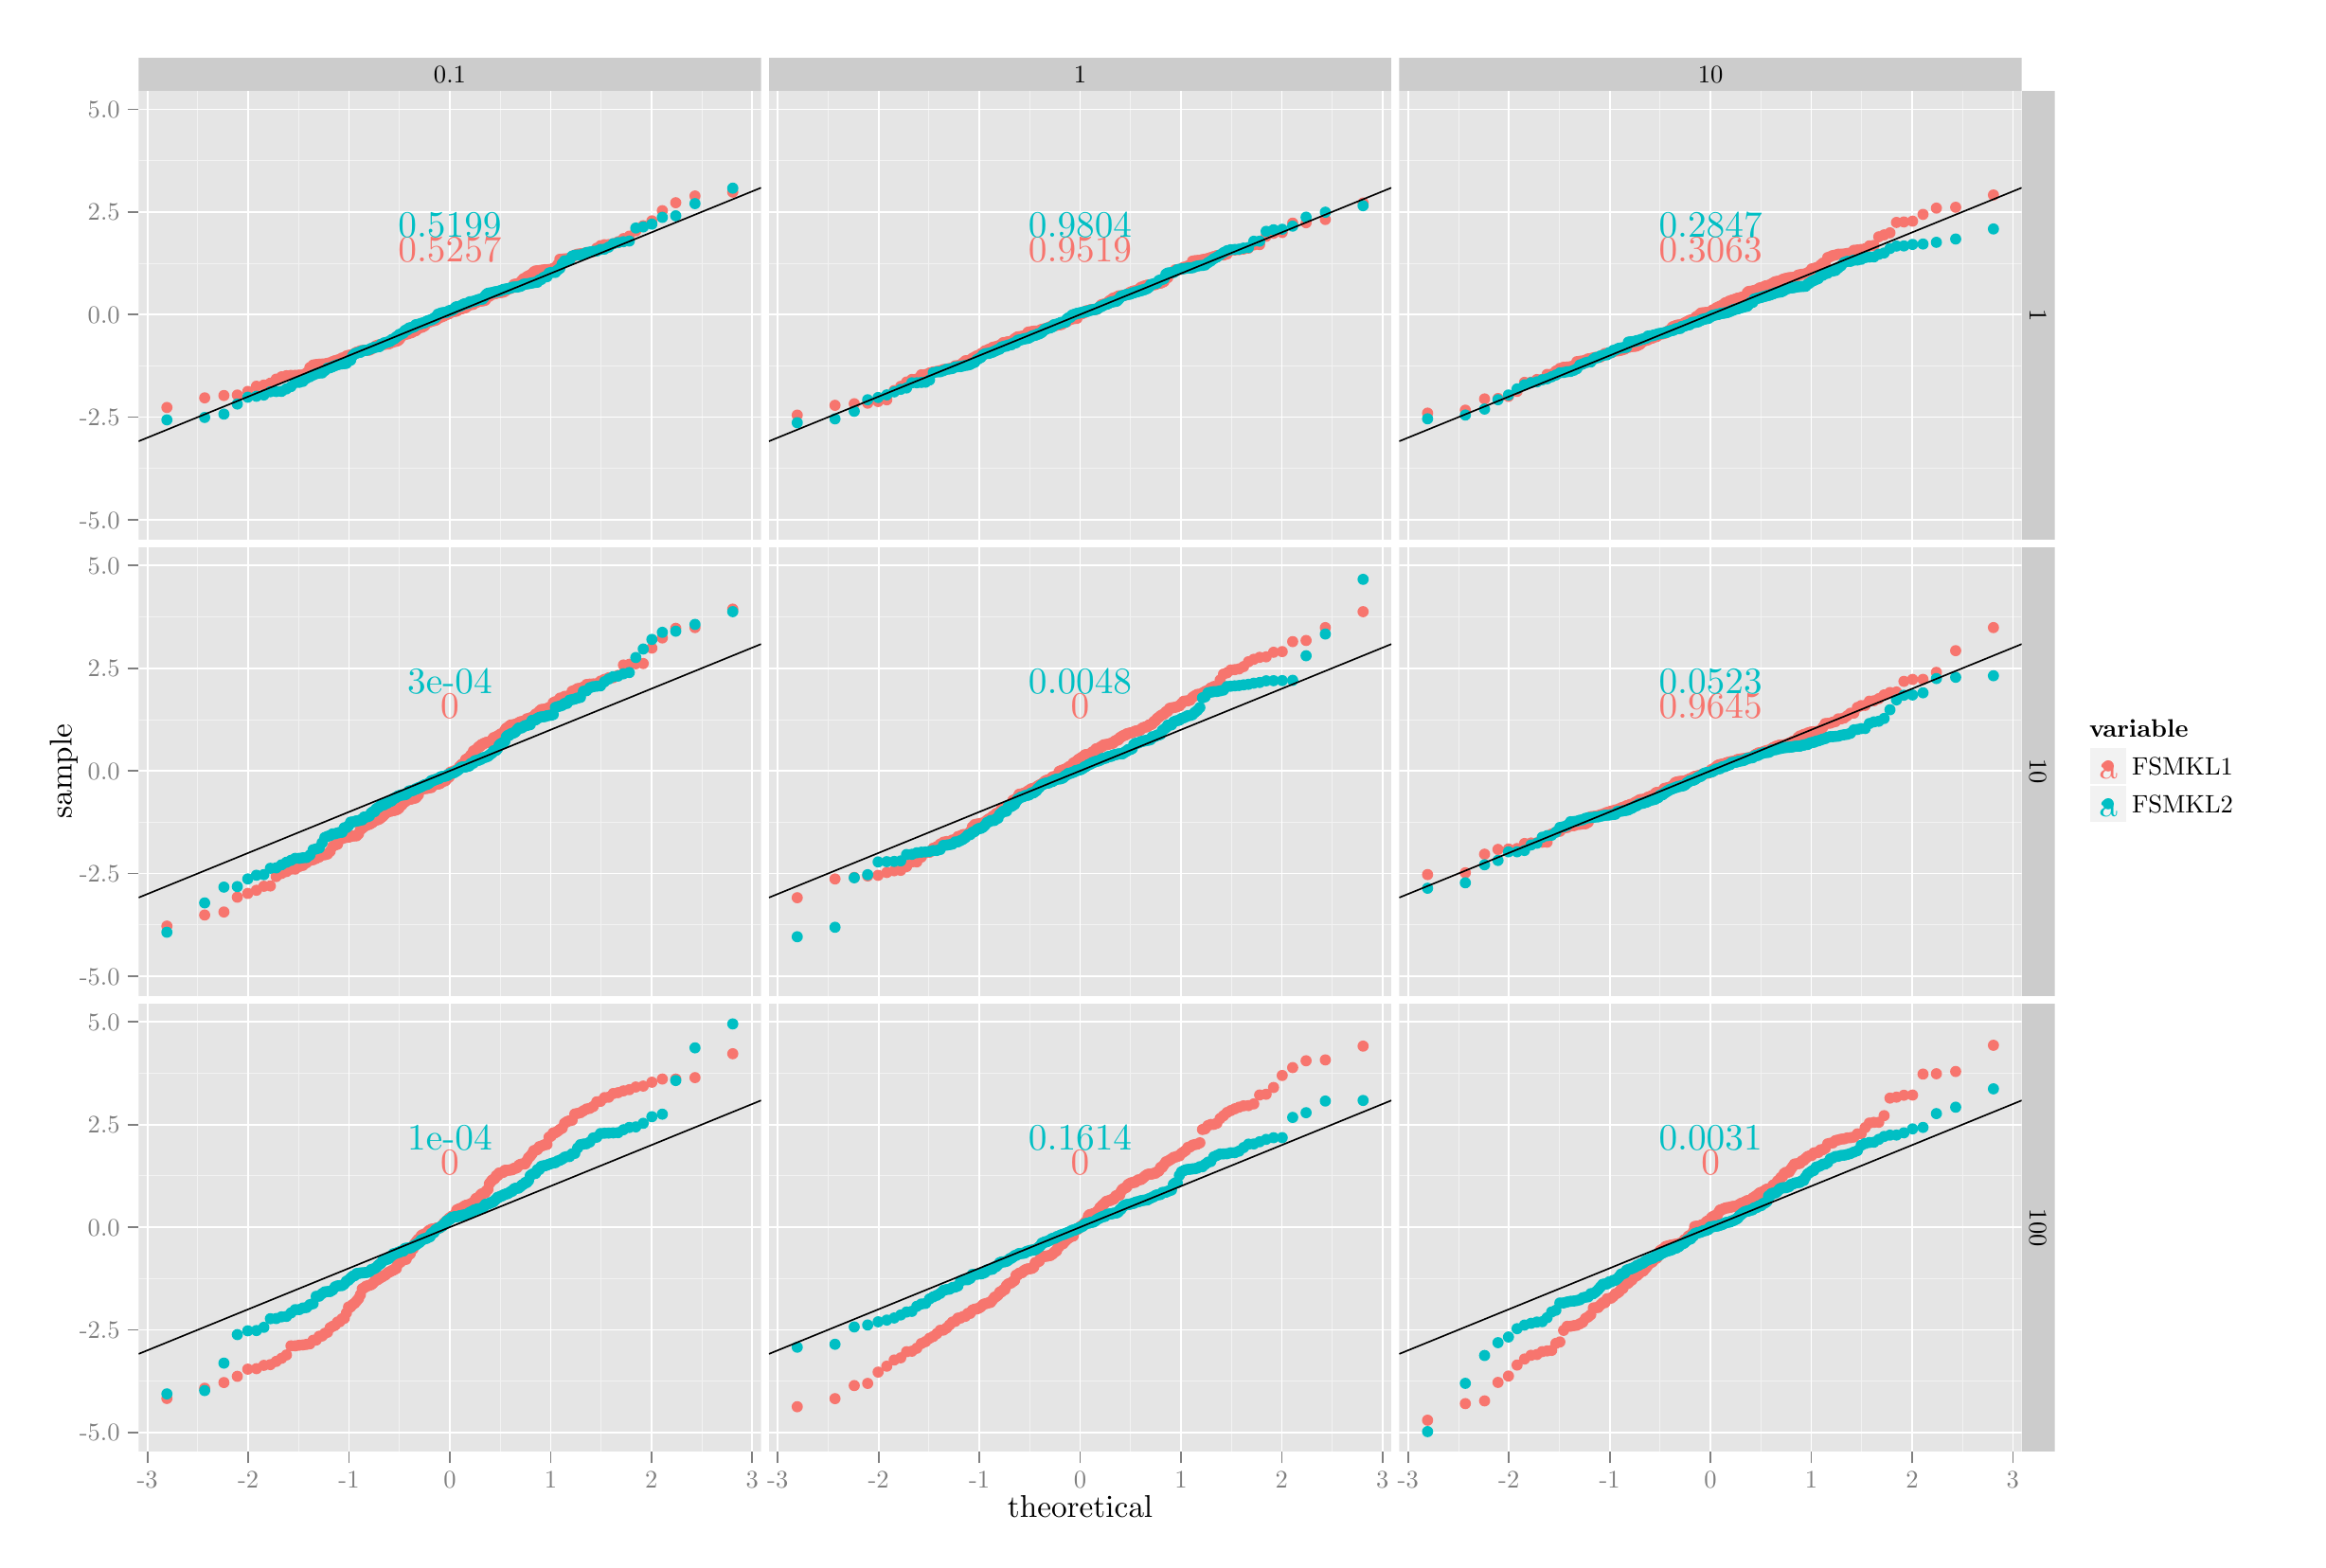
\begin{tikzpicture}[x=1pt,y=1pt]
\definecolor[named]{fillColor}{rgb}{1.00,1.00,1.00}
\path[use as bounding box,fill=fillColor,fill opacity=0.00] (0,0) rectangle (867.24,578.16);
\begin{scope}
\path[clip] (  0.00,  0.00) rectangle (867.24,578.16);
\definecolor[named]{drawColor}{rgb}{1.00,1.00,1.00}
\definecolor[named]{fillColor}{rgb}{1.00,1.00,1.00}

\path[draw=drawColor,line width= 0.6pt,line join=round,line cap=round,fill=fillColor] (  0.00, -0.00) rectangle (867.24,578.16);
\end{scope}
\begin{scope}
\path[clip] ( 42.89,553.48) rectangle (280.37,566.12);
\definecolor[named]{fillColor}{rgb}{0.80,0.80,0.80}

\path[fill=fillColor] ( 42.89,553.48) rectangle (280.37,566.11);
\definecolor[named]{drawColor}{rgb}{0.00,0.00,0.00}

\node[text=drawColor,anchor=base,inner sep=0pt, outer sep=0pt, scale=  0.96] at (161.63,556.49) {0.1};
\end{scope}
\begin{scope}
\path[clip] (283.38,553.48) rectangle (520.87,566.12);
\definecolor[named]{fillColor}{rgb}{0.80,0.80,0.80}

\path[fill=fillColor] (283.38,553.48) rectangle (520.87,566.11);
\definecolor[named]{drawColor}{rgb}{0.00,0.00,0.00}

\node[text=drawColor,anchor=base,inner sep=0pt, outer sep=0pt, scale=  0.96] at (402.13,556.49) {1};
\end{scope}
\begin{scope}
\path[clip] (523.88,553.48) rectangle (761.37,566.12);
\definecolor[named]{fillColor}{rgb}{0.80,0.80,0.80}

\path[fill=fillColor] (523.88,553.48) rectangle (761.37,566.11);
\definecolor[named]{drawColor}{rgb}{0.00,0.00,0.00}

\node[text=drawColor,anchor=base,inner sep=0pt, outer sep=0pt, scale=  0.96] at (642.63,556.49) {10};
\end{scope}
\begin{scope}
\path[clip] ( 42.89,382.34) rectangle (280.37,553.48);
\definecolor[named]{fillColor}{rgb}{0.90,0.90,0.90}

\path[fill=fillColor] ( 42.89,382.34) rectangle (280.37,553.48);
\definecolor[named]{drawColor}{rgb}{0.95,0.95,0.95}

\path[draw=drawColor,line width= 0.3pt,line join=round] ( 42.89,409.39) --
	(280.37,409.39);

\path[draw=drawColor,line width= 0.3pt,line join=round] ( 42.89,448.55) --
	(280.37,448.55);

\path[draw=drawColor,line width= 0.3pt,line join=round] ( 42.89,487.71) --
	(280.37,487.71);

\path[draw=drawColor,line width= 0.3pt,line join=round] ( 42.89,526.88) --
	(280.37,526.88);

\path[draw=drawColor,line width= 0.3pt,line join=round] ( 65.49,382.34) --
	( 65.49,553.48);

\path[draw=drawColor,line width= 0.3pt,line join=round] (103.94,382.34) --
	(103.94,553.48);

\path[draw=drawColor,line width= 0.3pt,line join=round] (142.40,382.34) --
	(142.40,553.48);

\path[draw=drawColor,line width= 0.3pt,line join=round] (180.86,382.34) --
	(180.86,553.48);

\path[draw=drawColor,line width= 0.3pt,line join=round] (219.31,382.34) --
	(219.31,553.48);

\path[draw=drawColor,line width= 0.3pt,line join=round] (257.77,382.34) --
	(257.77,553.48);
\definecolor[named]{drawColor}{rgb}{1.00,1.00,1.00}

\path[draw=drawColor,line width= 0.6pt,line join=round] ( 42.89,389.81) --
	(280.37,389.81);

\path[draw=drawColor,line width= 0.6pt,line join=round] ( 42.89,428.97) --
	(280.37,428.97);

\path[draw=drawColor,line width= 0.6pt,line join=round] ( 42.89,468.13) --
	(280.37,468.13);

\path[draw=drawColor,line width= 0.6pt,line join=round] ( 42.89,507.30) --
	(280.37,507.30);

\path[draw=drawColor,line width= 0.6pt,line join=round] ( 42.89,546.46) --
	(280.37,546.46);

\path[draw=drawColor,line width= 0.6pt,line join=round] ( 46.26,382.34) --
	( 46.26,553.48);

\path[draw=drawColor,line width= 0.6pt,line join=round] ( 84.72,382.34) --
	( 84.72,553.48);

\path[draw=drawColor,line width= 0.6pt,line join=round] (123.17,382.34) --
	(123.17,553.48);

\path[draw=drawColor,line width= 0.6pt,line join=round] (161.63,382.34) --
	(161.63,553.48);

\path[draw=drawColor,line width= 0.6pt,line join=round] (200.09,382.34) --
	(200.09,553.48);

\path[draw=drawColor,line width= 0.6pt,line join=round] (238.54,382.34) --
	(238.54,553.48);

\path[draw=drawColor,line width= 0.6pt,line join=round] (277.00,382.34) --
	(277.00,553.48);
\definecolor[named]{fillColor}{rgb}{0.97,0.46,0.43}

\path[fill=fillColor] ( 53.68,432.65) circle (  2.13);

\path[fill=fillColor] ( 68.09,436.32) circle (  2.13);

\path[fill=fillColor] ( 75.43,437.21) circle (  2.13);

\path[fill=fillColor] ( 80.55,437.40) circle (  2.13);

\path[fill=fillColor] ( 84.54,438.78) circle (  2.13);

\path[fill=fillColor] ( 87.84,440.75) circle (  2.13);

\path[fill=fillColor] ( 90.67,441.20) circle (  2.13);

\path[fill=fillColor] ( 93.16,441.93) circle (  2.13);

\path[fill=fillColor] ( 95.39,443.47) circle (  2.13);

\path[fill=fillColor] ( 97.42,444.35) circle (  2.13);

\path[fill=fillColor] ( 99.29,444.77) circle (  2.13);

\path[fill=fillColor] (101.02,444.90) circle (  2.13);

\path[fill=fillColor] (102.63,444.93) circle (  2.13);

\path[fill=fillColor] (104.15,445.03) circle (  2.13);

\path[fill=fillColor] (105.58,445.10) circle (  2.13);

\path[fill=fillColor] (106.94,445.83) circle (  2.13);

\path[fill=fillColor] (108.23,447.89) circle (  2.13);

\path[fill=fillColor] (109.47,448.85) circle (  2.13);

\path[fill=fillColor] (110.65,449.06) circle (  2.13);

\path[fill=fillColor] (111.79,449.18) circle (  2.13);

\path[fill=fillColor] (112.89,449.22) circle (  2.13);

\path[fill=fillColor] (113.95,449.28) circle (  2.13);

\path[fill=fillColor] (114.97,449.51) circle (  2.13);

\path[fill=fillColor] (115.96,449.71) circle (  2.13);

\path[fill=fillColor] (116.92,450.16) circle (  2.13);

\path[fill=fillColor] (117.85,450.51) circle (  2.13);

\path[fill=fillColor] (118.76,450.75) circle (  2.13);

\path[fill=fillColor] (119.65,451.02) circle (  2.13);

\path[fill=fillColor] (120.51,451.54) circle (  2.13);

\path[fill=fillColor] (121.36,451.65) circle (  2.13);

\path[fill=fillColor] (122.18,452.31) circle (  2.13);

\path[fill=fillColor] (122.99,452.56) circle (  2.13);

\path[fill=fillColor] (123.78,452.65) circle (  2.13);

\path[fill=fillColor] (124.55,452.79) circle (  2.13);

\path[fill=fillColor] (125.31,453.29) circle (  2.13);

\path[fill=fillColor] (126.06,453.76) circle (  2.13);

\path[fill=fillColor] (126.79,453.93) circle (  2.13);

\path[fill=fillColor] (127.51,454.29) circle (  2.13);

\path[fill=fillColor] (128.22,454.31) circle (  2.13);

\path[fill=fillColor] (128.92,454.49) circle (  2.13);

\path[fill=fillColor] (129.61,454.50) circle (  2.13);

\path[fill=fillColor] (130.28,454.52) circle (  2.13);

\path[fill=fillColor] (130.95,454.53) circle (  2.13);

\path[fill=fillColor] (131.61,454.89) circle (  2.13);

\path[fill=fillColor] (132.26,455.23) circle (  2.13);

\path[fill=fillColor] (132.90,455.81) circle (  2.13);

\path[fill=fillColor] (133.53,456.21) circle (  2.13);

\path[fill=fillColor] (134.16,456.44) circle (  2.13);

\path[fill=fillColor] (134.78,456.58) circle (  2.13);

\path[fill=fillColor] (135.39,456.59) circle (  2.13);

\path[fill=fillColor] (135.99,456.63) circle (  2.13);

\path[fill=fillColor] (136.59,456.76) circle (  2.13);

\path[fill=fillColor] (137.18,456.81) circle (  2.13);

\path[fill=fillColor] (137.77,456.90) circle (  2.13);

\path[fill=fillColor] (138.35,456.91) circle (  2.13);

\path[fill=fillColor] (138.93,457.31) circle (  2.13);

\path[fill=fillColor] (139.50,457.44) circle (  2.13);

\path[fill=fillColor] (140.07,457.79) circle (  2.13);

\path[fill=fillColor] (140.63,457.86) circle (  2.13);

\path[fill=fillColor] (141.19,457.92) circle (  2.13);

\path[fill=fillColor] (141.74,458.11) circle (  2.13);

\path[fill=fillColor] (142.29,458.53) circle (  2.13);

\path[fill=fillColor] (142.83,459.29) circle (  2.13);

\path[fill=fillColor] (143.37,460.20) circle (  2.13);

\path[fill=fillColor] (143.91,460.28) circle (  2.13);

\path[fill=fillColor] (144.45,460.52) circle (  2.13);

\path[fill=fillColor] (144.98,460.70) circle (  2.13);

\path[fill=fillColor] (145.50,460.72) circle (  2.13);

\path[fill=fillColor] (146.03,461.02) circle (  2.13);

\path[fill=fillColor] (146.55,461.10) circle (  2.13);

\path[fill=fillColor] (147.07,461.21) circle (  2.13);

\path[fill=fillColor] (147.59,461.63) circle (  2.13);

\path[fill=fillColor] (148.10,461.87) circle (  2.13);

\path[fill=fillColor] (148.61,461.93) circle (  2.13);

\path[fill=fillColor] (149.12,462.39) circle (  2.13);

\path[fill=fillColor] (149.63,462.98) circle (  2.13);

\path[fill=fillColor] (150.13,463.20) circle (  2.13);

\path[fill=fillColor] (150.64,463.25) circle (  2.13);

\path[fill=fillColor] (151.14,463.31) circle (  2.13);

\path[fill=fillColor] (151.64,463.66) circle (  2.13);

\path[fill=fillColor] (152.14,463.91) circle (  2.13);

\path[fill=fillColor] (152.63,464.79) circle (  2.13);

\path[fill=fillColor] (153.13,465.19) circle (  2.13);

\path[fill=fillColor] (153.62,465.19) circle (  2.13);

\path[fill=fillColor] (154.11,465.38) circle (  2.13);

\path[fill=fillColor] (154.60,465.52) circle (  2.13);

\path[fill=fillColor] (155.09,465.78) circle (  2.13);

\path[fill=fillColor] (155.58,465.81) circle (  2.13);

\path[fill=fillColor] (156.07,465.93) circle (  2.13);

\path[fill=fillColor] (156.55,466.14) circle (  2.13);

\path[fill=fillColor] (157.04,466.53) circle (  2.13);

\path[fill=fillColor] (157.52,467.10) circle (  2.13);

\path[fill=fillColor] (158.01,467.10) circle (  2.13);

\path[fill=fillColor] (158.49,467.21) circle (  2.13);

\path[fill=fillColor] (158.98,467.54) circle (  2.13);

\path[fill=fillColor] (159.46,467.59) circle (  2.13);

\path[fill=fillColor] (159.94,468.07) circle (  2.13);

\path[fill=fillColor] (160.42,468.15) circle (  2.13);

\path[fill=fillColor] (160.91,468.29) circle (  2.13);

\path[fill=fillColor] (161.39,468.44) circle (  2.13);

\path[fill=fillColor] (161.87,469.05) circle (  2.13);

\path[fill=fillColor] (162.35,469.16) circle (  2.13);

\path[fill=fillColor] (162.83,469.18) circle (  2.13);

\path[fill=fillColor] (163.32,469.33) circle (  2.13);

\path[fill=fillColor] (163.80,469.38) circle (  2.13);

\path[fill=fillColor] (164.28,469.47) circle (  2.13);

\path[fill=fillColor] (164.77,470.08) circle (  2.13);

\path[fill=fillColor] (165.25,470.08) circle (  2.13);

\path[fill=fillColor] (165.73,470.30) circle (  2.13);

\path[fill=fillColor] (166.22,470.34) circle (  2.13);

\path[fill=fillColor] (166.71,470.51) circle (  2.13);

\path[fill=fillColor] (167.19,470.70) circle (  2.13);

\path[fill=fillColor] (167.68,470.72) circle (  2.13);

\path[fill=fillColor] (168.17,471.25) circle (  2.13);

\path[fill=fillColor] (168.66,471.48) circle (  2.13);

\path[fill=fillColor] (169.15,471.94) circle (  2.13);

\path[fill=fillColor] (169.64,471.97) circle (  2.13);

\path[fill=fillColor] (170.13,471.98) circle (  2.13);

\path[fill=fillColor] (170.63,472.03) circle (  2.13);

\path[fill=fillColor] (171.12,472.61) circle (  2.13);

\path[fill=fillColor] (171.62,472.74) circle (  2.13);

\path[fill=fillColor] (172.12,472.89) circle (  2.13);

\path[fill=fillColor] (172.62,473.11) circle (  2.13);

\path[fill=fillColor] (173.13,473.25) circle (  2.13);

\path[fill=fillColor] (173.63,473.26) circle (  2.13);

\path[fill=fillColor] (174.14,473.42) circle (  2.13);

\path[fill=fillColor] (174.65,473.42) circle (  2.13);

\path[fill=fillColor] (175.16,473.60) circle (  2.13);

\path[fill=fillColor] (175.67,474.79) circle (  2.13);

\path[fill=fillColor] (176.19,475.05) circle (  2.13);

\path[fill=fillColor] (176.71,475.07) circle (  2.13);

\path[fill=fillColor] (177.23,475.68) circle (  2.13);

\path[fill=fillColor] (177.75,475.81) circle (  2.13);

\path[fill=fillColor] (178.28,475.97) circle (  2.13);

\path[fill=fillColor] (178.81,476.03) circle (  2.13);

\path[fill=fillColor] (179.35,476.28) circle (  2.13);

\path[fill=fillColor] (179.88,476.33) circle (  2.13);

\path[fill=fillColor] (180.43,476.46) circle (  2.13);

\path[fill=fillColor] (180.97,476.56) circle (  2.13);

\path[fill=fillColor] (181.52,476.59) circle (  2.13);

\path[fill=fillColor] (182.07,476.73) circle (  2.13);

\path[fill=fillColor] (182.63,476.96) circle (  2.13);

\path[fill=fillColor] (183.19,477.45) circle (  2.13);

\path[fill=fillColor] (183.76,477.93) circle (  2.13);

\path[fill=fillColor] (184.33,477.97) circle (  2.13);

\path[fill=fillColor] (184.91,478.15) circle (  2.13);

\path[fill=fillColor] (185.49,478.45) circle (  2.13);

\path[fill=fillColor] (186.07,479.58) circle (  2.13);

\path[fill=fillColor] (186.67,479.72) circle (  2.13);

\path[fill=fillColor] (187.27,479.75) circle (  2.13);

\path[fill=fillColor] (187.87,479.81) circle (  2.13);

\path[fill=fillColor] (188.48,480.39) circle (  2.13);

\path[fill=fillColor] (189.10,481.09) circle (  2.13);

\path[fill=fillColor] (189.73,481.79) circle (  2.13);

\path[fill=fillColor] (190.36,481.88) circle (  2.13);

\path[fill=fillColor] (191.00,482.55) circle (  2.13);

\path[fill=fillColor] (191.65,482.90) circle (  2.13);

\path[fill=fillColor] (192.31,483.16) circle (  2.13);

\path[fill=fillColor] (192.98,483.62) circle (  2.13);

\path[fill=fillColor] (193.65,484.38) circle (  2.13);

\path[fill=fillColor] (194.34,484.74) circle (  2.13);

\path[fill=fillColor] (195.04,484.83) circle (  2.13);

\path[fill=fillColor] (195.75,484.87) circle (  2.13);

\path[fill=fillColor] (196.47,484.99) circle (  2.13);

\path[fill=fillColor] (197.20,485.11) circle (  2.13);

\path[fill=fillColor] (197.95,485.23) circle (  2.13);

\path[fill=fillColor] (198.71,485.24) circle (  2.13);

\path[fill=fillColor] (199.48,485.30) circle (  2.13);

\path[fill=fillColor] (200.27,485.33) circle (  2.13);

\path[fill=fillColor] (201.08,485.73) circle (  2.13);

\path[fill=fillColor] (201.90,486.01) circle (  2.13);

\path[fill=fillColor] (202.75,487.10) circle (  2.13);

\path[fill=fillColor] (203.61,489.21) circle (  2.13);

\path[fill=fillColor] (204.50,489.27) circle (  2.13);

\path[fill=fillColor] (205.40,489.36) circle (  2.13);

\path[fill=fillColor] (206.34,489.40) circle (  2.13);

\path[fill=fillColor] (207.30,489.53) circle (  2.13);

\path[fill=fillColor] (208.29,489.98) circle (  2.13);

\path[fill=fillColor] (209.31,490.80) circle (  2.13);

\path[fill=fillColor] (210.37,491.16) circle (  2.13);

\path[fill=fillColor] (211.47,491.32) circle (  2.13);

\path[fill=fillColor] (212.60,491.44) circle (  2.13);

\path[fill=fillColor] (213.79,491.80) circle (  2.13);

\path[fill=fillColor] (215.02,491.80) circle (  2.13);

\path[fill=fillColor] (216.32,492.11) circle (  2.13);

\path[fill=fillColor] (217.68,493.45) circle (  2.13);

\path[fill=fillColor] (219.11,494.38) circle (  2.13);

\path[fill=fillColor] (220.63,494.77) circle (  2.13);

\path[fill=fillColor] (222.24,494.79) circle (  2.13);

\path[fill=fillColor] (223.97,495.15) circle (  2.13);

\path[fill=fillColor] (225.84,495.89) circle (  2.13);

\path[fill=fillColor] (227.87,497.09) circle (  2.13);

\path[fill=fillColor] (230.10,498.03) circle (  2.13);

\path[fill=fillColor] (232.59,500.05) circle (  2.13);

\path[fill=fillColor] (235.42,502.01) circle (  2.13);

\path[fill=fillColor] (238.72,503.87) circle (  2.13);

\path[fill=fillColor] (242.71,507.75) circle (  2.13);

\path[fill=fillColor] (247.83,510.79) circle (  2.13);

\path[fill=fillColor] (255.17,513.36) circle (  2.13);

\path[fill=fillColor] (269.58,514.82) circle (  2.13);
\definecolor[named]{fillColor}{rgb}{0.00,0.75,0.77}

\path[fill=fillColor] ( 53.68,427.92) circle (  2.13);

\path[fill=fillColor] ( 68.09,428.84) circle (  2.13);

\path[fill=fillColor] ( 75.43,430.12) circle (  2.13);

\path[fill=fillColor] ( 80.55,433.96) circle (  2.13);

\path[fill=fillColor] ( 84.54,436.57) circle (  2.13);

\path[fill=fillColor] ( 87.84,436.93) circle (  2.13);

\path[fill=fillColor] ( 90.67,437.40) circle (  2.13);

\path[fill=fillColor] ( 93.16,438.66) circle (  2.13);

\path[fill=fillColor] ( 95.39,438.74) circle (  2.13);

\path[fill=fillColor] ( 97.42,438.80) circle (  2.13);

\path[fill=fillColor] ( 99.29,439.74) circle (  2.13);

\path[fill=fillColor] (101.02,440.63) circle (  2.13);

\path[fill=fillColor] (102.63,442.16) circle (  2.13);

\path[fill=fillColor] (104.15,442.24) circle (  2.13);

\path[fill=fillColor] (105.58,442.62) circle (  2.13);

\path[fill=fillColor] (106.94,443.78) circle (  2.13);

\path[fill=fillColor] (108.23,444.39) circle (  2.13);

\path[fill=fillColor] (109.47,445.04) circle (  2.13);

\path[fill=fillColor] (110.65,445.52) circle (  2.13);

\path[fill=fillColor] (111.79,445.80) circle (  2.13);

\path[fill=fillColor] (112.89,445.83) circle (  2.13);

\path[fill=fillColor] (113.95,446.75) circle (  2.13);

\path[fill=fillColor] (114.97,447.64) circle (  2.13);

\path[fill=fillColor] (115.96,447.81) circle (  2.13);

\path[fill=fillColor] (116.92,448.21) circle (  2.13);

\path[fill=fillColor] (117.85,448.62) circle (  2.13);

\path[fill=fillColor] (118.76,448.96) circle (  2.13);

\path[fill=fillColor] (119.65,449.19) circle (  2.13);

\path[fill=fillColor] (120.51,449.31) circle (  2.13);

\path[fill=fillColor] (121.36,449.38) circle (  2.13);

\path[fill=fillColor] (122.18,449.50) circle (  2.13);

\path[fill=fillColor] (122.99,450.55) circle (  2.13);

\path[fill=fillColor] (123.78,450.68) circle (  2.13);

\path[fill=fillColor] (124.55,452.37) circle (  2.13);

\path[fill=fillColor] (125.31,453.15) circle (  2.13);

\path[fill=fillColor] (126.06,453.35) circle (  2.13);

\path[fill=fillColor] (126.79,453.70) circle (  2.13);

\path[fill=fillColor] (127.51,453.70) circle (  2.13);

\path[fill=fillColor] (128.22,454.28) circle (  2.13);

\path[fill=fillColor] (128.92,454.37) circle (  2.13);

\path[fill=fillColor] (129.61,454.46) circle (  2.13);

\path[fill=fillColor] (130.28,454.54) circle (  2.13);

\path[fill=fillColor] (130.95,454.80) circle (  2.13);

\path[fill=fillColor] (131.61,455.19) circle (  2.13);

\path[fill=fillColor] (132.26,455.32) circle (  2.13);

\path[fill=fillColor] (132.90,455.65) circle (  2.13);

\path[fill=fillColor] (133.53,455.67) circle (  2.13);

\path[fill=fillColor] (134.16,455.84) circle (  2.13);

\path[fill=fillColor] (134.78,455.87) circle (  2.13);

\path[fill=fillColor] (135.39,456.76) circle (  2.13);

\path[fill=fillColor] (135.99,456.84) circle (  2.13);

\path[fill=fillColor] (136.59,457.33) circle (  2.13);

\path[fill=fillColor] (137.18,457.36) circle (  2.13);

\path[fill=fillColor] (137.77,457.61) circle (  2.13);

\path[fill=fillColor] (138.35,457.75) circle (  2.13);

\path[fill=fillColor] (138.93,457.89) circle (  2.13);

\path[fill=fillColor] (139.50,458.59) circle (  2.13);

\path[fill=fillColor] (140.07,458.69) circle (  2.13);

\path[fill=fillColor] (140.63,458.96) circle (  2.13);

\path[fill=fillColor] (141.19,459.61) circle (  2.13);

\path[fill=fillColor] (141.74,459.86) circle (  2.13);

\path[fill=fillColor] (142.29,460.50) circle (  2.13);

\path[fill=fillColor] (142.83,460.50) circle (  2.13);

\path[fill=fillColor] (143.37,460.95) circle (  2.13);

\path[fill=fillColor] (143.91,461.02) circle (  2.13);

\path[fill=fillColor] (144.45,461.97) circle (  2.13);

\path[fill=fillColor] (144.98,462.22) circle (  2.13);

\path[fill=fillColor] (145.50,462.25) circle (  2.13);

\path[fill=fillColor] (146.03,462.96) circle (  2.13);

\path[fill=fillColor] (146.55,463.05) circle (  2.13);

\path[fill=fillColor] (147.07,463.15) circle (  2.13);

\path[fill=fillColor] (147.59,463.33) circle (  2.13);

\path[fill=fillColor] (148.10,463.50) circle (  2.13);

\path[fill=fillColor] (148.61,464.22) circle (  2.13);

\path[fill=fillColor] (149.12,464.31) circle (  2.13);

\path[fill=fillColor] (149.63,464.34) circle (  2.13);

\path[fill=fillColor] (150.13,464.47) circle (  2.13);

\path[fill=fillColor] (150.64,464.73) circle (  2.13);

\path[fill=fillColor] (151.14,464.84) circle (  2.13);

\path[fill=fillColor] (151.64,464.91) circle (  2.13);

\path[fill=fillColor] (152.14,465.06) circle (  2.13);

\path[fill=fillColor] (152.63,465.50) circle (  2.13);

\path[fill=fillColor] (153.13,465.68) circle (  2.13);

\path[fill=fillColor] (153.62,465.85) circle (  2.13);

\path[fill=fillColor] (154.11,466.01) circle (  2.13);

\path[fill=fillColor] (154.60,466.09) circle (  2.13);

\path[fill=fillColor] (155.09,466.33) circle (  2.13);

\path[fill=fillColor] (155.58,466.76) circle (  2.13);

\path[fill=fillColor] (156.07,466.82) circle (  2.13);

\path[fill=fillColor] (156.55,467.41) circle (  2.13);

\path[fill=fillColor] (157.04,468.21) circle (  2.13);

\path[fill=fillColor] (157.52,468.31) circle (  2.13);

\path[fill=fillColor] (158.01,468.58) circle (  2.13);

\path[fill=fillColor] (158.49,468.74) circle (  2.13);

\path[fill=fillColor] (158.98,468.79) circle (  2.13);

\path[fill=fillColor] (159.46,468.81) circle (  2.13);

\path[fill=fillColor] (159.94,468.90) circle (  2.13);

\path[fill=fillColor] (160.42,468.93) circle (  2.13);

\path[fill=fillColor] (160.91,469.28) circle (  2.13);

\path[fill=fillColor] (161.39,469.57) circle (  2.13);

\path[fill=fillColor] (161.87,469.65) circle (  2.13);

\path[fill=fillColor] (162.35,469.67) circle (  2.13);

\path[fill=fillColor] (162.83,470.01) circle (  2.13);

\path[fill=fillColor] (163.32,470.29) circle (  2.13);

\path[fill=fillColor] (163.80,470.90) circle (  2.13);

\path[fill=fillColor] (164.28,471.09) circle (  2.13);

\path[fill=fillColor] (164.77,471.09) circle (  2.13);

\path[fill=fillColor] (165.25,471.18) circle (  2.13);

\path[fill=fillColor] (165.73,471.37) circle (  2.13);

\path[fill=fillColor] (166.22,471.62) circle (  2.13);

\path[fill=fillColor] (166.71,471.95) circle (  2.13);

\path[fill=fillColor] (167.19,472.20) circle (  2.13);

\path[fill=fillColor] (167.68,472.27) circle (  2.13);

\path[fill=fillColor] (168.17,472.31) circle (  2.13);

\path[fill=fillColor] (168.66,472.41) circle (  2.13);

\path[fill=fillColor] (169.15,472.96) circle (  2.13);

\path[fill=fillColor] (169.64,473.00) circle (  2.13);

\path[fill=fillColor] (170.13,473.01) circle (  2.13);

\path[fill=fillColor] (170.63,473.13) circle (  2.13);

\path[fill=fillColor] (171.12,473.27) circle (  2.13);

\path[fill=fillColor] (171.62,473.48) circle (  2.13);

\path[fill=fillColor] (172.12,473.62) circle (  2.13);

\path[fill=fillColor] (172.62,473.82) circle (  2.13);

\path[fill=fillColor] (173.13,473.95) circle (  2.13);

\path[fill=fillColor] (173.63,473.97) circle (  2.13);

\path[fill=fillColor] (174.14,474.02) circle (  2.13);

\path[fill=fillColor] (174.65,474.66) circle (  2.13);

\path[fill=fillColor] (175.16,475.32) circle (  2.13);

\path[fill=fillColor] (175.67,475.89) circle (  2.13);

\path[fill=fillColor] (176.19,476.23) circle (  2.13);

\path[fill=fillColor] (176.71,476.28) circle (  2.13);

\path[fill=fillColor] (177.23,476.30) circle (  2.13);

\path[fill=fillColor] (177.75,476.48) circle (  2.13);

\path[fill=fillColor] (178.28,476.55) circle (  2.13);

\path[fill=fillColor] (178.81,476.78) circle (  2.13);

\path[fill=fillColor] (179.35,476.81) circle (  2.13);

\path[fill=fillColor] (179.88,476.89) circle (  2.13);

\path[fill=fillColor] (180.43,477.06) circle (  2.13);

\path[fill=fillColor] (180.97,477.23) circle (  2.13);

\path[fill=fillColor] (181.52,477.39) circle (  2.13);

\path[fill=fillColor] (182.07,477.71) circle (  2.13);

\path[fill=fillColor] (182.63,477.72) circle (  2.13);

\path[fill=fillColor] (183.19,477.88) circle (  2.13);

\path[fill=fillColor] (183.76,477.98) circle (  2.13);

\path[fill=fillColor] (184.33,478.12) circle (  2.13);

\path[fill=fillColor] (184.91,478.28) circle (  2.13);

\path[fill=fillColor] (185.49,478.52) circle (  2.13);

\path[fill=fillColor] (186.07,478.58) circle (  2.13);

\path[fill=fillColor] (186.67,478.60) circle (  2.13);

\path[fill=fillColor] (187.27,478.60) circle (  2.13);

\path[fill=fillColor] (187.87,478.85) circle (  2.13);

\path[fill=fillColor] (188.48,478.85) circle (  2.13);

\path[fill=fillColor] (189.10,479.14) circle (  2.13);

\path[fill=fillColor] (189.73,479.67) circle (  2.13);

\path[fill=fillColor] (190.36,479.75) circle (  2.13);

\path[fill=fillColor] (191.00,479.84) circle (  2.13);

\path[fill=fillColor] (191.65,479.88) circle (  2.13);

\path[fill=fillColor] (192.31,480.06) circle (  2.13);

\path[fill=fillColor] (192.98,480.15) circle (  2.13);

\path[fill=fillColor] (193.65,480.33) circle (  2.13);

\path[fill=fillColor] (194.34,480.36) circle (  2.13);

\path[fill=fillColor] (195.04,480.45) circle (  2.13);

\path[fill=fillColor] (195.75,481.32) circle (  2.13);

\path[fill=fillColor] (196.47,481.48) circle (  2.13);

\path[fill=fillColor] (197.20,482.17) circle (  2.13);

\path[fill=fillColor] (197.95,482.55) circle (  2.13);

\path[fill=fillColor] (198.71,482.57) circle (  2.13);

\path[fill=fillColor] (199.48,483.96) circle (  2.13);

\path[fill=fillColor] (200.27,484.16) circle (  2.13);

\path[fill=fillColor] (201.08,484.22) circle (  2.13);

\path[fill=fillColor] (201.90,484.22) circle (  2.13);

\path[fill=fillColor] (202.75,485.12) circle (  2.13);

\path[fill=fillColor] (203.61,485.74) circle (  2.13);

\path[fill=fillColor] (204.50,487.49) circle (  2.13);

\path[fill=fillColor] (205.40,488.60) circle (  2.13);

\path[fill=fillColor] (206.34,488.64) circle (  2.13);

\path[fill=fillColor] (207.30,488.90) circle (  2.13);

\path[fill=fillColor] (208.29,490.39) circle (  2.13);

\path[fill=fillColor] (209.31,490.74) circle (  2.13);

\path[fill=fillColor] (210.37,490.82) circle (  2.13);

\path[fill=fillColor] (211.47,490.85) circle (  2.13);

\path[fill=fillColor] (212.60,491.22) circle (  2.13);

\path[fill=fillColor] (213.79,491.73) circle (  2.13);

\path[fill=fillColor] (215.02,491.99) circle (  2.13);

\path[fill=fillColor] (216.32,492.22) circle (  2.13);

\path[fill=fillColor] (217.68,492.37) circle (  2.13);

\path[fill=fillColor] (219.11,492.96) circle (  2.13);

\path[fill=fillColor] (220.63,493.08) circle (  2.13);

\path[fill=fillColor] (222.24,493.85) circle (  2.13);

\path[fill=fillColor] (223.97,495.13) circle (  2.13);

\path[fill=fillColor] (225.84,495.56) circle (  2.13);

\path[fill=fillColor] (227.87,495.92) circle (  2.13);

\path[fill=fillColor] (230.10,496.17) circle (  2.13);

\path[fill=fillColor] (232.59,501.13) circle (  2.13);

\path[fill=fillColor] (235.42,501.55) circle (  2.13);

\path[fill=fillColor] (238.72,502.63) circle (  2.13);

\path[fill=fillColor] (242.71,505.20) circle (  2.13);

\path[fill=fillColor] (247.83,505.79) circle (  2.13);

\path[fill=fillColor] (255.17,510.45) circle (  2.13);

\path[fill=fillColor] (269.58,516.34) circle (  2.13);
\definecolor[named]{drawColor}{rgb}{0.00,0.00,0.00}
\definecolor[named]{fillColor}{rgb}{0.00,0.00,0.00}

\path[draw=drawColor,line width= 0.6pt,line join=round,fill=fillColor] ( 42.89,419.76) -- (280.37,516.50);
\definecolor[named]{drawColor}{rgb}{0.97,0.46,0.43}

\node[text=drawColor,anchor=base,inner sep=0pt, outer sep=0pt, scale=  1.42] at (161.63,488.32) {0.5257};
\definecolor[named]{drawColor}{rgb}{0.00,0.75,0.77}

\node[text=drawColor,anchor=base,inner sep=0pt, outer sep=0pt, scale=  1.42] at (161.63,497.72) {0.5199};
\end{scope}
\begin{scope}
\path[clip] ( 42.89,208.19) rectangle (280.37,379.33);
\definecolor[named]{fillColor}{rgb}{0.90,0.90,0.90}

\path[fill=fillColor] ( 42.89,208.19) rectangle (280.37,379.33);
\definecolor[named]{drawColor}{rgb}{0.95,0.95,0.95}

\path[draw=drawColor,line width= 0.3pt,line join=round] ( 42.89,235.24) --
	(280.37,235.24);

\path[draw=drawColor,line width= 0.3pt,line join=round] ( 42.89,274.40) --
	(280.37,274.40);

\path[draw=drawColor,line width= 0.3pt,line join=round] ( 42.89,313.56) --
	(280.37,313.56);

\path[draw=drawColor,line width= 0.3pt,line join=round] ( 42.89,352.72) --
	(280.37,352.72);

\path[draw=drawColor,line width= 0.3pt,line join=round] ( 65.49,208.19) --
	( 65.49,379.33);

\path[draw=drawColor,line width= 0.3pt,line join=round] (103.94,208.19) --
	(103.94,379.33);

\path[draw=drawColor,line width= 0.3pt,line join=round] (142.40,208.19) --
	(142.40,379.33);

\path[draw=drawColor,line width= 0.3pt,line join=round] (180.86,208.19) --
	(180.86,379.33);

\path[draw=drawColor,line width= 0.3pt,line join=round] (219.31,208.19) --
	(219.31,379.33);

\path[draw=drawColor,line width= 0.3pt,line join=round] (257.77,208.19) --
	(257.77,379.33);
\definecolor[named]{drawColor}{rgb}{1.00,1.00,1.00}

\path[draw=drawColor,line width= 0.6pt,line join=round] ( 42.89,215.65) --
	(280.37,215.65);

\path[draw=drawColor,line width= 0.6pt,line join=round] ( 42.89,254.82) --
	(280.37,254.82);

\path[draw=drawColor,line width= 0.6pt,line join=round] ( 42.89,293.98) --
	(280.37,293.98);

\path[draw=drawColor,line width= 0.6pt,line join=round] ( 42.89,333.14) --
	(280.37,333.14);

\path[draw=drawColor,line width= 0.6pt,line join=round] ( 42.89,372.31) --
	(280.37,372.31);

\path[draw=drawColor,line width= 0.6pt,line join=round] ( 46.26,208.19) --
	( 46.26,379.33);

\path[draw=drawColor,line width= 0.6pt,line join=round] ( 84.72,208.19) --
	( 84.72,379.33);

\path[draw=drawColor,line width= 0.6pt,line join=round] (123.17,208.19) --
	(123.17,379.33);

\path[draw=drawColor,line width= 0.6pt,line join=round] (161.63,208.19) --
	(161.63,379.33);

\path[draw=drawColor,line width= 0.6pt,line join=round] (200.09,208.19) --
	(200.09,379.33);

\path[draw=drawColor,line width= 0.6pt,line join=round] (238.54,208.19) --
	(238.54,379.33);

\path[draw=drawColor,line width= 0.6pt,line join=round] (277.00,208.19) --
	(277.00,379.33);
\definecolor[named]{fillColor}{rgb}{0.97,0.46,0.43}

\path[fill=fillColor] ( 53.68,234.73) circle (  2.13);

\path[fill=fillColor] ( 68.09,238.96) circle (  2.13);

\path[fill=fillColor] ( 75.43,240.11) circle (  2.13);

\path[fill=fillColor] ( 80.55,245.76) circle (  2.13);

\path[fill=fillColor] ( 84.54,247.20) circle (  2.13);

\path[fill=fillColor] ( 87.84,248.40) circle (  2.13);

\path[fill=fillColor] ( 90.67,249.93) circle (  2.13);

\path[fill=fillColor] ( 93.16,250.05) circle (  2.13);

\path[fill=fillColor] ( 95.39,253.63) circle (  2.13);

\path[fill=fillColor] ( 97.42,254.82) circle (  2.13);

\path[fill=fillColor] ( 99.29,255.53) circle (  2.13);

\path[fill=fillColor] (101.02,256.48) circle (  2.13);

\path[fill=fillColor] (102.63,256.48) circle (  2.13);

\path[fill=fillColor] (104.15,257.47) circle (  2.13);

\path[fill=fillColor] (105.58,257.90) circle (  2.13);

\path[fill=fillColor] (106.94,258.90) circle (  2.13);

\path[fill=fillColor] (108.23,259.79) circle (  2.13);

\path[fill=fillColor] (109.47,260.04) circle (  2.13);

\path[fill=fillColor] (110.65,260.56) circle (  2.13);

\path[fill=fillColor] (111.79,261.09) circle (  2.13);

\path[fill=fillColor] (112.89,261.86) circle (  2.13);

\path[fill=fillColor] (113.95,261.95) circle (  2.13);

\path[fill=fillColor] (114.97,262.24) circle (  2.13);

\path[fill=fillColor] (115.96,263.26) circle (  2.13);

\path[fill=fillColor] (116.92,265.15) circle (  2.13);

\path[fill=fillColor] (117.85,265.69) circle (  2.13);

\path[fill=fillColor] (118.76,265.96) circle (  2.13);

\path[fill=fillColor] (119.65,267.71) circle (  2.13);

\path[fill=fillColor] (120.51,268.14) circle (  2.13);

\path[fill=fillColor] (121.36,268.42) circle (  2.13);

\path[fill=fillColor] (122.18,268.62) circle (  2.13);

\path[fill=fillColor] (122.99,268.66) circle (  2.13);

\path[fill=fillColor] (123.78,268.90) circle (  2.13);

\path[fill=fillColor] (124.55,269.15) circle (  2.13);

\path[fill=fillColor] (125.31,269.17) circle (  2.13);

\path[fill=fillColor] (126.06,269.18) circle (  2.13);

\path[fill=fillColor] (126.79,269.92) circle (  2.13);

\path[fill=fillColor] (127.51,271.55) circle (  2.13);

\path[fill=fillColor] (128.22,272.06) circle (  2.13);

\path[fill=fillColor] (128.92,272.64) circle (  2.13);

\path[fill=fillColor] (129.61,273.15) circle (  2.13);

\path[fill=fillColor] (130.28,273.41) circle (  2.13);

\path[fill=fillColor] (130.95,273.58) circle (  2.13);

\path[fill=fillColor] (131.61,273.93) circle (  2.13);

\path[fill=fillColor] (132.26,274.35) circle (  2.13);

\path[fill=fillColor] (132.90,275.02) circle (  2.13);

\path[fill=fillColor] (133.53,275.15) circle (  2.13);

\path[fill=fillColor] (134.16,275.33) circle (  2.13);

\path[fill=fillColor] (134.78,275.59) circle (  2.13);

\path[fill=fillColor] (135.39,276.10) circle (  2.13);

\path[fill=fillColor] (135.99,276.54) circle (  2.13);

\path[fill=fillColor] (136.59,277.15) circle (  2.13);

\path[fill=fillColor] (137.18,277.84) circle (  2.13);

\path[fill=fillColor] (137.77,278.19) circle (  2.13);

\path[fill=fillColor] (138.35,278.51) circle (  2.13);

\path[fill=fillColor] (138.93,278.53) circle (  2.13);

\path[fill=fillColor] (139.50,278.73) circle (  2.13);

\path[fill=fillColor] (140.07,278.82) circle (  2.13);

\path[fill=fillColor] (140.63,278.94) circle (  2.13);

\path[fill=fillColor] (141.19,279.11) circle (  2.13);

\path[fill=fillColor] (141.74,279.33) circle (  2.13);

\path[fill=fillColor] (142.29,279.82) circle (  2.13);

\path[fill=fillColor] (142.83,280.88) circle (  2.13);

\path[fill=fillColor] (143.37,280.99) circle (  2.13);

\path[fill=fillColor] (143.91,282.09) circle (  2.13);

\path[fill=fillColor] (144.45,282.10) circle (  2.13);

\path[fill=fillColor] (144.98,282.53) circle (  2.13);

\path[fill=fillColor] (145.50,282.93) circle (  2.13);

\path[fill=fillColor] (146.03,283.08) circle (  2.13);

\path[fill=fillColor] (146.55,283.17) circle (  2.13);

\path[fill=fillColor] (147.07,283.23) circle (  2.13);

\path[fill=fillColor] (147.59,283.51) circle (  2.13);

\path[fill=fillColor] (148.10,283.55) circle (  2.13);

\path[fill=fillColor] (148.61,283.66) circle (  2.13);

\path[fill=fillColor] (149.12,284.23) circle (  2.13);

\path[fill=fillColor] (149.63,284.87) circle (  2.13);

\path[fill=fillColor] (150.13,286.96) circle (  2.13);

\path[fill=fillColor] (150.64,287.14) circle (  2.13);

\path[fill=fillColor] (151.14,287.16) circle (  2.13);

\path[fill=fillColor] (151.64,287.20) circle (  2.13);

\path[fill=fillColor] (152.14,287.21) circle (  2.13);

\path[fill=fillColor] (152.63,287.30) circle (  2.13);

\path[fill=fillColor] (153.13,287.34) circle (  2.13);

\path[fill=fillColor] (153.62,287.61) circle (  2.13);

\path[fill=fillColor] (154.11,287.61) circle (  2.13);

\path[fill=fillColor] (154.60,287.61) circle (  2.13);

\path[fill=fillColor] (155.09,288.64) circle (  2.13);

\path[fill=fillColor] (155.58,288.72) circle (  2.13);

\path[fill=fillColor] (156.07,288.76) circle (  2.13);

\path[fill=fillColor] (156.55,288.90) circle (  2.13);

\path[fill=fillColor] (157.04,288.96) circle (  2.13);

\path[fill=fillColor] (157.52,289.00) circle (  2.13);

\path[fill=fillColor] (158.01,289.22) circle (  2.13);

\path[fill=fillColor] (158.49,289.65) circle (  2.13);

\path[fill=fillColor] (158.98,289.93) circle (  2.13);

\path[fill=fillColor] (159.46,290.19) circle (  2.13);

\path[fill=fillColor] (159.94,290.20) circle (  2.13);

\path[fill=fillColor] (160.42,290.82) circle (  2.13);

\path[fill=fillColor] (160.91,291.29) circle (  2.13);

\path[fill=fillColor] (161.39,291.65) circle (  2.13);

\path[fill=fillColor] (161.87,293.49) circle (  2.13);

\path[fill=fillColor] (162.35,293.50) circle (  2.13);

\path[fill=fillColor] (162.83,293.54) circle (  2.13);

\path[fill=fillColor] (163.32,293.98) circle (  2.13);

\path[fill=fillColor] (163.80,294.08) circle (  2.13);

\path[fill=fillColor] (164.28,294.17) circle (  2.13);

\path[fill=fillColor] (164.77,294.60) circle (  2.13);

\path[fill=fillColor] (165.25,295.49) circle (  2.13);

\path[fill=fillColor] (165.73,295.93) circle (  2.13);

\path[fill=fillColor] (166.22,296.46) circle (  2.13);

\path[fill=fillColor] (166.71,296.69) circle (  2.13);

\path[fill=fillColor] (167.19,296.89) circle (  2.13);

\path[fill=fillColor] (167.68,298.30) circle (  2.13);

\path[fill=fillColor] (168.17,298.36) circle (  2.13);

\path[fill=fillColor] (168.66,298.87) circle (  2.13);

\path[fill=fillColor] (169.15,298.93) circle (  2.13);

\path[fill=fillColor] (169.64,300.01) circle (  2.13);

\path[fill=fillColor] (170.13,300.40) circle (  2.13);

\path[fill=fillColor] (170.63,301.54) circle (  2.13);

\path[fill=fillColor] (171.12,301.75) circle (  2.13);

\path[fill=fillColor] (171.62,301.85) circle (  2.13);

\path[fill=fillColor] (172.12,302.55) circle (  2.13);

\path[fill=fillColor] (172.62,303.16) circle (  2.13);

\path[fill=fillColor] (173.13,303.23) circle (  2.13);

\path[fill=fillColor] (173.63,303.96) circle (  2.13);

\path[fill=fillColor] (174.14,304.06) circle (  2.13);

\path[fill=fillColor] (174.65,304.46) circle (  2.13);

\path[fill=fillColor] (175.16,304.61) circle (  2.13);

\path[fill=fillColor] (175.67,304.87) circle (  2.13);

\path[fill=fillColor] (176.19,304.88) circle (  2.13);

\path[fill=fillColor] (176.71,305.03) circle (  2.13);

\path[fill=fillColor] (177.23,305.06) circle (  2.13);

\path[fill=fillColor] (177.75,305.83) circle (  2.13);

\path[fill=fillColor] (178.28,306.61) circle (  2.13);

\path[fill=fillColor] (178.81,306.71) circle (  2.13);

\path[fill=fillColor] (179.35,306.96) circle (  2.13);

\path[fill=fillColor] (179.88,307.32) circle (  2.13);

\path[fill=fillColor] (180.43,307.55) circle (  2.13);

\path[fill=fillColor] (180.97,308.04) circle (  2.13);

\path[fill=fillColor] (181.52,308.06) circle (  2.13);

\path[fill=fillColor] (182.07,308.31) circle (  2.13);

\path[fill=fillColor] (182.63,309.47) circle (  2.13);

\path[fill=fillColor] (183.19,310.29) circle (  2.13);

\path[fill=fillColor] (183.76,310.44) circle (  2.13);

\path[fill=fillColor] (184.33,311.11) circle (  2.13);

\path[fill=fillColor] (184.91,311.48) circle (  2.13);

\path[fill=fillColor] (185.49,311.49) circle (  2.13);

\path[fill=fillColor] (186.07,311.59) circle (  2.13);

\path[fill=fillColor] (186.67,311.73) circle (  2.13);

\path[fill=fillColor] (187.27,311.98) circle (  2.13);

\path[fill=fillColor] (187.87,312.32) circle (  2.13);

\path[fill=fillColor] (188.48,312.66) circle (  2.13);

\path[fill=fillColor] (189.10,312.79) circle (  2.13);

\path[fill=fillColor] (189.73,312.93) circle (  2.13);

\path[fill=fillColor] (190.36,312.97) circle (  2.13);

\path[fill=fillColor] (191.00,313.83) circle (  2.13);

\path[fill=fillColor] (191.65,313.88) circle (  2.13);

\path[fill=fillColor] (192.31,314.19) circle (  2.13);

\path[fill=fillColor] (192.98,314.34) circle (  2.13);

\path[fill=fillColor] (193.65,314.82) circle (  2.13);

\path[fill=fillColor] (194.34,315.63) circle (  2.13);

\path[fill=fillColor] (195.04,315.67) circle (  2.13);

\path[fill=fillColor] (195.75,316.74) circle (  2.13);

\path[fill=fillColor] (196.47,317.37) circle (  2.13);

\path[fill=fillColor] (197.20,317.43) circle (  2.13);

\path[fill=fillColor] (197.95,317.56) circle (  2.13);

\path[fill=fillColor] (198.71,317.75) circle (  2.13);

\path[fill=fillColor] (199.48,318.14) circle (  2.13);

\path[fill=fillColor] (200.27,318.28) circle (  2.13);

\path[fill=fillColor] (201.08,319.98) circle (  2.13);

\path[fill=fillColor] (201.90,320.37) circle (  2.13);

\path[fill=fillColor] (202.75,320.50) circle (  2.13);

\path[fill=fillColor] (203.61,321.71) circle (  2.13);

\path[fill=fillColor] (204.50,321.77) circle (  2.13);

\path[fill=fillColor] (205.40,322.39) circle (  2.13);

\path[fill=fillColor] (206.34,322.42) circle (  2.13);

\path[fill=fillColor] (207.30,322.70) circle (  2.13);

\path[fill=fillColor] (208.29,324.38) circle (  2.13);

\path[fill=fillColor] (209.31,324.73) circle (  2.13);

\path[fill=fillColor] (210.37,325.37) circle (  2.13);

\path[fill=fillColor] (211.47,325.51) circle (  2.13);

\path[fill=fillColor] (212.60,325.96) circle (  2.13);

\path[fill=fillColor] (213.79,326.91) circle (  2.13);

\path[fill=fillColor] (215.02,327.07) circle (  2.13);

\path[fill=fillColor] (216.32,327.15) circle (  2.13);

\path[fill=fillColor] (217.68,327.25) circle (  2.13);

\path[fill=fillColor] (219.11,328.21) circle (  2.13);

\path[fill=fillColor] (220.63,328.88) circle (  2.13);

\path[fill=fillColor] (222.24,329.49) circle (  2.13);

\path[fill=fillColor] (223.97,329.55) circle (  2.13);

\path[fill=fillColor] (225.84,330.41) circle (  2.13);

\path[fill=fillColor] (227.87,334.37) circle (  2.13);

\path[fill=fillColor] (230.10,334.64) circle (  2.13);

\path[fill=fillColor] (232.59,334.85) circle (  2.13);

\path[fill=fillColor] (235.42,334.93) circle (  2.13);

\path[fill=fillColor] (238.72,340.82) circle (  2.13);

\path[fill=fillColor] (242.71,344.69) circle (  2.13);

\path[fill=fillColor] (247.83,348.37) circle (  2.13);

\path[fill=fillColor] (255.17,348.65) circle (  2.13);

\path[fill=fillColor] (269.58,355.70) circle (  2.13);
\definecolor[named]{fillColor}{rgb}{0.00,0.75,0.77}

\path[fill=fillColor] ( 53.68,232.39) circle (  2.13);

\path[fill=fillColor] ( 68.09,243.57) circle (  2.13);

\path[fill=fillColor] ( 75.43,249.60) circle (  2.13);

\path[fill=fillColor] ( 80.55,249.81) circle (  2.13);

\path[fill=fillColor] ( 84.54,252.73) circle (  2.13);

\path[fill=fillColor] ( 87.84,254.14) circle (  2.13);

\path[fill=fillColor] ( 90.67,254.37) circle (  2.13);

\path[fill=fillColor] ( 93.16,256.79) circle (  2.13);

\path[fill=fillColor] ( 95.39,256.95) circle (  2.13);

\path[fill=fillColor] ( 97.42,258.12) circle (  2.13);

\path[fill=fillColor] ( 99.29,259.08) circle (  2.13);

\path[fill=fillColor] (101.02,259.83) circle (  2.13);

\path[fill=fillColor] (102.63,260.59) circle (  2.13);

\path[fill=fillColor] (104.15,260.60) circle (  2.13);

\path[fill=fillColor] (105.58,260.81) circle (  2.13);

\path[fill=fillColor] (106.94,260.89) circle (  2.13);

\path[fill=fillColor] (108.23,261.83) circle (  2.13);

\path[fill=fillColor] (109.47,263.88) circle (  2.13);

\path[fill=fillColor] (110.65,264.21) circle (  2.13);

\path[fill=fillColor] (111.79,264.52) circle (  2.13);

\path[fill=fillColor] (112.89,266.50) circle (  2.13);

\path[fill=fillColor] (113.95,268.54) circle (  2.13);

\path[fill=fillColor] (114.97,268.98) circle (  2.13);

\path[fill=fillColor] (115.96,269.31) circle (  2.13);

\path[fill=fillColor] (116.92,269.92) circle (  2.13);

\path[fill=fillColor] (117.85,269.96) circle (  2.13);

\path[fill=fillColor] (118.76,270.25) circle (  2.13);

\path[fill=fillColor] (119.65,270.50) circle (  2.13);

\path[fill=fillColor] (120.51,270.54) circle (  2.13);

\path[fill=fillColor] (121.36,272.26) circle (  2.13);

\path[fill=fillColor] (122.18,272.31) circle (  2.13);

\path[fill=fillColor] (122.99,273.05) circle (  2.13);

\path[fill=fillColor] (123.78,274.40) circle (  2.13);

\path[fill=fillColor] (124.55,274.44) circle (  2.13);

\path[fill=fillColor] (125.31,274.65) circle (  2.13);

\path[fill=fillColor] (126.06,274.90) circle (  2.13);

\path[fill=fillColor] (126.79,274.94) circle (  2.13);

\path[fill=fillColor] (127.51,275.25) circle (  2.13);

\path[fill=fillColor] (128.22,275.29) circle (  2.13);

\path[fill=fillColor] (128.92,276.36) circle (  2.13);

\path[fill=fillColor] (129.61,276.40) circle (  2.13);

\path[fill=fillColor] (130.28,276.48) circle (  2.13);

\path[fill=fillColor] (130.95,276.75) circle (  2.13);

\path[fill=fillColor] (131.61,277.92) circle (  2.13);

\path[fill=fillColor] (132.26,278.35) circle (  2.13);

\path[fill=fillColor] (132.90,278.41) circle (  2.13);

\path[fill=fillColor] (133.53,279.49) circle (  2.13);

\path[fill=fillColor] (134.16,279.90) circle (  2.13);

\path[fill=fillColor] (134.78,280.29) circle (  2.13);

\path[fill=fillColor] (135.39,280.94) circle (  2.13);

\path[fill=fillColor] (135.99,280.95) circle (  2.13);

\path[fill=fillColor] (136.59,281.04) circle (  2.13);

\path[fill=fillColor] (137.18,281.62) circle (  2.13);

\path[fill=fillColor] (137.77,281.66) circle (  2.13);

\path[fill=fillColor] (138.35,282.17) circle (  2.13);

\path[fill=fillColor] (138.93,282.35) circle (  2.13);

\path[fill=fillColor] (139.50,282.57) circle (  2.13);

\path[fill=fillColor] (140.07,283.33) circle (  2.13);

\path[fill=fillColor] (140.63,283.54) circle (  2.13);

\path[fill=fillColor] (141.19,283.87) circle (  2.13);

\path[fill=fillColor] (141.74,284.32) circle (  2.13);

\path[fill=fillColor] (142.29,284.49) circle (  2.13);

\path[fill=fillColor] (142.83,284.71) circle (  2.13);

\path[fill=fillColor] (143.37,284.80) circle (  2.13);

\path[fill=fillColor] (143.91,284.82) circle (  2.13);

\path[fill=fillColor] (144.45,284.87) circle (  2.13);

\path[fill=fillColor] (144.98,285.06) circle (  2.13);

\path[fill=fillColor] (145.50,285.57) circle (  2.13);

\path[fill=fillColor] (146.03,286.26) circle (  2.13);

\path[fill=fillColor] (146.55,286.34) circle (  2.13);

\path[fill=fillColor] (147.07,286.39) circle (  2.13);

\path[fill=fillColor] (147.59,286.51) circle (  2.13);

\path[fill=fillColor] (148.10,286.79) circle (  2.13);

\path[fill=fillColor] (148.61,287.10) circle (  2.13);

\path[fill=fillColor] (149.12,287.14) circle (  2.13);

\path[fill=fillColor] (149.63,287.57) circle (  2.13);

\path[fill=fillColor] (150.13,287.63) circle (  2.13);

\path[fill=fillColor] (150.64,287.89) circle (  2.13);

\path[fill=fillColor] (151.14,288.17) circle (  2.13);

\path[fill=fillColor] (151.64,288.46) circle (  2.13);

\path[fill=fillColor] (152.14,288.71) circle (  2.13);

\path[fill=fillColor] (152.63,288.76) circle (  2.13);

\path[fill=fillColor] (153.13,288.89) circle (  2.13);

\path[fill=fillColor] (153.62,289.31) circle (  2.13);

\path[fill=fillColor] (154.11,289.53) circle (  2.13);

\path[fill=fillColor] (154.60,290.22) circle (  2.13);

\path[fill=fillColor] (155.09,290.35) circle (  2.13);

\path[fill=fillColor] (155.58,290.36) circle (  2.13);

\path[fill=fillColor] (156.07,290.67) circle (  2.13);

\path[fill=fillColor] (156.55,290.78) circle (  2.13);

\path[fill=fillColor] (157.04,290.99) circle (  2.13);

\path[fill=fillColor] (157.52,291.03) circle (  2.13);

\path[fill=fillColor] (158.01,291.64) circle (  2.13);

\path[fill=fillColor] (158.49,291.73) circle (  2.13);

\path[fill=fillColor] (158.98,291.88) circle (  2.13);

\path[fill=fillColor] (159.46,291.93) circle (  2.13);

\path[fill=fillColor] (159.94,291.95) circle (  2.13);

\path[fill=fillColor] (160.42,292.28) circle (  2.13);

\path[fill=fillColor] (160.91,292.28) circle (  2.13);

\path[fill=fillColor] (161.39,292.80) circle (  2.13);

\path[fill=fillColor] (161.87,292.97) circle (  2.13);

\path[fill=fillColor] (162.35,293.16) circle (  2.13);

\path[fill=fillColor] (162.83,293.21) circle (  2.13);

\path[fill=fillColor] (163.32,293.30) circle (  2.13);

\path[fill=fillColor] (163.80,293.83) circle (  2.13);

\path[fill=fillColor] (164.28,293.87) circle (  2.13);

\path[fill=fillColor] (164.77,294.35) circle (  2.13);

\path[fill=fillColor] (165.25,294.64) circle (  2.13);

\path[fill=fillColor] (165.73,295.16) circle (  2.13);

\path[fill=fillColor] (166.22,295.41) circle (  2.13);

\path[fill=fillColor] (166.71,295.46) circle (  2.13);

\path[fill=fillColor] (167.19,295.47) circle (  2.13);

\path[fill=fillColor] (167.68,295.47) circle (  2.13);

\path[fill=fillColor] (168.17,295.69) circle (  2.13);

\path[fill=fillColor] (168.66,295.79) circle (  2.13);

\path[fill=fillColor] (169.15,295.88) circle (  2.13);

\path[fill=fillColor] (169.64,296.79) circle (  2.13);

\path[fill=fillColor] (170.13,296.85) circle (  2.13);

\path[fill=fillColor] (170.63,296.93) circle (  2.13);

\path[fill=fillColor] (171.12,297.76) circle (  2.13);

\path[fill=fillColor] (171.62,297.88) circle (  2.13);

\path[fill=fillColor] (172.12,297.94) circle (  2.13);

\path[fill=fillColor] (172.62,297.99) circle (  2.13);

\path[fill=fillColor] (173.13,298.34) circle (  2.13);

\path[fill=fillColor] (173.63,298.42) circle (  2.13);

\path[fill=fillColor] (174.14,298.89) circle (  2.13);

\path[fill=fillColor] (174.65,299.04) circle (  2.13);

\path[fill=fillColor] (175.16,299.15) circle (  2.13);

\path[fill=fillColor] (175.67,299.38) circle (  2.13);

\path[fill=fillColor] (176.19,299.54) circle (  2.13);

\path[fill=fillColor] (176.71,299.96) circle (  2.13);

\path[fill=fillColor] (177.23,300.45) circle (  2.13);

\path[fill=fillColor] (177.75,300.77) circle (  2.13);

\path[fill=fillColor] (178.28,301.63) circle (  2.13);

\path[fill=fillColor] (178.81,301.67) circle (  2.13);

\path[fill=fillColor] (179.35,301.84) circle (  2.13);

\path[fill=fillColor] (179.88,302.50) circle (  2.13);

\path[fill=fillColor] (180.43,303.75) circle (  2.13);

\path[fill=fillColor] (180.97,304.23) circle (  2.13);

\path[fill=fillColor] (181.52,304.59) circle (  2.13);

\path[fill=fillColor] (182.07,304.74) circle (  2.13);

\path[fill=fillColor] (182.63,305.24) circle (  2.13);

\path[fill=fillColor] (183.19,306.98) circle (  2.13);

\path[fill=fillColor] (183.76,307.51) circle (  2.13);

\path[fill=fillColor] (184.33,307.53) circle (  2.13);

\path[fill=fillColor] (184.91,308.11) circle (  2.13);

\path[fill=fillColor] (185.49,308.29) circle (  2.13);

\path[fill=fillColor] (186.07,308.46) circle (  2.13);

\path[fill=fillColor] (186.67,308.85) circle (  2.13);

\path[fill=fillColor] (187.27,309.62) circle (  2.13);

\path[fill=fillColor] (187.87,310.31) circle (  2.13);

\path[fill=fillColor] (188.48,310.31) circle (  2.13);

\path[fill=fillColor] (189.10,310.37) circle (  2.13);

\path[fill=fillColor] (189.73,310.88) circle (  2.13);

\path[fill=fillColor] (190.36,311.23) circle (  2.13);

\path[fill=fillColor] (191.00,311.27) circle (  2.13);

\path[fill=fillColor] (191.65,311.52) circle (  2.13);

\path[fill=fillColor] (192.31,311.62) circle (  2.13);

\path[fill=fillColor] (192.98,313.24) circle (  2.13);

\path[fill=fillColor] (193.65,313.30) circle (  2.13);

\path[fill=fillColor] (194.34,313.42) circle (  2.13);

\path[fill=fillColor] (195.04,313.98) circle (  2.13);

\path[fill=fillColor] (195.75,314.34) circle (  2.13);

\path[fill=fillColor] (196.47,314.56) circle (  2.13);

\path[fill=fillColor] (197.20,314.60) circle (  2.13);

\path[fill=fillColor] (197.95,314.69) circle (  2.13);

\path[fill=fillColor] (198.71,315.01) circle (  2.13);

\path[fill=fillColor] (199.48,315.13) circle (  2.13);

\path[fill=fillColor] (200.27,315.23) circle (  2.13);

\path[fill=fillColor] (201.08,315.47) circle (  2.13);

\path[fill=fillColor] (201.90,318.18) circle (  2.13);

\path[fill=fillColor] (202.75,318.46) circle (  2.13);

\path[fill=fillColor] (203.61,318.67) circle (  2.13);

\path[fill=fillColor] (204.50,318.97) circle (  2.13);

\path[fill=fillColor] (205.40,319.68) circle (  2.13);

\path[fill=fillColor] (206.34,319.71) circle (  2.13);

\path[fill=fillColor] (207.30,320.93) circle (  2.13);

\path[fill=fillColor] (208.29,321.15) circle (  2.13);

\path[fill=fillColor] (209.31,321.40) circle (  2.13);

\path[fill=fillColor] (210.37,321.77) circle (  2.13);

\path[fill=fillColor] (211.47,322.02) circle (  2.13);

\path[fill=fillColor] (212.60,324.34) circle (  2.13);

\path[fill=fillColor] (213.79,324.58) circle (  2.13);

\path[fill=fillColor] (215.02,325.70) circle (  2.13);

\path[fill=fillColor] (216.32,326.10) circle (  2.13);

\path[fill=fillColor] (217.68,326.28) circle (  2.13);

\path[fill=fillColor] (219.11,326.40) circle (  2.13);

\path[fill=fillColor] (220.63,327.98) circle (  2.13);

\path[fill=fillColor] (222.24,329.03) circle (  2.13);

\path[fill=fillColor] (223.97,329.91) circle (  2.13);

\path[fill=fillColor] (225.84,330.15) circle (  2.13);

\path[fill=fillColor] (227.87,331.01) circle (  2.13);

\path[fill=fillColor] (230.10,331.50) circle (  2.13);

\path[fill=fillColor] (232.59,337.23) circle (  2.13);

\path[fill=fillColor] (235.42,340.47) circle (  2.13);

\path[fill=fillColor] (238.72,344.13) circle (  2.13);

\path[fill=fillColor] (242.71,346.84) circle (  2.13);

\path[fill=fillColor] (247.83,347.27) circle (  2.13);

\path[fill=fillColor] (255.17,349.87) circle (  2.13);

\path[fill=fillColor] (269.58,354.73) circle (  2.13);
\definecolor[named]{drawColor}{rgb}{0.00,0.00,0.00}
\definecolor[named]{fillColor}{rgb}{0.00,0.00,0.00}

\path[draw=drawColor,line width= 0.6pt,line join=round,fill=fillColor] ( 42.89,245.61) -- (280.37,342.35);
\definecolor[named]{drawColor}{rgb}{0.97,0.46,0.43}

\node[text=drawColor,anchor=base,inner sep=0pt, outer sep=0pt, scale=  1.42] at (161.63,314.16) {0};
\definecolor[named]{drawColor}{rgb}{0.00,0.75,0.77}

\node[text=drawColor,anchor=base,inner sep=0pt, outer sep=0pt, scale=  1.42] at (161.63,323.56) {3e-04};
\end{scope}
\begin{scope}
\path[clip] ( 42.89, 34.03) rectangle (280.37,205.18);
\definecolor[named]{fillColor}{rgb}{0.90,0.90,0.90}

\path[fill=fillColor] ( 42.89, 34.03) rectangle (280.37,205.18);
\definecolor[named]{drawColor}{rgb}{0.95,0.95,0.95}

\path[draw=drawColor,line width= 0.3pt,line join=round] ( 42.89, 61.08) --
	(280.37, 61.08);

\path[draw=drawColor,line width= 0.3pt,line join=round] ( 42.89,100.25) --
	(280.37,100.25);

\path[draw=drawColor,line width= 0.3pt,line join=round] ( 42.89,139.41) --
	(280.37,139.41);

\path[draw=drawColor,line width= 0.3pt,line join=round] ( 42.89,178.57) --
	(280.37,178.57);

\path[draw=drawColor,line width= 0.3pt,line join=round] ( 65.49, 34.03) --
	( 65.49,205.18);

\path[draw=drawColor,line width= 0.3pt,line join=round] (103.94, 34.03) --
	(103.94,205.18);

\path[draw=drawColor,line width= 0.3pt,line join=round] (142.40, 34.03) --
	(142.40,205.18);

\path[draw=drawColor,line width= 0.3pt,line join=round] (180.86, 34.03) --
	(180.86,205.18);

\path[draw=drawColor,line width= 0.3pt,line join=round] (219.31, 34.03) --
	(219.31,205.18);

\path[draw=drawColor,line width= 0.3pt,line join=round] (257.77, 34.03) --
	(257.77,205.18);
\definecolor[named]{drawColor}{rgb}{1.00,1.00,1.00}

\path[draw=drawColor,line width= 0.6pt,line join=round] ( 42.89, 41.50) --
	(280.37, 41.50);

\path[draw=drawColor,line width= 0.6pt,line join=round] ( 42.89, 80.66) --
	(280.37, 80.66);

\path[draw=drawColor,line width= 0.6pt,line join=round] ( 42.89,119.83) --
	(280.37,119.83);

\path[draw=drawColor,line width= 0.6pt,line join=round] ( 42.89,158.99) --
	(280.37,158.99);

\path[draw=drawColor,line width= 0.6pt,line join=round] ( 42.89,198.15) --
	(280.37,198.15);

\path[draw=drawColor,line width= 0.6pt,line join=round] ( 46.26, 34.03) --
	( 46.26,205.18);

\path[draw=drawColor,line width= 0.6pt,line join=round] ( 84.72, 34.03) --
	( 84.72,205.18);

\path[draw=drawColor,line width= 0.6pt,line join=round] (123.17, 34.03) --
	(123.17,205.18);

\path[draw=drawColor,line width= 0.6pt,line join=round] (161.63, 34.03) --
	(161.63,205.18);

\path[draw=drawColor,line width= 0.6pt,line join=round] (200.09, 34.03) --
	(200.09,205.18);

\path[draw=drawColor,line width= 0.6pt,line join=round] (238.54, 34.03) --
	(238.54,205.18);

\path[draw=drawColor,line width= 0.6pt,line join=round] (277.00, 34.03) --
	(277.00,205.18);
\definecolor[named]{fillColor}{rgb}{0.97,0.46,0.43}

\path[fill=fillColor] ( 53.68, 54.46) circle (  2.13);

\path[fill=fillColor] ( 68.09, 58.36) circle (  2.13);

\path[fill=fillColor] ( 75.43, 60.54) circle (  2.13);

\path[fill=fillColor] ( 80.55, 62.91) circle (  2.13);

\path[fill=fillColor] ( 84.54, 65.64) circle (  2.13);

\path[fill=fillColor] ( 87.84, 65.84) circle (  2.13);

\path[fill=fillColor] ( 90.67, 67.10) circle (  2.13);

\path[fill=fillColor] ( 93.16, 67.38) circle (  2.13);

\path[fill=fillColor] ( 95.39, 68.61) circle (  2.13);

\path[fill=fillColor] ( 97.42, 69.79) circle (  2.13);

\path[fill=fillColor] ( 99.29, 71.06) circle (  2.13);

\path[fill=fillColor] (101.02, 74.55) circle (  2.13);

\path[fill=fillColor] (102.63, 74.55) circle (  2.13);

\path[fill=fillColor] (104.15, 74.79) circle (  2.13);

\path[fill=fillColor] (105.58, 74.89) circle (  2.13);

\path[fill=fillColor] (106.94, 75.09) circle (  2.13);

\path[fill=fillColor] (108.23, 75.31) circle (  2.13);

\path[fill=fillColor] (109.47, 76.67) circle (  2.13);

\path[fill=fillColor] (110.65, 76.75) circle (  2.13);

\path[fill=fillColor] (111.79, 78.22) circle (  2.13);

\path[fill=fillColor] (112.89, 78.30) circle (  2.13);

\path[fill=fillColor] (113.95, 79.33) circle (  2.13);

\path[fill=fillColor] (114.97, 79.74) circle (  2.13);

\path[fill=fillColor] (115.96, 81.44) circle (  2.13);

\path[fill=fillColor] (116.92, 82.00) circle (  2.13);

\path[fill=fillColor] (117.85, 82.39) circle (  2.13);

\path[fill=fillColor] (118.76, 83.62) circle (  2.13);

\path[fill=fillColor] (119.65, 83.76) circle (  2.13);

\path[fill=fillColor] (120.51, 84.88) circle (  2.13);

\path[fill=fillColor] (121.36, 85.05) circle (  2.13);

\path[fill=fillColor] (122.18, 87.11) circle (  2.13);

\path[fill=fillColor] (122.99, 89.37) circle (  2.13);

\path[fill=fillColor] (123.78, 89.39) circle (  2.13);

\path[fill=fillColor] (124.55, 90.31) circle (  2.13);

\path[fill=fillColor] (125.31, 90.80) circle (  2.13);

\path[fill=fillColor] (126.06, 91.67) circle (  2.13);

\path[fill=fillColor] (126.79, 92.54) circle (  2.13);

\path[fill=fillColor] (127.51, 94.04) circle (  2.13);

\path[fill=fillColor] (128.22, 96.33) circle (  2.13);

\path[fill=fillColor] (128.92, 96.66) circle (  2.13);

\path[fill=fillColor] (129.61, 97.26) circle (  2.13);

\path[fill=fillColor] (130.28, 97.45) circle (  2.13);

\path[fill=fillColor] (130.95, 97.68) circle (  2.13);

\path[fill=fillColor] (131.61, 97.88) circle (  2.13);

\path[fill=fillColor] (132.26, 98.35) circle (  2.13);

\path[fill=fillColor] (132.90, 99.14) circle (  2.13);

\path[fill=fillColor] (133.53, 99.71) circle (  2.13);

\path[fill=fillColor] (134.16, 99.80) circle (  2.13);

\path[fill=fillColor] (134.78,100.31) circle (  2.13);

\path[fill=fillColor] (135.39,100.67) circle (  2.13);

\path[fill=fillColor] (135.99,100.98) circle (  2.13);

\path[fill=fillColor] (136.59,101.41) circle (  2.13);

\path[fill=fillColor] (137.18,101.69) circle (  2.13);

\path[fill=fillColor] (137.77,102.31) circle (  2.13);

\path[fill=fillColor] (138.35,102.64) circle (  2.13);

\path[fill=fillColor] (138.93,102.91) circle (  2.13);

\path[fill=fillColor] (139.50,103.28) circle (  2.13);

\path[fill=fillColor] (140.07,103.43) circle (  2.13);

\path[fill=fillColor] (140.63,103.93) circle (  2.13);

\path[fill=fillColor] (141.19,104.04) circle (  2.13);

\path[fill=fillColor] (141.74,105.58) circle (  2.13);

\path[fill=fillColor] (142.29,106.42) circle (  2.13);

\path[fill=fillColor] (142.83,106.50) circle (  2.13);

\path[fill=fillColor] (143.37,107.21) circle (  2.13);

\path[fill=fillColor] (143.91,107.41) circle (  2.13);

\path[fill=fillColor] (144.45,107.53) circle (  2.13);

\path[fill=fillColor] (144.98,107.58) circle (  2.13);

\path[fill=fillColor] (145.50,108.86) circle (  2.13);

\path[fill=fillColor] (146.03,109.38) circle (  2.13);

\path[fill=fillColor] (146.55,109.71) circle (  2.13);

\path[fill=fillColor] (147.07,111.49) circle (  2.13);

\path[fill=fillColor] (147.59,111.55) circle (  2.13);

\path[fill=fillColor] (148.10,113.43) circle (  2.13);

\path[fill=fillColor] (148.61,113.95) circle (  2.13);

\path[fill=fillColor] (149.12,114.70) circle (  2.13);

\path[fill=fillColor] (149.63,115.28) circle (  2.13);

\path[fill=fillColor] (150.13,115.53) circle (  2.13);

\path[fill=fillColor] (150.64,116.45) circle (  2.13);

\path[fill=fillColor] (151.14,116.91) circle (  2.13);

\path[fill=fillColor] (151.64,116.95) circle (  2.13);

\path[fill=fillColor] (152.14,117.16) circle (  2.13);

\path[fill=fillColor] (152.63,117.48) circle (  2.13);

\path[fill=fillColor] (153.13,118.04) circle (  2.13);

\path[fill=fillColor] (153.62,118.51) circle (  2.13);

\path[fill=fillColor] (154.11,118.69) circle (  2.13);

\path[fill=fillColor] (154.60,119.05) circle (  2.13);

\path[fill=fillColor] (155.09,119.09) circle (  2.13);

\path[fill=fillColor] (155.58,119.13) circle (  2.13);

\path[fill=fillColor] (156.07,119.29) circle (  2.13);

\path[fill=fillColor] (156.55,119.49) circle (  2.13);

\path[fill=fillColor] (157.04,119.50) circle (  2.13);

\path[fill=fillColor] (157.52,119.51) circle (  2.13);

\path[fill=fillColor] (158.01,119.65) circle (  2.13);

\path[fill=fillColor] (158.49,120.30) circle (  2.13);

\path[fill=fillColor] (158.98,120.47) circle (  2.13);

\path[fill=fillColor] (159.46,121.46) circle (  2.13);

\path[fill=fillColor] (159.94,121.50) circle (  2.13);

\path[fill=fillColor] (160.42,122.30) circle (  2.13);

\path[fill=fillColor] (160.91,122.48) circle (  2.13);

\path[fill=fillColor] (161.39,123.27) circle (  2.13);

\path[fill=fillColor] (161.87,123.36) circle (  2.13);

\path[fill=fillColor] (162.35,123.97) circle (  2.13);

\path[fill=fillColor] (162.83,124.18) circle (  2.13);

\path[fill=fillColor] (163.32,124.32) circle (  2.13);

\path[fill=fillColor] (163.80,124.94) circle (  2.13);

\path[fill=fillColor] (164.28,126.40) circle (  2.13);

\path[fill=fillColor] (164.77,126.60) circle (  2.13);

\path[fill=fillColor] (165.25,126.87) circle (  2.13);

\path[fill=fillColor] (165.73,126.91) circle (  2.13);

\path[fill=fillColor] (166.22,127.20) circle (  2.13);

\path[fill=fillColor] (166.71,127.42) circle (  2.13);

\path[fill=fillColor] (167.19,127.86) circle (  2.13);

\path[fill=fillColor] (167.68,128.09) circle (  2.13);

\path[fill=fillColor] (168.17,128.27) circle (  2.13);

\path[fill=fillColor] (168.66,128.32) circle (  2.13);

\path[fill=fillColor] (169.15,128.33) circle (  2.13);

\path[fill=fillColor] (169.64,128.80) circle (  2.13);

\path[fill=fillColor] (170.13,128.81) circle (  2.13);

\path[fill=fillColor] (170.63,129.33) circle (  2.13);

\path[fill=fillColor] (171.12,129.93) circle (  2.13);

\path[fill=fillColor] (171.62,130.78) circle (  2.13);

\path[fill=fillColor] (172.12,130.85) circle (  2.13);

\path[fill=fillColor] (172.62,131.11) circle (  2.13);

\path[fill=fillColor] (173.13,131.85) circle (  2.13);

\path[fill=fillColor] (173.63,132.46) circle (  2.13);

\path[fill=fillColor] (174.14,132.56) circle (  2.13);

\path[fill=fillColor] (174.65,132.87) circle (  2.13);

\path[fill=fillColor] (175.16,132.94) circle (  2.13);

\path[fill=fillColor] (175.67,133.79) circle (  2.13);

\path[fill=fillColor] (176.19,134.27) circle (  2.13);

\path[fill=fillColor] (176.71,136.40) circle (  2.13);

\path[fill=fillColor] (177.23,137.10) circle (  2.13);

\path[fill=fillColor] (177.75,137.79) circle (  2.13);

\path[fill=fillColor] (178.28,138.05) circle (  2.13);

\path[fill=fillColor] (178.81,138.46) circle (  2.13);

\path[fill=fillColor] (179.35,139.49) circle (  2.13);

\path[fill=fillColor] (179.88,139.54) circle (  2.13);

\path[fill=fillColor] (180.43,140.50) circle (  2.13);

\path[fill=fillColor] (180.97,140.51) circle (  2.13);

\path[fill=fillColor] (181.52,140.65) circle (  2.13);

\path[fill=fillColor] (182.07,140.80) circle (  2.13);

\path[fill=fillColor] (182.63,141.51) circle (  2.13);

\path[fill=fillColor] (183.19,141.56) circle (  2.13);

\path[fill=fillColor] (183.76,141.58) circle (  2.13);

\path[fill=fillColor] (184.33,141.60) circle (  2.13);

\path[fill=fillColor] (184.91,141.74) circle (  2.13);

\path[fill=fillColor] (185.49,141.74) circle (  2.13);

\path[fill=fillColor] (186.07,142.29) circle (  2.13);

\path[fill=fillColor] (186.67,142.29) circle (  2.13);

\path[fill=fillColor] (187.27,142.53) circle (  2.13);

\path[fill=fillColor] (187.87,143.40) circle (  2.13);

\path[fill=fillColor] (188.48,143.76) circle (  2.13);

\path[fill=fillColor] (189.10,143.93) circle (  2.13);

\path[fill=fillColor] (189.73,143.94) circle (  2.13);

\path[fill=fillColor] (190.36,143.99) circle (  2.13);

\path[fill=fillColor] (191.00,145.13) circle (  2.13);

\path[fill=fillColor] (191.65,146.34) circle (  2.13);

\path[fill=fillColor] (192.31,146.92) circle (  2.13);

\path[fill=fillColor] (192.98,147.79) circle (  2.13);

\path[fill=fillColor] (193.65,149.02) circle (  2.13);

\path[fill=fillColor] (194.34,149.21) circle (  2.13);

\path[fill=fillColor] (195.04,149.45) circle (  2.13);

\path[fill=fillColor] (195.75,150.53) circle (  2.13);

\path[fill=fillColor] (196.47,150.74) circle (  2.13);

\path[fill=fillColor] (197.20,151.01) circle (  2.13);

\path[fill=fillColor] (197.95,151.36) circle (  2.13);

\path[fill=fillColor] (198.71,151.41) circle (  2.13);

\path[fill=fillColor] (199.48,154.16) circle (  2.13);

\path[fill=fillColor] (200.27,154.59) circle (  2.13);

\path[fill=fillColor] (201.08,155.78) circle (  2.13);

\path[fill=fillColor] (201.90,155.90) circle (  2.13);

\path[fill=fillColor] (202.75,156.43) circle (  2.13);

\path[fill=fillColor] (203.61,157.13) circle (  2.13);

\path[fill=fillColor] (204.50,157.62) circle (  2.13);

\path[fill=fillColor] (205.40,159.47) circle (  2.13);

\path[fill=fillColor] (206.34,160.11) circle (  2.13);

\path[fill=fillColor] (207.30,160.43) circle (  2.13);

\path[fill=fillColor] (208.29,160.66) circle (  2.13);

\path[fill=fillColor] (209.31,163.01) circle (  2.13);

\path[fill=fillColor] (210.37,163.24) circle (  2.13);

\path[fill=fillColor] (211.47,163.53) circle (  2.13);

\path[fill=fillColor] (212.60,164.25) circle (  2.13);

\path[fill=fillColor] (213.79,164.92) circle (  2.13);

\path[fill=fillColor] (215.02,165.19) circle (  2.13);

\path[fill=fillColor] (216.32,165.87) circle (  2.13);

\path[fill=fillColor] (217.68,167.66) circle (  2.13);

\path[fill=fillColor] (219.11,167.85) circle (  2.13);

\path[fill=fillColor] (220.63,169.27) circle (  2.13);

\path[fill=fillColor] (222.24,169.42) circle (  2.13);

\path[fill=fillColor] (223.97,170.82) circle (  2.13);

\path[fill=fillColor] (225.84,171.17) circle (  2.13);

\path[fill=fillColor] (227.87,171.85) circle (  2.13);

\path[fill=fillColor] (230.10,172.30) circle (  2.13);

\path[fill=fillColor] (232.59,173.32) circle (  2.13);

\path[fill=fillColor] (235.42,173.67) circle (  2.13);

\path[fill=fillColor] (238.72,175.15) circle (  2.13);

\path[fill=fillColor] (242.71,176.36) circle (  2.13);

\path[fill=fillColor] (247.83,176.37) circle (  2.13);

\path[fill=fillColor] (255.17,176.91) circle (  2.13);

\path[fill=fillColor] (269.58,186.02) circle (  2.13);
\definecolor[named]{fillColor}{rgb}{0.00,0.75,0.77}

\path[fill=fillColor] ( 53.68, 56.21) circle (  2.13);

\path[fill=fillColor] ( 68.09, 57.47) circle (  2.13);

\path[fill=fillColor] ( 75.43, 67.95) circle (  2.13);

\path[fill=fillColor] ( 80.55, 78.83) circle (  2.13);

\path[fill=fillColor] ( 84.54, 80.29) circle (  2.13);

\path[fill=fillColor] ( 87.84, 80.38) circle (  2.13);

\path[fill=fillColor] ( 90.67, 81.61) circle (  2.13);

\path[fill=fillColor] ( 93.16, 84.90) circle (  2.13);

\path[fill=fillColor] ( 95.39, 84.96) circle (  2.13);

\path[fill=fillColor] ( 97.42, 85.61) circle (  2.13);

\path[fill=fillColor] ( 99.29, 85.77) circle (  2.13);

\path[fill=fillColor] (101.02, 87.12) circle (  2.13);

\path[fill=fillColor] (102.63, 88.35) circle (  2.13);

\path[fill=fillColor] (104.15, 88.37) circle (  2.13);

\path[fill=fillColor] (105.58, 88.99) circle (  2.13);

\path[fill=fillColor] (106.94, 89.16) circle (  2.13);

\path[fill=fillColor] (108.23, 90.27) circle (  2.13);

\path[fill=fillColor] (109.47, 90.63) circle (  2.13);

\path[fill=fillColor] (110.65, 93.44) circle (  2.13);

\path[fill=fillColor] (111.79, 93.50) circle (  2.13);

\path[fill=fillColor] (112.89, 94.47) circle (  2.13);

\path[fill=fillColor] (113.95, 95.15) circle (  2.13);

\path[fill=fillColor] (114.97, 95.26) circle (  2.13);

\path[fill=fillColor] (115.96, 95.28) circle (  2.13);

\path[fill=fillColor] (116.92, 95.87) circle (  2.13);

\path[fill=fillColor] (117.85, 97.05) circle (  2.13);

\path[fill=fillColor] (118.76, 97.43) circle (  2.13);

\path[fill=fillColor] (119.65, 97.51) circle (  2.13);

\path[fill=fillColor] (120.51, 97.56) circle (  2.13);

\path[fill=fillColor] (121.36, 98.12) circle (  2.13);

\path[fill=fillColor] (122.18, 99.22) circle (  2.13);

\path[fill=fillColor] (122.99, 99.63) circle (  2.13);

\path[fill=fillColor] (123.78,100.42) circle (  2.13);

\path[fill=fillColor] (124.55,101.13) circle (  2.13);

\path[fill=fillColor] (125.31,101.33) circle (  2.13);

\path[fill=fillColor] (126.06,102.13) circle (  2.13);

\path[fill=fillColor] (126.79,102.17) circle (  2.13);

\path[fill=fillColor] (127.51,102.35) circle (  2.13);

\path[fill=fillColor] (128.22,102.37) circle (  2.13);

\path[fill=fillColor] (128.92,102.42) circle (  2.13);

\path[fill=fillColor] (129.61,102.54) circle (  2.13);

\path[fill=fillColor] (130.28,102.61) circle (  2.13);

\path[fill=fillColor] (130.95,102.87) circle (  2.13);

\path[fill=fillColor] (131.61,103.63) circle (  2.13);

\path[fill=fillColor] (132.26,103.77) circle (  2.13);

\path[fill=fillColor] (132.90,104.07) circle (  2.13);

\path[fill=fillColor] (133.53,104.44) circle (  2.13);

\path[fill=fillColor] (134.16,105.16) circle (  2.13);

\path[fill=fillColor] (134.78,105.67) circle (  2.13);

\path[fill=fillColor] (135.39,106.07) circle (  2.13);

\path[fill=fillColor] (135.99,107.03) circle (  2.13);

\path[fill=fillColor] (136.59,107.17) circle (  2.13);

\path[fill=fillColor] (137.18,107.57) circle (  2.13);

\path[fill=fillColor] (137.77,107.59) circle (  2.13);

\path[fill=fillColor] (138.35,107.85) circle (  2.13);

\path[fill=fillColor] (138.93,108.55) circle (  2.13);

\path[fill=fillColor] (139.50,108.97) circle (  2.13);

\path[fill=fillColor] (140.07,109.68) circle (  2.13);

\path[fill=fillColor] (140.63,109.69) circle (  2.13);

\path[fill=fillColor] (141.19,109.91) circle (  2.13);

\path[fill=fillColor] (141.74,110.17) circle (  2.13);

\path[fill=fillColor] (142.29,110.24) circle (  2.13);

\path[fill=fillColor] (142.83,110.65) circle (  2.13);

\path[fill=fillColor] (143.37,110.71) circle (  2.13);

\path[fill=fillColor] (143.91,110.74) circle (  2.13);

\path[fill=fillColor] (144.45,111.68) circle (  2.13);

\path[fill=fillColor] (144.98,111.78) circle (  2.13);

\path[fill=fillColor] (145.50,111.81) circle (  2.13);

\path[fill=fillColor] (146.03,111.85) circle (  2.13);

\path[fill=fillColor] (146.55,112.00) circle (  2.13);

\path[fill=fillColor] (147.07,112.09) circle (  2.13);

\path[fill=fillColor] (147.59,112.55) circle (  2.13);

\path[fill=fillColor] (148.10,112.95) circle (  2.13);

\path[fill=fillColor] (148.61,113.04) circle (  2.13);

\path[fill=fillColor] (149.12,113.36) circle (  2.13);

\path[fill=fillColor] (149.63,113.84) circle (  2.13);

\path[fill=fillColor] (150.13,114.04) circle (  2.13);

\path[fill=fillColor] (150.64,114.91) circle (  2.13);

\path[fill=fillColor] (151.14,114.92) circle (  2.13);

\path[fill=fillColor] (151.64,115.35) circle (  2.13);

\path[fill=fillColor] (152.14,115.45) circle (  2.13);

\path[fill=fillColor] (152.63,115.51) circle (  2.13);

\path[fill=fillColor] (153.13,115.77) circle (  2.13);

\path[fill=fillColor] (153.62,116.13) circle (  2.13);

\path[fill=fillColor] (154.11,116.22) circle (  2.13);

\path[fill=fillColor] (154.60,117.41) circle (  2.13);

\path[fill=fillColor] (155.09,117.62) circle (  2.13);

\path[fill=fillColor] (155.58,117.76) circle (  2.13);

\path[fill=fillColor] (156.07,118.70) circle (  2.13);

\path[fill=fillColor] (156.55,119.00) circle (  2.13);

\path[fill=fillColor] (157.04,119.35) circle (  2.13);

\path[fill=fillColor] (157.52,119.51) circle (  2.13);

\path[fill=fillColor] (158.01,119.76) circle (  2.13);

\path[fill=fillColor] (158.49,120.22) circle (  2.13);

\path[fill=fillColor] (158.98,120.33) circle (  2.13);

\path[fill=fillColor] (159.46,121.04) circle (  2.13);

\path[fill=fillColor] (159.94,121.45) circle (  2.13);

\path[fill=fillColor] (160.42,122.21) circle (  2.13);

\path[fill=fillColor] (160.91,122.25) circle (  2.13);

\path[fill=fillColor] (161.39,122.68) circle (  2.13);

\path[fill=fillColor] (161.87,122.93) circle (  2.13);

\path[fill=fillColor] (162.35,123.48) circle (  2.13);

\path[fill=fillColor] (162.83,123.61) circle (  2.13);

\path[fill=fillColor] (163.32,123.78) circle (  2.13);

\path[fill=fillColor] (163.80,123.79) circle (  2.13);

\path[fill=fillColor] (164.28,123.83) circle (  2.13);

\path[fill=fillColor] (164.77,123.99) circle (  2.13);

\path[fill=fillColor] (165.25,124.05) circle (  2.13);

\path[fill=fillColor] (165.73,124.23) circle (  2.13);

\path[fill=fillColor] (166.22,124.35) circle (  2.13);

\path[fill=fillColor] (166.71,124.37) circle (  2.13);

\path[fill=fillColor] (167.19,124.44) circle (  2.13);

\path[fill=fillColor] (167.68,124.62) circle (  2.13);

\path[fill=fillColor] (168.17,124.81) circle (  2.13);

\path[fill=fillColor] (168.66,124.82) circle (  2.13);

\path[fill=fillColor] (169.15,125.44) circle (  2.13);

\path[fill=fillColor] (169.64,125.63) circle (  2.13);

\path[fill=fillColor] (170.13,125.67) circle (  2.13);

\path[fill=fillColor] (170.63,126.24) circle (  2.13);

\path[fill=fillColor] (171.12,126.40) circle (  2.13);

\path[fill=fillColor] (171.62,126.48) circle (  2.13);

\path[fill=fillColor] (172.12,126.80) circle (  2.13);

\path[fill=fillColor] (172.62,126.84) circle (  2.13);

\path[fill=fillColor] (173.13,126.87) circle (  2.13);

\path[fill=fillColor] (173.63,126.98) circle (  2.13);

\path[fill=fillColor] (174.14,127.27) circle (  2.13);

\path[fill=fillColor] (174.65,127.71) circle (  2.13);

\path[fill=fillColor] (175.16,128.52) circle (  2.13);

\path[fill=fillColor] (175.67,128.63) circle (  2.13);

\path[fill=fillColor] (176.19,128.65) circle (  2.13);

\path[fill=fillColor] (176.71,128.87) circle (  2.13);

\path[fill=fillColor] (177.23,129.21) circle (  2.13);

\path[fill=fillColor] (177.75,129.32) circle (  2.13);

\path[fill=fillColor] (178.28,129.52) circle (  2.13);

\path[fill=fillColor] (178.81,130.11) circle (  2.13);

\path[fill=fillColor] (179.35,130.57) circle (  2.13);

\path[fill=fillColor] (179.88,131.22) circle (  2.13);

\path[fill=fillColor] (180.43,131.25) circle (  2.13);

\path[fill=fillColor] (180.97,131.61) circle (  2.13);

\path[fill=fillColor] (181.52,131.75) circle (  2.13);

\path[fill=fillColor] (182.07,132.13) circle (  2.13);

\path[fill=fillColor] (182.63,132.30) circle (  2.13);

\path[fill=fillColor] (183.19,132.58) circle (  2.13);

\path[fill=fillColor] (183.76,132.65) circle (  2.13);

\path[fill=fillColor] (184.33,133.06) circle (  2.13);

\path[fill=fillColor] (184.91,133.44) circle (  2.13);

\path[fill=fillColor] (185.49,133.57) circle (  2.13);

\path[fill=fillColor] (186.07,134.40) circle (  2.13);

\path[fill=fillColor] (186.67,134.68) circle (  2.13);

\path[fill=fillColor] (187.27,134.71) circle (  2.13);

\path[fill=fillColor] (187.87,134.75) circle (  2.13);

\path[fill=fillColor] (188.48,135.23) circle (  2.13);

\path[fill=fillColor] (189.10,135.90) circle (  2.13);

\path[fill=fillColor] (189.73,136.18) circle (  2.13);

\path[fill=fillColor] (190.36,136.84) circle (  2.13);

\path[fill=fillColor] (191.00,136.88) circle (  2.13);

\path[fill=fillColor] (191.65,137.63) circle (  2.13);

\path[fill=fillColor] (192.31,139.49) circle (  2.13);

\path[fill=fillColor] (192.98,139.98) circle (  2.13);

\path[fill=fillColor] (193.65,140.29) circle (  2.13);

\path[fill=fillColor] (194.34,140.34) circle (  2.13);

\path[fill=fillColor] (195.04,141.79) circle (  2.13);

\path[fill=fillColor] (195.75,141.81) circle (  2.13);

\path[fill=fillColor] (196.47,143.02) circle (  2.13);

\path[fill=fillColor] (197.20,143.23) circle (  2.13);

\path[fill=fillColor] (197.95,143.27) circle (  2.13);

\path[fill=fillColor] (198.71,143.55) circle (  2.13);

\path[fill=fillColor] (199.48,143.83) circle (  2.13);

\path[fill=fillColor] (200.27,144.12) circle (  2.13);

\path[fill=fillColor] (201.08,144.38) circle (  2.13);

\path[fill=fillColor] (201.90,144.45) circle (  2.13);

\path[fill=fillColor] (202.75,145.09) circle (  2.13);

\path[fill=fillColor] (203.61,145.37) circle (  2.13);

\path[fill=fillColor] (204.50,145.83) circle (  2.13);

\path[fill=fillColor] (205.40,146.53) circle (  2.13);

\path[fill=fillColor] (206.34,146.78) circle (  2.13);

\path[fill=fillColor] (207.30,146.79) circle (  2.13);

\path[fill=fillColor] (208.29,147.81) circle (  2.13);

\path[fill=fillColor] (209.31,147.99) circle (  2.13);

\path[fill=fillColor] (210.37,150.05) circle (  2.13);

\path[fill=fillColor] (211.47,151.31) circle (  2.13);

\path[fill=fillColor] (212.60,151.56) circle (  2.13);

\path[fill=fillColor] (213.79,151.68) circle (  2.13);

\path[fill=fillColor] (215.02,152.32) circle (  2.13);

\path[fill=fillColor] (216.32,153.87) circle (  2.13);

\path[fill=fillColor] (217.68,154.17) circle (  2.13);

\path[fill=fillColor] (219.11,155.58) circle (  2.13);

\path[fill=fillColor] (220.63,155.69) circle (  2.13);

\path[fill=fillColor] (222.24,155.74) circle (  2.13);

\path[fill=fillColor] (223.97,155.81) circle (  2.13);

\path[fill=fillColor] (225.84,155.90) circle (  2.13);

\path[fill=fillColor] (227.87,157.03) circle (  2.13);

\path[fill=fillColor] (230.10,157.89) circle (  2.13);

\path[fill=fillColor] (232.59,158.10) circle (  2.13);

\path[fill=fillColor] (235.42,159.47) circle (  2.13);

\path[fill=fillColor] (238.72,161.99) circle (  2.13);

\path[fill=fillColor] (242.71,162.95) circle (  2.13);

\path[fill=fillColor] (247.83,175.79) circle (  2.13);

\path[fill=fillColor] (255.17,188.26) circle (  2.13);

\path[fill=fillColor] (269.58,197.40) circle (  2.13);
\definecolor[named]{drawColor}{rgb}{0.00,0.00,0.00}
\definecolor[named]{fillColor}{rgb}{0.00,0.00,0.00}

\path[draw=drawColor,line width= 0.6pt,line join=round,fill=fillColor] ( 42.89, 71.46) -- (280.37,168.20);
\definecolor[named]{drawColor}{rgb}{0.97,0.46,0.43}

\node[text=drawColor,anchor=base,inner sep=0pt, outer sep=0pt, scale=  1.42] at (161.63,140.01) {0};
\definecolor[named]{drawColor}{rgb}{0.00,0.75,0.77}

\node[text=drawColor,anchor=base,inner sep=0pt, outer sep=0pt, scale=  1.42] at (161.63,149.41) {1e-04};
\end{scope}
\begin{scope}
\path[clip] (283.38,382.34) rectangle (520.87,553.48);
\definecolor[named]{fillColor}{rgb}{0.90,0.90,0.90}

\path[fill=fillColor] (283.38,382.34) rectangle (520.87,553.48);
\definecolor[named]{drawColor}{rgb}{0.95,0.95,0.95}

\path[draw=drawColor,line width= 0.3pt,line join=round] (283.38,409.39) --
	(520.87,409.39);

\path[draw=drawColor,line width= 0.3pt,line join=round] (283.38,448.55) --
	(520.87,448.55);

\path[draw=drawColor,line width= 0.3pt,line join=round] (283.38,487.71) --
	(520.87,487.71);

\path[draw=drawColor,line width= 0.3pt,line join=round] (283.38,526.88) --
	(520.87,526.88);

\path[draw=drawColor,line width= 0.3pt,line join=round] (305.99,382.34) --
	(305.99,553.48);

\path[draw=drawColor,line width= 0.3pt,line join=round] (344.44,382.34) --
	(344.44,553.48);

\path[draw=drawColor,line width= 0.3pt,line join=round] (382.90,382.34) --
	(382.90,553.48);

\path[draw=drawColor,line width= 0.3pt,line join=round] (421.36,382.34) --
	(421.36,553.48);

\path[draw=drawColor,line width= 0.3pt,line join=round] (459.81,382.34) --
	(459.81,553.48);

\path[draw=drawColor,line width= 0.3pt,line join=round] (498.27,382.34) --
	(498.27,553.48);
\definecolor[named]{drawColor}{rgb}{1.00,1.00,1.00}

\path[draw=drawColor,line width= 0.6pt,line join=round] (283.38,389.81) --
	(520.87,389.81);

\path[draw=drawColor,line width= 0.6pt,line join=round] (283.38,428.97) --
	(520.87,428.97);

\path[draw=drawColor,line width= 0.6pt,line join=round] (283.38,468.13) --
	(520.87,468.13);

\path[draw=drawColor,line width= 0.6pt,line join=round] (283.38,507.30) --
	(520.87,507.30);

\path[draw=drawColor,line width= 0.6pt,line join=round] (283.38,546.46) --
	(520.87,546.46);

\path[draw=drawColor,line width= 0.6pt,line join=round] (286.76,382.34) --
	(286.76,553.48);

\path[draw=drawColor,line width= 0.6pt,line join=round] (325.22,382.34) --
	(325.22,553.48);

\path[draw=drawColor,line width= 0.6pt,line join=round] (363.67,382.34) --
	(363.67,553.48);

\path[draw=drawColor,line width= 0.6pt,line join=round] (402.13,382.34) --
	(402.13,553.48);

\path[draw=drawColor,line width= 0.6pt,line join=round] (440.59,382.34) --
	(440.59,553.48);

\path[draw=drawColor,line width= 0.6pt,line join=round] (479.04,382.34) --
	(479.04,553.48);

\path[draw=drawColor,line width= 0.6pt,line join=round] (517.50,382.34) --
	(517.50,553.48);
\definecolor[named]{fillColor}{rgb}{0.97,0.46,0.43}

\path[fill=fillColor] (294.18,429.74) circle (  2.13);

\path[fill=fillColor] (308.59,433.47) circle (  2.13);

\path[fill=fillColor] (315.93,434.08) circle (  2.13);

\path[fill=fillColor] (321.05,434.29) circle (  2.13);

\path[fill=fillColor] (325.04,434.93) circle (  2.13);

\path[fill=fillColor] (328.34,435.57) circle (  2.13);

\path[fill=fillColor] (331.17,439.10) circle (  2.13);

\path[fill=fillColor] (333.66,440.71) circle (  2.13);

\path[fill=fillColor] (335.89,442.36) circle (  2.13);

\path[fill=fillColor] (337.92,443.34) circle (  2.13);

\path[fill=fillColor] (339.79,443.51) circle (  2.13);

\path[fill=fillColor] (341.52,445.11) circle (  2.13);

\path[fill=fillColor] (343.13,445.21) circle (  2.13);

\path[fill=fillColor] (344.65,445.82) circle (  2.13);

\path[fill=fillColor] (346.08,446.24) circle (  2.13);

\path[fill=fillColor] (347.44,446.45) circle (  2.13);

\path[fill=fillColor] (348.73,446.69) circle (  2.13);

\path[fill=fillColor] (349.97,447.14) circle (  2.13);

\path[fill=fillColor] (351.15,447.34) circle (  2.13);

\path[fill=fillColor] (352.29,447.55) circle (  2.13);

\path[fill=fillColor] (353.39,447.75) circle (  2.13);

\path[fill=fillColor] (354.44,448.54) circle (  2.13);

\path[fill=fillColor] (355.47,448.62) circle (  2.13);

\path[fill=fillColor] (356.46,448.94) circle (  2.13);

\path[fill=fillColor] (357.42,449.70) circle (  2.13);

\path[fill=fillColor] (358.35,450.49) circle (  2.13);

\path[fill=fillColor] (359.26,450.55) circle (  2.13);

\path[fill=fillColor] (360.15,450.61) circle (  2.13);

\path[fill=fillColor] (361.01,451.43) circle (  2.13);

\path[fill=fillColor] (361.86,451.86) circle (  2.13);

\path[fill=fillColor] (362.68,452.35) circle (  2.13);

\path[fill=fillColor] (363.49,452.44) circle (  2.13);

\path[fill=fillColor] (364.28,453.18) circle (  2.13);

\path[fill=fillColor] (365.05,453.50) circle (  2.13);

\path[fill=fillColor] (365.81,454.29) circle (  2.13);

\path[fill=fillColor] (366.56,454.32) circle (  2.13);

\path[fill=fillColor] (367.29,454.88) circle (  2.13);

\path[fill=fillColor] (368.01,454.91) circle (  2.13);

\path[fill=fillColor] (368.72,455.60) circle (  2.13);

\path[fill=fillColor] (369.42,455.75) circle (  2.13);

\path[fill=fillColor] (370.10,455.84) circle (  2.13);

\path[fill=fillColor] (370.78,456.14) circle (  2.13);

\path[fill=fillColor] (371.45,456.25) circle (  2.13);

\path[fill=fillColor] (372.11,456.78) circle (  2.13);

\path[fill=fillColor] (372.76,457.39) circle (  2.13);

\path[fill=fillColor] (373.40,457.40) circle (  2.13);

\path[fill=fillColor] (374.03,457.59) circle (  2.13);

\path[fill=fillColor] (374.66,457.72) circle (  2.13);

\path[fill=fillColor] (375.27,457.75) circle (  2.13);

\path[fill=fillColor] (375.89,457.96) circle (  2.13);

\path[fill=fillColor] (376.49,458.01) circle (  2.13);

\path[fill=fillColor] (377.09,458.85) circle (  2.13);

\path[fill=fillColor] (377.68,459.18) circle (  2.13);

\path[fill=fillColor] (378.27,459.62) circle (  2.13);

\path[fill=fillColor] (378.85,459.62) circle (  2.13);

\path[fill=fillColor] (379.43,459.71) circle (  2.13);

\path[fill=fillColor] (380.00,459.80) circle (  2.13);

\path[fill=fillColor] (380.57,459.81) circle (  2.13);

\path[fill=fillColor] (381.13,460.19) circle (  2.13);

\path[fill=fillColor] (381.68,460.37) circle (  2.13);

\path[fill=fillColor] (382.24,461.39) circle (  2.13);

\path[fill=fillColor] (382.79,461.42) circle (  2.13);

\path[fill=fillColor] (383.33,461.52) circle (  2.13);

\path[fill=fillColor] (383.87,461.61) circle (  2.13);

\path[fill=fillColor] (384.41,461.77) circle (  2.13);

\path[fill=fillColor] (384.95,461.78) circle (  2.13);

\path[fill=fillColor] (385.48,461.78) circle (  2.13);

\path[fill=fillColor] (386.00,461.79) circle (  2.13);

\path[fill=fillColor] (386.53,461.87) circle (  2.13);

\path[fill=fillColor] (387.05,462.26) circle (  2.13);

\path[fill=fillColor] (387.57,462.47) circle (  2.13);

\path[fill=fillColor] (388.09,462.54) circle (  2.13);

\path[fill=fillColor] (388.60,462.64) circle (  2.13);

\path[fill=fillColor] (389.11,462.83) circle (  2.13);

\path[fill=fillColor] (389.62,462.96) circle (  2.13);

\path[fill=fillColor] (390.13,463.19) circle (  2.13);

\path[fill=fillColor] (390.63,463.21) circle (  2.13);

\path[fill=fillColor] (391.14,463.74) circle (  2.13);

\path[fill=fillColor] (391.64,463.75) circle (  2.13);

\path[fill=fillColor] (392.14,463.79) circle (  2.13);

\path[fill=fillColor] (392.63,463.95) circle (  2.13);

\path[fill=fillColor] (393.13,464.00) circle (  2.13);

\path[fill=fillColor] (393.62,464.17) circle (  2.13);

\path[fill=fillColor] (394.12,464.19) circle (  2.13);

\path[fill=fillColor] (394.61,464.30) circle (  2.13);

\path[fill=fillColor] (395.10,464.37) circle (  2.13);

\path[fill=fillColor] (395.59,464.73) circle (  2.13);

\path[fill=fillColor] (396.08,465.14) circle (  2.13);

\path[fill=fillColor] (396.57,465.27) circle (  2.13);

\path[fill=fillColor] (397.05,465.38) circle (  2.13);

\path[fill=fillColor] (397.54,465.94) circle (  2.13);

\path[fill=fillColor] (398.02,466.10) circle (  2.13);

\path[fill=fillColor] (398.51,466.33) circle (  2.13);

\path[fill=fillColor] (398.99,466.43) circle (  2.13);

\path[fill=fillColor] (399.48,466.58) circle (  2.13);

\path[fill=fillColor] (399.96,466.63) circle (  2.13);

\path[fill=fillColor] (400.44,466.65) circle (  2.13);

\path[fill=fillColor] (400.92,466.67) circle (  2.13);

\path[fill=fillColor] (401.41,467.85) circle (  2.13);

\path[fill=fillColor] (401.89,468.22) circle (  2.13);

\path[fill=fillColor] (402.37,468.32) circle (  2.13);

\path[fill=fillColor] (402.85,468.44) circle (  2.13);

\path[fill=fillColor] (403.33,468.70) circle (  2.13);

\path[fill=fillColor] (403.82,468.85) circle (  2.13);

\path[fill=fillColor] (404.30,469.44) circle (  2.13);

\path[fill=fillColor] (404.78,469.58) circle (  2.13);

\path[fill=fillColor] (405.26,469.66) circle (  2.13);

\path[fill=fillColor] (405.75,469.75) circle (  2.13);

\path[fill=fillColor] (406.23,470.03) circle (  2.13);

\path[fill=fillColor] (406.72,470.04) circle (  2.13);

\path[fill=fillColor] (407.20,470.06) circle (  2.13);

\path[fill=fillColor] (407.69,470.08) circle (  2.13);

\path[fill=fillColor] (408.18,470.15) circle (  2.13);

\path[fill=fillColor] (408.67,470.17) circle (  2.13);

\path[fill=fillColor] (409.16,470.65) circle (  2.13);

\path[fill=fillColor] (409.65,471.13) circle (  2.13);

\path[fill=fillColor] (410.14,471.78) circle (  2.13);

\path[fill=fillColor] (410.63,471.99) circle (  2.13);

\path[fill=fillColor] (411.13,472.05) circle (  2.13);

\path[fill=fillColor] (411.62,472.10) circle (  2.13);

\path[fill=fillColor] (412.12,472.32) circle (  2.13);

\path[fill=fillColor] (412.62,472.72) circle (  2.13);

\path[fill=fillColor] (413.12,473.20) circle (  2.13);

\path[fill=fillColor] (413.62,473.58) circle (  2.13);

\path[fill=fillColor] (414.13,473.64) circle (  2.13);

\path[fill=fillColor] (414.64,474.35) circle (  2.13);

\path[fill=fillColor] (415.15,474.39) circle (  2.13);

\path[fill=fillColor] (415.66,474.67) circle (  2.13);

\path[fill=fillColor] (416.17,474.71) circle (  2.13);

\path[fill=fillColor] (416.69,475.19) circle (  2.13);

\path[fill=fillColor] (417.21,475.22) circle (  2.13);

\path[fill=fillColor] (417.73,475.24) circle (  2.13);

\path[fill=fillColor] (418.25,475.32) circle (  2.13);

\path[fill=fillColor] (418.78,475.47) circle (  2.13);

\path[fill=fillColor] (419.31,475.51) circle (  2.13);

\path[fill=fillColor] (419.85,475.76) circle (  2.13);

\path[fill=fillColor] (420.38,475.86) circle (  2.13);

\path[fill=fillColor] (420.93,476.46) circle (  2.13);

\path[fill=fillColor] (421.47,476.69) circle (  2.13);

\path[fill=fillColor] (422.02,476.92) circle (  2.13);

\path[fill=fillColor] (422.57,477.10) circle (  2.13);

\path[fill=fillColor] (423.13,477.17) circle (  2.13);

\path[fill=fillColor] (423.69,477.23) circle (  2.13);

\path[fill=fillColor] (424.26,477.49) circle (  2.13);

\path[fill=fillColor] (424.83,478.08) circle (  2.13);

\path[fill=fillColor] (425.41,478.59) circle (  2.13);

\path[fill=fillColor] (425.99,478.60) circle (  2.13);

\path[fill=fillColor] (426.57,478.99) circle (  2.13);

\path[fill=fillColor] (427.17,479.09) circle (  2.13);

\path[fill=fillColor] (427.77,479.36) circle (  2.13);

\path[fill=fillColor] (428.37,479.38) circle (  2.13);

\path[fill=fillColor] (428.98,479.41) circle (  2.13);

\path[fill=fillColor] (429.60,479.43) circle (  2.13);

\path[fill=fillColor] (430.23,479.49) circle (  2.13);

\path[fill=fillColor] (430.86,479.56) circle (  2.13);

\path[fill=fillColor] (431.50,479.88) circle (  2.13);

\path[fill=fillColor] (432.15,480.08) circle (  2.13);

\path[fill=fillColor] (432.81,480.10) circle (  2.13);

\path[fill=fillColor] (433.48,480.40) circle (  2.13);

\path[fill=fillColor] (434.15,480.72) circle (  2.13);

\path[fill=fillColor] (434.84,481.95) circle (  2.13);

\path[fill=fillColor] (435.54,482.20) circle (  2.13);

\path[fill=fillColor] (436.25,483.56) circle (  2.13);

\path[fill=fillColor] (436.97,484.01) circle (  2.13);

\path[fill=fillColor] (437.70,484.34) circle (  2.13);

\path[fill=fillColor] (438.44,485.18) circle (  2.13);

\path[fill=fillColor] (439.20,485.24) circle (  2.13);

\path[fill=fillColor] (439.98,485.35) circle (  2.13);

\path[fill=fillColor] (440.77,485.37) circle (  2.13);

\path[fill=fillColor] (441.58,486.15) circle (  2.13);

\path[fill=fillColor] (442.40,486.17) circle (  2.13);

\path[fill=fillColor] (443.24,486.69) circle (  2.13);

\path[fill=fillColor] (444.11,486.88) circle (  2.13);

\path[fill=fillColor] (444.99,488.49) circle (  2.13);

\path[fill=fillColor] (445.90,488.66) circle (  2.13);

\path[fill=fillColor] (446.84,488.75) circle (  2.13);

\path[fill=fillColor] (447.80,488.80) circle (  2.13);

\path[fill=fillColor] (448.79,489.09) circle (  2.13);

\path[fill=fillColor] (449.81,489.27) circle (  2.13);

\path[fill=fillColor] (450.87,489.52) circle (  2.13);

\path[fill=fillColor] (451.97,489.88) circle (  2.13);

\path[fill=fillColor] (453.10,490.24) circle (  2.13);

\path[fill=fillColor] (454.29,490.62) circle (  2.13);

\path[fill=fillColor] (455.52,490.80) circle (  2.13);

\path[fill=fillColor] (456.82,490.82) circle (  2.13);

\path[fill=fillColor] (458.18,491.25) circle (  2.13);

\path[fill=fillColor] (459.61,492.71) circle (  2.13);

\path[fill=fillColor] (461.13,492.73) circle (  2.13);

\path[fill=fillColor] (462.74,492.87) circle (  2.13);

\path[fill=fillColor] (464.47,493.11) circle (  2.13);

\path[fill=fillColor] (466.34,493.46) circle (  2.13);

\path[fill=fillColor] (468.37,494.69) circle (  2.13);

\path[fill=fillColor] (470.60,494.81) circle (  2.13);

\path[fill=fillColor] (473.09,497.99) circle (  2.13);

\path[fill=fillColor] (475.92,499.13) circle (  2.13);

\path[fill=fillColor] (479.22,499.43) circle (  2.13);

\path[fill=fillColor] (483.21,503.00) circle (  2.13);

\path[fill=fillColor] (488.33,503.15) circle (  2.13);

\path[fill=fillColor] (495.67,504.39) circle (  2.13);

\path[fill=fillColor] (510.08,510.68) circle (  2.13);
\definecolor[named]{fillColor}{rgb}{0.00,0.75,0.77}

\path[fill=fillColor] (294.18,426.84) circle (  2.13);

\path[fill=fillColor] (308.59,428.30) circle (  2.13);

\path[fill=fillColor] (315.93,431.19) circle (  2.13);

\path[fill=fillColor] (321.05,435.60) circle (  2.13);

\path[fill=fillColor] (325.04,436.45) circle (  2.13);

\path[fill=fillColor] (328.34,437.45) circle (  2.13);

\path[fill=fillColor] (331.17,438.60) circle (  2.13);

\path[fill=fillColor] (333.66,439.57) circle (  2.13);

\path[fill=fillColor] (335.89,440.10) circle (  2.13);

\path[fill=fillColor] (337.92,442.07) circle (  2.13);

\path[fill=fillColor] (339.79,442.09) circle (  2.13);

\path[fill=fillColor] (341.52,442.20) circle (  2.13);

\path[fill=fillColor] (343.13,442.30) circle (  2.13);

\path[fill=fillColor] (344.65,443.15) circle (  2.13);

\path[fill=fillColor] (346.08,445.92) circle (  2.13);

\path[fill=fillColor] (347.44,446.20) circle (  2.13);

\path[fill=fillColor] (348.73,446.27) circle (  2.13);

\path[fill=fillColor] (349.97,446.69) circle (  2.13);

\path[fill=fillColor] (351.15,447.22) circle (  2.13);

\path[fill=fillColor] (352.29,447.33) circle (  2.13);

\path[fill=fillColor] (353.39,447.53) circle (  2.13);

\path[fill=fillColor] (354.44,448.08) circle (  2.13);

\path[fill=fillColor] (355.47,448.23) circle (  2.13);

\path[fill=fillColor] (356.46,448.24) circle (  2.13);

\path[fill=fillColor] (357.42,448.47) circle (  2.13);

\path[fill=fillColor] (358.35,448.72) circle (  2.13);

\path[fill=fillColor] (359.26,448.81) circle (  2.13);

\path[fill=fillColor] (360.15,449.07) circle (  2.13);

\path[fill=fillColor] (361.01,449.58) circle (  2.13);

\path[fill=fillColor] (361.86,449.87) circle (  2.13);

\path[fill=fillColor] (362.68,450.88) circle (  2.13);

\path[fill=fillColor] (363.49,451.33) circle (  2.13);

\path[fill=fillColor] (364.28,451.76) circle (  2.13);

\path[fill=fillColor] (365.05,452.69) circle (  2.13);

\path[fill=fillColor] (365.81,453.11) circle (  2.13);

\path[fill=fillColor] (366.56,453.26) circle (  2.13);

\path[fill=fillColor] (367.29,453.28) circle (  2.13);

\path[fill=fillColor] (368.01,453.57) circle (  2.13);

\path[fill=fillColor] (368.72,453.74) circle (  2.13);

\path[fill=fillColor] (369.42,454.13) circle (  2.13);

\path[fill=fillColor] (370.10,454.40) circle (  2.13);

\path[fill=fillColor] (370.78,454.79) circle (  2.13);

\path[fill=fillColor] (371.45,454.93) circle (  2.13);

\path[fill=fillColor] (372.11,455.70) circle (  2.13);

\path[fill=fillColor] (372.76,455.83) circle (  2.13);

\path[fill=fillColor] (373.40,456.07) circle (  2.13);

\path[fill=fillColor] (374.03,456.07) circle (  2.13);

\path[fill=fillColor] (374.66,456.45) circle (  2.13);

\path[fill=fillColor] (375.27,456.50) circle (  2.13);

\path[fill=fillColor] (375.89,456.58) circle (  2.13);

\path[fill=fillColor] (376.49,457.16) circle (  2.13);

\path[fill=fillColor] (377.09,457.34) circle (  2.13);

\path[fill=fillColor] (377.68,457.34) circle (  2.13);

\path[fill=fillColor] (378.27,458.29) circle (  2.13);

\path[fill=fillColor] (378.85,458.32) circle (  2.13);

\path[fill=fillColor] (379.43,458.46) circle (  2.13);

\path[fill=fillColor] (380.00,458.60) circle (  2.13);

\path[fill=fillColor] (380.57,458.76) circle (  2.13);

\path[fill=fillColor] (381.13,458.96) circle (  2.13);

\path[fill=fillColor] (381.68,458.97) circle (  2.13);

\path[fill=fillColor] (382.24,459.05) circle (  2.13);

\path[fill=fillColor] (382.79,459.29) circle (  2.13);

\path[fill=fillColor] (383.33,459.66) circle (  2.13);

\path[fill=fillColor] (383.87,459.95) circle (  2.13);

\path[fill=fillColor] (384.41,460.12) circle (  2.13);

\path[fill=fillColor] (384.95,460.18) circle (  2.13);

\path[fill=fillColor] (385.48,460.41) circle (  2.13);

\path[fill=fillColor] (386.00,460.71) circle (  2.13);

\path[fill=fillColor] (386.53,460.74) circle (  2.13);

\path[fill=fillColor] (387.05,461.07) circle (  2.13);

\path[fill=fillColor] (387.57,461.37) circle (  2.13);

\path[fill=fillColor] (388.09,461.92) circle (  2.13);

\path[fill=fillColor] (388.60,462.45) circle (  2.13);

\path[fill=fillColor] (389.11,462.55) circle (  2.13);

\path[fill=fillColor] (389.62,462.95) circle (  2.13);

\path[fill=fillColor] (390.13,462.98) circle (  2.13);

\path[fill=fillColor] (390.63,463.01) circle (  2.13);

\path[fill=fillColor] (391.14,463.27) circle (  2.13);

\path[fill=fillColor] (391.64,463.44) circle (  2.13);

\path[fill=fillColor] (392.14,464.25) circle (  2.13);

\path[fill=fillColor] (392.63,464.27) circle (  2.13);

\path[fill=fillColor] (393.13,464.45) circle (  2.13);

\path[fill=fillColor] (393.62,464.45) circle (  2.13);

\path[fill=fillColor] (394.12,464.71) circle (  2.13);

\path[fill=fillColor] (394.61,465.03) circle (  2.13);

\path[fill=fillColor] (395.10,465.11) circle (  2.13);

\path[fill=fillColor] (395.59,465.12) circle (  2.13);

\path[fill=fillColor] (396.08,465.19) circle (  2.13);

\path[fill=fillColor] (396.57,465.24) circle (  2.13);

\path[fill=fillColor] (397.05,466.42) circle (  2.13);

\path[fill=fillColor] (397.54,466.77) circle (  2.13);

\path[fill=fillColor] (398.02,466.96) circle (  2.13);

\path[fill=fillColor] (398.51,467.09) circle (  2.13);

\path[fill=fillColor] (398.99,467.84) circle (  2.13);

\path[fill=fillColor] (399.48,468.05) circle (  2.13);

\path[fill=fillColor] (399.96,468.19) circle (  2.13);

\path[fill=fillColor] (400.44,468.32) circle (  2.13);

\path[fill=fillColor] (400.92,468.56) circle (  2.13);

\path[fill=fillColor] (401.41,468.61) circle (  2.13);

\path[fill=fillColor] (401.89,468.69) circle (  2.13);

\path[fill=fillColor] (402.37,468.85) circle (  2.13);

\path[fill=fillColor] (402.85,468.87) circle (  2.13);

\path[fill=fillColor] (403.33,468.94) circle (  2.13);

\path[fill=fillColor] (403.82,469.25) circle (  2.13);

\path[fill=fillColor] (404.30,469.26) circle (  2.13);

\path[fill=fillColor] (404.78,469.28) circle (  2.13);

\path[fill=fillColor] (405.26,469.49) circle (  2.13);

\path[fill=fillColor] (405.75,469.71) circle (  2.13);

\path[fill=fillColor] (406.23,469.77) circle (  2.13);

\path[fill=fillColor] (406.72,469.90) circle (  2.13);

\path[fill=fillColor] (407.20,469.99) circle (  2.13);

\path[fill=fillColor] (407.69,470.10) circle (  2.13);

\path[fill=fillColor] (408.18,470.11) circle (  2.13);

\path[fill=fillColor] (408.67,470.28) circle (  2.13);

\path[fill=fillColor] (409.16,470.63) circle (  2.13);

\path[fill=fillColor] (409.65,471.11) circle (  2.13);

\path[fill=fillColor] (410.14,471.13) circle (  2.13);

\path[fill=fillColor] (410.63,471.39) circle (  2.13);

\path[fill=fillColor] (411.13,471.74) circle (  2.13);

\path[fill=fillColor] (411.62,471.95) circle (  2.13);

\path[fill=fillColor] (412.12,472.03) circle (  2.13);

\path[fill=fillColor] (412.62,472.17) circle (  2.13);

\path[fill=fillColor] (413.12,472.43) circle (  2.13);

\path[fill=fillColor] (413.62,472.76) circle (  2.13);

\path[fill=fillColor] (414.13,472.84) circle (  2.13);

\path[fill=fillColor] (414.64,473.04) circle (  2.13);

\path[fill=fillColor] (415.15,473.07) circle (  2.13);

\path[fill=fillColor] (415.66,473.12) circle (  2.13);

\path[fill=fillColor] (416.17,473.27) circle (  2.13);

\path[fill=fillColor] (416.69,473.78) circle (  2.13);

\path[fill=fillColor] (417.21,474.41) circle (  2.13);

\path[fill=fillColor] (417.73,475.12) circle (  2.13);

\path[fill=fillColor] (418.25,475.20) circle (  2.13);

\path[fill=fillColor] (418.78,475.37) circle (  2.13);

\path[fill=fillColor] (419.31,475.53) circle (  2.13);

\path[fill=fillColor] (419.85,475.78) circle (  2.13);

\path[fill=fillColor] (420.38,475.85) circle (  2.13);

\path[fill=fillColor] (420.93,475.86) circle (  2.13);

\path[fill=fillColor] (421.47,476.00) circle (  2.13);

\path[fill=fillColor] (422.02,476.36) circle (  2.13);

\path[fill=fillColor] (422.57,476.38) circle (  2.13);

\path[fill=fillColor] (423.13,476.70) circle (  2.13);

\path[fill=fillColor] (423.69,476.73) circle (  2.13);

\path[fill=fillColor] (424.26,476.89) circle (  2.13);

\path[fill=fillColor] (424.83,477.19) circle (  2.13);

\path[fill=fillColor] (425.41,477.19) circle (  2.13);

\path[fill=fillColor] (425.99,477.55) circle (  2.13);

\path[fill=fillColor] (426.57,477.57) circle (  2.13);

\path[fill=fillColor] (427.17,477.86) circle (  2.13);

\path[fill=fillColor] (427.77,478.05) circle (  2.13);

\path[fill=fillColor] (428.37,478.53) circle (  2.13);

\path[fill=fillColor] (428.98,479.52) circle (  2.13);

\path[fill=fillColor] (429.60,479.63) circle (  2.13);

\path[fill=fillColor] (430.23,479.85) circle (  2.13);

\path[fill=fillColor] (430.86,479.97) circle (  2.13);

\path[fill=fillColor] (431.50,480.17) circle (  2.13);

\path[fill=fillColor] (432.15,481.10) circle (  2.13);

\path[fill=fillColor] (432.81,481.32) circle (  2.13);

\path[fill=fillColor] (433.48,481.51) circle (  2.13);

\path[fill=fillColor] (434.15,481.80) circle (  2.13);

\path[fill=fillColor] (434.84,483.52) circle (  2.13);

\path[fill=fillColor] (435.54,483.96) circle (  2.13);

\path[fill=fillColor] (436.25,484.01) circle (  2.13);

\path[fill=fillColor] (436.97,484.08) circle (  2.13);

\path[fill=fillColor] (437.70,484.15) circle (  2.13);

\path[fill=fillColor] (438.44,484.59) circle (  2.13);

\path[fill=fillColor] (439.20,485.23) circle (  2.13);

\path[fill=fillColor] (439.98,485.38) circle (  2.13);

\path[fill=fillColor] (440.77,485.52) circle (  2.13);

\path[fill=fillColor] (441.58,485.57) circle (  2.13);

\path[fill=fillColor] (442.40,485.76) circle (  2.13);

\path[fill=fillColor] (443.24,485.88) circle (  2.13);

\path[fill=fillColor] (444.11,485.90) circle (  2.13);

\path[fill=fillColor] (444.99,485.96) circle (  2.13);

\path[fill=fillColor] (445.90,486.32) circle (  2.13);

\path[fill=fillColor] (446.84,486.62) circle (  2.13);

\path[fill=fillColor] (447.80,486.79) circle (  2.13);

\path[fill=fillColor] (448.79,486.85) circle (  2.13);

\path[fill=fillColor] (449.81,487.04) circle (  2.13);

\path[fill=fillColor] (450.87,487.86) circle (  2.13);

\path[fill=fillColor] (451.97,488.54) circle (  2.13);

\path[fill=fillColor] (453.10,489.40) circle (  2.13);

\path[fill=fillColor] (454.29,490.03) circle (  2.13);

\path[fill=fillColor] (455.52,490.87) circle (  2.13);

\path[fill=fillColor] (456.82,491.75) circle (  2.13);

\path[fill=fillColor] (458.18,492.47) circle (  2.13);

\path[fill=fillColor] (459.61,492.86) circle (  2.13);

\path[fill=fillColor] (461.13,492.96) circle (  2.13);

\path[fill=fillColor] (462.74,493.07) circle (  2.13);

\path[fill=fillColor] (464.47,493.47) circle (  2.13);

\path[fill=fillColor] (466.34,493.69) circle (  2.13);

\path[fill=fillColor] (468.37,496.09) circle (  2.13);

\path[fill=fillColor] (470.60,496.12) circle (  2.13);

\path[fill=fillColor] (473.09,499.87) circle (  2.13);

\path[fill=fillColor] (475.92,500.47) circle (  2.13);

\path[fill=fillColor] (479.22,500.66) circle (  2.13);

\path[fill=fillColor] (483.21,501.85) circle (  2.13);

\path[fill=fillColor] (488.33,505.28) circle (  2.13);

\path[fill=fillColor] (495.67,507.17) circle (  2.13);

\path[fill=fillColor] (510.08,509.65) circle (  2.13);
\definecolor[named]{drawColor}{rgb}{0.00,0.00,0.00}
\definecolor[named]{fillColor}{rgb}{0.00,0.00,0.00}

\path[draw=drawColor,line width= 0.6pt,line join=round,fill=fillColor] (283.38,419.76) -- (520.87,516.50);
\definecolor[named]{drawColor}{rgb}{0.97,0.46,0.43}

\node[text=drawColor,anchor=base,inner sep=0pt, outer sep=0pt, scale=  1.42] at (402.13,488.32) {0.9519};
\definecolor[named]{drawColor}{rgb}{0.00,0.75,0.77}

\node[text=drawColor,anchor=base,inner sep=0pt, outer sep=0pt, scale=  1.42] at (402.13,497.72) {0.9804};
\end{scope}
\begin{scope}
\path[clip] (283.38,208.19) rectangle (520.87,379.33);
\definecolor[named]{fillColor}{rgb}{0.90,0.90,0.90}

\path[fill=fillColor] (283.38,208.19) rectangle (520.87,379.33);
\definecolor[named]{drawColor}{rgb}{0.95,0.95,0.95}

\path[draw=drawColor,line width= 0.3pt,line join=round] (283.38,235.24) --
	(520.87,235.24);

\path[draw=drawColor,line width= 0.3pt,line join=round] (283.38,274.40) --
	(520.87,274.40);

\path[draw=drawColor,line width= 0.3pt,line join=round] (283.38,313.56) --
	(520.87,313.56);

\path[draw=drawColor,line width= 0.3pt,line join=round] (283.38,352.72) --
	(520.87,352.72);

\path[draw=drawColor,line width= 0.3pt,line join=round] (305.99,208.19) --
	(305.99,379.33);

\path[draw=drawColor,line width= 0.3pt,line join=round] (344.44,208.19) --
	(344.44,379.33);

\path[draw=drawColor,line width= 0.3pt,line join=round] (382.90,208.19) --
	(382.90,379.33);

\path[draw=drawColor,line width= 0.3pt,line join=round] (421.36,208.19) --
	(421.36,379.33);

\path[draw=drawColor,line width= 0.3pt,line join=round] (459.81,208.19) --
	(459.81,379.33);

\path[draw=drawColor,line width= 0.3pt,line join=round] (498.27,208.19) --
	(498.27,379.33);
\definecolor[named]{drawColor}{rgb}{1.00,1.00,1.00}

\path[draw=drawColor,line width= 0.6pt,line join=round] (283.38,215.65) --
	(520.87,215.65);

\path[draw=drawColor,line width= 0.6pt,line join=round] (283.38,254.82) --
	(520.87,254.82);

\path[draw=drawColor,line width= 0.6pt,line join=round] (283.38,293.98) --
	(520.87,293.98);

\path[draw=drawColor,line width= 0.6pt,line join=round] (283.38,333.14) --
	(520.87,333.14);

\path[draw=drawColor,line width= 0.6pt,line join=round] (283.38,372.31) --
	(520.87,372.31);

\path[draw=drawColor,line width= 0.6pt,line join=round] (286.76,208.19) --
	(286.76,379.33);

\path[draw=drawColor,line width= 0.6pt,line join=round] (325.22,208.19) --
	(325.22,379.33);

\path[draw=drawColor,line width= 0.6pt,line join=round] (363.67,208.19) --
	(363.67,379.33);

\path[draw=drawColor,line width= 0.6pt,line join=round] (402.13,208.19) --
	(402.13,379.33);

\path[draw=drawColor,line width= 0.6pt,line join=round] (440.59,208.19) --
	(440.59,379.33);

\path[draw=drawColor,line width= 0.6pt,line join=round] (479.04,208.19) --
	(479.04,379.33);

\path[draw=drawColor,line width= 0.6pt,line join=round] (517.50,208.19) --
	(517.50,379.33);
\definecolor[named]{fillColor}{rgb}{0.97,0.46,0.43}

\path[fill=fillColor] (294.18,245.56) circle (  2.13);

\path[fill=fillColor] (308.59,252.72) circle (  2.13);

\path[fill=fillColor] (315.93,253.30) circle (  2.13);

\path[fill=fillColor] (321.05,253.86) circle (  2.13);

\path[fill=fillColor] (325.04,254.10) circle (  2.13);

\path[fill=fillColor] (328.34,255.19) circle (  2.13);

\path[fill=fillColor] (331.17,255.84) circle (  2.13);

\path[fill=fillColor] (333.66,256.01) circle (  2.13);

\path[fill=fillColor] (335.89,257.45) circle (  2.13);

\path[fill=fillColor] (337.92,259.19) circle (  2.13);

\path[fill=fillColor] (339.79,259.25) circle (  2.13);

\path[fill=fillColor] (341.52,261.07) circle (  2.13);

\path[fill=fillColor] (343.13,262.69) circle (  2.13);

\path[fill=fillColor] (344.65,262.91) circle (  2.13);

\path[fill=fillColor] (346.08,264.45) circle (  2.13);

\path[fill=fillColor] (347.44,265.04) circle (  2.13);

\path[fill=fillColor] (348.73,266.02) circle (  2.13);

\path[fill=fillColor] (349.97,266.76) circle (  2.13);

\path[fill=fillColor] (351.15,267.00) circle (  2.13);

\path[fill=fillColor] (352.29,267.07) circle (  2.13);

\path[fill=fillColor] (353.39,267.58) circle (  2.13);

\path[fill=fillColor] (354.44,267.84) circle (  2.13);

\path[fill=fillColor] (355.47,268.87) circle (  2.13);

\path[fill=fillColor] (356.46,269.16) circle (  2.13);

\path[fill=fillColor] (357.42,269.63) circle (  2.13);

\path[fill=fillColor] (358.35,269.71) circle (  2.13);

\path[fill=fillColor] (359.26,269.71) circle (  2.13);

\path[fill=fillColor] (360.15,270.73) circle (  2.13);

\path[fill=fillColor] (361.01,272.59) circle (  2.13);

\path[fill=fillColor] (361.86,273.46) circle (  2.13);

\path[fill=fillColor] (362.68,273.66) circle (  2.13);

\path[fill=fillColor] (363.49,273.74) circle (  2.13);

\path[fill=fillColor] (364.28,273.98) circle (  2.13);

\path[fill=fillColor] (365.05,274.02) circle (  2.13);

\path[fill=fillColor] (365.81,274.43) circle (  2.13);

\path[fill=fillColor] (366.56,275.13) circle (  2.13);

\path[fill=fillColor] (367.29,275.65) circle (  2.13);

\path[fill=fillColor] (368.01,275.77) circle (  2.13);

\path[fill=fillColor] (368.72,276.67) circle (  2.13);

\path[fill=fillColor] (369.42,276.83) circle (  2.13);

\path[fill=fillColor] (370.10,277.70) circle (  2.13);

\path[fill=fillColor] (370.78,277.76) circle (  2.13);

\path[fill=fillColor] (371.45,278.08) circle (  2.13);

\path[fill=fillColor] (372.11,279.39) circle (  2.13);

\path[fill=fillColor] (372.76,279.86) circle (  2.13);

\path[fill=fillColor] (373.40,279.95) circle (  2.13);

\path[fill=fillColor] (374.03,279.97) circle (  2.13);

\path[fill=fillColor] (374.66,280.28) circle (  2.13);

\path[fill=fillColor] (375.27,280.73) circle (  2.13);

\path[fill=fillColor] (375.89,281.01) circle (  2.13);

\path[fill=fillColor] (376.49,282.75) circle (  2.13);

\path[fill=fillColor] (377.09,282.87) circle (  2.13);

\path[fill=fillColor] (377.68,283.15) circle (  2.13);

\path[fill=fillColor] (378.27,283.99) circle (  2.13);

\path[fill=fillColor] (378.85,285.05) circle (  2.13);

\path[fill=fillColor] (379.43,285.11) circle (  2.13);

\path[fill=fillColor] (380.00,285.19) circle (  2.13);

\path[fill=fillColor] (380.57,285.41) circle (  2.13);

\path[fill=fillColor] (381.13,285.43) circle (  2.13);

\path[fill=fillColor] (381.68,285.98) circle (  2.13);

\path[fill=fillColor] (382.24,286.28) circle (  2.13);

\path[fill=fillColor] (382.79,286.64) circle (  2.13);

\path[fill=fillColor] (383.33,287.04) circle (  2.13);

\path[fill=fillColor] (383.87,287.20) circle (  2.13);

\path[fill=fillColor] (384.41,287.25) circle (  2.13);

\path[fill=fillColor] (384.95,287.38) circle (  2.13);

\path[fill=fillColor] (385.48,287.91) circle (  2.13);

\path[fill=fillColor] (386.00,288.15) circle (  2.13);

\path[fill=fillColor] (386.53,288.53) circle (  2.13);

\path[fill=fillColor] (387.05,288.74) circle (  2.13);

\path[fill=fillColor] (387.57,289.08) circle (  2.13);

\path[fill=fillColor] (388.09,289.35) circle (  2.13);

\path[fill=fillColor] (388.60,290.01) circle (  2.13);

\path[fill=fillColor] (389.11,290.26) circle (  2.13);

\path[fill=fillColor] (389.62,290.49) circle (  2.13);

\path[fill=fillColor] (390.13,290.51) circle (  2.13);

\path[fill=fillColor] (390.63,290.78) circle (  2.13);

\path[fill=fillColor] (391.14,291.26) circle (  2.13);

\path[fill=fillColor] (391.64,291.70) circle (  2.13);

\path[fill=fillColor] (392.14,291.73) circle (  2.13);

\path[fill=fillColor] (392.63,291.86) circle (  2.13);

\path[fill=fillColor] (393.13,292.01) circle (  2.13);

\path[fill=fillColor] (393.62,292.03) circle (  2.13);

\path[fill=fillColor] (394.12,293.74) circle (  2.13);

\path[fill=fillColor] (394.61,293.90) circle (  2.13);

\path[fill=fillColor] (395.10,294.18) circle (  2.13);

\path[fill=fillColor] (395.59,294.21) circle (  2.13);

\path[fill=fillColor] (396.08,294.52) circle (  2.13);

\path[fill=fillColor] (396.57,294.67) circle (  2.13);

\path[fill=fillColor] (397.05,294.73) circle (  2.13);

\path[fill=fillColor] (397.54,295.32) circle (  2.13);

\path[fill=fillColor] (398.02,295.65) circle (  2.13);

\path[fill=fillColor] (398.51,295.66) circle (  2.13);

\path[fill=fillColor] (398.99,296.00) circle (  2.13);

\path[fill=fillColor] (399.48,296.94) circle (  2.13);

\path[fill=fillColor] (399.96,296.97) circle (  2.13);

\path[fill=fillColor] (400.44,297.49) circle (  2.13);

\path[fill=fillColor] (400.92,297.63) circle (  2.13);

\path[fill=fillColor] (401.41,298.32) circle (  2.13);

\path[fill=fillColor] (401.89,298.45) circle (  2.13);

\path[fill=fillColor] (402.37,298.93) circle (  2.13);

\path[fill=fillColor] (402.85,298.94) circle (  2.13);

\path[fill=fillColor] (403.33,299.49) circle (  2.13);

\path[fill=fillColor] (403.82,300.00) circle (  2.13);

\path[fill=fillColor] (404.30,300.15) circle (  2.13);

\path[fill=fillColor] (404.78,300.22) circle (  2.13);

\path[fill=fillColor] (405.26,300.22) circle (  2.13);

\path[fill=fillColor] (405.75,300.27) circle (  2.13);

\path[fill=fillColor] (406.23,300.66) circle (  2.13);

\path[fill=fillColor] (406.72,301.17) circle (  2.13);

\path[fill=fillColor] (407.20,301.19) circle (  2.13);

\path[fill=fillColor] (407.69,301.49) circle (  2.13);

\path[fill=fillColor] (408.18,302.38) circle (  2.13);

\path[fill=fillColor] (408.67,302.46) circle (  2.13);

\path[fill=fillColor] (409.16,302.59) circle (  2.13);

\path[fill=fillColor] (409.65,302.72) circle (  2.13);

\path[fill=fillColor] (410.14,303.26) circle (  2.13);

\path[fill=fillColor] (410.63,303.35) circle (  2.13);

\path[fill=fillColor] (411.13,303.90) circle (  2.13);

\path[fill=fillColor] (411.62,303.94) circle (  2.13);

\path[fill=fillColor] (412.12,304.01) circle (  2.13);

\path[fill=fillColor] (412.62,304.06) circle (  2.13);

\path[fill=fillColor] (413.12,304.18) circle (  2.13);

\path[fill=fillColor] (413.62,304.43) circle (  2.13);

\path[fill=fillColor] (414.13,304.51) circle (  2.13);

\path[fill=fillColor] (414.64,304.52) circle (  2.13);

\path[fill=fillColor] (415.15,305.22) circle (  2.13);

\path[fill=fillColor] (415.66,305.49) circle (  2.13);

\path[fill=fillColor] (416.17,305.74) circle (  2.13);

\path[fill=fillColor] (416.69,305.78) circle (  2.13);

\path[fill=fillColor] (417.21,306.61) circle (  2.13);

\path[fill=fillColor] (417.73,306.83) circle (  2.13);

\path[fill=fillColor] (418.25,307.29) circle (  2.13);

\path[fill=fillColor] (418.78,307.49) circle (  2.13);

\path[fill=fillColor] (419.31,307.56) circle (  2.13);

\path[fill=fillColor] (419.85,308.10) circle (  2.13);

\path[fill=fillColor] (420.38,308.14) circle (  2.13);

\path[fill=fillColor] (420.93,308.39) circle (  2.13);

\path[fill=fillColor] (421.47,308.47) circle (  2.13);

\path[fill=fillColor] (422.02,308.58) circle (  2.13);

\path[fill=fillColor] (422.57,308.83) circle (  2.13);

\path[fill=fillColor] (423.13,309.11) circle (  2.13);

\path[fill=fillColor] (423.69,309.26) circle (  2.13);

\path[fill=fillColor] (424.26,309.30) circle (  2.13);

\path[fill=fillColor] (424.83,309.38) circle (  2.13);

\path[fill=fillColor] (425.41,309.90) circle (  2.13);

\path[fill=fillColor] (425.99,310.38) circle (  2.13);

\path[fill=fillColor] (426.57,310.57) circle (  2.13);

\path[fill=fillColor] (427.17,310.76) circle (  2.13);

\path[fill=fillColor] (427.77,310.80) circle (  2.13);

\path[fill=fillColor] (428.37,311.49) circle (  2.13);

\path[fill=fillColor] (428.98,311.55) circle (  2.13);

\path[fill=fillColor] (429.60,311.86) circle (  2.13);

\path[fill=fillColor] (430.23,312.79) circle (  2.13);

\path[fill=fillColor] (430.86,313.07) circle (  2.13);

\path[fill=fillColor] (431.50,313.97) circle (  2.13);

\path[fill=fillColor] (432.15,314.44) circle (  2.13);

\path[fill=fillColor] (432.81,315.01) circle (  2.13);

\path[fill=fillColor] (433.48,315.37) circle (  2.13);

\path[fill=fillColor] (434.15,315.68) circle (  2.13);

\path[fill=fillColor] (434.84,316.52) circle (  2.13);

\path[fill=fillColor] (435.54,316.73) circle (  2.13);

\path[fill=fillColor] (436.25,317.84) circle (  2.13);

\path[fill=fillColor] (436.97,318.02) circle (  2.13);

\path[fill=fillColor] (437.70,318.08) circle (  2.13);

\path[fill=fillColor] (438.44,318.26) circle (  2.13);

\path[fill=fillColor] (439.20,318.50) circle (  2.13);

\path[fill=fillColor] (439.98,318.79) circle (  2.13);

\path[fill=fillColor] (440.77,319.64) circle (  2.13);

\path[fill=fillColor] (441.58,320.50) circle (  2.13);

\path[fill=fillColor] (442.40,320.63) circle (  2.13);

\path[fill=fillColor] (443.24,320.69) circle (  2.13);

\path[fill=fillColor] (444.11,321.00) circle (  2.13);

\path[fill=fillColor] (444.99,322.04) circle (  2.13);

\path[fill=fillColor] (445.90,322.65) circle (  2.13);

\path[fill=fillColor] (446.84,323.16) circle (  2.13);

\path[fill=fillColor] (447.80,323.22) circle (  2.13);

\path[fill=fillColor] (448.79,323.68) circle (  2.13);

\path[fill=fillColor] (449.81,324.29) circle (  2.13);

\path[fill=fillColor] (450.87,324.74) circle (  2.13);

\path[fill=fillColor] (451.97,325.62) circle (  2.13);

\path[fill=fillColor] (453.10,326.15) circle (  2.13);

\path[fill=fillColor] (454.29,326.16) circle (  2.13);

\path[fill=fillColor] (455.52,328.62) circle (  2.13);

\path[fill=fillColor] (456.82,330.90) circle (  2.13);

\path[fill=fillColor] (458.18,331.40) circle (  2.13);

\path[fill=fillColor] (459.61,332.47) circle (  2.13);

\path[fill=fillColor] (461.13,332.61) circle (  2.13);

\path[fill=fillColor] (462.74,332.88) circle (  2.13);

\path[fill=fillColor] (464.47,333.76) circle (  2.13);

\path[fill=fillColor] (466.34,335.62) circle (  2.13);

\path[fill=fillColor] (468.37,336.55) circle (  2.13);

\path[fill=fillColor] (470.60,337.30) circle (  2.13);

\path[fill=fillColor] (473.09,337.48) circle (  2.13);

\path[fill=fillColor] (475.92,339.23) circle (  2.13);

\path[fill=fillColor] (479.22,339.49) circle (  2.13);

\path[fill=fillColor] (483.21,343.29) circle (  2.13);

\path[fill=fillColor] (488.33,343.73) circle (  2.13);

\path[fill=fillColor] (495.67,348.64) circle (  2.13);

\path[fill=fillColor] (510.08,354.72) circle (  2.13);
\definecolor[named]{fillColor}{rgb}{0.00,0.75,0.77}

\path[fill=fillColor] (294.18,230.67) circle (  2.13);

\path[fill=fillColor] (308.59,234.28) circle (  2.13);

\path[fill=fillColor] (315.93,253.18) circle (  2.13);

\path[fill=fillColor] (321.05,254.35) circle (  2.13);

\path[fill=fillColor] (325.04,259.22) circle (  2.13);

\path[fill=fillColor] (328.34,259.32) circle (  2.13);

\path[fill=fillColor] (331.17,259.41) circle (  2.13);

\path[fill=fillColor] (333.66,259.62) circle (  2.13);

\path[fill=fillColor] (335.89,262.05) circle (  2.13);

\path[fill=fillColor] (337.92,262.13) circle (  2.13);

\path[fill=fillColor] (339.79,262.72) circle (  2.13);

\path[fill=fillColor] (341.52,262.93) circle (  2.13);

\path[fill=fillColor] (343.13,263.03) circle (  2.13);

\path[fill=fillColor] (344.65,263.24) circle (  2.13);

\path[fill=fillColor] (346.08,263.57) circle (  2.13);

\path[fill=fillColor] (347.44,263.59) circle (  2.13);

\path[fill=fillColor] (348.73,263.97) circle (  2.13);

\path[fill=fillColor] (349.97,265.51) circle (  2.13);

\path[fill=fillColor] (351.15,265.62) circle (  2.13);

\path[fill=fillColor] (352.29,265.81) circle (  2.13);

\path[fill=fillColor] (353.39,266.03) circle (  2.13);

\path[fill=fillColor] (354.44,266.84) circle (  2.13);

\path[fill=fillColor] (355.47,266.88) circle (  2.13);

\path[fill=fillColor] (356.46,267.37) circle (  2.13);

\path[fill=fillColor] (357.42,267.85) circle (  2.13);

\path[fill=fillColor] (358.35,268.52) circle (  2.13);

\path[fill=fillColor] (359.26,269.50) circle (  2.13);

\path[fill=fillColor] (360.15,269.62) circle (  2.13);

\path[fill=fillColor] (361.01,270.50) circle (  2.13);

\path[fill=fillColor] (361.86,270.82) circle (  2.13);

\path[fill=fillColor] (362.68,271.54) circle (  2.13);

\path[fill=fillColor] (363.49,271.98) circle (  2.13);

\path[fill=fillColor] (364.28,272.03) circle (  2.13);

\path[fill=fillColor] (365.05,272.48) circle (  2.13);

\path[fill=fillColor] (365.81,273.19) circle (  2.13);

\path[fill=fillColor] (366.56,274.22) circle (  2.13);

\path[fill=fillColor] (367.29,274.51) circle (  2.13);

\path[fill=fillColor] (368.01,275.02) circle (  2.13);

\path[fill=fillColor] (368.72,275.03) circle (  2.13);

\path[fill=fillColor] (369.42,275.05) circle (  2.13);

\path[fill=fillColor] (370.10,275.73) circle (  2.13);

\path[fill=fillColor] (370.78,275.89) circle (  2.13);

\path[fill=fillColor] (371.45,277.43) circle (  2.13);

\path[fill=fillColor] (372.11,277.94) circle (  2.13);

\path[fill=fillColor] (372.76,278.55) circle (  2.13);

\path[fill=fillColor] (373.40,278.58) circle (  2.13);

\path[fill=fillColor] (374.03,278.60) circle (  2.13);

\path[fill=fillColor] (374.66,280.32) circle (  2.13);

\path[fill=fillColor] (375.27,280.33) circle (  2.13);

\path[fill=fillColor] (375.89,280.40) circle (  2.13);

\path[fill=fillColor] (376.49,280.83) circle (  2.13);

\path[fill=fillColor] (377.09,281.16) circle (  2.13);

\path[fill=fillColor] (377.68,282.21) circle (  2.13);

\path[fill=fillColor] (378.27,283.18) circle (  2.13);

\path[fill=fillColor] (378.85,283.40) circle (  2.13);

\path[fill=fillColor] (379.43,283.91) circle (  2.13);

\path[fill=fillColor] (380.00,284.03) circle (  2.13);

\path[fill=fillColor] (380.57,284.19) circle (  2.13);

\path[fill=fillColor] (381.13,284.55) circle (  2.13);

\path[fill=fillColor] (381.68,284.61) circle (  2.13);

\path[fill=fillColor] (382.24,284.68) circle (  2.13);

\path[fill=fillColor] (382.79,284.87) circle (  2.13);

\path[fill=fillColor] (383.33,285.45) circle (  2.13);

\path[fill=fillColor] (383.87,285.60) circle (  2.13);

\path[fill=fillColor] (384.41,285.61) circle (  2.13);

\path[fill=fillColor] (384.95,286.20) circle (  2.13);

\path[fill=fillColor] (385.48,286.40) circle (  2.13);

\path[fill=fillColor] (386.00,287.28) circle (  2.13);

\path[fill=fillColor] (386.53,287.64) circle (  2.13);

\path[fill=fillColor] (387.05,288.30) circle (  2.13);

\path[fill=fillColor] (387.57,288.76) circle (  2.13);

\path[fill=fillColor] (388.09,288.83) circle (  2.13);

\path[fill=fillColor] (388.60,289.14) circle (  2.13);

\path[fill=fillColor] (389.11,289.29) circle (  2.13);

\path[fill=fillColor] (389.62,289.29) circle (  2.13);

\path[fill=fillColor] (390.13,289.36) circle (  2.13);

\path[fill=fillColor] (390.63,289.69) circle (  2.13);

\path[fill=fillColor] (391.14,289.91) circle (  2.13);

\path[fill=fillColor] (391.64,289.92) circle (  2.13);

\path[fill=fillColor] (392.14,290.46) circle (  2.13);

\path[fill=fillColor] (392.63,290.56) circle (  2.13);

\path[fill=fillColor] (393.13,290.83) circle (  2.13);

\path[fill=fillColor] (393.62,290.89) circle (  2.13);

\path[fill=fillColor] (394.12,290.91) circle (  2.13);

\path[fill=fillColor] (394.61,290.94) circle (  2.13);

\path[fill=fillColor] (395.10,291.15) circle (  2.13);

\path[fill=fillColor] (395.59,291.28) circle (  2.13);

\path[fill=fillColor] (396.08,291.86) circle (  2.13);

\path[fill=fillColor] (396.57,292.20) circle (  2.13);

\path[fill=fillColor] (397.05,292.41) circle (  2.13);

\path[fill=fillColor] (397.54,293.00) circle (  2.13);

\path[fill=fillColor] (398.02,293.00) circle (  2.13);

\path[fill=fillColor] (398.51,293.04) circle (  2.13);

\path[fill=fillColor] (398.99,293.37) circle (  2.13);

\path[fill=fillColor] (399.48,293.43) circle (  2.13);

\path[fill=fillColor] (399.96,293.61) circle (  2.13);

\path[fill=fillColor] (400.44,294.09) circle (  2.13);

\path[fill=fillColor] (400.92,294.10) circle (  2.13);

\path[fill=fillColor] (401.41,294.25) circle (  2.13);

\path[fill=fillColor] (401.89,294.39) circle (  2.13);

\path[fill=fillColor] (402.37,294.47) circle (  2.13);

\path[fill=fillColor] (402.85,294.76) circle (  2.13);

\path[fill=fillColor] (403.33,295.02) circle (  2.13);

\path[fill=fillColor] (403.82,295.54) circle (  2.13);

\path[fill=fillColor] (404.30,295.63) circle (  2.13);

\path[fill=fillColor] (404.78,295.93) circle (  2.13);

\path[fill=fillColor] (405.26,296.31) circle (  2.13);

\path[fill=fillColor] (405.75,296.49) circle (  2.13);

\path[fill=fillColor] (406.23,296.64) circle (  2.13);

\path[fill=fillColor] (406.72,297.12) circle (  2.13);

\path[fill=fillColor] (407.20,297.13) circle (  2.13);

\path[fill=fillColor] (407.69,297.44) circle (  2.13);

\path[fill=fillColor] (408.18,297.59) circle (  2.13);

\path[fill=fillColor] (408.67,297.69) circle (  2.13);

\path[fill=fillColor] (409.16,297.79) circle (  2.13);

\path[fill=fillColor] (409.65,298.05) circle (  2.13);

\path[fill=fillColor] (410.14,298.22) circle (  2.13);

\path[fill=fillColor] (410.63,298.67) circle (  2.13);

\path[fill=fillColor] (411.13,298.72) circle (  2.13);

\path[fill=fillColor] (411.62,298.76) circle (  2.13);

\path[fill=fillColor] (412.12,298.95) circle (  2.13);

\path[fill=fillColor] (412.62,299.35) circle (  2.13);

\path[fill=fillColor] (413.12,299.45) circle (  2.13);

\path[fill=fillColor] (413.62,299.51) circle (  2.13);

\path[fill=fillColor] (414.13,299.57) circle (  2.13);

\path[fill=fillColor] (414.64,299.93) circle (  2.13);

\path[fill=fillColor] (415.15,300.08) circle (  2.13);

\path[fill=fillColor] (415.66,300.17) circle (  2.13);

\path[fill=fillColor] (416.17,300.31) circle (  2.13);

\path[fill=fillColor] (416.69,300.42) circle (  2.13);

\path[fill=fillColor] (417.21,300.45) circle (  2.13);

\path[fill=fillColor] (417.73,300.46) circle (  2.13);

\path[fill=fillColor] (418.25,300.47) circle (  2.13);

\path[fill=fillColor] (418.78,300.86) circle (  2.13);

\path[fill=fillColor] (419.31,301.27) circle (  2.13);

\path[fill=fillColor] (419.85,301.44) circle (  2.13);

\path[fill=fillColor] (420.38,302.07) circle (  2.13);

\path[fill=fillColor] (420.93,302.12) circle (  2.13);

\path[fill=fillColor] (421.47,302.18) circle (  2.13);

\path[fill=fillColor] (422.02,302.53) circle (  2.13);

\path[fill=fillColor] (422.57,304.01) circle (  2.13);

\path[fill=fillColor] (423.13,304.42) circle (  2.13);

\path[fill=fillColor] (423.69,304.54) circle (  2.13);

\path[fill=fillColor] (424.26,304.57) circle (  2.13);

\path[fill=fillColor] (424.83,304.88) circle (  2.13);

\path[fill=fillColor] (425.41,305.18) circle (  2.13);

\path[fill=fillColor] (425.99,305.22) circle (  2.13);

\path[fill=fillColor] (426.57,305.48) circle (  2.13);

\path[fill=fillColor] (427.17,305.49) circle (  2.13);

\path[fill=fillColor] (427.77,305.68) circle (  2.13);

\path[fill=fillColor] (428.37,305.70) circle (  2.13);

\path[fill=fillColor] (428.98,305.91) circle (  2.13);

\path[fill=fillColor] (429.60,306.95) circle (  2.13);

\path[fill=fillColor] (430.23,307.01) circle (  2.13);

\path[fill=fillColor] (430.86,307.18) circle (  2.13);

\path[fill=fillColor] (431.50,307.64) circle (  2.13);

\path[fill=fillColor] (432.15,307.65) circle (  2.13);

\path[fill=fillColor] (432.81,307.91) circle (  2.13);

\path[fill=fillColor] (433.48,309.40) circle (  2.13);

\path[fill=fillColor] (434.15,309.88) circle (  2.13);

\path[fill=fillColor] (434.84,310.37) circle (  2.13);

\path[fill=fillColor] (435.54,311.41) circle (  2.13);

\path[fill=fillColor] (436.25,311.43) circle (  2.13);

\path[fill=fillColor] (436.97,311.53) circle (  2.13);

\path[fill=fillColor] (437.70,312.59) circle (  2.13);

\path[fill=fillColor] (438.44,312.94) circle (  2.13);

\path[fill=fillColor] (439.20,313.16) circle (  2.13);

\path[fill=fillColor] (439.98,313.32) circle (  2.13);

\path[fill=fillColor] (440.77,313.96) circle (  2.13);

\path[fill=fillColor] (441.58,314.18) circle (  2.13);

\path[fill=fillColor] (442.40,314.58) circle (  2.13);

\path[fill=fillColor] (443.24,315.05) circle (  2.13);

\path[fill=fillColor] (444.11,315.10) circle (  2.13);

\path[fill=fillColor] (444.99,315.41) circle (  2.13);

\path[fill=fillColor] (445.90,316.32) circle (  2.13);

\path[fill=fillColor] (446.84,317.06) circle (  2.13);

\path[fill=fillColor] (447.80,318.15) circle (  2.13);

\path[fill=fillColor] (448.79,321.84) circle (  2.13);

\path[fill=fillColor] (449.81,322.23) circle (  2.13);

\path[fill=fillColor] (450.87,323.75) circle (  2.13);

\path[fill=fillColor] (451.97,324.00) circle (  2.13);

\path[fill=fillColor] (453.10,324.21) circle (  2.13);

\path[fill=fillColor] (454.29,324.24) circle (  2.13);

\path[fill=fillColor] (455.52,324.51) circle (  2.13);

\path[fill=fillColor] (456.82,324.81) circle (  2.13);

\path[fill=fillColor] (458.18,326.14) circle (  2.13);

\path[fill=fillColor] (459.61,326.28) circle (  2.13);

\path[fill=fillColor] (461.13,326.42) circle (  2.13);

\path[fill=fillColor] (462.74,326.54) circle (  2.13);

\path[fill=fillColor] (464.47,326.79) circle (  2.13);

\path[fill=fillColor] (466.34,327.00) circle (  2.13);

\path[fill=fillColor] (468.37,327.43) circle (  2.13);

\path[fill=fillColor] (470.60,327.70) circle (  2.13);

\path[fill=fillColor] (473.09,328.34) circle (  2.13);

\path[fill=fillColor] (475.92,328.37) circle (  2.13);

\path[fill=fillColor] (479.22,328.42) circle (  2.13);

\path[fill=fillColor] (483.21,328.53) circle (  2.13);

\path[fill=fillColor] (488.33,337.90) circle (  2.13);

\path[fill=fillColor] (495.67,346.19) circle (  2.13);

\path[fill=fillColor] (510.08,367.06) circle (  2.13);
\definecolor[named]{drawColor}{rgb}{0.00,0.00,0.00}
\definecolor[named]{fillColor}{rgb}{0.00,0.00,0.00}

\path[draw=drawColor,line width= 0.6pt,line join=round,fill=fillColor] (283.38,245.61) -- (520.87,342.35);
\definecolor[named]{drawColor}{rgb}{0.97,0.46,0.43}

\node[text=drawColor,anchor=base,inner sep=0pt, outer sep=0pt, scale=  1.42] at (402.13,314.16) {0};
\definecolor[named]{drawColor}{rgb}{0.00,0.75,0.77}

\node[text=drawColor,anchor=base,inner sep=0pt, outer sep=0pt, scale=  1.42] at (402.13,323.56) {0.0048};
\end{scope}
\begin{scope}
\path[clip] (283.38, 34.03) rectangle (520.87,205.18);
\definecolor[named]{fillColor}{rgb}{0.90,0.90,0.90}

\path[fill=fillColor] (283.38, 34.03) rectangle (520.87,205.18);
\definecolor[named]{drawColor}{rgb}{0.95,0.95,0.95}

\path[draw=drawColor,line width= 0.3pt,line join=round] (283.38, 61.08) --
	(520.87, 61.08);

\path[draw=drawColor,line width= 0.3pt,line join=round] (283.38,100.25) --
	(520.87,100.25);

\path[draw=drawColor,line width= 0.3pt,line join=round] (283.38,139.41) --
	(520.87,139.41);

\path[draw=drawColor,line width= 0.3pt,line join=round] (283.38,178.57) --
	(520.87,178.57);

\path[draw=drawColor,line width= 0.3pt,line join=round] (305.99, 34.03) --
	(305.99,205.18);

\path[draw=drawColor,line width= 0.3pt,line join=round] (344.44, 34.03) --
	(344.44,205.18);

\path[draw=drawColor,line width= 0.3pt,line join=round] (382.90, 34.03) --
	(382.90,205.18);

\path[draw=drawColor,line width= 0.3pt,line join=round] (421.36, 34.03) --
	(421.36,205.18);

\path[draw=drawColor,line width= 0.3pt,line join=round] (459.81, 34.03) --
	(459.81,205.18);

\path[draw=drawColor,line width= 0.3pt,line join=round] (498.27, 34.03) --
	(498.27,205.18);
\definecolor[named]{drawColor}{rgb}{1.00,1.00,1.00}

\path[draw=drawColor,line width= 0.6pt,line join=round] (283.38, 41.50) --
	(520.87, 41.50);

\path[draw=drawColor,line width= 0.6pt,line join=round] (283.38, 80.66) --
	(520.87, 80.66);

\path[draw=drawColor,line width= 0.6pt,line join=round] (283.38,119.83) --
	(520.87,119.83);

\path[draw=drawColor,line width= 0.6pt,line join=round] (283.38,158.99) --
	(520.87,158.99);

\path[draw=drawColor,line width= 0.6pt,line join=round] (283.38,198.15) --
	(520.87,198.15);

\path[draw=drawColor,line width= 0.6pt,line join=round] (286.76, 34.03) --
	(286.76,205.18);

\path[draw=drawColor,line width= 0.6pt,line join=round] (325.22, 34.03) --
	(325.22,205.18);

\path[draw=drawColor,line width= 0.6pt,line join=round] (363.67, 34.03) --
	(363.67,205.18);

\path[draw=drawColor,line width= 0.6pt,line join=round] (402.13, 34.03) --
	(402.13,205.18);

\path[draw=drawColor,line width= 0.6pt,line join=round] (440.59, 34.03) --
	(440.59,205.18);

\path[draw=drawColor,line width= 0.6pt,line join=round] (479.04, 34.03) --
	(479.04,205.18);

\path[draw=drawColor,line width= 0.6pt,line join=round] (517.50, 34.03) --
	(517.50,205.18);
\definecolor[named]{fillColor}{rgb}{0.97,0.46,0.43}

\path[fill=fillColor] (294.18, 51.31) circle (  2.13);

\path[fill=fillColor] (308.59, 54.40) circle (  2.13);

\path[fill=fillColor] (315.93, 59.38) circle (  2.13);

\path[fill=fillColor] (321.05, 60.21) circle (  2.13);

\path[fill=fillColor] (325.04, 64.52) circle (  2.13);

\path[fill=fillColor] (328.34, 66.78) circle (  2.13);

\path[fill=fillColor] (331.17, 69.14) circle (  2.13);

\path[fill=fillColor] (333.66, 69.97) circle (  2.13);

\path[fill=fillColor] (335.89, 72.30) circle (  2.13);

\path[fill=fillColor] (337.92, 72.49) circle (  2.13);

\path[fill=fillColor] (339.79, 73.63) circle (  2.13);

\path[fill=fillColor] (341.52, 75.42) circle (  2.13);

\path[fill=fillColor] (343.13, 76.15) circle (  2.13);

\path[fill=fillColor] (344.65, 77.43) circle (  2.13);

\path[fill=fillColor] (346.08, 78.11) circle (  2.13);

\path[fill=fillColor] (347.44, 79.21) circle (  2.13);

\path[fill=fillColor] (348.73, 80.47) circle (  2.13);

\path[fill=fillColor] (349.97, 80.56) circle (  2.13);

\path[fill=fillColor] (351.15, 81.35) circle (  2.13);

\path[fill=fillColor] (352.29, 82.51) circle (  2.13);

\path[fill=fillColor] (353.39, 83.62) circle (  2.13);

\path[fill=fillColor] (354.44, 83.89) circle (  2.13);

\path[fill=fillColor] (355.47, 85.12) circle (  2.13);

\path[fill=fillColor] (356.46, 85.14) circle (  2.13);

\path[fill=fillColor] (357.42, 85.72) circle (  2.13);

\path[fill=fillColor] (358.35, 85.82) circle (  2.13);

\path[fill=fillColor] (359.26, 86.92) circle (  2.13);

\path[fill=fillColor] (360.15, 86.94) circle (  2.13);

\path[fill=fillColor] (361.01, 88.19) circle (  2.13);

\path[fill=fillColor] (361.86, 88.52) circle (  2.13);

\path[fill=fillColor] (362.68, 88.65) circle (  2.13);

\path[fill=fillColor] (363.49, 88.94) circle (  2.13);

\path[fill=fillColor] (364.28, 89.46) circle (  2.13);

\path[fill=fillColor] (365.05, 90.29) circle (  2.13);

\path[fill=fillColor] (365.81, 90.60) circle (  2.13);

\path[fill=fillColor] (366.56, 90.80) circle (  2.13);

\path[fill=fillColor] (367.29, 91.00) circle (  2.13);

\path[fill=fillColor] (368.01, 91.17) circle (  2.13);

\path[fill=fillColor] (368.72, 92.09) circle (  2.13);

\path[fill=fillColor] (369.42, 93.09) circle (  2.13);

\path[fill=fillColor] (370.10, 93.35) circle (  2.13);

\path[fill=fillColor] (370.78, 93.89) circle (  2.13);

\path[fill=fillColor] (371.45, 95.04) circle (  2.13);

\path[fill=fillColor] (372.11, 95.12) circle (  2.13);

\path[fill=fillColor] (372.76, 95.90) circle (  2.13);

\path[fill=fillColor] (373.40, 96.00) circle (  2.13);

\path[fill=fillColor] (374.03, 97.55) circle (  2.13);

\path[fill=fillColor] (374.66, 98.17) circle (  2.13);

\path[fill=fillColor] (375.27, 98.38) circle (  2.13);

\path[fill=fillColor] (375.89, 98.60) circle (  2.13);

\path[fill=fillColor] (376.49, 99.14) circle (  2.13);

\path[fill=fillColor] (377.09, 99.50) circle (  2.13);

\path[fill=fillColor] (377.68,101.50) circle (  2.13);

\path[fill=fillColor] (378.27,101.56) circle (  2.13);

\path[fill=fillColor] (378.85,102.25) circle (  2.13);

\path[fill=fillColor] (379.43,102.35) circle (  2.13);

\path[fill=fillColor] (380.00,102.50) circle (  2.13);

\path[fill=fillColor] (380.57,103.18) circle (  2.13);

\path[fill=fillColor] (381.13,103.49) circle (  2.13);

\path[fill=fillColor] (381.68,103.78) circle (  2.13);

\path[fill=fillColor] (382.24,103.89) circle (  2.13);

\path[fill=fillColor] (382.79,103.98) circle (  2.13);

\path[fill=fillColor] (383.33,104.06) circle (  2.13);

\path[fill=fillColor] (383.87,104.17) circle (  2.13);

\path[fill=fillColor] (384.41,104.57) circle (  2.13);

\path[fill=fillColor] (384.95,106.26) circle (  2.13);

\path[fill=fillColor] (385.48,106.44) circle (  2.13);

\path[fill=fillColor] (386.00,106.60) circle (  2.13);

\path[fill=fillColor] (386.53,106.87) circle (  2.13);

\path[fill=fillColor] (387.05,108.06) circle (  2.13);

\path[fill=fillColor] (387.57,108.49) circle (  2.13);

\path[fill=fillColor] (388.09,108.63) circle (  2.13);

\path[fill=fillColor] (388.60,108.73) circle (  2.13);

\path[fill=fillColor] (389.11,108.76) circle (  2.13);

\path[fill=fillColor] (389.62,108.80) circle (  2.13);

\path[fill=fillColor] (390.13,108.94) circle (  2.13);

\path[fill=fillColor] (390.63,108.98) circle (  2.13);

\path[fill=fillColor] (391.14,109.31) circle (  2.13);

\path[fill=fillColor] (391.64,109.65) circle (  2.13);

\path[fill=fillColor] (392.14,110.19) circle (  2.13);

\path[fill=fillColor] (392.63,110.60) circle (  2.13);

\path[fill=fillColor] (393.13,110.79) circle (  2.13);

\path[fill=fillColor] (393.62,112.08) circle (  2.13);

\path[fill=fillColor] (394.12,112.46) circle (  2.13);

\path[fill=fillColor] (394.61,113.41) circle (  2.13);

\path[fill=fillColor] (395.10,113.42) circle (  2.13);

\path[fill=fillColor] (395.59,113.52) circle (  2.13);

\path[fill=fillColor] (396.08,114.16) circle (  2.13);

\path[fill=fillColor] (396.57,114.66) circle (  2.13);

\path[fill=fillColor] (397.05,115.25) circle (  2.13);

\path[fill=fillColor] (397.54,115.49) circle (  2.13);

\path[fill=fillColor] (398.02,116.01) circle (  2.13);

\path[fill=fillColor] (398.51,116.23) circle (  2.13);

\path[fill=fillColor] (398.99,116.38) circle (  2.13);

\path[fill=fillColor] (399.48,116.45) circle (  2.13);

\path[fill=fillColor] (399.96,118.11) circle (  2.13);

\path[fill=fillColor] (400.44,118.66) circle (  2.13);

\path[fill=fillColor] (400.92,118.91) circle (  2.13);

\path[fill=fillColor] (401.41,119.21) circle (  2.13);

\path[fill=fillColor] (401.89,119.71) circle (  2.13);

\path[fill=fillColor] (402.37,120.20) circle (  2.13);

\path[fill=fillColor] (402.85,120.42) circle (  2.13);

\path[fill=fillColor] (403.33,120.51) circle (  2.13);

\path[fill=fillColor] (403.82,121.53) circle (  2.13);

\path[fill=fillColor] (404.30,121.56) circle (  2.13);

\path[fill=fillColor] (404.78,122.60) circle (  2.13);

\path[fill=fillColor] (405.26,124.14) circle (  2.13);

\path[fill=fillColor] (405.75,124.62) circle (  2.13);

\path[fill=fillColor] (406.23,124.67) circle (  2.13);

\path[fill=fillColor] (406.72,124.71) circle (  2.13);

\path[fill=fillColor] (407.20,125.04) circle (  2.13);

\path[fill=fillColor] (407.69,125.07) circle (  2.13);

\path[fill=fillColor] (408.18,125.08) circle (  2.13);

\path[fill=fillColor] (408.67,125.92) circle (  2.13);

\path[fill=fillColor] (409.16,126.09) circle (  2.13);

\path[fill=fillColor] (409.65,127.30) circle (  2.13);

\path[fill=fillColor] (410.14,127.43) circle (  2.13);

\path[fill=fillColor] (410.63,128.28) circle (  2.13);

\path[fill=fillColor] (411.13,128.49) circle (  2.13);

\path[fill=fillColor] (411.62,129.13) circle (  2.13);

\path[fill=fillColor] (412.12,129.68) circle (  2.13);

\path[fill=fillColor] (412.62,129.79) circle (  2.13);

\path[fill=fillColor] (413.12,129.94) circle (  2.13);

\path[fill=fillColor] (413.62,130.04) circle (  2.13);

\path[fill=fillColor] (414.13,130.39) circle (  2.13);

\path[fill=fillColor] (414.64,130.44) circle (  2.13);

\path[fill=fillColor] (415.15,130.69) circle (  2.13);

\path[fill=fillColor] (415.66,131.70) circle (  2.13);

\path[fill=fillColor] (416.17,131.96) circle (  2.13);

\path[fill=fillColor] (416.69,132.02) circle (  2.13);

\path[fill=fillColor] (417.21,132.12) circle (  2.13);

\path[fill=fillColor] (417.73,133.48) circle (  2.13);

\path[fill=fillColor] (418.25,134.29) circle (  2.13);

\path[fill=fillColor] (418.78,134.55) circle (  2.13);

\path[fill=fillColor] (419.31,134.87) circle (  2.13);

\path[fill=fillColor] (419.85,135.06) circle (  2.13);

\path[fill=fillColor] (420.38,136.09) circle (  2.13);

\path[fill=fillColor] (420.93,136.37) circle (  2.13);

\path[fill=fillColor] (421.47,136.73) circle (  2.13);

\path[fill=fillColor] (422.02,136.80) circle (  2.13);

\path[fill=fillColor] (422.57,136.96) circle (  2.13);

\path[fill=fillColor] (423.13,136.98) circle (  2.13);

\path[fill=fillColor] (423.69,137.51) circle (  2.13);

\path[fill=fillColor] (424.26,137.85) circle (  2.13);

\path[fill=fillColor] (424.83,137.96) circle (  2.13);

\path[fill=fillColor] (425.41,138.04) circle (  2.13);

\path[fill=fillColor] (425.99,138.51) circle (  2.13);

\path[fill=fillColor] (426.57,139.02) circle (  2.13);

\path[fill=fillColor] (427.17,139.55) circle (  2.13);

\path[fill=fillColor] (427.77,139.92) circle (  2.13);

\path[fill=fillColor] (428.37,140.09) circle (  2.13);

\path[fill=fillColor] (428.98,140.09) circle (  2.13);

\path[fill=fillColor] (429.60,140.13) circle (  2.13);

\path[fill=fillColor] (430.23,140.40) circle (  2.13);

\path[fill=fillColor] (430.86,140.42) circle (  2.13);

\path[fill=fillColor] (431.50,140.97) circle (  2.13);

\path[fill=fillColor] (432.15,141.26) circle (  2.13);

\path[fill=fillColor] (432.81,142.64) circle (  2.13);

\path[fill=fillColor] (433.48,142.72) circle (  2.13);

\path[fill=fillColor] (434.15,143.74) circle (  2.13);

\path[fill=fillColor] (434.84,144.77) circle (  2.13);

\path[fill=fillColor] (435.54,145.00) circle (  2.13);

\path[fill=fillColor] (436.25,145.43) circle (  2.13);

\path[fill=fillColor] (436.97,145.86) circle (  2.13);

\path[fill=fillColor] (437.70,146.45) circle (  2.13);

\path[fill=fillColor] (438.44,146.56) circle (  2.13);

\path[fill=fillColor] (439.20,146.91) circle (  2.13);

\path[fill=fillColor] (439.98,147.03) circle (  2.13);

\path[fill=fillColor] (440.77,148.01) circle (  2.13);

\path[fill=fillColor] (441.58,148.55) circle (  2.13);

\path[fill=fillColor] (442.40,149.12) circle (  2.13);

\path[fill=fillColor] (443.24,150.27) circle (  2.13);

\path[fill=fillColor] (444.11,150.48) circle (  2.13);

\path[fill=fillColor] (444.99,151.12) circle (  2.13);

\path[fill=fillColor] (445.90,151.35) circle (  2.13);

\path[fill=fillColor] (446.84,151.53) circle (  2.13);

\path[fill=fillColor] (447.80,152.03) circle (  2.13);

\path[fill=fillColor] (448.79,157.11) circle (  2.13);

\path[fill=fillColor] (449.81,157.37) circle (  2.13);

\path[fill=fillColor] (450.87,158.60) circle (  2.13);

\path[fill=fillColor] (451.97,159.03) circle (  2.13);

\path[fill=fillColor] (453.10,159.06) circle (  2.13);

\path[fill=fillColor] (454.29,159.51) circle (  2.13);

\path[fill=fillColor] (455.52,161.30) circle (  2.13);

\path[fill=fillColor] (456.82,162.38) circle (  2.13);

\path[fill=fillColor] (458.18,163.59) circle (  2.13);

\path[fill=fillColor] (459.61,164.33) circle (  2.13);

\path[fill=fillColor] (461.13,165.01) circle (  2.13);

\path[fill=fillColor] (462.74,165.63) circle (  2.13);

\path[fill=fillColor] (464.47,166.15) circle (  2.13);

\path[fill=fillColor] (466.34,166.21) circle (  2.13);

\path[fill=fillColor] (468.37,166.87) circle (  2.13);

\path[fill=fillColor] (470.60,170.28) circle (  2.13);

\path[fill=fillColor] (473.09,170.56) circle (  2.13);

\path[fill=fillColor] (475.92,173.14) circle (  2.13);

\path[fill=fillColor] (479.22,177.72) circle (  2.13);

\path[fill=fillColor] (483.21,180.73) circle (  2.13);

\path[fill=fillColor] (488.33,183.34) circle (  2.13);

\path[fill=fillColor] (495.67,183.67) circle (  2.13);

\path[fill=fillColor] (510.08,188.93) circle (  2.13);
\definecolor[named]{fillColor}{rgb}{0.00,0.75,0.77}

\path[fill=fillColor] (294.18, 74.03) circle (  2.13);

\path[fill=fillColor] (308.59, 75.14) circle (  2.13);

\path[fill=fillColor] (315.93, 81.75) circle (  2.13);

\path[fill=fillColor] (321.05, 82.51) circle (  2.13);

\path[fill=fillColor] (325.04, 83.72) circle (  2.13);

\path[fill=fillColor] (328.34, 84.38) circle (  2.13);

\path[fill=fillColor] (331.17, 85.18) circle (  2.13);

\path[fill=fillColor] (333.66, 86.32) circle (  2.13);

\path[fill=fillColor] (335.89, 87.46) circle (  2.13);

\path[fill=fillColor] (337.92, 87.70) circle (  2.13);

\path[fill=fillColor] (339.79, 89.61) circle (  2.13);

\path[fill=fillColor] (341.52, 90.51) circle (  2.13);

\path[fill=fillColor] (343.13, 90.73) circle (  2.13);

\path[fill=fillColor] (344.65, 92.45) circle (  2.13);

\path[fill=fillColor] (346.08, 93.25) circle (  2.13);

\path[fill=fillColor] (347.44, 93.83) circle (  2.13);

\path[fill=fillColor] (348.73, 94.57) circle (  2.13);

\path[fill=fillColor] (349.97, 95.72) circle (  2.13);

\path[fill=fillColor] (351.15, 96.03) circle (  2.13);

\path[fill=fillColor] (352.29, 96.18) circle (  2.13);

\path[fill=fillColor] (353.39, 96.79) circle (  2.13);

\path[fill=fillColor] (354.44, 96.99) circle (  2.13);

\path[fill=fillColor] (355.47, 97.39) circle (  2.13);

\path[fill=fillColor] (356.46, 99.27) circle (  2.13);

\path[fill=fillColor] (357.42, 99.75) circle (  2.13);

\path[fill=fillColor] (358.35, 99.78) circle (  2.13);

\path[fill=fillColor] (359.26, 99.80) circle (  2.13);

\path[fill=fillColor] (360.15,100.27) circle (  2.13);

\path[fill=fillColor] (361.01,101.80) circle (  2.13);

\path[fill=fillColor] (361.86,101.83) circle (  2.13);

\path[fill=fillColor] (362.68,101.84) circle (  2.13);

\path[fill=fillColor] (363.49,102.01) circle (  2.13);

\path[fill=fillColor] (364.28,102.01) circle (  2.13);

\path[fill=fillColor] (365.05,102.21) circle (  2.13);

\path[fill=fillColor] (365.81,102.56) circle (  2.13);

\path[fill=fillColor] (366.56,103.51) circle (  2.13);

\path[fill=fillColor] (367.29,103.64) circle (  2.13);

\path[fill=fillColor] (368.01,103.71) circle (  2.13);

\path[fill=fillColor] (368.72,103.84) circle (  2.13);

\path[fill=fillColor] (369.42,104.62) circle (  2.13);

\path[fill=fillColor] (370.10,104.79) circle (  2.13);

\path[fill=fillColor] (370.78,105.48) circle (  2.13);

\path[fill=fillColor] (371.45,106.29) circle (  2.13);

\path[fill=fillColor] (372.11,106.54) circle (  2.13);

\path[fill=fillColor] (372.76,106.58) circle (  2.13);

\path[fill=fillColor] (373.40,106.64) circle (  2.13);

\path[fill=fillColor] (374.03,106.82) circle (  2.13);

\path[fill=fillColor] (374.66,107.17) circle (  2.13);

\path[fill=fillColor] (375.27,107.82) circle (  2.13);

\path[fill=fillColor] (375.89,107.98) circle (  2.13);

\path[fill=fillColor] (376.49,108.42) circle (  2.13);

\path[fill=fillColor] (377.09,108.98) circle (  2.13);

\path[fill=fillColor] (377.68,109.08) circle (  2.13);

\path[fill=fillColor] (378.27,109.43) circle (  2.13);

\path[fill=fillColor] (378.85,109.78) circle (  2.13);

\path[fill=fillColor] (379.43,109.79) circle (  2.13);

\path[fill=fillColor] (380.00,109.87) circle (  2.13);

\path[fill=fillColor] (380.57,109.88) circle (  2.13);

\path[fill=fillColor] (381.13,110.05) circle (  2.13);

\path[fill=fillColor] (381.68,110.55) circle (  2.13);

\path[fill=fillColor] (382.24,110.66) circle (  2.13);

\path[fill=fillColor] (382.79,110.83) circle (  2.13);

\path[fill=fillColor] (383.33,111.02) circle (  2.13);

\path[fill=fillColor] (383.87,111.08) circle (  2.13);

\path[fill=fillColor] (384.41,111.09) circle (  2.13);

\path[fill=fillColor] (384.95,111.26) circle (  2.13);

\path[fill=fillColor] (385.48,111.56) circle (  2.13);

\path[fill=fillColor] (386.00,111.96) circle (  2.13);

\path[fill=fillColor] (386.53,112.34) circle (  2.13);

\path[fill=fillColor] (387.05,112.88) circle (  2.13);

\path[fill=fillColor] (387.57,113.78) circle (  2.13);

\path[fill=fillColor] (388.09,113.78) circle (  2.13);

\path[fill=fillColor] (388.60,114.22) circle (  2.13);

\path[fill=fillColor] (389.11,114.25) circle (  2.13);

\path[fill=fillColor] (389.62,114.34) circle (  2.13);

\path[fill=fillColor] (390.13,114.65) circle (  2.13);

\path[fill=fillColor] (390.63,114.86) circle (  2.13);

\path[fill=fillColor] (391.14,115.34) circle (  2.13);

\path[fill=fillColor] (391.64,115.55) circle (  2.13);

\path[fill=fillColor] (392.14,115.58) circle (  2.13);

\path[fill=fillColor] (392.63,115.67) circle (  2.13);

\path[fill=fillColor] (393.13,116.18) circle (  2.13);

\path[fill=fillColor] (393.62,116.30) circle (  2.13);

\path[fill=fillColor] (394.12,116.44) circle (  2.13);

\path[fill=fillColor] (394.61,116.79) circle (  2.13);

\path[fill=fillColor] (395.10,116.92) circle (  2.13);

\path[fill=fillColor] (395.59,117.10) circle (  2.13);

\path[fill=fillColor] (396.08,117.15) circle (  2.13);

\path[fill=fillColor] (396.57,117.44) circle (  2.13);

\path[fill=fillColor] (397.05,117.62) circle (  2.13);

\path[fill=fillColor] (397.54,117.81) circle (  2.13);

\path[fill=fillColor] (398.02,118.05) circle (  2.13);

\path[fill=fillColor] (398.51,118.15) circle (  2.13);

\path[fill=fillColor] (398.99,118.63) circle (  2.13);

\path[fill=fillColor] (399.48,118.69) circle (  2.13);

\path[fill=fillColor] (399.96,118.69) circle (  2.13);

\path[fill=fillColor] (400.44,119.03) circle (  2.13);

\path[fill=fillColor] (400.92,119.27) circle (  2.13);

\path[fill=fillColor] (401.41,119.38) circle (  2.13);

\path[fill=fillColor] (401.89,119.67) circle (  2.13);

\path[fill=fillColor] (402.37,119.91) circle (  2.13);

\path[fill=fillColor] (402.85,120.06) circle (  2.13);

\path[fill=fillColor] (403.33,120.36) circle (  2.13);

\path[fill=fillColor] (403.82,120.96) circle (  2.13);

\path[fill=fillColor] (404.30,121.20) circle (  2.13);

\path[fill=fillColor] (404.78,121.30) circle (  2.13);

\path[fill=fillColor] (405.26,121.35) circle (  2.13);

\path[fill=fillColor] (405.75,121.53) circle (  2.13);

\path[fill=fillColor] (406.23,121.73) circle (  2.13);

\path[fill=fillColor] (406.72,121.76) circle (  2.13);

\path[fill=fillColor] (407.20,121.78) circle (  2.13);

\path[fill=fillColor] (407.69,122.08) circle (  2.13);

\path[fill=fillColor] (408.18,122.47) circle (  2.13);

\path[fill=fillColor] (408.67,122.88) circle (  2.13);

\path[fill=fillColor] (409.16,123.14) circle (  2.13);

\path[fill=fillColor] (409.65,123.31) circle (  2.13);

\path[fill=fillColor] (410.14,123.64) circle (  2.13);

\path[fill=fillColor] (410.63,123.82) circle (  2.13);

\path[fill=fillColor] (411.13,123.92) circle (  2.13);

\path[fill=fillColor] (411.62,123.97) circle (  2.13);

\path[fill=fillColor] (412.12,124.49) circle (  2.13);

\path[fill=fillColor] (412.62,124.75) circle (  2.13);

\path[fill=fillColor] (413.12,124.79) circle (  2.13);

\path[fill=fillColor] (413.62,124.91) circle (  2.13);

\path[fill=fillColor] (414.13,124.91) circle (  2.13);

\path[fill=fillColor] (414.64,125.12) circle (  2.13);

\path[fill=fillColor] (415.15,125.18) circle (  2.13);

\path[fill=fillColor] (415.66,125.22) circle (  2.13);

\path[fill=fillColor] (416.17,125.33) circle (  2.13);

\path[fill=fillColor] (416.69,125.65) circle (  2.13);

\path[fill=fillColor] (417.21,126.51) circle (  2.13);

\path[fill=fillColor] (417.73,126.67) circle (  2.13);

\path[fill=fillColor] (418.25,127.49) circle (  2.13);

\path[fill=fillColor] (418.78,128.03) circle (  2.13);

\path[fill=fillColor] (419.31,128.23) circle (  2.13);

\path[fill=fillColor] (419.85,128.48) circle (  2.13);

\path[fill=fillColor] (420.38,128.49) circle (  2.13);

\path[fill=fillColor] (420.93,128.53) circle (  2.13);

\path[fill=fillColor] (421.47,128.73) circle (  2.13);

\path[fill=fillColor] (422.02,128.83) circle (  2.13);

\path[fill=fillColor] (422.57,128.92) circle (  2.13);

\path[fill=fillColor] (423.13,129.32) circle (  2.13);

\path[fill=fillColor] (423.69,129.46) circle (  2.13);

\path[fill=fillColor] (424.26,129.53) circle (  2.13);

\path[fill=fillColor] (424.83,129.72) circle (  2.13);

\path[fill=fillColor] (425.41,129.98) circle (  2.13);

\path[fill=fillColor] (425.99,130.04) circle (  2.13);

\path[fill=fillColor] (426.57,130.12) circle (  2.13);

\path[fill=fillColor] (427.17,130.21) circle (  2.13);

\path[fill=fillColor] (427.77,130.23) circle (  2.13);

\path[fill=fillColor] (428.37,130.73) circle (  2.13);

\path[fill=fillColor] (428.98,130.88) circle (  2.13);

\path[fill=fillColor] (429.60,131.25) circle (  2.13);

\path[fill=fillColor] (430.23,131.45) circle (  2.13);

\path[fill=fillColor] (430.86,131.96) circle (  2.13);

\path[fill=fillColor] (431.50,132.16) circle (  2.13);

\path[fill=fillColor] (432.15,132.23) circle (  2.13);

\path[fill=fillColor] (432.81,132.32) circle (  2.13);

\path[fill=fillColor] (433.48,133.08) circle (  2.13);

\path[fill=fillColor] (434.15,133.09) circle (  2.13);

\path[fill=fillColor] (434.84,133.16) circle (  2.13);

\path[fill=fillColor] (435.54,133.53) circle (  2.13);

\path[fill=fillColor] (436.25,133.78) circle (  2.13);

\path[fill=fillColor] (436.97,134.01) circle (  2.13);

\path[fill=fillColor] (437.70,136.18) circle (  2.13);

\path[fill=fillColor] (438.44,136.74) circle (  2.13);

\path[fill=fillColor] (439.20,136.77) circle (  2.13);

\path[fill=fillColor] (439.98,139.61) circle (  2.13);

\path[fill=fillColor] (440.77,140.93) circle (  2.13);

\path[fill=fillColor] (441.58,141.38) circle (  2.13);

\path[fill=fillColor] (442.40,141.70) circle (  2.13);

\path[fill=fillColor] (443.24,141.87) circle (  2.13);

\path[fill=fillColor] (444.11,141.94) circle (  2.13);

\path[fill=fillColor] (444.99,142.09) circle (  2.13);

\path[fill=fillColor] (445.90,142.15) circle (  2.13);

\path[fill=fillColor] (446.84,142.39) circle (  2.13);

\path[fill=fillColor] (447.80,142.91) circle (  2.13);

\path[fill=fillColor] (448.79,142.91) circle (  2.13);

\path[fill=fillColor] (449.81,143.80) circle (  2.13);

\path[fill=fillColor] (450.87,144.62) circle (  2.13);

\path[fill=fillColor] (451.97,144.89) circle (  2.13);

\path[fill=fillColor] (453.10,146.66) circle (  2.13);

\path[fill=fillColor] (454.29,147.21) circle (  2.13);

\path[fill=fillColor] (455.52,147.76) circle (  2.13);

\path[fill=fillColor] (456.82,147.80) circle (  2.13);

\path[fill=fillColor] (458.18,147.87) circle (  2.13);

\path[fill=fillColor] (459.61,148.23) circle (  2.13);

\path[fill=fillColor] (461.13,148.26) circle (  2.13);

\path[fill=fillColor] (462.74,148.85) circle (  2.13);

\path[fill=fillColor] (464.47,150.20) circle (  2.13);

\path[fill=fillColor] (466.34,151.53) circle (  2.13);

\path[fill=fillColor] (468.37,151.59) circle (  2.13);

\path[fill=fillColor] (470.60,152.44) circle (  2.13);

\path[fill=fillColor] (473.09,153.33) circle (  2.13);

\path[fill=fillColor] (475.92,153.96) circle (  2.13);

\path[fill=fillColor] (479.22,154.00) circle (  2.13);

\path[fill=fillColor] (483.21,161.73) circle (  2.13);

\path[fill=fillColor] (488.33,163.52) circle (  2.13);

\path[fill=fillColor] (495.67,167.97) circle (  2.13);

\path[fill=fillColor] (510.08,168.19) circle (  2.13);
\definecolor[named]{drawColor}{rgb}{0.00,0.00,0.00}
\definecolor[named]{fillColor}{rgb}{0.00,0.00,0.00}

\path[draw=drawColor,line width= 0.6pt,line join=round,fill=fillColor] (283.38, 71.46) -- (520.87,168.20);
\definecolor[named]{drawColor}{rgb}{0.97,0.46,0.43}

\node[text=drawColor,anchor=base,inner sep=0pt, outer sep=0pt, scale=  1.42] at (402.13,140.01) {0};
\definecolor[named]{drawColor}{rgb}{0.00,0.75,0.77}

\node[text=drawColor,anchor=base,inner sep=0pt, outer sep=0pt, scale=  1.42] at (402.13,149.41) {0.1614};
\end{scope}
\begin{scope}
\path[clip] (523.88,382.34) rectangle (761.37,553.48);
\definecolor[named]{fillColor}{rgb}{0.90,0.90,0.90}

\path[fill=fillColor] (523.88,382.34) rectangle (761.37,553.48);
\definecolor[named]{drawColor}{rgb}{0.95,0.95,0.95}

\path[draw=drawColor,line width= 0.3pt,line join=round] (523.88,409.39) --
	(761.37,409.39);

\path[draw=drawColor,line width= 0.3pt,line join=round] (523.88,448.55) --
	(761.37,448.55);

\path[draw=drawColor,line width= 0.3pt,line join=round] (523.88,487.71) --
	(761.37,487.71);

\path[draw=drawColor,line width= 0.3pt,line join=round] (523.88,526.88) --
	(761.37,526.88);

\path[draw=drawColor,line width= 0.3pt,line join=round] (546.49,382.34) --
	(546.49,553.48);

\path[draw=drawColor,line width= 0.3pt,line join=round] (584.94,382.34) --
	(584.94,553.48);

\path[draw=drawColor,line width= 0.3pt,line join=round] (623.40,382.34) --
	(623.40,553.48);

\path[draw=drawColor,line width= 0.3pt,line join=round] (661.86,382.34) --
	(661.86,553.48);

\path[draw=drawColor,line width= 0.3pt,line join=round] (700.31,382.34) --
	(700.31,553.48);

\path[draw=drawColor,line width= 0.3pt,line join=round] (738.77,382.34) --
	(738.77,553.48);
\definecolor[named]{drawColor}{rgb}{1.00,1.00,1.00}

\path[draw=drawColor,line width= 0.6pt,line join=round] (523.88,389.81) --
	(761.37,389.81);

\path[draw=drawColor,line width= 0.6pt,line join=round] (523.88,428.97) --
	(761.37,428.97);

\path[draw=drawColor,line width= 0.6pt,line join=round] (523.88,468.13) --
	(761.37,468.13);

\path[draw=drawColor,line width= 0.6pt,line join=round] (523.88,507.30) --
	(761.37,507.30);

\path[draw=drawColor,line width= 0.6pt,line join=round] (523.88,546.46) --
	(761.37,546.46);

\path[draw=drawColor,line width= 0.6pt,line join=round] (527.26,382.34) --
	(527.26,553.48);

\path[draw=drawColor,line width= 0.6pt,line join=round] (565.71,382.34) --
	(565.71,553.48);

\path[draw=drawColor,line width= 0.6pt,line join=round] (604.17,382.34) --
	(604.17,553.48);

\path[draw=drawColor,line width= 0.6pt,line join=round] (642.63,382.34) --
	(642.63,553.48);

\path[draw=drawColor,line width= 0.6pt,line join=round] (681.08,382.34) --
	(681.08,553.48);

\path[draw=drawColor,line width= 0.6pt,line join=round] (719.54,382.34) --
	(719.54,553.48);

\path[draw=drawColor,line width= 0.6pt,line join=round] (758.00,382.34) --
	(758.00,553.48);
\definecolor[named]{fillColor}{rgb}{0.97,0.46,0.43}

\path[fill=fillColor] (534.68,430.50) circle (  2.13);

\path[fill=fillColor] (549.09,431.62) circle (  2.13);

\path[fill=fillColor] (556.43,435.92) circle (  2.13);

\path[fill=fillColor] (561.55,436.08) circle (  2.13);

\path[fill=fillColor] (565.54,436.89) circle (  2.13);

\path[fill=fillColor] (568.83,438.79) circle (  2.13);

\path[fill=fillColor] (571.67,442.24) circle (  2.13);

\path[fill=fillColor] (574.16,442.29) circle (  2.13);

\path[fill=fillColor] (576.39,443.32) circle (  2.13);

\path[fill=fillColor] (578.42,443.34) circle (  2.13);

\path[fill=fillColor] (580.29,445.27) circle (  2.13);

\path[fill=fillColor] (582.02,445.36) circle (  2.13);

\path[fill=fillColor] (583.63,446.56) circle (  2.13);

\path[fill=fillColor] (585.15,447.54) circle (  2.13);

\path[fill=fillColor] (586.58,448.00) circle (  2.13);

\path[fill=fillColor] (587.94,448.09) circle (  2.13);

\path[fill=fillColor] (589.23,448.24) circle (  2.13);

\path[fill=fillColor] (590.47,448.61) circle (  2.13);

\path[fill=fillColor] (591.65,450.13) circle (  2.13);

\path[fill=fillColor] (592.79,450.29) circle (  2.13);

\path[fill=fillColor] (593.89,450.43) circle (  2.13);

\path[fill=fillColor] (594.94,450.73) circle (  2.13);

\path[fill=fillColor] (595.97,451.22) circle (  2.13);

\path[fill=fillColor] (596.96,451.33) circle (  2.13);

\path[fill=fillColor] (597.92,451.61) circle (  2.13);

\path[fill=fillColor] (598.85,451.81) circle (  2.13);

\path[fill=fillColor] (599.76,451.83) circle (  2.13);

\path[fill=fillColor] (600.65,451.91) circle (  2.13);

\path[fill=fillColor] (601.51,452.62) circle (  2.13);

\path[fill=fillColor] (602.35,453.25) circle (  2.13);

\path[fill=fillColor] (603.18,453.26) circle (  2.13);

\path[fill=fillColor] (603.99,453.45) circle (  2.13);

\path[fill=fillColor] (604.78,453.51) circle (  2.13);

\path[fill=fillColor] (605.55,453.96) circle (  2.13);

\path[fill=fillColor] (606.31,454.21) circle (  2.13);

\path[fill=fillColor] (607.06,454.25) circle (  2.13);

\path[fill=fillColor] (607.79,454.37) circle (  2.13);

\path[fill=fillColor] (608.51,454.51) circle (  2.13);

\path[fill=fillColor] (609.22,454.75) circle (  2.13);

\path[fill=fillColor] (609.92,454.94) circle (  2.13);

\path[fill=fillColor] (610.60,455.57) circle (  2.13);

\path[fill=fillColor] (611.28,455.60) circle (  2.13);

\path[fill=fillColor] (611.95,455.80) circle (  2.13);

\path[fill=fillColor] (612.61,455.92) circle (  2.13);

\path[fill=fillColor] (613.26,456.00) circle (  2.13);

\path[fill=fillColor] (613.90,456.01) circle (  2.13);

\path[fill=fillColor] (614.53,456.16) circle (  2.13);

\path[fill=fillColor] (615.16,456.49) circle (  2.13);

\path[fill=fillColor] (615.77,456.78) circle (  2.13);

\path[fill=fillColor] (616.39,457.44) circle (  2.13);

\path[fill=fillColor] (616.99,457.94) circle (  2.13);

\path[fill=fillColor] (617.59,458.16) circle (  2.13);

\path[fill=fillColor] (618.18,458.30) circle (  2.13);

\path[fill=fillColor] (618.77,458.47) circle (  2.13);

\path[fill=fillColor] (619.35,458.95) circle (  2.13);

\path[fill=fillColor] (619.93,459.00) circle (  2.13);

\path[fill=fillColor] (620.50,459.14) circle (  2.13);

\path[fill=fillColor] (621.06,459.60) circle (  2.13);

\path[fill=fillColor] (621.63,459.64) circle (  2.13);

\path[fill=fillColor] (622.18,459.76) circle (  2.13);

\path[fill=fillColor] (622.74,460.54) circle (  2.13);

\path[fill=fillColor] (623.29,460.60) circle (  2.13);

\path[fill=fillColor] (623.83,460.72) circle (  2.13);

\path[fill=fillColor] (624.37,460.74) circle (  2.13);

\path[fill=fillColor] (624.91,460.97) circle (  2.13);

\path[fill=fillColor] (625.44,461.06) circle (  2.13);

\path[fill=fillColor] (625.97,461.55) circle (  2.13);

\path[fill=fillColor] (626.50,461.87) circle (  2.13);

\path[fill=fillColor] (627.03,462.21) circle (  2.13);

\path[fill=fillColor] (627.55,462.48) circle (  2.13);

\path[fill=fillColor] (628.07,463.37) circle (  2.13);

\path[fill=fillColor] (628.58,463.58) circle (  2.13);

\path[fill=fillColor] (629.10,463.72) circle (  2.13);

\path[fill=fillColor] (629.61,463.97) circle (  2.13);

\path[fill=fillColor] (630.12,464.09) circle (  2.13);

\path[fill=fillColor] (630.63,464.09) circle (  2.13);

\path[fill=fillColor] (631.13,464.13) circle (  2.13);

\path[fill=fillColor] (631.63,464.40) circle (  2.13);

\path[fill=fillColor] (632.14,464.43) circle (  2.13);

\path[fill=fillColor] (632.64,464.84) circle (  2.13);

\path[fill=fillColor] (633.13,465.10) circle (  2.13);

\path[fill=fillColor] (633.63,465.38) circle (  2.13);

\path[fill=fillColor] (634.12,465.49) circle (  2.13);

\path[fill=fillColor] (634.62,465.94) circle (  2.13);

\path[fill=fillColor] (635.11,465.95) circle (  2.13);

\path[fill=fillColor] (635.60,466.02) circle (  2.13);

\path[fill=fillColor] (636.09,466.32) circle (  2.13);

\path[fill=fillColor] (636.58,466.33) circle (  2.13);

\path[fill=fillColor] (637.07,467.22) circle (  2.13);

\path[fill=fillColor] (637.55,467.38) circle (  2.13);

\path[fill=fillColor] (638.04,467.73) circle (  2.13);

\path[fill=fillColor] (638.52,468.21) circle (  2.13);

\path[fill=fillColor] (639.01,468.69) circle (  2.13);

\path[fill=fillColor] (639.49,468.70) circle (  2.13);

\path[fill=fillColor] (639.97,468.73) circle (  2.13);

\path[fill=fillColor] (640.46,468.78) circle (  2.13);

\path[fill=fillColor] (640.94,468.86) circle (  2.13);

\path[fill=fillColor] (641.42,468.92) circle (  2.13);

\path[fill=fillColor] (641.90,468.96) circle (  2.13);

\path[fill=fillColor] (642.39,469.04) circle (  2.13);

\path[fill=fillColor] (642.87,469.06) circle (  2.13);

\path[fill=fillColor] (643.35,469.82) circle (  2.13);

\path[fill=fillColor] (643.83,469.87) circle (  2.13);

\path[fill=fillColor] (644.31,470.02) circle (  2.13);

\path[fill=fillColor] (644.80,470.61) circle (  2.13);

\path[fill=fillColor] (645.28,470.76) circle (  2.13);

\path[fill=fillColor] (645.76,471.04) circle (  2.13);

\path[fill=fillColor] (646.25,471.25) circle (  2.13);

\path[fill=fillColor] (646.73,471.45) circle (  2.13);

\path[fill=fillColor] (647.22,471.75) circle (  2.13);

\path[fill=fillColor] (647.70,471.83) circle (  2.13);

\path[fill=fillColor] (648.19,472.56) circle (  2.13);

\path[fill=fillColor] (648.68,472.60) circle (  2.13);

\path[fill=fillColor] (649.17,472.81) circle (  2.13);

\path[fill=fillColor] (649.65,473.18) circle (  2.13);

\path[fill=fillColor] (650.15,473.25) circle (  2.13);

\path[fill=fillColor] (650.64,473.54) circle (  2.13);

\path[fill=fillColor] (651.13,473.68) circle (  2.13);

\path[fill=fillColor] (651.63,473.83) circle (  2.13);

\path[fill=fillColor] (652.12,473.89) circle (  2.13);

\path[fill=fillColor] (652.62,474.21) circle (  2.13);

\path[fill=fillColor] (653.12,474.36) circle (  2.13);

\path[fill=fillColor] (653.62,474.40) circle (  2.13);

\path[fill=fillColor] (654.12,474.60) circle (  2.13);

\path[fill=fillColor] (654.63,474.68) circle (  2.13);

\path[fill=fillColor] (655.13,474.82) circle (  2.13);

\path[fill=fillColor] (655.64,474.99) circle (  2.13);

\path[fill=fillColor] (656.16,475.02) circle (  2.13);

\path[fill=fillColor] (656.67,476.47) circle (  2.13);

\path[fill=fillColor] (657.19,476.92) circle (  2.13);

\path[fill=fillColor] (657.71,476.94) circle (  2.13);

\path[fill=fillColor] (658.23,477.01) circle (  2.13);

\path[fill=fillColor] (658.75,477.08) circle (  2.13);

\path[fill=fillColor] (659.28,477.22) circle (  2.13);

\path[fill=fillColor] (659.81,477.40) circle (  2.13);

\path[fill=fillColor] (660.35,477.55) circle (  2.13);

\path[fill=fillColor] (660.88,477.85) circle (  2.13);

\path[fill=fillColor] (661.42,478.29) circle (  2.13);

\path[fill=fillColor] (661.97,478.30) circle (  2.13);

\path[fill=fillColor] (662.52,478.54) circle (  2.13);

\path[fill=fillColor] (663.07,478.71) circle (  2.13);

\path[fill=fillColor] (663.63,479.03) circle (  2.13);

\path[fill=fillColor] (664.19,479.15) circle (  2.13);

\path[fill=fillColor] (664.76,479.22) circle (  2.13);

\path[fill=fillColor] (665.33,479.32) circle (  2.13);

\path[fill=fillColor] (665.90,479.81) circle (  2.13);

\path[fill=fillColor] (666.49,480.05) circle (  2.13);

\path[fill=fillColor] (667.07,480.50) circle (  2.13);

\path[fill=fillColor] (667.67,480.72) circle (  2.13);

\path[fill=fillColor] (668.26,480.72) circle (  2.13);

\path[fill=fillColor] (668.87,480.90) circle (  2.13);

\path[fill=fillColor] (669.48,481.06) circle (  2.13);

\path[fill=fillColor] (670.10,481.51) circle (  2.13);

\path[fill=fillColor] (670.73,481.71) circle (  2.13);

\path[fill=fillColor] (671.36,481.87) circle (  2.13);

\path[fill=fillColor] (672.00,482.02) circle (  2.13);

\path[fill=fillColor] (672.65,482.17) circle (  2.13);

\path[fill=fillColor] (673.31,482.20) circle (  2.13);

\path[fill=fillColor] (673.97,482.28) circle (  2.13);

\path[fill=fillColor] (674.65,482.29) circle (  2.13);

\path[fill=fillColor] (675.34,482.55) circle (  2.13);

\path[fill=fillColor] (676.04,483.16) circle (  2.13);

\path[fill=fillColor] (676.74,483.27) circle (  2.13);

\path[fill=fillColor] (677.46,483.48) circle (  2.13);

\path[fill=fillColor] (678.20,483.53) circle (  2.13);

\path[fill=fillColor] (678.94,483.60) circle (  2.13);

\path[fill=fillColor] (679.70,484.03) circle (  2.13);

\path[fill=fillColor] (680.48,484.54) circle (  2.13);

\path[fill=fillColor] (681.27,485.54) circle (  2.13);

\path[fill=fillColor] (682.07,485.69) circle (  2.13);

\path[fill=fillColor] (682.90,485.97) circle (  2.13);

\path[fill=fillColor] (683.74,486.10) circle (  2.13);

\path[fill=fillColor] (684.61,486.99) circle (  2.13);

\path[fill=fillColor] (685.49,487.72) circle (  2.13);

\path[fill=fillColor] (686.40,487.79) circle (  2.13);

\path[fill=fillColor] (687.34,489.87) circle (  2.13);

\path[fill=fillColor] (688.30,490.19) circle (  2.13);

\path[fill=fillColor] (689.29,490.64) circle (  2.13);

\path[fill=fillColor] (690.31,490.83) circle (  2.13);

\path[fill=fillColor] (691.37,491.14) circle (  2.13);

\path[fill=fillColor] (692.46,491.16) circle (  2.13);

\path[fill=fillColor] (693.60,491.23) circle (  2.13);

\path[fill=fillColor] (694.79,491.44) circle (  2.13);

\path[fill=fillColor] (696.02,491.60) circle (  2.13);

\path[fill=fillColor] (697.32,492.63) circle (  2.13);

\path[fill=fillColor] (698.67,492.77) circle (  2.13);

\path[fill=fillColor] (700.11,492.94) circle (  2.13);

\path[fill=fillColor] (701.62,493.22) circle (  2.13);

\path[fill=fillColor] (703.24,494.31) circle (  2.13);

\path[fill=fillColor] (704.97,494.50) circle (  2.13);

\path[fill=fillColor] (706.83,497.78) circle (  2.13);

\path[fill=fillColor] (708.86,498.52) circle (  2.13);

\path[fill=fillColor] (711.10,499.30) circle (  2.13);

\path[fill=fillColor] (713.59,503.26) circle (  2.13);

\path[fill=fillColor] (716.42,503.45) circle (  2.13);

\path[fill=fillColor] (719.72,503.75) circle (  2.13);

\path[fill=fillColor] (723.71,506.34) circle (  2.13);

\path[fill=fillColor] (728.82,508.73) circle (  2.13);

\path[fill=fillColor] (736.17,509.05) circle (  2.13);

\path[fill=fillColor] (750.58,513.74) circle (  2.13);
\definecolor[named]{fillColor}{rgb}{0.00,0.75,0.77}

\path[fill=fillColor] (534.68,428.33) circle (  2.13);

\path[fill=fillColor] (549.09,429.76) circle (  2.13);

\path[fill=fillColor] (556.43,432.04) circle (  2.13);

\path[fill=fillColor] (561.55,435.60) circle (  2.13);

\path[fill=fillColor] (565.54,437.42) circle (  2.13);

\path[fill=fillColor] (568.83,439.73) circle (  2.13);

\path[fill=fillColor] (571.67,441.29) circle (  2.13);

\path[fill=fillColor] (574.16,442.09) circle (  2.13);

\path[fill=fillColor] (576.39,442.42) circle (  2.13);

\path[fill=fillColor] (578.42,443.22) circle (  2.13);

\path[fill=fillColor] (580.29,443.60) circle (  2.13);

\path[fill=fillColor] (582.02,444.37) circle (  2.13);

\path[fill=fillColor] (583.63,445.06) circle (  2.13);

\path[fill=fillColor] (585.15,445.87) circle (  2.13);

\path[fill=fillColor] (586.58,446.01) circle (  2.13);

\path[fill=fillColor] (587.94,446.27) circle (  2.13);

\path[fill=fillColor] (589.23,446.40) circle (  2.13);

\path[fill=fillColor] (590.47,446.83) circle (  2.13);

\path[fill=fillColor] (591.65,447.45) circle (  2.13);

\path[fill=fillColor] (592.79,448.86) circle (  2.13);

\path[fill=fillColor] (593.89,449.24) circle (  2.13);

\path[fill=fillColor] (594.94,449.73) circle (  2.13);

\path[fill=fillColor] (595.97,449.97) circle (  2.13);

\path[fill=fillColor] (596.96,450.01) circle (  2.13);

\path[fill=fillColor] (597.92,451.06) circle (  2.13);

\path[fill=fillColor] (598.85,451.67) circle (  2.13);

\path[fill=fillColor] (599.76,451.67) circle (  2.13);

\path[fill=fillColor] (600.65,452.32) circle (  2.13);

\path[fill=fillColor] (601.51,452.49) circle (  2.13);

\path[fill=fillColor] (602.35,452.73) circle (  2.13);

\path[fill=fillColor] (603.18,452.76) circle (  2.13);

\path[fill=fillColor] (603.99,453.56) circle (  2.13);

\path[fill=fillColor] (604.78,453.58) circle (  2.13);

\path[fill=fillColor] (605.55,454.45) circle (  2.13);

\path[fill=fillColor] (606.31,454.52) circle (  2.13);

\path[fill=fillColor] (607.06,454.95) circle (  2.13);

\path[fill=fillColor] (607.79,455.27) circle (  2.13);

\path[fill=fillColor] (608.51,455.35) circle (  2.13);

\path[fill=fillColor] (609.22,455.44) circle (  2.13);

\path[fill=fillColor] (609.92,455.62) circle (  2.13);

\path[fill=fillColor] (610.60,455.64) circle (  2.13);

\path[fill=fillColor] (611.28,457.59) circle (  2.13);

\path[fill=fillColor] (611.95,457.68) circle (  2.13);

\path[fill=fillColor] (612.61,457.75) circle (  2.13);

\path[fill=fillColor] (613.26,457.82) circle (  2.13);

\path[fill=fillColor] (613.90,457.85) circle (  2.13);

\path[fill=fillColor] (614.53,458.17) circle (  2.13);

\path[fill=fillColor] (615.16,458.18) circle (  2.13);

\path[fill=fillColor] (615.77,458.43) circle (  2.13);

\path[fill=fillColor] (616.39,458.70) circle (  2.13);

\path[fill=fillColor] (616.99,458.74) circle (  2.13);

\path[fill=fillColor] (617.59,459.03) circle (  2.13);

\path[fill=fillColor] (618.18,459.12) circle (  2.13);

\path[fill=fillColor] (618.77,459.89) circle (  2.13);

\path[fill=fillColor] (619.35,459.95) circle (  2.13);

\path[fill=fillColor] (619.93,459.98) circle (  2.13);

\path[fill=fillColor] (620.50,460.03) circle (  2.13);

\path[fill=fillColor] (621.06,460.33) circle (  2.13);

\path[fill=fillColor] (621.63,460.34) circle (  2.13);

\path[fill=fillColor] (622.18,460.57) circle (  2.13);

\path[fill=fillColor] (622.74,460.80) circle (  2.13);

\path[fill=fillColor] (623.29,460.81) circle (  2.13);

\path[fill=fillColor] (623.83,460.94) circle (  2.13);

\path[fill=fillColor] (624.37,461.05) circle (  2.13);

\path[fill=fillColor] (624.91,461.15) circle (  2.13);

\path[fill=fillColor] (625.44,461.22) circle (  2.13);

\path[fill=fillColor] (625.97,461.31) circle (  2.13);

\path[fill=fillColor] (626.50,461.68) circle (  2.13);

\path[fill=fillColor] (627.03,461.78) circle (  2.13);

\path[fill=fillColor] (627.55,461.97) circle (  2.13);

\path[fill=fillColor] (628.07,462.04) circle (  2.13);

\path[fill=fillColor] (628.58,462.17) circle (  2.13);

\path[fill=fillColor] (629.10,462.55) circle (  2.13);

\path[fill=fillColor] (629.61,462.69) circle (  2.13);

\path[fill=fillColor] (630.12,462.75) circle (  2.13);

\path[fill=fillColor] (630.63,462.81) circle (  2.13);

\path[fill=fillColor] (631.13,462.83) circle (  2.13);

\path[fill=fillColor] (631.63,463.52) circle (  2.13);

\path[fill=fillColor] (632.14,463.58) circle (  2.13);

\path[fill=fillColor] (632.64,463.72) circle (  2.13);

\path[fill=fillColor] (633.13,463.91) circle (  2.13);

\path[fill=fillColor] (633.63,464.12) circle (  2.13);

\path[fill=fillColor] (634.12,464.20) circle (  2.13);

\path[fill=fillColor] (634.62,464.21) circle (  2.13);

\path[fill=fillColor] (635.11,464.59) circle (  2.13);

\path[fill=fillColor] (635.60,465.09) circle (  2.13);

\path[fill=fillColor] (636.09,465.10) circle (  2.13);

\path[fill=fillColor] (636.58,465.13) circle (  2.13);

\path[fill=fillColor] (637.07,465.15) circle (  2.13);

\path[fill=fillColor] (637.55,465.35) circle (  2.13);

\path[fill=fillColor] (638.04,465.39) circle (  2.13);

\path[fill=fillColor] (638.52,465.77) circle (  2.13);

\path[fill=fillColor] (639.01,465.90) circle (  2.13);

\path[fill=fillColor] (639.49,466.25) circle (  2.13);

\path[fill=fillColor] (639.97,466.26) circle (  2.13);

\path[fill=fillColor] (640.46,466.48) circle (  2.13);

\path[fill=fillColor] (640.94,466.56) circle (  2.13);

\path[fill=fillColor] (641.42,466.59) circle (  2.13);

\path[fill=fillColor] (641.90,466.67) circle (  2.13);

\path[fill=fillColor] (642.39,467.21) circle (  2.13);

\path[fill=fillColor] (642.87,467.33) circle (  2.13);

\path[fill=fillColor] (643.35,467.77) circle (  2.13);

\path[fill=fillColor] (643.83,467.88) circle (  2.13);

\path[fill=fillColor] (644.31,467.90) circle (  2.13);

\path[fill=fillColor] (644.80,468.11) circle (  2.13);

\path[fill=fillColor] (645.28,468.11) circle (  2.13);

\path[fill=fillColor] (645.76,468.20) circle (  2.13);

\path[fill=fillColor] (646.25,468.47) circle (  2.13);

\path[fill=fillColor] (646.73,468.55) circle (  2.13);

\path[fill=fillColor] (647.22,468.63) circle (  2.13);

\path[fill=fillColor] (647.70,468.66) circle (  2.13);

\path[fill=fillColor] (648.19,468.77) circle (  2.13);

\path[fill=fillColor] (648.68,468.81) circle (  2.13);

\path[fill=fillColor] (649.17,468.94) circle (  2.13);

\path[fill=fillColor] (649.65,469.16) circle (  2.13);

\path[fill=fillColor] (650.15,469.32) circle (  2.13);

\path[fill=fillColor] (650.64,469.66) circle (  2.13);

\path[fill=fillColor] (651.13,469.73) circle (  2.13);

\path[fill=fillColor] (651.63,470.10) circle (  2.13);

\path[fill=fillColor] (652.12,470.16) circle (  2.13);

\path[fill=fillColor] (652.62,470.22) circle (  2.13);

\path[fill=fillColor] (653.12,470.33) circle (  2.13);

\path[fill=fillColor] (653.62,470.53) circle (  2.13);

\path[fill=fillColor] (654.12,470.71) circle (  2.13);

\path[fill=fillColor] (654.63,470.88) circle (  2.13);

\path[fill=fillColor] (655.13,470.91) circle (  2.13);

\path[fill=fillColor] (655.64,471.23) circle (  2.13);

\path[fill=fillColor] (656.16,471.24) circle (  2.13);

\path[fill=fillColor] (656.67,471.30) circle (  2.13);

\path[fill=fillColor] (657.19,471.96) circle (  2.13);

\path[fill=fillColor] (657.71,472.63) circle (  2.13);

\path[fill=fillColor] (658.23,472.66) circle (  2.13);

\path[fill=fillColor] (658.75,472.79) circle (  2.13);

\path[fill=fillColor] (659.28,474.02) circle (  2.13);

\path[fill=fillColor] (659.81,474.10) circle (  2.13);

\path[fill=fillColor] (660.35,474.31) circle (  2.13);

\path[fill=fillColor] (660.88,474.37) circle (  2.13);

\path[fill=fillColor] (661.42,474.57) circle (  2.13);

\path[fill=fillColor] (661.97,474.63) circle (  2.13);

\path[fill=fillColor] (662.52,474.90) circle (  2.13);

\path[fill=fillColor] (663.07,475.00) circle (  2.13);

\path[fill=fillColor] (663.63,475.12) circle (  2.13);

\path[fill=fillColor] (664.19,475.39) circle (  2.13);

\path[fill=fillColor] (664.76,475.44) circle (  2.13);

\path[fill=fillColor] (665.33,475.58) circle (  2.13);

\path[fill=fillColor] (665.90,475.86) circle (  2.13);

\path[fill=fillColor] (666.49,476.00) circle (  2.13);

\path[fill=fillColor] (667.07,476.27) circle (  2.13);

\path[fill=fillColor] (667.67,476.50) circle (  2.13);

\path[fill=fillColor] (668.26,476.64) circle (  2.13);

\path[fill=fillColor] (668.87,476.68) circle (  2.13);

\path[fill=fillColor] (669.48,476.73) circle (  2.13);

\path[fill=fillColor] (670.10,477.02) circle (  2.13);

\path[fill=fillColor] (670.73,477.31) circle (  2.13);

\path[fill=fillColor] (671.36,477.92) circle (  2.13);

\path[fill=fillColor] (672.00,478.00) circle (  2.13);

\path[fill=fillColor] (672.65,478.17) circle (  2.13);

\path[fill=fillColor] (673.31,478.32) circle (  2.13);

\path[fill=fillColor] (673.97,478.34) circle (  2.13);

\path[fill=fillColor] (674.65,478.44) circle (  2.13);

\path[fill=fillColor] (675.34,478.62) circle (  2.13);

\path[fill=fillColor] (676.04,478.75) circle (  2.13);

\path[fill=fillColor] (676.74,478.80) circle (  2.13);

\path[fill=fillColor] (677.46,478.85) circle (  2.13);

\path[fill=fillColor] (678.20,478.85) circle (  2.13);

\path[fill=fillColor] (678.94,478.92) circle (  2.13);

\path[fill=fillColor] (679.70,479.73) circle (  2.13);

\path[fill=fillColor] (680.48,480.15) circle (  2.13);

\path[fill=fillColor] (681.27,480.78) circle (  2.13);

\path[fill=fillColor] (682.07,481.11) circle (  2.13);

\path[fill=fillColor] (682.90,481.51) circle (  2.13);

\path[fill=fillColor] (683.74,481.82) circle (  2.13);

\path[fill=fillColor] (684.61,483.01) circle (  2.13);

\path[fill=fillColor] (685.49,483.12) circle (  2.13);

\path[fill=fillColor] (686.40,483.72) circle (  2.13);

\path[fill=fillColor] (687.34,483.89) circle (  2.13);

\path[fill=fillColor] (688.30,484.70) circle (  2.13);

\path[fill=fillColor] (689.29,484.73) circle (  2.13);

\path[fill=fillColor] (690.31,484.94) circle (  2.13);

\path[fill=fillColor] (691.37,485.88) circle (  2.13);

\path[fill=fillColor] (692.46,486.74) circle (  2.13);

\path[fill=fillColor] (693.60,487.98) circle (  2.13);

\path[fill=fillColor] (694.79,488.39) circle (  2.13);

\path[fill=fillColor] (696.02,488.42) circle (  2.13);

\path[fill=fillColor] (697.32,488.88) circle (  2.13);

\path[fill=fillColor] (698.67,488.92) circle (  2.13);

\path[fill=fillColor] (700.11,489.20) circle (  2.13);

\path[fill=fillColor] (701.62,489.85) circle (  2.13);

\path[fill=fillColor] (703.24,490.06) circle (  2.13);

\path[fill=fillColor] (704.97,490.12) circle (  2.13);

\path[fill=fillColor] (706.83,491.12) circle (  2.13);

\path[fill=fillColor] (708.86,491.62) circle (  2.13);

\path[fill=fillColor] (711.10,493.31) circle (  2.13);

\path[fill=fillColor] (713.59,494.24) circle (  2.13);

\path[fill=fillColor] (716.42,494.30) circle (  2.13);

\path[fill=fillColor] (719.72,494.87) circle (  2.13);

\path[fill=fillColor] (723.71,495.02) circle (  2.13);

\path[fill=fillColor] (728.82,495.68) circle (  2.13);

\path[fill=fillColor] (736.17,496.94) circle (  2.13);

\path[fill=fillColor] (750.58,500.78) circle (  2.13);
\definecolor[named]{drawColor}{rgb}{0.00,0.00,0.00}
\definecolor[named]{fillColor}{rgb}{0.00,0.00,0.00}

\path[draw=drawColor,line width= 0.6pt,line join=round,fill=fillColor] (523.88,419.76) -- (761.37,516.50);
\definecolor[named]{drawColor}{rgb}{0.97,0.46,0.43}

\node[text=drawColor,anchor=base,inner sep=0pt, outer sep=0pt, scale=  1.42] at (642.63,488.32) {0.3063};
\definecolor[named]{drawColor}{rgb}{0.00,0.75,0.77}

\node[text=drawColor,anchor=base,inner sep=0pt, outer sep=0pt, scale=  1.42] at (642.63,497.72) {0.2847};
\end{scope}
\begin{scope}
\path[clip] (523.88,208.19) rectangle (761.37,379.33);
\definecolor[named]{fillColor}{rgb}{0.90,0.90,0.90}

\path[fill=fillColor] (523.88,208.19) rectangle (761.37,379.33);
\definecolor[named]{drawColor}{rgb}{0.95,0.95,0.95}

\path[draw=drawColor,line width= 0.3pt,line join=round] (523.88,235.24) --
	(761.37,235.24);

\path[draw=drawColor,line width= 0.3pt,line join=round] (523.88,274.40) --
	(761.37,274.40);

\path[draw=drawColor,line width= 0.3pt,line join=round] (523.88,313.56) --
	(761.37,313.56);

\path[draw=drawColor,line width= 0.3pt,line join=round] (523.88,352.72) --
	(761.37,352.72);

\path[draw=drawColor,line width= 0.3pt,line join=round] (546.49,208.19) --
	(546.49,379.33);

\path[draw=drawColor,line width= 0.3pt,line join=round] (584.94,208.19) --
	(584.94,379.33);

\path[draw=drawColor,line width= 0.3pt,line join=round] (623.40,208.19) --
	(623.40,379.33);

\path[draw=drawColor,line width= 0.3pt,line join=round] (661.86,208.19) --
	(661.86,379.33);

\path[draw=drawColor,line width= 0.3pt,line join=round] (700.31,208.19) --
	(700.31,379.33);

\path[draw=drawColor,line width= 0.3pt,line join=round] (738.77,208.19) --
	(738.77,379.33);
\definecolor[named]{drawColor}{rgb}{1.00,1.00,1.00}

\path[draw=drawColor,line width= 0.6pt,line join=round] (523.88,215.65) --
	(761.37,215.65);

\path[draw=drawColor,line width= 0.6pt,line join=round] (523.88,254.82) --
	(761.37,254.82);

\path[draw=drawColor,line width= 0.6pt,line join=round] (523.88,293.98) --
	(761.37,293.98);

\path[draw=drawColor,line width= 0.6pt,line join=round] (523.88,333.14) --
	(761.37,333.14);

\path[draw=drawColor,line width= 0.6pt,line join=round] (523.88,372.31) --
	(761.37,372.31);

\path[draw=drawColor,line width= 0.6pt,line join=round] (527.26,208.19) --
	(527.26,379.33);

\path[draw=drawColor,line width= 0.6pt,line join=round] (565.71,208.19) --
	(565.71,379.33);

\path[draw=drawColor,line width= 0.6pt,line join=round] (604.17,208.19) --
	(604.17,379.33);

\path[draw=drawColor,line width= 0.6pt,line join=round] (642.63,208.19) --
	(642.63,379.33);

\path[draw=drawColor,line width= 0.6pt,line join=round] (681.08,208.19) --
	(681.08,379.33);

\path[draw=drawColor,line width= 0.6pt,line join=round] (719.54,208.19) --
	(719.54,379.33);

\path[draw=drawColor,line width= 0.6pt,line join=round] (758.00,208.19) --
	(758.00,379.33);
\definecolor[named]{fillColor}{rgb}{0.97,0.46,0.43}

\path[fill=fillColor] (534.68,254.40) circle (  2.13);

\path[fill=fillColor] (549.09,255.07) circle (  2.13);

\path[fill=fillColor] (556.43,262.18) circle (  2.13);

\path[fill=fillColor] (561.55,264.00) circle (  2.13);

\path[fill=fillColor] (565.54,264.16) circle (  2.13);

\path[fill=fillColor] (568.83,264.34) circle (  2.13);

\path[fill=fillColor] (571.67,266.26) circle (  2.13);

\path[fill=fillColor] (574.16,266.44) circle (  2.13);

\path[fill=fillColor] (576.39,266.54) circle (  2.13);

\path[fill=fillColor] (578.42,266.73) circle (  2.13);

\path[fill=fillColor] (580.29,266.77) circle (  2.13);

\path[fill=fillColor] (582.02,269.86) circle (  2.13);

\path[fill=fillColor] (583.63,270.61) circle (  2.13);

\path[fill=fillColor] (585.15,270.92) circle (  2.13);

\path[fill=fillColor] (586.58,272.10) circle (  2.13);

\path[fill=fillColor] (587.94,272.36) circle (  2.13);

\path[fill=fillColor] (589.23,272.94) circle (  2.13);

\path[fill=fillColor] (590.47,273.03) circle (  2.13);

\path[fill=fillColor] (591.65,273.46) circle (  2.13);

\path[fill=fillColor] (592.79,273.56) circle (  2.13);

\path[fill=fillColor] (593.89,273.78) circle (  2.13);

\path[fill=fillColor] (594.94,273.78) circle (  2.13);

\path[fill=fillColor] (595.97,274.34) circle (  2.13);

\path[fill=fillColor] (596.96,276.46) circle (  2.13);

\path[fill=fillColor] (597.92,276.58) circle (  2.13);

\path[fill=fillColor] (598.85,276.71) circle (  2.13);

\path[fill=fillColor] (599.76,276.89) circle (  2.13);

\path[fill=fillColor] (600.65,277.21) circle (  2.13);

\path[fill=fillColor] (601.51,277.42) circle (  2.13);

\path[fill=fillColor] (602.35,277.78) circle (  2.13);

\path[fill=fillColor] (603.18,278.12) circle (  2.13);

\path[fill=fillColor] (603.99,278.33) circle (  2.13);

\path[fill=fillColor] (604.78,278.63) circle (  2.13);

\path[fill=fillColor] (605.55,278.67) circle (  2.13);

\path[fill=fillColor] (606.31,279.04) circle (  2.13);

\path[fill=fillColor] (607.06,279.09) circle (  2.13);

\path[fill=fillColor] (607.79,279.46) circle (  2.13);

\path[fill=fillColor] (608.51,279.82) circle (  2.13);

\path[fill=fillColor] (609.22,280.10) circle (  2.13);

\path[fill=fillColor] (609.92,280.16) circle (  2.13);

\path[fill=fillColor] (610.60,280.67) circle (  2.13);

\path[fill=fillColor] (611.28,280.79) circle (  2.13);

\path[fill=fillColor] (611.95,281.16) circle (  2.13);

\path[fill=fillColor] (612.61,281.22) circle (  2.13);

\path[fill=fillColor] (613.26,281.40) circle (  2.13);

\path[fill=fillColor] (613.90,282.00) circle (  2.13);

\path[fill=fillColor] (614.53,282.18) circle (  2.13);

\path[fill=fillColor] (615.16,282.68) circle (  2.13);

\path[fill=fillColor] (615.77,282.99) circle (  2.13);

\path[fill=fillColor] (616.39,283.03) circle (  2.13);

\path[fill=fillColor] (616.99,283.07) circle (  2.13);

\path[fill=fillColor] (617.59,283.27) circle (  2.13);

\path[fill=fillColor] (618.18,283.53) circle (  2.13);

\path[fill=fillColor] (618.77,283.96) circle (  2.13);

\path[fill=fillColor] (619.35,284.00) circle (  2.13);

\path[fill=fillColor] (619.93,284.37) circle (  2.13);

\path[fill=fillColor] (620.50,284.54) circle (  2.13);

\path[fill=fillColor] (621.06,284.76) circle (  2.13);

\path[fill=fillColor] (621.63,285.51) circle (  2.13);

\path[fill=fillColor] (622.18,285.76) circle (  2.13);

\path[fill=fillColor] (622.74,285.76) circle (  2.13);

\path[fill=fillColor] (623.29,285.81) circle (  2.13);

\path[fill=fillColor] (623.83,285.92) circle (  2.13);

\path[fill=fillColor] (624.37,285.97) circle (  2.13);

\path[fill=fillColor] (624.91,287.20) circle (  2.13);

\path[fill=fillColor] (625.44,287.34) circle (  2.13);

\path[fill=fillColor] (625.97,287.38) circle (  2.13);

\path[fill=fillColor] (626.50,287.60) circle (  2.13);

\path[fill=fillColor] (627.03,287.68) circle (  2.13);

\path[fill=fillColor] (627.55,287.92) circle (  2.13);

\path[fill=fillColor] (628.07,288.02) circle (  2.13);

\path[fill=fillColor] (628.58,288.68) circle (  2.13);

\path[fill=fillColor] (629.10,289.44) circle (  2.13);

\path[fill=fillColor] (629.61,289.68) circle (  2.13);

\path[fill=fillColor] (630.12,289.76) circle (  2.13);

\path[fill=fillColor] (630.63,289.89) circle (  2.13);

\path[fill=fillColor] (631.13,289.93) circle (  2.13);

\path[fill=fillColor] (631.63,289.94) circle (  2.13);

\path[fill=fillColor] (632.14,290.01) circle (  2.13);

\path[fill=fillColor] (632.64,290.08) circle (  2.13);

\path[fill=fillColor] (633.13,290.15) circle (  2.13);

\path[fill=fillColor] (633.63,290.44) circle (  2.13);

\path[fill=fillColor] (634.12,290.57) circle (  2.13);

\path[fill=fillColor] (634.62,290.92) circle (  2.13);

\path[fill=fillColor] (635.11,291.06) circle (  2.13);

\path[fill=fillColor] (635.60,291.15) circle (  2.13);

\path[fill=fillColor] (636.09,291.61) circle (  2.13);

\path[fill=fillColor] (636.58,291.83) circle (  2.13);

\path[fill=fillColor] (637.07,291.92) circle (  2.13);

\path[fill=fillColor] (637.55,292.03) circle (  2.13);

\path[fill=fillColor] (638.04,292.16) circle (  2.13);

\path[fill=fillColor] (638.52,292.18) circle (  2.13);

\path[fill=fillColor] (639.01,292.33) circle (  2.13);

\path[fill=fillColor] (639.49,292.68) circle (  2.13);

\path[fill=fillColor] (639.97,292.80) circle (  2.13);

\path[fill=fillColor] (640.46,292.94) circle (  2.13);

\path[fill=fillColor] (640.94,293.09) circle (  2.13);

\path[fill=fillColor] (641.42,293.12) circle (  2.13);

\path[fill=fillColor] (641.90,293.15) circle (  2.13);

\path[fill=fillColor] (642.39,293.90) circle (  2.13);

\path[fill=fillColor] (642.87,294.40) circle (  2.13);

\path[fill=fillColor] (643.35,294.45) circle (  2.13);

\path[fill=fillColor] (643.83,294.67) circle (  2.13);

\path[fill=fillColor] (644.31,295.22) circle (  2.13);

\path[fill=fillColor] (644.80,295.38) circle (  2.13);

\path[fill=fillColor] (645.28,295.99) circle (  2.13);

\path[fill=fillColor] (645.76,296.23) circle (  2.13);

\path[fill=fillColor] (646.25,296.34) circle (  2.13);

\path[fill=fillColor] (646.73,296.47) circle (  2.13);

\path[fill=fillColor] (647.22,296.49) circle (  2.13);

\path[fill=fillColor] (647.70,296.66) circle (  2.13);

\path[fill=fillColor] (648.19,296.74) circle (  2.13);

\path[fill=fillColor] (648.68,297.01) circle (  2.13);

\path[fill=fillColor] (649.17,297.17) circle (  2.13);

\path[fill=fillColor] (649.65,297.29) circle (  2.13);

\path[fill=fillColor] (650.15,297.43) circle (  2.13);

\path[fill=fillColor] (650.64,297.46) circle (  2.13);

\path[fill=fillColor] (651.13,297.55) circle (  2.13);

\path[fill=fillColor] (651.63,297.64) circle (  2.13);

\path[fill=fillColor] (652.12,297.80) circle (  2.13);

\path[fill=fillColor] (652.62,298.13) circle (  2.13);

\path[fill=fillColor] (653.12,298.32) circle (  2.13);

\path[fill=fillColor] (653.62,298.41) circle (  2.13);

\path[fill=fillColor] (654.12,298.45) circle (  2.13);

\path[fill=fillColor] (654.63,298.56) circle (  2.13);

\path[fill=fillColor] (655.13,298.58) circle (  2.13);

\path[fill=fillColor] (655.64,298.67) circle (  2.13);

\path[fill=fillColor] (656.16,298.80) circle (  2.13);

\path[fill=fillColor] (656.67,298.90) circle (  2.13);

\path[fill=fillColor] (657.19,298.92) circle (  2.13);

\path[fill=fillColor] (657.71,299.03) circle (  2.13);

\path[fill=fillColor] (658.23,299.20) circle (  2.13);

\path[fill=fillColor] (658.75,299.50) circle (  2.13);

\path[fill=fillColor] (659.28,299.86) circle (  2.13);

\path[fill=fillColor] (659.81,300.26) circle (  2.13);

\path[fill=fillColor] (660.35,300.45) circle (  2.13);

\path[fill=fillColor] (660.88,300.81) circle (  2.13);

\path[fill=fillColor] (661.42,300.89) circle (  2.13);

\path[fill=fillColor] (661.97,300.96) circle (  2.13);

\path[fill=fillColor] (662.52,301.12) circle (  2.13);

\path[fill=fillColor] (663.07,301.42) circle (  2.13);

\path[fill=fillColor] (663.63,301.50) circle (  2.13);

\path[fill=fillColor] (664.19,301.77) circle (  2.13);

\path[fill=fillColor] (664.76,301.79) circle (  2.13);

\path[fill=fillColor] (665.33,301.95) circle (  2.13);

\path[fill=fillColor] (665.90,302.39) circle (  2.13);

\path[fill=fillColor] (666.49,302.84) circle (  2.13);

\path[fill=fillColor] (667.07,302.99) circle (  2.13);

\path[fill=fillColor] (667.67,303.40) circle (  2.13);

\path[fill=fillColor] (668.26,303.43) circle (  2.13);

\path[fill=fillColor] (668.87,303.78) circle (  2.13);

\path[fill=fillColor] (669.48,303.83) circle (  2.13);

\path[fill=fillColor] (670.10,303.86) circle (  2.13);

\path[fill=fillColor] (670.73,303.88) circle (  2.13);

\path[fill=fillColor] (671.36,304.05) circle (  2.13);

\path[fill=fillColor] (672.00,304.13) circle (  2.13);

\path[fill=fillColor] (672.65,304.60) circle (  2.13);

\path[fill=fillColor] (673.31,304.61) circle (  2.13);

\path[fill=fillColor] (673.97,305.24) circle (  2.13);

\path[fill=fillColor] (674.65,305.37) circle (  2.13);

\path[fill=fillColor] (675.34,305.53) circle (  2.13);

\path[fill=fillColor] (676.04,306.74) circle (  2.13);

\path[fill=fillColor] (676.74,307.29) circle (  2.13);

\path[fill=fillColor] (677.46,307.35) circle (  2.13);

\path[fill=fillColor] (678.20,307.88) circle (  2.13);

\path[fill=fillColor] (678.94,307.95) circle (  2.13);

\path[fill=fillColor] (679.70,308.41) circle (  2.13);

\path[fill=fillColor] (680.48,308.66) circle (  2.13);

\path[fill=fillColor] (681.27,308.85) circle (  2.13);

\path[fill=fillColor] (682.07,308.90) circle (  2.13);

\path[fill=fillColor] (682.90,308.91) circle (  2.13);

\path[fill=fillColor] (683.74,309.15) circle (  2.13);

\path[fill=fillColor] (684.61,309.25) circle (  2.13);

\path[fill=fillColor] (685.49,310.60) circle (  2.13);

\path[fill=fillColor] (686.40,312.02) circle (  2.13);

\path[fill=fillColor] (687.34,312.11) circle (  2.13);

\path[fill=fillColor] (688.30,312.18) circle (  2.13);

\path[fill=fillColor] (689.29,312.54) circle (  2.13);

\path[fill=fillColor] (690.31,312.78) circle (  2.13);

\path[fill=fillColor] (691.37,313.79) circle (  2.13);

\path[fill=fillColor] (692.46,313.82) circle (  2.13);

\path[fill=fillColor] (693.60,314.15) circle (  2.13);

\path[fill=fillColor] (694.79,314.98) circle (  2.13);

\path[fill=fillColor] (696.02,315.97) circle (  2.13);

\path[fill=fillColor] (697.32,316.02) circle (  2.13);

\path[fill=fillColor] (698.67,318.17) circle (  2.13);

\path[fill=fillColor] (700.11,318.86) circle (  2.13);

\path[fill=fillColor] (701.62,318.96) circle (  2.13);

\path[fill=fillColor] (703.24,320.56) circle (  2.13);

\path[fill=fillColor] (704.97,320.71) circle (  2.13);

\path[fill=fillColor] (706.83,321.53) circle (  2.13);

\path[fill=fillColor] (708.86,322.96) circle (  2.13);

\path[fill=fillColor] (711.10,323.87) circle (  2.13);

\path[fill=fillColor] (713.59,324.07) circle (  2.13);

\path[fill=fillColor] (716.42,328.12) circle (  2.13);

\path[fill=fillColor] (719.72,328.86) circle (  2.13);

\path[fill=fillColor] (723.71,328.88) circle (  2.13);

\path[fill=fillColor] (728.82,331.57) circle (  2.13);

\path[fill=fillColor] (736.17,339.84) circle (  2.13);

\path[fill=fillColor] (750.58,348.65) circle (  2.13);
\definecolor[named]{fillColor}{rgb}{0.00,0.75,0.77}

\path[fill=fillColor] (534.68,249.18) circle (  2.13);

\path[fill=fillColor] (549.09,251.26) circle (  2.13);

\path[fill=fillColor] (556.43,258.14) circle (  2.13);

\path[fill=fillColor] (561.55,259.79) circle (  2.13);

\path[fill=fillColor] (565.54,263.07) circle (  2.13);

\path[fill=fillColor] (568.83,263.08) circle (  2.13);

\path[fill=fillColor] (571.67,263.59) circle (  2.13);

\path[fill=fillColor] (574.16,265.68) circle (  2.13);

\path[fill=fillColor] (576.39,266.36) circle (  2.13);

\path[fill=fillColor] (578.42,268.64) circle (  2.13);

\path[fill=fillColor] (580.29,269.24) circle (  2.13);

\path[fill=fillColor] (582.02,269.42) circle (  2.13);

\path[fill=fillColor] (583.63,270.56) circle (  2.13);

\path[fill=fillColor] (585.15,272.37) circle (  2.13);

\path[fill=fillColor] (586.58,272.63) circle (  2.13);

\path[fill=fillColor] (587.94,273.19) circle (  2.13);

\path[fill=fillColor] (589.23,274.55) circle (  2.13);

\path[fill=fillColor] (590.47,274.62) circle (  2.13);

\path[fill=fillColor] (591.65,274.79) circle (  2.13);

\path[fill=fillColor] (592.79,275.15) circle (  2.13);

\path[fill=fillColor] (593.89,275.35) circle (  2.13);

\path[fill=fillColor] (594.94,275.85) circle (  2.13);

\path[fill=fillColor] (595.97,276.10) circle (  2.13);

\path[fill=fillColor] (596.96,276.13) circle (  2.13);

\path[fill=fillColor] (597.92,276.23) circle (  2.13);

\path[fill=fillColor] (598.85,276.38) circle (  2.13);

\path[fill=fillColor] (599.76,276.40) circle (  2.13);

\path[fill=fillColor] (600.65,276.65) circle (  2.13);

\path[fill=fillColor] (601.51,276.85) circle (  2.13);

\path[fill=fillColor] (602.35,277.06) circle (  2.13);

\path[fill=fillColor] (603.18,277.07) circle (  2.13);

\path[fill=fillColor] (603.99,277.11) circle (  2.13);

\path[fill=fillColor] (604.78,277.27) circle (  2.13);

\path[fill=fillColor] (605.55,277.35) circle (  2.13);

\path[fill=fillColor] (606.31,277.42) circle (  2.13);

\path[fill=fillColor] (607.06,278.45) circle (  2.13);

\path[fill=fillColor] (607.79,278.55) circle (  2.13);

\path[fill=fillColor] (608.51,278.59) circle (  2.13);

\path[fill=fillColor] (609.22,278.71) circle (  2.13);

\path[fill=fillColor] (609.92,278.84) circle (  2.13);

\path[fill=fillColor] (610.60,278.94) circle (  2.13);

\path[fill=fillColor] (611.28,279.08) circle (  2.13);

\path[fill=fillColor] (611.95,279.61) circle (  2.13);

\path[fill=fillColor] (612.61,279.70) circle (  2.13);

\path[fill=fillColor] (613.26,280.15) circle (  2.13);

\path[fill=fillColor] (613.90,280.55) circle (  2.13);

\path[fill=fillColor] (614.53,280.68) circle (  2.13);

\path[fill=fillColor] (615.16,281.32) circle (  2.13);

\path[fill=fillColor] (615.77,281.43) circle (  2.13);

\path[fill=fillColor] (616.39,281.59) circle (  2.13);

\path[fill=fillColor] (616.99,281.64) circle (  2.13);

\path[fill=fillColor] (617.59,281.97) circle (  2.13);

\path[fill=fillColor] (618.18,282.00) circle (  2.13);

\path[fill=fillColor] (618.77,282.32) circle (  2.13);

\path[fill=fillColor] (619.35,282.58) circle (  2.13);

\path[fill=fillColor] (619.93,282.82) circle (  2.13);

\path[fill=fillColor] (620.50,282.99) circle (  2.13);

\path[fill=fillColor] (621.06,283.01) circle (  2.13);

\path[fill=fillColor] (621.63,283.20) circle (  2.13);

\path[fill=fillColor] (622.18,283.70) circle (  2.13);

\path[fill=fillColor] (622.74,283.79) circle (  2.13);

\path[fill=fillColor] (623.29,284.63) circle (  2.13);

\path[fill=fillColor] (623.83,284.77) circle (  2.13);

\path[fill=fillColor] (624.37,284.86) circle (  2.13);

\path[fill=fillColor] (624.91,285.51) circle (  2.13);

\path[fill=fillColor] (625.44,285.64) circle (  2.13);

\path[fill=fillColor] (625.97,286.25) circle (  2.13);

\path[fill=fillColor] (626.50,286.32) circle (  2.13);

\path[fill=fillColor] (627.03,286.87) circle (  2.13);

\path[fill=fillColor] (627.55,286.91) circle (  2.13);

\path[fill=fillColor] (628.07,287.15) circle (  2.13);

\path[fill=fillColor] (628.58,287.36) circle (  2.13);

\path[fill=fillColor] (629.10,287.57) circle (  2.13);

\path[fill=fillColor] (629.61,287.66) circle (  2.13);

\path[fill=fillColor] (630.12,287.97) circle (  2.13);

\path[fill=fillColor] (630.63,288.05) circle (  2.13);

\path[fill=fillColor] (631.13,288.06) circle (  2.13);

\path[fill=fillColor] (631.63,288.26) circle (  2.13);

\path[fill=fillColor] (632.14,288.27) circle (  2.13);

\path[fill=fillColor] (632.64,288.49) circle (  2.13);

\path[fill=fillColor] (633.13,288.79) circle (  2.13);

\path[fill=fillColor] (633.63,289.43) circle (  2.13);

\path[fill=fillColor] (634.12,289.62) circle (  2.13);

\path[fill=fillColor] (634.62,290.08) circle (  2.13);

\path[fill=fillColor] (635.11,290.27) circle (  2.13);

\path[fill=fillColor] (635.60,290.31) circle (  2.13);

\path[fill=fillColor] (636.09,290.41) circle (  2.13);

\path[fill=fillColor] (636.58,290.64) circle (  2.13);

\path[fill=fillColor] (637.07,290.93) circle (  2.13);

\path[fill=fillColor] (637.55,291.35) circle (  2.13);

\path[fill=fillColor] (638.04,291.64) circle (  2.13);

\path[fill=fillColor] (638.52,291.75) circle (  2.13);

\path[fill=fillColor] (639.01,291.92) circle (  2.13);

\path[fill=fillColor] (639.49,292.32) circle (  2.13);

\path[fill=fillColor] (639.97,292.87) circle (  2.13);

\path[fill=fillColor] (640.46,293.11) circle (  2.13);

\path[fill=fillColor] (640.94,293.19) circle (  2.13);

\path[fill=fillColor] (641.42,293.33) circle (  2.13);

\path[fill=fillColor] (641.90,293.39) circle (  2.13);

\path[fill=fillColor] (642.39,293.49) circle (  2.13);

\path[fill=fillColor] (642.87,293.51) circle (  2.13);

\path[fill=fillColor] (643.35,293.68) circle (  2.13);

\path[fill=fillColor] (643.83,293.97) circle (  2.13);

\path[fill=fillColor] (644.31,294.34) circle (  2.13);

\path[fill=fillColor] (644.80,294.61) circle (  2.13);

\path[fill=fillColor] (645.28,294.65) circle (  2.13);

\path[fill=fillColor] (645.76,294.78) circle (  2.13);

\path[fill=fillColor] (646.25,294.81) circle (  2.13);

\path[fill=fillColor] (646.73,295.25) circle (  2.13);

\path[fill=fillColor] (647.22,295.52) circle (  2.13);

\path[fill=fillColor] (647.70,295.60) circle (  2.13);

\path[fill=fillColor] (648.19,295.62) circle (  2.13);

\path[fill=fillColor] (648.68,295.91) circle (  2.13);

\path[fill=fillColor] (649.17,296.07) circle (  2.13);

\path[fill=fillColor] (649.65,296.32) circle (  2.13);

\path[fill=fillColor] (650.15,296.36) circle (  2.13);

\path[fill=fillColor] (650.64,297.08) circle (  2.13);

\path[fill=fillColor] (651.13,297.12) circle (  2.13);

\path[fill=fillColor] (651.63,297.20) circle (  2.13);

\path[fill=fillColor] (652.12,297.27) circle (  2.13);

\path[fill=fillColor] (652.62,297.37) circle (  2.13);

\path[fill=fillColor] (653.12,297.54) circle (  2.13);

\path[fill=fillColor] (653.62,297.73) circle (  2.13);

\path[fill=fillColor] (654.12,297.75) circle (  2.13);

\path[fill=fillColor] (654.63,297.86) circle (  2.13);

\path[fill=fillColor] (655.13,297.91) circle (  2.13);

\path[fill=fillColor] (655.64,298.11) circle (  2.13);

\path[fill=fillColor] (656.16,298.41) circle (  2.13);

\path[fill=fillColor] (656.67,298.75) circle (  2.13);

\path[fill=fillColor] (657.19,298.81) circle (  2.13);

\path[fill=fillColor] (657.71,298.91) circle (  2.13);

\path[fill=fillColor] (658.23,298.95) circle (  2.13);

\path[fill=fillColor] (658.75,299.00) circle (  2.13);

\path[fill=fillColor] (659.28,299.59) circle (  2.13);

\path[fill=fillColor] (659.81,299.85) circle (  2.13);

\path[fill=fillColor] (660.35,299.85) circle (  2.13);

\path[fill=fillColor] (660.88,299.91) circle (  2.13);

\path[fill=fillColor] (661.42,300.34) circle (  2.13);

\path[fill=fillColor] (661.97,300.54) circle (  2.13);

\path[fill=fillColor] (662.52,300.68) circle (  2.13);

\path[fill=fillColor] (663.07,300.97) circle (  2.13);

\path[fill=fillColor] (663.63,300.99) circle (  2.13);

\path[fill=fillColor] (664.19,301.01) circle (  2.13);

\path[fill=fillColor] (664.76,301.04) circle (  2.13);

\path[fill=fillColor] (665.33,301.30) circle (  2.13);

\path[fill=fillColor] (665.90,301.91) circle (  2.13);

\path[fill=fillColor] (666.49,301.96) circle (  2.13);

\path[fill=fillColor] (667.07,302.09) circle (  2.13);

\path[fill=fillColor] (667.67,302.09) circle (  2.13);

\path[fill=fillColor] (668.26,302.35) circle (  2.13);

\path[fill=fillColor] (668.87,302.50) circle (  2.13);

\path[fill=fillColor] (669.48,302.54) circle (  2.13);

\path[fill=fillColor] (670.10,302.75) circle (  2.13);

\path[fill=fillColor] (670.73,302.83) circle (  2.13);

\path[fill=fillColor] (671.36,302.87) circle (  2.13);

\path[fill=fillColor] (672.00,302.94) circle (  2.13);

\path[fill=fillColor] (672.65,302.96) circle (  2.13);

\path[fill=fillColor] (673.31,303.07) circle (  2.13);

\path[fill=fillColor] (673.97,303.10) circle (  2.13);

\path[fill=fillColor] (674.65,303.34) circle (  2.13);

\path[fill=fillColor] (675.34,303.37) circle (  2.13);

\path[fill=fillColor] (676.04,303.39) circle (  2.13);

\path[fill=fillColor] (676.74,303.39) circle (  2.13);

\path[fill=fillColor] (677.46,303.70) circle (  2.13);

\path[fill=fillColor] (678.20,303.77) circle (  2.13);

\path[fill=fillColor] (678.94,304.03) circle (  2.13);

\path[fill=fillColor] (679.70,304.04) circle (  2.13);

\path[fill=fillColor] (680.48,304.57) circle (  2.13);

\path[fill=fillColor] (681.27,304.79) circle (  2.13);

\path[fill=fillColor] (682.07,304.86) circle (  2.13);

\path[fill=fillColor] (682.90,305.28) circle (  2.13);

\path[fill=fillColor] (683.74,305.43) circle (  2.13);

\path[fill=fillColor] (684.61,305.75) circle (  2.13);

\path[fill=fillColor] (685.49,306.06) circle (  2.13);

\path[fill=fillColor] (686.40,306.29) circle (  2.13);

\path[fill=fillColor] (687.34,306.79) circle (  2.13);

\path[fill=fillColor] (688.30,307.03) circle (  2.13);

\path[fill=fillColor] (689.29,307.04) circle (  2.13);

\path[fill=fillColor] (690.31,307.13) circle (  2.13);

\path[fill=fillColor] (691.37,307.21) circle (  2.13);

\path[fill=fillColor] (692.46,307.55) circle (  2.13);

\path[fill=fillColor] (693.60,307.75) circle (  2.13);

\path[fill=fillColor] (694.79,307.91) circle (  2.13);

\path[fill=fillColor] (696.02,308.31) circle (  2.13);

\path[fill=fillColor] (697.32,309.62) circle (  2.13);

\path[fill=fillColor] (698.67,309.78) circle (  2.13);

\path[fill=fillColor] (700.11,310.09) circle (  2.13);

\path[fill=fillColor] (701.62,310.13) circle (  2.13);

\path[fill=fillColor] (703.24,312.04) circle (  2.13);

\path[fill=fillColor] (704.97,312.67) circle (  2.13);

\path[fill=fillColor] (706.83,312.90) circle (  2.13);

\path[fill=fillColor] (708.86,313.96) circle (  2.13);

\path[fill=fillColor] (711.10,317.29) circle (  2.13);

\path[fill=fillColor] (713.59,321.06) circle (  2.13);

\path[fill=fillColor] (716.42,322.84) circle (  2.13);

\path[fill=fillColor] (719.72,322.93) circle (  2.13);

\path[fill=fillColor] (723.71,323.76) circle (  2.13);

\path[fill=fillColor] (728.82,329.20) circle (  2.13);

\path[fill=fillColor] (736.17,329.69) circle (  2.13);

\path[fill=fillColor] (750.58,330.27) circle (  2.13);
\definecolor[named]{drawColor}{rgb}{0.00,0.00,0.00}
\definecolor[named]{fillColor}{rgb}{0.00,0.00,0.00}

\path[draw=drawColor,line width= 0.6pt,line join=round,fill=fillColor] (523.88,245.61) -- (761.37,342.35);
\definecolor[named]{drawColor}{rgb}{0.97,0.46,0.43}

\node[text=drawColor,anchor=base,inner sep=0pt, outer sep=0pt, scale=  1.42] at (642.63,314.16) {0.9645};
\definecolor[named]{drawColor}{rgb}{0.00,0.75,0.77}

\node[text=drawColor,anchor=base,inner sep=0pt, outer sep=0pt, scale=  1.42] at (642.63,323.56) {0.0523};
\end{scope}
\begin{scope}
\path[clip] (523.88, 34.03) rectangle (761.37,205.18);
\definecolor[named]{fillColor}{rgb}{0.90,0.90,0.90}

\path[fill=fillColor] (523.88, 34.03) rectangle (761.37,205.18);
\definecolor[named]{drawColor}{rgb}{0.95,0.95,0.95}

\path[draw=drawColor,line width= 0.3pt,line join=round] (523.88, 61.08) --
	(761.37, 61.08);

\path[draw=drawColor,line width= 0.3pt,line join=round] (523.88,100.25) --
	(761.37,100.25);

\path[draw=drawColor,line width= 0.3pt,line join=round] (523.88,139.41) --
	(761.37,139.41);

\path[draw=drawColor,line width= 0.3pt,line join=round] (523.88,178.57) --
	(761.37,178.57);

\path[draw=drawColor,line width= 0.3pt,line join=round] (546.49, 34.03) --
	(546.49,205.18);

\path[draw=drawColor,line width= 0.3pt,line join=round] (584.94, 34.03) --
	(584.94,205.18);

\path[draw=drawColor,line width= 0.3pt,line join=round] (623.40, 34.03) --
	(623.40,205.18);

\path[draw=drawColor,line width= 0.3pt,line join=round] (661.86, 34.03) --
	(661.86,205.18);

\path[draw=drawColor,line width= 0.3pt,line join=round] (700.31, 34.03) --
	(700.31,205.18);

\path[draw=drawColor,line width= 0.3pt,line join=round] (738.77, 34.03) --
	(738.77,205.18);
\definecolor[named]{drawColor}{rgb}{1.00,1.00,1.00}

\path[draw=drawColor,line width= 0.6pt,line join=round] (523.88, 41.50) --
	(761.37, 41.50);

\path[draw=drawColor,line width= 0.6pt,line join=round] (523.88, 80.66) --
	(761.37, 80.66);

\path[draw=drawColor,line width= 0.6pt,line join=round] (523.88,119.83) --
	(761.37,119.83);

\path[draw=drawColor,line width= 0.6pt,line join=round] (523.88,158.99) --
	(761.37,158.99);

\path[draw=drawColor,line width= 0.6pt,line join=round] (523.88,198.15) --
	(761.37,198.15);

\path[draw=drawColor,line width= 0.6pt,line join=round] (527.26, 34.03) --
	(527.26,205.18);

\path[draw=drawColor,line width= 0.6pt,line join=round] (565.71, 34.03) --
	(565.71,205.18);

\path[draw=drawColor,line width= 0.6pt,line join=round] (604.17, 34.03) --
	(604.17,205.18);

\path[draw=drawColor,line width= 0.6pt,line join=round] (642.63, 34.03) --
	(642.63,205.18);

\path[draw=drawColor,line width= 0.6pt,line join=round] (681.08, 34.03) --
	(681.08,205.18);

\path[draw=drawColor,line width= 0.6pt,line join=round] (719.54, 34.03) --
	(719.54,205.18);

\path[draw=drawColor,line width= 0.6pt,line join=round] (758.00, 34.03) --
	(758.00,205.18);
\definecolor[named]{fillColor}{rgb}{0.97,0.46,0.43}

\path[fill=fillColor] (534.68, 46.16) circle (  2.13);

\path[fill=fillColor] (549.09, 52.50) circle (  2.13);

\path[fill=fillColor] (556.43, 53.54) circle (  2.13);

\path[fill=fillColor] (561.55, 60.59) circle (  2.13);

\path[fill=fillColor] (565.54, 63.02) circle (  2.13);

\path[fill=fillColor] (568.83, 67.22) circle (  2.13);

\path[fill=fillColor] (571.67, 69.52) circle (  2.13);

\path[fill=fillColor] (574.16, 70.94) circle (  2.13);

\path[fill=fillColor] (576.39, 71.23) circle (  2.13);

\path[fill=fillColor] (578.42, 72.33) circle (  2.13);

\path[fill=fillColor] (580.29, 72.61) circle (  2.13);

\path[fill=fillColor] (582.02, 72.82) circle (  2.13);

\path[fill=fillColor] (583.63, 75.47) circle (  2.13);

\path[fill=fillColor] (585.15, 76.03) circle (  2.13);

\path[fill=fillColor] (586.58, 80.45) circle (  2.13);

\path[fill=fillColor] (587.94, 82.00) circle (  2.13);

\path[fill=fillColor] (589.23, 82.02) circle (  2.13);

\path[fill=fillColor] (590.47, 82.25) circle (  2.13);

\path[fill=fillColor] (591.65, 82.43) circle (  2.13);

\path[fill=fillColor] (592.79, 82.98) circle (  2.13);

\path[fill=fillColor] (593.89, 83.59) circle (  2.13);

\path[fill=fillColor] (594.94, 85.01) circle (  2.13);

\path[fill=fillColor] (595.97, 85.60) circle (  2.13);

\path[fill=fillColor] (596.96, 86.46) circle (  2.13);

\path[fill=fillColor] (597.92, 89.00) circle (  2.13);

\path[fill=fillColor] (598.85, 89.10) circle (  2.13);

\path[fill=fillColor] (599.76, 89.20) circle (  2.13);

\path[fill=fillColor] (600.65, 90.16) circle (  2.13);

\path[fill=fillColor] (601.51, 91.00) circle (  2.13);

\path[fill=fillColor] (602.35, 91.02) circle (  2.13);

\path[fill=fillColor] (603.18, 92.51) circle (  2.13);

\path[fill=fillColor] (603.99, 92.57) circle (  2.13);

\path[fill=fillColor] (604.78, 92.79) circle (  2.13);

\path[fill=fillColor] (605.55, 93.45) circle (  2.13);

\path[fill=fillColor] (606.31, 94.36) circle (  2.13);

\path[fill=fillColor] (607.06, 94.65) circle (  2.13);

\path[fill=fillColor] (607.79, 95.20) circle (  2.13);

\path[fill=fillColor] (608.51, 96.14) circle (  2.13);

\path[fill=fillColor] (609.22, 96.48) circle (  2.13);

\path[fill=fillColor] (609.92, 98.07) circle (  2.13);

\path[fill=fillColor] (610.60, 98.17) circle (  2.13);

\path[fill=fillColor] (611.28, 98.51) circle (  2.13);

\path[fill=fillColor] (611.95, 99.36) circle (  2.13);

\path[fill=fillColor] (612.61, 99.65) circle (  2.13);

\path[fill=fillColor] (613.26,100.55) circle (  2.13);

\path[fill=fillColor] (613.90,101.28) circle (  2.13);

\path[fill=fillColor] (614.53,101.32) circle (  2.13);

\path[fill=fillColor] (615.16,101.90) circle (  2.13);

\path[fill=fillColor] (615.77,102.54) circle (  2.13);

\path[fill=fillColor] (616.39,103.03) circle (  2.13);

\path[fill=fillColor] (616.99,103.10) circle (  2.13);

\path[fill=fillColor] (617.59,103.90) circle (  2.13);

\path[fill=fillColor] (618.18,104.49) circle (  2.13);

\path[fill=fillColor] (618.77,105.28) circle (  2.13);

\path[fill=fillColor] (619.35,106.14) circle (  2.13);

\path[fill=fillColor] (619.93,106.31) circle (  2.13);

\path[fill=fillColor] (620.50,106.59) circle (  2.13);

\path[fill=fillColor] (621.06,107.66) circle (  2.13);

\path[fill=fillColor] (621.63,107.79) circle (  2.13);

\path[fill=fillColor] (622.18,108.07) circle (  2.13);

\path[fill=fillColor] (622.74,109.00) circle (  2.13);

\path[fill=fillColor] (623.29,110.74) circle (  2.13);

\path[fill=fillColor] (623.83,111.17) circle (  2.13);

\path[fill=fillColor] (624.37,111.31) circle (  2.13);

\path[fill=fillColor] (624.91,111.78) circle (  2.13);

\path[fill=fillColor] (625.44,112.40) circle (  2.13);

\path[fill=fillColor] (625.97,112.52) circle (  2.13);

\path[fill=fillColor] (626.50,112.65) circle (  2.13);

\path[fill=fillColor] (627.03,112.82) circle (  2.13);

\path[fill=fillColor] (627.55,112.96) circle (  2.13);

\path[fill=fillColor] (628.07,113.04) circle (  2.13);

\path[fill=fillColor] (628.58,113.14) circle (  2.13);

\path[fill=fillColor] (629.10,113.22) circle (  2.13);

\path[fill=fillColor] (629.61,113.26) circle (  2.13);

\path[fill=fillColor] (630.12,113.41) circle (  2.13);

\path[fill=fillColor] (630.63,113.56) circle (  2.13);

\path[fill=fillColor] (631.13,113.66) circle (  2.13);

\path[fill=fillColor] (631.63,113.73) circle (  2.13);

\path[fill=fillColor] (632.14,113.96) circle (  2.13);

\path[fill=fillColor] (632.64,115.01) circle (  2.13);

\path[fill=fillColor] (633.13,115.10) circle (  2.13);

\path[fill=fillColor] (633.63,115.40) circle (  2.13);

\path[fill=fillColor] (634.12,116.34) circle (  2.13);

\path[fill=fillColor] (634.62,116.62) circle (  2.13);

\path[fill=fillColor] (635.11,116.73) circle (  2.13);

\path[fill=fillColor] (635.60,117.02) circle (  2.13);

\path[fill=fillColor] (636.09,118.16) circle (  2.13);

\path[fill=fillColor] (636.58,120.06) circle (  2.13);

\path[fill=fillColor] (637.07,120.13) circle (  2.13);

\path[fill=fillColor] (637.55,120.19) circle (  2.13);

\path[fill=fillColor] (638.04,120.25) circle (  2.13);

\path[fill=fillColor] (638.52,120.31) circle (  2.13);

\path[fill=fillColor] (639.01,120.55) circle (  2.13);

\path[fill=fillColor] (639.49,120.75) circle (  2.13);

\path[fill=fillColor] (639.97,120.90) circle (  2.13);

\path[fill=fillColor] (640.46,120.93) circle (  2.13);

\path[fill=fillColor] (640.94,121.72) circle (  2.13);

\path[fill=fillColor] (641.42,122.15) circle (  2.13);

\path[fill=fillColor] (641.90,122.15) circle (  2.13);

\path[fill=fillColor] (642.39,122.47) circle (  2.13);

\path[fill=fillColor] (642.87,123.30) circle (  2.13);

\path[fill=fillColor] (643.35,123.80) circle (  2.13);

\path[fill=fillColor] (643.83,123.87) circle (  2.13);

\path[fill=fillColor] (644.31,124.24) circle (  2.13);

\path[fill=fillColor] (644.80,124.39) circle (  2.13);

\path[fill=fillColor] (645.28,124.56) circle (  2.13);

\path[fill=fillColor] (645.76,125.53) circle (  2.13);

\path[fill=fillColor] (646.25,126.36) circle (  2.13);

\path[fill=fillColor] (646.73,126.45) circle (  2.13);

\path[fill=fillColor] (647.22,126.65) circle (  2.13);

\path[fill=fillColor] (647.70,126.85) circle (  2.13);

\path[fill=fillColor] (648.19,127.08) circle (  2.13);

\path[fill=fillColor] (648.68,127.23) circle (  2.13);

\path[fill=fillColor] (649.17,127.27) circle (  2.13);

\path[fill=fillColor] (649.65,127.29) circle (  2.13);

\path[fill=fillColor] (650.15,127.41) circle (  2.13);

\path[fill=fillColor] (650.64,127.61) circle (  2.13);

\path[fill=fillColor] (651.13,127.70) circle (  2.13);

\path[fill=fillColor] (651.63,127.74) circle (  2.13);

\path[fill=fillColor] (652.12,127.76) circle (  2.13);

\path[fill=fillColor] (652.62,127.77) circle (  2.13);

\path[fill=fillColor] (653.12,128.23) circle (  2.13);

\path[fill=fillColor] (653.62,128.26) circle (  2.13);

\path[fill=fillColor] (654.12,128.83) circle (  2.13);

\path[fill=fillColor] (654.63,129.02) circle (  2.13);

\path[fill=fillColor] (655.13,129.02) circle (  2.13);

\path[fill=fillColor] (655.64,129.43) circle (  2.13);

\path[fill=fillColor] (656.16,129.62) circle (  2.13);

\path[fill=fillColor] (656.67,129.98) circle (  2.13);

\path[fill=fillColor] (657.19,130.01) circle (  2.13);

\path[fill=fillColor] (657.71,130.01) circle (  2.13);

\path[fill=fillColor] (658.23,130.10) circle (  2.13);

\path[fill=fillColor] (658.75,131.01) circle (  2.13);

\path[fill=fillColor] (659.28,131.08) circle (  2.13);

\path[fill=fillColor] (659.81,131.70) circle (  2.13);

\path[fill=fillColor] (660.35,131.70) circle (  2.13);

\path[fill=fillColor] (660.88,132.50) circle (  2.13);

\path[fill=fillColor] (661.42,132.95) circle (  2.13);

\path[fill=fillColor] (661.97,133.12) circle (  2.13);

\path[fill=fillColor] (662.52,133.27) circle (  2.13);

\path[fill=fillColor] (663.07,133.51) circle (  2.13);

\path[fill=fillColor] (663.63,134.06) circle (  2.13);

\path[fill=fillColor] (664.19,134.34) circle (  2.13);

\path[fill=fillColor] (664.76,134.47) circle (  2.13);

\path[fill=fillColor] (665.33,134.54) circle (  2.13);

\path[fill=fillColor] (665.90,134.79) circle (  2.13);

\path[fill=fillColor] (666.49,135.87) circle (  2.13);

\path[fill=fillColor] (667.07,136.16) circle (  2.13);

\path[fill=fillColor] (667.67,136.23) circle (  2.13);

\path[fill=fillColor] (668.26,137.51) circle (  2.13);

\path[fill=fillColor] (668.87,137.54) circle (  2.13);

\path[fill=fillColor] (669.48,138.78) circle (  2.13);

\path[fill=fillColor] (670.10,139.15) circle (  2.13);

\path[fill=fillColor] (670.73,140.33) circle (  2.13);

\path[fill=fillColor] (671.36,140.74) circle (  2.13);

\path[fill=fillColor] (672.00,140.78) circle (  2.13);

\path[fill=fillColor] (672.65,140.90) circle (  2.13);

\path[fill=fillColor] (673.31,141.98) circle (  2.13);

\path[fill=fillColor] (673.97,142.92) circle (  2.13);

\path[fill=fillColor] (674.65,143.90) circle (  2.13);

\path[fill=fillColor] (675.34,143.99) circle (  2.13);

\path[fill=fillColor] (676.04,144.07) circle (  2.13);

\path[fill=fillColor] (676.74,144.17) circle (  2.13);

\path[fill=fillColor] (677.46,145.09) circle (  2.13);

\path[fill=fillColor] (678.20,145.34) circle (  2.13);

\path[fill=fillColor] (678.94,146.10) circle (  2.13);

\path[fill=fillColor] (679.70,146.79) circle (  2.13);

\path[fill=fillColor] (680.48,147.05) circle (  2.13);

\path[fill=fillColor] (681.27,147.22) circle (  2.13);

\path[fill=fillColor] (682.07,148.17) circle (  2.13);

\path[fill=fillColor] (682.90,148.29) circle (  2.13);

\path[fill=fillColor] (683.74,148.33) circle (  2.13);

\path[fill=fillColor] (684.61,149.35) circle (  2.13);

\path[fill=fillColor] (685.49,149.40) circle (  2.13);

\path[fill=fillColor] (686.40,149.93) circle (  2.13);

\path[fill=fillColor] (687.34,151.65) circle (  2.13);

\path[fill=fillColor] (688.30,151.85) circle (  2.13);

\path[fill=fillColor] (689.29,152.00) circle (  2.13);

\path[fill=fillColor] (690.31,152.88) circle (  2.13);

\path[fill=fillColor] (691.37,153.12) circle (  2.13);

\path[fill=fillColor] (692.46,153.42) circle (  2.13);

\path[fill=fillColor] (693.60,153.53) circle (  2.13);

\path[fill=fillColor] (694.79,153.89) circle (  2.13);

\path[fill=fillColor] (696.02,153.99) circle (  2.13);

\path[fill=fillColor] (697.32,154.22) circle (  2.13);

\path[fill=fillColor] (698.67,155.43) circle (  2.13);

\path[fill=fillColor] (700.11,155.53) circle (  2.13);

\path[fill=fillColor] (701.62,157.82) circle (  2.13);

\path[fill=fillColor] (703.24,159.56) circle (  2.13);

\path[fill=fillColor] (704.97,159.84) circle (  2.13);

\path[fill=fillColor] (706.83,159.85) circle (  2.13);

\path[fill=fillColor] (708.86,162.39) circle (  2.13);

\path[fill=fillColor] (711.10,169.09) circle (  2.13);

\path[fill=fillColor] (713.59,169.45) circle (  2.13);

\path[fill=fillColor] (716.42,170.17) circle (  2.13);

\path[fill=fillColor] (719.72,170.25) circle (  2.13);

\path[fill=fillColor] (723.71,178.26) circle (  2.13);

\path[fill=fillColor] (728.82,178.39) circle (  2.13);

\path[fill=fillColor] (736.17,179.24) circle (  2.13);

\path[fill=fillColor] (750.58,189.24) circle (  2.13);
\definecolor[named]{fillColor}{rgb}{0.00,0.75,0.77}

\path[fill=fillColor] (534.68, 41.81) circle (  2.13);

\path[fill=fillColor] (549.09, 60.24) circle (  2.13);

\path[fill=fillColor] (556.43, 70.86) circle (  2.13);

\path[fill=fillColor] (561.55, 75.76) circle (  2.13);

\path[fill=fillColor] (565.54, 77.92) circle (  2.13);

\path[fill=fillColor] (568.83, 81.10) circle (  2.13);

\path[fill=fillColor] (571.67, 82.47) circle (  2.13);

\path[fill=fillColor] (574.16, 83.14) circle (  2.13);

\path[fill=fillColor] (576.39, 83.63) circle (  2.13);

\path[fill=fillColor] (578.42, 83.76) circle (  2.13);

\path[fill=fillColor] (580.29, 85.28) circle (  2.13);

\path[fill=fillColor] (582.02, 87.48) circle (  2.13);

\path[fill=fillColor] (583.63, 88.13) circle (  2.13);

\path[fill=fillColor] (585.15, 90.90) circle (  2.13);

\path[fill=fillColor] (586.58, 90.93) circle (  2.13);

\path[fill=fillColor] (587.94, 91.29) circle (  2.13);

\path[fill=fillColor] (589.23, 91.56) circle (  2.13);

\path[fill=fillColor] (590.47, 91.64) circle (  2.13);

\path[fill=fillColor] (591.65, 91.84) circle (  2.13);

\path[fill=fillColor] (592.79, 92.13) circle (  2.13);

\path[fill=fillColor] (593.89, 92.88) circle (  2.13);

\path[fill=fillColor] (594.94, 93.13) circle (  2.13);

\path[fill=fillColor] (595.97, 93.26) circle (  2.13);

\path[fill=fillColor] (596.96, 94.45) circle (  2.13);

\path[fill=fillColor] (597.92, 94.45) circle (  2.13);

\path[fill=fillColor] (598.85, 95.14) circle (  2.13);

\path[fill=fillColor] (599.76, 95.99) circle (  2.13);

\path[fill=fillColor] (600.65, 97.04) circle (  2.13);

\path[fill=fillColor] (601.51, 98.04) circle (  2.13);

\path[fill=fillColor] (602.35, 98.15) circle (  2.13);

\path[fill=fillColor] (603.18, 98.19) circle (  2.13);

\path[fill=fillColor] (603.99, 98.98) circle (  2.13);

\path[fill=fillColor] (604.78, 98.98) circle (  2.13);

\path[fill=fillColor] (605.55, 99.54) circle (  2.13);

\path[fill=fillColor] (606.31, 99.58) circle (  2.13);

\path[fill=fillColor] (607.06,100.15) circle (  2.13);

\path[fill=fillColor] (607.79,100.94) circle (  2.13);

\path[fill=fillColor] (608.51,101.93) circle (  2.13);

\path[fill=fillColor] (609.22,102.06) circle (  2.13);

\path[fill=fillColor] (609.92,102.31) circle (  2.13);

\path[fill=fillColor] (610.60,103.41) circle (  2.13);

\path[fill=fillColor] (611.28,103.68) circle (  2.13);

\path[fill=fillColor] (611.95,103.86) circle (  2.13);

\path[fill=fillColor] (612.61,104.04) circle (  2.13);

\path[fill=fillColor] (613.26,104.36) circle (  2.13);

\path[fill=fillColor] (613.90,104.65) circle (  2.13);

\path[fill=fillColor] (614.53,105.22) circle (  2.13);

\path[fill=fillColor] (615.16,105.24) circle (  2.13);

\path[fill=fillColor] (615.77,105.81) circle (  2.13);

\path[fill=fillColor] (616.39,105.94) circle (  2.13);

\path[fill=fillColor] (616.99,106.22) circle (  2.13);

\path[fill=fillColor] (617.59,106.81) circle (  2.13);

\path[fill=fillColor] (618.18,107.11) circle (  2.13);

\path[fill=fillColor] (618.77,107.37) circle (  2.13);

\path[fill=fillColor] (619.35,107.62) circle (  2.13);

\path[fill=fillColor] (619.93,107.84) circle (  2.13);

\path[fill=fillColor] (620.50,107.93) circle (  2.13);

\path[fill=fillColor] (621.06,108.21) circle (  2.13);

\path[fill=fillColor] (621.63,108.84) circle (  2.13);

\path[fill=fillColor] (622.18,108.85) circle (  2.13);

\path[fill=fillColor] (622.74,108.93) circle (  2.13);

\path[fill=fillColor] (623.29,109.31) circle (  2.13);

\path[fill=fillColor] (623.83,109.84) circle (  2.13);

\path[fill=fillColor] (624.37,109.94) circle (  2.13);

\path[fill=fillColor] (624.91,110.26) circle (  2.13);

\path[fill=fillColor] (625.44,110.53) circle (  2.13);

\path[fill=fillColor] (625.97,110.64) circle (  2.13);

\path[fill=fillColor] (626.50,110.90) circle (  2.13);

\path[fill=fillColor] (627.03,110.92) circle (  2.13);

\path[fill=fillColor] (627.55,111.14) circle (  2.13);

\path[fill=fillColor] (628.07,111.30) circle (  2.13);

\path[fill=fillColor] (628.58,111.65) circle (  2.13);

\path[fill=fillColor] (629.10,111.83) circle (  2.13);

\path[fill=fillColor] (629.61,111.87) circle (  2.13);

\path[fill=fillColor] (630.12,112.35) circle (  2.13);

\path[fill=fillColor] (630.63,112.44) circle (  2.13);

\path[fill=fillColor] (631.13,113.08) circle (  2.13);

\path[fill=fillColor] (631.63,113.49) circle (  2.13);

\path[fill=fillColor] (632.14,113.53) circle (  2.13);

\path[fill=fillColor] (632.64,113.79) circle (  2.13);

\path[fill=fillColor] (633.13,114.26) circle (  2.13);

\path[fill=fillColor] (633.63,114.80) circle (  2.13);

\path[fill=fillColor] (634.12,115.08) circle (  2.13);

\path[fill=fillColor] (634.62,115.34) circle (  2.13);

\path[fill=fillColor] (635.11,115.36) circle (  2.13);

\path[fill=fillColor] (635.60,116.41) circle (  2.13);

\path[fill=fillColor] (636.09,116.43) circle (  2.13);

\path[fill=fillColor] (636.58,117.34) circle (  2.13);

\path[fill=fillColor] (637.07,117.48) circle (  2.13);

\path[fill=fillColor] (637.55,117.66) circle (  2.13);

\path[fill=fillColor] (638.04,117.75) circle (  2.13);

\path[fill=fillColor] (638.52,117.82) circle (  2.13);

\path[fill=fillColor] (639.01,118.02) circle (  2.13);

\path[fill=fillColor] (639.49,118.19) circle (  2.13);

\path[fill=fillColor] (639.97,118.51) circle (  2.13);

\path[fill=fillColor] (640.46,118.56) circle (  2.13);

\path[fill=fillColor] (640.94,118.59) circle (  2.13);

\path[fill=fillColor] (641.42,118.85) circle (  2.13);

\path[fill=fillColor] (641.90,118.99) circle (  2.13);

\path[fill=fillColor] (642.39,119.87) circle (  2.13);

\path[fill=fillColor] (642.87,119.97) circle (  2.13);

\path[fill=fillColor] (643.35,119.99) circle (  2.13);

\path[fill=fillColor] (643.83,120.05) circle (  2.13);

\path[fill=fillColor] (644.31,120.20) circle (  2.13);

\path[fill=fillColor] (644.80,120.25) circle (  2.13);

\path[fill=fillColor] (645.28,120.27) circle (  2.13);

\path[fill=fillColor] (645.76,120.45) circle (  2.13);

\path[fill=fillColor] (646.25,120.61) circle (  2.13);

\path[fill=fillColor] (646.73,120.74) circle (  2.13);

\path[fill=fillColor] (647.22,120.90) circle (  2.13);

\path[fill=fillColor] (647.70,121.16) circle (  2.13);

\path[fill=fillColor] (648.19,121.43) circle (  2.13);

\path[fill=fillColor] (648.68,121.61) circle (  2.13);

\path[fill=fillColor] (649.17,121.70) circle (  2.13);

\path[fill=fillColor] (649.65,121.80) circle (  2.13);

\path[fill=fillColor] (650.15,121.83) circle (  2.13);

\path[fill=fillColor] (650.64,122.17) circle (  2.13);

\path[fill=fillColor] (651.13,122.29) circle (  2.13);

\path[fill=fillColor] (651.63,122.46) circle (  2.13);

\path[fill=fillColor] (652.12,122.81) circle (  2.13);

\path[fill=fillColor] (652.62,122.98) circle (  2.13);

\path[fill=fillColor] (653.12,123.34) circle (  2.13);

\path[fill=fillColor] (653.62,124.18) circle (  2.13);

\path[fill=fillColor] (654.12,124.53) circle (  2.13);

\path[fill=fillColor] (654.63,124.92) circle (  2.13);

\path[fill=fillColor] (655.13,125.38) circle (  2.13);

\path[fill=fillColor] (655.64,125.67) circle (  2.13);

\path[fill=fillColor] (656.16,125.88) circle (  2.13);

\path[fill=fillColor] (656.67,125.97) circle (  2.13);

\path[fill=fillColor] (657.19,126.03) circle (  2.13);

\path[fill=fillColor] (657.71,126.33) circle (  2.13);

\path[fill=fillColor] (658.23,126.42) circle (  2.13);

\path[fill=fillColor] (658.75,126.51) circle (  2.13);

\path[fill=fillColor] (659.28,127.18) circle (  2.13);

\path[fill=fillColor] (659.81,127.30) circle (  2.13);

\path[fill=fillColor] (660.35,127.36) circle (  2.13);

\path[fill=fillColor] (660.88,127.87) circle (  2.13);

\path[fill=fillColor] (661.42,128.04) circle (  2.13);

\path[fill=fillColor] (661.97,128.07) circle (  2.13);

\path[fill=fillColor] (662.52,128.76) circle (  2.13);

\path[fill=fillColor] (663.07,128.92) circle (  2.13);

\path[fill=fillColor] (663.63,129.24) circle (  2.13);

\path[fill=fillColor] (664.19,129.65) circle (  2.13);

\path[fill=fillColor] (664.76,131.70) circle (  2.13);

\path[fill=fillColor] (665.33,131.71) circle (  2.13);

\path[fill=fillColor] (665.90,132.67) circle (  2.13);

\path[fill=fillColor] (666.49,132.78) circle (  2.13);

\path[fill=fillColor] (667.07,132.84) circle (  2.13);

\path[fill=fillColor] (667.67,133.04) circle (  2.13);

\path[fill=fillColor] (668.26,133.60) circle (  2.13);

\path[fill=fillColor] (668.87,134.34) circle (  2.13);

\path[fill=fillColor] (669.48,134.66) circle (  2.13);

\path[fill=fillColor] (670.10,134.83) circle (  2.13);

\path[fill=fillColor] (670.73,134.89) circle (  2.13);

\path[fill=fillColor] (671.36,134.89) circle (  2.13);

\path[fill=fillColor] (672.00,135.12) circle (  2.13);

\path[fill=fillColor] (672.65,135.34) circle (  2.13);

\path[fill=fillColor] (673.31,136.13) circle (  2.13);

\path[fill=fillColor] (673.97,136.26) circle (  2.13);

\path[fill=fillColor] (674.65,136.60) circle (  2.13);

\path[fill=fillColor] (675.34,136.75) circle (  2.13);

\path[fill=fillColor] (676.04,136.91) circle (  2.13);

\path[fill=fillColor] (676.74,136.92) circle (  2.13);

\path[fill=fillColor] (677.46,137.55) circle (  2.13);

\path[fill=fillColor] (678.20,137.66) circle (  2.13);

\path[fill=fillColor] (678.94,139.01) circle (  2.13);

\path[fill=fillColor] (679.70,140.17) circle (  2.13);

\path[fill=fillColor] (680.48,140.67) circle (  2.13);

\path[fill=fillColor] (681.27,141.27) circle (  2.13);

\path[fill=fillColor] (682.07,141.47) circle (  2.13);

\path[fill=fillColor] (682.90,142.73) circle (  2.13);

\path[fill=fillColor] (683.74,142.93) circle (  2.13);

\path[fill=fillColor] (684.61,143.30) circle (  2.13);

\path[fill=fillColor] (685.49,143.85) circle (  2.13);

\path[fill=fillColor] (686.40,143.94) circle (  2.13);

\path[fill=fillColor] (687.34,144.49) circle (  2.13);

\path[fill=fillColor] (688.30,145.92) circle (  2.13);

\path[fill=fillColor] (689.29,146.25) circle (  2.13);

\path[fill=fillColor] (690.31,146.81) circle (  2.13);

\path[fill=fillColor] (691.37,146.88) circle (  2.13);

\path[fill=fillColor] (692.46,147.21) circle (  2.13);

\path[fill=fillColor] (693.60,147.30) circle (  2.13);

\path[fill=fillColor] (694.79,147.57) circle (  2.13);

\path[fill=fillColor] (696.02,147.93) circle (  2.13);

\path[fill=fillColor] (697.32,148.48) circle (  2.13);

\path[fill=fillColor] (698.67,149.03) circle (  2.13);

\path[fill=fillColor] (700.11,151.06) circle (  2.13);

\path[fill=fillColor] (701.62,151.76) circle (  2.13);

\path[fill=fillColor] (703.24,152.15) circle (  2.13);

\path[fill=fillColor] (704.97,152.25) circle (  2.13);

\path[fill=fillColor] (706.83,153.34) circle (  2.13);

\path[fill=fillColor] (708.86,154.45) circle (  2.13);

\path[fill=fillColor] (711.10,154.96) circle (  2.13);

\path[fill=fillColor] (713.59,154.99) circle (  2.13);

\path[fill=fillColor] (716.42,155.84) circle (  2.13);

\path[fill=fillColor] (719.72,157.34) circle (  2.13);

\path[fill=fillColor] (723.71,157.90) circle (  2.13);

\path[fill=fillColor] (728.82,163.17) circle (  2.13);

\path[fill=fillColor] (736.17,165.62) circle (  2.13);

\path[fill=fillColor] (750.58,172.62) circle (  2.13);
\definecolor[named]{drawColor}{rgb}{0.00,0.00,0.00}
\definecolor[named]{fillColor}{rgb}{0.00,0.00,0.00}

\path[draw=drawColor,line width= 0.6pt,line join=round,fill=fillColor] (523.88, 71.46) -- (761.37,168.20);
\definecolor[named]{drawColor}{rgb}{0.97,0.46,0.43}

\node[text=drawColor,anchor=base,inner sep=0pt, outer sep=0pt, scale=  1.42] at (642.63,140.01) {0};
\definecolor[named]{drawColor}{rgb}{0.00,0.75,0.77}

\node[text=drawColor,anchor=base,inner sep=0pt, outer sep=0pt, scale=  1.42] at (642.63,149.41) {0.0031};
\end{scope}
\begin{scope}
\path[clip] (  0.00,  0.00) rectangle (867.24,578.16);
\definecolor[named]{drawColor}{rgb}{0.50,0.50,0.50}

\node[text=drawColor,anchor=base east,inner sep=0pt, outer sep=0pt, scale=  0.96] at ( 35.77,386.50) {-5.0};

\node[text=drawColor,anchor=base east,inner sep=0pt, outer sep=0pt, scale=  0.96] at ( 35.77,425.66) {-2.5};

\node[text=drawColor,anchor=base east,inner sep=0pt, outer sep=0pt, scale=  0.96] at ( 35.77,464.83) {0.0};

\node[text=drawColor,anchor=base east,inner sep=0pt, outer sep=0pt, scale=  0.96] at ( 35.77,503.99) {2.5};

\node[text=drawColor,anchor=base east,inner sep=0pt, outer sep=0pt, scale=  0.96] at ( 35.77,543.15) {5.0};
\end{scope}
\begin{scope}
\path[clip] (  0.00,  0.00) rectangle (867.24,578.16);
\definecolor[named]{drawColor}{rgb}{0.50,0.50,0.50}

\path[draw=drawColor,line width= 0.6pt,line join=round] ( 38.62,389.81) --
	( 42.89,389.81);

\path[draw=drawColor,line width= 0.6pt,line join=round] ( 38.62,428.97) --
	( 42.89,428.97);

\path[draw=drawColor,line width= 0.6pt,line join=round] ( 38.62,468.13) --
	( 42.89,468.13);

\path[draw=drawColor,line width= 0.6pt,line join=round] ( 38.62,507.30) --
	( 42.89,507.30);

\path[draw=drawColor,line width= 0.6pt,line join=round] ( 38.62,546.46) --
	( 42.89,546.46);
\end{scope}
\begin{scope}
\path[clip] (  0.00,  0.00) rectangle (867.24,578.16);
\definecolor[named]{drawColor}{rgb}{0.50,0.50,0.50}

\node[text=drawColor,anchor=base east,inner sep=0pt, outer sep=0pt, scale=  0.96] at ( 35.77,212.35) {-5.0};

\node[text=drawColor,anchor=base east,inner sep=0pt, outer sep=0pt, scale=  0.96] at ( 35.77,251.51) {-2.5};

\node[text=drawColor,anchor=base east,inner sep=0pt, outer sep=0pt, scale=  0.96] at ( 35.77,290.67) {0.0};

\node[text=drawColor,anchor=base east,inner sep=0pt, outer sep=0pt, scale=  0.96] at ( 35.77,329.84) {2.5};

\node[text=drawColor,anchor=base east,inner sep=0pt, outer sep=0pt, scale=  0.96] at ( 35.77,369.00) {5.0};
\end{scope}
\begin{scope}
\path[clip] (  0.00,  0.00) rectangle (867.24,578.16);
\definecolor[named]{drawColor}{rgb}{0.50,0.50,0.50}

\path[draw=drawColor,line width= 0.6pt,line join=round] ( 38.62,215.65) --
	( 42.89,215.65);

\path[draw=drawColor,line width= 0.6pt,line join=round] ( 38.62,254.82) --
	( 42.89,254.82);

\path[draw=drawColor,line width= 0.6pt,line join=round] ( 38.62,293.98) --
	( 42.89,293.98);

\path[draw=drawColor,line width= 0.6pt,line join=round] ( 38.62,333.14) --
	( 42.89,333.14);

\path[draw=drawColor,line width= 0.6pt,line join=round] ( 38.62,372.31) --
	( 42.89,372.31);
\end{scope}
\begin{scope}
\path[clip] (  0.00,  0.00) rectangle (867.24,578.16);
\definecolor[named]{drawColor}{rgb}{0.50,0.50,0.50}

\node[text=drawColor,anchor=base east,inner sep=0pt, outer sep=0pt, scale=  0.96] at ( 35.77, 38.20) {-5.0};

\node[text=drawColor,anchor=base east,inner sep=0pt, outer sep=0pt, scale=  0.96] at ( 35.77, 77.36) {-2.5};

\node[text=drawColor,anchor=base east,inner sep=0pt, outer sep=0pt, scale=  0.96] at ( 35.77,116.52) {0.0};

\node[text=drawColor,anchor=base east,inner sep=0pt, outer sep=0pt, scale=  0.96] at ( 35.77,155.68) {2.5};

\node[text=drawColor,anchor=base east,inner sep=0pt, outer sep=0pt, scale=  0.96] at ( 35.77,194.85) {5.0};
\end{scope}
\begin{scope}
\path[clip] (  0.00,  0.00) rectangle (867.24,578.16);
\definecolor[named]{drawColor}{rgb}{0.50,0.50,0.50}

\path[draw=drawColor,line width= 0.6pt,line join=round] ( 38.62, 41.50) --
	( 42.89, 41.50);

\path[draw=drawColor,line width= 0.6pt,line join=round] ( 38.62, 80.66) --
	( 42.89, 80.66);

\path[draw=drawColor,line width= 0.6pt,line join=round] ( 38.62,119.83) --
	( 42.89,119.83);

\path[draw=drawColor,line width= 0.6pt,line join=round] ( 38.62,158.99) --
	( 42.89,158.99);

\path[draw=drawColor,line width= 0.6pt,line join=round] ( 38.62,198.15) --
	( 42.89,198.15);
\end{scope}
\begin{scope}
\path[clip] (761.37,382.34) rectangle (774.01,553.48);
\definecolor[named]{fillColor}{rgb}{0.80,0.80,0.80}

\path[fill=fillColor] (761.37,382.34) rectangle (774.01,553.48);
\definecolor[named]{drawColor}{rgb}{0.00,0.00,0.00}

\node[text=drawColor,rotate=270.00,anchor=base,inner sep=0pt, outer sep=0pt, scale=  0.96] at (764.38,467.91) {1};
\end{scope}
\begin{scope}
\path[clip] (761.37,208.19) rectangle (774.01,379.33);
\definecolor[named]{fillColor}{rgb}{0.80,0.80,0.80}

\path[fill=fillColor] (761.37,208.19) rectangle (774.01,379.33);
\definecolor[named]{drawColor}{rgb}{0.00,0.00,0.00}

\node[text=drawColor,rotate=270.00,anchor=base,inner sep=0pt, outer sep=0pt, scale=  0.96] at (764.38,293.76) {10};
\end{scope}
\begin{scope}
\path[clip] (761.37, 34.03) rectangle (774.01,205.18);
\definecolor[named]{fillColor}{rgb}{0.80,0.80,0.80}

\path[fill=fillColor] (761.37, 34.03) rectangle (774.01,205.18);
\definecolor[named]{drawColor}{rgb}{0.00,0.00,0.00}

\node[text=drawColor,rotate=270.00,anchor=base,inner sep=0pt, outer sep=0pt, scale=  0.96] at (764.38,119.61) {100};
\end{scope}
\begin{scope}
\path[clip] (  0.00,  0.00) rectangle (867.24,578.16);
\definecolor[named]{drawColor}{rgb}{0.50,0.50,0.50}

\path[draw=drawColor,line width= 0.6pt,line join=round] ( 46.26, 29.77) --
	( 46.26, 34.03);

\path[draw=drawColor,line width= 0.6pt,line join=round] ( 84.72, 29.77) --
	( 84.72, 34.03);

\path[draw=drawColor,line width= 0.6pt,line join=round] (123.17, 29.77) --
	(123.17, 34.03);

\path[draw=drawColor,line width= 0.6pt,line join=round] (161.63, 29.77) --
	(161.63, 34.03);

\path[draw=drawColor,line width= 0.6pt,line join=round] (200.09, 29.77) --
	(200.09, 34.03);

\path[draw=drawColor,line width= 0.6pt,line join=round] (238.54, 29.77) --
	(238.54, 34.03);

\path[draw=drawColor,line width= 0.6pt,line join=round] (277.00, 29.77) --
	(277.00, 34.03);
\end{scope}
\begin{scope}
\path[clip] (  0.00,  0.00) rectangle (867.24,578.16);
\definecolor[named]{drawColor}{rgb}{0.50,0.50,0.50}

\node[text=drawColor,anchor=base,inner sep=0pt, outer sep=0pt, scale=  0.96] at ( 46.26, 20.31) {-3};

\node[text=drawColor,anchor=base,inner sep=0pt, outer sep=0pt, scale=  0.96] at ( 84.72, 20.31) {-2};

\node[text=drawColor,anchor=base,inner sep=0pt, outer sep=0pt, scale=  0.96] at (123.17, 20.31) {-1};

\node[text=drawColor,anchor=base,inner sep=0pt, outer sep=0pt, scale=  0.96] at (161.63, 20.31) {0};

\node[text=drawColor,anchor=base,inner sep=0pt, outer sep=0pt, scale=  0.96] at (200.09, 20.31) {1};

\node[text=drawColor,anchor=base,inner sep=0pt, outer sep=0pt, scale=  0.96] at (238.54, 20.31) {2};

\node[text=drawColor,anchor=base,inner sep=0pt, outer sep=0pt, scale=  0.96] at (277.00, 20.31) {3};
\end{scope}
\begin{scope}
\path[clip] (  0.00,  0.00) rectangle (867.24,578.16);
\definecolor[named]{drawColor}{rgb}{0.50,0.50,0.50}

\path[draw=drawColor,line width= 0.6pt,line join=round] (286.76, 29.77) --
	(286.76, 34.03);

\path[draw=drawColor,line width= 0.6pt,line join=round] (325.22, 29.77) --
	(325.22, 34.03);

\path[draw=drawColor,line width= 0.6pt,line join=round] (363.67, 29.77) --
	(363.67, 34.03);

\path[draw=drawColor,line width= 0.6pt,line join=round] (402.13, 29.77) --
	(402.13, 34.03);

\path[draw=drawColor,line width= 0.6pt,line join=round] (440.59, 29.77) --
	(440.59, 34.03);

\path[draw=drawColor,line width= 0.6pt,line join=round] (479.04, 29.77) --
	(479.04, 34.03);

\path[draw=drawColor,line width= 0.6pt,line join=round] (517.50, 29.77) --
	(517.50, 34.03);
\end{scope}
\begin{scope}
\path[clip] (  0.00,  0.00) rectangle (867.24,578.16);
\definecolor[named]{drawColor}{rgb}{0.50,0.50,0.50}

\node[text=drawColor,anchor=base,inner sep=0pt, outer sep=0pt, scale=  0.96] at (286.76, 20.31) {-3};

\node[text=drawColor,anchor=base,inner sep=0pt, outer sep=0pt, scale=  0.96] at (325.22, 20.31) {-2};

\node[text=drawColor,anchor=base,inner sep=0pt, outer sep=0pt, scale=  0.96] at (363.67, 20.31) {-1};

\node[text=drawColor,anchor=base,inner sep=0pt, outer sep=0pt, scale=  0.96] at (402.13, 20.31) {0};

\node[text=drawColor,anchor=base,inner sep=0pt, outer sep=0pt, scale=  0.96] at (440.59, 20.31) {1};

\node[text=drawColor,anchor=base,inner sep=0pt, outer sep=0pt, scale=  0.96] at (479.04, 20.31) {2};

\node[text=drawColor,anchor=base,inner sep=0pt, outer sep=0pt, scale=  0.96] at (517.50, 20.31) {3};
\end{scope}
\begin{scope}
\path[clip] (  0.00,  0.00) rectangle (867.24,578.16);
\definecolor[named]{drawColor}{rgb}{0.50,0.50,0.50}

\path[draw=drawColor,line width= 0.6pt,line join=round] (527.26, 29.77) --
	(527.26, 34.03);

\path[draw=drawColor,line width= 0.6pt,line join=round] (565.71, 29.77) --
	(565.71, 34.03);

\path[draw=drawColor,line width= 0.6pt,line join=round] (604.17, 29.77) --
	(604.17, 34.03);

\path[draw=drawColor,line width= 0.6pt,line join=round] (642.63, 29.77) --
	(642.63, 34.03);

\path[draw=drawColor,line width= 0.6pt,line join=round] (681.08, 29.77) --
	(681.08, 34.03);

\path[draw=drawColor,line width= 0.6pt,line join=round] (719.54, 29.77) --
	(719.54, 34.03);

\path[draw=drawColor,line width= 0.6pt,line join=round] (758.00, 29.77) --
	(758.00, 34.03);
\end{scope}
\begin{scope}
\path[clip] (  0.00,  0.00) rectangle (867.24,578.16);
\definecolor[named]{drawColor}{rgb}{0.50,0.50,0.50}

\node[text=drawColor,anchor=base,inner sep=0pt, outer sep=0pt, scale=  0.96] at (527.26, 20.31) {-3};

\node[text=drawColor,anchor=base,inner sep=0pt, outer sep=0pt, scale=  0.96] at (565.71, 20.31) {-2};

\node[text=drawColor,anchor=base,inner sep=0pt, outer sep=0pt, scale=  0.96] at (604.17, 20.31) {-1};

\node[text=drawColor,anchor=base,inner sep=0pt, outer sep=0pt, scale=  0.96] at (642.63, 20.31) {0};

\node[text=drawColor,anchor=base,inner sep=0pt, outer sep=0pt, scale=  0.96] at (681.08, 20.31) {1};

\node[text=drawColor,anchor=base,inner sep=0pt, outer sep=0pt, scale=  0.96] at (719.54, 20.31) {2};

\node[text=drawColor,anchor=base,inner sep=0pt, outer sep=0pt, scale=  0.96] at (758.00, 20.31) {3};
\end{scope}
\begin{scope}
\path[clip] (  0.00,  0.00) rectangle (867.24,578.16);
\definecolor[named]{drawColor}{rgb}{0.00,0.00,0.00}

\node[text=drawColor,anchor=base,inner sep=0pt, outer sep=0pt, scale=  1.20] at (402.13,  9.03) {theoretical};
\end{scope}
\begin{scope}
\path[clip] (  0.00,  0.00) rectangle (867.24,578.16);
\definecolor[named]{drawColor}{rgb}{0.00,0.00,0.00}

\node[text=drawColor,rotate= 90.00,anchor=base,inner sep=0pt, outer sep=0pt, scale=  1.20] at ( 17.30,293.76) {sample};
\end{scope}
\begin{scope}
\path[clip] (  0.00,  0.00) rectangle (867.24,578.16);
\definecolor[named]{fillColor}{rgb}{1.00,1.00,1.00}

\path[fill=fillColor] (782.87,269.92) rectangle (846.33,317.60);
\end{scope}
\begin{scope}
\path[clip] (  0.00,  0.00) rectangle (867.24,578.16);
\definecolor[named]{drawColor}{rgb}{0.00,0.00,0.00}

\node[text=drawColor,anchor=base west,inner sep=0pt, outer sep=0pt, scale=  0.96] at (787.14,306.71) {\bfseries variable};
\end{scope}
\begin{scope}
\path[clip] (  0.00,  0.00) rectangle (867.24,578.16);
\definecolor[named]{drawColor}{rgb}{1.00,1.00,1.00}
\definecolor[named]{fillColor}{rgb}{0.95,0.95,0.95}

\path[draw=drawColor,line width= 0.6pt,line join=round,line cap=round,fill=fillColor] (787.14,288.64) rectangle (801.60,303.09);
\end{scope}
\begin{scope}
\path[clip] (  0.00,  0.00) rectangle (867.24,578.16);
\definecolor[named]{fillColor}{rgb}{0.97,0.46,0.43}

\path[fill=fillColor] (794.37,295.87) circle (  2.13);
\end{scope}
\begin{scope}
\path[clip] (  0.00,  0.00) rectangle (867.24,578.16);
\definecolor[named]{drawColor}{rgb}{0.97,0.46,0.43}

\node[text=drawColor,anchor=base,inner sep=0pt, outer sep=0pt, scale=  1.42] at (794.37,290.98) {a};
\end{scope}
\begin{scope}
\path[clip] (  0.00,  0.00) rectangle (867.24,578.16);
\definecolor[named]{drawColor}{rgb}{1.00,1.00,1.00}
\definecolor[named]{fillColor}{rgb}{0.95,0.95,0.95}

\path[draw=drawColor,line width= 0.6pt,line join=round,line cap=round,fill=fillColor] (787.14,274.18) rectangle (801.60,288.64);
\end{scope}
\begin{scope}
\path[clip] (  0.00,  0.00) rectangle (867.24,578.16);
\definecolor[named]{fillColor}{rgb}{0.00,0.75,0.77}

\path[fill=fillColor] (794.37,281.41) circle (  2.13);
\end{scope}
\begin{scope}
\path[clip] (  0.00,  0.00) rectangle (867.24,578.16);
\definecolor[named]{drawColor}{rgb}{0.00,0.75,0.77}

\node[text=drawColor,anchor=base,inner sep=0pt, outer sep=0pt, scale=  1.42] at (794.37,276.53) {a};
\end{scope}
\begin{scope}
\path[clip] (  0.00,  0.00) rectangle (867.24,578.16);
\definecolor[named]{drawColor}{rgb}{0.00,0.00,0.00}

\node[text=drawColor,anchor=base west,inner sep=0pt, outer sep=0pt, scale=  0.96] at (803.40,292.56) {FSMKL1};
\end{scope}
\begin{scope}
\path[clip] (  0.00,  0.00) rectangle (867.24,578.16);
\definecolor[named]{drawColor}{rgb}{0.00,0.00,0.00}

\node[text=drawColor,anchor=base west,inner sep=0pt, outer sep=0pt, scale=  0.96] at (803.40,278.11) {FSMKL2};
\end{scope}
\end{tikzpicture}

    }
  \end{center}
\caption{The regularization parameter $C$ in the columns, and the
  number of Gaussian RBF kernels in the rows.}
\label{fig:overfit_mkl}
\end{figure}

We verify that the approximate regression condition fails to hold in
Figure~\ref{fig:mkl_arc_overfit}.  Given 100 independent kernels, the
remainder $R$ in Equation~(\ref{D:approx-stein-pair}) does not
appear to be a random variable of small and decreasing order.

\begin{figure}
  \begin{center}
    \resizebox{14.0cm}{!}{
      % Created by tikzDevice version 0.6.2-92-0ad2792 on 2013-03-27 17:37:14
% !TEX encoding = UTF-8 Unicode
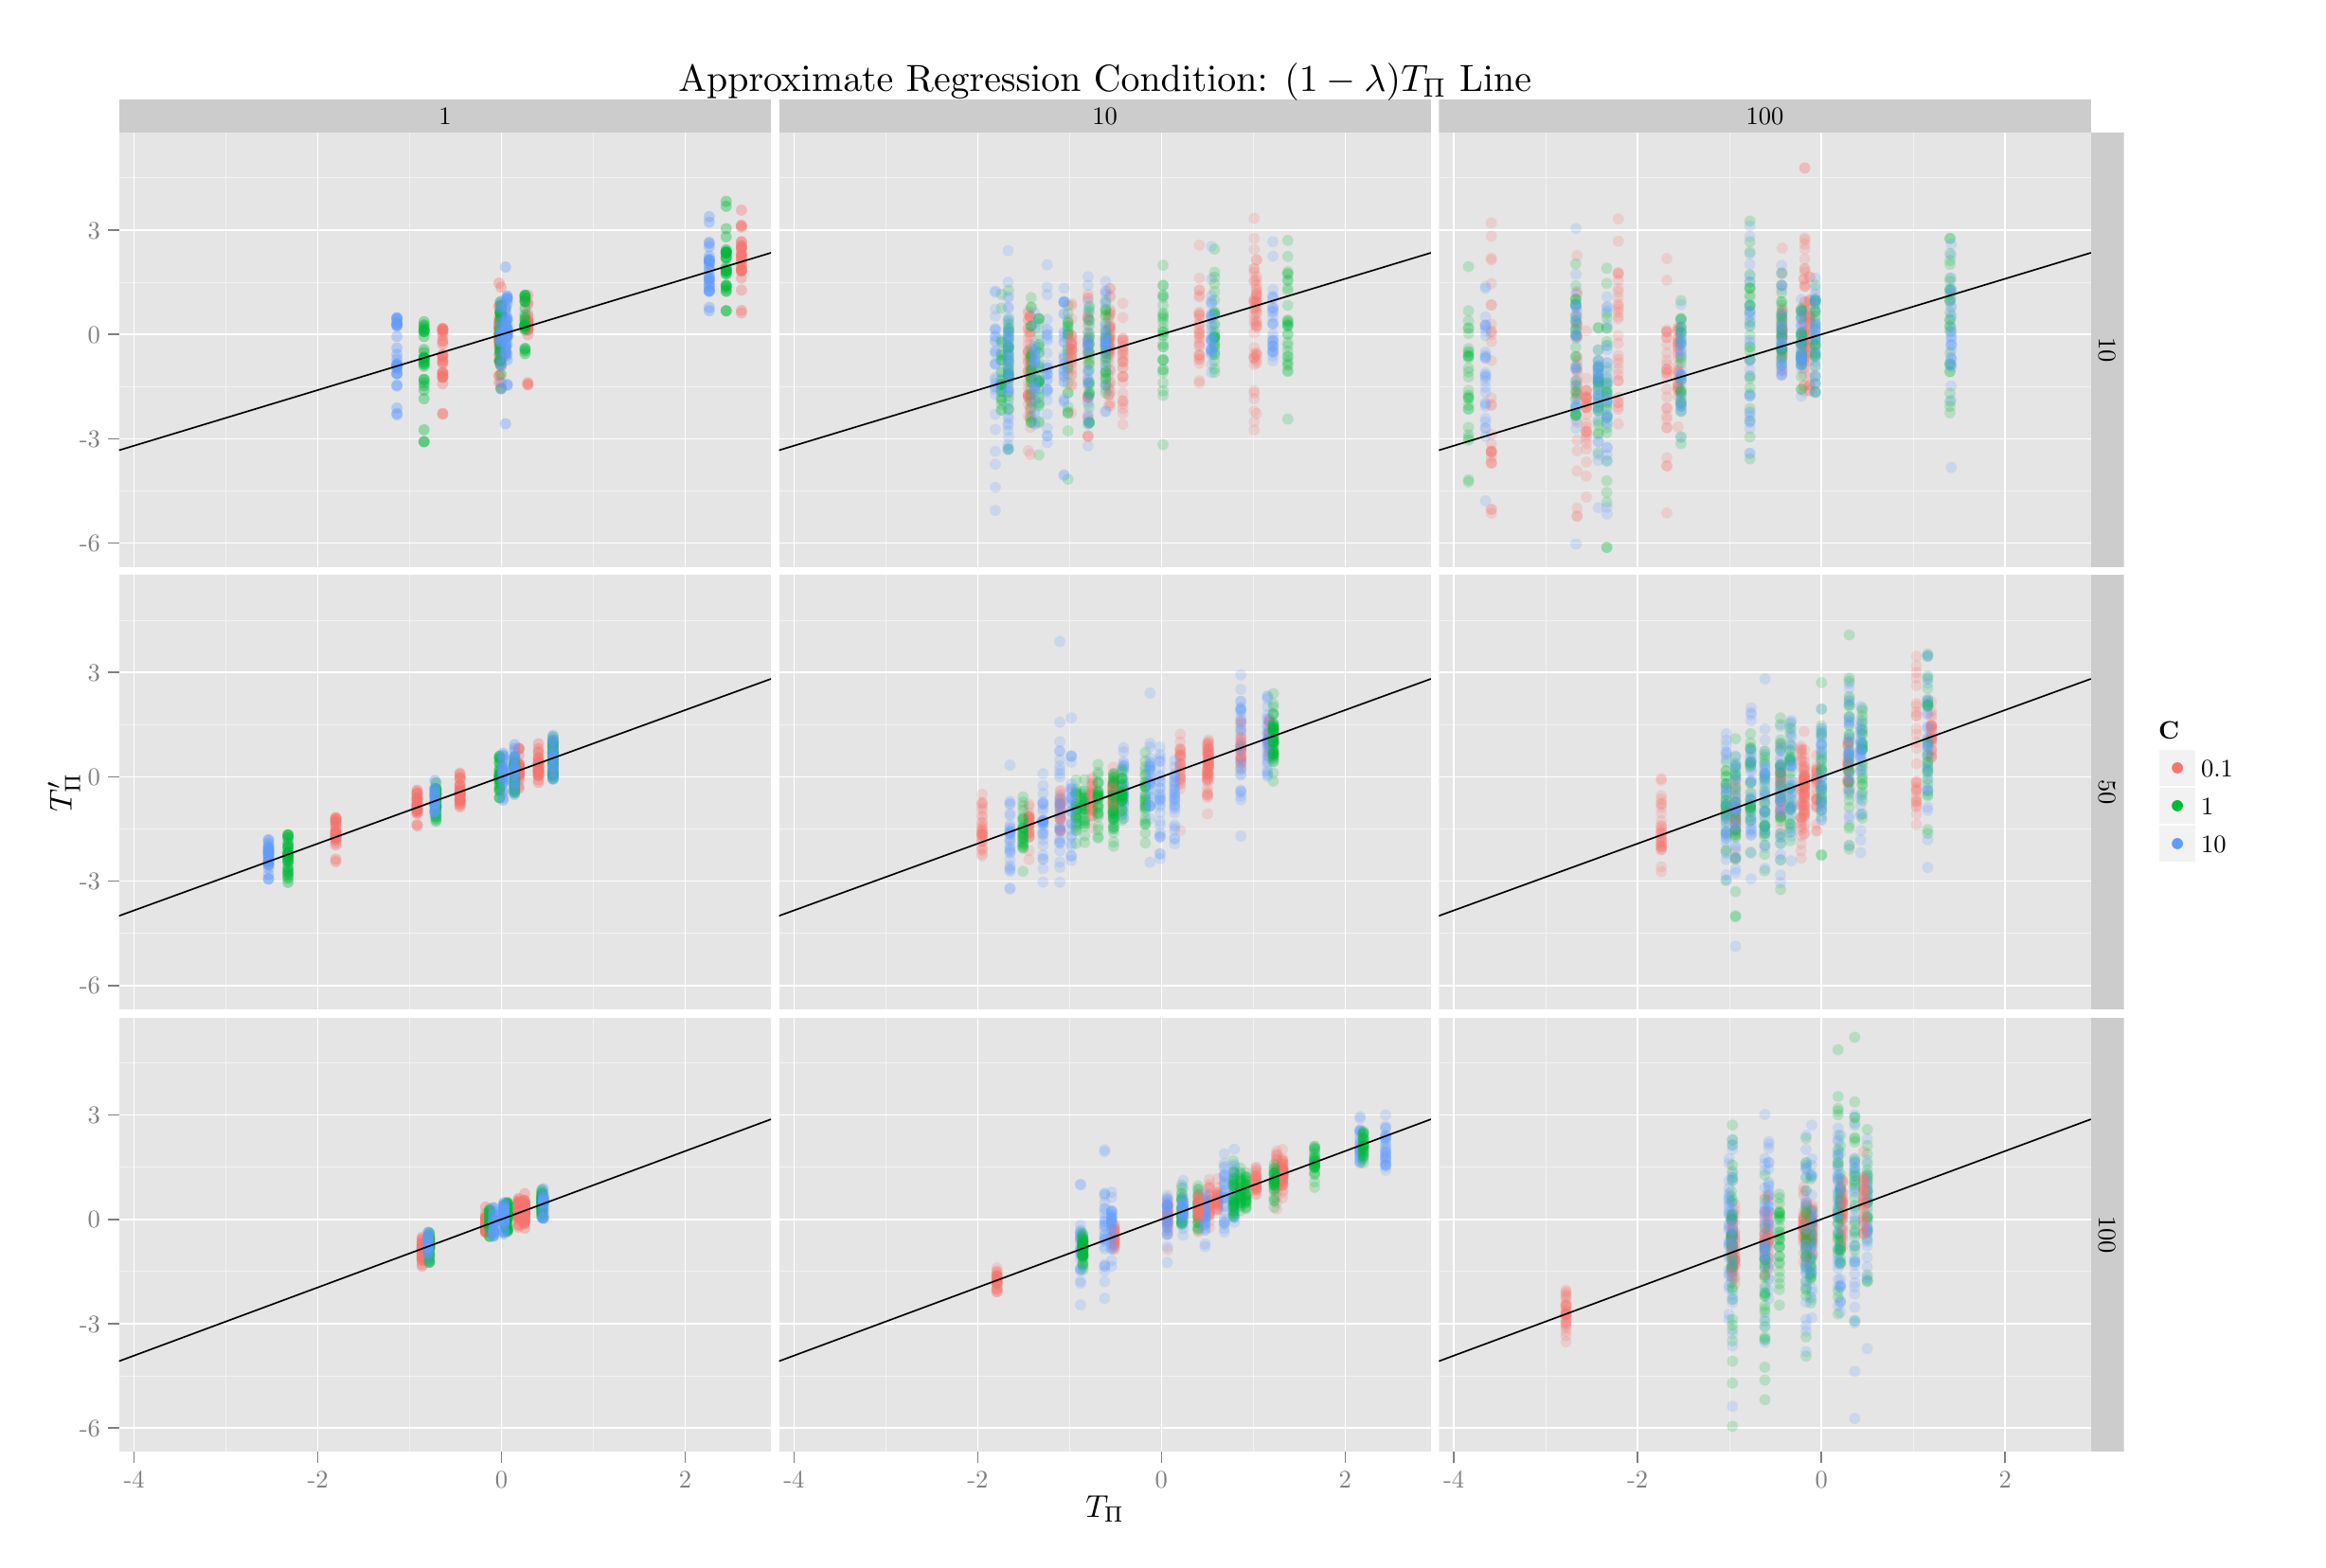
\begin{tikzpicture}[x=1pt,y=1pt]
\definecolor[named]{fillColor}{rgb}{1.00,1.00,1.00}
\path[use as bounding box,fill=fillColor,fill opacity=0.00] (0,0) rectangle (867.24,578.16);
\begin{scope}
\path[clip] (  0.00,  0.00) rectangle (867.24,578.16);
\definecolor[named]{drawColor}{rgb}{1.00,1.00,1.00}
\definecolor[named]{fillColor}{rgb}{1.00,1.00,1.00}

\path[draw=drawColor,line width= 0.6pt,line join=round,line cap=round,fill=fillColor] (  0.00, -0.00) rectangle (867.24,578.16);
\end{scope}
\begin{scope}
\path[clip] ( 35.42,537.54) rectangle (284.19,550.17);
\definecolor[named]{fillColor}{rgb}{0.80,0.80,0.80}

\path[fill=fillColor] ( 35.42,537.54) rectangle (284.19,550.17);
\definecolor[named]{drawColor}{rgb}{0.00,0.00,0.00}

\node[text=drawColor,anchor=base,inner sep=0pt, outer sep=0pt, scale=  0.96] at (159.81,540.55) {1};
\end{scope}
\begin{scope}
\path[clip] (287.21,537.54) rectangle (535.98,550.17);
\definecolor[named]{fillColor}{rgb}{0.80,0.80,0.80}

\path[fill=fillColor] (287.21,537.54) rectangle (535.98,550.17);
\definecolor[named]{drawColor}{rgb}{0.00,0.00,0.00}

\node[text=drawColor,anchor=base,inner sep=0pt, outer sep=0pt, scale=  0.96] at (411.59,540.55) {10};
\end{scope}
\begin{scope}
\path[clip] (538.99,537.54) rectangle (787.76,550.17);
\definecolor[named]{fillColor}{rgb}{0.80,0.80,0.80}

\path[fill=fillColor] (538.99,537.54) rectangle (787.76,550.17);
\definecolor[named]{drawColor}{rgb}{0.00,0.00,0.00}

\node[text=drawColor,anchor=base,inner sep=0pt, outer sep=0pt, scale=  0.96] at (663.38,540.55) {100};
\end{scope}
\begin{scope}
\path[clip] ( 35.42,371.71) rectangle (284.19,537.54);
\definecolor[named]{fillColor}{rgb}{0.90,0.90,0.90}

\path[fill=fillColor] ( 35.42,371.71) rectangle (284.19,537.54);
\definecolor[named]{drawColor}{rgb}{0.95,0.95,0.95}

\path[draw=drawColor,line width= 0.3pt,line join=round] ( 35.42,400.81) --
	(284.19,400.81);

\path[draw=drawColor,line width= 0.3pt,line join=round] ( 35.42,440.62) --
	(284.19,440.62);

\path[draw=drawColor,line width= 0.3pt,line join=round] ( 35.42,480.44) --
	(284.19,480.44);

\path[draw=drawColor,line width= 0.3pt,line join=round] ( 35.42,520.26) --
	(284.19,520.26);

\path[draw=drawColor,line width= 0.3pt,line join=round] ( 76.22,371.71) --
	( 76.22,537.54);

\path[draw=drawColor,line width= 0.3pt,line join=round] (146.32,371.71) --
	(146.32,537.54);

\path[draw=drawColor,line width= 0.3pt,line join=round] (216.41,371.71) --
	(216.41,537.54);
\definecolor[named]{drawColor}{rgb}{1.00,1.00,1.00}

\path[draw=drawColor,line width= 0.6pt,line join=round] ( 35.42,380.90) --
	(284.19,380.90);

\path[draw=drawColor,line width= 0.6pt,line join=round] ( 35.42,420.71) --
	(284.19,420.71);

\path[draw=drawColor,line width= 0.6pt,line join=round] ( 35.42,460.53) --
	(284.19,460.53);

\path[draw=drawColor,line width= 0.6pt,line join=round] ( 35.42,500.35) --
	(284.19,500.35);

\path[draw=drawColor,line width= 0.6pt,line join=round] ( 41.17,371.71) --
	( 41.17,537.54);

\path[draw=drawColor,line width= 0.6pt,line join=round] (111.27,371.71) --
	(111.27,537.54);

\path[draw=drawColor,line width= 0.6pt,line join=round] (181.36,371.71) --
	(181.36,537.54);

\path[draw=drawColor,line width= 0.6pt,line join=round] (251.46,371.71) --
	(251.46,537.54);
\definecolor[named]{fillColor}{rgb}{0.97,0.46,0.43}

\path[fill=fillColor,fill opacity=0.20] (191.40,475.54) circle (  2.13);

\path[fill=fillColor,fill opacity=0.20] (191.40,464.23) circle (  2.13);

\path[fill=fillColor,fill opacity=0.20] (191.40,471.98) circle (  2.13);

\path[fill=fillColor,fill opacity=0.20] (191.40,463.63) circle (  2.13);

\path[fill=fillColor,fill opacity=0.20] (191.40,463.69) circle (  2.13);

\path[fill=fillColor,fill opacity=0.20] (191.40,462.40) circle (  2.13);

\path[fill=fillColor,fill opacity=0.20] (191.40,463.17) circle (  2.13);

\path[fill=fillColor,fill opacity=0.20] (191.40,465.15) circle (  2.13);

\path[fill=fillColor,fill opacity=0.20] (191.40,464.21) circle (  2.13);

\path[fill=fillColor,fill opacity=0.20] (191.40,464.81) circle (  2.13);

\path[fill=fillColor,fill opacity=0.20] (191.40,467.48) circle (  2.13);

\path[fill=fillColor,fill opacity=0.20] (191.40,462.40) circle (  2.13);

\path[fill=fillColor,fill opacity=0.20] (191.40,464.21) circle (  2.13);

\path[fill=fillColor,fill opacity=0.20] (191.40,460.36) circle (  2.13);

\path[fill=fillColor,fill opacity=0.20] (191.40,462.80) circle (  2.13);

\path[fill=fillColor,fill opacity=0.20] (191.40,465.12) circle (  2.13);

\path[fill=fillColor,fill opacity=0.20] (191.40,441.30) circle (  2.13);

\path[fill=fillColor,fill opacity=0.20] (191.40,472.75) circle (  2.13);

\path[fill=fillColor,fill opacity=0.20] (191.40,465.71) circle (  2.13);

\path[fill=fillColor,fill opacity=0.20] (191.40,442.16) circle (  2.13);

\path[fill=fillColor,fill opacity=0.20] (191.40,465.85) circle (  2.13);

\path[fill=fillColor,fill opacity=0.20] (191.40,463.98) circle (  2.13);

\path[fill=fillColor,fill opacity=0.20] (191.40,441.47) circle (  2.13);

\path[fill=fillColor,fill opacity=0.20] (191.40,464.07) circle (  2.13);

\path[fill=fillColor,fill opacity=0.20] (191.40,464.07) circle (  2.13);

\path[fill=fillColor,fill opacity=0.20] (191.40,463.17) circle (  2.13);

\path[fill=fillColor,fill opacity=0.20] (191.40,465.24) circle (  2.13);

\path[fill=fillColor,fill opacity=0.20] (191.40,468.30) circle (  2.13);

\path[fill=fillColor,fill opacity=0.20] (191.40,464.56) circle (  2.13);

\path[fill=fillColor,fill opacity=0.20] (191.40,462.06) circle (  2.13);

\path[fill=fillColor,fill opacity=0.20] (158.90,451.95) circle (  2.13);

\path[fill=fillColor,fill opacity=0.20] (158.90,458.26) circle (  2.13);

\path[fill=fillColor,fill opacity=0.20] (158.90,449.64) circle (  2.13);

\path[fill=fillColor,fill opacity=0.20] (158.90,461.24) circle (  2.13);

\path[fill=fillColor,fill opacity=0.20] (158.90,450.42) circle (  2.13);

\path[fill=fillColor,fill opacity=0.20] (158.90,462.00) circle (  2.13);

\path[fill=fillColor,fill opacity=0.20] (158.90,452.85) circle (  2.13);

\path[fill=fillColor,fill opacity=0.20] (158.90,430.38) circle (  2.13);

\path[fill=fillColor,fill opacity=0.20] (158.90,445.68) circle (  2.13);

\path[fill=fillColor,fill opacity=0.20] (158.90,444.46) circle (  2.13);

\path[fill=fillColor,fill opacity=0.20] (158.90,449.64) circle (  2.13);

\path[fill=fillColor,fill opacity=0.20] (158.90,460.23) circle (  2.13);

\path[fill=fillColor,fill opacity=0.20] (158.90,444.18) circle (  2.13);

\path[fill=fillColor,fill opacity=0.20] (158.90,446.03) circle (  2.13);

\path[fill=fillColor,fill opacity=0.20] (158.90,452.60) circle (  2.13);

\path[fill=fillColor,fill opacity=0.20] (158.90,446.16) circle (  2.13);

\path[fill=fillColor,fill opacity=0.20] (158.90,462.60) circle (  2.13);

\path[fill=fillColor,fill opacity=0.20] (158.90,462.03) circle (  2.13);

\path[fill=fillColor,fill opacity=0.20] (158.90,450.76) circle (  2.13);

\path[fill=fillColor,fill opacity=0.20] (158.90,441.71) circle (  2.13);

\path[fill=fillColor,fill opacity=0.20] (158.90,444.18) circle (  2.13);

\path[fill=fillColor,fill opacity=0.20] (158.90,462.68) circle (  2.13);

\path[fill=fillColor,fill opacity=0.20] (158.90,456.82) circle (  2.13);

\path[fill=fillColor,fill opacity=0.20] (158.90,445.29) circle (  2.13);

\path[fill=fillColor,fill opacity=0.20] (158.90,462.49) circle (  2.13);

\path[fill=fillColor,fill opacity=0.20] (158.90,452.52) circle (  2.13);

\path[fill=fillColor,fill opacity=0.20] (158.90,444.18) circle (  2.13);

\path[fill=fillColor,fill opacity=0.20] (158.90,457.82) circle (  2.13);

\path[fill=fillColor,fill opacity=0.20] (158.90,430.10) circle (  2.13);

\path[fill=fillColor,fill opacity=0.20] (158.90,462.84) circle (  2.13);

\path[fill=fillColor,fill opacity=0.20] (180.44,464.35) circle (  2.13);

\path[fill=fillColor,fill opacity=0.20] (180.44,462.72) circle (  2.13);

\path[fill=fillColor,fill opacity=0.20] (180.44,463.66) circle (  2.13);

\path[fill=fillColor,fill opacity=0.20] (180.44,457.59) circle (  2.13);

\path[fill=fillColor,fill opacity=0.20] (180.44,452.81) circle (  2.13);

\path[fill=fillColor,fill opacity=0.20] (180.44,460.34) circle (  2.13);

\path[fill=fillColor,fill opacity=0.20] (180.44,457.66) circle (  2.13);

\path[fill=fillColor,fill opacity=0.20] (180.44,461.02) circle (  2.13);

\path[fill=fillColor,fill opacity=0.20] (180.44,462.61) circle (  2.13);

\path[fill=fillColor,fill opacity=0.20] (180.44,444.79) circle (  2.13);

\path[fill=fillColor,fill opacity=0.20] (180.44,458.55) circle (  2.13);

\path[fill=fillColor,fill opacity=0.20] (180.44,460.39) circle (  2.13);

\path[fill=fillColor,fill opacity=0.20] (180.44,458.67) circle (  2.13);

\path[fill=fillColor,fill opacity=0.20] (180.44,458.64) circle (  2.13);

\path[fill=fillColor,fill opacity=0.20] (180.44,455.84) circle (  2.13);

\path[fill=fillColor,fill opacity=0.20] (180.44,450.45) circle (  2.13);

\path[fill=fillColor,fill opacity=0.20] (180.44,463.65) circle (  2.13);

\path[fill=fillColor,fill opacity=0.20] (180.44,460.41) circle (  2.13);

\path[fill=fillColor,fill opacity=0.20] (180.44,450.53) circle (  2.13);

\path[fill=fillColor,fill opacity=0.20] (180.44,442.15) circle (  2.13);

\path[fill=fillColor,fill opacity=0.20] (180.44,465.40) circle (  2.13);

\path[fill=fillColor,fill opacity=0.20] (180.44,471.27) circle (  2.13);

\path[fill=fillColor,fill opacity=0.20] (180.44,465.40) circle (  2.13);

\path[fill=fillColor,fill opacity=0.20] (180.44,471.28) circle (  2.13);

\path[fill=fillColor,fill opacity=0.20] (180.44,462.72) circle (  2.13);

\path[fill=fillColor,fill opacity=0.20] (180.44,466.96) circle (  2.13);

\path[fill=fillColor,fill opacity=0.20] (180.44,460.41) circle (  2.13);

\path[fill=fillColor,fill opacity=0.20] (180.44,444.79) circle (  2.13);

\path[fill=fillColor,fill opacity=0.20] (180.44,480.11) circle (  2.13);

\path[fill=fillColor,fill opacity=0.20] (180.44,459.96) circle (  2.13);

\path[fill=fillColor,fill opacity=0.20] (272.89,484.90) circle (  2.13);

\path[fill=fillColor,fill opacity=0.20] (272.89,502.01) circle (  2.13);

\path[fill=fillColor,fill opacity=0.20] (272.89,481.98) circle (  2.13);

\path[fill=fillColor,fill opacity=0.20] (272.89,501.51) circle (  2.13);

\path[fill=fillColor,fill opacity=0.20] (272.89,488.31) circle (  2.13);

\path[fill=fillColor,fill opacity=0.20] (272.89,487.00) circle (  2.13);

\path[fill=fillColor,fill opacity=0.20] (272.89,495.94) circle (  2.13);

\path[fill=fillColor,fill opacity=0.20] (272.89,490.75) circle (  2.13);

\path[fill=fillColor,fill opacity=0.20] (272.89,484.67) circle (  2.13);

\path[fill=fillColor,fill opacity=0.20] (272.89,468.74) circle (  2.13);

\path[fill=fillColor,fill opacity=0.20] (272.89,494.38) circle (  2.13);

\path[fill=fillColor,fill opacity=0.20] (272.89,469.73) circle (  2.13);

\path[fill=fillColor,fill opacity=0.20] (272.89,485.01) circle (  2.13);

\path[fill=fillColor,fill opacity=0.20] (272.89,489.55) circle (  2.13);

\path[fill=fillColor,fill opacity=0.20] (272.89,489.44) circle (  2.13);

\path[fill=fillColor,fill opacity=0.20] (272.89,491.60) circle (  2.13);

\path[fill=fillColor,fill opacity=0.20] (272.89,484.93) circle (  2.13);

\path[fill=fillColor,fill opacity=0.20] (272.89,493.52) circle (  2.13);

\path[fill=fillColor,fill opacity=0.20] (272.89,477.43) circle (  2.13);

\path[fill=fillColor,fill opacity=0.20] (272.89,490.75) circle (  2.13);

\path[fill=fillColor,fill opacity=0.20] (272.89,502.17) circle (  2.13);

\path[fill=fillColor,fill opacity=0.20] (272.89,488.31) circle (  2.13);

\path[fill=fillColor,fill opacity=0.20] (272.89,495.80) circle (  2.13);

\path[fill=fillColor,fill opacity=0.20] (272.89,490.75) circle (  2.13);

\path[fill=fillColor,fill opacity=0.20] (272.89,507.96) circle (  2.13);

\path[fill=fillColor,fill opacity=0.20] (272.89,493.27) circle (  2.13);

\path[fill=fillColor,fill opacity=0.20] (272.89,485.32) circle (  2.13);

\path[fill=fillColor,fill opacity=0.20] (272.89,486.14) circle (  2.13);

\path[fill=fillColor,fill opacity=0.20] (272.89,493.27) circle (  2.13);

\path[fill=fillColor,fill opacity=0.20] (272.89,494.42) circle (  2.13);

\path[fill=fillColor,fill opacity=0.20] (181.17,462.49) circle (  2.13);

\path[fill=fillColor,fill opacity=0.20] (181.17,467.05) circle (  2.13);

\path[fill=fillColor,fill opacity=0.20] (181.17,466.49) circle (  2.13);

\path[fill=fillColor,fill opacity=0.20] (181.17,478.59) circle (  2.13);

\path[fill=fillColor,fill opacity=0.20] (181.17,460.46) circle (  2.13);

\path[fill=fillColor,fill opacity=0.20] (181.17,462.49) circle (  2.13);

\path[fill=fillColor,fill opacity=0.20] (181.17,450.73) circle (  2.13);

\path[fill=fillColor,fill opacity=0.20] (181.17,460.30) circle (  2.13);

\path[fill=fillColor,fill opacity=0.20] (181.17,453.71) circle (  2.13);

\path[fill=fillColor,fill opacity=0.20] (181.17,459.38) circle (  2.13);

\path[fill=fillColor,fill opacity=0.20] (181.17,460.97) circle (  2.13);

\path[fill=fillColor,fill opacity=0.20] (181.17,468.35) circle (  2.13);

\path[fill=fillColor,fill opacity=0.20] (181.17,453.16) circle (  2.13);

\path[fill=fillColor,fill opacity=0.20] (181.17,464.98) circle (  2.13);

\path[fill=fillColor,fill opacity=0.20] (181.17,440.27) circle (  2.13);

\path[fill=fillColor,fill opacity=0.20] (181.17,464.28) circle (  2.13);

\path[fill=fillColor,fill opacity=0.20] (181.17,453.16) circle (  2.13);

\path[fill=fillColor,fill opacity=0.20] (181.17,453.16) circle (  2.13);

\path[fill=fillColor,fill opacity=0.20] (181.17,469.34) circle (  2.13);

\path[fill=fillColor,fill opacity=0.20] (181.17,458.12) circle (  2.13);

\path[fill=fillColor,fill opacity=0.20] (181.17,461.47) circle (  2.13);

\path[fill=fillColor,fill opacity=0.20] (181.17,448.40) circle (  2.13);

\path[fill=fillColor,fill opacity=0.20] (181.17,454.34) circle (  2.13);

\path[fill=fillColor,fill opacity=0.20] (181.17,451.77) circle (  2.13);

\path[fill=fillColor,fill opacity=0.20] (181.17,465.94) circle (  2.13);

\path[fill=fillColor,fill opacity=0.20] (181.17,460.04) circle (  2.13);

\path[fill=fillColor,fill opacity=0.20] (181.17,461.22) circle (  2.13);

\path[fill=fillColor,fill opacity=0.20] (181.17,462.87) circle (  2.13);

\path[fill=fillColor,fill opacity=0.20] (181.17,466.65) circle (  2.13);

\path[fill=fillColor,fill opacity=0.20] (181.17,470.36) circle (  2.13);
\definecolor[named]{fillColor}{rgb}{0.00,0.73,0.22}

\path[fill=fillColor,fill opacity=0.20] (190.33,470.48) circle (  2.13);

\path[fill=fillColor,fill opacity=0.20] (190.33,474.51) circle (  2.13);

\path[fill=fillColor,fill opacity=0.20] (190.33,454.94) circle (  2.13);

\path[fill=fillColor,fill opacity=0.20] (190.33,475.48) circle (  2.13);

\path[fill=fillColor,fill opacity=0.20] (190.33,463.09) circle (  2.13);

\path[fill=fillColor,fill opacity=0.20] (190.33,463.98) circle (  2.13);

\path[fill=fillColor,fill opacity=0.20] (190.33,473.01) circle (  2.13);

\path[fill=fillColor,fill opacity=0.20] (190.33,455.23) circle (  2.13);

\path[fill=fillColor,fill opacity=0.20] (190.33,463.98) circle (  2.13);

\path[fill=fillColor,fill opacity=0.20] (190.33,473.01) circle (  2.13);

\path[fill=fillColor,fill opacity=0.20] (190.33,465.52) circle (  2.13);

\path[fill=fillColor,fill opacity=0.20] (190.33,462.19) circle (  2.13);

\path[fill=fillColor,fill opacity=0.20] (190.33,466.26) circle (  2.13);

\path[fill=fillColor,fill opacity=0.20] (190.33,463.97) circle (  2.13);

\path[fill=fillColor,fill opacity=0.20] (190.33,454.20) circle (  2.13);

\path[fill=fillColor,fill opacity=0.20] (190.33,463.25) circle (  2.13);

\path[fill=fillColor,fill opacity=0.20] (190.33,473.38) circle (  2.13);

\path[fill=fillColor,fill opacity=0.20] (190.33,463.84) circle (  2.13);

\path[fill=fillColor,fill opacity=0.20] (190.33,453.19) circle (  2.13);

\path[fill=fillColor,fill opacity=0.20] (190.33,475.48) circle (  2.13);

\path[fill=fillColor,fill opacity=0.20] (190.33,464.47) circle (  2.13);

\path[fill=fillColor,fill opacity=0.20] (190.33,466.85) circle (  2.13);

\path[fill=fillColor,fill opacity=0.20] (190.33,475.28) circle (  2.13);

\path[fill=fillColor,fill opacity=0.20] (190.33,463.69) circle (  2.13);

\path[fill=fillColor,fill opacity=0.20] (190.33,474.51) circle (  2.13);

\path[fill=fillColor,fill opacity=0.20] (190.33,463.70) circle (  2.13);

\path[fill=fillColor,fill opacity=0.20] (190.33,464.26) circle (  2.13);

\path[fill=fillColor,fill opacity=0.20] (190.33,468.02) circle (  2.13);

\path[fill=fillColor,fill opacity=0.20] (190.33,462.77) circle (  2.13);

\path[fill=fillColor,fill opacity=0.20] (190.33,463.97) circle (  2.13);

\path[fill=fillColor,fill opacity=0.20] (151.79,440.93) circle (  2.13);

\path[fill=fillColor,fill opacity=0.20] (151.79,461.63) circle (  2.13);

\path[fill=fillColor,fill opacity=0.20] (151.79,463.74) circle (  2.13);

\path[fill=fillColor,fill opacity=0.20] (151.79,459.68) circle (  2.13);

\path[fill=fillColor,fill opacity=0.20] (151.79,419.57) circle (  2.13);

\path[fill=fillColor,fill opacity=0.20] (151.79,439.22) circle (  2.13);

\path[fill=fillColor,fill opacity=0.20] (151.79,464.21) circle (  2.13);

\path[fill=fillColor,fill opacity=0.20] (151.79,424.12) circle (  2.13);

\path[fill=fillColor,fill opacity=0.20] (151.79,451.33) circle (  2.13);

\path[fill=fillColor,fill opacity=0.20] (151.79,451.38) circle (  2.13);

\path[fill=fillColor,fill opacity=0.20] (151.79,465.38) circle (  2.13);

\path[fill=fillColor,fill opacity=0.20] (151.79,443.33) circle (  2.13);

\path[fill=fillColor,fill opacity=0.20] (151.79,462.86) circle (  2.13);

\path[fill=fillColor,fill opacity=0.20] (151.79,461.76) circle (  2.13);

\path[fill=fillColor,fill opacity=0.20] (151.79,450.27) circle (  2.13);

\path[fill=fillColor,fill opacity=0.20] (151.79,449.12) circle (  2.13);

\path[fill=fillColor,fill opacity=0.20] (151.79,448.38) circle (  2.13);

\path[fill=fillColor,fill opacity=0.20] (151.79,443.33) circle (  2.13);

\path[fill=fillColor,fill opacity=0.20] (151.79,451.50) circle (  2.13);

\path[fill=fillColor,fill opacity=0.20] (151.79,451.83) circle (  2.13);

\path[fill=fillColor,fill opacity=0.20] (151.79,451.72) circle (  2.13);

\path[fill=fillColor,fill opacity=0.20] (151.79,442.04) circle (  2.13);

\path[fill=fillColor,fill opacity=0.20] (151.79,449.34) circle (  2.13);

\path[fill=fillColor,fill opacity=0.20] (151.79,449.96) circle (  2.13);

\path[fill=fillColor,fill opacity=0.20] (151.79,461.63) circle (  2.13);

\path[fill=fillColor,fill opacity=0.20] (151.79,462.42) circle (  2.13);

\path[fill=fillColor,fill opacity=0.20] (151.79,419.57) circle (  2.13);

\path[fill=fillColor,fill opacity=0.20] (151.79,454.77) circle (  2.13);

\path[fill=fillColor,fill opacity=0.20] (151.79,436.00) circle (  2.13);

\path[fill=fillColor,fill opacity=0.20] (151.79,453.61) circle (  2.13);

\path[fill=fillColor,fill opacity=0.20] (180.81,458.42) circle (  2.13);

\path[fill=fillColor,fill opacity=0.20] (180.81,450.63) circle (  2.13);

\path[fill=fillColor,fill opacity=0.20] (180.81,453.00) circle (  2.13);

\path[fill=fillColor,fill opacity=0.20] (180.81,472.80) circle (  2.13);

\path[fill=fillColor,fill opacity=0.20] (180.81,454.44) circle (  2.13);

\path[fill=fillColor,fill opacity=0.20] (180.81,457.00) circle (  2.13);

\path[fill=fillColor,fill opacity=0.20] (180.81,465.30) circle (  2.13);

\path[fill=fillColor,fill opacity=0.20] (180.81,450.63) circle (  2.13);

\path[fill=fillColor,fill opacity=0.20] (180.81,455.53) circle (  2.13);

\path[fill=fillColor,fill opacity=0.20] (180.81,466.05) circle (  2.13);

\path[fill=fillColor,fill opacity=0.20] (180.81,453.87) circle (  2.13);

\path[fill=fillColor,fill opacity=0.20] (180.81,469.06) circle (  2.13);

\path[fill=fillColor,fill opacity=0.20] (180.81,460.69) circle (  2.13);

\path[fill=fillColor,fill opacity=0.20] (180.81,463.00) circle (  2.13);

\path[fill=fillColor,fill opacity=0.20] (180.81,469.06) circle (  2.13);

\path[fill=fillColor,fill opacity=0.20] (180.81,449.26) circle (  2.13);

\path[fill=fillColor,fill opacity=0.20] (180.81,460.33) circle (  2.13);

\path[fill=fillColor,fill opacity=0.20] (180.81,458.03) circle (  2.13);

\path[fill=fillColor,fill opacity=0.20] (180.81,450.38) circle (  2.13);

\path[fill=fillColor,fill opacity=0.20] (180.81,462.88) circle (  2.13);

\path[fill=fillColor,fill opacity=0.20] (180.81,456.52) circle (  2.13);

\path[fill=fillColor,fill opacity=0.20] (180.81,461.22) circle (  2.13);

\path[fill=fillColor,fill opacity=0.20] (180.81,455.70) circle (  2.13);

\path[fill=fillColor,fill opacity=0.20] (180.81,450.38) circle (  2.13);

\path[fill=fillColor,fill opacity=0.20] (180.81,468.71) circle (  2.13);

\path[fill=fillColor,fill opacity=0.20] (180.81,459.24) circle (  2.13);

\path[fill=fillColor,fill opacity=0.20] (180.81,453.87) circle (  2.13);

\path[fill=fillColor,fill opacity=0.20] (180.81,462.53) circle (  2.13);

\path[fill=fillColor,fill opacity=0.20] (180.81,460.23) circle (  2.13);

\path[fill=fillColor,fill opacity=0.20] (180.81,461.32) circle (  2.13);

\path[fill=fillColor,fill opacity=0.20] (267.08,509.43) circle (  2.13);

\path[fill=fillColor,fill opacity=0.20] (267.08,477.18) circle (  2.13);

\path[fill=fillColor,fill opacity=0.20] (267.08,486.26) circle (  2.13);

\path[fill=fillColor,fill opacity=0.20] (267.08,491.89) circle (  2.13);

\path[fill=fillColor,fill opacity=0.20] (267.08,485.39) circle (  2.13);

\path[fill=fillColor,fill opacity=0.20] (267.08,484.42) circle (  2.13);

\path[fill=fillColor,fill opacity=0.20] (267.08,484.75) circle (  2.13);

\path[fill=fillColor,fill opacity=0.20] (267.08,489.53) circle (  2.13);

\path[fill=fillColor,fill opacity=0.20] (267.08,478.17) circle (  2.13);

\path[fill=fillColor,fill opacity=0.20] (267.08,491.59) circle (  2.13);

\path[fill=fillColor,fill opacity=0.20] (267.08,500.88) circle (  2.13);

\path[fill=fillColor,fill opacity=0.20] (267.08,492.85) circle (  2.13);

\path[fill=fillColor,fill opacity=0.20] (267.08,485.21) circle (  2.13);

\path[fill=fillColor,fill opacity=0.20] (267.08,476.95) circle (  2.13);

\path[fill=fillColor,fill opacity=0.20] (267.08,511.32) circle (  2.13);

\path[fill=fillColor,fill opacity=0.20] (267.08,483.74) circle (  2.13);

\path[fill=fillColor,fill opacity=0.20] (267.08,469.55) circle (  2.13);

\path[fill=fillColor,fill opacity=0.20] (267.08,491.89) circle (  2.13);

\path[fill=fillColor,fill opacity=0.20] (267.08,484.70) circle (  2.13);

\path[fill=fillColor,fill opacity=0.20] (267.08,479.19) circle (  2.13);

\path[fill=fillColor,fill opacity=0.20] (267.08,491.59) circle (  2.13);

\path[fill=fillColor,fill opacity=0.20] (267.08,492.27) circle (  2.13);

\path[fill=fillColor,fill opacity=0.20] (267.08,497.80) circle (  2.13);

\path[fill=fillColor,fill opacity=0.20] (267.08,489.87) circle (  2.13);

\path[fill=fillColor,fill opacity=0.20] (267.08,478.97) circle (  2.13);

\path[fill=fillColor,fill opacity=0.20] (267.08,490.02) circle (  2.13);

\path[fill=fillColor,fill opacity=0.20] (267.08,469.55) circle (  2.13);

\path[fill=fillColor,fill opacity=0.20] (267.08,483.58) circle (  2.13);

\path[fill=fillColor,fill opacity=0.20] (267.08,491.81) circle (  2.13);

\path[fill=fillColor,fill opacity=0.20] (267.08,479.33) circle (  2.13);

\path[fill=fillColor,fill opacity=0.20] (181.17,460.05) circle (  2.13);

\path[fill=fillColor,fill opacity=0.20] (181.17,466.88) circle (  2.13);

\path[fill=fillColor,fill opacity=0.20] (181.17,468.86) circle (  2.13);

\path[fill=fillColor,fill opacity=0.20] (181.17,471.39) circle (  2.13);

\path[fill=fillColor,fill opacity=0.20] (181.17,460.05) circle (  2.13);

\path[fill=fillColor,fill opacity=0.20] (181.17,461.90) circle (  2.13);

\path[fill=fillColor,fill opacity=0.20] (181.17,457.42) circle (  2.13);

\path[fill=fillColor,fill opacity=0.20] (181.17,468.18) circle (  2.13);

\path[fill=fillColor,fill opacity=0.20] (181.17,452.79) circle (  2.13);

\path[fill=fillColor,fill opacity=0.20] (181.17,451.03) circle (  2.13);

\path[fill=fillColor,fill opacity=0.20] (181.17,459.37) circle (  2.13);

\path[fill=fillColor,fill opacity=0.20] (181.17,454.14) circle (  2.13);

\path[fill=fillColor,fill opacity=0.20] (181.17,463.75) circle (  2.13);

\path[fill=fillColor,fill opacity=0.20] (181.17,471.90) circle (  2.13);

\path[fill=fillColor,fill opacity=0.20] (181.17,454.14) circle (  2.13);

\path[fill=fillColor,fill opacity=0.20] (181.17,462.45) circle (  2.13);

\path[fill=fillColor,fill opacity=0.20] (181.17,467.91) circle (  2.13);

\path[fill=fillColor,fill opacity=0.20] (181.17,439.86) circle (  2.13);

\path[fill=fillColor,fill opacity=0.20] (181.17,470.09) circle (  2.13);

\path[fill=fillColor,fill opacity=0.20] (181.17,467.32) circle (  2.13);

\path[fill=fillColor,fill opacity=0.20] (181.17,464.28) circle (  2.13);

\path[fill=fillColor,fill opacity=0.20] (181.17,460.08) circle (  2.13);

\path[fill=fillColor,fill opacity=0.20] (181.17,445.24) circle (  2.13);

\path[fill=fillColor,fill opacity=0.20] (181.17,470.99) circle (  2.13);

\path[fill=fillColor,fill opacity=0.20] (181.17,459.02) circle (  2.13);

\path[fill=fillColor,fill opacity=0.20] (181.17,468.43) circle (  2.13);

\path[fill=fillColor,fill opacity=0.20] (181.17,468.86) circle (  2.13);

\path[fill=fillColor,fill opacity=0.20] (181.17,467.32) circle (  2.13);

\path[fill=fillColor,fill opacity=0.20] (181.17,467.55) circle (  2.13);

\path[fill=fillColor,fill opacity=0.20] (181.17,466.23) circle (  2.13);
\definecolor[named]{fillColor}{rgb}{0.38,0.61,1.00}

\path[fill=fillColor,fill opacity=0.20] (183.53,466.31) circle (  2.13);

\path[fill=fillColor,fill opacity=0.20] (183.53,462.12) circle (  2.13);

\path[fill=fillColor,fill opacity=0.20] (183.53,460.62) circle (  2.13);

\path[fill=fillColor,fill opacity=0.20] (183.53,462.75) circle (  2.13);

\path[fill=fillColor,fill opacity=0.20] (183.53,459.95) circle (  2.13);

\path[fill=fillColor,fill opacity=0.20] (183.53,459.95) circle (  2.13);

\path[fill=fillColor,fill opacity=0.20] (183.53,462.45) circle (  2.13);

\path[fill=fillColor,fill opacity=0.20] (183.53,459.51) circle (  2.13);

\path[fill=fillColor,fill opacity=0.20] (183.53,450.79) circle (  2.13);

\path[fill=fillColor,fill opacity=0.20] (183.53,441.45) circle (  2.13);

\path[fill=fillColor,fill opacity=0.20] (183.53,474.19) circle (  2.13);

\path[fill=fillColor,fill opacity=0.20] (183.53,460.62) circle (  2.13);

\path[fill=fillColor,fill opacity=0.20] (183.53,462.75) circle (  2.13);

\path[fill=fillColor,fill opacity=0.20] (183.53,472.40) circle (  2.13);

\path[fill=fillColor,fill opacity=0.20] (183.53,474.87) circle (  2.13);

\path[fill=fillColor,fill opacity=0.20] (183.53,473.85) circle (  2.13);

\path[fill=fillColor,fill opacity=0.20] (183.53,461.00) circle (  2.13);

\path[fill=fillColor,fill opacity=0.20] (183.53,461.71) circle (  2.13);

\path[fill=fillColor,fill opacity=0.20] (183.53,461.87) circle (  2.13);

\path[fill=fillColor,fill opacity=0.20] (183.53,453.04) circle (  2.13);

\path[fill=fillColor,fill opacity=0.20] (183.53,466.02) circle (  2.13);

\path[fill=fillColor,fill opacity=0.20] (183.53,441.08) circle (  2.13);

\path[fill=fillColor,fill opacity=0.20] (183.53,475.21) circle (  2.13);

\path[fill=fillColor,fill opacity=0.20] (183.53,456.65) circle (  2.13);

\path[fill=fillColor,fill opacity=0.20] (183.53,466.91) circle (  2.13);

\path[fill=fillColor,fill opacity=0.20] (183.53,464.08) circle (  2.13);

\path[fill=fillColor,fill opacity=0.20] (183.53,459.55) circle (  2.13);

\path[fill=fillColor,fill opacity=0.20] (183.53,474.33) circle (  2.13);

\path[fill=fillColor,fill opacity=0.20] (183.53,462.03) circle (  2.13);

\path[fill=fillColor,fill opacity=0.20] (183.53,461.21) circle (  2.13);

\path[fill=fillColor,fill opacity=0.20] (141.45,465.18) circle (  2.13);

\path[fill=fillColor,fill opacity=0.20] (141.45,440.84) circle (  2.13);

\path[fill=fillColor,fill opacity=0.20] (141.45,455.40) circle (  2.13);

\path[fill=fillColor,fill opacity=0.20] (141.45,448.69) circle (  2.13);

\path[fill=fillColor,fill opacity=0.20] (141.45,448.92) circle (  2.13);

\path[fill=fillColor,fill opacity=0.20] (141.45,464.54) circle (  2.13);

\path[fill=fillColor,fill opacity=0.20] (141.45,447.82) circle (  2.13);

\path[fill=fillColor,fill opacity=0.20] (141.45,466.35) circle (  2.13);

\path[fill=fillColor,fill opacity=0.20] (141.45,466.55) circle (  2.13);

\path[fill=fillColor,fill opacity=0.20] (141.45,432.44) circle (  2.13);

\path[fill=fillColor,fill opacity=0.20] (141.45,447.38) circle (  2.13);

\path[fill=fillColor,fill opacity=0.20] (141.45,448.77) circle (  2.13);

\path[fill=fillColor,fill opacity=0.20] (141.45,466.86) circle (  2.13);

\path[fill=fillColor,fill opacity=0.20] (141.45,448.45) circle (  2.13);

\path[fill=fillColor,fill opacity=0.20] (141.45,445.50) circle (  2.13);

\path[fill=fillColor,fill opacity=0.20] (141.45,445.62) circle (  2.13);

\path[fill=fillColor,fill opacity=0.20] (141.45,429.85) circle (  2.13);

\path[fill=fillColor,fill opacity=0.20] (141.45,464.49) circle (  2.13);

\path[fill=fillColor,fill opacity=0.20] (141.45,466.86) circle (  2.13);

\path[fill=fillColor,fill opacity=0.20] (141.45,449.43) circle (  2.13);

\path[fill=fillColor,fill opacity=0.20] (141.45,459.77) circle (  2.13);

\path[fill=fillColor,fill opacity=0.20] (141.45,451.06) circle (  2.13);

\path[fill=fillColor,fill opacity=0.20] (141.45,441.20) circle (  2.13);

\path[fill=fillColor,fill opacity=0.20] (141.45,445.50) circle (  2.13);

\path[fill=fillColor,fill opacity=0.20] (141.45,452.92) circle (  2.13);

\path[fill=fillColor,fill opacity=0.20] (141.45,463.81) circle (  2.13);

\path[fill=fillColor,fill opacity=0.20] (141.45,464.12) circle (  2.13);

\path[fill=fillColor,fill opacity=0.20] (141.45,463.81) circle (  2.13);

\path[fill=fillColor,fill opacity=0.20] (141.45,430.38) circle (  2.13);

\path[fill=fillColor,fill opacity=0.20] (141.45,448.94) circle (  2.13);

\path[fill=fillColor,fill opacity=0.20] (182.88,454.76) circle (  2.13);

\path[fill=fillColor,fill opacity=0.20] (182.88,456.02) circle (  2.13);

\path[fill=fillColor,fill opacity=0.20] (182.88,465.34) circle (  2.13);

\path[fill=fillColor,fill opacity=0.20] (182.88,486.27) circle (  2.13);

\path[fill=fillColor,fill opacity=0.20] (182.88,459.57) circle (  2.13);

\path[fill=fillColor,fill opacity=0.20] (182.88,460.18) circle (  2.13);

\path[fill=fillColor,fill opacity=0.20] (182.88,456.47) circle (  2.13);

\path[fill=fillColor,fill opacity=0.20] (182.88,470.11) circle (  2.13);

\path[fill=fillColor,fill opacity=0.20] (182.88,460.43) circle (  2.13);

\path[fill=fillColor,fill opacity=0.20] (182.88,466.53) circle (  2.13);

\path[fill=fillColor,fill opacity=0.20] (182.88,462.46) circle (  2.13);

\path[fill=fillColor,fill opacity=0.20] (182.88,463.14) circle (  2.13);

\path[fill=fillColor,fill opacity=0.20] (182.88,456.82) circle (  2.13);

\path[fill=fillColor,fill opacity=0.20] (182.88,426.45) circle (  2.13);

\path[fill=fillColor,fill opacity=0.20] (182.88,462.79) circle (  2.13);

\path[fill=fillColor,fill opacity=0.20] (182.88,470.78) circle (  2.13);

\path[fill=fillColor,fill opacity=0.20] (182.88,457.69) circle (  2.13);

\path[fill=fillColor,fill opacity=0.20] (182.88,465.67) circle (  2.13);

\path[fill=fillColor,fill opacity=0.20] (182.88,466.53) circle (  2.13);

\path[fill=fillColor,fill opacity=0.20] (182.88,453.27) circle (  2.13);

\path[fill=fillColor,fill opacity=0.20] (182.88,470.78) circle (  2.13);

\path[fill=fillColor,fill opacity=0.20] (182.88,468.66) circle (  2.13);

\path[fill=fillColor,fill opacity=0.20] (182.88,453.05) circle (  2.13);

\path[fill=fillColor,fill opacity=0.20] (182.88,453.74) circle (  2.13);

\path[fill=fillColor,fill opacity=0.20] (182.88,455.46) circle (  2.13);

\path[fill=fillColor,fill opacity=0.20] (182.88,462.53) circle (  2.13);

\path[fill=fillColor,fill opacity=0.20] (182.88,453.27) circle (  2.13);

\path[fill=fillColor,fill opacity=0.20] (182.88,460.43) circle (  2.13);

\path[fill=fillColor,fill opacity=0.20] (182.88,463.87) circle (  2.13);

\path[fill=fillColor,fill opacity=0.20] (182.88,452.06) circle (  2.13);

\path[fill=fillColor,fill opacity=0.20] (260.61,490.51) circle (  2.13);

\path[fill=fillColor,fill opacity=0.20] (260.61,488.59) circle (  2.13);

\path[fill=fillColor,fill opacity=0.20] (260.61,477.39) circle (  2.13);

\path[fill=fillColor,fill opacity=0.20] (260.61,482.33) circle (  2.13);

\path[fill=fillColor,fill opacity=0.20] (260.61,481.48) circle (  2.13);

\path[fill=fillColor,fill opacity=0.20] (260.61,477.18) circle (  2.13);

\path[fill=fillColor,fill opacity=0.20] (260.61,478.72) circle (  2.13);

\path[fill=fillColor,fill opacity=0.20] (260.61,487.55) circle (  2.13);

\path[fill=fillColor,fill opacity=0.20] (260.61,487.35) circle (  2.13);

\path[fill=fillColor,fill opacity=0.20] (260.61,488.53) circle (  2.13);

\path[fill=fillColor,fill opacity=0.20] (260.61,495.19) circle (  2.13);

\path[fill=fillColor,fill opacity=0.20] (260.61,493.92) circle (  2.13);

\path[fill=fillColor,fill opacity=0.20] (260.61,470.79) circle (  2.13);

\path[fill=fillColor,fill opacity=0.20] (260.61,505.47) circle (  2.13);

\path[fill=fillColor,fill opacity=0.20] (260.61,485.53) circle (  2.13);

\path[fill=fillColor,fill opacity=0.20] (260.61,495.71) circle (  2.13);

\path[fill=fillColor,fill opacity=0.20] (260.61,477.18) circle (  2.13);

\path[fill=fillColor,fill opacity=0.20] (260.61,481.24) circle (  2.13);

\path[fill=fillColor,fill opacity=0.20] (260.61,479.44) circle (  2.13);

\path[fill=fillColor,fill opacity=0.20] (260.61,483.47) circle (  2.13);

\path[fill=fillColor,fill opacity=0.20] (260.61,488.82) circle (  2.13);

\path[fill=fillColor,fill opacity=0.20] (260.61,482.11) circle (  2.13);

\path[fill=fillColor,fill opacity=0.20] (260.61,503.34) circle (  2.13);

\path[fill=fillColor,fill opacity=0.20] (260.61,479.61) circle (  2.13);

\path[fill=fillColor,fill opacity=0.20] (260.61,485.38) circle (  2.13);

\path[fill=fillColor,fill opacity=0.20] (260.61,488.98) circle (  2.13);

\path[fill=fillColor,fill opacity=0.20] (260.61,481.00) circle (  2.13);

\path[fill=fillColor,fill opacity=0.20] (260.61,469.55) circle (  2.13);

\path[fill=fillColor,fill opacity=0.20] (260.61,489.29) circle (  2.13);

\path[fill=fillColor,fill opacity=0.20] (260.61,476.87) circle (  2.13);

\path[fill=fillColor,fill opacity=0.20] (181.15,459.21) circle (  2.13);

\path[fill=fillColor,fill opacity=0.20] (181.15,463.43) circle (  2.13);

\path[fill=fillColor,fill opacity=0.20] (181.15,460.59) circle (  2.13);

\path[fill=fillColor,fill opacity=0.20] (181.15,473.17) circle (  2.13);

\path[fill=fillColor,fill opacity=0.20] (181.15,457.43) circle (  2.13);

\path[fill=fillColor,fill opacity=0.20] (181.15,462.05) circle (  2.13);

\path[fill=fillColor,fill opacity=0.20] (181.15,458.06) circle (  2.13);

\path[fill=fillColor,fill opacity=0.20] (181.15,460.91) circle (  2.13);

\path[fill=fillColor,fill opacity=0.20] (181.15,459.75) circle (  2.13);

\path[fill=fillColor,fill opacity=0.20] (181.15,471.74) circle (  2.13);

\path[fill=fillColor,fill opacity=0.20] (181.15,458.06) circle (  2.13);

\path[fill=fillColor,fill opacity=0.20] (181.15,448.57) circle (  2.13);

\path[fill=fillColor,fill opacity=0.20] (181.15,461.25) circle (  2.13);

\path[fill=fillColor,fill opacity=0.20] (181.15,459.14) circle (  2.13);

\path[fill=fillColor,fill opacity=0.20] (181.15,469.74) circle (  2.13);

\path[fill=fillColor,fill opacity=0.20] (181.15,449.19) circle (  2.13);

\path[fill=fillColor,fill opacity=0.20] (181.15,453.29) circle (  2.13);

\path[fill=fillColor,fill opacity=0.20] (181.15,463.62) circle (  2.13);

\path[fill=fillColor,fill opacity=0.20] (181.15,442.24) circle (  2.13);

\path[fill=fillColor,fill opacity=0.20] (181.15,460.11) circle (  2.13);

\path[fill=fillColor,fill opacity=0.20] (181.15,457.43) circle (  2.13);

\path[fill=fillColor,fill opacity=0.20] (181.15,458.06) circle (  2.13);

\path[fill=fillColor,fill opacity=0.20] (181.15,470.68) circle (  2.13);

\path[fill=fillColor,fill opacity=0.20] (181.15,470.68) circle (  2.13);

\path[fill=fillColor,fill opacity=0.20] (181.15,464.88) circle (  2.13);

\path[fill=fillColor,fill opacity=0.20] (181.15,465.64) circle (  2.13);

\path[fill=fillColor,fill opacity=0.20] (181.15,439.71) circle (  2.13);

\path[fill=fillColor,fill opacity=0.20] (181.15,451.61) circle (  2.13);

\path[fill=fillColor,fill opacity=0.20] (181.15,449.19) circle (  2.13);

\path[fill=fillColor,fill opacity=0.20] (181.15,461.25) circle (  2.13);
\definecolor[named]{fillColor}{rgb}{0.97,0.46,0.43}

\path[fill=fillColor,fill opacity=0.20] (191.40,475.54) circle (  2.13);

\path[fill=fillColor,fill opacity=0.20] (191.40,464.23) circle (  2.13);

\path[fill=fillColor,fill opacity=0.20] (191.40,471.98) circle (  2.13);

\path[fill=fillColor,fill opacity=0.20] (191.40,463.63) circle (  2.13);

\path[fill=fillColor,fill opacity=0.20] (191.40,463.69) circle (  2.13);

\path[fill=fillColor,fill opacity=0.20] (191.40,462.40) circle (  2.13);

\path[fill=fillColor,fill opacity=0.20] (191.40,463.17) circle (  2.13);

\path[fill=fillColor,fill opacity=0.20] (191.40,465.15) circle (  2.13);

\path[fill=fillColor,fill opacity=0.20] (191.40,464.21) circle (  2.13);

\path[fill=fillColor,fill opacity=0.20] (191.40,464.81) circle (  2.13);

\path[fill=fillColor,fill opacity=0.20] (191.40,467.48) circle (  2.13);

\path[fill=fillColor,fill opacity=0.20] (191.40,462.40) circle (  2.13);

\path[fill=fillColor,fill opacity=0.20] (191.40,464.21) circle (  2.13);

\path[fill=fillColor,fill opacity=0.20] (191.40,460.36) circle (  2.13);

\path[fill=fillColor,fill opacity=0.20] (191.40,462.80) circle (  2.13);

\path[fill=fillColor,fill opacity=0.20] (191.40,465.12) circle (  2.13);

\path[fill=fillColor,fill opacity=0.20] (191.40,441.30) circle (  2.13);

\path[fill=fillColor,fill opacity=0.20] (191.40,472.75) circle (  2.13);

\path[fill=fillColor,fill opacity=0.20] (191.40,465.71) circle (  2.13);

\path[fill=fillColor,fill opacity=0.20] (191.40,442.16) circle (  2.13);

\path[fill=fillColor,fill opacity=0.20] (191.40,465.85) circle (  2.13);

\path[fill=fillColor,fill opacity=0.20] (191.40,463.98) circle (  2.13);

\path[fill=fillColor,fill opacity=0.20] (191.40,441.47) circle (  2.13);

\path[fill=fillColor,fill opacity=0.20] (191.40,464.07) circle (  2.13);

\path[fill=fillColor,fill opacity=0.20] (191.40,464.07) circle (  2.13);

\path[fill=fillColor,fill opacity=0.20] (191.40,463.17) circle (  2.13);

\path[fill=fillColor,fill opacity=0.20] (191.40,465.24) circle (  2.13);

\path[fill=fillColor,fill opacity=0.20] (191.40,468.30) circle (  2.13);

\path[fill=fillColor,fill opacity=0.20] (191.40,464.56) circle (  2.13);

\path[fill=fillColor,fill opacity=0.20] (191.40,462.06) circle (  2.13);

\path[fill=fillColor,fill opacity=0.20] (158.90,451.95) circle (  2.13);

\path[fill=fillColor,fill opacity=0.20] (158.90,458.26) circle (  2.13);

\path[fill=fillColor,fill opacity=0.20] (158.90,449.64) circle (  2.13);

\path[fill=fillColor,fill opacity=0.20] (158.90,461.24) circle (  2.13);

\path[fill=fillColor,fill opacity=0.20] (158.90,450.42) circle (  2.13);

\path[fill=fillColor,fill opacity=0.20] (158.90,462.00) circle (  2.13);

\path[fill=fillColor,fill opacity=0.20] (158.90,452.85) circle (  2.13);

\path[fill=fillColor,fill opacity=0.20] (158.90,430.38) circle (  2.13);

\path[fill=fillColor,fill opacity=0.20] (158.90,445.68) circle (  2.13);

\path[fill=fillColor,fill opacity=0.20] (158.90,444.46) circle (  2.13);

\path[fill=fillColor,fill opacity=0.20] (158.90,449.64) circle (  2.13);

\path[fill=fillColor,fill opacity=0.20] (158.90,460.23) circle (  2.13);

\path[fill=fillColor,fill opacity=0.20] (158.90,444.18) circle (  2.13);

\path[fill=fillColor,fill opacity=0.20] (158.90,446.03) circle (  2.13);

\path[fill=fillColor,fill opacity=0.20] (158.90,452.60) circle (  2.13);

\path[fill=fillColor,fill opacity=0.20] (158.90,446.16) circle (  2.13);

\path[fill=fillColor,fill opacity=0.20] (158.90,462.60) circle (  2.13);

\path[fill=fillColor,fill opacity=0.20] (158.90,462.03) circle (  2.13);

\path[fill=fillColor,fill opacity=0.20] (158.90,450.76) circle (  2.13);

\path[fill=fillColor,fill opacity=0.20] (158.90,441.71) circle (  2.13);

\path[fill=fillColor,fill opacity=0.20] (158.90,444.18) circle (  2.13);

\path[fill=fillColor,fill opacity=0.20] (158.90,462.68) circle (  2.13);

\path[fill=fillColor,fill opacity=0.20] (158.90,456.82) circle (  2.13);

\path[fill=fillColor,fill opacity=0.20] (158.90,445.29) circle (  2.13);

\path[fill=fillColor,fill opacity=0.20] (158.90,462.49) circle (  2.13);

\path[fill=fillColor,fill opacity=0.20] (158.90,452.52) circle (  2.13);

\path[fill=fillColor,fill opacity=0.20] (158.90,444.18) circle (  2.13);

\path[fill=fillColor,fill opacity=0.20] (158.90,457.82) circle (  2.13);

\path[fill=fillColor,fill opacity=0.20] (158.90,430.10) circle (  2.13);

\path[fill=fillColor,fill opacity=0.20] (158.90,462.84) circle (  2.13);

\path[fill=fillColor,fill opacity=0.20] (180.44,464.35) circle (  2.13);

\path[fill=fillColor,fill opacity=0.20] (180.44,462.72) circle (  2.13);

\path[fill=fillColor,fill opacity=0.20] (180.44,463.66) circle (  2.13);

\path[fill=fillColor,fill opacity=0.20] (180.44,457.59) circle (  2.13);

\path[fill=fillColor,fill opacity=0.20] (180.44,452.81) circle (  2.13);

\path[fill=fillColor,fill opacity=0.20] (180.44,460.34) circle (  2.13);

\path[fill=fillColor,fill opacity=0.20] (180.44,457.66) circle (  2.13);

\path[fill=fillColor,fill opacity=0.20] (180.44,461.02) circle (  2.13);

\path[fill=fillColor,fill opacity=0.20] (180.44,462.61) circle (  2.13);

\path[fill=fillColor,fill opacity=0.20] (180.44,444.79) circle (  2.13);

\path[fill=fillColor,fill opacity=0.20] (180.44,458.55) circle (  2.13);

\path[fill=fillColor,fill opacity=0.20] (180.44,460.39) circle (  2.13);

\path[fill=fillColor,fill opacity=0.20] (180.44,458.67) circle (  2.13);

\path[fill=fillColor,fill opacity=0.20] (180.44,458.64) circle (  2.13);

\path[fill=fillColor,fill opacity=0.20] (180.44,455.84) circle (  2.13);

\path[fill=fillColor,fill opacity=0.20] (180.44,450.45) circle (  2.13);

\path[fill=fillColor,fill opacity=0.20] (180.44,463.65) circle (  2.13);

\path[fill=fillColor,fill opacity=0.20] (180.44,460.41) circle (  2.13);

\path[fill=fillColor,fill opacity=0.20] (180.44,450.53) circle (  2.13);

\path[fill=fillColor,fill opacity=0.20] (180.44,442.15) circle (  2.13);

\path[fill=fillColor,fill opacity=0.20] (180.44,465.40) circle (  2.13);

\path[fill=fillColor,fill opacity=0.20] (180.44,471.27) circle (  2.13);

\path[fill=fillColor,fill opacity=0.20] (180.44,465.40) circle (  2.13);

\path[fill=fillColor,fill opacity=0.20] (180.44,471.28) circle (  2.13);

\path[fill=fillColor,fill opacity=0.20] (180.44,462.72) circle (  2.13);

\path[fill=fillColor,fill opacity=0.20] (180.44,466.96) circle (  2.13);

\path[fill=fillColor,fill opacity=0.20] (180.44,460.41) circle (  2.13);

\path[fill=fillColor,fill opacity=0.20] (180.44,444.79) circle (  2.13);

\path[fill=fillColor,fill opacity=0.20] (180.44,480.11) circle (  2.13);

\path[fill=fillColor,fill opacity=0.20] (180.44,459.96) circle (  2.13);

\path[fill=fillColor,fill opacity=0.20] (272.89,484.90) circle (  2.13);

\path[fill=fillColor,fill opacity=0.20] (272.89,502.01) circle (  2.13);

\path[fill=fillColor,fill opacity=0.20] (272.89,481.98) circle (  2.13);

\path[fill=fillColor,fill opacity=0.20] (272.89,501.51) circle (  2.13);

\path[fill=fillColor,fill opacity=0.20] (272.89,488.31) circle (  2.13);

\path[fill=fillColor,fill opacity=0.20] (272.89,487.00) circle (  2.13);

\path[fill=fillColor,fill opacity=0.20] (272.89,495.94) circle (  2.13);

\path[fill=fillColor,fill opacity=0.20] (272.89,490.75) circle (  2.13);

\path[fill=fillColor,fill opacity=0.20] (272.89,484.67) circle (  2.13);

\path[fill=fillColor,fill opacity=0.20] (272.89,468.74) circle (  2.13);

\path[fill=fillColor,fill opacity=0.20] (272.89,494.38) circle (  2.13);

\path[fill=fillColor,fill opacity=0.20] (272.89,469.73) circle (  2.13);

\path[fill=fillColor,fill opacity=0.20] (272.89,485.01) circle (  2.13);

\path[fill=fillColor,fill opacity=0.20] (272.89,489.55) circle (  2.13);

\path[fill=fillColor,fill opacity=0.20] (272.89,489.44) circle (  2.13);

\path[fill=fillColor,fill opacity=0.20] (272.89,491.60) circle (  2.13);

\path[fill=fillColor,fill opacity=0.20] (272.89,484.93) circle (  2.13);

\path[fill=fillColor,fill opacity=0.20] (272.89,493.52) circle (  2.13);

\path[fill=fillColor,fill opacity=0.20] (272.89,477.43) circle (  2.13);

\path[fill=fillColor,fill opacity=0.20] (272.89,490.75) circle (  2.13);

\path[fill=fillColor,fill opacity=0.20] (272.89,502.17) circle (  2.13);

\path[fill=fillColor,fill opacity=0.20] (272.89,488.31) circle (  2.13);

\path[fill=fillColor,fill opacity=0.20] (272.89,495.80) circle (  2.13);

\path[fill=fillColor,fill opacity=0.20] (272.89,490.75) circle (  2.13);

\path[fill=fillColor,fill opacity=0.20] (272.89,507.96) circle (  2.13);

\path[fill=fillColor,fill opacity=0.20] (272.89,493.27) circle (  2.13);

\path[fill=fillColor,fill opacity=0.20] (272.89,485.32) circle (  2.13);

\path[fill=fillColor,fill opacity=0.20] (272.89,486.14) circle (  2.13);

\path[fill=fillColor,fill opacity=0.20] (272.89,493.27) circle (  2.13);

\path[fill=fillColor,fill opacity=0.20] (272.89,494.42) circle (  2.13);

\path[fill=fillColor,fill opacity=0.20] (181.17,462.49) circle (  2.13);

\path[fill=fillColor,fill opacity=0.20] (181.17,467.05) circle (  2.13);

\path[fill=fillColor,fill opacity=0.20] (181.17,466.49) circle (  2.13);

\path[fill=fillColor,fill opacity=0.20] (181.17,478.59) circle (  2.13);

\path[fill=fillColor,fill opacity=0.20] (181.17,460.46) circle (  2.13);

\path[fill=fillColor,fill opacity=0.20] (181.17,462.49) circle (  2.13);

\path[fill=fillColor,fill opacity=0.20] (181.17,450.73) circle (  2.13);

\path[fill=fillColor,fill opacity=0.20] (181.17,460.30) circle (  2.13);

\path[fill=fillColor,fill opacity=0.20] (181.17,453.71) circle (  2.13);

\path[fill=fillColor,fill opacity=0.20] (181.17,459.38) circle (  2.13);

\path[fill=fillColor,fill opacity=0.20] (181.17,460.97) circle (  2.13);

\path[fill=fillColor,fill opacity=0.20] (181.17,468.35) circle (  2.13);

\path[fill=fillColor,fill opacity=0.20] (181.17,453.16) circle (  2.13);

\path[fill=fillColor,fill opacity=0.20] (181.17,464.98) circle (  2.13);

\path[fill=fillColor,fill opacity=0.20] (181.17,440.27) circle (  2.13);

\path[fill=fillColor,fill opacity=0.20] (181.17,464.28) circle (  2.13);

\path[fill=fillColor,fill opacity=0.20] (181.17,453.16) circle (  2.13);

\path[fill=fillColor,fill opacity=0.20] (181.17,453.16) circle (  2.13);

\path[fill=fillColor,fill opacity=0.20] (181.17,469.34) circle (  2.13);

\path[fill=fillColor,fill opacity=0.20] (181.17,458.12) circle (  2.13);

\path[fill=fillColor,fill opacity=0.20] (181.17,461.47) circle (  2.13);

\path[fill=fillColor,fill opacity=0.20] (181.17,448.40) circle (  2.13);

\path[fill=fillColor,fill opacity=0.20] (181.17,454.34) circle (  2.13);

\path[fill=fillColor,fill opacity=0.20] (181.17,451.77) circle (  2.13);

\path[fill=fillColor,fill opacity=0.20] (181.17,465.94) circle (  2.13);

\path[fill=fillColor,fill opacity=0.20] (181.17,460.04) circle (  2.13);

\path[fill=fillColor,fill opacity=0.20] (181.17,461.22) circle (  2.13);

\path[fill=fillColor,fill opacity=0.20] (181.17,462.87) circle (  2.13);

\path[fill=fillColor,fill opacity=0.20] (181.17,466.65) circle (  2.13);

\path[fill=fillColor,fill opacity=0.20] (181.17,470.36) circle (  2.13);
\definecolor[named]{fillColor}{rgb}{0.00,0.73,0.22}

\path[fill=fillColor,fill opacity=0.20] (190.33,470.48) circle (  2.13);

\path[fill=fillColor,fill opacity=0.20] (190.33,474.51) circle (  2.13);

\path[fill=fillColor,fill opacity=0.20] (190.33,454.94) circle (  2.13);

\path[fill=fillColor,fill opacity=0.20] (190.33,475.48) circle (  2.13);

\path[fill=fillColor,fill opacity=0.20] (190.33,463.09) circle (  2.13);

\path[fill=fillColor,fill opacity=0.20] (190.33,463.98) circle (  2.13);

\path[fill=fillColor,fill opacity=0.20] (190.33,473.01) circle (  2.13);

\path[fill=fillColor,fill opacity=0.20] (190.33,455.23) circle (  2.13);

\path[fill=fillColor,fill opacity=0.20] (190.33,463.98) circle (  2.13);

\path[fill=fillColor,fill opacity=0.20] (190.33,473.01) circle (  2.13);

\path[fill=fillColor,fill opacity=0.20] (190.33,465.52) circle (  2.13);

\path[fill=fillColor,fill opacity=0.20] (190.33,462.19) circle (  2.13);

\path[fill=fillColor,fill opacity=0.20] (190.33,466.26) circle (  2.13);

\path[fill=fillColor,fill opacity=0.20] (190.33,463.97) circle (  2.13);

\path[fill=fillColor,fill opacity=0.20] (190.33,454.20) circle (  2.13);

\path[fill=fillColor,fill opacity=0.20] (190.33,463.25) circle (  2.13);

\path[fill=fillColor,fill opacity=0.20] (190.33,473.38) circle (  2.13);

\path[fill=fillColor,fill opacity=0.20] (190.33,463.84) circle (  2.13);

\path[fill=fillColor,fill opacity=0.20] (190.33,453.19) circle (  2.13);

\path[fill=fillColor,fill opacity=0.20] (190.33,475.48) circle (  2.13);

\path[fill=fillColor,fill opacity=0.20] (190.33,464.47) circle (  2.13);

\path[fill=fillColor,fill opacity=0.20] (190.33,466.85) circle (  2.13);

\path[fill=fillColor,fill opacity=0.20] (190.33,475.28) circle (  2.13);

\path[fill=fillColor,fill opacity=0.20] (190.33,463.69) circle (  2.13);

\path[fill=fillColor,fill opacity=0.20] (190.33,474.51) circle (  2.13);

\path[fill=fillColor,fill opacity=0.20] (190.33,463.70) circle (  2.13);

\path[fill=fillColor,fill opacity=0.20] (190.33,464.26) circle (  2.13);

\path[fill=fillColor,fill opacity=0.20] (190.33,468.02) circle (  2.13);

\path[fill=fillColor,fill opacity=0.20] (190.33,462.77) circle (  2.13);

\path[fill=fillColor,fill opacity=0.20] (190.33,463.97) circle (  2.13);

\path[fill=fillColor,fill opacity=0.20] (151.79,440.93) circle (  2.13);

\path[fill=fillColor,fill opacity=0.20] (151.79,461.63) circle (  2.13);

\path[fill=fillColor,fill opacity=0.20] (151.79,463.74) circle (  2.13);

\path[fill=fillColor,fill opacity=0.20] (151.79,459.68) circle (  2.13);

\path[fill=fillColor,fill opacity=0.20] (151.79,419.57) circle (  2.13);

\path[fill=fillColor,fill opacity=0.20] (151.79,439.22) circle (  2.13);

\path[fill=fillColor,fill opacity=0.20] (151.79,464.21) circle (  2.13);

\path[fill=fillColor,fill opacity=0.20] (151.79,424.12) circle (  2.13);

\path[fill=fillColor,fill opacity=0.20] (151.79,451.33) circle (  2.13);

\path[fill=fillColor,fill opacity=0.20] (151.79,451.38) circle (  2.13);

\path[fill=fillColor,fill opacity=0.20] (151.79,465.38) circle (  2.13);

\path[fill=fillColor,fill opacity=0.20] (151.79,443.33) circle (  2.13);

\path[fill=fillColor,fill opacity=0.20] (151.79,462.86) circle (  2.13);

\path[fill=fillColor,fill opacity=0.20] (151.79,461.76) circle (  2.13);

\path[fill=fillColor,fill opacity=0.20] (151.79,450.27) circle (  2.13);

\path[fill=fillColor,fill opacity=0.20] (151.79,449.12) circle (  2.13);

\path[fill=fillColor,fill opacity=0.20] (151.79,448.38) circle (  2.13);

\path[fill=fillColor,fill opacity=0.20] (151.79,443.33) circle (  2.13);

\path[fill=fillColor,fill opacity=0.20] (151.79,451.50) circle (  2.13);

\path[fill=fillColor,fill opacity=0.20] (151.79,451.83) circle (  2.13);

\path[fill=fillColor,fill opacity=0.20] (151.79,451.72) circle (  2.13);

\path[fill=fillColor,fill opacity=0.20] (151.79,442.04) circle (  2.13);

\path[fill=fillColor,fill opacity=0.20] (151.79,449.34) circle (  2.13);

\path[fill=fillColor,fill opacity=0.20] (151.79,449.96) circle (  2.13);

\path[fill=fillColor,fill opacity=0.20] (151.79,461.63) circle (  2.13);

\path[fill=fillColor,fill opacity=0.20] (151.79,462.42) circle (  2.13);

\path[fill=fillColor,fill opacity=0.20] (151.79,419.57) circle (  2.13);

\path[fill=fillColor,fill opacity=0.20] (151.79,454.77) circle (  2.13);

\path[fill=fillColor,fill opacity=0.20] (151.79,436.00) circle (  2.13);

\path[fill=fillColor,fill opacity=0.20] (151.79,453.61) circle (  2.13);

\path[fill=fillColor,fill opacity=0.20] (180.81,458.42) circle (  2.13);

\path[fill=fillColor,fill opacity=0.20] (180.81,450.63) circle (  2.13);

\path[fill=fillColor,fill opacity=0.20] (180.81,453.00) circle (  2.13);

\path[fill=fillColor,fill opacity=0.20] (180.81,472.80) circle (  2.13);

\path[fill=fillColor,fill opacity=0.20] (180.81,454.44) circle (  2.13);

\path[fill=fillColor,fill opacity=0.20] (180.81,457.00) circle (  2.13);

\path[fill=fillColor,fill opacity=0.20] (180.81,465.30) circle (  2.13);

\path[fill=fillColor,fill opacity=0.20] (180.81,450.63) circle (  2.13);

\path[fill=fillColor,fill opacity=0.20] (180.81,455.53) circle (  2.13);

\path[fill=fillColor,fill opacity=0.20] (180.81,466.05) circle (  2.13);

\path[fill=fillColor,fill opacity=0.20] (180.81,453.87) circle (  2.13);

\path[fill=fillColor,fill opacity=0.20] (180.81,469.06) circle (  2.13);

\path[fill=fillColor,fill opacity=0.20] (180.81,460.69) circle (  2.13);

\path[fill=fillColor,fill opacity=0.20] (180.81,463.00) circle (  2.13);

\path[fill=fillColor,fill opacity=0.20] (180.81,469.06) circle (  2.13);

\path[fill=fillColor,fill opacity=0.20] (180.81,449.26) circle (  2.13);

\path[fill=fillColor,fill opacity=0.20] (180.81,460.33) circle (  2.13);

\path[fill=fillColor,fill opacity=0.20] (180.81,458.03) circle (  2.13);

\path[fill=fillColor,fill opacity=0.20] (180.81,450.38) circle (  2.13);

\path[fill=fillColor,fill opacity=0.20] (180.81,462.88) circle (  2.13);

\path[fill=fillColor,fill opacity=0.20] (180.81,456.52) circle (  2.13);

\path[fill=fillColor,fill opacity=0.20] (180.81,461.22) circle (  2.13);

\path[fill=fillColor,fill opacity=0.20] (180.81,455.70) circle (  2.13);

\path[fill=fillColor,fill opacity=0.20] (180.81,450.38) circle (  2.13);

\path[fill=fillColor,fill opacity=0.20] (180.81,468.71) circle (  2.13);

\path[fill=fillColor,fill opacity=0.20] (180.81,459.24) circle (  2.13);

\path[fill=fillColor,fill opacity=0.20] (180.81,453.87) circle (  2.13);

\path[fill=fillColor,fill opacity=0.20] (180.81,462.53) circle (  2.13);

\path[fill=fillColor,fill opacity=0.20] (180.81,460.23) circle (  2.13);

\path[fill=fillColor,fill opacity=0.20] (180.81,461.32) circle (  2.13);

\path[fill=fillColor,fill opacity=0.20] (267.08,509.43) circle (  2.13);

\path[fill=fillColor,fill opacity=0.20] (267.08,477.18) circle (  2.13);

\path[fill=fillColor,fill opacity=0.20] (267.08,486.26) circle (  2.13);

\path[fill=fillColor,fill opacity=0.20] (267.08,491.89) circle (  2.13);

\path[fill=fillColor,fill opacity=0.20] (267.08,485.39) circle (  2.13);

\path[fill=fillColor,fill opacity=0.20] (267.08,484.42) circle (  2.13);

\path[fill=fillColor,fill opacity=0.20] (267.08,484.75) circle (  2.13);

\path[fill=fillColor,fill opacity=0.20] (267.08,489.53) circle (  2.13);

\path[fill=fillColor,fill opacity=0.20] (267.08,478.17) circle (  2.13);

\path[fill=fillColor,fill opacity=0.20] (267.08,491.59) circle (  2.13);

\path[fill=fillColor,fill opacity=0.20] (267.08,500.88) circle (  2.13);

\path[fill=fillColor,fill opacity=0.20] (267.08,492.85) circle (  2.13);

\path[fill=fillColor,fill opacity=0.20] (267.08,485.21) circle (  2.13);

\path[fill=fillColor,fill opacity=0.20] (267.08,476.95) circle (  2.13);

\path[fill=fillColor,fill opacity=0.20] (267.08,511.32) circle (  2.13);

\path[fill=fillColor,fill opacity=0.20] (267.08,483.74) circle (  2.13);

\path[fill=fillColor,fill opacity=0.20] (267.08,469.55) circle (  2.13);

\path[fill=fillColor,fill opacity=0.20] (267.08,491.89) circle (  2.13);

\path[fill=fillColor,fill opacity=0.20] (267.08,484.70) circle (  2.13);

\path[fill=fillColor,fill opacity=0.20] (267.08,479.19) circle (  2.13);

\path[fill=fillColor,fill opacity=0.20] (267.08,491.59) circle (  2.13);

\path[fill=fillColor,fill opacity=0.20] (267.08,492.27) circle (  2.13);

\path[fill=fillColor,fill opacity=0.20] (267.08,497.80) circle (  2.13);

\path[fill=fillColor,fill opacity=0.20] (267.08,489.87) circle (  2.13);

\path[fill=fillColor,fill opacity=0.20] (267.08,478.97) circle (  2.13);

\path[fill=fillColor,fill opacity=0.20] (267.08,490.02) circle (  2.13);

\path[fill=fillColor,fill opacity=0.20] (267.08,469.55) circle (  2.13);

\path[fill=fillColor,fill opacity=0.20] (267.08,483.58) circle (  2.13);

\path[fill=fillColor,fill opacity=0.20] (267.08,491.81) circle (  2.13);

\path[fill=fillColor,fill opacity=0.20] (267.08,479.33) circle (  2.13);

\path[fill=fillColor,fill opacity=0.20] (181.17,460.05) circle (  2.13);

\path[fill=fillColor,fill opacity=0.20] (181.17,466.88) circle (  2.13);

\path[fill=fillColor,fill opacity=0.20] (181.17,468.86) circle (  2.13);

\path[fill=fillColor,fill opacity=0.20] (181.17,471.39) circle (  2.13);

\path[fill=fillColor,fill opacity=0.20] (181.17,460.05) circle (  2.13);

\path[fill=fillColor,fill opacity=0.20] (181.17,461.90) circle (  2.13);

\path[fill=fillColor,fill opacity=0.20] (181.17,457.42) circle (  2.13);

\path[fill=fillColor,fill opacity=0.20] (181.17,468.18) circle (  2.13);

\path[fill=fillColor,fill opacity=0.20] (181.17,452.79) circle (  2.13);

\path[fill=fillColor,fill opacity=0.20] (181.17,451.03) circle (  2.13);

\path[fill=fillColor,fill opacity=0.20] (181.17,459.37) circle (  2.13);

\path[fill=fillColor,fill opacity=0.20] (181.17,454.14) circle (  2.13);

\path[fill=fillColor,fill opacity=0.20] (181.17,463.75) circle (  2.13);

\path[fill=fillColor,fill opacity=0.20] (181.17,471.90) circle (  2.13);

\path[fill=fillColor,fill opacity=0.20] (181.17,454.14) circle (  2.13);

\path[fill=fillColor,fill opacity=0.20] (181.17,462.45) circle (  2.13);

\path[fill=fillColor,fill opacity=0.20] (181.17,467.91) circle (  2.13);

\path[fill=fillColor,fill opacity=0.20] (181.17,439.86) circle (  2.13);

\path[fill=fillColor,fill opacity=0.20] (181.17,470.09) circle (  2.13);

\path[fill=fillColor,fill opacity=0.20] (181.17,467.32) circle (  2.13);

\path[fill=fillColor,fill opacity=0.20] (181.17,464.28) circle (  2.13);

\path[fill=fillColor,fill opacity=0.20] (181.17,460.08) circle (  2.13);

\path[fill=fillColor,fill opacity=0.20] (181.17,445.24) circle (  2.13);

\path[fill=fillColor,fill opacity=0.20] (181.17,470.99) circle (  2.13);

\path[fill=fillColor,fill opacity=0.20] (181.17,459.02) circle (  2.13);

\path[fill=fillColor,fill opacity=0.20] (181.17,468.43) circle (  2.13);

\path[fill=fillColor,fill opacity=0.20] (181.17,468.86) circle (  2.13);

\path[fill=fillColor,fill opacity=0.20] (181.17,467.32) circle (  2.13);

\path[fill=fillColor,fill opacity=0.20] (181.17,467.55) circle (  2.13);

\path[fill=fillColor,fill opacity=0.20] (181.17,466.23) circle (  2.13);
\definecolor[named]{fillColor}{rgb}{0.38,0.61,1.00}

\path[fill=fillColor,fill opacity=0.20] (183.53,466.31) circle (  2.13);

\path[fill=fillColor,fill opacity=0.20] (183.53,462.12) circle (  2.13);

\path[fill=fillColor,fill opacity=0.20] (183.53,460.62) circle (  2.13);

\path[fill=fillColor,fill opacity=0.20] (183.53,462.75) circle (  2.13);

\path[fill=fillColor,fill opacity=0.20] (183.53,459.95) circle (  2.13);

\path[fill=fillColor,fill opacity=0.20] (183.53,459.95) circle (  2.13);

\path[fill=fillColor,fill opacity=0.20] (183.53,462.45) circle (  2.13);

\path[fill=fillColor,fill opacity=0.20] (183.53,459.51) circle (  2.13);

\path[fill=fillColor,fill opacity=0.20] (183.53,450.79) circle (  2.13);

\path[fill=fillColor,fill opacity=0.20] (183.53,441.45) circle (  2.13);

\path[fill=fillColor,fill opacity=0.20] (183.53,474.19) circle (  2.13);

\path[fill=fillColor,fill opacity=0.20] (183.53,460.62) circle (  2.13);

\path[fill=fillColor,fill opacity=0.20] (183.53,462.75) circle (  2.13);

\path[fill=fillColor,fill opacity=0.20] (183.53,472.40) circle (  2.13);

\path[fill=fillColor,fill opacity=0.20] (183.53,474.87) circle (  2.13);

\path[fill=fillColor,fill opacity=0.20] (183.53,473.85) circle (  2.13);

\path[fill=fillColor,fill opacity=0.20] (183.53,461.00) circle (  2.13);

\path[fill=fillColor,fill opacity=0.20] (183.53,461.71) circle (  2.13);

\path[fill=fillColor,fill opacity=0.20] (183.53,461.87) circle (  2.13);

\path[fill=fillColor,fill opacity=0.20] (183.53,453.04) circle (  2.13);

\path[fill=fillColor,fill opacity=0.20] (183.53,466.02) circle (  2.13);

\path[fill=fillColor,fill opacity=0.20] (183.53,441.08) circle (  2.13);

\path[fill=fillColor,fill opacity=0.20] (183.53,475.21) circle (  2.13);

\path[fill=fillColor,fill opacity=0.20] (183.53,456.65) circle (  2.13);

\path[fill=fillColor,fill opacity=0.20] (183.53,466.91) circle (  2.13);

\path[fill=fillColor,fill opacity=0.20] (183.53,464.08) circle (  2.13);

\path[fill=fillColor,fill opacity=0.20] (183.53,459.55) circle (  2.13);

\path[fill=fillColor,fill opacity=0.20] (183.53,474.33) circle (  2.13);

\path[fill=fillColor,fill opacity=0.20] (183.53,462.03) circle (  2.13);

\path[fill=fillColor,fill opacity=0.20] (183.53,461.21) circle (  2.13);

\path[fill=fillColor,fill opacity=0.20] (141.45,465.18) circle (  2.13);

\path[fill=fillColor,fill opacity=0.20] (141.45,440.84) circle (  2.13);

\path[fill=fillColor,fill opacity=0.20] (141.45,455.40) circle (  2.13);

\path[fill=fillColor,fill opacity=0.20] (141.45,448.69) circle (  2.13);

\path[fill=fillColor,fill opacity=0.20] (141.45,448.92) circle (  2.13);

\path[fill=fillColor,fill opacity=0.20] (141.45,464.54) circle (  2.13);

\path[fill=fillColor,fill opacity=0.20] (141.45,447.82) circle (  2.13);

\path[fill=fillColor,fill opacity=0.20] (141.45,466.35) circle (  2.13);

\path[fill=fillColor,fill opacity=0.20] (141.45,466.55) circle (  2.13);

\path[fill=fillColor,fill opacity=0.20] (141.45,432.44) circle (  2.13);

\path[fill=fillColor,fill opacity=0.20] (141.45,447.38) circle (  2.13);

\path[fill=fillColor,fill opacity=0.20] (141.45,448.77) circle (  2.13);

\path[fill=fillColor,fill opacity=0.20] (141.45,466.86) circle (  2.13);

\path[fill=fillColor,fill opacity=0.20] (141.45,448.45) circle (  2.13);

\path[fill=fillColor,fill opacity=0.20] (141.45,445.50) circle (  2.13);

\path[fill=fillColor,fill opacity=0.20] (141.45,445.62) circle (  2.13);

\path[fill=fillColor,fill opacity=0.20] (141.45,429.85) circle (  2.13);

\path[fill=fillColor,fill opacity=0.20] (141.45,464.49) circle (  2.13);

\path[fill=fillColor,fill opacity=0.20] (141.45,466.86) circle (  2.13);

\path[fill=fillColor,fill opacity=0.20] (141.45,449.43) circle (  2.13);

\path[fill=fillColor,fill opacity=0.20] (141.45,459.77) circle (  2.13);

\path[fill=fillColor,fill opacity=0.20] (141.45,451.06) circle (  2.13);

\path[fill=fillColor,fill opacity=0.20] (141.45,441.20) circle (  2.13);

\path[fill=fillColor,fill opacity=0.20] (141.45,445.50) circle (  2.13);

\path[fill=fillColor,fill opacity=0.20] (141.45,452.92) circle (  2.13);

\path[fill=fillColor,fill opacity=0.20] (141.45,463.81) circle (  2.13);

\path[fill=fillColor,fill opacity=0.20] (141.45,464.12) circle (  2.13);

\path[fill=fillColor,fill opacity=0.20] (141.45,463.81) circle (  2.13);

\path[fill=fillColor,fill opacity=0.20] (141.45,430.38) circle (  2.13);

\path[fill=fillColor,fill opacity=0.20] (141.45,448.94) circle (  2.13);

\path[fill=fillColor,fill opacity=0.20] (182.88,454.76) circle (  2.13);

\path[fill=fillColor,fill opacity=0.20] (182.88,456.02) circle (  2.13);

\path[fill=fillColor,fill opacity=0.20] (182.88,465.34) circle (  2.13);

\path[fill=fillColor,fill opacity=0.20] (182.88,486.27) circle (  2.13);

\path[fill=fillColor,fill opacity=0.20] (182.88,459.57) circle (  2.13);

\path[fill=fillColor,fill opacity=0.20] (182.88,460.18) circle (  2.13);

\path[fill=fillColor,fill opacity=0.20] (182.88,456.47) circle (  2.13);

\path[fill=fillColor,fill opacity=0.20] (182.88,470.11) circle (  2.13);

\path[fill=fillColor,fill opacity=0.20] (182.88,460.43) circle (  2.13);

\path[fill=fillColor,fill opacity=0.20] (182.88,466.53) circle (  2.13);

\path[fill=fillColor,fill opacity=0.20] (182.88,462.46) circle (  2.13);

\path[fill=fillColor,fill opacity=0.20] (182.88,463.14) circle (  2.13);

\path[fill=fillColor,fill opacity=0.20] (182.88,456.82) circle (  2.13);

\path[fill=fillColor,fill opacity=0.20] (182.88,426.45) circle (  2.13);

\path[fill=fillColor,fill opacity=0.20] (182.88,462.79) circle (  2.13);

\path[fill=fillColor,fill opacity=0.20] (182.88,470.78) circle (  2.13);

\path[fill=fillColor,fill opacity=0.20] (182.88,457.69) circle (  2.13);

\path[fill=fillColor,fill opacity=0.20] (182.88,465.67) circle (  2.13);

\path[fill=fillColor,fill opacity=0.20] (182.88,466.53) circle (  2.13);

\path[fill=fillColor,fill opacity=0.20] (182.88,453.27) circle (  2.13);

\path[fill=fillColor,fill opacity=0.20] (182.88,470.78) circle (  2.13);

\path[fill=fillColor,fill opacity=0.20] (182.88,468.66) circle (  2.13);

\path[fill=fillColor,fill opacity=0.20] (182.88,453.05) circle (  2.13);

\path[fill=fillColor,fill opacity=0.20] (182.88,453.74) circle (  2.13);

\path[fill=fillColor,fill opacity=0.20] (182.88,455.46) circle (  2.13);

\path[fill=fillColor,fill opacity=0.20] (182.88,462.53) circle (  2.13);

\path[fill=fillColor,fill opacity=0.20] (182.88,453.27) circle (  2.13);

\path[fill=fillColor,fill opacity=0.20] (182.88,460.43) circle (  2.13);

\path[fill=fillColor,fill opacity=0.20] (182.88,463.87) circle (  2.13);

\path[fill=fillColor,fill opacity=0.20] (182.88,452.06) circle (  2.13);

\path[fill=fillColor,fill opacity=0.20] (260.61,490.51) circle (  2.13);

\path[fill=fillColor,fill opacity=0.20] (260.61,488.59) circle (  2.13);

\path[fill=fillColor,fill opacity=0.20] (260.61,477.39) circle (  2.13);

\path[fill=fillColor,fill opacity=0.20] (260.61,482.33) circle (  2.13);

\path[fill=fillColor,fill opacity=0.20] (260.61,481.48) circle (  2.13);

\path[fill=fillColor,fill opacity=0.20] (260.61,477.18) circle (  2.13);

\path[fill=fillColor,fill opacity=0.20] (260.61,478.72) circle (  2.13);

\path[fill=fillColor,fill opacity=0.20] (260.61,487.55) circle (  2.13);

\path[fill=fillColor,fill opacity=0.20] (260.61,487.35) circle (  2.13);

\path[fill=fillColor,fill opacity=0.20] (260.61,488.53) circle (  2.13);

\path[fill=fillColor,fill opacity=0.20] (260.61,495.19) circle (  2.13);

\path[fill=fillColor,fill opacity=0.20] (260.61,493.92) circle (  2.13);

\path[fill=fillColor,fill opacity=0.20] (260.61,470.79) circle (  2.13);

\path[fill=fillColor,fill opacity=0.20] (260.61,505.47) circle (  2.13);

\path[fill=fillColor,fill opacity=0.20] (260.61,485.53) circle (  2.13);

\path[fill=fillColor,fill opacity=0.20] (260.61,495.71) circle (  2.13);

\path[fill=fillColor,fill opacity=0.20] (260.61,477.18) circle (  2.13);

\path[fill=fillColor,fill opacity=0.20] (260.61,481.24) circle (  2.13);

\path[fill=fillColor,fill opacity=0.20] (260.61,479.44) circle (  2.13);

\path[fill=fillColor,fill opacity=0.20] (260.61,483.47) circle (  2.13);

\path[fill=fillColor,fill opacity=0.20] (260.61,488.82) circle (  2.13);

\path[fill=fillColor,fill opacity=0.20] (260.61,482.11) circle (  2.13);

\path[fill=fillColor,fill opacity=0.20] (260.61,503.34) circle (  2.13);

\path[fill=fillColor,fill opacity=0.20] (260.61,479.61) circle (  2.13);

\path[fill=fillColor,fill opacity=0.20] (260.61,485.38) circle (  2.13);

\path[fill=fillColor,fill opacity=0.20] (260.61,488.98) circle (  2.13);

\path[fill=fillColor,fill opacity=0.20] (260.61,481.00) circle (  2.13);

\path[fill=fillColor,fill opacity=0.20] (260.61,469.55) circle (  2.13);

\path[fill=fillColor,fill opacity=0.20] (260.61,489.29) circle (  2.13);

\path[fill=fillColor,fill opacity=0.20] (260.61,476.87) circle (  2.13);

\path[fill=fillColor,fill opacity=0.20] (181.15,459.21) circle (  2.13);

\path[fill=fillColor,fill opacity=0.20] (181.15,463.43) circle (  2.13);

\path[fill=fillColor,fill opacity=0.20] (181.15,460.59) circle (  2.13);

\path[fill=fillColor,fill opacity=0.20] (181.15,473.17) circle (  2.13);

\path[fill=fillColor,fill opacity=0.20] (181.15,457.43) circle (  2.13);

\path[fill=fillColor,fill opacity=0.20] (181.15,462.05) circle (  2.13);

\path[fill=fillColor,fill opacity=0.20] (181.15,458.06) circle (  2.13);

\path[fill=fillColor,fill opacity=0.20] (181.15,460.91) circle (  2.13);

\path[fill=fillColor,fill opacity=0.20] (181.15,459.75) circle (  2.13);

\path[fill=fillColor,fill opacity=0.20] (181.15,471.74) circle (  2.13);

\path[fill=fillColor,fill opacity=0.20] (181.15,458.06) circle (  2.13);

\path[fill=fillColor,fill opacity=0.20] (181.15,448.57) circle (  2.13);

\path[fill=fillColor,fill opacity=0.20] (181.15,461.25) circle (  2.13);

\path[fill=fillColor,fill opacity=0.20] (181.15,459.14) circle (  2.13);

\path[fill=fillColor,fill opacity=0.20] (181.15,469.74) circle (  2.13);

\path[fill=fillColor,fill opacity=0.20] (181.15,449.19) circle (  2.13);

\path[fill=fillColor,fill opacity=0.20] (181.15,453.29) circle (  2.13);

\path[fill=fillColor,fill opacity=0.20] (181.15,463.62) circle (  2.13);

\path[fill=fillColor,fill opacity=0.20] (181.15,442.24) circle (  2.13);

\path[fill=fillColor,fill opacity=0.20] (181.15,460.11) circle (  2.13);

\path[fill=fillColor,fill opacity=0.20] (181.15,457.43) circle (  2.13);

\path[fill=fillColor,fill opacity=0.20] (181.15,458.06) circle (  2.13);

\path[fill=fillColor,fill opacity=0.20] (181.15,470.68) circle (  2.13);

\path[fill=fillColor,fill opacity=0.20] (181.15,470.68) circle (  2.13);

\path[fill=fillColor,fill opacity=0.20] (181.15,464.88) circle (  2.13);

\path[fill=fillColor,fill opacity=0.20] (181.15,465.64) circle (  2.13);

\path[fill=fillColor,fill opacity=0.20] (181.15,439.71) circle (  2.13);

\path[fill=fillColor,fill opacity=0.20] (181.15,451.61) circle (  2.13);

\path[fill=fillColor,fill opacity=0.20] (181.15,449.19) circle (  2.13);

\path[fill=fillColor,fill opacity=0.20] (181.15,461.25) circle (  2.13);
\definecolor[named]{drawColor}{rgb}{0.00,0.00,0.00}
\definecolor[named]{fillColor}{rgb}{0.00,0.00,0.00}

\path[draw=drawColor,line width= 0.6pt,line join=round,fill=fillColor] ( 35.42,416.32) -- (284.19,491.68);
\end{scope}
\begin{scope}
\path[clip] ( 35.42,202.87) rectangle (284.19,368.70);
\definecolor[named]{fillColor}{rgb}{0.90,0.90,0.90}

\path[fill=fillColor] ( 35.42,202.87) rectangle (284.19,368.70);
\definecolor[named]{drawColor}{rgb}{0.95,0.95,0.95}

\path[draw=drawColor,line width= 0.3pt,line join=round] ( 35.42,231.97) --
	(284.19,231.97);

\path[draw=drawColor,line width= 0.3pt,line join=round] ( 35.42,271.78) --
	(284.19,271.78);

\path[draw=drawColor,line width= 0.3pt,line join=round] ( 35.42,311.60) --
	(284.19,311.60);

\path[draw=drawColor,line width= 0.3pt,line join=round] ( 35.42,351.42) --
	(284.19,351.42);

\path[draw=drawColor,line width= 0.3pt,line join=round] ( 76.22,202.87) --
	( 76.22,368.70);

\path[draw=drawColor,line width= 0.3pt,line join=round] (146.32,202.87) --
	(146.32,368.70);

\path[draw=drawColor,line width= 0.3pt,line join=round] (216.41,202.87) --
	(216.41,368.70);
\definecolor[named]{drawColor}{rgb}{1.00,1.00,1.00}

\path[draw=drawColor,line width= 0.6pt,line join=round] ( 35.42,212.06) --
	(284.19,212.06);

\path[draw=drawColor,line width= 0.6pt,line join=round] ( 35.42,251.88) --
	(284.19,251.88);

\path[draw=drawColor,line width= 0.6pt,line join=round] ( 35.42,291.69) --
	(284.19,291.69);

\path[draw=drawColor,line width= 0.6pt,line join=round] ( 35.42,331.51) --
	(284.19,331.51);

\path[draw=drawColor,line width= 0.6pt,line join=round] ( 41.17,202.87) --
	( 41.17,368.70);

\path[draw=drawColor,line width= 0.6pt,line join=round] (111.27,202.87) --
	(111.27,368.70);

\path[draw=drawColor,line width= 0.6pt,line join=round] (181.36,202.87) --
	(181.36,368.70);

\path[draw=drawColor,line width= 0.6pt,line join=round] (251.46,202.87) --
	(251.46,368.70);
\definecolor[named]{fillColor}{rgb}{0.97,0.46,0.43}

\path[fill=fillColor,fill opacity=0.20] (118.11,270.52) circle (  2.13);

\path[fill=fillColor,fill opacity=0.20] (118.11,270.86) circle (  2.13);

\path[fill=fillColor,fill opacity=0.20] (118.11,266.53) circle (  2.13);

\path[fill=fillColor,fill opacity=0.20] (118.11,268.99) circle (  2.13);

\path[fill=fillColor,fill opacity=0.20] (118.11,269.00) circle (  2.13);

\path[fill=fillColor,fill opacity=0.20] (118.11,268.68) circle (  2.13);

\path[fill=fillColor,fill opacity=0.20] (118.11,268.79) circle (  2.13);

\path[fill=fillColor,fill opacity=0.20] (118.11,270.26) circle (  2.13);

\path[fill=fillColor,fill opacity=0.20] (118.11,268.35) circle (  2.13);

\path[fill=fillColor,fill opacity=0.20] (118.11,272.23) circle (  2.13);

\path[fill=fillColor,fill opacity=0.20] (118.11,267.63) circle (  2.13);

\path[fill=fillColor,fill opacity=0.20] (118.11,271.49) circle (  2.13);

\path[fill=fillColor,fill opacity=0.20] (118.11,276.00) circle (  2.13);

\path[fill=fillColor,fill opacity=0.20] (118.11,267.67) circle (  2.13);

\path[fill=fillColor,fill opacity=0.20] (118.11,265.66) circle (  2.13);

\path[fill=fillColor,fill opacity=0.20] (118.11,275.49) circle (  2.13);

\path[fill=fillColor,fill opacity=0.20] (118.11,268.80) circle (  2.13);

\path[fill=fillColor,fill opacity=0.20] (118.11,274.31) circle (  2.13);

\path[fill=fillColor,fill opacity=0.20] (118.11,270.02) circle (  2.13);

\path[fill=fillColor,fill opacity=0.20] (118.11,273.39) circle (  2.13);

\path[fill=fillColor,fill opacity=0.20] (118.11,274.86) circle (  2.13);

\path[fill=fillColor,fill opacity=0.20] (118.11,269.78) circle (  2.13);

\path[fill=fillColor,fill opacity=0.20] (118.11,275.44) circle (  2.13);

\path[fill=fillColor,fill opacity=0.20] (118.11,260.27) circle (  2.13);

\path[fill=fillColor,fill opacity=0.20] (118.11,273.63) circle (  2.13);

\path[fill=fillColor,fill opacity=0.20] (118.11,270.22) circle (  2.13);

\path[fill=fillColor,fill opacity=0.20] (118.11,274.73) circle (  2.13);

\path[fill=fillColor,fill opacity=0.20] (118.11,276.11) circle (  2.13);

\path[fill=fillColor,fill opacity=0.20] (118.11,259.32) circle (  2.13);

\path[fill=fillColor,fill opacity=0.20] (118.11,268.40) circle (  2.13);

\path[fill=fillColor,fill opacity=0.20] (165.49,280.20) circle (  2.13);

\path[fill=fillColor,fill opacity=0.20] (165.49,293.10) circle (  2.13);

\path[fill=fillColor,fill opacity=0.20] (165.49,286.34) circle (  2.13);

\path[fill=fillColor,fill opacity=0.20] (165.49,288.50) circle (  2.13);

\path[fill=fillColor,fill opacity=0.20] (165.49,281.03) circle (  2.13);

\path[fill=fillColor,fill opacity=0.20] (165.49,285.64) circle (  2.13);

\path[fill=fillColor,fill opacity=0.20] (165.49,290.97) circle (  2.13);

\path[fill=fillColor,fill opacity=0.20] (165.49,284.41) circle (  2.13);

\path[fill=fillColor,fill opacity=0.20] (165.49,282.75) circle (  2.13);

\path[fill=fillColor,fill opacity=0.20] (165.49,285.18) circle (  2.13);

\path[fill=fillColor,fill opacity=0.20] (165.49,291.56) circle (  2.13);

\path[fill=fillColor,fill opacity=0.20] (165.49,284.35) circle (  2.13);

\path[fill=fillColor,fill opacity=0.20] (165.49,292.55) circle (  2.13);

\path[fill=fillColor,fill opacity=0.20] (165.49,291.07) circle (  2.13);

\path[fill=fillColor,fill opacity=0.20] (165.49,285.88) circle (  2.13);

\path[fill=fillColor,fill opacity=0.20] (165.49,285.71) circle (  2.13);

\path[fill=fillColor,fill opacity=0.20] (165.49,282.95) circle (  2.13);

\path[fill=fillColor,fill opacity=0.20] (165.49,288.53) circle (  2.13);

\path[fill=fillColor,fill opacity=0.20] (165.49,281.30) circle (  2.13);

\path[fill=fillColor,fill opacity=0.20] (165.49,284.37) circle (  2.13);

\path[fill=fillColor,fill opacity=0.20] (165.49,285.19) circle (  2.13);

\path[fill=fillColor,fill opacity=0.20] (165.49,285.15) circle (  2.13);

\path[fill=fillColor,fill opacity=0.20] (165.49,282.74) circle (  2.13);

\path[fill=fillColor,fill opacity=0.20] (165.49,285.14) circle (  2.13);

\path[fill=fillColor,fill opacity=0.20] (165.49,282.90) circle (  2.13);

\path[fill=fillColor,fill opacity=0.20] (165.49,282.55) circle (  2.13);

\path[fill=fillColor,fill opacity=0.20] (165.49,287.48) circle (  2.13);

\path[fill=fillColor,fill opacity=0.20] (165.49,288.43) circle (  2.13);

\path[fill=fillColor,fill opacity=0.20] (165.49,286.84) circle (  2.13);

\path[fill=fillColor,fill opacity=0.20] (165.49,281.96) circle (  2.13);

\path[fill=fillColor,fill opacity=0.20] (149.16,283.63) circle (  2.13);

\path[fill=fillColor,fill opacity=0.20] (149.16,279.07) circle (  2.13);

\path[fill=fillColor,fill opacity=0.20] (149.16,284.92) circle (  2.13);

\path[fill=fillColor,fill opacity=0.20] (149.16,278.14) circle (  2.13);

\path[fill=fillColor,fill opacity=0.20] (149.16,279.24) circle (  2.13);

\path[fill=fillColor,fill opacity=0.20] (149.16,282.25) circle (  2.13);

\path[fill=fillColor,fill opacity=0.20] (149.16,278.84) circle (  2.13);

\path[fill=fillColor,fill opacity=0.20] (149.16,283.13) circle (  2.13);

\path[fill=fillColor,fill opacity=0.20] (149.16,286.10) circle (  2.13);

\path[fill=fillColor,fill opacity=0.20] (149.16,281.24) circle (  2.13);

\path[fill=fillColor,fill opacity=0.20] (149.16,280.63) circle (  2.13);

\path[fill=fillColor,fill opacity=0.20] (149.16,285.38) circle (  2.13);

\path[fill=fillColor,fill opacity=0.20] (149.16,280.25) circle (  2.13);

\path[fill=fillColor,fill opacity=0.20] (149.16,286.60) circle (  2.13);

\path[fill=fillColor,fill opacity=0.20] (149.16,277.61) circle (  2.13);

\path[fill=fillColor,fill opacity=0.20] (149.16,279.30) circle (  2.13);

\path[fill=fillColor,fill opacity=0.20] (149.16,283.45) circle (  2.13);

\path[fill=fillColor,fill opacity=0.20] (149.16,282.79) circle (  2.13);

\path[fill=fillColor,fill opacity=0.20] (149.16,280.94) circle (  2.13);

\path[fill=fillColor,fill opacity=0.20] (149.16,279.41) circle (  2.13);

\path[fill=fillColor,fill opacity=0.20] (149.16,273.44) circle (  2.13);

\path[fill=fillColor,fill opacity=0.20] (149.16,285.31) circle (  2.13);

\path[fill=fillColor,fill opacity=0.20] (149.16,281.04) circle (  2.13);

\path[fill=fillColor,fill opacity=0.20] (149.16,279.26) circle (  2.13);

\path[fill=fillColor,fill opacity=0.20] (149.16,281.35) circle (  2.13);

\path[fill=fillColor,fill opacity=0.20] (149.16,278.24) circle (  2.13);

\path[fill=fillColor,fill opacity=0.20] (149.16,273.01) circle (  2.13);

\path[fill=fillColor,fill opacity=0.20] (149.16,279.55) circle (  2.13);

\path[fill=fillColor,fill opacity=0.20] (149.16,283.66) circle (  2.13);

\path[fill=fillColor,fill opacity=0.20] (149.16,280.40) circle (  2.13);

\path[fill=fillColor,fill opacity=0.20] (187.99,296.51) circle (  2.13);

\path[fill=fillColor,fill opacity=0.20] (187.99,294.28) circle (  2.13);

\path[fill=fillColor,fill opacity=0.20] (187.99,293.09) circle (  2.13);

\path[fill=fillColor,fill opacity=0.20] (187.99,294.53) circle (  2.13);

\path[fill=fillColor,fill opacity=0.20] (187.99,292.49) circle (  2.13);

\path[fill=fillColor,fill opacity=0.20] (187.99,294.88) circle (  2.13);

\path[fill=fillColor,fill opacity=0.20] (187.99,287.29) circle (  2.13);

\path[fill=fillColor,fill opacity=0.20] (187.99,292.59) circle (  2.13);

\path[fill=fillColor,fill opacity=0.20] (187.99,292.16) circle (  2.13);

\path[fill=fillColor,fill opacity=0.20] (187.99,299.98) circle (  2.13);

\path[fill=fillColor,fill opacity=0.20] (187.99,292.41) circle (  2.13);

\path[fill=fillColor,fill opacity=0.20] (187.99,294.05) circle (  2.13);

\path[fill=fillColor,fill opacity=0.20] (187.99,295.29) circle (  2.13);

\path[fill=fillColor,fill opacity=0.20] (187.99,295.80) circle (  2.13);

\path[fill=fillColor,fill opacity=0.20] (187.99,296.84) circle (  2.13);

\path[fill=fillColor,fill opacity=0.20] (187.99,302.43) circle (  2.13);

\path[fill=fillColor,fill opacity=0.20] (187.99,295.17) circle (  2.13);

\path[fill=fillColor,fill opacity=0.20] (187.99,293.94) circle (  2.13);

\path[fill=fillColor,fill opacity=0.20] (187.99,295.01) circle (  2.13);

\path[fill=fillColor,fill opacity=0.20] (187.99,293.59) circle (  2.13);

\path[fill=fillColor,fill opacity=0.20] (187.99,294.71) circle (  2.13);

\path[fill=fillColor,fill opacity=0.20] (187.99,302.61) circle (  2.13);

\path[fill=fillColor,fill opacity=0.20] (187.99,291.32) circle (  2.13);

\path[fill=fillColor,fill opacity=0.20] (187.99,288.10) circle (  2.13);

\path[fill=fillColor,fill opacity=0.20] (187.99,292.99) circle (  2.13);

\path[fill=fillColor,fill opacity=0.20] (187.99,302.30) circle (  2.13);

\path[fill=fillColor,fill opacity=0.20] (187.99,296.36) circle (  2.13);

\path[fill=fillColor,fill opacity=0.20] (187.99,296.31) circle (  2.13);

\path[fill=fillColor,fill opacity=0.20] (187.99,294.65) circle (  2.13);

\path[fill=fillColor,fill opacity=0.20] (187.99,290.53) circle (  2.13);

\path[fill=fillColor,fill opacity=0.20] (195.44,296.16) circle (  2.13);

\path[fill=fillColor,fill opacity=0.20] (195.44,292.17) circle (  2.13);

\path[fill=fillColor,fill opacity=0.20] (195.44,294.38) circle (  2.13);

\path[fill=fillColor,fill opacity=0.20] (195.44,293.11) circle (  2.13);

\path[fill=fillColor,fill opacity=0.20] (195.44,294.28) circle (  2.13);

\path[fill=fillColor,fill opacity=0.20] (195.44,293.81) circle (  2.13);

\path[fill=fillColor,fill opacity=0.20] (195.44,301.30) circle (  2.13);

\path[fill=fillColor,fill opacity=0.20] (195.44,299.14) circle (  2.13);

\path[fill=fillColor,fill opacity=0.20] (195.44,294.16) circle (  2.13);

\path[fill=fillColor,fill opacity=0.20] (195.44,296.99) circle (  2.13);

\path[fill=fillColor,fill opacity=0.20] (195.44,297.49) circle (  2.13);

\path[fill=fillColor,fill opacity=0.20] (195.44,300.82) circle (  2.13);

\path[fill=fillColor,fill opacity=0.20] (195.44,304.31) circle (  2.13);

\path[fill=fillColor,fill opacity=0.20] (195.44,302.41) circle (  2.13);

\path[fill=fillColor,fill opacity=0.20] (195.44,292.98) circle (  2.13);

\path[fill=fillColor,fill opacity=0.20] (195.44,289.56) circle (  2.13);

\path[fill=fillColor,fill opacity=0.20] (195.44,293.71) circle (  2.13);

\path[fill=fillColor,fill opacity=0.20] (195.44,298.55) circle (  2.13);

\path[fill=fillColor,fill opacity=0.20] (195.44,290.57) circle (  2.13);

\path[fill=fillColor,fill opacity=0.20] (195.44,292.17) circle (  2.13);

\path[fill=fillColor,fill opacity=0.20] (195.44,296.91) circle (  2.13);

\path[fill=fillColor,fill opacity=0.20] (195.44,293.81) circle (  2.13);

\path[fill=fillColor,fill opacity=0.20] (195.44,297.14) circle (  2.13);

\path[fill=fillColor,fill opacity=0.20] (195.44,295.64) circle (  2.13);

\path[fill=fillColor,fill opacity=0.20] (195.44,292.18) circle (  2.13);

\path[fill=fillColor,fill opacity=0.20] (195.44,295.33) circle (  2.13);

\path[fill=fillColor,fill opacity=0.20] (195.44,298.69) circle (  2.13);

\path[fill=fillColor,fill opacity=0.20] (195.44,295.72) circle (  2.13);

\path[fill=fillColor,fill opacity=0.20] (195.44,294.95) circle (  2.13);

\path[fill=fillColor,fill opacity=0.20] (195.44,296.73) circle (  2.13);
\definecolor[named]{fillColor}{rgb}{0.00,0.73,0.22}

\path[fill=fillColor,fill opacity=0.20] ( 99.89,261.35) circle (  2.13);

\path[fill=fillColor,fill opacity=0.20] ( 99.89,262.79) circle (  2.13);

\path[fill=fillColor,fill opacity=0.20] ( 99.89,259.94) circle (  2.13);

\path[fill=fillColor,fill opacity=0.20] ( 99.89,264.99) circle (  2.13);

\path[fill=fillColor,fill opacity=0.20] ( 99.89,251.40) circle (  2.13);

\path[fill=fillColor,fill opacity=0.20] ( 99.89,255.66) circle (  2.13);

\path[fill=fillColor,fill opacity=0.20] ( 99.89,261.13) circle (  2.13);

\path[fill=fillColor,fill opacity=0.20] ( 99.89,265.91) circle (  2.13);

\path[fill=fillColor,fill opacity=0.20] ( 99.89,264.71) circle (  2.13);

\path[fill=fillColor,fill opacity=0.20] ( 99.89,262.40) circle (  2.13);

\path[fill=fillColor,fill opacity=0.20] ( 99.89,260.12) circle (  2.13);

\path[fill=fillColor,fill opacity=0.20] ( 99.89,261.99) circle (  2.13);

\path[fill=fillColor,fill opacity=0.20] ( 99.89,262.70) circle (  2.13);

\path[fill=fillColor,fill opacity=0.20] ( 99.89,264.35) circle (  2.13);

\path[fill=fillColor,fill opacity=0.20] ( 99.89,269.51) circle (  2.13);

\path[fill=fillColor,fill opacity=0.20] ( 99.89,257.19) circle (  2.13);

\path[fill=fillColor,fill opacity=0.20] ( 99.89,252.95) circle (  2.13);

\path[fill=fillColor,fill opacity=0.20] ( 99.89,269.59) circle (  2.13);

\path[fill=fillColor,fill opacity=0.20] ( 99.89,269.37) circle (  2.13);

\path[fill=fillColor,fill opacity=0.20] ( 99.89,256.65) circle (  2.13);

\path[fill=fillColor,fill opacity=0.20] ( 99.89,255.29) circle (  2.13);

\path[fill=fillColor,fill opacity=0.20] ( 99.89,261.12) circle (  2.13);

\path[fill=fillColor,fill opacity=0.20] ( 99.89,259.09) circle (  2.13);

\path[fill=fillColor,fill opacity=0.20] ( 99.89,268.24) circle (  2.13);

\path[fill=fillColor,fill opacity=0.20] ( 99.89,254.57) circle (  2.13);

\path[fill=fillColor,fill opacity=0.20] ( 99.89,253.72) circle (  2.13);

\path[fill=fillColor,fill opacity=0.20] ( 99.89,262.18) circle (  2.13);

\path[fill=fillColor,fill opacity=0.20] ( 99.89,268.55) circle (  2.13);

\path[fill=fillColor,fill opacity=0.20] ( 99.89,266.47) circle (  2.13);

\path[fill=fillColor,fill opacity=0.20] ( 99.89,259.28) circle (  2.13);

\path[fill=fillColor,fill opacity=0.20] (180.60,291.46) circle (  2.13);

\path[fill=fillColor,fill opacity=0.20] (180.60,283.75) circle (  2.13);

\path[fill=fillColor,fill opacity=0.20] (180.60,292.31) circle (  2.13);

\path[fill=fillColor,fill opacity=0.20] (180.60,296.98) circle (  2.13);

\path[fill=fillColor,fill opacity=0.20] (180.60,290.16) circle (  2.13);

\path[fill=fillColor,fill opacity=0.20] (180.60,291.12) circle (  2.13);

\path[fill=fillColor,fill opacity=0.20] (180.60,298.55) circle (  2.13);

\path[fill=fillColor,fill opacity=0.20] (180.60,287.91) circle (  2.13);

\path[fill=fillColor,fill opacity=0.20] (180.60,293.45) circle (  2.13);

\path[fill=fillColor,fill opacity=0.20] (180.60,292.09) circle (  2.13);

\path[fill=fillColor,fill opacity=0.20] (180.60,298.78) circle (  2.13);

\path[fill=fillColor,fill opacity=0.20] (180.60,299.48) circle (  2.13);

\path[fill=fillColor,fill opacity=0.20] (180.60,286.72) circle (  2.13);

\path[fill=fillColor,fill opacity=0.20] (180.60,291.81) circle (  2.13);

\path[fill=fillColor,fill opacity=0.20] (180.60,286.32) circle (  2.13);

\path[fill=fillColor,fill opacity=0.20] (180.60,287.26) circle (  2.13);

\path[fill=fillColor,fill opacity=0.20] (180.60,289.21) circle (  2.13);

\path[fill=fillColor,fill opacity=0.20] (180.60,299.58) circle (  2.13);

\path[fill=fillColor,fill opacity=0.20] (180.60,283.72) circle (  2.13);

\path[fill=fillColor,fill opacity=0.20] (180.60,292.24) circle (  2.13);

\path[fill=fillColor,fill opacity=0.20] (180.60,294.05) circle (  2.13);

\path[fill=fillColor,fill opacity=0.20] (180.60,292.60) circle (  2.13);

\path[fill=fillColor,fill opacity=0.20] (180.60,291.44) circle (  2.13);

\path[fill=fillColor,fill opacity=0.20] (180.60,292.51) circle (  2.13);

\path[fill=fillColor,fill opacity=0.20] (180.60,291.08) circle (  2.13);

\path[fill=fillColor,fill opacity=0.20] (180.60,290.60) circle (  2.13);

\path[fill=fillColor,fill opacity=0.20] (180.60,294.62) circle (  2.13);

\path[fill=fillColor,fill opacity=0.20] (180.60,290.80) circle (  2.13);

\path[fill=fillColor,fill opacity=0.20] (180.60,290.44) circle (  2.13);

\path[fill=fillColor,fill opacity=0.20] (180.60,296.77) circle (  2.13);

\path[fill=fillColor,fill opacity=0.20] (156.36,280.71) circle (  2.13);

\path[fill=fillColor,fill opacity=0.20] (156.36,286.96) circle (  2.13);

\path[fill=fillColor,fill opacity=0.20] (156.36,282.08) circle (  2.13);

\path[fill=fillColor,fill opacity=0.20] (156.36,280.02) circle (  2.13);

\path[fill=fillColor,fill opacity=0.20] (156.36,280.34) circle (  2.13);

\path[fill=fillColor,fill opacity=0.20] (156.36,283.71) circle (  2.13);

\path[fill=fillColor,fill opacity=0.20] (156.36,285.83) circle (  2.13);

\path[fill=fillColor,fill opacity=0.20] (156.36,280.81) circle (  2.13);

\path[fill=fillColor,fill opacity=0.20] (156.36,283.48) circle (  2.13);

\path[fill=fillColor,fill opacity=0.20] (156.36,276.94) circle (  2.13);

\path[fill=fillColor,fill opacity=0.20] (156.36,277.84) circle (  2.13);

\path[fill=fillColor,fill opacity=0.20] (156.36,274.79) circle (  2.13);

\path[fill=fillColor,fill opacity=0.20] (156.36,287.07) circle (  2.13);

\path[fill=fillColor,fill opacity=0.20] (156.36,278.62) circle (  2.13);

\path[fill=fillColor,fill opacity=0.20] (156.36,283.78) circle (  2.13);

\path[fill=fillColor,fill opacity=0.20] (156.36,284.83) circle (  2.13);

\path[fill=fillColor,fill opacity=0.20] (156.36,275.63) circle (  2.13);

\path[fill=fillColor,fill opacity=0.20] (156.36,286.68) circle (  2.13);

\path[fill=fillColor,fill opacity=0.20] (156.36,284.89) circle (  2.13);

\path[fill=fillColor,fill opacity=0.20] (156.36,279.66) circle (  2.13);

\path[fill=fillColor,fill opacity=0.20] (156.36,285.77) circle (  2.13);

\path[fill=fillColor,fill opacity=0.20] (156.36,285.08) circle (  2.13);

\path[fill=fillColor,fill opacity=0.20] (156.36,283.55) circle (  2.13);

\path[fill=fillColor,fill opacity=0.20] (156.36,281.76) circle (  2.13);

\path[fill=fillColor,fill opacity=0.20] (156.36,276.45) circle (  2.13);

\path[fill=fillColor,fill opacity=0.20] (156.36,287.14) circle (  2.13);

\path[fill=fillColor,fill opacity=0.20] (156.36,280.02) circle (  2.13);

\path[fill=fillColor,fill opacity=0.20] (156.36,289.36) circle (  2.13);

\path[fill=fillColor,fill opacity=0.20] (156.36,285.24) circle (  2.13);

\path[fill=fillColor,fill opacity=0.20] (156.36,282.70) circle (  2.13);

\path[fill=fillColor,fill opacity=0.20] (186.31,286.94) circle (  2.13);

\path[fill=fillColor,fill opacity=0.20] (186.31,287.99) circle (  2.13);

\path[fill=fillColor,fill opacity=0.20] (186.31,289.34) circle (  2.13);

\path[fill=fillColor,fill opacity=0.20] (186.31,292.80) circle (  2.13);

\path[fill=fillColor,fill opacity=0.20] (186.31,293.01) circle (  2.13);

\path[fill=fillColor,fill opacity=0.20] (186.31,292.43) circle (  2.13);

\path[fill=fillColor,fill opacity=0.20] (186.31,299.32) circle (  2.13);

\path[fill=fillColor,fill opacity=0.20] (186.31,285.67) circle (  2.13);

\path[fill=fillColor,fill opacity=0.20] (186.31,296.79) circle (  2.13);

\path[fill=fillColor,fill opacity=0.20] (186.31,295.91) circle (  2.13);

\path[fill=fillColor,fill opacity=0.20] (186.31,290.74) circle (  2.13);

\path[fill=fillColor,fill opacity=0.20] (186.31,287.82) circle (  2.13);

\path[fill=fillColor,fill opacity=0.20] (186.31,295.40) circle (  2.13);

\path[fill=fillColor,fill opacity=0.20] (186.31,286.46) circle (  2.13);

\path[fill=fillColor,fill opacity=0.20] (186.31,290.01) circle (  2.13);

\path[fill=fillColor,fill opacity=0.20] (186.31,295.67) circle (  2.13);

\path[fill=fillColor,fill opacity=0.20] (186.31,296.18) circle (  2.13);

\path[fill=fillColor,fill opacity=0.20] (186.31,296.79) circle (  2.13);

\path[fill=fillColor,fill opacity=0.20] (186.31,291.17) circle (  2.13);

\path[fill=fillColor,fill opacity=0.20] (186.31,285.81) circle (  2.13);

\path[fill=fillColor,fill opacity=0.20] (186.31,288.42) circle (  2.13);

\path[fill=fillColor,fill opacity=0.20] (186.31,296.96) circle (  2.13);

\path[fill=fillColor,fill opacity=0.20] (186.31,295.81) circle (  2.13);

\path[fill=fillColor,fill opacity=0.20] (186.31,294.38) circle (  2.13);

\path[fill=fillColor,fill opacity=0.20] (186.31,289.33) circle (  2.13);

\path[fill=fillColor,fill opacity=0.20] (186.31,290.75) circle (  2.13);

\path[fill=fillColor,fill opacity=0.20] (186.31,294.25) circle (  2.13);

\path[fill=fillColor,fill opacity=0.20] (186.31,298.10) circle (  2.13);

\path[fill=fillColor,fill opacity=0.20] (186.31,291.90) circle (  2.13);

\path[fill=fillColor,fill opacity=0.20] (186.31,297.10) circle (  2.13);

\path[fill=fillColor,fill opacity=0.20] (200.97,300.65) circle (  2.13);

\path[fill=fillColor,fill opacity=0.20] (200.97,301.61) circle (  2.13);

\path[fill=fillColor,fill opacity=0.20] (200.97,294.42) circle (  2.13);

\path[fill=fillColor,fill opacity=0.20] (200.97,291.09) circle (  2.13);

\path[fill=fillColor,fill opacity=0.20] (200.97,304.73) circle (  2.13);

\path[fill=fillColor,fill opacity=0.20] (200.97,296.60) circle (  2.13);

\path[fill=fillColor,fill opacity=0.20] (200.97,301.32) circle (  2.13);

\path[fill=fillColor,fill opacity=0.20] (200.97,293.94) circle (  2.13);

\path[fill=fillColor,fill opacity=0.20] (200.97,295.99) circle (  2.13);

\path[fill=fillColor,fill opacity=0.20] (200.97,292.99) circle (  2.13);

\path[fill=fillColor,fill opacity=0.20] (200.97,305.46) circle (  2.13);

\path[fill=fillColor,fill opacity=0.20] (200.97,296.66) circle (  2.13);

\path[fill=fillColor,fill opacity=0.20] (200.97,298.98) circle (  2.13);

\path[fill=fillColor,fill opacity=0.20] (200.97,291.96) circle (  2.13);

\path[fill=fillColor,fill opacity=0.20] (200.97,292.75) circle (  2.13);

\path[fill=fillColor,fill opacity=0.20] (200.97,301.06) circle (  2.13);

\path[fill=fillColor,fill opacity=0.20] (200.97,297.64) circle (  2.13);

\path[fill=fillColor,fill opacity=0.20] (200.97,303.24) circle (  2.13);

\path[fill=fillColor,fill opacity=0.20] (200.97,292.99) circle (  2.13);

\path[fill=fillColor,fill opacity=0.20] (200.97,297.55) circle (  2.13);

\path[fill=fillColor,fill opacity=0.20] (200.97,292.54) circle (  2.13);

\path[fill=fillColor,fill opacity=0.20] (200.97,303.84) circle (  2.13);

\path[fill=fillColor,fill opacity=0.20] (200.97,306.86) circle (  2.13);

\path[fill=fillColor,fill opacity=0.20] (200.97,299.14) circle (  2.13);

\path[fill=fillColor,fill opacity=0.20] (200.97,300.70) circle (  2.13);

\path[fill=fillColor,fill opacity=0.20] (200.97,303.16) circle (  2.13);

\path[fill=fillColor,fill opacity=0.20] (200.97,302.91) circle (  2.13);

\path[fill=fillColor,fill opacity=0.20] (200.97,304.31) circle (  2.13);

\path[fill=fillColor,fill opacity=0.20] (200.97,300.25) circle (  2.13);

\path[fill=fillColor,fill opacity=0.20] (200.97,299.08) circle (  2.13);
\definecolor[named]{fillColor}{rgb}{0.38,0.61,1.00}

\path[fill=fillColor,fill opacity=0.20] ( 92.46,262.71) circle (  2.13);

\path[fill=fillColor,fill opacity=0.20] ( 92.46,256.79) circle (  2.13);

\path[fill=fillColor,fill opacity=0.20] ( 92.46,258.19) circle (  2.13);

\path[fill=fillColor,fill opacity=0.20] ( 92.46,259.18) circle (  2.13);

\path[fill=fillColor,fill opacity=0.20] ( 92.46,254.37) circle (  2.13);

\path[fill=fillColor,fill opacity=0.20] ( 92.46,267.74) circle (  2.13);

\path[fill=fillColor,fill opacity=0.20] ( 92.46,258.12) circle (  2.13);

\path[fill=fillColor,fill opacity=0.20] ( 92.46,263.68) circle (  2.13);

\path[fill=fillColor,fill opacity=0.20] ( 92.46,260.03) circle (  2.13);

\path[fill=fillColor,fill opacity=0.20] ( 92.46,267.40) circle (  2.13);

\path[fill=fillColor,fill opacity=0.20] ( 92.46,264.70) circle (  2.13);

\path[fill=fillColor,fill opacity=0.20] ( 92.46,252.82) circle (  2.13);

\path[fill=fillColor,fill opacity=0.20] ( 92.46,263.70) circle (  2.13);

\path[fill=fillColor,fill opacity=0.20] ( 92.46,261.87) circle (  2.13);

\path[fill=fillColor,fill opacity=0.20] ( 92.46,265.44) circle (  2.13);

\path[fill=fillColor,fill opacity=0.20] ( 92.46,259.26) circle (  2.13);

\path[fill=fillColor,fill opacity=0.20] ( 92.46,264.48) circle (  2.13);

\path[fill=fillColor,fill opacity=0.20] ( 92.46,262.20) circle (  2.13);

\path[fill=fillColor,fill opacity=0.20] ( 92.46,262.84) circle (  2.13);

\path[fill=fillColor,fill opacity=0.20] ( 92.46,261.32) circle (  2.13);

\path[fill=fillColor,fill opacity=0.20] ( 92.46,262.86) circle (  2.13);

\path[fill=fillColor,fill opacity=0.20] ( 92.46,252.63) circle (  2.13);

\path[fill=fillColor,fill opacity=0.20] ( 92.46,262.94) circle (  2.13);

\path[fill=fillColor,fill opacity=0.20] ( 92.46,259.30) circle (  2.13);

\path[fill=fillColor,fill opacity=0.20] ( 92.46,259.70) circle (  2.13);

\path[fill=fillColor,fill opacity=0.20] ( 92.46,260.31) circle (  2.13);

\path[fill=fillColor,fill opacity=0.20] ( 92.46,258.19) circle (  2.13);

\path[fill=fillColor,fill opacity=0.20] ( 92.46,266.33) circle (  2.13);

\path[fill=fillColor,fill opacity=0.20] ( 92.46,264.29) circle (  2.13);

\path[fill=fillColor,fill opacity=0.20] ( 92.46,261.42) circle (  2.13);

\path[fill=fillColor,fill opacity=0.20] (181.93,294.78) circle (  2.13);

\path[fill=fillColor,fill opacity=0.20] (181.93,282.79) circle (  2.13);

\path[fill=fillColor,fill opacity=0.20] (181.93,290.30) circle (  2.13);

\path[fill=fillColor,fill opacity=0.20] (181.93,293.47) circle (  2.13);

\path[fill=fillColor,fill opacity=0.20] (181.93,294.50) circle (  2.13);

\path[fill=fillColor,fill opacity=0.20] (181.93,292.69) circle (  2.13);

\path[fill=fillColor,fill opacity=0.20] (181.93,294.80) circle (  2.13);

\path[fill=fillColor,fill opacity=0.20] (181.93,293.85) circle (  2.13);

\path[fill=fillColor,fill opacity=0.20] (181.93,283.62) circle (  2.13);

\path[fill=fillColor,fill opacity=0.20] (181.93,293.58) circle (  2.13);

\path[fill=fillColor,fill opacity=0.20] (181.93,296.96) circle (  2.13);

\path[fill=fillColor,fill opacity=0.20] (181.93,291.00) circle (  2.13);

\path[fill=fillColor,fill opacity=0.20] (181.93,291.08) circle (  2.13);

\path[fill=fillColor,fill opacity=0.20] (181.93,289.59) circle (  2.13);

\path[fill=fillColor,fill opacity=0.20] (181.93,298.45) circle (  2.13);

\path[fill=fillColor,fill opacity=0.20] (181.93,300.73) circle (  2.13);

\path[fill=fillColor,fill opacity=0.20] (181.93,292.86) circle (  2.13);

\path[fill=fillColor,fill opacity=0.20] (181.93,286.41) circle (  2.13);

\path[fill=fillColor,fill opacity=0.20] (181.93,299.68) circle (  2.13);

\path[fill=fillColor,fill opacity=0.20] (181.93,293.60) circle (  2.13);

\path[fill=fillColor,fill opacity=0.20] (181.93,299.92) circle (  2.13);

\path[fill=fillColor,fill opacity=0.20] (181.93,295.45) circle (  2.13);

\path[fill=fillColor,fill opacity=0.20] (181.93,298.45) circle (  2.13);

\path[fill=fillColor,fill opacity=0.20] (181.93,285.74) circle (  2.13);

\path[fill=fillColor,fill opacity=0.20] (181.93,289.15) circle (  2.13);

\path[fill=fillColor,fill opacity=0.20] (181.93,292.87) circle (  2.13);

\path[fill=fillColor,fill opacity=0.20] (181.93,291.59) circle (  2.13);

\path[fill=fillColor,fill opacity=0.20] (181.93,292.43) circle (  2.13);

\path[fill=fillColor,fill opacity=0.20] (181.93,289.62) circle (  2.13);

\path[fill=fillColor,fill opacity=0.20] (181.93,295.40) circle (  2.13);

\path[fill=fillColor,fill opacity=0.20] (155.97,284.17) circle (  2.13);

\path[fill=fillColor,fill opacity=0.20] (155.97,278.36) circle (  2.13);

\path[fill=fillColor,fill opacity=0.20] (155.97,285.63) circle (  2.13);

\path[fill=fillColor,fill opacity=0.20] (155.97,281.47) circle (  2.13);

\path[fill=fillColor,fill opacity=0.20] (155.97,278.59) circle (  2.13);

\path[fill=fillColor,fill opacity=0.20] (155.97,285.25) circle (  2.13);

\path[fill=fillColor,fill opacity=0.20] (155.97,281.18) circle (  2.13);

\path[fill=fillColor,fill opacity=0.20] (155.97,278.28) circle (  2.13);

\path[fill=fillColor,fill opacity=0.20] (155.97,284.26) circle (  2.13);

\path[fill=fillColor,fill opacity=0.20] (155.97,286.90) circle (  2.13);

\path[fill=fillColor,fill opacity=0.20] (155.97,285.25) circle (  2.13);

\path[fill=fillColor,fill opacity=0.20] (155.97,282.06) circle (  2.13);

\path[fill=fillColor,fill opacity=0.20] (155.97,281.64) circle (  2.13);

\path[fill=fillColor,fill opacity=0.20] (155.97,281.17) circle (  2.13);

\path[fill=fillColor,fill opacity=0.20] (155.97,280.58) circle (  2.13);

\path[fill=fillColor,fill opacity=0.20] (155.97,286.34) circle (  2.13);

\path[fill=fillColor,fill opacity=0.20] (155.97,282.99) circle (  2.13);

\path[fill=fillColor,fill opacity=0.20] (155.97,283.80) circle (  2.13);

\path[fill=fillColor,fill opacity=0.20] (155.97,287.36) circle (  2.13);

\path[fill=fillColor,fill opacity=0.20] (155.97,284.64) circle (  2.13);

\path[fill=fillColor,fill opacity=0.20] (155.97,281.49) circle (  2.13);

\path[fill=fillColor,fill opacity=0.20] (155.97,277.02) circle (  2.13);

\path[fill=fillColor,fill opacity=0.20] (155.97,281.69) circle (  2.13);

\path[fill=fillColor,fill opacity=0.20] (155.97,287.38) circle (  2.13);

\path[fill=fillColor,fill opacity=0.20] (155.97,287.08) circle (  2.13);

\path[fill=fillColor,fill opacity=0.20] (155.97,279.38) circle (  2.13);

\path[fill=fillColor,fill opacity=0.20] (155.97,290.26) circle (  2.13);

\path[fill=fillColor,fill opacity=0.20] (155.97,281.98) circle (  2.13);

\path[fill=fillColor,fill opacity=0.20] (155.97,280.84) circle (  2.13);

\path[fill=fillColor,fill opacity=0.20] (155.97,278.33) circle (  2.13);

\path[fill=fillColor,fill opacity=0.20] (186.34,299.49) circle (  2.13);

\path[fill=fillColor,fill opacity=0.20] (186.34,296.23) circle (  2.13);

\path[fill=fillColor,fill opacity=0.20] (186.34,299.43) circle (  2.13);

\path[fill=fillColor,fill opacity=0.20] (186.34,286.36) circle (  2.13);

\path[fill=fillColor,fill opacity=0.20] (186.34,301.48) circle (  2.13);

\path[fill=fillColor,fill opacity=0.20] (186.34,298.32) circle (  2.13);

\path[fill=fillColor,fill opacity=0.20] (186.34,296.32) circle (  2.13);

\path[fill=fillColor,fill opacity=0.20] (186.34,295.80) circle (  2.13);

\path[fill=fillColor,fill opacity=0.20] (186.34,287.65) circle (  2.13);

\path[fill=fillColor,fill opacity=0.20] (186.34,296.29) circle (  2.13);

\path[fill=fillColor,fill opacity=0.20] (186.34,288.85) circle (  2.13);

\path[fill=fillColor,fill opacity=0.20] (186.34,293.51) circle (  2.13);

\path[fill=fillColor,fill opacity=0.20] (186.34,302.61) circle (  2.13);

\path[fill=fillColor,fill opacity=0.20] (186.34,298.82) circle (  2.13);

\path[fill=fillColor,fill opacity=0.20] (186.34,290.45) circle (  2.13);

\path[fill=fillColor,fill opacity=0.20] (186.34,292.89) circle (  2.13);

\path[fill=fillColor,fill opacity=0.20] (186.34,299.05) circle (  2.13);

\path[fill=fillColor,fill opacity=0.20] (186.34,303.97) circle (  2.13);

\path[fill=fillColor,fill opacity=0.20] (186.34,294.67) circle (  2.13);

\path[fill=fillColor,fill opacity=0.20] (186.34,292.26) circle (  2.13);

\path[fill=fillColor,fill opacity=0.20] (186.34,295.40) circle (  2.13);

\path[fill=fillColor,fill opacity=0.20] (186.34,289.28) circle (  2.13);

\path[fill=fillColor,fill opacity=0.20] (186.34,287.44) circle (  2.13);

\path[fill=fillColor,fill opacity=0.20] (186.34,284.93) circle (  2.13);

\path[fill=fillColor,fill opacity=0.20] (186.34,295.12) circle (  2.13);

\path[fill=fillColor,fill opacity=0.20] (186.34,289.31) circle (  2.13);

\path[fill=fillColor,fill opacity=0.20] (186.34,292.49) circle (  2.13);

\path[fill=fillColor,fill opacity=0.20] (186.34,293.40) circle (  2.13);

\path[fill=fillColor,fill opacity=0.20] (186.34,291.79) circle (  2.13);

\path[fill=fillColor,fill opacity=0.20] (186.34,294.58) circle (  2.13);

\path[fill=fillColor,fill opacity=0.20] (201.04,298.28) circle (  2.13);

\path[fill=fillColor,fill opacity=0.20] (201.04,301.58) circle (  2.13);

\path[fill=fillColor,fill opacity=0.20] (201.04,305.63) circle (  2.13);

\path[fill=fillColor,fill opacity=0.20] (201.04,307.47) circle (  2.13);

\path[fill=fillColor,fill opacity=0.20] (201.04,295.29) circle (  2.13);

\path[fill=fillColor,fill opacity=0.20] (201.04,298.76) circle (  2.13);

\path[fill=fillColor,fill opacity=0.20] (201.04,298.88) circle (  2.13);

\path[fill=fillColor,fill opacity=0.20] (201.04,299.18) circle (  2.13);

\path[fill=fillColor,fill opacity=0.20] (201.04,294.26) circle (  2.13);

\path[fill=fillColor,fill opacity=0.20] (201.04,301.56) circle (  2.13);

\path[fill=fillColor,fill opacity=0.20] (201.04,291.78) circle (  2.13);

\path[fill=fillColor,fill opacity=0.20] (201.04,305.62) circle (  2.13);

\path[fill=fillColor,fill opacity=0.20] (201.04,290.79) circle (  2.13);

\path[fill=fillColor,fill opacity=0.20] (201.04,304.20) circle (  2.13);

\path[fill=fillColor,fill opacity=0.20] (201.04,299.17) circle (  2.13);

\path[fill=fillColor,fill opacity=0.20] (201.04,300.59) circle (  2.13);

\path[fill=fillColor,fill opacity=0.20] (201.04,300.76) circle (  2.13);

\path[fill=fillColor,fill opacity=0.20] (201.04,292.76) circle (  2.13);

\path[fill=fillColor,fill opacity=0.20] (201.04,302.24) circle (  2.13);

\path[fill=fillColor,fill opacity=0.20] (201.04,305.70) circle (  2.13);

\path[fill=fillColor,fill opacity=0.20] (201.04,296.06) circle (  2.13);

\path[fill=fillColor,fill opacity=0.20] (201.04,295.68) circle (  2.13);

\path[fill=fillColor,fill opacity=0.20] (201.04,300.24) circle (  2.13);

\path[fill=fillColor,fill opacity=0.20] (201.04,293.15) circle (  2.13);

\path[fill=fillColor,fill opacity=0.20] (201.04,294.35) circle (  2.13);

\path[fill=fillColor,fill opacity=0.20] (201.04,296.96) circle (  2.13);

\path[fill=fillColor,fill opacity=0.20] (201.04,290.96) circle (  2.13);

\path[fill=fillColor,fill opacity=0.20] (201.04,299.19) circle (  2.13);

\path[fill=fillColor,fill opacity=0.20] (201.04,304.12) circle (  2.13);

\path[fill=fillColor,fill opacity=0.20] (201.04,295.68) circle (  2.13);
\definecolor[named]{fillColor}{rgb}{0.97,0.46,0.43}

\path[fill=fillColor,fill opacity=0.20] (118.11,270.52) circle (  2.13);

\path[fill=fillColor,fill opacity=0.20] (118.11,270.86) circle (  2.13);

\path[fill=fillColor,fill opacity=0.20] (118.11,266.53) circle (  2.13);

\path[fill=fillColor,fill opacity=0.20] (118.11,268.99) circle (  2.13);

\path[fill=fillColor,fill opacity=0.20] (118.11,269.00) circle (  2.13);

\path[fill=fillColor,fill opacity=0.20] (118.11,268.68) circle (  2.13);

\path[fill=fillColor,fill opacity=0.20] (118.11,268.79) circle (  2.13);

\path[fill=fillColor,fill opacity=0.20] (118.11,270.26) circle (  2.13);

\path[fill=fillColor,fill opacity=0.20] (118.11,268.35) circle (  2.13);

\path[fill=fillColor,fill opacity=0.20] (118.11,272.23) circle (  2.13);

\path[fill=fillColor,fill opacity=0.20] (118.11,267.63) circle (  2.13);

\path[fill=fillColor,fill opacity=0.20] (118.11,271.49) circle (  2.13);

\path[fill=fillColor,fill opacity=0.20] (118.11,276.00) circle (  2.13);

\path[fill=fillColor,fill opacity=0.20] (118.11,267.67) circle (  2.13);

\path[fill=fillColor,fill opacity=0.20] (118.11,265.66) circle (  2.13);

\path[fill=fillColor,fill opacity=0.20] (118.11,275.49) circle (  2.13);

\path[fill=fillColor,fill opacity=0.20] (118.11,268.80) circle (  2.13);

\path[fill=fillColor,fill opacity=0.20] (118.11,274.31) circle (  2.13);

\path[fill=fillColor,fill opacity=0.20] (118.11,270.02) circle (  2.13);

\path[fill=fillColor,fill opacity=0.20] (118.11,273.39) circle (  2.13);

\path[fill=fillColor,fill opacity=0.20] (118.11,274.86) circle (  2.13);

\path[fill=fillColor,fill opacity=0.20] (118.11,269.78) circle (  2.13);

\path[fill=fillColor,fill opacity=0.20] (118.11,275.44) circle (  2.13);

\path[fill=fillColor,fill opacity=0.20] (118.11,260.27) circle (  2.13);

\path[fill=fillColor,fill opacity=0.20] (118.11,273.63) circle (  2.13);

\path[fill=fillColor,fill opacity=0.20] (118.11,270.22) circle (  2.13);

\path[fill=fillColor,fill opacity=0.20] (118.11,274.73) circle (  2.13);

\path[fill=fillColor,fill opacity=0.20] (118.11,276.11) circle (  2.13);

\path[fill=fillColor,fill opacity=0.20] (118.11,259.32) circle (  2.13);

\path[fill=fillColor,fill opacity=0.20] (118.11,268.40) circle (  2.13);

\path[fill=fillColor,fill opacity=0.20] (165.49,280.20) circle (  2.13);

\path[fill=fillColor,fill opacity=0.20] (165.49,293.10) circle (  2.13);

\path[fill=fillColor,fill opacity=0.20] (165.49,286.34) circle (  2.13);

\path[fill=fillColor,fill opacity=0.20] (165.49,288.50) circle (  2.13);

\path[fill=fillColor,fill opacity=0.20] (165.49,281.03) circle (  2.13);

\path[fill=fillColor,fill opacity=0.20] (165.49,285.64) circle (  2.13);

\path[fill=fillColor,fill opacity=0.20] (165.49,290.97) circle (  2.13);

\path[fill=fillColor,fill opacity=0.20] (165.49,284.41) circle (  2.13);

\path[fill=fillColor,fill opacity=0.20] (165.49,282.75) circle (  2.13);

\path[fill=fillColor,fill opacity=0.20] (165.49,285.18) circle (  2.13);

\path[fill=fillColor,fill opacity=0.20] (165.49,291.56) circle (  2.13);

\path[fill=fillColor,fill opacity=0.20] (165.49,284.35) circle (  2.13);

\path[fill=fillColor,fill opacity=0.20] (165.49,292.55) circle (  2.13);

\path[fill=fillColor,fill opacity=0.20] (165.49,291.07) circle (  2.13);

\path[fill=fillColor,fill opacity=0.20] (165.49,285.88) circle (  2.13);

\path[fill=fillColor,fill opacity=0.20] (165.49,285.71) circle (  2.13);

\path[fill=fillColor,fill opacity=0.20] (165.49,282.95) circle (  2.13);

\path[fill=fillColor,fill opacity=0.20] (165.49,288.53) circle (  2.13);

\path[fill=fillColor,fill opacity=0.20] (165.49,281.30) circle (  2.13);

\path[fill=fillColor,fill opacity=0.20] (165.49,284.37) circle (  2.13);

\path[fill=fillColor,fill opacity=0.20] (165.49,285.19) circle (  2.13);

\path[fill=fillColor,fill opacity=0.20] (165.49,285.15) circle (  2.13);

\path[fill=fillColor,fill opacity=0.20] (165.49,282.74) circle (  2.13);

\path[fill=fillColor,fill opacity=0.20] (165.49,285.14) circle (  2.13);

\path[fill=fillColor,fill opacity=0.20] (165.49,282.90) circle (  2.13);

\path[fill=fillColor,fill opacity=0.20] (165.49,282.55) circle (  2.13);

\path[fill=fillColor,fill opacity=0.20] (165.49,287.48) circle (  2.13);

\path[fill=fillColor,fill opacity=0.20] (165.49,288.43) circle (  2.13);

\path[fill=fillColor,fill opacity=0.20] (165.49,286.84) circle (  2.13);

\path[fill=fillColor,fill opacity=0.20] (165.49,281.96) circle (  2.13);

\path[fill=fillColor,fill opacity=0.20] (149.16,283.63) circle (  2.13);

\path[fill=fillColor,fill opacity=0.20] (149.16,279.07) circle (  2.13);

\path[fill=fillColor,fill opacity=0.20] (149.16,284.92) circle (  2.13);

\path[fill=fillColor,fill opacity=0.20] (149.16,278.14) circle (  2.13);

\path[fill=fillColor,fill opacity=0.20] (149.16,279.24) circle (  2.13);

\path[fill=fillColor,fill opacity=0.20] (149.16,282.25) circle (  2.13);

\path[fill=fillColor,fill opacity=0.20] (149.16,278.84) circle (  2.13);

\path[fill=fillColor,fill opacity=0.20] (149.16,283.13) circle (  2.13);

\path[fill=fillColor,fill opacity=0.20] (149.16,286.10) circle (  2.13);

\path[fill=fillColor,fill opacity=0.20] (149.16,281.24) circle (  2.13);

\path[fill=fillColor,fill opacity=0.20] (149.16,280.63) circle (  2.13);

\path[fill=fillColor,fill opacity=0.20] (149.16,285.38) circle (  2.13);

\path[fill=fillColor,fill opacity=0.20] (149.16,280.25) circle (  2.13);

\path[fill=fillColor,fill opacity=0.20] (149.16,286.60) circle (  2.13);

\path[fill=fillColor,fill opacity=0.20] (149.16,277.61) circle (  2.13);

\path[fill=fillColor,fill opacity=0.20] (149.16,279.30) circle (  2.13);

\path[fill=fillColor,fill opacity=0.20] (149.16,283.45) circle (  2.13);

\path[fill=fillColor,fill opacity=0.20] (149.16,282.79) circle (  2.13);

\path[fill=fillColor,fill opacity=0.20] (149.16,280.94) circle (  2.13);

\path[fill=fillColor,fill opacity=0.20] (149.16,279.41) circle (  2.13);

\path[fill=fillColor,fill opacity=0.20] (149.16,273.44) circle (  2.13);

\path[fill=fillColor,fill opacity=0.20] (149.16,285.31) circle (  2.13);

\path[fill=fillColor,fill opacity=0.20] (149.16,281.04) circle (  2.13);

\path[fill=fillColor,fill opacity=0.20] (149.16,279.26) circle (  2.13);

\path[fill=fillColor,fill opacity=0.20] (149.16,281.35) circle (  2.13);

\path[fill=fillColor,fill opacity=0.20] (149.16,278.24) circle (  2.13);

\path[fill=fillColor,fill opacity=0.20] (149.16,273.01) circle (  2.13);

\path[fill=fillColor,fill opacity=0.20] (149.16,279.55) circle (  2.13);

\path[fill=fillColor,fill opacity=0.20] (149.16,283.66) circle (  2.13);

\path[fill=fillColor,fill opacity=0.20] (149.16,280.40) circle (  2.13);

\path[fill=fillColor,fill opacity=0.20] (187.99,296.51) circle (  2.13);

\path[fill=fillColor,fill opacity=0.20] (187.99,294.28) circle (  2.13);

\path[fill=fillColor,fill opacity=0.20] (187.99,293.09) circle (  2.13);

\path[fill=fillColor,fill opacity=0.20] (187.99,294.53) circle (  2.13);

\path[fill=fillColor,fill opacity=0.20] (187.99,292.49) circle (  2.13);

\path[fill=fillColor,fill opacity=0.20] (187.99,294.88) circle (  2.13);

\path[fill=fillColor,fill opacity=0.20] (187.99,287.29) circle (  2.13);

\path[fill=fillColor,fill opacity=0.20] (187.99,292.59) circle (  2.13);

\path[fill=fillColor,fill opacity=0.20] (187.99,292.16) circle (  2.13);

\path[fill=fillColor,fill opacity=0.20] (187.99,299.98) circle (  2.13);

\path[fill=fillColor,fill opacity=0.20] (187.99,292.41) circle (  2.13);

\path[fill=fillColor,fill opacity=0.20] (187.99,294.05) circle (  2.13);

\path[fill=fillColor,fill opacity=0.20] (187.99,295.29) circle (  2.13);

\path[fill=fillColor,fill opacity=0.20] (187.99,295.80) circle (  2.13);

\path[fill=fillColor,fill opacity=0.20] (187.99,296.84) circle (  2.13);

\path[fill=fillColor,fill opacity=0.20] (187.99,302.43) circle (  2.13);

\path[fill=fillColor,fill opacity=0.20] (187.99,295.17) circle (  2.13);

\path[fill=fillColor,fill opacity=0.20] (187.99,293.94) circle (  2.13);

\path[fill=fillColor,fill opacity=0.20] (187.99,295.01) circle (  2.13);

\path[fill=fillColor,fill opacity=0.20] (187.99,293.59) circle (  2.13);

\path[fill=fillColor,fill opacity=0.20] (187.99,294.71) circle (  2.13);

\path[fill=fillColor,fill opacity=0.20] (187.99,302.61) circle (  2.13);

\path[fill=fillColor,fill opacity=0.20] (187.99,291.32) circle (  2.13);

\path[fill=fillColor,fill opacity=0.20] (187.99,288.10) circle (  2.13);

\path[fill=fillColor,fill opacity=0.20] (187.99,292.99) circle (  2.13);

\path[fill=fillColor,fill opacity=0.20] (187.99,302.30) circle (  2.13);

\path[fill=fillColor,fill opacity=0.20] (187.99,296.36) circle (  2.13);

\path[fill=fillColor,fill opacity=0.20] (187.99,296.31) circle (  2.13);

\path[fill=fillColor,fill opacity=0.20] (187.99,294.65) circle (  2.13);

\path[fill=fillColor,fill opacity=0.20] (187.99,290.53) circle (  2.13);

\path[fill=fillColor,fill opacity=0.20] (195.44,296.16) circle (  2.13);

\path[fill=fillColor,fill opacity=0.20] (195.44,292.17) circle (  2.13);

\path[fill=fillColor,fill opacity=0.20] (195.44,294.38) circle (  2.13);

\path[fill=fillColor,fill opacity=0.20] (195.44,293.11) circle (  2.13);

\path[fill=fillColor,fill opacity=0.20] (195.44,294.28) circle (  2.13);

\path[fill=fillColor,fill opacity=0.20] (195.44,293.81) circle (  2.13);

\path[fill=fillColor,fill opacity=0.20] (195.44,301.30) circle (  2.13);

\path[fill=fillColor,fill opacity=0.20] (195.44,299.14) circle (  2.13);

\path[fill=fillColor,fill opacity=0.20] (195.44,294.16) circle (  2.13);

\path[fill=fillColor,fill opacity=0.20] (195.44,296.99) circle (  2.13);

\path[fill=fillColor,fill opacity=0.20] (195.44,297.49) circle (  2.13);

\path[fill=fillColor,fill opacity=0.20] (195.44,300.82) circle (  2.13);

\path[fill=fillColor,fill opacity=0.20] (195.44,304.31) circle (  2.13);

\path[fill=fillColor,fill opacity=0.20] (195.44,302.41) circle (  2.13);

\path[fill=fillColor,fill opacity=0.20] (195.44,292.98) circle (  2.13);

\path[fill=fillColor,fill opacity=0.20] (195.44,289.56) circle (  2.13);

\path[fill=fillColor,fill opacity=0.20] (195.44,293.71) circle (  2.13);

\path[fill=fillColor,fill opacity=0.20] (195.44,298.55) circle (  2.13);

\path[fill=fillColor,fill opacity=0.20] (195.44,290.57) circle (  2.13);

\path[fill=fillColor,fill opacity=0.20] (195.44,292.17) circle (  2.13);

\path[fill=fillColor,fill opacity=0.20] (195.44,296.91) circle (  2.13);

\path[fill=fillColor,fill opacity=0.20] (195.44,293.81) circle (  2.13);

\path[fill=fillColor,fill opacity=0.20] (195.44,297.14) circle (  2.13);

\path[fill=fillColor,fill opacity=0.20] (195.44,295.64) circle (  2.13);

\path[fill=fillColor,fill opacity=0.20] (195.44,292.18) circle (  2.13);

\path[fill=fillColor,fill opacity=0.20] (195.44,295.33) circle (  2.13);

\path[fill=fillColor,fill opacity=0.20] (195.44,298.69) circle (  2.13);

\path[fill=fillColor,fill opacity=0.20] (195.44,295.72) circle (  2.13);

\path[fill=fillColor,fill opacity=0.20] (195.44,294.95) circle (  2.13);

\path[fill=fillColor,fill opacity=0.20] (195.44,296.73) circle (  2.13);
\definecolor[named]{fillColor}{rgb}{0.00,0.73,0.22}

\path[fill=fillColor,fill opacity=0.20] ( 99.89,261.35) circle (  2.13);

\path[fill=fillColor,fill opacity=0.20] ( 99.89,262.79) circle (  2.13);

\path[fill=fillColor,fill opacity=0.20] ( 99.89,259.94) circle (  2.13);

\path[fill=fillColor,fill opacity=0.20] ( 99.89,264.99) circle (  2.13);

\path[fill=fillColor,fill opacity=0.20] ( 99.89,251.40) circle (  2.13);

\path[fill=fillColor,fill opacity=0.20] ( 99.89,255.66) circle (  2.13);

\path[fill=fillColor,fill opacity=0.20] ( 99.89,261.13) circle (  2.13);

\path[fill=fillColor,fill opacity=0.20] ( 99.89,265.91) circle (  2.13);

\path[fill=fillColor,fill opacity=0.20] ( 99.89,264.71) circle (  2.13);

\path[fill=fillColor,fill opacity=0.20] ( 99.89,262.40) circle (  2.13);

\path[fill=fillColor,fill opacity=0.20] ( 99.89,260.12) circle (  2.13);

\path[fill=fillColor,fill opacity=0.20] ( 99.89,261.99) circle (  2.13);

\path[fill=fillColor,fill opacity=0.20] ( 99.89,262.70) circle (  2.13);

\path[fill=fillColor,fill opacity=0.20] ( 99.89,264.35) circle (  2.13);

\path[fill=fillColor,fill opacity=0.20] ( 99.89,269.51) circle (  2.13);

\path[fill=fillColor,fill opacity=0.20] ( 99.89,257.19) circle (  2.13);

\path[fill=fillColor,fill opacity=0.20] ( 99.89,252.95) circle (  2.13);

\path[fill=fillColor,fill opacity=0.20] ( 99.89,269.59) circle (  2.13);

\path[fill=fillColor,fill opacity=0.20] ( 99.89,269.37) circle (  2.13);

\path[fill=fillColor,fill opacity=0.20] ( 99.89,256.65) circle (  2.13);

\path[fill=fillColor,fill opacity=0.20] ( 99.89,255.29) circle (  2.13);

\path[fill=fillColor,fill opacity=0.20] ( 99.89,261.12) circle (  2.13);

\path[fill=fillColor,fill opacity=0.20] ( 99.89,259.09) circle (  2.13);

\path[fill=fillColor,fill opacity=0.20] ( 99.89,268.24) circle (  2.13);

\path[fill=fillColor,fill opacity=0.20] ( 99.89,254.57) circle (  2.13);

\path[fill=fillColor,fill opacity=0.20] ( 99.89,253.72) circle (  2.13);

\path[fill=fillColor,fill opacity=0.20] ( 99.89,262.18) circle (  2.13);

\path[fill=fillColor,fill opacity=0.20] ( 99.89,268.55) circle (  2.13);

\path[fill=fillColor,fill opacity=0.20] ( 99.89,266.47) circle (  2.13);

\path[fill=fillColor,fill opacity=0.20] ( 99.89,259.28) circle (  2.13);

\path[fill=fillColor,fill opacity=0.20] (180.60,291.46) circle (  2.13);

\path[fill=fillColor,fill opacity=0.20] (180.60,283.75) circle (  2.13);

\path[fill=fillColor,fill opacity=0.20] (180.60,292.31) circle (  2.13);

\path[fill=fillColor,fill opacity=0.20] (180.60,296.98) circle (  2.13);

\path[fill=fillColor,fill opacity=0.20] (180.60,290.16) circle (  2.13);

\path[fill=fillColor,fill opacity=0.20] (180.60,291.12) circle (  2.13);

\path[fill=fillColor,fill opacity=0.20] (180.60,298.55) circle (  2.13);

\path[fill=fillColor,fill opacity=0.20] (180.60,287.91) circle (  2.13);

\path[fill=fillColor,fill opacity=0.20] (180.60,293.45) circle (  2.13);

\path[fill=fillColor,fill opacity=0.20] (180.60,292.09) circle (  2.13);

\path[fill=fillColor,fill opacity=0.20] (180.60,298.78) circle (  2.13);

\path[fill=fillColor,fill opacity=0.20] (180.60,299.48) circle (  2.13);

\path[fill=fillColor,fill opacity=0.20] (180.60,286.72) circle (  2.13);

\path[fill=fillColor,fill opacity=0.20] (180.60,291.81) circle (  2.13);

\path[fill=fillColor,fill opacity=0.20] (180.60,286.32) circle (  2.13);

\path[fill=fillColor,fill opacity=0.20] (180.60,287.26) circle (  2.13);

\path[fill=fillColor,fill opacity=0.20] (180.60,289.21) circle (  2.13);

\path[fill=fillColor,fill opacity=0.20] (180.60,299.58) circle (  2.13);

\path[fill=fillColor,fill opacity=0.20] (180.60,283.72) circle (  2.13);

\path[fill=fillColor,fill opacity=0.20] (180.60,292.24) circle (  2.13);

\path[fill=fillColor,fill opacity=0.20] (180.60,294.05) circle (  2.13);

\path[fill=fillColor,fill opacity=0.20] (180.60,292.60) circle (  2.13);

\path[fill=fillColor,fill opacity=0.20] (180.60,291.44) circle (  2.13);

\path[fill=fillColor,fill opacity=0.20] (180.60,292.51) circle (  2.13);

\path[fill=fillColor,fill opacity=0.20] (180.60,291.08) circle (  2.13);

\path[fill=fillColor,fill opacity=0.20] (180.60,290.60) circle (  2.13);

\path[fill=fillColor,fill opacity=0.20] (180.60,294.62) circle (  2.13);

\path[fill=fillColor,fill opacity=0.20] (180.60,290.80) circle (  2.13);

\path[fill=fillColor,fill opacity=0.20] (180.60,290.44) circle (  2.13);

\path[fill=fillColor,fill opacity=0.20] (180.60,296.77) circle (  2.13);

\path[fill=fillColor,fill opacity=0.20] (156.36,280.71) circle (  2.13);

\path[fill=fillColor,fill opacity=0.20] (156.36,286.96) circle (  2.13);

\path[fill=fillColor,fill opacity=0.20] (156.36,282.08) circle (  2.13);

\path[fill=fillColor,fill opacity=0.20] (156.36,280.02) circle (  2.13);

\path[fill=fillColor,fill opacity=0.20] (156.36,280.34) circle (  2.13);

\path[fill=fillColor,fill opacity=0.20] (156.36,283.71) circle (  2.13);

\path[fill=fillColor,fill opacity=0.20] (156.36,285.83) circle (  2.13);

\path[fill=fillColor,fill opacity=0.20] (156.36,280.81) circle (  2.13);

\path[fill=fillColor,fill opacity=0.20] (156.36,283.48) circle (  2.13);

\path[fill=fillColor,fill opacity=0.20] (156.36,276.94) circle (  2.13);

\path[fill=fillColor,fill opacity=0.20] (156.36,277.84) circle (  2.13);

\path[fill=fillColor,fill opacity=0.20] (156.36,274.79) circle (  2.13);

\path[fill=fillColor,fill opacity=0.20] (156.36,287.07) circle (  2.13);

\path[fill=fillColor,fill opacity=0.20] (156.36,278.62) circle (  2.13);

\path[fill=fillColor,fill opacity=0.20] (156.36,283.78) circle (  2.13);

\path[fill=fillColor,fill opacity=0.20] (156.36,284.83) circle (  2.13);

\path[fill=fillColor,fill opacity=0.20] (156.36,275.63) circle (  2.13);

\path[fill=fillColor,fill opacity=0.20] (156.36,286.68) circle (  2.13);

\path[fill=fillColor,fill opacity=0.20] (156.36,284.89) circle (  2.13);

\path[fill=fillColor,fill opacity=0.20] (156.36,279.66) circle (  2.13);

\path[fill=fillColor,fill opacity=0.20] (156.36,285.77) circle (  2.13);

\path[fill=fillColor,fill opacity=0.20] (156.36,285.08) circle (  2.13);

\path[fill=fillColor,fill opacity=0.20] (156.36,283.55) circle (  2.13);

\path[fill=fillColor,fill opacity=0.20] (156.36,281.76) circle (  2.13);

\path[fill=fillColor,fill opacity=0.20] (156.36,276.45) circle (  2.13);

\path[fill=fillColor,fill opacity=0.20] (156.36,287.14) circle (  2.13);

\path[fill=fillColor,fill opacity=0.20] (156.36,280.02) circle (  2.13);

\path[fill=fillColor,fill opacity=0.20] (156.36,289.36) circle (  2.13);

\path[fill=fillColor,fill opacity=0.20] (156.36,285.24) circle (  2.13);

\path[fill=fillColor,fill opacity=0.20] (156.36,282.70) circle (  2.13);

\path[fill=fillColor,fill opacity=0.20] (186.31,286.94) circle (  2.13);

\path[fill=fillColor,fill opacity=0.20] (186.31,287.99) circle (  2.13);

\path[fill=fillColor,fill opacity=0.20] (186.31,289.34) circle (  2.13);

\path[fill=fillColor,fill opacity=0.20] (186.31,292.80) circle (  2.13);

\path[fill=fillColor,fill opacity=0.20] (186.31,293.01) circle (  2.13);

\path[fill=fillColor,fill opacity=0.20] (186.31,292.43) circle (  2.13);

\path[fill=fillColor,fill opacity=0.20] (186.31,299.32) circle (  2.13);

\path[fill=fillColor,fill opacity=0.20] (186.31,285.67) circle (  2.13);

\path[fill=fillColor,fill opacity=0.20] (186.31,296.79) circle (  2.13);

\path[fill=fillColor,fill opacity=0.20] (186.31,295.91) circle (  2.13);

\path[fill=fillColor,fill opacity=0.20] (186.31,290.74) circle (  2.13);

\path[fill=fillColor,fill opacity=0.20] (186.31,287.82) circle (  2.13);

\path[fill=fillColor,fill opacity=0.20] (186.31,295.40) circle (  2.13);

\path[fill=fillColor,fill opacity=0.20] (186.31,286.46) circle (  2.13);

\path[fill=fillColor,fill opacity=0.20] (186.31,290.01) circle (  2.13);

\path[fill=fillColor,fill opacity=0.20] (186.31,295.67) circle (  2.13);

\path[fill=fillColor,fill opacity=0.20] (186.31,296.18) circle (  2.13);

\path[fill=fillColor,fill opacity=0.20] (186.31,296.79) circle (  2.13);

\path[fill=fillColor,fill opacity=0.20] (186.31,291.17) circle (  2.13);

\path[fill=fillColor,fill opacity=0.20] (186.31,285.81) circle (  2.13);

\path[fill=fillColor,fill opacity=0.20] (186.31,288.42) circle (  2.13);

\path[fill=fillColor,fill opacity=0.20] (186.31,296.96) circle (  2.13);

\path[fill=fillColor,fill opacity=0.20] (186.31,295.81) circle (  2.13);

\path[fill=fillColor,fill opacity=0.20] (186.31,294.38) circle (  2.13);

\path[fill=fillColor,fill opacity=0.20] (186.31,289.33) circle (  2.13);

\path[fill=fillColor,fill opacity=0.20] (186.31,290.75) circle (  2.13);

\path[fill=fillColor,fill opacity=0.20] (186.31,294.25) circle (  2.13);

\path[fill=fillColor,fill opacity=0.20] (186.31,298.10) circle (  2.13);

\path[fill=fillColor,fill opacity=0.20] (186.31,291.90) circle (  2.13);

\path[fill=fillColor,fill opacity=0.20] (186.31,297.10) circle (  2.13);

\path[fill=fillColor,fill opacity=0.20] (200.97,300.65) circle (  2.13);

\path[fill=fillColor,fill opacity=0.20] (200.97,301.61) circle (  2.13);

\path[fill=fillColor,fill opacity=0.20] (200.97,294.42) circle (  2.13);

\path[fill=fillColor,fill opacity=0.20] (200.97,291.09) circle (  2.13);

\path[fill=fillColor,fill opacity=0.20] (200.97,304.73) circle (  2.13);

\path[fill=fillColor,fill opacity=0.20] (200.97,296.60) circle (  2.13);

\path[fill=fillColor,fill opacity=0.20] (200.97,301.32) circle (  2.13);

\path[fill=fillColor,fill opacity=0.20] (200.97,293.94) circle (  2.13);

\path[fill=fillColor,fill opacity=0.20] (200.97,295.99) circle (  2.13);

\path[fill=fillColor,fill opacity=0.20] (200.97,292.99) circle (  2.13);

\path[fill=fillColor,fill opacity=0.20] (200.97,305.46) circle (  2.13);

\path[fill=fillColor,fill opacity=0.20] (200.97,296.66) circle (  2.13);

\path[fill=fillColor,fill opacity=0.20] (200.97,298.98) circle (  2.13);

\path[fill=fillColor,fill opacity=0.20] (200.97,291.96) circle (  2.13);

\path[fill=fillColor,fill opacity=0.20] (200.97,292.75) circle (  2.13);

\path[fill=fillColor,fill opacity=0.20] (200.97,301.06) circle (  2.13);

\path[fill=fillColor,fill opacity=0.20] (200.97,297.64) circle (  2.13);

\path[fill=fillColor,fill opacity=0.20] (200.97,303.24) circle (  2.13);

\path[fill=fillColor,fill opacity=0.20] (200.97,292.99) circle (  2.13);

\path[fill=fillColor,fill opacity=0.20] (200.97,297.55) circle (  2.13);

\path[fill=fillColor,fill opacity=0.20] (200.97,292.54) circle (  2.13);

\path[fill=fillColor,fill opacity=0.20] (200.97,303.84) circle (  2.13);

\path[fill=fillColor,fill opacity=0.20] (200.97,306.86) circle (  2.13);

\path[fill=fillColor,fill opacity=0.20] (200.97,299.14) circle (  2.13);

\path[fill=fillColor,fill opacity=0.20] (200.97,300.70) circle (  2.13);

\path[fill=fillColor,fill opacity=0.20] (200.97,303.16) circle (  2.13);

\path[fill=fillColor,fill opacity=0.20] (200.97,302.91) circle (  2.13);

\path[fill=fillColor,fill opacity=0.20] (200.97,304.31) circle (  2.13);

\path[fill=fillColor,fill opacity=0.20] (200.97,300.25) circle (  2.13);

\path[fill=fillColor,fill opacity=0.20] (200.97,299.08) circle (  2.13);
\definecolor[named]{fillColor}{rgb}{0.38,0.61,1.00}

\path[fill=fillColor,fill opacity=0.20] ( 92.46,262.71) circle (  2.13);

\path[fill=fillColor,fill opacity=0.20] ( 92.46,256.79) circle (  2.13);

\path[fill=fillColor,fill opacity=0.20] ( 92.46,258.19) circle (  2.13);

\path[fill=fillColor,fill opacity=0.20] ( 92.46,259.18) circle (  2.13);

\path[fill=fillColor,fill opacity=0.20] ( 92.46,254.37) circle (  2.13);

\path[fill=fillColor,fill opacity=0.20] ( 92.46,267.74) circle (  2.13);

\path[fill=fillColor,fill opacity=0.20] ( 92.46,258.12) circle (  2.13);

\path[fill=fillColor,fill opacity=0.20] ( 92.46,263.68) circle (  2.13);

\path[fill=fillColor,fill opacity=0.20] ( 92.46,260.03) circle (  2.13);

\path[fill=fillColor,fill opacity=0.20] ( 92.46,267.40) circle (  2.13);

\path[fill=fillColor,fill opacity=0.20] ( 92.46,264.70) circle (  2.13);

\path[fill=fillColor,fill opacity=0.20] ( 92.46,252.82) circle (  2.13);

\path[fill=fillColor,fill opacity=0.20] ( 92.46,263.70) circle (  2.13);

\path[fill=fillColor,fill opacity=0.20] ( 92.46,261.87) circle (  2.13);

\path[fill=fillColor,fill opacity=0.20] ( 92.46,265.44) circle (  2.13);

\path[fill=fillColor,fill opacity=0.20] ( 92.46,259.26) circle (  2.13);

\path[fill=fillColor,fill opacity=0.20] ( 92.46,264.48) circle (  2.13);

\path[fill=fillColor,fill opacity=0.20] ( 92.46,262.20) circle (  2.13);

\path[fill=fillColor,fill opacity=0.20] ( 92.46,262.84) circle (  2.13);

\path[fill=fillColor,fill opacity=0.20] ( 92.46,261.32) circle (  2.13);

\path[fill=fillColor,fill opacity=0.20] ( 92.46,262.86) circle (  2.13);

\path[fill=fillColor,fill opacity=0.20] ( 92.46,252.63) circle (  2.13);

\path[fill=fillColor,fill opacity=0.20] ( 92.46,262.94) circle (  2.13);

\path[fill=fillColor,fill opacity=0.20] ( 92.46,259.30) circle (  2.13);

\path[fill=fillColor,fill opacity=0.20] ( 92.46,259.70) circle (  2.13);

\path[fill=fillColor,fill opacity=0.20] ( 92.46,260.31) circle (  2.13);

\path[fill=fillColor,fill opacity=0.20] ( 92.46,258.19) circle (  2.13);

\path[fill=fillColor,fill opacity=0.20] ( 92.46,266.33) circle (  2.13);

\path[fill=fillColor,fill opacity=0.20] ( 92.46,264.29) circle (  2.13);

\path[fill=fillColor,fill opacity=0.20] ( 92.46,261.42) circle (  2.13);

\path[fill=fillColor,fill opacity=0.20] (181.93,294.78) circle (  2.13);

\path[fill=fillColor,fill opacity=0.20] (181.93,282.79) circle (  2.13);

\path[fill=fillColor,fill opacity=0.20] (181.93,290.30) circle (  2.13);

\path[fill=fillColor,fill opacity=0.20] (181.93,293.47) circle (  2.13);

\path[fill=fillColor,fill opacity=0.20] (181.93,294.50) circle (  2.13);

\path[fill=fillColor,fill opacity=0.20] (181.93,292.69) circle (  2.13);

\path[fill=fillColor,fill opacity=0.20] (181.93,294.80) circle (  2.13);

\path[fill=fillColor,fill opacity=0.20] (181.93,293.85) circle (  2.13);

\path[fill=fillColor,fill opacity=0.20] (181.93,283.62) circle (  2.13);

\path[fill=fillColor,fill opacity=0.20] (181.93,293.58) circle (  2.13);

\path[fill=fillColor,fill opacity=0.20] (181.93,296.96) circle (  2.13);

\path[fill=fillColor,fill opacity=0.20] (181.93,291.00) circle (  2.13);

\path[fill=fillColor,fill opacity=0.20] (181.93,291.08) circle (  2.13);

\path[fill=fillColor,fill opacity=0.20] (181.93,289.59) circle (  2.13);

\path[fill=fillColor,fill opacity=0.20] (181.93,298.45) circle (  2.13);

\path[fill=fillColor,fill opacity=0.20] (181.93,300.73) circle (  2.13);

\path[fill=fillColor,fill opacity=0.20] (181.93,292.86) circle (  2.13);

\path[fill=fillColor,fill opacity=0.20] (181.93,286.41) circle (  2.13);

\path[fill=fillColor,fill opacity=0.20] (181.93,299.68) circle (  2.13);

\path[fill=fillColor,fill opacity=0.20] (181.93,293.60) circle (  2.13);

\path[fill=fillColor,fill opacity=0.20] (181.93,299.92) circle (  2.13);

\path[fill=fillColor,fill opacity=0.20] (181.93,295.45) circle (  2.13);

\path[fill=fillColor,fill opacity=0.20] (181.93,298.45) circle (  2.13);

\path[fill=fillColor,fill opacity=0.20] (181.93,285.74) circle (  2.13);

\path[fill=fillColor,fill opacity=0.20] (181.93,289.15) circle (  2.13);

\path[fill=fillColor,fill opacity=0.20] (181.93,292.87) circle (  2.13);

\path[fill=fillColor,fill opacity=0.20] (181.93,291.59) circle (  2.13);

\path[fill=fillColor,fill opacity=0.20] (181.93,292.43) circle (  2.13);

\path[fill=fillColor,fill opacity=0.20] (181.93,289.62) circle (  2.13);

\path[fill=fillColor,fill opacity=0.20] (181.93,295.40) circle (  2.13);

\path[fill=fillColor,fill opacity=0.20] (155.97,284.17) circle (  2.13);

\path[fill=fillColor,fill opacity=0.20] (155.97,278.36) circle (  2.13);

\path[fill=fillColor,fill opacity=0.20] (155.97,285.63) circle (  2.13);

\path[fill=fillColor,fill opacity=0.20] (155.97,281.47) circle (  2.13);

\path[fill=fillColor,fill opacity=0.20] (155.97,278.59) circle (  2.13);

\path[fill=fillColor,fill opacity=0.20] (155.97,285.25) circle (  2.13);

\path[fill=fillColor,fill opacity=0.20] (155.97,281.18) circle (  2.13);

\path[fill=fillColor,fill opacity=0.20] (155.97,278.28) circle (  2.13);

\path[fill=fillColor,fill opacity=0.20] (155.97,284.26) circle (  2.13);

\path[fill=fillColor,fill opacity=0.20] (155.97,286.90) circle (  2.13);

\path[fill=fillColor,fill opacity=0.20] (155.97,285.25) circle (  2.13);

\path[fill=fillColor,fill opacity=0.20] (155.97,282.06) circle (  2.13);

\path[fill=fillColor,fill opacity=0.20] (155.97,281.64) circle (  2.13);

\path[fill=fillColor,fill opacity=0.20] (155.97,281.17) circle (  2.13);

\path[fill=fillColor,fill opacity=0.20] (155.97,280.58) circle (  2.13);

\path[fill=fillColor,fill opacity=0.20] (155.97,286.34) circle (  2.13);

\path[fill=fillColor,fill opacity=0.20] (155.97,282.99) circle (  2.13);

\path[fill=fillColor,fill opacity=0.20] (155.97,283.80) circle (  2.13);

\path[fill=fillColor,fill opacity=0.20] (155.97,287.36) circle (  2.13);

\path[fill=fillColor,fill opacity=0.20] (155.97,284.64) circle (  2.13);

\path[fill=fillColor,fill opacity=0.20] (155.97,281.49) circle (  2.13);

\path[fill=fillColor,fill opacity=0.20] (155.97,277.02) circle (  2.13);

\path[fill=fillColor,fill opacity=0.20] (155.97,281.69) circle (  2.13);

\path[fill=fillColor,fill opacity=0.20] (155.97,287.38) circle (  2.13);

\path[fill=fillColor,fill opacity=0.20] (155.97,287.08) circle (  2.13);

\path[fill=fillColor,fill opacity=0.20] (155.97,279.38) circle (  2.13);

\path[fill=fillColor,fill opacity=0.20] (155.97,290.26) circle (  2.13);

\path[fill=fillColor,fill opacity=0.20] (155.97,281.98) circle (  2.13);

\path[fill=fillColor,fill opacity=0.20] (155.97,280.84) circle (  2.13);

\path[fill=fillColor,fill opacity=0.20] (155.97,278.33) circle (  2.13);

\path[fill=fillColor,fill opacity=0.20] (186.34,299.49) circle (  2.13);

\path[fill=fillColor,fill opacity=0.20] (186.34,296.23) circle (  2.13);

\path[fill=fillColor,fill opacity=0.20] (186.34,299.43) circle (  2.13);

\path[fill=fillColor,fill opacity=0.20] (186.34,286.36) circle (  2.13);

\path[fill=fillColor,fill opacity=0.20] (186.34,301.48) circle (  2.13);

\path[fill=fillColor,fill opacity=0.20] (186.34,298.32) circle (  2.13);

\path[fill=fillColor,fill opacity=0.20] (186.34,296.32) circle (  2.13);

\path[fill=fillColor,fill opacity=0.20] (186.34,295.80) circle (  2.13);

\path[fill=fillColor,fill opacity=0.20] (186.34,287.65) circle (  2.13);

\path[fill=fillColor,fill opacity=0.20] (186.34,296.29) circle (  2.13);

\path[fill=fillColor,fill opacity=0.20] (186.34,288.85) circle (  2.13);

\path[fill=fillColor,fill opacity=0.20] (186.34,293.51) circle (  2.13);

\path[fill=fillColor,fill opacity=0.20] (186.34,302.61) circle (  2.13);

\path[fill=fillColor,fill opacity=0.20] (186.34,298.82) circle (  2.13);

\path[fill=fillColor,fill opacity=0.20] (186.34,290.45) circle (  2.13);

\path[fill=fillColor,fill opacity=0.20] (186.34,292.89) circle (  2.13);

\path[fill=fillColor,fill opacity=0.20] (186.34,299.05) circle (  2.13);

\path[fill=fillColor,fill opacity=0.20] (186.34,303.97) circle (  2.13);

\path[fill=fillColor,fill opacity=0.20] (186.34,294.67) circle (  2.13);

\path[fill=fillColor,fill opacity=0.20] (186.34,292.26) circle (  2.13);

\path[fill=fillColor,fill opacity=0.20] (186.34,295.40) circle (  2.13);

\path[fill=fillColor,fill opacity=0.20] (186.34,289.28) circle (  2.13);

\path[fill=fillColor,fill opacity=0.20] (186.34,287.44) circle (  2.13);

\path[fill=fillColor,fill opacity=0.20] (186.34,284.93) circle (  2.13);

\path[fill=fillColor,fill opacity=0.20] (186.34,295.12) circle (  2.13);

\path[fill=fillColor,fill opacity=0.20] (186.34,289.31) circle (  2.13);

\path[fill=fillColor,fill opacity=0.20] (186.34,292.49) circle (  2.13);

\path[fill=fillColor,fill opacity=0.20] (186.34,293.40) circle (  2.13);

\path[fill=fillColor,fill opacity=0.20] (186.34,291.79) circle (  2.13);

\path[fill=fillColor,fill opacity=0.20] (186.34,294.58) circle (  2.13);

\path[fill=fillColor,fill opacity=0.20] (201.04,298.28) circle (  2.13);

\path[fill=fillColor,fill opacity=0.20] (201.04,301.58) circle (  2.13);

\path[fill=fillColor,fill opacity=0.20] (201.04,305.63) circle (  2.13);

\path[fill=fillColor,fill opacity=0.20] (201.04,307.47) circle (  2.13);

\path[fill=fillColor,fill opacity=0.20] (201.04,295.29) circle (  2.13);

\path[fill=fillColor,fill opacity=0.20] (201.04,298.76) circle (  2.13);

\path[fill=fillColor,fill opacity=0.20] (201.04,298.88) circle (  2.13);

\path[fill=fillColor,fill opacity=0.20] (201.04,299.18) circle (  2.13);

\path[fill=fillColor,fill opacity=0.20] (201.04,294.26) circle (  2.13);

\path[fill=fillColor,fill opacity=0.20] (201.04,301.56) circle (  2.13);

\path[fill=fillColor,fill opacity=0.20] (201.04,291.78) circle (  2.13);

\path[fill=fillColor,fill opacity=0.20] (201.04,305.62) circle (  2.13);

\path[fill=fillColor,fill opacity=0.20] (201.04,290.79) circle (  2.13);

\path[fill=fillColor,fill opacity=0.20] (201.04,304.20) circle (  2.13);

\path[fill=fillColor,fill opacity=0.20] (201.04,299.17) circle (  2.13);

\path[fill=fillColor,fill opacity=0.20] (201.04,300.59) circle (  2.13);

\path[fill=fillColor,fill opacity=0.20] (201.04,300.76) circle (  2.13);

\path[fill=fillColor,fill opacity=0.20] (201.04,292.76) circle (  2.13);

\path[fill=fillColor,fill opacity=0.20] (201.04,302.24) circle (  2.13);

\path[fill=fillColor,fill opacity=0.20] (201.04,305.70) circle (  2.13);

\path[fill=fillColor,fill opacity=0.20] (201.04,296.06) circle (  2.13);

\path[fill=fillColor,fill opacity=0.20] (201.04,295.68) circle (  2.13);

\path[fill=fillColor,fill opacity=0.20] (201.04,300.24) circle (  2.13);

\path[fill=fillColor,fill opacity=0.20] (201.04,293.15) circle (  2.13);

\path[fill=fillColor,fill opacity=0.20] (201.04,294.35) circle (  2.13);

\path[fill=fillColor,fill opacity=0.20] (201.04,296.96) circle (  2.13);

\path[fill=fillColor,fill opacity=0.20] (201.04,290.96) circle (  2.13);

\path[fill=fillColor,fill opacity=0.20] (201.04,299.19) circle (  2.13);

\path[fill=fillColor,fill opacity=0.20] (201.04,304.12) circle (  2.13);

\path[fill=fillColor,fill opacity=0.20] (201.04,295.68) circle (  2.13);
\definecolor[named]{drawColor}{rgb}{0.00,0.00,0.00}
\definecolor[named]{fillColor}{rgb}{0.00,0.00,0.00}

\path[draw=drawColor,line width= 0.6pt,line join=round,fill=fillColor] ( 35.42,238.64) -- (284.19,329.08);
\end{scope}
\begin{scope}
\path[clip] ( 35.42, 34.03) rectangle (284.19,199.86);
\definecolor[named]{fillColor}{rgb}{0.90,0.90,0.90}

\path[fill=fillColor] ( 35.42, 34.03) rectangle (284.19,199.86);
\definecolor[named]{drawColor}{rgb}{0.95,0.95,0.95}

\path[draw=drawColor,line width= 0.3pt,line join=round] ( 35.42, 63.13) --
	(284.19, 63.13);

\path[draw=drawColor,line width= 0.3pt,line join=round] ( 35.42,102.94) --
	(284.19,102.94);

\path[draw=drawColor,line width= 0.3pt,line join=round] ( 35.42,142.76) --
	(284.19,142.76);

\path[draw=drawColor,line width= 0.3pt,line join=round] ( 35.42,182.58) --
	(284.19,182.58);

\path[draw=drawColor,line width= 0.3pt,line join=round] ( 76.22, 34.03) --
	( 76.22,199.86);

\path[draw=drawColor,line width= 0.3pt,line join=round] (146.32, 34.03) --
	(146.32,199.86);

\path[draw=drawColor,line width= 0.3pt,line join=round] (216.41, 34.03) --
	(216.41,199.86);
\definecolor[named]{drawColor}{rgb}{1.00,1.00,1.00}

\path[draw=drawColor,line width= 0.6pt,line join=round] ( 35.42, 43.22) --
	(284.19, 43.22);

\path[draw=drawColor,line width= 0.6pt,line join=round] ( 35.42, 83.04) --
	(284.19, 83.04);

\path[draw=drawColor,line width= 0.6pt,line join=round] ( 35.42,122.85) --
	(284.19,122.85);

\path[draw=drawColor,line width= 0.6pt,line join=round] ( 35.42,162.67) --
	(284.19,162.67);

\path[draw=drawColor,line width= 0.6pt,line join=round] ( 41.17, 34.03) --
	( 41.17,199.86);

\path[draw=drawColor,line width= 0.6pt,line join=round] (111.27, 34.03) --
	(111.27,199.86);

\path[draw=drawColor,line width= 0.6pt,line join=round] (181.36, 34.03) --
	(181.36,199.86);

\path[draw=drawColor,line width= 0.6pt,line join=round] (251.46, 34.03) --
	(251.46,199.86);
\definecolor[named]{fillColor}{rgb}{0.97,0.46,0.43}

\path[fill=fillColor,fill opacity=0.20] (175.31,127.54) circle (  2.13);

\path[fill=fillColor,fill opacity=0.20] (175.31,120.76) circle (  2.13);

\path[fill=fillColor,fill opacity=0.20] (175.31,125.12) circle (  2.13);

\path[fill=fillColor,fill opacity=0.20] (175.31,123.22) circle (  2.13);

\path[fill=fillColor,fill opacity=0.20] (175.31,118.03) circle (  2.13);

\path[fill=fillColor,fill opacity=0.20] (175.31,118.33) circle (  2.13);

\path[fill=fillColor,fill opacity=0.20] (175.31,118.17) circle (  2.13);

\path[fill=fillColor,fill opacity=0.20] (175.31,117.78) circle (  2.13);

\path[fill=fillColor,fill opacity=0.20] (175.31,119.72) circle (  2.13);

\path[fill=fillColor,fill opacity=0.20] (175.31,118.59) circle (  2.13);

\path[fill=fillColor,fill opacity=0.20] (175.31,118.38) circle (  2.13);

\path[fill=fillColor,fill opacity=0.20] (175.31,120.95) circle (  2.13);

\path[fill=fillColor,fill opacity=0.20] (175.31,120.29) circle (  2.13);

\path[fill=fillColor,fill opacity=0.20] (175.31,122.53) circle (  2.13);

\path[fill=fillColor,fill opacity=0.20] (175.31,122.93) circle (  2.13);

\path[fill=fillColor,fill opacity=0.20] (175.31,123.92) circle (  2.13);

\path[fill=fillColor,fill opacity=0.20] (175.31,119.44) circle (  2.13);

\path[fill=fillColor,fill opacity=0.20] (175.31,123.35) circle (  2.13);

\path[fill=fillColor,fill opacity=0.20] (175.31,120.55) circle (  2.13);

\path[fill=fillColor,fill opacity=0.20] (175.31,120.09) circle (  2.13);

\path[fill=fillColor,fill opacity=0.20] (175.31,120.34) circle (  2.13);

\path[fill=fillColor,fill opacity=0.20] (175.31,120.50) circle (  2.13);

\path[fill=fillColor,fill opacity=0.20] (175.31,122.86) circle (  2.13);

\path[fill=fillColor,fill opacity=0.20] (175.31,118.75) circle (  2.13);

\path[fill=fillColor,fill opacity=0.20] (175.31,121.33) circle (  2.13);

\path[fill=fillColor,fill opacity=0.20] (175.31,119.65) circle (  2.13);

\path[fill=fillColor,fill opacity=0.20] (175.31,118.77) circle (  2.13);

\path[fill=fillColor,fill opacity=0.20] (175.31,122.19) circle (  2.13);

\path[fill=fillColor,fill opacity=0.20] (175.31,123.66) circle (  2.13);

\path[fill=fillColor,fill opacity=0.20] (175.31,123.19) circle (  2.13);

\path[fill=fillColor,fill opacity=0.20] (190.06,130.01) circle (  2.13);

\path[fill=fillColor,fill opacity=0.20] (190.06,121.36) circle (  2.13);

\path[fill=fillColor,fill opacity=0.20] (190.06,126.28) circle (  2.13);

\path[fill=fillColor,fill opacity=0.20] (190.06,125.95) circle (  2.13);

\path[fill=fillColor,fill opacity=0.20] (190.06,123.24) circle (  2.13);

\path[fill=fillColor,fill opacity=0.20] (190.06,124.99) circle (  2.13);

\path[fill=fillColor,fill opacity=0.20] (190.06,123.38) circle (  2.13);

\path[fill=fillColor,fill opacity=0.20] (190.06,121.35) circle (  2.13);

\path[fill=fillColor,fill opacity=0.20] (190.06,122.12) circle (  2.13);

\path[fill=fillColor,fill opacity=0.20] (190.06,124.32) circle (  2.13);

\path[fill=fillColor,fill opacity=0.20] (190.06,128.37) circle (  2.13);

\path[fill=fillColor,fill opacity=0.20] (190.06,129.03) circle (  2.13);

\path[fill=fillColor,fill opacity=0.20] (190.06,124.52) circle (  2.13);

\path[fill=fillColor,fill opacity=0.20] (190.06,120.99) circle (  2.13);

\path[fill=fillColor,fill opacity=0.20] (190.06,128.69) circle (  2.13);

\path[fill=fillColor,fill opacity=0.20] (190.06,125.77) circle (  2.13);

\path[fill=fillColor,fill opacity=0.20] (190.06,127.78) circle (  2.13);

\path[fill=fillColor,fill opacity=0.20] (190.06,124.94) circle (  2.13);

\path[fill=fillColor,fill opacity=0.20] (190.06,130.02) circle (  2.13);

\path[fill=fillColor,fill opacity=0.20] (190.06,126.19) circle (  2.13);

\path[fill=fillColor,fill opacity=0.20] (190.06,124.12) circle (  2.13);

\path[fill=fillColor,fill opacity=0.20] (190.06,129.08) circle (  2.13);

\path[fill=fillColor,fill opacity=0.20] (190.06,126.93) circle (  2.13);

\path[fill=fillColor,fill opacity=0.20] (190.06,125.81) circle (  2.13);

\path[fill=fillColor,fill opacity=0.20] (190.06,126.26) circle (  2.13);

\path[fill=fillColor,fill opacity=0.20] (190.06,125.62) circle (  2.13);

\path[fill=fillColor,fill opacity=0.20] (190.06,126.36) circle (  2.13);

\path[fill=fillColor,fill opacity=0.20] (190.06,125.70) circle (  2.13);

\path[fill=fillColor,fill opacity=0.20] (190.06,125.07) circle (  2.13);

\path[fill=fillColor,fill opacity=0.20] (190.06,126.14) circle (  2.13);

\path[fill=fillColor,fill opacity=0.20] (151.06,115.11) circle (  2.13);

\path[fill=fillColor,fill opacity=0.20] (151.06,114.00) circle (  2.13);

\path[fill=fillColor,fill opacity=0.20] (151.06,107.30) circle (  2.13);

\path[fill=fillColor,fill opacity=0.20] (151.06,107.01) circle (  2.13);

\path[fill=fillColor,fill opacity=0.20] (151.06,110.49) circle (  2.13);

\path[fill=fillColor,fill opacity=0.20] (151.06,111.99) circle (  2.13);

\path[fill=fillColor,fill opacity=0.20] (151.06,108.34) circle (  2.13);

\path[fill=fillColor,fill opacity=0.20] (151.06,110.20) circle (  2.13);

\path[fill=fillColor,fill opacity=0.20] (151.06,109.17) circle (  2.13);

\path[fill=fillColor,fill opacity=0.20] (151.06,108.50) circle (  2.13);

\path[fill=fillColor,fill opacity=0.20] (151.06,108.31) circle (  2.13);

\path[fill=fillColor,fill opacity=0.20] (151.06,116.07) circle (  2.13);

\path[fill=fillColor,fill opacity=0.20] (151.06,113.42) circle (  2.13);

\path[fill=fillColor,fill opacity=0.20] (151.06,112.34) circle (  2.13);

\path[fill=fillColor,fill opacity=0.20] (151.06,109.44) circle (  2.13);

\path[fill=fillColor,fill opacity=0.20] (151.06,111.80) circle (  2.13);

\path[fill=fillColor,fill opacity=0.20] (151.06,112.33) circle (  2.13);

\path[fill=fillColor,fill opacity=0.20] (151.06,110.30) circle (  2.13);

\path[fill=fillColor,fill opacity=0.20] (151.06,113.42) circle (  2.13);

\path[fill=fillColor,fill opacity=0.20] (151.06,111.60) circle (  2.13);

\path[fill=fillColor,fill opacity=0.20] (151.06,105.67) circle (  2.13);

\path[fill=fillColor,fill opacity=0.20] (151.06,115.19) circle (  2.13);

\path[fill=fillColor,fill opacity=0.20] (151.06,109.63) circle (  2.13);

\path[fill=fillColor,fill opacity=0.20] (151.06,113.20) circle (  2.13);

\path[fill=fillColor,fill opacity=0.20] (151.06,110.26) circle (  2.13);

\path[fill=fillColor,fill opacity=0.20] (151.06,112.39) circle (  2.13);

\path[fill=fillColor,fill opacity=0.20] (151.06,113.85) circle (  2.13);

\path[fill=fillColor,fill opacity=0.20] (151.06,112.08) circle (  2.13);

\path[fill=fillColor,fill opacity=0.20] (151.06,107.57) circle (  2.13);

\path[fill=fillColor,fill opacity=0.20] (151.06,104.89) circle (  2.13);

\path[fill=fillColor,fill opacity=0.20] (190.21,125.02) circle (  2.13);

\path[fill=fillColor,fill opacity=0.20] (190.21,125.48) circle (  2.13);

\path[fill=fillColor,fill opacity=0.20] (190.21,128.35) circle (  2.13);

\path[fill=fillColor,fill opacity=0.20] (190.21,128.74) circle (  2.13);

\path[fill=fillColor,fill opacity=0.20] (190.21,125.45) circle (  2.13);

\path[fill=fillColor,fill opacity=0.20] (190.21,119.42) circle (  2.13);

\path[fill=fillColor,fill opacity=0.20] (190.21,126.47) circle (  2.13);

\path[fill=fillColor,fill opacity=0.20] (190.21,123.30) circle (  2.13);

\path[fill=fillColor,fill opacity=0.20] (190.21,128.26) circle (  2.13);

\path[fill=fillColor,fill opacity=0.20] (190.21,125.34) circle (  2.13);

\path[fill=fillColor,fill opacity=0.20] (190.21,126.09) circle (  2.13);

\path[fill=fillColor,fill opacity=0.20] (190.21,125.22) circle (  2.13);

\path[fill=fillColor,fill opacity=0.20] (190.21,126.73) circle (  2.13);

\path[fill=fillColor,fill opacity=0.20] (190.21,122.10) circle (  2.13);

\path[fill=fillColor,fill opacity=0.20] (190.21,126.01) circle (  2.13);

\path[fill=fillColor,fill opacity=0.20] (190.21,126.30) circle (  2.13);

\path[fill=fillColor,fill opacity=0.20] (190.21,126.59) circle (  2.13);

\path[fill=fillColor,fill opacity=0.20] (190.21,126.28) circle (  2.13);

\path[fill=fillColor,fill opacity=0.20] (190.21,132.61) circle (  2.13);

\path[fill=fillColor,fill opacity=0.20] (190.21,126.47) circle (  2.13);

\path[fill=fillColor,fill opacity=0.20] (190.21,127.78) circle (  2.13);

\path[fill=fillColor,fill opacity=0.20] (190.21,124.25) circle (  2.13);

\path[fill=fillColor,fill opacity=0.20] (190.21,127.19) circle (  2.13);

\path[fill=fillColor,fill opacity=0.20] (190.21,125.24) circle (  2.13);

\path[fill=fillColor,fill opacity=0.20] (190.21,124.47) circle (  2.13);

\path[fill=fillColor,fill opacity=0.20] (190.21,128.63) circle (  2.13);

\path[fill=fillColor,fill opacity=0.20] (190.21,122.80) circle (  2.13);

\path[fill=fillColor,fill opacity=0.20] (190.21,127.45) circle (  2.13);

\path[fill=fillColor,fill opacity=0.20] (190.21,129.84) circle (  2.13);

\path[fill=fillColor,fill opacity=0.20] (190.21,122.54) circle (  2.13);

\path[fill=fillColor,fill opacity=0.20] (187.84,129.76) circle (  2.13);

\path[fill=fillColor,fill opacity=0.20] (187.84,127.06) circle (  2.13);

\path[fill=fillColor,fill opacity=0.20] (187.84,129.02) circle (  2.13);

\path[fill=fillColor,fill opacity=0.20] (187.84,127.85) circle (  2.13);

\path[fill=fillColor,fill opacity=0.20] (187.84,129.09) circle (  2.13);

\path[fill=fillColor,fill opacity=0.20] (187.84,127.69) circle (  2.13);

\path[fill=fillColor,fill opacity=0.20] (187.84,125.45) circle (  2.13);

\path[fill=fillColor,fill opacity=0.20] (187.84,126.15) circle (  2.13);

\path[fill=fillColor,fill opacity=0.20] (187.84,130.24) circle (  2.13);

\path[fill=fillColor,fill opacity=0.20] (187.84,129.25) circle (  2.13);

\path[fill=fillColor,fill opacity=0.20] (187.84,127.88) circle (  2.13);

\path[fill=fillColor,fill opacity=0.20] (187.84,129.28) circle (  2.13);

\path[fill=fillColor,fill opacity=0.20] (187.84,123.75) circle (  2.13);

\path[fill=fillColor,fill opacity=0.20] (187.84,124.04) circle (  2.13);

\path[fill=fillColor,fill opacity=0.20] (187.84,119.85) circle (  2.13);

\path[fill=fillColor,fill opacity=0.20] (187.84,130.79) circle (  2.13);

\path[fill=fillColor,fill opacity=0.20] (187.84,125.56) circle (  2.13);

\path[fill=fillColor,fill opacity=0.20] (187.84,125.19) circle (  2.13);

\path[fill=fillColor,fill opacity=0.20] (187.84,126.02) circle (  2.13);

\path[fill=fillColor,fill opacity=0.20] (187.84,122.60) circle (  2.13);

\path[fill=fillColor,fill opacity=0.20] (187.84,123.94) circle (  2.13);

\path[fill=fillColor,fill opacity=0.20] (187.84,128.96) circle (  2.13);

\path[fill=fillColor,fill opacity=0.20] (187.84,120.92) circle (  2.13);

\path[fill=fillColor,fill opacity=0.20] (187.84,120.68) circle (  2.13);

\path[fill=fillColor,fill opacity=0.20] (187.84,123.82) circle (  2.13);

\path[fill=fillColor,fill opacity=0.20] (187.84,123.52) circle (  2.13);

\path[fill=fillColor,fill opacity=0.20] (187.84,123.19) circle (  2.13);

\path[fill=fillColor,fill opacity=0.20] (187.84,126.82) circle (  2.13);

\path[fill=fillColor,fill opacity=0.20] (187.84,124.56) circle (  2.13);

\path[fill=fillColor,fill opacity=0.20] (187.84,125.83) circle (  2.13);
\definecolor[named]{fillColor}{rgb}{0.00,0.73,0.22}

\path[fill=fillColor,fill opacity=0.20] (176.81,123.19) circle (  2.13);

\path[fill=fillColor,fill opacity=0.20] (176.81,119.89) circle (  2.13);

\path[fill=fillColor,fill opacity=0.20] (176.81,126.74) circle (  2.13);

\path[fill=fillColor,fill opacity=0.20] (176.81,122.67) circle (  2.13);

\path[fill=fillColor,fill opacity=0.20] (176.81,122.31) circle (  2.13);

\path[fill=fillColor,fill opacity=0.20] (176.81,123.76) circle (  2.13);

\path[fill=fillColor,fill opacity=0.20] (176.81,125.54) circle (  2.13);

\path[fill=fillColor,fill opacity=0.20] (176.81,121.19) circle (  2.13);

\path[fill=fillColor,fill opacity=0.20] (176.81,118.19) circle (  2.13);

\path[fill=fillColor,fill opacity=0.20] (176.81,120.99) circle (  2.13);

\path[fill=fillColor,fill opacity=0.20] (176.81,124.04) circle (  2.13);

\path[fill=fillColor,fill opacity=0.20] (176.81,126.11) circle (  2.13);

\path[fill=fillColor,fill opacity=0.20] (176.81,120.26) circle (  2.13);

\path[fill=fillColor,fill opacity=0.20] (176.81,126.07) circle (  2.13);

\path[fill=fillColor,fill opacity=0.20] (176.81,125.45) circle (  2.13);

\path[fill=fillColor,fill opacity=0.20] (176.81,122.18) circle (  2.13);

\path[fill=fillColor,fill opacity=0.20] (176.81,120.74) circle (  2.13);

\path[fill=fillColor,fill opacity=0.20] (176.81,119.54) circle (  2.13);

\path[fill=fillColor,fill opacity=0.20] (176.81,122.10) circle (  2.13);

\path[fill=fillColor,fill opacity=0.20] (176.81,119.51) circle (  2.13);

\path[fill=fillColor,fill opacity=0.20] (176.81,124.01) circle (  2.13);

\path[fill=fillColor,fill opacity=0.20] (176.81,121.21) circle (  2.13);

\path[fill=fillColor,fill opacity=0.20] (176.81,116.39) circle (  2.13);

\path[fill=fillColor,fill opacity=0.20] (176.81,116.28) circle (  2.13);

\path[fill=fillColor,fill opacity=0.20] (176.81,124.74) circle (  2.13);

\path[fill=fillColor,fill opacity=0.20] (176.81,120.90) circle (  2.13);

\path[fill=fillColor,fill opacity=0.20] (176.81,125.94) circle (  2.13);

\path[fill=fillColor,fill opacity=0.20] (176.81,123.07) circle (  2.13);

\path[fill=fillColor,fill opacity=0.20] (176.81,120.94) circle (  2.13);

\path[fill=fillColor,fill opacity=0.20] (176.81,121.19) circle (  2.13);

\path[fill=fillColor,fill opacity=0.20] (183.62,124.56) circle (  2.13);

\path[fill=fillColor,fill opacity=0.20] (183.62,125.32) circle (  2.13);

\path[fill=fillColor,fill opacity=0.20] (183.62,124.80) circle (  2.13);

\path[fill=fillColor,fill opacity=0.20] (183.62,124.90) circle (  2.13);

\path[fill=fillColor,fill opacity=0.20] (183.62,127.24) circle (  2.13);

\path[fill=fillColor,fill opacity=0.20] (183.62,120.61) circle (  2.13);

\path[fill=fillColor,fill opacity=0.20] (183.62,127.61) circle (  2.13);

\path[fill=fillColor,fill opacity=0.20] (183.62,126.80) circle (  2.13);

\path[fill=fillColor,fill opacity=0.20] (183.62,125.43) circle (  2.13);

\path[fill=fillColor,fill opacity=0.20] (183.62,118.96) circle (  2.13);

\path[fill=fillColor,fill opacity=0.20] (183.62,118.48) circle (  2.13);

\path[fill=fillColor,fill opacity=0.20] (183.62,124.65) circle (  2.13);

\path[fill=fillColor,fill opacity=0.20] (183.62,128.88) circle (  2.13);

\path[fill=fillColor,fill opacity=0.20] (183.62,127.16) circle (  2.13);

\path[fill=fillColor,fill opacity=0.20] (183.62,124.68) circle (  2.13);

\path[fill=fillColor,fill opacity=0.20] (183.62,129.31) circle (  2.13);

\path[fill=fillColor,fill opacity=0.20] (183.62,118.73) circle (  2.13);

\path[fill=fillColor,fill opacity=0.20] (183.62,123.67) circle (  2.13);

\path[fill=fillColor,fill opacity=0.20] (183.62,123.05) circle (  2.13);

\path[fill=fillColor,fill opacity=0.20] (183.62,118.19) circle (  2.13);

\path[fill=fillColor,fill opacity=0.20] (183.62,127.17) circle (  2.13);

\path[fill=fillColor,fill opacity=0.20] (183.62,123.76) circle (  2.13);

\path[fill=fillColor,fill opacity=0.20] (183.62,128.64) circle (  2.13);

\path[fill=fillColor,fill opacity=0.20] (183.62,122.48) circle (  2.13);

\path[fill=fillColor,fill opacity=0.20] (183.62,125.30) circle (  2.13);

\path[fill=fillColor,fill opacity=0.20] (183.62,124.46) circle (  2.13);

\path[fill=fillColor,fill opacity=0.20] (183.62,125.51) circle (  2.13);

\path[fill=fillColor,fill opacity=0.20] (183.62,119.41) circle (  2.13);

\path[fill=fillColor,fill opacity=0.20] (183.62,128.90) circle (  2.13);

\path[fill=fillColor,fill opacity=0.20] (183.62,123.24) circle (  2.13);

\path[fill=fillColor,fill opacity=0.20] (153.83,113.66) circle (  2.13);

\path[fill=fillColor,fill opacity=0.20] (153.83,110.47) circle (  2.13);

\path[fill=fillColor,fill opacity=0.20] (153.83,117.05) circle (  2.13);

\path[fill=fillColor,fill opacity=0.20] (153.83,112.75) circle (  2.13);

\path[fill=fillColor,fill opacity=0.20] (153.83,106.92) circle (  2.13);

\path[fill=fillColor,fill opacity=0.20] (153.83,109.37) circle (  2.13);

\path[fill=fillColor,fill opacity=0.20] (153.83,114.72) circle (  2.13);

\path[fill=fillColor,fill opacity=0.20] (153.83,115.23) circle (  2.13);

\path[fill=fillColor,fill opacity=0.20] (153.83,113.00) circle (  2.13);

\path[fill=fillColor,fill opacity=0.20] (153.83,109.15) circle (  2.13);

\path[fill=fillColor,fill opacity=0.20] (153.83,109.40) circle (  2.13);

\path[fill=fillColor,fill opacity=0.20] (153.83,107.93) circle (  2.13);

\path[fill=fillColor,fill opacity=0.20] (153.83,115.87) circle (  2.13);

\path[fill=fillColor,fill opacity=0.20] (153.83,112.28) circle (  2.13);

\path[fill=fillColor,fill opacity=0.20] (153.83,114.13) circle (  2.13);

\path[fill=fillColor,fill opacity=0.20] (153.83,115.82) circle (  2.13);

\path[fill=fillColor,fill opacity=0.20] (153.83,115.20) circle (  2.13);

\path[fill=fillColor,fill opacity=0.20] (153.83,114.38) circle (  2.13);

\path[fill=fillColor,fill opacity=0.20] (153.83,112.48) circle (  2.13);

\path[fill=fillColor,fill opacity=0.20] (153.83,113.67) circle (  2.13);

\path[fill=fillColor,fill opacity=0.20] (153.83,111.71) circle (  2.13);

\path[fill=fillColor,fill opacity=0.20] (153.83,111.85) circle (  2.13);

\path[fill=fillColor,fill opacity=0.20] (153.83,106.48) circle (  2.13);

\path[fill=fillColor,fill opacity=0.20] (153.83,111.98) circle (  2.13);

\path[fill=fillColor,fill opacity=0.20] (153.83,112.71) circle (  2.13);

\path[fill=fillColor,fill opacity=0.20] (153.83,112.65) circle (  2.13);

\path[fill=fillColor,fill opacity=0.20] (153.83,117.59) circle (  2.13);

\path[fill=fillColor,fill opacity=0.20] (153.83,112.23) circle (  2.13);

\path[fill=fillColor,fill opacity=0.20] (153.83,106.42) circle (  2.13);

\path[fill=fillColor,fill opacity=0.20] (153.83,115.61) circle (  2.13);

\path[fill=fillColor,fill opacity=0.20] (196.75,131.73) circle (  2.13);

\path[fill=fillColor,fill opacity=0.20] (196.75,126.84) circle (  2.13);

\path[fill=fillColor,fill opacity=0.20] (196.75,129.78) circle (  2.13);

\path[fill=fillColor,fill opacity=0.20] (196.75,130.64) circle (  2.13);

\path[fill=fillColor,fill opacity=0.20] (196.75,129.61) circle (  2.13);

\path[fill=fillColor,fill opacity=0.20] (196.75,133.19) circle (  2.13);

\path[fill=fillColor,fill opacity=0.20] (196.75,128.10) circle (  2.13);

\path[fill=fillColor,fill opacity=0.20] (196.75,124.28) circle (  2.13);

\path[fill=fillColor,fill opacity=0.20] (196.75,128.43) circle (  2.13);

\path[fill=fillColor,fill opacity=0.20] (196.75,123.49) circle (  2.13);

\path[fill=fillColor,fill opacity=0.20] (196.75,127.03) circle (  2.13);

\path[fill=fillColor,fill opacity=0.20] (196.75,125.07) circle (  2.13);

\path[fill=fillColor,fill opacity=0.20] (196.75,126.34) circle (  2.13);

\path[fill=fillColor,fill opacity=0.20] (196.75,130.58) circle (  2.13);

\path[fill=fillColor,fill opacity=0.20] (196.75,129.08) circle (  2.13);

\path[fill=fillColor,fill opacity=0.20] (196.75,127.28) circle (  2.13);

\path[fill=fillColor,fill opacity=0.20] (196.75,127.80) circle (  2.13);

\path[fill=fillColor,fill opacity=0.20] (196.75,132.65) circle (  2.13);

\path[fill=fillColor,fill opacity=0.20] (196.75,125.43) circle (  2.13);

\path[fill=fillColor,fill opacity=0.20] (196.75,127.39) circle (  2.13);

\path[fill=fillColor,fill opacity=0.20] (196.75,129.63) circle (  2.13);

\path[fill=fillColor,fill opacity=0.20] (196.75,125.56) circle (  2.13);

\path[fill=fillColor,fill opacity=0.20] (196.75,131.32) circle (  2.13);

\path[fill=fillColor,fill opacity=0.20] (196.75,134.06) circle (  2.13);

\path[fill=fillColor,fill opacity=0.20] (196.75,132.38) circle (  2.13);

\path[fill=fillColor,fill opacity=0.20] (196.75,128.66) circle (  2.13);

\path[fill=fillColor,fill opacity=0.20] (196.75,130.76) circle (  2.13);

\path[fill=fillColor,fill opacity=0.20] (196.75,129.38) circle (  2.13);

\path[fill=fillColor,fill opacity=0.20] (196.75,126.97) circle (  2.13);

\path[fill=fillColor,fill opacity=0.20] (196.75,131.39) circle (  2.13);

\path[fill=fillColor,fill opacity=0.20] (183.11,120.07) circle (  2.13);

\path[fill=fillColor,fill opacity=0.20] (183.11,128.09) circle (  2.13);

\path[fill=fillColor,fill opacity=0.20] (183.11,126.39) circle (  2.13);

\path[fill=fillColor,fill opacity=0.20] (183.11,127.11) circle (  2.13);

\path[fill=fillColor,fill opacity=0.20] (183.11,119.21) circle (  2.13);

\path[fill=fillColor,fill opacity=0.20] (183.11,121.85) circle (  2.13);

\path[fill=fillColor,fill opacity=0.20] (183.11,120.23) circle (  2.13);

\path[fill=fillColor,fill opacity=0.20] (183.11,122.41) circle (  2.13);

\path[fill=fillColor,fill opacity=0.20] (183.11,119.68) circle (  2.13);

\path[fill=fillColor,fill opacity=0.20] (183.11,123.39) circle (  2.13);

\path[fill=fillColor,fill opacity=0.20] (183.11,120.40) circle (  2.13);

\path[fill=fillColor,fill opacity=0.20] (183.11,123.09) circle (  2.13);

\path[fill=fillColor,fill opacity=0.20] (183.11,122.29) circle (  2.13);

\path[fill=fillColor,fill opacity=0.20] (183.11,123.22) circle (  2.13);

\path[fill=fillColor,fill opacity=0.20] (183.11,125.32) circle (  2.13);

\path[fill=fillColor,fill opacity=0.20] (183.11,126.26) circle (  2.13);

\path[fill=fillColor,fill opacity=0.20] (183.11,128.74) circle (  2.13);

\path[fill=fillColor,fill opacity=0.20] (183.11,123.67) circle (  2.13);

\path[fill=fillColor,fill opacity=0.20] (183.11,127.38) circle (  2.13);

\path[fill=fillColor,fill opacity=0.20] (183.11,120.59) circle (  2.13);

\path[fill=fillColor,fill opacity=0.20] (183.11,123.07) circle (  2.13);

\path[fill=fillColor,fill opacity=0.20] (183.11,127.54) circle (  2.13);

\path[fill=fillColor,fill opacity=0.20] (183.11,124.01) circle (  2.13);

\path[fill=fillColor,fill opacity=0.20] (183.11,120.17) circle (  2.13);

\path[fill=fillColor,fill opacity=0.20] (183.11,120.40) circle (  2.13);

\path[fill=fillColor,fill opacity=0.20] (183.11,126.21) circle (  2.13);

\path[fill=fillColor,fill opacity=0.20] (183.11,124.83) circle (  2.13);

\path[fill=fillColor,fill opacity=0.20] (183.11,121.15) circle (  2.13);

\path[fill=fillColor,fill opacity=0.20] (183.11,124.56) circle (  2.13);

\path[fill=fillColor,fill opacity=0.20] (183.11,126.61) circle (  2.13);
\definecolor[named]{fillColor}{rgb}{0.38,0.61,1.00}

\path[fill=fillColor,fill opacity=0.20] (178.26,119.63) circle (  2.13);

\path[fill=fillColor,fill opacity=0.20] (178.26,116.37) circle (  2.13);

\path[fill=fillColor,fill opacity=0.20] (178.26,118.66) circle (  2.13);

\path[fill=fillColor,fill opacity=0.20] (178.26,117.97) circle (  2.13);

\path[fill=fillColor,fill opacity=0.20] (178.26,121.45) circle (  2.13);

\path[fill=fillColor,fill opacity=0.20] (178.26,122.71) circle (  2.13);

\path[fill=fillColor,fill opacity=0.20] (178.26,117.63) circle (  2.13);

\path[fill=fillColor,fill opacity=0.20] (178.26,118.94) circle (  2.13);

\path[fill=fillColor,fill opacity=0.20] (178.26,117.73) circle (  2.13);

\path[fill=fillColor,fill opacity=0.20] (178.26,124.58) circle (  2.13);

\path[fill=fillColor,fill opacity=0.20] (178.26,118.77) circle (  2.13);

\path[fill=fillColor,fill opacity=0.20] (178.26,127.12) circle (  2.13);

\path[fill=fillColor,fill opacity=0.20] (178.26,121.92) circle (  2.13);

\path[fill=fillColor,fill opacity=0.20] (178.26,122.93) circle (  2.13);

\path[fill=fillColor,fill opacity=0.20] (178.26,122.82) circle (  2.13);

\path[fill=fillColor,fill opacity=0.20] (178.26,119.74) circle (  2.13);

\path[fill=fillColor,fill opacity=0.20] (178.26,118.12) circle (  2.13);

\path[fill=fillColor,fill opacity=0.20] (178.26,116.47) circle (  2.13);

\path[fill=fillColor,fill opacity=0.20] (178.26,120.88) circle (  2.13);

\path[fill=fillColor,fill opacity=0.20] (178.26,121.63) circle (  2.13);

\path[fill=fillColor,fill opacity=0.20] (178.26,116.81) circle (  2.13);

\path[fill=fillColor,fill opacity=0.20] (178.26,121.74) circle (  2.13);

\path[fill=fillColor,fill opacity=0.20] (178.26,117.81) circle (  2.13);

\path[fill=fillColor,fill opacity=0.20] (178.26,124.84) circle (  2.13);

\path[fill=fillColor,fill opacity=0.20] (178.26,127.29) circle (  2.13);

\path[fill=fillColor,fill opacity=0.20] (178.26,122.14) circle (  2.13);

\path[fill=fillColor,fill opacity=0.20] (178.26,124.59) circle (  2.13);

\path[fill=fillColor,fill opacity=0.20] (178.26,121.40) circle (  2.13);

\path[fill=fillColor,fill opacity=0.20] (178.26,124.18) circle (  2.13);

\path[fill=fillColor,fill opacity=0.20] (178.26,126.09) circle (  2.13);

\path[fill=fillColor,fill opacity=0.20] (182.26,124.83) circle (  2.13);

\path[fill=fillColor,fill opacity=0.20] (182.26,123.66) circle (  2.13);

\path[fill=fillColor,fill opacity=0.20] (182.26,122.68) circle (  2.13);

\path[fill=fillColor,fill opacity=0.20] (182.26,128.12) circle (  2.13);

\path[fill=fillColor,fill opacity=0.20] (182.26,129.23) circle (  2.13);

\path[fill=fillColor,fill opacity=0.20] (182.26,123.17) circle (  2.13);

\path[fill=fillColor,fill opacity=0.20] (182.26,123.89) circle (  2.13);

\path[fill=fillColor,fill opacity=0.20] (182.26,124.33) circle (  2.13);

\path[fill=fillColor,fill opacity=0.20] (182.26,128.15) circle (  2.13);

\path[fill=fillColor,fill opacity=0.20] (182.26,118.18) circle (  2.13);

\path[fill=fillColor,fill opacity=0.20] (182.26,126.25) circle (  2.13);

\path[fill=fillColor,fill opacity=0.20] (182.26,122.14) circle (  2.13);

\path[fill=fillColor,fill opacity=0.20] (182.26,117.89) circle (  2.13);

\path[fill=fillColor,fill opacity=0.20] (182.26,122.69) circle (  2.13);

\path[fill=fillColor,fill opacity=0.20] (182.26,125.25) circle (  2.13);

\path[fill=fillColor,fill opacity=0.20] (182.26,128.14) circle (  2.13);

\path[fill=fillColor,fill opacity=0.20] (182.26,124.00) circle (  2.13);

\path[fill=fillColor,fill opacity=0.20] (182.26,126.56) circle (  2.13);

\path[fill=fillColor,fill opacity=0.20] (182.26,121.54) circle (  2.13);

\path[fill=fillColor,fill opacity=0.20] (182.26,126.69) circle (  2.13);

\path[fill=fillColor,fill opacity=0.20] (182.26,122.54) circle (  2.13);

\path[fill=fillColor,fill opacity=0.20] (182.26,124.26) circle (  2.13);

\path[fill=fillColor,fill opacity=0.20] (182.26,126.50) circle (  2.13);

\path[fill=fillColor,fill opacity=0.20] (182.26,123.32) circle (  2.13);

\path[fill=fillColor,fill opacity=0.20] (182.26,124.48) circle (  2.13);

\path[fill=fillColor,fill opacity=0.20] (182.26,117.24) circle (  2.13);

\path[fill=fillColor,fill opacity=0.20] (182.26,124.33) circle (  2.13);

\path[fill=fillColor,fill opacity=0.20] (182.26,125.18) circle (  2.13);

\path[fill=fillColor,fill opacity=0.20] (182.26,125.19) circle (  2.13);

\path[fill=fillColor,fill opacity=0.20] (182.26,124.90) circle (  2.13);

\path[fill=fillColor,fill opacity=0.20] (153.45,112.13) circle (  2.13);

\path[fill=fillColor,fill opacity=0.20] (153.45,114.03) circle (  2.13);

\path[fill=fillColor,fill opacity=0.20] (153.45,116.31) circle (  2.13);

\path[fill=fillColor,fill opacity=0.20] (153.45,114.91) circle (  2.13);

\path[fill=fillColor,fill opacity=0.20] (153.45,111.28) circle (  2.13);

\path[fill=fillColor,fill opacity=0.20] (153.45,112.31) circle (  2.13);

\path[fill=fillColor,fill opacity=0.20] (153.45,112.04) circle (  2.13);

\path[fill=fillColor,fill opacity=0.20] (153.45,115.43) circle (  2.13);

\path[fill=fillColor,fill opacity=0.20] (153.45,109.49) circle (  2.13);

\path[fill=fillColor,fill opacity=0.20] (153.45,114.12) circle (  2.13);

\path[fill=fillColor,fill opacity=0.20] (153.45,117.90) circle (  2.13);

\path[fill=fillColor,fill opacity=0.20] (153.45,115.68) circle (  2.13);

\path[fill=fillColor,fill opacity=0.20] (153.45,107.31) circle (  2.13);

\path[fill=fillColor,fill opacity=0.20] (153.45,111.57) circle (  2.13);

\path[fill=fillColor,fill opacity=0.20] (153.45,109.28) circle (  2.13);

\path[fill=fillColor,fill opacity=0.20] (153.45,112.66) circle (  2.13);

\path[fill=fillColor,fill opacity=0.20] (153.45,111.87) circle (  2.13);

\path[fill=fillColor,fill opacity=0.20] (153.45,116.72) circle (  2.13);

\path[fill=fillColor,fill opacity=0.20] (153.45,116.23) circle (  2.13);

\path[fill=fillColor,fill opacity=0.20] (153.45,114.25) circle (  2.13);

\path[fill=fillColor,fill opacity=0.20] (153.45,113.52) circle (  2.13);

\path[fill=fillColor,fill opacity=0.20] (153.45,110.41) circle (  2.13);

\path[fill=fillColor,fill opacity=0.20] (153.45,109.82) circle (  2.13);

\path[fill=fillColor,fill opacity=0.20] (153.45,112.18) circle (  2.13);

\path[fill=fillColor,fill opacity=0.20] (153.45,115.23) circle (  2.13);

\path[fill=fillColor,fill opacity=0.20] (153.45,116.13) circle (  2.13);

\path[fill=fillColor,fill opacity=0.20] (153.45,112.37) circle (  2.13);

\path[fill=fillColor,fill opacity=0.20] (153.45,112.75) circle (  2.13);

\path[fill=fillColor,fill opacity=0.20] (153.45,111.29) circle (  2.13);

\path[fill=fillColor,fill opacity=0.20] (153.45,117.83) circle (  2.13);

\path[fill=fillColor,fill opacity=0.20] (197.29,128.22) circle (  2.13);

\path[fill=fillColor,fill opacity=0.20] (197.29,134.48) circle (  2.13);

\path[fill=fillColor,fill opacity=0.20] (197.29,129.44) circle (  2.13);

\path[fill=fillColor,fill opacity=0.20] (197.29,123.61) circle (  2.13);

\path[fill=fillColor,fill opacity=0.20] (197.29,132.12) circle (  2.13);

\path[fill=fillColor,fill opacity=0.20] (197.29,130.23) circle (  2.13);

\path[fill=fillColor,fill opacity=0.20] (197.29,130.50) circle (  2.13);

\path[fill=fillColor,fill opacity=0.20] (197.29,132.86) circle (  2.13);

\path[fill=fillColor,fill opacity=0.20] (197.29,129.93) circle (  2.13);

\path[fill=fillColor,fill opacity=0.20] (197.29,130.30) circle (  2.13);

\path[fill=fillColor,fill opacity=0.20] (197.29,131.24) circle (  2.13);

\path[fill=fillColor,fill opacity=0.20] (197.29,126.03) circle (  2.13);

\path[fill=fillColor,fill opacity=0.20] (197.29,131.24) circle (  2.13);

\path[fill=fillColor,fill opacity=0.20] (197.29,125.05) circle (  2.13);

\path[fill=fillColor,fill opacity=0.20] (197.29,123.42) circle (  2.13);

\path[fill=fillColor,fill opacity=0.20] (197.29,130.10) circle (  2.13);

\path[fill=fillColor,fill opacity=0.20] (197.29,124.10) circle (  2.13);

\path[fill=fillColor,fill opacity=0.20] (197.29,129.78) circle (  2.13);

\path[fill=fillColor,fill opacity=0.20] (197.29,127.04) circle (  2.13);

\path[fill=fillColor,fill opacity=0.20] (197.29,128.72) circle (  2.13);

\path[fill=fillColor,fill opacity=0.20] (197.29,128.89) circle (  2.13);

\path[fill=fillColor,fill opacity=0.20] (197.29,130.33) circle (  2.13);

\path[fill=fillColor,fill opacity=0.20] (197.29,130.34) circle (  2.13);

\path[fill=fillColor,fill opacity=0.20] (197.29,129.34) circle (  2.13);

\path[fill=fillColor,fill opacity=0.20] (197.29,123.40) circle (  2.13);

\path[fill=fillColor,fill opacity=0.20] (197.29,131.05) circle (  2.13);

\path[fill=fillColor,fill opacity=0.20] (197.29,123.15) circle (  2.13);

\path[fill=fillColor,fill opacity=0.20] (197.29,126.49) circle (  2.13);

\path[fill=fillColor,fill opacity=0.20] (197.29,128.69) circle (  2.13);

\path[fill=fillColor,fill opacity=0.20] (197.29,129.14) circle (  2.13);

\path[fill=fillColor,fill opacity=0.20] (182.33,122.12) circle (  2.13);

\path[fill=fillColor,fill opacity=0.20] (182.33,119.51) circle (  2.13);

\path[fill=fillColor,fill opacity=0.20] (182.33,122.59) circle (  2.13);

\path[fill=fillColor,fill opacity=0.20] (182.33,118.09) circle (  2.13);

\path[fill=fillColor,fill opacity=0.20] (182.33,120.87) circle (  2.13);

\path[fill=fillColor,fill opacity=0.20] (182.33,122.29) circle (  2.13);

\path[fill=fillColor,fill opacity=0.20] (182.33,123.17) circle (  2.13);

\path[fill=fillColor,fill opacity=0.20] (182.33,126.78) circle (  2.13);

\path[fill=fillColor,fill opacity=0.20] (182.33,122.98) circle (  2.13);

\path[fill=fillColor,fill opacity=0.20] (182.33,121.12) circle (  2.13);

\path[fill=fillColor,fill opacity=0.20] (182.33,128.83) circle (  2.13);

\path[fill=fillColor,fill opacity=0.20] (182.33,121.52) circle (  2.13);

\path[fill=fillColor,fill opacity=0.20] (182.33,121.82) circle (  2.13);

\path[fill=fillColor,fill opacity=0.20] (182.33,122.56) circle (  2.13);

\path[fill=fillColor,fill opacity=0.20] (182.33,125.53) circle (  2.13);

\path[fill=fillColor,fill opacity=0.20] (182.33,125.60) circle (  2.13);

\path[fill=fillColor,fill opacity=0.20] (182.33,127.40) circle (  2.13);

\path[fill=fillColor,fill opacity=0.20] (182.33,122.52) circle (  2.13);

\path[fill=fillColor,fill opacity=0.20] (182.33,127.03) circle (  2.13);

\path[fill=fillColor,fill opacity=0.20] (182.33,121.65) circle (  2.13);

\path[fill=fillColor,fill opacity=0.20] (182.33,123.29) circle (  2.13);

\path[fill=fillColor,fill opacity=0.20] (182.33,124.18) circle (  2.13);

\path[fill=fillColor,fill opacity=0.20] (182.33,125.15) circle (  2.13);

\path[fill=fillColor,fill opacity=0.20] (182.33,122.87) circle (  2.13);

\path[fill=fillColor,fill opacity=0.20] (182.33,122.88) circle (  2.13);

\path[fill=fillColor,fill opacity=0.20] (182.33,123.06) circle (  2.13);

\path[fill=fillColor,fill opacity=0.20] (182.33,127.29) circle (  2.13);

\path[fill=fillColor,fill opacity=0.20] (182.33,126.01) circle (  2.13);

\path[fill=fillColor,fill opacity=0.20] (182.33,123.50) circle (  2.13);

\path[fill=fillColor,fill opacity=0.20] (182.33,125.78) circle (  2.13);
\definecolor[named]{fillColor}{rgb}{0.97,0.46,0.43}

\path[fill=fillColor,fill opacity=0.20] (175.31,127.54) circle (  2.13);

\path[fill=fillColor,fill opacity=0.20] (175.31,120.76) circle (  2.13);

\path[fill=fillColor,fill opacity=0.20] (175.31,125.12) circle (  2.13);

\path[fill=fillColor,fill opacity=0.20] (175.31,123.22) circle (  2.13);

\path[fill=fillColor,fill opacity=0.20] (175.31,118.03) circle (  2.13);

\path[fill=fillColor,fill opacity=0.20] (175.31,118.33) circle (  2.13);

\path[fill=fillColor,fill opacity=0.20] (175.31,118.17) circle (  2.13);

\path[fill=fillColor,fill opacity=0.20] (175.31,117.78) circle (  2.13);

\path[fill=fillColor,fill opacity=0.20] (175.31,119.72) circle (  2.13);

\path[fill=fillColor,fill opacity=0.20] (175.31,118.59) circle (  2.13);

\path[fill=fillColor,fill opacity=0.20] (175.31,118.38) circle (  2.13);

\path[fill=fillColor,fill opacity=0.20] (175.31,120.95) circle (  2.13);

\path[fill=fillColor,fill opacity=0.20] (175.31,120.29) circle (  2.13);

\path[fill=fillColor,fill opacity=0.20] (175.31,122.53) circle (  2.13);

\path[fill=fillColor,fill opacity=0.20] (175.31,122.93) circle (  2.13);

\path[fill=fillColor,fill opacity=0.20] (175.31,123.92) circle (  2.13);

\path[fill=fillColor,fill opacity=0.20] (175.31,119.44) circle (  2.13);

\path[fill=fillColor,fill opacity=0.20] (175.31,123.35) circle (  2.13);

\path[fill=fillColor,fill opacity=0.20] (175.31,120.55) circle (  2.13);

\path[fill=fillColor,fill opacity=0.20] (175.31,120.09) circle (  2.13);

\path[fill=fillColor,fill opacity=0.20] (175.31,120.34) circle (  2.13);

\path[fill=fillColor,fill opacity=0.20] (175.31,120.50) circle (  2.13);

\path[fill=fillColor,fill opacity=0.20] (175.31,122.86) circle (  2.13);

\path[fill=fillColor,fill opacity=0.20] (175.31,118.75) circle (  2.13);

\path[fill=fillColor,fill opacity=0.20] (175.31,121.33) circle (  2.13);

\path[fill=fillColor,fill opacity=0.20] (175.31,119.65) circle (  2.13);

\path[fill=fillColor,fill opacity=0.20] (175.31,118.77) circle (  2.13);

\path[fill=fillColor,fill opacity=0.20] (175.31,122.19) circle (  2.13);

\path[fill=fillColor,fill opacity=0.20] (175.31,123.66) circle (  2.13);

\path[fill=fillColor,fill opacity=0.20] (175.31,123.19) circle (  2.13);

\path[fill=fillColor,fill opacity=0.20] (190.06,130.01) circle (  2.13);

\path[fill=fillColor,fill opacity=0.20] (190.06,121.36) circle (  2.13);

\path[fill=fillColor,fill opacity=0.20] (190.06,126.28) circle (  2.13);

\path[fill=fillColor,fill opacity=0.20] (190.06,125.95) circle (  2.13);

\path[fill=fillColor,fill opacity=0.20] (190.06,123.24) circle (  2.13);

\path[fill=fillColor,fill opacity=0.20] (190.06,124.99) circle (  2.13);

\path[fill=fillColor,fill opacity=0.20] (190.06,123.38) circle (  2.13);

\path[fill=fillColor,fill opacity=0.20] (190.06,121.35) circle (  2.13);

\path[fill=fillColor,fill opacity=0.20] (190.06,122.12) circle (  2.13);

\path[fill=fillColor,fill opacity=0.20] (190.06,124.32) circle (  2.13);

\path[fill=fillColor,fill opacity=0.20] (190.06,128.37) circle (  2.13);

\path[fill=fillColor,fill opacity=0.20] (190.06,129.03) circle (  2.13);

\path[fill=fillColor,fill opacity=0.20] (190.06,124.52) circle (  2.13);

\path[fill=fillColor,fill opacity=0.20] (190.06,120.99) circle (  2.13);

\path[fill=fillColor,fill opacity=0.20] (190.06,128.69) circle (  2.13);

\path[fill=fillColor,fill opacity=0.20] (190.06,125.77) circle (  2.13);

\path[fill=fillColor,fill opacity=0.20] (190.06,127.78) circle (  2.13);

\path[fill=fillColor,fill opacity=0.20] (190.06,124.94) circle (  2.13);

\path[fill=fillColor,fill opacity=0.20] (190.06,130.02) circle (  2.13);

\path[fill=fillColor,fill opacity=0.20] (190.06,126.19) circle (  2.13);

\path[fill=fillColor,fill opacity=0.20] (190.06,124.12) circle (  2.13);

\path[fill=fillColor,fill opacity=0.20] (190.06,129.08) circle (  2.13);

\path[fill=fillColor,fill opacity=0.20] (190.06,126.93) circle (  2.13);

\path[fill=fillColor,fill opacity=0.20] (190.06,125.81) circle (  2.13);

\path[fill=fillColor,fill opacity=0.20] (190.06,126.26) circle (  2.13);

\path[fill=fillColor,fill opacity=0.20] (190.06,125.62) circle (  2.13);

\path[fill=fillColor,fill opacity=0.20] (190.06,126.36) circle (  2.13);

\path[fill=fillColor,fill opacity=0.20] (190.06,125.70) circle (  2.13);

\path[fill=fillColor,fill opacity=0.20] (190.06,125.07) circle (  2.13);

\path[fill=fillColor,fill opacity=0.20] (190.06,126.14) circle (  2.13);

\path[fill=fillColor,fill opacity=0.20] (151.06,115.11) circle (  2.13);

\path[fill=fillColor,fill opacity=0.20] (151.06,114.00) circle (  2.13);

\path[fill=fillColor,fill opacity=0.20] (151.06,107.30) circle (  2.13);

\path[fill=fillColor,fill opacity=0.20] (151.06,107.01) circle (  2.13);

\path[fill=fillColor,fill opacity=0.20] (151.06,110.49) circle (  2.13);

\path[fill=fillColor,fill opacity=0.20] (151.06,111.99) circle (  2.13);

\path[fill=fillColor,fill opacity=0.20] (151.06,108.34) circle (  2.13);

\path[fill=fillColor,fill opacity=0.20] (151.06,110.20) circle (  2.13);

\path[fill=fillColor,fill opacity=0.20] (151.06,109.17) circle (  2.13);

\path[fill=fillColor,fill opacity=0.20] (151.06,108.50) circle (  2.13);

\path[fill=fillColor,fill opacity=0.20] (151.06,108.31) circle (  2.13);

\path[fill=fillColor,fill opacity=0.20] (151.06,116.07) circle (  2.13);

\path[fill=fillColor,fill opacity=0.20] (151.06,113.42) circle (  2.13);

\path[fill=fillColor,fill opacity=0.20] (151.06,112.34) circle (  2.13);

\path[fill=fillColor,fill opacity=0.20] (151.06,109.44) circle (  2.13);

\path[fill=fillColor,fill opacity=0.20] (151.06,111.80) circle (  2.13);

\path[fill=fillColor,fill opacity=0.20] (151.06,112.33) circle (  2.13);

\path[fill=fillColor,fill opacity=0.20] (151.06,110.30) circle (  2.13);

\path[fill=fillColor,fill opacity=0.20] (151.06,113.42) circle (  2.13);

\path[fill=fillColor,fill opacity=0.20] (151.06,111.60) circle (  2.13);

\path[fill=fillColor,fill opacity=0.20] (151.06,105.67) circle (  2.13);

\path[fill=fillColor,fill opacity=0.20] (151.06,115.19) circle (  2.13);

\path[fill=fillColor,fill opacity=0.20] (151.06,109.63) circle (  2.13);

\path[fill=fillColor,fill opacity=0.20] (151.06,113.20) circle (  2.13);

\path[fill=fillColor,fill opacity=0.20] (151.06,110.26) circle (  2.13);

\path[fill=fillColor,fill opacity=0.20] (151.06,112.39) circle (  2.13);

\path[fill=fillColor,fill opacity=0.20] (151.06,113.85) circle (  2.13);

\path[fill=fillColor,fill opacity=0.20] (151.06,112.08) circle (  2.13);

\path[fill=fillColor,fill opacity=0.20] (151.06,107.57) circle (  2.13);

\path[fill=fillColor,fill opacity=0.20] (151.06,104.89) circle (  2.13);

\path[fill=fillColor,fill opacity=0.20] (190.21,125.02) circle (  2.13);

\path[fill=fillColor,fill opacity=0.20] (190.21,125.48) circle (  2.13);

\path[fill=fillColor,fill opacity=0.20] (190.21,128.35) circle (  2.13);

\path[fill=fillColor,fill opacity=0.20] (190.21,128.74) circle (  2.13);

\path[fill=fillColor,fill opacity=0.20] (190.21,125.45) circle (  2.13);

\path[fill=fillColor,fill opacity=0.20] (190.21,119.42) circle (  2.13);

\path[fill=fillColor,fill opacity=0.20] (190.21,126.47) circle (  2.13);

\path[fill=fillColor,fill opacity=0.20] (190.21,123.30) circle (  2.13);

\path[fill=fillColor,fill opacity=0.20] (190.21,128.26) circle (  2.13);

\path[fill=fillColor,fill opacity=0.20] (190.21,125.34) circle (  2.13);

\path[fill=fillColor,fill opacity=0.20] (190.21,126.09) circle (  2.13);

\path[fill=fillColor,fill opacity=0.20] (190.21,125.22) circle (  2.13);

\path[fill=fillColor,fill opacity=0.20] (190.21,126.73) circle (  2.13);

\path[fill=fillColor,fill opacity=0.20] (190.21,122.10) circle (  2.13);

\path[fill=fillColor,fill opacity=0.20] (190.21,126.01) circle (  2.13);

\path[fill=fillColor,fill opacity=0.20] (190.21,126.30) circle (  2.13);

\path[fill=fillColor,fill opacity=0.20] (190.21,126.59) circle (  2.13);

\path[fill=fillColor,fill opacity=0.20] (190.21,126.28) circle (  2.13);

\path[fill=fillColor,fill opacity=0.20] (190.21,132.61) circle (  2.13);

\path[fill=fillColor,fill opacity=0.20] (190.21,126.47) circle (  2.13);

\path[fill=fillColor,fill opacity=0.20] (190.21,127.78) circle (  2.13);

\path[fill=fillColor,fill opacity=0.20] (190.21,124.25) circle (  2.13);

\path[fill=fillColor,fill opacity=0.20] (190.21,127.19) circle (  2.13);

\path[fill=fillColor,fill opacity=0.20] (190.21,125.24) circle (  2.13);

\path[fill=fillColor,fill opacity=0.20] (190.21,124.47) circle (  2.13);

\path[fill=fillColor,fill opacity=0.20] (190.21,128.63) circle (  2.13);

\path[fill=fillColor,fill opacity=0.20] (190.21,122.80) circle (  2.13);

\path[fill=fillColor,fill opacity=0.20] (190.21,127.45) circle (  2.13);

\path[fill=fillColor,fill opacity=0.20] (190.21,129.84) circle (  2.13);

\path[fill=fillColor,fill opacity=0.20] (190.21,122.54) circle (  2.13);

\path[fill=fillColor,fill opacity=0.20] (187.84,129.76) circle (  2.13);

\path[fill=fillColor,fill opacity=0.20] (187.84,127.06) circle (  2.13);

\path[fill=fillColor,fill opacity=0.20] (187.84,129.02) circle (  2.13);

\path[fill=fillColor,fill opacity=0.20] (187.84,127.85) circle (  2.13);

\path[fill=fillColor,fill opacity=0.20] (187.84,129.09) circle (  2.13);

\path[fill=fillColor,fill opacity=0.20] (187.84,127.69) circle (  2.13);

\path[fill=fillColor,fill opacity=0.20] (187.84,125.45) circle (  2.13);

\path[fill=fillColor,fill opacity=0.20] (187.84,126.15) circle (  2.13);

\path[fill=fillColor,fill opacity=0.20] (187.84,130.24) circle (  2.13);

\path[fill=fillColor,fill opacity=0.20] (187.84,129.25) circle (  2.13);

\path[fill=fillColor,fill opacity=0.20] (187.84,127.88) circle (  2.13);

\path[fill=fillColor,fill opacity=0.20] (187.84,129.28) circle (  2.13);

\path[fill=fillColor,fill opacity=0.20] (187.84,123.75) circle (  2.13);

\path[fill=fillColor,fill opacity=0.20] (187.84,124.04) circle (  2.13);

\path[fill=fillColor,fill opacity=0.20] (187.84,119.85) circle (  2.13);

\path[fill=fillColor,fill opacity=0.20] (187.84,130.79) circle (  2.13);

\path[fill=fillColor,fill opacity=0.20] (187.84,125.56) circle (  2.13);

\path[fill=fillColor,fill opacity=0.20] (187.84,125.19) circle (  2.13);

\path[fill=fillColor,fill opacity=0.20] (187.84,126.02) circle (  2.13);

\path[fill=fillColor,fill opacity=0.20] (187.84,122.60) circle (  2.13);

\path[fill=fillColor,fill opacity=0.20] (187.84,123.94) circle (  2.13);

\path[fill=fillColor,fill opacity=0.20] (187.84,128.96) circle (  2.13);

\path[fill=fillColor,fill opacity=0.20] (187.84,120.92) circle (  2.13);

\path[fill=fillColor,fill opacity=0.20] (187.84,120.68) circle (  2.13);

\path[fill=fillColor,fill opacity=0.20] (187.84,123.82) circle (  2.13);

\path[fill=fillColor,fill opacity=0.20] (187.84,123.52) circle (  2.13);

\path[fill=fillColor,fill opacity=0.20] (187.84,123.19) circle (  2.13);

\path[fill=fillColor,fill opacity=0.20] (187.84,126.82) circle (  2.13);

\path[fill=fillColor,fill opacity=0.20] (187.84,124.56) circle (  2.13);

\path[fill=fillColor,fill opacity=0.20] (187.84,125.83) circle (  2.13);
\definecolor[named]{fillColor}{rgb}{0.00,0.73,0.22}

\path[fill=fillColor,fill opacity=0.20] (176.81,123.19) circle (  2.13);

\path[fill=fillColor,fill opacity=0.20] (176.81,119.89) circle (  2.13);

\path[fill=fillColor,fill opacity=0.20] (176.81,126.74) circle (  2.13);

\path[fill=fillColor,fill opacity=0.20] (176.81,122.67) circle (  2.13);

\path[fill=fillColor,fill opacity=0.20] (176.81,122.31) circle (  2.13);

\path[fill=fillColor,fill opacity=0.20] (176.81,123.76) circle (  2.13);

\path[fill=fillColor,fill opacity=0.20] (176.81,125.54) circle (  2.13);

\path[fill=fillColor,fill opacity=0.20] (176.81,121.19) circle (  2.13);

\path[fill=fillColor,fill opacity=0.20] (176.81,118.19) circle (  2.13);

\path[fill=fillColor,fill opacity=0.20] (176.81,120.99) circle (  2.13);

\path[fill=fillColor,fill opacity=0.20] (176.81,124.04) circle (  2.13);

\path[fill=fillColor,fill opacity=0.20] (176.81,126.11) circle (  2.13);

\path[fill=fillColor,fill opacity=0.20] (176.81,120.26) circle (  2.13);

\path[fill=fillColor,fill opacity=0.20] (176.81,126.07) circle (  2.13);

\path[fill=fillColor,fill opacity=0.20] (176.81,125.45) circle (  2.13);

\path[fill=fillColor,fill opacity=0.20] (176.81,122.18) circle (  2.13);

\path[fill=fillColor,fill opacity=0.20] (176.81,120.74) circle (  2.13);

\path[fill=fillColor,fill opacity=0.20] (176.81,119.54) circle (  2.13);

\path[fill=fillColor,fill opacity=0.20] (176.81,122.10) circle (  2.13);

\path[fill=fillColor,fill opacity=0.20] (176.81,119.51) circle (  2.13);

\path[fill=fillColor,fill opacity=0.20] (176.81,124.01) circle (  2.13);

\path[fill=fillColor,fill opacity=0.20] (176.81,121.21) circle (  2.13);

\path[fill=fillColor,fill opacity=0.20] (176.81,116.39) circle (  2.13);

\path[fill=fillColor,fill opacity=0.20] (176.81,116.28) circle (  2.13);

\path[fill=fillColor,fill opacity=0.20] (176.81,124.74) circle (  2.13);

\path[fill=fillColor,fill opacity=0.20] (176.81,120.90) circle (  2.13);

\path[fill=fillColor,fill opacity=0.20] (176.81,125.94) circle (  2.13);

\path[fill=fillColor,fill opacity=0.20] (176.81,123.07) circle (  2.13);

\path[fill=fillColor,fill opacity=0.20] (176.81,120.94) circle (  2.13);

\path[fill=fillColor,fill opacity=0.20] (176.81,121.19) circle (  2.13);

\path[fill=fillColor,fill opacity=0.20] (183.62,124.56) circle (  2.13);

\path[fill=fillColor,fill opacity=0.20] (183.62,125.32) circle (  2.13);

\path[fill=fillColor,fill opacity=0.20] (183.62,124.80) circle (  2.13);

\path[fill=fillColor,fill opacity=0.20] (183.62,124.90) circle (  2.13);

\path[fill=fillColor,fill opacity=0.20] (183.62,127.24) circle (  2.13);

\path[fill=fillColor,fill opacity=0.20] (183.62,120.61) circle (  2.13);

\path[fill=fillColor,fill opacity=0.20] (183.62,127.61) circle (  2.13);

\path[fill=fillColor,fill opacity=0.20] (183.62,126.80) circle (  2.13);

\path[fill=fillColor,fill opacity=0.20] (183.62,125.43) circle (  2.13);

\path[fill=fillColor,fill opacity=0.20] (183.62,118.96) circle (  2.13);

\path[fill=fillColor,fill opacity=0.20] (183.62,118.48) circle (  2.13);

\path[fill=fillColor,fill opacity=0.20] (183.62,124.65) circle (  2.13);

\path[fill=fillColor,fill opacity=0.20] (183.62,128.88) circle (  2.13);

\path[fill=fillColor,fill opacity=0.20] (183.62,127.16) circle (  2.13);

\path[fill=fillColor,fill opacity=0.20] (183.62,124.68) circle (  2.13);

\path[fill=fillColor,fill opacity=0.20] (183.62,129.31) circle (  2.13);

\path[fill=fillColor,fill opacity=0.20] (183.62,118.73) circle (  2.13);

\path[fill=fillColor,fill opacity=0.20] (183.62,123.67) circle (  2.13);

\path[fill=fillColor,fill opacity=0.20] (183.62,123.05) circle (  2.13);

\path[fill=fillColor,fill opacity=0.20] (183.62,118.19) circle (  2.13);

\path[fill=fillColor,fill opacity=0.20] (183.62,127.17) circle (  2.13);

\path[fill=fillColor,fill opacity=0.20] (183.62,123.76) circle (  2.13);

\path[fill=fillColor,fill opacity=0.20] (183.62,128.64) circle (  2.13);

\path[fill=fillColor,fill opacity=0.20] (183.62,122.48) circle (  2.13);

\path[fill=fillColor,fill opacity=0.20] (183.62,125.30) circle (  2.13);

\path[fill=fillColor,fill opacity=0.20] (183.62,124.46) circle (  2.13);

\path[fill=fillColor,fill opacity=0.20] (183.62,125.51) circle (  2.13);

\path[fill=fillColor,fill opacity=0.20] (183.62,119.41) circle (  2.13);

\path[fill=fillColor,fill opacity=0.20] (183.62,128.90) circle (  2.13);

\path[fill=fillColor,fill opacity=0.20] (183.62,123.24) circle (  2.13);

\path[fill=fillColor,fill opacity=0.20] (153.83,113.66) circle (  2.13);

\path[fill=fillColor,fill opacity=0.20] (153.83,110.47) circle (  2.13);

\path[fill=fillColor,fill opacity=0.20] (153.83,117.05) circle (  2.13);

\path[fill=fillColor,fill opacity=0.20] (153.83,112.75) circle (  2.13);

\path[fill=fillColor,fill opacity=0.20] (153.83,106.92) circle (  2.13);

\path[fill=fillColor,fill opacity=0.20] (153.83,109.37) circle (  2.13);

\path[fill=fillColor,fill opacity=0.20] (153.83,114.72) circle (  2.13);

\path[fill=fillColor,fill opacity=0.20] (153.83,115.23) circle (  2.13);

\path[fill=fillColor,fill opacity=0.20] (153.83,113.00) circle (  2.13);

\path[fill=fillColor,fill opacity=0.20] (153.83,109.15) circle (  2.13);

\path[fill=fillColor,fill opacity=0.20] (153.83,109.40) circle (  2.13);

\path[fill=fillColor,fill opacity=0.20] (153.83,107.93) circle (  2.13);

\path[fill=fillColor,fill opacity=0.20] (153.83,115.87) circle (  2.13);

\path[fill=fillColor,fill opacity=0.20] (153.83,112.28) circle (  2.13);

\path[fill=fillColor,fill opacity=0.20] (153.83,114.13) circle (  2.13);

\path[fill=fillColor,fill opacity=0.20] (153.83,115.82) circle (  2.13);

\path[fill=fillColor,fill opacity=0.20] (153.83,115.20) circle (  2.13);

\path[fill=fillColor,fill opacity=0.20] (153.83,114.38) circle (  2.13);

\path[fill=fillColor,fill opacity=0.20] (153.83,112.48) circle (  2.13);

\path[fill=fillColor,fill opacity=0.20] (153.83,113.67) circle (  2.13);

\path[fill=fillColor,fill opacity=0.20] (153.83,111.71) circle (  2.13);

\path[fill=fillColor,fill opacity=0.20] (153.83,111.85) circle (  2.13);

\path[fill=fillColor,fill opacity=0.20] (153.83,106.48) circle (  2.13);

\path[fill=fillColor,fill opacity=0.20] (153.83,111.98) circle (  2.13);

\path[fill=fillColor,fill opacity=0.20] (153.83,112.71) circle (  2.13);

\path[fill=fillColor,fill opacity=0.20] (153.83,112.65) circle (  2.13);

\path[fill=fillColor,fill opacity=0.20] (153.83,117.59) circle (  2.13);

\path[fill=fillColor,fill opacity=0.20] (153.83,112.23) circle (  2.13);

\path[fill=fillColor,fill opacity=0.20] (153.83,106.42) circle (  2.13);

\path[fill=fillColor,fill opacity=0.20] (153.83,115.61) circle (  2.13);

\path[fill=fillColor,fill opacity=0.20] (196.75,131.73) circle (  2.13);

\path[fill=fillColor,fill opacity=0.20] (196.75,126.84) circle (  2.13);

\path[fill=fillColor,fill opacity=0.20] (196.75,129.78) circle (  2.13);

\path[fill=fillColor,fill opacity=0.20] (196.75,130.64) circle (  2.13);

\path[fill=fillColor,fill opacity=0.20] (196.75,129.61) circle (  2.13);

\path[fill=fillColor,fill opacity=0.20] (196.75,133.19) circle (  2.13);

\path[fill=fillColor,fill opacity=0.20] (196.75,128.10) circle (  2.13);

\path[fill=fillColor,fill opacity=0.20] (196.75,124.28) circle (  2.13);

\path[fill=fillColor,fill opacity=0.20] (196.75,128.43) circle (  2.13);

\path[fill=fillColor,fill opacity=0.20] (196.75,123.49) circle (  2.13);

\path[fill=fillColor,fill opacity=0.20] (196.75,127.03) circle (  2.13);

\path[fill=fillColor,fill opacity=0.20] (196.75,125.07) circle (  2.13);

\path[fill=fillColor,fill opacity=0.20] (196.75,126.34) circle (  2.13);

\path[fill=fillColor,fill opacity=0.20] (196.75,130.58) circle (  2.13);

\path[fill=fillColor,fill opacity=0.20] (196.75,129.08) circle (  2.13);

\path[fill=fillColor,fill opacity=0.20] (196.75,127.28) circle (  2.13);

\path[fill=fillColor,fill opacity=0.20] (196.75,127.80) circle (  2.13);

\path[fill=fillColor,fill opacity=0.20] (196.75,132.65) circle (  2.13);

\path[fill=fillColor,fill opacity=0.20] (196.75,125.43) circle (  2.13);

\path[fill=fillColor,fill opacity=0.20] (196.75,127.39) circle (  2.13);

\path[fill=fillColor,fill opacity=0.20] (196.75,129.63) circle (  2.13);

\path[fill=fillColor,fill opacity=0.20] (196.75,125.56) circle (  2.13);

\path[fill=fillColor,fill opacity=0.20] (196.75,131.32) circle (  2.13);

\path[fill=fillColor,fill opacity=0.20] (196.75,134.06) circle (  2.13);

\path[fill=fillColor,fill opacity=0.20] (196.75,132.38) circle (  2.13);

\path[fill=fillColor,fill opacity=0.20] (196.75,128.66) circle (  2.13);

\path[fill=fillColor,fill opacity=0.20] (196.75,130.76) circle (  2.13);

\path[fill=fillColor,fill opacity=0.20] (196.75,129.38) circle (  2.13);

\path[fill=fillColor,fill opacity=0.20] (196.75,126.97) circle (  2.13);

\path[fill=fillColor,fill opacity=0.20] (196.75,131.39) circle (  2.13);

\path[fill=fillColor,fill opacity=0.20] (183.11,120.07) circle (  2.13);

\path[fill=fillColor,fill opacity=0.20] (183.11,128.09) circle (  2.13);

\path[fill=fillColor,fill opacity=0.20] (183.11,126.39) circle (  2.13);

\path[fill=fillColor,fill opacity=0.20] (183.11,127.11) circle (  2.13);

\path[fill=fillColor,fill opacity=0.20] (183.11,119.21) circle (  2.13);

\path[fill=fillColor,fill opacity=0.20] (183.11,121.85) circle (  2.13);

\path[fill=fillColor,fill opacity=0.20] (183.11,120.23) circle (  2.13);

\path[fill=fillColor,fill opacity=0.20] (183.11,122.41) circle (  2.13);

\path[fill=fillColor,fill opacity=0.20] (183.11,119.68) circle (  2.13);

\path[fill=fillColor,fill opacity=0.20] (183.11,123.39) circle (  2.13);

\path[fill=fillColor,fill opacity=0.20] (183.11,120.40) circle (  2.13);

\path[fill=fillColor,fill opacity=0.20] (183.11,123.09) circle (  2.13);

\path[fill=fillColor,fill opacity=0.20] (183.11,122.29) circle (  2.13);

\path[fill=fillColor,fill opacity=0.20] (183.11,123.22) circle (  2.13);

\path[fill=fillColor,fill opacity=0.20] (183.11,125.32) circle (  2.13);

\path[fill=fillColor,fill opacity=0.20] (183.11,126.26) circle (  2.13);

\path[fill=fillColor,fill opacity=0.20] (183.11,128.74) circle (  2.13);

\path[fill=fillColor,fill opacity=0.20] (183.11,123.67) circle (  2.13);

\path[fill=fillColor,fill opacity=0.20] (183.11,127.38) circle (  2.13);

\path[fill=fillColor,fill opacity=0.20] (183.11,120.59) circle (  2.13);

\path[fill=fillColor,fill opacity=0.20] (183.11,123.07) circle (  2.13);

\path[fill=fillColor,fill opacity=0.20] (183.11,127.54) circle (  2.13);

\path[fill=fillColor,fill opacity=0.20] (183.11,124.01) circle (  2.13);

\path[fill=fillColor,fill opacity=0.20] (183.11,120.17) circle (  2.13);

\path[fill=fillColor,fill opacity=0.20] (183.11,120.40) circle (  2.13);

\path[fill=fillColor,fill opacity=0.20] (183.11,126.21) circle (  2.13);

\path[fill=fillColor,fill opacity=0.20] (183.11,124.83) circle (  2.13);

\path[fill=fillColor,fill opacity=0.20] (183.11,121.15) circle (  2.13);

\path[fill=fillColor,fill opacity=0.20] (183.11,124.56) circle (  2.13);

\path[fill=fillColor,fill opacity=0.20] (183.11,126.61) circle (  2.13);
\definecolor[named]{fillColor}{rgb}{0.38,0.61,1.00}

\path[fill=fillColor,fill opacity=0.20] (178.26,119.63) circle (  2.13);

\path[fill=fillColor,fill opacity=0.20] (178.26,116.37) circle (  2.13);

\path[fill=fillColor,fill opacity=0.20] (178.26,118.66) circle (  2.13);

\path[fill=fillColor,fill opacity=0.20] (178.26,117.97) circle (  2.13);

\path[fill=fillColor,fill opacity=0.20] (178.26,121.45) circle (  2.13);

\path[fill=fillColor,fill opacity=0.20] (178.26,122.71) circle (  2.13);

\path[fill=fillColor,fill opacity=0.20] (178.26,117.63) circle (  2.13);

\path[fill=fillColor,fill opacity=0.20] (178.26,118.94) circle (  2.13);

\path[fill=fillColor,fill opacity=0.20] (178.26,117.73) circle (  2.13);

\path[fill=fillColor,fill opacity=0.20] (178.26,124.58) circle (  2.13);

\path[fill=fillColor,fill opacity=0.20] (178.26,118.77) circle (  2.13);

\path[fill=fillColor,fill opacity=0.20] (178.26,127.12) circle (  2.13);

\path[fill=fillColor,fill opacity=0.20] (178.26,121.92) circle (  2.13);

\path[fill=fillColor,fill opacity=0.20] (178.26,122.93) circle (  2.13);

\path[fill=fillColor,fill opacity=0.20] (178.26,122.82) circle (  2.13);

\path[fill=fillColor,fill opacity=0.20] (178.26,119.74) circle (  2.13);

\path[fill=fillColor,fill opacity=0.20] (178.26,118.12) circle (  2.13);

\path[fill=fillColor,fill opacity=0.20] (178.26,116.47) circle (  2.13);

\path[fill=fillColor,fill opacity=0.20] (178.26,120.88) circle (  2.13);

\path[fill=fillColor,fill opacity=0.20] (178.26,121.63) circle (  2.13);

\path[fill=fillColor,fill opacity=0.20] (178.26,116.81) circle (  2.13);

\path[fill=fillColor,fill opacity=0.20] (178.26,121.74) circle (  2.13);

\path[fill=fillColor,fill opacity=0.20] (178.26,117.81) circle (  2.13);

\path[fill=fillColor,fill opacity=0.20] (178.26,124.84) circle (  2.13);

\path[fill=fillColor,fill opacity=0.20] (178.26,127.29) circle (  2.13);

\path[fill=fillColor,fill opacity=0.20] (178.26,122.14) circle (  2.13);

\path[fill=fillColor,fill opacity=0.20] (178.26,124.59) circle (  2.13);

\path[fill=fillColor,fill opacity=0.20] (178.26,121.40) circle (  2.13);

\path[fill=fillColor,fill opacity=0.20] (178.26,124.18) circle (  2.13);

\path[fill=fillColor,fill opacity=0.20] (178.26,126.09) circle (  2.13);

\path[fill=fillColor,fill opacity=0.20] (182.26,124.83) circle (  2.13);

\path[fill=fillColor,fill opacity=0.20] (182.26,123.66) circle (  2.13);

\path[fill=fillColor,fill opacity=0.20] (182.26,122.68) circle (  2.13);

\path[fill=fillColor,fill opacity=0.20] (182.26,128.12) circle (  2.13);

\path[fill=fillColor,fill opacity=0.20] (182.26,129.23) circle (  2.13);

\path[fill=fillColor,fill opacity=0.20] (182.26,123.17) circle (  2.13);

\path[fill=fillColor,fill opacity=0.20] (182.26,123.89) circle (  2.13);

\path[fill=fillColor,fill opacity=0.20] (182.26,124.33) circle (  2.13);

\path[fill=fillColor,fill opacity=0.20] (182.26,128.15) circle (  2.13);

\path[fill=fillColor,fill opacity=0.20] (182.26,118.18) circle (  2.13);

\path[fill=fillColor,fill opacity=0.20] (182.26,126.25) circle (  2.13);

\path[fill=fillColor,fill opacity=0.20] (182.26,122.14) circle (  2.13);

\path[fill=fillColor,fill opacity=0.20] (182.26,117.89) circle (  2.13);

\path[fill=fillColor,fill opacity=0.20] (182.26,122.69) circle (  2.13);

\path[fill=fillColor,fill opacity=0.20] (182.26,125.25) circle (  2.13);

\path[fill=fillColor,fill opacity=0.20] (182.26,128.14) circle (  2.13);

\path[fill=fillColor,fill opacity=0.20] (182.26,124.00) circle (  2.13);

\path[fill=fillColor,fill opacity=0.20] (182.26,126.56) circle (  2.13);

\path[fill=fillColor,fill opacity=0.20] (182.26,121.54) circle (  2.13);

\path[fill=fillColor,fill opacity=0.20] (182.26,126.69) circle (  2.13);

\path[fill=fillColor,fill opacity=0.20] (182.26,122.54) circle (  2.13);

\path[fill=fillColor,fill opacity=0.20] (182.26,124.26) circle (  2.13);

\path[fill=fillColor,fill opacity=0.20] (182.26,126.50) circle (  2.13);

\path[fill=fillColor,fill opacity=0.20] (182.26,123.32) circle (  2.13);

\path[fill=fillColor,fill opacity=0.20] (182.26,124.48) circle (  2.13);

\path[fill=fillColor,fill opacity=0.20] (182.26,117.24) circle (  2.13);

\path[fill=fillColor,fill opacity=0.20] (182.26,124.33) circle (  2.13);

\path[fill=fillColor,fill opacity=0.20] (182.26,125.18) circle (  2.13);

\path[fill=fillColor,fill opacity=0.20] (182.26,125.19) circle (  2.13);

\path[fill=fillColor,fill opacity=0.20] (182.26,124.90) circle (  2.13);

\path[fill=fillColor,fill opacity=0.20] (153.45,112.13) circle (  2.13);

\path[fill=fillColor,fill opacity=0.20] (153.45,114.03) circle (  2.13);

\path[fill=fillColor,fill opacity=0.20] (153.45,116.31) circle (  2.13);

\path[fill=fillColor,fill opacity=0.20] (153.45,114.91) circle (  2.13);

\path[fill=fillColor,fill opacity=0.20] (153.45,111.28) circle (  2.13);

\path[fill=fillColor,fill opacity=0.20] (153.45,112.31) circle (  2.13);

\path[fill=fillColor,fill opacity=0.20] (153.45,112.04) circle (  2.13);

\path[fill=fillColor,fill opacity=0.20] (153.45,115.43) circle (  2.13);

\path[fill=fillColor,fill opacity=0.20] (153.45,109.49) circle (  2.13);

\path[fill=fillColor,fill opacity=0.20] (153.45,114.12) circle (  2.13);

\path[fill=fillColor,fill opacity=0.20] (153.45,117.90) circle (  2.13);

\path[fill=fillColor,fill opacity=0.20] (153.45,115.68) circle (  2.13);

\path[fill=fillColor,fill opacity=0.20] (153.45,107.31) circle (  2.13);

\path[fill=fillColor,fill opacity=0.20] (153.45,111.57) circle (  2.13);

\path[fill=fillColor,fill opacity=0.20] (153.45,109.28) circle (  2.13);

\path[fill=fillColor,fill opacity=0.20] (153.45,112.66) circle (  2.13);

\path[fill=fillColor,fill opacity=0.20] (153.45,111.87) circle (  2.13);

\path[fill=fillColor,fill opacity=0.20] (153.45,116.72) circle (  2.13);

\path[fill=fillColor,fill opacity=0.20] (153.45,116.23) circle (  2.13);

\path[fill=fillColor,fill opacity=0.20] (153.45,114.25) circle (  2.13);

\path[fill=fillColor,fill opacity=0.20] (153.45,113.52) circle (  2.13);

\path[fill=fillColor,fill opacity=0.20] (153.45,110.41) circle (  2.13);

\path[fill=fillColor,fill opacity=0.20] (153.45,109.82) circle (  2.13);

\path[fill=fillColor,fill opacity=0.20] (153.45,112.18) circle (  2.13);

\path[fill=fillColor,fill opacity=0.20] (153.45,115.23) circle (  2.13);

\path[fill=fillColor,fill opacity=0.20] (153.45,116.13) circle (  2.13);

\path[fill=fillColor,fill opacity=0.20] (153.45,112.37) circle (  2.13);

\path[fill=fillColor,fill opacity=0.20] (153.45,112.75) circle (  2.13);

\path[fill=fillColor,fill opacity=0.20] (153.45,111.29) circle (  2.13);

\path[fill=fillColor,fill opacity=0.20] (153.45,117.83) circle (  2.13);

\path[fill=fillColor,fill opacity=0.20] (197.29,128.22) circle (  2.13);

\path[fill=fillColor,fill opacity=0.20] (197.29,134.48) circle (  2.13);

\path[fill=fillColor,fill opacity=0.20] (197.29,129.44) circle (  2.13);

\path[fill=fillColor,fill opacity=0.20] (197.29,123.61) circle (  2.13);

\path[fill=fillColor,fill opacity=0.20] (197.29,132.12) circle (  2.13);

\path[fill=fillColor,fill opacity=0.20] (197.29,130.23) circle (  2.13);

\path[fill=fillColor,fill opacity=0.20] (197.29,130.50) circle (  2.13);

\path[fill=fillColor,fill opacity=0.20] (197.29,132.86) circle (  2.13);

\path[fill=fillColor,fill opacity=0.20] (197.29,129.93) circle (  2.13);

\path[fill=fillColor,fill opacity=0.20] (197.29,130.30) circle (  2.13);

\path[fill=fillColor,fill opacity=0.20] (197.29,131.24) circle (  2.13);

\path[fill=fillColor,fill opacity=0.20] (197.29,126.03) circle (  2.13);

\path[fill=fillColor,fill opacity=0.20] (197.29,131.24) circle (  2.13);

\path[fill=fillColor,fill opacity=0.20] (197.29,125.05) circle (  2.13);

\path[fill=fillColor,fill opacity=0.20] (197.29,123.42) circle (  2.13);

\path[fill=fillColor,fill opacity=0.20] (197.29,130.10) circle (  2.13);

\path[fill=fillColor,fill opacity=0.20] (197.29,124.10) circle (  2.13);

\path[fill=fillColor,fill opacity=0.20] (197.29,129.78) circle (  2.13);

\path[fill=fillColor,fill opacity=0.20] (197.29,127.04) circle (  2.13);

\path[fill=fillColor,fill opacity=0.20] (197.29,128.72) circle (  2.13);

\path[fill=fillColor,fill opacity=0.20] (197.29,128.89) circle (  2.13);

\path[fill=fillColor,fill opacity=0.20] (197.29,130.33) circle (  2.13);

\path[fill=fillColor,fill opacity=0.20] (197.29,130.34) circle (  2.13);

\path[fill=fillColor,fill opacity=0.20] (197.29,129.34) circle (  2.13);

\path[fill=fillColor,fill opacity=0.20] (197.29,123.40) circle (  2.13);

\path[fill=fillColor,fill opacity=0.20] (197.29,131.05) circle (  2.13);

\path[fill=fillColor,fill opacity=0.20] (197.29,123.15) circle (  2.13);

\path[fill=fillColor,fill opacity=0.20] (197.29,126.49) circle (  2.13);

\path[fill=fillColor,fill opacity=0.20] (197.29,128.69) circle (  2.13);

\path[fill=fillColor,fill opacity=0.20] (197.29,129.14) circle (  2.13);

\path[fill=fillColor,fill opacity=0.20] (182.33,122.12) circle (  2.13);

\path[fill=fillColor,fill opacity=0.20] (182.33,119.51) circle (  2.13);

\path[fill=fillColor,fill opacity=0.20] (182.33,122.59) circle (  2.13);

\path[fill=fillColor,fill opacity=0.20] (182.33,118.09) circle (  2.13);

\path[fill=fillColor,fill opacity=0.20] (182.33,120.87) circle (  2.13);

\path[fill=fillColor,fill opacity=0.20] (182.33,122.29) circle (  2.13);

\path[fill=fillColor,fill opacity=0.20] (182.33,123.17) circle (  2.13);

\path[fill=fillColor,fill opacity=0.20] (182.33,126.78) circle (  2.13);

\path[fill=fillColor,fill opacity=0.20] (182.33,122.98) circle (  2.13);

\path[fill=fillColor,fill opacity=0.20] (182.33,121.12) circle (  2.13);

\path[fill=fillColor,fill opacity=0.20] (182.33,128.83) circle (  2.13);

\path[fill=fillColor,fill opacity=0.20] (182.33,121.52) circle (  2.13);

\path[fill=fillColor,fill opacity=0.20] (182.33,121.82) circle (  2.13);

\path[fill=fillColor,fill opacity=0.20] (182.33,122.56) circle (  2.13);

\path[fill=fillColor,fill opacity=0.20] (182.33,125.53) circle (  2.13);

\path[fill=fillColor,fill opacity=0.20] (182.33,125.60) circle (  2.13);

\path[fill=fillColor,fill opacity=0.20] (182.33,127.40) circle (  2.13);

\path[fill=fillColor,fill opacity=0.20] (182.33,122.52) circle (  2.13);

\path[fill=fillColor,fill opacity=0.20] (182.33,127.03) circle (  2.13);

\path[fill=fillColor,fill opacity=0.20] (182.33,121.65) circle (  2.13);

\path[fill=fillColor,fill opacity=0.20] (182.33,123.29) circle (  2.13);

\path[fill=fillColor,fill opacity=0.20] (182.33,124.18) circle (  2.13);

\path[fill=fillColor,fill opacity=0.20] (182.33,125.15) circle (  2.13);

\path[fill=fillColor,fill opacity=0.20] (182.33,122.87) circle (  2.13);

\path[fill=fillColor,fill opacity=0.20] (182.33,122.88) circle (  2.13);

\path[fill=fillColor,fill opacity=0.20] (182.33,123.06) circle (  2.13);

\path[fill=fillColor,fill opacity=0.20] (182.33,127.29) circle (  2.13);

\path[fill=fillColor,fill opacity=0.20] (182.33,126.01) circle (  2.13);

\path[fill=fillColor,fill opacity=0.20] (182.33,123.50) circle (  2.13);

\path[fill=fillColor,fill opacity=0.20] (182.33,125.78) circle (  2.13);
\definecolor[named]{drawColor}{rgb}{0.00,0.00,0.00}
\definecolor[named]{fillColor}{rgb}{0.00,0.00,0.00}

\path[draw=drawColor,line width= 0.6pt,line join=round,fill=fillColor] ( 35.42, 68.69) -- (284.19,161.02);
\end{scope}
\begin{scope}
\path[clip] (287.21,371.71) rectangle (535.98,537.54);
\definecolor[named]{fillColor}{rgb}{0.90,0.90,0.90}

\path[fill=fillColor] (287.21,371.71) rectangle (535.98,537.54);
\definecolor[named]{drawColor}{rgb}{0.95,0.95,0.95}

\path[draw=drawColor,line width= 0.3pt,line join=round] (287.21,400.81) --
	(535.98,400.81);

\path[draw=drawColor,line width= 0.3pt,line join=round] (287.21,440.62) --
	(535.98,440.62);

\path[draw=drawColor,line width= 0.3pt,line join=round] (287.21,480.44) --
	(535.98,480.44);

\path[draw=drawColor,line width= 0.3pt,line join=round] (287.21,520.26) --
	(535.98,520.26);

\path[draw=drawColor,line width= 0.3pt,line join=round] (328.01,371.71) --
	(328.01,537.54);

\path[draw=drawColor,line width= 0.3pt,line join=round] (398.10,371.71) --
	(398.10,537.54);

\path[draw=drawColor,line width= 0.3pt,line join=round] (468.20,371.71) --
	(468.20,537.54);
\definecolor[named]{drawColor}{rgb}{1.00,1.00,1.00}

\path[draw=drawColor,line width= 0.6pt,line join=round] (287.21,380.90) --
	(535.98,380.90);

\path[draw=drawColor,line width= 0.6pt,line join=round] (287.21,420.71) --
	(535.98,420.71);

\path[draw=drawColor,line width= 0.6pt,line join=round] (287.21,460.53) --
	(535.98,460.53);

\path[draw=drawColor,line width= 0.6pt,line join=round] (287.21,500.35) --
	(535.98,500.35);

\path[draw=drawColor,line width= 0.6pt,line join=round] (292.96,371.71) --
	(292.96,537.54);

\path[draw=drawColor,line width= 0.6pt,line join=round] (363.05,371.71) --
	(363.05,537.54);

\path[draw=drawColor,line width= 0.6pt,line join=round] (433.15,371.71) --
	(433.15,537.54);

\path[draw=drawColor,line width= 0.6pt,line join=round] (503.24,371.71) --
	(503.24,537.54);
\definecolor[named]{fillColor}{rgb}{0.97,0.46,0.43}

\path[fill=fillColor,fill opacity=0.20] (412.96,457.75) circle (  2.13);

\path[fill=fillColor,fill opacity=0.20] (412.96,462.45) circle (  2.13);

\path[fill=fillColor,fill opacity=0.20] (412.96,456.63) circle (  2.13);

\path[fill=fillColor,fill opacity=0.20] (412.96,466.95) circle (  2.13);

\path[fill=fillColor,fill opacity=0.20] (412.96,459.20) circle (  2.13);

\path[fill=fillColor,fill opacity=0.20] (412.96,441.33) circle (  2.13);

\path[fill=fillColor,fill opacity=0.20] (412.96,454.31) circle (  2.13);

\path[fill=fillColor,fill opacity=0.20] (412.96,453.08) circle (  2.13);

\path[fill=fillColor,fill opacity=0.20] (412.96,456.63) circle (  2.13);

\path[fill=fillColor,fill opacity=0.20] (412.96,449.85) circle (  2.13);

\path[fill=fillColor,fill opacity=0.20] (412.96,463.75) circle (  2.13);

\path[fill=fillColor,fill opacity=0.20] (412.96,451.53) circle (  2.13);

\path[fill=fillColor,fill opacity=0.20] (412.96,453.38) circle (  2.13);

\path[fill=fillColor,fill opacity=0.20] (412.96,458.30) circle (  2.13);

\path[fill=fillColor,fill opacity=0.20] (412.96,455.13) circle (  2.13);

\path[fill=fillColor,fill opacity=0.20] (412.96,459.25) circle (  2.13);

\path[fill=fillColor,fill opacity=0.20] (412.96,453.69) circle (  2.13);

\path[fill=fillColor,fill opacity=0.20] (412.96,437.55) circle (  2.13);

\path[fill=fillColor,fill opacity=0.20] (412.96,456.31) circle (  2.13);

\path[fill=fillColor,fill opacity=0.20] (412.96,458.82) circle (  2.13);

\path[fill=fillColor,fill opacity=0.20] (412.96,467.46) circle (  2.13);

\path[fill=fillColor,fill opacity=0.20] (412.96,454.31) circle (  2.13);

\path[fill=fillColor,fill opacity=0.20] (412.96,445.11) circle (  2.13);

\path[fill=fillColor,fill opacity=0.20] (412.96,439.96) circle (  2.13);

\path[fill=fillColor,fill opacity=0.20] (412.96,456.42) circle (  2.13);

\path[fill=fillColor,fill opacity=0.20] (412.96,433.32) circle (  2.13);

\path[fill=fillColor,fill opacity=0.20] (412.96,456.20) circle (  2.13);

\path[fill=fillColor,fill opacity=0.20] (412.96,437.30) circle (  2.13);

\path[fill=fillColor,fill opacity=0.20] (412.96,458.82) circle (  2.13);

\path[fill=fillColor,fill opacity=0.20] (412.96,459.20) circle (  2.13);

\path[fill=fillColor,fill opacity=0.20] (468.52,439.11) circle (  2.13);

\path[fill=fillColor,fill opacity=0.20] (468.52,455.50) circle (  2.13);

\path[fill=fillColor,fill opacity=0.20] (468.52,464.59) circle (  2.13);

\path[fill=fillColor,fill opacity=0.20] (468.52,470.41) circle (  2.13);

\path[fill=fillColor,fill opacity=0.20] (468.52,497.18) circle (  2.13);

\path[fill=fillColor,fill opacity=0.20] (468.52,473.54) circle (  2.13);

\path[fill=fillColor,fill opacity=0.20] (468.52,481.22) circle (  2.13);

\path[fill=fillColor,fill opacity=0.20] (468.52,427.22) circle (  2.13);

\path[fill=fillColor,fill opacity=0.20] (468.52,465.96) circle (  2.13);

\path[fill=fillColor,fill opacity=0.20] (468.52,472.90) circle (  2.13);

\path[fill=fillColor,fill opacity=0.20] (468.52,451.44) circle (  2.13);

\path[fill=fillColor,fill opacity=0.20] (468.52,438.13) circle (  2.13);

\path[fill=fillColor,fill opacity=0.20] (468.52,485.56) circle (  2.13);

\path[fill=fillColor,fill opacity=0.20] (468.52,424.06) circle (  2.13);

\path[fill=fillColor,fill opacity=0.20] (468.52,431.33) circle (  2.13);

\path[fill=fillColor,fill opacity=0.20] (468.52,473.92) circle (  2.13);

\path[fill=fillColor,fill opacity=0.20] (468.52,453.11) circle (  2.13);

\path[fill=fillColor,fill opacity=0.20] (468.52,461.11) circle (  2.13);

\path[fill=fillColor,fill opacity=0.20] (468.52,451.91) circle (  2.13);

\path[fill=fillColor,fill opacity=0.20] (468.52,485.53) circle (  2.13);

\path[fill=fillColor,fill opacity=0.20] (468.52,451.44) circle (  2.13);

\path[fill=fillColor,fill opacity=0.20] (468.52,467.97) circle (  2.13);

\path[fill=fillColor,fill opacity=0.20] (468.52,470.41) circle (  2.13);

\path[fill=fillColor,fill opacity=0.20] (468.52,484.20) circle (  2.13);

\path[fill=fillColor,fill opacity=0.20] (468.52,435.98) circle (  2.13);

\path[fill=fillColor,fill opacity=0.20] (468.52,480.40) circle (  2.13);

\path[fill=fillColor,fill opacity=0.20] (468.52,449.04) circle (  2.13);

\path[fill=fillColor,fill opacity=0.20] (468.52,493.01) circle (  2.13);

\path[fill=fillColor,fill opacity=0.20] (468.52,472.90) circle (  2.13);

\path[fill=fillColor,fill opacity=0.20] (468.52,504.86) circle (  2.13);

\path[fill=fillColor,fill opacity=0.20] (382.33,437.51) circle (  2.13);

\path[fill=fillColor,fill opacity=0.20] (382.33,461.34) circle (  2.13);

\path[fill=fillColor,fill opacity=0.20] (382.33,436.66) circle (  2.13);

\path[fill=fillColor,fill opacity=0.20] (382.33,446.19) circle (  2.13);

\path[fill=fillColor,fill opacity=0.20] (382.33,456.91) circle (  2.13);

\path[fill=fillColor,fill opacity=0.20] (382.33,453.89) circle (  2.13);

\path[fill=fillColor,fill opacity=0.20] (382.33,429.29) circle (  2.13);

\path[fill=fillColor,fill opacity=0.20] (382.33,465.90) circle (  2.13);

\path[fill=fillColor,fill opacity=0.20] (382.33,450.21) circle (  2.13);

\path[fill=fillColor,fill opacity=0.20] (382.33,446.82) circle (  2.13);

\path[fill=fillColor,fill opacity=0.20] (382.33,453.43) circle (  2.13);

\path[fill=fillColor,fill opacity=0.20] (382.33,466.28) circle (  2.13);

\path[fill=fillColor,fill opacity=0.20] (382.33,459.33) circle (  2.13);

\path[fill=fillColor,fill opacity=0.20] (382.33,437.49) circle (  2.13);

\path[fill=fillColor,fill opacity=0.20] (382.33,462.88) circle (  2.13);

\path[fill=fillColor,fill opacity=0.20] (382.33,437.18) circle (  2.13);

\path[fill=fillColor,fill opacity=0.20] (382.33,433.92) circle (  2.13);

\path[fill=fillColor,fill opacity=0.20] (382.33,462.88) circle (  2.13);

\path[fill=fillColor,fill opacity=0.20] (382.33,469.42) circle (  2.13);

\path[fill=fillColor,fill opacity=0.20] (382.33,436.66) circle (  2.13);

\path[fill=fillColor,fill opacity=0.20] (382.33,450.01) circle (  2.13);

\path[fill=fillColor,fill opacity=0.20] (382.33,454.45) circle (  2.13);

\path[fill=fillColor,fill opacity=0.20] (382.33,446.55) circle (  2.13);

\path[fill=fillColor,fill opacity=0.20] (382.33,440.20) circle (  2.13);

\path[fill=fillColor,fill opacity=0.20] (382.33,468.54) circle (  2.13);

\path[fill=fillColor,fill opacity=0.20] (382.33,451.72) circle (  2.13);

\path[fill=fillColor,fill opacity=0.20] (382.33,454.09) circle (  2.13);

\path[fill=fillColor,fill opacity=0.20] (382.33,437.49) circle (  2.13);

\path[fill=fillColor,fill opacity=0.20] (382.33,416.18) circle (  2.13);

\path[fill=fillColor,fill opacity=0.20] (382.33,442.26) circle (  2.13);

\path[fill=fillColor,fill opacity=0.20] (469.43,475.29) circle (  2.13);

\path[fill=fillColor,fill opacity=0.20] (469.43,430.37) circle (  2.13);

\path[fill=fillColor,fill opacity=0.20] (469.43,463.28) circle (  2.13);

\path[fill=fillColor,fill opacity=0.20] (469.43,465.01) circle (  2.13);

\path[fill=fillColor,fill opacity=0.20] (469.43,477.71) circle (  2.13);

\path[fill=fillColor,fill opacity=0.20] (469.43,489.00) circle (  2.13);

\path[fill=fillColor,fill opacity=0.20] (469.43,489.00) circle (  2.13);

\path[fill=fillColor,fill opacity=0.20] (469.43,473.04) circle (  2.13);

\path[fill=fillColor,fill opacity=0.20] (469.43,479.44) circle (  2.13);

\path[fill=fillColor,fill opacity=0.20] (469.43,468.34) circle (  2.13);

\path[fill=fillColor,fill opacity=0.20] (469.43,471.20) circle (  2.13);

\path[fill=fillColor,fill opacity=0.20] (469.43,463.72) circle (  2.13);

\path[fill=fillColor,fill opacity=0.20] (469.43,468.88) circle (  2.13);

\path[fill=fillColor,fill opacity=0.20] (469.43,476.02) circle (  2.13);

\path[fill=fillColor,fill opacity=0.20] (469.43,472.65) circle (  2.13);

\path[fill=fillColor,fill opacity=0.20] (469.43,452.76) circle (  2.13);

\path[fill=fillColor,fill opacity=0.20] (469.43,453.60) circle (  2.13);

\path[fill=fillColor,fill opacity=0.20] (469.43,475.51) circle (  2.13);

\path[fill=fillColor,fill opacity=0.20] (469.43,464.11) circle (  2.13);

\path[fill=fillColor,fill opacity=0.20] (469.43,449.66) circle (  2.13);

\path[fill=fillColor,fill opacity=0.20] (469.43,476.36) circle (  2.13);

\path[fill=fillColor,fill opacity=0.20] (469.43,473.88) circle (  2.13);

\path[fill=fillColor,fill opacity=0.20] (469.43,481.21) circle (  2.13);

\path[fill=fillColor,fill opacity=0.20] (469.43,450.51) circle (  2.13);

\path[fill=fillColor,fill opacity=0.20] (469.43,470.20) circle (  2.13);

\path[fill=fillColor,fill opacity=0.20] (469.43,465.71) circle (  2.13);

\path[fill=fillColor,fill opacity=0.20] (469.43,477.62) circle (  2.13);

\path[fill=fillColor,fill opacity=0.20] (469.43,482.54) circle (  2.13);

\path[fill=fillColor,fill opacity=0.20] (469.43,452.79) circle (  2.13);

\path[fill=fillColor,fill opacity=0.20] (469.43,472.58) circle (  2.13);

\path[fill=fillColor,fill opacity=0.20] (405.13,421.46) circle (  2.13);

\path[fill=fillColor,fill opacity=0.20] (405.13,429.24) circle (  2.13);

\path[fill=fillColor,fill opacity=0.20] (405.13,467.01) circle (  2.13);

\path[fill=fillColor,fill opacity=0.20] (405.13,466.82) circle (  2.13);

\path[fill=fillColor,fill opacity=0.20] (405.13,436.36) circle (  2.13);

\path[fill=fillColor,fill opacity=0.20] (405.13,466.82) circle (  2.13);

\path[fill=fillColor,fill opacity=0.20] (405.13,457.76) circle (  2.13);

\path[fill=fillColor,fill opacity=0.20] (405.13,452.61) circle (  2.13);

\path[fill=fillColor,fill opacity=0.20] (405.13,436.64) circle (  2.13);

\path[fill=fillColor,fill opacity=0.20] (405.13,436.36) circle (  2.13);

\path[fill=fillColor,fill opacity=0.20] (405.13,474.42) circle (  2.13);

\path[fill=fillColor,fill opacity=0.20] (405.13,440.79) circle (  2.13);

\path[fill=fillColor,fill opacity=0.20] (405.13,463.88) circle (  2.13);

\path[fill=fillColor,fill opacity=0.20] (405.13,456.45) circle (  2.13);

\path[fill=fillColor,fill opacity=0.20] (405.13,453.98) circle (  2.13);

\path[fill=fillColor,fill opacity=0.20] (405.13,436.73) circle (  2.13);

\path[fill=fillColor,fill opacity=0.20] (405.13,449.38) circle (  2.13);

\path[fill=fillColor,fill opacity=0.20] (405.13,443.44) circle (  2.13);

\path[fill=fillColor,fill opacity=0.20] (405.13,456.53) circle (  2.13);

\path[fill=fillColor,fill opacity=0.20] (405.13,458.34) circle (  2.13);

\path[fill=fillColor,fill opacity=0.20] (405.13,436.64) circle (  2.13);

\path[fill=fillColor,fill opacity=0.20] (405.13,428.11) circle (  2.13);

\path[fill=fillColor,fill opacity=0.20] (405.13,458.85) circle (  2.13);

\path[fill=fillColor,fill opacity=0.20] (405.13,421.85) circle (  2.13);

\path[fill=fillColor,fill opacity=0.20] (405.13,421.85) circle (  2.13);

\path[fill=fillColor,fill opacity=0.20] (405.13,453.32) circle (  2.13);

\path[fill=fillColor,fill opacity=0.20] (405.13,475.93) circle (  2.13);

\path[fill=fillColor,fill opacity=0.20] (405.13,467.84) circle (  2.13);

\path[fill=fillColor,fill opacity=0.20] (405.13,461.20) circle (  2.13);

\path[fill=fillColor,fill opacity=0.20] (405.13,474.42) circle (  2.13);
\definecolor[named]{fillColor}{rgb}{0.00,0.73,0.22}

\path[fill=fillColor,fill opacity=0.20] (405.58,460.80) circle (  2.13);

\path[fill=fillColor,fill opacity=0.20] (405.58,453.06) circle (  2.13);

\path[fill=fillColor,fill opacity=0.20] (405.58,441.29) circle (  2.13);

\path[fill=fillColor,fill opacity=0.20] (405.58,465.77) circle (  2.13);

\path[fill=fillColor,fill opacity=0.20] (405.58,459.69) circle (  2.13);

\path[fill=fillColor,fill opacity=0.20] (405.58,438.37) circle (  2.13);

\path[fill=fillColor,fill opacity=0.20] (405.58,442.09) circle (  2.13);

\path[fill=fillColor,fill opacity=0.20] (405.58,426.92) circle (  2.13);

\path[fill=fillColor,fill opacity=0.20] (405.58,453.66) circle (  2.13);

\path[fill=fillColor,fill opacity=0.20] (405.58,442.19) circle (  2.13);

\path[fill=fillColor,fill opacity=0.20] (405.58,469.09) circle (  2.13);

\path[fill=fillColor,fill opacity=0.20] (405.58,456.82) circle (  2.13);

\path[fill=fillColor,fill opacity=0.20] (405.58,438.37) circle (  2.13);

\path[fill=fillColor,fill opacity=0.20] (405.58,459.35) circle (  2.13);

\path[fill=fillColor,fill opacity=0.20] (405.58,427.04) circle (  2.13);

\path[fill=fillColor,fill opacity=0.20] (405.58,437.50) circle (  2.13);

\path[fill=fillColor,fill opacity=0.20] (405.58,426.85) circle (  2.13);

\path[fill=fillColor,fill opacity=0.20] (405.58,432.66) circle (  2.13);

\path[fill=fillColor,fill opacity=0.20] (405.58,449.88) circle (  2.13);

\path[fill=fillColor,fill opacity=0.20] (405.58,437.50) circle (  2.13);

\path[fill=fillColor,fill opacity=0.20] (405.58,463.88) circle (  2.13);

\path[fill=fillColor,fill opacity=0.20] (405.58,426.92) circle (  2.13);

\path[fill=fillColor,fill opacity=0.20] (405.58,466.07) circle (  2.13);

\path[fill=fillColor,fill opacity=0.20] (405.58,451.18) circle (  2.13);

\path[fill=fillColor,fill opacity=0.20] (405.58,453.93) circle (  2.13);

\path[fill=fillColor,fill opacity=0.20] (405.58,446.84) circle (  2.13);

\path[fill=fillColor,fill opacity=0.20] (405.58,456.92) circle (  2.13);

\path[fill=fillColor,fill opacity=0.20] (405.58,471.40) circle (  2.13);

\path[fill=fillColor,fill opacity=0.20] (405.58,470.55) circle (  2.13);

\path[fill=fillColor,fill opacity=0.20] (405.58,449.04) circle (  2.13);

\path[fill=fillColor,fill opacity=0.20] (481.36,428.23) circle (  2.13);

\path[fill=fillColor,fill opacity=0.20] (481.36,484.46) circle (  2.13);

\path[fill=fillColor,fill opacity=0.20] (481.36,450.27) circle (  2.13);

\path[fill=fillColor,fill opacity=0.20] (481.36,446.52) circle (  2.13);

\path[fill=fillColor,fill opacity=0.20] (481.36,496.40) circle (  2.13);

\path[fill=fillColor,fill opacity=0.20] (481.36,456.24) circle (  2.13);

\path[fill=fillColor,fill opacity=0.20] (481.36,452.11) circle (  2.13);

\path[fill=fillColor,fill opacity=0.20] (481.36,483.63) circle (  2.13);

\path[fill=fillColor,fill opacity=0.20] (481.36,464.54) circle (  2.13);

\path[fill=fillColor,fill opacity=0.20] (481.36,463.99) circle (  2.13);

\path[fill=fillColor,fill opacity=0.20] (481.36,452.11) circle (  2.13);

\path[fill=fillColor,fill opacity=0.20] (481.36,454.10) circle (  2.13);

\path[fill=fillColor,fill opacity=0.20] (481.36,471.63) circle (  2.13);

\path[fill=fillColor,fill opacity=0.20] (481.36,481.13) circle (  2.13);

\path[fill=fillColor,fill opacity=0.20] (481.36,478.19) circle (  2.13);

\path[fill=fillColor,fill opacity=0.20] (481.36,481.14) circle (  2.13);

\path[fill=fillColor,fill opacity=0.20] (481.36,446.52) circle (  2.13);

\path[fill=fillColor,fill opacity=0.20] (481.36,463.55) circle (  2.13);

\path[fill=fillColor,fill opacity=0.20] (481.36,483.64) circle (  2.13);

\path[fill=fillColor,fill opacity=0.20] (481.36,460.54) circle (  2.13);

\path[fill=fillColor,fill opacity=0.20] (481.36,490.27) circle (  2.13);

\path[fill=fillColor,fill opacity=0.20] (481.36,465.79) circle (  2.13);

\path[fill=fillColor,fill opacity=0.20] (481.36,464.03) circle (  2.13);

\path[fill=fillColor,fill opacity=0.20] (481.36,465.30) circle (  2.13);

\path[fill=fillColor,fill opacity=0.20] (481.36,477.18) circle (  2.13);

\path[fill=fillColor,fill opacity=0.20] (481.36,457.42) circle (  2.13);

\path[fill=fillColor,fill opacity=0.20] (481.36,466.02) circle (  2.13);

\path[fill=fillColor,fill opacity=0.20] (481.36,449.26) circle (  2.13);

\path[fill=fillColor,fill opacity=0.20] (481.36,460.71) circle (  2.13);

\path[fill=fillColor,fill opacity=0.20] (481.36,448.68) circle (  2.13);

\path[fill=fillColor,fill opacity=0.20] (397.47,463.87) circle (  2.13);

\path[fill=fillColor,fill opacity=0.20] (397.47,471.64) circle (  2.13);

\path[fill=fillColor,fill opacity=0.20] (397.47,459.06) circle (  2.13);

\path[fill=fillColor,fill opacity=0.20] (397.47,447.67) circle (  2.13);

\path[fill=fillColor,fill opacity=0.20] (397.47,405.25) circle (  2.13);

\path[fill=fillColor,fill opacity=0.20] (397.47,460.59) circle (  2.13);

\path[fill=fillColor,fill opacity=0.20] (397.47,453.28) circle (  2.13);

\path[fill=fillColor,fill opacity=0.20] (397.47,438.20) circle (  2.13);

\path[fill=fillColor,fill opacity=0.20] (397.47,460.51) circle (  2.13);

\path[fill=fillColor,fill opacity=0.20] (397.47,465.96) circle (  2.13);

\path[fill=fillColor,fill opacity=0.20] (397.47,438.24) circle (  2.13);

\path[fill=fillColor,fill opacity=0.20] (397.47,461.36) circle (  2.13);

\path[fill=fillColor,fill opacity=0.20] (397.47,464.98) circle (  2.13);

\path[fill=fillColor,fill opacity=0.20] (397.47,463.35) circle (  2.13);

\path[fill=fillColor,fill opacity=0.20] (397.47,442.04) circle (  2.13);

\path[fill=fillColor,fill opacity=0.20] (397.47,430.51) circle (  2.13);

\path[fill=fillColor,fill opacity=0.20] (397.47,464.98) circle (  2.13);

\path[fill=fillColor,fill opacity=0.20] (397.47,451.59) circle (  2.13);

\path[fill=fillColor,fill opacity=0.20] (397.47,448.99) circle (  2.13);

\path[fill=fillColor,fill opacity=0.20] (397.47,454.69) circle (  2.13);

\path[fill=fillColor,fill opacity=0.20] (397.47,445.45) circle (  2.13);

\path[fill=fillColor,fill opacity=0.20] (397.47,432.87) circle (  2.13);

\path[fill=fillColor,fill opacity=0.20] (397.47,431.09) circle (  2.13);

\path[fill=fillColor,fill opacity=0.20] (397.47,468.56) circle (  2.13);

\path[fill=fillColor,fill opacity=0.20] (397.47,447.74) circle (  2.13);

\path[fill=fillColor,fill opacity=0.20] (397.47,462.02) circle (  2.13);

\path[fill=fillColor,fill opacity=0.20] (397.47,455.47) circle (  2.13);

\path[fill=fillColor,fill opacity=0.20] (397.47,423.73) circle (  2.13);

\path[fill=fillColor,fill opacity=0.20] (397.47,430.51) circle (  2.13);

\path[fill=fillColor,fill opacity=0.20] (397.47,460.46) circle (  2.13);

\path[fill=fillColor,fill opacity=0.20] (433.76,475.41) circle (  2.13);

\path[fill=fillColor,fill opacity=0.20] (433.76,486.94) circle (  2.13);

\path[fill=fillColor,fill opacity=0.20] (433.76,455.77) circle (  2.13);

\path[fill=fillColor,fill opacity=0.20] (433.76,456.89) circle (  2.13);

\path[fill=fillColor,fill opacity=0.20] (433.76,461.44) circle (  2.13);

\path[fill=fillColor,fill opacity=0.20] (433.76,467.93) circle (  2.13);

\path[fill=fillColor,fill opacity=0.20] (433.76,439.02) circle (  2.13);

\path[fill=fillColor,fill opacity=0.20] (433.76,466.52) circle (  2.13);

\path[fill=fillColor,fill opacity=0.20] (433.76,465.05) circle (  2.13);

\path[fill=fillColor,fill opacity=0.20] (433.76,450.76) circle (  2.13);

\path[fill=fillColor,fill opacity=0.20] (433.76,475.41) circle (  2.13);

\path[fill=fillColor,fill opacity=0.20] (433.76,418.45) circle (  2.13);

\path[fill=fillColor,fill opacity=0.20] (433.76,479.25) circle (  2.13);

\path[fill=fillColor,fill opacity=0.20] (433.76,455.74) circle (  2.13);

\path[fill=fillColor,fill opacity=0.20] (433.76,471.59) circle (  2.13);

\path[fill=fillColor,fill opacity=0.20] (433.76,474.48) circle (  2.13);

\path[fill=fillColor,fill opacity=0.20] (433.76,462.76) circle (  2.13);

\path[fill=fillColor,fill opacity=0.20] (433.76,461.48) circle (  2.13);

\path[fill=fillColor,fill opacity=0.20] (433.76,479.25) circle (  2.13);

\path[fill=fillColor,fill opacity=0.20] (433.76,442.08) circle (  2.13);

\path[fill=fillColor,fill opacity=0.20] (433.76,446.03) circle (  2.13);

\path[fill=fillColor,fill opacity=0.20] (433.76,460.12) circle (  2.13);

\path[fill=fillColor,fill opacity=0.20] (433.76,450.98) circle (  2.13);

\path[fill=fillColor,fill opacity=0.20] (433.76,467.27) circle (  2.13);

\path[fill=fillColor,fill opacity=0.20] (433.76,437.26) circle (  2.13);

\path[fill=fillColor,fill opacity=0.20] (433.76,450.68) circle (  2.13);

\path[fill=fillColor,fill opacity=0.20] (433.76,460.12) circle (  2.13);

\path[fill=fillColor,fill opacity=0.20] (433.76,447.06) circle (  2.13);

\path[fill=fillColor,fill opacity=0.20] (433.76,468.70) circle (  2.13);

\path[fill=fillColor,fill opacity=0.20] (433.76,447.09) circle (  2.13);

\path[fill=fillColor,fill opacity=0.20] (372.08,475.80) circle (  2.13);

\path[fill=fillColor,fill opacity=0.20] (372.08,431.69) circle (  2.13);

\path[fill=fillColor,fill opacity=0.20] (372.08,441.54) circle (  2.13);

\path[fill=fillColor,fill opacity=0.20] (372.08,450.62) circle (  2.13);

\path[fill=fillColor,fill opacity=0.20] (372.08,441.54) circle (  2.13);

\path[fill=fillColor,fill opacity=0.20] (372.08,470.53) circle (  2.13);

\path[fill=fillColor,fill opacity=0.20] (372.08,446.25) circle (  2.13);

\path[fill=fillColor,fill opacity=0.20] (372.08,452.87) circle (  2.13);

\path[fill=fillColor,fill opacity=0.20] (372.08,435.61) circle (  2.13);

\path[fill=fillColor,fill opacity=0.20] (372.08,450.82) circle (  2.13);

\path[fill=fillColor,fill opacity=0.20] (372.08,457.57) circle (  2.13);

\path[fill=fillColor,fill opacity=0.20] (372.08,458.64) circle (  2.13);

\path[fill=fillColor,fill opacity=0.20] (372.08,450.57) circle (  2.13);

\path[fill=fillColor,fill opacity=0.20] (372.08,445.90) circle (  2.13);

\path[fill=fillColor,fill opacity=0.20] (372.08,457.57) circle (  2.13);

\path[fill=fillColor,fill opacity=0.20] (372.08,442.93) circle (  2.13);

\path[fill=fillColor,fill opacity=0.20] (372.08,436.53) circle (  2.13);

\path[fill=fillColor,fill opacity=0.20] (372.08,443.41) circle (  2.13);

\path[fill=fillColor,fill opacity=0.20] (372.08,439.41) circle (  2.13);

\path[fill=fillColor,fill opacity=0.20] (372.08,435.61) circle (  2.13);

\path[fill=fillColor,fill opacity=0.20] (372.08,441.41) circle (  2.13);

\path[fill=fillColor,fill opacity=0.20] (372.08,431.70) circle (  2.13);

\path[fill=fillColor,fill opacity=0.20] (372.08,453.65) circle (  2.13);

\path[fill=fillColor,fill opacity=0.20] (372.08,438.71) circle (  2.13);

\path[fill=fillColor,fill opacity=0.20] (372.08,440.42) circle (  2.13);

\path[fill=fillColor,fill opacity=0.20] (372.08,433.84) circle (  2.13);

\path[fill=fillColor,fill opacity=0.20] (372.08,438.71) circle (  2.13);

\path[fill=fillColor,fill opacity=0.20] (372.08,452.48) circle (  2.13);

\path[fill=fillColor,fill opacity=0.20] (372.08,441.15) circle (  2.13);

\path[fill=fillColor,fill opacity=0.20] (372.08,441.41) circle (  2.13);
\definecolor[named]{fillColor}{rgb}{0.38,0.61,1.00}

\path[fill=fillColor,fill opacity=0.20] (395.98,442.21) circle (  2.13);

\path[fill=fillColor,fill opacity=0.20] (395.98,406.84) circle (  2.13);

\path[fill=fillColor,fill opacity=0.20] (395.98,457.49) circle (  2.13);

\path[fill=fillColor,fill opacity=0.20] (395.98,435.97) circle (  2.13);

\path[fill=fillColor,fill opacity=0.20] (395.98,449.19) circle (  2.13);

\path[fill=fillColor,fill opacity=0.20] (395.98,478.17) circle (  2.13);

\path[fill=fillColor,fill opacity=0.20] (395.98,472.72) circle (  2.13);

\path[fill=fillColor,fill opacity=0.20] (395.98,451.42) circle (  2.13);

\path[fill=fillColor,fill opacity=0.20] (395.98,472.72) circle (  2.13);

\path[fill=fillColor,fill opacity=0.20] (395.98,468.41) circle (  2.13);

\path[fill=fillColor,fill opacity=0.20] (395.98,460.77) circle (  2.13);

\path[fill=fillColor,fill opacity=0.20] (395.98,452.79) circle (  2.13);

\path[fill=fillColor,fill opacity=0.20] (395.98,406.84) circle (  2.13);

\path[fill=fillColor,fill opacity=0.20] (395.98,472.93) circle (  2.13);

\path[fill=fillColor,fill opacity=0.20] (395.98,444.64) circle (  2.13);

\path[fill=fillColor,fill opacity=0.20] (395.98,449.13) circle (  2.13);

\path[fill=fillColor,fill opacity=0.20] (395.98,445.70) circle (  2.13);

\path[fill=fillColor,fill opacity=0.20] (395.98,473.25) circle (  2.13);

\path[fill=fillColor,fill opacity=0.20] (395.98,457.63) circle (  2.13);

\path[fill=fillColor,fill opacity=0.20] (395.98,435.23) circle (  2.13);

\path[fill=fillColor,fill opacity=0.20] (395.98,472.93) circle (  2.13);

\path[fill=fillColor,fill opacity=0.20] (395.98,461.49) circle (  2.13);

\path[fill=fillColor,fill opacity=0.20] (395.98,446.78) circle (  2.13);

\path[fill=fillColor,fill opacity=0.20] (395.98,434.75) circle (  2.13);

\path[fill=fillColor,fill opacity=0.20] (395.98,468.41) circle (  2.13);

\path[fill=fillColor,fill opacity=0.20] (395.98,459.47) circle (  2.13);

\path[fill=fillColor,fill opacity=0.20] (395.98,451.61) circle (  2.13);

\path[fill=fillColor,fill opacity=0.20] (395.98,446.78) circle (  2.13);

\path[fill=fillColor,fill opacity=0.20] (395.98,444.55) circle (  2.13);

\path[fill=fillColor,fill opacity=0.20] (395.98,442.56) circle (  2.13);

\path[fill=fillColor,fill opacity=0.20] (475.67,469.28) circle (  2.13);

\path[fill=fillColor,fill opacity=0.20] (475.67,456.01) circle (  2.13);

\path[fill=fillColor,fill opacity=0.20] (475.67,467.32) circle (  2.13);

\path[fill=fillColor,fill opacity=0.20] (475.67,475.01) circle (  2.13);

\path[fill=fillColor,fill opacity=0.20] (475.67,474.82) circle (  2.13);

\path[fill=fillColor,fill opacity=0.20] (475.67,470.47) circle (  2.13);

\path[fill=fillColor,fill opacity=0.20] (475.67,464.89) circle (  2.13);

\path[fill=fillColor,fill opacity=0.20] (475.67,464.69) circle (  2.13);

\path[fill=fillColor,fill opacity=0.20] (475.67,453.91) circle (  2.13);

\path[fill=fillColor,fill opacity=0.20] (475.67,452.29) circle (  2.13);

\path[fill=fillColor,fill opacity=0.20] (475.67,490.36) circle (  2.13);

\path[fill=fillColor,fill opacity=0.20] (475.67,477.58) circle (  2.13);

\path[fill=fillColor,fill opacity=0.20] (475.67,459.40) circle (  2.13);

\path[fill=fillColor,fill opacity=0.20] (475.67,471.01) circle (  2.13);

\path[fill=fillColor,fill opacity=0.20] (475.67,450.44) circle (  2.13);

\path[fill=fillColor,fill opacity=0.20] (475.67,474.26) circle (  2.13);

\path[fill=fillColor,fill opacity=0.20] (475.67,460.69) circle (  2.13);

\path[fill=fillColor,fill opacity=0.20] (475.67,454.43) circle (  2.13);

\path[fill=fillColor,fill opacity=0.20] (475.67,464.40) circle (  2.13);

\path[fill=fillColor,fill opacity=0.20] (475.67,457.95) circle (  2.13);

\path[fill=fillColor,fill opacity=0.20] (475.67,458.10) circle (  2.13);

\path[fill=fillColor,fill opacity=0.20] (475.67,456.63) circle (  2.13);

\path[fill=fillColor,fill opacity=0.20] (475.67,453.77) circle (  2.13);

\path[fill=fillColor,fill opacity=0.20] (475.67,458.10) circle (  2.13);

\path[fill=fillColor,fill opacity=0.20] (475.67,469.11) circle (  2.13);

\path[fill=fillColor,fill opacity=0.20] (475.67,453.91) circle (  2.13);

\path[fill=fillColor,fill opacity=0.20] (475.67,495.88) circle (  2.13);

\path[fill=fillColor,fill opacity=0.20] (475.67,470.55) circle (  2.13);

\path[fill=fillColor,fill opacity=0.20] (475.67,456.01) circle (  2.13);

\path[fill=fillColor,fill opacity=0.20] (475.67,455.98) circle (  2.13);

\path[fill=fillColor,fill opacity=0.20] (369.76,470.18) circle (  2.13);

\path[fill=fillColor,fill opacity=0.20] (369.76,459.84) circle (  2.13);

\path[fill=fillColor,fill opacity=0.20] (369.76,467.46) circle (  2.13);

\path[fill=fillColor,fill opacity=0.20] (369.76,457.74) circle (  2.13);

\path[fill=fillColor,fill opacity=0.20] (369.76,458.12) circle (  2.13);

\path[fill=fillColor,fill opacity=0.20] (369.76,449.21) circle (  2.13);

\path[fill=fillColor,fill opacity=0.20] (369.76,449.15) circle (  2.13);

\path[fill=fillColor,fill opacity=0.20] (369.76,393.36) circle (  2.13);

\path[fill=fillColor,fill opacity=0.20] (369.76,437.66) circle (  2.13);

\path[fill=fillColor,fill opacity=0.20] (369.76,430.03) circle (  2.13);

\path[fill=fillColor,fill opacity=0.20] (369.76,454.06) circle (  2.13);

\path[fill=fillColor,fill opacity=0.20] (369.76,462.65) circle (  2.13);

\path[fill=fillColor,fill opacity=0.20] (369.76,449.50) circle (  2.13);

\path[fill=fillColor,fill opacity=0.20] (369.76,459.72) circle (  2.13);

\path[fill=fillColor,fill opacity=0.20] (369.76,439.40) circle (  2.13);

\path[fill=fillColor,fill opacity=0.20] (369.76,402.20) circle (  2.13);

\path[fill=fillColor,fill opacity=0.20] (369.76,440.40) circle (  2.13);

\path[fill=fillColor,fill opacity=0.20] (369.76,454.12) circle (  2.13);

\path[fill=fillColor,fill opacity=0.20] (369.76,424.27) circle (  2.13);

\path[fill=fillColor,fill opacity=0.20] (369.76,411.00) circle (  2.13);

\path[fill=fillColor,fill opacity=0.20] (369.76,453.26) circle (  2.13);

\path[fill=fillColor,fill opacity=0.20] (369.76,444.11) circle (  2.13);

\path[fill=fillColor,fill opacity=0.20] (369.76,462.02) circle (  2.13);

\path[fill=fillColor,fill opacity=0.20] (369.76,477.09) circle (  2.13);

\path[fill=fillColor,fill opacity=0.20] (369.76,462.65) circle (  2.13);

\path[fill=fillColor,fill opacity=0.20] (369.76,441.91) circle (  2.13);

\path[fill=fillColor,fill opacity=0.20] (369.76,440.67) circle (  2.13);

\path[fill=fillColor,fill opacity=0.20] (369.76,476.67) circle (  2.13);

\path[fill=fillColor,fill opacity=0.20] (369.76,443.39) circle (  2.13);

\path[fill=fillColor,fill opacity=0.20] (369.76,415.93) circle (  2.13);

\path[fill=fillColor,fill opacity=0.20] (405.16,441.78) circle (  2.13);

\path[fill=fillColor,fill opacity=0.20] (405.16,456.19) circle (  2.13);

\path[fill=fillColor,fill opacity=0.20] (405.16,430.08) circle (  2.13);

\path[fill=fillColor,fill opacity=0.20] (405.16,446.79) circle (  2.13);

\path[fill=fillColor,fill opacity=0.20] (405.16,442.58) circle (  2.13);

\path[fill=fillColor,fill opacity=0.20] (405.16,482.56) circle (  2.13);

\path[fill=fillColor,fill opacity=0.20] (405.16,479.31) circle (  2.13);

\path[fill=fillColor,fill opacity=0.20] (405.16,441.78) circle (  2.13);

\path[fill=fillColor,fill opacity=0.20] (405.16,437.44) circle (  2.13);

\path[fill=fillColor,fill opacity=0.20] (405.16,458.11) circle (  2.13);

\path[fill=fillColor,fill opacity=0.20] (405.16,461.27) circle (  2.13);

\path[fill=fillColor,fill opacity=0.20] (405.16,456.78) circle (  2.13);

\path[fill=fillColor,fill opacity=0.20] (405.16,454.66) circle (  2.13);

\path[fill=fillColor,fill opacity=0.20] (405.16,465.94) circle (  2.13);

\path[fill=fillColor,fill opacity=0.20] (405.16,446.77) circle (  2.13);

\path[fill=fillColor,fill opacity=0.20] (405.16,426.35) circle (  2.13);

\path[fill=fillColor,fill opacity=0.20] (405.16,469.50) circle (  2.13);

\path[fill=fillColor,fill opacity=0.20] (405.16,426.35) circle (  2.13);

\path[fill=fillColor,fill opacity=0.20] (405.16,458.28) circle (  2.13);

\path[fill=fillColor,fill opacity=0.20] (405.16,456.21) circle (  2.13);

\path[fill=fillColor,fill opacity=0.20] (405.16,445.59) circle (  2.13);

\path[fill=fillColor,fill opacity=0.20] (405.16,428.69) circle (  2.13);

\path[fill=fillColor,fill opacity=0.20] (405.16,453.68) circle (  2.13);

\path[fill=fillColor,fill opacity=0.20] (405.16,434.02) circle (  2.13);

\path[fill=fillColor,fill opacity=0.20] (405.16,458.23) circle (  2.13);

\path[fill=fillColor,fill opacity=0.20] (405.16,473.20) circle (  2.13);

\path[fill=fillColor,fill opacity=0.20] (405.16,434.86) circle (  2.13);

\path[fill=fillColor,fill opacity=0.20] (405.16,456.19) circle (  2.13);

\path[fill=fillColor,fill opacity=0.20] (405.16,443.43) circle (  2.13);

\path[fill=fillColor,fill opacity=0.20] (405.16,418.03) circle (  2.13);

\path[fill=fillColor,fill opacity=0.20] (374.62,470.96) circle (  2.13);

\path[fill=fillColor,fill opacity=0.20] (374.62,416.60) circle (  2.13);

\path[fill=fillColor,fill opacity=0.20] (374.62,426.55) circle (  2.13);

\path[fill=fillColor,fill opacity=0.20] (374.62,438.36) circle (  2.13);

\path[fill=fillColor,fill opacity=0.20] (374.62,447.87) circle (  2.13);

\path[fill=fillColor,fill opacity=0.20] (374.62,455.01) circle (  2.13);

\path[fill=fillColor,fill opacity=0.20] (374.62,492.49) circle (  2.13);

\path[fill=fillColor,fill opacity=0.20] (374.62,433.74) circle (  2.13);

\path[fill=fillColor,fill opacity=0.20] (374.62,455.37) circle (  2.13);

\path[fill=fillColor,fill opacity=0.20] (374.62,438.36) circle (  2.13);

\path[fill=fillColor,fill opacity=0.20] (374.62,455.92) circle (  2.13);

\path[fill=fillColor,fill opacity=0.20] (374.62,452.87) circle (  2.13);

\path[fill=fillColor,fill opacity=0.20] (374.62,445.63) circle (  2.13);

\path[fill=fillColor,fill opacity=0.20] (374.62,417.27) circle (  2.13);

\path[fill=fillColor,fill opacity=0.20] (374.62,441.60) circle (  2.13);

\path[fill=fillColor,fill opacity=0.20] (374.62,443.56) circle (  2.13);

\path[fill=fillColor,fill opacity=0.20] (374.62,452.16) circle (  2.13);

\path[fill=fillColor,fill opacity=0.20] (374.62,416.60) circle (  2.13);

\path[fill=fillColor,fill opacity=0.20] (374.62,429.37) circle (  2.13);

\path[fill=fillColor,fill opacity=0.20] (374.62,474.44) circle (  2.13);

\path[fill=fillColor,fill opacity=0.20] (374.62,480.44) circle (  2.13);

\path[fill=fillColor,fill opacity=0.20] (374.62,439.80) circle (  2.13);

\path[fill=fillColor,fill opacity=0.20] (374.62,425.74) circle (  2.13);

\path[fill=fillColor,fill opacity=0.20] (374.62,447.87) circle (  2.13);

\path[fill=fillColor,fill opacity=0.20] (374.62,465.53) circle (  2.13);

\path[fill=fillColor,fill opacity=0.20] (374.62,423.79) circle (  2.13);

\path[fill=fillColor,fill opacity=0.20] (374.62,445.63) circle (  2.13);

\path[fill=fillColor,fill opacity=0.20] (374.62,418.38) circle (  2.13);

\path[fill=fillColor,fill opacity=0.20] (374.62,457.41) circle (  2.13);

\path[fill=fillColor,fill opacity=0.20] (374.62,458.41) circle (  2.13);
\definecolor[named]{fillColor}{rgb}{0.97,0.46,0.43}

\path[fill=fillColor,fill opacity=0.20] (413.53,462.31) circle (  2.13);

\path[fill=fillColor,fill opacity=0.20] (413.53,463.52) circle (  2.13);

\path[fill=fillColor,fill opacity=0.20] (413.53,463.19) circle (  2.13);

\path[fill=fillColor,fill opacity=0.20] (413.53,475.35) circle (  2.13);

\path[fill=fillColor,fill opacity=0.20] (413.53,468.21) circle (  2.13);

\path[fill=fillColor,fill opacity=0.20] (413.53,433.16) circle (  2.13);

\path[fill=fillColor,fill opacity=0.20] (413.53,455.36) circle (  2.13);

\path[fill=fillColor,fill opacity=0.20] (413.53,458.71) circle (  2.13);

\path[fill=fillColor,fill opacity=0.20] (413.53,463.19) circle (  2.13);

\path[fill=fillColor,fill opacity=0.20] (413.53,469.32) circle (  2.13);

\path[fill=fillColor,fill opacity=0.20] (413.53,452.94) circle (  2.13);

\path[fill=fillColor,fill opacity=0.20] (413.53,460.14) circle (  2.13);

\path[fill=fillColor,fill opacity=0.20] (413.53,456.89) circle (  2.13);

\path[fill=fillColor,fill opacity=0.20] (413.53,460.68) circle (  2.13);

\path[fill=fillColor,fill opacity=0.20] (413.53,441.75) circle (  2.13);

\path[fill=fillColor,fill opacity=0.20] (413.53,474.71) circle (  2.13);

\path[fill=fillColor,fill opacity=0.20] (413.53,470.00) circle (  2.13);

\path[fill=fillColor,fill opacity=0.20] (413.53,459.64) circle (  2.13);

\path[fill=fillColor,fill opacity=0.20] (413.53,446.65) circle (  2.13);

\path[fill=fillColor,fill opacity=0.20] (413.53,478.01) circle (  2.13);

\path[fill=fillColor,fill opacity=0.20] (413.53,464.24) circle (  2.13);

\path[fill=fillColor,fill opacity=0.20] (413.53,455.36) circle (  2.13);

\path[fill=fillColor,fill opacity=0.20] (413.53,434.35) circle (  2.13);

\path[fill=fillColor,fill opacity=0.20] (413.53,442.53) circle (  2.13);

\path[fill=fillColor,fill opacity=0.20] (413.53,454.59) circle (  2.13);

\path[fill=fillColor,fill opacity=0.20] (413.53,438.96) circle (  2.13);

\path[fill=fillColor,fill opacity=0.20] (413.53,447.17) circle (  2.13);

\path[fill=fillColor,fill opacity=0.20] (413.53,437.77) circle (  2.13);

\path[fill=fillColor,fill opacity=0.20] (413.53,478.01) circle (  2.13);

\path[fill=fillColor,fill opacity=0.20] (413.53,468.21) circle (  2.13);

\path[fill=fillColor,fill opacity=0.20] (447.59,452.92) circle (  2.13);

\path[fill=fillColor,fill opacity=0.20] (447.59,449.51) circle (  2.13);

\path[fill=fillColor,fill opacity=0.20] (447.59,461.75) circle (  2.13);

\path[fill=fillColor,fill opacity=0.20] (447.59,460.76) circle (  2.13);

\path[fill=fillColor,fill opacity=0.20] (447.59,481.97) circle (  2.13);

\path[fill=fillColor,fill opacity=0.20] (447.59,464.51) circle (  2.13);

\path[fill=fillColor,fill opacity=0.20] (447.59,462.55) circle (  2.13);

\path[fill=fillColor,fill opacity=0.20] (447.59,459.87) circle (  2.13);

\path[fill=fillColor,fill opacity=0.20] (447.59,456.09) circle (  2.13);

\path[fill=fillColor,fill opacity=0.20] (447.59,467.82) circle (  2.13);

\path[fill=fillColor,fill opacity=0.20] (447.59,451.06) circle (  2.13);

\path[fill=fillColor,fill opacity=0.20] (447.59,466.42) circle (  2.13);

\path[fill=fillColor,fill opacity=0.20] (447.59,477.44) circle (  2.13);

\path[fill=fillColor,fill opacity=0.20] (447.59,441.97) circle (  2.13);

\path[fill=fillColor,fill opacity=0.20] (447.59,442.88) circle (  2.13);

\path[fill=fillColor,fill opacity=0.20] (447.59,469.00) circle (  2.13);

\path[fill=fillColor,fill opacity=0.20] (447.59,456.38) circle (  2.13);

\path[fill=fillColor,fill opacity=0.20] (447.59,452.67) circle (  2.13);

\path[fill=fillColor,fill opacity=0.20] (447.59,457.38) circle (  2.13);

\path[fill=fillColor,fill opacity=0.20] (447.59,474.72) circle (  2.13);

\path[fill=fillColor,fill opacity=0.20] (447.59,451.06) circle (  2.13);

\path[fill=fillColor,fill opacity=0.20] (447.59,458.99) circle (  2.13);

\path[fill=fillColor,fill opacity=0.20] (447.59,460.76) circle (  2.13);

\path[fill=fillColor,fill opacity=0.20] (447.59,468.45) circle (  2.13);

\path[fill=fillColor,fill opacity=0.20] (447.59,464.27) circle (  2.13);

\path[fill=fillColor,fill opacity=0.20] (447.59,477.45) circle (  2.13);

\path[fill=fillColor,fill opacity=0.20] (447.59,452.29) circle (  2.13);

\path[fill=fillColor,fill opacity=0.20] (447.59,475.45) circle (  2.13);

\path[fill=fillColor,fill opacity=0.20] (447.59,467.82) circle (  2.13);

\path[fill=fillColor,fill opacity=0.20] (447.59,494.61) circle (  2.13);

\path[fill=fillColor,fill opacity=0.20] (398.86,447.28) circle (  2.13);

\path[fill=fillColor,fill opacity=0.20] (398.86,472.26) circle (  2.13);

\path[fill=fillColor,fill opacity=0.20] (398.86,460.16) circle (  2.13);

\path[fill=fillColor,fill opacity=0.20] (398.86,430.54) circle (  2.13);

\path[fill=fillColor,fill opacity=0.20] (398.86,453.16) circle (  2.13);

\path[fill=fillColor,fill opacity=0.20] (398.86,451.55) circle (  2.13);

\path[fill=fillColor,fill opacity=0.20] (398.86,441.60) circle (  2.13);

\path[fill=fillColor,fill opacity=0.20] (398.86,448.97) circle (  2.13);

\path[fill=fillColor,fill opacity=0.20] (398.86,445.00) circle (  2.13);

\path[fill=fillColor,fill opacity=0.20] (398.86,458.72) circle (  2.13);

\path[fill=fillColor,fill opacity=0.20] (398.86,452.99) circle (  2.13);

\path[fill=fillColor,fill opacity=0.20] (398.86,459.80) circle (  2.13);

\path[fill=fillColor,fill opacity=0.20] (398.86,455.01) circle (  2.13);

\path[fill=fillColor,fill opacity=0.20] (398.86,454.87) circle (  2.13);

\path[fill=fillColor,fill opacity=0.20] (398.86,457.14) circle (  2.13);

\path[fill=fillColor,fill opacity=0.20] (398.86,451.29) circle (  2.13);

\path[fill=fillColor,fill opacity=0.20] (398.86,445.18) circle (  2.13);

\path[fill=fillColor,fill opacity=0.20] (398.86,457.14) circle (  2.13);

\path[fill=fillColor,fill opacity=0.20] (398.86,454.89) circle (  2.13);

\path[fill=fillColor,fill opacity=0.20] (398.86,460.16) circle (  2.13);

\path[fill=fillColor,fill opacity=0.20] (398.86,456.46) circle (  2.13);

\path[fill=fillColor,fill opacity=0.20] (398.86,471.52) circle (  2.13);

\path[fill=fillColor,fill opacity=0.20] (398.86,440.95) circle (  2.13);

\path[fill=fillColor,fill opacity=0.20] (398.86,449.90) circle (  2.13);

\path[fill=fillColor,fill opacity=0.20] (398.86,466.47) circle (  2.13);

\path[fill=fillColor,fill opacity=0.20] (398.86,454.03) circle (  2.13);

\path[fill=fillColor,fill opacity=0.20] (398.86,451.03) circle (  2.13);

\path[fill=fillColor,fill opacity=0.20] (398.86,454.87) circle (  2.13);

\path[fill=fillColor,fill opacity=0.20] (398.86,456.39) circle (  2.13);

\path[fill=fillColor,fill opacity=0.20] (398.86,457.41) circle (  2.13);

\path[fill=fillColor,fill opacity=0.20] (418.44,466.94) circle (  2.13);

\path[fill=fillColor,fill opacity=0.20] (418.44,426.20) circle (  2.13);

\path[fill=fillColor,fill opacity=0.20] (418.44,457.50) circle (  2.13);

\path[fill=fillColor,fill opacity=0.20] (418.44,455.97) circle (  2.13);

\path[fill=fillColor,fill opacity=0.20] (418.44,435.11) circle (  2.13);

\path[fill=fillColor,fill opacity=0.20] (418.44,444.44) circle (  2.13);

\path[fill=fillColor,fill opacity=0.20] (418.44,444.44) circle (  2.13);

\path[fill=fillColor,fill opacity=0.20] (418.44,437.96) circle (  2.13);

\path[fill=fillColor,fill opacity=0.20] (418.44,447.65) circle (  2.13);

\path[fill=fillColor,fill opacity=0.20] (418.44,458.40) circle (  2.13);

\path[fill=fillColor,fill opacity=0.20] (418.44,433.98) circle (  2.13);

\path[fill=fillColor,fill opacity=0.20] (418.44,453.56) circle (  2.13);

\path[fill=fillColor,fill opacity=0.20] (418.44,451.55) circle (  2.13);

\path[fill=fillColor,fill opacity=0.20] (418.44,450.32) circle (  2.13);

\path[fill=fillColor,fill opacity=0.20] (418.44,472.39) circle (  2.13);

\path[fill=fillColor,fill opacity=0.20] (418.44,430.42) circle (  2.13);

\path[fill=fillColor,fill opacity=0.20] (418.44,432.24) circle (  2.13);

\path[fill=fillColor,fill opacity=0.20] (418.44,459.07) circle (  2.13);

\path[fill=fillColor,fill opacity=0.20] (418.44,458.19) circle (  2.13);

\path[fill=fillColor,fill opacity=0.20] (418.44,435.22) circle (  2.13);

\path[fill=fillColor,fill opacity=0.20] (418.44,459.07) circle (  2.13);

\path[fill=fillColor,fill opacity=0.20] (418.44,454.61) circle (  2.13);

\path[fill=fillColor,fill opacity=0.20] (418.44,442.15) circle (  2.13);

\path[fill=fillColor,fill opacity=0.20] (418.44,449.95) circle (  2.13);

\path[fill=fillColor,fill opacity=0.20] (418.44,452.77) circle (  2.13);

\path[fill=fillColor,fill opacity=0.20] (418.44,444.34) circle (  2.13);

\path[fill=fillColor,fill opacity=0.20] (418.44,450.25) circle (  2.13);

\path[fill=fillColor,fill opacity=0.20] (418.44,447.99) circle (  2.13);

\path[fill=fillColor,fill opacity=0.20] (418.44,454.22) circle (  2.13);

\path[fill=fillColor,fill opacity=0.20] (418.44,455.72) circle (  2.13);

\path[fill=fillColor,fill opacity=0.20] (383.06,436.79) circle (  2.13);

\path[fill=fillColor,fill opacity=0.20] (383.06,436.27) circle (  2.13);

\path[fill=fillColor,fill opacity=0.20] (383.06,446.49) circle (  2.13);

\path[fill=fillColor,fill opacity=0.20] (383.06,461.22) circle (  2.13);

\path[fill=fillColor,fill opacity=0.20] (383.06,435.33) circle (  2.13);

\path[fill=fillColor,fill opacity=0.20] (383.06,461.22) circle (  2.13);

\path[fill=fillColor,fill opacity=0.20] (383.06,437.50) circle (  2.13);

\path[fill=fillColor,fill opacity=0.20] (383.06,451.33) circle (  2.13);

\path[fill=fillColor,fill opacity=0.20] (383.06,428.67) circle (  2.13);

\path[fill=fillColor,fill opacity=0.20] (383.06,435.33) circle (  2.13);

\path[fill=fillColor,fill opacity=0.20] (383.06,467.39) circle (  2.13);

\path[fill=fillColor,fill opacity=0.20] (383.06,444.42) circle (  2.13);

\path[fill=fillColor,fill opacity=0.20] (383.06,450.76) circle (  2.13);

\path[fill=fillColor,fill opacity=0.20] (383.06,444.34) circle (  2.13);

\path[fill=fillColor,fill opacity=0.20] (383.06,467.08) circle (  2.13);

\path[fill=fillColor,fill opacity=0.20] (383.06,414.72) circle (  2.13);

\path[fill=fillColor,fill opacity=0.20] (383.06,445.99) circle (  2.13);

\path[fill=fillColor,fill opacity=0.20] (383.06,456.66) circle (  2.13);

\path[fill=fillColor,fill opacity=0.20] (383.06,431.03) circle (  2.13);

\path[fill=fillColor,fill opacity=0.20] (383.06,448.50) circle (  2.13);

\path[fill=fillColor,fill opacity=0.20] (383.06,428.67) circle (  2.13);

\path[fill=fillColor,fill opacity=0.20] (383.06,425.03) circle (  2.13);

\path[fill=fillColor,fill opacity=0.20] (383.06,448.46) circle (  2.13);

\path[fill=fillColor,fill opacity=0.20] (383.06,432.18) circle (  2.13);

\path[fill=fillColor,fill opacity=0.20] (383.06,432.18) circle (  2.13);

\path[fill=fillColor,fill opacity=0.20] (383.06,440.05) circle (  2.13);

\path[fill=fillColor,fill opacity=0.20] (383.06,459.99) circle (  2.13);

\path[fill=fillColor,fill opacity=0.20] (383.06,467.34) circle (  2.13);

\path[fill=fillColor,fill opacity=0.20] (383.06,451.34) circle (  2.13);

\path[fill=fillColor,fill opacity=0.20] (383.06,467.39) circle (  2.13);
\definecolor[named]{fillColor}{rgb}{0.00,0.73,0.22}

\path[fill=fillColor,fill opacity=0.20] (411.86,450.20) circle (  2.13);

\path[fill=fillColor,fill opacity=0.20] (411.86,458.25) circle (  2.13);

\path[fill=fillColor,fill opacity=0.20] (411.86,462.05) circle (  2.13);

\path[fill=fillColor,fill opacity=0.20] (411.86,473.48) circle (  2.13);

\path[fill=fillColor,fill opacity=0.20] (411.86,461.27) circle (  2.13);

\path[fill=fillColor,fill opacity=0.20] (411.86,451.74) circle (  2.13);

\path[fill=fillColor,fill opacity=0.20] (411.86,448.44) circle (  2.13);

\path[fill=fillColor,fill opacity=0.20] (411.86,443.64) circle (  2.13);

\path[fill=fillColor,fill opacity=0.20] (411.86,455.29) circle (  2.13);

\path[fill=fillColor,fill opacity=0.20] (411.86,441.03) circle (  2.13);

\path[fill=fillColor,fill opacity=0.20] (411.86,470.32) circle (  2.13);

\path[fill=fillColor,fill opacity=0.20] (411.86,455.31) circle (  2.13);

\path[fill=fillColor,fill opacity=0.20] (411.86,451.74) circle (  2.13);

\path[fill=fillColor,fill opacity=0.20] (411.86,457.31) circle (  2.13);

\path[fill=fillColor,fill opacity=0.20] (411.86,441.26) circle (  2.13);

\path[fill=fillColor,fill opacity=0.20] (411.86,446.05) circle (  2.13);

\path[fill=fillColor,fill opacity=0.20] (411.86,438.21) circle (  2.13);

\path[fill=fillColor,fill opacity=0.20] (411.86,446.49) circle (  2.13);

\path[fill=fillColor,fill opacity=0.20] (411.86,467.40) circle (  2.13);

\path[fill=fillColor,fill opacity=0.20] (411.86,446.05) circle (  2.13);

\path[fill=fillColor,fill opacity=0.20] (411.86,469.87) circle (  2.13);

\path[fill=fillColor,fill opacity=0.20] (411.86,443.64) circle (  2.13);

\path[fill=fillColor,fill opacity=0.20] (411.86,469.46) circle (  2.13);

\path[fill=fillColor,fill opacity=0.20] (411.86,453.37) circle (  2.13);

\path[fill=fillColor,fill opacity=0.20] (411.86,459.78) circle (  2.13);

\path[fill=fillColor,fill opacity=0.20] (411.86,454.01) circle (  2.13);

\path[fill=fillColor,fill opacity=0.20] (411.86,459.27) circle (  2.13);

\path[fill=fillColor,fill opacity=0.20] (411.86,464.86) circle (  2.13);

\path[fill=fillColor,fill opacity=0.20] (411.86,468.03) circle (  2.13);

\path[fill=fillColor,fill opacity=0.20] (411.86,444.92) circle (  2.13);

\path[fill=fillColor,fill opacity=0.20] (453.39,457.84) circle (  2.13);

\path[fill=fillColor,fill opacity=0.20] (453.39,468.16) circle (  2.13);

\path[fill=fillColor,fill opacity=0.20] (453.39,453.99) circle (  2.13);

\path[fill=fillColor,fill opacity=0.20] (453.39,452.91) circle (  2.13);

\path[fill=fillColor,fill opacity=0.20] (453.39,493.09) circle (  2.13);

\path[fill=fillColor,fill opacity=0.20] (453.39,459.58) circle (  2.13);

\path[fill=fillColor,fill opacity=0.20] (453.39,446.02) circle (  2.13);

\path[fill=fillColor,fill opacity=0.20] (453.39,464.17) circle (  2.13);

\path[fill=fillColor,fill opacity=0.20] (453.39,455.63) circle (  2.13);

\path[fill=fillColor,fill opacity=0.20] (453.39,459.18) circle (  2.13);

\path[fill=fillColor,fill opacity=0.20] (453.39,450.39) circle (  2.13);

\path[fill=fillColor,fill opacity=0.20] (453.39,447.36) circle (  2.13);

\path[fill=fillColor,fill opacity=0.20] (453.39,468.34) circle (  2.13);

\path[fill=fillColor,fill opacity=0.20] (453.39,476.84) circle (  2.13);

\path[fill=fillColor,fill opacity=0.20] (453.39,469.23) circle (  2.13);

\path[fill=fillColor,fill opacity=0.20] (453.39,482.38) circle (  2.13);

\path[fill=fillColor,fill opacity=0.20] (453.39,452.91) circle (  2.13);

\path[fill=fillColor,fill opacity=0.20] (453.39,456.29) circle (  2.13);

\path[fill=fillColor,fill opacity=0.20] (453.39,484.26) circle (  2.13);

\path[fill=fillColor,fill opacity=0.20] (453.39,459.36) circle (  2.13);

\path[fill=fillColor,fill opacity=0.20] (453.39,479.88) circle (  2.13);

\path[fill=fillColor,fill opacity=0.20] (453.39,473.61) circle (  2.13);

\path[fill=fillColor,fill opacity=0.20] (453.39,460.45) circle (  2.13);

\path[fill=fillColor,fill opacity=0.20] (453.39,456.73) circle (  2.13);

\path[fill=fillColor,fill opacity=0.20] (453.39,468.07) circle (  2.13);

\path[fill=fillColor,fill opacity=0.20] (453.39,464.51) circle (  2.13);

\path[fill=fillColor,fill opacity=0.20] (453.39,468.82) circle (  2.13);

\path[fill=fillColor,fill opacity=0.20] (453.39,461.48) circle (  2.13);

\path[fill=fillColor,fill opacity=0.20] (453.39,459.39) circle (  2.13);

\path[fill=fillColor,fill opacity=0.20] (453.39,459.64) circle (  2.13);

\path[fill=fillColor,fill opacity=0.20] (374.82,477.35) circle (  2.13);

\path[fill=fillColor,fill opacity=0.20] (374.82,463.02) circle (  2.13);

\path[fill=fillColor,fill opacity=0.20] (374.82,444.60) circle (  2.13);

\path[fill=fillColor,fill opacity=0.20] (374.82,455.42) circle (  2.13);

\path[fill=fillColor,fill opacity=0.20] (374.82,416.71) circle (  2.13);

\path[fill=fillColor,fill opacity=0.20] (374.82,455.81) circle (  2.13);

\path[fill=fillColor,fill opacity=0.20] (374.82,450.36) circle (  2.13);

\path[fill=fillColor,fill opacity=0.20] (374.82,431.82) circle (  2.13);

\path[fill=fillColor,fill opacity=0.20] (374.82,437.10) circle (  2.13);

\path[fill=fillColor,fill opacity=0.20] (374.82,464.31) circle (  2.13);

\path[fill=fillColor,fill opacity=0.20] (374.82,432.09) circle (  2.13);

\path[fill=fillColor,fill opacity=0.20] (374.82,466.28) circle (  2.13);

\path[fill=fillColor,fill opacity=0.20] (374.82,446.74) circle (  2.13);

\path[fill=fillColor,fill opacity=0.20] (374.82,458.95) circle (  2.13);

\path[fill=fillColor,fill opacity=0.20] (374.82,443.96) circle (  2.13);

\path[fill=fillColor,fill opacity=0.20] (374.82,445.24) circle (  2.13);

\path[fill=fillColor,fill opacity=0.20] (374.82,446.74) circle (  2.13);

\path[fill=fillColor,fill opacity=0.20] (374.82,450.81) circle (  2.13);

\path[fill=fillColor,fill opacity=0.20] (374.82,459.90) circle (  2.13);

\path[fill=fillColor,fill opacity=0.20] (374.82,454.17) circle (  2.13);

\path[fill=fillColor,fill opacity=0.20] (374.82,449.27) circle (  2.13);

\path[fill=fillColor,fill opacity=0.20] (374.82,442.29) circle (  2.13);

\path[fill=fillColor,fill opacity=0.20] (374.82,435.51) circle (  2.13);

\path[fill=fillColor,fill opacity=0.20] (374.82,461.58) circle (  2.13);

\path[fill=fillColor,fill opacity=0.20] (374.82,452.89) circle (  2.13);

\path[fill=fillColor,fill opacity=0.20] (374.82,461.75) circle (  2.13);

\path[fill=fillColor,fill opacity=0.20] (374.82,462.69) circle (  2.13);

\path[fill=fillColor,fill opacity=0.20] (374.82,444.14) circle (  2.13);

\path[fill=fillColor,fill opacity=0.20] (374.82,445.24) circle (  2.13);

\path[fill=fillColor,fill opacity=0.20] (374.82,456.30) circle (  2.13);

\path[fill=fillColor,fill opacity=0.20] (386.40,466.54) circle (  2.13);

\path[fill=fillColor,fill opacity=0.20] (386.40,466.59) circle (  2.13);

\path[fill=fillColor,fill opacity=0.20] (386.40,449.69) circle (  2.13);

\path[fill=fillColor,fill opacity=0.20] (386.40,464.47) circle (  2.13);

\path[fill=fillColor,fill opacity=0.20] (386.40,446.52) circle (  2.13);

\path[fill=fillColor,fill opacity=0.20] (386.40,447.74) circle (  2.13);

\path[fill=fillColor,fill opacity=0.20] (386.40,427.35) circle (  2.13);

\path[fill=fillColor,fill opacity=0.20] (386.40,442.69) circle (  2.13);

\path[fill=fillColor,fill opacity=0.20] (386.40,433.78) circle (  2.13);

\path[fill=fillColor,fill opacity=0.20] (386.40,442.32) circle (  2.13);

\path[fill=fillColor,fill opacity=0.20] (386.40,466.54) circle (  2.13);

\path[fill=fillColor,fill opacity=0.20] (386.40,426.89) circle (  2.13);

\path[fill=fillColor,fill opacity=0.20] (386.40,453.52) circle (  2.13);

\path[fill=fillColor,fill opacity=0.20] (386.40,456.61) circle (  2.13);

\path[fill=fillColor,fill opacity=0.20] (386.40,456.56) circle (  2.13);

\path[fill=fillColor,fill opacity=0.20] (386.40,460.35) circle (  2.13);

\path[fill=fillColor,fill opacity=0.20] (386.40,442.04) circle (  2.13);

\path[fill=fillColor,fill opacity=0.20] (386.40,437.70) circle (  2.13);

\path[fill=fillColor,fill opacity=0.20] (386.40,453.52) circle (  2.13);

\path[fill=fillColor,fill opacity=0.20] (386.40,433.21) circle (  2.13);

\path[fill=fillColor,fill opacity=0.20] (386.40,434.49) circle (  2.13);

\path[fill=fillColor,fill opacity=0.20] (386.40,443.10) circle (  2.13);

\path[fill=fillColor,fill opacity=0.20] (386.40,442.62) circle (  2.13);

\path[fill=fillColor,fill opacity=0.20] (386.40,455.55) circle (  2.13);

\path[fill=fillColor,fill opacity=0.20] (386.40,414.55) circle (  2.13);

\path[fill=fillColor,fill opacity=0.20] (386.40,439.77) circle (  2.13);

\path[fill=fillColor,fill opacity=0.20] (386.40,443.10) circle (  2.13);

\path[fill=fillColor,fill opacity=0.20] (386.40,442.47) circle (  2.13);

\path[fill=fillColor,fill opacity=0.20] (386.40,448.45) circle (  2.13);

\path[fill=fillColor,fill opacity=0.20] (386.40,436.52) circle (  2.13);

\path[fill=fillColor,fill opacity=0.20] (383.44,463.58) circle (  2.13);

\path[fill=fillColor,fill opacity=0.20] (383.44,429.29) circle (  2.13);

\path[fill=fillColor,fill opacity=0.20] (383.44,432.73) circle (  2.13);

\path[fill=fillColor,fill opacity=0.20] (383.44,437.58) circle (  2.13);

\path[fill=fillColor,fill opacity=0.20] (383.44,452.59) circle (  2.13);

\path[fill=fillColor,fill opacity=0.20] (383.44,451.92) circle (  2.13);

\path[fill=fillColor,fill opacity=0.20] (383.44,450.30) circle (  2.13);

\path[fill=fillColor,fill opacity=0.20] (383.44,448.99) circle (  2.13);

\path[fill=fillColor,fill opacity=0.20] (383.44,426.95) circle (  2.13);

\path[fill=fillColor,fill opacity=0.20] (383.44,446.93) circle (  2.13);

\path[fill=fillColor,fill opacity=0.20] (383.44,470.84) circle (  2.13);

\path[fill=fillColor,fill opacity=0.20] (383.44,444.10) circle (  2.13);

\path[fill=fillColor,fill opacity=0.20] (383.44,447.32) circle (  2.13);

\path[fill=fillColor,fill opacity=0.20] (383.44,452.17) circle (  2.13);

\path[fill=fillColor,fill opacity=0.20] (383.44,470.84) circle (  2.13);

\path[fill=fillColor,fill opacity=0.20] (383.44,453.12) circle (  2.13);

\path[fill=fillColor,fill opacity=0.20] (383.44,445.89) circle (  2.13);

\path[fill=fillColor,fill opacity=0.20] (383.44,434.78) circle (  2.13);

\path[fill=fillColor,fill opacity=0.20] (383.44,427.34) circle (  2.13);

\path[fill=fillColor,fill opacity=0.20] (383.44,426.95) circle (  2.13);

\path[fill=fillColor,fill opacity=0.20] (383.44,443.61) circle (  2.13);

\path[fill=fillColor,fill opacity=0.20] (383.44,442.14) circle (  2.13);

\path[fill=fillColor,fill opacity=0.20] (383.44,474.59) circle (  2.13);

\path[fill=fillColor,fill opacity=0.20] (383.44,463.72) circle (  2.13);

\path[fill=fillColor,fill opacity=0.20] (383.44,439.62) circle (  2.13);

\path[fill=fillColor,fill opacity=0.20] (383.44,455.07) circle (  2.13);

\path[fill=fillColor,fill opacity=0.20] (383.44,463.72) circle (  2.13);

\path[fill=fillColor,fill opacity=0.20] (383.44,442.63) circle (  2.13);

\path[fill=fillColor,fill opacity=0.20] (383.44,446.79) circle (  2.13);

\path[fill=fillColor,fill opacity=0.20] (383.44,443.61) circle (  2.13);
\definecolor[named]{fillColor}{rgb}{0.38,0.61,1.00}

\path[fill=fillColor,fill opacity=0.20] (411.86,458.43) circle (  2.13);

\path[fill=fillColor,fill opacity=0.20] (411.86,431.16) circle (  2.13);

\path[fill=fillColor,fill opacity=0.20] (411.86,461.87) circle (  2.13);

\path[fill=fillColor,fill opacity=0.20] (411.86,441.82) circle (  2.13);

\path[fill=fillColor,fill opacity=0.20] (411.86,456.57) circle (  2.13);

\path[fill=fillColor,fill opacity=0.20] (411.86,480.72) circle (  2.13);

\path[fill=fillColor,fill opacity=0.20] (411.86,477.00) circle (  2.13);

\path[fill=fillColor,fill opacity=0.20] (411.86,463.54) circle (  2.13);

\path[fill=fillColor,fill opacity=0.20] (411.86,477.00) circle (  2.13);

\path[fill=fillColor,fill opacity=0.20] (411.86,458.35) circle (  2.13);

\path[fill=fillColor,fill opacity=0.20] (411.86,463.92) circle (  2.13);

\path[fill=fillColor,fill opacity=0.20] (411.86,456.28) circle (  2.13);

\path[fill=fillColor,fill opacity=0.20] (411.86,431.16) circle (  2.13);

\path[fill=fillColor,fill opacity=0.20] (411.86,472.58) circle (  2.13);

\path[fill=fillColor,fill opacity=0.20] (411.86,455.98) circle (  2.13);

\path[fill=fillColor,fill opacity=0.20] (411.86,458.70) circle (  2.13);

\path[fill=fillColor,fill opacity=0.20] (411.86,453.81) circle (  2.13);

\path[fill=fillColor,fill opacity=0.20] (411.86,475.95) circle (  2.13);

\path[fill=fillColor,fill opacity=0.20] (411.86,460.32) circle (  2.13);

\path[fill=fillColor,fill opacity=0.20] (411.86,450.26) circle (  2.13);

\path[fill=fillColor,fill opacity=0.20] (411.86,472.58) circle (  2.13);

\path[fill=fillColor,fill opacity=0.20] (411.86,457.49) circle (  2.13);

\path[fill=fillColor,fill opacity=0.20] (411.86,456.41) circle (  2.13);

\path[fill=fillColor,fill opacity=0.20] (411.86,439.54) circle (  2.13);

\path[fill=fillColor,fill opacity=0.20] (411.86,458.35) circle (  2.13);

\path[fill=fillColor,fill opacity=0.20] (411.86,456.68) circle (  2.13);

\path[fill=fillColor,fill opacity=0.20] (411.86,447.69) circle (  2.13);

\path[fill=fillColor,fill opacity=0.20] (411.86,456.41) circle (  2.13);

\path[fill=fillColor,fill opacity=0.20] (411.86,459.31) circle (  2.13);

\path[fill=fillColor,fill opacity=0.20] (411.86,453.45) circle (  2.13);

\path[fill=fillColor,fill opacity=0.20] (452.22,473.17) circle (  2.13);

\path[fill=fillColor,fill opacity=0.20] (452.22,458.61) circle (  2.13);

\path[fill=fillColor,fill opacity=0.20] (452.22,460.18) circle (  2.13);

\path[fill=fillColor,fill opacity=0.20] (452.22,468.30) circle (  2.13);

\path[fill=fillColor,fill opacity=0.20] (452.22,472.07) circle (  2.13);

\path[fill=fillColor,fill opacity=0.20] (452.22,463.97) circle (  2.13);

\path[fill=fillColor,fill opacity=0.20] (452.22,457.69) circle (  2.13);

\path[fill=fillColor,fill opacity=0.20] (452.22,458.61) circle (  2.13);

\path[fill=fillColor,fill opacity=0.20] (452.22,454.33) circle (  2.13);

\path[fill=fillColor,fill opacity=0.20] (452.22,446.00) circle (  2.13);

\path[fill=fillColor,fill opacity=0.20] (452.22,481.71) circle (  2.13);

\path[fill=fillColor,fill opacity=0.20] (452.22,475.28) circle (  2.13);

\path[fill=fillColor,fill opacity=0.20] (452.22,467.15) circle (  2.13);

\path[fill=fillColor,fill opacity=0.20] (452.22,467.78) circle (  2.13);

\path[fill=fillColor,fill opacity=0.20] (452.22,454.12) circle (  2.13);

\path[fill=fillColor,fill opacity=0.20] (452.22,464.12) circle (  2.13);

\path[fill=fillColor,fill opacity=0.20] (452.22,458.12) circle (  2.13);

\path[fill=fillColor,fill opacity=0.20] (452.22,454.99) circle (  2.13);

\path[fill=fillColor,fill opacity=0.20] (452.22,467.75) circle (  2.13);

\path[fill=fillColor,fill opacity=0.20] (452.22,461.59) circle (  2.13);

\path[fill=fillColor,fill opacity=0.20] (452.22,455.05) circle (  2.13);

\path[fill=fillColor,fill opacity=0.20] (452.22,449.19) circle (  2.13);

\path[fill=fillColor,fill opacity=0.20] (452.22,453.31) circle (  2.13);

\path[fill=fillColor,fill opacity=0.20] (452.22,455.05) circle (  2.13);

\path[fill=fillColor,fill opacity=0.20] (452.22,466.73) circle (  2.13);

\path[fill=fillColor,fill opacity=0.20] (452.22,454.33) circle (  2.13);

\path[fill=fillColor,fill opacity=0.20] (452.22,494.16) circle (  2.13);

\path[fill=fillColor,fill opacity=0.20] (452.22,472.70) circle (  2.13);

\path[fill=fillColor,fill opacity=0.20] (452.22,458.61) circle (  2.13);

\path[fill=fillColor,fill opacity=0.20] (452.22,452.78) circle (  2.13);

\path[fill=fillColor,fill opacity=0.20] (374.82,475.06) circle (  2.13);

\path[fill=fillColor,fill opacity=0.20] (374.82,467.03) circle (  2.13);

\path[fill=fillColor,fill opacity=0.20] (374.82,460.20) circle (  2.13);

\path[fill=fillColor,fill opacity=0.20] (374.82,460.06) circle (  2.13);

\path[fill=fillColor,fill opacity=0.20] (374.82,455.98) circle (  2.13);

\path[fill=fillColor,fill opacity=0.20] (374.82,450.14) circle (  2.13);

\path[fill=fillColor,fill opacity=0.20] (374.82,445.40) circle (  2.13);

\path[fill=fillColor,fill opacity=0.20] (374.82,439.32) circle (  2.13);

\path[fill=fillColor,fill opacity=0.20] (374.82,443.77) circle (  2.13);

\path[fill=fillColor,fill opacity=0.20] (374.82,443.62) circle (  2.13);

\path[fill=fillColor,fill opacity=0.20] (374.82,452.89) circle (  2.13);

\path[fill=fillColor,fill opacity=0.20] (374.82,461.55) circle (  2.13);

\path[fill=fillColor,fill opacity=0.20] (374.82,458.14) circle (  2.13);

\path[fill=fillColor,fill opacity=0.20] (374.82,458.48) circle (  2.13);

\path[fill=fillColor,fill opacity=0.20] (374.82,440.00) circle (  2.13);

\path[fill=fillColor,fill opacity=0.20] (374.82,432.24) circle (  2.13);

\path[fill=fillColor,fill opacity=0.20] (374.82,465.18) circle (  2.13);

\path[fill=fillColor,fill opacity=0.20] (374.82,448.54) circle (  2.13);

\path[fill=fillColor,fill opacity=0.20] (374.82,438.59) circle (  2.13);

\path[fill=fillColor,fill opacity=0.20] (374.82,428.41) circle (  2.13);

\path[fill=fillColor,fill opacity=0.20] (374.82,448.34) circle (  2.13);

\path[fill=fillColor,fill opacity=0.20] (374.82,455.42) circle (  2.13);

\path[fill=fillColor,fill opacity=0.20] (374.82,451.74) circle (  2.13);

\path[fill=fillColor,fill opacity=0.20] (374.82,470.63) circle (  2.13);

\path[fill=fillColor,fill opacity=0.20] (374.82,461.55) circle (  2.13);

\path[fill=fillColor,fill opacity=0.20] (374.82,445.01) circle (  2.13);

\path[fill=fillColor,fill opacity=0.20] (374.82,444.76) circle (  2.13);

\path[fill=fillColor,fill opacity=0.20] (374.82,462.64) circle (  2.13);

\path[fill=fillColor,fill opacity=0.20] (374.82,450.98) circle (  2.13);

\path[fill=fillColor,fill opacity=0.20] (374.82,421.32) circle (  2.13);

\path[fill=fillColor,fill opacity=0.20] (384.82,440.31) circle (  2.13);

\path[fill=fillColor,fill opacity=0.20] (384.82,450.26) circle (  2.13);

\path[fill=fillColor,fill opacity=0.20] (384.82,444.14) circle (  2.13);

\path[fill=fillColor,fill opacity=0.20] (384.82,440.55) circle (  2.13);

\path[fill=fillColor,fill opacity=0.20] (384.82,438.41) circle (  2.13);

\path[fill=fillColor,fill opacity=0.20] (384.82,463.02) circle (  2.13);

\path[fill=fillColor,fill opacity=0.20] (384.82,468.70) circle (  2.13);

\path[fill=fillColor,fill opacity=0.20] (384.82,440.31) circle (  2.13);

\path[fill=fillColor,fill opacity=0.20] (384.82,435.53) circle (  2.13);

\path[fill=fillColor,fill opacity=0.20] (384.82,453.36) circle (  2.13);

\path[fill=fillColor,fill opacity=0.20] (384.82,456.05) circle (  2.13);

\path[fill=fillColor,fill opacity=0.20] (384.82,454.38) circle (  2.13);

\path[fill=fillColor,fill opacity=0.20] (384.82,452.01) circle (  2.13);

\path[fill=fillColor,fill opacity=0.20] (384.82,457.06) circle (  2.13);

\path[fill=fillColor,fill opacity=0.20] (384.82,450.28) circle (  2.13);

\path[fill=fillColor,fill opacity=0.20] (384.82,426.36) circle (  2.13);

\path[fill=fillColor,fill opacity=0.20] (384.82,454.21) circle (  2.13);

\path[fill=fillColor,fill opacity=0.20] (384.82,426.36) circle (  2.13);

\path[fill=fillColor,fill opacity=0.20] (384.82,449.85) circle (  2.13);

\path[fill=fillColor,fill opacity=0.20] (384.82,452.71) circle (  2.13);

\path[fill=fillColor,fill opacity=0.20] (384.82,449.72) circle (  2.13);

\path[fill=fillColor,fill opacity=0.20] (384.82,430.03) circle (  2.13);

\path[fill=fillColor,fill opacity=0.20] (384.82,443.84) circle (  2.13);

\path[fill=fillColor,fill opacity=0.20] (384.82,435.11) circle (  2.13);

\path[fill=fillColor,fill opacity=0.20] (384.82,448.11) circle (  2.13);

\path[fill=fillColor,fill opacity=0.20] (384.82,465.06) circle (  2.13);

\path[fill=fillColor,fill opacity=0.20] (384.82,439.41) circle (  2.13);

\path[fill=fillColor,fill opacity=0.20] (384.82,450.26) circle (  2.13);

\path[fill=fillColor,fill opacity=0.20] (384.82,441.04) circle (  2.13);

\path[fill=fillColor,fill opacity=0.20] (384.82,431.11) circle (  2.13);

\path[fill=fillColor,fill opacity=0.20] (389.57,466.24) circle (  2.13);

\path[fill=fillColor,fill opacity=0.20] (389.57,421.82) circle (  2.13);

\path[fill=fillColor,fill opacity=0.20] (389.57,430.13) circle (  2.13);

\path[fill=fillColor,fill opacity=0.20] (389.57,447.46) circle (  2.13);

\path[fill=fillColor,fill opacity=0.20] (389.57,439.32) circle (  2.13);

\path[fill=fillColor,fill opacity=0.20] (389.57,445.47) circle (  2.13);

\path[fill=fillColor,fill opacity=0.20] (389.57,487.09) circle (  2.13);

\path[fill=fillColor,fill opacity=0.20] (389.57,435.45) circle (  2.13);

\path[fill=fillColor,fill opacity=0.20] (389.57,458.09) circle (  2.13);

\path[fill=fillColor,fill opacity=0.20] (389.57,447.46) circle (  2.13);

\path[fill=fillColor,fill opacity=0.20] (389.57,462.47) circle (  2.13);

\path[fill=fillColor,fill opacity=0.20] (389.57,460.20) circle (  2.13);

\path[fill=fillColor,fill opacity=0.20] (389.57,445.36) circle (  2.13);

\path[fill=fillColor,fill opacity=0.20] (389.57,419.26) circle (  2.13);

\path[fill=fillColor,fill opacity=0.20] (389.57,442.99) circle (  2.13);

\path[fill=fillColor,fill opacity=0.20] (389.57,447.88) circle (  2.13);

\path[fill=fillColor,fill opacity=0.20] (389.57,439.69) circle (  2.13);

\path[fill=fillColor,fill opacity=0.20] (389.57,421.82) circle (  2.13);

\path[fill=fillColor,fill opacity=0.20] (389.57,453.45) circle (  2.13);

\path[fill=fillColor,fill opacity=0.20] (389.57,475.71) circle (  2.13);

\path[fill=fillColor,fill opacity=0.20] (389.57,478.53) circle (  2.13);

\path[fill=fillColor,fill opacity=0.20] (389.57,448.93) circle (  2.13);

\path[fill=fillColor,fill opacity=0.20] (389.57,443.44) circle (  2.13);

\path[fill=fillColor,fill opacity=0.20] (389.57,439.32) circle (  2.13);

\path[fill=fillColor,fill opacity=0.20] (389.57,462.09) circle (  2.13);

\path[fill=fillColor,fill opacity=0.20] (389.57,438.51) circle (  2.13);

\path[fill=fillColor,fill opacity=0.20] (389.57,445.36) circle (  2.13);

\path[fill=fillColor,fill opacity=0.20] (389.57,424.72) circle (  2.13);

\path[fill=fillColor,fill opacity=0.20] (389.57,460.50) circle (  2.13);

\path[fill=fillColor,fill opacity=0.20] (389.57,459.05) circle (  2.13);
\definecolor[named]{drawColor}{rgb}{0.00,0.00,0.00}
\definecolor[named]{fillColor}{rgb}{0.00,0.00,0.00}

\path[draw=drawColor,line width= 0.6pt,line join=round,fill=fillColor] (287.21,416.32) -- (535.98,491.68);
\end{scope}
\begin{scope}
\path[clip] (287.21,202.87) rectangle (535.98,368.70);
\definecolor[named]{fillColor}{rgb}{0.90,0.90,0.90}

\path[fill=fillColor] (287.21,202.87) rectangle (535.98,368.70);
\definecolor[named]{drawColor}{rgb}{0.95,0.95,0.95}

\path[draw=drawColor,line width= 0.3pt,line join=round] (287.21,231.97) --
	(535.98,231.97);

\path[draw=drawColor,line width= 0.3pt,line join=round] (287.21,271.78) --
	(535.98,271.78);

\path[draw=drawColor,line width= 0.3pt,line join=round] (287.21,311.60) --
	(535.98,311.60);

\path[draw=drawColor,line width= 0.3pt,line join=round] (287.21,351.42) --
	(535.98,351.42);

\path[draw=drawColor,line width= 0.3pt,line join=round] (328.01,202.87) --
	(328.01,368.70);

\path[draw=drawColor,line width= 0.3pt,line join=round] (398.10,202.87) --
	(398.10,368.70);

\path[draw=drawColor,line width= 0.3pt,line join=round] (468.20,202.87) --
	(468.20,368.70);
\definecolor[named]{drawColor}{rgb}{1.00,1.00,1.00}

\path[draw=drawColor,line width= 0.6pt,line join=round] (287.21,212.06) --
	(535.98,212.06);

\path[draw=drawColor,line width= 0.6pt,line join=round] (287.21,251.88) --
	(535.98,251.88);

\path[draw=drawColor,line width= 0.6pt,line join=round] (287.21,291.69) --
	(535.98,291.69);

\path[draw=drawColor,line width= 0.6pt,line join=round] (287.21,331.51) --
	(535.98,331.51);

\path[draw=drawColor,line width= 0.6pt,line join=round] (292.96,202.87) --
	(292.96,368.70);

\path[draw=drawColor,line width= 0.6pt,line join=round] (363.05,202.87) --
	(363.05,368.70);

\path[draw=drawColor,line width= 0.6pt,line join=round] (433.15,202.87) --
	(433.15,368.70);

\path[draw=drawColor,line width= 0.6pt,line join=round] (503.24,202.87) --
	(503.24,368.70);
\definecolor[named]{fillColor}{rgb}{0.97,0.46,0.43}

\path[fill=fillColor,fill opacity=0.20] (451.10,296.16) circle (  2.13);

\path[fill=fillColor,fill opacity=0.20] (451.10,295.85) circle (  2.13);

\path[fill=fillColor,fill opacity=0.20] (451.10,302.51) circle (  2.13);

\path[fill=fillColor,fill opacity=0.20] (451.10,298.77) circle (  2.13);

\path[fill=fillColor,fill opacity=0.20] (451.10,301.84) circle (  2.13);

\path[fill=fillColor,fill opacity=0.20] (451.10,295.46) circle (  2.13);

\path[fill=fillColor,fill opacity=0.20] (451.10,292.17) circle (  2.13);

\path[fill=fillColor,fill opacity=0.20] (451.10,296.52) circle (  2.13);

\path[fill=fillColor,fill opacity=0.20] (451.10,305.19) circle (  2.13);

\path[fill=fillColor,fill opacity=0.20] (451.10,295.81) circle (  2.13);

\path[fill=fillColor,fill opacity=0.20] (451.10,300.03) circle (  2.13);

\path[fill=fillColor,fill opacity=0.20] (451.10,292.71) circle (  2.13);

\path[fill=fillColor,fill opacity=0.20] (451.10,305.84) circle (  2.13);

\path[fill=fillColor,fill opacity=0.20] (451.10,296.54) circle (  2.13);

\path[fill=fillColor,fill opacity=0.20] (451.10,300.76) circle (  2.13);

\path[fill=fillColor,fill opacity=0.20] (451.10,296.73) circle (  2.13);

\path[fill=fillColor,fill opacity=0.20] (451.10,297.85) circle (  2.13);

\path[fill=fillColor,fill opacity=0.20] (451.10,295.24) circle (  2.13);

\path[fill=fillColor,fill opacity=0.20] (451.10,299.21) circle (  2.13);

\path[fill=fillColor,fill opacity=0.20] (451.10,297.93) circle (  2.13);

\path[fill=fillColor,fill opacity=0.20] (451.10,298.41) circle (  2.13);

\path[fill=fillColor,fill opacity=0.20] (451.10,299.91) circle (  2.13);

\path[fill=fillColor,fill opacity=0.20] (451.10,297.79) circle (  2.13);

\path[fill=fillColor,fill opacity=0.20] (451.10,300.30) circle (  2.13);

\path[fill=fillColor,fill opacity=0.20] (451.10,301.86) circle (  2.13);

\path[fill=fillColor,fill opacity=0.20] (451.10,303.25) circle (  2.13);

\path[fill=fillColor,fill opacity=0.20] (451.10,304.67) circle (  2.13);

\path[fill=fillColor,fill opacity=0.20] (451.10,293.55) circle (  2.13);

\path[fill=fillColor,fill opacity=0.20] (451.10,300.09) circle (  2.13);

\path[fill=fillColor,fill opacity=0.20] (451.10,302.40) circle (  2.13);

\path[fill=fillColor,fill opacity=0.20] (450.72,302.02) circle (  2.13);

\path[fill=fillColor,fill opacity=0.20] (450.72,300.45) circle (  2.13);

\path[fill=fillColor,fill opacity=0.20] (450.72,294.14) circle (  2.13);

\path[fill=fillColor,fill opacity=0.20] (450.72,294.87) circle (  2.13);

\path[fill=fillColor,fill opacity=0.20] (450.72,292.26) circle (  2.13);

\path[fill=fillColor,fill opacity=0.20] (450.72,291.46) circle (  2.13);

\path[fill=fillColor,fill opacity=0.20] (450.72,297.57) circle (  2.13);

\path[fill=fillColor,fill opacity=0.20] (450.72,277.56) circle (  2.13);

\path[fill=fillColor,fill opacity=0.20] (450.72,289.87) circle (  2.13);

\path[fill=fillColor,fill opacity=0.20] (450.72,301.87) circle (  2.13);

\path[fill=fillColor,fill opacity=0.20] (450.72,290.42) circle (  2.13);

\path[fill=fillColor,fill opacity=0.20] (450.72,290.82) circle (  2.13);

\path[fill=fillColor,fill opacity=0.20] (450.72,303.35) circle (  2.13);

\path[fill=fillColor,fill opacity=0.20] (450.72,300.28) circle (  2.13);

\path[fill=fillColor,fill opacity=0.20] (450.72,284.54) circle (  2.13);

\path[fill=fillColor,fill opacity=0.20] (450.72,292.83) circle (  2.13);

\path[fill=fillColor,fill opacity=0.20] (450.72,292.87) circle (  2.13);

\path[fill=fillColor,fill opacity=0.20] (450.72,285.04) circle (  2.13);

\path[fill=fillColor,fill opacity=0.20] (450.72,293.92) circle (  2.13);

\path[fill=fillColor,fill opacity=0.20] (450.72,294.17) circle (  2.13);

\path[fill=fillColor,fill opacity=0.20] (450.72,304.23) circle (  2.13);

\path[fill=fillColor,fill opacity=0.20] (450.72,296.81) circle (  2.13);

\path[fill=fillColor,fill opacity=0.20] (450.72,287.47) circle (  2.13);

\path[fill=fillColor,fill opacity=0.20] (450.72,292.88) circle (  2.13);

\path[fill=fillColor,fill opacity=0.20] (450.72,290.77) circle (  2.13);

\path[fill=fillColor,fill opacity=0.20] (450.72,284.90) circle (  2.13);

\path[fill=fillColor,fill opacity=0.20] (450.72,285.96) circle (  2.13);

\path[fill=fillColor,fill opacity=0.20] (450.72,283.76) circle (  2.13);

\path[fill=fillColor,fill opacity=0.20] (450.72,304.34) circle (  2.13);

\path[fill=fillColor,fill opacity=0.20] (450.72,291.35) circle (  2.13);

\path[fill=fillColor,fill opacity=0.20] (364.71,261.50) circle (  2.13);

\path[fill=fillColor,fill opacity=0.20] (364.71,271.73) circle (  2.13);

\path[fill=fillColor,fill opacity=0.20] (364.71,279.83) circle (  2.13);

\path[fill=fillColor,fill opacity=0.20] (364.71,270.00) circle (  2.13);

\path[fill=fillColor,fill opacity=0.20] (364.71,270.32) circle (  2.13);

\path[fill=fillColor,fill opacity=0.20] (364.71,281.77) circle (  2.13);

\path[fill=fillColor,fill opacity=0.20] (364.71,267.20) circle (  2.13);

\path[fill=fillColor,fill opacity=0.20] (364.71,268.61) circle (  2.13);

\path[fill=fillColor,fill opacity=0.20] (364.71,281.04) circle (  2.13);

\path[fill=fillColor,fill opacity=0.20] (364.71,272.16) circle (  2.13);

\path[fill=fillColor,fill opacity=0.20] (364.71,278.83) circle (  2.13);

\path[fill=fillColor,fill opacity=0.20] (364.71,267.57) circle (  2.13);

\path[fill=fillColor,fill opacity=0.20] (364.71,271.01) circle (  2.13);

\path[fill=fillColor,fill opacity=0.20] (364.71,270.91) circle (  2.13);

\path[fill=fillColor,fill opacity=0.20] (364.71,269.53) circle (  2.13);

\path[fill=fillColor,fill opacity=0.20] (364.71,262.27) circle (  2.13);

\path[fill=fillColor,fill opacity=0.20] (364.71,264.11) circle (  2.13);

\path[fill=fillColor,fill opacity=0.20] (364.71,269.39) circle (  2.13);

\path[fill=fillColor,fill opacity=0.20] (364.71,272.80) circle (  2.13);

\path[fill=fillColor,fill opacity=0.20] (364.71,277.01) circle (  2.13);

\path[fill=fillColor,fill opacity=0.20] (364.71,274.18) circle (  2.13);

\path[fill=fillColor,fill opacity=0.20] (364.71,269.59) circle (  2.13);

\path[fill=fillColor,fill opacity=0.20] (364.71,266.85) circle (  2.13);

\path[fill=fillColor,fill opacity=0.20] (364.71,285.03) circle (  2.13);

\path[fill=fillColor,fill opacity=0.20] (364.71,265.03) circle (  2.13);

\path[fill=fillColor,fill opacity=0.20] (364.71,281.91) circle (  2.13);

\path[fill=fillColor,fill opacity=0.20] (364.71,269.52) circle (  2.13);

\path[fill=fillColor,fill opacity=0.20] (364.71,276.34) circle (  2.13);

\path[fill=fillColor,fill opacity=0.20] (364.71,274.38) circle (  2.13);

\path[fill=fillColor,fill opacity=0.20] (364.71,263.70) circle (  2.13);

\path[fill=fillColor,fill opacity=0.20] (474.30,304.58) circle (  2.13);

\path[fill=fillColor,fill opacity=0.20] (474.30,306.57) circle (  2.13);

\path[fill=fillColor,fill opacity=0.20] (474.30,312.78) circle (  2.13);

\path[fill=fillColor,fill opacity=0.20] (474.30,306.41) circle (  2.13);

\path[fill=fillColor,fill opacity=0.20] (474.30,308.45) circle (  2.13);

\path[fill=fillColor,fill opacity=0.20] (474.30,308.97) circle (  2.13);

\path[fill=fillColor,fill opacity=0.20] (474.30,302.11) circle (  2.13);

\path[fill=fillColor,fill opacity=0.20] (474.30,313.65) circle (  2.13);

\path[fill=fillColor,fill opacity=0.20] (474.30,308.48) circle (  2.13);

\path[fill=fillColor,fill opacity=0.20] (474.30,306.02) circle (  2.13);

\path[fill=fillColor,fill opacity=0.20] (474.30,304.71) circle (  2.13);

\path[fill=fillColor,fill opacity=0.20] (474.30,312.71) circle (  2.13);

\path[fill=fillColor,fill opacity=0.20] (474.30,302.50) circle (  2.13);

\path[fill=fillColor,fill opacity=0.20] (474.30,303.92) circle (  2.13);

\path[fill=fillColor,fill opacity=0.20] (474.30,304.09) circle (  2.13);

\path[fill=fillColor,fill opacity=0.20] (474.30,312.29) circle (  2.13);

\path[fill=fillColor,fill opacity=0.20] (474.30,300.91) circle (  2.13);

\path[fill=fillColor,fill opacity=0.20] (474.30,307.43) circle (  2.13);

\path[fill=fillColor,fill opacity=0.20] (474.30,313.10) circle (  2.13);

\path[fill=fillColor,fill opacity=0.20] (474.30,308.27) circle (  2.13);

\path[fill=fillColor,fill opacity=0.20] (474.30,307.89) circle (  2.13);

\path[fill=fillColor,fill opacity=0.20] (474.30,305.25) circle (  2.13);

\path[fill=fillColor,fill opacity=0.20] (474.30,300.63) circle (  2.13);

\path[fill=fillColor,fill opacity=0.20] (474.30,303.94) circle (  2.13);

\path[fill=fillColor,fill opacity=0.20] (474.30,299.36) circle (  2.13);

\path[fill=fillColor,fill opacity=0.20] (474.30,305.77) circle (  2.13);

\path[fill=fillColor,fill opacity=0.20] (474.30,312.70) circle (  2.13);

\path[fill=fillColor,fill opacity=0.20] (474.30,310.22) circle (  2.13);

\path[fill=fillColor,fill opacity=0.20] (474.30,304.28) circle (  2.13);

\path[fill=fillColor,fill opacity=0.20] (474.30,307.86) circle (  2.13);

\path[fill=fillColor,fill opacity=0.20] (440.34,291.08) circle (  2.13);

\path[fill=fillColor,fill opacity=0.20] (440.34,307.88) circle (  2.13);

\path[fill=fillColor,fill opacity=0.20] (440.34,300.49) circle (  2.13);

\path[fill=fillColor,fill opacity=0.20] (440.34,295.48) circle (  2.13);

\path[fill=fillColor,fill opacity=0.20] (440.34,302.17) circle (  2.13);

\path[fill=fillColor,fill opacity=0.20] (440.34,290.88) circle (  2.13);

\path[fill=fillColor,fill opacity=0.20] (440.34,296.57) circle (  2.13);

\path[fill=fillColor,fill opacity=0.20] (440.34,287.12) circle (  2.13);

\path[fill=fillColor,fill opacity=0.20] (440.34,296.61) circle (  2.13);

\path[fill=fillColor,fill opacity=0.20] (440.34,302.42) circle (  2.13);

\path[fill=fillColor,fill opacity=0.20] (440.34,299.59) circle (  2.13);

\path[fill=fillColor,fill opacity=0.20] (440.34,291.42) circle (  2.13);

\path[fill=fillColor,fill opacity=0.20] (440.34,292.25) circle (  2.13);

\path[fill=fillColor,fill opacity=0.20] (440.34,296.58) circle (  2.13);

\path[fill=fillColor,fill opacity=0.20] (440.34,290.43) circle (  2.13);

\path[fill=fillColor,fill opacity=0.20] (440.34,294.43) circle (  2.13);

\path[fill=fillColor,fill opacity=0.20] (440.34,289.35) circle (  2.13);

\path[fill=fillColor,fill opacity=0.20] (440.34,299.46) circle (  2.13);

\path[fill=fillColor,fill opacity=0.20] (440.34,288.93) circle (  2.13);

\path[fill=fillColor,fill opacity=0.20] (440.34,294.18) circle (  2.13);

\path[fill=fillColor,fill opacity=0.20] (440.34,292.62) circle (  2.13);

\path[fill=fillColor,fill opacity=0.20] (440.34,295.24) circle (  2.13);

\path[fill=fillColor,fill opacity=0.20] (440.34,296.65) circle (  2.13);

\path[fill=fillColor,fill opacity=0.20] (440.34,299.98) circle (  2.13);

\path[fill=fillColor,fill opacity=0.20] (440.34,298.70) circle (  2.13);

\path[fill=fillColor,fill opacity=0.20] (440.34,305.02) circle (  2.13);

\path[fill=fillColor,fill opacity=0.20] (440.34,271.21) circle (  2.13);

\path[fill=fillColor,fill opacity=0.20] (440.34,302.04) circle (  2.13);

\path[fill=fillColor,fill opacity=0.20] (440.34,301.37) circle (  2.13);

\path[fill=fillColor,fill opacity=0.20] (440.34,299.88) circle (  2.13);
\definecolor[named]{fillColor}{rgb}{0.00,0.73,0.22}

\path[fill=fillColor,fill opacity=0.20] (426.98,284.46) circle (  2.13);

\path[fill=fillColor,fill opacity=0.20] (426.98,278.58) circle (  2.13);

\path[fill=fillColor,fill opacity=0.20] (426.98,273.71) circle (  2.13);

\path[fill=fillColor,fill opacity=0.20] (426.98,284.96) circle (  2.13);

\path[fill=fillColor,fill opacity=0.20] (426.98,282.85) circle (  2.13);

\path[fill=fillColor,fill opacity=0.20] (426.98,274.62) circle (  2.13);

\path[fill=fillColor,fill opacity=0.20] (426.98,295.55) circle (  2.13);

\path[fill=fillColor,fill opacity=0.20] (426.98,280.63) circle (  2.13);

\path[fill=fillColor,fill opacity=0.20] (426.98,289.51) circle (  2.13);

\path[fill=fillColor,fill opacity=0.20] (426.98,294.25) circle (  2.13);

\path[fill=fillColor,fill opacity=0.20] (426.98,279.84) circle (  2.13);

\path[fill=fillColor,fill opacity=0.20] (426.98,292.63) circle (  2.13);

\path[fill=fillColor,fill opacity=0.20] (426.98,270.29) circle (  2.13);

\path[fill=fillColor,fill opacity=0.20] (426.98,288.18) circle (  2.13);

\path[fill=fillColor,fill opacity=0.20] (426.98,266.45) circle (  2.13);

\path[fill=fillColor,fill opacity=0.20] (426.98,280.80) circle (  2.13);

\path[fill=fillColor,fill opacity=0.20] (426.98,273.58) circle (  2.13);

\path[fill=fillColor,fill opacity=0.20] (426.98,289.82) circle (  2.13);

\path[fill=fillColor,fill opacity=0.20] (426.98,292.24) circle (  2.13);

\path[fill=fillColor,fill opacity=0.20] (426.98,288.46) circle (  2.13);

\path[fill=fillColor,fill opacity=0.20] (426.98,301.04) circle (  2.13);

\path[fill=fillColor,fill opacity=0.20] (426.98,279.85) circle (  2.13);

\path[fill=fillColor,fill opacity=0.20] (426.98,288.17) circle (  2.13);

\path[fill=fillColor,fill opacity=0.20] (426.98,281.73) circle (  2.13);

\path[fill=fillColor,fill opacity=0.20] (426.98,297.77) circle (  2.13);

\path[fill=fillColor,fill opacity=0.20] (426.98,283.59) circle (  2.13);

\path[fill=fillColor,fill opacity=0.20] (426.98,287.73) circle (  2.13);

\path[fill=fillColor,fill opacity=0.20] (426.98,275.87) circle (  2.13);

\path[fill=fillColor,fill opacity=0.20] (426.98,282.67) circle (  2.13);

\path[fill=fillColor,fill opacity=0.20] (426.98,287.58) circle (  2.13);

\path[fill=fillColor,fill opacity=0.20] (414.73,278.72) circle (  2.13);

\path[fill=fillColor,fill opacity=0.20] (414.73,283.80) circle (  2.13);

\path[fill=fillColor,fill opacity=0.20] (414.73,282.21) circle (  2.13);

\path[fill=fillColor,fill opacity=0.20] (414.73,285.58) circle (  2.13);

\path[fill=fillColor,fill opacity=0.20] (414.73,271.88) circle (  2.13);

\path[fill=fillColor,fill opacity=0.20] (414.73,283.82) circle (  2.13);

\path[fill=fillColor,fill opacity=0.20] (414.73,288.47) circle (  2.13);

\path[fill=fillColor,fill opacity=0.20] (414.73,282.67) circle (  2.13);

\path[fill=fillColor,fill opacity=0.20] (414.73,285.40) circle (  2.13);

\path[fill=fillColor,fill opacity=0.20] (414.73,276.15) circle (  2.13);

\path[fill=fillColor,fill opacity=0.20] (414.73,285.40) circle (  2.13);

\path[fill=fillColor,fill opacity=0.20] (414.73,279.83) circle (  2.13);

\path[fill=fillColor,fill opacity=0.20] (414.73,288.12) circle (  2.13);

\path[fill=fillColor,fill opacity=0.20] (414.73,287.63) circle (  2.13);

\path[fill=fillColor,fill opacity=0.20] (414.73,286.80) circle (  2.13);

\path[fill=fillColor,fill opacity=0.20] (414.73,284.37) circle (  2.13);

\path[fill=fillColor,fill opacity=0.20] (414.73,288.14) circle (  2.13);

\path[fill=fillColor,fill opacity=0.20] (414.73,278.14) circle (  2.13);

\path[fill=fillColor,fill opacity=0.20] (414.73,278.62) circle (  2.13);

\path[fill=fillColor,fill opacity=0.20] (414.73,281.70) circle (  2.13);

\path[fill=fillColor,fill opacity=0.20] (414.73,278.33) circle (  2.13);

\path[fill=fillColor,fill opacity=0.20] (414.73,277.71) circle (  2.13);

\path[fill=fillColor,fill opacity=0.20] (414.73,277.55) circle (  2.13);

\path[fill=fillColor,fill opacity=0.20] (414.73,281.25) circle (  2.13);

\path[fill=fillColor,fill opacity=0.20] (414.73,286.80) circle (  2.13);

\path[fill=fillColor,fill opacity=0.20] (414.73,288.61) circle (  2.13);

\path[fill=fillColor,fill opacity=0.20] (414.73,281.78) circle (  2.13);

\path[fill=fillColor,fill opacity=0.20] (414.73,284.18) circle (  2.13);

\path[fill=fillColor,fill opacity=0.20] (414.73,284.51) circle (  2.13);

\path[fill=fillColor,fill opacity=0.20] (414.73,275.59) circle (  2.13);

\path[fill=fillColor,fill opacity=0.20] (403.80,282.13) circle (  2.13);

\path[fill=fillColor,fill opacity=0.20] (403.80,279.48) circle (  2.13);

\path[fill=fillColor,fill opacity=0.20] (403.80,284.28) circle (  2.13);

\path[fill=fillColor,fill opacity=0.20] (403.80,275.79) circle (  2.13);

\path[fill=fillColor,fill opacity=0.20] (403.80,290.64) circle (  2.13);

\path[fill=fillColor,fill opacity=0.20] (403.80,279.46) circle (  2.13);

\path[fill=fillColor,fill opacity=0.20] (403.80,273.60) circle (  2.13);

\path[fill=fillColor,fill opacity=0.20] (403.80,283.69) circle (  2.13);

\path[fill=fillColor,fill opacity=0.20] (403.80,272.74) circle (  2.13);

\path[fill=fillColor,fill opacity=0.20] (403.80,274.68) circle (  2.13);

\path[fill=fillColor,fill opacity=0.20] (403.80,283.69) circle (  2.13);

\path[fill=fillColor,fill opacity=0.20] (403.80,279.24) circle (  2.13);

\path[fill=fillColor,fill opacity=0.20] (403.80,285.13) circle (  2.13);

\path[fill=fillColor,fill opacity=0.20] (403.80,278.05) circle (  2.13);

\path[fill=fillColor,fill opacity=0.20] (403.80,280.84) circle (  2.13);

\path[fill=fillColor,fill opacity=0.20] (403.80,282.33) circle (  2.13);

\path[fill=fillColor,fill opacity=0.20] (403.80,282.15) circle (  2.13);

\path[fill=fillColor,fill opacity=0.20] (403.80,283.05) circle (  2.13);

\path[fill=fillColor,fill opacity=0.20] (403.80,281.04) circle (  2.13);

\path[fill=fillColor,fill opacity=0.20] (403.80,266.63) circle (  2.13);

\path[fill=fillColor,fill opacity=0.20] (403.80,274.01) circle (  2.13);

\path[fill=fillColor,fill opacity=0.20] (403.80,286.16) circle (  2.13);

\path[fill=fillColor,fill opacity=0.20] (403.80,277.78) circle (  2.13);

\path[fill=fillColor,fill opacity=0.20] (403.80,275.08) circle (  2.13);

\path[fill=fillColor,fill opacity=0.20] (403.80,269.19) circle (  2.13);

\path[fill=fillColor,fill opacity=0.20] (403.80,279.77) circle (  2.13);

\path[fill=fillColor,fill opacity=0.20] (403.80,280.66) circle (  2.13);

\path[fill=fillColor,fill opacity=0.20] (403.80,286.54) circle (  2.13);

\path[fill=fillColor,fill opacity=0.20] (403.80,279.28) circle (  2.13);

\path[fill=fillColor,fill opacity=0.20] (403.80,283.41) circle (  2.13);

\path[fill=fillColor,fill opacity=0.20] (475.80,299.46) circle (  2.13);

\path[fill=fillColor,fill opacity=0.20] (475.80,305.49) circle (  2.13);

\path[fill=fillColor,fill opacity=0.20] (475.80,319.61) circle (  2.13);

\path[fill=fillColor,fill opacity=0.20] (475.80,303.28) circle (  2.13);

\path[fill=fillColor,fill opacity=0.20] (475.80,300.44) circle (  2.13);

\path[fill=fillColor,fill opacity=0.20] (475.80,305.91) circle (  2.13);

\path[fill=fillColor,fill opacity=0.20] (475.80,300.73) circle (  2.13);

\path[fill=fillColor,fill opacity=0.20] (475.80,307.62) circle (  2.13);

\path[fill=fillColor,fill opacity=0.20] (475.80,310.14) circle (  2.13);

\path[fill=fillColor,fill opacity=0.20] (475.80,315.67) circle (  2.13);

\path[fill=fillColor,fill opacity=0.20] (475.80,301.91) circle (  2.13);

\path[fill=fillColor,fill opacity=0.20] (475.80,311.35) circle (  2.13);

\path[fill=fillColor,fill opacity=0.20] (475.80,300.71) circle (  2.13);

\path[fill=fillColor,fill opacity=0.20] (475.80,306.51) circle (  2.13);

\path[fill=fillColor,fill opacity=0.20] (475.80,308.11) circle (  2.13);

\path[fill=fillColor,fill opacity=0.20] (475.80,305.98) circle (  2.13);

\path[fill=fillColor,fill opacity=0.20] (475.80,310.55) circle (  2.13);

\path[fill=fillColor,fill opacity=0.20] (475.80,290.04) circle (  2.13);

\path[fill=fillColor,fill opacity=0.20] (475.80,304.98) circle (  2.13);

\path[fill=fillColor,fill opacity=0.20] (475.80,315.82) circle (  2.13);

\path[fill=fillColor,fill opacity=0.20] (475.80,304.35) circle (  2.13);

\path[fill=fillColor,fill opacity=0.20] (475.80,298.39) circle (  2.13);

\path[fill=fillColor,fill opacity=0.20] (475.80,306.68) circle (  2.13);

\path[fill=fillColor,fill opacity=0.20] (475.80,301.76) circle (  2.13);

\path[fill=fillColor,fill opacity=0.20] (475.80,309.94) circle (  2.13);

\path[fill=fillColor,fill opacity=0.20] (475.80,311.24) circle (  2.13);

\path[fill=fillColor,fill opacity=0.20] (475.80,307.03) circle (  2.13);

\path[fill=fillColor,fill opacity=0.20] (475.80,309.51) circle (  2.13);

\path[fill=fillColor,fill opacity=0.20] (475.80,301.43) circle (  2.13);

\path[fill=fillColor,fill opacity=0.20] (475.80,300.44) circle (  2.13);

\path[fill=fillColor,fill opacity=0.20] (400.58,279.15) circle (  2.13);

\path[fill=fillColor,fill opacity=0.20] (400.58,281.18) circle (  2.13);

\path[fill=fillColor,fill opacity=0.20] (400.58,271.37) circle (  2.13);

\path[fill=fillColor,fill opacity=0.20] (400.58,276.24) circle (  2.13);

\path[fill=fillColor,fill opacity=0.20] (400.58,274.84) circle (  2.13);

\path[fill=fillColor,fill opacity=0.20] (400.58,266.27) circle (  2.13);

\path[fill=fillColor,fill opacity=0.20] (400.58,278.43) circle (  2.13);

\path[fill=fillColor,fill opacity=0.20] (400.58,290.48) circle (  2.13);

\path[fill=fillColor,fill opacity=0.20] (400.58,280.40) circle (  2.13);

\path[fill=fillColor,fill opacity=0.20] (400.58,287.01) circle (  2.13);

\path[fill=fillColor,fill opacity=0.20] (400.58,276.94) circle (  2.13);

\path[fill=fillColor,fill opacity=0.20] (400.58,284.87) circle (  2.13);

\path[fill=fillColor,fill opacity=0.20] (400.58,273.88) circle (  2.13);

\path[fill=fillColor,fill opacity=0.20] (400.58,281.37) circle (  2.13);

\path[fill=fillColor,fill opacity=0.20] (400.58,286.26) circle (  2.13);

\path[fill=fillColor,fill opacity=0.20] (400.58,281.18) circle (  2.13);

\path[fill=fillColor,fill opacity=0.20] (400.58,285.28) circle (  2.13);

\path[fill=fillColor,fill opacity=0.20] (400.58,280.26) circle (  2.13);

\path[fill=fillColor,fill opacity=0.20] (400.58,276.94) circle (  2.13);

\path[fill=fillColor,fill opacity=0.20] (400.58,275.83) circle (  2.13);

\path[fill=fillColor,fill opacity=0.20] (400.58,272.39) circle (  2.13);

\path[fill=fillColor,fill opacity=0.20] (400.58,273.23) circle (  2.13);

\path[fill=fillColor,fill opacity=0.20] (400.58,276.07) circle (  2.13);

\path[fill=fillColor,fill opacity=0.20] (400.58,279.66) circle (  2.13);

\path[fill=fillColor,fill opacity=0.20] (400.58,285.17) circle (  2.13);

\path[fill=fillColor,fill opacity=0.20] (400.58,285.54) circle (  2.13);

\path[fill=fillColor,fill opacity=0.20] (400.58,281.34) circle (  2.13);

\path[fill=fillColor,fill opacity=0.20] (400.58,271.12) circle (  2.13);

\path[fill=fillColor,fill opacity=0.20] (400.58,282.82) circle (  2.13);

\path[fill=fillColor,fill opacity=0.20] (400.58,278.85) circle (  2.13);
\definecolor[named]{fillColor}{rgb}{0.38,0.61,1.00}

\path[fill=fillColor,fill opacity=0.20] (398.74,261.63) circle (  2.13);

\path[fill=fillColor,fill opacity=0.20] (398.74,314.20) circle (  2.13);

\path[fill=fillColor,fill opacity=0.20] (398.74,286.80) circle (  2.13);

\path[fill=fillColor,fill opacity=0.20] (398.74,283.80) circle (  2.13);

\path[fill=fillColor,fill opacity=0.20] (398.74,268.71) circle (  2.13);

\path[fill=fillColor,fill opacity=0.20] (398.74,299.71) circle (  2.13);

\path[fill=fillColor,fill opacity=0.20] (398.74,287.33) circle (  2.13);

\path[fill=fillColor,fill opacity=0.20] (398.74,282.88) circle (  2.13);

\path[fill=fillColor,fill opacity=0.20] (398.74,274.55) circle (  2.13);

\path[fill=fillColor,fill opacity=0.20] (398.74,278.80) circle (  2.13);

\path[fill=fillColor,fill opacity=0.20] (398.74,265.20) circle (  2.13);

\path[fill=fillColor,fill opacity=0.20] (398.74,297.29) circle (  2.13);

\path[fill=fillColor,fill opacity=0.20] (398.74,273.56) circle (  2.13);

\path[fill=fillColor,fill opacity=0.20] (398.74,299.44) circle (  2.13);

\path[fill=fillColor,fill opacity=0.20] (398.74,285.77) circle (  2.13);

\path[fill=fillColor,fill opacity=0.20] (398.74,261.39) circle (  2.13);

\path[fill=fillColor,fill opacity=0.20] (398.74,287.18) circle (  2.13);

\path[fill=fillColor,fill opacity=0.20] (398.74,281.77) circle (  2.13);

\path[fill=fillColor,fill opacity=0.20] (398.74,299.62) circle (  2.13);

\path[fill=fillColor,fill opacity=0.20] (398.74,281.46) circle (  2.13);

\path[fill=fillColor,fill opacity=0.20] (398.74,269.25) circle (  2.13);

\path[fill=fillColor,fill opacity=0.20] (398.74,288.86) circle (  2.13);

\path[fill=fillColor,fill opacity=0.20] (398.74,278.39) circle (  2.13);

\path[fill=fillColor,fill opacity=0.20] (398.74,283.55) circle (  2.13);

\path[fill=fillColor,fill opacity=0.20] (398.74,266.29) circle (  2.13);

\path[fill=fillColor,fill opacity=0.20] (398.74,278.45) circle (  2.13);

\path[fill=fillColor,fill opacity=0.20] (398.74,273.70) circle (  2.13);

\path[fill=fillColor,fill opacity=0.20] (398.74,283.53) circle (  2.13);

\path[fill=fillColor,fill opacity=0.20] (398.74,271.49) circle (  2.13);

\path[fill=fillColor,fill opacity=0.20] (398.74,259.79) circle (  2.13);

\path[fill=fillColor,fill opacity=0.20] (418.67,284.86) circle (  2.13);

\path[fill=fillColor,fill opacity=0.20] (418.67,284.53) circle (  2.13);

\path[fill=fillColor,fill opacity=0.20] (418.67,288.80) circle (  2.13);

\path[fill=fillColor,fill opacity=0.20] (418.67,286.68) circle (  2.13);

\path[fill=fillColor,fill opacity=0.20] (418.67,280.36) circle (  2.13);

\path[fill=fillColor,fill opacity=0.20] (418.67,288.96) circle (  2.13);

\path[fill=fillColor,fill opacity=0.20] (418.67,277.59) circle (  2.13);

\path[fill=fillColor,fill opacity=0.20] (418.67,294.53) circle (  2.13);

\path[fill=fillColor,fill opacity=0.20] (418.67,286.90) circle (  2.13);

\path[fill=fillColor,fill opacity=0.20] (418.67,295.83) circle (  2.13);

\path[fill=fillColor,fill opacity=0.20] (418.67,295.92) circle (  2.13);

\path[fill=fillColor,fill opacity=0.20] (418.67,295.36) circle (  2.13);

\path[fill=fillColor,fill opacity=0.20] (418.67,284.92) circle (  2.13);

\path[fill=fillColor,fill opacity=0.20] (418.67,283.04) circle (  2.13);

\path[fill=fillColor,fill opacity=0.20] (418.67,286.67) circle (  2.13);

\path[fill=fillColor,fill opacity=0.20] (418.67,278.62) circle (  2.13);

\path[fill=fillColor,fill opacity=0.20] (418.67,288.31) circle (  2.13);

\path[fill=fillColor,fill opacity=0.20] (418.67,281.42) circle (  2.13);

\path[fill=fillColor,fill opacity=0.20] (418.67,275.93) circle (  2.13);

\path[fill=fillColor,fill opacity=0.20] (418.67,293.85) circle (  2.13);

\path[fill=fillColor,fill opacity=0.20] (418.67,283.78) circle (  2.13);

\path[fill=fillColor,fill opacity=0.20] (418.67,297.52) circle (  2.13);

\path[fill=fillColor,fill opacity=0.20] (418.67,302.86) circle (  2.13);

\path[fill=fillColor,fill opacity=0.20] (418.67,296.70) circle (  2.13);

\path[fill=fillColor,fill opacity=0.20] (418.67,275.80) circle (  2.13);

\path[fill=fillColor,fill opacity=0.20] (418.67,301.23) circle (  2.13);

\path[fill=fillColor,fill opacity=0.20] (418.67,290.96) circle (  2.13);

\path[fill=fillColor,fill opacity=0.20] (418.67,282.28) circle (  2.13);

\path[fill=fillColor,fill opacity=0.20] (418.67,285.21) circle (  2.13);

\path[fill=fillColor,fill opacity=0.20] (418.67,281.68) circle (  2.13);

\path[fill=fillColor,fill opacity=0.20] (438.17,297.96) circle (  2.13);

\path[fill=fillColor,fill opacity=0.20] (438.17,284.96) circle (  2.13);

\path[fill=fillColor,fill opacity=0.20] (438.17,286.97) circle (  2.13);

\path[fill=fillColor,fill opacity=0.20] (438.17,268.29) circle (  2.13);

\path[fill=fillColor,fill opacity=0.20] (438.17,288.93) circle (  2.13);

\path[fill=fillColor,fill opacity=0.20] (438.17,272.52) circle (  2.13);

\path[fill=fillColor,fill opacity=0.20] (438.17,273.37) circle (  2.13);

\path[fill=fillColor,fill opacity=0.20] (438.17,271.49) circle (  2.13);

\path[fill=fillColor,fill opacity=0.20] (438.17,295.48) circle (  2.13);

\path[fill=fillColor,fill opacity=0.20] (438.17,277.94) circle (  2.13);

\path[fill=fillColor,fill opacity=0.20] (438.17,285.21) circle (  2.13);

\path[fill=fillColor,fill opacity=0.20] (438.17,281.45) circle (  2.13);

\path[fill=fillColor,fill opacity=0.20] (438.17,282.55) circle (  2.13);

\path[fill=fillColor,fill opacity=0.20] (438.17,288.08) circle (  2.13);

\path[fill=fillColor,fill opacity=0.20] (438.17,280.75) circle (  2.13);

\path[fill=fillColor,fill opacity=0.20] (438.17,287.11) circle (  2.13);

\path[fill=fillColor,fill opacity=0.20] (438.17,292.27) circle (  2.13);

\path[fill=fillColor,fill opacity=0.20] (438.17,289.82) circle (  2.13);

\path[fill=fillColor,fill opacity=0.20] (438.17,266.08) circle (  2.13);

\path[fill=fillColor,fill opacity=0.20] (438.17,283.97) circle (  2.13);

\path[fill=fillColor,fill opacity=0.20] (438.17,280.21) circle (  2.13);

\path[fill=fillColor,fill opacity=0.20] (438.17,267.96) circle (  2.13);

\path[fill=fillColor,fill opacity=0.20] (438.17,283.43) circle (  2.13);

\path[fill=fillColor,fill opacity=0.20] (438.17,279.50) circle (  2.13);

\path[fill=fillColor,fill opacity=0.20] (438.17,291.87) circle (  2.13);

\path[fill=fillColor,fill opacity=0.20] (438.17,283.28) circle (  2.13);

\path[fill=fillColor,fill opacity=0.20] (438.17,285.89) circle (  2.13);

\path[fill=fillColor,fill opacity=0.20] (438.17,292.94) circle (  2.13);

\path[fill=fillColor,fill opacity=0.20] (438.17,291.59) circle (  2.13);

\path[fill=fillColor,fill opacity=0.20] (438.17,289.88) circle (  2.13);

\path[fill=fillColor,fill opacity=0.20] (473.60,318.54) circle (  2.13);

\path[fill=fillColor,fill opacity=0.20] (473.60,305.52) circle (  2.13);

\path[fill=fillColor,fill opacity=0.20] (473.60,315.47) circle (  2.13);

\path[fill=fillColor,fill opacity=0.20] (473.60,302.47) circle (  2.13);

\path[fill=fillColor,fill opacity=0.20] (473.60,294.05) circle (  2.13);

\path[fill=fillColor,fill opacity=0.20] (473.60,298.39) circle (  2.13);

\path[fill=fillColor,fill opacity=0.20] (473.60,321.41) circle (  2.13);

\path[fill=fillColor,fill opacity=0.20] (473.60,299.85) circle (  2.13);

\path[fill=fillColor,fill opacity=0.20] (473.60,322.56) circle (  2.13);

\path[fill=fillColor,fill opacity=0.20] (473.60,297.37) circle (  2.13);

\path[fill=fillColor,fill opacity=0.20] (473.60,306.06) circle (  2.13);

\path[fill=fillColor,fill opacity=0.20] (473.60,313.35) circle (  2.13);

\path[fill=fillColor,fill opacity=0.20] (473.60,313.99) circle (  2.13);

\path[fill=fillColor,fill opacity=0.20] (473.60,296.62) circle (  2.13);

\path[fill=fillColor,fill opacity=0.20] (473.60,308.02) circle (  2.13);

\path[fill=fillColor,fill opacity=0.20] (473.60,305.80) circle (  2.13);

\path[fill=fillColor,fill opacity=0.20] (473.60,311.05) circle (  2.13);

\path[fill=fillColor,fill opacity=0.20] (473.60,303.70) circle (  2.13);

\path[fill=fillColor,fill opacity=0.20] (473.60,304.11) circle (  2.13);

\path[fill=fillColor,fill opacity=0.20] (473.60,304.08) circle (  2.13);

\path[fill=fillColor,fill opacity=0.20] (473.60,305.62) circle (  2.13);

\path[fill=fillColor,fill opacity=0.20] (473.60,292.56) circle (  2.13);

\path[fill=fillColor,fill opacity=0.20] (473.60,311.25) circle (  2.13);

\path[fill=fillColor,fill opacity=0.20] (473.60,322.28) circle (  2.13);

\path[fill=fillColor,fill opacity=0.20] (473.60,308.48) circle (  2.13);

\path[fill=fillColor,fill opacity=0.20] (473.60,301.38) circle (  2.13);

\path[fill=fillColor,fill opacity=0.20] (473.60,293.33) circle (  2.13);

\path[fill=fillColor,fill opacity=0.20] (473.60,291.92) circle (  2.13);

\path[fill=fillColor,fill opacity=0.20] (473.60,299.80) circle (  2.13);

\path[fill=fillColor,fill opacity=0.20] (473.60,309.01) circle (  2.13);

\path[fill=fillColor,fill opacity=0.20] (387.96,269.70) circle (  2.13);

\path[fill=fillColor,fill opacity=0.20] (387.96,275.18) circle (  2.13);

\path[fill=fillColor,fill opacity=0.20] (387.96,274.52) circle (  2.13);

\path[fill=fillColor,fill opacity=0.20] (387.96,292.90) circle (  2.13);

\path[fill=fillColor,fill opacity=0.20] (387.96,278.64) circle (  2.13);

\path[fill=fillColor,fill opacity=0.20] (387.96,275.00) circle (  2.13);

\path[fill=fillColor,fill opacity=0.20] (387.96,269.83) circle (  2.13);

\path[fill=fillColor,fill opacity=0.20] (387.96,281.37) circle (  2.13);

\path[fill=fillColor,fill opacity=0.20] (387.96,273.81) circle (  2.13);

\path[fill=fillColor,fill opacity=0.20] (387.96,281.70) circle (  2.13);

\path[fill=fillColor,fill opacity=0.20] (387.96,279.54) circle (  2.13);

\path[fill=fillColor,fill opacity=0.20] (387.96,267.67) circle (  2.13);

\path[fill=fillColor,fill opacity=0.20] (387.96,285.40) circle (  2.13);

\path[fill=fillColor,fill opacity=0.20] (387.96,274.90) circle (  2.13);

\path[fill=fillColor,fill opacity=0.20] (387.96,260.18) circle (  2.13);

\path[fill=fillColor,fill opacity=0.20] (387.96,273.32) circle (  2.13);

\path[fill=fillColor,fill opacity=0.20] (387.96,256.67) circle (  2.13);

\path[fill=fillColor,fill opacity=0.20] (387.96,275.02) circle (  2.13);

\path[fill=fillColor,fill opacity=0.20] (387.96,251.55) circle (  2.13);

\path[fill=fillColor,fill opacity=0.20] (387.96,260.46) circle (  2.13);

\path[fill=fillColor,fill opacity=0.20] (387.96,270.35) circle (  2.13);

\path[fill=fillColor,fill opacity=0.20] (387.96,282.20) circle (  2.13);

\path[fill=fillColor,fill opacity=0.20] (387.96,261.81) circle (  2.13);

\path[fill=fillColor,fill opacity=0.20] (387.96,288.35) circle (  2.13);

\path[fill=fillColor,fill opacity=0.20] (387.96,265.49) circle (  2.13);

\path[fill=fillColor,fill opacity=0.20] (387.96,274.09) circle (  2.13);

\path[fill=fillColor,fill opacity=0.20] (387.96,281.15) circle (  2.13);

\path[fill=fillColor,fill opacity=0.20] (387.96,274.08) circle (  2.13);

\path[fill=fillColor,fill opacity=0.20] (387.96,274.68) circle (  2.13);

\path[fill=fillColor,fill opacity=0.20] (387.96,271.75) circle (  2.13);
\definecolor[named]{fillColor}{rgb}{0.97,0.46,0.43}

\path[fill=fillColor,fill opacity=0.20] (406.68,280.57) circle (  2.13);

\path[fill=fillColor,fill opacity=0.20] (406.68,276.73) circle (  2.13);

\path[fill=fillColor,fill opacity=0.20] (406.68,288.97) circle (  2.13);

\path[fill=fillColor,fill opacity=0.20] (406.68,282.11) circle (  2.13);

\path[fill=fillColor,fill opacity=0.20] (406.68,285.37) circle (  2.13);

\path[fill=fillColor,fill opacity=0.20] (406.68,285.14) circle (  2.13);

\path[fill=fillColor,fill opacity=0.20] (406.68,278.74) circle (  2.13);

\path[fill=fillColor,fill opacity=0.20] (406.68,284.80) circle (  2.13);

\path[fill=fillColor,fill opacity=0.20] (406.68,291.40) circle (  2.13);

\path[fill=fillColor,fill opacity=0.20] (406.68,284.97) circle (  2.13);

\path[fill=fillColor,fill opacity=0.20] (406.68,281.11) circle (  2.13);

\path[fill=fillColor,fill opacity=0.20] (406.68,272.24) circle (  2.13);

\path[fill=fillColor,fill opacity=0.20] (406.68,286.75) circle (  2.13);

\path[fill=fillColor,fill opacity=0.20] (406.68,284.93) circle (  2.13);

\path[fill=fillColor,fill opacity=0.20] (406.68,279.96) circle (  2.13);

\path[fill=fillColor,fill opacity=0.20] (406.68,279.51) circle (  2.13);

\path[fill=fillColor,fill opacity=0.20] (406.68,289.26) circle (  2.13);

\path[fill=fillColor,fill opacity=0.20] (406.68,276.47) circle (  2.13);

\path[fill=fillColor,fill opacity=0.20] (406.68,280.67) circle (  2.13);

\path[fill=fillColor,fill opacity=0.20] (406.68,279.01) circle (  2.13);

\path[fill=fillColor,fill opacity=0.20] (406.68,288.35) circle (  2.13);

\path[fill=fillColor,fill opacity=0.20] (406.68,290.66) circle (  2.13);

\path[fill=fillColor,fill opacity=0.20] (406.68,278.94) circle (  2.13);

\path[fill=fillColor,fill opacity=0.20] (406.68,287.52) circle (  2.13);

\path[fill=fillColor,fill opacity=0.20] (406.68,285.86) circle (  2.13);

\path[fill=fillColor,fill opacity=0.20] (406.68,279.70) circle (  2.13);

\path[fill=fillColor,fill opacity=0.20] (406.68,283.98) circle (  2.13);

\path[fill=fillColor,fill opacity=0.20] (406.68,276.81) circle (  2.13);

\path[fill=fillColor,fill opacity=0.20] (406.68,284.52) circle (  2.13);

\path[fill=fillColor,fill opacity=0.20] (406.68,282.48) circle (  2.13);

\path[fill=fillColor,fill opacity=0.20] (414.76,285.76) circle (  2.13);

\path[fill=fillColor,fill opacity=0.20] (414.76,295.38) circle (  2.13);

\path[fill=fillColor,fill opacity=0.20] (414.76,283.35) circle (  2.13);

\path[fill=fillColor,fill opacity=0.20] (414.76,285.21) circle (  2.13);

\path[fill=fillColor,fill opacity=0.20] (414.76,288.87) circle (  2.13);

\path[fill=fillColor,fill opacity=0.20] (414.76,285.40) circle (  2.13);

\path[fill=fillColor,fill opacity=0.20] (414.76,280.13) circle (  2.13);

\path[fill=fillColor,fill opacity=0.20] (414.76,281.78) circle (  2.13);

\path[fill=fillColor,fill opacity=0.20] (414.76,283.94) circle (  2.13);

\path[fill=fillColor,fill opacity=0.20] (414.76,289.77) circle (  2.13);

\path[fill=fillColor,fill opacity=0.20] (414.76,286.49) circle (  2.13);

\path[fill=fillColor,fill opacity=0.20] (414.76,285.76) circle (  2.13);

\path[fill=fillColor,fill opacity=0.20] (414.76,288.17) circle (  2.13);

\path[fill=fillColor,fill opacity=0.20] (414.76,292.76) circle (  2.13);

\path[fill=fillColor,fill opacity=0.20] (414.76,280.59) circle (  2.13);

\path[fill=fillColor,fill opacity=0.20] (414.76,290.14) circle (  2.13);

\path[fill=fillColor,fill opacity=0.20] (414.76,288.39) circle (  2.13);

\path[fill=fillColor,fill opacity=0.20] (414.76,288.89) circle (  2.13);

\path[fill=fillColor,fill opacity=0.20] (414.76,287.60) circle (  2.13);

\path[fill=fillColor,fill opacity=0.20] (414.76,285.85) circle (  2.13);

\path[fill=fillColor,fill opacity=0.20] (414.76,289.63) circle (  2.13);

\path[fill=fillColor,fill opacity=0.20] (414.76,286.62) circle (  2.13);

\path[fill=fillColor,fill opacity=0.20] (414.76,283.56) circle (  2.13);

\path[fill=fillColor,fill opacity=0.20] (414.76,287.07) circle (  2.13);

\path[fill=fillColor,fill opacity=0.20] (414.76,281.28) circle (  2.13);

\path[fill=fillColor,fill opacity=0.20] (414.76,287.19) circle (  2.13);

\path[fill=fillColor,fill opacity=0.20] (414.76,286.19) circle (  2.13);

\path[fill=fillColor,fill opacity=0.20] (414.76,282.24) circle (  2.13);

\path[fill=fillColor,fill opacity=0.20] (414.76,286.30) circle (  2.13);

\path[fill=fillColor,fill opacity=0.20] (414.76,289.33) circle (  2.13);

\path[fill=fillColor,fill opacity=0.20] (382.60,270.56) circle (  2.13);

\path[fill=fillColor,fill opacity=0.20] (382.60,276.70) circle (  2.13);

\path[fill=fillColor,fill opacity=0.20] (382.60,276.40) circle (  2.13);

\path[fill=fillColor,fill opacity=0.20] (382.60,272.74) circle (  2.13);

\path[fill=fillColor,fill opacity=0.20] (382.60,275.88) circle (  2.13);

\path[fill=fillColor,fill opacity=0.20] (382.60,275.38) circle (  2.13);

\path[fill=fillColor,fill opacity=0.20] (382.60,270.18) circle (  2.13);

\path[fill=fillColor,fill opacity=0.20] (382.60,268.55) circle (  2.13);

\path[fill=fillColor,fill opacity=0.20] (382.60,271.77) circle (  2.13);

\path[fill=fillColor,fill opacity=0.20] (382.60,281.26) circle (  2.13);

\path[fill=fillColor,fill opacity=0.20] (382.60,280.38) circle (  2.13);

\path[fill=fillColor,fill opacity=0.20] (382.60,268.75) circle (  2.13);

\path[fill=fillColor,fill opacity=0.20] (382.60,268.95) circle (  2.13);

\path[fill=fillColor,fill opacity=0.20] (382.60,273.86) circle (  2.13);

\path[fill=fillColor,fill opacity=0.20] (382.60,270.16) circle (  2.13);

\path[fill=fillColor,fill opacity=0.20] (382.60,263.55) circle (  2.13);

\path[fill=fillColor,fill opacity=0.20] (382.60,260.14) circle (  2.13);

\path[fill=fillColor,fill opacity=0.20] (382.60,276.00) circle (  2.13);

\path[fill=fillColor,fill opacity=0.20] (382.60,273.35) circle (  2.13);

\path[fill=fillColor,fill opacity=0.20] (382.60,272.93) circle (  2.13);

\path[fill=fillColor,fill opacity=0.20] (382.60,274.18) circle (  2.13);

\path[fill=fillColor,fill opacity=0.20] (382.60,276.65) circle (  2.13);

\path[fill=fillColor,fill opacity=0.20] (382.60,275.71) circle (  2.13);

\path[fill=fillColor,fill opacity=0.20] (382.60,274.16) circle (  2.13);

\path[fill=fillColor,fill opacity=0.20] (382.60,268.91) circle (  2.13);

\path[fill=fillColor,fill opacity=0.20] (382.60,276.01) circle (  2.13);

\path[fill=fillColor,fill opacity=0.20] (382.60,277.87) circle (  2.13);

\path[fill=fillColor,fill opacity=0.20] (382.60,270.92) circle (  2.13);

\path[fill=fillColor,fill opacity=0.20] (382.60,276.43) circle (  2.13);

\path[fill=fillColor,fill opacity=0.20] (382.60,273.77) circle (  2.13);

\path[fill=fillColor,fill opacity=0.20] (463.47,306.97) circle (  2.13);

\path[fill=fillColor,fill opacity=0.20] (463.47,298.09) circle (  2.13);

\path[fill=fillColor,fill opacity=0.20] (463.47,313.10) circle (  2.13);

\path[fill=fillColor,fill opacity=0.20] (463.47,299.66) circle (  2.13);

\path[fill=fillColor,fill opacity=0.20] (463.47,298.89) circle (  2.13);

\path[fill=fillColor,fill opacity=0.20] (463.47,303.85) circle (  2.13);

\path[fill=fillColor,fill opacity=0.20] (463.47,302.34) circle (  2.13);

\path[fill=fillColor,fill opacity=0.20] (463.47,311.64) circle (  2.13);

\path[fill=fillColor,fill opacity=0.20] (463.47,303.22) circle (  2.13);

\path[fill=fillColor,fill opacity=0.20] (463.47,306.80) circle (  2.13);

\path[fill=fillColor,fill opacity=0.20] (463.47,298.79) circle (  2.13);

\path[fill=fillColor,fill opacity=0.20] (463.47,308.26) circle (  2.13);

\path[fill=fillColor,fill opacity=0.20] (463.47,300.73) circle (  2.13);

\path[fill=fillColor,fill opacity=0.20] (463.47,296.87) circle (  2.13);

\path[fill=fillColor,fill opacity=0.20] (463.47,303.39) circle (  2.13);

\path[fill=fillColor,fill opacity=0.20] (463.47,299.00) circle (  2.13);

\path[fill=fillColor,fill opacity=0.20] (463.47,297.19) circle (  2.13);

\path[fill=fillColor,fill opacity=0.20] (463.47,301.86) circle (  2.13);

\path[fill=fillColor,fill opacity=0.20] (463.47,303.21) circle (  2.13);

\path[fill=fillColor,fill opacity=0.20] (463.47,306.15) circle (  2.13);

\path[fill=fillColor,fill opacity=0.20] (463.47,304.49) circle (  2.13);

\path[fill=fillColor,fill opacity=0.20] (463.47,297.18) circle (  2.13);

\path[fill=fillColor,fill opacity=0.20] (463.47,301.77) circle (  2.13);

\path[fill=fillColor,fill opacity=0.20] (463.47,294.54) circle (  2.13);

\path[fill=fillColor,fill opacity=0.20] (463.47,301.53) circle (  2.13);

\path[fill=fillColor,fill opacity=0.20] (463.47,303.82) circle (  2.13);

\path[fill=fillColor,fill opacity=0.20] (463.47,303.21) circle (  2.13);

\path[fill=fillColor,fill opacity=0.20] (463.47,312.68) circle (  2.13);

\path[fill=fillColor,fill opacity=0.20] (463.47,305.03) circle (  2.13);

\path[fill=fillColor,fill opacity=0.20] (463.47,299.05) circle (  2.13);

\path[fill=fillColor,fill opacity=0.20] (394.58,276.89) circle (  2.13);

\path[fill=fillColor,fill opacity=0.20] (394.58,281.21) circle (  2.13);

\path[fill=fillColor,fill opacity=0.20] (394.58,276.37) circle (  2.13);

\path[fill=fillColor,fill opacity=0.20] (394.58,275.51) circle (  2.13);

\path[fill=fillColor,fill opacity=0.20] (394.58,281.31) circle (  2.13);

\path[fill=fillColor,fill opacity=0.20] (394.58,280.16) circle (  2.13);

\path[fill=fillColor,fill opacity=0.20] (394.58,283.53) circle (  2.13);

\path[fill=fillColor,fill opacity=0.20] (394.58,281.50) circle (  2.13);

\path[fill=fillColor,fill opacity=0.20] (394.58,275.69) circle (  2.13);

\path[fill=fillColor,fill opacity=0.20] (394.58,281.86) circle (  2.13);

\path[fill=fillColor,fill opacity=0.20] (394.58,271.45) circle (  2.13);

\path[fill=fillColor,fill opacity=0.20] (394.58,277.99) circle (  2.13);

\path[fill=fillColor,fill opacity=0.20] (394.58,271.30) circle (  2.13);

\path[fill=fillColor,fill opacity=0.20] (394.58,271.06) circle (  2.13);

\path[fill=fillColor,fill opacity=0.20] (394.58,275.75) circle (  2.13);

\path[fill=fillColor,fill opacity=0.20] (394.58,281.32) circle (  2.13);

\path[fill=fillColor,fill opacity=0.20] (394.58,276.91) circle (  2.13);

\path[fill=fillColor,fill opacity=0.20] (394.58,273.08) circle (  2.13);

\path[fill=fillColor,fill opacity=0.20] (394.58,270.91) circle (  2.13);

\path[fill=fillColor,fill opacity=0.20] (394.58,279.67) circle (  2.13);

\path[fill=fillColor,fill opacity=0.20] (394.58,279.35) circle (  2.13);

\path[fill=fillColor,fill opacity=0.20] (394.58,286.07) circle (  2.13);

\path[fill=fillColor,fill opacity=0.20] (394.58,284.94) circle (  2.13);

\path[fill=fillColor,fill opacity=0.20] (394.58,286.54) circle (  2.13);

\path[fill=fillColor,fill opacity=0.20] (394.58,275.23) circle (  2.13);

\path[fill=fillColor,fill opacity=0.20] (394.58,283.48) circle (  2.13);

\path[fill=fillColor,fill opacity=0.20] (394.58,271.26) circle (  2.13);

\path[fill=fillColor,fill opacity=0.20] (394.58,278.86) circle (  2.13);

\path[fill=fillColor,fill opacity=0.20] (394.58,282.83) circle (  2.13);

\path[fill=fillColor,fill opacity=0.20] (394.58,282.47) circle (  2.13);
\definecolor[named]{fillColor}{rgb}{0.00,0.73,0.22}

\path[fill=fillColor,fill opacity=0.20] (414.92,283.38) circle (  2.13);

\path[fill=fillColor,fill opacity=0.20] (414.92,275.30) circle (  2.13);

\path[fill=fillColor,fill opacity=0.20] (414.92,274.02) circle (  2.13);

\path[fill=fillColor,fill opacity=0.20] (414.92,280.26) circle (  2.13);

\path[fill=fillColor,fill opacity=0.20] (414.92,284.67) circle (  2.13);

\path[fill=fillColor,fill opacity=0.20] (414.92,270.43) circle (  2.13);

\path[fill=fillColor,fill opacity=0.20] (414.92,289.46) circle (  2.13);

\path[fill=fillColor,fill opacity=0.20] (414.92,276.71) circle (  2.13);

\path[fill=fillColor,fill opacity=0.20] (414.92,289.53) circle (  2.13);

\path[fill=fillColor,fill opacity=0.20] (414.92,291.80) circle (  2.13);

\path[fill=fillColor,fill opacity=0.20] (414.92,271.82) circle (  2.13);

\path[fill=fillColor,fill opacity=0.20] (414.92,290.84) circle (  2.13);

\path[fill=fillColor,fill opacity=0.20] (414.92,266.81) circle (  2.13);

\path[fill=fillColor,fill opacity=0.20] (414.92,284.58) circle (  2.13);

\path[fill=fillColor,fill opacity=0.20] (414.92,265.19) circle (  2.13);

\path[fill=fillColor,fill opacity=0.20] (414.92,277.31) circle (  2.13);

\path[fill=fillColor,fill opacity=0.20] (414.92,272.66) circle (  2.13);

\path[fill=fillColor,fill opacity=0.20] (414.92,291.26) circle (  2.13);

\path[fill=fillColor,fill opacity=0.20] (414.92,293.03) circle (  2.13);

\path[fill=fillColor,fill opacity=0.20] (414.92,285.82) circle (  2.13);

\path[fill=fillColor,fill opacity=0.20] (414.92,291.64) circle (  2.13);

\path[fill=fillColor,fill opacity=0.20] (414.92,278.96) circle (  2.13);

\path[fill=fillColor,fill opacity=0.20] (414.92,289.32) circle (  2.13);

\path[fill=fillColor,fill opacity=0.20] (414.92,275.94) circle (  2.13);

\path[fill=fillColor,fill opacity=0.20] (414.92,292.65) circle (  2.13);

\path[fill=fillColor,fill opacity=0.20] (414.92,275.75) circle (  2.13);

\path[fill=fillColor,fill opacity=0.20] (414.92,285.32) circle (  2.13);

\path[fill=fillColor,fill opacity=0.20] (414.92,272.77) circle (  2.13);

\path[fill=fillColor,fill opacity=0.20] (414.92,280.06) circle (  2.13);

\path[fill=fillColor,fill opacity=0.20] (414.92,284.09) circle (  2.13);

\path[fill=fillColor,fill opacity=0.20] (418.09,284.12) circle (  2.13);

\path[fill=fillColor,fill opacity=0.20] (418.09,284.79) circle (  2.13);

\path[fill=fillColor,fill opacity=0.20] (418.09,283.45) circle (  2.13);

\path[fill=fillColor,fill opacity=0.20] (418.09,286.31) circle (  2.13);

\path[fill=fillColor,fill opacity=0.20] (418.09,277.12) circle (  2.13);

\path[fill=fillColor,fill opacity=0.20] (418.09,284.46) circle (  2.13);

\path[fill=fillColor,fill opacity=0.20] (418.09,288.12) circle (  2.13);

\path[fill=fillColor,fill opacity=0.20] (418.09,284.86) circle (  2.13);

\path[fill=fillColor,fill opacity=0.20] (418.09,289.19) circle (  2.13);

\path[fill=fillColor,fill opacity=0.20] (418.09,279.07) circle (  2.13);

\path[fill=fillColor,fill opacity=0.20] (418.09,285.75) circle (  2.13);

\path[fill=fillColor,fill opacity=0.20] (418.09,282.47) circle (  2.13);

\path[fill=fillColor,fill opacity=0.20] (418.09,293.57) circle (  2.13);

\path[fill=fillColor,fill opacity=0.20] (418.09,290.96) circle (  2.13);

\path[fill=fillColor,fill opacity=0.20] (418.09,290.83) circle (  2.13);

\path[fill=fillColor,fill opacity=0.20] (418.09,284.02) circle (  2.13);

\path[fill=fillColor,fill opacity=0.20] (418.09,288.31) circle (  2.13);

\path[fill=fillColor,fill opacity=0.20] (418.09,282.51) circle (  2.13);

\path[fill=fillColor,fill opacity=0.20] (418.09,279.44) circle (  2.13);

\path[fill=fillColor,fill opacity=0.20] (418.09,282.60) circle (  2.13);

\path[fill=fillColor,fill opacity=0.20] (418.09,285.19) circle (  2.13);

\path[fill=fillColor,fill opacity=0.20] (418.09,285.26) circle (  2.13);

\path[fill=fillColor,fill opacity=0.20] (418.09,278.60) circle (  2.13);

\path[fill=fillColor,fill opacity=0.20] (418.09,291.23) circle (  2.13);

\path[fill=fillColor,fill opacity=0.20] (418.09,291.08) circle (  2.13);

\path[fill=fillColor,fill opacity=0.20] (418.09,294.62) circle (  2.13);

\path[fill=fillColor,fill opacity=0.20] (418.09,283.09) circle (  2.13);

\path[fill=fillColor,fill opacity=0.20] (418.09,284.44) circle (  2.13);

\path[fill=fillColor,fill opacity=0.20] (418.09,282.58) circle (  2.13);

\path[fill=fillColor,fill opacity=0.20] (418.09,275.15) circle (  2.13);

\path[fill=fillColor,fill opacity=0.20] (408.98,283.97) circle (  2.13);

\path[fill=fillColor,fill opacity=0.20] (408.98,280.83) circle (  2.13);

\path[fill=fillColor,fill opacity=0.20] (408.98,283.52) circle (  2.13);

\path[fill=fillColor,fill opacity=0.20] (408.98,277.98) circle (  2.13);

\path[fill=fillColor,fill opacity=0.20] (408.98,292.60) circle (  2.13);

\path[fill=fillColor,fill opacity=0.20] (408.98,284.85) circle (  2.13);

\path[fill=fillColor,fill opacity=0.20] (408.98,272.84) circle (  2.13);

\path[fill=fillColor,fill opacity=0.20] (408.98,289.35) circle (  2.13);

\path[fill=fillColor,fill opacity=0.20] (408.98,280.15) circle (  2.13);

\path[fill=fillColor,fill opacity=0.20] (408.98,271.44) circle (  2.13);

\path[fill=fillColor,fill opacity=0.20] (408.98,289.35) circle (  2.13);

\path[fill=fillColor,fill opacity=0.20] (408.98,279.77) circle (  2.13);

\path[fill=fillColor,fill opacity=0.20] (408.98,296.41) circle (  2.13);

\path[fill=fillColor,fill opacity=0.20] (408.98,285.45) circle (  2.13);

\path[fill=fillColor,fill opacity=0.20] (408.98,285.88) circle (  2.13);

\path[fill=fillColor,fill opacity=0.20] (408.98,283.18) circle (  2.13);

\path[fill=fillColor,fill opacity=0.20] (408.98,286.01) circle (  2.13);

\path[fill=fillColor,fill opacity=0.20] (408.98,284.41) circle (  2.13);

\path[fill=fillColor,fill opacity=0.20] (408.98,284.61) circle (  2.13);

\path[fill=fillColor,fill opacity=0.20] (408.98,268.83) circle (  2.13);

\path[fill=fillColor,fill opacity=0.20] (408.98,276.39) circle (  2.13);

\path[fill=fillColor,fill opacity=0.20] (408.98,289.75) circle (  2.13);

\path[fill=fillColor,fill opacity=0.20] (408.98,284.16) circle (  2.13);

\path[fill=fillColor,fill opacity=0.20] (408.98,277.25) circle (  2.13);

\path[fill=fillColor,fill opacity=0.20] (408.98,268.33) circle (  2.13);

\path[fill=fillColor,fill opacity=0.20] (408.98,281.09) circle (  2.13);

\path[fill=fillColor,fill opacity=0.20] (408.98,284.23) circle (  2.13);

\path[fill=fillColor,fill opacity=0.20] (408.98,293.53) circle (  2.13);

\path[fill=fillColor,fill opacity=0.20] (408.98,277.83) circle (  2.13);

\path[fill=fillColor,fill opacity=0.20] (408.98,286.25) circle (  2.13);

\path[fill=fillColor,fill opacity=0.20] (475.85,301.56) circle (  2.13);

\path[fill=fillColor,fill opacity=0.20] (475.85,305.05) circle (  2.13);

\path[fill=fillColor,fill opacity=0.20] (475.85,323.47) circle (  2.13);

\path[fill=fillColor,fill opacity=0.20] (475.85,308.91) circle (  2.13);

\path[fill=fillColor,fill opacity=0.20] (475.85,300.44) circle (  2.13);

\path[fill=fillColor,fill opacity=0.20] (475.85,310.24) circle (  2.13);

\path[fill=fillColor,fill opacity=0.20] (475.85,304.94) circle (  2.13);

\path[fill=fillColor,fill opacity=0.20] (475.85,305.02) circle (  2.13);

\path[fill=fillColor,fill opacity=0.20] (475.85,310.22) circle (  2.13);

\path[fill=fillColor,fill opacity=0.20] (475.85,318.34) circle (  2.13);

\path[fill=fillColor,fill opacity=0.20] (475.85,303.56) circle (  2.13);

\path[fill=fillColor,fill opacity=0.20] (475.85,309.88) circle (  2.13);

\path[fill=fillColor,fill opacity=0.20] (475.85,307.11) circle (  2.13);

\path[fill=fillColor,fill opacity=0.20] (475.85,309.24) circle (  2.13);

\path[fill=fillColor,fill opacity=0.20] (475.85,309.74) circle (  2.13);

\path[fill=fillColor,fill opacity=0.20] (475.85,304.92) circle (  2.13);

\path[fill=fillColor,fill opacity=0.20] (475.85,311.06) circle (  2.13);

\path[fill=fillColor,fill opacity=0.20] (475.85,293.12) circle (  2.13);

\path[fill=fillColor,fill opacity=0.20] (475.85,315.50) circle (  2.13);

\path[fill=fillColor,fill opacity=0.20] (475.85,312.40) circle (  2.13);

\path[fill=fillColor,fill opacity=0.20] (475.85,299.67) circle (  2.13);

\path[fill=fillColor,fill opacity=0.20] (475.85,300.42) circle (  2.13);

\path[fill=fillColor,fill opacity=0.20] (475.85,309.59) circle (  2.13);

\path[fill=fillColor,fill opacity=0.20] (475.85,297.44) circle (  2.13);

\path[fill=fillColor,fill opacity=0.20] (475.85,305.04) circle (  2.13);

\path[fill=fillColor,fill opacity=0.20] (475.85,311.97) circle (  2.13);

\path[fill=fillColor,fill opacity=0.20] (475.85,309.21) circle (  2.13);

\path[fill=fillColor,fill opacity=0.20] (475.85,311.44) circle (  2.13);

\path[fill=fillColor,fill opacity=0.20] (475.85,297.56) circle (  2.13);

\path[fill=fillColor,fill opacity=0.20] (475.85,299.09) circle (  2.13);

\path[fill=fillColor,fill opacity=0.20] (380.32,269.55) circle (  2.13);

\path[fill=fillColor,fill opacity=0.20] (380.32,270.02) circle (  2.13);

\path[fill=fillColor,fill opacity=0.20] (380.32,266.87) circle (  2.13);

\path[fill=fillColor,fill opacity=0.20] (380.32,264.93) circle (  2.13);

\path[fill=fillColor,fill opacity=0.20] (380.32,266.68) circle (  2.13);

\path[fill=fillColor,fill opacity=0.20] (380.32,255.65) circle (  2.13);

\path[fill=fillColor,fill opacity=0.20] (380.32,268.06) circle (  2.13);

\path[fill=fillColor,fill opacity=0.20] (380.32,284.05) circle (  2.13);

\path[fill=fillColor,fill opacity=0.20] (380.32,275.07) circle (  2.13);

\path[fill=fillColor,fill opacity=0.20] (380.32,273.35) circle (  2.13);

\path[fill=fillColor,fill opacity=0.20] (380.32,271.48) circle (  2.13);

\path[fill=fillColor,fill opacity=0.20] (380.32,275.41) circle (  2.13);

\path[fill=fillColor,fill opacity=0.20] (380.32,264.71) circle (  2.13);

\path[fill=fillColor,fill opacity=0.20] (380.32,268.39) circle (  2.13);

\path[fill=fillColor,fill opacity=0.20] (380.32,282.02) circle (  2.13);

\path[fill=fillColor,fill opacity=0.20] (380.32,271.95) circle (  2.13);

\path[fill=fillColor,fill opacity=0.20] (380.32,276.37) circle (  2.13);

\path[fill=fillColor,fill opacity=0.20] (380.32,272.09) circle (  2.13);

\path[fill=fillColor,fill opacity=0.20] (380.32,270.20) circle (  2.13);

\path[fill=fillColor,fill opacity=0.20] (380.32,268.91) circle (  2.13);

\path[fill=fillColor,fill opacity=0.20] (380.32,264.40) circle (  2.13);

\path[fill=fillColor,fill opacity=0.20] (380.32,266.19) circle (  2.13);

\path[fill=fillColor,fill opacity=0.20] (380.32,268.34) circle (  2.13);

\path[fill=fillColor,fill opacity=0.20] (380.32,270.65) circle (  2.13);

\path[fill=fillColor,fill opacity=0.20] (380.32,272.13) circle (  2.13);

\path[fill=fillColor,fill opacity=0.20] (380.32,280.56) circle (  2.13);

\path[fill=fillColor,fill opacity=0.20] (380.32,275.78) circle (  2.13);

\path[fill=fillColor,fill opacity=0.20] (380.32,265.67) circle (  2.13);

\path[fill=fillColor,fill opacity=0.20] (380.32,278.98) circle (  2.13);

\path[fill=fillColor,fill opacity=0.20] (380.32,272.40) circle (  2.13);
\definecolor[named]{fillColor}{rgb}{0.38,0.61,1.00}

\path[fill=fillColor,fill opacity=0.20] (394.35,270.99) circle (  2.13);

\path[fill=fillColor,fill opacity=0.20] (394.35,343.35) circle (  2.13);

\path[fill=fillColor,fill opacity=0.20] (394.35,280.44) circle (  2.13);

\path[fill=fillColor,fill opacity=0.20] (394.35,271.84) circle (  2.13);

\path[fill=fillColor,fill opacity=0.20] (394.35,266.66) circle (  2.13);

\path[fill=fillColor,fill opacity=0.20] (394.35,301.61) circle (  2.13);

\path[fill=fillColor,fill opacity=0.20] (394.35,272.60) circle (  2.13);

\path[fill=fillColor,fill opacity=0.20] (394.35,283.01) circle (  2.13);

\path[fill=fillColor,fill opacity=0.20] (394.35,276.07) circle (  2.13);

\path[fill=fillColor,fill opacity=0.20] (394.35,279.46) circle (  2.13);

\path[fill=fillColor,fill opacity=0.20] (394.35,263.47) circle (  2.13);

\path[fill=fillColor,fill opacity=0.20] (394.35,291.60) circle (  2.13);

\path[fill=fillColor,fill opacity=0.20] (394.35,268.05) circle (  2.13);

\path[fill=fillColor,fill opacity=0.20] (394.35,294.20) circle (  2.13);

\path[fill=fillColor,fill opacity=0.20] (394.35,292.87) circle (  2.13);

\path[fill=fillColor,fill opacity=0.20] (394.35,251.48) circle (  2.13);

\path[fill=fillColor,fill opacity=0.20] (394.35,305.07) circle (  2.13);

\path[fill=fillColor,fill opacity=0.20] (394.35,281.48) circle (  2.13);

\path[fill=fillColor,fill opacity=0.20] (394.35,295.80) circle (  2.13);

\path[fill=fillColor,fill opacity=0.20] (394.35,284.27) circle (  2.13);

\path[fill=fillColor,fill opacity=0.20] (394.35,277.64) circle (  2.13);

\path[fill=fillColor,fill opacity=0.20] (394.35,298.13) circle (  2.13);

\path[fill=fillColor,fill opacity=0.20] (394.35,272.11) circle (  2.13);

\path[fill=fillColor,fill opacity=0.20] (394.35,281.27) circle (  2.13);

\path[fill=fillColor,fill opacity=0.20] (394.35,259.17) circle (  2.13);

\path[fill=fillColor,fill opacity=0.20] (394.35,301.44) circle (  2.13);

\path[fill=fillColor,fill opacity=0.20] (394.35,266.31) circle (  2.13);

\path[fill=fillColor,fill opacity=0.20] (394.35,312.53) circle (  2.13);

\path[fill=fillColor,fill opacity=0.20] (394.35,267.07) circle (  2.13);

\path[fill=fillColor,fill opacity=0.20] (394.35,257.18) circle (  2.13);

\path[fill=fillColor,fill opacity=0.20] (428.78,280.43) circle (  2.13);

\path[fill=fillColor,fill opacity=0.20] (428.78,281.84) circle (  2.13);

\path[fill=fillColor,fill opacity=0.20] (428.78,296.01) circle (  2.13);

\path[fill=fillColor,fill opacity=0.20] (428.78,290.36) circle (  2.13);

\path[fill=fillColor,fill opacity=0.20] (428.78,289.61) circle (  2.13);

\path[fill=fillColor,fill opacity=0.20] (428.78,303.09) circle (  2.13);

\path[fill=fillColor,fill opacity=0.20] (428.78,275.72) circle (  2.13);

\path[fill=fillColor,fill opacity=0.20] (428.78,295.23) circle (  2.13);

\path[fill=fillColor,fill opacity=0.20] (428.78,294.02) circle (  2.13);

\path[fill=fillColor,fill opacity=0.20] (428.78,294.04) circle (  2.13);

\path[fill=fillColor,fill opacity=0.20] (428.78,304.48) circle (  2.13);

\path[fill=fillColor,fill opacity=0.20] (428.78,291.28) circle (  2.13);

\path[fill=fillColor,fill opacity=0.20] (428.78,285.34) circle (  2.13);

\path[fill=fillColor,fill opacity=0.20] (428.78,280.68) circle (  2.13);

\path[fill=fillColor,fill opacity=0.20] (428.78,297.34) circle (  2.13);

\path[fill=fillColor,fill opacity=0.20] (428.78,259.10) circle (  2.13);

\path[fill=fillColor,fill opacity=0.20] (428.78,289.07) circle (  2.13);

\path[fill=fillColor,fill opacity=0.20] (428.78,284.17) circle (  2.13);

\path[fill=fillColor,fill opacity=0.20] (428.78,289.06) circle (  2.13);

\path[fill=fillColor,fill opacity=0.20] (428.78,298.84) circle (  2.13);

\path[fill=fillColor,fill opacity=0.20] (428.78,286.56) circle (  2.13);

\path[fill=fillColor,fill opacity=0.20] (428.78,288.81) circle (  2.13);

\path[fill=fillColor,fill opacity=0.20] (428.78,323.63) circle (  2.13);

\path[fill=fillColor,fill opacity=0.20] (428.78,294.98) circle (  2.13);

\path[fill=fillColor,fill opacity=0.20] (428.78,292.65) circle (  2.13);

\path[fill=fillColor,fill opacity=0.20] (428.78,296.76) circle (  2.13);

\path[fill=fillColor,fill opacity=0.20] (428.78,289.91) circle (  2.13);

\path[fill=fillColor,fill opacity=0.20] (428.78,280.59) circle (  2.13);

\path[fill=fillColor,fill opacity=0.20] (428.78,295.83) circle (  2.13);

\path[fill=fillColor,fill opacity=0.20] (428.78,280.62) circle (  2.13);

\path[fill=fillColor,fill opacity=0.20] (432.61,297.59) circle (  2.13);

\path[fill=fillColor,fill opacity=0.20] (432.61,268.68) circle (  2.13);

\path[fill=fillColor,fill opacity=0.20] (432.61,285.30) circle (  2.13);

\path[fill=fillColor,fill opacity=0.20] (432.61,260.49) circle (  2.13);

\path[fill=fillColor,fill opacity=0.20] (432.61,292.21) circle (  2.13);

\path[fill=fillColor,fill opacity=0.20] (432.61,281.16) circle (  2.13);

\path[fill=fillColor,fill opacity=0.20] (432.61,270.34) circle (  2.13);

\path[fill=fillColor,fill opacity=0.20] (432.61,269.22) circle (  2.13);

\path[fill=fillColor,fill opacity=0.20] (432.61,300.24) circle (  2.13);

\path[fill=fillColor,fill opacity=0.20] (432.61,280.41) circle (  2.13);

\path[fill=fillColor,fill opacity=0.20] (432.61,278.02) circle (  2.13);

\path[fill=fillColor,fill opacity=0.20] (432.61,284.69) circle (  2.13);

\path[fill=fillColor,fill opacity=0.20] (432.61,287.43) circle (  2.13);

\path[fill=fillColor,fill opacity=0.20] (432.61,283.40) circle (  2.13);

\path[fill=fillColor,fill opacity=0.20] (432.61,282.63) circle (  2.13);

\path[fill=fillColor,fill opacity=0.20] (432.61,273.36) circle (  2.13);

\path[fill=fillColor,fill opacity=0.20] (432.61,289.92) circle (  2.13);

\path[fill=fillColor,fill opacity=0.20] (432.61,303.06) circle (  2.13);

\path[fill=fillColor,fill opacity=0.20] (432.61,262.47) circle (  2.13);

\path[fill=fillColor,fill opacity=0.20] (432.61,283.75) circle (  2.13);

\path[fill=fillColor,fill opacity=0.20] (432.61,282.71) circle (  2.13);

\path[fill=fillColor,fill opacity=0.20] (432.61,262.19) circle (  2.13);

\path[fill=fillColor,fill opacity=0.20] (432.61,268.65) circle (  2.13);

\path[fill=fillColor,fill opacity=0.20] (432.61,274.74) circle (  2.13);

\path[fill=fillColor,fill opacity=0.20] (432.61,295.18) circle (  2.13);

\path[fill=fillColor,fill opacity=0.20] (432.61,289.75) circle (  2.13);

\path[fill=fillColor,fill opacity=0.20] (432.61,287.43) circle (  2.13);

\path[fill=fillColor,fill opacity=0.20] (432.61,299.00) circle (  2.13);

\path[fill=fillColor,fill opacity=0.20] (432.61,297.68) circle (  2.13);

\path[fill=fillColor,fill opacity=0.20] (432.61,291.68) circle (  2.13);

\path[fill=fillColor,fill opacity=0.20] (463.42,325.07) circle (  2.13);

\path[fill=fillColor,fill opacity=0.20] (463.42,314.64) circle (  2.13);

\path[fill=fillColor,fill opacity=0.20] (463.42,316.78) circle (  2.13);

\path[fill=fillColor,fill opacity=0.20] (463.42,295.12) circle (  2.13);

\path[fill=fillColor,fill opacity=0.20] (463.42,296.41) circle (  2.13);

\path[fill=fillColor,fill opacity=0.20] (463.42,269.11) circle (  2.13);

\path[fill=fillColor,fill opacity=0.20] (463.42,316.95) circle (  2.13);

\path[fill=fillColor,fill opacity=0.20] (463.42,282.86) circle (  2.13);

\path[fill=fillColor,fill opacity=0.20] (463.42,317.45) circle (  2.13);

\path[fill=fillColor,fill opacity=0.20] (463.42,286.29) circle (  2.13);

\path[fill=fillColor,fill opacity=0.20] (463.42,292.78) circle (  2.13);

\path[fill=fillColor,fill opacity=0.20] (463.42,318.10) circle (  2.13);

\path[fill=fillColor,fill opacity=0.20] (463.42,317.73) circle (  2.13);

\path[fill=fillColor,fill opacity=0.20] (463.42,284.26) circle (  2.13);

\path[fill=fillColor,fill opacity=0.20] (463.42,320.52) circle (  2.13);

\path[fill=fillColor,fill opacity=0.20] (463.42,304.96) circle (  2.13);

\path[fill=fillColor,fill opacity=0.20] (463.42,313.28) circle (  2.13);

\path[fill=fillColor,fill opacity=0.20] (463.42,320.46) circle (  2.13);

\path[fill=fillColor,fill opacity=0.20] (463.42,298.13) circle (  2.13);

\path[fill=fillColor,fill opacity=0.20] (463.42,312.18) circle (  2.13);

\path[fill=fillColor,fill opacity=0.20] (463.42,309.32) circle (  2.13);

\path[fill=fillColor,fill opacity=0.20] (463.42,285.71) circle (  2.13);

\path[fill=fillColor,fill opacity=0.20] (463.42,302.95) circle (  2.13);

\path[fill=fillColor,fill opacity=0.20] (463.42,330.63) circle (  2.13);

\path[fill=fillColor,fill opacity=0.20] (463.42,309.44) circle (  2.13);

\path[fill=fillColor,fill opacity=0.20] (463.42,301.77) circle (  2.13);

\path[fill=fillColor,fill opacity=0.20] (463.42,292.42) circle (  2.13);

\path[fill=fillColor,fill opacity=0.20] (463.42,286.59) circle (  2.13);

\path[fill=fillColor,fill opacity=0.20] (463.42,310.41) circle (  2.13);

\path[fill=fillColor,fill opacity=0.20] (463.42,294.77) circle (  2.13);

\path[fill=fillColor,fill opacity=0.20] (375.36,272.40) circle (  2.13);

\path[fill=fillColor,fill opacity=0.20] (375.36,270.83) circle (  2.13);

\path[fill=fillColor,fill opacity=0.20] (375.36,256.82) circle (  2.13);

\path[fill=fillColor,fill opacity=0.20] (375.36,296.15) circle (  2.13);

\path[fill=fillColor,fill opacity=0.20] (375.36,262.62) circle (  2.13);

\path[fill=fillColor,fill opacity=0.20] (375.36,269.86) circle (  2.13);

\path[fill=fillColor,fill opacity=0.20] (375.36,260.11) circle (  2.13);

\path[fill=fillColor,fill opacity=0.20] (375.36,270.27) circle (  2.13);

\path[fill=fillColor,fill opacity=0.20] (375.36,264.28) circle (  2.13);

\path[fill=fillColor,fill opacity=0.20] (375.36,276.97) circle (  2.13);

\path[fill=fillColor,fill opacity=0.20] (375.36,277.60) circle (  2.13);

\path[fill=fillColor,fill opacity=0.20] (375.36,271.92) circle (  2.13);

\path[fill=fillColor,fill opacity=0.20] (375.36,281.17) circle (  2.13);

\path[fill=fillColor,fill opacity=0.20] (375.36,268.14) circle (  2.13);

\path[fill=fillColor,fill opacity=0.20] (375.36,249.23) circle (  2.13);

\path[fill=fillColor,fill opacity=0.20] (375.36,270.47) circle (  2.13);

\path[fill=fillColor,fill opacity=0.20] (375.36,248.89) circle (  2.13);

\path[fill=fillColor,fill opacity=0.20] (375.36,265.18) circle (  2.13);

\path[fill=fillColor,fill opacity=0.20] (375.36,255.63) circle (  2.13);

\path[fill=fillColor,fill opacity=0.20] (375.36,263.77) circle (  2.13);

\path[fill=fillColor,fill opacity=0.20] (375.36,267.62) circle (  2.13);

\path[fill=fillColor,fill opacity=0.20] (375.36,282.35) circle (  2.13);

\path[fill=fillColor,fill opacity=0.20] (375.36,257.73) circle (  2.13);

\path[fill=fillColor,fill opacity=0.20] (375.36,281.50) circle (  2.13);

\path[fill=fillColor,fill opacity=0.20] (375.36,256.21) circle (  2.13);

\path[fill=fillColor,fill opacity=0.20] (375.36,270.92) circle (  2.13);

\path[fill=fillColor,fill opacity=0.20] (375.36,263.18) circle (  2.13);

\path[fill=fillColor,fill opacity=0.20] (375.36,267.05) circle (  2.13);

\path[fill=fillColor,fill opacity=0.20] (375.36,273.38) circle (  2.13);

\path[fill=fillColor,fill opacity=0.20] (375.36,269.94) circle (  2.13);
\definecolor[named]{drawColor}{rgb}{0.00,0.00,0.00}
\definecolor[named]{fillColor}{rgb}{0.00,0.00,0.00}

\path[draw=drawColor,line width= 0.6pt,line join=round,fill=fillColor] (287.21,238.64) -- (535.98,329.08);
\end{scope}
\begin{scope}
\path[clip] (287.21, 34.03) rectangle (535.98,199.86);
\definecolor[named]{fillColor}{rgb}{0.90,0.90,0.90}

\path[fill=fillColor] (287.21, 34.03) rectangle (535.98,199.86);
\definecolor[named]{drawColor}{rgb}{0.95,0.95,0.95}

\path[draw=drawColor,line width= 0.3pt,line join=round] (287.21, 63.13) --
	(535.98, 63.13);

\path[draw=drawColor,line width= 0.3pt,line join=round] (287.21,102.94) --
	(535.98,102.94);

\path[draw=drawColor,line width= 0.3pt,line join=round] (287.21,142.76) --
	(535.98,142.76);

\path[draw=drawColor,line width= 0.3pt,line join=round] (287.21,182.58) --
	(535.98,182.58);

\path[draw=drawColor,line width= 0.3pt,line join=round] (328.01, 34.03) --
	(328.01,199.86);

\path[draw=drawColor,line width= 0.3pt,line join=round] (398.10, 34.03) --
	(398.10,199.86);

\path[draw=drawColor,line width= 0.3pt,line join=round] (468.20, 34.03) --
	(468.20,199.86);
\definecolor[named]{drawColor}{rgb}{1.00,1.00,1.00}

\path[draw=drawColor,line width= 0.6pt,line join=round] (287.21, 43.22) --
	(535.98, 43.22);

\path[draw=drawColor,line width= 0.6pt,line join=round] (287.21, 83.04) --
	(535.98, 83.04);

\path[draw=drawColor,line width= 0.6pt,line join=round] (287.21,122.85) --
	(535.98,122.85);

\path[draw=drawColor,line width= 0.6pt,line join=round] (287.21,162.67) --
	(535.98,162.67);

\path[draw=drawColor,line width= 0.6pt,line join=round] (292.96, 34.03) --
	(292.96,199.86);

\path[draw=drawColor,line width= 0.6pt,line join=round] (363.05, 34.03) --
	(363.05,199.86);

\path[draw=drawColor,line width= 0.6pt,line join=round] (433.15, 34.03) --
	(433.15,199.86);

\path[draw=drawColor,line width= 0.6pt,line join=round] (503.24, 34.03) --
	(503.24,199.86);
\definecolor[named]{fillColor}{rgb}{0.97,0.46,0.43}

\path[fill=fillColor,fill opacity=0.20] (479.30,136.41) circle (  2.13);

\path[fill=fillColor,fill opacity=0.20] (479.30,141.24) circle (  2.13);

\path[fill=fillColor,fill opacity=0.20] (479.30,130.98) circle (  2.13);

\path[fill=fillColor,fill opacity=0.20] (479.30,143.99) circle (  2.13);

\path[fill=fillColor,fill opacity=0.20] (479.30,137.52) circle (  2.13);

\path[fill=fillColor,fill opacity=0.20] (479.30,141.30) circle (  2.13);

\path[fill=fillColor,fill opacity=0.20] (479.30,137.67) circle (  2.13);

\path[fill=fillColor,fill opacity=0.20] (479.30,145.17) circle (  2.13);

\path[fill=fillColor,fill opacity=0.20] (479.30,145.35) circle (  2.13);

\path[fill=fillColor,fill opacity=0.20] (479.30,137.79) circle (  2.13);

\path[fill=fillColor,fill opacity=0.20] (479.30,135.78) circle (  2.13);

\path[fill=fillColor,fill opacity=0.20] (479.30,142.34) circle (  2.13);

\path[fill=fillColor,fill opacity=0.20] (479.30,139.60) circle (  2.13);

\path[fill=fillColor,fill opacity=0.20] (479.30,149.47) circle (  2.13);

\path[fill=fillColor,fill opacity=0.20] (479.30,144.02) circle (  2.13);

\path[fill=fillColor,fill opacity=0.20] (479.30,139.20) circle (  2.13);

\path[fill=fillColor,fill opacity=0.20] (479.30,137.77) circle (  2.13);

\path[fill=fillColor,fill opacity=0.20] (479.30,145.12) circle (  2.13);

\path[fill=fillColor,fill opacity=0.20] (479.30,140.60) circle (  2.13);

\path[fill=fillColor,fill opacity=0.20] (479.30,141.85) circle (  2.13);

\path[fill=fillColor,fill opacity=0.20] (479.30,143.26) circle (  2.13);

\path[fill=fillColor,fill opacity=0.20] (479.30,137.63) circle (  2.13);

\path[fill=fillColor,fill opacity=0.20] (479.30,139.46) circle (  2.13);

\path[fill=fillColor,fill opacity=0.20] (479.30,141.49) circle (  2.13);

\path[fill=fillColor,fill opacity=0.20] (479.30,141.80) circle (  2.13);

\path[fill=fillColor,fill opacity=0.20] (479.30,139.53) circle (  2.13);

\path[fill=fillColor,fill opacity=0.20] (479.30,136.74) circle (  2.13);

\path[fill=fillColor,fill opacity=0.20] (479.30,141.66) circle (  2.13);

\path[fill=fillColor,fill opacity=0.20] (479.30,135.70) circle (  2.13);

\path[fill=fillColor,fill opacity=0.20] (479.30,137.18) circle (  2.13);

\path[fill=fillColor,fill opacity=0.20] (477.10,140.91) circle (  2.13);

\path[fill=fillColor,fill opacity=0.20] (477.10,129.19) circle (  2.13);

\path[fill=fillColor,fill opacity=0.20] (477.10,148.98) circle (  2.13);

\path[fill=fillColor,fill opacity=0.20] (477.10,145.86) circle (  2.13);

\path[fill=fillColor,fill opacity=0.20] (477.10,138.11) circle (  2.13);

\path[fill=fillColor,fill opacity=0.20] (477.10,145.68) circle (  2.13);

\path[fill=fillColor,fill opacity=0.20] (477.10,147.23) circle (  2.13);

\path[fill=fillColor,fill opacity=0.20] (477.10,135.41) circle (  2.13);

\path[fill=fillColor,fill opacity=0.20] (477.10,136.87) circle (  2.13);

\path[fill=fillColor,fill opacity=0.20] (477.10,139.96) circle (  2.13);

\path[fill=fillColor,fill opacity=0.20] (477.10,143.53) circle (  2.13);

\path[fill=fillColor,fill opacity=0.20] (477.10,136.62) circle (  2.13);

\path[fill=fillColor,fill opacity=0.20] (477.10,138.90) circle (  2.13);

\path[fill=fillColor,fill opacity=0.20] (477.10,141.14) circle (  2.13);

\path[fill=fillColor,fill opacity=0.20] (477.10,147.88) circle (  2.13);

\path[fill=fillColor,fill opacity=0.20] (477.10,139.60) circle (  2.13);

\path[fill=fillColor,fill opacity=0.20] (477.10,138.57) circle (  2.13);

\path[fill=fillColor,fill opacity=0.20] (477.10,134.57) circle (  2.13);

\path[fill=fillColor,fill opacity=0.20] (477.10,145.35) circle (  2.13);

\path[fill=fillColor,fill opacity=0.20] (477.10,141.42) circle (  2.13);

\path[fill=fillColor,fill opacity=0.20] (477.10,137.67) circle (  2.13);

\path[fill=fillColor,fill opacity=0.20] (477.10,147.13) circle (  2.13);

\path[fill=fillColor,fill opacity=0.20] (477.10,131.31) circle (  2.13);

\path[fill=fillColor,fill opacity=0.20] (477.10,138.71) circle (  2.13);

\path[fill=fillColor,fill opacity=0.20] (477.10,141.96) circle (  2.13);

\path[fill=fillColor,fill opacity=0.20] (477.10,144.28) circle (  2.13);

\path[fill=fillColor,fill opacity=0.20] (477.10,126.73) circle (  2.13);

\path[fill=fillColor,fill opacity=0.20] (477.10,137.23) circle (  2.13);

\path[fill=fillColor,fill opacity=0.20] (477.10,133.49) circle (  2.13);

\path[fill=fillColor,fill opacity=0.20] (477.10,135.25) circle (  2.13);

\path[fill=fillColor,fill opacity=0.20] (454.57,126.80) circle (  2.13);

\path[fill=fillColor,fill opacity=0.20] (454.57,130.78) circle (  2.13);

\path[fill=fillColor,fill opacity=0.20] (454.57,131.54) circle (  2.13);

\path[fill=fillColor,fill opacity=0.20] (454.57,128.85) circle (  2.13);

\path[fill=fillColor,fill opacity=0.20] (454.57,131.96) circle (  2.13);

\path[fill=fillColor,fill opacity=0.20] (454.57,130.25) circle (  2.13);

\path[fill=fillColor,fill opacity=0.20] (454.57,126.44) circle (  2.13);

\path[fill=fillColor,fill opacity=0.20] (454.57,138.33) circle (  2.13);

\path[fill=fillColor,fill opacity=0.20] (454.57,131.86) circle (  2.13);

\path[fill=fillColor,fill opacity=0.20] (454.57,126.65) circle (  2.13);

\path[fill=fillColor,fill opacity=0.20] (454.57,134.80) circle (  2.13);

\path[fill=fillColor,fill opacity=0.20] (454.57,128.76) circle (  2.13);

\path[fill=fillColor,fill opacity=0.20] (454.57,128.82) circle (  2.13);

\path[fill=fillColor,fill opacity=0.20] (454.57,130.51) circle (  2.13);

\path[fill=fillColor,fill opacity=0.20] (454.57,129.09) circle (  2.13);

\path[fill=fillColor,fill opacity=0.20] (454.57,132.64) circle (  2.13);

\path[fill=fillColor,fill opacity=0.20] (454.57,126.74) circle (  2.13);

\path[fill=fillColor,fill opacity=0.20] (454.57,128.47) circle (  2.13);

\path[fill=fillColor,fill opacity=0.20] (454.57,129.55) circle (  2.13);

\path[fill=fillColor,fill opacity=0.20] (454.57,132.95) circle (  2.13);

\path[fill=fillColor,fill opacity=0.20] (454.57,133.19) circle (  2.13);

\path[fill=fillColor,fill opacity=0.20] (454.57,132.29) circle (  2.13);

\path[fill=fillColor,fill opacity=0.20] (454.57,127.73) circle (  2.13);

\path[fill=fillColor,fill opacity=0.20] (454.57,129.52) circle (  2.13);

\path[fill=fillColor,fill opacity=0.20] (454.57,131.81) circle (  2.13);

\path[fill=fillColor,fill opacity=0.20] (454.57,130.96) circle (  2.13);

\path[fill=fillColor,fill opacity=0.20] (454.57,130.55) circle (  2.13);

\path[fill=fillColor,fill opacity=0.20] (454.57,128.08) circle (  2.13);

\path[fill=fillColor,fill opacity=0.20] (454.57,129.72) circle (  2.13);

\path[fill=fillColor,fill opacity=0.20] (454.57,129.92) circle (  2.13);

\path[fill=fillColor,fill opacity=0.20] (370.38, 95.23) circle (  2.13);

\path[fill=fillColor,fill opacity=0.20] (370.38, 99.33) circle (  2.13);

\path[fill=fillColor,fill opacity=0.20] (370.38,101.03) circle (  2.13);

\path[fill=fillColor,fill opacity=0.20] (370.38, 95.24) circle (  2.13);

\path[fill=fillColor,fill opacity=0.20] (370.38, 99.82) circle (  2.13);

\path[fill=fillColor,fill opacity=0.20] (370.38,101.26) circle (  2.13);

\path[fill=fillColor,fill opacity=0.20] (370.38, 98.81) circle (  2.13);

\path[fill=fillColor,fill opacity=0.20] (370.38, 98.31) circle (  2.13);

\path[fill=fillColor,fill opacity=0.20] (370.38, 98.58) circle (  2.13);

\path[fill=fillColor,fill opacity=0.20] (370.38, 97.94) circle (  2.13);

\path[fill=fillColor,fill opacity=0.20] (370.38,101.36) circle (  2.13);

\path[fill=fillColor,fill opacity=0.20] (370.38, 99.01) circle (  2.13);

\path[fill=fillColor,fill opacity=0.20] (370.38,100.53) circle (  2.13);

\path[fill=fillColor,fill opacity=0.20] (370.38, 96.11) circle (  2.13);

\path[fill=fillColor,fill opacity=0.20] (370.38,104.34) circle (  2.13);

\path[fill=fillColor,fill opacity=0.20] (370.38,100.56) circle (  2.13);

\path[fill=fillColor,fill opacity=0.20] (370.38, 98.97) circle (  2.13);

\path[fill=fillColor,fill opacity=0.20] (370.38,102.61) circle (  2.13);

\path[fill=fillColor,fill opacity=0.20] (370.38,101.02) circle (  2.13);

\path[fill=fillColor,fill opacity=0.20] (370.38, 96.39) circle (  2.13);

\path[fill=fillColor,fill opacity=0.20] (370.38, 95.20) circle (  2.13);

\path[fill=fillColor,fill opacity=0.20] (370.38,103.16) circle (  2.13);

\path[fill=fillColor,fill opacity=0.20] (370.38, 96.09) circle (  2.13);

\path[fill=fillColor,fill opacity=0.20] (370.38,101.69) circle (  2.13);

\path[fill=fillColor,fill opacity=0.20] (370.38, 99.03) circle (  2.13);

\path[fill=fillColor,fill opacity=0.20] (370.38, 99.83) circle (  2.13);

\path[fill=fillColor,fill opacity=0.20] (370.38, 98.05) circle (  2.13);

\path[fill=fillColor,fill opacity=0.20] (370.38, 96.71) circle (  2.13);

\path[fill=fillColor,fill opacity=0.20] (370.38,101.28) circle (  2.13);

\path[fill=fillColor,fill opacity=0.20] (370.38,102.70) circle (  2.13);

\path[fill=fillColor,fill opacity=0.20] (451.40,129.71) circle (  2.13);

\path[fill=fillColor,fill opacity=0.20] (451.40,124.35) circle (  2.13);

\path[fill=fillColor,fill opacity=0.20] (451.40,126.46) circle (  2.13);

\path[fill=fillColor,fill opacity=0.20] (451.40,128.59) circle (  2.13);

\path[fill=fillColor,fill opacity=0.20] (451.40,131.40) circle (  2.13);

\path[fill=fillColor,fill opacity=0.20] (451.40,129.87) circle (  2.13);

\path[fill=fillColor,fill opacity=0.20] (451.40,128.93) circle (  2.13);

\path[fill=fillColor,fill opacity=0.20] (451.40,136.16) circle (  2.13);

\path[fill=fillColor,fill opacity=0.20] (451.40,128.26) circle (  2.13);

\path[fill=fillColor,fill opacity=0.20] (451.40,127.87) circle (  2.13);

\path[fill=fillColor,fill opacity=0.20] (451.40,135.25) circle (  2.13);

\path[fill=fillColor,fill opacity=0.20] (451.40,134.71) circle (  2.13);

\path[fill=fillColor,fill opacity=0.20] (451.40,132.34) circle (  2.13);

\path[fill=fillColor,fill opacity=0.20] (451.40,128.09) circle (  2.13);

\path[fill=fillColor,fill opacity=0.20] (451.40,127.21) circle (  2.13);

\path[fill=fillColor,fill opacity=0.20] (451.40,125.50) circle (  2.13);

\path[fill=fillColor,fill opacity=0.20] (451.40,124.53) circle (  2.13);

\path[fill=fillColor,fill opacity=0.20] (451.40,121.91) circle (  2.13);

\path[fill=fillColor,fill opacity=0.20] (451.40,125.04) circle (  2.13);

\path[fill=fillColor,fill opacity=0.20] (451.40,131.78) circle (  2.13);

\path[fill=fillColor,fill opacity=0.20] (451.40,130.20) circle (  2.13);

\path[fill=fillColor,fill opacity=0.20] (451.40,119.65) circle (  2.13);

\path[fill=fillColor,fill opacity=0.20] (451.40,128.06) circle (  2.13);

\path[fill=fillColor,fill opacity=0.20] (451.40,129.98) circle (  2.13);

\path[fill=fillColor,fill opacity=0.20] (451.40,132.54) circle (  2.13);

\path[fill=fillColor,fill opacity=0.20] (451.40,134.75) circle (  2.13);

\path[fill=fillColor,fill opacity=0.20] (451.40,124.27) circle (  2.13);

\path[fill=fillColor,fill opacity=0.20] (451.40,128.98) circle (  2.13);

\path[fill=fillColor,fill opacity=0.20] (451.40,138.08) circle (  2.13);

\path[fill=fillColor,fill opacity=0.20] (451.40,125.95) circle (  2.13);
\definecolor[named]{fillColor}{rgb}{0.00,0.73,0.22}

\path[fill=fillColor,fill opacity=0.20] (465.41,129.43) circle (  2.13);

\path[fill=fillColor,fill opacity=0.20] (465.41,136.58) circle (  2.13);

\path[fill=fillColor,fill opacity=0.20] (465.41,139.04) circle (  2.13);

\path[fill=fillColor,fill opacity=0.20] (465.41,132.57) circle (  2.13);

\path[fill=fillColor,fill opacity=0.20] (465.41,137.36) circle (  2.13);

\path[fill=fillColor,fill opacity=0.20] (465.41,134.53) circle (  2.13);

\path[fill=fillColor,fill opacity=0.20] (465.41,138.59) circle (  2.13);

\path[fill=fillColor,fill opacity=0.20] (465.41,136.05) circle (  2.13);

\path[fill=fillColor,fill opacity=0.20] (465.41,137.85) circle (  2.13);

\path[fill=fillColor,fill opacity=0.20] (465.41,135.26) circle (  2.13);

\path[fill=fillColor,fill opacity=0.20] (465.41,129.32) circle (  2.13);

\path[fill=fillColor,fill opacity=0.20] (465.41,134.67) circle (  2.13);

\path[fill=fillColor,fill opacity=0.20] (465.41,132.18) circle (  2.13);

\path[fill=fillColor,fill opacity=0.20] (465.41,135.68) circle (  2.13);

\path[fill=fillColor,fill opacity=0.20] (465.41,132.02) circle (  2.13);

\path[fill=fillColor,fill opacity=0.20] (465.41,138.99) circle (  2.13);

\path[fill=fillColor,fill opacity=0.20] (465.41,128.96) circle (  2.13);

\path[fill=fillColor,fill opacity=0.20] (465.41,131.35) circle (  2.13);

\path[fill=fillColor,fill opacity=0.20] (465.41,132.29) circle (  2.13);

\path[fill=fillColor,fill opacity=0.20] (465.41,140.67) circle (  2.13);

\path[fill=fillColor,fill opacity=0.20] (465.41,126.97) circle (  2.13);

\path[fill=fillColor,fill opacity=0.20] (465.41,135.86) circle (  2.13);

\path[fill=fillColor,fill opacity=0.20] (465.41,127.22) circle (  2.13);

\path[fill=fillColor,fill opacity=0.20] (465.41,131.30) circle (  2.13);

\path[fill=fillColor,fill opacity=0.20] (465.41,130.03) circle (  2.13);

\path[fill=fillColor,fill opacity=0.20] (465.41,131.81) circle (  2.13);

\path[fill=fillColor,fill opacity=0.20] (465.41,130.17) circle (  2.13);

\path[fill=fillColor,fill opacity=0.20] (465.41,136.13) circle (  2.13);

\path[fill=fillColor,fill opacity=0.20] (465.41,127.74) circle (  2.13);

\path[fill=fillColor,fill opacity=0.20] (465.41,130.38) circle (  2.13);

\path[fill=fillColor,fill opacity=0.20] (447.15,127.16) circle (  2.13);

\path[fill=fillColor,fill opacity=0.20] (447.15,121.64) circle (  2.13);

\path[fill=fillColor,fill opacity=0.20] (447.15,131.31) circle (  2.13);

\path[fill=fillColor,fill opacity=0.20] (447.15,119.14) circle (  2.13);

\path[fill=fillColor,fill opacity=0.20] (447.15,121.37) circle (  2.13);

\path[fill=fillColor,fill opacity=0.20] (447.15,122.88) circle (  2.13);

\path[fill=fillColor,fill opacity=0.20] (447.15,132.45) circle (  2.13);

\path[fill=fillColor,fill opacity=0.20] (447.15,134.03) circle (  2.13);

\path[fill=fillColor,fill opacity=0.20] (447.15,127.79) circle (  2.13);

\path[fill=fillColor,fill opacity=0.20] (447.15,125.82) circle (  2.13);

\path[fill=fillColor,fill opacity=0.20] (447.15,134.40) circle (  2.13);

\path[fill=fillColor,fill opacity=0.20] (447.15,129.82) circle (  2.13);

\path[fill=fillColor,fill opacity=0.20] (447.15,118.61) circle (  2.13);

\path[fill=fillColor,fill opacity=0.20] (447.15,131.90) circle (  2.13);

\path[fill=fillColor,fill opacity=0.20] (447.15,125.41) circle (  2.13);

\path[fill=fillColor,fill opacity=0.20] (447.15,128.86) circle (  2.13);

\path[fill=fillColor,fill opacity=0.20] (447.15,128.10) circle (  2.13);

\path[fill=fillColor,fill opacity=0.20] (447.15,119.78) circle (  2.13);

\path[fill=fillColor,fill opacity=0.20] (447.15,124.05) circle (  2.13);

\path[fill=fillColor,fill opacity=0.20] (447.15,123.88) circle (  2.13);

\path[fill=fillColor,fill opacity=0.20] (447.15,121.60) circle (  2.13);

\path[fill=fillColor,fill opacity=0.20] (447.15,129.05) circle (  2.13);

\path[fill=fillColor,fill opacity=0.20] (447.15,124.56) circle (  2.13);

\path[fill=fillColor,fill opacity=0.20] (447.15,119.40) circle (  2.13);

\path[fill=fillColor,fill opacity=0.20] (447.15,128.85) circle (  2.13);

\path[fill=fillColor,fill opacity=0.20] (447.15,123.15) circle (  2.13);

\path[fill=fillColor,fill opacity=0.20] (447.15,126.20) circle (  2.13);

\path[fill=fillColor,fill opacity=0.20] (447.15,128.03) circle (  2.13);

\path[fill=fillColor,fill opacity=0.20] (447.15,135.58) circle (  2.13);

\path[fill=fillColor,fill opacity=0.20] (447.15,129.38) circle (  2.13);

\path[fill=fillColor,fill opacity=0.20] (491.58,146.06) circle (  2.13);

\path[fill=fillColor,fill opacity=0.20] (491.58,139.85) circle (  2.13);

\path[fill=fillColor,fill opacity=0.20] (491.58,144.49) circle (  2.13);

\path[fill=fillColor,fill opacity=0.20] (491.58,142.58) circle (  2.13);

\path[fill=fillColor,fill opacity=0.20] (491.58,146.65) circle (  2.13);

\path[fill=fillColor,fill opacity=0.20] (491.58,145.39) circle (  2.13);

\path[fill=fillColor,fill opacity=0.20] (491.58,143.86) circle (  2.13);

\path[fill=fillColor,fill opacity=0.20] (491.58,147.72) circle (  2.13);

\path[fill=fillColor,fill opacity=0.20] (491.58,146.42) circle (  2.13);

\path[fill=fillColor,fill opacity=0.20] (491.58,149.87) circle (  2.13);

\path[fill=fillColor,fill opacity=0.20] (491.58,145.66) circle (  2.13);

\path[fill=fillColor,fill opacity=0.20] (491.58,142.82) circle (  2.13);

\path[fill=fillColor,fill opacity=0.20] (491.58,140.20) circle (  2.13);

\path[fill=fillColor,fill opacity=0.20] (491.58,149.45) circle (  2.13);

\path[fill=fillColor,fill opacity=0.20] (491.58,150.70) circle (  2.13);

\path[fill=fillColor,fill opacity=0.20] (491.58,149.88) circle (  2.13);

\path[fill=fillColor,fill opacity=0.20] (491.58,143.01) circle (  2.13);

\path[fill=fillColor,fill opacity=0.20] (491.58,143.63) circle (  2.13);

\path[fill=fillColor,fill opacity=0.20] (491.58,142.43) circle (  2.13);

\path[fill=fillColor,fill opacity=0.20] (491.58,150.62) circle (  2.13);

\path[fill=fillColor,fill opacity=0.20] (491.58,143.70) circle (  2.13);

\path[fill=fillColor,fill opacity=0.20] (491.58,135.04) circle (  2.13);

\path[fill=fillColor,fill opacity=0.20] (491.58,148.38) circle (  2.13);

\path[fill=fillColor,fill opacity=0.20] (491.58,140.77) circle (  2.13);

\path[fill=fillColor,fill opacity=0.20] (491.58,144.36) circle (  2.13);

\path[fill=fillColor,fill opacity=0.20] (491.58,145.30) circle (  2.13);

\path[fill=fillColor,fill opacity=0.20] (491.58,137.13) circle (  2.13);

\path[fill=fillColor,fill opacity=0.20] (491.58,142.75) circle (  2.13);

\path[fill=fillColor,fill opacity=0.20] (491.58,143.39) circle (  2.13);

\path[fill=fillColor,fill opacity=0.20] (491.58,144.79) circle (  2.13);

\path[fill=fillColor,fill opacity=0.20] (403.21,115.23) circle (  2.13);

\path[fill=fillColor,fill opacity=0.20] (403.21,108.76) circle (  2.13);

\path[fill=fillColor,fill opacity=0.20] (403.21,111.33) circle (  2.13);

\path[fill=fillColor,fill opacity=0.20] (403.21,104.61) circle (  2.13);

\path[fill=fillColor,fill opacity=0.20] (403.21,114.23) circle (  2.13);

\path[fill=fillColor,fill opacity=0.20] (403.21,113.00) circle (  2.13);

\path[fill=fillColor,fill opacity=0.20] (403.21,111.50) circle (  2.13);

\path[fill=fillColor,fill opacity=0.20] (403.21,114.89) circle (  2.13);

\path[fill=fillColor,fill opacity=0.20] (403.21,106.54) circle (  2.13);

\path[fill=fillColor,fill opacity=0.20] (403.21,108.73) circle (  2.13);

\path[fill=fillColor,fill opacity=0.20] (403.21,114.41) circle (  2.13);

\path[fill=fillColor,fill opacity=0.20] (403.21,112.85) circle (  2.13);

\path[fill=fillColor,fill opacity=0.20] (403.21,113.56) circle (  2.13);

\path[fill=fillColor,fill opacity=0.20] (403.21,109.67) circle (  2.13);

\path[fill=fillColor,fill opacity=0.20] (403.21,111.63) circle (  2.13);

\path[fill=fillColor,fill opacity=0.20] (403.21,113.11) circle (  2.13);

\path[fill=fillColor,fill opacity=0.20] (403.21,112.20) circle (  2.13);

\path[fill=fillColor,fill opacity=0.20] (403.21,112.49) circle (  2.13);

\path[fill=fillColor,fill opacity=0.20] (403.21,112.91) circle (  2.13);

\path[fill=fillColor,fill opacity=0.20] (403.21,115.46) circle (  2.13);

\path[fill=fillColor,fill opacity=0.20] (403.21,105.56) circle (  2.13);

\path[fill=fillColor,fill opacity=0.20] (403.21,112.55) circle (  2.13);

\path[fill=fillColor,fill opacity=0.20] (403.21,111.33) circle (  2.13);

\path[fill=fillColor,fill opacity=0.20] (403.21,103.60) circle (  2.13);

\path[fill=fillColor,fill opacity=0.20] (403.21,109.14) circle (  2.13);

\path[fill=fillColor,fill opacity=0.20] (403.21,107.80) circle (  2.13);

\path[fill=fillColor,fill opacity=0.20] (403.21,109.92) circle (  2.13);

\path[fill=fillColor,fill opacity=0.20] (403.21,114.73) circle (  2.13);

\path[fill=fillColor,fill opacity=0.20] (403.21,109.30) circle (  2.13);

\path[fill=fillColor,fill opacity=0.20] (403.21,111.03) circle (  2.13);

\path[fill=fillColor,fill opacity=0.20] (440.91,132.44) circle (  2.13);

\path[fill=fillColor,fill opacity=0.20] (440.91,121.80) circle (  2.13);

\path[fill=fillColor,fill opacity=0.20] (440.91,134.79) circle (  2.13);

\path[fill=fillColor,fill opacity=0.20] (440.91,121.40) circle (  2.13);

\path[fill=fillColor,fill opacity=0.20] (440.91,126.99) circle (  2.13);

\path[fill=fillColor,fill opacity=0.20] (440.91,130.17) circle (  2.13);

\path[fill=fillColor,fill opacity=0.20] (440.91,124.78) circle (  2.13);

\path[fill=fillColor,fill opacity=0.20] (440.91,124.28) circle (  2.13);

\path[fill=fillColor,fill opacity=0.20] (440.91,132.76) circle (  2.13);

\path[fill=fillColor,fill opacity=0.20] (440.91,127.37) circle (  2.13);

\path[fill=fillColor,fill opacity=0.20] (440.91,125.24) circle (  2.13);

\path[fill=fillColor,fill opacity=0.20] (440.91,122.35) circle (  2.13);

\path[fill=fillColor,fill opacity=0.20] (440.91,123.39) circle (  2.13);

\path[fill=fillColor,fill opacity=0.20] (440.91,121.77) circle (  2.13);

\path[fill=fillColor,fill opacity=0.20] (440.91,135.92) circle (  2.13);

\path[fill=fillColor,fill opacity=0.20] (440.91,130.28) circle (  2.13);

\path[fill=fillColor,fill opacity=0.20] (440.91,126.70) circle (  2.13);

\path[fill=fillColor,fill opacity=0.20] (440.91,127.49) circle (  2.13);

\path[fill=fillColor,fill opacity=0.20] (440.91,130.95) circle (  2.13);

\path[fill=fillColor,fill opacity=0.20] (440.91,123.48) circle (  2.13);

\path[fill=fillColor,fill opacity=0.20] (440.91,126.07) circle (  2.13);

\path[fill=fillColor,fill opacity=0.20] (440.91,123.94) circle (  2.13);

\path[fill=fillColor,fill opacity=0.20] (440.91,120.98) circle (  2.13);

\path[fill=fillColor,fill opacity=0.20] (440.91,129.65) circle (  2.13);

\path[fill=fillColor,fill opacity=0.20] (440.91,121.98) circle (  2.13);

\path[fill=fillColor,fill opacity=0.20] (440.91,121.37) circle (  2.13);

\path[fill=fillColor,fill opacity=0.20] (440.91,120.89) circle (  2.13);

\path[fill=fillColor,fill opacity=0.20] (440.91,131.02) circle (  2.13);

\path[fill=fillColor,fill opacity=0.20] (440.91,124.66) circle (  2.13);

\path[fill=fillColor,fill opacity=0.20] (440.91,123.71) circle (  2.13);
\definecolor[named]{fillColor}{rgb}{0.38,0.61,1.00}

\path[fill=fillColor,fill opacity=0.20] (441.43,127.22) circle (  2.13);

\path[fill=fillColor,fill opacity=0.20] (441.43,129.78) circle (  2.13);

\path[fill=fillColor,fill opacity=0.20] (441.43,119.33) circle (  2.13);

\path[fill=fillColor,fill opacity=0.20] (441.43,116.77) circle (  2.13);

\path[fill=fillColor,fill opacity=0.20] (441.43,127.78) circle (  2.13);

\path[fill=fillColor,fill opacity=0.20] (441.43,134.91) circle (  2.13);

\path[fill=fillColor,fill opacity=0.20] (441.43,125.34) circle (  2.13);

\path[fill=fillColor,fill opacity=0.20] (441.43,126.69) circle (  2.13);

\path[fill=fillColor,fill opacity=0.20] (441.43,126.38) circle (  2.13);

\path[fill=fillColor,fill opacity=0.20] (441.43,127.74) circle (  2.13);

\path[fill=fillColor,fill opacity=0.20] (441.43,128.90) circle (  2.13);

\path[fill=fillColor,fill opacity=0.20] (441.43,126.33) circle (  2.13);

\path[fill=fillColor,fill opacity=0.20] (441.43,127.57) circle (  2.13);

\path[fill=fillColor,fill opacity=0.20] (441.43,124.27) circle (  2.13);

\path[fill=fillColor,fill opacity=0.20] (441.43,137.60) circle (  2.13);

\path[fill=fillColor,fill opacity=0.20] (441.43,124.35) circle (  2.13);

\path[fill=fillColor,fill opacity=0.20] (441.43,125.74) circle (  2.13);

\path[fill=fillColor,fill opacity=0.20] (441.43,129.40) circle (  2.13);

\path[fill=fillColor,fill opacity=0.20] (441.43,131.41) circle (  2.13);

\path[fill=fillColor,fill opacity=0.20] (441.43,127.34) circle (  2.13);

\path[fill=fillColor,fill opacity=0.20] (441.43,121.31) circle (  2.13);

\path[fill=fillColor,fill opacity=0.20] (441.43,124.84) circle (  2.13);

\path[fill=fillColor,fill opacity=0.20] (441.43,129.97) circle (  2.13);

\path[fill=fillColor,fill opacity=0.20] (441.43,123.95) circle (  2.13);

\path[fill=fillColor,fill opacity=0.20] (441.43,126.34) circle (  2.13);

\path[fill=fillColor,fill opacity=0.20] (441.43,128.15) circle (  2.13);

\path[fill=fillColor,fill opacity=0.20] (441.43,122.95) circle (  2.13);

\path[fill=fillColor,fill opacity=0.20] (441.43,123.81) circle (  2.13);

\path[fill=fillColor,fill opacity=0.20] (441.43,125.55) circle (  2.13);

\path[fill=fillColor,fill opacity=0.20] (441.43,122.23) circle (  2.13);

\path[fill=fillColor,fill opacity=0.20] (460.92,129.57) circle (  2.13);

\path[fill=fillColor,fill opacity=0.20] (460.92,138.48) circle (  2.13);

\path[fill=fillColor,fill opacity=0.20] (460.92,134.69) circle (  2.13);

\path[fill=fillColor,fill opacity=0.20] (460.92,132.75) circle (  2.13);

\path[fill=fillColor,fill opacity=0.20] (460.92,128.93) circle (  2.13);

\path[fill=fillColor,fill opacity=0.20] (460.92,127.61) circle (  2.13);

\path[fill=fillColor,fill opacity=0.20] (460.92,128.74) circle (  2.13);

\path[fill=fillColor,fill opacity=0.20] (460.92,138.57) circle (  2.13);

\path[fill=fillColor,fill opacity=0.20] (460.92,124.91) circle (  2.13);

\path[fill=fillColor,fill opacity=0.20] (460.92,123.46) circle (  2.13);

\path[fill=fillColor,fill opacity=0.20] (460.92,140.63) circle (  2.13);

\path[fill=fillColor,fill opacity=0.20] (460.92,125.73) circle (  2.13);

\path[fill=fillColor,fill opacity=0.20] (460.92,129.19) circle (  2.13);

\path[fill=fillColor,fill opacity=0.20] (460.92,131.49) circle (  2.13);

\path[fill=fillColor,fill opacity=0.20] (460.92,127.02) circle (  2.13);

\path[fill=fillColor,fill opacity=0.20] (460.92,140.07) circle (  2.13);

\path[fill=fillColor,fill opacity=0.20] (460.92,134.82) circle (  2.13);

\path[fill=fillColor,fill opacity=0.20] (460.92,141.81) circle (  2.13);

\path[fill=fillColor,fill opacity=0.20] (460.92,139.05) circle (  2.13);

\path[fill=fillColor,fill opacity=0.20] (460.92,149.60) circle (  2.13);

\path[fill=fillColor,fill opacity=0.20] (460.92,134.31) circle (  2.13);

\path[fill=fillColor,fill opacity=0.20] (460.92,129.43) circle (  2.13);

\path[fill=fillColor,fill opacity=0.20] (460.92,123.56) circle (  2.13);

\path[fill=fillColor,fill opacity=0.20] (460.92,143.70) circle (  2.13);

\path[fill=fillColor,fill opacity=0.20] (460.92,135.04) circle (  2.13);

\path[fill=fillColor,fill opacity=0.20] (460.92,123.78) circle (  2.13);

\path[fill=fillColor,fill opacity=0.20] (460.92,126.23) circle (  2.13);

\path[fill=fillColor,fill opacity=0.20] (460.92,143.13) circle (  2.13);

\path[fill=fillColor,fill opacity=0.20] (460.92,133.05) circle (  2.13);

\path[fill=fillColor,fill opacity=0.20] (460.92,121.70) circle (  2.13);

\path[fill=fillColor,fill opacity=0.20] (508.94,149.27) circle (  2.13);

\path[fill=fillColor,fill opacity=0.20] (508.94,156.82) circle (  2.13);

\path[fill=fillColor,fill opacity=0.20] (508.94,156.12) circle (  2.13);

\path[fill=fillColor,fill opacity=0.20] (508.94,161.28) circle (  2.13);

\path[fill=fillColor,fill opacity=0.20] (508.94,150.39) circle (  2.13);

\path[fill=fillColor,fill opacity=0.20] (508.94,148.56) circle (  2.13);

\path[fill=fillColor,fill opacity=0.20] (508.94,151.27) circle (  2.13);

\path[fill=fillColor,fill opacity=0.20] (508.94,153.05) circle (  2.13);

\path[fill=fillColor,fill opacity=0.20] (508.94,146.82) circle (  2.13);

\path[fill=fillColor,fill opacity=0.20] (508.94,144.70) circle (  2.13);

\path[fill=fillColor,fill opacity=0.20] (508.94,147.35) circle (  2.13);

\path[fill=fillColor,fill opacity=0.20] (508.94,156.57) circle (  2.13);

\path[fill=fillColor,fill opacity=0.20] (508.94,149.91) circle (  2.13);

\path[fill=fillColor,fill opacity=0.20] (508.94,156.53) circle (  2.13);

\path[fill=fillColor,fill opacity=0.20] (508.94,153.83) circle (  2.13);

\path[fill=fillColor,fill opacity=0.20] (508.94,144.30) circle (  2.13);

\path[fill=fillColor,fill opacity=0.20] (508.94,148.89) circle (  2.13);

\path[fill=fillColor,fill opacity=0.20] (508.94,145.37) circle (  2.13);

\path[fill=fillColor,fill opacity=0.20] (508.94,149.51) circle (  2.13);

\path[fill=fillColor,fill opacity=0.20] (508.94,157.01) circle (  2.13);

\path[fill=fillColor,fill opacity=0.20] (508.94,151.96) circle (  2.13);

\path[fill=fillColor,fill opacity=0.20] (508.94,151.83) circle (  2.13);

\path[fill=fillColor,fill opacity=0.20] (508.94,144.59) circle (  2.13);

\path[fill=fillColor,fill opacity=0.20] (508.94,146.79) circle (  2.13);

\path[fill=fillColor,fill opacity=0.20] (508.94,155.43) circle (  2.13);

\path[fill=fillColor,fill opacity=0.20] (508.94,147.98) circle (  2.13);

\path[fill=fillColor,fill opacity=0.20] (508.94,146.10) circle (  2.13);

\path[fill=fillColor,fill opacity=0.20] (508.94,149.10) circle (  2.13);

\path[fill=fillColor,fill opacity=0.20] (508.94,148.56) circle (  2.13);

\path[fill=fillColor,fill opacity=0.20] (508.94,162.08) circle (  2.13);

\path[fill=fillColor,fill opacity=0.20] (402.27,115.31) circle (  2.13);

\path[fill=fillColor,fill opacity=0.20] (402.27,111.49) circle (  2.13);

\path[fill=fillColor,fill opacity=0.20] (402.27,120.61) circle (  2.13);

\path[fill=fillColor,fill opacity=0.20] (402.27,118.66) circle (  2.13);

\path[fill=fillColor,fill opacity=0.20] (402.27,115.32) circle (  2.13);

\path[fill=fillColor,fill opacity=0.20] (402.27,117.59) circle (  2.13);

\path[fill=fillColor,fill opacity=0.20] (402.27, 99.25) circle (  2.13);

\path[fill=fillColor,fill opacity=0.20] (402.27,107.82) circle (  2.13);

\path[fill=fillColor,fill opacity=0.20] (402.27,110.59) circle (  2.13);

\path[fill=fillColor,fill opacity=0.20] (402.27,111.39) circle (  2.13);

\path[fill=fillColor,fill opacity=0.20] (402.27,115.34) circle (  2.13);

\path[fill=fillColor,fill opacity=0.20] (402.27,109.17) circle (  2.13);

\path[fill=fillColor,fill opacity=0.20] (402.27,103.90) circle (  2.13);

\path[fill=fillColor,fill opacity=0.20] (402.27, 98.46) circle (  2.13);

\path[fill=fillColor,fill opacity=0.20] (402.27,103.23) circle (  2.13);

\path[fill=fillColor,fill opacity=0.20] (402.27,114.79) circle (  2.13);

\path[fill=fillColor,fill opacity=0.20] (402.27,116.77) circle (  2.13);

\path[fill=fillColor,fill opacity=0.20] (402.27,110.02) circle (  2.13);

\path[fill=fillColor,fill opacity=0.20] (402.27,113.09) circle (  2.13);

\path[fill=fillColor,fill opacity=0.20] (402.27,117.58) circle (  2.13);

\path[fill=fillColor,fill opacity=0.20] (402.27,110.29) circle (  2.13);

\path[fill=fillColor,fill opacity=0.20] (402.27,116.61) circle (  2.13);

\path[fill=fillColor,fill opacity=0.20] (402.27,136.14) circle (  2.13);

\path[fill=fillColor,fill opacity=0.20] (402.27,103.58) circle (  2.13);

\path[fill=fillColor,fill opacity=0.20] (402.27,110.87) circle (  2.13);

\path[fill=fillColor,fill opacity=0.20] (402.27,116.17) circle (  2.13);

\path[fill=fillColor,fill opacity=0.20] (402.27, 90.16) circle (  2.13);

\path[fill=fillColor,fill opacity=0.20] (402.27,118.27) circle (  2.13);

\path[fill=fillColor,fill opacity=0.20] (402.27,104.08) circle (  2.13);

\path[fill=fillColor,fill opacity=0.20] (402.27,136.03) circle (  2.13);

\path[fill=fillColor,fill opacity=0.20] (449.78,126.46) circle (  2.13);

\path[fill=fillColor,fill opacity=0.20] (449.78,112.40) circle (  2.13);

\path[fill=fillColor,fill opacity=0.20] (449.78,125.84) circle (  2.13);

\path[fill=fillColor,fill opacity=0.20] (449.78,122.25) circle (  2.13);

\path[fill=fillColor,fill opacity=0.20] (449.78,121.74) circle (  2.13);

\path[fill=fillColor,fill opacity=0.20] (449.78,121.13) circle (  2.13);

\path[fill=fillColor,fill opacity=0.20] (449.78,130.73) circle (  2.13);

\path[fill=fillColor,fill opacity=0.20] (449.78,123.36) circle (  2.13);

\path[fill=fillColor,fill opacity=0.20] (449.78,118.74) circle (  2.13);

\path[fill=fillColor,fill opacity=0.20] (449.78,131.78) circle (  2.13);

\path[fill=fillColor,fill opacity=0.20] (449.78,132.70) circle (  2.13);

\path[fill=fillColor,fill opacity=0.20] (449.78,129.30) circle (  2.13);

\path[fill=fillColor,fill opacity=0.20] (449.78,123.74) circle (  2.13);

\path[fill=fillColor,fill opacity=0.20] (449.78,123.71) circle (  2.13);

\path[fill=fillColor,fill opacity=0.20] (449.78,126.06) circle (  2.13);

\path[fill=fillColor,fill opacity=0.20] (449.78,126.36) circle (  2.13);

\path[fill=fillColor,fill opacity=0.20] (449.78,128.63) circle (  2.13);

\path[fill=fillColor,fill opacity=0.20] (449.78,120.74) circle (  2.13);

\path[fill=fillColor,fill opacity=0.20] (449.78,123.82) circle (  2.13);

\path[fill=fillColor,fill opacity=0.20] (449.78,119.57) circle (  2.13);

\path[fill=fillColor,fill opacity=0.20] (449.78,124.53) circle (  2.13);

\path[fill=fillColor,fill opacity=0.20] (449.78,124.97) circle (  2.13);

\path[fill=fillColor,fill opacity=0.20] (449.78,123.54) circle (  2.13);

\path[fill=fillColor,fill opacity=0.20] (449.78,129.77) circle (  2.13);

\path[fill=fillColor,fill opacity=0.20] (449.78,129.29) circle (  2.13);

\path[fill=fillColor,fill opacity=0.20] (449.78,123.02) circle (  2.13);

\path[fill=fillColor,fill opacity=0.20] (449.78,126.64) circle (  2.13);

\path[fill=fillColor,fill opacity=0.20] (449.78,113.41) circle (  2.13);

\path[fill=fillColor,fill opacity=0.20] (449.78,120.89) circle (  2.13);

\path[fill=fillColor,fill opacity=0.20] (449.78,118.74) circle (  2.13);
\definecolor[named]{fillColor}{rgb}{0.97,0.46,0.43}

\path[fill=fillColor,fill opacity=0.20] (469.25,135.87) circle (  2.13);

\path[fill=fillColor,fill opacity=0.20] (469.25,140.60) circle (  2.13);

\path[fill=fillColor,fill opacity=0.20] (469.25,132.22) circle (  2.13);

\path[fill=fillColor,fill opacity=0.20] (469.25,138.36) circle (  2.13);

\path[fill=fillColor,fill opacity=0.20] (469.25,139.53) circle (  2.13);

\path[fill=fillColor,fill opacity=0.20] (469.25,134.86) circle (  2.13);

\path[fill=fillColor,fill opacity=0.20] (469.25,136.69) circle (  2.13);

\path[fill=fillColor,fill opacity=0.20] (469.25,139.30) circle (  2.13);

\path[fill=fillColor,fill opacity=0.20] (469.25,142.40) circle (  2.13);

\path[fill=fillColor,fill opacity=0.20] (469.25,133.96) circle (  2.13);

\path[fill=fillColor,fill opacity=0.20] (469.25,136.22) circle (  2.13);

\path[fill=fillColor,fill opacity=0.20] (469.25,139.19) circle (  2.13);

\path[fill=fillColor,fill opacity=0.20] (469.25,135.29) circle (  2.13);

\path[fill=fillColor,fill opacity=0.20] (469.25,141.62) circle (  2.13);

\path[fill=fillColor,fill opacity=0.20] (469.25,139.17) circle (  2.13);

\path[fill=fillColor,fill opacity=0.20] (469.25,137.97) circle (  2.13);

\path[fill=fillColor,fill opacity=0.20] (469.25,133.94) circle (  2.13);

\path[fill=fillColor,fill opacity=0.20] (469.25,137.11) circle (  2.13);

\path[fill=fillColor,fill opacity=0.20] (469.25,134.21) circle (  2.13);

\path[fill=fillColor,fill opacity=0.20] (469.25,134.98) circle (  2.13);

\path[fill=fillColor,fill opacity=0.20] (469.25,142.77) circle (  2.13);

\path[fill=fillColor,fill opacity=0.20] (469.25,134.94) circle (  2.13);

\path[fill=fillColor,fill opacity=0.20] (469.25,135.91) circle (  2.13);

\path[fill=fillColor,fill opacity=0.20] (469.25,141.26) circle (  2.13);

\path[fill=fillColor,fill opacity=0.20] (469.25,138.21) circle (  2.13);

\path[fill=fillColor,fill opacity=0.20] (469.25,135.93) circle (  2.13);

\path[fill=fillColor,fill opacity=0.20] (469.25,137.60) circle (  2.13);

\path[fill=fillColor,fill opacity=0.20] (469.25,139.08) circle (  2.13);

\path[fill=fillColor,fill opacity=0.20] (469.25,132.62) circle (  2.13);

\path[fill=fillColor,fill opacity=0.20] (469.25,134.55) circle (  2.13);

\path[fill=fillColor,fill opacity=0.20] (435.53,128.11) circle (  2.13);

\path[fill=fillColor,fill opacity=0.20] (435.53,120.37) circle (  2.13);

\path[fill=fillColor,fill opacity=0.20] (435.53,128.09) circle (  2.13);

\path[fill=fillColor,fill opacity=0.20] (435.53,124.61) circle (  2.13);

\path[fill=fillColor,fill opacity=0.20] (435.53,123.35) circle (  2.13);

\path[fill=fillColor,fill opacity=0.20] (435.53,124.21) circle (  2.13);

\path[fill=fillColor,fill opacity=0.20] (435.53,123.98) circle (  2.13);

\path[fill=fillColor,fill opacity=0.20] (435.53,121.38) circle (  2.13);

\path[fill=fillColor,fill opacity=0.20] (435.53,123.73) circle (  2.13);

\path[fill=fillColor,fill opacity=0.20] (435.53,123.60) circle (  2.13);

\path[fill=fillColor,fill opacity=0.20] (435.53,125.63) circle (  2.13);

\path[fill=fillColor,fill opacity=0.20] (435.53,122.51) circle (  2.13);

\path[fill=fillColor,fill opacity=0.20] (435.53,127.28) circle (  2.13);

\path[fill=fillColor,fill opacity=0.20] (435.53,124.42) circle (  2.13);

\path[fill=fillColor,fill opacity=0.20] (435.53,128.42) circle (  2.13);

\path[fill=fillColor,fill opacity=0.20] (435.53,122.22) circle (  2.13);

\path[fill=fillColor,fill opacity=0.20] (435.53,127.31) circle (  2.13);

\path[fill=fillColor,fill opacity=0.20] (435.53,124.62) circle (  2.13);

\path[fill=fillColor,fill opacity=0.20] (435.53,128.71) circle (  2.13);

\path[fill=fillColor,fill opacity=0.20] (435.53,126.30) circle (  2.13);

\path[fill=fillColor,fill opacity=0.20] (435.53,118.76) circle (  2.13);

\path[fill=fillColor,fill opacity=0.20] (435.53,125.46) circle (  2.13);

\path[fill=fillColor,fill opacity=0.20] (435.53,117.44) circle (  2.13);

\path[fill=fillColor,fill opacity=0.20] (435.53,121.99) circle (  2.13);

\path[fill=fillColor,fill opacity=0.20] (435.53,124.43) circle (  2.13);

\path[fill=fillColor,fill opacity=0.20] (435.53,130.52) circle (  2.13);

\path[fill=fillColor,fill opacity=0.20] (435.53,111.21) circle (  2.13);

\path[fill=fillColor,fill opacity=0.20] (435.53,125.44) circle (  2.13);

\path[fill=fillColor,fill opacity=0.20] (435.53,121.20) circle (  2.13);

\path[fill=fillColor,fill opacity=0.20] (435.53,119.85) circle (  2.13);

\path[fill=fillColor,fill opacity=0.20] (479.48,139.41) circle (  2.13);

\path[fill=fillColor,fill opacity=0.20] (479.48,141.69) circle (  2.13);

\path[fill=fillColor,fill opacity=0.20] (479.48,141.51) circle (  2.13);

\path[fill=fillColor,fill opacity=0.20] (479.48,139.59) circle (  2.13);

\path[fill=fillColor,fill opacity=0.20] (479.48,139.54) circle (  2.13);

\path[fill=fillColor,fill opacity=0.20] (479.48,140.74) circle (  2.13);

\path[fill=fillColor,fill opacity=0.20] (479.48,133.96) circle (  2.13);

\path[fill=fillColor,fill opacity=0.20] (479.48,146.04) circle (  2.13);

\path[fill=fillColor,fill opacity=0.20] (479.48,144.67) circle (  2.13);

\path[fill=fillColor,fill opacity=0.20] (479.48,141.30) circle (  2.13);

\path[fill=fillColor,fill opacity=0.20] (479.48,143.80) circle (  2.13);

\path[fill=fillColor,fill opacity=0.20] (479.48,135.83) circle (  2.13);

\path[fill=fillColor,fill opacity=0.20] (479.48,137.94) circle (  2.13);

\path[fill=fillColor,fill opacity=0.20] (479.48,139.88) circle (  2.13);

\path[fill=fillColor,fill opacity=0.20] (479.48,139.66) circle (  2.13);

\path[fill=fillColor,fill opacity=0.20] (479.48,140.18) circle (  2.13);

\path[fill=fillColor,fill opacity=0.20] (479.48,136.24) circle (  2.13);

\path[fill=fillColor,fill opacity=0.20] (479.48,140.97) circle (  2.13);

\path[fill=fillColor,fill opacity=0.20] (479.48,139.21) circle (  2.13);

\path[fill=fillColor,fill opacity=0.20] (479.48,139.88) circle (  2.13);

\path[fill=fillColor,fill opacity=0.20] (479.48,142.44) circle (  2.13);

\path[fill=fillColor,fill opacity=0.20] (479.48,141.82) circle (  2.13);

\path[fill=fillColor,fill opacity=0.20] (479.48,133.03) circle (  2.13);

\path[fill=fillColor,fill opacity=0.20] (479.48,141.95) circle (  2.13);

\path[fill=fillColor,fill opacity=0.20] (479.48,142.41) circle (  2.13);

\path[fill=fillColor,fill opacity=0.20] (479.48,139.98) circle (  2.13);

\path[fill=fillColor,fill opacity=0.20] (479.48,139.79) circle (  2.13);

\path[fill=fillColor,fill opacity=0.20] (479.48,137.99) circle (  2.13);

\path[fill=fillColor,fill opacity=0.20] (479.48,140.85) circle (  2.13);

\path[fill=fillColor,fill opacity=0.20] (479.48,140.75) circle (  2.13);

\path[fill=fillColor,fill opacity=0.20] (415.16,113.39) circle (  2.13);

\path[fill=fillColor,fill opacity=0.20] (415.16,117.13) circle (  2.13);

\path[fill=fillColor,fill opacity=0.20] (415.16,118.35) circle (  2.13);

\path[fill=fillColor,fill opacity=0.20] (415.16,111.25) circle (  2.13);

\path[fill=fillColor,fill opacity=0.20] (415.16,115.44) circle (  2.13);

\path[fill=fillColor,fill opacity=0.20] (415.16,119.62) circle (  2.13);

\path[fill=fillColor,fill opacity=0.20] (415.16,116.59) circle (  2.13);

\path[fill=fillColor,fill opacity=0.20] (415.16,112.31) circle (  2.13);

\path[fill=fillColor,fill opacity=0.20] (415.16,113.23) circle (  2.13);

\path[fill=fillColor,fill opacity=0.20] (415.16,117.91) circle (  2.13);

\path[fill=fillColor,fill opacity=0.20] (415.16,119.59) circle (  2.13);

\path[fill=fillColor,fill opacity=0.20] (415.16,115.13) circle (  2.13);

\path[fill=fillColor,fill opacity=0.20] (415.16,116.79) circle (  2.13);

\path[fill=fillColor,fill opacity=0.20] (415.16,112.66) circle (  2.13);

\path[fill=fillColor,fill opacity=0.20] (415.16,119.20) circle (  2.13);

\path[fill=fillColor,fill opacity=0.20] (415.16,113.57) circle (  2.13);

\path[fill=fillColor,fill opacity=0.20] (415.16,116.55) circle (  2.13);

\path[fill=fillColor,fill opacity=0.20] (415.16,118.62) circle (  2.13);

\path[fill=fillColor,fill opacity=0.20] (415.16,115.96) circle (  2.13);

\path[fill=fillColor,fill opacity=0.20] (415.16,114.72) circle (  2.13);

\path[fill=fillColor,fill opacity=0.20] (415.16,115.12) circle (  2.13);

\path[fill=fillColor,fill opacity=0.20] (415.16,120.41) circle (  2.13);

\path[fill=fillColor,fill opacity=0.20] (415.16,113.74) circle (  2.13);

\path[fill=fillColor,fill opacity=0.20] (415.16,120.90) circle (  2.13);

\path[fill=fillColor,fill opacity=0.20] (415.16,114.85) circle (  2.13);

\path[fill=fillColor,fill opacity=0.20] (415.16,118.06) circle (  2.13);

\path[fill=fillColor,fill opacity=0.20] (415.16,113.31) circle (  2.13);

\path[fill=fillColor,fill opacity=0.20] (415.16,111.71) circle (  2.13);

\path[fill=fillColor,fill opacity=0.20] (415.16,118.83) circle (  2.13);

\path[fill=fillColor,fill opacity=0.20] (415.16,115.18) circle (  2.13);

\path[fill=fillColor,fill opacity=0.20] (447.30,130.62) circle (  2.13);

\path[fill=fillColor,fill opacity=0.20] (447.30,126.91) circle (  2.13);

\path[fill=fillColor,fill opacity=0.20] (447.30,126.58) circle (  2.13);

\path[fill=fillColor,fill opacity=0.20] (447.30,130.83) circle (  2.13);

\path[fill=fillColor,fill opacity=0.20] (447.30,130.59) circle (  2.13);

\path[fill=fillColor,fill opacity=0.20] (447.30,129.27) circle (  2.13);

\path[fill=fillColor,fill opacity=0.20] (447.30,129.22) circle (  2.13);

\path[fill=fillColor,fill opacity=0.20] (447.30,125.52) circle (  2.13);

\path[fill=fillColor,fill opacity=0.20] (447.30,125.18) circle (  2.13);

\path[fill=fillColor,fill opacity=0.20] (447.30,127.70) circle (  2.13);

\path[fill=fillColor,fill opacity=0.20] (447.30,129.78) circle (  2.13);

\path[fill=fillColor,fill opacity=0.20] (447.30,128.31) circle (  2.13);

\path[fill=fillColor,fill opacity=0.20] (447.30,132.87) circle (  2.13);

\path[fill=fillColor,fill opacity=0.20] (447.30,129.34) circle (  2.13);

\path[fill=fillColor,fill opacity=0.20] (447.30,126.59) circle (  2.13);

\path[fill=fillColor,fill opacity=0.20] (447.30,126.18) circle (  2.13);

\path[fill=fillColor,fill opacity=0.20] (447.30,124.81) circle (  2.13);

\path[fill=fillColor,fill opacity=0.20] (447.30,125.98) circle (  2.13);

\path[fill=fillColor,fill opacity=0.20] (447.30,122.96) circle (  2.13);

\path[fill=fillColor,fill opacity=0.20] (447.30,131.62) circle (  2.13);

\path[fill=fillColor,fill opacity=0.20] (447.30,124.03) circle (  2.13);

\path[fill=fillColor,fill opacity=0.20] (447.30,117.99) circle (  2.13);

\path[fill=fillColor,fill opacity=0.20] (447.30,123.59) circle (  2.13);

\path[fill=fillColor,fill opacity=0.20] (447.30,131.24) circle (  2.13);

\path[fill=fillColor,fill opacity=0.20] (447.30,128.61) circle (  2.13);

\path[fill=fillColor,fill opacity=0.20] (447.30,124.35) circle (  2.13);

\path[fill=fillColor,fill opacity=0.20] (447.30,125.92) circle (  2.13);

\path[fill=fillColor,fill opacity=0.20] (447.30,128.12) circle (  2.13);

\path[fill=fillColor,fill opacity=0.20] (447.30,126.47) circle (  2.13);

\path[fill=fillColor,fill opacity=0.20] (447.30,124.70) circle (  2.13);
\definecolor[named]{fillColor}{rgb}{0.00,0.73,0.22}

\path[fill=fillColor,fill opacity=0.20] (463.20,127.60) circle (  2.13);

\path[fill=fillColor,fill opacity=0.20] (463.20,137.28) circle (  2.13);

\path[fill=fillColor,fill opacity=0.20] (463.20,137.72) circle (  2.13);

\path[fill=fillColor,fill opacity=0.20] (463.20,132.46) circle (  2.13);

\path[fill=fillColor,fill opacity=0.20] (463.20,138.43) circle (  2.13);

\path[fill=fillColor,fill opacity=0.20] (463.20,134.69) circle (  2.13);

\path[fill=fillColor,fill opacity=0.20] (463.20,140.71) circle (  2.13);

\path[fill=fillColor,fill opacity=0.20] (463.20,136.06) circle (  2.13);

\path[fill=fillColor,fill opacity=0.20] (463.20,140.05) circle (  2.13);

\path[fill=fillColor,fill opacity=0.20] (463.20,133.58) circle (  2.13);

\path[fill=fillColor,fill opacity=0.20] (463.20,129.39) circle (  2.13);

\path[fill=fillColor,fill opacity=0.20] (463.20,134.34) circle (  2.13);

\path[fill=fillColor,fill opacity=0.20] (463.20,131.76) circle (  2.13);

\path[fill=fillColor,fill opacity=0.20] (463.20,134.87) circle (  2.13);

\path[fill=fillColor,fill opacity=0.20] (463.20,132.27) circle (  2.13);

\path[fill=fillColor,fill opacity=0.20] (463.20,142.46) circle (  2.13);

\path[fill=fillColor,fill opacity=0.20] (463.20,130.30) circle (  2.13);

\path[fill=fillColor,fill opacity=0.20] (463.20,129.10) circle (  2.13);

\path[fill=fillColor,fill opacity=0.20] (463.20,131.49) circle (  2.13);

\path[fill=fillColor,fill opacity=0.20] (463.20,138.33) circle (  2.13);

\path[fill=fillColor,fill opacity=0.20] (463.20,126.09) circle (  2.13);

\path[fill=fillColor,fill opacity=0.20] (463.20,133.68) circle (  2.13);

\path[fill=fillColor,fill opacity=0.20] (463.20,129.22) circle (  2.13);

\path[fill=fillColor,fill opacity=0.20] (463.20,133.56) circle (  2.13);

\path[fill=fillColor,fill opacity=0.20] (463.20,130.77) circle (  2.13);

\path[fill=fillColor,fill opacity=0.20] (463.20,132.16) circle (  2.13);

\path[fill=fillColor,fill opacity=0.20] (463.20,130.09) circle (  2.13);

\path[fill=fillColor,fill opacity=0.20] (463.20,137.04) circle (  2.13);

\path[fill=fillColor,fill opacity=0.20] (463.20,128.26) circle (  2.13);

\path[fill=fillColor,fill opacity=0.20] (463.20,131.44) circle (  2.13);

\path[fill=fillColor,fill opacity=0.20] (476.16,140.41) circle (  2.13);

\path[fill=fillColor,fill opacity=0.20] (476.16,138.18) circle (  2.13);

\path[fill=fillColor,fill opacity=0.20] (476.16,140.18) circle (  2.13);

\path[fill=fillColor,fill opacity=0.20] (476.16,129.81) circle (  2.13);

\path[fill=fillColor,fill opacity=0.20] (476.16,133.92) circle (  2.13);

\path[fill=fillColor,fill opacity=0.20] (476.16,133.97) circle (  2.13);

\path[fill=fillColor,fill opacity=0.20] (476.16,142.49) circle (  2.13);

\path[fill=fillColor,fill opacity=0.20] (476.16,143.74) circle (  2.13);

\path[fill=fillColor,fill opacity=0.20] (476.16,136.29) circle (  2.13);

\path[fill=fillColor,fill opacity=0.20] (476.16,137.89) circle (  2.13);

\path[fill=fillColor,fill opacity=0.20] (476.16,136.23) circle (  2.13);

\path[fill=fillColor,fill opacity=0.20] (476.16,136.12) circle (  2.13);

\path[fill=fillColor,fill opacity=0.20] (476.16,131.20) circle (  2.13);

\path[fill=fillColor,fill opacity=0.20] (476.16,142.19) circle (  2.13);

\path[fill=fillColor,fill opacity=0.20] (476.16,135.90) circle (  2.13);

\path[fill=fillColor,fill opacity=0.20] (476.16,135.50) circle (  2.13);

\path[fill=fillColor,fill opacity=0.20] (476.16,136.93) circle (  2.13);

\path[fill=fillColor,fill opacity=0.20] (476.16,134.68) circle (  2.13);

\path[fill=fillColor,fill opacity=0.20] (476.16,141.70) circle (  2.13);

\path[fill=fillColor,fill opacity=0.20] (476.16,137.24) circle (  2.13);

\path[fill=fillColor,fill opacity=0.20] (476.16,127.42) circle (  2.13);

\path[fill=fillColor,fill opacity=0.20] (476.16,137.92) circle (  2.13);

\path[fill=fillColor,fill opacity=0.20] (476.16,139.56) circle (  2.13);

\path[fill=fillColor,fill opacity=0.20] (476.16,130.13) circle (  2.13);

\path[fill=fillColor,fill opacity=0.20] (476.16,137.98) circle (  2.13);

\path[fill=fillColor,fill opacity=0.20] (476.16,137.27) circle (  2.13);

\path[fill=fillColor,fill opacity=0.20] (476.16,137.45) circle (  2.13);

\path[fill=fillColor,fill opacity=0.20] (476.16,140.72) circle (  2.13);

\path[fill=fillColor,fill opacity=0.20] (476.16,139.96) circle (  2.13);

\path[fill=fillColor,fill opacity=0.20] (476.16,140.44) circle (  2.13);

\path[fill=fillColor,fill opacity=0.20] (510.18,149.00) circle (  2.13);

\path[fill=fillColor,fill opacity=0.20] (510.18,147.10) circle (  2.13);

\path[fill=fillColor,fill opacity=0.20] (510.18,152.11) circle (  2.13);

\path[fill=fillColor,fill opacity=0.20] (510.18,149.88) circle (  2.13);

\path[fill=fillColor,fill opacity=0.20] (510.18,153.26) circle (  2.13);

\path[fill=fillColor,fill opacity=0.20] (510.18,150.79) circle (  2.13);

\path[fill=fillColor,fill opacity=0.20] (510.18,149.63) circle (  2.13);

\path[fill=fillColor,fill opacity=0.20] (510.18,155.74) circle (  2.13);

\path[fill=fillColor,fill opacity=0.20] (510.18,153.97) circle (  2.13);

\path[fill=fillColor,fill opacity=0.20] (510.18,150.97) circle (  2.13);

\path[fill=fillColor,fill opacity=0.20] (510.18,153.57) circle (  2.13);

\path[fill=fillColor,fill opacity=0.20] (510.18,146.81) circle (  2.13);

\path[fill=fillColor,fill opacity=0.20] (510.18,144.37) circle (  2.13);

\path[fill=fillColor,fill opacity=0.20] (510.18,153.07) circle (  2.13);

\path[fill=fillColor,fill opacity=0.20] (510.18,155.99) circle (  2.13);

\path[fill=fillColor,fill opacity=0.20] (510.18,155.43) circle (  2.13);

\path[fill=fillColor,fill opacity=0.20] (510.18,150.56) circle (  2.13);

\path[fill=fillColor,fill opacity=0.20] (510.18,151.75) circle (  2.13);

\path[fill=fillColor,fill opacity=0.20] (510.18,151.39) circle (  2.13);

\path[fill=fillColor,fill opacity=0.20] (510.18,155.35) circle (  2.13);

\path[fill=fillColor,fill opacity=0.20] (510.18,150.80) circle (  2.13);

\path[fill=fillColor,fill opacity=0.20] (510.18,147.78) circle (  2.13);

\path[fill=fillColor,fill opacity=0.20] (510.18,156.38) circle (  2.13);

\path[fill=fillColor,fill opacity=0.20] (510.18,148.34) circle (  2.13);

\path[fill=fillColor,fill opacity=0.20] (510.18,150.24) circle (  2.13);

\path[fill=fillColor,fill opacity=0.20] (510.18,150.73) circle (  2.13);

\path[fill=fillColor,fill opacity=0.20] (510.18,145.75) circle (  2.13);

\path[fill=fillColor,fill opacity=0.20] (510.18,146.66) circle (  2.13);

\path[fill=fillColor,fill opacity=0.20] (510.18,153.74) circle (  2.13);

\path[fill=fillColor,fill opacity=0.20] (510.18,148.48) circle (  2.13);

\path[fill=fillColor,fill opacity=0.20] (403.06,113.31) circle (  2.13);

\path[fill=fillColor,fill opacity=0.20] (403.06,112.53) circle (  2.13);

\path[fill=fillColor,fill opacity=0.20] (403.06,114.17) circle (  2.13);

\path[fill=fillColor,fill opacity=0.20] (403.06,105.58) circle (  2.13);

\path[fill=fillColor,fill opacity=0.20] (403.06,115.54) circle (  2.13);

\path[fill=fillColor,fill opacity=0.20] (403.06,114.76) circle (  2.13);

\path[fill=fillColor,fill opacity=0.20] (403.06,112.38) circle (  2.13);

\path[fill=fillColor,fill opacity=0.20] (403.06,116.95) circle (  2.13);

\path[fill=fillColor,fill opacity=0.20] (403.06,105.86) circle (  2.13);

\path[fill=fillColor,fill opacity=0.20] (403.06,112.10) circle (  2.13);

\path[fill=fillColor,fill opacity=0.20] (403.06,117.55) circle (  2.13);

\path[fill=fillColor,fill opacity=0.20] (403.06,114.60) circle (  2.13);

\path[fill=fillColor,fill opacity=0.20] (403.06,114.07) circle (  2.13);

\path[fill=fillColor,fill opacity=0.20] (403.06,112.68) circle (  2.13);

\path[fill=fillColor,fill opacity=0.20] (403.06,108.56) circle (  2.13);

\path[fill=fillColor,fill opacity=0.20] (403.06,116.07) circle (  2.13);

\path[fill=fillColor,fill opacity=0.20] (403.06,112.07) circle (  2.13);

\path[fill=fillColor,fill opacity=0.20] (403.06,109.74) circle (  2.13);

\path[fill=fillColor,fill opacity=0.20] (403.06,116.50) circle (  2.13);

\path[fill=fillColor,fill opacity=0.20] (403.06,109.13) circle (  2.13);

\path[fill=fillColor,fill opacity=0.20] (403.06,109.64) circle (  2.13);

\path[fill=fillColor,fill opacity=0.20] (403.06,113.51) circle (  2.13);

\path[fill=fillColor,fill opacity=0.20] (403.06,113.17) circle (  2.13);

\path[fill=fillColor,fill opacity=0.20] (403.06,109.31) circle (  2.13);

\path[fill=fillColor,fill opacity=0.20] (403.06,108.70) circle (  2.13);

\path[fill=fillColor,fill opacity=0.20] (403.06,110.08) circle (  2.13);

\path[fill=fillColor,fill opacity=0.20] (403.06,109.10) circle (  2.13);

\path[fill=fillColor,fill opacity=0.20] (403.06,112.26) circle (  2.13);

\path[fill=fillColor,fill opacity=0.20] (403.06,109.62) circle (  2.13);

\path[fill=fillColor,fill opacity=0.20] (403.06,111.82) circle (  2.13);

\path[fill=fillColor,fill opacity=0.20] (460.56,140.94) circle (  2.13);

\path[fill=fillColor,fill opacity=0.20] (460.56,128.90) circle (  2.13);

\path[fill=fillColor,fill opacity=0.20] (460.56,140.83) circle (  2.13);

\path[fill=fillColor,fill opacity=0.20] (460.56,127.80) circle (  2.13);

\path[fill=fillColor,fill opacity=0.20] (460.56,135.77) circle (  2.13);

\path[fill=fillColor,fill opacity=0.20] (460.56,136.12) circle (  2.13);

\path[fill=fillColor,fill opacity=0.20] (460.56,125.99) circle (  2.13);

\path[fill=fillColor,fill opacity=0.20] (460.56,131.11) circle (  2.13);

\path[fill=fillColor,fill opacity=0.20] (460.56,138.32) circle (  2.13);

\path[fill=fillColor,fill opacity=0.20] (460.56,129.67) circle (  2.13);

\path[fill=fillColor,fill opacity=0.20] (460.56,129.92) circle (  2.13);

\path[fill=fillColor,fill opacity=0.20] (460.56,124.85) circle (  2.13);

\path[fill=fillColor,fill opacity=0.20] (460.56,127.44) circle (  2.13);

\path[fill=fillColor,fill opacity=0.20] (460.56,130.32) circle (  2.13);

\path[fill=fillColor,fill opacity=0.20] (460.56,145.16) circle (  2.13);

\path[fill=fillColor,fill opacity=0.20] (460.56,137.93) circle (  2.13);

\path[fill=fillColor,fill opacity=0.20] (460.56,134.42) circle (  2.13);

\path[fill=fillColor,fill opacity=0.20] (460.56,136.84) circle (  2.13);

\path[fill=fillColor,fill opacity=0.20] (460.56,135.91) circle (  2.13);

\path[fill=fillColor,fill opacity=0.20] (460.56,128.03) circle (  2.13);

\path[fill=fillColor,fill opacity=0.20] (460.56,131.95) circle (  2.13);

\path[fill=fillColor,fill opacity=0.20] (460.56,131.00) circle (  2.13);

\path[fill=fillColor,fill opacity=0.20] (460.56,125.71) circle (  2.13);

\path[fill=fillColor,fill opacity=0.20] (460.56,135.99) circle (  2.13);

\path[fill=fillColor,fill opacity=0.20] (460.56,124.06) circle (  2.13);

\path[fill=fillColor,fill opacity=0.20] (460.56,127.55) circle (  2.13);

\path[fill=fillColor,fill opacity=0.20] (460.56,124.04) circle (  2.13);

\path[fill=fillColor,fill opacity=0.20] (460.56,137.18) circle (  2.13);

\path[fill=fillColor,fill opacity=0.20] (460.56,128.79) circle (  2.13);

\path[fill=fillColor,fill opacity=0.20] (460.56,129.93) circle (  2.13);
\definecolor[named]{fillColor}{rgb}{0.38,0.61,1.00}

\path[fill=fillColor,fill opacity=0.20] (414.13,125.89) circle (  2.13);

\path[fill=fillColor,fill opacity=0.20] (414.13,119.40) circle (  2.13);

\path[fill=fillColor,fill opacity=0.20] (414.13,115.94) circle (  2.13);

\path[fill=fillColor,fill opacity=0.20] (414.13,112.47) circle (  2.13);

\path[fill=fillColor,fill opacity=0.20] (414.13,125.89) circle (  2.13);

\path[fill=fillColor,fill opacity=0.20] (414.13,123.52) circle (  2.13);

\path[fill=fillColor,fill opacity=0.20] (414.13,121.47) circle (  2.13);

\path[fill=fillColor,fill opacity=0.20] (414.13,123.09) circle (  2.13);

\path[fill=fillColor,fill opacity=0.20] (414.13,111.50) circle (  2.13);

\path[fill=fillColor,fill opacity=0.20] (414.13,122.27) circle (  2.13);

\path[fill=fillColor,fill opacity=0.20] (414.13,123.82) circle (  2.13);

\path[fill=fillColor,fill opacity=0.20] (414.13,124.71) circle (  2.13);

\path[fill=fillColor,fill opacity=0.20] (414.13,118.82) circle (  2.13);

\path[fill=fillColor,fill opacity=0.20] (414.13,115.80) circle (  2.13);

\path[fill=fillColor,fill opacity=0.20] (414.13,133.19) circle (  2.13);

\path[fill=fillColor,fill opacity=0.20] (414.13,125.76) circle (  2.13);

\path[fill=fillColor,fill opacity=0.20] (414.13,120.78) circle (  2.13);

\path[fill=fillColor,fill opacity=0.20] (414.13,122.01) circle (  2.13);

\path[fill=fillColor,fill opacity=0.20] (414.13,131.24) circle (  2.13);

\path[fill=fillColor,fill opacity=0.20] (414.13,107.12) circle (  2.13);

\path[fill=fillColor,fill opacity=0.20] (414.13,119.19) circle (  2.13);

\path[fill=fillColor,fill opacity=0.20] (414.13,122.17) circle (  2.13);

\path[fill=fillColor,fill opacity=0.20] (414.13,126.12) circle (  2.13);

\path[fill=fillColor,fill opacity=0.20] (414.13,111.57) circle (  2.13);

\path[fill=fillColor,fill opacity=0.20] (414.13,120.32) circle (  2.13);

\path[fill=fillColor,fill opacity=0.20] (414.13,124.61) circle (  2.13);

\path[fill=fillColor,fill opacity=0.20] (414.13,104.85) circle (  2.13);

\path[fill=fillColor,fill opacity=0.20] (414.13,116.55) circle (  2.13);

\path[fill=fillColor,fill opacity=0.20] (414.13,123.38) circle (  2.13);

\path[fill=fillColor,fill opacity=0.20] (414.13,113.86) circle (  2.13);

\path[fill=fillColor,fill opacity=0.20] (457.12,136.58) circle (  2.13);

\path[fill=fillColor,fill opacity=0.20] (457.12,137.41) circle (  2.13);

\path[fill=fillColor,fill opacity=0.20] (457.12,136.11) circle (  2.13);

\path[fill=fillColor,fill opacity=0.20] (457.12,131.16) circle (  2.13);

\path[fill=fillColor,fill opacity=0.20] (457.12,130.79) circle (  2.13);

\path[fill=fillColor,fill opacity=0.20] (457.12,121.64) circle (  2.13);

\path[fill=fillColor,fill opacity=0.20] (457.12,131.78) circle (  2.13);

\path[fill=fillColor,fill opacity=0.20] (457.12,135.98) circle (  2.13);

\path[fill=fillColor,fill opacity=0.20] (457.12,132.62) circle (  2.13);

\path[fill=fillColor,fill opacity=0.20] (457.12,121.46) circle (  2.13);

\path[fill=fillColor,fill opacity=0.20] (457.12,139.80) circle (  2.13);

\path[fill=fillColor,fill opacity=0.20] (457.12,122.95) circle (  2.13);

\path[fill=fillColor,fill opacity=0.20] (457.12,117.98) circle (  2.13);

\path[fill=fillColor,fill opacity=0.20] (457.12,127.91) circle (  2.13);

\path[fill=fillColor,fill opacity=0.20] (457.12,127.66) circle (  2.13);

\path[fill=fillColor,fill opacity=0.20] (457.12,138.93) circle (  2.13);

\path[fill=fillColor,fill opacity=0.20] (457.12,139.32) circle (  2.13);

\path[fill=fillColor,fill opacity=0.20] (457.12,144.20) circle (  2.13);

\path[fill=fillColor,fill opacity=0.20] (457.12,133.62) circle (  2.13);

\path[fill=fillColor,fill opacity=0.20] (457.12,142.46) circle (  2.13);

\path[fill=fillColor,fill opacity=0.20] (457.12,131.24) circle (  2.13);

\path[fill=fillColor,fill opacity=0.20] (457.12,125.58) circle (  2.13);

\path[fill=fillColor,fill opacity=0.20] (457.12,120.91) circle (  2.13);

\path[fill=fillColor,fill opacity=0.20] (457.12,147.87) circle (  2.13);

\path[fill=fillColor,fill opacity=0.20] (457.12,133.57) circle (  2.13);

\path[fill=fillColor,fill opacity=0.20] (457.12,119.26) circle (  2.13);

\path[fill=fillColor,fill opacity=0.20] (457.12,131.15) circle (  2.13);

\path[fill=fillColor,fill opacity=0.20] (457.12,143.02) circle (  2.13);

\path[fill=fillColor,fill opacity=0.20] (457.12,140.04) circle (  2.13);

\path[fill=fillColor,fill opacity=0.20] (457.12,121.98) circle (  2.13);

\path[fill=fillColor,fill opacity=0.20] (518.67,149.26) circle (  2.13);

\path[fill=fillColor,fill opacity=0.20] (518.67,162.64) circle (  2.13);

\path[fill=fillColor,fill opacity=0.20] (518.67,153.36) circle (  2.13);

\path[fill=fillColor,fill opacity=0.20] (518.67,157.71) circle (  2.13);

\path[fill=fillColor,fill opacity=0.20] (518.67,145.81) circle (  2.13);

\path[fill=fillColor,fill opacity=0.20] (518.67,146.87) circle (  2.13);

\path[fill=fillColor,fill opacity=0.20] (518.67,146.48) circle (  2.13);

\path[fill=fillColor,fill opacity=0.20] (518.67,154.88) circle (  2.13);

\path[fill=fillColor,fill opacity=0.20] (518.67,148.07) circle (  2.13);

\path[fill=fillColor,fill opacity=0.20] (518.67,143.70) circle (  2.13);

\path[fill=fillColor,fill opacity=0.20] (518.67,153.87) circle (  2.13);

\path[fill=fillColor,fill opacity=0.20] (518.67,152.41) circle (  2.13);

\path[fill=fillColor,fill opacity=0.20] (518.67,145.03) circle (  2.13);

\path[fill=fillColor,fill opacity=0.20] (518.67,148.21) circle (  2.13);

\path[fill=fillColor,fill opacity=0.20] (518.67,147.00) circle (  2.13);

\path[fill=fillColor,fill opacity=0.20] (518.67,141.53) circle (  2.13);

\path[fill=fillColor,fill opacity=0.20] (518.67,148.57) circle (  2.13);

\path[fill=fillColor,fill opacity=0.20] (518.67,149.69) circle (  2.13);

\path[fill=fillColor,fill opacity=0.20] (518.67,143.78) circle (  2.13);

\path[fill=fillColor,fill opacity=0.20] (518.67,158.39) circle (  2.13);

\path[fill=fillColor,fill opacity=0.20] (518.67,157.59) circle (  2.13);

\path[fill=fillColor,fill opacity=0.20] (518.67,151.58) circle (  2.13);

\path[fill=fillColor,fill opacity=0.20] (518.67,143.40) circle (  2.13);

\path[fill=fillColor,fill opacity=0.20] (518.67,142.97) circle (  2.13);

\path[fill=fillColor,fill opacity=0.20] (518.67,154.94) circle (  2.13);

\path[fill=fillColor,fill opacity=0.20] (518.67,153.95) circle (  2.13);

\path[fill=fillColor,fill opacity=0.20] (518.67,143.89) circle (  2.13);

\path[fill=fillColor,fill opacity=0.20] (518.67,150.60) circle (  2.13);

\path[fill=fillColor,fill opacity=0.20] (518.67,145.75) circle (  2.13);

\path[fill=fillColor,fill opacity=0.20] (518.67,154.33) circle (  2.13);

\path[fill=fillColor,fill opacity=0.20] (411.48,127.05) circle (  2.13);

\path[fill=fillColor,fill opacity=0.20] (411.48,115.49) circle (  2.13);

\path[fill=fillColor,fill opacity=0.20] (411.48,129.25) circle (  2.13);

\path[fill=fillColor,fill opacity=0.20] (411.48,126.70) circle (  2.13);

\path[fill=fillColor,fill opacity=0.20] (411.48,115.11) circle (  2.13);

\path[fill=fillColor,fill opacity=0.20] (411.48,125.19) circle (  2.13);

\path[fill=fillColor,fill opacity=0.20] (411.48,104.77) circle (  2.13);

\path[fill=fillColor,fill opacity=0.20] (411.48,114.37) circle (  2.13);

\path[fill=fillColor,fill opacity=0.20] (411.48,111.55) circle (  2.13);

\path[fill=fillColor,fill opacity=0.20] (411.48,116.79) circle (  2.13);

\path[fill=fillColor,fill opacity=0.20] (411.48,120.45) circle (  2.13);

\path[fill=fillColor,fill opacity=0.20] (411.48,115.12) circle (  2.13);

\path[fill=fillColor,fill opacity=0.20] (411.48,105.03) circle (  2.13);

\path[fill=fillColor,fill opacity=0.20] (411.48,112.50) circle (  2.13);

\path[fill=fillColor,fill opacity=0.20] (411.48,103.03) circle (  2.13);

\path[fill=fillColor,fill opacity=0.20] (411.48,119.93) circle (  2.13);

\path[fill=fillColor,fill opacity=0.20] (411.48,120.77) circle (  2.13);

\path[fill=fillColor,fill opacity=0.20] (411.48,105.64) circle (  2.13);

\path[fill=fillColor,fill opacity=0.20] (411.48,122.26) circle (  2.13);

\path[fill=fillColor,fill opacity=0.20] (411.48,116.71) circle (  2.13);

\path[fill=fillColor,fill opacity=0.20] (411.48,118.51) circle (  2.13);

\path[fill=fillColor,fill opacity=0.20] (411.48,132.76) circle (  2.13);

\path[fill=fillColor,fill opacity=0.20] (411.48,149.37) circle (  2.13);

\path[fill=fillColor,fill opacity=0.20] (411.48, 98.98) circle (  2.13);

\path[fill=fillColor,fill opacity=0.20] (411.48,132.61) circle (  2.13);

\path[fill=fillColor,fill opacity=0.20] (411.48,121.79) circle (  2.13);

\path[fill=fillColor,fill opacity=0.20] (411.48, 92.71) circle (  2.13);

\path[fill=fillColor,fill opacity=0.20] (411.48,131.80) circle (  2.13);

\path[fill=fillColor,fill opacity=0.20] (411.48,122.92) circle (  2.13);

\path[fill=fillColor,fill opacity=0.20] (411.48,148.62) circle (  2.13);

\path[fill=fillColor,fill opacity=0.20] (435.37,128.37) circle (  2.13);

\path[fill=fillColor,fill opacity=0.20] (435.37,112.35) circle (  2.13);

\path[fill=fillColor,fill opacity=0.20] (435.37,127.80) circle (  2.13);

\path[fill=fillColor,fill opacity=0.20] (435.37,121.56) circle (  2.13);

\path[fill=fillColor,fill opacity=0.20] (435.37,120.04) circle (  2.13);

\path[fill=fillColor,fill opacity=0.20] (435.37,125.79) circle (  2.13);

\path[fill=fillColor,fill opacity=0.20] (435.37,131.04) circle (  2.13);

\path[fill=fillColor,fill opacity=0.20] (435.37,122.78) circle (  2.13);

\path[fill=fillColor,fill opacity=0.20] (435.37,117.13) circle (  2.13);

\path[fill=fillColor,fill opacity=0.20] (435.37,124.43) circle (  2.13);

\path[fill=fillColor,fill opacity=0.20] (435.37,127.89) circle (  2.13);

\path[fill=fillColor,fill opacity=0.20] (435.37,127.25) circle (  2.13);

\path[fill=fillColor,fill opacity=0.20] (435.37,119.59) circle (  2.13);

\path[fill=fillColor,fill opacity=0.20] (435.37,128.19) circle (  2.13);

\path[fill=fillColor,fill opacity=0.20] (435.37,126.01) circle (  2.13);

\path[fill=fillColor,fill opacity=0.20] (435.37,129.65) circle (  2.13);

\path[fill=fillColor,fill opacity=0.20] (435.37,121.51) circle (  2.13);

\path[fill=fillColor,fill opacity=0.20] (435.37,120.93) circle (  2.13);

\path[fill=fillColor,fill opacity=0.20] (435.37,122.02) circle (  2.13);

\path[fill=fillColor,fill opacity=0.20] (435.37,116.92) circle (  2.13);

\path[fill=fillColor,fill opacity=0.20] (435.37,129.49) circle (  2.13);

\path[fill=fillColor,fill opacity=0.20] (435.37,125.97) circle (  2.13);

\path[fill=fillColor,fill opacity=0.20] (435.37,121.34) circle (  2.13);

\path[fill=fillColor,fill opacity=0.20] (435.37,122.75) circle (  2.13);

\path[fill=fillColor,fill opacity=0.20] (435.37,128.38) circle (  2.13);

\path[fill=fillColor,fill opacity=0.20] (435.37,118.50) circle (  2.13);

\path[fill=fillColor,fill opacity=0.20] (435.37,130.43) circle (  2.13);

\path[fill=fillColor,fill opacity=0.20] (435.37,106.37) circle (  2.13);

\path[fill=fillColor,fill opacity=0.20] (435.37,131.96) circle (  2.13);

\path[fill=fillColor,fill opacity=0.20] (435.37,117.13) circle (  2.13);
\definecolor[named]{drawColor}{rgb}{0.00,0.00,0.00}
\definecolor[named]{fillColor}{rgb}{0.00,0.00,0.00}

\path[draw=drawColor,line width= 0.6pt,line join=round,fill=fillColor] (287.21, 68.69) -- (535.98,161.02);
\end{scope}
\begin{scope}
\path[clip] (538.99,371.71) rectangle (787.76,537.54);
\definecolor[named]{fillColor}{rgb}{0.90,0.90,0.90}

\path[fill=fillColor] (538.99,371.71) rectangle (787.76,537.54);
\definecolor[named]{drawColor}{rgb}{0.95,0.95,0.95}

\path[draw=drawColor,line width= 0.3pt,line join=round] (538.99,400.81) --
	(787.76,400.81);

\path[draw=drawColor,line width= 0.3pt,line join=round] (538.99,440.62) --
	(787.76,440.62);

\path[draw=drawColor,line width= 0.3pt,line join=round] (538.99,480.44) --
	(787.76,480.44);

\path[draw=drawColor,line width= 0.3pt,line join=round] (538.99,520.26) --
	(787.76,520.26);

\path[draw=drawColor,line width= 0.3pt,line join=round] (579.79,371.71) --
	(579.79,537.54);

\path[draw=drawColor,line width= 0.3pt,line join=round] (649.89,371.71) --
	(649.89,537.54);

\path[draw=drawColor,line width= 0.3pt,line join=round] (719.98,371.71) --
	(719.98,537.54);
\definecolor[named]{drawColor}{rgb}{1.00,1.00,1.00}

\path[draw=drawColor,line width= 0.6pt,line join=round] (538.99,380.90) --
	(787.76,380.90);

\path[draw=drawColor,line width= 0.6pt,line join=round] (538.99,420.71) --
	(787.76,420.71);

\path[draw=drawColor,line width= 0.6pt,line join=round] (538.99,460.53) --
	(787.76,460.53);

\path[draw=drawColor,line width= 0.6pt,line join=round] (538.99,500.35) --
	(787.76,500.35);

\path[draw=drawColor,line width= 0.6pt,line join=round] (544.74,371.71) --
	(544.74,537.54);

\path[draw=drawColor,line width= 0.6pt,line join=round] (614.84,371.71) --
	(614.84,537.54);

\path[draw=drawColor,line width= 0.6pt,line join=round] (684.93,371.71) --
	(684.93,537.54);

\path[draw=drawColor,line width= 0.6pt,line join=round] (755.03,371.71) --
	(755.03,537.54);
\definecolor[named]{fillColor}{rgb}{0.97,0.46,0.43}

\path[fill=fillColor,fill opacity=0.20] (591.74,450.49) circle (  2.13);

\path[fill=fillColor,fill opacity=0.20] (591.74,436.90) circle (  2.13);

\path[fill=fillColor,fill opacity=0.20] (591.74,394.28) circle (  2.13);

\path[fill=fillColor,fill opacity=0.20] (591.74,443.12) circle (  2.13);

\path[fill=fillColor,fill opacity=0.20] (591.74,441.67) circle (  2.13);

\path[fill=fillColor,fill opacity=0.20] (591.74,408.39) circle (  2.13);

\path[fill=fillColor,fill opacity=0.20] (591.74,463.48) circle (  2.13);

\path[fill=fillColor,fill opacity=0.20] (591.74,460.04) circle (  2.13);

\path[fill=fillColor,fill opacity=0.20] (591.74,446.86) circle (  2.13);

\path[fill=fillColor,fill opacity=0.20] (591.74,446.14) circle (  2.13);

\path[fill=fillColor,fill opacity=0.20] (591.74,476.87) circle (  2.13);

\path[fill=fillColor,fill opacity=0.20] (591.74,437.60) circle (  2.13);

\path[fill=fillColor,fill opacity=0.20] (591.74,391.10) circle (  2.13);

\path[fill=fillColor,fill opacity=0.20] (591.74,467.21) circle (  2.13);

\path[fill=fillColor,fill opacity=0.20] (591.74,475.87) circle (  2.13);

\path[fill=fillColor,fill opacity=0.20] (591.74,451.99) circle (  2.13);

\path[fill=fillColor,fill opacity=0.20] (591.74,440.59) circle (  2.13);

\path[fill=fillColor,fill opacity=0.20] (591.74,464.46) circle (  2.13);

\path[fill=fillColor,fill opacity=0.20] (591.74,490.61) circle (  2.13);

\path[fill=fillColor,fill opacity=0.20] (591.74,459.64) circle (  2.13);

\path[fill=fillColor,fill opacity=0.20] (591.74,426.96) circle (  2.13);

\path[fill=fillColor,fill opacity=0.20] (591.74,420.24) circle (  2.13);

\path[fill=fillColor,fill opacity=0.20] (591.74,437.60) circle (  2.13);

\path[fill=fillColor,fill opacity=0.20] (591.74,459.51) circle (  2.13);

\path[fill=fillColor,fill opacity=0.20] (591.74,391.22) circle (  2.13);

\path[fill=fillColor,fill opacity=0.20] (591.74,464.46) circle (  2.13);

\path[fill=fillColor,fill opacity=0.20] (591.74,448.34) circle (  2.13);

\path[fill=fillColor,fill opacity=0.20] (591.74,439.12) circle (  2.13);

\path[fill=fillColor,fill opacity=0.20] (591.74,469.48) circle (  2.13);

\path[fill=fillColor,fill opacity=0.20] (591.74,416.12) circle (  2.13);

\path[fill=fillColor,fill opacity=0.20] (625.97,392.38) circle (  2.13);

\path[fill=fillColor,fill opacity=0.20] (625.97,461.61) circle (  2.13);

\path[fill=fillColor,fill opacity=0.20] (625.97,410.37) circle (  2.13);

\path[fill=fillColor,fill opacity=0.20] (625.97,445.86) circle (  2.13);

\path[fill=fillColor,fill opacity=0.20] (625.97,439.65) circle (  2.13);

\path[fill=fillColor,fill opacity=0.20] (625.97,450.74) circle (  2.13);

\path[fill=fillColor,fill opacity=0.20] (625.97,489.48) circle (  2.13);

\path[fill=fillColor,fill opacity=0.20] (625.97,432.54) circle (  2.13);

\path[fill=fillColor,fill opacity=0.20] (625.97,447.00) circle (  2.13);

\path[fill=fillColor,fill opacity=0.20] (625.97,456.60) circle (  2.13);

\path[fill=fillColor,fill opacity=0.20] (625.97,432.23) circle (  2.13);

\path[fill=fillColor,fill opacity=0.20] (625.97,445.86) circle (  2.13);

\path[fill=fillColor,fill opacity=0.20] (625.97,436.70) circle (  2.13);

\path[fill=fillColor,fill opacity=0.20] (625.97,461.61) circle (  2.13);

\path[fill=fillColor,fill opacity=0.20] (625.97,413.49) circle (  2.13);

\path[fill=fillColor,fill opacity=0.20] (625.97,449.06) circle (  2.13);

\path[fill=fillColor,fill opacity=0.20] (625.97,453.40) circle (  2.13);

\path[fill=fillColor,fill opacity=0.20] (625.97,459.33) circle (  2.13);

\path[fill=fillColor,fill opacity=0.20] (625.97,410.37) circle (  2.13);

\path[fill=fillColor,fill opacity=0.20] (625.97,429.40) circle (  2.13);

\path[fill=fillColor,fill opacity=0.20] (625.97,428.08) circle (  2.13);

\path[fill=fillColor,fill opacity=0.20] (625.97,424.95) circle (  2.13);

\path[fill=fillColor,fill opacity=0.20] (625.97,447.16) circle (  2.13);

\path[fill=fillColor,fill opacity=0.20] (625.97,424.95) circle (  2.13);

\path[fill=fillColor,fill opacity=0.20] (625.97,459.33) circle (  2.13);

\path[fill=fillColor,fill opacity=0.20] (625.97,462.26) circle (  2.13);

\path[fill=fillColor,fill opacity=0.20] (625.97,444.27) circle (  2.13);

\path[fill=fillColor,fill opacity=0.20] (625.97,481.21) circle (  2.13);

\path[fill=fillColor,fill opacity=0.20] (625.97,447.31) circle (  2.13);

\path[fill=fillColor,fill opacity=0.20] (625.97,461.26) circle (  2.13);

\path[fill=fillColor,fill opacity=0.20] (559.02,411.41) circle (  2.13);

\path[fill=fillColor,fill opacity=0.20] (559.02,489.58) circle (  2.13);

\path[fill=fillColor,fill opacity=0.20] (559.02,418.66) circle (  2.13);

\path[fill=fillColor,fill opacity=0.20] (559.02,497.98) circle (  2.13);

\path[fill=fillColor,fill opacity=0.20] (559.02,436.36) circle (  2.13);

\path[fill=fillColor,fill opacity=0.20] (559.02,415.96) circle (  2.13);

\path[fill=fillColor,fill opacity=0.20] (559.02,471.77) circle (  2.13);

\path[fill=fillColor,fill opacity=0.20] (559.02,393.78) circle (  2.13);

\path[fill=fillColor,fill opacity=0.20] (559.02,415.96) circle (  2.13);

\path[fill=fillColor,fill opacity=0.20] (559.02,411.82) circle (  2.13);

\path[fill=fillColor,fill opacity=0.20] (559.02,457.80) circle (  2.13);

\path[fill=fillColor,fill opacity=0.20] (559.02,422.31) circle (  2.13);

\path[fill=fillColor,fill opacity=0.20] (559.02,464.44) circle (  2.13);

\path[fill=fillColor,fill opacity=0.20] (559.02,450.56) circle (  2.13);

\path[fill=fillColor,fill opacity=0.20] (559.02,461.65) circle (  2.13);

\path[fill=fillColor,fill opacity=0.20] (559.02,488.98) circle (  2.13);

\path[fill=fillColor,fill opacity=0.20] (559.02,413.73) circle (  2.13);

\path[fill=fillColor,fill opacity=0.20] (559.02,471.77) circle (  2.13);

\path[fill=fillColor,fill opacity=0.20] (559.02,461.65) circle (  2.13);

\path[fill=fillColor,fill opacity=0.20] (559.02,433.43) circle (  2.13);

\path[fill=fillColor,fill opacity=0.20] (559.02,479.94) circle (  2.13);

\path[fill=fillColor,fill opacity=0.20] (559.02,392.31) circle (  2.13);

\path[fill=fillColor,fill opacity=0.20] (559.02,433.73) circle (  2.13);

\path[fill=fillColor,fill opacity=0.20] (559.02,415.56) circle (  2.13);

\path[fill=fillColor,fill opacity=0.20] (559.02,503.07) circle (  2.13);

\path[fill=fillColor,fill opacity=0.20] (559.02,415.96) circle (  2.13);

\path[fill=fillColor,fill opacity=0.20] (559.02,411.37) circle (  2.13);

\path[fill=fillColor,fill opacity=0.20] (559.02,460.51) circle (  2.13);

\path[fill=fillColor,fill opacity=0.20] (559.02,393.78) circle (  2.13);

\path[fill=fillColor,fill opacity=0.20] (559.02,415.56) circle (  2.13);

\path[fill=fillColor,fill opacity=0.20] (607.45,478.11) circle (  2.13);

\path[fill=fillColor,fill opacity=0.20] (607.45,481.15) circle (  2.13);

\path[fill=fillColor,fill opacity=0.20] (607.45,469.00) circle (  2.13);

\path[fill=fillColor,fill opacity=0.20] (607.45,450.93) circle (  2.13);

\path[fill=fillColor,fill opacity=0.20] (607.45,431.95) circle (  2.13);

\path[fill=fillColor,fill opacity=0.20] (607.45,466.40) circle (  2.13);

\path[fill=fillColor,fill opacity=0.20] (607.45,434.55) circle (  2.13);

\path[fill=fillColor,fill opacity=0.20] (607.45,442.90) circle (  2.13);

\path[fill=fillColor,fill opacity=0.20] (607.45,471.28) circle (  2.13);

\path[fill=fillColor,fill opacity=0.20] (607.45,467.31) circle (  2.13);

\path[fill=fillColor,fill opacity=0.20] (607.45,432.88) circle (  2.13);

\path[fill=fillColor,fill opacity=0.20] (607.45,449.49) circle (  2.13);

\path[fill=fillColor,fill opacity=0.20] (607.45,470.24) circle (  2.13);

\path[fill=fillColor,fill opacity=0.20] (607.45,426.34) circle (  2.13);

\path[fill=fillColor,fill opacity=0.20] (607.45,483.51) circle (  2.13);

\path[fill=fillColor,fill opacity=0.20] (607.45,476.83) circle (  2.13);

\path[fill=fillColor,fill opacity=0.20] (607.45,460.03) circle (  2.13);

\path[fill=fillColor,fill opacity=0.20] (607.45,474.59) circle (  2.13);

\path[fill=fillColor,fill opacity=0.20] (607.45,447.21) circle (  2.13);

\path[fill=fillColor,fill opacity=0.20] (607.45,504.63) circle (  2.13);

\path[fill=fillColor,fill opacity=0.20] (607.45,484.12) circle (  2.13);

\path[fill=fillColor,fill opacity=0.20] (607.45,496.09) circle (  2.13);

\path[fill=fillColor,fill opacity=0.20] (607.45,442.90) circle (  2.13);

\path[fill=fillColor,fill opacity=0.20] (607.45,483.88) circle (  2.13);

\path[fill=fillColor,fill opacity=0.20] (607.45,452.49) circle (  2.13);

\path[fill=fillColor,fill opacity=0.20] (607.45,434.55) circle (  2.13);

\path[fill=fillColor,fill opacity=0.20] (607.45,457.12) circle (  2.13);

\path[fill=fillColor,fill opacity=0.20] (607.45,436.50) circle (  2.13);

\path[fill=fillColor,fill opacity=0.20] (607.45,472.06) circle (  2.13);

\path[fill=fillColor,fill opacity=0.20] (607.45,445.15) circle (  2.13);

\path[fill=fillColor,fill opacity=0.20] (678.61,461.85) circle (  2.13);

\path[fill=fillColor,fill opacity=0.20] (678.61,469.90) circle (  2.13);

\path[fill=fillColor,fill opacity=0.20] (678.61,484.30) circle (  2.13);

\path[fill=fillColor,fill opacity=0.20] (678.61,467.55) circle (  2.13);

\path[fill=fillColor,fill opacity=0.20] (678.61,485.59) circle (  2.13);

\path[fill=fillColor,fill opacity=0.20] (678.61,478.79) circle (  2.13);

\path[fill=fillColor,fill opacity=0.20] (678.61,455.77) circle (  2.13);

\path[fill=fillColor,fill opacity=0.20] (678.61,449.17) circle (  2.13);

\path[fill=fillColor,fill opacity=0.20] (678.61,494.98) circle (  2.13);

\path[fill=fillColor,fill opacity=0.20] (678.61,478.79) circle (  2.13);

\path[fill=fillColor,fill opacity=0.20] (678.61,467.55) circle (  2.13);

\path[fill=fillColor,fill opacity=0.20] (678.61,453.03) circle (  2.13);

\path[fill=fillColor,fill opacity=0.20] (678.61,485.59) circle (  2.13);

\path[fill=fillColor,fill opacity=0.20] (678.61,460.87) circle (  2.13);

\path[fill=fillColor,fill opacity=0.20] (678.61,497.36) circle (  2.13);

\path[fill=fillColor,fill opacity=0.20] (678.61,493.17) circle (  2.13);

\path[fill=fillColor,fill opacity=0.20] (678.61,479.60) circle (  2.13);

\path[fill=fillColor,fill opacity=0.20] (678.61,451.95) circle (  2.13);

\path[fill=fillColor,fill opacity=0.20] (678.61,524.04) circle (  2.13);

\path[fill=fillColor,fill opacity=0.20] (678.61,472.94) circle (  2.13);

\path[fill=fillColor,fill opacity=0.20] (678.61,456.01) circle (  2.13);

\path[fill=fillColor,fill opacity=0.20] (678.61,472.94) circle (  2.13);

\path[fill=fillColor,fill opacity=0.20] (678.61,461.79) circle (  2.13);

\path[fill=fillColor,fill opacity=0.20] (678.61,460.87) circle (  2.13);

\path[fill=fillColor,fill opacity=0.20] (678.61,455.65) circle (  2.13);

\path[fill=fillColor,fill opacity=0.20] (678.61,496.61) circle (  2.13);

\path[fill=fillColor,fill opacity=0.20] (678.61,489.32) circle (  2.13);

\path[fill=fillColor,fill opacity=0.20] (678.61,453.24) circle (  2.13);

\path[fill=fillColor,fill opacity=0.20] (678.61,456.65) circle (  2.13);

\path[fill=fillColor,fill opacity=0.20] (678.61,524.04) circle (  2.13);
\definecolor[named]{fillColor}{rgb}{0.00,0.73,0.22}

\path[fill=fillColor,fill opacity=0.20] (550.30,405.07) circle (  2.13);

\path[fill=fillColor,fill opacity=0.20] (550.30,455.12) circle (  2.13);

\path[fill=fillColor,fill opacity=0.20] (550.30,433.52) circle (  2.13);

\path[fill=fillColor,fill opacity=0.20] (550.30,422.23) circle (  2.13);

\path[fill=fillColor,fill opacity=0.20] (550.30,446.26) circle (  2.13);

\path[fill=fillColor,fill opacity=0.20] (550.30,463.03) circle (  2.13);

\path[fill=fillColor,fill opacity=0.20] (550.30,447.66) circle (  2.13);

\path[fill=fillColor,fill opacity=0.20] (550.30,425.08) circle (  2.13);

\path[fill=fillColor,fill opacity=0.20] (550.30,460.90) circle (  2.13);

\path[fill=fillColor,fill opacity=0.20] (550.30,420.99) circle (  2.13);

\path[fill=fillColor,fill opacity=0.20] (550.30,453.58) circle (  2.13);

\path[fill=fillColor,fill opacity=0.20] (550.30,420.17) circle (  2.13);

\path[fill=fillColor,fill opacity=0.20] (550.30,437.32) circle (  2.13);

\path[fill=fillColor,fill opacity=0.20] (550.30,486.39) circle (  2.13);

\path[fill=fillColor,fill opacity=0.20] (550.30,465.70) circle (  2.13);

\path[fill=fillColor,fill opacity=0.20] (550.30,452.15) circle (  2.13);

\path[fill=fillColor,fill opacity=0.20] (550.30,431.97) circle (  2.13);

\path[fill=fillColor,fill opacity=0.20] (550.30,404.25) circle (  2.13);

\path[fill=fillColor,fill opacity=0.20] (550.30,444.30) circle (  2.13);

\path[fill=fillColor,fill opacity=0.20] (550.30,436.66) circle (  2.13);

\path[fill=fillColor,fill opacity=0.20] (550.30,439.16) circle (  2.13);

\path[fill=fillColor,fill opacity=0.20] (550.30,462.83) circle (  2.13);

\path[fill=fillColor,fill opacity=0.20] (550.30,452.37) circle (  2.13);

\path[fill=fillColor,fill opacity=0.20] (550.30,451.52) circle (  2.13);

\path[fill=fillColor,fill opacity=0.20] (550.30,436.13) circle (  2.13);

\path[fill=fillColor,fill opacity=0.20] (550.30,454.04) circle (  2.13);

\path[fill=fillColor,fill opacity=0.20] (550.30,432.11) circle (  2.13);

\path[fill=fillColor,fill opacity=0.20] (550.30,469.55) circle (  2.13);

\path[fill=fillColor,fill opacity=0.20] (550.30,436.13) circle (  2.13);

\path[fill=fillColor,fill opacity=0.20] (550.30,452.37) circle (  2.13);

\path[fill=fillColor,fill opacity=0.20] (603.07,456.37) circle (  2.13);

\path[fill=fillColor,fill opacity=0.20] (603.07,434.43) circle (  2.13);

\path[fill=fillColor,fill opacity=0.20] (603.07,423.01) circle (  2.13);

\path[fill=fillColor,fill opacity=0.20] (603.07,432.27) circle (  2.13);

\path[fill=fillColor,fill opacity=0.20] (603.07,462.88) circle (  2.13);

\path[fill=fillColor,fill opacity=0.20] (603.07,462.88) circle (  2.13);

\path[fill=fillColor,fill opacity=0.20] (603.07,412.35) circle (  2.13);

\path[fill=fillColor,fill opacity=0.20] (603.07,404.68) circle (  2.13);

\path[fill=fillColor,fill opacity=0.20] (603.07,442.24) circle (  2.13);

\path[fill=fillColor,fill opacity=0.20] (603.07,428.72) circle (  2.13);

\path[fill=fillColor,fill opacity=0.20] (603.07,424.88) circle (  2.13);

\path[fill=fillColor,fill opacity=0.20] (603.07,441.53) circle (  2.13);

\path[fill=fillColor,fill opacity=0.20] (603.07,396.46) circle (  2.13);

\path[fill=fillColor,fill opacity=0.20] (603.07,428.72) circle (  2.13);

\path[fill=fillColor,fill opacity=0.20] (603.07,457.75) circle (  2.13);

\path[fill=fillColor,fill opacity=0.20] (603.07,437.09) circle (  2.13);

\path[fill=fillColor,fill opacity=0.20] (603.07,400.22) circle (  2.13);

\path[fill=fillColor,fill opacity=0.20] (603.07,438.35) circle (  2.13);

\path[fill=fillColor,fill opacity=0.20] (603.07,466.90) circle (  2.13);

\path[fill=fillColor,fill opacity=0.20] (603.07,485.78) circle (  2.13);

\path[fill=fillColor,fill opacity=0.20] (603.07,438.21) circle (  2.13);

\path[fill=fillColor,fill opacity=0.20] (603.07,468.54) circle (  2.13);

\path[fill=fillColor,fill opacity=0.20] (603.07,379.25) circle (  2.13);

\path[fill=fillColor,fill opacity=0.20] (603.07,379.25) circle (  2.13);

\path[fill=fillColor,fill opacity=0.20] (603.07,433.28) circle (  2.13);

\path[fill=fillColor,fill opacity=0.20] (603.07,443.69) circle (  2.13);

\path[fill=fillColor,fill opacity=0.20] (603.07,447.95) circle (  2.13);

\path[fill=fillColor,fill opacity=0.20] (603.07,480.03) circle (  2.13);

\path[fill=fillColor,fill opacity=0.20] (603.07,438.64) circle (  2.13);

\path[fill=fillColor,fill opacity=0.20] (603.07,439.83) circle (  2.13);

\path[fill=fillColor,fill opacity=0.20] (591.23,451.89) circle (  2.13);

\path[fill=fillColor,fill opacity=0.20] (591.23,473.91) circle (  2.13);

\path[fill=fillColor,fill opacity=0.20] (591.23,429.91) circle (  2.13);

\path[fill=fillColor,fill opacity=0.20] (591.23,432.57) circle (  2.13);

\path[fill=fillColor,fill opacity=0.20] (591.23,452.19) circle (  2.13);

\path[fill=fillColor,fill opacity=0.20] (591.23,472.03) circle (  2.13);

\path[fill=fillColor,fill opacity=0.20] (591.23,487.44) circle (  2.13);

\path[fill=fillColor,fill opacity=0.20] (591.23,438.92) circle (  2.13);

\path[fill=fillColor,fill opacity=0.20] (591.23,471.77) circle (  2.13);

\path[fill=fillColor,fill opacity=0.20] (591.23,462.31) circle (  2.13);

\path[fill=fillColor,fill opacity=0.20] (591.23,462.42) circle (  2.13);

\path[fill=fillColor,fill opacity=0.20] (591.23,438.45) circle (  2.13);

\path[fill=fillColor,fill opacity=0.20] (591.23,429.71) circle (  2.13);

\path[fill=fillColor,fill opacity=0.20] (591.23,429.56) circle (  2.13);

\path[fill=fillColor,fill opacity=0.20] (591.23,440.93) circle (  2.13);

\path[fill=fillColor,fill opacity=0.20] (591.23,430.41) circle (  2.13);

\path[fill=fillColor,fill opacity=0.20] (591.23,436.20) circle (  2.13);

\path[fill=fillColor,fill opacity=0.20] (591.23,472.03) circle (  2.13);

\path[fill=fillColor,fill opacity=0.20] (591.23,479.11) circle (  2.13);

\path[fill=fillColor,fill opacity=0.20] (591.23,460.16) circle (  2.13);

\path[fill=fillColor,fill opacity=0.20] (591.23,467.33) circle (  2.13);

\path[fill=fillColor,fill opacity=0.20] (591.23,465.75) circle (  2.13);

\path[fill=fillColor,fill opacity=0.20] (591.23,455.62) circle (  2.13);

\path[fill=fillColor,fill opacity=0.20] (591.23,473.91) circle (  2.13);

\path[fill=fillColor,fill opacity=0.20] (591.23,464.99) circle (  2.13);

\path[fill=fillColor,fill opacity=0.20] (591.23,429.56) circle (  2.13);

\path[fill=fillColor,fill opacity=0.20] (591.23,447.89) circle (  2.13);

\path[fill=fillColor,fill opacity=0.20] (591.23,473.91) circle (  2.13);

\path[fill=fillColor,fill opacity=0.20] (591.23,460.16) circle (  2.13);

\path[fill=fillColor,fill opacity=0.20] (591.23,442.79) circle (  2.13);

\path[fill=fillColor,fill opacity=0.20] (657.67,440.18) circle (  2.13);

\path[fill=fillColor,fill opacity=0.20] (657.67,421.40) circle (  2.13);

\path[fill=fillColor,fill opacity=0.20] (657.67,427.71) circle (  2.13);

\path[fill=fillColor,fill opacity=0.20] (657.67,483.39) circle (  2.13);

\path[fill=fillColor,fill opacity=0.20] (657.67,471.51) circle (  2.13);

\path[fill=fillColor,fill opacity=0.20] (657.67,454.18) circle (  2.13);

\path[fill=fillColor,fill opacity=0.20] (657.67,491.98) circle (  2.13);

\path[fill=fillColor,fill opacity=0.20] (657.67,469.33) circle (  2.13);

\path[fill=fillColor,fill opacity=0.20] (657.67,450.83) circle (  2.13);

\path[fill=fillColor,fill opacity=0.20] (657.67,463.82) circle (  2.13);

\path[fill=fillColor,fill opacity=0.20] (657.67,432.30) circle (  2.13);

\path[fill=fillColor,fill opacity=0.20] (657.67,455.80) circle (  2.13);

\path[fill=fillColor,fill opacity=0.20] (657.67,444.66) circle (  2.13);

\path[fill=fillColor,fill opacity=0.20] (657.67,478.24) circle (  2.13);

\path[fill=fillColor,fill opacity=0.20] (657.67,460.22) circle (  2.13);

\path[fill=fillColor,fill opacity=0.20] (657.67,478.20) circle (  2.13);

\path[fill=fillColor,fill opacity=0.20] (657.67,465.22) circle (  2.13);

\path[fill=fillColor,fill opacity=0.20] (657.67,495.89) circle (  2.13);

\path[fill=fillColor,fill opacity=0.20] (657.67,478.24) circle (  2.13);

\path[fill=fillColor,fill opacity=0.20] (657.67,474.67) circle (  2.13);

\path[fill=fillColor,fill opacity=0.20] (657.67,437.84) circle (  2.13);

\path[fill=fillColor,fill opacity=0.20] (657.67,443.68) circle (  2.13);

\path[fill=fillColor,fill opacity=0.20] (657.67,413.04) circle (  2.13);

\path[fill=fillColor,fill opacity=0.20] (657.67,480.59) circle (  2.13);

\path[fill=fillColor,fill opacity=0.20] (657.67,451.02) circle (  2.13);

\path[fill=fillColor,fill opacity=0.20] (657.67,503.81) circle (  2.13);

\path[fill=fillColor,fill opacity=0.20] (657.67,471.51) circle (  2.13);

\path[fill=fillColor,fill opacity=0.20] (657.67,475.58) circle (  2.13);

\path[fill=fillColor,fill opacity=0.20] (657.67,471.51) circle (  2.13);

\path[fill=fillColor,fill opacity=0.20] (657.67,455.80) circle (  2.13);

\path[fill=fillColor,fill opacity=0.20] (734.01,438.08) circle (  2.13);

\path[fill=fillColor,fill opacity=0.20] (734.01,449.65) circle (  2.13);

\path[fill=fillColor,fill opacity=0.20] (734.01,469.01) circle (  2.13);

\path[fill=fillColor,fill opacity=0.20] (734.01,497.15) circle (  2.13);

\path[fill=fillColor,fill opacity=0.20] (734.01,430.61) circle (  2.13);

\path[fill=fillColor,fill opacity=0.20] (734.01,477.44) circle (  2.13);

\path[fill=fillColor,fill opacity=0.20] (734.01,466.04) circle (  2.13);

\path[fill=fillColor,fill opacity=0.20] (734.01,475.69) circle (  2.13);

\path[fill=fillColor,fill opacity=0.20] (734.01,487.22) circle (  2.13);

\path[fill=fillColor,fill opacity=0.20] (734.01,466.15) circle (  2.13);

\path[fill=fillColor,fill opacity=0.20] (734.01,477.42) circle (  2.13);

\path[fill=fillColor,fill opacity=0.20] (734.01,497.15) circle (  2.13);

\path[fill=fillColor,fill opacity=0.20] (734.01,449.07) circle (  2.13);

\path[fill=fillColor,fill opacity=0.20] (734.01,433.07) circle (  2.13);

\path[fill=fillColor,fill opacity=0.20] (734.01,434.96) circle (  2.13);

\path[fill=fillColor,fill opacity=0.20] (734.01,473.38) circle (  2.13);

\path[fill=fillColor,fill opacity=0.20] (734.01,446.33) circle (  2.13);

\path[fill=fillColor,fill opacity=0.20] (734.01,473.73) circle (  2.13);

\path[fill=fillColor,fill opacity=0.20] (734.01,473.21) circle (  2.13);

\path[fill=fillColor,fill opacity=0.20] (734.01,463.45) circle (  2.13);

\path[fill=fillColor,fill opacity=0.20] (734.01,488.77) circle (  2.13);

\path[fill=fillColor,fill opacity=0.20] (734.01,453.47) circle (  2.13);

\path[fill=fillColor,fill opacity=0.20] (734.01,449.07) circle (  2.13);

\path[fill=fillColor,fill opacity=0.20] (734.01,477.89) circle (  2.13);

\path[fill=fillColor,fill opacity=0.20] (734.01,480.85) circle (  2.13);

\path[fill=fillColor,fill opacity=0.20] (734.01,461.81) circle (  2.13);

\path[fill=fillColor,fill opacity=0.20] (734.01,482.02) circle (  2.13);

\path[fill=fillColor,fill opacity=0.20] (734.01,446.33) circle (  2.13);

\path[fill=fillColor,fill opacity=0.20] (734.01,463.88) circle (  2.13);

\path[fill=fillColor,fill opacity=0.20] (734.01,491.44) circle (  2.13);
\definecolor[named]{fillColor}{rgb}{0.38,0.61,1.00}

\path[fill=fillColor,fill opacity=0.20] (556.78,445.95) circle (  2.13);

\path[fill=fillColor,fill opacity=0.20] (556.78,444.10) circle (  2.13);

\path[fill=fillColor,fill opacity=0.20] (556.78,433.93) circle (  2.13);

\path[fill=fillColor,fill opacity=0.20] (556.78,397.04) circle (  2.13);

\path[fill=fillColor,fill opacity=0.20] (556.78,451.41) circle (  2.13);

\path[fill=fillColor,fill opacity=0.20] (556.78,463.13) circle (  2.13);

\path[fill=fillColor,fill opacity=0.20] (556.78,451.58) circle (  2.13);

\path[fill=fillColor,fill opacity=0.20] (556.78,428.50) circle (  2.13);

\path[fill=fillColor,fill opacity=0.20] (556.78,440.35) circle (  2.13);

\path[fill=fillColor,fill opacity=0.20] (556.78,452.57) circle (  2.13);

\path[fill=fillColor,fill opacity=0.20] (556.78,442.79) circle (  2.13);

\path[fill=fillColor,fill opacity=0.20] (556.78,453.87) circle (  2.13);

\path[fill=fillColor,fill opacity=0.20] (556.78,478.07) circle (  2.13);

\path[fill=fillColor,fill opacity=0.20] (556.78,433.09) circle (  2.13);

\path[fill=fillColor,fill opacity=0.20] (556.78,467.16) circle (  2.13);

\path[fill=fillColor,fill opacity=0.20] (556.78,424.77) circle (  2.13);

\path[fill=fillColor,fill opacity=0.20] (556.78,434.45) circle (  2.13);

\path[fill=fillColor,fill opacity=0.20] (556.78,463.99) circle (  2.13);

\path[fill=fillColor,fill opacity=0.20] (556.78,460.12) circle (  2.13);

\path[fill=fillColor,fill opacity=0.20] (556.78,478.91) circle (  2.13);

\path[fill=fillColor,fill opacity=0.20] (556.78,427.10) circle (  2.13);

\path[fill=fillColor,fill opacity=0.20] (556.78,464.11) circle (  2.13);

\path[fill=fillColor,fill opacity=0.20] (556.78,461.80) circle (  2.13);

\path[fill=fillColor,fill opacity=0.20] (556.78,424.77) circle (  2.13);

\path[fill=fillColor,fill opacity=0.20] (556.78,445.10) circle (  2.13);

\path[fill=fillColor,fill opacity=0.20] (556.78,421.64) circle (  2.13);

\path[fill=fillColor,fill opacity=0.20] (556.78,438.44) circle (  2.13);

\path[fill=fillColor,fill opacity=0.20] (556.78,444.59) circle (  2.13);

\path[fill=fillColor,fill opacity=0.20] (556.78,451.95) circle (  2.13);

\path[fill=fillColor,fill opacity=0.20] (556.78,464.11) circle (  2.13);

\path[fill=fillColor,fill opacity=0.20] (603.19,391.99) circle (  2.13);

\path[fill=fillColor,fill opacity=0.20] (603.19,417.38) circle (  2.13);

\path[fill=fillColor,fill opacity=0.20] (603.19,437.93) circle (  2.13);

\path[fill=fillColor,fill opacity=0.20] (603.19,429.19) circle (  2.13);

\path[fill=fillColor,fill opacity=0.20] (603.19,464.18) circle (  2.13);

\path[fill=fillColor,fill opacity=0.20] (603.19,435.20) circle (  2.13);

\path[fill=fillColor,fill opacity=0.20] (603.19,471.01) circle (  2.13);

\path[fill=fillColor,fill opacity=0.20] (603.19,429.78) circle (  2.13);

\path[fill=fillColor,fill opacity=0.20] (603.19,474.87) circle (  2.13);

\path[fill=fillColor,fill opacity=0.20] (603.19,435.12) circle (  2.13);

\path[fill=fillColor,fill opacity=0.20] (603.19,442.33) circle (  2.13);

\path[fill=fillColor,fill opacity=0.20] (603.19,429.63) circle (  2.13);

\path[fill=fillColor,fill opacity=0.20] (603.19,436.29) circle (  2.13);

\path[fill=fillColor,fill opacity=0.20] (603.19,471.01) circle (  2.13);

\path[fill=fillColor,fill opacity=0.20] (603.19,469.56) circle (  2.13);

\path[fill=fillColor,fill opacity=0.20] (603.19,426.98) circle (  2.13);

\path[fill=fillColor,fill opacity=0.20] (603.19,444.28) circle (  2.13);

\path[fill=fillColor,fill opacity=0.20] (603.19,394.59) circle (  2.13);

\path[fill=fillColor,fill opacity=0.20] (603.19,446.64) circle (  2.13);

\path[fill=fillColor,fill opacity=0.20] (603.19,417.38) circle (  2.13);

\path[fill=fillColor,fill opacity=0.20] (603.19,456.19) circle (  2.13);

\path[fill=fillColor,fill opacity=0.20] (603.19,449.87) circle (  2.13);

\path[fill=fillColor,fill opacity=0.20] (603.19,414.61) circle (  2.13);

\path[fill=fillColor,fill opacity=0.20] (603.19,441.40) circle (  2.13);

\path[fill=fillColor,fill opacity=0.20] (603.19,454.73) circle (  2.13);

\path[fill=fillColor,fill opacity=0.20] (603.19,449.59) circle (  2.13);

\path[fill=fillColor,fill opacity=0.20] (603.19,429.19) circle (  2.13);

\path[fill=fillColor,fill opacity=0.20] (603.19,434.74) circle (  2.13);

\path[fill=fillColor,fill opacity=0.20] (603.19,426.47) circle (  2.13);

\path[fill=fillColor,fill opacity=0.20] (603.19,412.14) circle (  2.13);

\path[fill=fillColor,fill opacity=0.20] (591.31,424.75) circle (  2.13);

\path[fill=fillColor,fill opacity=0.20] (591.31,448.77) circle (  2.13);

\path[fill=fillColor,fill opacity=0.20] (591.31,433.52) circle (  2.13);

\path[fill=fillColor,fill opacity=0.20] (591.31,465.73) circle (  2.13);

\path[fill=fillColor,fill opacity=0.20] (591.31,447.36) circle (  2.13);

\path[fill=fillColor,fill opacity=0.20] (591.31,460.39) circle (  2.13);

\path[fill=fillColor,fill opacity=0.20] (591.31,432.27) circle (  2.13);

\path[fill=fillColor,fill opacity=0.20] (591.31,468.06) circle (  2.13);

\path[fill=fillColor,fill opacity=0.20] (591.31,476.37) circle (  2.13);

\path[fill=fillColor,fill opacity=0.20] (591.31,433.22) circle (  2.13);

\path[fill=fillColor,fill opacity=0.20] (591.31,447.91) circle (  2.13);

\path[fill=fillColor,fill opacity=0.20] (591.31,460.80) circle (  2.13);

\path[fill=fillColor,fill opacity=0.20] (591.31,446.84) circle (  2.13);

\path[fill=fillColor,fill opacity=0.20] (591.31,471.44) circle (  2.13);

\path[fill=fillColor,fill opacity=0.20] (591.31,470.91) circle (  2.13);

\path[fill=fillColor,fill opacity=0.20] (591.31,442.61) circle (  2.13);

\path[fill=fillColor,fill opacity=0.20] (591.31,459.44) circle (  2.13);

\path[fill=fillColor,fill opacity=0.20] (591.31,467.67) circle (  2.13);

\path[fill=fillColor,fill opacity=0.20] (591.31,459.08) circle (  2.13);

\path[fill=fillColor,fill opacity=0.20] (591.31,427.93) circle (  2.13);

\path[fill=fillColor,fill opacity=0.20] (591.31,441.18) circle (  2.13);

\path[fill=fillColor,fill opacity=0.20] (591.31,435.56) circle (  2.13);

\path[fill=fillColor,fill opacity=0.20] (591.31,380.55) circle (  2.13);

\path[fill=fillColor,fill opacity=0.20] (591.31,433.22) circle (  2.13);

\path[fill=fillColor,fill opacity=0.20] (591.31,471.44) circle (  2.13);

\path[fill=fillColor,fill opacity=0.20] (591.31,465.73) circle (  2.13);

\path[fill=fillColor,fill opacity=0.20] (591.31,463.15) circle (  2.13);

\path[fill=fillColor,fill opacity=0.20] (591.31,500.95) circle (  2.13);

\path[fill=fillColor,fill opacity=0.20] (591.31,470.91) circle (  2.13);

\path[fill=fillColor,fill opacity=0.20] (591.31,483.47) circle (  2.13);

\path[fill=fillColor,fill opacity=0.20] (657.65,430.91) circle (  2.13);

\path[fill=fillColor,fill opacity=0.20] (657.65,482.92) circle (  2.13);

\path[fill=fillColor,fill opacity=0.20] (657.65,444.54) circle (  2.13);

\path[fill=fillColor,fill opacity=0.20] (657.65,480.50) circle (  2.13);

\path[fill=fillColor,fill opacity=0.20] (657.65,429.32) circle (  2.13);

\path[fill=fillColor,fill opacity=0.20] (657.65,501.92) circle (  2.13);

\path[fill=fillColor,fill opacity=0.20] (657.65,437.19) circle (  2.13);

\path[fill=fillColor,fill opacity=0.20] (657.65,415.16) circle (  2.13);

\path[fill=fillColor,fill opacity=0.20] (657.65,465.47) circle (  2.13);

\path[fill=fillColor,fill opacity=0.20] (657.65,463.62) circle (  2.13);

\path[fill=fillColor,fill opacity=0.20] (657.65,447.03) circle (  2.13);

\path[fill=fillColor,fill opacity=0.20] (657.65,491.25) circle (  2.13);

\path[fill=fillColor,fill opacity=0.20] (657.65,415.16) circle (  2.13);

\path[fill=fillColor,fill opacity=0.20] (657.65,471.75) circle (  2.13);

\path[fill=fillColor,fill opacity=0.20] (657.65,427.26) circle (  2.13);

\path[fill=fillColor,fill opacity=0.20] (657.65,437.19) circle (  2.13);

\path[fill=fillColor,fill opacity=0.20] (657.65,469.28) circle (  2.13);

\path[fill=fillColor,fill opacity=0.20] (657.65,469.28) circle (  2.13);

\path[fill=fillColor,fill opacity=0.20] (657.65,458.39) circle (  2.13);

\path[fill=fillColor,fill opacity=0.20] (657.65,450.36) circle (  2.13);

\path[fill=fillColor,fill opacity=0.20] (657.65,424.60) circle (  2.13);

\path[fill=fillColor,fill opacity=0.20] (657.65,436.94) circle (  2.13);

\path[fill=fillColor,fill opacity=0.20] (657.65,450.85) circle (  2.13);

\path[fill=fillColor,fill opacity=0.20] (657.65,430.70) circle (  2.13);

\path[fill=fillColor,fill opacity=0.20] (657.65,426.92) circle (  2.13);

\path[fill=fillColor,fill opacity=0.20] (657.65,497.88) circle (  2.13);

\path[fill=fillColor,fill opacity=0.20] (657.65,467.93) circle (  2.13);

\path[fill=fillColor,fill opacity=0.20] (657.65,487.32) circle (  2.13);

\path[fill=fillColor,fill opacity=0.20] (657.65,457.53) circle (  2.13);

\path[fill=fillColor,fill opacity=0.20] (657.65,467.44) circle (  2.13);

\path[fill=fillColor,fill opacity=0.20] (734.46,456.65) circle (  2.13);

\path[fill=fillColor,fill opacity=0.20] (734.46,451.54) circle (  2.13);

\path[fill=fillColor,fill opacity=0.20] (734.46,477.47) circle (  2.13);

\path[fill=fillColor,fill opacity=0.20] (734.46,451.54) circle (  2.13);

\path[fill=fillColor,fill opacity=0.20] (734.46,440.82) circle (  2.13);

\path[fill=fillColor,fill opacity=0.20] (734.46,461.54) circle (  2.13);

\path[fill=fillColor,fill opacity=0.20] (734.46,467.19) circle (  2.13);

\path[fill=fillColor,fill opacity=0.20] (734.46,463.14) circle (  2.13);

\path[fill=fillColor,fill opacity=0.20] (734.46,448.10) circle (  2.13);

\path[fill=fillColor,fill opacity=0.20] (734.46,476.63) circle (  2.13);

\path[fill=fillColor,fill opacity=0.20] (734.46,409.78) circle (  2.13);

\path[fill=fillColor,fill opacity=0.20] (734.46,458.36) circle (  2.13);

\path[fill=fillColor,fill opacity=0.20] (734.46,451.02) circle (  2.13);

\path[fill=fillColor,fill opacity=0.20] (734.46,467.89) circle (  2.13);

\path[fill=fillColor,fill opacity=0.20] (734.46,461.54) circle (  2.13);

\path[fill=fillColor,fill opacity=0.20] (734.46,456.61) circle (  2.13);

\path[fill=fillColor,fill opacity=0.20] (734.46,448.50) circle (  2.13);

\path[fill=fillColor,fill opacity=0.20] (734.46,459.97) circle (  2.13);

\path[fill=fillColor,fill opacity=0.20] (734.46,482.16) circle (  2.13);

\path[fill=fillColor,fill opacity=0.20] (734.46,459.43) circle (  2.13);

\path[fill=fillColor,fill opacity=0.20] (734.46,490.73) circle (  2.13);

\path[fill=fillColor,fill opacity=0.20] (734.46,471.28) circle (  2.13);

\path[fill=fillColor,fill opacity=0.20] (734.46,449.16) circle (  2.13);

\path[fill=fillColor,fill opacity=0.20] (734.46,477.89) circle (  2.13);

\path[fill=fillColor,fill opacity=0.20] (734.46,474.47) circle (  2.13);

\path[fill=fillColor,fill opacity=0.20] (734.46,435.40) circle (  2.13);

\path[fill=fillColor,fill opacity=0.20] (734.46,454.53) circle (  2.13);

\path[fill=fillColor,fill opacity=0.20] (734.46,470.89) circle (  2.13);

\path[fill=fillColor,fill opacity=0.20] (734.46,456.37) circle (  2.13);

\path[fill=fillColor,fill opacity=0.20] (734.46,494.92) circle (  2.13);
\definecolor[named]{fillColor}{rgb}{0.97,0.46,0.43}

\path[fill=fillColor,fill opacity=0.20] (595.25,429.99) circle (  2.13);

\path[fill=fillColor,fill opacity=0.20] (595.25,422.10) circle (  2.13);

\path[fill=fillColor,fill opacity=0.20] (595.25,416.75) circle (  2.13);

\path[fill=fillColor,fill opacity=0.20] (595.25,423.64) circle (  2.13);

\path[fill=fillColor,fill opacity=0.20] (595.25,432.60) circle (  2.13);

\path[fill=fillColor,fill opacity=0.20] (595.25,426.53) circle (  2.13);

\path[fill=fillColor,fill opacity=0.20] (595.25,436.46) circle (  2.13);

\path[fill=fillColor,fill opacity=0.20] (595.25,436.14) circle (  2.13);

\path[fill=fillColor,fill opacity=0.20] (595.25,423.14) circle (  2.13);

\path[fill=fillColor,fill opacity=0.20] (595.25,434.23) circle (  2.13);

\path[fill=fillColor,fill opacity=0.20] (595.25,423.38) circle (  2.13);

\path[fill=fillColor,fill opacity=0.20] (595.25,432.65) circle (  2.13);

\path[fill=fillColor,fill opacity=0.20] (595.25,406.45) circle (  2.13);

\path[fill=fillColor,fill opacity=0.20] (595.25,434.10) circle (  2.13);

\path[fill=fillColor,fill opacity=0.20] (595.25,436.94) circle (  2.13);

\path[fill=fillColor,fill opacity=0.20] (595.25,420.83) circle (  2.13);

\path[fill=fillColor,fill opacity=0.20] (595.25,418.99) circle (  2.13);

\path[fill=fillColor,fill opacity=0.20] (595.25,439.06) circle (  2.13);

\path[fill=fillColor,fill opacity=0.20] (595.25,439.32) circle (  2.13);

\path[fill=fillColor,fill opacity=0.20] (595.25,436.47) circle (  2.13);

\path[fill=fillColor,fill opacity=0.20] (595.25,411.80) circle (  2.13);

\path[fill=fillColor,fill opacity=0.20] (595.25,461.93) circle (  2.13);

\path[fill=fillColor,fill opacity=0.20] (595.25,432.65) circle (  2.13);

\path[fill=fillColor,fill opacity=0.20] (595.25,443.79) circle (  2.13);

\path[fill=fillColor,fill opacity=0.20] (595.25,432.85) circle (  2.13);

\path[fill=fillColor,fill opacity=0.20] (595.25,439.06) circle (  2.13);

\path[fill=fillColor,fill opacity=0.20] (595.25,436.10) circle (  2.13);

\path[fill=fillColor,fill opacity=0.20] (595.25,425.13) circle (  2.13);

\path[fill=fillColor,fill opacity=0.20] (595.25,435.61) circle (  2.13);

\path[fill=fillColor,fill opacity=0.20] (595.25,398.46) circle (  2.13);

\path[fill=fillColor,fill opacity=0.20] (630.27,446.51) circle (  2.13);

\path[fill=fillColor,fill opacity=0.20] (630.27,462.96) circle (  2.13);

\path[fill=fillColor,fill opacity=0.20] (630.27,439.30) circle (  2.13);

\path[fill=fillColor,fill opacity=0.20] (630.27,459.06) circle (  2.13);

\path[fill=fillColor,fill opacity=0.20] (630.27,445.45) circle (  2.13);

\path[fill=fillColor,fill opacity=0.20] (630.27,447.08) circle (  2.13);

\path[fill=fillColor,fill opacity=0.20] (630.27,457.56) circle (  2.13);

\path[fill=fillColor,fill opacity=0.20] (630.27,440.77) circle (  2.13);

\path[fill=fillColor,fill opacity=0.20] (630.27,453.13) circle (  2.13);

\path[fill=fillColor,fill opacity=0.20] (630.27,462.06) circle (  2.13);

\path[fill=fillColor,fill opacity=0.20] (630.27,461.80) circle (  2.13);

\path[fill=fillColor,fill opacity=0.20] (630.27,459.06) circle (  2.13);

\path[fill=fillColor,fill opacity=0.20] (630.27,454.32) circle (  2.13);

\path[fill=fillColor,fill opacity=0.20] (630.27,462.96) circle (  2.13);

\path[fill=fillColor,fill opacity=0.20] (630.27,440.09) circle (  2.13);

\path[fill=fillColor,fill opacity=0.20] (630.27,451.69) circle (  2.13);

\path[fill=fillColor,fill opacity=0.20] (630.27,425.24) circle (  2.13);

\path[fill=fillColor,fill opacity=0.20] (630.27,457.42) circle (  2.13);

\path[fill=fillColor,fill opacity=0.20] (630.27,439.30) circle (  2.13);

\path[fill=fillColor,fill opacity=0.20] (630.27,440.35) circle (  2.13);

\path[fill=fillColor,fill opacity=0.20] (630.27,445.86) circle (  2.13);

\path[fill=fillColor,fill opacity=0.20] (630.27,441.59) circle (  2.13);

\path[fill=fillColor,fill opacity=0.20] (630.27,455.36) circle (  2.13);

\path[fill=fillColor,fill opacity=0.20] (630.27,441.59) circle (  2.13);

\path[fill=fillColor,fill opacity=0.20] (630.27,457.42) circle (  2.13);

\path[fill=fillColor,fill opacity=0.20] (630.27,456.01) circle (  2.13);

\path[fill=fillColor,fill opacity=0.20] (630.27,436.90) circle (  2.13);

\path[fill=fillColor,fill opacity=0.20] (630.27,448.79) circle (  2.13);

\path[fill=fillColor,fill opacity=0.20] (630.27,443.24) circle (  2.13);

\path[fill=fillColor,fill opacity=0.20] (630.27,456.32) circle (  2.13);

\path[fill=fillColor,fill opacity=0.20] (680.50,466.57) circle (  2.13);

\path[fill=fillColor,fill opacity=0.20] (680.50,465.27) circle (  2.13);

\path[fill=fillColor,fill opacity=0.20] (680.50,455.77) circle (  2.13);

\path[fill=fillColor,fill opacity=0.20] (680.50,458.56) circle (  2.13);

\path[fill=fillColor,fill opacity=0.20] (680.50,459.13) circle (  2.13);

\path[fill=fillColor,fill opacity=0.20] (680.50,441.31) circle (  2.13);

\path[fill=fillColor,fill opacity=0.20] (680.50,482.41) circle (  2.13);

\path[fill=fillColor,fill opacity=0.20] (680.50,439.04) circle (  2.13);

\path[fill=fillColor,fill opacity=0.20] (680.50,441.31) circle (  2.13);

\path[fill=fillColor,fill opacity=0.20] (680.50,455.32) circle (  2.13);

\path[fill=fillColor,fill opacity=0.20] (680.50,468.06) circle (  2.13);

\path[fill=fillColor,fill opacity=0.20] (680.50,460.89) circle (  2.13);

\path[fill=fillColor,fill opacity=0.20] (680.50,462.63) circle (  2.13);

\path[fill=fillColor,fill opacity=0.20] (680.50,445.45) circle (  2.13);

\path[fill=fillColor,fill opacity=0.20] (680.50,473.35) circle (  2.13);

\path[fill=fillColor,fill opacity=0.20] (680.50,467.07) circle (  2.13);

\path[fill=fillColor,fill opacity=0.20] (680.50,466.12) circle (  2.13);

\path[fill=fillColor,fill opacity=0.20] (680.50,482.41) circle (  2.13);

\path[fill=fillColor,fill opacity=0.20] (680.50,473.35) circle (  2.13);

\path[fill=fillColor,fill opacity=0.20] (680.50,453.22) circle (  2.13);

\path[fill=fillColor,fill opacity=0.20] (680.50,472.08) circle (  2.13);

\path[fill=fillColor,fill opacity=0.20] (680.50,450.60) circle (  2.13);

\path[fill=fillColor,fill opacity=0.20] (680.50,453.86) circle (  2.13);

\path[fill=fillColor,fill opacity=0.20] (680.50,465.02) circle (  2.13);

\path[fill=fillColor,fill opacity=0.20] (680.50,473.95) circle (  2.13);

\path[fill=fillColor,fill opacity=0.20] (680.50,441.31) circle (  2.13);

\path[fill=fillColor,fill opacity=0.20] (680.50,467.36) circle (  2.13);

\path[fill=fillColor,fill opacity=0.20] (680.50,470.15) circle (  2.13);

\path[fill=fillColor,fill opacity=0.20] (680.50,439.04) circle (  2.13);

\path[fill=fillColor,fill opacity=0.20] (680.50,465.02) circle (  2.13);

\path[fill=fillColor,fill opacity=0.20] (670.00,463.90) circle (  2.13);

\path[fill=fillColor,fill opacity=0.20] (670.00,469.29) circle (  2.13);

\path[fill=fillColor,fill opacity=0.20] (670.00,457.79) circle (  2.13);

\path[fill=fillColor,fill opacity=0.20] (670.00,451.84) circle (  2.13);

\path[fill=fillColor,fill opacity=0.20] (670.00,462.14) circle (  2.13);

\path[fill=fillColor,fill opacity=0.20] (670.00,479.07) circle (  2.13);

\path[fill=fillColor,fill opacity=0.20] (670.00,462.30) circle (  2.13);

\path[fill=fillColor,fill opacity=0.20] (670.00,460.72) circle (  2.13);

\path[fill=fillColor,fill opacity=0.20] (670.00,469.79) circle (  2.13);

\path[fill=fillColor,fill opacity=0.20] (670.00,458.89) circle (  2.13);

\path[fill=fillColor,fill opacity=0.20] (670.00,453.83) circle (  2.13);

\path[fill=fillColor,fill opacity=0.20] (670.00,464.91) circle (  2.13);

\path[fill=fillColor,fill opacity=0.20] (670.00,493.48) circle (  2.13);

\path[fill=fillColor,fill opacity=0.20] (670.00,459.75) circle (  2.13);

\path[fill=fillColor,fill opacity=0.20] (670.00,466.57) circle (  2.13);

\path[fill=fillColor,fill opacity=0.20] (670.00,454.38) circle (  2.13);

\path[fill=fillColor,fill opacity=0.20] (670.00,468.45) circle (  2.13);

\path[fill=fillColor,fill opacity=0.20] (670.00,455.41) circle (  2.13);

\path[fill=fillColor,fill opacity=0.20] (670.00,453.23) circle (  2.13);

\path[fill=fillColor,fill opacity=0.20] (670.00,462.34) circle (  2.13);

\path[fill=fillColor,fill opacity=0.20] (670.00,466.47) circle (  2.13);

\path[fill=fillColor,fill opacity=0.20] (670.00,470.32) circle (  2.13);

\path[fill=fillColor,fill opacity=0.20] (670.00,460.72) circle (  2.13);

\path[fill=fillColor,fill opacity=0.20] (670.00,452.72) circle (  2.13);

\path[fill=fillColor,fill opacity=0.20] (670.00,484.04) circle (  2.13);

\path[fill=fillColor,fill opacity=0.20] (670.00,462.30) circle (  2.13);

\path[fill=fillColor,fill opacity=0.20] (670.00,446.10) circle (  2.13);

\path[fill=fillColor,fill opacity=0.20] (670.00,459.62) circle (  2.13);

\path[fill=fillColor,fill opacity=0.20] (670.00,454.92) circle (  2.13);

\path[fill=fillColor,fill opacity=0.20] (670.00,446.83) circle (  2.13);

\path[fill=fillColor,fill opacity=0.20] (678.26,457.21) circle (  2.13);

\path[fill=fillColor,fill opacity=0.20] (678.26,452.56) circle (  2.13);

\path[fill=fillColor,fill opacity=0.20] (678.26,459.63) circle (  2.13);

\path[fill=fillColor,fill opacity=0.20] (678.26,451.10) circle (  2.13);

\path[fill=fillColor,fill opacity=0.20] (678.26,457.19) circle (  2.13);

\path[fill=fillColor,fill opacity=0.20] (678.26,465.06) circle (  2.13);

\path[fill=fillColor,fill opacity=0.20] (678.26,440.85) circle (  2.13);

\path[fill=fillColor,fill opacity=0.20] (678.26,438.74) circle (  2.13);

\path[fill=fillColor,fill opacity=0.20] (678.26,457.32) circle (  2.13);

\path[fill=fillColor,fill opacity=0.20] (678.26,465.06) circle (  2.13);

\path[fill=fillColor,fill opacity=0.20] (678.26,451.10) circle (  2.13);

\path[fill=fillColor,fill opacity=0.20] (678.26,440.98) circle (  2.13);

\path[fill=fillColor,fill opacity=0.20] (678.26,457.19) circle (  2.13);

\path[fill=fillColor,fill opacity=0.20] (678.26,457.81) circle (  2.13);

\path[fill=fillColor,fill opacity=0.20] (678.26,467.76) circle (  2.13);

\path[fill=fillColor,fill opacity=0.20] (678.26,463.98) circle (  2.13);

\path[fill=fillColor,fill opacity=0.20] (678.26,458.26) circle (  2.13);

\path[fill=fillColor,fill opacity=0.20] (678.26,445.06) circle (  2.13);

\path[fill=fillColor,fill opacity=0.20] (678.26,481.63) circle (  2.13);

\path[fill=fillColor,fill opacity=0.20] (678.26,469.49) circle (  2.13);

\path[fill=fillColor,fill opacity=0.20] (678.26,458.32) circle (  2.13);

\path[fill=fillColor,fill opacity=0.20] (678.26,469.49) circle (  2.13);

\path[fill=fillColor,fill opacity=0.20] (678.26,454.40) circle (  2.13);

\path[fill=fillColor,fill opacity=0.20] (678.26,457.81) circle (  2.13);

\path[fill=fillColor,fill opacity=0.20] (678.26,447.69) circle (  2.13);

\path[fill=fillColor,fill opacity=0.20] (678.26,470.99) circle (  2.13);

\path[fill=fillColor,fill opacity=0.20] (678.26,461.73) circle (  2.13);

\path[fill=fillColor,fill opacity=0.20] (678.26,449.92) circle (  2.13);

\path[fill=fillColor,fill opacity=0.20] (678.26,461.22) circle (  2.13);

\path[fill=fillColor,fill opacity=0.20] (678.26,481.63) circle (  2.13);
\definecolor[named]{fillColor}{rgb}{0.00,0.73,0.22}

\path[fill=fillColor,fill opacity=0.20] (599.81,422.95) circle (  2.13);

\path[fill=fillColor,fill opacity=0.20] (599.81,434.42) circle (  2.13);

\path[fill=fillColor,fill opacity=0.20] (599.81,437.28) circle (  2.13);

\path[fill=fillColor,fill opacity=0.20] (599.81,443.81) circle (  2.13);

\path[fill=fillColor,fill opacity=0.20] (599.81,442.13) circle (  2.13);

\path[fill=fillColor,fill opacity=0.20] (599.81,443.70) circle (  2.13);

\path[fill=fillColor,fill opacity=0.20] (599.81,448.04) circle (  2.13);

\path[fill=fillColor,fill opacity=0.20] (599.81,422.43) circle (  2.13);

\path[fill=fillColor,fill opacity=0.20] (599.81,436.02) circle (  2.13);

\path[fill=fillColor,fill opacity=0.20] (599.81,415.47) circle (  2.13);

\path[fill=fillColor,fill opacity=0.20] (599.81,441.39) circle (  2.13);

\path[fill=fillColor,fill opacity=0.20] (599.81,432.49) circle (  2.13);

\path[fill=fillColor,fill opacity=0.20] (599.81,426.01) circle (  2.13);

\path[fill=fillColor,fill opacity=0.20] (599.81,448.39) circle (  2.13);

\path[fill=fillColor,fill opacity=0.20] (599.81,450.52) circle (  2.13);

\path[fill=fillColor,fill opacity=0.20] (599.81,442.50) circle (  2.13);

\path[fill=fillColor,fill opacity=0.20] (599.81,444.37) circle (  2.13);

\path[fill=fillColor,fill opacity=0.20] (599.81,427.23) circle (  2.13);

\path[fill=fillColor,fill opacity=0.20] (599.81,445.46) circle (  2.13);

\path[fill=fillColor,fill opacity=0.20] (599.81,447.40) circle (  2.13);

\path[fill=fillColor,fill opacity=0.20] (599.81,439.52) circle (  2.13);

\path[fill=fillColor,fill opacity=0.20] (599.81,442.88) circle (  2.13);

\path[fill=fillColor,fill opacity=0.20] (599.81,463.06) circle (  2.13);

\path[fill=fillColor,fill opacity=0.20] (599.81,440.43) circle (  2.13);

\path[fill=fillColor,fill opacity=0.20] (599.81,431.47) circle (  2.13);

\path[fill=fillColor,fill opacity=0.20] (599.81,442.45) circle (  2.13);

\path[fill=fillColor,fill opacity=0.20] (599.81,432.85) circle (  2.13);

\path[fill=fillColor,fill opacity=0.20] (599.81,454.61) circle (  2.13);

\path[fill=fillColor,fill opacity=0.20] (599.81,431.47) circle (  2.13);

\path[fill=fillColor,fill opacity=0.20] (599.81,463.06) circle (  2.13);

\path[fill=fillColor,fill opacity=0.20] (631.36,444.50) circle (  2.13);

\path[fill=fillColor,fill opacity=0.20] (631.36,439.56) circle (  2.13);

\path[fill=fillColor,fill opacity=0.20] (631.36,461.12) circle (  2.13);

\path[fill=fillColor,fill opacity=0.20] (631.36,418.82) circle (  2.13);

\path[fill=fillColor,fill opacity=0.20] (631.36,466.58) circle (  2.13);

\path[fill=fillColor,fill opacity=0.20] (631.36,466.58) circle (  2.13);

\path[fill=fillColor,fill opacity=0.20] (631.36,434.10) circle (  2.13);

\path[fill=fillColor,fill opacity=0.20] (631.36,451.93) circle (  2.13);

\path[fill=fillColor,fill opacity=0.20] (631.36,434.31) circle (  2.13);

\path[fill=fillColor,fill opacity=0.20] (631.36,463.30) circle (  2.13);

\path[fill=fillColor,fill opacity=0.20] (631.36,431.16) circle (  2.13);

\path[fill=fillColor,fill opacity=0.20] (631.36,434.92) circle (  2.13);

\path[fill=fillColor,fill opacity=0.20] (631.36,443.34) circle (  2.13);

\path[fill=fillColor,fill opacity=0.20] (631.36,463.30) circle (  2.13);

\path[fill=fillColor,fill opacity=0.20] (631.36,438.96) circle (  2.13);

\path[fill=fillColor,fill opacity=0.20] (631.36,462.19) circle (  2.13);

\path[fill=fillColor,fill opacity=0.20] (631.36,421.51) circle (  2.13);

\path[fill=fillColor,fill opacity=0.20] (631.36,466.17) circle (  2.13);

\path[fill=fillColor,fill opacity=0.20] (631.36,451.10) circle (  2.13);

\path[fill=fillColor,fill opacity=0.20] (631.36,473.45) circle (  2.13);

\path[fill=fillColor,fill opacity=0.20] (631.36,433.17) circle (  2.13);

\path[fill=fillColor,fill opacity=0.20] (631.36,461.30) circle (  2.13);

\path[fill=fillColor,fill opacity=0.20] (631.36,438.45) circle (  2.13);

\path[fill=fillColor,fill opacity=0.20] (631.36,438.45) circle (  2.13);

\path[fill=fillColor,fill opacity=0.20] (631.36,457.70) circle (  2.13);

\path[fill=fillColor,fill opacity=0.20] (631.36,456.63) circle (  2.13);

\path[fill=fillColor,fill opacity=0.20] (631.36,449.51) circle (  2.13);

\path[fill=fillColor,fill opacity=0.20] (631.36,459.42) circle (  2.13);

\path[fill=fillColor,fill opacity=0.20] (631.36,437.14) circle (  2.13);

\path[fill=fillColor,fill opacity=0.20] (631.36,443.17) circle (  2.13);

\path[fill=fillColor,fill opacity=0.20] (682.62,474.21) circle (  2.13);

\path[fill=fillColor,fill opacity=0.20] (682.62,473.38) circle (  2.13);

\path[fill=fillColor,fill opacity=0.20] (682.62,472.32) circle (  2.13);

\path[fill=fillColor,fill opacity=0.20] (682.62,452.71) circle (  2.13);

\path[fill=fillColor,fill opacity=0.20] (682.62,479.35) circle (  2.13);

\path[fill=fillColor,fill opacity=0.20] (682.62,456.63) circle (  2.13);

\path[fill=fillColor,fill opacity=0.20] (682.62,470.12) circle (  2.13);

\path[fill=fillColor,fill opacity=0.20] (682.62,459.50) circle (  2.13);

\path[fill=fillColor,fill opacity=0.20] (682.62,455.83) circle (  2.13);

\path[fill=fillColor,fill opacity=0.20] (682.62,452.01) circle (  2.13);

\path[fill=fillColor,fill opacity=0.20] (682.62,441.77) circle (  2.13);

\path[fill=fillColor,fill opacity=0.20] (682.62,453.73) circle (  2.13);

\path[fill=fillColor,fill opacity=0.20] (682.62,458.18) circle (  2.13);

\path[fill=fillColor,fill opacity=0.20] (682.62,438.64) circle (  2.13);

\path[fill=fillColor,fill opacity=0.20] (682.62,444.42) circle (  2.13);

\path[fill=fillColor,fill opacity=0.20] (682.62,456.44) circle (  2.13);

\path[fill=fillColor,fill opacity=0.20] (682.62,458.67) circle (  2.13);

\path[fill=fillColor,fill opacity=0.20] (682.62,456.63) circle (  2.13);

\path[fill=fillColor,fill opacity=0.20] (682.62,462.47) circle (  2.13);

\path[fill=fillColor,fill opacity=0.20] (682.62,469.24) circle (  2.13);

\path[fill=fillColor,fill opacity=0.20] (682.62,463.65) circle (  2.13);

\path[fill=fillColor,fill opacity=0.20] (682.62,465.74) circle (  2.13);

\path[fill=fillColor,fill opacity=0.20] (682.62,453.17) circle (  2.13);

\path[fill=fillColor,fill opacity=0.20] (682.62,473.38) circle (  2.13);

\path[fill=fillColor,fill opacity=0.20] (682.62,467.45) circle (  2.13);

\path[fill=fillColor,fill opacity=0.20] (682.62,438.64) circle (  2.13);

\path[fill=fillColor,fill opacity=0.20] (682.62,448.56) circle (  2.13);

\path[fill=fillColor,fill opacity=0.20] (682.62,473.38) circle (  2.13);

\path[fill=fillColor,fill opacity=0.20] (682.62,469.24) circle (  2.13);

\path[fill=fillColor,fill opacity=0.20] (682.62,452.03) circle (  2.13);

\path[fill=fillColor,fill opacity=0.20] (669.76,455.50) circle (  2.13);

\path[fill=fillColor,fill opacity=0.20] (669.76,483.82) circle (  2.13);

\path[fill=fillColor,fill opacity=0.20] (669.76,449.09) circle (  2.13);

\path[fill=fillColor,fill opacity=0.20] (669.76,467.78) circle (  2.13);

\path[fill=fillColor,fill opacity=0.20] (669.76,454.62) circle (  2.13);

\path[fill=fillColor,fill opacity=0.20] (669.76,460.15) circle (  2.13);

\path[fill=fillColor,fill opacity=0.20] (669.76,467.47) circle (  2.13);

\path[fill=fillColor,fill opacity=0.20] (669.76,464.47) circle (  2.13);

\path[fill=fillColor,fill opacity=0.20] (669.76,451.68) circle (  2.13);

\path[fill=fillColor,fill opacity=0.20] (669.76,463.09) circle (  2.13);

\path[fill=fillColor,fill opacity=0.20] (669.76,452.48) circle (  2.13);

\path[fill=fillColor,fill opacity=0.20] (669.76,473.00) circle (  2.13);

\path[fill=fillColor,fill opacity=0.20] (669.76,459.33) circle (  2.13);

\path[fill=fillColor,fill opacity=0.20] (669.76,455.10) circle (  2.13);

\path[fill=fillColor,fill opacity=0.20] (669.76,450.74) circle (  2.13);

\path[fill=fillColor,fill opacity=0.20] (669.76,476.35) circle (  2.13);

\path[fill=fillColor,fill opacity=0.20] (669.76,466.39) circle (  2.13);

\path[fill=fillColor,fill opacity=0.20] (669.76,458.95) circle (  2.13);

\path[fill=fillColor,fill opacity=0.20] (669.76,455.10) circle (  2.13);

\path[fill=fillColor,fill opacity=0.20] (669.76,468.78) circle (  2.13);

\path[fill=fillColor,fill opacity=0.20] (669.76,471.70) circle (  2.13);

\path[fill=fillColor,fill opacity=0.20] (669.76,460.27) circle (  2.13);

\path[fill=fillColor,fill opacity=0.20] (669.76,456.20) circle (  2.13);

\path[fill=fillColor,fill opacity=0.20] (669.76,479.30) circle (  2.13);

\path[fill=fillColor,fill opacity=0.20] (669.76,465.36) circle (  2.13);

\path[fill=fillColor,fill opacity=0.20] (669.76,462.38) circle (  2.13);

\path[fill=fillColor,fill opacity=0.20] (669.76,454.62) circle (  2.13);

\path[fill=fillColor,fill opacity=0.20] (669.76,461.26) circle (  2.13);

\path[fill=fillColor,fill opacity=0.20] (669.76,454.62) circle (  2.13);

\path[fill=fillColor,fill opacity=0.20] (669.76,473.00) circle (  2.13);

\path[fill=fillColor,fill opacity=0.20] (677.29,450.39) circle (  2.13);

\path[fill=fillColor,fill opacity=0.20] (677.29,439.68) circle (  2.13);

\path[fill=fillColor,fill opacity=0.20] (677.29,456.97) circle (  2.13);

\path[fill=fillColor,fill opacity=0.20] (677.29,460.90) circle (  2.13);

\path[fill=fillColor,fill opacity=0.20] (677.29,439.51) circle (  2.13);

\path[fill=fillColor,fill opacity=0.20] (677.29,451.85) circle (  2.13);

\path[fill=fillColor,fill opacity=0.20] (677.29,460.50) circle (  2.13);

\path[fill=fillColor,fill opacity=0.20] (677.29,457.72) circle (  2.13);

\path[fill=fillColor,fill opacity=0.20] (677.29,459.50) circle (  2.13);

\path[fill=fillColor,fill opacity=0.20] (677.29,456.38) circle (  2.13);

\path[fill=fillColor,fill opacity=0.20] (677.29,461.29) circle (  2.13);

\path[fill=fillColor,fill opacity=0.20] (677.29,460.90) circle (  2.13);

\path[fill=fillColor,fill opacity=0.20] (677.29,448.90) circle (  2.13);

\path[fill=fillColor,fill opacity=0.20] (677.29,451.24) circle (  2.13);

\path[fill=fillColor,fill opacity=0.20] (677.29,467.48) circle (  2.13);

\path[fill=fillColor,fill opacity=0.20] (677.29,469.31) circle (  2.13);

\path[fill=fillColor,fill opacity=0.20] (677.29,452.86) circle (  2.13);

\path[fill=fillColor,fill opacity=0.20] (677.29,469.95) circle (  2.13);

\path[fill=fillColor,fill opacity=0.20] (677.29,470.42) circle (  2.13);

\path[fill=fillColor,fill opacity=0.20] (677.29,457.13) circle (  2.13);

\path[fill=fillColor,fill opacity=0.20] (677.29,469.48) circle (  2.13);

\path[fill=fillColor,fill opacity=0.20] (677.29,460.13) circle (  2.13);

\path[fill=fillColor,fill opacity=0.20] (677.29,448.90) circle (  2.13);

\path[fill=fillColor,fill opacity=0.20] (677.29,452.32) circle (  2.13);

\path[fill=fillColor,fill opacity=0.20] (677.29,453.51) circle (  2.13);

\path[fill=fillColor,fill opacity=0.20] (677.29,444.49) circle (  2.13);

\path[fill=fillColor,fill opacity=0.20] (677.29,451.03) circle (  2.13);

\path[fill=fillColor,fill opacity=0.20] (677.29,452.86) circle (  2.13);

\path[fill=fillColor,fill opacity=0.20] (677.29,456.80) circle (  2.13);

\path[fill=fillColor,fill opacity=0.20] (677.29,466.50) circle (  2.13);
\definecolor[named]{fillColor}{rgb}{0.38,0.61,1.00}

\path[fill=fillColor,fill opacity=0.20] (599.81,431.34) circle (  2.13);

\path[fill=fillColor,fill opacity=0.20] (599.81,419.63) circle (  2.13);

\path[fill=fillColor,fill opacity=0.20] (599.81,436.28) circle (  2.13);

\path[fill=fillColor,fill opacity=0.20] (599.81,435.85) circle (  2.13);

\path[fill=fillColor,fill opacity=0.20] (599.81,434.20) circle (  2.13);

\path[fill=fillColor,fill opacity=0.20] (599.81,442.88) circle (  2.13);

\path[fill=fillColor,fill opacity=0.20] (599.81,412.41) circle (  2.13);

\path[fill=fillColor,fill opacity=0.20] (599.81,427.93) circle (  2.13);

\path[fill=fillColor,fill opacity=0.20] (599.81,447.40) circle (  2.13);

\path[fill=fillColor,fill opacity=0.20] (599.81,442.45) circle (  2.13);

\path[fill=fillColor,fill opacity=0.20] (599.81,414.59) circle (  2.13);

\path[fill=fillColor,fill opacity=0.20] (599.81,439.52) circle (  2.13);

\path[fill=fillColor,fill opacity=0.20] (599.81,454.61) circle (  2.13);

\path[fill=fillColor,fill opacity=0.20] (599.81,437.28) circle (  2.13);

\path[fill=fillColor,fill opacity=0.20] (599.81,446.42) circle (  2.13);

\path[fill=fillColor,fill opacity=0.20] (599.81,443.81) circle (  2.13);

\path[fill=fillColor,fill opacity=0.20] (599.81,446.24) circle (  2.13);

\path[fill=fillColor,fill opacity=0.20] (599.81,439.45) circle (  2.13);

\path[fill=fillColor,fill opacity=0.20] (599.81,448.78) circle (  2.13);

\path[fill=fillColor,fill opacity=0.20] (599.81,448.10) circle (  2.13);

\path[fill=fillColor,fill opacity=0.20] (599.81,394.32) circle (  2.13);

\path[fill=fillColor,fill opacity=0.20] (599.81,450.52) circle (  2.13);

\path[fill=fillColor,fill opacity=0.20] (599.81,445.33) circle (  2.13);

\path[fill=fillColor,fill opacity=0.20] (599.81,443.81) circle (  2.13);

\path[fill=fillColor,fill opacity=0.20] (599.81,419.66) circle (  2.13);

\path[fill=fillColor,fill opacity=0.20] (599.81,432.49) circle (  2.13);

\path[fill=fillColor,fill opacity=0.20] (599.81,444.25) circle (  2.13);

\path[fill=fillColor,fill opacity=0.20] (599.81,437.11) circle (  2.13);

\path[fill=fillColor,fill opacity=0.20] (599.81,447.54) circle (  2.13);

\path[fill=fillColor,fill opacity=0.20] (599.81,450.52) circle (  2.13);

\path[fill=fillColor,fill opacity=0.20] (631.36,437.68) circle (  2.13);

\path[fill=fillColor,fill opacity=0.20] (631.36,445.02) circle (  2.13);

\path[fill=fillColor,fill opacity=0.20] (631.36,454.33) circle (  2.13);

\path[fill=fillColor,fill opacity=0.20] (631.36,445.23) circle (  2.13);

\path[fill=fillColor,fill opacity=0.20] (631.36,458.74) circle (  2.13);

\path[fill=fillColor,fill opacity=0.20] (631.36,452.70) circle (  2.13);

\path[fill=fillColor,fill opacity=0.20] (631.36,460.95) circle (  2.13);

\path[fill=fillColor,fill opacity=0.20] (631.36,431.64) circle (  2.13);

\path[fill=fillColor,fill opacity=0.20] (631.36,465.68) circle (  2.13);

\path[fill=fillColor,fill opacity=0.20] (631.36,454.67) circle (  2.13);

\path[fill=fillColor,fill opacity=0.20] (631.36,456.88) circle (  2.13);

\path[fill=fillColor,fill opacity=0.20] (631.36,421.12) circle (  2.13);

\path[fill=fillColor,fill opacity=0.20] (631.36,433.17) circle (  2.13);

\path[fill=fillColor,fill opacity=0.20] (631.36,460.95) circle (  2.13);

\path[fill=fillColor,fill opacity=0.20] (631.36,471.88) circle (  2.13);

\path[fill=fillColor,fill opacity=0.20] (631.36,431.16) circle (  2.13);

\path[fill=fillColor,fill opacity=0.20] (631.36,457.37) circle (  2.13);

\path[fill=fillColor,fill opacity=0.20] (631.36,433.23) circle (  2.13);

\path[fill=fillColor,fill opacity=0.20] (631.36,434.92) circle (  2.13);

\path[fill=fillColor,fill opacity=0.20] (631.36,445.02) circle (  2.13);

\path[fill=fillColor,fill opacity=0.20] (631.36,443.50) circle (  2.13);

\path[fill=fillColor,fill opacity=0.20] (631.36,456.63) circle (  2.13);

\path[fill=fillColor,fill opacity=0.20] (631.36,453.25) circle (  2.13);

\path[fill=fillColor,fill opacity=0.20] (631.36,436.02) circle (  2.13);

\path[fill=fillColor,fill opacity=0.20] (631.36,447.44) circle (  2.13);

\path[fill=fillColor,fill opacity=0.20] (631.36,442.01) circle (  2.13);

\path[fill=fillColor,fill opacity=0.20] (631.36,445.23) circle (  2.13);

\path[fill=fillColor,fill opacity=0.20] (631.36,458.17) circle (  2.13);

\path[fill=fillColor,fill opacity=0.20] (631.36,463.30) circle (  2.13);

\path[fill=fillColor,fill opacity=0.20] (631.36,443.34) circle (  2.13);

\path[fill=fillColor,fill opacity=0.20] (682.62,450.15) circle (  2.13);

\path[fill=fillColor,fill opacity=0.20] (682.62,452.71) circle (  2.13);

\path[fill=fillColor,fill opacity=0.20] (682.62,455.14) circle (  2.13);

\path[fill=fillColor,fill opacity=0.20] (682.62,458.60) circle (  2.13);

\path[fill=fillColor,fill opacity=0.20] (682.62,444.42) circle (  2.13);

\path[fill=fillColor,fill opacity=0.20] (682.62,469.24) circle (  2.13);

\path[fill=fillColor,fill opacity=0.20] (682.62,453.62) circle (  2.13);

\path[fill=fillColor,fill opacity=0.20] (682.62,463.65) circle (  2.13);

\path[fill=fillColor,fill opacity=0.20] (682.62,473.38) circle (  2.13);

\path[fill=fillColor,fill opacity=0.20] (682.62,438.36) circle (  2.13);

\path[fill=fillColor,fill opacity=0.20] (682.62,460.31) circle (  2.13);

\path[fill=fillColor,fill opacity=0.20] (682.62,473.58) circle (  2.13);

\path[fill=fillColor,fill opacity=0.20] (682.62,459.94) circle (  2.13);

\path[fill=fillColor,fill opacity=0.20] (682.62,464.54) circle (  2.13);

\path[fill=fillColor,fill opacity=0.20] (682.62,441.77) circle (  2.13);

\path[fill=fillColor,fill opacity=0.20] (682.62,474.01) circle (  2.13);

\path[fill=fillColor,fill opacity=0.20] (682.62,462.09) circle (  2.13);

\path[fill=fillColor,fill opacity=0.20] (682.62,461.65) circle (  2.13);

\path[fill=fillColor,fill opacity=0.20] (682.62,464.54) circle (  2.13);

\path[fill=fillColor,fill opacity=0.20] (682.62,444.99) circle (  2.13);

\path[fill=fillColor,fill opacity=0.20] (682.62,482.01) circle (  2.13);

\path[fill=fillColor,fill opacity=0.20] (682.62,472.32) circle (  2.13);

\path[fill=fillColor,fill opacity=0.20] (682.62,448.41) circle (  2.13);

\path[fill=fillColor,fill opacity=0.20] (682.62,438.36) circle (  2.13);

\path[fill=fillColor,fill opacity=0.20] (682.62,464.54) circle (  2.13);

\path[fill=fillColor,fill opacity=0.20] (682.62,458.60) circle (  2.13);

\path[fill=fillColor,fill opacity=0.20] (682.62,462.35) circle (  2.13);

\path[fill=fillColor,fill opacity=0.20] (682.62,475.94) circle (  2.13);

\path[fill=fillColor,fill opacity=0.20] (682.62,441.77) circle (  2.13);

\path[fill=fillColor,fill opacity=0.20] (682.62,477.99) circle (  2.13);

\path[fill=fillColor,fill opacity=0.20] (669.76,447.52) circle (  2.13);

\path[fill=fillColor,fill opacity=0.20] (669.76,457.08) circle (  2.13);

\path[fill=fillColor,fill opacity=0.20] (669.76,464.33) circle (  2.13);

\path[fill=fillColor,fill opacity=0.20] (669.76,455.10) circle (  2.13);

\path[fill=fillColor,fill opacity=0.20] (669.76,449.09) circle (  2.13);

\path[fill=fillColor,fill opacity=0.20] (669.76,486.84) circle (  2.13);

\path[fill=fillColor,fill opacity=0.20] (669.76,448.64) circle (  2.13);

\path[fill=fillColor,fill opacity=0.20] (669.76,445.04) circle (  2.13);

\path[fill=fillColor,fill opacity=0.20] (669.76,454.65) circle (  2.13);

\path[fill=fillColor,fill opacity=0.20] (669.76,461.97) circle (  2.13);

\path[fill=fillColor,fill opacity=0.20] (669.76,459.33) circle (  2.13);

\path[fill=fillColor,fill opacity=0.20] (669.76,477.69) circle (  2.13);

\path[fill=fillColor,fill opacity=0.20] (669.76,445.04) circle (  2.13);

\path[fill=fillColor,fill opacity=0.20] (669.76,468.62) circle (  2.13);

\path[fill=fillColor,fill opacity=0.20] (669.76,457.35) circle (  2.13);

\path[fill=fillColor,fill opacity=0.20] (669.76,448.64) circle (  2.13);

\path[fill=fillColor,fill opacity=0.20] (669.76,479.30) circle (  2.13);

\path[fill=fillColor,fill opacity=0.20] (669.76,479.30) circle (  2.13);

\path[fill=fillColor,fill opacity=0.20] (669.76,463.21) circle (  2.13);

\path[fill=fillColor,fill opacity=0.20] (669.76,446.78) circle (  2.13);

\path[fill=fillColor,fill opacity=0.20] (669.76,450.45) circle (  2.13);

\path[fill=fillColor,fill opacity=0.20] (669.76,445.09) circle (  2.13);

\path[fill=fillColor,fill opacity=0.20] (669.76,460.30) circle (  2.13);

\path[fill=fillColor,fill opacity=0.20] (669.76,483.82) circle (  2.13);

\path[fill=fillColor,fill opacity=0.20] (669.76,451.09) circle (  2.13);

\path[fill=fillColor,fill opacity=0.20] (669.76,467.47) circle (  2.13);

\path[fill=fillColor,fill opacity=0.20] (669.76,463.85) circle (  2.13);

\path[fill=fillColor,fill opacity=0.20] (669.76,456.07) circle (  2.13);

\path[fill=fillColor,fill opacity=0.20] (669.76,457.43) circle (  2.13);

\path[fill=fillColor,fill opacity=0.20] (669.76,457.04) circle (  2.13);

\path[fill=fillColor,fill opacity=0.20] (677.29,457.13) circle (  2.13);

\path[fill=fillColor,fill opacity=0.20] (677.29,449.19) circle (  2.13);

\path[fill=fillColor,fill opacity=0.20] (677.29,461.29) circle (  2.13);

\path[fill=fillColor,fill opacity=0.20] (677.29,449.19) circle (  2.13);

\path[fill=fillColor,fill opacity=0.20] (677.29,450.58) circle (  2.13);

\path[fill=fillColor,fill opacity=0.20] (677.29,451.84) circle (  2.13);

\path[fill=fillColor,fill opacity=0.20] (677.29,447.45) circle (  2.13);

\path[fill=fillColor,fill opacity=0.20] (677.29,456.80) circle (  2.13);

\path[fill=fillColor,fill opacity=0.20] (677.29,452.86) circle (  2.13);

\path[fill=fillColor,fill opacity=0.20] (677.29,452.32) circle (  2.13);

\path[fill=fillColor,fill opacity=0.20] (677.29,437.01) circle (  2.13);

\path[fill=fillColor,fill opacity=0.20] (677.29,463.79) circle (  2.13);

\path[fill=fillColor,fill opacity=0.20] (677.29,448.90) circle (  2.13);

\path[fill=fillColor,fill opacity=0.20] (677.29,457.67) circle (  2.13);

\path[fill=fillColor,fill opacity=0.20] (677.29,451.84) circle (  2.13);

\path[fill=fillColor,fill opacity=0.20] (677.29,463.71) circle (  2.13);

\path[fill=fillColor,fill opacity=0.20] (677.29,450.79) circle (  2.13);

\path[fill=fillColor,fill opacity=0.20] (677.29,455.23) circle (  2.13);

\path[fill=fillColor,fill opacity=0.20] (677.29,466.98) circle (  2.13);

\path[fill=fillColor,fill opacity=0.20] (677.29,454.19) circle (  2.13);

\path[fill=fillColor,fill opacity=0.20] (677.29,466.50) circle (  2.13);

\path[fill=fillColor,fill opacity=0.20] (677.29,452.60) circle (  2.13);

\path[fill=fillColor,fill opacity=0.20] (677.29,459.61) circle (  2.13);

\path[fill=fillColor,fill opacity=0.20] (677.29,469.40) circle (  2.13);

\path[fill=fillColor,fill opacity=0.20] (677.29,464.30) circle (  2.13);

\path[fill=fillColor,fill opacity=0.20] (677.29,451.24) circle (  2.13);

\path[fill=fillColor,fill opacity=0.20] (677.29,469.31) circle (  2.13);

\path[fill=fillColor,fill opacity=0.20] (677.29,450.66) circle (  2.13);

\path[fill=fillColor,fill opacity=0.20] (677.29,451.98) circle (  2.13);

\path[fill=fillColor,fill opacity=0.20] (677.29,473.87) circle (  2.13);
\definecolor[named]{drawColor}{rgb}{0.00,0.00,0.00}
\definecolor[named]{fillColor}{rgb}{0.00,0.00,0.00}

\path[draw=drawColor,line width= 0.6pt,line join=round,fill=fillColor] (538.99,416.32) -- (787.76,491.68);
\end{scope}
\begin{scope}
\path[clip] (538.99,202.87) rectangle (787.76,368.70);
\definecolor[named]{fillColor}{rgb}{0.90,0.90,0.90}

\path[fill=fillColor] (538.99,202.87) rectangle (787.76,368.70);
\definecolor[named]{drawColor}{rgb}{0.95,0.95,0.95}

\path[draw=drawColor,line width= 0.3pt,line join=round] (538.99,231.97) --
	(787.76,231.97);

\path[draw=drawColor,line width= 0.3pt,line join=round] (538.99,271.78) --
	(787.76,271.78);

\path[draw=drawColor,line width= 0.3pt,line join=round] (538.99,311.60) --
	(787.76,311.60);

\path[draw=drawColor,line width= 0.3pt,line join=round] (538.99,351.42) --
	(787.76,351.42);

\path[draw=drawColor,line width= 0.3pt,line join=round] (579.79,202.87) --
	(579.79,368.70);

\path[draw=drawColor,line width= 0.3pt,line join=round] (649.89,202.87) --
	(649.89,368.70);

\path[draw=drawColor,line width= 0.3pt,line join=round] (719.98,202.87) --
	(719.98,368.70);
\definecolor[named]{drawColor}{rgb}{1.00,1.00,1.00}

\path[draw=drawColor,line width= 0.6pt,line join=round] (538.99,212.06) --
	(787.76,212.06);

\path[draw=drawColor,line width= 0.6pt,line join=round] (538.99,251.88) --
	(787.76,251.88);

\path[draw=drawColor,line width= 0.6pt,line join=round] (538.99,291.69) --
	(787.76,291.69);

\path[draw=drawColor,line width= 0.6pt,line join=round] (538.99,331.51) --
	(787.76,331.51);

\path[draw=drawColor,line width= 0.6pt,line join=round] (544.74,202.87) --
	(544.74,368.70);

\path[draw=drawColor,line width= 0.6pt,line join=round] (614.84,202.87) --
	(614.84,368.70);

\path[draw=drawColor,line width= 0.6pt,line join=round] (684.93,202.87) --
	(684.93,368.70);

\path[draw=drawColor,line width= 0.6pt,line join=round] (755.03,202.87) --
	(755.03,368.70);
\definecolor[named]{fillColor}{rgb}{0.97,0.46,0.43}

\path[fill=fillColor,fill opacity=0.20] (721.21,316.47) circle (  2.13);

\path[fill=fillColor,fill opacity=0.20] (721.21,296.69) circle (  2.13);

\path[fill=fillColor,fill opacity=0.20] (721.21,334.04) circle (  2.13);

\path[fill=fillColor,fill opacity=0.20] (721.21,282.38) circle (  2.13);

\path[fill=fillColor,fill opacity=0.20] (721.21,304.87) circle (  2.13);

\path[fill=fillColor,fill opacity=0.20] (721.21,319.70) circle (  2.13);

\path[fill=fillColor,fill opacity=0.20] (721.21,277.50) circle (  2.13);

\path[fill=fillColor,fill opacity=0.20] (721.21,286.98) circle (  2.13);

\path[fill=fillColor,fill opacity=0.20] (721.21,329.37) circle (  2.13);

\path[fill=fillColor,fill opacity=0.20] (721.21,331.58) circle (  2.13);

\path[fill=fillColor,fill opacity=0.20] (721.21,273.45) circle (  2.13);

\path[fill=fillColor,fill opacity=0.20] (721.21,326.52) circle (  2.13);

\path[fill=fillColor,fill opacity=0.20] (721.21,280.84) circle (  2.13);

\path[fill=fillColor,fill opacity=0.20] (721.21,302.59) circle (  2.13);

\path[fill=fillColor,fill opacity=0.20] (721.21,315.13) circle (  2.13);

\path[fill=fillColor,fill opacity=0.20] (721.21,281.86) circle (  2.13);

\path[fill=fillColor,fill opacity=0.20] (721.21,337.69) circle (  2.13);

\path[fill=fillColor,fill opacity=0.20] (721.21,280.17) circle (  2.13);

\path[fill=fillColor,fill opacity=0.20] (721.21,289.49) circle (  2.13);

\path[fill=fillColor,fill opacity=0.20] (721.21,284.07) circle (  2.13);

\path[fill=fillColor,fill opacity=0.20] (721.21,286.49) circle (  2.13);

\path[fill=fillColor,fill opacity=0.20] (721.21,307.96) circle (  2.13);

\path[fill=fillColor,fill opacity=0.20] (721.21,286.21) circle (  2.13);

\path[fill=fillColor,fill opacity=0.20] (721.21,287.70) circle (  2.13);

\path[fill=fillColor,fill opacity=0.20] (721.21,314.96) circle (  2.13);

\path[fill=fillColor,fill opacity=0.20] (721.21,310.08) circle (  2.13);

\path[fill=fillColor,fill opacity=0.20] (721.21,289.48) circle (  2.13);

\path[fill=fillColor,fill opacity=0.20] (721.21,290.04) circle (  2.13);

\path[fill=fillColor,fill opacity=0.20] (721.21,282.71) circle (  2.13);

\path[fill=fillColor,fill opacity=0.20] (721.21,318.77) circle (  2.13);

\path[fill=fillColor,fill opacity=0.20] (678.35,284.28) circle (  2.13);

\path[fill=fillColor,fill opacity=0.20] (678.35,276.99) circle (  2.13);

\path[fill=fillColor,fill opacity=0.20] (678.35,269.83) circle (  2.13);

\path[fill=fillColor,fill opacity=0.20] (678.35,277.56) circle (  2.13);

\path[fill=fillColor,fill opacity=0.20] (678.35,278.29) circle (  2.13);

\path[fill=fillColor,fill opacity=0.20] (678.35,284.84) circle (  2.13);

\path[fill=fillColor,fill opacity=0.20] (678.35,283.58) circle (  2.13);

\path[fill=fillColor,fill opacity=0.20] (678.35,280.65) circle (  2.13);

\path[fill=fillColor,fill opacity=0.20] (678.35,294.97) circle (  2.13);

\path[fill=fillColor,fill opacity=0.20] (678.35,281.16) circle (  2.13);

\path[fill=fillColor,fill opacity=0.20] (678.35,291.10) circle (  2.13);

\path[fill=fillColor,fill opacity=0.20] (678.35,272.11) circle (  2.13);

\path[fill=fillColor,fill opacity=0.20] (678.35,290.49) circle (  2.13);

\path[fill=fillColor,fill opacity=0.20] (678.35,280.58) circle (  2.13);

\path[fill=fillColor,fill opacity=0.20] (678.35,309.00) circle (  2.13);

\path[fill=fillColor,fill opacity=0.20] (678.35,288.44) circle (  2.13);

\path[fill=fillColor,fill opacity=0.20] (678.35,276.07) circle (  2.13);

\path[fill=fillColor,fill opacity=0.20] (678.35,294.06) circle (  2.13);

\path[fill=fillColor,fill opacity=0.20] (678.35,299.08) circle (  2.13);

\path[fill=fillColor,fill opacity=0.20] (678.35,292.01) circle (  2.13);

\path[fill=fillColor,fill opacity=0.20] (678.35,278.71) circle (  2.13);

\path[fill=fillColor,fill opacity=0.20] (678.35,291.28) circle (  2.13);

\path[fill=fillColor,fill opacity=0.20] (678.35,279.06) circle (  2.13);

\path[fill=fillColor,fill opacity=0.20] (678.35,288.68) circle (  2.13);

\path[fill=fillColor,fill opacity=0.20] (678.35,276.90) circle (  2.13);

\path[fill=fillColor,fill opacity=0.20] (678.35,283.59) circle (  2.13);

\path[fill=fillColor,fill opacity=0.20] (678.35,290.43) circle (  2.13);

\path[fill=fillColor,fill opacity=0.20] (678.35,285.43) circle (  2.13);

\path[fill=fillColor,fill opacity=0.20] (678.35,286.89) circle (  2.13);

\path[fill=fillColor,fill opacity=0.20] (678.35,289.00) circle (  2.13);

\path[fill=fillColor,fill opacity=0.20] (677.24,301.78) circle (  2.13);

\path[fill=fillColor,fill opacity=0.20] (677.24,297.86) circle (  2.13);

\path[fill=fillColor,fill opacity=0.20] (677.24,263.58) circle (  2.13);

\path[fill=fillColor,fill opacity=0.20] (677.24,276.29) circle (  2.13);

\path[fill=fillColor,fill opacity=0.20] (677.24,286.53) circle (  2.13);

\path[fill=fillColor,fill opacity=0.20] (677.24,301.97) circle (  2.13);

\path[fill=fillColor,fill opacity=0.20] (677.24,272.69) circle (  2.13);

\path[fill=fillColor,fill opacity=0.20] (677.24,260.60) circle (  2.13);

\path[fill=fillColor,fill opacity=0.20] (677.24,290.25) circle (  2.13);

\path[fill=fillColor,fill opacity=0.20] (677.24,288.42) circle (  2.13);

\path[fill=fillColor,fill opacity=0.20] (677.24,302.57) circle (  2.13);

\path[fill=fillColor,fill opacity=0.20] (677.24,271.60) circle (  2.13);

\path[fill=fillColor,fill opacity=0.20] (677.24,297.91) circle (  2.13);

\path[fill=fillColor,fill opacity=0.20] (677.24,280.84) circle (  2.13);

\path[fill=fillColor,fill opacity=0.20] (677.24,300.69) circle (  2.13);

\path[fill=fillColor,fill opacity=0.20] (677.24,266.23) circle (  2.13);

\path[fill=fillColor,fill opacity=0.20] (677.24,281.34) circle (  2.13);

\path[fill=fillColor,fill opacity=0.20] (677.24,276.29) circle (  2.13);

\path[fill=fillColor,fill opacity=0.20] (677.24,287.03) circle (  2.13);

\path[fill=fillColor,fill opacity=0.20] (677.24,276.15) circle (  2.13);

\path[fill=fillColor,fill opacity=0.20] (677.24,281.96) circle (  2.13);

\path[fill=fillColor,fill opacity=0.20] (677.24,295.20) circle (  2.13);

\path[fill=fillColor,fill opacity=0.20] (677.24,269.08) circle (  2.13);

\path[fill=fillColor,fill opacity=0.20] (677.24,275.29) circle (  2.13);

\path[fill=fillColor,fill opacity=0.20] (677.24,280.69) circle (  2.13);

\path[fill=fillColor,fill opacity=0.20] (677.24,299.28) circle (  2.13);

\path[fill=fillColor,fill opacity=0.20] (677.24,287.57) circle (  2.13);

\path[fill=fillColor,fill opacity=0.20] (677.24,273.97) circle (  2.13);

\path[fill=fillColor,fill opacity=0.20] (677.24,285.00) circle (  2.13);

\path[fill=fillColor,fill opacity=0.20] (677.24,303.44) circle (  2.13);

\path[fill=fillColor,fill opacity=0.20] (623.86,283.16) circle (  2.13);

\path[fill=fillColor,fill opacity=0.20] (623.86,274.87) circle (  2.13);

\path[fill=fillColor,fill opacity=0.20] (623.86,272.69) circle (  2.13);

\path[fill=fillColor,fill opacity=0.20] (623.86,268.40) circle (  2.13);

\path[fill=fillColor,fill opacity=0.20] (623.86,280.11) circle (  2.13);

\path[fill=fillColor,fill opacity=0.20] (623.86,268.52) circle (  2.13);

\path[fill=fillColor,fill opacity=0.20] (623.86,270.54) circle (  2.13);

\path[fill=fillColor,fill opacity=0.20] (623.86,281.59) circle (  2.13);

\path[fill=fillColor,fill opacity=0.20] (623.86,263.80) circle (  2.13);

\path[fill=fillColor,fill opacity=0.20] (623.86,265.27) circle (  2.13);

\path[fill=fillColor,fill opacity=0.20] (623.86,264.49) circle (  2.13);

\path[fill=fillColor,fill opacity=0.20] (623.86,263.95) circle (  2.13);

\path[fill=fillColor,fill opacity=0.20] (623.86,281.31) circle (  2.13);

\path[fill=fillColor,fill opacity=0.20] (623.86,265.03) circle (  2.13);

\path[fill=fillColor,fill opacity=0.20] (623.86,271.04) circle (  2.13);

\path[fill=fillColor,fill opacity=0.20] (623.86,265.31) circle (  2.13);

\path[fill=fillColor,fill opacity=0.20] (623.86,273.11) circle (  2.13);

\path[fill=fillColor,fill opacity=0.20] (623.86,267.35) circle (  2.13);

\path[fill=fillColor,fill opacity=0.20] (623.86,269.87) circle (  2.13);

\path[fill=fillColor,fill opacity=0.20] (623.86,267.22) circle (  2.13);

\path[fill=fillColor,fill opacity=0.20] (623.86,266.31) circle (  2.13);

\path[fill=fillColor,fill opacity=0.20] (623.86,255.46) circle (  2.13);

\path[fill=fillColor,fill opacity=0.20] (623.86,266.40) circle (  2.13);

\path[fill=fillColor,fill opacity=0.20] (623.86,269.95) circle (  2.13);

\path[fill=fillColor,fill opacity=0.20] (623.86,284.50) circle (  2.13);

\path[fill=fillColor,fill opacity=0.20] (623.86,277.92) circle (  2.13);

\path[fill=fillColor,fill opacity=0.20] (623.86,290.34) circle (  2.13);

\path[fill=fillColor,fill opacity=0.20] (623.86,291.07) circle (  2.13);

\path[fill=fillColor,fill opacity=0.20] (623.86,257.37) circle (  2.13);

\path[fill=fillColor,fill opacity=0.20] (623.86,271.78) circle (  2.13);

\path[fill=fillColor,fill opacity=0.20] (678.52,295.56) circle (  2.13);

\path[fill=fillColor,fill opacity=0.20] (678.52,290.76) circle (  2.13);

\path[fill=fillColor,fill opacity=0.20] (678.52,301.98) circle (  2.13);

\path[fill=fillColor,fill opacity=0.20] (678.52,288.17) circle (  2.13);

\path[fill=fillColor,fill opacity=0.20] (678.52,291.17) circle (  2.13);

\path[fill=fillColor,fill opacity=0.20] (678.52,288.30) circle (  2.13);

\path[fill=fillColor,fill opacity=0.20] (678.52,277.65) circle (  2.13);

\path[fill=fillColor,fill opacity=0.20] (678.52,281.03) circle (  2.13);

\path[fill=fillColor,fill opacity=0.20] (678.52,295.49) circle (  2.13);

\path[fill=fillColor,fill opacity=0.20] (678.52,284.79) circle (  2.13);

\path[fill=fillColor,fill opacity=0.20] (678.52,288.73) circle (  2.13);

\path[fill=fillColor,fill opacity=0.20] (678.52,291.67) circle (  2.13);

\path[fill=fillColor,fill opacity=0.20] (678.52,291.69) circle (  2.13);

\path[fill=fillColor,fill opacity=0.20] (678.52,294.24) circle (  2.13);

\path[fill=fillColor,fill opacity=0.20] (678.52,282.45) circle (  2.13);

\path[fill=fillColor,fill opacity=0.20] (678.52,288.21) circle (  2.13);

\path[fill=fillColor,fill opacity=0.20] (678.52,270.20) circle (  2.13);

\path[fill=fillColor,fill opacity=0.20] (678.52,285.46) circle (  2.13);

\path[fill=fillColor,fill opacity=0.20] (678.52,292.32) circle (  2.13);

\path[fill=fillColor,fill opacity=0.20] (678.52,287.48) circle (  2.13);

\path[fill=fillColor,fill opacity=0.20] (678.52,288.43) circle (  2.13);

\path[fill=fillColor,fill opacity=0.20] (678.52,292.44) circle (  2.13);

\path[fill=fillColor,fill opacity=0.20] (678.52,285.69) circle (  2.13);

\path[fill=fillColor,fill opacity=0.20] (678.52,292.27) circle (  2.13);

\path[fill=fillColor,fill opacity=0.20] (678.52,284.00) circle (  2.13);

\path[fill=fillColor,fill opacity=0.20] (678.52,297.38) circle (  2.13);

\path[fill=fillColor,fill opacity=0.20] (678.52,273.57) circle (  2.13);

\path[fill=fillColor,fill opacity=0.20] (678.52,289.81) circle (  2.13);

\path[fill=fillColor,fill opacity=0.20] (678.52,287.21) circle (  2.13);

\path[fill=fillColor,fill opacity=0.20] (678.52,280.05) circle (  2.13);
\definecolor[named]{fillColor}{rgb}{0.00,0.73,0.22}

\path[fill=fillColor,fill opacity=0.20] (657.89,262.94) circle (  2.13);

\path[fill=fillColor,fill opacity=0.20] (657.89,299.26) circle (  2.13);

\path[fill=fillColor,fill opacity=0.20] (657.89,296.13) circle (  2.13);

\path[fill=fillColor,fill opacity=0.20] (657.89,297.24) circle (  2.13);

\path[fill=fillColor,fill opacity=0.20] (657.89,276.43) circle (  2.13);

\path[fill=fillColor,fill opacity=0.20] (657.89,289.32) circle (  2.13);

\path[fill=fillColor,fill opacity=0.20] (657.89,279.97) circle (  2.13);

\path[fill=fillColor,fill opacity=0.20] (657.89,285.82) circle (  2.13);

\path[fill=fillColor,fill opacity=0.20] (657.89,280.66) circle (  2.13);

\path[fill=fillColor,fill opacity=0.20] (657.89,282.89) circle (  2.13);

\path[fill=fillColor,fill opacity=0.20] (657.89,295.41) circle (  2.13);

\path[fill=fillColor,fill opacity=0.20] (657.89,308.12) circle (  2.13);

\path[fill=fillColor,fill opacity=0.20] (657.89,302.03) circle (  2.13);

\path[fill=fillColor,fill opacity=0.20] (657.89,278.43) circle (  2.13);

\path[fill=fillColor,fill opacity=0.20] (657.89,279.58) circle (  2.13);

\path[fill=fillColor,fill opacity=0.20] (657.89,280.30) circle (  2.13);

\path[fill=fillColor,fill opacity=0.20] (657.89,302.59) circle (  2.13);

\path[fill=fillColor,fill opacity=0.20] (657.89,304.63) circle (  2.13);

\path[fill=fillColor,fill opacity=0.20] (657.89,302.78) circle (  2.13);

\path[fill=fillColor,fill opacity=0.20] (657.89,283.37) circle (  2.13);

\path[fill=fillColor,fill opacity=0.20] (657.89,278.98) circle (  2.13);

\path[fill=fillColor,fill opacity=0.20] (657.89,297.00) circle (  2.13);

\path[fill=fillColor,fill opacity=0.20] (657.89,289.49) circle (  2.13);

\path[fill=fillColor,fill opacity=0.20] (657.89,280.07) circle (  2.13);

\path[fill=fillColor,fill opacity=0.20] (657.89,275.22) circle (  2.13);

\path[fill=fillColor,fill opacity=0.20] (657.89,297.40) circle (  2.13);

\path[fill=fillColor,fill opacity=0.20] (657.89,274.80) circle (  2.13);

\path[fill=fillColor,fill opacity=0.20] (657.89,281.10) circle (  2.13);

\path[fill=fillColor,fill opacity=0.20] (657.89,296.18) circle (  2.13);

\path[fill=fillColor,fill opacity=0.20] (657.89,281.24) circle (  2.13);

\path[fill=fillColor,fill opacity=0.20] (663.29,278.48) circle (  2.13);

\path[fill=fillColor,fill opacity=0.20] (663.29,255.82) circle (  2.13);

\path[fill=fillColor,fill opacity=0.20] (663.29,268.98) circle (  2.13);

\path[fill=fillColor,fill opacity=0.20] (663.29,284.88) circle (  2.13);

\path[fill=fillColor,fill opacity=0.20] (663.29,297.69) circle (  2.13);

\path[fill=fillColor,fill opacity=0.20] (663.29,262.12) circle (  2.13);

\path[fill=fillColor,fill opacity=0.20] (663.29,270.15) circle (  2.13);

\path[fill=fillColor,fill opacity=0.20] (663.29,281.79) circle (  2.13);

\path[fill=fillColor,fill opacity=0.20] (663.29,291.31) circle (  2.13);

\path[fill=fillColor,fill opacity=0.20] (663.29,269.94) circle (  2.13);

\path[fill=fillColor,fill opacity=0.20] (663.29,272.70) circle (  2.13);

\path[fill=fillColor,fill opacity=0.20] (663.29,299.12) circle (  2.13);

\path[fill=fillColor,fill opacity=0.20] (663.29,265.61) circle (  2.13);

\path[fill=fillColor,fill opacity=0.20] (663.29,272.70) circle (  2.13);

\path[fill=fillColor,fill opacity=0.20] (663.29,278.06) circle (  2.13);

\path[fill=fillColor,fill opacity=0.20] (663.29,290.70) circle (  2.13);

\path[fill=fillColor,fill opacity=0.20] (663.29,282.02) circle (  2.13);

\path[fill=fillColor,fill opacity=0.20] (663.29,279.08) circle (  2.13);

\path[fill=fillColor,fill opacity=0.20] (663.29,289.17) circle (  2.13);

\path[fill=fillColor,fill opacity=0.20] (663.29,276.46) circle (  2.13);

\path[fill=fillColor,fill opacity=0.20] (663.29,300.19) circle (  2.13);

\path[fill=fillColor,fill opacity=0.20] (663.29,292.16) circle (  2.13);

\path[fill=fillColor,fill opacity=0.20] (663.29,271.43) circle (  2.13);

\path[fill=fillColor,fill opacity=0.20] (663.29,273.30) circle (  2.13);

\path[fill=fillColor,fill opacity=0.20] (663.29,272.68) circle (  2.13);

\path[fill=fillColor,fill opacity=0.20] (663.29,301.36) circle (  2.13);

\path[fill=fillColor,fill opacity=0.20] (663.29,293.05) circle (  2.13);

\path[fill=fillColor,fill opacity=0.20] (663.29,296.70) circle (  2.13);

\path[fill=fillColor,fill opacity=0.20] (663.29,273.22) circle (  2.13);

\path[fill=fillColor,fill opacity=0.20] (663.29,286.29) circle (  2.13);

\path[fill=fillColor,fill opacity=0.20] (673.01,279.46) circle (  2.13);

\path[fill=fillColor,fill opacity=0.20] (673.01,273.84) circle (  2.13);

\path[fill=fillColor,fill opacity=0.20] (673.01,298.22) circle (  2.13);

\path[fill=fillColor,fill opacity=0.20] (673.01,293.17) circle (  2.13);

\path[fill=fillColor,fill opacity=0.20] (673.01,287.16) circle (  2.13);

\path[fill=fillColor,fill opacity=0.20] (673.01,287.04) circle (  2.13);

\path[fill=fillColor,fill opacity=0.20] (673.01,291.09) circle (  2.13);

\path[fill=fillColor,fill opacity=0.20] (673.01,301.58) circle (  2.13);

\path[fill=fillColor,fill opacity=0.20] (673.01,283.37) circle (  2.13);

\path[fill=fillColor,fill opacity=0.20] (673.01,297.33) circle (  2.13);

\path[fill=fillColor,fill opacity=0.20] (673.01,273.50) circle (  2.13);

\path[fill=fillColor,fill opacity=0.20] (673.01,312.03) circle (  2.13);

\path[fill=fillColor,fill opacity=0.20] (673.01,297.89) circle (  2.13);

\path[fill=fillColor,fill opacity=0.20] (673.01,271.98) circle (  2.13);

\path[fill=fillColor,fill opacity=0.20] (673.01,296.06) circle (  2.13);

\path[fill=fillColor,fill opacity=0.20] (673.01,302.03) circle (  2.13);

\path[fill=fillColor,fill opacity=0.20] (673.01,275.62) circle (  2.13);

\path[fill=fillColor,fill opacity=0.20] (673.01,280.27) circle (  2.13);

\path[fill=fillColor,fill opacity=0.20] (673.01,304.24) circle (  2.13);

\path[fill=fillColor,fill opacity=0.20] (673.01,270.54) circle (  2.13);

\path[fill=fillColor,fill opacity=0.20] (673.01,308.45) circle (  2.13);

\path[fill=fillColor,fill opacity=0.20] (673.01,279.69) circle (  2.13);

\path[fill=fillColor,fill opacity=0.20] (673.01,267.33) circle (  2.13);

\path[fill=fillColor,fill opacity=0.20] (673.01,281.53) circle (  2.13);

\path[fill=fillColor,fill opacity=0.20] (673.01,298.67) circle (  2.13);

\path[fill=fillColor,fill opacity=0.20] (673.01,310.30) circle (  2.13);

\path[fill=fillColor,fill opacity=0.20] (673.01,298.02) circle (  2.13);

\path[fill=fillColor,fill opacity=0.20] (673.01,287.51) circle (  2.13);

\path[fill=fillColor,fill opacity=0.20] (673.01,299.34) circle (  2.13);

\path[fill=fillColor,fill opacity=0.20] (673.01,279.09) circle (  2.13);

\path[fill=fillColor,fill opacity=0.20] (648.57,276.70) circle (  2.13);

\path[fill=fillColor,fill opacity=0.20] (648.57,284.95) circle (  2.13);

\path[fill=fillColor,fill opacity=0.20] (648.57,263.17) circle (  2.13);

\path[fill=fillColor,fill opacity=0.20] (648.57,280.95) circle (  2.13);

\path[fill=fillColor,fill opacity=0.20] (648.57,288.95) circle (  2.13);

\path[fill=fillColor,fill opacity=0.20] (648.57,275.79) circle (  2.13);

\path[fill=fillColor,fill opacity=0.20] (648.57,297.41) circle (  2.13);

\path[fill=fillColor,fill opacity=0.20] (648.57,282.56) circle (  2.13);

\path[fill=fillColor,fill opacity=0.20] (648.57,282.87) circle (  2.13);

\path[fill=fillColor,fill opacity=0.20] (648.57,292.09) circle (  2.13);

\path[fill=fillColor,fill opacity=0.20] (648.57,294.08) circle (  2.13);

\path[fill=fillColor,fill opacity=0.20] (648.57,278.48) circle (  2.13);

\path[fill=fillColor,fill opacity=0.20] (648.57,284.94) circle (  2.13);

\path[fill=fillColor,fill opacity=0.20] (648.57,263.93) circle (  2.13);

\path[fill=fillColor,fill opacity=0.20] (648.57,291.67) circle (  2.13);

\path[fill=fillColor,fill opacity=0.20] (648.57,278.05) circle (  2.13);

\path[fill=fillColor,fill opacity=0.20] (648.57,270.95) circle (  2.13);

\path[fill=fillColor,fill opacity=0.20] (648.57,287.30) circle (  2.13);

\path[fill=fillColor,fill opacity=0.20] (648.57,277.20) circle (  2.13);

\path[fill=fillColor,fill opacity=0.20] (648.57,280.44) circle (  2.13);

\path[fill=fillColor,fill opacity=0.20] (648.57,293.98) circle (  2.13);

\path[fill=fillColor,fill opacity=0.20] (648.57,280.65) circle (  2.13);

\path[fill=fillColor,fill opacity=0.20] (648.57,288.86) circle (  2.13);

\path[fill=fillColor,fill opacity=0.20] (648.57,278.99) circle (  2.13);

\path[fill=fillColor,fill opacity=0.20] (648.57,281.18) circle (  2.13);

\path[fill=fillColor,fill opacity=0.20] (648.57,279.95) circle (  2.13);

\path[fill=fillColor,fill opacity=0.20] (648.57,269.46) circle (  2.13);

\path[fill=fillColor,fill opacity=0.20] (648.57,274.35) circle (  2.13);

\path[fill=fillColor,fill opacity=0.20] (648.57,252.17) circle (  2.13);

\path[fill=fillColor,fill opacity=0.20] (648.57,289.10) circle (  2.13);

\path[fill=fillColor,fill opacity=0.20] (700.52,312.04) circle (  2.13);

\path[fill=fillColor,fill opacity=0.20] (700.52,275.92) circle (  2.13);

\path[fill=fillColor,fill opacity=0.20] (700.52,291.34) circle (  2.13);

\path[fill=fillColor,fill opacity=0.20] (700.52,302.21) circle (  2.13);

\path[fill=fillColor,fill opacity=0.20] (700.52,307.95) circle (  2.13);

\path[fill=fillColor,fill opacity=0.20] (700.52,314.89) circle (  2.13);

\path[fill=fillColor,fill opacity=0.20] (700.52,302.16) circle (  2.13);

\path[fill=fillColor,fill opacity=0.20] (700.52,304.64) circle (  2.13);

\path[fill=fillColor,fill opacity=0.20] (700.52,284.81) circle (  2.13);

\path[fill=fillColor,fill opacity=0.20] (700.52,316.89) circle (  2.13);

\path[fill=fillColor,fill opacity=0.20] (700.52,296.02) circle (  2.13);

\path[fill=fillColor,fill opacity=0.20] (700.52,309.82) circle (  2.13);

\path[fill=fillColor,fill opacity=0.20] (700.52,292.53) circle (  2.13);

\path[fill=fillColor,fill opacity=0.20] (700.52,290.47) circle (  2.13);

\path[fill=fillColor,fill opacity=0.20] (700.52,288.77) circle (  2.13);

\path[fill=fillColor,fill opacity=0.20] (700.52,294.58) circle (  2.13);

\path[fill=fillColor,fill opacity=0.20] (700.52,309.33) circle (  2.13);

\path[fill=fillColor,fill opacity=0.20] (700.52,277.54) circle (  2.13);

\path[fill=fillColor,fill opacity=0.20] (700.52,297.42) circle (  2.13);

\path[fill=fillColor,fill opacity=0.20] (700.52,302.30) circle (  2.13);

\path[fill=fillColor,fill opacity=0.20] (700.52,313.07) circle (  2.13);

\path[fill=fillColor,fill opacity=0.20] (700.52,317.85) circle (  2.13);

\path[fill=fillColor,fill opacity=0.20] (700.52,285.97) circle (  2.13);

\path[fill=fillColor,fill opacity=0.20] (700.52,304.46) circle (  2.13);

\path[fill=fillColor,fill opacity=0.20] (700.52,303.97) circle (  2.13);

\path[fill=fillColor,fill opacity=0.20] (700.52,302.35) circle (  2.13);

\path[fill=fillColor,fill opacity=0.20] (700.52,282.66) circle (  2.13);

\path[fill=fillColor,fill opacity=0.20] (700.52,303.44) circle (  2.13);

\path[fill=fillColor,fill opacity=0.20] (700.52,308.10) circle (  2.13);

\path[fill=fillColor,fill opacity=0.20] (700.52,288.64) circle (  2.13);
\definecolor[named]{fillColor}{rgb}{0.38,0.61,1.00}

\path[fill=fillColor,fill opacity=0.20] (658.11,270.47) circle (  2.13);

\path[fill=fillColor,fill opacity=0.20] (658.11,262.56) circle (  2.13);

\path[fill=fillColor,fill opacity=0.20] (658.11,297.74) circle (  2.13);

\path[fill=fillColor,fill opacity=0.20] (658.11,318.07) circle (  2.13);

\path[fill=fillColor,fill opacity=0.20] (658.11,269.53) circle (  2.13);

\path[fill=fillColor,fill opacity=0.20] (658.11,290.04) circle (  2.13);

\path[fill=fillColor,fill opacity=0.20] (658.11,289.85) circle (  2.13);

\path[fill=fillColor,fill opacity=0.20] (658.11,294.49) circle (  2.13);

\path[fill=fillColor,fill opacity=0.20] (658.11,278.44) circle (  2.13);

\path[fill=fillColor,fill opacity=0.20] (658.11,315.43) circle (  2.13);

\path[fill=fillColor,fill opacity=0.20] (658.11,300.26) circle (  2.13);

\path[fill=fillColor,fill opacity=0.20] (658.11,283.84) circle (  2.13);

\path[fill=fillColor,fill opacity=0.20] (658.11,273.27) circle (  2.13);

\path[fill=fillColor,fill opacity=0.20] (658.11,252.79) circle (  2.13);

\path[fill=fillColor,fill opacity=0.20] (658.11,290.52) circle (  2.13);

\path[fill=fillColor,fill opacity=0.20] (658.11,297.53) circle (  2.13);

\path[fill=fillColor,fill opacity=0.20] (658.11,271.62) circle (  2.13);

\path[fill=fillColor,fill opacity=0.20] (658.11,274.97) circle (  2.13);

\path[fill=fillColor,fill opacity=0.20] (658.11,276.01) circle (  2.13);

\path[fill=fillColor,fill opacity=0.20] (658.11,285.09) circle (  2.13);

\path[fill=fillColor,fill opacity=0.20] (658.11,297.56) circle (  2.13);

\path[fill=fillColor,fill opacity=0.20] (658.11,269.45) circle (  2.13);

\path[fill=fillColor,fill opacity=0.20] (658.11,293.62) circle (  2.13);

\path[fill=fillColor,fill opacity=0.20] (658.11,302.34) circle (  2.13);

\path[fill=fillColor,fill opacity=0.20] (658.11,282.79) circle (  2.13);

\path[fill=fillColor,fill opacity=0.20] (658.11,316.22) circle (  2.13);

\path[fill=fillColor,fill opacity=0.20] (658.11,271.74) circle (  2.13);

\path[fill=fillColor,fill opacity=0.20] (658.11,313.16) circle (  2.13);

\path[fill=fillColor,fill opacity=0.20] (658.11,282.54) circle (  2.13);

\path[fill=fillColor,fill opacity=0.20] (658.11,301.41) circle (  2.13);

\path[fill=fillColor,fill opacity=0.20] (663.40,329.07) circle (  2.13);

\path[fill=fillColor,fill opacity=0.20] (663.40,290.25) circle (  2.13);

\path[fill=fillColor,fill opacity=0.20] (663.40,256.81) circle (  2.13);

\path[fill=fillColor,fill opacity=0.20] (663.40,285.17) circle (  2.13);

\path[fill=fillColor,fill opacity=0.20] (663.40,305.71) circle (  2.13);

\path[fill=fillColor,fill opacity=0.20] (663.40,286.09) circle (  2.13);

\path[fill=fillColor,fill opacity=0.20] (663.40,281.10) circle (  2.13);

\path[fill=fillColor,fill opacity=0.20] (663.40,273.16) circle (  2.13);

\path[fill=fillColor,fill opacity=0.20] (663.40,292.85) circle (  2.13);

\path[fill=fillColor,fill opacity=0.20] (663.40,288.11) circle (  2.13);

\path[fill=fillColor,fill opacity=0.20] (663.40,264.70) circle (  2.13);

\path[fill=fillColor,fill opacity=0.20] (663.40,278.41) circle (  2.13);

\path[fill=fillColor,fill opacity=0.20] (663.40,301.59) circle (  2.13);

\path[fill=fillColor,fill opacity=0.20] (663.40,295.33) circle (  2.13);

\path[fill=fillColor,fill opacity=0.20] (663.40,296.23) circle (  2.13);

\path[fill=fillColor,fill opacity=0.20] (663.40,275.13) circle (  2.13);

\path[fill=fillColor,fill opacity=0.20] (663.40,291.96) circle (  2.13);

\path[fill=fillColor,fill opacity=0.20] (663.40,292.85) circle (  2.13);

\path[fill=fillColor,fill opacity=0.20] (663.40,265.63) circle (  2.13);

\path[fill=fillColor,fill opacity=0.20] (663.40,270.55) circle (  2.13);

\path[fill=fillColor,fill opacity=0.20] (663.40,283.37) circle (  2.13);

\path[fill=fillColor,fill opacity=0.20] (663.40,292.85) circle (  2.13);

\path[fill=fillColor,fill opacity=0.20] (663.40,270.64) circle (  2.13);

\path[fill=fillColor,fill opacity=0.20] (663.40,309.97) circle (  2.13);

\path[fill=fillColor,fill opacity=0.20] (663.40,278.41) circle (  2.13);

\path[fill=fillColor,fill opacity=0.20] (663.40,284.25) circle (  2.13);

\path[fill=fillColor,fill opacity=0.20] (663.40,278.14) circle (  2.13);

\path[fill=fillColor,fill opacity=0.20] (663.40,290.91) circle (  2.13);

\path[fill=fillColor,fill opacity=0.20] (663.40,295.04) circle (  2.13);

\path[fill=fillColor,fill opacity=0.20] (663.40,293.86) circle (  2.13);

\path[fill=fillColor,fill opacity=0.20] (673.43,307.68) circle (  2.13);

\path[fill=fillColor,fill opacity=0.20] (673.43,288.00) circle (  2.13);

\path[fill=fillColor,fill opacity=0.20] (673.43,285.35) circle (  2.13);

\path[fill=fillColor,fill opacity=0.20] (673.43,297.33) circle (  2.13);

\path[fill=fillColor,fill opacity=0.20] (673.43,313.21) circle (  2.13);

\path[fill=fillColor,fill opacity=0.20] (673.43,306.74) circle (  2.13);

\path[fill=fillColor,fill opacity=0.20] (673.43,303.31) circle (  2.13);

\path[fill=fillColor,fill opacity=0.20] (673.43,295.20) circle (  2.13);

\path[fill=fillColor,fill opacity=0.20] (673.43,312.56) circle (  2.13);

\path[fill=fillColor,fill opacity=0.20] (673.43,259.65) circle (  2.13);

\path[fill=fillColor,fill opacity=0.20] (673.43,276.99) circle (  2.13);

\path[fill=fillColor,fill opacity=0.20] (673.43,270.78) circle (  2.13);

\path[fill=fillColor,fill opacity=0.20] (673.43,279.41) circle (  2.13);

\path[fill=fillColor,fill opacity=0.20] (673.43,282.90) circle (  2.13);

\path[fill=fillColor,fill opacity=0.20] (673.43,288.37) circle (  2.13);

\path[fill=fillColor,fill opacity=0.20] (673.43,273.01) circle (  2.13);

\path[fill=fillColor,fill opacity=0.20] (673.43,295.62) circle (  2.13);

\path[fill=fillColor,fill opacity=0.20] (673.43,290.48) circle (  2.13);

\path[fill=fillColor,fill opacity=0.20] (673.43,296.32) circle (  2.13);

\path[fill=fillColor,fill opacity=0.20] (673.43,309.98) circle (  2.13);

\path[fill=fillColor,fill opacity=0.20] (673.43,280.33) circle (  2.13);

\path[fill=fillColor,fill opacity=0.20] (673.43,269.10) circle (  2.13);

\path[fill=fillColor,fill opacity=0.20] (673.43,284.11) circle (  2.13);

\path[fill=fillColor,fill opacity=0.20] (673.43,299.08) circle (  2.13);

\path[fill=fillColor,fill opacity=0.20] (673.43,280.44) circle (  2.13);

\path[fill=fillColor,fill opacity=0.20] (673.43,303.65) circle (  2.13);

\path[fill=fillColor,fill opacity=0.20] (673.43,288.57) circle (  2.13);

\path[fill=fillColor,fill opacity=0.20] (673.43,285.62) circle (  2.13);

\path[fill=fillColor,fill opacity=0.20] (673.43,279.41) circle (  2.13);

\path[fill=fillColor,fill opacity=0.20] (673.43,295.69) circle (  2.13);

\path[fill=fillColor,fill opacity=0.20] (648.62,266.65) circle (  2.13);

\path[fill=fillColor,fill opacity=0.20] (648.62,301.26) circle (  2.13);

\path[fill=fillColor,fill opacity=0.20] (648.62,300.14) circle (  2.13);

\path[fill=fillColor,fill opacity=0.20] (648.62,305.66) circle (  2.13);

\path[fill=fillColor,fill opacity=0.20] (648.62,275.83) circle (  2.13);

\path[fill=fillColor,fill opacity=0.20] (648.62,270.30) circle (  2.13);

\path[fill=fillColor,fill opacity=0.20] (648.62,300.97) circle (  2.13);

\path[fill=fillColor,fill opacity=0.20] (648.62,262.43) circle (  2.13);

\path[fill=fillColor,fill opacity=0.20] (648.62,303.82) circle (  2.13);

\path[fill=fillColor,fill opacity=0.20] (648.62,287.46) circle (  2.13);

\path[fill=fillColor,fill opacity=0.20] (648.62,276.70) circle (  2.13);

\path[fill=fillColor,fill opacity=0.20] (648.62,298.53) circle (  2.13);

\path[fill=fillColor,fill opacity=0.20] (648.62,272.33) circle (  2.13);

\path[fill=fillColor,fill opacity=0.20] (648.62,268.28) circle (  2.13);

\path[fill=fillColor,fill opacity=0.20] (648.62,269.96) circle (  2.13);

\path[fill=fillColor,fill opacity=0.20] (648.62,277.11) circle (  2.13);

\path[fill=fillColor,fill opacity=0.20] (648.62,252.38) circle (  2.13);

\path[fill=fillColor,fill opacity=0.20] (648.62,280.68) circle (  2.13);

\path[fill=fillColor,fill opacity=0.20] (648.62,270.60) circle (  2.13);

\path[fill=fillColor,fill opacity=0.20] (648.62,286.24) circle (  2.13);

\path[fill=fillColor,fill opacity=0.20] (648.62,268.25) circle (  2.13);

\path[fill=fillColor,fill opacity=0.20] (648.62,285.93) circle (  2.13);

\path[fill=fillColor,fill opacity=0.20] (648.62,260.15) circle (  2.13);

\path[fill=fillColor,fill opacity=0.20] (648.62,281.08) circle (  2.13);

\path[fill=fillColor,fill opacity=0.20] (648.62,287.65) circle (  2.13);

\path[fill=fillColor,fill opacity=0.20] (648.62,308.10) circle (  2.13);

\path[fill=fillColor,fill opacity=0.20] (648.62,282.86) circle (  2.13);

\path[fill=fillColor,fill opacity=0.20] (648.62,254.27) circle (  2.13);

\path[fill=fillColor,fill opacity=0.20] (648.62,270.20) circle (  2.13);

\path[fill=fillColor,fill opacity=0.20] (648.62,274.77) circle (  2.13);

\path[fill=fillColor,fill opacity=0.20] (699.96,304.74) circle (  2.13);

\path[fill=fillColor,fill opacity=0.20] (699.96,299.99) circle (  2.13);

\path[fill=fillColor,fill opacity=0.20] (699.96,284.64) circle (  2.13);

\path[fill=fillColor,fill opacity=0.20] (699.96,299.65) circle (  2.13);

\path[fill=fillColor,fill opacity=0.20] (699.96,276.92) circle (  2.13);

\path[fill=fillColor,fill opacity=0.20] (699.96,308.29) circle (  2.13);

\path[fill=fillColor,fill opacity=0.20] (699.96,283.44) circle (  2.13);

\path[fill=fillColor,fill opacity=0.20] (699.96,301.81) circle (  2.13);

\path[fill=fillColor,fill opacity=0.20] (699.96,294.03) circle (  2.13);

\path[fill=fillColor,fill opacity=0.20] (699.96,271.20) circle (  2.13);

\path[fill=fillColor,fill opacity=0.20] (699.96,305.34) circle (  2.13);

\path[fill=fillColor,fill opacity=0.20] (699.96,310.69) circle (  2.13);

\path[fill=fillColor,fill opacity=0.20] (699.96,304.31) circle (  2.13);

\path[fill=fillColor,fill opacity=0.20] (699.96,299.06) circle (  2.13);

\path[fill=fillColor,fill opacity=0.20] (699.96,277.55) circle (  2.13);

\path[fill=fillColor,fill opacity=0.20] (699.96,302.54) circle (  2.13);

\path[fill=fillColor,fill opacity=0.20] (699.96,305.83) circle (  2.13);

\path[fill=fillColor,fill opacity=0.20] (699.96,267.56) circle (  2.13);

\path[fill=fillColor,fill opacity=0.20] (699.96,294.05) circle (  2.13);

\path[fill=fillColor,fill opacity=0.20] (699.96,300.96) circle (  2.13);

\path[fill=fillColor,fill opacity=0.20] (699.96,298.37) circle (  2.13);

\path[fill=fillColor,fill opacity=0.20] (699.96,313.17) circle (  2.13);

\path[fill=fillColor,fill opacity=0.20] (699.96,310.85) circle (  2.13);

\path[fill=fillColor,fill opacity=0.20] (699.96,280.82) circle (  2.13);

\path[fill=fillColor,fill opacity=0.20] (699.96,262.79) circle (  2.13);

\path[fill=fillColor,fill opacity=0.20] (699.96,318.59) circle (  2.13);

\path[fill=fillColor,fill opacity=0.20] (699.96,301.46) circle (  2.13);

\path[fill=fillColor,fill opacity=0.20] (699.96,302.06) circle (  2.13);

\path[fill=fillColor,fill opacity=0.20] (699.96,295.71) circle (  2.13);

\path[fill=fillColor,fill opacity=0.20] (699.96,309.34) circle (  2.13);
\definecolor[named]{fillColor}{rgb}{0.97,0.46,0.43}

\path[fill=fillColor,fill opacity=0.20] (669.39,293.03) circle (  2.13);

\path[fill=fillColor,fill opacity=0.20] (669.39,285.12) circle (  2.13);

\path[fill=fillColor,fill opacity=0.20] (669.39,292.93) circle (  2.13);

\path[fill=fillColor,fill opacity=0.20] (669.39,284.78) circle (  2.13);

\path[fill=fillColor,fill opacity=0.20] (669.39,293.62) circle (  2.13);

\path[fill=fillColor,fill opacity=0.20] (669.39,291.85) circle (  2.13);

\path[fill=fillColor,fill opacity=0.20] (669.39,275.81) circle (  2.13);

\path[fill=fillColor,fill opacity=0.20] (669.39,289.50) circle (  2.13);

\path[fill=fillColor,fill opacity=0.20] (669.39,289.45) circle (  2.13);

\path[fill=fillColor,fill opacity=0.20] (669.39,293.72) circle (  2.13);

\path[fill=fillColor,fill opacity=0.20] (669.39,288.45) circle (  2.13);

\path[fill=fillColor,fill opacity=0.20] (669.39,293.02) circle (  2.13);

\path[fill=fillColor,fill opacity=0.20] (669.39,290.56) circle (  2.13);

\path[fill=fillColor,fill opacity=0.20] (669.39,282.25) circle (  2.13);

\path[fill=fillColor,fill opacity=0.20] (669.39,291.91) circle (  2.13);

\path[fill=fillColor,fill opacity=0.20] (669.39,279.13) circle (  2.13);

\path[fill=fillColor,fill opacity=0.20] (669.39,303.96) circle (  2.13);

\path[fill=fillColor,fill opacity=0.20] (669.39,278.69) circle (  2.13);

\path[fill=fillColor,fill opacity=0.20] (669.39,278.72) circle (  2.13);

\path[fill=fillColor,fill opacity=0.20] (669.39,277.92) circle (  2.13);

\path[fill=fillColor,fill opacity=0.20] (669.39,291.85) circle (  2.13);

\path[fill=fillColor,fill opacity=0.20] (669.39,295.94) circle (  2.13);

\path[fill=fillColor,fill opacity=0.20] (669.39,282.27) circle (  2.13);

\path[fill=fillColor,fill opacity=0.20] (669.39,289.48) circle (  2.13);

\path[fill=fillColor,fill opacity=0.20] (669.39,282.14) circle (  2.13);

\path[fill=fillColor,fill opacity=0.20] (669.39,279.46) circle (  2.13);

\path[fill=fillColor,fill opacity=0.20] (669.39,280.34) circle (  2.13);

\path[fill=fillColor,fill opacity=0.20] (669.39,286.99) circle (  2.13);

\path[fill=fillColor,fill opacity=0.20] (669.39,276.78) circle (  2.13);

\path[fill=fillColor,fill opacity=0.20] (669.39,271.81) circle (  2.13);

\path[fill=fillColor,fill opacity=0.20] (683.15,290.65) circle (  2.13);

\path[fill=fillColor,fill opacity=0.20] (683.15,280.30) circle (  2.13);

\path[fill=fillColor,fill opacity=0.20] (683.15,282.84) circle (  2.13);

\path[fill=fillColor,fill opacity=0.20] (683.15,294.09) circle (  2.13);

\path[fill=fillColor,fill opacity=0.20] (683.15,283.24) circle (  2.13);

\path[fill=fillColor,fill opacity=0.20] (683.15,283.15) circle (  2.13);

\path[fill=fillColor,fill opacity=0.20] (683.15,290.06) circle (  2.13);

\path[fill=fillColor,fill opacity=0.20] (683.15,291.22) circle (  2.13);

\path[fill=fillColor,fill opacity=0.20] (683.15,289.07) circle (  2.13);

\path[fill=fillColor,fill opacity=0.20] (683.15,294.38) circle (  2.13);

\path[fill=fillColor,fill opacity=0.20] (683.15,291.51) circle (  2.13);

\path[fill=fillColor,fill opacity=0.20] (683.15,271.18) circle (  2.13);

\path[fill=fillColor,fill opacity=0.20] (683.15,293.05) circle (  2.13);

\path[fill=fillColor,fill opacity=0.20] (683.15,286.91) circle (  2.13);

\path[fill=fillColor,fill opacity=0.20] (683.15,299.91) circle (  2.13);

\path[fill=fillColor,fill opacity=0.20] (683.15,294.67) circle (  2.13);

\path[fill=fillColor,fill opacity=0.20] (683.15,290.92) circle (  2.13);

\path[fill=fillColor,fill opacity=0.20] (683.15,293.77) circle (  2.13);

\path[fill=fillColor,fill opacity=0.20] (683.15,292.88) circle (  2.13);

\path[fill=fillColor,fill opacity=0.20] (683.15,289.15) circle (  2.13);

\path[fill=fillColor,fill opacity=0.20] (683.15,291.08) circle (  2.13);

\path[fill=fillColor,fill opacity=0.20] (683.15,283.10) circle (  2.13);

\path[fill=fillColor,fill opacity=0.20] (683.15,280.54) circle (  2.13);

\path[fill=fillColor,fill opacity=0.20] (683.15,283.40) circle (  2.13);

\path[fill=fillColor,fill opacity=0.20] (683.15,291.81) circle (  2.13);

\path[fill=fillColor,fill opacity=0.20] (683.15,295.67) circle (  2.13);

\path[fill=fillColor,fill opacity=0.20] (683.15,273.54) circle (  2.13);

\path[fill=fillColor,fill opacity=0.20] (683.15,285.00) circle (  2.13);

\path[fill=fillColor,fill opacity=0.20] (683.15,279.94) circle (  2.13);

\path[fill=fillColor,fill opacity=0.20] (683.15,270.96) circle (  2.13);

\path[fill=fillColor,fill opacity=0.20] (695.12,295.95) circle (  2.13);

\path[fill=fillColor,fill opacity=0.20] (695.12,303.82) circle (  2.13);

\path[fill=fillColor,fill opacity=0.20] (695.12,298.07) circle (  2.13);

\path[fill=fillColor,fill opacity=0.20] (695.12,304.82) circle (  2.13);

\path[fill=fillColor,fill opacity=0.20] (695.12,300.42) circle (  2.13);

\path[fill=fillColor,fill opacity=0.20] (695.12,290.69) circle (  2.13);

\path[fill=fillColor,fill opacity=0.20] (695.12,296.32) circle (  2.13);

\path[fill=fillColor,fill opacity=0.20] (695.12,294.15) circle (  2.13);

\path[fill=fillColor,fill opacity=0.20] (695.12,289.78) circle (  2.13);

\path[fill=fillColor,fill opacity=0.20] (695.12,286.91) circle (  2.13);

\path[fill=fillColor,fill opacity=0.20] (695.12,296.80) circle (  2.13);

\path[fill=fillColor,fill opacity=0.20] (695.12,303.72) circle (  2.13);

\path[fill=fillColor,fill opacity=0.20] (695.12,305.88) circle (  2.13);

\path[fill=fillColor,fill opacity=0.20] (695.12,290.09) circle (  2.13);

\path[fill=fillColor,fill opacity=0.20] (695.12,296.23) circle (  2.13);

\path[fill=fillColor,fill opacity=0.20] (695.12,295.52) circle (  2.13);

\path[fill=fillColor,fill opacity=0.20] (695.12,297.57) circle (  2.13);

\path[fill=fillColor,fill opacity=0.20] (695.12,304.82) circle (  2.13);

\path[fill=fillColor,fill opacity=0.20] (695.12,299.81) circle (  2.13);

\path[fill=fillColor,fill opacity=0.20] (695.12,296.64) circle (  2.13);

\path[fill=fillColor,fill opacity=0.20] (695.12,296.47) circle (  2.13);

\path[fill=fillColor,fill opacity=0.20] (695.12,290.08) circle (  2.13);

\path[fill=fillColor,fill opacity=0.20] (695.12,289.27) circle (  2.13);

\path[fill=fillColor,fill opacity=0.20] (695.12,290.76) circle (  2.13);

\path[fill=fillColor,fill opacity=0.20] (695.12,290.10) circle (  2.13);

\path[fill=fillColor,fill opacity=0.20] (695.12,294.59) circle (  2.13);

\path[fill=fillColor,fill opacity=0.20] (695.12,297.69) circle (  2.13);

\path[fill=fillColor,fill opacity=0.20] (695.12,289.54) circle (  2.13);

\path[fill=fillColor,fill opacity=0.20] (695.12,303.44) circle (  2.13);

\path[fill=fillColor,fill opacity=0.20] (695.12,293.70) circle (  2.13);

\path[fill=fillColor,fill opacity=0.20] (652.16,278.81) circle (  2.13);

\path[fill=fillColor,fill opacity=0.20] (652.16,271.53) circle (  2.13);

\path[fill=fillColor,fill opacity=0.20] (652.16,273.41) circle (  2.13);

\path[fill=fillColor,fill opacity=0.20] (652.16,279.50) circle (  2.13);

\path[fill=fillColor,fill opacity=0.20] (652.16,287.83) circle (  2.13);

\path[fill=fillColor,fill opacity=0.20] (652.16,274.32) circle (  2.13);

\path[fill=fillColor,fill opacity=0.20] (652.16,288.78) circle (  2.13);

\path[fill=fillColor,fill opacity=0.20] (652.16,263.24) circle (  2.13);

\path[fill=fillColor,fill opacity=0.20] (652.16,278.94) circle (  2.13);

\path[fill=fillColor,fill opacity=0.20] (652.16,282.33) circle (  2.13);

\path[fill=fillColor,fill opacity=0.20] (652.16,271.55) circle (  2.13);

\path[fill=fillColor,fill opacity=0.20] (652.16,269.85) circle (  2.13);

\path[fill=fillColor,fill opacity=0.20] (652.16,280.21) circle (  2.13);

\path[fill=fillColor,fill opacity=0.20] (652.16,260.52) circle (  2.13);

\path[fill=fillColor,fill opacity=0.20] (652.16,278.92) circle (  2.13);

\path[fill=fillColor,fill opacity=0.20] (652.16,283.44) circle (  2.13);

\path[fill=fillColor,fill opacity=0.20] (652.16,275.67) circle (  2.13);

\path[fill=fillColor,fill opacity=0.20] (652.16,279.94) circle (  2.13);

\path[fill=fillColor,fill opacity=0.20] (652.16,276.55) circle (  2.13);

\path[fill=fillColor,fill opacity=0.20] (652.16,278.48) circle (  2.13);

\path[fill=fillColor,fill opacity=0.20] (652.16,277.61) circle (  2.13);

\path[fill=fillColor,fill opacity=0.20] (652.16,275.08) circle (  2.13);

\path[fill=fillColor,fill opacity=0.20] (652.16,275.46) circle (  2.13);

\path[fill=fillColor,fill opacity=0.20] (652.16,270.68) circle (  2.13);

\path[fill=fillColor,fill opacity=0.20] (652.16,285.39) circle (  2.13);

\path[fill=fillColor,fill opacity=0.20] (652.16,276.70) circle (  2.13);

\path[fill=fillColor,fill opacity=0.20] (652.16,274.03) circle (  2.13);

\path[fill=fillColor,fill opacity=0.20] (652.16,290.58) circle (  2.13);

\path[fill=fillColor,fill opacity=0.20] (652.16,274.22) circle (  2.13);

\path[fill=fillColor,fill opacity=0.20] (652.16,274.37) circle (  2.13);

\path[fill=fillColor,fill opacity=0.20] (726.90,311.37) circle (  2.13);

\path[fill=fillColor,fill opacity=0.20] (726.90,299.19) circle (  2.13);

\path[fill=fillColor,fill opacity=0.20] (726.90,309.80) circle (  2.13);

\path[fill=fillColor,fill opacity=0.20] (726.90,306.01) circle (  2.13);

\path[fill=fillColor,fill opacity=0.20] (726.90,299.46) circle (  2.13);

\path[fill=fillColor,fill opacity=0.20] (726.90,311.36) circle (  2.13);

\path[fill=fillColor,fill opacity=0.20] (726.90,320.36) circle (  2.13);

\path[fill=fillColor,fill opacity=0.20] (726.90,301.95) circle (  2.13);

\path[fill=fillColor,fill opacity=0.20] (726.90,314.30) circle (  2.13);

\path[fill=fillColor,fill opacity=0.20] (726.90,308.53) circle (  2.13);

\path[fill=fillColor,fill opacity=0.20] (726.90,307.18) circle (  2.13);

\path[fill=fillColor,fill opacity=0.20] (726.90,306.78) circle (  2.13);

\path[fill=fillColor,fill opacity=0.20] (726.90,315.46) circle (  2.13);

\path[fill=fillColor,fill opacity=0.20] (726.90,306.02) circle (  2.13);

\path[fill=fillColor,fill opacity=0.20] (726.90,310.52) circle (  2.13);

\path[fill=fillColor,fill opacity=0.20] (726.90,301.61) circle (  2.13);

\path[fill=fillColor,fill opacity=0.20] (726.90,299.09) circle (  2.13);

\path[fill=fillColor,fill opacity=0.20] (726.90,304.53) circle (  2.13);

\path[fill=fillColor,fill opacity=0.20] (726.90,316.85) circle (  2.13);

\path[fill=fillColor,fill opacity=0.20] (726.90,305.07) circle (  2.13);

\path[fill=fillColor,fill opacity=0.20] (726.90,302.22) circle (  2.13);

\path[fill=fillColor,fill opacity=0.20] (726.90,307.65) circle (  2.13);

\path[fill=fillColor,fill opacity=0.20] (726.90,311.06) circle (  2.13);

\path[fill=fillColor,fill opacity=0.20] (726.90,300.25) circle (  2.13);

\path[fill=fillColor,fill opacity=0.20] (726.90,306.31) circle (  2.13);

\path[fill=fillColor,fill opacity=0.20] (726.90,310.26) circle (  2.13);

\path[fill=fillColor,fill opacity=0.20] (726.90,306.26) circle (  2.13);

\path[fill=fillColor,fill opacity=0.20] (726.90,305.74) circle (  2.13);

\path[fill=fillColor,fill opacity=0.20] (726.90,311.16) circle (  2.13);

\path[fill=fillColor,fill opacity=0.20] (726.90,310.81) circle (  2.13);
\definecolor[named]{fillColor}{rgb}{0.00,0.73,0.22}

\path[fill=fillColor,fill opacity=0.20] (669.35,268.70) circle (  2.13);

\path[fill=fillColor,fill opacity=0.20] (669.35,311.67) circle (  2.13);

\path[fill=fillColor,fill opacity=0.20] (669.35,293.06) circle (  2.13);

\path[fill=fillColor,fill opacity=0.20] (669.35,286.75) circle (  2.13);

\path[fill=fillColor,fill opacity=0.20] (669.35,274.78) circle (  2.13);

\path[fill=fillColor,fill opacity=0.20] (669.35,282.42) circle (  2.13);

\path[fill=fillColor,fill opacity=0.20] (669.35,259.94) circle (  2.13);

\path[fill=fillColor,fill opacity=0.20] (669.35,288.14) circle (  2.13);

\path[fill=fillColor,fill opacity=0.20] (669.35,283.96) circle (  2.13);

\path[fill=fillColor,fill opacity=0.20] (669.35,276.17) circle (  2.13);

\path[fill=fillColor,fill opacity=0.20] (669.35,285.04) circle (  2.13);

\path[fill=fillColor,fill opacity=0.20] (669.35,301.75) circle (  2.13);

\path[fill=fillColor,fill opacity=0.20] (669.35,295.08) circle (  2.13);

\path[fill=fillColor,fill opacity=0.20] (669.35,276.45) circle (  2.13);

\path[fill=fillColor,fill opacity=0.20] (669.35,293.37) circle (  2.13);

\path[fill=fillColor,fill opacity=0.20] (669.35,276.83) circle (  2.13);

\path[fill=fillColor,fill opacity=0.20] (669.35,304.58) circle (  2.13);

\path[fill=fillColor,fill opacity=0.20] (669.35,295.20) circle (  2.13);

\path[fill=fillColor,fill opacity=0.20] (669.35,288.83) circle (  2.13);

\path[fill=fillColor,fill opacity=0.20] (669.35,302.98) circle (  2.13);

\path[fill=fillColor,fill opacity=0.20] (669.35,296.32) circle (  2.13);

\path[fill=fillColor,fill opacity=0.20] (669.35,314.19) circle (  2.13);

\path[fill=fillColor,fill opacity=0.20] (669.35,305.81) circle (  2.13);

\path[fill=fillColor,fill opacity=0.20] (669.35,296.40) circle (  2.13);

\path[fill=fillColor,fill opacity=0.20] (669.35,283.83) circle (  2.13);

\path[fill=fillColor,fill opacity=0.20] (669.35,296.06) circle (  2.13);

\path[fill=fillColor,fill opacity=0.20] (669.35,248.70) circle (  2.13);

\path[fill=fillColor,fill opacity=0.20] (669.35,269.84) circle (  2.13);

\path[fill=fillColor,fill opacity=0.20] (669.35,290.98) circle (  2.13);

\path[fill=fillColor,fill opacity=0.20] (669.35,266.31) circle (  2.13);

\path[fill=fillColor,fill opacity=0.20] (684.97,300.80) circle (  2.13);

\path[fill=fillColor,fill opacity=0.20] (684.97,261.77) circle (  2.13);

\path[fill=fillColor,fill opacity=0.20] (684.97,261.97) circle (  2.13);

\path[fill=fillColor,fill opacity=0.20] (684.97,288.23) circle (  2.13);

\path[fill=fillColor,fill opacity=0.20] (684.97,293.91) circle (  2.13);

\path[fill=fillColor,fill opacity=0.20] (684.97,283.00) circle (  2.13);

\path[fill=fillColor,fill opacity=0.20] (684.97,291.55) circle (  2.13);

\path[fill=fillColor,fill opacity=0.20] (684.97,298.31) circle (  2.13);

\path[fill=fillColor,fill opacity=0.20] (684.97,304.36) circle (  2.13);

\path[fill=fillColor,fill opacity=0.20] (684.97,286.52) circle (  2.13);

\path[fill=fillColor,fill opacity=0.20] (684.97,286.89) circle (  2.13);

\path[fill=fillColor,fill opacity=0.20] (684.97,307.53) circle (  2.13);

\path[fill=fillColor,fill opacity=0.20] (684.97,276.58) circle (  2.13);

\path[fill=fillColor,fill opacity=0.20] (684.97,294.25) circle (  2.13);

\path[fill=fillColor,fill opacity=0.20] (684.97,295.52) circle (  2.13);

\path[fill=fillColor,fill opacity=0.20] (684.97,281.79) circle (  2.13);

\path[fill=fillColor,fill opacity=0.20] (684.97,294.55) circle (  2.13);

\path[fill=fillColor,fill opacity=0.20] (684.97,299.82) circle (  2.13);

\path[fill=fillColor,fill opacity=0.20] (684.97,284.80) circle (  2.13);

\path[fill=fillColor,fill opacity=0.20] (684.97,278.88) circle (  2.13);

\path[fill=fillColor,fill opacity=0.20] (684.97,297.86) circle (  2.13);

\path[fill=fillColor,fill opacity=0.20] (684.97,311.16) circle (  2.13);

\path[fill=fillColor,fill opacity=0.20] (684.97,288.29) circle (  2.13);

\path[fill=fillColor,fill opacity=0.20] (684.97,308.99) circle (  2.13);

\path[fill=fillColor,fill opacity=0.20] (684.97,308.13) circle (  2.13);

\path[fill=fillColor,fill opacity=0.20] (684.97,327.66) circle (  2.13);

\path[fill=fillColor,fill opacity=0.20] (684.97,282.38) circle (  2.13);

\path[fill=fillColor,fill opacity=0.20] (684.97,317.55) circle (  2.13);

\path[fill=fillColor,fill opacity=0.20] (684.97,284.13) circle (  2.13);

\path[fill=fillColor,fill opacity=0.20] (684.97,280.58) circle (  2.13);

\path[fill=fillColor,fill opacity=0.20] (695.55,265.62) circle (  2.13);

\path[fill=fillColor,fill opacity=0.20] (695.55,282.74) circle (  2.13);

\path[fill=fillColor,fill opacity=0.20] (695.55,296.63) circle (  2.13);

\path[fill=fillColor,fill opacity=0.20] (695.55,329.38) circle (  2.13);

\path[fill=fillColor,fill opacity=0.20] (695.55,304.93) circle (  2.13);

\path[fill=fillColor,fill opacity=0.20] (695.55,301.54) circle (  2.13);

\path[fill=fillColor,fill opacity=0.20] (695.55,285.04) circle (  2.13);

\path[fill=fillColor,fill opacity=0.20] (695.55,320.77) circle (  2.13);

\path[fill=fillColor,fill opacity=0.20] (695.55,307.75) circle (  2.13);

\path[fill=fillColor,fill opacity=0.20] (695.55,298.77) circle (  2.13);

\path[fill=fillColor,fill opacity=0.20] (695.55,307.61) circle (  2.13);

\path[fill=fillColor,fill opacity=0.20] (695.55,345.86) circle (  2.13);

\path[fill=fillColor,fill opacity=0.20] (695.55,328.16) circle (  2.13);

\path[fill=fillColor,fill opacity=0.20] (695.55,273.03) circle (  2.13);

\path[fill=fillColor,fill opacity=0.20] (695.55,293.84) circle (  2.13);

\path[fill=fillColor,fill opacity=0.20] (695.55,293.86) circle (  2.13);

\path[fill=fillColor,fill opacity=0.20] (695.55,289.77) circle (  2.13);

\path[fill=fillColor,fill opacity=0.20] (695.55,272.06) circle (  2.13);

\path[fill=fillColor,fill opacity=0.20] (695.55,322.32) circle (  2.13);

\path[fill=fillColor,fill opacity=0.20] (695.55,286.97) circle (  2.13);

\path[fill=fillColor,fill opacity=0.20] (695.55,311.23) circle (  2.13);

\path[fill=fillColor,fill opacity=0.20] (695.55,289.48) circle (  2.13);

\path[fill=fillColor,fill opacity=0.20] (695.55,279.96) circle (  2.13);

\path[fill=fillColor,fill opacity=0.20] (695.55,264.10) circle (  2.13);

\path[fill=fillColor,fill opacity=0.20] (695.55,318.60) circle (  2.13);

\path[fill=fillColor,fill opacity=0.20] (695.55,314.66) circle (  2.13);

\path[fill=fillColor,fill opacity=0.20] (695.55,319.22) circle (  2.13);

\path[fill=fillColor,fill opacity=0.20] (695.55,299.72) circle (  2.13);

\path[fill=fillColor,fill opacity=0.20] (695.55,314.23) circle (  2.13);

\path[fill=fillColor,fill opacity=0.20] (695.55,293.90) circle (  2.13);

\path[fill=fillColor,fill opacity=0.20] (652.17,271.33) circle (  2.13);

\path[fill=fillColor,fill opacity=0.20] (652.17,284.23) circle (  2.13);

\path[fill=fillColor,fill opacity=0.20] (652.17,260.24) circle (  2.13);

\path[fill=fillColor,fill opacity=0.20] (652.17,291.93) circle (  2.13);

\path[fill=fillColor,fill opacity=0.20] (652.17,277.72) circle (  2.13);

\path[fill=fillColor,fill opacity=0.20] (652.17,268.60) circle (  2.13);

\path[fill=fillColor,fill opacity=0.20] (652.17,299.35) circle (  2.13);

\path[fill=fillColor,fill opacity=0.20] (652.17,271.86) circle (  2.13);

\path[fill=fillColor,fill opacity=0.20] (652.17,281.84) circle (  2.13);

\path[fill=fillColor,fill opacity=0.20] (652.17,280.46) circle (  2.13);

\path[fill=fillColor,fill opacity=0.20] (652.17,282.00) circle (  2.13);

\path[fill=fillColor,fill opacity=0.20] (652.17,260.86) circle (  2.13);

\path[fill=fillColor,fill opacity=0.20] (652.17,294.92) circle (  2.13);

\path[fill=fillColor,fill opacity=0.20] (652.17,271.30) circle (  2.13);

\path[fill=fillColor,fill opacity=0.20] (652.17,295.53) circle (  2.13);

\path[fill=fillColor,fill opacity=0.20] (652.17,306.23) circle (  2.13);

\path[fill=fillColor,fill opacity=0.20] (652.17,269.73) circle (  2.13);

\path[fill=fillColor,fill opacity=0.20] (652.17,296.79) circle (  2.13);

\path[fill=fillColor,fill opacity=0.20] (652.17,247.88) circle (  2.13);

\path[fill=fillColor,fill opacity=0.20] (652.17,269.12) circle (  2.13);

\path[fill=fillColor,fill opacity=0.20] (652.17,275.49) circle (  2.13);

\path[fill=fillColor,fill opacity=0.20] (652.17,275.87) circle (  2.13);

\path[fill=fillColor,fill opacity=0.20] (652.17,292.41) circle (  2.13);

\path[fill=fillColor,fill opacity=0.20] (652.17,293.13) circle (  2.13);

\path[fill=fillColor,fill opacity=0.20] (652.17,278.46) circle (  2.13);

\path[fill=fillColor,fill opacity=0.20] (652.17,287.53) circle (  2.13);

\path[fill=fillColor,fill opacity=0.20] (652.17,238.70) circle (  2.13);

\path[fill=fillColor,fill opacity=0.20] (652.17,286.79) circle (  2.13);

\path[fill=fillColor,fill opacity=0.20] (652.17,238.28) circle (  2.13);

\path[fill=fillColor,fill opacity=0.20] (652.17,290.78) circle (  2.13);

\path[fill=fillColor,fill opacity=0.20] (725.50,294.54) circle (  2.13);

\path[fill=fillColor,fill opacity=0.20] (725.50,305.55) circle (  2.13);

\path[fill=fillColor,fill opacity=0.20] (725.50,297.18) circle (  2.13);

\path[fill=fillColor,fill opacity=0.20] (725.50,293.83) circle (  2.13);

\path[fill=fillColor,fill opacity=0.20] (725.50,293.61) circle (  2.13);

\path[fill=fillColor,fill opacity=0.20] (725.50,320.40) circle (  2.13);

\path[fill=fillColor,fill opacity=0.20] (725.50,304.23) circle (  2.13);

\path[fill=fillColor,fill opacity=0.20] (725.50,319.45) circle (  2.13);

\path[fill=fillColor,fill opacity=0.20] (725.50,270.12) circle (  2.13);

\path[fill=fillColor,fill opacity=0.20] (725.50,318.81) circle (  2.13);

\path[fill=fillColor,fill opacity=0.20] (725.50,296.01) circle (  2.13);

\path[fill=fillColor,fill opacity=0.20] (725.50,320.95) circle (  2.13);

\path[fill=fillColor,fill opacity=0.20] (725.50,319.32) circle (  2.13);

\path[fill=fillColor,fill opacity=0.20] (725.50,297.40) circle (  2.13);

\path[fill=fillColor,fill opacity=0.20] (725.50,325.43) circle (  2.13);

\path[fill=fillColor,fill opacity=0.20] (725.50,284.97) circle (  2.13);

\path[fill=fillColor,fill opacity=0.20] (725.50,304.60) circle (  2.13);

\path[fill=fillColor,fill opacity=0.20] (725.50,271.55) circle (  2.13);

\path[fill=fillColor,fill opacity=0.20] (725.50,290.92) circle (  2.13);

\path[fill=fillColor,fill opacity=0.20] (725.50,318.55) circle (  2.13);

\path[fill=fillColor,fill opacity=0.20] (725.50,318.97) circle (  2.13);

\path[fill=fillColor,fill opacity=0.20] (725.50,338.56) circle (  2.13);

\path[fill=fillColor,fill opacity=0.20] (725.50,286.40) circle (  2.13);

\path[fill=fillColor,fill opacity=0.20] (725.50,329.00) circle (  2.13);

\path[fill=fillColor,fill opacity=0.20] (725.50,330.25) circle (  2.13);

\path[fill=fillColor,fill opacity=0.20] (725.50,288.90) circle (  2.13);

\path[fill=fillColor,fill opacity=0.20] (725.50,299.77) circle (  2.13);

\path[fill=fillColor,fill opacity=0.20] (725.50,300.26) circle (  2.13);

\path[fill=fillColor,fill opacity=0.20] (725.50,337.65) circle (  2.13);

\path[fill=fillColor,fill opacity=0.20] (725.50,284.45) circle (  2.13);
\definecolor[named]{fillColor}{rgb}{0.38,0.61,1.00}

\path[fill=fillColor,fill opacity=0.20] (669.35,282.63) circle (  2.13);

\path[fill=fillColor,fill opacity=0.20] (669.35,254.23) circle (  2.13);

\path[fill=fillColor,fill opacity=0.20] (669.35,295.20) circle (  2.13);

\path[fill=fillColor,fill opacity=0.20] (669.35,310.85) circle (  2.13);

\path[fill=fillColor,fill opacity=0.20] (669.35,277.64) circle (  2.13);

\path[fill=fillColor,fill opacity=0.20] (669.35,295.63) circle (  2.13);

\path[fill=fillColor,fill opacity=0.20] (669.35,262.06) circle (  2.13);

\path[fill=fillColor,fill opacity=0.20] (669.35,282.37) circle (  2.13);

\path[fill=fillColor,fill opacity=0.20] (669.35,280.28) circle (  2.13);

\path[fill=fillColor,fill opacity=0.20] (669.35,299.21) circle (  2.13);

\path[fill=fillColor,fill opacity=0.20] (669.35,278.42) circle (  2.13);

\path[fill=fillColor,fill opacity=0.20] (669.35,284.01) circle (  2.13);

\path[fill=fillColor,fill opacity=0.20] (669.35,286.12) circle (  2.13);

\path[fill=fillColor,fill opacity=0.20] (669.35,260.06) circle (  2.13);

\path[fill=fillColor,fill opacity=0.20] (669.35,301.62) circle (  2.13);

\path[fill=fillColor,fill opacity=0.20] (669.35,304.17) circle (  2.13);

\path[fill=fillColor,fill opacity=0.20] (669.35,266.19) circle (  2.13);

\path[fill=fillColor,fill opacity=0.20] (669.35,302.16) circle (  2.13);

\path[fill=fillColor,fill opacity=0.20] (669.35,281.89) circle (  2.13);

\path[fill=fillColor,fill opacity=0.20] (669.35,287.31) circle (  2.13);

\path[fill=fillColor,fill opacity=0.20] (669.35,286.08) circle (  2.13);

\path[fill=fillColor,fill opacity=0.20] (669.35,270.11) circle (  2.13);

\path[fill=fillColor,fill opacity=0.20] (669.35,289.47) circle (  2.13);

\path[fill=fillColor,fill opacity=0.20] (669.35,294.65) circle (  2.13);

\path[fill=fillColor,fill opacity=0.20] (669.35,251.37) circle (  2.13);

\path[fill=fillColor,fill opacity=0.20] (669.35,298.12) circle (  2.13);

\path[fill=fillColor,fill opacity=0.20] (669.35,278.74) circle (  2.13);

\path[fill=fillColor,fill opacity=0.20] (669.35,291.41) circle (  2.13);

\path[fill=fillColor,fill opacity=0.20] (669.35,268.56) circle (  2.13);

\path[fill=fillColor,fill opacity=0.20] (669.35,283.34) circle (  2.13);

\path[fill=fillColor,fill opacity=0.20] (684.97,303.94) circle (  2.13);

\path[fill=fillColor,fill opacity=0.20] (684.97,301.98) circle (  2.13);

\path[fill=fillColor,fill opacity=0.20] (684.97,291.10) circle (  2.13);

\path[fill=fillColor,fill opacity=0.20] (684.97,278.80) circle (  2.13);

\path[fill=fillColor,fill opacity=0.20] (684.97,306.87) circle (  2.13);

\path[fill=fillColor,fill opacity=0.20] (684.97,275.53) circle (  2.13);

\path[fill=fillColor,fill opacity=0.20] (684.97,288.39) circle (  2.13);

\path[fill=fillColor,fill opacity=0.20] (684.97,291.74) circle (  2.13);

\path[fill=fillColor,fill opacity=0.20] (684.97,306.33) circle (  2.13);

\path[fill=fillColor,fill opacity=0.20] (684.97,279.13) circle (  2.13);

\path[fill=fillColor,fill opacity=0.20] (684.97,280.81) circle (  2.13);

\path[fill=fillColor,fill opacity=0.20] (684.97,279.35) circle (  2.13);

\path[fill=fillColor,fill opacity=0.20] (684.97,301.43) circle (  2.13);

\path[fill=fillColor,fill opacity=0.20] (684.97,317.55) circle (  2.13);

\path[fill=fillColor,fill opacity=0.20] (684.97,287.49) circle (  2.13);

\path[fill=fillColor,fill opacity=0.20] (684.97,287.58) circle (  2.13);

\path[fill=fillColor,fill opacity=0.20] (684.97,296.78) circle (  2.13);

\path[fill=fillColor,fill opacity=0.20] (684.97,310.05) circle (  2.13);

\path[fill=fillColor,fill opacity=0.20] (684.97,275.04) circle (  2.13);

\path[fill=fillColor,fill opacity=0.20] (684.97,303.63) circle (  2.13);

\path[fill=fillColor,fill opacity=0.20] (684.97,282.26) circle (  2.13);

\path[fill=fillColor,fill opacity=0.20] (684.97,310.05) circle (  2.13);

\path[fill=fillColor,fill opacity=0.20] (684.97,281.99) circle (  2.13);

\path[fill=fillColor,fill opacity=0.20] (684.97,303.86) circle (  2.13);

\path[fill=fillColor,fill opacity=0.20] (684.97,286.49) circle (  2.13);

\path[fill=fillColor,fill opacity=0.20] (684.97,293.42) circle (  2.13);

\path[fill=fillColor,fill opacity=0.20] (684.97,289.82) circle (  2.13);

\path[fill=fillColor,fill opacity=0.20] (684.97,299.52) circle (  2.13);

\path[fill=fillColor,fill opacity=0.20] (684.97,283.67) circle (  2.13);

\path[fill=fillColor,fill opacity=0.20] (684.97,308.45) circle (  2.13);

\path[fill=fillColor,fill opacity=0.20] (695.55,300.91) circle (  2.13);

\path[fill=fillColor,fill opacity=0.20] (695.55,301.85) circle (  2.13);

\path[fill=fillColor,fill opacity=0.20] (695.55,285.87) circle (  2.13);

\path[fill=fillColor,fill opacity=0.20] (695.55,327.34) circle (  2.13);

\path[fill=fillColor,fill opacity=0.20] (695.55,300.42) circle (  2.13);

\path[fill=fillColor,fill opacity=0.20] (695.55,325.54) circle (  2.13);

\path[fill=fillColor,fill opacity=0.20] (695.55,319.22) circle (  2.13);

\path[fill=fillColor,fill opacity=0.20] (695.55,286.35) circle (  2.13);

\path[fill=fillColor,fill opacity=0.20] (695.55,312.16) circle (  2.13);

\path[fill=fillColor,fill opacity=0.20] (695.55,291.35) circle (  2.13);

\path[fill=fillColor,fill opacity=0.20] (695.55,305.12) circle (  2.13);

\path[fill=fillColor,fill opacity=0.20] (695.55,275.73) circle (  2.13);

\path[fill=fillColor,fill opacity=0.20] (695.55,313.04) circle (  2.13);

\path[fill=fillColor,fill opacity=0.20] (695.55,300.05) circle (  2.13);

\path[fill=fillColor,fill opacity=0.20] (695.55,306.61) circle (  2.13);

\path[fill=fillColor,fill opacity=0.20] (695.55,290.15) circle (  2.13);

\path[fill=fillColor,fill opacity=0.20] (695.55,320.35) circle (  2.13);

\path[fill=fillColor,fill opacity=0.20] (695.55,306.45) circle (  2.13);

\path[fill=fillColor,fill opacity=0.20] (695.55,301.73) circle (  2.13);

\path[fill=fillColor,fill opacity=0.20] (695.55,321.67) circle (  2.13);

\path[fill=fillColor,fill opacity=0.20] (695.55,311.59) circle (  2.13);

\path[fill=fillColor,fill opacity=0.20] (695.55,276.95) circle (  2.13);

\path[fill=fillColor,fill opacity=0.20] (695.55,265.28) circle (  2.13);

\path[fill=fillColor,fill opacity=0.20] (695.55,300.45) circle (  2.13);

\path[fill=fillColor,fill opacity=0.20] (695.55,296.34) circle (  2.13);

\path[fill=fillColor,fill opacity=0.20] (695.55,314.65) circle (  2.13);

\path[fill=fillColor,fill opacity=0.20] (695.55,292.84) circle (  2.13);

\path[fill=fillColor,fill opacity=0.20] (695.55,297.20) circle (  2.13);

\path[fill=fillColor,fill opacity=0.20] (695.55,313.04) circle (  2.13);

\path[fill=fillColor,fill opacity=0.20] (695.55,298.91) circle (  2.13);

\path[fill=fillColor,fill opacity=0.20] (652.17,282.18) circle (  2.13);

\path[fill=fillColor,fill opacity=0.20] (652.17,272.89) circle (  2.13);

\path[fill=fillColor,fill opacity=0.20] (652.17,276.66) circle (  2.13);

\path[fill=fillColor,fill opacity=0.20] (652.17,280.11) circle (  2.13);

\path[fill=fillColor,fill opacity=0.20] (652.17,296.07) circle (  2.13);

\path[fill=fillColor,fill opacity=0.20] (652.17,260.69) circle (  2.13);

\path[fill=fillColor,fill opacity=0.20] (652.17,273.70) circle (  2.13);

\path[fill=fillColor,fill opacity=0.20] (652.17,280.38) circle (  2.13);

\path[fill=fillColor,fill opacity=0.20] (652.17,291.27) circle (  2.13);

\path[fill=fillColor,fill opacity=0.20] (652.17,279.14) circle (  2.13);

\path[fill=fillColor,fill opacity=0.20] (652.17,281.83) circle (  2.13);

\path[fill=fillColor,fill opacity=0.20] (652.17,296.19) circle (  2.13);

\path[fill=fillColor,fill opacity=0.20] (652.17,270.95) circle (  2.13);

\path[fill=fillColor,fill opacity=0.20] (652.17,278.95) circle (  2.13);

\path[fill=fillColor,fill opacity=0.20] (652.17,255.04) circle (  2.13);

\path[fill=fillColor,fill opacity=0.20] (652.17,273.23) circle (  2.13);

\path[fill=fillColor,fill opacity=0.20] (652.17,227.04) circle (  2.13);

\path[fill=fillColor,fill opacity=0.20] (652.17,279.19) circle (  2.13);

\path[fill=fillColor,fill opacity=0.20] (652.17,285.98) circle (  2.13);

\path[fill=fillColor,fill opacity=0.20] (652.17,295.51) circle (  2.13);

\path[fill=fillColor,fill opacity=0.20] (652.17,260.80) circle (  2.13);

\path[fill=fillColor,fill opacity=0.20] (652.17,299.65) circle (  2.13);

\path[fill=fillColor,fill opacity=0.20] (652.17,289.95) circle (  2.13);

\path[fill=fillColor,fill opacity=0.20] (652.17,264.52) circle (  2.13);

\path[fill=fillColor,fill opacity=0.20] (652.17,265.26) circle (  2.13);

\path[fill=fillColor,fill opacity=0.20] (652.17,278.97) circle (  2.13);

\path[fill=fillColor,fill opacity=0.20] (652.17,280.00) circle (  2.13);

\path[fill=fillColor,fill opacity=0.20] (652.17,256.50) circle (  2.13);

\path[fill=fillColor,fill opacity=0.20] (652.17,284.16) circle (  2.13);

\path[fill=fillColor,fill opacity=0.20] (652.17,292.20) circle (  2.13);

\path[fill=fillColor,fill opacity=0.20] (725.50,294.91) circle (  2.13);

\path[fill=fillColor,fill opacity=0.20] (725.50,310.37) circle (  2.13);

\path[fill=fillColor,fill opacity=0.20] (725.50,306.56) circle (  2.13);

\path[fill=fillColor,fill opacity=0.20] (725.50,320.80) circle (  2.13);

\path[fill=fillColor,fill opacity=0.20] (725.50,267.67) circle (  2.13);

\path[fill=fillColor,fill opacity=0.20] (725.50,310.78) circle (  2.13);

\path[fill=fillColor,fill opacity=0.20] (725.50,286.40) circle (  2.13);

\path[fill=fillColor,fill opacity=0.20] (725.50,316.08) circle (  2.13);

\path[fill=fillColor,fill opacity=0.20] (725.50,292.97) circle (  2.13);

\path[fill=fillColor,fill opacity=0.20] (725.50,287.26) circle (  2.13);

\path[fill=fillColor,fill opacity=0.20] (725.50,306.57) circle (  2.13);

\path[fill=fillColor,fill opacity=0.20] (725.50,318.65) circle (  2.13);

\path[fill=fillColor,fill opacity=0.20] (725.50,303.29) circle (  2.13);

\path[fill=fillColor,fill opacity=0.20] (725.50,337.82) circle (  2.13);

\path[fill=fillColor,fill opacity=0.20] (725.50,280.21) circle (  2.13);

\path[fill=fillColor,fill opacity=0.20] (725.50,327.46) circle (  2.13);

\path[fill=fillColor,fill opacity=0.20] (725.50,337.86) circle (  2.13);

\path[fill=fillColor,fill opacity=0.20] (725.50,278.89) circle (  2.13);

\path[fill=fillColor,fill opacity=0.20] (725.50,286.39) circle (  2.13);

\path[fill=fillColor,fill opacity=0.20] (725.50,303.37) circle (  2.13);

\path[fill=fillColor,fill opacity=0.20] (725.50,290.58) circle (  2.13);

\path[fill=fillColor,fill opacity=0.20] (725.50,315.52) circle (  2.13);

\path[fill=fillColor,fill opacity=0.20] (725.50,295.41) circle (  2.13);

\path[fill=fillColor,fill opacity=0.20] (725.50,303.32) circle (  2.13);

\path[fill=fillColor,fill opacity=0.20] (725.50,257.10) circle (  2.13);

\path[fill=fillColor,fill opacity=0.20] (725.50,299.37) circle (  2.13);

\path[fill=fillColor,fill opacity=0.20] (725.50,329.52) circle (  2.13);

\path[fill=fillColor,fill opacity=0.20] (725.50,301.43) circle (  2.13);

\path[fill=fillColor,fill opacity=0.20] (725.50,303.22) circle (  2.13);

\path[fill=fillColor,fill opacity=0.20] (725.50,321.48) circle (  2.13);
\definecolor[named]{drawColor}{rgb}{0.00,0.00,0.00}
\definecolor[named]{fillColor}{rgb}{0.00,0.00,0.00}

\path[draw=drawColor,line width= 0.6pt,line join=round,fill=fillColor] (538.99,238.64) -- (787.76,329.08);
\end{scope}
\begin{scope}
\path[clip] (538.99, 34.03) rectangle (787.76,199.86);
\definecolor[named]{fillColor}{rgb}{0.90,0.90,0.90}

\path[fill=fillColor] (538.99, 34.03) rectangle (787.76,199.86);
\definecolor[named]{drawColor}{rgb}{0.95,0.95,0.95}

\path[draw=drawColor,line width= 0.3pt,line join=round] (538.99, 63.13) --
	(787.76, 63.13);

\path[draw=drawColor,line width= 0.3pt,line join=round] (538.99,102.94) --
	(787.76,102.94);

\path[draw=drawColor,line width= 0.3pt,line join=round] (538.99,142.76) --
	(787.76,142.76);

\path[draw=drawColor,line width= 0.3pt,line join=round] (538.99,182.58) --
	(787.76,182.58);

\path[draw=drawColor,line width= 0.3pt,line join=round] (579.79, 34.03) --
	(579.79,199.86);

\path[draw=drawColor,line width= 0.3pt,line join=round] (649.89, 34.03) --
	(649.89,199.86);

\path[draw=drawColor,line width= 0.3pt,line join=round] (719.98, 34.03) --
	(719.98,199.86);
\definecolor[named]{drawColor}{rgb}{1.00,1.00,1.00}

\path[draw=drawColor,line width= 0.6pt,line join=round] (538.99, 43.22) --
	(787.76, 43.22);

\path[draw=drawColor,line width= 0.6pt,line join=round] (538.99, 83.04) --
	(787.76, 83.04);

\path[draw=drawColor,line width= 0.6pt,line join=round] (538.99,122.85) --
	(787.76,122.85);

\path[draw=drawColor,line width= 0.6pt,line join=round] (538.99,162.67) --
	(787.76,162.67);

\path[draw=drawColor,line width= 0.6pt,line join=round] (544.74, 34.03) --
	(544.74,199.86);

\path[draw=drawColor,line width= 0.6pt,line join=round] (614.84, 34.03) --
	(614.84,199.86);

\path[draw=drawColor,line width= 0.6pt,line join=round] (684.93, 34.03) --
	(684.93,199.86);

\path[draw=drawColor,line width= 0.6pt,line join=round] (755.03, 34.03) --
	(755.03,199.86);
\definecolor[named]{fillColor}{rgb}{0.97,0.46,0.43}

\path[fill=fillColor,fill opacity=0.20] (587.50, 94.46) circle (  2.13);

\path[fill=fillColor,fill opacity=0.20] (587.50, 90.45) circle (  2.13);

\path[fill=fillColor,fill opacity=0.20] (587.50, 92.18) circle (  2.13);

\path[fill=fillColor,fill opacity=0.20] (587.50, 86.64) circle (  2.13);

\path[fill=fillColor,fill opacity=0.20] (587.50, 89.64) circle (  2.13);

\path[fill=fillColor,fill opacity=0.20] (587.50, 88.05) circle (  2.13);

\path[fill=fillColor,fill opacity=0.20] (587.50, 85.92) circle (  2.13);

\path[fill=fillColor,fill opacity=0.20] (587.50, 81.48) circle (  2.13);

\path[fill=fillColor,fill opacity=0.20] (587.50, 86.35) circle (  2.13);

\path[fill=fillColor,fill opacity=0.20] (587.50, 82.32) circle (  2.13);

\path[fill=fillColor,fill opacity=0.20] (587.50, 95.84) circle (  2.13);

\path[fill=fillColor,fill opacity=0.20] (587.50, 86.53) circle (  2.13);

\path[fill=fillColor,fill opacity=0.20] (587.50, 90.38) circle (  2.13);

\path[fill=fillColor,fill opacity=0.20] (587.50, 87.95) circle (  2.13);

\path[fill=fillColor,fill opacity=0.20] (587.50, 86.52) circle (  2.13);

\path[fill=fillColor,fill opacity=0.20] (587.50, 83.00) circle (  2.13);

\path[fill=fillColor,fill opacity=0.20] (587.50, 89.88) circle (  2.13);

\path[fill=fillColor,fill opacity=0.20] (587.50, 83.96) circle (  2.13);

\path[fill=fillColor,fill opacity=0.20] (587.50, 85.37) circle (  2.13);

\path[fill=fillColor,fill opacity=0.20] (587.50, 83.56) circle (  2.13);

\path[fill=fillColor,fill opacity=0.20] (587.50, 76.03) circle (  2.13);

\path[fill=fillColor,fill opacity=0.20] (587.50, 78.43) circle (  2.13);

\path[fill=fillColor,fill opacity=0.20] (587.50, 86.80) circle (  2.13);

\path[fill=fillColor,fill opacity=0.20] (587.50, 83.38) circle (  2.13);

\path[fill=fillColor,fill opacity=0.20] (587.50, 80.02) circle (  2.13);

\path[fill=fillColor,fill opacity=0.20] (587.50, 95.10) circle (  2.13);

\path[fill=fillColor,fill opacity=0.20] (587.50, 93.61) circle (  2.13);

\path[fill=fillColor,fill opacity=0.20] (587.50, 89.59) circle (  2.13);

\path[fill=fillColor,fill opacity=0.20] (587.50, 86.93) circle (  2.13);

\path[fill=fillColor,fill opacity=0.20] (587.50, 93.45) circle (  2.13);

\path[fill=fillColor,fill opacity=0.20] (681.48,128.21) circle (  2.13);

\path[fill=fillColor,fill opacity=0.20] (681.48,121.02) circle (  2.13);

\path[fill=fillColor,fill opacity=0.20] (681.48,126.44) circle (  2.13);

\path[fill=fillColor,fill opacity=0.20] (681.48,112.99) circle (  2.13);

\path[fill=fillColor,fill opacity=0.20] (681.48,114.78) circle (  2.13);

\path[fill=fillColor,fill opacity=0.20] (681.48,115.70) circle (  2.13);

\path[fill=fillColor,fill opacity=0.20] (681.48,116.62) circle (  2.13);

\path[fill=fillColor,fill opacity=0.20] (681.48,123.82) circle (  2.13);

\path[fill=fillColor,fill opacity=0.20] (681.48,118.04) circle (  2.13);

\path[fill=fillColor,fill opacity=0.20] (681.48,119.11) circle (  2.13);

\path[fill=fillColor,fill opacity=0.20] (681.48,117.32) circle (  2.13);

\path[fill=fillColor,fill opacity=0.20] (681.48,114.77) circle (  2.13);

\path[fill=fillColor,fill opacity=0.20] (681.48,126.46) circle (  2.13);

\path[fill=fillColor,fill opacity=0.20] (681.48,127.28) circle (  2.13);

\path[fill=fillColor,fill opacity=0.20] (681.48,109.18) circle (  2.13);

\path[fill=fillColor,fill opacity=0.20] (681.48,124.26) circle (  2.13);

\path[fill=fillColor,fill opacity=0.20] (681.48,121.92) circle (  2.13);

\path[fill=fillColor,fill opacity=0.20] (681.48,113.80) circle (  2.13);

\path[fill=fillColor,fill opacity=0.20] (681.48,121.76) circle (  2.13);

\path[fill=fillColor,fill opacity=0.20] (681.48,121.16) circle (  2.13);

\path[fill=fillColor,fill opacity=0.20] (681.48,109.78) circle (  2.13);

\path[fill=fillColor,fill opacity=0.20] (681.48,125.47) circle (  2.13);

\path[fill=fillColor,fill opacity=0.20] (681.48,119.39) circle (  2.13);

\path[fill=fillColor,fill opacity=0.20] (681.48,116.58) circle (  2.13);

\path[fill=fillColor,fill opacity=0.20] (681.48,119.82) circle (  2.13);

\path[fill=fillColor,fill opacity=0.20] (681.48,120.29) circle (  2.13);

\path[fill=fillColor,fill opacity=0.20] (681.48,123.76) circle (  2.13);

\path[fill=fillColor,fill opacity=0.20] (681.48,109.70) circle (  2.13);

\path[fill=fillColor,fill opacity=0.20] (681.48,122.48) circle (  2.13);

\path[fill=fillColor,fill opacity=0.20] (681.48,115.72) circle (  2.13);

\path[fill=fillColor,fill opacity=0.20] (678.13,119.89) circle (  2.13);

\path[fill=fillColor,fill opacity=0.20] (678.13,120.84) circle (  2.13);

\path[fill=fillColor,fill opacity=0.20] (678.13,109.94) circle (  2.13);

\path[fill=fillColor,fill opacity=0.20] (678.13,119.56) circle (  2.13);

\path[fill=fillColor,fill opacity=0.20] (678.13,123.55) circle (  2.13);

\path[fill=fillColor,fill opacity=0.20] (678.13,118.68) circle (  2.13);

\path[fill=fillColor,fill opacity=0.20] (678.13,122.60) circle (  2.13);

\path[fill=fillColor,fill opacity=0.20] (678.13,132.00) circle (  2.13);

\path[fill=fillColor,fill opacity=0.20] (678.13,125.86) circle (  2.13);

\path[fill=fillColor,fill opacity=0.20] (678.13,106.53) circle (  2.13);

\path[fill=fillColor,fill opacity=0.20] (678.13,119.84) circle (  2.13);

\path[fill=fillColor,fill opacity=0.20] (678.13,123.02) circle (  2.13);

\path[fill=fillColor,fill opacity=0.20] (678.13,121.91) circle (  2.13);

\path[fill=fillColor,fill opacity=0.20] (678.13,120.54) circle (  2.13);

\path[fill=fillColor,fill opacity=0.20] (678.13,117.32) circle (  2.13);

\path[fill=fillColor,fill opacity=0.20] (678.13,114.52) circle (  2.13);

\path[fill=fillColor,fill opacity=0.20] (678.13,113.55) circle (  2.13);

\path[fill=fillColor,fill opacity=0.20] (678.13,116.05) circle (  2.13);

\path[fill=fillColor,fill opacity=0.20] (678.13,124.23) circle (  2.13);

\path[fill=fillColor,fill opacity=0.20] (678.13,122.23) circle (  2.13);

\path[fill=fillColor,fill opacity=0.20] (678.13,115.59) circle (  2.13);

\path[fill=fillColor,fill opacity=0.20] (678.13,135.11) circle (  2.13);

\path[fill=fillColor,fill opacity=0.20] (678.13,133.57) circle (  2.13);

\path[fill=fillColor,fill opacity=0.20] (678.13,118.96) circle (  2.13);

\path[fill=fillColor,fill opacity=0.20] (678.13,116.31) circle (  2.13);

\path[fill=fillColor,fill opacity=0.20] (678.13,119.38) circle (  2.13);

\path[fill=fillColor,fill opacity=0.20] (678.13,119.96) circle (  2.13);

\path[fill=fillColor,fill opacity=0.20] (678.13,120.50) circle (  2.13);

\path[fill=fillColor,fill opacity=0.20] (678.13,122.43) circle (  2.13);

\path[fill=fillColor,fill opacity=0.20] (678.13,123.26) circle (  2.13);

\path[fill=fillColor,fill opacity=0.20] (651.86,114.72) circle (  2.13);

\path[fill=fillColor,fill opacity=0.20] (651.86,108.93) circle (  2.13);

\path[fill=fillColor,fill opacity=0.20] (651.86, 98.32) circle (  2.13);

\path[fill=fillColor,fill opacity=0.20] (651.86,110.10) circle (  2.13);

\path[fill=fillColor,fill opacity=0.20] (651.86,105.61) circle (  2.13);

\path[fill=fillColor,fill opacity=0.20] (651.86,124.97) circle (  2.13);

\path[fill=fillColor,fill opacity=0.20] (651.86,100.05) circle (  2.13);

\path[fill=fillColor,fill opacity=0.20] (651.86,118.08) circle (  2.13);

\path[fill=fillColor,fill opacity=0.20] (651.86,117.28) circle (  2.13);

\path[fill=fillColor,fill opacity=0.20] (651.86,115.69) circle (  2.13);

\path[fill=fillColor,fill opacity=0.20] (651.86,122.27) circle (  2.13);

\path[fill=fillColor,fill opacity=0.20] (651.86,105.28) circle (  2.13);

\path[fill=fillColor,fill opacity=0.20] (651.86,107.09) circle (  2.13);

\path[fill=fillColor,fill opacity=0.20] (651.86,126.58) circle (  2.13);

\path[fill=fillColor,fill opacity=0.20] (651.86,105.64) circle (  2.13);

\path[fill=fillColor,fill opacity=0.20] (651.86,111.05) circle (  2.13);

\path[fill=fillColor,fill opacity=0.20] (651.86,107.31) circle (  2.13);

\path[fill=fillColor,fill opacity=0.20] (651.86,100.77) circle (  2.13);

\path[fill=fillColor,fill opacity=0.20] (651.86,108.97) circle (  2.13);

\path[fill=fillColor,fill opacity=0.20] (651.86,107.23) circle (  2.13);

\path[fill=fillColor,fill opacity=0.20] (651.86,107.37) circle (  2.13);

\path[fill=fillColor,fill opacity=0.20] (651.86,114.74) circle (  2.13);

\path[fill=fillColor,fill opacity=0.20] (651.86,107.98) circle (  2.13);

\path[fill=fillColor,fill opacity=0.20] (651.86,105.69) circle (  2.13);

\path[fill=fillColor,fill opacity=0.20] (651.86,128.70) circle (  2.13);

\path[fill=fillColor,fill opacity=0.20] (651.86,107.41) circle (  2.13);

\path[fill=fillColor,fill opacity=0.20] (651.86,116.35) circle (  2.13);

\path[fill=fillColor,fill opacity=0.20] (651.86,112.21) circle (  2.13);

\path[fill=fillColor,fill opacity=0.20] (651.86,102.99) circle (  2.13);

\path[fill=fillColor,fill opacity=0.20] (651.86,112.41) circle (  2.13);

\path[fill=fillColor,fill opacity=0.20] (664.68,107.92) circle (  2.13);

\path[fill=fillColor,fill opacity=0.20] (664.68,109.68) circle (  2.13);

\path[fill=fillColor,fill opacity=0.20] (664.68,119.28) circle (  2.13);

\path[fill=fillColor,fill opacity=0.20] (664.68,107.66) circle (  2.13);

\path[fill=fillColor,fill opacity=0.20] (664.68,113.97) circle (  2.13);

\path[fill=fillColor,fill opacity=0.20] (664.68,118.19) circle (  2.13);

\path[fill=fillColor,fill opacity=0.20] (664.68,121.99) circle (  2.13);

\path[fill=fillColor,fill opacity=0.20] (664.68,131.34) circle (  2.13);

\path[fill=fillColor,fill opacity=0.20] (664.68,116.58) circle (  2.13);

\path[fill=fillColor,fill opacity=0.20] (664.68,115.39) circle (  2.13);

\path[fill=fillColor,fill opacity=0.20] (664.68,113.21) circle (  2.13);

\path[fill=fillColor,fill opacity=0.20] (664.68,125.30) circle (  2.13);

\path[fill=fillColor,fill opacity=0.20] (664.68,113.73) circle (  2.13);

\path[fill=fillColor,fill opacity=0.20] (664.68,130.13) circle (  2.13);

\path[fill=fillColor,fill opacity=0.20] (664.68,103.89) circle (  2.13);

\path[fill=fillColor,fill opacity=0.20] (664.68,114.43) circle (  2.13);

\path[fill=fillColor,fill opacity=0.20] (664.68,115.14) circle (  2.13);

\path[fill=fillColor,fill opacity=0.20] (664.68,123.51) circle (  2.13);

\path[fill=fillColor,fill opacity=0.20] (664.68,131.64) circle (  2.13);

\path[fill=fillColor,fill opacity=0.20] (664.68,104.71) circle (  2.13);

\path[fill=fillColor,fill opacity=0.20] (664.68,114.76) circle (  2.13);

\path[fill=fillColor,fill opacity=0.20] (664.68,121.67) circle (  2.13);

\path[fill=fillColor,fill opacity=0.20] (664.68,116.85) circle (  2.13);

\path[fill=fillColor,fill opacity=0.20] (664.68,124.14) circle (  2.13);

\path[fill=fillColor,fill opacity=0.20] (664.68,115.03) circle (  2.13);

\path[fill=fillColor,fill opacity=0.20] (664.68,117.18) circle (  2.13);

\path[fill=fillColor,fill opacity=0.20] (664.68,116.50) circle (  2.13);

\path[fill=fillColor,fill opacity=0.20] (664.68,125.74) circle (  2.13);

\path[fill=fillColor,fill opacity=0.20] (664.68,111.39) circle (  2.13);

\path[fill=fillColor,fill opacity=0.20] (664.68,117.23) circle (  2.13);
\definecolor[named]{fillColor}{rgb}{0.00,0.73,0.22}

\path[fill=fillColor,fill opacity=0.20] (680.87,104.62) circle (  2.13);

\path[fill=fillColor,fill opacity=0.20] (680.87,120.27) circle (  2.13);

\path[fill=fillColor,fill opacity=0.20] (680.87, 93.06) circle (  2.13);

\path[fill=fillColor,fill opacity=0.20] (680.87,105.13) circle (  2.13);

\path[fill=fillColor,fill opacity=0.20] (680.87,125.99) circle (  2.13);

\path[fill=fillColor,fill opacity=0.20] (680.87,116.76) circle (  2.13);

\path[fill=fillColor,fill opacity=0.20] (680.87,118.05) circle (  2.13);

\path[fill=fillColor,fill opacity=0.20] (680.87,107.91) circle (  2.13);

\path[fill=fillColor,fill opacity=0.20] (680.87,101.76) circle (  2.13);

\path[fill=fillColor,fill opacity=0.20] (680.87,121.53) circle (  2.13);

\path[fill=fillColor,fill opacity=0.20] (680.87,103.29) circle (  2.13);

\path[fill=fillColor,fill opacity=0.20] (680.87,111.90) circle (  2.13);

\path[fill=fillColor,fill opacity=0.20] (680.87,100.51) circle (  2.13);

\path[fill=fillColor,fill opacity=0.20] (680.87,114.67) circle (  2.13);

\path[fill=fillColor,fill opacity=0.20] (680.87,107.19) circle (  2.13);

\path[fill=fillColor,fill opacity=0.20] (680.87,105.29) circle (  2.13);

\path[fill=fillColor,fill opacity=0.20] (680.87,113.47) circle (  2.13);

\path[fill=fillColor,fill opacity=0.20] (680.87,122.78) circle (  2.13);

\path[fill=fillColor,fill opacity=0.20] (680.87,100.83) circle (  2.13);

\path[fill=fillColor,fill opacity=0.20] (680.87,113.93) circle (  2.13);

\path[fill=fillColor,fill opacity=0.20] (680.87, 90.95) circle (  2.13);

\path[fill=fillColor,fill opacity=0.20] (680.87,123.45) circle (  2.13);

\path[fill=fillColor,fill opacity=0.20] (680.87,117.28) circle (  2.13);

\path[fill=fillColor,fill opacity=0.20] (680.87,139.64) circle (  2.13);

\path[fill=fillColor,fill opacity=0.20] (680.87,102.28) circle (  2.13);

\path[fill=fillColor,fill opacity=0.20] (680.87, 99.94) circle (  2.13);

\path[fill=fillColor,fill opacity=0.20] (680.87,122.54) circle (  2.13);

\path[fill=fillColor,fill opacity=0.20] (680.87,114.90) circle (  2.13);

\path[fill=fillColor,fill opacity=0.20] (680.87,138.22) circle (  2.13);

\path[fill=fillColor,fill opacity=0.20] (680.87,108.36) circle (  2.13);

\path[fill=fillColor,fill opacity=0.20] (668.93,122.63) circle (  2.13);

\path[fill=fillColor,fill opacity=0.20] (668.93,125.19) circle (  2.13);

\path[fill=fillColor,fill opacity=0.20] (668.93,123.22) circle (  2.13);

\path[fill=fillColor,fill opacity=0.20] (668.93,119.84) circle (  2.13);

\path[fill=fillColor,fill opacity=0.20] (668.93,114.99) circle (  2.13);

\path[fill=fillColor,fill opacity=0.20] (668.93,100.56) circle (  2.13);

\path[fill=fillColor,fill opacity=0.20] (668.93,115.70) circle (  2.13);

\path[fill=fillColor,fill opacity=0.20] (668.93,123.81) circle (  2.13);

\path[fill=fillColor,fill opacity=0.20] (668.93,130.98) circle (  2.13);

\path[fill=fillColor,fill opacity=0.20] (668.93, 90.10) circle (  2.13);

\path[fill=fillColor,fill opacity=0.20] (668.93,106.50) circle (  2.13);

\path[fill=fillColor,fill opacity=0.20] (668.93,116.70) circle (  2.13);

\path[fill=fillColor,fill opacity=0.20] (668.93,117.75) circle (  2.13);

\path[fill=fillColor,fill opacity=0.20] (668.93, 98.26) circle (  2.13);

\path[fill=fillColor,fill opacity=0.20] (668.93,102.91) circle (  2.13);

\path[fill=fillColor,fill opacity=0.20] (668.93,125.08) circle (  2.13);

\path[fill=fillColor,fill opacity=0.20] (668.93,124.19) circle (  2.13);

\path[fill=fillColor,fill opacity=0.20] (668.93,108.72) circle (  2.13);

\path[fill=fillColor,fill opacity=0.20] (668.93,118.02) circle (  2.13);

\path[fill=fillColor,fill opacity=0.20] (668.93,132.43) circle (  2.13);

\path[fill=fillColor,fill opacity=0.20] (668.93,105.86) circle (  2.13);

\path[fill=fillColor,fill opacity=0.20] (668.93, 96.04) circle (  2.13);

\path[fill=fillColor,fill opacity=0.20] (668.93,112.22) circle (  2.13);

\path[fill=fillColor,fill opacity=0.20] (668.93,128.85) circle (  2.13);

\path[fill=fillColor,fill opacity=0.20] (668.93,112.35) circle (  2.13);

\path[fill=fillColor,fill opacity=0.20] (668.93,115.00) circle (  2.13);

\path[fill=fillColor,fill opacity=0.20] (668.93,108.75) circle (  2.13);

\path[fill=fillColor,fill opacity=0.20] (668.93,125.49) circle (  2.13);

\path[fill=fillColor,fill opacity=0.20] (668.93,125.87) circle (  2.13);

\path[fill=fillColor,fill opacity=0.20] (668.93,112.59) circle (  2.13);

\path[fill=fillColor,fill opacity=0.20] (692.17,129.48) circle (  2.13);

\path[fill=fillColor,fill opacity=0.20] (692.17,107.93) circle (  2.13);

\path[fill=fillColor,fill opacity=0.20] (692.17,150.96) circle (  2.13);

\path[fill=fillColor,fill opacity=0.20] (692.17,129.80) circle (  2.13);

\path[fill=fillColor,fill opacity=0.20] (692.17,110.79) circle (  2.13);

\path[fill=fillColor,fill opacity=0.20] (692.17,111.42) circle (  2.13);

\path[fill=fillColor,fill opacity=0.20] (692.17,128.66) circle (  2.13);

\path[fill=fillColor,fill opacity=0.20] (692.17,105.76) circle (  2.13);

\path[fill=fillColor,fill opacity=0.20] (692.17,106.35) circle (  2.13);

\path[fill=fillColor,fill opacity=0.20] (692.17,154.86) circle (  2.13);

\path[fill=fillColor,fill opacity=0.20] (692.17,122.93) circle (  2.13);

\path[fill=fillColor,fill opacity=0.20] (692.17,111.08) circle (  2.13);

\path[fill=fillColor,fill opacity=0.20] (692.17,112.91) circle (  2.13);

\path[fill=fillColor,fill opacity=0.20] (692.17,113.80) circle (  2.13);

\path[fill=fillColor,fill opacity=0.20] (692.17,111.78) circle (  2.13);

\path[fill=fillColor,fill opacity=0.20] (692.17,134.08) circle (  2.13);

\path[fill=fillColor,fill opacity=0.20] (692.17,106.27) circle (  2.13);

\path[fill=fillColor,fill opacity=0.20] (692.17,130.33) circle (  2.13);

\path[fill=fillColor,fill opacity=0.20] (692.17,135.03) circle (  2.13);

\path[fill=fillColor,fill opacity=0.20] (692.17,114.68) circle (  2.13);

\path[fill=fillColor,fill opacity=0.20] (692.17,123.39) circle (  2.13);

\path[fill=fillColor,fill opacity=0.20] (692.17,132.60) circle (  2.13);

\path[fill=fillColor,fill opacity=0.20] (692.17,115.69) circle (  2.13);

\path[fill=fillColor,fill opacity=0.20] (692.17,130.92) circle (  2.13);

\path[fill=fillColor,fill opacity=0.20] (692.17,128.02) circle (  2.13);

\path[fill=fillColor,fill opacity=0.20] (692.17,112.26) circle (  2.13);

\path[fill=fillColor,fill opacity=0.20] (692.17,138.34) circle (  2.13);

\path[fill=fillColor,fill opacity=0.20] (692.17,134.56) circle (  2.13);

\path[fill=fillColor,fill opacity=0.20] (692.17,140.00) circle (  2.13);

\path[fill=fillColor,fill opacity=0.20] (692.17,123.60) circle (  2.13);

\path[fill=fillColor,fill opacity=0.20] (702.48,133.68) circle (  2.13);

\path[fill=fillColor,fill opacity=0.20] (702.48,101.64) circle (  2.13);

\path[fill=fillColor,fill opacity=0.20] (702.48, 99.01) circle (  2.13);

\path[fill=fillColor,fill opacity=0.20] (702.48,157.14) circle (  2.13);

\path[fill=fillColor,fill opacity=0.20] (702.48, 99.34) circle (  2.13);

\path[fill=fillColor,fill opacity=0.20] (702.48,118.26) circle (  2.13);

\path[fill=fillColor,fill opacity=0.20] (702.48,139.39) circle (  2.13);

\path[fill=fillColor,fill opacity=0.20] (702.48,129.09) circle (  2.13);

\path[fill=fillColor,fill opacity=0.20] (702.48,124.17) circle (  2.13);

\path[fill=fillColor,fill opacity=0.20] (702.48,136.22) circle (  2.13);

\path[fill=fillColor,fill opacity=0.20] (702.48,139.77) circle (  2.13);

\path[fill=fillColor,fill opacity=0.20] (702.48,144.09) circle (  2.13);

\path[fill=fillColor,fill opacity=0.20] (702.48,123.53) circle (  2.13);

\path[fill=fillColor,fill opacity=0.20] (702.48,133.22) circle (  2.13);

\path[fill=fillColor,fill opacity=0.20] (702.48,134.01) circle (  2.13);

\path[fill=fillColor,fill opacity=0.20] (702.48,147.82) circle (  2.13);

\path[fill=fillColor,fill opacity=0.20] (702.48,141.66) circle (  2.13);

\path[fill=fillColor,fill opacity=0.20] (702.48,118.82) circle (  2.13);

\path[fill=fillColor,fill opacity=0.20] (702.48,123.51) circle (  2.13);

\path[fill=fillColor,fill opacity=0.20] (702.48,129.44) circle (  2.13);

\path[fill=fillColor,fill opacity=0.20] (702.48,150.98) circle (  2.13);

\path[fill=fillColor,fill opacity=0.20] (702.48,129.25) circle (  2.13);

\path[fill=fillColor,fill opacity=0.20] (702.48,115.07) circle (  2.13);

\path[fill=fillColor,fill opacity=0.20] (702.48,127.38) circle (  2.13);

\path[fill=fillColor,fill opacity=0.20] (702.48,137.49) circle (  2.13);

\path[fill=fillColor,fill opacity=0.20] (702.48,130.32) circle (  2.13);

\path[fill=fillColor,fill opacity=0.20] (702.48,131.80) circle (  2.13);

\path[fill=fillColor,fill opacity=0.20] (702.48,138.53) circle (  2.13);

\path[fill=fillColor,fill opacity=0.20] (702.48,123.32) circle (  2.13);

\path[fill=fillColor,fill opacity=0.20] (702.48,121.97) circle (  2.13);

\path[fill=fillColor,fill opacity=0.20] (650.59,102.78) circle (  2.13);

\path[fill=fillColor,fill opacity=0.20] (650.59,116.55) circle (  2.13);

\path[fill=fillColor,fill opacity=0.20] (650.59,107.96) circle (  2.13);

\path[fill=fillColor,fill opacity=0.20] (650.59,115.68) circle (  2.13);

\path[fill=fillColor,fill opacity=0.20] (650.59,113.98) circle (  2.13);

\path[fill=fillColor,fill opacity=0.20] (650.59,117.33) circle (  2.13);

\path[fill=fillColor,fill opacity=0.20] (650.59,111.94) circle (  2.13);

\path[fill=fillColor,fill opacity=0.20] (650.59,123.33) circle (  2.13);

\path[fill=fillColor,fill opacity=0.20] (650.59,104.55) circle (  2.13);

\path[fill=fillColor,fill opacity=0.20] (650.59,104.08) circle (  2.13);

\path[fill=fillColor,fill opacity=0.20] (650.59,110.07) circle (  2.13);

\path[fill=fillColor,fill opacity=0.20] (650.59, 98.73) circle (  2.13);

\path[fill=fillColor,fill opacity=0.20] (650.59,104.06) circle (  2.13);

\path[fill=fillColor,fill opacity=0.20] (650.59,116.27) circle (  2.13);

\path[fill=fillColor,fill opacity=0.20] (650.59,122.67) circle (  2.13);

\path[fill=fillColor,fill opacity=0.20] (650.59,114.77) circle (  2.13);

\path[fill=fillColor,fill opacity=0.20] (650.59,122.43) circle (  2.13);

\path[fill=fillColor,fill opacity=0.20] (650.59,112.72) circle (  2.13);

\path[fill=fillColor,fill opacity=0.20] (650.59,129.21) circle (  2.13);

\path[fill=fillColor,fill opacity=0.20] (650.59,101.06) circle (  2.13);

\path[fill=fillColor,fill opacity=0.20] (650.59,115.19) circle (  2.13);

\path[fill=fillColor,fill opacity=0.20] (650.59,113.62) circle (  2.13);

\path[fill=fillColor,fill opacity=0.20] (650.59,123.70) circle (  2.13);

\path[fill=fillColor,fill opacity=0.20] (650.59,116.89) circle (  2.13);

\path[fill=fillColor,fill opacity=0.20] (650.59,133.46) circle (  2.13);

\path[fill=fillColor,fill opacity=0.20] (650.59,115.48) circle (  2.13);

\path[fill=fillColor,fill opacity=0.20] (650.59,122.43) circle (  2.13);

\path[fill=fillColor,fill opacity=0.20] (650.59,131.53) circle (  2.13);

\path[fill=fillColor,fill opacity=0.20] (650.59,111.29) circle (  2.13);

\path[fill=fillColor,fill opacity=0.20] (650.59,124.60) circle (  2.13);
\definecolor[named]{fillColor}{rgb}{0.38,0.61,1.00}

\path[fill=fillColor,fill opacity=0.20] (681.24,117.28) circle (  2.13);

\path[fill=fillColor,fill opacity=0.20] (681.24, 85.23) circle (  2.13);

\path[fill=fillColor,fill opacity=0.20] (681.24,138.94) circle (  2.13);

\path[fill=fillColor,fill opacity=0.20] (681.24,108.39) circle (  2.13);

\path[fill=fillColor,fill opacity=0.20] (681.24, 92.19) circle (  2.13);

\path[fill=fillColor,fill opacity=0.20] (681.24,143.54) circle (  2.13);

\path[fill=fillColor,fill opacity=0.20] (681.24,126.11) circle (  2.13);

\path[fill=fillColor,fill opacity=0.20] (681.24,126.18) circle (  2.13);

\path[fill=fillColor,fill opacity=0.20] (681.24,117.63) circle (  2.13);

\path[fill=fillColor,fill opacity=0.20] (681.24,124.26) circle (  2.13);

\path[fill=fillColor,fill opacity=0.20] (681.24,139.28) circle (  2.13);

\path[fill=fillColor,fill opacity=0.20] (681.24,102.75) circle (  2.13);

\path[fill=fillColor,fill opacity=0.20] (681.24, 96.42) circle (  2.13);

\path[fill=fillColor,fill opacity=0.20] (681.24,121.97) circle (  2.13);

\path[fill=fillColor,fill opacity=0.20] (681.24,132.14) circle (  2.13);

\path[fill=fillColor,fill opacity=0.20] (681.24,112.81) circle (  2.13);

\path[fill=fillColor,fill opacity=0.20] (681.24,107.90) circle (  2.13);

\path[fill=fillColor,fill opacity=0.20] (681.24,121.17) circle (  2.13);

\path[fill=fillColor,fill opacity=0.20] (681.24,145.87) circle (  2.13);

\path[fill=fillColor,fill opacity=0.20] (681.24,111.93) circle (  2.13);

\path[fill=fillColor,fill opacity=0.20] (681.24, 95.16) circle (  2.13);

\path[fill=fillColor,fill opacity=0.20] (681.24,124.09) circle (  2.13);

\path[fill=fillColor,fill opacity=0.20] (681.24,140.04) circle (  2.13);

\path[fill=fillColor,fill opacity=0.20] (681.24,114.54) circle (  2.13);

\path[fill=fillColor,fill opacity=0.20] (681.24,158.78) circle (  2.13);

\path[fill=fillColor,fill opacity=0.20] (681.24,123.74) circle (  2.13);

\path[fill=fillColor,fill opacity=0.20] (681.24,111.53) circle (  2.13);

\path[fill=fillColor,fill opacity=0.20] (681.24,104.27) circle (  2.13);

\path[fill=fillColor,fill opacity=0.20] (681.24,101.98) circle (  2.13);

\path[fill=fillColor,fill opacity=0.20] (681.24,121.17) circle (  2.13);

\path[fill=fillColor,fill opacity=0.20] (664.85,136.19) circle (  2.13);

\path[fill=fillColor,fill opacity=0.20] (664.85, 92.50) circle (  2.13);

\path[fill=fillColor,fill opacity=0.20] (664.85, 95.78) circle (  2.13);

\path[fill=fillColor,fill opacity=0.20] (664.85,120.84) circle (  2.13);

\path[fill=fillColor,fill opacity=0.20] (664.85,137.00) circle (  2.13);

\path[fill=fillColor,fill opacity=0.20] (664.85,135.44) circle (  2.13);

\path[fill=fillColor,fill opacity=0.20] (664.85,129.68) circle (  2.13);

\path[fill=fillColor,fill opacity=0.20] (664.85,144.43) circle (  2.13);

\path[fill=fillColor,fill opacity=0.20] (664.85,108.26) circle (  2.13);

\path[fill=fillColor,fill opacity=0.20] (664.85,141.99) circle (  2.13);

\path[fill=fillColor,fill opacity=0.20] (664.85,120.15) circle (  2.13);

\path[fill=fillColor,fill opacity=0.20] (664.85,152.45) circle (  2.13);

\path[fill=fillColor,fill opacity=0.20] (664.85,104.12) circle (  2.13);

\path[fill=fillColor,fill opacity=0.20] (664.85,126.08) circle (  2.13);

\path[fill=fillColor,fill opacity=0.20] (664.85,100.29) circle (  2.13);

\path[fill=fillColor,fill opacity=0.20] (664.85,132.15) circle (  2.13);

\path[fill=fillColor,fill opacity=0.20] (664.85,106.11) circle (  2.13);

\path[fill=fillColor,fill opacity=0.20] (664.85,151.38) circle (  2.13);

\path[fill=fillColor,fill opacity=0.20] (664.85,122.02) circle (  2.13);

\path[fill=fillColor,fill opacity=0.20] (664.85,127.67) circle (  2.13);

\path[fill=fillColor,fill opacity=0.20] (664.85,127.70) circle (  2.13);

\path[fill=fillColor,fill opacity=0.20] (664.85,120.89) circle (  2.13);

\path[fill=fillColor,fill opacity=0.20] (664.85, 99.70) circle (  2.13);

\path[fill=fillColor,fill opacity=0.20] (664.85,132.25) circle (  2.13);

\path[fill=fillColor,fill opacity=0.20] (664.85,118.71) circle (  2.13);

\path[fill=fillColor,fill opacity=0.20] (664.85,149.93) circle (  2.13);

\path[fill=fillColor,fill opacity=0.20] (664.85,125.84) circle (  2.13);

\path[fill=fillColor,fill opacity=0.20] (664.85,144.51) circle (  2.13);

\path[fill=fillColor,fill opacity=0.20] (664.85,112.84) circle (  2.13);

\path[fill=fillColor,fill opacity=0.20] (664.85,133.66) circle (  2.13);

\path[fill=fillColor,fill opacity=0.20] (692.18,116.87) circle (  2.13);

\path[fill=fillColor,fill opacity=0.20] (692.18, 97.06) circle (  2.13);

\path[fill=fillColor,fill opacity=0.20] (692.18,129.32) circle (  2.13);

\path[fill=fillColor,fill opacity=0.20] (692.18,134.46) circle (  2.13);

\path[fill=fillColor,fill opacity=0.20] (692.18,126.26) circle (  2.13);

\path[fill=fillColor,fill opacity=0.20] (692.18,133.35) circle (  2.13);

\path[fill=fillColor,fill opacity=0.20] (692.18,128.22) circle (  2.13);

\path[fill=fillColor,fill opacity=0.20] (692.18, 90.90) circle (  2.13);

\path[fill=fillColor,fill opacity=0.20] (692.18,132.67) circle (  2.13);

\path[fill=fillColor,fill opacity=0.20] (692.18,135.86) circle (  2.13);

\path[fill=fillColor,fill opacity=0.20] (692.18,100.04) circle (  2.13);

\path[fill=fillColor,fill opacity=0.20] (692.18,130.37) circle (  2.13);

\path[fill=fillColor,fill opacity=0.20] (692.18,115.99) circle (  2.13);

\path[fill=fillColor,fill opacity=0.20] (692.18, 97.62) circle (  2.13);

\path[fill=fillColor,fill opacity=0.20] (692.18,117.04) circle (  2.13);

\path[fill=fillColor,fill opacity=0.20] (692.18, 87.36) circle (  2.13);

\path[fill=fillColor,fill opacity=0.20] (692.18,133.88) circle (  2.13);

\path[fill=fillColor,fill opacity=0.20] (692.18,124.62) circle (  2.13);

\path[fill=fillColor,fill opacity=0.20] (692.18,106.66) circle (  2.13);

\path[fill=fillColor,fill opacity=0.20] (692.18,128.95) circle (  2.13);

\path[fill=fillColor,fill opacity=0.20] (692.18, 91.55) circle (  2.13);

\path[fill=fillColor,fill opacity=0.20] (692.18, 91.68) circle (  2.13);

\path[fill=fillColor,fill opacity=0.20] (692.18,119.56) circle (  2.13);

\path[fill=fillColor,fill opacity=0.20] (692.18, 96.82) circle (  2.13);

\path[fill=fillColor,fill opacity=0.20] (692.18,119.49) circle (  2.13);

\path[fill=fillColor,fill opacity=0.20] (692.18, 97.66) circle (  2.13);

\path[fill=fillColor,fill opacity=0.20] (692.18,148.13) circle (  2.13);

\path[fill=fillColor,fill opacity=0.20] (692.18,133.94) circle (  2.13);

\path[fill=fillColor,fill opacity=0.20] (692.18,127.97) circle (  2.13);

\path[fill=fillColor,fill opacity=0.20] (692.18,112.93) circle (  2.13);

\path[fill=fillColor,fill opacity=0.20] (702.41,140.24) circle (  2.13);

\path[fill=fillColor,fill opacity=0.20] (702.41,126.03) circle (  2.13);

\path[fill=fillColor,fill opacity=0.20] (702.41,112.73) circle (  2.13);

\path[fill=fillColor,fill opacity=0.20] (702.41,117.90) circle (  2.13);

\path[fill=fillColor,fill opacity=0.20] (702.41,129.85) circle (  2.13);

\path[fill=fillColor,fill opacity=0.20] (702.41,145.32) circle (  2.13);

\path[fill=fillColor,fill opacity=0.20] (702.41,119.57) circle (  2.13);

\path[fill=fillColor,fill opacity=0.20] (702.41,104.61) circle (  2.13);

\path[fill=fillColor,fill opacity=0.20] (702.41,120.04) circle (  2.13);

\path[fill=fillColor,fill opacity=0.20] (702.41,133.57) circle (  2.13);

\path[fill=fillColor,fill opacity=0.20] (702.41,129.90) circle (  2.13);

\path[fill=fillColor,fill opacity=0.20] (702.41,134.82) circle (  2.13);

\path[fill=fillColor,fill opacity=0.20] (702.41, 73.49) circle (  2.13);

\path[fill=fillColor,fill opacity=0.20] (702.41,119.78) circle (  2.13);

\path[fill=fillColor,fill opacity=0.20] (702.41,129.59) circle (  2.13);

\path[fill=fillColor,fill opacity=0.20] (702.41,118.84) circle (  2.13);

\path[fill=fillColor,fill opacity=0.20] (702.41,100.63) circle (  2.13);

\path[fill=fillColor,fill opacity=0.20] (702.41,136.90) circle (  2.13);

\path[fill=fillColor,fill opacity=0.20] (702.41,118.68) circle (  2.13);

\path[fill=fillColor,fill opacity=0.20] (702.41,135.17) circle (  2.13);

\path[fill=fillColor,fill opacity=0.20] (702.41,153.50) circle (  2.13);

\path[fill=fillColor,fill opacity=0.20] (702.41,122.63) circle (  2.13);

\path[fill=fillColor,fill opacity=0.20] (702.41, 99.87) circle (  2.13);

\path[fill=fillColor,fill opacity=0.20] (702.41,137.88) circle (  2.13);

\path[fill=fillColor,fill opacity=0.20] (702.41,108.29) circle (  2.13);

\path[fill=fillColor,fill opacity=0.20] (702.41,115.92) circle (  2.13);

\path[fill=fillColor,fill opacity=0.20] (702.41,117.29) circle (  2.13);

\path[fill=fillColor,fill opacity=0.20] (702.41,114.31) circle (  2.13);

\path[fill=fillColor,fill opacity=0.20] (702.41,131.55) circle (  2.13);

\path[fill=fillColor,fill opacity=0.20] (702.41,118.11) circle (  2.13);

\path[fill=fillColor,fill opacity=0.20] (649.69,137.59) circle (  2.13);

\path[fill=fillColor,fill opacity=0.20] (649.69,124.36) circle (  2.13);

\path[fill=fillColor,fill opacity=0.20] (649.69,119.48) circle (  2.13);

\path[fill=fillColor,fill opacity=0.20] (649.69,121.10) circle (  2.13);

\path[fill=fillColor,fill opacity=0.20] (649.69,113.69) circle (  2.13);

\path[fill=fillColor,fill opacity=0.20] (649.69,101.30) circle (  2.13);

\path[fill=fillColor,fill opacity=0.20] (649.69,144.16) circle (  2.13);

\path[fill=fillColor,fill opacity=0.20] (649.69,134.73) circle (  2.13);

\path[fill=fillColor,fill opacity=0.20] (649.69,118.74) circle (  2.13);

\path[fill=fillColor,fill opacity=0.20] (649.69,125.21) circle (  2.13);

\path[fill=fillColor,fill opacity=0.20] (649.69,128.66) circle (  2.13);

\path[fill=fillColor,fill opacity=0.20] (649.69,113.03) circle (  2.13);

\path[fill=fillColor,fill opacity=0.20] (649.69, 84.54) circle (  2.13);

\path[fill=fillColor,fill opacity=0.20] (649.69,130.71) circle (  2.13);

\path[fill=fillColor,fill opacity=0.20] (649.69,132.86) circle (  2.13);

\path[fill=fillColor,fill opacity=0.20] (649.69, 97.63) circle (  2.13);

\path[fill=fillColor,fill opacity=0.20] (649.69,131.71) circle (  2.13);

\path[fill=fillColor,fill opacity=0.20] (649.69,103.71) circle (  2.13);

\path[fill=fillColor,fill opacity=0.20] (649.69,108.18) circle (  2.13);

\path[fill=fillColor,fill opacity=0.20] (649.69,125.82) circle (  2.13);

\path[fill=fillColor,fill opacity=0.20] (649.69, 96.39) circle (  2.13);

\path[fill=fillColor,fill opacity=0.20] (649.69,127.49) circle (  2.13);

\path[fill=fillColor,fill opacity=0.20] (649.69, 86.60) circle (  2.13);

\path[fill=fillColor,fill opacity=0.20] (649.69,102.17) circle (  2.13);

\path[fill=fillColor,fill opacity=0.20] (649.69,120.20) circle (  2.13);

\path[fill=fillColor,fill opacity=0.20] (649.69,109.00) circle (  2.13);

\path[fill=fillColor,fill opacity=0.20] (649.69,130.05) circle (  2.13);

\path[fill=fillColor,fill opacity=0.20] (649.69,145.98) circle (  2.13);

\path[fill=fillColor,fill opacity=0.20] (649.69,114.53) circle (  2.13);

\path[fill=fillColor,fill opacity=0.20] (649.69,112.65) circle (  2.13);
\definecolor[named]{fillColor}{rgb}{0.97,0.46,0.43}

\path[fill=fillColor,fill opacity=0.20] (663.34,131.77) circle (  2.13);

\path[fill=fillColor,fill opacity=0.20] (663.34,113.49) circle (  2.13);

\path[fill=fillColor,fill opacity=0.20] (663.34,117.62) circle (  2.13);

\path[fill=fillColor,fill opacity=0.20] (663.34,124.53) circle (  2.13);

\path[fill=fillColor,fill opacity=0.20] (663.34,115.32) circle (  2.13);

\path[fill=fillColor,fill opacity=0.20] (663.34,111.81) circle (  2.13);

\path[fill=fillColor,fill opacity=0.20] (663.34,116.63) circle (  2.13);

\path[fill=fillColor,fill opacity=0.20] (663.34,111.95) circle (  2.13);

\path[fill=fillColor,fill opacity=0.20] (663.34,116.87) circle (  2.13);

\path[fill=fillColor,fill opacity=0.20] (663.34,114.74) circle (  2.13);

\path[fill=fillColor,fill opacity=0.20] (663.34,117.36) circle (  2.13);

\path[fill=fillColor,fill opacity=0.20] (663.34,109.01) circle (  2.13);

\path[fill=fillColor,fill opacity=0.20] (663.34,113.20) circle (  2.13);

\path[fill=fillColor,fill opacity=0.20] (663.34,119.75) circle (  2.13);

\path[fill=fillColor,fill opacity=0.20] (663.34,101.62) circle (  2.13);

\path[fill=fillColor,fill opacity=0.20] (663.34,111.60) circle (  2.13);

\path[fill=fillColor,fill opacity=0.20] (663.34,114.77) circle (  2.13);

\path[fill=fillColor,fill opacity=0.20] (663.34,109.22) circle (  2.13);

\path[fill=fillColor,fill opacity=0.20] (663.34,114.27) circle (  2.13);

\path[fill=fillColor,fill opacity=0.20] (663.34,115.41) circle (  2.13);

\path[fill=fillColor,fill opacity=0.20] (663.34,101.81) circle (  2.13);

\path[fill=fillColor,fill opacity=0.20] (663.34,113.93) circle (  2.13);

\path[fill=fillColor,fill opacity=0.20] (663.34,114.76) circle (  2.13);

\path[fill=fillColor,fill opacity=0.20] (663.34,107.08) circle (  2.13);

\path[fill=fillColor,fill opacity=0.20] (663.34,111.37) circle (  2.13);

\path[fill=fillColor,fill opacity=0.20] (663.34,125.91) circle (  2.13);

\path[fill=fillColor,fill opacity=0.20] (663.34,120.67) circle (  2.13);

\path[fill=fillColor,fill opacity=0.20] (663.34,125.52) circle (  2.13);

\path[fill=fillColor,fill opacity=0.20] (663.34,114.53) circle (  2.13);

\path[fill=fillColor,fill opacity=0.20] (663.34,122.78) circle (  2.13);

\path[fill=fillColor,fill opacity=0.20] (679.22,119.44) circle (  2.13);

\path[fill=fillColor,fill opacity=0.20] (679.22,110.90) circle (  2.13);

\path[fill=fillColor,fill opacity=0.20] (679.22,125.60) circle (  2.13);

\path[fill=fillColor,fill opacity=0.20] (679.22,107.00) circle (  2.13);

\path[fill=fillColor,fill opacity=0.20] (679.22,118.88) circle (  2.13);

\path[fill=fillColor,fill opacity=0.20] (679.22,128.90) circle (  2.13);

\path[fill=fillColor,fill opacity=0.20] (679.22,112.16) circle (  2.13);

\path[fill=fillColor,fill opacity=0.20] (679.22,115.00) circle (  2.13);

\path[fill=fillColor,fill opacity=0.20] (679.22,116.39) circle (  2.13);

\path[fill=fillColor,fill opacity=0.20] (679.22,118.55) circle (  2.13);

\path[fill=fillColor,fill opacity=0.20] (679.22,112.76) circle (  2.13);

\path[fill=fillColor,fill opacity=0.20] (679.22,124.01) circle (  2.13);

\path[fill=fillColor,fill opacity=0.20] (679.22,121.08) circle (  2.13);

\path[fill=fillColor,fill opacity=0.20] (679.22,113.86) circle (  2.13);

\path[fill=fillColor,fill opacity=0.20] (679.22,116.15) circle (  2.13);

\path[fill=fillColor,fill opacity=0.20] (679.22,115.87) circle (  2.13);

\path[fill=fillColor,fill opacity=0.20] (679.22,128.98) circle (  2.13);

\path[fill=fillColor,fill opacity=0.20] (679.22,109.08) circle (  2.13);

\path[fill=fillColor,fill opacity=0.20] (679.22,127.08) circle (  2.13);

\path[fill=fillColor,fill opacity=0.20] (679.22,124.51) circle (  2.13);

\path[fill=fillColor,fill opacity=0.20] (679.22,106.45) circle (  2.13);

\path[fill=fillColor,fill opacity=0.20] (679.22,116.93) circle (  2.13);

\path[fill=fillColor,fill opacity=0.20] (679.22,116.85) circle (  2.13);

\path[fill=fillColor,fill opacity=0.20] (679.22,116.74) circle (  2.13);

\path[fill=fillColor,fill opacity=0.20] (679.22,117.41) circle (  2.13);

\path[fill=fillColor,fill opacity=0.20] (679.22,122.84) circle (  2.13);

\path[fill=fillColor,fill opacity=0.20] (679.22,114.72) circle (  2.13);

\path[fill=fillColor,fill opacity=0.20] (679.22,122.14) circle (  2.13);

\path[fill=fillColor,fill opacity=0.20] (679.22,128.15) circle (  2.13);

\path[fill=fillColor,fill opacity=0.20] (679.22,116.35) circle (  2.13);

\path[fill=fillColor,fill opacity=0.20] (651.02,109.95) circle (  2.13);

\path[fill=fillColor,fill opacity=0.20] (651.02,108.98) circle (  2.13);

\path[fill=fillColor,fill opacity=0.20] (651.02,100.72) circle (  2.13);

\path[fill=fillColor,fill opacity=0.20] (651.02,108.41) circle (  2.13);

\path[fill=fillColor,fill opacity=0.20] (651.02,114.85) circle (  2.13);

\path[fill=fillColor,fill opacity=0.20] (651.02,120.75) circle (  2.13);

\path[fill=fillColor,fill opacity=0.20] (651.02,105.87) circle (  2.13);

\path[fill=fillColor,fill opacity=0.20] (651.02,108.39) circle (  2.13);

\path[fill=fillColor,fill opacity=0.20] (651.02,111.95) circle (  2.13);

\path[fill=fillColor,fill opacity=0.20] (651.02,110.27) circle (  2.13);

\path[fill=fillColor,fill opacity=0.20] (651.02,108.60) circle (  2.13);

\path[fill=fillColor,fill opacity=0.20] (651.02,119.44) circle (  2.13);

\path[fill=fillColor,fill opacity=0.20] (651.02,112.41) circle (  2.13);

\path[fill=fillColor,fill opacity=0.20] (651.02,118.31) circle (  2.13);

\path[fill=fillColor,fill opacity=0.20] (651.02,103.95) circle (  2.13);

\path[fill=fillColor,fill opacity=0.20] (651.02,102.28) circle (  2.13);

\path[fill=fillColor,fill opacity=0.20] (651.02,112.12) circle (  2.13);

\path[fill=fillColor,fill opacity=0.20] (651.02,103.31) circle (  2.13);

\path[fill=fillColor,fill opacity=0.20] (651.02,112.07) circle (  2.13);

\path[fill=fillColor,fill opacity=0.20] (651.02,105.15) circle (  2.13);

\path[fill=fillColor,fill opacity=0.20] (651.02,102.85) circle (  2.13);

\path[fill=fillColor,fill opacity=0.20] (651.02,117.03) circle (  2.13);

\path[fill=fillColor,fill opacity=0.20] (651.02,120.71) circle (  2.13);

\path[fill=fillColor,fill opacity=0.20] (651.02,119.03) circle (  2.13);

\path[fill=fillColor,fill opacity=0.20] (651.02,115.28) circle (  2.13);

\path[fill=fillColor,fill opacity=0.20] (651.02,114.98) circle (  2.13);

\path[fill=fillColor,fill opacity=0.20] (651.02,108.77) circle (  2.13);

\path[fill=fillColor,fill opacity=0.20] (651.02,122.94) circle (  2.13);

\path[fill=fillColor,fill opacity=0.20] (651.02,112.40) circle (  2.13);

\path[fill=fillColor,fill opacity=0.20] (651.02,111.55) circle (  2.13);

\path[fill=fillColor,fill opacity=0.20] (701.06,127.06) circle (  2.13);

\path[fill=fillColor,fill opacity=0.20] (701.06,137.49) circle (  2.13);

\path[fill=fillColor,fill opacity=0.20] (701.06,117.24) circle (  2.13);

\path[fill=fillColor,fill opacity=0.20] (701.06,135.26) circle (  2.13);

\path[fill=fillColor,fill opacity=0.20] (701.06,134.07) circle (  2.13);

\path[fill=fillColor,fill opacity=0.20] (701.06,134.49) circle (  2.13);

\path[fill=fillColor,fill opacity=0.20] (701.06,133.20) circle (  2.13);

\path[fill=fillColor,fill opacity=0.20] (701.06,128.35) circle (  2.13);

\path[fill=fillColor,fill opacity=0.20] (701.06,137.57) circle (  2.13);

\path[fill=fillColor,fill opacity=0.20] (701.06,129.31) circle (  2.13);

\path[fill=fillColor,fill opacity=0.20] (701.06,148.67) circle (  2.13);

\path[fill=fillColor,fill opacity=0.20] (701.06,124.20) circle (  2.13);

\path[fill=fillColor,fill opacity=0.20] (701.06,133.81) circle (  2.13);

\path[fill=fillColor,fill opacity=0.20] (701.06,138.90) circle (  2.13);

\path[fill=fillColor,fill opacity=0.20] (701.06,117.65) circle (  2.13);

\path[fill=fillColor,fill opacity=0.20] (701.06,130.69) circle (  2.13);

\path[fill=fillColor,fill opacity=0.20] (701.06,127.24) circle (  2.13);

\path[fill=fillColor,fill opacity=0.20] (701.06,117.57) circle (  2.13);

\path[fill=fillColor,fill opacity=0.20] (701.06,133.97) circle (  2.13);

\path[fill=fillColor,fill opacity=0.20] (701.06,138.61) circle (  2.13);

\path[fill=fillColor,fill opacity=0.20] (701.06,129.66) circle (  2.13);

\path[fill=fillColor,fill opacity=0.20] (701.06,123.28) circle (  2.13);

\path[fill=fillColor,fill opacity=0.20] (701.06,120.15) circle (  2.13);

\path[fill=fillColor,fill opacity=0.20] (701.06,121.98) circle (  2.13);

\path[fill=fillColor,fill opacity=0.20] (701.06,128.67) circle (  2.13);

\path[fill=fillColor,fill opacity=0.20] (701.06,120.48) circle (  2.13);

\path[fill=fillColor,fill opacity=0.20] (701.06,137.68) circle (  2.13);

\path[fill=fillColor,fill opacity=0.20] (701.06,130.66) circle (  2.13);

\path[fill=fillColor,fill opacity=0.20] (701.06,123.55) circle (  2.13);

\path[fill=fillColor,fill opacity=0.20] (701.06,131.08) circle (  2.13);

\path[fill=fillColor,fill opacity=0.20] (693.02,123.16) circle (  2.13);

\path[fill=fillColor,fill opacity=0.20] (693.02,137.27) circle (  2.13);

\path[fill=fillColor,fill opacity=0.20] (693.02,125.21) circle (  2.13);

\path[fill=fillColor,fill opacity=0.20] (693.02,116.08) circle (  2.13);

\path[fill=fillColor,fill opacity=0.20] (693.02,126.17) circle (  2.13);

\path[fill=fillColor,fill opacity=0.20] (693.02,128.93) circle (  2.13);

\path[fill=fillColor,fill opacity=0.20] (693.02,129.62) circle (  2.13);

\path[fill=fillColor,fill opacity=0.20] (693.02,129.44) circle (  2.13);

\path[fill=fillColor,fill opacity=0.20] (693.02,136.84) circle (  2.13);

\path[fill=fillColor,fill opacity=0.20] (693.02,129.47) circle (  2.13);

\path[fill=fillColor,fill opacity=0.20] (693.02,119.60) circle (  2.13);

\path[fill=fillColor,fill opacity=0.20] (693.02,133.25) circle (  2.13);

\path[fill=fillColor,fill opacity=0.20] (693.02,117.12) circle (  2.13);

\path[fill=fillColor,fill opacity=0.20] (693.02,130.62) circle (  2.13);

\path[fill=fillColor,fill opacity=0.20] (693.02,112.34) circle (  2.13);

\path[fill=fillColor,fill opacity=0.20] (693.02,125.55) circle (  2.13);

\path[fill=fillColor,fill opacity=0.20] (693.02,125.35) circle (  2.13);

\path[fill=fillColor,fill opacity=0.20] (693.02,126.29) circle (  2.13);

\path[fill=fillColor,fill opacity=0.20] (693.02,130.55) circle (  2.13);

\path[fill=fillColor,fill opacity=0.20] (693.02,114.97) circle (  2.13);

\path[fill=fillColor,fill opacity=0.20] (693.02,127.72) circle (  2.13);

\path[fill=fillColor,fill opacity=0.20] (693.02,118.48) circle (  2.13);

\path[fill=fillColor,fill opacity=0.20] (693.02,122.69) circle (  2.13);

\path[fill=fillColor,fill opacity=0.20] (693.02,127.97) circle (  2.13);

\path[fill=fillColor,fill opacity=0.20] (693.02,119.22) circle (  2.13);

\path[fill=fillColor,fill opacity=0.20] (693.02,132.68) circle (  2.13);

\path[fill=fillColor,fill opacity=0.20] (693.02,124.49) circle (  2.13);

\path[fill=fillColor,fill opacity=0.20] (693.02,123.05) circle (  2.13);

\path[fill=fillColor,fill opacity=0.20] (693.02,123.07) circle (  2.13);

\path[fill=fillColor,fill opacity=0.20] (693.02,137.80) circle (  2.13);
\definecolor[named]{fillColor}{rgb}{0.00,0.73,0.22}

\path[fill=fillColor,fill opacity=0.20] (663.36,107.39) circle (  2.13);

\path[fill=fillColor,fill opacity=0.20] (663.36,105.84) circle (  2.13);

\path[fill=fillColor,fill opacity=0.20] (663.36, 88.49) circle (  2.13);

\path[fill=fillColor,fill opacity=0.20] (663.36, 66.41) circle (  2.13);

\path[fill=fillColor,fill opacity=0.20] (663.36,111.80) circle (  2.13);

\path[fill=fillColor,fill opacity=0.20] (663.36,100.55) circle (  2.13);

\path[fill=fillColor,fill opacity=0.20] (663.36,107.68) circle (  2.13);

\path[fill=fillColor,fill opacity=0.20] (663.36,101.28) circle (  2.13);

\path[fill=fillColor,fill opacity=0.20] (663.36, 87.36) circle (  2.13);

\path[fill=fillColor,fill opacity=0.20] (663.36, 94.74) circle (  2.13);

\path[fill=fillColor,fill opacity=0.20] (663.36, 77.88) circle (  2.13);

\path[fill=fillColor,fill opacity=0.20] (663.36,105.06) circle (  2.13);

\path[fill=fillColor,fill opacity=0.20] (663.36, 61.44) circle (  2.13);

\path[fill=fillColor,fill opacity=0.20] (663.36,110.39) circle (  2.13);

\path[fill=fillColor,fill opacity=0.20] (663.36, 94.69) circle (  2.13);

\path[fill=fillColor,fill opacity=0.20] (663.36, 93.52) circle (  2.13);

\path[fill=fillColor,fill opacity=0.20] (663.36, 89.85) circle (  2.13);

\path[fill=fillColor,fill opacity=0.20] (663.36,107.96) circle (  2.13);

\path[fill=fillColor,fill opacity=0.20] (663.36, 84.02) circle (  2.13);

\path[fill=fillColor,fill opacity=0.20] (663.36, 93.80) circle (  2.13);

\path[fill=fillColor,fill opacity=0.20] (663.36, 76.81) circle (  2.13);

\path[fill=fillColor,fill opacity=0.20] (663.36, 97.32) circle (  2.13);

\path[fill=fillColor,fill opacity=0.20] (663.36,113.32) circle (  2.13);

\path[fill=fillColor,fill opacity=0.20] (663.36,139.74) circle (  2.13);

\path[fill=fillColor,fill opacity=0.20] (663.36, 77.18) circle (  2.13);

\path[fill=fillColor,fill opacity=0.20] (663.36, 53.99) circle (  2.13);

\path[fill=fillColor,fill opacity=0.20] (663.36,104.28) circle (  2.13);

\path[fill=fillColor,fill opacity=0.20] (663.36,119.48) circle (  2.13);

\path[fill=fillColor,fill opacity=0.20] (663.36,130.45) circle (  2.13);

\path[fill=fillColor,fill opacity=0.20] (663.36, 82.03) circle (  2.13);

\path[fill=fillColor,fill opacity=0.20] (679.09,104.98) circle (  2.13);

\path[fill=fillColor,fill opacity=0.20] (679.09,125.58) circle (  2.13);

\path[fill=fillColor,fill opacity=0.20] (679.09,143.38) circle (  2.13);

\path[fill=fillColor,fill opacity=0.20] (679.09,112.49) circle (  2.13);

\path[fill=fillColor,fill opacity=0.20] (679.09,110.82) circle (  2.13);

\path[fill=fillColor,fill opacity=0.20] (679.09, 93.66) circle (  2.13);

\path[fill=fillColor,fill opacity=0.20] (679.09,116.84) circle (  2.13);

\path[fill=fillColor,fill opacity=0.20] (679.09,138.58) circle (  2.13);

\path[fill=fillColor,fill opacity=0.20] (679.09,128.07) circle (  2.13);

\path[fill=fillColor,fill opacity=0.20] (679.09, 77.97) circle (  2.13);

\path[fill=fillColor,fill opacity=0.20] (679.09, 95.94) circle (  2.13);

\path[fill=fillColor,fill opacity=0.20] (679.09,108.70) circle (  2.13);

\path[fill=fillColor,fill opacity=0.20] (679.09,133.69) circle (  2.13);

\path[fill=fillColor,fill opacity=0.20] (679.09, 96.50) circle (  2.13);

\path[fill=fillColor,fill opacity=0.20] (679.09, 70.63) circle (  2.13);

\path[fill=fillColor,fill opacity=0.20] (679.09,122.29) circle (  2.13);

\path[fill=fillColor,fill opacity=0.20] (679.09,117.92) circle (  2.13);

\path[fill=fillColor,fill opacity=0.20] (679.09,117.81) circle (  2.13);

\path[fill=fillColor,fill opacity=0.20] (679.09,144.40) circle (  2.13);

\path[fill=fillColor,fill opacity=0.20] (679.09,153.77) circle (  2.13);

\path[fill=fillColor,fill opacity=0.20] (679.09, 99.30) circle (  2.13);

\path[fill=fillColor,fill opacity=0.20] (679.09,114.07) circle (  2.13);

\path[fill=fillColor,fill opacity=0.20] (679.09,114.76) circle (  2.13);

\path[fill=fillColor,fill opacity=0.20] (679.09,103.82) circle (  2.13);

\path[fill=fillColor,fill opacity=0.20] (679.09,115.37) circle (  2.13);

\path[fill=fillColor,fill opacity=0.20] (679.09,108.44) circle (  2.13);

\path[fill=fillColor,fill opacity=0.20] (679.09,108.32) circle (  2.13);

\path[fill=fillColor,fill opacity=0.20] (679.09,125.04) circle (  2.13);

\path[fill=fillColor,fill opacity=0.20] (679.09,111.85) circle (  2.13);

\path[fill=fillColor,fill opacity=0.20] (679.09,126.57) circle (  2.13);

\path[fill=fillColor,fill opacity=0.20] (650.99,117.38) circle (  2.13);

\path[fill=fillColor,fill opacity=0.20] (650.99, 60.32) circle (  2.13);

\path[fill=fillColor,fill opacity=0.20] (650.99,143.54) circle (  2.13);

\path[fill=fillColor,fill opacity=0.20] (650.99,116.56) circle (  2.13);

\path[fill=fillColor,fill opacity=0.20] (650.99, 95.95) circle (  2.13);

\path[fill=fillColor,fill opacity=0.20] (650.99, 43.84) circle (  2.13);

\path[fill=fillColor,fill opacity=0.20] (650.99,112.79) circle (  2.13);

\path[fill=fillColor,fill opacity=0.20] (650.99, 68.69) circle (  2.13);

\path[fill=fillColor,fill opacity=0.20] (650.99, 92.25) circle (  2.13);

\path[fill=fillColor,fill opacity=0.20] (650.99,151.27) circle (  2.13);

\path[fill=fillColor,fill opacity=0.20] (650.99,106.98) circle (  2.13);

\path[fill=fillColor,fill opacity=0.20] (650.99,122.62) circle (  2.13);

\path[fill=fillColor,fill opacity=0.20] (650.99, 96.75) circle (  2.13);

\path[fill=fillColor,fill opacity=0.20] (650.99,124.84) circle (  2.13);

\path[fill=fillColor,fill opacity=0.20] (650.99, 82.57) circle (  2.13);

\path[fill=fillColor,fill opacity=0.20] (650.99,105.64) circle (  2.13);

\path[fill=fillColor,fill opacity=0.20] (650.99, 80.73) circle (  2.13);

\path[fill=fillColor,fill opacity=0.20] (650.99, 76.47) circle (  2.13);

\path[fill=fillColor,fill opacity=0.20] (650.99,153.10) circle (  2.13);

\path[fill=fillColor,fill opacity=0.20] (650.99,124.47) circle (  2.13);

\path[fill=fillColor,fill opacity=0.20] (650.99,137.69) circle (  2.13);

\path[fill=fillColor,fill opacity=0.20] (650.99,141.10) circle (  2.13);

\path[fill=fillColor,fill opacity=0.20] (650.99, 84.64) circle (  2.13);

\path[fill=fillColor,fill opacity=0.20] (650.99,138.73) circle (  2.13);

\path[fill=fillColor,fill opacity=0.20] (650.99,130.16) circle (  2.13);

\path[fill=fillColor,fill opacity=0.20] (650.99,108.39) circle (  2.13);

\path[fill=fillColor,fill opacity=0.20] (650.99,158.81) circle (  2.13);

\path[fill=fillColor,fill opacity=0.20] (650.99,117.05) circle (  2.13);

\path[fill=fillColor,fill opacity=0.20] (650.99,104.62) circle (  2.13);

\path[fill=fillColor,fill opacity=0.20] (650.99,112.73) circle (  2.13);

\path[fill=fillColor,fill opacity=0.20] (697.66,192.32) circle (  2.13);

\path[fill=fillColor,fill opacity=0.20] (697.66,117.98) circle (  2.13);

\path[fill=fillColor,fill opacity=0.20] (697.66, 84.06) circle (  2.13);

\path[fill=fillColor,fill opacity=0.20] (697.66,161.56) circle (  2.13);

\path[fill=fillColor,fill opacity=0.20] (697.66,106.67) circle (  2.13);

\path[fill=fillColor,fill opacity=0.20] (697.66,112.53) circle (  2.13);

\path[fill=fillColor,fill opacity=0.20] (697.66,136.79) circle (  2.13);

\path[fill=fillColor,fill opacity=0.20] (697.66,135.84) circle (  2.13);

\path[fill=fillColor,fill opacity=0.20] (697.66,126.77) circle (  2.13);

\path[fill=fillColor,fill opacity=0.20] (697.66,144.82) circle (  2.13);

\path[fill=fillColor,fill opacity=0.20] (697.66,139.58) circle (  2.13);

\path[fill=fillColor,fill opacity=0.20] (697.66,137.65) circle (  2.13);

\path[fill=fillColor,fill opacity=0.20] (697.66,167.65) circle (  2.13);

\path[fill=fillColor,fill opacity=0.20] (697.66,139.28) circle (  2.13);

\path[fill=fillColor,fill opacity=0.20] (697.66,154.04) circle (  2.13);

\path[fill=fillColor,fill opacity=0.20] (697.66,152.34) circle (  2.13);

\path[fill=fillColor,fill opacity=0.20] (697.66,140.74) circle (  2.13);

\path[fill=fillColor,fill opacity=0.20] (697.66,134.79) circle (  2.13);

\path[fill=fillColor,fill opacity=0.20] (697.66,131.07) circle (  2.13);

\path[fill=fillColor,fill opacity=0.20] (697.66,128.14) circle (  2.13);

\path[fill=fillColor,fill opacity=0.20] (697.66,159.52) circle (  2.13);

\path[fill=fillColor,fill opacity=0.20] (697.66,153.52) circle (  2.13);

\path[fill=fillColor,fill opacity=0.20] (697.66,111.07) circle (  2.13);

\path[fill=fillColor,fill opacity=0.20] (697.66,118.55) circle (  2.13);

\path[fill=fillColor,fill opacity=0.20] (697.66,145.75) circle (  2.13);

\path[fill=fillColor,fill opacity=0.20] (697.66,142.27) circle (  2.13);

\path[fill=fillColor,fill opacity=0.20] (697.66,116.03) circle (  2.13);

\path[fill=fillColor,fill opacity=0.20] (697.66,121.16) circle (  2.13);

\path[fill=fillColor,fill opacity=0.20] (697.66,161.87) circle (  2.13);

\path[fill=fillColor,fill opacity=0.20] (697.66,122.14) circle (  2.13);

\path[fill=fillColor,fill opacity=0.20] (691.31,123.57) circle (  2.13);

\path[fill=fillColor,fill opacity=0.20] (691.31,143.22) circle (  2.13);

\path[fill=fillColor,fill opacity=0.20] (691.31,121.16) circle (  2.13);

\path[fill=fillColor,fill opacity=0.20] (691.31,125.56) circle (  2.13);

\path[fill=fillColor,fill opacity=0.20] (691.31,138.00) circle (  2.13);

\path[fill=fillColor,fill opacity=0.20] (691.31, 93.14) circle (  2.13);

\path[fill=fillColor,fill opacity=0.20] (691.31,109.86) circle (  2.13);

\path[fill=fillColor,fill opacity=0.20] (691.31,132.68) circle (  2.13);

\path[fill=fillColor,fill opacity=0.20] (691.31,165.18) circle (  2.13);

\path[fill=fillColor,fill opacity=0.20] (691.31,130.50) circle (  2.13);

\path[fill=fillColor,fill opacity=0.20] (691.31,149.46) circle (  2.13);

\path[fill=fillColor,fill opacity=0.20] (691.31, 95.51) circle (  2.13);

\path[fill=fillColor,fill opacity=0.20] (691.31,127.32) circle (  2.13);

\path[fill=fillColor,fill opacity=0.20] (691.31,111.45) circle (  2.13);

\path[fill=fillColor,fill opacity=0.20] (691.31,169.69) circle (  2.13);

\path[fill=fillColor,fill opacity=0.20] (691.31,125.95) circle (  2.13);

\path[fill=fillColor,fill opacity=0.20] (691.31,144.41) circle (  2.13);

\path[fill=fillColor,fill opacity=0.20] (691.31,114.88) circle (  2.13);

\path[fill=fillColor,fill opacity=0.20] (691.31,164.16) circle (  2.13);

\path[fill=fillColor,fill opacity=0.20] (691.31, 86.71) circle (  2.13);

\path[fill=fillColor,fill opacity=0.20] (691.31,117.21) circle (  2.13);

\path[fill=fillColor,fill opacity=0.20] (691.31,115.79) circle (  2.13);

\path[fill=fillColor,fill opacity=0.20] (691.31,123.71) circle (  2.13);

\path[fill=fillColor,fill opacity=0.20] (691.31,147.24) circle (  2.13);

\path[fill=fillColor,fill opacity=0.20] (691.31,187.52) circle (  2.13);

\path[fill=fillColor,fill opacity=0.20] (691.31,117.35) circle (  2.13);

\path[fill=fillColor,fill opacity=0.20] (691.31,144.41) circle (  2.13);

\path[fill=fillColor,fill opacity=0.20] (691.31,162.70) circle (  2.13);

\path[fill=fillColor,fill opacity=0.20] (691.31,111.17) circle (  2.13);

\path[fill=fillColor,fill opacity=0.20] (691.31,121.21) circle (  2.13);
\definecolor[named]{fillColor}{rgb}{0.38,0.61,1.00}

\path[fill=fillColor,fill opacity=0.20] (663.36,104.16) circle (  2.13);

\path[fill=fillColor,fill opacity=0.20] (663.36, 96.29) circle (  2.13);

\path[fill=fillColor,fill opacity=0.20] (663.36,112.17) circle (  2.13);

\path[fill=fillColor,fill opacity=0.20] (663.36,121.04) circle (  2.13);

\path[fill=fillColor,fill opacity=0.20] (663.36, 75.80) circle (  2.13);

\path[fill=fillColor,fill opacity=0.20] (663.36,144.06) circle (  2.13);

\path[fill=fillColor,fill opacity=0.20] (663.36,141.51) circle (  2.13);

\path[fill=fillColor,fill opacity=0.20] (663.36,113.17) circle (  2.13);

\path[fill=fillColor,fill opacity=0.20] (663.36,134.96) circle (  2.13);

\path[fill=fillColor,fill opacity=0.20] (663.36,112.95) circle (  2.13);

\path[fill=fillColor,fill opacity=0.20] (663.36,125.25) circle (  2.13);

\path[fill=fillColor,fill opacity=0.20] (663.36,123.63) circle (  2.13);

\path[fill=fillColor,fill opacity=0.20] (663.36, 85.02) circle (  2.13);

\path[fill=fillColor,fill opacity=0.20] (663.36,109.56) circle (  2.13);

\path[fill=fillColor,fill opacity=0.20] (663.36,126.40) circle (  2.13);

\path[fill=fillColor,fill opacity=0.20] (663.36, 81.71) circle (  2.13);

\path[fill=fillColor,fill opacity=0.20] (663.36,111.19) circle (  2.13);

\path[fill=fillColor,fill opacity=0.20] (663.36,107.89) circle (  2.13);

\path[fill=fillColor,fill opacity=0.20] (663.36,146.07) circle (  2.13);

\path[fill=fillColor,fill opacity=0.20] (663.36,125.99) circle (  2.13);

\path[fill=fillColor,fill opacity=0.20] (663.36,121.81) circle (  2.13);

\path[fill=fillColor,fill opacity=0.20] (663.36,110.45) circle (  2.13);

\path[fill=fillColor,fill opacity=0.20] (663.36,127.97) circle (  2.13);

\path[fill=fillColor,fill opacity=0.20] (663.36,107.77) circle (  2.13);

\path[fill=fillColor,fill opacity=0.20] (663.36,162.83) circle (  2.13);

\path[fill=fillColor,fill opacity=0.20] (663.36,128.96) circle (  2.13);

\path[fill=fillColor,fill opacity=0.20] (663.36,112.83) circle (  2.13);

\path[fill=fillColor,fill opacity=0.20] (663.36,117.54) circle (  2.13);

\path[fill=fillColor,fill opacity=0.20] (663.36,111.29) circle (  2.13);

\path[fill=fillColor,fill opacity=0.20] (663.36,107.89) circle (  2.13);

\path[fill=fillColor,fill opacity=0.20] (679.09,111.47) circle (  2.13);

\path[fill=fillColor,fill opacity=0.20] (679.09,106.35) circle (  2.13);

\path[fill=fillColor,fill opacity=0.20] (679.09, 82.31) circle (  2.13);

\path[fill=fillColor,fill opacity=0.20] (679.09,129.26) circle (  2.13);

\path[fill=fillColor,fill opacity=0.20] (679.09,139.11) circle (  2.13);

\path[fill=fillColor,fill opacity=0.20] (679.09,104.46) circle (  2.13);

\path[fill=fillColor,fill opacity=0.20] (679.09,118.95) circle (  2.13);

\path[fill=fillColor,fill opacity=0.20] (679.09,105.87) circle (  2.13);

\path[fill=fillColor,fill opacity=0.20] (679.09,104.81) circle (  2.13);

\path[fill=fillColor,fill opacity=0.20] (679.09,142.32) circle (  2.13);

\path[fill=fillColor,fill opacity=0.20] (679.09,130.06) circle (  2.13);

\path[fill=fillColor,fill opacity=0.20] (679.09,154.88) circle (  2.13);

\path[fill=fillColor,fill opacity=0.20] (679.09, 84.61) circle (  2.13);

\path[fill=fillColor,fill opacity=0.20] (679.09,127.99) circle (  2.13);

\path[fill=fillColor,fill opacity=0.20] (679.09, 72.34) circle (  2.13);

\path[fill=fillColor,fill opacity=0.20] (679.09, 97.46) circle (  2.13);

\path[fill=fillColor,fill opacity=0.20] (679.09,102.60) circle (  2.13);

\path[fill=fillColor,fill opacity=0.20] (679.09,141.89) circle (  2.13);

\path[fill=fillColor,fill opacity=0.20] (679.09, 98.93) circle (  2.13);

\path[fill=fillColor,fill opacity=0.20] (679.09,142.52) circle (  2.13);

\path[fill=fillColor,fill opacity=0.20] (679.09,113.11) circle (  2.13);

\path[fill=fillColor,fill opacity=0.20] (679.09, 80.08) circle (  2.13);

\path[fill=fillColor,fill opacity=0.20] (679.09, 91.13) circle (  2.13);

\path[fill=fillColor,fill opacity=0.20] (679.09,133.81) circle (  2.13);

\path[fill=fillColor,fill opacity=0.20] (679.09,119.65) circle (  2.13);

\path[fill=fillColor,fill opacity=0.20] (679.09,149.52) circle (  2.13);

\path[fill=fillColor,fill opacity=0.20] (679.09,112.73) circle (  2.13);

\path[fill=fillColor,fill opacity=0.20] (679.09,110.28) circle (  2.13);

\path[fill=fillColor,fill opacity=0.20] (679.09,102.41) circle (  2.13);

\path[fill=fillColor,fill opacity=0.20] (679.09,144.36) circle (  2.13);

\path[fill=fillColor,fill opacity=0.20] (650.99,103.02) circle (  2.13);

\path[fill=fillColor,fill opacity=0.20] (650.99,110.17) circle (  2.13);

\path[fill=fillColor,fill opacity=0.20] (650.99, 91.04) circle (  2.13);

\path[fill=fillColor,fill opacity=0.20] (650.99,140.34) circle (  2.13);

\path[fill=fillColor,fill opacity=0.20] (650.99,122.66) circle (  2.13);

\path[fill=fillColor,fill opacity=0.20] (650.99,149.49) circle (  2.13);

\path[fill=fillColor,fill opacity=0.20] (650.99,112.62) circle (  2.13);

\path[fill=fillColor,fill opacity=0.20] (650.99, 51.46) circle (  2.13);

\path[fill=fillColor,fill opacity=0.20] (650.99,129.24) circle (  2.13);

\path[fill=fillColor,fill opacity=0.20] (650.99,126.66) circle (  2.13);

\path[fill=fillColor,fill opacity=0.20] (650.99, 93.92) circle (  2.13);

\path[fill=fillColor,fill opacity=0.20] (650.99,113.05) circle (  2.13);

\path[fill=fillColor,fill opacity=0.20] (650.99,121.71) circle (  2.13);

\path[fill=fillColor,fill opacity=0.20] (650.99, 92.43) circle (  2.13);

\path[fill=fillColor,fill opacity=0.20] (650.99,118.50) circle (  2.13);

\path[fill=fillColor,fill opacity=0.20] (650.99, 74.48) circle (  2.13);

\path[fill=fillColor,fill opacity=0.20] (650.99,137.60) circle (  2.13);

\path[fill=fillColor,fill opacity=0.20] (650.99,138.77) circle (  2.13);

\path[fill=fillColor,fill opacity=0.20] (650.99,116.88) circle (  2.13);

\path[fill=fillColor,fill opacity=0.20] (650.99,100.22) circle (  2.13);

\path[fill=fillColor,fill opacity=0.20] (650.99,105.93) circle (  2.13);

\path[fill=fillColor,fill opacity=0.20] (650.99,116.03) circle (  2.13);

\path[fill=fillColor,fill opacity=0.20] (650.99,118.53) circle (  2.13);

\path[fill=fillColor,fill opacity=0.20] (650.99, 79.09) circle (  2.13);

\path[fill=fillColor,fill opacity=0.20] (650.99,113.98) circle (  2.13);

\path[fill=fillColor,fill opacity=0.20] (650.99,106.59) circle (  2.13);

\path[fill=fillColor,fill opacity=0.20] (650.99,151.02) circle (  2.13);

\path[fill=fillColor,fill opacity=0.20] (650.99,124.87) circle (  2.13);

\path[fill=fillColor,fill opacity=0.20] (650.99,119.71) circle (  2.13);

\path[fill=fillColor,fill opacity=0.20] (650.99,153.25) circle (  2.13);

\path[fill=fillColor,fill opacity=0.20] (697.66,142.63) circle (  2.13);

\path[fill=fillColor,fill opacity=0.20] (697.66, 83.25) circle (  2.13);

\path[fill=fillColor,fill opacity=0.20] (697.66,108.03) circle (  2.13);

\path[fill=fillColor,fill opacity=0.20] (697.66, 84.27) circle (  2.13);

\path[fill=fillColor,fill opacity=0.20] (697.66,144.52) circle (  2.13);

\path[fill=fillColor,fill opacity=0.20] (697.66,146.13) circle (  2.13);

\path[fill=fillColor,fill opacity=0.20] (697.66,141.81) circle (  2.13);

\path[fill=fillColor,fill opacity=0.20] (697.66, 64.78) circle (  2.13);

\path[fill=fillColor,fill opacity=0.20] (697.66, 97.02) circle (  2.13);

\path[fill=fillColor,fill opacity=0.20] (697.66,105.36) circle (  2.13);

\path[fill=fillColor,fill opacity=0.20] (697.66,158.63) circle (  2.13);

\path[fill=fillColor,fill opacity=0.20] (697.66,133.01) circle (  2.13);

\path[fill=fillColor,fill opacity=0.20] (697.66, 46.86) circle (  2.13);

\path[fill=fillColor,fill opacity=0.20] (697.66, 89.29) circle (  2.13);

\path[fill=fillColor,fill opacity=0.20] (697.66,140.63) circle (  2.13);

\path[fill=fillColor,fill opacity=0.20] (697.66,112.97) circle (  2.13);

\path[fill=fillColor,fill opacity=0.20] (697.66, 98.59) circle (  2.13);

\path[fill=fillColor,fill opacity=0.20] (697.66,144.33) circle (  2.13);

\path[fill=fillColor,fill opacity=0.20] (697.66,106.89) circle (  2.13);

\path[fill=fillColor,fill opacity=0.20] (697.66,122.68) circle (  2.13);

\path[fill=fillColor,fill opacity=0.20] (697.66,162.66) circle (  2.13);

\path[fill=fillColor,fill opacity=0.20] (697.66,127.73) circle (  2.13);

\path[fill=fillColor,fill opacity=0.20] (697.66,133.71) circle (  2.13);

\path[fill=fillColor,fill opacity=0.20] (697.66,137.78) circle (  2.13);

\path[fill=fillColor,fill opacity=0.20] (697.66,106.31) circle (  2.13);

\path[fill=fillColor,fill opacity=0.20] (697.66, 94.32) circle (  2.13);

\path[fill=fillColor,fill opacity=0.20] (697.66,117.49) circle (  2.13);

\path[fill=fillColor,fill opacity=0.20] (697.66,102.00) circle (  2.13);

\path[fill=fillColor,fill opacity=0.20] (697.66,124.00) circle (  2.13);

\path[fill=fillColor,fill opacity=0.20] (697.66,112.70) circle (  2.13);

\path[fill=fillColor,fill opacity=0.20] (691.31,154.99) circle (  2.13);

\path[fill=fillColor,fill opacity=0.20] (691.31,127.03) circle (  2.13);

\path[fill=fillColor,fill opacity=0.20] (691.31,141.97) circle (  2.13);

\path[fill=fillColor,fill opacity=0.20] (691.31,124.97) circle (  2.13);

\path[fill=fillColor,fill opacity=0.20] (691.31,108.47) circle (  2.13);

\path[fill=fillColor,fill opacity=0.20] (691.31,136.94) circle (  2.13);

\path[fill=fillColor,fill opacity=0.20] (691.31,152.37) circle (  2.13);

\path[fill=fillColor,fill opacity=0.20] (691.31,157.65) circle (  2.13);

\path[fill=fillColor,fill opacity=0.20] (691.31,138.86) circle (  2.13);

\path[fill=fillColor,fill opacity=0.20] (691.31,148.75) circle (  2.13);

\path[fill=fillColor,fill opacity=0.20] (691.31,123.89) circle (  2.13);

\path[fill=fillColor,fill opacity=0.20] (691.31,139.81) circle (  2.13);

\path[fill=fillColor,fill opacity=0.20] (691.31,105.86) circle (  2.13);

\path[fill=fillColor,fill opacity=0.20] (691.31,143.38) circle (  2.13);

\path[fill=fillColor,fill opacity=0.20] (691.31,153.19) circle (  2.13);

\path[fill=fillColor,fill opacity=0.20] (691.31, 97.18) circle (  2.13);

\path[fill=fillColor,fill opacity=0.20] (691.31,147.54) circle (  2.13);

\path[fill=fillColor,fill opacity=0.20] (691.31,118.45) circle (  2.13);

\path[fill=fillColor,fill opacity=0.20] (691.31,107.18) circle (  2.13);

\path[fill=fillColor,fill opacity=0.20] (691.31,146.06) circle (  2.13);

\path[fill=fillColor,fill opacity=0.20] (691.31, 99.91) circle (  2.13);

\path[fill=fillColor,fill opacity=0.20] (691.31,138.20) circle (  2.13);

\path[fill=fillColor,fill opacity=0.20] (691.31, 89.87) circle (  2.13);

\path[fill=fillColor,fill opacity=0.20] (691.31,123.29) circle (  2.13);

\path[fill=fillColor,fill opacity=0.20] (691.31,112.23) circle (  2.13);

\path[fill=fillColor,fill opacity=0.20] (691.31,104.09) circle (  2.13);

\path[fill=fillColor,fill opacity=0.20] (691.31,131.49) circle (  2.13);

\path[fill=fillColor,fill opacity=0.20] (691.31,139.42) circle (  2.13);

\path[fill=fillColor,fill opacity=0.20] (691.31,134.18) circle (  2.13);

\path[fill=fillColor,fill opacity=0.20] (691.31,129.10) circle (  2.13);
\definecolor[named]{drawColor}{rgb}{0.00,0.00,0.00}
\definecolor[named]{fillColor}{rgb}{0.00,0.00,0.00}

\path[draw=drawColor,line width= 0.6pt,line join=round,fill=fillColor] (538.99, 68.69) -- (787.76,161.02);
\end{scope}
\begin{scope}
\path[clip] (  0.00,  0.00) rectangle (867.24,578.16);
\definecolor[named]{drawColor}{rgb}{0.50,0.50,0.50}

\node[text=drawColor,anchor=base east,inner sep=0pt, outer sep=0pt, scale=  0.96] at ( 28.31,377.59) {-6};

\node[text=drawColor,anchor=base east,inner sep=0pt, outer sep=0pt, scale=  0.96] at ( 28.31,417.41) {-3};

\node[text=drawColor,anchor=base east,inner sep=0pt, outer sep=0pt, scale=  0.96] at ( 28.31,457.23) {0};

\node[text=drawColor,anchor=base east,inner sep=0pt, outer sep=0pt, scale=  0.96] at ( 28.31,497.04) {3};
\end{scope}
\begin{scope}
\path[clip] (  0.00,  0.00) rectangle (867.24,578.16);
\definecolor[named]{drawColor}{rgb}{0.50,0.50,0.50}

\path[draw=drawColor,line width= 0.6pt,line join=round] ( 31.15,380.90) --
	( 35.42,380.90);

\path[draw=drawColor,line width= 0.6pt,line join=round] ( 31.15,420.71) --
	( 35.42,420.71);

\path[draw=drawColor,line width= 0.6pt,line join=round] ( 31.15,460.53) --
	( 35.42,460.53);

\path[draw=drawColor,line width= 0.6pt,line join=round] ( 31.15,500.35) --
	( 35.42,500.35);
\end{scope}
\begin{scope}
\path[clip] (  0.00,  0.00) rectangle (867.24,578.16);
\definecolor[named]{drawColor}{rgb}{0.50,0.50,0.50}

\node[text=drawColor,anchor=base east,inner sep=0pt, outer sep=0pt, scale=  0.96] at ( 28.31,208.75) {-6};

\node[text=drawColor,anchor=base east,inner sep=0pt, outer sep=0pt, scale=  0.96] at ( 28.31,248.57) {-3};

\node[text=drawColor,anchor=base east,inner sep=0pt, outer sep=0pt, scale=  0.96] at ( 28.31,288.39) {0};

\node[text=drawColor,anchor=base east,inner sep=0pt, outer sep=0pt, scale=  0.96] at ( 28.31,328.20) {3};
\end{scope}
\begin{scope}
\path[clip] (  0.00,  0.00) rectangle (867.24,578.16);
\definecolor[named]{drawColor}{rgb}{0.50,0.50,0.50}

\path[draw=drawColor,line width= 0.6pt,line join=round] ( 31.15,212.06) --
	( 35.42,212.06);

\path[draw=drawColor,line width= 0.6pt,line join=round] ( 31.15,251.88) --
	( 35.42,251.88);

\path[draw=drawColor,line width= 0.6pt,line join=round] ( 31.15,291.69) --
	( 35.42,291.69);

\path[draw=drawColor,line width= 0.6pt,line join=round] ( 31.15,331.51) --
	( 35.42,331.51);
\end{scope}
\begin{scope}
\path[clip] (  0.00,  0.00) rectangle (867.24,578.16);
\definecolor[named]{drawColor}{rgb}{0.50,0.50,0.50}

\node[text=drawColor,anchor=base east,inner sep=0pt, outer sep=0pt, scale=  0.96] at ( 28.31, 39.91) {-6};

\node[text=drawColor,anchor=base east,inner sep=0pt, outer sep=0pt, scale=  0.96] at ( 28.31, 79.73) {-3};

\node[text=drawColor,anchor=base east,inner sep=0pt, outer sep=0pt, scale=  0.96] at ( 28.31,119.55) {0};

\node[text=drawColor,anchor=base east,inner sep=0pt, outer sep=0pt, scale=  0.96] at ( 28.31,159.36) {3};
\end{scope}
\begin{scope}
\path[clip] (  0.00,  0.00) rectangle (867.24,578.16);
\definecolor[named]{drawColor}{rgb}{0.50,0.50,0.50}

\path[draw=drawColor,line width= 0.6pt,line join=round] ( 31.15, 43.22) --
	( 35.42, 43.22);

\path[draw=drawColor,line width= 0.6pt,line join=round] ( 31.15, 83.04) --
	( 35.42, 83.04);

\path[draw=drawColor,line width= 0.6pt,line join=round] ( 31.15,122.85) --
	( 35.42,122.85);

\path[draw=drawColor,line width= 0.6pt,line join=round] ( 31.15,162.67) --
	( 35.42,162.67);
\end{scope}
\begin{scope}
\path[clip] (787.76,371.71) rectangle (800.40,537.54);
\definecolor[named]{fillColor}{rgb}{0.80,0.80,0.80}

\path[fill=fillColor] (787.76,371.71) rectangle (800.40,537.54);
\definecolor[named]{drawColor}{rgb}{0.00,0.00,0.00}

\node[text=drawColor,rotate=270.00,anchor=base,inner sep=0pt, outer sep=0pt, scale=  0.96] at (790.78,454.63) {10};
\end{scope}
\begin{scope}
\path[clip] (787.76,202.87) rectangle (800.40,368.70);
\definecolor[named]{fillColor}{rgb}{0.80,0.80,0.80}

\path[fill=fillColor] (787.76,202.87) rectangle (800.40,368.70);
\definecolor[named]{drawColor}{rgb}{0.00,0.00,0.00}

\node[text=drawColor,rotate=270.00,anchor=base,inner sep=0pt, outer sep=0pt, scale=  0.96] at (790.78,285.79) {50};
\end{scope}
\begin{scope}
\path[clip] (787.76, 34.03) rectangle (800.40,199.86);
\definecolor[named]{fillColor}{rgb}{0.80,0.80,0.80}

\path[fill=fillColor] (787.76, 34.03) rectangle (800.40,199.86);
\definecolor[named]{drawColor}{rgb}{0.00,0.00,0.00}

\node[text=drawColor,rotate=270.00,anchor=base,inner sep=0pt, outer sep=0pt, scale=  0.96] at (790.78,116.95) {100};
\end{scope}
\begin{scope}
\path[clip] (  0.00,  0.00) rectangle (867.24,578.16);
\definecolor[named]{drawColor}{rgb}{0.50,0.50,0.50}

\path[draw=drawColor,line width= 0.6pt,line join=round] ( 41.17, 29.77) --
	( 41.17, 34.03);

\path[draw=drawColor,line width= 0.6pt,line join=round] (111.27, 29.77) --
	(111.27, 34.03);

\path[draw=drawColor,line width= 0.6pt,line join=round] (181.36, 29.77) --
	(181.36, 34.03);

\path[draw=drawColor,line width= 0.6pt,line join=round] (251.46, 29.77) --
	(251.46, 34.03);
\end{scope}
\begin{scope}
\path[clip] (  0.00,  0.00) rectangle (867.24,578.16);
\definecolor[named]{drawColor}{rgb}{0.50,0.50,0.50}

\node[text=drawColor,anchor=base,inner sep=0pt, outer sep=0pt, scale=  0.96] at ( 41.17, 20.31) {-4};

\node[text=drawColor,anchor=base,inner sep=0pt, outer sep=0pt, scale=  0.96] at (111.27, 20.31) {-2};

\node[text=drawColor,anchor=base,inner sep=0pt, outer sep=0pt, scale=  0.96] at (181.36, 20.31) {0};

\node[text=drawColor,anchor=base,inner sep=0pt, outer sep=0pt, scale=  0.96] at (251.46, 20.31) {2};
\end{scope}
\begin{scope}
\path[clip] (  0.00,  0.00) rectangle (867.24,578.16);
\definecolor[named]{drawColor}{rgb}{0.50,0.50,0.50}

\path[draw=drawColor,line width= 0.6pt,line join=round] (292.96, 29.77) --
	(292.96, 34.03);

\path[draw=drawColor,line width= 0.6pt,line join=round] (363.05, 29.77) --
	(363.05, 34.03);

\path[draw=drawColor,line width= 0.6pt,line join=round] (433.15, 29.77) --
	(433.15, 34.03);

\path[draw=drawColor,line width= 0.6pt,line join=round] (503.24, 29.77) --
	(503.24, 34.03);
\end{scope}
\begin{scope}
\path[clip] (  0.00,  0.00) rectangle (867.24,578.16);
\definecolor[named]{drawColor}{rgb}{0.50,0.50,0.50}

\node[text=drawColor,anchor=base,inner sep=0pt, outer sep=0pt, scale=  0.96] at (292.96, 20.31) {-4};

\node[text=drawColor,anchor=base,inner sep=0pt, outer sep=0pt, scale=  0.96] at (363.05, 20.31) {-2};

\node[text=drawColor,anchor=base,inner sep=0pt, outer sep=0pt, scale=  0.96] at (433.15, 20.31) {0};

\node[text=drawColor,anchor=base,inner sep=0pt, outer sep=0pt, scale=  0.96] at (503.24, 20.31) {2};
\end{scope}
\begin{scope}
\path[clip] (  0.00,  0.00) rectangle (867.24,578.16);
\definecolor[named]{drawColor}{rgb}{0.50,0.50,0.50}

\path[draw=drawColor,line width= 0.6pt,line join=round] (544.74, 29.77) --
	(544.74, 34.03);

\path[draw=drawColor,line width= 0.6pt,line join=round] (614.84, 29.77) --
	(614.84, 34.03);

\path[draw=drawColor,line width= 0.6pt,line join=round] (684.93, 29.77) --
	(684.93, 34.03);

\path[draw=drawColor,line width= 0.6pt,line join=round] (755.03, 29.77) --
	(755.03, 34.03);
\end{scope}
\begin{scope}
\path[clip] (  0.00,  0.00) rectangle (867.24,578.16);
\definecolor[named]{drawColor}{rgb}{0.50,0.50,0.50}

\node[text=drawColor,anchor=base,inner sep=0pt, outer sep=0pt, scale=  0.96] at (544.74, 20.31) {-4};

\node[text=drawColor,anchor=base,inner sep=0pt, outer sep=0pt, scale=  0.96] at (614.84, 20.31) {-2};

\node[text=drawColor,anchor=base,inner sep=0pt, outer sep=0pt, scale=  0.96] at (684.93, 20.31) {0};

\node[text=drawColor,anchor=base,inner sep=0pt, outer sep=0pt, scale=  0.96] at (755.03, 20.31) {2};
\end{scope}
\begin{scope}
\path[clip] (  0.00,  0.00) rectangle (867.24,578.16);
\definecolor[named]{drawColor}{rgb}{0.00,0.00,0.00}

\node[text=drawColor,anchor=base,inner sep=0pt, outer sep=0pt, scale=  1.20] at (411.59,  9.03) {$T_{\Pi}$};
\end{scope}
\begin{scope}
\path[clip] (  0.00,  0.00) rectangle (867.24,578.16);
\definecolor[named]{drawColor}{rgb}{0.00,0.00,0.00}

\node[text=drawColor,rotate= 90.00,anchor=base,inner sep=0pt, outer sep=0pt, scale=  1.20] at ( 17.30,285.79) {$T'_{\Pi}$};
\end{scope}
\begin{scope}
\path[clip] (  0.00,  0.00) rectangle (867.24,578.16);
\definecolor[named]{fillColor}{rgb}{1.00,1.00,1.00}

\path[fill=fillColor] (809.27,254.72) rectangle (846.33,316.86);
\end{scope}
\begin{scope}
\path[clip] (  0.00,  0.00) rectangle (867.24,578.16);
\definecolor[named]{drawColor}{rgb}{0.00,0.00,0.00}

\node[text=drawColor,anchor=base west,inner sep=0pt, outer sep=0pt, scale=  0.96] at (813.53,305.96) {\bfseries C};
\end{scope}
\begin{scope}
\path[clip] (  0.00,  0.00) rectangle (867.24,578.16);
\definecolor[named]{drawColor}{rgb}{1.00,1.00,1.00}
\definecolor[named]{fillColor}{rgb}{0.95,0.95,0.95}

\path[draw=drawColor,line width= 0.6pt,line join=round,line cap=round,fill=fillColor] (813.53,287.90) rectangle (827.99,302.35);
\end{scope}
\begin{scope}
\path[clip] (  0.00,  0.00) rectangle (867.24,578.16);
\definecolor[named]{fillColor}{rgb}{0.97,0.46,0.43}

\path[fill=fillColor] (820.76,295.12) circle (  2.13);
\end{scope}
\begin{scope}
\path[clip] (  0.00,  0.00) rectangle (867.24,578.16);
\definecolor[named]{drawColor}{rgb}{1.00,1.00,1.00}
\definecolor[named]{fillColor}{rgb}{0.95,0.95,0.95}

\path[draw=drawColor,line width= 0.6pt,line join=round,line cap=round,fill=fillColor] (813.53,273.44) rectangle (827.99,287.90);
\end{scope}
\begin{scope}
\path[clip] (  0.00,  0.00) rectangle (867.24,578.16);
\definecolor[named]{fillColor}{rgb}{0.00,0.73,0.22}

\path[fill=fillColor] (820.76,280.67) circle (  2.13);
\end{scope}
\begin{scope}
\path[clip] (  0.00,  0.00) rectangle (867.24,578.16);
\definecolor[named]{drawColor}{rgb}{1.00,1.00,1.00}
\definecolor[named]{fillColor}{rgb}{0.95,0.95,0.95}

\path[draw=drawColor,line width= 0.6pt,line join=round,line cap=round,fill=fillColor] (813.53,258.99) rectangle (827.99,273.44);
\end{scope}
\begin{scope}
\path[clip] (  0.00,  0.00) rectangle (867.24,578.16);
\definecolor[named]{fillColor}{rgb}{0.38,0.61,1.00}

\path[fill=fillColor] (820.76,266.21) circle (  2.13);
\end{scope}
\begin{scope}
\path[clip] (  0.00,  0.00) rectangle (867.24,578.16);
\definecolor[named]{drawColor}{rgb}{0.00,0.00,0.00}

\node[text=drawColor,anchor=base west,inner sep=0pt, outer sep=0pt, scale=  0.96] at (829.80,291.82) {0.1};
\end{scope}
\begin{scope}
\path[clip] (  0.00,  0.00) rectangle (867.24,578.16);
\definecolor[named]{drawColor}{rgb}{0.00,0.00,0.00}

\node[text=drawColor,anchor=base west,inner sep=0pt, outer sep=0pt, scale=  0.96] at (829.80,277.36) {1};
\end{scope}
\begin{scope}
\path[clip] (  0.00,  0.00) rectangle (867.24,578.16);
\definecolor[named]{drawColor}{rgb}{0.00,0.00,0.00}

\node[text=drawColor,anchor=base west,inner sep=0pt, outer sep=0pt, scale=  0.96] at (829.80,262.91) {10};
\end{scope}
\begin{scope}
\path[clip] (  0.00,  0.00) rectangle (867.24,578.16);
\definecolor[named]{drawColor}{rgb}{0.00,0.00,0.00}

\node[text=drawColor,anchor=base,inner sep=0pt, outer sep=0pt, scale=  1.44] at (411.59,553.19) {Approximate Regression Condition: $(1-\lambda)T_{\Pi}$ Line};
\end{scope}
\end{tikzpicture}

    }
  \end{center}
\caption{Sample size in the rows, and number of independent kernels in
the columns.}
\label{fig:mkl_arc_overfit}
\end{figure}

\section{Wine Example}
In July 2012, we collected 78,443 descriptions of wine from the K\&L
Wine Merchants' website: \url{http://www.klwines.com/}.  Each
description includes characteristics about the wine such as its name,
price, varietal, critics' ratings and reviews, and winery location.

For example, here is the raw data for a 2002 Pinot Noir from Siduri Wines:
\begin{verbatim}
{"sku": "1011975",
  "info": {
    "Country:": "United States",
    "Specific Appellation:": "Sonoma County",
    "Sub-Region:": "California",
    "Varietal:": "Pinot Noir"
  },
  "title": "2002 Siduri \"Hirsch Vineyard\" Sonoma Pinot Noir
  (Previously $49.99)",
  "price": "39.99",
  "ratings": {
    "ST": "90"
  },
  "desc": "90 points Stephen Tanzer's International Wine Cellar:
  \"Full medium red. Sappy aromas of cherry, plum, raspberry and
  minerals, with complicating floral and forest floor notes. Sweet, fat
  and full of fruit; very smooth flavors of black cherry, licorice,
  mocha and bitter chocolate. Nicely balanced pinot, and showing well
  today.\" (May/Jun 04)"
}
\end{verbatim}

We'd like to know if our two-sample test can discriminate between
two different wine varietals on the basis of some of these features.
Moreover, we are also interested in understanding which are the most
influential features.  Because of the large number of samples of the
two varietals, we focus on the set of Pinot Noir and Chardonnay wines.

\begin{figure}
  \begin{center}
    \resizebox{14.0cm}{!}{
      % Created by tikzDevice version 0.6.2-92-0ad2792 on 2013-04-20 17:55:08
% !TEX encoding = UTF-8 Unicode
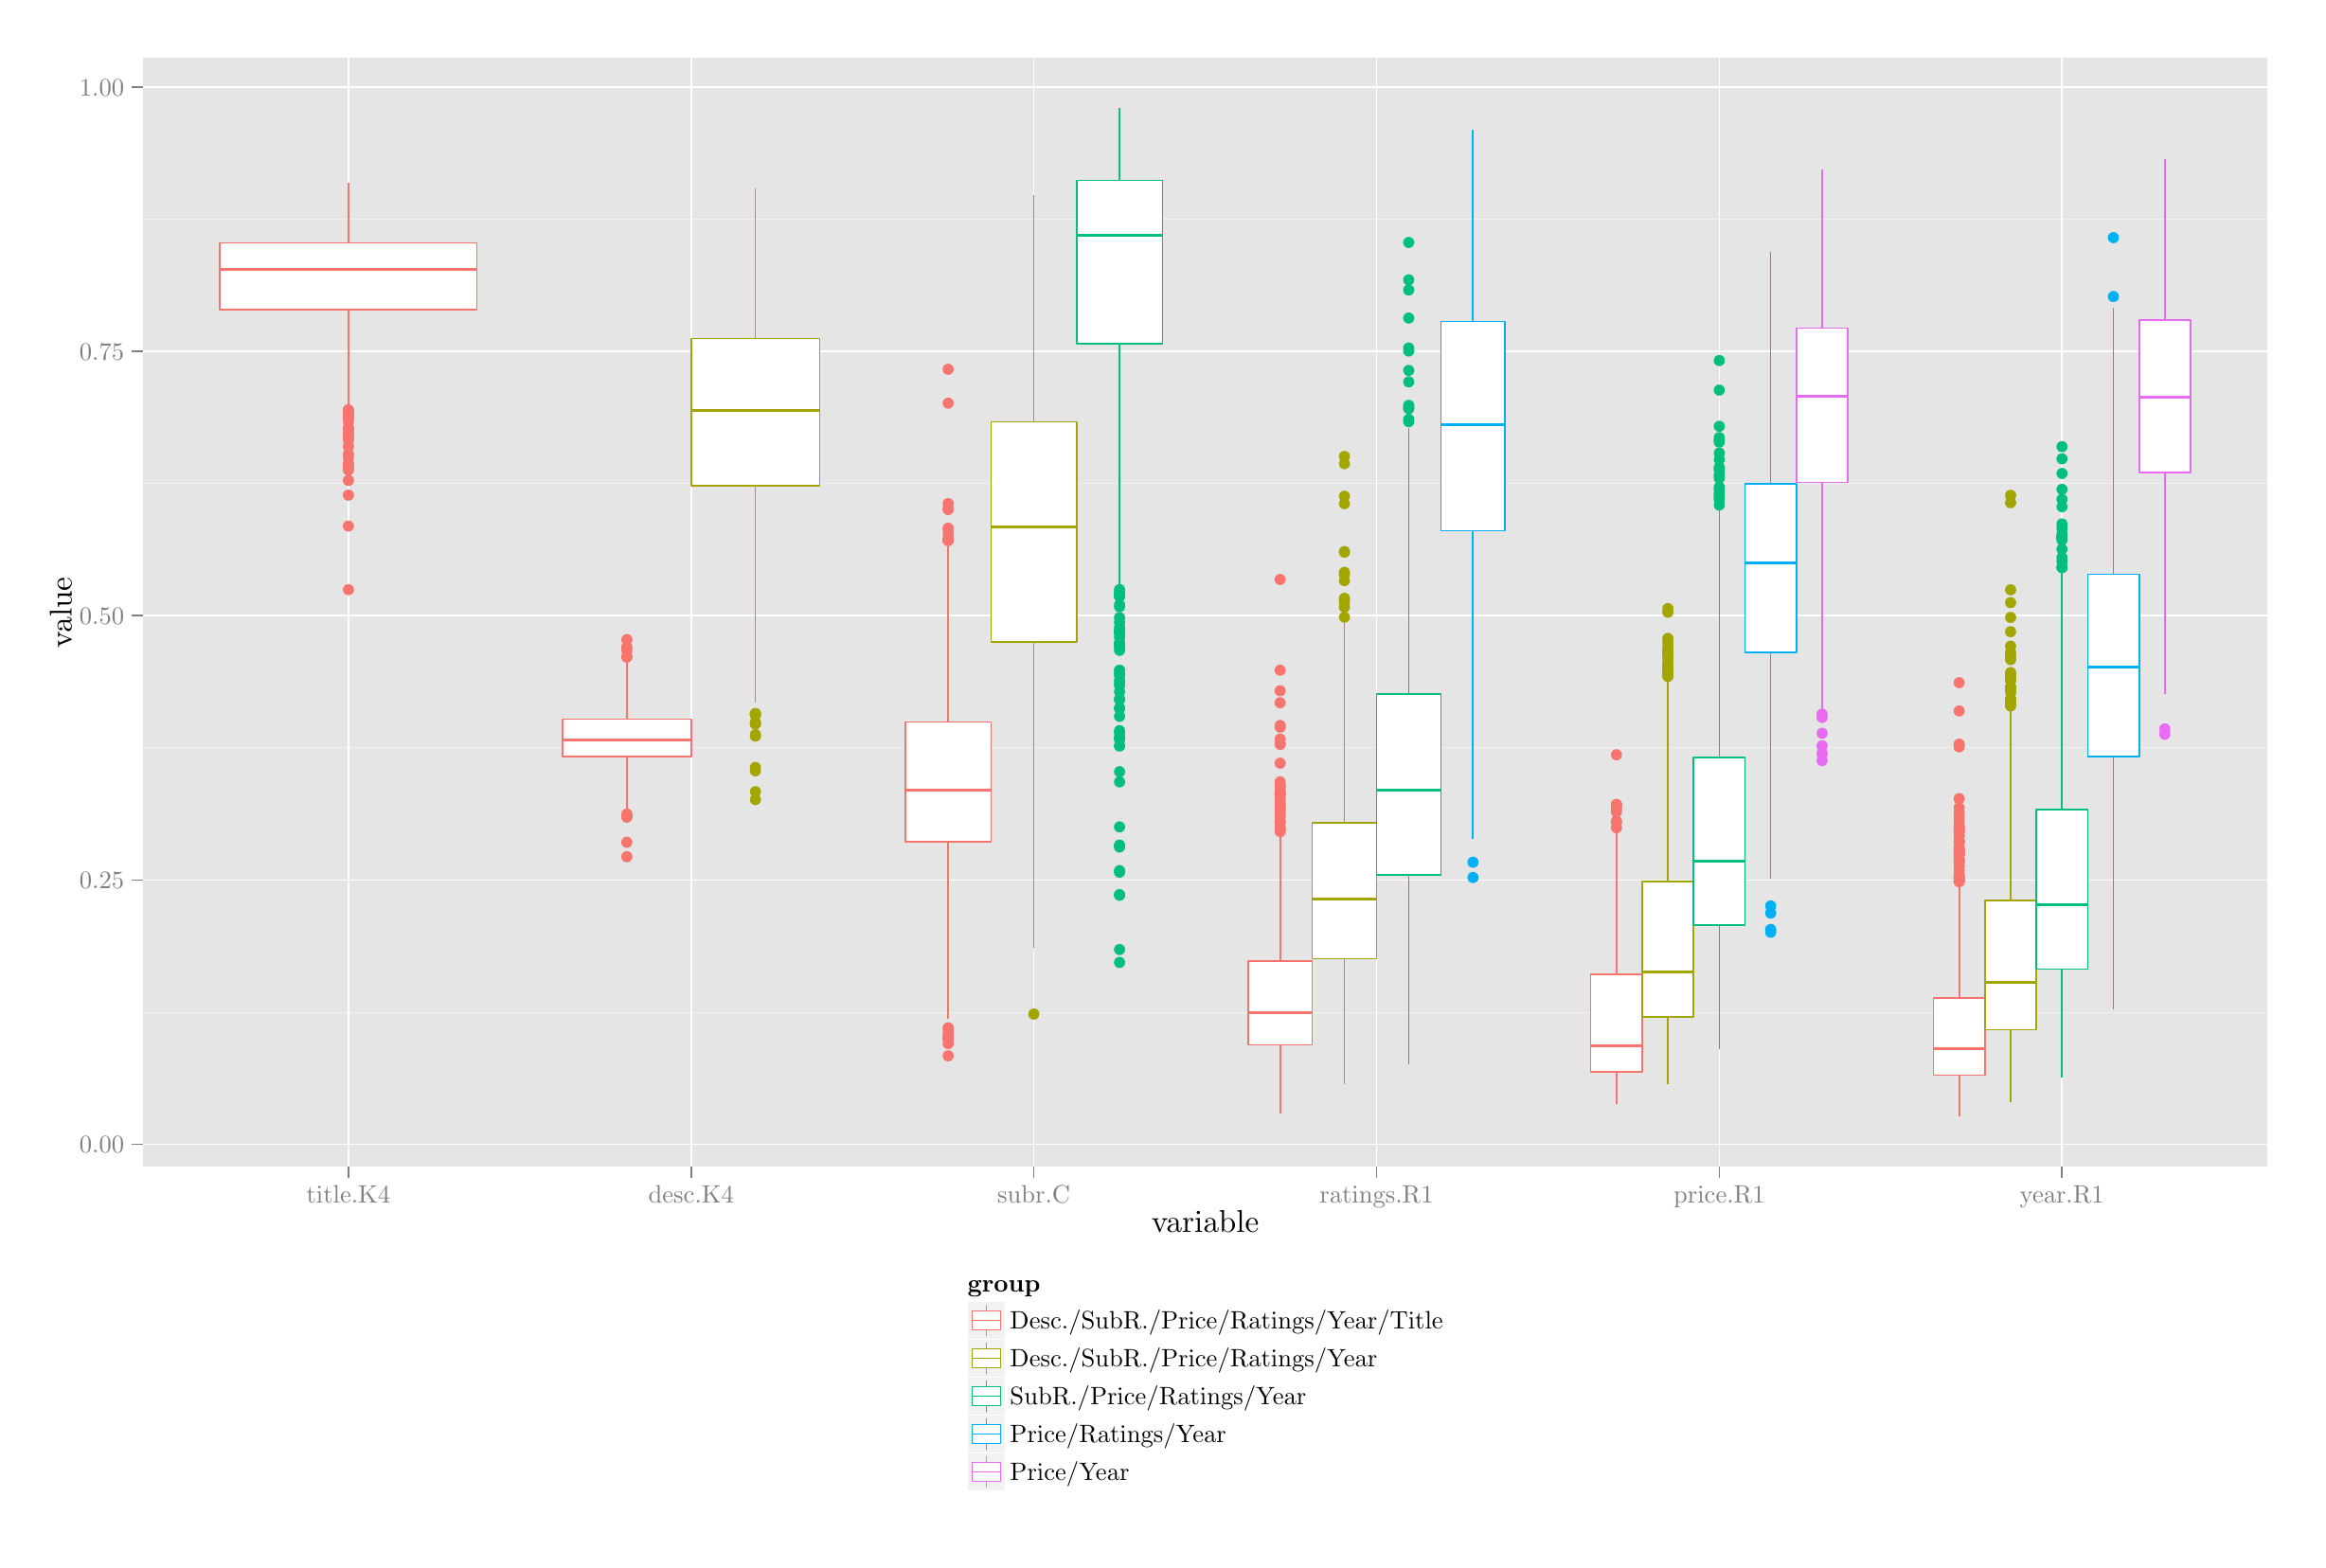
\begin{tikzpicture}[x=1pt,y=1pt]
\definecolor[named]{fillColor}{rgb}{1.00,1.00,1.00}
\path[use as bounding box,fill=fillColor,fill opacity=0.00] (0,0) rectangle (867.24,578.16);
\begin{scope}
\path[clip] (  0.00,  0.00) rectangle (867.24,578.16);
\definecolor[named]{drawColor}{rgb}{1.00,1.00,1.00}
\definecolor[named]{fillColor}{rgb}{1.00,1.00,1.00}

\path[draw=drawColor,line width= 0.6pt,line join=round,line cap=round,fill=fillColor] ( -0.00, -0.00) rectangle (867.24,578.16);
\end{scope}
\begin{scope}
\path[clip] ( 44.49,142.81) rectangle (855.20,566.12);
\definecolor[named]{fillColor}{rgb}{0.90,0.90,0.90}

\path[fill=fillColor] ( 44.49,142.81) rectangle (855.19,566.11);
\definecolor[named]{drawColor}{rgb}{0.95,0.95,0.95}

\path[draw=drawColor,line width= 0.3pt,line join=round] ( 44.49,201.88) --
	(855.20,201.88);

\path[draw=drawColor,line width= 0.3pt,line join=round] ( 44.49,302.75) --
	(855.20,302.75);

\path[draw=drawColor,line width= 0.3pt,line join=round] ( 44.49,403.63) --
	(855.20,403.63);

\path[draw=drawColor,line width= 0.3pt,line join=round] ( 44.49,504.50) --
	(855.20,504.50);
\definecolor[named]{drawColor}{rgb}{1.00,1.00,1.00}

\path[draw=drawColor,line width= 0.6pt,line join=round] ( 44.49,151.45) --
	(855.20,151.45);

\path[draw=drawColor,line width= 0.6pt,line join=round] ( 44.49,252.32) --
	(855.20,252.32);

\path[draw=drawColor,line width= 0.6pt,line join=round] ( 44.49,353.19) --
	(855.20,353.19);

\path[draw=drawColor,line width= 0.6pt,line join=round] ( 44.49,454.06) --
	(855.20,454.06);

\path[draw=drawColor,line width= 0.6pt,line join=round] ( 44.49,554.93) --
	(855.20,554.93);

\path[draw=drawColor,line width= 0.6pt,line join=round] (122.94,142.81) --
	(122.94,566.12);

\path[draw=drawColor,line width= 0.6pt,line join=round] (253.70,142.81) --
	(253.70,566.12);

\path[draw=drawColor,line width= 0.6pt,line join=round] (384.46,142.81) --
	(384.46,566.12);

\path[draw=drawColor,line width= 0.6pt,line join=round] (515.22,142.81) --
	(515.22,566.12);

\path[draw=drawColor,line width= 0.6pt,line join=round] (645.98,142.81) --
	(645.98,566.12);

\path[draw=drawColor,line width= 0.6pt,line join=round] (776.74,142.81) --
	(776.74,566.12);
\definecolor[named]{fillColor}{rgb}{0.97,0.46,0.43}

\path[fill=fillColor] (122.94,431.02) circle (  2.13);

\path[fill=fillColor] (122.94,404.81) circle (  2.13);

\path[fill=fillColor] (122.94,430.35) circle (  2.13);

\path[fill=fillColor] (122.94,421.74) circle (  2.13);

\path[fill=fillColor] (122.94,408.75) circle (  2.13);

\path[fill=fillColor] (122.94,417.75) circle (  2.13);

\path[fill=fillColor] (122.94,429.66) circle (  2.13);

\path[fill=fillColor] (122.94,430.72) circle (  2.13);

\path[fill=fillColor] (122.94,421.56) circle (  2.13);

\path[fill=fillColor] (122.94,414.88) circle (  2.13);

\path[fill=fillColor] (122.94,431.10) circle (  2.13);

\path[fill=fillColor] (122.94,428.28) circle (  2.13);

\path[fill=fillColor] (122.94,410.92) circle (  2.13);

\path[fill=fillColor] (122.94,423.37) circle (  2.13);

\path[fill=fillColor] (122.94,410.07) circle (  2.13);

\path[fill=fillColor] (122.94,421.90) circle (  2.13);

\path[fill=fillColor] (122.94,421.16) circle (  2.13);

\path[fill=fillColor] (122.94,421.78) circle (  2.13);

\path[fill=fillColor] (122.94,363.13) circle (  2.13);

\path[fill=fillColor] (122.94,399.19) circle (  2.13);

\path[fill=fillColor] (122.94,411.06) circle (  2.13);

\path[fill=fillColor] (122.94,387.40) circle (  2.13);

\path[fill=fillColor] (122.94,410.59) circle (  2.13);

\path[fill=fillColor] (122.94,431.15) circle (  2.13);

\path[fill=fillColor] (122.94,424.03) circle (  2.13);

\path[fill=fillColor] (122.94,420.16) circle (  2.13);

\path[fill=fillColor] (122.94,431.76) circle (  2.13);

\path[fill=fillColor] (122.94,424.14) circle (  2.13);

\path[fill=fillColor] (122.94,430.81) circle (  2.13);

\path[fill=fillColor] (122.94,428.73) circle (  2.13);

\path[fill=fillColor] (122.94,425.03) circle (  2.13);

\path[fill=fillColor] (122.94,430.25) circle (  2.13);

\path[fill=fillColor] (122.94,431.45) circle (  2.13);

\path[fill=fillColor] (122.94,427.36) circle (  2.13);

\path[fill=fillColor] (122.94,429.87) circle (  2.13);

\path[fill=fillColor] (122.94,413.48) circle (  2.13);

\path[fill=fillColor] (122.94,411.15) circle (  2.13);

\path[fill=fillColor] (122.94,431.21) circle (  2.13);
\definecolor[named]{drawColor}{rgb}{0.97,0.46,0.43}

\path[draw=drawColor,line width= 0.6pt,line join=round,fill=fillColor] (122.94,495.47) -- (122.94,518.46);

\path[draw=drawColor,line width= 0.6pt,line join=round,fill=fillColor] (122.94,470.04) -- (122.94,432.32);
\definecolor[named]{fillColor}{rgb}{1.00,1.00,1.00}

\path[draw=drawColor,line width= 0.6pt,line join=round,line cap=round,fill=fillColor] ( 73.91,495.47) --
	( 73.91,470.04) --
	(171.98,470.04) --
	(171.98,495.47) --
	( 73.91,495.47) --
	cycle;
\definecolor[named]{fillColor}{rgb}{0.97,0.46,0.43}

\path[draw=drawColor,line width= 1.1pt,line join=round,fill=fillColor] ( 73.91,485.21) -- (171.98,485.21);

\path[fill=fillColor] (229.18,340.02) circle (  2.13);

\path[fill=fillColor] (229.18,344.06) circle (  2.13);

\path[fill=fillColor] (229.18,337.66) circle (  2.13);

\path[fill=fillColor] (229.18,261.21) circle (  2.13);

\path[fill=fillColor] (229.18,337.36) circle (  2.13);

\path[fill=fillColor] (229.18,341.28) circle (  2.13);

\path[fill=fillColor] (229.18,276.59) circle (  2.13);

\path[fill=fillColor] (229.18,277.51) circle (  2.13);

\path[fill=fillColor] (229.18,276.31) circle (  2.13);

\path[fill=fillColor] (229.18,266.75) circle (  2.13);

\path[draw=drawColor,line width= 0.6pt,line join=round,fill=fillColor] (229.18,313.74) -- (229.18,335.05);

\path[draw=drawColor,line width= 0.6pt,line join=round,fill=fillColor] (229.18,299.39) -- (229.18,277.97);
\definecolor[named]{fillColor}{rgb}{1.00,1.00,1.00}

\path[draw=drawColor,line width= 0.6pt,line join=round,line cap=round,fill=fillColor] (204.67,313.74) --
	(204.67,299.39) --
	(253.70,299.39) --
	(253.70,313.74) --
	(204.67,313.74) --
	cycle;
\definecolor[named]{fillColor}{rgb}{0.97,0.46,0.43}

\path[draw=drawColor,line width= 1.1pt,line join=round,fill=fillColor] (204.67,305.91) -- (253.70,305.91);

\path[fill=fillColor] (351.77,191.74) circle (  2.13);

\path[fill=fillColor] (351.77,195.92) circle (  2.13);

\path[fill=fillColor] (351.77,386.15) circle (  2.13);

\path[fill=fillColor] (351.77,185.23) circle (  2.13);

\path[fill=fillColor] (351.77,192.00) circle (  2.13);

\path[fill=fillColor] (351.77,381.83) circle (  2.13);

\path[fill=fillColor] (351.77,434.30) circle (  2.13);

\path[fill=fillColor] (351.77,393.93) circle (  2.13);

\path[fill=fillColor] (351.77,447.23) circle (  2.13);

\path[fill=fillColor] (351.77,191.88) circle (  2.13);

\path[fill=fillColor] (351.77,393.69) circle (  2.13);

\path[fill=fillColor] (351.77,382.07) circle (  2.13);

\path[fill=fillColor] (351.77,384.38) circle (  2.13);

\path[fill=fillColor] (351.77,381.98) circle (  2.13);

\path[fill=fillColor] (351.77,395.95) circle (  2.13);

\path[fill=fillColor] (351.77,189.87) circle (  2.13);

\path[fill=fillColor] (351.77,382.34) circle (  2.13);

\path[fill=fillColor] (351.77,193.37) circle (  2.13);

\path[fill=fillColor] (351.77,194.96) circle (  2.13);

\path[fill=fillColor] (351.77,382.63) circle (  2.13);

\path[fill=fillColor] (351.77,386.57) circle (  2.13);

\path[draw=drawColor,line width= 0.6pt,line join=round,fill=fillColor] (351.77,312.61) -- (351.77,379.50);

\path[draw=drawColor,line width= 0.6pt,line join=round,fill=fillColor] (351.77,266.85) -- (351.77,199.40);
\definecolor[named]{fillColor}{rgb}{1.00,1.00,1.00}

\path[draw=drawColor,line width= 0.6pt,line join=round,line cap=round,fill=fillColor] (335.43,312.61) --
	(335.43,266.85) --
	(368.12,266.85) --
	(368.12,312.61) --
	(335.43,312.61) --
	cycle;
\definecolor[named]{fillColor}{rgb}{0.97,0.46,0.43}

\path[draw=drawColor,line width= 1.1pt,line join=round,fill=fillColor] (335.43,286.78) -- (368.12,286.78);

\path[fill=fillColor] (478.44,310.64) circle (  2.13);

\path[fill=fillColor] (478.44,289.77) circle (  2.13);

\path[fill=fillColor] (478.44,284.67) circle (  2.13);

\path[fill=fillColor] (478.44,367.01) circle (  2.13);

\path[fill=fillColor] (478.44,287.64) circle (  2.13);

\path[fill=fillColor] (478.44,280.48) circle (  2.13);

\path[fill=fillColor] (478.44,285.66) circle (  2.13);

\path[fill=fillColor] (478.44,285.57) circle (  2.13);

\path[fill=fillColor] (478.44,282.24) circle (  2.13);

\path[fill=fillColor] (478.44,304.24) circle (  2.13);

\path[fill=fillColor] (478.44,271.41) circle (  2.13);

\path[fill=fillColor] (478.44,270.80) circle (  2.13);

\path[fill=fillColor] (478.44,279.50) circle (  2.13);

\path[fill=fillColor] (478.44,319.96) circle (  2.13);

\path[fill=fillColor] (478.44,278.19) circle (  2.13);

\path[fill=fillColor] (478.44,279.75) circle (  2.13);

\path[fill=fillColor] (478.44,296.92) circle (  2.13);

\path[fill=fillColor] (478.44,274.07) circle (  2.13);

\path[fill=fillColor] (478.44,284.98) circle (  2.13);

\path[fill=fillColor] (478.44,276.36) circle (  2.13);

\path[fill=fillColor] (478.44,288.21) circle (  2.13);

\path[fill=fillColor] (478.44,271.28) circle (  2.13);

\path[fill=fillColor] (478.44,304.09) circle (  2.13);

\path[fill=fillColor] (478.44,276.76) circle (  2.13);

\path[fill=fillColor] (478.44,285.57) circle (  2.13);

\path[fill=fillColor] (478.44,311.31) circle (  2.13);

\path[fill=fillColor] (478.44,274.56) circle (  2.13);

\path[fill=fillColor] (478.44,284.94) circle (  2.13);

\path[fill=fillColor] (478.44,286.15) circle (  2.13);

\path[fill=fillColor] (478.44,272.54) circle (  2.13);

\path[fill=fillColor] (478.44,324.55) circle (  2.13);

\path[fill=fillColor] (478.44,281.19) circle (  2.13);

\path[fill=fillColor] (478.44,274.37) circle (  2.13);

\path[fill=fillColor] (478.44,306.08) circle (  2.13);

\path[fill=fillColor] (478.44,287.90) circle (  2.13);

\path[fill=fillColor] (478.44,279.06) circle (  2.13);

\path[fill=fillColor] (478.44,283.47) circle (  2.13);

\path[fill=fillColor] (478.44,332.40) circle (  2.13);

\path[draw=drawColor,line width= 0.6pt,line join=round,fill=fillColor] (478.44,221.36) -- (478.44,269.14);

\path[draw=drawColor,line width= 0.6pt,line join=round,fill=fillColor] (478.44,189.40) -- (478.44,163.25);
\definecolor[named]{fillColor}{rgb}{1.00,1.00,1.00}

\path[draw=drawColor,line width= 0.6pt,line join=round,line cap=round,fill=fillColor] (466.19,221.36) --
	(466.19,189.40) --
	(490.70,189.40) --
	(490.70,221.36) --
	(466.19,221.36) --
	cycle;
\definecolor[named]{fillColor}{rgb}{0.97,0.46,0.43}

\path[draw=drawColor,line width= 1.1pt,line join=round,fill=fillColor] (466.19,201.62) -- (490.70,201.62);

\path[fill=fillColor] (606.75,272.25) circle (  2.13);

\path[fill=fillColor] (606.75,300.12) circle (  2.13);

\path[fill=fillColor] (606.75,281.10) circle (  2.13);

\path[fill=fillColor] (606.75,281.16) circle (  2.13);

\path[fill=fillColor] (606.75,274.89) circle (  2.13);

\path[fill=fillColor] (606.75,279.52) circle (  2.13);

\path[fill=fillColor] (606.75,280.56) circle (  2.13);

\path[fill=fillColor] (606.75,274.36) circle (  2.13);

\path[fill=fillColor] (606.75,278.28) circle (  2.13);

\path[draw=drawColor,line width= 0.6pt,line join=round,fill=fillColor] (606.75,216.37) -- (606.75,271.95);

\path[draw=drawColor,line width= 0.6pt,line join=round,fill=fillColor] (606.75,179.19) -- (606.75,166.77);
\definecolor[named]{fillColor}{rgb}{1.00,1.00,1.00}

\path[draw=drawColor,line width= 0.6pt,line join=round,line cap=round,fill=fillColor] (596.94,216.37) --
	(596.94,179.19) --
	(616.56,179.19) --
	(616.56,216.37) --
	(596.94,216.37) --
	cycle;
\definecolor[named]{fillColor}{rgb}{0.97,0.46,0.43}

\path[draw=drawColor,line width= 1.1pt,line join=round,fill=fillColor] (596.94,188.88) -- (616.56,188.88);

\path[fill=fillColor] (737.51,274.71) circle (  2.13);

\path[fill=fillColor] (737.51,327.63) circle (  2.13);

\path[fill=fillColor] (737.51,263.70) circle (  2.13);

\path[fill=fillColor] (737.51,272.88) circle (  2.13);

\path[fill=fillColor] (737.51,267.18) circle (  2.13);

\path[fill=fillColor] (737.51,251.68) circle (  2.13);

\path[fill=fillColor] (737.51,252.24) circle (  2.13);

\path[fill=fillColor] (737.51,253.32) circle (  2.13);

\path[fill=fillColor] (737.51,269.15) circle (  2.13);

\path[fill=fillColor] (737.51,259.14) circle (  2.13);

\path[fill=fillColor] (737.51,254.63) circle (  2.13);

\path[fill=fillColor] (737.51,272.55) circle (  2.13);

\path[fill=fillColor] (737.51,270.79) circle (  2.13);

\path[fill=fillColor] (737.51,266.85) circle (  2.13);

\path[fill=fillColor] (737.51,304.17) circle (  2.13);

\path[fill=fillColor] (737.51,277.00) circle (  2.13);

\path[fill=fillColor] (737.51,263.19) circle (  2.13);

\path[fill=fillColor] (737.51,270.83) circle (  2.13);

\path[fill=fillColor] (737.51,251.89) circle (  2.13);

\path[fill=fillColor] (737.51,263.70) circle (  2.13);

\path[fill=fillColor] (737.51,251.88) circle (  2.13);

\path[fill=fillColor] (737.51,259.43) circle (  2.13);

\path[fill=fillColor] (737.51,272.64) circle (  2.13);

\path[fill=fillColor] (737.51,316.84) circle (  2.13);

\path[fill=fillColor] (737.51,277.89) circle (  2.13);

\path[fill=fillColor] (737.51,264.87) circle (  2.13);

\path[fill=fillColor] (737.51,262.23) circle (  2.13);

\path[fill=fillColor] (737.51,262.95) circle (  2.13);

\path[fill=fillColor] (737.51,252.26) circle (  2.13);

\path[fill=fillColor] (737.51,252.05) circle (  2.13);

\path[fill=fillColor] (737.51,256.02) circle (  2.13);

\path[fill=fillColor] (737.51,253.22) circle (  2.13);

\path[fill=fillColor] (737.51,261.72) circle (  2.13);

\path[fill=fillColor] (737.51,263.82) circle (  2.13);

\path[fill=fillColor] (737.51,272.55) circle (  2.13);

\path[fill=fillColor] (737.51,253.76) circle (  2.13);

\path[fill=fillColor] (737.51,266.68) circle (  2.13);

\path[fill=fillColor] (737.51,260.02) circle (  2.13);

\path[fill=fillColor] (737.51,257.56) circle (  2.13);

\path[fill=fillColor] (737.51,275.96) circle (  2.13);

\path[fill=fillColor] (737.51,269.18) circle (  2.13);

\path[fill=fillColor] (737.51,283.36) circle (  2.13);

\path[fill=fillColor] (737.51,279.93) circle (  2.13);

\path[fill=fillColor] (737.51,303.14) circle (  2.13);

\path[fill=fillColor] (737.51,260.05) circle (  2.13);

\path[fill=fillColor] (737.51,257.63) circle (  2.13);

\path[fill=fillColor] (737.51,262.27) circle (  2.13);

\path[fill=fillColor] (737.51,271.53) circle (  2.13);

\path[fill=fillColor] (737.51,253.53) circle (  2.13);

\path[draw=drawColor,line width= 0.6pt,line join=round,fill=fillColor] (737.51,207.22) -- (737.51,251.24);

\path[draw=drawColor,line width= 0.6pt,line join=round,fill=fillColor] (737.51,177.84) -- (737.51,162.06);
\definecolor[named]{fillColor}{rgb}{1.00,1.00,1.00}

\path[draw=drawColor,line width= 0.6pt,line join=round,line cap=round,fill=fillColor] (727.70,207.22) --
	(727.70,177.84) --
	(747.32,177.84) --
	(747.32,207.22) --
	(727.70,207.22) --
	cycle;
\definecolor[named]{fillColor}{rgb}{0.97,0.46,0.43}

\path[draw=drawColor,line width= 1.1pt,line join=round,fill=fillColor] (727.70,188.12) -- (747.32,188.12);
\definecolor[named]{fillColor}{rgb}{0.64,0.65,0.00}

\path[fill=fillColor] (278.22,286.02) circle (  2.13);

\path[fill=fillColor] (278.22,307.26) circle (  2.13);

\path[fill=fillColor] (278.22,294.00) circle (  2.13);

\path[fill=fillColor] (278.22,315.16) circle (  2.13);

\path[fill=fillColor] (278.22,315.87) circle (  2.13);

\path[fill=fillColor] (278.22,307.81) circle (  2.13);

\path[fill=fillColor] (278.22,295.29) circle (  2.13);

\path[fill=fillColor] (278.22,283.03) circle (  2.13);

\path[fill=fillColor] (278.22,315.59) circle (  2.13);

\path[fill=fillColor] (278.22,312.08) circle (  2.13);

\path[fill=fillColor] (278.22,311.83) circle (  2.13);

\path[fill=fillColor] (278.22,312.50) circle (  2.13);

\path[fill=fillColor] (278.22,315.63) circle (  2.13);
\definecolor[named]{drawColor}{rgb}{0.64,0.65,0.00}

\path[draw=drawColor,line width= 0.6pt,line join=round,fill=fillColor] (278.22,458.96) -- (278.22,516.23);

\path[draw=drawColor,line width= 0.6pt,line join=round,fill=fillColor] (278.22,402.69) -- (278.22,320.04);
\definecolor[named]{fillColor}{rgb}{1.00,1.00,1.00}

\path[draw=drawColor,line width= 0.6pt,line join=round,line cap=round,fill=fillColor] (253.70,458.96) --
	(253.70,402.69) --
	(302.74,402.69) --
	(302.74,458.96) --
	(253.70,458.96) --
	cycle;
\definecolor[named]{fillColor}{rgb}{0.64,0.65,0.00}

\path[draw=drawColor,line width= 1.1pt,line join=round,fill=fillColor] (253.70,431.48) -- (302.74,431.48);

\path[fill=fillColor] (384.46,201.17) circle (  2.13);

\path[draw=drawColor,line width= 0.6pt,line join=round,fill=fillColor] (384.46,427.18) -- (384.46,513.81);

\path[draw=drawColor,line width= 0.6pt,line join=round,fill=fillColor] (384.46,343.10) -- (384.46,226.51);
\definecolor[named]{fillColor}{rgb}{1.00,1.00,1.00}

\path[draw=drawColor,line width= 0.6pt,line join=round,line cap=round,fill=fillColor] (368.12,427.18) --
	(368.12,343.10) --
	(400.81,343.10) --
	(400.81,427.18) --
	(368.12,427.18) --
	cycle;
\definecolor[named]{fillColor}{rgb}{0.64,0.65,0.00}

\path[draw=drawColor,line width= 1.1pt,line join=round,fill=fillColor] (368.12,387.14) -- (400.81,387.14);

\path[fill=fillColor] (502.96,413.97) circle (  2.13);

\path[fill=fillColor] (502.96,377.42) circle (  2.13);

\path[fill=fillColor] (502.96,368.98) circle (  2.13);

\path[fill=fillColor] (502.96,369.72) circle (  2.13);

\path[fill=fillColor] (502.96,366.56) circle (  2.13);

\path[fill=fillColor] (502.96,411.20) circle (  2.13);

\path[fill=fillColor] (502.96,395.93) circle (  2.13);

\path[fill=fillColor] (502.96,356.45) circle (  2.13);

\path[fill=fillColor] (502.96,359.83) circle (  2.13);

\path[fill=fillColor] (502.96,377.66) circle (  2.13);

\path[fill=fillColor] (502.96,352.62) circle (  2.13);

\path[fill=fillColor] (502.96,359.11) circle (  2.13);

\path[fill=fillColor] (502.96,358.37) circle (  2.13);

\path[fill=fillColor] (502.96,398.78) circle (  2.13);

\path[draw=drawColor,line width= 0.6pt,line join=round,fill=fillColor] (502.96,274.09) -- (502.96,351.22);

\path[draw=drawColor,line width= 0.6pt,line join=round,fill=fillColor] (502.96,222.25) -- (502.96,174.33);
\definecolor[named]{fillColor}{rgb}{1.00,1.00,1.00}

\path[draw=drawColor,line width= 0.6pt,line join=round,line cap=round,fill=fillColor] (490.70,274.09) --
	(490.70,222.25) --
	(515.22,222.25) --
	(515.22,274.09) --
	(490.70,274.09) --
	cycle;
\definecolor[named]{fillColor}{rgb}{0.64,0.65,0.00}

\path[draw=drawColor,line width= 1.1pt,line join=round,fill=fillColor] (490.70,244.92) -- (515.22,244.92);

\path[fill=fillColor] (626.37,344.52) circle (  2.13);

\path[fill=fillColor] (626.37,334.83) circle (  2.13);

\path[fill=fillColor] (626.37,343.01) circle (  2.13);

\path[fill=fillColor] (626.37,332.26) circle (  2.13);

\path[fill=fillColor] (626.37,334.87) circle (  2.13);

\path[fill=fillColor] (626.37,330.88) circle (  2.13);

\path[fill=fillColor] (626.37,339.14) circle (  2.13);

\path[fill=fillColor] (626.37,336.62) circle (  2.13);

\path[fill=fillColor] (626.37,334.22) circle (  2.13);

\path[fill=fillColor] (626.37,330.99) circle (  2.13);

\path[fill=fillColor] (626.37,341.46) circle (  2.13);

\path[fill=fillColor] (626.37,337.75) circle (  2.13);

\path[fill=fillColor] (626.37,339.48) circle (  2.13);

\path[fill=fillColor] (626.37,338.71) circle (  2.13);

\path[fill=fillColor] (626.37,330.46) circle (  2.13);

\path[fill=fillColor] (626.37,333.44) circle (  2.13);

\path[fill=fillColor] (626.37,332.49) circle (  2.13);

\path[fill=fillColor] (626.37,354.50) circle (  2.13);

\path[fill=fillColor] (626.37,355.90) circle (  2.13);

\path[fill=fillColor] (626.37,340.21) circle (  2.13);

\path[fill=fillColor] (626.37,330.00) circle (  2.13);

\path[draw=drawColor,line width= 0.6pt,line join=round,fill=fillColor] (626.37,251.85) -- (626.37,328.06);

\path[draw=drawColor,line width= 0.6pt,line join=round,fill=fillColor] (626.37,200.04) -- (626.37,174.30);
\definecolor[named]{fillColor}{rgb}{1.00,1.00,1.00}

\path[draw=drawColor,line width= 0.6pt,line join=round,line cap=round,fill=fillColor] (616.56,251.85) --
	(616.56,200.04) --
	(636.17,200.04) --
	(636.17,251.85) --
	(616.56,251.85) --
	cycle;
\definecolor[named]{fillColor}{rgb}{0.64,0.65,0.00}

\path[draw=drawColor,line width= 1.1pt,line join=round,fill=fillColor] (616.56,217.10) -- (636.17,217.10);

\path[fill=fillColor] (757.13,328.57) circle (  2.13);

\path[fill=fillColor] (757.13,336.44) circle (  2.13);

\path[fill=fillColor] (757.13,319.52) circle (  2.13);

\path[fill=fillColor] (757.13,328.58) circle (  2.13);

\path[fill=fillColor] (757.13,339.14) circle (  2.13);

\path[fill=fillColor] (757.13,321.49) circle (  2.13);

\path[fill=fillColor] (757.13,325.10) circle (  2.13);

\path[fill=fillColor] (757.13,352.53) circle (  2.13);

\path[fill=fillColor] (757.13,341.57) circle (  2.13);

\path[fill=fillColor] (757.13,320.78) circle (  2.13);

\path[fill=fillColor] (757.13,318.75) circle (  2.13);

\path[fill=fillColor] (757.13,323.87) circle (  2.13);

\path[fill=fillColor] (757.13,330.36) circle (  2.13);

\path[fill=fillColor] (757.13,320.73) circle (  2.13);

\path[fill=fillColor] (757.13,328.74) circle (  2.13);

\path[fill=fillColor] (757.13,358.19) circle (  2.13);

\path[fill=fillColor] (757.13,325.80) circle (  2.13);

\path[fill=fillColor] (757.13,331.48) circle (  2.13);

\path[fill=fillColor] (757.13,326.06) circle (  2.13);

\path[fill=fillColor] (757.13,399.13) circle (  2.13);

\path[fill=fillColor] (757.13,330.68) circle (  2.13);

\path[fill=fillColor] (757.13,347.07) circle (  2.13);

\path[fill=fillColor] (757.13,337.76) circle (  2.13);

\path[fill=fillColor] (757.13,363.07) circle (  2.13);

\path[fill=fillColor] (757.13,396.32) circle (  2.13);

\path[fill=fillColor] (757.13,319.23) circle (  2.13);

\path[draw=drawColor,line width= 0.6pt,line join=round,fill=fillColor] (757.13,244.40) -- (757.13,317.30);

\path[draw=drawColor,line width= 0.6pt,line join=round,fill=fillColor] (757.13,195.19) -- (757.13,167.39);
\definecolor[named]{fillColor}{rgb}{1.00,1.00,1.00}

\path[draw=drawColor,line width= 0.6pt,line join=round,line cap=round,fill=fillColor] (747.32,244.40) --
	(747.32,195.19) --
	(766.93,195.19) --
	(766.93,244.40) --
	(747.32,244.40) --
	cycle;
\definecolor[named]{fillColor}{rgb}{0.64,0.65,0.00}

\path[draw=drawColor,line width= 1.1pt,line join=round,fill=fillColor] (747.32,213.09) -- (766.93,213.09);
\definecolor[named]{fillColor}{rgb}{0.00,0.75,0.49}

\path[fill=fillColor] (417.15,341.57) circle (  2.13);

\path[fill=fillColor] (417.15,324.20) circle (  2.13);

\path[fill=fillColor] (417.15,350.68) circle (  2.13);

\path[fill=fillColor] (417.15,303.58) circle (  2.13);

\path[fill=fillColor] (417.15,314.76) circle (  2.13);

\path[fill=fillColor] (417.15,246.76) circle (  2.13);

\path[fill=fillColor] (417.15,342.71) circle (  2.13);

\path[fill=fillColor] (417.15,321.45) circle (  2.13);

\path[fill=fillColor] (417.15,363.15) circle (  2.13);

\path[fill=fillColor] (417.15,309.32) circle (  2.13);

\path[fill=fillColor] (417.15,339.96) circle (  2.13);

\path[fill=fillColor] (417.15,332.29) circle (  2.13);

\path[fill=fillColor] (417.15,327.29) circle (  2.13);

\path[fill=fillColor] (417.15,341.64) circle (  2.13);

\path[fill=fillColor] (417.15,362.26) circle (  2.13);

\path[fill=fillColor] (417.15,255.90) circle (  2.13);

\path[fill=fillColor] (417.15,289.77) circle (  2.13);

\path[fill=fillColor] (417.15,272.59) circle (  2.13);

\path[fill=fillColor] (417.15,348.70) circle (  2.13);

\path[fill=fillColor] (417.15,347.32) circle (  2.13);

\path[fill=fillColor] (417.15,347.44) circle (  2.13);

\path[fill=fillColor] (417.15,306.05) circle (  2.13);

\path[fill=fillColor] (417.15,346.84) circle (  2.13);

\path[fill=fillColor] (417.15,347.09) circle (  2.13);

\path[fill=fillColor] (417.15,361.78) circle (  2.13);

\path[fill=fillColor] (417.15,265.17) circle (  2.13);

\path[fill=fillColor] (417.15,346.48) circle (  2.13);

\path[fill=fillColor] (417.15,328.49) circle (  2.13);

\path[fill=fillColor] (417.15,317.65) circle (  2.13);

\path[fill=fillColor] (417.15,326.54) circle (  2.13);

\path[fill=fillColor] (417.15,306.79) circle (  2.13);

\path[fill=fillColor] (417.15,357.33) circle (  2.13);

\path[fill=fillColor] (417.15,332.34) circle (  2.13);

\path[fill=fillColor] (417.15,342.84) circle (  2.13);

\path[fill=fillColor] (417.15,330.45) circle (  2.13);

\path[fill=fillColor] (417.15,306.16) circle (  2.13);

\path[fill=fillColor] (417.15,331.18) circle (  2.13);

\path[fill=fillColor] (417.15,220.86) circle (  2.13);

\path[fill=fillColor] (417.15,317.99) circle (  2.13);

\path[fill=fillColor] (417.15,360.51) circle (  2.13);

\path[fill=fillColor] (417.15,360.82) circle (  2.13);

\path[fill=fillColor] (417.15,321.10) circle (  2.13);

\path[fill=fillColor] (417.15,293.64) circle (  2.13);

\path[fill=fillColor] (417.15,356.63) circle (  2.13);

\path[fill=fillColor] (417.15,246.49) circle (  2.13);

\path[fill=fillColor] (417.15,361.10) circle (  2.13);

\path[fill=fillColor] (417.15,308.43) circle (  2.13);

\path[fill=fillColor] (417.15,303.48) circle (  2.13);

\path[fill=fillColor] (417.15,352.50) circle (  2.13);

\path[fill=fillColor] (417.15,264.91) circle (  2.13);

\path[fill=fillColor] (417.15,265.64) circle (  2.13);

\path[fill=fillColor] (417.15,225.78) circle (  2.13);

\path[fill=fillColor] (417.15,255.30) circle (  2.13);

\path[fill=fillColor] (417.15,345.01) circle (  2.13);
\definecolor[named]{drawColor}{rgb}{0.00,0.75,0.49}

\path[draw=drawColor,line width= 0.6pt,line join=round,fill=fillColor] (417.15,519.29) -- (417.15,546.87);

\path[draw=drawColor,line width= 0.6pt,line join=round,fill=fillColor] (417.15,456.99) -- (417.15,364.95);
\definecolor[named]{fillColor}{rgb}{1.00,1.00,1.00}

\path[draw=drawColor,line width= 0.6pt,line join=round,line cap=round,fill=fillColor] (400.81,519.29) --
	(400.81,456.99) --
	(433.50,456.99) --
	(433.50,519.29) --
	(400.81,519.29) --
	cycle;
\definecolor[named]{fillColor}{rgb}{0.00,0.75,0.49}

\path[draw=drawColor,line width= 1.1pt,line join=round,fill=fillColor] (400.81,498.52) -- (433.50,498.52);

\path[fill=fillColor] (527.48,428.12) circle (  2.13);

\path[fill=fillColor] (527.48,433.45) circle (  2.13);

\path[fill=fillColor] (527.48,446.79) circle (  2.13);

\path[fill=fillColor] (527.48,466.77) circle (  2.13);

\path[fill=fillColor] (527.48,455.34) circle (  2.13);

\path[fill=fillColor] (527.48,432.20) circle (  2.13);

\path[fill=fillColor] (527.48,432.67) circle (  2.13);

\path[fill=fillColor] (527.48,477.48) circle (  2.13);

\path[fill=fillColor] (527.48,481.33) circle (  2.13);

\path[fill=fillColor] (527.48,442.43) circle (  2.13);

\path[fill=fillColor] (527.48,427.23) circle (  2.13);

\path[fill=fillColor] (527.48,495.64) circle (  2.13);

\path[fill=fillColor] (527.48,454.19) circle (  2.13);

\path[draw=drawColor,line width= 0.6pt,line join=round,fill=fillColor] (527.48,323.39) -- (527.48,424.77);

\path[draw=drawColor,line width= 0.6pt,line join=round,fill=fillColor] (527.48,254.26) -- (527.48,181.84);
\definecolor[named]{fillColor}{rgb}{1.00,1.00,1.00}

\path[draw=drawColor,line width= 0.6pt,line join=round,line cap=round,fill=fillColor] (515.22,323.39) --
	(515.22,254.26) --
	(539.74,254.26) --
	(539.74,323.39) --
	(515.22,323.39) --
	cycle;
\definecolor[named]{fillColor}{rgb}{0.00,0.75,0.49}

\path[draw=drawColor,line width= 1.1pt,line join=round,fill=fillColor] (515.22,286.47) -- (539.74,286.47);

\path[fill=fillColor] (645.98,402.25) circle (  2.13);

\path[fill=fillColor] (645.98,409.69) circle (  2.13);

\path[fill=fillColor] (645.98,406.99) circle (  2.13);

\path[fill=fillColor] (645.98,406.44) circle (  2.13);

\path[fill=fillColor] (645.98,419.47) circle (  2.13);

\path[fill=fillColor] (645.98,399.89) circle (  2.13);

\path[fill=fillColor] (645.98,405.63) circle (  2.13);

\path[fill=fillColor] (645.98,450.55) circle (  2.13);

\path[fill=fillColor] (645.98,408.87) circle (  2.13);

\path[fill=fillColor] (645.98,439.28) circle (  2.13);

\path[fill=fillColor] (645.98,415.28) circle (  2.13);

\path[fill=fillColor] (645.98,409.64) circle (  2.13);

\path[fill=fillColor] (645.98,421.15) circle (  2.13);

\path[fill=fillColor] (645.98,399.35) circle (  2.13);

\path[fill=fillColor] (645.98,397.62) circle (  2.13);

\path[fill=fillColor] (645.98,412.76) circle (  2.13);

\path[fill=fillColor] (645.98,398.18) circle (  2.13);

\path[fill=fillColor] (645.98,425.48) circle (  2.13);

\path[fill=fillColor] (645.98,395.43) circle (  2.13);

\path[fill=fillColor] (645.98,420.21) circle (  2.13);

\path[fill=fillColor] (645.98,401.53) circle (  2.13);

\path[draw=drawColor,line width= 0.6pt,line join=round,fill=fillColor] (645.98,299.09) -- (645.98,394.90);

\path[draw=drawColor,line width= 0.6pt,line join=round,fill=fillColor] (645.98,235.14) -- (645.98,187.95);
\definecolor[named]{fillColor}{rgb}{1.00,1.00,1.00}

\path[draw=drawColor,line width= 0.6pt,line join=round,line cap=round,fill=fillColor] (636.17,299.09) --
	(636.17,235.14) --
	(655.79,235.14) --
	(655.79,299.09) --
	(636.17,299.09) --
	cycle;
\definecolor[named]{fillColor}{rgb}{0.00,0.75,0.49}

\path[draw=drawColor,line width= 1.1pt,line join=round,fill=fillColor] (636.17,259.36) -- (655.79,259.36);

\path[fill=fillColor] (776.74,383.35) circle (  2.13);

\path[fill=fillColor] (776.74,382.10) circle (  2.13);

\path[fill=fillColor] (776.74,371.68) circle (  2.13);

\path[fill=fillColor] (776.74,397.61) circle (  2.13);

\path[fill=fillColor] (776.74,382.85) circle (  2.13);

\path[fill=fillColor] (776.74,382.58) circle (  2.13);

\path[fill=fillColor] (776.74,373.82) circle (  2.13);

\path[fill=fillColor] (776.74,388.20) circle (  2.13);

\path[fill=fillColor] (776.74,371.53) circle (  2.13);

\path[fill=fillColor] (776.74,384.48) circle (  2.13);

\path[fill=fillColor] (776.74,417.68) circle (  2.13);

\path[fill=fillColor] (776.74,401.39) circle (  2.13);

\path[fill=fillColor] (776.74,407.46) circle (  2.13);

\path[fill=fillColor] (776.74,383.47) circle (  2.13);

\path[fill=fillColor] (776.74,394.76) circle (  2.13);

\path[fill=fillColor] (776.74,378.57) circle (  2.13);

\path[fill=fillColor] (776.74,386.55) circle (  2.13);

\path[fill=fillColor] (776.74,413.06) circle (  2.13);

\path[fill=fillColor] (776.74,375.39) circle (  2.13);

\path[draw=drawColor,line width= 0.6pt,line join=round,fill=fillColor] (776.74,279.32) -- (776.74,369.43);

\path[draw=drawColor,line width= 0.6pt,line join=round,fill=fillColor] (776.74,218.31) -- (776.74,177.08);
\definecolor[named]{fillColor}{rgb}{1.00,1.00,1.00}

\path[draw=drawColor,line width= 0.6pt,line join=round,line cap=round,fill=fillColor] (766.93,279.32) --
	(766.93,218.31) --
	(786.55,218.31) --
	(786.55,279.32) --
	(766.93,279.32) --
	cycle;
\definecolor[named]{fillColor}{rgb}{0.00,0.75,0.49}

\path[draw=drawColor,line width= 1.1pt,line join=round,fill=fillColor] (766.93,242.82) -- (786.55,242.82);
\definecolor[named]{fillColor}{rgb}{0.00,0.69,0.96}

\path[fill=fillColor] (552.00,253.27) circle (  2.13);

\path[fill=fillColor] (552.00,259.11) circle (  2.13);
\definecolor[named]{drawColor}{rgb}{0.00,0.69,0.96}

\path[draw=drawColor,line width= 0.6pt,line join=round,fill=fillColor] (552.00,465.51) -- (552.00,538.51);

\path[draw=drawColor,line width= 0.6pt,line join=round,fill=fillColor] (552.00,385.64) -- (552.00,268.03);
\definecolor[named]{fillColor}{rgb}{1.00,1.00,1.00}

\path[draw=drawColor,line width= 0.6pt,line join=round,line cap=round,fill=fillColor] (539.74,465.51) --
	(539.74,385.64) --
	(564.25,385.64) --
	(564.25,465.51) --
	(539.74,465.51) --
	cycle;
\definecolor[named]{fillColor}{rgb}{0.00,0.69,0.96}

\path[draw=drawColor,line width= 1.1pt,line join=round,fill=fillColor] (539.74,426.24) -- (564.25,426.24);

\path[fill=fillColor] (665.59,232.37) circle (  2.13);

\path[fill=fillColor] (665.59,242.43) circle (  2.13);

\path[fill=fillColor] (665.59,239.71) circle (  2.13);

\path[fill=fillColor] (665.59,233.45) circle (  2.13);

\path[draw=drawColor,line width= 0.6pt,line join=round,fill=fillColor] (665.59,403.41) -- (665.59,492.12);

\path[draw=drawColor,line width= 0.6pt,line join=round,fill=fillColor] (665.59,339.29) -- (665.59,252.88);
\definecolor[named]{fillColor}{rgb}{1.00,1.00,1.00}

\path[draw=drawColor,line width= 0.6pt,line join=round,line cap=round,fill=fillColor] (655.79,403.41) --
	(655.79,339.29) --
	(675.40,339.29) --
	(675.40,403.41) --
	(655.79,403.41) --
	cycle;
\definecolor[named]{fillColor}{rgb}{0.00,0.69,0.96}

\path[draw=drawColor,line width= 1.1pt,line join=round,fill=fillColor] (655.79,373.25) -- (675.40,373.25);

\path[fill=fillColor] (796.35,497.47) circle (  2.13);

\path[fill=fillColor] (796.35,474.98) circle (  2.13);

\path[draw=drawColor,line width= 0.6pt,line join=round,fill=fillColor] (796.35,369.04) -- (796.35,470.72);

\path[draw=drawColor,line width= 0.6pt,line join=round,fill=fillColor] (796.35,299.33) -- (796.35,202.89);
\definecolor[named]{fillColor}{rgb}{1.00,1.00,1.00}

\path[draw=drawColor,line width= 0.6pt,line join=round,line cap=round,fill=fillColor] (786.55,369.04) --
	(786.55,299.33) --
	(806.16,299.33) --
	(806.16,369.04) --
	(786.55,369.04) --
	cycle;
\definecolor[named]{fillColor}{rgb}{0.00,0.69,0.96}

\path[draw=drawColor,line width= 1.1pt,line join=round,fill=fillColor] (786.55,333.48) -- (806.16,333.48);
\definecolor[named]{fillColor}{rgb}{0.91,0.42,0.95}

\path[fill=fillColor] (685.21,308.31) circle (  2.13);

\path[fill=fillColor] (685.21,303.54) circle (  2.13);

\path[fill=fillColor] (685.21,314.37) circle (  2.13);

\path[fill=fillColor] (685.21,300.75) circle (  2.13);

\path[fill=fillColor] (685.21,315.61) circle (  2.13);

\path[fill=fillColor] (685.21,297.90) circle (  2.13);

\path[fill=fillColor] (685.21,300.34) circle (  2.13);
\definecolor[named]{drawColor}{rgb}{0.91,0.42,0.95}

\path[draw=drawColor,line width= 0.6pt,line join=round,fill=fillColor] (685.21,462.91) -- (685.21,523.34);

\path[draw=drawColor,line width= 0.6pt,line join=round,fill=fillColor] (685.21,404.07) -- (685.21,316.22);
\definecolor[named]{fillColor}{rgb}{1.00,1.00,1.00}

\path[draw=drawColor,line width= 0.6pt,line join=round,line cap=round,fill=fillColor] (675.40,462.91) --
	(675.40,404.07) --
	(695.01,404.07) --
	(695.01,462.91) --
	(675.40,462.91) --
	cycle;
\definecolor[named]{fillColor}{rgb}{0.91,0.42,0.95}

\path[draw=drawColor,line width= 1.1pt,line join=round,fill=fillColor] (675.40,436.99) -- (695.01,436.99);

\path[fill=fillColor] (815.97,309.97) circle (  2.13);

\path[fill=fillColor] (815.97,307.97) circle (  2.13);

\path[draw=drawColor,line width= 0.6pt,line join=round,fill=fillColor] (815.97,466.06) -- (815.97,527.41);

\path[draw=drawColor,line width= 0.6pt,line join=round,fill=fillColor] (815.97,407.94) -- (815.97,323.25);
\definecolor[named]{fillColor}{rgb}{1.00,1.00,1.00}

\path[draw=drawColor,line width= 0.6pt,line join=round,line cap=round,fill=fillColor] (806.16,466.06) --
	(806.16,407.94) --
	(825.77,407.94) --
	(825.77,466.06) --
	(806.16,466.06) --
	cycle;
\definecolor[named]{fillColor}{rgb}{0.91,0.42,0.95}

\path[draw=drawColor,line width= 1.1pt,line join=round,fill=fillColor] (806.16,436.51) -- (825.77,436.51);
\end{scope}
\begin{scope}
\path[clip] (  0.00,  0.00) rectangle (867.24,578.16);
\definecolor[named]{drawColor}{rgb}{0.50,0.50,0.50}

\node[text=drawColor,anchor=base east,inner sep=0pt, outer sep=0pt, scale=  0.96] at ( 37.37,148.14) {0.00};

\node[text=drawColor,anchor=base east,inner sep=0pt, outer sep=0pt, scale=  0.96] at ( 37.37,249.01) {0.25};

\node[text=drawColor,anchor=base east,inner sep=0pt, outer sep=0pt, scale=  0.96] at ( 37.37,349.88) {0.50};

\node[text=drawColor,anchor=base east,inner sep=0pt, outer sep=0pt, scale=  0.96] at ( 37.37,450.76) {0.75};

\node[text=drawColor,anchor=base east,inner sep=0pt, outer sep=0pt, scale=  0.96] at ( 37.37,551.63) {1.00};
\end{scope}
\begin{scope}
\path[clip] (  0.00,  0.00) rectangle (867.24,578.16);
\definecolor[named]{drawColor}{rgb}{0.50,0.50,0.50}

\path[draw=drawColor,line width= 0.6pt,line join=round] ( 40.22,151.45) --
	( 44.49,151.45);

\path[draw=drawColor,line width= 0.6pt,line join=round] ( 40.22,252.32) --
	( 44.49,252.32);

\path[draw=drawColor,line width= 0.6pt,line join=round] ( 40.22,353.19) --
	( 44.49,353.19);

\path[draw=drawColor,line width= 0.6pt,line join=round] ( 40.22,454.06) --
	( 44.49,454.06);

\path[draw=drawColor,line width= 0.6pt,line join=round] ( 40.22,554.93) --
	( 44.49,554.93);
\end{scope}
\begin{scope}
\path[clip] (  0.00,  0.00) rectangle (867.24,578.16);
\definecolor[named]{drawColor}{rgb}{0.50,0.50,0.50}

\path[draw=drawColor,line width= 0.6pt,line join=round] (122.94,138.55) --
	(122.94,142.81);

\path[draw=drawColor,line width= 0.6pt,line join=round] (253.70,138.55) --
	(253.70,142.81);

\path[draw=drawColor,line width= 0.6pt,line join=round] (384.46,138.55) --
	(384.46,142.81);

\path[draw=drawColor,line width= 0.6pt,line join=round] (515.22,138.55) --
	(515.22,142.81);

\path[draw=drawColor,line width= 0.6pt,line join=round] (645.98,138.55) --
	(645.98,142.81);

\path[draw=drawColor,line width= 0.6pt,line join=round] (776.74,138.55) --
	(776.74,142.81);
\end{scope}
\begin{scope}
\path[clip] (  0.00,  0.00) rectangle (867.24,578.16);
\definecolor[named]{drawColor}{rgb}{0.50,0.50,0.50}

\node[text=drawColor,anchor=base,inner sep=0pt, outer sep=0pt, scale=  0.96] at (122.94,129.09) {title.K4};

\node[text=drawColor,anchor=base,inner sep=0pt, outer sep=0pt, scale=  0.96] at (253.70,129.09) {desc.K4};

\node[text=drawColor,anchor=base,inner sep=0pt, outer sep=0pt, scale=  0.96] at (384.46,129.09) {subr.C};

\node[text=drawColor,anchor=base,inner sep=0pt, outer sep=0pt, scale=  0.96] at (515.22,129.09) {ratings.R1};

\node[text=drawColor,anchor=base,inner sep=0pt, outer sep=0pt, scale=  0.96] at (645.98,129.09) {price.R1};

\node[text=drawColor,anchor=base,inner sep=0pt, outer sep=0pt, scale=  0.96] at (776.74,129.09) {year.R1};
\end{scope}
\begin{scope}
\path[clip] (  0.00,  0.00) rectangle (867.24,578.16);
\definecolor[named]{drawColor}{rgb}{0.00,0.00,0.00}

\node[text=drawColor,anchor=base,inner sep=0pt, outer sep=0pt, scale=  1.20] at (449.84,117.81) {variable};
\end{scope}
\begin{scope}
\path[clip] (  0.00,  0.00) rectangle (867.24,578.16);
\definecolor[named]{drawColor}{rgb}{0.00,0.00,0.00}

\node[text=drawColor,rotate= 90.00,anchor=base,inner sep=0pt, outer sep=0pt, scale=  1.20] at ( 17.30,354.46) {value};
\end{scope}
\begin{scope}
\path[clip] (  0.00,  0.00) rectangle (867.24,578.16);
\definecolor[named]{fillColor}{rgb}{1.00,1.00,1.00}

\path[fill=fillColor] (354.85, 14.89) rectangle (544.83,105.93);
\end{scope}
\begin{scope}
\path[clip] (  0.00,  0.00) rectangle (867.24,578.16);
\definecolor[named]{drawColor}{rgb}{0.00,0.00,0.00}

\node[text=drawColor,anchor=base west,inner sep=0pt, outer sep=0pt, scale=  0.96] at (359.12, 95.04) {\bfseries group};
\end{scope}
\begin{scope}
\path[clip] (  0.00,  0.00) rectangle (867.24,578.16);
\definecolor[named]{drawColor}{rgb}{1.00,1.00,1.00}
\definecolor[named]{fillColor}{rgb}{0.95,0.95,0.95}

\path[draw=drawColor,line width= 0.6pt,line join=round,line cap=round,fill=fillColor] (359.12, 76.97) rectangle (373.57, 91.43);
\end{scope}
\begin{scope}
\path[clip] (  0.00,  0.00) rectangle (867.24,578.16);
\definecolor[named]{drawColor}{rgb}{0.97,0.46,0.43}

\path[draw=drawColor,line width= 0.6pt,line join=round,line cap=round] (366.34, 78.42) --
	(366.34, 80.59);

\path[draw=drawColor,line width= 0.6pt,line join=round,line cap=round] (366.34, 87.81) --
	(366.34, 89.98);
\definecolor[named]{fillColor}{rgb}{1.00,1.00,1.00}

\path[draw=drawColor,line width= 0.6pt,line join=round,line cap=round,fill=fillColor] (360.92, 80.59) rectangle (371.76, 87.81);

\path[draw=drawColor,line width= 0.6pt,line join=round,line cap=round] (360.92, 84.20) --
	(371.76, 84.20);
\end{scope}
\begin{scope}
\path[clip] (  0.00,  0.00) rectangle (867.24,578.16);
\definecolor[named]{drawColor}{rgb}{1.00,1.00,1.00}
\definecolor[named]{fillColor}{rgb}{0.95,0.95,0.95}

\path[draw=drawColor,line width= 0.6pt,line join=round,line cap=round,fill=fillColor] (359.12, 62.52) rectangle (373.57, 76.97);
\end{scope}
\begin{scope}
\path[clip] (  0.00,  0.00) rectangle (867.24,578.16);
\definecolor[named]{drawColor}{rgb}{0.64,0.65,0.00}

\path[draw=drawColor,line width= 0.6pt,line join=round,line cap=round] (366.34, 63.97) --
	(366.34, 66.13);

\path[draw=drawColor,line width= 0.6pt,line join=round,line cap=round] (366.34, 73.36) --
	(366.34, 75.53);
\definecolor[named]{fillColor}{rgb}{1.00,1.00,1.00}

\path[draw=drawColor,line width= 0.6pt,line join=round,line cap=round,fill=fillColor] (360.92, 66.13) rectangle (371.76, 73.36);

\path[draw=drawColor,line width= 0.6pt,line join=round,line cap=round] (360.92, 69.75) --
	(371.76, 69.75);
\end{scope}
\begin{scope}
\path[clip] (  0.00,  0.00) rectangle (867.24,578.16);
\definecolor[named]{drawColor}{rgb}{1.00,1.00,1.00}
\definecolor[named]{fillColor}{rgb}{0.95,0.95,0.95}

\path[draw=drawColor,line width= 0.6pt,line join=round,line cap=round,fill=fillColor] (359.12, 48.07) rectangle (373.57, 62.52);
\end{scope}
\begin{scope}
\path[clip] (  0.00,  0.00) rectangle (867.24,578.16);
\definecolor[named]{drawColor}{rgb}{0.00,0.75,0.49}

\path[draw=drawColor,line width= 0.6pt,line join=round,line cap=round] (366.34, 49.51) --
	(366.34, 51.68);

\path[draw=drawColor,line width= 0.6pt,line join=round,line cap=round] (366.34, 58.91) --
	(366.34, 61.07);
\definecolor[named]{fillColor}{rgb}{1.00,1.00,1.00}

\path[draw=drawColor,line width= 0.6pt,line join=round,line cap=round,fill=fillColor] (360.92, 51.68) rectangle (371.76, 58.91);

\path[draw=drawColor,line width= 0.6pt,line join=round,line cap=round] (360.92, 55.29) --
	(371.76, 55.29);
\end{scope}
\begin{scope}
\path[clip] (  0.00,  0.00) rectangle (867.24,578.16);
\definecolor[named]{drawColor}{rgb}{1.00,1.00,1.00}
\definecolor[named]{fillColor}{rgb}{0.95,0.95,0.95}

\path[draw=drawColor,line width= 0.6pt,line join=round,line cap=round,fill=fillColor] (359.12, 33.61) rectangle (373.57, 48.07);
\end{scope}
\begin{scope}
\path[clip] (  0.00,  0.00) rectangle (867.24,578.16);
\definecolor[named]{drawColor}{rgb}{0.00,0.69,0.96}

\path[draw=drawColor,line width= 0.6pt,line join=round,line cap=round] (366.34, 35.06) --
	(366.34, 37.23);

\path[draw=drawColor,line width= 0.6pt,line join=round,line cap=round] (366.34, 44.45) --
	(366.34, 46.62);
\definecolor[named]{fillColor}{rgb}{1.00,1.00,1.00}

\path[draw=drawColor,line width= 0.6pt,line join=round,line cap=round,fill=fillColor] (360.92, 37.23) rectangle (371.76, 44.45);

\path[draw=drawColor,line width= 0.6pt,line join=round,line cap=round] (360.92, 40.84) --
	(371.76, 40.84);
\end{scope}
\begin{scope}
\path[clip] (  0.00,  0.00) rectangle (867.24,578.16);
\definecolor[named]{drawColor}{rgb}{1.00,1.00,1.00}
\definecolor[named]{fillColor}{rgb}{0.95,0.95,0.95}

\path[draw=drawColor,line width= 0.6pt,line join=round,line cap=round,fill=fillColor] (359.12, 19.16) rectangle (373.57, 33.61);
\end{scope}
\begin{scope}
\path[clip] (  0.00,  0.00) rectangle (867.24,578.16);
\definecolor[named]{drawColor}{rgb}{0.91,0.42,0.95}

\path[draw=drawColor,line width= 0.6pt,line join=round,line cap=round] (366.34, 20.60) --
	(366.34, 22.77);

\path[draw=drawColor,line width= 0.6pt,line join=round,line cap=round] (366.34, 30.00) --
	(366.34, 32.17);
\definecolor[named]{fillColor}{rgb}{1.00,1.00,1.00}

\path[draw=drawColor,line width= 0.6pt,line join=round,line cap=round,fill=fillColor] (360.92, 22.77) rectangle (371.76, 30.00);

\path[draw=drawColor,line width= 0.6pt,line join=round,line cap=round] (360.92, 26.39) --
	(371.76, 26.39);
\end{scope}
\begin{scope}
\path[clip] (  0.00,  0.00) rectangle (867.24,578.16);
\definecolor[named]{drawColor}{rgb}{0.00,0.00,0.00}

\node[text=drawColor,anchor=base west,inner sep=0pt, outer sep=0pt, scale=  0.96] at (375.38, 80.90) {Desc./SubR./Price/Ratings/Year/Title};
\end{scope}
\begin{scope}
\path[clip] (  0.00,  0.00) rectangle (867.24,578.16);
\definecolor[named]{drawColor}{rgb}{0.00,0.00,0.00}

\node[text=drawColor,anchor=base west,inner sep=0pt, outer sep=0pt, scale=  0.96] at (375.38, 66.44) {Desc./SubR./Price/Ratings/Year};
\end{scope}
\begin{scope}
\path[clip] (  0.00,  0.00) rectangle (867.24,578.16);
\definecolor[named]{drawColor}{rgb}{0.00,0.00,0.00}

\node[text=drawColor,anchor=base west,inner sep=0pt, outer sep=0pt, scale=  0.96] at (375.38, 51.99) {SubR./Price/Ratings/Year};
\end{scope}
\begin{scope}
\path[clip] (  0.00,  0.00) rectangle (867.24,578.16);
\definecolor[named]{drawColor}{rgb}{0.00,0.00,0.00}

\node[text=drawColor,anchor=base west,inner sep=0pt, outer sep=0pt, scale=  0.96] at (375.38, 37.53) {Price/Ratings/Year};
\end{scope}
\begin{scope}
\path[clip] (  0.00,  0.00) rectangle (867.24,578.16);
\definecolor[named]{drawColor}{rgb}{0.00,0.00,0.00}

\node[text=drawColor,anchor=base west,inner sep=0pt, outer sep=0pt, scale=  0.96] at (375.38, 23.08) {Price/Year};
\end{scope}
\end{tikzpicture}

    }
  \end{center}
\caption{Boxplots of 2-norm MKL weights, in decreasing order of
  highest variable weight for the corresponding model.}
\label{fig:wine_weights}
\end{figure}

We extract the vintage (year) of the wine into a new field and only consider
letters and spaces in the wine titles and descriptions.  After
removing examples without a Robert Parker rating, we have 879
Chardonnay and 1134 Pinot Noir examples remaining.  We use the
4-spectrum kernel for the string fields, title and description; the
Gaussian RBF kernel with width 1 for the numeric fields, price, Robert
Parker rating, and vintage; and the identity kernel for the
subregion.  Although simple, these kernel choices are also quite
reasonable: the numeric fields are all roughly on the same scale,
comparable with the RBF width.  The identity kernel takes on a value
of 1 only when the subregions agree entirely.  Thus, we lose
geographic information such as distances between subregions.

\begin{figure}
  \begin{center}
    \resizebox{14.0cm}{!}{
      % Created by tikzDevice version 0.6.2-92-0ad2792 on 2013-04-20 17:54:59
% !TEX encoding = UTF-8 Unicode
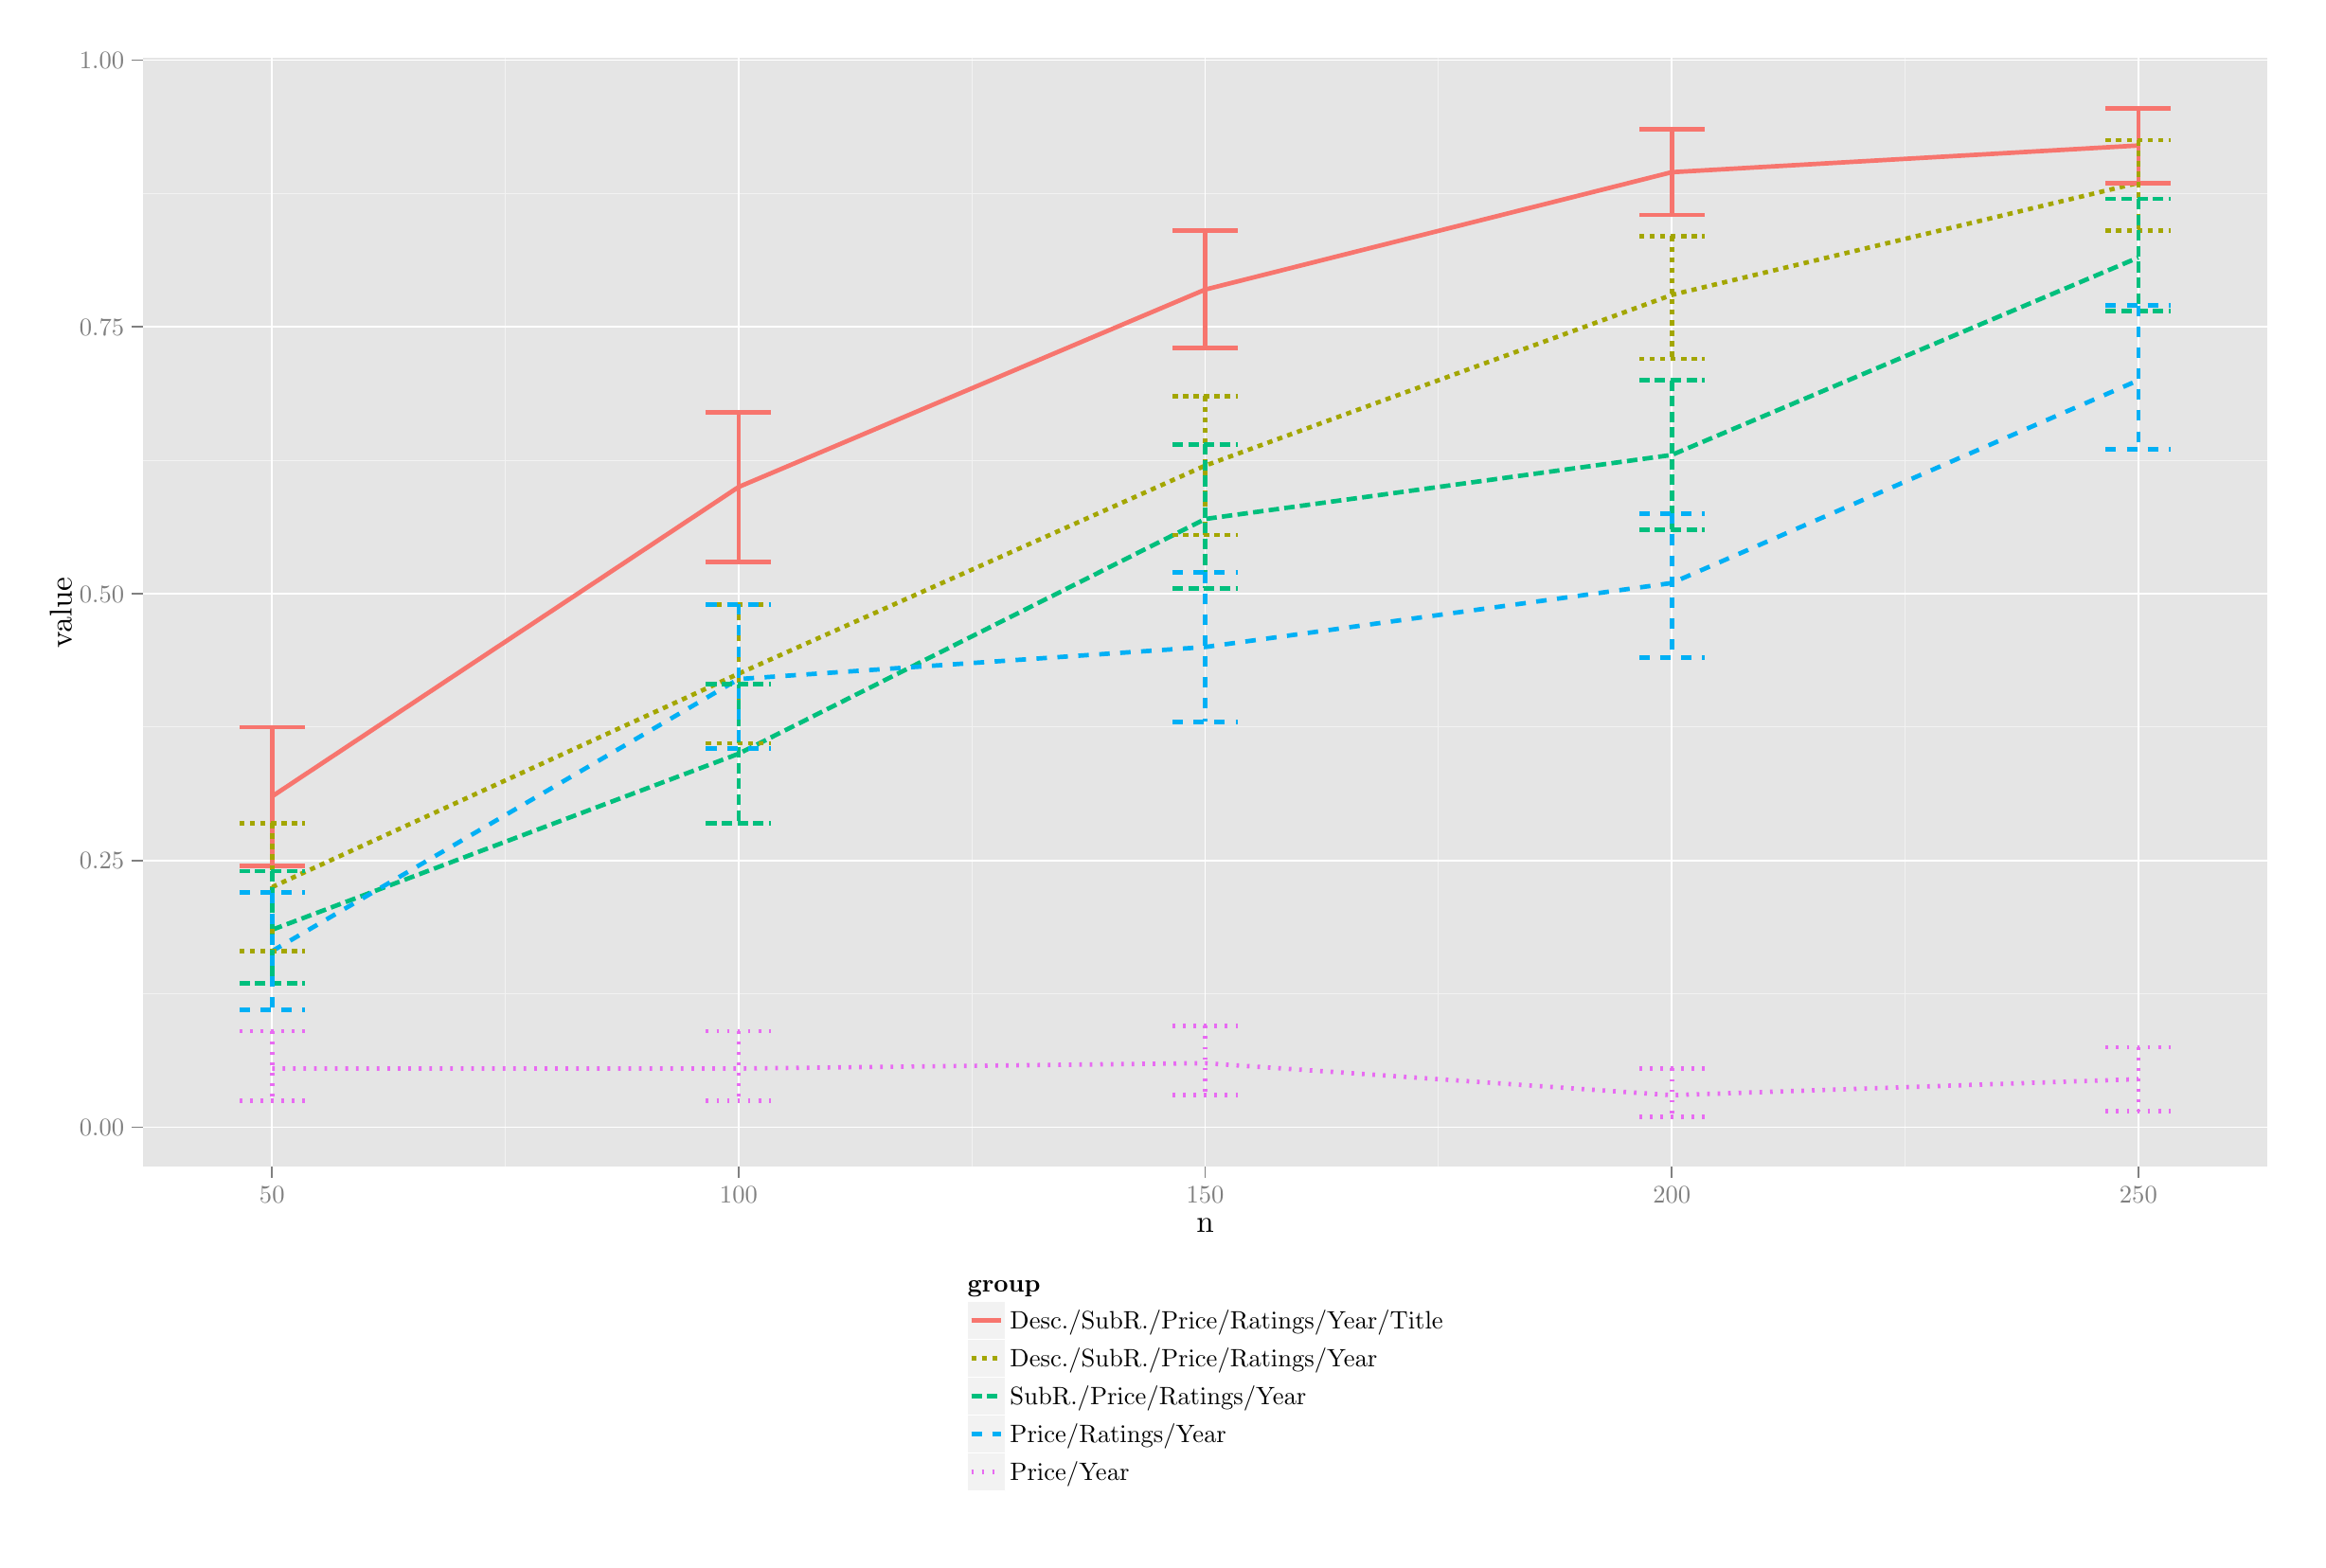
\begin{tikzpicture}[x=1pt,y=1pt]
\definecolor[named]{fillColor}{rgb}{1.00,1.00,1.00}
\path[use as bounding box,fill=fillColor,fill opacity=0.00] (0,0) rectangle (867.24,578.16);
\begin{scope}
\path[clip] (  0.00,  0.00) rectangle (867.24,578.16);
\definecolor[named]{drawColor}{rgb}{1.00,1.00,1.00}
\definecolor[named]{fillColor}{rgb}{1.00,1.00,1.00}

\path[draw=drawColor,line width= 0.6pt,line join=round,line cap=round,fill=fillColor] ( -0.00, -0.00) rectangle (867.24,578.16);
\end{scope}
\begin{scope}
\path[clip] ( 44.49,142.81) rectangle (855.20,566.12);
\definecolor[named]{fillColor}{rgb}{0.90,0.90,0.90}

\path[fill=fillColor] ( 44.49,142.81) rectangle (855.19,566.11);
\definecolor[named]{drawColor}{rgb}{0.95,0.95,0.95}

\path[draw=drawColor,line width= 0.3pt,line join=round] ( 44.49,208.89) --
	(855.20,208.89);

\path[draw=drawColor,line width= 0.3pt,line join=round] ( 44.49,310.69) --
	(855.20,310.69);

\path[draw=drawColor,line width= 0.3pt,line join=round] ( 44.49,412.49) --
	(855.20,412.49);

\path[draw=drawColor,line width= 0.3pt,line join=round] ( 44.49,514.30) --
	(855.20,514.30);

\path[draw=drawColor,line width= 0.3pt,line join=round] (182.81,142.81) --
	(182.81,566.12);

\path[draw=drawColor,line width= 0.3pt,line join=round] (360.83,142.81) --
	(360.83,566.12);

\path[draw=drawColor,line width= 0.3pt,line join=round] (538.85,142.81) --
	(538.85,566.12);

\path[draw=drawColor,line width= 0.3pt,line join=round] (716.87,142.81) --
	(716.87,566.12);
\definecolor[named]{drawColor}{rgb}{1.00,1.00,1.00}

\path[draw=drawColor,line width= 0.6pt,line join=round] ( 44.49,157.98) --
	(855.20,157.98);

\path[draw=drawColor,line width= 0.6pt,line join=round] ( 44.49,259.79) --
	(855.20,259.79);

\path[draw=drawColor,line width= 0.6pt,line join=round] ( 44.49,361.59) --
	(855.20,361.59);

\path[draw=drawColor,line width= 0.6pt,line join=round] ( 44.49,463.39) --
	(855.20,463.39);

\path[draw=drawColor,line width= 0.6pt,line join=round] ( 44.49,565.20) --
	(855.20,565.20);

\path[draw=drawColor,line width= 0.6pt,line join=round] ( 93.80,142.81) --
	( 93.80,566.12);

\path[draw=drawColor,line width= 0.6pt,line join=round] (271.82,142.81) --
	(271.82,566.12);

\path[draw=drawColor,line width= 0.6pt,line join=round] (449.84,142.81) --
	(449.84,566.12);

\path[draw=drawColor,line width= 0.6pt,line join=round] (627.86,142.81) --
	(627.86,566.12);

\path[draw=drawColor,line width= 0.6pt,line join=round] (805.88,142.81) --
	(805.88,566.12);
\definecolor[named]{drawColor}{rgb}{0.97,0.46,0.43}

\path[draw=drawColor,line width= 1.7pt,line join=round] ( 93.80,284.22) --
	(271.82,402.31) --
	(449.84,477.65) --
	(627.86,522.44) --
	(805.88,532.62);
\definecolor[named]{drawColor}{rgb}{0.64,0.65,0.00}

\path[draw=drawColor,line width= 1.7pt,dash pattern=on 2pt off 2pt ,line join=round] ( 93.80,249.61) --
	(271.82,331.05) --
	(449.84,410.46) --
	(627.86,475.61) --
	(805.88,518.37);
\definecolor[named]{drawColor}{rgb}{0.00,0.75,0.49}

\path[draw=drawColor,line width= 1.7pt,dash pattern=on 4pt off 2pt ,line join=round] ( 93.80,233.32) --
	(271.82,300.51) --
	(449.84,390.10) --
	(627.86,414.53) --
	(805.88,489.86);
\definecolor[named]{drawColor}{rgb}{0.00,0.69,0.96}

\path[draw=drawColor,line width= 1.7pt,dash pattern=on 4pt off 4pt ,line join=round] ( 93.80,225.17) --
	(271.82,329.01) --
	(449.84,341.23) --
	(627.86,365.66) --
	(805.88,443.03);
\definecolor[named]{drawColor}{rgb}{0.91,0.42,0.95}

\path[draw=drawColor,line width= 1.7pt,dash pattern=on 1pt off 3pt ,line join=round] ( 93.80,180.38) --
	(271.82,180.38) --
	(449.84,182.42) --
	(627.86,170.20) --
	(805.88,176.31);
\definecolor[named]{drawColor}{rgb}{0.97,0.46,0.43}

\path[draw=drawColor,line width= 1.7pt,line join=round] ( 81.34,310.69) --
	(106.26,310.69);

\path[draw=drawColor,line width= 1.7pt,line join=round] ( 93.80,310.69) --
	( 93.80,257.75);

\path[draw=drawColor,line width= 1.7pt,line join=round] ( 81.34,257.75) --
	(106.26,257.75);

\path[draw=drawColor,line width= 1.7pt,line join=round] (259.36,430.82) --
	(284.28,430.82);

\path[draw=drawColor,line width= 1.7pt,line join=round] (271.82,430.82) --
	(271.82,373.81);

\path[draw=drawColor,line width= 1.7pt,line join=round] (259.36,373.81) --
	(284.28,373.81);

\path[draw=drawColor,line width= 1.7pt,line join=round] (437.38,500.04) --
	(462.30,500.04);

\path[draw=drawColor,line width= 1.7pt,line join=round] (449.84,500.04) --
	(449.84,455.25);

\path[draw=drawColor,line width= 1.7pt,line join=round] (437.38,455.25) --
	(462.30,455.25);

\path[draw=drawColor,line width= 1.7pt,line join=round] (615.40,538.73) --
	(640.32,538.73);

\path[draw=drawColor,line width= 1.7pt,line join=round] (627.86,538.73) --
	(627.86,506.10);

\path[draw=drawColor,line width= 1.7pt,line join=round] (615.40,506.10) --
	(640.32,506.10);

\path[draw=drawColor,line width= 1.7pt,line join=round] (793.42,546.87) --
	(818.34,546.87);

\path[draw=drawColor,line width= 1.7pt,line join=round] (805.88,546.87) --
	(805.88,518.32);

\path[draw=drawColor,line width= 1.7pt,line join=round] (793.42,518.32) --
	(818.34,518.32);
\definecolor[named]{drawColor}{rgb}{0.64,0.65,0.00}

\path[draw=drawColor,line width= 1.7pt,dash pattern=on 2pt off 2pt ,line join=round] ( 81.34,274.04) --
	(106.26,274.04);

\path[draw=drawColor,line width= 1.7pt,dash pattern=on 2pt off 2pt ,line join=round] ( 93.80,274.04) --
	( 93.80,225.17);

\path[draw=drawColor,line width= 1.7pt,dash pattern=on 2pt off 2pt ,line join=round] ( 81.34,225.17) --
	(106.26,225.17);

\path[draw=drawColor,line width= 1.7pt,dash pattern=on 2pt off 2pt ,line join=round] (259.36,357.52) --
	(284.28,357.52);

\path[draw=drawColor,line width= 1.7pt,dash pattern=on 2pt off 2pt ,line join=round] (271.82,357.52) --
	(271.82,304.53);

\path[draw=drawColor,line width= 1.7pt,dash pattern=on 2pt off 2pt ,line join=round] (259.36,304.53) --
	(284.28,304.53);

\path[draw=drawColor,line width= 1.7pt,dash pattern=on 2pt off 2pt ,line join=round] (437.38,436.93) --
	(462.30,436.93);

\path[draw=drawColor,line width= 1.7pt,dash pattern=on 2pt off 2pt ,line join=round] (449.84,436.93) --
	(449.84,383.99);

\path[draw=drawColor,line width= 1.7pt,dash pattern=on 2pt off 2pt ,line join=round] (437.38,383.99) --
	(462.30,383.99);

\path[draw=drawColor,line width= 1.7pt,dash pattern=on 2pt off 2pt ,line join=round] (615.40,498.01) --
	(640.32,498.01);

\path[draw=drawColor,line width= 1.7pt,dash pattern=on 2pt off 2pt ,line join=round] (627.86,498.01) --
	(627.86,451.18);

\path[draw=drawColor,line width= 1.7pt,dash pattern=on 2pt off 2pt ,line join=round] (615.40,451.18) --
	(640.32,451.18);

\path[draw=drawColor,line width= 1.7pt,dash pattern=on 2pt off 2pt ,line join=round] (793.42,534.66) --
	(818.34,534.66);

\path[draw=drawColor,line width= 1.7pt,dash pattern=on 2pt off 2pt ,line join=round] (805.88,534.66) --
	(805.88,500.04);

\path[draw=drawColor,line width= 1.7pt,dash pattern=on 2pt off 2pt ,line join=round] (793.42,500.04) --
	(818.34,500.04);
\definecolor[named]{drawColor}{rgb}{0.00,0.75,0.49}

\path[draw=drawColor,line width= 1.7pt,dash pattern=on 4pt off 2pt ,line join=round] ( 81.34,255.72) --
	(106.26,255.72);

\path[draw=drawColor,line width= 1.7pt,dash pattern=on 4pt off 2pt ,line join=round] ( 93.80,255.72) --
	( 93.80,212.91);

\path[draw=drawColor,line width= 1.7pt,dash pattern=on 4pt off 2pt ,line join=round] ( 81.34,212.91) --
	(106.26,212.91);

\path[draw=drawColor,line width= 1.7pt,dash pattern=on 4pt off 2pt ,line join=round] (259.36,326.98) --
	(284.28,326.98);

\path[draw=drawColor,line width= 1.7pt,dash pattern=on 4pt off 2pt ,line join=round] (271.82,326.98) --
	(271.82,274.04);

\path[draw=drawColor,line width= 1.7pt,dash pattern=on 4pt off 2pt ,line join=round] (259.36,274.04) --
	(284.28,274.04);

\path[draw=drawColor,line width= 1.7pt,dash pattern=on 4pt off 2pt ,line join=round] (437.38,418.60) --
	(462.30,418.60);

\path[draw=drawColor,line width= 1.7pt,dash pattern=on 4pt off 2pt ,line join=round] (449.84,418.60) --
	(449.84,363.58);

\path[draw=drawColor,line width= 1.7pt,dash pattern=on 4pt off 2pt ,line join=round] (437.38,363.58) --
	(462.30,363.58);

\path[draw=drawColor,line width= 1.7pt,dash pattern=on 4pt off 2pt ,line join=round] (615.40,443.03) --
	(640.32,443.03);

\path[draw=drawColor,line width= 1.7pt,dash pattern=on 4pt off 2pt ,line join=round] (627.86,443.03) --
	(627.86,386.02);

\path[draw=drawColor,line width= 1.7pt,dash pattern=on 4pt off 2pt ,line join=round] (615.40,386.02) --
	(640.32,386.02);

\path[draw=drawColor,line width= 1.7pt,dash pattern=on 4pt off 2pt ,line join=round] (793.42,512.26) --
	(818.34,512.26);

\path[draw=drawColor,line width= 1.7pt,dash pattern=on 4pt off 2pt ,line join=round] (805.88,512.26) --
	(805.88,469.50);

\path[draw=drawColor,line width= 1.7pt,dash pattern=on 4pt off 2pt ,line join=round] (793.42,469.50) --
	(818.34,469.50);
\definecolor[named]{drawColor}{rgb}{0.00,0.69,0.96}

\path[draw=drawColor,line width= 1.7pt,dash pattern=on 4pt off 4pt ,line join=round] ( 81.34,247.57) --
	(106.26,247.57);

\path[draw=drawColor,line width= 1.7pt,dash pattern=on 4pt off 4pt ,line join=round] ( 93.80,247.57) --
	( 93.80,202.78);

\path[draw=drawColor,line width= 1.7pt,dash pattern=on 4pt off 4pt ,line join=round] ( 81.34,202.78) --
	(106.26,202.78);

\path[draw=drawColor,line width= 1.7pt,dash pattern=on 4pt off 4pt ,line join=round] (259.36,357.52) --
	(284.28,357.52);

\path[draw=drawColor,line width= 1.7pt,dash pattern=on 4pt off 4pt ,line join=round] (271.82,357.52) --
	(271.82,302.54);

\path[draw=drawColor,line width= 1.7pt,dash pattern=on 4pt off 4pt ,line join=round] (259.36,302.54) --
	(284.28,302.54);

\path[draw=drawColor,line width= 1.7pt,dash pattern=on 4pt off 4pt ,line join=round] (437.38,369.74) --
	(462.30,369.74);

\path[draw=drawColor,line width= 1.7pt,dash pattern=on 4pt off 4pt ,line join=round] (449.84,369.74) --
	(449.84,312.73);

\path[draw=drawColor,line width= 1.7pt,dash pattern=on 4pt off 4pt ,line join=round] (437.38,312.73) --
	(462.30,312.73);

\path[draw=drawColor,line width= 1.7pt,dash pattern=on 4pt off 4pt ,line join=round] (615.40,392.18) --
	(640.32,392.18);

\path[draw=drawColor,line width= 1.7pt,dash pattern=on 4pt off 4pt ,line join=round] (627.86,392.18) --
	(627.86,337.16);

\path[draw=drawColor,line width= 1.7pt,dash pattern=on 4pt off 4pt ,line join=round] (615.40,337.16) --
	(640.32,337.16);

\path[draw=drawColor,line width= 1.7pt,dash pattern=on 4pt off 4pt ,line join=round] (793.42,471.54) --
	(818.34,471.54);

\path[draw=drawColor,line width= 1.7pt,dash pattern=on 4pt off 4pt ,line join=round] (805.88,471.54) --
	(805.88,416.57);

\path[draw=drawColor,line width= 1.7pt,dash pattern=on 4pt off 4pt ,line join=round] (793.42,416.57) --
	(818.34,416.57);
\definecolor[named]{drawColor}{rgb}{0.91,0.42,0.95}

\path[draw=drawColor,line width= 1.7pt,dash pattern=on 1pt off 3pt ,line join=round] ( 81.34,194.63) --
	(106.26,194.63);

\path[draw=drawColor,line width= 1.7pt,dash pattern=on 1pt off 3pt ,line join=round] ( 93.80,194.63) --
	( 93.80,168.16);

\path[draw=drawColor,line width= 1.7pt,dash pattern=on 1pt off 3pt ,line join=round] ( 81.34,168.16) --
	(106.26,168.16);

\path[draw=drawColor,line width= 1.7pt,dash pattern=on 1pt off 3pt ,line join=round] (259.36,194.63) --
	(284.28,194.63);

\path[draw=drawColor,line width= 1.7pt,dash pattern=on 1pt off 3pt ,line join=round] (271.82,194.63) --
	(271.82,168.16);

\path[draw=drawColor,line width= 1.7pt,dash pattern=on 1pt off 3pt ,line join=round] (259.36,168.16) --
	(284.28,168.16);

\path[draw=drawColor,line width= 1.7pt,dash pattern=on 1pt off 3pt ,line join=round] (437.38,196.67) --
	(462.30,196.67);

\path[draw=drawColor,line width= 1.7pt,dash pattern=on 1pt off 3pt ,line join=round] (449.84,196.67) --
	(449.84,170.20);

\path[draw=drawColor,line width= 1.7pt,dash pattern=on 1pt off 3pt ,line join=round] (437.38,170.20) --
	(462.30,170.20);

\path[draw=drawColor,line width= 1.7pt,dash pattern=on 1pt off 3pt ,line join=round] (615.40,180.38) --
	(640.32,180.38);

\path[draw=drawColor,line width= 1.7pt,dash pattern=on 1pt off 3pt ,line join=round] (627.86,180.38) --
	(627.86,162.06);

\path[draw=drawColor,line width= 1.7pt,dash pattern=on 1pt off 3pt ,line join=round] (615.40,162.06) --
	(640.32,162.06);

\path[draw=drawColor,line width= 1.7pt,dash pattern=on 1pt off 3pt ,line join=round] (793.42,188.52) --
	(818.34,188.52);

\path[draw=drawColor,line width= 1.7pt,dash pattern=on 1pt off 3pt ,line join=round] (805.88,188.52) --
	(805.88,164.09);

\path[draw=drawColor,line width= 1.7pt,dash pattern=on 1pt off 3pt ,line join=round] (793.42,164.09) --
	(818.34,164.09);
\end{scope}
\begin{scope}
\path[clip] (  0.00,  0.00) rectangle (867.24,578.16);
\definecolor[named]{drawColor}{rgb}{0.50,0.50,0.50}

\node[text=drawColor,anchor=base east,inner sep=0pt, outer sep=0pt, scale=  0.96] at ( 37.37,154.68) {0.00};

\node[text=drawColor,anchor=base east,inner sep=0pt, outer sep=0pt, scale=  0.96] at ( 37.37,256.48) {0.25};

\node[text=drawColor,anchor=base east,inner sep=0pt, outer sep=0pt, scale=  0.96] at ( 37.37,358.29) {0.50};

\node[text=drawColor,anchor=base east,inner sep=0pt, outer sep=0pt, scale=  0.96] at ( 37.37,460.09) {0.75};

\node[text=drawColor,anchor=base east,inner sep=0pt, outer sep=0pt, scale=  0.96] at ( 37.37,561.89) {1.00};
\end{scope}
\begin{scope}
\path[clip] (  0.00,  0.00) rectangle (867.24,578.16);
\definecolor[named]{drawColor}{rgb}{0.50,0.50,0.50}

\path[draw=drawColor,line width= 0.6pt,line join=round] ( 40.22,157.98) --
	( 44.49,157.98);

\path[draw=drawColor,line width= 0.6pt,line join=round] ( 40.22,259.79) --
	( 44.49,259.79);

\path[draw=drawColor,line width= 0.6pt,line join=round] ( 40.22,361.59) --
	( 44.49,361.59);

\path[draw=drawColor,line width= 0.6pt,line join=round] ( 40.22,463.39) --
	( 44.49,463.39);

\path[draw=drawColor,line width= 0.6pt,line join=round] ( 40.22,565.20) --
	( 44.49,565.20);
\end{scope}
\begin{scope}
\path[clip] (  0.00,  0.00) rectangle (867.24,578.16);
\definecolor[named]{drawColor}{rgb}{0.50,0.50,0.50}

\path[draw=drawColor,line width= 0.6pt,line join=round] ( 93.80,138.55) --
	( 93.80,142.81);

\path[draw=drawColor,line width= 0.6pt,line join=round] (271.82,138.55) --
	(271.82,142.81);

\path[draw=drawColor,line width= 0.6pt,line join=round] (449.84,138.55) --
	(449.84,142.81);

\path[draw=drawColor,line width= 0.6pt,line join=round] (627.86,138.55) --
	(627.86,142.81);

\path[draw=drawColor,line width= 0.6pt,line join=round] (805.88,138.55) --
	(805.88,142.81);
\end{scope}
\begin{scope}
\path[clip] (  0.00,  0.00) rectangle (867.24,578.16);
\definecolor[named]{drawColor}{rgb}{0.50,0.50,0.50}

\node[text=drawColor,anchor=base,inner sep=0pt, outer sep=0pt, scale=  0.96] at ( 93.80,129.09) {50};

\node[text=drawColor,anchor=base,inner sep=0pt, outer sep=0pt, scale=  0.96] at (271.82,129.09) {100};

\node[text=drawColor,anchor=base,inner sep=0pt, outer sep=0pt, scale=  0.96] at (449.84,129.09) {150};

\node[text=drawColor,anchor=base,inner sep=0pt, outer sep=0pt, scale=  0.96] at (627.86,129.09) {200};

\node[text=drawColor,anchor=base,inner sep=0pt, outer sep=0pt, scale=  0.96] at (805.88,129.09) {250};
\end{scope}
\begin{scope}
\path[clip] (  0.00,  0.00) rectangle (867.24,578.16);
\definecolor[named]{drawColor}{rgb}{0.00,0.00,0.00}

\node[text=drawColor,anchor=base,inner sep=0pt, outer sep=0pt, scale=  1.20] at (449.84,117.81) {n};
\end{scope}
\begin{scope}
\path[clip] (  0.00,  0.00) rectangle (867.24,578.16);
\definecolor[named]{drawColor}{rgb}{0.00,0.00,0.00}

\node[text=drawColor,rotate= 90.00,anchor=base,inner sep=0pt, outer sep=0pt, scale=  1.20] at ( 17.30,354.46) {value};
\end{scope}
\begin{scope}
\path[clip] (  0.00,  0.00) rectangle (867.24,578.16);
\definecolor[named]{fillColor}{rgb}{1.00,1.00,1.00}

\path[fill=fillColor] (354.85, 14.89) rectangle (544.83,105.93);
\end{scope}
\begin{scope}
\path[clip] (  0.00,  0.00) rectangle (867.24,578.16);
\definecolor[named]{drawColor}{rgb}{0.00,0.00,0.00}

\node[text=drawColor,anchor=base west,inner sep=0pt, outer sep=0pt, scale=  0.96] at (359.12, 95.04) {\bfseries group};
\end{scope}
\begin{scope}
\path[clip] (  0.00,  0.00) rectangle (867.24,578.16);
\definecolor[named]{drawColor}{rgb}{1.00,1.00,1.00}
\definecolor[named]{fillColor}{rgb}{0.95,0.95,0.95}

\path[draw=drawColor,line width= 0.6pt,line join=round,line cap=round,fill=fillColor] (359.12, 76.97) rectangle (373.57, 91.43);
\end{scope}
\begin{scope}
\path[clip] (  0.00,  0.00) rectangle (867.24,578.16);
\definecolor[named]{drawColor}{rgb}{0.97,0.46,0.43}

\path[draw=drawColor,line width= 1.7pt,line join=round] (360.56, 84.20) -- (372.12, 84.20);
\end{scope}
\begin{scope}
\path[clip] (  0.00,  0.00) rectangle (867.24,578.16);
\definecolor[named]{drawColor}{rgb}{0.97,0.46,0.43}

\path[draw=drawColor,line width= 1.7pt,line join=round] (360.56, 84.20) -- (372.12, 84.20);
\end{scope}
\begin{scope}
\path[clip] (  0.00,  0.00) rectangle (867.24,578.16);
\definecolor[named]{drawColor}{rgb}{1.00,1.00,1.00}
\definecolor[named]{fillColor}{rgb}{0.95,0.95,0.95}

\path[draw=drawColor,line width= 0.6pt,line join=round,line cap=round,fill=fillColor] (359.12, 62.52) rectangle (373.57, 76.97);
\end{scope}
\begin{scope}
\path[clip] (  0.00,  0.00) rectangle (867.24,578.16);
\definecolor[named]{drawColor}{rgb}{0.64,0.65,0.00}

\path[draw=drawColor,line width= 1.7pt,dash pattern=on 2pt off 2pt ,line join=round] (360.56, 69.75) -- (372.12, 69.75);
\end{scope}
\begin{scope}
\path[clip] (  0.00,  0.00) rectangle (867.24,578.16);
\definecolor[named]{drawColor}{rgb}{0.64,0.65,0.00}

\path[draw=drawColor,line width= 1.7pt,dash pattern=on 2pt off 2pt ,line join=round] (360.56, 69.75) -- (372.12, 69.75);
\end{scope}
\begin{scope}
\path[clip] (  0.00,  0.00) rectangle (867.24,578.16);
\definecolor[named]{drawColor}{rgb}{1.00,1.00,1.00}
\definecolor[named]{fillColor}{rgb}{0.95,0.95,0.95}

\path[draw=drawColor,line width= 0.6pt,line join=round,line cap=round,fill=fillColor] (359.12, 48.07) rectangle (373.57, 62.52);
\end{scope}
\begin{scope}
\path[clip] (  0.00,  0.00) rectangle (867.24,578.16);
\definecolor[named]{drawColor}{rgb}{0.00,0.75,0.49}

\path[draw=drawColor,line width= 1.7pt,dash pattern=on 4pt off 2pt ,line join=round] (360.56, 55.29) -- (372.12, 55.29);
\end{scope}
\begin{scope}
\path[clip] (  0.00,  0.00) rectangle (867.24,578.16);
\definecolor[named]{drawColor}{rgb}{0.00,0.75,0.49}

\path[draw=drawColor,line width= 1.7pt,dash pattern=on 4pt off 2pt ,line join=round] (360.56, 55.29) -- (372.12, 55.29);
\end{scope}
\begin{scope}
\path[clip] (  0.00,  0.00) rectangle (867.24,578.16);
\definecolor[named]{drawColor}{rgb}{1.00,1.00,1.00}
\definecolor[named]{fillColor}{rgb}{0.95,0.95,0.95}

\path[draw=drawColor,line width= 0.6pt,line join=round,line cap=round,fill=fillColor] (359.12, 33.61) rectangle (373.57, 48.07);
\end{scope}
\begin{scope}
\path[clip] (  0.00,  0.00) rectangle (867.24,578.16);
\definecolor[named]{drawColor}{rgb}{0.00,0.69,0.96}

\path[draw=drawColor,line width= 1.7pt,dash pattern=on 4pt off 4pt ,line join=round] (360.56, 40.84) -- (372.12, 40.84);
\end{scope}
\begin{scope}
\path[clip] (  0.00,  0.00) rectangle (867.24,578.16);
\definecolor[named]{drawColor}{rgb}{0.00,0.69,0.96}

\path[draw=drawColor,line width= 1.7pt,dash pattern=on 4pt off 4pt ,line join=round] (360.56, 40.84) -- (372.12, 40.84);
\end{scope}
\begin{scope}
\path[clip] (  0.00,  0.00) rectangle (867.24,578.16);
\definecolor[named]{drawColor}{rgb}{1.00,1.00,1.00}
\definecolor[named]{fillColor}{rgb}{0.95,0.95,0.95}

\path[draw=drawColor,line width= 0.6pt,line join=round,line cap=round,fill=fillColor] (359.12, 19.16) rectangle (373.57, 33.61);
\end{scope}
\begin{scope}
\path[clip] (  0.00,  0.00) rectangle (867.24,578.16);
\definecolor[named]{drawColor}{rgb}{0.91,0.42,0.95}

\path[draw=drawColor,line width= 1.7pt,dash pattern=on 1pt off 3pt ,line join=round] (360.56, 26.39) -- (372.12, 26.39);
\end{scope}
\begin{scope}
\path[clip] (  0.00,  0.00) rectangle (867.24,578.16);
\definecolor[named]{drawColor}{rgb}{0.91,0.42,0.95}

\path[draw=drawColor,line width= 1.7pt,dash pattern=on 1pt off 3pt ,line join=round] (360.56, 26.39) -- (372.12, 26.39);
\end{scope}
\begin{scope}
\path[clip] (  0.00,  0.00) rectangle (867.24,578.16);
\definecolor[named]{drawColor}{rgb}{0.00,0.00,0.00}

\node[text=drawColor,anchor=base west,inner sep=0pt, outer sep=0pt, scale=  0.96] at (375.38, 80.90) {Desc./SubR./Price/Ratings/Year/Title};
\end{scope}
\begin{scope}
\path[clip] (  0.00,  0.00) rectangle (867.24,578.16);
\definecolor[named]{drawColor}{rgb}{0.00,0.00,0.00}

\node[text=drawColor,anchor=base west,inner sep=0pt, outer sep=0pt, scale=  0.96] at (375.38, 66.44) {Desc./SubR./Price/Ratings/Year};
\end{scope}
\begin{scope}
\path[clip] (  0.00,  0.00) rectangle (867.24,578.16);
\definecolor[named]{drawColor}{rgb}{0.00,0.00,0.00}

\node[text=drawColor,anchor=base west,inner sep=0pt, outer sep=0pt, scale=  0.96] at (375.38, 51.99) {SubR./Price/Ratings/Year};
\end{scope}
\begin{scope}
\path[clip] (  0.00,  0.00) rectangle (867.24,578.16);
\definecolor[named]{drawColor}{rgb}{0.00,0.00,0.00}

\node[text=drawColor,anchor=base west,inner sep=0pt, outer sep=0pt, scale=  0.96] at (375.38, 37.53) {Price/Ratings/Year};
\end{scope}
\begin{scope}
\path[clip] (  0.00,  0.00) rectangle (867.24,578.16);
\definecolor[named]{drawColor}{rgb}{0.00,0.00,0.00}

\node[text=drawColor,anchor=base west,inner sep=0pt, outer sep=0pt, scale=  0.96] at (375.38, 23.08) {Price/Year};
\end{scope}
\end{tikzpicture}

    }
  \end{center}
\caption{Power on sample size: MKL can make effective use of
  additional information.}
\label{fig:wine_power}
\end{figure}

We train a 2-norm MKL with regularization parameter $C=.01$, initially
on all 6 kernels, with varying sample sizes in $\{50, 100, 150, 200,
250\}$, repeating each test 200 times in order to estimate the
distribution of the kernel weights and the statistical power of the
tests.  In Figure~\ref{fig:wine_weights} we report boxplots of the
kernel weights.  For the 6-kernel model on all the features, the dominant
weight lies on the 4-spectrum kernel associated with the name (title)
of the wine.  In Figure~\ref{fig:wine_power}, we see that this test
has the highest power.  We then remove the kernel with the highest
weight and fit a 5-kernel model on all of the features except for the
name of the wine.  We have ordered the boxplot x-axis in order of
the highest variable weight corresponding to the model under
consideration.  Thus, the title of the wine has the highest weight
for the 6-kernel model, the description of the wine has the highest
weight for the 5-kernel model, and so on.

The title of the wine sometimes contains information about the very
thing we're trying to predict -- the wine varietal.  Additionally,
many wineries specialize in particular varietals of wine.  For
example, Siduri only produces single vineyard Pinot Noirs from
vineyards located in California and Oregon.  Therefore, we should
expect that models incorporating this information should perform very
well.

Pinot Noir wines are typically lighter-colored reds that have notes of
red fruits such as cherries, strawberries, and raspberries.  The grape
requires a cooler climate for best results and is associated with the
Burgundy region of France and areas of California and Oregon.
Chardonnay, by contrast, is a white wine with flavors of buttery oak
and fruits such as apples and pears.  Chardonnay is also commonly
grown in Burgundy and California as well as Australia and New
Zealand.  The wine reviews use many adjectives and descriptors
associated with each varietal, in addition to sometimes including the
name of the varietal.  By constructing views of each data type through
kernels, we can pick up on such differences between the two varietals.

In Figure~\ref{fig:wine_power}, by repeatedly removing the
most-informative feature, we monotonically decrease the statistical
power of the test.  The final model including just the price and year
of the wine has very poor performance.  In fact, the distributions of
the weights of the two variables are very similar, indicating that
both features are equally poor predictors of the type of wine.  For
this wine example, MKL can effectively exploit additional data types
for higher discriminatory power.

\section{Future Work}
We hope to better understand the Friedman test outside of the
univariate data and linear kernel setting.  That is, we would like to
characterize the kernels for which the Friedman test generalizes the
permutation $t$-test and understand the degree to which this
relationship holds approximately given higher dimensional data and a
wide range of kernels.  We further hope to extend the theory of
Chapters~\ref{C:steins-method} and \ref{C:stein-proof} to prove rates
of convergence bounds in these general settings.  As seen in
Figures~\ref{fig:mkl_arc_overfit} and \ref{fig:overfit_mkl}, these bounds
would likely incorporate some terms that represent the learning
algorithm and numbers of independent kernels.

We can also potentially treat various kinds of missing data.
If we consider entire missing modalities (e.g., one sample is
missing some biometric reading), Poh et al.\ \cite{poh2010addressing}
developed the \emph{neutral point substitution} technique to allow
substitution of the missing modality with a new kernel that is
\emph{unbiased} with regard to the classification at hand.
Panov et al.\ \cite{panov2011modified} modified the NPS method to allow
for missing modalities in the test set.  This
allows for full use of both modalities that are present for all
samples as well as those that are present only for a subset of the
samples and effective utilization of all the data in the training set.
